\documentclass[12pt]{beamer}
\usepackage{beamerinnerthemeX}
\usepackage{graphics,color,hyperref,mathrsfs}
\usepackage{amsmath,amssymb,listings,frenchineq}
\usepackage{xcolor,colortbl}
\usepackage{subcaption}
\usepackage{adjustbox}
\setbeamertemplate{bibliography item}[text]
\usepackage[authoryear]{natbib}
\definecolor{darkgreen}{rgb}{0.0, 0.2, 0.13}
\definecolor{vtx_color}{HTML}{e9190f}
\definecolor{cp_color1}{HTML}{FFA500}
\definecolor{cp_color2}{HTML}{a1dab4}
\definecolor{cp_color3}{HTML}{41b6c4}
\definecolor{cp_color4}{HTML}{2c7fb8}
\definecolor{cp_color5}{HTML}{253494}

\definecolor{color1}{RGB}{41,56,102}  %
\definecolor{color2}{RGB}{42,161,133} %
\definecolor{color3}{RGB}{134,166,91} %

\newcommand{\ver}{\operatorname{ver}}
\newcommand{\tcone}{\operatorname{tcone}}
\newcommand{\hla}[1]{\textcolor{color1}{#1}}
\newcommand{\hlb}[1]{\textcolor{color2}{#1}}
\newcommand{\hlc}[1]{\textcolor{color3}{#1}}

\bibliographystyle{plainnat}
%
%
\usepackage{fixmath}
\usepackage{bbm}    
\usepackage{bm}
\newcounter{mypart}
\stepcounter{mypart}
\newcommand{\cH}{\mathcal{H}}\newcommand{\cV}{\mathcal{V}}
\newcommand{\myemph}[1]{\bl{#1}}
\newcommand{\NEW}[1]{\myemph{#1}}%
\newcommand{\proj}{\mathbb{P}}
\newcommand{\TT}{\mathbb{T}}
\newcommand{\Sp}{\operatorname{Sp}}
\newcommand{\dist}{\operatorname{dist}}
\newcommand{\Lip}{\operatorname{Lip}}
\newcommand{\Col}{\operatorname{Col}}
\newcommand{\Row}{\operatorname{Row}}

\newcommand\puiseuxCEX[1]{\textbf{\textsc{LW}}_{#1}}
\newcommand\puiseuxCEXslack[1]{\textbf{\textsc{LW}}_{#1}^{=}}
\newcommand\dualPuiseuxCEXslack[1]{\textbf{\textsc{DualLW}}_{#1}^{=}}
\newcommand\perturbedPuiseuxCEX[2]{\textbf{\textsc{LW}}_{#1}^{#2}}
\newcommand\realCEX[2]{\puiseuxCEX{#1}(#2)}
\newcommand\realCEXslack[2]{\puiseuxCEXslack{#1}(#2)}
\newcommand\dualRealCEXslack[2]{\dualPuiseuxCEXslack{#1}(#2)}

\newcommand{\Pcal}{\mathcal{P}}
\newcommand{\Qcal}{\mathcal{Q}}
\newcommand{\Ncal}{\mathcal{N}}
\newcommand{\Ccal}{\mathcal{C}}
\newcommand{\tdot}{\odot}
\newcommand{\Rmax}{\R_{\max}}
\newcommand{\doag}{\R}
\newcommand{\supc}{\operatorname{sup}_C}
\newcommand{\infc}{\operatorname{inf}_C}
\newcommand{\informativefootnote}[1]{{\color{darkgreen}\footnotesize #1\par}}
\newcommand{\informative}[1]{{\color{darkgreen}\scriptsize #1\par}}
\newcommand{\informativenobreak}[1]{{\color{darkgreen}\scriptsize #1}}
\newcommand{\informativesmall}[1]{{\color{darkgreen}\tiny #1\par}}
\newcommand{\informativesmallnobreak}[1]{{\color{darkgreen}\tiny #1}}
\renewcommand{\themypart}{\Roman{mypart}}
\newcommand{\puiseux}{\mathbb{K}}
\newcommand{\pospuiseux}{\puiseux_{>0}}
\newcommand{\nnpuiseux}{\puiseux_{\geq 0}}
\newcommand{\puiseuxcvg}{\puiseux}
\newcommand{\nnpuiseuxcvg}{\nnpuiseux}
\newcommand{\bspectra}{\mathbfcal{S}}
\newcommand{\spectra}{\mathcal{S}}

\newcommand{\bo}[1]{\mathbold{#1}}
\newcommand{\sval}{\operatorname{sval}}
\newcommand{\cvggenpuiseux}{\R\{\{t^{-\R}\}\}_{\text{cvg}}}
\newcommand{\cvgCgenpuiseux}{\C\{\{t^{-\R}\}\}_{\text{cvg}}}
\usepackage{ifthen}
\usepackage{pgf}
\usepackage{pgfplots}
\usepackage{mathtools}
\usepackage{tikz,tikz-3dplot}
\usepackage{ifthen}
\newboolean{withtikz}
\setboolean{withtikz}{true}
\usetikzlibrary{arrows}
\usetikzlibrary{patterns}
\usetikzlibrary{positioning}
\usetikzlibrary{shapes} 
\usetikzlibrary{shapes.geometric}
\usetikzlibrary{fit}
\usetikzlibrary{calc}
\usetikzlibrary{arrows}
\usetikzlibrary{automata}
\usetikzlibrary{decorations.pathreplacing}
\usepackage{barycentric}
\newcommand{\tikzmark}[1]{\tikz[overlay,remember picture] \node (#1) {};}

\newcommand{\drawfigure}{1}
 \colorlet{kaki}{rgb:red,50;green,50;blue,0}
\newcommand{\x}[0]{\mathbf{x}}
\newcommand{\mtop}{\mathsf{t}}
\newcommand{\sgn}{\operatorname{sgn}}
\newcommand{\detpm}{\operatorname{det}^\pm}
\newcommand{\detmp}{\operatorname{det}^\mp}
\newcommand{\detpp}{\operatorname{det}^+}
\newcommand{\detmm}{\operatorname{det}^-}
\newcommand{\cone}{\operatorname{cone}}
\newcommand{\ve}[1]{\mathbf{#1}}
\newcommand{\puiseuxP}[0]{\bm{\mathcal{P}}}   %
\newcommand{\puiseuxH}[0]{\bm{\mathcal{H}}}             %
\newcommand{\puiseuxC}[0]{\bm{\mathcal{C}}}   %
\newcommand{\puiseuxD}[0]{\bm{\mathcal{D}}}   %
\newcommand{\puiseuxE}[0]{\bm{\mathcal{E}}}   %
\newcommand{\cpath}{\mathcal{C}}
\newcommand{\troppath}{\mathcal{C}^{\text{\rm trop}}}

\def\myblack#1{{\color{black}#1}}
\def\s(#1,#2){\left( #1,#2\right)}
\def\<#1,#2>{\langle #1,#2\rangle}
\newcommand{\lpvalue}{\nu}
\newcommand{\hardyex}{{\bf LP}} %

\newcommand{\genpuiseux}{\mathbb{K}}
\newcommand{\genpuiseuxcvg}{\mathbb{K}_{\text{cvg}}}
\newcommand{\trace}{\operatorname{tr}}
\newcommand{\myquote}[2]{{\tiny\color{purple}#1\citep*{#2}}}
\newcommand{\bl}[1]{{\color{blue} #1}}
\newcommand{\norm}[1]{\left\|#1\right\|}
\newcommand{\Spec}{\operatorname{Spec}}
\newcommand{\Funk}{\operatorname{RFunk}}
\newcommand{\Extr}{\operatorname{Extr}}
\newcommand{\overl}[2]{\begin{overlayarea}{\textwidth}{#1}#2
\end{overlayarea}}
\newcommand{\moverl}[3]{\begin{overlayarea}{\textwidth}{#1}\only<#2>{#3}
\end{overlayarea}}
\newcommand{\centeredframe}[1]{\begin{frame}\vfill
\centerline{#1}\vfill\end{frame}}
\newcommand{\deltat}{h}
\newcommand{\ncols}{n}
\newcommand{\nrows}{m}
\newcommand{\mpscal}[2]{\trop{\langle #1,#2\rangle}}
\newcommand{\eps}{\varepsilon}
\newcommand{\set}[2]{\{#1\mid #2\}}
\newcommand{\russianzero}{\mathbbold{0}}
\newcommand{\zero}{\russianzero}
\newcommand{\russianunit}{\mathbbold{1}}
\newcommand{\rhomax}{\rho_{\max}}
\newcommand{\Int}{\operatorname{int}}
\newcommand{\mb}[1]{\mathbf{#1}}
\newcommand{\mpplus}{+}
\newcommand{\mptimes}{}
\newcommand{\mon}{-}
\newcommand{\mop}{+}
\newcommand{\cw}{\operatorname{cw}}
\newcommand{\res}{^{\sharp}}
\newcommand{\per}{\operatorname{per}}
\newcommand{\sA}{\mathcal{A}}
\def\dbox{\Box\!\!\!\cdot}
\def\mydot{\;\cdot\;}
\newcommand{\transpose}[1]{{#1}^\top}
\newenvironment{stepitemize}{\begin{itemize}[<+->]}{\end{itemize} }
\newenvironment{stepenumerate}{\begin{enumerate}[<+->]}{\end{enumerate}}
\newtheorem{question}{Question}
\newtheorem{myalgorithm}{Algorithm}
\newtheorem{conjecture}{Conjecture}
\newtheorem{proposition}{Proposition}
\newtheorem{observation}{Observation}
\newcommand{\mpzeroone}{\{\,\mpzero,0\,\}}%
\newenvironment{trop}{\color{blue}\text{``}}{\text{''}}
\newcommand{\mytop}{\operatorname{top}}
\newcommand{\mytrop}[1]{\ltr #1\rtr}
\newcommand{\mybounds}[3]{[#2,#1]}
\newcommand{\mybound}[3]{#1}
\newcommand{\pred}{Z}
\newcommand{\diag}{\operatorname{diag}}
\newcommand{\spec}{\operatorname{spec}}\newcommand{\cond}{\operatorname{cond}}
\newcommand{\authdate}[2]{{\color{purple} #1} {\color{green}#2}}
\newcommand{\auth}[1]{{\color{purple} #1}}
\newcommand{\KK}{\mathcal{K}}
\newcommand{\HH}{\mathcal{H}}
\newcommand{\tangent}{\mathcal{T}}
\newcommand{\vect}[1]{#1}
\newcommand{\CC}{\mathcal{C}}
\newcommand{\inblue}[1]{{\color{blue}#1}}
\colorlet{myblue}{gray!50!black}
\colorlet{myred}{gray!50!black}
\colorlet{mygreen}{gray!50!black}
\newcommand{\ibid}{\giveref{ibid.}}
\newcommand{\smallgiveref}[1]{{\footnotesize\color{purple}#1}}
\newcommand{\verysmallgiveref}[1]{{\scriptsize\color{purple}#1}}
\newcommand{\val}{\operatorname{val}}
\def\ltr{\begin{trop}}
\def\rtr{\end{trop}}
\def\lltr{\color{blue}\text{``}}
\def\ltrr{\color{blue}}
\def\rtrr{}
\newcommand{\mpone}{{1}}
\def\rrtr{\text{''}}\newcommand{\mponealt}{\mpone}
\newcommand{\maxplus}{\mathbb{R}_{\max}}
\newcommand{\mpzerovect}{0}
\newcommand{\mponevect}{{1}}
\DeclareMathAlphabet{\mathbfcal}{OMS}{cmsy}{b}{n}
\newcommand{\bbfamily}{\fontencoding{U}\fontfamily{bbold}\selectfont}
\DeclareMathAlphabet{\mathbbold}{U}{bbold}{m}{n}
\newcommand{\floor}[1]{\lfloor #1\rfloor}
\newcommand{\mpzero}{{0}}
\newcommand{\mpunit}{{1}}
\newcommand{\sT}{\mathcal{T}}
\newcommand{\sV}{\mathcal{V}}
\newcommand{\sW}{\mathcal{W}}
\newcommand{\sH}{\mathcal{H}}
\newcommand{\sL}{\mathcal{L}}
\newcommand{\sR}{\mathcal{R}}
\newcommand{\sK}{\mathcal{K}}
\newcommand{\sM}{\mathcal{M}}
\newcommand{\sB}{\mathcal{B}}
\newcommand{\sC}{\mathcal{C}}
\newcommand{\R}{\mathbb{R}}
\newcommand{\K}{\mathbb{K}}
\newcommand{\Q}{\mathbb{Q}}
\newcommand{\RR}{\mathbb{R}}
\newcommand{\C}{\mathbb{C}}
\newcommand{\N}{\mathbb{N}}
\newcommand{\Z}{\mathbb{Z}}
\newcommand{\rmax}{\R_{\max}}
\newcommand{\rmaxb}{\overline{\R}_{\max}}
\newcommand{\smax}{\mathbb{S}_{\max}}
\newcommand{\rmin}{\R_{\min}}
\newcommand{\rminb}{\overline{\R}_{\min}}
\newcommand{\qmax}{\Q_{\max}}
\newcommand{\zmax}{\Z_{\max}}
\newcommand{\bal}{\nabla}
\newcommand{\balance}{\nabla}
\newcommand\ntrop{N^{\text{tpath}}}
\newcommand\ntropext{N^{\text{trop}}}
\newcommand\nclass{N^{\text{path}}}
\newcommand\adj{\rm{adj}}
\newcommand\npm{N^{+-}}
\newcommand\nmp{N^{-+}}
\newcommand\pmp{-+}
\newcommand\ppm{+-}
\newcommand{\argmax}{\arg\max}
\newcommand{\argmin}{\arg\min}
\newcommand{\sP}{\mathscr{P}}
\newcommand{\unit}{}
\font\manual=manfnt
\def\dbend{{\manual\char127}} 
\newcommand{\mychoose}[2]{{{#1}\choose{#2}}}
\newcommand{\giveref}[1]{{\normalsize\color{purple}#1}}
\newcommand{\normalgiveref}[1]{{\color{purple}#1}}
\newcommand{\cmin}{C^{\min}}
\newcommand{\cmax}{C^{\max}}
\newcommand{\pmin}{P^{\min}}
\newcommand{\pmax}{P^{\max}}

%
\usetheme{CambridgeUS}
%
\newcommand{\axisandedges}{
   \draw[axis, ->] (-4, -4) -- (1.3, -4);
   \draw[axis, ->] (-4, -4) -- (-4, 1.3);
   

   \foreach \x in {-4, -3, ..., 0} { 
     \node [anchor=north] at (\x,-4.1) {${\scriptstyle\x}$}; 
     \draw[axis] (\x, -4.1) -- (\x, -3.9);
   }
   \foreach \y in {-4, -3, ..., 0} { 
     \node [anchor=east] at  (-4.1,\y) {${\scriptstyle\y}$};
     \draw[axis] (-4.1, \y) -- (-3.9, \y);
   }
     

   \node[below] at (1.3, -4) {$x_1$};
   \node[left] at (-4, 1.3) {$x_2$};
    \draw[edge] (-4,0) -- (0,0) -- (0,-4);
    \draw[edge] (-4, -1) -- (-3, -1) -- (-1,1);
    \draw[edge] (-2,-4) -- (1,-1);
    \draw[edge] (-1,-4) -- (-1,-2) -- (1,0);
}
\begin{document}
\tikzstyle{every picture}+=[remember picture]

\tikzset{alertbox/.style={rectangle,draw=none,fill opacity=0.9,fill=mylightred,text=black, anchor=base,inner sep=2ex}}
\tikzset{grid/.style={gray!30,very thin}}
\tikzset{axis/.style={gray!50,->,>=stealth'}}
\tikzset{convex/.style={draw=none,fill=lightgray,fill opacity=0.7}}
\tikzset{convexborder/.style={very thick}}
\tikzset{point/.style={blue!50}}
\tikzset{ray/.style={ultra thick,green!60!black}}
\tikzset{hs/.style={fill opacity=0.3,fill=orange,draw=none}}
\tikzset{hsborder/.style={orange,ultra thick,dashdotted}}

\renewcommand{\thefootnote}{}
\renewcommand{\footnoterule}{}
\title[Efficient Tropical SVM]{Efficient Tropical SVM via mean-payoff games}
%
\author[St\'ephane Gaubert]{Stephane.Gaubert@inria.fr}
\institute[INRIA and CMAP]{INRIA and CMAP, \'Ecole polytechnique, IPP, CNRS}
\date[SIAM AG 2025]{\small SIAM AG 2025, Madison\\
\small July 2025}

\providecommand{\doiref}[2]{\href{http://dx.doi.org/#1}{#2}}
\newcommand{\arxiv}[1]{\href{http://www.arXiv.org/abs/#1}{arXiv:#1}}

\begin{frame}[plain]
\maketitle
\vfill
\small%
Joint work with \auth{Xavier Allamigeon}, \auth{Samuel Bo\"it\'e} and \auth{Th\'eo Molfessis}

%
%
%
%
%
%


%
%
%
%
%
%
%
%
%
%
%
%
%
%

\vfill

\end{frame}
\large
\begin{frame}[plain]{This talk}

\begin{itemize}[<+->]
\item
  Tropical SVM : introduced by \giveref{G\"artner and Jaggi} in 2006.
\item Allow one to separate $n$ classes with a single hyperplane, in dimension $n$;
\item The \alert{original algorithm needs exponential time};
\item  
  This has inspired a number of works on tropical best approximation (\giveref{Yoshida et al.}, \giveref{Maragos et al}, \dots), but tropical SVM remained little used.
\item Here: \bl{reduction to mean-payoff games} (membership in P is unsettled but
  highly scalable algorithms).
\item $\to$ \bl{tropical SVM solvable in practice}.  
\end{itemize}
%
\vfill
\end{frame}
\normalsize
\begin{frame}[plain]{Tropical hyperplanes and half-spaces}
$\TT:=\R\cup\{-\infty\}$, Given $a,b\in \TT^n$, $a,b\not\equiv -\infty$, 
%
\[
H^{\leq}:=\{x\in\R^n\mid  \only<1>{\ltr ax \leq b x \rtr}\only<2->{\max_{1\leq i\leq n} a_i+ x_i \leq \max_{1\leq i\leq n} b_i+x_i}  \}
\]
union of sectors separated by
\[
H_c:= \{x\in \R^n\mid  \max_{1\leq i\leq n} c_i + x_i \text{ achieved twice}\}, \; c_i=\max(a_i,b_i)
\]
%
%
%
%
%
%

%


%
\overl{6cm}{
\begin{center}
\only<2>{\input{halfspace}}%
\only<3>{\begin{picture}(0,0)%
\includegraphics{halfspacesector2.eps}%
\end{picture}%
\setlength{\unitlength}{987sp}%
%
\begingroup\makeatletter\ifx\SetFigFont\undefined%
\gdef\SetFigFont#1#2#3#4#5{%
  \reset@font\fontsize{#1}{#2pt}%
  \fontfamily{#3}\fontseries{#4}\fontshape{#5}%
  \selectfont}%
\fi\endgroup%
\begin{picture}(9177,10338)(1489,-9679)
\put(10651,-7261){\makebox(0,0)[lb]{\smash{{\SetFigFont{10}{12.0}{\familydefault}{\mddefault}{\updefault}{\color[rgb]{0,0,0}$x_2$}%
}}}}
\put(1651,-7186){\makebox(0,0)[lb]{\smash{{\SetFigFont{10}{12.0}{\familydefault}{\mddefault}{\updefault}{\color[rgb]{0,0,0}$x_1$}%
}}}}
\put(6151,164){\makebox(0,0)[lb]{\smash{{\SetFigFont{10}{12.0}{\familydefault}{\mddefault}{\updefault}{\color[rgb]{0,0,0}$x_3$}%
}}}}
\put(7426,-3136){\makebox(0,0)[lb]{\smash{{\SetFigFont{10}{12.0}{\familydefault}{\mddefault}{\updefault}{\color[rgb]{0,0,0}{$\max(x_1,-2+x_3)\leq x_2$}}%
}}}}
\end{picture}%
}%
\only<4>{\input{halfspacesector3}}%
\only<5>{\input{halfspacesector4}}%
\end{center}}
  
\end{frame}
\begin{frame}[plain]{Tropical hypersurfaces}
  \bl{Locus where $\max_{\alpha \in A} (p_\alpha + \<\alpha, x>)$ is achieved at least twice}; $A\subset \Z^n$, finite; $p_\alpha\in\R$.
    Divides $\R^n$ in at most $|A|$ sectors. 
  Here  $\max(1,  2+x_1, 1+x_2, 1+x_1+x_2)$.

\begin{figure}[h]
\centering
\begin{tikzpicture}[line cap=round,line join=round,>=triangle 45,x=1cm,y=1cm,scale=0.7]
\clip(-7,-3) rectangle (6,4);
\draw [line width=2pt,color=color1] (-1,0) -- (-12,0);
\draw [line width=2pt,color=color1] (-1,0) -- (-1,-8);
\draw [line width=2pt,color=color1] (-1,0) -- (0,1);
\draw [line width=2pt,color=color1] (0,1) -- (0,8);
\draw [line width=2pt,color=color1] (0,1) -- (12,1);
%
%
%
%
%
%
%
%
%
%
%
%
%
%
%
\end{tikzpicture}
\end{figure}
  \end{frame}
\begin{frame}[plain]{Tropical SVMs}
  \begin{problem}
  Given $V^1,\ldots,V^K \subset \R^n$ labeled (colored) finite point sets, find a tropical
  hyperplane $H_c  = \{x \in \R^n \mid \max_{i} (c_i + x_i)\text{ achieved twice}\}$
  such that no sector contains two points of different colors;
  or assert that no such hyperplane exists.
\end{problem}
\vfill
  \bl{Same problem for tropical hypersurfaces, with a given set of monomials
    $A\subset \R^n$}.
  Problem introduced by \auth{Charisopoulos and P. Maragos} at ISMM 2017.

  \vfill
  Reduces to the linear case, by embedding
  the points of $V^1,\dots,V^K$ in $\R^A$, through the tropical Veronese map
  $\ver (x) = (\<\alpha,x>)_{\alpha \in A}\in \R^A$. 
  


\end{frame}
\begin{frame}[plain]
    \centering
        \resizebox{0.5\linewidth}{!}{%
        \centering
    \clipbox{0.15\width{} 0.15\height{} 0.15\width{} 0.15\height{}}{%% Creator: Matplotlib, PGF backend
%%
%% To include the figure in your LaTeX document, write
%%   \input{<filename>.pgf}
%%
%% Make sure the required packages are loaded in your preamble
%%   \usepackage{pgf}
%%
%% Also ensure that all the required font packages are loaded; for instance,
%% the lmodern package is sometimes necessary when using math font.
%%   \usepackage{lmodern}
%%
%% Figures using additional raster images can only be included by \input if
%% they are in the same directory as the main LaTeX file. For loading figures
%% from other directories you can use the `import` package
%%   \usepackage{import}
%%
%% and then include the figures with
%%   \import{<path to file>}{<filename>.pgf}
%%
%% Matplotlib used the following preamble
%%   
%%   \usepackage{fontspec}
%%   \setmainfont{DejaVuSerif.ttf}[Path=\detokenize{/Users/sam/Library/Python/3.9/lib/python/site-packages/matplotlib/mpl-data/fonts/ttf/}]
%%   \setsansfont{DejaVuSans.ttf}[Path=\detokenize{/Users/sam/Library/Python/3.9/lib/python/site-packages/matplotlib/mpl-data/fonts/ttf/}]
%%   \setmonofont{DejaVuSansMono.ttf}[Path=\detokenize{/Users/sam/Library/Python/3.9/lib/python/site-packages/matplotlib/mpl-data/fonts/ttf/}]
%%   \makeatletter\@ifpackageloaded{underscore}{}{\usepackage[strings]{underscore}}\makeatother
%%
\begingroup%
\makeatletter%
\begin{pgfpicture}%
\pgfpathrectangle{\pgfpointorigin}{\pgfqpoint{6.000000in}{6.000000in}}%
\pgfusepath{use as bounding box, clip}%
\begin{pgfscope}%
\pgfsetbuttcap%
\pgfsetmiterjoin%
\definecolor{currentfill}{rgb}{1.000000,1.000000,1.000000}%
\pgfsetfillcolor{currentfill}%
\pgfsetlinewidth{0.000000pt}%
\definecolor{currentstroke}{rgb}{1.000000,1.000000,1.000000}%
\pgfsetstrokecolor{currentstroke}%
\pgfsetdash{}{0pt}%
\pgfpathmoveto{\pgfqpoint{0.000000in}{0.000000in}}%
\pgfpathlineto{\pgfqpoint{6.000000in}{0.000000in}}%
\pgfpathlineto{\pgfqpoint{6.000000in}{6.000000in}}%
\pgfpathlineto{\pgfqpoint{0.000000in}{6.000000in}}%
\pgfpathlineto{\pgfqpoint{0.000000in}{0.000000in}}%
\pgfpathclose%
\pgfusepath{fill}%
\end{pgfscope}%
\begin{pgfscope}%
\pgfsetbuttcap%
\pgfsetmiterjoin%
\definecolor{currentfill}{rgb}{1.000000,1.000000,1.000000}%
\pgfsetfillcolor{currentfill}%
\pgfsetlinewidth{0.000000pt}%
\definecolor{currentstroke}{rgb}{0.000000,0.000000,0.000000}%
\pgfsetstrokecolor{currentstroke}%
\pgfsetstrokeopacity{0.000000}%
\pgfsetdash{}{0pt}%
\pgfpathmoveto{\pgfqpoint{0.765000in}{0.660000in}}%
\pgfpathlineto{\pgfqpoint{5.385000in}{0.660000in}}%
\pgfpathlineto{\pgfqpoint{5.385000in}{5.280000in}}%
\pgfpathlineto{\pgfqpoint{0.765000in}{5.280000in}}%
\pgfpathlineto{\pgfqpoint{0.765000in}{0.660000in}}%
\pgfpathclose%
\pgfusepath{fill}%
\end{pgfscope}%
\begin{pgfscope}%
\pgfpathrectangle{\pgfqpoint{0.765000in}{0.660000in}}{\pgfqpoint{4.620000in}{4.620000in}}%
\pgfusepath{clip}%
\pgfsetbuttcap%
\pgfsetroundjoin%
\definecolor{currentfill}{rgb}{1.000000,0.894118,0.788235}%
\pgfsetfillcolor{currentfill}%
\pgfsetlinewidth{0.000000pt}%
\definecolor{currentstroke}{rgb}{1.000000,0.894118,0.788235}%
\pgfsetstrokecolor{currentstroke}%
\pgfsetdash{}{0pt}%
\pgfpathmoveto{\pgfqpoint{-3.891113in}{6.386809in}}%
\pgfpathlineto{\pgfqpoint{-4.344914in}{6.173762in}}%
\pgfpathlineto{\pgfqpoint{-4.344914in}{6.598751in}}%
\pgfpathlineto{\pgfqpoint{-3.891113in}{6.811798in}}%
\pgfpathlineto{\pgfqpoint{-3.891113in}{6.386809in}}%
\pgfpathclose%
\pgfusepath{fill}%
\end{pgfscope}%
\begin{pgfscope}%
\pgfpathrectangle{\pgfqpoint{0.765000in}{0.660000in}}{\pgfqpoint{4.620000in}{4.620000in}}%
\pgfusepath{clip}%
\pgfsetbuttcap%
\pgfsetroundjoin%
\definecolor{currentfill}{rgb}{1.000000,0.894118,0.788235}%
\pgfsetfillcolor{currentfill}%
\pgfsetlinewidth{0.000000pt}%
\definecolor{currentstroke}{rgb}{1.000000,0.894118,0.788235}%
\pgfsetstrokecolor{currentstroke}%
\pgfsetdash{}{0pt}%
\pgfpathmoveto{\pgfqpoint{-3.891113in}{6.386809in}}%
\pgfpathlineto{\pgfqpoint{-3.437311in}{6.173762in}}%
\pgfpathlineto{\pgfqpoint{-3.437311in}{6.598751in}}%
\pgfpathlineto{\pgfqpoint{-3.891113in}{6.811798in}}%
\pgfpathlineto{\pgfqpoint{-3.891113in}{6.386809in}}%
\pgfpathclose%
\pgfusepath{fill}%
\end{pgfscope}%
\begin{pgfscope}%
\pgfpathrectangle{\pgfqpoint{0.765000in}{0.660000in}}{\pgfqpoint{4.620000in}{4.620000in}}%
\pgfusepath{clip}%
\pgfsetbuttcap%
\pgfsetroundjoin%
\definecolor{currentfill}{rgb}{1.000000,0.894118,0.788235}%
\pgfsetfillcolor{currentfill}%
\pgfsetlinewidth{0.000000pt}%
\definecolor{currentstroke}{rgb}{1.000000,0.894118,0.788235}%
\pgfsetstrokecolor{currentstroke}%
\pgfsetdash{}{0pt}%
\pgfpathmoveto{\pgfqpoint{-3.891113in}{6.386809in}}%
\pgfpathlineto{\pgfqpoint{-4.344914in}{6.173762in}}%
\pgfpathlineto{\pgfqpoint{-3.891113in}{5.960715in}}%
\pgfpathlineto{\pgfqpoint{-3.437311in}{6.173762in}}%
\pgfpathlineto{\pgfqpoint{-3.891113in}{6.386809in}}%
\pgfpathclose%
\pgfusepath{fill}%
\end{pgfscope}%
\begin{pgfscope}%
\pgfpathrectangle{\pgfqpoint{0.765000in}{0.660000in}}{\pgfqpoint{4.620000in}{4.620000in}}%
\pgfusepath{clip}%
\pgfsetbuttcap%
\pgfsetroundjoin%
\definecolor{currentfill}{rgb}{1.000000,0.894118,0.788235}%
\pgfsetfillcolor{currentfill}%
\pgfsetlinewidth{0.000000pt}%
\definecolor{currentstroke}{rgb}{1.000000,0.894118,0.788235}%
\pgfsetstrokecolor{currentstroke}%
\pgfsetdash{}{0pt}%
\pgfpathmoveto{\pgfqpoint{-3.891113in}{6.811798in}}%
\pgfpathlineto{\pgfqpoint{-4.344914in}{6.598751in}}%
\pgfpathlineto{\pgfqpoint{-3.891113in}{6.385704in}}%
\pgfpathlineto{\pgfqpoint{-3.437311in}{6.598751in}}%
\pgfpathlineto{\pgfqpoint{-3.891113in}{6.811798in}}%
\pgfpathclose%
\pgfusepath{fill}%
\end{pgfscope}%
\begin{pgfscope}%
\pgfpathrectangle{\pgfqpoint{0.765000in}{0.660000in}}{\pgfqpoint{4.620000in}{4.620000in}}%
\pgfusepath{clip}%
\pgfsetbuttcap%
\pgfsetroundjoin%
\definecolor{currentfill}{rgb}{1.000000,0.894118,0.788235}%
\pgfsetfillcolor{currentfill}%
\pgfsetlinewidth{0.000000pt}%
\definecolor{currentstroke}{rgb}{1.000000,0.894118,0.788235}%
\pgfsetstrokecolor{currentstroke}%
\pgfsetdash{}{0pt}%
\pgfpathmoveto{\pgfqpoint{-3.891113in}{5.960715in}}%
\pgfpathlineto{\pgfqpoint{-3.437311in}{6.173762in}}%
\pgfpathlineto{\pgfqpoint{-3.437311in}{6.598751in}}%
\pgfpathlineto{\pgfqpoint{-3.891113in}{6.385704in}}%
\pgfpathlineto{\pgfqpoint{-3.891113in}{5.960715in}}%
\pgfpathclose%
\pgfusepath{fill}%
\end{pgfscope}%
\begin{pgfscope}%
\pgfpathrectangle{\pgfqpoint{0.765000in}{0.660000in}}{\pgfqpoint{4.620000in}{4.620000in}}%
\pgfusepath{clip}%
\pgfsetbuttcap%
\pgfsetroundjoin%
\definecolor{currentfill}{rgb}{1.000000,0.894118,0.788235}%
\pgfsetfillcolor{currentfill}%
\pgfsetlinewidth{0.000000pt}%
\definecolor{currentstroke}{rgb}{1.000000,0.894118,0.788235}%
\pgfsetstrokecolor{currentstroke}%
\pgfsetdash{}{0pt}%
\pgfpathmoveto{\pgfqpoint{-4.344914in}{6.173762in}}%
\pgfpathlineto{\pgfqpoint{-3.891113in}{5.960715in}}%
\pgfpathlineto{\pgfqpoint{-3.891113in}{6.385704in}}%
\pgfpathlineto{\pgfqpoint{-4.344914in}{6.598751in}}%
\pgfpathlineto{\pgfqpoint{-4.344914in}{6.173762in}}%
\pgfpathclose%
\pgfusepath{fill}%
\end{pgfscope}%
\begin{pgfscope}%
\pgfpathrectangle{\pgfqpoint{0.765000in}{0.660000in}}{\pgfqpoint{4.620000in}{4.620000in}}%
\pgfusepath{clip}%
\pgfsetbuttcap%
\pgfsetroundjoin%
\definecolor{currentfill}{rgb}{1.000000,0.894118,0.788235}%
\pgfsetfillcolor{currentfill}%
\pgfsetlinewidth{0.000000pt}%
\definecolor{currentstroke}{rgb}{1.000000,0.894118,0.788235}%
\pgfsetstrokecolor{currentstroke}%
\pgfsetdash{}{0pt}%
\pgfpathmoveto{\pgfqpoint{3.071405in}{3.123758in}}%
\pgfpathlineto{\pgfqpoint{2.617603in}{2.910711in}}%
\pgfpathlineto{\pgfqpoint{2.617603in}{3.335700in}}%
\pgfpathlineto{\pgfqpoint{3.071405in}{3.548747in}}%
\pgfpathlineto{\pgfqpoint{3.071405in}{3.123758in}}%
\pgfpathclose%
\pgfusepath{fill}%
\end{pgfscope}%
\begin{pgfscope}%
\pgfpathrectangle{\pgfqpoint{0.765000in}{0.660000in}}{\pgfqpoint{4.620000in}{4.620000in}}%
\pgfusepath{clip}%
\pgfsetbuttcap%
\pgfsetroundjoin%
\definecolor{currentfill}{rgb}{1.000000,0.894118,0.788235}%
\pgfsetfillcolor{currentfill}%
\pgfsetlinewidth{0.000000pt}%
\definecolor{currentstroke}{rgb}{1.000000,0.894118,0.788235}%
\pgfsetstrokecolor{currentstroke}%
\pgfsetdash{}{0pt}%
\pgfpathmoveto{\pgfqpoint{3.071405in}{3.123758in}}%
\pgfpathlineto{\pgfqpoint{3.525206in}{2.910711in}}%
\pgfpathlineto{\pgfqpoint{3.525206in}{3.335700in}}%
\pgfpathlineto{\pgfqpoint{3.071405in}{3.548747in}}%
\pgfpathlineto{\pgfqpoint{3.071405in}{3.123758in}}%
\pgfpathclose%
\pgfusepath{fill}%
\end{pgfscope}%
\begin{pgfscope}%
\pgfpathrectangle{\pgfqpoint{0.765000in}{0.660000in}}{\pgfqpoint{4.620000in}{4.620000in}}%
\pgfusepath{clip}%
\pgfsetbuttcap%
\pgfsetroundjoin%
\definecolor{currentfill}{rgb}{1.000000,0.894118,0.788235}%
\pgfsetfillcolor{currentfill}%
\pgfsetlinewidth{0.000000pt}%
\definecolor{currentstroke}{rgb}{1.000000,0.894118,0.788235}%
\pgfsetstrokecolor{currentstroke}%
\pgfsetdash{}{0pt}%
\pgfpathmoveto{\pgfqpoint{3.071405in}{3.123758in}}%
\pgfpathlineto{\pgfqpoint{2.617603in}{2.910711in}}%
\pgfpathlineto{\pgfqpoint{3.071405in}{2.697664in}}%
\pgfpathlineto{\pgfqpoint{3.525206in}{2.910711in}}%
\pgfpathlineto{\pgfqpoint{3.071405in}{3.123758in}}%
\pgfpathclose%
\pgfusepath{fill}%
\end{pgfscope}%
\begin{pgfscope}%
\pgfpathrectangle{\pgfqpoint{0.765000in}{0.660000in}}{\pgfqpoint{4.620000in}{4.620000in}}%
\pgfusepath{clip}%
\pgfsetbuttcap%
\pgfsetroundjoin%
\definecolor{currentfill}{rgb}{1.000000,0.894118,0.788235}%
\pgfsetfillcolor{currentfill}%
\pgfsetlinewidth{0.000000pt}%
\definecolor{currentstroke}{rgb}{1.000000,0.894118,0.788235}%
\pgfsetstrokecolor{currentstroke}%
\pgfsetdash{}{0pt}%
\pgfpathmoveto{\pgfqpoint{3.071405in}{3.548747in}}%
\pgfpathlineto{\pgfqpoint{2.617603in}{3.335700in}}%
\pgfpathlineto{\pgfqpoint{3.071405in}{3.122653in}}%
\pgfpathlineto{\pgfqpoint{3.525206in}{3.335700in}}%
\pgfpathlineto{\pgfqpoint{3.071405in}{3.548747in}}%
\pgfpathclose%
\pgfusepath{fill}%
\end{pgfscope}%
\begin{pgfscope}%
\pgfpathrectangle{\pgfqpoint{0.765000in}{0.660000in}}{\pgfqpoint{4.620000in}{4.620000in}}%
\pgfusepath{clip}%
\pgfsetbuttcap%
\pgfsetroundjoin%
\definecolor{currentfill}{rgb}{1.000000,0.894118,0.788235}%
\pgfsetfillcolor{currentfill}%
\pgfsetlinewidth{0.000000pt}%
\definecolor{currentstroke}{rgb}{1.000000,0.894118,0.788235}%
\pgfsetstrokecolor{currentstroke}%
\pgfsetdash{}{0pt}%
\pgfpathmoveto{\pgfqpoint{2.617603in}{2.910711in}}%
\pgfpathlineto{\pgfqpoint{3.071405in}{2.697664in}}%
\pgfpathlineto{\pgfqpoint{3.071405in}{3.122653in}}%
\pgfpathlineto{\pgfqpoint{2.617603in}{3.335700in}}%
\pgfpathlineto{\pgfqpoint{2.617603in}{2.910711in}}%
\pgfpathclose%
\pgfusepath{fill}%
\end{pgfscope}%
\begin{pgfscope}%
\pgfpathrectangle{\pgfqpoint{0.765000in}{0.660000in}}{\pgfqpoint{4.620000in}{4.620000in}}%
\pgfusepath{clip}%
\pgfsetbuttcap%
\pgfsetroundjoin%
\definecolor{currentfill}{rgb}{1.000000,0.894118,0.788235}%
\pgfsetfillcolor{currentfill}%
\pgfsetlinewidth{0.000000pt}%
\definecolor{currentstroke}{rgb}{1.000000,0.894118,0.788235}%
\pgfsetstrokecolor{currentstroke}%
\pgfsetdash{}{0pt}%
\pgfpathmoveto{\pgfqpoint{3.071405in}{2.697664in}}%
\pgfpathlineto{\pgfqpoint{3.525206in}{2.910711in}}%
\pgfpathlineto{\pgfqpoint{3.525206in}{3.335700in}}%
\pgfpathlineto{\pgfqpoint{3.071405in}{3.122653in}}%
\pgfpathlineto{\pgfqpoint{3.071405in}{2.697664in}}%
\pgfpathclose%
\pgfusepath{fill}%
\end{pgfscope}%
\begin{pgfscope}%
\pgfpathrectangle{\pgfqpoint{0.765000in}{0.660000in}}{\pgfqpoint{4.620000in}{4.620000in}}%
\pgfusepath{clip}%
\pgfsetbuttcap%
\pgfsetroundjoin%
\definecolor{currentfill}{rgb}{1.000000,0.894118,0.788235}%
\pgfsetfillcolor{currentfill}%
\pgfsetlinewidth{0.000000pt}%
\definecolor{currentstroke}{rgb}{1.000000,0.894118,0.788235}%
\pgfsetstrokecolor{currentstroke}%
\pgfsetdash{}{0pt}%
\pgfpathmoveto{\pgfqpoint{3.071405in}{3.123758in}}%
\pgfpathlineto{\pgfqpoint{2.617603in}{2.910711in}}%
\pgfpathlineto{\pgfqpoint{-4.344914in}{6.173762in}}%
\pgfpathlineto{\pgfqpoint{-3.891113in}{6.386809in}}%
\pgfpathlineto{\pgfqpoint{3.071405in}{3.123758in}}%
\pgfpathclose%
\pgfusepath{fill}%
\end{pgfscope}%
\begin{pgfscope}%
\pgfpathrectangle{\pgfqpoint{0.765000in}{0.660000in}}{\pgfqpoint{4.620000in}{4.620000in}}%
\pgfusepath{clip}%
\pgfsetbuttcap%
\pgfsetroundjoin%
\definecolor{currentfill}{rgb}{1.000000,0.894118,0.788235}%
\pgfsetfillcolor{currentfill}%
\pgfsetlinewidth{0.000000pt}%
\definecolor{currentstroke}{rgb}{1.000000,0.894118,0.788235}%
\pgfsetstrokecolor{currentstroke}%
\pgfsetdash{}{0pt}%
\pgfpathmoveto{\pgfqpoint{3.525206in}{2.910711in}}%
\pgfpathlineto{\pgfqpoint{3.071405in}{3.123758in}}%
\pgfpathlineto{\pgfqpoint{-3.891113in}{6.386809in}}%
\pgfpathlineto{\pgfqpoint{-3.437311in}{6.173762in}}%
\pgfpathlineto{\pgfqpoint{3.525206in}{2.910711in}}%
\pgfpathclose%
\pgfusepath{fill}%
\end{pgfscope}%
\begin{pgfscope}%
\pgfpathrectangle{\pgfqpoint{0.765000in}{0.660000in}}{\pgfqpoint{4.620000in}{4.620000in}}%
\pgfusepath{clip}%
\pgfsetbuttcap%
\pgfsetroundjoin%
\definecolor{currentfill}{rgb}{1.000000,0.894118,0.788235}%
\pgfsetfillcolor{currentfill}%
\pgfsetlinewidth{0.000000pt}%
\definecolor{currentstroke}{rgb}{1.000000,0.894118,0.788235}%
\pgfsetstrokecolor{currentstroke}%
\pgfsetdash{}{0pt}%
\pgfpathmoveto{\pgfqpoint{3.071405in}{3.123758in}}%
\pgfpathlineto{\pgfqpoint{3.071405in}{3.548747in}}%
\pgfpathlineto{\pgfqpoint{-3.891113in}{6.811798in}}%
\pgfpathlineto{\pgfqpoint{-3.437311in}{6.173762in}}%
\pgfpathlineto{\pgfqpoint{3.071405in}{3.123758in}}%
\pgfpathclose%
\pgfusepath{fill}%
\end{pgfscope}%
\begin{pgfscope}%
\pgfpathrectangle{\pgfqpoint{0.765000in}{0.660000in}}{\pgfqpoint{4.620000in}{4.620000in}}%
\pgfusepath{clip}%
\pgfsetbuttcap%
\pgfsetroundjoin%
\definecolor{currentfill}{rgb}{1.000000,0.894118,0.788235}%
\pgfsetfillcolor{currentfill}%
\pgfsetlinewidth{0.000000pt}%
\definecolor{currentstroke}{rgb}{1.000000,0.894118,0.788235}%
\pgfsetstrokecolor{currentstroke}%
\pgfsetdash{}{0pt}%
\pgfpathmoveto{\pgfqpoint{3.525206in}{2.910711in}}%
\pgfpathlineto{\pgfqpoint{3.525206in}{3.335700in}}%
\pgfpathlineto{\pgfqpoint{-3.437311in}{6.598751in}}%
\pgfpathlineto{\pgfqpoint{-3.891113in}{6.386809in}}%
\pgfpathlineto{\pgfqpoint{3.525206in}{2.910711in}}%
\pgfpathclose%
\pgfusepath{fill}%
\end{pgfscope}%
\begin{pgfscope}%
\pgfpathrectangle{\pgfqpoint{0.765000in}{0.660000in}}{\pgfqpoint{4.620000in}{4.620000in}}%
\pgfusepath{clip}%
\pgfsetbuttcap%
\pgfsetroundjoin%
\definecolor{currentfill}{rgb}{1.000000,0.894118,0.788235}%
\pgfsetfillcolor{currentfill}%
\pgfsetlinewidth{0.000000pt}%
\definecolor{currentstroke}{rgb}{1.000000,0.894118,0.788235}%
\pgfsetstrokecolor{currentstroke}%
\pgfsetdash{}{0pt}%
\pgfpathmoveto{\pgfqpoint{3.071405in}{3.548747in}}%
\pgfpathlineto{\pgfqpoint{2.617603in}{3.335700in}}%
\pgfpathlineto{\pgfqpoint{-4.344914in}{6.598751in}}%
\pgfpathlineto{\pgfqpoint{-3.891113in}{6.811798in}}%
\pgfpathlineto{\pgfqpoint{3.071405in}{3.548747in}}%
\pgfpathclose%
\pgfusepath{fill}%
\end{pgfscope}%
\begin{pgfscope}%
\pgfpathrectangle{\pgfqpoint{0.765000in}{0.660000in}}{\pgfqpoint{4.620000in}{4.620000in}}%
\pgfusepath{clip}%
\pgfsetbuttcap%
\pgfsetroundjoin%
\definecolor{currentfill}{rgb}{1.000000,0.894118,0.788235}%
\pgfsetfillcolor{currentfill}%
\pgfsetlinewidth{0.000000pt}%
\definecolor{currentstroke}{rgb}{1.000000,0.894118,0.788235}%
\pgfsetstrokecolor{currentstroke}%
\pgfsetdash{}{0pt}%
\pgfpathmoveto{\pgfqpoint{3.525206in}{3.335700in}}%
\pgfpathlineto{\pgfqpoint{3.071405in}{3.548747in}}%
\pgfpathlineto{\pgfqpoint{-3.891113in}{6.811798in}}%
\pgfpathlineto{\pgfqpoint{-3.437311in}{6.598751in}}%
\pgfpathlineto{\pgfqpoint{3.525206in}{3.335700in}}%
\pgfpathclose%
\pgfusepath{fill}%
\end{pgfscope}%
\begin{pgfscope}%
\pgfpathrectangle{\pgfqpoint{0.765000in}{0.660000in}}{\pgfqpoint{4.620000in}{4.620000in}}%
\pgfusepath{clip}%
\pgfsetbuttcap%
\pgfsetroundjoin%
\definecolor{currentfill}{rgb}{1.000000,0.894118,0.788235}%
\pgfsetfillcolor{currentfill}%
\pgfsetlinewidth{0.000000pt}%
\definecolor{currentstroke}{rgb}{1.000000,0.894118,0.788235}%
\pgfsetstrokecolor{currentstroke}%
\pgfsetdash{}{0pt}%
\pgfpathmoveto{\pgfqpoint{3.071405in}{2.697664in}}%
\pgfpathlineto{\pgfqpoint{3.525206in}{2.910711in}}%
\pgfpathlineto{\pgfqpoint{-3.437311in}{6.173762in}}%
\pgfpathlineto{\pgfqpoint{-3.891113in}{5.960715in}}%
\pgfpathlineto{\pgfqpoint{3.071405in}{2.697664in}}%
\pgfpathclose%
\pgfusepath{fill}%
\end{pgfscope}%
\begin{pgfscope}%
\pgfpathrectangle{\pgfqpoint{0.765000in}{0.660000in}}{\pgfqpoint{4.620000in}{4.620000in}}%
\pgfusepath{clip}%
\pgfsetbuttcap%
\pgfsetroundjoin%
\definecolor{currentfill}{rgb}{1.000000,0.894118,0.788235}%
\pgfsetfillcolor{currentfill}%
\pgfsetlinewidth{0.000000pt}%
\definecolor{currentstroke}{rgb}{1.000000,0.894118,0.788235}%
\pgfsetstrokecolor{currentstroke}%
\pgfsetdash{}{0pt}%
\pgfpathmoveto{\pgfqpoint{2.617603in}{2.910711in}}%
\pgfpathlineto{\pgfqpoint{3.071405in}{2.697664in}}%
\pgfpathlineto{\pgfqpoint{-3.891113in}{5.960715in}}%
\pgfpathlineto{\pgfqpoint{-4.344914in}{6.173762in}}%
\pgfpathlineto{\pgfqpoint{2.617603in}{2.910711in}}%
\pgfpathclose%
\pgfusepath{fill}%
\end{pgfscope}%
\begin{pgfscope}%
\pgfpathrectangle{\pgfqpoint{0.765000in}{0.660000in}}{\pgfqpoint{4.620000in}{4.620000in}}%
\pgfusepath{clip}%
\pgfsetbuttcap%
\pgfsetroundjoin%
\definecolor{currentfill}{rgb}{1.000000,0.894118,0.788235}%
\pgfsetfillcolor{currentfill}%
\pgfsetlinewidth{0.000000pt}%
\definecolor{currentstroke}{rgb}{1.000000,0.894118,0.788235}%
\pgfsetstrokecolor{currentstroke}%
\pgfsetdash{}{0pt}%
\pgfpathmoveto{\pgfqpoint{2.617603in}{2.910711in}}%
\pgfpathlineto{\pgfqpoint{2.617603in}{3.335700in}}%
\pgfpathlineto{\pgfqpoint{-4.344914in}{6.598751in}}%
\pgfpathlineto{\pgfqpoint{-3.891113in}{5.960715in}}%
\pgfpathlineto{\pgfqpoint{2.617603in}{2.910711in}}%
\pgfpathclose%
\pgfusepath{fill}%
\end{pgfscope}%
\begin{pgfscope}%
\pgfpathrectangle{\pgfqpoint{0.765000in}{0.660000in}}{\pgfqpoint{4.620000in}{4.620000in}}%
\pgfusepath{clip}%
\pgfsetbuttcap%
\pgfsetroundjoin%
\definecolor{currentfill}{rgb}{1.000000,0.894118,0.788235}%
\pgfsetfillcolor{currentfill}%
\pgfsetlinewidth{0.000000pt}%
\definecolor{currentstroke}{rgb}{1.000000,0.894118,0.788235}%
\pgfsetstrokecolor{currentstroke}%
\pgfsetdash{}{0pt}%
\pgfpathmoveto{\pgfqpoint{3.071405in}{2.697664in}}%
\pgfpathlineto{\pgfqpoint{3.071405in}{3.122653in}}%
\pgfpathlineto{\pgfqpoint{-3.891113in}{6.385704in}}%
\pgfpathlineto{\pgfqpoint{-4.344914in}{6.173762in}}%
\pgfpathlineto{\pgfqpoint{3.071405in}{2.697664in}}%
\pgfpathclose%
\pgfusepath{fill}%
\end{pgfscope}%
\begin{pgfscope}%
\pgfpathrectangle{\pgfqpoint{0.765000in}{0.660000in}}{\pgfqpoint{4.620000in}{4.620000in}}%
\pgfusepath{clip}%
\pgfsetbuttcap%
\pgfsetroundjoin%
\definecolor{currentfill}{rgb}{1.000000,0.894118,0.788235}%
\pgfsetfillcolor{currentfill}%
\pgfsetlinewidth{0.000000pt}%
\definecolor{currentstroke}{rgb}{1.000000,0.894118,0.788235}%
\pgfsetstrokecolor{currentstroke}%
\pgfsetdash{}{0pt}%
\pgfpathmoveto{\pgfqpoint{2.617603in}{3.335700in}}%
\pgfpathlineto{\pgfqpoint{3.071405in}{3.122653in}}%
\pgfpathlineto{\pgfqpoint{-3.891113in}{6.385704in}}%
\pgfpathlineto{\pgfqpoint{-4.344914in}{6.598751in}}%
\pgfpathlineto{\pgfqpoint{2.617603in}{3.335700in}}%
\pgfpathclose%
\pgfusepath{fill}%
\end{pgfscope}%
\begin{pgfscope}%
\pgfpathrectangle{\pgfqpoint{0.765000in}{0.660000in}}{\pgfqpoint{4.620000in}{4.620000in}}%
\pgfusepath{clip}%
\pgfsetbuttcap%
\pgfsetroundjoin%
\definecolor{currentfill}{rgb}{1.000000,0.894118,0.788235}%
\pgfsetfillcolor{currentfill}%
\pgfsetlinewidth{0.000000pt}%
\definecolor{currentstroke}{rgb}{1.000000,0.894118,0.788235}%
\pgfsetstrokecolor{currentstroke}%
\pgfsetdash{}{0pt}%
\pgfpathmoveto{\pgfqpoint{3.071405in}{3.122653in}}%
\pgfpathlineto{\pgfqpoint{3.525206in}{3.335700in}}%
\pgfpathlineto{\pgfqpoint{-3.437311in}{6.598751in}}%
\pgfpathlineto{\pgfqpoint{-3.891113in}{6.385704in}}%
\pgfpathlineto{\pgfqpoint{3.071405in}{3.122653in}}%
\pgfpathclose%
\pgfusepath{fill}%
\end{pgfscope}%
\begin{pgfscope}%
\pgfpathrectangle{\pgfqpoint{0.765000in}{0.660000in}}{\pgfqpoint{4.620000in}{4.620000in}}%
\pgfusepath{clip}%
\pgfsetbuttcap%
\pgfsetroundjoin%
\definecolor{currentfill}{rgb}{1.000000,0.894118,0.788235}%
\pgfsetfillcolor{currentfill}%
\pgfsetlinewidth{0.000000pt}%
\definecolor{currentstroke}{rgb}{1.000000,0.894118,0.788235}%
\pgfsetstrokecolor{currentstroke}%
\pgfsetdash{}{0pt}%
\pgfpathmoveto{\pgfqpoint{10.033922in}{6.386809in}}%
\pgfpathlineto{\pgfqpoint{9.580120in}{6.173762in}}%
\pgfpathlineto{\pgfqpoint{9.580120in}{6.598751in}}%
\pgfpathlineto{\pgfqpoint{10.033922in}{6.811798in}}%
\pgfpathlineto{\pgfqpoint{10.033922in}{6.386809in}}%
\pgfpathclose%
\pgfusepath{fill}%
\end{pgfscope}%
\begin{pgfscope}%
\pgfpathrectangle{\pgfqpoint{0.765000in}{0.660000in}}{\pgfqpoint{4.620000in}{4.620000in}}%
\pgfusepath{clip}%
\pgfsetbuttcap%
\pgfsetroundjoin%
\definecolor{currentfill}{rgb}{1.000000,0.894118,0.788235}%
\pgfsetfillcolor{currentfill}%
\pgfsetlinewidth{0.000000pt}%
\definecolor{currentstroke}{rgb}{1.000000,0.894118,0.788235}%
\pgfsetstrokecolor{currentstroke}%
\pgfsetdash{}{0pt}%
\pgfpathmoveto{\pgfqpoint{10.033922in}{6.386809in}}%
\pgfpathlineto{\pgfqpoint{10.487724in}{6.173762in}}%
\pgfpathlineto{\pgfqpoint{10.487724in}{6.598751in}}%
\pgfpathlineto{\pgfqpoint{10.033922in}{6.811798in}}%
\pgfpathlineto{\pgfqpoint{10.033922in}{6.386809in}}%
\pgfpathclose%
\pgfusepath{fill}%
\end{pgfscope}%
\begin{pgfscope}%
\pgfpathrectangle{\pgfqpoint{0.765000in}{0.660000in}}{\pgfqpoint{4.620000in}{4.620000in}}%
\pgfusepath{clip}%
\pgfsetbuttcap%
\pgfsetroundjoin%
\definecolor{currentfill}{rgb}{1.000000,0.894118,0.788235}%
\pgfsetfillcolor{currentfill}%
\pgfsetlinewidth{0.000000pt}%
\definecolor{currentstroke}{rgb}{1.000000,0.894118,0.788235}%
\pgfsetstrokecolor{currentstroke}%
\pgfsetdash{}{0pt}%
\pgfpathmoveto{\pgfqpoint{10.033922in}{6.386809in}}%
\pgfpathlineto{\pgfqpoint{9.580120in}{6.173762in}}%
\pgfpathlineto{\pgfqpoint{10.033922in}{5.960715in}}%
\pgfpathlineto{\pgfqpoint{10.487724in}{6.173762in}}%
\pgfpathlineto{\pgfqpoint{10.033922in}{6.386809in}}%
\pgfpathclose%
\pgfusepath{fill}%
\end{pgfscope}%
\begin{pgfscope}%
\pgfpathrectangle{\pgfqpoint{0.765000in}{0.660000in}}{\pgfqpoint{4.620000in}{4.620000in}}%
\pgfusepath{clip}%
\pgfsetbuttcap%
\pgfsetroundjoin%
\definecolor{currentfill}{rgb}{1.000000,0.894118,0.788235}%
\pgfsetfillcolor{currentfill}%
\pgfsetlinewidth{0.000000pt}%
\definecolor{currentstroke}{rgb}{1.000000,0.894118,0.788235}%
\pgfsetstrokecolor{currentstroke}%
\pgfsetdash{}{0pt}%
\pgfpathmoveto{\pgfqpoint{10.033922in}{6.811798in}}%
\pgfpathlineto{\pgfqpoint{9.580120in}{6.598751in}}%
\pgfpathlineto{\pgfqpoint{10.033922in}{6.385704in}}%
\pgfpathlineto{\pgfqpoint{10.487724in}{6.598751in}}%
\pgfpathlineto{\pgfqpoint{10.033922in}{6.811798in}}%
\pgfpathclose%
\pgfusepath{fill}%
\end{pgfscope}%
\begin{pgfscope}%
\pgfpathrectangle{\pgfqpoint{0.765000in}{0.660000in}}{\pgfqpoint{4.620000in}{4.620000in}}%
\pgfusepath{clip}%
\pgfsetbuttcap%
\pgfsetroundjoin%
\definecolor{currentfill}{rgb}{1.000000,0.894118,0.788235}%
\pgfsetfillcolor{currentfill}%
\pgfsetlinewidth{0.000000pt}%
\definecolor{currentstroke}{rgb}{1.000000,0.894118,0.788235}%
\pgfsetstrokecolor{currentstroke}%
\pgfsetdash{}{0pt}%
\pgfpathmoveto{\pgfqpoint{10.033922in}{5.960715in}}%
\pgfpathlineto{\pgfqpoint{10.487724in}{6.173762in}}%
\pgfpathlineto{\pgfqpoint{10.487724in}{6.598751in}}%
\pgfpathlineto{\pgfqpoint{10.033922in}{6.385704in}}%
\pgfpathlineto{\pgfqpoint{10.033922in}{5.960715in}}%
\pgfpathclose%
\pgfusepath{fill}%
\end{pgfscope}%
\begin{pgfscope}%
\pgfpathrectangle{\pgfqpoint{0.765000in}{0.660000in}}{\pgfqpoint{4.620000in}{4.620000in}}%
\pgfusepath{clip}%
\pgfsetbuttcap%
\pgfsetroundjoin%
\definecolor{currentfill}{rgb}{1.000000,0.894118,0.788235}%
\pgfsetfillcolor{currentfill}%
\pgfsetlinewidth{0.000000pt}%
\definecolor{currentstroke}{rgb}{1.000000,0.894118,0.788235}%
\pgfsetstrokecolor{currentstroke}%
\pgfsetdash{}{0pt}%
\pgfpathmoveto{\pgfqpoint{9.580120in}{6.173762in}}%
\pgfpathlineto{\pgfqpoint{10.033922in}{5.960715in}}%
\pgfpathlineto{\pgfqpoint{10.033922in}{6.385704in}}%
\pgfpathlineto{\pgfqpoint{9.580120in}{6.598751in}}%
\pgfpathlineto{\pgfqpoint{9.580120in}{6.173762in}}%
\pgfpathclose%
\pgfusepath{fill}%
\end{pgfscope}%
\begin{pgfscope}%
\pgfpathrectangle{\pgfqpoint{0.765000in}{0.660000in}}{\pgfqpoint{4.620000in}{4.620000in}}%
\pgfusepath{clip}%
\pgfsetbuttcap%
\pgfsetroundjoin%
\definecolor{currentfill}{rgb}{1.000000,0.894118,0.788235}%
\pgfsetfillcolor{currentfill}%
\pgfsetlinewidth{0.000000pt}%
\definecolor{currentstroke}{rgb}{1.000000,0.894118,0.788235}%
\pgfsetstrokecolor{currentstroke}%
\pgfsetdash{}{0pt}%
\pgfpathmoveto{\pgfqpoint{3.071405in}{3.123758in}}%
\pgfpathlineto{\pgfqpoint{2.617603in}{2.910711in}}%
\pgfpathlineto{\pgfqpoint{2.617603in}{3.335700in}}%
\pgfpathlineto{\pgfqpoint{3.071405in}{3.548747in}}%
\pgfpathlineto{\pgfqpoint{3.071405in}{3.123758in}}%
\pgfpathclose%
\pgfusepath{fill}%
\end{pgfscope}%
\begin{pgfscope}%
\pgfpathrectangle{\pgfqpoint{0.765000in}{0.660000in}}{\pgfqpoint{4.620000in}{4.620000in}}%
\pgfusepath{clip}%
\pgfsetbuttcap%
\pgfsetroundjoin%
\definecolor{currentfill}{rgb}{1.000000,0.894118,0.788235}%
\pgfsetfillcolor{currentfill}%
\pgfsetlinewidth{0.000000pt}%
\definecolor{currentstroke}{rgb}{1.000000,0.894118,0.788235}%
\pgfsetstrokecolor{currentstroke}%
\pgfsetdash{}{0pt}%
\pgfpathmoveto{\pgfqpoint{3.071405in}{3.123758in}}%
\pgfpathlineto{\pgfqpoint{3.525206in}{2.910711in}}%
\pgfpathlineto{\pgfqpoint{3.525206in}{3.335700in}}%
\pgfpathlineto{\pgfqpoint{3.071405in}{3.548747in}}%
\pgfpathlineto{\pgfqpoint{3.071405in}{3.123758in}}%
\pgfpathclose%
\pgfusepath{fill}%
\end{pgfscope}%
\begin{pgfscope}%
\pgfpathrectangle{\pgfqpoint{0.765000in}{0.660000in}}{\pgfqpoint{4.620000in}{4.620000in}}%
\pgfusepath{clip}%
\pgfsetbuttcap%
\pgfsetroundjoin%
\definecolor{currentfill}{rgb}{1.000000,0.894118,0.788235}%
\pgfsetfillcolor{currentfill}%
\pgfsetlinewidth{0.000000pt}%
\definecolor{currentstroke}{rgb}{1.000000,0.894118,0.788235}%
\pgfsetstrokecolor{currentstroke}%
\pgfsetdash{}{0pt}%
\pgfpathmoveto{\pgfqpoint{3.071405in}{3.123758in}}%
\pgfpathlineto{\pgfqpoint{2.617603in}{2.910711in}}%
\pgfpathlineto{\pgfqpoint{3.071405in}{2.697664in}}%
\pgfpathlineto{\pgfqpoint{3.525206in}{2.910711in}}%
\pgfpathlineto{\pgfqpoint{3.071405in}{3.123758in}}%
\pgfpathclose%
\pgfusepath{fill}%
\end{pgfscope}%
\begin{pgfscope}%
\pgfpathrectangle{\pgfqpoint{0.765000in}{0.660000in}}{\pgfqpoint{4.620000in}{4.620000in}}%
\pgfusepath{clip}%
\pgfsetbuttcap%
\pgfsetroundjoin%
\definecolor{currentfill}{rgb}{1.000000,0.894118,0.788235}%
\pgfsetfillcolor{currentfill}%
\pgfsetlinewidth{0.000000pt}%
\definecolor{currentstroke}{rgb}{1.000000,0.894118,0.788235}%
\pgfsetstrokecolor{currentstroke}%
\pgfsetdash{}{0pt}%
\pgfpathmoveto{\pgfqpoint{3.071405in}{3.548747in}}%
\pgfpathlineto{\pgfqpoint{2.617603in}{3.335700in}}%
\pgfpathlineto{\pgfqpoint{3.071405in}{3.122653in}}%
\pgfpathlineto{\pgfqpoint{3.525206in}{3.335700in}}%
\pgfpathlineto{\pgfqpoint{3.071405in}{3.548747in}}%
\pgfpathclose%
\pgfusepath{fill}%
\end{pgfscope}%
\begin{pgfscope}%
\pgfpathrectangle{\pgfqpoint{0.765000in}{0.660000in}}{\pgfqpoint{4.620000in}{4.620000in}}%
\pgfusepath{clip}%
\pgfsetbuttcap%
\pgfsetroundjoin%
\definecolor{currentfill}{rgb}{1.000000,0.894118,0.788235}%
\pgfsetfillcolor{currentfill}%
\pgfsetlinewidth{0.000000pt}%
\definecolor{currentstroke}{rgb}{1.000000,0.894118,0.788235}%
\pgfsetstrokecolor{currentstroke}%
\pgfsetdash{}{0pt}%
\pgfpathmoveto{\pgfqpoint{2.617603in}{2.910711in}}%
\pgfpathlineto{\pgfqpoint{3.071405in}{2.697664in}}%
\pgfpathlineto{\pgfqpoint{3.071405in}{3.122653in}}%
\pgfpathlineto{\pgfqpoint{2.617603in}{3.335700in}}%
\pgfpathlineto{\pgfqpoint{2.617603in}{2.910711in}}%
\pgfpathclose%
\pgfusepath{fill}%
\end{pgfscope}%
\begin{pgfscope}%
\pgfpathrectangle{\pgfqpoint{0.765000in}{0.660000in}}{\pgfqpoint{4.620000in}{4.620000in}}%
\pgfusepath{clip}%
\pgfsetbuttcap%
\pgfsetroundjoin%
\definecolor{currentfill}{rgb}{1.000000,0.894118,0.788235}%
\pgfsetfillcolor{currentfill}%
\pgfsetlinewidth{0.000000pt}%
\definecolor{currentstroke}{rgb}{1.000000,0.894118,0.788235}%
\pgfsetstrokecolor{currentstroke}%
\pgfsetdash{}{0pt}%
\pgfpathmoveto{\pgfqpoint{3.071405in}{2.697664in}}%
\pgfpathlineto{\pgfqpoint{3.525206in}{2.910711in}}%
\pgfpathlineto{\pgfqpoint{3.525206in}{3.335700in}}%
\pgfpathlineto{\pgfqpoint{3.071405in}{3.122653in}}%
\pgfpathlineto{\pgfqpoint{3.071405in}{2.697664in}}%
\pgfpathclose%
\pgfusepath{fill}%
\end{pgfscope}%
\begin{pgfscope}%
\pgfpathrectangle{\pgfqpoint{0.765000in}{0.660000in}}{\pgfqpoint{4.620000in}{4.620000in}}%
\pgfusepath{clip}%
\pgfsetbuttcap%
\pgfsetroundjoin%
\definecolor{currentfill}{rgb}{1.000000,0.894118,0.788235}%
\pgfsetfillcolor{currentfill}%
\pgfsetlinewidth{0.000000pt}%
\definecolor{currentstroke}{rgb}{1.000000,0.894118,0.788235}%
\pgfsetstrokecolor{currentstroke}%
\pgfsetdash{}{0pt}%
\pgfpathmoveto{\pgfqpoint{3.071405in}{3.123758in}}%
\pgfpathlineto{\pgfqpoint{2.617603in}{2.910711in}}%
\pgfpathlineto{\pgfqpoint{9.580120in}{6.173762in}}%
\pgfpathlineto{\pgfqpoint{10.033922in}{6.386809in}}%
\pgfpathlineto{\pgfqpoint{3.071405in}{3.123758in}}%
\pgfpathclose%
\pgfusepath{fill}%
\end{pgfscope}%
\begin{pgfscope}%
\pgfpathrectangle{\pgfqpoint{0.765000in}{0.660000in}}{\pgfqpoint{4.620000in}{4.620000in}}%
\pgfusepath{clip}%
\pgfsetbuttcap%
\pgfsetroundjoin%
\definecolor{currentfill}{rgb}{1.000000,0.894118,0.788235}%
\pgfsetfillcolor{currentfill}%
\pgfsetlinewidth{0.000000pt}%
\definecolor{currentstroke}{rgb}{1.000000,0.894118,0.788235}%
\pgfsetstrokecolor{currentstroke}%
\pgfsetdash{}{0pt}%
\pgfpathmoveto{\pgfqpoint{3.525206in}{2.910711in}}%
\pgfpathlineto{\pgfqpoint{3.071405in}{3.123758in}}%
\pgfpathlineto{\pgfqpoint{10.033922in}{6.386809in}}%
\pgfpathlineto{\pgfqpoint{10.487724in}{6.173762in}}%
\pgfpathlineto{\pgfqpoint{3.525206in}{2.910711in}}%
\pgfpathclose%
\pgfusepath{fill}%
\end{pgfscope}%
\begin{pgfscope}%
\pgfpathrectangle{\pgfqpoint{0.765000in}{0.660000in}}{\pgfqpoint{4.620000in}{4.620000in}}%
\pgfusepath{clip}%
\pgfsetbuttcap%
\pgfsetroundjoin%
\definecolor{currentfill}{rgb}{1.000000,0.894118,0.788235}%
\pgfsetfillcolor{currentfill}%
\pgfsetlinewidth{0.000000pt}%
\definecolor{currentstroke}{rgb}{1.000000,0.894118,0.788235}%
\pgfsetstrokecolor{currentstroke}%
\pgfsetdash{}{0pt}%
\pgfpathmoveto{\pgfqpoint{3.071405in}{3.123758in}}%
\pgfpathlineto{\pgfqpoint{3.071405in}{3.548747in}}%
\pgfpathlineto{\pgfqpoint{10.033922in}{6.811798in}}%
\pgfpathlineto{\pgfqpoint{10.487724in}{6.173762in}}%
\pgfpathlineto{\pgfqpoint{3.071405in}{3.123758in}}%
\pgfpathclose%
\pgfusepath{fill}%
\end{pgfscope}%
\begin{pgfscope}%
\pgfpathrectangle{\pgfqpoint{0.765000in}{0.660000in}}{\pgfqpoint{4.620000in}{4.620000in}}%
\pgfusepath{clip}%
\pgfsetbuttcap%
\pgfsetroundjoin%
\definecolor{currentfill}{rgb}{1.000000,0.894118,0.788235}%
\pgfsetfillcolor{currentfill}%
\pgfsetlinewidth{0.000000pt}%
\definecolor{currentstroke}{rgb}{1.000000,0.894118,0.788235}%
\pgfsetstrokecolor{currentstroke}%
\pgfsetdash{}{0pt}%
\pgfpathmoveto{\pgfqpoint{3.525206in}{2.910711in}}%
\pgfpathlineto{\pgfqpoint{3.525206in}{3.335700in}}%
\pgfpathlineto{\pgfqpoint{10.487724in}{6.598751in}}%
\pgfpathlineto{\pgfqpoint{10.033922in}{6.386809in}}%
\pgfpathlineto{\pgfqpoint{3.525206in}{2.910711in}}%
\pgfpathclose%
\pgfusepath{fill}%
\end{pgfscope}%
\begin{pgfscope}%
\pgfpathrectangle{\pgfqpoint{0.765000in}{0.660000in}}{\pgfqpoint{4.620000in}{4.620000in}}%
\pgfusepath{clip}%
\pgfsetbuttcap%
\pgfsetroundjoin%
\definecolor{currentfill}{rgb}{1.000000,0.894118,0.788235}%
\pgfsetfillcolor{currentfill}%
\pgfsetlinewidth{0.000000pt}%
\definecolor{currentstroke}{rgb}{1.000000,0.894118,0.788235}%
\pgfsetstrokecolor{currentstroke}%
\pgfsetdash{}{0pt}%
\pgfpathmoveto{\pgfqpoint{3.071405in}{3.548747in}}%
\pgfpathlineto{\pgfqpoint{2.617603in}{3.335700in}}%
\pgfpathlineto{\pgfqpoint{9.580120in}{6.598751in}}%
\pgfpathlineto{\pgfqpoint{10.033922in}{6.811798in}}%
\pgfpathlineto{\pgfqpoint{3.071405in}{3.548747in}}%
\pgfpathclose%
\pgfusepath{fill}%
\end{pgfscope}%
\begin{pgfscope}%
\pgfpathrectangle{\pgfqpoint{0.765000in}{0.660000in}}{\pgfqpoint{4.620000in}{4.620000in}}%
\pgfusepath{clip}%
\pgfsetbuttcap%
\pgfsetroundjoin%
\definecolor{currentfill}{rgb}{1.000000,0.894118,0.788235}%
\pgfsetfillcolor{currentfill}%
\pgfsetlinewidth{0.000000pt}%
\definecolor{currentstroke}{rgb}{1.000000,0.894118,0.788235}%
\pgfsetstrokecolor{currentstroke}%
\pgfsetdash{}{0pt}%
\pgfpathmoveto{\pgfqpoint{3.525206in}{3.335700in}}%
\pgfpathlineto{\pgfqpoint{3.071405in}{3.548747in}}%
\pgfpathlineto{\pgfqpoint{10.033922in}{6.811798in}}%
\pgfpathlineto{\pgfqpoint{10.487724in}{6.598751in}}%
\pgfpathlineto{\pgfqpoint{3.525206in}{3.335700in}}%
\pgfpathclose%
\pgfusepath{fill}%
\end{pgfscope}%
\begin{pgfscope}%
\pgfpathrectangle{\pgfqpoint{0.765000in}{0.660000in}}{\pgfqpoint{4.620000in}{4.620000in}}%
\pgfusepath{clip}%
\pgfsetbuttcap%
\pgfsetroundjoin%
\definecolor{currentfill}{rgb}{1.000000,0.894118,0.788235}%
\pgfsetfillcolor{currentfill}%
\pgfsetlinewidth{0.000000pt}%
\definecolor{currentstroke}{rgb}{1.000000,0.894118,0.788235}%
\pgfsetstrokecolor{currentstroke}%
\pgfsetdash{}{0pt}%
\pgfpathmoveto{\pgfqpoint{3.071405in}{2.697664in}}%
\pgfpathlineto{\pgfqpoint{3.525206in}{2.910711in}}%
\pgfpathlineto{\pgfqpoint{10.487724in}{6.173762in}}%
\pgfpathlineto{\pgfqpoint{10.033922in}{5.960715in}}%
\pgfpathlineto{\pgfqpoint{3.071405in}{2.697664in}}%
\pgfpathclose%
\pgfusepath{fill}%
\end{pgfscope}%
\begin{pgfscope}%
\pgfpathrectangle{\pgfqpoint{0.765000in}{0.660000in}}{\pgfqpoint{4.620000in}{4.620000in}}%
\pgfusepath{clip}%
\pgfsetbuttcap%
\pgfsetroundjoin%
\definecolor{currentfill}{rgb}{1.000000,0.894118,0.788235}%
\pgfsetfillcolor{currentfill}%
\pgfsetlinewidth{0.000000pt}%
\definecolor{currentstroke}{rgb}{1.000000,0.894118,0.788235}%
\pgfsetstrokecolor{currentstroke}%
\pgfsetdash{}{0pt}%
\pgfpathmoveto{\pgfqpoint{2.617603in}{2.910711in}}%
\pgfpathlineto{\pgfqpoint{3.071405in}{2.697664in}}%
\pgfpathlineto{\pgfqpoint{10.033922in}{5.960715in}}%
\pgfpathlineto{\pgfqpoint{9.580120in}{6.173762in}}%
\pgfpathlineto{\pgfqpoint{2.617603in}{2.910711in}}%
\pgfpathclose%
\pgfusepath{fill}%
\end{pgfscope}%
\begin{pgfscope}%
\pgfpathrectangle{\pgfqpoint{0.765000in}{0.660000in}}{\pgfqpoint{4.620000in}{4.620000in}}%
\pgfusepath{clip}%
\pgfsetbuttcap%
\pgfsetroundjoin%
\definecolor{currentfill}{rgb}{1.000000,0.894118,0.788235}%
\pgfsetfillcolor{currentfill}%
\pgfsetlinewidth{0.000000pt}%
\definecolor{currentstroke}{rgb}{1.000000,0.894118,0.788235}%
\pgfsetstrokecolor{currentstroke}%
\pgfsetdash{}{0pt}%
\pgfpathmoveto{\pgfqpoint{2.617603in}{2.910711in}}%
\pgfpathlineto{\pgfqpoint{2.617603in}{3.335700in}}%
\pgfpathlineto{\pgfqpoint{9.580120in}{6.598751in}}%
\pgfpathlineto{\pgfqpoint{10.033922in}{5.960715in}}%
\pgfpathlineto{\pgfqpoint{2.617603in}{2.910711in}}%
\pgfpathclose%
\pgfusepath{fill}%
\end{pgfscope}%
\begin{pgfscope}%
\pgfpathrectangle{\pgfqpoint{0.765000in}{0.660000in}}{\pgfqpoint{4.620000in}{4.620000in}}%
\pgfusepath{clip}%
\pgfsetbuttcap%
\pgfsetroundjoin%
\definecolor{currentfill}{rgb}{1.000000,0.894118,0.788235}%
\pgfsetfillcolor{currentfill}%
\pgfsetlinewidth{0.000000pt}%
\definecolor{currentstroke}{rgb}{1.000000,0.894118,0.788235}%
\pgfsetstrokecolor{currentstroke}%
\pgfsetdash{}{0pt}%
\pgfpathmoveto{\pgfqpoint{3.071405in}{2.697664in}}%
\pgfpathlineto{\pgfqpoint{3.071405in}{3.122653in}}%
\pgfpathlineto{\pgfqpoint{10.033922in}{6.385704in}}%
\pgfpathlineto{\pgfqpoint{9.580120in}{6.173762in}}%
\pgfpathlineto{\pgfqpoint{3.071405in}{2.697664in}}%
\pgfpathclose%
\pgfusepath{fill}%
\end{pgfscope}%
\begin{pgfscope}%
\pgfpathrectangle{\pgfqpoint{0.765000in}{0.660000in}}{\pgfqpoint{4.620000in}{4.620000in}}%
\pgfusepath{clip}%
\pgfsetbuttcap%
\pgfsetroundjoin%
\definecolor{currentfill}{rgb}{1.000000,0.894118,0.788235}%
\pgfsetfillcolor{currentfill}%
\pgfsetlinewidth{0.000000pt}%
\definecolor{currentstroke}{rgb}{1.000000,0.894118,0.788235}%
\pgfsetstrokecolor{currentstroke}%
\pgfsetdash{}{0pt}%
\pgfpathmoveto{\pgfqpoint{2.617603in}{3.335700in}}%
\pgfpathlineto{\pgfqpoint{3.071405in}{3.122653in}}%
\pgfpathlineto{\pgfqpoint{10.033922in}{6.385704in}}%
\pgfpathlineto{\pgfqpoint{9.580120in}{6.598751in}}%
\pgfpathlineto{\pgfqpoint{2.617603in}{3.335700in}}%
\pgfpathclose%
\pgfusepath{fill}%
\end{pgfscope}%
\begin{pgfscope}%
\pgfpathrectangle{\pgfqpoint{0.765000in}{0.660000in}}{\pgfqpoint{4.620000in}{4.620000in}}%
\pgfusepath{clip}%
\pgfsetbuttcap%
\pgfsetroundjoin%
\definecolor{currentfill}{rgb}{1.000000,0.894118,0.788235}%
\pgfsetfillcolor{currentfill}%
\pgfsetlinewidth{0.000000pt}%
\definecolor{currentstroke}{rgb}{1.000000,0.894118,0.788235}%
\pgfsetstrokecolor{currentstroke}%
\pgfsetdash{}{0pt}%
\pgfpathmoveto{\pgfqpoint{3.071405in}{3.122653in}}%
\pgfpathlineto{\pgfqpoint{3.525206in}{3.335700in}}%
\pgfpathlineto{\pgfqpoint{10.487724in}{6.598751in}}%
\pgfpathlineto{\pgfqpoint{10.033922in}{6.385704in}}%
\pgfpathlineto{\pgfqpoint{3.071405in}{3.122653in}}%
\pgfpathclose%
\pgfusepath{fill}%
\end{pgfscope}%
\begin{pgfscope}%
\pgfpathrectangle{\pgfqpoint{0.765000in}{0.660000in}}{\pgfqpoint{4.620000in}{4.620000in}}%
\pgfusepath{clip}%
\pgfsetrectcap%
\pgfsetroundjoin%
\pgfsetlinewidth{1.204500pt}%
\definecolor{currentstroke}{rgb}{1.000000,0.576471,0.309804}%
\pgfsetstrokecolor{currentstroke}%
\pgfsetdash{}{0pt}%
\pgfpathmoveto{\pgfqpoint{2.824478in}{2.470663in}}%
\pgfusepath{stroke}%
\end{pgfscope}%
\begin{pgfscope}%
\pgfpathrectangle{\pgfqpoint{0.765000in}{0.660000in}}{\pgfqpoint{4.620000in}{4.620000in}}%
\pgfusepath{clip}%
\pgfsetbuttcap%
\pgfsetroundjoin%
\definecolor{currentfill}{rgb}{1.000000,0.576471,0.309804}%
\pgfsetfillcolor{currentfill}%
\pgfsetlinewidth{1.003750pt}%
\definecolor{currentstroke}{rgb}{1.000000,0.576471,0.309804}%
\pgfsetstrokecolor{currentstroke}%
\pgfsetdash{}{0pt}%
\pgfsys@defobject{currentmarker}{\pgfqpoint{-0.033333in}{-0.033333in}}{\pgfqpoint{0.033333in}{0.033333in}}{%
\pgfpathmoveto{\pgfqpoint{0.000000in}{-0.033333in}}%
\pgfpathcurveto{\pgfqpoint{0.008840in}{-0.033333in}}{\pgfqpoint{0.017319in}{-0.029821in}}{\pgfqpoint{0.023570in}{-0.023570in}}%
\pgfpathcurveto{\pgfqpoint{0.029821in}{-0.017319in}}{\pgfqpoint{0.033333in}{-0.008840in}}{\pgfqpoint{0.033333in}{0.000000in}}%
\pgfpathcurveto{\pgfqpoint{0.033333in}{0.008840in}}{\pgfqpoint{0.029821in}{0.017319in}}{\pgfqpoint{0.023570in}{0.023570in}}%
\pgfpathcurveto{\pgfqpoint{0.017319in}{0.029821in}}{\pgfqpoint{0.008840in}{0.033333in}}{\pgfqpoint{0.000000in}{0.033333in}}%
\pgfpathcurveto{\pgfqpoint{-0.008840in}{0.033333in}}{\pgfqpoint{-0.017319in}{0.029821in}}{\pgfqpoint{-0.023570in}{0.023570in}}%
\pgfpathcurveto{\pgfqpoint{-0.029821in}{0.017319in}}{\pgfqpoint{-0.033333in}{0.008840in}}{\pgfqpoint{-0.033333in}{0.000000in}}%
\pgfpathcurveto{\pgfqpoint{-0.033333in}{-0.008840in}}{\pgfqpoint{-0.029821in}{-0.017319in}}{\pgfqpoint{-0.023570in}{-0.023570in}}%
\pgfpathcurveto{\pgfqpoint{-0.017319in}{-0.029821in}}{\pgfqpoint{-0.008840in}{-0.033333in}}{\pgfqpoint{0.000000in}{-0.033333in}}%
\pgfpathlineto{\pgfqpoint{0.000000in}{-0.033333in}}%
\pgfpathclose%
\pgfusepath{stroke,fill}%
}%
\begin{pgfscope}%
\pgfsys@transformshift{2.824478in}{2.470663in}%
\pgfsys@useobject{currentmarker}{}%
\end{pgfscope}%
\end{pgfscope}%
\begin{pgfscope}%
\pgfpathrectangle{\pgfqpoint{0.765000in}{0.660000in}}{\pgfqpoint{4.620000in}{4.620000in}}%
\pgfusepath{clip}%
\pgfsetrectcap%
\pgfsetroundjoin%
\pgfsetlinewidth{1.204500pt}%
\definecolor{currentstroke}{rgb}{1.000000,0.576471,0.309804}%
\pgfsetstrokecolor{currentstroke}%
\pgfsetdash{}{0pt}%
\pgfpathmoveto{\pgfqpoint{4.030793in}{1.931130in}}%
\pgfusepath{stroke}%
\end{pgfscope}%
\begin{pgfscope}%
\pgfpathrectangle{\pgfqpoint{0.765000in}{0.660000in}}{\pgfqpoint{4.620000in}{4.620000in}}%
\pgfusepath{clip}%
\pgfsetbuttcap%
\pgfsetroundjoin%
\definecolor{currentfill}{rgb}{1.000000,0.576471,0.309804}%
\pgfsetfillcolor{currentfill}%
\pgfsetlinewidth{1.003750pt}%
\definecolor{currentstroke}{rgb}{1.000000,0.576471,0.309804}%
\pgfsetstrokecolor{currentstroke}%
\pgfsetdash{}{0pt}%
\pgfsys@defobject{currentmarker}{\pgfqpoint{-0.033333in}{-0.033333in}}{\pgfqpoint{0.033333in}{0.033333in}}{%
\pgfpathmoveto{\pgfqpoint{0.000000in}{-0.033333in}}%
\pgfpathcurveto{\pgfqpoint{0.008840in}{-0.033333in}}{\pgfqpoint{0.017319in}{-0.029821in}}{\pgfqpoint{0.023570in}{-0.023570in}}%
\pgfpathcurveto{\pgfqpoint{0.029821in}{-0.017319in}}{\pgfqpoint{0.033333in}{-0.008840in}}{\pgfqpoint{0.033333in}{0.000000in}}%
\pgfpathcurveto{\pgfqpoint{0.033333in}{0.008840in}}{\pgfqpoint{0.029821in}{0.017319in}}{\pgfqpoint{0.023570in}{0.023570in}}%
\pgfpathcurveto{\pgfqpoint{0.017319in}{0.029821in}}{\pgfqpoint{0.008840in}{0.033333in}}{\pgfqpoint{0.000000in}{0.033333in}}%
\pgfpathcurveto{\pgfqpoint{-0.008840in}{0.033333in}}{\pgfqpoint{-0.017319in}{0.029821in}}{\pgfqpoint{-0.023570in}{0.023570in}}%
\pgfpathcurveto{\pgfqpoint{-0.029821in}{0.017319in}}{\pgfqpoint{-0.033333in}{0.008840in}}{\pgfqpoint{-0.033333in}{0.000000in}}%
\pgfpathcurveto{\pgfqpoint{-0.033333in}{-0.008840in}}{\pgfqpoint{-0.029821in}{-0.017319in}}{\pgfqpoint{-0.023570in}{-0.023570in}}%
\pgfpathcurveto{\pgfqpoint{-0.017319in}{-0.029821in}}{\pgfqpoint{-0.008840in}{-0.033333in}}{\pgfqpoint{0.000000in}{-0.033333in}}%
\pgfpathlineto{\pgfqpoint{0.000000in}{-0.033333in}}%
\pgfpathclose%
\pgfusepath{stroke,fill}%
}%
\begin{pgfscope}%
\pgfsys@transformshift{4.030793in}{1.931130in}%
\pgfsys@useobject{currentmarker}{}%
\end{pgfscope}%
\end{pgfscope}%
\begin{pgfscope}%
\pgfpathrectangle{\pgfqpoint{0.765000in}{0.660000in}}{\pgfqpoint{4.620000in}{4.620000in}}%
\pgfusepath{clip}%
\pgfsetrectcap%
\pgfsetroundjoin%
\pgfsetlinewidth{1.204500pt}%
\definecolor{currentstroke}{rgb}{1.000000,0.576471,0.309804}%
\pgfsetstrokecolor{currentstroke}%
\pgfsetdash{}{0pt}%
\pgfpathmoveto{\pgfqpoint{1.903257in}{2.979147in}}%
\pgfusepath{stroke}%
\end{pgfscope}%
\begin{pgfscope}%
\pgfpathrectangle{\pgfqpoint{0.765000in}{0.660000in}}{\pgfqpoint{4.620000in}{4.620000in}}%
\pgfusepath{clip}%
\pgfsetbuttcap%
\pgfsetroundjoin%
\definecolor{currentfill}{rgb}{1.000000,0.576471,0.309804}%
\pgfsetfillcolor{currentfill}%
\pgfsetlinewidth{1.003750pt}%
\definecolor{currentstroke}{rgb}{1.000000,0.576471,0.309804}%
\pgfsetstrokecolor{currentstroke}%
\pgfsetdash{}{0pt}%
\pgfsys@defobject{currentmarker}{\pgfqpoint{-0.033333in}{-0.033333in}}{\pgfqpoint{0.033333in}{0.033333in}}{%
\pgfpathmoveto{\pgfqpoint{0.000000in}{-0.033333in}}%
\pgfpathcurveto{\pgfqpoint{0.008840in}{-0.033333in}}{\pgfqpoint{0.017319in}{-0.029821in}}{\pgfqpoint{0.023570in}{-0.023570in}}%
\pgfpathcurveto{\pgfqpoint{0.029821in}{-0.017319in}}{\pgfqpoint{0.033333in}{-0.008840in}}{\pgfqpoint{0.033333in}{0.000000in}}%
\pgfpathcurveto{\pgfqpoint{0.033333in}{0.008840in}}{\pgfqpoint{0.029821in}{0.017319in}}{\pgfqpoint{0.023570in}{0.023570in}}%
\pgfpathcurveto{\pgfqpoint{0.017319in}{0.029821in}}{\pgfqpoint{0.008840in}{0.033333in}}{\pgfqpoint{0.000000in}{0.033333in}}%
\pgfpathcurveto{\pgfqpoint{-0.008840in}{0.033333in}}{\pgfqpoint{-0.017319in}{0.029821in}}{\pgfqpoint{-0.023570in}{0.023570in}}%
\pgfpathcurveto{\pgfqpoint{-0.029821in}{0.017319in}}{\pgfqpoint{-0.033333in}{0.008840in}}{\pgfqpoint{-0.033333in}{0.000000in}}%
\pgfpathcurveto{\pgfqpoint{-0.033333in}{-0.008840in}}{\pgfqpoint{-0.029821in}{-0.017319in}}{\pgfqpoint{-0.023570in}{-0.023570in}}%
\pgfpathcurveto{\pgfqpoint{-0.017319in}{-0.029821in}}{\pgfqpoint{-0.008840in}{-0.033333in}}{\pgfqpoint{0.000000in}{-0.033333in}}%
\pgfpathlineto{\pgfqpoint{0.000000in}{-0.033333in}}%
\pgfpathclose%
\pgfusepath{stroke,fill}%
}%
\begin{pgfscope}%
\pgfsys@transformshift{1.903257in}{2.979147in}%
\pgfsys@useobject{currentmarker}{}%
\end{pgfscope}%
\end{pgfscope}%
\begin{pgfscope}%
\pgfpathrectangle{\pgfqpoint{0.765000in}{0.660000in}}{\pgfqpoint{4.620000in}{4.620000in}}%
\pgfusepath{clip}%
\pgfsetrectcap%
\pgfsetroundjoin%
\pgfsetlinewidth{1.204500pt}%
\definecolor{currentstroke}{rgb}{1.000000,0.576471,0.309804}%
\pgfsetstrokecolor{currentstroke}%
\pgfsetdash{}{0pt}%
\pgfpathmoveto{\pgfqpoint{3.470591in}{2.706305in}}%
\pgfusepath{stroke}%
\end{pgfscope}%
\begin{pgfscope}%
\pgfpathrectangle{\pgfqpoint{0.765000in}{0.660000in}}{\pgfqpoint{4.620000in}{4.620000in}}%
\pgfusepath{clip}%
\pgfsetbuttcap%
\pgfsetroundjoin%
\definecolor{currentfill}{rgb}{1.000000,0.576471,0.309804}%
\pgfsetfillcolor{currentfill}%
\pgfsetlinewidth{1.003750pt}%
\definecolor{currentstroke}{rgb}{1.000000,0.576471,0.309804}%
\pgfsetstrokecolor{currentstroke}%
\pgfsetdash{}{0pt}%
\pgfsys@defobject{currentmarker}{\pgfqpoint{-0.033333in}{-0.033333in}}{\pgfqpoint{0.033333in}{0.033333in}}{%
\pgfpathmoveto{\pgfqpoint{0.000000in}{-0.033333in}}%
\pgfpathcurveto{\pgfqpoint{0.008840in}{-0.033333in}}{\pgfqpoint{0.017319in}{-0.029821in}}{\pgfqpoint{0.023570in}{-0.023570in}}%
\pgfpathcurveto{\pgfqpoint{0.029821in}{-0.017319in}}{\pgfqpoint{0.033333in}{-0.008840in}}{\pgfqpoint{0.033333in}{0.000000in}}%
\pgfpathcurveto{\pgfqpoint{0.033333in}{0.008840in}}{\pgfqpoint{0.029821in}{0.017319in}}{\pgfqpoint{0.023570in}{0.023570in}}%
\pgfpathcurveto{\pgfqpoint{0.017319in}{0.029821in}}{\pgfqpoint{0.008840in}{0.033333in}}{\pgfqpoint{0.000000in}{0.033333in}}%
\pgfpathcurveto{\pgfqpoint{-0.008840in}{0.033333in}}{\pgfqpoint{-0.017319in}{0.029821in}}{\pgfqpoint{-0.023570in}{0.023570in}}%
\pgfpathcurveto{\pgfqpoint{-0.029821in}{0.017319in}}{\pgfqpoint{-0.033333in}{0.008840in}}{\pgfqpoint{-0.033333in}{0.000000in}}%
\pgfpathcurveto{\pgfqpoint{-0.033333in}{-0.008840in}}{\pgfqpoint{-0.029821in}{-0.017319in}}{\pgfqpoint{-0.023570in}{-0.023570in}}%
\pgfpathcurveto{\pgfqpoint{-0.017319in}{-0.029821in}}{\pgfqpoint{-0.008840in}{-0.033333in}}{\pgfqpoint{0.000000in}{-0.033333in}}%
\pgfpathlineto{\pgfqpoint{0.000000in}{-0.033333in}}%
\pgfpathclose%
\pgfusepath{stroke,fill}%
}%
\begin{pgfscope}%
\pgfsys@transformshift{3.470591in}{2.706305in}%
\pgfsys@useobject{currentmarker}{}%
\end{pgfscope}%
\end{pgfscope}%
\begin{pgfscope}%
\pgfpathrectangle{\pgfqpoint{0.765000in}{0.660000in}}{\pgfqpoint{4.620000in}{4.620000in}}%
\pgfusepath{clip}%
\pgfsetrectcap%
\pgfsetroundjoin%
\pgfsetlinewidth{1.204500pt}%
\definecolor{currentstroke}{rgb}{1.000000,0.576471,0.309804}%
\pgfsetstrokecolor{currentstroke}%
\pgfsetdash{}{0pt}%
\pgfpathmoveto{\pgfqpoint{3.624155in}{2.904750in}}%
\pgfusepath{stroke}%
\end{pgfscope}%
\begin{pgfscope}%
\pgfpathrectangle{\pgfqpoint{0.765000in}{0.660000in}}{\pgfqpoint{4.620000in}{4.620000in}}%
\pgfusepath{clip}%
\pgfsetbuttcap%
\pgfsetroundjoin%
\definecolor{currentfill}{rgb}{1.000000,0.576471,0.309804}%
\pgfsetfillcolor{currentfill}%
\pgfsetlinewidth{1.003750pt}%
\definecolor{currentstroke}{rgb}{1.000000,0.576471,0.309804}%
\pgfsetstrokecolor{currentstroke}%
\pgfsetdash{}{0pt}%
\pgfsys@defobject{currentmarker}{\pgfqpoint{-0.033333in}{-0.033333in}}{\pgfqpoint{0.033333in}{0.033333in}}{%
\pgfpathmoveto{\pgfqpoint{0.000000in}{-0.033333in}}%
\pgfpathcurveto{\pgfqpoint{0.008840in}{-0.033333in}}{\pgfqpoint{0.017319in}{-0.029821in}}{\pgfqpoint{0.023570in}{-0.023570in}}%
\pgfpathcurveto{\pgfqpoint{0.029821in}{-0.017319in}}{\pgfqpoint{0.033333in}{-0.008840in}}{\pgfqpoint{0.033333in}{0.000000in}}%
\pgfpathcurveto{\pgfqpoint{0.033333in}{0.008840in}}{\pgfqpoint{0.029821in}{0.017319in}}{\pgfqpoint{0.023570in}{0.023570in}}%
\pgfpathcurveto{\pgfqpoint{0.017319in}{0.029821in}}{\pgfqpoint{0.008840in}{0.033333in}}{\pgfqpoint{0.000000in}{0.033333in}}%
\pgfpathcurveto{\pgfqpoint{-0.008840in}{0.033333in}}{\pgfqpoint{-0.017319in}{0.029821in}}{\pgfqpoint{-0.023570in}{0.023570in}}%
\pgfpathcurveto{\pgfqpoint{-0.029821in}{0.017319in}}{\pgfqpoint{-0.033333in}{0.008840in}}{\pgfqpoint{-0.033333in}{0.000000in}}%
\pgfpathcurveto{\pgfqpoint{-0.033333in}{-0.008840in}}{\pgfqpoint{-0.029821in}{-0.017319in}}{\pgfqpoint{-0.023570in}{-0.023570in}}%
\pgfpathcurveto{\pgfqpoint{-0.017319in}{-0.029821in}}{\pgfqpoint{-0.008840in}{-0.033333in}}{\pgfqpoint{0.000000in}{-0.033333in}}%
\pgfpathlineto{\pgfqpoint{0.000000in}{-0.033333in}}%
\pgfpathclose%
\pgfusepath{stroke,fill}%
}%
\begin{pgfscope}%
\pgfsys@transformshift{3.624155in}{2.904750in}%
\pgfsys@useobject{currentmarker}{}%
\end{pgfscope}%
\end{pgfscope}%
\begin{pgfscope}%
\pgfpathrectangle{\pgfqpoint{0.765000in}{0.660000in}}{\pgfqpoint{4.620000in}{4.620000in}}%
\pgfusepath{clip}%
\pgfsetrectcap%
\pgfsetroundjoin%
\pgfsetlinewidth{1.204500pt}%
\definecolor{currentstroke}{rgb}{1.000000,0.576471,0.309804}%
\pgfsetstrokecolor{currentstroke}%
\pgfsetdash{}{0pt}%
\pgfpathmoveto{\pgfqpoint{2.806474in}{1.807308in}}%
\pgfusepath{stroke}%
\end{pgfscope}%
\begin{pgfscope}%
\pgfpathrectangle{\pgfqpoint{0.765000in}{0.660000in}}{\pgfqpoint{4.620000in}{4.620000in}}%
\pgfusepath{clip}%
\pgfsetbuttcap%
\pgfsetroundjoin%
\definecolor{currentfill}{rgb}{1.000000,0.576471,0.309804}%
\pgfsetfillcolor{currentfill}%
\pgfsetlinewidth{1.003750pt}%
\definecolor{currentstroke}{rgb}{1.000000,0.576471,0.309804}%
\pgfsetstrokecolor{currentstroke}%
\pgfsetdash{}{0pt}%
\pgfsys@defobject{currentmarker}{\pgfqpoint{-0.033333in}{-0.033333in}}{\pgfqpoint{0.033333in}{0.033333in}}{%
\pgfpathmoveto{\pgfqpoint{0.000000in}{-0.033333in}}%
\pgfpathcurveto{\pgfqpoint{0.008840in}{-0.033333in}}{\pgfqpoint{0.017319in}{-0.029821in}}{\pgfqpoint{0.023570in}{-0.023570in}}%
\pgfpathcurveto{\pgfqpoint{0.029821in}{-0.017319in}}{\pgfqpoint{0.033333in}{-0.008840in}}{\pgfqpoint{0.033333in}{0.000000in}}%
\pgfpathcurveto{\pgfqpoint{0.033333in}{0.008840in}}{\pgfqpoint{0.029821in}{0.017319in}}{\pgfqpoint{0.023570in}{0.023570in}}%
\pgfpathcurveto{\pgfqpoint{0.017319in}{0.029821in}}{\pgfqpoint{0.008840in}{0.033333in}}{\pgfqpoint{0.000000in}{0.033333in}}%
\pgfpathcurveto{\pgfqpoint{-0.008840in}{0.033333in}}{\pgfqpoint{-0.017319in}{0.029821in}}{\pgfqpoint{-0.023570in}{0.023570in}}%
\pgfpathcurveto{\pgfqpoint{-0.029821in}{0.017319in}}{\pgfqpoint{-0.033333in}{0.008840in}}{\pgfqpoint{-0.033333in}{0.000000in}}%
\pgfpathcurveto{\pgfqpoint{-0.033333in}{-0.008840in}}{\pgfqpoint{-0.029821in}{-0.017319in}}{\pgfqpoint{-0.023570in}{-0.023570in}}%
\pgfpathcurveto{\pgfqpoint{-0.017319in}{-0.029821in}}{\pgfqpoint{-0.008840in}{-0.033333in}}{\pgfqpoint{0.000000in}{-0.033333in}}%
\pgfpathlineto{\pgfqpoint{0.000000in}{-0.033333in}}%
\pgfpathclose%
\pgfusepath{stroke,fill}%
}%
\begin{pgfscope}%
\pgfsys@transformshift{2.806474in}{1.807308in}%
\pgfsys@useobject{currentmarker}{}%
\end{pgfscope}%
\end{pgfscope}%
\begin{pgfscope}%
\pgfpathrectangle{\pgfqpoint{0.765000in}{0.660000in}}{\pgfqpoint{4.620000in}{4.620000in}}%
\pgfusepath{clip}%
\pgfsetrectcap%
\pgfsetroundjoin%
\pgfsetlinewidth{1.204500pt}%
\definecolor{currentstroke}{rgb}{1.000000,0.576471,0.309804}%
\pgfsetstrokecolor{currentstroke}%
\pgfsetdash{}{0pt}%
\pgfpathmoveto{\pgfqpoint{3.469826in}{2.766789in}}%
\pgfusepath{stroke}%
\end{pgfscope}%
\begin{pgfscope}%
\pgfpathrectangle{\pgfqpoint{0.765000in}{0.660000in}}{\pgfqpoint{4.620000in}{4.620000in}}%
\pgfusepath{clip}%
\pgfsetbuttcap%
\pgfsetroundjoin%
\definecolor{currentfill}{rgb}{1.000000,0.576471,0.309804}%
\pgfsetfillcolor{currentfill}%
\pgfsetlinewidth{1.003750pt}%
\definecolor{currentstroke}{rgb}{1.000000,0.576471,0.309804}%
\pgfsetstrokecolor{currentstroke}%
\pgfsetdash{}{0pt}%
\pgfsys@defobject{currentmarker}{\pgfqpoint{-0.033333in}{-0.033333in}}{\pgfqpoint{0.033333in}{0.033333in}}{%
\pgfpathmoveto{\pgfqpoint{0.000000in}{-0.033333in}}%
\pgfpathcurveto{\pgfqpoint{0.008840in}{-0.033333in}}{\pgfqpoint{0.017319in}{-0.029821in}}{\pgfqpoint{0.023570in}{-0.023570in}}%
\pgfpathcurveto{\pgfqpoint{0.029821in}{-0.017319in}}{\pgfqpoint{0.033333in}{-0.008840in}}{\pgfqpoint{0.033333in}{0.000000in}}%
\pgfpathcurveto{\pgfqpoint{0.033333in}{0.008840in}}{\pgfqpoint{0.029821in}{0.017319in}}{\pgfqpoint{0.023570in}{0.023570in}}%
\pgfpathcurveto{\pgfqpoint{0.017319in}{0.029821in}}{\pgfqpoint{0.008840in}{0.033333in}}{\pgfqpoint{0.000000in}{0.033333in}}%
\pgfpathcurveto{\pgfqpoint{-0.008840in}{0.033333in}}{\pgfqpoint{-0.017319in}{0.029821in}}{\pgfqpoint{-0.023570in}{0.023570in}}%
\pgfpathcurveto{\pgfqpoint{-0.029821in}{0.017319in}}{\pgfqpoint{-0.033333in}{0.008840in}}{\pgfqpoint{-0.033333in}{0.000000in}}%
\pgfpathcurveto{\pgfqpoint{-0.033333in}{-0.008840in}}{\pgfqpoint{-0.029821in}{-0.017319in}}{\pgfqpoint{-0.023570in}{-0.023570in}}%
\pgfpathcurveto{\pgfqpoint{-0.017319in}{-0.029821in}}{\pgfqpoint{-0.008840in}{-0.033333in}}{\pgfqpoint{0.000000in}{-0.033333in}}%
\pgfpathlineto{\pgfqpoint{0.000000in}{-0.033333in}}%
\pgfpathclose%
\pgfusepath{stroke,fill}%
}%
\begin{pgfscope}%
\pgfsys@transformshift{3.469826in}{2.766789in}%
\pgfsys@useobject{currentmarker}{}%
\end{pgfscope}%
\end{pgfscope}%
\begin{pgfscope}%
\pgfpathrectangle{\pgfqpoint{0.765000in}{0.660000in}}{\pgfqpoint{4.620000in}{4.620000in}}%
\pgfusepath{clip}%
\pgfsetrectcap%
\pgfsetroundjoin%
\pgfsetlinewidth{1.204500pt}%
\definecolor{currentstroke}{rgb}{1.000000,0.576471,0.309804}%
\pgfsetstrokecolor{currentstroke}%
\pgfsetdash{}{0pt}%
\pgfpathmoveto{\pgfqpoint{1.931154in}{3.039864in}}%
\pgfusepath{stroke}%
\end{pgfscope}%
\begin{pgfscope}%
\pgfpathrectangle{\pgfqpoint{0.765000in}{0.660000in}}{\pgfqpoint{4.620000in}{4.620000in}}%
\pgfusepath{clip}%
\pgfsetbuttcap%
\pgfsetroundjoin%
\definecolor{currentfill}{rgb}{1.000000,0.576471,0.309804}%
\pgfsetfillcolor{currentfill}%
\pgfsetlinewidth{1.003750pt}%
\definecolor{currentstroke}{rgb}{1.000000,0.576471,0.309804}%
\pgfsetstrokecolor{currentstroke}%
\pgfsetdash{}{0pt}%
\pgfsys@defobject{currentmarker}{\pgfqpoint{-0.033333in}{-0.033333in}}{\pgfqpoint{0.033333in}{0.033333in}}{%
\pgfpathmoveto{\pgfqpoint{0.000000in}{-0.033333in}}%
\pgfpathcurveto{\pgfqpoint{0.008840in}{-0.033333in}}{\pgfqpoint{0.017319in}{-0.029821in}}{\pgfqpoint{0.023570in}{-0.023570in}}%
\pgfpathcurveto{\pgfqpoint{0.029821in}{-0.017319in}}{\pgfqpoint{0.033333in}{-0.008840in}}{\pgfqpoint{0.033333in}{0.000000in}}%
\pgfpathcurveto{\pgfqpoint{0.033333in}{0.008840in}}{\pgfqpoint{0.029821in}{0.017319in}}{\pgfqpoint{0.023570in}{0.023570in}}%
\pgfpathcurveto{\pgfqpoint{0.017319in}{0.029821in}}{\pgfqpoint{0.008840in}{0.033333in}}{\pgfqpoint{0.000000in}{0.033333in}}%
\pgfpathcurveto{\pgfqpoint{-0.008840in}{0.033333in}}{\pgfqpoint{-0.017319in}{0.029821in}}{\pgfqpoint{-0.023570in}{0.023570in}}%
\pgfpathcurveto{\pgfqpoint{-0.029821in}{0.017319in}}{\pgfqpoint{-0.033333in}{0.008840in}}{\pgfqpoint{-0.033333in}{0.000000in}}%
\pgfpathcurveto{\pgfqpoint{-0.033333in}{-0.008840in}}{\pgfqpoint{-0.029821in}{-0.017319in}}{\pgfqpoint{-0.023570in}{-0.023570in}}%
\pgfpathcurveto{\pgfqpoint{-0.017319in}{-0.029821in}}{\pgfqpoint{-0.008840in}{-0.033333in}}{\pgfqpoint{0.000000in}{-0.033333in}}%
\pgfpathlineto{\pgfqpoint{0.000000in}{-0.033333in}}%
\pgfpathclose%
\pgfusepath{stroke,fill}%
}%
\begin{pgfscope}%
\pgfsys@transformshift{1.931154in}{3.039864in}%
\pgfsys@useobject{currentmarker}{}%
\end{pgfscope}%
\end{pgfscope}%
\begin{pgfscope}%
\pgfpathrectangle{\pgfqpoint{0.765000in}{0.660000in}}{\pgfqpoint{4.620000in}{4.620000in}}%
\pgfusepath{clip}%
\pgfsetrectcap%
\pgfsetroundjoin%
\pgfsetlinewidth{1.204500pt}%
\definecolor{currentstroke}{rgb}{1.000000,0.576471,0.309804}%
\pgfsetstrokecolor{currentstroke}%
\pgfsetdash{}{0pt}%
\pgfpathmoveto{\pgfqpoint{2.153310in}{2.776091in}}%
\pgfusepath{stroke}%
\end{pgfscope}%
\begin{pgfscope}%
\pgfpathrectangle{\pgfqpoint{0.765000in}{0.660000in}}{\pgfqpoint{4.620000in}{4.620000in}}%
\pgfusepath{clip}%
\pgfsetbuttcap%
\pgfsetroundjoin%
\definecolor{currentfill}{rgb}{1.000000,0.576471,0.309804}%
\pgfsetfillcolor{currentfill}%
\pgfsetlinewidth{1.003750pt}%
\definecolor{currentstroke}{rgb}{1.000000,0.576471,0.309804}%
\pgfsetstrokecolor{currentstroke}%
\pgfsetdash{}{0pt}%
\pgfsys@defobject{currentmarker}{\pgfqpoint{-0.033333in}{-0.033333in}}{\pgfqpoint{0.033333in}{0.033333in}}{%
\pgfpathmoveto{\pgfqpoint{0.000000in}{-0.033333in}}%
\pgfpathcurveto{\pgfqpoint{0.008840in}{-0.033333in}}{\pgfqpoint{0.017319in}{-0.029821in}}{\pgfqpoint{0.023570in}{-0.023570in}}%
\pgfpathcurveto{\pgfqpoint{0.029821in}{-0.017319in}}{\pgfqpoint{0.033333in}{-0.008840in}}{\pgfqpoint{0.033333in}{0.000000in}}%
\pgfpathcurveto{\pgfqpoint{0.033333in}{0.008840in}}{\pgfqpoint{0.029821in}{0.017319in}}{\pgfqpoint{0.023570in}{0.023570in}}%
\pgfpathcurveto{\pgfqpoint{0.017319in}{0.029821in}}{\pgfqpoint{0.008840in}{0.033333in}}{\pgfqpoint{0.000000in}{0.033333in}}%
\pgfpathcurveto{\pgfqpoint{-0.008840in}{0.033333in}}{\pgfqpoint{-0.017319in}{0.029821in}}{\pgfqpoint{-0.023570in}{0.023570in}}%
\pgfpathcurveto{\pgfqpoint{-0.029821in}{0.017319in}}{\pgfqpoint{-0.033333in}{0.008840in}}{\pgfqpoint{-0.033333in}{0.000000in}}%
\pgfpathcurveto{\pgfqpoint{-0.033333in}{-0.008840in}}{\pgfqpoint{-0.029821in}{-0.017319in}}{\pgfqpoint{-0.023570in}{-0.023570in}}%
\pgfpathcurveto{\pgfqpoint{-0.017319in}{-0.029821in}}{\pgfqpoint{-0.008840in}{-0.033333in}}{\pgfqpoint{0.000000in}{-0.033333in}}%
\pgfpathlineto{\pgfqpoint{0.000000in}{-0.033333in}}%
\pgfpathclose%
\pgfusepath{stroke,fill}%
}%
\begin{pgfscope}%
\pgfsys@transformshift{2.153310in}{2.776091in}%
\pgfsys@useobject{currentmarker}{}%
\end{pgfscope}%
\end{pgfscope}%
\begin{pgfscope}%
\pgfpathrectangle{\pgfqpoint{0.765000in}{0.660000in}}{\pgfqpoint{4.620000in}{4.620000in}}%
\pgfusepath{clip}%
\pgfsetrectcap%
\pgfsetroundjoin%
\pgfsetlinewidth{1.204500pt}%
\definecolor{currentstroke}{rgb}{1.000000,0.576471,0.309804}%
\pgfsetstrokecolor{currentstroke}%
\pgfsetdash{}{0pt}%
\pgfpathmoveto{\pgfqpoint{3.716830in}{2.751902in}}%
\pgfusepath{stroke}%
\end{pgfscope}%
\begin{pgfscope}%
\pgfpathrectangle{\pgfqpoint{0.765000in}{0.660000in}}{\pgfqpoint{4.620000in}{4.620000in}}%
\pgfusepath{clip}%
\pgfsetbuttcap%
\pgfsetroundjoin%
\definecolor{currentfill}{rgb}{1.000000,0.576471,0.309804}%
\pgfsetfillcolor{currentfill}%
\pgfsetlinewidth{1.003750pt}%
\definecolor{currentstroke}{rgb}{1.000000,0.576471,0.309804}%
\pgfsetstrokecolor{currentstroke}%
\pgfsetdash{}{0pt}%
\pgfsys@defobject{currentmarker}{\pgfqpoint{-0.033333in}{-0.033333in}}{\pgfqpoint{0.033333in}{0.033333in}}{%
\pgfpathmoveto{\pgfqpoint{0.000000in}{-0.033333in}}%
\pgfpathcurveto{\pgfqpoint{0.008840in}{-0.033333in}}{\pgfqpoint{0.017319in}{-0.029821in}}{\pgfqpoint{0.023570in}{-0.023570in}}%
\pgfpathcurveto{\pgfqpoint{0.029821in}{-0.017319in}}{\pgfqpoint{0.033333in}{-0.008840in}}{\pgfqpoint{0.033333in}{0.000000in}}%
\pgfpathcurveto{\pgfqpoint{0.033333in}{0.008840in}}{\pgfqpoint{0.029821in}{0.017319in}}{\pgfqpoint{0.023570in}{0.023570in}}%
\pgfpathcurveto{\pgfqpoint{0.017319in}{0.029821in}}{\pgfqpoint{0.008840in}{0.033333in}}{\pgfqpoint{0.000000in}{0.033333in}}%
\pgfpathcurveto{\pgfqpoint{-0.008840in}{0.033333in}}{\pgfqpoint{-0.017319in}{0.029821in}}{\pgfqpoint{-0.023570in}{0.023570in}}%
\pgfpathcurveto{\pgfqpoint{-0.029821in}{0.017319in}}{\pgfqpoint{-0.033333in}{0.008840in}}{\pgfqpoint{-0.033333in}{0.000000in}}%
\pgfpathcurveto{\pgfqpoint{-0.033333in}{-0.008840in}}{\pgfqpoint{-0.029821in}{-0.017319in}}{\pgfqpoint{-0.023570in}{-0.023570in}}%
\pgfpathcurveto{\pgfqpoint{-0.017319in}{-0.029821in}}{\pgfqpoint{-0.008840in}{-0.033333in}}{\pgfqpoint{0.000000in}{-0.033333in}}%
\pgfpathlineto{\pgfqpoint{0.000000in}{-0.033333in}}%
\pgfpathclose%
\pgfusepath{stroke,fill}%
}%
\begin{pgfscope}%
\pgfsys@transformshift{3.716830in}{2.751902in}%
\pgfsys@useobject{currentmarker}{}%
\end{pgfscope}%
\end{pgfscope}%
\begin{pgfscope}%
\pgfpathrectangle{\pgfqpoint{0.765000in}{0.660000in}}{\pgfqpoint{4.620000in}{4.620000in}}%
\pgfusepath{clip}%
\pgfsetrectcap%
\pgfsetroundjoin%
\pgfsetlinewidth{1.204500pt}%
\definecolor{currentstroke}{rgb}{1.000000,0.576471,0.309804}%
\pgfsetstrokecolor{currentstroke}%
\pgfsetdash{}{0pt}%
\pgfpathmoveto{\pgfqpoint{3.065764in}{2.532200in}}%
\pgfusepath{stroke}%
\end{pgfscope}%
\begin{pgfscope}%
\pgfpathrectangle{\pgfqpoint{0.765000in}{0.660000in}}{\pgfqpoint{4.620000in}{4.620000in}}%
\pgfusepath{clip}%
\pgfsetbuttcap%
\pgfsetroundjoin%
\definecolor{currentfill}{rgb}{1.000000,0.576471,0.309804}%
\pgfsetfillcolor{currentfill}%
\pgfsetlinewidth{1.003750pt}%
\definecolor{currentstroke}{rgb}{1.000000,0.576471,0.309804}%
\pgfsetstrokecolor{currentstroke}%
\pgfsetdash{}{0pt}%
\pgfsys@defobject{currentmarker}{\pgfqpoint{-0.033333in}{-0.033333in}}{\pgfqpoint{0.033333in}{0.033333in}}{%
\pgfpathmoveto{\pgfqpoint{0.000000in}{-0.033333in}}%
\pgfpathcurveto{\pgfqpoint{0.008840in}{-0.033333in}}{\pgfqpoint{0.017319in}{-0.029821in}}{\pgfqpoint{0.023570in}{-0.023570in}}%
\pgfpathcurveto{\pgfqpoint{0.029821in}{-0.017319in}}{\pgfqpoint{0.033333in}{-0.008840in}}{\pgfqpoint{0.033333in}{0.000000in}}%
\pgfpathcurveto{\pgfqpoint{0.033333in}{0.008840in}}{\pgfqpoint{0.029821in}{0.017319in}}{\pgfqpoint{0.023570in}{0.023570in}}%
\pgfpathcurveto{\pgfqpoint{0.017319in}{0.029821in}}{\pgfqpoint{0.008840in}{0.033333in}}{\pgfqpoint{0.000000in}{0.033333in}}%
\pgfpathcurveto{\pgfqpoint{-0.008840in}{0.033333in}}{\pgfqpoint{-0.017319in}{0.029821in}}{\pgfqpoint{-0.023570in}{0.023570in}}%
\pgfpathcurveto{\pgfqpoint{-0.029821in}{0.017319in}}{\pgfqpoint{-0.033333in}{0.008840in}}{\pgfqpoint{-0.033333in}{0.000000in}}%
\pgfpathcurveto{\pgfqpoint{-0.033333in}{-0.008840in}}{\pgfqpoint{-0.029821in}{-0.017319in}}{\pgfqpoint{-0.023570in}{-0.023570in}}%
\pgfpathcurveto{\pgfqpoint{-0.017319in}{-0.029821in}}{\pgfqpoint{-0.008840in}{-0.033333in}}{\pgfqpoint{0.000000in}{-0.033333in}}%
\pgfpathlineto{\pgfqpoint{0.000000in}{-0.033333in}}%
\pgfpathclose%
\pgfusepath{stroke,fill}%
}%
\begin{pgfscope}%
\pgfsys@transformshift{3.065764in}{2.532200in}%
\pgfsys@useobject{currentmarker}{}%
\end{pgfscope}%
\end{pgfscope}%
\begin{pgfscope}%
\pgfpathrectangle{\pgfqpoint{0.765000in}{0.660000in}}{\pgfqpoint{4.620000in}{4.620000in}}%
\pgfusepath{clip}%
\pgfsetrectcap%
\pgfsetroundjoin%
\pgfsetlinewidth{1.204500pt}%
\definecolor{currentstroke}{rgb}{1.000000,0.576471,0.309804}%
\pgfsetstrokecolor{currentstroke}%
\pgfsetdash{}{0pt}%
\pgfpathmoveto{\pgfqpoint{2.764522in}{1.292882in}}%
\pgfusepath{stroke}%
\end{pgfscope}%
\begin{pgfscope}%
\pgfpathrectangle{\pgfqpoint{0.765000in}{0.660000in}}{\pgfqpoint{4.620000in}{4.620000in}}%
\pgfusepath{clip}%
\pgfsetbuttcap%
\pgfsetroundjoin%
\definecolor{currentfill}{rgb}{1.000000,0.576471,0.309804}%
\pgfsetfillcolor{currentfill}%
\pgfsetlinewidth{1.003750pt}%
\definecolor{currentstroke}{rgb}{1.000000,0.576471,0.309804}%
\pgfsetstrokecolor{currentstroke}%
\pgfsetdash{}{0pt}%
\pgfsys@defobject{currentmarker}{\pgfqpoint{-0.033333in}{-0.033333in}}{\pgfqpoint{0.033333in}{0.033333in}}{%
\pgfpathmoveto{\pgfqpoint{0.000000in}{-0.033333in}}%
\pgfpathcurveto{\pgfqpoint{0.008840in}{-0.033333in}}{\pgfqpoint{0.017319in}{-0.029821in}}{\pgfqpoint{0.023570in}{-0.023570in}}%
\pgfpathcurveto{\pgfqpoint{0.029821in}{-0.017319in}}{\pgfqpoint{0.033333in}{-0.008840in}}{\pgfqpoint{0.033333in}{0.000000in}}%
\pgfpathcurveto{\pgfqpoint{0.033333in}{0.008840in}}{\pgfqpoint{0.029821in}{0.017319in}}{\pgfqpoint{0.023570in}{0.023570in}}%
\pgfpathcurveto{\pgfqpoint{0.017319in}{0.029821in}}{\pgfqpoint{0.008840in}{0.033333in}}{\pgfqpoint{0.000000in}{0.033333in}}%
\pgfpathcurveto{\pgfqpoint{-0.008840in}{0.033333in}}{\pgfqpoint{-0.017319in}{0.029821in}}{\pgfqpoint{-0.023570in}{0.023570in}}%
\pgfpathcurveto{\pgfqpoint{-0.029821in}{0.017319in}}{\pgfqpoint{-0.033333in}{0.008840in}}{\pgfqpoint{-0.033333in}{0.000000in}}%
\pgfpathcurveto{\pgfqpoint{-0.033333in}{-0.008840in}}{\pgfqpoint{-0.029821in}{-0.017319in}}{\pgfqpoint{-0.023570in}{-0.023570in}}%
\pgfpathcurveto{\pgfqpoint{-0.017319in}{-0.029821in}}{\pgfqpoint{-0.008840in}{-0.033333in}}{\pgfqpoint{0.000000in}{-0.033333in}}%
\pgfpathlineto{\pgfqpoint{0.000000in}{-0.033333in}}%
\pgfpathclose%
\pgfusepath{stroke,fill}%
}%
\begin{pgfscope}%
\pgfsys@transformshift{2.764522in}{1.292882in}%
\pgfsys@useobject{currentmarker}{}%
\end{pgfscope}%
\end{pgfscope}%
\begin{pgfscope}%
\pgfpathrectangle{\pgfqpoint{0.765000in}{0.660000in}}{\pgfqpoint{4.620000in}{4.620000in}}%
\pgfusepath{clip}%
\pgfsetrectcap%
\pgfsetroundjoin%
\pgfsetlinewidth{1.204500pt}%
\definecolor{currentstroke}{rgb}{1.000000,0.576471,0.309804}%
\pgfsetstrokecolor{currentstroke}%
\pgfsetdash{}{0pt}%
\pgfpathmoveto{\pgfqpoint{4.278859in}{3.020779in}}%
\pgfusepath{stroke}%
\end{pgfscope}%
\begin{pgfscope}%
\pgfpathrectangle{\pgfqpoint{0.765000in}{0.660000in}}{\pgfqpoint{4.620000in}{4.620000in}}%
\pgfusepath{clip}%
\pgfsetbuttcap%
\pgfsetroundjoin%
\definecolor{currentfill}{rgb}{1.000000,0.576471,0.309804}%
\pgfsetfillcolor{currentfill}%
\pgfsetlinewidth{1.003750pt}%
\definecolor{currentstroke}{rgb}{1.000000,0.576471,0.309804}%
\pgfsetstrokecolor{currentstroke}%
\pgfsetdash{}{0pt}%
\pgfsys@defobject{currentmarker}{\pgfqpoint{-0.033333in}{-0.033333in}}{\pgfqpoint{0.033333in}{0.033333in}}{%
\pgfpathmoveto{\pgfqpoint{0.000000in}{-0.033333in}}%
\pgfpathcurveto{\pgfqpoint{0.008840in}{-0.033333in}}{\pgfqpoint{0.017319in}{-0.029821in}}{\pgfqpoint{0.023570in}{-0.023570in}}%
\pgfpathcurveto{\pgfqpoint{0.029821in}{-0.017319in}}{\pgfqpoint{0.033333in}{-0.008840in}}{\pgfqpoint{0.033333in}{0.000000in}}%
\pgfpathcurveto{\pgfqpoint{0.033333in}{0.008840in}}{\pgfqpoint{0.029821in}{0.017319in}}{\pgfqpoint{0.023570in}{0.023570in}}%
\pgfpathcurveto{\pgfqpoint{0.017319in}{0.029821in}}{\pgfqpoint{0.008840in}{0.033333in}}{\pgfqpoint{0.000000in}{0.033333in}}%
\pgfpathcurveto{\pgfqpoint{-0.008840in}{0.033333in}}{\pgfqpoint{-0.017319in}{0.029821in}}{\pgfqpoint{-0.023570in}{0.023570in}}%
\pgfpathcurveto{\pgfqpoint{-0.029821in}{0.017319in}}{\pgfqpoint{-0.033333in}{0.008840in}}{\pgfqpoint{-0.033333in}{0.000000in}}%
\pgfpathcurveto{\pgfqpoint{-0.033333in}{-0.008840in}}{\pgfqpoint{-0.029821in}{-0.017319in}}{\pgfqpoint{-0.023570in}{-0.023570in}}%
\pgfpathcurveto{\pgfqpoint{-0.017319in}{-0.029821in}}{\pgfqpoint{-0.008840in}{-0.033333in}}{\pgfqpoint{0.000000in}{-0.033333in}}%
\pgfpathlineto{\pgfqpoint{0.000000in}{-0.033333in}}%
\pgfpathclose%
\pgfusepath{stroke,fill}%
}%
\begin{pgfscope}%
\pgfsys@transformshift{4.278859in}{3.020779in}%
\pgfsys@useobject{currentmarker}{}%
\end{pgfscope}%
\end{pgfscope}%
\begin{pgfscope}%
\pgfpathrectangle{\pgfqpoint{0.765000in}{0.660000in}}{\pgfqpoint{4.620000in}{4.620000in}}%
\pgfusepath{clip}%
\pgfsetrectcap%
\pgfsetroundjoin%
\pgfsetlinewidth{1.204500pt}%
\definecolor{currentstroke}{rgb}{1.000000,0.576471,0.309804}%
\pgfsetstrokecolor{currentstroke}%
\pgfsetdash{}{0pt}%
\pgfpathmoveto{\pgfqpoint{2.009512in}{2.133593in}}%
\pgfusepath{stroke}%
\end{pgfscope}%
\begin{pgfscope}%
\pgfpathrectangle{\pgfqpoint{0.765000in}{0.660000in}}{\pgfqpoint{4.620000in}{4.620000in}}%
\pgfusepath{clip}%
\pgfsetbuttcap%
\pgfsetroundjoin%
\definecolor{currentfill}{rgb}{1.000000,0.576471,0.309804}%
\pgfsetfillcolor{currentfill}%
\pgfsetlinewidth{1.003750pt}%
\definecolor{currentstroke}{rgb}{1.000000,0.576471,0.309804}%
\pgfsetstrokecolor{currentstroke}%
\pgfsetdash{}{0pt}%
\pgfsys@defobject{currentmarker}{\pgfqpoint{-0.033333in}{-0.033333in}}{\pgfqpoint{0.033333in}{0.033333in}}{%
\pgfpathmoveto{\pgfqpoint{0.000000in}{-0.033333in}}%
\pgfpathcurveto{\pgfqpoint{0.008840in}{-0.033333in}}{\pgfqpoint{0.017319in}{-0.029821in}}{\pgfqpoint{0.023570in}{-0.023570in}}%
\pgfpathcurveto{\pgfqpoint{0.029821in}{-0.017319in}}{\pgfqpoint{0.033333in}{-0.008840in}}{\pgfqpoint{0.033333in}{0.000000in}}%
\pgfpathcurveto{\pgfqpoint{0.033333in}{0.008840in}}{\pgfqpoint{0.029821in}{0.017319in}}{\pgfqpoint{0.023570in}{0.023570in}}%
\pgfpathcurveto{\pgfqpoint{0.017319in}{0.029821in}}{\pgfqpoint{0.008840in}{0.033333in}}{\pgfqpoint{0.000000in}{0.033333in}}%
\pgfpathcurveto{\pgfqpoint{-0.008840in}{0.033333in}}{\pgfqpoint{-0.017319in}{0.029821in}}{\pgfqpoint{-0.023570in}{0.023570in}}%
\pgfpathcurveto{\pgfqpoint{-0.029821in}{0.017319in}}{\pgfqpoint{-0.033333in}{0.008840in}}{\pgfqpoint{-0.033333in}{0.000000in}}%
\pgfpathcurveto{\pgfqpoint{-0.033333in}{-0.008840in}}{\pgfqpoint{-0.029821in}{-0.017319in}}{\pgfqpoint{-0.023570in}{-0.023570in}}%
\pgfpathcurveto{\pgfqpoint{-0.017319in}{-0.029821in}}{\pgfqpoint{-0.008840in}{-0.033333in}}{\pgfqpoint{0.000000in}{-0.033333in}}%
\pgfpathlineto{\pgfqpoint{0.000000in}{-0.033333in}}%
\pgfpathclose%
\pgfusepath{stroke,fill}%
}%
\begin{pgfscope}%
\pgfsys@transformshift{2.009512in}{2.133593in}%
\pgfsys@useobject{currentmarker}{}%
\end{pgfscope}%
\end{pgfscope}%
\begin{pgfscope}%
\pgfpathrectangle{\pgfqpoint{0.765000in}{0.660000in}}{\pgfqpoint{4.620000in}{4.620000in}}%
\pgfusepath{clip}%
\pgfsetrectcap%
\pgfsetroundjoin%
\pgfsetlinewidth{1.204500pt}%
\definecolor{currentstroke}{rgb}{1.000000,0.576471,0.309804}%
\pgfsetstrokecolor{currentstroke}%
\pgfsetdash{}{0pt}%
\pgfpathmoveto{\pgfqpoint{2.677164in}{1.772855in}}%
\pgfusepath{stroke}%
\end{pgfscope}%
\begin{pgfscope}%
\pgfpathrectangle{\pgfqpoint{0.765000in}{0.660000in}}{\pgfqpoint{4.620000in}{4.620000in}}%
\pgfusepath{clip}%
\pgfsetbuttcap%
\pgfsetroundjoin%
\definecolor{currentfill}{rgb}{1.000000,0.576471,0.309804}%
\pgfsetfillcolor{currentfill}%
\pgfsetlinewidth{1.003750pt}%
\definecolor{currentstroke}{rgb}{1.000000,0.576471,0.309804}%
\pgfsetstrokecolor{currentstroke}%
\pgfsetdash{}{0pt}%
\pgfsys@defobject{currentmarker}{\pgfqpoint{-0.033333in}{-0.033333in}}{\pgfqpoint{0.033333in}{0.033333in}}{%
\pgfpathmoveto{\pgfqpoint{0.000000in}{-0.033333in}}%
\pgfpathcurveto{\pgfqpoint{0.008840in}{-0.033333in}}{\pgfqpoint{0.017319in}{-0.029821in}}{\pgfqpoint{0.023570in}{-0.023570in}}%
\pgfpathcurveto{\pgfqpoint{0.029821in}{-0.017319in}}{\pgfqpoint{0.033333in}{-0.008840in}}{\pgfqpoint{0.033333in}{0.000000in}}%
\pgfpathcurveto{\pgfqpoint{0.033333in}{0.008840in}}{\pgfqpoint{0.029821in}{0.017319in}}{\pgfqpoint{0.023570in}{0.023570in}}%
\pgfpathcurveto{\pgfqpoint{0.017319in}{0.029821in}}{\pgfqpoint{0.008840in}{0.033333in}}{\pgfqpoint{0.000000in}{0.033333in}}%
\pgfpathcurveto{\pgfqpoint{-0.008840in}{0.033333in}}{\pgfqpoint{-0.017319in}{0.029821in}}{\pgfqpoint{-0.023570in}{0.023570in}}%
\pgfpathcurveto{\pgfqpoint{-0.029821in}{0.017319in}}{\pgfqpoint{-0.033333in}{0.008840in}}{\pgfqpoint{-0.033333in}{0.000000in}}%
\pgfpathcurveto{\pgfqpoint{-0.033333in}{-0.008840in}}{\pgfqpoint{-0.029821in}{-0.017319in}}{\pgfqpoint{-0.023570in}{-0.023570in}}%
\pgfpathcurveto{\pgfqpoint{-0.017319in}{-0.029821in}}{\pgfqpoint{-0.008840in}{-0.033333in}}{\pgfqpoint{0.000000in}{-0.033333in}}%
\pgfpathlineto{\pgfqpoint{0.000000in}{-0.033333in}}%
\pgfpathclose%
\pgfusepath{stroke,fill}%
}%
\begin{pgfscope}%
\pgfsys@transformshift{2.677164in}{1.772855in}%
\pgfsys@useobject{currentmarker}{}%
\end{pgfscope}%
\end{pgfscope}%
\begin{pgfscope}%
\pgfpathrectangle{\pgfqpoint{0.765000in}{0.660000in}}{\pgfqpoint{4.620000in}{4.620000in}}%
\pgfusepath{clip}%
\pgfsetrectcap%
\pgfsetroundjoin%
\pgfsetlinewidth{1.204500pt}%
\definecolor{currentstroke}{rgb}{1.000000,0.576471,0.309804}%
\pgfsetstrokecolor{currentstroke}%
\pgfsetdash{}{0pt}%
\pgfpathmoveto{\pgfqpoint{2.896400in}{1.968458in}}%
\pgfusepath{stroke}%
\end{pgfscope}%
\begin{pgfscope}%
\pgfpathrectangle{\pgfqpoint{0.765000in}{0.660000in}}{\pgfqpoint{4.620000in}{4.620000in}}%
\pgfusepath{clip}%
\pgfsetbuttcap%
\pgfsetroundjoin%
\definecolor{currentfill}{rgb}{1.000000,0.576471,0.309804}%
\pgfsetfillcolor{currentfill}%
\pgfsetlinewidth{1.003750pt}%
\definecolor{currentstroke}{rgb}{1.000000,0.576471,0.309804}%
\pgfsetstrokecolor{currentstroke}%
\pgfsetdash{}{0pt}%
\pgfsys@defobject{currentmarker}{\pgfqpoint{-0.033333in}{-0.033333in}}{\pgfqpoint{0.033333in}{0.033333in}}{%
\pgfpathmoveto{\pgfqpoint{0.000000in}{-0.033333in}}%
\pgfpathcurveto{\pgfqpoint{0.008840in}{-0.033333in}}{\pgfqpoint{0.017319in}{-0.029821in}}{\pgfqpoint{0.023570in}{-0.023570in}}%
\pgfpathcurveto{\pgfqpoint{0.029821in}{-0.017319in}}{\pgfqpoint{0.033333in}{-0.008840in}}{\pgfqpoint{0.033333in}{0.000000in}}%
\pgfpathcurveto{\pgfqpoint{0.033333in}{0.008840in}}{\pgfqpoint{0.029821in}{0.017319in}}{\pgfqpoint{0.023570in}{0.023570in}}%
\pgfpathcurveto{\pgfqpoint{0.017319in}{0.029821in}}{\pgfqpoint{0.008840in}{0.033333in}}{\pgfqpoint{0.000000in}{0.033333in}}%
\pgfpathcurveto{\pgfqpoint{-0.008840in}{0.033333in}}{\pgfqpoint{-0.017319in}{0.029821in}}{\pgfqpoint{-0.023570in}{0.023570in}}%
\pgfpathcurveto{\pgfqpoint{-0.029821in}{0.017319in}}{\pgfqpoint{-0.033333in}{0.008840in}}{\pgfqpoint{-0.033333in}{0.000000in}}%
\pgfpathcurveto{\pgfqpoint{-0.033333in}{-0.008840in}}{\pgfqpoint{-0.029821in}{-0.017319in}}{\pgfqpoint{-0.023570in}{-0.023570in}}%
\pgfpathcurveto{\pgfqpoint{-0.017319in}{-0.029821in}}{\pgfqpoint{-0.008840in}{-0.033333in}}{\pgfqpoint{0.000000in}{-0.033333in}}%
\pgfpathlineto{\pgfqpoint{0.000000in}{-0.033333in}}%
\pgfpathclose%
\pgfusepath{stroke,fill}%
}%
\begin{pgfscope}%
\pgfsys@transformshift{2.896400in}{1.968458in}%
\pgfsys@useobject{currentmarker}{}%
\end{pgfscope}%
\end{pgfscope}%
\begin{pgfscope}%
\pgfpathrectangle{\pgfqpoint{0.765000in}{0.660000in}}{\pgfqpoint{4.620000in}{4.620000in}}%
\pgfusepath{clip}%
\pgfsetrectcap%
\pgfsetroundjoin%
\pgfsetlinewidth{1.204500pt}%
\definecolor{currentstroke}{rgb}{1.000000,0.576471,0.309804}%
\pgfsetstrokecolor{currentstroke}%
\pgfsetdash{}{0pt}%
\pgfpathmoveto{\pgfqpoint{3.379380in}{2.438263in}}%
\pgfusepath{stroke}%
\end{pgfscope}%
\begin{pgfscope}%
\pgfpathrectangle{\pgfqpoint{0.765000in}{0.660000in}}{\pgfqpoint{4.620000in}{4.620000in}}%
\pgfusepath{clip}%
\pgfsetbuttcap%
\pgfsetroundjoin%
\definecolor{currentfill}{rgb}{1.000000,0.576471,0.309804}%
\pgfsetfillcolor{currentfill}%
\pgfsetlinewidth{1.003750pt}%
\definecolor{currentstroke}{rgb}{1.000000,0.576471,0.309804}%
\pgfsetstrokecolor{currentstroke}%
\pgfsetdash{}{0pt}%
\pgfsys@defobject{currentmarker}{\pgfqpoint{-0.033333in}{-0.033333in}}{\pgfqpoint{0.033333in}{0.033333in}}{%
\pgfpathmoveto{\pgfqpoint{0.000000in}{-0.033333in}}%
\pgfpathcurveto{\pgfqpoint{0.008840in}{-0.033333in}}{\pgfqpoint{0.017319in}{-0.029821in}}{\pgfqpoint{0.023570in}{-0.023570in}}%
\pgfpathcurveto{\pgfqpoint{0.029821in}{-0.017319in}}{\pgfqpoint{0.033333in}{-0.008840in}}{\pgfqpoint{0.033333in}{0.000000in}}%
\pgfpathcurveto{\pgfqpoint{0.033333in}{0.008840in}}{\pgfqpoint{0.029821in}{0.017319in}}{\pgfqpoint{0.023570in}{0.023570in}}%
\pgfpathcurveto{\pgfqpoint{0.017319in}{0.029821in}}{\pgfqpoint{0.008840in}{0.033333in}}{\pgfqpoint{0.000000in}{0.033333in}}%
\pgfpathcurveto{\pgfqpoint{-0.008840in}{0.033333in}}{\pgfqpoint{-0.017319in}{0.029821in}}{\pgfqpoint{-0.023570in}{0.023570in}}%
\pgfpathcurveto{\pgfqpoint{-0.029821in}{0.017319in}}{\pgfqpoint{-0.033333in}{0.008840in}}{\pgfqpoint{-0.033333in}{0.000000in}}%
\pgfpathcurveto{\pgfqpoint{-0.033333in}{-0.008840in}}{\pgfqpoint{-0.029821in}{-0.017319in}}{\pgfqpoint{-0.023570in}{-0.023570in}}%
\pgfpathcurveto{\pgfqpoint{-0.017319in}{-0.029821in}}{\pgfqpoint{-0.008840in}{-0.033333in}}{\pgfqpoint{0.000000in}{-0.033333in}}%
\pgfpathlineto{\pgfqpoint{0.000000in}{-0.033333in}}%
\pgfpathclose%
\pgfusepath{stroke,fill}%
}%
\begin{pgfscope}%
\pgfsys@transformshift{3.379380in}{2.438263in}%
\pgfsys@useobject{currentmarker}{}%
\end{pgfscope}%
\end{pgfscope}%
\begin{pgfscope}%
\pgfpathrectangle{\pgfqpoint{0.765000in}{0.660000in}}{\pgfqpoint{4.620000in}{4.620000in}}%
\pgfusepath{clip}%
\pgfsetrectcap%
\pgfsetroundjoin%
\pgfsetlinewidth{1.204500pt}%
\definecolor{currentstroke}{rgb}{1.000000,0.576471,0.309804}%
\pgfsetstrokecolor{currentstroke}%
\pgfsetdash{}{0pt}%
\pgfpathmoveto{\pgfqpoint{3.079743in}{2.666374in}}%
\pgfusepath{stroke}%
\end{pgfscope}%
\begin{pgfscope}%
\pgfpathrectangle{\pgfqpoint{0.765000in}{0.660000in}}{\pgfqpoint{4.620000in}{4.620000in}}%
\pgfusepath{clip}%
\pgfsetbuttcap%
\pgfsetroundjoin%
\definecolor{currentfill}{rgb}{1.000000,0.576471,0.309804}%
\pgfsetfillcolor{currentfill}%
\pgfsetlinewidth{1.003750pt}%
\definecolor{currentstroke}{rgb}{1.000000,0.576471,0.309804}%
\pgfsetstrokecolor{currentstroke}%
\pgfsetdash{}{0pt}%
\pgfsys@defobject{currentmarker}{\pgfqpoint{-0.033333in}{-0.033333in}}{\pgfqpoint{0.033333in}{0.033333in}}{%
\pgfpathmoveto{\pgfqpoint{0.000000in}{-0.033333in}}%
\pgfpathcurveto{\pgfqpoint{0.008840in}{-0.033333in}}{\pgfqpoint{0.017319in}{-0.029821in}}{\pgfqpoint{0.023570in}{-0.023570in}}%
\pgfpathcurveto{\pgfqpoint{0.029821in}{-0.017319in}}{\pgfqpoint{0.033333in}{-0.008840in}}{\pgfqpoint{0.033333in}{0.000000in}}%
\pgfpathcurveto{\pgfqpoint{0.033333in}{0.008840in}}{\pgfqpoint{0.029821in}{0.017319in}}{\pgfqpoint{0.023570in}{0.023570in}}%
\pgfpathcurveto{\pgfqpoint{0.017319in}{0.029821in}}{\pgfqpoint{0.008840in}{0.033333in}}{\pgfqpoint{0.000000in}{0.033333in}}%
\pgfpathcurveto{\pgfqpoint{-0.008840in}{0.033333in}}{\pgfqpoint{-0.017319in}{0.029821in}}{\pgfqpoint{-0.023570in}{0.023570in}}%
\pgfpathcurveto{\pgfqpoint{-0.029821in}{0.017319in}}{\pgfqpoint{-0.033333in}{0.008840in}}{\pgfqpoint{-0.033333in}{0.000000in}}%
\pgfpathcurveto{\pgfqpoint{-0.033333in}{-0.008840in}}{\pgfqpoint{-0.029821in}{-0.017319in}}{\pgfqpoint{-0.023570in}{-0.023570in}}%
\pgfpathcurveto{\pgfqpoint{-0.017319in}{-0.029821in}}{\pgfqpoint{-0.008840in}{-0.033333in}}{\pgfqpoint{0.000000in}{-0.033333in}}%
\pgfpathlineto{\pgfqpoint{0.000000in}{-0.033333in}}%
\pgfpathclose%
\pgfusepath{stroke,fill}%
}%
\begin{pgfscope}%
\pgfsys@transformshift{3.079743in}{2.666374in}%
\pgfsys@useobject{currentmarker}{}%
\end{pgfscope}%
\end{pgfscope}%
\begin{pgfscope}%
\pgfpathrectangle{\pgfqpoint{0.765000in}{0.660000in}}{\pgfqpoint{4.620000in}{4.620000in}}%
\pgfusepath{clip}%
\pgfsetrectcap%
\pgfsetroundjoin%
\pgfsetlinewidth{1.204500pt}%
\definecolor{currentstroke}{rgb}{1.000000,0.576471,0.309804}%
\pgfsetstrokecolor{currentstroke}%
\pgfsetdash{}{0pt}%
\pgfpathmoveto{\pgfqpoint{4.189416in}{2.150874in}}%
\pgfusepath{stroke}%
\end{pgfscope}%
\begin{pgfscope}%
\pgfpathrectangle{\pgfqpoint{0.765000in}{0.660000in}}{\pgfqpoint{4.620000in}{4.620000in}}%
\pgfusepath{clip}%
\pgfsetbuttcap%
\pgfsetroundjoin%
\definecolor{currentfill}{rgb}{1.000000,0.576471,0.309804}%
\pgfsetfillcolor{currentfill}%
\pgfsetlinewidth{1.003750pt}%
\definecolor{currentstroke}{rgb}{1.000000,0.576471,0.309804}%
\pgfsetstrokecolor{currentstroke}%
\pgfsetdash{}{0pt}%
\pgfsys@defobject{currentmarker}{\pgfqpoint{-0.033333in}{-0.033333in}}{\pgfqpoint{0.033333in}{0.033333in}}{%
\pgfpathmoveto{\pgfqpoint{0.000000in}{-0.033333in}}%
\pgfpathcurveto{\pgfqpoint{0.008840in}{-0.033333in}}{\pgfqpoint{0.017319in}{-0.029821in}}{\pgfqpoint{0.023570in}{-0.023570in}}%
\pgfpathcurveto{\pgfqpoint{0.029821in}{-0.017319in}}{\pgfqpoint{0.033333in}{-0.008840in}}{\pgfqpoint{0.033333in}{0.000000in}}%
\pgfpathcurveto{\pgfqpoint{0.033333in}{0.008840in}}{\pgfqpoint{0.029821in}{0.017319in}}{\pgfqpoint{0.023570in}{0.023570in}}%
\pgfpathcurveto{\pgfqpoint{0.017319in}{0.029821in}}{\pgfqpoint{0.008840in}{0.033333in}}{\pgfqpoint{0.000000in}{0.033333in}}%
\pgfpathcurveto{\pgfqpoint{-0.008840in}{0.033333in}}{\pgfqpoint{-0.017319in}{0.029821in}}{\pgfqpoint{-0.023570in}{0.023570in}}%
\pgfpathcurveto{\pgfqpoint{-0.029821in}{0.017319in}}{\pgfqpoint{-0.033333in}{0.008840in}}{\pgfqpoint{-0.033333in}{0.000000in}}%
\pgfpathcurveto{\pgfqpoint{-0.033333in}{-0.008840in}}{\pgfqpoint{-0.029821in}{-0.017319in}}{\pgfqpoint{-0.023570in}{-0.023570in}}%
\pgfpathcurveto{\pgfqpoint{-0.017319in}{-0.029821in}}{\pgfqpoint{-0.008840in}{-0.033333in}}{\pgfqpoint{0.000000in}{-0.033333in}}%
\pgfpathlineto{\pgfqpoint{0.000000in}{-0.033333in}}%
\pgfpathclose%
\pgfusepath{stroke,fill}%
}%
\begin{pgfscope}%
\pgfsys@transformshift{4.189416in}{2.150874in}%
\pgfsys@useobject{currentmarker}{}%
\end{pgfscope}%
\end{pgfscope}%
\begin{pgfscope}%
\pgfpathrectangle{\pgfqpoint{0.765000in}{0.660000in}}{\pgfqpoint{4.620000in}{4.620000in}}%
\pgfusepath{clip}%
\pgfsetrectcap%
\pgfsetroundjoin%
\pgfsetlinewidth{1.204500pt}%
\definecolor{currentstroke}{rgb}{1.000000,0.576471,0.309804}%
\pgfsetstrokecolor{currentstroke}%
\pgfsetdash{}{0pt}%
\pgfpathmoveto{\pgfqpoint{3.905467in}{3.023702in}}%
\pgfusepath{stroke}%
\end{pgfscope}%
\begin{pgfscope}%
\pgfpathrectangle{\pgfqpoint{0.765000in}{0.660000in}}{\pgfqpoint{4.620000in}{4.620000in}}%
\pgfusepath{clip}%
\pgfsetbuttcap%
\pgfsetroundjoin%
\definecolor{currentfill}{rgb}{1.000000,0.576471,0.309804}%
\pgfsetfillcolor{currentfill}%
\pgfsetlinewidth{1.003750pt}%
\definecolor{currentstroke}{rgb}{1.000000,0.576471,0.309804}%
\pgfsetstrokecolor{currentstroke}%
\pgfsetdash{}{0pt}%
\pgfsys@defobject{currentmarker}{\pgfqpoint{-0.033333in}{-0.033333in}}{\pgfqpoint{0.033333in}{0.033333in}}{%
\pgfpathmoveto{\pgfqpoint{0.000000in}{-0.033333in}}%
\pgfpathcurveto{\pgfqpoint{0.008840in}{-0.033333in}}{\pgfqpoint{0.017319in}{-0.029821in}}{\pgfqpoint{0.023570in}{-0.023570in}}%
\pgfpathcurveto{\pgfqpoint{0.029821in}{-0.017319in}}{\pgfqpoint{0.033333in}{-0.008840in}}{\pgfqpoint{0.033333in}{0.000000in}}%
\pgfpathcurveto{\pgfqpoint{0.033333in}{0.008840in}}{\pgfqpoint{0.029821in}{0.017319in}}{\pgfqpoint{0.023570in}{0.023570in}}%
\pgfpathcurveto{\pgfqpoint{0.017319in}{0.029821in}}{\pgfqpoint{0.008840in}{0.033333in}}{\pgfqpoint{0.000000in}{0.033333in}}%
\pgfpathcurveto{\pgfqpoint{-0.008840in}{0.033333in}}{\pgfqpoint{-0.017319in}{0.029821in}}{\pgfqpoint{-0.023570in}{0.023570in}}%
\pgfpathcurveto{\pgfqpoint{-0.029821in}{0.017319in}}{\pgfqpoint{-0.033333in}{0.008840in}}{\pgfqpoint{-0.033333in}{0.000000in}}%
\pgfpathcurveto{\pgfqpoint{-0.033333in}{-0.008840in}}{\pgfqpoint{-0.029821in}{-0.017319in}}{\pgfqpoint{-0.023570in}{-0.023570in}}%
\pgfpathcurveto{\pgfqpoint{-0.017319in}{-0.029821in}}{\pgfqpoint{-0.008840in}{-0.033333in}}{\pgfqpoint{0.000000in}{-0.033333in}}%
\pgfpathlineto{\pgfqpoint{0.000000in}{-0.033333in}}%
\pgfpathclose%
\pgfusepath{stroke,fill}%
}%
\begin{pgfscope}%
\pgfsys@transformshift{3.905467in}{3.023702in}%
\pgfsys@useobject{currentmarker}{}%
\end{pgfscope}%
\end{pgfscope}%
\begin{pgfscope}%
\pgfpathrectangle{\pgfqpoint{0.765000in}{0.660000in}}{\pgfqpoint{4.620000in}{4.620000in}}%
\pgfusepath{clip}%
\pgfsetrectcap%
\pgfsetroundjoin%
\pgfsetlinewidth{1.204500pt}%
\definecolor{currentstroke}{rgb}{1.000000,0.576471,0.309804}%
\pgfsetstrokecolor{currentstroke}%
\pgfsetdash{}{0pt}%
\pgfpathmoveto{\pgfqpoint{2.202235in}{2.394369in}}%
\pgfusepath{stroke}%
\end{pgfscope}%
\begin{pgfscope}%
\pgfpathrectangle{\pgfqpoint{0.765000in}{0.660000in}}{\pgfqpoint{4.620000in}{4.620000in}}%
\pgfusepath{clip}%
\pgfsetbuttcap%
\pgfsetroundjoin%
\definecolor{currentfill}{rgb}{1.000000,0.576471,0.309804}%
\pgfsetfillcolor{currentfill}%
\pgfsetlinewidth{1.003750pt}%
\definecolor{currentstroke}{rgb}{1.000000,0.576471,0.309804}%
\pgfsetstrokecolor{currentstroke}%
\pgfsetdash{}{0pt}%
\pgfsys@defobject{currentmarker}{\pgfqpoint{-0.033333in}{-0.033333in}}{\pgfqpoint{0.033333in}{0.033333in}}{%
\pgfpathmoveto{\pgfqpoint{0.000000in}{-0.033333in}}%
\pgfpathcurveto{\pgfqpoint{0.008840in}{-0.033333in}}{\pgfqpoint{0.017319in}{-0.029821in}}{\pgfqpoint{0.023570in}{-0.023570in}}%
\pgfpathcurveto{\pgfqpoint{0.029821in}{-0.017319in}}{\pgfqpoint{0.033333in}{-0.008840in}}{\pgfqpoint{0.033333in}{0.000000in}}%
\pgfpathcurveto{\pgfqpoint{0.033333in}{0.008840in}}{\pgfqpoint{0.029821in}{0.017319in}}{\pgfqpoint{0.023570in}{0.023570in}}%
\pgfpathcurveto{\pgfqpoint{0.017319in}{0.029821in}}{\pgfqpoint{0.008840in}{0.033333in}}{\pgfqpoint{0.000000in}{0.033333in}}%
\pgfpathcurveto{\pgfqpoint{-0.008840in}{0.033333in}}{\pgfqpoint{-0.017319in}{0.029821in}}{\pgfqpoint{-0.023570in}{0.023570in}}%
\pgfpathcurveto{\pgfqpoint{-0.029821in}{0.017319in}}{\pgfqpoint{-0.033333in}{0.008840in}}{\pgfqpoint{-0.033333in}{0.000000in}}%
\pgfpathcurveto{\pgfqpoint{-0.033333in}{-0.008840in}}{\pgfqpoint{-0.029821in}{-0.017319in}}{\pgfqpoint{-0.023570in}{-0.023570in}}%
\pgfpathcurveto{\pgfqpoint{-0.017319in}{-0.029821in}}{\pgfqpoint{-0.008840in}{-0.033333in}}{\pgfqpoint{0.000000in}{-0.033333in}}%
\pgfpathlineto{\pgfqpoint{0.000000in}{-0.033333in}}%
\pgfpathclose%
\pgfusepath{stroke,fill}%
}%
\begin{pgfscope}%
\pgfsys@transformshift{2.202235in}{2.394369in}%
\pgfsys@useobject{currentmarker}{}%
\end{pgfscope}%
\end{pgfscope}%
\begin{pgfscope}%
\pgfpathrectangle{\pgfqpoint{0.765000in}{0.660000in}}{\pgfqpoint{4.620000in}{4.620000in}}%
\pgfusepath{clip}%
\pgfsetrectcap%
\pgfsetroundjoin%
\pgfsetlinewidth{1.204500pt}%
\definecolor{currentstroke}{rgb}{1.000000,0.576471,0.309804}%
\pgfsetstrokecolor{currentstroke}%
\pgfsetdash{}{0pt}%
\pgfpathmoveto{\pgfqpoint{2.252169in}{2.395887in}}%
\pgfusepath{stroke}%
\end{pgfscope}%
\begin{pgfscope}%
\pgfpathrectangle{\pgfqpoint{0.765000in}{0.660000in}}{\pgfqpoint{4.620000in}{4.620000in}}%
\pgfusepath{clip}%
\pgfsetbuttcap%
\pgfsetroundjoin%
\definecolor{currentfill}{rgb}{1.000000,0.576471,0.309804}%
\pgfsetfillcolor{currentfill}%
\pgfsetlinewidth{1.003750pt}%
\definecolor{currentstroke}{rgb}{1.000000,0.576471,0.309804}%
\pgfsetstrokecolor{currentstroke}%
\pgfsetdash{}{0pt}%
\pgfsys@defobject{currentmarker}{\pgfqpoint{-0.033333in}{-0.033333in}}{\pgfqpoint{0.033333in}{0.033333in}}{%
\pgfpathmoveto{\pgfqpoint{0.000000in}{-0.033333in}}%
\pgfpathcurveto{\pgfqpoint{0.008840in}{-0.033333in}}{\pgfqpoint{0.017319in}{-0.029821in}}{\pgfqpoint{0.023570in}{-0.023570in}}%
\pgfpathcurveto{\pgfqpoint{0.029821in}{-0.017319in}}{\pgfqpoint{0.033333in}{-0.008840in}}{\pgfqpoint{0.033333in}{0.000000in}}%
\pgfpathcurveto{\pgfqpoint{0.033333in}{0.008840in}}{\pgfqpoint{0.029821in}{0.017319in}}{\pgfqpoint{0.023570in}{0.023570in}}%
\pgfpathcurveto{\pgfqpoint{0.017319in}{0.029821in}}{\pgfqpoint{0.008840in}{0.033333in}}{\pgfqpoint{0.000000in}{0.033333in}}%
\pgfpathcurveto{\pgfqpoint{-0.008840in}{0.033333in}}{\pgfqpoint{-0.017319in}{0.029821in}}{\pgfqpoint{-0.023570in}{0.023570in}}%
\pgfpathcurveto{\pgfqpoint{-0.029821in}{0.017319in}}{\pgfqpoint{-0.033333in}{0.008840in}}{\pgfqpoint{-0.033333in}{0.000000in}}%
\pgfpathcurveto{\pgfqpoint{-0.033333in}{-0.008840in}}{\pgfqpoint{-0.029821in}{-0.017319in}}{\pgfqpoint{-0.023570in}{-0.023570in}}%
\pgfpathcurveto{\pgfqpoint{-0.017319in}{-0.029821in}}{\pgfqpoint{-0.008840in}{-0.033333in}}{\pgfqpoint{0.000000in}{-0.033333in}}%
\pgfpathlineto{\pgfqpoint{0.000000in}{-0.033333in}}%
\pgfpathclose%
\pgfusepath{stroke,fill}%
}%
\begin{pgfscope}%
\pgfsys@transformshift{2.252169in}{2.395887in}%
\pgfsys@useobject{currentmarker}{}%
\end{pgfscope}%
\end{pgfscope}%
\begin{pgfscope}%
\pgfpathrectangle{\pgfqpoint{0.765000in}{0.660000in}}{\pgfqpoint{4.620000in}{4.620000in}}%
\pgfusepath{clip}%
\pgfsetrectcap%
\pgfsetroundjoin%
\pgfsetlinewidth{1.204500pt}%
\definecolor{currentstroke}{rgb}{1.000000,0.576471,0.309804}%
\pgfsetstrokecolor{currentstroke}%
\pgfsetdash{}{0pt}%
\pgfpathmoveto{\pgfqpoint{2.815262in}{2.361363in}}%
\pgfusepath{stroke}%
\end{pgfscope}%
\begin{pgfscope}%
\pgfpathrectangle{\pgfqpoint{0.765000in}{0.660000in}}{\pgfqpoint{4.620000in}{4.620000in}}%
\pgfusepath{clip}%
\pgfsetbuttcap%
\pgfsetroundjoin%
\definecolor{currentfill}{rgb}{1.000000,0.576471,0.309804}%
\pgfsetfillcolor{currentfill}%
\pgfsetlinewidth{1.003750pt}%
\definecolor{currentstroke}{rgb}{1.000000,0.576471,0.309804}%
\pgfsetstrokecolor{currentstroke}%
\pgfsetdash{}{0pt}%
\pgfsys@defobject{currentmarker}{\pgfqpoint{-0.033333in}{-0.033333in}}{\pgfqpoint{0.033333in}{0.033333in}}{%
\pgfpathmoveto{\pgfqpoint{0.000000in}{-0.033333in}}%
\pgfpathcurveto{\pgfqpoint{0.008840in}{-0.033333in}}{\pgfqpoint{0.017319in}{-0.029821in}}{\pgfqpoint{0.023570in}{-0.023570in}}%
\pgfpathcurveto{\pgfqpoint{0.029821in}{-0.017319in}}{\pgfqpoint{0.033333in}{-0.008840in}}{\pgfqpoint{0.033333in}{0.000000in}}%
\pgfpathcurveto{\pgfqpoint{0.033333in}{0.008840in}}{\pgfqpoint{0.029821in}{0.017319in}}{\pgfqpoint{0.023570in}{0.023570in}}%
\pgfpathcurveto{\pgfqpoint{0.017319in}{0.029821in}}{\pgfqpoint{0.008840in}{0.033333in}}{\pgfqpoint{0.000000in}{0.033333in}}%
\pgfpathcurveto{\pgfqpoint{-0.008840in}{0.033333in}}{\pgfqpoint{-0.017319in}{0.029821in}}{\pgfqpoint{-0.023570in}{0.023570in}}%
\pgfpathcurveto{\pgfqpoint{-0.029821in}{0.017319in}}{\pgfqpoint{-0.033333in}{0.008840in}}{\pgfqpoint{-0.033333in}{0.000000in}}%
\pgfpathcurveto{\pgfqpoint{-0.033333in}{-0.008840in}}{\pgfqpoint{-0.029821in}{-0.017319in}}{\pgfqpoint{-0.023570in}{-0.023570in}}%
\pgfpathcurveto{\pgfqpoint{-0.017319in}{-0.029821in}}{\pgfqpoint{-0.008840in}{-0.033333in}}{\pgfqpoint{0.000000in}{-0.033333in}}%
\pgfpathlineto{\pgfqpoint{0.000000in}{-0.033333in}}%
\pgfpathclose%
\pgfusepath{stroke,fill}%
}%
\begin{pgfscope}%
\pgfsys@transformshift{2.815262in}{2.361363in}%
\pgfsys@useobject{currentmarker}{}%
\end{pgfscope}%
\end{pgfscope}%
\begin{pgfscope}%
\pgfpathrectangle{\pgfqpoint{0.765000in}{0.660000in}}{\pgfqpoint{4.620000in}{4.620000in}}%
\pgfusepath{clip}%
\pgfsetrectcap%
\pgfsetroundjoin%
\pgfsetlinewidth{1.204500pt}%
\definecolor{currentstroke}{rgb}{1.000000,0.576471,0.309804}%
\pgfsetstrokecolor{currentstroke}%
\pgfsetdash{}{0pt}%
\pgfpathmoveto{\pgfqpoint{3.823467in}{2.350615in}}%
\pgfusepath{stroke}%
\end{pgfscope}%
\begin{pgfscope}%
\pgfpathrectangle{\pgfqpoint{0.765000in}{0.660000in}}{\pgfqpoint{4.620000in}{4.620000in}}%
\pgfusepath{clip}%
\pgfsetbuttcap%
\pgfsetroundjoin%
\definecolor{currentfill}{rgb}{1.000000,0.576471,0.309804}%
\pgfsetfillcolor{currentfill}%
\pgfsetlinewidth{1.003750pt}%
\definecolor{currentstroke}{rgb}{1.000000,0.576471,0.309804}%
\pgfsetstrokecolor{currentstroke}%
\pgfsetdash{}{0pt}%
\pgfsys@defobject{currentmarker}{\pgfqpoint{-0.033333in}{-0.033333in}}{\pgfqpoint{0.033333in}{0.033333in}}{%
\pgfpathmoveto{\pgfqpoint{0.000000in}{-0.033333in}}%
\pgfpathcurveto{\pgfqpoint{0.008840in}{-0.033333in}}{\pgfqpoint{0.017319in}{-0.029821in}}{\pgfqpoint{0.023570in}{-0.023570in}}%
\pgfpathcurveto{\pgfqpoint{0.029821in}{-0.017319in}}{\pgfqpoint{0.033333in}{-0.008840in}}{\pgfqpoint{0.033333in}{0.000000in}}%
\pgfpathcurveto{\pgfqpoint{0.033333in}{0.008840in}}{\pgfqpoint{0.029821in}{0.017319in}}{\pgfqpoint{0.023570in}{0.023570in}}%
\pgfpathcurveto{\pgfqpoint{0.017319in}{0.029821in}}{\pgfqpoint{0.008840in}{0.033333in}}{\pgfqpoint{0.000000in}{0.033333in}}%
\pgfpathcurveto{\pgfqpoint{-0.008840in}{0.033333in}}{\pgfqpoint{-0.017319in}{0.029821in}}{\pgfqpoint{-0.023570in}{0.023570in}}%
\pgfpathcurveto{\pgfqpoint{-0.029821in}{0.017319in}}{\pgfqpoint{-0.033333in}{0.008840in}}{\pgfqpoint{-0.033333in}{0.000000in}}%
\pgfpathcurveto{\pgfqpoint{-0.033333in}{-0.008840in}}{\pgfqpoint{-0.029821in}{-0.017319in}}{\pgfqpoint{-0.023570in}{-0.023570in}}%
\pgfpathcurveto{\pgfqpoint{-0.017319in}{-0.029821in}}{\pgfqpoint{-0.008840in}{-0.033333in}}{\pgfqpoint{0.000000in}{-0.033333in}}%
\pgfpathlineto{\pgfqpoint{0.000000in}{-0.033333in}}%
\pgfpathclose%
\pgfusepath{stroke,fill}%
}%
\begin{pgfscope}%
\pgfsys@transformshift{3.823467in}{2.350615in}%
\pgfsys@useobject{currentmarker}{}%
\end{pgfscope}%
\end{pgfscope}%
\begin{pgfscope}%
\pgfpathrectangle{\pgfqpoint{0.765000in}{0.660000in}}{\pgfqpoint{4.620000in}{4.620000in}}%
\pgfusepath{clip}%
\pgfsetrectcap%
\pgfsetroundjoin%
\pgfsetlinewidth{1.204500pt}%
\definecolor{currentstroke}{rgb}{1.000000,0.576471,0.309804}%
\pgfsetstrokecolor{currentstroke}%
\pgfsetdash{}{0pt}%
\pgfpathmoveto{\pgfqpoint{4.276767in}{3.227845in}}%
\pgfusepath{stroke}%
\end{pgfscope}%
\begin{pgfscope}%
\pgfpathrectangle{\pgfqpoint{0.765000in}{0.660000in}}{\pgfqpoint{4.620000in}{4.620000in}}%
\pgfusepath{clip}%
\pgfsetbuttcap%
\pgfsetroundjoin%
\definecolor{currentfill}{rgb}{1.000000,0.576471,0.309804}%
\pgfsetfillcolor{currentfill}%
\pgfsetlinewidth{1.003750pt}%
\definecolor{currentstroke}{rgb}{1.000000,0.576471,0.309804}%
\pgfsetstrokecolor{currentstroke}%
\pgfsetdash{}{0pt}%
\pgfsys@defobject{currentmarker}{\pgfqpoint{-0.033333in}{-0.033333in}}{\pgfqpoint{0.033333in}{0.033333in}}{%
\pgfpathmoveto{\pgfqpoint{0.000000in}{-0.033333in}}%
\pgfpathcurveto{\pgfqpoint{0.008840in}{-0.033333in}}{\pgfqpoint{0.017319in}{-0.029821in}}{\pgfqpoint{0.023570in}{-0.023570in}}%
\pgfpathcurveto{\pgfqpoint{0.029821in}{-0.017319in}}{\pgfqpoint{0.033333in}{-0.008840in}}{\pgfqpoint{0.033333in}{0.000000in}}%
\pgfpathcurveto{\pgfqpoint{0.033333in}{0.008840in}}{\pgfqpoint{0.029821in}{0.017319in}}{\pgfqpoint{0.023570in}{0.023570in}}%
\pgfpathcurveto{\pgfqpoint{0.017319in}{0.029821in}}{\pgfqpoint{0.008840in}{0.033333in}}{\pgfqpoint{0.000000in}{0.033333in}}%
\pgfpathcurveto{\pgfqpoint{-0.008840in}{0.033333in}}{\pgfqpoint{-0.017319in}{0.029821in}}{\pgfqpoint{-0.023570in}{0.023570in}}%
\pgfpathcurveto{\pgfqpoint{-0.029821in}{0.017319in}}{\pgfqpoint{-0.033333in}{0.008840in}}{\pgfqpoint{-0.033333in}{0.000000in}}%
\pgfpathcurveto{\pgfqpoint{-0.033333in}{-0.008840in}}{\pgfqpoint{-0.029821in}{-0.017319in}}{\pgfqpoint{-0.023570in}{-0.023570in}}%
\pgfpathcurveto{\pgfqpoint{-0.017319in}{-0.029821in}}{\pgfqpoint{-0.008840in}{-0.033333in}}{\pgfqpoint{0.000000in}{-0.033333in}}%
\pgfpathlineto{\pgfqpoint{0.000000in}{-0.033333in}}%
\pgfpathclose%
\pgfusepath{stroke,fill}%
}%
\begin{pgfscope}%
\pgfsys@transformshift{4.276767in}{3.227845in}%
\pgfsys@useobject{currentmarker}{}%
\end{pgfscope}%
\end{pgfscope}%
\begin{pgfscope}%
\pgfpathrectangle{\pgfqpoint{0.765000in}{0.660000in}}{\pgfqpoint{4.620000in}{4.620000in}}%
\pgfusepath{clip}%
\pgfsetrectcap%
\pgfsetroundjoin%
\pgfsetlinewidth{1.204500pt}%
\definecolor{currentstroke}{rgb}{1.000000,0.576471,0.309804}%
\pgfsetstrokecolor{currentstroke}%
\pgfsetdash{}{0pt}%
\pgfpathmoveto{\pgfqpoint{3.284746in}{1.906090in}}%
\pgfusepath{stroke}%
\end{pgfscope}%
\begin{pgfscope}%
\pgfpathrectangle{\pgfqpoint{0.765000in}{0.660000in}}{\pgfqpoint{4.620000in}{4.620000in}}%
\pgfusepath{clip}%
\pgfsetbuttcap%
\pgfsetroundjoin%
\definecolor{currentfill}{rgb}{1.000000,0.576471,0.309804}%
\pgfsetfillcolor{currentfill}%
\pgfsetlinewidth{1.003750pt}%
\definecolor{currentstroke}{rgb}{1.000000,0.576471,0.309804}%
\pgfsetstrokecolor{currentstroke}%
\pgfsetdash{}{0pt}%
\pgfsys@defobject{currentmarker}{\pgfqpoint{-0.033333in}{-0.033333in}}{\pgfqpoint{0.033333in}{0.033333in}}{%
\pgfpathmoveto{\pgfqpoint{0.000000in}{-0.033333in}}%
\pgfpathcurveto{\pgfqpoint{0.008840in}{-0.033333in}}{\pgfqpoint{0.017319in}{-0.029821in}}{\pgfqpoint{0.023570in}{-0.023570in}}%
\pgfpathcurveto{\pgfqpoint{0.029821in}{-0.017319in}}{\pgfqpoint{0.033333in}{-0.008840in}}{\pgfqpoint{0.033333in}{0.000000in}}%
\pgfpathcurveto{\pgfqpoint{0.033333in}{0.008840in}}{\pgfqpoint{0.029821in}{0.017319in}}{\pgfqpoint{0.023570in}{0.023570in}}%
\pgfpathcurveto{\pgfqpoint{0.017319in}{0.029821in}}{\pgfqpoint{0.008840in}{0.033333in}}{\pgfqpoint{0.000000in}{0.033333in}}%
\pgfpathcurveto{\pgfqpoint{-0.008840in}{0.033333in}}{\pgfqpoint{-0.017319in}{0.029821in}}{\pgfqpoint{-0.023570in}{0.023570in}}%
\pgfpathcurveto{\pgfqpoint{-0.029821in}{0.017319in}}{\pgfqpoint{-0.033333in}{0.008840in}}{\pgfqpoint{-0.033333in}{0.000000in}}%
\pgfpathcurveto{\pgfqpoint{-0.033333in}{-0.008840in}}{\pgfqpoint{-0.029821in}{-0.017319in}}{\pgfqpoint{-0.023570in}{-0.023570in}}%
\pgfpathcurveto{\pgfqpoint{-0.017319in}{-0.029821in}}{\pgfqpoint{-0.008840in}{-0.033333in}}{\pgfqpoint{0.000000in}{-0.033333in}}%
\pgfpathlineto{\pgfqpoint{0.000000in}{-0.033333in}}%
\pgfpathclose%
\pgfusepath{stroke,fill}%
}%
\begin{pgfscope}%
\pgfsys@transformshift{3.284746in}{1.906090in}%
\pgfsys@useobject{currentmarker}{}%
\end{pgfscope}%
\end{pgfscope}%
\begin{pgfscope}%
\pgfpathrectangle{\pgfqpoint{0.765000in}{0.660000in}}{\pgfqpoint{4.620000in}{4.620000in}}%
\pgfusepath{clip}%
\pgfsetrectcap%
\pgfsetroundjoin%
\pgfsetlinewidth{1.204500pt}%
\definecolor{currentstroke}{rgb}{1.000000,0.576471,0.309804}%
\pgfsetstrokecolor{currentstroke}%
\pgfsetdash{}{0pt}%
\pgfpathmoveto{\pgfqpoint{3.061689in}{1.317410in}}%
\pgfusepath{stroke}%
\end{pgfscope}%
\begin{pgfscope}%
\pgfpathrectangle{\pgfqpoint{0.765000in}{0.660000in}}{\pgfqpoint{4.620000in}{4.620000in}}%
\pgfusepath{clip}%
\pgfsetbuttcap%
\pgfsetroundjoin%
\definecolor{currentfill}{rgb}{1.000000,0.576471,0.309804}%
\pgfsetfillcolor{currentfill}%
\pgfsetlinewidth{1.003750pt}%
\definecolor{currentstroke}{rgb}{1.000000,0.576471,0.309804}%
\pgfsetstrokecolor{currentstroke}%
\pgfsetdash{}{0pt}%
\pgfsys@defobject{currentmarker}{\pgfqpoint{-0.033333in}{-0.033333in}}{\pgfqpoint{0.033333in}{0.033333in}}{%
\pgfpathmoveto{\pgfqpoint{0.000000in}{-0.033333in}}%
\pgfpathcurveto{\pgfqpoint{0.008840in}{-0.033333in}}{\pgfqpoint{0.017319in}{-0.029821in}}{\pgfqpoint{0.023570in}{-0.023570in}}%
\pgfpathcurveto{\pgfqpoint{0.029821in}{-0.017319in}}{\pgfqpoint{0.033333in}{-0.008840in}}{\pgfqpoint{0.033333in}{0.000000in}}%
\pgfpathcurveto{\pgfqpoint{0.033333in}{0.008840in}}{\pgfqpoint{0.029821in}{0.017319in}}{\pgfqpoint{0.023570in}{0.023570in}}%
\pgfpathcurveto{\pgfqpoint{0.017319in}{0.029821in}}{\pgfqpoint{0.008840in}{0.033333in}}{\pgfqpoint{0.000000in}{0.033333in}}%
\pgfpathcurveto{\pgfqpoint{-0.008840in}{0.033333in}}{\pgfqpoint{-0.017319in}{0.029821in}}{\pgfqpoint{-0.023570in}{0.023570in}}%
\pgfpathcurveto{\pgfqpoint{-0.029821in}{0.017319in}}{\pgfqpoint{-0.033333in}{0.008840in}}{\pgfqpoint{-0.033333in}{0.000000in}}%
\pgfpathcurveto{\pgfqpoint{-0.033333in}{-0.008840in}}{\pgfqpoint{-0.029821in}{-0.017319in}}{\pgfqpoint{-0.023570in}{-0.023570in}}%
\pgfpathcurveto{\pgfqpoint{-0.017319in}{-0.029821in}}{\pgfqpoint{-0.008840in}{-0.033333in}}{\pgfqpoint{0.000000in}{-0.033333in}}%
\pgfpathlineto{\pgfqpoint{0.000000in}{-0.033333in}}%
\pgfpathclose%
\pgfusepath{stroke,fill}%
}%
\begin{pgfscope}%
\pgfsys@transformshift{3.061689in}{1.317410in}%
\pgfsys@useobject{currentmarker}{}%
\end{pgfscope}%
\end{pgfscope}%
\begin{pgfscope}%
\pgfpathrectangle{\pgfqpoint{0.765000in}{0.660000in}}{\pgfqpoint{4.620000in}{4.620000in}}%
\pgfusepath{clip}%
\pgfsetrectcap%
\pgfsetroundjoin%
\pgfsetlinewidth{1.204500pt}%
\definecolor{currentstroke}{rgb}{1.000000,0.576471,0.309804}%
\pgfsetstrokecolor{currentstroke}%
\pgfsetdash{}{0pt}%
\pgfpathmoveto{\pgfqpoint{2.528884in}{2.951240in}}%
\pgfusepath{stroke}%
\end{pgfscope}%
\begin{pgfscope}%
\pgfpathrectangle{\pgfqpoint{0.765000in}{0.660000in}}{\pgfqpoint{4.620000in}{4.620000in}}%
\pgfusepath{clip}%
\pgfsetbuttcap%
\pgfsetroundjoin%
\definecolor{currentfill}{rgb}{1.000000,0.576471,0.309804}%
\pgfsetfillcolor{currentfill}%
\pgfsetlinewidth{1.003750pt}%
\definecolor{currentstroke}{rgb}{1.000000,0.576471,0.309804}%
\pgfsetstrokecolor{currentstroke}%
\pgfsetdash{}{0pt}%
\pgfsys@defobject{currentmarker}{\pgfqpoint{-0.033333in}{-0.033333in}}{\pgfqpoint{0.033333in}{0.033333in}}{%
\pgfpathmoveto{\pgfqpoint{0.000000in}{-0.033333in}}%
\pgfpathcurveto{\pgfqpoint{0.008840in}{-0.033333in}}{\pgfqpoint{0.017319in}{-0.029821in}}{\pgfqpoint{0.023570in}{-0.023570in}}%
\pgfpathcurveto{\pgfqpoint{0.029821in}{-0.017319in}}{\pgfqpoint{0.033333in}{-0.008840in}}{\pgfqpoint{0.033333in}{0.000000in}}%
\pgfpathcurveto{\pgfqpoint{0.033333in}{0.008840in}}{\pgfqpoint{0.029821in}{0.017319in}}{\pgfqpoint{0.023570in}{0.023570in}}%
\pgfpathcurveto{\pgfqpoint{0.017319in}{0.029821in}}{\pgfqpoint{0.008840in}{0.033333in}}{\pgfqpoint{0.000000in}{0.033333in}}%
\pgfpathcurveto{\pgfqpoint{-0.008840in}{0.033333in}}{\pgfqpoint{-0.017319in}{0.029821in}}{\pgfqpoint{-0.023570in}{0.023570in}}%
\pgfpathcurveto{\pgfqpoint{-0.029821in}{0.017319in}}{\pgfqpoint{-0.033333in}{0.008840in}}{\pgfqpoint{-0.033333in}{0.000000in}}%
\pgfpathcurveto{\pgfqpoint{-0.033333in}{-0.008840in}}{\pgfqpoint{-0.029821in}{-0.017319in}}{\pgfqpoint{-0.023570in}{-0.023570in}}%
\pgfpathcurveto{\pgfqpoint{-0.017319in}{-0.029821in}}{\pgfqpoint{-0.008840in}{-0.033333in}}{\pgfqpoint{0.000000in}{-0.033333in}}%
\pgfpathlineto{\pgfqpoint{0.000000in}{-0.033333in}}%
\pgfpathclose%
\pgfusepath{stroke,fill}%
}%
\begin{pgfscope}%
\pgfsys@transformshift{2.528884in}{2.951240in}%
\pgfsys@useobject{currentmarker}{}%
\end{pgfscope}%
\end{pgfscope}%
\begin{pgfscope}%
\pgfpathrectangle{\pgfqpoint{0.765000in}{0.660000in}}{\pgfqpoint{4.620000in}{4.620000in}}%
\pgfusepath{clip}%
\pgfsetrectcap%
\pgfsetroundjoin%
\pgfsetlinewidth{1.204500pt}%
\definecolor{currentstroke}{rgb}{1.000000,0.576471,0.309804}%
\pgfsetstrokecolor{currentstroke}%
\pgfsetdash{}{0pt}%
\pgfpathmoveto{\pgfqpoint{3.093301in}{1.387926in}}%
\pgfusepath{stroke}%
\end{pgfscope}%
\begin{pgfscope}%
\pgfpathrectangle{\pgfqpoint{0.765000in}{0.660000in}}{\pgfqpoint{4.620000in}{4.620000in}}%
\pgfusepath{clip}%
\pgfsetbuttcap%
\pgfsetroundjoin%
\definecolor{currentfill}{rgb}{1.000000,0.576471,0.309804}%
\pgfsetfillcolor{currentfill}%
\pgfsetlinewidth{1.003750pt}%
\definecolor{currentstroke}{rgb}{1.000000,0.576471,0.309804}%
\pgfsetstrokecolor{currentstroke}%
\pgfsetdash{}{0pt}%
\pgfsys@defobject{currentmarker}{\pgfqpoint{-0.033333in}{-0.033333in}}{\pgfqpoint{0.033333in}{0.033333in}}{%
\pgfpathmoveto{\pgfqpoint{0.000000in}{-0.033333in}}%
\pgfpathcurveto{\pgfqpoint{0.008840in}{-0.033333in}}{\pgfqpoint{0.017319in}{-0.029821in}}{\pgfqpoint{0.023570in}{-0.023570in}}%
\pgfpathcurveto{\pgfqpoint{0.029821in}{-0.017319in}}{\pgfqpoint{0.033333in}{-0.008840in}}{\pgfqpoint{0.033333in}{0.000000in}}%
\pgfpathcurveto{\pgfqpoint{0.033333in}{0.008840in}}{\pgfqpoint{0.029821in}{0.017319in}}{\pgfqpoint{0.023570in}{0.023570in}}%
\pgfpathcurveto{\pgfqpoint{0.017319in}{0.029821in}}{\pgfqpoint{0.008840in}{0.033333in}}{\pgfqpoint{0.000000in}{0.033333in}}%
\pgfpathcurveto{\pgfqpoint{-0.008840in}{0.033333in}}{\pgfqpoint{-0.017319in}{0.029821in}}{\pgfqpoint{-0.023570in}{0.023570in}}%
\pgfpathcurveto{\pgfqpoint{-0.029821in}{0.017319in}}{\pgfqpoint{-0.033333in}{0.008840in}}{\pgfqpoint{-0.033333in}{0.000000in}}%
\pgfpathcurveto{\pgfqpoint{-0.033333in}{-0.008840in}}{\pgfqpoint{-0.029821in}{-0.017319in}}{\pgfqpoint{-0.023570in}{-0.023570in}}%
\pgfpathcurveto{\pgfqpoint{-0.017319in}{-0.029821in}}{\pgfqpoint{-0.008840in}{-0.033333in}}{\pgfqpoint{0.000000in}{-0.033333in}}%
\pgfpathlineto{\pgfqpoint{0.000000in}{-0.033333in}}%
\pgfpathclose%
\pgfusepath{stroke,fill}%
}%
\begin{pgfscope}%
\pgfsys@transformshift{3.093301in}{1.387926in}%
\pgfsys@useobject{currentmarker}{}%
\end{pgfscope}%
\end{pgfscope}%
\begin{pgfscope}%
\pgfpathrectangle{\pgfqpoint{0.765000in}{0.660000in}}{\pgfqpoint{4.620000in}{4.620000in}}%
\pgfusepath{clip}%
\pgfsetrectcap%
\pgfsetroundjoin%
\pgfsetlinewidth{1.204500pt}%
\definecolor{currentstroke}{rgb}{1.000000,0.576471,0.309804}%
\pgfsetstrokecolor{currentstroke}%
\pgfsetdash{}{0pt}%
\pgfpathmoveto{\pgfqpoint{2.231153in}{2.432273in}}%
\pgfusepath{stroke}%
\end{pgfscope}%
\begin{pgfscope}%
\pgfpathrectangle{\pgfqpoint{0.765000in}{0.660000in}}{\pgfqpoint{4.620000in}{4.620000in}}%
\pgfusepath{clip}%
\pgfsetbuttcap%
\pgfsetroundjoin%
\definecolor{currentfill}{rgb}{1.000000,0.576471,0.309804}%
\pgfsetfillcolor{currentfill}%
\pgfsetlinewidth{1.003750pt}%
\definecolor{currentstroke}{rgb}{1.000000,0.576471,0.309804}%
\pgfsetstrokecolor{currentstroke}%
\pgfsetdash{}{0pt}%
\pgfsys@defobject{currentmarker}{\pgfqpoint{-0.033333in}{-0.033333in}}{\pgfqpoint{0.033333in}{0.033333in}}{%
\pgfpathmoveto{\pgfqpoint{0.000000in}{-0.033333in}}%
\pgfpathcurveto{\pgfqpoint{0.008840in}{-0.033333in}}{\pgfqpoint{0.017319in}{-0.029821in}}{\pgfqpoint{0.023570in}{-0.023570in}}%
\pgfpathcurveto{\pgfqpoint{0.029821in}{-0.017319in}}{\pgfqpoint{0.033333in}{-0.008840in}}{\pgfqpoint{0.033333in}{0.000000in}}%
\pgfpathcurveto{\pgfqpoint{0.033333in}{0.008840in}}{\pgfqpoint{0.029821in}{0.017319in}}{\pgfqpoint{0.023570in}{0.023570in}}%
\pgfpathcurveto{\pgfqpoint{0.017319in}{0.029821in}}{\pgfqpoint{0.008840in}{0.033333in}}{\pgfqpoint{0.000000in}{0.033333in}}%
\pgfpathcurveto{\pgfqpoint{-0.008840in}{0.033333in}}{\pgfqpoint{-0.017319in}{0.029821in}}{\pgfqpoint{-0.023570in}{0.023570in}}%
\pgfpathcurveto{\pgfqpoint{-0.029821in}{0.017319in}}{\pgfqpoint{-0.033333in}{0.008840in}}{\pgfqpoint{-0.033333in}{0.000000in}}%
\pgfpathcurveto{\pgfqpoint{-0.033333in}{-0.008840in}}{\pgfqpoint{-0.029821in}{-0.017319in}}{\pgfqpoint{-0.023570in}{-0.023570in}}%
\pgfpathcurveto{\pgfqpoint{-0.017319in}{-0.029821in}}{\pgfqpoint{-0.008840in}{-0.033333in}}{\pgfqpoint{0.000000in}{-0.033333in}}%
\pgfpathlineto{\pgfqpoint{0.000000in}{-0.033333in}}%
\pgfpathclose%
\pgfusepath{stroke,fill}%
}%
\begin{pgfscope}%
\pgfsys@transformshift{2.231153in}{2.432273in}%
\pgfsys@useobject{currentmarker}{}%
\end{pgfscope}%
\end{pgfscope}%
\begin{pgfscope}%
\pgfpathrectangle{\pgfqpoint{0.765000in}{0.660000in}}{\pgfqpoint{4.620000in}{4.620000in}}%
\pgfusepath{clip}%
\pgfsetrectcap%
\pgfsetroundjoin%
\pgfsetlinewidth{1.204500pt}%
\definecolor{currentstroke}{rgb}{1.000000,0.576471,0.309804}%
\pgfsetstrokecolor{currentstroke}%
\pgfsetdash{}{0pt}%
\pgfpathmoveto{\pgfqpoint{3.689688in}{2.709192in}}%
\pgfusepath{stroke}%
\end{pgfscope}%
\begin{pgfscope}%
\pgfpathrectangle{\pgfqpoint{0.765000in}{0.660000in}}{\pgfqpoint{4.620000in}{4.620000in}}%
\pgfusepath{clip}%
\pgfsetbuttcap%
\pgfsetroundjoin%
\definecolor{currentfill}{rgb}{1.000000,0.576471,0.309804}%
\pgfsetfillcolor{currentfill}%
\pgfsetlinewidth{1.003750pt}%
\definecolor{currentstroke}{rgb}{1.000000,0.576471,0.309804}%
\pgfsetstrokecolor{currentstroke}%
\pgfsetdash{}{0pt}%
\pgfsys@defobject{currentmarker}{\pgfqpoint{-0.033333in}{-0.033333in}}{\pgfqpoint{0.033333in}{0.033333in}}{%
\pgfpathmoveto{\pgfqpoint{0.000000in}{-0.033333in}}%
\pgfpathcurveto{\pgfqpoint{0.008840in}{-0.033333in}}{\pgfqpoint{0.017319in}{-0.029821in}}{\pgfqpoint{0.023570in}{-0.023570in}}%
\pgfpathcurveto{\pgfqpoint{0.029821in}{-0.017319in}}{\pgfqpoint{0.033333in}{-0.008840in}}{\pgfqpoint{0.033333in}{0.000000in}}%
\pgfpathcurveto{\pgfqpoint{0.033333in}{0.008840in}}{\pgfqpoint{0.029821in}{0.017319in}}{\pgfqpoint{0.023570in}{0.023570in}}%
\pgfpathcurveto{\pgfqpoint{0.017319in}{0.029821in}}{\pgfqpoint{0.008840in}{0.033333in}}{\pgfqpoint{0.000000in}{0.033333in}}%
\pgfpathcurveto{\pgfqpoint{-0.008840in}{0.033333in}}{\pgfqpoint{-0.017319in}{0.029821in}}{\pgfqpoint{-0.023570in}{0.023570in}}%
\pgfpathcurveto{\pgfqpoint{-0.029821in}{0.017319in}}{\pgfqpoint{-0.033333in}{0.008840in}}{\pgfqpoint{-0.033333in}{0.000000in}}%
\pgfpathcurveto{\pgfqpoint{-0.033333in}{-0.008840in}}{\pgfqpoint{-0.029821in}{-0.017319in}}{\pgfqpoint{-0.023570in}{-0.023570in}}%
\pgfpathcurveto{\pgfqpoint{-0.017319in}{-0.029821in}}{\pgfqpoint{-0.008840in}{-0.033333in}}{\pgfqpoint{0.000000in}{-0.033333in}}%
\pgfpathlineto{\pgfqpoint{0.000000in}{-0.033333in}}%
\pgfpathclose%
\pgfusepath{stroke,fill}%
}%
\begin{pgfscope}%
\pgfsys@transformshift{3.689688in}{2.709192in}%
\pgfsys@useobject{currentmarker}{}%
\end{pgfscope}%
\end{pgfscope}%
\begin{pgfscope}%
\pgfpathrectangle{\pgfqpoint{0.765000in}{0.660000in}}{\pgfqpoint{4.620000in}{4.620000in}}%
\pgfusepath{clip}%
\pgfsetrectcap%
\pgfsetroundjoin%
\pgfsetlinewidth{1.204500pt}%
\definecolor{currentstroke}{rgb}{1.000000,0.576471,0.309804}%
\pgfsetstrokecolor{currentstroke}%
\pgfsetdash{}{0pt}%
\pgfpathmoveto{\pgfqpoint{1.689827in}{2.316583in}}%
\pgfusepath{stroke}%
\end{pgfscope}%
\begin{pgfscope}%
\pgfpathrectangle{\pgfqpoint{0.765000in}{0.660000in}}{\pgfqpoint{4.620000in}{4.620000in}}%
\pgfusepath{clip}%
\pgfsetbuttcap%
\pgfsetroundjoin%
\definecolor{currentfill}{rgb}{1.000000,0.576471,0.309804}%
\pgfsetfillcolor{currentfill}%
\pgfsetlinewidth{1.003750pt}%
\definecolor{currentstroke}{rgb}{1.000000,0.576471,0.309804}%
\pgfsetstrokecolor{currentstroke}%
\pgfsetdash{}{0pt}%
\pgfsys@defobject{currentmarker}{\pgfqpoint{-0.033333in}{-0.033333in}}{\pgfqpoint{0.033333in}{0.033333in}}{%
\pgfpathmoveto{\pgfqpoint{0.000000in}{-0.033333in}}%
\pgfpathcurveto{\pgfqpoint{0.008840in}{-0.033333in}}{\pgfqpoint{0.017319in}{-0.029821in}}{\pgfqpoint{0.023570in}{-0.023570in}}%
\pgfpathcurveto{\pgfqpoint{0.029821in}{-0.017319in}}{\pgfqpoint{0.033333in}{-0.008840in}}{\pgfqpoint{0.033333in}{0.000000in}}%
\pgfpathcurveto{\pgfqpoint{0.033333in}{0.008840in}}{\pgfqpoint{0.029821in}{0.017319in}}{\pgfqpoint{0.023570in}{0.023570in}}%
\pgfpathcurveto{\pgfqpoint{0.017319in}{0.029821in}}{\pgfqpoint{0.008840in}{0.033333in}}{\pgfqpoint{0.000000in}{0.033333in}}%
\pgfpathcurveto{\pgfqpoint{-0.008840in}{0.033333in}}{\pgfqpoint{-0.017319in}{0.029821in}}{\pgfqpoint{-0.023570in}{0.023570in}}%
\pgfpathcurveto{\pgfqpoint{-0.029821in}{0.017319in}}{\pgfqpoint{-0.033333in}{0.008840in}}{\pgfqpoint{-0.033333in}{0.000000in}}%
\pgfpathcurveto{\pgfqpoint{-0.033333in}{-0.008840in}}{\pgfqpoint{-0.029821in}{-0.017319in}}{\pgfqpoint{-0.023570in}{-0.023570in}}%
\pgfpathcurveto{\pgfqpoint{-0.017319in}{-0.029821in}}{\pgfqpoint{-0.008840in}{-0.033333in}}{\pgfqpoint{0.000000in}{-0.033333in}}%
\pgfpathlineto{\pgfqpoint{0.000000in}{-0.033333in}}%
\pgfpathclose%
\pgfusepath{stroke,fill}%
}%
\begin{pgfscope}%
\pgfsys@transformshift{1.689827in}{2.316583in}%
\pgfsys@useobject{currentmarker}{}%
\end{pgfscope}%
\end{pgfscope}%
\begin{pgfscope}%
\pgfpathrectangle{\pgfqpoint{0.765000in}{0.660000in}}{\pgfqpoint{4.620000in}{4.620000in}}%
\pgfusepath{clip}%
\pgfsetrectcap%
\pgfsetroundjoin%
\pgfsetlinewidth{1.204500pt}%
\definecolor{currentstroke}{rgb}{1.000000,0.576471,0.309804}%
\pgfsetstrokecolor{currentstroke}%
\pgfsetdash{}{0pt}%
\pgfpathmoveto{\pgfqpoint{3.009161in}{2.511693in}}%
\pgfusepath{stroke}%
\end{pgfscope}%
\begin{pgfscope}%
\pgfpathrectangle{\pgfqpoint{0.765000in}{0.660000in}}{\pgfqpoint{4.620000in}{4.620000in}}%
\pgfusepath{clip}%
\pgfsetbuttcap%
\pgfsetroundjoin%
\definecolor{currentfill}{rgb}{1.000000,0.576471,0.309804}%
\pgfsetfillcolor{currentfill}%
\pgfsetlinewidth{1.003750pt}%
\definecolor{currentstroke}{rgb}{1.000000,0.576471,0.309804}%
\pgfsetstrokecolor{currentstroke}%
\pgfsetdash{}{0pt}%
\pgfsys@defobject{currentmarker}{\pgfqpoint{-0.033333in}{-0.033333in}}{\pgfqpoint{0.033333in}{0.033333in}}{%
\pgfpathmoveto{\pgfqpoint{0.000000in}{-0.033333in}}%
\pgfpathcurveto{\pgfqpoint{0.008840in}{-0.033333in}}{\pgfqpoint{0.017319in}{-0.029821in}}{\pgfqpoint{0.023570in}{-0.023570in}}%
\pgfpathcurveto{\pgfqpoint{0.029821in}{-0.017319in}}{\pgfqpoint{0.033333in}{-0.008840in}}{\pgfqpoint{0.033333in}{0.000000in}}%
\pgfpathcurveto{\pgfqpoint{0.033333in}{0.008840in}}{\pgfqpoint{0.029821in}{0.017319in}}{\pgfqpoint{0.023570in}{0.023570in}}%
\pgfpathcurveto{\pgfqpoint{0.017319in}{0.029821in}}{\pgfqpoint{0.008840in}{0.033333in}}{\pgfqpoint{0.000000in}{0.033333in}}%
\pgfpathcurveto{\pgfqpoint{-0.008840in}{0.033333in}}{\pgfqpoint{-0.017319in}{0.029821in}}{\pgfqpoint{-0.023570in}{0.023570in}}%
\pgfpathcurveto{\pgfqpoint{-0.029821in}{0.017319in}}{\pgfqpoint{-0.033333in}{0.008840in}}{\pgfqpoint{-0.033333in}{0.000000in}}%
\pgfpathcurveto{\pgfqpoint{-0.033333in}{-0.008840in}}{\pgfqpoint{-0.029821in}{-0.017319in}}{\pgfqpoint{-0.023570in}{-0.023570in}}%
\pgfpathcurveto{\pgfqpoint{-0.017319in}{-0.029821in}}{\pgfqpoint{-0.008840in}{-0.033333in}}{\pgfqpoint{0.000000in}{-0.033333in}}%
\pgfpathlineto{\pgfqpoint{0.000000in}{-0.033333in}}%
\pgfpathclose%
\pgfusepath{stroke,fill}%
}%
\begin{pgfscope}%
\pgfsys@transformshift{3.009161in}{2.511693in}%
\pgfsys@useobject{currentmarker}{}%
\end{pgfscope}%
\end{pgfscope}%
\begin{pgfscope}%
\pgfpathrectangle{\pgfqpoint{0.765000in}{0.660000in}}{\pgfqpoint{4.620000in}{4.620000in}}%
\pgfusepath{clip}%
\pgfsetrectcap%
\pgfsetroundjoin%
\pgfsetlinewidth{1.204500pt}%
\definecolor{currentstroke}{rgb}{1.000000,0.576471,0.309804}%
\pgfsetstrokecolor{currentstroke}%
\pgfsetdash{}{0pt}%
\pgfpathmoveto{\pgfqpoint{1.869396in}{3.219216in}}%
\pgfusepath{stroke}%
\end{pgfscope}%
\begin{pgfscope}%
\pgfpathrectangle{\pgfqpoint{0.765000in}{0.660000in}}{\pgfqpoint{4.620000in}{4.620000in}}%
\pgfusepath{clip}%
\pgfsetbuttcap%
\pgfsetroundjoin%
\definecolor{currentfill}{rgb}{1.000000,0.576471,0.309804}%
\pgfsetfillcolor{currentfill}%
\pgfsetlinewidth{1.003750pt}%
\definecolor{currentstroke}{rgb}{1.000000,0.576471,0.309804}%
\pgfsetstrokecolor{currentstroke}%
\pgfsetdash{}{0pt}%
\pgfsys@defobject{currentmarker}{\pgfqpoint{-0.033333in}{-0.033333in}}{\pgfqpoint{0.033333in}{0.033333in}}{%
\pgfpathmoveto{\pgfqpoint{0.000000in}{-0.033333in}}%
\pgfpathcurveto{\pgfqpoint{0.008840in}{-0.033333in}}{\pgfqpoint{0.017319in}{-0.029821in}}{\pgfqpoint{0.023570in}{-0.023570in}}%
\pgfpathcurveto{\pgfqpoint{0.029821in}{-0.017319in}}{\pgfqpoint{0.033333in}{-0.008840in}}{\pgfqpoint{0.033333in}{0.000000in}}%
\pgfpathcurveto{\pgfqpoint{0.033333in}{0.008840in}}{\pgfqpoint{0.029821in}{0.017319in}}{\pgfqpoint{0.023570in}{0.023570in}}%
\pgfpathcurveto{\pgfqpoint{0.017319in}{0.029821in}}{\pgfqpoint{0.008840in}{0.033333in}}{\pgfqpoint{0.000000in}{0.033333in}}%
\pgfpathcurveto{\pgfqpoint{-0.008840in}{0.033333in}}{\pgfqpoint{-0.017319in}{0.029821in}}{\pgfqpoint{-0.023570in}{0.023570in}}%
\pgfpathcurveto{\pgfqpoint{-0.029821in}{0.017319in}}{\pgfqpoint{-0.033333in}{0.008840in}}{\pgfqpoint{-0.033333in}{0.000000in}}%
\pgfpathcurveto{\pgfqpoint{-0.033333in}{-0.008840in}}{\pgfqpoint{-0.029821in}{-0.017319in}}{\pgfqpoint{-0.023570in}{-0.023570in}}%
\pgfpathcurveto{\pgfqpoint{-0.017319in}{-0.029821in}}{\pgfqpoint{-0.008840in}{-0.033333in}}{\pgfqpoint{0.000000in}{-0.033333in}}%
\pgfpathlineto{\pgfqpoint{0.000000in}{-0.033333in}}%
\pgfpathclose%
\pgfusepath{stroke,fill}%
}%
\begin{pgfscope}%
\pgfsys@transformshift{1.869396in}{3.219216in}%
\pgfsys@useobject{currentmarker}{}%
\end{pgfscope}%
\end{pgfscope}%
\begin{pgfscope}%
\pgfpathrectangle{\pgfqpoint{0.765000in}{0.660000in}}{\pgfqpoint{4.620000in}{4.620000in}}%
\pgfusepath{clip}%
\pgfsetrectcap%
\pgfsetroundjoin%
\pgfsetlinewidth{1.204500pt}%
\definecolor{currentstroke}{rgb}{1.000000,0.576471,0.309804}%
\pgfsetstrokecolor{currentstroke}%
\pgfsetdash{}{0pt}%
\pgfpathmoveto{\pgfqpoint{1.590974in}{2.419722in}}%
\pgfusepath{stroke}%
\end{pgfscope}%
\begin{pgfscope}%
\pgfpathrectangle{\pgfqpoint{0.765000in}{0.660000in}}{\pgfqpoint{4.620000in}{4.620000in}}%
\pgfusepath{clip}%
\pgfsetbuttcap%
\pgfsetroundjoin%
\definecolor{currentfill}{rgb}{1.000000,0.576471,0.309804}%
\pgfsetfillcolor{currentfill}%
\pgfsetlinewidth{1.003750pt}%
\definecolor{currentstroke}{rgb}{1.000000,0.576471,0.309804}%
\pgfsetstrokecolor{currentstroke}%
\pgfsetdash{}{0pt}%
\pgfsys@defobject{currentmarker}{\pgfqpoint{-0.033333in}{-0.033333in}}{\pgfqpoint{0.033333in}{0.033333in}}{%
\pgfpathmoveto{\pgfqpoint{0.000000in}{-0.033333in}}%
\pgfpathcurveto{\pgfqpoint{0.008840in}{-0.033333in}}{\pgfqpoint{0.017319in}{-0.029821in}}{\pgfqpoint{0.023570in}{-0.023570in}}%
\pgfpathcurveto{\pgfqpoint{0.029821in}{-0.017319in}}{\pgfqpoint{0.033333in}{-0.008840in}}{\pgfqpoint{0.033333in}{0.000000in}}%
\pgfpathcurveto{\pgfqpoint{0.033333in}{0.008840in}}{\pgfqpoint{0.029821in}{0.017319in}}{\pgfqpoint{0.023570in}{0.023570in}}%
\pgfpathcurveto{\pgfqpoint{0.017319in}{0.029821in}}{\pgfqpoint{0.008840in}{0.033333in}}{\pgfqpoint{0.000000in}{0.033333in}}%
\pgfpathcurveto{\pgfqpoint{-0.008840in}{0.033333in}}{\pgfqpoint{-0.017319in}{0.029821in}}{\pgfqpoint{-0.023570in}{0.023570in}}%
\pgfpathcurveto{\pgfqpoint{-0.029821in}{0.017319in}}{\pgfqpoint{-0.033333in}{0.008840in}}{\pgfqpoint{-0.033333in}{0.000000in}}%
\pgfpathcurveto{\pgfqpoint{-0.033333in}{-0.008840in}}{\pgfqpoint{-0.029821in}{-0.017319in}}{\pgfqpoint{-0.023570in}{-0.023570in}}%
\pgfpathcurveto{\pgfqpoint{-0.017319in}{-0.029821in}}{\pgfqpoint{-0.008840in}{-0.033333in}}{\pgfqpoint{0.000000in}{-0.033333in}}%
\pgfpathlineto{\pgfqpoint{0.000000in}{-0.033333in}}%
\pgfpathclose%
\pgfusepath{stroke,fill}%
}%
\begin{pgfscope}%
\pgfsys@transformshift{1.590974in}{2.419722in}%
\pgfsys@useobject{currentmarker}{}%
\end{pgfscope}%
\end{pgfscope}%
\begin{pgfscope}%
\pgfpathrectangle{\pgfqpoint{0.765000in}{0.660000in}}{\pgfqpoint{4.620000in}{4.620000in}}%
\pgfusepath{clip}%
\pgfsetrectcap%
\pgfsetroundjoin%
\pgfsetlinewidth{1.204500pt}%
\definecolor{currentstroke}{rgb}{1.000000,0.576471,0.309804}%
\pgfsetstrokecolor{currentstroke}%
\pgfsetdash{}{0pt}%
\pgfpathmoveto{\pgfqpoint{3.972169in}{1.866835in}}%
\pgfusepath{stroke}%
\end{pgfscope}%
\begin{pgfscope}%
\pgfpathrectangle{\pgfqpoint{0.765000in}{0.660000in}}{\pgfqpoint{4.620000in}{4.620000in}}%
\pgfusepath{clip}%
\pgfsetbuttcap%
\pgfsetroundjoin%
\definecolor{currentfill}{rgb}{1.000000,0.576471,0.309804}%
\pgfsetfillcolor{currentfill}%
\pgfsetlinewidth{1.003750pt}%
\definecolor{currentstroke}{rgb}{1.000000,0.576471,0.309804}%
\pgfsetstrokecolor{currentstroke}%
\pgfsetdash{}{0pt}%
\pgfsys@defobject{currentmarker}{\pgfqpoint{-0.033333in}{-0.033333in}}{\pgfqpoint{0.033333in}{0.033333in}}{%
\pgfpathmoveto{\pgfqpoint{0.000000in}{-0.033333in}}%
\pgfpathcurveto{\pgfqpoint{0.008840in}{-0.033333in}}{\pgfqpoint{0.017319in}{-0.029821in}}{\pgfqpoint{0.023570in}{-0.023570in}}%
\pgfpathcurveto{\pgfqpoint{0.029821in}{-0.017319in}}{\pgfqpoint{0.033333in}{-0.008840in}}{\pgfqpoint{0.033333in}{0.000000in}}%
\pgfpathcurveto{\pgfqpoint{0.033333in}{0.008840in}}{\pgfqpoint{0.029821in}{0.017319in}}{\pgfqpoint{0.023570in}{0.023570in}}%
\pgfpathcurveto{\pgfqpoint{0.017319in}{0.029821in}}{\pgfqpoint{0.008840in}{0.033333in}}{\pgfqpoint{0.000000in}{0.033333in}}%
\pgfpathcurveto{\pgfqpoint{-0.008840in}{0.033333in}}{\pgfqpoint{-0.017319in}{0.029821in}}{\pgfqpoint{-0.023570in}{0.023570in}}%
\pgfpathcurveto{\pgfqpoint{-0.029821in}{0.017319in}}{\pgfqpoint{-0.033333in}{0.008840in}}{\pgfqpoint{-0.033333in}{0.000000in}}%
\pgfpathcurveto{\pgfqpoint{-0.033333in}{-0.008840in}}{\pgfqpoint{-0.029821in}{-0.017319in}}{\pgfqpoint{-0.023570in}{-0.023570in}}%
\pgfpathcurveto{\pgfqpoint{-0.017319in}{-0.029821in}}{\pgfqpoint{-0.008840in}{-0.033333in}}{\pgfqpoint{0.000000in}{-0.033333in}}%
\pgfpathlineto{\pgfqpoint{0.000000in}{-0.033333in}}%
\pgfpathclose%
\pgfusepath{stroke,fill}%
}%
\begin{pgfscope}%
\pgfsys@transformshift{3.972169in}{1.866835in}%
\pgfsys@useobject{currentmarker}{}%
\end{pgfscope}%
\end{pgfscope}%
\begin{pgfscope}%
\pgfpathrectangle{\pgfqpoint{0.765000in}{0.660000in}}{\pgfqpoint{4.620000in}{4.620000in}}%
\pgfusepath{clip}%
\pgfsetrectcap%
\pgfsetroundjoin%
\pgfsetlinewidth{1.204500pt}%
\definecolor{currentstroke}{rgb}{1.000000,0.576471,0.309804}%
\pgfsetstrokecolor{currentstroke}%
\pgfsetdash{}{0pt}%
\pgfpathmoveto{\pgfqpoint{2.762616in}{2.743617in}}%
\pgfusepath{stroke}%
\end{pgfscope}%
\begin{pgfscope}%
\pgfpathrectangle{\pgfqpoint{0.765000in}{0.660000in}}{\pgfqpoint{4.620000in}{4.620000in}}%
\pgfusepath{clip}%
\pgfsetbuttcap%
\pgfsetroundjoin%
\definecolor{currentfill}{rgb}{1.000000,0.576471,0.309804}%
\pgfsetfillcolor{currentfill}%
\pgfsetlinewidth{1.003750pt}%
\definecolor{currentstroke}{rgb}{1.000000,0.576471,0.309804}%
\pgfsetstrokecolor{currentstroke}%
\pgfsetdash{}{0pt}%
\pgfsys@defobject{currentmarker}{\pgfqpoint{-0.033333in}{-0.033333in}}{\pgfqpoint{0.033333in}{0.033333in}}{%
\pgfpathmoveto{\pgfqpoint{0.000000in}{-0.033333in}}%
\pgfpathcurveto{\pgfqpoint{0.008840in}{-0.033333in}}{\pgfqpoint{0.017319in}{-0.029821in}}{\pgfqpoint{0.023570in}{-0.023570in}}%
\pgfpathcurveto{\pgfqpoint{0.029821in}{-0.017319in}}{\pgfqpoint{0.033333in}{-0.008840in}}{\pgfqpoint{0.033333in}{0.000000in}}%
\pgfpathcurveto{\pgfqpoint{0.033333in}{0.008840in}}{\pgfqpoint{0.029821in}{0.017319in}}{\pgfqpoint{0.023570in}{0.023570in}}%
\pgfpathcurveto{\pgfqpoint{0.017319in}{0.029821in}}{\pgfqpoint{0.008840in}{0.033333in}}{\pgfqpoint{0.000000in}{0.033333in}}%
\pgfpathcurveto{\pgfqpoint{-0.008840in}{0.033333in}}{\pgfqpoint{-0.017319in}{0.029821in}}{\pgfqpoint{-0.023570in}{0.023570in}}%
\pgfpathcurveto{\pgfqpoint{-0.029821in}{0.017319in}}{\pgfqpoint{-0.033333in}{0.008840in}}{\pgfqpoint{-0.033333in}{0.000000in}}%
\pgfpathcurveto{\pgfqpoint{-0.033333in}{-0.008840in}}{\pgfqpoint{-0.029821in}{-0.017319in}}{\pgfqpoint{-0.023570in}{-0.023570in}}%
\pgfpathcurveto{\pgfqpoint{-0.017319in}{-0.029821in}}{\pgfqpoint{-0.008840in}{-0.033333in}}{\pgfqpoint{0.000000in}{-0.033333in}}%
\pgfpathlineto{\pgfqpoint{0.000000in}{-0.033333in}}%
\pgfpathclose%
\pgfusepath{stroke,fill}%
}%
\begin{pgfscope}%
\pgfsys@transformshift{2.762616in}{2.743617in}%
\pgfsys@useobject{currentmarker}{}%
\end{pgfscope}%
\end{pgfscope}%
\begin{pgfscope}%
\pgfpathrectangle{\pgfqpoint{0.765000in}{0.660000in}}{\pgfqpoint{4.620000in}{4.620000in}}%
\pgfusepath{clip}%
\pgfsetrectcap%
\pgfsetroundjoin%
\pgfsetlinewidth{1.204500pt}%
\definecolor{currentstroke}{rgb}{1.000000,0.576471,0.309804}%
\pgfsetstrokecolor{currentstroke}%
\pgfsetdash{}{0pt}%
\pgfpathmoveto{\pgfqpoint{2.374459in}{2.103971in}}%
\pgfusepath{stroke}%
\end{pgfscope}%
\begin{pgfscope}%
\pgfpathrectangle{\pgfqpoint{0.765000in}{0.660000in}}{\pgfqpoint{4.620000in}{4.620000in}}%
\pgfusepath{clip}%
\pgfsetbuttcap%
\pgfsetroundjoin%
\definecolor{currentfill}{rgb}{1.000000,0.576471,0.309804}%
\pgfsetfillcolor{currentfill}%
\pgfsetlinewidth{1.003750pt}%
\definecolor{currentstroke}{rgb}{1.000000,0.576471,0.309804}%
\pgfsetstrokecolor{currentstroke}%
\pgfsetdash{}{0pt}%
\pgfsys@defobject{currentmarker}{\pgfqpoint{-0.033333in}{-0.033333in}}{\pgfqpoint{0.033333in}{0.033333in}}{%
\pgfpathmoveto{\pgfqpoint{0.000000in}{-0.033333in}}%
\pgfpathcurveto{\pgfqpoint{0.008840in}{-0.033333in}}{\pgfqpoint{0.017319in}{-0.029821in}}{\pgfqpoint{0.023570in}{-0.023570in}}%
\pgfpathcurveto{\pgfqpoint{0.029821in}{-0.017319in}}{\pgfqpoint{0.033333in}{-0.008840in}}{\pgfqpoint{0.033333in}{0.000000in}}%
\pgfpathcurveto{\pgfqpoint{0.033333in}{0.008840in}}{\pgfqpoint{0.029821in}{0.017319in}}{\pgfqpoint{0.023570in}{0.023570in}}%
\pgfpathcurveto{\pgfqpoint{0.017319in}{0.029821in}}{\pgfqpoint{0.008840in}{0.033333in}}{\pgfqpoint{0.000000in}{0.033333in}}%
\pgfpathcurveto{\pgfqpoint{-0.008840in}{0.033333in}}{\pgfqpoint{-0.017319in}{0.029821in}}{\pgfqpoint{-0.023570in}{0.023570in}}%
\pgfpathcurveto{\pgfqpoint{-0.029821in}{0.017319in}}{\pgfqpoint{-0.033333in}{0.008840in}}{\pgfqpoint{-0.033333in}{0.000000in}}%
\pgfpathcurveto{\pgfqpoint{-0.033333in}{-0.008840in}}{\pgfqpoint{-0.029821in}{-0.017319in}}{\pgfqpoint{-0.023570in}{-0.023570in}}%
\pgfpathcurveto{\pgfqpoint{-0.017319in}{-0.029821in}}{\pgfqpoint{-0.008840in}{-0.033333in}}{\pgfqpoint{0.000000in}{-0.033333in}}%
\pgfpathlineto{\pgfqpoint{0.000000in}{-0.033333in}}%
\pgfpathclose%
\pgfusepath{stroke,fill}%
}%
\begin{pgfscope}%
\pgfsys@transformshift{2.374459in}{2.103971in}%
\pgfsys@useobject{currentmarker}{}%
\end{pgfscope}%
\end{pgfscope}%
\begin{pgfscope}%
\pgfpathrectangle{\pgfqpoint{0.765000in}{0.660000in}}{\pgfqpoint{4.620000in}{4.620000in}}%
\pgfusepath{clip}%
\pgfsetrectcap%
\pgfsetroundjoin%
\pgfsetlinewidth{1.204500pt}%
\definecolor{currentstroke}{rgb}{1.000000,0.576471,0.309804}%
\pgfsetstrokecolor{currentstroke}%
\pgfsetdash{}{0pt}%
\pgfpathmoveto{\pgfqpoint{2.931207in}{1.901549in}}%
\pgfusepath{stroke}%
\end{pgfscope}%
\begin{pgfscope}%
\pgfpathrectangle{\pgfqpoint{0.765000in}{0.660000in}}{\pgfqpoint{4.620000in}{4.620000in}}%
\pgfusepath{clip}%
\pgfsetbuttcap%
\pgfsetroundjoin%
\definecolor{currentfill}{rgb}{1.000000,0.576471,0.309804}%
\pgfsetfillcolor{currentfill}%
\pgfsetlinewidth{1.003750pt}%
\definecolor{currentstroke}{rgb}{1.000000,0.576471,0.309804}%
\pgfsetstrokecolor{currentstroke}%
\pgfsetdash{}{0pt}%
\pgfsys@defobject{currentmarker}{\pgfqpoint{-0.033333in}{-0.033333in}}{\pgfqpoint{0.033333in}{0.033333in}}{%
\pgfpathmoveto{\pgfqpoint{0.000000in}{-0.033333in}}%
\pgfpathcurveto{\pgfqpoint{0.008840in}{-0.033333in}}{\pgfqpoint{0.017319in}{-0.029821in}}{\pgfqpoint{0.023570in}{-0.023570in}}%
\pgfpathcurveto{\pgfqpoint{0.029821in}{-0.017319in}}{\pgfqpoint{0.033333in}{-0.008840in}}{\pgfqpoint{0.033333in}{0.000000in}}%
\pgfpathcurveto{\pgfqpoint{0.033333in}{0.008840in}}{\pgfqpoint{0.029821in}{0.017319in}}{\pgfqpoint{0.023570in}{0.023570in}}%
\pgfpathcurveto{\pgfqpoint{0.017319in}{0.029821in}}{\pgfqpoint{0.008840in}{0.033333in}}{\pgfqpoint{0.000000in}{0.033333in}}%
\pgfpathcurveto{\pgfqpoint{-0.008840in}{0.033333in}}{\pgfqpoint{-0.017319in}{0.029821in}}{\pgfqpoint{-0.023570in}{0.023570in}}%
\pgfpathcurveto{\pgfqpoint{-0.029821in}{0.017319in}}{\pgfqpoint{-0.033333in}{0.008840in}}{\pgfqpoint{-0.033333in}{0.000000in}}%
\pgfpathcurveto{\pgfqpoint{-0.033333in}{-0.008840in}}{\pgfqpoint{-0.029821in}{-0.017319in}}{\pgfqpoint{-0.023570in}{-0.023570in}}%
\pgfpathcurveto{\pgfqpoint{-0.017319in}{-0.029821in}}{\pgfqpoint{-0.008840in}{-0.033333in}}{\pgfqpoint{0.000000in}{-0.033333in}}%
\pgfpathlineto{\pgfqpoint{0.000000in}{-0.033333in}}%
\pgfpathclose%
\pgfusepath{stroke,fill}%
}%
\begin{pgfscope}%
\pgfsys@transformshift{2.931207in}{1.901549in}%
\pgfsys@useobject{currentmarker}{}%
\end{pgfscope}%
\end{pgfscope}%
\begin{pgfscope}%
\pgfpathrectangle{\pgfqpoint{0.765000in}{0.660000in}}{\pgfqpoint{4.620000in}{4.620000in}}%
\pgfusepath{clip}%
\pgfsetrectcap%
\pgfsetroundjoin%
\pgfsetlinewidth{1.204500pt}%
\definecolor{currentstroke}{rgb}{1.000000,0.576471,0.309804}%
\pgfsetstrokecolor{currentstroke}%
\pgfsetdash{}{0pt}%
\pgfpathmoveto{\pgfqpoint{4.530563in}{3.280270in}}%
\pgfusepath{stroke}%
\end{pgfscope}%
\begin{pgfscope}%
\pgfpathrectangle{\pgfqpoint{0.765000in}{0.660000in}}{\pgfqpoint{4.620000in}{4.620000in}}%
\pgfusepath{clip}%
\pgfsetbuttcap%
\pgfsetroundjoin%
\definecolor{currentfill}{rgb}{1.000000,0.576471,0.309804}%
\pgfsetfillcolor{currentfill}%
\pgfsetlinewidth{1.003750pt}%
\definecolor{currentstroke}{rgb}{1.000000,0.576471,0.309804}%
\pgfsetstrokecolor{currentstroke}%
\pgfsetdash{}{0pt}%
\pgfsys@defobject{currentmarker}{\pgfqpoint{-0.033333in}{-0.033333in}}{\pgfqpoint{0.033333in}{0.033333in}}{%
\pgfpathmoveto{\pgfqpoint{0.000000in}{-0.033333in}}%
\pgfpathcurveto{\pgfqpoint{0.008840in}{-0.033333in}}{\pgfqpoint{0.017319in}{-0.029821in}}{\pgfqpoint{0.023570in}{-0.023570in}}%
\pgfpathcurveto{\pgfqpoint{0.029821in}{-0.017319in}}{\pgfqpoint{0.033333in}{-0.008840in}}{\pgfqpoint{0.033333in}{0.000000in}}%
\pgfpathcurveto{\pgfqpoint{0.033333in}{0.008840in}}{\pgfqpoint{0.029821in}{0.017319in}}{\pgfqpoint{0.023570in}{0.023570in}}%
\pgfpathcurveto{\pgfqpoint{0.017319in}{0.029821in}}{\pgfqpoint{0.008840in}{0.033333in}}{\pgfqpoint{0.000000in}{0.033333in}}%
\pgfpathcurveto{\pgfqpoint{-0.008840in}{0.033333in}}{\pgfqpoint{-0.017319in}{0.029821in}}{\pgfqpoint{-0.023570in}{0.023570in}}%
\pgfpathcurveto{\pgfqpoint{-0.029821in}{0.017319in}}{\pgfqpoint{-0.033333in}{0.008840in}}{\pgfqpoint{-0.033333in}{0.000000in}}%
\pgfpathcurveto{\pgfqpoint{-0.033333in}{-0.008840in}}{\pgfqpoint{-0.029821in}{-0.017319in}}{\pgfqpoint{-0.023570in}{-0.023570in}}%
\pgfpathcurveto{\pgfqpoint{-0.017319in}{-0.029821in}}{\pgfqpoint{-0.008840in}{-0.033333in}}{\pgfqpoint{0.000000in}{-0.033333in}}%
\pgfpathlineto{\pgfqpoint{0.000000in}{-0.033333in}}%
\pgfpathclose%
\pgfusepath{stroke,fill}%
}%
\begin{pgfscope}%
\pgfsys@transformshift{4.530563in}{3.280270in}%
\pgfsys@useobject{currentmarker}{}%
\end{pgfscope}%
\end{pgfscope}%
\begin{pgfscope}%
\pgfpathrectangle{\pgfqpoint{0.765000in}{0.660000in}}{\pgfqpoint{4.620000in}{4.620000in}}%
\pgfusepath{clip}%
\pgfsetrectcap%
\pgfsetroundjoin%
\pgfsetlinewidth{1.204500pt}%
\definecolor{currentstroke}{rgb}{1.000000,0.576471,0.309804}%
\pgfsetstrokecolor{currentstroke}%
\pgfsetdash{}{0pt}%
\pgfpathmoveto{\pgfqpoint{2.387917in}{2.560855in}}%
\pgfusepath{stroke}%
\end{pgfscope}%
\begin{pgfscope}%
\pgfpathrectangle{\pgfqpoint{0.765000in}{0.660000in}}{\pgfqpoint{4.620000in}{4.620000in}}%
\pgfusepath{clip}%
\pgfsetbuttcap%
\pgfsetroundjoin%
\definecolor{currentfill}{rgb}{1.000000,0.576471,0.309804}%
\pgfsetfillcolor{currentfill}%
\pgfsetlinewidth{1.003750pt}%
\definecolor{currentstroke}{rgb}{1.000000,0.576471,0.309804}%
\pgfsetstrokecolor{currentstroke}%
\pgfsetdash{}{0pt}%
\pgfsys@defobject{currentmarker}{\pgfqpoint{-0.033333in}{-0.033333in}}{\pgfqpoint{0.033333in}{0.033333in}}{%
\pgfpathmoveto{\pgfqpoint{0.000000in}{-0.033333in}}%
\pgfpathcurveto{\pgfqpoint{0.008840in}{-0.033333in}}{\pgfqpoint{0.017319in}{-0.029821in}}{\pgfqpoint{0.023570in}{-0.023570in}}%
\pgfpathcurveto{\pgfqpoint{0.029821in}{-0.017319in}}{\pgfqpoint{0.033333in}{-0.008840in}}{\pgfqpoint{0.033333in}{0.000000in}}%
\pgfpathcurveto{\pgfqpoint{0.033333in}{0.008840in}}{\pgfqpoint{0.029821in}{0.017319in}}{\pgfqpoint{0.023570in}{0.023570in}}%
\pgfpathcurveto{\pgfqpoint{0.017319in}{0.029821in}}{\pgfqpoint{0.008840in}{0.033333in}}{\pgfqpoint{0.000000in}{0.033333in}}%
\pgfpathcurveto{\pgfqpoint{-0.008840in}{0.033333in}}{\pgfqpoint{-0.017319in}{0.029821in}}{\pgfqpoint{-0.023570in}{0.023570in}}%
\pgfpathcurveto{\pgfqpoint{-0.029821in}{0.017319in}}{\pgfqpoint{-0.033333in}{0.008840in}}{\pgfqpoint{-0.033333in}{0.000000in}}%
\pgfpathcurveto{\pgfqpoint{-0.033333in}{-0.008840in}}{\pgfqpoint{-0.029821in}{-0.017319in}}{\pgfqpoint{-0.023570in}{-0.023570in}}%
\pgfpathcurveto{\pgfqpoint{-0.017319in}{-0.029821in}}{\pgfqpoint{-0.008840in}{-0.033333in}}{\pgfqpoint{0.000000in}{-0.033333in}}%
\pgfpathlineto{\pgfqpoint{0.000000in}{-0.033333in}}%
\pgfpathclose%
\pgfusepath{stroke,fill}%
}%
\begin{pgfscope}%
\pgfsys@transformshift{2.387917in}{2.560855in}%
\pgfsys@useobject{currentmarker}{}%
\end{pgfscope}%
\end{pgfscope}%
\begin{pgfscope}%
\pgfpathrectangle{\pgfqpoint{0.765000in}{0.660000in}}{\pgfqpoint{4.620000in}{4.620000in}}%
\pgfusepath{clip}%
\pgfsetrectcap%
\pgfsetroundjoin%
\pgfsetlinewidth{1.204500pt}%
\definecolor{currentstroke}{rgb}{1.000000,0.576471,0.309804}%
\pgfsetstrokecolor{currentstroke}%
\pgfsetdash{}{0pt}%
\pgfpathmoveto{\pgfqpoint{2.437063in}{2.103395in}}%
\pgfusepath{stroke}%
\end{pgfscope}%
\begin{pgfscope}%
\pgfpathrectangle{\pgfqpoint{0.765000in}{0.660000in}}{\pgfqpoint{4.620000in}{4.620000in}}%
\pgfusepath{clip}%
\pgfsetbuttcap%
\pgfsetroundjoin%
\definecolor{currentfill}{rgb}{1.000000,0.576471,0.309804}%
\pgfsetfillcolor{currentfill}%
\pgfsetlinewidth{1.003750pt}%
\definecolor{currentstroke}{rgb}{1.000000,0.576471,0.309804}%
\pgfsetstrokecolor{currentstroke}%
\pgfsetdash{}{0pt}%
\pgfsys@defobject{currentmarker}{\pgfqpoint{-0.033333in}{-0.033333in}}{\pgfqpoint{0.033333in}{0.033333in}}{%
\pgfpathmoveto{\pgfqpoint{0.000000in}{-0.033333in}}%
\pgfpathcurveto{\pgfqpoint{0.008840in}{-0.033333in}}{\pgfqpoint{0.017319in}{-0.029821in}}{\pgfqpoint{0.023570in}{-0.023570in}}%
\pgfpathcurveto{\pgfqpoint{0.029821in}{-0.017319in}}{\pgfqpoint{0.033333in}{-0.008840in}}{\pgfqpoint{0.033333in}{0.000000in}}%
\pgfpathcurveto{\pgfqpoint{0.033333in}{0.008840in}}{\pgfqpoint{0.029821in}{0.017319in}}{\pgfqpoint{0.023570in}{0.023570in}}%
\pgfpathcurveto{\pgfqpoint{0.017319in}{0.029821in}}{\pgfqpoint{0.008840in}{0.033333in}}{\pgfqpoint{0.000000in}{0.033333in}}%
\pgfpathcurveto{\pgfqpoint{-0.008840in}{0.033333in}}{\pgfqpoint{-0.017319in}{0.029821in}}{\pgfqpoint{-0.023570in}{0.023570in}}%
\pgfpathcurveto{\pgfqpoint{-0.029821in}{0.017319in}}{\pgfqpoint{-0.033333in}{0.008840in}}{\pgfqpoint{-0.033333in}{0.000000in}}%
\pgfpathcurveto{\pgfqpoint{-0.033333in}{-0.008840in}}{\pgfqpoint{-0.029821in}{-0.017319in}}{\pgfqpoint{-0.023570in}{-0.023570in}}%
\pgfpathcurveto{\pgfqpoint{-0.017319in}{-0.029821in}}{\pgfqpoint{-0.008840in}{-0.033333in}}{\pgfqpoint{0.000000in}{-0.033333in}}%
\pgfpathlineto{\pgfqpoint{0.000000in}{-0.033333in}}%
\pgfpathclose%
\pgfusepath{stroke,fill}%
}%
\begin{pgfscope}%
\pgfsys@transformshift{2.437063in}{2.103395in}%
\pgfsys@useobject{currentmarker}{}%
\end{pgfscope}%
\end{pgfscope}%
\begin{pgfscope}%
\pgfpathrectangle{\pgfqpoint{0.765000in}{0.660000in}}{\pgfqpoint{4.620000in}{4.620000in}}%
\pgfusepath{clip}%
\pgfsetrectcap%
\pgfsetroundjoin%
\pgfsetlinewidth{1.204500pt}%
\definecolor{currentstroke}{rgb}{1.000000,0.576471,0.309804}%
\pgfsetstrokecolor{currentstroke}%
\pgfsetdash{}{0pt}%
\pgfpathmoveto{\pgfqpoint{2.701079in}{1.681295in}}%
\pgfusepath{stroke}%
\end{pgfscope}%
\begin{pgfscope}%
\pgfpathrectangle{\pgfqpoint{0.765000in}{0.660000in}}{\pgfqpoint{4.620000in}{4.620000in}}%
\pgfusepath{clip}%
\pgfsetbuttcap%
\pgfsetroundjoin%
\definecolor{currentfill}{rgb}{1.000000,0.576471,0.309804}%
\pgfsetfillcolor{currentfill}%
\pgfsetlinewidth{1.003750pt}%
\definecolor{currentstroke}{rgb}{1.000000,0.576471,0.309804}%
\pgfsetstrokecolor{currentstroke}%
\pgfsetdash{}{0pt}%
\pgfsys@defobject{currentmarker}{\pgfqpoint{-0.033333in}{-0.033333in}}{\pgfqpoint{0.033333in}{0.033333in}}{%
\pgfpathmoveto{\pgfqpoint{0.000000in}{-0.033333in}}%
\pgfpathcurveto{\pgfqpoint{0.008840in}{-0.033333in}}{\pgfqpoint{0.017319in}{-0.029821in}}{\pgfqpoint{0.023570in}{-0.023570in}}%
\pgfpathcurveto{\pgfqpoint{0.029821in}{-0.017319in}}{\pgfqpoint{0.033333in}{-0.008840in}}{\pgfqpoint{0.033333in}{0.000000in}}%
\pgfpathcurveto{\pgfqpoint{0.033333in}{0.008840in}}{\pgfqpoint{0.029821in}{0.017319in}}{\pgfqpoint{0.023570in}{0.023570in}}%
\pgfpathcurveto{\pgfqpoint{0.017319in}{0.029821in}}{\pgfqpoint{0.008840in}{0.033333in}}{\pgfqpoint{0.000000in}{0.033333in}}%
\pgfpathcurveto{\pgfqpoint{-0.008840in}{0.033333in}}{\pgfqpoint{-0.017319in}{0.029821in}}{\pgfqpoint{-0.023570in}{0.023570in}}%
\pgfpathcurveto{\pgfqpoint{-0.029821in}{0.017319in}}{\pgfqpoint{-0.033333in}{0.008840in}}{\pgfqpoint{-0.033333in}{0.000000in}}%
\pgfpathcurveto{\pgfqpoint{-0.033333in}{-0.008840in}}{\pgfqpoint{-0.029821in}{-0.017319in}}{\pgfqpoint{-0.023570in}{-0.023570in}}%
\pgfpathcurveto{\pgfqpoint{-0.017319in}{-0.029821in}}{\pgfqpoint{-0.008840in}{-0.033333in}}{\pgfqpoint{0.000000in}{-0.033333in}}%
\pgfpathlineto{\pgfqpoint{0.000000in}{-0.033333in}}%
\pgfpathclose%
\pgfusepath{stroke,fill}%
}%
\begin{pgfscope}%
\pgfsys@transformshift{2.701079in}{1.681295in}%
\pgfsys@useobject{currentmarker}{}%
\end{pgfscope}%
\end{pgfscope}%
\begin{pgfscope}%
\pgfpathrectangle{\pgfqpoint{0.765000in}{0.660000in}}{\pgfqpoint{4.620000in}{4.620000in}}%
\pgfusepath{clip}%
\pgfsetrectcap%
\pgfsetroundjoin%
\pgfsetlinewidth{1.204500pt}%
\definecolor{currentstroke}{rgb}{1.000000,0.576471,0.309804}%
\pgfsetstrokecolor{currentstroke}%
\pgfsetdash{}{0pt}%
\pgfpathmoveto{\pgfqpoint{3.200954in}{2.477534in}}%
\pgfusepath{stroke}%
\end{pgfscope}%
\begin{pgfscope}%
\pgfpathrectangle{\pgfqpoint{0.765000in}{0.660000in}}{\pgfqpoint{4.620000in}{4.620000in}}%
\pgfusepath{clip}%
\pgfsetbuttcap%
\pgfsetroundjoin%
\definecolor{currentfill}{rgb}{1.000000,0.576471,0.309804}%
\pgfsetfillcolor{currentfill}%
\pgfsetlinewidth{1.003750pt}%
\definecolor{currentstroke}{rgb}{1.000000,0.576471,0.309804}%
\pgfsetstrokecolor{currentstroke}%
\pgfsetdash{}{0pt}%
\pgfsys@defobject{currentmarker}{\pgfqpoint{-0.033333in}{-0.033333in}}{\pgfqpoint{0.033333in}{0.033333in}}{%
\pgfpathmoveto{\pgfqpoint{0.000000in}{-0.033333in}}%
\pgfpathcurveto{\pgfqpoint{0.008840in}{-0.033333in}}{\pgfqpoint{0.017319in}{-0.029821in}}{\pgfqpoint{0.023570in}{-0.023570in}}%
\pgfpathcurveto{\pgfqpoint{0.029821in}{-0.017319in}}{\pgfqpoint{0.033333in}{-0.008840in}}{\pgfqpoint{0.033333in}{0.000000in}}%
\pgfpathcurveto{\pgfqpoint{0.033333in}{0.008840in}}{\pgfqpoint{0.029821in}{0.017319in}}{\pgfqpoint{0.023570in}{0.023570in}}%
\pgfpathcurveto{\pgfqpoint{0.017319in}{0.029821in}}{\pgfqpoint{0.008840in}{0.033333in}}{\pgfqpoint{0.000000in}{0.033333in}}%
\pgfpathcurveto{\pgfqpoint{-0.008840in}{0.033333in}}{\pgfqpoint{-0.017319in}{0.029821in}}{\pgfqpoint{-0.023570in}{0.023570in}}%
\pgfpathcurveto{\pgfqpoint{-0.029821in}{0.017319in}}{\pgfqpoint{-0.033333in}{0.008840in}}{\pgfqpoint{-0.033333in}{0.000000in}}%
\pgfpathcurveto{\pgfqpoint{-0.033333in}{-0.008840in}}{\pgfqpoint{-0.029821in}{-0.017319in}}{\pgfqpoint{-0.023570in}{-0.023570in}}%
\pgfpathcurveto{\pgfqpoint{-0.017319in}{-0.029821in}}{\pgfqpoint{-0.008840in}{-0.033333in}}{\pgfqpoint{0.000000in}{-0.033333in}}%
\pgfpathlineto{\pgfqpoint{0.000000in}{-0.033333in}}%
\pgfpathclose%
\pgfusepath{stroke,fill}%
}%
\begin{pgfscope}%
\pgfsys@transformshift{3.200954in}{2.477534in}%
\pgfsys@useobject{currentmarker}{}%
\end{pgfscope}%
\end{pgfscope}%
\begin{pgfscope}%
\pgfpathrectangle{\pgfqpoint{0.765000in}{0.660000in}}{\pgfqpoint{4.620000in}{4.620000in}}%
\pgfusepath{clip}%
\pgfsetrectcap%
\pgfsetroundjoin%
\pgfsetlinewidth{1.204500pt}%
\definecolor{currentstroke}{rgb}{1.000000,0.576471,0.309804}%
\pgfsetstrokecolor{currentstroke}%
\pgfsetdash{}{0pt}%
\pgfpathmoveto{\pgfqpoint{3.220808in}{2.172069in}}%
\pgfusepath{stroke}%
\end{pgfscope}%
\begin{pgfscope}%
\pgfpathrectangle{\pgfqpoint{0.765000in}{0.660000in}}{\pgfqpoint{4.620000in}{4.620000in}}%
\pgfusepath{clip}%
\pgfsetbuttcap%
\pgfsetroundjoin%
\definecolor{currentfill}{rgb}{1.000000,0.576471,0.309804}%
\pgfsetfillcolor{currentfill}%
\pgfsetlinewidth{1.003750pt}%
\definecolor{currentstroke}{rgb}{1.000000,0.576471,0.309804}%
\pgfsetstrokecolor{currentstroke}%
\pgfsetdash{}{0pt}%
\pgfsys@defobject{currentmarker}{\pgfqpoint{-0.033333in}{-0.033333in}}{\pgfqpoint{0.033333in}{0.033333in}}{%
\pgfpathmoveto{\pgfqpoint{0.000000in}{-0.033333in}}%
\pgfpathcurveto{\pgfqpoint{0.008840in}{-0.033333in}}{\pgfqpoint{0.017319in}{-0.029821in}}{\pgfqpoint{0.023570in}{-0.023570in}}%
\pgfpathcurveto{\pgfqpoint{0.029821in}{-0.017319in}}{\pgfqpoint{0.033333in}{-0.008840in}}{\pgfqpoint{0.033333in}{0.000000in}}%
\pgfpathcurveto{\pgfqpoint{0.033333in}{0.008840in}}{\pgfqpoint{0.029821in}{0.017319in}}{\pgfqpoint{0.023570in}{0.023570in}}%
\pgfpathcurveto{\pgfqpoint{0.017319in}{0.029821in}}{\pgfqpoint{0.008840in}{0.033333in}}{\pgfqpoint{0.000000in}{0.033333in}}%
\pgfpathcurveto{\pgfqpoint{-0.008840in}{0.033333in}}{\pgfqpoint{-0.017319in}{0.029821in}}{\pgfqpoint{-0.023570in}{0.023570in}}%
\pgfpathcurveto{\pgfqpoint{-0.029821in}{0.017319in}}{\pgfqpoint{-0.033333in}{0.008840in}}{\pgfqpoint{-0.033333in}{0.000000in}}%
\pgfpathcurveto{\pgfqpoint{-0.033333in}{-0.008840in}}{\pgfqpoint{-0.029821in}{-0.017319in}}{\pgfqpoint{-0.023570in}{-0.023570in}}%
\pgfpathcurveto{\pgfqpoint{-0.017319in}{-0.029821in}}{\pgfqpoint{-0.008840in}{-0.033333in}}{\pgfqpoint{0.000000in}{-0.033333in}}%
\pgfpathlineto{\pgfqpoint{0.000000in}{-0.033333in}}%
\pgfpathclose%
\pgfusepath{stroke,fill}%
}%
\begin{pgfscope}%
\pgfsys@transformshift{3.220808in}{2.172069in}%
\pgfsys@useobject{currentmarker}{}%
\end{pgfscope}%
\end{pgfscope}%
\begin{pgfscope}%
\pgfpathrectangle{\pgfqpoint{0.765000in}{0.660000in}}{\pgfqpoint{4.620000in}{4.620000in}}%
\pgfusepath{clip}%
\pgfsetrectcap%
\pgfsetroundjoin%
\pgfsetlinewidth{1.204500pt}%
\definecolor{currentstroke}{rgb}{1.000000,0.576471,0.309804}%
\pgfsetstrokecolor{currentstroke}%
\pgfsetdash{}{0pt}%
\pgfpathmoveto{\pgfqpoint{2.810589in}{2.224888in}}%
\pgfusepath{stroke}%
\end{pgfscope}%
\begin{pgfscope}%
\pgfpathrectangle{\pgfqpoint{0.765000in}{0.660000in}}{\pgfqpoint{4.620000in}{4.620000in}}%
\pgfusepath{clip}%
\pgfsetbuttcap%
\pgfsetroundjoin%
\definecolor{currentfill}{rgb}{1.000000,0.576471,0.309804}%
\pgfsetfillcolor{currentfill}%
\pgfsetlinewidth{1.003750pt}%
\definecolor{currentstroke}{rgb}{1.000000,0.576471,0.309804}%
\pgfsetstrokecolor{currentstroke}%
\pgfsetdash{}{0pt}%
\pgfsys@defobject{currentmarker}{\pgfqpoint{-0.033333in}{-0.033333in}}{\pgfqpoint{0.033333in}{0.033333in}}{%
\pgfpathmoveto{\pgfqpoint{0.000000in}{-0.033333in}}%
\pgfpathcurveto{\pgfqpoint{0.008840in}{-0.033333in}}{\pgfqpoint{0.017319in}{-0.029821in}}{\pgfqpoint{0.023570in}{-0.023570in}}%
\pgfpathcurveto{\pgfqpoint{0.029821in}{-0.017319in}}{\pgfqpoint{0.033333in}{-0.008840in}}{\pgfqpoint{0.033333in}{0.000000in}}%
\pgfpathcurveto{\pgfqpoint{0.033333in}{0.008840in}}{\pgfqpoint{0.029821in}{0.017319in}}{\pgfqpoint{0.023570in}{0.023570in}}%
\pgfpathcurveto{\pgfqpoint{0.017319in}{0.029821in}}{\pgfqpoint{0.008840in}{0.033333in}}{\pgfqpoint{0.000000in}{0.033333in}}%
\pgfpathcurveto{\pgfqpoint{-0.008840in}{0.033333in}}{\pgfqpoint{-0.017319in}{0.029821in}}{\pgfqpoint{-0.023570in}{0.023570in}}%
\pgfpathcurveto{\pgfqpoint{-0.029821in}{0.017319in}}{\pgfqpoint{-0.033333in}{0.008840in}}{\pgfqpoint{-0.033333in}{0.000000in}}%
\pgfpathcurveto{\pgfqpoint{-0.033333in}{-0.008840in}}{\pgfqpoint{-0.029821in}{-0.017319in}}{\pgfqpoint{-0.023570in}{-0.023570in}}%
\pgfpathcurveto{\pgfqpoint{-0.017319in}{-0.029821in}}{\pgfqpoint{-0.008840in}{-0.033333in}}{\pgfqpoint{0.000000in}{-0.033333in}}%
\pgfpathlineto{\pgfqpoint{0.000000in}{-0.033333in}}%
\pgfpathclose%
\pgfusepath{stroke,fill}%
}%
\begin{pgfscope}%
\pgfsys@transformshift{2.810589in}{2.224888in}%
\pgfsys@useobject{currentmarker}{}%
\end{pgfscope}%
\end{pgfscope}%
\begin{pgfscope}%
\pgfpathrectangle{\pgfqpoint{0.765000in}{0.660000in}}{\pgfqpoint{4.620000in}{4.620000in}}%
\pgfusepath{clip}%
\pgfsetrectcap%
\pgfsetroundjoin%
\pgfsetlinewidth{1.204500pt}%
\definecolor{currentstroke}{rgb}{1.000000,0.576471,0.309804}%
\pgfsetstrokecolor{currentstroke}%
\pgfsetdash{}{0pt}%
\pgfpathmoveto{\pgfqpoint{1.820587in}{2.848575in}}%
\pgfusepath{stroke}%
\end{pgfscope}%
\begin{pgfscope}%
\pgfpathrectangle{\pgfqpoint{0.765000in}{0.660000in}}{\pgfqpoint{4.620000in}{4.620000in}}%
\pgfusepath{clip}%
\pgfsetbuttcap%
\pgfsetroundjoin%
\definecolor{currentfill}{rgb}{1.000000,0.576471,0.309804}%
\pgfsetfillcolor{currentfill}%
\pgfsetlinewidth{1.003750pt}%
\definecolor{currentstroke}{rgb}{1.000000,0.576471,0.309804}%
\pgfsetstrokecolor{currentstroke}%
\pgfsetdash{}{0pt}%
\pgfsys@defobject{currentmarker}{\pgfqpoint{-0.033333in}{-0.033333in}}{\pgfqpoint{0.033333in}{0.033333in}}{%
\pgfpathmoveto{\pgfqpoint{0.000000in}{-0.033333in}}%
\pgfpathcurveto{\pgfqpoint{0.008840in}{-0.033333in}}{\pgfqpoint{0.017319in}{-0.029821in}}{\pgfqpoint{0.023570in}{-0.023570in}}%
\pgfpathcurveto{\pgfqpoint{0.029821in}{-0.017319in}}{\pgfqpoint{0.033333in}{-0.008840in}}{\pgfqpoint{0.033333in}{0.000000in}}%
\pgfpathcurveto{\pgfqpoint{0.033333in}{0.008840in}}{\pgfqpoint{0.029821in}{0.017319in}}{\pgfqpoint{0.023570in}{0.023570in}}%
\pgfpathcurveto{\pgfqpoint{0.017319in}{0.029821in}}{\pgfqpoint{0.008840in}{0.033333in}}{\pgfqpoint{0.000000in}{0.033333in}}%
\pgfpathcurveto{\pgfqpoint{-0.008840in}{0.033333in}}{\pgfqpoint{-0.017319in}{0.029821in}}{\pgfqpoint{-0.023570in}{0.023570in}}%
\pgfpathcurveto{\pgfqpoint{-0.029821in}{0.017319in}}{\pgfqpoint{-0.033333in}{0.008840in}}{\pgfqpoint{-0.033333in}{0.000000in}}%
\pgfpathcurveto{\pgfqpoint{-0.033333in}{-0.008840in}}{\pgfqpoint{-0.029821in}{-0.017319in}}{\pgfqpoint{-0.023570in}{-0.023570in}}%
\pgfpathcurveto{\pgfqpoint{-0.017319in}{-0.029821in}}{\pgfqpoint{-0.008840in}{-0.033333in}}{\pgfqpoint{0.000000in}{-0.033333in}}%
\pgfpathlineto{\pgfqpoint{0.000000in}{-0.033333in}}%
\pgfpathclose%
\pgfusepath{stroke,fill}%
}%
\begin{pgfscope}%
\pgfsys@transformshift{1.820587in}{2.848575in}%
\pgfsys@useobject{currentmarker}{}%
\end{pgfscope}%
\end{pgfscope}%
\begin{pgfscope}%
\pgfpathrectangle{\pgfqpoint{0.765000in}{0.660000in}}{\pgfqpoint{4.620000in}{4.620000in}}%
\pgfusepath{clip}%
\pgfsetrectcap%
\pgfsetroundjoin%
\pgfsetlinewidth{1.204500pt}%
\definecolor{currentstroke}{rgb}{1.000000,0.576471,0.309804}%
\pgfsetstrokecolor{currentstroke}%
\pgfsetdash{}{0pt}%
\pgfpathmoveto{\pgfqpoint{2.226292in}{2.971007in}}%
\pgfusepath{stroke}%
\end{pgfscope}%
\begin{pgfscope}%
\pgfpathrectangle{\pgfqpoint{0.765000in}{0.660000in}}{\pgfqpoint{4.620000in}{4.620000in}}%
\pgfusepath{clip}%
\pgfsetbuttcap%
\pgfsetroundjoin%
\definecolor{currentfill}{rgb}{1.000000,0.576471,0.309804}%
\pgfsetfillcolor{currentfill}%
\pgfsetlinewidth{1.003750pt}%
\definecolor{currentstroke}{rgb}{1.000000,0.576471,0.309804}%
\pgfsetstrokecolor{currentstroke}%
\pgfsetdash{}{0pt}%
\pgfsys@defobject{currentmarker}{\pgfqpoint{-0.033333in}{-0.033333in}}{\pgfqpoint{0.033333in}{0.033333in}}{%
\pgfpathmoveto{\pgfqpoint{0.000000in}{-0.033333in}}%
\pgfpathcurveto{\pgfqpoint{0.008840in}{-0.033333in}}{\pgfqpoint{0.017319in}{-0.029821in}}{\pgfqpoint{0.023570in}{-0.023570in}}%
\pgfpathcurveto{\pgfqpoint{0.029821in}{-0.017319in}}{\pgfqpoint{0.033333in}{-0.008840in}}{\pgfqpoint{0.033333in}{0.000000in}}%
\pgfpathcurveto{\pgfqpoint{0.033333in}{0.008840in}}{\pgfqpoint{0.029821in}{0.017319in}}{\pgfqpoint{0.023570in}{0.023570in}}%
\pgfpathcurveto{\pgfqpoint{0.017319in}{0.029821in}}{\pgfqpoint{0.008840in}{0.033333in}}{\pgfqpoint{0.000000in}{0.033333in}}%
\pgfpathcurveto{\pgfqpoint{-0.008840in}{0.033333in}}{\pgfqpoint{-0.017319in}{0.029821in}}{\pgfqpoint{-0.023570in}{0.023570in}}%
\pgfpathcurveto{\pgfqpoint{-0.029821in}{0.017319in}}{\pgfqpoint{-0.033333in}{0.008840in}}{\pgfqpoint{-0.033333in}{0.000000in}}%
\pgfpathcurveto{\pgfqpoint{-0.033333in}{-0.008840in}}{\pgfqpoint{-0.029821in}{-0.017319in}}{\pgfqpoint{-0.023570in}{-0.023570in}}%
\pgfpathcurveto{\pgfqpoint{-0.017319in}{-0.029821in}}{\pgfqpoint{-0.008840in}{-0.033333in}}{\pgfqpoint{0.000000in}{-0.033333in}}%
\pgfpathlineto{\pgfqpoint{0.000000in}{-0.033333in}}%
\pgfpathclose%
\pgfusepath{stroke,fill}%
}%
\begin{pgfscope}%
\pgfsys@transformshift{2.226292in}{2.971007in}%
\pgfsys@useobject{currentmarker}{}%
\end{pgfscope}%
\end{pgfscope}%
\begin{pgfscope}%
\pgfpathrectangle{\pgfqpoint{0.765000in}{0.660000in}}{\pgfqpoint{4.620000in}{4.620000in}}%
\pgfusepath{clip}%
\pgfsetrectcap%
\pgfsetroundjoin%
\pgfsetlinewidth{1.204500pt}%
\definecolor{currentstroke}{rgb}{1.000000,0.576471,0.309804}%
\pgfsetstrokecolor{currentstroke}%
\pgfsetdash{}{0pt}%
\pgfpathmoveto{\pgfqpoint{2.463334in}{2.110898in}}%
\pgfusepath{stroke}%
\end{pgfscope}%
\begin{pgfscope}%
\pgfpathrectangle{\pgfqpoint{0.765000in}{0.660000in}}{\pgfqpoint{4.620000in}{4.620000in}}%
\pgfusepath{clip}%
\pgfsetbuttcap%
\pgfsetroundjoin%
\definecolor{currentfill}{rgb}{1.000000,0.576471,0.309804}%
\pgfsetfillcolor{currentfill}%
\pgfsetlinewidth{1.003750pt}%
\definecolor{currentstroke}{rgb}{1.000000,0.576471,0.309804}%
\pgfsetstrokecolor{currentstroke}%
\pgfsetdash{}{0pt}%
\pgfsys@defobject{currentmarker}{\pgfqpoint{-0.033333in}{-0.033333in}}{\pgfqpoint{0.033333in}{0.033333in}}{%
\pgfpathmoveto{\pgfqpoint{0.000000in}{-0.033333in}}%
\pgfpathcurveto{\pgfqpoint{0.008840in}{-0.033333in}}{\pgfqpoint{0.017319in}{-0.029821in}}{\pgfqpoint{0.023570in}{-0.023570in}}%
\pgfpathcurveto{\pgfqpoint{0.029821in}{-0.017319in}}{\pgfqpoint{0.033333in}{-0.008840in}}{\pgfqpoint{0.033333in}{0.000000in}}%
\pgfpathcurveto{\pgfqpoint{0.033333in}{0.008840in}}{\pgfqpoint{0.029821in}{0.017319in}}{\pgfqpoint{0.023570in}{0.023570in}}%
\pgfpathcurveto{\pgfqpoint{0.017319in}{0.029821in}}{\pgfqpoint{0.008840in}{0.033333in}}{\pgfqpoint{0.000000in}{0.033333in}}%
\pgfpathcurveto{\pgfqpoint{-0.008840in}{0.033333in}}{\pgfqpoint{-0.017319in}{0.029821in}}{\pgfqpoint{-0.023570in}{0.023570in}}%
\pgfpathcurveto{\pgfqpoint{-0.029821in}{0.017319in}}{\pgfqpoint{-0.033333in}{0.008840in}}{\pgfqpoint{-0.033333in}{0.000000in}}%
\pgfpathcurveto{\pgfqpoint{-0.033333in}{-0.008840in}}{\pgfqpoint{-0.029821in}{-0.017319in}}{\pgfqpoint{-0.023570in}{-0.023570in}}%
\pgfpathcurveto{\pgfqpoint{-0.017319in}{-0.029821in}}{\pgfqpoint{-0.008840in}{-0.033333in}}{\pgfqpoint{0.000000in}{-0.033333in}}%
\pgfpathlineto{\pgfqpoint{0.000000in}{-0.033333in}}%
\pgfpathclose%
\pgfusepath{stroke,fill}%
}%
\begin{pgfscope}%
\pgfsys@transformshift{2.463334in}{2.110898in}%
\pgfsys@useobject{currentmarker}{}%
\end{pgfscope}%
\end{pgfscope}%
\begin{pgfscope}%
\pgfpathrectangle{\pgfqpoint{0.765000in}{0.660000in}}{\pgfqpoint{4.620000in}{4.620000in}}%
\pgfusepath{clip}%
\pgfsetrectcap%
\pgfsetroundjoin%
\pgfsetlinewidth{1.204500pt}%
\definecolor{currentstroke}{rgb}{1.000000,0.576471,0.309804}%
\pgfsetstrokecolor{currentstroke}%
\pgfsetdash{}{0pt}%
\pgfpathmoveto{\pgfqpoint{2.545309in}{2.883535in}}%
\pgfusepath{stroke}%
\end{pgfscope}%
\begin{pgfscope}%
\pgfpathrectangle{\pgfqpoint{0.765000in}{0.660000in}}{\pgfqpoint{4.620000in}{4.620000in}}%
\pgfusepath{clip}%
\pgfsetbuttcap%
\pgfsetroundjoin%
\definecolor{currentfill}{rgb}{1.000000,0.576471,0.309804}%
\pgfsetfillcolor{currentfill}%
\pgfsetlinewidth{1.003750pt}%
\definecolor{currentstroke}{rgb}{1.000000,0.576471,0.309804}%
\pgfsetstrokecolor{currentstroke}%
\pgfsetdash{}{0pt}%
\pgfsys@defobject{currentmarker}{\pgfqpoint{-0.033333in}{-0.033333in}}{\pgfqpoint{0.033333in}{0.033333in}}{%
\pgfpathmoveto{\pgfqpoint{0.000000in}{-0.033333in}}%
\pgfpathcurveto{\pgfqpoint{0.008840in}{-0.033333in}}{\pgfqpoint{0.017319in}{-0.029821in}}{\pgfqpoint{0.023570in}{-0.023570in}}%
\pgfpathcurveto{\pgfqpoint{0.029821in}{-0.017319in}}{\pgfqpoint{0.033333in}{-0.008840in}}{\pgfqpoint{0.033333in}{0.000000in}}%
\pgfpathcurveto{\pgfqpoint{0.033333in}{0.008840in}}{\pgfqpoint{0.029821in}{0.017319in}}{\pgfqpoint{0.023570in}{0.023570in}}%
\pgfpathcurveto{\pgfqpoint{0.017319in}{0.029821in}}{\pgfqpoint{0.008840in}{0.033333in}}{\pgfqpoint{0.000000in}{0.033333in}}%
\pgfpathcurveto{\pgfqpoint{-0.008840in}{0.033333in}}{\pgfqpoint{-0.017319in}{0.029821in}}{\pgfqpoint{-0.023570in}{0.023570in}}%
\pgfpathcurveto{\pgfqpoint{-0.029821in}{0.017319in}}{\pgfqpoint{-0.033333in}{0.008840in}}{\pgfqpoint{-0.033333in}{0.000000in}}%
\pgfpathcurveto{\pgfqpoint{-0.033333in}{-0.008840in}}{\pgfqpoint{-0.029821in}{-0.017319in}}{\pgfqpoint{-0.023570in}{-0.023570in}}%
\pgfpathcurveto{\pgfqpoint{-0.017319in}{-0.029821in}}{\pgfqpoint{-0.008840in}{-0.033333in}}{\pgfqpoint{0.000000in}{-0.033333in}}%
\pgfpathlineto{\pgfqpoint{0.000000in}{-0.033333in}}%
\pgfpathclose%
\pgfusepath{stroke,fill}%
}%
\begin{pgfscope}%
\pgfsys@transformshift{2.545309in}{2.883535in}%
\pgfsys@useobject{currentmarker}{}%
\end{pgfscope}%
\end{pgfscope}%
\begin{pgfscope}%
\pgfpathrectangle{\pgfqpoint{0.765000in}{0.660000in}}{\pgfqpoint{4.620000in}{4.620000in}}%
\pgfusepath{clip}%
\pgfsetrectcap%
\pgfsetroundjoin%
\pgfsetlinewidth{1.204500pt}%
\definecolor{currentstroke}{rgb}{0.176471,0.192157,0.258824}%
\pgfsetstrokecolor{currentstroke}%
\pgfsetdash{}{0pt}%
\pgfpathmoveto{\pgfqpoint{2.445913in}{3.857773in}}%
\pgfusepath{stroke}%
\end{pgfscope}%
\begin{pgfscope}%
\pgfpathrectangle{\pgfqpoint{0.765000in}{0.660000in}}{\pgfqpoint{4.620000in}{4.620000in}}%
\pgfusepath{clip}%
\pgfsetbuttcap%
\pgfsetmiterjoin%
\definecolor{currentfill}{rgb}{0.176471,0.192157,0.258824}%
\pgfsetfillcolor{currentfill}%
\pgfsetlinewidth{1.003750pt}%
\definecolor{currentstroke}{rgb}{0.176471,0.192157,0.258824}%
\pgfsetstrokecolor{currentstroke}%
\pgfsetdash{}{0pt}%
\pgfsys@defobject{currentmarker}{\pgfqpoint{-0.033333in}{-0.033333in}}{\pgfqpoint{0.033333in}{0.033333in}}{%
\pgfpathmoveto{\pgfqpoint{-0.000000in}{-0.033333in}}%
\pgfpathlineto{\pgfqpoint{0.033333in}{0.033333in}}%
\pgfpathlineto{\pgfqpoint{-0.033333in}{0.033333in}}%
\pgfpathlineto{\pgfqpoint{-0.000000in}{-0.033333in}}%
\pgfpathclose%
\pgfusepath{stroke,fill}%
}%
\begin{pgfscope}%
\pgfsys@transformshift{2.445913in}{3.857773in}%
\pgfsys@useobject{currentmarker}{}%
\end{pgfscope}%
\end{pgfscope}%
\begin{pgfscope}%
\pgfpathrectangle{\pgfqpoint{0.765000in}{0.660000in}}{\pgfqpoint{4.620000in}{4.620000in}}%
\pgfusepath{clip}%
\pgfsetrectcap%
\pgfsetroundjoin%
\pgfsetlinewidth{1.204500pt}%
\definecolor{currentstroke}{rgb}{0.176471,0.192157,0.258824}%
\pgfsetstrokecolor{currentstroke}%
\pgfsetdash{}{0pt}%
\pgfpathmoveto{\pgfqpoint{3.226560in}{4.288983in}}%
\pgfusepath{stroke}%
\end{pgfscope}%
\begin{pgfscope}%
\pgfpathrectangle{\pgfqpoint{0.765000in}{0.660000in}}{\pgfqpoint{4.620000in}{4.620000in}}%
\pgfusepath{clip}%
\pgfsetbuttcap%
\pgfsetmiterjoin%
\definecolor{currentfill}{rgb}{0.176471,0.192157,0.258824}%
\pgfsetfillcolor{currentfill}%
\pgfsetlinewidth{1.003750pt}%
\definecolor{currentstroke}{rgb}{0.176471,0.192157,0.258824}%
\pgfsetstrokecolor{currentstroke}%
\pgfsetdash{}{0pt}%
\pgfsys@defobject{currentmarker}{\pgfqpoint{-0.033333in}{-0.033333in}}{\pgfqpoint{0.033333in}{0.033333in}}{%
\pgfpathmoveto{\pgfqpoint{-0.000000in}{-0.033333in}}%
\pgfpathlineto{\pgfqpoint{0.033333in}{0.033333in}}%
\pgfpathlineto{\pgfqpoint{-0.033333in}{0.033333in}}%
\pgfpathlineto{\pgfqpoint{-0.000000in}{-0.033333in}}%
\pgfpathclose%
\pgfusepath{stroke,fill}%
}%
\begin{pgfscope}%
\pgfsys@transformshift{3.226560in}{4.288983in}%
\pgfsys@useobject{currentmarker}{}%
\end{pgfscope}%
\end{pgfscope}%
\begin{pgfscope}%
\pgfpathrectangle{\pgfqpoint{0.765000in}{0.660000in}}{\pgfqpoint{4.620000in}{4.620000in}}%
\pgfusepath{clip}%
\pgfsetrectcap%
\pgfsetroundjoin%
\pgfsetlinewidth{1.204500pt}%
\definecolor{currentstroke}{rgb}{0.176471,0.192157,0.258824}%
\pgfsetstrokecolor{currentstroke}%
\pgfsetdash{}{0pt}%
\pgfpathmoveto{\pgfqpoint{3.645300in}{3.925666in}}%
\pgfusepath{stroke}%
\end{pgfscope}%
\begin{pgfscope}%
\pgfpathrectangle{\pgfqpoint{0.765000in}{0.660000in}}{\pgfqpoint{4.620000in}{4.620000in}}%
\pgfusepath{clip}%
\pgfsetbuttcap%
\pgfsetmiterjoin%
\definecolor{currentfill}{rgb}{0.176471,0.192157,0.258824}%
\pgfsetfillcolor{currentfill}%
\pgfsetlinewidth{1.003750pt}%
\definecolor{currentstroke}{rgb}{0.176471,0.192157,0.258824}%
\pgfsetstrokecolor{currentstroke}%
\pgfsetdash{}{0pt}%
\pgfsys@defobject{currentmarker}{\pgfqpoint{-0.033333in}{-0.033333in}}{\pgfqpoint{0.033333in}{0.033333in}}{%
\pgfpathmoveto{\pgfqpoint{-0.000000in}{-0.033333in}}%
\pgfpathlineto{\pgfqpoint{0.033333in}{0.033333in}}%
\pgfpathlineto{\pgfqpoint{-0.033333in}{0.033333in}}%
\pgfpathlineto{\pgfqpoint{-0.000000in}{-0.033333in}}%
\pgfpathclose%
\pgfusepath{stroke,fill}%
}%
\begin{pgfscope}%
\pgfsys@transformshift{3.645300in}{3.925666in}%
\pgfsys@useobject{currentmarker}{}%
\end{pgfscope}%
\end{pgfscope}%
\begin{pgfscope}%
\pgfpathrectangle{\pgfqpoint{0.765000in}{0.660000in}}{\pgfqpoint{4.620000in}{4.620000in}}%
\pgfusepath{clip}%
\pgfsetrectcap%
\pgfsetroundjoin%
\pgfsetlinewidth{1.204500pt}%
\definecolor{currentstroke}{rgb}{0.176471,0.192157,0.258824}%
\pgfsetstrokecolor{currentstroke}%
\pgfsetdash{}{0pt}%
\pgfpathmoveto{\pgfqpoint{3.565119in}{4.208069in}}%
\pgfusepath{stroke}%
\end{pgfscope}%
\begin{pgfscope}%
\pgfpathrectangle{\pgfqpoint{0.765000in}{0.660000in}}{\pgfqpoint{4.620000in}{4.620000in}}%
\pgfusepath{clip}%
\pgfsetbuttcap%
\pgfsetmiterjoin%
\definecolor{currentfill}{rgb}{0.176471,0.192157,0.258824}%
\pgfsetfillcolor{currentfill}%
\pgfsetlinewidth{1.003750pt}%
\definecolor{currentstroke}{rgb}{0.176471,0.192157,0.258824}%
\pgfsetstrokecolor{currentstroke}%
\pgfsetdash{}{0pt}%
\pgfsys@defobject{currentmarker}{\pgfqpoint{-0.033333in}{-0.033333in}}{\pgfqpoint{0.033333in}{0.033333in}}{%
\pgfpathmoveto{\pgfqpoint{-0.000000in}{-0.033333in}}%
\pgfpathlineto{\pgfqpoint{0.033333in}{0.033333in}}%
\pgfpathlineto{\pgfqpoint{-0.033333in}{0.033333in}}%
\pgfpathlineto{\pgfqpoint{-0.000000in}{-0.033333in}}%
\pgfpathclose%
\pgfusepath{stroke,fill}%
}%
\begin{pgfscope}%
\pgfsys@transformshift{3.565119in}{4.208069in}%
\pgfsys@useobject{currentmarker}{}%
\end{pgfscope}%
\end{pgfscope}%
\begin{pgfscope}%
\pgfpathrectangle{\pgfqpoint{0.765000in}{0.660000in}}{\pgfqpoint{4.620000in}{4.620000in}}%
\pgfusepath{clip}%
\pgfsetrectcap%
\pgfsetroundjoin%
\pgfsetlinewidth{1.204500pt}%
\definecolor{currentstroke}{rgb}{0.176471,0.192157,0.258824}%
\pgfsetstrokecolor{currentstroke}%
\pgfsetdash{}{0pt}%
\pgfpathmoveto{\pgfqpoint{2.314129in}{4.326896in}}%
\pgfusepath{stroke}%
\end{pgfscope}%
\begin{pgfscope}%
\pgfpathrectangle{\pgfqpoint{0.765000in}{0.660000in}}{\pgfqpoint{4.620000in}{4.620000in}}%
\pgfusepath{clip}%
\pgfsetbuttcap%
\pgfsetmiterjoin%
\definecolor{currentfill}{rgb}{0.176471,0.192157,0.258824}%
\pgfsetfillcolor{currentfill}%
\pgfsetlinewidth{1.003750pt}%
\definecolor{currentstroke}{rgb}{0.176471,0.192157,0.258824}%
\pgfsetstrokecolor{currentstroke}%
\pgfsetdash{}{0pt}%
\pgfsys@defobject{currentmarker}{\pgfqpoint{-0.033333in}{-0.033333in}}{\pgfqpoint{0.033333in}{0.033333in}}{%
\pgfpathmoveto{\pgfqpoint{-0.000000in}{-0.033333in}}%
\pgfpathlineto{\pgfqpoint{0.033333in}{0.033333in}}%
\pgfpathlineto{\pgfqpoint{-0.033333in}{0.033333in}}%
\pgfpathlineto{\pgfqpoint{-0.000000in}{-0.033333in}}%
\pgfpathclose%
\pgfusepath{stroke,fill}%
}%
\begin{pgfscope}%
\pgfsys@transformshift{2.314129in}{4.326896in}%
\pgfsys@useobject{currentmarker}{}%
\end{pgfscope}%
\end{pgfscope}%
\begin{pgfscope}%
\pgfpathrectangle{\pgfqpoint{0.765000in}{0.660000in}}{\pgfqpoint{4.620000in}{4.620000in}}%
\pgfusepath{clip}%
\pgfsetrectcap%
\pgfsetroundjoin%
\pgfsetlinewidth{1.204500pt}%
\definecolor{currentstroke}{rgb}{0.176471,0.192157,0.258824}%
\pgfsetstrokecolor{currentstroke}%
\pgfsetdash{}{0pt}%
\pgfpathmoveto{\pgfqpoint{2.715120in}{3.715530in}}%
\pgfusepath{stroke}%
\end{pgfscope}%
\begin{pgfscope}%
\pgfpathrectangle{\pgfqpoint{0.765000in}{0.660000in}}{\pgfqpoint{4.620000in}{4.620000in}}%
\pgfusepath{clip}%
\pgfsetbuttcap%
\pgfsetmiterjoin%
\definecolor{currentfill}{rgb}{0.176471,0.192157,0.258824}%
\pgfsetfillcolor{currentfill}%
\pgfsetlinewidth{1.003750pt}%
\definecolor{currentstroke}{rgb}{0.176471,0.192157,0.258824}%
\pgfsetstrokecolor{currentstroke}%
\pgfsetdash{}{0pt}%
\pgfsys@defobject{currentmarker}{\pgfqpoint{-0.033333in}{-0.033333in}}{\pgfqpoint{0.033333in}{0.033333in}}{%
\pgfpathmoveto{\pgfqpoint{-0.000000in}{-0.033333in}}%
\pgfpathlineto{\pgfqpoint{0.033333in}{0.033333in}}%
\pgfpathlineto{\pgfqpoint{-0.033333in}{0.033333in}}%
\pgfpathlineto{\pgfqpoint{-0.000000in}{-0.033333in}}%
\pgfpathclose%
\pgfusepath{stroke,fill}%
}%
\begin{pgfscope}%
\pgfsys@transformshift{2.715120in}{3.715530in}%
\pgfsys@useobject{currentmarker}{}%
\end{pgfscope}%
\end{pgfscope}%
\begin{pgfscope}%
\pgfpathrectangle{\pgfqpoint{0.765000in}{0.660000in}}{\pgfqpoint{4.620000in}{4.620000in}}%
\pgfusepath{clip}%
\pgfsetrectcap%
\pgfsetroundjoin%
\pgfsetlinewidth{1.204500pt}%
\definecolor{currentstroke}{rgb}{0.176471,0.192157,0.258824}%
\pgfsetstrokecolor{currentstroke}%
\pgfsetdash{}{0pt}%
\pgfpathmoveto{\pgfqpoint{3.256482in}{3.924918in}}%
\pgfusepath{stroke}%
\end{pgfscope}%
\begin{pgfscope}%
\pgfpathrectangle{\pgfqpoint{0.765000in}{0.660000in}}{\pgfqpoint{4.620000in}{4.620000in}}%
\pgfusepath{clip}%
\pgfsetbuttcap%
\pgfsetmiterjoin%
\definecolor{currentfill}{rgb}{0.176471,0.192157,0.258824}%
\pgfsetfillcolor{currentfill}%
\pgfsetlinewidth{1.003750pt}%
\definecolor{currentstroke}{rgb}{0.176471,0.192157,0.258824}%
\pgfsetstrokecolor{currentstroke}%
\pgfsetdash{}{0pt}%
\pgfsys@defobject{currentmarker}{\pgfqpoint{-0.033333in}{-0.033333in}}{\pgfqpoint{0.033333in}{0.033333in}}{%
\pgfpathmoveto{\pgfqpoint{-0.000000in}{-0.033333in}}%
\pgfpathlineto{\pgfqpoint{0.033333in}{0.033333in}}%
\pgfpathlineto{\pgfqpoint{-0.033333in}{0.033333in}}%
\pgfpathlineto{\pgfqpoint{-0.000000in}{-0.033333in}}%
\pgfpathclose%
\pgfusepath{stroke,fill}%
}%
\begin{pgfscope}%
\pgfsys@transformshift{3.256482in}{3.924918in}%
\pgfsys@useobject{currentmarker}{}%
\end{pgfscope}%
\end{pgfscope}%
\begin{pgfscope}%
\pgfpathrectangle{\pgfqpoint{0.765000in}{0.660000in}}{\pgfqpoint{4.620000in}{4.620000in}}%
\pgfusepath{clip}%
\pgfsetrectcap%
\pgfsetroundjoin%
\pgfsetlinewidth{1.204500pt}%
\definecolor{currentstroke}{rgb}{0.176471,0.192157,0.258824}%
\pgfsetstrokecolor{currentstroke}%
\pgfsetdash{}{0pt}%
\pgfpathmoveto{\pgfqpoint{3.671542in}{4.007023in}}%
\pgfusepath{stroke}%
\end{pgfscope}%
\begin{pgfscope}%
\pgfpathrectangle{\pgfqpoint{0.765000in}{0.660000in}}{\pgfqpoint{4.620000in}{4.620000in}}%
\pgfusepath{clip}%
\pgfsetbuttcap%
\pgfsetmiterjoin%
\definecolor{currentfill}{rgb}{0.176471,0.192157,0.258824}%
\pgfsetfillcolor{currentfill}%
\pgfsetlinewidth{1.003750pt}%
\definecolor{currentstroke}{rgb}{0.176471,0.192157,0.258824}%
\pgfsetstrokecolor{currentstroke}%
\pgfsetdash{}{0pt}%
\pgfsys@defobject{currentmarker}{\pgfqpoint{-0.033333in}{-0.033333in}}{\pgfqpoint{0.033333in}{0.033333in}}{%
\pgfpathmoveto{\pgfqpoint{-0.000000in}{-0.033333in}}%
\pgfpathlineto{\pgfqpoint{0.033333in}{0.033333in}}%
\pgfpathlineto{\pgfqpoint{-0.033333in}{0.033333in}}%
\pgfpathlineto{\pgfqpoint{-0.000000in}{-0.033333in}}%
\pgfpathclose%
\pgfusepath{stroke,fill}%
}%
\begin{pgfscope}%
\pgfsys@transformshift{3.671542in}{4.007023in}%
\pgfsys@useobject{currentmarker}{}%
\end{pgfscope}%
\end{pgfscope}%
\begin{pgfscope}%
\pgfpathrectangle{\pgfqpoint{0.765000in}{0.660000in}}{\pgfqpoint{4.620000in}{4.620000in}}%
\pgfusepath{clip}%
\pgfsetrectcap%
\pgfsetroundjoin%
\pgfsetlinewidth{1.204500pt}%
\definecolor{currentstroke}{rgb}{0.176471,0.192157,0.258824}%
\pgfsetstrokecolor{currentstroke}%
\pgfsetdash{}{0pt}%
\pgfpathmoveto{\pgfqpoint{2.034939in}{4.163909in}}%
\pgfusepath{stroke}%
\end{pgfscope}%
\begin{pgfscope}%
\pgfpathrectangle{\pgfqpoint{0.765000in}{0.660000in}}{\pgfqpoint{4.620000in}{4.620000in}}%
\pgfusepath{clip}%
\pgfsetbuttcap%
\pgfsetmiterjoin%
\definecolor{currentfill}{rgb}{0.176471,0.192157,0.258824}%
\pgfsetfillcolor{currentfill}%
\pgfsetlinewidth{1.003750pt}%
\definecolor{currentstroke}{rgb}{0.176471,0.192157,0.258824}%
\pgfsetstrokecolor{currentstroke}%
\pgfsetdash{}{0pt}%
\pgfsys@defobject{currentmarker}{\pgfqpoint{-0.033333in}{-0.033333in}}{\pgfqpoint{0.033333in}{0.033333in}}{%
\pgfpathmoveto{\pgfqpoint{-0.000000in}{-0.033333in}}%
\pgfpathlineto{\pgfqpoint{0.033333in}{0.033333in}}%
\pgfpathlineto{\pgfqpoint{-0.033333in}{0.033333in}}%
\pgfpathlineto{\pgfqpoint{-0.000000in}{-0.033333in}}%
\pgfpathclose%
\pgfusepath{stroke,fill}%
}%
\begin{pgfscope}%
\pgfsys@transformshift{2.034939in}{4.163909in}%
\pgfsys@useobject{currentmarker}{}%
\end{pgfscope}%
\end{pgfscope}%
\begin{pgfscope}%
\pgfpathrectangle{\pgfqpoint{0.765000in}{0.660000in}}{\pgfqpoint{4.620000in}{4.620000in}}%
\pgfusepath{clip}%
\pgfsetrectcap%
\pgfsetroundjoin%
\pgfsetlinewidth{1.204500pt}%
\definecolor{currentstroke}{rgb}{0.176471,0.192157,0.258824}%
\pgfsetstrokecolor{currentstroke}%
\pgfsetdash{}{0pt}%
\pgfpathmoveto{\pgfqpoint{3.482914in}{4.285486in}}%
\pgfusepath{stroke}%
\end{pgfscope}%
\begin{pgfscope}%
\pgfpathrectangle{\pgfqpoint{0.765000in}{0.660000in}}{\pgfqpoint{4.620000in}{4.620000in}}%
\pgfusepath{clip}%
\pgfsetbuttcap%
\pgfsetmiterjoin%
\definecolor{currentfill}{rgb}{0.176471,0.192157,0.258824}%
\pgfsetfillcolor{currentfill}%
\pgfsetlinewidth{1.003750pt}%
\definecolor{currentstroke}{rgb}{0.176471,0.192157,0.258824}%
\pgfsetstrokecolor{currentstroke}%
\pgfsetdash{}{0pt}%
\pgfsys@defobject{currentmarker}{\pgfqpoint{-0.033333in}{-0.033333in}}{\pgfqpoint{0.033333in}{0.033333in}}{%
\pgfpathmoveto{\pgfqpoint{-0.000000in}{-0.033333in}}%
\pgfpathlineto{\pgfqpoint{0.033333in}{0.033333in}}%
\pgfpathlineto{\pgfqpoint{-0.033333in}{0.033333in}}%
\pgfpathlineto{\pgfqpoint{-0.000000in}{-0.033333in}}%
\pgfpathclose%
\pgfusepath{stroke,fill}%
}%
\begin{pgfscope}%
\pgfsys@transformshift{3.482914in}{4.285486in}%
\pgfsys@useobject{currentmarker}{}%
\end{pgfscope}%
\end{pgfscope}%
\begin{pgfscope}%
\pgfpathrectangle{\pgfqpoint{0.765000in}{0.660000in}}{\pgfqpoint{4.620000in}{4.620000in}}%
\pgfusepath{clip}%
\pgfsetrectcap%
\pgfsetroundjoin%
\pgfsetlinewidth{1.204500pt}%
\definecolor{currentstroke}{rgb}{0.176471,0.192157,0.258824}%
\pgfsetstrokecolor{currentstroke}%
\pgfsetdash{}{0pt}%
\pgfpathmoveto{\pgfqpoint{4.341835in}{4.148689in}}%
\pgfusepath{stroke}%
\end{pgfscope}%
\begin{pgfscope}%
\pgfpathrectangle{\pgfqpoint{0.765000in}{0.660000in}}{\pgfqpoint{4.620000in}{4.620000in}}%
\pgfusepath{clip}%
\pgfsetbuttcap%
\pgfsetmiterjoin%
\definecolor{currentfill}{rgb}{0.176471,0.192157,0.258824}%
\pgfsetfillcolor{currentfill}%
\pgfsetlinewidth{1.003750pt}%
\definecolor{currentstroke}{rgb}{0.176471,0.192157,0.258824}%
\pgfsetstrokecolor{currentstroke}%
\pgfsetdash{}{0pt}%
\pgfsys@defobject{currentmarker}{\pgfqpoint{-0.033333in}{-0.033333in}}{\pgfqpoint{0.033333in}{0.033333in}}{%
\pgfpathmoveto{\pgfqpoint{-0.000000in}{-0.033333in}}%
\pgfpathlineto{\pgfqpoint{0.033333in}{0.033333in}}%
\pgfpathlineto{\pgfqpoint{-0.033333in}{0.033333in}}%
\pgfpathlineto{\pgfqpoint{-0.000000in}{-0.033333in}}%
\pgfpathclose%
\pgfusepath{stroke,fill}%
}%
\begin{pgfscope}%
\pgfsys@transformshift{4.341835in}{4.148689in}%
\pgfsys@useobject{currentmarker}{}%
\end{pgfscope}%
\end{pgfscope}%
\begin{pgfscope}%
\pgfpathrectangle{\pgfqpoint{0.765000in}{0.660000in}}{\pgfqpoint{4.620000in}{4.620000in}}%
\pgfusepath{clip}%
\pgfsetrectcap%
\pgfsetroundjoin%
\pgfsetlinewidth{1.204500pt}%
\definecolor{currentstroke}{rgb}{0.176471,0.192157,0.258824}%
\pgfsetstrokecolor{currentstroke}%
\pgfsetdash{}{0pt}%
\pgfpathmoveto{\pgfqpoint{3.842589in}{4.252904in}}%
\pgfusepath{stroke}%
\end{pgfscope}%
\begin{pgfscope}%
\pgfpathrectangle{\pgfqpoint{0.765000in}{0.660000in}}{\pgfqpoint{4.620000in}{4.620000in}}%
\pgfusepath{clip}%
\pgfsetbuttcap%
\pgfsetmiterjoin%
\definecolor{currentfill}{rgb}{0.176471,0.192157,0.258824}%
\pgfsetfillcolor{currentfill}%
\pgfsetlinewidth{1.003750pt}%
\definecolor{currentstroke}{rgb}{0.176471,0.192157,0.258824}%
\pgfsetstrokecolor{currentstroke}%
\pgfsetdash{}{0pt}%
\pgfsys@defobject{currentmarker}{\pgfqpoint{-0.033333in}{-0.033333in}}{\pgfqpoint{0.033333in}{0.033333in}}{%
\pgfpathmoveto{\pgfqpoint{-0.000000in}{-0.033333in}}%
\pgfpathlineto{\pgfqpoint{0.033333in}{0.033333in}}%
\pgfpathlineto{\pgfqpoint{-0.033333in}{0.033333in}}%
\pgfpathlineto{\pgfqpoint{-0.000000in}{-0.033333in}}%
\pgfpathclose%
\pgfusepath{stroke,fill}%
}%
\begin{pgfscope}%
\pgfsys@transformshift{3.842589in}{4.252904in}%
\pgfsys@useobject{currentmarker}{}%
\end{pgfscope}%
\end{pgfscope}%
\begin{pgfscope}%
\pgfpathrectangle{\pgfqpoint{0.765000in}{0.660000in}}{\pgfqpoint{4.620000in}{4.620000in}}%
\pgfusepath{clip}%
\pgfsetrectcap%
\pgfsetroundjoin%
\pgfsetlinewidth{1.204500pt}%
\definecolor{currentstroke}{rgb}{0.176471,0.192157,0.258824}%
\pgfsetstrokecolor{currentstroke}%
\pgfsetdash{}{0pt}%
\pgfpathmoveto{\pgfqpoint{2.632148in}{4.364378in}}%
\pgfusepath{stroke}%
\end{pgfscope}%
\begin{pgfscope}%
\pgfpathrectangle{\pgfqpoint{0.765000in}{0.660000in}}{\pgfqpoint{4.620000in}{4.620000in}}%
\pgfusepath{clip}%
\pgfsetbuttcap%
\pgfsetmiterjoin%
\definecolor{currentfill}{rgb}{0.176471,0.192157,0.258824}%
\pgfsetfillcolor{currentfill}%
\pgfsetlinewidth{1.003750pt}%
\definecolor{currentstroke}{rgb}{0.176471,0.192157,0.258824}%
\pgfsetstrokecolor{currentstroke}%
\pgfsetdash{}{0pt}%
\pgfsys@defobject{currentmarker}{\pgfqpoint{-0.033333in}{-0.033333in}}{\pgfqpoint{0.033333in}{0.033333in}}{%
\pgfpathmoveto{\pgfqpoint{-0.000000in}{-0.033333in}}%
\pgfpathlineto{\pgfqpoint{0.033333in}{0.033333in}}%
\pgfpathlineto{\pgfqpoint{-0.033333in}{0.033333in}}%
\pgfpathlineto{\pgfqpoint{-0.000000in}{-0.033333in}}%
\pgfpathclose%
\pgfusepath{stroke,fill}%
}%
\begin{pgfscope}%
\pgfsys@transformshift{2.632148in}{4.364378in}%
\pgfsys@useobject{currentmarker}{}%
\end{pgfscope}%
\end{pgfscope}%
\begin{pgfscope}%
\pgfpathrectangle{\pgfqpoint{0.765000in}{0.660000in}}{\pgfqpoint{4.620000in}{4.620000in}}%
\pgfusepath{clip}%
\pgfsetrectcap%
\pgfsetroundjoin%
\pgfsetlinewidth{1.204500pt}%
\definecolor{currentstroke}{rgb}{0.176471,0.192157,0.258824}%
\pgfsetstrokecolor{currentstroke}%
\pgfsetdash{}{0pt}%
\pgfpathmoveto{\pgfqpoint{3.224847in}{3.848709in}}%
\pgfusepath{stroke}%
\end{pgfscope}%
\begin{pgfscope}%
\pgfpathrectangle{\pgfqpoint{0.765000in}{0.660000in}}{\pgfqpoint{4.620000in}{4.620000in}}%
\pgfusepath{clip}%
\pgfsetbuttcap%
\pgfsetmiterjoin%
\definecolor{currentfill}{rgb}{0.176471,0.192157,0.258824}%
\pgfsetfillcolor{currentfill}%
\pgfsetlinewidth{1.003750pt}%
\definecolor{currentstroke}{rgb}{0.176471,0.192157,0.258824}%
\pgfsetstrokecolor{currentstroke}%
\pgfsetdash{}{0pt}%
\pgfsys@defobject{currentmarker}{\pgfqpoint{-0.033333in}{-0.033333in}}{\pgfqpoint{0.033333in}{0.033333in}}{%
\pgfpathmoveto{\pgfqpoint{-0.000000in}{-0.033333in}}%
\pgfpathlineto{\pgfqpoint{0.033333in}{0.033333in}}%
\pgfpathlineto{\pgfqpoint{-0.033333in}{0.033333in}}%
\pgfpathlineto{\pgfqpoint{-0.000000in}{-0.033333in}}%
\pgfpathclose%
\pgfusepath{stroke,fill}%
}%
\begin{pgfscope}%
\pgfsys@transformshift{3.224847in}{3.848709in}%
\pgfsys@useobject{currentmarker}{}%
\end{pgfscope}%
\end{pgfscope}%
\begin{pgfscope}%
\pgfpathrectangle{\pgfqpoint{0.765000in}{0.660000in}}{\pgfqpoint{4.620000in}{4.620000in}}%
\pgfusepath{clip}%
\pgfsetrectcap%
\pgfsetroundjoin%
\pgfsetlinewidth{1.204500pt}%
\definecolor{currentstroke}{rgb}{0.176471,0.192157,0.258824}%
\pgfsetstrokecolor{currentstroke}%
\pgfsetdash{}{0pt}%
\pgfpathmoveto{\pgfqpoint{2.419305in}{4.017742in}}%
\pgfusepath{stroke}%
\end{pgfscope}%
\begin{pgfscope}%
\pgfpathrectangle{\pgfqpoint{0.765000in}{0.660000in}}{\pgfqpoint{4.620000in}{4.620000in}}%
\pgfusepath{clip}%
\pgfsetbuttcap%
\pgfsetmiterjoin%
\definecolor{currentfill}{rgb}{0.176471,0.192157,0.258824}%
\pgfsetfillcolor{currentfill}%
\pgfsetlinewidth{1.003750pt}%
\definecolor{currentstroke}{rgb}{0.176471,0.192157,0.258824}%
\pgfsetstrokecolor{currentstroke}%
\pgfsetdash{}{0pt}%
\pgfsys@defobject{currentmarker}{\pgfqpoint{-0.033333in}{-0.033333in}}{\pgfqpoint{0.033333in}{0.033333in}}{%
\pgfpathmoveto{\pgfqpoint{-0.000000in}{-0.033333in}}%
\pgfpathlineto{\pgfqpoint{0.033333in}{0.033333in}}%
\pgfpathlineto{\pgfqpoint{-0.033333in}{0.033333in}}%
\pgfpathlineto{\pgfqpoint{-0.000000in}{-0.033333in}}%
\pgfpathclose%
\pgfusepath{stroke,fill}%
}%
\begin{pgfscope}%
\pgfsys@transformshift{2.419305in}{4.017742in}%
\pgfsys@useobject{currentmarker}{}%
\end{pgfscope}%
\end{pgfscope}%
\begin{pgfscope}%
\pgfpathrectangle{\pgfqpoint{0.765000in}{0.660000in}}{\pgfqpoint{4.620000in}{4.620000in}}%
\pgfusepath{clip}%
\pgfsetrectcap%
\pgfsetroundjoin%
\pgfsetlinewidth{1.204500pt}%
\definecolor{currentstroke}{rgb}{0.176471,0.192157,0.258824}%
\pgfsetstrokecolor{currentstroke}%
\pgfsetdash{}{0pt}%
\pgfpathmoveto{\pgfqpoint{3.085299in}{3.552890in}}%
\pgfusepath{stroke}%
\end{pgfscope}%
\begin{pgfscope}%
\pgfpathrectangle{\pgfqpoint{0.765000in}{0.660000in}}{\pgfqpoint{4.620000in}{4.620000in}}%
\pgfusepath{clip}%
\pgfsetbuttcap%
\pgfsetmiterjoin%
\definecolor{currentfill}{rgb}{0.176471,0.192157,0.258824}%
\pgfsetfillcolor{currentfill}%
\pgfsetlinewidth{1.003750pt}%
\definecolor{currentstroke}{rgb}{0.176471,0.192157,0.258824}%
\pgfsetstrokecolor{currentstroke}%
\pgfsetdash{}{0pt}%
\pgfsys@defobject{currentmarker}{\pgfqpoint{-0.033333in}{-0.033333in}}{\pgfqpoint{0.033333in}{0.033333in}}{%
\pgfpathmoveto{\pgfqpoint{-0.000000in}{-0.033333in}}%
\pgfpathlineto{\pgfqpoint{0.033333in}{0.033333in}}%
\pgfpathlineto{\pgfqpoint{-0.033333in}{0.033333in}}%
\pgfpathlineto{\pgfqpoint{-0.000000in}{-0.033333in}}%
\pgfpathclose%
\pgfusepath{stroke,fill}%
}%
\begin{pgfscope}%
\pgfsys@transformshift{3.085299in}{3.552890in}%
\pgfsys@useobject{currentmarker}{}%
\end{pgfscope}%
\end{pgfscope}%
\begin{pgfscope}%
\pgfpathrectangle{\pgfqpoint{0.765000in}{0.660000in}}{\pgfqpoint{4.620000in}{4.620000in}}%
\pgfusepath{clip}%
\pgfsetrectcap%
\pgfsetroundjoin%
\pgfsetlinewidth{1.204500pt}%
\definecolor{currentstroke}{rgb}{0.176471,0.192157,0.258824}%
\pgfsetstrokecolor{currentstroke}%
\pgfsetdash{}{0pt}%
\pgfpathmoveto{\pgfqpoint{2.943357in}{4.556050in}}%
\pgfusepath{stroke}%
\end{pgfscope}%
\begin{pgfscope}%
\pgfpathrectangle{\pgfqpoint{0.765000in}{0.660000in}}{\pgfqpoint{4.620000in}{4.620000in}}%
\pgfusepath{clip}%
\pgfsetbuttcap%
\pgfsetmiterjoin%
\definecolor{currentfill}{rgb}{0.176471,0.192157,0.258824}%
\pgfsetfillcolor{currentfill}%
\pgfsetlinewidth{1.003750pt}%
\definecolor{currentstroke}{rgb}{0.176471,0.192157,0.258824}%
\pgfsetstrokecolor{currentstroke}%
\pgfsetdash{}{0pt}%
\pgfsys@defobject{currentmarker}{\pgfqpoint{-0.033333in}{-0.033333in}}{\pgfqpoint{0.033333in}{0.033333in}}{%
\pgfpathmoveto{\pgfqpoint{-0.000000in}{-0.033333in}}%
\pgfpathlineto{\pgfqpoint{0.033333in}{0.033333in}}%
\pgfpathlineto{\pgfqpoint{-0.033333in}{0.033333in}}%
\pgfpathlineto{\pgfqpoint{-0.000000in}{-0.033333in}}%
\pgfpathclose%
\pgfusepath{stroke,fill}%
}%
\begin{pgfscope}%
\pgfsys@transformshift{2.943357in}{4.556050in}%
\pgfsys@useobject{currentmarker}{}%
\end{pgfscope}%
\end{pgfscope}%
\begin{pgfscope}%
\pgfpathrectangle{\pgfqpoint{0.765000in}{0.660000in}}{\pgfqpoint{4.620000in}{4.620000in}}%
\pgfusepath{clip}%
\pgfsetrectcap%
\pgfsetroundjoin%
\pgfsetlinewidth{1.204500pt}%
\definecolor{currentstroke}{rgb}{0.176471,0.192157,0.258824}%
\pgfsetstrokecolor{currentstroke}%
\pgfsetdash{}{0pt}%
\pgfpathmoveto{\pgfqpoint{3.263445in}{4.456878in}}%
\pgfusepath{stroke}%
\end{pgfscope}%
\begin{pgfscope}%
\pgfpathrectangle{\pgfqpoint{0.765000in}{0.660000in}}{\pgfqpoint{4.620000in}{4.620000in}}%
\pgfusepath{clip}%
\pgfsetbuttcap%
\pgfsetmiterjoin%
\definecolor{currentfill}{rgb}{0.176471,0.192157,0.258824}%
\pgfsetfillcolor{currentfill}%
\pgfsetlinewidth{1.003750pt}%
\definecolor{currentstroke}{rgb}{0.176471,0.192157,0.258824}%
\pgfsetstrokecolor{currentstroke}%
\pgfsetdash{}{0pt}%
\pgfsys@defobject{currentmarker}{\pgfqpoint{-0.033333in}{-0.033333in}}{\pgfqpoint{0.033333in}{0.033333in}}{%
\pgfpathmoveto{\pgfqpoint{-0.000000in}{-0.033333in}}%
\pgfpathlineto{\pgfqpoint{0.033333in}{0.033333in}}%
\pgfpathlineto{\pgfqpoint{-0.033333in}{0.033333in}}%
\pgfpathlineto{\pgfqpoint{-0.000000in}{-0.033333in}}%
\pgfpathclose%
\pgfusepath{stroke,fill}%
}%
\begin{pgfscope}%
\pgfsys@transformshift{3.263445in}{4.456878in}%
\pgfsys@useobject{currentmarker}{}%
\end{pgfscope}%
\end{pgfscope}%
\begin{pgfscope}%
\pgfpathrectangle{\pgfqpoint{0.765000in}{0.660000in}}{\pgfqpoint{4.620000in}{4.620000in}}%
\pgfusepath{clip}%
\pgfsetrectcap%
\pgfsetroundjoin%
\pgfsetlinewidth{1.204500pt}%
\definecolor{currentstroke}{rgb}{0.176471,0.192157,0.258824}%
\pgfsetstrokecolor{currentstroke}%
\pgfsetdash{}{0pt}%
\pgfpathmoveto{\pgfqpoint{2.504106in}{3.839966in}}%
\pgfusepath{stroke}%
\end{pgfscope}%
\begin{pgfscope}%
\pgfpathrectangle{\pgfqpoint{0.765000in}{0.660000in}}{\pgfqpoint{4.620000in}{4.620000in}}%
\pgfusepath{clip}%
\pgfsetbuttcap%
\pgfsetmiterjoin%
\definecolor{currentfill}{rgb}{0.176471,0.192157,0.258824}%
\pgfsetfillcolor{currentfill}%
\pgfsetlinewidth{1.003750pt}%
\definecolor{currentstroke}{rgb}{0.176471,0.192157,0.258824}%
\pgfsetstrokecolor{currentstroke}%
\pgfsetdash{}{0pt}%
\pgfsys@defobject{currentmarker}{\pgfqpoint{-0.033333in}{-0.033333in}}{\pgfqpoint{0.033333in}{0.033333in}}{%
\pgfpathmoveto{\pgfqpoint{-0.000000in}{-0.033333in}}%
\pgfpathlineto{\pgfqpoint{0.033333in}{0.033333in}}%
\pgfpathlineto{\pgfqpoint{-0.033333in}{0.033333in}}%
\pgfpathlineto{\pgfqpoint{-0.000000in}{-0.033333in}}%
\pgfpathclose%
\pgfusepath{stroke,fill}%
}%
\begin{pgfscope}%
\pgfsys@transformshift{2.504106in}{3.839966in}%
\pgfsys@useobject{currentmarker}{}%
\end{pgfscope}%
\end{pgfscope}%
\begin{pgfscope}%
\pgfpathrectangle{\pgfqpoint{0.765000in}{0.660000in}}{\pgfqpoint{4.620000in}{4.620000in}}%
\pgfusepath{clip}%
\pgfsetrectcap%
\pgfsetroundjoin%
\pgfsetlinewidth{1.204500pt}%
\definecolor{currentstroke}{rgb}{0.176471,0.192157,0.258824}%
\pgfsetstrokecolor{currentstroke}%
\pgfsetdash{}{0pt}%
\pgfpathmoveto{\pgfqpoint{3.067526in}{3.911304in}}%
\pgfusepath{stroke}%
\end{pgfscope}%
\begin{pgfscope}%
\pgfpathrectangle{\pgfqpoint{0.765000in}{0.660000in}}{\pgfqpoint{4.620000in}{4.620000in}}%
\pgfusepath{clip}%
\pgfsetbuttcap%
\pgfsetmiterjoin%
\definecolor{currentfill}{rgb}{0.176471,0.192157,0.258824}%
\pgfsetfillcolor{currentfill}%
\pgfsetlinewidth{1.003750pt}%
\definecolor{currentstroke}{rgb}{0.176471,0.192157,0.258824}%
\pgfsetstrokecolor{currentstroke}%
\pgfsetdash{}{0pt}%
\pgfsys@defobject{currentmarker}{\pgfqpoint{-0.033333in}{-0.033333in}}{\pgfqpoint{0.033333in}{0.033333in}}{%
\pgfpathmoveto{\pgfqpoint{-0.000000in}{-0.033333in}}%
\pgfpathlineto{\pgfqpoint{0.033333in}{0.033333in}}%
\pgfpathlineto{\pgfqpoint{-0.033333in}{0.033333in}}%
\pgfpathlineto{\pgfqpoint{-0.000000in}{-0.033333in}}%
\pgfpathclose%
\pgfusepath{stroke,fill}%
}%
\begin{pgfscope}%
\pgfsys@transformshift{3.067526in}{3.911304in}%
\pgfsys@useobject{currentmarker}{}%
\end{pgfscope}%
\end{pgfscope}%
\begin{pgfscope}%
\pgfpathrectangle{\pgfqpoint{0.765000in}{0.660000in}}{\pgfqpoint{4.620000in}{4.620000in}}%
\pgfusepath{clip}%
\pgfsetrectcap%
\pgfsetroundjoin%
\pgfsetlinewidth{1.204500pt}%
\definecolor{currentstroke}{rgb}{0.176471,0.192157,0.258824}%
\pgfsetstrokecolor{currentstroke}%
\pgfsetdash{}{0pt}%
\pgfpathmoveto{\pgfqpoint{3.553038in}{4.011911in}}%
\pgfusepath{stroke}%
\end{pgfscope}%
\begin{pgfscope}%
\pgfpathrectangle{\pgfqpoint{0.765000in}{0.660000in}}{\pgfqpoint{4.620000in}{4.620000in}}%
\pgfusepath{clip}%
\pgfsetbuttcap%
\pgfsetmiterjoin%
\definecolor{currentfill}{rgb}{0.176471,0.192157,0.258824}%
\pgfsetfillcolor{currentfill}%
\pgfsetlinewidth{1.003750pt}%
\definecolor{currentstroke}{rgb}{0.176471,0.192157,0.258824}%
\pgfsetstrokecolor{currentstroke}%
\pgfsetdash{}{0pt}%
\pgfsys@defobject{currentmarker}{\pgfqpoint{-0.033333in}{-0.033333in}}{\pgfqpoint{0.033333in}{0.033333in}}{%
\pgfpathmoveto{\pgfqpoint{-0.000000in}{-0.033333in}}%
\pgfpathlineto{\pgfqpoint{0.033333in}{0.033333in}}%
\pgfpathlineto{\pgfqpoint{-0.033333in}{0.033333in}}%
\pgfpathlineto{\pgfqpoint{-0.000000in}{-0.033333in}}%
\pgfpathclose%
\pgfusepath{stroke,fill}%
}%
\begin{pgfscope}%
\pgfsys@transformshift{3.553038in}{4.011911in}%
\pgfsys@useobject{currentmarker}{}%
\end{pgfscope}%
\end{pgfscope}%
\begin{pgfscope}%
\pgfpathrectangle{\pgfqpoint{0.765000in}{0.660000in}}{\pgfqpoint{4.620000in}{4.620000in}}%
\pgfusepath{clip}%
\pgfsetrectcap%
\pgfsetroundjoin%
\pgfsetlinewidth{1.204500pt}%
\definecolor{currentstroke}{rgb}{0.176471,0.192157,0.258824}%
\pgfsetstrokecolor{currentstroke}%
\pgfsetdash{}{0pt}%
\pgfpathmoveto{\pgfqpoint{2.479674in}{4.346470in}}%
\pgfusepath{stroke}%
\end{pgfscope}%
\begin{pgfscope}%
\pgfpathrectangle{\pgfqpoint{0.765000in}{0.660000in}}{\pgfqpoint{4.620000in}{4.620000in}}%
\pgfusepath{clip}%
\pgfsetbuttcap%
\pgfsetmiterjoin%
\definecolor{currentfill}{rgb}{0.176471,0.192157,0.258824}%
\pgfsetfillcolor{currentfill}%
\pgfsetlinewidth{1.003750pt}%
\definecolor{currentstroke}{rgb}{0.176471,0.192157,0.258824}%
\pgfsetstrokecolor{currentstroke}%
\pgfsetdash{}{0pt}%
\pgfsys@defobject{currentmarker}{\pgfqpoint{-0.033333in}{-0.033333in}}{\pgfqpoint{0.033333in}{0.033333in}}{%
\pgfpathmoveto{\pgfqpoint{-0.000000in}{-0.033333in}}%
\pgfpathlineto{\pgfqpoint{0.033333in}{0.033333in}}%
\pgfpathlineto{\pgfqpoint{-0.033333in}{0.033333in}}%
\pgfpathlineto{\pgfqpoint{-0.000000in}{-0.033333in}}%
\pgfpathclose%
\pgfusepath{stroke,fill}%
}%
\begin{pgfscope}%
\pgfsys@transformshift{2.479674in}{4.346470in}%
\pgfsys@useobject{currentmarker}{}%
\end{pgfscope}%
\end{pgfscope}%
\begin{pgfscope}%
\pgfpathrectangle{\pgfqpoint{0.765000in}{0.660000in}}{\pgfqpoint{4.620000in}{4.620000in}}%
\pgfusepath{clip}%
\pgfsetrectcap%
\pgfsetroundjoin%
\pgfsetlinewidth{1.204500pt}%
\definecolor{currentstroke}{rgb}{0.176471,0.192157,0.258824}%
\pgfsetstrokecolor{currentstroke}%
\pgfsetdash{}{0pt}%
\pgfpathmoveto{\pgfqpoint{3.488893in}{3.897795in}}%
\pgfusepath{stroke}%
\end{pgfscope}%
\begin{pgfscope}%
\pgfpathrectangle{\pgfqpoint{0.765000in}{0.660000in}}{\pgfqpoint{4.620000in}{4.620000in}}%
\pgfusepath{clip}%
\pgfsetbuttcap%
\pgfsetmiterjoin%
\definecolor{currentfill}{rgb}{0.176471,0.192157,0.258824}%
\pgfsetfillcolor{currentfill}%
\pgfsetlinewidth{1.003750pt}%
\definecolor{currentstroke}{rgb}{0.176471,0.192157,0.258824}%
\pgfsetstrokecolor{currentstroke}%
\pgfsetdash{}{0pt}%
\pgfsys@defobject{currentmarker}{\pgfqpoint{-0.033333in}{-0.033333in}}{\pgfqpoint{0.033333in}{0.033333in}}{%
\pgfpathmoveto{\pgfqpoint{-0.000000in}{-0.033333in}}%
\pgfpathlineto{\pgfqpoint{0.033333in}{0.033333in}}%
\pgfpathlineto{\pgfqpoint{-0.033333in}{0.033333in}}%
\pgfpathlineto{\pgfqpoint{-0.000000in}{-0.033333in}}%
\pgfpathclose%
\pgfusepath{stroke,fill}%
}%
\begin{pgfscope}%
\pgfsys@transformshift{3.488893in}{3.897795in}%
\pgfsys@useobject{currentmarker}{}%
\end{pgfscope}%
\end{pgfscope}%
\begin{pgfscope}%
\pgfpathrectangle{\pgfqpoint{0.765000in}{0.660000in}}{\pgfqpoint{4.620000in}{4.620000in}}%
\pgfusepath{clip}%
\pgfsetrectcap%
\pgfsetroundjoin%
\pgfsetlinewidth{1.204500pt}%
\definecolor{currentstroke}{rgb}{0.176471,0.192157,0.258824}%
\pgfsetstrokecolor{currentstroke}%
\pgfsetdash{}{0pt}%
\pgfpathmoveto{\pgfqpoint{4.490319in}{4.344107in}}%
\pgfusepath{stroke}%
\end{pgfscope}%
\begin{pgfscope}%
\pgfpathrectangle{\pgfqpoint{0.765000in}{0.660000in}}{\pgfqpoint{4.620000in}{4.620000in}}%
\pgfusepath{clip}%
\pgfsetbuttcap%
\pgfsetmiterjoin%
\definecolor{currentfill}{rgb}{0.176471,0.192157,0.258824}%
\pgfsetfillcolor{currentfill}%
\pgfsetlinewidth{1.003750pt}%
\definecolor{currentstroke}{rgb}{0.176471,0.192157,0.258824}%
\pgfsetstrokecolor{currentstroke}%
\pgfsetdash{}{0pt}%
\pgfsys@defobject{currentmarker}{\pgfqpoint{-0.033333in}{-0.033333in}}{\pgfqpoint{0.033333in}{0.033333in}}{%
\pgfpathmoveto{\pgfqpoint{-0.000000in}{-0.033333in}}%
\pgfpathlineto{\pgfqpoint{0.033333in}{0.033333in}}%
\pgfpathlineto{\pgfqpoint{-0.033333in}{0.033333in}}%
\pgfpathlineto{\pgfqpoint{-0.000000in}{-0.033333in}}%
\pgfpathclose%
\pgfusepath{stroke,fill}%
}%
\begin{pgfscope}%
\pgfsys@transformshift{4.490319in}{4.344107in}%
\pgfsys@useobject{currentmarker}{}%
\end{pgfscope}%
\end{pgfscope}%
\begin{pgfscope}%
\pgfpathrectangle{\pgfqpoint{0.765000in}{0.660000in}}{\pgfqpoint{4.620000in}{4.620000in}}%
\pgfusepath{clip}%
\pgfsetrectcap%
\pgfsetroundjoin%
\pgfsetlinewidth{1.204500pt}%
\definecolor{currentstroke}{rgb}{0.176471,0.192157,0.258824}%
\pgfsetstrokecolor{currentstroke}%
\pgfsetdash{}{0pt}%
\pgfpathmoveto{\pgfqpoint{3.597551in}{4.452003in}}%
\pgfusepath{stroke}%
\end{pgfscope}%
\begin{pgfscope}%
\pgfpathrectangle{\pgfqpoint{0.765000in}{0.660000in}}{\pgfqpoint{4.620000in}{4.620000in}}%
\pgfusepath{clip}%
\pgfsetbuttcap%
\pgfsetmiterjoin%
\definecolor{currentfill}{rgb}{0.176471,0.192157,0.258824}%
\pgfsetfillcolor{currentfill}%
\pgfsetlinewidth{1.003750pt}%
\definecolor{currentstroke}{rgb}{0.176471,0.192157,0.258824}%
\pgfsetstrokecolor{currentstroke}%
\pgfsetdash{}{0pt}%
\pgfsys@defobject{currentmarker}{\pgfqpoint{-0.033333in}{-0.033333in}}{\pgfqpoint{0.033333in}{0.033333in}}{%
\pgfpathmoveto{\pgfqpoint{-0.000000in}{-0.033333in}}%
\pgfpathlineto{\pgfqpoint{0.033333in}{0.033333in}}%
\pgfpathlineto{\pgfqpoint{-0.033333in}{0.033333in}}%
\pgfpathlineto{\pgfqpoint{-0.000000in}{-0.033333in}}%
\pgfpathclose%
\pgfusepath{stroke,fill}%
}%
\begin{pgfscope}%
\pgfsys@transformshift{3.597551in}{4.452003in}%
\pgfsys@useobject{currentmarker}{}%
\end{pgfscope}%
\end{pgfscope}%
\begin{pgfscope}%
\pgfpathrectangle{\pgfqpoint{0.765000in}{0.660000in}}{\pgfqpoint{4.620000in}{4.620000in}}%
\pgfusepath{clip}%
\pgfsetrectcap%
\pgfsetroundjoin%
\pgfsetlinewidth{1.204500pt}%
\definecolor{currentstroke}{rgb}{0.176471,0.192157,0.258824}%
\pgfsetstrokecolor{currentstroke}%
\pgfsetdash{}{0pt}%
\pgfpathmoveto{\pgfqpoint{3.154702in}{4.156991in}}%
\pgfusepath{stroke}%
\end{pgfscope}%
\begin{pgfscope}%
\pgfpathrectangle{\pgfqpoint{0.765000in}{0.660000in}}{\pgfqpoint{4.620000in}{4.620000in}}%
\pgfusepath{clip}%
\pgfsetbuttcap%
\pgfsetmiterjoin%
\definecolor{currentfill}{rgb}{0.176471,0.192157,0.258824}%
\pgfsetfillcolor{currentfill}%
\pgfsetlinewidth{1.003750pt}%
\definecolor{currentstroke}{rgb}{0.176471,0.192157,0.258824}%
\pgfsetstrokecolor{currentstroke}%
\pgfsetdash{}{0pt}%
\pgfsys@defobject{currentmarker}{\pgfqpoint{-0.033333in}{-0.033333in}}{\pgfqpoint{0.033333in}{0.033333in}}{%
\pgfpathmoveto{\pgfqpoint{-0.000000in}{-0.033333in}}%
\pgfpathlineto{\pgfqpoint{0.033333in}{0.033333in}}%
\pgfpathlineto{\pgfqpoint{-0.033333in}{0.033333in}}%
\pgfpathlineto{\pgfqpoint{-0.000000in}{-0.033333in}}%
\pgfpathclose%
\pgfusepath{stroke,fill}%
}%
\begin{pgfscope}%
\pgfsys@transformshift{3.154702in}{4.156991in}%
\pgfsys@useobject{currentmarker}{}%
\end{pgfscope}%
\end{pgfscope}%
\begin{pgfscope}%
\pgfpathrectangle{\pgfqpoint{0.765000in}{0.660000in}}{\pgfqpoint{4.620000in}{4.620000in}}%
\pgfusepath{clip}%
\pgfsetrectcap%
\pgfsetroundjoin%
\pgfsetlinewidth{1.204500pt}%
\definecolor{currentstroke}{rgb}{0.176471,0.192157,0.258824}%
\pgfsetstrokecolor{currentstroke}%
\pgfsetdash{}{0pt}%
\pgfpathmoveto{\pgfqpoint{2.609028in}{4.040698in}}%
\pgfusepath{stroke}%
\end{pgfscope}%
\begin{pgfscope}%
\pgfpathrectangle{\pgfqpoint{0.765000in}{0.660000in}}{\pgfqpoint{4.620000in}{4.620000in}}%
\pgfusepath{clip}%
\pgfsetbuttcap%
\pgfsetmiterjoin%
\definecolor{currentfill}{rgb}{0.176471,0.192157,0.258824}%
\pgfsetfillcolor{currentfill}%
\pgfsetlinewidth{1.003750pt}%
\definecolor{currentstroke}{rgb}{0.176471,0.192157,0.258824}%
\pgfsetstrokecolor{currentstroke}%
\pgfsetdash{}{0pt}%
\pgfsys@defobject{currentmarker}{\pgfqpoint{-0.033333in}{-0.033333in}}{\pgfqpoint{0.033333in}{0.033333in}}{%
\pgfpathmoveto{\pgfqpoint{-0.000000in}{-0.033333in}}%
\pgfpathlineto{\pgfqpoint{0.033333in}{0.033333in}}%
\pgfpathlineto{\pgfqpoint{-0.033333in}{0.033333in}}%
\pgfpathlineto{\pgfqpoint{-0.000000in}{-0.033333in}}%
\pgfpathclose%
\pgfusepath{stroke,fill}%
}%
\begin{pgfscope}%
\pgfsys@transformshift{2.609028in}{4.040698in}%
\pgfsys@useobject{currentmarker}{}%
\end{pgfscope}%
\end{pgfscope}%
\begin{pgfscope}%
\pgfpathrectangle{\pgfqpoint{0.765000in}{0.660000in}}{\pgfqpoint{4.620000in}{4.620000in}}%
\pgfusepath{clip}%
\pgfsetrectcap%
\pgfsetroundjoin%
\pgfsetlinewidth{1.204500pt}%
\definecolor{currentstroke}{rgb}{0.176471,0.192157,0.258824}%
\pgfsetstrokecolor{currentstroke}%
\pgfsetdash{}{0pt}%
\pgfpathmoveto{\pgfqpoint{3.083766in}{3.624208in}}%
\pgfusepath{stroke}%
\end{pgfscope}%
\begin{pgfscope}%
\pgfpathrectangle{\pgfqpoint{0.765000in}{0.660000in}}{\pgfqpoint{4.620000in}{4.620000in}}%
\pgfusepath{clip}%
\pgfsetbuttcap%
\pgfsetmiterjoin%
\definecolor{currentfill}{rgb}{0.176471,0.192157,0.258824}%
\pgfsetfillcolor{currentfill}%
\pgfsetlinewidth{1.003750pt}%
\definecolor{currentstroke}{rgb}{0.176471,0.192157,0.258824}%
\pgfsetstrokecolor{currentstroke}%
\pgfsetdash{}{0pt}%
\pgfsys@defobject{currentmarker}{\pgfqpoint{-0.033333in}{-0.033333in}}{\pgfqpoint{0.033333in}{0.033333in}}{%
\pgfpathmoveto{\pgfqpoint{-0.000000in}{-0.033333in}}%
\pgfpathlineto{\pgfqpoint{0.033333in}{0.033333in}}%
\pgfpathlineto{\pgfqpoint{-0.033333in}{0.033333in}}%
\pgfpathlineto{\pgfqpoint{-0.000000in}{-0.033333in}}%
\pgfpathclose%
\pgfusepath{stroke,fill}%
}%
\begin{pgfscope}%
\pgfsys@transformshift{3.083766in}{3.624208in}%
\pgfsys@useobject{currentmarker}{}%
\end{pgfscope}%
\end{pgfscope}%
\begin{pgfscope}%
\pgfpathrectangle{\pgfqpoint{0.765000in}{0.660000in}}{\pgfqpoint{4.620000in}{4.620000in}}%
\pgfusepath{clip}%
\pgfsetrectcap%
\pgfsetroundjoin%
\pgfsetlinewidth{1.204500pt}%
\definecolor{currentstroke}{rgb}{0.176471,0.192157,0.258824}%
\pgfsetstrokecolor{currentstroke}%
\pgfsetdash{}{0pt}%
\pgfpathmoveto{\pgfqpoint{2.606826in}{4.409248in}}%
\pgfusepath{stroke}%
\end{pgfscope}%
\begin{pgfscope}%
\pgfpathrectangle{\pgfqpoint{0.765000in}{0.660000in}}{\pgfqpoint{4.620000in}{4.620000in}}%
\pgfusepath{clip}%
\pgfsetbuttcap%
\pgfsetmiterjoin%
\definecolor{currentfill}{rgb}{0.176471,0.192157,0.258824}%
\pgfsetfillcolor{currentfill}%
\pgfsetlinewidth{1.003750pt}%
\definecolor{currentstroke}{rgb}{0.176471,0.192157,0.258824}%
\pgfsetstrokecolor{currentstroke}%
\pgfsetdash{}{0pt}%
\pgfsys@defobject{currentmarker}{\pgfqpoint{-0.033333in}{-0.033333in}}{\pgfqpoint{0.033333in}{0.033333in}}{%
\pgfpathmoveto{\pgfqpoint{-0.000000in}{-0.033333in}}%
\pgfpathlineto{\pgfqpoint{0.033333in}{0.033333in}}%
\pgfpathlineto{\pgfqpoint{-0.033333in}{0.033333in}}%
\pgfpathlineto{\pgfqpoint{-0.000000in}{-0.033333in}}%
\pgfpathclose%
\pgfusepath{stroke,fill}%
}%
\begin{pgfscope}%
\pgfsys@transformshift{2.606826in}{4.409248in}%
\pgfsys@useobject{currentmarker}{}%
\end{pgfscope}%
\end{pgfscope}%
\begin{pgfscope}%
\pgfpathrectangle{\pgfqpoint{0.765000in}{0.660000in}}{\pgfqpoint{4.620000in}{4.620000in}}%
\pgfusepath{clip}%
\pgfsetrectcap%
\pgfsetroundjoin%
\pgfsetlinewidth{1.204500pt}%
\definecolor{currentstroke}{rgb}{0.176471,0.192157,0.258824}%
\pgfsetstrokecolor{currentstroke}%
\pgfsetdash{}{0pt}%
\pgfpathmoveto{\pgfqpoint{3.302237in}{4.151390in}}%
\pgfusepath{stroke}%
\end{pgfscope}%
\begin{pgfscope}%
\pgfpathrectangle{\pgfqpoint{0.765000in}{0.660000in}}{\pgfqpoint{4.620000in}{4.620000in}}%
\pgfusepath{clip}%
\pgfsetbuttcap%
\pgfsetmiterjoin%
\definecolor{currentfill}{rgb}{0.176471,0.192157,0.258824}%
\pgfsetfillcolor{currentfill}%
\pgfsetlinewidth{1.003750pt}%
\definecolor{currentstroke}{rgb}{0.176471,0.192157,0.258824}%
\pgfsetstrokecolor{currentstroke}%
\pgfsetdash{}{0pt}%
\pgfsys@defobject{currentmarker}{\pgfqpoint{-0.033333in}{-0.033333in}}{\pgfqpoint{0.033333in}{0.033333in}}{%
\pgfpathmoveto{\pgfqpoint{-0.000000in}{-0.033333in}}%
\pgfpathlineto{\pgfqpoint{0.033333in}{0.033333in}}%
\pgfpathlineto{\pgfqpoint{-0.033333in}{0.033333in}}%
\pgfpathlineto{\pgfqpoint{-0.000000in}{-0.033333in}}%
\pgfpathclose%
\pgfusepath{stroke,fill}%
}%
\begin{pgfscope}%
\pgfsys@transformshift{3.302237in}{4.151390in}%
\pgfsys@useobject{currentmarker}{}%
\end{pgfscope}%
\end{pgfscope}%
\begin{pgfscope}%
\pgfpathrectangle{\pgfqpoint{0.765000in}{0.660000in}}{\pgfqpoint{4.620000in}{4.620000in}}%
\pgfusepath{clip}%
\pgfsetrectcap%
\pgfsetroundjoin%
\pgfsetlinewidth{1.204500pt}%
\definecolor{currentstroke}{rgb}{0.000000,0.000000,0.000000}%
\pgfsetstrokecolor{currentstroke}%
\pgfsetdash{}{0pt}%
\pgfpathmoveto{\pgfqpoint{3.071405in}{3.123205in}}%
\pgfusepath{stroke}%
\end{pgfscope}%
\begin{pgfscope}%
\pgfpathrectangle{\pgfqpoint{0.765000in}{0.660000in}}{\pgfqpoint{4.620000in}{4.620000in}}%
\pgfusepath{clip}%
\pgfsetbuttcap%
\pgfsetroundjoin%
\definecolor{currentfill}{rgb}{0.000000,0.000000,0.000000}%
\pgfsetfillcolor{currentfill}%
\pgfsetlinewidth{1.003750pt}%
\definecolor{currentstroke}{rgb}{0.000000,0.000000,0.000000}%
\pgfsetstrokecolor{currentstroke}%
\pgfsetdash{}{0pt}%
\pgfsys@defobject{currentmarker}{\pgfqpoint{-0.016667in}{-0.016667in}}{\pgfqpoint{0.016667in}{0.016667in}}{%
\pgfpathmoveto{\pgfqpoint{0.000000in}{-0.016667in}}%
\pgfpathcurveto{\pgfqpoint{0.004420in}{-0.016667in}}{\pgfqpoint{0.008660in}{-0.014911in}}{\pgfqpoint{0.011785in}{-0.011785in}}%
\pgfpathcurveto{\pgfqpoint{0.014911in}{-0.008660in}}{\pgfqpoint{0.016667in}{-0.004420in}}{\pgfqpoint{0.016667in}{0.000000in}}%
\pgfpathcurveto{\pgfqpoint{0.016667in}{0.004420in}}{\pgfqpoint{0.014911in}{0.008660in}}{\pgfqpoint{0.011785in}{0.011785in}}%
\pgfpathcurveto{\pgfqpoint{0.008660in}{0.014911in}}{\pgfqpoint{0.004420in}{0.016667in}}{\pgfqpoint{0.000000in}{0.016667in}}%
\pgfpathcurveto{\pgfqpoint{-0.004420in}{0.016667in}}{\pgfqpoint{-0.008660in}{0.014911in}}{\pgfqpoint{-0.011785in}{0.011785in}}%
\pgfpathcurveto{\pgfqpoint{-0.014911in}{0.008660in}}{\pgfqpoint{-0.016667in}{0.004420in}}{\pgfqpoint{-0.016667in}{0.000000in}}%
\pgfpathcurveto{\pgfqpoint{-0.016667in}{-0.004420in}}{\pgfqpoint{-0.014911in}{-0.008660in}}{\pgfqpoint{-0.011785in}{-0.011785in}}%
\pgfpathcurveto{\pgfqpoint{-0.008660in}{-0.014911in}}{\pgfqpoint{-0.004420in}{-0.016667in}}{\pgfqpoint{0.000000in}{-0.016667in}}%
\pgfpathlineto{\pgfqpoint{0.000000in}{-0.016667in}}%
\pgfpathclose%
\pgfusepath{stroke,fill}%
}%
\begin{pgfscope}%
\pgfsys@transformshift{3.071405in}{3.123205in}%
\pgfsys@useobject{currentmarker}{}%
\end{pgfscope}%
\end{pgfscope}%
\begin{pgfscope}%
\pgfpathrectangle{\pgfqpoint{0.765000in}{0.660000in}}{\pgfqpoint{4.620000in}{4.620000in}}%
\pgfusepath{clip}%
\pgfsetbuttcap%
\pgfsetroundjoin%
\pgfsetlinewidth{1.204500pt}%
\definecolor{currentstroke}{rgb}{0.827451,0.827451,0.827451}%
\pgfsetstrokecolor{currentstroke}%
\pgfsetdash{{1.200000pt}{1.980000pt}}{0.000000pt}%
\pgfpathmoveto{\pgfqpoint{3.071405in}{3.123205in}}%
\pgfpathlineto{\pgfqpoint{3.071405in}{0.650000in}}%
\pgfusepath{stroke}%
\end{pgfscope}%
\begin{pgfscope}%
\pgfpathrectangle{\pgfqpoint{0.765000in}{0.660000in}}{\pgfqpoint{4.620000in}{4.620000in}}%
\pgfusepath{clip}%
\pgfsetrectcap%
\pgfsetroundjoin%
\pgfsetlinewidth{1.204500pt}%
\definecolor{currentstroke}{rgb}{0.000000,0.000000,0.000000}%
\pgfsetstrokecolor{currentstroke}%
\pgfsetdash{}{0pt}%
\pgfpathmoveto{\pgfqpoint{3.071405in}{3.123205in}}%
\pgfpathlineto{\pgfqpoint{0.755000in}{4.208811in}}%
\pgfusepath{stroke}%
\end{pgfscope}%
\begin{pgfscope}%
\pgfpathrectangle{\pgfqpoint{0.765000in}{0.660000in}}{\pgfqpoint{4.620000in}{4.620000in}}%
\pgfusepath{clip}%
\pgfsetrectcap%
\pgfsetroundjoin%
\pgfsetlinewidth{1.204500pt}%
\definecolor{currentstroke}{rgb}{0.000000,0.000000,0.000000}%
\pgfsetstrokecolor{currentstroke}%
\pgfsetdash{}{0pt}%
\pgfpathmoveto{\pgfqpoint{3.071405in}{3.123205in}}%
\pgfpathlineto{\pgfqpoint{5.395000in}{4.212181in}}%
\pgfusepath{stroke}%
\end{pgfscope}%
\end{pgfpicture}%
\makeatother%
\endgroup%
}
        }

        \bl{Binary classification using a linear tropical classifier}
\end{frame}
\begin{frame}[plain]
  \begin{center}
            \resizebox{0.65\textwidth}{!}{\clipbox{0.15\width{} 0.30\height{} 0.15\width{} 0.30\height{}}{%% Creator: Matplotlib, PGF backend
%%
%% To include the figure in your LaTeX document, write
%%   \input{<filename>.pgf}
%%
%% Make sure the required packages are loaded in your preamble
%%   \usepackage{pgf}
%%
%% Also ensure that all the required font packages are loaded; for instance,
%% the lmodern package is sometimes necessary when using math font.
%%   \usepackage{lmodern}
%%
%% Figures using additional raster images can only be included by \input if
%% they are in the same directory as the main LaTeX file. For loading figures
%% from other directories you can use the `import` package
%%   \usepackage{import}
%%
%% and then include the figures with
%%   \import{<path to file>}{<filename>.pgf}
%%
%% Matplotlib used the following preamble
%%   
%%   \usepackage{fontspec}
%%   \setmainfont{DejaVuSerif.ttf}[Path=\detokenize{/Users/sam/Library/Python/3.9/lib/python/site-packages/matplotlib/mpl-data/fonts/ttf/}]
%%   \setsansfont{DejaVuSans.ttf}[Path=\detokenize{/Users/sam/Library/Python/3.9/lib/python/site-packages/matplotlib/mpl-data/fonts/ttf/}]
%%   \setmonofont{DejaVuSansMono.ttf}[Path=\detokenize{/Users/sam/Library/Python/3.9/lib/python/site-packages/matplotlib/mpl-data/fonts/ttf/}]
%%   \makeatletter\@ifpackageloaded{underscore}{}{\usepackage[strings]{underscore}}\makeatother
%%
\begingroup%
\makeatletter%
\begin{pgfpicture}%
\pgfpathrectangle{\pgfpointorigin}{\pgfqpoint{6.000000in}{6.000000in}}%
\pgfusepath{use as bounding box, clip}%
\begin{pgfscope}%
\pgfsetbuttcap%
\pgfsetmiterjoin%
\definecolor{currentfill}{rgb}{1.000000,1.000000,1.000000}%
\pgfsetfillcolor{currentfill}%
\pgfsetlinewidth{0.000000pt}%
\definecolor{currentstroke}{rgb}{1.000000,1.000000,1.000000}%
\pgfsetstrokecolor{currentstroke}%
\pgfsetdash{}{0pt}%
\pgfpathmoveto{\pgfqpoint{0.000000in}{0.000000in}}%
\pgfpathlineto{\pgfqpoint{6.000000in}{0.000000in}}%
\pgfpathlineto{\pgfqpoint{6.000000in}{6.000000in}}%
\pgfpathlineto{\pgfqpoint{0.000000in}{6.000000in}}%
\pgfpathlineto{\pgfqpoint{0.000000in}{0.000000in}}%
\pgfpathclose%
\pgfusepath{fill}%
\end{pgfscope}%
\begin{pgfscope}%
\pgfsetbuttcap%
\pgfsetmiterjoin%
\definecolor{currentfill}{rgb}{1.000000,1.000000,1.000000}%
\pgfsetfillcolor{currentfill}%
\pgfsetlinewidth{0.000000pt}%
\definecolor{currentstroke}{rgb}{0.000000,0.000000,0.000000}%
\pgfsetstrokecolor{currentstroke}%
\pgfsetstrokeopacity{0.000000}%
\pgfsetdash{}{0pt}%
\pgfpathmoveto{\pgfqpoint{0.765000in}{0.660000in}}%
\pgfpathlineto{\pgfqpoint{5.385000in}{0.660000in}}%
\pgfpathlineto{\pgfqpoint{5.385000in}{5.280000in}}%
\pgfpathlineto{\pgfqpoint{0.765000in}{5.280000in}}%
\pgfpathlineto{\pgfqpoint{0.765000in}{0.660000in}}%
\pgfpathclose%
\pgfusepath{fill}%
\end{pgfscope}%
\begin{pgfscope}%
\pgfpathrectangle{\pgfqpoint{0.765000in}{0.660000in}}{\pgfqpoint{4.620000in}{4.620000in}}%
\pgfusepath{clip}%
\pgfsetbuttcap%
\pgfsetroundjoin%
\definecolor{currentfill}{rgb}{1.000000,0.894118,0.788235}%
\pgfsetfillcolor{currentfill}%
\pgfsetlinewidth{0.000000pt}%
\definecolor{currentstroke}{rgb}{1.000000,0.894118,0.788235}%
\pgfsetstrokecolor{currentstroke}%
\pgfsetdash{}{0pt}%
\pgfpathmoveto{\pgfqpoint{2.858781in}{2.883237in}}%
\pgfpathlineto{\pgfqpoint{2.788689in}{2.842769in}}%
\pgfpathlineto{\pgfqpoint{2.858781in}{2.802301in}}%
\pgfpathlineto{\pgfqpoint{2.928874in}{2.842769in}}%
\pgfpathlineto{\pgfqpoint{2.858781in}{2.883237in}}%
\pgfpathclose%
\pgfusepath{fill}%
\end{pgfscope}%
\begin{pgfscope}%
\pgfpathrectangle{\pgfqpoint{0.765000in}{0.660000in}}{\pgfqpoint{4.620000in}{4.620000in}}%
\pgfusepath{clip}%
\pgfsetbuttcap%
\pgfsetroundjoin%
\definecolor{currentfill}{rgb}{1.000000,0.894118,0.788235}%
\pgfsetfillcolor{currentfill}%
\pgfsetlinewidth{0.000000pt}%
\definecolor{currentstroke}{rgb}{1.000000,0.894118,0.788235}%
\pgfsetstrokecolor{currentstroke}%
\pgfsetdash{}{0pt}%
\pgfpathmoveto{\pgfqpoint{2.858781in}{2.883237in}}%
\pgfpathlineto{\pgfqpoint{2.788689in}{2.842769in}}%
\pgfpathlineto{\pgfqpoint{2.788689in}{2.923704in}}%
\pgfpathlineto{\pgfqpoint{2.858781in}{2.964172in}}%
\pgfpathlineto{\pgfqpoint{2.858781in}{2.883237in}}%
\pgfpathclose%
\pgfusepath{fill}%
\end{pgfscope}%
\begin{pgfscope}%
\pgfpathrectangle{\pgfqpoint{0.765000in}{0.660000in}}{\pgfqpoint{4.620000in}{4.620000in}}%
\pgfusepath{clip}%
\pgfsetbuttcap%
\pgfsetroundjoin%
\definecolor{currentfill}{rgb}{1.000000,0.894118,0.788235}%
\pgfsetfillcolor{currentfill}%
\pgfsetlinewidth{0.000000pt}%
\definecolor{currentstroke}{rgb}{1.000000,0.894118,0.788235}%
\pgfsetstrokecolor{currentstroke}%
\pgfsetdash{}{0pt}%
\pgfpathmoveto{\pgfqpoint{2.858781in}{2.883237in}}%
\pgfpathlineto{\pgfqpoint{2.928874in}{2.842769in}}%
\pgfpathlineto{\pgfqpoint{2.928874in}{2.923704in}}%
\pgfpathlineto{\pgfqpoint{2.858781in}{2.964172in}}%
\pgfpathlineto{\pgfqpoint{2.858781in}{2.883237in}}%
\pgfpathclose%
\pgfusepath{fill}%
\end{pgfscope}%
\begin{pgfscope}%
\pgfpathrectangle{\pgfqpoint{0.765000in}{0.660000in}}{\pgfqpoint{4.620000in}{4.620000in}}%
\pgfusepath{clip}%
\pgfsetbuttcap%
\pgfsetroundjoin%
\definecolor{currentfill}{rgb}{1.000000,0.894118,0.788235}%
\pgfsetfillcolor{currentfill}%
\pgfsetlinewidth{0.000000pt}%
\definecolor{currentstroke}{rgb}{1.000000,0.894118,0.788235}%
\pgfsetstrokecolor{currentstroke}%
\pgfsetdash{}{0pt}%
\pgfpathmoveto{\pgfqpoint{3.323071in}{3.151294in}}%
\pgfpathlineto{\pgfqpoint{3.252979in}{3.110827in}}%
\pgfpathlineto{\pgfqpoint{3.323071in}{3.070359in}}%
\pgfpathlineto{\pgfqpoint{3.393164in}{3.110827in}}%
\pgfpathlineto{\pgfqpoint{3.323071in}{3.151294in}}%
\pgfpathclose%
\pgfusepath{fill}%
\end{pgfscope}%
\begin{pgfscope}%
\pgfpathrectangle{\pgfqpoint{0.765000in}{0.660000in}}{\pgfqpoint{4.620000in}{4.620000in}}%
\pgfusepath{clip}%
\pgfsetbuttcap%
\pgfsetroundjoin%
\definecolor{currentfill}{rgb}{1.000000,0.894118,0.788235}%
\pgfsetfillcolor{currentfill}%
\pgfsetlinewidth{0.000000pt}%
\definecolor{currentstroke}{rgb}{1.000000,0.894118,0.788235}%
\pgfsetstrokecolor{currentstroke}%
\pgfsetdash{}{0pt}%
\pgfpathmoveto{\pgfqpoint{3.323071in}{3.151294in}}%
\pgfpathlineto{\pgfqpoint{3.252979in}{3.110827in}}%
\pgfpathlineto{\pgfqpoint{3.252979in}{3.191762in}}%
\pgfpathlineto{\pgfqpoint{3.323071in}{3.232230in}}%
\pgfpathlineto{\pgfqpoint{3.323071in}{3.151294in}}%
\pgfpathclose%
\pgfusepath{fill}%
\end{pgfscope}%
\begin{pgfscope}%
\pgfpathrectangle{\pgfqpoint{0.765000in}{0.660000in}}{\pgfqpoint{4.620000in}{4.620000in}}%
\pgfusepath{clip}%
\pgfsetbuttcap%
\pgfsetroundjoin%
\definecolor{currentfill}{rgb}{1.000000,0.894118,0.788235}%
\pgfsetfillcolor{currentfill}%
\pgfsetlinewidth{0.000000pt}%
\definecolor{currentstroke}{rgb}{1.000000,0.894118,0.788235}%
\pgfsetstrokecolor{currentstroke}%
\pgfsetdash{}{0pt}%
\pgfpathmoveto{\pgfqpoint{3.323071in}{3.151294in}}%
\pgfpathlineto{\pgfqpoint{3.393164in}{3.110827in}}%
\pgfpathlineto{\pgfqpoint{3.393164in}{3.191762in}}%
\pgfpathlineto{\pgfqpoint{3.323071in}{3.232230in}}%
\pgfpathlineto{\pgfqpoint{3.323071in}{3.151294in}}%
\pgfpathclose%
\pgfusepath{fill}%
\end{pgfscope}%
\begin{pgfscope}%
\pgfpathrectangle{\pgfqpoint{0.765000in}{0.660000in}}{\pgfqpoint{4.620000in}{4.620000in}}%
\pgfusepath{clip}%
\pgfsetbuttcap%
\pgfsetroundjoin%
\definecolor{currentfill}{rgb}{1.000000,0.894118,0.788235}%
\pgfsetfillcolor{currentfill}%
\pgfsetlinewidth{0.000000pt}%
\definecolor{currentstroke}{rgb}{1.000000,0.894118,0.788235}%
\pgfsetstrokecolor{currentstroke}%
\pgfsetdash{}{0pt}%
\pgfpathmoveto{\pgfqpoint{2.858781in}{2.964172in}}%
\pgfpathlineto{\pgfqpoint{2.788689in}{2.923704in}}%
\pgfpathlineto{\pgfqpoint{2.858781in}{2.883237in}}%
\pgfpathlineto{\pgfqpoint{2.928874in}{2.923704in}}%
\pgfpathlineto{\pgfqpoint{2.858781in}{2.964172in}}%
\pgfpathclose%
\pgfusepath{fill}%
\end{pgfscope}%
\begin{pgfscope}%
\pgfpathrectangle{\pgfqpoint{0.765000in}{0.660000in}}{\pgfqpoint{4.620000in}{4.620000in}}%
\pgfusepath{clip}%
\pgfsetbuttcap%
\pgfsetroundjoin%
\definecolor{currentfill}{rgb}{1.000000,0.894118,0.788235}%
\pgfsetfillcolor{currentfill}%
\pgfsetlinewidth{0.000000pt}%
\definecolor{currentstroke}{rgb}{1.000000,0.894118,0.788235}%
\pgfsetstrokecolor{currentstroke}%
\pgfsetdash{}{0pt}%
\pgfpathmoveto{\pgfqpoint{2.858781in}{2.802301in}}%
\pgfpathlineto{\pgfqpoint{2.928874in}{2.842769in}}%
\pgfpathlineto{\pgfqpoint{2.928874in}{2.923704in}}%
\pgfpathlineto{\pgfqpoint{2.858781in}{2.883237in}}%
\pgfpathlineto{\pgfqpoint{2.858781in}{2.802301in}}%
\pgfpathclose%
\pgfusepath{fill}%
\end{pgfscope}%
\begin{pgfscope}%
\pgfpathrectangle{\pgfqpoint{0.765000in}{0.660000in}}{\pgfqpoint{4.620000in}{4.620000in}}%
\pgfusepath{clip}%
\pgfsetbuttcap%
\pgfsetroundjoin%
\definecolor{currentfill}{rgb}{1.000000,0.894118,0.788235}%
\pgfsetfillcolor{currentfill}%
\pgfsetlinewidth{0.000000pt}%
\definecolor{currentstroke}{rgb}{1.000000,0.894118,0.788235}%
\pgfsetstrokecolor{currentstroke}%
\pgfsetdash{}{0pt}%
\pgfpathmoveto{\pgfqpoint{2.788689in}{2.842769in}}%
\pgfpathlineto{\pgfqpoint{2.858781in}{2.802301in}}%
\pgfpathlineto{\pgfqpoint{2.858781in}{2.883237in}}%
\pgfpathlineto{\pgfqpoint{2.788689in}{2.923704in}}%
\pgfpathlineto{\pgfqpoint{2.788689in}{2.842769in}}%
\pgfpathclose%
\pgfusepath{fill}%
\end{pgfscope}%
\begin{pgfscope}%
\pgfpathrectangle{\pgfqpoint{0.765000in}{0.660000in}}{\pgfqpoint{4.620000in}{4.620000in}}%
\pgfusepath{clip}%
\pgfsetbuttcap%
\pgfsetroundjoin%
\definecolor{currentfill}{rgb}{1.000000,0.894118,0.788235}%
\pgfsetfillcolor{currentfill}%
\pgfsetlinewidth{0.000000pt}%
\definecolor{currentstroke}{rgb}{1.000000,0.894118,0.788235}%
\pgfsetstrokecolor{currentstroke}%
\pgfsetdash{}{0pt}%
\pgfpathmoveto{\pgfqpoint{3.323071in}{3.232230in}}%
\pgfpathlineto{\pgfqpoint{3.252979in}{3.191762in}}%
\pgfpathlineto{\pgfqpoint{3.323071in}{3.151294in}}%
\pgfpathlineto{\pgfqpoint{3.393164in}{3.191762in}}%
\pgfpathlineto{\pgfqpoint{3.323071in}{3.232230in}}%
\pgfpathclose%
\pgfusepath{fill}%
\end{pgfscope}%
\begin{pgfscope}%
\pgfpathrectangle{\pgfqpoint{0.765000in}{0.660000in}}{\pgfqpoint{4.620000in}{4.620000in}}%
\pgfusepath{clip}%
\pgfsetbuttcap%
\pgfsetroundjoin%
\definecolor{currentfill}{rgb}{1.000000,0.894118,0.788235}%
\pgfsetfillcolor{currentfill}%
\pgfsetlinewidth{0.000000pt}%
\definecolor{currentstroke}{rgb}{1.000000,0.894118,0.788235}%
\pgfsetstrokecolor{currentstroke}%
\pgfsetdash{}{0pt}%
\pgfpathmoveto{\pgfqpoint{3.323071in}{3.070359in}}%
\pgfpathlineto{\pgfqpoint{3.393164in}{3.110827in}}%
\pgfpathlineto{\pgfqpoint{3.393164in}{3.191762in}}%
\pgfpathlineto{\pgfqpoint{3.323071in}{3.151294in}}%
\pgfpathlineto{\pgfqpoint{3.323071in}{3.070359in}}%
\pgfpathclose%
\pgfusepath{fill}%
\end{pgfscope}%
\begin{pgfscope}%
\pgfpathrectangle{\pgfqpoint{0.765000in}{0.660000in}}{\pgfqpoint{4.620000in}{4.620000in}}%
\pgfusepath{clip}%
\pgfsetbuttcap%
\pgfsetroundjoin%
\definecolor{currentfill}{rgb}{1.000000,0.894118,0.788235}%
\pgfsetfillcolor{currentfill}%
\pgfsetlinewidth{0.000000pt}%
\definecolor{currentstroke}{rgb}{1.000000,0.894118,0.788235}%
\pgfsetstrokecolor{currentstroke}%
\pgfsetdash{}{0pt}%
\pgfpathmoveto{\pgfqpoint{3.252979in}{3.110827in}}%
\pgfpathlineto{\pgfqpoint{3.323071in}{3.070359in}}%
\pgfpathlineto{\pgfqpoint{3.323071in}{3.151294in}}%
\pgfpathlineto{\pgfqpoint{3.252979in}{3.191762in}}%
\pgfpathlineto{\pgfqpoint{3.252979in}{3.110827in}}%
\pgfpathclose%
\pgfusepath{fill}%
\end{pgfscope}%
\begin{pgfscope}%
\pgfpathrectangle{\pgfqpoint{0.765000in}{0.660000in}}{\pgfqpoint{4.620000in}{4.620000in}}%
\pgfusepath{clip}%
\pgfsetbuttcap%
\pgfsetroundjoin%
\definecolor{currentfill}{rgb}{1.000000,0.894118,0.788235}%
\pgfsetfillcolor{currentfill}%
\pgfsetlinewidth{0.000000pt}%
\definecolor{currentstroke}{rgb}{1.000000,0.894118,0.788235}%
\pgfsetstrokecolor{currentstroke}%
\pgfsetdash{}{0pt}%
\pgfpathmoveto{\pgfqpoint{2.858781in}{2.883237in}}%
\pgfpathlineto{\pgfqpoint{2.788689in}{2.842769in}}%
\pgfpathlineto{\pgfqpoint{3.252979in}{3.110827in}}%
\pgfpathlineto{\pgfqpoint{3.323071in}{3.151294in}}%
\pgfpathlineto{\pgfqpoint{2.858781in}{2.883237in}}%
\pgfpathclose%
\pgfusepath{fill}%
\end{pgfscope}%
\begin{pgfscope}%
\pgfpathrectangle{\pgfqpoint{0.765000in}{0.660000in}}{\pgfqpoint{4.620000in}{4.620000in}}%
\pgfusepath{clip}%
\pgfsetbuttcap%
\pgfsetroundjoin%
\definecolor{currentfill}{rgb}{1.000000,0.894118,0.788235}%
\pgfsetfillcolor{currentfill}%
\pgfsetlinewidth{0.000000pt}%
\definecolor{currentstroke}{rgb}{1.000000,0.894118,0.788235}%
\pgfsetstrokecolor{currentstroke}%
\pgfsetdash{}{0pt}%
\pgfpathmoveto{\pgfqpoint{2.928874in}{2.842769in}}%
\pgfpathlineto{\pgfqpoint{2.858781in}{2.883237in}}%
\pgfpathlineto{\pgfqpoint{3.323071in}{3.151294in}}%
\pgfpathlineto{\pgfqpoint{3.393164in}{3.110827in}}%
\pgfpathlineto{\pgfqpoint{2.928874in}{2.842769in}}%
\pgfpathclose%
\pgfusepath{fill}%
\end{pgfscope}%
\begin{pgfscope}%
\pgfpathrectangle{\pgfqpoint{0.765000in}{0.660000in}}{\pgfqpoint{4.620000in}{4.620000in}}%
\pgfusepath{clip}%
\pgfsetbuttcap%
\pgfsetroundjoin%
\definecolor{currentfill}{rgb}{1.000000,0.894118,0.788235}%
\pgfsetfillcolor{currentfill}%
\pgfsetlinewidth{0.000000pt}%
\definecolor{currentstroke}{rgb}{1.000000,0.894118,0.788235}%
\pgfsetstrokecolor{currentstroke}%
\pgfsetdash{}{0pt}%
\pgfpathmoveto{\pgfqpoint{2.858781in}{2.883237in}}%
\pgfpathlineto{\pgfqpoint{2.858781in}{2.964172in}}%
\pgfpathlineto{\pgfqpoint{3.323071in}{3.232230in}}%
\pgfpathlineto{\pgfqpoint{3.393164in}{3.110827in}}%
\pgfpathlineto{\pgfqpoint{2.858781in}{2.883237in}}%
\pgfpathclose%
\pgfusepath{fill}%
\end{pgfscope}%
\begin{pgfscope}%
\pgfpathrectangle{\pgfqpoint{0.765000in}{0.660000in}}{\pgfqpoint{4.620000in}{4.620000in}}%
\pgfusepath{clip}%
\pgfsetbuttcap%
\pgfsetroundjoin%
\definecolor{currentfill}{rgb}{1.000000,0.894118,0.788235}%
\pgfsetfillcolor{currentfill}%
\pgfsetlinewidth{0.000000pt}%
\definecolor{currentstroke}{rgb}{1.000000,0.894118,0.788235}%
\pgfsetstrokecolor{currentstroke}%
\pgfsetdash{}{0pt}%
\pgfpathmoveto{\pgfqpoint{2.928874in}{2.842769in}}%
\pgfpathlineto{\pgfqpoint{2.928874in}{2.923704in}}%
\pgfpathlineto{\pgfqpoint{3.393164in}{3.191762in}}%
\pgfpathlineto{\pgfqpoint{3.323071in}{3.151294in}}%
\pgfpathlineto{\pgfqpoint{2.928874in}{2.842769in}}%
\pgfpathclose%
\pgfusepath{fill}%
\end{pgfscope}%
\begin{pgfscope}%
\pgfpathrectangle{\pgfqpoint{0.765000in}{0.660000in}}{\pgfqpoint{4.620000in}{4.620000in}}%
\pgfusepath{clip}%
\pgfsetbuttcap%
\pgfsetroundjoin%
\definecolor{currentfill}{rgb}{1.000000,0.894118,0.788235}%
\pgfsetfillcolor{currentfill}%
\pgfsetlinewidth{0.000000pt}%
\definecolor{currentstroke}{rgb}{1.000000,0.894118,0.788235}%
\pgfsetstrokecolor{currentstroke}%
\pgfsetdash{}{0pt}%
\pgfpathmoveto{\pgfqpoint{2.788689in}{2.842769in}}%
\pgfpathlineto{\pgfqpoint{2.858781in}{2.802301in}}%
\pgfpathlineto{\pgfqpoint{3.323071in}{3.070359in}}%
\pgfpathlineto{\pgfqpoint{3.252979in}{3.110827in}}%
\pgfpathlineto{\pgfqpoint{2.788689in}{2.842769in}}%
\pgfpathclose%
\pgfusepath{fill}%
\end{pgfscope}%
\begin{pgfscope}%
\pgfpathrectangle{\pgfqpoint{0.765000in}{0.660000in}}{\pgfqpoint{4.620000in}{4.620000in}}%
\pgfusepath{clip}%
\pgfsetbuttcap%
\pgfsetroundjoin%
\definecolor{currentfill}{rgb}{1.000000,0.894118,0.788235}%
\pgfsetfillcolor{currentfill}%
\pgfsetlinewidth{0.000000pt}%
\definecolor{currentstroke}{rgb}{1.000000,0.894118,0.788235}%
\pgfsetstrokecolor{currentstroke}%
\pgfsetdash{}{0pt}%
\pgfpathmoveto{\pgfqpoint{2.858781in}{2.802301in}}%
\pgfpathlineto{\pgfqpoint{2.928874in}{2.842769in}}%
\pgfpathlineto{\pgfqpoint{3.393164in}{3.110827in}}%
\pgfpathlineto{\pgfqpoint{3.323071in}{3.070359in}}%
\pgfpathlineto{\pgfqpoint{2.858781in}{2.802301in}}%
\pgfpathclose%
\pgfusepath{fill}%
\end{pgfscope}%
\begin{pgfscope}%
\pgfpathrectangle{\pgfqpoint{0.765000in}{0.660000in}}{\pgfqpoint{4.620000in}{4.620000in}}%
\pgfusepath{clip}%
\pgfsetbuttcap%
\pgfsetroundjoin%
\definecolor{currentfill}{rgb}{1.000000,0.894118,0.788235}%
\pgfsetfillcolor{currentfill}%
\pgfsetlinewidth{0.000000pt}%
\definecolor{currentstroke}{rgb}{1.000000,0.894118,0.788235}%
\pgfsetstrokecolor{currentstroke}%
\pgfsetdash{}{0pt}%
\pgfpathmoveto{\pgfqpoint{2.858781in}{2.964172in}}%
\pgfpathlineto{\pgfqpoint{2.788689in}{2.923704in}}%
\pgfpathlineto{\pgfqpoint{3.252979in}{3.191762in}}%
\pgfpathlineto{\pgfqpoint{3.323071in}{3.232230in}}%
\pgfpathlineto{\pgfqpoint{2.858781in}{2.964172in}}%
\pgfpathclose%
\pgfusepath{fill}%
\end{pgfscope}%
\begin{pgfscope}%
\pgfpathrectangle{\pgfqpoint{0.765000in}{0.660000in}}{\pgfqpoint{4.620000in}{4.620000in}}%
\pgfusepath{clip}%
\pgfsetbuttcap%
\pgfsetroundjoin%
\definecolor{currentfill}{rgb}{1.000000,0.894118,0.788235}%
\pgfsetfillcolor{currentfill}%
\pgfsetlinewidth{0.000000pt}%
\definecolor{currentstroke}{rgb}{1.000000,0.894118,0.788235}%
\pgfsetstrokecolor{currentstroke}%
\pgfsetdash{}{0pt}%
\pgfpathmoveto{\pgfqpoint{2.928874in}{2.923704in}}%
\pgfpathlineto{\pgfqpoint{2.858781in}{2.964172in}}%
\pgfpathlineto{\pgfqpoint{3.323071in}{3.232230in}}%
\pgfpathlineto{\pgfqpoint{3.393164in}{3.191762in}}%
\pgfpathlineto{\pgfqpoint{2.928874in}{2.923704in}}%
\pgfpathclose%
\pgfusepath{fill}%
\end{pgfscope}%
\begin{pgfscope}%
\pgfpathrectangle{\pgfqpoint{0.765000in}{0.660000in}}{\pgfqpoint{4.620000in}{4.620000in}}%
\pgfusepath{clip}%
\pgfsetbuttcap%
\pgfsetroundjoin%
\definecolor{currentfill}{rgb}{1.000000,0.894118,0.788235}%
\pgfsetfillcolor{currentfill}%
\pgfsetlinewidth{0.000000pt}%
\definecolor{currentstroke}{rgb}{1.000000,0.894118,0.788235}%
\pgfsetstrokecolor{currentstroke}%
\pgfsetdash{}{0pt}%
\pgfpathmoveto{\pgfqpoint{2.788689in}{2.842769in}}%
\pgfpathlineto{\pgfqpoint{2.788689in}{2.923704in}}%
\pgfpathlineto{\pgfqpoint{3.252979in}{3.191762in}}%
\pgfpathlineto{\pgfqpoint{3.323071in}{3.070359in}}%
\pgfpathlineto{\pgfqpoint{2.788689in}{2.842769in}}%
\pgfpathclose%
\pgfusepath{fill}%
\end{pgfscope}%
\begin{pgfscope}%
\pgfpathrectangle{\pgfqpoint{0.765000in}{0.660000in}}{\pgfqpoint{4.620000in}{4.620000in}}%
\pgfusepath{clip}%
\pgfsetbuttcap%
\pgfsetroundjoin%
\definecolor{currentfill}{rgb}{1.000000,0.894118,0.788235}%
\pgfsetfillcolor{currentfill}%
\pgfsetlinewidth{0.000000pt}%
\definecolor{currentstroke}{rgb}{1.000000,0.894118,0.788235}%
\pgfsetstrokecolor{currentstroke}%
\pgfsetdash{}{0pt}%
\pgfpathmoveto{\pgfqpoint{2.858781in}{2.802301in}}%
\pgfpathlineto{\pgfqpoint{2.858781in}{2.883237in}}%
\pgfpathlineto{\pgfqpoint{3.323071in}{3.151294in}}%
\pgfpathlineto{\pgfqpoint{3.252979in}{3.110827in}}%
\pgfpathlineto{\pgfqpoint{2.858781in}{2.802301in}}%
\pgfpathclose%
\pgfusepath{fill}%
\end{pgfscope}%
\begin{pgfscope}%
\pgfpathrectangle{\pgfqpoint{0.765000in}{0.660000in}}{\pgfqpoint{4.620000in}{4.620000in}}%
\pgfusepath{clip}%
\pgfsetbuttcap%
\pgfsetroundjoin%
\definecolor{currentfill}{rgb}{1.000000,0.894118,0.788235}%
\pgfsetfillcolor{currentfill}%
\pgfsetlinewidth{0.000000pt}%
\definecolor{currentstroke}{rgb}{1.000000,0.894118,0.788235}%
\pgfsetstrokecolor{currentstroke}%
\pgfsetdash{}{0pt}%
\pgfpathmoveto{\pgfqpoint{2.788689in}{2.923704in}}%
\pgfpathlineto{\pgfqpoint{2.858781in}{2.883237in}}%
\pgfpathlineto{\pgfqpoint{3.323071in}{3.151294in}}%
\pgfpathlineto{\pgfqpoint{3.252979in}{3.191762in}}%
\pgfpathlineto{\pgfqpoint{2.788689in}{2.923704in}}%
\pgfpathclose%
\pgfusepath{fill}%
\end{pgfscope}%
\begin{pgfscope}%
\pgfpathrectangle{\pgfqpoint{0.765000in}{0.660000in}}{\pgfqpoint{4.620000in}{4.620000in}}%
\pgfusepath{clip}%
\pgfsetbuttcap%
\pgfsetroundjoin%
\definecolor{currentfill}{rgb}{1.000000,0.894118,0.788235}%
\pgfsetfillcolor{currentfill}%
\pgfsetlinewidth{0.000000pt}%
\definecolor{currentstroke}{rgb}{1.000000,0.894118,0.788235}%
\pgfsetstrokecolor{currentstroke}%
\pgfsetdash{}{0pt}%
\pgfpathmoveto{\pgfqpoint{2.858781in}{2.883237in}}%
\pgfpathlineto{\pgfqpoint{2.928874in}{2.923704in}}%
\pgfpathlineto{\pgfqpoint{3.393164in}{3.191762in}}%
\pgfpathlineto{\pgfqpoint{3.323071in}{3.151294in}}%
\pgfpathlineto{\pgfqpoint{2.858781in}{2.883237in}}%
\pgfpathclose%
\pgfusepath{fill}%
\end{pgfscope}%
\begin{pgfscope}%
\pgfpathrectangle{\pgfqpoint{0.765000in}{0.660000in}}{\pgfqpoint{4.620000in}{4.620000in}}%
\pgfusepath{clip}%
\pgfsetbuttcap%
\pgfsetroundjoin%
\definecolor{currentfill}{rgb}{1.000000,0.894118,0.788235}%
\pgfsetfillcolor{currentfill}%
\pgfsetlinewidth{0.000000pt}%
\definecolor{currentstroke}{rgb}{1.000000,0.894118,0.788235}%
\pgfsetstrokecolor{currentstroke}%
\pgfsetdash{}{0pt}%
\pgfpathmoveto{\pgfqpoint{2.858781in}{2.883237in}}%
\pgfpathlineto{\pgfqpoint{2.788689in}{2.842769in}}%
\pgfpathlineto{\pgfqpoint{2.858781in}{2.802301in}}%
\pgfpathlineto{\pgfqpoint{2.928874in}{2.842769in}}%
\pgfpathlineto{\pgfqpoint{2.858781in}{2.883237in}}%
\pgfpathclose%
\pgfusepath{fill}%
\end{pgfscope}%
\begin{pgfscope}%
\pgfpathrectangle{\pgfqpoint{0.765000in}{0.660000in}}{\pgfqpoint{4.620000in}{4.620000in}}%
\pgfusepath{clip}%
\pgfsetbuttcap%
\pgfsetroundjoin%
\definecolor{currentfill}{rgb}{1.000000,0.894118,0.788235}%
\pgfsetfillcolor{currentfill}%
\pgfsetlinewidth{0.000000pt}%
\definecolor{currentstroke}{rgb}{1.000000,0.894118,0.788235}%
\pgfsetstrokecolor{currentstroke}%
\pgfsetdash{}{0pt}%
\pgfpathmoveto{\pgfqpoint{2.858781in}{2.883237in}}%
\pgfpathlineto{\pgfqpoint{2.788689in}{2.842769in}}%
\pgfpathlineto{\pgfqpoint{2.788689in}{2.923704in}}%
\pgfpathlineto{\pgfqpoint{2.858781in}{2.964172in}}%
\pgfpathlineto{\pgfqpoint{2.858781in}{2.883237in}}%
\pgfpathclose%
\pgfusepath{fill}%
\end{pgfscope}%
\begin{pgfscope}%
\pgfpathrectangle{\pgfqpoint{0.765000in}{0.660000in}}{\pgfqpoint{4.620000in}{4.620000in}}%
\pgfusepath{clip}%
\pgfsetbuttcap%
\pgfsetroundjoin%
\definecolor{currentfill}{rgb}{1.000000,0.894118,0.788235}%
\pgfsetfillcolor{currentfill}%
\pgfsetlinewidth{0.000000pt}%
\definecolor{currentstroke}{rgb}{1.000000,0.894118,0.788235}%
\pgfsetstrokecolor{currentstroke}%
\pgfsetdash{}{0pt}%
\pgfpathmoveto{\pgfqpoint{2.858781in}{2.883237in}}%
\pgfpathlineto{\pgfqpoint{2.928874in}{2.842769in}}%
\pgfpathlineto{\pgfqpoint{2.928874in}{2.923704in}}%
\pgfpathlineto{\pgfqpoint{2.858781in}{2.964172in}}%
\pgfpathlineto{\pgfqpoint{2.858781in}{2.883237in}}%
\pgfpathclose%
\pgfusepath{fill}%
\end{pgfscope}%
\begin{pgfscope}%
\pgfpathrectangle{\pgfqpoint{0.765000in}{0.660000in}}{\pgfqpoint{4.620000in}{4.620000in}}%
\pgfusepath{clip}%
\pgfsetbuttcap%
\pgfsetroundjoin%
\definecolor{currentfill}{rgb}{1.000000,0.894118,0.788235}%
\pgfsetfillcolor{currentfill}%
\pgfsetlinewidth{0.000000pt}%
\definecolor{currentstroke}{rgb}{1.000000,0.894118,0.788235}%
\pgfsetstrokecolor{currentstroke}%
\pgfsetdash{}{0pt}%
\pgfpathmoveto{\pgfqpoint{2.858781in}{-4.547074in}}%
\pgfpathlineto{\pgfqpoint{2.788689in}{-4.587542in}}%
\pgfpathlineto{\pgfqpoint{2.858781in}{-4.628010in}}%
\pgfpathlineto{\pgfqpoint{2.928874in}{-4.587542in}}%
\pgfpathlineto{\pgfqpoint{2.858781in}{-4.547074in}}%
\pgfpathclose%
\pgfusepath{fill}%
\end{pgfscope}%
\begin{pgfscope}%
\pgfpathrectangle{\pgfqpoint{0.765000in}{0.660000in}}{\pgfqpoint{4.620000in}{4.620000in}}%
\pgfusepath{clip}%
\pgfsetbuttcap%
\pgfsetroundjoin%
\definecolor{currentfill}{rgb}{1.000000,0.894118,0.788235}%
\pgfsetfillcolor{currentfill}%
\pgfsetlinewidth{0.000000pt}%
\definecolor{currentstroke}{rgb}{1.000000,0.894118,0.788235}%
\pgfsetstrokecolor{currentstroke}%
\pgfsetdash{}{0pt}%
\pgfpathmoveto{\pgfqpoint{2.858781in}{-4.547074in}}%
\pgfpathlineto{\pgfqpoint{2.788689in}{-4.587542in}}%
\pgfpathlineto{\pgfqpoint{2.788689in}{-4.506606in}}%
\pgfpathlineto{\pgfqpoint{2.858781in}{-4.466138in}}%
\pgfpathlineto{\pgfqpoint{2.858781in}{-4.547074in}}%
\pgfpathclose%
\pgfusepath{fill}%
\end{pgfscope}%
\begin{pgfscope}%
\pgfpathrectangle{\pgfqpoint{0.765000in}{0.660000in}}{\pgfqpoint{4.620000in}{4.620000in}}%
\pgfusepath{clip}%
\pgfsetbuttcap%
\pgfsetroundjoin%
\definecolor{currentfill}{rgb}{1.000000,0.894118,0.788235}%
\pgfsetfillcolor{currentfill}%
\pgfsetlinewidth{0.000000pt}%
\definecolor{currentstroke}{rgb}{1.000000,0.894118,0.788235}%
\pgfsetstrokecolor{currentstroke}%
\pgfsetdash{}{0pt}%
\pgfpathmoveto{\pgfqpoint{2.858781in}{-4.547074in}}%
\pgfpathlineto{\pgfqpoint{2.928874in}{-4.587542in}}%
\pgfpathlineto{\pgfqpoint{2.928874in}{-4.506606in}}%
\pgfpathlineto{\pgfqpoint{2.858781in}{-4.466138in}}%
\pgfpathlineto{\pgfqpoint{2.858781in}{-4.547074in}}%
\pgfpathclose%
\pgfusepath{fill}%
\end{pgfscope}%
\begin{pgfscope}%
\pgfpathrectangle{\pgfqpoint{0.765000in}{0.660000in}}{\pgfqpoint{4.620000in}{4.620000in}}%
\pgfusepath{clip}%
\pgfsetbuttcap%
\pgfsetroundjoin%
\definecolor{currentfill}{rgb}{1.000000,0.894118,0.788235}%
\pgfsetfillcolor{currentfill}%
\pgfsetlinewidth{0.000000pt}%
\definecolor{currentstroke}{rgb}{1.000000,0.894118,0.788235}%
\pgfsetstrokecolor{currentstroke}%
\pgfsetdash{}{0pt}%
\pgfpathmoveto{\pgfqpoint{2.858781in}{2.964172in}}%
\pgfpathlineto{\pgfqpoint{2.788689in}{2.923704in}}%
\pgfpathlineto{\pgfqpoint{2.858781in}{2.883237in}}%
\pgfpathlineto{\pgfqpoint{2.928874in}{2.923704in}}%
\pgfpathlineto{\pgfqpoint{2.858781in}{2.964172in}}%
\pgfpathclose%
\pgfusepath{fill}%
\end{pgfscope}%
\begin{pgfscope}%
\pgfpathrectangle{\pgfqpoint{0.765000in}{0.660000in}}{\pgfqpoint{4.620000in}{4.620000in}}%
\pgfusepath{clip}%
\pgfsetbuttcap%
\pgfsetroundjoin%
\definecolor{currentfill}{rgb}{1.000000,0.894118,0.788235}%
\pgfsetfillcolor{currentfill}%
\pgfsetlinewidth{0.000000pt}%
\definecolor{currentstroke}{rgb}{1.000000,0.894118,0.788235}%
\pgfsetstrokecolor{currentstroke}%
\pgfsetdash{}{0pt}%
\pgfpathmoveto{\pgfqpoint{2.858781in}{2.802301in}}%
\pgfpathlineto{\pgfqpoint{2.928874in}{2.842769in}}%
\pgfpathlineto{\pgfqpoint{2.928874in}{2.923704in}}%
\pgfpathlineto{\pgfqpoint{2.858781in}{2.883237in}}%
\pgfpathlineto{\pgfqpoint{2.858781in}{2.802301in}}%
\pgfpathclose%
\pgfusepath{fill}%
\end{pgfscope}%
\begin{pgfscope}%
\pgfpathrectangle{\pgfqpoint{0.765000in}{0.660000in}}{\pgfqpoint{4.620000in}{4.620000in}}%
\pgfusepath{clip}%
\pgfsetbuttcap%
\pgfsetroundjoin%
\definecolor{currentfill}{rgb}{1.000000,0.894118,0.788235}%
\pgfsetfillcolor{currentfill}%
\pgfsetlinewidth{0.000000pt}%
\definecolor{currentstroke}{rgb}{1.000000,0.894118,0.788235}%
\pgfsetstrokecolor{currentstroke}%
\pgfsetdash{}{0pt}%
\pgfpathmoveto{\pgfqpoint{2.788689in}{2.842769in}}%
\pgfpathlineto{\pgfqpoint{2.858781in}{2.802301in}}%
\pgfpathlineto{\pgfqpoint{2.858781in}{2.883237in}}%
\pgfpathlineto{\pgfqpoint{2.788689in}{2.923704in}}%
\pgfpathlineto{\pgfqpoint{2.788689in}{2.842769in}}%
\pgfpathclose%
\pgfusepath{fill}%
\end{pgfscope}%
\begin{pgfscope}%
\pgfpathrectangle{\pgfqpoint{0.765000in}{0.660000in}}{\pgfqpoint{4.620000in}{4.620000in}}%
\pgfusepath{clip}%
\pgfsetbuttcap%
\pgfsetroundjoin%
\definecolor{currentfill}{rgb}{1.000000,0.894118,0.788235}%
\pgfsetfillcolor{currentfill}%
\pgfsetlinewidth{0.000000pt}%
\definecolor{currentstroke}{rgb}{1.000000,0.894118,0.788235}%
\pgfsetstrokecolor{currentstroke}%
\pgfsetdash{}{0pt}%
\pgfpathmoveto{\pgfqpoint{2.858781in}{-4.466138in}}%
\pgfpathlineto{\pgfqpoint{2.788689in}{-4.506606in}}%
\pgfpathlineto{\pgfqpoint{2.858781in}{-4.547074in}}%
\pgfpathlineto{\pgfqpoint{2.928874in}{-4.506606in}}%
\pgfpathlineto{\pgfqpoint{2.858781in}{-4.466138in}}%
\pgfpathclose%
\pgfusepath{fill}%
\end{pgfscope}%
\begin{pgfscope}%
\pgfpathrectangle{\pgfqpoint{0.765000in}{0.660000in}}{\pgfqpoint{4.620000in}{4.620000in}}%
\pgfusepath{clip}%
\pgfsetbuttcap%
\pgfsetroundjoin%
\definecolor{currentfill}{rgb}{1.000000,0.894118,0.788235}%
\pgfsetfillcolor{currentfill}%
\pgfsetlinewidth{0.000000pt}%
\definecolor{currentstroke}{rgb}{1.000000,0.894118,0.788235}%
\pgfsetstrokecolor{currentstroke}%
\pgfsetdash{}{0pt}%
\pgfpathmoveto{\pgfqpoint{2.858781in}{-4.628010in}}%
\pgfpathlineto{\pgfqpoint{2.928874in}{-4.587542in}}%
\pgfpathlineto{\pgfqpoint{2.928874in}{-4.506606in}}%
\pgfpathlineto{\pgfqpoint{2.858781in}{-4.547074in}}%
\pgfpathlineto{\pgfqpoint{2.858781in}{-4.628010in}}%
\pgfpathclose%
\pgfusepath{fill}%
\end{pgfscope}%
\begin{pgfscope}%
\pgfpathrectangle{\pgfqpoint{0.765000in}{0.660000in}}{\pgfqpoint{4.620000in}{4.620000in}}%
\pgfusepath{clip}%
\pgfsetbuttcap%
\pgfsetroundjoin%
\definecolor{currentfill}{rgb}{1.000000,0.894118,0.788235}%
\pgfsetfillcolor{currentfill}%
\pgfsetlinewidth{0.000000pt}%
\definecolor{currentstroke}{rgb}{1.000000,0.894118,0.788235}%
\pgfsetstrokecolor{currentstroke}%
\pgfsetdash{}{0pt}%
\pgfpathmoveto{\pgfqpoint{2.788689in}{-4.587542in}}%
\pgfpathlineto{\pgfqpoint{2.858781in}{-4.628010in}}%
\pgfpathlineto{\pgfqpoint{2.858781in}{-4.547074in}}%
\pgfpathlineto{\pgfqpoint{2.788689in}{-4.506606in}}%
\pgfpathlineto{\pgfqpoint{2.788689in}{-4.587542in}}%
\pgfpathclose%
\pgfusepath{fill}%
\end{pgfscope}%
\begin{pgfscope}%
\pgfpathrectangle{\pgfqpoint{0.765000in}{0.660000in}}{\pgfqpoint{4.620000in}{4.620000in}}%
\pgfusepath{clip}%
\pgfsetbuttcap%
\pgfsetroundjoin%
\definecolor{currentfill}{rgb}{1.000000,0.894118,0.788235}%
\pgfsetfillcolor{currentfill}%
\pgfsetlinewidth{0.000000pt}%
\definecolor{currentstroke}{rgb}{1.000000,0.894118,0.788235}%
\pgfsetstrokecolor{currentstroke}%
\pgfsetdash{}{0pt}%
\pgfpathmoveto{\pgfqpoint{2.858781in}{2.883237in}}%
\pgfpathlineto{\pgfqpoint{2.788689in}{2.842769in}}%
\pgfpathlineto{\pgfqpoint{2.788689in}{-4.587542in}}%
\pgfpathlineto{\pgfqpoint{2.858781in}{-4.547074in}}%
\pgfpathlineto{\pgfqpoint{2.858781in}{2.883237in}}%
\pgfpathclose%
\pgfusepath{fill}%
\end{pgfscope}%
\begin{pgfscope}%
\pgfpathrectangle{\pgfqpoint{0.765000in}{0.660000in}}{\pgfqpoint{4.620000in}{4.620000in}}%
\pgfusepath{clip}%
\pgfsetbuttcap%
\pgfsetroundjoin%
\definecolor{currentfill}{rgb}{1.000000,0.894118,0.788235}%
\pgfsetfillcolor{currentfill}%
\pgfsetlinewidth{0.000000pt}%
\definecolor{currentstroke}{rgb}{1.000000,0.894118,0.788235}%
\pgfsetstrokecolor{currentstroke}%
\pgfsetdash{}{0pt}%
\pgfpathmoveto{\pgfqpoint{2.928874in}{2.842769in}}%
\pgfpathlineto{\pgfqpoint{2.858781in}{2.883237in}}%
\pgfpathlineto{\pgfqpoint{2.858781in}{-4.547074in}}%
\pgfpathlineto{\pgfqpoint{2.928874in}{-4.587542in}}%
\pgfpathlineto{\pgfqpoint{2.928874in}{2.842769in}}%
\pgfpathclose%
\pgfusepath{fill}%
\end{pgfscope}%
\begin{pgfscope}%
\pgfpathrectangle{\pgfqpoint{0.765000in}{0.660000in}}{\pgfqpoint{4.620000in}{4.620000in}}%
\pgfusepath{clip}%
\pgfsetbuttcap%
\pgfsetroundjoin%
\definecolor{currentfill}{rgb}{1.000000,0.894118,0.788235}%
\pgfsetfillcolor{currentfill}%
\pgfsetlinewidth{0.000000pt}%
\definecolor{currentstroke}{rgb}{1.000000,0.894118,0.788235}%
\pgfsetstrokecolor{currentstroke}%
\pgfsetdash{}{0pt}%
\pgfpathmoveto{\pgfqpoint{2.858781in}{2.883237in}}%
\pgfpathlineto{\pgfqpoint{2.858781in}{2.964172in}}%
\pgfpathlineto{\pgfqpoint{2.858781in}{-4.466138in}}%
\pgfpathlineto{\pgfqpoint{2.928874in}{-4.587542in}}%
\pgfpathlineto{\pgfqpoint{2.858781in}{2.883237in}}%
\pgfpathclose%
\pgfusepath{fill}%
\end{pgfscope}%
\begin{pgfscope}%
\pgfpathrectangle{\pgfqpoint{0.765000in}{0.660000in}}{\pgfqpoint{4.620000in}{4.620000in}}%
\pgfusepath{clip}%
\pgfsetbuttcap%
\pgfsetroundjoin%
\definecolor{currentfill}{rgb}{1.000000,0.894118,0.788235}%
\pgfsetfillcolor{currentfill}%
\pgfsetlinewidth{0.000000pt}%
\definecolor{currentstroke}{rgb}{1.000000,0.894118,0.788235}%
\pgfsetstrokecolor{currentstroke}%
\pgfsetdash{}{0pt}%
\pgfpathmoveto{\pgfqpoint{2.928874in}{2.842769in}}%
\pgfpathlineto{\pgfqpoint{2.928874in}{2.923704in}}%
\pgfpathlineto{\pgfqpoint{2.928874in}{-4.506606in}}%
\pgfpathlineto{\pgfqpoint{2.858781in}{-4.547074in}}%
\pgfpathlineto{\pgfqpoint{2.928874in}{2.842769in}}%
\pgfpathclose%
\pgfusepath{fill}%
\end{pgfscope}%
\begin{pgfscope}%
\pgfpathrectangle{\pgfqpoint{0.765000in}{0.660000in}}{\pgfqpoint{4.620000in}{4.620000in}}%
\pgfusepath{clip}%
\pgfsetbuttcap%
\pgfsetroundjoin%
\definecolor{currentfill}{rgb}{1.000000,0.894118,0.788235}%
\pgfsetfillcolor{currentfill}%
\pgfsetlinewidth{0.000000pt}%
\definecolor{currentstroke}{rgb}{1.000000,0.894118,0.788235}%
\pgfsetstrokecolor{currentstroke}%
\pgfsetdash{}{0pt}%
\pgfpathmoveto{\pgfqpoint{2.788689in}{2.842769in}}%
\pgfpathlineto{\pgfqpoint{2.858781in}{2.802301in}}%
\pgfpathlineto{\pgfqpoint{2.858781in}{-4.628010in}}%
\pgfpathlineto{\pgfqpoint{2.788689in}{-4.587542in}}%
\pgfpathlineto{\pgfqpoint{2.788689in}{2.842769in}}%
\pgfpathclose%
\pgfusepath{fill}%
\end{pgfscope}%
\begin{pgfscope}%
\pgfpathrectangle{\pgfqpoint{0.765000in}{0.660000in}}{\pgfqpoint{4.620000in}{4.620000in}}%
\pgfusepath{clip}%
\pgfsetbuttcap%
\pgfsetroundjoin%
\definecolor{currentfill}{rgb}{1.000000,0.894118,0.788235}%
\pgfsetfillcolor{currentfill}%
\pgfsetlinewidth{0.000000pt}%
\definecolor{currentstroke}{rgb}{1.000000,0.894118,0.788235}%
\pgfsetstrokecolor{currentstroke}%
\pgfsetdash{}{0pt}%
\pgfpathmoveto{\pgfqpoint{2.858781in}{2.802301in}}%
\pgfpathlineto{\pgfqpoint{2.928874in}{2.842769in}}%
\pgfpathlineto{\pgfqpoint{2.928874in}{-4.587542in}}%
\pgfpathlineto{\pgfqpoint{2.858781in}{-4.628010in}}%
\pgfpathlineto{\pgfqpoint{2.858781in}{2.802301in}}%
\pgfpathclose%
\pgfusepath{fill}%
\end{pgfscope}%
\begin{pgfscope}%
\pgfpathrectangle{\pgfqpoint{0.765000in}{0.660000in}}{\pgfqpoint{4.620000in}{4.620000in}}%
\pgfusepath{clip}%
\pgfsetbuttcap%
\pgfsetroundjoin%
\definecolor{currentfill}{rgb}{1.000000,0.894118,0.788235}%
\pgfsetfillcolor{currentfill}%
\pgfsetlinewidth{0.000000pt}%
\definecolor{currentstroke}{rgb}{1.000000,0.894118,0.788235}%
\pgfsetstrokecolor{currentstroke}%
\pgfsetdash{}{0pt}%
\pgfpathmoveto{\pgfqpoint{2.858781in}{2.964172in}}%
\pgfpathlineto{\pgfqpoint{2.788689in}{2.923704in}}%
\pgfpathlineto{\pgfqpoint{2.788689in}{-4.506606in}}%
\pgfpathlineto{\pgfqpoint{2.858781in}{-4.466138in}}%
\pgfpathlineto{\pgfqpoint{2.858781in}{2.964172in}}%
\pgfpathclose%
\pgfusepath{fill}%
\end{pgfscope}%
\begin{pgfscope}%
\pgfpathrectangle{\pgfqpoint{0.765000in}{0.660000in}}{\pgfqpoint{4.620000in}{4.620000in}}%
\pgfusepath{clip}%
\pgfsetbuttcap%
\pgfsetroundjoin%
\definecolor{currentfill}{rgb}{1.000000,0.894118,0.788235}%
\pgfsetfillcolor{currentfill}%
\pgfsetlinewidth{0.000000pt}%
\definecolor{currentstroke}{rgb}{1.000000,0.894118,0.788235}%
\pgfsetstrokecolor{currentstroke}%
\pgfsetdash{}{0pt}%
\pgfpathmoveto{\pgfqpoint{2.928874in}{2.923704in}}%
\pgfpathlineto{\pgfqpoint{2.858781in}{2.964172in}}%
\pgfpathlineto{\pgfqpoint{2.858781in}{-4.466138in}}%
\pgfpathlineto{\pgfqpoint{2.928874in}{-4.506606in}}%
\pgfpathlineto{\pgfqpoint{2.928874in}{2.923704in}}%
\pgfpathclose%
\pgfusepath{fill}%
\end{pgfscope}%
\begin{pgfscope}%
\pgfpathrectangle{\pgfqpoint{0.765000in}{0.660000in}}{\pgfqpoint{4.620000in}{4.620000in}}%
\pgfusepath{clip}%
\pgfsetbuttcap%
\pgfsetroundjoin%
\definecolor{currentfill}{rgb}{1.000000,0.894118,0.788235}%
\pgfsetfillcolor{currentfill}%
\pgfsetlinewidth{0.000000pt}%
\definecolor{currentstroke}{rgb}{1.000000,0.894118,0.788235}%
\pgfsetstrokecolor{currentstroke}%
\pgfsetdash{}{0pt}%
\pgfpathmoveto{\pgfqpoint{2.788689in}{2.842769in}}%
\pgfpathlineto{\pgfqpoint{2.788689in}{2.923704in}}%
\pgfpathlineto{\pgfqpoint{2.788689in}{-4.506606in}}%
\pgfpathlineto{\pgfqpoint{2.858781in}{-4.628010in}}%
\pgfpathlineto{\pgfqpoint{2.788689in}{2.842769in}}%
\pgfpathclose%
\pgfusepath{fill}%
\end{pgfscope}%
\begin{pgfscope}%
\pgfpathrectangle{\pgfqpoint{0.765000in}{0.660000in}}{\pgfqpoint{4.620000in}{4.620000in}}%
\pgfusepath{clip}%
\pgfsetbuttcap%
\pgfsetroundjoin%
\definecolor{currentfill}{rgb}{1.000000,0.894118,0.788235}%
\pgfsetfillcolor{currentfill}%
\pgfsetlinewidth{0.000000pt}%
\definecolor{currentstroke}{rgb}{1.000000,0.894118,0.788235}%
\pgfsetstrokecolor{currentstroke}%
\pgfsetdash{}{0pt}%
\pgfpathmoveto{\pgfqpoint{2.858781in}{2.802301in}}%
\pgfpathlineto{\pgfqpoint{2.858781in}{2.883237in}}%
\pgfpathlineto{\pgfqpoint{2.858781in}{-4.547074in}}%
\pgfpathlineto{\pgfqpoint{2.788689in}{-4.587542in}}%
\pgfpathlineto{\pgfqpoint{2.858781in}{2.802301in}}%
\pgfpathclose%
\pgfusepath{fill}%
\end{pgfscope}%
\begin{pgfscope}%
\pgfpathrectangle{\pgfqpoint{0.765000in}{0.660000in}}{\pgfqpoint{4.620000in}{4.620000in}}%
\pgfusepath{clip}%
\pgfsetbuttcap%
\pgfsetroundjoin%
\definecolor{currentfill}{rgb}{1.000000,0.894118,0.788235}%
\pgfsetfillcolor{currentfill}%
\pgfsetlinewidth{0.000000pt}%
\definecolor{currentstroke}{rgb}{1.000000,0.894118,0.788235}%
\pgfsetstrokecolor{currentstroke}%
\pgfsetdash{}{0pt}%
\pgfpathmoveto{\pgfqpoint{2.788689in}{2.923704in}}%
\pgfpathlineto{\pgfqpoint{2.858781in}{2.883237in}}%
\pgfpathlineto{\pgfqpoint{2.858781in}{-4.547074in}}%
\pgfpathlineto{\pgfqpoint{2.788689in}{-4.506606in}}%
\pgfpathlineto{\pgfqpoint{2.788689in}{2.923704in}}%
\pgfpathclose%
\pgfusepath{fill}%
\end{pgfscope}%
\begin{pgfscope}%
\pgfpathrectangle{\pgfqpoint{0.765000in}{0.660000in}}{\pgfqpoint{4.620000in}{4.620000in}}%
\pgfusepath{clip}%
\pgfsetbuttcap%
\pgfsetroundjoin%
\definecolor{currentfill}{rgb}{1.000000,0.894118,0.788235}%
\pgfsetfillcolor{currentfill}%
\pgfsetlinewidth{0.000000pt}%
\definecolor{currentstroke}{rgb}{1.000000,0.894118,0.788235}%
\pgfsetstrokecolor{currentstroke}%
\pgfsetdash{}{0pt}%
\pgfpathmoveto{\pgfqpoint{2.858781in}{2.883237in}}%
\pgfpathlineto{\pgfqpoint{2.928874in}{2.923704in}}%
\pgfpathlineto{\pgfqpoint{2.928874in}{-4.506606in}}%
\pgfpathlineto{\pgfqpoint{2.858781in}{-4.547074in}}%
\pgfpathlineto{\pgfqpoint{2.858781in}{2.883237in}}%
\pgfpathclose%
\pgfusepath{fill}%
\end{pgfscope}%
\begin{pgfscope}%
\pgfpathrectangle{\pgfqpoint{0.765000in}{0.660000in}}{\pgfqpoint{4.620000in}{4.620000in}}%
\pgfusepath{clip}%
\pgfsetbuttcap%
\pgfsetroundjoin%
\definecolor{currentfill}{rgb}{1.000000,0.894118,0.788235}%
\pgfsetfillcolor{currentfill}%
\pgfsetlinewidth{0.000000pt}%
\definecolor{currentstroke}{rgb}{1.000000,0.894118,0.788235}%
\pgfsetstrokecolor{currentstroke}%
\pgfsetdash{}{0pt}%
\pgfpathmoveto{\pgfqpoint{2.175580in}{3.277683in}}%
\pgfpathlineto{\pgfqpoint{2.105488in}{3.237215in}}%
\pgfpathlineto{\pgfqpoint{2.175580in}{3.196747in}}%
\pgfpathlineto{\pgfqpoint{2.245672in}{3.237215in}}%
\pgfpathlineto{\pgfqpoint{2.175580in}{3.277683in}}%
\pgfpathclose%
\pgfusepath{fill}%
\end{pgfscope}%
\begin{pgfscope}%
\pgfpathrectangle{\pgfqpoint{0.765000in}{0.660000in}}{\pgfqpoint{4.620000in}{4.620000in}}%
\pgfusepath{clip}%
\pgfsetbuttcap%
\pgfsetroundjoin%
\definecolor{currentfill}{rgb}{1.000000,0.894118,0.788235}%
\pgfsetfillcolor{currentfill}%
\pgfsetlinewidth{0.000000pt}%
\definecolor{currentstroke}{rgb}{1.000000,0.894118,0.788235}%
\pgfsetstrokecolor{currentstroke}%
\pgfsetdash{}{0pt}%
\pgfpathmoveto{\pgfqpoint{2.175580in}{3.277683in}}%
\pgfpathlineto{\pgfqpoint{2.105488in}{3.237215in}}%
\pgfpathlineto{\pgfqpoint{2.105488in}{3.318151in}}%
\pgfpathlineto{\pgfqpoint{2.175580in}{3.358619in}}%
\pgfpathlineto{\pgfqpoint{2.175580in}{3.277683in}}%
\pgfpathclose%
\pgfusepath{fill}%
\end{pgfscope}%
\begin{pgfscope}%
\pgfpathrectangle{\pgfqpoint{0.765000in}{0.660000in}}{\pgfqpoint{4.620000in}{4.620000in}}%
\pgfusepath{clip}%
\pgfsetbuttcap%
\pgfsetroundjoin%
\definecolor{currentfill}{rgb}{1.000000,0.894118,0.788235}%
\pgfsetfillcolor{currentfill}%
\pgfsetlinewidth{0.000000pt}%
\definecolor{currentstroke}{rgb}{1.000000,0.894118,0.788235}%
\pgfsetstrokecolor{currentstroke}%
\pgfsetdash{}{0pt}%
\pgfpathmoveto{\pgfqpoint{2.175580in}{3.277683in}}%
\pgfpathlineto{\pgfqpoint{2.245672in}{3.237215in}}%
\pgfpathlineto{\pgfqpoint{2.245672in}{3.318151in}}%
\pgfpathlineto{\pgfqpoint{2.175580in}{3.358619in}}%
\pgfpathlineto{\pgfqpoint{2.175580in}{3.277683in}}%
\pgfpathclose%
\pgfusepath{fill}%
\end{pgfscope}%
\begin{pgfscope}%
\pgfpathrectangle{\pgfqpoint{0.765000in}{0.660000in}}{\pgfqpoint{4.620000in}{4.620000in}}%
\pgfusepath{clip}%
\pgfsetbuttcap%
\pgfsetroundjoin%
\definecolor{currentfill}{rgb}{1.000000,0.894118,0.788235}%
\pgfsetfillcolor{currentfill}%
\pgfsetlinewidth{0.000000pt}%
\definecolor{currentstroke}{rgb}{1.000000,0.894118,0.788235}%
\pgfsetstrokecolor{currentstroke}%
\pgfsetdash{}{0pt}%
\pgfpathmoveto{\pgfqpoint{2.174956in}{3.278763in}}%
\pgfpathlineto{\pgfqpoint{2.104864in}{3.238295in}}%
\pgfpathlineto{\pgfqpoint{2.174956in}{3.197827in}}%
\pgfpathlineto{\pgfqpoint{2.245049in}{3.238295in}}%
\pgfpathlineto{\pgfqpoint{2.174956in}{3.278763in}}%
\pgfpathclose%
\pgfusepath{fill}%
\end{pgfscope}%
\begin{pgfscope}%
\pgfpathrectangle{\pgfqpoint{0.765000in}{0.660000in}}{\pgfqpoint{4.620000in}{4.620000in}}%
\pgfusepath{clip}%
\pgfsetbuttcap%
\pgfsetroundjoin%
\definecolor{currentfill}{rgb}{1.000000,0.894118,0.788235}%
\pgfsetfillcolor{currentfill}%
\pgfsetlinewidth{0.000000pt}%
\definecolor{currentstroke}{rgb}{1.000000,0.894118,0.788235}%
\pgfsetstrokecolor{currentstroke}%
\pgfsetdash{}{0pt}%
\pgfpathmoveto{\pgfqpoint{2.174956in}{3.278763in}}%
\pgfpathlineto{\pgfqpoint{2.104864in}{3.238295in}}%
\pgfpathlineto{\pgfqpoint{2.104864in}{3.319231in}}%
\pgfpathlineto{\pgfqpoint{2.174956in}{3.359699in}}%
\pgfpathlineto{\pgfqpoint{2.174956in}{3.278763in}}%
\pgfpathclose%
\pgfusepath{fill}%
\end{pgfscope}%
\begin{pgfscope}%
\pgfpathrectangle{\pgfqpoint{0.765000in}{0.660000in}}{\pgfqpoint{4.620000in}{4.620000in}}%
\pgfusepath{clip}%
\pgfsetbuttcap%
\pgfsetroundjoin%
\definecolor{currentfill}{rgb}{1.000000,0.894118,0.788235}%
\pgfsetfillcolor{currentfill}%
\pgfsetlinewidth{0.000000pt}%
\definecolor{currentstroke}{rgb}{1.000000,0.894118,0.788235}%
\pgfsetstrokecolor{currentstroke}%
\pgfsetdash{}{0pt}%
\pgfpathmoveto{\pgfqpoint{2.174956in}{3.278763in}}%
\pgfpathlineto{\pgfqpoint{2.245049in}{3.238295in}}%
\pgfpathlineto{\pgfqpoint{2.245049in}{3.319231in}}%
\pgfpathlineto{\pgfqpoint{2.174956in}{3.359699in}}%
\pgfpathlineto{\pgfqpoint{2.174956in}{3.278763in}}%
\pgfpathclose%
\pgfusepath{fill}%
\end{pgfscope}%
\begin{pgfscope}%
\pgfpathrectangle{\pgfqpoint{0.765000in}{0.660000in}}{\pgfqpoint{4.620000in}{4.620000in}}%
\pgfusepath{clip}%
\pgfsetbuttcap%
\pgfsetroundjoin%
\definecolor{currentfill}{rgb}{1.000000,0.894118,0.788235}%
\pgfsetfillcolor{currentfill}%
\pgfsetlinewidth{0.000000pt}%
\definecolor{currentstroke}{rgb}{1.000000,0.894118,0.788235}%
\pgfsetstrokecolor{currentstroke}%
\pgfsetdash{}{0pt}%
\pgfpathmoveto{\pgfqpoint{2.175580in}{3.358619in}}%
\pgfpathlineto{\pgfqpoint{2.105488in}{3.318151in}}%
\pgfpathlineto{\pgfqpoint{2.175580in}{3.277683in}}%
\pgfpathlineto{\pgfqpoint{2.245672in}{3.318151in}}%
\pgfpathlineto{\pgfqpoint{2.175580in}{3.358619in}}%
\pgfpathclose%
\pgfusepath{fill}%
\end{pgfscope}%
\begin{pgfscope}%
\pgfpathrectangle{\pgfqpoint{0.765000in}{0.660000in}}{\pgfqpoint{4.620000in}{4.620000in}}%
\pgfusepath{clip}%
\pgfsetbuttcap%
\pgfsetroundjoin%
\definecolor{currentfill}{rgb}{1.000000,0.894118,0.788235}%
\pgfsetfillcolor{currentfill}%
\pgfsetlinewidth{0.000000pt}%
\definecolor{currentstroke}{rgb}{1.000000,0.894118,0.788235}%
\pgfsetstrokecolor{currentstroke}%
\pgfsetdash{}{0pt}%
\pgfpathmoveto{\pgfqpoint{2.175580in}{3.196747in}}%
\pgfpathlineto{\pgfqpoint{2.245672in}{3.237215in}}%
\pgfpathlineto{\pgfqpoint{2.245672in}{3.318151in}}%
\pgfpathlineto{\pgfqpoint{2.175580in}{3.277683in}}%
\pgfpathlineto{\pgfqpoint{2.175580in}{3.196747in}}%
\pgfpathclose%
\pgfusepath{fill}%
\end{pgfscope}%
\begin{pgfscope}%
\pgfpathrectangle{\pgfqpoint{0.765000in}{0.660000in}}{\pgfqpoint{4.620000in}{4.620000in}}%
\pgfusepath{clip}%
\pgfsetbuttcap%
\pgfsetroundjoin%
\definecolor{currentfill}{rgb}{1.000000,0.894118,0.788235}%
\pgfsetfillcolor{currentfill}%
\pgfsetlinewidth{0.000000pt}%
\definecolor{currentstroke}{rgb}{1.000000,0.894118,0.788235}%
\pgfsetstrokecolor{currentstroke}%
\pgfsetdash{}{0pt}%
\pgfpathmoveto{\pgfqpoint{2.105488in}{3.237215in}}%
\pgfpathlineto{\pgfqpoint{2.175580in}{3.196747in}}%
\pgfpathlineto{\pgfqpoint{2.175580in}{3.277683in}}%
\pgfpathlineto{\pgfqpoint{2.105488in}{3.318151in}}%
\pgfpathlineto{\pgfqpoint{2.105488in}{3.237215in}}%
\pgfpathclose%
\pgfusepath{fill}%
\end{pgfscope}%
\begin{pgfscope}%
\pgfpathrectangle{\pgfqpoint{0.765000in}{0.660000in}}{\pgfqpoint{4.620000in}{4.620000in}}%
\pgfusepath{clip}%
\pgfsetbuttcap%
\pgfsetroundjoin%
\definecolor{currentfill}{rgb}{1.000000,0.894118,0.788235}%
\pgfsetfillcolor{currentfill}%
\pgfsetlinewidth{0.000000pt}%
\definecolor{currentstroke}{rgb}{1.000000,0.894118,0.788235}%
\pgfsetstrokecolor{currentstroke}%
\pgfsetdash{}{0pt}%
\pgfpathmoveto{\pgfqpoint{2.174956in}{3.359699in}}%
\pgfpathlineto{\pgfqpoint{2.104864in}{3.319231in}}%
\pgfpathlineto{\pgfqpoint{2.174956in}{3.278763in}}%
\pgfpathlineto{\pgfqpoint{2.245049in}{3.319231in}}%
\pgfpathlineto{\pgfqpoint{2.174956in}{3.359699in}}%
\pgfpathclose%
\pgfusepath{fill}%
\end{pgfscope}%
\begin{pgfscope}%
\pgfpathrectangle{\pgfqpoint{0.765000in}{0.660000in}}{\pgfqpoint{4.620000in}{4.620000in}}%
\pgfusepath{clip}%
\pgfsetbuttcap%
\pgfsetroundjoin%
\definecolor{currentfill}{rgb}{1.000000,0.894118,0.788235}%
\pgfsetfillcolor{currentfill}%
\pgfsetlinewidth{0.000000pt}%
\definecolor{currentstroke}{rgb}{1.000000,0.894118,0.788235}%
\pgfsetstrokecolor{currentstroke}%
\pgfsetdash{}{0pt}%
\pgfpathmoveto{\pgfqpoint{2.174956in}{3.197827in}}%
\pgfpathlineto{\pgfqpoint{2.245049in}{3.238295in}}%
\pgfpathlineto{\pgfqpoint{2.245049in}{3.319231in}}%
\pgfpathlineto{\pgfqpoint{2.174956in}{3.278763in}}%
\pgfpathlineto{\pgfqpoint{2.174956in}{3.197827in}}%
\pgfpathclose%
\pgfusepath{fill}%
\end{pgfscope}%
\begin{pgfscope}%
\pgfpathrectangle{\pgfqpoint{0.765000in}{0.660000in}}{\pgfqpoint{4.620000in}{4.620000in}}%
\pgfusepath{clip}%
\pgfsetbuttcap%
\pgfsetroundjoin%
\definecolor{currentfill}{rgb}{1.000000,0.894118,0.788235}%
\pgfsetfillcolor{currentfill}%
\pgfsetlinewidth{0.000000pt}%
\definecolor{currentstroke}{rgb}{1.000000,0.894118,0.788235}%
\pgfsetstrokecolor{currentstroke}%
\pgfsetdash{}{0pt}%
\pgfpathmoveto{\pgfqpoint{2.104864in}{3.238295in}}%
\pgfpathlineto{\pgfqpoint{2.174956in}{3.197827in}}%
\pgfpathlineto{\pgfqpoint{2.174956in}{3.278763in}}%
\pgfpathlineto{\pgfqpoint{2.104864in}{3.319231in}}%
\pgfpathlineto{\pgfqpoint{2.104864in}{3.238295in}}%
\pgfpathclose%
\pgfusepath{fill}%
\end{pgfscope}%
\begin{pgfscope}%
\pgfpathrectangle{\pgfqpoint{0.765000in}{0.660000in}}{\pgfqpoint{4.620000in}{4.620000in}}%
\pgfusepath{clip}%
\pgfsetbuttcap%
\pgfsetroundjoin%
\definecolor{currentfill}{rgb}{1.000000,0.894118,0.788235}%
\pgfsetfillcolor{currentfill}%
\pgfsetlinewidth{0.000000pt}%
\definecolor{currentstroke}{rgb}{1.000000,0.894118,0.788235}%
\pgfsetstrokecolor{currentstroke}%
\pgfsetdash{}{0pt}%
\pgfpathmoveto{\pgfqpoint{2.175580in}{3.277683in}}%
\pgfpathlineto{\pgfqpoint{2.105488in}{3.237215in}}%
\pgfpathlineto{\pgfqpoint{2.104864in}{3.238295in}}%
\pgfpathlineto{\pgfqpoint{2.174956in}{3.278763in}}%
\pgfpathlineto{\pgfqpoint{2.175580in}{3.277683in}}%
\pgfpathclose%
\pgfusepath{fill}%
\end{pgfscope}%
\begin{pgfscope}%
\pgfpathrectangle{\pgfqpoint{0.765000in}{0.660000in}}{\pgfqpoint{4.620000in}{4.620000in}}%
\pgfusepath{clip}%
\pgfsetbuttcap%
\pgfsetroundjoin%
\definecolor{currentfill}{rgb}{1.000000,0.894118,0.788235}%
\pgfsetfillcolor{currentfill}%
\pgfsetlinewidth{0.000000pt}%
\definecolor{currentstroke}{rgb}{1.000000,0.894118,0.788235}%
\pgfsetstrokecolor{currentstroke}%
\pgfsetdash{}{0pt}%
\pgfpathmoveto{\pgfqpoint{2.245672in}{3.237215in}}%
\pgfpathlineto{\pgfqpoint{2.175580in}{3.277683in}}%
\pgfpathlineto{\pgfqpoint{2.174956in}{3.278763in}}%
\pgfpathlineto{\pgfqpoint{2.245049in}{3.238295in}}%
\pgfpathlineto{\pgfqpoint{2.245672in}{3.237215in}}%
\pgfpathclose%
\pgfusepath{fill}%
\end{pgfscope}%
\begin{pgfscope}%
\pgfpathrectangle{\pgfqpoint{0.765000in}{0.660000in}}{\pgfqpoint{4.620000in}{4.620000in}}%
\pgfusepath{clip}%
\pgfsetbuttcap%
\pgfsetroundjoin%
\definecolor{currentfill}{rgb}{1.000000,0.894118,0.788235}%
\pgfsetfillcolor{currentfill}%
\pgfsetlinewidth{0.000000pt}%
\definecolor{currentstroke}{rgb}{1.000000,0.894118,0.788235}%
\pgfsetstrokecolor{currentstroke}%
\pgfsetdash{}{0pt}%
\pgfpathmoveto{\pgfqpoint{2.175580in}{3.277683in}}%
\pgfpathlineto{\pgfqpoint{2.175580in}{3.358619in}}%
\pgfpathlineto{\pgfqpoint{2.174956in}{3.359699in}}%
\pgfpathlineto{\pgfqpoint{2.245049in}{3.238295in}}%
\pgfpathlineto{\pgfqpoint{2.175580in}{3.277683in}}%
\pgfpathclose%
\pgfusepath{fill}%
\end{pgfscope}%
\begin{pgfscope}%
\pgfpathrectangle{\pgfqpoint{0.765000in}{0.660000in}}{\pgfqpoint{4.620000in}{4.620000in}}%
\pgfusepath{clip}%
\pgfsetbuttcap%
\pgfsetroundjoin%
\definecolor{currentfill}{rgb}{1.000000,0.894118,0.788235}%
\pgfsetfillcolor{currentfill}%
\pgfsetlinewidth{0.000000pt}%
\definecolor{currentstroke}{rgb}{1.000000,0.894118,0.788235}%
\pgfsetstrokecolor{currentstroke}%
\pgfsetdash{}{0pt}%
\pgfpathmoveto{\pgfqpoint{2.245672in}{3.237215in}}%
\pgfpathlineto{\pgfqpoint{2.245672in}{3.318151in}}%
\pgfpathlineto{\pgfqpoint{2.245049in}{3.319231in}}%
\pgfpathlineto{\pgfqpoint{2.174956in}{3.278763in}}%
\pgfpathlineto{\pgfqpoint{2.245672in}{3.237215in}}%
\pgfpathclose%
\pgfusepath{fill}%
\end{pgfscope}%
\begin{pgfscope}%
\pgfpathrectangle{\pgfqpoint{0.765000in}{0.660000in}}{\pgfqpoint{4.620000in}{4.620000in}}%
\pgfusepath{clip}%
\pgfsetbuttcap%
\pgfsetroundjoin%
\definecolor{currentfill}{rgb}{1.000000,0.894118,0.788235}%
\pgfsetfillcolor{currentfill}%
\pgfsetlinewidth{0.000000pt}%
\definecolor{currentstroke}{rgb}{1.000000,0.894118,0.788235}%
\pgfsetstrokecolor{currentstroke}%
\pgfsetdash{}{0pt}%
\pgfpathmoveto{\pgfqpoint{2.105488in}{3.237215in}}%
\pgfpathlineto{\pgfqpoint{2.175580in}{3.196747in}}%
\pgfpathlineto{\pgfqpoint{2.174956in}{3.197827in}}%
\pgfpathlineto{\pgfqpoint{2.104864in}{3.238295in}}%
\pgfpathlineto{\pgfqpoint{2.105488in}{3.237215in}}%
\pgfpathclose%
\pgfusepath{fill}%
\end{pgfscope}%
\begin{pgfscope}%
\pgfpathrectangle{\pgfqpoint{0.765000in}{0.660000in}}{\pgfqpoint{4.620000in}{4.620000in}}%
\pgfusepath{clip}%
\pgfsetbuttcap%
\pgfsetroundjoin%
\definecolor{currentfill}{rgb}{1.000000,0.894118,0.788235}%
\pgfsetfillcolor{currentfill}%
\pgfsetlinewidth{0.000000pt}%
\definecolor{currentstroke}{rgb}{1.000000,0.894118,0.788235}%
\pgfsetstrokecolor{currentstroke}%
\pgfsetdash{}{0pt}%
\pgfpathmoveto{\pgfqpoint{2.175580in}{3.196747in}}%
\pgfpathlineto{\pgfqpoint{2.245672in}{3.237215in}}%
\pgfpathlineto{\pgfqpoint{2.245049in}{3.238295in}}%
\pgfpathlineto{\pgfqpoint{2.174956in}{3.197827in}}%
\pgfpathlineto{\pgfqpoint{2.175580in}{3.196747in}}%
\pgfpathclose%
\pgfusepath{fill}%
\end{pgfscope}%
\begin{pgfscope}%
\pgfpathrectangle{\pgfqpoint{0.765000in}{0.660000in}}{\pgfqpoint{4.620000in}{4.620000in}}%
\pgfusepath{clip}%
\pgfsetbuttcap%
\pgfsetroundjoin%
\definecolor{currentfill}{rgb}{1.000000,0.894118,0.788235}%
\pgfsetfillcolor{currentfill}%
\pgfsetlinewidth{0.000000pt}%
\definecolor{currentstroke}{rgb}{1.000000,0.894118,0.788235}%
\pgfsetstrokecolor{currentstroke}%
\pgfsetdash{}{0pt}%
\pgfpathmoveto{\pgfqpoint{2.175580in}{3.358619in}}%
\pgfpathlineto{\pgfqpoint{2.105488in}{3.318151in}}%
\pgfpathlineto{\pgfqpoint{2.104864in}{3.319231in}}%
\pgfpathlineto{\pgfqpoint{2.174956in}{3.359699in}}%
\pgfpathlineto{\pgfqpoint{2.175580in}{3.358619in}}%
\pgfpathclose%
\pgfusepath{fill}%
\end{pgfscope}%
\begin{pgfscope}%
\pgfpathrectangle{\pgfqpoint{0.765000in}{0.660000in}}{\pgfqpoint{4.620000in}{4.620000in}}%
\pgfusepath{clip}%
\pgfsetbuttcap%
\pgfsetroundjoin%
\definecolor{currentfill}{rgb}{1.000000,0.894118,0.788235}%
\pgfsetfillcolor{currentfill}%
\pgfsetlinewidth{0.000000pt}%
\definecolor{currentstroke}{rgb}{1.000000,0.894118,0.788235}%
\pgfsetstrokecolor{currentstroke}%
\pgfsetdash{}{0pt}%
\pgfpathmoveto{\pgfqpoint{2.245672in}{3.318151in}}%
\pgfpathlineto{\pgfqpoint{2.175580in}{3.358619in}}%
\pgfpathlineto{\pgfqpoint{2.174956in}{3.359699in}}%
\pgfpathlineto{\pgfqpoint{2.245049in}{3.319231in}}%
\pgfpathlineto{\pgfqpoint{2.245672in}{3.318151in}}%
\pgfpathclose%
\pgfusepath{fill}%
\end{pgfscope}%
\begin{pgfscope}%
\pgfpathrectangle{\pgfqpoint{0.765000in}{0.660000in}}{\pgfqpoint{4.620000in}{4.620000in}}%
\pgfusepath{clip}%
\pgfsetbuttcap%
\pgfsetroundjoin%
\definecolor{currentfill}{rgb}{1.000000,0.894118,0.788235}%
\pgfsetfillcolor{currentfill}%
\pgfsetlinewidth{0.000000pt}%
\definecolor{currentstroke}{rgb}{1.000000,0.894118,0.788235}%
\pgfsetstrokecolor{currentstroke}%
\pgfsetdash{}{0pt}%
\pgfpathmoveto{\pgfqpoint{2.105488in}{3.237215in}}%
\pgfpathlineto{\pgfqpoint{2.105488in}{3.318151in}}%
\pgfpathlineto{\pgfqpoint{2.104864in}{3.319231in}}%
\pgfpathlineto{\pgfqpoint{2.174956in}{3.197827in}}%
\pgfpathlineto{\pgfqpoint{2.105488in}{3.237215in}}%
\pgfpathclose%
\pgfusepath{fill}%
\end{pgfscope}%
\begin{pgfscope}%
\pgfpathrectangle{\pgfqpoint{0.765000in}{0.660000in}}{\pgfqpoint{4.620000in}{4.620000in}}%
\pgfusepath{clip}%
\pgfsetbuttcap%
\pgfsetroundjoin%
\definecolor{currentfill}{rgb}{1.000000,0.894118,0.788235}%
\pgfsetfillcolor{currentfill}%
\pgfsetlinewidth{0.000000pt}%
\definecolor{currentstroke}{rgb}{1.000000,0.894118,0.788235}%
\pgfsetstrokecolor{currentstroke}%
\pgfsetdash{}{0pt}%
\pgfpathmoveto{\pgfqpoint{2.175580in}{3.196747in}}%
\pgfpathlineto{\pgfqpoint{2.175580in}{3.277683in}}%
\pgfpathlineto{\pgfqpoint{2.174956in}{3.278763in}}%
\pgfpathlineto{\pgfqpoint{2.104864in}{3.238295in}}%
\pgfpathlineto{\pgfqpoint{2.175580in}{3.196747in}}%
\pgfpathclose%
\pgfusepath{fill}%
\end{pgfscope}%
\begin{pgfscope}%
\pgfpathrectangle{\pgfqpoint{0.765000in}{0.660000in}}{\pgfqpoint{4.620000in}{4.620000in}}%
\pgfusepath{clip}%
\pgfsetbuttcap%
\pgfsetroundjoin%
\definecolor{currentfill}{rgb}{1.000000,0.894118,0.788235}%
\pgfsetfillcolor{currentfill}%
\pgfsetlinewidth{0.000000pt}%
\definecolor{currentstroke}{rgb}{1.000000,0.894118,0.788235}%
\pgfsetstrokecolor{currentstroke}%
\pgfsetdash{}{0pt}%
\pgfpathmoveto{\pgfqpoint{2.105488in}{3.318151in}}%
\pgfpathlineto{\pgfqpoint{2.175580in}{3.277683in}}%
\pgfpathlineto{\pgfqpoint{2.174956in}{3.278763in}}%
\pgfpathlineto{\pgfqpoint{2.104864in}{3.319231in}}%
\pgfpathlineto{\pgfqpoint{2.105488in}{3.318151in}}%
\pgfpathclose%
\pgfusepath{fill}%
\end{pgfscope}%
\begin{pgfscope}%
\pgfpathrectangle{\pgfqpoint{0.765000in}{0.660000in}}{\pgfqpoint{4.620000in}{4.620000in}}%
\pgfusepath{clip}%
\pgfsetbuttcap%
\pgfsetroundjoin%
\definecolor{currentfill}{rgb}{1.000000,0.894118,0.788235}%
\pgfsetfillcolor{currentfill}%
\pgfsetlinewidth{0.000000pt}%
\definecolor{currentstroke}{rgb}{1.000000,0.894118,0.788235}%
\pgfsetstrokecolor{currentstroke}%
\pgfsetdash{}{0pt}%
\pgfpathmoveto{\pgfqpoint{2.175580in}{3.277683in}}%
\pgfpathlineto{\pgfqpoint{2.245672in}{3.318151in}}%
\pgfpathlineto{\pgfqpoint{2.245049in}{3.319231in}}%
\pgfpathlineto{\pgfqpoint{2.174956in}{3.278763in}}%
\pgfpathlineto{\pgfqpoint{2.175580in}{3.277683in}}%
\pgfpathclose%
\pgfusepath{fill}%
\end{pgfscope}%
\begin{pgfscope}%
\pgfpathrectangle{\pgfqpoint{0.765000in}{0.660000in}}{\pgfqpoint{4.620000in}{4.620000in}}%
\pgfusepath{clip}%
\pgfsetbuttcap%
\pgfsetroundjoin%
\definecolor{currentfill}{rgb}{1.000000,0.894118,0.788235}%
\pgfsetfillcolor{currentfill}%
\pgfsetlinewidth{0.000000pt}%
\definecolor{currentstroke}{rgb}{1.000000,0.894118,0.788235}%
\pgfsetstrokecolor{currentstroke}%
\pgfsetdash{}{0pt}%
\pgfpathmoveto{\pgfqpoint{2.175580in}{3.277683in}}%
\pgfpathlineto{\pgfqpoint{2.105488in}{3.237215in}}%
\pgfpathlineto{\pgfqpoint{2.175580in}{3.196747in}}%
\pgfpathlineto{\pgfqpoint{2.245672in}{3.237215in}}%
\pgfpathlineto{\pgfqpoint{2.175580in}{3.277683in}}%
\pgfpathclose%
\pgfusepath{fill}%
\end{pgfscope}%
\begin{pgfscope}%
\pgfpathrectangle{\pgfqpoint{0.765000in}{0.660000in}}{\pgfqpoint{4.620000in}{4.620000in}}%
\pgfusepath{clip}%
\pgfsetbuttcap%
\pgfsetroundjoin%
\definecolor{currentfill}{rgb}{1.000000,0.894118,0.788235}%
\pgfsetfillcolor{currentfill}%
\pgfsetlinewidth{0.000000pt}%
\definecolor{currentstroke}{rgb}{1.000000,0.894118,0.788235}%
\pgfsetstrokecolor{currentstroke}%
\pgfsetdash{}{0pt}%
\pgfpathmoveto{\pgfqpoint{2.175580in}{3.277683in}}%
\pgfpathlineto{\pgfqpoint{2.105488in}{3.237215in}}%
\pgfpathlineto{\pgfqpoint{2.105488in}{3.318151in}}%
\pgfpathlineto{\pgfqpoint{2.175580in}{3.358619in}}%
\pgfpathlineto{\pgfqpoint{2.175580in}{3.277683in}}%
\pgfpathclose%
\pgfusepath{fill}%
\end{pgfscope}%
\begin{pgfscope}%
\pgfpathrectangle{\pgfqpoint{0.765000in}{0.660000in}}{\pgfqpoint{4.620000in}{4.620000in}}%
\pgfusepath{clip}%
\pgfsetbuttcap%
\pgfsetroundjoin%
\definecolor{currentfill}{rgb}{1.000000,0.894118,0.788235}%
\pgfsetfillcolor{currentfill}%
\pgfsetlinewidth{0.000000pt}%
\definecolor{currentstroke}{rgb}{1.000000,0.894118,0.788235}%
\pgfsetstrokecolor{currentstroke}%
\pgfsetdash{}{0pt}%
\pgfpathmoveto{\pgfqpoint{2.175580in}{3.277683in}}%
\pgfpathlineto{\pgfqpoint{2.245672in}{3.237215in}}%
\pgfpathlineto{\pgfqpoint{2.245672in}{3.318151in}}%
\pgfpathlineto{\pgfqpoint{2.175580in}{3.358619in}}%
\pgfpathlineto{\pgfqpoint{2.175580in}{3.277683in}}%
\pgfpathclose%
\pgfusepath{fill}%
\end{pgfscope}%
\begin{pgfscope}%
\pgfpathrectangle{\pgfqpoint{0.765000in}{0.660000in}}{\pgfqpoint{4.620000in}{4.620000in}}%
\pgfusepath{clip}%
\pgfsetbuttcap%
\pgfsetroundjoin%
\definecolor{currentfill}{rgb}{1.000000,0.894118,0.788235}%
\pgfsetfillcolor{currentfill}%
\pgfsetlinewidth{0.000000pt}%
\definecolor{currentstroke}{rgb}{1.000000,0.894118,0.788235}%
\pgfsetstrokecolor{currentstroke}%
\pgfsetdash{}{0pt}%
\pgfpathmoveto{\pgfqpoint{2.175580in}{-4.152628in}}%
\pgfpathlineto{\pgfqpoint{2.105488in}{-4.193095in}}%
\pgfpathlineto{\pgfqpoint{2.175580in}{-4.233563in}}%
\pgfpathlineto{\pgfqpoint{2.245672in}{-4.193095in}}%
\pgfpathlineto{\pgfqpoint{2.175580in}{-4.152628in}}%
\pgfpathclose%
\pgfusepath{fill}%
\end{pgfscope}%
\begin{pgfscope}%
\pgfpathrectangle{\pgfqpoint{0.765000in}{0.660000in}}{\pgfqpoint{4.620000in}{4.620000in}}%
\pgfusepath{clip}%
\pgfsetbuttcap%
\pgfsetroundjoin%
\definecolor{currentfill}{rgb}{1.000000,0.894118,0.788235}%
\pgfsetfillcolor{currentfill}%
\pgfsetlinewidth{0.000000pt}%
\definecolor{currentstroke}{rgb}{1.000000,0.894118,0.788235}%
\pgfsetstrokecolor{currentstroke}%
\pgfsetdash{}{0pt}%
\pgfpathmoveto{\pgfqpoint{2.175580in}{-4.152628in}}%
\pgfpathlineto{\pgfqpoint{2.105488in}{-4.193095in}}%
\pgfpathlineto{\pgfqpoint{2.105488in}{-4.112160in}}%
\pgfpathlineto{\pgfqpoint{2.175580in}{-4.071692in}}%
\pgfpathlineto{\pgfqpoint{2.175580in}{-4.152628in}}%
\pgfpathclose%
\pgfusepath{fill}%
\end{pgfscope}%
\begin{pgfscope}%
\pgfpathrectangle{\pgfqpoint{0.765000in}{0.660000in}}{\pgfqpoint{4.620000in}{4.620000in}}%
\pgfusepath{clip}%
\pgfsetbuttcap%
\pgfsetroundjoin%
\definecolor{currentfill}{rgb}{1.000000,0.894118,0.788235}%
\pgfsetfillcolor{currentfill}%
\pgfsetlinewidth{0.000000pt}%
\definecolor{currentstroke}{rgb}{1.000000,0.894118,0.788235}%
\pgfsetstrokecolor{currentstroke}%
\pgfsetdash{}{0pt}%
\pgfpathmoveto{\pgfqpoint{2.175580in}{-4.152628in}}%
\pgfpathlineto{\pgfqpoint{2.245672in}{-4.193095in}}%
\pgfpathlineto{\pgfqpoint{2.245672in}{-4.112160in}}%
\pgfpathlineto{\pgfqpoint{2.175580in}{-4.071692in}}%
\pgfpathlineto{\pgfqpoint{2.175580in}{-4.152628in}}%
\pgfpathclose%
\pgfusepath{fill}%
\end{pgfscope}%
\begin{pgfscope}%
\pgfpathrectangle{\pgfqpoint{0.765000in}{0.660000in}}{\pgfqpoint{4.620000in}{4.620000in}}%
\pgfusepath{clip}%
\pgfsetbuttcap%
\pgfsetroundjoin%
\definecolor{currentfill}{rgb}{1.000000,0.894118,0.788235}%
\pgfsetfillcolor{currentfill}%
\pgfsetlinewidth{0.000000pt}%
\definecolor{currentstroke}{rgb}{1.000000,0.894118,0.788235}%
\pgfsetstrokecolor{currentstroke}%
\pgfsetdash{}{0pt}%
\pgfpathmoveto{\pgfqpoint{2.175580in}{3.358619in}}%
\pgfpathlineto{\pgfqpoint{2.105488in}{3.318151in}}%
\pgfpathlineto{\pgfqpoint{2.175580in}{3.277683in}}%
\pgfpathlineto{\pgfqpoint{2.245672in}{3.318151in}}%
\pgfpathlineto{\pgfqpoint{2.175580in}{3.358619in}}%
\pgfpathclose%
\pgfusepath{fill}%
\end{pgfscope}%
\begin{pgfscope}%
\pgfpathrectangle{\pgfqpoint{0.765000in}{0.660000in}}{\pgfqpoint{4.620000in}{4.620000in}}%
\pgfusepath{clip}%
\pgfsetbuttcap%
\pgfsetroundjoin%
\definecolor{currentfill}{rgb}{1.000000,0.894118,0.788235}%
\pgfsetfillcolor{currentfill}%
\pgfsetlinewidth{0.000000pt}%
\definecolor{currentstroke}{rgb}{1.000000,0.894118,0.788235}%
\pgfsetstrokecolor{currentstroke}%
\pgfsetdash{}{0pt}%
\pgfpathmoveto{\pgfqpoint{2.175580in}{3.196747in}}%
\pgfpathlineto{\pgfqpoint{2.245672in}{3.237215in}}%
\pgfpathlineto{\pgfqpoint{2.245672in}{3.318151in}}%
\pgfpathlineto{\pgfqpoint{2.175580in}{3.277683in}}%
\pgfpathlineto{\pgfqpoint{2.175580in}{3.196747in}}%
\pgfpathclose%
\pgfusepath{fill}%
\end{pgfscope}%
\begin{pgfscope}%
\pgfpathrectangle{\pgfqpoint{0.765000in}{0.660000in}}{\pgfqpoint{4.620000in}{4.620000in}}%
\pgfusepath{clip}%
\pgfsetbuttcap%
\pgfsetroundjoin%
\definecolor{currentfill}{rgb}{1.000000,0.894118,0.788235}%
\pgfsetfillcolor{currentfill}%
\pgfsetlinewidth{0.000000pt}%
\definecolor{currentstroke}{rgb}{1.000000,0.894118,0.788235}%
\pgfsetstrokecolor{currentstroke}%
\pgfsetdash{}{0pt}%
\pgfpathmoveto{\pgfqpoint{2.105488in}{3.237215in}}%
\pgfpathlineto{\pgfqpoint{2.175580in}{3.196747in}}%
\pgfpathlineto{\pgfqpoint{2.175580in}{3.277683in}}%
\pgfpathlineto{\pgfqpoint{2.105488in}{3.318151in}}%
\pgfpathlineto{\pgfqpoint{2.105488in}{3.237215in}}%
\pgfpathclose%
\pgfusepath{fill}%
\end{pgfscope}%
\begin{pgfscope}%
\pgfpathrectangle{\pgfqpoint{0.765000in}{0.660000in}}{\pgfqpoint{4.620000in}{4.620000in}}%
\pgfusepath{clip}%
\pgfsetbuttcap%
\pgfsetroundjoin%
\definecolor{currentfill}{rgb}{1.000000,0.894118,0.788235}%
\pgfsetfillcolor{currentfill}%
\pgfsetlinewidth{0.000000pt}%
\definecolor{currentstroke}{rgb}{1.000000,0.894118,0.788235}%
\pgfsetstrokecolor{currentstroke}%
\pgfsetdash{}{0pt}%
\pgfpathmoveto{\pgfqpoint{2.175580in}{-4.071692in}}%
\pgfpathlineto{\pgfqpoint{2.105488in}{-4.112160in}}%
\pgfpathlineto{\pgfqpoint{2.175580in}{-4.152628in}}%
\pgfpathlineto{\pgfqpoint{2.245672in}{-4.112160in}}%
\pgfpathlineto{\pgfqpoint{2.175580in}{-4.071692in}}%
\pgfpathclose%
\pgfusepath{fill}%
\end{pgfscope}%
\begin{pgfscope}%
\pgfpathrectangle{\pgfqpoint{0.765000in}{0.660000in}}{\pgfqpoint{4.620000in}{4.620000in}}%
\pgfusepath{clip}%
\pgfsetbuttcap%
\pgfsetroundjoin%
\definecolor{currentfill}{rgb}{1.000000,0.894118,0.788235}%
\pgfsetfillcolor{currentfill}%
\pgfsetlinewidth{0.000000pt}%
\definecolor{currentstroke}{rgb}{1.000000,0.894118,0.788235}%
\pgfsetstrokecolor{currentstroke}%
\pgfsetdash{}{0pt}%
\pgfpathmoveto{\pgfqpoint{2.175580in}{-4.233563in}}%
\pgfpathlineto{\pgfqpoint{2.245672in}{-4.193095in}}%
\pgfpathlineto{\pgfqpoint{2.245672in}{-4.112160in}}%
\pgfpathlineto{\pgfqpoint{2.175580in}{-4.152628in}}%
\pgfpathlineto{\pgfqpoint{2.175580in}{-4.233563in}}%
\pgfpathclose%
\pgfusepath{fill}%
\end{pgfscope}%
\begin{pgfscope}%
\pgfpathrectangle{\pgfqpoint{0.765000in}{0.660000in}}{\pgfqpoint{4.620000in}{4.620000in}}%
\pgfusepath{clip}%
\pgfsetbuttcap%
\pgfsetroundjoin%
\definecolor{currentfill}{rgb}{1.000000,0.894118,0.788235}%
\pgfsetfillcolor{currentfill}%
\pgfsetlinewidth{0.000000pt}%
\definecolor{currentstroke}{rgb}{1.000000,0.894118,0.788235}%
\pgfsetstrokecolor{currentstroke}%
\pgfsetdash{}{0pt}%
\pgfpathmoveto{\pgfqpoint{2.105488in}{-4.193095in}}%
\pgfpathlineto{\pgfqpoint{2.175580in}{-4.233563in}}%
\pgfpathlineto{\pgfqpoint{2.175580in}{-4.152628in}}%
\pgfpathlineto{\pgfqpoint{2.105488in}{-4.112160in}}%
\pgfpathlineto{\pgfqpoint{2.105488in}{-4.193095in}}%
\pgfpathclose%
\pgfusepath{fill}%
\end{pgfscope}%
\begin{pgfscope}%
\pgfpathrectangle{\pgfqpoint{0.765000in}{0.660000in}}{\pgfqpoint{4.620000in}{4.620000in}}%
\pgfusepath{clip}%
\pgfsetbuttcap%
\pgfsetroundjoin%
\definecolor{currentfill}{rgb}{1.000000,0.894118,0.788235}%
\pgfsetfillcolor{currentfill}%
\pgfsetlinewidth{0.000000pt}%
\definecolor{currentstroke}{rgb}{1.000000,0.894118,0.788235}%
\pgfsetstrokecolor{currentstroke}%
\pgfsetdash{}{0pt}%
\pgfpathmoveto{\pgfqpoint{2.175580in}{3.277683in}}%
\pgfpathlineto{\pgfqpoint{2.105488in}{3.237215in}}%
\pgfpathlineto{\pgfqpoint{2.105488in}{-4.193095in}}%
\pgfpathlineto{\pgfqpoint{2.175580in}{-4.152628in}}%
\pgfpathlineto{\pgfqpoint{2.175580in}{3.277683in}}%
\pgfpathclose%
\pgfusepath{fill}%
\end{pgfscope}%
\begin{pgfscope}%
\pgfpathrectangle{\pgfqpoint{0.765000in}{0.660000in}}{\pgfqpoint{4.620000in}{4.620000in}}%
\pgfusepath{clip}%
\pgfsetbuttcap%
\pgfsetroundjoin%
\definecolor{currentfill}{rgb}{1.000000,0.894118,0.788235}%
\pgfsetfillcolor{currentfill}%
\pgfsetlinewidth{0.000000pt}%
\definecolor{currentstroke}{rgb}{1.000000,0.894118,0.788235}%
\pgfsetstrokecolor{currentstroke}%
\pgfsetdash{}{0pt}%
\pgfpathmoveto{\pgfqpoint{2.245672in}{3.237215in}}%
\pgfpathlineto{\pgfqpoint{2.175580in}{3.277683in}}%
\pgfpathlineto{\pgfqpoint{2.175580in}{-4.152628in}}%
\pgfpathlineto{\pgfqpoint{2.245672in}{-4.193095in}}%
\pgfpathlineto{\pgfqpoint{2.245672in}{3.237215in}}%
\pgfpathclose%
\pgfusepath{fill}%
\end{pgfscope}%
\begin{pgfscope}%
\pgfpathrectangle{\pgfqpoint{0.765000in}{0.660000in}}{\pgfqpoint{4.620000in}{4.620000in}}%
\pgfusepath{clip}%
\pgfsetbuttcap%
\pgfsetroundjoin%
\definecolor{currentfill}{rgb}{1.000000,0.894118,0.788235}%
\pgfsetfillcolor{currentfill}%
\pgfsetlinewidth{0.000000pt}%
\definecolor{currentstroke}{rgb}{1.000000,0.894118,0.788235}%
\pgfsetstrokecolor{currentstroke}%
\pgfsetdash{}{0pt}%
\pgfpathmoveto{\pgfqpoint{2.175580in}{3.277683in}}%
\pgfpathlineto{\pgfqpoint{2.175580in}{3.358619in}}%
\pgfpathlineto{\pgfqpoint{2.175580in}{-4.071692in}}%
\pgfpathlineto{\pgfqpoint{2.245672in}{-4.193095in}}%
\pgfpathlineto{\pgfqpoint{2.175580in}{3.277683in}}%
\pgfpathclose%
\pgfusepath{fill}%
\end{pgfscope}%
\begin{pgfscope}%
\pgfpathrectangle{\pgfqpoint{0.765000in}{0.660000in}}{\pgfqpoint{4.620000in}{4.620000in}}%
\pgfusepath{clip}%
\pgfsetbuttcap%
\pgfsetroundjoin%
\definecolor{currentfill}{rgb}{1.000000,0.894118,0.788235}%
\pgfsetfillcolor{currentfill}%
\pgfsetlinewidth{0.000000pt}%
\definecolor{currentstroke}{rgb}{1.000000,0.894118,0.788235}%
\pgfsetstrokecolor{currentstroke}%
\pgfsetdash{}{0pt}%
\pgfpathmoveto{\pgfqpoint{2.245672in}{3.237215in}}%
\pgfpathlineto{\pgfqpoint{2.245672in}{3.318151in}}%
\pgfpathlineto{\pgfqpoint{2.245672in}{-4.112160in}}%
\pgfpathlineto{\pgfqpoint{2.175580in}{-4.152628in}}%
\pgfpathlineto{\pgfqpoint{2.245672in}{3.237215in}}%
\pgfpathclose%
\pgfusepath{fill}%
\end{pgfscope}%
\begin{pgfscope}%
\pgfpathrectangle{\pgfqpoint{0.765000in}{0.660000in}}{\pgfqpoint{4.620000in}{4.620000in}}%
\pgfusepath{clip}%
\pgfsetbuttcap%
\pgfsetroundjoin%
\definecolor{currentfill}{rgb}{1.000000,0.894118,0.788235}%
\pgfsetfillcolor{currentfill}%
\pgfsetlinewidth{0.000000pt}%
\definecolor{currentstroke}{rgb}{1.000000,0.894118,0.788235}%
\pgfsetstrokecolor{currentstroke}%
\pgfsetdash{}{0pt}%
\pgfpathmoveto{\pgfqpoint{2.105488in}{3.237215in}}%
\pgfpathlineto{\pgfqpoint{2.175580in}{3.196747in}}%
\pgfpathlineto{\pgfqpoint{2.175580in}{-4.233563in}}%
\pgfpathlineto{\pgfqpoint{2.105488in}{-4.193095in}}%
\pgfpathlineto{\pgfqpoint{2.105488in}{3.237215in}}%
\pgfpathclose%
\pgfusepath{fill}%
\end{pgfscope}%
\begin{pgfscope}%
\pgfpathrectangle{\pgfqpoint{0.765000in}{0.660000in}}{\pgfqpoint{4.620000in}{4.620000in}}%
\pgfusepath{clip}%
\pgfsetbuttcap%
\pgfsetroundjoin%
\definecolor{currentfill}{rgb}{1.000000,0.894118,0.788235}%
\pgfsetfillcolor{currentfill}%
\pgfsetlinewidth{0.000000pt}%
\definecolor{currentstroke}{rgb}{1.000000,0.894118,0.788235}%
\pgfsetstrokecolor{currentstroke}%
\pgfsetdash{}{0pt}%
\pgfpathmoveto{\pgfqpoint{2.175580in}{3.196747in}}%
\pgfpathlineto{\pgfqpoint{2.245672in}{3.237215in}}%
\pgfpathlineto{\pgfqpoint{2.245672in}{-4.193095in}}%
\pgfpathlineto{\pgfqpoint{2.175580in}{-4.233563in}}%
\pgfpathlineto{\pgfqpoint{2.175580in}{3.196747in}}%
\pgfpathclose%
\pgfusepath{fill}%
\end{pgfscope}%
\begin{pgfscope}%
\pgfpathrectangle{\pgfqpoint{0.765000in}{0.660000in}}{\pgfqpoint{4.620000in}{4.620000in}}%
\pgfusepath{clip}%
\pgfsetbuttcap%
\pgfsetroundjoin%
\definecolor{currentfill}{rgb}{1.000000,0.894118,0.788235}%
\pgfsetfillcolor{currentfill}%
\pgfsetlinewidth{0.000000pt}%
\definecolor{currentstroke}{rgb}{1.000000,0.894118,0.788235}%
\pgfsetstrokecolor{currentstroke}%
\pgfsetdash{}{0pt}%
\pgfpathmoveto{\pgfqpoint{2.175580in}{3.358619in}}%
\pgfpathlineto{\pgfqpoint{2.105488in}{3.318151in}}%
\pgfpathlineto{\pgfqpoint{2.105488in}{-4.112160in}}%
\pgfpathlineto{\pgfqpoint{2.175580in}{-4.071692in}}%
\pgfpathlineto{\pgfqpoint{2.175580in}{3.358619in}}%
\pgfpathclose%
\pgfusepath{fill}%
\end{pgfscope}%
\begin{pgfscope}%
\pgfpathrectangle{\pgfqpoint{0.765000in}{0.660000in}}{\pgfqpoint{4.620000in}{4.620000in}}%
\pgfusepath{clip}%
\pgfsetbuttcap%
\pgfsetroundjoin%
\definecolor{currentfill}{rgb}{1.000000,0.894118,0.788235}%
\pgfsetfillcolor{currentfill}%
\pgfsetlinewidth{0.000000pt}%
\definecolor{currentstroke}{rgb}{1.000000,0.894118,0.788235}%
\pgfsetstrokecolor{currentstroke}%
\pgfsetdash{}{0pt}%
\pgfpathmoveto{\pgfqpoint{2.245672in}{3.318151in}}%
\pgfpathlineto{\pgfqpoint{2.175580in}{3.358619in}}%
\pgfpathlineto{\pgfqpoint{2.175580in}{-4.071692in}}%
\pgfpathlineto{\pgfqpoint{2.245672in}{-4.112160in}}%
\pgfpathlineto{\pgfqpoint{2.245672in}{3.318151in}}%
\pgfpathclose%
\pgfusepath{fill}%
\end{pgfscope}%
\begin{pgfscope}%
\pgfpathrectangle{\pgfqpoint{0.765000in}{0.660000in}}{\pgfqpoint{4.620000in}{4.620000in}}%
\pgfusepath{clip}%
\pgfsetbuttcap%
\pgfsetroundjoin%
\definecolor{currentfill}{rgb}{1.000000,0.894118,0.788235}%
\pgfsetfillcolor{currentfill}%
\pgfsetlinewidth{0.000000pt}%
\definecolor{currentstroke}{rgb}{1.000000,0.894118,0.788235}%
\pgfsetstrokecolor{currentstroke}%
\pgfsetdash{}{0pt}%
\pgfpathmoveto{\pgfqpoint{2.105488in}{3.237215in}}%
\pgfpathlineto{\pgfqpoint{2.105488in}{3.318151in}}%
\pgfpathlineto{\pgfqpoint{2.105488in}{-4.112160in}}%
\pgfpathlineto{\pgfqpoint{2.175580in}{-4.233563in}}%
\pgfpathlineto{\pgfqpoint{2.105488in}{3.237215in}}%
\pgfpathclose%
\pgfusepath{fill}%
\end{pgfscope}%
\begin{pgfscope}%
\pgfpathrectangle{\pgfqpoint{0.765000in}{0.660000in}}{\pgfqpoint{4.620000in}{4.620000in}}%
\pgfusepath{clip}%
\pgfsetbuttcap%
\pgfsetroundjoin%
\definecolor{currentfill}{rgb}{1.000000,0.894118,0.788235}%
\pgfsetfillcolor{currentfill}%
\pgfsetlinewidth{0.000000pt}%
\definecolor{currentstroke}{rgb}{1.000000,0.894118,0.788235}%
\pgfsetstrokecolor{currentstroke}%
\pgfsetdash{}{0pt}%
\pgfpathmoveto{\pgfqpoint{2.175580in}{3.196747in}}%
\pgfpathlineto{\pgfqpoint{2.175580in}{3.277683in}}%
\pgfpathlineto{\pgfqpoint{2.175580in}{-4.152628in}}%
\pgfpathlineto{\pgfqpoint{2.105488in}{-4.193095in}}%
\pgfpathlineto{\pgfqpoint{2.175580in}{3.196747in}}%
\pgfpathclose%
\pgfusepath{fill}%
\end{pgfscope}%
\begin{pgfscope}%
\pgfpathrectangle{\pgfqpoint{0.765000in}{0.660000in}}{\pgfqpoint{4.620000in}{4.620000in}}%
\pgfusepath{clip}%
\pgfsetbuttcap%
\pgfsetroundjoin%
\definecolor{currentfill}{rgb}{1.000000,0.894118,0.788235}%
\pgfsetfillcolor{currentfill}%
\pgfsetlinewidth{0.000000pt}%
\definecolor{currentstroke}{rgb}{1.000000,0.894118,0.788235}%
\pgfsetstrokecolor{currentstroke}%
\pgfsetdash{}{0pt}%
\pgfpathmoveto{\pgfqpoint{2.105488in}{3.318151in}}%
\pgfpathlineto{\pgfqpoint{2.175580in}{3.277683in}}%
\pgfpathlineto{\pgfqpoint{2.175580in}{-4.152628in}}%
\pgfpathlineto{\pgfqpoint{2.105488in}{-4.112160in}}%
\pgfpathlineto{\pgfqpoint{2.105488in}{3.318151in}}%
\pgfpathclose%
\pgfusepath{fill}%
\end{pgfscope}%
\begin{pgfscope}%
\pgfpathrectangle{\pgfqpoint{0.765000in}{0.660000in}}{\pgfqpoint{4.620000in}{4.620000in}}%
\pgfusepath{clip}%
\pgfsetbuttcap%
\pgfsetroundjoin%
\definecolor{currentfill}{rgb}{1.000000,0.894118,0.788235}%
\pgfsetfillcolor{currentfill}%
\pgfsetlinewidth{0.000000pt}%
\definecolor{currentstroke}{rgb}{1.000000,0.894118,0.788235}%
\pgfsetstrokecolor{currentstroke}%
\pgfsetdash{}{0pt}%
\pgfpathmoveto{\pgfqpoint{2.175580in}{3.277683in}}%
\pgfpathlineto{\pgfqpoint{2.245672in}{3.318151in}}%
\pgfpathlineto{\pgfqpoint{2.245672in}{-4.112160in}}%
\pgfpathlineto{\pgfqpoint{2.175580in}{-4.152628in}}%
\pgfpathlineto{\pgfqpoint{2.175580in}{3.277683in}}%
\pgfpathclose%
\pgfusepath{fill}%
\end{pgfscope}%
\begin{pgfscope}%
\pgfpathrectangle{\pgfqpoint{0.765000in}{0.660000in}}{\pgfqpoint{4.620000in}{4.620000in}}%
\pgfusepath{clip}%
\pgfsetbuttcap%
\pgfsetroundjoin%
\definecolor{currentfill}{rgb}{1.000000,0.894118,0.788235}%
\pgfsetfillcolor{currentfill}%
\pgfsetlinewidth{0.000000pt}%
\definecolor{currentstroke}{rgb}{1.000000,0.894118,0.788235}%
\pgfsetstrokecolor{currentstroke}%
\pgfsetdash{}{0pt}%
\pgfpathmoveto{\pgfqpoint{2.174956in}{3.357563in}}%
\pgfpathlineto{\pgfqpoint{2.104864in}{3.317095in}}%
\pgfpathlineto{\pgfqpoint{2.174956in}{3.276628in}}%
\pgfpathlineto{\pgfqpoint{2.245049in}{3.317095in}}%
\pgfpathlineto{\pgfqpoint{2.174956in}{3.357563in}}%
\pgfpathclose%
\pgfusepath{fill}%
\end{pgfscope}%
\begin{pgfscope}%
\pgfpathrectangle{\pgfqpoint{0.765000in}{0.660000in}}{\pgfqpoint{4.620000in}{4.620000in}}%
\pgfusepath{clip}%
\pgfsetbuttcap%
\pgfsetroundjoin%
\definecolor{currentfill}{rgb}{1.000000,0.894118,0.788235}%
\pgfsetfillcolor{currentfill}%
\pgfsetlinewidth{0.000000pt}%
\definecolor{currentstroke}{rgb}{1.000000,0.894118,0.788235}%
\pgfsetstrokecolor{currentstroke}%
\pgfsetdash{}{0pt}%
\pgfpathmoveto{\pgfqpoint{2.174956in}{3.357563in}}%
\pgfpathlineto{\pgfqpoint{2.104864in}{3.317095in}}%
\pgfpathlineto{\pgfqpoint{2.104864in}{3.398031in}}%
\pgfpathlineto{\pgfqpoint{2.174956in}{3.438499in}}%
\pgfpathlineto{\pgfqpoint{2.174956in}{3.357563in}}%
\pgfpathclose%
\pgfusepath{fill}%
\end{pgfscope}%
\begin{pgfscope}%
\pgfpathrectangle{\pgfqpoint{0.765000in}{0.660000in}}{\pgfqpoint{4.620000in}{4.620000in}}%
\pgfusepath{clip}%
\pgfsetbuttcap%
\pgfsetroundjoin%
\definecolor{currentfill}{rgb}{1.000000,0.894118,0.788235}%
\pgfsetfillcolor{currentfill}%
\pgfsetlinewidth{0.000000pt}%
\definecolor{currentstroke}{rgb}{1.000000,0.894118,0.788235}%
\pgfsetstrokecolor{currentstroke}%
\pgfsetdash{}{0pt}%
\pgfpathmoveto{\pgfqpoint{2.174956in}{3.357563in}}%
\pgfpathlineto{\pgfqpoint{2.245049in}{3.317095in}}%
\pgfpathlineto{\pgfqpoint{2.245049in}{3.398031in}}%
\pgfpathlineto{\pgfqpoint{2.174956in}{3.438499in}}%
\pgfpathlineto{\pgfqpoint{2.174956in}{3.357563in}}%
\pgfpathclose%
\pgfusepath{fill}%
\end{pgfscope}%
\begin{pgfscope}%
\pgfpathrectangle{\pgfqpoint{0.765000in}{0.660000in}}{\pgfqpoint{4.620000in}{4.620000in}}%
\pgfusepath{clip}%
\pgfsetbuttcap%
\pgfsetroundjoin%
\definecolor{currentfill}{rgb}{1.000000,0.894118,0.788235}%
\pgfsetfillcolor{currentfill}%
\pgfsetlinewidth{0.000000pt}%
\definecolor{currentstroke}{rgb}{1.000000,0.894118,0.788235}%
\pgfsetstrokecolor{currentstroke}%
\pgfsetdash{}{0pt}%
\pgfpathmoveto{\pgfqpoint{2.174956in}{3.278763in}}%
\pgfpathlineto{\pgfqpoint{2.104864in}{3.238295in}}%
\pgfpathlineto{\pgfqpoint{2.174956in}{3.197827in}}%
\pgfpathlineto{\pgfqpoint{2.245049in}{3.238295in}}%
\pgfpathlineto{\pgfqpoint{2.174956in}{3.278763in}}%
\pgfpathclose%
\pgfusepath{fill}%
\end{pgfscope}%
\begin{pgfscope}%
\pgfpathrectangle{\pgfqpoint{0.765000in}{0.660000in}}{\pgfqpoint{4.620000in}{4.620000in}}%
\pgfusepath{clip}%
\pgfsetbuttcap%
\pgfsetroundjoin%
\definecolor{currentfill}{rgb}{1.000000,0.894118,0.788235}%
\pgfsetfillcolor{currentfill}%
\pgfsetlinewidth{0.000000pt}%
\definecolor{currentstroke}{rgb}{1.000000,0.894118,0.788235}%
\pgfsetstrokecolor{currentstroke}%
\pgfsetdash{}{0pt}%
\pgfpathmoveto{\pgfqpoint{2.174956in}{3.278763in}}%
\pgfpathlineto{\pgfqpoint{2.104864in}{3.238295in}}%
\pgfpathlineto{\pgfqpoint{2.104864in}{3.319231in}}%
\pgfpathlineto{\pgfqpoint{2.174956in}{3.359699in}}%
\pgfpathlineto{\pgfqpoint{2.174956in}{3.278763in}}%
\pgfpathclose%
\pgfusepath{fill}%
\end{pgfscope}%
\begin{pgfscope}%
\pgfpathrectangle{\pgfqpoint{0.765000in}{0.660000in}}{\pgfqpoint{4.620000in}{4.620000in}}%
\pgfusepath{clip}%
\pgfsetbuttcap%
\pgfsetroundjoin%
\definecolor{currentfill}{rgb}{1.000000,0.894118,0.788235}%
\pgfsetfillcolor{currentfill}%
\pgfsetlinewidth{0.000000pt}%
\definecolor{currentstroke}{rgb}{1.000000,0.894118,0.788235}%
\pgfsetstrokecolor{currentstroke}%
\pgfsetdash{}{0pt}%
\pgfpathmoveto{\pgfqpoint{2.174956in}{3.278763in}}%
\pgfpathlineto{\pgfqpoint{2.245049in}{3.238295in}}%
\pgfpathlineto{\pgfqpoint{2.245049in}{3.319231in}}%
\pgfpathlineto{\pgfqpoint{2.174956in}{3.359699in}}%
\pgfpathlineto{\pgfqpoint{2.174956in}{3.278763in}}%
\pgfpathclose%
\pgfusepath{fill}%
\end{pgfscope}%
\begin{pgfscope}%
\pgfpathrectangle{\pgfqpoint{0.765000in}{0.660000in}}{\pgfqpoint{4.620000in}{4.620000in}}%
\pgfusepath{clip}%
\pgfsetbuttcap%
\pgfsetroundjoin%
\definecolor{currentfill}{rgb}{1.000000,0.894118,0.788235}%
\pgfsetfillcolor{currentfill}%
\pgfsetlinewidth{0.000000pt}%
\definecolor{currentstroke}{rgb}{1.000000,0.894118,0.788235}%
\pgfsetstrokecolor{currentstroke}%
\pgfsetdash{}{0pt}%
\pgfpathmoveto{\pgfqpoint{2.174956in}{3.438499in}}%
\pgfpathlineto{\pgfqpoint{2.104864in}{3.398031in}}%
\pgfpathlineto{\pgfqpoint{2.174956in}{3.357563in}}%
\pgfpathlineto{\pgfqpoint{2.245049in}{3.398031in}}%
\pgfpathlineto{\pgfqpoint{2.174956in}{3.438499in}}%
\pgfpathclose%
\pgfusepath{fill}%
\end{pgfscope}%
\begin{pgfscope}%
\pgfpathrectangle{\pgfqpoint{0.765000in}{0.660000in}}{\pgfqpoint{4.620000in}{4.620000in}}%
\pgfusepath{clip}%
\pgfsetbuttcap%
\pgfsetroundjoin%
\definecolor{currentfill}{rgb}{1.000000,0.894118,0.788235}%
\pgfsetfillcolor{currentfill}%
\pgfsetlinewidth{0.000000pt}%
\definecolor{currentstroke}{rgb}{1.000000,0.894118,0.788235}%
\pgfsetstrokecolor{currentstroke}%
\pgfsetdash{}{0pt}%
\pgfpathmoveto{\pgfqpoint{2.174956in}{3.276628in}}%
\pgfpathlineto{\pgfqpoint{2.245049in}{3.317095in}}%
\pgfpathlineto{\pgfqpoint{2.245049in}{3.398031in}}%
\pgfpathlineto{\pgfqpoint{2.174956in}{3.357563in}}%
\pgfpathlineto{\pgfqpoint{2.174956in}{3.276628in}}%
\pgfpathclose%
\pgfusepath{fill}%
\end{pgfscope}%
\begin{pgfscope}%
\pgfpathrectangle{\pgfqpoint{0.765000in}{0.660000in}}{\pgfqpoint{4.620000in}{4.620000in}}%
\pgfusepath{clip}%
\pgfsetbuttcap%
\pgfsetroundjoin%
\definecolor{currentfill}{rgb}{1.000000,0.894118,0.788235}%
\pgfsetfillcolor{currentfill}%
\pgfsetlinewidth{0.000000pt}%
\definecolor{currentstroke}{rgb}{1.000000,0.894118,0.788235}%
\pgfsetstrokecolor{currentstroke}%
\pgfsetdash{}{0pt}%
\pgfpathmoveto{\pgfqpoint{2.104864in}{3.317095in}}%
\pgfpathlineto{\pgfqpoint{2.174956in}{3.276628in}}%
\pgfpathlineto{\pgfqpoint{2.174956in}{3.357563in}}%
\pgfpathlineto{\pgfqpoint{2.104864in}{3.398031in}}%
\pgfpathlineto{\pgfqpoint{2.104864in}{3.317095in}}%
\pgfpathclose%
\pgfusepath{fill}%
\end{pgfscope}%
\begin{pgfscope}%
\pgfpathrectangle{\pgfqpoint{0.765000in}{0.660000in}}{\pgfqpoint{4.620000in}{4.620000in}}%
\pgfusepath{clip}%
\pgfsetbuttcap%
\pgfsetroundjoin%
\definecolor{currentfill}{rgb}{1.000000,0.894118,0.788235}%
\pgfsetfillcolor{currentfill}%
\pgfsetlinewidth{0.000000pt}%
\definecolor{currentstroke}{rgb}{1.000000,0.894118,0.788235}%
\pgfsetstrokecolor{currentstroke}%
\pgfsetdash{}{0pt}%
\pgfpathmoveto{\pgfqpoint{2.174956in}{3.359699in}}%
\pgfpathlineto{\pgfqpoint{2.104864in}{3.319231in}}%
\pgfpathlineto{\pgfqpoint{2.174956in}{3.278763in}}%
\pgfpathlineto{\pgfqpoint{2.245049in}{3.319231in}}%
\pgfpathlineto{\pgfqpoint{2.174956in}{3.359699in}}%
\pgfpathclose%
\pgfusepath{fill}%
\end{pgfscope}%
\begin{pgfscope}%
\pgfpathrectangle{\pgfqpoint{0.765000in}{0.660000in}}{\pgfqpoint{4.620000in}{4.620000in}}%
\pgfusepath{clip}%
\pgfsetbuttcap%
\pgfsetroundjoin%
\definecolor{currentfill}{rgb}{1.000000,0.894118,0.788235}%
\pgfsetfillcolor{currentfill}%
\pgfsetlinewidth{0.000000pt}%
\definecolor{currentstroke}{rgb}{1.000000,0.894118,0.788235}%
\pgfsetstrokecolor{currentstroke}%
\pgfsetdash{}{0pt}%
\pgfpathmoveto{\pgfqpoint{2.174956in}{3.197827in}}%
\pgfpathlineto{\pgfqpoint{2.245049in}{3.238295in}}%
\pgfpathlineto{\pgfqpoint{2.245049in}{3.319231in}}%
\pgfpathlineto{\pgfqpoint{2.174956in}{3.278763in}}%
\pgfpathlineto{\pgfqpoint{2.174956in}{3.197827in}}%
\pgfpathclose%
\pgfusepath{fill}%
\end{pgfscope}%
\begin{pgfscope}%
\pgfpathrectangle{\pgfqpoint{0.765000in}{0.660000in}}{\pgfqpoint{4.620000in}{4.620000in}}%
\pgfusepath{clip}%
\pgfsetbuttcap%
\pgfsetroundjoin%
\definecolor{currentfill}{rgb}{1.000000,0.894118,0.788235}%
\pgfsetfillcolor{currentfill}%
\pgfsetlinewidth{0.000000pt}%
\definecolor{currentstroke}{rgb}{1.000000,0.894118,0.788235}%
\pgfsetstrokecolor{currentstroke}%
\pgfsetdash{}{0pt}%
\pgfpathmoveto{\pgfqpoint{2.104864in}{3.238295in}}%
\pgfpathlineto{\pgfqpoint{2.174956in}{3.197827in}}%
\pgfpathlineto{\pgfqpoint{2.174956in}{3.278763in}}%
\pgfpathlineto{\pgfqpoint{2.104864in}{3.319231in}}%
\pgfpathlineto{\pgfqpoint{2.104864in}{3.238295in}}%
\pgfpathclose%
\pgfusepath{fill}%
\end{pgfscope}%
\begin{pgfscope}%
\pgfpathrectangle{\pgfqpoint{0.765000in}{0.660000in}}{\pgfqpoint{4.620000in}{4.620000in}}%
\pgfusepath{clip}%
\pgfsetbuttcap%
\pgfsetroundjoin%
\definecolor{currentfill}{rgb}{1.000000,0.894118,0.788235}%
\pgfsetfillcolor{currentfill}%
\pgfsetlinewidth{0.000000pt}%
\definecolor{currentstroke}{rgb}{1.000000,0.894118,0.788235}%
\pgfsetstrokecolor{currentstroke}%
\pgfsetdash{}{0pt}%
\pgfpathmoveto{\pgfqpoint{2.174956in}{3.357563in}}%
\pgfpathlineto{\pgfqpoint{2.104864in}{3.317095in}}%
\pgfpathlineto{\pgfqpoint{2.104864in}{3.238295in}}%
\pgfpathlineto{\pgfqpoint{2.174956in}{3.278763in}}%
\pgfpathlineto{\pgfqpoint{2.174956in}{3.357563in}}%
\pgfpathclose%
\pgfusepath{fill}%
\end{pgfscope}%
\begin{pgfscope}%
\pgfpathrectangle{\pgfqpoint{0.765000in}{0.660000in}}{\pgfqpoint{4.620000in}{4.620000in}}%
\pgfusepath{clip}%
\pgfsetbuttcap%
\pgfsetroundjoin%
\definecolor{currentfill}{rgb}{1.000000,0.894118,0.788235}%
\pgfsetfillcolor{currentfill}%
\pgfsetlinewidth{0.000000pt}%
\definecolor{currentstroke}{rgb}{1.000000,0.894118,0.788235}%
\pgfsetstrokecolor{currentstroke}%
\pgfsetdash{}{0pt}%
\pgfpathmoveto{\pgfqpoint{2.245049in}{3.317095in}}%
\pgfpathlineto{\pgfqpoint{2.174956in}{3.357563in}}%
\pgfpathlineto{\pgfqpoint{2.174956in}{3.278763in}}%
\pgfpathlineto{\pgfqpoint{2.245049in}{3.238295in}}%
\pgfpathlineto{\pgfqpoint{2.245049in}{3.317095in}}%
\pgfpathclose%
\pgfusepath{fill}%
\end{pgfscope}%
\begin{pgfscope}%
\pgfpathrectangle{\pgfqpoint{0.765000in}{0.660000in}}{\pgfqpoint{4.620000in}{4.620000in}}%
\pgfusepath{clip}%
\pgfsetbuttcap%
\pgfsetroundjoin%
\definecolor{currentfill}{rgb}{1.000000,0.894118,0.788235}%
\pgfsetfillcolor{currentfill}%
\pgfsetlinewidth{0.000000pt}%
\definecolor{currentstroke}{rgb}{1.000000,0.894118,0.788235}%
\pgfsetstrokecolor{currentstroke}%
\pgfsetdash{}{0pt}%
\pgfpathmoveto{\pgfqpoint{2.174956in}{3.357563in}}%
\pgfpathlineto{\pgfqpoint{2.174956in}{3.438499in}}%
\pgfpathlineto{\pgfqpoint{2.174956in}{3.359699in}}%
\pgfpathlineto{\pgfqpoint{2.245049in}{3.238295in}}%
\pgfpathlineto{\pgfqpoint{2.174956in}{3.357563in}}%
\pgfpathclose%
\pgfusepath{fill}%
\end{pgfscope}%
\begin{pgfscope}%
\pgfpathrectangle{\pgfqpoint{0.765000in}{0.660000in}}{\pgfqpoint{4.620000in}{4.620000in}}%
\pgfusepath{clip}%
\pgfsetbuttcap%
\pgfsetroundjoin%
\definecolor{currentfill}{rgb}{1.000000,0.894118,0.788235}%
\pgfsetfillcolor{currentfill}%
\pgfsetlinewidth{0.000000pt}%
\definecolor{currentstroke}{rgb}{1.000000,0.894118,0.788235}%
\pgfsetstrokecolor{currentstroke}%
\pgfsetdash{}{0pt}%
\pgfpathmoveto{\pgfqpoint{2.245049in}{3.317095in}}%
\pgfpathlineto{\pgfqpoint{2.245049in}{3.398031in}}%
\pgfpathlineto{\pgfqpoint{2.245049in}{3.319231in}}%
\pgfpathlineto{\pgfqpoint{2.174956in}{3.278763in}}%
\pgfpathlineto{\pgfqpoint{2.245049in}{3.317095in}}%
\pgfpathclose%
\pgfusepath{fill}%
\end{pgfscope}%
\begin{pgfscope}%
\pgfpathrectangle{\pgfqpoint{0.765000in}{0.660000in}}{\pgfqpoint{4.620000in}{4.620000in}}%
\pgfusepath{clip}%
\pgfsetbuttcap%
\pgfsetroundjoin%
\definecolor{currentfill}{rgb}{1.000000,0.894118,0.788235}%
\pgfsetfillcolor{currentfill}%
\pgfsetlinewidth{0.000000pt}%
\definecolor{currentstroke}{rgb}{1.000000,0.894118,0.788235}%
\pgfsetstrokecolor{currentstroke}%
\pgfsetdash{}{0pt}%
\pgfpathmoveto{\pgfqpoint{2.104864in}{3.317095in}}%
\pgfpathlineto{\pgfqpoint{2.174956in}{3.276628in}}%
\pgfpathlineto{\pgfqpoint{2.174956in}{3.197827in}}%
\pgfpathlineto{\pgfqpoint{2.104864in}{3.238295in}}%
\pgfpathlineto{\pgfqpoint{2.104864in}{3.317095in}}%
\pgfpathclose%
\pgfusepath{fill}%
\end{pgfscope}%
\begin{pgfscope}%
\pgfpathrectangle{\pgfqpoint{0.765000in}{0.660000in}}{\pgfqpoint{4.620000in}{4.620000in}}%
\pgfusepath{clip}%
\pgfsetbuttcap%
\pgfsetroundjoin%
\definecolor{currentfill}{rgb}{1.000000,0.894118,0.788235}%
\pgfsetfillcolor{currentfill}%
\pgfsetlinewidth{0.000000pt}%
\definecolor{currentstroke}{rgb}{1.000000,0.894118,0.788235}%
\pgfsetstrokecolor{currentstroke}%
\pgfsetdash{}{0pt}%
\pgfpathmoveto{\pgfqpoint{2.174956in}{3.276628in}}%
\pgfpathlineto{\pgfqpoint{2.245049in}{3.317095in}}%
\pgfpathlineto{\pgfqpoint{2.245049in}{3.238295in}}%
\pgfpathlineto{\pgfqpoint{2.174956in}{3.197827in}}%
\pgfpathlineto{\pgfqpoint{2.174956in}{3.276628in}}%
\pgfpathclose%
\pgfusepath{fill}%
\end{pgfscope}%
\begin{pgfscope}%
\pgfpathrectangle{\pgfqpoint{0.765000in}{0.660000in}}{\pgfqpoint{4.620000in}{4.620000in}}%
\pgfusepath{clip}%
\pgfsetbuttcap%
\pgfsetroundjoin%
\definecolor{currentfill}{rgb}{1.000000,0.894118,0.788235}%
\pgfsetfillcolor{currentfill}%
\pgfsetlinewidth{0.000000pt}%
\definecolor{currentstroke}{rgb}{1.000000,0.894118,0.788235}%
\pgfsetstrokecolor{currentstroke}%
\pgfsetdash{}{0pt}%
\pgfpathmoveto{\pgfqpoint{2.174956in}{3.438499in}}%
\pgfpathlineto{\pgfqpoint{2.104864in}{3.398031in}}%
\pgfpathlineto{\pgfqpoint{2.104864in}{3.319231in}}%
\pgfpathlineto{\pgfqpoint{2.174956in}{3.359699in}}%
\pgfpathlineto{\pgfqpoint{2.174956in}{3.438499in}}%
\pgfpathclose%
\pgfusepath{fill}%
\end{pgfscope}%
\begin{pgfscope}%
\pgfpathrectangle{\pgfqpoint{0.765000in}{0.660000in}}{\pgfqpoint{4.620000in}{4.620000in}}%
\pgfusepath{clip}%
\pgfsetbuttcap%
\pgfsetroundjoin%
\definecolor{currentfill}{rgb}{1.000000,0.894118,0.788235}%
\pgfsetfillcolor{currentfill}%
\pgfsetlinewidth{0.000000pt}%
\definecolor{currentstroke}{rgb}{1.000000,0.894118,0.788235}%
\pgfsetstrokecolor{currentstroke}%
\pgfsetdash{}{0pt}%
\pgfpathmoveto{\pgfqpoint{2.245049in}{3.398031in}}%
\pgfpathlineto{\pgfqpoint{2.174956in}{3.438499in}}%
\pgfpathlineto{\pgfqpoint{2.174956in}{3.359699in}}%
\pgfpathlineto{\pgfqpoint{2.245049in}{3.319231in}}%
\pgfpathlineto{\pgfqpoint{2.245049in}{3.398031in}}%
\pgfpathclose%
\pgfusepath{fill}%
\end{pgfscope}%
\begin{pgfscope}%
\pgfpathrectangle{\pgfqpoint{0.765000in}{0.660000in}}{\pgfqpoint{4.620000in}{4.620000in}}%
\pgfusepath{clip}%
\pgfsetbuttcap%
\pgfsetroundjoin%
\definecolor{currentfill}{rgb}{1.000000,0.894118,0.788235}%
\pgfsetfillcolor{currentfill}%
\pgfsetlinewidth{0.000000pt}%
\definecolor{currentstroke}{rgb}{1.000000,0.894118,0.788235}%
\pgfsetstrokecolor{currentstroke}%
\pgfsetdash{}{0pt}%
\pgfpathmoveto{\pgfqpoint{2.104864in}{3.317095in}}%
\pgfpathlineto{\pgfqpoint{2.104864in}{3.398031in}}%
\pgfpathlineto{\pgfqpoint{2.104864in}{3.319231in}}%
\pgfpathlineto{\pgfqpoint{2.174956in}{3.197827in}}%
\pgfpathlineto{\pgfqpoint{2.104864in}{3.317095in}}%
\pgfpathclose%
\pgfusepath{fill}%
\end{pgfscope}%
\begin{pgfscope}%
\pgfpathrectangle{\pgfqpoint{0.765000in}{0.660000in}}{\pgfqpoint{4.620000in}{4.620000in}}%
\pgfusepath{clip}%
\pgfsetbuttcap%
\pgfsetroundjoin%
\definecolor{currentfill}{rgb}{1.000000,0.894118,0.788235}%
\pgfsetfillcolor{currentfill}%
\pgfsetlinewidth{0.000000pt}%
\definecolor{currentstroke}{rgb}{1.000000,0.894118,0.788235}%
\pgfsetstrokecolor{currentstroke}%
\pgfsetdash{}{0pt}%
\pgfpathmoveto{\pgfqpoint{2.174956in}{3.276628in}}%
\pgfpathlineto{\pgfqpoint{2.174956in}{3.357563in}}%
\pgfpathlineto{\pgfqpoint{2.174956in}{3.278763in}}%
\pgfpathlineto{\pgfqpoint{2.104864in}{3.238295in}}%
\pgfpathlineto{\pgfqpoint{2.174956in}{3.276628in}}%
\pgfpathclose%
\pgfusepath{fill}%
\end{pgfscope}%
\begin{pgfscope}%
\pgfpathrectangle{\pgfqpoint{0.765000in}{0.660000in}}{\pgfqpoint{4.620000in}{4.620000in}}%
\pgfusepath{clip}%
\pgfsetbuttcap%
\pgfsetroundjoin%
\definecolor{currentfill}{rgb}{1.000000,0.894118,0.788235}%
\pgfsetfillcolor{currentfill}%
\pgfsetlinewidth{0.000000pt}%
\definecolor{currentstroke}{rgb}{1.000000,0.894118,0.788235}%
\pgfsetstrokecolor{currentstroke}%
\pgfsetdash{}{0pt}%
\pgfpathmoveto{\pgfqpoint{2.104864in}{3.398031in}}%
\pgfpathlineto{\pgfqpoint{2.174956in}{3.357563in}}%
\pgfpathlineto{\pgfqpoint{2.174956in}{3.278763in}}%
\pgfpathlineto{\pgfqpoint{2.104864in}{3.319231in}}%
\pgfpathlineto{\pgfqpoint{2.104864in}{3.398031in}}%
\pgfpathclose%
\pgfusepath{fill}%
\end{pgfscope}%
\begin{pgfscope}%
\pgfpathrectangle{\pgfqpoint{0.765000in}{0.660000in}}{\pgfqpoint{4.620000in}{4.620000in}}%
\pgfusepath{clip}%
\pgfsetbuttcap%
\pgfsetroundjoin%
\definecolor{currentfill}{rgb}{1.000000,0.894118,0.788235}%
\pgfsetfillcolor{currentfill}%
\pgfsetlinewidth{0.000000pt}%
\definecolor{currentstroke}{rgb}{1.000000,0.894118,0.788235}%
\pgfsetstrokecolor{currentstroke}%
\pgfsetdash{}{0pt}%
\pgfpathmoveto{\pgfqpoint{2.174956in}{3.357563in}}%
\pgfpathlineto{\pgfqpoint{2.245049in}{3.398031in}}%
\pgfpathlineto{\pgfqpoint{2.245049in}{3.319231in}}%
\pgfpathlineto{\pgfqpoint{2.174956in}{3.278763in}}%
\pgfpathlineto{\pgfqpoint{2.174956in}{3.357563in}}%
\pgfpathclose%
\pgfusepath{fill}%
\end{pgfscope}%
\begin{pgfscope}%
\pgfpathrectangle{\pgfqpoint{0.765000in}{0.660000in}}{\pgfqpoint{4.620000in}{4.620000in}}%
\pgfusepath{clip}%
\pgfsetbuttcap%
\pgfsetroundjoin%
\definecolor{currentfill}{rgb}{1.000000,0.894118,0.788235}%
\pgfsetfillcolor{currentfill}%
\pgfsetlinewidth{0.000000pt}%
\definecolor{currentstroke}{rgb}{1.000000,0.894118,0.788235}%
\pgfsetstrokecolor{currentstroke}%
\pgfsetdash{}{0pt}%
\pgfpathmoveto{\pgfqpoint{2.174956in}{3.357563in}}%
\pgfpathlineto{\pgfqpoint{2.104864in}{3.317095in}}%
\pgfpathlineto{\pgfqpoint{2.174956in}{3.276628in}}%
\pgfpathlineto{\pgfqpoint{2.245049in}{3.317095in}}%
\pgfpathlineto{\pgfqpoint{2.174956in}{3.357563in}}%
\pgfpathclose%
\pgfusepath{fill}%
\end{pgfscope}%
\begin{pgfscope}%
\pgfpathrectangle{\pgfqpoint{0.765000in}{0.660000in}}{\pgfqpoint{4.620000in}{4.620000in}}%
\pgfusepath{clip}%
\pgfsetbuttcap%
\pgfsetroundjoin%
\definecolor{currentfill}{rgb}{1.000000,0.894118,0.788235}%
\pgfsetfillcolor{currentfill}%
\pgfsetlinewidth{0.000000pt}%
\definecolor{currentstroke}{rgb}{1.000000,0.894118,0.788235}%
\pgfsetstrokecolor{currentstroke}%
\pgfsetdash{}{0pt}%
\pgfpathmoveto{\pgfqpoint{2.174956in}{3.357563in}}%
\pgfpathlineto{\pgfqpoint{2.104864in}{3.317095in}}%
\pgfpathlineto{\pgfqpoint{2.104864in}{3.398031in}}%
\pgfpathlineto{\pgfqpoint{2.174956in}{3.438499in}}%
\pgfpathlineto{\pgfqpoint{2.174956in}{3.357563in}}%
\pgfpathclose%
\pgfusepath{fill}%
\end{pgfscope}%
\begin{pgfscope}%
\pgfpathrectangle{\pgfqpoint{0.765000in}{0.660000in}}{\pgfqpoint{4.620000in}{4.620000in}}%
\pgfusepath{clip}%
\pgfsetbuttcap%
\pgfsetroundjoin%
\definecolor{currentfill}{rgb}{1.000000,0.894118,0.788235}%
\pgfsetfillcolor{currentfill}%
\pgfsetlinewidth{0.000000pt}%
\definecolor{currentstroke}{rgb}{1.000000,0.894118,0.788235}%
\pgfsetstrokecolor{currentstroke}%
\pgfsetdash{}{0pt}%
\pgfpathmoveto{\pgfqpoint{2.174956in}{3.357563in}}%
\pgfpathlineto{\pgfqpoint{2.245049in}{3.317095in}}%
\pgfpathlineto{\pgfqpoint{2.245049in}{3.398031in}}%
\pgfpathlineto{\pgfqpoint{2.174956in}{3.438499in}}%
\pgfpathlineto{\pgfqpoint{2.174956in}{3.357563in}}%
\pgfpathclose%
\pgfusepath{fill}%
\end{pgfscope}%
\begin{pgfscope}%
\pgfpathrectangle{\pgfqpoint{0.765000in}{0.660000in}}{\pgfqpoint{4.620000in}{4.620000in}}%
\pgfusepath{clip}%
\pgfsetbuttcap%
\pgfsetroundjoin%
\definecolor{currentfill}{rgb}{1.000000,0.894118,0.788235}%
\pgfsetfillcolor{currentfill}%
\pgfsetlinewidth{0.000000pt}%
\definecolor{currentstroke}{rgb}{1.000000,0.894118,0.788235}%
\pgfsetstrokecolor{currentstroke}%
\pgfsetdash{}{0pt}%
\pgfpathmoveto{\pgfqpoint{2.518780in}{3.556070in}}%
\pgfpathlineto{\pgfqpoint{2.448687in}{3.515602in}}%
\pgfpathlineto{\pgfqpoint{2.518780in}{3.475134in}}%
\pgfpathlineto{\pgfqpoint{2.588872in}{3.515602in}}%
\pgfpathlineto{\pgfqpoint{2.518780in}{3.556070in}}%
\pgfpathclose%
\pgfusepath{fill}%
\end{pgfscope}%
\begin{pgfscope}%
\pgfpathrectangle{\pgfqpoint{0.765000in}{0.660000in}}{\pgfqpoint{4.620000in}{4.620000in}}%
\pgfusepath{clip}%
\pgfsetbuttcap%
\pgfsetroundjoin%
\definecolor{currentfill}{rgb}{1.000000,0.894118,0.788235}%
\pgfsetfillcolor{currentfill}%
\pgfsetlinewidth{0.000000pt}%
\definecolor{currentstroke}{rgb}{1.000000,0.894118,0.788235}%
\pgfsetstrokecolor{currentstroke}%
\pgfsetdash{}{0pt}%
\pgfpathmoveto{\pgfqpoint{2.518780in}{3.556070in}}%
\pgfpathlineto{\pgfqpoint{2.448687in}{3.515602in}}%
\pgfpathlineto{\pgfqpoint{2.448687in}{3.596538in}}%
\pgfpathlineto{\pgfqpoint{2.518780in}{3.637005in}}%
\pgfpathlineto{\pgfqpoint{2.518780in}{3.556070in}}%
\pgfpathclose%
\pgfusepath{fill}%
\end{pgfscope}%
\begin{pgfscope}%
\pgfpathrectangle{\pgfqpoint{0.765000in}{0.660000in}}{\pgfqpoint{4.620000in}{4.620000in}}%
\pgfusepath{clip}%
\pgfsetbuttcap%
\pgfsetroundjoin%
\definecolor{currentfill}{rgb}{1.000000,0.894118,0.788235}%
\pgfsetfillcolor{currentfill}%
\pgfsetlinewidth{0.000000pt}%
\definecolor{currentstroke}{rgb}{1.000000,0.894118,0.788235}%
\pgfsetstrokecolor{currentstroke}%
\pgfsetdash{}{0pt}%
\pgfpathmoveto{\pgfqpoint{2.518780in}{3.556070in}}%
\pgfpathlineto{\pgfqpoint{2.588872in}{3.515602in}}%
\pgfpathlineto{\pgfqpoint{2.588872in}{3.596538in}}%
\pgfpathlineto{\pgfqpoint{2.518780in}{3.637005in}}%
\pgfpathlineto{\pgfqpoint{2.518780in}{3.556070in}}%
\pgfpathclose%
\pgfusepath{fill}%
\end{pgfscope}%
\begin{pgfscope}%
\pgfpathrectangle{\pgfqpoint{0.765000in}{0.660000in}}{\pgfqpoint{4.620000in}{4.620000in}}%
\pgfusepath{clip}%
\pgfsetbuttcap%
\pgfsetroundjoin%
\definecolor{currentfill}{rgb}{1.000000,0.894118,0.788235}%
\pgfsetfillcolor{currentfill}%
\pgfsetlinewidth{0.000000pt}%
\definecolor{currentstroke}{rgb}{1.000000,0.894118,0.788235}%
\pgfsetstrokecolor{currentstroke}%
\pgfsetdash{}{0pt}%
\pgfpathmoveto{\pgfqpoint{2.174956in}{3.438499in}}%
\pgfpathlineto{\pgfqpoint{2.104864in}{3.398031in}}%
\pgfpathlineto{\pgfqpoint{2.174956in}{3.357563in}}%
\pgfpathlineto{\pgfqpoint{2.245049in}{3.398031in}}%
\pgfpathlineto{\pgfqpoint{2.174956in}{3.438499in}}%
\pgfpathclose%
\pgfusepath{fill}%
\end{pgfscope}%
\begin{pgfscope}%
\pgfpathrectangle{\pgfqpoint{0.765000in}{0.660000in}}{\pgfqpoint{4.620000in}{4.620000in}}%
\pgfusepath{clip}%
\pgfsetbuttcap%
\pgfsetroundjoin%
\definecolor{currentfill}{rgb}{1.000000,0.894118,0.788235}%
\pgfsetfillcolor{currentfill}%
\pgfsetlinewidth{0.000000pt}%
\definecolor{currentstroke}{rgb}{1.000000,0.894118,0.788235}%
\pgfsetstrokecolor{currentstroke}%
\pgfsetdash{}{0pt}%
\pgfpathmoveto{\pgfqpoint{2.174956in}{3.276628in}}%
\pgfpathlineto{\pgfqpoint{2.245049in}{3.317095in}}%
\pgfpathlineto{\pgfqpoint{2.245049in}{3.398031in}}%
\pgfpathlineto{\pgfqpoint{2.174956in}{3.357563in}}%
\pgfpathlineto{\pgfqpoint{2.174956in}{3.276628in}}%
\pgfpathclose%
\pgfusepath{fill}%
\end{pgfscope}%
\begin{pgfscope}%
\pgfpathrectangle{\pgfqpoint{0.765000in}{0.660000in}}{\pgfqpoint{4.620000in}{4.620000in}}%
\pgfusepath{clip}%
\pgfsetbuttcap%
\pgfsetroundjoin%
\definecolor{currentfill}{rgb}{1.000000,0.894118,0.788235}%
\pgfsetfillcolor{currentfill}%
\pgfsetlinewidth{0.000000pt}%
\definecolor{currentstroke}{rgb}{1.000000,0.894118,0.788235}%
\pgfsetstrokecolor{currentstroke}%
\pgfsetdash{}{0pt}%
\pgfpathmoveto{\pgfqpoint{2.104864in}{3.317095in}}%
\pgfpathlineto{\pgfqpoint{2.174956in}{3.276628in}}%
\pgfpathlineto{\pgfqpoint{2.174956in}{3.357563in}}%
\pgfpathlineto{\pgfqpoint{2.104864in}{3.398031in}}%
\pgfpathlineto{\pgfqpoint{2.104864in}{3.317095in}}%
\pgfpathclose%
\pgfusepath{fill}%
\end{pgfscope}%
\begin{pgfscope}%
\pgfpathrectangle{\pgfqpoint{0.765000in}{0.660000in}}{\pgfqpoint{4.620000in}{4.620000in}}%
\pgfusepath{clip}%
\pgfsetbuttcap%
\pgfsetroundjoin%
\definecolor{currentfill}{rgb}{1.000000,0.894118,0.788235}%
\pgfsetfillcolor{currentfill}%
\pgfsetlinewidth{0.000000pt}%
\definecolor{currentstroke}{rgb}{1.000000,0.894118,0.788235}%
\pgfsetstrokecolor{currentstroke}%
\pgfsetdash{}{0pt}%
\pgfpathmoveto{\pgfqpoint{2.518780in}{3.637005in}}%
\pgfpathlineto{\pgfqpoint{2.448687in}{3.596538in}}%
\pgfpathlineto{\pgfqpoint{2.518780in}{3.556070in}}%
\pgfpathlineto{\pgfqpoint{2.588872in}{3.596538in}}%
\pgfpathlineto{\pgfqpoint{2.518780in}{3.637005in}}%
\pgfpathclose%
\pgfusepath{fill}%
\end{pgfscope}%
\begin{pgfscope}%
\pgfpathrectangle{\pgfqpoint{0.765000in}{0.660000in}}{\pgfqpoint{4.620000in}{4.620000in}}%
\pgfusepath{clip}%
\pgfsetbuttcap%
\pgfsetroundjoin%
\definecolor{currentfill}{rgb}{1.000000,0.894118,0.788235}%
\pgfsetfillcolor{currentfill}%
\pgfsetlinewidth{0.000000pt}%
\definecolor{currentstroke}{rgb}{1.000000,0.894118,0.788235}%
\pgfsetstrokecolor{currentstroke}%
\pgfsetdash{}{0pt}%
\pgfpathmoveto{\pgfqpoint{2.518780in}{3.475134in}}%
\pgfpathlineto{\pgfqpoint{2.588872in}{3.515602in}}%
\pgfpathlineto{\pgfqpoint{2.588872in}{3.596538in}}%
\pgfpathlineto{\pgfqpoint{2.518780in}{3.556070in}}%
\pgfpathlineto{\pgfqpoint{2.518780in}{3.475134in}}%
\pgfpathclose%
\pgfusepath{fill}%
\end{pgfscope}%
\begin{pgfscope}%
\pgfpathrectangle{\pgfqpoint{0.765000in}{0.660000in}}{\pgfqpoint{4.620000in}{4.620000in}}%
\pgfusepath{clip}%
\pgfsetbuttcap%
\pgfsetroundjoin%
\definecolor{currentfill}{rgb}{1.000000,0.894118,0.788235}%
\pgfsetfillcolor{currentfill}%
\pgfsetlinewidth{0.000000pt}%
\definecolor{currentstroke}{rgb}{1.000000,0.894118,0.788235}%
\pgfsetstrokecolor{currentstroke}%
\pgfsetdash{}{0pt}%
\pgfpathmoveto{\pgfqpoint{2.448687in}{3.515602in}}%
\pgfpathlineto{\pgfqpoint{2.518780in}{3.475134in}}%
\pgfpathlineto{\pgfqpoint{2.518780in}{3.556070in}}%
\pgfpathlineto{\pgfqpoint{2.448687in}{3.596538in}}%
\pgfpathlineto{\pgfqpoint{2.448687in}{3.515602in}}%
\pgfpathclose%
\pgfusepath{fill}%
\end{pgfscope}%
\begin{pgfscope}%
\pgfpathrectangle{\pgfqpoint{0.765000in}{0.660000in}}{\pgfqpoint{4.620000in}{4.620000in}}%
\pgfusepath{clip}%
\pgfsetbuttcap%
\pgfsetroundjoin%
\definecolor{currentfill}{rgb}{1.000000,0.894118,0.788235}%
\pgfsetfillcolor{currentfill}%
\pgfsetlinewidth{0.000000pt}%
\definecolor{currentstroke}{rgb}{1.000000,0.894118,0.788235}%
\pgfsetstrokecolor{currentstroke}%
\pgfsetdash{}{0pt}%
\pgfpathmoveto{\pgfqpoint{2.174956in}{3.357563in}}%
\pgfpathlineto{\pgfqpoint{2.104864in}{3.317095in}}%
\pgfpathlineto{\pgfqpoint{2.448687in}{3.515602in}}%
\pgfpathlineto{\pgfqpoint{2.518780in}{3.556070in}}%
\pgfpathlineto{\pgfqpoint{2.174956in}{3.357563in}}%
\pgfpathclose%
\pgfusepath{fill}%
\end{pgfscope}%
\begin{pgfscope}%
\pgfpathrectangle{\pgfqpoint{0.765000in}{0.660000in}}{\pgfqpoint{4.620000in}{4.620000in}}%
\pgfusepath{clip}%
\pgfsetbuttcap%
\pgfsetroundjoin%
\definecolor{currentfill}{rgb}{1.000000,0.894118,0.788235}%
\pgfsetfillcolor{currentfill}%
\pgfsetlinewidth{0.000000pt}%
\definecolor{currentstroke}{rgb}{1.000000,0.894118,0.788235}%
\pgfsetstrokecolor{currentstroke}%
\pgfsetdash{}{0pt}%
\pgfpathmoveto{\pgfqpoint{2.245049in}{3.317095in}}%
\pgfpathlineto{\pgfqpoint{2.174956in}{3.357563in}}%
\pgfpathlineto{\pgfqpoint{2.518780in}{3.556070in}}%
\pgfpathlineto{\pgfqpoint{2.588872in}{3.515602in}}%
\pgfpathlineto{\pgfqpoint{2.245049in}{3.317095in}}%
\pgfpathclose%
\pgfusepath{fill}%
\end{pgfscope}%
\begin{pgfscope}%
\pgfpathrectangle{\pgfqpoint{0.765000in}{0.660000in}}{\pgfqpoint{4.620000in}{4.620000in}}%
\pgfusepath{clip}%
\pgfsetbuttcap%
\pgfsetroundjoin%
\definecolor{currentfill}{rgb}{1.000000,0.894118,0.788235}%
\pgfsetfillcolor{currentfill}%
\pgfsetlinewidth{0.000000pt}%
\definecolor{currentstroke}{rgb}{1.000000,0.894118,0.788235}%
\pgfsetstrokecolor{currentstroke}%
\pgfsetdash{}{0pt}%
\pgfpathmoveto{\pgfqpoint{2.174956in}{3.357563in}}%
\pgfpathlineto{\pgfqpoint{2.174956in}{3.438499in}}%
\pgfpathlineto{\pgfqpoint{2.518780in}{3.637005in}}%
\pgfpathlineto{\pgfqpoint{2.588872in}{3.515602in}}%
\pgfpathlineto{\pgfqpoint{2.174956in}{3.357563in}}%
\pgfpathclose%
\pgfusepath{fill}%
\end{pgfscope}%
\begin{pgfscope}%
\pgfpathrectangle{\pgfqpoint{0.765000in}{0.660000in}}{\pgfqpoint{4.620000in}{4.620000in}}%
\pgfusepath{clip}%
\pgfsetbuttcap%
\pgfsetroundjoin%
\definecolor{currentfill}{rgb}{1.000000,0.894118,0.788235}%
\pgfsetfillcolor{currentfill}%
\pgfsetlinewidth{0.000000pt}%
\definecolor{currentstroke}{rgb}{1.000000,0.894118,0.788235}%
\pgfsetstrokecolor{currentstroke}%
\pgfsetdash{}{0pt}%
\pgfpathmoveto{\pgfqpoint{2.245049in}{3.317095in}}%
\pgfpathlineto{\pgfqpoint{2.245049in}{3.398031in}}%
\pgfpathlineto{\pgfqpoint{2.588872in}{3.596538in}}%
\pgfpathlineto{\pgfqpoint{2.518780in}{3.556070in}}%
\pgfpathlineto{\pgfqpoint{2.245049in}{3.317095in}}%
\pgfpathclose%
\pgfusepath{fill}%
\end{pgfscope}%
\begin{pgfscope}%
\pgfpathrectangle{\pgfqpoint{0.765000in}{0.660000in}}{\pgfqpoint{4.620000in}{4.620000in}}%
\pgfusepath{clip}%
\pgfsetbuttcap%
\pgfsetroundjoin%
\definecolor{currentfill}{rgb}{1.000000,0.894118,0.788235}%
\pgfsetfillcolor{currentfill}%
\pgfsetlinewidth{0.000000pt}%
\definecolor{currentstroke}{rgb}{1.000000,0.894118,0.788235}%
\pgfsetstrokecolor{currentstroke}%
\pgfsetdash{}{0pt}%
\pgfpathmoveto{\pgfqpoint{2.104864in}{3.317095in}}%
\pgfpathlineto{\pgfqpoint{2.174956in}{3.276628in}}%
\pgfpathlineto{\pgfqpoint{2.518780in}{3.475134in}}%
\pgfpathlineto{\pgfqpoint{2.448687in}{3.515602in}}%
\pgfpathlineto{\pgfqpoint{2.104864in}{3.317095in}}%
\pgfpathclose%
\pgfusepath{fill}%
\end{pgfscope}%
\begin{pgfscope}%
\pgfpathrectangle{\pgfqpoint{0.765000in}{0.660000in}}{\pgfqpoint{4.620000in}{4.620000in}}%
\pgfusepath{clip}%
\pgfsetbuttcap%
\pgfsetroundjoin%
\definecolor{currentfill}{rgb}{1.000000,0.894118,0.788235}%
\pgfsetfillcolor{currentfill}%
\pgfsetlinewidth{0.000000pt}%
\definecolor{currentstroke}{rgb}{1.000000,0.894118,0.788235}%
\pgfsetstrokecolor{currentstroke}%
\pgfsetdash{}{0pt}%
\pgfpathmoveto{\pgfqpoint{2.174956in}{3.276628in}}%
\pgfpathlineto{\pgfqpoint{2.245049in}{3.317095in}}%
\pgfpathlineto{\pgfqpoint{2.588872in}{3.515602in}}%
\pgfpathlineto{\pgfqpoint{2.518780in}{3.475134in}}%
\pgfpathlineto{\pgfqpoint{2.174956in}{3.276628in}}%
\pgfpathclose%
\pgfusepath{fill}%
\end{pgfscope}%
\begin{pgfscope}%
\pgfpathrectangle{\pgfqpoint{0.765000in}{0.660000in}}{\pgfqpoint{4.620000in}{4.620000in}}%
\pgfusepath{clip}%
\pgfsetbuttcap%
\pgfsetroundjoin%
\definecolor{currentfill}{rgb}{1.000000,0.894118,0.788235}%
\pgfsetfillcolor{currentfill}%
\pgfsetlinewidth{0.000000pt}%
\definecolor{currentstroke}{rgb}{1.000000,0.894118,0.788235}%
\pgfsetstrokecolor{currentstroke}%
\pgfsetdash{}{0pt}%
\pgfpathmoveto{\pgfqpoint{2.174956in}{3.438499in}}%
\pgfpathlineto{\pgfqpoint{2.104864in}{3.398031in}}%
\pgfpathlineto{\pgfqpoint{2.448687in}{3.596538in}}%
\pgfpathlineto{\pgfqpoint{2.518780in}{3.637005in}}%
\pgfpathlineto{\pgfqpoint{2.174956in}{3.438499in}}%
\pgfpathclose%
\pgfusepath{fill}%
\end{pgfscope}%
\begin{pgfscope}%
\pgfpathrectangle{\pgfqpoint{0.765000in}{0.660000in}}{\pgfqpoint{4.620000in}{4.620000in}}%
\pgfusepath{clip}%
\pgfsetbuttcap%
\pgfsetroundjoin%
\definecolor{currentfill}{rgb}{1.000000,0.894118,0.788235}%
\pgfsetfillcolor{currentfill}%
\pgfsetlinewidth{0.000000pt}%
\definecolor{currentstroke}{rgb}{1.000000,0.894118,0.788235}%
\pgfsetstrokecolor{currentstroke}%
\pgfsetdash{}{0pt}%
\pgfpathmoveto{\pgfqpoint{2.245049in}{3.398031in}}%
\pgfpathlineto{\pgfqpoint{2.174956in}{3.438499in}}%
\pgfpathlineto{\pgfqpoint{2.518780in}{3.637005in}}%
\pgfpathlineto{\pgfqpoint{2.588872in}{3.596538in}}%
\pgfpathlineto{\pgfqpoint{2.245049in}{3.398031in}}%
\pgfpathclose%
\pgfusepath{fill}%
\end{pgfscope}%
\begin{pgfscope}%
\pgfpathrectangle{\pgfqpoint{0.765000in}{0.660000in}}{\pgfqpoint{4.620000in}{4.620000in}}%
\pgfusepath{clip}%
\pgfsetbuttcap%
\pgfsetroundjoin%
\definecolor{currentfill}{rgb}{1.000000,0.894118,0.788235}%
\pgfsetfillcolor{currentfill}%
\pgfsetlinewidth{0.000000pt}%
\definecolor{currentstroke}{rgb}{1.000000,0.894118,0.788235}%
\pgfsetstrokecolor{currentstroke}%
\pgfsetdash{}{0pt}%
\pgfpathmoveto{\pgfqpoint{2.104864in}{3.317095in}}%
\pgfpathlineto{\pgfqpoint{2.104864in}{3.398031in}}%
\pgfpathlineto{\pgfqpoint{2.448687in}{3.596538in}}%
\pgfpathlineto{\pgfqpoint{2.518780in}{3.475134in}}%
\pgfpathlineto{\pgfqpoint{2.104864in}{3.317095in}}%
\pgfpathclose%
\pgfusepath{fill}%
\end{pgfscope}%
\begin{pgfscope}%
\pgfpathrectangle{\pgfqpoint{0.765000in}{0.660000in}}{\pgfqpoint{4.620000in}{4.620000in}}%
\pgfusepath{clip}%
\pgfsetbuttcap%
\pgfsetroundjoin%
\definecolor{currentfill}{rgb}{1.000000,0.894118,0.788235}%
\pgfsetfillcolor{currentfill}%
\pgfsetlinewidth{0.000000pt}%
\definecolor{currentstroke}{rgb}{1.000000,0.894118,0.788235}%
\pgfsetstrokecolor{currentstroke}%
\pgfsetdash{}{0pt}%
\pgfpathmoveto{\pgfqpoint{2.174956in}{3.276628in}}%
\pgfpathlineto{\pgfqpoint{2.174956in}{3.357563in}}%
\pgfpathlineto{\pgfqpoint{2.518780in}{3.556070in}}%
\pgfpathlineto{\pgfqpoint{2.448687in}{3.515602in}}%
\pgfpathlineto{\pgfqpoint{2.174956in}{3.276628in}}%
\pgfpathclose%
\pgfusepath{fill}%
\end{pgfscope}%
\begin{pgfscope}%
\pgfpathrectangle{\pgfqpoint{0.765000in}{0.660000in}}{\pgfqpoint{4.620000in}{4.620000in}}%
\pgfusepath{clip}%
\pgfsetbuttcap%
\pgfsetroundjoin%
\definecolor{currentfill}{rgb}{1.000000,0.894118,0.788235}%
\pgfsetfillcolor{currentfill}%
\pgfsetlinewidth{0.000000pt}%
\definecolor{currentstroke}{rgb}{1.000000,0.894118,0.788235}%
\pgfsetstrokecolor{currentstroke}%
\pgfsetdash{}{0pt}%
\pgfpathmoveto{\pgfqpoint{2.104864in}{3.398031in}}%
\pgfpathlineto{\pgfqpoint{2.174956in}{3.357563in}}%
\pgfpathlineto{\pgfqpoint{2.518780in}{3.556070in}}%
\pgfpathlineto{\pgfqpoint{2.448687in}{3.596538in}}%
\pgfpathlineto{\pgfqpoint{2.104864in}{3.398031in}}%
\pgfpathclose%
\pgfusepath{fill}%
\end{pgfscope}%
\begin{pgfscope}%
\pgfpathrectangle{\pgfqpoint{0.765000in}{0.660000in}}{\pgfqpoint{4.620000in}{4.620000in}}%
\pgfusepath{clip}%
\pgfsetbuttcap%
\pgfsetroundjoin%
\definecolor{currentfill}{rgb}{1.000000,0.894118,0.788235}%
\pgfsetfillcolor{currentfill}%
\pgfsetlinewidth{0.000000pt}%
\definecolor{currentstroke}{rgb}{1.000000,0.894118,0.788235}%
\pgfsetstrokecolor{currentstroke}%
\pgfsetdash{}{0pt}%
\pgfpathmoveto{\pgfqpoint{2.174956in}{3.357563in}}%
\pgfpathlineto{\pgfqpoint{2.245049in}{3.398031in}}%
\pgfpathlineto{\pgfqpoint{2.588872in}{3.596538in}}%
\pgfpathlineto{\pgfqpoint{2.518780in}{3.556070in}}%
\pgfpathlineto{\pgfqpoint{2.174956in}{3.357563in}}%
\pgfpathclose%
\pgfusepath{fill}%
\end{pgfscope}%
\begin{pgfscope}%
\pgfpathrectangle{\pgfqpoint{0.765000in}{0.660000in}}{\pgfqpoint{4.620000in}{4.620000in}}%
\pgfusepath{clip}%
\pgfsetbuttcap%
\pgfsetroundjoin%
\definecolor{currentfill}{rgb}{1.000000,0.894118,0.788235}%
\pgfsetfillcolor{currentfill}%
\pgfsetlinewidth{0.000000pt}%
\definecolor{currentstroke}{rgb}{1.000000,0.894118,0.788235}%
\pgfsetstrokecolor{currentstroke}%
\pgfsetdash{}{0pt}%
\pgfpathmoveto{\pgfqpoint{2.174956in}{3.278763in}}%
\pgfpathlineto{\pgfqpoint{2.104864in}{3.238295in}}%
\pgfpathlineto{\pgfqpoint{2.174956in}{3.197827in}}%
\pgfpathlineto{\pgfqpoint{2.245049in}{3.238295in}}%
\pgfpathlineto{\pgfqpoint{2.174956in}{3.278763in}}%
\pgfpathclose%
\pgfusepath{fill}%
\end{pgfscope}%
\begin{pgfscope}%
\pgfpathrectangle{\pgfqpoint{0.765000in}{0.660000in}}{\pgfqpoint{4.620000in}{4.620000in}}%
\pgfusepath{clip}%
\pgfsetbuttcap%
\pgfsetroundjoin%
\definecolor{currentfill}{rgb}{1.000000,0.894118,0.788235}%
\pgfsetfillcolor{currentfill}%
\pgfsetlinewidth{0.000000pt}%
\definecolor{currentstroke}{rgb}{1.000000,0.894118,0.788235}%
\pgfsetstrokecolor{currentstroke}%
\pgfsetdash{}{0pt}%
\pgfpathmoveto{\pgfqpoint{2.174956in}{3.278763in}}%
\pgfpathlineto{\pgfqpoint{2.104864in}{3.238295in}}%
\pgfpathlineto{\pgfqpoint{2.104864in}{3.319231in}}%
\pgfpathlineto{\pgfqpoint{2.174956in}{3.359699in}}%
\pgfpathlineto{\pgfqpoint{2.174956in}{3.278763in}}%
\pgfpathclose%
\pgfusepath{fill}%
\end{pgfscope}%
\begin{pgfscope}%
\pgfpathrectangle{\pgfqpoint{0.765000in}{0.660000in}}{\pgfqpoint{4.620000in}{4.620000in}}%
\pgfusepath{clip}%
\pgfsetbuttcap%
\pgfsetroundjoin%
\definecolor{currentfill}{rgb}{1.000000,0.894118,0.788235}%
\pgfsetfillcolor{currentfill}%
\pgfsetlinewidth{0.000000pt}%
\definecolor{currentstroke}{rgb}{1.000000,0.894118,0.788235}%
\pgfsetstrokecolor{currentstroke}%
\pgfsetdash{}{0pt}%
\pgfpathmoveto{\pgfqpoint{2.174956in}{3.278763in}}%
\pgfpathlineto{\pgfqpoint{2.245049in}{3.238295in}}%
\pgfpathlineto{\pgfqpoint{2.245049in}{3.319231in}}%
\pgfpathlineto{\pgfqpoint{2.174956in}{3.359699in}}%
\pgfpathlineto{\pgfqpoint{2.174956in}{3.278763in}}%
\pgfpathclose%
\pgfusepath{fill}%
\end{pgfscope}%
\begin{pgfscope}%
\pgfpathrectangle{\pgfqpoint{0.765000in}{0.660000in}}{\pgfqpoint{4.620000in}{4.620000in}}%
\pgfusepath{clip}%
\pgfsetbuttcap%
\pgfsetroundjoin%
\definecolor{currentfill}{rgb}{1.000000,0.894118,0.788235}%
\pgfsetfillcolor{currentfill}%
\pgfsetlinewidth{0.000000pt}%
\definecolor{currentstroke}{rgb}{1.000000,0.894118,0.788235}%
\pgfsetstrokecolor{currentstroke}%
\pgfsetdash{}{0pt}%
\pgfpathmoveto{\pgfqpoint{2.175580in}{3.277683in}}%
\pgfpathlineto{\pgfqpoint{2.105488in}{3.237215in}}%
\pgfpathlineto{\pgfqpoint{2.175580in}{3.196747in}}%
\pgfpathlineto{\pgfqpoint{2.245672in}{3.237215in}}%
\pgfpathlineto{\pgfqpoint{2.175580in}{3.277683in}}%
\pgfpathclose%
\pgfusepath{fill}%
\end{pgfscope}%
\begin{pgfscope}%
\pgfpathrectangle{\pgfqpoint{0.765000in}{0.660000in}}{\pgfqpoint{4.620000in}{4.620000in}}%
\pgfusepath{clip}%
\pgfsetbuttcap%
\pgfsetroundjoin%
\definecolor{currentfill}{rgb}{1.000000,0.894118,0.788235}%
\pgfsetfillcolor{currentfill}%
\pgfsetlinewidth{0.000000pt}%
\definecolor{currentstroke}{rgb}{1.000000,0.894118,0.788235}%
\pgfsetstrokecolor{currentstroke}%
\pgfsetdash{}{0pt}%
\pgfpathmoveto{\pgfqpoint{2.175580in}{3.277683in}}%
\pgfpathlineto{\pgfqpoint{2.105488in}{3.237215in}}%
\pgfpathlineto{\pgfqpoint{2.105488in}{3.318151in}}%
\pgfpathlineto{\pgfqpoint{2.175580in}{3.358619in}}%
\pgfpathlineto{\pgfqpoint{2.175580in}{3.277683in}}%
\pgfpathclose%
\pgfusepath{fill}%
\end{pgfscope}%
\begin{pgfscope}%
\pgfpathrectangle{\pgfqpoint{0.765000in}{0.660000in}}{\pgfqpoint{4.620000in}{4.620000in}}%
\pgfusepath{clip}%
\pgfsetbuttcap%
\pgfsetroundjoin%
\definecolor{currentfill}{rgb}{1.000000,0.894118,0.788235}%
\pgfsetfillcolor{currentfill}%
\pgfsetlinewidth{0.000000pt}%
\definecolor{currentstroke}{rgb}{1.000000,0.894118,0.788235}%
\pgfsetstrokecolor{currentstroke}%
\pgfsetdash{}{0pt}%
\pgfpathmoveto{\pgfqpoint{2.175580in}{3.277683in}}%
\pgfpathlineto{\pgfqpoint{2.245672in}{3.237215in}}%
\pgfpathlineto{\pgfqpoint{2.245672in}{3.318151in}}%
\pgfpathlineto{\pgfqpoint{2.175580in}{3.358619in}}%
\pgfpathlineto{\pgfqpoint{2.175580in}{3.277683in}}%
\pgfpathclose%
\pgfusepath{fill}%
\end{pgfscope}%
\begin{pgfscope}%
\pgfpathrectangle{\pgfqpoint{0.765000in}{0.660000in}}{\pgfqpoint{4.620000in}{4.620000in}}%
\pgfusepath{clip}%
\pgfsetbuttcap%
\pgfsetroundjoin%
\definecolor{currentfill}{rgb}{1.000000,0.894118,0.788235}%
\pgfsetfillcolor{currentfill}%
\pgfsetlinewidth{0.000000pt}%
\definecolor{currentstroke}{rgb}{1.000000,0.894118,0.788235}%
\pgfsetstrokecolor{currentstroke}%
\pgfsetdash{}{0pt}%
\pgfpathmoveto{\pgfqpoint{2.174956in}{3.359699in}}%
\pgfpathlineto{\pgfqpoint{2.104864in}{3.319231in}}%
\pgfpathlineto{\pgfqpoint{2.174956in}{3.278763in}}%
\pgfpathlineto{\pgfqpoint{2.245049in}{3.319231in}}%
\pgfpathlineto{\pgfqpoint{2.174956in}{3.359699in}}%
\pgfpathclose%
\pgfusepath{fill}%
\end{pgfscope}%
\begin{pgfscope}%
\pgfpathrectangle{\pgfqpoint{0.765000in}{0.660000in}}{\pgfqpoint{4.620000in}{4.620000in}}%
\pgfusepath{clip}%
\pgfsetbuttcap%
\pgfsetroundjoin%
\definecolor{currentfill}{rgb}{1.000000,0.894118,0.788235}%
\pgfsetfillcolor{currentfill}%
\pgfsetlinewidth{0.000000pt}%
\definecolor{currentstroke}{rgb}{1.000000,0.894118,0.788235}%
\pgfsetstrokecolor{currentstroke}%
\pgfsetdash{}{0pt}%
\pgfpathmoveto{\pgfqpoint{2.174956in}{3.197827in}}%
\pgfpathlineto{\pgfqpoint{2.245049in}{3.238295in}}%
\pgfpathlineto{\pgfqpoint{2.245049in}{3.319231in}}%
\pgfpathlineto{\pgfqpoint{2.174956in}{3.278763in}}%
\pgfpathlineto{\pgfqpoint{2.174956in}{3.197827in}}%
\pgfpathclose%
\pgfusepath{fill}%
\end{pgfscope}%
\begin{pgfscope}%
\pgfpathrectangle{\pgfqpoint{0.765000in}{0.660000in}}{\pgfqpoint{4.620000in}{4.620000in}}%
\pgfusepath{clip}%
\pgfsetbuttcap%
\pgfsetroundjoin%
\definecolor{currentfill}{rgb}{1.000000,0.894118,0.788235}%
\pgfsetfillcolor{currentfill}%
\pgfsetlinewidth{0.000000pt}%
\definecolor{currentstroke}{rgb}{1.000000,0.894118,0.788235}%
\pgfsetstrokecolor{currentstroke}%
\pgfsetdash{}{0pt}%
\pgfpathmoveto{\pgfqpoint{2.104864in}{3.238295in}}%
\pgfpathlineto{\pgfqpoint{2.174956in}{3.197827in}}%
\pgfpathlineto{\pgfqpoint{2.174956in}{3.278763in}}%
\pgfpathlineto{\pgfqpoint{2.104864in}{3.319231in}}%
\pgfpathlineto{\pgfqpoint{2.104864in}{3.238295in}}%
\pgfpathclose%
\pgfusepath{fill}%
\end{pgfscope}%
\begin{pgfscope}%
\pgfpathrectangle{\pgfqpoint{0.765000in}{0.660000in}}{\pgfqpoint{4.620000in}{4.620000in}}%
\pgfusepath{clip}%
\pgfsetbuttcap%
\pgfsetroundjoin%
\definecolor{currentfill}{rgb}{1.000000,0.894118,0.788235}%
\pgfsetfillcolor{currentfill}%
\pgfsetlinewidth{0.000000pt}%
\definecolor{currentstroke}{rgb}{1.000000,0.894118,0.788235}%
\pgfsetstrokecolor{currentstroke}%
\pgfsetdash{}{0pt}%
\pgfpathmoveto{\pgfqpoint{2.175580in}{3.358619in}}%
\pgfpathlineto{\pgfqpoint{2.105488in}{3.318151in}}%
\pgfpathlineto{\pgfqpoint{2.175580in}{3.277683in}}%
\pgfpathlineto{\pgfqpoint{2.245672in}{3.318151in}}%
\pgfpathlineto{\pgfqpoint{2.175580in}{3.358619in}}%
\pgfpathclose%
\pgfusepath{fill}%
\end{pgfscope}%
\begin{pgfscope}%
\pgfpathrectangle{\pgfqpoint{0.765000in}{0.660000in}}{\pgfqpoint{4.620000in}{4.620000in}}%
\pgfusepath{clip}%
\pgfsetbuttcap%
\pgfsetroundjoin%
\definecolor{currentfill}{rgb}{1.000000,0.894118,0.788235}%
\pgfsetfillcolor{currentfill}%
\pgfsetlinewidth{0.000000pt}%
\definecolor{currentstroke}{rgb}{1.000000,0.894118,0.788235}%
\pgfsetstrokecolor{currentstroke}%
\pgfsetdash{}{0pt}%
\pgfpathmoveto{\pgfqpoint{2.175580in}{3.196747in}}%
\pgfpathlineto{\pgfqpoint{2.245672in}{3.237215in}}%
\pgfpathlineto{\pgfqpoint{2.245672in}{3.318151in}}%
\pgfpathlineto{\pgfqpoint{2.175580in}{3.277683in}}%
\pgfpathlineto{\pgfqpoint{2.175580in}{3.196747in}}%
\pgfpathclose%
\pgfusepath{fill}%
\end{pgfscope}%
\begin{pgfscope}%
\pgfpathrectangle{\pgfqpoint{0.765000in}{0.660000in}}{\pgfqpoint{4.620000in}{4.620000in}}%
\pgfusepath{clip}%
\pgfsetbuttcap%
\pgfsetroundjoin%
\definecolor{currentfill}{rgb}{1.000000,0.894118,0.788235}%
\pgfsetfillcolor{currentfill}%
\pgfsetlinewidth{0.000000pt}%
\definecolor{currentstroke}{rgb}{1.000000,0.894118,0.788235}%
\pgfsetstrokecolor{currentstroke}%
\pgfsetdash{}{0pt}%
\pgfpathmoveto{\pgfqpoint{2.105488in}{3.237215in}}%
\pgfpathlineto{\pgfqpoint{2.175580in}{3.196747in}}%
\pgfpathlineto{\pgfqpoint{2.175580in}{3.277683in}}%
\pgfpathlineto{\pgfqpoint{2.105488in}{3.318151in}}%
\pgfpathlineto{\pgfqpoint{2.105488in}{3.237215in}}%
\pgfpathclose%
\pgfusepath{fill}%
\end{pgfscope}%
\begin{pgfscope}%
\pgfpathrectangle{\pgfqpoint{0.765000in}{0.660000in}}{\pgfqpoint{4.620000in}{4.620000in}}%
\pgfusepath{clip}%
\pgfsetbuttcap%
\pgfsetroundjoin%
\definecolor{currentfill}{rgb}{1.000000,0.894118,0.788235}%
\pgfsetfillcolor{currentfill}%
\pgfsetlinewidth{0.000000pt}%
\definecolor{currentstroke}{rgb}{1.000000,0.894118,0.788235}%
\pgfsetstrokecolor{currentstroke}%
\pgfsetdash{}{0pt}%
\pgfpathmoveto{\pgfqpoint{2.174956in}{3.278763in}}%
\pgfpathlineto{\pgfqpoint{2.104864in}{3.238295in}}%
\pgfpathlineto{\pgfqpoint{2.105488in}{3.237215in}}%
\pgfpathlineto{\pgfqpoint{2.175580in}{3.277683in}}%
\pgfpathlineto{\pgfqpoint{2.174956in}{3.278763in}}%
\pgfpathclose%
\pgfusepath{fill}%
\end{pgfscope}%
\begin{pgfscope}%
\pgfpathrectangle{\pgfqpoint{0.765000in}{0.660000in}}{\pgfqpoint{4.620000in}{4.620000in}}%
\pgfusepath{clip}%
\pgfsetbuttcap%
\pgfsetroundjoin%
\definecolor{currentfill}{rgb}{1.000000,0.894118,0.788235}%
\pgfsetfillcolor{currentfill}%
\pgfsetlinewidth{0.000000pt}%
\definecolor{currentstroke}{rgb}{1.000000,0.894118,0.788235}%
\pgfsetstrokecolor{currentstroke}%
\pgfsetdash{}{0pt}%
\pgfpathmoveto{\pgfqpoint{2.245049in}{3.238295in}}%
\pgfpathlineto{\pgfqpoint{2.174956in}{3.278763in}}%
\pgfpathlineto{\pgfqpoint{2.175580in}{3.277683in}}%
\pgfpathlineto{\pgfqpoint{2.245672in}{3.237215in}}%
\pgfpathlineto{\pgfqpoint{2.245049in}{3.238295in}}%
\pgfpathclose%
\pgfusepath{fill}%
\end{pgfscope}%
\begin{pgfscope}%
\pgfpathrectangle{\pgfqpoint{0.765000in}{0.660000in}}{\pgfqpoint{4.620000in}{4.620000in}}%
\pgfusepath{clip}%
\pgfsetbuttcap%
\pgfsetroundjoin%
\definecolor{currentfill}{rgb}{1.000000,0.894118,0.788235}%
\pgfsetfillcolor{currentfill}%
\pgfsetlinewidth{0.000000pt}%
\definecolor{currentstroke}{rgb}{1.000000,0.894118,0.788235}%
\pgfsetstrokecolor{currentstroke}%
\pgfsetdash{}{0pt}%
\pgfpathmoveto{\pgfqpoint{2.174956in}{3.278763in}}%
\pgfpathlineto{\pgfqpoint{2.174956in}{3.359699in}}%
\pgfpathlineto{\pgfqpoint{2.175580in}{3.358619in}}%
\pgfpathlineto{\pgfqpoint{2.245672in}{3.237215in}}%
\pgfpathlineto{\pgfqpoint{2.174956in}{3.278763in}}%
\pgfpathclose%
\pgfusepath{fill}%
\end{pgfscope}%
\begin{pgfscope}%
\pgfpathrectangle{\pgfqpoint{0.765000in}{0.660000in}}{\pgfqpoint{4.620000in}{4.620000in}}%
\pgfusepath{clip}%
\pgfsetbuttcap%
\pgfsetroundjoin%
\definecolor{currentfill}{rgb}{1.000000,0.894118,0.788235}%
\pgfsetfillcolor{currentfill}%
\pgfsetlinewidth{0.000000pt}%
\definecolor{currentstroke}{rgb}{1.000000,0.894118,0.788235}%
\pgfsetstrokecolor{currentstroke}%
\pgfsetdash{}{0pt}%
\pgfpathmoveto{\pgfqpoint{2.245049in}{3.238295in}}%
\pgfpathlineto{\pgfqpoint{2.245049in}{3.319231in}}%
\pgfpathlineto{\pgfqpoint{2.245672in}{3.318151in}}%
\pgfpathlineto{\pgfqpoint{2.175580in}{3.277683in}}%
\pgfpathlineto{\pgfqpoint{2.245049in}{3.238295in}}%
\pgfpathclose%
\pgfusepath{fill}%
\end{pgfscope}%
\begin{pgfscope}%
\pgfpathrectangle{\pgfqpoint{0.765000in}{0.660000in}}{\pgfqpoint{4.620000in}{4.620000in}}%
\pgfusepath{clip}%
\pgfsetbuttcap%
\pgfsetroundjoin%
\definecolor{currentfill}{rgb}{1.000000,0.894118,0.788235}%
\pgfsetfillcolor{currentfill}%
\pgfsetlinewidth{0.000000pt}%
\definecolor{currentstroke}{rgb}{1.000000,0.894118,0.788235}%
\pgfsetstrokecolor{currentstroke}%
\pgfsetdash{}{0pt}%
\pgfpathmoveto{\pgfqpoint{2.104864in}{3.238295in}}%
\pgfpathlineto{\pgfqpoint{2.174956in}{3.197827in}}%
\pgfpathlineto{\pgfqpoint{2.175580in}{3.196747in}}%
\pgfpathlineto{\pgfqpoint{2.105488in}{3.237215in}}%
\pgfpathlineto{\pgfqpoint{2.104864in}{3.238295in}}%
\pgfpathclose%
\pgfusepath{fill}%
\end{pgfscope}%
\begin{pgfscope}%
\pgfpathrectangle{\pgfqpoint{0.765000in}{0.660000in}}{\pgfqpoint{4.620000in}{4.620000in}}%
\pgfusepath{clip}%
\pgfsetbuttcap%
\pgfsetroundjoin%
\definecolor{currentfill}{rgb}{1.000000,0.894118,0.788235}%
\pgfsetfillcolor{currentfill}%
\pgfsetlinewidth{0.000000pt}%
\definecolor{currentstroke}{rgb}{1.000000,0.894118,0.788235}%
\pgfsetstrokecolor{currentstroke}%
\pgfsetdash{}{0pt}%
\pgfpathmoveto{\pgfqpoint{2.174956in}{3.197827in}}%
\pgfpathlineto{\pgfqpoint{2.245049in}{3.238295in}}%
\pgfpathlineto{\pgfqpoint{2.245672in}{3.237215in}}%
\pgfpathlineto{\pgfqpoint{2.175580in}{3.196747in}}%
\pgfpathlineto{\pgfqpoint{2.174956in}{3.197827in}}%
\pgfpathclose%
\pgfusepath{fill}%
\end{pgfscope}%
\begin{pgfscope}%
\pgfpathrectangle{\pgfqpoint{0.765000in}{0.660000in}}{\pgfqpoint{4.620000in}{4.620000in}}%
\pgfusepath{clip}%
\pgfsetbuttcap%
\pgfsetroundjoin%
\definecolor{currentfill}{rgb}{1.000000,0.894118,0.788235}%
\pgfsetfillcolor{currentfill}%
\pgfsetlinewidth{0.000000pt}%
\definecolor{currentstroke}{rgb}{1.000000,0.894118,0.788235}%
\pgfsetstrokecolor{currentstroke}%
\pgfsetdash{}{0pt}%
\pgfpathmoveto{\pgfqpoint{2.174956in}{3.359699in}}%
\pgfpathlineto{\pgfqpoint{2.104864in}{3.319231in}}%
\pgfpathlineto{\pgfqpoint{2.105488in}{3.318151in}}%
\pgfpathlineto{\pgfqpoint{2.175580in}{3.358619in}}%
\pgfpathlineto{\pgfqpoint{2.174956in}{3.359699in}}%
\pgfpathclose%
\pgfusepath{fill}%
\end{pgfscope}%
\begin{pgfscope}%
\pgfpathrectangle{\pgfqpoint{0.765000in}{0.660000in}}{\pgfqpoint{4.620000in}{4.620000in}}%
\pgfusepath{clip}%
\pgfsetbuttcap%
\pgfsetroundjoin%
\definecolor{currentfill}{rgb}{1.000000,0.894118,0.788235}%
\pgfsetfillcolor{currentfill}%
\pgfsetlinewidth{0.000000pt}%
\definecolor{currentstroke}{rgb}{1.000000,0.894118,0.788235}%
\pgfsetstrokecolor{currentstroke}%
\pgfsetdash{}{0pt}%
\pgfpathmoveto{\pgfqpoint{2.245049in}{3.319231in}}%
\pgfpathlineto{\pgfqpoint{2.174956in}{3.359699in}}%
\pgfpathlineto{\pgfqpoint{2.175580in}{3.358619in}}%
\pgfpathlineto{\pgfqpoint{2.245672in}{3.318151in}}%
\pgfpathlineto{\pgfqpoint{2.245049in}{3.319231in}}%
\pgfpathclose%
\pgfusepath{fill}%
\end{pgfscope}%
\begin{pgfscope}%
\pgfpathrectangle{\pgfqpoint{0.765000in}{0.660000in}}{\pgfqpoint{4.620000in}{4.620000in}}%
\pgfusepath{clip}%
\pgfsetbuttcap%
\pgfsetroundjoin%
\definecolor{currentfill}{rgb}{1.000000,0.894118,0.788235}%
\pgfsetfillcolor{currentfill}%
\pgfsetlinewidth{0.000000pt}%
\definecolor{currentstroke}{rgb}{1.000000,0.894118,0.788235}%
\pgfsetstrokecolor{currentstroke}%
\pgfsetdash{}{0pt}%
\pgfpathmoveto{\pgfqpoint{2.104864in}{3.238295in}}%
\pgfpathlineto{\pgfqpoint{2.104864in}{3.319231in}}%
\pgfpathlineto{\pgfqpoint{2.105488in}{3.318151in}}%
\pgfpathlineto{\pgfqpoint{2.175580in}{3.196747in}}%
\pgfpathlineto{\pgfqpoint{2.104864in}{3.238295in}}%
\pgfpathclose%
\pgfusepath{fill}%
\end{pgfscope}%
\begin{pgfscope}%
\pgfpathrectangle{\pgfqpoint{0.765000in}{0.660000in}}{\pgfqpoint{4.620000in}{4.620000in}}%
\pgfusepath{clip}%
\pgfsetbuttcap%
\pgfsetroundjoin%
\definecolor{currentfill}{rgb}{1.000000,0.894118,0.788235}%
\pgfsetfillcolor{currentfill}%
\pgfsetlinewidth{0.000000pt}%
\definecolor{currentstroke}{rgb}{1.000000,0.894118,0.788235}%
\pgfsetstrokecolor{currentstroke}%
\pgfsetdash{}{0pt}%
\pgfpathmoveto{\pgfqpoint{2.174956in}{3.197827in}}%
\pgfpathlineto{\pgfqpoint{2.174956in}{3.278763in}}%
\pgfpathlineto{\pgfqpoint{2.175580in}{3.277683in}}%
\pgfpathlineto{\pgfqpoint{2.105488in}{3.237215in}}%
\pgfpathlineto{\pgfqpoint{2.174956in}{3.197827in}}%
\pgfpathclose%
\pgfusepath{fill}%
\end{pgfscope}%
\begin{pgfscope}%
\pgfpathrectangle{\pgfqpoint{0.765000in}{0.660000in}}{\pgfqpoint{4.620000in}{4.620000in}}%
\pgfusepath{clip}%
\pgfsetbuttcap%
\pgfsetroundjoin%
\definecolor{currentfill}{rgb}{1.000000,0.894118,0.788235}%
\pgfsetfillcolor{currentfill}%
\pgfsetlinewidth{0.000000pt}%
\definecolor{currentstroke}{rgb}{1.000000,0.894118,0.788235}%
\pgfsetstrokecolor{currentstroke}%
\pgfsetdash{}{0pt}%
\pgfpathmoveto{\pgfqpoint{2.104864in}{3.319231in}}%
\pgfpathlineto{\pgfqpoint{2.174956in}{3.278763in}}%
\pgfpathlineto{\pgfqpoint{2.175580in}{3.277683in}}%
\pgfpathlineto{\pgfqpoint{2.105488in}{3.318151in}}%
\pgfpathlineto{\pgfqpoint{2.104864in}{3.319231in}}%
\pgfpathclose%
\pgfusepath{fill}%
\end{pgfscope}%
\begin{pgfscope}%
\pgfpathrectangle{\pgfqpoint{0.765000in}{0.660000in}}{\pgfqpoint{4.620000in}{4.620000in}}%
\pgfusepath{clip}%
\pgfsetbuttcap%
\pgfsetroundjoin%
\definecolor{currentfill}{rgb}{1.000000,0.894118,0.788235}%
\pgfsetfillcolor{currentfill}%
\pgfsetlinewidth{0.000000pt}%
\definecolor{currentstroke}{rgb}{1.000000,0.894118,0.788235}%
\pgfsetstrokecolor{currentstroke}%
\pgfsetdash{}{0pt}%
\pgfpathmoveto{\pgfqpoint{2.174956in}{3.278763in}}%
\pgfpathlineto{\pgfqpoint{2.245049in}{3.319231in}}%
\pgfpathlineto{\pgfqpoint{2.245672in}{3.318151in}}%
\pgfpathlineto{\pgfqpoint{2.175580in}{3.277683in}}%
\pgfpathlineto{\pgfqpoint{2.174956in}{3.278763in}}%
\pgfpathclose%
\pgfusepath{fill}%
\end{pgfscope}%
\begin{pgfscope}%
\pgfpathrectangle{\pgfqpoint{0.765000in}{0.660000in}}{\pgfqpoint{4.620000in}{4.620000in}}%
\pgfusepath{clip}%
\pgfsetbuttcap%
\pgfsetroundjoin%
\definecolor{currentfill}{rgb}{1.000000,0.894118,0.788235}%
\pgfsetfillcolor{currentfill}%
\pgfsetlinewidth{0.000000pt}%
\definecolor{currentstroke}{rgb}{1.000000,0.894118,0.788235}%
\pgfsetstrokecolor{currentstroke}%
\pgfsetdash{}{0pt}%
\pgfpathmoveto{\pgfqpoint{2.174956in}{3.278763in}}%
\pgfpathlineto{\pgfqpoint{2.104864in}{3.238295in}}%
\pgfpathlineto{\pgfqpoint{2.174956in}{3.197827in}}%
\pgfpathlineto{\pgfqpoint{2.245049in}{3.238295in}}%
\pgfpathlineto{\pgfqpoint{2.174956in}{3.278763in}}%
\pgfpathclose%
\pgfusepath{fill}%
\end{pgfscope}%
\begin{pgfscope}%
\pgfpathrectangle{\pgfqpoint{0.765000in}{0.660000in}}{\pgfqpoint{4.620000in}{4.620000in}}%
\pgfusepath{clip}%
\pgfsetbuttcap%
\pgfsetroundjoin%
\definecolor{currentfill}{rgb}{1.000000,0.894118,0.788235}%
\pgfsetfillcolor{currentfill}%
\pgfsetlinewidth{0.000000pt}%
\definecolor{currentstroke}{rgb}{1.000000,0.894118,0.788235}%
\pgfsetstrokecolor{currentstroke}%
\pgfsetdash{}{0pt}%
\pgfpathmoveto{\pgfqpoint{2.174956in}{3.278763in}}%
\pgfpathlineto{\pgfqpoint{2.104864in}{3.238295in}}%
\pgfpathlineto{\pgfqpoint{2.104864in}{3.319231in}}%
\pgfpathlineto{\pgfqpoint{2.174956in}{3.359699in}}%
\pgfpathlineto{\pgfqpoint{2.174956in}{3.278763in}}%
\pgfpathclose%
\pgfusepath{fill}%
\end{pgfscope}%
\begin{pgfscope}%
\pgfpathrectangle{\pgfqpoint{0.765000in}{0.660000in}}{\pgfqpoint{4.620000in}{4.620000in}}%
\pgfusepath{clip}%
\pgfsetbuttcap%
\pgfsetroundjoin%
\definecolor{currentfill}{rgb}{1.000000,0.894118,0.788235}%
\pgfsetfillcolor{currentfill}%
\pgfsetlinewidth{0.000000pt}%
\definecolor{currentstroke}{rgb}{1.000000,0.894118,0.788235}%
\pgfsetstrokecolor{currentstroke}%
\pgfsetdash{}{0pt}%
\pgfpathmoveto{\pgfqpoint{2.174956in}{3.278763in}}%
\pgfpathlineto{\pgfqpoint{2.245049in}{3.238295in}}%
\pgfpathlineto{\pgfqpoint{2.245049in}{3.319231in}}%
\pgfpathlineto{\pgfqpoint{2.174956in}{3.359699in}}%
\pgfpathlineto{\pgfqpoint{2.174956in}{3.278763in}}%
\pgfpathclose%
\pgfusepath{fill}%
\end{pgfscope}%
\begin{pgfscope}%
\pgfpathrectangle{\pgfqpoint{0.765000in}{0.660000in}}{\pgfqpoint{4.620000in}{4.620000in}}%
\pgfusepath{clip}%
\pgfsetbuttcap%
\pgfsetroundjoin%
\definecolor{currentfill}{rgb}{1.000000,0.894118,0.788235}%
\pgfsetfillcolor{currentfill}%
\pgfsetlinewidth{0.000000pt}%
\definecolor{currentstroke}{rgb}{1.000000,0.894118,0.788235}%
\pgfsetstrokecolor{currentstroke}%
\pgfsetdash{}{0pt}%
\pgfpathmoveto{\pgfqpoint{2.174956in}{3.357563in}}%
\pgfpathlineto{\pgfqpoint{2.104864in}{3.317095in}}%
\pgfpathlineto{\pgfqpoint{2.174956in}{3.276628in}}%
\pgfpathlineto{\pgfqpoint{2.245049in}{3.317095in}}%
\pgfpathlineto{\pgfqpoint{2.174956in}{3.357563in}}%
\pgfpathclose%
\pgfusepath{fill}%
\end{pgfscope}%
\begin{pgfscope}%
\pgfpathrectangle{\pgfqpoint{0.765000in}{0.660000in}}{\pgfqpoint{4.620000in}{4.620000in}}%
\pgfusepath{clip}%
\pgfsetbuttcap%
\pgfsetroundjoin%
\definecolor{currentfill}{rgb}{1.000000,0.894118,0.788235}%
\pgfsetfillcolor{currentfill}%
\pgfsetlinewidth{0.000000pt}%
\definecolor{currentstroke}{rgb}{1.000000,0.894118,0.788235}%
\pgfsetstrokecolor{currentstroke}%
\pgfsetdash{}{0pt}%
\pgfpathmoveto{\pgfqpoint{2.174956in}{3.357563in}}%
\pgfpathlineto{\pgfqpoint{2.104864in}{3.317095in}}%
\pgfpathlineto{\pgfqpoint{2.104864in}{3.398031in}}%
\pgfpathlineto{\pgfqpoint{2.174956in}{3.438499in}}%
\pgfpathlineto{\pgfqpoint{2.174956in}{3.357563in}}%
\pgfpathclose%
\pgfusepath{fill}%
\end{pgfscope}%
\begin{pgfscope}%
\pgfpathrectangle{\pgfqpoint{0.765000in}{0.660000in}}{\pgfqpoint{4.620000in}{4.620000in}}%
\pgfusepath{clip}%
\pgfsetbuttcap%
\pgfsetroundjoin%
\definecolor{currentfill}{rgb}{1.000000,0.894118,0.788235}%
\pgfsetfillcolor{currentfill}%
\pgfsetlinewidth{0.000000pt}%
\definecolor{currentstroke}{rgb}{1.000000,0.894118,0.788235}%
\pgfsetstrokecolor{currentstroke}%
\pgfsetdash{}{0pt}%
\pgfpathmoveto{\pgfqpoint{2.174956in}{3.357563in}}%
\pgfpathlineto{\pgfqpoint{2.245049in}{3.317095in}}%
\pgfpathlineto{\pgfqpoint{2.245049in}{3.398031in}}%
\pgfpathlineto{\pgfqpoint{2.174956in}{3.438499in}}%
\pgfpathlineto{\pgfqpoint{2.174956in}{3.357563in}}%
\pgfpathclose%
\pgfusepath{fill}%
\end{pgfscope}%
\begin{pgfscope}%
\pgfpathrectangle{\pgfqpoint{0.765000in}{0.660000in}}{\pgfqpoint{4.620000in}{4.620000in}}%
\pgfusepath{clip}%
\pgfsetbuttcap%
\pgfsetroundjoin%
\definecolor{currentfill}{rgb}{1.000000,0.894118,0.788235}%
\pgfsetfillcolor{currentfill}%
\pgfsetlinewidth{0.000000pt}%
\definecolor{currentstroke}{rgb}{1.000000,0.894118,0.788235}%
\pgfsetstrokecolor{currentstroke}%
\pgfsetdash{}{0pt}%
\pgfpathmoveto{\pgfqpoint{2.174956in}{3.359699in}}%
\pgfpathlineto{\pgfqpoint{2.104864in}{3.319231in}}%
\pgfpathlineto{\pgfqpoint{2.174956in}{3.278763in}}%
\pgfpathlineto{\pgfqpoint{2.245049in}{3.319231in}}%
\pgfpathlineto{\pgfqpoint{2.174956in}{3.359699in}}%
\pgfpathclose%
\pgfusepath{fill}%
\end{pgfscope}%
\begin{pgfscope}%
\pgfpathrectangle{\pgfqpoint{0.765000in}{0.660000in}}{\pgfqpoint{4.620000in}{4.620000in}}%
\pgfusepath{clip}%
\pgfsetbuttcap%
\pgfsetroundjoin%
\definecolor{currentfill}{rgb}{1.000000,0.894118,0.788235}%
\pgfsetfillcolor{currentfill}%
\pgfsetlinewidth{0.000000pt}%
\definecolor{currentstroke}{rgb}{1.000000,0.894118,0.788235}%
\pgfsetstrokecolor{currentstroke}%
\pgfsetdash{}{0pt}%
\pgfpathmoveto{\pgfqpoint{2.174956in}{3.197827in}}%
\pgfpathlineto{\pgfqpoint{2.245049in}{3.238295in}}%
\pgfpathlineto{\pgfqpoint{2.245049in}{3.319231in}}%
\pgfpathlineto{\pgfqpoint{2.174956in}{3.278763in}}%
\pgfpathlineto{\pgfqpoint{2.174956in}{3.197827in}}%
\pgfpathclose%
\pgfusepath{fill}%
\end{pgfscope}%
\begin{pgfscope}%
\pgfpathrectangle{\pgfqpoint{0.765000in}{0.660000in}}{\pgfqpoint{4.620000in}{4.620000in}}%
\pgfusepath{clip}%
\pgfsetbuttcap%
\pgfsetroundjoin%
\definecolor{currentfill}{rgb}{1.000000,0.894118,0.788235}%
\pgfsetfillcolor{currentfill}%
\pgfsetlinewidth{0.000000pt}%
\definecolor{currentstroke}{rgb}{1.000000,0.894118,0.788235}%
\pgfsetstrokecolor{currentstroke}%
\pgfsetdash{}{0pt}%
\pgfpathmoveto{\pgfqpoint{2.104864in}{3.238295in}}%
\pgfpathlineto{\pgfqpoint{2.174956in}{3.197827in}}%
\pgfpathlineto{\pgfqpoint{2.174956in}{3.278763in}}%
\pgfpathlineto{\pgfqpoint{2.104864in}{3.319231in}}%
\pgfpathlineto{\pgfqpoint{2.104864in}{3.238295in}}%
\pgfpathclose%
\pgfusepath{fill}%
\end{pgfscope}%
\begin{pgfscope}%
\pgfpathrectangle{\pgfqpoint{0.765000in}{0.660000in}}{\pgfqpoint{4.620000in}{4.620000in}}%
\pgfusepath{clip}%
\pgfsetbuttcap%
\pgfsetroundjoin%
\definecolor{currentfill}{rgb}{1.000000,0.894118,0.788235}%
\pgfsetfillcolor{currentfill}%
\pgfsetlinewidth{0.000000pt}%
\definecolor{currentstroke}{rgb}{1.000000,0.894118,0.788235}%
\pgfsetstrokecolor{currentstroke}%
\pgfsetdash{}{0pt}%
\pgfpathmoveto{\pgfqpoint{2.174956in}{3.438499in}}%
\pgfpathlineto{\pgfqpoint{2.104864in}{3.398031in}}%
\pgfpathlineto{\pgfqpoint{2.174956in}{3.357563in}}%
\pgfpathlineto{\pgfqpoint{2.245049in}{3.398031in}}%
\pgfpathlineto{\pgfqpoint{2.174956in}{3.438499in}}%
\pgfpathclose%
\pgfusepath{fill}%
\end{pgfscope}%
\begin{pgfscope}%
\pgfpathrectangle{\pgfqpoint{0.765000in}{0.660000in}}{\pgfqpoint{4.620000in}{4.620000in}}%
\pgfusepath{clip}%
\pgfsetbuttcap%
\pgfsetroundjoin%
\definecolor{currentfill}{rgb}{1.000000,0.894118,0.788235}%
\pgfsetfillcolor{currentfill}%
\pgfsetlinewidth{0.000000pt}%
\definecolor{currentstroke}{rgb}{1.000000,0.894118,0.788235}%
\pgfsetstrokecolor{currentstroke}%
\pgfsetdash{}{0pt}%
\pgfpathmoveto{\pgfqpoint{2.174956in}{3.276628in}}%
\pgfpathlineto{\pgfqpoint{2.245049in}{3.317095in}}%
\pgfpathlineto{\pgfqpoint{2.245049in}{3.398031in}}%
\pgfpathlineto{\pgfqpoint{2.174956in}{3.357563in}}%
\pgfpathlineto{\pgfqpoint{2.174956in}{3.276628in}}%
\pgfpathclose%
\pgfusepath{fill}%
\end{pgfscope}%
\begin{pgfscope}%
\pgfpathrectangle{\pgfqpoint{0.765000in}{0.660000in}}{\pgfqpoint{4.620000in}{4.620000in}}%
\pgfusepath{clip}%
\pgfsetbuttcap%
\pgfsetroundjoin%
\definecolor{currentfill}{rgb}{1.000000,0.894118,0.788235}%
\pgfsetfillcolor{currentfill}%
\pgfsetlinewidth{0.000000pt}%
\definecolor{currentstroke}{rgb}{1.000000,0.894118,0.788235}%
\pgfsetstrokecolor{currentstroke}%
\pgfsetdash{}{0pt}%
\pgfpathmoveto{\pgfqpoint{2.104864in}{3.317095in}}%
\pgfpathlineto{\pgfqpoint{2.174956in}{3.276628in}}%
\pgfpathlineto{\pgfqpoint{2.174956in}{3.357563in}}%
\pgfpathlineto{\pgfqpoint{2.104864in}{3.398031in}}%
\pgfpathlineto{\pgfqpoint{2.104864in}{3.317095in}}%
\pgfpathclose%
\pgfusepath{fill}%
\end{pgfscope}%
\begin{pgfscope}%
\pgfpathrectangle{\pgfqpoint{0.765000in}{0.660000in}}{\pgfqpoint{4.620000in}{4.620000in}}%
\pgfusepath{clip}%
\pgfsetbuttcap%
\pgfsetroundjoin%
\definecolor{currentfill}{rgb}{1.000000,0.894118,0.788235}%
\pgfsetfillcolor{currentfill}%
\pgfsetlinewidth{0.000000pt}%
\definecolor{currentstroke}{rgb}{1.000000,0.894118,0.788235}%
\pgfsetstrokecolor{currentstroke}%
\pgfsetdash{}{0pt}%
\pgfpathmoveto{\pgfqpoint{2.174956in}{3.278763in}}%
\pgfpathlineto{\pgfqpoint{2.104864in}{3.238295in}}%
\pgfpathlineto{\pgfqpoint{2.104864in}{3.317095in}}%
\pgfpathlineto{\pgfqpoint{2.174956in}{3.357563in}}%
\pgfpathlineto{\pgfqpoint{2.174956in}{3.278763in}}%
\pgfpathclose%
\pgfusepath{fill}%
\end{pgfscope}%
\begin{pgfscope}%
\pgfpathrectangle{\pgfqpoint{0.765000in}{0.660000in}}{\pgfqpoint{4.620000in}{4.620000in}}%
\pgfusepath{clip}%
\pgfsetbuttcap%
\pgfsetroundjoin%
\definecolor{currentfill}{rgb}{1.000000,0.894118,0.788235}%
\pgfsetfillcolor{currentfill}%
\pgfsetlinewidth{0.000000pt}%
\definecolor{currentstroke}{rgb}{1.000000,0.894118,0.788235}%
\pgfsetstrokecolor{currentstroke}%
\pgfsetdash{}{0pt}%
\pgfpathmoveto{\pgfqpoint{2.245049in}{3.238295in}}%
\pgfpathlineto{\pgfqpoint{2.174956in}{3.278763in}}%
\pgfpathlineto{\pgfqpoint{2.174956in}{3.357563in}}%
\pgfpathlineto{\pgfqpoint{2.245049in}{3.317095in}}%
\pgfpathlineto{\pgfqpoint{2.245049in}{3.238295in}}%
\pgfpathclose%
\pgfusepath{fill}%
\end{pgfscope}%
\begin{pgfscope}%
\pgfpathrectangle{\pgfqpoint{0.765000in}{0.660000in}}{\pgfqpoint{4.620000in}{4.620000in}}%
\pgfusepath{clip}%
\pgfsetbuttcap%
\pgfsetroundjoin%
\definecolor{currentfill}{rgb}{1.000000,0.894118,0.788235}%
\pgfsetfillcolor{currentfill}%
\pgfsetlinewidth{0.000000pt}%
\definecolor{currentstroke}{rgb}{1.000000,0.894118,0.788235}%
\pgfsetstrokecolor{currentstroke}%
\pgfsetdash{}{0pt}%
\pgfpathmoveto{\pgfqpoint{2.174956in}{3.278763in}}%
\pgfpathlineto{\pgfqpoint{2.174956in}{3.359699in}}%
\pgfpathlineto{\pgfqpoint{2.174956in}{3.438499in}}%
\pgfpathlineto{\pgfqpoint{2.245049in}{3.317095in}}%
\pgfpathlineto{\pgfqpoint{2.174956in}{3.278763in}}%
\pgfpathclose%
\pgfusepath{fill}%
\end{pgfscope}%
\begin{pgfscope}%
\pgfpathrectangle{\pgfqpoint{0.765000in}{0.660000in}}{\pgfqpoint{4.620000in}{4.620000in}}%
\pgfusepath{clip}%
\pgfsetbuttcap%
\pgfsetroundjoin%
\definecolor{currentfill}{rgb}{1.000000,0.894118,0.788235}%
\pgfsetfillcolor{currentfill}%
\pgfsetlinewidth{0.000000pt}%
\definecolor{currentstroke}{rgb}{1.000000,0.894118,0.788235}%
\pgfsetstrokecolor{currentstroke}%
\pgfsetdash{}{0pt}%
\pgfpathmoveto{\pgfqpoint{2.245049in}{3.238295in}}%
\pgfpathlineto{\pgfqpoint{2.245049in}{3.319231in}}%
\pgfpathlineto{\pgfqpoint{2.245049in}{3.398031in}}%
\pgfpathlineto{\pgfqpoint{2.174956in}{3.357563in}}%
\pgfpathlineto{\pgfqpoint{2.245049in}{3.238295in}}%
\pgfpathclose%
\pgfusepath{fill}%
\end{pgfscope}%
\begin{pgfscope}%
\pgfpathrectangle{\pgfqpoint{0.765000in}{0.660000in}}{\pgfqpoint{4.620000in}{4.620000in}}%
\pgfusepath{clip}%
\pgfsetbuttcap%
\pgfsetroundjoin%
\definecolor{currentfill}{rgb}{1.000000,0.894118,0.788235}%
\pgfsetfillcolor{currentfill}%
\pgfsetlinewidth{0.000000pt}%
\definecolor{currentstroke}{rgb}{1.000000,0.894118,0.788235}%
\pgfsetstrokecolor{currentstroke}%
\pgfsetdash{}{0pt}%
\pgfpathmoveto{\pgfqpoint{2.104864in}{3.238295in}}%
\pgfpathlineto{\pgfqpoint{2.174956in}{3.197827in}}%
\pgfpathlineto{\pgfqpoint{2.174956in}{3.276628in}}%
\pgfpathlineto{\pgfqpoint{2.104864in}{3.317095in}}%
\pgfpathlineto{\pgfqpoint{2.104864in}{3.238295in}}%
\pgfpathclose%
\pgfusepath{fill}%
\end{pgfscope}%
\begin{pgfscope}%
\pgfpathrectangle{\pgfqpoint{0.765000in}{0.660000in}}{\pgfqpoint{4.620000in}{4.620000in}}%
\pgfusepath{clip}%
\pgfsetbuttcap%
\pgfsetroundjoin%
\definecolor{currentfill}{rgb}{1.000000,0.894118,0.788235}%
\pgfsetfillcolor{currentfill}%
\pgfsetlinewidth{0.000000pt}%
\definecolor{currentstroke}{rgb}{1.000000,0.894118,0.788235}%
\pgfsetstrokecolor{currentstroke}%
\pgfsetdash{}{0pt}%
\pgfpathmoveto{\pgfqpoint{2.174956in}{3.197827in}}%
\pgfpathlineto{\pgfqpoint{2.245049in}{3.238295in}}%
\pgfpathlineto{\pgfqpoint{2.245049in}{3.317095in}}%
\pgfpathlineto{\pgfqpoint{2.174956in}{3.276628in}}%
\pgfpathlineto{\pgfqpoint{2.174956in}{3.197827in}}%
\pgfpathclose%
\pgfusepath{fill}%
\end{pgfscope}%
\begin{pgfscope}%
\pgfpathrectangle{\pgfqpoint{0.765000in}{0.660000in}}{\pgfqpoint{4.620000in}{4.620000in}}%
\pgfusepath{clip}%
\pgfsetbuttcap%
\pgfsetroundjoin%
\definecolor{currentfill}{rgb}{1.000000,0.894118,0.788235}%
\pgfsetfillcolor{currentfill}%
\pgfsetlinewidth{0.000000pt}%
\definecolor{currentstroke}{rgb}{1.000000,0.894118,0.788235}%
\pgfsetstrokecolor{currentstroke}%
\pgfsetdash{}{0pt}%
\pgfpathmoveto{\pgfqpoint{2.174956in}{3.359699in}}%
\pgfpathlineto{\pgfqpoint{2.104864in}{3.319231in}}%
\pgfpathlineto{\pgfqpoint{2.104864in}{3.398031in}}%
\pgfpathlineto{\pgfqpoint{2.174956in}{3.438499in}}%
\pgfpathlineto{\pgfqpoint{2.174956in}{3.359699in}}%
\pgfpathclose%
\pgfusepath{fill}%
\end{pgfscope}%
\begin{pgfscope}%
\pgfpathrectangle{\pgfqpoint{0.765000in}{0.660000in}}{\pgfqpoint{4.620000in}{4.620000in}}%
\pgfusepath{clip}%
\pgfsetbuttcap%
\pgfsetroundjoin%
\definecolor{currentfill}{rgb}{1.000000,0.894118,0.788235}%
\pgfsetfillcolor{currentfill}%
\pgfsetlinewidth{0.000000pt}%
\definecolor{currentstroke}{rgb}{1.000000,0.894118,0.788235}%
\pgfsetstrokecolor{currentstroke}%
\pgfsetdash{}{0pt}%
\pgfpathmoveto{\pgfqpoint{2.245049in}{3.319231in}}%
\pgfpathlineto{\pgfqpoint{2.174956in}{3.359699in}}%
\pgfpathlineto{\pgfqpoint{2.174956in}{3.438499in}}%
\pgfpathlineto{\pgfqpoint{2.245049in}{3.398031in}}%
\pgfpathlineto{\pgfqpoint{2.245049in}{3.319231in}}%
\pgfpathclose%
\pgfusepath{fill}%
\end{pgfscope}%
\begin{pgfscope}%
\pgfpathrectangle{\pgfqpoint{0.765000in}{0.660000in}}{\pgfqpoint{4.620000in}{4.620000in}}%
\pgfusepath{clip}%
\pgfsetbuttcap%
\pgfsetroundjoin%
\definecolor{currentfill}{rgb}{1.000000,0.894118,0.788235}%
\pgfsetfillcolor{currentfill}%
\pgfsetlinewidth{0.000000pt}%
\definecolor{currentstroke}{rgb}{1.000000,0.894118,0.788235}%
\pgfsetstrokecolor{currentstroke}%
\pgfsetdash{}{0pt}%
\pgfpathmoveto{\pgfqpoint{2.104864in}{3.238295in}}%
\pgfpathlineto{\pgfqpoint{2.104864in}{3.319231in}}%
\pgfpathlineto{\pgfqpoint{2.104864in}{3.398031in}}%
\pgfpathlineto{\pgfqpoint{2.174956in}{3.276628in}}%
\pgfpathlineto{\pgfqpoint{2.104864in}{3.238295in}}%
\pgfpathclose%
\pgfusepath{fill}%
\end{pgfscope}%
\begin{pgfscope}%
\pgfpathrectangle{\pgfqpoint{0.765000in}{0.660000in}}{\pgfqpoint{4.620000in}{4.620000in}}%
\pgfusepath{clip}%
\pgfsetbuttcap%
\pgfsetroundjoin%
\definecolor{currentfill}{rgb}{1.000000,0.894118,0.788235}%
\pgfsetfillcolor{currentfill}%
\pgfsetlinewidth{0.000000pt}%
\definecolor{currentstroke}{rgb}{1.000000,0.894118,0.788235}%
\pgfsetstrokecolor{currentstroke}%
\pgfsetdash{}{0pt}%
\pgfpathmoveto{\pgfqpoint{2.174956in}{3.197827in}}%
\pgfpathlineto{\pgfqpoint{2.174956in}{3.278763in}}%
\pgfpathlineto{\pgfqpoint{2.174956in}{3.357563in}}%
\pgfpathlineto{\pgfqpoint{2.104864in}{3.317095in}}%
\pgfpathlineto{\pgfqpoint{2.174956in}{3.197827in}}%
\pgfpathclose%
\pgfusepath{fill}%
\end{pgfscope}%
\begin{pgfscope}%
\pgfpathrectangle{\pgfqpoint{0.765000in}{0.660000in}}{\pgfqpoint{4.620000in}{4.620000in}}%
\pgfusepath{clip}%
\pgfsetbuttcap%
\pgfsetroundjoin%
\definecolor{currentfill}{rgb}{1.000000,0.894118,0.788235}%
\pgfsetfillcolor{currentfill}%
\pgfsetlinewidth{0.000000pt}%
\definecolor{currentstroke}{rgb}{1.000000,0.894118,0.788235}%
\pgfsetstrokecolor{currentstroke}%
\pgfsetdash{}{0pt}%
\pgfpathmoveto{\pgfqpoint{2.104864in}{3.319231in}}%
\pgfpathlineto{\pgfqpoint{2.174956in}{3.278763in}}%
\pgfpathlineto{\pgfqpoint{2.174956in}{3.357563in}}%
\pgfpathlineto{\pgfqpoint{2.104864in}{3.398031in}}%
\pgfpathlineto{\pgfqpoint{2.104864in}{3.319231in}}%
\pgfpathclose%
\pgfusepath{fill}%
\end{pgfscope}%
\begin{pgfscope}%
\pgfpathrectangle{\pgfqpoint{0.765000in}{0.660000in}}{\pgfqpoint{4.620000in}{4.620000in}}%
\pgfusepath{clip}%
\pgfsetbuttcap%
\pgfsetroundjoin%
\definecolor{currentfill}{rgb}{1.000000,0.894118,0.788235}%
\pgfsetfillcolor{currentfill}%
\pgfsetlinewidth{0.000000pt}%
\definecolor{currentstroke}{rgb}{1.000000,0.894118,0.788235}%
\pgfsetstrokecolor{currentstroke}%
\pgfsetdash{}{0pt}%
\pgfpathmoveto{\pgfqpoint{2.174956in}{3.278763in}}%
\pgfpathlineto{\pgfqpoint{2.245049in}{3.319231in}}%
\pgfpathlineto{\pgfqpoint{2.245049in}{3.398031in}}%
\pgfpathlineto{\pgfqpoint{2.174956in}{3.357563in}}%
\pgfpathlineto{\pgfqpoint{2.174956in}{3.278763in}}%
\pgfpathclose%
\pgfusepath{fill}%
\end{pgfscope}%
\begin{pgfscope}%
\pgfpathrectangle{\pgfqpoint{0.765000in}{0.660000in}}{\pgfqpoint{4.620000in}{4.620000in}}%
\pgfusepath{clip}%
\pgfsetbuttcap%
\pgfsetroundjoin%
\definecolor{currentfill}{rgb}{1.000000,0.894118,0.788235}%
\pgfsetfillcolor{currentfill}%
\pgfsetlinewidth{0.000000pt}%
\definecolor{currentstroke}{rgb}{1.000000,0.894118,0.788235}%
\pgfsetstrokecolor{currentstroke}%
\pgfsetdash{}{0pt}%
\pgfpathmoveto{\pgfqpoint{2.174956in}{3.278763in}}%
\pgfpathlineto{\pgfqpoint{2.104864in}{3.238295in}}%
\pgfpathlineto{\pgfqpoint{2.174956in}{3.197827in}}%
\pgfpathlineto{\pgfqpoint{2.245049in}{3.238295in}}%
\pgfpathlineto{\pgfqpoint{2.174956in}{3.278763in}}%
\pgfpathclose%
\pgfusepath{fill}%
\end{pgfscope}%
\begin{pgfscope}%
\pgfpathrectangle{\pgfqpoint{0.765000in}{0.660000in}}{\pgfqpoint{4.620000in}{4.620000in}}%
\pgfusepath{clip}%
\pgfsetbuttcap%
\pgfsetroundjoin%
\definecolor{currentfill}{rgb}{1.000000,0.894118,0.788235}%
\pgfsetfillcolor{currentfill}%
\pgfsetlinewidth{0.000000pt}%
\definecolor{currentstroke}{rgb}{1.000000,0.894118,0.788235}%
\pgfsetstrokecolor{currentstroke}%
\pgfsetdash{}{0pt}%
\pgfpathmoveto{\pgfqpoint{2.174956in}{3.278763in}}%
\pgfpathlineto{\pgfqpoint{2.104864in}{3.238295in}}%
\pgfpathlineto{\pgfqpoint{2.104864in}{3.319231in}}%
\pgfpathlineto{\pgfqpoint{2.174956in}{3.359699in}}%
\pgfpathlineto{\pgfqpoint{2.174956in}{3.278763in}}%
\pgfpathclose%
\pgfusepath{fill}%
\end{pgfscope}%
\begin{pgfscope}%
\pgfpathrectangle{\pgfqpoint{0.765000in}{0.660000in}}{\pgfqpoint{4.620000in}{4.620000in}}%
\pgfusepath{clip}%
\pgfsetbuttcap%
\pgfsetroundjoin%
\definecolor{currentfill}{rgb}{1.000000,0.894118,0.788235}%
\pgfsetfillcolor{currentfill}%
\pgfsetlinewidth{0.000000pt}%
\definecolor{currentstroke}{rgb}{1.000000,0.894118,0.788235}%
\pgfsetstrokecolor{currentstroke}%
\pgfsetdash{}{0pt}%
\pgfpathmoveto{\pgfqpoint{2.174956in}{3.278763in}}%
\pgfpathlineto{\pgfqpoint{2.245049in}{3.238295in}}%
\pgfpathlineto{\pgfqpoint{2.245049in}{3.319231in}}%
\pgfpathlineto{\pgfqpoint{2.174956in}{3.359699in}}%
\pgfpathlineto{\pgfqpoint{2.174956in}{3.278763in}}%
\pgfpathclose%
\pgfusepath{fill}%
\end{pgfscope}%
\begin{pgfscope}%
\pgfpathrectangle{\pgfqpoint{0.765000in}{0.660000in}}{\pgfqpoint{4.620000in}{4.620000in}}%
\pgfusepath{clip}%
\pgfsetbuttcap%
\pgfsetroundjoin%
\definecolor{currentfill}{rgb}{1.000000,0.894118,0.788235}%
\pgfsetfillcolor{currentfill}%
\pgfsetlinewidth{0.000000pt}%
\definecolor{currentstroke}{rgb}{1.000000,0.894118,0.788235}%
\pgfsetstrokecolor{currentstroke}%
\pgfsetdash{}{0pt}%
\pgfpathmoveto{\pgfqpoint{-4.259881in}{6.993918in}}%
\pgfpathlineto{\pgfqpoint{-4.329974in}{6.953451in}}%
\pgfpathlineto{\pgfqpoint{-4.259881in}{6.912983in}}%
\pgfpathlineto{\pgfqpoint{-4.189789in}{6.953451in}}%
\pgfpathlineto{\pgfqpoint{-4.259881in}{6.993918in}}%
\pgfpathclose%
\pgfusepath{fill}%
\end{pgfscope}%
\begin{pgfscope}%
\pgfpathrectangle{\pgfqpoint{0.765000in}{0.660000in}}{\pgfqpoint{4.620000in}{4.620000in}}%
\pgfusepath{clip}%
\pgfsetbuttcap%
\pgfsetroundjoin%
\definecolor{currentfill}{rgb}{1.000000,0.894118,0.788235}%
\pgfsetfillcolor{currentfill}%
\pgfsetlinewidth{0.000000pt}%
\definecolor{currentstroke}{rgb}{1.000000,0.894118,0.788235}%
\pgfsetstrokecolor{currentstroke}%
\pgfsetdash{}{0pt}%
\pgfpathmoveto{\pgfqpoint{-4.259881in}{6.993918in}}%
\pgfpathlineto{\pgfqpoint{-4.329974in}{6.953451in}}%
\pgfpathlineto{\pgfqpoint{-4.329974in}{7.034386in}}%
\pgfpathlineto{\pgfqpoint{-4.259881in}{7.074854in}}%
\pgfpathlineto{\pgfqpoint{-4.259881in}{6.993918in}}%
\pgfpathclose%
\pgfusepath{fill}%
\end{pgfscope}%
\begin{pgfscope}%
\pgfpathrectangle{\pgfqpoint{0.765000in}{0.660000in}}{\pgfqpoint{4.620000in}{4.620000in}}%
\pgfusepath{clip}%
\pgfsetbuttcap%
\pgfsetroundjoin%
\definecolor{currentfill}{rgb}{1.000000,0.894118,0.788235}%
\pgfsetfillcolor{currentfill}%
\pgfsetlinewidth{0.000000pt}%
\definecolor{currentstroke}{rgb}{1.000000,0.894118,0.788235}%
\pgfsetstrokecolor{currentstroke}%
\pgfsetdash{}{0pt}%
\pgfpathmoveto{\pgfqpoint{-4.259881in}{6.993918in}}%
\pgfpathlineto{\pgfqpoint{-4.189789in}{6.953451in}}%
\pgfpathlineto{\pgfqpoint{-4.189789in}{7.034386in}}%
\pgfpathlineto{\pgfqpoint{-4.259881in}{7.074854in}}%
\pgfpathlineto{\pgfqpoint{-4.259881in}{6.993918in}}%
\pgfpathclose%
\pgfusepath{fill}%
\end{pgfscope}%
\begin{pgfscope}%
\pgfpathrectangle{\pgfqpoint{0.765000in}{0.660000in}}{\pgfqpoint{4.620000in}{4.620000in}}%
\pgfusepath{clip}%
\pgfsetbuttcap%
\pgfsetroundjoin%
\definecolor{currentfill}{rgb}{1.000000,0.894118,0.788235}%
\pgfsetfillcolor{currentfill}%
\pgfsetlinewidth{0.000000pt}%
\definecolor{currentstroke}{rgb}{1.000000,0.894118,0.788235}%
\pgfsetstrokecolor{currentstroke}%
\pgfsetdash{}{0pt}%
\pgfpathmoveto{\pgfqpoint{2.174956in}{3.359699in}}%
\pgfpathlineto{\pgfqpoint{2.104864in}{3.319231in}}%
\pgfpathlineto{\pgfqpoint{2.174956in}{3.278763in}}%
\pgfpathlineto{\pgfqpoint{2.245049in}{3.319231in}}%
\pgfpathlineto{\pgfqpoint{2.174956in}{3.359699in}}%
\pgfpathclose%
\pgfusepath{fill}%
\end{pgfscope}%
\begin{pgfscope}%
\pgfpathrectangle{\pgfqpoint{0.765000in}{0.660000in}}{\pgfqpoint{4.620000in}{4.620000in}}%
\pgfusepath{clip}%
\pgfsetbuttcap%
\pgfsetroundjoin%
\definecolor{currentfill}{rgb}{1.000000,0.894118,0.788235}%
\pgfsetfillcolor{currentfill}%
\pgfsetlinewidth{0.000000pt}%
\definecolor{currentstroke}{rgb}{1.000000,0.894118,0.788235}%
\pgfsetstrokecolor{currentstroke}%
\pgfsetdash{}{0pt}%
\pgfpathmoveto{\pgfqpoint{2.174956in}{3.197827in}}%
\pgfpathlineto{\pgfqpoint{2.245049in}{3.238295in}}%
\pgfpathlineto{\pgfqpoint{2.245049in}{3.319231in}}%
\pgfpathlineto{\pgfqpoint{2.174956in}{3.278763in}}%
\pgfpathlineto{\pgfqpoint{2.174956in}{3.197827in}}%
\pgfpathclose%
\pgfusepath{fill}%
\end{pgfscope}%
\begin{pgfscope}%
\pgfpathrectangle{\pgfqpoint{0.765000in}{0.660000in}}{\pgfqpoint{4.620000in}{4.620000in}}%
\pgfusepath{clip}%
\pgfsetbuttcap%
\pgfsetroundjoin%
\definecolor{currentfill}{rgb}{1.000000,0.894118,0.788235}%
\pgfsetfillcolor{currentfill}%
\pgfsetlinewidth{0.000000pt}%
\definecolor{currentstroke}{rgb}{1.000000,0.894118,0.788235}%
\pgfsetstrokecolor{currentstroke}%
\pgfsetdash{}{0pt}%
\pgfpathmoveto{\pgfqpoint{2.104864in}{3.238295in}}%
\pgfpathlineto{\pgfqpoint{2.174956in}{3.197827in}}%
\pgfpathlineto{\pgfqpoint{2.174956in}{3.278763in}}%
\pgfpathlineto{\pgfqpoint{2.104864in}{3.319231in}}%
\pgfpathlineto{\pgfqpoint{2.104864in}{3.238295in}}%
\pgfpathclose%
\pgfusepath{fill}%
\end{pgfscope}%
\begin{pgfscope}%
\pgfpathrectangle{\pgfqpoint{0.765000in}{0.660000in}}{\pgfqpoint{4.620000in}{4.620000in}}%
\pgfusepath{clip}%
\pgfsetbuttcap%
\pgfsetroundjoin%
\definecolor{currentfill}{rgb}{1.000000,0.894118,0.788235}%
\pgfsetfillcolor{currentfill}%
\pgfsetlinewidth{0.000000pt}%
\definecolor{currentstroke}{rgb}{1.000000,0.894118,0.788235}%
\pgfsetstrokecolor{currentstroke}%
\pgfsetdash{}{0pt}%
\pgfpathmoveto{\pgfqpoint{-4.259881in}{7.074854in}}%
\pgfpathlineto{\pgfqpoint{-4.329974in}{7.034386in}}%
\pgfpathlineto{\pgfqpoint{-4.259881in}{6.993918in}}%
\pgfpathlineto{\pgfqpoint{-4.189789in}{7.034386in}}%
\pgfpathlineto{\pgfqpoint{-4.259881in}{7.074854in}}%
\pgfpathclose%
\pgfusepath{fill}%
\end{pgfscope}%
\begin{pgfscope}%
\pgfpathrectangle{\pgfqpoint{0.765000in}{0.660000in}}{\pgfqpoint{4.620000in}{4.620000in}}%
\pgfusepath{clip}%
\pgfsetbuttcap%
\pgfsetroundjoin%
\definecolor{currentfill}{rgb}{1.000000,0.894118,0.788235}%
\pgfsetfillcolor{currentfill}%
\pgfsetlinewidth{0.000000pt}%
\definecolor{currentstroke}{rgb}{1.000000,0.894118,0.788235}%
\pgfsetstrokecolor{currentstroke}%
\pgfsetdash{}{0pt}%
\pgfpathmoveto{\pgfqpoint{-4.259881in}{6.912983in}}%
\pgfpathlineto{\pgfqpoint{-4.189789in}{6.953451in}}%
\pgfpathlineto{\pgfqpoint{-4.189789in}{7.034386in}}%
\pgfpathlineto{\pgfqpoint{-4.259881in}{6.993918in}}%
\pgfpathlineto{\pgfqpoint{-4.259881in}{6.912983in}}%
\pgfpathclose%
\pgfusepath{fill}%
\end{pgfscope}%
\begin{pgfscope}%
\pgfpathrectangle{\pgfqpoint{0.765000in}{0.660000in}}{\pgfqpoint{4.620000in}{4.620000in}}%
\pgfusepath{clip}%
\pgfsetbuttcap%
\pgfsetroundjoin%
\definecolor{currentfill}{rgb}{1.000000,0.894118,0.788235}%
\pgfsetfillcolor{currentfill}%
\pgfsetlinewidth{0.000000pt}%
\definecolor{currentstroke}{rgb}{1.000000,0.894118,0.788235}%
\pgfsetstrokecolor{currentstroke}%
\pgfsetdash{}{0pt}%
\pgfpathmoveto{\pgfqpoint{-4.329974in}{6.953451in}}%
\pgfpathlineto{\pgfqpoint{-4.259881in}{6.912983in}}%
\pgfpathlineto{\pgfqpoint{-4.259881in}{6.993918in}}%
\pgfpathlineto{\pgfqpoint{-4.329974in}{7.034386in}}%
\pgfpathlineto{\pgfqpoint{-4.329974in}{6.953451in}}%
\pgfpathclose%
\pgfusepath{fill}%
\end{pgfscope}%
\begin{pgfscope}%
\pgfpathrectangle{\pgfqpoint{0.765000in}{0.660000in}}{\pgfqpoint{4.620000in}{4.620000in}}%
\pgfusepath{clip}%
\pgfsetbuttcap%
\pgfsetroundjoin%
\definecolor{currentfill}{rgb}{1.000000,0.894118,0.788235}%
\pgfsetfillcolor{currentfill}%
\pgfsetlinewidth{0.000000pt}%
\definecolor{currentstroke}{rgb}{1.000000,0.894118,0.788235}%
\pgfsetstrokecolor{currentstroke}%
\pgfsetdash{}{0pt}%
\pgfpathmoveto{\pgfqpoint{2.174956in}{3.278763in}}%
\pgfpathlineto{\pgfqpoint{2.104864in}{3.238295in}}%
\pgfpathlineto{\pgfqpoint{-4.329974in}{6.953451in}}%
\pgfpathlineto{\pgfqpoint{-4.259881in}{6.993918in}}%
\pgfpathlineto{\pgfqpoint{2.174956in}{3.278763in}}%
\pgfpathclose%
\pgfusepath{fill}%
\end{pgfscope}%
\begin{pgfscope}%
\pgfpathrectangle{\pgfqpoint{0.765000in}{0.660000in}}{\pgfqpoint{4.620000in}{4.620000in}}%
\pgfusepath{clip}%
\pgfsetbuttcap%
\pgfsetroundjoin%
\definecolor{currentfill}{rgb}{1.000000,0.894118,0.788235}%
\pgfsetfillcolor{currentfill}%
\pgfsetlinewidth{0.000000pt}%
\definecolor{currentstroke}{rgb}{1.000000,0.894118,0.788235}%
\pgfsetstrokecolor{currentstroke}%
\pgfsetdash{}{0pt}%
\pgfpathmoveto{\pgfqpoint{2.245049in}{3.238295in}}%
\pgfpathlineto{\pgfqpoint{2.174956in}{3.278763in}}%
\pgfpathlineto{\pgfqpoint{-4.259881in}{6.993918in}}%
\pgfpathlineto{\pgfqpoint{-4.189789in}{6.953451in}}%
\pgfpathlineto{\pgfqpoint{2.245049in}{3.238295in}}%
\pgfpathclose%
\pgfusepath{fill}%
\end{pgfscope}%
\begin{pgfscope}%
\pgfpathrectangle{\pgfqpoint{0.765000in}{0.660000in}}{\pgfqpoint{4.620000in}{4.620000in}}%
\pgfusepath{clip}%
\pgfsetbuttcap%
\pgfsetroundjoin%
\definecolor{currentfill}{rgb}{1.000000,0.894118,0.788235}%
\pgfsetfillcolor{currentfill}%
\pgfsetlinewidth{0.000000pt}%
\definecolor{currentstroke}{rgb}{1.000000,0.894118,0.788235}%
\pgfsetstrokecolor{currentstroke}%
\pgfsetdash{}{0pt}%
\pgfpathmoveto{\pgfqpoint{2.174956in}{3.278763in}}%
\pgfpathlineto{\pgfqpoint{2.174956in}{3.359699in}}%
\pgfpathlineto{\pgfqpoint{-4.259881in}{7.074854in}}%
\pgfpathlineto{\pgfqpoint{-4.189789in}{6.953451in}}%
\pgfpathlineto{\pgfqpoint{2.174956in}{3.278763in}}%
\pgfpathclose%
\pgfusepath{fill}%
\end{pgfscope}%
\begin{pgfscope}%
\pgfpathrectangle{\pgfqpoint{0.765000in}{0.660000in}}{\pgfqpoint{4.620000in}{4.620000in}}%
\pgfusepath{clip}%
\pgfsetbuttcap%
\pgfsetroundjoin%
\definecolor{currentfill}{rgb}{1.000000,0.894118,0.788235}%
\pgfsetfillcolor{currentfill}%
\pgfsetlinewidth{0.000000pt}%
\definecolor{currentstroke}{rgb}{1.000000,0.894118,0.788235}%
\pgfsetstrokecolor{currentstroke}%
\pgfsetdash{}{0pt}%
\pgfpathmoveto{\pgfqpoint{2.245049in}{3.238295in}}%
\pgfpathlineto{\pgfqpoint{2.245049in}{3.319231in}}%
\pgfpathlineto{\pgfqpoint{-4.189789in}{7.034386in}}%
\pgfpathlineto{\pgfqpoint{-4.259881in}{6.993918in}}%
\pgfpathlineto{\pgfqpoint{2.245049in}{3.238295in}}%
\pgfpathclose%
\pgfusepath{fill}%
\end{pgfscope}%
\begin{pgfscope}%
\pgfpathrectangle{\pgfqpoint{0.765000in}{0.660000in}}{\pgfqpoint{4.620000in}{4.620000in}}%
\pgfusepath{clip}%
\pgfsetbuttcap%
\pgfsetroundjoin%
\definecolor{currentfill}{rgb}{1.000000,0.894118,0.788235}%
\pgfsetfillcolor{currentfill}%
\pgfsetlinewidth{0.000000pt}%
\definecolor{currentstroke}{rgb}{1.000000,0.894118,0.788235}%
\pgfsetstrokecolor{currentstroke}%
\pgfsetdash{}{0pt}%
\pgfpathmoveto{\pgfqpoint{2.104864in}{3.238295in}}%
\pgfpathlineto{\pgfqpoint{2.174956in}{3.197827in}}%
\pgfpathlineto{\pgfqpoint{-4.259881in}{6.912983in}}%
\pgfpathlineto{\pgfqpoint{-4.329974in}{6.953451in}}%
\pgfpathlineto{\pgfqpoint{2.104864in}{3.238295in}}%
\pgfpathclose%
\pgfusepath{fill}%
\end{pgfscope}%
\begin{pgfscope}%
\pgfpathrectangle{\pgfqpoint{0.765000in}{0.660000in}}{\pgfqpoint{4.620000in}{4.620000in}}%
\pgfusepath{clip}%
\pgfsetbuttcap%
\pgfsetroundjoin%
\definecolor{currentfill}{rgb}{1.000000,0.894118,0.788235}%
\pgfsetfillcolor{currentfill}%
\pgfsetlinewidth{0.000000pt}%
\definecolor{currentstroke}{rgb}{1.000000,0.894118,0.788235}%
\pgfsetstrokecolor{currentstroke}%
\pgfsetdash{}{0pt}%
\pgfpathmoveto{\pgfqpoint{2.174956in}{3.197827in}}%
\pgfpathlineto{\pgfqpoint{2.245049in}{3.238295in}}%
\pgfpathlineto{\pgfqpoint{-4.189789in}{6.953451in}}%
\pgfpathlineto{\pgfqpoint{-4.259881in}{6.912983in}}%
\pgfpathlineto{\pgfqpoint{2.174956in}{3.197827in}}%
\pgfpathclose%
\pgfusepath{fill}%
\end{pgfscope}%
\begin{pgfscope}%
\pgfpathrectangle{\pgfqpoint{0.765000in}{0.660000in}}{\pgfqpoint{4.620000in}{4.620000in}}%
\pgfusepath{clip}%
\pgfsetbuttcap%
\pgfsetroundjoin%
\definecolor{currentfill}{rgb}{1.000000,0.894118,0.788235}%
\pgfsetfillcolor{currentfill}%
\pgfsetlinewidth{0.000000pt}%
\definecolor{currentstroke}{rgb}{1.000000,0.894118,0.788235}%
\pgfsetstrokecolor{currentstroke}%
\pgfsetdash{}{0pt}%
\pgfpathmoveto{\pgfqpoint{2.174956in}{3.359699in}}%
\pgfpathlineto{\pgfqpoint{2.104864in}{3.319231in}}%
\pgfpathlineto{\pgfqpoint{-4.329974in}{7.034386in}}%
\pgfpathlineto{\pgfqpoint{-4.259881in}{7.074854in}}%
\pgfpathlineto{\pgfqpoint{2.174956in}{3.359699in}}%
\pgfpathclose%
\pgfusepath{fill}%
\end{pgfscope}%
\begin{pgfscope}%
\pgfpathrectangle{\pgfqpoint{0.765000in}{0.660000in}}{\pgfqpoint{4.620000in}{4.620000in}}%
\pgfusepath{clip}%
\pgfsetbuttcap%
\pgfsetroundjoin%
\definecolor{currentfill}{rgb}{1.000000,0.894118,0.788235}%
\pgfsetfillcolor{currentfill}%
\pgfsetlinewidth{0.000000pt}%
\definecolor{currentstroke}{rgb}{1.000000,0.894118,0.788235}%
\pgfsetstrokecolor{currentstroke}%
\pgfsetdash{}{0pt}%
\pgfpathmoveto{\pgfqpoint{2.245049in}{3.319231in}}%
\pgfpathlineto{\pgfqpoint{2.174956in}{3.359699in}}%
\pgfpathlineto{\pgfqpoint{-4.259881in}{7.074854in}}%
\pgfpathlineto{\pgfqpoint{-4.189789in}{7.034386in}}%
\pgfpathlineto{\pgfqpoint{2.245049in}{3.319231in}}%
\pgfpathclose%
\pgfusepath{fill}%
\end{pgfscope}%
\begin{pgfscope}%
\pgfpathrectangle{\pgfqpoint{0.765000in}{0.660000in}}{\pgfqpoint{4.620000in}{4.620000in}}%
\pgfusepath{clip}%
\pgfsetbuttcap%
\pgfsetroundjoin%
\definecolor{currentfill}{rgb}{1.000000,0.894118,0.788235}%
\pgfsetfillcolor{currentfill}%
\pgfsetlinewidth{0.000000pt}%
\definecolor{currentstroke}{rgb}{1.000000,0.894118,0.788235}%
\pgfsetstrokecolor{currentstroke}%
\pgfsetdash{}{0pt}%
\pgfpathmoveto{\pgfqpoint{2.104864in}{3.238295in}}%
\pgfpathlineto{\pgfqpoint{2.104864in}{3.319231in}}%
\pgfpathlineto{\pgfqpoint{-4.329974in}{7.034386in}}%
\pgfpathlineto{\pgfqpoint{-4.259881in}{6.912983in}}%
\pgfpathlineto{\pgfqpoint{2.104864in}{3.238295in}}%
\pgfpathclose%
\pgfusepath{fill}%
\end{pgfscope}%
\begin{pgfscope}%
\pgfpathrectangle{\pgfqpoint{0.765000in}{0.660000in}}{\pgfqpoint{4.620000in}{4.620000in}}%
\pgfusepath{clip}%
\pgfsetbuttcap%
\pgfsetroundjoin%
\definecolor{currentfill}{rgb}{1.000000,0.894118,0.788235}%
\pgfsetfillcolor{currentfill}%
\pgfsetlinewidth{0.000000pt}%
\definecolor{currentstroke}{rgb}{1.000000,0.894118,0.788235}%
\pgfsetstrokecolor{currentstroke}%
\pgfsetdash{}{0pt}%
\pgfpathmoveto{\pgfqpoint{2.174956in}{3.197827in}}%
\pgfpathlineto{\pgfqpoint{2.174956in}{3.278763in}}%
\pgfpathlineto{\pgfqpoint{-4.259881in}{6.993918in}}%
\pgfpathlineto{\pgfqpoint{-4.329974in}{6.953451in}}%
\pgfpathlineto{\pgfqpoint{2.174956in}{3.197827in}}%
\pgfpathclose%
\pgfusepath{fill}%
\end{pgfscope}%
\begin{pgfscope}%
\pgfpathrectangle{\pgfqpoint{0.765000in}{0.660000in}}{\pgfqpoint{4.620000in}{4.620000in}}%
\pgfusepath{clip}%
\pgfsetbuttcap%
\pgfsetroundjoin%
\definecolor{currentfill}{rgb}{1.000000,0.894118,0.788235}%
\pgfsetfillcolor{currentfill}%
\pgfsetlinewidth{0.000000pt}%
\definecolor{currentstroke}{rgb}{1.000000,0.894118,0.788235}%
\pgfsetstrokecolor{currentstroke}%
\pgfsetdash{}{0pt}%
\pgfpathmoveto{\pgfqpoint{2.104864in}{3.319231in}}%
\pgfpathlineto{\pgfqpoint{2.174956in}{3.278763in}}%
\pgfpathlineto{\pgfqpoint{-4.259881in}{6.993918in}}%
\pgfpathlineto{\pgfqpoint{-4.329974in}{7.034386in}}%
\pgfpathlineto{\pgfqpoint{2.104864in}{3.319231in}}%
\pgfpathclose%
\pgfusepath{fill}%
\end{pgfscope}%
\begin{pgfscope}%
\pgfpathrectangle{\pgfqpoint{0.765000in}{0.660000in}}{\pgfqpoint{4.620000in}{4.620000in}}%
\pgfusepath{clip}%
\pgfsetbuttcap%
\pgfsetroundjoin%
\definecolor{currentfill}{rgb}{1.000000,0.894118,0.788235}%
\pgfsetfillcolor{currentfill}%
\pgfsetlinewidth{0.000000pt}%
\definecolor{currentstroke}{rgb}{1.000000,0.894118,0.788235}%
\pgfsetstrokecolor{currentstroke}%
\pgfsetdash{}{0pt}%
\pgfpathmoveto{\pgfqpoint{2.174956in}{3.278763in}}%
\pgfpathlineto{\pgfqpoint{2.245049in}{3.319231in}}%
\pgfpathlineto{\pgfqpoint{-4.189789in}{7.034386in}}%
\pgfpathlineto{\pgfqpoint{-4.259881in}{6.993918in}}%
\pgfpathlineto{\pgfqpoint{2.174956in}{3.278763in}}%
\pgfpathclose%
\pgfusepath{fill}%
\end{pgfscope}%
\begin{pgfscope}%
\pgfpathrectangle{\pgfqpoint{0.765000in}{0.660000in}}{\pgfqpoint{4.620000in}{4.620000in}}%
\pgfusepath{clip}%
\pgfsetbuttcap%
\pgfsetroundjoin%
\definecolor{currentfill}{rgb}{1.000000,0.894118,0.788235}%
\pgfsetfillcolor{currentfill}%
\pgfsetlinewidth{0.000000pt}%
\definecolor{currentstroke}{rgb}{1.000000,0.894118,0.788235}%
\pgfsetstrokecolor{currentstroke}%
\pgfsetdash{}{0pt}%
\pgfpathmoveto{\pgfqpoint{3.323071in}{3.151294in}}%
\pgfpathlineto{\pgfqpoint{3.252979in}{3.110827in}}%
\pgfpathlineto{\pgfqpoint{3.323071in}{3.070359in}}%
\pgfpathlineto{\pgfqpoint{3.393164in}{3.110827in}}%
\pgfpathlineto{\pgfqpoint{3.323071in}{3.151294in}}%
\pgfpathclose%
\pgfusepath{fill}%
\end{pgfscope}%
\begin{pgfscope}%
\pgfpathrectangle{\pgfqpoint{0.765000in}{0.660000in}}{\pgfqpoint{4.620000in}{4.620000in}}%
\pgfusepath{clip}%
\pgfsetbuttcap%
\pgfsetroundjoin%
\definecolor{currentfill}{rgb}{1.000000,0.894118,0.788235}%
\pgfsetfillcolor{currentfill}%
\pgfsetlinewidth{0.000000pt}%
\definecolor{currentstroke}{rgb}{1.000000,0.894118,0.788235}%
\pgfsetstrokecolor{currentstroke}%
\pgfsetdash{}{0pt}%
\pgfpathmoveto{\pgfqpoint{3.323071in}{3.151294in}}%
\pgfpathlineto{\pgfqpoint{3.252979in}{3.110827in}}%
\pgfpathlineto{\pgfqpoint{3.252979in}{3.191762in}}%
\pgfpathlineto{\pgfqpoint{3.323071in}{3.232230in}}%
\pgfpathlineto{\pgfqpoint{3.323071in}{3.151294in}}%
\pgfpathclose%
\pgfusepath{fill}%
\end{pgfscope}%
\begin{pgfscope}%
\pgfpathrectangle{\pgfqpoint{0.765000in}{0.660000in}}{\pgfqpoint{4.620000in}{4.620000in}}%
\pgfusepath{clip}%
\pgfsetbuttcap%
\pgfsetroundjoin%
\definecolor{currentfill}{rgb}{1.000000,0.894118,0.788235}%
\pgfsetfillcolor{currentfill}%
\pgfsetlinewidth{0.000000pt}%
\definecolor{currentstroke}{rgb}{1.000000,0.894118,0.788235}%
\pgfsetstrokecolor{currentstroke}%
\pgfsetdash{}{0pt}%
\pgfpathmoveto{\pgfqpoint{3.323071in}{3.151294in}}%
\pgfpathlineto{\pgfqpoint{3.393164in}{3.110827in}}%
\pgfpathlineto{\pgfqpoint{3.393164in}{3.191762in}}%
\pgfpathlineto{\pgfqpoint{3.323071in}{3.232230in}}%
\pgfpathlineto{\pgfqpoint{3.323071in}{3.151294in}}%
\pgfpathclose%
\pgfusepath{fill}%
\end{pgfscope}%
\begin{pgfscope}%
\pgfpathrectangle{\pgfqpoint{0.765000in}{0.660000in}}{\pgfqpoint{4.620000in}{4.620000in}}%
\pgfusepath{clip}%
\pgfsetbuttcap%
\pgfsetroundjoin%
\definecolor{currentfill}{rgb}{1.000000,0.894118,0.788235}%
\pgfsetfillcolor{currentfill}%
\pgfsetlinewidth{0.000000pt}%
\definecolor{currentstroke}{rgb}{1.000000,0.894118,0.788235}%
\pgfsetstrokecolor{currentstroke}%
\pgfsetdash{}{0pt}%
\pgfpathmoveto{\pgfqpoint{2.858781in}{2.883237in}}%
\pgfpathlineto{\pgfqpoint{2.788689in}{2.842769in}}%
\pgfpathlineto{\pgfqpoint{2.858781in}{2.802301in}}%
\pgfpathlineto{\pgfqpoint{2.928874in}{2.842769in}}%
\pgfpathlineto{\pgfqpoint{2.858781in}{2.883237in}}%
\pgfpathclose%
\pgfusepath{fill}%
\end{pgfscope}%
\begin{pgfscope}%
\pgfpathrectangle{\pgfqpoint{0.765000in}{0.660000in}}{\pgfqpoint{4.620000in}{4.620000in}}%
\pgfusepath{clip}%
\pgfsetbuttcap%
\pgfsetroundjoin%
\definecolor{currentfill}{rgb}{1.000000,0.894118,0.788235}%
\pgfsetfillcolor{currentfill}%
\pgfsetlinewidth{0.000000pt}%
\definecolor{currentstroke}{rgb}{1.000000,0.894118,0.788235}%
\pgfsetstrokecolor{currentstroke}%
\pgfsetdash{}{0pt}%
\pgfpathmoveto{\pgfqpoint{2.858781in}{2.883237in}}%
\pgfpathlineto{\pgfqpoint{2.788689in}{2.842769in}}%
\pgfpathlineto{\pgfqpoint{2.788689in}{2.923704in}}%
\pgfpathlineto{\pgfqpoint{2.858781in}{2.964172in}}%
\pgfpathlineto{\pgfqpoint{2.858781in}{2.883237in}}%
\pgfpathclose%
\pgfusepath{fill}%
\end{pgfscope}%
\begin{pgfscope}%
\pgfpathrectangle{\pgfqpoint{0.765000in}{0.660000in}}{\pgfqpoint{4.620000in}{4.620000in}}%
\pgfusepath{clip}%
\pgfsetbuttcap%
\pgfsetroundjoin%
\definecolor{currentfill}{rgb}{1.000000,0.894118,0.788235}%
\pgfsetfillcolor{currentfill}%
\pgfsetlinewidth{0.000000pt}%
\definecolor{currentstroke}{rgb}{1.000000,0.894118,0.788235}%
\pgfsetstrokecolor{currentstroke}%
\pgfsetdash{}{0pt}%
\pgfpathmoveto{\pgfqpoint{2.858781in}{2.883237in}}%
\pgfpathlineto{\pgfqpoint{2.928874in}{2.842769in}}%
\pgfpathlineto{\pgfqpoint{2.928874in}{2.923704in}}%
\pgfpathlineto{\pgfqpoint{2.858781in}{2.964172in}}%
\pgfpathlineto{\pgfqpoint{2.858781in}{2.883237in}}%
\pgfpathclose%
\pgfusepath{fill}%
\end{pgfscope}%
\begin{pgfscope}%
\pgfpathrectangle{\pgfqpoint{0.765000in}{0.660000in}}{\pgfqpoint{4.620000in}{4.620000in}}%
\pgfusepath{clip}%
\pgfsetbuttcap%
\pgfsetroundjoin%
\definecolor{currentfill}{rgb}{1.000000,0.894118,0.788235}%
\pgfsetfillcolor{currentfill}%
\pgfsetlinewidth{0.000000pt}%
\definecolor{currentstroke}{rgb}{1.000000,0.894118,0.788235}%
\pgfsetstrokecolor{currentstroke}%
\pgfsetdash{}{0pt}%
\pgfpathmoveto{\pgfqpoint{3.323071in}{3.232230in}}%
\pgfpathlineto{\pgfqpoint{3.252979in}{3.191762in}}%
\pgfpathlineto{\pgfqpoint{3.323071in}{3.151294in}}%
\pgfpathlineto{\pgfqpoint{3.393164in}{3.191762in}}%
\pgfpathlineto{\pgfqpoint{3.323071in}{3.232230in}}%
\pgfpathclose%
\pgfusepath{fill}%
\end{pgfscope}%
\begin{pgfscope}%
\pgfpathrectangle{\pgfqpoint{0.765000in}{0.660000in}}{\pgfqpoint{4.620000in}{4.620000in}}%
\pgfusepath{clip}%
\pgfsetbuttcap%
\pgfsetroundjoin%
\definecolor{currentfill}{rgb}{1.000000,0.894118,0.788235}%
\pgfsetfillcolor{currentfill}%
\pgfsetlinewidth{0.000000pt}%
\definecolor{currentstroke}{rgb}{1.000000,0.894118,0.788235}%
\pgfsetstrokecolor{currentstroke}%
\pgfsetdash{}{0pt}%
\pgfpathmoveto{\pgfqpoint{3.323071in}{3.070359in}}%
\pgfpathlineto{\pgfqpoint{3.393164in}{3.110827in}}%
\pgfpathlineto{\pgfqpoint{3.393164in}{3.191762in}}%
\pgfpathlineto{\pgfqpoint{3.323071in}{3.151294in}}%
\pgfpathlineto{\pgfqpoint{3.323071in}{3.070359in}}%
\pgfpathclose%
\pgfusepath{fill}%
\end{pgfscope}%
\begin{pgfscope}%
\pgfpathrectangle{\pgfqpoint{0.765000in}{0.660000in}}{\pgfqpoint{4.620000in}{4.620000in}}%
\pgfusepath{clip}%
\pgfsetbuttcap%
\pgfsetroundjoin%
\definecolor{currentfill}{rgb}{1.000000,0.894118,0.788235}%
\pgfsetfillcolor{currentfill}%
\pgfsetlinewidth{0.000000pt}%
\definecolor{currentstroke}{rgb}{1.000000,0.894118,0.788235}%
\pgfsetstrokecolor{currentstroke}%
\pgfsetdash{}{0pt}%
\pgfpathmoveto{\pgfqpoint{3.252979in}{3.110827in}}%
\pgfpathlineto{\pgfqpoint{3.323071in}{3.070359in}}%
\pgfpathlineto{\pgfqpoint{3.323071in}{3.151294in}}%
\pgfpathlineto{\pgfqpoint{3.252979in}{3.191762in}}%
\pgfpathlineto{\pgfqpoint{3.252979in}{3.110827in}}%
\pgfpathclose%
\pgfusepath{fill}%
\end{pgfscope}%
\begin{pgfscope}%
\pgfpathrectangle{\pgfqpoint{0.765000in}{0.660000in}}{\pgfqpoint{4.620000in}{4.620000in}}%
\pgfusepath{clip}%
\pgfsetbuttcap%
\pgfsetroundjoin%
\definecolor{currentfill}{rgb}{1.000000,0.894118,0.788235}%
\pgfsetfillcolor{currentfill}%
\pgfsetlinewidth{0.000000pt}%
\definecolor{currentstroke}{rgb}{1.000000,0.894118,0.788235}%
\pgfsetstrokecolor{currentstroke}%
\pgfsetdash{}{0pt}%
\pgfpathmoveto{\pgfqpoint{2.858781in}{2.964172in}}%
\pgfpathlineto{\pgfqpoint{2.788689in}{2.923704in}}%
\pgfpathlineto{\pgfqpoint{2.858781in}{2.883237in}}%
\pgfpathlineto{\pgfqpoint{2.928874in}{2.923704in}}%
\pgfpathlineto{\pgfqpoint{2.858781in}{2.964172in}}%
\pgfpathclose%
\pgfusepath{fill}%
\end{pgfscope}%
\begin{pgfscope}%
\pgfpathrectangle{\pgfqpoint{0.765000in}{0.660000in}}{\pgfqpoint{4.620000in}{4.620000in}}%
\pgfusepath{clip}%
\pgfsetbuttcap%
\pgfsetroundjoin%
\definecolor{currentfill}{rgb}{1.000000,0.894118,0.788235}%
\pgfsetfillcolor{currentfill}%
\pgfsetlinewidth{0.000000pt}%
\definecolor{currentstroke}{rgb}{1.000000,0.894118,0.788235}%
\pgfsetstrokecolor{currentstroke}%
\pgfsetdash{}{0pt}%
\pgfpathmoveto{\pgfqpoint{2.858781in}{2.802301in}}%
\pgfpathlineto{\pgfqpoint{2.928874in}{2.842769in}}%
\pgfpathlineto{\pgfqpoint{2.928874in}{2.923704in}}%
\pgfpathlineto{\pgfqpoint{2.858781in}{2.883237in}}%
\pgfpathlineto{\pgfqpoint{2.858781in}{2.802301in}}%
\pgfpathclose%
\pgfusepath{fill}%
\end{pgfscope}%
\begin{pgfscope}%
\pgfpathrectangle{\pgfqpoint{0.765000in}{0.660000in}}{\pgfqpoint{4.620000in}{4.620000in}}%
\pgfusepath{clip}%
\pgfsetbuttcap%
\pgfsetroundjoin%
\definecolor{currentfill}{rgb}{1.000000,0.894118,0.788235}%
\pgfsetfillcolor{currentfill}%
\pgfsetlinewidth{0.000000pt}%
\definecolor{currentstroke}{rgb}{1.000000,0.894118,0.788235}%
\pgfsetstrokecolor{currentstroke}%
\pgfsetdash{}{0pt}%
\pgfpathmoveto{\pgfqpoint{2.788689in}{2.842769in}}%
\pgfpathlineto{\pgfqpoint{2.858781in}{2.802301in}}%
\pgfpathlineto{\pgfqpoint{2.858781in}{2.883237in}}%
\pgfpathlineto{\pgfqpoint{2.788689in}{2.923704in}}%
\pgfpathlineto{\pgfqpoint{2.788689in}{2.842769in}}%
\pgfpathclose%
\pgfusepath{fill}%
\end{pgfscope}%
\begin{pgfscope}%
\pgfpathrectangle{\pgfqpoint{0.765000in}{0.660000in}}{\pgfqpoint{4.620000in}{4.620000in}}%
\pgfusepath{clip}%
\pgfsetbuttcap%
\pgfsetroundjoin%
\definecolor{currentfill}{rgb}{1.000000,0.894118,0.788235}%
\pgfsetfillcolor{currentfill}%
\pgfsetlinewidth{0.000000pt}%
\definecolor{currentstroke}{rgb}{1.000000,0.894118,0.788235}%
\pgfsetstrokecolor{currentstroke}%
\pgfsetdash{}{0pt}%
\pgfpathmoveto{\pgfqpoint{3.323071in}{3.151294in}}%
\pgfpathlineto{\pgfqpoint{3.252979in}{3.110827in}}%
\pgfpathlineto{\pgfqpoint{2.788689in}{2.842769in}}%
\pgfpathlineto{\pgfqpoint{2.858781in}{2.883237in}}%
\pgfpathlineto{\pgfqpoint{3.323071in}{3.151294in}}%
\pgfpathclose%
\pgfusepath{fill}%
\end{pgfscope}%
\begin{pgfscope}%
\pgfpathrectangle{\pgfqpoint{0.765000in}{0.660000in}}{\pgfqpoint{4.620000in}{4.620000in}}%
\pgfusepath{clip}%
\pgfsetbuttcap%
\pgfsetroundjoin%
\definecolor{currentfill}{rgb}{1.000000,0.894118,0.788235}%
\pgfsetfillcolor{currentfill}%
\pgfsetlinewidth{0.000000pt}%
\definecolor{currentstroke}{rgb}{1.000000,0.894118,0.788235}%
\pgfsetstrokecolor{currentstroke}%
\pgfsetdash{}{0pt}%
\pgfpathmoveto{\pgfqpoint{3.393164in}{3.110827in}}%
\pgfpathlineto{\pgfqpoint{3.323071in}{3.151294in}}%
\pgfpathlineto{\pgfqpoint{2.858781in}{2.883237in}}%
\pgfpathlineto{\pgfqpoint{2.928874in}{2.842769in}}%
\pgfpathlineto{\pgfqpoint{3.393164in}{3.110827in}}%
\pgfpathclose%
\pgfusepath{fill}%
\end{pgfscope}%
\begin{pgfscope}%
\pgfpathrectangle{\pgfqpoint{0.765000in}{0.660000in}}{\pgfqpoint{4.620000in}{4.620000in}}%
\pgfusepath{clip}%
\pgfsetbuttcap%
\pgfsetroundjoin%
\definecolor{currentfill}{rgb}{1.000000,0.894118,0.788235}%
\pgfsetfillcolor{currentfill}%
\pgfsetlinewidth{0.000000pt}%
\definecolor{currentstroke}{rgb}{1.000000,0.894118,0.788235}%
\pgfsetstrokecolor{currentstroke}%
\pgfsetdash{}{0pt}%
\pgfpathmoveto{\pgfqpoint{3.323071in}{3.151294in}}%
\pgfpathlineto{\pgfqpoint{3.323071in}{3.232230in}}%
\pgfpathlineto{\pgfqpoint{2.858781in}{2.964172in}}%
\pgfpathlineto{\pgfqpoint{2.928874in}{2.842769in}}%
\pgfpathlineto{\pgfqpoint{3.323071in}{3.151294in}}%
\pgfpathclose%
\pgfusepath{fill}%
\end{pgfscope}%
\begin{pgfscope}%
\pgfpathrectangle{\pgfqpoint{0.765000in}{0.660000in}}{\pgfqpoint{4.620000in}{4.620000in}}%
\pgfusepath{clip}%
\pgfsetbuttcap%
\pgfsetroundjoin%
\definecolor{currentfill}{rgb}{1.000000,0.894118,0.788235}%
\pgfsetfillcolor{currentfill}%
\pgfsetlinewidth{0.000000pt}%
\definecolor{currentstroke}{rgb}{1.000000,0.894118,0.788235}%
\pgfsetstrokecolor{currentstroke}%
\pgfsetdash{}{0pt}%
\pgfpathmoveto{\pgfqpoint{3.393164in}{3.110827in}}%
\pgfpathlineto{\pgfqpoint{3.393164in}{3.191762in}}%
\pgfpathlineto{\pgfqpoint{2.928874in}{2.923704in}}%
\pgfpathlineto{\pgfqpoint{2.858781in}{2.883237in}}%
\pgfpathlineto{\pgfqpoint{3.393164in}{3.110827in}}%
\pgfpathclose%
\pgfusepath{fill}%
\end{pgfscope}%
\begin{pgfscope}%
\pgfpathrectangle{\pgfqpoint{0.765000in}{0.660000in}}{\pgfqpoint{4.620000in}{4.620000in}}%
\pgfusepath{clip}%
\pgfsetbuttcap%
\pgfsetroundjoin%
\definecolor{currentfill}{rgb}{1.000000,0.894118,0.788235}%
\pgfsetfillcolor{currentfill}%
\pgfsetlinewidth{0.000000pt}%
\definecolor{currentstroke}{rgb}{1.000000,0.894118,0.788235}%
\pgfsetstrokecolor{currentstroke}%
\pgfsetdash{}{0pt}%
\pgfpathmoveto{\pgfqpoint{3.252979in}{3.110827in}}%
\pgfpathlineto{\pgfqpoint{3.323071in}{3.070359in}}%
\pgfpathlineto{\pgfqpoint{2.858781in}{2.802301in}}%
\pgfpathlineto{\pgfqpoint{2.788689in}{2.842769in}}%
\pgfpathlineto{\pgfqpoint{3.252979in}{3.110827in}}%
\pgfpathclose%
\pgfusepath{fill}%
\end{pgfscope}%
\begin{pgfscope}%
\pgfpathrectangle{\pgfqpoint{0.765000in}{0.660000in}}{\pgfqpoint{4.620000in}{4.620000in}}%
\pgfusepath{clip}%
\pgfsetbuttcap%
\pgfsetroundjoin%
\definecolor{currentfill}{rgb}{1.000000,0.894118,0.788235}%
\pgfsetfillcolor{currentfill}%
\pgfsetlinewidth{0.000000pt}%
\definecolor{currentstroke}{rgb}{1.000000,0.894118,0.788235}%
\pgfsetstrokecolor{currentstroke}%
\pgfsetdash{}{0pt}%
\pgfpathmoveto{\pgfqpoint{3.323071in}{3.070359in}}%
\pgfpathlineto{\pgfqpoint{3.393164in}{3.110827in}}%
\pgfpathlineto{\pgfqpoint{2.928874in}{2.842769in}}%
\pgfpathlineto{\pgfqpoint{2.858781in}{2.802301in}}%
\pgfpathlineto{\pgfqpoint{3.323071in}{3.070359in}}%
\pgfpathclose%
\pgfusepath{fill}%
\end{pgfscope}%
\begin{pgfscope}%
\pgfpathrectangle{\pgfqpoint{0.765000in}{0.660000in}}{\pgfqpoint{4.620000in}{4.620000in}}%
\pgfusepath{clip}%
\pgfsetbuttcap%
\pgfsetroundjoin%
\definecolor{currentfill}{rgb}{1.000000,0.894118,0.788235}%
\pgfsetfillcolor{currentfill}%
\pgfsetlinewidth{0.000000pt}%
\definecolor{currentstroke}{rgb}{1.000000,0.894118,0.788235}%
\pgfsetstrokecolor{currentstroke}%
\pgfsetdash{}{0pt}%
\pgfpathmoveto{\pgfqpoint{3.323071in}{3.232230in}}%
\pgfpathlineto{\pgfqpoint{3.252979in}{3.191762in}}%
\pgfpathlineto{\pgfqpoint{2.788689in}{2.923704in}}%
\pgfpathlineto{\pgfqpoint{2.858781in}{2.964172in}}%
\pgfpathlineto{\pgfqpoint{3.323071in}{3.232230in}}%
\pgfpathclose%
\pgfusepath{fill}%
\end{pgfscope}%
\begin{pgfscope}%
\pgfpathrectangle{\pgfqpoint{0.765000in}{0.660000in}}{\pgfqpoint{4.620000in}{4.620000in}}%
\pgfusepath{clip}%
\pgfsetbuttcap%
\pgfsetroundjoin%
\definecolor{currentfill}{rgb}{1.000000,0.894118,0.788235}%
\pgfsetfillcolor{currentfill}%
\pgfsetlinewidth{0.000000pt}%
\definecolor{currentstroke}{rgb}{1.000000,0.894118,0.788235}%
\pgfsetstrokecolor{currentstroke}%
\pgfsetdash{}{0pt}%
\pgfpathmoveto{\pgfqpoint{3.393164in}{3.191762in}}%
\pgfpathlineto{\pgfqpoint{3.323071in}{3.232230in}}%
\pgfpathlineto{\pgfqpoint{2.858781in}{2.964172in}}%
\pgfpathlineto{\pgfqpoint{2.928874in}{2.923704in}}%
\pgfpathlineto{\pgfqpoint{3.393164in}{3.191762in}}%
\pgfpathclose%
\pgfusepath{fill}%
\end{pgfscope}%
\begin{pgfscope}%
\pgfpathrectangle{\pgfqpoint{0.765000in}{0.660000in}}{\pgfqpoint{4.620000in}{4.620000in}}%
\pgfusepath{clip}%
\pgfsetbuttcap%
\pgfsetroundjoin%
\definecolor{currentfill}{rgb}{1.000000,0.894118,0.788235}%
\pgfsetfillcolor{currentfill}%
\pgfsetlinewidth{0.000000pt}%
\definecolor{currentstroke}{rgb}{1.000000,0.894118,0.788235}%
\pgfsetstrokecolor{currentstroke}%
\pgfsetdash{}{0pt}%
\pgfpathmoveto{\pgfqpoint{3.252979in}{3.110827in}}%
\pgfpathlineto{\pgfqpoint{3.252979in}{3.191762in}}%
\pgfpathlineto{\pgfqpoint{2.788689in}{2.923704in}}%
\pgfpathlineto{\pgfqpoint{2.858781in}{2.802301in}}%
\pgfpathlineto{\pgfqpoint{3.252979in}{3.110827in}}%
\pgfpathclose%
\pgfusepath{fill}%
\end{pgfscope}%
\begin{pgfscope}%
\pgfpathrectangle{\pgfqpoint{0.765000in}{0.660000in}}{\pgfqpoint{4.620000in}{4.620000in}}%
\pgfusepath{clip}%
\pgfsetbuttcap%
\pgfsetroundjoin%
\definecolor{currentfill}{rgb}{1.000000,0.894118,0.788235}%
\pgfsetfillcolor{currentfill}%
\pgfsetlinewidth{0.000000pt}%
\definecolor{currentstroke}{rgb}{1.000000,0.894118,0.788235}%
\pgfsetstrokecolor{currentstroke}%
\pgfsetdash{}{0pt}%
\pgfpathmoveto{\pgfqpoint{3.323071in}{3.070359in}}%
\pgfpathlineto{\pgfqpoint{3.323071in}{3.151294in}}%
\pgfpathlineto{\pgfqpoint{2.858781in}{2.883237in}}%
\pgfpathlineto{\pgfqpoint{2.788689in}{2.842769in}}%
\pgfpathlineto{\pgfqpoint{3.323071in}{3.070359in}}%
\pgfpathclose%
\pgfusepath{fill}%
\end{pgfscope}%
\begin{pgfscope}%
\pgfpathrectangle{\pgfqpoint{0.765000in}{0.660000in}}{\pgfqpoint{4.620000in}{4.620000in}}%
\pgfusepath{clip}%
\pgfsetbuttcap%
\pgfsetroundjoin%
\definecolor{currentfill}{rgb}{1.000000,0.894118,0.788235}%
\pgfsetfillcolor{currentfill}%
\pgfsetlinewidth{0.000000pt}%
\definecolor{currentstroke}{rgb}{1.000000,0.894118,0.788235}%
\pgfsetstrokecolor{currentstroke}%
\pgfsetdash{}{0pt}%
\pgfpathmoveto{\pgfqpoint{3.252979in}{3.191762in}}%
\pgfpathlineto{\pgfqpoint{3.323071in}{3.151294in}}%
\pgfpathlineto{\pgfqpoint{2.858781in}{2.883237in}}%
\pgfpathlineto{\pgfqpoint{2.788689in}{2.923704in}}%
\pgfpathlineto{\pgfqpoint{3.252979in}{3.191762in}}%
\pgfpathclose%
\pgfusepath{fill}%
\end{pgfscope}%
\begin{pgfscope}%
\pgfpathrectangle{\pgfqpoint{0.765000in}{0.660000in}}{\pgfqpoint{4.620000in}{4.620000in}}%
\pgfusepath{clip}%
\pgfsetbuttcap%
\pgfsetroundjoin%
\definecolor{currentfill}{rgb}{1.000000,0.894118,0.788235}%
\pgfsetfillcolor{currentfill}%
\pgfsetlinewidth{0.000000pt}%
\definecolor{currentstroke}{rgb}{1.000000,0.894118,0.788235}%
\pgfsetstrokecolor{currentstroke}%
\pgfsetdash{}{0pt}%
\pgfpathmoveto{\pgfqpoint{3.323071in}{3.151294in}}%
\pgfpathlineto{\pgfqpoint{3.393164in}{3.191762in}}%
\pgfpathlineto{\pgfqpoint{2.928874in}{2.923704in}}%
\pgfpathlineto{\pgfqpoint{2.858781in}{2.883237in}}%
\pgfpathlineto{\pgfqpoint{3.323071in}{3.151294in}}%
\pgfpathclose%
\pgfusepath{fill}%
\end{pgfscope}%
\begin{pgfscope}%
\pgfpathrectangle{\pgfqpoint{0.765000in}{0.660000in}}{\pgfqpoint{4.620000in}{4.620000in}}%
\pgfusepath{clip}%
\pgfsetbuttcap%
\pgfsetroundjoin%
\definecolor{currentfill}{rgb}{1.000000,0.894118,0.788235}%
\pgfsetfillcolor{currentfill}%
\pgfsetlinewidth{0.000000pt}%
\definecolor{currentstroke}{rgb}{1.000000,0.894118,0.788235}%
\pgfsetstrokecolor{currentstroke}%
\pgfsetdash{}{0pt}%
\pgfpathmoveto{\pgfqpoint{3.323071in}{3.151294in}}%
\pgfpathlineto{\pgfqpoint{3.252979in}{3.110827in}}%
\pgfpathlineto{\pgfqpoint{3.323071in}{3.070359in}}%
\pgfpathlineto{\pgfqpoint{3.393164in}{3.110827in}}%
\pgfpathlineto{\pgfqpoint{3.323071in}{3.151294in}}%
\pgfpathclose%
\pgfusepath{fill}%
\end{pgfscope}%
\begin{pgfscope}%
\pgfpathrectangle{\pgfqpoint{0.765000in}{0.660000in}}{\pgfqpoint{4.620000in}{4.620000in}}%
\pgfusepath{clip}%
\pgfsetbuttcap%
\pgfsetroundjoin%
\definecolor{currentfill}{rgb}{1.000000,0.894118,0.788235}%
\pgfsetfillcolor{currentfill}%
\pgfsetlinewidth{0.000000pt}%
\definecolor{currentstroke}{rgb}{1.000000,0.894118,0.788235}%
\pgfsetstrokecolor{currentstroke}%
\pgfsetdash{}{0pt}%
\pgfpathmoveto{\pgfqpoint{3.323071in}{3.151294in}}%
\pgfpathlineto{\pgfqpoint{3.252979in}{3.110827in}}%
\pgfpathlineto{\pgfqpoint{3.252979in}{3.191762in}}%
\pgfpathlineto{\pgfqpoint{3.323071in}{3.232230in}}%
\pgfpathlineto{\pgfqpoint{3.323071in}{3.151294in}}%
\pgfpathclose%
\pgfusepath{fill}%
\end{pgfscope}%
\begin{pgfscope}%
\pgfpathrectangle{\pgfqpoint{0.765000in}{0.660000in}}{\pgfqpoint{4.620000in}{4.620000in}}%
\pgfusepath{clip}%
\pgfsetbuttcap%
\pgfsetroundjoin%
\definecolor{currentfill}{rgb}{1.000000,0.894118,0.788235}%
\pgfsetfillcolor{currentfill}%
\pgfsetlinewidth{0.000000pt}%
\definecolor{currentstroke}{rgb}{1.000000,0.894118,0.788235}%
\pgfsetstrokecolor{currentstroke}%
\pgfsetdash{}{0pt}%
\pgfpathmoveto{\pgfqpoint{3.323071in}{3.151294in}}%
\pgfpathlineto{\pgfqpoint{3.393164in}{3.110827in}}%
\pgfpathlineto{\pgfqpoint{3.393164in}{3.191762in}}%
\pgfpathlineto{\pgfqpoint{3.323071in}{3.232230in}}%
\pgfpathlineto{\pgfqpoint{3.323071in}{3.151294in}}%
\pgfpathclose%
\pgfusepath{fill}%
\end{pgfscope}%
\begin{pgfscope}%
\pgfpathrectangle{\pgfqpoint{0.765000in}{0.660000in}}{\pgfqpoint{4.620000in}{4.620000in}}%
\pgfusepath{clip}%
\pgfsetbuttcap%
\pgfsetroundjoin%
\definecolor{currentfill}{rgb}{1.000000,0.894118,0.788235}%
\pgfsetfillcolor{currentfill}%
\pgfsetlinewidth{0.000000pt}%
\definecolor{currentstroke}{rgb}{1.000000,0.894118,0.788235}%
\pgfsetstrokecolor{currentstroke}%
\pgfsetdash{}{0pt}%
\pgfpathmoveto{\pgfqpoint{3.323071in}{3.305649in}}%
\pgfpathlineto{\pgfqpoint{3.252979in}{3.265182in}}%
\pgfpathlineto{\pgfqpoint{3.323071in}{3.224714in}}%
\pgfpathlineto{\pgfqpoint{3.393164in}{3.265182in}}%
\pgfpathlineto{\pgfqpoint{3.323071in}{3.305649in}}%
\pgfpathclose%
\pgfusepath{fill}%
\end{pgfscope}%
\begin{pgfscope}%
\pgfpathrectangle{\pgfqpoint{0.765000in}{0.660000in}}{\pgfqpoint{4.620000in}{4.620000in}}%
\pgfusepath{clip}%
\pgfsetbuttcap%
\pgfsetroundjoin%
\definecolor{currentfill}{rgb}{1.000000,0.894118,0.788235}%
\pgfsetfillcolor{currentfill}%
\pgfsetlinewidth{0.000000pt}%
\definecolor{currentstroke}{rgb}{1.000000,0.894118,0.788235}%
\pgfsetstrokecolor{currentstroke}%
\pgfsetdash{}{0pt}%
\pgfpathmoveto{\pgfqpoint{3.323071in}{3.305649in}}%
\pgfpathlineto{\pgfqpoint{3.252979in}{3.265182in}}%
\pgfpathlineto{\pgfqpoint{3.252979in}{3.346117in}}%
\pgfpathlineto{\pgfqpoint{3.323071in}{3.386585in}}%
\pgfpathlineto{\pgfqpoint{3.323071in}{3.305649in}}%
\pgfpathclose%
\pgfusepath{fill}%
\end{pgfscope}%
\begin{pgfscope}%
\pgfpathrectangle{\pgfqpoint{0.765000in}{0.660000in}}{\pgfqpoint{4.620000in}{4.620000in}}%
\pgfusepath{clip}%
\pgfsetbuttcap%
\pgfsetroundjoin%
\definecolor{currentfill}{rgb}{1.000000,0.894118,0.788235}%
\pgfsetfillcolor{currentfill}%
\pgfsetlinewidth{0.000000pt}%
\definecolor{currentstroke}{rgb}{1.000000,0.894118,0.788235}%
\pgfsetstrokecolor{currentstroke}%
\pgfsetdash{}{0pt}%
\pgfpathmoveto{\pgfqpoint{3.323071in}{3.305649in}}%
\pgfpathlineto{\pgfqpoint{3.393164in}{3.265182in}}%
\pgfpathlineto{\pgfqpoint{3.393164in}{3.346117in}}%
\pgfpathlineto{\pgfqpoint{3.323071in}{3.386585in}}%
\pgfpathlineto{\pgfqpoint{3.323071in}{3.305649in}}%
\pgfpathclose%
\pgfusepath{fill}%
\end{pgfscope}%
\begin{pgfscope}%
\pgfpathrectangle{\pgfqpoint{0.765000in}{0.660000in}}{\pgfqpoint{4.620000in}{4.620000in}}%
\pgfusepath{clip}%
\pgfsetbuttcap%
\pgfsetroundjoin%
\definecolor{currentfill}{rgb}{1.000000,0.894118,0.788235}%
\pgfsetfillcolor{currentfill}%
\pgfsetlinewidth{0.000000pt}%
\definecolor{currentstroke}{rgb}{1.000000,0.894118,0.788235}%
\pgfsetstrokecolor{currentstroke}%
\pgfsetdash{}{0pt}%
\pgfpathmoveto{\pgfqpoint{3.323071in}{3.232230in}}%
\pgfpathlineto{\pgfqpoint{3.252979in}{3.191762in}}%
\pgfpathlineto{\pgfqpoint{3.323071in}{3.151294in}}%
\pgfpathlineto{\pgfqpoint{3.393164in}{3.191762in}}%
\pgfpathlineto{\pgfqpoint{3.323071in}{3.232230in}}%
\pgfpathclose%
\pgfusepath{fill}%
\end{pgfscope}%
\begin{pgfscope}%
\pgfpathrectangle{\pgfqpoint{0.765000in}{0.660000in}}{\pgfqpoint{4.620000in}{4.620000in}}%
\pgfusepath{clip}%
\pgfsetbuttcap%
\pgfsetroundjoin%
\definecolor{currentfill}{rgb}{1.000000,0.894118,0.788235}%
\pgfsetfillcolor{currentfill}%
\pgfsetlinewidth{0.000000pt}%
\definecolor{currentstroke}{rgb}{1.000000,0.894118,0.788235}%
\pgfsetstrokecolor{currentstroke}%
\pgfsetdash{}{0pt}%
\pgfpathmoveto{\pgfqpoint{3.323071in}{3.070359in}}%
\pgfpathlineto{\pgfqpoint{3.393164in}{3.110827in}}%
\pgfpathlineto{\pgfqpoint{3.393164in}{3.191762in}}%
\pgfpathlineto{\pgfqpoint{3.323071in}{3.151294in}}%
\pgfpathlineto{\pgfqpoint{3.323071in}{3.070359in}}%
\pgfpathclose%
\pgfusepath{fill}%
\end{pgfscope}%
\begin{pgfscope}%
\pgfpathrectangle{\pgfqpoint{0.765000in}{0.660000in}}{\pgfqpoint{4.620000in}{4.620000in}}%
\pgfusepath{clip}%
\pgfsetbuttcap%
\pgfsetroundjoin%
\definecolor{currentfill}{rgb}{1.000000,0.894118,0.788235}%
\pgfsetfillcolor{currentfill}%
\pgfsetlinewidth{0.000000pt}%
\definecolor{currentstroke}{rgb}{1.000000,0.894118,0.788235}%
\pgfsetstrokecolor{currentstroke}%
\pgfsetdash{}{0pt}%
\pgfpathmoveto{\pgfqpoint{3.252979in}{3.110827in}}%
\pgfpathlineto{\pgfqpoint{3.323071in}{3.070359in}}%
\pgfpathlineto{\pgfqpoint{3.323071in}{3.151294in}}%
\pgfpathlineto{\pgfqpoint{3.252979in}{3.191762in}}%
\pgfpathlineto{\pgfqpoint{3.252979in}{3.110827in}}%
\pgfpathclose%
\pgfusepath{fill}%
\end{pgfscope}%
\begin{pgfscope}%
\pgfpathrectangle{\pgfqpoint{0.765000in}{0.660000in}}{\pgfqpoint{4.620000in}{4.620000in}}%
\pgfusepath{clip}%
\pgfsetbuttcap%
\pgfsetroundjoin%
\definecolor{currentfill}{rgb}{1.000000,0.894118,0.788235}%
\pgfsetfillcolor{currentfill}%
\pgfsetlinewidth{0.000000pt}%
\definecolor{currentstroke}{rgb}{1.000000,0.894118,0.788235}%
\pgfsetstrokecolor{currentstroke}%
\pgfsetdash{}{0pt}%
\pgfpathmoveto{\pgfqpoint{3.323071in}{3.386585in}}%
\pgfpathlineto{\pgfqpoint{3.252979in}{3.346117in}}%
\pgfpathlineto{\pgfqpoint{3.323071in}{3.305649in}}%
\pgfpathlineto{\pgfqpoint{3.393164in}{3.346117in}}%
\pgfpathlineto{\pgfqpoint{3.323071in}{3.386585in}}%
\pgfpathclose%
\pgfusepath{fill}%
\end{pgfscope}%
\begin{pgfscope}%
\pgfpathrectangle{\pgfqpoint{0.765000in}{0.660000in}}{\pgfqpoint{4.620000in}{4.620000in}}%
\pgfusepath{clip}%
\pgfsetbuttcap%
\pgfsetroundjoin%
\definecolor{currentfill}{rgb}{1.000000,0.894118,0.788235}%
\pgfsetfillcolor{currentfill}%
\pgfsetlinewidth{0.000000pt}%
\definecolor{currentstroke}{rgb}{1.000000,0.894118,0.788235}%
\pgfsetstrokecolor{currentstroke}%
\pgfsetdash{}{0pt}%
\pgfpathmoveto{\pgfqpoint{3.323071in}{3.224714in}}%
\pgfpathlineto{\pgfqpoint{3.393164in}{3.265182in}}%
\pgfpathlineto{\pgfqpoint{3.393164in}{3.346117in}}%
\pgfpathlineto{\pgfqpoint{3.323071in}{3.305649in}}%
\pgfpathlineto{\pgfqpoint{3.323071in}{3.224714in}}%
\pgfpathclose%
\pgfusepath{fill}%
\end{pgfscope}%
\begin{pgfscope}%
\pgfpathrectangle{\pgfqpoint{0.765000in}{0.660000in}}{\pgfqpoint{4.620000in}{4.620000in}}%
\pgfusepath{clip}%
\pgfsetbuttcap%
\pgfsetroundjoin%
\definecolor{currentfill}{rgb}{1.000000,0.894118,0.788235}%
\pgfsetfillcolor{currentfill}%
\pgfsetlinewidth{0.000000pt}%
\definecolor{currentstroke}{rgb}{1.000000,0.894118,0.788235}%
\pgfsetstrokecolor{currentstroke}%
\pgfsetdash{}{0pt}%
\pgfpathmoveto{\pgfqpoint{3.252979in}{3.265182in}}%
\pgfpathlineto{\pgfqpoint{3.323071in}{3.224714in}}%
\pgfpathlineto{\pgfqpoint{3.323071in}{3.305649in}}%
\pgfpathlineto{\pgfqpoint{3.252979in}{3.346117in}}%
\pgfpathlineto{\pgfqpoint{3.252979in}{3.265182in}}%
\pgfpathclose%
\pgfusepath{fill}%
\end{pgfscope}%
\begin{pgfscope}%
\pgfpathrectangle{\pgfqpoint{0.765000in}{0.660000in}}{\pgfqpoint{4.620000in}{4.620000in}}%
\pgfusepath{clip}%
\pgfsetbuttcap%
\pgfsetroundjoin%
\definecolor{currentfill}{rgb}{1.000000,0.894118,0.788235}%
\pgfsetfillcolor{currentfill}%
\pgfsetlinewidth{0.000000pt}%
\definecolor{currentstroke}{rgb}{1.000000,0.894118,0.788235}%
\pgfsetstrokecolor{currentstroke}%
\pgfsetdash{}{0pt}%
\pgfpathmoveto{\pgfqpoint{3.323071in}{3.151294in}}%
\pgfpathlineto{\pgfqpoint{3.252979in}{3.110827in}}%
\pgfpathlineto{\pgfqpoint{3.252979in}{3.265182in}}%
\pgfpathlineto{\pgfqpoint{3.323071in}{3.305649in}}%
\pgfpathlineto{\pgfqpoint{3.323071in}{3.151294in}}%
\pgfpathclose%
\pgfusepath{fill}%
\end{pgfscope}%
\begin{pgfscope}%
\pgfpathrectangle{\pgfqpoint{0.765000in}{0.660000in}}{\pgfqpoint{4.620000in}{4.620000in}}%
\pgfusepath{clip}%
\pgfsetbuttcap%
\pgfsetroundjoin%
\definecolor{currentfill}{rgb}{1.000000,0.894118,0.788235}%
\pgfsetfillcolor{currentfill}%
\pgfsetlinewidth{0.000000pt}%
\definecolor{currentstroke}{rgb}{1.000000,0.894118,0.788235}%
\pgfsetstrokecolor{currentstroke}%
\pgfsetdash{}{0pt}%
\pgfpathmoveto{\pgfqpoint{3.393164in}{3.110827in}}%
\pgfpathlineto{\pgfqpoint{3.323071in}{3.151294in}}%
\pgfpathlineto{\pgfqpoint{3.323071in}{3.305649in}}%
\pgfpathlineto{\pgfqpoint{3.393164in}{3.265182in}}%
\pgfpathlineto{\pgfqpoint{3.393164in}{3.110827in}}%
\pgfpathclose%
\pgfusepath{fill}%
\end{pgfscope}%
\begin{pgfscope}%
\pgfpathrectangle{\pgfqpoint{0.765000in}{0.660000in}}{\pgfqpoint{4.620000in}{4.620000in}}%
\pgfusepath{clip}%
\pgfsetbuttcap%
\pgfsetroundjoin%
\definecolor{currentfill}{rgb}{1.000000,0.894118,0.788235}%
\pgfsetfillcolor{currentfill}%
\pgfsetlinewidth{0.000000pt}%
\definecolor{currentstroke}{rgb}{1.000000,0.894118,0.788235}%
\pgfsetstrokecolor{currentstroke}%
\pgfsetdash{}{0pt}%
\pgfpathmoveto{\pgfqpoint{3.323071in}{3.151294in}}%
\pgfpathlineto{\pgfqpoint{3.323071in}{3.232230in}}%
\pgfpathlineto{\pgfqpoint{3.323071in}{3.386585in}}%
\pgfpathlineto{\pgfqpoint{3.393164in}{3.265182in}}%
\pgfpathlineto{\pgfqpoint{3.323071in}{3.151294in}}%
\pgfpathclose%
\pgfusepath{fill}%
\end{pgfscope}%
\begin{pgfscope}%
\pgfpathrectangle{\pgfqpoint{0.765000in}{0.660000in}}{\pgfqpoint{4.620000in}{4.620000in}}%
\pgfusepath{clip}%
\pgfsetbuttcap%
\pgfsetroundjoin%
\definecolor{currentfill}{rgb}{1.000000,0.894118,0.788235}%
\pgfsetfillcolor{currentfill}%
\pgfsetlinewidth{0.000000pt}%
\definecolor{currentstroke}{rgb}{1.000000,0.894118,0.788235}%
\pgfsetstrokecolor{currentstroke}%
\pgfsetdash{}{0pt}%
\pgfpathmoveto{\pgfqpoint{3.393164in}{3.110827in}}%
\pgfpathlineto{\pgfqpoint{3.393164in}{3.191762in}}%
\pgfpathlineto{\pgfqpoint{3.393164in}{3.346117in}}%
\pgfpathlineto{\pgfqpoint{3.323071in}{3.305649in}}%
\pgfpathlineto{\pgfqpoint{3.393164in}{3.110827in}}%
\pgfpathclose%
\pgfusepath{fill}%
\end{pgfscope}%
\begin{pgfscope}%
\pgfpathrectangle{\pgfqpoint{0.765000in}{0.660000in}}{\pgfqpoint{4.620000in}{4.620000in}}%
\pgfusepath{clip}%
\pgfsetbuttcap%
\pgfsetroundjoin%
\definecolor{currentfill}{rgb}{1.000000,0.894118,0.788235}%
\pgfsetfillcolor{currentfill}%
\pgfsetlinewidth{0.000000pt}%
\definecolor{currentstroke}{rgb}{1.000000,0.894118,0.788235}%
\pgfsetstrokecolor{currentstroke}%
\pgfsetdash{}{0pt}%
\pgfpathmoveto{\pgfqpoint{3.252979in}{3.110827in}}%
\pgfpathlineto{\pgfqpoint{3.323071in}{3.070359in}}%
\pgfpathlineto{\pgfqpoint{3.323071in}{3.224714in}}%
\pgfpathlineto{\pgfqpoint{3.252979in}{3.265182in}}%
\pgfpathlineto{\pgfqpoint{3.252979in}{3.110827in}}%
\pgfpathclose%
\pgfusepath{fill}%
\end{pgfscope}%
\begin{pgfscope}%
\pgfpathrectangle{\pgfqpoint{0.765000in}{0.660000in}}{\pgfqpoint{4.620000in}{4.620000in}}%
\pgfusepath{clip}%
\pgfsetbuttcap%
\pgfsetroundjoin%
\definecolor{currentfill}{rgb}{1.000000,0.894118,0.788235}%
\pgfsetfillcolor{currentfill}%
\pgfsetlinewidth{0.000000pt}%
\definecolor{currentstroke}{rgb}{1.000000,0.894118,0.788235}%
\pgfsetstrokecolor{currentstroke}%
\pgfsetdash{}{0pt}%
\pgfpathmoveto{\pgfqpoint{3.323071in}{3.070359in}}%
\pgfpathlineto{\pgfqpoint{3.393164in}{3.110827in}}%
\pgfpathlineto{\pgfqpoint{3.393164in}{3.265182in}}%
\pgfpathlineto{\pgfqpoint{3.323071in}{3.224714in}}%
\pgfpathlineto{\pgfqpoint{3.323071in}{3.070359in}}%
\pgfpathclose%
\pgfusepath{fill}%
\end{pgfscope}%
\begin{pgfscope}%
\pgfpathrectangle{\pgfqpoint{0.765000in}{0.660000in}}{\pgfqpoint{4.620000in}{4.620000in}}%
\pgfusepath{clip}%
\pgfsetbuttcap%
\pgfsetroundjoin%
\definecolor{currentfill}{rgb}{1.000000,0.894118,0.788235}%
\pgfsetfillcolor{currentfill}%
\pgfsetlinewidth{0.000000pt}%
\definecolor{currentstroke}{rgb}{1.000000,0.894118,0.788235}%
\pgfsetstrokecolor{currentstroke}%
\pgfsetdash{}{0pt}%
\pgfpathmoveto{\pgfqpoint{3.323071in}{3.232230in}}%
\pgfpathlineto{\pgfqpoint{3.252979in}{3.191762in}}%
\pgfpathlineto{\pgfqpoint{3.252979in}{3.346117in}}%
\pgfpathlineto{\pgfqpoint{3.323071in}{3.386585in}}%
\pgfpathlineto{\pgfqpoint{3.323071in}{3.232230in}}%
\pgfpathclose%
\pgfusepath{fill}%
\end{pgfscope}%
\begin{pgfscope}%
\pgfpathrectangle{\pgfqpoint{0.765000in}{0.660000in}}{\pgfqpoint{4.620000in}{4.620000in}}%
\pgfusepath{clip}%
\pgfsetbuttcap%
\pgfsetroundjoin%
\definecolor{currentfill}{rgb}{1.000000,0.894118,0.788235}%
\pgfsetfillcolor{currentfill}%
\pgfsetlinewidth{0.000000pt}%
\definecolor{currentstroke}{rgb}{1.000000,0.894118,0.788235}%
\pgfsetstrokecolor{currentstroke}%
\pgfsetdash{}{0pt}%
\pgfpathmoveto{\pgfqpoint{3.393164in}{3.191762in}}%
\pgfpathlineto{\pgfqpoint{3.323071in}{3.232230in}}%
\pgfpathlineto{\pgfqpoint{3.323071in}{3.386585in}}%
\pgfpathlineto{\pgfqpoint{3.393164in}{3.346117in}}%
\pgfpathlineto{\pgfqpoint{3.393164in}{3.191762in}}%
\pgfpathclose%
\pgfusepath{fill}%
\end{pgfscope}%
\begin{pgfscope}%
\pgfpathrectangle{\pgfqpoint{0.765000in}{0.660000in}}{\pgfqpoint{4.620000in}{4.620000in}}%
\pgfusepath{clip}%
\pgfsetbuttcap%
\pgfsetroundjoin%
\definecolor{currentfill}{rgb}{1.000000,0.894118,0.788235}%
\pgfsetfillcolor{currentfill}%
\pgfsetlinewidth{0.000000pt}%
\definecolor{currentstroke}{rgb}{1.000000,0.894118,0.788235}%
\pgfsetstrokecolor{currentstroke}%
\pgfsetdash{}{0pt}%
\pgfpathmoveto{\pgfqpoint{3.252979in}{3.110827in}}%
\pgfpathlineto{\pgfqpoint{3.252979in}{3.191762in}}%
\pgfpathlineto{\pgfqpoint{3.252979in}{3.346117in}}%
\pgfpathlineto{\pgfqpoint{3.323071in}{3.224714in}}%
\pgfpathlineto{\pgfqpoint{3.252979in}{3.110827in}}%
\pgfpathclose%
\pgfusepath{fill}%
\end{pgfscope}%
\begin{pgfscope}%
\pgfpathrectangle{\pgfqpoint{0.765000in}{0.660000in}}{\pgfqpoint{4.620000in}{4.620000in}}%
\pgfusepath{clip}%
\pgfsetbuttcap%
\pgfsetroundjoin%
\definecolor{currentfill}{rgb}{1.000000,0.894118,0.788235}%
\pgfsetfillcolor{currentfill}%
\pgfsetlinewidth{0.000000pt}%
\definecolor{currentstroke}{rgb}{1.000000,0.894118,0.788235}%
\pgfsetstrokecolor{currentstroke}%
\pgfsetdash{}{0pt}%
\pgfpathmoveto{\pgfqpoint{3.323071in}{3.070359in}}%
\pgfpathlineto{\pgfqpoint{3.323071in}{3.151294in}}%
\pgfpathlineto{\pgfqpoint{3.323071in}{3.305649in}}%
\pgfpathlineto{\pgfqpoint{3.252979in}{3.265182in}}%
\pgfpathlineto{\pgfqpoint{3.323071in}{3.070359in}}%
\pgfpathclose%
\pgfusepath{fill}%
\end{pgfscope}%
\begin{pgfscope}%
\pgfpathrectangle{\pgfqpoint{0.765000in}{0.660000in}}{\pgfqpoint{4.620000in}{4.620000in}}%
\pgfusepath{clip}%
\pgfsetbuttcap%
\pgfsetroundjoin%
\definecolor{currentfill}{rgb}{1.000000,0.894118,0.788235}%
\pgfsetfillcolor{currentfill}%
\pgfsetlinewidth{0.000000pt}%
\definecolor{currentstroke}{rgb}{1.000000,0.894118,0.788235}%
\pgfsetstrokecolor{currentstroke}%
\pgfsetdash{}{0pt}%
\pgfpathmoveto{\pgfqpoint{3.252979in}{3.191762in}}%
\pgfpathlineto{\pgfqpoint{3.323071in}{3.151294in}}%
\pgfpathlineto{\pgfqpoint{3.323071in}{3.305649in}}%
\pgfpathlineto{\pgfqpoint{3.252979in}{3.346117in}}%
\pgfpathlineto{\pgfqpoint{3.252979in}{3.191762in}}%
\pgfpathclose%
\pgfusepath{fill}%
\end{pgfscope}%
\begin{pgfscope}%
\pgfpathrectangle{\pgfqpoint{0.765000in}{0.660000in}}{\pgfqpoint{4.620000in}{4.620000in}}%
\pgfusepath{clip}%
\pgfsetbuttcap%
\pgfsetroundjoin%
\definecolor{currentfill}{rgb}{1.000000,0.894118,0.788235}%
\pgfsetfillcolor{currentfill}%
\pgfsetlinewidth{0.000000pt}%
\definecolor{currentstroke}{rgb}{1.000000,0.894118,0.788235}%
\pgfsetstrokecolor{currentstroke}%
\pgfsetdash{}{0pt}%
\pgfpathmoveto{\pgfqpoint{3.323071in}{3.151294in}}%
\pgfpathlineto{\pgfqpoint{3.393164in}{3.191762in}}%
\pgfpathlineto{\pgfqpoint{3.393164in}{3.346117in}}%
\pgfpathlineto{\pgfqpoint{3.323071in}{3.305649in}}%
\pgfpathlineto{\pgfqpoint{3.323071in}{3.151294in}}%
\pgfpathclose%
\pgfusepath{fill}%
\end{pgfscope}%
\begin{pgfscope}%
\pgfpathrectangle{\pgfqpoint{0.765000in}{0.660000in}}{\pgfqpoint{4.620000in}{4.620000in}}%
\pgfusepath{clip}%
\pgfsetbuttcap%
\pgfsetroundjoin%
\definecolor{currentfill}{rgb}{1.000000,0.894118,0.788235}%
\pgfsetfillcolor{currentfill}%
\pgfsetlinewidth{0.000000pt}%
\definecolor{currentstroke}{rgb}{1.000000,0.894118,0.788235}%
\pgfsetstrokecolor{currentstroke}%
\pgfsetdash{}{0pt}%
\pgfpathmoveto{\pgfqpoint{3.323071in}{3.151294in}}%
\pgfpathlineto{\pgfqpoint{3.252979in}{3.110827in}}%
\pgfpathlineto{\pgfqpoint{3.323071in}{3.070359in}}%
\pgfpathlineto{\pgfqpoint{3.393164in}{3.110827in}}%
\pgfpathlineto{\pgfqpoint{3.323071in}{3.151294in}}%
\pgfpathclose%
\pgfusepath{fill}%
\end{pgfscope}%
\begin{pgfscope}%
\pgfpathrectangle{\pgfqpoint{0.765000in}{0.660000in}}{\pgfqpoint{4.620000in}{4.620000in}}%
\pgfusepath{clip}%
\pgfsetbuttcap%
\pgfsetroundjoin%
\definecolor{currentfill}{rgb}{1.000000,0.894118,0.788235}%
\pgfsetfillcolor{currentfill}%
\pgfsetlinewidth{0.000000pt}%
\definecolor{currentstroke}{rgb}{1.000000,0.894118,0.788235}%
\pgfsetstrokecolor{currentstroke}%
\pgfsetdash{}{0pt}%
\pgfpathmoveto{\pgfqpoint{3.323071in}{3.151294in}}%
\pgfpathlineto{\pgfqpoint{3.252979in}{3.110827in}}%
\pgfpathlineto{\pgfqpoint{3.252979in}{3.191762in}}%
\pgfpathlineto{\pgfqpoint{3.323071in}{3.232230in}}%
\pgfpathlineto{\pgfqpoint{3.323071in}{3.151294in}}%
\pgfpathclose%
\pgfusepath{fill}%
\end{pgfscope}%
\begin{pgfscope}%
\pgfpathrectangle{\pgfqpoint{0.765000in}{0.660000in}}{\pgfqpoint{4.620000in}{4.620000in}}%
\pgfusepath{clip}%
\pgfsetbuttcap%
\pgfsetroundjoin%
\definecolor{currentfill}{rgb}{1.000000,0.894118,0.788235}%
\pgfsetfillcolor{currentfill}%
\pgfsetlinewidth{0.000000pt}%
\definecolor{currentstroke}{rgb}{1.000000,0.894118,0.788235}%
\pgfsetstrokecolor{currentstroke}%
\pgfsetdash{}{0pt}%
\pgfpathmoveto{\pgfqpoint{3.323071in}{3.151294in}}%
\pgfpathlineto{\pgfqpoint{3.393164in}{3.110827in}}%
\pgfpathlineto{\pgfqpoint{3.393164in}{3.191762in}}%
\pgfpathlineto{\pgfqpoint{3.323071in}{3.232230in}}%
\pgfpathlineto{\pgfqpoint{3.323071in}{3.151294in}}%
\pgfpathclose%
\pgfusepath{fill}%
\end{pgfscope}%
\begin{pgfscope}%
\pgfpathrectangle{\pgfqpoint{0.765000in}{0.660000in}}{\pgfqpoint{4.620000in}{4.620000in}}%
\pgfusepath{clip}%
\pgfsetbuttcap%
\pgfsetroundjoin%
\definecolor{currentfill}{rgb}{1.000000,0.894118,0.788235}%
\pgfsetfillcolor{currentfill}%
\pgfsetlinewidth{0.000000pt}%
\definecolor{currentstroke}{rgb}{1.000000,0.894118,0.788235}%
\pgfsetstrokecolor{currentstroke}%
\pgfsetdash{}{0pt}%
\pgfpathmoveto{\pgfqpoint{3.948038in}{2.790470in}}%
\pgfpathlineto{\pgfqpoint{3.877946in}{2.750002in}}%
\pgfpathlineto{\pgfqpoint{3.948038in}{2.709534in}}%
\pgfpathlineto{\pgfqpoint{4.018131in}{2.750002in}}%
\pgfpathlineto{\pgfqpoint{3.948038in}{2.790470in}}%
\pgfpathclose%
\pgfusepath{fill}%
\end{pgfscope}%
\begin{pgfscope}%
\pgfpathrectangle{\pgfqpoint{0.765000in}{0.660000in}}{\pgfqpoint{4.620000in}{4.620000in}}%
\pgfusepath{clip}%
\pgfsetbuttcap%
\pgfsetroundjoin%
\definecolor{currentfill}{rgb}{1.000000,0.894118,0.788235}%
\pgfsetfillcolor{currentfill}%
\pgfsetlinewidth{0.000000pt}%
\definecolor{currentstroke}{rgb}{1.000000,0.894118,0.788235}%
\pgfsetstrokecolor{currentstroke}%
\pgfsetdash{}{0pt}%
\pgfpathmoveto{\pgfqpoint{3.948038in}{2.790470in}}%
\pgfpathlineto{\pgfqpoint{3.877946in}{2.750002in}}%
\pgfpathlineto{\pgfqpoint{3.877946in}{2.830937in}}%
\pgfpathlineto{\pgfqpoint{3.948038in}{2.871405in}}%
\pgfpathlineto{\pgfqpoint{3.948038in}{2.790470in}}%
\pgfpathclose%
\pgfusepath{fill}%
\end{pgfscope}%
\begin{pgfscope}%
\pgfpathrectangle{\pgfqpoint{0.765000in}{0.660000in}}{\pgfqpoint{4.620000in}{4.620000in}}%
\pgfusepath{clip}%
\pgfsetbuttcap%
\pgfsetroundjoin%
\definecolor{currentfill}{rgb}{1.000000,0.894118,0.788235}%
\pgfsetfillcolor{currentfill}%
\pgfsetlinewidth{0.000000pt}%
\definecolor{currentstroke}{rgb}{1.000000,0.894118,0.788235}%
\pgfsetstrokecolor{currentstroke}%
\pgfsetdash{}{0pt}%
\pgfpathmoveto{\pgfqpoint{3.948038in}{2.790470in}}%
\pgfpathlineto{\pgfqpoint{4.018131in}{2.750002in}}%
\pgfpathlineto{\pgfqpoint{4.018131in}{2.830937in}}%
\pgfpathlineto{\pgfqpoint{3.948038in}{2.871405in}}%
\pgfpathlineto{\pgfqpoint{3.948038in}{2.790470in}}%
\pgfpathclose%
\pgfusepath{fill}%
\end{pgfscope}%
\begin{pgfscope}%
\pgfpathrectangle{\pgfqpoint{0.765000in}{0.660000in}}{\pgfqpoint{4.620000in}{4.620000in}}%
\pgfusepath{clip}%
\pgfsetbuttcap%
\pgfsetroundjoin%
\definecolor{currentfill}{rgb}{1.000000,0.894118,0.788235}%
\pgfsetfillcolor{currentfill}%
\pgfsetlinewidth{0.000000pt}%
\definecolor{currentstroke}{rgb}{1.000000,0.894118,0.788235}%
\pgfsetstrokecolor{currentstroke}%
\pgfsetdash{}{0pt}%
\pgfpathmoveto{\pgfqpoint{3.323071in}{3.232230in}}%
\pgfpathlineto{\pgfqpoint{3.252979in}{3.191762in}}%
\pgfpathlineto{\pgfqpoint{3.323071in}{3.151294in}}%
\pgfpathlineto{\pgfqpoint{3.393164in}{3.191762in}}%
\pgfpathlineto{\pgfqpoint{3.323071in}{3.232230in}}%
\pgfpathclose%
\pgfusepath{fill}%
\end{pgfscope}%
\begin{pgfscope}%
\pgfpathrectangle{\pgfqpoint{0.765000in}{0.660000in}}{\pgfqpoint{4.620000in}{4.620000in}}%
\pgfusepath{clip}%
\pgfsetbuttcap%
\pgfsetroundjoin%
\definecolor{currentfill}{rgb}{1.000000,0.894118,0.788235}%
\pgfsetfillcolor{currentfill}%
\pgfsetlinewidth{0.000000pt}%
\definecolor{currentstroke}{rgb}{1.000000,0.894118,0.788235}%
\pgfsetstrokecolor{currentstroke}%
\pgfsetdash{}{0pt}%
\pgfpathmoveto{\pgfqpoint{3.323071in}{3.070359in}}%
\pgfpathlineto{\pgfqpoint{3.393164in}{3.110827in}}%
\pgfpathlineto{\pgfqpoint{3.393164in}{3.191762in}}%
\pgfpathlineto{\pgfqpoint{3.323071in}{3.151294in}}%
\pgfpathlineto{\pgfqpoint{3.323071in}{3.070359in}}%
\pgfpathclose%
\pgfusepath{fill}%
\end{pgfscope}%
\begin{pgfscope}%
\pgfpathrectangle{\pgfqpoint{0.765000in}{0.660000in}}{\pgfqpoint{4.620000in}{4.620000in}}%
\pgfusepath{clip}%
\pgfsetbuttcap%
\pgfsetroundjoin%
\definecolor{currentfill}{rgb}{1.000000,0.894118,0.788235}%
\pgfsetfillcolor{currentfill}%
\pgfsetlinewidth{0.000000pt}%
\definecolor{currentstroke}{rgb}{1.000000,0.894118,0.788235}%
\pgfsetstrokecolor{currentstroke}%
\pgfsetdash{}{0pt}%
\pgfpathmoveto{\pgfqpoint{3.252979in}{3.110827in}}%
\pgfpathlineto{\pgfqpoint{3.323071in}{3.070359in}}%
\pgfpathlineto{\pgfqpoint{3.323071in}{3.151294in}}%
\pgfpathlineto{\pgfqpoint{3.252979in}{3.191762in}}%
\pgfpathlineto{\pgfqpoint{3.252979in}{3.110827in}}%
\pgfpathclose%
\pgfusepath{fill}%
\end{pgfscope}%
\begin{pgfscope}%
\pgfpathrectangle{\pgfqpoint{0.765000in}{0.660000in}}{\pgfqpoint{4.620000in}{4.620000in}}%
\pgfusepath{clip}%
\pgfsetbuttcap%
\pgfsetroundjoin%
\definecolor{currentfill}{rgb}{1.000000,0.894118,0.788235}%
\pgfsetfillcolor{currentfill}%
\pgfsetlinewidth{0.000000pt}%
\definecolor{currentstroke}{rgb}{1.000000,0.894118,0.788235}%
\pgfsetstrokecolor{currentstroke}%
\pgfsetdash{}{0pt}%
\pgfpathmoveto{\pgfqpoint{3.948038in}{2.871405in}}%
\pgfpathlineto{\pgfqpoint{3.877946in}{2.830937in}}%
\pgfpathlineto{\pgfqpoint{3.948038in}{2.790470in}}%
\pgfpathlineto{\pgfqpoint{4.018131in}{2.830937in}}%
\pgfpathlineto{\pgfqpoint{3.948038in}{2.871405in}}%
\pgfpathclose%
\pgfusepath{fill}%
\end{pgfscope}%
\begin{pgfscope}%
\pgfpathrectangle{\pgfqpoint{0.765000in}{0.660000in}}{\pgfqpoint{4.620000in}{4.620000in}}%
\pgfusepath{clip}%
\pgfsetbuttcap%
\pgfsetroundjoin%
\definecolor{currentfill}{rgb}{1.000000,0.894118,0.788235}%
\pgfsetfillcolor{currentfill}%
\pgfsetlinewidth{0.000000pt}%
\definecolor{currentstroke}{rgb}{1.000000,0.894118,0.788235}%
\pgfsetstrokecolor{currentstroke}%
\pgfsetdash{}{0pt}%
\pgfpathmoveto{\pgfqpoint{3.948038in}{2.709534in}}%
\pgfpathlineto{\pgfqpoint{4.018131in}{2.750002in}}%
\pgfpathlineto{\pgfqpoint{4.018131in}{2.830937in}}%
\pgfpathlineto{\pgfqpoint{3.948038in}{2.790470in}}%
\pgfpathlineto{\pgfqpoint{3.948038in}{2.709534in}}%
\pgfpathclose%
\pgfusepath{fill}%
\end{pgfscope}%
\begin{pgfscope}%
\pgfpathrectangle{\pgfqpoint{0.765000in}{0.660000in}}{\pgfqpoint{4.620000in}{4.620000in}}%
\pgfusepath{clip}%
\pgfsetbuttcap%
\pgfsetroundjoin%
\definecolor{currentfill}{rgb}{1.000000,0.894118,0.788235}%
\pgfsetfillcolor{currentfill}%
\pgfsetlinewidth{0.000000pt}%
\definecolor{currentstroke}{rgb}{1.000000,0.894118,0.788235}%
\pgfsetstrokecolor{currentstroke}%
\pgfsetdash{}{0pt}%
\pgfpathmoveto{\pgfqpoint{3.877946in}{2.750002in}}%
\pgfpathlineto{\pgfqpoint{3.948038in}{2.709534in}}%
\pgfpathlineto{\pgfqpoint{3.948038in}{2.790470in}}%
\pgfpathlineto{\pgfqpoint{3.877946in}{2.830937in}}%
\pgfpathlineto{\pgfqpoint{3.877946in}{2.750002in}}%
\pgfpathclose%
\pgfusepath{fill}%
\end{pgfscope}%
\begin{pgfscope}%
\pgfpathrectangle{\pgfqpoint{0.765000in}{0.660000in}}{\pgfqpoint{4.620000in}{4.620000in}}%
\pgfusepath{clip}%
\pgfsetbuttcap%
\pgfsetroundjoin%
\definecolor{currentfill}{rgb}{1.000000,0.894118,0.788235}%
\pgfsetfillcolor{currentfill}%
\pgfsetlinewidth{0.000000pt}%
\definecolor{currentstroke}{rgb}{1.000000,0.894118,0.788235}%
\pgfsetstrokecolor{currentstroke}%
\pgfsetdash{}{0pt}%
\pgfpathmoveto{\pgfqpoint{3.323071in}{3.151294in}}%
\pgfpathlineto{\pgfqpoint{3.252979in}{3.110827in}}%
\pgfpathlineto{\pgfqpoint{3.877946in}{2.750002in}}%
\pgfpathlineto{\pgfqpoint{3.948038in}{2.790470in}}%
\pgfpathlineto{\pgfqpoint{3.323071in}{3.151294in}}%
\pgfpathclose%
\pgfusepath{fill}%
\end{pgfscope}%
\begin{pgfscope}%
\pgfpathrectangle{\pgfqpoint{0.765000in}{0.660000in}}{\pgfqpoint{4.620000in}{4.620000in}}%
\pgfusepath{clip}%
\pgfsetbuttcap%
\pgfsetroundjoin%
\definecolor{currentfill}{rgb}{1.000000,0.894118,0.788235}%
\pgfsetfillcolor{currentfill}%
\pgfsetlinewidth{0.000000pt}%
\definecolor{currentstroke}{rgb}{1.000000,0.894118,0.788235}%
\pgfsetstrokecolor{currentstroke}%
\pgfsetdash{}{0pt}%
\pgfpathmoveto{\pgfqpoint{3.393164in}{3.110827in}}%
\pgfpathlineto{\pgfqpoint{3.323071in}{3.151294in}}%
\pgfpathlineto{\pgfqpoint{3.948038in}{2.790470in}}%
\pgfpathlineto{\pgfqpoint{4.018131in}{2.750002in}}%
\pgfpathlineto{\pgfqpoint{3.393164in}{3.110827in}}%
\pgfpathclose%
\pgfusepath{fill}%
\end{pgfscope}%
\begin{pgfscope}%
\pgfpathrectangle{\pgfqpoint{0.765000in}{0.660000in}}{\pgfqpoint{4.620000in}{4.620000in}}%
\pgfusepath{clip}%
\pgfsetbuttcap%
\pgfsetroundjoin%
\definecolor{currentfill}{rgb}{1.000000,0.894118,0.788235}%
\pgfsetfillcolor{currentfill}%
\pgfsetlinewidth{0.000000pt}%
\definecolor{currentstroke}{rgb}{1.000000,0.894118,0.788235}%
\pgfsetstrokecolor{currentstroke}%
\pgfsetdash{}{0pt}%
\pgfpathmoveto{\pgfqpoint{3.323071in}{3.151294in}}%
\pgfpathlineto{\pgfqpoint{3.323071in}{3.232230in}}%
\pgfpathlineto{\pgfqpoint{3.948038in}{2.871405in}}%
\pgfpathlineto{\pgfqpoint{4.018131in}{2.750002in}}%
\pgfpathlineto{\pgfqpoint{3.323071in}{3.151294in}}%
\pgfpathclose%
\pgfusepath{fill}%
\end{pgfscope}%
\begin{pgfscope}%
\pgfpathrectangle{\pgfqpoint{0.765000in}{0.660000in}}{\pgfqpoint{4.620000in}{4.620000in}}%
\pgfusepath{clip}%
\pgfsetbuttcap%
\pgfsetroundjoin%
\definecolor{currentfill}{rgb}{1.000000,0.894118,0.788235}%
\pgfsetfillcolor{currentfill}%
\pgfsetlinewidth{0.000000pt}%
\definecolor{currentstroke}{rgb}{1.000000,0.894118,0.788235}%
\pgfsetstrokecolor{currentstroke}%
\pgfsetdash{}{0pt}%
\pgfpathmoveto{\pgfqpoint{3.393164in}{3.110827in}}%
\pgfpathlineto{\pgfqpoint{3.393164in}{3.191762in}}%
\pgfpathlineto{\pgfqpoint{4.018131in}{2.830937in}}%
\pgfpathlineto{\pgfqpoint{3.948038in}{2.790470in}}%
\pgfpathlineto{\pgfqpoint{3.393164in}{3.110827in}}%
\pgfpathclose%
\pgfusepath{fill}%
\end{pgfscope}%
\begin{pgfscope}%
\pgfpathrectangle{\pgfqpoint{0.765000in}{0.660000in}}{\pgfqpoint{4.620000in}{4.620000in}}%
\pgfusepath{clip}%
\pgfsetbuttcap%
\pgfsetroundjoin%
\definecolor{currentfill}{rgb}{1.000000,0.894118,0.788235}%
\pgfsetfillcolor{currentfill}%
\pgfsetlinewidth{0.000000pt}%
\definecolor{currentstroke}{rgb}{1.000000,0.894118,0.788235}%
\pgfsetstrokecolor{currentstroke}%
\pgfsetdash{}{0pt}%
\pgfpathmoveto{\pgfqpoint{3.252979in}{3.110827in}}%
\pgfpathlineto{\pgfqpoint{3.323071in}{3.070359in}}%
\pgfpathlineto{\pgfqpoint{3.948038in}{2.709534in}}%
\pgfpathlineto{\pgfqpoint{3.877946in}{2.750002in}}%
\pgfpathlineto{\pgfqpoint{3.252979in}{3.110827in}}%
\pgfpathclose%
\pgfusepath{fill}%
\end{pgfscope}%
\begin{pgfscope}%
\pgfpathrectangle{\pgfqpoint{0.765000in}{0.660000in}}{\pgfqpoint{4.620000in}{4.620000in}}%
\pgfusepath{clip}%
\pgfsetbuttcap%
\pgfsetroundjoin%
\definecolor{currentfill}{rgb}{1.000000,0.894118,0.788235}%
\pgfsetfillcolor{currentfill}%
\pgfsetlinewidth{0.000000pt}%
\definecolor{currentstroke}{rgb}{1.000000,0.894118,0.788235}%
\pgfsetstrokecolor{currentstroke}%
\pgfsetdash{}{0pt}%
\pgfpathmoveto{\pgfqpoint{3.323071in}{3.070359in}}%
\pgfpathlineto{\pgfqpoint{3.393164in}{3.110827in}}%
\pgfpathlineto{\pgfqpoint{4.018131in}{2.750002in}}%
\pgfpathlineto{\pgfqpoint{3.948038in}{2.709534in}}%
\pgfpathlineto{\pgfqpoint{3.323071in}{3.070359in}}%
\pgfpathclose%
\pgfusepath{fill}%
\end{pgfscope}%
\begin{pgfscope}%
\pgfpathrectangle{\pgfqpoint{0.765000in}{0.660000in}}{\pgfqpoint{4.620000in}{4.620000in}}%
\pgfusepath{clip}%
\pgfsetbuttcap%
\pgfsetroundjoin%
\definecolor{currentfill}{rgb}{1.000000,0.894118,0.788235}%
\pgfsetfillcolor{currentfill}%
\pgfsetlinewidth{0.000000pt}%
\definecolor{currentstroke}{rgb}{1.000000,0.894118,0.788235}%
\pgfsetstrokecolor{currentstroke}%
\pgfsetdash{}{0pt}%
\pgfpathmoveto{\pgfqpoint{3.323071in}{3.232230in}}%
\pgfpathlineto{\pgfqpoint{3.252979in}{3.191762in}}%
\pgfpathlineto{\pgfqpoint{3.877946in}{2.830937in}}%
\pgfpathlineto{\pgfqpoint{3.948038in}{2.871405in}}%
\pgfpathlineto{\pgfqpoint{3.323071in}{3.232230in}}%
\pgfpathclose%
\pgfusepath{fill}%
\end{pgfscope}%
\begin{pgfscope}%
\pgfpathrectangle{\pgfqpoint{0.765000in}{0.660000in}}{\pgfqpoint{4.620000in}{4.620000in}}%
\pgfusepath{clip}%
\pgfsetbuttcap%
\pgfsetroundjoin%
\definecolor{currentfill}{rgb}{1.000000,0.894118,0.788235}%
\pgfsetfillcolor{currentfill}%
\pgfsetlinewidth{0.000000pt}%
\definecolor{currentstroke}{rgb}{1.000000,0.894118,0.788235}%
\pgfsetstrokecolor{currentstroke}%
\pgfsetdash{}{0pt}%
\pgfpathmoveto{\pgfqpoint{3.393164in}{3.191762in}}%
\pgfpathlineto{\pgfqpoint{3.323071in}{3.232230in}}%
\pgfpathlineto{\pgfqpoint{3.948038in}{2.871405in}}%
\pgfpathlineto{\pgfqpoint{4.018131in}{2.830937in}}%
\pgfpathlineto{\pgfqpoint{3.393164in}{3.191762in}}%
\pgfpathclose%
\pgfusepath{fill}%
\end{pgfscope}%
\begin{pgfscope}%
\pgfpathrectangle{\pgfqpoint{0.765000in}{0.660000in}}{\pgfqpoint{4.620000in}{4.620000in}}%
\pgfusepath{clip}%
\pgfsetbuttcap%
\pgfsetroundjoin%
\definecolor{currentfill}{rgb}{1.000000,0.894118,0.788235}%
\pgfsetfillcolor{currentfill}%
\pgfsetlinewidth{0.000000pt}%
\definecolor{currentstroke}{rgb}{1.000000,0.894118,0.788235}%
\pgfsetstrokecolor{currentstroke}%
\pgfsetdash{}{0pt}%
\pgfpathmoveto{\pgfqpoint{3.252979in}{3.110827in}}%
\pgfpathlineto{\pgfqpoint{3.252979in}{3.191762in}}%
\pgfpathlineto{\pgfqpoint{3.877946in}{2.830937in}}%
\pgfpathlineto{\pgfqpoint{3.948038in}{2.709534in}}%
\pgfpathlineto{\pgfqpoint{3.252979in}{3.110827in}}%
\pgfpathclose%
\pgfusepath{fill}%
\end{pgfscope}%
\begin{pgfscope}%
\pgfpathrectangle{\pgfqpoint{0.765000in}{0.660000in}}{\pgfqpoint{4.620000in}{4.620000in}}%
\pgfusepath{clip}%
\pgfsetbuttcap%
\pgfsetroundjoin%
\definecolor{currentfill}{rgb}{1.000000,0.894118,0.788235}%
\pgfsetfillcolor{currentfill}%
\pgfsetlinewidth{0.000000pt}%
\definecolor{currentstroke}{rgb}{1.000000,0.894118,0.788235}%
\pgfsetstrokecolor{currentstroke}%
\pgfsetdash{}{0pt}%
\pgfpathmoveto{\pgfqpoint{3.323071in}{3.070359in}}%
\pgfpathlineto{\pgfqpoint{3.323071in}{3.151294in}}%
\pgfpathlineto{\pgfqpoint{3.948038in}{2.790470in}}%
\pgfpathlineto{\pgfqpoint{3.877946in}{2.750002in}}%
\pgfpathlineto{\pgfqpoint{3.323071in}{3.070359in}}%
\pgfpathclose%
\pgfusepath{fill}%
\end{pgfscope}%
\begin{pgfscope}%
\pgfpathrectangle{\pgfqpoint{0.765000in}{0.660000in}}{\pgfqpoint{4.620000in}{4.620000in}}%
\pgfusepath{clip}%
\pgfsetbuttcap%
\pgfsetroundjoin%
\definecolor{currentfill}{rgb}{1.000000,0.894118,0.788235}%
\pgfsetfillcolor{currentfill}%
\pgfsetlinewidth{0.000000pt}%
\definecolor{currentstroke}{rgb}{1.000000,0.894118,0.788235}%
\pgfsetstrokecolor{currentstroke}%
\pgfsetdash{}{0pt}%
\pgfpathmoveto{\pgfqpoint{3.252979in}{3.191762in}}%
\pgfpathlineto{\pgfqpoint{3.323071in}{3.151294in}}%
\pgfpathlineto{\pgfqpoint{3.948038in}{2.790470in}}%
\pgfpathlineto{\pgfqpoint{3.877946in}{2.830937in}}%
\pgfpathlineto{\pgfqpoint{3.252979in}{3.191762in}}%
\pgfpathclose%
\pgfusepath{fill}%
\end{pgfscope}%
\begin{pgfscope}%
\pgfpathrectangle{\pgfqpoint{0.765000in}{0.660000in}}{\pgfqpoint{4.620000in}{4.620000in}}%
\pgfusepath{clip}%
\pgfsetbuttcap%
\pgfsetroundjoin%
\definecolor{currentfill}{rgb}{1.000000,0.894118,0.788235}%
\pgfsetfillcolor{currentfill}%
\pgfsetlinewidth{0.000000pt}%
\definecolor{currentstroke}{rgb}{1.000000,0.894118,0.788235}%
\pgfsetstrokecolor{currentstroke}%
\pgfsetdash{}{0pt}%
\pgfpathmoveto{\pgfqpoint{3.323071in}{3.151294in}}%
\pgfpathlineto{\pgfqpoint{3.393164in}{3.191762in}}%
\pgfpathlineto{\pgfqpoint{4.018131in}{2.830937in}}%
\pgfpathlineto{\pgfqpoint{3.948038in}{2.790470in}}%
\pgfpathlineto{\pgfqpoint{3.323071in}{3.151294in}}%
\pgfpathclose%
\pgfusepath{fill}%
\end{pgfscope}%
\begin{pgfscope}%
\pgfpathrectangle{\pgfqpoint{0.765000in}{0.660000in}}{\pgfqpoint{4.620000in}{4.620000in}}%
\pgfusepath{clip}%
\pgfsetbuttcap%
\pgfsetroundjoin%
\definecolor{currentfill}{rgb}{1.000000,0.894118,0.788235}%
\pgfsetfillcolor{currentfill}%
\pgfsetlinewidth{0.000000pt}%
\definecolor{currentstroke}{rgb}{1.000000,0.894118,0.788235}%
\pgfsetstrokecolor{currentstroke}%
\pgfsetdash{}{0pt}%
\pgfpathmoveto{\pgfqpoint{3.323071in}{3.305649in}}%
\pgfpathlineto{\pgfqpoint{3.252979in}{3.265182in}}%
\pgfpathlineto{\pgfqpoint{3.323071in}{3.224714in}}%
\pgfpathlineto{\pgfqpoint{3.393164in}{3.265182in}}%
\pgfpathlineto{\pgfqpoint{3.323071in}{3.305649in}}%
\pgfpathclose%
\pgfusepath{fill}%
\end{pgfscope}%
\begin{pgfscope}%
\pgfpathrectangle{\pgfqpoint{0.765000in}{0.660000in}}{\pgfqpoint{4.620000in}{4.620000in}}%
\pgfusepath{clip}%
\pgfsetbuttcap%
\pgfsetroundjoin%
\definecolor{currentfill}{rgb}{1.000000,0.894118,0.788235}%
\pgfsetfillcolor{currentfill}%
\pgfsetlinewidth{0.000000pt}%
\definecolor{currentstroke}{rgb}{1.000000,0.894118,0.788235}%
\pgfsetstrokecolor{currentstroke}%
\pgfsetdash{}{0pt}%
\pgfpathmoveto{\pgfqpoint{3.323071in}{3.305649in}}%
\pgfpathlineto{\pgfqpoint{3.252979in}{3.265182in}}%
\pgfpathlineto{\pgfqpoint{3.252979in}{3.346117in}}%
\pgfpathlineto{\pgfqpoint{3.323071in}{3.386585in}}%
\pgfpathlineto{\pgfqpoint{3.323071in}{3.305649in}}%
\pgfpathclose%
\pgfusepath{fill}%
\end{pgfscope}%
\begin{pgfscope}%
\pgfpathrectangle{\pgfqpoint{0.765000in}{0.660000in}}{\pgfqpoint{4.620000in}{4.620000in}}%
\pgfusepath{clip}%
\pgfsetbuttcap%
\pgfsetroundjoin%
\definecolor{currentfill}{rgb}{1.000000,0.894118,0.788235}%
\pgfsetfillcolor{currentfill}%
\pgfsetlinewidth{0.000000pt}%
\definecolor{currentstroke}{rgb}{1.000000,0.894118,0.788235}%
\pgfsetstrokecolor{currentstroke}%
\pgfsetdash{}{0pt}%
\pgfpathmoveto{\pgfqpoint{3.323071in}{3.305649in}}%
\pgfpathlineto{\pgfqpoint{3.393164in}{3.265182in}}%
\pgfpathlineto{\pgfqpoint{3.393164in}{3.346117in}}%
\pgfpathlineto{\pgfqpoint{3.323071in}{3.386585in}}%
\pgfpathlineto{\pgfqpoint{3.323071in}{3.305649in}}%
\pgfpathclose%
\pgfusepath{fill}%
\end{pgfscope}%
\begin{pgfscope}%
\pgfpathrectangle{\pgfqpoint{0.765000in}{0.660000in}}{\pgfqpoint{4.620000in}{4.620000in}}%
\pgfusepath{clip}%
\pgfsetbuttcap%
\pgfsetroundjoin%
\definecolor{currentfill}{rgb}{1.000000,0.894118,0.788235}%
\pgfsetfillcolor{currentfill}%
\pgfsetlinewidth{0.000000pt}%
\definecolor{currentstroke}{rgb}{1.000000,0.894118,0.788235}%
\pgfsetstrokecolor{currentstroke}%
\pgfsetdash{}{0pt}%
\pgfpathmoveto{\pgfqpoint{3.323071in}{3.151294in}}%
\pgfpathlineto{\pgfqpoint{3.252979in}{3.110827in}}%
\pgfpathlineto{\pgfqpoint{3.323071in}{3.070359in}}%
\pgfpathlineto{\pgfqpoint{3.393164in}{3.110827in}}%
\pgfpathlineto{\pgfqpoint{3.323071in}{3.151294in}}%
\pgfpathclose%
\pgfusepath{fill}%
\end{pgfscope}%
\begin{pgfscope}%
\pgfpathrectangle{\pgfqpoint{0.765000in}{0.660000in}}{\pgfqpoint{4.620000in}{4.620000in}}%
\pgfusepath{clip}%
\pgfsetbuttcap%
\pgfsetroundjoin%
\definecolor{currentfill}{rgb}{1.000000,0.894118,0.788235}%
\pgfsetfillcolor{currentfill}%
\pgfsetlinewidth{0.000000pt}%
\definecolor{currentstroke}{rgb}{1.000000,0.894118,0.788235}%
\pgfsetstrokecolor{currentstroke}%
\pgfsetdash{}{0pt}%
\pgfpathmoveto{\pgfqpoint{3.323071in}{3.151294in}}%
\pgfpathlineto{\pgfqpoint{3.252979in}{3.110827in}}%
\pgfpathlineto{\pgfqpoint{3.252979in}{3.191762in}}%
\pgfpathlineto{\pgfqpoint{3.323071in}{3.232230in}}%
\pgfpathlineto{\pgfqpoint{3.323071in}{3.151294in}}%
\pgfpathclose%
\pgfusepath{fill}%
\end{pgfscope}%
\begin{pgfscope}%
\pgfpathrectangle{\pgfqpoint{0.765000in}{0.660000in}}{\pgfqpoint{4.620000in}{4.620000in}}%
\pgfusepath{clip}%
\pgfsetbuttcap%
\pgfsetroundjoin%
\definecolor{currentfill}{rgb}{1.000000,0.894118,0.788235}%
\pgfsetfillcolor{currentfill}%
\pgfsetlinewidth{0.000000pt}%
\definecolor{currentstroke}{rgb}{1.000000,0.894118,0.788235}%
\pgfsetstrokecolor{currentstroke}%
\pgfsetdash{}{0pt}%
\pgfpathmoveto{\pgfqpoint{3.323071in}{3.151294in}}%
\pgfpathlineto{\pgfqpoint{3.393164in}{3.110827in}}%
\pgfpathlineto{\pgfqpoint{3.393164in}{3.191762in}}%
\pgfpathlineto{\pgfqpoint{3.323071in}{3.232230in}}%
\pgfpathlineto{\pgfqpoint{3.323071in}{3.151294in}}%
\pgfpathclose%
\pgfusepath{fill}%
\end{pgfscope}%
\begin{pgfscope}%
\pgfpathrectangle{\pgfqpoint{0.765000in}{0.660000in}}{\pgfqpoint{4.620000in}{4.620000in}}%
\pgfusepath{clip}%
\pgfsetbuttcap%
\pgfsetroundjoin%
\definecolor{currentfill}{rgb}{1.000000,0.894118,0.788235}%
\pgfsetfillcolor{currentfill}%
\pgfsetlinewidth{0.000000pt}%
\definecolor{currentstroke}{rgb}{1.000000,0.894118,0.788235}%
\pgfsetstrokecolor{currentstroke}%
\pgfsetdash{}{0pt}%
\pgfpathmoveto{\pgfqpoint{3.323071in}{3.386585in}}%
\pgfpathlineto{\pgfqpoint{3.252979in}{3.346117in}}%
\pgfpathlineto{\pgfqpoint{3.323071in}{3.305649in}}%
\pgfpathlineto{\pgfqpoint{3.393164in}{3.346117in}}%
\pgfpathlineto{\pgfqpoint{3.323071in}{3.386585in}}%
\pgfpathclose%
\pgfusepath{fill}%
\end{pgfscope}%
\begin{pgfscope}%
\pgfpathrectangle{\pgfqpoint{0.765000in}{0.660000in}}{\pgfqpoint{4.620000in}{4.620000in}}%
\pgfusepath{clip}%
\pgfsetbuttcap%
\pgfsetroundjoin%
\definecolor{currentfill}{rgb}{1.000000,0.894118,0.788235}%
\pgfsetfillcolor{currentfill}%
\pgfsetlinewidth{0.000000pt}%
\definecolor{currentstroke}{rgb}{1.000000,0.894118,0.788235}%
\pgfsetstrokecolor{currentstroke}%
\pgfsetdash{}{0pt}%
\pgfpathmoveto{\pgfqpoint{3.323071in}{3.224714in}}%
\pgfpathlineto{\pgfqpoint{3.393164in}{3.265182in}}%
\pgfpathlineto{\pgfqpoint{3.393164in}{3.346117in}}%
\pgfpathlineto{\pgfqpoint{3.323071in}{3.305649in}}%
\pgfpathlineto{\pgfqpoint{3.323071in}{3.224714in}}%
\pgfpathclose%
\pgfusepath{fill}%
\end{pgfscope}%
\begin{pgfscope}%
\pgfpathrectangle{\pgfqpoint{0.765000in}{0.660000in}}{\pgfqpoint{4.620000in}{4.620000in}}%
\pgfusepath{clip}%
\pgfsetbuttcap%
\pgfsetroundjoin%
\definecolor{currentfill}{rgb}{1.000000,0.894118,0.788235}%
\pgfsetfillcolor{currentfill}%
\pgfsetlinewidth{0.000000pt}%
\definecolor{currentstroke}{rgb}{1.000000,0.894118,0.788235}%
\pgfsetstrokecolor{currentstroke}%
\pgfsetdash{}{0pt}%
\pgfpathmoveto{\pgfqpoint{3.252979in}{3.265182in}}%
\pgfpathlineto{\pgfqpoint{3.323071in}{3.224714in}}%
\pgfpathlineto{\pgfqpoint{3.323071in}{3.305649in}}%
\pgfpathlineto{\pgfqpoint{3.252979in}{3.346117in}}%
\pgfpathlineto{\pgfqpoint{3.252979in}{3.265182in}}%
\pgfpathclose%
\pgfusepath{fill}%
\end{pgfscope}%
\begin{pgfscope}%
\pgfpathrectangle{\pgfqpoint{0.765000in}{0.660000in}}{\pgfqpoint{4.620000in}{4.620000in}}%
\pgfusepath{clip}%
\pgfsetbuttcap%
\pgfsetroundjoin%
\definecolor{currentfill}{rgb}{1.000000,0.894118,0.788235}%
\pgfsetfillcolor{currentfill}%
\pgfsetlinewidth{0.000000pt}%
\definecolor{currentstroke}{rgb}{1.000000,0.894118,0.788235}%
\pgfsetstrokecolor{currentstroke}%
\pgfsetdash{}{0pt}%
\pgfpathmoveto{\pgfqpoint{3.323071in}{3.232230in}}%
\pgfpathlineto{\pgfqpoint{3.252979in}{3.191762in}}%
\pgfpathlineto{\pgfqpoint{3.323071in}{3.151294in}}%
\pgfpathlineto{\pgfqpoint{3.393164in}{3.191762in}}%
\pgfpathlineto{\pgfqpoint{3.323071in}{3.232230in}}%
\pgfpathclose%
\pgfusepath{fill}%
\end{pgfscope}%
\begin{pgfscope}%
\pgfpathrectangle{\pgfqpoint{0.765000in}{0.660000in}}{\pgfqpoint{4.620000in}{4.620000in}}%
\pgfusepath{clip}%
\pgfsetbuttcap%
\pgfsetroundjoin%
\definecolor{currentfill}{rgb}{1.000000,0.894118,0.788235}%
\pgfsetfillcolor{currentfill}%
\pgfsetlinewidth{0.000000pt}%
\definecolor{currentstroke}{rgb}{1.000000,0.894118,0.788235}%
\pgfsetstrokecolor{currentstroke}%
\pgfsetdash{}{0pt}%
\pgfpathmoveto{\pgfqpoint{3.323071in}{3.070359in}}%
\pgfpathlineto{\pgfqpoint{3.393164in}{3.110827in}}%
\pgfpathlineto{\pgfqpoint{3.393164in}{3.191762in}}%
\pgfpathlineto{\pgfqpoint{3.323071in}{3.151294in}}%
\pgfpathlineto{\pgfqpoint{3.323071in}{3.070359in}}%
\pgfpathclose%
\pgfusepath{fill}%
\end{pgfscope}%
\begin{pgfscope}%
\pgfpathrectangle{\pgfqpoint{0.765000in}{0.660000in}}{\pgfqpoint{4.620000in}{4.620000in}}%
\pgfusepath{clip}%
\pgfsetbuttcap%
\pgfsetroundjoin%
\definecolor{currentfill}{rgb}{1.000000,0.894118,0.788235}%
\pgfsetfillcolor{currentfill}%
\pgfsetlinewidth{0.000000pt}%
\definecolor{currentstroke}{rgb}{1.000000,0.894118,0.788235}%
\pgfsetstrokecolor{currentstroke}%
\pgfsetdash{}{0pt}%
\pgfpathmoveto{\pgfqpoint{3.252979in}{3.110827in}}%
\pgfpathlineto{\pgfqpoint{3.323071in}{3.070359in}}%
\pgfpathlineto{\pgfqpoint{3.323071in}{3.151294in}}%
\pgfpathlineto{\pgfqpoint{3.252979in}{3.191762in}}%
\pgfpathlineto{\pgfqpoint{3.252979in}{3.110827in}}%
\pgfpathclose%
\pgfusepath{fill}%
\end{pgfscope}%
\begin{pgfscope}%
\pgfpathrectangle{\pgfqpoint{0.765000in}{0.660000in}}{\pgfqpoint{4.620000in}{4.620000in}}%
\pgfusepath{clip}%
\pgfsetbuttcap%
\pgfsetroundjoin%
\definecolor{currentfill}{rgb}{1.000000,0.894118,0.788235}%
\pgfsetfillcolor{currentfill}%
\pgfsetlinewidth{0.000000pt}%
\definecolor{currentstroke}{rgb}{1.000000,0.894118,0.788235}%
\pgfsetstrokecolor{currentstroke}%
\pgfsetdash{}{0pt}%
\pgfpathmoveto{\pgfqpoint{3.323071in}{3.305649in}}%
\pgfpathlineto{\pgfqpoint{3.252979in}{3.265182in}}%
\pgfpathlineto{\pgfqpoint{3.252979in}{3.110827in}}%
\pgfpathlineto{\pgfqpoint{3.323071in}{3.151294in}}%
\pgfpathlineto{\pgfqpoint{3.323071in}{3.305649in}}%
\pgfpathclose%
\pgfusepath{fill}%
\end{pgfscope}%
\begin{pgfscope}%
\pgfpathrectangle{\pgfqpoint{0.765000in}{0.660000in}}{\pgfqpoint{4.620000in}{4.620000in}}%
\pgfusepath{clip}%
\pgfsetbuttcap%
\pgfsetroundjoin%
\definecolor{currentfill}{rgb}{1.000000,0.894118,0.788235}%
\pgfsetfillcolor{currentfill}%
\pgfsetlinewidth{0.000000pt}%
\definecolor{currentstroke}{rgb}{1.000000,0.894118,0.788235}%
\pgfsetstrokecolor{currentstroke}%
\pgfsetdash{}{0pt}%
\pgfpathmoveto{\pgfqpoint{3.393164in}{3.265182in}}%
\pgfpathlineto{\pgfqpoint{3.323071in}{3.305649in}}%
\pgfpathlineto{\pgfqpoint{3.323071in}{3.151294in}}%
\pgfpathlineto{\pgfqpoint{3.393164in}{3.110827in}}%
\pgfpathlineto{\pgfqpoint{3.393164in}{3.265182in}}%
\pgfpathclose%
\pgfusepath{fill}%
\end{pgfscope}%
\begin{pgfscope}%
\pgfpathrectangle{\pgfqpoint{0.765000in}{0.660000in}}{\pgfqpoint{4.620000in}{4.620000in}}%
\pgfusepath{clip}%
\pgfsetbuttcap%
\pgfsetroundjoin%
\definecolor{currentfill}{rgb}{1.000000,0.894118,0.788235}%
\pgfsetfillcolor{currentfill}%
\pgfsetlinewidth{0.000000pt}%
\definecolor{currentstroke}{rgb}{1.000000,0.894118,0.788235}%
\pgfsetstrokecolor{currentstroke}%
\pgfsetdash{}{0pt}%
\pgfpathmoveto{\pgfqpoint{3.323071in}{3.305649in}}%
\pgfpathlineto{\pgfqpoint{3.323071in}{3.386585in}}%
\pgfpathlineto{\pgfqpoint{3.323071in}{3.232230in}}%
\pgfpathlineto{\pgfqpoint{3.393164in}{3.110827in}}%
\pgfpathlineto{\pgfqpoint{3.323071in}{3.305649in}}%
\pgfpathclose%
\pgfusepath{fill}%
\end{pgfscope}%
\begin{pgfscope}%
\pgfpathrectangle{\pgfqpoint{0.765000in}{0.660000in}}{\pgfqpoint{4.620000in}{4.620000in}}%
\pgfusepath{clip}%
\pgfsetbuttcap%
\pgfsetroundjoin%
\definecolor{currentfill}{rgb}{1.000000,0.894118,0.788235}%
\pgfsetfillcolor{currentfill}%
\pgfsetlinewidth{0.000000pt}%
\definecolor{currentstroke}{rgb}{1.000000,0.894118,0.788235}%
\pgfsetstrokecolor{currentstroke}%
\pgfsetdash{}{0pt}%
\pgfpathmoveto{\pgfqpoint{3.393164in}{3.265182in}}%
\pgfpathlineto{\pgfqpoint{3.393164in}{3.346117in}}%
\pgfpathlineto{\pgfqpoint{3.393164in}{3.191762in}}%
\pgfpathlineto{\pgfqpoint{3.323071in}{3.151294in}}%
\pgfpathlineto{\pgfqpoint{3.393164in}{3.265182in}}%
\pgfpathclose%
\pgfusepath{fill}%
\end{pgfscope}%
\begin{pgfscope}%
\pgfpathrectangle{\pgfqpoint{0.765000in}{0.660000in}}{\pgfqpoint{4.620000in}{4.620000in}}%
\pgfusepath{clip}%
\pgfsetbuttcap%
\pgfsetroundjoin%
\definecolor{currentfill}{rgb}{1.000000,0.894118,0.788235}%
\pgfsetfillcolor{currentfill}%
\pgfsetlinewidth{0.000000pt}%
\definecolor{currentstroke}{rgb}{1.000000,0.894118,0.788235}%
\pgfsetstrokecolor{currentstroke}%
\pgfsetdash{}{0pt}%
\pgfpathmoveto{\pgfqpoint{3.252979in}{3.265182in}}%
\pgfpathlineto{\pgfqpoint{3.323071in}{3.224714in}}%
\pgfpathlineto{\pgfqpoint{3.323071in}{3.070359in}}%
\pgfpathlineto{\pgfqpoint{3.252979in}{3.110827in}}%
\pgfpathlineto{\pgfqpoint{3.252979in}{3.265182in}}%
\pgfpathclose%
\pgfusepath{fill}%
\end{pgfscope}%
\begin{pgfscope}%
\pgfpathrectangle{\pgfqpoint{0.765000in}{0.660000in}}{\pgfqpoint{4.620000in}{4.620000in}}%
\pgfusepath{clip}%
\pgfsetbuttcap%
\pgfsetroundjoin%
\definecolor{currentfill}{rgb}{1.000000,0.894118,0.788235}%
\pgfsetfillcolor{currentfill}%
\pgfsetlinewidth{0.000000pt}%
\definecolor{currentstroke}{rgb}{1.000000,0.894118,0.788235}%
\pgfsetstrokecolor{currentstroke}%
\pgfsetdash{}{0pt}%
\pgfpathmoveto{\pgfqpoint{3.323071in}{3.224714in}}%
\pgfpathlineto{\pgfqpoint{3.393164in}{3.265182in}}%
\pgfpathlineto{\pgfqpoint{3.393164in}{3.110827in}}%
\pgfpathlineto{\pgfqpoint{3.323071in}{3.070359in}}%
\pgfpathlineto{\pgfqpoint{3.323071in}{3.224714in}}%
\pgfpathclose%
\pgfusepath{fill}%
\end{pgfscope}%
\begin{pgfscope}%
\pgfpathrectangle{\pgfqpoint{0.765000in}{0.660000in}}{\pgfqpoint{4.620000in}{4.620000in}}%
\pgfusepath{clip}%
\pgfsetbuttcap%
\pgfsetroundjoin%
\definecolor{currentfill}{rgb}{1.000000,0.894118,0.788235}%
\pgfsetfillcolor{currentfill}%
\pgfsetlinewidth{0.000000pt}%
\definecolor{currentstroke}{rgb}{1.000000,0.894118,0.788235}%
\pgfsetstrokecolor{currentstroke}%
\pgfsetdash{}{0pt}%
\pgfpathmoveto{\pgfqpoint{3.323071in}{3.386585in}}%
\pgfpathlineto{\pgfqpoint{3.252979in}{3.346117in}}%
\pgfpathlineto{\pgfqpoint{3.252979in}{3.191762in}}%
\pgfpathlineto{\pgfqpoint{3.323071in}{3.232230in}}%
\pgfpathlineto{\pgfqpoint{3.323071in}{3.386585in}}%
\pgfpathclose%
\pgfusepath{fill}%
\end{pgfscope}%
\begin{pgfscope}%
\pgfpathrectangle{\pgfqpoint{0.765000in}{0.660000in}}{\pgfqpoint{4.620000in}{4.620000in}}%
\pgfusepath{clip}%
\pgfsetbuttcap%
\pgfsetroundjoin%
\definecolor{currentfill}{rgb}{1.000000,0.894118,0.788235}%
\pgfsetfillcolor{currentfill}%
\pgfsetlinewidth{0.000000pt}%
\definecolor{currentstroke}{rgb}{1.000000,0.894118,0.788235}%
\pgfsetstrokecolor{currentstroke}%
\pgfsetdash{}{0pt}%
\pgfpathmoveto{\pgfqpoint{3.393164in}{3.346117in}}%
\pgfpathlineto{\pgfqpoint{3.323071in}{3.386585in}}%
\pgfpathlineto{\pgfqpoint{3.323071in}{3.232230in}}%
\pgfpathlineto{\pgfqpoint{3.393164in}{3.191762in}}%
\pgfpathlineto{\pgfqpoint{3.393164in}{3.346117in}}%
\pgfpathclose%
\pgfusepath{fill}%
\end{pgfscope}%
\begin{pgfscope}%
\pgfpathrectangle{\pgfqpoint{0.765000in}{0.660000in}}{\pgfqpoint{4.620000in}{4.620000in}}%
\pgfusepath{clip}%
\pgfsetbuttcap%
\pgfsetroundjoin%
\definecolor{currentfill}{rgb}{1.000000,0.894118,0.788235}%
\pgfsetfillcolor{currentfill}%
\pgfsetlinewidth{0.000000pt}%
\definecolor{currentstroke}{rgb}{1.000000,0.894118,0.788235}%
\pgfsetstrokecolor{currentstroke}%
\pgfsetdash{}{0pt}%
\pgfpathmoveto{\pgfqpoint{3.252979in}{3.265182in}}%
\pgfpathlineto{\pgfqpoint{3.252979in}{3.346117in}}%
\pgfpathlineto{\pgfqpoint{3.252979in}{3.191762in}}%
\pgfpathlineto{\pgfqpoint{3.323071in}{3.070359in}}%
\pgfpathlineto{\pgfqpoint{3.252979in}{3.265182in}}%
\pgfpathclose%
\pgfusepath{fill}%
\end{pgfscope}%
\begin{pgfscope}%
\pgfpathrectangle{\pgfqpoint{0.765000in}{0.660000in}}{\pgfqpoint{4.620000in}{4.620000in}}%
\pgfusepath{clip}%
\pgfsetbuttcap%
\pgfsetroundjoin%
\definecolor{currentfill}{rgb}{1.000000,0.894118,0.788235}%
\pgfsetfillcolor{currentfill}%
\pgfsetlinewidth{0.000000pt}%
\definecolor{currentstroke}{rgb}{1.000000,0.894118,0.788235}%
\pgfsetstrokecolor{currentstroke}%
\pgfsetdash{}{0pt}%
\pgfpathmoveto{\pgfqpoint{3.323071in}{3.224714in}}%
\pgfpathlineto{\pgfqpoint{3.323071in}{3.305649in}}%
\pgfpathlineto{\pgfqpoint{3.323071in}{3.151294in}}%
\pgfpathlineto{\pgfqpoint{3.252979in}{3.110827in}}%
\pgfpathlineto{\pgfqpoint{3.323071in}{3.224714in}}%
\pgfpathclose%
\pgfusepath{fill}%
\end{pgfscope}%
\begin{pgfscope}%
\pgfpathrectangle{\pgfqpoint{0.765000in}{0.660000in}}{\pgfqpoint{4.620000in}{4.620000in}}%
\pgfusepath{clip}%
\pgfsetbuttcap%
\pgfsetroundjoin%
\definecolor{currentfill}{rgb}{1.000000,0.894118,0.788235}%
\pgfsetfillcolor{currentfill}%
\pgfsetlinewidth{0.000000pt}%
\definecolor{currentstroke}{rgb}{1.000000,0.894118,0.788235}%
\pgfsetstrokecolor{currentstroke}%
\pgfsetdash{}{0pt}%
\pgfpathmoveto{\pgfqpoint{3.252979in}{3.346117in}}%
\pgfpathlineto{\pgfqpoint{3.323071in}{3.305649in}}%
\pgfpathlineto{\pgfqpoint{3.323071in}{3.151294in}}%
\pgfpathlineto{\pgfqpoint{3.252979in}{3.191762in}}%
\pgfpathlineto{\pgfqpoint{3.252979in}{3.346117in}}%
\pgfpathclose%
\pgfusepath{fill}%
\end{pgfscope}%
\begin{pgfscope}%
\pgfpathrectangle{\pgfqpoint{0.765000in}{0.660000in}}{\pgfqpoint{4.620000in}{4.620000in}}%
\pgfusepath{clip}%
\pgfsetbuttcap%
\pgfsetroundjoin%
\definecolor{currentfill}{rgb}{1.000000,0.894118,0.788235}%
\pgfsetfillcolor{currentfill}%
\pgfsetlinewidth{0.000000pt}%
\definecolor{currentstroke}{rgb}{1.000000,0.894118,0.788235}%
\pgfsetstrokecolor{currentstroke}%
\pgfsetdash{}{0pt}%
\pgfpathmoveto{\pgfqpoint{3.323071in}{3.305649in}}%
\pgfpathlineto{\pgfqpoint{3.393164in}{3.346117in}}%
\pgfpathlineto{\pgfqpoint{3.393164in}{3.191762in}}%
\pgfpathlineto{\pgfqpoint{3.323071in}{3.151294in}}%
\pgfpathlineto{\pgfqpoint{3.323071in}{3.305649in}}%
\pgfpathclose%
\pgfusepath{fill}%
\end{pgfscope}%
\begin{pgfscope}%
\pgfpathrectangle{\pgfqpoint{0.765000in}{0.660000in}}{\pgfqpoint{4.620000in}{4.620000in}}%
\pgfusepath{clip}%
\pgfsetbuttcap%
\pgfsetroundjoin%
\definecolor{currentfill}{rgb}{1.000000,0.894118,0.788235}%
\pgfsetfillcolor{currentfill}%
\pgfsetlinewidth{0.000000pt}%
\definecolor{currentstroke}{rgb}{1.000000,0.894118,0.788235}%
\pgfsetstrokecolor{currentstroke}%
\pgfsetdash{}{0pt}%
\pgfpathmoveto{\pgfqpoint{3.323071in}{3.305649in}}%
\pgfpathlineto{\pgfqpoint{3.252979in}{3.265182in}}%
\pgfpathlineto{\pgfqpoint{3.323071in}{3.224714in}}%
\pgfpathlineto{\pgfqpoint{3.393164in}{3.265182in}}%
\pgfpathlineto{\pgfqpoint{3.323071in}{3.305649in}}%
\pgfpathclose%
\pgfusepath{fill}%
\end{pgfscope}%
\begin{pgfscope}%
\pgfpathrectangle{\pgfqpoint{0.765000in}{0.660000in}}{\pgfqpoint{4.620000in}{4.620000in}}%
\pgfusepath{clip}%
\pgfsetbuttcap%
\pgfsetroundjoin%
\definecolor{currentfill}{rgb}{1.000000,0.894118,0.788235}%
\pgfsetfillcolor{currentfill}%
\pgfsetlinewidth{0.000000pt}%
\definecolor{currentstroke}{rgb}{1.000000,0.894118,0.788235}%
\pgfsetstrokecolor{currentstroke}%
\pgfsetdash{}{0pt}%
\pgfpathmoveto{\pgfqpoint{3.323071in}{3.305649in}}%
\pgfpathlineto{\pgfqpoint{3.252979in}{3.265182in}}%
\pgfpathlineto{\pgfqpoint{3.252979in}{3.346117in}}%
\pgfpathlineto{\pgfqpoint{3.323071in}{3.386585in}}%
\pgfpathlineto{\pgfqpoint{3.323071in}{3.305649in}}%
\pgfpathclose%
\pgfusepath{fill}%
\end{pgfscope}%
\begin{pgfscope}%
\pgfpathrectangle{\pgfqpoint{0.765000in}{0.660000in}}{\pgfqpoint{4.620000in}{4.620000in}}%
\pgfusepath{clip}%
\pgfsetbuttcap%
\pgfsetroundjoin%
\definecolor{currentfill}{rgb}{1.000000,0.894118,0.788235}%
\pgfsetfillcolor{currentfill}%
\pgfsetlinewidth{0.000000pt}%
\definecolor{currentstroke}{rgb}{1.000000,0.894118,0.788235}%
\pgfsetstrokecolor{currentstroke}%
\pgfsetdash{}{0pt}%
\pgfpathmoveto{\pgfqpoint{3.323071in}{3.305649in}}%
\pgfpathlineto{\pgfqpoint{3.393164in}{3.265182in}}%
\pgfpathlineto{\pgfqpoint{3.393164in}{3.346117in}}%
\pgfpathlineto{\pgfqpoint{3.323071in}{3.386585in}}%
\pgfpathlineto{\pgfqpoint{3.323071in}{3.305649in}}%
\pgfpathclose%
\pgfusepath{fill}%
\end{pgfscope}%
\begin{pgfscope}%
\pgfpathrectangle{\pgfqpoint{0.765000in}{0.660000in}}{\pgfqpoint{4.620000in}{4.620000in}}%
\pgfusepath{clip}%
\pgfsetbuttcap%
\pgfsetroundjoin%
\definecolor{currentfill}{rgb}{1.000000,0.894118,0.788235}%
\pgfsetfillcolor{currentfill}%
\pgfsetlinewidth{0.000000pt}%
\definecolor{currentstroke}{rgb}{1.000000,0.894118,0.788235}%
\pgfsetstrokecolor{currentstroke}%
\pgfsetdash{}{0pt}%
\pgfpathmoveto{\pgfqpoint{9.757909in}{7.020805in}}%
\pgfpathlineto{\pgfqpoint{9.687817in}{6.980337in}}%
\pgfpathlineto{\pgfqpoint{9.757909in}{6.939869in}}%
\pgfpathlineto{\pgfqpoint{9.828001in}{6.980337in}}%
\pgfpathlineto{\pgfqpoint{9.757909in}{7.020805in}}%
\pgfpathclose%
\pgfusepath{fill}%
\end{pgfscope}%
\begin{pgfscope}%
\pgfpathrectangle{\pgfqpoint{0.765000in}{0.660000in}}{\pgfqpoint{4.620000in}{4.620000in}}%
\pgfusepath{clip}%
\pgfsetbuttcap%
\pgfsetroundjoin%
\definecolor{currentfill}{rgb}{1.000000,0.894118,0.788235}%
\pgfsetfillcolor{currentfill}%
\pgfsetlinewidth{0.000000pt}%
\definecolor{currentstroke}{rgb}{1.000000,0.894118,0.788235}%
\pgfsetstrokecolor{currentstroke}%
\pgfsetdash{}{0pt}%
\pgfpathmoveto{\pgfqpoint{9.757909in}{7.020805in}}%
\pgfpathlineto{\pgfqpoint{9.687817in}{6.980337in}}%
\pgfpathlineto{\pgfqpoint{9.687817in}{7.061273in}}%
\pgfpathlineto{\pgfqpoint{9.757909in}{7.101740in}}%
\pgfpathlineto{\pgfqpoint{9.757909in}{7.020805in}}%
\pgfpathclose%
\pgfusepath{fill}%
\end{pgfscope}%
\begin{pgfscope}%
\pgfpathrectangle{\pgfqpoint{0.765000in}{0.660000in}}{\pgfqpoint{4.620000in}{4.620000in}}%
\pgfusepath{clip}%
\pgfsetbuttcap%
\pgfsetroundjoin%
\definecolor{currentfill}{rgb}{1.000000,0.894118,0.788235}%
\pgfsetfillcolor{currentfill}%
\pgfsetlinewidth{0.000000pt}%
\definecolor{currentstroke}{rgb}{1.000000,0.894118,0.788235}%
\pgfsetstrokecolor{currentstroke}%
\pgfsetdash{}{0pt}%
\pgfpathmoveto{\pgfqpoint{9.757909in}{7.020805in}}%
\pgfpathlineto{\pgfqpoint{9.828001in}{6.980337in}}%
\pgfpathlineto{\pgfqpoint{9.828001in}{7.061273in}}%
\pgfpathlineto{\pgfqpoint{9.757909in}{7.101740in}}%
\pgfpathlineto{\pgfqpoint{9.757909in}{7.020805in}}%
\pgfpathclose%
\pgfusepath{fill}%
\end{pgfscope}%
\begin{pgfscope}%
\pgfpathrectangle{\pgfqpoint{0.765000in}{0.660000in}}{\pgfqpoint{4.620000in}{4.620000in}}%
\pgfusepath{clip}%
\pgfsetbuttcap%
\pgfsetroundjoin%
\definecolor{currentfill}{rgb}{1.000000,0.894118,0.788235}%
\pgfsetfillcolor{currentfill}%
\pgfsetlinewidth{0.000000pt}%
\definecolor{currentstroke}{rgb}{1.000000,0.894118,0.788235}%
\pgfsetstrokecolor{currentstroke}%
\pgfsetdash{}{0pt}%
\pgfpathmoveto{\pgfqpoint{3.323071in}{3.386585in}}%
\pgfpathlineto{\pgfqpoint{3.252979in}{3.346117in}}%
\pgfpathlineto{\pgfqpoint{3.323071in}{3.305649in}}%
\pgfpathlineto{\pgfqpoint{3.393164in}{3.346117in}}%
\pgfpathlineto{\pgfqpoint{3.323071in}{3.386585in}}%
\pgfpathclose%
\pgfusepath{fill}%
\end{pgfscope}%
\begin{pgfscope}%
\pgfpathrectangle{\pgfqpoint{0.765000in}{0.660000in}}{\pgfqpoint{4.620000in}{4.620000in}}%
\pgfusepath{clip}%
\pgfsetbuttcap%
\pgfsetroundjoin%
\definecolor{currentfill}{rgb}{1.000000,0.894118,0.788235}%
\pgfsetfillcolor{currentfill}%
\pgfsetlinewidth{0.000000pt}%
\definecolor{currentstroke}{rgb}{1.000000,0.894118,0.788235}%
\pgfsetstrokecolor{currentstroke}%
\pgfsetdash{}{0pt}%
\pgfpathmoveto{\pgfqpoint{3.323071in}{3.224714in}}%
\pgfpathlineto{\pgfqpoint{3.393164in}{3.265182in}}%
\pgfpathlineto{\pgfqpoint{3.393164in}{3.346117in}}%
\pgfpathlineto{\pgfqpoint{3.323071in}{3.305649in}}%
\pgfpathlineto{\pgfqpoint{3.323071in}{3.224714in}}%
\pgfpathclose%
\pgfusepath{fill}%
\end{pgfscope}%
\begin{pgfscope}%
\pgfpathrectangle{\pgfqpoint{0.765000in}{0.660000in}}{\pgfqpoint{4.620000in}{4.620000in}}%
\pgfusepath{clip}%
\pgfsetbuttcap%
\pgfsetroundjoin%
\definecolor{currentfill}{rgb}{1.000000,0.894118,0.788235}%
\pgfsetfillcolor{currentfill}%
\pgfsetlinewidth{0.000000pt}%
\definecolor{currentstroke}{rgb}{1.000000,0.894118,0.788235}%
\pgfsetstrokecolor{currentstroke}%
\pgfsetdash{}{0pt}%
\pgfpathmoveto{\pgfqpoint{3.252979in}{3.265182in}}%
\pgfpathlineto{\pgfqpoint{3.323071in}{3.224714in}}%
\pgfpathlineto{\pgfqpoint{3.323071in}{3.305649in}}%
\pgfpathlineto{\pgfqpoint{3.252979in}{3.346117in}}%
\pgfpathlineto{\pgfqpoint{3.252979in}{3.265182in}}%
\pgfpathclose%
\pgfusepath{fill}%
\end{pgfscope}%
\begin{pgfscope}%
\pgfpathrectangle{\pgfqpoint{0.765000in}{0.660000in}}{\pgfqpoint{4.620000in}{4.620000in}}%
\pgfusepath{clip}%
\pgfsetbuttcap%
\pgfsetroundjoin%
\definecolor{currentfill}{rgb}{1.000000,0.894118,0.788235}%
\pgfsetfillcolor{currentfill}%
\pgfsetlinewidth{0.000000pt}%
\definecolor{currentstroke}{rgb}{1.000000,0.894118,0.788235}%
\pgfsetstrokecolor{currentstroke}%
\pgfsetdash{}{0pt}%
\pgfpathmoveto{\pgfqpoint{9.757909in}{7.101740in}}%
\pgfpathlineto{\pgfqpoint{9.687817in}{7.061273in}}%
\pgfpathlineto{\pgfqpoint{9.757909in}{7.020805in}}%
\pgfpathlineto{\pgfqpoint{9.828001in}{7.061273in}}%
\pgfpathlineto{\pgfqpoint{9.757909in}{7.101740in}}%
\pgfpathclose%
\pgfusepath{fill}%
\end{pgfscope}%
\begin{pgfscope}%
\pgfpathrectangle{\pgfqpoint{0.765000in}{0.660000in}}{\pgfqpoint{4.620000in}{4.620000in}}%
\pgfusepath{clip}%
\pgfsetbuttcap%
\pgfsetroundjoin%
\definecolor{currentfill}{rgb}{1.000000,0.894118,0.788235}%
\pgfsetfillcolor{currentfill}%
\pgfsetlinewidth{0.000000pt}%
\definecolor{currentstroke}{rgb}{1.000000,0.894118,0.788235}%
\pgfsetstrokecolor{currentstroke}%
\pgfsetdash{}{0pt}%
\pgfpathmoveto{\pgfqpoint{9.757909in}{6.939869in}}%
\pgfpathlineto{\pgfqpoint{9.828001in}{6.980337in}}%
\pgfpathlineto{\pgfqpoint{9.828001in}{7.061273in}}%
\pgfpathlineto{\pgfqpoint{9.757909in}{7.020805in}}%
\pgfpathlineto{\pgfqpoint{9.757909in}{6.939869in}}%
\pgfpathclose%
\pgfusepath{fill}%
\end{pgfscope}%
\begin{pgfscope}%
\pgfpathrectangle{\pgfqpoint{0.765000in}{0.660000in}}{\pgfqpoint{4.620000in}{4.620000in}}%
\pgfusepath{clip}%
\pgfsetbuttcap%
\pgfsetroundjoin%
\definecolor{currentfill}{rgb}{1.000000,0.894118,0.788235}%
\pgfsetfillcolor{currentfill}%
\pgfsetlinewidth{0.000000pt}%
\definecolor{currentstroke}{rgb}{1.000000,0.894118,0.788235}%
\pgfsetstrokecolor{currentstroke}%
\pgfsetdash{}{0pt}%
\pgfpathmoveto{\pgfqpoint{9.687817in}{6.980337in}}%
\pgfpathlineto{\pgfqpoint{9.757909in}{6.939869in}}%
\pgfpathlineto{\pgfqpoint{9.757909in}{7.020805in}}%
\pgfpathlineto{\pgfqpoint{9.687817in}{7.061273in}}%
\pgfpathlineto{\pgfqpoint{9.687817in}{6.980337in}}%
\pgfpathclose%
\pgfusepath{fill}%
\end{pgfscope}%
\begin{pgfscope}%
\pgfpathrectangle{\pgfqpoint{0.765000in}{0.660000in}}{\pgfqpoint{4.620000in}{4.620000in}}%
\pgfusepath{clip}%
\pgfsetbuttcap%
\pgfsetroundjoin%
\definecolor{currentfill}{rgb}{1.000000,0.894118,0.788235}%
\pgfsetfillcolor{currentfill}%
\pgfsetlinewidth{0.000000pt}%
\definecolor{currentstroke}{rgb}{1.000000,0.894118,0.788235}%
\pgfsetstrokecolor{currentstroke}%
\pgfsetdash{}{0pt}%
\pgfpathmoveto{\pgfqpoint{3.323071in}{3.305649in}}%
\pgfpathlineto{\pgfqpoint{3.252979in}{3.265182in}}%
\pgfpathlineto{\pgfqpoint{9.687817in}{6.980337in}}%
\pgfpathlineto{\pgfqpoint{9.757909in}{7.020805in}}%
\pgfpathlineto{\pgfqpoint{3.323071in}{3.305649in}}%
\pgfpathclose%
\pgfusepath{fill}%
\end{pgfscope}%
\begin{pgfscope}%
\pgfpathrectangle{\pgfqpoint{0.765000in}{0.660000in}}{\pgfqpoint{4.620000in}{4.620000in}}%
\pgfusepath{clip}%
\pgfsetbuttcap%
\pgfsetroundjoin%
\definecolor{currentfill}{rgb}{1.000000,0.894118,0.788235}%
\pgfsetfillcolor{currentfill}%
\pgfsetlinewidth{0.000000pt}%
\definecolor{currentstroke}{rgb}{1.000000,0.894118,0.788235}%
\pgfsetstrokecolor{currentstroke}%
\pgfsetdash{}{0pt}%
\pgfpathmoveto{\pgfqpoint{3.393164in}{3.265182in}}%
\pgfpathlineto{\pgfqpoint{3.323071in}{3.305649in}}%
\pgfpathlineto{\pgfqpoint{9.757909in}{7.020805in}}%
\pgfpathlineto{\pgfqpoint{9.828001in}{6.980337in}}%
\pgfpathlineto{\pgfqpoint{3.393164in}{3.265182in}}%
\pgfpathclose%
\pgfusepath{fill}%
\end{pgfscope}%
\begin{pgfscope}%
\pgfpathrectangle{\pgfqpoint{0.765000in}{0.660000in}}{\pgfqpoint{4.620000in}{4.620000in}}%
\pgfusepath{clip}%
\pgfsetbuttcap%
\pgfsetroundjoin%
\definecolor{currentfill}{rgb}{1.000000,0.894118,0.788235}%
\pgfsetfillcolor{currentfill}%
\pgfsetlinewidth{0.000000pt}%
\definecolor{currentstroke}{rgb}{1.000000,0.894118,0.788235}%
\pgfsetstrokecolor{currentstroke}%
\pgfsetdash{}{0pt}%
\pgfpathmoveto{\pgfqpoint{3.323071in}{3.305649in}}%
\pgfpathlineto{\pgfqpoint{3.323071in}{3.386585in}}%
\pgfpathlineto{\pgfqpoint{9.757909in}{7.101740in}}%
\pgfpathlineto{\pgfqpoint{9.828001in}{6.980337in}}%
\pgfpathlineto{\pgfqpoint{3.323071in}{3.305649in}}%
\pgfpathclose%
\pgfusepath{fill}%
\end{pgfscope}%
\begin{pgfscope}%
\pgfpathrectangle{\pgfqpoint{0.765000in}{0.660000in}}{\pgfqpoint{4.620000in}{4.620000in}}%
\pgfusepath{clip}%
\pgfsetbuttcap%
\pgfsetroundjoin%
\definecolor{currentfill}{rgb}{1.000000,0.894118,0.788235}%
\pgfsetfillcolor{currentfill}%
\pgfsetlinewidth{0.000000pt}%
\definecolor{currentstroke}{rgb}{1.000000,0.894118,0.788235}%
\pgfsetstrokecolor{currentstroke}%
\pgfsetdash{}{0pt}%
\pgfpathmoveto{\pgfqpoint{3.393164in}{3.265182in}}%
\pgfpathlineto{\pgfqpoint{3.393164in}{3.346117in}}%
\pgfpathlineto{\pgfqpoint{9.828001in}{7.061273in}}%
\pgfpathlineto{\pgfqpoint{9.757909in}{7.020805in}}%
\pgfpathlineto{\pgfqpoint{3.393164in}{3.265182in}}%
\pgfpathclose%
\pgfusepath{fill}%
\end{pgfscope}%
\begin{pgfscope}%
\pgfpathrectangle{\pgfqpoint{0.765000in}{0.660000in}}{\pgfqpoint{4.620000in}{4.620000in}}%
\pgfusepath{clip}%
\pgfsetbuttcap%
\pgfsetroundjoin%
\definecolor{currentfill}{rgb}{1.000000,0.894118,0.788235}%
\pgfsetfillcolor{currentfill}%
\pgfsetlinewidth{0.000000pt}%
\definecolor{currentstroke}{rgb}{1.000000,0.894118,0.788235}%
\pgfsetstrokecolor{currentstroke}%
\pgfsetdash{}{0pt}%
\pgfpathmoveto{\pgfqpoint{3.252979in}{3.265182in}}%
\pgfpathlineto{\pgfqpoint{3.323071in}{3.224714in}}%
\pgfpathlineto{\pgfqpoint{9.757909in}{6.939869in}}%
\pgfpathlineto{\pgfqpoint{9.687817in}{6.980337in}}%
\pgfpathlineto{\pgfqpoint{3.252979in}{3.265182in}}%
\pgfpathclose%
\pgfusepath{fill}%
\end{pgfscope}%
\begin{pgfscope}%
\pgfpathrectangle{\pgfqpoint{0.765000in}{0.660000in}}{\pgfqpoint{4.620000in}{4.620000in}}%
\pgfusepath{clip}%
\pgfsetbuttcap%
\pgfsetroundjoin%
\definecolor{currentfill}{rgb}{1.000000,0.894118,0.788235}%
\pgfsetfillcolor{currentfill}%
\pgfsetlinewidth{0.000000pt}%
\definecolor{currentstroke}{rgb}{1.000000,0.894118,0.788235}%
\pgfsetstrokecolor{currentstroke}%
\pgfsetdash{}{0pt}%
\pgfpathmoveto{\pgfqpoint{3.323071in}{3.224714in}}%
\pgfpathlineto{\pgfqpoint{3.393164in}{3.265182in}}%
\pgfpathlineto{\pgfqpoint{9.828001in}{6.980337in}}%
\pgfpathlineto{\pgfqpoint{9.757909in}{6.939869in}}%
\pgfpathlineto{\pgfqpoint{3.323071in}{3.224714in}}%
\pgfpathclose%
\pgfusepath{fill}%
\end{pgfscope}%
\begin{pgfscope}%
\pgfpathrectangle{\pgfqpoint{0.765000in}{0.660000in}}{\pgfqpoint{4.620000in}{4.620000in}}%
\pgfusepath{clip}%
\pgfsetbuttcap%
\pgfsetroundjoin%
\definecolor{currentfill}{rgb}{1.000000,0.894118,0.788235}%
\pgfsetfillcolor{currentfill}%
\pgfsetlinewidth{0.000000pt}%
\definecolor{currentstroke}{rgb}{1.000000,0.894118,0.788235}%
\pgfsetstrokecolor{currentstroke}%
\pgfsetdash{}{0pt}%
\pgfpathmoveto{\pgfqpoint{3.323071in}{3.386585in}}%
\pgfpathlineto{\pgfqpoint{3.252979in}{3.346117in}}%
\pgfpathlineto{\pgfqpoint{9.687817in}{7.061273in}}%
\pgfpathlineto{\pgfqpoint{9.757909in}{7.101740in}}%
\pgfpathlineto{\pgfqpoint{3.323071in}{3.386585in}}%
\pgfpathclose%
\pgfusepath{fill}%
\end{pgfscope}%
\begin{pgfscope}%
\pgfpathrectangle{\pgfqpoint{0.765000in}{0.660000in}}{\pgfqpoint{4.620000in}{4.620000in}}%
\pgfusepath{clip}%
\pgfsetbuttcap%
\pgfsetroundjoin%
\definecolor{currentfill}{rgb}{1.000000,0.894118,0.788235}%
\pgfsetfillcolor{currentfill}%
\pgfsetlinewidth{0.000000pt}%
\definecolor{currentstroke}{rgb}{1.000000,0.894118,0.788235}%
\pgfsetstrokecolor{currentstroke}%
\pgfsetdash{}{0pt}%
\pgfpathmoveto{\pgfqpoint{3.393164in}{3.346117in}}%
\pgfpathlineto{\pgfqpoint{3.323071in}{3.386585in}}%
\pgfpathlineto{\pgfqpoint{9.757909in}{7.101740in}}%
\pgfpathlineto{\pgfqpoint{9.828001in}{7.061273in}}%
\pgfpathlineto{\pgfqpoint{3.393164in}{3.346117in}}%
\pgfpathclose%
\pgfusepath{fill}%
\end{pgfscope}%
\begin{pgfscope}%
\pgfpathrectangle{\pgfqpoint{0.765000in}{0.660000in}}{\pgfqpoint{4.620000in}{4.620000in}}%
\pgfusepath{clip}%
\pgfsetbuttcap%
\pgfsetroundjoin%
\definecolor{currentfill}{rgb}{1.000000,0.894118,0.788235}%
\pgfsetfillcolor{currentfill}%
\pgfsetlinewidth{0.000000pt}%
\definecolor{currentstroke}{rgb}{1.000000,0.894118,0.788235}%
\pgfsetstrokecolor{currentstroke}%
\pgfsetdash{}{0pt}%
\pgfpathmoveto{\pgfqpoint{3.252979in}{3.265182in}}%
\pgfpathlineto{\pgfqpoint{3.252979in}{3.346117in}}%
\pgfpathlineto{\pgfqpoint{9.687817in}{7.061273in}}%
\pgfpathlineto{\pgfqpoint{9.757909in}{6.939869in}}%
\pgfpathlineto{\pgfqpoint{3.252979in}{3.265182in}}%
\pgfpathclose%
\pgfusepath{fill}%
\end{pgfscope}%
\begin{pgfscope}%
\pgfpathrectangle{\pgfqpoint{0.765000in}{0.660000in}}{\pgfqpoint{4.620000in}{4.620000in}}%
\pgfusepath{clip}%
\pgfsetbuttcap%
\pgfsetroundjoin%
\definecolor{currentfill}{rgb}{1.000000,0.894118,0.788235}%
\pgfsetfillcolor{currentfill}%
\pgfsetlinewidth{0.000000pt}%
\definecolor{currentstroke}{rgb}{1.000000,0.894118,0.788235}%
\pgfsetstrokecolor{currentstroke}%
\pgfsetdash{}{0pt}%
\pgfpathmoveto{\pgfqpoint{3.323071in}{3.224714in}}%
\pgfpathlineto{\pgfqpoint{3.323071in}{3.305649in}}%
\pgfpathlineto{\pgfqpoint{9.757909in}{7.020805in}}%
\pgfpathlineto{\pgfqpoint{9.687817in}{6.980337in}}%
\pgfpathlineto{\pgfqpoint{3.323071in}{3.224714in}}%
\pgfpathclose%
\pgfusepath{fill}%
\end{pgfscope}%
\begin{pgfscope}%
\pgfpathrectangle{\pgfqpoint{0.765000in}{0.660000in}}{\pgfqpoint{4.620000in}{4.620000in}}%
\pgfusepath{clip}%
\pgfsetbuttcap%
\pgfsetroundjoin%
\definecolor{currentfill}{rgb}{1.000000,0.894118,0.788235}%
\pgfsetfillcolor{currentfill}%
\pgfsetlinewidth{0.000000pt}%
\definecolor{currentstroke}{rgb}{1.000000,0.894118,0.788235}%
\pgfsetstrokecolor{currentstroke}%
\pgfsetdash{}{0pt}%
\pgfpathmoveto{\pgfqpoint{3.252979in}{3.346117in}}%
\pgfpathlineto{\pgfqpoint{3.323071in}{3.305649in}}%
\pgfpathlineto{\pgfqpoint{9.757909in}{7.020805in}}%
\pgfpathlineto{\pgfqpoint{9.687817in}{7.061273in}}%
\pgfpathlineto{\pgfqpoint{3.252979in}{3.346117in}}%
\pgfpathclose%
\pgfusepath{fill}%
\end{pgfscope}%
\begin{pgfscope}%
\pgfpathrectangle{\pgfqpoint{0.765000in}{0.660000in}}{\pgfqpoint{4.620000in}{4.620000in}}%
\pgfusepath{clip}%
\pgfsetbuttcap%
\pgfsetroundjoin%
\definecolor{currentfill}{rgb}{1.000000,0.894118,0.788235}%
\pgfsetfillcolor{currentfill}%
\pgfsetlinewidth{0.000000pt}%
\definecolor{currentstroke}{rgb}{1.000000,0.894118,0.788235}%
\pgfsetstrokecolor{currentstroke}%
\pgfsetdash{}{0pt}%
\pgfpathmoveto{\pgfqpoint{3.323071in}{3.305649in}}%
\pgfpathlineto{\pgfqpoint{3.393164in}{3.346117in}}%
\pgfpathlineto{\pgfqpoint{9.828001in}{7.061273in}}%
\pgfpathlineto{\pgfqpoint{9.757909in}{7.020805in}}%
\pgfpathlineto{\pgfqpoint{3.323071in}{3.305649in}}%
\pgfpathclose%
\pgfusepath{fill}%
\end{pgfscope}%
\begin{pgfscope}%
\pgfpathrectangle{\pgfqpoint{0.765000in}{0.660000in}}{\pgfqpoint{4.620000in}{4.620000in}}%
\pgfusepath{clip}%
\pgfsetbuttcap%
\pgfsetroundjoin%
\definecolor{currentfill}{rgb}{1.000000,0.894118,0.788235}%
\pgfsetfillcolor{currentfill}%
\pgfsetlinewidth{0.000000pt}%
\definecolor{currentstroke}{rgb}{1.000000,0.894118,0.788235}%
\pgfsetstrokecolor{currentstroke}%
\pgfsetdash{}{0pt}%
\pgfpathmoveto{\pgfqpoint{2.518780in}{3.556070in}}%
\pgfpathlineto{\pgfqpoint{2.448687in}{3.515602in}}%
\pgfpathlineto{\pgfqpoint{2.518780in}{3.475134in}}%
\pgfpathlineto{\pgfqpoint{2.588872in}{3.515602in}}%
\pgfpathlineto{\pgfqpoint{2.518780in}{3.556070in}}%
\pgfpathclose%
\pgfusepath{fill}%
\end{pgfscope}%
\begin{pgfscope}%
\pgfpathrectangle{\pgfqpoint{0.765000in}{0.660000in}}{\pgfqpoint{4.620000in}{4.620000in}}%
\pgfusepath{clip}%
\pgfsetbuttcap%
\pgfsetroundjoin%
\definecolor{currentfill}{rgb}{1.000000,0.894118,0.788235}%
\pgfsetfillcolor{currentfill}%
\pgfsetlinewidth{0.000000pt}%
\definecolor{currentstroke}{rgb}{1.000000,0.894118,0.788235}%
\pgfsetstrokecolor{currentstroke}%
\pgfsetdash{}{0pt}%
\pgfpathmoveto{\pgfqpoint{2.518780in}{3.556070in}}%
\pgfpathlineto{\pgfqpoint{2.448687in}{3.515602in}}%
\pgfpathlineto{\pgfqpoint{2.448687in}{3.596538in}}%
\pgfpathlineto{\pgfqpoint{2.518780in}{3.637005in}}%
\pgfpathlineto{\pgfqpoint{2.518780in}{3.556070in}}%
\pgfpathclose%
\pgfusepath{fill}%
\end{pgfscope}%
\begin{pgfscope}%
\pgfpathrectangle{\pgfqpoint{0.765000in}{0.660000in}}{\pgfqpoint{4.620000in}{4.620000in}}%
\pgfusepath{clip}%
\pgfsetbuttcap%
\pgfsetroundjoin%
\definecolor{currentfill}{rgb}{1.000000,0.894118,0.788235}%
\pgfsetfillcolor{currentfill}%
\pgfsetlinewidth{0.000000pt}%
\definecolor{currentstroke}{rgb}{1.000000,0.894118,0.788235}%
\pgfsetstrokecolor{currentstroke}%
\pgfsetdash{}{0pt}%
\pgfpathmoveto{\pgfqpoint{2.518780in}{3.556070in}}%
\pgfpathlineto{\pgfqpoint{2.588872in}{3.515602in}}%
\pgfpathlineto{\pgfqpoint{2.588872in}{3.596538in}}%
\pgfpathlineto{\pgfqpoint{2.518780in}{3.637005in}}%
\pgfpathlineto{\pgfqpoint{2.518780in}{3.556070in}}%
\pgfpathclose%
\pgfusepath{fill}%
\end{pgfscope}%
\begin{pgfscope}%
\pgfpathrectangle{\pgfqpoint{0.765000in}{0.660000in}}{\pgfqpoint{4.620000in}{4.620000in}}%
\pgfusepath{clip}%
\pgfsetbuttcap%
\pgfsetroundjoin%
\definecolor{currentfill}{rgb}{1.000000,0.894118,0.788235}%
\pgfsetfillcolor{currentfill}%
\pgfsetlinewidth{0.000000pt}%
\definecolor{currentstroke}{rgb}{1.000000,0.894118,0.788235}%
\pgfsetstrokecolor{currentstroke}%
\pgfsetdash{}{0pt}%
\pgfpathmoveto{\pgfqpoint{2.174956in}{3.357563in}}%
\pgfpathlineto{\pgfqpoint{2.104864in}{3.317095in}}%
\pgfpathlineto{\pgfqpoint{2.174956in}{3.276628in}}%
\pgfpathlineto{\pgfqpoint{2.245049in}{3.317095in}}%
\pgfpathlineto{\pgfqpoint{2.174956in}{3.357563in}}%
\pgfpathclose%
\pgfusepath{fill}%
\end{pgfscope}%
\begin{pgfscope}%
\pgfpathrectangle{\pgfqpoint{0.765000in}{0.660000in}}{\pgfqpoint{4.620000in}{4.620000in}}%
\pgfusepath{clip}%
\pgfsetbuttcap%
\pgfsetroundjoin%
\definecolor{currentfill}{rgb}{1.000000,0.894118,0.788235}%
\pgfsetfillcolor{currentfill}%
\pgfsetlinewidth{0.000000pt}%
\definecolor{currentstroke}{rgb}{1.000000,0.894118,0.788235}%
\pgfsetstrokecolor{currentstroke}%
\pgfsetdash{}{0pt}%
\pgfpathmoveto{\pgfqpoint{2.174956in}{3.357563in}}%
\pgfpathlineto{\pgfqpoint{2.104864in}{3.317095in}}%
\pgfpathlineto{\pgfqpoint{2.104864in}{3.398031in}}%
\pgfpathlineto{\pgfqpoint{2.174956in}{3.438499in}}%
\pgfpathlineto{\pgfqpoint{2.174956in}{3.357563in}}%
\pgfpathclose%
\pgfusepath{fill}%
\end{pgfscope}%
\begin{pgfscope}%
\pgfpathrectangle{\pgfqpoint{0.765000in}{0.660000in}}{\pgfqpoint{4.620000in}{4.620000in}}%
\pgfusepath{clip}%
\pgfsetbuttcap%
\pgfsetroundjoin%
\definecolor{currentfill}{rgb}{1.000000,0.894118,0.788235}%
\pgfsetfillcolor{currentfill}%
\pgfsetlinewidth{0.000000pt}%
\definecolor{currentstroke}{rgb}{1.000000,0.894118,0.788235}%
\pgfsetstrokecolor{currentstroke}%
\pgfsetdash{}{0pt}%
\pgfpathmoveto{\pgfqpoint{2.174956in}{3.357563in}}%
\pgfpathlineto{\pgfqpoint{2.245049in}{3.317095in}}%
\pgfpathlineto{\pgfqpoint{2.245049in}{3.398031in}}%
\pgfpathlineto{\pgfqpoint{2.174956in}{3.438499in}}%
\pgfpathlineto{\pgfqpoint{2.174956in}{3.357563in}}%
\pgfpathclose%
\pgfusepath{fill}%
\end{pgfscope}%
\begin{pgfscope}%
\pgfpathrectangle{\pgfqpoint{0.765000in}{0.660000in}}{\pgfqpoint{4.620000in}{4.620000in}}%
\pgfusepath{clip}%
\pgfsetbuttcap%
\pgfsetroundjoin%
\definecolor{currentfill}{rgb}{1.000000,0.894118,0.788235}%
\pgfsetfillcolor{currentfill}%
\pgfsetlinewidth{0.000000pt}%
\definecolor{currentstroke}{rgb}{1.000000,0.894118,0.788235}%
\pgfsetstrokecolor{currentstroke}%
\pgfsetdash{}{0pt}%
\pgfpathmoveto{\pgfqpoint{2.518780in}{3.637005in}}%
\pgfpathlineto{\pgfqpoint{2.448687in}{3.596538in}}%
\pgfpathlineto{\pgfqpoint{2.518780in}{3.556070in}}%
\pgfpathlineto{\pgfqpoint{2.588872in}{3.596538in}}%
\pgfpathlineto{\pgfqpoint{2.518780in}{3.637005in}}%
\pgfpathclose%
\pgfusepath{fill}%
\end{pgfscope}%
\begin{pgfscope}%
\pgfpathrectangle{\pgfqpoint{0.765000in}{0.660000in}}{\pgfqpoint{4.620000in}{4.620000in}}%
\pgfusepath{clip}%
\pgfsetbuttcap%
\pgfsetroundjoin%
\definecolor{currentfill}{rgb}{1.000000,0.894118,0.788235}%
\pgfsetfillcolor{currentfill}%
\pgfsetlinewidth{0.000000pt}%
\definecolor{currentstroke}{rgb}{1.000000,0.894118,0.788235}%
\pgfsetstrokecolor{currentstroke}%
\pgfsetdash{}{0pt}%
\pgfpathmoveto{\pgfqpoint{2.518780in}{3.475134in}}%
\pgfpathlineto{\pgfqpoint{2.588872in}{3.515602in}}%
\pgfpathlineto{\pgfqpoint{2.588872in}{3.596538in}}%
\pgfpathlineto{\pgfqpoint{2.518780in}{3.556070in}}%
\pgfpathlineto{\pgfqpoint{2.518780in}{3.475134in}}%
\pgfpathclose%
\pgfusepath{fill}%
\end{pgfscope}%
\begin{pgfscope}%
\pgfpathrectangle{\pgfqpoint{0.765000in}{0.660000in}}{\pgfqpoint{4.620000in}{4.620000in}}%
\pgfusepath{clip}%
\pgfsetbuttcap%
\pgfsetroundjoin%
\definecolor{currentfill}{rgb}{1.000000,0.894118,0.788235}%
\pgfsetfillcolor{currentfill}%
\pgfsetlinewidth{0.000000pt}%
\definecolor{currentstroke}{rgb}{1.000000,0.894118,0.788235}%
\pgfsetstrokecolor{currentstroke}%
\pgfsetdash{}{0pt}%
\pgfpathmoveto{\pgfqpoint{2.448687in}{3.515602in}}%
\pgfpathlineto{\pgfqpoint{2.518780in}{3.475134in}}%
\pgfpathlineto{\pgfqpoint{2.518780in}{3.556070in}}%
\pgfpathlineto{\pgfqpoint{2.448687in}{3.596538in}}%
\pgfpathlineto{\pgfqpoint{2.448687in}{3.515602in}}%
\pgfpathclose%
\pgfusepath{fill}%
\end{pgfscope}%
\begin{pgfscope}%
\pgfpathrectangle{\pgfqpoint{0.765000in}{0.660000in}}{\pgfqpoint{4.620000in}{4.620000in}}%
\pgfusepath{clip}%
\pgfsetbuttcap%
\pgfsetroundjoin%
\definecolor{currentfill}{rgb}{1.000000,0.894118,0.788235}%
\pgfsetfillcolor{currentfill}%
\pgfsetlinewidth{0.000000pt}%
\definecolor{currentstroke}{rgb}{1.000000,0.894118,0.788235}%
\pgfsetstrokecolor{currentstroke}%
\pgfsetdash{}{0pt}%
\pgfpathmoveto{\pgfqpoint{2.174956in}{3.438499in}}%
\pgfpathlineto{\pgfqpoint{2.104864in}{3.398031in}}%
\pgfpathlineto{\pgfqpoint{2.174956in}{3.357563in}}%
\pgfpathlineto{\pgfqpoint{2.245049in}{3.398031in}}%
\pgfpathlineto{\pgfqpoint{2.174956in}{3.438499in}}%
\pgfpathclose%
\pgfusepath{fill}%
\end{pgfscope}%
\begin{pgfscope}%
\pgfpathrectangle{\pgfqpoint{0.765000in}{0.660000in}}{\pgfqpoint{4.620000in}{4.620000in}}%
\pgfusepath{clip}%
\pgfsetbuttcap%
\pgfsetroundjoin%
\definecolor{currentfill}{rgb}{1.000000,0.894118,0.788235}%
\pgfsetfillcolor{currentfill}%
\pgfsetlinewidth{0.000000pt}%
\definecolor{currentstroke}{rgb}{1.000000,0.894118,0.788235}%
\pgfsetstrokecolor{currentstroke}%
\pgfsetdash{}{0pt}%
\pgfpathmoveto{\pgfqpoint{2.174956in}{3.276628in}}%
\pgfpathlineto{\pgfqpoint{2.245049in}{3.317095in}}%
\pgfpathlineto{\pgfqpoint{2.245049in}{3.398031in}}%
\pgfpathlineto{\pgfqpoint{2.174956in}{3.357563in}}%
\pgfpathlineto{\pgfqpoint{2.174956in}{3.276628in}}%
\pgfpathclose%
\pgfusepath{fill}%
\end{pgfscope}%
\begin{pgfscope}%
\pgfpathrectangle{\pgfqpoint{0.765000in}{0.660000in}}{\pgfqpoint{4.620000in}{4.620000in}}%
\pgfusepath{clip}%
\pgfsetbuttcap%
\pgfsetroundjoin%
\definecolor{currentfill}{rgb}{1.000000,0.894118,0.788235}%
\pgfsetfillcolor{currentfill}%
\pgfsetlinewidth{0.000000pt}%
\definecolor{currentstroke}{rgb}{1.000000,0.894118,0.788235}%
\pgfsetstrokecolor{currentstroke}%
\pgfsetdash{}{0pt}%
\pgfpathmoveto{\pgfqpoint{2.104864in}{3.317095in}}%
\pgfpathlineto{\pgfqpoint{2.174956in}{3.276628in}}%
\pgfpathlineto{\pgfqpoint{2.174956in}{3.357563in}}%
\pgfpathlineto{\pgfqpoint{2.104864in}{3.398031in}}%
\pgfpathlineto{\pgfqpoint{2.104864in}{3.317095in}}%
\pgfpathclose%
\pgfusepath{fill}%
\end{pgfscope}%
\begin{pgfscope}%
\pgfpathrectangle{\pgfqpoint{0.765000in}{0.660000in}}{\pgfqpoint{4.620000in}{4.620000in}}%
\pgfusepath{clip}%
\pgfsetbuttcap%
\pgfsetroundjoin%
\definecolor{currentfill}{rgb}{1.000000,0.894118,0.788235}%
\pgfsetfillcolor{currentfill}%
\pgfsetlinewidth{0.000000pt}%
\definecolor{currentstroke}{rgb}{1.000000,0.894118,0.788235}%
\pgfsetstrokecolor{currentstroke}%
\pgfsetdash{}{0pt}%
\pgfpathmoveto{\pgfqpoint{2.518780in}{3.556070in}}%
\pgfpathlineto{\pgfqpoint{2.448687in}{3.515602in}}%
\pgfpathlineto{\pgfqpoint{2.104864in}{3.317095in}}%
\pgfpathlineto{\pgfqpoint{2.174956in}{3.357563in}}%
\pgfpathlineto{\pgfqpoint{2.518780in}{3.556070in}}%
\pgfpathclose%
\pgfusepath{fill}%
\end{pgfscope}%
\begin{pgfscope}%
\pgfpathrectangle{\pgfqpoint{0.765000in}{0.660000in}}{\pgfqpoint{4.620000in}{4.620000in}}%
\pgfusepath{clip}%
\pgfsetbuttcap%
\pgfsetroundjoin%
\definecolor{currentfill}{rgb}{1.000000,0.894118,0.788235}%
\pgfsetfillcolor{currentfill}%
\pgfsetlinewidth{0.000000pt}%
\definecolor{currentstroke}{rgb}{1.000000,0.894118,0.788235}%
\pgfsetstrokecolor{currentstroke}%
\pgfsetdash{}{0pt}%
\pgfpathmoveto{\pgfqpoint{2.588872in}{3.515602in}}%
\pgfpathlineto{\pgfqpoint{2.518780in}{3.556070in}}%
\pgfpathlineto{\pgfqpoint{2.174956in}{3.357563in}}%
\pgfpathlineto{\pgfqpoint{2.245049in}{3.317095in}}%
\pgfpathlineto{\pgfqpoint{2.588872in}{3.515602in}}%
\pgfpathclose%
\pgfusepath{fill}%
\end{pgfscope}%
\begin{pgfscope}%
\pgfpathrectangle{\pgfqpoint{0.765000in}{0.660000in}}{\pgfqpoint{4.620000in}{4.620000in}}%
\pgfusepath{clip}%
\pgfsetbuttcap%
\pgfsetroundjoin%
\definecolor{currentfill}{rgb}{1.000000,0.894118,0.788235}%
\pgfsetfillcolor{currentfill}%
\pgfsetlinewidth{0.000000pt}%
\definecolor{currentstroke}{rgb}{1.000000,0.894118,0.788235}%
\pgfsetstrokecolor{currentstroke}%
\pgfsetdash{}{0pt}%
\pgfpathmoveto{\pgfqpoint{2.518780in}{3.556070in}}%
\pgfpathlineto{\pgfqpoint{2.518780in}{3.637005in}}%
\pgfpathlineto{\pgfqpoint{2.174956in}{3.438499in}}%
\pgfpathlineto{\pgfqpoint{2.245049in}{3.317095in}}%
\pgfpathlineto{\pgfqpoint{2.518780in}{3.556070in}}%
\pgfpathclose%
\pgfusepath{fill}%
\end{pgfscope}%
\begin{pgfscope}%
\pgfpathrectangle{\pgfqpoint{0.765000in}{0.660000in}}{\pgfqpoint{4.620000in}{4.620000in}}%
\pgfusepath{clip}%
\pgfsetbuttcap%
\pgfsetroundjoin%
\definecolor{currentfill}{rgb}{1.000000,0.894118,0.788235}%
\pgfsetfillcolor{currentfill}%
\pgfsetlinewidth{0.000000pt}%
\definecolor{currentstroke}{rgb}{1.000000,0.894118,0.788235}%
\pgfsetstrokecolor{currentstroke}%
\pgfsetdash{}{0pt}%
\pgfpathmoveto{\pgfqpoint{2.588872in}{3.515602in}}%
\pgfpathlineto{\pgfqpoint{2.588872in}{3.596538in}}%
\pgfpathlineto{\pgfqpoint{2.245049in}{3.398031in}}%
\pgfpathlineto{\pgfqpoint{2.174956in}{3.357563in}}%
\pgfpathlineto{\pgfqpoint{2.588872in}{3.515602in}}%
\pgfpathclose%
\pgfusepath{fill}%
\end{pgfscope}%
\begin{pgfscope}%
\pgfpathrectangle{\pgfqpoint{0.765000in}{0.660000in}}{\pgfqpoint{4.620000in}{4.620000in}}%
\pgfusepath{clip}%
\pgfsetbuttcap%
\pgfsetroundjoin%
\definecolor{currentfill}{rgb}{1.000000,0.894118,0.788235}%
\pgfsetfillcolor{currentfill}%
\pgfsetlinewidth{0.000000pt}%
\definecolor{currentstroke}{rgb}{1.000000,0.894118,0.788235}%
\pgfsetstrokecolor{currentstroke}%
\pgfsetdash{}{0pt}%
\pgfpathmoveto{\pgfqpoint{2.448687in}{3.515602in}}%
\pgfpathlineto{\pgfqpoint{2.518780in}{3.475134in}}%
\pgfpathlineto{\pgfqpoint{2.174956in}{3.276628in}}%
\pgfpathlineto{\pgfqpoint{2.104864in}{3.317095in}}%
\pgfpathlineto{\pgfqpoint{2.448687in}{3.515602in}}%
\pgfpathclose%
\pgfusepath{fill}%
\end{pgfscope}%
\begin{pgfscope}%
\pgfpathrectangle{\pgfqpoint{0.765000in}{0.660000in}}{\pgfqpoint{4.620000in}{4.620000in}}%
\pgfusepath{clip}%
\pgfsetbuttcap%
\pgfsetroundjoin%
\definecolor{currentfill}{rgb}{1.000000,0.894118,0.788235}%
\pgfsetfillcolor{currentfill}%
\pgfsetlinewidth{0.000000pt}%
\definecolor{currentstroke}{rgb}{1.000000,0.894118,0.788235}%
\pgfsetstrokecolor{currentstroke}%
\pgfsetdash{}{0pt}%
\pgfpathmoveto{\pgfqpoint{2.518780in}{3.475134in}}%
\pgfpathlineto{\pgfqpoint{2.588872in}{3.515602in}}%
\pgfpathlineto{\pgfqpoint{2.245049in}{3.317095in}}%
\pgfpathlineto{\pgfqpoint{2.174956in}{3.276628in}}%
\pgfpathlineto{\pgfqpoint{2.518780in}{3.475134in}}%
\pgfpathclose%
\pgfusepath{fill}%
\end{pgfscope}%
\begin{pgfscope}%
\pgfpathrectangle{\pgfqpoint{0.765000in}{0.660000in}}{\pgfqpoint{4.620000in}{4.620000in}}%
\pgfusepath{clip}%
\pgfsetbuttcap%
\pgfsetroundjoin%
\definecolor{currentfill}{rgb}{1.000000,0.894118,0.788235}%
\pgfsetfillcolor{currentfill}%
\pgfsetlinewidth{0.000000pt}%
\definecolor{currentstroke}{rgb}{1.000000,0.894118,0.788235}%
\pgfsetstrokecolor{currentstroke}%
\pgfsetdash{}{0pt}%
\pgfpathmoveto{\pgfqpoint{2.518780in}{3.637005in}}%
\pgfpathlineto{\pgfqpoint{2.448687in}{3.596538in}}%
\pgfpathlineto{\pgfqpoint{2.104864in}{3.398031in}}%
\pgfpathlineto{\pgfqpoint{2.174956in}{3.438499in}}%
\pgfpathlineto{\pgfqpoint{2.518780in}{3.637005in}}%
\pgfpathclose%
\pgfusepath{fill}%
\end{pgfscope}%
\begin{pgfscope}%
\pgfpathrectangle{\pgfqpoint{0.765000in}{0.660000in}}{\pgfqpoint{4.620000in}{4.620000in}}%
\pgfusepath{clip}%
\pgfsetbuttcap%
\pgfsetroundjoin%
\definecolor{currentfill}{rgb}{1.000000,0.894118,0.788235}%
\pgfsetfillcolor{currentfill}%
\pgfsetlinewidth{0.000000pt}%
\definecolor{currentstroke}{rgb}{1.000000,0.894118,0.788235}%
\pgfsetstrokecolor{currentstroke}%
\pgfsetdash{}{0pt}%
\pgfpathmoveto{\pgfqpoint{2.588872in}{3.596538in}}%
\pgfpathlineto{\pgfqpoint{2.518780in}{3.637005in}}%
\pgfpathlineto{\pgfqpoint{2.174956in}{3.438499in}}%
\pgfpathlineto{\pgfqpoint{2.245049in}{3.398031in}}%
\pgfpathlineto{\pgfqpoint{2.588872in}{3.596538in}}%
\pgfpathclose%
\pgfusepath{fill}%
\end{pgfscope}%
\begin{pgfscope}%
\pgfpathrectangle{\pgfqpoint{0.765000in}{0.660000in}}{\pgfqpoint{4.620000in}{4.620000in}}%
\pgfusepath{clip}%
\pgfsetbuttcap%
\pgfsetroundjoin%
\definecolor{currentfill}{rgb}{1.000000,0.894118,0.788235}%
\pgfsetfillcolor{currentfill}%
\pgfsetlinewidth{0.000000pt}%
\definecolor{currentstroke}{rgb}{1.000000,0.894118,0.788235}%
\pgfsetstrokecolor{currentstroke}%
\pgfsetdash{}{0pt}%
\pgfpathmoveto{\pgfqpoint{2.448687in}{3.515602in}}%
\pgfpathlineto{\pgfqpoint{2.448687in}{3.596538in}}%
\pgfpathlineto{\pgfqpoint{2.104864in}{3.398031in}}%
\pgfpathlineto{\pgfqpoint{2.174956in}{3.276628in}}%
\pgfpathlineto{\pgfqpoint{2.448687in}{3.515602in}}%
\pgfpathclose%
\pgfusepath{fill}%
\end{pgfscope}%
\begin{pgfscope}%
\pgfpathrectangle{\pgfqpoint{0.765000in}{0.660000in}}{\pgfqpoint{4.620000in}{4.620000in}}%
\pgfusepath{clip}%
\pgfsetbuttcap%
\pgfsetroundjoin%
\definecolor{currentfill}{rgb}{1.000000,0.894118,0.788235}%
\pgfsetfillcolor{currentfill}%
\pgfsetlinewidth{0.000000pt}%
\definecolor{currentstroke}{rgb}{1.000000,0.894118,0.788235}%
\pgfsetstrokecolor{currentstroke}%
\pgfsetdash{}{0pt}%
\pgfpathmoveto{\pgfqpoint{2.518780in}{3.475134in}}%
\pgfpathlineto{\pgfqpoint{2.518780in}{3.556070in}}%
\pgfpathlineto{\pgfqpoint{2.174956in}{3.357563in}}%
\pgfpathlineto{\pgfqpoint{2.104864in}{3.317095in}}%
\pgfpathlineto{\pgfqpoint{2.518780in}{3.475134in}}%
\pgfpathclose%
\pgfusepath{fill}%
\end{pgfscope}%
\begin{pgfscope}%
\pgfpathrectangle{\pgfqpoint{0.765000in}{0.660000in}}{\pgfqpoint{4.620000in}{4.620000in}}%
\pgfusepath{clip}%
\pgfsetbuttcap%
\pgfsetroundjoin%
\definecolor{currentfill}{rgb}{1.000000,0.894118,0.788235}%
\pgfsetfillcolor{currentfill}%
\pgfsetlinewidth{0.000000pt}%
\definecolor{currentstroke}{rgb}{1.000000,0.894118,0.788235}%
\pgfsetstrokecolor{currentstroke}%
\pgfsetdash{}{0pt}%
\pgfpathmoveto{\pgfqpoint{2.448687in}{3.596538in}}%
\pgfpathlineto{\pgfqpoint{2.518780in}{3.556070in}}%
\pgfpathlineto{\pgfqpoint{2.174956in}{3.357563in}}%
\pgfpathlineto{\pgfqpoint{2.104864in}{3.398031in}}%
\pgfpathlineto{\pgfqpoint{2.448687in}{3.596538in}}%
\pgfpathclose%
\pgfusepath{fill}%
\end{pgfscope}%
\begin{pgfscope}%
\pgfpathrectangle{\pgfqpoint{0.765000in}{0.660000in}}{\pgfqpoint{4.620000in}{4.620000in}}%
\pgfusepath{clip}%
\pgfsetbuttcap%
\pgfsetroundjoin%
\definecolor{currentfill}{rgb}{1.000000,0.894118,0.788235}%
\pgfsetfillcolor{currentfill}%
\pgfsetlinewidth{0.000000pt}%
\definecolor{currentstroke}{rgb}{1.000000,0.894118,0.788235}%
\pgfsetstrokecolor{currentstroke}%
\pgfsetdash{}{0pt}%
\pgfpathmoveto{\pgfqpoint{2.518780in}{3.556070in}}%
\pgfpathlineto{\pgfqpoint{2.588872in}{3.596538in}}%
\pgfpathlineto{\pgfqpoint{2.245049in}{3.398031in}}%
\pgfpathlineto{\pgfqpoint{2.174956in}{3.357563in}}%
\pgfpathlineto{\pgfqpoint{2.518780in}{3.556070in}}%
\pgfpathclose%
\pgfusepath{fill}%
\end{pgfscope}%
\begin{pgfscope}%
\pgfpathrectangle{\pgfqpoint{0.765000in}{0.660000in}}{\pgfqpoint{4.620000in}{4.620000in}}%
\pgfusepath{clip}%
\pgfsetbuttcap%
\pgfsetroundjoin%
\definecolor{currentfill}{rgb}{1.000000,0.894118,0.788235}%
\pgfsetfillcolor{currentfill}%
\pgfsetlinewidth{0.000000pt}%
\definecolor{currentstroke}{rgb}{1.000000,0.894118,0.788235}%
\pgfsetstrokecolor{currentstroke}%
\pgfsetdash{}{0pt}%
\pgfpathmoveto{\pgfqpoint{2.518780in}{3.556070in}}%
\pgfpathlineto{\pgfqpoint{2.448687in}{3.515602in}}%
\pgfpathlineto{\pgfqpoint{2.518780in}{3.475134in}}%
\pgfpathlineto{\pgfqpoint{2.588872in}{3.515602in}}%
\pgfpathlineto{\pgfqpoint{2.518780in}{3.556070in}}%
\pgfpathclose%
\pgfusepath{fill}%
\end{pgfscope}%
\begin{pgfscope}%
\pgfpathrectangle{\pgfqpoint{0.765000in}{0.660000in}}{\pgfqpoint{4.620000in}{4.620000in}}%
\pgfusepath{clip}%
\pgfsetbuttcap%
\pgfsetroundjoin%
\definecolor{currentfill}{rgb}{1.000000,0.894118,0.788235}%
\pgfsetfillcolor{currentfill}%
\pgfsetlinewidth{0.000000pt}%
\definecolor{currentstroke}{rgb}{1.000000,0.894118,0.788235}%
\pgfsetstrokecolor{currentstroke}%
\pgfsetdash{}{0pt}%
\pgfpathmoveto{\pgfqpoint{2.518780in}{3.556070in}}%
\pgfpathlineto{\pgfqpoint{2.448687in}{3.515602in}}%
\pgfpathlineto{\pgfqpoint{2.448687in}{3.596538in}}%
\pgfpathlineto{\pgfqpoint{2.518780in}{3.637005in}}%
\pgfpathlineto{\pgfqpoint{2.518780in}{3.556070in}}%
\pgfpathclose%
\pgfusepath{fill}%
\end{pgfscope}%
\begin{pgfscope}%
\pgfpathrectangle{\pgfqpoint{0.765000in}{0.660000in}}{\pgfqpoint{4.620000in}{4.620000in}}%
\pgfusepath{clip}%
\pgfsetbuttcap%
\pgfsetroundjoin%
\definecolor{currentfill}{rgb}{1.000000,0.894118,0.788235}%
\pgfsetfillcolor{currentfill}%
\pgfsetlinewidth{0.000000pt}%
\definecolor{currentstroke}{rgb}{1.000000,0.894118,0.788235}%
\pgfsetstrokecolor{currentstroke}%
\pgfsetdash{}{0pt}%
\pgfpathmoveto{\pgfqpoint{2.518780in}{3.556070in}}%
\pgfpathlineto{\pgfqpoint{2.588872in}{3.515602in}}%
\pgfpathlineto{\pgfqpoint{2.588872in}{3.596538in}}%
\pgfpathlineto{\pgfqpoint{2.518780in}{3.637005in}}%
\pgfpathlineto{\pgfqpoint{2.518780in}{3.556070in}}%
\pgfpathclose%
\pgfusepath{fill}%
\end{pgfscope}%
\begin{pgfscope}%
\pgfpathrectangle{\pgfqpoint{0.765000in}{0.660000in}}{\pgfqpoint{4.620000in}{4.620000in}}%
\pgfusepath{clip}%
\pgfsetbuttcap%
\pgfsetroundjoin%
\definecolor{currentfill}{rgb}{1.000000,0.894118,0.788235}%
\pgfsetfillcolor{currentfill}%
\pgfsetlinewidth{0.000000pt}%
\definecolor{currentstroke}{rgb}{1.000000,0.894118,0.788235}%
\pgfsetstrokecolor{currentstroke}%
\pgfsetdash{}{0pt}%
\pgfpathmoveto{\pgfqpoint{2.889331in}{3.556070in}}%
\pgfpathlineto{\pgfqpoint{2.819238in}{3.515602in}}%
\pgfpathlineto{\pgfqpoint{2.889331in}{3.475134in}}%
\pgfpathlineto{\pgfqpoint{2.959423in}{3.515602in}}%
\pgfpathlineto{\pgfqpoint{2.889331in}{3.556070in}}%
\pgfpathclose%
\pgfusepath{fill}%
\end{pgfscope}%
\begin{pgfscope}%
\pgfpathrectangle{\pgfqpoint{0.765000in}{0.660000in}}{\pgfqpoint{4.620000in}{4.620000in}}%
\pgfusepath{clip}%
\pgfsetbuttcap%
\pgfsetroundjoin%
\definecolor{currentfill}{rgb}{1.000000,0.894118,0.788235}%
\pgfsetfillcolor{currentfill}%
\pgfsetlinewidth{0.000000pt}%
\definecolor{currentstroke}{rgb}{1.000000,0.894118,0.788235}%
\pgfsetstrokecolor{currentstroke}%
\pgfsetdash{}{0pt}%
\pgfpathmoveto{\pgfqpoint{2.889331in}{3.556070in}}%
\pgfpathlineto{\pgfqpoint{2.819238in}{3.515602in}}%
\pgfpathlineto{\pgfqpoint{2.819238in}{3.596538in}}%
\pgfpathlineto{\pgfqpoint{2.889331in}{3.637005in}}%
\pgfpathlineto{\pgfqpoint{2.889331in}{3.556070in}}%
\pgfpathclose%
\pgfusepath{fill}%
\end{pgfscope}%
\begin{pgfscope}%
\pgfpathrectangle{\pgfqpoint{0.765000in}{0.660000in}}{\pgfqpoint{4.620000in}{4.620000in}}%
\pgfusepath{clip}%
\pgfsetbuttcap%
\pgfsetroundjoin%
\definecolor{currentfill}{rgb}{1.000000,0.894118,0.788235}%
\pgfsetfillcolor{currentfill}%
\pgfsetlinewidth{0.000000pt}%
\definecolor{currentstroke}{rgb}{1.000000,0.894118,0.788235}%
\pgfsetstrokecolor{currentstroke}%
\pgfsetdash{}{0pt}%
\pgfpathmoveto{\pgfqpoint{2.889331in}{3.556070in}}%
\pgfpathlineto{\pgfqpoint{2.959423in}{3.515602in}}%
\pgfpathlineto{\pgfqpoint{2.959423in}{3.596538in}}%
\pgfpathlineto{\pgfqpoint{2.889331in}{3.637005in}}%
\pgfpathlineto{\pgfqpoint{2.889331in}{3.556070in}}%
\pgfpathclose%
\pgfusepath{fill}%
\end{pgfscope}%
\begin{pgfscope}%
\pgfpathrectangle{\pgfqpoint{0.765000in}{0.660000in}}{\pgfqpoint{4.620000in}{4.620000in}}%
\pgfusepath{clip}%
\pgfsetbuttcap%
\pgfsetroundjoin%
\definecolor{currentfill}{rgb}{1.000000,0.894118,0.788235}%
\pgfsetfillcolor{currentfill}%
\pgfsetlinewidth{0.000000pt}%
\definecolor{currentstroke}{rgb}{1.000000,0.894118,0.788235}%
\pgfsetstrokecolor{currentstroke}%
\pgfsetdash{}{0pt}%
\pgfpathmoveto{\pgfqpoint{2.518780in}{3.637005in}}%
\pgfpathlineto{\pgfqpoint{2.448687in}{3.596538in}}%
\pgfpathlineto{\pgfqpoint{2.518780in}{3.556070in}}%
\pgfpathlineto{\pgfqpoint{2.588872in}{3.596538in}}%
\pgfpathlineto{\pgfqpoint{2.518780in}{3.637005in}}%
\pgfpathclose%
\pgfusepath{fill}%
\end{pgfscope}%
\begin{pgfscope}%
\pgfpathrectangle{\pgfqpoint{0.765000in}{0.660000in}}{\pgfqpoint{4.620000in}{4.620000in}}%
\pgfusepath{clip}%
\pgfsetbuttcap%
\pgfsetroundjoin%
\definecolor{currentfill}{rgb}{1.000000,0.894118,0.788235}%
\pgfsetfillcolor{currentfill}%
\pgfsetlinewidth{0.000000pt}%
\definecolor{currentstroke}{rgb}{1.000000,0.894118,0.788235}%
\pgfsetstrokecolor{currentstroke}%
\pgfsetdash{}{0pt}%
\pgfpathmoveto{\pgfqpoint{2.518780in}{3.475134in}}%
\pgfpathlineto{\pgfqpoint{2.588872in}{3.515602in}}%
\pgfpathlineto{\pgfqpoint{2.588872in}{3.596538in}}%
\pgfpathlineto{\pgfqpoint{2.518780in}{3.556070in}}%
\pgfpathlineto{\pgfqpoint{2.518780in}{3.475134in}}%
\pgfpathclose%
\pgfusepath{fill}%
\end{pgfscope}%
\begin{pgfscope}%
\pgfpathrectangle{\pgfqpoint{0.765000in}{0.660000in}}{\pgfqpoint{4.620000in}{4.620000in}}%
\pgfusepath{clip}%
\pgfsetbuttcap%
\pgfsetroundjoin%
\definecolor{currentfill}{rgb}{1.000000,0.894118,0.788235}%
\pgfsetfillcolor{currentfill}%
\pgfsetlinewidth{0.000000pt}%
\definecolor{currentstroke}{rgb}{1.000000,0.894118,0.788235}%
\pgfsetstrokecolor{currentstroke}%
\pgfsetdash{}{0pt}%
\pgfpathmoveto{\pgfqpoint{2.448687in}{3.515602in}}%
\pgfpathlineto{\pgfqpoint{2.518780in}{3.475134in}}%
\pgfpathlineto{\pgfqpoint{2.518780in}{3.556070in}}%
\pgfpathlineto{\pgfqpoint{2.448687in}{3.596538in}}%
\pgfpathlineto{\pgfqpoint{2.448687in}{3.515602in}}%
\pgfpathclose%
\pgfusepath{fill}%
\end{pgfscope}%
\begin{pgfscope}%
\pgfpathrectangle{\pgfqpoint{0.765000in}{0.660000in}}{\pgfqpoint{4.620000in}{4.620000in}}%
\pgfusepath{clip}%
\pgfsetbuttcap%
\pgfsetroundjoin%
\definecolor{currentfill}{rgb}{1.000000,0.894118,0.788235}%
\pgfsetfillcolor{currentfill}%
\pgfsetlinewidth{0.000000pt}%
\definecolor{currentstroke}{rgb}{1.000000,0.894118,0.788235}%
\pgfsetstrokecolor{currentstroke}%
\pgfsetdash{}{0pt}%
\pgfpathmoveto{\pgfqpoint{2.889331in}{3.637005in}}%
\pgfpathlineto{\pgfqpoint{2.819238in}{3.596538in}}%
\pgfpathlineto{\pgfqpoint{2.889331in}{3.556070in}}%
\pgfpathlineto{\pgfqpoint{2.959423in}{3.596538in}}%
\pgfpathlineto{\pgfqpoint{2.889331in}{3.637005in}}%
\pgfpathclose%
\pgfusepath{fill}%
\end{pgfscope}%
\begin{pgfscope}%
\pgfpathrectangle{\pgfqpoint{0.765000in}{0.660000in}}{\pgfqpoint{4.620000in}{4.620000in}}%
\pgfusepath{clip}%
\pgfsetbuttcap%
\pgfsetroundjoin%
\definecolor{currentfill}{rgb}{1.000000,0.894118,0.788235}%
\pgfsetfillcolor{currentfill}%
\pgfsetlinewidth{0.000000pt}%
\definecolor{currentstroke}{rgb}{1.000000,0.894118,0.788235}%
\pgfsetstrokecolor{currentstroke}%
\pgfsetdash{}{0pt}%
\pgfpathmoveto{\pgfqpoint{2.889331in}{3.475134in}}%
\pgfpathlineto{\pgfqpoint{2.959423in}{3.515602in}}%
\pgfpathlineto{\pgfqpoint{2.959423in}{3.596538in}}%
\pgfpathlineto{\pgfqpoint{2.889331in}{3.556070in}}%
\pgfpathlineto{\pgfqpoint{2.889331in}{3.475134in}}%
\pgfpathclose%
\pgfusepath{fill}%
\end{pgfscope}%
\begin{pgfscope}%
\pgfpathrectangle{\pgfqpoint{0.765000in}{0.660000in}}{\pgfqpoint{4.620000in}{4.620000in}}%
\pgfusepath{clip}%
\pgfsetbuttcap%
\pgfsetroundjoin%
\definecolor{currentfill}{rgb}{1.000000,0.894118,0.788235}%
\pgfsetfillcolor{currentfill}%
\pgfsetlinewidth{0.000000pt}%
\definecolor{currentstroke}{rgb}{1.000000,0.894118,0.788235}%
\pgfsetstrokecolor{currentstroke}%
\pgfsetdash{}{0pt}%
\pgfpathmoveto{\pgfqpoint{2.819238in}{3.515602in}}%
\pgfpathlineto{\pgfqpoint{2.889331in}{3.475134in}}%
\pgfpathlineto{\pgfqpoint{2.889331in}{3.556070in}}%
\pgfpathlineto{\pgfqpoint{2.819238in}{3.596538in}}%
\pgfpathlineto{\pgfqpoint{2.819238in}{3.515602in}}%
\pgfpathclose%
\pgfusepath{fill}%
\end{pgfscope}%
\begin{pgfscope}%
\pgfpathrectangle{\pgfqpoint{0.765000in}{0.660000in}}{\pgfqpoint{4.620000in}{4.620000in}}%
\pgfusepath{clip}%
\pgfsetbuttcap%
\pgfsetroundjoin%
\definecolor{currentfill}{rgb}{1.000000,0.894118,0.788235}%
\pgfsetfillcolor{currentfill}%
\pgfsetlinewidth{0.000000pt}%
\definecolor{currentstroke}{rgb}{1.000000,0.894118,0.788235}%
\pgfsetstrokecolor{currentstroke}%
\pgfsetdash{}{0pt}%
\pgfpathmoveto{\pgfqpoint{2.518780in}{3.556070in}}%
\pgfpathlineto{\pgfqpoint{2.448687in}{3.515602in}}%
\pgfpathlineto{\pgfqpoint{2.819238in}{3.515602in}}%
\pgfpathlineto{\pgfqpoint{2.889331in}{3.556070in}}%
\pgfpathlineto{\pgfqpoint{2.518780in}{3.556070in}}%
\pgfpathclose%
\pgfusepath{fill}%
\end{pgfscope}%
\begin{pgfscope}%
\pgfpathrectangle{\pgfqpoint{0.765000in}{0.660000in}}{\pgfqpoint{4.620000in}{4.620000in}}%
\pgfusepath{clip}%
\pgfsetbuttcap%
\pgfsetroundjoin%
\definecolor{currentfill}{rgb}{1.000000,0.894118,0.788235}%
\pgfsetfillcolor{currentfill}%
\pgfsetlinewidth{0.000000pt}%
\definecolor{currentstroke}{rgb}{1.000000,0.894118,0.788235}%
\pgfsetstrokecolor{currentstroke}%
\pgfsetdash{}{0pt}%
\pgfpathmoveto{\pgfqpoint{2.588872in}{3.515602in}}%
\pgfpathlineto{\pgfqpoint{2.518780in}{3.556070in}}%
\pgfpathlineto{\pgfqpoint{2.889331in}{3.556070in}}%
\pgfpathlineto{\pgfqpoint{2.959423in}{3.515602in}}%
\pgfpathlineto{\pgfqpoint{2.588872in}{3.515602in}}%
\pgfpathclose%
\pgfusepath{fill}%
\end{pgfscope}%
\begin{pgfscope}%
\pgfpathrectangle{\pgfqpoint{0.765000in}{0.660000in}}{\pgfqpoint{4.620000in}{4.620000in}}%
\pgfusepath{clip}%
\pgfsetbuttcap%
\pgfsetroundjoin%
\definecolor{currentfill}{rgb}{1.000000,0.894118,0.788235}%
\pgfsetfillcolor{currentfill}%
\pgfsetlinewidth{0.000000pt}%
\definecolor{currentstroke}{rgb}{1.000000,0.894118,0.788235}%
\pgfsetstrokecolor{currentstroke}%
\pgfsetdash{}{0pt}%
\pgfpathmoveto{\pgfqpoint{2.518780in}{3.556070in}}%
\pgfpathlineto{\pgfqpoint{2.518780in}{3.637005in}}%
\pgfpathlineto{\pgfqpoint{2.889331in}{3.637005in}}%
\pgfpathlineto{\pgfqpoint{2.959423in}{3.515602in}}%
\pgfpathlineto{\pgfqpoint{2.518780in}{3.556070in}}%
\pgfpathclose%
\pgfusepath{fill}%
\end{pgfscope}%
\begin{pgfscope}%
\pgfpathrectangle{\pgfqpoint{0.765000in}{0.660000in}}{\pgfqpoint{4.620000in}{4.620000in}}%
\pgfusepath{clip}%
\pgfsetbuttcap%
\pgfsetroundjoin%
\definecolor{currentfill}{rgb}{1.000000,0.894118,0.788235}%
\pgfsetfillcolor{currentfill}%
\pgfsetlinewidth{0.000000pt}%
\definecolor{currentstroke}{rgb}{1.000000,0.894118,0.788235}%
\pgfsetstrokecolor{currentstroke}%
\pgfsetdash{}{0pt}%
\pgfpathmoveto{\pgfqpoint{2.588872in}{3.515602in}}%
\pgfpathlineto{\pgfqpoint{2.588872in}{3.596538in}}%
\pgfpathlineto{\pgfqpoint{2.959423in}{3.596538in}}%
\pgfpathlineto{\pgfqpoint{2.889331in}{3.556070in}}%
\pgfpathlineto{\pgfqpoint{2.588872in}{3.515602in}}%
\pgfpathclose%
\pgfusepath{fill}%
\end{pgfscope}%
\begin{pgfscope}%
\pgfpathrectangle{\pgfqpoint{0.765000in}{0.660000in}}{\pgfqpoint{4.620000in}{4.620000in}}%
\pgfusepath{clip}%
\pgfsetbuttcap%
\pgfsetroundjoin%
\definecolor{currentfill}{rgb}{1.000000,0.894118,0.788235}%
\pgfsetfillcolor{currentfill}%
\pgfsetlinewidth{0.000000pt}%
\definecolor{currentstroke}{rgb}{1.000000,0.894118,0.788235}%
\pgfsetstrokecolor{currentstroke}%
\pgfsetdash{}{0pt}%
\pgfpathmoveto{\pgfqpoint{2.448687in}{3.515602in}}%
\pgfpathlineto{\pgfqpoint{2.518780in}{3.475134in}}%
\pgfpathlineto{\pgfqpoint{2.889331in}{3.475134in}}%
\pgfpathlineto{\pgfqpoint{2.819238in}{3.515602in}}%
\pgfpathlineto{\pgfqpoint{2.448687in}{3.515602in}}%
\pgfpathclose%
\pgfusepath{fill}%
\end{pgfscope}%
\begin{pgfscope}%
\pgfpathrectangle{\pgfqpoint{0.765000in}{0.660000in}}{\pgfqpoint{4.620000in}{4.620000in}}%
\pgfusepath{clip}%
\pgfsetbuttcap%
\pgfsetroundjoin%
\definecolor{currentfill}{rgb}{1.000000,0.894118,0.788235}%
\pgfsetfillcolor{currentfill}%
\pgfsetlinewidth{0.000000pt}%
\definecolor{currentstroke}{rgb}{1.000000,0.894118,0.788235}%
\pgfsetstrokecolor{currentstroke}%
\pgfsetdash{}{0pt}%
\pgfpathmoveto{\pgfqpoint{2.518780in}{3.475134in}}%
\pgfpathlineto{\pgfqpoint{2.588872in}{3.515602in}}%
\pgfpathlineto{\pgfqpoint{2.959423in}{3.515602in}}%
\pgfpathlineto{\pgfqpoint{2.889331in}{3.475134in}}%
\pgfpathlineto{\pgfqpoint{2.518780in}{3.475134in}}%
\pgfpathclose%
\pgfusepath{fill}%
\end{pgfscope}%
\begin{pgfscope}%
\pgfpathrectangle{\pgfqpoint{0.765000in}{0.660000in}}{\pgfqpoint{4.620000in}{4.620000in}}%
\pgfusepath{clip}%
\pgfsetbuttcap%
\pgfsetroundjoin%
\definecolor{currentfill}{rgb}{1.000000,0.894118,0.788235}%
\pgfsetfillcolor{currentfill}%
\pgfsetlinewidth{0.000000pt}%
\definecolor{currentstroke}{rgb}{1.000000,0.894118,0.788235}%
\pgfsetstrokecolor{currentstroke}%
\pgfsetdash{}{0pt}%
\pgfpathmoveto{\pgfqpoint{2.518780in}{3.637005in}}%
\pgfpathlineto{\pgfqpoint{2.448687in}{3.596538in}}%
\pgfpathlineto{\pgfqpoint{2.819238in}{3.596538in}}%
\pgfpathlineto{\pgfqpoint{2.889331in}{3.637005in}}%
\pgfpathlineto{\pgfqpoint{2.518780in}{3.637005in}}%
\pgfpathclose%
\pgfusepath{fill}%
\end{pgfscope}%
\begin{pgfscope}%
\pgfpathrectangle{\pgfqpoint{0.765000in}{0.660000in}}{\pgfqpoint{4.620000in}{4.620000in}}%
\pgfusepath{clip}%
\pgfsetbuttcap%
\pgfsetroundjoin%
\definecolor{currentfill}{rgb}{1.000000,0.894118,0.788235}%
\pgfsetfillcolor{currentfill}%
\pgfsetlinewidth{0.000000pt}%
\definecolor{currentstroke}{rgb}{1.000000,0.894118,0.788235}%
\pgfsetstrokecolor{currentstroke}%
\pgfsetdash{}{0pt}%
\pgfpathmoveto{\pgfqpoint{2.588872in}{3.596538in}}%
\pgfpathlineto{\pgfqpoint{2.518780in}{3.637005in}}%
\pgfpathlineto{\pgfqpoint{2.889331in}{3.637005in}}%
\pgfpathlineto{\pgfqpoint{2.959423in}{3.596538in}}%
\pgfpathlineto{\pgfqpoint{2.588872in}{3.596538in}}%
\pgfpathclose%
\pgfusepath{fill}%
\end{pgfscope}%
\begin{pgfscope}%
\pgfpathrectangle{\pgfqpoint{0.765000in}{0.660000in}}{\pgfqpoint{4.620000in}{4.620000in}}%
\pgfusepath{clip}%
\pgfsetbuttcap%
\pgfsetroundjoin%
\definecolor{currentfill}{rgb}{1.000000,0.894118,0.788235}%
\pgfsetfillcolor{currentfill}%
\pgfsetlinewidth{0.000000pt}%
\definecolor{currentstroke}{rgb}{1.000000,0.894118,0.788235}%
\pgfsetstrokecolor{currentstroke}%
\pgfsetdash{}{0pt}%
\pgfpathmoveto{\pgfqpoint{2.448687in}{3.515602in}}%
\pgfpathlineto{\pgfqpoint{2.448687in}{3.596538in}}%
\pgfpathlineto{\pgfqpoint{2.819238in}{3.596538in}}%
\pgfpathlineto{\pgfqpoint{2.889331in}{3.475134in}}%
\pgfpathlineto{\pgfqpoint{2.448687in}{3.515602in}}%
\pgfpathclose%
\pgfusepath{fill}%
\end{pgfscope}%
\begin{pgfscope}%
\pgfpathrectangle{\pgfqpoint{0.765000in}{0.660000in}}{\pgfqpoint{4.620000in}{4.620000in}}%
\pgfusepath{clip}%
\pgfsetbuttcap%
\pgfsetroundjoin%
\definecolor{currentfill}{rgb}{1.000000,0.894118,0.788235}%
\pgfsetfillcolor{currentfill}%
\pgfsetlinewidth{0.000000pt}%
\definecolor{currentstroke}{rgb}{1.000000,0.894118,0.788235}%
\pgfsetstrokecolor{currentstroke}%
\pgfsetdash{}{0pt}%
\pgfpathmoveto{\pgfqpoint{2.518780in}{3.475134in}}%
\pgfpathlineto{\pgfqpoint{2.518780in}{3.556070in}}%
\pgfpathlineto{\pgfqpoint{2.889331in}{3.556070in}}%
\pgfpathlineto{\pgfqpoint{2.819238in}{3.515602in}}%
\pgfpathlineto{\pgfqpoint{2.518780in}{3.475134in}}%
\pgfpathclose%
\pgfusepath{fill}%
\end{pgfscope}%
\begin{pgfscope}%
\pgfpathrectangle{\pgfqpoint{0.765000in}{0.660000in}}{\pgfqpoint{4.620000in}{4.620000in}}%
\pgfusepath{clip}%
\pgfsetbuttcap%
\pgfsetroundjoin%
\definecolor{currentfill}{rgb}{1.000000,0.894118,0.788235}%
\pgfsetfillcolor{currentfill}%
\pgfsetlinewidth{0.000000pt}%
\definecolor{currentstroke}{rgb}{1.000000,0.894118,0.788235}%
\pgfsetstrokecolor{currentstroke}%
\pgfsetdash{}{0pt}%
\pgfpathmoveto{\pgfqpoint{2.448687in}{3.596538in}}%
\pgfpathlineto{\pgfqpoint{2.518780in}{3.556070in}}%
\pgfpathlineto{\pgfqpoint{2.889331in}{3.556070in}}%
\pgfpathlineto{\pgfqpoint{2.819238in}{3.596538in}}%
\pgfpathlineto{\pgfqpoint{2.448687in}{3.596538in}}%
\pgfpathclose%
\pgfusepath{fill}%
\end{pgfscope}%
\begin{pgfscope}%
\pgfpathrectangle{\pgfqpoint{0.765000in}{0.660000in}}{\pgfqpoint{4.620000in}{4.620000in}}%
\pgfusepath{clip}%
\pgfsetbuttcap%
\pgfsetroundjoin%
\definecolor{currentfill}{rgb}{1.000000,0.894118,0.788235}%
\pgfsetfillcolor{currentfill}%
\pgfsetlinewidth{0.000000pt}%
\definecolor{currentstroke}{rgb}{1.000000,0.894118,0.788235}%
\pgfsetstrokecolor{currentstroke}%
\pgfsetdash{}{0pt}%
\pgfpathmoveto{\pgfqpoint{2.518780in}{3.556070in}}%
\pgfpathlineto{\pgfqpoint{2.588872in}{3.596538in}}%
\pgfpathlineto{\pgfqpoint{2.959423in}{3.596538in}}%
\pgfpathlineto{\pgfqpoint{2.889331in}{3.556070in}}%
\pgfpathlineto{\pgfqpoint{2.518780in}{3.556070in}}%
\pgfpathclose%
\pgfusepath{fill}%
\end{pgfscope}%
\begin{pgfscope}%
\pgfpathrectangle{\pgfqpoint{0.765000in}{0.660000in}}{\pgfqpoint{4.620000in}{4.620000in}}%
\pgfusepath{clip}%
\pgfsetbuttcap%
\pgfsetroundjoin%
\definecolor{currentfill}{rgb}{1.000000,0.894118,0.788235}%
\pgfsetfillcolor{currentfill}%
\pgfsetlinewidth{0.000000pt}%
\definecolor{currentstroke}{rgb}{1.000000,0.894118,0.788235}%
\pgfsetstrokecolor{currentstroke}%
\pgfsetdash{}{0pt}%
\pgfpathmoveto{\pgfqpoint{2.889331in}{3.556070in}}%
\pgfpathlineto{\pgfqpoint{2.819238in}{3.515602in}}%
\pgfpathlineto{\pgfqpoint{2.889331in}{3.475134in}}%
\pgfpathlineto{\pgfqpoint{2.959423in}{3.515602in}}%
\pgfpathlineto{\pgfqpoint{2.889331in}{3.556070in}}%
\pgfpathclose%
\pgfusepath{fill}%
\end{pgfscope}%
\begin{pgfscope}%
\pgfpathrectangle{\pgfqpoint{0.765000in}{0.660000in}}{\pgfqpoint{4.620000in}{4.620000in}}%
\pgfusepath{clip}%
\pgfsetbuttcap%
\pgfsetroundjoin%
\definecolor{currentfill}{rgb}{1.000000,0.894118,0.788235}%
\pgfsetfillcolor{currentfill}%
\pgfsetlinewidth{0.000000pt}%
\definecolor{currentstroke}{rgb}{1.000000,0.894118,0.788235}%
\pgfsetstrokecolor{currentstroke}%
\pgfsetdash{}{0pt}%
\pgfpathmoveto{\pgfqpoint{2.889331in}{3.556070in}}%
\pgfpathlineto{\pgfqpoint{2.819238in}{3.515602in}}%
\pgfpathlineto{\pgfqpoint{2.819238in}{3.596538in}}%
\pgfpathlineto{\pgfqpoint{2.889331in}{3.637005in}}%
\pgfpathlineto{\pgfqpoint{2.889331in}{3.556070in}}%
\pgfpathclose%
\pgfusepath{fill}%
\end{pgfscope}%
\begin{pgfscope}%
\pgfpathrectangle{\pgfqpoint{0.765000in}{0.660000in}}{\pgfqpoint{4.620000in}{4.620000in}}%
\pgfusepath{clip}%
\pgfsetbuttcap%
\pgfsetroundjoin%
\definecolor{currentfill}{rgb}{1.000000,0.894118,0.788235}%
\pgfsetfillcolor{currentfill}%
\pgfsetlinewidth{0.000000pt}%
\definecolor{currentstroke}{rgb}{1.000000,0.894118,0.788235}%
\pgfsetstrokecolor{currentstroke}%
\pgfsetdash{}{0pt}%
\pgfpathmoveto{\pgfqpoint{2.889331in}{3.556070in}}%
\pgfpathlineto{\pgfqpoint{2.959423in}{3.515602in}}%
\pgfpathlineto{\pgfqpoint{2.959423in}{3.596538in}}%
\pgfpathlineto{\pgfqpoint{2.889331in}{3.637005in}}%
\pgfpathlineto{\pgfqpoint{2.889331in}{3.556070in}}%
\pgfpathclose%
\pgfusepath{fill}%
\end{pgfscope}%
\begin{pgfscope}%
\pgfpathrectangle{\pgfqpoint{0.765000in}{0.660000in}}{\pgfqpoint{4.620000in}{4.620000in}}%
\pgfusepath{clip}%
\pgfsetbuttcap%
\pgfsetroundjoin%
\definecolor{currentfill}{rgb}{1.000000,0.894118,0.788235}%
\pgfsetfillcolor{currentfill}%
\pgfsetlinewidth{0.000000pt}%
\definecolor{currentstroke}{rgb}{1.000000,0.894118,0.788235}%
\pgfsetstrokecolor{currentstroke}%
\pgfsetdash{}{0pt}%
\pgfpathmoveto{\pgfqpoint{2.518780in}{3.556070in}}%
\pgfpathlineto{\pgfqpoint{2.448687in}{3.515602in}}%
\pgfpathlineto{\pgfqpoint{2.518780in}{3.475134in}}%
\pgfpathlineto{\pgfqpoint{2.588872in}{3.515602in}}%
\pgfpathlineto{\pgfqpoint{2.518780in}{3.556070in}}%
\pgfpathclose%
\pgfusepath{fill}%
\end{pgfscope}%
\begin{pgfscope}%
\pgfpathrectangle{\pgfqpoint{0.765000in}{0.660000in}}{\pgfqpoint{4.620000in}{4.620000in}}%
\pgfusepath{clip}%
\pgfsetbuttcap%
\pgfsetroundjoin%
\definecolor{currentfill}{rgb}{1.000000,0.894118,0.788235}%
\pgfsetfillcolor{currentfill}%
\pgfsetlinewidth{0.000000pt}%
\definecolor{currentstroke}{rgb}{1.000000,0.894118,0.788235}%
\pgfsetstrokecolor{currentstroke}%
\pgfsetdash{}{0pt}%
\pgfpathmoveto{\pgfqpoint{2.518780in}{3.556070in}}%
\pgfpathlineto{\pgfqpoint{2.448687in}{3.515602in}}%
\pgfpathlineto{\pgfqpoint{2.448687in}{3.596538in}}%
\pgfpathlineto{\pgfqpoint{2.518780in}{3.637005in}}%
\pgfpathlineto{\pgfqpoint{2.518780in}{3.556070in}}%
\pgfpathclose%
\pgfusepath{fill}%
\end{pgfscope}%
\begin{pgfscope}%
\pgfpathrectangle{\pgfqpoint{0.765000in}{0.660000in}}{\pgfqpoint{4.620000in}{4.620000in}}%
\pgfusepath{clip}%
\pgfsetbuttcap%
\pgfsetroundjoin%
\definecolor{currentfill}{rgb}{1.000000,0.894118,0.788235}%
\pgfsetfillcolor{currentfill}%
\pgfsetlinewidth{0.000000pt}%
\definecolor{currentstroke}{rgb}{1.000000,0.894118,0.788235}%
\pgfsetstrokecolor{currentstroke}%
\pgfsetdash{}{0pt}%
\pgfpathmoveto{\pgfqpoint{2.518780in}{3.556070in}}%
\pgfpathlineto{\pgfqpoint{2.588872in}{3.515602in}}%
\pgfpathlineto{\pgfqpoint{2.588872in}{3.596538in}}%
\pgfpathlineto{\pgfqpoint{2.518780in}{3.637005in}}%
\pgfpathlineto{\pgfqpoint{2.518780in}{3.556070in}}%
\pgfpathclose%
\pgfusepath{fill}%
\end{pgfscope}%
\begin{pgfscope}%
\pgfpathrectangle{\pgfqpoint{0.765000in}{0.660000in}}{\pgfqpoint{4.620000in}{4.620000in}}%
\pgfusepath{clip}%
\pgfsetbuttcap%
\pgfsetroundjoin%
\definecolor{currentfill}{rgb}{1.000000,0.894118,0.788235}%
\pgfsetfillcolor{currentfill}%
\pgfsetlinewidth{0.000000pt}%
\definecolor{currentstroke}{rgb}{1.000000,0.894118,0.788235}%
\pgfsetstrokecolor{currentstroke}%
\pgfsetdash{}{0pt}%
\pgfpathmoveto{\pgfqpoint{2.889331in}{3.637005in}}%
\pgfpathlineto{\pgfqpoint{2.819238in}{3.596538in}}%
\pgfpathlineto{\pgfqpoint{2.889331in}{3.556070in}}%
\pgfpathlineto{\pgfqpoint{2.959423in}{3.596538in}}%
\pgfpathlineto{\pgfqpoint{2.889331in}{3.637005in}}%
\pgfpathclose%
\pgfusepath{fill}%
\end{pgfscope}%
\begin{pgfscope}%
\pgfpathrectangle{\pgfqpoint{0.765000in}{0.660000in}}{\pgfqpoint{4.620000in}{4.620000in}}%
\pgfusepath{clip}%
\pgfsetbuttcap%
\pgfsetroundjoin%
\definecolor{currentfill}{rgb}{1.000000,0.894118,0.788235}%
\pgfsetfillcolor{currentfill}%
\pgfsetlinewidth{0.000000pt}%
\definecolor{currentstroke}{rgb}{1.000000,0.894118,0.788235}%
\pgfsetstrokecolor{currentstroke}%
\pgfsetdash{}{0pt}%
\pgfpathmoveto{\pgfqpoint{2.889331in}{3.475134in}}%
\pgfpathlineto{\pgfqpoint{2.959423in}{3.515602in}}%
\pgfpathlineto{\pgfqpoint{2.959423in}{3.596538in}}%
\pgfpathlineto{\pgfqpoint{2.889331in}{3.556070in}}%
\pgfpathlineto{\pgfqpoint{2.889331in}{3.475134in}}%
\pgfpathclose%
\pgfusepath{fill}%
\end{pgfscope}%
\begin{pgfscope}%
\pgfpathrectangle{\pgfqpoint{0.765000in}{0.660000in}}{\pgfqpoint{4.620000in}{4.620000in}}%
\pgfusepath{clip}%
\pgfsetbuttcap%
\pgfsetroundjoin%
\definecolor{currentfill}{rgb}{1.000000,0.894118,0.788235}%
\pgfsetfillcolor{currentfill}%
\pgfsetlinewidth{0.000000pt}%
\definecolor{currentstroke}{rgb}{1.000000,0.894118,0.788235}%
\pgfsetstrokecolor{currentstroke}%
\pgfsetdash{}{0pt}%
\pgfpathmoveto{\pgfqpoint{2.819238in}{3.515602in}}%
\pgfpathlineto{\pgfqpoint{2.889331in}{3.475134in}}%
\pgfpathlineto{\pgfqpoint{2.889331in}{3.556070in}}%
\pgfpathlineto{\pgfqpoint{2.819238in}{3.596538in}}%
\pgfpathlineto{\pgfqpoint{2.819238in}{3.515602in}}%
\pgfpathclose%
\pgfusepath{fill}%
\end{pgfscope}%
\begin{pgfscope}%
\pgfpathrectangle{\pgfqpoint{0.765000in}{0.660000in}}{\pgfqpoint{4.620000in}{4.620000in}}%
\pgfusepath{clip}%
\pgfsetbuttcap%
\pgfsetroundjoin%
\definecolor{currentfill}{rgb}{1.000000,0.894118,0.788235}%
\pgfsetfillcolor{currentfill}%
\pgfsetlinewidth{0.000000pt}%
\definecolor{currentstroke}{rgb}{1.000000,0.894118,0.788235}%
\pgfsetstrokecolor{currentstroke}%
\pgfsetdash{}{0pt}%
\pgfpathmoveto{\pgfqpoint{2.518780in}{3.637005in}}%
\pgfpathlineto{\pgfqpoint{2.448687in}{3.596538in}}%
\pgfpathlineto{\pgfqpoint{2.518780in}{3.556070in}}%
\pgfpathlineto{\pgfqpoint{2.588872in}{3.596538in}}%
\pgfpathlineto{\pgfqpoint{2.518780in}{3.637005in}}%
\pgfpathclose%
\pgfusepath{fill}%
\end{pgfscope}%
\begin{pgfscope}%
\pgfpathrectangle{\pgfqpoint{0.765000in}{0.660000in}}{\pgfqpoint{4.620000in}{4.620000in}}%
\pgfusepath{clip}%
\pgfsetbuttcap%
\pgfsetroundjoin%
\definecolor{currentfill}{rgb}{1.000000,0.894118,0.788235}%
\pgfsetfillcolor{currentfill}%
\pgfsetlinewidth{0.000000pt}%
\definecolor{currentstroke}{rgb}{1.000000,0.894118,0.788235}%
\pgfsetstrokecolor{currentstroke}%
\pgfsetdash{}{0pt}%
\pgfpathmoveto{\pgfqpoint{2.518780in}{3.475134in}}%
\pgfpathlineto{\pgfqpoint{2.588872in}{3.515602in}}%
\pgfpathlineto{\pgfqpoint{2.588872in}{3.596538in}}%
\pgfpathlineto{\pgfqpoint{2.518780in}{3.556070in}}%
\pgfpathlineto{\pgfqpoint{2.518780in}{3.475134in}}%
\pgfpathclose%
\pgfusepath{fill}%
\end{pgfscope}%
\begin{pgfscope}%
\pgfpathrectangle{\pgfqpoint{0.765000in}{0.660000in}}{\pgfqpoint{4.620000in}{4.620000in}}%
\pgfusepath{clip}%
\pgfsetbuttcap%
\pgfsetroundjoin%
\definecolor{currentfill}{rgb}{1.000000,0.894118,0.788235}%
\pgfsetfillcolor{currentfill}%
\pgfsetlinewidth{0.000000pt}%
\definecolor{currentstroke}{rgb}{1.000000,0.894118,0.788235}%
\pgfsetstrokecolor{currentstroke}%
\pgfsetdash{}{0pt}%
\pgfpathmoveto{\pgfqpoint{2.448687in}{3.515602in}}%
\pgfpathlineto{\pgfqpoint{2.518780in}{3.475134in}}%
\pgfpathlineto{\pgfqpoint{2.518780in}{3.556070in}}%
\pgfpathlineto{\pgfqpoint{2.448687in}{3.596538in}}%
\pgfpathlineto{\pgfqpoint{2.448687in}{3.515602in}}%
\pgfpathclose%
\pgfusepath{fill}%
\end{pgfscope}%
\begin{pgfscope}%
\pgfpathrectangle{\pgfqpoint{0.765000in}{0.660000in}}{\pgfqpoint{4.620000in}{4.620000in}}%
\pgfusepath{clip}%
\pgfsetbuttcap%
\pgfsetroundjoin%
\definecolor{currentfill}{rgb}{1.000000,0.894118,0.788235}%
\pgfsetfillcolor{currentfill}%
\pgfsetlinewidth{0.000000pt}%
\definecolor{currentstroke}{rgb}{1.000000,0.894118,0.788235}%
\pgfsetstrokecolor{currentstroke}%
\pgfsetdash{}{0pt}%
\pgfpathmoveto{\pgfqpoint{2.889331in}{3.556070in}}%
\pgfpathlineto{\pgfqpoint{2.819238in}{3.515602in}}%
\pgfpathlineto{\pgfqpoint{2.448687in}{3.515602in}}%
\pgfpathlineto{\pgfqpoint{2.518780in}{3.556070in}}%
\pgfpathlineto{\pgfqpoint{2.889331in}{3.556070in}}%
\pgfpathclose%
\pgfusepath{fill}%
\end{pgfscope}%
\begin{pgfscope}%
\pgfpathrectangle{\pgfqpoint{0.765000in}{0.660000in}}{\pgfqpoint{4.620000in}{4.620000in}}%
\pgfusepath{clip}%
\pgfsetbuttcap%
\pgfsetroundjoin%
\definecolor{currentfill}{rgb}{1.000000,0.894118,0.788235}%
\pgfsetfillcolor{currentfill}%
\pgfsetlinewidth{0.000000pt}%
\definecolor{currentstroke}{rgb}{1.000000,0.894118,0.788235}%
\pgfsetstrokecolor{currentstroke}%
\pgfsetdash{}{0pt}%
\pgfpathmoveto{\pgfqpoint{2.959423in}{3.515602in}}%
\pgfpathlineto{\pgfqpoint{2.889331in}{3.556070in}}%
\pgfpathlineto{\pgfqpoint{2.518780in}{3.556070in}}%
\pgfpathlineto{\pgfqpoint{2.588872in}{3.515602in}}%
\pgfpathlineto{\pgfqpoint{2.959423in}{3.515602in}}%
\pgfpathclose%
\pgfusepath{fill}%
\end{pgfscope}%
\begin{pgfscope}%
\pgfpathrectangle{\pgfqpoint{0.765000in}{0.660000in}}{\pgfqpoint{4.620000in}{4.620000in}}%
\pgfusepath{clip}%
\pgfsetbuttcap%
\pgfsetroundjoin%
\definecolor{currentfill}{rgb}{1.000000,0.894118,0.788235}%
\pgfsetfillcolor{currentfill}%
\pgfsetlinewidth{0.000000pt}%
\definecolor{currentstroke}{rgb}{1.000000,0.894118,0.788235}%
\pgfsetstrokecolor{currentstroke}%
\pgfsetdash{}{0pt}%
\pgfpathmoveto{\pgfqpoint{2.889331in}{3.556070in}}%
\pgfpathlineto{\pgfqpoint{2.889331in}{3.637005in}}%
\pgfpathlineto{\pgfqpoint{2.518780in}{3.637005in}}%
\pgfpathlineto{\pgfqpoint{2.588872in}{3.515602in}}%
\pgfpathlineto{\pgfqpoint{2.889331in}{3.556070in}}%
\pgfpathclose%
\pgfusepath{fill}%
\end{pgfscope}%
\begin{pgfscope}%
\pgfpathrectangle{\pgfqpoint{0.765000in}{0.660000in}}{\pgfqpoint{4.620000in}{4.620000in}}%
\pgfusepath{clip}%
\pgfsetbuttcap%
\pgfsetroundjoin%
\definecolor{currentfill}{rgb}{1.000000,0.894118,0.788235}%
\pgfsetfillcolor{currentfill}%
\pgfsetlinewidth{0.000000pt}%
\definecolor{currentstroke}{rgb}{1.000000,0.894118,0.788235}%
\pgfsetstrokecolor{currentstroke}%
\pgfsetdash{}{0pt}%
\pgfpathmoveto{\pgfqpoint{2.959423in}{3.515602in}}%
\pgfpathlineto{\pgfqpoint{2.959423in}{3.596538in}}%
\pgfpathlineto{\pgfqpoint{2.588872in}{3.596538in}}%
\pgfpathlineto{\pgfqpoint{2.518780in}{3.556070in}}%
\pgfpathlineto{\pgfqpoint{2.959423in}{3.515602in}}%
\pgfpathclose%
\pgfusepath{fill}%
\end{pgfscope}%
\begin{pgfscope}%
\pgfpathrectangle{\pgfqpoint{0.765000in}{0.660000in}}{\pgfqpoint{4.620000in}{4.620000in}}%
\pgfusepath{clip}%
\pgfsetbuttcap%
\pgfsetroundjoin%
\definecolor{currentfill}{rgb}{1.000000,0.894118,0.788235}%
\pgfsetfillcolor{currentfill}%
\pgfsetlinewidth{0.000000pt}%
\definecolor{currentstroke}{rgb}{1.000000,0.894118,0.788235}%
\pgfsetstrokecolor{currentstroke}%
\pgfsetdash{}{0pt}%
\pgfpathmoveto{\pgfqpoint{2.819238in}{3.515602in}}%
\pgfpathlineto{\pgfqpoint{2.889331in}{3.475134in}}%
\pgfpathlineto{\pgfqpoint{2.518780in}{3.475134in}}%
\pgfpathlineto{\pgfqpoint{2.448687in}{3.515602in}}%
\pgfpathlineto{\pgfqpoint{2.819238in}{3.515602in}}%
\pgfpathclose%
\pgfusepath{fill}%
\end{pgfscope}%
\begin{pgfscope}%
\pgfpathrectangle{\pgfqpoint{0.765000in}{0.660000in}}{\pgfqpoint{4.620000in}{4.620000in}}%
\pgfusepath{clip}%
\pgfsetbuttcap%
\pgfsetroundjoin%
\definecolor{currentfill}{rgb}{1.000000,0.894118,0.788235}%
\pgfsetfillcolor{currentfill}%
\pgfsetlinewidth{0.000000pt}%
\definecolor{currentstroke}{rgb}{1.000000,0.894118,0.788235}%
\pgfsetstrokecolor{currentstroke}%
\pgfsetdash{}{0pt}%
\pgfpathmoveto{\pgfqpoint{2.889331in}{3.475134in}}%
\pgfpathlineto{\pgfqpoint{2.959423in}{3.515602in}}%
\pgfpathlineto{\pgfqpoint{2.588872in}{3.515602in}}%
\pgfpathlineto{\pgfqpoint{2.518780in}{3.475134in}}%
\pgfpathlineto{\pgfqpoint{2.889331in}{3.475134in}}%
\pgfpathclose%
\pgfusepath{fill}%
\end{pgfscope}%
\begin{pgfscope}%
\pgfpathrectangle{\pgfqpoint{0.765000in}{0.660000in}}{\pgfqpoint{4.620000in}{4.620000in}}%
\pgfusepath{clip}%
\pgfsetbuttcap%
\pgfsetroundjoin%
\definecolor{currentfill}{rgb}{1.000000,0.894118,0.788235}%
\pgfsetfillcolor{currentfill}%
\pgfsetlinewidth{0.000000pt}%
\definecolor{currentstroke}{rgb}{1.000000,0.894118,0.788235}%
\pgfsetstrokecolor{currentstroke}%
\pgfsetdash{}{0pt}%
\pgfpathmoveto{\pgfqpoint{2.889331in}{3.637005in}}%
\pgfpathlineto{\pgfqpoint{2.819238in}{3.596538in}}%
\pgfpathlineto{\pgfqpoint{2.448687in}{3.596538in}}%
\pgfpathlineto{\pgfqpoint{2.518780in}{3.637005in}}%
\pgfpathlineto{\pgfqpoint{2.889331in}{3.637005in}}%
\pgfpathclose%
\pgfusepath{fill}%
\end{pgfscope}%
\begin{pgfscope}%
\pgfpathrectangle{\pgfqpoint{0.765000in}{0.660000in}}{\pgfqpoint{4.620000in}{4.620000in}}%
\pgfusepath{clip}%
\pgfsetbuttcap%
\pgfsetroundjoin%
\definecolor{currentfill}{rgb}{1.000000,0.894118,0.788235}%
\pgfsetfillcolor{currentfill}%
\pgfsetlinewidth{0.000000pt}%
\definecolor{currentstroke}{rgb}{1.000000,0.894118,0.788235}%
\pgfsetstrokecolor{currentstroke}%
\pgfsetdash{}{0pt}%
\pgfpathmoveto{\pgfqpoint{2.959423in}{3.596538in}}%
\pgfpathlineto{\pgfqpoint{2.889331in}{3.637005in}}%
\pgfpathlineto{\pgfqpoint{2.518780in}{3.637005in}}%
\pgfpathlineto{\pgfqpoint{2.588872in}{3.596538in}}%
\pgfpathlineto{\pgfqpoint{2.959423in}{3.596538in}}%
\pgfpathclose%
\pgfusepath{fill}%
\end{pgfscope}%
\begin{pgfscope}%
\pgfpathrectangle{\pgfqpoint{0.765000in}{0.660000in}}{\pgfqpoint{4.620000in}{4.620000in}}%
\pgfusepath{clip}%
\pgfsetbuttcap%
\pgfsetroundjoin%
\definecolor{currentfill}{rgb}{1.000000,0.894118,0.788235}%
\pgfsetfillcolor{currentfill}%
\pgfsetlinewidth{0.000000pt}%
\definecolor{currentstroke}{rgb}{1.000000,0.894118,0.788235}%
\pgfsetstrokecolor{currentstroke}%
\pgfsetdash{}{0pt}%
\pgfpathmoveto{\pgfqpoint{2.819238in}{3.515602in}}%
\pgfpathlineto{\pgfqpoint{2.819238in}{3.596538in}}%
\pgfpathlineto{\pgfqpoint{2.448687in}{3.596538in}}%
\pgfpathlineto{\pgfqpoint{2.518780in}{3.475134in}}%
\pgfpathlineto{\pgfqpoint{2.819238in}{3.515602in}}%
\pgfpathclose%
\pgfusepath{fill}%
\end{pgfscope}%
\begin{pgfscope}%
\pgfpathrectangle{\pgfqpoint{0.765000in}{0.660000in}}{\pgfqpoint{4.620000in}{4.620000in}}%
\pgfusepath{clip}%
\pgfsetbuttcap%
\pgfsetroundjoin%
\definecolor{currentfill}{rgb}{1.000000,0.894118,0.788235}%
\pgfsetfillcolor{currentfill}%
\pgfsetlinewidth{0.000000pt}%
\definecolor{currentstroke}{rgb}{1.000000,0.894118,0.788235}%
\pgfsetstrokecolor{currentstroke}%
\pgfsetdash{}{0pt}%
\pgfpathmoveto{\pgfqpoint{2.889331in}{3.475134in}}%
\pgfpathlineto{\pgfqpoint{2.889331in}{3.556070in}}%
\pgfpathlineto{\pgfqpoint{2.518780in}{3.556070in}}%
\pgfpathlineto{\pgfqpoint{2.448687in}{3.515602in}}%
\pgfpathlineto{\pgfqpoint{2.889331in}{3.475134in}}%
\pgfpathclose%
\pgfusepath{fill}%
\end{pgfscope}%
\begin{pgfscope}%
\pgfpathrectangle{\pgfqpoint{0.765000in}{0.660000in}}{\pgfqpoint{4.620000in}{4.620000in}}%
\pgfusepath{clip}%
\pgfsetbuttcap%
\pgfsetroundjoin%
\definecolor{currentfill}{rgb}{1.000000,0.894118,0.788235}%
\pgfsetfillcolor{currentfill}%
\pgfsetlinewidth{0.000000pt}%
\definecolor{currentstroke}{rgb}{1.000000,0.894118,0.788235}%
\pgfsetstrokecolor{currentstroke}%
\pgfsetdash{}{0pt}%
\pgfpathmoveto{\pgfqpoint{2.819238in}{3.596538in}}%
\pgfpathlineto{\pgfqpoint{2.889331in}{3.556070in}}%
\pgfpathlineto{\pgfqpoint{2.518780in}{3.556070in}}%
\pgfpathlineto{\pgfqpoint{2.448687in}{3.596538in}}%
\pgfpathlineto{\pgfqpoint{2.819238in}{3.596538in}}%
\pgfpathclose%
\pgfusepath{fill}%
\end{pgfscope}%
\begin{pgfscope}%
\pgfpathrectangle{\pgfqpoint{0.765000in}{0.660000in}}{\pgfqpoint{4.620000in}{4.620000in}}%
\pgfusepath{clip}%
\pgfsetbuttcap%
\pgfsetroundjoin%
\definecolor{currentfill}{rgb}{1.000000,0.894118,0.788235}%
\pgfsetfillcolor{currentfill}%
\pgfsetlinewidth{0.000000pt}%
\definecolor{currentstroke}{rgb}{1.000000,0.894118,0.788235}%
\pgfsetstrokecolor{currentstroke}%
\pgfsetdash{}{0pt}%
\pgfpathmoveto{\pgfqpoint{2.889331in}{3.556070in}}%
\pgfpathlineto{\pgfqpoint{2.959423in}{3.596538in}}%
\pgfpathlineto{\pgfqpoint{2.588872in}{3.596538in}}%
\pgfpathlineto{\pgfqpoint{2.518780in}{3.556070in}}%
\pgfpathlineto{\pgfqpoint{2.889331in}{3.556070in}}%
\pgfpathclose%
\pgfusepath{fill}%
\end{pgfscope}%
\begin{pgfscope}%
\pgfpathrectangle{\pgfqpoint{0.765000in}{0.660000in}}{\pgfqpoint{4.620000in}{4.620000in}}%
\pgfusepath{clip}%
\pgfsetbuttcap%
\pgfsetroundjoin%
\definecolor{currentfill}{rgb}{1.000000,0.894118,0.788235}%
\pgfsetfillcolor{currentfill}%
\pgfsetlinewidth{0.000000pt}%
\definecolor{currentstroke}{rgb}{1.000000,0.894118,0.788235}%
\pgfsetstrokecolor{currentstroke}%
\pgfsetdash{}{0pt}%
\pgfpathmoveto{\pgfqpoint{2.889331in}{3.556070in}}%
\pgfpathlineto{\pgfqpoint{2.819238in}{3.515602in}}%
\pgfpathlineto{\pgfqpoint{2.889331in}{3.475134in}}%
\pgfpathlineto{\pgfqpoint{2.959423in}{3.515602in}}%
\pgfpathlineto{\pgfqpoint{2.889331in}{3.556070in}}%
\pgfpathclose%
\pgfusepath{fill}%
\end{pgfscope}%
\begin{pgfscope}%
\pgfpathrectangle{\pgfqpoint{0.765000in}{0.660000in}}{\pgfqpoint{4.620000in}{4.620000in}}%
\pgfusepath{clip}%
\pgfsetbuttcap%
\pgfsetroundjoin%
\definecolor{currentfill}{rgb}{1.000000,0.894118,0.788235}%
\pgfsetfillcolor{currentfill}%
\pgfsetlinewidth{0.000000pt}%
\definecolor{currentstroke}{rgb}{1.000000,0.894118,0.788235}%
\pgfsetstrokecolor{currentstroke}%
\pgfsetdash{}{0pt}%
\pgfpathmoveto{\pgfqpoint{2.889331in}{3.556070in}}%
\pgfpathlineto{\pgfqpoint{2.819238in}{3.515602in}}%
\pgfpathlineto{\pgfqpoint{2.819238in}{3.596538in}}%
\pgfpathlineto{\pgfqpoint{2.889331in}{3.637005in}}%
\pgfpathlineto{\pgfqpoint{2.889331in}{3.556070in}}%
\pgfpathclose%
\pgfusepath{fill}%
\end{pgfscope}%
\begin{pgfscope}%
\pgfpathrectangle{\pgfqpoint{0.765000in}{0.660000in}}{\pgfqpoint{4.620000in}{4.620000in}}%
\pgfusepath{clip}%
\pgfsetbuttcap%
\pgfsetroundjoin%
\definecolor{currentfill}{rgb}{1.000000,0.894118,0.788235}%
\pgfsetfillcolor{currentfill}%
\pgfsetlinewidth{0.000000pt}%
\definecolor{currentstroke}{rgb}{1.000000,0.894118,0.788235}%
\pgfsetstrokecolor{currentstroke}%
\pgfsetdash{}{0pt}%
\pgfpathmoveto{\pgfqpoint{2.889331in}{3.556070in}}%
\pgfpathlineto{\pgfqpoint{2.959423in}{3.515602in}}%
\pgfpathlineto{\pgfqpoint{2.959423in}{3.596538in}}%
\pgfpathlineto{\pgfqpoint{2.889331in}{3.637005in}}%
\pgfpathlineto{\pgfqpoint{2.889331in}{3.556070in}}%
\pgfpathclose%
\pgfusepath{fill}%
\end{pgfscope}%
\begin{pgfscope}%
\pgfpathrectangle{\pgfqpoint{0.765000in}{0.660000in}}{\pgfqpoint{4.620000in}{4.620000in}}%
\pgfusepath{clip}%
\pgfsetbuttcap%
\pgfsetroundjoin%
\definecolor{currentfill}{rgb}{1.000000,0.894118,0.788235}%
\pgfsetfillcolor{currentfill}%
\pgfsetlinewidth{0.000000pt}%
\definecolor{currentstroke}{rgb}{1.000000,0.894118,0.788235}%
\pgfsetstrokecolor{currentstroke}%
\pgfsetdash{}{0pt}%
\pgfpathmoveto{\pgfqpoint{9.324168in}{7.271225in}}%
\pgfpathlineto{\pgfqpoint{9.254076in}{7.230757in}}%
\pgfpathlineto{\pgfqpoint{9.324168in}{7.190289in}}%
\pgfpathlineto{\pgfqpoint{9.394261in}{7.230757in}}%
\pgfpathlineto{\pgfqpoint{9.324168in}{7.271225in}}%
\pgfpathclose%
\pgfusepath{fill}%
\end{pgfscope}%
\begin{pgfscope}%
\pgfpathrectangle{\pgfqpoint{0.765000in}{0.660000in}}{\pgfqpoint{4.620000in}{4.620000in}}%
\pgfusepath{clip}%
\pgfsetbuttcap%
\pgfsetroundjoin%
\definecolor{currentfill}{rgb}{1.000000,0.894118,0.788235}%
\pgfsetfillcolor{currentfill}%
\pgfsetlinewidth{0.000000pt}%
\definecolor{currentstroke}{rgb}{1.000000,0.894118,0.788235}%
\pgfsetstrokecolor{currentstroke}%
\pgfsetdash{}{0pt}%
\pgfpathmoveto{\pgfqpoint{9.324168in}{7.271225in}}%
\pgfpathlineto{\pgfqpoint{9.254076in}{7.230757in}}%
\pgfpathlineto{\pgfqpoint{9.254076in}{7.311693in}}%
\pgfpathlineto{\pgfqpoint{9.324168in}{7.352161in}}%
\pgfpathlineto{\pgfqpoint{9.324168in}{7.271225in}}%
\pgfpathclose%
\pgfusepath{fill}%
\end{pgfscope}%
\begin{pgfscope}%
\pgfpathrectangle{\pgfqpoint{0.765000in}{0.660000in}}{\pgfqpoint{4.620000in}{4.620000in}}%
\pgfusepath{clip}%
\pgfsetbuttcap%
\pgfsetroundjoin%
\definecolor{currentfill}{rgb}{1.000000,0.894118,0.788235}%
\pgfsetfillcolor{currentfill}%
\pgfsetlinewidth{0.000000pt}%
\definecolor{currentstroke}{rgb}{1.000000,0.894118,0.788235}%
\pgfsetstrokecolor{currentstroke}%
\pgfsetdash{}{0pt}%
\pgfpathmoveto{\pgfqpoint{9.324168in}{7.271225in}}%
\pgfpathlineto{\pgfqpoint{9.394261in}{7.230757in}}%
\pgfpathlineto{\pgfqpoint{9.394261in}{7.311693in}}%
\pgfpathlineto{\pgfqpoint{9.324168in}{7.352161in}}%
\pgfpathlineto{\pgfqpoint{9.324168in}{7.271225in}}%
\pgfpathclose%
\pgfusepath{fill}%
\end{pgfscope}%
\begin{pgfscope}%
\pgfpathrectangle{\pgfqpoint{0.765000in}{0.660000in}}{\pgfqpoint{4.620000in}{4.620000in}}%
\pgfusepath{clip}%
\pgfsetbuttcap%
\pgfsetroundjoin%
\definecolor{currentfill}{rgb}{1.000000,0.894118,0.788235}%
\pgfsetfillcolor{currentfill}%
\pgfsetlinewidth{0.000000pt}%
\definecolor{currentstroke}{rgb}{1.000000,0.894118,0.788235}%
\pgfsetstrokecolor{currentstroke}%
\pgfsetdash{}{0pt}%
\pgfpathmoveto{\pgfqpoint{2.889331in}{3.637005in}}%
\pgfpathlineto{\pgfqpoint{2.819238in}{3.596538in}}%
\pgfpathlineto{\pgfqpoint{2.889331in}{3.556070in}}%
\pgfpathlineto{\pgfqpoint{2.959423in}{3.596538in}}%
\pgfpathlineto{\pgfqpoint{2.889331in}{3.637005in}}%
\pgfpathclose%
\pgfusepath{fill}%
\end{pgfscope}%
\begin{pgfscope}%
\pgfpathrectangle{\pgfqpoint{0.765000in}{0.660000in}}{\pgfqpoint{4.620000in}{4.620000in}}%
\pgfusepath{clip}%
\pgfsetbuttcap%
\pgfsetroundjoin%
\definecolor{currentfill}{rgb}{1.000000,0.894118,0.788235}%
\pgfsetfillcolor{currentfill}%
\pgfsetlinewidth{0.000000pt}%
\definecolor{currentstroke}{rgb}{1.000000,0.894118,0.788235}%
\pgfsetstrokecolor{currentstroke}%
\pgfsetdash{}{0pt}%
\pgfpathmoveto{\pgfqpoint{2.889331in}{3.475134in}}%
\pgfpathlineto{\pgfqpoint{2.959423in}{3.515602in}}%
\pgfpathlineto{\pgfqpoint{2.959423in}{3.596538in}}%
\pgfpathlineto{\pgfqpoint{2.889331in}{3.556070in}}%
\pgfpathlineto{\pgfqpoint{2.889331in}{3.475134in}}%
\pgfpathclose%
\pgfusepath{fill}%
\end{pgfscope}%
\begin{pgfscope}%
\pgfpathrectangle{\pgfqpoint{0.765000in}{0.660000in}}{\pgfqpoint{4.620000in}{4.620000in}}%
\pgfusepath{clip}%
\pgfsetbuttcap%
\pgfsetroundjoin%
\definecolor{currentfill}{rgb}{1.000000,0.894118,0.788235}%
\pgfsetfillcolor{currentfill}%
\pgfsetlinewidth{0.000000pt}%
\definecolor{currentstroke}{rgb}{1.000000,0.894118,0.788235}%
\pgfsetstrokecolor{currentstroke}%
\pgfsetdash{}{0pt}%
\pgfpathmoveto{\pgfqpoint{2.819238in}{3.515602in}}%
\pgfpathlineto{\pgfqpoint{2.889331in}{3.475134in}}%
\pgfpathlineto{\pgfqpoint{2.889331in}{3.556070in}}%
\pgfpathlineto{\pgfqpoint{2.819238in}{3.596538in}}%
\pgfpathlineto{\pgfqpoint{2.819238in}{3.515602in}}%
\pgfpathclose%
\pgfusepath{fill}%
\end{pgfscope}%
\begin{pgfscope}%
\pgfpathrectangle{\pgfqpoint{0.765000in}{0.660000in}}{\pgfqpoint{4.620000in}{4.620000in}}%
\pgfusepath{clip}%
\pgfsetbuttcap%
\pgfsetroundjoin%
\definecolor{currentfill}{rgb}{1.000000,0.894118,0.788235}%
\pgfsetfillcolor{currentfill}%
\pgfsetlinewidth{0.000000pt}%
\definecolor{currentstroke}{rgb}{1.000000,0.894118,0.788235}%
\pgfsetstrokecolor{currentstroke}%
\pgfsetdash{}{0pt}%
\pgfpathmoveto{\pgfqpoint{9.324168in}{7.352161in}}%
\pgfpathlineto{\pgfqpoint{9.254076in}{7.311693in}}%
\pgfpathlineto{\pgfqpoint{9.324168in}{7.271225in}}%
\pgfpathlineto{\pgfqpoint{9.394261in}{7.311693in}}%
\pgfpathlineto{\pgfqpoint{9.324168in}{7.352161in}}%
\pgfpathclose%
\pgfusepath{fill}%
\end{pgfscope}%
\begin{pgfscope}%
\pgfpathrectangle{\pgfqpoint{0.765000in}{0.660000in}}{\pgfqpoint{4.620000in}{4.620000in}}%
\pgfusepath{clip}%
\pgfsetbuttcap%
\pgfsetroundjoin%
\definecolor{currentfill}{rgb}{1.000000,0.894118,0.788235}%
\pgfsetfillcolor{currentfill}%
\pgfsetlinewidth{0.000000pt}%
\definecolor{currentstroke}{rgb}{1.000000,0.894118,0.788235}%
\pgfsetstrokecolor{currentstroke}%
\pgfsetdash{}{0pt}%
\pgfpathmoveto{\pgfqpoint{9.324168in}{7.190289in}}%
\pgfpathlineto{\pgfqpoint{9.394261in}{7.230757in}}%
\pgfpathlineto{\pgfqpoint{9.394261in}{7.311693in}}%
\pgfpathlineto{\pgfqpoint{9.324168in}{7.271225in}}%
\pgfpathlineto{\pgfqpoint{9.324168in}{7.190289in}}%
\pgfpathclose%
\pgfusepath{fill}%
\end{pgfscope}%
\begin{pgfscope}%
\pgfpathrectangle{\pgfqpoint{0.765000in}{0.660000in}}{\pgfqpoint{4.620000in}{4.620000in}}%
\pgfusepath{clip}%
\pgfsetbuttcap%
\pgfsetroundjoin%
\definecolor{currentfill}{rgb}{1.000000,0.894118,0.788235}%
\pgfsetfillcolor{currentfill}%
\pgfsetlinewidth{0.000000pt}%
\definecolor{currentstroke}{rgb}{1.000000,0.894118,0.788235}%
\pgfsetstrokecolor{currentstroke}%
\pgfsetdash{}{0pt}%
\pgfpathmoveto{\pgfqpoint{9.254076in}{7.230757in}}%
\pgfpathlineto{\pgfqpoint{9.324168in}{7.190289in}}%
\pgfpathlineto{\pgfqpoint{9.324168in}{7.271225in}}%
\pgfpathlineto{\pgfqpoint{9.254076in}{7.311693in}}%
\pgfpathlineto{\pgfqpoint{9.254076in}{7.230757in}}%
\pgfpathclose%
\pgfusepath{fill}%
\end{pgfscope}%
\begin{pgfscope}%
\pgfpathrectangle{\pgfqpoint{0.765000in}{0.660000in}}{\pgfqpoint{4.620000in}{4.620000in}}%
\pgfusepath{clip}%
\pgfsetbuttcap%
\pgfsetroundjoin%
\definecolor{currentfill}{rgb}{1.000000,0.894118,0.788235}%
\pgfsetfillcolor{currentfill}%
\pgfsetlinewidth{0.000000pt}%
\definecolor{currentstroke}{rgb}{1.000000,0.894118,0.788235}%
\pgfsetstrokecolor{currentstroke}%
\pgfsetdash{}{0pt}%
\pgfpathmoveto{\pgfqpoint{2.889331in}{3.556070in}}%
\pgfpathlineto{\pgfqpoint{2.819238in}{3.515602in}}%
\pgfpathlineto{\pgfqpoint{9.254076in}{7.230757in}}%
\pgfpathlineto{\pgfqpoint{9.324168in}{7.271225in}}%
\pgfpathlineto{\pgfqpoint{2.889331in}{3.556070in}}%
\pgfpathclose%
\pgfusepath{fill}%
\end{pgfscope}%
\begin{pgfscope}%
\pgfpathrectangle{\pgfqpoint{0.765000in}{0.660000in}}{\pgfqpoint{4.620000in}{4.620000in}}%
\pgfusepath{clip}%
\pgfsetbuttcap%
\pgfsetroundjoin%
\definecolor{currentfill}{rgb}{1.000000,0.894118,0.788235}%
\pgfsetfillcolor{currentfill}%
\pgfsetlinewidth{0.000000pt}%
\definecolor{currentstroke}{rgb}{1.000000,0.894118,0.788235}%
\pgfsetstrokecolor{currentstroke}%
\pgfsetdash{}{0pt}%
\pgfpathmoveto{\pgfqpoint{2.959423in}{3.515602in}}%
\pgfpathlineto{\pgfqpoint{2.889331in}{3.556070in}}%
\pgfpathlineto{\pgfqpoint{9.324168in}{7.271225in}}%
\pgfpathlineto{\pgfqpoint{9.394261in}{7.230757in}}%
\pgfpathlineto{\pgfqpoint{2.959423in}{3.515602in}}%
\pgfpathclose%
\pgfusepath{fill}%
\end{pgfscope}%
\begin{pgfscope}%
\pgfpathrectangle{\pgfqpoint{0.765000in}{0.660000in}}{\pgfqpoint{4.620000in}{4.620000in}}%
\pgfusepath{clip}%
\pgfsetbuttcap%
\pgfsetroundjoin%
\definecolor{currentfill}{rgb}{1.000000,0.894118,0.788235}%
\pgfsetfillcolor{currentfill}%
\pgfsetlinewidth{0.000000pt}%
\definecolor{currentstroke}{rgb}{1.000000,0.894118,0.788235}%
\pgfsetstrokecolor{currentstroke}%
\pgfsetdash{}{0pt}%
\pgfpathmoveto{\pgfqpoint{2.889331in}{3.556070in}}%
\pgfpathlineto{\pgfqpoint{2.889331in}{3.637005in}}%
\pgfpathlineto{\pgfqpoint{9.324168in}{7.352161in}}%
\pgfpathlineto{\pgfqpoint{9.394261in}{7.230757in}}%
\pgfpathlineto{\pgfqpoint{2.889331in}{3.556070in}}%
\pgfpathclose%
\pgfusepath{fill}%
\end{pgfscope}%
\begin{pgfscope}%
\pgfpathrectangle{\pgfqpoint{0.765000in}{0.660000in}}{\pgfqpoint{4.620000in}{4.620000in}}%
\pgfusepath{clip}%
\pgfsetbuttcap%
\pgfsetroundjoin%
\definecolor{currentfill}{rgb}{1.000000,0.894118,0.788235}%
\pgfsetfillcolor{currentfill}%
\pgfsetlinewidth{0.000000pt}%
\definecolor{currentstroke}{rgb}{1.000000,0.894118,0.788235}%
\pgfsetstrokecolor{currentstroke}%
\pgfsetdash{}{0pt}%
\pgfpathmoveto{\pgfqpoint{2.959423in}{3.515602in}}%
\pgfpathlineto{\pgfqpoint{2.959423in}{3.596538in}}%
\pgfpathlineto{\pgfqpoint{9.394261in}{7.311693in}}%
\pgfpathlineto{\pgfqpoint{9.324168in}{7.271225in}}%
\pgfpathlineto{\pgfqpoint{2.959423in}{3.515602in}}%
\pgfpathclose%
\pgfusepath{fill}%
\end{pgfscope}%
\begin{pgfscope}%
\pgfpathrectangle{\pgfqpoint{0.765000in}{0.660000in}}{\pgfqpoint{4.620000in}{4.620000in}}%
\pgfusepath{clip}%
\pgfsetbuttcap%
\pgfsetroundjoin%
\definecolor{currentfill}{rgb}{1.000000,0.894118,0.788235}%
\pgfsetfillcolor{currentfill}%
\pgfsetlinewidth{0.000000pt}%
\definecolor{currentstroke}{rgb}{1.000000,0.894118,0.788235}%
\pgfsetstrokecolor{currentstroke}%
\pgfsetdash{}{0pt}%
\pgfpathmoveto{\pgfqpoint{2.819238in}{3.515602in}}%
\pgfpathlineto{\pgfqpoint{2.889331in}{3.475134in}}%
\pgfpathlineto{\pgfqpoint{9.324168in}{7.190289in}}%
\pgfpathlineto{\pgfqpoint{9.254076in}{7.230757in}}%
\pgfpathlineto{\pgfqpoint{2.819238in}{3.515602in}}%
\pgfpathclose%
\pgfusepath{fill}%
\end{pgfscope}%
\begin{pgfscope}%
\pgfpathrectangle{\pgfqpoint{0.765000in}{0.660000in}}{\pgfqpoint{4.620000in}{4.620000in}}%
\pgfusepath{clip}%
\pgfsetbuttcap%
\pgfsetroundjoin%
\definecolor{currentfill}{rgb}{1.000000,0.894118,0.788235}%
\pgfsetfillcolor{currentfill}%
\pgfsetlinewidth{0.000000pt}%
\definecolor{currentstroke}{rgb}{1.000000,0.894118,0.788235}%
\pgfsetstrokecolor{currentstroke}%
\pgfsetdash{}{0pt}%
\pgfpathmoveto{\pgfqpoint{2.889331in}{3.475134in}}%
\pgfpathlineto{\pgfqpoint{2.959423in}{3.515602in}}%
\pgfpathlineto{\pgfqpoint{9.394261in}{7.230757in}}%
\pgfpathlineto{\pgfqpoint{9.324168in}{7.190289in}}%
\pgfpathlineto{\pgfqpoint{2.889331in}{3.475134in}}%
\pgfpathclose%
\pgfusepath{fill}%
\end{pgfscope}%
\begin{pgfscope}%
\pgfpathrectangle{\pgfqpoint{0.765000in}{0.660000in}}{\pgfqpoint{4.620000in}{4.620000in}}%
\pgfusepath{clip}%
\pgfsetbuttcap%
\pgfsetroundjoin%
\definecolor{currentfill}{rgb}{1.000000,0.894118,0.788235}%
\pgfsetfillcolor{currentfill}%
\pgfsetlinewidth{0.000000pt}%
\definecolor{currentstroke}{rgb}{1.000000,0.894118,0.788235}%
\pgfsetstrokecolor{currentstroke}%
\pgfsetdash{}{0pt}%
\pgfpathmoveto{\pgfqpoint{2.889331in}{3.637005in}}%
\pgfpathlineto{\pgfqpoint{2.819238in}{3.596538in}}%
\pgfpathlineto{\pgfqpoint{9.254076in}{7.311693in}}%
\pgfpathlineto{\pgfqpoint{9.324168in}{7.352161in}}%
\pgfpathlineto{\pgfqpoint{2.889331in}{3.637005in}}%
\pgfpathclose%
\pgfusepath{fill}%
\end{pgfscope}%
\begin{pgfscope}%
\pgfpathrectangle{\pgfqpoint{0.765000in}{0.660000in}}{\pgfqpoint{4.620000in}{4.620000in}}%
\pgfusepath{clip}%
\pgfsetbuttcap%
\pgfsetroundjoin%
\definecolor{currentfill}{rgb}{1.000000,0.894118,0.788235}%
\pgfsetfillcolor{currentfill}%
\pgfsetlinewidth{0.000000pt}%
\definecolor{currentstroke}{rgb}{1.000000,0.894118,0.788235}%
\pgfsetstrokecolor{currentstroke}%
\pgfsetdash{}{0pt}%
\pgfpathmoveto{\pgfqpoint{2.959423in}{3.596538in}}%
\pgfpathlineto{\pgfqpoint{2.889331in}{3.637005in}}%
\pgfpathlineto{\pgfqpoint{9.324168in}{7.352161in}}%
\pgfpathlineto{\pgfqpoint{9.394261in}{7.311693in}}%
\pgfpathlineto{\pgfqpoint{2.959423in}{3.596538in}}%
\pgfpathclose%
\pgfusepath{fill}%
\end{pgfscope}%
\begin{pgfscope}%
\pgfpathrectangle{\pgfqpoint{0.765000in}{0.660000in}}{\pgfqpoint{4.620000in}{4.620000in}}%
\pgfusepath{clip}%
\pgfsetbuttcap%
\pgfsetroundjoin%
\definecolor{currentfill}{rgb}{1.000000,0.894118,0.788235}%
\pgfsetfillcolor{currentfill}%
\pgfsetlinewidth{0.000000pt}%
\definecolor{currentstroke}{rgb}{1.000000,0.894118,0.788235}%
\pgfsetstrokecolor{currentstroke}%
\pgfsetdash{}{0pt}%
\pgfpathmoveto{\pgfqpoint{2.819238in}{3.515602in}}%
\pgfpathlineto{\pgfqpoint{2.819238in}{3.596538in}}%
\pgfpathlineto{\pgfqpoint{9.254076in}{7.311693in}}%
\pgfpathlineto{\pgfqpoint{9.324168in}{7.190289in}}%
\pgfpathlineto{\pgfqpoint{2.819238in}{3.515602in}}%
\pgfpathclose%
\pgfusepath{fill}%
\end{pgfscope}%
\begin{pgfscope}%
\pgfpathrectangle{\pgfqpoint{0.765000in}{0.660000in}}{\pgfqpoint{4.620000in}{4.620000in}}%
\pgfusepath{clip}%
\pgfsetbuttcap%
\pgfsetroundjoin%
\definecolor{currentfill}{rgb}{1.000000,0.894118,0.788235}%
\pgfsetfillcolor{currentfill}%
\pgfsetlinewidth{0.000000pt}%
\definecolor{currentstroke}{rgb}{1.000000,0.894118,0.788235}%
\pgfsetstrokecolor{currentstroke}%
\pgfsetdash{}{0pt}%
\pgfpathmoveto{\pgfqpoint{2.889331in}{3.475134in}}%
\pgfpathlineto{\pgfqpoint{2.889331in}{3.556070in}}%
\pgfpathlineto{\pgfqpoint{9.324168in}{7.271225in}}%
\pgfpathlineto{\pgfqpoint{9.254076in}{7.230757in}}%
\pgfpathlineto{\pgfqpoint{2.889331in}{3.475134in}}%
\pgfpathclose%
\pgfusepath{fill}%
\end{pgfscope}%
\begin{pgfscope}%
\pgfpathrectangle{\pgfqpoint{0.765000in}{0.660000in}}{\pgfqpoint{4.620000in}{4.620000in}}%
\pgfusepath{clip}%
\pgfsetbuttcap%
\pgfsetroundjoin%
\definecolor{currentfill}{rgb}{1.000000,0.894118,0.788235}%
\pgfsetfillcolor{currentfill}%
\pgfsetlinewidth{0.000000pt}%
\definecolor{currentstroke}{rgb}{1.000000,0.894118,0.788235}%
\pgfsetstrokecolor{currentstroke}%
\pgfsetdash{}{0pt}%
\pgfpathmoveto{\pgfqpoint{2.819238in}{3.596538in}}%
\pgfpathlineto{\pgfqpoint{2.889331in}{3.556070in}}%
\pgfpathlineto{\pgfqpoint{9.324168in}{7.271225in}}%
\pgfpathlineto{\pgfqpoint{9.254076in}{7.311693in}}%
\pgfpathlineto{\pgfqpoint{2.819238in}{3.596538in}}%
\pgfpathclose%
\pgfusepath{fill}%
\end{pgfscope}%
\begin{pgfscope}%
\pgfpathrectangle{\pgfqpoint{0.765000in}{0.660000in}}{\pgfqpoint{4.620000in}{4.620000in}}%
\pgfusepath{clip}%
\pgfsetbuttcap%
\pgfsetroundjoin%
\definecolor{currentfill}{rgb}{1.000000,0.894118,0.788235}%
\pgfsetfillcolor{currentfill}%
\pgfsetlinewidth{0.000000pt}%
\definecolor{currentstroke}{rgb}{1.000000,0.894118,0.788235}%
\pgfsetstrokecolor{currentstroke}%
\pgfsetdash{}{0pt}%
\pgfpathmoveto{\pgfqpoint{2.889331in}{3.556070in}}%
\pgfpathlineto{\pgfqpoint{2.959423in}{3.596538in}}%
\pgfpathlineto{\pgfqpoint{9.394261in}{7.311693in}}%
\pgfpathlineto{\pgfqpoint{9.324168in}{7.271225in}}%
\pgfpathlineto{\pgfqpoint{2.889331in}{3.556070in}}%
\pgfpathclose%
\pgfusepath{fill}%
\end{pgfscope}%
\begin{pgfscope}%
\pgfpathrectangle{\pgfqpoint{0.765000in}{0.660000in}}{\pgfqpoint{4.620000in}{4.620000in}}%
\pgfusepath{clip}%
\pgfsetbuttcap%
\pgfsetroundjoin%
\definecolor{currentfill}{rgb}{1.000000,0.894118,0.788235}%
\pgfsetfillcolor{currentfill}%
\pgfsetlinewidth{0.000000pt}%
\definecolor{currentstroke}{rgb}{1.000000,0.894118,0.788235}%
\pgfsetstrokecolor{currentstroke}%
\pgfsetdash{}{0pt}%
\pgfpathmoveto{\pgfqpoint{3.948038in}{2.790470in}}%
\pgfpathlineto{\pgfqpoint{3.877946in}{2.750002in}}%
\pgfpathlineto{\pgfqpoint{3.948038in}{2.709534in}}%
\pgfpathlineto{\pgfqpoint{4.018131in}{2.750002in}}%
\pgfpathlineto{\pgfqpoint{3.948038in}{2.790470in}}%
\pgfpathclose%
\pgfusepath{fill}%
\end{pgfscope}%
\begin{pgfscope}%
\pgfpathrectangle{\pgfqpoint{0.765000in}{0.660000in}}{\pgfqpoint{4.620000in}{4.620000in}}%
\pgfusepath{clip}%
\pgfsetbuttcap%
\pgfsetroundjoin%
\definecolor{currentfill}{rgb}{1.000000,0.894118,0.788235}%
\pgfsetfillcolor{currentfill}%
\pgfsetlinewidth{0.000000pt}%
\definecolor{currentstroke}{rgb}{1.000000,0.894118,0.788235}%
\pgfsetstrokecolor{currentstroke}%
\pgfsetdash{}{0pt}%
\pgfpathmoveto{\pgfqpoint{3.948038in}{2.790470in}}%
\pgfpathlineto{\pgfqpoint{3.877946in}{2.750002in}}%
\pgfpathlineto{\pgfqpoint{3.877946in}{2.830937in}}%
\pgfpathlineto{\pgfqpoint{3.948038in}{2.871405in}}%
\pgfpathlineto{\pgfqpoint{3.948038in}{2.790470in}}%
\pgfpathclose%
\pgfusepath{fill}%
\end{pgfscope}%
\begin{pgfscope}%
\pgfpathrectangle{\pgfqpoint{0.765000in}{0.660000in}}{\pgfqpoint{4.620000in}{4.620000in}}%
\pgfusepath{clip}%
\pgfsetbuttcap%
\pgfsetroundjoin%
\definecolor{currentfill}{rgb}{1.000000,0.894118,0.788235}%
\pgfsetfillcolor{currentfill}%
\pgfsetlinewidth{0.000000pt}%
\definecolor{currentstroke}{rgb}{1.000000,0.894118,0.788235}%
\pgfsetstrokecolor{currentstroke}%
\pgfsetdash{}{0pt}%
\pgfpathmoveto{\pgfqpoint{3.948038in}{2.790470in}}%
\pgfpathlineto{\pgfqpoint{4.018131in}{2.750002in}}%
\pgfpathlineto{\pgfqpoint{4.018131in}{2.830937in}}%
\pgfpathlineto{\pgfqpoint{3.948038in}{2.871405in}}%
\pgfpathlineto{\pgfqpoint{3.948038in}{2.790470in}}%
\pgfpathclose%
\pgfusepath{fill}%
\end{pgfscope}%
\begin{pgfscope}%
\pgfpathrectangle{\pgfqpoint{0.765000in}{0.660000in}}{\pgfqpoint{4.620000in}{4.620000in}}%
\pgfusepath{clip}%
\pgfsetbuttcap%
\pgfsetroundjoin%
\definecolor{currentfill}{rgb}{1.000000,0.894118,0.788235}%
\pgfsetfillcolor{currentfill}%
\pgfsetlinewidth{0.000000pt}%
\definecolor{currentstroke}{rgb}{1.000000,0.894118,0.788235}%
\pgfsetstrokecolor{currentstroke}%
\pgfsetdash{}{0pt}%
\pgfpathmoveto{\pgfqpoint{3.323071in}{3.151294in}}%
\pgfpathlineto{\pgfqpoint{3.252979in}{3.110827in}}%
\pgfpathlineto{\pgfqpoint{3.323071in}{3.070359in}}%
\pgfpathlineto{\pgfqpoint{3.393164in}{3.110827in}}%
\pgfpathlineto{\pgfqpoint{3.323071in}{3.151294in}}%
\pgfpathclose%
\pgfusepath{fill}%
\end{pgfscope}%
\begin{pgfscope}%
\pgfpathrectangle{\pgfqpoint{0.765000in}{0.660000in}}{\pgfqpoint{4.620000in}{4.620000in}}%
\pgfusepath{clip}%
\pgfsetbuttcap%
\pgfsetroundjoin%
\definecolor{currentfill}{rgb}{1.000000,0.894118,0.788235}%
\pgfsetfillcolor{currentfill}%
\pgfsetlinewidth{0.000000pt}%
\definecolor{currentstroke}{rgb}{1.000000,0.894118,0.788235}%
\pgfsetstrokecolor{currentstroke}%
\pgfsetdash{}{0pt}%
\pgfpathmoveto{\pgfqpoint{3.323071in}{3.151294in}}%
\pgfpathlineto{\pgfqpoint{3.252979in}{3.110827in}}%
\pgfpathlineto{\pgfqpoint{3.252979in}{3.191762in}}%
\pgfpathlineto{\pgfqpoint{3.323071in}{3.232230in}}%
\pgfpathlineto{\pgfqpoint{3.323071in}{3.151294in}}%
\pgfpathclose%
\pgfusepath{fill}%
\end{pgfscope}%
\begin{pgfscope}%
\pgfpathrectangle{\pgfqpoint{0.765000in}{0.660000in}}{\pgfqpoint{4.620000in}{4.620000in}}%
\pgfusepath{clip}%
\pgfsetbuttcap%
\pgfsetroundjoin%
\definecolor{currentfill}{rgb}{1.000000,0.894118,0.788235}%
\pgfsetfillcolor{currentfill}%
\pgfsetlinewidth{0.000000pt}%
\definecolor{currentstroke}{rgb}{1.000000,0.894118,0.788235}%
\pgfsetstrokecolor{currentstroke}%
\pgfsetdash{}{0pt}%
\pgfpathmoveto{\pgfqpoint{3.323071in}{3.151294in}}%
\pgfpathlineto{\pgfqpoint{3.393164in}{3.110827in}}%
\pgfpathlineto{\pgfqpoint{3.393164in}{3.191762in}}%
\pgfpathlineto{\pgfqpoint{3.323071in}{3.232230in}}%
\pgfpathlineto{\pgfqpoint{3.323071in}{3.151294in}}%
\pgfpathclose%
\pgfusepath{fill}%
\end{pgfscope}%
\begin{pgfscope}%
\pgfpathrectangle{\pgfqpoint{0.765000in}{0.660000in}}{\pgfqpoint{4.620000in}{4.620000in}}%
\pgfusepath{clip}%
\pgfsetbuttcap%
\pgfsetroundjoin%
\definecolor{currentfill}{rgb}{1.000000,0.894118,0.788235}%
\pgfsetfillcolor{currentfill}%
\pgfsetlinewidth{0.000000pt}%
\definecolor{currentstroke}{rgb}{1.000000,0.894118,0.788235}%
\pgfsetstrokecolor{currentstroke}%
\pgfsetdash{}{0pt}%
\pgfpathmoveto{\pgfqpoint{3.948038in}{2.871405in}}%
\pgfpathlineto{\pgfqpoint{3.877946in}{2.830937in}}%
\pgfpathlineto{\pgfqpoint{3.948038in}{2.790470in}}%
\pgfpathlineto{\pgfqpoint{4.018131in}{2.830937in}}%
\pgfpathlineto{\pgfqpoint{3.948038in}{2.871405in}}%
\pgfpathclose%
\pgfusepath{fill}%
\end{pgfscope}%
\begin{pgfscope}%
\pgfpathrectangle{\pgfqpoint{0.765000in}{0.660000in}}{\pgfqpoint{4.620000in}{4.620000in}}%
\pgfusepath{clip}%
\pgfsetbuttcap%
\pgfsetroundjoin%
\definecolor{currentfill}{rgb}{1.000000,0.894118,0.788235}%
\pgfsetfillcolor{currentfill}%
\pgfsetlinewidth{0.000000pt}%
\definecolor{currentstroke}{rgb}{1.000000,0.894118,0.788235}%
\pgfsetstrokecolor{currentstroke}%
\pgfsetdash{}{0pt}%
\pgfpathmoveto{\pgfqpoint{3.948038in}{2.709534in}}%
\pgfpathlineto{\pgfqpoint{4.018131in}{2.750002in}}%
\pgfpathlineto{\pgfqpoint{4.018131in}{2.830937in}}%
\pgfpathlineto{\pgfqpoint{3.948038in}{2.790470in}}%
\pgfpathlineto{\pgfqpoint{3.948038in}{2.709534in}}%
\pgfpathclose%
\pgfusepath{fill}%
\end{pgfscope}%
\begin{pgfscope}%
\pgfpathrectangle{\pgfqpoint{0.765000in}{0.660000in}}{\pgfqpoint{4.620000in}{4.620000in}}%
\pgfusepath{clip}%
\pgfsetbuttcap%
\pgfsetroundjoin%
\definecolor{currentfill}{rgb}{1.000000,0.894118,0.788235}%
\pgfsetfillcolor{currentfill}%
\pgfsetlinewidth{0.000000pt}%
\definecolor{currentstroke}{rgb}{1.000000,0.894118,0.788235}%
\pgfsetstrokecolor{currentstroke}%
\pgfsetdash{}{0pt}%
\pgfpathmoveto{\pgfqpoint{3.877946in}{2.750002in}}%
\pgfpathlineto{\pgfqpoint{3.948038in}{2.709534in}}%
\pgfpathlineto{\pgfqpoint{3.948038in}{2.790470in}}%
\pgfpathlineto{\pgfqpoint{3.877946in}{2.830937in}}%
\pgfpathlineto{\pgfqpoint{3.877946in}{2.750002in}}%
\pgfpathclose%
\pgfusepath{fill}%
\end{pgfscope}%
\begin{pgfscope}%
\pgfpathrectangle{\pgfqpoint{0.765000in}{0.660000in}}{\pgfqpoint{4.620000in}{4.620000in}}%
\pgfusepath{clip}%
\pgfsetbuttcap%
\pgfsetroundjoin%
\definecolor{currentfill}{rgb}{1.000000,0.894118,0.788235}%
\pgfsetfillcolor{currentfill}%
\pgfsetlinewidth{0.000000pt}%
\definecolor{currentstroke}{rgb}{1.000000,0.894118,0.788235}%
\pgfsetstrokecolor{currentstroke}%
\pgfsetdash{}{0pt}%
\pgfpathmoveto{\pgfqpoint{3.323071in}{3.232230in}}%
\pgfpathlineto{\pgfqpoint{3.252979in}{3.191762in}}%
\pgfpathlineto{\pgfqpoint{3.323071in}{3.151294in}}%
\pgfpathlineto{\pgfqpoint{3.393164in}{3.191762in}}%
\pgfpathlineto{\pgfqpoint{3.323071in}{3.232230in}}%
\pgfpathclose%
\pgfusepath{fill}%
\end{pgfscope}%
\begin{pgfscope}%
\pgfpathrectangle{\pgfqpoint{0.765000in}{0.660000in}}{\pgfqpoint{4.620000in}{4.620000in}}%
\pgfusepath{clip}%
\pgfsetbuttcap%
\pgfsetroundjoin%
\definecolor{currentfill}{rgb}{1.000000,0.894118,0.788235}%
\pgfsetfillcolor{currentfill}%
\pgfsetlinewidth{0.000000pt}%
\definecolor{currentstroke}{rgb}{1.000000,0.894118,0.788235}%
\pgfsetstrokecolor{currentstroke}%
\pgfsetdash{}{0pt}%
\pgfpathmoveto{\pgfqpoint{3.323071in}{3.070359in}}%
\pgfpathlineto{\pgfqpoint{3.393164in}{3.110827in}}%
\pgfpathlineto{\pgfqpoint{3.393164in}{3.191762in}}%
\pgfpathlineto{\pgfqpoint{3.323071in}{3.151294in}}%
\pgfpathlineto{\pgfqpoint{3.323071in}{3.070359in}}%
\pgfpathclose%
\pgfusepath{fill}%
\end{pgfscope}%
\begin{pgfscope}%
\pgfpathrectangle{\pgfqpoint{0.765000in}{0.660000in}}{\pgfqpoint{4.620000in}{4.620000in}}%
\pgfusepath{clip}%
\pgfsetbuttcap%
\pgfsetroundjoin%
\definecolor{currentfill}{rgb}{1.000000,0.894118,0.788235}%
\pgfsetfillcolor{currentfill}%
\pgfsetlinewidth{0.000000pt}%
\definecolor{currentstroke}{rgb}{1.000000,0.894118,0.788235}%
\pgfsetstrokecolor{currentstroke}%
\pgfsetdash{}{0pt}%
\pgfpathmoveto{\pgfqpoint{3.252979in}{3.110827in}}%
\pgfpathlineto{\pgfqpoint{3.323071in}{3.070359in}}%
\pgfpathlineto{\pgfqpoint{3.323071in}{3.151294in}}%
\pgfpathlineto{\pgfqpoint{3.252979in}{3.191762in}}%
\pgfpathlineto{\pgfqpoint{3.252979in}{3.110827in}}%
\pgfpathclose%
\pgfusepath{fill}%
\end{pgfscope}%
\begin{pgfscope}%
\pgfpathrectangle{\pgfqpoint{0.765000in}{0.660000in}}{\pgfqpoint{4.620000in}{4.620000in}}%
\pgfusepath{clip}%
\pgfsetbuttcap%
\pgfsetroundjoin%
\definecolor{currentfill}{rgb}{1.000000,0.894118,0.788235}%
\pgfsetfillcolor{currentfill}%
\pgfsetlinewidth{0.000000pt}%
\definecolor{currentstroke}{rgb}{1.000000,0.894118,0.788235}%
\pgfsetstrokecolor{currentstroke}%
\pgfsetdash{}{0pt}%
\pgfpathmoveto{\pgfqpoint{3.948038in}{2.790470in}}%
\pgfpathlineto{\pgfqpoint{3.877946in}{2.750002in}}%
\pgfpathlineto{\pgfqpoint{3.252979in}{3.110827in}}%
\pgfpathlineto{\pgfqpoint{3.323071in}{3.151294in}}%
\pgfpathlineto{\pgfqpoint{3.948038in}{2.790470in}}%
\pgfpathclose%
\pgfusepath{fill}%
\end{pgfscope}%
\begin{pgfscope}%
\pgfpathrectangle{\pgfqpoint{0.765000in}{0.660000in}}{\pgfqpoint{4.620000in}{4.620000in}}%
\pgfusepath{clip}%
\pgfsetbuttcap%
\pgfsetroundjoin%
\definecolor{currentfill}{rgb}{1.000000,0.894118,0.788235}%
\pgfsetfillcolor{currentfill}%
\pgfsetlinewidth{0.000000pt}%
\definecolor{currentstroke}{rgb}{1.000000,0.894118,0.788235}%
\pgfsetstrokecolor{currentstroke}%
\pgfsetdash{}{0pt}%
\pgfpathmoveto{\pgfqpoint{4.018131in}{2.750002in}}%
\pgfpathlineto{\pgfqpoint{3.948038in}{2.790470in}}%
\pgfpathlineto{\pgfqpoint{3.323071in}{3.151294in}}%
\pgfpathlineto{\pgfqpoint{3.393164in}{3.110827in}}%
\pgfpathlineto{\pgfqpoint{4.018131in}{2.750002in}}%
\pgfpathclose%
\pgfusepath{fill}%
\end{pgfscope}%
\begin{pgfscope}%
\pgfpathrectangle{\pgfqpoint{0.765000in}{0.660000in}}{\pgfqpoint{4.620000in}{4.620000in}}%
\pgfusepath{clip}%
\pgfsetbuttcap%
\pgfsetroundjoin%
\definecolor{currentfill}{rgb}{1.000000,0.894118,0.788235}%
\pgfsetfillcolor{currentfill}%
\pgfsetlinewidth{0.000000pt}%
\definecolor{currentstroke}{rgb}{1.000000,0.894118,0.788235}%
\pgfsetstrokecolor{currentstroke}%
\pgfsetdash{}{0pt}%
\pgfpathmoveto{\pgfqpoint{3.948038in}{2.790470in}}%
\pgfpathlineto{\pgfqpoint{3.948038in}{2.871405in}}%
\pgfpathlineto{\pgfqpoint{3.323071in}{3.232230in}}%
\pgfpathlineto{\pgfqpoint{3.393164in}{3.110827in}}%
\pgfpathlineto{\pgfqpoint{3.948038in}{2.790470in}}%
\pgfpathclose%
\pgfusepath{fill}%
\end{pgfscope}%
\begin{pgfscope}%
\pgfpathrectangle{\pgfqpoint{0.765000in}{0.660000in}}{\pgfqpoint{4.620000in}{4.620000in}}%
\pgfusepath{clip}%
\pgfsetbuttcap%
\pgfsetroundjoin%
\definecolor{currentfill}{rgb}{1.000000,0.894118,0.788235}%
\pgfsetfillcolor{currentfill}%
\pgfsetlinewidth{0.000000pt}%
\definecolor{currentstroke}{rgb}{1.000000,0.894118,0.788235}%
\pgfsetstrokecolor{currentstroke}%
\pgfsetdash{}{0pt}%
\pgfpathmoveto{\pgfqpoint{4.018131in}{2.750002in}}%
\pgfpathlineto{\pgfqpoint{4.018131in}{2.830937in}}%
\pgfpathlineto{\pgfqpoint{3.393164in}{3.191762in}}%
\pgfpathlineto{\pgfqpoint{3.323071in}{3.151294in}}%
\pgfpathlineto{\pgfqpoint{4.018131in}{2.750002in}}%
\pgfpathclose%
\pgfusepath{fill}%
\end{pgfscope}%
\begin{pgfscope}%
\pgfpathrectangle{\pgfqpoint{0.765000in}{0.660000in}}{\pgfqpoint{4.620000in}{4.620000in}}%
\pgfusepath{clip}%
\pgfsetbuttcap%
\pgfsetroundjoin%
\definecolor{currentfill}{rgb}{1.000000,0.894118,0.788235}%
\pgfsetfillcolor{currentfill}%
\pgfsetlinewidth{0.000000pt}%
\definecolor{currentstroke}{rgb}{1.000000,0.894118,0.788235}%
\pgfsetstrokecolor{currentstroke}%
\pgfsetdash{}{0pt}%
\pgfpathmoveto{\pgfqpoint{3.877946in}{2.750002in}}%
\pgfpathlineto{\pgfqpoint{3.948038in}{2.709534in}}%
\pgfpathlineto{\pgfqpoint{3.323071in}{3.070359in}}%
\pgfpathlineto{\pgfqpoint{3.252979in}{3.110827in}}%
\pgfpathlineto{\pgfqpoint{3.877946in}{2.750002in}}%
\pgfpathclose%
\pgfusepath{fill}%
\end{pgfscope}%
\begin{pgfscope}%
\pgfpathrectangle{\pgfqpoint{0.765000in}{0.660000in}}{\pgfqpoint{4.620000in}{4.620000in}}%
\pgfusepath{clip}%
\pgfsetbuttcap%
\pgfsetroundjoin%
\definecolor{currentfill}{rgb}{1.000000,0.894118,0.788235}%
\pgfsetfillcolor{currentfill}%
\pgfsetlinewidth{0.000000pt}%
\definecolor{currentstroke}{rgb}{1.000000,0.894118,0.788235}%
\pgfsetstrokecolor{currentstroke}%
\pgfsetdash{}{0pt}%
\pgfpathmoveto{\pgfqpoint{3.948038in}{2.709534in}}%
\pgfpathlineto{\pgfqpoint{4.018131in}{2.750002in}}%
\pgfpathlineto{\pgfqpoint{3.393164in}{3.110827in}}%
\pgfpathlineto{\pgfqpoint{3.323071in}{3.070359in}}%
\pgfpathlineto{\pgfqpoint{3.948038in}{2.709534in}}%
\pgfpathclose%
\pgfusepath{fill}%
\end{pgfscope}%
\begin{pgfscope}%
\pgfpathrectangle{\pgfqpoint{0.765000in}{0.660000in}}{\pgfqpoint{4.620000in}{4.620000in}}%
\pgfusepath{clip}%
\pgfsetbuttcap%
\pgfsetroundjoin%
\definecolor{currentfill}{rgb}{1.000000,0.894118,0.788235}%
\pgfsetfillcolor{currentfill}%
\pgfsetlinewidth{0.000000pt}%
\definecolor{currentstroke}{rgb}{1.000000,0.894118,0.788235}%
\pgfsetstrokecolor{currentstroke}%
\pgfsetdash{}{0pt}%
\pgfpathmoveto{\pgfqpoint{3.948038in}{2.871405in}}%
\pgfpathlineto{\pgfqpoint{3.877946in}{2.830937in}}%
\pgfpathlineto{\pgfqpoint{3.252979in}{3.191762in}}%
\pgfpathlineto{\pgfqpoint{3.323071in}{3.232230in}}%
\pgfpathlineto{\pgfqpoint{3.948038in}{2.871405in}}%
\pgfpathclose%
\pgfusepath{fill}%
\end{pgfscope}%
\begin{pgfscope}%
\pgfpathrectangle{\pgfqpoint{0.765000in}{0.660000in}}{\pgfqpoint{4.620000in}{4.620000in}}%
\pgfusepath{clip}%
\pgfsetbuttcap%
\pgfsetroundjoin%
\definecolor{currentfill}{rgb}{1.000000,0.894118,0.788235}%
\pgfsetfillcolor{currentfill}%
\pgfsetlinewidth{0.000000pt}%
\definecolor{currentstroke}{rgb}{1.000000,0.894118,0.788235}%
\pgfsetstrokecolor{currentstroke}%
\pgfsetdash{}{0pt}%
\pgfpathmoveto{\pgfqpoint{4.018131in}{2.830937in}}%
\pgfpathlineto{\pgfqpoint{3.948038in}{2.871405in}}%
\pgfpathlineto{\pgfqpoint{3.323071in}{3.232230in}}%
\pgfpathlineto{\pgfqpoint{3.393164in}{3.191762in}}%
\pgfpathlineto{\pgfqpoint{4.018131in}{2.830937in}}%
\pgfpathclose%
\pgfusepath{fill}%
\end{pgfscope}%
\begin{pgfscope}%
\pgfpathrectangle{\pgfqpoint{0.765000in}{0.660000in}}{\pgfqpoint{4.620000in}{4.620000in}}%
\pgfusepath{clip}%
\pgfsetbuttcap%
\pgfsetroundjoin%
\definecolor{currentfill}{rgb}{1.000000,0.894118,0.788235}%
\pgfsetfillcolor{currentfill}%
\pgfsetlinewidth{0.000000pt}%
\definecolor{currentstroke}{rgb}{1.000000,0.894118,0.788235}%
\pgfsetstrokecolor{currentstroke}%
\pgfsetdash{}{0pt}%
\pgfpathmoveto{\pgfqpoint{3.877946in}{2.750002in}}%
\pgfpathlineto{\pgfqpoint{3.877946in}{2.830937in}}%
\pgfpathlineto{\pgfqpoint{3.252979in}{3.191762in}}%
\pgfpathlineto{\pgfqpoint{3.323071in}{3.070359in}}%
\pgfpathlineto{\pgfqpoint{3.877946in}{2.750002in}}%
\pgfpathclose%
\pgfusepath{fill}%
\end{pgfscope}%
\begin{pgfscope}%
\pgfpathrectangle{\pgfqpoint{0.765000in}{0.660000in}}{\pgfqpoint{4.620000in}{4.620000in}}%
\pgfusepath{clip}%
\pgfsetbuttcap%
\pgfsetroundjoin%
\definecolor{currentfill}{rgb}{1.000000,0.894118,0.788235}%
\pgfsetfillcolor{currentfill}%
\pgfsetlinewidth{0.000000pt}%
\definecolor{currentstroke}{rgb}{1.000000,0.894118,0.788235}%
\pgfsetstrokecolor{currentstroke}%
\pgfsetdash{}{0pt}%
\pgfpathmoveto{\pgfqpoint{3.948038in}{2.709534in}}%
\pgfpathlineto{\pgfqpoint{3.948038in}{2.790470in}}%
\pgfpathlineto{\pgfqpoint{3.323071in}{3.151294in}}%
\pgfpathlineto{\pgfqpoint{3.252979in}{3.110827in}}%
\pgfpathlineto{\pgfqpoint{3.948038in}{2.709534in}}%
\pgfpathclose%
\pgfusepath{fill}%
\end{pgfscope}%
\begin{pgfscope}%
\pgfpathrectangle{\pgfqpoint{0.765000in}{0.660000in}}{\pgfqpoint{4.620000in}{4.620000in}}%
\pgfusepath{clip}%
\pgfsetbuttcap%
\pgfsetroundjoin%
\definecolor{currentfill}{rgb}{1.000000,0.894118,0.788235}%
\pgfsetfillcolor{currentfill}%
\pgfsetlinewidth{0.000000pt}%
\definecolor{currentstroke}{rgb}{1.000000,0.894118,0.788235}%
\pgfsetstrokecolor{currentstroke}%
\pgfsetdash{}{0pt}%
\pgfpathmoveto{\pgfqpoint{3.877946in}{2.830937in}}%
\pgfpathlineto{\pgfqpoint{3.948038in}{2.790470in}}%
\pgfpathlineto{\pgfqpoint{3.323071in}{3.151294in}}%
\pgfpathlineto{\pgfqpoint{3.252979in}{3.191762in}}%
\pgfpathlineto{\pgfqpoint{3.877946in}{2.830937in}}%
\pgfpathclose%
\pgfusepath{fill}%
\end{pgfscope}%
\begin{pgfscope}%
\pgfpathrectangle{\pgfqpoint{0.765000in}{0.660000in}}{\pgfqpoint{4.620000in}{4.620000in}}%
\pgfusepath{clip}%
\pgfsetbuttcap%
\pgfsetroundjoin%
\definecolor{currentfill}{rgb}{1.000000,0.894118,0.788235}%
\pgfsetfillcolor{currentfill}%
\pgfsetlinewidth{0.000000pt}%
\definecolor{currentstroke}{rgb}{1.000000,0.894118,0.788235}%
\pgfsetstrokecolor{currentstroke}%
\pgfsetdash{}{0pt}%
\pgfpathmoveto{\pgfqpoint{3.948038in}{2.790470in}}%
\pgfpathlineto{\pgfqpoint{4.018131in}{2.830937in}}%
\pgfpathlineto{\pgfqpoint{3.393164in}{3.191762in}}%
\pgfpathlineto{\pgfqpoint{3.323071in}{3.151294in}}%
\pgfpathlineto{\pgfqpoint{3.948038in}{2.790470in}}%
\pgfpathclose%
\pgfusepath{fill}%
\end{pgfscope}%
\begin{pgfscope}%
\pgfpathrectangle{\pgfqpoint{0.765000in}{0.660000in}}{\pgfqpoint{4.620000in}{4.620000in}}%
\pgfusepath{clip}%
\pgfsetbuttcap%
\pgfsetroundjoin%
\definecolor{currentfill}{rgb}{1.000000,0.894118,0.788235}%
\pgfsetfillcolor{currentfill}%
\pgfsetlinewidth{0.000000pt}%
\definecolor{currentstroke}{rgb}{1.000000,0.894118,0.788235}%
\pgfsetstrokecolor{currentstroke}%
\pgfsetdash{}{0pt}%
\pgfpathmoveto{\pgfqpoint{3.948038in}{2.790470in}}%
\pgfpathlineto{\pgfqpoint{3.877946in}{2.750002in}}%
\pgfpathlineto{\pgfqpoint{3.948038in}{2.709534in}}%
\pgfpathlineto{\pgfqpoint{4.018131in}{2.750002in}}%
\pgfpathlineto{\pgfqpoint{3.948038in}{2.790470in}}%
\pgfpathclose%
\pgfusepath{fill}%
\end{pgfscope}%
\begin{pgfscope}%
\pgfpathrectangle{\pgfqpoint{0.765000in}{0.660000in}}{\pgfqpoint{4.620000in}{4.620000in}}%
\pgfusepath{clip}%
\pgfsetbuttcap%
\pgfsetroundjoin%
\definecolor{currentfill}{rgb}{1.000000,0.894118,0.788235}%
\pgfsetfillcolor{currentfill}%
\pgfsetlinewidth{0.000000pt}%
\definecolor{currentstroke}{rgb}{1.000000,0.894118,0.788235}%
\pgfsetstrokecolor{currentstroke}%
\pgfsetdash{}{0pt}%
\pgfpathmoveto{\pgfqpoint{3.948038in}{2.790470in}}%
\pgfpathlineto{\pgfqpoint{3.877946in}{2.750002in}}%
\pgfpathlineto{\pgfqpoint{3.877946in}{2.830937in}}%
\pgfpathlineto{\pgfqpoint{3.948038in}{2.871405in}}%
\pgfpathlineto{\pgfqpoint{3.948038in}{2.790470in}}%
\pgfpathclose%
\pgfusepath{fill}%
\end{pgfscope}%
\begin{pgfscope}%
\pgfpathrectangle{\pgfqpoint{0.765000in}{0.660000in}}{\pgfqpoint{4.620000in}{4.620000in}}%
\pgfusepath{clip}%
\pgfsetbuttcap%
\pgfsetroundjoin%
\definecolor{currentfill}{rgb}{1.000000,0.894118,0.788235}%
\pgfsetfillcolor{currentfill}%
\pgfsetlinewidth{0.000000pt}%
\definecolor{currentstroke}{rgb}{1.000000,0.894118,0.788235}%
\pgfsetstrokecolor{currentstroke}%
\pgfsetdash{}{0pt}%
\pgfpathmoveto{\pgfqpoint{3.948038in}{2.790470in}}%
\pgfpathlineto{\pgfqpoint{4.018131in}{2.750002in}}%
\pgfpathlineto{\pgfqpoint{4.018131in}{2.830937in}}%
\pgfpathlineto{\pgfqpoint{3.948038in}{2.871405in}}%
\pgfpathlineto{\pgfqpoint{3.948038in}{2.790470in}}%
\pgfpathclose%
\pgfusepath{fill}%
\end{pgfscope}%
\begin{pgfscope}%
\pgfpathrectangle{\pgfqpoint{0.765000in}{0.660000in}}{\pgfqpoint{4.620000in}{4.620000in}}%
\pgfusepath{clip}%
\pgfsetbuttcap%
\pgfsetroundjoin%
\definecolor{currentfill}{rgb}{1.000000,0.894118,0.788235}%
\pgfsetfillcolor{currentfill}%
\pgfsetlinewidth{0.000000pt}%
\definecolor{currentstroke}{rgb}{1.000000,0.894118,0.788235}%
\pgfsetstrokecolor{currentstroke}%
\pgfsetdash{}{0pt}%
\pgfpathmoveto{\pgfqpoint{10.382876in}{6.505625in}}%
\pgfpathlineto{\pgfqpoint{10.312784in}{6.465157in}}%
\pgfpathlineto{\pgfqpoint{10.382876in}{6.424689in}}%
\pgfpathlineto{\pgfqpoint{10.452968in}{6.465157in}}%
\pgfpathlineto{\pgfqpoint{10.382876in}{6.505625in}}%
\pgfpathclose%
\pgfusepath{fill}%
\end{pgfscope}%
\begin{pgfscope}%
\pgfpathrectangle{\pgfqpoint{0.765000in}{0.660000in}}{\pgfqpoint{4.620000in}{4.620000in}}%
\pgfusepath{clip}%
\pgfsetbuttcap%
\pgfsetroundjoin%
\definecolor{currentfill}{rgb}{1.000000,0.894118,0.788235}%
\pgfsetfillcolor{currentfill}%
\pgfsetlinewidth{0.000000pt}%
\definecolor{currentstroke}{rgb}{1.000000,0.894118,0.788235}%
\pgfsetstrokecolor{currentstroke}%
\pgfsetdash{}{0pt}%
\pgfpathmoveto{\pgfqpoint{10.382876in}{6.505625in}}%
\pgfpathlineto{\pgfqpoint{10.312784in}{6.465157in}}%
\pgfpathlineto{\pgfqpoint{10.312784in}{6.546093in}}%
\pgfpathlineto{\pgfqpoint{10.382876in}{6.586561in}}%
\pgfpathlineto{\pgfqpoint{10.382876in}{6.505625in}}%
\pgfpathclose%
\pgfusepath{fill}%
\end{pgfscope}%
\begin{pgfscope}%
\pgfpathrectangle{\pgfqpoint{0.765000in}{0.660000in}}{\pgfqpoint{4.620000in}{4.620000in}}%
\pgfusepath{clip}%
\pgfsetbuttcap%
\pgfsetroundjoin%
\definecolor{currentfill}{rgb}{1.000000,0.894118,0.788235}%
\pgfsetfillcolor{currentfill}%
\pgfsetlinewidth{0.000000pt}%
\definecolor{currentstroke}{rgb}{1.000000,0.894118,0.788235}%
\pgfsetstrokecolor{currentstroke}%
\pgfsetdash{}{0pt}%
\pgfpathmoveto{\pgfqpoint{10.382876in}{6.505625in}}%
\pgfpathlineto{\pgfqpoint{10.452968in}{6.465157in}}%
\pgfpathlineto{\pgfqpoint{10.452968in}{6.546093in}}%
\pgfpathlineto{\pgfqpoint{10.382876in}{6.586561in}}%
\pgfpathlineto{\pgfqpoint{10.382876in}{6.505625in}}%
\pgfpathclose%
\pgfusepath{fill}%
\end{pgfscope}%
\begin{pgfscope}%
\pgfpathrectangle{\pgfqpoint{0.765000in}{0.660000in}}{\pgfqpoint{4.620000in}{4.620000in}}%
\pgfusepath{clip}%
\pgfsetbuttcap%
\pgfsetroundjoin%
\definecolor{currentfill}{rgb}{1.000000,0.894118,0.788235}%
\pgfsetfillcolor{currentfill}%
\pgfsetlinewidth{0.000000pt}%
\definecolor{currentstroke}{rgb}{1.000000,0.894118,0.788235}%
\pgfsetstrokecolor{currentstroke}%
\pgfsetdash{}{0pt}%
\pgfpathmoveto{\pgfqpoint{3.948038in}{2.871405in}}%
\pgfpathlineto{\pgfqpoint{3.877946in}{2.830937in}}%
\pgfpathlineto{\pgfqpoint{3.948038in}{2.790470in}}%
\pgfpathlineto{\pgfqpoint{4.018131in}{2.830937in}}%
\pgfpathlineto{\pgfqpoint{3.948038in}{2.871405in}}%
\pgfpathclose%
\pgfusepath{fill}%
\end{pgfscope}%
\begin{pgfscope}%
\pgfpathrectangle{\pgfqpoint{0.765000in}{0.660000in}}{\pgfqpoint{4.620000in}{4.620000in}}%
\pgfusepath{clip}%
\pgfsetbuttcap%
\pgfsetroundjoin%
\definecolor{currentfill}{rgb}{1.000000,0.894118,0.788235}%
\pgfsetfillcolor{currentfill}%
\pgfsetlinewidth{0.000000pt}%
\definecolor{currentstroke}{rgb}{1.000000,0.894118,0.788235}%
\pgfsetstrokecolor{currentstroke}%
\pgfsetdash{}{0pt}%
\pgfpathmoveto{\pgfqpoint{3.948038in}{2.709534in}}%
\pgfpathlineto{\pgfqpoint{4.018131in}{2.750002in}}%
\pgfpathlineto{\pgfqpoint{4.018131in}{2.830937in}}%
\pgfpathlineto{\pgfqpoint{3.948038in}{2.790470in}}%
\pgfpathlineto{\pgfqpoint{3.948038in}{2.709534in}}%
\pgfpathclose%
\pgfusepath{fill}%
\end{pgfscope}%
\begin{pgfscope}%
\pgfpathrectangle{\pgfqpoint{0.765000in}{0.660000in}}{\pgfqpoint{4.620000in}{4.620000in}}%
\pgfusepath{clip}%
\pgfsetbuttcap%
\pgfsetroundjoin%
\definecolor{currentfill}{rgb}{1.000000,0.894118,0.788235}%
\pgfsetfillcolor{currentfill}%
\pgfsetlinewidth{0.000000pt}%
\definecolor{currentstroke}{rgb}{1.000000,0.894118,0.788235}%
\pgfsetstrokecolor{currentstroke}%
\pgfsetdash{}{0pt}%
\pgfpathmoveto{\pgfqpoint{3.877946in}{2.750002in}}%
\pgfpathlineto{\pgfqpoint{3.948038in}{2.709534in}}%
\pgfpathlineto{\pgfqpoint{3.948038in}{2.790470in}}%
\pgfpathlineto{\pgfqpoint{3.877946in}{2.830937in}}%
\pgfpathlineto{\pgfqpoint{3.877946in}{2.750002in}}%
\pgfpathclose%
\pgfusepath{fill}%
\end{pgfscope}%
\begin{pgfscope}%
\pgfpathrectangle{\pgfqpoint{0.765000in}{0.660000in}}{\pgfqpoint{4.620000in}{4.620000in}}%
\pgfusepath{clip}%
\pgfsetbuttcap%
\pgfsetroundjoin%
\definecolor{currentfill}{rgb}{1.000000,0.894118,0.788235}%
\pgfsetfillcolor{currentfill}%
\pgfsetlinewidth{0.000000pt}%
\definecolor{currentstroke}{rgb}{1.000000,0.894118,0.788235}%
\pgfsetstrokecolor{currentstroke}%
\pgfsetdash{}{0pt}%
\pgfpathmoveto{\pgfqpoint{10.382876in}{6.586561in}}%
\pgfpathlineto{\pgfqpoint{10.312784in}{6.546093in}}%
\pgfpathlineto{\pgfqpoint{10.382876in}{6.505625in}}%
\pgfpathlineto{\pgfqpoint{10.452968in}{6.546093in}}%
\pgfpathlineto{\pgfqpoint{10.382876in}{6.586561in}}%
\pgfpathclose%
\pgfusepath{fill}%
\end{pgfscope}%
\begin{pgfscope}%
\pgfpathrectangle{\pgfqpoint{0.765000in}{0.660000in}}{\pgfqpoint{4.620000in}{4.620000in}}%
\pgfusepath{clip}%
\pgfsetbuttcap%
\pgfsetroundjoin%
\definecolor{currentfill}{rgb}{1.000000,0.894118,0.788235}%
\pgfsetfillcolor{currentfill}%
\pgfsetlinewidth{0.000000pt}%
\definecolor{currentstroke}{rgb}{1.000000,0.894118,0.788235}%
\pgfsetstrokecolor{currentstroke}%
\pgfsetdash{}{0pt}%
\pgfpathmoveto{\pgfqpoint{10.382876in}{6.424689in}}%
\pgfpathlineto{\pgfqpoint{10.452968in}{6.465157in}}%
\pgfpathlineto{\pgfqpoint{10.452968in}{6.546093in}}%
\pgfpathlineto{\pgfqpoint{10.382876in}{6.505625in}}%
\pgfpathlineto{\pgfqpoint{10.382876in}{6.424689in}}%
\pgfpathclose%
\pgfusepath{fill}%
\end{pgfscope}%
\begin{pgfscope}%
\pgfpathrectangle{\pgfqpoint{0.765000in}{0.660000in}}{\pgfqpoint{4.620000in}{4.620000in}}%
\pgfusepath{clip}%
\pgfsetbuttcap%
\pgfsetroundjoin%
\definecolor{currentfill}{rgb}{1.000000,0.894118,0.788235}%
\pgfsetfillcolor{currentfill}%
\pgfsetlinewidth{0.000000pt}%
\definecolor{currentstroke}{rgb}{1.000000,0.894118,0.788235}%
\pgfsetstrokecolor{currentstroke}%
\pgfsetdash{}{0pt}%
\pgfpathmoveto{\pgfqpoint{10.312784in}{6.465157in}}%
\pgfpathlineto{\pgfqpoint{10.382876in}{6.424689in}}%
\pgfpathlineto{\pgfqpoint{10.382876in}{6.505625in}}%
\pgfpathlineto{\pgfqpoint{10.312784in}{6.546093in}}%
\pgfpathlineto{\pgfqpoint{10.312784in}{6.465157in}}%
\pgfpathclose%
\pgfusepath{fill}%
\end{pgfscope}%
\begin{pgfscope}%
\pgfpathrectangle{\pgfqpoint{0.765000in}{0.660000in}}{\pgfqpoint{4.620000in}{4.620000in}}%
\pgfusepath{clip}%
\pgfsetbuttcap%
\pgfsetroundjoin%
\definecolor{currentfill}{rgb}{1.000000,0.894118,0.788235}%
\pgfsetfillcolor{currentfill}%
\pgfsetlinewidth{0.000000pt}%
\definecolor{currentstroke}{rgb}{1.000000,0.894118,0.788235}%
\pgfsetstrokecolor{currentstroke}%
\pgfsetdash{}{0pt}%
\pgfpathmoveto{\pgfqpoint{3.948038in}{2.790470in}}%
\pgfpathlineto{\pgfqpoint{3.877946in}{2.750002in}}%
\pgfpathlineto{\pgfqpoint{10.312784in}{6.465157in}}%
\pgfpathlineto{\pgfqpoint{10.382876in}{6.505625in}}%
\pgfpathlineto{\pgfqpoint{3.948038in}{2.790470in}}%
\pgfpathclose%
\pgfusepath{fill}%
\end{pgfscope}%
\begin{pgfscope}%
\pgfpathrectangle{\pgfqpoint{0.765000in}{0.660000in}}{\pgfqpoint{4.620000in}{4.620000in}}%
\pgfusepath{clip}%
\pgfsetbuttcap%
\pgfsetroundjoin%
\definecolor{currentfill}{rgb}{1.000000,0.894118,0.788235}%
\pgfsetfillcolor{currentfill}%
\pgfsetlinewidth{0.000000pt}%
\definecolor{currentstroke}{rgb}{1.000000,0.894118,0.788235}%
\pgfsetstrokecolor{currentstroke}%
\pgfsetdash{}{0pt}%
\pgfpathmoveto{\pgfqpoint{4.018131in}{2.750002in}}%
\pgfpathlineto{\pgfqpoint{3.948038in}{2.790470in}}%
\pgfpathlineto{\pgfqpoint{10.382876in}{6.505625in}}%
\pgfpathlineto{\pgfqpoint{10.452968in}{6.465157in}}%
\pgfpathlineto{\pgfqpoint{4.018131in}{2.750002in}}%
\pgfpathclose%
\pgfusepath{fill}%
\end{pgfscope}%
\begin{pgfscope}%
\pgfpathrectangle{\pgfqpoint{0.765000in}{0.660000in}}{\pgfqpoint{4.620000in}{4.620000in}}%
\pgfusepath{clip}%
\pgfsetbuttcap%
\pgfsetroundjoin%
\definecolor{currentfill}{rgb}{1.000000,0.894118,0.788235}%
\pgfsetfillcolor{currentfill}%
\pgfsetlinewidth{0.000000pt}%
\definecolor{currentstroke}{rgb}{1.000000,0.894118,0.788235}%
\pgfsetstrokecolor{currentstroke}%
\pgfsetdash{}{0pt}%
\pgfpathmoveto{\pgfqpoint{3.948038in}{2.790470in}}%
\pgfpathlineto{\pgfqpoint{3.948038in}{2.871405in}}%
\pgfpathlineto{\pgfqpoint{10.382876in}{6.586561in}}%
\pgfpathlineto{\pgfqpoint{10.452968in}{6.465157in}}%
\pgfpathlineto{\pgfqpoint{3.948038in}{2.790470in}}%
\pgfpathclose%
\pgfusepath{fill}%
\end{pgfscope}%
\begin{pgfscope}%
\pgfpathrectangle{\pgfqpoint{0.765000in}{0.660000in}}{\pgfqpoint{4.620000in}{4.620000in}}%
\pgfusepath{clip}%
\pgfsetbuttcap%
\pgfsetroundjoin%
\definecolor{currentfill}{rgb}{1.000000,0.894118,0.788235}%
\pgfsetfillcolor{currentfill}%
\pgfsetlinewidth{0.000000pt}%
\definecolor{currentstroke}{rgb}{1.000000,0.894118,0.788235}%
\pgfsetstrokecolor{currentstroke}%
\pgfsetdash{}{0pt}%
\pgfpathmoveto{\pgfqpoint{4.018131in}{2.750002in}}%
\pgfpathlineto{\pgfqpoint{4.018131in}{2.830937in}}%
\pgfpathlineto{\pgfqpoint{10.452968in}{6.546093in}}%
\pgfpathlineto{\pgfqpoint{10.382876in}{6.505625in}}%
\pgfpathlineto{\pgfqpoint{4.018131in}{2.750002in}}%
\pgfpathclose%
\pgfusepath{fill}%
\end{pgfscope}%
\begin{pgfscope}%
\pgfpathrectangle{\pgfqpoint{0.765000in}{0.660000in}}{\pgfqpoint{4.620000in}{4.620000in}}%
\pgfusepath{clip}%
\pgfsetbuttcap%
\pgfsetroundjoin%
\definecolor{currentfill}{rgb}{1.000000,0.894118,0.788235}%
\pgfsetfillcolor{currentfill}%
\pgfsetlinewidth{0.000000pt}%
\definecolor{currentstroke}{rgb}{1.000000,0.894118,0.788235}%
\pgfsetstrokecolor{currentstroke}%
\pgfsetdash{}{0pt}%
\pgfpathmoveto{\pgfqpoint{3.877946in}{2.750002in}}%
\pgfpathlineto{\pgfqpoint{3.948038in}{2.709534in}}%
\pgfpathlineto{\pgfqpoint{10.382876in}{6.424689in}}%
\pgfpathlineto{\pgfqpoint{10.312784in}{6.465157in}}%
\pgfpathlineto{\pgfqpoint{3.877946in}{2.750002in}}%
\pgfpathclose%
\pgfusepath{fill}%
\end{pgfscope}%
\begin{pgfscope}%
\pgfpathrectangle{\pgfqpoint{0.765000in}{0.660000in}}{\pgfqpoint{4.620000in}{4.620000in}}%
\pgfusepath{clip}%
\pgfsetbuttcap%
\pgfsetroundjoin%
\definecolor{currentfill}{rgb}{1.000000,0.894118,0.788235}%
\pgfsetfillcolor{currentfill}%
\pgfsetlinewidth{0.000000pt}%
\definecolor{currentstroke}{rgb}{1.000000,0.894118,0.788235}%
\pgfsetstrokecolor{currentstroke}%
\pgfsetdash{}{0pt}%
\pgfpathmoveto{\pgfqpoint{3.948038in}{2.709534in}}%
\pgfpathlineto{\pgfqpoint{4.018131in}{2.750002in}}%
\pgfpathlineto{\pgfqpoint{10.452968in}{6.465157in}}%
\pgfpathlineto{\pgfqpoint{10.382876in}{6.424689in}}%
\pgfpathlineto{\pgfqpoint{3.948038in}{2.709534in}}%
\pgfpathclose%
\pgfusepath{fill}%
\end{pgfscope}%
\begin{pgfscope}%
\pgfpathrectangle{\pgfqpoint{0.765000in}{0.660000in}}{\pgfqpoint{4.620000in}{4.620000in}}%
\pgfusepath{clip}%
\pgfsetbuttcap%
\pgfsetroundjoin%
\definecolor{currentfill}{rgb}{1.000000,0.894118,0.788235}%
\pgfsetfillcolor{currentfill}%
\pgfsetlinewidth{0.000000pt}%
\definecolor{currentstroke}{rgb}{1.000000,0.894118,0.788235}%
\pgfsetstrokecolor{currentstroke}%
\pgfsetdash{}{0pt}%
\pgfpathmoveto{\pgfqpoint{3.948038in}{2.871405in}}%
\pgfpathlineto{\pgfqpoint{3.877946in}{2.830937in}}%
\pgfpathlineto{\pgfqpoint{10.312784in}{6.546093in}}%
\pgfpathlineto{\pgfqpoint{10.382876in}{6.586561in}}%
\pgfpathlineto{\pgfqpoint{3.948038in}{2.871405in}}%
\pgfpathclose%
\pgfusepath{fill}%
\end{pgfscope}%
\begin{pgfscope}%
\pgfpathrectangle{\pgfqpoint{0.765000in}{0.660000in}}{\pgfqpoint{4.620000in}{4.620000in}}%
\pgfusepath{clip}%
\pgfsetbuttcap%
\pgfsetroundjoin%
\definecolor{currentfill}{rgb}{1.000000,0.894118,0.788235}%
\pgfsetfillcolor{currentfill}%
\pgfsetlinewidth{0.000000pt}%
\definecolor{currentstroke}{rgb}{1.000000,0.894118,0.788235}%
\pgfsetstrokecolor{currentstroke}%
\pgfsetdash{}{0pt}%
\pgfpathmoveto{\pgfqpoint{4.018131in}{2.830937in}}%
\pgfpathlineto{\pgfqpoint{3.948038in}{2.871405in}}%
\pgfpathlineto{\pgfqpoint{10.382876in}{6.586561in}}%
\pgfpathlineto{\pgfqpoint{10.452968in}{6.546093in}}%
\pgfpathlineto{\pgfqpoint{4.018131in}{2.830937in}}%
\pgfpathclose%
\pgfusepath{fill}%
\end{pgfscope}%
\begin{pgfscope}%
\pgfpathrectangle{\pgfqpoint{0.765000in}{0.660000in}}{\pgfqpoint{4.620000in}{4.620000in}}%
\pgfusepath{clip}%
\pgfsetbuttcap%
\pgfsetroundjoin%
\definecolor{currentfill}{rgb}{1.000000,0.894118,0.788235}%
\pgfsetfillcolor{currentfill}%
\pgfsetlinewidth{0.000000pt}%
\definecolor{currentstroke}{rgb}{1.000000,0.894118,0.788235}%
\pgfsetstrokecolor{currentstroke}%
\pgfsetdash{}{0pt}%
\pgfpathmoveto{\pgfqpoint{3.877946in}{2.750002in}}%
\pgfpathlineto{\pgfqpoint{3.877946in}{2.830937in}}%
\pgfpathlineto{\pgfqpoint{10.312784in}{6.546093in}}%
\pgfpathlineto{\pgfqpoint{10.382876in}{6.424689in}}%
\pgfpathlineto{\pgfqpoint{3.877946in}{2.750002in}}%
\pgfpathclose%
\pgfusepath{fill}%
\end{pgfscope}%
\begin{pgfscope}%
\pgfpathrectangle{\pgfqpoint{0.765000in}{0.660000in}}{\pgfqpoint{4.620000in}{4.620000in}}%
\pgfusepath{clip}%
\pgfsetbuttcap%
\pgfsetroundjoin%
\definecolor{currentfill}{rgb}{1.000000,0.894118,0.788235}%
\pgfsetfillcolor{currentfill}%
\pgfsetlinewidth{0.000000pt}%
\definecolor{currentstroke}{rgb}{1.000000,0.894118,0.788235}%
\pgfsetstrokecolor{currentstroke}%
\pgfsetdash{}{0pt}%
\pgfpathmoveto{\pgfqpoint{3.948038in}{2.709534in}}%
\pgfpathlineto{\pgfqpoint{3.948038in}{2.790470in}}%
\pgfpathlineto{\pgfqpoint{10.382876in}{6.505625in}}%
\pgfpathlineto{\pgfqpoint{10.312784in}{6.465157in}}%
\pgfpathlineto{\pgfqpoint{3.948038in}{2.709534in}}%
\pgfpathclose%
\pgfusepath{fill}%
\end{pgfscope}%
\begin{pgfscope}%
\pgfpathrectangle{\pgfqpoint{0.765000in}{0.660000in}}{\pgfqpoint{4.620000in}{4.620000in}}%
\pgfusepath{clip}%
\pgfsetbuttcap%
\pgfsetroundjoin%
\definecolor{currentfill}{rgb}{1.000000,0.894118,0.788235}%
\pgfsetfillcolor{currentfill}%
\pgfsetlinewidth{0.000000pt}%
\definecolor{currentstroke}{rgb}{1.000000,0.894118,0.788235}%
\pgfsetstrokecolor{currentstroke}%
\pgfsetdash{}{0pt}%
\pgfpathmoveto{\pgfqpoint{3.877946in}{2.830937in}}%
\pgfpathlineto{\pgfqpoint{3.948038in}{2.790470in}}%
\pgfpathlineto{\pgfqpoint{10.382876in}{6.505625in}}%
\pgfpathlineto{\pgfqpoint{10.312784in}{6.546093in}}%
\pgfpathlineto{\pgfqpoint{3.877946in}{2.830937in}}%
\pgfpathclose%
\pgfusepath{fill}%
\end{pgfscope}%
\begin{pgfscope}%
\pgfpathrectangle{\pgfqpoint{0.765000in}{0.660000in}}{\pgfqpoint{4.620000in}{4.620000in}}%
\pgfusepath{clip}%
\pgfsetbuttcap%
\pgfsetroundjoin%
\definecolor{currentfill}{rgb}{1.000000,0.894118,0.788235}%
\pgfsetfillcolor{currentfill}%
\pgfsetlinewidth{0.000000pt}%
\definecolor{currentstroke}{rgb}{1.000000,0.894118,0.788235}%
\pgfsetstrokecolor{currentstroke}%
\pgfsetdash{}{0pt}%
\pgfpathmoveto{\pgfqpoint{3.948038in}{2.790470in}}%
\pgfpathlineto{\pgfqpoint{4.018131in}{2.830937in}}%
\pgfpathlineto{\pgfqpoint{10.452968in}{6.546093in}}%
\pgfpathlineto{\pgfqpoint{10.382876in}{6.505625in}}%
\pgfpathlineto{\pgfqpoint{3.948038in}{2.790470in}}%
\pgfpathclose%
\pgfusepath{fill}%
\end{pgfscope}%
\begin{pgfscope}%
\pgfpathrectangle{\pgfqpoint{0.765000in}{0.660000in}}{\pgfqpoint{4.620000in}{4.620000in}}%
\pgfusepath{clip}%
\pgfsetrectcap%
\pgfsetroundjoin%
\pgfsetlinewidth{1.204500pt}%
\definecolor{currentstroke}{rgb}{1.000000,0.576471,0.309804}%
\pgfsetstrokecolor{currentstroke}%
\pgfsetdash{}{0pt}%
\pgfpathmoveto{\pgfqpoint{2.790420in}{3.964075in}}%
\pgfusepath{stroke}%
\end{pgfscope}%
\begin{pgfscope}%
\pgfpathrectangle{\pgfqpoint{0.765000in}{0.660000in}}{\pgfqpoint{4.620000in}{4.620000in}}%
\pgfusepath{clip}%
\pgfsetbuttcap%
\pgfsetroundjoin%
\definecolor{currentfill}{rgb}{1.000000,0.576471,0.309804}%
\pgfsetfillcolor{currentfill}%
\pgfsetlinewidth{1.003750pt}%
\definecolor{currentstroke}{rgb}{1.000000,0.576471,0.309804}%
\pgfsetstrokecolor{currentstroke}%
\pgfsetdash{}{0pt}%
\pgfsys@defobject{currentmarker}{\pgfqpoint{-0.033333in}{-0.033333in}}{\pgfqpoint{0.033333in}{0.033333in}}{%
\pgfpathmoveto{\pgfqpoint{0.000000in}{-0.033333in}}%
\pgfpathcurveto{\pgfqpoint{0.008840in}{-0.033333in}}{\pgfqpoint{0.017319in}{-0.029821in}}{\pgfqpoint{0.023570in}{-0.023570in}}%
\pgfpathcurveto{\pgfqpoint{0.029821in}{-0.017319in}}{\pgfqpoint{0.033333in}{-0.008840in}}{\pgfqpoint{0.033333in}{0.000000in}}%
\pgfpathcurveto{\pgfqpoint{0.033333in}{0.008840in}}{\pgfqpoint{0.029821in}{0.017319in}}{\pgfqpoint{0.023570in}{0.023570in}}%
\pgfpathcurveto{\pgfqpoint{0.017319in}{0.029821in}}{\pgfqpoint{0.008840in}{0.033333in}}{\pgfqpoint{0.000000in}{0.033333in}}%
\pgfpathcurveto{\pgfqpoint{-0.008840in}{0.033333in}}{\pgfqpoint{-0.017319in}{0.029821in}}{\pgfqpoint{-0.023570in}{0.023570in}}%
\pgfpathcurveto{\pgfqpoint{-0.029821in}{0.017319in}}{\pgfqpoint{-0.033333in}{0.008840in}}{\pgfqpoint{-0.033333in}{0.000000in}}%
\pgfpathcurveto{\pgfqpoint{-0.033333in}{-0.008840in}}{\pgfqpoint{-0.029821in}{-0.017319in}}{\pgfqpoint{-0.023570in}{-0.023570in}}%
\pgfpathcurveto{\pgfqpoint{-0.017319in}{-0.029821in}}{\pgfqpoint{-0.008840in}{-0.033333in}}{\pgfqpoint{0.000000in}{-0.033333in}}%
\pgfpathlineto{\pgfqpoint{0.000000in}{-0.033333in}}%
\pgfpathclose%
\pgfusepath{stroke,fill}%
}%
\begin{pgfscope}%
\pgfsys@transformshift{2.790420in}{3.964075in}%
\pgfsys@useobject{currentmarker}{}%
\end{pgfscope}%
\end{pgfscope}%
\begin{pgfscope}%
\pgfpathrectangle{\pgfqpoint{0.765000in}{0.660000in}}{\pgfqpoint{4.620000in}{4.620000in}}%
\pgfusepath{clip}%
\pgfsetrectcap%
\pgfsetroundjoin%
\pgfsetlinewidth{1.204500pt}%
\definecolor{currentstroke}{rgb}{1.000000,0.576471,0.309804}%
\pgfsetstrokecolor{currentstroke}%
\pgfsetdash{}{0pt}%
\pgfpathmoveto{\pgfqpoint{2.403290in}{3.838428in}}%
\pgfusepath{stroke}%
\end{pgfscope}%
\begin{pgfscope}%
\pgfpathrectangle{\pgfqpoint{0.765000in}{0.660000in}}{\pgfqpoint{4.620000in}{4.620000in}}%
\pgfusepath{clip}%
\pgfsetbuttcap%
\pgfsetroundjoin%
\definecolor{currentfill}{rgb}{1.000000,0.576471,0.309804}%
\pgfsetfillcolor{currentfill}%
\pgfsetlinewidth{1.003750pt}%
\definecolor{currentstroke}{rgb}{1.000000,0.576471,0.309804}%
\pgfsetstrokecolor{currentstroke}%
\pgfsetdash{}{0pt}%
\pgfsys@defobject{currentmarker}{\pgfqpoint{-0.033333in}{-0.033333in}}{\pgfqpoint{0.033333in}{0.033333in}}{%
\pgfpathmoveto{\pgfqpoint{0.000000in}{-0.033333in}}%
\pgfpathcurveto{\pgfqpoint{0.008840in}{-0.033333in}}{\pgfqpoint{0.017319in}{-0.029821in}}{\pgfqpoint{0.023570in}{-0.023570in}}%
\pgfpathcurveto{\pgfqpoint{0.029821in}{-0.017319in}}{\pgfqpoint{0.033333in}{-0.008840in}}{\pgfqpoint{0.033333in}{0.000000in}}%
\pgfpathcurveto{\pgfqpoint{0.033333in}{0.008840in}}{\pgfqpoint{0.029821in}{0.017319in}}{\pgfqpoint{0.023570in}{0.023570in}}%
\pgfpathcurveto{\pgfqpoint{0.017319in}{0.029821in}}{\pgfqpoint{0.008840in}{0.033333in}}{\pgfqpoint{0.000000in}{0.033333in}}%
\pgfpathcurveto{\pgfqpoint{-0.008840in}{0.033333in}}{\pgfqpoint{-0.017319in}{0.029821in}}{\pgfqpoint{-0.023570in}{0.023570in}}%
\pgfpathcurveto{\pgfqpoint{-0.029821in}{0.017319in}}{\pgfqpoint{-0.033333in}{0.008840in}}{\pgfqpoint{-0.033333in}{0.000000in}}%
\pgfpathcurveto{\pgfqpoint{-0.033333in}{-0.008840in}}{\pgfqpoint{-0.029821in}{-0.017319in}}{\pgfqpoint{-0.023570in}{-0.023570in}}%
\pgfpathcurveto{\pgfqpoint{-0.017319in}{-0.029821in}}{\pgfqpoint{-0.008840in}{-0.033333in}}{\pgfqpoint{0.000000in}{-0.033333in}}%
\pgfpathlineto{\pgfqpoint{0.000000in}{-0.033333in}}%
\pgfpathclose%
\pgfusepath{stroke,fill}%
}%
\begin{pgfscope}%
\pgfsys@transformshift{2.403290in}{3.838428in}%
\pgfsys@useobject{currentmarker}{}%
\end{pgfscope}%
\end{pgfscope}%
\begin{pgfscope}%
\pgfpathrectangle{\pgfqpoint{0.765000in}{0.660000in}}{\pgfqpoint{4.620000in}{4.620000in}}%
\pgfusepath{clip}%
\pgfsetrectcap%
\pgfsetroundjoin%
\pgfsetlinewidth{1.204500pt}%
\definecolor{currentstroke}{rgb}{1.000000,0.576471,0.309804}%
\pgfsetstrokecolor{currentstroke}%
\pgfsetdash{}{0pt}%
\pgfpathmoveto{\pgfqpoint{2.448097in}{3.980910in}}%
\pgfusepath{stroke}%
\end{pgfscope}%
\begin{pgfscope}%
\pgfpathrectangle{\pgfqpoint{0.765000in}{0.660000in}}{\pgfqpoint{4.620000in}{4.620000in}}%
\pgfusepath{clip}%
\pgfsetbuttcap%
\pgfsetroundjoin%
\definecolor{currentfill}{rgb}{1.000000,0.576471,0.309804}%
\pgfsetfillcolor{currentfill}%
\pgfsetlinewidth{1.003750pt}%
\definecolor{currentstroke}{rgb}{1.000000,0.576471,0.309804}%
\pgfsetstrokecolor{currentstroke}%
\pgfsetdash{}{0pt}%
\pgfsys@defobject{currentmarker}{\pgfqpoint{-0.033333in}{-0.033333in}}{\pgfqpoint{0.033333in}{0.033333in}}{%
\pgfpathmoveto{\pgfqpoint{0.000000in}{-0.033333in}}%
\pgfpathcurveto{\pgfqpoint{0.008840in}{-0.033333in}}{\pgfqpoint{0.017319in}{-0.029821in}}{\pgfqpoint{0.023570in}{-0.023570in}}%
\pgfpathcurveto{\pgfqpoint{0.029821in}{-0.017319in}}{\pgfqpoint{0.033333in}{-0.008840in}}{\pgfqpoint{0.033333in}{0.000000in}}%
\pgfpathcurveto{\pgfqpoint{0.033333in}{0.008840in}}{\pgfqpoint{0.029821in}{0.017319in}}{\pgfqpoint{0.023570in}{0.023570in}}%
\pgfpathcurveto{\pgfqpoint{0.017319in}{0.029821in}}{\pgfqpoint{0.008840in}{0.033333in}}{\pgfqpoint{0.000000in}{0.033333in}}%
\pgfpathcurveto{\pgfqpoint{-0.008840in}{0.033333in}}{\pgfqpoint{-0.017319in}{0.029821in}}{\pgfqpoint{-0.023570in}{0.023570in}}%
\pgfpathcurveto{\pgfqpoint{-0.029821in}{0.017319in}}{\pgfqpoint{-0.033333in}{0.008840in}}{\pgfqpoint{-0.033333in}{0.000000in}}%
\pgfpathcurveto{\pgfqpoint{-0.033333in}{-0.008840in}}{\pgfqpoint{-0.029821in}{-0.017319in}}{\pgfqpoint{-0.023570in}{-0.023570in}}%
\pgfpathcurveto{\pgfqpoint{-0.017319in}{-0.029821in}}{\pgfqpoint{-0.008840in}{-0.033333in}}{\pgfqpoint{0.000000in}{-0.033333in}}%
\pgfpathlineto{\pgfqpoint{0.000000in}{-0.033333in}}%
\pgfpathclose%
\pgfusepath{stroke,fill}%
}%
\begin{pgfscope}%
\pgfsys@transformshift{2.448097in}{3.980910in}%
\pgfsys@useobject{currentmarker}{}%
\end{pgfscope}%
\end{pgfscope}%
\begin{pgfscope}%
\pgfpathrectangle{\pgfqpoint{0.765000in}{0.660000in}}{\pgfqpoint{4.620000in}{4.620000in}}%
\pgfusepath{clip}%
\pgfsetrectcap%
\pgfsetroundjoin%
\pgfsetlinewidth{1.204500pt}%
\definecolor{currentstroke}{rgb}{1.000000,0.576471,0.309804}%
\pgfsetstrokecolor{currentstroke}%
\pgfsetdash{}{0pt}%
\pgfpathmoveto{\pgfqpoint{2.498612in}{3.855266in}}%
\pgfusepath{stroke}%
\end{pgfscope}%
\begin{pgfscope}%
\pgfpathrectangle{\pgfqpoint{0.765000in}{0.660000in}}{\pgfqpoint{4.620000in}{4.620000in}}%
\pgfusepath{clip}%
\pgfsetbuttcap%
\pgfsetroundjoin%
\definecolor{currentfill}{rgb}{1.000000,0.576471,0.309804}%
\pgfsetfillcolor{currentfill}%
\pgfsetlinewidth{1.003750pt}%
\definecolor{currentstroke}{rgb}{1.000000,0.576471,0.309804}%
\pgfsetstrokecolor{currentstroke}%
\pgfsetdash{}{0pt}%
\pgfsys@defobject{currentmarker}{\pgfqpoint{-0.033333in}{-0.033333in}}{\pgfqpoint{0.033333in}{0.033333in}}{%
\pgfpathmoveto{\pgfqpoint{0.000000in}{-0.033333in}}%
\pgfpathcurveto{\pgfqpoint{0.008840in}{-0.033333in}}{\pgfqpoint{0.017319in}{-0.029821in}}{\pgfqpoint{0.023570in}{-0.023570in}}%
\pgfpathcurveto{\pgfqpoint{0.029821in}{-0.017319in}}{\pgfqpoint{0.033333in}{-0.008840in}}{\pgfqpoint{0.033333in}{0.000000in}}%
\pgfpathcurveto{\pgfqpoint{0.033333in}{0.008840in}}{\pgfqpoint{0.029821in}{0.017319in}}{\pgfqpoint{0.023570in}{0.023570in}}%
\pgfpathcurveto{\pgfqpoint{0.017319in}{0.029821in}}{\pgfqpoint{0.008840in}{0.033333in}}{\pgfqpoint{0.000000in}{0.033333in}}%
\pgfpathcurveto{\pgfqpoint{-0.008840in}{0.033333in}}{\pgfqpoint{-0.017319in}{0.029821in}}{\pgfqpoint{-0.023570in}{0.023570in}}%
\pgfpathcurveto{\pgfqpoint{-0.029821in}{0.017319in}}{\pgfqpoint{-0.033333in}{0.008840in}}{\pgfqpoint{-0.033333in}{0.000000in}}%
\pgfpathcurveto{\pgfqpoint{-0.033333in}{-0.008840in}}{\pgfqpoint{-0.029821in}{-0.017319in}}{\pgfqpoint{-0.023570in}{-0.023570in}}%
\pgfpathcurveto{\pgfqpoint{-0.017319in}{-0.029821in}}{\pgfqpoint{-0.008840in}{-0.033333in}}{\pgfqpoint{0.000000in}{-0.033333in}}%
\pgfpathlineto{\pgfqpoint{0.000000in}{-0.033333in}}%
\pgfpathclose%
\pgfusepath{stroke,fill}%
}%
\begin{pgfscope}%
\pgfsys@transformshift{2.498612in}{3.855266in}%
\pgfsys@useobject{currentmarker}{}%
\end{pgfscope}%
\end{pgfscope}%
\begin{pgfscope}%
\pgfpathrectangle{\pgfqpoint{0.765000in}{0.660000in}}{\pgfqpoint{4.620000in}{4.620000in}}%
\pgfusepath{clip}%
\pgfsetrectcap%
\pgfsetroundjoin%
\pgfsetlinewidth{1.204500pt}%
\definecolor{currentstroke}{rgb}{1.000000,0.576471,0.309804}%
\pgfsetstrokecolor{currentstroke}%
\pgfsetdash{}{0pt}%
\pgfpathmoveto{\pgfqpoint{2.413868in}{4.009826in}}%
\pgfusepath{stroke}%
\end{pgfscope}%
\begin{pgfscope}%
\pgfpathrectangle{\pgfqpoint{0.765000in}{0.660000in}}{\pgfqpoint{4.620000in}{4.620000in}}%
\pgfusepath{clip}%
\pgfsetbuttcap%
\pgfsetroundjoin%
\definecolor{currentfill}{rgb}{1.000000,0.576471,0.309804}%
\pgfsetfillcolor{currentfill}%
\pgfsetlinewidth{1.003750pt}%
\definecolor{currentstroke}{rgb}{1.000000,0.576471,0.309804}%
\pgfsetstrokecolor{currentstroke}%
\pgfsetdash{}{0pt}%
\pgfsys@defobject{currentmarker}{\pgfqpoint{-0.033333in}{-0.033333in}}{\pgfqpoint{0.033333in}{0.033333in}}{%
\pgfpathmoveto{\pgfqpoint{0.000000in}{-0.033333in}}%
\pgfpathcurveto{\pgfqpoint{0.008840in}{-0.033333in}}{\pgfqpoint{0.017319in}{-0.029821in}}{\pgfqpoint{0.023570in}{-0.023570in}}%
\pgfpathcurveto{\pgfqpoint{0.029821in}{-0.017319in}}{\pgfqpoint{0.033333in}{-0.008840in}}{\pgfqpoint{0.033333in}{0.000000in}}%
\pgfpathcurveto{\pgfqpoint{0.033333in}{0.008840in}}{\pgfqpoint{0.029821in}{0.017319in}}{\pgfqpoint{0.023570in}{0.023570in}}%
\pgfpathcurveto{\pgfqpoint{0.017319in}{0.029821in}}{\pgfqpoint{0.008840in}{0.033333in}}{\pgfqpoint{0.000000in}{0.033333in}}%
\pgfpathcurveto{\pgfqpoint{-0.008840in}{0.033333in}}{\pgfqpoint{-0.017319in}{0.029821in}}{\pgfqpoint{-0.023570in}{0.023570in}}%
\pgfpathcurveto{\pgfqpoint{-0.029821in}{0.017319in}}{\pgfqpoint{-0.033333in}{0.008840in}}{\pgfqpoint{-0.033333in}{0.000000in}}%
\pgfpathcurveto{\pgfqpoint{-0.033333in}{-0.008840in}}{\pgfqpoint{-0.029821in}{-0.017319in}}{\pgfqpoint{-0.023570in}{-0.023570in}}%
\pgfpathcurveto{\pgfqpoint{-0.017319in}{-0.029821in}}{\pgfqpoint{-0.008840in}{-0.033333in}}{\pgfqpoint{0.000000in}{-0.033333in}}%
\pgfpathlineto{\pgfqpoint{0.000000in}{-0.033333in}}%
\pgfpathclose%
\pgfusepath{stroke,fill}%
}%
\begin{pgfscope}%
\pgfsys@transformshift{2.413868in}{4.009826in}%
\pgfsys@useobject{currentmarker}{}%
\end{pgfscope}%
\end{pgfscope}%
\begin{pgfscope}%
\pgfpathrectangle{\pgfqpoint{0.765000in}{0.660000in}}{\pgfqpoint{4.620000in}{4.620000in}}%
\pgfusepath{clip}%
\pgfsetrectcap%
\pgfsetroundjoin%
\pgfsetlinewidth{1.204500pt}%
\definecolor{currentstroke}{rgb}{1.000000,0.576471,0.309804}%
\pgfsetstrokecolor{currentstroke}%
\pgfsetdash{}{0pt}%
\pgfpathmoveto{\pgfqpoint{2.533204in}{3.787211in}}%
\pgfusepath{stroke}%
\end{pgfscope}%
\begin{pgfscope}%
\pgfpathrectangle{\pgfqpoint{0.765000in}{0.660000in}}{\pgfqpoint{4.620000in}{4.620000in}}%
\pgfusepath{clip}%
\pgfsetbuttcap%
\pgfsetroundjoin%
\definecolor{currentfill}{rgb}{1.000000,0.576471,0.309804}%
\pgfsetfillcolor{currentfill}%
\pgfsetlinewidth{1.003750pt}%
\definecolor{currentstroke}{rgb}{1.000000,0.576471,0.309804}%
\pgfsetstrokecolor{currentstroke}%
\pgfsetdash{}{0pt}%
\pgfsys@defobject{currentmarker}{\pgfqpoint{-0.033333in}{-0.033333in}}{\pgfqpoint{0.033333in}{0.033333in}}{%
\pgfpathmoveto{\pgfqpoint{0.000000in}{-0.033333in}}%
\pgfpathcurveto{\pgfqpoint{0.008840in}{-0.033333in}}{\pgfqpoint{0.017319in}{-0.029821in}}{\pgfqpoint{0.023570in}{-0.023570in}}%
\pgfpathcurveto{\pgfqpoint{0.029821in}{-0.017319in}}{\pgfqpoint{0.033333in}{-0.008840in}}{\pgfqpoint{0.033333in}{0.000000in}}%
\pgfpathcurveto{\pgfqpoint{0.033333in}{0.008840in}}{\pgfqpoint{0.029821in}{0.017319in}}{\pgfqpoint{0.023570in}{0.023570in}}%
\pgfpathcurveto{\pgfqpoint{0.017319in}{0.029821in}}{\pgfqpoint{0.008840in}{0.033333in}}{\pgfqpoint{0.000000in}{0.033333in}}%
\pgfpathcurveto{\pgfqpoint{-0.008840in}{0.033333in}}{\pgfqpoint{-0.017319in}{0.029821in}}{\pgfqpoint{-0.023570in}{0.023570in}}%
\pgfpathcurveto{\pgfqpoint{-0.029821in}{0.017319in}}{\pgfqpoint{-0.033333in}{0.008840in}}{\pgfqpoint{-0.033333in}{0.000000in}}%
\pgfpathcurveto{\pgfqpoint{-0.033333in}{-0.008840in}}{\pgfqpoint{-0.029821in}{-0.017319in}}{\pgfqpoint{-0.023570in}{-0.023570in}}%
\pgfpathcurveto{\pgfqpoint{-0.017319in}{-0.029821in}}{\pgfqpoint{-0.008840in}{-0.033333in}}{\pgfqpoint{0.000000in}{-0.033333in}}%
\pgfpathlineto{\pgfqpoint{0.000000in}{-0.033333in}}%
\pgfpathclose%
\pgfusepath{stroke,fill}%
}%
\begin{pgfscope}%
\pgfsys@transformshift{2.533204in}{3.787211in}%
\pgfsys@useobject{currentmarker}{}%
\end{pgfscope}%
\end{pgfscope}%
\begin{pgfscope}%
\pgfpathrectangle{\pgfqpoint{0.765000in}{0.660000in}}{\pgfqpoint{4.620000in}{4.620000in}}%
\pgfusepath{clip}%
\pgfsetrectcap%
\pgfsetroundjoin%
\pgfsetlinewidth{1.204500pt}%
\definecolor{currentstroke}{rgb}{1.000000,0.576471,0.309804}%
\pgfsetstrokecolor{currentstroke}%
\pgfsetdash{}{0pt}%
\pgfpathmoveto{\pgfqpoint{2.438036in}{3.822146in}}%
\pgfusepath{stroke}%
\end{pgfscope}%
\begin{pgfscope}%
\pgfpathrectangle{\pgfqpoint{0.765000in}{0.660000in}}{\pgfqpoint{4.620000in}{4.620000in}}%
\pgfusepath{clip}%
\pgfsetbuttcap%
\pgfsetroundjoin%
\definecolor{currentfill}{rgb}{1.000000,0.576471,0.309804}%
\pgfsetfillcolor{currentfill}%
\pgfsetlinewidth{1.003750pt}%
\definecolor{currentstroke}{rgb}{1.000000,0.576471,0.309804}%
\pgfsetstrokecolor{currentstroke}%
\pgfsetdash{}{0pt}%
\pgfsys@defobject{currentmarker}{\pgfqpoint{-0.033333in}{-0.033333in}}{\pgfqpoint{0.033333in}{0.033333in}}{%
\pgfpathmoveto{\pgfqpoint{0.000000in}{-0.033333in}}%
\pgfpathcurveto{\pgfqpoint{0.008840in}{-0.033333in}}{\pgfqpoint{0.017319in}{-0.029821in}}{\pgfqpoint{0.023570in}{-0.023570in}}%
\pgfpathcurveto{\pgfqpoint{0.029821in}{-0.017319in}}{\pgfqpoint{0.033333in}{-0.008840in}}{\pgfqpoint{0.033333in}{0.000000in}}%
\pgfpathcurveto{\pgfqpoint{0.033333in}{0.008840in}}{\pgfqpoint{0.029821in}{0.017319in}}{\pgfqpoint{0.023570in}{0.023570in}}%
\pgfpathcurveto{\pgfqpoint{0.017319in}{0.029821in}}{\pgfqpoint{0.008840in}{0.033333in}}{\pgfqpoint{0.000000in}{0.033333in}}%
\pgfpathcurveto{\pgfqpoint{-0.008840in}{0.033333in}}{\pgfqpoint{-0.017319in}{0.029821in}}{\pgfqpoint{-0.023570in}{0.023570in}}%
\pgfpathcurveto{\pgfqpoint{-0.029821in}{0.017319in}}{\pgfqpoint{-0.033333in}{0.008840in}}{\pgfqpoint{-0.033333in}{0.000000in}}%
\pgfpathcurveto{\pgfqpoint{-0.033333in}{-0.008840in}}{\pgfqpoint{-0.029821in}{-0.017319in}}{\pgfqpoint{-0.023570in}{-0.023570in}}%
\pgfpathcurveto{\pgfqpoint{-0.017319in}{-0.029821in}}{\pgfqpoint{-0.008840in}{-0.033333in}}{\pgfqpoint{0.000000in}{-0.033333in}}%
\pgfpathlineto{\pgfqpoint{0.000000in}{-0.033333in}}%
\pgfpathclose%
\pgfusepath{stroke,fill}%
}%
\begin{pgfscope}%
\pgfsys@transformshift{2.438036in}{3.822146in}%
\pgfsys@useobject{currentmarker}{}%
\end{pgfscope}%
\end{pgfscope}%
\begin{pgfscope}%
\pgfpathrectangle{\pgfqpoint{0.765000in}{0.660000in}}{\pgfqpoint{4.620000in}{4.620000in}}%
\pgfusepath{clip}%
\pgfsetrectcap%
\pgfsetroundjoin%
\pgfsetlinewidth{1.204500pt}%
\definecolor{currentstroke}{rgb}{1.000000,0.576471,0.309804}%
\pgfsetstrokecolor{currentstroke}%
\pgfsetdash{}{0pt}%
\pgfpathmoveto{\pgfqpoint{2.460246in}{3.905313in}}%
\pgfusepath{stroke}%
\end{pgfscope}%
\begin{pgfscope}%
\pgfpathrectangle{\pgfqpoint{0.765000in}{0.660000in}}{\pgfqpoint{4.620000in}{4.620000in}}%
\pgfusepath{clip}%
\pgfsetbuttcap%
\pgfsetroundjoin%
\definecolor{currentfill}{rgb}{1.000000,0.576471,0.309804}%
\pgfsetfillcolor{currentfill}%
\pgfsetlinewidth{1.003750pt}%
\definecolor{currentstroke}{rgb}{1.000000,0.576471,0.309804}%
\pgfsetstrokecolor{currentstroke}%
\pgfsetdash{}{0pt}%
\pgfsys@defobject{currentmarker}{\pgfqpoint{-0.033333in}{-0.033333in}}{\pgfqpoint{0.033333in}{0.033333in}}{%
\pgfpathmoveto{\pgfqpoint{0.000000in}{-0.033333in}}%
\pgfpathcurveto{\pgfqpoint{0.008840in}{-0.033333in}}{\pgfqpoint{0.017319in}{-0.029821in}}{\pgfqpoint{0.023570in}{-0.023570in}}%
\pgfpathcurveto{\pgfqpoint{0.029821in}{-0.017319in}}{\pgfqpoint{0.033333in}{-0.008840in}}{\pgfqpoint{0.033333in}{0.000000in}}%
\pgfpathcurveto{\pgfqpoint{0.033333in}{0.008840in}}{\pgfqpoint{0.029821in}{0.017319in}}{\pgfqpoint{0.023570in}{0.023570in}}%
\pgfpathcurveto{\pgfqpoint{0.017319in}{0.029821in}}{\pgfqpoint{0.008840in}{0.033333in}}{\pgfqpoint{0.000000in}{0.033333in}}%
\pgfpathcurveto{\pgfqpoint{-0.008840in}{0.033333in}}{\pgfqpoint{-0.017319in}{0.029821in}}{\pgfqpoint{-0.023570in}{0.023570in}}%
\pgfpathcurveto{\pgfqpoint{-0.029821in}{0.017319in}}{\pgfqpoint{-0.033333in}{0.008840in}}{\pgfqpoint{-0.033333in}{0.000000in}}%
\pgfpathcurveto{\pgfqpoint{-0.033333in}{-0.008840in}}{\pgfqpoint{-0.029821in}{-0.017319in}}{\pgfqpoint{-0.023570in}{-0.023570in}}%
\pgfpathcurveto{\pgfqpoint{-0.017319in}{-0.029821in}}{\pgfqpoint{-0.008840in}{-0.033333in}}{\pgfqpoint{0.000000in}{-0.033333in}}%
\pgfpathlineto{\pgfqpoint{0.000000in}{-0.033333in}}%
\pgfpathclose%
\pgfusepath{stroke,fill}%
}%
\begin{pgfscope}%
\pgfsys@transformshift{2.460246in}{3.905313in}%
\pgfsys@useobject{currentmarker}{}%
\end{pgfscope}%
\end{pgfscope}%
\begin{pgfscope}%
\pgfpathrectangle{\pgfqpoint{0.765000in}{0.660000in}}{\pgfqpoint{4.620000in}{4.620000in}}%
\pgfusepath{clip}%
\pgfsetrectcap%
\pgfsetroundjoin%
\pgfsetlinewidth{1.204500pt}%
\definecolor{currentstroke}{rgb}{1.000000,0.576471,0.309804}%
\pgfsetstrokecolor{currentstroke}%
\pgfsetdash{}{0pt}%
\pgfpathmoveto{\pgfqpoint{2.543183in}{3.699242in}}%
\pgfusepath{stroke}%
\end{pgfscope}%
\begin{pgfscope}%
\pgfpathrectangle{\pgfqpoint{0.765000in}{0.660000in}}{\pgfqpoint{4.620000in}{4.620000in}}%
\pgfusepath{clip}%
\pgfsetbuttcap%
\pgfsetroundjoin%
\definecolor{currentfill}{rgb}{1.000000,0.576471,0.309804}%
\pgfsetfillcolor{currentfill}%
\pgfsetlinewidth{1.003750pt}%
\definecolor{currentstroke}{rgb}{1.000000,0.576471,0.309804}%
\pgfsetstrokecolor{currentstroke}%
\pgfsetdash{}{0pt}%
\pgfsys@defobject{currentmarker}{\pgfqpoint{-0.033333in}{-0.033333in}}{\pgfqpoint{0.033333in}{0.033333in}}{%
\pgfpathmoveto{\pgfqpoint{0.000000in}{-0.033333in}}%
\pgfpathcurveto{\pgfqpoint{0.008840in}{-0.033333in}}{\pgfqpoint{0.017319in}{-0.029821in}}{\pgfqpoint{0.023570in}{-0.023570in}}%
\pgfpathcurveto{\pgfqpoint{0.029821in}{-0.017319in}}{\pgfqpoint{0.033333in}{-0.008840in}}{\pgfqpoint{0.033333in}{0.000000in}}%
\pgfpathcurveto{\pgfqpoint{0.033333in}{0.008840in}}{\pgfqpoint{0.029821in}{0.017319in}}{\pgfqpoint{0.023570in}{0.023570in}}%
\pgfpathcurveto{\pgfqpoint{0.017319in}{0.029821in}}{\pgfqpoint{0.008840in}{0.033333in}}{\pgfqpoint{0.000000in}{0.033333in}}%
\pgfpathcurveto{\pgfqpoint{-0.008840in}{0.033333in}}{\pgfqpoint{-0.017319in}{0.029821in}}{\pgfqpoint{-0.023570in}{0.023570in}}%
\pgfpathcurveto{\pgfqpoint{-0.029821in}{0.017319in}}{\pgfqpoint{-0.033333in}{0.008840in}}{\pgfqpoint{-0.033333in}{0.000000in}}%
\pgfpathcurveto{\pgfqpoint{-0.033333in}{-0.008840in}}{\pgfqpoint{-0.029821in}{-0.017319in}}{\pgfqpoint{-0.023570in}{-0.023570in}}%
\pgfpathcurveto{\pgfqpoint{-0.017319in}{-0.029821in}}{\pgfqpoint{-0.008840in}{-0.033333in}}{\pgfqpoint{0.000000in}{-0.033333in}}%
\pgfpathlineto{\pgfqpoint{0.000000in}{-0.033333in}}%
\pgfpathclose%
\pgfusepath{stroke,fill}%
}%
\begin{pgfscope}%
\pgfsys@transformshift{2.543183in}{3.699242in}%
\pgfsys@useobject{currentmarker}{}%
\end{pgfscope}%
\end{pgfscope}%
\begin{pgfscope}%
\pgfpathrectangle{\pgfqpoint{0.765000in}{0.660000in}}{\pgfqpoint{4.620000in}{4.620000in}}%
\pgfusepath{clip}%
\pgfsetrectcap%
\pgfsetroundjoin%
\pgfsetlinewidth{1.204500pt}%
\definecolor{currentstroke}{rgb}{1.000000,0.576471,0.309804}%
\pgfsetstrokecolor{currentstroke}%
\pgfsetdash{}{0pt}%
\pgfpathmoveto{\pgfqpoint{2.587618in}{3.987503in}}%
\pgfusepath{stroke}%
\end{pgfscope}%
\begin{pgfscope}%
\pgfpathrectangle{\pgfqpoint{0.765000in}{0.660000in}}{\pgfqpoint{4.620000in}{4.620000in}}%
\pgfusepath{clip}%
\pgfsetbuttcap%
\pgfsetroundjoin%
\definecolor{currentfill}{rgb}{1.000000,0.576471,0.309804}%
\pgfsetfillcolor{currentfill}%
\pgfsetlinewidth{1.003750pt}%
\definecolor{currentstroke}{rgb}{1.000000,0.576471,0.309804}%
\pgfsetstrokecolor{currentstroke}%
\pgfsetdash{}{0pt}%
\pgfsys@defobject{currentmarker}{\pgfqpoint{-0.033333in}{-0.033333in}}{\pgfqpoint{0.033333in}{0.033333in}}{%
\pgfpathmoveto{\pgfqpoint{0.000000in}{-0.033333in}}%
\pgfpathcurveto{\pgfqpoint{0.008840in}{-0.033333in}}{\pgfqpoint{0.017319in}{-0.029821in}}{\pgfqpoint{0.023570in}{-0.023570in}}%
\pgfpathcurveto{\pgfqpoint{0.029821in}{-0.017319in}}{\pgfqpoint{0.033333in}{-0.008840in}}{\pgfqpoint{0.033333in}{0.000000in}}%
\pgfpathcurveto{\pgfqpoint{0.033333in}{0.008840in}}{\pgfqpoint{0.029821in}{0.017319in}}{\pgfqpoint{0.023570in}{0.023570in}}%
\pgfpathcurveto{\pgfqpoint{0.017319in}{0.029821in}}{\pgfqpoint{0.008840in}{0.033333in}}{\pgfqpoint{0.000000in}{0.033333in}}%
\pgfpathcurveto{\pgfqpoint{-0.008840in}{0.033333in}}{\pgfqpoint{-0.017319in}{0.029821in}}{\pgfqpoint{-0.023570in}{0.023570in}}%
\pgfpathcurveto{\pgfqpoint{-0.029821in}{0.017319in}}{\pgfqpoint{-0.033333in}{0.008840in}}{\pgfqpoint{-0.033333in}{0.000000in}}%
\pgfpathcurveto{\pgfqpoint{-0.033333in}{-0.008840in}}{\pgfqpoint{-0.029821in}{-0.017319in}}{\pgfqpoint{-0.023570in}{-0.023570in}}%
\pgfpathcurveto{\pgfqpoint{-0.017319in}{-0.029821in}}{\pgfqpoint{-0.008840in}{-0.033333in}}{\pgfqpoint{0.000000in}{-0.033333in}}%
\pgfpathlineto{\pgfqpoint{0.000000in}{-0.033333in}}%
\pgfpathclose%
\pgfusepath{stroke,fill}%
}%
\begin{pgfscope}%
\pgfsys@transformshift{2.587618in}{3.987503in}%
\pgfsys@useobject{currentmarker}{}%
\end{pgfscope}%
\end{pgfscope}%
\begin{pgfscope}%
\pgfpathrectangle{\pgfqpoint{0.765000in}{0.660000in}}{\pgfqpoint{4.620000in}{4.620000in}}%
\pgfusepath{clip}%
\pgfsetrectcap%
\pgfsetroundjoin%
\pgfsetlinewidth{1.204500pt}%
\definecolor{currentstroke}{rgb}{1.000000,0.576471,0.309804}%
\pgfsetstrokecolor{currentstroke}%
\pgfsetdash{}{0pt}%
\pgfpathmoveto{\pgfqpoint{2.545190in}{3.850590in}}%
\pgfusepath{stroke}%
\end{pgfscope}%
\begin{pgfscope}%
\pgfpathrectangle{\pgfqpoint{0.765000in}{0.660000in}}{\pgfqpoint{4.620000in}{4.620000in}}%
\pgfusepath{clip}%
\pgfsetbuttcap%
\pgfsetroundjoin%
\definecolor{currentfill}{rgb}{1.000000,0.576471,0.309804}%
\pgfsetfillcolor{currentfill}%
\pgfsetlinewidth{1.003750pt}%
\definecolor{currentstroke}{rgb}{1.000000,0.576471,0.309804}%
\pgfsetstrokecolor{currentstroke}%
\pgfsetdash{}{0pt}%
\pgfsys@defobject{currentmarker}{\pgfqpoint{-0.033333in}{-0.033333in}}{\pgfqpoint{0.033333in}{0.033333in}}{%
\pgfpathmoveto{\pgfqpoint{0.000000in}{-0.033333in}}%
\pgfpathcurveto{\pgfqpoint{0.008840in}{-0.033333in}}{\pgfqpoint{0.017319in}{-0.029821in}}{\pgfqpoint{0.023570in}{-0.023570in}}%
\pgfpathcurveto{\pgfqpoint{0.029821in}{-0.017319in}}{\pgfqpoint{0.033333in}{-0.008840in}}{\pgfqpoint{0.033333in}{0.000000in}}%
\pgfpathcurveto{\pgfqpoint{0.033333in}{0.008840in}}{\pgfqpoint{0.029821in}{0.017319in}}{\pgfqpoint{0.023570in}{0.023570in}}%
\pgfpathcurveto{\pgfqpoint{0.017319in}{0.029821in}}{\pgfqpoint{0.008840in}{0.033333in}}{\pgfqpoint{0.000000in}{0.033333in}}%
\pgfpathcurveto{\pgfqpoint{-0.008840in}{0.033333in}}{\pgfqpoint{-0.017319in}{0.029821in}}{\pgfqpoint{-0.023570in}{0.023570in}}%
\pgfpathcurveto{\pgfqpoint{-0.029821in}{0.017319in}}{\pgfqpoint{-0.033333in}{0.008840in}}{\pgfqpoint{-0.033333in}{0.000000in}}%
\pgfpathcurveto{\pgfqpoint{-0.033333in}{-0.008840in}}{\pgfqpoint{-0.029821in}{-0.017319in}}{\pgfqpoint{-0.023570in}{-0.023570in}}%
\pgfpathcurveto{\pgfqpoint{-0.017319in}{-0.029821in}}{\pgfqpoint{-0.008840in}{-0.033333in}}{\pgfqpoint{0.000000in}{-0.033333in}}%
\pgfpathlineto{\pgfqpoint{0.000000in}{-0.033333in}}%
\pgfpathclose%
\pgfusepath{stroke,fill}%
}%
\begin{pgfscope}%
\pgfsys@transformshift{2.545190in}{3.850590in}%
\pgfsys@useobject{currentmarker}{}%
\end{pgfscope}%
\end{pgfscope}%
\begin{pgfscope}%
\pgfpathrectangle{\pgfqpoint{0.765000in}{0.660000in}}{\pgfqpoint{4.620000in}{4.620000in}}%
\pgfusepath{clip}%
\pgfsetrectcap%
\pgfsetroundjoin%
\pgfsetlinewidth{1.204500pt}%
\definecolor{currentstroke}{rgb}{1.000000,0.576471,0.309804}%
\pgfsetstrokecolor{currentstroke}%
\pgfsetdash{}{0pt}%
\pgfpathmoveto{\pgfqpoint{2.063273in}{3.570847in}}%
\pgfusepath{stroke}%
\end{pgfscope}%
\begin{pgfscope}%
\pgfpathrectangle{\pgfqpoint{0.765000in}{0.660000in}}{\pgfqpoint{4.620000in}{4.620000in}}%
\pgfusepath{clip}%
\pgfsetbuttcap%
\pgfsetroundjoin%
\definecolor{currentfill}{rgb}{1.000000,0.576471,0.309804}%
\pgfsetfillcolor{currentfill}%
\pgfsetlinewidth{1.003750pt}%
\definecolor{currentstroke}{rgb}{1.000000,0.576471,0.309804}%
\pgfsetstrokecolor{currentstroke}%
\pgfsetdash{}{0pt}%
\pgfsys@defobject{currentmarker}{\pgfqpoint{-0.033333in}{-0.033333in}}{\pgfqpoint{0.033333in}{0.033333in}}{%
\pgfpathmoveto{\pgfqpoint{0.000000in}{-0.033333in}}%
\pgfpathcurveto{\pgfqpoint{0.008840in}{-0.033333in}}{\pgfqpoint{0.017319in}{-0.029821in}}{\pgfqpoint{0.023570in}{-0.023570in}}%
\pgfpathcurveto{\pgfqpoint{0.029821in}{-0.017319in}}{\pgfqpoint{0.033333in}{-0.008840in}}{\pgfqpoint{0.033333in}{0.000000in}}%
\pgfpathcurveto{\pgfqpoint{0.033333in}{0.008840in}}{\pgfqpoint{0.029821in}{0.017319in}}{\pgfqpoint{0.023570in}{0.023570in}}%
\pgfpathcurveto{\pgfqpoint{0.017319in}{0.029821in}}{\pgfqpoint{0.008840in}{0.033333in}}{\pgfqpoint{0.000000in}{0.033333in}}%
\pgfpathcurveto{\pgfqpoint{-0.008840in}{0.033333in}}{\pgfqpoint{-0.017319in}{0.029821in}}{\pgfqpoint{-0.023570in}{0.023570in}}%
\pgfpathcurveto{\pgfqpoint{-0.029821in}{0.017319in}}{\pgfqpoint{-0.033333in}{0.008840in}}{\pgfqpoint{-0.033333in}{0.000000in}}%
\pgfpathcurveto{\pgfqpoint{-0.033333in}{-0.008840in}}{\pgfqpoint{-0.029821in}{-0.017319in}}{\pgfqpoint{-0.023570in}{-0.023570in}}%
\pgfpathcurveto{\pgfqpoint{-0.017319in}{-0.029821in}}{\pgfqpoint{-0.008840in}{-0.033333in}}{\pgfqpoint{0.000000in}{-0.033333in}}%
\pgfpathlineto{\pgfqpoint{0.000000in}{-0.033333in}}%
\pgfpathclose%
\pgfusepath{stroke,fill}%
}%
\begin{pgfscope}%
\pgfsys@transformshift{2.063273in}{3.570847in}%
\pgfsys@useobject{currentmarker}{}%
\end{pgfscope}%
\end{pgfscope}%
\begin{pgfscope}%
\pgfpathrectangle{\pgfqpoint{0.765000in}{0.660000in}}{\pgfqpoint{4.620000in}{4.620000in}}%
\pgfusepath{clip}%
\pgfsetrectcap%
\pgfsetroundjoin%
\pgfsetlinewidth{1.204500pt}%
\definecolor{currentstroke}{rgb}{1.000000,0.576471,0.309804}%
\pgfsetstrokecolor{currentstroke}%
\pgfsetdash{}{0pt}%
\pgfpathmoveto{\pgfqpoint{2.831930in}{3.855337in}}%
\pgfusepath{stroke}%
\end{pgfscope}%
\begin{pgfscope}%
\pgfpathrectangle{\pgfqpoint{0.765000in}{0.660000in}}{\pgfqpoint{4.620000in}{4.620000in}}%
\pgfusepath{clip}%
\pgfsetbuttcap%
\pgfsetroundjoin%
\definecolor{currentfill}{rgb}{1.000000,0.576471,0.309804}%
\pgfsetfillcolor{currentfill}%
\pgfsetlinewidth{1.003750pt}%
\definecolor{currentstroke}{rgb}{1.000000,0.576471,0.309804}%
\pgfsetstrokecolor{currentstroke}%
\pgfsetdash{}{0pt}%
\pgfsys@defobject{currentmarker}{\pgfqpoint{-0.033333in}{-0.033333in}}{\pgfqpoint{0.033333in}{0.033333in}}{%
\pgfpathmoveto{\pgfqpoint{0.000000in}{-0.033333in}}%
\pgfpathcurveto{\pgfqpoint{0.008840in}{-0.033333in}}{\pgfqpoint{0.017319in}{-0.029821in}}{\pgfqpoint{0.023570in}{-0.023570in}}%
\pgfpathcurveto{\pgfqpoint{0.029821in}{-0.017319in}}{\pgfqpoint{0.033333in}{-0.008840in}}{\pgfqpoint{0.033333in}{0.000000in}}%
\pgfpathcurveto{\pgfqpoint{0.033333in}{0.008840in}}{\pgfqpoint{0.029821in}{0.017319in}}{\pgfqpoint{0.023570in}{0.023570in}}%
\pgfpathcurveto{\pgfqpoint{0.017319in}{0.029821in}}{\pgfqpoint{0.008840in}{0.033333in}}{\pgfqpoint{0.000000in}{0.033333in}}%
\pgfpathcurveto{\pgfqpoint{-0.008840in}{0.033333in}}{\pgfqpoint{-0.017319in}{0.029821in}}{\pgfqpoint{-0.023570in}{0.023570in}}%
\pgfpathcurveto{\pgfqpoint{-0.029821in}{0.017319in}}{\pgfqpoint{-0.033333in}{0.008840in}}{\pgfqpoint{-0.033333in}{0.000000in}}%
\pgfpathcurveto{\pgfqpoint{-0.033333in}{-0.008840in}}{\pgfqpoint{-0.029821in}{-0.017319in}}{\pgfqpoint{-0.023570in}{-0.023570in}}%
\pgfpathcurveto{\pgfqpoint{-0.017319in}{-0.029821in}}{\pgfqpoint{-0.008840in}{-0.033333in}}{\pgfqpoint{0.000000in}{-0.033333in}}%
\pgfpathlineto{\pgfqpoint{0.000000in}{-0.033333in}}%
\pgfpathclose%
\pgfusepath{stroke,fill}%
}%
\begin{pgfscope}%
\pgfsys@transformshift{2.831930in}{3.855337in}%
\pgfsys@useobject{currentmarker}{}%
\end{pgfscope}%
\end{pgfscope}%
\begin{pgfscope}%
\pgfpathrectangle{\pgfqpoint{0.765000in}{0.660000in}}{\pgfqpoint{4.620000in}{4.620000in}}%
\pgfusepath{clip}%
\pgfsetrectcap%
\pgfsetroundjoin%
\pgfsetlinewidth{1.204500pt}%
\definecolor{currentstroke}{rgb}{1.000000,0.576471,0.309804}%
\pgfsetstrokecolor{currentstroke}%
\pgfsetdash{}{0pt}%
\pgfpathmoveto{\pgfqpoint{2.675215in}{3.834173in}}%
\pgfusepath{stroke}%
\end{pgfscope}%
\begin{pgfscope}%
\pgfpathrectangle{\pgfqpoint{0.765000in}{0.660000in}}{\pgfqpoint{4.620000in}{4.620000in}}%
\pgfusepath{clip}%
\pgfsetbuttcap%
\pgfsetroundjoin%
\definecolor{currentfill}{rgb}{1.000000,0.576471,0.309804}%
\pgfsetfillcolor{currentfill}%
\pgfsetlinewidth{1.003750pt}%
\definecolor{currentstroke}{rgb}{1.000000,0.576471,0.309804}%
\pgfsetstrokecolor{currentstroke}%
\pgfsetdash{}{0pt}%
\pgfsys@defobject{currentmarker}{\pgfqpoint{-0.033333in}{-0.033333in}}{\pgfqpoint{0.033333in}{0.033333in}}{%
\pgfpathmoveto{\pgfqpoint{0.000000in}{-0.033333in}}%
\pgfpathcurveto{\pgfqpoint{0.008840in}{-0.033333in}}{\pgfqpoint{0.017319in}{-0.029821in}}{\pgfqpoint{0.023570in}{-0.023570in}}%
\pgfpathcurveto{\pgfqpoint{0.029821in}{-0.017319in}}{\pgfqpoint{0.033333in}{-0.008840in}}{\pgfqpoint{0.033333in}{0.000000in}}%
\pgfpathcurveto{\pgfqpoint{0.033333in}{0.008840in}}{\pgfqpoint{0.029821in}{0.017319in}}{\pgfqpoint{0.023570in}{0.023570in}}%
\pgfpathcurveto{\pgfqpoint{0.017319in}{0.029821in}}{\pgfqpoint{0.008840in}{0.033333in}}{\pgfqpoint{0.000000in}{0.033333in}}%
\pgfpathcurveto{\pgfqpoint{-0.008840in}{0.033333in}}{\pgfqpoint{-0.017319in}{0.029821in}}{\pgfqpoint{-0.023570in}{0.023570in}}%
\pgfpathcurveto{\pgfqpoint{-0.029821in}{0.017319in}}{\pgfqpoint{-0.033333in}{0.008840in}}{\pgfqpoint{-0.033333in}{0.000000in}}%
\pgfpathcurveto{\pgfqpoint{-0.033333in}{-0.008840in}}{\pgfqpoint{-0.029821in}{-0.017319in}}{\pgfqpoint{-0.023570in}{-0.023570in}}%
\pgfpathcurveto{\pgfqpoint{-0.017319in}{-0.029821in}}{\pgfqpoint{-0.008840in}{-0.033333in}}{\pgfqpoint{0.000000in}{-0.033333in}}%
\pgfpathlineto{\pgfqpoint{0.000000in}{-0.033333in}}%
\pgfpathclose%
\pgfusepath{stroke,fill}%
}%
\begin{pgfscope}%
\pgfsys@transformshift{2.675215in}{3.834173in}%
\pgfsys@useobject{currentmarker}{}%
\end{pgfscope}%
\end{pgfscope}%
\begin{pgfscope}%
\pgfpathrectangle{\pgfqpoint{0.765000in}{0.660000in}}{\pgfqpoint{4.620000in}{4.620000in}}%
\pgfusepath{clip}%
\pgfsetrectcap%
\pgfsetroundjoin%
\pgfsetlinewidth{1.204500pt}%
\definecolor{currentstroke}{rgb}{1.000000,0.576471,0.309804}%
\pgfsetstrokecolor{currentstroke}%
\pgfsetdash{}{0pt}%
\pgfpathmoveto{\pgfqpoint{2.322875in}{3.702492in}}%
\pgfusepath{stroke}%
\end{pgfscope}%
\begin{pgfscope}%
\pgfpathrectangle{\pgfqpoint{0.765000in}{0.660000in}}{\pgfqpoint{4.620000in}{4.620000in}}%
\pgfusepath{clip}%
\pgfsetbuttcap%
\pgfsetroundjoin%
\definecolor{currentfill}{rgb}{1.000000,0.576471,0.309804}%
\pgfsetfillcolor{currentfill}%
\pgfsetlinewidth{1.003750pt}%
\definecolor{currentstroke}{rgb}{1.000000,0.576471,0.309804}%
\pgfsetstrokecolor{currentstroke}%
\pgfsetdash{}{0pt}%
\pgfsys@defobject{currentmarker}{\pgfqpoint{-0.033333in}{-0.033333in}}{\pgfqpoint{0.033333in}{0.033333in}}{%
\pgfpathmoveto{\pgfqpoint{0.000000in}{-0.033333in}}%
\pgfpathcurveto{\pgfqpoint{0.008840in}{-0.033333in}}{\pgfqpoint{0.017319in}{-0.029821in}}{\pgfqpoint{0.023570in}{-0.023570in}}%
\pgfpathcurveto{\pgfqpoint{0.029821in}{-0.017319in}}{\pgfqpoint{0.033333in}{-0.008840in}}{\pgfqpoint{0.033333in}{0.000000in}}%
\pgfpathcurveto{\pgfqpoint{0.033333in}{0.008840in}}{\pgfqpoint{0.029821in}{0.017319in}}{\pgfqpoint{0.023570in}{0.023570in}}%
\pgfpathcurveto{\pgfqpoint{0.017319in}{0.029821in}}{\pgfqpoint{0.008840in}{0.033333in}}{\pgfqpoint{0.000000in}{0.033333in}}%
\pgfpathcurveto{\pgfqpoint{-0.008840in}{0.033333in}}{\pgfqpoint{-0.017319in}{0.029821in}}{\pgfqpoint{-0.023570in}{0.023570in}}%
\pgfpathcurveto{\pgfqpoint{-0.029821in}{0.017319in}}{\pgfqpoint{-0.033333in}{0.008840in}}{\pgfqpoint{-0.033333in}{0.000000in}}%
\pgfpathcurveto{\pgfqpoint{-0.033333in}{-0.008840in}}{\pgfqpoint{-0.029821in}{-0.017319in}}{\pgfqpoint{-0.023570in}{-0.023570in}}%
\pgfpathcurveto{\pgfqpoint{-0.017319in}{-0.029821in}}{\pgfqpoint{-0.008840in}{-0.033333in}}{\pgfqpoint{0.000000in}{-0.033333in}}%
\pgfpathlineto{\pgfqpoint{0.000000in}{-0.033333in}}%
\pgfpathclose%
\pgfusepath{stroke,fill}%
}%
\begin{pgfscope}%
\pgfsys@transformshift{2.322875in}{3.702492in}%
\pgfsys@useobject{currentmarker}{}%
\end{pgfscope}%
\end{pgfscope}%
\begin{pgfscope}%
\pgfpathrectangle{\pgfqpoint{0.765000in}{0.660000in}}{\pgfqpoint{4.620000in}{4.620000in}}%
\pgfusepath{clip}%
\pgfsetrectcap%
\pgfsetroundjoin%
\pgfsetlinewidth{1.204500pt}%
\definecolor{currentstroke}{rgb}{1.000000,0.576471,0.309804}%
\pgfsetstrokecolor{currentstroke}%
\pgfsetdash{}{0pt}%
\pgfpathmoveto{\pgfqpoint{2.373247in}{3.719588in}}%
\pgfusepath{stroke}%
\end{pgfscope}%
\begin{pgfscope}%
\pgfpathrectangle{\pgfqpoint{0.765000in}{0.660000in}}{\pgfqpoint{4.620000in}{4.620000in}}%
\pgfusepath{clip}%
\pgfsetbuttcap%
\pgfsetroundjoin%
\definecolor{currentfill}{rgb}{1.000000,0.576471,0.309804}%
\pgfsetfillcolor{currentfill}%
\pgfsetlinewidth{1.003750pt}%
\definecolor{currentstroke}{rgb}{1.000000,0.576471,0.309804}%
\pgfsetstrokecolor{currentstroke}%
\pgfsetdash{}{0pt}%
\pgfsys@defobject{currentmarker}{\pgfqpoint{-0.033333in}{-0.033333in}}{\pgfqpoint{0.033333in}{0.033333in}}{%
\pgfpathmoveto{\pgfqpoint{0.000000in}{-0.033333in}}%
\pgfpathcurveto{\pgfqpoint{0.008840in}{-0.033333in}}{\pgfqpoint{0.017319in}{-0.029821in}}{\pgfqpoint{0.023570in}{-0.023570in}}%
\pgfpathcurveto{\pgfqpoint{0.029821in}{-0.017319in}}{\pgfqpoint{0.033333in}{-0.008840in}}{\pgfqpoint{0.033333in}{0.000000in}}%
\pgfpathcurveto{\pgfqpoint{0.033333in}{0.008840in}}{\pgfqpoint{0.029821in}{0.017319in}}{\pgfqpoint{0.023570in}{0.023570in}}%
\pgfpathcurveto{\pgfqpoint{0.017319in}{0.029821in}}{\pgfqpoint{0.008840in}{0.033333in}}{\pgfqpoint{0.000000in}{0.033333in}}%
\pgfpathcurveto{\pgfqpoint{-0.008840in}{0.033333in}}{\pgfqpoint{-0.017319in}{0.029821in}}{\pgfqpoint{-0.023570in}{0.023570in}}%
\pgfpathcurveto{\pgfqpoint{-0.029821in}{0.017319in}}{\pgfqpoint{-0.033333in}{0.008840in}}{\pgfqpoint{-0.033333in}{0.000000in}}%
\pgfpathcurveto{\pgfqpoint{-0.033333in}{-0.008840in}}{\pgfqpoint{-0.029821in}{-0.017319in}}{\pgfqpoint{-0.023570in}{-0.023570in}}%
\pgfpathcurveto{\pgfqpoint{-0.017319in}{-0.029821in}}{\pgfqpoint{-0.008840in}{-0.033333in}}{\pgfqpoint{0.000000in}{-0.033333in}}%
\pgfpathlineto{\pgfqpoint{0.000000in}{-0.033333in}}%
\pgfpathclose%
\pgfusepath{stroke,fill}%
}%
\begin{pgfscope}%
\pgfsys@transformshift{2.373247in}{3.719588in}%
\pgfsys@useobject{currentmarker}{}%
\end{pgfscope}%
\end{pgfscope}%
\begin{pgfscope}%
\pgfpathrectangle{\pgfqpoint{0.765000in}{0.660000in}}{\pgfqpoint{4.620000in}{4.620000in}}%
\pgfusepath{clip}%
\pgfsetrectcap%
\pgfsetroundjoin%
\pgfsetlinewidth{1.204500pt}%
\definecolor{currentstroke}{rgb}{1.000000,0.576471,0.309804}%
\pgfsetstrokecolor{currentstroke}%
\pgfsetdash{}{0pt}%
\pgfpathmoveto{\pgfqpoint{2.399867in}{3.677493in}}%
\pgfusepath{stroke}%
\end{pgfscope}%
\begin{pgfscope}%
\pgfpathrectangle{\pgfqpoint{0.765000in}{0.660000in}}{\pgfqpoint{4.620000in}{4.620000in}}%
\pgfusepath{clip}%
\pgfsetbuttcap%
\pgfsetroundjoin%
\definecolor{currentfill}{rgb}{1.000000,0.576471,0.309804}%
\pgfsetfillcolor{currentfill}%
\pgfsetlinewidth{1.003750pt}%
\definecolor{currentstroke}{rgb}{1.000000,0.576471,0.309804}%
\pgfsetstrokecolor{currentstroke}%
\pgfsetdash{}{0pt}%
\pgfsys@defobject{currentmarker}{\pgfqpoint{-0.033333in}{-0.033333in}}{\pgfqpoint{0.033333in}{0.033333in}}{%
\pgfpathmoveto{\pgfqpoint{0.000000in}{-0.033333in}}%
\pgfpathcurveto{\pgfqpoint{0.008840in}{-0.033333in}}{\pgfqpoint{0.017319in}{-0.029821in}}{\pgfqpoint{0.023570in}{-0.023570in}}%
\pgfpathcurveto{\pgfqpoint{0.029821in}{-0.017319in}}{\pgfqpoint{0.033333in}{-0.008840in}}{\pgfqpoint{0.033333in}{0.000000in}}%
\pgfpathcurveto{\pgfqpoint{0.033333in}{0.008840in}}{\pgfqpoint{0.029821in}{0.017319in}}{\pgfqpoint{0.023570in}{0.023570in}}%
\pgfpathcurveto{\pgfqpoint{0.017319in}{0.029821in}}{\pgfqpoint{0.008840in}{0.033333in}}{\pgfqpoint{0.000000in}{0.033333in}}%
\pgfpathcurveto{\pgfqpoint{-0.008840in}{0.033333in}}{\pgfqpoint{-0.017319in}{0.029821in}}{\pgfqpoint{-0.023570in}{0.023570in}}%
\pgfpathcurveto{\pgfqpoint{-0.029821in}{0.017319in}}{\pgfqpoint{-0.033333in}{0.008840in}}{\pgfqpoint{-0.033333in}{0.000000in}}%
\pgfpathcurveto{\pgfqpoint{-0.033333in}{-0.008840in}}{\pgfqpoint{-0.029821in}{-0.017319in}}{\pgfqpoint{-0.023570in}{-0.023570in}}%
\pgfpathcurveto{\pgfqpoint{-0.017319in}{-0.029821in}}{\pgfqpoint{-0.008840in}{-0.033333in}}{\pgfqpoint{0.000000in}{-0.033333in}}%
\pgfpathlineto{\pgfqpoint{0.000000in}{-0.033333in}}%
\pgfpathclose%
\pgfusepath{stroke,fill}%
}%
\begin{pgfscope}%
\pgfsys@transformshift{2.399867in}{3.677493in}%
\pgfsys@useobject{currentmarker}{}%
\end{pgfscope}%
\end{pgfscope}%
\begin{pgfscope}%
\pgfpathrectangle{\pgfqpoint{0.765000in}{0.660000in}}{\pgfqpoint{4.620000in}{4.620000in}}%
\pgfusepath{clip}%
\pgfsetrectcap%
\pgfsetroundjoin%
\pgfsetlinewidth{1.204500pt}%
\definecolor{currentstroke}{rgb}{1.000000,0.576471,0.309804}%
\pgfsetstrokecolor{currentstroke}%
\pgfsetdash{}{0pt}%
\pgfpathmoveto{\pgfqpoint{2.443150in}{3.872345in}}%
\pgfusepath{stroke}%
\end{pgfscope}%
\begin{pgfscope}%
\pgfpathrectangle{\pgfqpoint{0.765000in}{0.660000in}}{\pgfqpoint{4.620000in}{4.620000in}}%
\pgfusepath{clip}%
\pgfsetbuttcap%
\pgfsetroundjoin%
\definecolor{currentfill}{rgb}{1.000000,0.576471,0.309804}%
\pgfsetfillcolor{currentfill}%
\pgfsetlinewidth{1.003750pt}%
\definecolor{currentstroke}{rgb}{1.000000,0.576471,0.309804}%
\pgfsetstrokecolor{currentstroke}%
\pgfsetdash{}{0pt}%
\pgfsys@defobject{currentmarker}{\pgfqpoint{-0.033333in}{-0.033333in}}{\pgfqpoint{0.033333in}{0.033333in}}{%
\pgfpathmoveto{\pgfqpoint{0.000000in}{-0.033333in}}%
\pgfpathcurveto{\pgfqpoint{0.008840in}{-0.033333in}}{\pgfqpoint{0.017319in}{-0.029821in}}{\pgfqpoint{0.023570in}{-0.023570in}}%
\pgfpathcurveto{\pgfqpoint{0.029821in}{-0.017319in}}{\pgfqpoint{0.033333in}{-0.008840in}}{\pgfqpoint{0.033333in}{0.000000in}}%
\pgfpathcurveto{\pgfqpoint{0.033333in}{0.008840in}}{\pgfqpoint{0.029821in}{0.017319in}}{\pgfqpoint{0.023570in}{0.023570in}}%
\pgfpathcurveto{\pgfqpoint{0.017319in}{0.029821in}}{\pgfqpoint{0.008840in}{0.033333in}}{\pgfqpoint{0.000000in}{0.033333in}}%
\pgfpathcurveto{\pgfqpoint{-0.008840in}{0.033333in}}{\pgfqpoint{-0.017319in}{0.029821in}}{\pgfqpoint{-0.023570in}{0.023570in}}%
\pgfpathcurveto{\pgfqpoint{-0.029821in}{0.017319in}}{\pgfqpoint{-0.033333in}{0.008840in}}{\pgfqpoint{-0.033333in}{0.000000in}}%
\pgfpathcurveto{\pgfqpoint{-0.033333in}{-0.008840in}}{\pgfqpoint{-0.029821in}{-0.017319in}}{\pgfqpoint{-0.023570in}{-0.023570in}}%
\pgfpathcurveto{\pgfqpoint{-0.017319in}{-0.029821in}}{\pgfqpoint{-0.008840in}{-0.033333in}}{\pgfqpoint{0.000000in}{-0.033333in}}%
\pgfpathlineto{\pgfqpoint{0.000000in}{-0.033333in}}%
\pgfpathclose%
\pgfusepath{stroke,fill}%
}%
\begin{pgfscope}%
\pgfsys@transformshift{2.443150in}{3.872345in}%
\pgfsys@useobject{currentmarker}{}%
\end{pgfscope}%
\end{pgfscope}%
\begin{pgfscope}%
\pgfpathrectangle{\pgfqpoint{0.765000in}{0.660000in}}{\pgfqpoint{4.620000in}{4.620000in}}%
\pgfusepath{clip}%
\pgfsetrectcap%
\pgfsetroundjoin%
\pgfsetlinewidth{1.204500pt}%
\definecolor{currentstroke}{rgb}{1.000000,0.576471,0.309804}%
\pgfsetstrokecolor{currentstroke}%
\pgfsetdash{}{0pt}%
\pgfpathmoveto{\pgfqpoint{2.363295in}{3.787709in}}%
\pgfusepath{stroke}%
\end{pgfscope}%
\begin{pgfscope}%
\pgfpathrectangle{\pgfqpoint{0.765000in}{0.660000in}}{\pgfqpoint{4.620000in}{4.620000in}}%
\pgfusepath{clip}%
\pgfsetbuttcap%
\pgfsetroundjoin%
\definecolor{currentfill}{rgb}{1.000000,0.576471,0.309804}%
\pgfsetfillcolor{currentfill}%
\pgfsetlinewidth{1.003750pt}%
\definecolor{currentstroke}{rgb}{1.000000,0.576471,0.309804}%
\pgfsetstrokecolor{currentstroke}%
\pgfsetdash{}{0pt}%
\pgfsys@defobject{currentmarker}{\pgfqpoint{-0.033333in}{-0.033333in}}{\pgfqpoint{0.033333in}{0.033333in}}{%
\pgfpathmoveto{\pgfqpoint{0.000000in}{-0.033333in}}%
\pgfpathcurveto{\pgfqpoint{0.008840in}{-0.033333in}}{\pgfqpoint{0.017319in}{-0.029821in}}{\pgfqpoint{0.023570in}{-0.023570in}}%
\pgfpathcurveto{\pgfqpoint{0.029821in}{-0.017319in}}{\pgfqpoint{0.033333in}{-0.008840in}}{\pgfqpoint{0.033333in}{0.000000in}}%
\pgfpathcurveto{\pgfqpoint{0.033333in}{0.008840in}}{\pgfqpoint{0.029821in}{0.017319in}}{\pgfqpoint{0.023570in}{0.023570in}}%
\pgfpathcurveto{\pgfqpoint{0.017319in}{0.029821in}}{\pgfqpoint{0.008840in}{0.033333in}}{\pgfqpoint{0.000000in}{0.033333in}}%
\pgfpathcurveto{\pgfqpoint{-0.008840in}{0.033333in}}{\pgfqpoint{-0.017319in}{0.029821in}}{\pgfqpoint{-0.023570in}{0.023570in}}%
\pgfpathcurveto{\pgfqpoint{-0.029821in}{0.017319in}}{\pgfqpoint{-0.033333in}{0.008840in}}{\pgfqpoint{-0.033333in}{0.000000in}}%
\pgfpathcurveto{\pgfqpoint{-0.033333in}{-0.008840in}}{\pgfqpoint{-0.029821in}{-0.017319in}}{\pgfqpoint{-0.023570in}{-0.023570in}}%
\pgfpathcurveto{\pgfqpoint{-0.017319in}{-0.029821in}}{\pgfqpoint{-0.008840in}{-0.033333in}}{\pgfqpoint{0.000000in}{-0.033333in}}%
\pgfpathlineto{\pgfqpoint{0.000000in}{-0.033333in}}%
\pgfpathclose%
\pgfusepath{stroke,fill}%
}%
\begin{pgfscope}%
\pgfsys@transformshift{2.363295in}{3.787709in}%
\pgfsys@useobject{currentmarker}{}%
\end{pgfscope}%
\end{pgfscope}%
\begin{pgfscope}%
\pgfpathrectangle{\pgfqpoint{0.765000in}{0.660000in}}{\pgfqpoint{4.620000in}{4.620000in}}%
\pgfusepath{clip}%
\pgfsetrectcap%
\pgfsetroundjoin%
\pgfsetlinewidth{1.204500pt}%
\definecolor{currentstroke}{rgb}{1.000000,0.576471,0.309804}%
\pgfsetstrokecolor{currentstroke}%
\pgfsetdash{}{0pt}%
\pgfpathmoveto{\pgfqpoint{2.671112in}{3.876506in}}%
\pgfusepath{stroke}%
\end{pgfscope}%
\begin{pgfscope}%
\pgfpathrectangle{\pgfqpoint{0.765000in}{0.660000in}}{\pgfqpoint{4.620000in}{4.620000in}}%
\pgfusepath{clip}%
\pgfsetbuttcap%
\pgfsetroundjoin%
\definecolor{currentfill}{rgb}{1.000000,0.576471,0.309804}%
\pgfsetfillcolor{currentfill}%
\pgfsetlinewidth{1.003750pt}%
\definecolor{currentstroke}{rgb}{1.000000,0.576471,0.309804}%
\pgfsetstrokecolor{currentstroke}%
\pgfsetdash{}{0pt}%
\pgfsys@defobject{currentmarker}{\pgfqpoint{-0.033333in}{-0.033333in}}{\pgfqpoint{0.033333in}{0.033333in}}{%
\pgfpathmoveto{\pgfqpoint{0.000000in}{-0.033333in}}%
\pgfpathcurveto{\pgfqpoint{0.008840in}{-0.033333in}}{\pgfqpoint{0.017319in}{-0.029821in}}{\pgfqpoint{0.023570in}{-0.023570in}}%
\pgfpathcurveto{\pgfqpoint{0.029821in}{-0.017319in}}{\pgfqpoint{0.033333in}{-0.008840in}}{\pgfqpoint{0.033333in}{0.000000in}}%
\pgfpathcurveto{\pgfqpoint{0.033333in}{0.008840in}}{\pgfqpoint{0.029821in}{0.017319in}}{\pgfqpoint{0.023570in}{0.023570in}}%
\pgfpathcurveto{\pgfqpoint{0.017319in}{0.029821in}}{\pgfqpoint{0.008840in}{0.033333in}}{\pgfqpoint{0.000000in}{0.033333in}}%
\pgfpathcurveto{\pgfqpoint{-0.008840in}{0.033333in}}{\pgfqpoint{-0.017319in}{0.029821in}}{\pgfqpoint{-0.023570in}{0.023570in}}%
\pgfpathcurveto{\pgfqpoint{-0.029821in}{0.017319in}}{\pgfqpoint{-0.033333in}{0.008840in}}{\pgfqpoint{-0.033333in}{0.000000in}}%
\pgfpathcurveto{\pgfqpoint{-0.033333in}{-0.008840in}}{\pgfqpoint{-0.029821in}{-0.017319in}}{\pgfqpoint{-0.023570in}{-0.023570in}}%
\pgfpathcurveto{\pgfqpoint{-0.017319in}{-0.029821in}}{\pgfqpoint{-0.008840in}{-0.033333in}}{\pgfqpoint{0.000000in}{-0.033333in}}%
\pgfpathlineto{\pgfqpoint{0.000000in}{-0.033333in}}%
\pgfpathclose%
\pgfusepath{stroke,fill}%
}%
\begin{pgfscope}%
\pgfsys@transformshift{2.671112in}{3.876506in}%
\pgfsys@useobject{currentmarker}{}%
\end{pgfscope}%
\end{pgfscope}%
\begin{pgfscope}%
\pgfpathrectangle{\pgfqpoint{0.765000in}{0.660000in}}{\pgfqpoint{4.620000in}{4.620000in}}%
\pgfusepath{clip}%
\pgfsetrectcap%
\pgfsetroundjoin%
\pgfsetlinewidth{1.204500pt}%
\definecolor{currentstroke}{rgb}{0.176471,0.192157,0.258824}%
\pgfsetstrokecolor{currentstroke}%
\pgfsetdash{}{0pt}%
\pgfpathmoveto{\pgfqpoint{4.200185in}{3.339981in}}%
\pgfusepath{stroke}%
\end{pgfscope}%
\begin{pgfscope}%
\pgfpathrectangle{\pgfqpoint{0.765000in}{0.660000in}}{\pgfqpoint{4.620000in}{4.620000in}}%
\pgfusepath{clip}%
\pgfsetbuttcap%
\pgfsetmiterjoin%
\definecolor{currentfill}{rgb}{0.176471,0.192157,0.258824}%
\pgfsetfillcolor{currentfill}%
\pgfsetlinewidth{1.003750pt}%
\definecolor{currentstroke}{rgb}{0.176471,0.192157,0.258824}%
\pgfsetstrokecolor{currentstroke}%
\pgfsetdash{}{0pt}%
\pgfsys@defobject{currentmarker}{\pgfqpoint{-0.033333in}{-0.033333in}}{\pgfqpoint{0.033333in}{0.033333in}}{%
\pgfpathmoveto{\pgfqpoint{-0.000000in}{-0.033333in}}%
\pgfpathlineto{\pgfqpoint{0.033333in}{0.033333in}}%
\pgfpathlineto{\pgfqpoint{-0.033333in}{0.033333in}}%
\pgfpathlineto{\pgfqpoint{-0.000000in}{-0.033333in}}%
\pgfpathclose%
\pgfusepath{stroke,fill}%
}%
\begin{pgfscope}%
\pgfsys@transformshift{4.200185in}{3.339981in}%
\pgfsys@useobject{currentmarker}{}%
\end{pgfscope}%
\end{pgfscope}%
\begin{pgfscope}%
\pgfpathrectangle{\pgfqpoint{0.765000in}{0.660000in}}{\pgfqpoint{4.620000in}{4.620000in}}%
\pgfusepath{clip}%
\pgfsetrectcap%
\pgfsetroundjoin%
\pgfsetlinewidth{1.204500pt}%
\definecolor{currentstroke}{rgb}{0.176471,0.192157,0.258824}%
\pgfsetstrokecolor{currentstroke}%
\pgfsetdash{}{0pt}%
\pgfpathmoveto{\pgfqpoint{4.484981in}{3.579279in}}%
\pgfusepath{stroke}%
\end{pgfscope}%
\begin{pgfscope}%
\pgfpathrectangle{\pgfqpoint{0.765000in}{0.660000in}}{\pgfqpoint{4.620000in}{4.620000in}}%
\pgfusepath{clip}%
\pgfsetbuttcap%
\pgfsetmiterjoin%
\definecolor{currentfill}{rgb}{0.176471,0.192157,0.258824}%
\pgfsetfillcolor{currentfill}%
\pgfsetlinewidth{1.003750pt}%
\definecolor{currentstroke}{rgb}{0.176471,0.192157,0.258824}%
\pgfsetstrokecolor{currentstroke}%
\pgfsetdash{}{0pt}%
\pgfsys@defobject{currentmarker}{\pgfqpoint{-0.033333in}{-0.033333in}}{\pgfqpoint{0.033333in}{0.033333in}}{%
\pgfpathmoveto{\pgfqpoint{-0.000000in}{-0.033333in}}%
\pgfpathlineto{\pgfqpoint{0.033333in}{0.033333in}}%
\pgfpathlineto{\pgfqpoint{-0.033333in}{0.033333in}}%
\pgfpathlineto{\pgfqpoint{-0.000000in}{-0.033333in}}%
\pgfpathclose%
\pgfusepath{stroke,fill}%
}%
\begin{pgfscope}%
\pgfsys@transformshift{4.484981in}{3.579279in}%
\pgfsys@useobject{currentmarker}{}%
\end{pgfscope}%
\end{pgfscope}%
\begin{pgfscope}%
\pgfpathrectangle{\pgfqpoint{0.765000in}{0.660000in}}{\pgfqpoint{4.620000in}{4.620000in}}%
\pgfusepath{clip}%
\pgfsetrectcap%
\pgfsetroundjoin%
\pgfsetlinewidth{1.204500pt}%
\definecolor{currentstroke}{rgb}{0.176471,0.192157,0.258824}%
\pgfsetstrokecolor{currentstroke}%
\pgfsetdash{}{0pt}%
\pgfpathmoveto{\pgfqpoint{4.303072in}{3.443055in}}%
\pgfusepath{stroke}%
\end{pgfscope}%
\begin{pgfscope}%
\pgfpathrectangle{\pgfqpoint{0.765000in}{0.660000in}}{\pgfqpoint{4.620000in}{4.620000in}}%
\pgfusepath{clip}%
\pgfsetbuttcap%
\pgfsetmiterjoin%
\definecolor{currentfill}{rgb}{0.176471,0.192157,0.258824}%
\pgfsetfillcolor{currentfill}%
\pgfsetlinewidth{1.003750pt}%
\definecolor{currentstroke}{rgb}{0.176471,0.192157,0.258824}%
\pgfsetstrokecolor{currentstroke}%
\pgfsetdash{}{0pt}%
\pgfsys@defobject{currentmarker}{\pgfqpoint{-0.033333in}{-0.033333in}}{\pgfqpoint{0.033333in}{0.033333in}}{%
\pgfpathmoveto{\pgfqpoint{-0.000000in}{-0.033333in}}%
\pgfpathlineto{\pgfqpoint{0.033333in}{0.033333in}}%
\pgfpathlineto{\pgfqpoint{-0.033333in}{0.033333in}}%
\pgfpathlineto{\pgfqpoint{-0.000000in}{-0.033333in}}%
\pgfpathclose%
\pgfusepath{stroke,fill}%
}%
\begin{pgfscope}%
\pgfsys@transformshift{4.303072in}{3.443055in}%
\pgfsys@useobject{currentmarker}{}%
\end{pgfscope}%
\end{pgfscope}%
\begin{pgfscope}%
\pgfpathrectangle{\pgfqpoint{0.765000in}{0.660000in}}{\pgfqpoint{4.620000in}{4.620000in}}%
\pgfusepath{clip}%
\pgfsetrectcap%
\pgfsetroundjoin%
\pgfsetlinewidth{1.204500pt}%
\definecolor{currentstroke}{rgb}{0.176471,0.192157,0.258824}%
\pgfsetstrokecolor{currentstroke}%
\pgfsetdash{}{0pt}%
\pgfpathmoveto{\pgfqpoint{4.076611in}{3.464144in}}%
\pgfusepath{stroke}%
\end{pgfscope}%
\begin{pgfscope}%
\pgfpathrectangle{\pgfqpoint{0.765000in}{0.660000in}}{\pgfqpoint{4.620000in}{4.620000in}}%
\pgfusepath{clip}%
\pgfsetbuttcap%
\pgfsetmiterjoin%
\definecolor{currentfill}{rgb}{0.176471,0.192157,0.258824}%
\pgfsetfillcolor{currentfill}%
\pgfsetlinewidth{1.003750pt}%
\definecolor{currentstroke}{rgb}{0.176471,0.192157,0.258824}%
\pgfsetstrokecolor{currentstroke}%
\pgfsetdash{}{0pt}%
\pgfsys@defobject{currentmarker}{\pgfqpoint{-0.033333in}{-0.033333in}}{\pgfqpoint{0.033333in}{0.033333in}}{%
\pgfpathmoveto{\pgfqpoint{-0.000000in}{-0.033333in}}%
\pgfpathlineto{\pgfqpoint{0.033333in}{0.033333in}}%
\pgfpathlineto{\pgfqpoint{-0.033333in}{0.033333in}}%
\pgfpathlineto{\pgfqpoint{-0.000000in}{-0.033333in}}%
\pgfpathclose%
\pgfusepath{stroke,fill}%
}%
\begin{pgfscope}%
\pgfsys@transformshift{4.076611in}{3.464144in}%
\pgfsys@useobject{currentmarker}{}%
\end{pgfscope}%
\end{pgfscope}%
\begin{pgfscope}%
\pgfpathrectangle{\pgfqpoint{0.765000in}{0.660000in}}{\pgfqpoint{4.620000in}{4.620000in}}%
\pgfusepath{clip}%
\pgfsetrectcap%
\pgfsetroundjoin%
\pgfsetlinewidth{1.204500pt}%
\definecolor{currentstroke}{rgb}{0.176471,0.192157,0.258824}%
\pgfsetstrokecolor{currentstroke}%
\pgfsetdash{}{0pt}%
\pgfpathmoveto{\pgfqpoint{4.777838in}{3.512401in}}%
\pgfusepath{stroke}%
\end{pgfscope}%
\begin{pgfscope}%
\pgfpathrectangle{\pgfqpoint{0.765000in}{0.660000in}}{\pgfqpoint{4.620000in}{4.620000in}}%
\pgfusepath{clip}%
\pgfsetbuttcap%
\pgfsetmiterjoin%
\definecolor{currentfill}{rgb}{0.176471,0.192157,0.258824}%
\pgfsetfillcolor{currentfill}%
\pgfsetlinewidth{1.003750pt}%
\definecolor{currentstroke}{rgb}{0.176471,0.192157,0.258824}%
\pgfsetstrokecolor{currentstroke}%
\pgfsetdash{}{0pt}%
\pgfsys@defobject{currentmarker}{\pgfqpoint{-0.033333in}{-0.033333in}}{\pgfqpoint{0.033333in}{0.033333in}}{%
\pgfpathmoveto{\pgfqpoint{-0.000000in}{-0.033333in}}%
\pgfpathlineto{\pgfqpoint{0.033333in}{0.033333in}}%
\pgfpathlineto{\pgfqpoint{-0.033333in}{0.033333in}}%
\pgfpathlineto{\pgfqpoint{-0.000000in}{-0.033333in}}%
\pgfpathclose%
\pgfusepath{stroke,fill}%
}%
\begin{pgfscope}%
\pgfsys@transformshift{4.777838in}{3.512401in}%
\pgfsys@useobject{currentmarker}{}%
\end{pgfscope}%
\end{pgfscope}%
\begin{pgfscope}%
\pgfpathrectangle{\pgfqpoint{0.765000in}{0.660000in}}{\pgfqpoint{4.620000in}{4.620000in}}%
\pgfusepath{clip}%
\pgfsetrectcap%
\pgfsetroundjoin%
\pgfsetlinewidth{1.204500pt}%
\definecolor{currentstroke}{rgb}{0.176471,0.192157,0.258824}%
\pgfsetstrokecolor{currentstroke}%
\pgfsetdash{}{0pt}%
\pgfpathmoveto{\pgfqpoint{4.433951in}{3.469209in}}%
\pgfusepath{stroke}%
\end{pgfscope}%
\begin{pgfscope}%
\pgfpathrectangle{\pgfqpoint{0.765000in}{0.660000in}}{\pgfqpoint{4.620000in}{4.620000in}}%
\pgfusepath{clip}%
\pgfsetbuttcap%
\pgfsetmiterjoin%
\definecolor{currentfill}{rgb}{0.176471,0.192157,0.258824}%
\pgfsetfillcolor{currentfill}%
\pgfsetlinewidth{1.003750pt}%
\definecolor{currentstroke}{rgb}{0.176471,0.192157,0.258824}%
\pgfsetstrokecolor{currentstroke}%
\pgfsetdash{}{0pt}%
\pgfsys@defobject{currentmarker}{\pgfqpoint{-0.033333in}{-0.033333in}}{\pgfqpoint{0.033333in}{0.033333in}}{%
\pgfpathmoveto{\pgfqpoint{-0.000000in}{-0.033333in}}%
\pgfpathlineto{\pgfqpoint{0.033333in}{0.033333in}}%
\pgfpathlineto{\pgfqpoint{-0.033333in}{0.033333in}}%
\pgfpathlineto{\pgfqpoint{-0.000000in}{-0.033333in}}%
\pgfpathclose%
\pgfusepath{stroke,fill}%
}%
\begin{pgfscope}%
\pgfsys@transformshift{4.433951in}{3.469209in}%
\pgfsys@useobject{currentmarker}{}%
\end{pgfscope}%
\end{pgfscope}%
\begin{pgfscope}%
\pgfpathrectangle{\pgfqpoint{0.765000in}{0.660000in}}{\pgfqpoint{4.620000in}{4.620000in}}%
\pgfusepath{clip}%
\pgfsetrectcap%
\pgfsetroundjoin%
\pgfsetlinewidth{1.204500pt}%
\definecolor{currentstroke}{rgb}{0.176471,0.192157,0.258824}%
\pgfsetstrokecolor{currentstroke}%
\pgfsetdash{}{0pt}%
\pgfpathmoveto{\pgfqpoint{4.457680in}{3.404042in}}%
\pgfusepath{stroke}%
\end{pgfscope}%
\begin{pgfscope}%
\pgfpathrectangle{\pgfqpoint{0.765000in}{0.660000in}}{\pgfqpoint{4.620000in}{4.620000in}}%
\pgfusepath{clip}%
\pgfsetbuttcap%
\pgfsetmiterjoin%
\definecolor{currentfill}{rgb}{0.176471,0.192157,0.258824}%
\pgfsetfillcolor{currentfill}%
\pgfsetlinewidth{1.003750pt}%
\definecolor{currentstroke}{rgb}{0.176471,0.192157,0.258824}%
\pgfsetstrokecolor{currentstroke}%
\pgfsetdash{}{0pt}%
\pgfsys@defobject{currentmarker}{\pgfqpoint{-0.033333in}{-0.033333in}}{\pgfqpoint{0.033333in}{0.033333in}}{%
\pgfpathmoveto{\pgfqpoint{-0.000000in}{-0.033333in}}%
\pgfpathlineto{\pgfqpoint{0.033333in}{0.033333in}}%
\pgfpathlineto{\pgfqpoint{-0.033333in}{0.033333in}}%
\pgfpathlineto{\pgfqpoint{-0.000000in}{-0.033333in}}%
\pgfpathclose%
\pgfusepath{stroke,fill}%
}%
\begin{pgfscope}%
\pgfsys@transformshift{4.457680in}{3.404042in}%
\pgfsys@useobject{currentmarker}{}%
\end{pgfscope}%
\end{pgfscope}%
\begin{pgfscope}%
\pgfpathrectangle{\pgfqpoint{0.765000in}{0.660000in}}{\pgfqpoint{4.620000in}{4.620000in}}%
\pgfusepath{clip}%
\pgfsetrectcap%
\pgfsetroundjoin%
\pgfsetlinewidth{1.204500pt}%
\definecolor{currentstroke}{rgb}{0.176471,0.192157,0.258824}%
\pgfsetstrokecolor{currentstroke}%
\pgfsetdash{}{0pt}%
\pgfpathmoveto{\pgfqpoint{4.332280in}{3.458258in}}%
\pgfusepath{stroke}%
\end{pgfscope}%
\begin{pgfscope}%
\pgfpathrectangle{\pgfqpoint{0.765000in}{0.660000in}}{\pgfqpoint{4.620000in}{4.620000in}}%
\pgfusepath{clip}%
\pgfsetbuttcap%
\pgfsetmiterjoin%
\definecolor{currentfill}{rgb}{0.176471,0.192157,0.258824}%
\pgfsetfillcolor{currentfill}%
\pgfsetlinewidth{1.003750pt}%
\definecolor{currentstroke}{rgb}{0.176471,0.192157,0.258824}%
\pgfsetstrokecolor{currentstroke}%
\pgfsetdash{}{0pt}%
\pgfsys@defobject{currentmarker}{\pgfqpoint{-0.033333in}{-0.033333in}}{\pgfqpoint{0.033333in}{0.033333in}}{%
\pgfpathmoveto{\pgfqpoint{-0.000000in}{-0.033333in}}%
\pgfpathlineto{\pgfqpoint{0.033333in}{0.033333in}}%
\pgfpathlineto{\pgfqpoint{-0.033333in}{0.033333in}}%
\pgfpathlineto{\pgfqpoint{-0.000000in}{-0.033333in}}%
\pgfpathclose%
\pgfusepath{stroke,fill}%
}%
\begin{pgfscope}%
\pgfsys@transformshift{4.332280in}{3.458258in}%
\pgfsys@useobject{currentmarker}{}%
\end{pgfscope}%
\end{pgfscope}%
\begin{pgfscope}%
\pgfpathrectangle{\pgfqpoint{0.765000in}{0.660000in}}{\pgfqpoint{4.620000in}{4.620000in}}%
\pgfusepath{clip}%
\pgfsetrectcap%
\pgfsetroundjoin%
\pgfsetlinewidth{1.204500pt}%
\definecolor{currentstroke}{rgb}{0.176471,0.192157,0.258824}%
\pgfsetstrokecolor{currentstroke}%
\pgfsetdash{}{0pt}%
\pgfpathmoveto{\pgfqpoint{4.484379in}{3.512984in}}%
\pgfusepath{stroke}%
\end{pgfscope}%
\begin{pgfscope}%
\pgfpathrectangle{\pgfqpoint{0.765000in}{0.660000in}}{\pgfqpoint{4.620000in}{4.620000in}}%
\pgfusepath{clip}%
\pgfsetbuttcap%
\pgfsetmiterjoin%
\definecolor{currentfill}{rgb}{0.176471,0.192157,0.258824}%
\pgfsetfillcolor{currentfill}%
\pgfsetlinewidth{1.003750pt}%
\definecolor{currentstroke}{rgb}{0.176471,0.192157,0.258824}%
\pgfsetstrokecolor{currentstroke}%
\pgfsetdash{}{0pt}%
\pgfsys@defobject{currentmarker}{\pgfqpoint{-0.033333in}{-0.033333in}}{\pgfqpoint{0.033333in}{0.033333in}}{%
\pgfpathmoveto{\pgfqpoint{-0.000000in}{-0.033333in}}%
\pgfpathlineto{\pgfqpoint{0.033333in}{0.033333in}}%
\pgfpathlineto{\pgfqpoint{-0.033333in}{0.033333in}}%
\pgfpathlineto{\pgfqpoint{-0.000000in}{-0.033333in}}%
\pgfpathclose%
\pgfusepath{stroke,fill}%
}%
\begin{pgfscope}%
\pgfsys@transformshift{4.484379in}{3.512984in}%
\pgfsys@useobject{currentmarker}{}%
\end{pgfscope}%
\end{pgfscope}%
\begin{pgfscope}%
\pgfpathrectangle{\pgfqpoint{0.765000in}{0.660000in}}{\pgfqpoint{4.620000in}{4.620000in}}%
\pgfusepath{clip}%
\pgfsetrectcap%
\pgfsetroundjoin%
\pgfsetlinewidth{1.204500pt}%
\definecolor{currentstroke}{rgb}{0.176471,0.192157,0.258824}%
\pgfsetstrokecolor{currentstroke}%
\pgfsetdash{}{0pt}%
\pgfpathmoveto{\pgfqpoint{4.373969in}{3.281254in}}%
\pgfusepath{stroke}%
\end{pgfscope}%
\begin{pgfscope}%
\pgfpathrectangle{\pgfqpoint{0.765000in}{0.660000in}}{\pgfqpoint{4.620000in}{4.620000in}}%
\pgfusepath{clip}%
\pgfsetbuttcap%
\pgfsetmiterjoin%
\definecolor{currentfill}{rgb}{0.176471,0.192157,0.258824}%
\pgfsetfillcolor{currentfill}%
\pgfsetlinewidth{1.003750pt}%
\definecolor{currentstroke}{rgb}{0.176471,0.192157,0.258824}%
\pgfsetstrokecolor{currentstroke}%
\pgfsetdash{}{0pt}%
\pgfsys@defobject{currentmarker}{\pgfqpoint{-0.033333in}{-0.033333in}}{\pgfqpoint{0.033333in}{0.033333in}}{%
\pgfpathmoveto{\pgfqpoint{-0.000000in}{-0.033333in}}%
\pgfpathlineto{\pgfqpoint{0.033333in}{0.033333in}}%
\pgfpathlineto{\pgfqpoint{-0.033333in}{0.033333in}}%
\pgfpathlineto{\pgfqpoint{-0.000000in}{-0.033333in}}%
\pgfpathclose%
\pgfusepath{stroke,fill}%
}%
\begin{pgfscope}%
\pgfsys@transformshift{4.373969in}{3.281254in}%
\pgfsys@useobject{currentmarker}{}%
\end{pgfscope}%
\end{pgfscope}%
\begin{pgfscope}%
\pgfpathrectangle{\pgfqpoint{0.765000in}{0.660000in}}{\pgfqpoint{4.620000in}{4.620000in}}%
\pgfusepath{clip}%
\pgfsetrectcap%
\pgfsetroundjoin%
\pgfsetlinewidth{1.204500pt}%
\definecolor{currentstroke}{rgb}{0.176471,0.192157,0.258824}%
\pgfsetstrokecolor{currentstroke}%
\pgfsetdash{}{0pt}%
\pgfpathmoveto{\pgfqpoint{4.703140in}{3.776117in}}%
\pgfusepath{stroke}%
\end{pgfscope}%
\begin{pgfscope}%
\pgfpathrectangle{\pgfqpoint{0.765000in}{0.660000in}}{\pgfqpoint{4.620000in}{4.620000in}}%
\pgfusepath{clip}%
\pgfsetbuttcap%
\pgfsetmiterjoin%
\definecolor{currentfill}{rgb}{0.176471,0.192157,0.258824}%
\pgfsetfillcolor{currentfill}%
\pgfsetlinewidth{1.003750pt}%
\definecolor{currentstroke}{rgb}{0.176471,0.192157,0.258824}%
\pgfsetstrokecolor{currentstroke}%
\pgfsetdash{}{0pt}%
\pgfsys@defobject{currentmarker}{\pgfqpoint{-0.033333in}{-0.033333in}}{\pgfqpoint{0.033333in}{0.033333in}}{%
\pgfpathmoveto{\pgfqpoint{-0.000000in}{-0.033333in}}%
\pgfpathlineto{\pgfqpoint{0.033333in}{0.033333in}}%
\pgfpathlineto{\pgfqpoint{-0.033333in}{0.033333in}}%
\pgfpathlineto{\pgfqpoint{-0.000000in}{-0.033333in}}%
\pgfpathclose%
\pgfusepath{stroke,fill}%
}%
\begin{pgfscope}%
\pgfsys@transformshift{4.703140in}{3.776117in}%
\pgfsys@useobject{currentmarker}{}%
\end{pgfscope}%
\end{pgfscope}%
\begin{pgfscope}%
\pgfpathrectangle{\pgfqpoint{0.765000in}{0.660000in}}{\pgfqpoint{4.620000in}{4.620000in}}%
\pgfusepath{clip}%
\pgfsetrectcap%
\pgfsetroundjoin%
\pgfsetlinewidth{1.204500pt}%
\definecolor{currentstroke}{rgb}{0.176471,0.192157,0.258824}%
\pgfsetstrokecolor{currentstroke}%
\pgfsetdash{}{0pt}%
\pgfpathmoveto{\pgfqpoint{4.310094in}{3.462208in}}%
\pgfusepath{stroke}%
\end{pgfscope}%
\begin{pgfscope}%
\pgfpathrectangle{\pgfqpoint{0.765000in}{0.660000in}}{\pgfqpoint{4.620000in}{4.620000in}}%
\pgfusepath{clip}%
\pgfsetbuttcap%
\pgfsetmiterjoin%
\definecolor{currentfill}{rgb}{0.176471,0.192157,0.258824}%
\pgfsetfillcolor{currentfill}%
\pgfsetlinewidth{1.003750pt}%
\definecolor{currentstroke}{rgb}{0.176471,0.192157,0.258824}%
\pgfsetstrokecolor{currentstroke}%
\pgfsetdash{}{0pt}%
\pgfsys@defobject{currentmarker}{\pgfqpoint{-0.033333in}{-0.033333in}}{\pgfqpoint{0.033333in}{0.033333in}}{%
\pgfpathmoveto{\pgfqpoint{-0.000000in}{-0.033333in}}%
\pgfpathlineto{\pgfqpoint{0.033333in}{0.033333in}}%
\pgfpathlineto{\pgfqpoint{-0.033333in}{0.033333in}}%
\pgfpathlineto{\pgfqpoint{-0.000000in}{-0.033333in}}%
\pgfpathclose%
\pgfusepath{stroke,fill}%
}%
\begin{pgfscope}%
\pgfsys@transformshift{4.310094in}{3.462208in}%
\pgfsys@useobject{currentmarker}{}%
\end{pgfscope}%
\end{pgfscope}%
\begin{pgfscope}%
\pgfpathrectangle{\pgfqpoint{0.765000in}{0.660000in}}{\pgfqpoint{4.620000in}{4.620000in}}%
\pgfusepath{clip}%
\pgfsetrectcap%
\pgfsetroundjoin%
\pgfsetlinewidth{1.204500pt}%
\definecolor{currentstroke}{rgb}{0.176471,0.192157,0.258824}%
\pgfsetstrokecolor{currentstroke}%
\pgfsetdash{}{0pt}%
\pgfpathmoveto{\pgfqpoint{4.225031in}{3.237148in}}%
\pgfusepath{stroke}%
\end{pgfscope}%
\begin{pgfscope}%
\pgfpathrectangle{\pgfqpoint{0.765000in}{0.660000in}}{\pgfqpoint{4.620000in}{4.620000in}}%
\pgfusepath{clip}%
\pgfsetbuttcap%
\pgfsetmiterjoin%
\definecolor{currentfill}{rgb}{0.176471,0.192157,0.258824}%
\pgfsetfillcolor{currentfill}%
\pgfsetlinewidth{1.003750pt}%
\definecolor{currentstroke}{rgb}{0.176471,0.192157,0.258824}%
\pgfsetstrokecolor{currentstroke}%
\pgfsetdash{}{0pt}%
\pgfsys@defobject{currentmarker}{\pgfqpoint{-0.033333in}{-0.033333in}}{\pgfqpoint{0.033333in}{0.033333in}}{%
\pgfpathmoveto{\pgfqpoint{-0.000000in}{-0.033333in}}%
\pgfpathlineto{\pgfqpoint{0.033333in}{0.033333in}}%
\pgfpathlineto{\pgfqpoint{-0.033333in}{0.033333in}}%
\pgfpathlineto{\pgfqpoint{-0.000000in}{-0.033333in}}%
\pgfpathclose%
\pgfusepath{stroke,fill}%
}%
\begin{pgfscope}%
\pgfsys@transformshift{4.225031in}{3.237148in}%
\pgfsys@useobject{currentmarker}{}%
\end{pgfscope}%
\end{pgfscope}%
\begin{pgfscope}%
\pgfpathrectangle{\pgfqpoint{0.765000in}{0.660000in}}{\pgfqpoint{4.620000in}{4.620000in}}%
\pgfusepath{clip}%
\pgfsetrectcap%
\pgfsetroundjoin%
\pgfsetlinewidth{1.204500pt}%
\definecolor{currentstroke}{rgb}{0.176471,0.192157,0.258824}%
\pgfsetstrokecolor{currentstroke}%
\pgfsetdash{}{0pt}%
\pgfpathmoveto{\pgfqpoint{4.794283in}{3.724182in}}%
\pgfusepath{stroke}%
\end{pgfscope}%
\begin{pgfscope}%
\pgfpathrectangle{\pgfqpoint{0.765000in}{0.660000in}}{\pgfqpoint{4.620000in}{4.620000in}}%
\pgfusepath{clip}%
\pgfsetbuttcap%
\pgfsetmiterjoin%
\definecolor{currentfill}{rgb}{0.176471,0.192157,0.258824}%
\pgfsetfillcolor{currentfill}%
\pgfsetlinewidth{1.003750pt}%
\definecolor{currentstroke}{rgb}{0.176471,0.192157,0.258824}%
\pgfsetstrokecolor{currentstroke}%
\pgfsetdash{}{0pt}%
\pgfsys@defobject{currentmarker}{\pgfqpoint{-0.033333in}{-0.033333in}}{\pgfqpoint{0.033333in}{0.033333in}}{%
\pgfpathmoveto{\pgfqpoint{-0.000000in}{-0.033333in}}%
\pgfpathlineto{\pgfqpoint{0.033333in}{0.033333in}}%
\pgfpathlineto{\pgfqpoint{-0.033333in}{0.033333in}}%
\pgfpathlineto{\pgfqpoint{-0.000000in}{-0.033333in}}%
\pgfpathclose%
\pgfusepath{stroke,fill}%
}%
\begin{pgfscope}%
\pgfsys@transformshift{4.794283in}{3.724182in}%
\pgfsys@useobject{currentmarker}{}%
\end{pgfscope}%
\end{pgfscope}%
\begin{pgfscope}%
\pgfpathrectangle{\pgfqpoint{0.765000in}{0.660000in}}{\pgfqpoint{4.620000in}{4.620000in}}%
\pgfusepath{clip}%
\pgfsetrectcap%
\pgfsetroundjoin%
\pgfsetlinewidth{1.204500pt}%
\definecolor{currentstroke}{rgb}{0.176471,0.192157,0.258824}%
\pgfsetstrokecolor{currentstroke}%
\pgfsetdash{}{0pt}%
\pgfpathmoveto{\pgfqpoint{4.522531in}{3.445133in}}%
\pgfusepath{stroke}%
\end{pgfscope}%
\begin{pgfscope}%
\pgfpathrectangle{\pgfqpoint{0.765000in}{0.660000in}}{\pgfqpoint{4.620000in}{4.620000in}}%
\pgfusepath{clip}%
\pgfsetbuttcap%
\pgfsetmiterjoin%
\definecolor{currentfill}{rgb}{0.176471,0.192157,0.258824}%
\pgfsetfillcolor{currentfill}%
\pgfsetlinewidth{1.003750pt}%
\definecolor{currentstroke}{rgb}{0.176471,0.192157,0.258824}%
\pgfsetstrokecolor{currentstroke}%
\pgfsetdash{}{0pt}%
\pgfsys@defobject{currentmarker}{\pgfqpoint{-0.033333in}{-0.033333in}}{\pgfqpoint{0.033333in}{0.033333in}}{%
\pgfpathmoveto{\pgfqpoint{-0.000000in}{-0.033333in}}%
\pgfpathlineto{\pgfqpoint{0.033333in}{0.033333in}}%
\pgfpathlineto{\pgfqpoint{-0.033333in}{0.033333in}}%
\pgfpathlineto{\pgfqpoint{-0.000000in}{-0.033333in}}%
\pgfpathclose%
\pgfusepath{stroke,fill}%
}%
\begin{pgfscope}%
\pgfsys@transformshift{4.522531in}{3.445133in}%
\pgfsys@useobject{currentmarker}{}%
\end{pgfscope}%
\end{pgfscope}%
\begin{pgfscope}%
\pgfpathrectangle{\pgfqpoint{0.765000in}{0.660000in}}{\pgfqpoint{4.620000in}{4.620000in}}%
\pgfusepath{clip}%
\pgfsetrectcap%
\pgfsetroundjoin%
\pgfsetlinewidth{1.204500pt}%
\definecolor{currentstroke}{rgb}{0.176471,0.192157,0.258824}%
\pgfsetstrokecolor{currentstroke}%
\pgfsetdash{}{0pt}%
\pgfpathmoveto{\pgfqpoint{4.414400in}{3.429494in}}%
\pgfusepath{stroke}%
\end{pgfscope}%
\begin{pgfscope}%
\pgfpathrectangle{\pgfqpoint{0.765000in}{0.660000in}}{\pgfqpoint{4.620000in}{4.620000in}}%
\pgfusepath{clip}%
\pgfsetbuttcap%
\pgfsetmiterjoin%
\definecolor{currentfill}{rgb}{0.176471,0.192157,0.258824}%
\pgfsetfillcolor{currentfill}%
\pgfsetlinewidth{1.003750pt}%
\definecolor{currentstroke}{rgb}{0.176471,0.192157,0.258824}%
\pgfsetstrokecolor{currentstroke}%
\pgfsetdash{}{0pt}%
\pgfsys@defobject{currentmarker}{\pgfqpoint{-0.033333in}{-0.033333in}}{\pgfqpoint{0.033333in}{0.033333in}}{%
\pgfpathmoveto{\pgfqpoint{-0.000000in}{-0.033333in}}%
\pgfpathlineto{\pgfqpoint{0.033333in}{0.033333in}}%
\pgfpathlineto{\pgfqpoint{-0.033333in}{0.033333in}}%
\pgfpathlineto{\pgfqpoint{-0.000000in}{-0.033333in}}%
\pgfpathclose%
\pgfusepath{stroke,fill}%
}%
\begin{pgfscope}%
\pgfsys@transformshift{4.414400in}{3.429494in}%
\pgfsys@useobject{currentmarker}{}%
\end{pgfscope}%
\end{pgfscope}%
\begin{pgfscope}%
\pgfpathrectangle{\pgfqpoint{0.765000in}{0.660000in}}{\pgfqpoint{4.620000in}{4.620000in}}%
\pgfusepath{clip}%
\pgfsetrectcap%
\pgfsetroundjoin%
\pgfsetlinewidth{1.204500pt}%
\definecolor{currentstroke}{rgb}{0.176471,0.192157,0.258824}%
\pgfsetstrokecolor{currentstroke}%
\pgfsetdash{}{0pt}%
\pgfpathmoveto{\pgfqpoint{4.413310in}{3.544149in}}%
\pgfusepath{stroke}%
\end{pgfscope}%
\begin{pgfscope}%
\pgfpathrectangle{\pgfqpoint{0.765000in}{0.660000in}}{\pgfqpoint{4.620000in}{4.620000in}}%
\pgfusepath{clip}%
\pgfsetbuttcap%
\pgfsetmiterjoin%
\definecolor{currentfill}{rgb}{0.176471,0.192157,0.258824}%
\pgfsetfillcolor{currentfill}%
\pgfsetlinewidth{1.003750pt}%
\definecolor{currentstroke}{rgb}{0.176471,0.192157,0.258824}%
\pgfsetstrokecolor{currentstroke}%
\pgfsetdash{}{0pt}%
\pgfsys@defobject{currentmarker}{\pgfqpoint{-0.033333in}{-0.033333in}}{\pgfqpoint{0.033333in}{0.033333in}}{%
\pgfpathmoveto{\pgfqpoint{-0.000000in}{-0.033333in}}%
\pgfpathlineto{\pgfqpoint{0.033333in}{0.033333in}}%
\pgfpathlineto{\pgfqpoint{-0.033333in}{0.033333in}}%
\pgfpathlineto{\pgfqpoint{-0.000000in}{-0.033333in}}%
\pgfpathclose%
\pgfusepath{stroke,fill}%
}%
\begin{pgfscope}%
\pgfsys@transformshift{4.413310in}{3.544149in}%
\pgfsys@useobject{currentmarker}{}%
\end{pgfscope}%
\end{pgfscope}%
\begin{pgfscope}%
\pgfpathrectangle{\pgfqpoint{0.765000in}{0.660000in}}{\pgfqpoint{4.620000in}{4.620000in}}%
\pgfusepath{clip}%
\pgfsetrectcap%
\pgfsetroundjoin%
\pgfsetlinewidth{1.204500pt}%
\definecolor{currentstroke}{rgb}{0.176471,0.192157,0.258824}%
\pgfsetstrokecolor{currentstroke}%
\pgfsetdash{}{0pt}%
\pgfpathmoveto{\pgfqpoint{4.373990in}{3.615612in}}%
\pgfusepath{stroke}%
\end{pgfscope}%
\begin{pgfscope}%
\pgfpathrectangle{\pgfqpoint{0.765000in}{0.660000in}}{\pgfqpoint{4.620000in}{4.620000in}}%
\pgfusepath{clip}%
\pgfsetbuttcap%
\pgfsetmiterjoin%
\definecolor{currentfill}{rgb}{0.176471,0.192157,0.258824}%
\pgfsetfillcolor{currentfill}%
\pgfsetlinewidth{1.003750pt}%
\definecolor{currentstroke}{rgb}{0.176471,0.192157,0.258824}%
\pgfsetstrokecolor{currentstroke}%
\pgfsetdash{}{0pt}%
\pgfsys@defobject{currentmarker}{\pgfqpoint{-0.033333in}{-0.033333in}}{\pgfqpoint{0.033333in}{0.033333in}}{%
\pgfpathmoveto{\pgfqpoint{-0.000000in}{-0.033333in}}%
\pgfpathlineto{\pgfqpoint{0.033333in}{0.033333in}}%
\pgfpathlineto{\pgfqpoint{-0.033333in}{0.033333in}}%
\pgfpathlineto{\pgfqpoint{-0.000000in}{-0.033333in}}%
\pgfpathclose%
\pgfusepath{stroke,fill}%
}%
\begin{pgfscope}%
\pgfsys@transformshift{4.373990in}{3.615612in}%
\pgfsys@useobject{currentmarker}{}%
\end{pgfscope}%
\end{pgfscope}%
\begin{pgfscope}%
\pgfpathrectangle{\pgfqpoint{0.765000in}{0.660000in}}{\pgfqpoint{4.620000in}{4.620000in}}%
\pgfusepath{clip}%
\pgfsetrectcap%
\pgfsetroundjoin%
\pgfsetlinewidth{1.204500pt}%
\definecolor{currentstroke}{rgb}{0.176471,0.192157,0.258824}%
\pgfsetstrokecolor{currentstroke}%
\pgfsetdash{}{0pt}%
\pgfpathmoveto{\pgfqpoint{4.349140in}{3.426532in}}%
\pgfusepath{stroke}%
\end{pgfscope}%
\begin{pgfscope}%
\pgfpathrectangle{\pgfqpoint{0.765000in}{0.660000in}}{\pgfqpoint{4.620000in}{4.620000in}}%
\pgfusepath{clip}%
\pgfsetbuttcap%
\pgfsetmiterjoin%
\definecolor{currentfill}{rgb}{0.176471,0.192157,0.258824}%
\pgfsetfillcolor{currentfill}%
\pgfsetlinewidth{1.003750pt}%
\definecolor{currentstroke}{rgb}{0.176471,0.192157,0.258824}%
\pgfsetstrokecolor{currentstroke}%
\pgfsetdash{}{0pt}%
\pgfsys@defobject{currentmarker}{\pgfqpoint{-0.033333in}{-0.033333in}}{\pgfqpoint{0.033333in}{0.033333in}}{%
\pgfpathmoveto{\pgfqpoint{-0.000000in}{-0.033333in}}%
\pgfpathlineto{\pgfqpoint{0.033333in}{0.033333in}}%
\pgfpathlineto{\pgfqpoint{-0.033333in}{0.033333in}}%
\pgfpathlineto{\pgfqpoint{-0.000000in}{-0.033333in}}%
\pgfpathclose%
\pgfusepath{stroke,fill}%
}%
\begin{pgfscope}%
\pgfsys@transformshift{4.349140in}{3.426532in}%
\pgfsys@useobject{currentmarker}{}%
\end{pgfscope}%
\end{pgfscope}%
\begin{pgfscope}%
\pgfpathrectangle{\pgfqpoint{0.765000in}{0.660000in}}{\pgfqpoint{4.620000in}{4.620000in}}%
\pgfusepath{clip}%
\pgfsetrectcap%
\pgfsetroundjoin%
\pgfsetlinewidth{1.204500pt}%
\definecolor{currentstroke}{rgb}{0.176471,0.192157,0.258824}%
\pgfsetstrokecolor{currentstroke}%
\pgfsetdash{}{0pt}%
\pgfpathmoveto{\pgfqpoint{4.262423in}{3.605139in}}%
\pgfusepath{stroke}%
\end{pgfscope}%
\begin{pgfscope}%
\pgfpathrectangle{\pgfqpoint{0.765000in}{0.660000in}}{\pgfqpoint{4.620000in}{4.620000in}}%
\pgfusepath{clip}%
\pgfsetbuttcap%
\pgfsetmiterjoin%
\definecolor{currentfill}{rgb}{0.176471,0.192157,0.258824}%
\pgfsetfillcolor{currentfill}%
\pgfsetlinewidth{1.003750pt}%
\definecolor{currentstroke}{rgb}{0.176471,0.192157,0.258824}%
\pgfsetstrokecolor{currentstroke}%
\pgfsetdash{}{0pt}%
\pgfsys@defobject{currentmarker}{\pgfqpoint{-0.033333in}{-0.033333in}}{\pgfqpoint{0.033333in}{0.033333in}}{%
\pgfpathmoveto{\pgfqpoint{-0.000000in}{-0.033333in}}%
\pgfpathlineto{\pgfqpoint{0.033333in}{0.033333in}}%
\pgfpathlineto{\pgfqpoint{-0.033333in}{0.033333in}}%
\pgfpathlineto{\pgfqpoint{-0.000000in}{-0.033333in}}%
\pgfpathclose%
\pgfusepath{stroke,fill}%
}%
\begin{pgfscope}%
\pgfsys@transformshift{4.262423in}{3.605139in}%
\pgfsys@useobject{currentmarker}{}%
\end{pgfscope}%
\end{pgfscope}%
\begin{pgfscope}%
\pgfpathrectangle{\pgfqpoint{0.765000in}{0.660000in}}{\pgfqpoint{4.620000in}{4.620000in}}%
\pgfusepath{clip}%
\pgfsetrectcap%
\pgfsetroundjoin%
\pgfsetlinewidth{1.204500pt}%
\definecolor{currentstroke}{rgb}{0.019608,0.556863,0.850980}%
\pgfsetstrokecolor{currentstroke}%
\pgfsetdash{}{0pt}%
\pgfpathmoveto{\pgfqpoint{2.662548in}{3.012787in}}%
\pgfusepath{stroke}%
\end{pgfscope}%
\begin{pgfscope}%
\pgfpathrectangle{\pgfqpoint{0.765000in}{0.660000in}}{\pgfqpoint{4.620000in}{4.620000in}}%
\pgfusepath{clip}%
\pgfsetbuttcap%
\pgfsetroundjoin%
\definecolor{currentfill}{rgb}{0.019608,0.556863,0.850980}%
\pgfsetfillcolor{currentfill}%
\pgfsetlinewidth{1.003750pt}%
\definecolor{currentstroke}{rgb}{0.019608,0.556863,0.850980}%
\pgfsetstrokecolor{currentstroke}%
\pgfsetdash{}{0pt}%
\pgfsys@defobject{currentmarker}{\pgfqpoint{-0.033333in}{-0.033333in}}{\pgfqpoint{0.033333in}{0.033333in}}{%
\pgfpathmoveto{\pgfqpoint{-0.033333in}{0.000000in}}%
\pgfpathlineto{\pgfqpoint{0.033333in}{0.000000in}}%
\pgfpathmoveto{\pgfqpoint{0.000000in}{-0.033333in}}%
\pgfpathlineto{\pgfqpoint{0.000000in}{0.033333in}}%
\pgfusepath{stroke,fill}%
}%
\begin{pgfscope}%
\pgfsys@transformshift{2.662548in}{3.012787in}%
\pgfsys@useobject{currentmarker}{}%
\end{pgfscope}%
\end{pgfscope}%
\begin{pgfscope}%
\pgfpathrectangle{\pgfqpoint{0.765000in}{0.660000in}}{\pgfqpoint{4.620000in}{4.620000in}}%
\pgfusepath{clip}%
\pgfsetrectcap%
\pgfsetroundjoin%
\pgfsetlinewidth{1.204500pt}%
\definecolor{currentstroke}{rgb}{0.019608,0.556863,0.850980}%
\pgfsetstrokecolor{currentstroke}%
\pgfsetdash{}{0pt}%
\pgfpathmoveto{\pgfqpoint{2.597816in}{3.219422in}}%
\pgfusepath{stroke}%
\end{pgfscope}%
\begin{pgfscope}%
\pgfpathrectangle{\pgfqpoint{0.765000in}{0.660000in}}{\pgfqpoint{4.620000in}{4.620000in}}%
\pgfusepath{clip}%
\pgfsetbuttcap%
\pgfsetroundjoin%
\definecolor{currentfill}{rgb}{0.019608,0.556863,0.850980}%
\pgfsetfillcolor{currentfill}%
\pgfsetlinewidth{1.003750pt}%
\definecolor{currentstroke}{rgb}{0.019608,0.556863,0.850980}%
\pgfsetstrokecolor{currentstroke}%
\pgfsetdash{}{0pt}%
\pgfsys@defobject{currentmarker}{\pgfqpoint{-0.033333in}{-0.033333in}}{\pgfqpoint{0.033333in}{0.033333in}}{%
\pgfpathmoveto{\pgfqpoint{-0.033333in}{0.000000in}}%
\pgfpathlineto{\pgfqpoint{0.033333in}{0.000000in}}%
\pgfpathmoveto{\pgfqpoint{0.000000in}{-0.033333in}}%
\pgfpathlineto{\pgfqpoint{0.000000in}{0.033333in}}%
\pgfusepath{stroke,fill}%
}%
\begin{pgfscope}%
\pgfsys@transformshift{2.597816in}{3.219422in}%
\pgfsys@useobject{currentmarker}{}%
\end{pgfscope}%
\end{pgfscope}%
\begin{pgfscope}%
\pgfpathrectangle{\pgfqpoint{0.765000in}{0.660000in}}{\pgfqpoint{4.620000in}{4.620000in}}%
\pgfusepath{clip}%
\pgfsetrectcap%
\pgfsetroundjoin%
\pgfsetlinewidth{1.204500pt}%
\definecolor{currentstroke}{rgb}{0.019608,0.556863,0.850980}%
\pgfsetstrokecolor{currentstroke}%
\pgfsetdash{}{0pt}%
\pgfpathmoveto{\pgfqpoint{2.546428in}{3.121953in}}%
\pgfusepath{stroke}%
\end{pgfscope}%
\begin{pgfscope}%
\pgfpathrectangle{\pgfqpoint{0.765000in}{0.660000in}}{\pgfqpoint{4.620000in}{4.620000in}}%
\pgfusepath{clip}%
\pgfsetbuttcap%
\pgfsetroundjoin%
\definecolor{currentfill}{rgb}{0.019608,0.556863,0.850980}%
\pgfsetfillcolor{currentfill}%
\pgfsetlinewidth{1.003750pt}%
\definecolor{currentstroke}{rgb}{0.019608,0.556863,0.850980}%
\pgfsetstrokecolor{currentstroke}%
\pgfsetdash{}{0pt}%
\pgfsys@defobject{currentmarker}{\pgfqpoint{-0.033333in}{-0.033333in}}{\pgfqpoint{0.033333in}{0.033333in}}{%
\pgfpathmoveto{\pgfqpoint{-0.033333in}{0.000000in}}%
\pgfpathlineto{\pgfqpoint{0.033333in}{0.000000in}}%
\pgfpathmoveto{\pgfqpoint{0.000000in}{-0.033333in}}%
\pgfpathlineto{\pgfqpoint{0.000000in}{0.033333in}}%
\pgfusepath{stroke,fill}%
}%
\begin{pgfscope}%
\pgfsys@transformshift{2.546428in}{3.121953in}%
\pgfsys@useobject{currentmarker}{}%
\end{pgfscope}%
\end{pgfscope}%
\begin{pgfscope}%
\pgfpathrectangle{\pgfqpoint{0.765000in}{0.660000in}}{\pgfqpoint{4.620000in}{4.620000in}}%
\pgfusepath{clip}%
\pgfsetrectcap%
\pgfsetroundjoin%
\pgfsetlinewidth{1.204500pt}%
\definecolor{currentstroke}{rgb}{0.019608,0.556863,0.850980}%
\pgfsetstrokecolor{currentstroke}%
\pgfsetdash{}{0pt}%
\pgfpathmoveto{\pgfqpoint{3.112760in}{3.286541in}}%
\pgfusepath{stroke}%
\end{pgfscope}%
\begin{pgfscope}%
\pgfpathrectangle{\pgfqpoint{0.765000in}{0.660000in}}{\pgfqpoint{4.620000in}{4.620000in}}%
\pgfusepath{clip}%
\pgfsetbuttcap%
\pgfsetroundjoin%
\definecolor{currentfill}{rgb}{0.019608,0.556863,0.850980}%
\pgfsetfillcolor{currentfill}%
\pgfsetlinewidth{1.003750pt}%
\definecolor{currentstroke}{rgb}{0.019608,0.556863,0.850980}%
\pgfsetstrokecolor{currentstroke}%
\pgfsetdash{}{0pt}%
\pgfsys@defobject{currentmarker}{\pgfqpoint{-0.033333in}{-0.033333in}}{\pgfqpoint{0.033333in}{0.033333in}}{%
\pgfpathmoveto{\pgfqpoint{-0.033333in}{0.000000in}}%
\pgfpathlineto{\pgfqpoint{0.033333in}{0.000000in}}%
\pgfpathmoveto{\pgfqpoint{0.000000in}{-0.033333in}}%
\pgfpathlineto{\pgfqpoint{0.000000in}{0.033333in}}%
\pgfusepath{stroke,fill}%
}%
\begin{pgfscope}%
\pgfsys@transformshift{3.112760in}{3.286541in}%
\pgfsys@useobject{currentmarker}{}%
\end{pgfscope}%
\end{pgfscope}%
\begin{pgfscope}%
\pgfpathrectangle{\pgfqpoint{0.765000in}{0.660000in}}{\pgfqpoint{4.620000in}{4.620000in}}%
\pgfusepath{clip}%
\pgfsetrectcap%
\pgfsetroundjoin%
\pgfsetlinewidth{1.204500pt}%
\definecolor{currentstroke}{rgb}{0.019608,0.556863,0.850980}%
\pgfsetstrokecolor{currentstroke}%
\pgfsetdash{}{0pt}%
\pgfpathmoveto{\pgfqpoint{2.613849in}{3.166945in}}%
\pgfusepath{stroke}%
\end{pgfscope}%
\begin{pgfscope}%
\pgfpathrectangle{\pgfqpoint{0.765000in}{0.660000in}}{\pgfqpoint{4.620000in}{4.620000in}}%
\pgfusepath{clip}%
\pgfsetbuttcap%
\pgfsetroundjoin%
\definecolor{currentfill}{rgb}{0.019608,0.556863,0.850980}%
\pgfsetfillcolor{currentfill}%
\pgfsetlinewidth{1.003750pt}%
\definecolor{currentstroke}{rgb}{0.019608,0.556863,0.850980}%
\pgfsetstrokecolor{currentstroke}%
\pgfsetdash{}{0pt}%
\pgfsys@defobject{currentmarker}{\pgfqpoint{-0.033333in}{-0.033333in}}{\pgfqpoint{0.033333in}{0.033333in}}{%
\pgfpathmoveto{\pgfqpoint{-0.033333in}{0.000000in}}%
\pgfpathlineto{\pgfqpoint{0.033333in}{0.000000in}}%
\pgfpathmoveto{\pgfqpoint{0.000000in}{-0.033333in}}%
\pgfpathlineto{\pgfqpoint{0.000000in}{0.033333in}}%
\pgfusepath{stroke,fill}%
}%
\begin{pgfscope}%
\pgfsys@transformshift{2.613849in}{3.166945in}%
\pgfsys@useobject{currentmarker}{}%
\end{pgfscope}%
\end{pgfscope}%
\begin{pgfscope}%
\pgfpathrectangle{\pgfqpoint{0.765000in}{0.660000in}}{\pgfqpoint{4.620000in}{4.620000in}}%
\pgfusepath{clip}%
\pgfsetrectcap%
\pgfsetroundjoin%
\pgfsetlinewidth{1.204500pt}%
\definecolor{currentstroke}{rgb}{0.019608,0.556863,0.850980}%
\pgfsetstrokecolor{currentstroke}%
\pgfsetdash{}{0pt}%
\pgfpathmoveto{\pgfqpoint{2.813279in}{3.305182in}}%
\pgfusepath{stroke}%
\end{pgfscope}%
\begin{pgfscope}%
\pgfpathrectangle{\pgfqpoint{0.765000in}{0.660000in}}{\pgfqpoint{4.620000in}{4.620000in}}%
\pgfusepath{clip}%
\pgfsetbuttcap%
\pgfsetroundjoin%
\definecolor{currentfill}{rgb}{0.019608,0.556863,0.850980}%
\pgfsetfillcolor{currentfill}%
\pgfsetlinewidth{1.003750pt}%
\definecolor{currentstroke}{rgb}{0.019608,0.556863,0.850980}%
\pgfsetstrokecolor{currentstroke}%
\pgfsetdash{}{0pt}%
\pgfsys@defobject{currentmarker}{\pgfqpoint{-0.033333in}{-0.033333in}}{\pgfqpoint{0.033333in}{0.033333in}}{%
\pgfpathmoveto{\pgfqpoint{-0.033333in}{0.000000in}}%
\pgfpathlineto{\pgfqpoint{0.033333in}{0.000000in}}%
\pgfpathmoveto{\pgfqpoint{0.000000in}{-0.033333in}}%
\pgfpathlineto{\pgfqpoint{0.000000in}{0.033333in}}%
\pgfusepath{stroke,fill}%
}%
\begin{pgfscope}%
\pgfsys@transformshift{2.813279in}{3.305182in}%
\pgfsys@useobject{currentmarker}{}%
\end{pgfscope}%
\end{pgfscope}%
\begin{pgfscope}%
\pgfpathrectangle{\pgfqpoint{0.765000in}{0.660000in}}{\pgfqpoint{4.620000in}{4.620000in}}%
\pgfusepath{clip}%
\pgfsetrectcap%
\pgfsetroundjoin%
\pgfsetlinewidth{1.204500pt}%
\definecolor{currentstroke}{rgb}{0.019608,0.556863,0.850980}%
\pgfsetstrokecolor{currentstroke}%
\pgfsetdash{}{0pt}%
\pgfpathmoveto{\pgfqpoint{2.729090in}{3.434647in}}%
\pgfusepath{stroke}%
\end{pgfscope}%
\begin{pgfscope}%
\pgfpathrectangle{\pgfqpoint{0.765000in}{0.660000in}}{\pgfqpoint{4.620000in}{4.620000in}}%
\pgfusepath{clip}%
\pgfsetbuttcap%
\pgfsetroundjoin%
\definecolor{currentfill}{rgb}{0.019608,0.556863,0.850980}%
\pgfsetfillcolor{currentfill}%
\pgfsetlinewidth{1.003750pt}%
\definecolor{currentstroke}{rgb}{0.019608,0.556863,0.850980}%
\pgfsetstrokecolor{currentstroke}%
\pgfsetdash{}{0pt}%
\pgfsys@defobject{currentmarker}{\pgfqpoint{-0.033333in}{-0.033333in}}{\pgfqpoint{0.033333in}{0.033333in}}{%
\pgfpathmoveto{\pgfqpoint{-0.033333in}{0.000000in}}%
\pgfpathlineto{\pgfqpoint{0.033333in}{0.000000in}}%
\pgfpathmoveto{\pgfqpoint{0.000000in}{-0.033333in}}%
\pgfpathlineto{\pgfqpoint{0.000000in}{0.033333in}}%
\pgfusepath{stroke,fill}%
}%
\begin{pgfscope}%
\pgfsys@transformshift{2.729090in}{3.434647in}%
\pgfsys@useobject{currentmarker}{}%
\end{pgfscope}%
\end{pgfscope}%
\begin{pgfscope}%
\pgfpathrectangle{\pgfqpoint{0.765000in}{0.660000in}}{\pgfqpoint{4.620000in}{4.620000in}}%
\pgfusepath{clip}%
\pgfsetrectcap%
\pgfsetroundjoin%
\pgfsetlinewidth{1.204500pt}%
\definecolor{currentstroke}{rgb}{0.019608,0.556863,0.850980}%
\pgfsetstrokecolor{currentstroke}%
\pgfsetdash{}{0pt}%
\pgfpathmoveto{\pgfqpoint{2.763848in}{3.092275in}}%
\pgfusepath{stroke}%
\end{pgfscope}%
\begin{pgfscope}%
\pgfpathrectangle{\pgfqpoint{0.765000in}{0.660000in}}{\pgfqpoint{4.620000in}{4.620000in}}%
\pgfusepath{clip}%
\pgfsetbuttcap%
\pgfsetroundjoin%
\definecolor{currentfill}{rgb}{0.019608,0.556863,0.850980}%
\pgfsetfillcolor{currentfill}%
\pgfsetlinewidth{1.003750pt}%
\definecolor{currentstroke}{rgb}{0.019608,0.556863,0.850980}%
\pgfsetstrokecolor{currentstroke}%
\pgfsetdash{}{0pt}%
\pgfsys@defobject{currentmarker}{\pgfqpoint{-0.033333in}{-0.033333in}}{\pgfqpoint{0.033333in}{0.033333in}}{%
\pgfpathmoveto{\pgfqpoint{-0.033333in}{0.000000in}}%
\pgfpathlineto{\pgfqpoint{0.033333in}{0.000000in}}%
\pgfpathmoveto{\pgfqpoint{0.000000in}{-0.033333in}}%
\pgfpathlineto{\pgfqpoint{0.000000in}{0.033333in}}%
\pgfusepath{stroke,fill}%
}%
\begin{pgfscope}%
\pgfsys@transformshift{2.763848in}{3.092275in}%
\pgfsys@useobject{currentmarker}{}%
\end{pgfscope}%
\end{pgfscope}%
\begin{pgfscope}%
\pgfpathrectangle{\pgfqpoint{0.765000in}{0.660000in}}{\pgfqpoint{4.620000in}{4.620000in}}%
\pgfusepath{clip}%
\pgfsetrectcap%
\pgfsetroundjoin%
\pgfsetlinewidth{1.204500pt}%
\definecolor{currentstroke}{rgb}{0.019608,0.556863,0.850980}%
\pgfsetstrokecolor{currentstroke}%
\pgfsetdash{}{0pt}%
\pgfpathmoveto{\pgfqpoint{2.715346in}{3.123612in}}%
\pgfusepath{stroke}%
\end{pgfscope}%
\begin{pgfscope}%
\pgfpathrectangle{\pgfqpoint{0.765000in}{0.660000in}}{\pgfqpoint{4.620000in}{4.620000in}}%
\pgfusepath{clip}%
\pgfsetbuttcap%
\pgfsetroundjoin%
\definecolor{currentfill}{rgb}{0.019608,0.556863,0.850980}%
\pgfsetfillcolor{currentfill}%
\pgfsetlinewidth{1.003750pt}%
\definecolor{currentstroke}{rgb}{0.019608,0.556863,0.850980}%
\pgfsetstrokecolor{currentstroke}%
\pgfsetdash{}{0pt}%
\pgfsys@defobject{currentmarker}{\pgfqpoint{-0.033333in}{-0.033333in}}{\pgfqpoint{0.033333in}{0.033333in}}{%
\pgfpathmoveto{\pgfqpoint{-0.033333in}{0.000000in}}%
\pgfpathlineto{\pgfqpoint{0.033333in}{0.000000in}}%
\pgfpathmoveto{\pgfqpoint{0.000000in}{-0.033333in}}%
\pgfpathlineto{\pgfqpoint{0.000000in}{0.033333in}}%
\pgfusepath{stroke,fill}%
}%
\begin{pgfscope}%
\pgfsys@transformshift{2.715346in}{3.123612in}%
\pgfsys@useobject{currentmarker}{}%
\end{pgfscope}%
\end{pgfscope}%
\begin{pgfscope}%
\pgfpathrectangle{\pgfqpoint{0.765000in}{0.660000in}}{\pgfqpoint{4.620000in}{4.620000in}}%
\pgfusepath{clip}%
\pgfsetrectcap%
\pgfsetroundjoin%
\pgfsetlinewidth{1.204500pt}%
\definecolor{currentstroke}{rgb}{0.019608,0.556863,0.850980}%
\pgfsetstrokecolor{currentstroke}%
\pgfsetdash{}{0pt}%
\pgfpathmoveto{\pgfqpoint{2.778222in}{3.270249in}}%
\pgfusepath{stroke}%
\end{pgfscope}%
\begin{pgfscope}%
\pgfpathrectangle{\pgfqpoint{0.765000in}{0.660000in}}{\pgfqpoint{4.620000in}{4.620000in}}%
\pgfusepath{clip}%
\pgfsetbuttcap%
\pgfsetroundjoin%
\definecolor{currentfill}{rgb}{0.019608,0.556863,0.850980}%
\pgfsetfillcolor{currentfill}%
\pgfsetlinewidth{1.003750pt}%
\definecolor{currentstroke}{rgb}{0.019608,0.556863,0.850980}%
\pgfsetstrokecolor{currentstroke}%
\pgfsetdash{}{0pt}%
\pgfsys@defobject{currentmarker}{\pgfqpoint{-0.033333in}{-0.033333in}}{\pgfqpoint{0.033333in}{0.033333in}}{%
\pgfpathmoveto{\pgfqpoint{-0.033333in}{0.000000in}}%
\pgfpathlineto{\pgfqpoint{0.033333in}{0.000000in}}%
\pgfpathmoveto{\pgfqpoint{0.000000in}{-0.033333in}}%
\pgfpathlineto{\pgfqpoint{0.000000in}{0.033333in}}%
\pgfusepath{stroke,fill}%
}%
\begin{pgfscope}%
\pgfsys@transformshift{2.778222in}{3.270249in}%
\pgfsys@useobject{currentmarker}{}%
\end{pgfscope}%
\end{pgfscope}%
\begin{pgfscope}%
\pgfpathrectangle{\pgfqpoint{0.765000in}{0.660000in}}{\pgfqpoint{4.620000in}{4.620000in}}%
\pgfusepath{clip}%
\pgfsetrectcap%
\pgfsetroundjoin%
\pgfsetlinewidth{1.204500pt}%
\definecolor{currentstroke}{rgb}{0.019608,0.556863,0.850980}%
\pgfsetstrokecolor{currentstroke}%
\pgfsetdash{}{0pt}%
\pgfpathmoveto{\pgfqpoint{2.847889in}{3.220072in}}%
\pgfusepath{stroke}%
\end{pgfscope}%
\begin{pgfscope}%
\pgfpathrectangle{\pgfqpoint{0.765000in}{0.660000in}}{\pgfqpoint{4.620000in}{4.620000in}}%
\pgfusepath{clip}%
\pgfsetbuttcap%
\pgfsetroundjoin%
\definecolor{currentfill}{rgb}{0.019608,0.556863,0.850980}%
\pgfsetfillcolor{currentfill}%
\pgfsetlinewidth{1.003750pt}%
\definecolor{currentstroke}{rgb}{0.019608,0.556863,0.850980}%
\pgfsetstrokecolor{currentstroke}%
\pgfsetdash{}{0pt}%
\pgfsys@defobject{currentmarker}{\pgfqpoint{-0.033333in}{-0.033333in}}{\pgfqpoint{0.033333in}{0.033333in}}{%
\pgfpathmoveto{\pgfqpoint{-0.033333in}{0.000000in}}%
\pgfpathlineto{\pgfqpoint{0.033333in}{0.000000in}}%
\pgfpathmoveto{\pgfqpoint{0.000000in}{-0.033333in}}%
\pgfpathlineto{\pgfqpoint{0.000000in}{0.033333in}}%
\pgfusepath{stroke,fill}%
}%
\begin{pgfscope}%
\pgfsys@transformshift{2.847889in}{3.220072in}%
\pgfsys@useobject{currentmarker}{}%
\end{pgfscope}%
\end{pgfscope}%
\begin{pgfscope}%
\pgfpathrectangle{\pgfqpoint{0.765000in}{0.660000in}}{\pgfqpoint{4.620000in}{4.620000in}}%
\pgfusepath{clip}%
\pgfsetrectcap%
\pgfsetroundjoin%
\pgfsetlinewidth{1.204500pt}%
\definecolor{currentstroke}{rgb}{0.019608,0.556863,0.850980}%
\pgfsetstrokecolor{currentstroke}%
\pgfsetdash{}{0pt}%
\pgfpathmoveto{\pgfqpoint{2.390673in}{3.144698in}}%
\pgfusepath{stroke}%
\end{pgfscope}%
\begin{pgfscope}%
\pgfpathrectangle{\pgfqpoint{0.765000in}{0.660000in}}{\pgfqpoint{4.620000in}{4.620000in}}%
\pgfusepath{clip}%
\pgfsetbuttcap%
\pgfsetroundjoin%
\definecolor{currentfill}{rgb}{0.019608,0.556863,0.850980}%
\pgfsetfillcolor{currentfill}%
\pgfsetlinewidth{1.003750pt}%
\definecolor{currentstroke}{rgb}{0.019608,0.556863,0.850980}%
\pgfsetstrokecolor{currentstroke}%
\pgfsetdash{}{0pt}%
\pgfsys@defobject{currentmarker}{\pgfqpoint{-0.033333in}{-0.033333in}}{\pgfqpoint{0.033333in}{0.033333in}}{%
\pgfpathmoveto{\pgfqpoint{-0.033333in}{0.000000in}}%
\pgfpathlineto{\pgfqpoint{0.033333in}{0.000000in}}%
\pgfpathmoveto{\pgfqpoint{0.000000in}{-0.033333in}}%
\pgfpathlineto{\pgfqpoint{0.000000in}{0.033333in}}%
\pgfusepath{stroke,fill}%
}%
\begin{pgfscope}%
\pgfsys@transformshift{2.390673in}{3.144698in}%
\pgfsys@useobject{currentmarker}{}%
\end{pgfscope}%
\end{pgfscope}%
\begin{pgfscope}%
\pgfpathrectangle{\pgfqpoint{0.765000in}{0.660000in}}{\pgfqpoint{4.620000in}{4.620000in}}%
\pgfusepath{clip}%
\pgfsetrectcap%
\pgfsetroundjoin%
\pgfsetlinewidth{1.204500pt}%
\definecolor{currentstroke}{rgb}{0.019608,0.556863,0.850980}%
\pgfsetstrokecolor{currentstroke}%
\pgfsetdash{}{0pt}%
\pgfpathmoveto{\pgfqpoint{2.426062in}{3.057138in}}%
\pgfusepath{stroke}%
\end{pgfscope}%
\begin{pgfscope}%
\pgfpathrectangle{\pgfqpoint{0.765000in}{0.660000in}}{\pgfqpoint{4.620000in}{4.620000in}}%
\pgfusepath{clip}%
\pgfsetbuttcap%
\pgfsetroundjoin%
\definecolor{currentfill}{rgb}{0.019608,0.556863,0.850980}%
\pgfsetfillcolor{currentfill}%
\pgfsetlinewidth{1.003750pt}%
\definecolor{currentstroke}{rgb}{0.019608,0.556863,0.850980}%
\pgfsetstrokecolor{currentstroke}%
\pgfsetdash{}{0pt}%
\pgfsys@defobject{currentmarker}{\pgfqpoint{-0.033333in}{-0.033333in}}{\pgfqpoint{0.033333in}{0.033333in}}{%
\pgfpathmoveto{\pgfqpoint{-0.033333in}{0.000000in}}%
\pgfpathlineto{\pgfqpoint{0.033333in}{0.000000in}}%
\pgfpathmoveto{\pgfqpoint{0.000000in}{-0.033333in}}%
\pgfpathlineto{\pgfqpoint{0.000000in}{0.033333in}}%
\pgfusepath{stroke,fill}%
}%
\begin{pgfscope}%
\pgfsys@transformshift{2.426062in}{3.057138in}%
\pgfsys@useobject{currentmarker}{}%
\end{pgfscope}%
\end{pgfscope}%
\begin{pgfscope}%
\pgfpathrectangle{\pgfqpoint{0.765000in}{0.660000in}}{\pgfqpoint{4.620000in}{4.620000in}}%
\pgfusepath{clip}%
\pgfsetrectcap%
\pgfsetroundjoin%
\pgfsetlinewidth{1.204500pt}%
\definecolor{currentstroke}{rgb}{0.019608,0.556863,0.850980}%
\pgfsetstrokecolor{currentstroke}%
\pgfsetdash{}{0pt}%
\pgfpathmoveto{\pgfqpoint{2.385250in}{3.157350in}}%
\pgfusepath{stroke}%
\end{pgfscope}%
\begin{pgfscope}%
\pgfpathrectangle{\pgfqpoint{0.765000in}{0.660000in}}{\pgfqpoint{4.620000in}{4.620000in}}%
\pgfusepath{clip}%
\pgfsetbuttcap%
\pgfsetroundjoin%
\definecolor{currentfill}{rgb}{0.019608,0.556863,0.850980}%
\pgfsetfillcolor{currentfill}%
\pgfsetlinewidth{1.003750pt}%
\definecolor{currentstroke}{rgb}{0.019608,0.556863,0.850980}%
\pgfsetstrokecolor{currentstroke}%
\pgfsetdash{}{0pt}%
\pgfsys@defobject{currentmarker}{\pgfqpoint{-0.033333in}{-0.033333in}}{\pgfqpoint{0.033333in}{0.033333in}}{%
\pgfpathmoveto{\pgfqpoint{-0.033333in}{0.000000in}}%
\pgfpathlineto{\pgfqpoint{0.033333in}{0.000000in}}%
\pgfpathmoveto{\pgfqpoint{0.000000in}{-0.033333in}}%
\pgfpathlineto{\pgfqpoint{0.000000in}{0.033333in}}%
\pgfusepath{stroke,fill}%
}%
\begin{pgfscope}%
\pgfsys@transformshift{2.385250in}{3.157350in}%
\pgfsys@useobject{currentmarker}{}%
\end{pgfscope}%
\end{pgfscope}%
\begin{pgfscope}%
\pgfpathrectangle{\pgfqpoint{0.765000in}{0.660000in}}{\pgfqpoint{4.620000in}{4.620000in}}%
\pgfusepath{clip}%
\pgfsetrectcap%
\pgfsetroundjoin%
\pgfsetlinewidth{1.204500pt}%
\definecolor{currentstroke}{rgb}{0.019608,0.556863,0.850980}%
\pgfsetstrokecolor{currentstroke}%
\pgfsetdash{}{0pt}%
\pgfpathmoveto{\pgfqpoint{2.587356in}{3.090139in}}%
\pgfusepath{stroke}%
\end{pgfscope}%
\begin{pgfscope}%
\pgfpathrectangle{\pgfqpoint{0.765000in}{0.660000in}}{\pgfqpoint{4.620000in}{4.620000in}}%
\pgfusepath{clip}%
\pgfsetbuttcap%
\pgfsetroundjoin%
\definecolor{currentfill}{rgb}{0.019608,0.556863,0.850980}%
\pgfsetfillcolor{currentfill}%
\pgfsetlinewidth{1.003750pt}%
\definecolor{currentstroke}{rgb}{0.019608,0.556863,0.850980}%
\pgfsetstrokecolor{currentstroke}%
\pgfsetdash{}{0pt}%
\pgfsys@defobject{currentmarker}{\pgfqpoint{-0.033333in}{-0.033333in}}{\pgfqpoint{0.033333in}{0.033333in}}{%
\pgfpathmoveto{\pgfqpoint{-0.033333in}{0.000000in}}%
\pgfpathlineto{\pgfqpoint{0.033333in}{0.000000in}}%
\pgfpathmoveto{\pgfqpoint{0.000000in}{-0.033333in}}%
\pgfpathlineto{\pgfqpoint{0.000000in}{0.033333in}}%
\pgfusepath{stroke,fill}%
}%
\begin{pgfscope}%
\pgfsys@transformshift{2.587356in}{3.090139in}%
\pgfsys@useobject{currentmarker}{}%
\end{pgfscope}%
\end{pgfscope}%
\begin{pgfscope}%
\pgfpathrectangle{\pgfqpoint{0.765000in}{0.660000in}}{\pgfqpoint{4.620000in}{4.620000in}}%
\pgfusepath{clip}%
\pgfsetrectcap%
\pgfsetroundjoin%
\pgfsetlinewidth{1.204500pt}%
\definecolor{currentstroke}{rgb}{0.019608,0.556863,0.850980}%
\pgfsetstrokecolor{currentstroke}%
\pgfsetdash{}{0pt}%
\pgfpathmoveto{\pgfqpoint{2.649854in}{3.074139in}}%
\pgfusepath{stroke}%
\end{pgfscope}%
\begin{pgfscope}%
\pgfpathrectangle{\pgfqpoint{0.765000in}{0.660000in}}{\pgfqpoint{4.620000in}{4.620000in}}%
\pgfusepath{clip}%
\pgfsetbuttcap%
\pgfsetroundjoin%
\definecolor{currentfill}{rgb}{0.019608,0.556863,0.850980}%
\pgfsetfillcolor{currentfill}%
\pgfsetlinewidth{1.003750pt}%
\definecolor{currentstroke}{rgb}{0.019608,0.556863,0.850980}%
\pgfsetstrokecolor{currentstroke}%
\pgfsetdash{}{0pt}%
\pgfsys@defobject{currentmarker}{\pgfqpoint{-0.033333in}{-0.033333in}}{\pgfqpoint{0.033333in}{0.033333in}}{%
\pgfpathmoveto{\pgfqpoint{-0.033333in}{0.000000in}}%
\pgfpathlineto{\pgfqpoint{0.033333in}{0.000000in}}%
\pgfpathmoveto{\pgfqpoint{0.000000in}{-0.033333in}}%
\pgfpathlineto{\pgfqpoint{0.000000in}{0.033333in}}%
\pgfusepath{stroke,fill}%
}%
\begin{pgfscope}%
\pgfsys@transformshift{2.649854in}{3.074139in}%
\pgfsys@useobject{currentmarker}{}%
\end{pgfscope}%
\end{pgfscope}%
\begin{pgfscope}%
\pgfpathrectangle{\pgfqpoint{0.765000in}{0.660000in}}{\pgfqpoint{4.620000in}{4.620000in}}%
\pgfusepath{clip}%
\pgfsetrectcap%
\pgfsetroundjoin%
\pgfsetlinewidth{1.204500pt}%
\definecolor{currentstroke}{rgb}{0.019608,0.556863,0.850980}%
\pgfsetstrokecolor{currentstroke}%
\pgfsetdash{}{0pt}%
\pgfpathmoveto{\pgfqpoint{2.444356in}{3.164423in}}%
\pgfusepath{stroke}%
\end{pgfscope}%
\begin{pgfscope}%
\pgfpathrectangle{\pgfqpoint{0.765000in}{0.660000in}}{\pgfqpoint{4.620000in}{4.620000in}}%
\pgfusepath{clip}%
\pgfsetbuttcap%
\pgfsetroundjoin%
\definecolor{currentfill}{rgb}{0.019608,0.556863,0.850980}%
\pgfsetfillcolor{currentfill}%
\pgfsetlinewidth{1.003750pt}%
\definecolor{currentstroke}{rgb}{0.019608,0.556863,0.850980}%
\pgfsetstrokecolor{currentstroke}%
\pgfsetdash{}{0pt}%
\pgfsys@defobject{currentmarker}{\pgfqpoint{-0.033333in}{-0.033333in}}{\pgfqpoint{0.033333in}{0.033333in}}{%
\pgfpathmoveto{\pgfqpoint{-0.033333in}{0.000000in}}%
\pgfpathlineto{\pgfqpoint{0.033333in}{0.000000in}}%
\pgfpathmoveto{\pgfqpoint{0.000000in}{-0.033333in}}%
\pgfpathlineto{\pgfqpoint{0.000000in}{0.033333in}}%
\pgfusepath{stroke,fill}%
}%
\begin{pgfscope}%
\pgfsys@transformshift{2.444356in}{3.164423in}%
\pgfsys@useobject{currentmarker}{}%
\end{pgfscope}%
\end{pgfscope}%
\begin{pgfscope}%
\pgfpathrectangle{\pgfqpoint{0.765000in}{0.660000in}}{\pgfqpoint{4.620000in}{4.620000in}}%
\pgfusepath{clip}%
\pgfsetrectcap%
\pgfsetroundjoin%
\pgfsetlinewidth{1.204500pt}%
\definecolor{currentstroke}{rgb}{0.019608,0.556863,0.850980}%
\pgfsetstrokecolor{currentstroke}%
\pgfsetdash{}{0pt}%
\pgfpathmoveto{\pgfqpoint{2.592184in}{3.111499in}}%
\pgfusepath{stroke}%
\end{pgfscope}%
\begin{pgfscope}%
\pgfpathrectangle{\pgfqpoint{0.765000in}{0.660000in}}{\pgfqpoint{4.620000in}{4.620000in}}%
\pgfusepath{clip}%
\pgfsetbuttcap%
\pgfsetroundjoin%
\definecolor{currentfill}{rgb}{0.019608,0.556863,0.850980}%
\pgfsetfillcolor{currentfill}%
\pgfsetlinewidth{1.003750pt}%
\definecolor{currentstroke}{rgb}{0.019608,0.556863,0.850980}%
\pgfsetstrokecolor{currentstroke}%
\pgfsetdash{}{0pt}%
\pgfsys@defobject{currentmarker}{\pgfqpoint{-0.033333in}{-0.033333in}}{\pgfqpoint{0.033333in}{0.033333in}}{%
\pgfpathmoveto{\pgfqpoint{-0.033333in}{0.000000in}}%
\pgfpathlineto{\pgfqpoint{0.033333in}{0.000000in}}%
\pgfpathmoveto{\pgfqpoint{0.000000in}{-0.033333in}}%
\pgfpathlineto{\pgfqpoint{0.000000in}{0.033333in}}%
\pgfusepath{stroke,fill}%
}%
\begin{pgfscope}%
\pgfsys@transformshift{2.592184in}{3.111499in}%
\pgfsys@useobject{currentmarker}{}%
\end{pgfscope}%
\end{pgfscope}%
\begin{pgfscope}%
\pgfpathrectangle{\pgfqpoint{0.765000in}{0.660000in}}{\pgfqpoint{4.620000in}{4.620000in}}%
\pgfusepath{clip}%
\pgfsetrectcap%
\pgfsetroundjoin%
\pgfsetlinewidth{1.204500pt}%
\definecolor{currentstroke}{rgb}{0.019608,0.556863,0.850980}%
\pgfsetstrokecolor{currentstroke}%
\pgfsetdash{}{0pt}%
\pgfpathmoveto{\pgfqpoint{2.639159in}{3.068678in}}%
\pgfusepath{stroke}%
\end{pgfscope}%
\begin{pgfscope}%
\pgfpathrectangle{\pgfqpoint{0.765000in}{0.660000in}}{\pgfqpoint{4.620000in}{4.620000in}}%
\pgfusepath{clip}%
\pgfsetbuttcap%
\pgfsetroundjoin%
\definecolor{currentfill}{rgb}{0.019608,0.556863,0.850980}%
\pgfsetfillcolor{currentfill}%
\pgfsetlinewidth{1.003750pt}%
\definecolor{currentstroke}{rgb}{0.019608,0.556863,0.850980}%
\pgfsetstrokecolor{currentstroke}%
\pgfsetdash{}{0pt}%
\pgfsys@defobject{currentmarker}{\pgfqpoint{-0.033333in}{-0.033333in}}{\pgfqpoint{0.033333in}{0.033333in}}{%
\pgfpathmoveto{\pgfqpoint{-0.033333in}{0.000000in}}%
\pgfpathlineto{\pgfqpoint{0.033333in}{0.000000in}}%
\pgfpathmoveto{\pgfqpoint{0.000000in}{-0.033333in}}%
\pgfpathlineto{\pgfqpoint{0.000000in}{0.033333in}}%
\pgfusepath{stroke,fill}%
}%
\begin{pgfscope}%
\pgfsys@transformshift{2.639159in}{3.068678in}%
\pgfsys@useobject{currentmarker}{}%
\end{pgfscope}%
\end{pgfscope}%
\begin{pgfscope}%
\pgfpathrectangle{\pgfqpoint{0.765000in}{0.660000in}}{\pgfqpoint{4.620000in}{4.620000in}}%
\pgfusepath{clip}%
\pgfsetrectcap%
\pgfsetroundjoin%
\pgfsetlinewidth{1.204500pt}%
\definecolor{currentstroke}{rgb}{0.019608,0.556863,0.850980}%
\pgfsetstrokecolor{currentstroke}%
\pgfsetdash{}{0pt}%
\pgfpathmoveto{\pgfqpoint{2.435723in}{3.234658in}}%
\pgfusepath{stroke}%
\end{pgfscope}%
\begin{pgfscope}%
\pgfpathrectangle{\pgfqpoint{0.765000in}{0.660000in}}{\pgfqpoint{4.620000in}{4.620000in}}%
\pgfusepath{clip}%
\pgfsetbuttcap%
\pgfsetroundjoin%
\definecolor{currentfill}{rgb}{0.019608,0.556863,0.850980}%
\pgfsetfillcolor{currentfill}%
\pgfsetlinewidth{1.003750pt}%
\definecolor{currentstroke}{rgb}{0.019608,0.556863,0.850980}%
\pgfsetstrokecolor{currentstroke}%
\pgfsetdash{}{0pt}%
\pgfsys@defobject{currentmarker}{\pgfqpoint{-0.033333in}{-0.033333in}}{\pgfqpoint{0.033333in}{0.033333in}}{%
\pgfpathmoveto{\pgfqpoint{-0.033333in}{0.000000in}}%
\pgfpathlineto{\pgfqpoint{0.033333in}{0.000000in}}%
\pgfpathmoveto{\pgfqpoint{0.000000in}{-0.033333in}}%
\pgfpathlineto{\pgfqpoint{0.000000in}{0.033333in}}%
\pgfusepath{stroke,fill}%
}%
\begin{pgfscope}%
\pgfsys@transformshift{2.435723in}{3.234658in}%
\pgfsys@useobject{currentmarker}{}%
\end{pgfscope}%
\end{pgfscope}%
\begin{pgfscope}%
\pgfpathrectangle{\pgfqpoint{0.765000in}{0.660000in}}{\pgfqpoint{4.620000in}{4.620000in}}%
\pgfusepath{clip}%
\pgfsetrectcap%
\pgfsetroundjoin%
\pgfsetlinewidth{1.204500pt}%
\definecolor{currentstroke}{rgb}{0.800000,0.176471,0.207843}%
\pgfsetstrokecolor{currentstroke}%
\pgfsetdash{}{0pt}%
\pgfpathmoveto{\pgfqpoint{3.920857in}{2.426374in}}%
\pgfusepath{stroke}%
\end{pgfscope}%
\begin{pgfscope}%
\pgfpathrectangle{\pgfqpoint{0.765000in}{0.660000in}}{\pgfqpoint{4.620000in}{4.620000in}}%
\pgfusepath{clip}%
\pgfsetbuttcap%
\pgfsetbeveljoin%
\definecolor{currentfill}{rgb}{0.800000,0.176471,0.207843}%
\pgfsetfillcolor{currentfill}%
\pgfsetlinewidth{1.003750pt}%
\definecolor{currentstroke}{rgb}{0.800000,0.176471,0.207843}%
\pgfsetstrokecolor{currentstroke}%
\pgfsetdash{}{0pt}%
\pgfsys@defobject{currentmarker}{\pgfqpoint{-0.031702in}{-0.026967in}}{\pgfqpoint{0.031702in}{0.033333in}}{%
\pgfpathmoveto{\pgfqpoint{0.000000in}{0.033333in}}%
\pgfpathlineto{\pgfqpoint{-0.007484in}{0.010301in}}%
\pgfpathlineto{\pgfqpoint{-0.031702in}{0.010301in}}%
\pgfpathlineto{\pgfqpoint{-0.012109in}{-0.003934in}}%
\pgfpathlineto{\pgfqpoint{-0.019593in}{-0.026967in}}%
\pgfpathlineto{\pgfqpoint{-0.000000in}{-0.012732in}}%
\pgfpathlineto{\pgfqpoint{0.019593in}{-0.026967in}}%
\pgfpathlineto{\pgfqpoint{0.012109in}{-0.003934in}}%
\pgfpathlineto{\pgfqpoint{0.031702in}{0.010301in}}%
\pgfpathlineto{\pgfqpoint{0.007484in}{0.010301in}}%
\pgfpathlineto{\pgfqpoint{0.000000in}{0.033333in}}%
\pgfpathclose%
\pgfusepath{stroke,fill}%
}%
\begin{pgfscope}%
\pgfsys@transformshift{3.920857in}{2.426374in}%
\pgfsys@useobject{currentmarker}{}%
\end{pgfscope}%
\end{pgfscope}%
\begin{pgfscope}%
\pgfpathrectangle{\pgfqpoint{0.765000in}{0.660000in}}{\pgfqpoint{4.620000in}{4.620000in}}%
\pgfusepath{clip}%
\pgfsetrectcap%
\pgfsetroundjoin%
\pgfsetlinewidth{1.204500pt}%
\definecolor{currentstroke}{rgb}{0.800000,0.176471,0.207843}%
\pgfsetstrokecolor{currentstroke}%
\pgfsetdash{}{0pt}%
\pgfpathmoveto{\pgfqpoint{3.789245in}{2.286797in}}%
\pgfusepath{stroke}%
\end{pgfscope}%
\begin{pgfscope}%
\pgfpathrectangle{\pgfqpoint{0.765000in}{0.660000in}}{\pgfqpoint{4.620000in}{4.620000in}}%
\pgfusepath{clip}%
\pgfsetbuttcap%
\pgfsetbeveljoin%
\definecolor{currentfill}{rgb}{0.800000,0.176471,0.207843}%
\pgfsetfillcolor{currentfill}%
\pgfsetlinewidth{1.003750pt}%
\definecolor{currentstroke}{rgb}{0.800000,0.176471,0.207843}%
\pgfsetstrokecolor{currentstroke}%
\pgfsetdash{}{0pt}%
\pgfsys@defobject{currentmarker}{\pgfqpoint{-0.031702in}{-0.026967in}}{\pgfqpoint{0.031702in}{0.033333in}}{%
\pgfpathmoveto{\pgfqpoint{0.000000in}{0.033333in}}%
\pgfpathlineto{\pgfqpoint{-0.007484in}{0.010301in}}%
\pgfpathlineto{\pgfqpoint{-0.031702in}{0.010301in}}%
\pgfpathlineto{\pgfqpoint{-0.012109in}{-0.003934in}}%
\pgfpathlineto{\pgfqpoint{-0.019593in}{-0.026967in}}%
\pgfpathlineto{\pgfqpoint{-0.000000in}{-0.012732in}}%
\pgfpathlineto{\pgfqpoint{0.019593in}{-0.026967in}}%
\pgfpathlineto{\pgfqpoint{0.012109in}{-0.003934in}}%
\pgfpathlineto{\pgfqpoint{0.031702in}{0.010301in}}%
\pgfpathlineto{\pgfqpoint{0.007484in}{0.010301in}}%
\pgfpathlineto{\pgfqpoint{0.000000in}{0.033333in}}%
\pgfpathclose%
\pgfusepath{stroke,fill}%
}%
\begin{pgfscope}%
\pgfsys@transformshift{3.789245in}{2.286797in}%
\pgfsys@useobject{currentmarker}{}%
\end{pgfscope}%
\end{pgfscope}%
\begin{pgfscope}%
\pgfpathrectangle{\pgfqpoint{0.765000in}{0.660000in}}{\pgfqpoint{4.620000in}{4.620000in}}%
\pgfusepath{clip}%
\pgfsetrectcap%
\pgfsetroundjoin%
\pgfsetlinewidth{1.204500pt}%
\definecolor{currentstroke}{rgb}{0.800000,0.176471,0.207843}%
\pgfsetstrokecolor{currentstroke}%
\pgfsetdash{}{0pt}%
\pgfpathmoveto{\pgfqpoint{3.888185in}{2.432691in}}%
\pgfusepath{stroke}%
\end{pgfscope}%
\begin{pgfscope}%
\pgfpathrectangle{\pgfqpoint{0.765000in}{0.660000in}}{\pgfqpoint{4.620000in}{4.620000in}}%
\pgfusepath{clip}%
\pgfsetbuttcap%
\pgfsetbeveljoin%
\definecolor{currentfill}{rgb}{0.800000,0.176471,0.207843}%
\pgfsetfillcolor{currentfill}%
\pgfsetlinewidth{1.003750pt}%
\definecolor{currentstroke}{rgb}{0.800000,0.176471,0.207843}%
\pgfsetstrokecolor{currentstroke}%
\pgfsetdash{}{0pt}%
\pgfsys@defobject{currentmarker}{\pgfqpoint{-0.031702in}{-0.026967in}}{\pgfqpoint{0.031702in}{0.033333in}}{%
\pgfpathmoveto{\pgfqpoint{0.000000in}{0.033333in}}%
\pgfpathlineto{\pgfqpoint{-0.007484in}{0.010301in}}%
\pgfpathlineto{\pgfqpoint{-0.031702in}{0.010301in}}%
\pgfpathlineto{\pgfqpoint{-0.012109in}{-0.003934in}}%
\pgfpathlineto{\pgfqpoint{-0.019593in}{-0.026967in}}%
\pgfpathlineto{\pgfqpoint{-0.000000in}{-0.012732in}}%
\pgfpathlineto{\pgfqpoint{0.019593in}{-0.026967in}}%
\pgfpathlineto{\pgfqpoint{0.012109in}{-0.003934in}}%
\pgfpathlineto{\pgfqpoint{0.031702in}{0.010301in}}%
\pgfpathlineto{\pgfqpoint{0.007484in}{0.010301in}}%
\pgfpathlineto{\pgfqpoint{0.000000in}{0.033333in}}%
\pgfpathclose%
\pgfusepath{stroke,fill}%
}%
\begin{pgfscope}%
\pgfsys@transformshift{3.888185in}{2.432691in}%
\pgfsys@useobject{currentmarker}{}%
\end{pgfscope}%
\end{pgfscope}%
\begin{pgfscope}%
\pgfpathrectangle{\pgfqpoint{0.765000in}{0.660000in}}{\pgfqpoint{4.620000in}{4.620000in}}%
\pgfusepath{clip}%
\pgfsetrectcap%
\pgfsetroundjoin%
\pgfsetlinewidth{1.204500pt}%
\definecolor{currentstroke}{rgb}{0.800000,0.176471,0.207843}%
\pgfsetstrokecolor{currentstroke}%
\pgfsetdash{}{0pt}%
\pgfpathmoveto{\pgfqpoint{3.667940in}{2.212515in}}%
\pgfusepath{stroke}%
\end{pgfscope}%
\begin{pgfscope}%
\pgfpathrectangle{\pgfqpoint{0.765000in}{0.660000in}}{\pgfqpoint{4.620000in}{4.620000in}}%
\pgfusepath{clip}%
\pgfsetbuttcap%
\pgfsetbeveljoin%
\definecolor{currentfill}{rgb}{0.800000,0.176471,0.207843}%
\pgfsetfillcolor{currentfill}%
\pgfsetlinewidth{1.003750pt}%
\definecolor{currentstroke}{rgb}{0.800000,0.176471,0.207843}%
\pgfsetstrokecolor{currentstroke}%
\pgfsetdash{}{0pt}%
\pgfsys@defobject{currentmarker}{\pgfqpoint{-0.031702in}{-0.026967in}}{\pgfqpoint{0.031702in}{0.033333in}}{%
\pgfpathmoveto{\pgfqpoint{0.000000in}{0.033333in}}%
\pgfpathlineto{\pgfqpoint{-0.007484in}{0.010301in}}%
\pgfpathlineto{\pgfqpoint{-0.031702in}{0.010301in}}%
\pgfpathlineto{\pgfqpoint{-0.012109in}{-0.003934in}}%
\pgfpathlineto{\pgfqpoint{-0.019593in}{-0.026967in}}%
\pgfpathlineto{\pgfqpoint{-0.000000in}{-0.012732in}}%
\pgfpathlineto{\pgfqpoint{0.019593in}{-0.026967in}}%
\pgfpathlineto{\pgfqpoint{0.012109in}{-0.003934in}}%
\pgfpathlineto{\pgfqpoint{0.031702in}{0.010301in}}%
\pgfpathlineto{\pgfqpoint{0.007484in}{0.010301in}}%
\pgfpathlineto{\pgfqpoint{0.000000in}{0.033333in}}%
\pgfpathclose%
\pgfusepath{stroke,fill}%
}%
\begin{pgfscope}%
\pgfsys@transformshift{3.667940in}{2.212515in}%
\pgfsys@useobject{currentmarker}{}%
\end{pgfscope}%
\end{pgfscope}%
\begin{pgfscope}%
\pgfpathrectangle{\pgfqpoint{0.765000in}{0.660000in}}{\pgfqpoint{4.620000in}{4.620000in}}%
\pgfusepath{clip}%
\pgfsetrectcap%
\pgfsetroundjoin%
\pgfsetlinewidth{1.204500pt}%
\definecolor{currentstroke}{rgb}{0.800000,0.176471,0.207843}%
\pgfsetstrokecolor{currentstroke}%
\pgfsetdash{}{0pt}%
\pgfpathmoveto{\pgfqpoint{3.892521in}{2.537827in}}%
\pgfusepath{stroke}%
\end{pgfscope}%
\begin{pgfscope}%
\pgfpathrectangle{\pgfqpoint{0.765000in}{0.660000in}}{\pgfqpoint{4.620000in}{4.620000in}}%
\pgfusepath{clip}%
\pgfsetbuttcap%
\pgfsetbeveljoin%
\definecolor{currentfill}{rgb}{0.800000,0.176471,0.207843}%
\pgfsetfillcolor{currentfill}%
\pgfsetlinewidth{1.003750pt}%
\definecolor{currentstroke}{rgb}{0.800000,0.176471,0.207843}%
\pgfsetstrokecolor{currentstroke}%
\pgfsetdash{}{0pt}%
\pgfsys@defobject{currentmarker}{\pgfqpoint{-0.031702in}{-0.026967in}}{\pgfqpoint{0.031702in}{0.033333in}}{%
\pgfpathmoveto{\pgfqpoint{0.000000in}{0.033333in}}%
\pgfpathlineto{\pgfqpoint{-0.007484in}{0.010301in}}%
\pgfpathlineto{\pgfqpoint{-0.031702in}{0.010301in}}%
\pgfpathlineto{\pgfqpoint{-0.012109in}{-0.003934in}}%
\pgfpathlineto{\pgfqpoint{-0.019593in}{-0.026967in}}%
\pgfpathlineto{\pgfqpoint{-0.000000in}{-0.012732in}}%
\pgfpathlineto{\pgfqpoint{0.019593in}{-0.026967in}}%
\pgfpathlineto{\pgfqpoint{0.012109in}{-0.003934in}}%
\pgfpathlineto{\pgfqpoint{0.031702in}{0.010301in}}%
\pgfpathlineto{\pgfqpoint{0.007484in}{0.010301in}}%
\pgfpathlineto{\pgfqpoint{0.000000in}{0.033333in}}%
\pgfpathclose%
\pgfusepath{stroke,fill}%
}%
\begin{pgfscope}%
\pgfsys@transformshift{3.892521in}{2.537827in}%
\pgfsys@useobject{currentmarker}{}%
\end{pgfscope}%
\end{pgfscope}%
\begin{pgfscope}%
\pgfpathrectangle{\pgfqpoint{0.765000in}{0.660000in}}{\pgfqpoint{4.620000in}{4.620000in}}%
\pgfusepath{clip}%
\pgfsetrectcap%
\pgfsetroundjoin%
\pgfsetlinewidth{1.204500pt}%
\definecolor{currentstroke}{rgb}{0.800000,0.176471,0.207843}%
\pgfsetstrokecolor{currentstroke}%
\pgfsetdash{}{0pt}%
\pgfpathmoveto{\pgfqpoint{3.716239in}{2.361847in}}%
\pgfusepath{stroke}%
\end{pgfscope}%
\begin{pgfscope}%
\pgfpathrectangle{\pgfqpoint{0.765000in}{0.660000in}}{\pgfqpoint{4.620000in}{4.620000in}}%
\pgfusepath{clip}%
\pgfsetbuttcap%
\pgfsetbeveljoin%
\definecolor{currentfill}{rgb}{0.800000,0.176471,0.207843}%
\pgfsetfillcolor{currentfill}%
\pgfsetlinewidth{1.003750pt}%
\definecolor{currentstroke}{rgb}{0.800000,0.176471,0.207843}%
\pgfsetstrokecolor{currentstroke}%
\pgfsetdash{}{0pt}%
\pgfsys@defobject{currentmarker}{\pgfqpoint{-0.031702in}{-0.026967in}}{\pgfqpoint{0.031702in}{0.033333in}}{%
\pgfpathmoveto{\pgfqpoint{0.000000in}{0.033333in}}%
\pgfpathlineto{\pgfqpoint{-0.007484in}{0.010301in}}%
\pgfpathlineto{\pgfqpoint{-0.031702in}{0.010301in}}%
\pgfpathlineto{\pgfqpoint{-0.012109in}{-0.003934in}}%
\pgfpathlineto{\pgfqpoint{-0.019593in}{-0.026967in}}%
\pgfpathlineto{\pgfqpoint{-0.000000in}{-0.012732in}}%
\pgfpathlineto{\pgfqpoint{0.019593in}{-0.026967in}}%
\pgfpathlineto{\pgfqpoint{0.012109in}{-0.003934in}}%
\pgfpathlineto{\pgfqpoint{0.031702in}{0.010301in}}%
\pgfpathlineto{\pgfqpoint{0.007484in}{0.010301in}}%
\pgfpathlineto{\pgfqpoint{0.000000in}{0.033333in}}%
\pgfpathclose%
\pgfusepath{stroke,fill}%
}%
\begin{pgfscope}%
\pgfsys@transformshift{3.716239in}{2.361847in}%
\pgfsys@useobject{currentmarker}{}%
\end{pgfscope}%
\end{pgfscope}%
\begin{pgfscope}%
\pgfpathrectangle{\pgfqpoint{0.765000in}{0.660000in}}{\pgfqpoint{4.620000in}{4.620000in}}%
\pgfusepath{clip}%
\pgfsetrectcap%
\pgfsetroundjoin%
\pgfsetlinewidth{1.204500pt}%
\definecolor{currentstroke}{rgb}{0.800000,0.176471,0.207843}%
\pgfsetstrokecolor{currentstroke}%
\pgfsetdash{}{0pt}%
\pgfpathmoveto{\pgfqpoint{3.651020in}{2.225540in}}%
\pgfusepath{stroke}%
\end{pgfscope}%
\begin{pgfscope}%
\pgfpathrectangle{\pgfqpoint{0.765000in}{0.660000in}}{\pgfqpoint{4.620000in}{4.620000in}}%
\pgfusepath{clip}%
\pgfsetbuttcap%
\pgfsetbeveljoin%
\definecolor{currentfill}{rgb}{0.800000,0.176471,0.207843}%
\pgfsetfillcolor{currentfill}%
\pgfsetlinewidth{1.003750pt}%
\definecolor{currentstroke}{rgb}{0.800000,0.176471,0.207843}%
\pgfsetstrokecolor{currentstroke}%
\pgfsetdash{}{0pt}%
\pgfsys@defobject{currentmarker}{\pgfqpoint{-0.031702in}{-0.026967in}}{\pgfqpoint{0.031702in}{0.033333in}}{%
\pgfpathmoveto{\pgfqpoint{0.000000in}{0.033333in}}%
\pgfpathlineto{\pgfqpoint{-0.007484in}{0.010301in}}%
\pgfpathlineto{\pgfqpoint{-0.031702in}{0.010301in}}%
\pgfpathlineto{\pgfqpoint{-0.012109in}{-0.003934in}}%
\pgfpathlineto{\pgfqpoint{-0.019593in}{-0.026967in}}%
\pgfpathlineto{\pgfqpoint{-0.000000in}{-0.012732in}}%
\pgfpathlineto{\pgfqpoint{0.019593in}{-0.026967in}}%
\pgfpathlineto{\pgfqpoint{0.012109in}{-0.003934in}}%
\pgfpathlineto{\pgfqpoint{0.031702in}{0.010301in}}%
\pgfpathlineto{\pgfqpoint{0.007484in}{0.010301in}}%
\pgfpathlineto{\pgfqpoint{0.000000in}{0.033333in}}%
\pgfpathclose%
\pgfusepath{stroke,fill}%
}%
\begin{pgfscope}%
\pgfsys@transformshift{3.651020in}{2.225540in}%
\pgfsys@useobject{currentmarker}{}%
\end{pgfscope}%
\end{pgfscope}%
\begin{pgfscope}%
\pgfpathrectangle{\pgfqpoint{0.765000in}{0.660000in}}{\pgfqpoint{4.620000in}{4.620000in}}%
\pgfusepath{clip}%
\pgfsetrectcap%
\pgfsetroundjoin%
\pgfsetlinewidth{1.204500pt}%
\definecolor{currentstroke}{rgb}{0.800000,0.176471,0.207843}%
\pgfsetstrokecolor{currentstroke}%
\pgfsetdash{}{0pt}%
\pgfpathmoveto{\pgfqpoint{3.570081in}{2.331470in}}%
\pgfusepath{stroke}%
\end{pgfscope}%
\begin{pgfscope}%
\pgfpathrectangle{\pgfqpoint{0.765000in}{0.660000in}}{\pgfqpoint{4.620000in}{4.620000in}}%
\pgfusepath{clip}%
\pgfsetbuttcap%
\pgfsetbeveljoin%
\definecolor{currentfill}{rgb}{0.800000,0.176471,0.207843}%
\pgfsetfillcolor{currentfill}%
\pgfsetlinewidth{1.003750pt}%
\definecolor{currentstroke}{rgb}{0.800000,0.176471,0.207843}%
\pgfsetstrokecolor{currentstroke}%
\pgfsetdash{}{0pt}%
\pgfsys@defobject{currentmarker}{\pgfqpoint{-0.031702in}{-0.026967in}}{\pgfqpoint{0.031702in}{0.033333in}}{%
\pgfpathmoveto{\pgfqpoint{0.000000in}{0.033333in}}%
\pgfpathlineto{\pgfqpoint{-0.007484in}{0.010301in}}%
\pgfpathlineto{\pgfqpoint{-0.031702in}{0.010301in}}%
\pgfpathlineto{\pgfqpoint{-0.012109in}{-0.003934in}}%
\pgfpathlineto{\pgfqpoint{-0.019593in}{-0.026967in}}%
\pgfpathlineto{\pgfqpoint{-0.000000in}{-0.012732in}}%
\pgfpathlineto{\pgfqpoint{0.019593in}{-0.026967in}}%
\pgfpathlineto{\pgfqpoint{0.012109in}{-0.003934in}}%
\pgfpathlineto{\pgfqpoint{0.031702in}{0.010301in}}%
\pgfpathlineto{\pgfqpoint{0.007484in}{0.010301in}}%
\pgfpathlineto{\pgfqpoint{0.000000in}{0.033333in}}%
\pgfpathclose%
\pgfusepath{stroke,fill}%
}%
\begin{pgfscope}%
\pgfsys@transformshift{3.570081in}{2.331470in}%
\pgfsys@useobject{currentmarker}{}%
\end{pgfscope}%
\end{pgfscope}%
\begin{pgfscope}%
\pgfpathrectangle{\pgfqpoint{0.765000in}{0.660000in}}{\pgfqpoint{4.620000in}{4.620000in}}%
\pgfusepath{clip}%
\pgfsetrectcap%
\pgfsetroundjoin%
\pgfsetlinewidth{1.204500pt}%
\definecolor{currentstroke}{rgb}{0.800000,0.176471,0.207843}%
\pgfsetstrokecolor{currentstroke}%
\pgfsetdash{}{0pt}%
\pgfpathmoveto{\pgfqpoint{4.054153in}{2.415833in}}%
\pgfusepath{stroke}%
\end{pgfscope}%
\begin{pgfscope}%
\pgfpathrectangle{\pgfqpoint{0.765000in}{0.660000in}}{\pgfqpoint{4.620000in}{4.620000in}}%
\pgfusepath{clip}%
\pgfsetbuttcap%
\pgfsetbeveljoin%
\definecolor{currentfill}{rgb}{0.800000,0.176471,0.207843}%
\pgfsetfillcolor{currentfill}%
\pgfsetlinewidth{1.003750pt}%
\definecolor{currentstroke}{rgb}{0.800000,0.176471,0.207843}%
\pgfsetstrokecolor{currentstroke}%
\pgfsetdash{}{0pt}%
\pgfsys@defobject{currentmarker}{\pgfqpoint{-0.031702in}{-0.026967in}}{\pgfqpoint{0.031702in}{0.033333in}}{%
\pgfpathmoveto{\pgfqpoint{0.000000in}{0.033333in}}%
\pgfpathlineto{\pgfqpoint{-0.007484in}{0.010301in}}%
\pgfpathlineto{\pgfqpoint{-0.031702in}{0.010301in}}%
\pgfpathlineto{\pgfqpoint{-0.012109in}{-0.003934in}}%
\pgfpathlineto{\pgfqpoint{-0.019593in}{-0.026967in}}%
\pgfpathlineto{\pgfqpoint{-0.000000in}{-0.012732in}}%
\pgfpathlineto{\pgfqpoint{0.019593in}{-0.026967in}}%
\pgfpathlineto{\pgfqpoint{0.012109in}{-0.003934in}}%
\pgfpathlineto{\pgfqpoint{0.031702in}{0.010301in}}%
\pgfpathlineto{\pgfqpoint{0.007484in}{0.010301in}}%
\pgfpathlineto{\pgfqpoint{0.000000in}{0.033333in}}%
\pgfpathclose%
\pgfusepath{stroke,fill}%
}%
\begin{pgfscope}%
\pgfsys@transformshift{4.054153in}{2.415833in}%
\pgfsys@useobject{currentmarker}{}%
\end{pgfscope}%
\end{pgfscope}%
\begin{pgfscope}%
\pgfpathrectangle{\pgfqpoint{0.765000in}{0.660000in}}{\pgfqpoint{4.620000in}{4.620000in}}%
\pgfusepath{clip}%
\pgfsetrectcap%
\pgfsetroundjoin%
\pgfsetlinewidth{1.204500pt}%
\definecolor{currentstroke}{rgb}{0.800000,0.176471,0.207843}%
\pgfsetstrokecolor{currentstroke}%
\pgfsetdash{}{0pt}%
\pgfpathmoveto{\pgfqpoint{3.889417in}{2.497583in}}%
\pgfusepath{stroke}%
\end{pgfscope}%
\begin{pgfscope}%
\pgfpathrectangle{\pgfqpoint{0.765000in}{0.660000in}}{\pgfqpoint{4.620000in}{4.620000in}}%
\pgfusepath{clip}%
\pgfsetbuttcap%
\pgfsetbeveljoin%
\definecolor{currentfill}{rgb}{0.800000,0.176471,0.207843}%
\pgfsetfillcolor{currentfill}%
\pgfsetlinewidth{1.003750pt}%
\definecolor{currentstroke}{rgb}{0.800000,0.176471,0.207843}%
\pgfsetstrokecolor{currentstroke}%
\pgfsetdash{}{0pt}%
\pgfsys@defobject{currentmarker}{\pgfqpoint{-0.031702in}{-0.026967in}}{\pgfqpoint{0.031702in}{0.033333in}}{%
\pgfpathmoveto{\pgfqpoint{0.000000in}{0.033333in}}%
\pgfpathlineto{\pgfqpoint{-0.007484in}{0.010301in}}%
\pgfpathlineto{\pgfqpoint{-0.031702in}{0.010301in}}%
\pgfpathlineto{\pgfqpoint{-0.012109in}{-0.003934in}}%
\pgfpathlineto{\pgfqpoint{-0.019593in}{-0.026967in}}%
\pgfpathlineto{\pgfqpoint{-0.000000in}{-0.012732in}}%
\pgfpathlineto{\pgfqpoint{0.019593in}{-0.026967in}}%
\pgfpathlineto{\pgfqpoint{0.012109in}{-0.003934in}}%
\pgfpathlineto{\pgfqpoint{0.031702in}{0.010301in}}%
\pgfpathlineto{\pgfqpoint{0.007484in}{0.010301in}}%
\pgfpathlineto{\pgfqpoint{0.000000in}{0.033333in}}%
\pgfpathclose%
\pgfusepath{stroke,fill}%
}%
\begin{pgfscope}%
\pgfsys@transformshift{3.889417in}{2.497583in}%
\pgfsys@useobject{currentmarker}{}%
\end{pgfscope}%
\end{pgfscope}%
\begin{pgfscope}%
\pgfpathrectangle{\pgfqpoint{0.765000in}{0.660000in}}{\pgfqpoint{4.620000in}{4.620000in}}%
\pgfusepath{clip}%
\pgfsetrectcap%
\pgfsetroundjoin%
\pgfsetlinewidth{1.204500pt}%
\definecolor{currentstroke}{rgb}{0.800000,0.176471,0.207843}%
\pgfsetstrokecolor{currentstroke}%
\pgfsetdash{}{0pt}%
\pgfpathmoveto{\pgfqpoint{3.980639in}{2.410077in}}%
\pgfusepath{stroke}%
\end{pgfscope}%
\begin{pgfscope}%
\pgfpathrectangle{\pgfqpoint{0.765000in}{0.660000in}}{\pgfqpoint{4.620000in}{4.620000in}}%
\pgfusepath{clip}%
\pgfsetbuttcap%
\pgfsetbeveljoin%
\definecolor{currentfill}{rgb}{0.800000,0.176471,0.207843}%
\pgfsetfillcolor{currentfill}%
\pgfsetlinewidth{1.003750pt}%
\definecolor{currentstroke}{rgb}{0.800000,0.176471,0.207843}%
\pgfsetstrokecolor{currentstroke}%
\pgfsetdash{}{0pt}%
\pgfsys@defobject{currentmarker}{\pgfqpoint{-0.031702in}{-0.026967in}}{\pgfqpoint{0.031702in}{0.033333in}}{%
\pgfpathmoveto{\pgfqpoint{0.000000in}{0.033333in}}%
\pgfpathlineto{\pgfqpoint{-0.007484in}{0.010301in}}%
\pgfpathlineto{\pgfqpoint{-0.031702in}{0.010301in}}%
\pgfpathlineto{\pgfqpoint{-0.012109in}{-0.003934in}}%
\pgfpathlineto{\pgfqpoint{-0.019593in}{-0.026967in}}%
\pgfpathlineto{\pgfqpoint{-0.000000in}{-0.012732in}}%
\pgfpathlineto{\pgfqpoint{0.019593in}{-0.026967in}}%
\pgfpathlineto{\pgfqpoint{0.012109in}{-0.003934in}}%
\pgfpathlineto{\pgfqpoint{0.031702in}{0.010301in}}%
\pgfpathlineto{\pgfqpoint{0.007484in}{0.010301in}}%
\pgfpathlineto{\pgfqpoint{0.000000in}{0.033333in}}%
\pgfpathclose%
\pgfusepath{stroke,fill}%
}%
\begin{pgfscope}%
\pgfsys@transformshift{3.980639in}{2.410077in}%
\pgfsys@useobject{currentmarker}{}%
\end{pgfscope}%
\end{pgfscope}%
\begin{pgfscope}%
\pgfpathrectangle{\pgfqpoint{0.765000in}{0.660000in}}{\pgfqpoint{4.620000in}{4.620000in}}%
\pgfusepath{clip}%
\pgfsetrectcap%
\pgfsetroundjoin%
\pgfsetlinewidth{1.204500pt}%
\definecolor{currentstroke}{rgb}{0.800000,0.176471,0.207843}%
\pgfsetstrokecolor{currentstroke}%
\pgfsetdash{}{0pt}%
\pgfpathmoveto{\pgfqpoint{3.607941in}{2.338783in}}%
\pgfusepath{stroke}%
\end{pgfscope}%
\begin{pgfscope}%
\pgfpathrectangle{\pgfqpoint{0.765000in}{0.660000in}}{\pgfqpoint{4.620000in}{4.620000in}}%
\pgfusepath{clip}%
\pgfsetbuttcap%
\pgfsetbeveljoin%
\definecolor{currentfill}{rgb}{0.800000,0.176471,0.207843}%
\pgfsetfillcolor{currentfill}%
\pgfsetlinewidth{1.003750pt}%
\definecolor{currentstroke}{rgb}{0.800000,0.176471,0.207843}%
\pgfsetstrokecolor{currentstroke}%
\pgfsetdash{}{0pt}%
\pgfsys@defobject{currentmarker}{\pgfqpoint{-0.031702in}{-0.026967in}}{\pgfqpoint{0.031702in}{0.033333in}}{%
\pgfpathmoveto{\pgfqpoint{0.000000in}{0.033333in}}%
\pgfpathlineto{\pgfqpoint{-0.007484in}{0.010301in}}%
\pgfpathlineto{\pgfqpoint{-0.031702in}{0.010301in}}%
\pgfpathlineto{\pgfqpoint{-0.012109in}{-0.003934in}}%
\pgfpathlineto{\pgfqpoint{-0.019593in}{-0.026967in}}%
\pgfpathlineto{\pgfqpoint{-0.000000in}{-0.012732in}}%
\pgfpathlineto{\pgfqpoint{0.019593in}{-0.026967in}}%
\pgfpathlineto{\pgfqpoint{0.012109in}{-0.003934in}}%
\pgfpathlineto{\pgfqpoint{0.031702in}{0.010301in}}%
\pgfpathlineto{\pgfqpoint{0.007484in}{0.010301in}}%
\pgfpathlineto{\pgfqpoint{0.000000in}{0.033333in}}%
\pgfpathclose%
\pgfusepath{stroke,fill}%
}%
\begin{pgfscope}%
\pgfsys@transformshift{3.607941in}{2.338783in}%
\pgfsys@useobject{currentmarker}{}%
\end{pgfscope}%
\end{pgfscope}%
\begin{pgfscope}%
\pgfpathrectangle{\pgfqpoint{0.765000in}{0.660000in}}{\pgfqpoint{4.620000in}{4.620000in}}%
\pgfusepath{clip}%
\pgfsetrectcap%
\pgfsetroundjoin%
\pgfsetlinewidth{1.204500pt}%
\definecolor{currentstroke}{rgb}{0.800000,0.176471,0.207843}%
\pgfsetstrokecolor{currentstroke}%
\pgfsetdash{}{0pt}%
\pgfpathmoveto{\pgfqpoint{4.009202in}{2.577993in}}%
\pgfusepath{stroke}%
\end{pgfscope}%
\begin{pgfscope}%
\pgfpathrectangle{\pgfqpoint{0.765000in}{0.660000in}}{\pgfqpoint{4.620000in}{4.620000in}}%
\pgfusepath{clip}%
\pgfsetbuttcap%
\pgfsetbeveljoin%
\definecolor{currentfill}{rgb}{0.800000,0.176471,0.207843}%
\pgfsetfillcolor{currentfill}%
\pgfsetlinewidth{1.003750pt}%
\definecolor{currentstroke}{rgb}{0.800000,0.176471,0.207843}%
\pgfsetstrokecolor{currentstroke}%
\pgfsetdash{}{0pt}%
\pgfsys@defobject{currentmarker}{\pgfqpoint{-0.031702in}{-0.026967in}}{\pgfqpoint{0.031702in}{0.033333in}}{%
\pgfpathmoveto{\pgfqpoint{0.000000in}{0.033333in}}%
\pgfpathlineto{\pgfqpoint{-0.007484in}{0.010301in}}%
\pgfpathlineto{\pgfqpoint{-0.031702in}{0.010301in}}%
\pgfpathlineto{\pgfqpoint{-0.012109in}{-0.003934in}}%
\pgfpathlineto{\pgfqpoint{-0.019593in}{-0.026967in}}%
\pgfpathlineto{\pgfqpoint{-0.000000in}{-0.012732in}}%
\pgfpathlineto{\pgfqpoint{0.019593in}{-0.026967in}}%
\pgfpathlineto{\pgfqpoint{0.012109in}{-0.003934in}}%
\pgfpathlineto{\pgfqpoint{0.031702in}{0.010301in}}%
\pgfpathlineto{\pgfqpoint{0.007484in}{0.010301in}}%
\pgfpathlineto{\pgfqpoint{0.000000in}{0.033333in}}%
\pgfpathclose%
\pgfusepath{stroke,fill}%
}%
\begin{pgfscope}%
\pgfsys@transformshift{4.009202in}{2.577993in}%
\pgfsys@useobject{currentmarker}{}%
\end{pgfscope}%
\end{pgfscope}%
\begin{pgfscope}%
\pgfpathrectangle{\pgfqpoint{0.765000in}{0.660000in}}{\pgfqpoint{4.620000in}{4.620000in}}%
\pgfusepath{clip}%
\pgfsetrectcap%
\pgfsetroundjoin%
\pgfsetlinewidth{1.204500pt}%
\definecolor{currentstroke}{rgb}{0.800000,0.176471,0.207843}%
\pgfsetstrokecolor{currentstroke}%
\pgfsetdash{}{0pt}%
\pgfpathmoveto{\pgfqpoint{3.960822in}{2.538413in}}%
\pgfusepath{stroke}%
\end{pgfscope}%
\begin{pgfscope}%
\pgfpathrectangle{\pgfqpoint{0.765000in}{0.660000in}}{\pgfqpoint{4.620000in}{4.620000in}}%
\pgfusepath{clip}%
\pgfsetbuttcap%
\pgfsetbeveljoin%
\definecolor{currentfill}{rgb}{0.800000,0.176471,0.207843}%
\pgfsetfillcolor{currentfill}%
\pgfsetlinewidth{1.003750pt}%
\definecolor{currentstroke}{rgb}{0.800000,0.176471,0.207843}%
\pgfsetstrokecolor{currentstroke}%
\pgfsetdash{}{0pt}%
\pgfsys@defobject{currentmarker}{\pgfqpoint{-0.031702in}{-0.026967in}}{\pgfqpoint{0.031702in}{0.033333in}}{%
\pgfpathmoveto{\pgfqpoint{0.000000in}{0.033333in}}%
\pgfpathlineto{\pgfqpoint{-0.007484in}{0.010301in}}%
\pgfpathlineto{\pgfqpoint{-0.031702in}{0.010301in}}%
\pgfpathlineto{\pgfqpoint{-0.012109in}{-0.003934in}}%
\pgfpathlineto{\pgfqpoint{-0.019593in}{-0.026967in}}%
\pgfpathlineto{\pgfqpoint{-0.000000in}{-0.012732in}}%
\pgfpathlineto{\pgfqpoint{0.019593in}{-0.026967in}}%
\pgfpathlineto{\pgfqpoint{0.012109in}{-0.003934in}}%
\pgfpathlineto{\pgfqpoint{0.031702in}{0.010301in}}%
\pgfpathlineto{\pgfqpoint{0.007484in}{0.010301in}}%
\pgfpathlineto{\pgfqpoint{0.000000in}{0.033333in}}%
\pgfpathclose%
\pgfusepath{stroke,fill}%
}%
\begin{pgfscope}%
\pgfsys@transformshift{3.960822in}{2.538413in}%
\pgfsys@useobject{currentmarker}{}%
\end{pgfscope}%
\end{pgfscope}%
\begin{pgfscope}%
\pgfpathrectangle{\pgfqpoint{0.765000in}{0.660000in}}{\pgfqpoint{4.620000in}{4.620000in}}%
\pgfusepath{clip}%
\pgfsetrectcap%
\pgfsetroundjoin%
\pgfsetlinewidth{1.204500pt}%
\definecolor{currentstroke}{rgb}{0.800000,0.176471,0.207843}%
\pgfsetstrokecolor{currentstroke}%
\pgfsetdash{}{0pt}%
\pgfpathmoveto{\pgfqpoint{3.781183in}{2.337888in}}%
\pgfusepath{stroke}%
\end{pgfscope}%
\begin{pgfscope}%
\pgfpathrectangle{\pgfqpoint{0.765000in}{0.660000in}}{\pgfqpoint{4.620000in}{4.620000in}}%
\pgfusepath{clip}%
\pgfsetbuttcap%
\pgfsetbeveljoin%
\definecolor{currentfill}{rgb}{0.800000,0.176471,0.207843}%
\pgfsetfillcolor{currentfill}%
\pgfsetlinewidth{1.003750pt}%
\definecolor{currentstroke}{rgb}{0.800000,0.176471,0.207843}%
\pgfsetstrokecolor{currentstroke}%
\pgfsetdash{}{0pt}%
\pgfsys@defobject{currentmarker}{\pgfqpoint{-0.031702in}{-0.026967in}}{\pgfqpoint{0.031702in}{0.033333in}}{%
\pgfpathmoveto{\pgfqpoint{0.000000in}{0.033333in}}%
\pgfpathlineto{\pgfqpoint{-0.007484in}{0.010301in}}%
\pgfpathlineto{\pgfqpoint{-0.031702in}{0.010301in}}%
\pgfpathlineto{\pgfqpoint{-0.012109in}{-0.003934in}}%
\pgfpathlineto{\pgfqpoint{-0.019593in}{-0.026967in}}%
\pgfpathlineto{\pgfqpoint{-0.000000in}{-0.012732in}}%
\pgfpathlineto{\pgfqpoint{0.019593in}{-0.026967in}}%
\pgfpathlineto{\pgfqpoint{0.012109in}{-0.003934in}}%
\pgfpathlineto{\pgfqpoint{0.031702in}{0.010301in}}%
\pgfpathlineto{\pgfqpoint{0.007484in}{0.010301in}}%
\pgfpathlineto{\pgfqpoint{0.000000in}{0.033333in}}%
\pgfpathclose%
\pgfusepath{stroke,fill}%
}%
\begin{pgfscope}%
\pgfsys@transformshift{3.781183in}{2.337888in}%
\pgfsys@useobject{currentmarker}{}%
\end{pgfscope}%
\end{pgfscope}%
\begin{pgfscope}%
\pgfpathrectangle{\pgfqpoint{0.765000in}{0.660000in}}{\pgfqpoint{4.620000in}{4.620000in}}%
\pgfusepath{clip}%
\pgfsetrectcap%
\pgfsetroundjoin%
\pgfsetlinewidth{1.204500pt}%
\definecolor{currentstroke}{rgb}{0.800000,0.176471,0.207843}%
\pgfsetstrokecolor{currentstroke}%
\pgfsetdash{}{0pt}%
\pgfpathmoveto{\pgfqpoint{4.147350in}{2.619665in}}%
\pgfusepath{stroke}%
\end{pgfscope}%
\begin{pgfscope}%
\pgfpathrectangle{\pgfqpoint{0.765000in}{0.660000in}}{\pgfqpoint{4.620000in}{4.620000in}}%
\pgfusepath{clip}%
\pgfsetbuttcap%
\pgfsetbeveljoin%
\definecolor{currentfill}{rgb}{0.800000,0.176471,0.207843}%
\pgfsetfillcolor{currentfill}%
\pgfsetlinewidth{1.003750pt}%
\definecolor{currentstroke}{rgb}{0.800000,0.176471,0.207843}%
\pgfsetstrokecolor{currentstroke}%
\pgfsetdash{}{0pt}%
\pgfsys@defobject{currentmarker}{\pgfqpoint{-0.031702in}{-0.026967in}}{\pgfqpoint{0.031702in}{0.033333in}}{%
\pgfpathmoveto{\pgfqpoint{0.000000in}{0.033333in}}%
\pgfpathlineto{\pgfqpoint{-0.007484in}{0.010301in}}%
\pgfpathlineto{\pgfqpoint{-0.031702in}{0.010301in}}%
\pgfpathlineto{\pgfqpoint{-0.012109in}{-0.003934in}}%
\pgfpathlineto{\pgfqpoint{-0.019593in}{-0.026967in}}%
\pgfpathlineto{\pgfqpoint{-0.000000in}{-0.012732in}}%
\pgfpathlineto{\pgfqpoint{0.019593in}{-0.026967in}}%
\pgfpathlineto{\pgfqpoint{0.012109in}{-0.003934in}}%
\pgfpathlineto{\pgfqpoint{0.031702in}{0.010301in}}%
\pgfpathlineto{\pgfqpoint{0.007484in}{0.010301in}}%
\pgfpathlineto{\pgfqpoint{0.000000in}{0.033333in}}%
\pgfpathclose%
\pgfusepath{stroke,fill}%
}%
\begin{pgfscope}%
\pgfsys@transformshift{4.147350in}{2.619665in}%
\pgfsys@useobject{currentmarker}{}%
\end{pgfscope}%
\end{pgfscope}%
\begin{pgfscope}%
\pgfpathrectangle{\pgfqpoint{0.765000in}{0.660000in}}{\pgfqpoint{4.620000in}{4.620000in}}%
\pgfusepath{clip}%
\pgfsetrectcap%
\pgfsetroundjoin%
\pgfsetlinewidth{1.204500pt}%
\definecolor{currentstroke}{rgb}{0.800000,0.176471,0.207843}%
\pgfsetstrokecolor{currentstroke}%
\pgfsetdash{}{0pt}%
\pgfpathmoveto{\pgfqpoint{3.871041in}{2.522387in}}%
\pgfusepath{stroke}%
\end{pgfscope}%
\begin{pgfscope}%
\pgfpathrectangle{\pgfqpoint{0.765000in}{0.660000in}}{\pgfqpoint{4.620000in}{4.620000in}}%
\pgfusepath{clip}%
\pgfsetbuttcap%
\pgfsetbeveljoin%
\definecolor{currentfill}{rgb}{0.800000,0.176471,0.207843}%
\pgfsetfillcolor{currentfill}%
\pgfsetlinewidth{1.003750pt}%
\definecolor{currentstroke}{rgb}{0.800000,0.176471,0.207843}%
\pgfsetstrokecolor{currentstroke}%
\pgfsetdash{}{0pt}%
\pgfsys@defobject{currentmarker}{\pgfqpoint{-0.031702in}{-0.026967in}}{\pgfqpoint{0.031702in}{0.033333in}}{%
\pgfpathmoveto{\pgfqpoint{0.000000in}{0.033333in}}%
\pgfpathlineto{\pgfqpoint{-0.007484in}{0.010301in}}%
\pgfpathlineto{\pgfqpoint{-0.031702in}{0.010301in}}%
\pgfpathlineto{\pgfqpoint{-0.012109in}{-0.003934in}}%
\pgfpathlineto{\pgfqpoint{-0.019593in}{-0.026967in}}%
\pgfpathlineto{\pgfqpoint{-0.000000in}{-0.012732in}}%
\pgfpathlineto{\pgfqpoint{0.019593in}{-0.026967in}}%
\pgfpathlineto{\pgfqpoint{0.012109in}{-0.003934in}}%
\pgfpathlineto{\pgfqpoint{0.031702in}{0.010301in}}%
\pgfpathlineto{\pgfqpoint{0.007484in}{0.010301in}}%
\pgfpathlineto{\pgfqpoint{0.000000in}{0.033333in}}%
\pgfpathclose%
\pgfusepath{stroke,fill}%
}%
\begin{pgfscope}%
\pgfsys@transformshift{3.871041in}{2.522387in}%
\pgfsys@useobject{currentmarker}{}%
\end{pgfscope}%
\end{pgfscope}%
\begin{pgfscope}%
\pgfpathrectangle{\pgfqpoint{0.765000in}{0.660000in}}{\pgfqpoint{4.620000in}{4.620000in}}%
\pgfusepath{clip}%
\pgfsetrectcap%
\pgfsetroundjoin%
\pgfsetlinewidth{1.204500pt}%
\definecolor{currentstroke}{rgb}{0.800000,0.176471,0.207843}%
\pgfsetstrokecolor{currentstroke}%
\pgfsetdash{}{0pt}%
\pgfpathmoveto{\pgfqpoint{3.447050in}{2.076943in}}%
\pgfusepath{stroke}%
\end{pgfscope}%
\begin{pgfscope}%
\pgfpathrectangle{\pgfqpoint{0.765000in}{0.660000in}}{\pgfqpoint{4.620000in}{4.620000in}}%
\pgfusepath{clip}%
\pgfsetbuttcap%
\pgfsetbeveljoin%
\definecolor{currentfill}{rgb}{0.800000,0.176471,0.207843}%
\pgfsetfillcolor{currentfill}%
\pgfsetlinewidth{1.003750pt}%
\definecolor{currentstroke}{rgb}{0.800000,0.176471,0.207843}%
\pgfsetstrokecolor{currentstroke}%
\pgfsetdash{}{0pt}%
\pgfsys@defobject{currentmarker}{\pgfqpoint{-0.031702in}{-0.026967in}}{\pgfqpoint{0.031702in}{0.033333in}}{%
\pgfpathmoveto{\pgfqpoint{0.000000in}{0.033333in}}%
\pgfpathlineto{\pgfqpoint{-0.007484in}{0.010301in}}%
\pgfpathlineto{\pgfqpoint{-0.031702in}{0.010301in}}%
\pgfpathlineto{\pgfqpoint{-0.012109in}{-0.003934in}}%
\pgfpathlineto{\pgfqpoint{-0.019593in}{-0.026967in}}%
\pgfpathlineto{\pgfqpoint{-0.000000in}{-0.012732in}}%
\pgfpathlineto{\pgfqpoint{0.019593in}{-0.026967in}}%
\pgfpathlineto{\pgfqpoint{0.012109in}{-0.003934in}}%
\pgfpathlineto{\pgfqpoint{0.031702in}{0.010301in}}%
\pgfpathlineto{\pgfqpoint{0.007484in}{0.010301in}}%
\pgfpathlineto{\pgfqpoint{0.000000in}{0.033333in}}%
\pgfpathclose%
\pgfusepath{stroke,fill}%
}%
\begin{pgfscope}%
\pgfsys@transformshift{3.447050in}{2.076943in}%
\pgfsys@useobject{currentmarker}{}%
\end{pgfscope}%
\end{pgfscope}%
\begin{pgfscope}%
\pgfpathrectangle{\pgfqpoint{0.765000in}{0.660000in}}{\pgfqpoint{4.620000in}{4.620000in}}%
\pgfusepath{clip}%
\pgfsetrectcap%
\pgfsetroundjoin%
\pgfsetlinewidth{1.204500pt}%
\definecolor{currentstroke}{rgb}{0.800000,0.176471,0.207843}%
\pgfsetstrokecolor{currentstroke}%
\pgfsetdash{}{0pt}%
\pgfpathmoveto{\pgfqpoint{3.818420in}{2.278289in}}%
\pgfusepath{stroke}%
\end{pgfscope}%
\begin{pgfscope}%
\pgfpathrectangle{\pgfqpoint{0.765000in}{0.660000in}}{\pgfqpoint{4.620000in}{4.620000in}}%
\pgfusepath{clip}%
\pgfsetbuttcap%
\pgfsetbeveljoin%
\definecolor{currentfill}{rgb}{0.800000,0.176471,0.207843}%
\pgfsetfillcolor{currentfill}%
\pgfsetlinewidth{1.003750pt}%
\definecolor{currentstroke}{rgb}{0.800000,0.176471,0.207843}%
\pgfsetstrokecolor{currentstroke}%
\pgfsetdash{}{0pt}%
\pgfsys@defobject{currentmarker}{\pgfqpoint{-0.031702in}{-0.026967in}}{\pgfqpoint{0.031702in}{0.033333in}}{%
\pgfpathmoveto{\pgfqpoint{0.000000in}{0.033333in}}%
\pgfpathlineto{\pgfqpoint{-0.007484in}{0.010301in}}%
\pgfpathlineto{\pgfqpoint{-0.031702in}{0.010301in}}%
\pgfpathlineto{\pgfqpoint{-0.012109in}{-0.003934in}}%
\pgfpathlineto{\pgfqpoint{-0.019593in}{-0.026967in}}%
\pgfpathlineto{\pgfqpoint{-0.000000in}{-0.012732in}}%
\pgfpathlineto{\pgfqpoint{0.019593in}{-0.026967in}}%
\pgfpathlineto{\pgfqpoint{0.012109in}{-0.003934in}}%
\pgfpathlineto{\pgfqpoint{0.031702in}{0.010301in}}%
\pgfpathlineto{\pgfqpoint{0.007484in}{0.010301in}}%
\pgfpathlineto{\pgfqpoint{0.000000in}{0.033333in}}%
\pgfpathclose%
\pgfusepath{stroke,fill}%
}%
\begin{pgfscope}%
\pgfsys@transformshift{3.818420in}{2.278289in}%
\pgfsys@useobject{currentmarker}{}%
\end{pgfscope}%
\end{pgfscope}%
\begin{pgfscope}%
\pgfpathrectangle{\pgfqpoint{0.765000in}{0.660000in}}{\pgfqpoint{4.620000in}{4.620000in}}%
\pgfusepath{clip}%
\pgfsetrectcap%
\pgfsetroundjoin%
\pgfsetlinewidth{1.204500pt}%
\definecolor{currentstroke}{rgb}{0.800000,0.176471,0.207843}%
\pgfsetstrokecolor{currentstroke}%
\pgfsetdash{}{0pt}%
\pgfpathmoveto{\pgfqpoint{3.422913in}{2.487438in}}%
\pgfusepath{stroke}%
\end{pgfscope}%
\begin{pgfscope}%
\pgfpathrectangle{\pgfqpoint{0.765000in}{0.660000in}}{\pgfqpoint{4.620000in}{4.620000in}}%
\pgfusepath{clip}%
\pgfsetbuttcap%
\pgfsetbeveljoin%
\definecolor{currentfill}{rgb}{0.800000,0.176471,0.207843}%
\pgfsetfillcolor{currentfill}%
\pgfsetlinewidth{1.003750pt}%
\definecolor{currentstroke}{rgb}{0.800000,0.176471,0.207843}%
\pgfsetstrokecolor{currentstroke}%
\pgfsetdash{}{0pt}%
\pgfsys@defobject{currentmarker}{\pgfqpoint{-0.031702in}{-0.026967in}}{\pgfqpoint{0.031702in}{0.033333in}}{%
\pgfpathmoveto{\pgfqpoint{0.000000in}{0.033333in}}%
\pgfpathlineto{\pgfqpoint{-0.007484in}{0.010301in}}%
\pgfpathlineto{\pgfqpoint{-0.031702in}{0.010301in}}%
\pgfpathlineto{\pgfqpoint{-0.012109in}{-0.003934in}}%
\pgfpathlineto{\pgfqpoint{-0.019593in}{-0.026967in}}%
\pgfpathlineto{\pgfqpoint{-0.000000in}{-0.012732in}}%
\pgfpathlineto{\pgfqpoint{0.019593in}{-0.026967in}}%
\pgfpathlineto{\pgfqpoint{0.012109in}{-0.003934in}}%
\pgfpathlineto{\pgfqpoint{0.031702in}{0.010301in}}%
\pgfpathlineto{\pgfqpoint{0.007484in}{0.010301in}}%
\pgfpathlineto{\pgfqpoint{0.000000in}{0.033333in}}%
\pgfpathclose%
\pgfusepath{stroke,fill}%
}%
\begin{pgfscope}%
\pgfsys@transformshift{3.422913in}{2.487438in}%
\pgfsys@useobject{currentmarker}{}%
\end{pgfscope}%
\end{pgfscope}%
\begin{pgfscope}%
\pgfpathrectangle{\pgfqpoint{0.765000in}{0.660000in}}{\pgfqpoint{4.620000in}{4.620000in}}%
\pgfusepath{clip}%
\pgfsetrectcap%
\pgfsetroundjoin%
\pgfsetlinewidth{1.204500pt}%
\definecolor{currentstroke}{rgb}{0.298039,0.686275,0.313725}%
\pgfsetstrokecolor{currentstroke}%
\pgfsetdash{}{0pt}%
\pgfpathmoveto{\pgfqpoint{1.639280in}{2.252288in}}%
\pgfusepath{stroke}%
\end{pgfscope}%
\begin{pgfscope}%
\pgfpathrectangle{\pgfqpoint{0.765000in}{0.660000in}}{\pgfqpoint{4.620000in}{4.620000in}}%
\pgfusepath{clip}%
\pgfsetbuttcap%
\pgfsetroundjoin%
\definecolor{currentfill}{rgb}{0.298039,0.686275,0.313725}%
\pgfsetfillcolor{currentfill}%
\pgfsetlinewidth{1.003750pt}%
\definecolor{currentstroke}{rgb}{0.298039,0.686275,0.313725}%
\pgfsetstrokecolor{currentstroke}%
\pgfsetdash{}{0pt}%
\pgfsys@defobject{currentmarker}{\pgfqpoint{-0.016667in}{-0.016667in}}{\pgfqpoint{0.016667in}{0.016667in}}{%
\pgfpathmoveto{\pgfqpoint{0.000000in}{-0.016667in}}%
\pgfpathcurveto{\pgfqpoint{0.004420in}{-0.016667in}}{\pgfqpoint{0.008660in}{-0.014911in}}{\pgfqpoint{0.011785in}{-0.011785in}}%
\pgfpathcurveto{\pgfqpoint{0.014911in}{-0.008660in}}{\pgfqpoint{0.016667in}{-0.004420in}}{\pgfqpoint{0.016667in}{0.000000in}}%
\pgfpathcurveto{\pgfqpoint{0.016667in}{0.004420in}}{\pgfqpoint{0.014911in}{0.008660in}}{\pgfqpoint{0.011785in}{0.011785in}}%
\pgfpathcurveto{\pgfqpoint{0.008660in}{0.014911in}}{\pgfqpoint{0.004420in}{0.016667in}}{\pgfqpoint{0.000000in}{0.016667in}}%
\pgfpathcurveto{\pgfqpoint{-0.004420in}{0.016667in}}{\pgfqpoint{-0.008660in}{0.014911in}}{\pgfqpoint{-0.011785in}{0.011785in}}%
\pgfpathcurveto{\pgfqpoint{-0.014911in}{0.008660in}}{\pgfqpoint{-0.016667in}{0.004420in}}{\pgfqpoint{-0.016667in}{0.000000in}}%
\pgfpathcurveto{\pgfqpoint{-0.016667in}{-0.004420in}}{\pgfqpoint{-0.014911in}{-0.008660in}}{\pgfqpoint{-0.011785in}{-0.011785in}}%
\pgfpathcurveto{\pgfqpoint{-0.008660in}{-0.014911in}}{\pgfqpoint{-0.004420in}{-0.016667in}}{\pgfqpoint{0.000000in}{-0.016667in}}%
\pgfpathlineto{\pgfqpoint{0.000000in}{-0.016667in}}%
\pgfpathclose%
\pgfusepath{stroke,fill}%
}%
\begin{pgfscope}%
\pgfsys@transformshift{1.639280in}{2.252288in}%
\pgfsys@useobject{currentmarker}{}%
\end{pgfscope}%
\end{pgfscope}%
\begin{pgfscope}%
\pgfpathrectangle{\pgfqpoint{0.765000in}{0.660000in}}{\pgfqpoint{4.620000in}{4.620000in}}%
\pgfusepath{clip}%
\pgfsetrectcap%
\pgfsetroundjoin%
\pgfsetlinewidth{1.204500pt}%
\definecolor{currentstroke}{rgb}{0.298039,0.686275,0.313725}%
\pgfsetstrokecolor{currentstroke}%
\pgfsetdash{}{0pt}%
\pgfpathmoveto{\pgfqpoint{1.576115in}{2.114369in}}%
\pgfusepath{stroke}%
\end{pgfscope}%
\begin{pgfscope}%
\pgfpathrectangle{\pgfqpoint{0.765000in}{0.660000in}}{\pgfqpoint{4.620000in}{4.620000in}}%
\pgfusepath{clip}%
\pgfsetbuttcap%
\pgfsetroundjoin%
\definecolor{currentfill}{rgb}{0.298039,0.686275,0.313725}%
\pgfsetfillcolor{currentfill}%
\pgfsetlinewidth{1.003750pt}%
\definecolor{currentstroke}{rgb}{0.298039,0.686275,0.313725}%
\pgfsetstrokecolor{currentstroke}%
\pgfsetdash{}{0pt}%
\pgfsys@defobject{currentmarker}{\pgfqpoint{-0.016667in}{-0.016667in}}{\pgfqpoint{0.016667in}{0.016667in}}{%
\pgfpathmoveto{\pgfqpoint{0.000000in}{-0.016667in}}%
\pgfpathcurveto{\pgfqpoint{0.004420in}{-0.016667in}}{\pgfqpoint{0.008660in}{-0.014911in}}{\pgfqpoint{0.011785in}{-0.011785in}}%
\pgfpathcurveto{\pgfqpoint{0.014911in}{-0.008660in}}{\pgfqpoint{0.016667in}{-0.004420in}}{\pgfqpoint{0.016667in}{0.000000in}}%
\pgfpathcurveto{\pgfqpoint{0.016667in}{0.004420in}}{\pgfqpoint{0.014911in}{0.008660in}}{\pgfqpoint{0.011785in}{0.011785in}}%
\pgfpathcurveto{\pgfqpoint{0.008660in}{0.014911in}}{\pgfqpoint{0.004420in}{0.016667in}}{\pgfqpoint{0.000000in}{0.016667in}}%
\pgfpathcurveto{\pgfqpoint{-0.004420in}{0.016667in}}{\pgfqpoint{-0.008660in}{0.014911in}}{\pgfqpoint{-0.011785in}{0.011785in}}%
\pgfpathcurveto{\pgfqpoint{-0.014911in}{0.008660in}}{\pgfqpoint{-0.016667in}{0.004420in}}{\pgfqpoint{-0.016667in}{0.000000in}}%
\pgfpathcurveto{\pgfqpoint{-0.016667in}{-0.004420in}}{\pgfqpoint{-0.014911in}{-0.008660in}}{\pgfqpoint{-0.011785in}{-0.011785in}}%
\pgfpathcurveto{\pgfqpoint{-0.008660in}{-0.014911in}}{\pgfqpoint{-0.004420in}{-0.016667in}}{\pgfqpoint{0.000000in}{-0.016667in}}%
\pgfpathlineto{\pgfqpoint{0.000000in}{-0.016667in}}%
\pgfpathclose%
\pgfusepath{stroke,fill}%
}%
\begin{pgfscope}%
\pgfsys@transformshift{1.576115in}{2.114369in}%
\pgfsys@useobject{currentmarker}{}%
\end{pgfscope}%
\end{pgfscope}%
\begin{pgfscope}%
\pgfpathrectangle{\pgfqpoint{0.765000in}{0.660000in}}{\pgfqpoint{4.620000in}{4.620000in}}%
\pgfusepath{clip}%
\pgfsetrectcap%
\pgfsetroundjoin%
\pgfsetlinewidth{1.204500pt}%
\definecolor{currentstroke}{rgb}{0.298039,0.686275,0.313725}%
\pgfsetstrokecolor{currentstroke}%
\pgfsetdash{}{0pt}%
\pgfpathmoveto{\pgfqpoint{1.810126in}{2.422181in}}%
\pgfusepath{stroke}%
\end{pgfscope}%
\begin{pgfscope}%
\pgfpathrectangle{\pgfqpoint{0.765000in}{0.660000in}}{\pgfqpoint{4.620000in}{4.620000in}}%
\pgfusepath{clip}%
\pgfsetbuttcap%
\pgfsetroundjoin%
\definecolor{currentfill}{rgb}{0.298039,0.686275,0.313725}%
\pgfsetfillcolor{currentfill}%
\pgfsetlinewidth{1.003750pt}%
\definecolor{currentstroke}{rgb}{0.298039,0.686275,0.313725}%
\pgfsetstrokecolor{currentstroke}%
\pgfsetdash{}{0pt}%
\pgfsys@defobject{currentmarker}{\pgfqpoint{-0.016667in}{-0.016667in}}{\pgfqpoint{0.016667in}{0.016667in}}{%
\pgfpathmoveto{\pgfqpoint{0.000000in}{-0.016667in}}%
\pgfpathcurveto{\pgfqpoint{0.004420in}{-0.016667in}}{\pgfqpoint{0.008660in}{-0.014911in}}{\pgfqpoint{0.011785in}{-0.011785in}}%
\pgfpathcurveto{\pgfqpoint{0.014911in}{-0.008660in}}{\pgfqpoint{0.016667in}{-0.004420in}}{\pgfqpoint{0.016667in}{0.000000in}}%
\pgfpathcurveto{\pgfqpoint{0.016667in}{0.004420in}}{\pgfqpoint{0.014911in}{0.008660in}}{\pgfqpoint{0.011785in}{0.011785in}}%
\pgfpathcurveto{\pgfqpoint{0.008660in}{0.014911in}}{\pgfqpoint{0.004420in}{0.016667in}}{\pgfqpoint{0.000000in}{0.016667in}}%
\pgfpathcurveto{\pgfqpoint{-0.004420in}{0.016667in}}{\pgfqpoint{-0.008660in}{0.014911in}}{\pgfqpoint{-0.011785in}{0.011785in}}%
\pgfpathcurveto{\pgfqpoint{-0.014911in}{0.008660in}}{\pgfqpoint{-0.016667in}{0.004420in}}{\pgfqpoint{-0.016667in}{0.000000in}}%
\pgfpathcurveto{\pgfqpoint{-0.016667in}{-0.004420in}}{\pgfqpoint{-0.014911in}{-0.008660in}}{\pgfqpoint{-0.011785in}{-0.011785in}}%
\pgfpathcurveto{\pgfqpoint{-0.008660in}{-0.014911in}}{\pgfqpoint{-0.004420in}{-0.016667in}}{\pgfqpoint{0.000000in}{-0.016667in}}%
\pgfpathlineto{\pgfqpoint{0.000000in}{-0.016667in}}%
\pgfpathclose%
\pgfusepath{stroke,fill}%
}%
\begin{pgfscope}%
\pgfsys@transformshift{1.810126in}{2.422181in}%
\pgfsys@useobject{currentmarker}{}%
\end{pgfscope}%
\end{pgfscope}%
\begin{pgfscope}%
\pgfpathrectangle{\pgfqpoint{0.765000in}{0.660000in}}{\pgfqpoint{4.620000in}{4.620000in}}%
\pgfusepath{clip}%
\pgfsetrectcap%
\pgfsetroundjoin%
\pgfsetlinewidth{1.204500pt}%
\definecolor{currentstroke}{rgb}{0.298039,0.686275,0.313725}%
\pgfsetstrokecolor{currentstroke}%
\pgfsetdash{}{0pt}%
\pgfpathmoveto{\pgfqpoint{1.727996in}{2.164594in}}%
\pgfusepath{stroke}%
\end{pgfscope}%
\begin{pgfscope}%
\pgfpathrectangle{\pgfqpoint{0.765000in}{0.660000in}}{\pgfqpoint{4.620000in}{4.620000in}}%
\pgfusepath{clip}%
\pgfsetbuttcap%
\pgfsetroundjoin%
\definecolor{currentfill}{rgb}{0.298039,0.686275,0.313725}%
\pgfsetfillcolor{currentfill}%
\pgfsetlinewidth{1.003750pt}%
\definecolor{currentstroke}{rgb}{0.298039,0.686275,0.313725}%
\pgfsetstrokecolor{currentstroke}%
\pgfsetdash{}{0pt}%
\pgfsys@defobject{currentmarker}{\pgfqpoint{-0.016667in}{-0.016667in}}{\pgfqpoint{0.016667in}{0.016667in}}{%
\pgfpathmoveto{\pgfqpoint{0.000000in}{-0.016667in}}%
\pgfpathcurveto{\pgfqpoint{0.004420in}{-0.016667in}}{\pgfqpoint{0.008660in}{-0.014911in}}{\pgfqpoint{0.011785in}{-0.011785in}}%
\pgfpathcurveto{\pgfqpoint{0.014911in}{-0.008660in}}{\pgfqpoint{0.016667in}{-0.004420in}}{\pgfqpoint{0.016667in}{0.000000in}}%
\pgfpathcurveto{\pgfqpoint{0.016667in}{0.004420in}}{\pgfqpoint{0.014911in}{0.008660in}}{\pgfqpoint{0.011785in}{0.011785in}}%
\pgfpathcurveto{\pgfqpoint{0.008660in}{0.014911in}}{\pgfqpoint{0.004420in}{0.016667in}}{\pgfqpoint{0.000000in}{0.016667in}}%
\pgfpathcurveto{\pgfqpoint{-0.004420in}{0.016667in}}{\pgfqpoint{-0.008660in}{0.014911in}}{\pgfqpoint{-0.011785in}{0.011785in}}%
\pgfpathcurveto{\pgfqpoint{-0.014911in}{0.008660in}}{\pgfqpoint{-0.016667in}{0.004420in}}{\pgfqpoint{-0.016667in}{0.000000in}}%
\pgfpathcurveto{\pgfqpoint{-0.016667in}{-0.004420in}}{\pgfqpoint{-0.014911in}{-0.008660in}}{\pgfqpoint{-0.011785in}{-0.011785in}}%
\pgfpathcurveto{\pgfqpoint{-0.008660in}{-0.014911in}}{\pgfqpoint{-0.004420in}{-0.016667in}}{\pgfqpoint{0.000000in}{-0.016667in}}%
\pgfpathlineto{\pgfqpoint{0.000000in}{-0.016667in}}%
\pgfpathclose%
\pgfusepath{stroke,fill}%
}%
\begin{pgfscope}%
\pgfsys@transformshift{1.727996in}{2.164594in}%
\pgfsys@useobject{currentmarker}{}%
\end{pgfscope}%
\end{pgfscope}%
\begin{pgfscope}%
\pgfpathrectangle{\pgfqpoint{0.765000in}{0.660000in}}{\pgfqpoint{4.620000in}{4.620000in}}%
\pgfusepath{clip}%
\pgfsetrectcap%
\pgfsetroundjoin%
\pgfsetlinewidth{1.204500pt}%
\definecolor{currentstroke}{rgb}{0.298039,0.686275,0.313725}%
\pgfsetstrokecolor{currentstroke}%
\pgfsetdash{}{0pt}%
\pgfpathmoveto{\pgfqpoint{1.743916in}{2.077575in}}%
\pgfusepath{stroke}%
\end{pgfscope}%
\begin{pgfscope}%
\pgfpathrectangle{\pgfqpoint{0.765000in}{0.660000in}}{\pgfqpoint{4.620000in}{4.620000in}}%
\pgfusepath{clip}%
\pgfsetbuttcap%
\pgfsetroundjoin%
\definecolor{currentfill}{rgb}{0.298039,0.686275,0.313725}%
\pgfsetfillcolor{currentfill}%
\pgfsetlinewidth{1.003750pt}%
\definecolor{currentstroke}{rgb}{0.298039,0.686275,0.313725}%
\pgfsetstrokecolor{currentstroke}%
\pgfsetdash{}{0pt}%
\pgfsys@defobject{currentmarker}{\pgfqpoint{-0.016667in}{-0.016667in}}{\pgfqpoint{0.016667in}{0.016667in}}{%
\pgfpathmoveto{\pgfqpoint{0.000000in}{-0.016667in}}%
\pgfpathcurveto{\pgfqpoint{0.004420in}{-0.016667in}}{\pgfqpoint{0.008660in}{-0.014911in}}{\pgfqpoint{0.011785in}{-0.011785in}}%
\pgfpathcurveto{\pgfqpoint{0.014911in}{-0.008660in}}{\pgfqpoint{0.016667in}{-0.004420in}}{\pgfqpoint{0.016667in}{0.000000in}}%
\pgfpathcurveto{\pgfqpoint{0.016667in}{0.004420in}}{\pgfqpoint{0.014911in}{0.008660in}}{\pgfqpoint{0.011785in}{0.011785in}}%
\pgfpathcurveto{\pgfqpoint{0.008660in}{0.014911in}}{\pgfqpoint{0.004420in}{0.016667in}}{\pgfqpoint{0.000000in}{0.016667in}}%
\pgfpathcurveto{\pgfqpoint{-0.004420in}{0.016667in}}{\pgfqpoint{-0.008660in}{0.014911in}}{\pgfqpoint{-0.011785in}{0.011785in}}%
\pgfpathcurveto{\pgfqpoint{-0.014911in}{0.008660in}}{\pgfqpoint{-0.016667in}{0.004420in}}{\pgfqpoint{-0.016667in}{0.000000in}}%
\pgfpathcurveto{\pgfqpoint{-0.016667in}{-0.004420in}}{\pgfqpoint{-0.014911in}{-0.008660in}}{\pgfqpoint{-0.011785in}{-0.011785in}}%
\pgfpathcurveto{\pgfqpoint{-0.008660in}{-0.014911in}}{\pgfqpoint{-0.004420in}{-0.016667in}}{\pgfqpoint{0.000000in}{-0.016667in}}%
\pgfpathlineto{\pgfqpoint{0.000000in}{-0.016667in}}%
\pgfpathclose%
\pgfusepath{stroke,fill}%
}%
\begin{pgfscope}%
\pgfsys@transformshift{1.743916in}{2.077575in}%
\pgfsys@useobject{currentmarker}{}%
\end{pgfscope}%
\end{pgfscope}%
\begin{pgfscope}%
\pgfpathrectangle{\pgfqpoint{0.765000in}{0.660000in}}{\pgfqpoint{4.620000in}{4.620000in}}%
\pgfusepath{clip}%
\pgfsetrectcap%
\pgfsetroundjoin%
\pgfsetlinewidth{1.204500pt}%
\definecolor{currentstroke}{rgb}{0.298039,0.686275,0.313725}%
\pgfsetstrokecolor{currentstroke}%
\pgfsetdash{}{0pt}%
\pgfpathmoveto{\pgfqpoint{1.699188in}{2.414608in}}%
\pgfusepath{stroke}%
\end{pgfscope}%
\begin{pgfscope}%
\pgfpathrectangle{\pgfqpoint{0.765000in}{0.660000in}}{\pgfqpoint{4.620000in}{4.620000in}}%
\pgfusepath{clip}%
\pgfsetbuttcap%
\pgfsetroundjoin%
\definecolor{currentfill}{rgb}{0.298039,0.686275,0.313725}%
\pgfsetfillcolor{currentfill}%
\pgfsetlinewidth{1.003750pt}%
\definecolor{currentstroke}{rgb}{0.298039,0.686275,0.313725}%
\pgfsetstrokecolor{currentstroke}%
\pgfsetdash{}{0pt}%
\pgfsys@defobject{currentmarker}{\pgfqpoint{-0.016667in}{-0.016667in}}{\pgfqpoint{0.016667in}{0.016667in}}{%
\pgfpathmoveto{\pgfqpoint{0.000000in}{-0.016667in}}%
\pgfpathcurveto{\pgfqpoint{0.004420in}{-0.016667in}}{\pgfqpoint{0.008660in}{-0.014911in}}{\pgfqpoint{0.011785in}{-0.011785in}}%
\pgfpathcurveto{\pgfqpoint{0.014911in}{-0.008660in}}{\pgfqpoint{0.016667in}{-0.004420in}}{\pgfqpoint{0.016667in}{0.000000in}}%
\pgfpathcurveto{\pgfqpoint{0.016667in}{0.004420in}}{\pgfqpoint{0.014911in}{0.008660in}}{\pgfqpoint{0.011785in}{0.011785in}}%
\pgfpathcurveto{\pgfqpoint{0.008660in}{0.014911in}}{\pgfqpoint{0.004420in}{0.016667in}}{\pgfqpoint{0.000000in}{0.016667in}}%
\pgfpathcurveto{\pgfqpoint{-0.004420in}{0.016667in}}{\pgfqpoint{-0.008660in}{0.014911in}}{\pgfqpoint{-0.011785in}{0.011785in}}%
\pgfpathcurveto{\pgfqpoint{-0.014911in}{0.008660in}}{\pgfqpoint{-0.016667in}{0.004420in}}{\pgfqpoint{-0.016667in}{0.000000in}}%
\pgfpathcurveto{\pgfqpoint{-0.016667in}{-0.004420in}}{\pgfqpoint{-0.014911in}{-0.008660in}}{\pgfqpoint{-0.011785in}{-0.011785in}}%
\pgfpathcurveto{\pgfqpoint{-0.008660in}{-0.014911in}}{\pgfqpoint{-0.004420in}{-0.016667in}}{\pgfqpoint{0.000000in}{-0.016667in}}%
\pgfpathlineto{\pgfqpoint{0.000000in}{-0.016667in}}%
\pgfpathclose%
\pgfusepath{stroke,fill}%
}%
\begin{pgfscope}%
\pgfsys@transformshift{1.699188in}{2.414608in}%
\pgfsys@useobject{currentmarker}{}%
\end{pgfscope}%
\end{pgfscope}%
\begin{pgfscope}%
\pgfpathrectangle{\pgfqpoint{0.765000in}{0.660000in}}{\pgfqpoint{4.620000in}{4.620000in}}%
\pgfusepath{clip}%
\pgfsetrectcap%
\pgfsetroundjoin%
\pgfsetlinewidth{1.204500pt}%
\definecolor{currentstroke}{rgb}{0.298039,0.686275,0.313725}%
\pgfsetstrokecolor{currentstroke}%
\pgfsetdash{}{0pt}%
\pgfpathmoveto{\pgfqpoint{1.771476in}{2.325536in}}%
\pgfusepath{stroke}%
\end{pgfscope}%
\begin{pgfscope}%
\pgfpathrectangle{\pgfqpoint{0.765000in}{0.660000in}}{\pgfqpoint{4.620000in}{4.620000in}}%
\pgfusepath{clip}%
\pgfsetbuttcap%
\pgfsetroundjoin%
\definecolor{currentfill}{rgb}{0.298039,0.686275,0.313725}%
\pgfsetfillcolor{currentfill}%
\pgfsetlinewidth{1.003750pt}%
\definecolor{currentstroke}{rgb}{0.298039,0.686275,0.313725}%
\pgfsetstrokecolor{currentstroke}%
\pgfsetdash{}{0pt}%
\pgfsys@defobject{currentmarker}{\pgfqpoint{-0.016667in}{-0.016667in}}{\pgfqpoint{0.016667in}{0.016667in}}{%
\pgfpathmoveto{\pgfqpoint{0.000000in}{-0.016667in}}%
\pgfpathcurveto{\pgfqpoint{0.004420in}{-0.016667in}}{\pgfqpoint{0.008660in}{-0.014911in}}{\pgfqpoint{0.011785in}{-0.011785in}}%
\pgfpathcurveto{\pgfqpoint{0.014911in}{-0.008660in}}{\pgfqpoint{0.016667in}{-0.004420in}}{\pgfqpoint{0.016667in}{0.000000in}}%
\pgfpathcurveto{\pgfqpoint{0.016667in}{0.004420in}}{\pgfqpoint{0.014911in}{0.008660in}}{\pgfqpoint{0.011785in}{0.011785in}}%
\pgfpathcurveto{\pgfqpoint{0.008660in}{0.014911in}}{\pgfqpoint{0.004420in}{0.016667in}}{\pgfqpoint{0.000000in}{0.016667in}}%
\pgfpathcurveto{\pgfqpoint{-0.004420in}{0.016667in}}{\pgfqpoint{-0.008660in}{0.014911in}}{\pgfqpoint{-0.011785in}{0.011785in}}%
\pgfpathcurveto{\pgfqpoint{-0.014911in}{0.008660in}}{\pgfqpoint{-0.016667in}{0.004420in}}{\pgfqpoint{-0.016667in}{0.000000in}}%
\pgfpathcurveto{\pgfqpoint{-0.016667in}{-0.004420in}}{\pgfqpoint{-0.014911in}{-0.008660in}}{\pgfqpoint{-0.011785in}{-0.011785in}}%
\pgfpathcurveto{\pgfqpoint{-0.008660in}{-0.014911in}}{\pgfqpoint{-0.004420in}{-0.016667in}}{\pgfqpoint{0.000000in}{-0.016667in}}%
\pgfpathlineto{\pgfqpoint{0.000000in}{-0.016667in}}%
\pgfpathclose%
\pgfusepath{stroke,fill}%
}%
\begin{pgfscope}%
\pgfsys@transformshift{1.771476in}{2.325536in}%
\pgfsys@useobject{currentmarker}{}%
\end{pgfscope}%
\end{pgfscope}%
\begin{pgfscope}%
\pgfpathrectangle{\pgfqpoint{0.765000in}{0.660000in}}{\pgfqpoint{4.620000in}{4.620000in}}%
\pgfusepath{clip}%
\pgfsetrectcap%
\pgfsetroundjoin%
\pgfsetlinewidth{1.204500pt}%
\definecolor{currentstroke}{rgb}{0.298039,0.686275,0.313725}%
\pgfsetstrokecolor{currentstroke}%
\pgfsetdash{}{0pt}%
\pgfpathmoveto{\pgfqpoint{1.775056in}{2.339339in}}%
\pgfusepath{stroke}%
\end{pgfscope}%
\begin{pgfscope}%
\pgfpathrectangle{\pgfqpoint{0.765000in}{0.660000in}}{\pgfqpoint{4.620000in}{4.620000in}}%
\pgfusepath{clip}%
\pgfsetbuttcap%
\pgfsetroundjoin%
\definecolor{currentfill}{rgb}{0.298039,0.686275,0.313725}%
\pgfsetfillcolor{currentfill}%
\pgfsetlinewidth{1.003750pt}%
\definecolor{currentstroke}{rgb}{0.298039,0.686275,0.313725}%
\pgfsetstrokecolor{currentstroke}%
\pgfsetdash{}{0pt}%
\pgfsys@defobject{currentmarker}{\pgfqpoint{-0.016667in}{-0.016667in}}{\pgfqpoint{0.016667in}{0.016667in}}{%
\pgfpathmoveto{\pgfqpoint{0.000000in}{-0.016667in}}%
\pgfpathcurveto{\pgfqpoint{0.004420in}{-0.016667in}}{\pgfqpoint{0.008660in}{-0.014911in}}{\pgfqpoint{0.011785in}{-0.011785in}}%
\pgfpathcurveto{\pgfqpoint{0.014911in}{-0.008660in}}{\pgfqpoint{0.016667in}{-0.004420in}}{\pgfqpoint{0.016667in}{0.000000in}}%
\pgfpathcurveto{\pgfqpoint{0.016667in}{0.004420in}}{\pgfqpoint{0.014911in}{0.008660in}}{\pgfqpoint{0.011785in}{0.011785in}}%
\pgfpathcurveto{\pgfqpoint{0.008660in}{0.014911in}}{\pgfqpoint{0.004420in}{0.016667in}}{\pgfqpoint{0.000000in}{0.016667in}}%
\pgfpathcurveto{\pgfqpoint{-0.004420in}{0.016667in}}{\pgfqpoint{-0.008660in}{0.014911in}}{\pgfqpoint{-0.011785in}{0.011785in}}%
\pgfpathcurveto{\pgfqpoint{-0.014911in}{0.008660in}}{\pgfqpoint{-0.016667in}{0.004420in}}{\pgfqpoint{-0.016667in}{0.000000in}}%
\pgfpathcurveto{\pgfqpoint{-0.016667in}{-0.004420in}}{\pgfqpoint{-0.014911in}{-0.008660in}}{\pgfqpoint{-0.011785in}{-0.011785in}}%
\pgfpathcurveto{\pgfqpoint{-0.008660in}{-0.014911in}}{\pgfqpoint{-0.004420in}{-0.016667in}}{\pgfqpoint{0.000000in}{-0.016667in}}%
\pgfpathlineto{\pgfqpoint{0.000000in}{-0.016667in}}%
\pgfpathclose%
\pgfusepath{stroke,fill}%
}%
\begin{pgfscope}%
\pgfsys@transformshift{1.775056in}{2.339339in}%
\pgfsys@useobject{currentmarker}{}%
\end{pgfscope}%
\end{pgfscope}%
\begin{pgfscope}%
\pgfpathrectangle{\pgfqpoint{0.765000in}{0.660000in}}{\pgfqpoint{4.620000in}{4.620000in}}%
\pgfusepath{clip}%
\pgfsetrectcap%
\pgfsetroundjoin%
\pgfsetlinewidth{1.204500pt}%
\definecolor{currentstroke}{rgb}{0.298039,0.686275,0.313725}%
\pgfsetstrokecolor{currentstroke}%
\pgfsetdash{}{0pt}%
\pgfpathmoveto{\pgfqpoint{1.907984in}{2.364057in}}%
\pgfusepath{stroke}%
\end{pgfscope}%
\begin{pgfscope}%
\pgfpathrectangle{\pgfqpoint{0.765000in}{0.660000in}}{\pgfqpoint{4.620000in}{4.620000in}}%
\pgfusepath{clip}%
\pgfsetbuttcap%
\pgfsetroundjoin%
\definecolor{currentfill}{rgb}{0.298039,0.686275,0.313725}%
\pgfsetfillcolor{currentfill}%
\pgfsetlinewidth{1.003750pt}%
\definecolor{currentstroke}{rgb}{0.298039,0.686275,0.313725}%
\pgfsetstrokecolor{currentstroke}%
\pgfsetdash{}{0pt}%
\pgfsys@defobject{currentmarker}{\pgfqpoint{-0.016667in}{-0.016667in}}{\pgfqpoint{0.016667in}{0.016667in}}{%
\pgfpathmoveto{\pgfqpoint{0.000000in}{-0.016667in}}%
\pgfpathcurveto{\pgfqpoint{0.004420in}{-0.016667in}}{\pgfqpoint{0.008660in}{-0.014911in}}{\pgfqpoint{0.011785in}{-0.011785in}}%
\pgfpathcurveto{\pgfqpoint{0.014911in}{-0.008660in}}{\pgfqpoint{0.016667in}{-0.004420in}}{\pgfqpoint{0.016667in}{0.000000in}}%
\pgfpathcurveto{\pgfqpoint{0.016667in}{0.004420in}}{\pgfqpoint{0.014911in}{0.008660in}}{\pgfqpoint{0.011785in}{0.011785in}}%
\pgfpathcurveto{\pgfqpoint{0.008660in}{0.014911in}}{\pgfqpoint{0.004420in}{0.016667in}}{\pgfqpoint{0.000000in}{0.016667in}}%
\pgfpathcurveto{\pgfqpoint{-0.004420in}{0.016667in}}{\pgfqpoint{-0.008660in}{0.014911in}}{\pgfqpoint{-0.011785in}{0.011785in}}%
\pgfpathcurveto{\pgfqpoint{-0.014911in}{0.008660in}}{\pgfqpoint{-0.016667in}{0.004420in}}{\pgfqpoint{-0.016667in}{0.000000in}}%
\pgfpathcurveto{\pgfqpoint{-0.016667in}{-0.004420in}}{\pgfqpoint{-0.014911in}{-0.008660in}}{\pgfqpoint{-0.011785in}{-0.011785in}}%
\pgfpathcurveto{\pgfqpoint{-0.008660in}{-0.014911in}}{\pgfqpoint{-0.004420in}{-0.016667in}}{\pgfqpoint{0.000000in}{-0.016667in}}%
\pgfpathlineto{\pgfqpoint{0.000000in}{-0.016667in}}%
\pgfpathclose%
\pgfusepath{stroke,fill}%
}%
\begin{pgfscope}%
\pgfsys@transformshift{1.907984in}{2.364057in}%
\pgfsys@useobject{currentmarker}{}%
\end{pgfscope}%
\end{pgfscope}%
\begin{pgfscope}%
\pgfpathrectangle{\pgfqpoint{0.765000in}{0.660000in}}{\pgfqpoint{4.620000in}{4.620000in}}%
\pgfusepath{clip}%
\pgfsetrectcap%
\pgfsetroundjoin%
\pgfsetlinewidth{1.204500pt}%
\definecolor{currentstroke}{rgb}{0.298039,0.686275,0.313725}%
\pgfsetstrokecolor{currentstroke}%
\pgfsetdash{}{0pt}%
\pgfpathmoveto{\pgfqpoint{1.781226in}{2.442507in}}%
\pgfusepath{stroke}%
\end{pgfscope}%
\begin{pgfscope}%
\pgfpathrectangle{\pgfqpoint{0.765000in}{0.660000in}}{\pgfqpoint{4.620000in}{4.620000in}}%
\pgfusepath{clip}%
\pgfsetbuttcap%
\pgfsetroundjoin%
\definecolor{currentfill}{rgb}{0.298039,0.686275,0.313725}%
\pgfsetfillcolor{currentfill}%
\pgfsetlinewidth{1.003750pt}%
\definecolor{currentstroke}{rgb}{0.298039,0.686275,0.313725}%
\pgfsetstrokecolor{currentstroke}%
\pgfsetdash{}{0pt}%
\pgfsys@defobject{currentmarker}{\pgfqpoint{-0.016667in}{-0.016667in}}{\pgfqpoint{0.016667in}{0.016667in}}{%
\pgfpathmoveto{\pgfqpoint{0.000000in}{-0.016667in}}%
\pgfpathcurveto{\pgfqpoint{0.004420in}{-0.016667in}}{\pgfqpoint{0.008660in}{-0.014911in}}{\pgfqpoint{0.011785in}{-0.011785in}}%
\pgfpathcurveto{\pgfqpoint{0.014911in}{-0.008660in}}{\pgfqpoint{0.016667in}{-0.004420in}}{\pgfqpoint{0.016667in}{0.000000in}}%
\pgfpathcurveto{\pgfqpoint{0.016667in}{0.004420in}}{\pgfqpoint{0.014911in}{0.008660in}}{\pgfqpoint{0.011785in}{0.011785in}}%
\pgfpathcurveto{\pgfqpoint{0.008660in}{0.014911in}}{\pgfqpoint{0.004420in}{0.016667in}}{\pgfqpoint{0.000000in}{0.016667in}}%
\pgfpathcurveto{\pgfqpoint{-0.004420in}{0.016667in}}{\pgfqpoint{-0.008660in}{0.014911in}}{\pgfqpoint{-0.011785in}{0.011785in}}%
\pgfpathcurveto{\pgfqpoint{-0.014911in}{0.008660in}}{\pgfqpoint{-0.016667in}{0.004420in}}{\pgfqpoint{-0.016667in}{0.000000in}}%
\pgfpathcurveto{\pgfqpoint{-0.016667in}{-0.004420in}}{\pgfqpoint{-0.014911in}{-0.008660in}}{\pgfqpoint{-0.011785in}{-0.011785in}}%
\pgfpathcurveto{\pgfqpoint{-0.008660in}{-0.014911in}}{\pgfqpoint{-0.004420in}{-0.016667in}}{\pgfqpoint{0.000000in}{-0.016667in}}%
\pgfpathlineto{\pgfqpoint{0.000000in}{-0.016667in}}%
\pgfpathclose%
\pgfusepath{stroke,fill}%
}%
\begin{pgfscope}%
\pgfsys@transformshift{1.781226in}{2.442507in}%
\pgfsys@useobject{currentmarker}{}%
\end{pgfscope}%
\end{pgfscope}%
\begin{pgfscope}%
\pgfpathrectangle{\pgfqpoint{0.765000in}{0.660000in}}{\pgfqpoint{4.620000in}{4.620000in}}%
\pgfusepath{clip}%
\pgfsetrectcap%
\pgfsetroundjoin%
\pgfsetlinewidth{1.204500pt}%
\definecolor{currentstroke}{rgb}{0.298039,0.686275,0.313725}%
\pgfsetstrokecolor{currentstroke}%
\pgfsetdash{}{0pt}%
\pgfpathmoveto{\pgfqpoint{1.412559in}{2.151189in}}%
\pgfusepath{stroke}%
\end{pgfscope}%
\begin{pgfscope}%
\pgfpathrectangle{\pgfqpoint{0.765000in}{0.660000in}}{\pgfqpoint{4.620000in}{4.620000in}}%
\pgfusepath{clip}%
\pgfsetbuttcap%
\pgfsetroundjoin%
\definecolor{currentfill}{rgb}{0.298039,0.686275,0.313725}%
\pgfsetfillcolor{currentfill}%
\pgfsetlinewidth{1.003750pt}%
\definecolor{currentstroke}{rgb}{0.298039,0.686275,0.313725}%
\pgfsetstrokecolor{currentstroke}%
\pgfsetdash{}{0pt}%
\pgfsys@defobject{currentmarker}{\pgfqpoint{-0.016667in}{-0.016667in}}{\pgfqpoint{0.016667in}{0.016667in}}{%
\pgfpathmoveto{\pgfqpoint{0.000000in}{-0.016667in}}%
\pgfpathcurveto{\pgfqpoint{0.004420in}{-0.016667in}}{\pgfqpoint{0.008660in}{-0.014911in}}{\pgfqpoint{0.011785in}{-0.011785in}}%
\pgfpathcurveto{\pgfqpoint{0.014911in}{-0.008660in}}{\pgfqpoint{0.016667in}{-0.004420in}}{\pgfqpoint{0.016667in}{0.000000in}}%
\pgfpathcurveto{\pgfqpoint{0.016667in}{0.004420in}}{\pgfqpoint{0.014911in}{0.008660in}}{\pgfqpoint{0.011785in}{0.011785in}}%
\pgfpathcurveto{\pgfqpoint{0.008660in}{0.014911in}}{\pgfqpoint{0.004420in}{0.016667in}}{\pgfqpoint{0.000000in}{0.016667in}}%
\pgfpathcurveto{\pgfqpoint{-0.004420in}{0.016667in}}{\pgfqpoint{-0.008660in}{0.014911in}}{\pgfqpoint{-0.011785in}{0.011785in}}%
\pgfpathcurveto{\pgfqpoint{-0.014911in}{0.008660in}}{\pgfqpoint{-0.016667in}{0.004420in}}{\pgfqpoint{-0.016667in}{0.000000in}}%
\pgfpathcurveto{\pgfqpoint{-0.016667in}{-0.004420in}}{\pgfqpoint{-0.014911in}{-0.008660in}}{\pgfqpoint{-0.011785in}{-0.011785in}}%
\pgfpathcurveto{\pgfqpoint{-0.008660in}{-0.014911in}}{\pgfqpoint{-0.004420in}{-0.016667in}}{\pgfqpoint{0.000000in}{-0.016667in}}%
\pgfpathlineto{\pgfqpoint{0.000000in}{-0.016667in}}%
\pgfpathclose%
\pgfusepath{stroke,fill}%
}%
\begin{pgfscope}%
\pgfsys@transformshift{1.412559in}{2.151189in}%
\pgfsys@useobject{currentmarker}{}%
\end{pgfscope}%
\end{pgfscope}%
\begin{pgfscope}%
\pgfpathrectangle{\pgfqpoint{0.765000in}{0.660000in}}{\pgfqpoint{4.620000in}{4.620000in}}%
\pgfusepath{clip}%
\pgfsetrectcap%
\pgfsetroundjoin%
\pgfsetlinewidth{1.204500pt}%
\definecolor{currentstroke}{rgb}{0.298039,0.686275,0.313725}%
\pgfsetstrokecolor{currentstroke}%
\pgfsetdash{}{0pt}%
\pgfpathmoveto{\pgfqpoint{1.724212in}{2.329284in}}%
\pgfusepath{stroke}%
\end{pgfscope}%
\begin{pgfscope}%
\pgfpathrectangle{\pgfqpoint{0.765000in}{0.660000in}}{\pgfqpoint{4.620000in}{4.620000in}}%
\pgfusepath{clip}%
\pgfsetbuttcap%
\pgfsetroundjoin%
\definecolor{currentfill}{rgb}{0.298039,0.686275,0.313725}%
\pgfsetfillcolor{currentfill}%
\pgfsetlinewidth{1.003750pt}%
\definecolor{currentstroke}{rgb}{0.298039,0.686275,0.313725}%
\pgfsetstrokecolor{currentstroke}%
\pgfsetdash{}{0pt}%
\pgfsys@defobject{currentmarker}{\pgfqpoint{-0.016667in}{-0.016667in}}{\pgfqpoint{0.016667in}{0.016667in}}{%
\pgfpathmoveto{\pgfqpoint{0.000000in}{-0.016667in}}%
\pgfpathcurveto{\pgfqpoint{0.004420in}{-0.016667in}}{\pgfqpoint{0.008660in}{-0.014911in}}{\pgfqpoint{0.011785in}{-0.011785in}}%
\pgfpathcurveto{\pgfqpoint{0.014911in}{-0.008660in}}{\pgfqpoint{0.016667in}{-0.004420in}}{\pgfqpoint{0.016667in}{0.000000in}}%
\pgfpathcurveto{\pgfqpoint{0.016667in}{0.004420in}}{\pgfqpoint{0.014911in}{0.008660in}}{\pgfqpoint{0.011785in}{0.011785in}}%
\pgfpathcurveto{\pgfqpoint{0.008660in}{0.014911in}}{\pgfqpoint{0.004420in}{0.016667in}}{\pgfqpoint{0.000000in}{0.016667in}}%
\pgfpathcurveto{\pgfqpoint{-0.004420in}{0.016667in}}{\pgfqpoint{-0.008660in}{0.014911in}}{\pgfqpoint{-0.011785in}{0.011785in}}%
\pgfpathcurveto{\pgfqpoint{-0.014911in}{0.008660in}}{\pgfqpoint{-0.016667in}{0.004420in}}{\pgfqpoint{-0.016667in}{0.000000in}}%
\pgfpathcurveto{\pgfqpoint{-0.016667in}{-0.004420in}}{\pgfqpoint{-0.014911in}{-0.008660in}}{\pgfqpoint{-0.011785in}{-0.011785in}}%
\pgfpathcurveto{\pgfqpoint{-0.008660in}{-0.014911in}}{\pgfqpoint{-0.004420in}{-0.016667in}}{\pgfqpoint{0.000000in}{-0.016667in}}%
\pgfpathlineto{\pgfqpoint{0.000000in}{-0.016667in}}%
\pgfpathclose%
\pgfusepath{stroke,fill}%
}%
\begin{pgfscope}%
\pgfsys@transformshift{1.724212in}{2.329284in}%
\pgfsys@useobject{currentmarker}{}%
\end{pgfscope}%
\end{pgfscope}%
\begin{pgfscope}%
\pgfpathrectangle{\pgfqpoint{0.765000in}{0.660000in}}{\pgfqpoint{4.620000in}{4.620000in}}%
\pgfusepath{clip}%
\pgfsetrectcap%
\pgfsetroundjoin%
\pgfsetlinewidth{1.204500pt}%
\definecolor{currentstroke}{rgb}{0.298039,0.686275,0.313725}%
\pgfsetstrokecolor{currentstroke}%
\pgfsetdash{}{0pt}%
\pgfpathmoveto{\pgfqpoint{1.942682in}{2.434007in}}%
\pgfusepath{stroke}%
\end{pgfscope}%
\begin{pgfscope}%
\pgfpathrectangle{\pgfqpoint{0.765000in}{0.660000in}}{\pgfqpoint{4.620000in}{4.620000in}}%
\pgfusepath{clip}%
\pgfsetbuttcap%
\pgfsetroundjoin%
\definecolor{currentfill}{rgb}{0.298039,0.686275,0.313725}%
\pgfsetfillcolor{currentfill}%
\pgfsetlinewidth{1.003750pt}%
\definecolor{currentstroke}{rgb}{0.298039,0.686275,0.313725}%
\pgfsetstrokecolor{currentstroke}%
\pgfsetdash{}{0pt}%
\pgfsys@defobject{currentmarker}{\pgfqpoint{-0.016667in}{-0.016667in}}{\pgfqpoint{0.016667in}{0.016667in}}{%
\pgfpathmoveto{\pgfqpoint{0.000000in}{-0.016667in}}%
\pgfpathcurveto{\pgfqpoint{0.004420in}{-0.016667in}}{\pgfqpoint{0.008660in}{-0.014911in}}{\pgfqpoint{0.011785in}{-0.011785in}}%
\pgfpathcurveto{\pgfqpoint{0.014911in}{-0.008660in}}{\pgfqpoint{0.016667in}{-0.004420in}}{\pgfqpoint{0.016667in}{0.000000in}}%
\pgfpathcurveto{\pgfqpoint{0.016667in}{0.004420in}}{\pgfqpoint{0.014911in}{0.008660in}}{\pgfqpoint{0.011785in}{0.011785in}}%
\pgfpathcurveto{\pgfqpoint{0.008660in}{0.014911in}}{\pgfqpoint{0.004420in}{0.016667in}}{\pgfqpoint{0.000000in}{0.016667in}}%
\pgfpathcurveto{\pgfqpoint{-0.004420in}{0.016667in}}{\pgfqpoint{-0.008660in}{0.014911in}}{\pgfqpoint{-0.011785in}{0.011785in}}%
\pgfpathcurveto{\pgfqpoint{-0.014911in}{0.008660in}}{\pgfqpoint{-0.016667in}{0.004420in}}{\pgfqpoint{-0.016667in}{0.000000in}}%
\pgfpathcurveto{\pgfqpoint{-0.016667in}{-0.004420in}}{\pgfqpoint{-0.014911in}{-0.008660in}}{\pgfqpoint{-0.011785in}{-0.011785in}}%
\pgfpathcurveto{\pgfqpoint{-0.008660in}{-0.014911in}}{\pgfqpoint{-0.004420in}{-0.016667in}}{\pgfqpoint{0.000000in}{-0.016667in}}%
\pgfpathlineto{\pgfqpoint{0.000000in}{-0.016667in}}%
\pgfpathclose%
\pgfusepath{stroke,fill}%
}%
\begin{pgfscope}%
\pgfsys@transformshift{1.942682in}{2.434007in}%
\pgfsys@useobject{currentmarker}{}%
\end{pgfscope}%
\end{pgfscope}%
\begin{pgfscope}%
\pgfpathrectangle{\pgfqpoint{0.765000in}{0.660000in}}{\pgfqpoint{4.620000in}{4.620000in}}%
\pgfusepath{clip}%
\pgfsetrectcap%
\pgfsetroundjoin%
\pgfsetlinewidth{1.204500pt}%
\definecolor{currentstroke}{rgb}{0.298039,0.686275,0.313725}%
\pgfsetstrokecolor{currentstroke}%
\pgfsetdash{}{0pt}%
\pgfpathmoveto{\pgfqpoint{1.934669in}{2.244949in}}%
\pgfusepath{stroke}%
\end{pgfscope}%
\begin{pgfscope}%
\pgfpathrectangle{\pgfqpoint{0.765000in}{0.660000in}}{\pgfqpoint{4.620000in}{4.620000in}}%
\pgfusepath{clip}%
\pgfsetbuttcap%
\pgfsetroundjoin%
\definecolor{currentfill}{rgb}{0.298039,0.686275,0.313725}%
\pgfsetfillcolor{currentfill}%
\pgfsetlinewidth{1.003750pt}%
\definecolor{currentstroke}{rgb}{0.298039,0.686275,0.313725}%
\pgfsetstrokecolor{currentstroke}%
\pgfsetdash{}{0pt}%
\pgfsys@defobject{currentmarker}{\pgfqpoint{-0.016667in}{-0.016667in}}{\pgfqpoint{0.016667in}{0.016667in}}{%
\pgfpathmoveto{\pgfqpoint{0.000000in}{-0.016667in}}%
\pgfpathcurveto{\pgfqpoint{0.004420in}{-0.016667in}}{\pgfqpoint{0.008660in}{-0.014911in}}{\pgfqpoint{0.011785in}{-0.011785in}}%
\pgfpathcurveto{\pgfqpoint{0.014911in}{-0.008660in}}{\pgfqpoint{0.016667in}{-0.004420in}}{\pgfqpoint{0.016667in}{0.000000in}}%
\pgfpathcurveto{\pgfqpoint{0.016667in}{0.004420in}}{\pgfqpoint{0.014911in}{0.008660in}}{\pgfqpoint{0.011785in}{0.011785in}}%
\pgfpathcurveto{\pgfqpoint{0.008660in}{0.014911in}}{\pgfqpoint{0.004420in}{0.016667in}}{\pgfqpoint{0.000000in}{0.016667in}}%
\pgfpathcurveto{\pgfqpoint{-0.004420in}{0.016667in}}{\pgfqpoint{-0.008660in}{0.014911in}}{\pgfqpoint{-0.011785in}{0.011785in}}%
\pgfpathcurveto{\pgfqpoint{-0.014911in}{0.008660in}}{\pgfqpoint{-0.016667in}{0.004420in}}{\pgfqpoint{-0.016667in}{0.000000in}}%
\pgfpathcurveto{\pgfqpoint{-0.016667in}{-0.004420in}}{\pgfqpoint{-0.014911in}{-0.008660in}}{\pgfqpoint{-0.011785in}{-0.011785in}}%
\pgfpathcurveto{\pgfqpoint{-0.008660in}{-0.014911in}}{\pgfqpoint{-0.004420in}{-0.016667in}}{\pgfqpoint{0.000000in}{-0.016667in}}%
\pgfpathlineto{\pgfqpoint{0.000000in}{-0.016667in}}%
\pgfpathclose%
\pgfusepath{stroke,fill}%
}%
\begin{pgfscope}%
\pgfsys@transformshift{1.934669in}{2.244949in}%
\pgfsys@useobject{currentmarker}{}%
\end{pgfscope}%
\end{pgfscope}%
\begin{pgfscope}%
\pgfpathrectangle{\pgfqpoint{0.765000in}{0.660000in}}{\pgfqpoint{4.620000in}{4.620000in}}%
\pgfusepath{clip}%
\pgfsetrectcap%
\pgfsetroundjoin%
\pgfsetlinewidth{1.204500pt}%
\definecolor{currentstroke}{rgb}{0.298039,0.686275,0.313725}%
\pgfsetstrokecolor{currentstroke}%
\pgfsetdash{}{0pt}%
\pgfpathmoveto{\pgfqpoint{1.959561in}{2.576635in}}%
\pgfusepath{stroke}%
\end{pgfscope}%
\begin{pgfscope}%
\pgfpathrectangle{\pgfqpoint{0.765000in}{0.660000in}}{\pgfqpoint{4.620000in}{4.620000in}}%
\pgfusepath{clip}%
\pgfsetbuttcap%
\pgfsetroundjoin%
\definecolor{currentfill}{rgb}{0.298039,0.686275,0.313725}%
\pgfsetfillcolor{currentfill}%
\pgfsetlinewidth{1.003750pt}%
\definecolor{currentstroke}{rgb}{0.298039,0.686275,0.313725}%
\pgfsetstrokecolor{currentstroke}%
\pgfsetdash{}{0pt}%
\pgfsys@defobject{currentmarker}{\pgfqpoint{-0.016667in}{-0.016667in}}{\pgfqpoint{0.016667in}{0.016667in}}{%
\pgfpathmoveto{\pgfqpoint{0.000000in}{-0.016667in}}%
\pgfpathcurveto{\pgfqpoint{0.004420in}{-0.016667in}}{\pgfqpoint{0.008660in}{-0.014911in}}{\pgfqpoint{0.011785in}{-0.011785in}}%
\pgfpathcurveto{\pgfqpoint{0.014911in}{-0.008660in}}{\pgfqpoint{0.016667in}{-0.004420in}}{\pgfqpoint{0.016667in}{0.000000in}}%
\pgfpathcurveto{\pgfqpoint{0.016667in}{0.004420in}}{\pgfqpoint{0.014911in}{0.008660in}}{\pgfqpoint{0.011785in}{0.011785in}}%
\pgfpathcurveto{\pgfqpoint{0.008660in}{0.014911in}}{\pgfqpoint{0.004420in}{0.016667in}}{\pgfqpoint{0.000000in}{0.016667in}}%
\pgfpathcurveto{\pgfqpoint{-0.004420in}{0.016667in}}{\pgfqpoint{-0.008660in}{0.014911in}}{\pgfqpoint{-0.011785in}{0.011785in}}%
\pgfpathcurveto{\pgfqpoint{-0.014911in}{0.008660in}}{\pgfqpoint{-0.016667in}{0.004420in}}{\pgfqpoint{-0.016667in}{0.000000in}}%
\pgfpathcurveto{\pgfqpoint{-0.016667in}{-0.004420in}}{\pgfqpoint{-0.014911in}{-0.008660in}}{\pgfqpoint{-0.011785in}{-0.011785in}}%
\pgfpathcurveto{\pgfqpoint{-0.008660in}{-0.014911in}}{\pgfqpoint{-0.004420in}{-0.016667in}}{\pgfqpoint{0.000000in}{-0.016667in}}%
\pgfpathlineto{\pgfqpoint{0.000000in}{-0.016667in}}%
\pgfpathclose%
\pgfusepath{stroke,fill}%
}%
\begin{pgfscope}%
\pgfsys@transformshift{1.959561in}{2.576635in}%
\pgfsys@useobject{currentmarker}{}%
\end{pgfscope}%
\end{pgfscope}%
\begin{pgfscope}%
\pgfpathrectangle{\pgfqpoint{0.765000in}{0.660000in}}{\pgfqpoint{4.620000in}{4.620000in}}%
\pgfusepath{clip}%
\pgfsetrectcap%
\pgfsetroundjoin%
\pgfsetlinewidth{1.204500pt}%
\definecolor{currentstroke}{rgb}{0.298039,0.686275,0.313725}%
\pgfsetstrokecolor{currentstroke}%
\pgfsetdash{}{0pt}%
\pgfpathmoveto{\pgfqpoint{1.927529in}{2.362213in}}%
\pgfusepath{stroke}%
\end{pgfscope}%
\begin{pgfscope}%
\pgfpathrectangle{\pgfqpoint{0.765000in}{0.660000in}}{\pgfqpoint{4.620000in}{4.620000in}}%
\pgfusepath{clip}%
\pgfsetbuttcap%
\pgfsetroundjoin%
\definecolor{currentfill}{rgb}{0.298039,0.686275,0.313725}%
\pgfsetfillcolor{currentfill}%
\pgfsetlinewidth{1.003750pt}%
\definecolor{currentstroke}{rgb}{0.298039,0.686275,0.313725}%
\pgfsetstrokecolor{currentstroke}%
\pgfsetdash{}{0pt}%
\pgfsys@defobject{currentmarker}{\pgfqpoint{-0.016667in}{-0.016667in}}{\pgfqpoint{0.016667in}{0.016667in}}{%
\pgfpathmoveto{\pgfqpoint{0.000000in}{-0.016667in}}%
\pgfpathcurveto{\pgfqpoint{0.004420in}{-0.016667in}}{\pgfqpoint{0.008660in}{-0.014911in}}{\pgfqpoint{0.011785in}{-0.011785in}}%
\pgfpathcurveto{\pgfqpoint{0.014911in}{-0.008660in}}{\pgfqpoint{0.016667in}{-0.004420in}}{\pgfqpoint{0.016667in}{0.000000in}}%
\pgfpathcurveto{\pgfqpoint{0.016667in}{0.004420in}}{\pgfqpoint{0.014911in}{0.008660in}}{\pgfqpoint{0.011785in}{0.011785in}}%
\pgfpathcurveto{\pgfqpoint{0.008660in}{0.014911in}}{\pgfqpoint{0.004420in}{0.016667in}}{\pgfqpoint{0.000000in}{0.016667in}}%
\pgfpathcurveto{\pgfqpoint{-0.004420in}{0.016667in}}{\pgfqpoint{-0.008660in}{0.014911in}}{\pgfqpoint{-0.011785in}{0.011785in}}%
\pgfpathcurveto{\pgfqpoint{-0.014911in}{0.008660in}}{\pgfqpoint{-0.016667in}{0.004420in}}{\pgfqpoint{-0.016667in}{0.000000in}}%
\pgfpathcurveto{\pgfqpoint{-0.016667in}{-0.004420in}}{\pgfqpoint{-0.014911in}{-0.008660in}}{\pgfqpoint{-0.011785in}{-0.011785in}}%
\pgfpathcurveto{\pgfqpoint{-0.008660in}{-0.014911in}}{\pgfqpoint{-0.004420in}{-0.016667in}}{\pgfqpoint{0.000000in}{-0.016667in}}%
\pgfpathlineto{\pgfqpoint{0.000000in}{-0.016667in}}%
\pgfpathclose%
\pgfusepath{stroke,fill}%
}%
\begin{pgfscope}%
\pgfsys@transformshift{1.927529in}{2.362213in}%
\pgfsys@useobject{currentmarker}{}%
\end{pgfscope}%
\end{pgfscope}%
\begin{pgfscope}%
\pgfpathrectangle{\pgfqpoint{0.765000in}{0.660000in}}{\pgfqpoint{4.620000in}{4.620000in}}%
\pgfusepath{clip}%
\pgfsetrectcap%
\pgfsetroundjoin%
\pgfsetlinewidth{1.204500pt}%
\definecolor{currentstroke}{rgb}{0.298039,0.686275,0.313725}%
\pgfsetstrokecolor{currentstroke}%
\pgfsetdash{}{0pt}%
\pgfpathmoveto{\pgfqpoint{1.864282in}{2.243079in}}%
\pgfusepath{stroke}%
\end{pgfscope}%
\begin{pgfscope}%
\pgfpathrectangle{\pgfqpoint{0.765000in}{0.660000in}}{\pgfqpoint{4.620000in}{4.620000in}}%
\pgfusepath{clip}%
\pgfsetbuttcap%
\pgfsetroundjoin%
\definecolor{currentfill}{rgb}{0.298039,0.686275,0.313725}%
\pgfsetfillcolor{currentfill}%
\pgfsetlinewidth{1.003750pt}%
\definecolor{currentstroke}{rgb}{0.298039,0.686275,0.313725}%
\pgfsetstrokecolor{currentstroke}%
\pgfsetdash{}{0pt}%
\pgfsys@defobject{currentmarker}{\pgfqpoint{-0.016667in}{-0.016667in}}{\pgfqpoint{0.016667in}{0.016667in}}{%
\pgfpathmoveto{\pgfqpoint{0.000000in}{-0.016667in}}%
\pgfpathcurveto{\pgfqpoint{0.004420in}{-0.016667in}}{\pgfqpoint{0.008660in}{-0.014911in}}{\pgfqpoint{0.011785in}{-0.011785in}}%
\pgfpathcurveto{\pgfqpoint{0.014911in}{-0.008660in}}{\pgfqpoint{0.016667in}{-0.004420in}}{\pgfqpoint{0.016667in}{0.000000in}}%
\pgfpathcurveto{\pgfqpoint{0.016667in}{0.004420in}}{\pgfqpoint{0.014911in}{0.008660in}}{\pgfqpoint{0.011785in}{0.011785in}}%
\pgfpathcurveto{\pgfqpoint{0.008660in}{0.014911in}}{\pgfqpoint{0.004420in}{0.016667in}}{\pgfqpoint{0.000000in}{0.016667in}}%
\pgfpathcurveto{\pgfqpoint{-0.004420in}{0.016667in}}{\pgfqpoint{-0.008660in}{0.014911in}}{\pgfqpoint{-0.011785in}{0.011785in}}%
\pgfpathcurveto{\pgfqpoint{-0.014911in}{0.008660in}}{\pgfqpoint{-0.016667in}{0.004420in}}{\pgfqpoint{-0.016667in}{0.000000in}}%
\pgfpathcurveto{\pgfqpoint{-0.016667in}{-0.004420in}}{\pgfqpoint{-0.014911in}{-0.008660in}}{\pgfqpoint{-0.011785in}{-0.011785in}}%
\pgfpathcurveto{\pgfqpoint{-0.008660in}{-0.014911in}}{\pgfqpoint{-0.004420in}{-0.016667in}}{\pgfqpoint{0.000000in}{-0.016667in}}%
\pgfpathlineto{\pgfqpoint{0.000000in}{-0.016667in}}%
\pgfpathclose%
\pgfusepath{stroke,fill}%
}%
\begin{pgfscope}%
\pgfsys@transformshift{1.864282in}{2.243079in}%
\pgfsys@useobject{currentmarker}{}%
\end{pgfscope}%
\end{pgfscope}%
\begin{pgfscope}%
\pgfpathrectangle{\pgfqpoint{0.765000in}{0.660000in}}{\pgfqpoint{4.620000in}{4.620000in}}%
\pgfusepath{clip}%
\pgfsetrectcap%
\pgfsetroundjoin%
\pgfsetlinewidth{1.204500pt}%
\definecolor{currentstroke}{rgb}{0.298039,0.686275,0.313725}%
\pgfsetstrokecolor{currentstroke}%
\pgfsetdash{}{0pt}%
\pgfpathmoveto{\pgfqpoint{1.689158in}{2.204146in}}%
\pgfusepath{stroke}%
\end{pgfscope}%
\begin{pgfscope}%
\pgfpathrectangle{\pgfqpoint{0.765000in}{0.660000in}}{\pgfqpoint{4.620000in}{4.620000in}}%
\pgfusepath{clip}%
\pgfsetbuttcap%
\pgfsetroundjoin%
\definecolor{currentfill}{rgb}{0.298039,0.686275,0.313725}%
\pgfsetfillcolor{currentfill}%
\pgfsetlinewidth{1.003750pt}%
\definecolor{currentstroke}{rgb}{0.298039,0.686275,0.313725}%
\pgfsetstrokecolor{currentstroke}%
\pgfsetdash{}{0pt}%
\pgfsys@defobject{currentmarker}{\pgfqpoint{-0.016667in}{-0.016667in}}{\pgfqpoint{0.016667in}{0.016667in}}{%
\pgfpathmoveto{\pgfqpoint{0.000000in}{-0.016667in}}%
\pgfpathcurveto{\pgfqpoint{0.004420in}{-0.016667in}}{\pgfqpoint{0.008660in}{-0.014911in}}{\pgfqpoint{0.011785in}{-0.011785in}}%
\pgfpathcurveto{\pgfqpoint{0.014911in}{-0.008660in}}{\pgfqpoint{0.016667in}{-0.004420in}}{\pgfqpoint{0.016667in}{0.000000in}}%
\pgfpathcurveto{\pgfqpoint{0.016667in}{0.004420in}}{\pgfqpoint{0.014911in}{0.008660in}}{\pgfqpoint{0.011785in}{0.011785in}}%
\pgfpathcurveto{\pgfqpoint{0.008660in}{0.014911in}}{\pgfqpoint{0.004420in}{0.016667in}}{\pgfqpoint{0.000000in}{0.016667in}}%
\pgfpathcurveto{\pgfqpoint{-0.004420in}{0.016667in}}{\pgfqpoint{-0.008660in}{0.014911in}}{\pgfqpoint{-0.011785in}{0.011785in}}%
\pgfpathcurveto{\pgfqpoint{-0.014911in}{0.008660in}}{\pgfqpoint{-0.016667in}{0.004420in}}{\pgfqpoint{-0.016667in}{0.000000in}}%
\pgfpathcurveto{\pgfqpoint{-0.016667in}{-0.004420in}}{\pgfqpoint{-0.014911in}{-0.008660in}}{\pgfqpoint{-0.011785in}{-0.011785in}}%
\pgfpathcurveto{\pgfqpoint{-0.008660in}{-0.014911in}}{\pgfqpoint{-0.004420in}{-0.016667in}}{\pgfqpoint{0.000000in}{-0.016667in}}%
\pgfpathlineto{\pgfqpoint{0.000000in}{-0.016667in}}%
\pgfpathclose%
\pgfusepath{stroke,fill}%
}%
\begin{pgfscope}%
\pgfsys@transformshift{1.689158in}{2.204146in}%
\pgfsys@useobject{currentmarker}{}%
\end{pgfscope}%
\end{pgfscope}%
\begin{pgfscope}%
\pgfpathrectangle{\pgfqpoint{0.765000in}{0.660000in}}{\pgfqpoint{4.620000in}{4.620000in}}%
\pgfusepath{clip}%
\pgfsetrectcap%
\pgfsetroundjoin%
\pgfsetlinewidth{1.204500pt}%
\definecolor{currentstroke}{rgb}{0.298039,0.686275,0.313725}%
\pgfsetstrokecolor{currentstroke}%
\pgfsetdash{}{0pt}%
\pgfpathmoveto{\pgfqpoint{1.682473in}{2.157627in}}%
\pgfusepath{stroke}%
\end{pgfscope}%
\begin{pgfscope}%
\pgfpathrectangle{\pgfqpoint{0.765000in}{0.660000in}}{\pgfqpoint{4.620000in}{4.620000in}}%
\pgfusepath{clip}%
\pgfsetbuttcap%
\pgfsetroundjoin%
\definecolor{currentfill}{rgb}{0.298039,0.686275,0.313725}%
\pgfsetfillcolor{currentfill}%
\pgfsetlinewidth{1.003750pt}%
\definecolor{currentstroke}{rgb}{0.298039,0.686275,0.313725}%
\pgfsetstrokecolor{currentstroke}%
\pgfsetdash{}{0pt}%
\pgfsys@defobject{currentmarker}{\pgfqpoint{-0.016667in}{-0.016667in}}{\pgfqpoint{0.016667in}{0.016667in}}{%
\pgfpathmoveto{\pgfqpoint{0.000000in}{-0.016667in}}%
\pgfpathcurveto{\pgfqpoint{0.004420in}{-0.016667in}}{\pgfqpoint{0.008660in}{-0.014911in}}{\pgfqpoint{0.011785in}{-0.011785in}}%
\pgfpathcurveto{\pgfqpoint{0.014911in}{-0.008660in}}{\pgfqpoint{0.016667in}{-0.004420in}}{\pgfqpoint{0.016667in}{0.000000in}}%
\pgfpathcurveto{\pgfqpoint{0.016667in}{0.004420in}}{\pgfqpoint{0.014911in}{0.008660in}}{\pgfqpoint{0.011785in}{0.011785in}}%
\pgfpathcurveto{\pgfqpoint{0.008660in}{0.014911in}}{\pgfqpoint{0.004420in}{0.016667in}}{\pgfqpoint{0.000000in}{0.016667in}}%
\pgfpathcurveto{\pgfqpoint{-0.004420in}{0.016667in}}{\pgfqpoint{-0.008660in}{0.014911in}}{\pgfqpoint{-0.011785in}{0.011785in}}%
\pgfpathcurveto{\pgfqpoint{-0.014911in}{0.008660in}}{\pgfqpoint{-0.016667in}{0.004420in}}{\pgfqpoint{-0.016667in}{0.000000in}}%
\pgfpathcurveto{\pgfqpoint{-0.016667in}{-0.004420in}}{\pgfqpoint{-0.014911in}{-0.008660in}}{\pgfqpoint{-0.011785in}{-0.011785in}}%
\pgfpathcurveto{\pgfqpoint{-0.008660in}{-0.014911in}}{\pgfqpoint{-0.004420in}{-0.016667in}}{\pgfqpoint{0.000000in}{-0.016667in}}%
\pgfpathlineto{\pgfqpoint{0.000000in}{-0.016667in}}%
\pgfpathclose%
\pgfusepath{stroke,fill}%
}%
\begin{pgfscope}%
\pgfsys@transformshift{1.682473in}{2.157627in}%
\pgfsys@useobject{currentmarker}{}%
\end{pgfscope}%
\end{pgfscope}%
\begin{pgfscope}%
\pgfpathrectangle{\pgfqpoint{0.765000in}{0.660000in}}{\pgfqpoint{4.620000in}{4.620000in}}%
\pgfusepath{clip}%
\pgfsetrectcap%
\pgfsetroundjoin%
\pgfsetlinewidth{1.204500pt}%
\definecolor{currentstroke}{rgb}{0.298039,0.686275,0.313725}%
\pgfsetstrokecolor{currentstroke}%
\pgfsetdash{}{0pt}%
\pgfpathmoveto{\pgfqpoint{1.965360in}{2.311402in}}%
\pgfusepath{stroke}%
\end{pgfscope}%
\begin{pgfscope}%
\pgfpathrectangle{\pgfqpoint{0.765000in}{0.660000in}}{\pgfqpoint{4.620000in}{4.620000in}}%
\pgfusepath{clip}%
\pgfsetbuttcap%
\pgfsetroundjoin%
\definecolor{currentfill}{rgb}{0.298039,0.686275,0.313725}%
\pgfsetfillcolor{currentfill}%
\pgfsetlinewidth{1.003750pt}%
\definecolor{currentstroke}{rgb}{0.298039,0.686275,0.313725}%
\pgfsetstrokecolor{currentstroke}%
\pgfsetdash{}{0pt}%
\pgfsys@defobject{currentmarker}{\pgfqpoint{-0.016667in}{-0.016667in}}{\pgfqpoint{0.016667in}{0.016667in}}{%
\pgfpathmoveto{\pgfqpoint{0.000000in}{-0.016667in}}%
\pgfpathcurveto{\pgfqpoint{0.004420in}{-0.016667in}}{\pgfqpoint{0.008660in}{-0.014911in}}{\pgfqpoint{0.011785in}{-0.011785in}}%
\pgfpathcurveto{\pgfqpoint{0.014911in}{-0.008660in}}{\pgfqpoint{0.016667in}{-0.004420in}}{\pgfqpoint{0.016667in}{0.000000in}}%
\pgfpathcurveto{\pgfqpoint{0.016667in}{0.004420in}}{\pgfqpoint{0.014911in}{0.008660in}}{\pgfqpoint{0.011785in}{0.011785in}}%
\pgfpathcurveto{\pgfqpoint{0.008660in}{0.014911in}}{\pgfqpoint{0.004420in}{0.016667in}}{\pgfqpoint{0.000000in}{0.016667in}}%
\pgfpathcurveto{\pgfqpoint{-0.004420in}{0.016667in}}{\pgfqpoint{-0.008660in}{0.014911in}}{\pgfqpoint{-0.011785in}{0.011785in}}%
\pgfpathcurveto{\pgfqpoint{-0.014911in}{0.008660in}}{\pgfqpoint{-0.016667in}{0.004420in}}{\pgfqpoint{-0.016667in}{0.000000in}}%
\pgfpathcurveto{\pgfqpoint{-0.016667in}{-0.004420in}}{\pgfqpoint{-0.014911in}{-0.008660in}}{\pgfqpoint{-0.011785in}{-0.011785in}}%
\pgfpathcurveto{\pgfqpoint{-0.008660in}{-0.014911in}}{\pgfqpoint{-0.004420in}{-0.016667in}}{\pgfqpoint{0.000000in}{-0.016667in}}%
\pgfpathlineto{\pgfqpoint{0.000000in}{-0.016667in}}%
\pgfpathclose%
\pgfusepath{stroke,fill}%
}%
\begin{pgfscope}%
\pgfsys@transformshift{1.965360in}{2.311402in}%
\pgfsys@useobject{currentmarker}{}%
\end{pgfscope}%
\end{pgfscope}%
\begin{pgfscope}%
\pgfpathrectangle{\pgfqpoint{0.765000in}{0.660000in}}{\pgfqpoint{4.620000in}{4.620000in}}%
\pgfusepath{clip}%
\pgfsetrectcap%
\pgfsetroundjoin%
\pgfsetlinewidth{1.204500pt}%
\definecolor{currentstroke}{rgb}{0.000000,0.000000,0.000000}%
\pgfsetstrokecolor{currentstroke}%
\pgfsetdash{}{0pt}%
\pgfpathmoveto{\pgfqpoint{2.858781in}{2.883237in}}%
\pgfusepath{stroke}%
\end{pgfscope}%
\begin{pgfscope}%
\pgfpathrectangle{\pgfqpoint{0.765000in}{0.660000in}}{\pgfqpoint{4.620000in}{4.620000in}}%
\pgfusepath{clip}%
\pgfsetbuttcap%
\pgfsetroundjoin%
\definecolor{currentfill}{rgb}{0.000000,0.000000,0.000000}%
\pgfsetfillcolor{currentfill}%
\pgfsetlinewidth{1.003750pt}%
\definecolor{currentstroke}{rgb}{0.000000,0.000000,0.000000}%
\pgfsetstrokecolor{currentstroke}%
\pgfsetdash{}{0pt}%
\pgfsys@defobject{currentmarker}{\pgfqpoint{-0.016667in}{-0.016667in}}{\pgfqpoint{0.016667in}{0.016667in}}{%
\pgfpathmoveto{\pgfqpoint{0.000000in}{-0.016667in}}%
\pgfpathcurveto{\pgfqpoint{0.004420in}{-0.016667in}}{\pgfqpoint{0.008660in}{-0.014911in}}{\pgfqpoint{0.011785in}{-0.011785in}}%
\pgfpathcurveto{\pgfqpoint{0.014911in}{-0.008660in}}{\pgfqpoint{0.016667in}{-0.004420in}}{\pgfqpoint{0.016667in}{0.000000in}}%
\pgfpathcurveto{\pgfqpoint{0.016667in}{0.004420in}}{\pgfqpoint{0.014911in}{0.008660in}}{\pgfqpoint{0.011785in}{0.011785in}}%
\pgfpathcurveto{\pgfqpoint{0.008660in}{0.014911in}}{\pgfqpoint{0.004420in}{0.016667in}}{\pgfqpoint{0.000000in}{0.016667in}}%
\pgfpathcurveto{\pgfqpoint{-0.004420in}{0.016667in}}{\pgfqpoint{-0.008660in}{0.014911in}}{\pgfqpoint{-0.011785in}{0.011785in}}%
\pgfpathcurveto{\pgfqpoint{-0.014911in}{0.008660in}}{\pgfqpoint{-0.016667in}{0.004420in}}{\pgfqpoint{-0.016667in}{0.000000in}}%
\pgfpathcurveto{\pgfqpoint{-0.016667in}{-0.004420in}}{\pgfqpoint{-0.014911in}{-0.008660in}}{\pgfqpoint{-0.011785in}{-0.011785in}}%
\pgfpathcurveto{\pgfqpoint{-0.008660in}{-0.014911in}}{\pgfqpoint{-0.004420in}{-0.016667in}}{\pgfqpoint{0.000000in}{-0.016667in}}%
\pgfpathlineto{\pgfqpoint{0.000000in}{-0.016667in}}%
\pgfpathclose%
\pgfusepath{stroke,fill}%
}%
\begin{pgfscope}%
\pgfsys@transformshift{2.858781in}{2.883237in}%
\pgfsys@useobject{currentmarker}{}%
\end{pgfscope}%
\end{pgfscope}%
\begin{pgfscope}%
\pgfpathrectangle{\pgfqpoint{0.765000in}{0.660000in}}{\pgfqpoint{4.620000in}{4.620000in}}%
\pgfusepath{clip}%
\pgfsetbuttcap%
\pgfsetroundjoin%
\pgfsetlinewidth{1.204500pt}%
\definecolor{currentstroke}{rgb}{0.827451,0.827451,0.827451}%
\pgfsetstrokecolor{currentstroke}%
\pgfsetdash{{1.200000pt}{1.980000pt}}{0.000000pt}%
\pgfpathmoveto{\pgfqpoint{2.858781in}{2.883237in}}%
\pgfpathlineto{\pgfqpoint{2.175580in}{3.277683in}}%
\pgfusepath{stroke}%
\end{pgfscope}%
\begin{pgfscope}%
\pgfpathrectangle{\pgfqpoint{0.765000in}{0.660000in}}{\pgfqpoint{4.620000in}{4.620000in}}%
\pgfusepath{clip}%
\pgfsetrectcap%
\pgfsetroundjoin%
\pgfsetlinewidth{1.204500pt}%
\definecolor{currentstroke}{rgb}{0.000000,0.000000,0.000000}%
\pgfsetstrokecolor{currentstroke}%
\pgfsetdash{}{0pt}%
\pgfpathmoveto{\pgfqpoint{2.858781in}{2.883237in}}%
\pgfpathlineto{\pgfqpoint{3.323071in}{3.151294in}}%
\pgfusepath{stroke}%
\end{pgfscope}%
\begin{pgfscope}%
\pgfpathrectangle{\pgfqpoint{0.765000in}{0.660000in}}{\pgfqpoint{4.620000in}{4.620000in}}%
\pgfusepath{clip}%
\pgfsetrectcap%
\pgfsetroundjoin%
\pgfsetlinewidth{1.204500pt}%
\definecolor{currentstroke}{rgb}{0.000000,0.000000,0.000000}%
\pgfsetstrokecolor{currentstroke}%
\pgfsetdash{}{0pt}%
\pgfpathmoveto{\pgfqpoint{2.858781in}{2.883237in}}%
\pgfpathlineto{\pgfqpoint{2.858781in}{0.650000in}}%
\pgfusepath{stroke}%
\end{pgfscope}%
\begin{pgfscope}%
\pgfpathrectangle{\pgfqpoint{0.765000in}{0.660000in}}{\pgfqpoint{4.620000in}{4.620000in}}%
\pgfusepath{clip}%
\pgfsetrectcap%
\pgfsetroundjoin%
\pgfsetlinewidth{1.204500pt}%
\definecolor{currentstroke}{rgb}{0.000000,0.000000,0.000000}%
\pgfsetstrokecolor{currentstroke}%
\pgfsetdash{}{0pt}%
\pgfpathmoveto{\pgfqpoint{2.175580in}{3.277683in}}%
\pgfusepath{stroke}%
\end{pgfscope}%
\begin{pgfscope}%
\pgfpathrectangle{\pgfqpoint{0.765000in}{0.660000in}}{\pgfqpoint{4.620000in}{4.620000in}}%
\pgfusepath{clip}%
\pgfsetbuttcap%
\pgfsetroundjoin%
\definecolor{currentfill}{rgb}{0.000000,0.000000,0.000000}%
\pgfsetfillcolor{currentfill}%
\pgfsetlinewidth{1.003750pt}%
\definecolor{currentstroke}{rgb}{0.000000,0.000000,0.000000}%
\pgfsetstrokecolor{currentstroke}%
\pgfsetdash{}{0pt}%
\pgfsys@defobject{currentmarker}{\pgfqpoint{-0.016667in}{-0.016667in}}{\pgfqpoint{0.016667in}{0.016667in}}{%
\pgfpathmoveto{\pgfqpoint{0.000000in}{-0.016667in}}%
\pgfpathcurveto{\pgfqpoint{0.004420in}{-0.016667in}}{\pgfqpoint{0.008660in}{-0.014911in}}{\pgfqpoint{0.011785in}{-0.011785in}}%
\pgfpathcurveto{\pgfqpoint{0.014911in}{-0.008660in}}{\pgfqpoint{0.016667in}{-0.004420in}}{\pgfqpoint{0.016667in}{0.000000in}}%
\pgfpathcurveto{\pgfqpoint{0.016667in}{0.004420in}}{\pgfqpoint{0.014911in}{0.008660in}}{\pgfqpoint{0.011785in}{0.011785in}}%
\pgfpathcurveto{\pgfqpoint{0.008660in}{0.014911in}}{\pgfqpoint{0.004420in}{0.016667in}}{\pgfqpoint{0.000000in}{0.016667in}}%
\pgfpathcurveto{\pgfqpoint{-0.004420in}{0.016667in}}{\pgfqpoint{-0.008660in}{0.014911in}}{\pgfqpoint{-0.011785in}{0.011785in}}%
\pgfpathcurveto{\pgfqpoint{-0.014911in}{0.008660in}}{\pgfqpoint{-0.016667in}{0.004420in}}{\pgfqpoint{-0.016667in}{0.000000in}}%
\pgfpathcurveto{\pgfqpoint{-0.016667in}{-0.004420in}}{\pgfqpoint{-0.014911in}{-0.008660in}}{\pgfqpoint{-0.011785in}{-0.011785in}}%
\pgfpathcurveto{\pgfqpoint{-0.008660in}{-0.014911in}}{\pgfqpoint{-0.004420in}{-0.016667in}}{\pgfqpoint{0.000000in}{-0.016667in}}%
\pgfpathlineto{\pgfqpoint{0.000000in}{-0.016667in}}%
\pgfpathclose%
\pgfusepath{stroke,fill}%
}%
\begin{pgfscope}%
\pgfsys@transformshift{2.175580in}{3.277683in}%
\pgfsys@useobject{currentmarker}{}%
\end{pgfscope}%
\end{pgfscope}%
\begin{pgfscope}%
\pgfpathrectangle{\pgfqpoint{0.765000in}{0.660000in}}{\pgfqpoint{4.620000in}{4.620000in}}%
\pgfusepath{clip}%
\pgfsetbuttcap%
\pgfsetroundjoin%
\pgfsetlinewidth{1.204500pt}%
\definecolor{currentstroke}{rgb}{0.827451,0.827451,0.827451}%
\pgfsetstrokecolor{currentstroke}%
\pgfsetdash{{1.200000pt}{1.980000pt}}{0.000000pt}%
\pgfpathmoveto{\pgfqpoint{2.175580in}{3.277683in}}%
\pgfpathlineto{\pgfqpoint{2.858781in}{2.883237in}}%
\pgfusepath{stroke}%
\end{pgfscope}%
\begin{pgfscope}%
\pgfpathrectangle{\pgfqpoint{0.765000in}{0.660000in}}{\pgfqpoint{4.620000in}{4.620000in}}%
\pgfusepath{clip}%
\pgfsetrectcap%
\pgfsetroundjoin%
\pgfsetlinewidth{1.204500pt}%
\definecolor{currentstroke}{rgb}{0.000000,0.000000,0.000000}%
\pgfsetstrokecolor{currentstroke}%
\pgfsetdash{}{0pt}%
\pgfpathmoveto{\pgfqpoint{2.175580in}{3.277683in}}%
\pgfpathlineto{\pgfqpoint{2.174956in}{3.278763in}}%
\pgfusepath{stroke}%
\end{pgfscope}%
\begin{pgfscope}%
\pgfpathrectangle{\pgfqpoint{0.765000in}{0.660000in}}{\pgfqpoint{4.620000in}{4.620000in}}%
\pgfusepath{clip}%
\pgfsetrectcap%
\pgfsetroundjoin%
\pgfsetlinewidth{1.204500pt}%
\definecolor{currentstroke}{rgb}{0.000000,0.000000,0.000000}%
\pgfsetstrokecolor{currentstroke}%
\pgfsetdash{}{0pt}%
\pgfpathmoveto{\pgfqpoint{2.175580in}{3.277683in}}%
\pgfpathlineto{\pgfqpoint{2.175580in}{0.650000in}}%
\pgfusepath{stroke}%
\end{pgfscope}%
\begin{pgfscope}%
\pgfpathrectangle{\pgfqpoint{0.765000in}{0.660000in}}{\pgfqpoint{4.620000in}{4.620000in}}%
\pgfusepath{clip}%
\pgfsetrectcap%
\pgfsetroundjoin%
\pgfsetlinewidth{1.204500pt}%
\definecolor{currentstroke}{rgb}{0.000000,0.000000,0.000000}%
\pgfsetstrokecolor{currentstroke}%
\pgfsetdash{}{0pt}%
\pgfpathmoveto{\pgfqpoint{2.174956in}{3.357563in}}%
\pgfusepath{stroke}%
\end{pgfscope}%
\begin{pgfscope}%
\pgfpathrectangle{\pgfqpoint{0.765000in}{0.660000in}}{\pgfqpoint{4.620000in}{4.620000in}}%
\pgfusepath{clip}%
\pgfsetbuttcap%
\pgfsetroundjoin%
\definecolor{currentfill}{rgb}{0.000000,0.000000,0.000000}%
\pgfsetfillcolor{currentfill}%
\pgfsetlinewidth{1.003750pt}%
\definecolor{currentstroke}{rgb}{0.000000,0.000000,0.000000}%
\pgfsetstrokecolor{currentstroke}%
\pgfsetdash{}{0pt}%
\pgfsys@defobject{currentmarker}{\pgfqpoint{-0.016667in}{-0.016667in}}{\pgfqpoint{0.016667in}{0.016667in}}{%
\pgfpathmoveto{\pgfqpoint{0.000000in}{-0.016667in}}%
\pgfpathcurveto{\pgfqpoint{0.004420in}{-0.016667in}}{\pgfqpoint{0.008660in}{-0.014911in}}{\pgfqpoint{0.011785in}{-0.011785in}}%
\pgfpathcurveto{\pgfqpoint{0.014911in}{-0.008660in}}{\pgfqpoint{0.016667in}{-0.004420in}}{\pgfqpoint{0.016667in}{0.000000in}}%
\pgfpathcurveto{\pgfqpoint{0.016667in}{0.004420in}}{\pgfqpoint{0.014911in}{0.008660in}}{\pgfqpoint{0.011785in}{0.011785in}}%
\pgfpathcurveto{\pgfqpoint{0.008660in}{0.014911in}}{\pgfqpoint{0.004420in}{0.016667in}}{\pgfqpoint{0.000000in}{0.016667in}}%
\pgfpathcurveto{\pgfqpoint{-0.004420in}{0.016667in}}{\pgfqpoint{-0.008660in}{0.014911in}}{\pgfqpoint{-0.011785in}{0.011785in}}%
\pgfpathcurveto{\pgfqpoint{-0.014911in}{0.008660in}}{\pgfqpoint{-0.016667in}{0.004420in}}{\pgfqpoint{-0.016667in}{0.000000in}}%
\pgfpathcurveto{\pgfqpoint{-0.016667in}{-0.004420in}}{\pgfqpoint{-0.014911in}{-0.008660in}}{\pgfqpoint{-0.011785in}{-0.011785in}}%
\pgfpathcurveto{\pgfqpoint{-0.008660in}{-0.014911in}}{\pgfqpoint{-0.004420in}{-0.016667in}}{\pgfqpoint{0.000000in}{-0.016667in}}%
\pgfpathlineto{\pgfqpoint{0.000000in}{-0.016667in}}%
\pgfpathclose%
\pgfusepath{stroke,fill}%
}%
\begin{pgfscope}%
\pgfsys@transformshift{2.174956in}{3.357563in}%
\pgfsys@useobject{currentmarker}{}%
\end{pgfscope}%
\end{pgfscope}%
\begin{pgfscope}%
\pgfpathrectangle{\pgfqpoint{0.765000in}{0.660000in}}{\pgfqpoint{4.620000in}{4.620000in}}%
\pgfusepath{clip}%
\pgfsetrectcap%
\pgfsetroundjoin%
\pgfsetlinewidth{1.204500pt}%
\definecolor{currentstroke}{rgb}{0.000000,0.000000,0.000000}%
\pgfsetstrokecolor{currentstroke}%
\pgfsetdash{}{0pt}%
\pgfpathmoveto{\pgfqpoint{2.174956in}{3.357563in}}%
\pgfpathlineto{\pgfqpoint{2.174956in}{3.278763in}}%
\pgfusepath{stroke}%
\end{pgfscope}%
\begin{pgfscope}%
\pgfpathrectangle{\pgfqpoint{0.765000in}{0.660000in}}{\pgfqpoint{4.620000in}{4.620000in}}%
\pgfusepath{clip}%
\pgfsetrectcap%
\pgfsetroundjoin%
\pgfsetlinewidth{1.204500pt}%
\definecolor{currentstroke}{rgb}{0.000000,0.000000,0.000000}%
\pgfsetstrokecolor{currentstroke}%
\pgfsetdash{}{0pt}%
\pgfpathmoveto{\pgfqpoint{2.174956in}{3.357563in}}%
\pgfpathlineto{\pgfqpoint{2.518780in}{3.556070in}}%
\pgfusepath{stroke}%
\end{pgfscope}%
\begin{pgfscope}%
\pgfpathrectangle{\pgfqpoint{0.765000in}{0.660000in}}{\pgfqpoint{4.620000in}{4.620000in}}%
\pgfusepath{clip}%
\pgfsetbuttcap%
\pgfsetroundjoin%
\pgfsetlinewidth{1.204500pt}%
\definecolor{currentstroke}{rgb}{0.827451,0.827451,0.827451}%
\pgfsetstrokecolor{currentstroke}%
\pgfsetdash{{1.200000pt}{1.980000pt}}{0.000000pt}%
\pgfpathmoveto{\pgfqpoint{2.174956in}{3.357563in}}%
\pgfpathlineto{\pgfqpoint{0.755000in}{4.177375in}}%
\pgfusepath{stroke}%
\end{pgfscope}%
\begin{pgfscope}%
\pgfpathrectangle{\pgfqpoint{0.765000in}{0.660000in}}{\pgfqpoint{4.620000in}{4.620000in}}%
\pgfusepath{clip}%
\pgfsetrectcap%
\pgfsetroundjoin%
\pgfsetlinewidth{1.204500pt}%
\definecolor{currentstroke}{rgb}{0.000000,0.000000,0.000000}%
\pgfsetstrokecolor{currentstroke}%
\pgfsetdash{}{0pt}%
\pgfpathmoveto{\pgfqpoint{2.174956in}{3.278763in}}%
\pgfusepath{stroke}%
\end{pgfscope}%
\begin{pgfscope}%
\pgfpathrectangle{\pgfqpoint{0.765000in}{0.660000in}}{\pgfqpoint{4.620000in}{4.620000in}}%
\pgfusepath{clip}%
\pgfsetbuttcap%
\pgfsetroundjoin%
\definecolor{currentfill}{rgb}{0.000000,0.000000,0.000000}%
\pgfsetfillcolor{currentfill}%
\pgfsetlinewidth{1.003750pt}%
\definecolor{currentstroke}{rgb}{0.000000,0.000000,0.000000}%
\pgfsetstrokecolor{currentstroke}%
\pgfsetdash{}{0pt}%
\pgfsys@defobject{currentmarker}{\pgfqpoint{-0.016667in}{-0.016667in}}{\pgfqpoint{0.016667in}{0.016667in}}{%
\pgfpathmoveto{\pgfqpoint{0.000000in}{-0.016667in}}%
\pgfpathcurveto{\pgfqpoint{0.004420in}{-0.016667in}}{\pgfqpoint{0.008660in}{-0.014911in}}{\pgfqpoint{0.011785in}{-0.011785in}}%
\pgfpathcurveto{\pgfqpoint{0.014911in}{-0.008660in}}{\pgfqpoint{0.016667in}{-0.004420in}}{\pgfqpoint{0.016667in}{0.000000in}}%
\pgfpathcurveto{\pgfqpoint{0.016667in}{0.004420in}}{\pgfqpoint{0.014911in}{0.008660in}}{\pgfqpoint{0.011785in}{0.011785in}}%
\pgfpathcurveto{\pgfqpoint{0.008660in}{0.014911in}}{\pgfqpoint{0.004420in}{0.016667in}}{\pgfqpoint{0.000000in}{0.016667in}}%
\pgfpathcurveto{\pgfqpoint{-0.004420in}{0.016667in}}{\pgfqpoint{-0.008660in}{0.014911in}}{\pgfqpoint{-0.011785in}{0.011785in}}%
\pgfpathcurveto{\pgfqpoint{-0.014911in}{0.008660in}}{\pgfqpoint{-0.016667in}{0.004420in}}{\pgfqpoint{-0.016667in}{0.000000in}}%
\pgfpathcurveto{\pgfqpoint{-0.016667in}{-0.004420in}}{\pgfqpoint{-0.014911in}{-0.008660in}}{\pgfqpoint{-0.011785in}{-0.011785in}}%
\pgfpathcurveto{\pgfqpoint{-0.008660in}{-0.014911in}}{\pgfqpoint{-0.004420in}{-0.016667in}}{\pgfqpoint{0.000000in}{-0.016667in}}%
\pgfpathlineto{\pgfqpoint{0.000000in}{-0.016667in}}%
\pgfpathclose%
\pgfusepath{stroke,fill}%
}%
\begin{pgfscope}%
\pgfsys@transformshift{2.174956in}{3.278763in}%
\pgfsys@useobject{currentmarker}{}%
\end{pgfscope}%
\end{pgfscope}%
\begin{pgfscope}%
\pgfpathrectangle{\pgfqpoint{0.765000in}{0.660000in}}{\pgfqpoint{4.620000in}{4.620000in}}%
\pgfusepath{clip}%
\pgfsetrectcap%
\pgfsetroundjoin%
\pgfsetlinewidth{1.204500pt}%
\definecolor{currentstroke}{rgb}{0.000000,0.000000,0.000000}%
\pgfsetstrokecolor{currentstroke}%
\pgfsetdash{}{0pt}%
\pgfpathmoveto{\pgfqpoint{2.174956in}{3.278763in}}%
\pgfpathlineto{\pgfqpoint{2.175580in}{3.277683in}}%
\pgfusepath{stroke}%
\end{pgfscope}%
\begin{pgfscope}%
\pgfpathrectangle{\pgfqpoint{0.765000in}{0.660000in}}{\pgfqpoint{4.620000in}{4.620000in}}%
\pgfusepath{clip}%
\pgfsetrectcap%
\pgfsetroundjoin%
\pgfsetlinewidth{1.204500pt}%
\definecolor{currentstroke}{rgb}{0.000000,0.000000,0.000000}%
\pgfsetstrokecolor{currentstroke}%
\pgfsetdash{}{0pt}%
\pgfpathmoveto{\pgfqpoint{2.174956in}{3.278763in}}%
\pgfpathlineto{\pgfqpoint{2.174956in}{3.357563in}}%
\pgfusepath{stroke}%
\end{pgfscope}%
\begin{pgfscope}%
\pgfpathrectangle{\pgfqpoint{0.765000in}{0.660000in}}{\pgfqpoint{4.620000in}{4.620000in}}%
\pgfusepath{clip}%
\pgfsetrectcap%
\pgfsetroundjoin%
\pgfsetlinewidth{1.204500pt}%
\definecolor{currentstroke}{rgb}{0.000000,0.000000,0.000000}%
\pgfsetstrokecolor{currentstroke}%
\pgfsetdash{}{0pt}%
\pgfpathmoveto{\pgfqpoint{2.174956in}{3.278763in}}%
\pgfpathlineto{\pgfqpoint{0.755000in}{4.098575in}}%
\pgfusepath{stroke}%
\end{pgfscope}%
\begin{pgfscope}%
\pgfpathrectangle{\pgfqpoint{0.765000in}{0.660000in}}{\pgfqpoint{4.620000in}{4.620000in}}%
\pgfusepath{clip}%
\pgfsetrectcap%
\pgfsetroundjoin%
\pgfsetlinewidth{1.204500pt}%
\definecolor{currentstroke}{rgb}{0.000000,0.000000,0.000000}%
\pgfsetstrokecolor{currentstroke}%
\pgfsetdash{}{0pt}%
\pgfpathmoveto{\pgfqpoint{3.323071in}{3.151294in}}%
\pgfusepath{stroke}%
\end{pgfscope}%
\begin{pgfscope}%
\pgfpathrectangle{\pgfqpoint{0.765000in}{0.660000in}}{\pgfqpoint{4.620000in}{4.620000in}}%
\pgfusepath{clip}%
\pgfsetbuttcap%
\pgfsetroundjoin%
\definecolor{currentfill}{rgb}{0.000000,0.000000,0.000000}%
\pgfsetfillcolor{currentfill}%
\pgfsetlinewidth{1.003750pt}%
\definecolor{currentstroke}{rgb}{0.000000,0.000000,0.000000}%
\pgfsetstrokecolor{currentstroke}%
\pgfsetdash{}{0pt}%
\pgfsys@defobject{currentmarker}{\pgfqpoint{-0.016667in}{-0.016667in}}{\pgfqpoint{0.016667in}{0.016667in}}{%
\pgfpathmoveto{\pgfqpoint{0.000000in}{-0.016667in}}%
\pgfpathcurveto{\pgfqpoint{0.004420in}{-0.016667in}}{\pgfqpoint{0.008660in}{-0.014911in}}{\pgfqpoint{0.011785in}{-0.011785in}}%
\pgfpathcurveto{\pgfqpoint{0.014911in}{-0.008660in}}{\pgfqpoint{0.016667in}{-0.004420in}}{\pgfqpoint{0.016667in}{0.000000in}}%
\pgfpathcurveto{\pgfqpoint{0.016667in}{0.004420in}}{\pgfqpoint{0.014911in}{0.008660in}}{\pgfqpoint{0.011785in}{0.011785in}}%
\pgfpathcurveto{\pgfqpoint{0.008660in}{0.014911in}}{\pgfqpoint{0.004420in}{0.016667in}}{\pgfqpoint{0.000000in}{0.016667in}}%
\pgfpathcurveto{\pgfqpoint{-0.004420in}{0.016667in}}{\pgfqpoint{-0.008660in}{0.014911in}}{\pgfqpoint{-0.011785in}{0.011785in}}%
\pgfpathcurveto{\pgfqpoint{-0.014911in}{0.008660in}}{\pgfqpoint{-0.016667in}{0.004420in}}{\pgfqpoint{-0.016667in}{0.000000in}}%
\pgfpathcurveto{\pgfqpoint{-0.016667in}{-0.004420in}}{\pgfqpoint{-0.014911in}{-0.008660in}}{\pgfqpoint{-0.011785in}{-0.011785in}}%
\pgfpathcurveto{\pgfqpoint{-0.008660in}{-0.014911in}}{\pgfqpoint{-0.004420in}{-0.016667in}}{\pgfqpoint{0.000000in}{-0.016667in}}%
\pgfpathlineto{\pgfqpoint{0.000000in}{-0.016667in}}%
\pgfpathclose%
\pgfusepath{stroke,fill}%
}%
\begin{pgfscope}%
\pgfsys@transformshift{3.323071in}{3.151294in}%
\pgfsys@useobject{currentmarker}{}%
\end{pgfscope}%
\end{pgfscope}%
\begin{pgfscope}%
\pgfpathrectangle{\pgfqpoint{0.765000in}{0.660000in}}{\pgfqpoint{4.620000in}{4.620000in}}%
\pgfusepath{clip}%
\pgfsetrectcap%
\pgfsetroundjoin%
\pgfsetlinewidth{1.204500pt}%
\definecolor{currentstroke}{rgb}{0.000000,0.000000,0.000000}%
\pgfsetstrokecolor{currentstroke}%
\pgfsetdash{}{0pt}%
\pgfpathmoveto{\pgfqpoint{3.323071in}{3.151294in}}%
\pgfpathlineto{\pgfqpoint{2.858781in}{2.883237in}}%
\pgfusepath{stroke}%
\end{pgfscope}%
\begin{pgfscope}%
\pgfpathrectangle{\pgfqpoint{0.765000in}{0.660000in}}{\pgfqpoint{4.620000in}{4.620000in}}%
\pgfusepath{clip}%
\pgfsetrectcap%
\pgfsetroundjoin%
\pgfsetlinewidth{1.204500pt}%
\definecolor{currentstroke}{rgb}{0.000000,0.000000,0.000000}%
\pgfsetstrokecolor{currentstroke}%
\pgfsetdash{}{0pt}%
\pgfpathmoveto{\pgfqpoint{3.323071in}{3.151294in}}%
\pgfpathlineto{\pgfqpoint{3.323071in}{3.305649in}}%
\pgfusepath{stroke}%
\end{pgfscope}%
\begin{pgfscope}%
\pgfpathrectangle{\pgfqpoint{0.765000in}{0.660000in}}{\pgfqpoint{4.620000in}{4.620000in}}%
\pgfusepath{clip}%
\pgfsetrectcap%
\pgfsetroundjoin%
\pgfsetlinewidth{1.204500pt}%
\definecolor{currentstroke}{rgb}{0.000000,0.000000,0.000000}%
\pgfsetstrokecolor{currentstroke}%
\pgfsetdash{}{0pt}%
\pgfpathmoveto{\pgfqpoint{3.323071in}{3.151294in}}%
\pgfpathlineto{\pgfqpoint{3.948038in}{2.790470in}}%
\pgfusepath{stroke}%
\end{pgfscope}%
\begin{pgfscope}%
\pgfpathrectangle{\pgfqpoint{0.765000in}{0.660000in}}{\pgfqpoint{4.620000in}{4.620000in}}%
\pgfusepath{clip}%
\pgfsetrectcap%
\pgfsetroundjoin%
\pgfsetlinewidth{1.204500pt}%
\definecolor{currentstroke}{rgb}{0.000000,0.000000,0.000000}%
\pgfsetstrokecolor{currentstroke}%
\pgfsetdash{}{0pt}%
\pgfpathmoveto{\pgfqpoint{3.323071in}{3.305649in}}%
\pgfusepath{stroke}%
\end{pgfscope}%
\begin{pgfscope}%
\pgfpathrectangle{\pgfqpoint{0.765000in}{0.660000in}}{\pgfqpoint{4.620000in}{4.620000in}}%
\pgfusepath{clip}%
\pgfsetbuttcap%
\pgfsetroundjoin%
\definecolor{currentfill}{rgb}{0.000000,0.000000,0.000000}%
\pgfsetfillcolor{currentfill}%
\pgfsetlinewidth{1.003750pt}%
\definecolor{currentstroke}{rgb}{0.000000,0.000000,0.000000}%
\pgfsetstrokecolor{currentstroke}%
\pgfsetdash{}{0pt}%
\pgfsys@defobject{currentmarker}{\pgfqpoint{-0.016667in}{-0.016667in}}{\pgfqpoint{0.016667in}{0.016667in}}{%
\pgfpathmoveto{\pgfqpoint{0.000000in}{-0.016667in}}%
\pgfpathcurveto{\pgfqpoint{0.004420in}{-0.016667in}}{\pgfqpoint{0.008660in}{-0.014911in}}{\pgfqpoint{0.011785in}{-0.011785in}}%
\pgfpathcurveto{\pgfqpoint{0.014911in}{-0.008660in}}{\pgfqpoint{0.016667in}{-0.004420in}}{\pgfqpoint{0.016667in}{0.000000in}}%
\pgfpathcurveto{\pgfqpoint{0.016667in}{0.004420in}}{\pgfqpoint{0.014911in}{0.008660in}}{\pgfqpoint{0.011785in}{0.011785in}}%
\pgfpathcurveto{\pgfqpoint{0.008660in}{0.014911in}}{\pgfqpoint{0.004420in}{0.016667in}}{\pgfqpoint{0.000000in}{0.016667in}}%
\pgfpathcurveto{\pgfqpoint{-0.004420in}{0.016667in}}{\pgfqpoint{-0.008660in}{0.014911in}}{\pgfqpoint{-0.011785in}{0.011785in}}%
\pgfpathcurveto{\pgfqpoint{-0.014911in}{0.008660in}}{\pgfqpoint{-0.016667in}{0.004420in}}{\pgfqpoint{-0.016667in}{0.000000in}}%
\pgfpathcurveto{\pgfqpoint{-0.016667in}{-0.004420in}}{\pgfqpoint{-0.014911in}{-0.008660in}}{\pgfqpoint{-0.011785in}{-0.011785in}}%
\pgfpathcurveto{\pgfqpoint{-0.008660in}{-0.014911in}}{\pgfqpoint{-0.004420in}{-0.016667in}}{\pgfqpoint{0.000000in}{-0.016667in}}%
\pgfpathlineto{\pgfqpoint{0.000000in}{-0.016667in}}%
\pgfpathclose%
\pgfusepath{stroke,fill}%
}%
\begin{pgfscope}%
\pgfsys@transformshift{3.323071in}{3.305649in}%
\pgfsys@useobject{currentmarker}{}%
\end{pgfscope}%
\end{pgfscope}%
\begin{pgfscope}%
\pgfpathrectangle{\pgfqpoint{0.765000in}{0.660000in}}{\pgfqpoint{4.620000in}{4.620000in}}%
\pgfusepath{clip}%
\pgfsetrectcap%
\pgfsetroundjoin%
\pgfsetlinewidth{1.204500pt}%
\definecolor{currentstroke}{rgb}{0.000000,0.000000,0.000000}%
\pgfsetstrokecolor{currentstroke}%
\pgfsetdash{}{0pt}%
\pgfpathmoveto{\pgfqpoint{3.323071in}{3.305649in}}%
\pgfpathlineto{\pgfqpoint{3.323071in}{3.151294in}}%
\pgfusepath{stroke}%
\end{pgfscope}%
\begin{pgfscope}%
\pgfpathrectangle{\pgfqpoint{0.765000in}{0.660000in}}{\pgfqpoint{4.620000in}{4.620000in}}%
\pgfusepath{clip}%
\pgfsetbuttcap%
\pgfsetroundjoin%
\pgfsetlinewidth{1.204500pt}%
\definecolor{currentstroke}{rgb}{0.827451,0.827451,0.827451}%
\pgfsetstrokecolor{currentstroke}%
\pgfsetdash{{1.200000pt}{1.980000pt}}{0.000000pt}%
\pgfpathmoveto{\pgfqpoint{3.323071in}{3.305649in}}%
\pgfpathlineto{\pgfqpoint{2.889331in}{3.556070in}}%
\pgfusepath{stroke}%
\end{pgfscope}%
\begin{pgfscope}%
\pgfpathrectangle{\pgfqpoint{0.765000in}{0.660000in}}{\pgfqpoint{4.620000in}{4.620000in}}%
\pgfusepath{clip}%
\pgfsetrectcap%
\pgfsetroundjoin%
\pgfsetlinewidth{1.204500pt}%
\definecolor{currentstroke}{rgb}{0.000000,0.000000,0.000000}%
\pgfsetstrokecolor{currentstroke}%
\pgfsetdash{}{0pt}%
\pgfpathmoveto{\pgfqpoint{3.323071in}{3.305649in}}%
\pgfpathlineto{\pgfqpoint{5.395000in}{4.501878in}}%
\pgfusepath{stroke}%
\end{pgfscope}%
\begin{pgfscope}%
\pgfpathrectangle{\pgfqpoint{0.765000in}{0.660000in}}{\pgfqpoint{4.620000in}{4.620000in}}%
\pgfusepath{clip}%
\pgfsetrectcap%
\pgfsetroundjoin%
\pgfsetlinewidth{1.204500pt}%
\definecolor{currentstroke}{rgb}{0.000000,0.000000,0.000000}%
\pgfsetstrokecolor{currentstroke}%
\pgfsetdash{}{0pt}%
\pgfpathmoveto{\pgfqpoint{2.518780in}{3.556070in}}%
\pgfusepath{stroke}%
\end{pgfscope}%
\begin{pgfscope}%
\pgfpathrectangle{\pgfqpoint{0.765000in}{0.660000in}}{\pgfqpoint{4.620000in}{4.620000in}}%
\pgfusepath{clip}%
\pgfsetbuttcap%
\pgfsetroundjoin%
\definecolor{currentfill}{rgb}{0.000000,0.000000,0.000000}%
\pgfsetfillcolor{currentfill}%
\pgfsetlinewidth{1.003750pt}%
\definecolor{currentstroke}{rgb}{0.000000,0.000000,0.000000}%
\pgfsetstrokecolor{currentstroke}%
\pgfsetdash{}{0pt}%
\pgfsys@defobject{currentmarker}{\pgfqpoint{-0.016667in}{-0.016667in}}{\pgfqpoint{0.016667in}{0.016667in}}{%
\pgfpathmoveto{\pgfqpoint{0.000000in}{-0.016667in}}%
\pgfpathcurveto{\pgfqpoint{0.004420in}{-0.016667in}}{\pgfqpoint{0.008660in}{-0.014911in}}{\pgfqpoint{0.011785in}{-0.011785in}}%
\pgfpathcurveto{\pgfqpoint{0.014911in}{-0.008660in}}{\pgfqpoint{0.016667in}{-0.004420in}}{\pgfqpoint{0.016667in}{0.000000in}}%
\pgfpathcurveto{\pgfqpoint{0.016667in}{0.004420in}}{\pgfqpoint{0.014911in}{0.008660in}}{\pgfqpoint{0.011785in}{0.011785in}}%
\pgfpathcurveto{\pgfqpoint{0.008660in}{0.014911in}}{\pgfqpoint{0.004420in}{0.016667in}}{\pgfqpoint{0.000000in}{0.016667in}}%
\pgfpathcurveto{\pgfqpoint{-0.004420in}{0.016667in}}{\pgfqpoint{-0.008660in}{0.014911in}}{\pgfqpoint{-0.011785in}{0.011785in}}%
\pgfpathcurveto{\pgfqpoint{-0.014911in}{0.008660in}}{\pgfqpoint{-0.016667in}{0.004420in}}{\pgfqpoint{-0.016667in}{0.000000in}}%
\pgfpathcurveto{\pgfqpoint{-0.016667in}{-0.004420in}}{\pgfqpoint{-0.014911in}{-0.008660in}}{\pgfqpoint{-0.011785in}{-0.011785in}}%
\pgfpathcurveto{\pgfqpoint{-0.008660in}{-0.014911in}}{\pgfqpoint{-0.004420in}{-0.016667in}}{\pgfqpoint{0.000000in}{-0.016667in}}%
\pgfpathlineto{\pgfqpoint{0.000000in}{-0.016667in}}%
\pgfpathclose%
\pgfusepath{stroke,fill}%
}%
\begin{pgfscope}%
\pgfsys@transformshift{2.518780in}{3.556070in}%
\pgfsys@useobject{currentmarker}{}%
\end{pgfscope}%
\end{pgfscope}%
\begin{pgfscope}%
\pgfpathrectangle{\pgfqpoint{0.765000in}{0.660000in}}{\pgfqpoint{4.620000in}{4.620000in}}%
\pgfusepath{clip}%
\pgfsetrectcap%
\pgfsetroundjoin%
\pgfsetlinewidth{1.204500pt}%
\definecolor{currentstroke}{rgb}{0.000000,0.000000,0.000000}%
\pgfsetstrokecolor{currentstroke}%
\pgfsetdash{}{0pt}%
\pgfpathmoveto{\pgfqpoint{2.518780in}{3.556070in}}%
\pgfpathlineto{\pgfqpoint{2.174956in}{3.357563in}}%
\pgfusepath{stroke}%
\end{pgfscope}%
\begin{pgfscope}%
\pgfpathrectangle{\pgfqpoint{0.765000in}{0.660000in}}{\pgfqpoint{4.620000in}{4.620000in}}%
\pgfusepath{clip}%
\pgfsetrectcap%
\pgfsetroundjoin%
\pgfsetlinewidth{1.204500pt}%
\definecolor{currentstroke}{rgb}{0.000000,0.000000,0.000000}%
\pgfsetstrokecolor{currentstroke}%
\pgfsetdash{}{0pt}%
\pgfpathmoveto{\pgfqpoint{2.518780in}{3.556070in}}%
\pgfpathlineto{\pgfqpoint{2.889331in}{3.556070in}}%
\pgfusepath{stroke}%
\end{pgfscope}%
\begin{pgfscope}%
\pgfpathrectangle{\pgfqpoint{0.765000in}{0.660000in}}{\pgfqpoint{4.620000in}{4.620000in}}%
\pgfusepath{clip}%
\pgfsetbuttcap%
\pgfsetroundjoin%
\pgfsetlinewidth{1.204500pt}%
\definecolor{currentstroke}{rgb}{0.827451,0.827451,0.827451}%
\pgfsetstrokecolor{currentstroke}%
\pgfsetdash{{1.200000pt}{1.980000pt}}{0.000000pt}%
\pgfpathmoveto{\pgfqpoint{2.518780in}{3.556070in}}%
\pgfpathlineto{\pgfqpoint{0.755000in}{4.574388in}}%
\pgfusepath{stroke}%
\end{pgfscope}%
\begin{pgfscope}%
\pgfpathrectangle{\pgfqpoint{0.765000in}{0.660000in}}{\pgfqpoint{4.620000in}{4.620000in}}%
\pgfusepath{clip}%
\pgfsetrectcap%
\pgfsetroundjoin%
\pgfsetlinewidth{1.204500pt}%
\definecolor{currentstroke}{rgb}{0.000000,0.000000,0.000000}%
\pgfsetstrokecolor{currentstroke}%
\pgfsetdash{}{0pt}%
\pgfpathmoveto{\pgfqpoint{2.889331in}{3.556070in}}%
\pgfusepath{stroke}%
\end{pgfscope}%
\begin{pgfscope}%
\pgfpathrectangle{\pgfqpoint{0.765000in}{0.660000in}}{\pgfqpoint{4.620000in}{4.620000in}}%
\pgfusepath{clip}%
\pgfsetbuttcap%
\pgfsetroundjoin%
\definecolor{currentfill}{rgb}{0.000000,0.000000,0.000000}%
\pgfsetfillcolor{currentfill}%
\pgfsetlinewidth{1.003750pt}%
\definecolor{currentstroke}{rgb}{0.000000,0.000000,0.000000}%
\pgfsetstrokecolor{currentstroke}%
\pgfsetdash{}{0pt}%
\pgfsys@defobject{currentmarker}{\pgfqpoint{-0.016667in}{-0.016667in}}{\pgfqpoint{0.016667in}{0.016667in}}{%
\pgfpathmoveto{\pgfqpoint{0.000000in}{-0.016667in}}%
\pgfpathcurveto{\pgfqpoint{0.004420in}{-0.016667in}}{\pgfqpoint{0.008660in}{-0.014911in}}{\pgfqpoint{0.011785in}{-0.011785in}}%
\pgfpathcurveto{\pgfqpoint{0.014911in}{-0.008660in}}{\pgfqpoint{0.016667in}{-0.004420in}}{\pgfqpoint{0.016667in}{0.000000in}}%
\pgfpathcurveto{\pgfqpoint{0.016667in}{0.004420in}}{\pgfqpoint{0.014911in}{0.008660in}}{\pgfqpoint{0.011785in}{0.011785in}}%
\pgfpathcurveto{\pgfqpoint{0.008660in}{0.014911in}}{\pgfqpoint{0.004420in}{0.016667in}}{\pgfqpoint{0.000000in}{0.016667in}}%
\pgfpathcurveto{\pgfqpoint{-0.004420in}{0.016667in}}{\pgfqpoint{-0.008660in}{0.014911in}}{\pgfqpoint{-0.011785in}{0.011785in}}%
\pgfpathcurveto{\pgfqpoint{-0.014911in}{0.008660in}}{\pgfqpoint{-0.016667in}{0.004420in}}{\pgfqpoint{-0.016667in}{0.000000in}}%
\pgfpathcurveto{\pgfqpoint{-0.016667in}{-0.004420in}}{\pgfqpoint{-0.014911in}{-0.008660in}}{\pgfqpoint{-0.011785in}{-0.011785in}}%
\pgfpathcurveto{\pgfqpoint{-0.008660in}{-0.014911in}}{\pgfqpoint{-0.004420in}{-0.016667in}}{\pgfqpoint{0.000000in}{-0.016667in}}%
\pgfpathlineto{\pgfqpoint{0.000000in}{-0.016667in}}%
\pgfpathclose%
\pgfusepath{stroke,fill}%
}%
\begin{pgfscope}%
\pgfsys@transformshift{2.889331in}{3.556070in}%
\pgfsys@useobject{currentmarker}{}%
\end{pgfscope}%
\end{pgfscope}%
\begin{pgfscope}%
\pgfpathrectangle{\pgfqpoint{0.765000in}{0.660000in}}{\pgfqpoint{4.620000in}{4.620000in}}%
\pgfusepath{clip}%
\pgfsetbuttcap%
\pgfsetroundjoin%
\pgfsetlinewidth{1.204500pt}%
\definecolor{currentstroke}{rgb}{0.827451,0.827451,0.827451}%
\pgfsetstrokecolor{currentstroke}%
\pgfsetdash{{1.200000pt}{1.980000pt}}{0.000000pt}%
\pgfpathmoveto{\pgfqpoint{2.889331in}{3.556070in}}%
\pgfpathlineto{\pgfqpoint{3.323071in}{3.305649in}}%
\pgfusepath{stroke}%
\end{pgfscope}%
\begin{pgfscope}%
\pgfpathrectangle{\pgfqpoint{0.765000in}{0.660000in}}{\pgfqpoint{4.620000in}{4.620000in}}%
\pgfusepath{clip}%
\pgfsetrectcap%
\pgfsetroundjoin%
\pgfsetlinewidth{1.204500pt}%
\definecolor{currentstroke}{rgb}{0.000000,0.000000,0.000000}%
\pgfsetstrokecolor{currentstroke}%
\pgfsetdash{}{0pt}%
\pgfpathmoveto{\pgfqpoint{2.889331in}{3.556070in}}%
\pgfpathlineto{\pgfqpoint{2.518780in}{3.556070in}}%
\pgfusepath{stroke}%
\end{pgfscope}%
\begin{pgfscope}%
\pgfpathrectangle{\pgfqpoint{0.765000in}{0.660000in}}{\pgfqpoint{4.620000in}{4.620000in}}%
\pgfusepath{clip}%
\pgfsetrectcap%
\pgfsetroundjoin%
\pgfsetlinewidth{1.204500pt}%
\definecolor{currentstroke}{rgb}{0.000000,0.000000,0.000000}%
\pgfsetstrokecolor{currentstroke}%
\pgfsetdash{}{0pt}%
\pgfpathmoveto{\pgfqpoint{2.889331in}{3.556070in}}%
\pgfpathlineto{\pgfqpoint{5.395000in}{5.002719in}}%
\pgfusepath{stroke}%
\end{pgfscope}%
\begin{pgfscope}%
\pgfpathrectangle{\pgfqpoint{0.765000in}{0.660000in}}{\pgfqpoint{4.620000in}{4.620000in}}%
\pgfusepath{clip}%
\pgfsetrectcap%
\pgfsetroundjoin%
\pgfsetlinewidth{1.204500pt}%
\definecolor{currentstroke}{rgb}{0.000000,0.000000,0.000000}%
\pgfsetstrokecolor{currentstroke}%
\pgfsetdash{}{0pt}%
\pgfpathmoveto{\pgfqpoint{3.948038in}{2.790470in}}%
\pgfusepath{stroke}%
\end{pgfscope}%
\begin{pgfscope}%
\pgfpathrectangle{\pgfqpoint{0.765000in}{0.660000in}}{\pgfqpoint{4.620000in}{4.620000in}}%
\pgfusepath{clip}%
\pgfsetbuttcap%
\pgfsetroundjoin%
\definecolor{currentfill}{rgb}{0.000000,0.000000,0.000000}%
\pgfsetfillcolor{currentfill}%
\pgfsetlinewidth{1.003750pt}%
\definecolor{currentstroke}{rgb}{0.000000,0.000000,0.000000}%
\pgfsetstrokecolor{currentstroke}%
\pgfsetdash{}{0pt}%
\pgfsys@defobject{currentmarker}{\pgfqpoint{-0.016667in}{-0.016667in}}{\pgfqpoint{0.016667in}{0.016667in}}{%
\pgfpathmoveto{\pgfqpoint{0.000000in}{-0.016667in}}%
\pgfpathcurveto{\pgfqpoint{0.004420in}{-0.016667in}}{\pgfqpoint{0.008660in}{-0.014911in}}{\pgfqpoint{0.011785in}{-0.011785in}}%
\pgfpathcurveto{\pgfqpoint{0.014911in}{-0.008660in}}{\pgfqpoint{0.016667in}{-0.004420in}}{\pgfqpoint{0.016667in}{0.000000in}}%
\pgfpathcurveto{\pgfqpoint{0.016667in}{0.004420in}}{\pgfqpoint{0.014911in}{0.008660in}}{\pgfqpoint{0.011785in}{0.011785in}}%
\pgfpathcurveto{\pgfqpoint{0.008660in}{0.014911in}}{\pgfqpoint{0.004420in}{0.016667in}}{\pgfqpoint{0.000000in}{0.016667in}}%
\pgfpathcurveto{\pgfqpoint{-0.004420in}{0.016667in}}{\pgfqpoint{-0.008660in}{0.014911in}}{\pgfqpoint{-0.011785in}{0.011785in}}%
\pgfpathcurveto{\pgfqpoint{-0.014911in}{0.008660in}}{\pgfqpoint{-0.016667in}{0.004420in}}{\pgfqpoint{-0.016667in}{0.000000in}}%
\pgfpathcurveto{\pgfqpoint{-0.016667in}{-0.004420in}}{\pgfqpoint{-0.014911in}{-0.008660in}}{\pgfqpoint{-0.011785in}{-0.011785in}}%
\pgfpathcurveto{\pgfqpoint{-0.008660in}{-0.014911in}}{\pgfqpoint{-0.004420in}{-0.016667in}}{\pgfqpoint{0.000000in}{-0.016667in}}%
\pgfpathlineto{\pgfqpoint{0.000000in}{-0.016667in}}%
\pgfpathclose%
\pgfusepath{stroke,fill}%
}%
\begin{pgfscope}%
\pgfsys@transformshift{3.948038in}{2.790470in}%
\pgfsys@useobject{currentmarker}{}%
\end{pgfscope}%
\end{pgfscope}%
\begin{pgfscope}%
\pgfpathrectangle{\pgfqpoint{0.765000in}{0.660000in}}{\pgfqpoint{4.620000in}{4.620000in}}%
\pgfusepath{clip}%
\pgfsetrectcap%
\pgfsetroundjoin%
\pgfsetlinewidth{1.204500pt}%
\definecolor{currentstroke}{rgb}{0.000000,0.000000,0.000000}%
\pgfsetstrokecolor{currentstroke}%
\pgfsetdash{}{0pt}%
\pgfpathmoveto{\pgfqpoint{3.948038in}{2.790470in}}%
\pgfpathlineto{\pgfqpoint{3.323071in}{3.151294in}}%
\pgfusepath{stroke}%
\end{pgfscope}%
\begin{pgfscope}%
\pgfpathrectangle{\pgfqpoint{0.765000in}{0.660000in}}{\pgfqpoint{4.620000in}{4.620000in}}%
\pgfusepath{clip}%
\pgfsetrectcap%
\pgfsetroundjoin%
\pgfsetlinewidth{1.204500pt}%
\definecolor{currentstroke}{rgb}{0.000000,0.000000,0.000000}%
\pgfsetstrokecolor{currentstroke}%
\pgfsetdash{}{0pt}%
\pgfpathmoveto{\pgfqpoint{3.948038in}{2.790470in}}%
\pgfpathlineto{\pgfqpoint{5.395000in}{3.625873in}}%
\pgfusepath{stroke}%
\end{pgfscope}%
\begin{pgfscope}%
\pgfpathrectangle{\pgfqpoint{0.765000in}{0.660000in}}{\pgfqpoint{4.620000in}{4.620000in}}%
\pgfusepath{clip}%
\pgfsetbuttcap%
\pgfsetroundjoin%
\pgfsetlinewidth{1.204500pt}%
\definecolor{currentstroke}{rgb}{0.827451,0.827451,0.827451}%
\pgfsetstrokecolor{currentstroke}%
\pgfsetdash{{1.200000pt}{1.980000pt}}{0.000000pt}%
\pgfpathmoveto{\pgfqpoint{3.948038in}{2.790470in}}%
\pgfpathlineto{\pgfqpoint{3.948038in}{0.650000in}}%
\pgfusepath{stroke}%
\end{pgfscope}%
\end{pgfpicture}%
\makeatother%
\endgroup%
}}
  \end{center}
\bl{Multi-class classification using a cubic polynomial classifier}
  \end{frame}

\begin{frame}[plain]{Tool: mean-payoff games}
\normalsize
$G=(V,E)$ bipartite graph. $V=\{$ states of the game $\}$, $E = \{$ moves $\}$.
$r_{ij}\in \mathbb{Z}$ \bl{price} of the move $i \to j$.

\vfill 
\bl{Players MAX and MIN move a token, alternatively.}
%
%
$n$ MIN nodes, $m$ MAX nodes.

\vfill \bl{MIN always pays to MAX the price of
the move} (having a negative fortune is allowed)
%
%

\vfill 
%
\end{frame}\large
\normalsize
\begin{frame}[plain]
\begin{center}\small
\begin{tikzpicture}[scale=0.6,shorten >=2pt, shorten <=2pt,>=stealth',row/.style={draw,rectangle,minimum size=0.65cm},col/.style={draw,circle,minimum size=0.50cm}]
  \node[col] (j0) at (0,0) {$i_1$};
\draw (0,-0.6) -- (0,-0.6) node[anchor=north,pos=0.5] {MIN};
\node[row] (i1) at (2.5,0) {$j_1$};
\draw (2.5,-0.6) -- (2.5,-0.6) node[anchor=north,pos=0.5] {MAX};
\node[col] (j1) at (5,0) {$i_2$};
\draw (5,-0.6) -- (5,-0.6) node[anchor=north,pos=0.5] {MIN};
\node[row] (i2) at (7.5,0) {$j_2$};
\draw (7.5,-0.6) -- (7.5,-0.6) node[anchor=north,pos=0.5] {MAX};
\node (j2) at (10,0) {$\dots$};
\draw[->] (j0) -- node[above] {$\textcolor{redX}{r_{i_1, j_1}}$} (i1);
\draw[->] (i1) -- node[above] {$\bl{r_{j_1, i_2}}$} (j1);
\draw[->] (j1) -- node[above] {$\textcolor{redX}{r_{i_2, j_2}}$} (i2);
\draw[->] (i2) -- node[above] {$\bl{r_{j_2, i_3}}$} (j2);
\end{tikzpicture}
\end{center}
\vfill\pause
%
   \alert{Initial position $i_1:=\imath$} given. \bl{Player MAX wants to maximize
his \emph{mean payoff}}, $\liminf$ of:
   \begin{align*}
 \frac{\textcolor{redX}{r_{i_1, j_1}} + \bl{r_{j_1, i_2}} + \textcolor{redX}{r_{i_2, j_2}} + \dots + \bl{r_{j_N, i_{N+1}}}}{N} \qquad \text{when} \ N \rightarrow +\infty \label{eq:ratio}
 \end{align*}
  while \bl{Player MIN wants to minimize
 her \emph{mean loss}, the $\limsup$}. %
%
\vfill\pause
\begin{theorem}[\citealp{EhrenfeuchtMycielski79}]
\bl{There exists a \emph{value} $\chi_{\imath} \in \R$, and \emph{positional strategies}} $\sigma$ and $\tau$ of Players MAX and MIN such that:
\begin{itemize}
\item with strategy $\sigma$, the mean payoff of Player MAX is at least equal to $\chi_{\imath}$,
\item with strategy $\tau$, the mean loss of Player MIN does not exceed $\chi_{\imath}$.
\end{itemize}
\end{theorem}
\end{frame}
\large
\begin{frame}[plain]
%
%
%
%
%
%
%
%
\begin{overlayarea}{\textwidth}{5cm}
\begin{tabular}{cc}
\only<1>{\includegraphics[scale=0.7]{gameMINMAX/gameMINMAXsigned.eps}}%
\only<2>{\includegraphics[scale=0.7]{gameMINMAX/gameMINMAXsigneda.eps}}%
\only<3>{\includegraphics[scale=0.7]{gameMINMAX/gameMINMAXsignedb.eps}}%
\only<4>{\includegraphics[scale=0.7]{gameMINMAX/gameMINMAXsignedc.eps}}%
\only<5>{\includegraphics[scale=0.7]{gameMINMAX/gameMINMAXsignedd.eps}}%
\only<6>{\includegraphics[scale=0.7]{gameMINMAX/gameMINMAXsignede.eps}}%
\only<7>{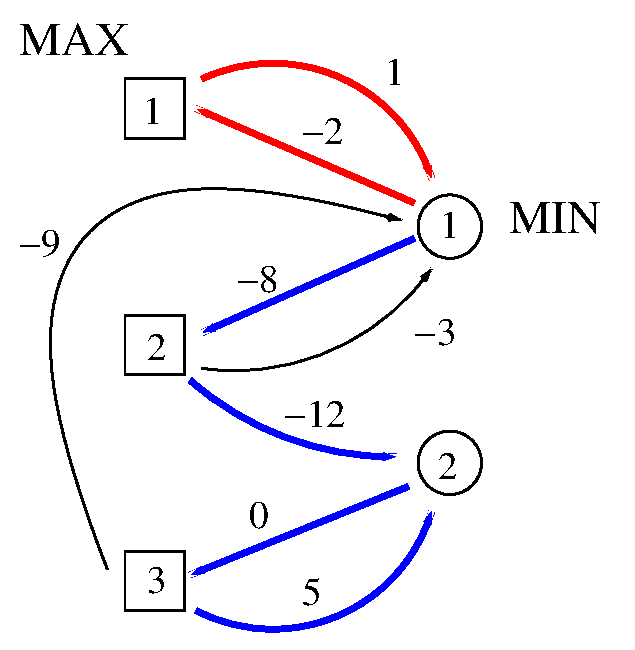
\includegraphics[scale=0.7]{gameMINMAX/gameMINMAXsignedf.eps}}%
 &  
%
\raisebox{2cm}{\Large $%
  %
  %
  %
  \bl{(\chi_1,\chi_2)= (-1,5)}$}
\end{tabular}
\end{overlayarea}
\end{frame}

%
%
%
%
%
%
%
%
%
%
%
%
%
%
%
%
%
%
%
%
%
%
%

%
%
%
%
%
%
%
%
%
%
%

%
%
%
%
%
%
%
%
%
%
%
%
%
%
%
%
%
%
%
%
%
%
%
%
%



%
%
%
%
\normalsize
\begin{frame}[plain]
\begin{overlayarea}{\textwidth}{2.5cm}
\bl{$v_i^k$ value of the game in horizon $k$ and initial state $(i,MIN)$}.
\begin{visibleenv}<1->
\begin{align*}
\!\!\!\!v^k_1 &\!= \min(-2+1+v_1^{k-1}\!,-8+\max(-3+v_1^{k-1}\!,-12+v_2^{k-1}))\\
\!\!\!\!v^k_2&\!=0+\max(-9+v^{k-1}_1,5+v^{k-1}_2)
\end{align*}
\if{
\only<1>{\[
A= \begin{pmatrix} 2 & -\infty\\
                       8  &   -\infty \\
                       -\infty & 0 
\end{pmatrix}
\qquad
B= 
\begin{pmatrix} 1 & -\infty\\
                       -3  &   -12 \\
                       -9 & 5 
\end{pmatrix}
\]}
\only<2->{\begin{align*}%
\begin{array}{rl}
2+x_1&\leq 1+x_1 \\ 
8+x_1&\leq \max(-3+x_1,-12+x_2)\\
x_2&\leq \max(-9+x_1,5 +x_2)
\end{array}
\end{align*}}}\fi
\end{visibleenv}
\end{overlayarea}
\vfill
\begin{overlayarea}{\textwidth}{5cm}
\begin{tabular}{cc}
\input{gameMINMAXsigned} &  \only<1>{}\only<1->{
\raisebox{2cm}{\begin{tabular}{l}$v^1=(0,0)$\\ $v^2=(-11,5)$\\ $v^3=(-15,10)$\\
$v^4=(-16,15)$\\ %
$\chi= \lim_{k\to\infty} v^k/k=(-1,5)\if{, x=(-\infty,0) \; \text{sol.}}\fi$\end{tabular}}}
\end{tabular}
\end{overlayarea}
\end{frame}
\begin{frame}[plain]\normalsize
  \begin{proposition}
    The \bl{value vector $v^k$ of the game in horizon $k$} satisfies
  \[ v^k=T(v^{k-1}), \qquad v^0=0 \]
  where $T:\R^n\to \R^n$ is the \bl{Shapley operator}:
  \[
[T(x)]_j= \min_{i\in [m],\; j\to i} \left(r_{ji}+ \max_{k\in [n],\;i\to k} (r_{ik} + x_k)\right)
\]
The mean-payoff $\chi$ coincides with the limit
\[
\lim_k v^k/k = \lim_k T^k(0)/k \enspace .
\]
  \end{proposition}
  \begin{theorem}[Collatz-Wielandt, see \giveref{Akian, Guterman, SG, IJAC, 2012}]\vspace{-1.5ex}
    \[
 \rho(T):=   \max_i \chi_i = \max \{\lambda \in \R\mid \exists u \in \TT^n, \, u\not\equiv -\infty, \; T(u) = \lambda +u \} 
    \]
    \end{theorem}
%
%
%
\end{frame}
\begin{frame}[plain]{Quantitative tropical linear independence}
  We equip $\R^n$ with \bl{Hilbert's seminorm}
  $\|x\|_H = \max_i x_i -\min_i x_i$.
  Given $V\in \R^{n\times m}$, $\tcone(V)$ denotes the set of tropical linear
  combinations of the columns of $V$.

  \vfill
  The \bl{tit-for-tat} game is the mean-payoff game with Shapley operator
  \begin{align*}
  [T_V(x)]_i = \max_{j\in[m]}\Big(V_{ij} + \min_{k\in [n]\setminus\{i\}}( -V_{kj} + x_k)\Big)
  \end{align*}
  Max can cancel the last move of Min, but not vice-versa. Introduced in \giveref{Akian, SG, Guterman 2012} to decide linear independence.
  \begin{theorem}[\giveref{Akian, SG, Qi, Saadi, SIAM Disc. Math. 2023}]
    \vspace{-3ex}
    \begin{align*}
    \rho(T_V) &= \max\{ r\mid \exists u\in \R^n, B(u,r)\subset \tcone(V)\}\\
    &= \inf_{u\in \R^n} \max_k \operatorname{dist}_H(V_{\cdot,k}, H_u)
    \end{align*}
  \end{theorem}
  \informative{\footnotesize \alert{Advertisement (recent extension)}. Game approach carries over to \alert{linear independence of rational functions over tropical curves}; we end up with a stochastic game, \giveref{\footnotesize Amini, SG, Gierczak 2504.02715}. %
  }
\end{frame}
\begin{frame}[plain]\small
  \begin{center}
    %\documentclass{standalone}
%\usepackage{tikz}

%% The general formula of projection of point (x_1,x_2,x_3) is $P(x_1,x_2,x_3)=(-\sqrt{3}/2*(x_1-x_2) , -(1/2)*x_{1} - (1/2)*x_{2} + x_{3})$.

\def\coord#1#2#3{{-sqrt(3)/2*(#1-#2)} ,{ -(1/2)*#1 - (1/2)*#2 + #3}}
%\begin{document}
\begin{tikzpicture}[scale=0.95]

\coordinate (v1) at (\coord{-3}{0}{-1});
\coordinate (v2) at (\coord{0}{-3}{-1});
\coordinate (v3) at (\coord{0}{0}{-4});
\coordinate (v4) at (\coord{1}{0}{-2});
\coordinate (v5) at (\coord{1}{-1}{-1});
\coordinate (v6) at (\coord{-1}{1}{-1});
\coordinate (v7) at (\coord{0}{1}{-2});
\coordinate (v8) at (\coord{0}{-1}{0});
\coordinate (v9) at (\coord{-1}{0}{0});

\coordinate (v1p) at (\coord{-5}{0}{-1});
\coordinate (v2p) at (\coord{0}{-5}{-1});
\coordinate (v3p) at (\coord{0}{0}{-5});

\coordinate (f1) at (\coord{-2}{0}{-1});
\coordinate (f2) at (\coord{0}{-2}{-1});
\coordinate (f3) at (\coord{0}{0}{-3});

\coordinate (b1) at (\coord{0}{0}{0});
\coordinate (b2) at (\coord{0}{1}{0});
\coordinate (b3) at (\coord{0}{1}{-1});
\coordinate (b4) at (\coord{0}{0}{-2});
\coordinate (b5) at (\coord{1}{0}{-1});
\coordinate (b6) at (\coord{1}{0}{0});

%% \fill[red!30,opacity=0.7] (v1p) -- (\coord{0}{0}{-1}) -- (v2p)--cycle;
%% \fill[blue!30,opacity=0.7] (v1p) -- (\coord{0}{0}{-1}) -- (v3p)--cycle;
%% \fill[green!30,opacity=0.7] (v2p) -- (\coord{0}{0}{-1}) -- (v3p)--cycle;


\filldraw[black,draw=black,opacity=0.8,very thick] (v1) -- (f1) -- (v9) -- (b1) -- (v8) -- (f2) -- (v2) -- (f2) -- (v5) -- (b5) -- (v4) -- (f3) -- (v3) -- (f3) -- (v7) -- (b3) -- (v6) -- (f1) -- (v1) -- cycle;
\filldraw[gray] (f1) -- (v9) -- (b1) -- (v8) -- (f2) -- (v5) -- (b5) -- (v4) -- (f3) -- (v7) -- (b3) -- (v6) -- (f1) -- cycle;

\filldraw[blue!80,draw=blue!80,opacity=0.7, thick] (b1) -- (b2) -- (b3) -- (b4) -- (b5) -- (b6) -- (b1) -- cycle;


\filldraw[black] (v1) circle (2.5pt) node[above] {$V_{\cdot 1}$};
\filldraw[black] (v2) circle (2.5pt) node[above] {$V_{\cdot 2}$};
\filldraw[black] (v3) circle (2.5pt) node[below,right]{$V_{\cdot 3}$};
\filldraw[red] (v4) circle (2.5pt) node[below,left,black] {$V_{\cdot 4}$};
\filldraw[red] (v5) circle (2.5pt) node[below,left,black] {$V_{\cdot 5}$};
\filldraw[red] (v6) circle (2.5pt) node[below,right,black] {$V_{\cdot 6}$};
\filldraw[red] (v7) circle (2.5pt) node[below,right,black] {$V_{\cdot 7}$};
\filldraw[red] (v8) circle (2.5pt) node[above,black] {$V_{\cdot 8}$};
\filldraw[red] (v9) circle (2.5pt) node[above,black] {$V_{\cdot 9}$};

\draw[dashed,->] (\coord{0}{0}{0}) -- (\coord{5}{0}{0}) node[above] {$x_1$};
\draw[dashed,->] (\coord{0}{0}{0}) -- (\coord{0}{5}{0}) node[above] {$x_2$};
\draw[dashed,->] (\coord{0}{0}{0}) -- (\coord{0}{0}{2.5}) node[above, right] {$x_3$};
\filldraw[black] (\coord{0}{0}{0}) circle (1.5pt) node[below,right] {0};

%The regression hyperplane
\draw[very thick,red] (\coord{0}{0}{-1}) -- (v1p);
\draw[very thick,red] (\coord{0}{0}{-1}) -- (v2p);
\draw[very thick,red] (\coord{0}{0}{-1}) -- (v3p);
\filldraw[black] (\coord{0}{0}{-1}) circle (1.5pt) node[below,right] {$-a$};
\draw node[above] at (\coord{-1/2}{0}{-1}) {$\cH_a$};


\end{tikzpicture}
%\end{document}





  \end{center}
\[V=\left(\begin{array}{ccccccccc}
  -3 & 0  &  0 &  1  & 1 & -1 & 0 & 0 & -1\\
   0 & -3 &  0  & 0  & -1 & 1 & 1 & -1 & 0\\
   -1 & -1  & -4 & -2  &  -1  &  -1  & -2  & 0  & 0
\end{array}
\right)
\]
  \end{frame}

\begin{frame}[plain]
The hyperplane $H_a$ \bl{separates} the point sets $V^1, \ldots, V^K\subset \R^n$ if there exists $K$ disjoint non-empty subsets $I^1, \ldots, I^K$ of $\{1,\dots,n\}$, such that every vector $V_{\cdot k}$
  belongs to the union of the sectors $(\text{Sec}_i(a))_{i\in I^k}$ assigned to class $k$; $\text{Sec}_i(a) := \{x\in \R^n\mid x_i + a_i \geq \max_{j\neq i} x_j + a_j\}$.

  \vfill
\begin{center}
        \resizebox{0.2\linewidth}{!}{%
        \centering
    \clipbox{0.15\width{} 0.15\height{} 0.15\width{} 0.15\height{}}{%% Creator: Matplotlib, PGF backend
%%
%% To include the figure in your LaTeX document, write
%%   \input{<filename>.pgf}
%%
%% Make sure the required packages are loaded in your preamble
%%   \usepackage{pgf}
%%
%% Also ensure that all the required font packages are loaded; for instance,
%% the lmodern package is sometimes necessary when using math font.
%%   \usepackage{lmodern}
%%
%% Figures using additional raster images can only be included by \input if
%% they are in the same directory as the main LaTeX file. For loading figures
%% from other directories you can use the `import` package
%%   \usepackage{import}
%%
%% and then include the figures with
%%   \import{<path to file>}{<filename>.pgf}
%%
%% Matplotlib used the following preamble
%%   
%%   \usepackage{fontspec}
%%   \setmainfont{DejaVuSerif.ttf}[Path=\detokenize{/Users/sam/Library/Python/3.9/lib/python/site-packages/matplotlib/mpl-data/fonts/ttf/}]
%%   \setsansfont{DejaVuSans.ttf}[Path=\detokenize{/Users/sam/Library/Python/3.9/lib/python/site-packages/matplotlib/mpl-data/fonts/ttf/}]
%%   \setmonofont{DejaVuSansMono.ttf}[Path=\detokenize{/Users/sam/Library/Python/3.9/lib/python/site-packages/matplotlib/mpl-data/fonts/ttf/}]
%%   \makeatletter\@ifpackageloaded{underscore}{}{\usepackage[strings]{underscore}}\makeatother
%%
\begingroup%
\makeatletter%
\begin{pgfpicture}%
\pgfpathrectangle{\pgfpointorigin}{\pgfqpoint{6.000000in}{6.000000in}}%
\pgfusepath{use as bounding box, clip}%
\begin{pgfscope}%
\pgfsetbuttcap%
\pgfsetmiterjoin%
\definecolor{currentfill}{rgb}{1.000000,1.000000,1.000000}%
\pgfsetfillcolor{currentfill}%
\pgfsetlinewidth{0.000000pt}%
\definecolor{currentstroke}{rgb}{1.000000,1.000000,1.000000}%
\pgfsetstrokecolor{currentstroke}%
\pgfsetdash{}{0pt}%
\pgfpathmoveto{\pgfqpoint{0.000000in}{0.000000in}}%
\pgfpathlineto{\pgfqpoint{6.000000in}{0.000000in}}%
\pgfpathlineto{\pgfqpoint{6.000000in}{6.000000in}}%
\pgfpathlineto{\pgfqpoint{0.000000in}{6.000000in}}%
\pgfpathlineto{\pgfqpoint{0.000000in}{0.000000in}}%
\pgfpathclose%
\pgfusepath{fill}%
\end{pgfscope}%
\begin{pgfscope}%
\pgfsetbuttcap%
\pgfsetmiterjoin%
\definecolor{currentfill}{rgb}{1.000000,1.000000,1.000000}%
\pgfsetfillcolor{currentfill}%
\pgfsetlinewidth{0.000000pt}%
\definecolor{currentstroke}{rgb}{0.000000,0.000000,0.000000}%
\pgfsetstrokecolor{currentstroke}%
\pgfsetstrokeopacity{0.000000}%
\pgfsetdash{}{0pt}%
\pgfpathmoveto{\pgfqpoint{0.765000in}{0.660000in}}%
\pgfpathlineto{\pgfqpoint{5.385000in}{0.660000in}}%
\pgfpathlineto{\pgfqpoint{5.385000in}{5.280000in}}%
\pgfpathlineto{\pgfqpoint{0.765000in}{5.280000in}}%
\pgfpathlineto{\pgfqpoint{0.765000in}{0.660000in}}%
\pgfpathclose%
\pgfusepath{fill}%
\end{pgfscope}%
\begin{pgfscope}%
\pgfpathrectangle{\pgfqpoint{0.765000in}{0.660000in}}{\pgfqpoint{4.620000in}{4.620000in}}%
\pgfusepath{clip}%
\pgfsetbuttcap%
\pgfsetroundjoin%
\definecolor{currentfill}{rgb}{1.000000,0.894118,0.788235}%
\pgfsetfillcolor{currentfill}%
\pgfsetlinewidth{0.000000pt}%
\definecolor{currentstroke}{rgb}{1.000000,0.894118,0.788235}%
\pgfsetstrokecolor{currentstroke}%
\pgfsetdash{}{0pt}%
\pgfpathmoveto{\pgfqpoint{-3.891113in}{6.386809in}}%
\pgfpathlineto{\pgfqpoint{-4.344914in}{6.173762in}}%
\pgfpathlineto{\pgfqpoint{-4.344914in}{6.598751in}}%
\pgfpathlineto{\pgfqpoint{-3.891113in}{6.811798in}}%
\pgfpathlineto{\pgfqpoint{-3.891113in}{6.386809in}}%
\pgfpathclose%
\pgfusepath{fill}%
\end{pgfscope}%
\begin{pgfscope}%
\pgfpathrectangle{\pgfqpoint{0.765000in}{0.660000in}}{\pgfqpoint{4.620000in}{4.620000in}}%
\pgfusepath{clip}%
\pgfsetbuttcap%
\pgfsetroundjoin%
\definecolor{currentfill}{rgb}{1.000000,0.894118,0.788235}%
\pgfsetfillcolor{currentfill}%
\pgfsetlinewidth{0.000000pt}%
\definecolor{currentstroke}{rgb}{1.000000,0.894118,0.788235}%
\pgfsetstrokecolor{currentstroke}%
\pgfsetdash{}{0pt}%
\pgfpathmoveto{\pgfqpoint{-3.891113in}{6.386809in}}%
\pgfpathlineto{\pgfqpoint{-3.437311in}{6.173762in}}%
\pgfpathlineto{\pgfqpoint{-3.437311in}{6.598751in}}%
\pgfpathlineto{\pgfqpoint{-3.891113in}{6.811798in}}%
\pgfpathlineto{\pgfqpoint{-3.891113in}{6.386809in}}%
\pgfpathclose%
\pgfusepath{fill}%
\end{pgfscope}%
\begin{pgfscope}%
\pgfpathrectangle{\pgfqpoint{0.765000in}{0.660000in}}{\pgfqpoint{4.620000in}{4.620000in}}%
\pgfusepath{clip}%
\pgfsetbuttcap%
\pgfsetroundjoin%
\definecolor{currentfill}{rgb}{1.000000,0.894118,0.788235}%
\pgfsetfillcolor{currentfill}%
\pgfsetlinewidth{0.000000pt}%
\definecolor{currentstroke}{rgb}{1.000000,0.894118,0.788235}%
\pgfsetstrokecolor{currentstroke}%
\pgfsetdash{}{0pt}%
\pgfpathmoveto{\pgfqpoint{-3.891113in}{6.386809in}}%
\pgfpathlineto{\pgfqpoint{-4.344914in}{6.173762in}}%
\pgfpathlineto{\pgfqpoint{-3.891113in}{5.960715in}}%
\pgfpathlineto{\pgfqpoint{-3.437311in}{6.173762in}}%
\pgfpathlineto{\pgfqpoint{-3.891113in}{6.386809in}}%
\pgfpathclose%
\pgfusepath{fill}%
\end{pgfscope}%
\begin{pgfscope}%
\pgfpathrectangle{\pgfqpoint{0.765000in}{0.660000in}}{\pgfqpoint{4.620000in}{4.620000in}}%
\pgfusepath{clip}%
\pgfsetbuttcap%
\pgfsetroundjoin%
\definecolor{currentfill}{rgb}{1.000000,0.894118,0.788235}%
\pgfsetfillcolor{currentfill}%
\pgfsetlinewidth{0.000000pt}%
\definecolor{currentstroke}{rgb}{1.000000,0.894118,0.788235}%
\pgfsetstrokecolor{currentstroke}%
\pgfsetdash{}{0pt}%
\pgfpathmoveto{\pgfqpoint{-3.891113in}{6.811798in}}%
\pgfpathlineto{\pgfqpoint{-4.344914in}{6.598751in}}%
\pgfpathlineto{\pgfqpoint{-3.891113in}{6.385704in}}%
\pgfpathlineto{\pgfqpoint{-3.437311in}{6.598751in}}%
\pgfpathlineto{\pgfqpoint{-3.891113in}{6.811798in}}%
\pgfpathclose%
\pgfusepath{fill}%
\end{pgfscope}%
\begin{pgfscope}%
\pgfpathrectangle{\pgfqpoint{0.765000in}{0.660000in}}{\pgfqpoint{4.620000in}{4.620000in}}%
\pgfusepath{clip}%
\pgfsetbuttcap%
\pgfsetroundjoin%
\definecolor{currentfill}{rgb}{1.000000,0.894118,0.788235}%
\pgfsetfillcolor{currentfill}%
\pgfsetlinewidth{0.000000pt}%
\definecolor{currentstroke}{rgb}{1.000000,0.894118,0.788235}%
\pgfsetstrokecolor{currentstroke}%
\pgfsetdash{}{0pt}%
\pgfpathmoveto{\pgfqpoint{-3.891113in}{5.960715in}}%
\pgfpathlineto{\pgfqpoint{-3.437311in}{6.173762in}}%
\pgfpathlineto{\pgfqpoint{-3.437311in}{6.598751in}}%
\pgfpathlineto{\pgfqpoint{-3.891113in}{6.385704in}}%
\pgfpathlineto{\pgfqpoint{-3.891113in}{5.960715in}}%
\pgfpathclose%
\pgfusepath{fill}%
\end{pgfscope}%
\begin{pgfscope}%
\pgfpathrectangle{\pgfqpoint{0.765000in}{0.660000in}}{\pgfqpoint{4.620000in}{4.620000in}}%
\pgfusepath{clip}%
\pgfsetbuttcap%
\pgfsetroundjoin%
\definecolor{currentfill}{rgb}{1.000000,0.894118,0.788235}%
\pgfsetfillcolor{currentfill}%
\pgfsetlinewidth{0.000000pt}%
\definecolor{currentstroke}{rgb}{1.000000,0.894118,0.788235}%
\pgfsetstrokecolor{currentstroke}%
\pgfsetdash{}{0pt}%
\pgfpathmoveto{\pgfqpoint{-4.344914in}{6.173762in}}%
\pgfpathlineto{\pgfqpoint{-3.891113in}{5.960715in}}%
\pgfpathlineto{\pgfqpoint{-3.891113in}{6.385704in}}%
\pgfpathlineto{\pgfqpoint{-4.344914in}{6.598751in}}%
\pgfpathlineto{\pgfqpoint{-4.344914in}{6.173762in}}%
\pgfpathclose%
\pgfusepath{fill}%
\end{pgfscope}%
\begin{pgfscope}%
\pgfpathrectangle{\pgfqpoint{0.765000in}{0.660000in}}{\pgfqpoint{4.620000in}{4.620000in}}%
\pgfusepath{clip}%
\pgfsetbuttcap%
\pgfsetroundjoin%
\definecolor{currentfill}{rgb}{1.000000,0.894118,0.788235}%
\pgfsetfillcolor{currentfill}%
\pgfsetlinewidth{0.000000pt}%
\definecolor{currentstroke}{rgb}{1.000000,0.894118,0.788235}%
\pgfsetstrokecolor{currentstroke}%
\pgfsetdash{}{0pt}%
\pgfpathmoveto{\pgfqpoint{3.071405in}{3.123758in}}%
\pgfpathlineto{\pgfqpoint{2.617603in}{2.910711in}}%
\pgfpathlineto{\pgfqpoint{2.617603in}{3.335700in}}%
\pgfpathlineto{\pgfqpoint{3.071405in}{3.548747in}}%
\pgfpathlineto{\pgfqpoint{3.071405in}{3.123758in}}%
\pgfpathclose%
\pgfusepath{fill}%
\end{pgfscope}%
\begin{pgfscope}%
\pgfpathrectangle{\pgfqpoint{0.765000in}{0.660000in}}{\pgfqpoint{4.620000in}{4.620000in}}%
\pgfusepath{clip}%
\pgfsetbuttcap%
\pgfsetroundjoin%
\definecolor{currentfill}{rgb}{1.000000,0.894118,0.788235}%
\pgfsetfillcolor{currentfill}%
\pgfsetlinewidth{0.000000pt}%
\definecolor{currentstroke}{rgb}{1.000000,0.894118,0.788235}%
\pgfsetstrokecolor{currentstroke}%
\pgfsetdash{}{0pt}%
\pgfpathmoveto{\pgfqpoint{3.071405in}{3.123758in}}%
\pgfpathlineto{\pgfqpoint{3.525206in}{2.910711in}}%
\pgfpathlineto{\pgfqpoint{3.525206in}{3.335700in}}%
\pgfpathlineto{\pgfqpoint{3.071405in}{3.548747in}}%
\pgfpathlineto{\pgfqpoint{3.071405in}{3.123758in}}%
\pgfpathclose%
\pgfusepath{fill}%
\end{pgfscope}%
\begin{pgfscope}%
\pgfpathrectangle{\pgfqpoint{0.765000in}{0.660000in}}{\pgfqpoint{4.620000in}{4.620000in}}%
\pgfusepath{clip}%
\pgfsetbuttcap%
\pgfsetroundjoin%
\definecolor{currentfill}{rgb}{1.000000,0.894118,0.788235}%
\pgfsetfillcolor{currentfill}%
\pgfsetlinewidth{0.000000pt}%
\definecolor{currentstroke}{rgb}{1.000000,0.894118,0.788235}%
\pgfsetstrokecolor{currentstroke}%
\pgfsetdash{}{0pt}%
\pgfpathmoveto{\pgfqpoint{3.071405in}{3.123758in}}%
\pgfpathlineto{\pgfqpoint{2.617603in}{2.910711in}}%
\pgfpathlineto{\pgfqpoint{3.071405in}{2.697664in}}%
\pgfpathlineto{\pgfqpoint{3.525206in}{2.910711in}}%
\pgfpathlineto{\pgfqpoint{3.071405in}{3.123758in}}%
\pgfpathclose%
\pgfusepath{fill}%
\end{pgfscope}%
\begin{pgfscope}%
\pgfpathrectangle{\pgfqpoint{0.765000in}{0.660000in}}{\pgfqpoint{4.620000in}{4.620000in}}%
\pgfusepath{clip}%
\pgfsetbuttcap%
\pgfsetroundjoin%
\definecolor{currentfill}{rgb}{1.000000,0.894118,0.788235}%
\pgfsetfillcolor{currentfill}%
\pgfsetlinewidth{0.000000pt}%
\definecolor{currentstroke}{rgb}{1.000000,0.894118,0.788235}%
\pgfsetstrokecolor{currentstroke}%
\pgfsetdash{}{0pt}%
\pgfpathmoveto{\pgfqpoint{3.071405in}{3.548747in}}%
\pgfpathlineto{\pgfqpoint{2.617603in}{3.335700in}}%
\pgfpathlineto{\pgfqpoint{3.071405in}{3.122653in}}%
\pgfpathlineto{\pgfqpoint{3.525206in}{3.335700in}}%
\pgfpathlineto{\pgfqpoint{3.071405in}{3.548747in}}%
\pgfpathclose%
\pgfusepath{fill}%
\end{pgfscope}%
\begin{pgfscope}%
\pgfpathrectangle{\pgfqpoint{0.765000in}{0.660000in}}{\pgfqpoint{4.620000in}{4.620000in}}%
\pgfusepath{clip}%
\pgfsetbuttcap%
\pgfsetroundjoin%
\definecolor{currentfill}{rgb}{1.000000,0.894118,0.788235}%
\pgfsetfillcolor{currentfill}%
\pgfsetlinewidth{0.000000pt}%
\definecolor{currentstroke}{rgb}{1.000000,0.894118,0.788235}%
\pgfsetstrokecolor{currentstroke}%
\pgfsetdash{}{0pt}%
\pgfpathmoveto{\pgfqpoint{2.617603in}{2.910711in}}%
\pgfpathlineto{\pgfqpoint{3.071405in}{2.697664in}}%
\pgfpathlineto{\pgfqpoint{3.071405in}{3.122653in}}%
\pgfpathlineto{\pgfqpoint{2.617603in}{3.335700in}}%
\pgfpathlineto{\pgfqpoint{2.617603in}{2.910711in}}%
\pgfpathclose%
\pgfusepath{fill}%
\end{pgfscope}%
\begin{pgfscope}%
\pgfpathrectangle{\pgfqpoint{0.765000in}{0.660000in}}{\pgfqpoint{4.620000in}{4.620000in}}%
\pgfusepath{clip}%
\pgfsetbuttcap%
\pgfsetroundjoin%
\definecolor{currentfill}{rgb}{1.000000,0.894118,0.788235}%
\pgfsetfillcolor{currentfill}%
\pgfsetlinewidth{0.000000pt}%
\definecolor{currentstroke}{rgb}{1.000000,0.894118,0.788235}%
\pgfsetstrokecolor{currentstroke}%
\pgfsetdash{}{0pt}%
\pgfpathmoveto{\pgfqpoint{3.071405in}{2.697664in}}%
\pgfpathlineto{\pgfqpoint{3.525206in}{2.910711in}}%
\pgfpathlineto{\pgfqpoint{3.525206in}{3.335700in}}%
\pgfpathlineto{\pgfqpoint{3.071405in}{3.122653in}}%
\pgfpathlineto{\pgfqpoint{3.071405in}{2.697664in}}%
\pgfpathclose%
\pgfusepath{fill}%
\end{pgfscope}%
\begin{pgfscope}%
\pgfpathrectangle{\pgfqpoint{0.765000in}{0.660000in}}{\pgfqpoint{4.620000in}{4.620000in}}%
\pgfusepath{clip}%
\pgfsetbuttcap%
\pgfsetroundjoin%
\definecolor{currentfill}{rgb}{1.000000,0.894118,0.788235}%
\pgfsetfillcolor{currentfill}%
\pgfsetlinewidth{0.000000pt}%
\definecolor{currentstroke}{rgb}{1.000000,0.894118,0.788235}%
\pgfsetstrokecolor{currentstroke}%
\pgfsetdash{}{0pt}%
\pgfpathmoveto{\pgfqpoint{3.071405in}{3.123758in}}%
\pgfpathlineto{\pgfqpoint{2.617603in}{2.910711in}}%
\pgfpathlineto{\pgfqpoint{-4.344914in}{6.173762in}}%
\pgfpathlineto{\pgfqpoint{-3.891113in}{6.386809in}}%
\pgfpathlineto{\pgfqpoint{3.071405in}{3.123758in}}%
\pgfpathclose%
\pgfusepath{fill}%
\end{pgfscope}%
\begin{pgfscope}%
\pgfpathrectangle{\pgfqpoint{0.765000in}{0.660000in}}{\pgfqpoint{4.620000in}{4.620000in}}%
\pgfusepath{clip}%
\pgfsetbuttcap%
\pgfsetroundjoin%
\definecolor{currentfill}{rgb}{1.000000,0.894118,0.788235}%
\pgfsetfillcolor{currentfill}%
\pgfsetlinewidth{0.000000pt}%
\definecolor{currentstroke}{rgb}{1.000000,0.894118,0.788235}%
\pgfsetstrokecolor{currentstroke}%
\pgfsetdash{}{0pt}%
\pgfpathmoveto{\pgfqpoint{3.525206in}{2.910711in}}%
\pgfpathlineto{\pgfqpoint{3.071405in}{3.123758in}}%
\pgfpathlineto{\pgfqpoint{-3.891113in}{6.386809in}}%
\pgfpathlineto{\pgfqpoint{-3.437311in}{6.173762in}}%
\pgfpathlineto{\pgfqpoint{3.525206in}{2.910711in}}%
\pgfpathclose%
\pgfusepath{fill}%
\end{pgfscope}%
\begin{pgfscope}%
\pgfpathrectangle{\pgfqpoint{0.765000in}{0.660000in}}{\pgfqpoint{4.620000in}{4.620000in}}%
\pgfusepath{clip}%
\pgfsetbuttcap%
\pgfsetroundjoin%
\definecolor{currentfill}{rgb}{1.000000,0.894118,0.788235}%
\pgfsetfillcolor{currentfill}%
\pgfsetlinewidth{0.000000pt}%
\definecolor{currentstroke}{rgb}{1.000000,0.894118,0.788235}%
\pgfsetstrokecolor{currentstroke}%
\pgfsetdash{}{0pt}%
\pgfpathmoveto{\pgfqpoint{3.071405in}{3.123758in}}%
\pgfpathlineto{\pgfqpoint{3.071405in}{3.548747in}}%
\pgfpathlineto{\pgfqpoint{-3.891113in}{6.811798in}}%
\pgfpathlineto{\pgfqpoint{-3.437311in}{6.173762in}}%
\pgfpathlineto{\pgfqpoint{3.071405in}{3.123758in}}%
\pgfpathclose%
\pgfusepath{fill}%
\end{pgfscope}%
\begin{pgfscope}%
\pgfpathrectangle{\pgfqpoint{0.765000in}{0.660000in}}{\pgfqpoint{4.620000in}{4.620000in}}%
\pgfusepath{clip}%
\pgfsetbuttcap%
\pgfsetroundjoin%
\definecolor{currentfill}{rgb}{1.000000,0.894118,0.788235}%
\pgfsetfillcolor{currentfill}%
\pgfsetlinewidth{0.000000pt}%
\definecolor{currentstroke}{rgb}{1.000000,0.894118,0.788235}%
\pgfsetstrokecolor{currentstroke}%
\pgfsetdash{}{0pt}%
\pgfpathmoveto{\pgfqpoint{3.525206in}{2.910711in}}%
\pgfpathlineto{\pgfqpoint{3.525206in}{3.335700in}}%
\pgfpathlineto{\pgfqpoint{-3.437311in}{6.598751in}}%
\pgfpathlineto{\pgfqpoint{-3.891113in}{6.386809in}}%
\pgfpathlineto{\pgfqpoint{3.525206in}{2.910711in}}%
\pgfpathclose%
\pgfusepath{fill}%
\end{pgfscope}%
\begin{pgfscope}%
\pgfpathrectangle{\pgfqpoint{0.765000in}{0.660000in}}{\pgfqpoint{4.620000in}{4.620000in}}%
\pgfusepath{clip}%
\pgfsetbuttcap%
\pgfsetroundjoin%
\definecolor{currentfill}{rgb}{1.000000,0.894118,0.788235}%
\pgfsetfillcolor{currentfill}%
\pgfsetlinewidth{0.000000pt}%
\definecolor{currentstroke}{rgb}{1.000000,0.894118,0.788235}%
\pgfsetstrokecolor{currentstroke}%
\pgfsetdash{}{0pt}%
\pgfpathmoveto{\pgfqpoint{3.071405in}{3.548747in}}%
\pgfpathlineto{\pgfqpoint{2.617603in}{3.335700in}}%
\pgfpathlineto{\pgfqpoint{-4.344914in}{6.598751in}}%
\pgfpathlineto{\pgfqpoint{-3.891113in}{6.811798in}}%
\pgfpathlineto{\pgfqpoint{3.071405in}{3.548747in}}%
\pgfpathclose%
\pgfusepath{fill}%
\end{pgfscope}%
\begin{pgfscope}%
\pgfpathrectangle{\pgfqpoint{0.765000in}{0.660000in}}{\pgfqpoint{4.620000in}{4.620000in}}%
\pgfusepath{clip}%
\pgfsetbuttcap%
\pgfsetroundjoin%
\definecolor{currentfill}{rgb}{1.000000,0.894118,0.788235}%
\pgfsetfillcolor{currentfill}%
\pgfsetlinewidth{0.000000pt}%
\definecolor{currentstroke}{rgb}{1.000000,0.894118,0.788235}%
\pgfsetstrokecolor{currentstroke}%
\pgfsetdash{}{0pt}%
\pgfpathmoveto{\pgfqpoint{3.525206in}{3.335700in}}%
\pgfpathlineto{\pgfqpoint{3.071405in}{3.548747in}}%
\pgfpathlineto{\pgfqpoint{-3.891113in}{6.811798in}}%
\pgfpathlineto{\pgfqpoint{-3.437311in}{6.598751in}}%
\pgfpathlineto{\pgfqpoint{3.525206in}{3.335700in}}%
\pgfpathclose%
\pgfusepath{fill}%
\end{pgfscope}%
\begin{pgfscope}%
\pgfpathrectangle{\pgfqpoint{0.765000in}{0.660000in}}{\pgfqpoint{4.620000in}{4.620000in}}%
\pgfusepath{clip}%
\pgfsetbuttcap%
\pgfsetroundjoin%
\definecolor{currentfill}{rgb}{1.000000,0.894118,0.788235}%
\pgfsetfillcolor{currentfill}%
\pgfsetlinewidth{0.000000pt}%
\definecolor{currentstroke}{rgb}{1.000000,0.894118,0.788235}%
\pgfsetstrokecolor{currentstroke}%
\pgfsetdash{}{0pt}%
\pgfpathmoveto{\pgfqpoint{3.071405in}{2.697664in}}%
\pgfpathlineto{\pgfqpoint{3.525206in}{2.910711in}}%
\pgfpathlineto{\pgfqpoint{-3.437311in}{6.173762in}}%
\pgfpathlineto{\pgfqpoint{-3.891113in}{5.960715in}}%
\pgfpathlineto{\pgfqpoint{3.071405in}{2.697664in}}%
\pgfpathclose%
\pgfusepath{fill}%
\end{pgfscope}%
\begin{pgfscope}%
\pgfpathrectangle{\pgfqpoint{0.765000in}{0.660000in}}{\pgfqpoint{4.620000in}{4.620000in}}%
\pgfusepath{clip}%
\pgfsetbuttcap%
\pgfsetroundjoin%
\definecolor{currentfill}{rgb}{1.000000,0.894118,0.788235}%
\pgfsetfillcolor{currentfill}%
\pgfsetlinewidth{0.000000pt}%
\definecolor{currentstroke}{rgb}{1.000000,0.894118,0.788235}%
\pgfsetstrokecolor{currentstroke}%
\pgfsetdash{}{0pt}%
\pgfpathmoveto{\pgfqpoint{2.617603in}{2.910711in}}%
\pgfpathlineto{\pgfqpoint{3.071405in}{2.697664in}}%
\pgfpathlineto{\pgfqpoint{-3.891113in}{5.960715in}}%
\pgfpathlineto{\pgfqpoint{-4.344914in}{6.173762in}}%
\pgfpathlineto{\pgfqpoint{2.617603in}{2.910711in}}%
\pgfpathclose%
\pgfusepath{fill}%
\end{pgfscope}%
\begin{pgfscope}%
\pgfpathrectangle{\pgfqpoint{0.765000in}{0.660000in}}{\pgfqpoint{4.620000in}{4.620000in}}%
\pgfusepath{clip}%
\pgfsetbuttcap%
\pgfsetroundjoin%
\definecolor{currentfill}{rgb}{1.000000,0.894118,0.788235}%
\pgfsetfillcolor{currentfill}%
\pgfsetlinewidth{0.000000pt}%
\definecolor{currentstroke}{rgb}{1.000000,0.894118,0.788235}%
\pgfsetstrokecolor{currentstroke}%
\pgfsetdash{}{0pt}%
\pgfpathmoveto{\pgfqpoint{2.617603in}{2.910711in}}%
\pgfpathlineto{\pgfqpoint{2.617603in}{3.335700in}}%
\pgfpathlineto{\pgfqpoint{-4.344914in}{6.598751in}}%
\pgfpathlineto{\pgfqpoint{-3.891113in}{5.960715in}}%
\pgfpathlineto{\pgfqpoint{2.617603in}{2.910711in}}%
\pgfpathclose%
\pgfusepath{fill}%
\end{pgfscope}%
\begin{pgfscope}%
\pgfpathrectangle{\pgfqpoint{0.765000in}{0.660000in}}{\pgfqpoint{4.620000in}{4.620000in}}%
\pgfusepath{clip}%
\pgfsetbuttcap%
\pgfsetroundjoin%
\definecolor{currentfill}{rgb}{1.000000,0.894118,0.788235}%
\pgfsetfillcolor{currentfill}%
\pgfsetlinewidth{0.000000pt}%
\definecolor{currentstroke}{rgb}{1.000000,0.894118,0.788235}%
\pgfsetstrokecolor{currentstroke}%
\pgfsetdash{}{0pt}%
\pgfpathmoveto{\pgfqpoint{3.071405in}{2.697664in}}%
\pgfpathlineto{\pgfqpoint{3.071405in}{3.122653in}}%
\pgfpathlineto{\pgfqpoint{-3.891113in}{6.385704in}}%
\pgfpathlineto{\pgfqpoint{-4.344914in}{6.173762in}}%
\pgfpathlineto{\pgfqpoint{3.071405in}{2.697664in}}%
\pgfpathclose%
\pgfusepath{fill}%
\end{pgfscope}%
\begin{pgfscope}%
\pgfpathrectangle{\pgfqpoint{0.765000in}{0.660000in}}{\pgfqpoint{4.620000in}{4.620000in}}%
\pgfusepath{clip}%
\pgfsetbuttcap%
\pgfsetroundjoin%
\definecolor{currentfill}{rgb}{1.000000,0.894118,0.788235}%
\pgfsetfillcolor{currentfill}%
\pgfsetlinewidth{0.000000pt}%
\definecolor{currentstroke}{rgb}{1.000000,0.894118,0.788235}%
\pgfsetstrokecolor{currentstroke}%
\pgfsetdash{}{0pt}%
\pgfpathmoveto{\pgfqpoint{2.617603in}{3.335700in}}%
\pgfpathlineto{\pgfqpoint{3.071405in}{3.122653in}}%
\pgfpathlineto{\pgfqpoint{-3.891113in}{6.385704in}}%
\pgfpathlineto{\pgfqpoint{-4.344914in}{6.598751in}}%
\pgfpathlineto{\pgfqpoint{2.617603in}{3.335700in}}%
\pgfpathclose%
\pgfusepath{fill}%
\end{pgfscope}%
\begin{pgfscope}%
\pgfpathrectangle{\pgfqpoint{0.765000in}{0.660000in}}{\pgfqpoint{4.620000in}{4.620000in}}%
\pgfusepath{clip}%
\pgfsetbuttcap%
\pgfsetroundjoin%
\definecolor{currentfill}{rgb}{1.000000,0.894118,0.788235}%
\pgfsetfillcolor{currentfill}%
\pgfsetlinewidth{0.000000pt}%
\definecolor{currentstroke}{rgb}{1.000000,0.894118,0.788235}%
\pgfsetstrokecolor{currentstroke}%
\pgfsetdash{}{0pt}%
\pgfpathmoveto{\pgfqpoint{3.071405in}{3.122653in}}%
\pgfpathlineto{\pgfqpoint{3.525206in}{3.335700in}}%
\pgfpathlineto{\pgfqpoint{-3.437311in}{6.598751in}}%
\pgfpathlineto{\pgfqpoint{-3.891113in}{6.385704in}}%
\pgfpathlineto{\pgfqpoint{3.071405in}{3.122653in}}%
\pgfpathclose%
\pgfusepath{fill}%
\end{pgfscope}%
\begin{pgfscope}%
\pgfpathrectangle{\pgfqpoint{0.765000in}{0.660000in}}{\pgfqpoint{4.620000in}{4.620000in}}%
\pgfusepath{clip}%
\pgfsetbuttcap%
\pgfsetroundjoin%
\definecolor{currentfill}{rgb}{1.000000,0.894118,0.788235}%
\pgfsetfillcolor{currentfill}%
\pgfsetlinewidth{0.000000pt}%
\definecolor{currentstroke}{rgb}{1.000000,0.894118,0.788235}%
\pgfsetstrokecolor{currentstroke}%
\pgfsetdash{}{0pt}%
\pgfpathmoveto{\pgfqpoint{10.033922in}{6.386809in}}%
\pgfpathlineto{\pgfqpoint{9.580120in}{6.173762in}}%
\pgfpathlineto{\pgfqpoint{9.580120in}{6.598751in}}%
\pgfpathlineto{\pgfqpoint{10.033922in}{6.811798in}}%
\pgfpathlineto{\pgfqpoint{10.033922in}{6.386809in}}%
\pgfpathclose%
\pgfusepath{fill}%
\end{pgfscope}%
\begin{pgfscope}%
\pgfpathrectangle{\pgfqpoint{0.765000in}{0.660000in}}{\pgfqpoint{4.620000in}{4.620000in}}%
\pgfusepath{clip}%
\pgfsetbuttcap%
\pgfsetroundjoin%
\definecolor{currentfill}{rgb}{1.000000,0.894118,0.788235}%
\pgfsetfillcolor{currentfill}%
\pgfsetlinewidth{0.000000pt}%
\definecolor{currentstroke}{rgb}{1.000000,0.894118,0.788235}%
\pgfsetstrokecolor{currentstroke}%
\pgfsetdash{}{0pt}%
\pgfpathmoveto{\pgfqpoint{10.033922in}{6.386809in}}%
\pgfpathlineto{\pgfqpoint{10.487724in}{6.173762in}}%
\pgfpathlineto{\pgfqpoint{10.487724in}{6.598751in}}%
\pgfpathlineto{\pgfqpoint{10.033922in}{6.811798in}}%
\pgfpathlineto{\pgfqpoint{10.033922in}{6.386809in}}%
\pgfpathclose%
\pgfusepath{fill}%
\end{pgfscope}%
\begin{pgfscope}%
\pgfpathrectangle{\pgfqpoint{0.765000in}{0.660000in}}{\pgfqpoint{4.620000in}{4.620000in}}%
\pgfusepath{clip}%
\pgfsetbuttcap%
\pgfsetroundjoin%
\definecolor{currentfill}{rgb}{1.000000,0.894118,0.788235}%
\pgfsetfillcolor{currentfill}%
\pgfsetlinewidth{0.000000pt}%
\definecolor{currentstroke}{rgb}{1.000000,0.894118,0.788235}%
\pgfsetstrokecolor{currentstroke}%
\pgfsetdash{}{0pt}%
\pgfpathmoveto{\pgfqpoint{10.033922in}{6.386809in}}%
\pgfpathlineto{\pgfqpoint{9.580120in}{6.173762in}}%
\pgfpathlineto{\pgfqpoint{10.033922in}{5.960715in}}%
\pgfpathlineto{\pgfqpoint{10.487724in}{6.173762in}}%
\pgfpathlineto{\pgfqpoint{10.033922in}{6.386809in}}%
\pgfpathclose%
\pgfusepath{fill}%
\end{pgfscope}%
\begin{pgfscope}%
\pgfpathrectangle{\pgfqpoint{0.765000in}{0.660000in}}{\pgfqpoint{4.620000in}{4.620000in}}%
\pgfusepath{clip}%
\pgfsetbuttcap%
\pgfsetroundjoin%
\definecolor{currentfill}{rgb}{1.000000,0.894118,0.788235}%
\pgfsetfillcolor{currentfill}%
\pgfsetlinewidth{0.000000pt}%
\definecolor{currentstroke}{rgb}{1.000000,0.894118,0.788235}%
\pgfsetstrokecolor{currentstroke}%
\pgfsetdash{}{0pt}%
\pgfpathmoveto{\pgfqpoint{10.033922in}{6.811798in}}%
\pgfpathlineto{\pgfqpoint{9.580120in}{6.598751in}}%
\pgfpathlineto{\pgfqpoint{10.033922in}{6.385704in}}%
\pgfpathlineto{\pgfqpoint{10.487724in}{6.598751in}}%
\pgfpathlineto{\pgfqpoint{10.033922in}{6.811798in}}%
\pgfpathclose%
\pgfusepath{fill}%
\end{pgfscope}%
\begin{pgfscope}%
\pgfpathrectangle{\pgfqpoint{0.765000in}{0.660000in}}{\pgfqpoint{4.620000in}{4.620000in}}%
\pgfusepath{clip}%
\pgfsetbuttcap%
\pgfsetroundjoin%
\definecolor{currentfill}{rgb}{1.000000,0.894118,0.788235}%
\pgfsetfillcolor{currentfill}%
\pgfsetlinewidth{0.000000pt}%
\definecolor{currentstroke}{rgb}{1.000000,0.894118,0.788235}%
\pgfsetstrokecolor{currentstroke}%
\pgfsetdash{}{0pt}%
\pgfpathmoveto{\pgfqpoint{10.033922in}{5.960715in}}%
\pgfpathlineto{\pgfqpoint{10.487724in}{6.173762in}}%
\pgfpathlineto{\pgfqpoint{10.487724in}{6.598751in}}%
\pgfpathlineto{\pgfqpoint{10.033922in}{6.385704in}}%
\pgfpathlineto{\pgfqpoint{10.033922in}{5.960715in}}%
\pgfpathclose%
\pgfusepath{fill}%
\end{pgfscope}%
\begin{pgfscope}%
\pgfpathrectangle{\pgfqpoint{0.765000in}{0.660000in}}{\pgfqpoint{4.620000in}{4.620000in}}%
\pgfusepath{clip}%
\pgfsetbuttcap%
\pgfsetroundjoin%
\definecolor{currentfill}{rgb}{1.000000,0.894118,0.788235}%
\pgfsetfillcolor{currentfill}%
\pgfsetlinewidth{0.000000pt}%
\definecolor{currentstroke}{rgb}{1.000000,0.894118,0.788235}%
\pgfsetstrokecolor{currentstroke}%
\pgfsetdash{}{0pt}%
\pgfpathmoveto{\pgfqpoint{9.580120in}{6.173762in}}%
\pgfpathlineto{\pgfqpoint{10.033922in}{5.960715in}}%
\pgfpathlineto{\pgfqpoint{10.033922in}{6.385704in}}%
\pgfpathlineto{\pgfqpoint{9.580120in}{6.598751in}}%
\pgfpathlineto{\pgfqpoint{9.580120in}{6.173762in}}%
\pgfpathclose%
\pgfusepath{fill}%
\end{pgfscope}%
\begin{pgfscope}%
\pgfpathrectangle{\pgfqpoint{0.765000in}{0.660000in}}{\pgfqpoint{4.620000in}{4.620000in}}%
\pgfusepath{clip}%
\pgfsetbuttcap%
\pgfsetroundjoin%
\definecolor{currentfill}{rgb}{1.000000,0.894118,0.788235}%
\pgfsetfillcolor{currentfill}%
\pgfsetlinewidth{0.000000pt}%
\definecolor{currentstroke}{rgb}{1.000000,0.894118,0.788235}%
\pgfsetstrokecolor{currentstroke}%
\pgfsetdash{}{0pt}%
\pgfpathmoveto{\pgfqpoint{3.071405in}{3.123758in}}%
\pgfpathlineto{\pgfqpoint{2.617603in}{2.910711in}}%
\pgfpathlineto{\pgfqpoint{2.617603in}{3.335700in}}%
\pgfpathlineto{\pgfqpoint{3.071405in}{3.548747in}}%
\pgfpathlineto{\pgfqpoint{3.071405in}{3.123758in}}%
\pgfpathclose%
\pgfusepath{fill}%
\end{pgfscope}%
\begin{pgfscope}%
\pgfpathrectangle{\pgfqpoint{0.765000in}{0.660000in}}{\pgfqpoint{4.620000in}{4.620000in}}%
\pgfusepath{clip}%
\pgfsetbuttcap%
\pgfsetroundjoin%
\definecolor{currentfill}{rgb}{1.000000,0.894118,0.788235}%
\pgfsetfillcolor{currentfill}%
\pgfsetlinewidth{0.000000pt}%
\definecolor{currentstroke}{rgb}{1.000000,0.894118,0.788235}%
\pgfsetstrokecolor{currentstroke}%
\pgfsetdash{}{0pt}%
\pgfpathmoveto{\pgfqpoint{3.071405in}{3.123758in}}%
\pgfpathlineto{\pgfqpoint{3.525206in}{2.910711in}}%
\pgfpathlineto{\pgfqpoint{3.525206in}{3.335700in}}%
\pgfpathlineto{\pgfqpoint{3.071405in}{3.548747in}}%
\pgfpathlineto{\pgfqpoint{3.071405in}{3.123758in}}%
\pgfpathclose%
\pgfusepath{fill}%
\end{pgfscope}%
\begin{pgfscope}%
\pgfpathrectangle{\pgfqpoint{0.765000in}{0.660000in}}{\pgfqpoint{4.620000in}{4.620000in}}%
\pgfusepath{clip}%
\pgfsetbuttcap%
\pgfsetroundjoin%
\definecolor{currentfill}{rgb}{1.000000,0.894118,0.788235}%
\pgfsetfillcolor{currentfill}%
\pgfsetlinewidth{0.000000pt}%
\definecolor{currentstroke}{rgb}{1.000000,0.894118,0.788235}%
\pgfsetstrokecolor{currentstroke}%
\pgfsetdash{}{0pt}%
\pgfpathmoveto{\pgfqpoint{3.071405in}{3.123758in}}%
\pgfpathlineto{\pgfqpoint{2.617603in}{2.910711in}}%
\pgfpathlineto{\pgfqpoint{3.071405in}{2.697664in}}%
\pgfpathlineto{\pgfqpoint{3.525206in}{2.910711in}}%
\pgfpathlineto{\pgfqpoint{3.071405in}{3.123758in}}%
\pgfpathclose%
\pgfusepath{fill}%
\end{pgfscope}%
\begin{pgfscope}%
\pgfpathrectangle{\pgfqpoint{0.765000in}{0.660000in}}{\pgfqpoint{4.620000in}{4.620000in}}%
\pgfusepath{clip}%
\pgfsetbuttcap%
\pgfsetroundjoin%
\definecolor{currentfill}{rgb}{1.000000,0.894118,0.788235}%
\pgfsetfillcolor{currentfill}%
\pgfsetlinewidth{0.000000pt}%
\definecolor{currentstroke}{rgb}{1.000000,0.894118,0.788235}%
\pgfsetstrokecolor{currentstroke}%
\pgfsetdash{}{0pt}%
\pgfpathmoveto{\pgfqpoint{3.071405in}{3.548747in}}%
\pgfpathlineto{\pgfqpoint{2.617603in}{3.335700in}}%
\pgfpathlineto{\pgfqpoint{3.071405in}{3.122653in}}%
\pgfpathlineto{\pgfqpoint{3.525206in}{3.335700in}}%
\pgfpathlineto{\pgfqpoint{3.071405in}{3.548747in}}%
\pgfpathclose%
\pgfusepath{fill}%
\end{pgfscope}%
\begin{pgfscope}%
\pgfpathrectangle{\pgfqpoint{0.765000in}{0.660000in}}{\pgfqpoint{4.620000in}{4.620000in}}%
\pgfusepath{clip}%
\pgfsetbuttcap%
\pgfsetroundjoin%
\definecolor{currentfill}{rgb}{1.000000,0.894118,0.788235}%
\pgfsetfillcolor{currentfill}%
\pgfsetlinewidth{0.000000pt}%
\definecolor{currentstroke}{rgb}{1.000000,0.894118,0.788235}%
\pgfsetstrokecolor{currentstroke}%
\pgfsetdash{}{0pt}%
\pgfpathmoveto{\pgfqpoint{2.617603in}{2.910711in}}%
\pgfpathlineto{\pgfqpoint{3.071405in}{2.697664in}}%
\pgfpathlineto{\pgfqpoint{3.071405in}{3.122653in}}%
\pgfpathlineto{\pgfqpoint{2.617603in}{3.335700in}}%
\pgfpathlineto{\pgfqpoint{2.617603in}{2.910711in}}%
\pgfpathclose%
\pgfusepath{fill}%
\end{pgfscope}%
\begin{pgfscope}%
\pgfpathrectangle{\pgfqpoint{0.765000in}{0.660000in}}{\pgfqpoint{4.620000in}{4.620000in}}%
\pgfusepath{clip}%
\pgfsetbuttcap%
\pgfsetroundjoin%
\definecolor{currentfill}{rgb}{1.000000,0.894118,0.788235}%
\pgfsetfillcolor{currentfill}%
\pgfsetlinewidth{0.000000pt}%
\definecolor{currentstroke}{rgb}{1.000000,0.894118,0.788235}%
\pgfsetstrokecolor{currentstroke}%
\pgfsetdash{}{0pt}%
\pgfpathmoveto{\pgfqpoint{3.071405in}{2.697664in}}%
\pgfpathlineto{\pgfqpoint{3.525206in}{2.910711in}}%
\pgfpathlineto{\pgfqpoint{3.525206in}{3.335700in}}%
\pgfpathlineto{\pgfqpoint{3.071405in}{3.122653in}}%
\pgfpathlineto{\pgfqpoint{3.071405in}{2.697664in}}%
\pgfpathclose%
\pgfusepath{fill}%
\end{pgfscope}%
\begin{pgfscope}%
\pgfpathrectangle{\pgfqpoint{0.765000in}{0.660000in}}{\pgfqpoint{4.620000in}{4.620000in}}%
\pgfusepath{clip}%
\pgfsetbuttcap%
\pgfsetroundjoin%
\definecolor{currentfill}{rgb}{1.000000,0.894118,0.788235}%
\pgfsetfillcolor{currentfill}%
\pgfsetlinewidth{0.000000pt}%
\definecolor{currentstroke}{rgb}{1.000000,0.894118,0.788235}%
\pgfsetstrokecolor{currentstroke}%
\pgfsetdash{}{0pt}%
\pgfpathmoveto{\pgfqpoint{3.071405in}{3.123758in}}%
\pgfpathlineto{\pgfqpoint{2.617603in}{2.910711in}}%
\pgfpathlineto{\pgfqpoint{9.580120in}{6.173762in}}%
\pgfpathlineto{\pgfqpoint{10.033922in}{6.386809in}}%
\pgfpathlineto{\pgfqpoint{3.071405in}{3.123758in}}%
\pgfpathclose%
\pgfusepath{fill}%
\end{pgfscope}%
\begin{pgfscope}%
\pgfpathrectangle{\pgfqpoint{0.765000in}{0.660000in}}{\pgfqpoint{4.620000in}{4.620000in}}%
\pgfusepath{clip}%
\pgfsetbuttcap%
\pgfsetroundjoin%
\definecolor{currentfill}{rgb}{1.000000,0.894118,0.788235}%
\pgfsetfillcolor{currentfill}%
\pgfsetlinewidth{0.000000pt}%
\definecolor{currentstroke}{rgb}{1.000000,0.894118,0.788235}%
\pgfsetstrokecolor{currentstroke}%
\pgfsetdash{}{0pt}%
\pgfpathmoveto{\pgfqpoint{3.525206in}{2.910711in}}%
\pgfpathlineto{\pgfqpoint{3.071405in}{3.123758in}}%
\pgfpathlineto{\pgfqpoint{10.033922in}{6.386809in}}%
\pgfpathlineto{\pgfqpoint{10.487724in}{6.173762in}}%
\pgfpathlineto{\pgfqpoint{3.525206in}{2.910711in}}%
\pgfpathclose%
\pgfusepath{fill}%
\end{pgfscope}%
\begin{pgfscope}%
\pgfpathrectangle{\pgfqpoint{0.765000in}{0.660000in}}{\pgfqpoint{4.620000in}{4.620000in}}%
\pgfusepath{clip}%
\pgfsetbuttcap%
\pgfsetroundjoin%
\definecolor{currentfill}{rgb}{1.000000,0.894118,0.788235}%
\pgfsetfillcolor{currentfill}%
\pgfsetlinewidth{0.000000pt}%
\definecolor{currentstroke}{rgb}{1.000000,0.894118,0.788235}%
\pgfsetstrokecolor{currentstroke}%
\pgfsetdash{}{0pt}%
\pgfpathmoveto{\pgfqpoint{3.071405in}{3.123758in}}%
\pgfpathlineto{\pgfqpoint{3.071405in}{3.548747in}}%
\pgfpathlineto{\pgfqpoint{10.033922in}{6.811798in}}%
\pgfpathlineto{\pgfqpoint{10.487724in}{6.173762in}}%
\pgfpathlineto{\pgfqpoint{3.071405in}{3.123758in}}%
\pgfpathclose%
\pgfusepath{fill}%
\end{pgfscope}%
\begin{pgfscope}%
\pgfpathrectangle{\pgfqpoint{0.765000in}{0.660000in}}{\pgfqpoint{4.620000in}{4.620000in}}%
\pgfusepath{clip}%
\pgfsetbuttcap%
\pgfsetroundjoin%
\definecolor{currentfill}{rgb}{1.000000,0.894118,0.788235}%
\pgfsetfillcolor{currentfill}%
\pgfsetlinewidth{0.000000pt}%
\definecolor{currentstroke}{rgb}{1.000000,0.894118,0.788235}%
\pgfsetstrokecolor{currentstroke}%
\pgfsetdash{}{0pt}%
\pgfpathmoveto{\pgfqpoint{3.525206in}{2.910711in}}%
\pgfpathlineto{\pgfqpoint{3.525206in}{3.335700in}}%
\pgfpathlineto{\pgfqpoint{10.487724in}{6.598751in}}%
\pgfpathlineto{\pgfqpoint{10.033922in}{6.386809in}}%
\pgfpathlineto{\pgfqpoint{3.525206in}{2.910711in}}%
\pgfpathclose%
\pgfusepath{fill}%
\end{pgfscope}%
\begin{pgfscope}%
\pgfpathrectangle{\pgfqpoint{0.765000in}{0.660000in}}{\pgfqpoint{4.620000in}{4.620000in}}%
\pgfusepath{clip}%
\pgfsetbuttcap%
\pgfsetroundjoin%
\definecolor{currentfill}{rgb}{1.000000,0.894118,0.788235}%
\pgfsetfillcolor{currentfill}%
\pgfsetlinewidth{0.000000pt}%
\definecolor{currentstroke}{rgb}{1.000000,0.894118,0.788235}%
\pgfsetstrokecolor{currentstroke}%
\pgfsetdash{}{0pt}%
\pgfpathmoveto{\pgfqpoint{3.071405in}{3.548747in}}%
\pgfpathlineto{\pgfqpoint{2.617603in}{3.335700in}}%
\pgfpathlineto{\pgfqpoint{9.580120in}{6.598751in}}%
\pgfpathlineto{\pgfqpoint{10.033922in}{6.811798in}}%
\pgfpathlineto{\pgfqpoint{3.071405in}{3.548747in}}%
\pgfpathclose%
\pgfusepath{fill}%
\end{pgfscope}%
\begin{pgfscope}%
\pgfpathrectangle{\pgfqpoint{0.765000in}{0.660000in}}{\pgfqpoint{4.620000in}{4.620000in}}%
\pgfusepath{clip}%
\pgfsetbuttcap%
\pgfsetroundjoin%
\definecolor{currentfill}{rgb}{1.000000,0.894118,0.788235}%
\pgfsetfillcolor{currentfill}%
\pgfsetlinewidth{0.000000pt}%
\definecolor{currentstroke}{rgb}{1.000000,0.894118,0.788235}%
\pgfsetstrokecolor{currentstroke}%
\pgfsetdash{}{0pt}%
\pgfpathmoveto{\pgfqpoint{3.525206in}{3.335700in}}%
\pgfpathlineto{\pgfqpoint{3.071405in}{3.548747in}}%
\pgfpathlineto{\pgfqpoint{10.033922in}{6.811798in}}%
\pgfpathlineto{\pgfqpoint{10.487724in}{6.598751in}}%
\pgfpathlineto{\pgfqpoint{3.525206in}{3.335700in}}%
\pgfpathclose%
\pgfusepath{fill}%
\end{pgfscope}%
\begin{pgfscope}%
\pgfpathrectangle{\pgfqpoint{0.765000in}{0.660000in}}{\pgfqpoint{4.620000in}{4.620000in}}%
\pgfusepath{clip}%
\pgfsetbuttcap%
\pgfsetroundjoin%
\definecolor{currentfill}{rgb}{1.000000,0.894118,0.788235}%
\pgfsetfillcolor{currentfill}%
\pgfsetlinewidth{0.000000pt}%
\definecolor{currentstroke}{rgb}{1.000000,0.894118,0.788235}%
\pgfsetstrokecolor{currentstroke}%
\pgfsetdash{}{0pt}%
\pgfpathmoveto{\pgfqpoint{3.071405in}{2.697664in}}%
\pgfpathlineto{\pgfqpoint{3.525206in}{2.910711in}}%
\pgfpathlineto{\pgfqpoint{10.487724in}{6.173762in}}%
\pgfpathlineto{\pgfqpoint{10.033922in}{5.960715in}}%
\pgfpathlineto{\pgfqpoint{3.071405in}{2.697664in}}%
\pgfpathclose%
\pgfusepath{fill}%
\end{pgfscope}%
\begin{pgfscope}%
\pgfpathrectangle{\pgfqpoint{0.765000in}{0.660000in}}{\pgfqpoint{4.620000in}{4.620000in}}%
\pgfusepath{clip}%
\pgfsetbuttcap%
\pgfsetroundjoin%
\definecolor{currentfill}{rgb}{1.000000,0.894118,0.788235}%
\pgfsetfillcolor{currentfill}%
\pgfsetlinewidth{0.000000pt}%
\definecolor{currentstroke}{rgb}{1.000000,0.894118,0.788235}%
\pgfsetstrokecolor{currentstroke}%
\pgfsetdash{}{0pt}%
\pgfpathmoveto{\pgfqpoint{2.617603in}{2.910711in}}%
\pgfpathlineto{\pgfqpoint{3.071405in}{2.697664in}}%
\pgfpathlineto{\pgfqpoint{10.033922in}{5.960715in}}%
\pgfpathlineto{\pgfqpoint{9.580120in}{6.173762in}}%
\pgfpathlineto{\pgfqpoint{2.617603in}{2.910711in}}%
\pgfpathclose%
\pgfusepath{fill}%
\end{pgfscope}%
\begin{pgfscope}%
\pgfpathrectangle{\pgfqpoint{0.765000in}{0.660000in}}{\pgfqpoint{4.620000in}{4.620000in}}%
\pgfusepath{clip}%
\pgfsetbuttcap%
\pgfsetroundjoin%
\definecolor{currentfill}{rgb}{1.000000,0.894118,0.788235}%
\pgfsetfillcolor{currentfill}%
\pgfsetlinewidth{0.000000pt}%
\definecolor{currentstroke}{rgb}{1.000000,0.894118,0.788235}%
\pgfsetstrokecolor{currentstroke}%
\pgfsetdash{}{0pt}%
\pgfpathmoveto{\pgfqpoint{2.617603in}{2.910711in}}%
\pgfpathlineto{\pgfqpoint{2.617603in}{3.335700in}}%
\pgfpathlineto{\pgfqpoint{9.580120in}{6.598751in}}%
\pgfpathlineto{\pgfqpoint{10.033922in}{5.960715in}}%
\pgfpathlineto{\pgfqpoint{2.617603in}{2.910711in}}%
\pgfpathclose%
\pgfusepath{fill}%
\end{pgfscope}%
\begin{pgfscope}%
\pgfpathrectangle{\pgfqpoint{0.765000in}{0.660000in}}{\pgfqpoint{4.620000in}{4.620000in}}%
\pgfusepath{clip}%
\pgfsetbuttcap%
\pgfsetroundjoin%
\definecolor{currentfill}{rgb}{1.000000,0.894118,0.788235}%
\pgfsetfillcolor{currentfill}%
\pgfsetlinewidth{0.000000pt}%
\definecolor{currentstroke}{rgb}{1.000000,0.894118,0.788235}%
\pgfsetstrokecolor{currentstroke}%
\pgfsetdash{}{0pt}%
\pgfpathmoveto{\pgfqpoint{3.071405in}{2.697664in}}%
\pgfpathlineto{\pgfqpoint{3.071405in}{3.122653in}}%
\pgfpathlineto{\pgfqpoint{10.033922in}{6.385704in}}%
\pgfpathlineto{\pgfqpoint{9.580120in}{6.173762in}}%
\pgfpathlineto{\pgfqpoint{3.071405in}{2.697664in}}%
\pgfpathclose%
\pgfusepath{fill}%
\end{pgfscope}%
\begin{pgfscope}%
\pgfpathrectangle{\pgfqpoint{0.765000in}{0.660000in}}{\pgfqpoint{4.620000in}{4.620000in}}%
\pgfusepath{clip}%
\pgfsetbuttcap%
\pgfsetroundjoin%
\definecolor{currentfill}{rgb}{1.000000,0.894118,0.788235}%
\pgfsetfillcolor{currentfill}%
\pgfsetlinewidth{0.000000pt}%
\definecolor{currentstroke}{rgb}{1.000000,0.894118,0.788235}%
\pgfsetstrokecolor{currentstroke}%
\pgfsetdash{}{0pt}%
\pgfpathmoveto{\pgfqpoint{2.617603in}{3.335700in}}%
\pgfpathlineto{\pgfqpoint{3.071405in}{3.122653in}}%
\pgfpathlineto{\pgfqpoint{10.033922in}{6.385704in}}%
\pgfpathlineto{\pgfqpoint{9.580120in}{6.598751in}}%
\pgfpathlineto{\pgfqpoint{2.617603in}{3.335700in}}%
\pgfpathclose%
\pgfusepath{fill}%
\end{pgfscope}%
\begin{pgfscope}%
\pgfpathrectangle{\pgfqpoint{0.765000in}{0.660000in}}{\pgfqpoint{4.620000in}{4.620000in}}%
\pgfusepath{clip}%
\pgfsetbuttcap%
\pgfsetroundjoin%
\definecolor{currentfill}{rgb}{1.000000,0.894118,0.788235}%
\pgfsetfillcolor{currentfill}%
\pgfsetlinewidth{0.000000pt}%
\definecolor{currentstroke}{rgb}{1.000000,0.894118,0.788235}%
\pgfsetstrokecolor{currentstroke}%
\pgfsetdash{}{0pt}%
\pgfpathmoveto{\pgfqpoint{3.071405in}{3.122653in}}%
\pgfpathlineto{\pgfqpoint{3.525206in}{3.335700in}}%
\pgfpathlineto{\pgfqpoint{10.487724in}{6.598751in}}%
\pgfpathlineto{\pgfqpoint{10.033922in}{6.385704in}}%
\pgfpathlineto{\pgfqpoint{3.071405in}{3.122653in}}%
\pgfpathclose%
\pgfusepath{fill}%
\end{pgfscope}%
\begin{pgfscope}%
\pgfpathrectangle{\pgfqpoint{0.765000in}{0.660000in}}{\pgfqpoint{4.620000in}{4.620000in}}%
\pgfusepath{clip}%
\pgfsetrectcap%
\pgfsetroundjoin%
\pgfsetlinewidth{1.204500pt}%
\definecolor{currentstroke}{rgb}{1.000000,0.576471,0.309804}%
\pgfsetstrokecolor{currentstroke}%
\pgfsetdash{}{0pt}%
\pgfpathmoveto{\pgfqpoint{2.824478in}{2.470663in}}%
\pgfusepath{stroke}%
\end{pgfscope}%
\begin{pgfscope}%
\pgfpathrectangle{\pgfqpoint{0.765000in}{0.660000in}}{\pgfqpoint{4.620000in}{4.620000in}}%
\pgfusepath{clip}%
\pgfsetbuttcap%
\pgfsetroundjoin%
\definecolor{currentfill}{rgb}{1.000000,0.576471,0.309804}%
\pgfsetfillcolor{currentfill}%
\pgfsetlinewidth{1.003750pt}%
\definecolor{currentstroke}{rgb}{1.000000,0.576471,0.309804}%
\pgfsetstrokecolor{currentstroke}%
\pgfsetdash{}{0pt}%
\pgfsys@defobject{currentmarker}{\pgfqpoint{-0.033333in}{-0.033333in}}{\pgfqpoint{0.033333in}{0.033333in}}{%
\pgfpathmoveto{\pgfqpoint{0.000000in}{-0.033333in}}%
\pgfpathcurveto{\pgfqpoint{0.008840in}{-0.033333in}}{\pgfqpoint{0.017319in}{-0.029821in}}{\pgfqpoint{0.023570in}{-0.023570in}}%
\pgfpathcurveto{\pgfqpoint{0.029821in}{-0.017319in}}{\pgfqpoint{0.033333in}{-0.008840in}}{\pgfqpoint{0.033333in}{0.000000in}}%
\pgfpathcurveto{\pgfqpoint{0.033333in}{0.008840in}}{\pgfqpoint{0.029821in}{0.017319in}}{\pgfqpoint{0.023570in}{0.023570in}}%
\pgfpathcurveto{\pgfqpoint{0.017319in}{0.029821in}}{\pgfqpoint{0.008840in}{0.033333in}}{\pgfqpoint{0.000000in}{0.033333in}}%
\pgfpathcurveto{\pgfqpoint{-0.008840in}{0.033333in}}{\pgfqpoint{-0.017319in}{0.029821in}}{\pgfqpoint{-0.023570in}{0.023570in}}%
\pgfpathcurveto{\pgfqpoint{-0.029821in}{0.017319in}}{\pgfqpoint{-0.033333in}{0.008840in}}{\pgfqpoint{-0.033333in}{0.000000in}}%
\pgfpathcurveto{\pgfqpoint{-0.033333in}{-0.008840in}}{\pgfqpoint{-0.029821in}{-0.017319in}}{\pgfqpoint{-0.023570in}{-0.023570in}}%
\pgfpathcurveto{\pgfqpoint{-0.017319in}{-0.029821in}}{\pgfqpoint{-0.008840in}{-0.033333in}}{\pgfqpoint{0.000000in}{-0.033333in}}%
\pgfpathlineto{\pgfqpoint{0.000000in}{-0.033333in}}%
\pgfpathclose%
\pgfusepath{stroke,fill}%
}%
\begin{pgfscope}%
\pgfsys@transformshift{2.824478in}{2.470663in}%
\pgfsys@useobject{currentmarker}{}%
\end{pgfscope}%
\end{pgfscope}%
\begin{pgfscope}%
\pgfpathrectangle{\pgfqpoint{0.765000in}{0.660000in}}{\pgfqpoint{4.620000in}{4.620000in}}%
\pgfusepath{clip}%
\pgfsetrectcap%
\pgfsetroundjoin%
\pgfsetlinewidth{1.204500pt}%
\definecolor{currentstroke}{rgb}{1.000000,0.576471,0.309804}%
\pgfsetstrokecolor{currentstroke}%
\pgfsetdash{}{0pt}%
\pgfpathmoveto{\pgfqpoint{4.030793in}{1.931130in}}%
\pgfusepath{stroke}%
\end{pgfscope}%
\begin{pgfscope}%
\pgfpathrectangle{\pgfqpoint{0.765000in}{0.660000in}}{\pgfqpoint{4.620000in}{4.620000in}}%
\pgfusepath{clip}%
\pgfsetbuttcap%
\pgfsetroundjoin%
\definecolor{currentfill}{rgb}{1.000000,0.576471,0.309804}%
\pgfsetfillcolor{currentfill}%
\pgfsetlinewidth{1.003750pt}%
\definecolor{currentstroke}{rgb}{1.000000,0.576471,0.309804}%
\pgfsetstrokecolor{currentstroke}%
\pgfsetdash{}{0pt}%
\pgfsys@defobject{currentmarker}{\pgfqpoint{-0.033333in}{-0.033333in}}{\pgfqpoint{0.033333in}{0.033333in}}{%
\pgfpathmoveto{\pgfqpoint{0.000000in}{-0.033333in}}%
\pgfpathcurveto{\pgfqpoint{0.008840in}{-0.033333in}}{\pgfqpoint{0.017319in}{-0.029821in}}{\pgfqpoint{0.023570in}{-0.023570in}}%
\pgfpathcurveto{\pgfqpoint{0.029821in}{-0.017319in}}{\pgfqpoint{0.033333in}{-0.008840in}}{\pgfqpoint{0.033333in}{0.000000in}}%
\pgfpathcurveto{\pgfqpoint{0.033333in}{0.008840in}}{\pgfqpoint{0.029821in}{0.017319in}}{\pgfqpoint{0.023570in}{0.023570in}}%
\pgfpathcurveto{\pgfqpoint{0.017319in}{0.029821in}}{\pgfqpoint{0.008840in}{0.033333in}}{\pgfqpoint{0.000000in}{0.033333in}}%
\pgfpathcurveto{\pgfqpoint{-0.008840in}{0.033333in}}{\pgfqpoint{-0.017319in}{0.029821in}}{\pgfqpoint{-0.023570in}{0.023570in}}%
\pgfpathcurveto{\pgfqpoint{-0.029821in}{0.017319in}}{\pgfqpoint{-0.033333in}{0.008840in}}{\pgfqpoint{-0.033333in}{0.000000in}}%
\pgfpathcurveto{\pgfqpoint{-0.033333in}{-0.008840in}}{\pgfqpoint{-0.029821in}{-0.017319in}}{\pgfqpoint{-0.023570in}{-0.023570in}}%
\pgfpathcurveto{\pgfqpoint{-0.017319in}{-0.029821in}}{\pgfqpoint{-0.008840in}{-0.033333in}}{\pgfqpoint{0.000000in}{-0.033333in}}%
\pgfpathlineto{\pgfqpoint{0.000000in}{-0.033333in}}%
\pgfpathclose%
\pgfusepath{stroke,fill}%
}%
\begin{pgfscope}%
\pgfsys@transformshift{4.030793in}{1.931130in}%
\pgfsys@useobject{currentmarker}{}%
\end{pgfscope}%
\end{pgfscope}%
\begin{pgfscope}%
\pgfpathrectangle{\pgfqpoint{0.765000in}{0.660000in}}{\pgfqpoint{4.620000in}{4.620000in}}%
\pgfusepath{clip}%
\pgfsetrectcap%
\pgfsetroundjoin%
\pgfsetlinewidth{1.204500pt}%
\definecolor{currentstroke}{rgb}{1.000000,0.576471,0.309804}%
\pgfsetstrokecolor{currentstroke}%
\pgfsetdash{}{0pt}%
\pgfpathmoveto{\pgfqpoint{1.903257in}{2.979147in}}%
\pgfusepath{stroke}%
\end{pgfscope}%
\begin{pgfscope}%
\pgfpathrectangle{\pgfqpoint{0.765000in}{0.660000in}}{\pgfqpoint{4.620000in}{4.620000in}}%
\pgfusepath{clip}%
\pgfsetbuttcap%
\pgfsetroundjoin%
\definecolor{currentfill}{rgb}{1.000000,0.576471,0.309804}%
\pgfsetfillcolor{currentfill}%
\pgfsetlinewidth{1.003750pt}%
\definecolor{currentstroke}{rgb}{1.000000,0.576471,0.309804}%
\pgfsetstrokecolor{currentstroke}%
\pgfsetdash{}{0pt}%
\pgfsys@defobject{currentmarker}{\pgfqpoint{-0.033333in}{-0.033333in}}{\pgfqpoint{0.033333in}{0.033333in}}{%
\pgfpathmoveto{\pgfqpoint{0.000000in}{-0.033333in}}%
\pgfpathcurveto{\pgfqpoint{0.008840in}{-0.033333in}}{\pgfqpoint{0.017319in}{-0.029821in}}{\pgfqpoint{0.023570in}{-0.023570in}}%
\pgfpathcurveto{\pgfqpoint{0.029821in}{-0.017319in}}{\pgfqpoint{0.033333in}{-0.008840in}}{\pgfqpoint{0.033333in}{0.000000in}}%
\pgfpathcurveto{\pgfqpoint{0.033333in}{0.008840in}}{\pgfqpoint{0.029821in}{0.017319in}}{\pgfqpoint{0.023570in}{0.023570in}}%
\pgfpathcurveto{\pgfqpoint{0.017319in}{0.029821in}}{\pgfqpoint{0.008840in}{0.033333in}}{\pgfqpoint{0.000000in}{0.033333in}}%
\pgfpathcurveto{\pgfqpoint{-0.008840in}{0.033333in}}{\pgfqpoint{-0.017319in}{0.029821in}}{\pgfqpoint{-0.023570in}{0.023570in}}%
\pgfpathcurveto{\pgfqpoint{-0.029821in}{0.017319in}}{\pgfqpoint{-0.033333in}{0.008840in}}{\pgfqpoint{-0.033333in}{0.000000in}}%
\pgfpathcurveto{\pgfqpoint{-0.033333in}{-0.008840in}}{\pgfqpoint{-0.029821in}{-0.017319in}}{\pgfqpoint{-0.023570in}{-0.023570in}}%
\pgfpathcurveto{\pgfqpoint{-0.017319in}{-0.029821in}}{\pgfqpoint{-0.008840in}{-0.033333in}}{\pgfqpoint{0.000000in}{-0.033333in}}%
\pgfpathlineto{\pgfqpoint{0.000000in}{-0.033333in}}%
\pgfpathclose%
\pgfusepath{stroke,fill}%
}%
\begin{pgfscope}%
\pgfsys@transformshift{1.903257in}{2.979147in}%
\pgfsys@useobject{currentmarker}{}%
\end{pgfscope}%
\end{pgfscope}%
\begin{pgfscope}%
\pgfpathrectangle{\pgfqpoint{0.765000in}{0.660000in}}{\pgfqpoint{4.620000in}{4.620000in}}%
\pgfusepath{clip}%
\pgfsetrectcap%
\pgfsetroundjoin%
\pgfsetlinewidth{1.204500pt}%
\definecolor{currentstroke}{rgb}{1.000000,0.576471,0.309804}%
\pgfsetstrokecolor{currentstroke}%
\pgfsetdash{}{0pt}%
\pgfpathmoveto{\pgfqpoint{3.470591in}{2.706305in}}%
\pgfusepath{stroke}%
\end{pgfscope}%
\begin{pgfscope}%
\pgfpathrectangle{\pgfqpoint{0.765000in}{0.660000in}}{\pgfqpoint{4.620000in}{4.620000in}}%
\pgfusepath{clip}%
\pgfsetbuttcap%
\pgfsetroundjoin%
\definecolor{currentfill}{rgb}{1.000000,0.576471,0.309804}%
\pgfsetfillcolor{currentfill}%
\pgfsetlinewidth{1.003750pt}%
\definecolor{currentstroke}{rgb}{1.000000,0.576471,0.309804}%
\pgfsetstrokecolor{currentstroke}%
\pgfsetdash{}{0pt}%
\pgfsys@defobject{currentmarker}{\pgfqpoint{-0.033333in}{-0.033333in}}{\pgfqpoint{0.033333in}{0.033333in}}{%
\pgfpathmoveto{\pgfqpoint{0.000000in}{-0.033333in}}%
\pgfpathcurveto{\pgfqpoint{0.008840in}{-0.033333in}}{\pgfqpoint{0.017319in}{-0.029821in}}{\pgfqpoint{0.023570in}{-0.023570in}}%
\pgfpathcurveto{\pgfqpoint{0.029821in}{-0.017319in}}{\pgfqpoint{0.033333in}{-0.008840in}}{\pgfqpoint{0.033333in}{0.000000in}}%
\pgfpathcurveto{\pgfqpoint{0.033333in}{0.008840in}}{\pgfqpoint{0.029821in}{0.017319in}}{\pgfqpoint{0.023570in}{0.023570in}}%
\pgfpathcurveto{\pgfqpoint{0.017319in}{0.029821in}}{\pgfqpoint{0.008840in}{0.033333in}}{\pgfqpoint{0.000000in}{0.033333in}}%
\pgfpathcurveto{\pgfqpoint{-0.008840in}{0.033333in}}{\pgfqpoint{-0.017319in}{0.029821in}}{\pgfqpoint{-0.023570in}{0.023570in}}%
\pgfpathcurveto{\pgfqpoint{-0.029821in}{0.017319in}}{\pgfqpoint{-0.033333in}{0.008840in}}{\pgfqpoint{-0.033333in}{0.000000in}}%
\pgfpathcurveto{\pgfqpoint{-0.033333in}{-0.008840in}}{\pgfqpoint{-0.029821in}{-0.017319in}}{\pgfqpoint{-0.023570in}{-0.023570in}}%
\pgfpathcurveto{\pgfqpoint{-0.017319in}{-0.029821in}}{\pgfqpoint{-0.008840in}{-0.033333in}}{\pgfqpoint{0.000000in}{-0.033333in}}%
\pgfpathlineto{\pgfqpoint{0.000000in}{-0.033333in}}%
\pgfpathclose%
\pgfusepath{stroke,fill}%
}%
\begin{pgfscope}%
\pgfsys@transformshift{3.470591in}{2.706305in}%
\pgfsys@useobject{currentmarker}{}%
\end{pgfscope}%
\end{pgfscope}%
\begin{pgfscope}%
\pgfpathrectangle{\pgfqpoint{0.765000in}{0.660000in}}{\pgfqpoint{4.620000in}{4.620000in}}%
\pgfusepath{clip}%
\pgfsetrectcap%
\pgfsetroundjoin%
\pgfsetlinewidth{1.204500pt}%
\definecolor{currentstroke}{rgb}{1.000000,0.576471,0.309804}%
\pgfsetstrokecolor{currentstroke}%
\pgfsetdash{}{0pt}%
\pgfpathmoveto{\pgfqpoint{3.624155in}{2.904750in}}%
\pgfusepath{stroke}%
\end{pgfscope}%
\begin{pgfscope}%
\pgfpathrectangle{\pgfqpoint{0.765000in}{0.660000in}}{\pgfqpoint{4.620000in}{4.620000in}}%
\pgfusepath{clip}%
\pgfsetbuttcap%
\pgfsetroundjoin%
\definecolor{currentfill}{rgb}{1.000000,0.576471,0.309804}%
\pgfsetfillcolor{currentfill}%
\pgfsetlinewidth{1.003750pt}%
\definecolor{currentstroke}{rgb}{1.000000,0.576471,0.309804}%
\pgfsetstrokecolor{currentstroke}%
\pgfsetdash{}{0pt}%
\pgfsys@defobject{currentmarker}{\pgfqpoint{-0.033333in}{-0.033333in}}{\pgfqpoint{0.033333in}{0.033333in}}{%
\pgfpathmoveto{\pgfqpoint{0.000000in}{-0.033333in}}%
\pgfpathcurveto{\pgfqpoint{0.008840in}{-0.033333in}}{\pgfqpoint{0.017319in}{-0.029821in}}{\pgfqpoint{0.023570in}{-0.023570in}}%
\pgfpathcurveto{\pgfqpoint{0.029821in}{-0.017319in}}{\pgfqpoint{0.033333in}{-0.008840in}}{\pgfqpoint{0.033333in}{0.000000in}}%
\pgfpathcurveto{\pgfqpoint{0.033333in}{0.008840in}}{\pgfqpoint{0.029821in}{0.017319in}}{\pgfqpoint{0.023570in}{0.023570in}}%
\pgfpathcurveto{\pgfqpoint{0.017319in}{0.029821in}}{\pgfqpoint{0.008840in}{0.033333in}}{\pgfqpoint{0.000000in}{0.033333in}}%
\pgfpathcurveto{\pgfqpoint{-0.008840in}{0.033333in}}{\pgfqpoint{-0.017319in}{0.029821in}}{\pgfqpoint{-0.023570in}{0.023570in}}%
\pgfpathcurveto{\pgfqpoint{-0.029821in}{0.017319in}}{\pgfqpoint{-0.033333in}{0.008840in}}{\pgfqpoint{-0.033333in}{0.000000in}}%
\pgfpathcurveto{\pgfqpoint{-0.033333in}{-0.008840in}}{\pgfqpoint{-0.029821in}{-0.017319in}}{\pgfqpoint{-0.023570in}{-0.023570in}}%
\pgfpathcurveto{\pgfqpoint{-0.017319in}{-0.029821in}}{\pgfqpoint{-0.008840in}{-0.033333in}}{\pgfqpoint{0.000000in}{-0.033333in}}%
\pgfpathlineto{\pgfqpoint{0.000000in}{-0.033333in}}%
\pgfpathclose%
\pgfusepath{stroke,fill}%
}%
\begin{pgfscope}%
\pgfsys@transformshift{3.624155in}{2.904750in}%
\pgfsys@useobject{currentmarker}{}%
\end{pgfscope}%
\end{pgfscope}%
\begin{pgfscope}%
\pgfpathrectangle{\pgfqpoint{0.765000in}{0.660000in}}{\pgfqpoint{4.620000in}{4.620000in}}%
\pgfusepath{clip}%
\pgfsetrectcap%
\pgfsetroundjoin%
\pgfsetlinewidth{1.204500pt}%
\definecolor{currentstroke}{rgb}{1.000000,0.576471,0.309804}%
\pgfsetstrokecolor{currentstroke}%
\pgfsetdash{}{0pt}%
\pgfpathmoveto{\pgfqpoint{2.806474in}{1.807308in}}%
\pgfusepath{stroke}%
\end{pgfscope}%
\begin{pgfscope}%
\pgfpathrectangle{\pgfqpoint{0.765000in}{0.660000in}}{\pgfqpoint{4.620000in}{4.620000in}}%
\pgfusepath{clip}%
\pgfsetbuttcap%
\pgfsetroundjoin%
\definecolor{currentfill}{rgb}{1.000000,0.576471,0.309804}%
\pgfsetfillcolor{currentfill}%
\pgfsetlinewidth{1.003750pt}%
\definecolor{currentstroke}{rgb}{1.000000,0.576471,0.309804}%
\pgfsetstrokecolor{currentstroke}%
\pgfsetdash{}{0pt}%
\pgfsys@defobject{currentmarker}{\pgfqpoint{-0.033333in}{-0.033333in}}{\pgfqpoint{0.033333in}{0.033333in}}{%
\pgfpathmoveto{\pgfqpoint{0.000000in}{-0.033333in}}%
\pgfpathcurveto{\pgfqpoint{0.008840in}{-0.033333in}}{\pgfqpoint{0.017319in}{-0.029821in}}{\pgfqpoint{0.023570in}{-0.023570in}}%
\pgfpathcurveto{\pgfqpoint{0.029821in}{-0.017319in}}{\pgfqpoint{0.033333in}{-0.008840in}}{\pgfqpoint{0.033333in}{0.000000in}}%
\pgfpathcurveto{\pgfqpoint{0.033333in}{0.008840in}}{\pgfqpoint{0.029821in}{0.017319in}}{\pgfqpoint{0.023570in}{0.023570in}}%
\pgfpathcurveto{\pgfqpoint{0.017319in}{0.029821in}}{\pgfqpoint{0.008840in}{0.033333in}}{\pgfqpoint{0.000000in}{0.033333in}}%
\pgfpathcurveto{\pgfqpoint{-0.008840in}{0.033333in}}{\pgfqpoint{-0.017319in}{0.029821in}}{\pgfqpoint{-0.023570in}{0.023570in}}%
\pgfpathcurveto{\pgfqpoint{-0.029821in}{0.017319in}}{\pgfqpoint{-0.033333in}{0.008840in}}{\pgfqpoint{-0.033333in}{0.000000in}}%
\pgfpathcurveto{\pgfqpoint{-0.033333in}{-0.008840in}}{\pgfqpoint{-0.029821in}{-0.017319in}}{\pgfqpoint{-0.023570in}{-0.023570in}}%
\pgfpathcurveto{\pgfqpoint{-0.017319in}{-0.029821in}}{\pgfqpoint{-0.008840in}{-0.033333in}}{\pgfqpoint{0.000000in}{-0.033333in}}%
\pgfpathlineto{\pgfqpoint{0.000000in}{-0.033333in}}%
\pgfpathclose%
\pgfusepath{stroke,fill}%
}%
\begin{pgfscope}%
\pgfsys@transformshift{2.806474in}{1.807308in}%
\pgfsys@useobject{currentmarker}{}%
\end{pgfscope}%
\end{pgfscope}%
\begin{pgfscope}%
\pgfpathrectangle{\pgfqpoint{0.765000in}{0.660000in}}{\pgfqpoint{4.620000in}{4.620000in}}%
\pgfusepath{clip}%
\pgfsetrectcap%
\pgfsetroundjoin%
\pgfsetlinewidth{1.204500pt}%
\definecolor{currentstroke}{rgb}{1.000000,0.576471,0.309804}%
\pgfsetstrokecolor{currentstroke}%
\pgfsetdash{}{0pt}%
\pgfpathmoveto{\pgfqpoint{3.469826in}{2.766789in}}%
\pgfusepath{stroke}%
\end{pgfscope}%
\begin{pgfscope}%
\pgfpathrectangle{\pgfqpoint{0.765000in}{0.660000in}}{\pgfqpoint{4.620000in}{4.620000in}}%
\pgfusepath{clip}%
\pgfsetbuttcap%
\pgfsetroundjoin%
\definecolor{currentfill}{rgb}{1.000000,0.576471,0.309804}%
\pgfsetfillcolor{currentfill}%
\pgfsetlinewidth{1.003750pt}%
\definecolor{currentstroke}{rgb}{1.000000,0.576471,0.309804}%
\pgfsetstrokecolor{currentstroke}%
\pgfsetdash{}{0pt}%
\pgfsys@defobject{currentmarker}{\pgfqpoint{-0.033333in}{-0.033333in}}{\pgfqpoint{0.033333in}{0.033333in}}{%
\pgfpathmoveto{\pgfqpoint{0.000000in}{-0.033333in}}%
\pgfpathcurveto{\pgfqpoint{0.008840in}{-0.033333in}}{\pgfqpoint{0.017319in}{-0.029821in}}{\pgfqpoint{0.023570in}{-0.023570in}}%
\pgfpathcurveto{\pgfqpoint{0.029821in}{-0.017319in}}{\pgfqpoint{0.033333in}{-0.008840in}}{\pgfqpoint{0.033333in}{0.000000in}}%
\pgfpathcurveto{\pgfqpoint{0.033333in}{0.008840in}}{\pgfqpoint{0.029821in}{0.017319in}}{\pgfqpoint{0.023570in}{0.023570in}}%
\pgfpathcurveto{\pgfqpoint{0.017319in}{0.029821in}}{\pgfqpoint{0.008840in}{0.033333in}}{\pgfqpoint{0.000000in}{0.033333in}}%
\pgfpathcurveto{\pgfqpoint{-0.008840in}{0.033333in}}{\pgfqpoint{-0.017319in}{0.029821in}}{\pgfqpoint{-0.023570in}{0.023570in}}%
\pgfpathcurveto{\pgfqpoint{-0.029821in}{0.017319in}}{\pgfqpoint{-0.033333in}{0.008840in}}{\pgfqpoint{-0.033333in}{0.000000in}}%
\pgfpathcurveto{\pgfqpoint{-0.033333in}{-0.008840in}}{\pgfqpoint{-0.029821in}{-0.017319in}}{\pgfqpoint{-0.023570in}{-0.023570in}}%
\pgfpathcurveto{\pgfqpoint{-0.017319in}{-0.029821in}}{\pgfqpoint{-0.008840in}{-0.033333in}}{\pgfqpoint{0.000000in}{-0.033333in}}%
\pgfpathlineto{\pgfqpoint{0.000000in}{-0.033333in}}%
\pgfpathclose%
\pgfusepath{stroke,fill}%
}%
\begin{pgfscope}%
\pgfsys@transformshift{3.469826in}{2.766789in}%
\pgfsys@useobject{currentmarker}{}%
\end{pgfscope}%
\end{pgfscope}%
\begin{pgfscope}%
\pgfpathrectangle{\pgfqpoint{0.765000in}{0.660000in}}{\pgfqpoint{4.620000in}{4.620000in}}%
\pgfusepath{clip}%
\pgfsetrectcap%
\pgfsetroundjoin%
\pgfsetlinewidth{1.204500pt}%
\definecolor{currentstroke}{rgb}{1.000000,0.576471,0.309804}%
\pgfsetstrokecolor{currentstroke}%
\pgfsetdash{}{0pt}%
\pgfpathmoveto{\pgfqpoint{1.931154in}{3.039864in}}%
\pgfusepath{stroke}%
\end{pgfscope}%
\begin{pgfscope}%
\pgfpathrectangle{\pgfqpoint{0.765000in}{0.660000in}}{\pgfqpoint{4.620000in}{4.620000in}}%
\pgfusepath{clip}%
\pgfsetbuttcap%
\pgfsetroundjoin%
\definecolor{currentfill}{rgb}{1.000000,0.576471,0.309804}%
\pgfsetfillcolor{currentfill}%
\pgfsetlinewidth{1.003750pt}%
\definecolor{currentstroke}{rgb}{1.000000,0.576471,0.309804}%
\pgfsetstrokecolor{currentstroke}%
\pgfsetdash{}{0pt}%
\pgfsys@defobject{currentmarker}{\pgfqpoint{-0.033333in}{-0.033333in}}{\pgfqpoint{0.033333in}{0.033333in}}{%
\pgfpathmoveto{\pgfqpoint{0.000000in}{-0.033333in}}%
\pgfpathcurveto{\pgfqpoint{0.008840in}{-0.033333in}}{\pgfqpoint{0.017319in}{-0.029821in}}{\pgfqpoint{0.023570in}{-0.023570in}}%
\pgfpathcurveto{\pgfqpoint{0.029821in}{-0.017319in}}{\pgfqpoint{0.033333in}{-0.008840in}}{\pgfqpoint{0.033333in}{0.000000in}}%
\pgfpathcurveto{\pgfqpoint{0.033333in}{0.008840in}}{\pgfqpoint{0.029821in}{0.017319in}}{\pgfqpoint{0.023570in}{0.023570in}}%
\pgfpathcurveto{\pgfqpoint{0.017319in}{0.029821in}}{\pgfqpoint{0.008840in}{0.033333in}}{\pgfqpoint{0.000000in}{0.033333in}}%
\pgfpathcurveto{\pgfqpoint{-0.008840in}{0.033333in}}{\pgfqpoint{-0.017319in}{0.029821in}}{\pgfqpoint{-0.023570in}{0.023570in}}%
\pgfpathcurveto{\pgfqpoint{-0.029821in}{0.017319in}}{\pgfqpoint{-0.033333in}{0.008840in}}{\pgfqpoint{-0.033333in}{0.000000in}}%
\pgfpathcurveto{\pgfqpoint{-0.033333in}{-0.008840in}}{\pgfqpoint{-0.029821in}{-0.017319in}}{\pgfqpoint{-0.023570in}{-0.023570in}}%
\pgfpathcurveto{\pgfqpoint{-0.017319in}{-0.029821in}}{\pgfqpoint{-0.008840in}{-0.033333in}}{\pgfqpoint{0.000000in}{-0.033333in}}%
\pgfpathlineto{\pgfqpoint{0.000000in}{-0.033333in}}%
\pgfpathclose%
\pgfusepath{stroke,fill}%
}%
\begin{pgfscope}%
\pgfsys@transformshift{1.931154in}{3.039864in}%
\pgfsys@useobject{currentmarker}{}%
\end{pgfscope}%
\end{pgfscope}%
\begin{pgfscope}%
\pgfpathrectangle{\pgfqpoint{0.765000in}{0.660000in}}{\pgfqpoint{4.620000in}{4.620000in}}%
\pgfusepath{clip}%
\pgfsetrectcap%
\pgfsetroundjoin%
\pgfsetlinewidth{1.204500pt}%
\definecolor{currentstroke}{rgb}{1.000000,0.576471,0.309804}%
\pgfsetstrokecolor{currentstroke}%
\pgfsetdash{}{0pt}%
\pgfpathmoveto{\pgfqpoint{2.153310in}{2.776091in}}%
\pgfusepath{stroke}%
\end{pgfscope}%
\begin{pgfscope}%
\pgfpathrectangle{\pgfqpoint{0.765000in}{0.660000in}}{\pgfqpoint{4.620000in}{4.620000in}}%
\pgfusepath{clip}%
\pgfsetbuttcap%
\pgfsetroundjoin%
\definecolor{currentfill}{rgb}{1.000000,0.576471,0.309804}%
\pgfsetfillcolor{currentfill}%
\pgfsetlinewidth{1.003750pt}%
\definecolor{currentstroke}{rgb}{1.000000,0.576471,0.309804}%
\pgfsetstrokecolor{currentstroke}%
\pgfsetdash{}{0pt}%
\pgfsys@defobject{currentmarker}{\pgfqpoint{-0.033333in}{-0.033333in}}{\pgfqpoint{0.033333in}{0.033333in}}{%
\pgfpathmoveto{\pgfqpoint{0.000000in}{-0.033333in}}%
\pgfpathcurveto{\pgfqpoint{0.008840in}{-0.033333in}}{\pgfqpoint{0.017319in}{-0.029821in}}{\pgfqpoint{0.023570in}{-0.023570in}}%
\pgfpathcurveto{\pgfqpoint{0.029821in}{-0.017319in}}{\pgfqpoint{0.033333in}{-0.008840in}}{\pgfqpoint{0.033333in}{0.000000in}}%
\pgfpathcurveto{\pgfqpoint{0.033333in}{0.008840in}}{\pgfqpoint{0.029821in}{0.017319in}}{\pgfqpoint{0.023570in}{0.023570in}}%
\pgfpathcurveto{\pgfqpoint{0.017319in}{0.029821in}}{\pgfqpoint{0.008840in}{0.033333in}}{\pgfqpoint{0.000000in}{0.033333in}}%
\pgfpathcurveto{\pgfqpoint{-0.008840in}{0.033333in}}{\pgfqpoint{-0.017319in}{0.029821in}}{\pgfqpoint{-0.023570in}{0.023570in}}%
\pgfpathcurveto{\pgfqpoint{-0.029821in}{0.017319in}}{\pgfqpoint{-0.033333in}{0.008840in}}{\pgfqpoint{-0.033333in}{0.000000in}}%
\pgfpathcurveto{\pgfqpoint{-0.033333in}{-0.008840in}}{\pgfqpoint{-0.029821in}{-0.017319in}}{\pgfqpoint{-0.023570in}{-0.023570in}}%
\pgfpathcurveto{\pgfqpoint{-0.017319in}{-0.029821in}}{\pgfqpoint{-0.008840in}{-0.033333in}}{\pgfqpoint{0.000000in}{-0.033333in}}%
\pgfpathlineto{\pgfqpoint{0.000000in}{-0.033333in}}%
\pgfpathclose%
\pgfusepath{stroke,fill}%
}%
\begin{pgfscope}%
\pgfsys@transformshift{2.153310in}{2.776091in}%
\pgfsys@useobject{currentmarker}{}%
\end{pgfscope}%
\end{pgfscope}%
\begin{pgfscope}%
\pgfpathrectangle{\pgfqpoint{0.765000in}{0.660000in}}{\pgfqpoint{4.620000in}{4.620000in}}%
\pgfusepath{clip}%
\pgfsetrectcap%
\pgfsetroundjoin%
\pgfsetlinewidth{1.204500pt}%
\definecolor{currentstroke}{rgb}{1.000000,0.576471,0.309804}%
\pgfsetstrokecolor{currentstroke}%
\pgfsetdash{}{0pt}%
\pgfpathmoveto{\pgfqpoint{3.716830in}{2.751902in}}%
\pgfusepath{stroke}%
\end{pgfscope}%
\begin{pgfscope}%
\pgfpathrectangle{\pgfqpoint{0.765000in}{0.660000in}}{\pgfqpoint{4.620000in}{4.620000in}}%
\pgfusepath{clip}%
\pgfsetbuttcap%
\pgfsetroundjoin%
\definecolor{currentfill}{rgb}{1.000000,0.576471,0.309804}%
\pgfsetfillcolor{currentfill}%
\pgfsetlinewidth{1.003750pt}%
\definecolor{currentstroke}{rgb}{1.000000,0.576471,0.309804}%
\pgfsetstrokecolor{currentstroke}%
\pgfsetdash{}{0pt}%
\pgfsys@defobject{currentmarker}{\pgfqpoint{-0.033333in}{-0.033333in}}{\pgfqpoint{0.033333in}{0.033333in}}{%
\pgfpathmoveto{\pgfqpoint{0.000000in}{-0.033333in}}%
\pgfpathcurveto{\pgfqpoint{0.008840in}{-0.033333in}}{\pgfqpoint{0.017319in}{-0.029821in}}{\pgfqpoint{0.023570in}{-0.023570in}}%
\pgfpathcurveto{\pgfqpoint{0.029821in}{-0.017319in}}{\pgfqpoint{0.033333in}{-0.008840in}}{\pgfqpoint{0.033333in}{0.000000in}}%
\pgfpathcurveto{\pgfqpoint{0.033333in}{0.008840in}}{\pgfqpoint{0.029821in}{0.017319in}}{\pgfqpoint{0.023570in}{0.023570in}}%
\pgfpathcurveto{\pgfqpoint{0.017319in}{0.029821in}}{\pgfqpoint{0.008840in}{0.033333in}}{\pgfqpoint{0.000000in}{0.033333in}}%
\pgfpathcurveto{\pgfqpoint{-0.008840in}{0.033333in}}{\pgfqpoint{-0.017319in}{0.029821in}}{\pgfqpoint{-0.023570in}{0.023570in}}%
\pgfpathcurveto{\pgfqpoint{-0.029821in}{0.017319in}}{\pgfqpoint{-0.033333in}{0.008840in}}{\pgfqpoint{-0.033333in}{0.000000in}}%
\pgfpathcurveto{\pgfqpoint{-0.033333in}{-0.008840in}}{\pgfqpoint{-0.029821in}{-0.017319in}}{\pgfqpoint{-0.023570in}{-0.023570in}}%
\pgfpathcurveto{\pgfqpoint{-0.017319in}{-0.029821in}}{\pgfqpoint{-0.008840in}{-0.033333in}}{\pgfqpoint{0.000000in}{-0.033333in}}%
\pgfpathlineto{\pgfqpoint{0.000000in}{-0.033333in}}%
\pgfpathclose%
\pgfusepath{stroke,fill}%
}%
\begin{pgfscope}%
\pgfsys@transformshift{3.716830in}{2.751902in}%
\pgfsys@useobject{currentmarker}{}%
\end{pgfscope}%
\end{pgfscope}%
\begin{pgfscope}%
\pgfpathrectangle{\pgfqpoint{0.765000in}{0.660000in}}{\pgfqpoint{4.620000in}{4.620000in}}%
\pgfusepath{clip}%
\pgfsetrectcap%
\pgfsetroundjoin%
\pgfsetlinewidth{1.204500pt}%
\definecolor{currentstroke}{rgb}{1.000000,0.576471,0.309804}%
\pgfsetstrokecolor{currentstroke}%
\pgfsetdash{}{0pt}%
\pgfpathmoveto{\pgfqpoint{3.065764in}{2.532200in}}%
\pgfusepath{stroke}%
\end{pgfscope}%
\begin{pgfscope}%
\pgfpathrectangle{\pgfqpoint{0.765000in}{0.660000in}}{\pgfqpoint{4.620000in}{4.620000in}}%
\pgfusepath{clip}%
\pgfsetbuttcap%
\pgfsetroundjoin%
\definecolor{currentfill}{rgb}{1.000000,0.576471,0.309804}%
\pgfsetfillcolor{currentfill}%
\pgfsetlinewidth{1.003750pt}%
\definecolor{currentstroke}{rgb}{1.000000,0.576471,0.309804}%
\pgfsetstrokecolor{currentstroke}%
\pgfsetdash{}{0pt}%
\pgfsys@defobject{currentmarker}{\pgfqpoint{-0.033333in}{-0.033333in}}{\pgfqpoint{0.033333in}{0.033333in}}{%
\pgfpathmoveto{\pgfqpoint{0.000000in}{-0.033333in}}%
\pgfpathcurveto{\pgfqpoint{0.008840in}{-0.033333in}}{\pgfqpoint{0.017319in}{-0.029821in}}{\pgfqpoint{0.023570in}{-0.023570in}}%
\pgfpathcurveto{\pgfqpoint{0.029821in}{-0.017319in}}{\pgfqpoint{0.033333in}{-0.008840in}}{\pgfqpoint{0.033333in}{0.000000in}}%
\pgfpathcurveto{\pgfqpoint{0.033333in}{0.008840in}}{\pgfqpoint{0.029821in}{0.017319in}}{\pgfqpoint{0.023570in}{0.023570in}}%
\pgfpathcurveto{\pgfqpoint{0.017319in}{0.029821in}}{\pgfqpoint{0.008840in}{0.033333in}}{\pgfqpoint{0.000000in}{0.033333in}}%
\pgfpathcurveto{\pgfqpoint{-0.008840in}{0.033333in}}{\pgfqpoint{-0.017319in}{0.029821in}}{\pgfqpoint{-0.023570in}{0.023570in}}%
\pgfpathcurveto{\pgfqpoint{-0.029821in}{0.017319in}}{\pgfqpoint{-0.033333in}{0.008840in}}{\pgfqpoint{-0.033333in}{0.000000in}}%
\pgfpathcurveto{\pgfqpoint{-0.033333in}{-0.008840in}}{\pgfqpoint{-0.029821in}{-0.017319in}}{\pgfqpoint{-0.023570in}{-0.023570in}}%
\pgfpathcurveto{\pgfqpoint{-0.017319in}{-0.029821in}}{\pgfqpoint{-0.008840in}{-0.033333in}}{\pgfqpoint{0.000000in}{-0.033333in}}%
\pgfpathlineto{\pgfqpoint{0.000000in}{-0.033333in}}%
\pgfpathclose%
\pgfusepath{stroke,fill}%
}%
\begin{pgfscope}%
\pgfsys@transformshift{3.065764in}{2.532200in}%
\pgfsys@useobject{currentmarker}{}%
\end{pgfscope}%
\end{pgfscope}%
\begin{pgfscope}%
\pgfpathrectangle{\pgfqpoint{0.765000in}{0.660000in}}{\pgfqpoint{4.620000in}{4.620000in}}%
\pgfusepath{clip}%
\pgfsetrectcap%
\pgfsetroundjoin%
\pgfsetlinewidth{1.204500pt}%
\definecolor{currentstroke}{rgb}{1.000000,0.576471,0.309804}%
\pgfsetstrokecolor{currentstroke}%
\pgfsetdash{}{0pt}%
\pgfpathmoveto{\pgfqpoint{2.764522in}{1.292882in}}%
\pgfusepath{stroke}%
\end{pgfscope}%
\begin{pgfscope}%
\pgfpathrectangle{\pgfqpoint{0.765000in}{0.660000in}}{\pgfqpoint{4.620000in}{4.620000in}}%
\pgfusepath{clip}%
\pgfsetbuttcap%
\pgfsetroundjoin%
\definecolor{currentfill}{rgb}{1.000000,0.576471,0.309804}%
\pgfsetfillcolor{currentfill}%
\pgfsetlinewidth{1.003750pt}%
\definecolor{currentstroke}{rgb}{1.000000,0.576471,0.309804}%
\pgfsetstrokecolor{currentstroke}%
\pgfsetdash{}{0pt}%
\pgfsys@defobject{currentmarker}{\pgfqpoint{-0.033333in}{-0.033333in}}{\pgfqpoint{0.033333in}{0.033333in}}{%
\pgfpathmoveto{\pgfqpoint{0.000000in}{-0.033333in}}%
\pgfpathcurveto{\pgfqpoint{0.008840in}{-0.033333in}}{\pgfqpoint{0.017319in}{-0.029821in}}{\pgfqpoint{0.023570in}{-0.023570in}}%
\pgfpathcurveto{\pgfqpoint{0.029821in}{-0.017319in}}{\pgfqpoint{0.033333in}{-0.008840in}}{\pgfqpoint{0.033333in}{0.000000in}}%
\pgfpathcurveto{\pgfqpoint{0.033333in}{0.008840in}}{\pgfqpoint{0.029821in}{0.017319in}}{\pgfqpoint{0.023570in}{0.023570in}}%
\pgfpathcurveto{\pgfqpoint{0.017319in}{0.029821in}}{\pgfqpoint{0.008840in}{0.033333in}}{\pgfqpoint{0.000000in}{0.033333in}}%
\pgfpathcurveto{\pgfqpoint{-0.008840in}{0.033333in}}{\pgfqpoint{-0.017319in}{0.029821in}}{\pgfqpoint{-0.023570in}{0.023570in}}%
\pgfpathcurveto{\pgfqpoint{-0.029821in}{0.017319in}}{\pgfqpoint{-0.033333in}{0.008840in}}{\pgfqpoint{-0.033333in}{0.000000in}}%
\pgfpathcurveto{\pgfqpoint{-0.033333in}{-0.008840in}}{\pgfqpoint{-0.029821in}{-0.017319in}}{\pgfqpoint{-0.023570in}{-0.023570in}}%
\pgfpathcurveto{\pgfqpoint{-0.017319in}{-0.029821in}}{\pgfqpoint{-0.008840in}{-0.033333in}}{\pgfqpoint{0.000000in}{-0.033333in}}%
\pgfpathlineto{\pgfqpoint{0.000000in}{-0.033333in}}%
\pgfpathclose%
\pgfusepath{stroke,fill}%
}%
\begin{pgfscope}%
\pgfsys@transformshift{2.764522in}{1.292882in}%
\pgfsys@useobject{currentmarker}{}%
\end{pgfscope}%
\end{pgfscope}%
\begin{pgfscope}%
\pgfpathrectangle{\pgfqpoint{0.765000in}{0.660000in}}{\pgfqpoint{4.620000in}{4.620000in}}%
\pgfusepath{clip}%
\pgfsetrectcap%
\pgfsetroundjoin%
\pgfsetlinewidth{1.204500pt}%
\definecolor{currentstroke}{rgb}{1.000000,0.576471,0.309804}%
\pgfsetstrokecolor{currentstroke}%
\pgfsetdash{}{0pt}%
\pgfpathmoveto{\pgfqpoint{4.278859in}{3.020779in}}%
\pgfusepath{stroke}%
\end{pgfscope}%
\begin{pgfscope}%
\pgfpathrectangle{\pgfqpoint{0.765000in}{0.660000in}}{\pgfqpoint{4.620000in}{4.620000in}}%
\pgfusepath{clip}%
\pgfsetbuttcap%
\pgfsetroundjoin%
\definecolor{currentfill}{rgb}{1.000000,0.576471,0.309804}%
\pgfsetfillcolor{currentfill}%
\pgfsetlinewidth{1.003750pt}%
\definecolor{currentstroke}{rgb}{1.000000,0.576471,0.309804}%
\pgfsetstrokecolor{currentstroke}%
\pgfsetdash{}{0pt}%
\pgfsys@defobject{currentmarker}{\pgfqpoint{-0.033333in}{-0.033333in}}{\pgfqpoint{0.033333in}{0.033333in}}{%
\pgfpathmoveto{\pgfqpoint{0.000000in}{-0.033333in}}%
\pgfpathcurveto{\pgfqpoint{0.008840in}{-0.033333in}}{\pgfqpoint{0.017319in}{-0.029821in}}{\pgfqpoint{0.023570in}{-0.023570in}}%
\pgfpathcurveto{\pgfqpoint{0.029821in}{-0.017319in}}{\pgfqpoint{0.033333in}{-0.008840in}}{\pgfqpoint{0.033333in}{0.000000in}}%
\pgfpathcurveto{\pgfqpoint{0.033333in}{0.008840in}}{\pgfqpoint{0.029821in}{0.017319in}}{\pgfqpoint{0.023570in}{0.023570in}}%
\pgfpathcurveto{\pgfqpoint{0.017319in}{0.029821in}}{\pgfqpoint{0.008840in}{0.033333in}}{\pgfqpoint{0.000000in}{0.033333in}}%
\pgfpathcurveto{\pgfqpoint{-0.008840in}{0.033333in}}{\pgfqpoint{-0.017319in}{0.029821in}}{\pgfqpoint{-0.023570in}{0.023570in}}%
\pgfpathcurveto{\pgfqpoint{-0.029821in}{0.017319in}}{\pgfqpoint{-0.033333in}{0.008840in}}{\pgfqpoint{-0.033333in}{0.000000in}}%
\pgfpathcurveto{\pgfqpoint{-0.033333in}{-0.008840in}}{\pgfqpoint{-0.029821in}{-0.017319in}}{\pgfqpoint{-0.023570in}{-0.023570in}}%
\pgfpathcurveto{\pgfqpoint{-0.017319in}{-0.029821in}}{\pgfqpoint{-0.008840in}{-0.033333in}}{\pgfqpoint{0.000000in}{-0.033333in}}%
\pgfpathlineto{\pgfqpoint{0.000000in}{-0.033333in}}%
\pgfpathclose%
\pgfusepath{stroke,fill}%
}%
\begin{pgfscope}%
\pgfsys@transformshift{4.278859in}{3.020779in}%
\pgfsys@useobject{currentmarker}{}%
\end{pgfscope}%
\end{pgfscope}%
\begin{pgfscope}%
\pgfpathrectangle{\pgfqpoint{0.765000in}{0.660000in}}{\pgfqpoint{4.620000in}{4.620000in}}%
\pgfusepath{clip}%
\pgfsetrectcap%
\pgfsetroundjoin%
\pgfsetlinewidth{1.204500pt}%
\definecolor{currentstroke}{rgb}{1.000000,0.576471,0.309804}%
\pgfsetstrokecolor{currentstroke}%
\pgfsetdash{}{0pt}%
\pgfpathmoveto{\pgfqpoint{2.009512in}{2.133593in}}%
\pgfusepath{stroke}%
\end{pgfscope}%
\begin{pgfscope}%
\pgfpathrectangle{\pgfqpoint{0.765000in}{0.660000in}}{\pgfqpoint{4.620000in}{4.620000in}}%
\pgfusepath{clip}%
\pgfsetbuttcap%
\pgfsetroundjoin%
\definecolor{currentfill}{rgb}{1.000000,0.576471,0.309804}%
\pgfsetfillcolor{currentfill}%
\pgfsetlinewidth{1.003750pt}%
\definecolor{currentstroke}{rgb}{1.000000,0.576471,0.309804}%
\pgfsetstrokecolor{currentstroke}%
\pgfsetdash{}{0pt}%
\pgfsys@defobject{currentmarker}{\pgfqpoint{-0.033333in}{-0.033333in}}{\pgfqpoint{0.033333in}{0.033333in}}{%
\pgfpathmoveto{\pgfqpoint{0.000000in}{-0.033333in}}%
\pgfpathcurveto{\pgfqpoint{0.008840in}{-0.033333in}}{\pgfqpoint{0.017319in}{-0.029821in}}{\pgfqpoint{0.023570in}{-0.023570in}}%
\pgfpathcurveto{\pgfqpoint{0.029821in}{-0.017319in}}{\pgfqpoint{0.033333in}{-0.008840in}}{\pgfqpoint{0.033333in}{0.000000in}}%
\pgfpathcurveto{\pgfqpoint{0.033333in}{0.008840in}}{\pgfqpoint{0.029821in}{0.017319in}}{\pgfqpoint{0.023570in}{0.023570in}}%
\pgfpathcurveto{\pgfqpoint{0.017319in}{0.029821in}}{\pgfqpoint{0.008840in}{0.033333in}}{\pgfqpoint{0.000000in}{0.033333in}}%
\pgfpathcurveto{\pgfqpoint{-0.008840in}{0.033333in}}{\pgfqpoint{-0.017319in}{0.029821in}}{\pgfqpoint{-0.023570in}{0.023570in}}%
\pgfpathcurveto{\pgfqpoint{-0.029821in}{0.017319in}}{\pgfqpoint{-0.033333in}{0.008840in}}{\pgfqpoint{-0.033333in}{0.000000in}}%
\pgfpathcurveto{\pgfqpoint{-0.033333in}{-0.008840in}}{\pgfqpoint{-0.029821in}{-0.017319in}}{\pgfqpoint{-0.023570in}{-0.023570in}}%
\pgfpathcurveto{\pgfqpoint{-0.017319in}{-0.029821in}}{\pgfqpoint{-0.008840in}{-0.033333in}}{\pgfqpoint{0.000000in}{-0.033333in}}%
\pgfpathlineto{\pgfqpoint{0.000000in}{-0.033333in}}%
\pgfpathclose%
\pgfusepath{stroke,fill}%
}%
\begin{pgfscope}%
\pgfsys@transformshift{2.009512in}{2.133593in}%
\pgfsys@useobject{currentmarker}{}%
\end{pgfscope}%
\end{pgfscope}%
\begin{pgfscope}%
\pgfpathrectangle{\pgfqpoint{0.765000in}{0.660000in}}{\pgfqpoint{4.620000in}{4.620000in}}%
\pgfusepath{clip}%
\pgfsetrectcap%
\pgfsetroundjoin%
\pgfsetlinewidth{1.204500pt}%
\definecolor{currentstroke}{rgb}{1.000000,0.576471,0.309804}%
\pgfsetstrokecolor{currentstroke}%
\pgfsetdash{}{0pt}%
\pgfpathmoveto{\pgfqpoint{2.677164in}{1.772855in}}%
\pgfusepath{stroke}%
\end{pgfscope}%
\begin{pgfscope}%
\pgfpathrectangle{\pgfqpoint{0.765000in}{0.660000in}}{\pgfqpoint{4.620000in}{4.620000in}}%
\pgfusepath{clip}%
\pgfsetbuttcap%
\pgfsetroundjoin%
\definecolor{currentfill}{rgb}{1.000000,0.576471,0.309804}%
\pgfsetfillcolor{currentfill}%
\pgfsetlinewidth{1.003750pt}%
\definecolor{currentstroke}{rgb}{1.000000,0.576471,0.309804}%
\pgfsetstrokecolor{currentstroke}%
\pgfsetdash{}{0pt}%
\pgfsys@defobject{currentmarker}{\pgfqpoint{-0.033333in}{-0.033333in}}{\pgfqpoint{0.033333in}{0.033333in}}{%
\pgfpathmoveto{\pgfqpoint{0.000000in}{-0.033333in}}%
\pgfpathcurveto{\pgfqpoint{0.008840in}{-0.033333in}}{\pgfqpoint{0.017319in}{-0.029821in}}{\pgfqpoint{0.023570in}{-0.023570in}}%
\pgfpathcurveto{\pgfqpoint{0.029821in}{-0.017319in}}{\pgfqpoint{0.033333in}{-0.008840in}}{\pgfqpoint{0.033333in}{0.000000in}}%
\pgfpathcurveto{\pgfqpoint{0.033333in}{0.008840in}}{\pgfqpoint{0.029821in}{0.017319in}}{\pgfqpoint{0.023570in}{0.023570in}}%
\pgfpathcurveto{\pgfqpoint{0.017319in}{0.029821in}}{\pgfqpoint{0.008840in}{0.033333in}}{\pgfqpoint{0.000000in}{0.033333in}}%
\pgfpathcurveto{\pgfqpoint{-0.008840in}{0.033333in}}{\pgfqpoint{-0.017319in}{0.029821in}}{\pgfqpoint{-0.023570in}{0.023570in}}%
\pgfpathcurveto{\pgfqpoint{-0.029821in}{0.017319in}}{\pgfqpoint{-0.033333in}{0.008840in}}{\pgfqpoint{-0.033333in}{0.000000in}}%
\pgfpathcurveto{\pgfqpoint{-0.033333in}{-0.008840in}}{\pgfqpoint{-0.029821in}{-0.017319in}}{\pgfqpoint{-0.023570in}{-0.023570in}}%
\pgfpathcurveto{\pgfqpoint{-0.017319in}{-0.029821in}}{\pgfqpoint{-0.008840in}{-0.033333in}}{\pgfqpoint{0.000000in}{-0.033333in}}%
\pgfpathlineto{\pgfqpoint{0.000000in}{-0.033333in}}%
\pgfpathclose%
\pgfusepath{stroke,fill}%
}%
\begin{pgfscope}%
\pgfsys@transformshift{2.677164in}{1.772855in}%
\pgfsys@useobject{currentmarker}{}%
\end{pgfscope}%
\end{pgfscope}%
\begin{pgfscope}%
\pgfpathrectangle{\pgfqpoint{0.765000in}{0.660000in}}{\pgfqpoint{4.620000in}{4.620000in}}%
\pgfusepath{clip}%
\pgfsetrectcap%
\pgfsetroundjoin%
\pgfsetlinewidth{1.204500pt}%
\definecolor{currentstroke}{rgb}{1.000000,0.576471,0.309804}%
\pgfsetstrokecolor{currentstroke}%
\pgfsetdash{}{0pt}%
\pgfpathmoveto{\pgfqpoint{2.896400in}{1.968458in}}%
\pgfusepath{stroke}%
\end{pgfscope}%
\begin{pgfscope}%
\pgfpathrectangle{\pgfqpoint{0.765000in}{0.660000in}}{\pgfqpoint{4.620000in}{4.620000in}}%
\pgfusepath{clip}%
\pgfsetbuttcap%
\pgfsetroundjoin%
\definecolor{currentfill}{rgb}{1.000000,0.576471,0.309804}%
\pgfsetfillcolor{currentfill}%
\pgfsetlinewidth{1.003750pt}%
\definecolor{currentstroke}{rgb}{1.000000,0.576471,0.309804}%
\pgfsetstrokecolor{currentstroke}%
\pgfsetdash{}{0pt}%
\pgfsys@defobject{currentmarker}{\pgfqpoint{-0.033333in}{-0.033333in}}{\pgfqpoint{0.033333in}{0.033333in}}{%
\pgfpathmoveto{\pgfqpoint{0.000000in}{-0.033333in}}%
\pgfpathcurveto{\pgfqpoint{0.008840in}{-0.033333in}}{\pgfqpoint{0.017319in}{-0.029821in}}{\pgfqpoint{0.023570in}{-0.023570in}}%
\pgfpathcurveto{\pgfqpoint{0.029821in}{-0.017319in}}{\pgfqpoint{0.033333in}{-0.008840in}}{\pgfqpoint{0.033333in}{0.000000in}}%
\pgfpathcurveto{\pgfqpoint{0.033333in}{0.008840in}}{\pgfqpoint{0.029821in}{0.017319in}}{\pgfqpoint{0.023570in}{0.023570in}}%
\pgfpathcurveto{\pgfqpoint{0.017319in}{0.029821in}}{\pgfqpoint{0.008840in}{0.033333in}}{\pgfqpoint{0.000000in}{0.033333in}}%
\pgfpathcurveto{\pgfqpoint{-0.008840in}{0.033333in}}{\pgfqpoint{-0.017319in}{0.029821in}}{\pgfqpoint{-0.023570in}{0.023570in}}%
\pgfpathcurveto{\pgfqpoint{-0.029821in}{0.017319in}}{\pgfqpoint{-0.033333in}{0.008840in}}{\pgfqpoint{-0.033333in}{0.000000in}}%
\pgfpathcurveto{\pgfqpoint{-0.033333in}{-0.008840in}}{\pgfqpoint{-0.029821in}{-0.017319in}}{\pgfqpoint{-0.023570in}{-0.023570in}}%
\pgfpathcurveto{\pgfqpoint{-0.017319in}{-0.029821in}}{\pgfqpoint{-0.008840in}{-0.033333in}}{\pgfqpoint{0.000000in}{-0.033333in}}%
\pgfpathlineto{\pgfqpoint{0.000000in}{-0.033333in}}%
\pgfpathclose%
\pgfusepath{stroke,fill}%
}%
\begin{pgfscope}%
\pgfsys@transformshift{2.896400in}{1.968458in}%
\pgfsys@useobject{currentmarker}{}%
\end{pgfscope}%
\end{pgfscope}%
\begin{pgfscope}%
\pgfpathrectangle{\pgfqpoint{0.765000in}{0.660000in}}{\pgfqpoint{4.620000in}{4.620000in}}%
\pgfusepath{clip}%
\pgfsetrectcap%
\pgfsetroundjoin%
\pgfsetlinewidth{1.204500pt}%
\definecolor{currentstroke}{rgb}{1.000000,0.576471,0.309804}%
\pgfsetstrokecolor{currentstroke}%
\pgfsetdash{}{0pt}%
\pgfpathmoveto{\pgfqpoint{3.379380in}{2.438263in}}%
\pgfusepath{stroke}%
\end{pgfscope}%
\begin{pgfscope}%
\pgfpathrectangle{\pgfqpoint{0.765000in}{0.660000in}}{\pgfqpoint{4.620000in}{4.620000in}}%
\pgfusepath{clip}%
\pgfsetbuttcap%
\pgfsetroundjoin%
\definecolor{currentfill}{rgb}{1.000000,0.576471,0.309804}%
\pgfsetfillcolor{currentfill}%
\pgfsetlinewidth{1.003750pt}%
\definecolor{currentstroke}{rgb}{1.000000,0.576471,0.309804}%
\pgfsetstrokecolor{currentstroke}%
\pgfsetdash{}{0pt}%
\pgfsys@defobject{currentmarker}{\pgfqpoint{-0.033333in}{-0.033333in}}{\pgfqpoint{0.033333in}{0.033333in}}{%
\pgfpathmoveto{\pgfqpoint{0.000000in}{-0.033333in}}%
\pgfpathcurveto{\pgfqpoint{0.008840in}{-0.033333in}}{\pgfqpoint{0.017319in}{-0.029821in}}{\pgfqpoint{0.023570in}{-0.023570in}}%
\pgfpathcurveto{\pgfqpoint{0.029821in}{-0.017319in}}{\pgfqpoint{0.033333in}{-0.008840in}}{\pgfqpoint{0.033333in}{0.000000in}}%
\pgfpathcurveto{\pgfqpoint{0.033333in}{0.008840in}}{\pgfqpoint{0.029821in}{0.017319in}}{\pgfqpoint{0.023570in}{0.023570in}}%
\pgfpathcurveto{\pgfqpoint{0.017319in}{0.029821in}}{\pgfqpoint{0.008840in}{0.033333in}}{\pgfqpoint{0.000000in}{0.033333in}}%
\pgfpathcurveto{\pgfqpoint{-0.008840in}{0.033333in}}{\pgfqpoint{-0.017319in}{0.029821in}}{\pgfqpoint{-0.023570in}{0.023570in}}%
\pgfpathcurveto{\pgfqpoint{-0.029821in}{0.017319in}}{\pgfqpoint{-0.033333in}{0.008840in}}{\pgfqpoint{-0.033333in}{0.000000in}}%
\pgfpathcurveto{\pgfqpoint{-0.033333in}{-0.008840in}}{\pgfqpoint{-0.029821in}{-0.017319in}}{\pgfqpoint{-0.023570in}{-0.023570in}}%
\pgfpathcurveto{\pgfqpoint{-0.017319in}{-0.029821in}}{\pgfqpoint{-0.008840in}{-0.033333in}}{\pgfqpoint{0.000000in}{-0.033333in}}%
\pgfpathlineto{\pgfqpoint{0.000000in}{-0.033333in}}%
\pgfpathclose%
\pgfusepath{stroke,fill}%
}%
\begin{pgfscope}%
\pgfsys@transformshift{3.379380in}{2.438263in}%
\pgfsys@useobject{currentmarker}{}%
\end{pgfscope}%
\end{pgfscope}%
\begin{pgfscope}%
\pgfpathrectangle{\pgfqpoint{0.765000in}{0.660000in}}{\pgfqpoint{4.620000in}{4.620000in}}%
\pgfusepath{clip}%
\pgfsetrectcap%
\pgfsetroundjoin%
\pgfsetlinewidth{1.204500pt}%
\definecolor{currentstroke}{rgb}{1.000000,0.576471,0.309804}%
\pgfsetstrokecolor{currentstroke}%
\pgfsetdash{}{0pt}%
\pgfpathmoveto{\pgfqpoint{3.079743in}{2.666374in}}%
\pgfusepath{stroke}%
\end{pgfscope}%
\begin{pgfscope}%
\pgfpathrectangle{\pgfqpoint{0.765000in}{0.660000in}}{\pgfqpoint{4.620000in}{4.620000in}}%
\pgfusepath{clip}%
\pgfsetbuttcap%
\pgfsetroundjoin%
\definecolor{currentfill}{rgb}{1.000000,0.576471,0.309804}%
\pgfsetfillcolor{currentfill}%
\pgfsetlinewidth{1.003750pt}%
\definecolor{currentstroke}{rgb}{1.000000,0.576471,0.309804}%
\pgfsetstrokecolor{currentstroke}%
\pgfsetdash{}{0pt}%
\pgfsys@defobject{currentmarker}{\pgfqpoint{-0.033333in}{-0.033333in}}{\pgfqpoint{0.033333in}{0.033333in}}{%
\pgfpathmoveto{\pgfqpoint{0.000000in}{-0.033333in}}%
\pgfpathcurveto{\pgfqpoint{0.008840in}{-0.033333in}}{\pgfqpoint{0.017319in}{-0.029821in}}{\pgfqpoint{0.023570in}{-0.023570in}}%
\pgfpathcurveto{\pgfqpoint{0.029821in}{-0.017319in}}{\pgfqpoint{0.033333in}{-0.008840in}}{\pgfqpoint{0.033333in}{0.000000in}}%
\pgfpathcurveto{\pgfqpoint{0.033333in}{0.008840in}}{\pgfqpoint{0.029821in}{0.017319in}}{\pgfqpoint{0.023570in}{0.023570in}}%
\pgfpathcurveto{\pgfqpoint{0.017319in}{0.029821in}}{\pgfqpoint{0.008840in}{0.033333in}}{\pgfqpoint{0.000000in}{0.033333in}}%
\pgfpathcurveto{\pgfqpoint{-0.008840in}{0.033333in}}{\pgfqpoint{-0.017319in}{0.029821in}}{\pgfqpoint{-0.023570in}{0.023570in}}%
\pgfpathcurveto{\pgfqpoint{-0.029821in}{0.017319in}}{\pgfqpoint{-0.033333in}{0.008840in}}{\pgfqpoint{-0.033333in}{0.000000in}}%
\pgfpathcurveto{\pgfqpoint{-0.033333in}{-0.008840in}}{\pgfqpoint{-0.029821in}{-0.017319in}}{\pgfqpoint{-0.023570in}{-0.023570in}}%
\pgfpathcurveto{\pgfqpoint{-0.017319in}{-0.029821in}}{\pgfqpoint{-0.008840in}{-0.033333in}}{\pgfqpoint{0.000000in}{-0.033333in}}%
\pgfpathlineto{\pgfqpoint{0.000000in}{-0.033333in}}%
\pgfpathclose%
\pgfusepath{stroke,fill}%
}%
\begin{pgfscope}%
\pgfsys@transformshift{3.079743in}{2.666374in}%
\pgfsys@useobject{currentmarker}{}%
\end{pgfscope}%
\end{pgfscope}%
\begin{pgfscope}%
\pgfpathrectangle{\pgfqpoint{0.765000in}{0.660000in}}{\pgfqpoint{4.620000in}{4.620000in}}%
\pgfusepath{clip}%
\pgfsetrectcap%
\pgfsetroundjoin%
\pgfsetlinewidth{1.204500pt}%
\definecolor{currentstroke}{rgb}{1.000000,0.576471,0.309804}%
\pgfsetstrokecolor{currentstroke}%
\pgfsetdash{}{0pt}%
\pgfpathmoveto{\pgfqpoint{4.189416in}{2.150874in}}%
\pgfusepath{stroke}%
\end{pgfscope}%
\begin{pgfscope}%
\pgfpathrectangle{\pgfqpoint{0.765000in}{0.660000in}}{\pgfqpoint{4.620000in}{4.620000in}}%
\pgfusepath{clip}%
\pgfsetbuttcap%
\pgfsetroundjoin%
\definecolor{currentfill}{rgb}{1.000000,0.576471,0.309804}%
\pgfsetfillcolor{currentfill}%
\pgfsetlinewidth{1.003750pt}%
\definecolor{currentstroke}{rgb}{1.000000,0.576471,0.309804}%
\pgfsetstrokecolor{currentstroke}%
\pgfsetdash{}{0pt}%
\pgfsys@defobject{currentmarker}{\pgfqpoint{-0.033333in}{-0.033333in}}{\pgfqpoint{0.033333in}{0.033333in}}{%
\pgfpathmoveto{\pgfqpoint{0.000000in}{-0.033333in}}%
\pgfpathcurveto{\pgfqpoint{0.008840in}{-0.033333in}}{\pgfqpoint{0.017319in}{-0.029821in}}{\pgfqpoint{0.023570in}{-0.023570in}}%
\pgfpathcurveto{\pgfqpoint{0.029821in}{-0.017319in}}{\pgfqpoint{0.033333in}{-0.008840in}}{\pgfqpoint{0.033333in}{0.000000in}}%
\pgfpathcurveto{\pgfqpoint{0.033333in}{0.008840in}}{\pgfqpoint{0.029821in}{0.017319in}}{\pgfqpoint{0.023570in}{0.023570in}}%
\pgfpathcurveto{\pgfqpoint{0.017319in}{0.029821in}}{\pgfqpoint{0.008840in}{0.033333in}}{\pgfqpoint{0.000000in}{0.033333in}}%
\pgfpathcurveto{\pgfqpoint{-0.008840in}{0.033333in}}{\pgfqpoint{-0.017319in}{0.029821in}}{\pgfqpoint{-0.023570in}{0.023570in}}%
\pgfpathcurveto{\pgfqpoint{-0.029821in}{0.017319in}}{\pgfqpoint{-0.033333in}{0.008840in}}{\pgfqpoint{-0.033333in}{0.000000in}}%
\pgfpathcurveto{\pgfqpoint{-0.033333in}{-0.008840in}}{\pgfqpoint{-0.029821in}{-0.017319in}}{\pgfqpoint{-0.023570in}{-0.023570in}}%
\pgfpathcurveto{\pgfqpoint{-0.017319in}{-0.029821in}}{\pgfqpoint{-0.008840in}{-0.033333in}}{\pgfqpoint{0.000000in}{-0.033333in}}%
\pgfpathlineto{\pgfqpoint{0.000000in}{-0.033333in}}%
\pgfpathclose%
\pgfusepath{stroke,fill}%
}%
\begin{pgfscope}%
\pgfsys@transformshift{4.189416in}{2.150874in}%
\pgfsys@useobject{currentmarker}{}%
\end{pgfscope}%
\end{pgfscope}%
\begin{pgfscope}%
\pgfpathrectangle{\pgfqpoint{0.765000in}{0.660000in}}{\pgfqpoint{4.620000in}{4.620000in}}%
\pgfusepath{clip}%
\pgfsetrectcap%
\pgfsetroundjoin%
\pgfsetlinewidth{1.204500pt}%
\definecolor{currentstroke}{rgb}{1.000000,0.576471,0.309804}%
\pgfsetstrokecolor{currentstroke}%
\pgfsetdash{}{0pt}%
\pgfpathmoveto{\pgfqpoint{3.905467in}{3.023702in}}%
\pgfusepath{stroke}%
\end{pgfscope}%
\begin{pgfscope}%
\pgfpathrectangle{\pgfqpoint{0.765000in}{0.660000in}}{\pgfqpoint{4.620000in}{4.620000in}}%
\pgfusepath{clip}%
\pgfsetbuttcap%
\pgfsetroundjoin%
\definecolor{currentfill}{rgb}{1.000000,0.576471,0.309804}%
\pgfsetfillcolor{currentfill}%
\pgfsetlinewidth{1.003750pt}%
\definecolor{currentstroke}{rgb}{1.000000,0.576471,0.309804}%
\pgfsetstrokecolor{currentstroke}%
\pgfsetdash{}{0pt}%
\pgfsys@defobject{currentmarker}{\pgfqpoint{-0.033333in}{-0.033333in}}{\pgfqpoint{0.033333in}{0.033333in}}{%
\pgfpathmoveto{\pgfqpoint{0.000000in}{-0.033333in}}%
\pgfpathcurveto{\pgfqpoint{0.008840in}{-0.033333in}}{\pgfqpoint{0.017319in}{-0.029821in}}{\pgfqpoint{0.023570in}{-0.023570in}}%
\pgfpathcurveto{\pgfqpoint{0.029821in}{-0.017319in}}{\pgfqpoint{0.033333in}{-0.008840in}}{\pgfqpoint{0.033333in}{0.000000in}}%
\pgfpathcurveto{\pgfqpoint{0.033333in}{0.008840in}}{\pgfqpoint{0.029821in}{0.017319in}}{\pgfqpoint{0.023570in}{0.023570in}}%
\pgfpathcurveto{\pgfqpoint{0.017319in}{0.029821in}}{\pgfqpoint{0.008840in}{0.033333in}}{\pgfqpoint{0.000000in}{0.033333in}}%
\pgfpathcurveto{\pgfqpoint{-0.008840in}{0.033333in}}{\pgfqpoint{-0.017319in}{0.029821in}}{\pgfqpoint{-0.023570in}{0.023570in}}%
\pgfpathcurveto{\pgfqpoint{-0.029821in}{0.017319in}}{\pgfqpoint{-0.033333in}{0.008840in}}{\pgfqpoint{-0.033333in}{0.000000in}}%
\pgfpathcurveto{\pgfqpoint{-0.033333in}{-0.008840in}}{\pgfqpoint{-0.029821in}{-0.017319in}}{\pgfqpoint{-0.023570in}{-0.023570in}}%
\pgfpathcurveto{\pgfqpoint{-0.017319in}{-0.029821in}}{\pgfqpoint{-0.008840in}{-0.033333in}}{\pgfqpoint{0.000000in}{-0.033333in}}%
\pgfpathlineto{\pgfqpoint{0.000000in}{-0.033333in}}%
\pgfpathclose%
\pgfusepath{stroke,fill}%
}%
\begin{pgfscope}%
\pgfsys@transformshift{3.905467in}{3.023702in}%
\pgfsys@useobject{currentmarker}{}%
\end{pgfscope}%
\end{pgfscope}%
\begin{pgfscope}%
\pgfpathrectangle{\pgfqpoint{0.765000in}{0.660000in}}{\pgfqpoint{4.620000in}{4.620000in}}%
\pgfusepath{clip}%
\pgfsetrectcap%
\pgfsetroundjoin%
\pgfsetlinewidth{1.204500pt}%
\definecolor{currentstroke}{rgb}{1.000000,0.576471,0.309804}%
\pgfsetstrokecolor{currentstroke}%
\pgfsetdash{}{0pt}%
\pgfpathmoveto{\pgfqpoint{2.202235in}{2.394369in}}%
\pgfusepath{stroke}%
\end{pgfscope}%
\begin{pgfscope}%
\pgfpathrectangle{\pgfqpoint{0.765000in}{0.660000in}}{\pgfqpoint{4.620000in}{4.620000in}}%
\pgfusepath{clip}%
\pgfsetbuttcap%
\pgfsetroundjoin%
\definecolor{currentfill}{rgb}{1.000000,0.576471,0.309804}%
\pgfsetfillcolor{currentfill}%
\pgfsetlinewidth{1.003750pt}%
\definecolor{currentstroke}{rgb}{1.000000,0.576471,0.309804}%
\pgfsetstrokecolor{currentstroke}%
\pgfsetdash{}{0pt}%
\pgfsys@defobject{currentmarker}{\pgfqpoint{-0.033333in}{-0.033333in}}{\pgfqpoint{0.033333in}{0.033333in}}{%
\pgfpathmoveto{\pgfqpoint{0.000000in}{-0.033333in}}%
\pgfpathcurveto{\pgfqpoint{0.008840in}{-0.033333in}}{\pgfqpoint{0.017319in}{-0.029821in}}{\pgfqpoint{0.023570in}{-0.023570in}}%
\pgfpathcurveto{\pgfqpoint{0.029821in}{-0.017319in}}{\pgfqpoint{0.033333in}{-0.008840in}}{\pgfqpoint{0.033333in}{0.000000in}}%
\pgfpathcurveto{\pgfqpoint{0.033333in}{0.008840in}}{\pgfqpoint{0.029821in}{0.017319in}}{\pgfqpoint{0.023570in}{0.023570in}}%
\pgfpathcurveto{\pgfqpoint{0.017319in}{0.029821in}}{\pgfqpoint{0.008840in}{0.033333in}}{\pgfqpoint{0.000000in}{0.033333in}}%
\pgfpathcurveto{\pgfqpoint{-0.008840in}{0.033333in}}{\pgfqpoint{-0.017319in}{0.029821in}}{\pgfqpoint{-0.023570in}{0.023570in}}%
\pgfpathcurveto{\pgfqpoint{-0.029821in}{0.017319in}}{\pgfqpoint{-0.033333in}{0.008840in}}{\pgfqpoint{-0.033333in}{0.000000in}}%
\pgfpathcurveto{\pgfqpoint{-0.033333in}{-0.008840in}}{\pgfqpoint{-0.029821in}{-0.017319in}}{\pgfqpoint{-0.023570in}{-0.023570in}}%
\pgfpathcurveto{\pgfqpoint{-0.017319in}{-0.029821in}}{\pgfqpoint{-0.008840in}{-0.033333in}}{\pgfqpoint{0.000000in}{-0.033333in}}%
\pgfpathlineto{\pgfqpoint{0.000000in}{-0.033333in}}%
\pgfpathclose%
\pgfusepath{stroke,fill}%
}%
\begin{pgfscope}%
\pgfsys@transformshift{2.202235in}{2.394369in}%
\pgfsys@useobject{currentmarker}{}%
\end{pgfscope}%
\end{pgfscope}%
\begin{pgfscope}%
\pgfpathrectangle{\pgfqpoint{0.765000in}{0.660000in}}{\pgfqpoint{4.620000in}{4.620000in}}%
\pgfusepath{clip}%
\pgfsetrectcap%
\pgfsetroundjoin%
\pgfsetlinewidth{1.204500pt}%
\definecolor{currentstroke}{rgb}{1.000000,0.576471,0.309804}%
\pgfsetstrokecolor{currentstroke}%
\pgfsetdash{}{0pt}%
\pgfpathmoveto{\pgfqpoint{2.252169in}{2.395887in}}%
\pgfusepath{stroke}%
\end{pgfscope}%
\begin{pgfscope}%
\pgfpathrectangle{\pgfqpoint{0.765000in}{0.660000in}}{\pgfqpoint{4.620000in}{4.620000in}}%
\pgfusepath{clip}%
\pgfsetbuttcap%
\pgfsetroundjoin%
\definecolor{currentfill}{rgb}{1.000000,0.576471,0.309804}%
\pgfsetfillcolor{currentfill}%
\pgfsetlinewidth{1.003750pt}%
\definecolor{currentstroke}{rgb}{1.000000,0.576471,0.309804}%
\pgfsetstrokecolor{currentstroke}%
\pgfsetdash{}{0pt}%
\pgfsys@defobject{currentmarker}{\pgfqpoint{-0.033333in}{-0.033333in}}{\pgfqpoint{0.033333in}{0.033333in}}{%
\pgfpathmoveto{\pgfqpoint{0.000000in}{-0.033333in}}%
\pgfpathcurveto{\pgfqpoint{0.008840in}{-0.033333in}}{\pgfqpoint{0.017319in}{-0.029821in}}{\pgfqpoint{0.023570in}{-0.023570in}}%
\pgfpathcurveto{\pgfqpoint{0.029821in}{-0.017319in}}{\pgfqpoint{0.033333in}{-0.008840in}}{\pgfqpoint{0.033333in}{0.000000in}}%
\pgfpathcurveto{\pgfqpoint{0.033333in}{0.008840in}}{\pgfqpoint{0.029821in}{0.017319in}}{\pgfqpoint{0.023570in}{0.023570in}}%
\pgfpathcurveto{\pgfqpoint{0.017319in}{0.029821in}}{\pgfqpoint{0.008840in}{0.033333in}}{\pgfqpoint{0.000000in}{0.033333in}}%
\pgfpathcurveto{\pgfqpoint{-0.008840in}{0.033333in}}{\pgfqpoint{-0.017319in}{0.029821in}}{\pgfqpoint{-0.023570in}{0.023570in}}%
\pgfpathcurveto{\pgfqpoint{-0.029821in}{0.017319in}}{\pgfqpoint{-0.033333in}{0.008840in}}{\pgfqpoint{-0.033333in}{0.000000in}}%
\pgfpathcurveto{\pgfqpoint{-0.033333in}{-0.008840in}}{\pgfqpoint{-0.029821in}{-0.017319in}}{\pgfqpoint{-0.023570in}{-0.023570in}}%
\pgfpathcurveto{\pgfqpoint{-0.017319in}{-0.029821in}}{\pgfqpoint{-0.008840in}{-0.033333in}}{\pgfqpoint{0.000000in}{-0.033333in}}%
\pgfpathlineto{\pgfqpoint{0.000000in}{-0.033333in}}%
\pgfpathclose%
\pgfusepath{stroke,fill}%
}%
\begin{pgfscope}%
\pgfsys@transformshift{2.252169in}{2.395887in}%
\pgfsys@useobject{currentmarker}{}%
\end{pgfscope}%
\end{pgfscope}%
\begin{pgfscope}%
\pgfpathrectangle{\pgfqpoint{0.765000in}{0.660000in}}{\pgfqpoint{4.620000in}{4.620000in}}%
\pgfusepath{clip}%
\pgfsetrectcap%
\pgfsetroundjoin%
\pgfsetlinewidth{1.204500pt}%
\definecolor{currentstroke}{rgb}{1.000000,0.576471,0.309804}%
\pgfsetstrokecolor{currentstroke}%
\pgfsetdash{}{0pt}%
\pgfpathmoveto{\pgfqpoint{2.815262in}{2.361363in}}%
\pgfusepath{stroke}%
\end{pgfscope}%
\begin{pgfscope}%
\pgfpathrectangle{\pgfqpoint{0.765000in}{0.660000in}}{\pgfqpoint{4.620000in}{4.620000in}}%
\pgfusepath{clip}%
\pgfsetbuttcap%
\pgfsetroundjoin%
\definecolor{currentfill}{rgb}{1.000000,0.576471,0.309804}%
\pgfsetfillcolor{currentfill}%
\pgfsetlinewidth{1.003750pt}%
\definecolor{currentstroke}{rgb}{1.000000,0.576471,0.309804}%
\pgfsetstrokecolor{currentstroke}%
\pgfsetdash{}{0pt}%
\pgfsys@defobject{currentmarker}{\pgfqpoint{-0.033333in}{-0.033333in}}{\pgfqpoint{0.033333in}{0.033333in}}{%
\pgfpathmoveto{\pgfqpoint{0.000000in}{-0.033333in}}%
\pgfpathcurveto{\pgfqpoint{0.008840in}{-0.033333in}}{\pgfqpoint{0.017319in}{-0.029821in}}{\pgfqpoint{0.023570in}{-0.023570in}}%
\pgfpathcurveto{\pgfqpoint{0.029821in}{-0.017319in}}{\pgfqpoint{0.033333in}{-0.008840in}}{\pgfqpoint{0.033333in}{0.000000in}}%
\pgfpathcurveto{\pgfqpoint{0.033333in}{0.008840in}}{\pgfqpoint{0.029821in}{0.017319in}}{\pgfqpoint{0.023570in}{0.023570in}}%
\pgfpathcurveto{\pgfqpoint{0.017319in}{0.029821in}}{\pgfqpoint{0.008840in}{0.033333in}}{\pgfqpoint{0.000000in}{0.033333in}}%
\pgfpathcurveto{\pgfqpoint{-0.008840in}{0.033333in}}{\pgfqpoint{-0.017319in}{0.029821in}}{\pgfqpoint{-0.023570in}{0.023570in}}%
\pgfpathcurveto{\pgfqpoint{-0.029821in}{0.017319in}}{\pgfqpoint{-0.033333in}{0.008840in}}{\pgfqpoint{-0.033333in}{0.000000in}}%
\pgfpathcurveto{\pgfqpoint{-0.033333in}{-0.008840in}}{\pgfqpoint{-0.029821in}{-0.017319in}}{\pgfqpoint{-0.023570in}{-0.023570in}}%
\pgfpathcurveto{\pgfqpoint{-0.017319in}{-0.029821in}}{\pgfqpoint{-0.008840in}{-0.033333in}}{\pgfqpoint{0.000000in}{-0.033333in}}%
\pgfpathlineto{\pgfqpoint{0.000000in}{-0.033333in}}%
\pgfpathclose%
\pgfusepath{stroke,fill}%
}%
\begin{pgfscope}%
\pgfsys@transformshift{2.815262in}{2.361363in}%
\pgfsys@useobject{currentmarker}{}%
\end{pgfscope}%
\end{pgfscope}%
\begin{pgfscope}%
\pgfpathrectangle{\pgfqpoint{0.765000in}{0.660000in}}{\pgfqpoint{4.620000in}{4.620000in}}%
\pgfusepath{clip}%
\pgfsetrectcap%
\pgfsetroundjoin%
\pgfsetlinewidth{1.204500pt}%
\definecolor{currentstroke}{rgb}{1.000000,0.576471,0.309804}%
\pgfsetstrokecolor{currentstroke}%
\pgfsetdash{}{0pt}%
\pgfpathmoveto{\pgfqpoint{3.823467in}{2.350615in}}%
\pgfusepath{stroke}%
\end{pgfscope}%
\begin{pgfscope}%
\pgfpathrectangle{\pgfqpoint{0.765000in}{0.660000in}}{\pgfqpoint{4.620000in}{4.620000in}}%
\pgfusepath{clip}%
\pgfsetbuttcap%
\pgfsetroundjoin%
\definecolor{currentfill}{rgb}{1.000000,0.576471,0.309804}%
\pgfsetfillcolor{currentfill}%
\pgfsetlinewidth{1.003750pt}%
\definecolor{currentstroke}{rgb}{1.000000,0.576471,0.309804}%
\pgfsetstrokecolor{currentstroke}%
\pgfsetdash{}{0pt}%
\pgfsys@defobject{currentmarker}{\pgfqpoint{-0.033333in}{-0.033333in}}{\pgfqpoint{0.033333in}{0.033333in}}{%
\pgfpathmoveto{\pgfqpoint{0.000000in}{-0.033333in}}%
\pgfpathcurveto{\pgfqpoint{0.008840in}{-0.033333in}}{\pgfqpoint{0.017319in}{-0.029821in}}{\pgfqpoint{0.023570in}{-0.023570in}}%
\pgfpathcurveto{\pgfqpoint{0.029821in}{-0.017319in}}{\pgfqpoint{0.033333in}{-0.008840in}}{\pgfqpoint{0.033333in}{0.000000in}}%
\pgfpathcurveto{\pgfqpoint{0.033333in}{0.008840in}}{\pgfqpoint{0.029821in}{0.017319in}}{\pgfqpoint{0.023570in}{0.023570in}}%
\pgfpathcurveto{\pgfqpoint{0.017319in}{0.029821in}}{\pgfqpoint{0.008840in}{0.033333in}}{\pgfqpoint{0.000000in}{0.033333in}}%
\pgfpathcurveto{\pgfqpoint{-0.008840in}{0.033333in}}{\pgfqpoint{-0.017319in}{0.029821in}}{\pgfqpoint{-0.023570in}{0.023570in}}%
\pgfpathcurveto{\pgfqpoint{-0.029821in}{0.017319in}}{\pgfqpoint{-0.033333in}{0.008840in}}{\pgfqpoint{-0.033333in}{0.000000in}}%
\pgfpathcurveto{\pgfqpoint{-0.033333in}{-0.008840in}}{\pgfqpoint{-0.029821in}{-0.017319in}}{\pgfqpoint{-0.023570in}{-0.023570in}}%
\pgfpathcurveto{\pgfqpoint{-0.017319in}{-0.029821in}}{\pgfqpoint{-0.008840in}{-0.033333in}}{\pgfqpoint{0.000000in}{-0.033333in}}%
\pgfpathlineto{\pgfqpoint{0.000000in}{-0.033333in}}%
\pgfpathclose%
\pgfusepath{stroke,fill}%
}%
\begin{pgfscope}%
\pgfsys@transformshift{3.823467in}{2.350615in}%
\pgfsys@useobject{currentmarker}{}%
\end{pgfscope}%
\end{pgfscope}%
\begin{pgfscope}%
\pgfpathrectangle{\pgfqpoint{0.765000in}{0.660000in}}{\pgfqpoint{4.620000in}{4.620000in}}%
\pgfusepath{clip}%
\pgfsetrectcap%
\pgfsetroundjoin%
\pgfsetlinewidth{1.204500pt}%
\definecolor{currentstroke}{rgb}{1.000000,0.576471,0.309804}%
\pgfsetstrokecolor{currentstroke}%
\pgfsetdash{}{0pt}%
\pgfpathmoveto{\pgfqpoint{4.276767in}{3.227845in}}%
\pgfusepath{stroke}%
\end{pgfscope}%
\begin{pgfscope}%
\pgfpathrectangle{\pgfqpoint{0.765000in}{0.660000in}}{\pgfqpoint{4.620000in}{4.620000in}}%
\pgfusepath{clip}%
\pgfsetbuttcap%
\pgfsetroundjoin%
\definecolor{currentfill}{rgb}{1.000000,0.576471,0.309804}%
\pgfsetfillcolor{currentfill}%
\pgfsetlinewidth{1.003750pt}%
\definecolor{currentstroke}{rgb}{1.000000,0.576471,0.309804}%
\pgfsetstrokecolor{currentstroke}%
\pgfsetdash{}{0pt}%
\pgfsys@defobject{currentmarker}{\pgfqpoint{-0.033333in}{-0.033333in}}{\pgfqpoint{0.033333in}{0.033333in}}{%
\pgfpathmoveto{\pgfqpoint{0.000000in}{-0.033333in}}%
\pgfpathcurveto{\pgfqpoint{0.008840in}{-0.033333in}}{\pgfqpoint{0.017319in}{-0.029821in}}{\pgfqpoint{0.023570in}{-0.023570in}}%
\pgfpathcurveto{\pgfqpoint{0.029821in}{-0.017319in}}{\pgfqpoint{0.033333in}{-0.008840in}}{\pgfqpoint{0.033333in}{0.000000in}}%
\pgfpathcurveto{\pgfqpoint{0.033333in}{0.008840in}}{\pgfqpoint{0.029821in}{0.017319in}}{\pgfqpoint{0.023570in}{0.023570in}}%
\pgfpathcurveto{\pgfqpoint{0.017319in}{0.029821in}}{\pgfqpoint{0.008840in}{0.033333in}}{\pgfqpoint{0.000000in}{0.033333in}}%
\pgfpathcurveto{\pgfqpoint{-0.008840in}{0.033333in}}{\pgfqpoint{-0.017319in}{0.029821in}}{\pgfqpoint{-0.023570in}{0.023570in}}%
\pgfpathcurveto{\pgfqpoint{-0.029821in}{0.017319in}}{\pgfqpoint{-0.033333in}{0.008840in}}{\pgfqpoint{-0.033333in}{0.000000in}}%
\pgfpathcurveto{\pgfqpoint{-0.033333in}{-0.008840in}}{\pgfqpoint{-0.029821in}{-0.017319in}}{\pgfqpoint{-0.023570in}{-0.023570in}}%
\pgfpathcurveto{\pgfqpoint{-0.017319in}{-0.029821in}}{\pgfqpoint{-0.008840in}{-0.033333in}}{\pgfqpoint{0.000000in}{-0.033333in}}%
\pgfpathlineto{\pgfqpoint{0.000000in}{-0.033333in}}%
\pgfpathclose%
\pgfusepath{stroke,fill}%
}%
\begin{pgfscope}%
\pgfsys@transformshift{4.276767in}{3.227845in}%
\pgfsys@useobject{currentmarker}{}%
\end{pgfscope}%
\end{pgfscope}%
\begin{pgfscope}%
\pgfpathrectangle{\pgfqpoint{0.765000in}{0.660000in}}{\pgfqpoint{4.620000in}{4.620000in}}%
\pgfusepath{clip}%
\pgfsetrectcap%
\pgfsetroundjoin%
\pgfsetlinewidth{1.204500pt}%
\definecolor{currentstroke}{rgb}{1.000000,0.576471,0.309804}%
\pgfsetstrokecolor{currentstroke}%
\pgfsetdash{}{0pt}%
\pgfpathmoveto{\pgfqpoint{3.284746in}{1.906090in}}%
\pgfusepath{stroke}%
\end{pgfscope}%
\begin{pgfscope}%
\pgfpathrectangle{\pgfqpoint{0.765000in}{0.660000in}}{\pgfqpoint{4.620000in}{4.620000in}}%
\pgfusepath{clip}%
\pgfsetbuttcap%
\pgfsetroundjoin%
\definecolor{currentfill}{rgb}{1.000000,0.576471,0.309804}%
\pgfsetfillcolor{currentfill}%
\pgfsetlinewidth{1.003750pt}%
\definecolor{currentstroke}{rgb}{1.000000,0.576471,0.309804}%
\pgfsetstrokecolor{currentstroke}%
\pgfsetdash{}{0pt}%
\pgfsys@defobject{currentmarker}{\pgfqpoint{-0.033333in}{-0.033333in}}{\pgfqpoint{0.033333in}{0.033333in}}{%
\pgfpathmoveto{\pgfqpoint{0.000000in}{-0.033333in}}%
\pgfpathcurveto{\pgfqpoint{0.008840in}{-0.033333in}}{\pgfqpoint{0.017319in}{-0.029821in}}{\pgfqpoint{0.023570in}{-0.023570in}}%
\pgfpathcurveto{\pgfqpoint{0.029821in}{-0.017319in}}{\pgfqpoint{0.033333in}{-0.008840in}}{\pgfqpoint{0.033333in}{0.000000in}}%
\pgfpathcurveto{\pgfqpoint{0.033333in}{0.008840in}}{\pgfqpoint{0.029821in}{0.017319in}}{\pgfqpoint{0.023570in}{0.023570in}}%
\pgfpathcurveto{\pgfqpoint{0.017319in}{0.029821in}}{\pgfqpoint{0.008840in}{0.033333in}}{\pgfqpoint{0.000000in}{0.033333in}}%
\pgfpathcurveto{\pgfqpoint{-0.008840in}{0.033333in}}{\pgfqpoint{-0.017319in}{0.029821in}}{\pgfqpoint{-0.023570in}{0.023570in}}%
\pgfpathcurveto{\pgfqpoint{-0.029821in}{0.017319in}}{\pgfqpoint{-0.033333in}{0.008840in}}{\pgfqpoint{-0.033333in}{0.000000in}}%
\pgfpathcurveto{\pgfqpoint{-0.033333in}{-0.008840in}}{\pgfqpoint{-0.029821in}{-0.017319in}}{\pgfqpoint{-0.023570in}{-0.023570in}}%
\pgfpathcurveto{\pgfqpoint{-0.017319in}{-0.029821in}}{\pgfqpoint{-0.008840in}{-0.033333in}}{\pgfqpoint{0.000000in}{-0.033333in}}%
\pgfpathlineto{\pgfqpoint{0.000000in}{-0.033333in}}%
\pgfpathclose%
\pgfusepath{stroke,fill}%
}%
\begin{pgfscope}%
\pgfsys@transformshift{3.284746in}{1.906090in}%
\pgfsys@useobject{currentmarker}{}%
\end{pgfscope}%
\end{pgfscope}%
\begin{pgfscope}%
\pgfpathrectangle{\pgfqpoint{0.765000in}{0.660000in}}{\pgfqpoint{4.620000in}{4.620000in}}%
\pgfusepath{clip}%
\pgfsetrectcap%
\pgfsetroundjoin%
\pgfsetlinewidth{1.204500pt}%
\definecolor{currentstroke}{rgb}{1.000000,0.576471,0.309804}%
\pgfsetstrokecolor{currentstroke}%
\pgfsetdash{}{0pt}%
\pgfpathmoveto{\pgfqpoint{3.061689in}{1.317410in}}%
\pgfusepath{stroke}%
\end{pgfscope}%
\begin{pgfscope}%
\pgfpathrectangle{\pgfqpoint{0.765000in}{0.660000in}}{\pgfqpoint{4.620000in}{4.620000in}}%
\pgfusepath{clip}%
\pgfsetbuttcap%
\pgfsetroundjoin%
\definecolor{currentfill}{rgb}{1.000000,0.576471,0.309804}%
\pgfsetfillcolor{currentfill}%
\pgfsetlinewidth{1.003750pt}%
\definecolor{currentstroke}{rgb}{1.000000,0.576471,0.309804}%
\pgfsetstrokecolor{currentstroke}%
\pgfsetdash{}{0pt}%
\pgfsys@defobject{currentmarker}{\pgfqpoint{-0.033333in}{-0.033333in}}{\pgfqpoint{0.033333in}{0.033333in}}{%
\pgfpathmoveto{\pgfqpoint{0.000000in}{-0.033333in}}%
\pgfpathcurveto{\pgfqpoint{0.008840in}{-0.033333in}}{\pgfqpoint{0.017319in}{-0.029821in}}{\pgfqpoint{0.023570in}{-0.023570in}}%
\pgfpathcurveto{\pgfqpoint{0.029821in}{-0.017319in}}{\pgfqpoint{0.033333in}{-0.008840in}}{\pgfqpoint{0.033333in}{0.000000in}}%
\pgfpathcurveto{\pgfqpoint{0.033333in}{0.008840in}}{\pgfqpoint{0.029821in}{0.017319in}}{\pgfqpoint{0.023570in}{0.023570in}}%
\pgfpathcurveto{\pgfqpoint{0.017319in}{0.029821in}}{\pgfqpoint{0.008840in}{0.033333in}}{\pgfqpoint{0.000000in}{0.033333in}}%
\pgfpathcurveto{\pgfqpoint{-0.008840in}{0.033333in}}{\pgfqpoint{-0.017319in}{0.029821in}}{\pgfqpoint{-0.023570in}{0.023570in}}%
\pgfpathcurveto{\pgfqpoint{-0.029821in}{0.017319in}}{\pgfqpoint{-0.033333in}{0.008840in}}{\pgfqpoint{-0.033333in}{0.000000in}}%
\pgfpathcurveto{\pgfqpoint{-0.033333in}{-0.008840in}}{\pgfqpoint{-0.029821in}{-0.017319in}}{\pgfqpoint{-0.023570in}{-0.023570in}}%
\pgfpathcurveto{\pgfqpoint{-0.017319in}{-0.029821in}}{\pgfqpoint{-0.008840in}{-0.033333in}}{\pgfqpoint{0.000000in}{-0.033333in}}%
\pgfpathlineto{\pgfqpoint{0.000000in}{-0.033333in}}%
\pgfpathclose%
\pgfusepath{stroke,fill}%
}%
\begin{pgfscope}%
\pgfsys@transformshift{3.061689in}{1.317410in}%
\pgfsys@useobject{currentmarker}{}%
\end{pgfscope}%
\end{pgfscope}%
\begin{pgfscope}%
\pgfpathrectangle{\pgfqpoint{0.765000in}{0.660000in}}{\pgfqpoint{4.620000in}{4.620000in}}%
\pgfusepath{clip}%
\pgfsetrectcap%
\pgfsetroundjoin%
\pgfsetlinewidth{1.204500pt}%
\definecolor{currentstroke}{rgb}{1.000000,0.576471,0.309804}%
\pgfsetstrokecolor{currentstroke}%
\pgfsetdash{}{0pt}%
\pgfpathmoveto{\pgfqpoint{2.528884in}{2.951240in}}%
\pgfusepath{stroke}%
\end{pgfscope}%
\begin{pgfscope}%
\pgfpathrectangle{\pgfqpoint{0.765000in}{0.660000in}}{\pgfqpoint{4.620000in}{4.620000in}}%
\pgfusepath{clip}%
\pgfsetbuttcap%
\pgfsetroundjoin%
\definecolor{currentfill}{rgb}{1.000000,0.576471,0.309804}%
\pgfsetfillcolor{currentfill}%
\pgfsetlinewidth{1.003750pt}%
\definecolor{currentstroke}{rgb}{1.000000,0.576471,0.309804}%
\pgfsetstrokecolor{currentstroke}%
\pgfsetdash{}{0pt}%
\pgfsys@defobject{currentmarker}{\pgfqpoint{-0.033333in}{-0.033333in}}{\pgfqpoint{0.033333in}{0.033333in}}{%
\pgfpathmoveto{\pgfqpoint{0.000000in}{-0.033333in}}%
\pgfpathcurveto{\pgfqpoint{0.008840in}{-0.033333in}}{\pgfqpoint{0.017319in}{-0.029821in}}{\pgfqpoint{0.023570in}{-0.023570in}}%
\pgfpathcurveto{\pgfqpoint{0.029821in}{-0.017319in}}{\pgfqpoint{0.033333in}{-0.008840in}}{\pgfqpoint{0.033333in}{0.000000in}}%
\pgfpathcurveto{\pgfqpoint{0.033333in}{0.008840in}}{\pgfqpoint{0.029821in}{0.017319in}}{\pgfqpoint{0.023570in}{0.023570in}}%
\pgfpathcurveto{\pgfqpoint{0.017319in}{0.029821in}}{\pgfqpoint{0.008840in}{0.033333in}}{\pgfqpoint{0.000000in}{0.033333in}}%
\pgfpathcurveto{\pgfqpoint{-0.008840in}{0.033333in}}{\pgfqpoint{-0.017319in}{0.029821in}}{\pgfqpoint{-0.023570in}{0.023570in}}%
\pgfpathcurveto{\pgfqpoint{-0.029821in}{0.017319in}}{\pgfqpoint{-0.033333in}{0.008840in}}{\pgfqpoint{-0.033333in}{0.000000in}}%
\pgfpathcurveto{\pgfqpoint{-0.033333in}{-0.008840in}}{\pgfqpoint{-0.029821in}{-0.017319in}}{\pgfqpoint{-0.023570in}{-0.023570in}}%
\pgfpathcurveto{\pgfqpoint{-0.017319in}{-0.029821in}}{\pgfqpoint{-0.008840in}{-0.033333in}}{\pgfqpoint{0.000000in}{-0.033333in}}%
\pgfpathlineto{\pgfqpoint{0.000000in}{-0.033333in}}%
\pgfpathclose%
\pgfusepath{stroke,fill}%
}%
\begin{pgfscope}%
\pgfsys@transformshift{2.528884in}{2.951240in}%
\pgfsys@useobject{currentmarker}{}%
\end{pgfscope}%
\end{pgfscope}%
\begin{pgfscope}%
\pgfpathrectangle{\pgfqpoint{0.765000in}{0.660000in}}{\pgfqpoint{4.620000in}{4.620000in}}%
\pgfusepath{clip}%
\pgfsetrectcap%
\pgfsetroundjoin%
\pgfsetlinewidth{1.204500pt}%
\definecolor{currentstroke}{rgb}{1.000000,0.576471,0.309804}%
\pgfsetstrokecolor{currentstroke}%
\pgfsetdash{}{0pt}%
\pgfpathmoveto{\pgfqpoint{3.093301in}{1.387926in}}%
\pgfusepath{stroke}%
\end{pgfscope}%
\begin{pgfscope}%
\pgfpathrectangle{\pgfqpoint{0.765000in}{0.660000in}}{\pgfqpoint{4.620000in}{4.620000in}}%
\pgfusepath{clip}%
\pgfsetbuttcap%
\pgfsetroundjoin%
\definecolor{currentfill}{rgb}{1.000000,0.576471,0.309804}%
\pgfsetfillcolor{currentfill}%
\pgfsetlinewidth{1.003750pt}%
\definecolor{currentstroke}{rgb}{1.000000,0.576471,0.309804}%
\pgfsetstrokecolor{currentstroke}%
\pgfsetdash{}{0pt}%
\pgfsys@defobject{currentmarker}{\pgfqpoint{-0.033333in}{-0.033333in}}{\pgfqpoint{0.033333in}{0.033333in}}{%
\pgfpathmoveto{\pgfqpoint{0.000000in}{-0.033333in}}%
\pgfpathcurveto{\pgfqpoint{0.008840in}{-0.033333in}}{\pgfqpoint{0.017319in}{-0.029821in}}{\pgfqpoint{0.023570in}{-0.023570in}}%
\pgfpathcurveto{\pgfqpoint{0.029821in}{-0.017319in}}{\pgfqpoint{0.033333in}{-0.008840in}}{\pgfqpoint{0.033333in}{0.000000in}}%
\pgfpathcurveto{\pgfqpoint{0.033333in}{0.008840in}}{\pgfqpoint{0.029821in}{0.017319in}}{\pgfqpoint{0.023570in}{0.023570in}}%
\pgfpathcurveto{\pgfqpoint{0.017319in}{0.029821in}}{\pgfqpoint{0.008840in}{0.033333in}}{\pgfqpoint{0.000000in}{0.033333in}}%
\pgfpathcurveto{\pgfqpoint{-0.008840in}{0.033333in}}{\pgfqpoint{-0.017319in}{0.029821in}}{\pgfqpoint{-0.023570in}{0.023570in}}%
\pgfpathcurveto{\pgfqpoint{-0.029821in}{0.017319in}}{\pgfqpoint{-0.033333in}{0.008840in}}{\pgfqpoint{-0.033333in}{0.000000in}}%
\pgfpathcurveto{\pgfqpoint{-0.033333in}{-0.008840in}}{\pgfqpoint{-0.029821in}{-0.017319in}}{\pgfqpoint{-0.023570in}{-0.023570in}}%
\pgfpathcurveto{\pgfqpoint{-0.017319in}{-0.029821in}}{\pgfqpoint{-0.008840in}{-0.033333in}}{\pgfqpoint{0.000000in}{-0.033333in}}%
\pgfpathlineto{\pgfqpoint{0.000000in}{-0.033333in}}%
\pgfpathclose%
\pgfusepath{stroke,fill}%
}%
\begin{pgfscope}%
\pgfsys@transformshift{3.093301in}{1.387926in}%
\pgfsys@useobject{currentmarker}{}%
\end{pgfscope}%
\end{pgfscope}%
\begin{pgfscope}%
\pgfpathrectangle{\pgfqpoint{0.765000in}{0.660000in}}{\pgfqpoint{4.620000in}{4.620000in}}%
\pgfusepath{clip}%
\pgfsetrectcap%
\pgfsetroundjoin%
\pgfsetlinewidth{1.204500pt}%
\definecolor{currentstroke}{rgb}{1.000000,0.576471,0.309804}%
\pgfsetstrokecolor{currentstroke}%
\pgfsetdash{}{0pt}%
\pgfpathmoveto{\pgfqpoint{2.231153in}{2.432273in}}%
\pgfusepath{stroke}%
\end{pgfscope}%
\begin{pgfscope}%
\pgfpathrectangle{\pgfqpoint{0.765000in}{0.660000in}}{\pgfqpoint{4.620000in}{4.620000in}}%
\pgfusepath{clip}%
\pgfsetbuttcap%
\pgfsetroundjoin%
\definecolor{currentfill}{rgb}{1.000000,0.576471,0.309804}%
\pgfsetfillcolor{currentfill}%
\pgfsetlinewidth{1.003750pt}%
\definecolor{currentstroke}{rgb}{1.000000,0.576471,0.309804}%
\pgfsetstrokecolor{currentstroke}%
\pgfsetdash{}{0pt}%
\pgfsys@defobject{currentmarker}{\pgfqpoint{-0.033333in}{-0.033333in}}{\pgfqpoint{0.033333in}{0.033333in}}{%
\pgfpathmoveto{\pgfqpoint{0.000000in}{-0.033333in}}%
\pgfpathcurveto{\pgfqpoint{0.008840in}{-0.033333in}}{\pgfqpoint{0.017319in}{-0.029821in}}{\pgfqpoint{0.023570in}{-0.023570in}}%
\pgfpathcurveto{\pgfqpoint{0.029821in}{-0.017319in}}{\pgfqpoint{0.033333in}{-0.008840in}}{\pgfqpoint{0.033333in}{0.000000in}}%
\pgfpathcurveto{\pgfqpoint{0.033333in}{0.008840in}}{\pgfqpoint{0.029821in}{0.017319in}}{\pgfqpoint{0.023570in}{0.023570in}}%
\pgfpathcurveto{\pgfqpoint{0.017319in}{0.029821in}}{\pgfqpoint{0.008840in}{0.033333in}}{\pgfqpoint{0.000000in}{0.033333in}}%
\pgfpathcurveto{\pgfqpoint{-0.008840in}{0.033333in}}{\pgfqpoint{-0.017319in}{0.029821in}}{\pgfqpoint{-0.023570in}{0.023570in}}%
\pgfpathcurveto{\pgfqpoint{-0.029821in}{0.017319in}}{\pgfqpoint{-0.033333in}{0.008840in}}{\pgfqpoint{-0.033333in}{0.000000in}}%
\pgfpathcurveto{\pgfqpoint{-0.033333in}{-0.008840in}}{\pgfqpoint{-0.029821in}{-0.017319in}}{\pgfqpoint{-0.023570in}{-0.023570in}}%
\pgfpathcurveto{\pgfqpoint{-0.017319in}{-0.029821in}}{\pgfqpoint{-0.008840in}{-0.033333in}}{\pgfqpoint{0.000000in}{-0.033333in}}%
\pgfpathlineto{\pgfqpoint{0.000000in}{-0.033333in}}%
\pgfpathclose%
\pgfusepath{stroke,fill}%
}%
\begin{pgfscope}%
\pgfsys@transformshift{2.231153in}{2.432273in}%
\pgfsys@useobject{currentmarker}{}%
\end{pgfscope}%
\end{pgfscope}%
\begin{pgfscope}%
\pgfpathrectangle{\pgfqpoint{0.765000in}{0.660000in}}{\pgfqpoint{4.620000in}{4.620000in}}%
\pgfusepath{clip}%
\pgfsetrectcap%
\pgfsetroundjoin%
\pgfsetlinewidth{1.204500pt}%
\definecolor{currentstroke}{rgb}{1.000000,0.576471,0.309804}%
\pgfsetstrokecolor{currentstroke}%
\pgfsetdash{}{0pt}%
\pgfpathmoveto{\pgfqpoint{3.689688in}{2.709192in}}%
\pgfusepath{stroke}%
\end{pgfscope}%
\begin{pgfscope}%
\pgfpathrectangle{\pgfqpoint{0.765000in}{0.660000in}}{\pgfqpoint{4.620000in}{4.620000in}}%
\pgfusepath{clip}%
\pgfsetbuttcap%
\pgfsetroundjoin%
\definecolor{currentfill}{rgb}{1.000000,0.576471,0.309804}%
\pgfsetfillcolor{currentfill}%
\pgfsetlinewidth{1.003750pt}%
\definecolor{currentstroke}{rgb}{1.000000,0.576471,0.309804}%
\pgfsetstrokecolor{currentstroke}%
\pgfsetdash{}{0pt}%
\pgfsys@defobject{currentmarker}{\pgfqpoint{-0.033333in}{-0.033333in}}{\pgfqpoint{0.033333in}{0.033333in}}{%
\pgfpathmoveto{\pgfqpoint{0.000000in}{-0.033333in}}%
\pgfpathcurveto{\pgfqpoint{0.008840in}{-0.033333in}}{\pgfqpoint{0.017319in}{-0.029821in}}{\pgfqpoint{0.023570in}{-0.023570in}}%
\pgfpathcurveto{\pgfqpoint{0.029821in}{-0.017319in}}{\pgfqpoint{0.033333in}{-0.008840in}}{\pgfqpoint{0.033333in}{0.000000in}}%
\pgfpathcurveto{\pgfqpoint{0.033333in}{0.008840in}}{\pgfqpoint{0.029821in}{0.017319in}}{\pgfqpoint{0.023570in}{0.023570in}}%
\pgfpathcurveto{\pgfqpoint{0.017319in}{0.029821in}}{\pgfqpoint{0.008840in}{0.033333in}}{\pgfqpoint{0.000000in}{0.033333in}}%
\pgfpathcurveto{\pgfqpoint{-0.008840in}{0.033333in}}{\pgfqpoint{-0.017319in}{0.029821in}}{\pgfqpoint{-0.023570in}{0.023570in}}%
\pgfpathcurveto{\pgfqpoint{-0.029821in}{0.017319in}}{\pgfqpoint{-0.033333in}{0.008840in}}{\pgfqpoint{-0.033333in}{0.000000in}}%
\pgfpathcurveto{\pgfqpoint{-0.033333in}{-0.008840in}}{\pgfqpoint{-0.029821in}{-0.017319in}}{\pgfqpoint{-0.023570in}{-0.023570in}}%
\pgfpathcurveto{\pgfqpoint{-0.017319in}{-0.029821in}}{\pgfqpoint{-0.008840in}{-0.033333in}}{\pgfqpoint{0.000000in}{-0.033333in}}%
\pgfpathlineto{\pgfqpoint{0.000000in}{-0.033333in}}%
\pgfpathclose%
\pgfusepath{stroke,fill}%
}%
\begin{pgfscope}%
\pgfsys@transformshift{3.689688in}{2.709192in}%
\pgfsys@useobject{currentmarker}{}%
\end{pgfscope}%
\end{pgfscope}%
\begin{pgfscope}%
\pgfpathrectangle{\pgfqpoint{0.765000in}{0.660000in}}{\pgfqpoint{4.620000in}{4.620000in}}%
\pgfusepath{clip}%
\pgfsetrectcap%
\pgfsetroundjoin%
\pgfsetlinewidth{1.204500pt}%
\definecolor{currentstroke}{rgb}{1.000000,0.576471,0.309804}%
\pgfsetstrokecolor{currentstroke}%
\pgfsetdash{}{0pt}%
\pgfpathmoveto{\pgfqpoint{1.689827in}{2.316583in}}%
\pgfusepath{stroke}%
\end{pgfscope}%
\begin{pgfscope}%
\pgfpathrectangle{\pgfqpoint{0.765000in}{0.660000in}}{\pgfqpoint{4.620000in}{4.620000in}}%
\pgfusepath{clip}%
\pgfsetbuttcap%
\pgfsetroundjoin%
\definecolor{currentfill}{rgb}{1.000000,0.576471,0.309804}%
\pgfsetfillcolor{currentfill}%
\pgfsetlinewidth{1.003750pt}%
\definecolor{currentstroke}{rgb}{1.000000,0.576471,0.309804}%
\pgfsetstrokecolor{currentstroke}%
\pgfsetdash{}{0pt}%
\pgfsys@defobject{currentmarker}{\pgfqpoint{-0.033333in}{-0.033333in}}{\pgfqpoint{0.033333in}{0.033333in}}{%
\pgfpathmoveto{\pgfqpoint{0.000000in}{-0.033333in}}%
\pgfpathcurveto{\pgfqpoint{0.008840in}{-0.033333in}}{\pgfqpoint{0.017319in}{-0.029821in}}{\pgfqpoint{0.023570in}{-0.023570in}}%
\pgfpathcurveto{\pgfqpoint{0.029821in}{-0.017319in}}{\pgfqpoint{0.033333in}{-0.008840in}}{\pgfqpoint{0.033333in}{0.000000in}}%
\pgfpathcurveto{\pgfqpoint{0.033333in}{0.008840in}}{\pgfqpoint{0.029821in}{0.017319in}}{\pgfqpoint{0.023570in}{0.023570in}}%
\pgfpathcurveto{\pgfqpoint{0.017319in}{0.029821in}}{\pgfqpoint{0.008840in}{0.033333in}}{\pgfqpoint{0.000000in}{0.033333in}}%
\pgfpathcurveto{\pgfqpoint{-0.008840in}{0.033333in}}{\pgfqpoint{-0.017319in}{0.029821in}}{\pgfqpoint{-0.023570in}{0.023570in}}%
\pgfpathcurveto{\pgfqpoint{-0.029821in}{0.017319in}}{\pgfqpoint{-0.033333in}{0.008840in}}{\pgfqpoint{-0.033333in}{0.000000in}}%
\pgfpathcurveto{\pgfqpoint{-0.033333in}{-0.008840in}}{\pgfqpoint{-0.029821in}{-0.017319in}}{\pgfqpoint{-0.023570in}{-0.023570in}}%
\pgfpathcurveto{\pgfqpoint{-0.017319in}{-0.029821in}}{\pgfqpoint{-0.008840in}{-0.033333in}}{\pgfqpoint{0.000000in}{-0.033333in}}%
\pgfpathlineto{\pgfqpoint{0.000000in}{-0.033333in}}%
\pgfpathclose%
\pgfusepath{stroke,fill}%
}%
\begin{pgfscope}%
\pgfsys@transformshift{1.689827in}{2.316583in}%
\pgfsys@useobject{currentmarker}{}%
\end{pgfscope}%
\end{pgfscope}%
\begin{pgfscope}%
\pgfpathrectangle{\pgfqpoint{0.765000in}{0.660000in}}{\pgfqpoint{4.620000in}{4.620000in}}%
\pgfusepath{clip}%
\pgfsetrectcap%
\pgfsetroundjoin%
\pgfsetlinewidth{1.204500pt}%
\definecolor{currentstroke}{rgb}{1.000000,0.576471,0.309804}%
\pgfsetstrokecolor{currentstroke}%
\pgfsetdash{}{0pt}%
\pgfpathmoveto{\pgfqpoint{3.009161in}{2.511693in}}%
\pgfusepath{stroke}%
\end{pgfscope}%
\begin{pgfscope}%
\pgfpathrectangle{\pgfqpoint{0.765000in}{0.660000in}}{\pgfqpoint{4.620000in}{4.620000in}}%
\pgfusepath{clip}%
\pgfsetbuttcap%
\pgfsetroundjoin%
\definecolor{currentfill}{rgb}{1.000000,0.576471,0.309804}%
\pgfsetfillcolor{currentfill}%
\pgfsetlinewidth{1.003750pt}%
\definecolor{currentstroke}{rgb}{1.000000,0.576471,0.309804}%
\pgfsetstrokecolor{currentstroke}%
\pgfsetdash{}{0pt}%
\pgfsys@defobject{currentmarker}{\pgfqpoint{-0.033333in}{-0.033333in}}{\pgfqpoint{0.033333in}{0.033333in}}{%
\pgfpathmoveto{\pgfqpoint{0.000000in}{-0.033333in}}%
\pgfpathcurveto{\pgfqpoint{0.008840in}{-0.033333in}}{\pgfqpoint{0.017319in}{-0.029821in}}{\pgfqpoint{0.023570in}{-0.023570in}}%
\pgfpathcurveto{\pgfqpoint{0.029821in}{-0.017319in}}{\pgfqpoint{0.033333in}{-0.008840in}}{\pgfqpoint{0.033333in}{0.000000in}}%
\pgfpathcurveto{\pgfqpoint{0.033333in}{0.008840in}}{\pgfqpoint{0.029821in}{0.017319in}}{\pgfqpoint{0.023570in}{0.023570in}}%
\pgfpathcurveto{\pgfqpoint{0.017319in}{0.029821in}}{\pgfqpoint{0.008840in}{0.033333in}}{\pgfqpoint{0.000000in}{0.033333in}}%
\pgfpathcurveto{\pgfqpoint{-0.008840in}{0.033333in}}{\pgfqpoint{-0.017319in}{0.029821in}}{\pgfqpoint{-0.023570in}{0.023570in}}%
\pgfpathcurveto{\pgfqpoint{-0.029821in}{0.017319in}}{\pgfqpoint{-0.033333in}{0.008840in}}{\pgfqpoint{-0.033333in}{0.000000in}}%
\pgfpathcurveto{\pgfqpoint{-0.033333in}{-0.008840in}}{\pgfqpoint{-0.029821in}{-0.017319in}}{\pgfqpoint{-0.023570in}{-0.023570in}}%
\pgfpathcurveto{\pgfqpoint{-0.017319in}{-0.029821in}}{\pgfqpoint{-0.008840in}{-0.033333in}}{\pgfqpoint{0.000000in}{-0.033333in}}%
\pgfpathlineto{\pgfqpoint{0.000000in}{-0.033333in}}%
\pgfpathclose%
\pgfusepath{stroke,fill}%
}%
\begin{pgfscope}%
\pgfsys@transformshift{3.009161in}{2.511693in}%
\pgfsys@useobject{currentmarker}{}%
\end{pgfscope}%
\end{pgfscope}%
\begin{pgfscope}%
\pgfpathrectangle{\pgfqpoint{0.765000in}{0.660000in}}{\pgfqpoint{4.620000in}{4.620000in}}%
\pgfusepath{clip}%
\pgfsetrectcap%
\pgfsetroundjoin%
\pgfsetlinewidth{1.204500pt}%
\definecolor{currentstroke}{rgb}{1.000000,0.576471,0.309804}%
\pgfsetstrokecolor{currentstroke}%
\pgfsetdash{}{0pt}%
\pgfpathmoveto{\pgfqpoint{1.869396in}{3.219216in}}%
\pgfusepath{stroke}%
\end{pgfscope}%
\begin{pgfscope}%
\pgfpathrectangle{\pgfqpoint{0.765000in}{0.660000in}}{\pgfqpoint{4.620000in}{4.620000in}}%
\pgfusepath{clip}%
\pgfsetbuttcap%
\pgfsetroundjoin%
\definecolor{currentfill}{rgb}{1.000000,0.576471,0.309804}%
\pgfsetfillcolor{currentfill}%
\pgfsetlinewidth{1.003750pt}%
\definecolor{currentstroke}{rgb}{1.000000,0.576471,0.309804}%
\pgfsetstrokecolor{currentstroke}%
\pgfsetdash{}{0pt}%
\pgfsys@defobject{currentmarker}{\pgfqpoint{-0.033333in}{-0.033333in}}{\pgfqpoint{0.033333in}{0.033333in}}{%
\pgfpathmoveto{\pgfqpoint{0.000000in}{-0.033333in}}%
\pgfpathcurveto{\pgfqpoint{0.008840in}{-0.033333in}}{\pgfqpoint{0.017319in}{-0.029821in}}{\pgfqpoint{0.023570in}{-0.023570in}}%
\pgfpathcurveto{\pgfqpoint{0.029821in}{-0.017319in}}{\pgfqpoint{0.033333in}{-0.008840in}}{\pgfqpoint{0.033333in}{0.000000in}}%
\pgfpathcurveto{\pgfqpoint{0.033333in}{0.008840in}}{\pgfqpoint{0.029821in}{0.017319in}}{\pgfqpoint{0.023570in}{0.023570in}}%
\pgfpathcurveto{\pgfqpoint{0.017319in}{0.029821in}}{\pgfqpoint{0.008840in}{0.033333in}}{\pgfqpoint{0.000000in}{0.033333in}}%
\pgfpathcurveto{\pgfqpoint{-0.008840in}{0.033333in}}{\pgfqpoint{-0.017319in}{0.029821in}}{\pgfqpoint{-0.023570in}{0.023570in}}%
\pgfpathcurveto{\pgfqpoint{-0.029821in}{0.017319in}}{\pgfqpoint{-0.033333in}{0.008840in}}{\pgfqpoint{-0.033333in}{0.000000in}}%
\pgfpathcurveto{\pgfqpoint{-0.033333in}{-0.008840in}}{\pgfqpoint{-0.029821in}{-0.017319in}}{\pgfqpoint{-0.023570in}{-0.023570in}}%
\pgfpathcurveto{\pgfqpoint{-0.017319in}{-0.029821in}}{\pgfqpoint{-0.008840in}{-0.033333in}}{\pgfqpoint{0.000000in}{-0.033333in}}%
\pgfpathlineto{\pgfqpoint{0.000000in}{-0.033333in}}%
\pgfpathclose%
\pgfusepath{stroke,fill}%
}%
\begin{pgfscope}%
\pgfsys@transformshift{1.869396in}{3.219216in}%
\pgfsys@useobject{currentmarker}{}%
\end{pgfscope}%
\end{pgfscope}%
\begin{pgfscope}%
\pgfpathrectangle{\pgfqpoint{0.765000in}{0.660000in}}{\pgfqpoint{4.620000in}{4.620000in}}%
\pgfusepath{clip}%
\pgfsetrectcap%
\pgfsetroundjoin%
\pgfsetlinewidth{1.204500pt}%
\definecolor{currentstroke}{rgb}{1.000000,0.576471,0.309804}%
\pgfsetstrokecolor{currentstroke}%
\pgfsetdash{}{0pt}%
\pgfpathmoveto{\pgfqpoint{1.590974in}{2.419722in}}%
\pgfusepath{stroke}%
\end{pgfscope}%
\begin{pgfscope}%
\pgfpathrectangle{\pgfqpoint{0.765000in}{0.660000in}}{\pgfqpoint{4.620000in}{4.620000in}}%
\pgfusepath{clip}%
\pgfsetbuttcap%
\pgfsetroundjoin%
\definecolor{currentfill}{rgb}{1.000000,0.576471,0.309804}%
\pgfsetfillcolor{currentfill}%
\pgfsetlinewidth{1.003750pt}%
\definecolor{currentstroke}{rgb}{1.000000,0.576471,0.309804}%
\pgfsetstrokecolor{currentstroke}%
\pgfsetdash{}{0pt}%
\pgfsys@defobject{currentmarker}{\pgfqpoint{-0.033333in}{-0.033333in}}{\pgfqpoint{0.033333in}{0.033333in}}{%
\pgfpathmoveto{\pgfqpoint{0.000000in}{-0.033333in}}%
\pgfpathcurveto{\pgfqpoint{0.008840in}{-0.033333in}}{\pgfqpoint{0.017319in}{-0.029821in}}{\pgfqpoint{0.023570in}{-0.023570in}}%
\pgfpathcurveto{\pgfqpoint{0.029821in}{-0.017319in}}{\pgfqpoint{0.033333in}{-0.008840in}}{\pgfqpoint{0.033333in}{0.000000in}}%
\pgfpathcurveto{\pgfqpoint{0.033333in}{0.008840in}}{\pgfqpoint{0.029821in}{0.017319in}}{\pgfqpoint{0.023570in}{0.023570in}}%
\pgfpathcurveto{\pgfqpoint{0.017319in}{0.029821in}}{\pgfqpoint{0.008840in}{0.033333in}}{\pgfqpoint{0.000000in}{0.033333in}}%
\pgfpathcurveto{\pgfqpoint{-0.008840in}{0.033333in}}{\pgfqpoint{-0.017319in}{0.029821in}}{\pgfqpoint{-0.023570in}{0.023570in}}%
\pgfpathcurveto{\pgfqpoint{-0.029821in}{0.017319in}}{\pgfqpoint{-0.033333in}{0.008840in}}{\pgfqpoint{-0.033333in}{0.000000in}}%
\pgfpathcurveto{\pgfqpoint{-0.033333in}{-0.008840in}}{\pgfqpoint{-0.029821in}{-0.017319in}}{\pgfqpoint{-0.023570in}{-0.023570in}}%
\pgfpathcurveto{\pgfqpoint{-0.017319in}{-0.029821in}}{\pgfqpoint{-0.008840in}{-0.033333in}}{\pgfqpoint{0.000000in}{-0.033333in}}%
\pgfpathlineto{\pgfqpoint{0.000000in}{-0.033333in}}%
\pgfpathclose%
\pgfusepath{stroke,fill}%
}%
\begin{pgfscope}%
\pgfsys@transformshift{1.590974in}{2.419722in}%
\pgfsys@useobject{currentmarker}{}%
\end{pgfscope}%
\end{pgfscope}%
\begin{pgfscope}%
\pgfpathrectangle{\pgfqpoint{0.765000in}{0.660000in}}{\pgfqpoint{4.620000in}{4.620000in}}%
\pgfusepath{clip}%
\pgfsetrectcap%
\pgfsetroundjoin%
\pgfsetlinewidth{1.204500pt}%
\definecolor{currentstroke}{rgb}{1.000000,0.576471,0.309804}%
\pgfsetstrokecolor{currentstroke}%
\pgfsetdash{}{0pt}%
\pgfpathmoveto{\pgfqpoint{3.972169in}{1.866835in}}%
\pgfusepath{stroke}%
\end{pgfscope}%
\begin{pgfscope}%
\pgfpathrectangle{\pgfqpoint{0.765000in}{0.660000in}}{\pgfqpoint{4.620000in}{4.620000in}}%
\pgfusepath{clip}%
\pgfsetbuttcap%
\pgfsetroundjoin%
\definecolor{currentfill}{rgb}{1.000000,0.576471,0.309804}%
\pgfsetfillcolor{currentfill}%
\pgfsetlinewidth{1.003750pt}%
\definecolor{currentstroke}{rgb}{1.000000,0.576471,0.309804}%
\pgfsetstrokecolor{currentstroke}%
\pgfsetdash{}{0pt}%
\pgfsys@defobject{currentmarker}{\pgfqpoint{-0.033333in}{-0.033333in}}{\pgfqpoint{0.033333in}{0.033333in}}{%
\pgfpathmoveto{\pgfqpoint{0.000000in}{-0.033333in}}%
\pgfpathcurveto{\pgfqpoint{0.008840in}{-0.033333in}}{\pgfqpoint{0.017319in}{-0.029821in}}{\pgfqpoint{0.023570in}{-0.023570in}}%
\pgfpathcurveto{\pgfqpoint{0.029821in}{-0.017319in}}{\pgfqpoint{0.033333in}{-0.008840in}}{\pgfqpoint{0.033333in}{0.000000in}}%
\pgfpathcurveto{\pgfqpoint{0.033333in}{0.008840in}}{\pgfqpoint{0.029821in}{0.017319in}}{\pgfqpoint{0.023570in}{0.023570in}}%
\pgfpathcurveto{\pgfqpoint{0.017319in}{0.029821in}}{\pgfqpoint{0.008840in}{0.033333in}}{\pgfqpoint{0.000000in}{0.033333in}}%
\pgfpathcurveto{\pgfqpoint{-0.008840in}{0.033333in}}{\pgfqpoint{-0.017319in}{0.029821in}}{\pgfqpoint{-0.023570in}{0.023570in}}%
\pgfpathcurveto{\pgfqpoint{-0.029821in}{0.017319in}}{\pgfqpoint{-0.033333in}{0.008840in}}{\pgfqpoint{-0.033333in}{0.000000in}}%
\pgfpathcurveto{\pgfqpoint{-0.033333in}{-0.008840in}}{\pgfqpoint{-0.029821in}{-0.017319in}}{\pgfqpoint{-0.023570in}{-0.023570in}}%
\pgfpathcurveto{\pgfqpoint{-0.017319in}{-0.029821in}}{\pgfqpoint{-0.008840in}{-0.033333in}}{\pgfqpoint{0.000000in}{-0.033333in}}%
\pgfpathlineto{\pgfqpoint{0.000000in}{-0.033333in}}%
\pgfpathclose%
\pgfusepath{stroke,fill}%
}%
\begin{pgfscope}%
\pgfsys@transformshift{3.972169in}{1.866835in}%
\pgfsys@useobject{currentmarker}{}%
\end{pgfscope}%
\end{pgfscope}%
\begin{pgfscope}%
\pgfpathrectangle{\pgfqpoint{0.765000in}{0.660000in}}{\pgfqpoint{4.620000in}{4.620000in}}%
\pgfusepath{clip}%
\pgfsetrectcap%
\pgfsetroundjoin%
\pgfsetlinewidth{1.204500pt}%
\definecolor{currentstroke}{rgb}{1.000000,0.576471,0.309804}%
\pgfsetstrokecolor{currentstroke}%
\pgfsetdash{}{0pt}%
\pgfpathmoveto{\pgfqpoint{2.762616in}{2.743617in}}%
\pgfusepath{stroke}%
\end{pgfscope}%
\begin{pgfscope}%
\pgfpathrectangle{\pgfqpoint{0.765000in}{0.660000in}}{\pgfqpoint{4.620000in}{4.620000in}}%
\pgfusepath{clip}%
\pgfsetbuttcap%
\pgfsetroundjoin%
\definecolor{currentfill}{rgb}{1.000000,0.576471,0.309804}%
\pgfsetfillcolor{currentfill}%
\pgfsetlinewidth{1.003750pt}%
\definecolor{currentstroke}{rgb}{1.000000,0.576471,0.309804}%
\pgfsetstrokecolor{currentstroke}%
\pgfsetdash{}{0pt}%
\pgfsys@defobject{currentmarker}{\pgfqpoint{-0.033333in}{-0.033333in}}{\pgfqpoint{0.033333in}{0.033333in}}{%
\pgfpathmoveto{\pgfqpoint{0.000000in}{-0.033333in}}%
\pgfpathcurveto{\pgfqpoint{0.008840in}{-0.033333in}}{\pgfqpoint{0.017319in}{-0.029821in}}{\pgfqpoint{0.023570in}{-0.023570in}}%
\pgfpathcurveto{\pgfqpoint{0.029821in}{-0.017319in}}{\pgfqpoint{0.033333in}{-0.008840in}}{\pgfqpoint{0.033333in}{0.000000in}}%
\pgfpathcurveto{\pgfqpoint{0.033333in}{0.008840in}}{\pgfqpoint{0.029821in}{0.017319in}}{\pgfqpoint{0.023570in}{0.023570in}}%
\pgfpathcurveto{\pgfqpoint{0.017319in}{0.029821in}}{\pgfqpoint{0.008840in}{0.033333in}}{\pgfqpoint{0.000000in}{0.033333in}}%
\pgfpathcurveto{\pgfqpoint{-0.008840in}{0.033333in}}{\pgfqpoint{-0.017319in}{0.029821in}}{\pgfqpoint{-0.023570in}{0.023570in}}%
\pgfpathcurveto{\pgfqpoint{-0.029821in}{0.017319in}}{\pgfqpoint{-0.033333in}{0.008840in}}{\pgfqpoint{-0.033333in}{0.000000in}}%
\pgfpathcurveto{\pgfqpoint{-0.033333in}{-0.008840in}}{\pgfqpoint{-0.029821in}{-0.017319in}}{\pgfqpoint{-0.023570in}{-0.023570in}}%
\pgfpathcurveto{\pgfqpoint{-0.017319in}{-0.029821in}}{\pgfqpoint{-0.008840in}{-0.033333in}}{\pgfqpoint{0.000000in}{-0.033333in}}%
\pgfpathlineto{\pgfqpoint{0.000000in}{-0.033333in}}%
\pgfpathclose%
\pgfusepath{stroke,fill}%
}%
\begin{pgfscope}%
\pgfsys@transformshift{2.762616in}{2.743617in}%
\pgfsys@useobject{currentmarker}{}%
\end{pgfscope}%
\end{pgfscope}%
\begin{pgfscope}%
\pgfpathrectangle{\pgfqpoint{0.765000in}{0.660000in}}{\pgfqpoint{4.620000in}{4.620000in}}%
\pgfusepath{clip}%
\pgfsetrectcap%
\pgfsetroundjoin%
\pgfsetlinewidth{1.204500pt}%
\definecolor{currentstroke}{rgb}{1.000000,0.576471,0.309804}%
\pgfsetstrokecolor{currentstroke}%
\pgfsetdash{}{0pt}%
\pgfpathmoveto{\pgfqpoint{2.374459in}{2.103971in}}%
\pgfusepath{stroke}%
\end{pgfscope}%
\begin{pgfscope}%
\pgfpathrectangle{\pgfqpoint{0.765000in}{0.660000in}}{\pgfqpoint{4.620000in}{4.620000in}}%
\pgfusepath{clip}%
\pgfsetbuttcap%
\pgfsetroundjoin%
\definecolor{currentfill}{rgb}{1.000000,0.576471,0.309804}%
\pgfsetfillcolor{currentfill}%
\pgfsetlinewidth{1.003750pt}%
\definecolor{currentstroke}{rgb}{1.000000,0.576471,0.309804}%
\pgfsetstrokecolor{currentstroke}%
\pgfsetdash{}{0pt}%
\pgfsys@defobject{currentmarker}{\pgfqpoint{-0.033333in}{-0.033333in}}{\pgfqpoint{0.033333in}{0.033333in}}{%
\pgfpathmoveto{\pgfqpoint{0.000000in}{-0.033333in}}%
\pgfpathcurveto{\pgfqpoint{0.008840in}{-0.033333in}}{\pgfqpoint{0.017319in}{-0.029821in}}{\pgfqpoint{0.023570in}{-0.023570in}}%
\pgfpathcurveto{\pgfqpoint{0.029821in}{-0.017319in}}{\pgfqpoint{0.033333in}{-0.008840in}}{\pgfqpoint{0.033333in}{0.000000in}}%
\pgfpathcurveto{\pgfqpoint{0.033333in}{0.008840in}}{\pgfqpoint{0.029821in}{0.017319in}}{\pgfqpoint{0.023570in}{0.023570in}}%
\pgfpathcurveto{\pgfqpoint{0.017319in}{0.029821in}}{\pgfqpoint{0.008840in}{0.033333in}}{\pgfqpoint{0.000000in}{0.033333in}}%
\pgfpathcurveto{\pgfqpoint{-0.008840in}{0.033333in}}{\pgfqpoint{-0.017319in}{0.029821in}}{\pgfqpoint{-0.023570in}{0.023570in}}%
\pgfpathcurveto{\pgfqpoint{-0.029821in}{0.017319in}}{\pgfqpoint{-0.033333in}{0.008840in}}{\pgfqpoint{-0.033333in}{0.000000in}}%
\pgfpathcurveto{\pgfqpoint{-0.033333in}{-0.008840in}}{\pgfqpoint{-0.029821in}{-0.017319in}}{\pgfqpoint{-0.023570in}{-0.023570in}}%
\pgfpathcurveto{\pgfqpoint{-0.017319in}{-0.029821in}}{\pgfqpoint{-0.008840in}{-0.033333in}}{\pgfqpoint{0.000000in}{-0.033333in}}%
\pgfpathlineto{\pgfqpoint{0.000000in}{-0.033333in}}%
\pgfpathclose%
\pgfusepath{stroke,fill}%
}%
\begin{pgfscope}%
\pgfsys@transformshift{2.374459in}{2.103971in}%
\pgfsys@useobject{currentmarker}{}%
\end{pgfscope}%
\end{pgfscope}%
\begin{pgfscope}%
\pgfpathrectangle{\pgfqpoint{0.765000in}{0.660000in}}{\pgfqpoint{4.620000in}{4.620000in}}%
\pgfusepath{clip}%
\pgfsetrectcap%
\pgfsetroundjoin%
\pgfsetlinewidth{1.204500pt}%
\definecolor{currentstroke}{rgb}{1.000000,0.576471,0.309804}%
\pgfsetstrokecolor{currentstroke}%
\pgfsetdash{}{0pt}%
\pgfpathmoveto{\pgfqpoint{2.931207in}{1.901549in}}%
\pgfusepath{stroke}%
\end{pgfscope}%
\begin{pgfscope}%
\pgfpathrectangle{\pgfqpoint{0.765000in}{0.660000in}}{\pgfqpoint{4.620000in}{4.620000in}}%
\pgfusepath{clip}%
\pgfsetbuttcap%
\pgfsetroundjoin%
\definecolor{currentfill}{rgb}{1.000000,0.576471,0.309804}%
\pgfsetfillcolor{currentfill}%
\pgfsetlinewidth{1.003750pt}%
\definecolor{currentstroke}{rgb}{1.000000,0.576471,0.309804}%
\pgfsetstrokecolor{currentstroke}%
\pgfsetdash{}{0pt}%
\pgfsys@defobject{currentmarker}{\pgfqpoint{-0.033333in}{-0.033333in}}{\pgfqpoint{0.033333in}{0.033333in}}{%
\pgfpathmoveto{\pgfqpoint{0.000000in}{-0.033333in}}%
\pgfpathcurveto{\pgfqpoint{0.008840in}{-0.033333in}}{\pgfqpoint{0.017319in}{-0.029821in}}{\pgfqpoint{0.023570in}{-0.023570in}}%
\pgfpathcurveto{\pgfqpoint{0.029821in}{-0.017319in}}{\pgfqpoint{0.033333in}{-0.008840in}}{\pgfqpoint{0.033333in}{0.000000in}}%
\pgfpathcurveto{\pgfqpoint{0.033333in}{0.008840in}}{\pgfqpoint{0.029821in}{0.017319in}}{\pgfqpoint{0.023570in}{0.023570in}}%
\pgfpathcurveto{\pgfqpoint{0.017319in}{0.029821in}}{\pgfqpoint{0.008840in}{0.033333in}}{\pgfqpoint{0.000000in}{0.033333in}}%
\pgfpathcurveto{\pgfqpoint{-0.008840in}{0.033333in}}{\pgfqpoint{-0.017319in}{0.029821in}}{\pgfqpoint{-0.023570in}{0.023570in}}%
\pgfpathcurveto{\pgfqpoint{-0.029821in}{0.017319in}}{\pgfqpoint{-0.033333in}{0.008840in}}{\pgfqpoint{-0.033333in}{0.000000in}}%
\pgfpathcurveto{\pgfqpoint{-0.033333in}{-0.008840in}}{\pgfqpoint{-0.029821in}{-0.017319in}}{\pgfqpoint{-0.023570in}{-0.023570in}}%
\pgfpathcurveto{\pgfqpoint{-0.017319in}{-0.029821in}}{\pgfqpoint{-0.008840in}{-0.033333in}}{\pgfqpoint{0.000000in}{-0.033333in}}%
\pgfpathlineto{\pgfqpoint{0.000000in}{-0.033333in}}%
\pgfpathclose%
\pgfusepath{stroke,fill}%
}%
\begin{pgfscope}%
\pgfsys@transformshift{2.931207in}{1.901549in}%
\pgfsys@useobject{currentmarker}{}%
\end{pgfscope}%
\end{pgfscope}%
\begin{pgfscope}%
\pgfpathrectangle{\pgfqpoint{0.765000in}{0.660000in}}{\pgfqpoint{4.620000in}{4.620000in}}%
\pgfusepath{clip}%
\pgfsetrectcap%
\pgfsetroundjoin%
\pgfsetlinewidth{1.204500pt}%
\definecolor{currentstroke}{rgb}{1.000000,0.576471,0.309804}%
\pgfsetstrokecolor{currentstroke}%
\pgfsetdash{}{0pt}%
\pgfpathmoveto{\pgfqpoint{4.530563in}{3.280270in}}%
\pgfusepath{stroke}%
\end{pgfscope}%
\begin{pgfscope}%
\pgfpathrectangle{\pgfqpoint{0.765000in}{0.660000in}}{\pgfqpoint{4.620000in}{4.620000in}}%
\pgfusepath{clip}%
\pgfsetbuttcap%
\pgfsetroundjoin%
\definecolor{currentfill}{rgb}{1.000000,0.576471,0.309804}%
\pgfsetfillcolor{currentfill}%
\pgfsetlinewidth{1.003750pt}%
\definecolor{currentstroke}{rgb}{1.000000,0.576471,0.309804}%
\pgfsetstrokecolor{currentstroke}%
\pgfsetdash{}{0pt}%
\pgfsys@defobject{currentmarker}{\pgfqpoint{-0.033333in}{-0.033333in}}{\pgfqpoint{0.033333in}{0.033333in}}{%
\pgfpathmoveto{\pgfqpoint{0.000000in}{-0.033333in}}%
\pgfpathcurveto{\pgfqpoint{0.008840in}{-0.033333in}}{\pgfqpoint{0.017319in}{-0.029821in}}{\pgfqpoint{0.023570in}{-0.023570in}}%
\pgfpathcurveto{\pgfqpoint{0.029821in}{-0.017319in}}{\pgfqpoint{0.033333in}{-0.008840in}}{\pgfqpoint{0.033333in}{0.000000in}}%
\pgfpathcurveto{\pgfqpoint{0.033333in}{0.008840in}}{\pgfqpoint{0.029821in}{0.017319in}}{\pgfqpoint{0.023570in}{0.023570in}}%
\pgfpathcurveto{\pgfqpoint{0.017319in}{0.029821in}}{\pgfqpoint{0.008840in}{0.033333in}}{\pgfqpoint{0.000000in}{0.033333in}}%
\pgfpathcurveto{\pgfqpoint{-0.008840in}{0.033333in}}{\pgfqpoint{-0.017319in}{0.029821in}}{\pgfqpoint{-0.023570in}{0.023570in}}%
\pgfpathcurveto{\pgfqpoint{-0.029821in}{0.017319in}}{\pgfqpoint{-0.033333in}{0.008840in}}{\pgfqpoint{-0.033333in}{0.000000in}}%
\pgfpathcurveto{\pgfqpoint{-0.033333in}{-0.008840in}}{\pgfqpoint{-0.029821in}{-0.017319in}}{\pgfqpoint{-0.023570in}{-0.023570in}}%
\pgfpathcurveto{\pgfqpoint{-0.017319in}{-0.029821in}}{\pgfqpoint{-0.008840in}{-0.033333in}}{\pgfqpoint{0.000000in}{-0.033333in}}%
\pgfpathlineto{\pgfqpoint{0.000000in}{-0.033333in}}%
\pgfpathclose%
\pgfusepath{stroke,fill}%
}%
\begin{pgfscope}%
\pgfsys@transformshift{4.530563in}{3.280270in}%
\pgfsys@useobject{currentmarker}{}%
\end{pgfscope}%
\end{pgfscope}%
\begin{pgfscope}%
\pgfpathrectangle{\pgfqpoint{0.765000in}{0.660000in}}{\pgfqpoint{4.620000in}{4.620000in}}%
\pgfusepath{clip}%
\pgfsetrectcap%
\pgfsetroundjoin%
\pgfsetlinewidth{1.204500pt}%
\definecolor{currentstroke}{rgb}{1.000000,0.576471,0.309804}%
\pgfsetstrokecolor{currentstroke}%
\pgfsetdash{}{0pt}%
\pgfpathmoveto{\pgfqpoint{2.387917in}{2.560855in}}%
\pgfusepath{stroke}%
\end{pgfscope}%
\begin{pgfscope}%
\pgfpathrectangle{\pgfqpoint{0.765000in}{0.660000in}}{\pgfqpoint{4.620000in}{4.620000in}}%
\pgfusepath{clip}%
\pgfsetbuttcap%
\pgfsetroundjoin%
\definecolor{currentfill}{rgb}{1.000000,0.576471,0.309804}%
\pgfsetfillcolor{currentfill}%
\pgfsetlinewidth{1.003750pt}%
\definecolor{currentstroke}{rgb}{1.000000,0.576471,0.309804}%
\pgfsetstrokecolor{currentstroke}%
\pgfsetdash{}{0pt}%
\pgfsys@defobject{currentmarker}{\pgfqpoint{-0.033333in}{-0.033333in}}{\pgfqpoint{0.033333in}{0.033333in}}{%
\pgfpathmoveto{\pgfqpoint{0.000000in}{-0.033333in}}%
\pgfpathcurveto{\pgfqpoint{0.008840in}{-0.033333in}}{\pgfqpoint{0.017319in}{-0.029821in}}{\pgfqpoint{0.023570in}{-0.023570in}}%
\pgfpathcurveto{\pgfqpoint{0.029821in}{-0.017319in}}{\pgfqpoint{0.033333in}{-0.008840in}}{\pgfqpoint{0.033333in}{0.000000in}}%
\pgfpathcurveto{\pgfqpoint{0.033333in}{0.008840in}}{\pgfqpoint{0.029821in}{0.017319in}}{\pgfqpoint{0.023570in}{0.023570in}}%
\pgfpathcurveto{\pgfqpoint{0.017319in}{0.029821in}}{\pgfqpoint{0.008840in}{0.033333in}}{\pgfqpoint{0.000000in}{0.033333in}}%
\pgfpathcurveto{\pgfqpoint{-0.008840in}{0.033333in}}{\pgfqpoint{-0.017319in}{0.029821in}}{\pgfqpoint{-0.023570in}{0.023570in}}%
\pgfpathcurveto{\pgfqpoint{-0.029821in}{0.017319in}}{\pgfqpoint{-0.033333in}{0.008840in}}{\pgfqpoint{-0.033333in}{0.000000in}}%
\pgfpathcurveto{\pgfqpoint{-0.033333in}{-0.008840in}}{\pgfqpoint{-0.029821in}{-0.017319in}}{\pgfqpoint{-0.023570in}{-0.023570in}}%
\pgfpathcurveto{\pgfqpoint{-0.017319in}{-0.029821in}}{\pgfqpoint{-0.008840in}{-0.033333in}}{\pgfqpoint{0.000000in}{-0.033333in}}%
\pgfpathlineto{\pgfqpoint{0.000000in}{-0.033333in}}%
\pgfpathclose%
\pgfusepath{stroke,fill}%
}%
\begin{pgfscope}%
\pgfsys@transformshift{2.387917in}{2.560855in}%
\pgfsys@useobject{currentmarker}{}%
\end{pgfscope}%
\end{pgfscope}%
\begin{pgfscope}%
\pgfpathrectangle{\pgfqpoint{0.765000in}{0.660000in}}{\pgfqpoint{4.620000in}{4.620000in}}%
\pgfusepath{clip}%
\pgfsetrectcap%
\pgfsetroundjoin%
\pgfsetlinewidth{1.204500pt}%
\definecolor{currentstroke}{rgb}{1.000000,0.576471,0.309804}%
\pgfsetstrokecolor{currentstroke}%
\pgfsetdash{}{0pt}%
\pgfpathmoveto{\pgfqpoint{2.437063in}{2.103395in}}%
\pgfusepath{stroke}%
\end{pgfscope}%
\begin{pgfscope}%
\pgfpathrectangle{\pgfqpoint{0.765000in}{0.660000in}}{\pgfqpoint{4.620000in}{4.620000in}}%
\pgfusepath{clip}%
\pgfsetbuttcap%
\pgfsetroundjoin%
\definecolor{currentfill}{rgb}{1.000000,0.576471,0.309804}%
\pgfsetfillcolor{currentfill}%
\pgfsetlinewidth{1.003750pt}%
\definecolor{currentstroke}{rgb}{1.000000,0.576471,0.309804}%
\pgfsetstrokecolor{currentstroke}%
\pgfsetdash{}{0pt}%
\pgfsys@defobject{currentmarker}{\pgfqpoint{-0.033333in}{-0.033333in}}{\pgfqpoint{0.033333in}{0.033333in}}{%
\pgfpathmoveto{\pgfqpoint{0.000000in}{-0.033333in}}%
\pgfpathcurveto{\pgfqpoint{0.008840in}{-0.033333in}}{\pgfqpoint{0.017319in}{-0.029821in}}{\pgfqpoint{0.023570in}{-0.023570in}}%
\pgfpathcurveto{\pgfqpoint{0.029821in}{-0.017319in}}{\pgfqpoint{0.033333in}{-0.008840in}}{\pgfqpoint{0.033333in}{0.000000in}}%
\pgfpathcurveto{\pgfqpoint{0.033333in}{0.008840in}}{\pgfqpoint{0.029821in}{0.017319in}}{\pgfqpoint{0.023570in}{0.023570in}}%
\pgfpathcurveto{\pgfqpoint{0.017319in}{0.029821in}}{\pgfqpoint{0.008840in}{0.033333in}}{\pgfqpoint{0.000000in}{0.033333in}}%
\pgfpathcurveto{\pgfqpoint{-0.008840in}{0.033333in}}{\pgfqpoint{-0.017319in}{0.029821in}}{\pgfqpoint{-0.023570in}{0.023570in}}%
\pgfpathcurveto{\pgfqpoint{-0.029821in}{0.017319in}}{\pgfqpoint{-0.033333in}{0.008840in}}{\pgfqpoint{-0.033333in}{0.000000in}}%
\pgfpathcurveto{\pgfqpoint{-0.033333in}{-0.008840in}}{\pgfqpoint{-0.029821in}{-0.017319in}}{\pgfqpoint{-0.023570in}{-0.023570in}}%
\pgfpathcurveto{\pgfqpoint{-0.017319in}{-0.029821in}}{\pgfqpoint{-0.008840in}{-0.033333in}}{\pgfqpoint{0.000000in}{-0.033333in}}%
\pgfpathlineto{\pgfqpoint{0.000000in}{-0.033333in}}%
\pgfpathclose%
\pgfusepath{stroke,fill}%
}%
\begin{pgfscope}%
\pgfsys@transformshift{2.437063in}{2.103395in}%
\pgfsys@useobject{currentmarker}{}%
\end{pgfscope}%
\end{pgfscope}%
\begin{pgfscope}%
\pgfpathrectangle{\pgfqpoint{0.765000in}{0.660000in}}{\pgfqpoint{4.620000in}{4.620000in}}%
\pgfusepath{clip}%
\pgfsetrectcap%
\pgfsetroundjoin%
\pgfsetlinewidth{1.204500pt}%
\definecolor{currentstroke}{rgb}{1.000000,0.576471,0.309804}%
\pgfsetstrokecolor{currentstroke}%
\pgfsetdash{}{0pt}%
\pgfpathmoveto{\pgfqpoint{2.701079in}{1.681295in}}%
\pgfusepath{stroke}%
\end{pgfscope}%
\begin{pgfscope}%
\pgfpathrectangle{\pgfqpoint{0.765000in}{0.660000in}}{\pgfqpoint{4.620000in}{4.620000in}}%
\pgfusepath{clip}%
\pgfsetbuttcap%
\pgfsetroundjoin%
\definecolor{currentfill}{rgb}{1.000000,0.576471,0.309804}%
\pgfsetfillcolor{currentfill}%
\pgfsetlinewidth{1.003750pt}%
\definecolor{currentstroke}{rgb}{1.000000,0.576471,0.309804}%
\pgfsetstrokecolor{currentstroke}%
\pgfsetdash{}{0pt}%
\pgfsys@defobject{currentmarker}{\pgfqpoint{-0.033333in}{-0.033333in}}{\pgfqpoint{0.033333in}{0.033333in}}{%
\pgfpathmoveto{\pgfqpoint{0.000000in}{-0.033333in}}%
\pgfpathcurveto{\pgfqpoint{0.008840in}{-0.033333in}}{\pgfqpoint{0.017319in}{-0.029821in}}{\pgfqpoint{0.023570in}{-0.023570in}}%
\pgfpathcurveto{\pgfqpoint{0.029821in}{-0.017319in}}{\pgfqpoint{0.033333in}{-0.008840in}}{\pgfqpoint{0.033333in}{0.000000in}}%
\pgfpathcurveto{\pgfqpoint{0.033333in}{0.008840in}}{\pgfqpoint{0.029821in}{0.017319in}}{\pgfqpoint{0.023570in}{0.023570in}}%
\pgfpathcurveto{\pgfqpoint{0.017319in}{0.029821in}}{\pgfqpoint{0.008840in}{0.033333in}}{\pgfqpoint{0.000000in}{0.033333in}}%
\pgfpathcurveto{\pgfqpoint{-0.008840in}{0.033333in}}{\pgfqpoint{-0.017319in}{0.029821in}}{\pgfqpoint{-0.023570in}{0.023570in}}%
\pgfpathcurveto{\pgfqpoint{-0.029821in}{0.017319in}}{\pgfqpoint{-0.033333in}{0.008840in}}{\pgfqpoint{-0.033333in}{0.000000in}}%
\pgfpathcurveto{\pgfqpoint{-0.033333in}{-0.008840in}}{\pgfqpoint{-0.029821in}{-0.017319in}}{\pgfqpoint{-0.023570in}{-0.023570in}}%
\pgfpathcurveto{\pgfqpoint{-0.017319in}{-0.029821in}}{\pgfqpoint{-0.008840in}{-0.033333in}}{\pgfqpoint{0.000000in}{-0.033333in}}%
\pgfpathlineto{\pgfqpoint{0.000000in}{-0.033333in}}%
\pgfpathclose%
\pgfusepath{stroke,fill}%
}%
\begin{pgfscope}%
\pgfsys@transformshift{2.701079in}{1.681295in}%
\pgfsys@useobject{currentmarker}{}%
\end{pgfscope}%
\end{pgfscope}%
\begin{pgfscope}%
\pgfpathrectangle{\pgfqpoint{0.765000in}{0.660000in}}{\pgfqpoint{4.620000in}{4.620000in}}%
\pgfusepath{clip}%
\pgfsetrectcap%
\pgfsetroundjoin%
\pgfsetlinewidth{1.204500pt}%
\definecolor{currentstroke}{rgb}{1.000000,0.576471,0.309804}%
\pgfsetstrokecolor{currentstroke}%
\pgfsetdash{}{0pt}%
\pgfpathmoveto{\pgfqpoint{3.200954in}{2.477534in}}%
\pgfusepath{stroke}%
\end{pgfscope}%
\begin{pgfscope}%
\pgfpathrectangle{\pgfqpoint{0.765000in}{0.660000in}}{\pgfqpoint{4.620000in}{4.620000in}}%
\pgfusepath{clip}%
\pgfsetbuttcap%
\pgfsetroundjoin%
\definecolor{currentfill}{rgb}{1.000000,0.576471,0.309804}%
\pgfsetfillcolor{currentfill}%
\pgfsetlinewidth{1.003750pt}%
\definecolor{currentstroke}{rgb}{1.000000,0.576471,0.309804}%
\pgfsetstrokecolor{currentstroke}%
\pgfsetdash{}{0pt}%
\pgfsys@defobject{currentmarker}{\pgfqpoint{-0.033333in}{-0.033333in}}{\pgfqpoint{0.033333in}{0.033333in}}{%
\pgfpathmoveto{\pgfqpoint{0.000000in}{-0.033333in}}%
\pgfpathcurveto{\pgfqpoint{0.008840in}{-0.033333in}}{\pgfqpoint{0.017319in}{-0.029821in}}{\pgfqpoint{0.023570in}{-0.023570in}}%
\pgfpathcurveto{\pgfqpoint{0.029821in}{-0.017319in}}{\pgfqpoint{0.033333in}{-0.008840in}}{\pgfqpoint{0.033333in}{0.000000in}}%
\pgfpathcurveto{\pgfqpoint{0.033333in}{0.008840in}}{\pgfqpoint{0.029821in}{0.017319in}}{\pgfqpoint{0.023570in}{0.023570in}}%
\pgfpathcurveto{\pgfqpoint{0.017319in}{0.029821in}}{\pgfqpoint{0.008840in}{0.033333in}}{\pgfqpoint{0.000000in}{0.033333in}}%
\pgfpathcurveto{\pgfqpoint{-0.008840in}{0.033333in}}{\pgfqpoint{-0.017319in}{0.029821in}}{\pgfqpoint{-0.023570in}{0.023570in}}%
\pgfpathcurveto{\pgfqpoint{-0.029821in}{0.017319in}}{\pgfqpoint{-0.033333in}{0.008840in}}{\pgfqpoint{-0.033333in}{0.000000in}}%
\pgfpathcurveto{\pgfqpoint{-0.033333in}{-0.008840in}}{\pgfqpoint{-0.029821in}{-0.017319in}}{\pgfqpoint{-0.023570in}{-0.023570in}}%
\pgfpathcurveto{\pgfqpoint{-0.017319in}{-0.029821in}}{\pgfqpoint{-0.008840in}{-0.033333in}}{\pgfqpoint{0.000000in}{-0.033333in}}%
\pgfpathlineto{\pgfqpoint{0.000000in}{-0.033333in}}%
\pgfpathclose%
\pgfusepath{stroke,fill}%
}%
\begin{pgfscope}%
\pgfsys@transformshift{3.200954in}{2.477534in}%
\pgfsys@useobject{currentmarker}{}%
\end{pgfscope}%
\end{pgfscope}%
\begin{pgfscope}%
\pgfpathrectangle{\pgfqpoint{0.765000in}{0.660000in}}{\pgfqpoint{4.620000in}{4.620000in}}%
\pgfusepath{clip}%
\pgfsetrectcap%
\pgfsetroundjoin%
\pgfsetlinewidth{1.204500pt}%
\definecolor{currentstroke}{rgb}{1.000000,0.576471,0.309804}%
\pgfsetstrokecolor{currentstroke}%
\pgfsetdash{}{0pt}%
\pgfpathmoveto{\pgfqpoint{3.220808in}{2.172069in}}%
\pgfusepath{stroke}%
\end{pgfscope}%
\begin{pgfscope}%
\pgfpathrectangle{\pgfqpoint{0.765000in}{0.660000in}}{\pgfqpoint{4.620000in}{4.620000in}}%
\pgfusepath{clip}%
\pgfsetbuttcap%
\pgfsetroundjoin%
\definecolor{currentfill}{rgb}{1.000000,0.576471,0.309804}%
\pgfsetfillcolor{currentfill}%
\pgfsetlinewidth{1.003750pt}%
\definecolor{currentstroke}{rgb}{1.000000,0.576471,0.309804}%
\pgfsetstrokecolor{currentstroke}%
\pgfsetdash{}{0pt}%
\pgfsys@defobject{currentmarker}{\pgfqpoint{-0.033333in}{-0.033333in}}{\pgfqpoint{0.033333in}{0.033333in}}{%
\pgfpathmoveto{\pgfqpoint{0.000000in}{-0.033333in}}%
\pgfpathcurveto{\pgfqpoint{0.008840in}{-0.033333in}}{\pgfqpoint{0.017319in}{-0.029821in}}{\pgfqpoint{0.023570in}{-0.023570in}}%
\pgfpathcurveto{\pgfqpoint{0.029821in}{-0.017319in}}{\pgfqpoint{0.033333in}{-0.008840in}}{\pgfqpoint{0.033333in}{0.000000in}}%
\pgfpathcurveto{\pgfqpoint{0.033333in}{0.008840in}}{\pgfqpoint{0.029821in}{0.017319in}}{\pgfqpoint{0.023570in}{0.023570in}}%
\pgfpathcurveto{\pgfqpoint{0.017319in}{0.029821in}}{\pgfqpoint{0.008840in}{0.033333in}}{\pgfqpoint{0.000000in}{0.033333in}}%
\pgfpathcurveto{\pgfqpoint{-0.008840in}{0.033333in}}{\pgfqpoint{-0.017319in}{0.029821in}}{\pgfqpoint{-0.023570in}{0.023570in}}%
\pgfpathcurveto{\pgfqpoint{-0.029821in}{0.017319in}}{\pgfqpoint{-0.033333in}{0.008840in}}{\pgfqpoint{-0.033333in}{0.000000in}}%
\pgfpathcurveto{\pgfqpoint{-0.033333in}{-0.008840in}}{\pgfqpoint{-0.029821in}{-0.017319in}}{\pgfqpoint{-0.023570in}{-0.023570in}}%
\pgfpathcurveto{\pgfqpoint{-0.017319in}{-0.029821in}}{\pgfqpoint{-0.008840in}{-0.033333in}}{\pgfqpoint{0.000000in}{-0.033333in}}%
\pgfpathlineto{\pgfqpoint{0.000000in}{-0.033333in}}%
\pgfpathclose%
\pgfusepath{stroke,fill}%
}%
\begin{pgfscope}%
\pgfsys@transformshift{3.220808in}{2.172069in}%
\pgfsys@useobject{currentmarker}{}%
\end{pgfscope}%
\end{pgfscope}%
\begin{pgfscope}%
\pgfpathrectangle{\pgfqpoint{0.765000in}{0.660000in}}{\pgfqpoint{4.620000in}{4.620000in}}%
\pgfusepath{clip}%
\pgfsetrectcap%
\pgfsetroundjoin%
\pgfsetlinewidth{1.204500pt}%
\definecolor{currentstroke}{rgb}{1.000000,0.576471,0.309804}%
\pgfsetstrokecolor{currentstroke}%
\pgfsetdash{}{0pt}%
\pgfpathmoveto{\pgfqpoint{2.810589in}{2.224888in}}%
\pgfusepath{stroke}%
\end{pgfscope}%
\begin{pgfscope}%
\pgfpathrectangle{\pgfqpoint{0.765000in}{0.660000in}}{\pgfqpoint{4.620000in}{4.620000in}}%
\pgfusepath{clip}%
\pgfsetbuttcap%
\pgfsetroundjoin%
\definecolor{currentfill}{rgb}{1.000000,0.576471,0.309804}%
\pgfsetfillcolor{currentfill}%
\pgfsetlinewidth{1.003750pt}%
\definecolor{currentstroke}{rgb}{1.000000,0.576471,0.309804}%
\pgfsetstrokecolor{currentstroke}%
\pgfsetdash{}{0pt}%
\pgfsys@defobject{currentmarker}{\pgfqpoint{-0.033333in}{-0.033333in}}{\pgfqpoint{0.033333in}{0.033333in}}{%
\pgfpathmoveto{\pgfqpoint{0.000000in}{-0.033333in}}%
\pgfpathcurveto{\pgfqpoint{0.008840in}{-0.033333in}}{\pgfqpoint{0.017319in}{-0.029821in}}{\pgfqpoint{0.023570in}{-0.023570in}}%
\pgfpathcurveto{\pgfqpoint{0.029821in}{-0.017319in}}{\pgfqpoint{0.033333in}{-0.008840in}}{\pgfqpoint{0.033333in}{0.000000in}}%
\pgfpathcurveto{\pgfqpoint{0.033333in}{0.008840in}}{\pgfqpoint{0.029821in}{0.017319in}}{\pgfqpoint{0.023570in}{0.023570in}}%
\pgfpathcurveto{\pgfqpoint{0.017319in}{0.029821in}}{\pgfqpoint{0.008840in}{0.033333in}}{\pgfqpoint{0.000000in}{0.033333in}}%
\pgfpathcurveto{\pgfqpoint{-0.008840in}{0.033333in}}{\pgfqpoint{-0.017319in}{0.029821in}}{\pgfqpoint{-0.023570in}{0.023570in}}%
\pgfpathcurveto{\pgfqpoint{-0.029821in}{0.017319in}}{\pgfqpoint{-0.033333in}{0.008840in}}{\pgfqpoint{-0.033333in}{0.000000in}}%
\pgfpathcurveto{\pgfqpoint{-0.033333in}{-0.008840in}}{\pgfqpoint{-0.029821in}{-0.017319in}}{\pgfqpoint{-0.023570in}{-0.023570in}}%
\pgfpathcurveto{\pgfqpoint{-0.017319in}{-0.029821in}}{\pgfqpoint{-0.008840in}{-0.033333in}}{\pgfqpoint{0.000000in}{-0.033333in}}%
\pgfpathlineto{\pgfqpoint{0.000000in}{-0.033333in}}%
\pgfpathclose%
\pgfusepath{stroke,fill}%
}%
\begin{pgfscope}%
\pgfsys@transformshift{2.810589in}{2.224888in}%
\pgfsys@useobject{currentmarker}{}%
\end{pgfscope}%
\end{pgfscope}%
\begin{pgfscope}%
\pgfpathrectangle{\pgfqpoint{0.765000in}{0.660000in}}{\pgfqpoint{4.620000in}{4.620000in}}%
\pgfusepath{clip}%
\pgfsetrectcap%
\pgfsetroundjoin%
\pgfsetlinewidth{1.204500pt}%
\definecolor{currentstroke}{rgb}{1.000000,0.576471,0.309804}%
\pgfsetstrokecolor{currentstroke}%
\pgfsetdash{}{0pt}%
\pgfpathmoveto{\pgfqpoint{1.820587in}{2.848575in}}%
\pgfusepath{stroke}%
\end{pgfscope}%
\begin{pgfscope}%
\pgfpathrectangle{\pgfqpoint{0.765000in}{0.660000in}}{\pgfqpoint{4.620000in}{4.620000in}}%
\pgfusepath{clip}%
\pgfsetbuttcap%
\pgfsetroundjoin%
\definecolor{currentfill}{rgb}{1.000000,0.576471,0.309804}%
\pgfsetfillcolor{currentfill}%
\pgfsetlinewidth{1.003750pt}%
\definecolor{currentstroke}{rgb}{1.000000,0.576471,0.309804}%
\pgfsetstrokecolor{currentstroke}%
\pgfsetdash{}{0pt}%
\pgfsys@defobject{currentmarker}{\pgfqpoint{-0.033333in}{-0.033333in}}{\pgfqpoint{0.033333in}{0.033333in}}{%
\pgfpathmoveto{\pgfqpoint{0.000000in}{-0.033333in}}%
\pgfpathcurveto{\pgfqpoint{0.008840in}{-0.033333in}}{\pgfqpoint{0.017319in}{-0.029821in}}{\pgfqpoint{0.023570in}{-0.023570in}}%
\pgfpathcurveto{\pgfqpoint{0.029821in}{-0.017319in}}{\pgfqpoint{0.033333in}{-0.008840in}}{\pgfqpoint{0.033333in}{0.000000in}}%
\pgfpathcurveto{\pgfqpoint{0.033333in}{0.008840in}}{\pgfqpoint{0.029821in}{0.017319in}}{\pgfqpoint{0.023570in}{0.023570in}}%
\pgfpathcurveto{\pgfqpoint{0.017319in}{0.029821in}}{\pgfqpoint{0.008840in}{0.033333in}}{\pgfqpoint{0.000000in}{0.033333in}}%
\pgfpathcurveto{\pgfqpoint{-0.008840in}{0.033333in}}{\pgfqpoint{-0.017319in}{0.029821in}}{\pgfqpoint{-0.023570in}{0.023570in}}%
\pgfpathcurveto{\pgfqpoint{-0.029821in}{0.017319in}}{\pgfqpoint{-0.033333in}{0.008840in}}{\pgfqpoint{-0.033333in}{0.000000in}}%
\pgfpathcurveto{\pgfqpoint{-0.033333in}{-0.008840in}}{\pgfqpoint{-0.029821in}{-0.017319in}}{\pgfqpoint{-0.023570in}{-0.023570in}}%
\pgfpathcurveto{\pgfqpoint{-0.017319in}{-0.029821in}}{\pgfqpoint{-0.008840in}{-0.033333in}}{\pgfqpoint{0.000000in}{-0.033333in}}%
\pgfpathlineto{\pgfqpoint{0.000000in}{-0.033333in}}%
\pgfpathclose%
\pgfusepath{stroke,fill}%
}%
\begin{pgfscope}%
\pgfsys@transformshift{1.820587in}{2.848575in}%
\pgfsys@useobject{currentmarker}{}%
\end{pgfscope}%
\end{pgfscope}%
\begin{pgfscope}%
\pgfpathrectangle{\pgfqpoint{0.765000in}{0.660000in}}{\pgfqpoint{4.620000in}{4.620000in}}%
\pgfusepath{clip}%
\pgfsetrectcap%
\pgfsetroundjoin%
\pgfsetlinewidth{1.204500pt}%
\definecolor{currentstroke}{rgb}{1.000000,0.576471,0.309804}%
\pgfsetstrokecolor{currentstroke}%
\pgfsetdash{}{0pt}%
\pgfpathmoveto{\pgfqpoint{2.226292in}{2.971007in}}%
\pgfusepath{stroke}%
\end{pgfscope}%
\begin{pgfscope}%
\pgfpathrectangle{\pgfqpoint{0.765000in}{0.660000in}}{\pgfqpoint{4.620000in}{4.620000in}}%
\pgfusepath{clip}%
\pgfsetbuttcap%
\pgfsetroundjoin%
\definecolor{currentfill}{rgb}{1.000000,0.576471,0.309804}%
\pgfsetfillcolor{currentfill}%
\pgfsetlinewidth{1.003750pt}%
\definecolor{currentstroke}{rgb}{1.000000,0.576471,0.309804}%
\pgfsetstrokecolor{currentstroke}%
\pgfsetdash{}{0pt}%
\pgfsys@defobject{currentmarker}{\pgfqpoint{-0.033333in}{-0.033333in}}{\pgfqpoint{0.033333in}{0.033333in}}{%
\pgfpathmoveto{\pgfqpoint{0.000000in}{-0.033333in}}%
\pgfpathcurveto{\pgfqpoint{0.008840in}{-0.033333in}}{\pgfqpoint{0.017319in}{-0.029821in}}{\pgfqpoint{0.023570in}{-0.023570in}}%
\pgfpathcurveto{\pgfqpoint{0.029821in}{-0.017319in}}{\pgfqpoint{0.033333in}{-0.008840in}}{\pgfqpoint{0.033333in}{0.000000in}}%
\pgfpathcurveto{\pgfqpoint{0.033333in}{0.008840in}}{\pgfqpoint{0.029821in}{0.017319in}}{\pgfqpoint{0.023570in}{0.023570in}}%
\pgfpathcurveto{\pgfqpoint{0.017319in}{0.029821in}}{\pgfqpoint{0.008840in}{0.033333in}}{\pgfqpoint{0.000000in}{0.033333in}}%
\pgfpathcurveto{\pgfqpoint{-0.008840in}{0.033333in}}{\pgfqpoint{-0.017319in}{0.029821in}}{\pgfqpoint{-0.023570in}{0.023570in}}%
\pgfpathcurveto{\pgfqpoint{-0.029821in}{0.017319in}}{\pgfqpoint{-0.033333in}{0.008840in}}{\pgfqpoint{-0.033333in}{0.000000in}}%
\pgfpathcurveto{\pgfqpoint{-0.033333in}{-0.008840in}}{\pgfqpoint{-0.029821in}{-0.017319in}}{\pgfqpoint{-0.023570in}{-0.023570in}}%
\pgfpathcurveto{\pgfqpoint{-0.017319in}{-0.029821in}}{\pgfqpoint{-0.008840in}{-0.033333in}}{\pgfqpoint{0.000000in}{-0.033333in}}%
\pgfpathlineto{\pgfqpoint{0.000000in}{-0.033333in}}%
\pgfpathclose%
\pgfusepath{stroke,fill}%
}%
\begin{pgfscope}%
\pgfsys@transformshift{2.226292in}{2.971007in}%
\pgfsys@useobject{currentmarker}{}%
\end{pgfscope}%
\end{pgfscope}%
\begin{pgfscope}%
\pgfpathrectangle{\pgfqpoint{0.765000in}{0.660000in}}{\pgfqpoint{4.620000in}{4.620000in}}%
\pgfusepath{clip}%
\pgfsetrectcap%
\pgfsetroundjoin%
\pgfsetlinewidth{1.204500pt}%
\definecolor{currentstroke}{rgb}{1.000000,0.576471,0.309804}%
\pgfsetstrokecolor{currentstroke}%
\pgfsetdash{}{0pt}%
\pgfpathmoveto{\pgfqpoint{2.463334in}{2.110898in}}%
\pgfusepath{stroke}%
\end{pgfscope}%
\begin{pgfscope}%
\pgfpathrectangle{\pgfqpoint{0.765000in}{0.660000in}}{\pgfqpoint{4.620000in}{4.620000in}}%
\pgfusepath{clip}%
\pgfsetbuttcap%
\pgfsetroundjoin%
\definecolor{currentfill}{rgb}{1.000000,0.576471,0.309804}%
\pgfsetfillcolor{currentfill}%
\pgfsetlinewidth{1.003750pt}%
\definecolor{currentstroke}{rgb}{1.000000,0.576471,0.309804}%
\pgfsetstrokecolor{currentstroke}%
\pgfsetdash{}{0pt}%
\pgfsys@defobject{currentmarker}{\pgfqpoint{-0.033333in}{-0.033333in}}{\pgfqpoint{0.033333in}{0.033333in}}{%
\pgfpathmoveto{\pgfqpoint{0.000000in}{-0.033333in}}%
\pgfpathcurveto{\pgfqpoint{0.008840in}{-0.033333in}}{\pgfqpoint{0.017319in}{-0.029821in}}{\pgfqpoint{0.023570in}{-0.023570in}}%
\pgfpathcurveto{\pgfqpoint{0.029821in}{-0.017319in}}{\pgfqpoint{0.033333in}{-0.008840in}}{\pgfqpoint{0.033333in}{0.000000in}}%
\pgfpathcurveto{\pgfqpoint{0.033333in}{0.008840in}}{\pgfqpoint{0.029821in}{0.017319in}}{\pgfqpoint{0.023570in}{0.023570in}}%
\pgfpathcurveto{\pgfqpoint{0.017319in}{0.029821in}}{\pgfqpoint{0.008840in}{0.033333in}}{\pgfqpoint{0.000000in}{0.033333in}}%
\pgfpathcurveto{\pgfqpoint{-0.008840in}{0.033333in}}{\pgfqpoint{-0.017319in}{0.029821in}}{\pgfqpoint{-0.023570in}{0.023570in}}%
\pgfpathcurveto{\pgfqpoint{-0.029821in}{0.017319in}}{\pgfqpoint{-0.033333in}{0.008840in}}{\pgfqpoint{-0.033333in}{0.000000in}}%
\pgfpathcurveto{\pgfqpoint{-0.033333in}{-0.008840in}}{\pgfqpoint{-0.029821in}{-0.017319in}}{\pgfqpoint{-0.023570in}{-0.023570in}}%
\pgfpathcurveto{\pgfqpoint{-0.017319in}{-0.029821in}}{\pgfqpoint{-0.008840in}{-0.033333in}}{\pgfqpoint{0.000000in}{-0.033333in}}%
\pgfpathlineto{\pgfqpoint{0.000000in}{-0.033333in}}%
\pgfpathclose%
\pgfusepath{stroke,fill}%
}%
\begin{pgfscope}%
\pgfsys@transformshift{2.463334in}{2.110898in}%
\pgfsys@useobject{currentmarker}{}%
\end{pgfscope}%
\end{pgfscope}%
\begin{pgfscope}%
\pgfpathrectangle{\pgfqpoint{0.765000in}{0.660000in}}{\pgfqpoint{4.620000in}{4.620000in}}%
\pgfusepath{clip}%
\pgfsetrectcap%
\pgfsetroundjoin%
\pgfsetlinewidth{1.204500pt}%
\definecolor{currentstroke}{rgb}{1.000000,0.576471,0.309804}%
\pgfsetstrokecolor{currentstroke}%
\pgfsetdash{}{0pt}%
\pgfpathmoveto{\pgfqpoint{2.545309in}{2.883535in}}%
\pgfusepath{stroke}%
\end{pgfscope}%
\begin{pgfscope}%
\pgfpathrectangle{\pgfqpoint{0.765000in}{0.660000in}}{\pgfqpoint{4.620000in}{4.620000in}}%
\pgfusepath{clip}%
\pgfsetbuttcap%
\pgfsetroundjoin%
\definecolor{currentfill}{rgb}{1.000000,0.576471,0.309804}%
\pgfsetfillcolor{currentfill}%
\pgfsetlinewidth{1.003750pt}%
\definecolor{currentstroke}{rgb}{1.000000,0.576471,0.309804}%
\pgfsetstrokecolor{currentstroke}%
\pgfsetdash{}{0pt}%
\pgfsys@defobject{currentmarker}{\pgfqpoint{-0.033333in}{-0.033333in}}{\pgfqpoint{0.033333in}{0.033333in}}{%
\pgfpathmoveto{\pgfqpoint{0.000000in}{-0.033333in}}%
\pgfpathcurveto{\pgfqpoint{0.008840in}{-0.033333in}}{\pgfqpoint{0.017319in}{-0.029821in}}{\pgfqpoint{0.023570in}{-0.023570in}}%
\pgfpathcurveto{\pgfqpoint{0.029821in}{-0.017319in}}{\pgfqpoint{0.033333in}{-0.008840in}}{\pgfqpoint{0.033333in}{0.000000in}}%
\pgfpathcurveto{\pgfqpoint{0.033333in}{0.008840in}}{\pgfqpoint{0.029821in}{0.017319in}}{\pgfqpoint{0.023570in}{0.023570in}}%
\pgfpathcurveto{\pgfqpoint{0.017319in}{0.029821in}}{\pgfqpoint{0.008840in}{0.033333in}}{\pgfqpoint{0.000000in}{0.033333in}}%
\pgfpathcurveto{\pgfqpoint{-0.008840in}{0.033333in}}{\pgfqpoint{-0.017319in}{0.029821in}}{\pgfqpoint{-0.023570in}{0.023570in}}%
\pgfpathcurveto{\pgfqpoint{-0.029821in}{0.017319in}}{\pgfqpoint{-0.033333in}{0.008840in}}{\pgfqpoint{-0.033333in}{0.000000in}}%
\pgfpathcurveto{\pgfqpoint{-0.033333in}{-0.008840in}}{\pgfqpoint{-0.029821in}{-0.017319in}}{\pgfqpoint{-0.023570in}{-0.023570in}}%
\pgfpathcurveto{\pgfqpoint{-0.017319in}{-0.029821in}}{\pgfqpoint{-0.008840in}{-0.033333in}}{\pgfqpoint{0.000000in}{-0.033333in}}%
\pgfpathlineto{\pgfqpoint{0.000000in}{-0.033333in}}%
\pgfpathclose%
\pgfusepath{stroke,fill}%
}%
\begin{pgfscope}%
\pgfsys@transformshift{2.545309in}{2.883535in}%
\pgfsys@useobject{currentmarker}{}%
\end{pgfscope}%
\end{pgfscope}%
\begin{pgfscope}%
\pgfpathrectangle{\pgfqpoint{0.765000in}{0.660000in}}{\pgfqpoint{4.620000in}{4.620000in}}%
\pgfusepath{clip}%
\pgfsetrectcap%
\pgfsetroundjoin%
\pgfsetlinewidth{1.204500pt}%
\definecolor{currentstroke}{rgb}{0.176471,0.192157,0.258824}%
\pgfsetstrokecolor{currentstroke}%
\pgfsetdash{}{0pt}%
\pgfpathmoveto{\pgfqpoint{2.445913in}{3.857773in}}%
\pgfusepath{stroke}%
\end{pgfscope}%
\begin{pgfscope}%
\pgfpathrectangle{\pgfqpoint{0.765000in}{0.660000in}}{\pgfqpoint{4.620000in}{4.620000in}}%
\pgfusepath{clip}%
\pgfsetbuttcap%
\pgfsetmiterjoin%
\definecolor{currentfill}{rgb}{0.176471,0.192157,0.258824}%
\pgfsetfillcolor{currentfill}%
\pgfsetlinewidth{1.003750pt}%
\definecolor{currentstroke}{rgb}{0.176471,0.192157,0.258824}%
\pgfsetstrokecolor{currentstroke}%
\pgfsetdash{}{0pt}%
\pgfsys@defobject{currentmarker}{\pgfqpoint{-0.033333in}{-0.033333in}}{\pgfqpoint{0.033333in}{0.033333in}}{%
\pgfpathmoveto{\pgfqpoint{-0.000000in}{-0.033333in}}%
\pgfpathlineto{\pgfqpoint{0.033333in}{0.033333in}}%
\pgfpathlineto{\pgfqpoint{-0.033333in}{0.033333in}}%
\pgfpathlineto{\pgfqpoint{-0.000000in}{-0.033333in}}%
\pgfpathclose%
\pgfusepath{stroke,fill}%
}%
\begin{pgfscope}%
\pgfsys@transformshift{2.445913in}{3.857773in}%
\pgfsys@useobject{currentmarker}{}%
\end{pgfscope}%
\end{pgfscope}%
\begin{pgfscope}%
\pgfpathrectangle{\pgfqpoint{0.765000in}{0.660000in}}{\pgfqpoint{4.620000in}{4.620000in}}%
\pgfusepath{clip}%
\pgfsetrectcap%
\pgfsetroundjoin%
\pgfsetlinewidth{1.204500pt}%
\definecolor{currentstroke}{rgb}{0.176471,0.192157,0.258824}%
\pgfsetstrokecolor{currentstroke}%
\pgfsetdash{}{0pt}%
\pgfpathmoveto{\pgfqpoint{3.226560in}{4.288983in}}%
\pgfusepath{stroke}%
\end{pgfscope}%
\begin{pgfscope}%
\pgfpathrectangle{\pgfqpoint{0.765000in}{0.660000in}}{\pgfqpoint{4.620000in}{4.620000in}}%
\pgfusepath{clip}%
\pgfsetbuttcap%
\pgfsetmiterjoin%
\definecolor{currentfill}{rgb}{0.176471,0.192157,0.258824}%
\pgfsetfillcolor{currentfill}%
\pgfsetlinewidth{1.003750pt}%
\definecolor{currentstroke}{rgb}{0.176471,0.192157,0.258824}%
\pgfsetstrokecolor{currentstroke}%
\pgfsetdash{}{0pt}%
\pgfsys@defobject{currentmarker}{\pgfqpoint{-0.033333in}{-0.033333in}}{\pgfqpoint{0.033333in}{0.033333in}}{%
\pgfpathmoveto{\pgfqpoint{-0.000000in}{-0.033333in}}%
\pgfpathlineto{\pgfqpoint{0.033333in}{0.033333in}}%
\pgfpathlineto{\pgfqpoint{-0.033333in}{0.033333in}}%
\pgfpathlineto{\pgfqpoint{-0.000000in}{-0.033333in}}%
\pgfpathclose%
\pgfusepath{stroke,fill}%
}%
\begin{pgfscope}%
\pgfsys@transformshift{3.226560in}{4.288983in}%
\pgfsys@useobject{currentmarker}{}%
\end{pgfscope}%
\end{pgfscope}%
\begin{pgfscope}%
\pgfpathrectangle{\pgfqpoint{0.765000in}{0.660000in}}{\pgfqpoint{4.620000in}{4.620000in}}%
\pgfusepath{clip}%
\pgfsetrectcap%
\pgfsetroundjoin%
\pgfsetlinewidth{1.204500pt}%
\definecolor{currentstroke}{rgb}{0.176471,0.192157,0.258824}%
\pgfsetstrokecolor{currentstroke}%
\pgfsetdash{}{0pt}%
\pgfpathmoveto{\pgfqpoint{3.645300in}{3.925666in}}%
\pgfusepath{stroke}%
\end{pgfscope}%
\begin{pgfscope}%
\pgfpathrectangle{\pgfqpoint{0.765000in}{0.660000in}}{\pgfqpoint{4.620000in}{4.620000in}}%
\pgfusepath{clip}%
\pgfsetbuttcap%
\pgfsetmiterjoin%
\definecolor{currentfill}{rgb}{0.176471,0.192157,0.258824}%
\pgfsetfillcolor{currentfill}%
\pgfsetlinewidth{1.003750pt}%
\definecolor{currentstroke}{rgb}{0.176471,0.192157,0.258824}%
\pgfsetstrokecolor{currentstroke}%
\pgfsetdash{}{0pt}%
\pgfsys@defobject{currentmarker}{\pgfqpoint{-0.033333in}{-0.033333in}}{\pgfqpoint{0.033333in}{0.033333in}}{%
\pgfpathmoveto{\pgfqpoint{-0.000000in}{-0.033333in}}%
\pgfpathlineto{\pgfqpoint{0.033333in}{0.033333in}}%
\pgfpathlineto{\pgfqpoint{-0.033333in}{0.033333in}}%
\pgfpathlineto{\pgfqpoint{-0.000000in}{-0.033333in}}%
\pgfpathclose%
\pgfusepath{stroke,fill}%
}%
\begin{pgfscope}%
\pgfsys@transformshift{3.645300in}{3.925666in}%
\pgfsys@useobject{currentmarker}{}%
\end{pgfscope}%
\end{pgfscope}%
\begin{pgfscope}%
\pgfpathrectangle{\pgfqpoint{0.765000in}{0.660000in}}{\pgfqpoint{4.620000in}{4.620000in}}%
\pgfusepath{clip}%
\pgfsetrectcap%
\pgfsetroundjoin%
\pgfsetlinewidth{1.204500pt}%
\definecolor{currentstroke}{rgb}{0.176471,0.192157,0.258824}%
\pgfsetstrokecolor{currentstroke}%
\pgfsetdash{}{0pt}%
\pgfpathmoveto{\pgfqpoint{3.565119in}{4.208069in}}%
\pgfusepath{stroke}%
\end{pgfscope}%
\begin{pgfscope}%
\pgfpathrectangle{\pgfqpoint{0.765000in}{0.660000in}}{\pgfqpoint{4.620000in}{4.620000in}}%
\pgfusepath{clip}%
\pgfsetbuttcap%
\pgfsetmiterjoin%
\definecolor{currentfill}{rgb}{0.176471,0.192157,0.258824}%
\pgfsetfillcolor{currentfill}%
\pgfsetlinewidth{1.003750pt}%
\definecolor{currentstroke}{rgb}{0.176471,0.192157,0.258824}%
\pgfsetstrokecolor{currentstroke}%
\pgfsetdash{}{0pt}%
\pgfsys@defobject{currentmarker}{\pgfqpoint{-0.033333in}{-0.033333in}}{\pgfqpoint{0.033333in}{0.033333in}}{%
\pgfpathmoveto{\pgfqpoint{-0.000000in}{-0.033333in}}%
\pgfpathlineto{\pgfqpoint{0.033333in}{0.033333in}}%
\pgfpathlineto{\pgfqpoint{-0.033333in}{0.033333in}}%
\pgfpathlineto{\pgfqpoint{-0.000000in}{-0.033333in}}%
\pgfpathclose%
\pgfusepath{stroke,fill}%
}%
\begin{pgfscope}%
\pgfsys@transformshift{3.565119in}{4.208069in}%
\pgfsys@useobject{currentmarker}{}%
\end{pgfscope}%
\end{pgfscope}%
\begin{pgfscope}%
\pgfpathrectangle{\pgfqpoint{0.765000in}{0.660000in}}{\pgfqpoint{4.620000in}{4.620000in}}%
\pgfusepath{clip}%
\pgfsetrectcap%
\pgfsetroundjoin%
\pgfsetlinewidth{1.204500pt}%
\definecolor{currentstroke}{rgb}{0.176471,0.192157,0.258824}%
\pgfsetstrokecolor{currentstroke}%
\pgfsetdash{}{0pt}%
\pgfpathmoveto{\pgfqpoint{2.314129in}{4.326896in}}%
\pgfusepath{stroke}%
\end{pgfscope}%
\begin{pgfscope}%
\pgfpathrectangle{\pgfqpoint{0.765000in}{0.660000in}}{\pgfqpoint{4.620000in}{4.620000in}}%
\pgfusepath{clip}%
\pgfsetbuttcap%
\pgfsetmiterjoin%
\definecolor{currentfill}{rgb}{0.176471,0.192157,0.258824}%
\pgfsetfillcolor{currentfill}%
\pgfsetlinewidth{1.003750pt}%
\definecolor{currentstroke}{rgb}{0.176471,0.192157,0.258824}%
\pgfsetstrokecolor{currentstroke}%
\pgfsetdash{}{0pt}%
\pgfsys@defobject{currentmarker}{\pgfqpoint{-0.033333in}{-0.033333in}}{\pgfqpoint{0.033333in}{0.033333in}}{%
\pgfpathmoveto{\pgfqpoint{-0.000000in}{-0.033333in}}%
\pgfpathlineto{\pgfqpoint{0.033333in}{0.033333in}}%
\pgfpathlineto{\pgfqpoint{-0.033333in}{0.033333in}}%
\pgfpathlineto{\pgfqpoint{-0.000000in}{-0.033333in}}%
\pgfpathclose%
\pgfusepath{stroke,fill}%
}%
\begin{pgfscope}%
\pgfsys@transformshift{2.314129in}{4.326896in}%
\pgfsys@useobject{currentmarker}{}%
\end{pgfscope}%
\end{pgfscope}%
\begin{pgfscope}%
\pgfpathrectangle{\pgfqpoint{0.765000in}{0.660000in}}{\pgfqpoint{4.620000in}{4.620000in}}%
\pgfusepath{clip}%
\pgfsetrectcap%
\pgfsetroundjoin%
\pgfsetlinewidth{1.204500pt}%
\definecolor{currentstroke}{rgb}{0.176471,0.192157,0.258824}%
\pgfsetstrokecolor{currentstroke}%
\pgfsetdash{}{0pt}%
\pgfpathmoveto{\pgfqpoint{2.715120in}{3.715530in}}%
\pgfusepath{stroke}%
\end{pgfscope}%
\begin{pgfscope}%
\pgfpathrectangle{\pgfqpoint{0.765000in}{0.660000in}}{\pgfqpoint{4.620000in}{4.620000in}}%
\pgfusepath{clip}%
\pgfsetbuttcap%
\pgfsetmiterjoin%
\definecolor{currentfill}{rgb}{0.176471,0.192157,0.258824}%
\pgfsetfillcolor{currentfill}%
\pgfsetlinewidth{1.003750pt}%
\definecolor{currentstroke}{rgb}{0.176471,0.192157,0.258824}%
\pgfsetstrokecolor{currentstroke}%
\pgfsetdash{}{0pt}%
\pgfsys@defobject{currentmarker}{\pgfqpoint{-0.033333in}{-0.033333in}}{\pgfqpoint{0.033333in}{0.033333in}}{%
\pgfpathmoveto{\pgfqpoint{-0.000000in}{-0.033333in}}%
\pgfpathlineto{\pgfqpoint{0.033333in}{0.033333in}}%
\pgfpathlineto{\pgfqpoint{-0.033333in}{0.033333in}}%
\pgfpathlineto{\pgfqpoint{-0.000000in}{-0.033333in}}%
\pgfpathclose%
\pgfusepath{stroke,fill}%
}%
\begin{pgfscope}%
\pgfsys@transformshift{2.715120in}{3.715530in}%
\pgfsys@useobject{currentmarker}{}%
\end{pgfscope}%
\end{pgfscope}%
\begin{pgfscope}%
\pgfpathrectangle{\pgfqpoint{0.765000in}{0.660000in}}{\pgfqpoint{4.620000in}{4.620000in}}%
\pgfusepath{clip}%
\pgfsetrectcap%
\pgfsetroundjoin%
\pgfsetlinewidth{1.204500pt}%
\definecolor{currentstroke}{rgb}{0.176471,0.192157,0.258824}%
\pgfsetstrokecolor{currentstroke}%
\pgfsetdash{}{0pt}%
\pgfpathmoveto{\pgfqpoint{3.256482in}{3.924918in}}%
\pgfusepath{stroke}%
\end{pgfscope}%
\begin{pgfscope}%
\pgfpathrectangle{\pgfqpoint{0.765000in}{0.660000in}}{\pgfqpoint{4.620000in}{4.620000in}}%
\pgfusepath{clip}%
\pgfsetbuttcap%
\pgfsetmiterjoin%
\definecolor{currentfill}{rgb}{0.176471,0.192157,0.258824}%
\pgfsetfillcolor{currentfill}%
\pgfsetlinewidth{1.003750pt}%
\definecolor{currentstroke}{rgb}{0.176471,0.192157,0.258824}%
\pgfsetstrokecolor{currentstroke}%
\pgfsetdash{}{0pt}%
\pgfsys@defobject{currentmarker}{\pgfqpoint{-0.033333in}{-0.033333in}}{\pgfqpoint{0.033333in}{0.033333in}}{%
\pgfpathmoveto{\pgfqpoint{-0.000000in}{-0.033333in}}%
\pgfpathlineto{\pgfqpoint{0.033333in}{0.033333in}}%
\pgfpathlineto{\pgfqpoint{-0.033333in}{0.033333in}}%
\pgfpathlineto{\pgfqpoint{-0.000000in}{-0.033333in}}%
\pgfpathclose%
\pgfusepath{stroke,fill}%
}%
\begin{pgfscope}%
\pgfsys@transformshift{3.256482in}{3.924918in}%
\pgfsys@useobject{currentmarker}{}%
\end{pgfscope}%
\end{pgfscope}%
\begin{pgfscope}%
\pgfpathrectangle{\pgfqpoint{0.765000in}{0.660000in}}{\pgfqpoint{4.620000in}{4.620000in}}%
\pgfusepath{clip}%
\pgfsetrectcap%
\pgfsetroundjoin%
\pgfsetlinewidth{1.204500pt}%
\definecolor{currentstroke}{rgb}{0.176471,0.192157,0.258824}%
\pgfsetstrokecolor{currentstroke}%
\pgfsetdash{}{0pt}%
\pgfpathmoveto{\pgfqpoint{3.671542in}{4.007023in}}%
\pgfusepath{stroke}%
\end{pgfscope}%
\begin{pgfscope}%
\pgfpathrectangle{\pgfqpoint{0.765000in}{0.660000in}}{\pgfqpoint{4.620000in}{4.620000in}}%
\pgfusepath{clip}%
\pgfsetbuttcap%
\pgfsetmiterjoin%
\definecolor{currentfill}{rgb}{0.176471,0.192157,0.258824}%
\pgfsetfillcolor{currentfill}%
\pgfsetlinewidth{1.003750pt}%
\definecolor{currentstroke}{rgb}{0.176471,0.192157,0.258824}%
\pgfsetstrokecolor{currentstroke}%
\pgfsetdash{}{0pt}%
\pgfsys@defobject{currentmarker}{\pgfqpoint{-0.033333in}{-0.033333in}}{\pgfqpoint{0.033333in}{0.033333in}}{%
\pgfpathmoveto{\pgfqpoint{-0.000000in}{-0.033333in}}%
\pgfpathlineto{\pgfqpoint{0.033333in}{0.033333in}}%
\pgfpathlineto{\pgfqpoint{-0.033333in}{0.033333in}}%
\pgfpathlineto{\pgfqpoint{-0.000000in}{-0.033333in}}%
\pgfpathclose%
\pgfusepath{stroke,fill}%
}%
\begin{pgfscope}%
\pgfsys@transformshift{3.671542in}{4.007023in}%
\pgfsys@useobject{currentmarker}{}%
\end{pgfscope}%
\end{pgfscope}%
\begin{pgfscope}%
\pgfpathrectangle{\pgfqpoint{0.765000in}{0.660000in}}{\pgfqpoint{4.620000in}{4.620000in}}%
\pgfusepath{clip}%
\pgfsetrectcap%
\pgfsetroundjoin%
\pgfsetlinewidth{1.204500pt}%
\definecolor{currentstroke}{rgb}{0.176471,0.192157,0.258824}%
\pgfsetstrokecolor{currentstroke}%
\pgfsetdash{}{0pt}%
\pgfpathmoveto{\pgfqpoint{2.034939in}{4.163909in}}%
\pgfusepath{stroke}%
\end{pgfscope}%
\begin{pgfscope}%
\pgfpathrectangle{\pgfqpoint{0.765000in}{0.660000in}}{\pgfqpoint{4.620000in}{4.620000in}}%
\pgfusepath{clip}%
\pgfsetbuttcap%
\pgfsetmiterjoin%
\definecolor{currentfill}{rgb}{0.176471,0.192157,0.258824}%
\pgfsetfillcolor{currentfill}%
\pgfsetlinewidth{1.003750pt}%
\definecolor{currentstroke}{rgb}{0.176471,0.192157,0.258824}%
\pgfsetstrokecolor{currentstroke}%
\pgfsetdash{}{0pt}%
\pgfsys@defobject{currentmarker}{\pgfqpoint{-0.033333in}{-0.033333in}}{\pgfqpoint{0.033333in}{0.033333in}}{%
\pgfpathmoveto{\pgfqpoint{-0.000000in}{-0.033333in}}%
\pgfpathlineto{\pgfqpoint{0.033333in}{0.033333in}}%
\pgfpathlineto{\pgfqpoint{-0.033333in}{0.033333in}}%
\pgfpathlineto{\pgfqpoint{-0.000000in}{-0.033333in}}%
\pgfpathclose%
\pgfusepath{stroke,fill}%
}%
\begin{pgfscope}%
\pgfsys@transformshift{2.034939in}{4.163909in}%
\pgfsys@useobject{currentmarker}{}%
\end{pgfscope}%
\end{pgfscope}%
\begin{pgfscope}%
\pgfpathrectangle{\pgfqpoint{0.765000in}{0.660000in}}{\pgfqpoint{4.620000in}{4.620000in}}%
\pgfusepath{clip}%
\pgfsetrectcap%
\pgfsetroundjoin%
\pgfsetlinewidth{1.204500pt}%
\definecolor{currentstroke}{rgb}{0.176471,0.192157,0.258824}%
\pgfsetstrokecolor{currentstroke}%
\pgfsetdash{}{0pt}%
\pgfpathmoveto{\pgfqpoint{3.482914in}{4.285486in}}%
\pgfusepath{stroke}%
\end{pgfscope}%
\begin{pgfscope}%
\pgfpathrectangle{\pgfqpoint{0.765000in}{0.660000in}}{\pgfqpoint{4.620000in}{4.620000in}}%
\pgfusepath{clip}%
\pgfsetbuttcap%
\pgfsetmiterjoin%
\definecolor{currentfill}{rgb}{0.176471,0.192157,0.258824}%
\pgfsetfillcolor{currentfill}%
\pgfsetlinewidth{1.003750pt}%
\definecolor{currentstroke}{rgb}{0.176471,0.192157,0.258824}%
\pgfsetstrokecolor{currentstroke}%
\pgfsetdash{}{0pt}%
\pgfsys@defobject{currentmarker}{\pgfqpoint{-0.033333in}{-0.033333in}}{\pgfqpoint{0.033333in}{0.033333in}}{%
\pgfpathmoveto{\pgfqpoint{-0.000000in}{-0.033333in}}%
\pgfpathlineto{\pgfqpoint{0.033333in}{0.033333in}}%
\pgfpathlineto{\pgfqpoint{-0.033333in}{0.033333in}}%
\pgfpathlineto{\pgfqpoint{-0.000000in}{-0.033333in}}%
\pgfpathclose%
\pgfusepath{stroke,fill}%
}%
\begin{pgfscope}%
\pgfsys@transformshift{3.482914in}{4.285486in}%
\pgfsys@useobject{currentmarker}{}%
\end{pgfscope}%
\end{pgfscope}%
\begin{pgfscope}%
\pgfpathrectangle{\pgfqpoint{0.765000in}{0.660000in}}{\pgfqpoint{4.620000in}{4.620000in}}%
\pgfusepath{clip}%
\pgfsetrectcap%
\pgfsetroundjoin%
\pgfsetlinewidth{1.204500pt}%
\definecolor{currentstroke}{rgb}{0.176471,0.192157,0.258824}%
\pgfsetstrokecolor{currentstroke}%
\pgfsetdash{}{0pt}%
\pgfpathmoveto{\pgfqpoint{4.341835in}{4.148689in}}%
\pgfusepath{stroke}%
\end{pgfscope}%
\begin{pgfscope}%
\pgfpathrectangle{\pgfqpoint{0.765000in}{0.660000in}}{\pgfqpoint{4.620000in}{4.620000in}}%
\pgfusepath{clip}%
\pgfsetbuttcap%
\pgfsetmiterjoin%
\definecolor{currentfill}{rgb}{0.176471,0.192157,0.258824}%
\pgfsetfillcolor{currentfill}%
\pgfsetlinewidth{1.003750pt}%
\definecolor{currentstroke}{rgb}{0.176471,0.192157,0.258824}%
\pgfsetstrokecolor{currentstroke}%
\pgfsetdash{}{0pt}%
\pgfsys@defobject{currentmarker}{\pgfqpoint{-0.033333in}{-0.033333in}}{\pgfqpoint{0.033333in}{0.033333in}}{%
\pgfpathmoveto{\pgfqpoint{-0.000000in}{-0.033333in}}%
\pgfpathlineto{\pgfqpoint{0.033333in}{0.033333in}}%
\pgfpathlineto{\pgfqpoint{-0.033333in}{0.033333in}}%
\pgfpathlineto{\pgfqpoint{-0.000000in}{-0.033333in}}%
\pgfpathclose%
\pgfusepath{stroke,fill}%
}%
\begin{pgfscope}%
\pgfsys@transformshift{4.341835in}{4.148689in}%
\pgfsys@useobject{currentmarker}{}%
\end{pgfscope}%
\end{pgfscope}%
\begin{pgfscope}%
\pgfpathrectangle{\pgfqpoint{0.765000in}{0.660000in}}{\pgfqpoint{4.620000in}{4.620000in}}%
\pgfusepath{clip}%
\pgfsetrectcap%
\pgfsetroundjoin%
\pgfsetlinewidth{1.204500pt}%
\definecolor{currentstroke}{rgb}{0.176471,0.192157,0.258824}%
\pgfsetstrokecolor{currentstroke}%
\pgfsetdash{}{0pt}%
\pgfpathmoveto{\pgfqpoint{3.842589in}{4.252904in}}%
\pgfusepath{stroke}%
\end{pgfscope}%
\begin{pgfscope}%
\pgfpathrectangle{\pgfqpoint{0.765000in}{0.660000in}}{\pgfqpoint{4.620000in}{4.620000in}}%
\pgfusepath{clip}%
\pgfsetbuttcap%
\pgfsetmiterjoin%
\definecolor{currentfill}{rgb}{0.176471,0.192157,0.258824}%
\pgfsetfillcolor{currentfill}%
\pgfsetlinewidth{1.003750pt}%
\definecolor{currentstroke}{rgb}{0.176471,0.192157,0.258824}%
\pgfsetstrokecolor{currentstroke}%
\pgfsetdash{}{0pt}%
\pgfsys@defobject{currentmarker}{\pgfqpoint{-0.033333in}{-0.033333in}}{\pgfqpoint{0.033333in}{0.033333in}}{%
\pgfpathmoveto{\pgfqpoint{-0.000000in}{-0.033333in}}%
\pgfpathlineto{\pgfqpoint{0.033333in}{0.033333in}}%
\pgfpathlineto{\pgfqpoint{-0.033333in}{0.033333in}}%
\pgfpathlineto{\pgfqpoint{-0.000000in}{-0.033333in}}%
\pgfpathclose%
\pgfusepath{stroke,fill}%
}%
\begin{pgfscope}%
\pgfsys@transformshift{3.842589in}{4.252904in}%
\pgfsys@useobject{currentmarker}{}%
\end{pgfscope}%
\end{pgfscope}%
\begin{pgfscope}%
\pgfpathrectangle{\pgfqpoint{0.765000in}{0.660000in}}{\pgfqpoint{4.620000in}{4.620000in}}%
\pgfusepath{clip}%
\pgfsetrectcap%
\pgfsetroundjoin%
\pgfsetlinewidth{1.204500pt}%
\definecolor{currentstroke}{rgb}{0.176471,0.192157,0.258824}%
\pgfsetstrokecolor{currentstroke}%
\pgfsetdash{}{0pt}%
\pgfpathmoveto{\pgfqpoint{2.632148in}{4.364378in}}%
\pgfusepath{stroke}%
\end{pgfscope}%
\begin{pgfscope}%
\pgfpathrectangle{\pgfqpoint{0.765000in}{0.660000in}}{\pgfqpoint{4.620000in}{4.620000in}}%
\pgfusepath{clip}%
\pgfsetbuttcap%
\pgfsetmiterjoin%
\definecolor{currentfill}{rgb}{0.176471,0.192157,0.258824}%
\pgfsetfillcolor{currentfill}%
\pgfsetlinewidth{1.003750pt}%
\definecolor{currentstroke}{rgb}{0.176471,0.192157,0.258824}%
\pgfsetstrokecolor{currentstroke}%
\pgfsetdash{}{0pt}%
\pgfsys@defobject{currentmarker}{\pgfqpoint{-0.033333in}{-0.033333in}}{\pgfqpoint{0.033333in}{0.033333in}}{%
\pgfpathmoveto{\pgfqpoint{-0.000000in}{-0.033333in}}%
\pgfpathlineto{\pgfqpoint{0.033333in}{0.033333in}}%
\pgfpathlineto{\pgfqpoint{-0.033333in}{0.033333in}}%
\pgfpathlineto{\pgfqpoint{-0.000000in}{-0.033333in}}%
\pgfpathclose%
\pgfusepath{stroke,fill}%
}%
\begin{pgfscope}%
\pgfsys@transformshift{2.632148in}{4.364378in}%
\pgfsys@useobject{currentmarker}{}%
\end{pgfscope}%
\end{pgfscope}%
\begin{pgfscope}%
\pgfpathrectangle{\pgfqpoint{0.765000in}{0.660000in}}{\pgfqpoint{4.620000in}{4.620000in}}%
\pgfusepath{clip}%
\pgfsetrectcap%
\pgfsetroundjoin%
\pgfsetlinewidth{1.204500pt}%
\definecolor{currentstroke}{rgb}{0.176471,0.192157,0.258824}%
\pgfsetstrokecolor{currentstroke}%
\pgfsetdash{}{0pt}%
\pgfpathmoveto{\pgfqpoint{3.224847in}{3.848709in}}%
\pgfusepath{stroke}%
\end{pgfscope}%
\begin{pgfscope}%
\pgfpathrectangle{\pgfqpoint{0.765000in}{0.660000in}}{\pgfqpoint{4.620000in}{4.620000in}}%
\pgfusepath{clip}%
\pgfsetbuttcap%
\pgfsetmiterjoin%
\definecolor{currentfill}{rgb}{0.176471,0.192157,0.258824}%
\pgfsetfillcolor{currentfill}%
\pgfsetlinewidth{1.003750pt}%
\definecolor{currentstroke}{rgb}{0.176471,0.192157,0.258824}%
\pgfsetstrokecolor{currentstroke}%
\pgfsetdash{}{0pt}%
\pgfsys@defobject{currentmarker}{\pgfqpoint{-0.033333in}{-0.033333in}}{\pgfqpoint{0.033333in}{0.033333in}}{%
\pgfpathmoveto{\pgfqpoint{-0.000000in}{-0.033333in}}%
\pgfpathlineto{\pgfqpoint{0.033333in}{0.033333in}}%
\pgfpathlineto{\pgfqpoint{-0.033333in}{0.033333in}}%
\pgfpathlineto{\pgfqpoint{-0.000000in}{-0.033333in}}%
\pgfpathclose%
\pgfusepath{stroke,fill}%
}%
\begin{pgfscope}%
\pgfsys@transformshift{3.224847in}{3.848709in}%
\pgfsys@useobject{currentmarker}{}%
\end{pgfscope}%
\end{pgfscope}%
\begin{pgfscope}%
\pgfpathrectangle{\pgfqpoint{0.765000in}{0.660000in}}{\pgfqpoint{4.620000in}{4.620000in}}%
\pgfusepath{clip}%
\pgfsetrectcap%
\pgfsetroundjoin%
\pgfsetlinewidth{1.204500pt}%
\definecolor{currentstroke}{rgb}{0.176471,0.192157,0.258824}%
\pgfsetstrokecolor{currentstroke}%
\pgfsetdash{}{0pt}%
\pgfpathmoveto{\pgfqpoint{2.419305in}{4.017742in}}%
\pgfusepath{stroke}%
\end{pgfscope}%
\begin{pgfscope}%
\pgfpathrectangle{\pgfqpoint{0.765000in}{0.660000in}}{\pgfqpoint{4.620000in}{4.620000in}}%
\pgfusepath{clip}%
\pgfsetbuttcap%
\pgfsetmiterjoin%
\definecolor{currentfill}{rgb}{0.176471,0.192157,0.258824}%
\pgfsetfillcolor{currentfill}%
\pgfsetlinewidth{1.003750pt}%
\definecolor{currentstroke}{rgb}{0.176471,0.192157,0.258824}%
\pgfsetstrokecolor{currentstroke}%
\pgfsetdash{}{0pt}%
\pgfsys@defobject{currentmarker}{\pgfqpoint{-0.033333in}{-0.033333in}}{\pgfqpoint{0.033333in}{0.033333in}}{%
\pgfpathmoveto{\pgfqpoint{-0.000000in}{-0.033333in}}%
\pgfpathlineto{\pgfqpoint{0.033333in}{0.033333in}}%
\pgfpathlineto{\pgfqpoint{-0.033333in}{0.033333in}}%
\pgfpathlineto{\pgfqpoint{-0.000000in}{-0.033333in}}%
\pgfpathclose%
\pgfusepath{stroke,fill}%
}%
\begin{pgfscope}%
\pgfsys@transformshift{2.419305in}{4.017742in}%
\pgfsys@useobject{currentmarker}{}%
\end{pgfscope}%
\end{pgfscope}%
\begin{pgfscope}%
\pgfpathrectangle{\pgfqpoint{0.765000in}{0.660000in}}{\pgfqpoint{4.620000in}{4.620000in}}%
\pgfusepath{clip}%
\pgfsetrectcap%
\pgfsetroundjoin%
\pgfsetlinewidth{1.204500pt}%
\definecolor{currentstroke}{rgb}{0.176471,0.192157,0.258824}%
\pgfsetstrokecolor{currentstroke}%
\pgfsetdash{}{0pt}%
\pgfpathmoveto{\pgfqpoint{3.085299in}{3.552890in}}%
\pgfusepath{stroke}%
\end{pgfscope}%
\begin{pgfscope}%
\pgfpathrectangle{\pgfqpoint{0.765000in}{0.660000in}}{\pgfqpoint{4.620000in}{4.620000in}}%
\pgfusepath{clip}%
\pgfsetbuttcap%
\pgfsetmiterjoin%
\definecolor{currentfill}{rgb}{0.176471,0.192157,0.258824}%
\pgfsetfillcolor{currentfill}%
\pgfsetlinewidth{1.003750pt}%
\definecolor{currentstroke}{rgb}{0.176471,0.192157,0.258824}%
\pgfsetstrokecolor{currentstroke}%
\pgfsetdash{}{0pt}%
\pgfsys@defobject{currentmarker}{\pgfqpoint{-0.033333in}{-0.033333in}}{\pgfqpoint{0.033333in}{0.033333in}}{%
\pgfpathmoveto{\pgfqpoint{-0.000000in}{-0.033333in}}%
\pgfpathlineto{\pgfqpoint{0.033333in}{0.033333in}}%
\pgfpathlineto{\pgfqpoint{-0.033333in}{0.033333in}}%
\pgfpathlineto{\pgfqpoint{-0.000000in}{-0.033333in}}%
\pgfpathclose%
\pgfusepath{stroke,fill}%
}%
\begin{pgfscope}%
\pgfsys@transformshift{3.085299in}{3.552890in}%
\pgfsys@useobject{currentmarker}{}%
\end{pgfscope}%
\end{pgfscope}%
\begin{pgfscope}%
\pgfpathrectangle{\pgfqpoint{0.765000in}{0.660000in}}{\pgfqpoint{4.620000in}{4.620000in}}%
\pgfusepath{clip}%
\pgfsetrectcap%
\pgfsetroundjoin%
\pgfsetlinewidth{1.204500pt}%
\definecolor{currentstroke}{rgb}{0.176471,0.192157,0.258824}%
\pgfsetstrokecolor{currentstroke}%
\pgfsetdash{}{0pt}%
\pgfpathmoveto{\pgfqpoint{2.943357in}{4.556050in}}%
\pgfusepath{stroke}%
\end{pgfscope}%
\begin{pgfscope}%
\pgfpathrectangle{\pgfqpoint{0.765000in}{0.660000in}}{\pgfqpoint{4.620000in}{4.620000in}}%
\pgfusepath{clip}%
\pgfsetbuttcap%
\pgfsetmiterjoin%
\definecolor{currentfill}{rgb}{0.176471,0.192157,0.258824}%
\pgfsetfillcolor{currentfill}%
\pgfsetlinewidth{1.003750pt}%
\definecolor{currentstroke}{rgb}{0.176471,0.192157,0.258824}%
\pgfsetstrokecolor{currentstroke}%
\pgfsetdash{}{0pt}%
\pgfsys@defobject{currentmarker}{\pgfqpoint{-0.033333in}{-0.033333in}}{\pgfqpoint{0.033333in}{0.033333in}}{%
\pgfpathmoveto{\pgfqpoint{-0.000000in}{-0.033333in}}%
\pgfpathlineto{\pgfqpoint{0.033333in}{0.033333in}}%
\pgfpathlineto{\pgfqpoint{-0.033333in}{0.033333in}}%
\pgfpathlineto{\pgfqpoint{-0.000000in}{-0.033333in}}%
\pgfpathclose%
\pgfusepath{stroke,fill}%
}%
\begin{pgfscope}%
\pgfsys@transformshift{2.943357in}{4.556050in}%
\pgfsys@useobject{currentmarker}{}%
\end{pgfscope}%
\end{pgfscope}%
\begin{pgfscope}%
\pgfpathrectangle{\pgfqpoint{0.765000in}{0.660000in}}{\pgfqpoint{4.620000in}{4.620000in}}%
\pgfusepath{clip}%
\pgfsetrectcap%
\pgfsetroundjoin%
\pgfsetlinewidth{1.204500pt}%
\definecolor{currentstroke}{rgb}{0.176471,0.192157,0.258824}%
\pgfsetstrokecolor{currentstroke}%
\pgfsetdash{}{0pt}%
\pgfpathmoveto{\pgfqpoint{3.263445in}{4.456878in}}%
\pgfusepath{stroke}%
\end{pgfscope}%
\begin{pgfscope}%
\pgfpathrectangle{\pgfqpoint{0.765000in}{0.660000in}}{\pgfqpoint{4.620000in}{4.620000in}}%
\pgfusepath{clip}%
\pgfsetbuttcap%
\pgfsetmiterjoin%
\definecolor{currentfill}{rgb}{0.176471,0.192157,0.258824}%
\pgfsetfillcolor{currentfill}%
\pgfsetlinewidth{1.003750pt}%
\definecolor{currentstroke}{rgb}{0.176471,0.192157,0.258824}%
\pgfsetstrokecolor{currentstroke}%
\pgfsetdash{}{0pt}%
\pgfsys@defobject{currentmarker}{\pgfqpoint{-0.033333in}{-0.033333in}}{\pgfqpoint{0.033333in}{0.033333in}}{%
\pgfpathmoveto{\pgfqpoint{-0.000000in}{-0.033333in}}%
\pgfpathlineto{\pgfqpoint{0.033333in}{0.033333in}}%
\pgfpathlineto{\pgfqpoint{-0.033333in}{0.033333in}}%
\pgfpathlineto{\pgfqpoint{-0.000000in}{-0.033333in}}%
\pgfpathclose%
\pgfusepath{stroke,fill}%
}%
\begin{pgfscope}%
\pgfsys@transformshift{3.263445in}{4.456878in}%
\pgfsys@useobject{currentmarker}{}%
\end{pgfscope}%
\end{pgfscope}%
\begin{pgfscope}%
\pgfpathrectangle{\pgfqpoint{0.765000in}{0.660000in}}{\pgfqpoint{4.620000in}{4.620000in}}%
\pgfusepath{clip}%
\pgfsetrectcap%
\pgfsetroundjoin%
\pgfsetlinewidth{1.204500pt}%
\definecolor{currentstroke}{rgb}{0.176471,0.192157,0.258824}%
\pgfsetstrokecolor{currentstroke}%
\pgfsetdash{}{0pt}%
\pgfpathmoveto{\pgfqpoint{2.504106in}{3.839966in}}%
\pgfusepath{stroke}%
\end{pgfscope}%
\begin{pgfscope}%
\pgfpathrectangle{\pgfqpoint{0.765000in}{0.660000in}}{\pgfqpoint{4.620000in}{4.620000in}}%
\pgfusepath{clip}%
\pgfsetbuttcap%
\pgfsetmiterjoin%
\definecolor{currentfill}{rgb}{0.176471,0.192157,0.258824}%
\pgfsetfillcolor{currentfill}%
\pgfsetlinewidth{1.003750pt}%
\definecolor{currentstroke}{rgb}{0.176471,0.192157,0.258824}%
\pgfsetstrokecolor{currentstroke}%
\pgfsetdash{}{0pt}%
\pgfsys@defobject{currentmarker}{\pgfqpoint{-0.033333in}{-0.033333in}}{\pgfqpoint{0.033333in}{0.033333in}}{%
\pgfpathmoveto{\pgfqpoint{-0.000000in}{-0.033333in}}%
\pgfpathlineto{\pgfqpoint{0.033333in}{0.033333in}}%
\pgfpathlineto{\pgfqpoint{-0.033333in}{0.033333in}}%
\pgfpathlineto{\pgfqpoint{-0.000000in}{-0.033333in}}%
\pgfpathclose%
\pgfusepath{stroke,fill}%
}%
\begin{pgfscope}%
\pgfsys@transformshift{2.504106in}{3.839966in}%
\pgfsys@useobject{currentmarker}{}%
\end{pgfscope}%
\end{pgfscope}%
\begin{pgfscope}%
\pgfpathrectangle{\pgfqpoint{0.765000in}{0.660000in}}{\pgfqpoint{4.620000in}{4.620000in}}%
\pgfusepath{clip}%
\pgfsetrectcap%
\pgfsetroundjoin%
\pgfsetlinewidth{1.204500pt}%
\definecolor{currentstroke}{rgb}{0.176471,0.192157,0.258824}%
\pgfsetstrokecolor{currentstroke}%
\pgfsetdash{}{0pt}%
\pgfpathmoveto{\pgfqpoint{3.067526in}{3.911304in}}%
\pgfusepath{stroke}%
\end{pgfscope}%
\begin{pgfscope}%
\pgfpathrectangle{\pgfqpoint{0.765000in}{0.660000in}}{\pgfqpoint{4.620000in}{4.620000in}}%
\pgfusepath{clip}%
\pgfsetbuttcap%
\pgfsetmiterjoin%
\definecolor{currentfill}{rgb}{0.176471,0.192157,0.258824}%
\pgfsetfillcolor{currentfill}%
\pgfsetlinewidth{1.003750pt}%
\definecolor{currentstroke}{rgb}{0.176471,0.192157,0.258824}%
\pgfsetstrokecolor{currentstroke}%
\pgfsetdash{}{0pt}%
\pgfsys@defobject{currentmarker}{\pgfqpoint{-0.033333in}{-0.033333in}}{\pgfqpoint{0.033333in}{0.033333in}}{%
\pgfpathmoveto{\pgfqpoint{-0.000000in}{-0.033333in}}%
\pgfpathlineto{\pgfqpoint{0.033333in}{0.033333in}}%
\pgfpathlineto{\pgfqpoint{-0.033333in}{0.033333in}}%
\pgfpathlineto{\pgfqpoint{-0.000000in}{-0.033333in}}%
\pgfpathclose%
\pgfusepath{stroke,fill}%
}%
\begin{pgfscope}%
\pgfsys@transformshift{3.067526in}{3.911304in}%
\pgfsys@useobject{currentmarker}{}%
\end{pgfscope}%
\end{pgfscope}%
\begin{pgfscope}%
\pgfpathrectangle{\pgfqpoint{0.765000in}{0.660000in}}{\pgfqpoint{4.620000in}{4.620000in}}%
\pgfusepath{clip}%
\pgfsetrectcap%
\pgfsetroundjoin%
\pgfsetlinewidth{1.204500pt}%
\definecolor{currentstroke}{rgb}{0.176471,0.192157,0.258824}%
\pgfsetstrokecolor{currentstroke}%
\pgfsetdash{}{0pt}%
\pgfpathmoveto{\pgfqpoint{3.553038in}{4.011911in}}%
\pgfusepath{stroke}%
\end{pgfscope}%
\begin{pgfscope}%
\pgfpathrectangle{\pgfqpoint{0.765000in}{0.660000in}}{\pgfqpoint{4.620000in}{4.620000in}}%
\pgfusepath{clip}%
\pgfsetbuttcap%
\pgfsetmiterjoin%
\definecolor{currentfill}{rgb}{0.176471,0.192157,0.258824}%
\pgfsetfillcolor{currentfill}%
\pgfsetlinewidth{1.003750pt}%
\definecolor{currentstroke}{rgb}{0.176471,0.192157,0.258824}%
\pgfsetstrokecolor{currentstroke}%
\pgfsetdash{}{0pt}%
\pgfsys@defobject{currentmarker}{\pgfqpoint{-0.033333in}{-0.033333in}}{\pgfqpoint{0.033333in}{0.033333in}}{%
\pgfpathmoveto{\pgfqpoint{-0.000000in}{-0.033333in}}%
\pgfpathlineto{\pgfqpoint{0.033333in}{0.033333in}}%
\pgfpathlineto{\pgfqpoint{-0.033333in}{0.033333in}}%
\pgfpathlineto{\pgfqpoint{-0.000000in}{-0.033333in}}%
\pgfpathclose%
\pgfusepath{stroke,fill}%
}%
\begin{pgfscope}%
\pgfsys@transformshift{3.553038in}{4.011911in}%
\pgfsys@useobject{currentmarker}{}%
\end{pgfscope}%
\end{pgfscope}%
\begin{pgfscope}%
\pgfpathrectangle{\pgfqpoint{0.765000in}{0.660000in}}{\pgfqpoint{4.620000in}{4.620000in}}%
\pgfusepath{clip}%
\pgfsetrectcap%
\pgfsetroundjoin%
\pgfsetlinewidth{1.204500pt}%
\definecolor{currentstroke}{rgb}{0.176471,0.192157,0.258824}%
\pgfsetstrokecolor{currentstroke}%
\pgfsetdash{}{0pt}%
\pgfpathmoveto{\pgfqpoint{2.479674in}{4.346470in}}%
\pgfusepath{stroke}%
\end{pgfscope}%
\begin{pgfscope}%
\pgfpathrectangle{\pgfqpoint{0.765000in}{0.660000in}}{\pgfqpoint{4.620000in}{4.620000in}}%
\pgfusepath{clip}%
\pgfsetbuttcap%
\pgfsetmiterjoin%
\definecolor{currentfill}{rgb}{0.176471,0.192157,0.258824}%
\pgfsetfillcolor{currentfill}%
\pgfsetlinewidth{1.003750pt}%
\definecolor{currentstroke}{rgb}{0.176471,0.192157,0.258824}%
\pgfsetstrokecolor{currentstroke}%
\pgfsetdash{}{0pt}%
\pgfsys@defobject{currentmarker}{\pgfqpoint{-0.033333in}{-0.033333in}}{\pgfqpoint{0.033333in}{0.033333in}}{%
\pgfpathmoveto{\pgfqpoint{-0.000000in}{-0.033333in}}%
\pgfpathlineto{\pgfqpoint{0.033333in}{0.033333in}}%
\pgfpathlineto{\pgfqpoint{-0.033333in}{0.033333in}}%
\pgfpathlineto{\pgfqpoint{-0.000000in}{-0.033333in}}%
\pgfpathclose%
\pgfusepath{stroke,fill}%
}%
\begin{pgfscope}%
\pgfsys@transformshift{2.479674in}{4.346470in}%
\pgfsys@useobject{currentmarker}{}%
\end{pgfscope}%
\end{pgfscope}%
\begin{pgfscope}%
\pgfpathrectangle{\pgfqpoint{0.765000in}{0.660000in}}{\pgfqpoint{4.620000in}{4.620000in}}%
\pgfusepath{clip}%
\pgfsetrectcap%
\pgfsetroundjoin%
\pgfsetlinewidth{1.204500pt}%
\definecolor{currentstroke}{rgb}{0.176471,0.192157,0.258824}%
\pgfsetstrokecolor{currentstroke}%
\pgfsetdash{}{0pt}%
\pgfpathmoveto{\pgfqpoint{3.488893in}{3.897795in}}%
\pgfusepath{stroke}%
\end{pgfscope}%
\begin{pgfscope}%
\pgfpathrectangle{\pgfqpoint{0.765000in}{0.660000in}}{\pgfqpoint{4.620000in}{4.620000in}}%
\pgfusepath{clip}%
\pgfsetbuttcap%
\pgfsetmiterjoin%
\definecolor{currentfill}{rgb}{0.176471,0.192157,0.258824}%
\pgfsetfillcolor{currentfill}%
\pgfsetlinewidth{1.003750pt}%
\definecolor{currentstroke}{rgb}{0.176471,0.192157,0.258824}%
\pgfsetstrokecolor{currentstroke}%
\pgfsetdash{}{0pt}%
\pgfsys@defobject{currentmarker}{\pgfqpoint{-0.033333in}{-0.033333in}}{\pgfqpoint{0.033333in}{0.033333in}}{%
\pgfpathmoveto{\pgfqpoint{-0.000000in}{-0.033333in}}%
\pgfpathlineto{\pgfqpoint{0.033333in}{0.033333in}}%
\pgfpathlineto{\pgfqpoint{-0.033333in}{0.033333in}}%
\pgfpathlineto{\pgfqpoint{-0.000000in}{-0.033333in}}%
\pgfpathclose%
\pgfusepath{stroke,fill}%
}%
\begin{pgfscope}%
\pgfsys@transformshift{3.488893in}{3.897795in}%
\pgfsys@useobject{currentmarker}{}%
\end{pgfscope}%
\end{pgfscope}%
\begin{pgfscope}%
\pgfpathrectangle{\pgfqpoint{0.765000in}{0.660000in}}{\pgfqpoint{4.620000in}{4.620000in}}%
\pgfusepath{clip}%
\pgfsetrectcap%
\pgfsetroundjoin%
\pgfsetlinewidth{1.204500pt}%
\definecolor{currentstroke}{rgb}{0.176471,0.192157,0.258824}%
\pgfsetstrokecolor{currentstroke}%
\pgfsetdash{}{0pt}%
\pgfpathmoveto{\pgfqpoint{4.490319in}{4.344107in}}%
\pgfusepath{stroke}%
\end{pgfscope}%
\begin{pgfscope}%
\pgfpathrectangle{\pgfqpoint{0.765000in}{0.660000in}}{\pgfqpoint{4.620000in}{4.620000in}}%
\pgfusepath{clip}%
\pgfsetbuttcap%
\pgfsetmiterjoin%
\definecolor{currentfill}{rgb}{0.176471,0.192157,0.258824}%
\pgfsetfillcolor{currentfill}%
\pgfsetlinewidth{1.003750pt}%
\definecolor{currentstroke}{rgb}{0.176471,0.192157,0.258824}%
\pgfsetstrokecolor{currentstroke}%
\pgfsetdash{}{0pt}%
\pgfsys@defobject{currentmarker}{\pgfqpoint{-0.033333in}{-0.033333in}}{\pgfqpoint{0.033333in}{0.033333in}}{%
\pgfpathmoveto{\pgfqpoint{-0.000000in}{-0.033333in}}%
\pgfpathlineto{\pgfqpoint{0.033333in}{0.033333in}}%
\pgfpathlineto{\pgfqpoint{-0.033333in}{0.033333in}}%
\pgfpathlineto{\pgfqpoint{-0.000000in}{-0.033333in}}%
\pgfpathclose%
\pgfusepath{stroke,fill}%
}%
\begin{pgfscope}%
\pgfsys@transformshift{4.490319in}{4.344107in}%
\pgfsys@useobject{currentmarker}{}%
\end{pgfscope}%
\end{pgfscope}%
\begin{pgfscope}%
\pgfpathrectangle{\pgfqpoint{0.765000in}{0.660000in}}{\pgfqpoint{4.620000in}{4.620000in}}%
\pgfusepath{clip}%
\pgfsetrectcap%
\pgfsetroundjoin%
\pgfsetlinewidth{1.204500pt}%
\definecolor{currentstroke}{rgb}{0.176471,0.192157,0.258824}%
\pgfsetstrokecolor{currentstroke}%
\pgfsetdash{}{0pt}%
\pgfpathmoveto{\pgfqpoint{3.597551in}{4.452003in}}%
\pgfusepath{stroke}%
\end{pgfscope}%
\begin{pgfscope}%
\pgfpathrectangle{\pgfqpoint{0.765000in}{0.660000in}}{\pgfqpoint{4.620000in}{4.620000in}}%
\pgfusepath{clip}%
\pgfsetbuttcap%
\pgfsetmiterjoin%
\definecolor{currentfill}{rgb}{0.176471,0.192157,0.258824}%
\pgfsetfillcolor{currentfill}%
\pgfsetlinewidth{1.003750pt}%
\definecolor{currentstroke}{rgb}{0.176471,0.192157,0.258824}%
\pgfsetstrokecolor{currentstroke}%
\pgfsetdash{}{0pt}%
\pgfsys@defobject{currentmarker}{\pgfqpoint{-0.033333in}{-0.033333in}}{\pgfqpoint{0.033333in}{0.033333in}}{%
\pgfpathmoveto{\pgfqpoint{-0.000000in}{-0.033333in}}%
\pgfpathlineto{\pgfqpoint{0.033333in}{0.033333in}}%
\pgfpathlineto{\pgfqpoint{-0.033333in}{0.033333in}}%
\pgfpathlineto{\pgfqpoint{-0.000000in}{-0.033333in}}%
\pgfpathclose%
\pgfusepath{stroke,fill}%
}%
\begin{pgfscope}%
\pgfsys@transformshift{3.597551in}{4.452003in}%
\pgfsys@useobject{currentmarker}{}%
\end{pgfscope}%
\end{pgfscope}%
\begin{pgfscope}%
\pgfpathrectangle{\pgfqpoint{0.765000in}{0.660000in}}{\pgfqpoint{4.620000in}{4.620000in}}%
\pgfusepath{clip}%
\pgfsetrectcap%
\pgfsetroundjoin%
\pgfsetlinewidth{1.204500pt}%
\definecolor{currentstroke}{rgb}{0.176471,0.192157,0.258824}%
\pgfsetstrokecolor{currentstroke}%
\pgfsetdash{}{0pt}%
\pgfpathmoveto{\pgfqpoint{3.154702in}{4.156991in}}%
\pgfusepath{stroke}%
\end{pgfscope}%
\begin{pgfscope}%
\pgfpathrectangle{\pgfqpoint{0.765000in}{0.660000in}}{\pgfqpoint{4.620000in}{4.620000in}}%
\pgfusepath{clip}%
\pgfsetbuttcap%
\pgfsetmiterjoin%
\definecolor{currentfill}{rgb}{0.176471,0.192157,0.258824}%
\pgfsetfillcolor{currentfill}%
\pgfsetlinewidth{1.003750pt}%
\definecolor{currentstroke}{rgb}{0.176471,0.192157,0.258824}%
\pgfsetstrokecolor{currentstroke}%
\pgfsetdash{}{0pt}%
\pgfsys@defobject{currentmarker}{\pgfqpoint{-0.033333in}{-0.033333in}}{\pgfqpoint{0.033333in}{0.033333in}}{%
\pgfpathmoveto{\pgfqpoint{-0.000000in}{-0.033333in}}%
\pgfpathlineto{\pgfqpoint{0.033333in}{0.033333in}}%
\pgfpathlineto{\pgfqpoint{-0.033333in}{0.033333in}}%
\pgfpathlineto{\pgfqpoint{-0.000000in}{-0.033333in}}%
\pgfpathclose%
\pgfusepath{stroke,fill}%
}%
\begin{pgfscope}%
\pgfsys@transformshift{3.154702in}{4.156991in}%
\pgfsys@useobject{currentmarker}{}%
\end{pgfscope}%
\end{pgfscope}%
\begin{pgfscope}%
\pgfpathrectangle{\pgfqpoint{0.765000in}{0.660000in}}{\pgfqpoint{4.620000in}{4.620000in}}%
\pgfusepath{clip}%
\pgfsetrectcap%
\pgfsetroundjoin%
\pgfsetlinewidth{1.204500pt}%
\definecolor{currentstroke}{rgb}{0.176471,0.192157,0.258824}%
\pgfsetstrokecolor{currentstroke}%
\pgfsetdash{}{0pt}%
\pgfpathmoveto{\pgfqpoint{2.609028in}{4.040698in}}%
\pgfusepath{stroke}%
\end{pgfscope}%
\begin{pgfscope}%
\pgfpathrectangle{\pgfqpoint{0.765000in}{0.660000in}}{\pgfqpoint{4.620000in}{4.620000in}}%
\pgfusepath{clip}%
\pgfsetbuttcap%
\pgfsetmiterjoin%
\definecolor{currentfill}{rgb}{0.176471,0.192157,0.258824}%
\pgfsetfillcolor{currentfill}%
\pgfsetlinewidth{1.003750pt}%
\definecolor{currentstroke}{rgb}{0.176471,0.192157,0.258824}%
\pgfsetstrokecolor{currentstroke}%
\pgfsetdash{}{0pt}%
\pgfsys@defobject{currentmarker}{\pgfqpoint{-0.033333in}{-0.033333in}}{\pgfqpoint{0.033333in}{0.033333in}}{%
\pgfpathmoveto{\pgfqpoint{-0.000000in}{-0.033333in}}%
\pgfpathlineto{\pgfqpoint{0.033333in}{0.033333in}}%
\pgfpathlineto{\pgfqpoint{-0.033333in}{0.033333in}}%
\pgfpathlineto{\pgfqpoint{-0.000000in}{-0.033333in}}%
\pgfpathclose%
\pgfusepath{stroke,fill}%
}%
\begin{pgfscope}%
\pgfsys@transformshift{2.609028in}{4.040698in}%
\pgfsys@useobject{currentmarker}{}%
\end{pgfscope}%
\end{pgfscope}%
\begin{pgfscope}%
\pgfpathrectangle{\pgfqpoint{0.765000in}{0.660000in}}{\pgfqpoint{4.620000in}{4.620000in}}%
\pgfusepath{clip}%
\pgfsetrectcap%
\pgfsetroundjoin%
\pgfsetlinewidth{1.204500pt}%
\definecolor{currentstroke}{rgb}{0.176471,0.192157,0.258824}%
\pgfsetstrokecolor{currentstroke}%
\pgfsetdash{}{0pt}%
\pgfpathmoveto{\pgfqpoint{3.083766in}{3.624208in}}%
\pgfusepath{stroke}%
\end{pgfscope}%
\begin{pgfscope}%
\pgfpathrectangle{\pgfqpoint{0.765000in}{0.660000in}}{\pgfqpoint{4.620000in}{4.620000in}}%
\pgfusepath{clip}%
\pgfsetbuttcap%
\pgfsetmiterjoin%
\definecolor{currentfill}{rgb}{0.176471,0.192157,0.258824}%
\pgfsetfillcolor{currentfill}%
\pgfsetlinewidth{1.003750pt}%
\definecolor{currentstroke}{rgb}{0.176471,0.192157,0.258824}%
\pgfsetstrokecolor{currentstroke}%
\pgfsetdash{}{0pt}%
\pgfsys@defobject{currentmarker}{\pgfqpoint{-0.033333in}{-0.033333in}}{\pgfqpoint{0.033333in}{0.033333in}}{%
\pgfpathmoveto{\pgfqpoint{-0.000000in}{-0.033333in}}%
\pgfpathlineto{\pgfqpoint{0.033333in}{0.033333in}}%
\pgfpathlineto{\pgfqpoint{-0.033333in}{0.033333in}}%
\pgfpathlineto{\pgfqpoint{-0.000000in}{-0.033333in}}%
\pgfpathclose%
\pgfusepath{stroke,fill}%
}%
\begin{pgfscope}%
\pgfsys@transformshift{3.083766in}{3.624208in}%
\pgfsys@useobject{currentmarker}{}%
\end{pgfscope}%
\end{pgfscope}%
\begin{pgfscope}%
\pgfpathrectangle{\pgfqpoint{0.765000in}{0.660000in}}{\pgfqpoint{4.620000in}{4.620000in}}%
\pgfusepath{clip}%
\pgfsetrectcap%
\pgfsetroundjoin%
\pgfsetlinewidth{1.204500pt}%
\definecolor{currentstroke}{rgb}{0.176471,0.192157,0.258824}%
\pgfsetstrokecolor{currentstroke}%
\pgfsetdash{}{0pt}%
\pgfpathmoveto{\pgfqpoint{2.606826in}{4.409248in}}%
\pgfusepath{stroke}%
\end{pgfscope}%
\begin{pgfscope}%
\pgfpathrectangle{\pgfqpoint{0.765000in}{0.660000in}}{\pgfqpoint{4.620000in}{4.620000in}}%
\pgfusepath{clip}%
\pgfsetbuttcap%
\pgfsetmiterjoin%
\definecolor{currentfill}{rgb}{0.176471,0.192157,0.258824}%
\pgfsetfillcolor{currentfill}%
\pgfsetlinewidth{1.003750pt}%
\definecolor{currentstroke}{rgb}{0.176471,0.192157,0.258824}%
\pgfsetstrokecolor{currentstroke}%
\pgfsetdash{}{0pt}%
\pgfsys@defobject{currentmarker}{\pgfqpoint{-0.033333in}{-0.033333in}}{\pgfqpoint{0.033333in}{0.033333in}}{%
\pgfpathmoveto{\pgfqpoint{-0.000000in}{-0.033333in}}%
\pgfpathlineto{\pgfqpoint{0.033333in}{0.033333in}}%
\pgfpathlineto{\pgfqpoint{-0.033333in}{0.033333in}}%
\pgfpathlineto{\pgfqpoint{-0.000000in}{-0.033333in}}%
\pgfpathclose%
\pgfusepath{stroke,fill}%
}%
\begin{pgfscope}%
\pgfsys@transformshift{2.606826in}{4.409248in}%
\pgfsys@useobject{currentmarker}{}%
\end{pgfscope}%
\end{pgfscope}%
\begin{pgfscope}%
\pgfpathrectangle{\pgfqpoint{0.765000in}{0.660000in}}{\pgfqpoint{4.620000in}{4.620000in}}%
\pgfusepath{clip}%
\pgfsetrectcap%
\pgfsetroundjoin%
\pgfsetlinewidth{1.204500pt}%
\definecolor{currentstroke}{rgb}{0.176471,0.192157,0.258824}%
\pgfsetstrokecolor{currentstroke}%
\pgfsetdash{}{0pt}%
\pgfpathmoveto{\pgfqpoint{3.302237in}{4.151390in}}%
\pgfusepath{stroke}%
\end{pgfscope}%
\begin{pgfscope}%
\pgfpathrectangle{\pgfqpoint{0.765000in}{0.660000in}}{\pgfqpoint{4.620000in}{4.620000in}}%
\pgfusepath{clip}%
\pgfsetbuttcap%
\pgfsetmiterjoin%
\definecolor{currentfill}{rgb}{0.176471,0.192157,0.258824}%
\pgfsetfillcolor{currentfill}%
\pgfsetlinewidth{1.003750pt}%
\definecolor{currentstroke}{rgb}{0.176471,0.192157,0.258824}%
\pgfsetstrokecolor{currentstroke}%
\pgfsetdash{}{0pt}%
\pgfsys@defobject{currentmarker}{\pgfqpoint{-0.033333in}{-0.033333in}}{\pgfqpoint{0.033333in}{0.033333in}}{%
\pgfpathmoveto{\pgfqpoint{-0.000000in}{-0.033333in}}%
\pgfpathlineto{\pgfqpoint{0.033333in}{0.033333in}}%
\pgfpathlineto{\pgfqpoint{-0.033333in}{0.033333in}}%
\pgfpathlineto{\pgfqpoint{-0.000000in}{-0.033333in}}%
\pgfpathclose%
\pgfusepath{stroke,fill}%
}%
\begin{pgfscope}%
\pgfsys@transformshift{3.302237in}{4.151390in}%
\pgfsys@useobject{currentmarker}{}%
\end{pgfscope}%
\end{pgfscope}%
\begin{pgfscope}%
\pgfpathrectangle{\pgfqpoint{0.765000in}{0.660000in}}{\pgfqpoint{4.620000in}{4.620000in}}%
\pgfusepath{clip}%
\pgfsetrectcap%
\pgfsetroundjoin%
\pgfsetlinewidth{1.204500pt}%
\definecolor{currentstroke}{rgb}{0.000000,0.000000,0.000000}%
\pgfsetstrokecolor{currentstroke}%
\pgfsetdash{}{0pt}%
\pgfpathmoveto{\pgfqpoint{3.071405in}{3.123205in}}%
\pgfusepath{stroke}%
\end{pgfscope}%
\begin{pgfscope}%
\pgfpathrectangle{\pgfqpoint{0.765000in}{0.660000in}}{\pgfqpoint{4.620000in}{4.620000in}}%
\pgfusepath{clip}%
\pgfsetbuttcap%
\pgfsetroundjoin%
\definecolor{currentfill}{rgb}{0.000000,0.000000,0.000000}%
\pgfsetfillcolor{currentfill}%
\pgfsetlinewidth{1.003750pt}%
\definecolor{currentstroke}{rgb}{0.000000,0.000000,0.000000}%
\pgfsetstrokecolor{currentstroke}%
\pgfsetdash{}{0pt}%
\pgfsys@defobject{currentmarker}{\pgfqpoint{-0.016667in}{-0.016667in}}{\pgfqpoint{0.016667in}{0.016667in}}{%
\pgfpathmoveto{\pgfqpoint{0.000000in}{-0.016667in}}%
\pgfpathcurveto{\pgfqpoint{0.004420in}{-0.016667in}}{\pgfqpoint{0.008660in}{-0.014911in}}{\pgfqpoint{0.011785in}{-0.011785in}}%
\pgfpathcurveto{\pgfqpoint{0.014911in}{-0.008660in}}{\pgfqpoint{0.016667in}{-0.004420in}}{\pgfqpoint{0.016667in}{0.000000in}}%
\pgfpathcurveto{\pgfqpoint{0.016667in}{0.004420in}}{\pgfqpoint{0.014911in}{0.008660in}}{\pgfqpoint{0.011785in}{0.011785in}}%
\pgfpathcurveto{\pgfqpoint{0.008660in}{0.014911in}}{\pgfqpoint{0.004420in}{0.016667in}}{\pgfqpoint{0.000000in}{0.016667in}}%
\pgfpathcurveto{\pgfqpoint{-0.004420in}{0.016667in}}{\pgfqpoint{-0.008660in}{0.014911in}}{\pgfqpoint{-0.011785in}{0.011785in}}%
\pgfpathcurveto{\pgfqpoint{-0.014911in}{0.008660in}}{\pgfqpoint{-0.016667in}{0.004420in}}{\pgfqpoint{-0.016667in}{0.000000in}}%
\pgfpathcurveto{\pgfqpoint{-0.016667in}{-0.004420in}}{\pgfqpoint{-0.014911in}{-0.008660in}}{\pgfqpoint{-0.011785in}{-0.011785in}}%
\pgfpathcurveto{\pgfqpoint{-0.008660in}{-0.014911in}}{\pgfqpoint{-0.004420in}{-0.016667in}}{\pgfqpoint{0.000000in}{-0.016667in}}%
\pgfpathlineto{\pgfqpoint{0.000000in}{-0.016667in}}%
\pgfpathclose%
\pgfusepath{stroke,fill}%
}%
\begin{pgfscope}%
\pgfsys@transformshift{3.071405in}{3.123205in}%
\pgfsys@useobject{currentmarker}{}%
\end{pgfscope}%
\end{pgfscope}%
\begin{pgfscope}%
\pgfpathrectangle{\pgfqpoint{0.765000in}{0.660000in}}{\pgfqpoint{4.620000in}{4.620000in}}%
\pgfusepath{clip}%
\pgfsetbuttcap%
\pgfsetroundjoin%
\pgfsetlinewidth{1.204500pt}%
\definecolor{currentstroke}{rgb}{0.827451,0.827451,0.827451}%
\pgfsetstrokecolor{currentstroke}%
\pgfsetdash{{1.200000pt}{1.980000pt}}{0.000000pt}%
\pgfpathmoveto{\pgfqpoint{3.071405in}{3.123205in}}%
\pgfpathlineto{\pgfqpoint{3.071405in}{0.650000in}}%
\pgfusepath{stroke}%
\end{pgfscope}%
\begin{pgfscope}%
\pgfpathrectangle{\pgfqpoint{0.765000in}{0.660000in}}{\pgfqpoint{4.620000in}{4.620000in}}%
\pgfusepath{clip}%
\pgfsetrectcap%
\pgfsetroundjoin%
\pgfsetlinewidth{1.204500pt}%
\definecolor{currentstroke}{rgb}{0.000000,0.000000,0.000000}%
\pgfsetstrokecolor{currentstroke}%
\pgfsetdash{}{0pt}%
\pgfpathmoveto{\pgfqpoint{3.071405in}{3.123205in}}%
\pgfpathlineto{\pgfqpoint{0.755000in}{4.208811in}}%
\pgfusepath{stroke}%
\end{pgfscope}%
\begin{pgfscope}%
\pgfpathrectangle{\pgfqpoint{0.765000in}{0.660000in}}{\pgfqpoint{4.620000in}{4.620000in}}%
\pgfusepath{clip}%
\pgfsetrectcap%
\pgfsetroundjoin%
\pgfsetlinewidth{1.204500pt}%
\definecolor{currentstroke}{rgb}{0.000000,0.000000,0.000000}%
\pgfsetstrokecolor{currentstroke}%
\pgfsetdash{}{0pt}%
\pgfpathmoveto{\pgfqpoint{3.071405in}{3.123205in}}%
\pgfpathlineto{\pgfqpoint{5.395000in}{4.212181in}}%
\pgfusepath{stroke}%
\end{pgfscope}%
\end{pgfpicture}%
\makeatother%
\endgroup%
}
        }
\end{center}
  \vfill
The hyperplane separates \bl{with margin $\gamma > 0$} if, for any class $k$ and any point $x \in V^k$, the Hilbert distance from $x$ to the union of complementary sectors $\bar{S}_k= \cup_{i\not\in I^k} \text{Sec}_i(a)$
is at least $\gamma$:
\begin{align*}
d_H(x, \bar{S}_k) = \max_j(x_j + a_j) - \max_{i \not\in I^k}(x_i + a_i) \geq \gamma.
\end{align*}
\end{frame}
\begin{frame}[plain]
Given labeled collections of points $V^1,\dots,V^K$, we
set $T^{(k)}= T_{V^k}$ (\bl{tit-for-tat operator}), for $k\in[K]$, and define
the Shapley operator:
  \[
  T \!=\! {\textstyle\max_2} (T^{(1)},\dots, T^{(K)})\!=\!\!\!\max_{k,l\in[K]\,k<l} \min(T^{(k)}, T^{(l)})\; \text{(second maximum)}
  \]
  
  \begin{theorem}[Tropical SVM]
    \begin{enumerate}
\item The point sets are separable by a linear hyperplane iff $\rho(T)<0$.
\item Then, \bl{$-\rho(T)$ is the optimal margin}. Any vector $u\in \R^n$
  such that $T(u)=\rho(T)+u$ gives the \bl{apex of a separating hyperplane}.
\item \bl{Soft margin interpretation in the non-separable case}.
  If $K=2$, there exists perturbed sets
  $\tilde{V}^1$   and $\tilde{V}^2$, each at distance $\rho(T)$ of the original set, such that
  $\tcone(\tilde{V}^1)\cap \tcone(\tilde{V}^2)$ is of empty interior,
  and $\rho(T)$ is the smallest number with this property.
      \end{enumerate}
    \end{theorem}
\end{frame}
\begin{frame}[plain]{Non separable example}
  \begin{center}
    \resizebox{0.5\textwidth}{!}{\clipbox{0.15\width{} 0.15\height{} 0.15\width{} 0.15\height{}}{%% Creator: Matplotlib, PGF backend
%%
%% To include the figure in your LaTeX document, write
%%   \input{<filename>.pgf}
%%
%% Make sure the required packages are loaded in your preamble
%%   \usepackage{pgf}
%%
%% Also ensure that all the required font packages are loaded; for instance,
%% the lmodern package is sometimes necessary when using math font.
%%   \usepackage{lmodern}
%%
%% Figures using additional raster images can only be included by \input if
%% they are in the same directory as the main LaTeX file. For loading figures
%% from other directories you can use the `import` package
%%   \usepackage{import}
%%
%% and then include the figures with
%%   \import{<path to file>}{<filename>.pgf}
%%
%% Matplotlib used the following preamble
%%   
%%   \usepackage{fontspec}
%%   \setmainfont{DejaVuSerif.ttf}[Path=\detokenize{/Users/sam/Library/Python/3.9/lib/python/site-packages/matplotlib/mpl-data/fonts/ttf/}]
%%   \setsansfont{Arial.ttf}[Path=\detokenize{/System/Library/Fonts/Supplemental/}]
%%   \setmonofont{DejaVuSansMono.ttf}[Path=\detokenize{/Users/sam/Library/Python/3.9/lib/python/site-packages/matplotlib/mpl-data/fonts/ttf/}]
%%   \makeatletter\@ifpackageloaded{underscore}{}{\usepackage[strings]{underscore}}\makeatother
%%
\begingroup%
\makeatletter%
\begin{pgfpicture}%
\pgfpathrectangle{\pgfpointorigin}{\pgfqpoint{6.400000in}{4.800000in}}%
\pgfusepath{use as bounding box, clip}%
\begin{pgfscope}%
\pgfsetbuttcap%
\pgfsetmiterjoin%
\definecolor{currentfill}{rgb}{1.000000,1.000000,1.000000}%
\pgfsetfillcolor{currentfill}%
\pgfsetlinewidth{0.000000pt}%
\definecolor{currentstroke}{rgb}{1.000000,1.000000,1.000000}%
\pgfsetstrokecolor{currentstroke}%
\pgfsetdash{}{0pt}%
\pgfpathmoveto{\pgfqpoint{0.000000in}{0.000000in}}%
\pgfpathlineto{\pgfqpoint{6.400000in}{0.000000in}}%
\pgfpathlineto{\pgfqpoint{6.400000in}{4.800000in}}%
\pgfpathlineto{\pgfqpoint{0.000000in}{4.800000in}}%
\pgfpathlineto{\pgfqpoint{0.000000in}{0.000000in}}%
\pgfpathclose%
\pgfusepath{fill}%
\end{pgfscope}%
\begin{pgfscope}%
\pgfsetbuttcap%
\pgfsetmiterjoin%
\definecolor{currentfill}{rgb}{1.000000,1.000000,1.000000}%
\pgfsetfillcolor{currentfill}%
\pgfsetlinewidth{0.000000pt}%
\definecolor{currentstroke}{rgb}{0.000000,0.000000,0.000000}%
\pgfsetstrokecolor{currentstroke}%
\pgfsetstrokeopacity{0.000000}%
\pgfsetdash{}{0pt}%
\pgfpathmoveto{\pgfqpoint{1.432000in}{0.528000in}}%
\pgfpathlineto{\pgfqpoint{5.128000in}{0.528000in}}%
\pgfpathlineto{\pgfqpoint{5.128000in}{4.224000in}}%
\pgfpathlineto{\pgfqpoint{1.432000in}{4.224000in}}%
\pgfpathlineto{\pgfqpoint{1.432000in}{0.528000in}}%
\pgfpathclose%
\pgfusepath{fill}%
\end{pgfscope}%
\begin{pgfscope}%
\pgfpathrectangle{\pgfqpoint{1.432000in}{0.528000in}}{\pgfqpoint{3.696000in}{3.696000in}}%
\pgfusepath{clip}%
\pgfsetbuttcap%
\pgfsetroundjoin%
\definecolor{currentfill}{rgb}{0.501961,0.501961,0.501961}%
\pgfsetfillcolor{currentfill}%
\pgfsetfillopacity{0.100000}%
\pgfsetlinewidth{0.000000pt}%
\definecolor{currentstroke}{rgb}{0.501961,0.501961,0.501961}%
\pgfsetstrokecolor{currentstroke}%
\pgfsetdash{}{0pt}%
\pgfpathmoveto{\pgfqpoint{3.150162in}{2.175329in}}%
\pgfpathlineto{\pgfqpoint{3.150162in}{2.416870in}}%
\pgfpathlineto{\pgfqpoint{3.408079in}{2.295785in}}%
\pgfpathlineto{\pgfqpoint{3.408079in}{2.054244in}}%
\pgfpathlineto{\pgfqpoint{3.150162in}{2.175329in}}%
\pgfpathclose%
\pgfusepath{fill}%
\end{pgfscope}%
\begin{pgfscope}%
\pgfpathrectangle{\pgfqpoint{1.432000in}{0.528000in}}{\pgfqpoint{3.696000in}{3.696000in}}%
\pgfusepath{clip}%
\pgfsetbuttcap%
\pgfsetroundjoin%
\definecolor{currentfill}{rgb}{0.501961,0.501961,0.501961}%
\pgfsetfillcolor{currentfill}%
\pgfsetfillopacity{0.100000}%
\pgfsetlinewidth{0.000000pt}%
\definecolor{currentstroke}{rgb}{0.501961,0.501961,0.501961}%
\pgfsetstrokecolor{currentstroke}%
\pgfsetdash{}{0pt}%
\pgfpathmoveto{\pgfqpoint{3.150162in}{2.175329in}}%
\pgfpathlineto{\pgfqpoint{3.150162in}{2.416870in}}%
\pgfpathlineto{\pgfqpoint{2.892245in}{2.295785in}}%
\pgfpathlineto{\pgfqpoint{2.892245in}{2.054244in}}%
\pgfpathlineto{\pgfqpoint{3.150162in}{2.175329in}}%
\pgfpathclose%
\pgfusepath{fill}%
\end{pgfscope}%
\begin{pgfscope}%
\pgfpathrectangle{\pgfqpoint{1.432000in}{0.528000in}}{\pgfqpoint{3.696000in}{3.696000in}}%
\pgfusepath{clip}%
\pgfsetbuttcap%
\pgfsetroundjoin%
\definecolor{currentfill}{rgb}{0.501961,0.501961,0.501961}%
\pgfsetfillcolor{currentfill}%
\pgfsetfillopacity{0.100000}%
\pgfsetlinewidth{0.000000pt}%
\definecolor{currentstroke}{rgb}{0.501961,0.501961,0.501961}%
\pgfsetstrokecolor{currentstroke}%
\pgfsetdash{}{0pt}%
\pgfpathmoveto{\pgfqpoint{3.150162in}{2.175329in}}%
\pgfpathlineto{\pgfqpoint{3.408079in}{2.054244in}}%
\pgfpathlineto{\pgfqpoint{3.150162in}{1.933159in}}%
\pgfpathlineto{\pgfqpoint{2.892245in}{2.054244in}}%
\pgfpathlineto{\pgfqpoint{3.150162in}{2.175329in}}%
\pgfpathclose%
\pgfusepath{fill}%
\end{pgfscope}%
\begin{pgfscope}%
\pgfpathrectangle{\pgfqpoint{1.432000in}{0.528000in}}{\pgfqpoint{3.696000in}{3.696000in}}%
\pgfusepath{clip}%
\pgfsetbuttcap%
\pgfsetroundjoin%
\definecolor{currentfill}{rgb}{0.501961,0.501961,0.501961}%
\pgfsetfillcolor{currentfill}%
\pgfsetfillopacity{0.100000}%
\pgfsetlinewidth{0.000000pt}%
\definecolor{currentstroke}{rgb}{0.501961,0.501961,0.501961}%
\pgfsetstrokecolor{currentstroke}%
\pgfsetdash{}{0pt}%
\pgfpathmoveto{\pgfqpoint{3.150162in}{2.416870in}}%
\pgfpathlineto{\pgfqpoint{3.408079in}{2.295785in}}%
\pgfpathlineto{\pgfqpoint{3.150162in}{2.174700in}}%
\pgfpathlineto{\pgfqpoint{2.892245in}{2.295785in}}%
\pgfpathlineto{\pgfqpoint{3.150162in}{2.416870in}}%
\pgfpathclose%
\pgfusepath{fill}%
\end{pgfscope}%
\begin{pgfscope}%
\pgfpathrectangle{\pgfqpoint{1.432000in}{0.528000in}}{\pgfqpoint{3.696000in}{3.696000in}}%
\pgfusepath{clip}%
\pgfsetbuttcap%
\pgfsetroundjoin%
\definecolor{currentfill}{rgb}{0.501961,0.501961,0.501961}%
\pgfsetfillcolor{currentfill}%
\pgfsetfillopacity{0.100000}%
\pgfsetlinewidth{0.000000pt}%
\definecolor{currentstroke}{rgb}{0.501961,0.501961,0.501961}%
\pgfsetstrokecolor{currentstroke}%
\pgfsetdash{}{0pt}%
\pgfpathmoveto{\pgfqpoint{2.892245in}{2.054244in}}%
\pgfpathlineto{\pgfqpoint{2.892245in}{2.295785in}}%
\pgfpathlineto{\pgfqpoint{3.150162in}{2.174700in}}%
\pgfpathlineto{\pgfqpoint{3.150162in}{1.933159in}}%
\pgfpathlineto{\pgfqpoint{2.892245in}{2.054244in}}%
\pgfpathclose%
\pgfusepath{fill}%
\end{pgfscope}%
\begin{pgfscope}%
\pgfpathrectangle{\pgfqpoint{1.432000in}{0.528000in}}{\pgfqpoint{3.696000in}{3.696000in}}%
\pgfusepath{clip}%
\pgfsetbuttcap%
\pgfsetroundjoin%
\definecolor{currentfill}{rgb}{0.501961,0.501961,0.501961}%
\pgfsetfillcolor{currentfill}%
\pgfsetfillopacity{0.100000}%
\pgfsetlinewidth{0.000000pt}%
\definecolor{currentstroke}{rgb}{0.501961,0.501961,0.501961}%
\pgfsetstrokecolor{currentstroke}%
\pgfsetdash{}{0pt}%
\pgfpathmoveto{\pgfqpoint{3.408079in}{2.054244in}}%
\pgfpathlineto{\pgfqpoint{3.408079in}{2.295785in}}%
\pgfpathlineto{\pgfqpoint{3.150162in}{2.174700in}}%
\pgfpathlineto{\pgfqpoint{3.150162in}{1.933159in}}%
\pgfpathlineto{\pgfqpoint{3.408079in}{2.054244in}}%
\pgfpathclose%
\pgfusepath{fill}%
\end{pgfscope}%
\begin{pgfscope}%
\pgfpathrectangle{\pgfqpoint{1.432000in}{0.528000in}}{\pgfqpoint{3.696000in}{3.696000in}}%
\pgfusepath{clip}%
\pgfsetbuttcap%
\pgfsetroundjoin%
\pgfsetlinewidth{1.204500pt}%
\definecolor{currentstroke}{rgb}{1.000000,0.576471,0.309804}%
\pgfsetstrokecolor{currentstroke}%
\pgfsetdash{{1.200000pt}{1.980000pt}}{0.000000pt}%
\pgfpathmoveto{\pgfqpoint{2.232471in}{2.823001in}}%
\pgfpathlineto{\pgfqpoint{1.422000in}{2.442508in}}%
\pgfusepath{stroke}%
\end{pgfscope}%
\begin{pgfscope}%
\pgfpathrectangle{\pgfqpoint{1.432000in}{0.528000in}}{\pgfqpoint{3.696000in}{3.696000in}}%
\pgfusepath{clip}%
\pgfsetbuttcap%
\pgfsetroundjoin%
\pgfsetlinewidth{1.204500pt}%
\definecolor{currentstroke}{rgb}{1.000000,0.576471,0.309804}%
\pgfsetstrokecolor{currentstroke}%
\pgfsetdash{{1.200000pt}{1.980000pt}}{0.000000pt}%
\pgfpathmoveto{\pgfqpoint{2.232471in}{2.823001in}}%
\pgfpathlineto{\pgfqpoint{3.382353in}{2.283164in}}%
\pgfusepath{stroke}%
\end{pgfscope}%
\begin{pgfscope}%
\pgfpathrectangle{\pgfqpoint{1.432000in}{0.528000in}}{\pgfqpoint{3.696000in}{3.696000in}}%
\pgfusepath{clip}%
\pgfsetbuttcap%
\pgfsetroundjoin%
\pgfsetlinewidth{1.204500pt}%
\definecolor{currentstroke}{rgb}{1.000000,0.576471,0.309804}%
\pgfsetstrokecolor{currentstroke}%
\pgfsetdash{{1.200000pt}{1.980000pt}}{0.000000pt}%
\pgfpathmoveto{\pgfqpoint{2.232471in}{2.823001in}}%
\pgfpathlineto{\pgfqpoint{2.232471in}{3.899874in}}%
\pgfusepath{stroke}%
\end{pgfscope}%
\begin{pgfscope}%
\pgfpathrectangle{\pgfqpoint{1.432000in}{0.528000in}}{\pgfqpoint{3.696000in}{3.696000in}}%
\pgfusepath{clip}%
\pgfsetroundcap%
\pgfsetroundjoin%
\pgfsetlinewidth{1.204500pt}%
\definecolor{currentstroke}{rgb}{1.000000,0.576471,0.309804}%
\pgfsetstrokecolor{currentstroke}%
\pgfsetdash{}{0pt}%
\pgfpathmoveto{\pgfqpoint{2.232471in}{2.823001in}}%
\pgfusepath{stroke}%
\end{pgfscope}%
\begin{pgfscope}%
\pgfpathrectangle{\pgfqpoint{1.432000in}{0.528000in}}{\pgfqpoint{3.696000in}{3.696000in}}%
\pgfusepath{clip}%
\pgfsetbuttcap%
\pgfsetroundjoin%
\definecolor{currentfill}{rgb}{1.000000,0.576471,0.309804}%
\pgfsetfillcolor{currentfill}%
\pgfsetlinewidth{1.003750pt}%
\definecolor{currentstroke}{rgb}{1.000000,0.576471,0.309804}%
\pgfsetstrokecolor{currentstroke}%
\pgfsetdash{}{0pt}%
\pgfsys@defobject{currentmarker}{\pgfqpoint{-0.033333in}{-0.033333in}}{\pgfqpoint{0.033333in}{0.033333in}}{%
\pgfpathmoveto{\pgfqpoint{0.000000in}{-0.033333in}}%
\pgfpathcurveto{\pgfqpoint{0.008840in}{-0.033333in}}{\pgfqpoint{0.017319in}{-0.029821in}}{\pgfqpoint{0.023570in}{-0.023570in}}%
\pgfpathcurveto{\pgfqpoint{0.029821in}{-0.017319in}}{\pgfqpoint{0.033333in}{-0.008840in}}{\pgfqpoint{0.033333in}{0.000000in}}%
\pgfpathcurveto{\pgfqpoint{0.033333in}{0.008840in}}{\pgfqpoint{0.029821in}{0.017319in}}{\pgfqpoint{0.023570in}{0.023570in}}%
\pgfpathcurveto{\pgfqpoint{0.017319in}{0.029821in}}{\pgfqpoint{0.008840in}{0.033333in}}{\pgfqpoint{0.000000in}{0.033333in}}%
\pgfpathcurveto{\pgfqpoint{-0.008840in}{0.033333in}}{\pgfqpoint{-0.017319in}{0.029821in}}{\pgfqpoint{-0.023570in}{0.023570in}}%
\pgfpathcurveto{\pgfqpoint{-0.029821in}{0.017319in}}{\pgfqpoint{-0.033333in}{0.008840in}}{\pgfqpoint{-0.033333in}{0.000000in}}%
\pgfpathcurveto{\pgfqpoint{-0.033333in}{-0.008840in}}{\pgfqpoint{-0.029821in}{-0.017319in}}{\pgfqpoint{-0.023570in}{-0.023570in}}%
\pgfpathcurveto{\pgfqpoint{-0.017319in}{-0.029821in}}{\pgfqpoint{-0.008840in}{-0.033333in}}{\pgfqpoint{0.000000in}{-0.033333in}}%
\pgfpathlineto{\pgfqpoint{0.000000in}{-0.033333in}}%
\pgfpathclose%
\pgfusepath{stroke,fill}%
}%
\begin{pgfscope}%
\pgfsys@transformshift{2.232471in}{2.823001in}%
\pgfsys@useobject{currentmarker}{}%
\end{pgfscope}%
\end{pgfscope}%
\begin{pgfscope}%
\pgfpathrectangle{\pgfqpoint{1.432000in}{0.528000in}}{\pgfqpoint{3.696000in}{3.696000in}}%
\pgfusepath{clip}%
\pgfsetbuttcap%
\pgfsetroundjoin%
\pgfsetlinewidth{1.204500pt}%
\definecolor{currentstroke}{rgb}{1.000000,0.576471,0.309804}%
\pgfsetstrokecolor{currentstroke}%
\pgfsetdash{{1.200000pt}{1.980000pt}}{0.000000pt}%
\pgfpathmoveto{\pgfqpoint{1.936960in}{2.778370in}}%
\pgfpathlineto{\pgfqpoint{1.422000in}{2.536611in}}%
\pgfusepath{stroke}%
\end{pgfscope}%
\begin{pgfscope}%
\pgfpathrectangle{\pgfqpoint{1.432000in}{0.528000in}}{\pgfqpoint{3.696000in}{3.696000in}}%
\pgfusepath{clip}%
\pgfsetbuttcap%
\pgfsetroundjoin%
\pgfsetlinewidth{1.204500pt}%
\definecolor{currentstroke}{rgb}{1.000000,0.576471,0.309804}%
\pgfsetstrokecolor{currentstroke}%
\pgfsetdash{{1.200000pt}{1.980000pt}}{0.000000pt}%
\pgfpathmoveto{\pgfqpoint{1.936960in}{2.778370in}}%
\pgfpathlineto{\pgfqpoint{3.086843in}{2.238533in}}%
\pgfusepath{stroke}%
\end{pgfscope}%
\begin{pgfscope}%
\pgfpathrectangle{\pgfqpoint{1.432000in}{0.528000in}}{\pgfqpoint{3.696000in}{3.696000in}}%
\pgfusepath{clip}%
\pgfsetbuttcap%
\pgfsetroundjoin%
\pgfsetlinewidth{1.204500pt}%
\definecolor{currentstroke}{rgb}{1.000000,0.576471,0.309804}%
\pgfsetstrokecolor{currentstroke}%
\pgfsetdash{{1.200000pt}{1.980000pt}}{0.000000pt}%
\pgfpathmoveto{\pgfqpoint{1.936960in}{2.778370in}}%
\pgfpathlineto{\pgfqpoint{1.936960in}{3.855244in}}%
\pgfusepath{stroke}%
\end{pgfscope}%
\begin{pgfscope}%
\pgfpathrectangle{\pgfqpoint{1.432000in}{0.528000in}}{\pgfqpoint{3.696000in}{3.696000in}}%
\pgfusepath{clip}%
\pgfsetroundcap%
\pgfsetroundjoin%
\pgfsetlinewidth{1.204500pt}%
\definecolor{currentstroke}{rgb}{1.000000,0.576471,0.309804}%
\pgfsetstrokecolor{currentstroke}%
\pgfsetdash{}{0pt}%
\pgfpathmoveto{\pgfqpoint{1.936960in}{2.778370in}}%
\pgfusepath{stroke}%
\end{pgfscope}%
\begin{pgfscope}%
\pgfpathrectangle{\pgfqpoint{1.432000in}{0.528000in}}{\pgfqpoint{3.696000in}{3.696000in}}%
\pgfusepath{clip}%
\pgfsetbuttcap%
\pgfsetroundjoin%
\definecolor{currentfill}{rgb}{1.000000,0.576471,0.309804}%
\pgfsetfillcolor{currentfill}%
\pgfsetlinewidth{1.003750pt}%
\definecolor{currentstroke}{rgb}{1.000000,0.576471,0.309804}%
\pgfsetstrokecolor{currentstroke}%
\pgfsetdash{}{0pt}%
\pgfsys@defobject{currentmarker}{\pgfqpoint{-0.033333in}{-0.033333in}}{\pgfqpoint{0.033333in}{0.033333in}}{%
\pgfpathmoveto{\pgfqpoint{0.000000in}{-0.033333in}}%
\pgfpathcurveto{\pgfqpoint{0.008840in}{-0.033333in}}{\pgfqpoint{0.017319in}{-0.029821in}}{\pgfqpoint{0.023570in}{-0.023570in}}%
\pgfpathcurveto{\pgfqpoint{0.029821in}{-0.017319in}}{\pgfqpoint{0.033333in}{-0.008840in}}{\pgfqpoint{0.033333in}{0.000000in}}%
\pgfpathcurveto{\pgfqpoint{0.033333in}{0.008840in}}{\pgfqpoint{0.029821in}{0.017319in}}{\pgfqpoint{0.023570in}{0.023570in}}%
\pgfpathcurveto{\pgfqpoint{0.017319in}{0.029821in}}{\pgfqpoint{0.008840in}{0.033333in}}{\pgfqpoint{0.000000in}{0.033333in}}%
\pgfpathcurveto{\pgfqpoint{-0.008840in}{0.033333in}}{\pgfqpoint{-0.017319in}{0.029821in}}{\pgfqpoint{-0.023570in}{0.023570in}}%
\pgfpathcurveto{\pgfqpoint{-0.029821in}{0.017319in}}{\pgfqpoint{-0.033333in}{0.008840in}}{\pgfqpoint{-0.033333in}{0.000000in}}%
\pgfpathcurveto{\pgfqpoint{-0.033333in}{-0.008840in}}{\pgfqpoint{-0.029821in}{-0.017319in}}{\pgfqpoint{-0.023570in}{-0.023570in}}%
\pgfpathcurveto{\pgfqpoint{-0.017319in}{-0.029821in}}{\pgfqpoint{-0.008840in}{-0.033333in}}{\pgfqpoint{0.000000in}{-0.033333in}}%
\pgfpathlineto{\pgfqpoint{0.000000in}{-0.033333in}}%
\pgfpathclose%
\pgfusepath{stroke,fill}%
}%
\begin{pgfscope}%
\pgfsys@transformshift{1.936960in}{2.778370in}%
\pgfsys@useobject{currentmarker}{}%
\end{pgfscope}%
\end{pgfscope}%
\begin{pgfscope}%
\pgfpathrectangle{\pgfqpoint{1.432000in}{0.528000in}}{\pgfqpoint{3.696000in}{3.696000in}}%
\pgfusepath{clip}%
\pgfsetbuttcap%
\pgfsetroundjoin%
\pgfsetlinewidth{1.204500pt}%
\definecolor{currentstroke}{rgb}{1.000000,0.576471,0.309804}%
\pgfsetstrokecolor{currentstroke}%
\pgfsetdash{{1.200000pt}{1.980000pt}}{0.000000pt}%
\pgfpathmoveto{\pgfqpoint{2.448280in}{1.844986in}}%
\pgfpathlineto{\pgfqpoint{1.422000in}{1.363177in}}%
\pgfusepath{stroke}%
\end{pgfscope}%
\begin{pgfscope}%
\pgfpathrectangle{\pgfqpoint{1.432000in}{0.528000in}}{\pgfqpoint{3.696000in}{3.696000in}}%
\pgfusepath{clip}%
\pgfsetbuttcap%
\pgfsetroundjoin%
\pgfsetlinewidth{1.204500pt}%
\definecolor{currentstroke}{rgb}{1.000000,0.576471,0.309804}%
\pgfsetstrokecolor{currentstroke}%
\pgfsetdash{{1.200000pt}{1.980000pt}}{0.000000pt}%
\pgfpathmoveto{\pgfqpoint{2.448280in}{1.844986in}}%
\pgfpathlineto{\pgfqpoint{3.598162in}{1.305148in}}%
\pgfusepath{stroke}%
\end{pgfscope}%
\begin{pgfscope}%
\pgfpathrectangle{\pgfqpoint{1.432000in}{0.528000in}}{\pgfqpoint{3.696000in}{3.696000in}}%
\pgfusepath{clip}%
\pgfsetbuttcap%
\pgfsetroundjoin%
\pgfsetlinewidth{1.204500pt}%
\definecolor{currentstroke}{rgb}{1.000000,0.576471,0.309804}%
\pgfsetstrokecolor{currentstroke}%
\pgfsetdash{{1.200000pt}{1.980000pt}}{0.000000pt}%
\pgfpathmoveto{\pgfqpoint{2.448280in}{1.844986in}}%
\pgfpathlineto{\pgfqpoint{2.448280in}{2.921859in}}%
\pgfusepath{stroke}%
\end{pgfscope}%
\begin{pgfscope}%
\pgfpathrectangle{\pgfqpoint{1.432000in}{0.528000in}}{\pgfqpoint{3.696000in}{3.696000in}}%
\pgfusepath{clip}%
\pgfsetroundcap%
\pgfsetroundjoin%
\pgfsetlinewidth{1.204500pt}%
\definecolor{currentstroke}{rgb}{1.000000,0.576471,0.309804}%
\pgfsetstrokecolor{currentstroke}%
\pgfsetdash{}{0pt}%
\pgfpathmoveto{\pgfqpoint{2.448280in}{1.844986in}}%
\pgfusepath{stroke}%
\end{pgfscope}%
\begin{pgfscope}%
\pgfpathrectangle{\pgfqpoint{1.432000in}{0.528000in}}{\pgfqpoint{3.696000in}{3.696000in}}%
\pgfusepath{clip}%
\pgfsetbuttcap%
\pgfsetroundjoin%
\definecolor{currentfill}{rgb}{1.000000,0.576471,0.309804}%
\pgfsetfillcolor{currentfill}%
\pgfsetlinewidth{1.003750pt}%
\definecolor{currentstroke}{rgb}{1.000000,0.576471,0.309804}%
\pgfsetstrokecolor{currentstroke}%
\pgfsetdash{}{0pt}%
\pgfsys@defobject{currentmarker}{\pgfqpoint{-0.033333in}{-0.033333in}}{\pgfqpoint{0.033333in}{0.033333in}}{%
\pgfpathmoveto{\pgfqpoint{0.000000in}{-0.033333in}}%
\pgfpathcurveto{\pgfqpoint{0.008840in}{-0.033333in}}{\pgfqpoint{0.017319in}{-0.029821in}}{\pgfqpoint{0.023570in}{-0.023570in}}%
\pgfpathcurveto{\pgfqpoint{0.029821in}{-0.017319in}}{\pgfqpoint{0.033333in}{-0.008840in}}{\pgfqpoint{0.033333in}{0.000000in}}%
\pgfpathcurveto{\pgfqpoint{0.033333in}{0.008840in}}{\pgfqpoint{0.029821in}{0.017319in}}{\pgfqpoint{0.023570in}{0.023570in}}%
\pgfpathcurveto{\pgfqpoint{0.017319in}{0.029821in}}{\pgfqpoint{0.008840in}{0.033333in}}{\pgfqpoint{0.000000in}{0.033333in}}%
\pgfpathcurveto{\pgfqpoint{-0.008840in}{0.033333in}}{\pgfqpoint{-0.017319in}{0.029821in}}{\pgfqpoint{-0.023570in}{0.023570in}}%
\pgfpathcurveto{\pgfqpoint{-0.029821in}{0.017319in}}{\pgfqpoint{-0.033333in}{0.008840in}}{\pgfqpoint{-0.033333in}{0.000000in}}%
\pgfpathcurveto{\pgfqpoint{-0.033333in}{-0.008840in}}{\pgfqpoint{-0.029821in}{-0.017319in}}{\pgfqpoint{-0.023570in}{-0.023570in}}%
\pgfpathcurveto{\pgfqpoint{-0.017319in}{-0.029821in}}{\pgfqpoint{-0.008840in}{-0.033333in}}{\pgfqpoint{0.000000in}{-0.033333in}}%
\pgfpathlineto{\pgfqpoint{0.000000in}{-0.033333in}}%
\pgfpathclose%
\pgfusepath{stroke,fill}%
}%
\begin{pgfscope}%
\pgfsys@transformshift{2.448280in}{1.844986in}%
\pgfsys@useobject{currentmarker}{}%
\end{pgfscope}%
\end{pgfscope}%
\begin{pgfscope}%
\pgfpathrectangle{\pgfqpoint{1.432000in}{0.528000in}}{\pgfqpoint{3.696000in}{3.696000in}}%
\pgfusepath{clip}%
\pgfsetbuttcap%
\pgfsetroundjoin%
\pgfsetlinewidth{1.204500pt}%
\definecolor{currentstroke}{rgb}{1.000000,0.576471,0.309804}%
\pgfsetstrokecolor{currentstroke}%
\pgfsetdash{{1.200000pt}{1.980000pt}}{0.000000pt}%
\pgfpathmoveto{\pgfqpoint{3.408079in}{1.420377in}}%
\pgfpathlineto{\pgfqpoint{2.258196in}{0.880540in}}%
\pgfusepath{stroke}%
\end{pgfscope}%
\begin{pgfscope}%
\pgfpathrectangle{\pgfqpoint{1.432000in}{0.528000in}}{\pgfqpoint{3.696000in}{3.696000in}}%
\pgfusepath{clip}%
\pgfsetbuttcap%
\pgfsetroundjoin%
\pgfsetlinewidth{1.204500pt}%
\definecolor{currentstroke}{rgb}{1.000000,0.576471,0.309804}%
\pgfsetstrokecolor{currentstroke}%
\pgfsetdash{{1.200000pt}{1.980000pt}}{0.000000pt}%
\pgfpathmoveto{\pgfqpoint{3.408079in}{1.420377in}}%
\pgfpathlineto{\pgfqpoint{4.557961in}{0.880540in}}%
\pgfusepath{stroke}%
\end{pgfscope}%
\begin{pgfscope}%
\pgfpathrectangle{\pgfqpoint{1.432000in}{0.528000in}}{\pgfqpoint{3.696000in}{3.696000in}}%
\pgfusepath{clip}%
\pgfsetbuttcap%
\pgfsetroundjoin%
\pgfsetlinewidth{1.204500pt}%
\definecolor{currentstroke}{rgb}{1.000000,0.576471,0.309804}%
\pgfsetstrokecolor{currentstroke}%
\pgfsetdash{{1.200000pt}{1.980000pt}}{0.000000pt}%
\pgfpathmoveto{\pgfqpoint{3.408079in}{1.420377in}}%
\pgfpathlineto{\pgfqpoint{3.408079in}{2.497251in}}%
\pgfusepath{stroke}%
\end{pgfscope}%
\begin{pgfscope}%
\pgfpathrectangle{\pgfqpoint{1.432000in}{0.528000in}}{\pgfqpoint{3.696000in}{3.696000in}}%
\pgfusepath{clip}%
\pgfsetroundcap%
\pgfsetroundjoin%
\pgfsetlinewidth{1.204500pt}%
\definecolor{currentstroke}{rgb}{1.000000,0.576471,0.309804}%
\pgfsetstrokecolor{currentstroke}%
\pgfsetdash{}{0pt}%
\pgfpathmoveto{\pgfqpoint{3.408079in}{1.420377in}}%
\pgfusepath{stroke}%
\end{pgfscope}%
\begin{pgfscope}%
\pgfpathrectangle{\pgfqpoint{1.432000in}{0.528000in}}{\pgfqpoint{3.696000in}{3.696000in}}%
\pgfusepath{clip}%
\pgfsetbuttcap%
\pgfsetroundjoin%
\definecolor{currentfill}{rgb}{1.000000,0.576471,0.309804}%
\pgfsetfillcolor{currentfill}%
\pgfsetlinewidth{1.003750pt}%
\definecolor{currentstroke}{rgb}{1.000000,0.576471,0.309804}%
\pgfsetstrokecolor{currentstroke}%
\pgfsetdash{}{0pt}%
\pgfsys@defobject{currentmarker}{\pgfqpoint{-0.033333in}{-0.033333in}}{\pgfqpoint{0.033333in}{0.033333in}}{%
\pgfpathmoveto{\pgfqpoint{0.000000in}{-0.033333in}}%
\pgfpathcurveto{\pgfqpoint{0.008840in}{-0.033333in}}{\pgfqpoint{0.017319in}{-0.029821in}}{\pgfqpoint{0.023570in}{-0.023570in}}%
\pgfpathcurveto{\pgfqpoint{0.029821in}{-0.017319in}}{\pgfqpoint{0.033333in}{-0.008840in}}{\pgfqpoint{0.033333in}{0.000000in}}%
\pgfpathcurveto{\pgfqpoint{0.033333in}{0.008840in}}{\pgfqpoint{0.029821in}{0.017319in}}{\pgfqpoint{0.023570in}{0.023570in}}%
\pgfpathcurveto{\pgfqpoint{0.017319in}{0.029821in}}{\pgfqpoint{0.008840in}{0.033333in}}{\pgfqpoint{0.000000in}{0.033333in}}%
\pgfpathcurveto{\pgfqpoint{-0.008840in}{0.033333in}}{\pgfqpoint{-0.017319in}{0.029821in}}{\pgfqpoint{-0.023570in}{0.023570in}}%
\pgfpathcurveto{\pgfqpoint{-0.029821in}{0.017319in}}{\pgfqpoint{-0.033333in}{0.008840in}}{\pgfqpoint{-0.033333in}{0.000000in}}%
\pgfpathcurveto{\pgfqpoint{-0.033333in}{-0.008840in}}{\pgfqpoint{-0.029821in}{-0.017319in}}{\pgfqpoint{-0.023570in}{-0.023570in}}%
\pgfpathcurveto{\pgfqpoint{-0.017319in}{-0.029821in}}{\pgfqpoint{-0.008840in}{-0.033333in}}{\pgfqpoint{0.000000in}{-0.033333in}}%
\pgfpathlineto{\pgfqpoint{0.000000in}{-0.033333in}}%
\pgfpathclose%
\pgfusepath{stroke,fill}%
}%
\begin{pgfscope}%
\pgfsys@transformshift{3.408079in}{1.420377in}%
\pgfsys@useobject{currentmarker}{}%
\end{pgfscope}%
\end{pgfscope}%
\begin{pgfscope}%
\pgfpathrectangle{\pgfqpoint{1.432000in}{0.528000in}}{\pgfqpoint{3.696000in}{3.696000in}}%
\pgfusepath{clip}%
\pgfsetbuttcap%
\pgfsetroundjoin%
\pgfsetlinewidth{1.204500pt}%
\definecolor{currentstroke}{rgb}{1.000000,0.576471,0.309804}%
\pgfsetstrokecolor{currentstroke}%
\pgfsetdash{{1.200000pt}{1.980000pt}}{0.000000pt}%
\pgfpathmoveto{\pgfqpoint{3.605286in}{2.630009in}}%
\pgfpathlineto{\pgfqpoint{2.455403in}{2.090172in}}%
\pgfusepath{stroke}%
\end{pgfscope}%
\begin{pgfscope}%
\pgfpathrectangle{\pgfqpoint{1.432000in}{0.528000in}}{\pgfqpoint{3.696000in}{3.696000in}}%
\pgfusepath{clip}%
\pgfsetbuttcap%
\pgfsetroundjoin%
\pgfsetlinewidth{1.204500pt}%
\definecolor{currentstroke}{rgb}{1.000000,0.576471,0.309804}%
\pgfsetstrokecolor{currentstroke}%
\pgfsetdash{{1.200000pt}{1.980000pt}}{0.000000pt}%
\pgfpathmoveto{\pgfqpoint{3.605286in}{2.630009in}}%
\pgfpathlineto{\pgfqpoint{4.755169in}{2.090172in}}%
\pgfusepath{stroke}%
\end{pgfscope}%
\begin{pgfscope}%
\pgfpathrectangle{\pgfqpoint{1.432000in}{0.528000in}}{\pgfqpoint{3.696000in}{3.696000in}}%
\pgfusepath{clip}%
\pgfsetbuttcap%
\pgfsetroundjoin%
\pgfsetlinewidth{1.204500pt}%
\definecolor{currentstroke}{rgb}{1.000000,0.576471,0.309804}%
\pgfsetstrokecolor{currentstroke}%
\pgfsetdash{{1.200000pt}{1.980000pt}}{0.000000pt}%
\pgfpathmoveto{\pgfqpoint{3.605286in}{2.630009in}}%
\pgfpathlineto{\pgfqpoint{3.605286in}{3.706883in}}%
\pgfusepath{stroke}%
\end{pgfscope}%
\begin{pgfscope}%
\pgfpathrectangle{\pgfqpoint{1.432000in}{0.528000in}}{\pgfqpoint{3.696000in}{3.696000in}}%
\pgfusepath{clip}%
\pgfsetroundcap%
\pgfsetroundjoin%
\pgfsetlinewidth{1.204500pt}%
\definecolor{currentstroke}{rgb}{1.000000,0.576471,0.309804}%
\pgfsetstrokecolor{currentstroke}%
\pgfsetdash{}{0pt}%
\pgfpathmoveto{\pgfqpoint{3.605286in}{2.630009in}}%
\pgfusepath{stroke}%
\end{pgfscope}%
\begin{pgfscope}%
\pgfpathrectangle{\pgfqpoint{1.432000in}{0.528000in}}{\pgfqpoint{3.696000in}{3.696000in}}%
\pgfusepath{clip}%
\pgfsetbuttcap%
\pgfsetroundjoin%
\definecolor{currentfill}{rgb}{1.000000,0.576471,0.309804}%
\pgfsetfillcolor{currentfill}%
\pgfsetlinewidth{1.003750pt}%
\definecolor{currentstroke}{rgb}{1.000000,0.576471,0.309804}%
\pgfsetstrokecolor{currentstroke}%
\pgfsetdash{}{0pt}%
\pgfsys@defobject{currentmarker}{\pgfqpoint{-0.033333in}{-0.033333in}}{\pgfqpoint{0.033333in}{0.033333in}}{%
\pgfpathmoveto{\pgfqpoint{0.000000in}{-0.033333in}}%
\pgfpathcurveto{\pgfqpoint{0.008840in}{-0.033333in}}{\pgfqpoint{0.017319in}{-0.029821in}}{\pgfqpoint{0.023570in}{-0.023570in}}%
\pgfpathcurveto{\pgfqpoint{0.029821in}{-0.017319in}}{\pgfqpoint{0.033333in}{-0.008840in}}{\pgfqpoint{0.033333in}{0.000000in}}%
\pgfpathcurveto{\pgfqpoint{0.033333in}{0.008840in}}{\pgfqpoint{0.029821in}{0.017319in}}{\pgfqpoint{0.023570in}{0.023570in}}%
\pgfpathcurveto{\pgfqpoint{0.017319in}{0.029821in}}{\pgfqpoint{0.008840in}{0.033333in}}{\pgfqpoint{0.000000in}{0.033333in}}%
\pgfpathcurveto{\pgfqpoint{-0.008840in}{0.033333in}}{\pgfqpoint{-0.017319in}{0.029821in}}{\pgfqpoint{-0.023570in}{0.023570in}}%
\pgfpathcurveto{\pgfqpoint{-0.029821in}{0.017319in}}{\pgfqpoint{-0.033333in}{0.008840in}}{\pgfqpoint{-0.033333in}{0.000000in}}%
\pgfpathcurveto{\pgfqpoint{-0.033333in}{-0.008840in}}{\pgfqpoint{-0.029821in}{-0.017319in}}{\pgfqpoint{-0.023570in}{-0.023570in}}%
\pgfpathcurveto{\pgfqpoint{-0.017319in}{-0.029821in}}{\pgfqpoint{-0.008840in}{-0.033333in}}{\pgfqpoint{0.000000in}{-0.033333in}}%
\pgfpathlineto{\pgfqpoint{0.000000in}{-0.033333in}}%
\pgfpathclose%
\pgfusepath{stroke,fill}%
}%
\begin{pgfscope}%
\pgfsys@transformshift{3.605286in}{2.630009in}%
\pgfsys@useobject{currentmarker}{}%
\end{pgfscope}%
\end{pgfscope}%
\begin{pgfscope}%
\pgfpathrectangle{\pgfqpoint{1.432000in}{0.528000in}}{\pgfqpoint{3.696000in}{3.696000in}}%
\pgfusepath{clip}%
\pgfsetbuttcap%
\pgfsetroundjoin%
\pgfsetlinewidth{1.204500pt}%
\definecolor{currentstroke}{rgb}{0.176471,0.192157,0.258824}%
\pgfsetstrokecolor{currentstroke}%
\pgfsetdash{{4.440000pt}{1.920000pt}}{0.000000pt}%
\pgfpathmoveto{\pgfqpoint{2.892245in}{2.003575in}}%
\pgfpathlineto{\pgfqpoint{1.742362in}{1.463737in}}%
\pgfusepath{stroke}%
\end{pgfscope}%
\begin{pgfscope}%
\pgfpathrectangle{\pgfqpoint{1.432000in}{0.528000in}}{\pgfqpoint{3.696000in}{3.696000in}}%
\pgfusepath{clip}%
\pgfsetbuttcap%
\pgfsetroundjoin%
\pgfsetlinewidth{1.204500pt}%
\definecolor{currentstroke}{rgb}{0.176471,0.192157,0.258824}%
\pgfsetstrokecolor{currentstroke}%
\pgfsetdash{{4.440000pt}{1.920000pt}}{0.000000pt}%
\pgfpathmoveto{\pgfqpoint{2.892245in}{2.003575in}}%
\pgfpathlineto{\pgfqpoint{4.042127in}{1.463737in}}%
\pgfusepath{stroke}%
\end{pgfscope}%
\begin{pgfscope}%
\pgfpathrectangle{\pgfqpoint{1.432000in}{0.528000in}}{\pgfqpoint{3.696000in}{3.696000in}}%
\pgfusepath{clip}%
\pgfsetbuttcap%
\pgfsetroundjoin%
\pgfsetlinewidth{1.204500pt}%
\definecolor{currentstroke}{rgb}{0.176471,0.192157,0.258824}%
\pgfsetstrokecolor{currentstroke}%
\pgfsetdash{{4.440000pt}{1.920000pt}}{0.000000pt}%
\pgfpathmoveto{\pgfqpoint{2.892245in}{2.003575in}}%
\pgfpathlineto{\pgfqpoint{2.892245in}{3.080448in}}%
\pgfusepath{stroke}%
\end{pgfscope}%
\begin{pgfscope}%
\pgfpathrectangle{\pgfqpoint{1.432000in}{0.528000in}}{\pgfqpoint{3.696000in}{3.696000in}}%
\pgfusepath{clip}%
\pgfsetroundcap%
\pgfsetroundjoin%
\pgfsetlinewidth{1.204500pt}%
\definecolor{currentstroke}{rgb}{0.176471,0.192157,0.258824}%
\pgfsetstrokecolor{currentstroke}%
\pgfsetdash{}{0pt}%
\pgfpathmoveto{\pgfqpoint{2.892245in}{2.003575in}}%
\pgfusepath{stroke}%
\end{pgfscope}%
\begin{pgfscope}%
\pgfpathrectangle{\pgfqpoint{1.432000in}{0.528000in}}{\pgfqpoint{3.696000in}{3.696000in}}%
\pgfusepath{clip}%
\pgfsetbuttcap%
\pgfsetmiterjoin%
\definecolor{currentfill}{rgb}{0.176471,0.192157,0.258824}%
\pgfsetfillcolor{currentfill}%
\pgfsetlinewidth{1.003750pt}%
\definecolor{currentstroke}{rgb}{0.176471,0.192157,0.258824}%
\pgfsetstrokecolor{currentstroke}%
\pgfsetdash{}{0pt}%
\pgfsys@defobject{currentmarker}{\pgfqpoint{-0.033333in}{-0.033333in}}{\pgfqpoint{0.033333in}{0.033333in}}{%
\pgfpathmoveto{\pgfqpoint{-0.000000in}{-0.033333in}}%
\pgfpathlineto{\pgfqpoint{0.033333in}{0.033333in}}%
\pgfpathlineto{\pgfqpoint{-0.033333in}{0.033333in}}%
\pgfpathlineto{\pgfqpoint{-0.000000in}{-0.033333in}}%
\pgfpathclose%
\pgfusepath{stroke,fill}%
}%
\begin{pgfscope}%
\pgfsys@transformshift{2.892245in}{2.003575in}%
\pgfsys@useobject{currentmarker}{}%
\end{pgfscope}%
\end{pgfscope}%
\begin{pgfscope}%
\pgfpathrectangle{\pgfqpoint{1.432000in}{0.528000in}}{\pgfqpoint{3.696000in}{3.696000in}}%
\pgfusepath{clip}%
\pgfsetbuttcap%
\pgfsetroundjoin%
\pgfsetlinewidth{1.204500pt}%
\definecolor{currentstroke}{rgb}{0.176471,0.192157,0.258824}%
\pgfsetstrokecolor{currentstroke}%
\pgfsetdash{{4.440000pt}{1.920000pt}}{0.000000pt}%
\pgfpathmoveto{\pgfqpoint{4.777998in}{2.245549in}}%
\pgfpathlineto{\pgfqpoint{3.628116in}{1.705712in}}%
\pgfusepath{stroke}%
\end{pgfscope}%
\begin{pgfscope}%
\pgfpathrectangle{\pgfqpoint{1.432000in}{0.528000in}}{\pgfqpoint{3.696000in}{3.696000in}}%
\pgfusepath{clip}%
\pgfsetbuttcap%
\pgfsetroundjoin%
\pgfsetlinewidth{1.204500pt}%
\definecolor{currentstroke}{rgb}{0.176471,0.192157,0.258824}%
\pgfsetstrokecolor{currentstroke}%
\pgfsetdash{{4.440000pt}{1.920000pt}}{0.000000pt}%
\pgfpathmoveto{\pgfqpoint{4.777998in}{2.245549in}}%
\pgfpathlineto{\pgfqpoint{5.138000in}{2.076538in}}%
\pgfusepath{stroke}%
\end{pgfscope}%
\begin{pgfscope}%
\pgfpathrectangle{\pgfqpoint{1.432000in}{0.528000in}}{\pgfqpoint{3.696000in}{3.696000in}}%
\pgfusepath{clip}%
\pgfsetbuttcap%
\pgfsetroundjoin%
\pgfsetlinewidth{1.204500pt}%
\definecolor{currentstroke}{rgb}{0.176471,0.192157,0.258824}%
\pgfsetstrokecolor{currentstroke}%
\pgfsetdash{{4.440000pt}{1.920000pt}}{0.000000pt}%
\pgfpathmoveto{\pgfqpoint{4.777998in}{2.245549in}}%
\pgfpathlineto{\pgfqpoint{4.777998in}{3.322422in}}%
\pgfusepath{stroke}%
\end{pgfscope}%
\begin{pgfscope}%
\pgfpathrectangle{\pgfqpoint{1.432000in}{0.528000in}}{\pgfqpoint{3.696000in}{3.696000in}}%
\pgfusepath{clip}%
\pgfsetroundcap%
\pgfsetroundjoin%
\pgfsetlinewidth{1.204500pt}%
\definecolor{currentstroke}{rgb}{0.176471,0.192157,0.258824}%
\pgfsetstrokecolor{currentstroke}%
\pgfsetdash{}{0pt}%
\pgfpathmoveto{\pgfqpoint{4.777998in}{2.245549in}}%
\pgfusepath{stroke}%
\end{pgfscope}%
\begin{pgfscope}%
\pgfpathrectangle{\pgfqpoint{1.432000in}{0.528000in}}{\pgfqpoint{3.696000in}{3.696000in}}%
\pgfusepath{clip}%
\pgfsetbuttcap%
\pgfsetmiterjoin%
\definecolor{currentfill}{rgb}{0.176471,0.192157,0.258824}%
\pgfsetfillcolor{currentfill}%
\pgfsetlinewidth{1.003750pt}%
\definecolor{currentstroke}{rgb}{0.176471,0.192157,0.258824}%
\pgfsetstrokecolor{currentstroke}%
\pgfsetdash{}{0pt}%
\pgfsys@defobject{currentmarker}{\pgfqpoint{-0.033333in}{-0.033333in}}{\pgfqpoint{0.033333in}{0.033333in}}{%
\pgfpathmoveto{\pgfqpoint{-0.000000in}{-0.033333in}}%
\pgfpathlineto{\pgfqpoint{0.033333in}{0.033333in}}%
\pgfpathlineto{\pgfqpoint{-0.033333in}{0.033333in}}%
\pgfpathlineto{\pgfqpoint{-0.000000in}{-0.033333in}}%
\pgfpathclose%
\pgfusepath{stroke,fill}%
}%
\begin{pgfscope}%
\pgfsys@transformshift{4.777998in}{2.245549in}%
\pgfsys@useobject{currentmarker}{}%
\end{pgfscope}%
\end{pgfscope}%
\begin{pgfscope}%
\pgfpathrectangle{\pgfqpoint{1.432000in}{0.528000in}}{\pgfqpoint{3.696000in}{3.696000in}}%
\pgfusepath{clip}%
\pgfsetbuttcap%
\pgfsetroundjoin%
\pgfsetlinewidth{1.204500pt}%
\definecolor{currentstroke}{rgb}{0.176471,0.192157,0.258824}%
\pgfsetstrokecolor{currentstroke}%
\pgfsetdash{{4.440000pt}{1.920000pt}}{0.000000pt}%
\pgfpathmoveto{\pgfqpoint{3.885302in}{3.369306in}}%
\pgfpathlineto{\pgfqpoint{2.735420in}{2.829469in}}%
\pgfusepath{stroke}%
\end{pgfscope}%
\begin{pgfscope}%
\pgfpathrectangle{\pgfqpoint{1.432000in}{0.528000in}}{\pgfqpoint{3.696000in}{3.696000in}}%
\pgfusepath{clip}%
\pgfsetbuttcap%
\pgfsetroundjoin%
\pgfsetlinewidth{1.204500pt}%
\definecolor{currentstroke}{rgb}{0.176471,0.192157,0.258824}%
\pgfsetstrokecolor{currentstroke}%
\pgfsetdash{{4.440000pt}{1.920000pt}}{0.000000pt}%
\pgfpathmoveto{\pgfqpoint{3.885302in}{3.369306in}}%
\pgfpathlineto{\pgfqpoint{5.035185in}{2.829469in}}%
\pgfusepath{stroke}%
\end{pgfscope}%
\begin{pgfscope}%
\pgfpathrectangle{\pgfqpoint{1.432000in}{0.528000in}}{\pgfqpoint{3.696000in}{3.696000in}}%
\pgfusepath{clip}%
\pgfsetbuttcap%
\pgfsetroundjoin%
\pgfsetlinewidth{1.204500pt}%
\definecolor{currentstroke}{rgb}{0.176471,0.192157,0.258824}%
\pgfsetstrokecolor{currentstroke}%
\pgfsetdash{{4.440000pt}{1.920000pt}}{0.000000pt}%
\pgfpathmoveto{\pgfqpoint{3.885302in}{3.369306in}}%
\pgfpathlineto{\pgfqpoint{3.885302in}{4.234000in}}%
\pgfusepath{stroke}%
\end{pgfscope}%
\begin{pgfscope}%
\pgfpathrectangle{\pgfqpoint{1.432000in}{0.528000in}}{\pgfqpoint{3.696000in}{3.696000in}}%
\pgfusepath{clip}%
\pgfsetroundcap%
\pgfsetroundjoin%
\pgfsetlinewidth{1.204500pt}%
\definecolor{currentstroke}{rgb}{0.176471,0.192157,0.258824}%
\pgfsetstrokecolor{currentstroke}%
\pgfsetdash{}{0pt}%
\pgfpathmoveto{\pgfqpoint{3.885302in}{3.369306in}}%
\pgfusepath{stroke}%
\end{pgfscope}%
\begin{pgfscope}%
\pgfpathrectangle{\pgfqpoint{1.432000in}{0.528000in}}{\pgfqpoint{3.696000in}{3.696000in}}%
\pgfusepath{clip}%
\pgfsetbuttcap%
\pgfsetmiterjoin%
\definecolor{currentfill}{rgb}{0.176471,0.192157,0.258824}%
\pgfsetfillcolor{currentfill}%
\pgfsetlinewidth{1.003750pt}%
\definecolor{currentstroke}{rgb}{0.176471,0.192157,0.258824}%
\pgfsetstrokecolor{currentstroke}%
\pgfsetdash{}{0pt}%
\pgfsys@defobject{currentmarker}{\pgfqpoint{-0.033333in}{-0.033333in}}{\pgfqpoint{0.033333in}{0.033333in}}{%
\pgfpathmoveto{\pgfqpoint{-0.000000in}{-0.033333in}}%
\pgfpathlineto{\pgfqpoint{0.033333in}{0.033333in}}%
\pgfpathlineto{\pgfqpoint{-0.033333in}{0.033333in}}%
\pgfpathlineto{\pgfqpoint{-0.000000in}{-0.033333in}}%
\pgfpathclose%
\pgfusepath{stroke,fill}%
}%
\begin{pgfscope}%
\pgfsys@transformshift{3.885302in}{3.369306in}%
\pgfsys@useobject{currentmarker}{}%
\end{pgfscope}%
\end{pgfscope}%
\begin{pgfscope}%
\pgfpathrectangle{\pgfqpoint{1.432000in}{0.528000in}}{\pgfqpoint{3.696000in}{3.696000in}}%
\pgfusepath{clip}%
\pgfsetroundcap%
\pgfsetroundjoin%
\pgfsetlinewidth{1.204500pt}%
\definecolor{currentstroke}{rgb}{0.000000,0.000000,0.000000}%
\pgfsetstrokecolor{currentstroke}%
\pgfsetdash{}{0pt}%
\pgfpathmoveto{\pgfqpoint{3.150162in}{2.175015in}}%
\pgfpathlineto{\pgfqpoint{5.138000in}{3.108248in}}%
\pgfusepath{stroke}%
\end{pgfscope}%
\begin{pgfscope}%
\pgfpathrectangle{\pgfqpoint{1.432000in}{0.528000in}}{\pgfqpoint{3.696000in}{3.696000in}}%
\pgfusepath{clip}%
\pgfsetroundcap%
\pgfsetroundjoin%
\pgfsetlinewidth{1.204500pt}%
\definecolor{currentstroke}{rgb}{0.000000,0.000000,0.000000}%
\pgfsetstrokecolor{currentstroke}%
\pgfsetdash{}{0pt}%
\pgfpathmoveto{\pgfqpoint{3.150162in}{2.175015in}}%
\pgfpathlineto{\pgfqpoint{1.422000in}{2.986337in}}%
\pgfusepath{stroke}%
\end{pgfscope}%
\begin{pgfscope}%
\pgfpathrectangle{\pgfqpoint{1.432000in}{0.528000in}}{\pgfqpoint{3.696000in}{3.696000in}}%
\pgfusepath{clip}%
\pgfsetroundcap%
\pgfsetroundjoin%
\pgfsetlinewidth{1.204500pt}%
\definecolor{currentstroke}{rgb}{0.000000,0.000000,0.000000}%
\pgfsetstrokecolor{currentstroke}%
\pgfsetdash{}{0pt}%
\pgfpathmoveto{\pgfqpoint{3.150162in}{2.175015in}}%
\pgfpathlineto{\pgfqpoint{3.150162in}{0.518000in}}%
\pgfusepath{stroke}%
\end{pgfscope}%
\end{pgfpicture}%
\makeatother%
\endgroup%
}}
    \end{center}
  $\rho(T) \geq 0$, indicating class overlap. The value of the game, $\rho(T)$,
  coincides
  with the inner radius of the convex hulls' intersection, it
  quantifies the minimum perturbation required for this intersection to have empty interior.
  \vfill
  \bl{Builds on}\dots 
  \end{frame}
\begin{frame}[plain]\small
\begin{theorem}[\bl{tropical Von-Neumann cyclic projections}, 
    \giveref{\footnotesize SG, Sergeev, %
      07}]
 If $\tcone(V^1) \cap \dots \cap \tcone(V^K) = \{-\infty\}$,
we can find half-spaces
$H_i$ such that $H_i\supset \tcone(V^i)$ and $H_1\cap \cdots \cap H_K=\{-\infty\}$. The apices of these half-spaces are obtained from
an eigenvector $u$ of the cylic projector, and \vspace{-1.5ex}
\[
P_{V^1}\cdots P_{V^k}(u)=\lambda +u
\]
\end{theorem}
\begin{align*}
  [P_{V}(x)]_i &= \max_j \Big(V_{ij} +\min_{k} (-V_{kj} + x_k)\Big)=\max\{x \in\tcone{V}\mid x\leq v\}
\\
    [T_{V}(x)]_i & = \max_j \Big(V_{ij} +\min_{\bl{k\neq i}} (-V_{kj} + x_k)\Big)  \quad\text{(\bl{tit-for-tat operator})}
    \\
    &\!\!\!\!\!\!\!\!\!\!\!\!\!\!\!\!\!\!\!\!\!\!\!
    x\!\in\tcone\!V\Leftrightarrow x\leq P_V(x)\Leftrightarrow x\leq T_V(x),\;  P_{V^1}\cdots P_{V^k} \text{ vs } \bl{{\textstyle \max_2}(T_{V^1} ,\dots,T_{V^K})}
    \end{align*}
\begin{center}
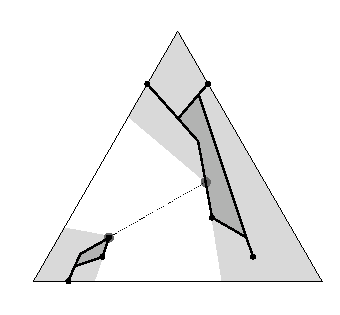
\includegraphics[scale=0.7]{twosemi2}
\end{center}
\end{frame}
\begin{frame}[plain]
  \begin{myalgorithm}[Tropical SVM]
\begin{itemize}
\item \textbf{Input:} Labeled point sets $V^1,\dots,V^K \subset \R^d$
\item \textbf{Compute an eigenpair} $T(a) = \rho(T) +a$, $a\in \R^n$,
$\rho(T)\in \R$,
where $T = \operatorname{\max}_2\{T_{V^1}, \dots, T_{V^K}\}$.
\item \textbf{Assign Sectors to Classes:}
  \begin{itemize}
\item If $\rho(T) < 0$ (Separable case), 
Assign coordinate $i$ to class $k$ if $T_{V^k}(a)_i > \rho(T) + a_i$
\item Else Fail (Non separable). 
%
  \end{itemize}
\item \textbf{Output:} Vector $a$ the apex of the hyperplane, margin $-\rho(T)$ and sector assignments for classification (if separable).
  \end{itemize}
  \end{myalgorithm}
  \bl{Relative value iteration with Krasnoselskii-Mann damping},
  $z^{(k+1)} \leftarrow \frac{1}{2}\bigl(y^{(k)} + T(y^{(k)})\bigr)$,
$y^{(k+1)}=z^{(k+1)}-\max z^{(k+1)}$ 
  returns a vector $a$ such that $T(a) = \rho(T)+ a$ up
  to an error $\epsilon$ in $O(1/\epsilon^2)$ iterations.

  Total complexity $O(np/\epsilon^2)$ where $p=|V^1|+\dots |V^K|$
  is the number of points,
  vs. $\Omega(2^n)$ in \giveref{G\"artner and Jaggi 2006}.
\end{frame}
\begin{frame}[plain]
  \begin{center}
            \resizebox{0.65\textwidth}{!}{\clipbox{0.15\width{} 0.30\height{} 0.15\width{} 0.30\height{}}{%% Creator: Matplotlib, PGF backend
%%
%% To include the figure in your LaTeX document, write
%%   \input{<filename>.pgf}
%%
%% Make sure the required packages are loaded in your preamble
%%   \usepackage{pgf}
%%
%% Also ensure that all the required font packages are loaded; for instance,
%% the lmodern package is sometimes necessary when using math font.
%%   \usepackage{lmodern}
%%
%% Figures using additional raster images can only be included by \input if
%% they are in the same directory as the main LaTeX file. For loading figures
%% from other directories you can use the `import` package
%%   \usepackage{import}
%%
%% and then include the figures with
%%   \import{<path to file>}{<filename>.pgf}
%%
%% Matplotlib used the following preamble
%%   
%%   \usepackage{fontspec}
%%   \setmainfont{DejaVuSerif.ttf}[Path=\detokenize{/Users/sam/Library/Python/3.9/lib/python/site-packages/matplotlib/mpl-data/fonts/ttf/}]
%%   \setsansfont{DejaVuSans.ttf}[Path=\detokenize{/Users/sam/Library/Python/3.9/lib/python/site-packages/matplotlib/mpl-data/fonts/ttf/}]
%%   \setmonofont{DejaVuSansMono.ttf}[Path=\detokenize{/Users/sam/Library/Python/3.9/lib/python/site-packages/matplotlib/mpl-data/fonts/ttf/}]
%%   \makeatletter\@ifpackageloaded{underscore}{}{\usepackage[strings]{underscore}}\makeatother
%%
\begingroup%
\makeatletter%
\begin{pgfpicture}%
\pgfpathrectangle{\pgfpointorigin}{\pgfqpoint{6.000000in}{6.000000in}}%
\pgfusepath{use as bounding box, clip}%
\begin{pgfscope}%
\pgfsetbuttcap%
\pgfsetmiterjoin%
\definecolor{currentfill}{rgb}{1.000000,1.000000,1.000000}%
\pgfsetfillcolor{currentfill}%
\pgfsetlinewidth{0.000000pt}%
\definecolor{currentstroke}{rgb}{1.000000,1.000000,1.000000}%
\pgfsetstrokecolor{currentstroke}%
\pgfsetdash{}{0pt}%
\pgfpathmoveto{\pgfqpoint{0.000000in}{0.000000in}}%
\pgfpathlineto{\pgfqpoint{6.000000in}{0.000000in}}%
\pgfpathlineto{\pgfqpoint{6.000000in}{6.000000in}}%
\pgfpathlineto{\pgfqpoint{0.000000in}{6.000000in}}%
\pgfpathlineto{\pgfqpoint{0.000000in}{0.000000in}}%
\pgfpathclose%
\pgfusepath{fill}%
\end{pgfscope}%
\begin{pgfscope}%
\pgfsetbuttcap%
\pgfsetmiterjoin%
\definecolor{currentfill}{rgb}{1.000000,1.000000,1.000000}%
\pgfsetfillcolor{currentfill}%
\pgfsetlinewidth{0.000000pt}%
\definecolor{currentstroke}{rgb}{0.000000,0.000000,0.000000}%
\pgfsetstrokecolor{currentstroke}%
\pgfsetstrokeopacity{0.000000}%
\pgfsetdash{}{0pt}%
\pgfpathmoveto{\pgfqpoint{0.765000in}{0.660000in}}%
\pgfpathlineto{\pgfqpoint{5.385000in}{0.660000in}}%
\pgfpathlineto{\pgfqpoint{5.385000in}{5.280000in}}%
\pgfpathlineto{\pgfqpoint{0.765000in}{5.280000in}}%
\pgfpathlineto{\pgfqpoint{0.765000in}{0.660000in}}%
\pgfpathclose%
\pgfusepath{fill}%
\end{pgfscope}%
\begin{pgfscope}%
\pgfpathrectangle{\pgfqpoint{0.765000in}{0.660000in}}{\pgfqpoint{4.620000in}{4.620000in}}%
\pgfusepath{clip}%
\pgfsetbuttcap%
\pgfsetroundjoin%
\definecolor{currentfill}{rgb}{1.000000,0.894118,0.788235}%
\pgfsetfillcolor{currentfill}%
\pgfsetlinewidth{0.000000pt}%
\definecolor{currentstroke}{rgb}{1.000000,0.894118,0.788235}%
\pgfsetstrokecolor{currentstroke}%
\pgfsetdash{}{0pt}%
\pgfpathmoveto{\pgfqpoint{2.858781in}{2.883237in}}%
\pgfpathlineto{\pgfqpoint{2.788689in}{2.842769in}}%
\pgfpathlineto{\pgfqpoint{2.858781in}{2.802301in}}%
\pgfpathlineto{\pgfqpoint{2.928874in}{2.842769in}}%
\pgfpathlineto{\pgfqpoint{2.858781in}{2.883237in}}%
\pgfpathclose%
\pgfusepath{fill}%
\end{pgfscope}%
\begin{pgfscope}%
\pgfpathrectangle{\pgfqpoint{0.765000in}{0.660000in}}{\pgfqpoint{4.620000in}{4.620000in}}%
\pgfusepath{clip}%
\pgfsetbuttcap%
\pgfsetroundjoin%
\definecolor{currentfill}{rgb}{1.000000,0.894118,0.788235}%
\pgfsetfillcolor{currentfill}%
\pgfsetlinewidth{0.000000pt}%
\definecolor{currentstroke}{rgb}{1.000000,0.894118,0.788235}%
\pgfsetstrokecolor{currentstroke}%
\pgfsetdash{}{0pt}%
\pgfpathmoveto{\pgfqpoint{2.858781in}{2.883237in}}%
\pgfpathlineto{\pgfqpoint{2.788689in}{2.842769in}}%
\pgfpathlineto{\pgfqpoint{2.788689in}{2.923704in}}%
\pgfpathlineto{\pgfqpoint{2.858781in}{2.964172in}}%
\pgfpathlineto{\pgfqpoint{2.858781in}{2.883237in}}%
\pgfpathclose%
\pgfusepath{fill}%
\end{pgfscope}%
\begin{pgfscope}%
\pgfpathrectangle{\pgfqpoint{0.765000in}{0.660000in}}{\pgfqpoint{4.620000in}{4.620000in}}%
\pgfusepath{clip}%
\pgfsetbuttcap%
\pgfsetroundjoin%
\definecolor{currentfill}{rgb}{1.000000,0.894118,0.788235}%
\pgfsetfillcolor{currentfill}%
\pgfsetlinewidth{0.000000pt}%
\definecolor{currentstroke}{rgb}{1.000000,0.894118,0.788235}%
\pgfsetstrokecolor{currentstroke}%
\pgfsetdash{}{0pt}%
\pgfpathmoveto{\pgfqpoint{2.858781in}{2.883237in}}%
\pgfpathlineto{\pgfqpoint{2.928874in}{2.842769in}}%
\pgfpathlineto{\pgfqpoint{2.928874in}{2.923704in}}%
\pgfpathlineto{\pgfqpoint{2.858781in}{2.964172in}}%
\pgfpathlineto{\pgfqpoint{2.858781in}{2.883237in}}%
\pgfpathclose%
\pgfusepath{fill}%
\end{pgfscope}%
\begin{pgfscope}%
\pgfpathrectangle{\pgfqpoint{0.765000in}{0.660000in}}{\pgfqpoint{4.620000in}{4.620000in}}%
\pgfusepath{clip}%
\pgfsetbuttcap%
\pgfsetroundjoin%
\definecolor{currentfill}{rgb}{1.000000,0.894118,0.788235}%
\pgfsetfillcolor{currentfill}%
\pgfsetlinewidth{0.000000pt}%
\definecolor{currentstroke}{rgb}{1.000000,0.894118,0.788235}%
\pgfsetstrokecolor{currentstroke}%
\pgfsetdash{}{0pt}%
\pgfpathmoveto{\pgfqpoint{3.323071in}{3.151294in}}%
\pgfpathlineto{\pgfqpoint{3.252979in}{3.110827in}}%
\pgfpathlineto{\pgfqpoint{3.323071in}{3.070359in}}%
\pgfpathlineto{\pgfqpoint{3.393164in}{3.110827in}}%
\pgfpathlineto{\pgfqpoint{3.323071in}{3.151294in}}%
\pgfpathclose%
\pgfusepath{fill}%
\end{pgfscope}%
\begin{pgfscope}%
\pgfpathrectangle{\pgfqpoint{0.765000in}{0.660000in}}{\pgfqpoint{4.620000in}{4.620000in}}%
\pgfusepath{clip}%
\pgfsetbuttcap%
\pgfsetroundjoin%
\definecolor{currentfill}{rgb}{1.000000,0.894118,0.788235}%
\pgfsetfillcolor{currentfill}%
\pgfsetlinewidth{0.000000pt}%
\definecolor{currentstroke}{rgb}{1.000000,0.894118,0.788235}%
\pgfsetstrokecolor{currentstroke}%
\pgfsetdash{}{0pt}%
\pgfpathmoveto{\pgfqpoint{3.323071in}{3.151294in}}%
\pgfpathlineto{\pgfqpoint{3.252979in}{3.110827in}}%
\pgfpathlineto{\pgfqpoint{3.252979in}{3.191762in}}%
\pgfpathlineto{\pgfqpoint{3.323071in}{3.232230in}}%
\pgfpathlineto{\pgfqpoint{3.323071in}{3.151294in}}%
\pgfpathclose%
\pgfusepath{fill}%
\end{pgfscope}%
\begin{pgfscope}%
\pgfpathrectangle{\pgfqpoint{0.765000in}{0.660000in}}{\pgfqpoint{4.620000in}{4.620000in}}%
\pgfusepath{clip}%
\pgfsetbuttcap%
\pgfsetroundjoin%
\definecolor{currentfill}{rgb}{1.000000,0.894118,0.788235}%
\pgfsetfillcolor{currentfill}%
\pgfsetlinewidth{0.000000pt}%
\definecolor{currentstroke}{rgb}{1.000000,0.894118,0.788235}%
\pgfsetstrokecolor{currentstroke}%
\pgfsetdash{}{0pt}%
\pgfpathmoveto{\pgfqpoint{3.323071in}{3.151294in}}%
\pgfpathlineto{\pgfqpoint{3.393164in}{3.110827in}}%
\pgfpathlineto{\pgfqpoint{3.393164in}{3.191762in}}%
\pgfpathlineto{\pgfqpoint{3.323071in}{3.232230in}}%
\pgfpathlineto{\pgfqpoint{3.323071in}{3.151294in}}%
\pgfpathclose%
\pgfusepath{fill}%
\end{pgfscope}%
\begin{pgfscope}%
\pgfpathrectangle{\pgfqpoint{0.765000in}{0.660000in}}{\pgfqpoint{4.620000in}{4.620000in}}%
\pgfusepath{clip}%
\pgfsetbuttcap%
\pgfsetroundjoin%
\definecolor{currentfill}{rgb}{1.000000,0.894118,0.788235}%
\pgfsetfillcolor{currentfill}%
\pgfsetlinewidth{0.000000pt}%
\definecolor{currentstroke}{rgb}{1.000000,0.894118,0.788235}%
\pgfsetstrokecolor{currentstroke}%
\pgfsetdash{}{0pt}%
\pgfpathmoveto{\pgfqpoint{2.858781in}{2.964172in}}%
\pgfpathlineto{\pgfqpoint{2.788689in}{2.923704in}}%
\pgfpathlineto{\pgfqpoint{2.858781in}{2.883237in}}%
\pgfpathlineto{\pgfqpoint{2.928874in}{2.923704in}}%
\pgfpathlineto{\pgfqpoint{2.858781in}{2.964172in}}%
\pgfpathclose%
\pgfusepath{fill}%
\end{pgfscope}%
\begin{pgfscope}%
\pgfpathrectangle{\pgfqpoint{0.765000in}{0.660000in}}{\pgfqpoint{4.620000in}{4.620000in}}%
\pgfusepath{clip}%
\pgfsetbuttcap%
\pgfsetroundjoin%
\definecolor{currentfill}{rgb}{1.000000,0.894118,0.788235}%
\pgfsetfillcolor{currentfill}%
\pgfsetlinewidth{0.000000pt}%
\definecolor{currentstroke}{rgb}{1.000000,0.894118,0.788235}%
\pgfsetstrokecolor{currentstroke}%
\pgfsetdash{}{0pt}%
\pgfpathmoveto{\pgfqpoint{2.858781in}{2.802301in}}%
\pgfpathlineto{\pgfqpoint{2.928874in}{2.842769in}}%
\pgfpathlineto{\pgfqpoint{2.928874in}{2.923704in}}%
\pgfpathlineto{\pgfqpoint{2.858781in}{2.883237in}}%
\pgfpathlineto{\pgfqpoint{2.858781in}{2.802301in}}%
\pgfpathclose%
\pgfusepath{fill}%
\end{pgfscope}%
\begin{pgfscope}%
\pgfpathrectangle{\pgfqpoint{0.765000in}{0.660000in}}{\pgfqpoint{4.620000in}{4.620000in}}%
\pgfusepath{clip}%
\pgfsetbuttcap%
\pgfsetroundjoin%
\definecolor{currentfill}{rgb}{1.000000,0.894118,0.788235}%
\pgfsetfillcolor{currentfill}%
\pgfsetlinewidth{0.000000pt}%
\definecolor{currentstroke}{rgb}{1.000000,0.894118,0.788235}%
\pgfsetstrokecolor{currentstroke}%
\pgfsetdash{}{0pt}%
\pgfpathmoveto{\pgfqpoint{2.788689in}{2.842769in}}%
\pgfpathlineto{\pgfqpoint{2.858781in}{2.802301in}}%
\pgfpathlineto{\pgfqpoint{2.858781in}{2.883237in}}%
\pgfpathlineto{\pgfqpoint{2.788689in}{2.923704in}}%
\pgfpathlineto{\pgfqpoint{2.788689in}{2.842769in}}%
\pgfpathclose%
\pgfusepath{fill}%
\end{pgfscope}%
\begin{pgfscope}%
\pgfpathrectangle{\pgfqpoint{0.765000in}{0.660000in}}{\pgfqpoint{4.620000in}{4.620000in}}%
\pgfusepath{clip}%
\pgfsetbuttcap%
\pgfsetroundjoin%
\definecolor{currentfill}{rgb}{1.000000,0.894118,0.788235}%
\pgfsetfillcolor{currentfill}%
\pgfsetlinewidth{0.000000pt}%
\definecolor{currentstroke}{rgb}{1.000000,0.894118,0.788235}%
\pgfsetstrokecolor{currentstroke}%
\pgfsetdash{}{0pt}%
\pgfpathmoveto{\pgfqpoint{3.323071in}{3.232230in}}%
\pgfpathlineto{\pgfqpoint{3.252979in}{3.191762in}}%
\pgfpathlineto{\pgfqpoint{3.323071in}{3.151294in}}%
\pgfpathlineto{\pgfqpoint{3.393164in}{3.191762in}}%
\pgfpathlineto{\pgfqpoint{3.323071in}{3.232230in}}%
\pgfpathclose%
\pgfusepath{fill}%
\end{pgfscope}%
\begin{pgfscope}%
\pgfpathrectangle{\pgfqpoint{0.765000in}{0.660000in}}{\pgfqpoint{4.620000in}{4.620000in}}%
\pgfusepath{clip}%
\pgfsetbuttcap%
\pgfsetroundjoin%
\definecolor{currentfill}{rgb}{1.000000,0.894118,0.788235}%
\pgfsetfillcolor{currentfill}%
\pgfsetlinewidth{0.000000pt}%
\definecolor{currentstroke}{rgb}{1.000000,0.894118,0.788235}%
\pgfsetstrokecolor{currentstroke}%
\pgfsetdash{}{0pt}%
\pgfpathmoveto{\pgfqpoint{3.323071in}{3.070359in}}%
\pgfpathlineto{\pgfqpoint{3.393164in}{3.110827in}}%
\pgfpathlineto{\pgfqpoint{3.393164in}{3.191762in}}%
\pgfpathlineto{\pgfqpoint{3.323071in}{3.151294in}}%
\pgfpathlineto{\pgfqpoint{3.323071in}{3.070359in}}%
\pgfpathclose%
\pgfusepath{fill}%
\end{pgfscope}%
\begin{pgfscope}%
\pgfpathrectangle{\pgfqpoint{0.765000in}{0.660000in}}{\pgfqpoint{4.620000in}{4.620000in}}%
\pgfusepath{clip}%
\pgfsetbuttcap%
\pgfsetroundjoin%
\definecolor{currentfill}{rgb}{1.000000,0.894118,0.788235}%
\pgfsetfillcolor{currentfill}%
\pgfsetlinewidth{0.000000pt}%
\definecolor{currentstroke}{rgb}{1.000000,0.894118,0.788235}%
\pgfsetstrokecolor{currentstroke}%
\pgfsetdash{}{0pt}%
\pgfpathmoveto{\pgfqpoint{3.252979in}{3.110827in}}%
\pgfpathlineto{\pgfqpoint{3.323071in}{3.070359in}}%
\pgfpathlineto{\pgfqpoint{3.323071in}{3.151294in}}%
\pgfpathlineto{\pgfqpoint{3.252979in}{3.191762in}}%
\pgfpathlineto{\pgfqpoint{3.252979in}{3.110827in}}%
\pgfpathclose%
\pgfusepath{fill}%
\end{pgfscope}%
\begin{pgfscope}%
\pgfpathrectangle{\pgfqpoint{0.765000in}{0.660000in}}{\pgfqpoint{4.620000in}{4.620000in}}%
\pgfusepath{clip}%
\pgfsetbuttcap%
\pgfsetroundjoin%
\definecolor{currentfill}{rgb}{1.000000,0.894118,0.788235}%
\pgfsetfillcolor{currentfill}%
\pgfsetlinewidth{0.000000pt}%
\definecolor{currentstroke}{rgb}{1.000000,0.894118,0.788235}%
\pgfsetstrokecolor{currentstroke}%
\pgfsetdash{}{0pt}%
\pgfpathmoveto{\pgfqpoint{2.858781in}{2.883237in}}%
\pgfpathlineto{\pgfqpoint{2.788689in}{2.842769in}}%
\pgfpathlineto{\pgfqpoint{3.252979in}{3.110827in}}%
\pgfpathlineto{\pgfqpoint{3.323071in}{3.151294in}}%
\pgfpathlineto{\pgfqpoint{2.858781in}{2.883237in}}%
\pgfpathclose%
\pgfusepath{fill}%
\end{pgfscope}%
\begin{pgfscope}%
\pgfpathrectangle{\pgfqpoint{0.765000in}{0.660000in}}{\pgfqpoint{4.620000in}{4.620000in}}%
\pgfusepath{clip}%
\pgfsetbuttcap%
\pgfsetroundjoin%
\definecolor{currentfill}{rgb}{1.000000,0.894118,0.788235}%
\pgfsetfillcolor{currentfill}%
\pgfsetlinewidth{0.000000pt}%
\definecolor{currentstroke}{rgb}{1.000000,0.894118,0.788235}%
\pgfsetstrokecolor{currentstroke}%
\pgfsetdash{}{0pt}%
\pgfpathmoveto{\pgfqpoint{2.928874in}{2.842769in}}%
\pgfpathlineto{\pgfqpoint{2.858781in}{2.883237in}}%
\pgfpathlineto{\pgfqpoint{3.323071in}{3.151294in}}%
\pgfpathlineto{\pgfqpoint{3.393164in}{3.110827in}}%
\pgfpathlineto{\pgfqpoint{2.928874in}{2.842769in}}%
\pgfpathclose%
\pgfusepath{fill}%
\end{pgfscope}%
\begin{pgfscope}%
\pgfpathrectangle{\pgfqpoint{0.765000in}{0.660000in}}{\pgfqpoint{4.620000in}{4.620000in}}%
\pgfusepath{clip}%
\pgfsetbuttcap%
\pgfsetroundjoin%
\definecolor{currentfill}{rgb}{1.000000,0.894118,0.788235}%
\pgfsetfillcolor{currentfill}%
\pgfsetlinewidth{0.000000pt}%
\definecolor{currentstroke}{rgb}{1.000000,0.894118,0.788235}%
\pgfsetstrokecolor{currentstroke}%
\pgfsetdash{}{0pt}%
\pgfpathmoveto{\pgfqpoint{2.858781in}{2.883237in}}%
\pgfpathlineto{\pgfqpoint{2.858781in}{2.964172in}}%
\pgfpathlineto{\pgfqpoint{3.323071in}{3.232230in}}%
\pgfpathlineto{\pgfqpoint{3.393164in}{3.110827in}}%
\pgfpathlineto{\pgfqpoint{2.858781in}{2.883237in}}%
\pgfpathclose%
\pgfusepath{fill}%
\end{pgfscope}%
\begin{pgfscope}%
\pgfpathrectangle{\pgfqpoint{0.765000in}{0.660000in}}{\pgfqpoint{4.620000in}{4.620000in}}%
\pgfusepath{clip}%
\pgfsetbuttcap%
\pgfsetroundjoin%
\definecolor{currentfill}{rgb}{1.000000,0.894118,0.788235}%
\pgfsetfillcolor{currentfill}%
\pgfsetlinewidth{0.000000pt}%
\definecolor{currentstroke}{rgb}{1.000000,0.894118,0.788235}%
\pgfsetstrokecolor{currentstroke}%
\pgfsetdash{}{0pt}%
\pgfpathmoveto{\pgfqpoint{2.928874in}{2.842769in}}%
\pgfpathlineto{\pgfqpoint{2.928874in}{2.923704in}}%
\pgfpathlineto{\pgfqpoint{3.393164in}{3.191762in}}%
\pgfpathlineto{\pgfqpoint{3.323071in}{3.151294in}}%
\pgfpathlineto{\pgfqpoint{2.928874in}{2.842769in}}%
\pgfpathclose%
\pgfusepath{fill}%
\end{pgfscope}%
\begin{pgfscope}%
\pgfpathrectangle{\pgfqpoint{0.765000in}{0.660000in}}{\pgfqpoint{4.620000in}{4.620000in}}%
\pgfusepath{clip}%
\pgfsetbuttcap%
\pgfsetroundjoin%
\definecolor{currentfill}{rgb}{1.000000,0.894118,0.788235}%
\pgfsetfillcolor{currentfill}%
\pgfsetlinewidth{0.000000pt}%
\definecolor{currentstroke}{rgb}{1.000000,0.894118,0.788235}%
\pgfsetstrokecolor{currentstroke}%
\pgfsetdash{}{0pt}%
\pgfpathmoveto{\pgfqpoint{2.788689in}{2.842769in}}%
\pgfpathlineto{\pgfqpoint{2.858781in}{2.802301in}}%
\pgfpathlineto{\pgfqpoint{3.323071in}{3.070359in}}%
\pgfpathlineto{\pgfqpoint{3.252979in}{3.110827in}}%
\pgfpathlineto{\pgfqpoint{2.788689in}{2.842769in}}%
\pgfpathclose%
\pgfusepath{fill}%
\end{pgfscope}%
\begin{pgfscope}%
\pgfpathrectangle{\pgfqpoint{0.765000in}{0.660000in}}{\pgfqpoint{4.620000in}{4.620000in}}%
\pgfusepath{clip}%
\pgfsetbuttcap%
\pgfsetroundjoin%
\definecolor{currentfill}{rgb}{1.000000,0.894118,0.788235}%
\pgfsetfillcolor{currentfill}%
\pgfsetlinewidth{0.000000pt}%
\definecolor{currentstroke}{rgb}{1.000000,0.894118,0.788235}%
\pgfsetstrokecolor{currentstroke}%
\pgfsetdash{}{0pt}%
\pgfpathmoveto{\pgfqpoint{2.858781in}{2.802301in}}%
\pgfpathlineto{\pgfqpoint{2.928874in}{2.842769in}}%
\pgfpathlineto{\pgfqpoint{3.393164in}{3.110827in}}%
\pgfpathlineto{\pgfqpoint{3.323071in}{3.070359in}}%
\pgfpathlineto{\pgfqpoint{2.858781in}{2.802301in}}%
\pgfpathclose%
\pgfusepath{fill}%
\end{pgfscope}%
\begin{pgfscope}%
\pgfpathrectangle{\pgfqpoint{0.765000in}{0.660000in}}{\pgfqpoint{4.620000in}{4.620000in}}%
\pgfusepath{clip}%
\pgfsetbuttcap%
\pgfsetroundjoin%
\definecolor{currentfill}{rgb}{1.000000,0.894118,0.788235}%
\pgfsetfillcolor{currentfill}%
\pgfsetlinewidth{0.000000pt}%
\definecolor{currentstroke}{rgb}{1.000000,0.894118,0.788235}%
\pgfsetstrokecolor{currentstroke}%
\pgfsetdash{}{0pt}%
\pgfpathmoveto{\pgfqpoint{2.858781in}{2.964172in}}%
\pgfpathlineto{\pgfqpoint{2.788689in}{2.923704in}}%
\pgfpathlineto{\pgfqpoint{3.252979in}{3.191762in}}%
\pgfpathlineto{\pgfqpoint{3.323071in}{3.232230in}}%
\pgfpathlineto{\pgfqpoint{2.858781in}{2.964172in}}%
\pgfpathclose%
\pgfusepath{fill}%
\end{pgfscope}%
\begin{pgfscope}%
\pgfpathrectangle{\pgfqpoint{0.765000in}{0.660000in}}{\pgfqpoint{4.620000in}{4.620000in}}%
\pgfusepath{clip}%
\pgfsetbuttcap%
\pgfsetroundjoin%
\definecolor{currentfill}{rgb}{1.000000,0.894118,0.788235}%
\pgfsetfillcolor{currentfill}%
\pgfsetlinewidth{0.000000pt}%
\definecolor{currentstroke}{rgb}{1.000000,0.894118,0.788235}%
\pgfsetstrokecolor{currentstroke}%
\pgfsetdash{}{0pt}%
\pgfpathmoveto{\pgfqpoint{2.928874in}{2.923704in}}%
\pgfpathlineto{\pgfqpoint{2.858781in}{2.964172in}}%
\pgfpathlineto{\pgfqpoint{3.323071in}{3.232230in}}%
\pgfpathlineto{\pgfqpoint{3.393164in}{3.191762in}}%
\pgfpathlineto{\pgfqpoint{2.928874in}{2.923704in}}%
\pgfpathclose%
\pgfusepath{fill}%
\end{pgfscope}%
\begin{pgfscope}%
\pgfpathrectangle{\pgfqpoint{0.765000in}{0.660000in}}{\pgfqpoint{4.620000in}{4.620000in}}%
\pgfusepath{clip}%
\pgfsetbuttcap%
\pgfsetroundjoin%
\definecolor{currentfill}{rgb}{1.000000,0.894118,0.788235}%
\pgfsetfillcolor{currentfill}%
\pgfsetlinewidth{0.000000pt}%
\definecolor{currentstroke}{rgb}{1.000000,0.894118,0.788235}%
\pgfsetstrokecolor{currentstroke}%
\pgfsetdash{}{0pt}%
\pgfpathmoveto{\pgfqpoint{2.788689in}{2.842769in}}%
\pgfpathlineto{\pgfqpoint{2.788689in}{2.923704in}}%
\pgfpathlineto{\pgfqpoint{3.252979in}{3.191762in}}%
\pgfpathlineto{\pgfqpoint{3.323071in}{3.070359in}}%
\pgfpathlineto{\pgfqpoint{2.788689in}{2.842769in}}%
\pgfpathclose%
\pgfusepath{fill}%
\end{pgfscope}%
\begin{pgfscope}%
\pgfpathrectangle{\pgfqpoint{0.765000in}{0.660000in}}{\pgfqpoint{4.620000in}{4.620000in}}%
\pgfusepath{clip}%
\pgfsetbuttcap%
\pgfsetroundjoin%
\definecolor{currentfill}{rgb}{1.000000,0.894118,0.788235}%
\pgfsetfillcolor{currentfill}%
\pgfsetlinewidth{0.000000pt}%
\definecolor{currentstroke}{rgb}{1.000000,0.894118,0.788235}%
\pgfsetstrokecolor{currentstroke}%
\pgfsetdash{}{0pt}%
\pgfpathmoveto{\pgfqpoint{2.858781in}{2.802301in}}%
\pgfpathlineto{\pgfqpoint{2.858781in}{2.883237in}}%
\pgfpathlineto{\pgfqpoint{3.323071in}{3.151294in}}%
\pgfpathlineto{\pgfqpoint{3.252979in}{3.110827in}}%
\pgfpathlineto{\pgfqpoint{2.858781in}{2.802301in}}%
\pgfpathclose%
\pgfusepath{fill}%
\end{pgfscope}%
\begin{pgfscope}%
\pgfpathrectangle{\pgfqpoint{0.765000in}{0.660000in}}{\pgfqpoint{4.620000in}{4.620000in}}%
\pgfusepath{clip}%
\pgfsetbuttcap%
\pgfsetroundjoin%
\definecolor{currentfill}{rgb}{1.000000,0.894118,0.788235}%
\pgfsetfillcolor{currentfill}%
\pgfsetlinewidth{0.000000pt}%
\definecolor{currentstroke}{rgb}{1.000000,0.894118,0.788235}%
\pgfsetstrokecolor{currentstroke}%
\pgfsetdash{}{0pt}%
\pgfpathmoveto{\pgfqpoint{2.788689in}{2.923704in}}%
\pgfpathlineto{\pgfqpoint{2.858781in}{2.883237in}}%
\pgfpathlineto{\pgfqpoint{3.323071in}{3.151294in}}%
\pgfpathlineto{\pgfqpoint{3.252979in}{3.191762in}}%
\pgfpathlineto{\pgfqpoint{2.788689in}{2.923704in}}%
\pgfpathclose%
\pgfusepath{fill}%
\end{pgfscope}%
\begin{pgfscope}%
\pgfpathrectangle{\pgfqpoint{0.765000in}{0.660000in}}{\pgfqpoint{4.620000in}{4.620000in}}%
\pgfusepath{clip}%
\pgfsetbuttcap%
\pgfsetroundjoin%
\definecolor{currentfill}{rgb}{1.000000,0.894118,0.788235}%
\pgfsetfillcolor{currentfill}%
\pgfsetlinewidth{0.000000pt}%
\definecolor{currentstroke}{rgb}{1.000000,0.894118,0.788235}%
\pgfsetstrokecolor{currentstroke}%
\pgfsetdash{}{0pt}%
\pgfpathmoveto{\pgfqpoint{2.858781in}{2.883237in}}%
\pgfpathlineto{\pgfqpoint{2.928874in}{2.923704in}}%
\pgfpathlineto{\pgfqpoint{3.393164in}{3.191762in}}%
\pgfpathlineto{\pgfqpoint{3.323071in}{3.151294in}}%
\pgfpathlineto{\pgfqpoint{2.858781in}{2.883237in}}%
\pgfpathclose%
\pgfusepath{fill}%
\end{pgfscope}%
\begin{pgfscope}%
\pgfpathrectangle{\pgfqpoint{0.765000in}{0.660000in}}{\pgfqpoint{4.620000in}{4.620000in}}%
\pgfusepath{clip}%
\pgfsetbuttcap%
\pgfsetroundjoin%
\definecolor{currentfill}{rgb}{1.000000,0.894118,0.788235}%
\pgfsetfillcolor{currentfill}%
\pgfsetlinewidth{0.000000pt}%
\definecolor{currentstroke}{rgb}{1.000000,0.894118,0.788235}%
\pgfsetstrokecolor{currentstroke}%
\pgfsetdash{}{0pt}%
\pgfpathmoveto{\pgfqpoint{2.858781in}{2.883237in}}%
\pgfpathlineto{\pgfqpoint{2.788689in}{2.842769in}}%
\pgfpathlineto{\pgfqpoint{2.858781in}{2.802301in}}%
\pgfpathlineto{\pgfqpoint{2.928874in}{2.842769in}}%
\pgfpathlineto{\pgfqpoint{2.858781in}{2.883237in}}%
\pgfpathclose%
\pgfusepath{fill}%
\end{pgfscope}%
\begin{pgfscope}%
\pgfpathrectangle{\pgfqpoint{0.765000in}{0.660000in}}{\pgfqpoint{4.620000in}{4.620000in}}%
\pgfusepath{clip}%
\pgfsetbuttcap%
\pgfsetroundjoin%
\definecolor{currentfill}{rgb}{1.000000,0.894118,0.788235}%
\pgfsetfillcolor{currentfill}%
\pgfsetlinewidth{0.000000pt}%
\definecolor{currentstroke}{rgb}{1.000000,0.894118,0.788235}%
\pgfsetstrokecolor{currentstroke}%
\pgfsetdash{}{0pt}%
\pgfpathmoveto{\pgfqpoint{2.858781in}{2.883237in}}%
\pgfpathlineto{\pgfqpoint{2.788689in}{2.842769in}}%
\pgfpathlineto{\pgfqpoint{2.788689in}{2.923704in}}%
\pgfpathlineto{\pgfqpoint{2.858781in}{2.964172in}}%
\pgfpathlineto{\pgfqpoint{2.858781in}{2.883237in}}%
\pgfpathclose%
\pgfusepath{fill}%
\end{pgfscope}%
\begin{pgfscope}%
\pgfpathrectangle{\pgfqpoint{0.765000in}{0.660000in}}{\pgfqpoint{4.620000in}{4.620000in}}%
\pgfusepath{clip}%
\pgfsetbuttcap%
\pgfsetroundjoin%
\definecolor{currentfill}{rgb}{1.000000,0.894118,0.788235}%
\pgfsetfillcolor{currentfill}%
\pgfsetlinewidth{0.000000pt}%
\definecolor{currentstroke}{rgb}{1.000000,0.894118,0.788235}%
\pgfsetstrokecolor{currentstroke}%
\pgfsetdash{}{0pt}%
\pgfpathmoveto{\pgfqpoint{2.858781in}{2.883237in}}%
\pgfpathlineto{\pgfqpoint{2.928874in}{2.842769in}}%
\pgfpathlineto{\pgfqpoint{2.928874in}{2.923704in}}%
\pgfpathlineto{\pgfqpoint{2.858781in}{2.964172in}}%
\pgfpathlineto{\pgfqpoint{2.858781in}{2.883237in}}%
\pgfpathclose%
\pgfusepath{fill}%
\end{pgfscope}%
\begin{pgfscope}%
\pgfpathrectangle{\pgfqpoint{0.765000in}{0.660000in}}{\pgfqpoint{4.620000in}{4.620000in}}%
\pgfusepath{clip}%
\pgfsetbuttcap%
\pgfsetroundjoin%
\definecolor{currentfill}{rgb}{1.000000,0.894118,0.788235}%
\pgfsetfillcolor{currentfill}%
\pgfsetlinewidth{0.000000pt}%
\definecolor{currentstroke}{rgb}{1.000000,0.894118,0.788235}%
\pgfsetstrokecolor{currentstroke}%
\pgfsetdash{}{0pt}%
\pgfpathmoveto{\pgfqpoint{2.858781in}{-4.547074in}}%
\pgfpathlineto{\pgfqpoint{2.788689in}{-4.587542in}}%
\pgfpathlineto{\pgfqpoint{2.858781in}{-4.628010in}}%
\pgfpathlineto{\pgfqpoint{2.928874in}{-4.587542in}}%
\pgfpathlineto{\pgfqpoint{2.858781in}{-4.547074in}}%
\pgfpathclose%
\pgfusepath{fill}%
\end{pgfscope}%
\begin{pgfscope}%
\pgfpathrectangle{\pgfqpoint{0.765000in}{0.660000in}}{\pgfqpoint{4.620000in}{4.620000in}}%
\pgfusepath{clip}%
\pgfsetbuttcap%
\pgfsetroundjoin%
\definecolor{currentfill}{rgb}{1.000000,0.894118,0.788235}%
\pgfsetfillcolor{currentfill}%
\pgfsetlinewidth{0.000000pt}%
\definecolor{currentstroke}{rgb}{1.000000,0.894118,0.788235}%
\pgfsetstrokecolor{currentstroke}%
\pgfsetdash{}{0pt}%
\pgfpathmoveto{\pgfqpoint{2.858781in}{-4.547074in}}%
\pgfpathlineto{\pgfqpoint{2.788689in}{-4.587542in}}%
\pgfpathlineto{\pgfqpoint{2.788689in}{-4.506606in}}%
\pgfpathlineto{\pgfqpoint{2.858781in}{-4.466138in}}%
\pgfpathlineto{\pgfqpoint{2.858781in}{-4.547074in}}%
\pgfpathclose%
\pgfusepath{fill}%
\end{pgfscope}%
\begin{pgfscope}%
\pgfpathrectangle{\pgfqpoint{0.765000in}{0.660000in}}{\pgfqpoint{4.620000in}{4.620000in}}%
\pgfusepath{clip}%
\pgfsetbuttcap%
\pgfsetroundjoin%
\definecolor{currentfill}{rgb}{1.000000,0.894118,0.788235}%
\pgfsetfillcolor{currentfill}%
\pgfsetlinewidth{0.000000pt}%
\definecolor{currentstroke}{rgb}{1.000000,0.894118,0.788235}%
\pgfsetstrokecolor{currentstroke}%
\pgfsetdash{}{0pt}%
\pgfpathmoveto{\pgfqpoint{2.858781in}{-4.547074in}}%
\pgfpathlineto{\pgfqpoint{2.928874in}{-4.587542in}}%
\pgfpathlineto{\pgfqpoint{2.928874in}{-4.506606in}}%
\pgfpathlineto{\pgfqpoint{2.858781in}{-4.466138in}}%
\pgfpathlineto{\pgfqpoint{2.858781in}{-4.547074in}}%
\pgfpathclose%
\pgfusepath{fill}%
\end{pgfscope}%
\begin{pgfscope}%
\pgfpathrectangle{\pgfqpoint{0.765000in}{0.660000in}}{\pgfqpoint{4.620000in}{4.620000in}}%
\pgfusepath{clip}%
\pgfsetbuttcap%
\pgfsetroundjoin%
\definecolor{currentfill}{rgb}{1.000000,0.894118,0.788235}%
\pgfsetfillcolor{currentfill}%
\pgfsetlinewidth{0.000000pt}%
\definecolor{currentstroke}{rgb}{1.000000,0.894118,0.788235}%
\pgfsetstrokecolor{currentstroke}%
\pgfsetdash{}{0pt}%
\pgfpathmoveto{\pgfqpoint{2.858781in}{2.964172in}}%
\pgfpathlineto{\pgfqpoint{2.788689in}{2.923704in}}%
\pgfpathlineto{\pgfqpoint{2.858781in}{2.883237in}}%
\pgfpathlineto{\pgfqpoint{2.928874in}{2.923704in}}%
\pgfpathlineto{\pgfqpoint{2.858781in}{2.964172in}}%
\pgfpathclose%
\pgfusepath{fill}%
\end{pgfscope}%
\begin{pgfscope}%
\pgfpathrectangle{\pgfqpoint{0.765000in}{0.660000in}}{\pgfqpoint{4.620000in}{4.620000in}}%
\pgfusepath{clip}%
\pgfsetbuttcap%
\pgfsetroundjoin%
\definecolor{currentfill}{rgb}{1.000000,0.894118,0.788235}%
\pgfsetfillcolor{currentfill}%
\pgfsetlinewidth{0.000000pt}%
\definecolor{currentstroke}{rgb}{1.000000,0.894118,0.788235}%
\pgfsetstrokecolor{currentstroke}%
\pgfsetdash{}{0pt}%
\pgfpathmoveto{\pgfqpoint{2.858781in}{2.802301in}}%
\pgfpathlineto{\pgfqpoint{2.928874in}{2.842769in}}%
\pgfpathlineto{\pgfqpoint{2.928874in}{2.923704in}}%
\pgfpathlineto{\pgfqpoint{2.858781in}{2.883237in}}%
\pgfpathlineto{\pgfqpoint{2.858781in}{2.802301in}}%
\pgfpathclose%
\pgfusepath{fill}%
\end{pgfscope}%
\begin{pgfscope}%
\pgfpathrectangle{\pgfqpoint{0.765000in}{0.660000in}}{\pgfqpoint{4.620000in}{4.620000in}}%
\pgfusepath{clip}%
\pgfsetbuttcap%
\pgfsetroundjoin%
\definecolor{currentfill}{rgb}{1.000000,0.894118,0.788235}%
\pgfsetfillcolor{currentfill}%
\pgfsetlinewidth{0.000000pt}%
\definecolor{currentstroke}{rgb}{1.000000,0.894118,0.788235}%
\pgfsetstrokecolor{currentstroke}%
\pgfsetdash{}{0pt}%
\pgfpathmoveto{\pgfqpoint{2.788689in}{2.842769in}}%
\pgfpathlineto{\pgfqpoint{2.858781in}{2.802301in}}%
\pgfpathlineto{\pgfqpoint{2.858781in}{2.883237in}}%
\pgfpathlineto{\pgfqpoint{2.788689in}{2.923704in}}%
\pgfpathlineto{\pgfqpoint{2.788689in}{2.842769in}}%
\pgfpathclose%
\pgfusepath{fill}%
\end{pgfscope}%
\begin{pgfscope}%
\pgfpathrectangle{\pgfqpoint{0.765000in}{0.660000in}}{\pgfqpoint{4.620000in}{4.620000in}}%
\pgfusepath{clip}%
\pgfsetbuttcap%
\pgfsetroundjoin%
\definecolor{currentfill}{rgb}{1.000000,0.894118,0.788235}%
\pgfsetfillcolor{currentfill}%
\pgfsetlinewidth{0.000000pt}%
\definecolor{currentstroke}{rgb}{1.000000,0.894118,0.788235}%
\pgfsetstrokecolor{currentstroke}%
\pgfsetdash{}{0pt}%
\pgfpathmoveto{\pgfqpoint{2.858781in}{-4.466138in}}%
\pgfpathlineto{\pgfqpoint{2.788689in}{-4.506606in}}%
\pgfpathlineto{\pgfqpoint{2.858781in}{-4.547074in}}%
\pgfpathlineto{\pgfqpoint{2.928874in}{-4.506606in}}%
\pgfpathlineto{\pgfqpoint{2.858781in}{-4.466138in}}%
\pgfpathclose%
\pgfusepath{fill}%
\end{pgfscope}%
\begin{pgfscope}%
\pgfpathrectangle{\pgfqpoint{0.765000in}{0.660000in}}{\pgfqpoint{4.620000in}{4.620000in}}%
\pgfusepath{clip}%
\pgfsetbuttcap%
\pgfsetroundjoin%
\definecolor{currentfill}{rgb}{1.000000,0.894118,0.788235}%
\pgfsetfillcolor{currentfill}%
\pgfsetlinewidth{0.000000pt}%
\definecolor{currentstroke}{rgb}{1.000000,0.894118,0.788235}%
\pgfsetstrokecolor{currentstroke}%
\pgfsetdash{}{0pt}%
\pgfpathmoveto{\pgfqpoint{2.858781in}{-4.628010in}}%
\pgfpathlineto{\pgfqpoint{2.928874in}{-4.587542in}}%
\pgfpathlineto{\pgfqpoint{2.928874in}{-4.506606in}}%
\pgfpathlineto{\pgfqpoint{2.858781in}{-4.547074in}}%
\pgfpathlineto{\pgfqpoint{2.858781in}{-4.628010in}}%
\pgfpathclose%
\pgfusepath{fill}%
\end{pgfscope}%
\begin{pgfscope}%
\pgfpathrectangle{\pgfqpoint{0.765000in}{0.660000in}}{\pgfqpoint{4.620000in}{4.620000in}}%
\pgfusepath{clip}%
\pgfsetbuttcap%
\pgfsetroundjoin%
\definecolor{currentfill}{rgb}{1.000000,0.894118,0.788235}%
\pgfsetfillcolor{currentfill}%
\pgfsetlinewidth{0.000000pt}%
\definecolor{currentstroke}{rgb}{1.000000,0.894118,0.788235}%
\pgfsetstrokecolor{currentstroke}%
\pgfsetdash{}{0pt}%
\pgfpathmoveto{\pgfqpoint{2.788689in}{-4.587542in}}%
\pgfpathlineto{\pgfqpoint{2.858781in}{-4.628010in}}%
\pgfpathlineto{\pgfqpoint{2.858781in}{-4.547074in}}%
\pgfpathlineto{\pgfqpoint{2.788689in}{-4.506606in}}%
\pgfpathlineto{\pgfqpoint{2.788689in}{-4.587542in}}%
\pgfpathclose%
\pgfusepath{fill}%
\end{pgfscope}%
\begin{pgfscope}%
\pgfpathrectangle{\pgfqpoint{0.765000in}{0.660000in}}{\pgfqpoint{4.620000in}{4.620000in}}%
\pgfusepath{clip}%
\pgfsetbuttcap%
\pgfsetroundjoin%
\definecolor{currentfill}{rgb}{1.000000,0.894118,0.788235}%
\pgfsetfillcolor{currentfill}%
\pgfsetlinewidth{0.000000pt}%
\definecolor{currentstroke}{rgb}{1.000000,0.894118,0.788235}%
\pgfsetstrokecolor{currentstroke}%
\pgfsetdash{}{0pt}%
\pgfpathmoveto{\pgfqpoint{2.858781in}{2.883237in}}%
\pgfpathlineto{\pgfqpoint{2.788689in}{2.842769in}}%
\pgfpathlineto{\pgfqpoint{2.788689in}{-4.587542in}}%
\pgfpathlineto{\pgfqpoint{2.858781in}{-4.547074in}}%
\pgfpathlineto{\pgfqpoint{2.858781in}{2.883237in}}%
\pgfpathclose%
\pgfusepath{fill}%
\end{pgfscope}%
\begin{pgfscope}%
\pgfpathrectangle{\pgfqpoint{0.765000in}{0.660000in}}{\pgfqpoint{4.620000in}{4.620000in}}%
\pgfusepath{clip}%
\pgfsetbuttcap%
\pgfsetroundjoin%
\definecolor{currentfill}{rgb}{1.000000,0.894118,0.788235}%
\pgfsetfillcolor{currentfill}%
\pgfsetlinewidth{0.000000pt}%
\definecolor{currentstroke}{rgb}{1.000000,0.894118,0.788235}%
\pgfsetstrokecolor{currentstroke}%
\pgfsetdash{}{0pt}%
\pgfpathmoveto{\pgfqpoint{2.928874in}{2.842769in}}%
\pgfpathlineto{\pgfqpoint{2.858781in}{2.883237in}}%
\pgfpathlineto{\pgfqpoint{2.858781in}{-4.547074in}}%
\pgfpathlineto{\pgfqpoint{2.928874in}{-4.587542in}}%
\pgfpathlineto{\pgfqpoint{2.928874in}{2.842769in}}%
\pgfpathclose%
\pgfusepath{fill}%
\end{pgfscope}%
\begin{pgfscope}%
\pgfpathrectangle{\pgfqpoint{0.765000in}{0.660000in}}{\pgfqpoint{4.620000in}{4.620000in}}%
\pgfusepath{clip}%
\pgfsetbuttcap%
\pgfsetroundjoin%
\definecolor{currentfill}{rgb}{1.000000,0.894118,0.788235}%
\pgfsetfillcolor{currentfill}%
\pgfsetlinewidth{0.000000pt}%
\definecolor{currentstroke}{rgb}{1.000000,0.894118,0.788235}%
\pgfsetstrokecolor{currentstroke}%
\pgfsetdash{}{0pt}%
\pgfpathmoveto{\pgfqpoint{2.858781in}{2.883237in}}%
\pgfpathlineto{\pgfqpoint{2.858781in}{2.964172in}}%
\pgfpathlineto{\pgfqpoint{2.858781in}{-4.466138in}}%
\pgfpathlineto{\pgfqpoint{2.928874in}{-4.587542in}}%
\pgfpathlineto{\pgfqpoint{2.858781in}{2.883237in}}%
\pgfpathclose%
\pgfusepath{fill}%
\end{pgfscope}%
\begin{pgfscope}%
\pgfpathrectangle{\pgfqpoint{0.765000in}{0.660000in}}{\pgfqpoint{4.620000in}{4.620000in}}%
\pgfusepath{clip}%
\pgfsetbuttcap%
\pgfsetroundjoin%
\definecolor{currentfill}{rgb}{1.000000,0.894118,0.788235}%
\pgfsetfillcolor{currentfill}%
\pgfsetlinewidth{0.000000pt}%
\definecolor{currentstroke}{rgb}{1.000000,0.894118,0.788235}%
\pgfsetstrokecolor{currentstroke}%
\pgfsetdash{}{0pt}%
\pgfpathmoveto{\pgfqpoint{2.928874in}{2.842769in}}%
\pgfpathlineto{\pgfqpoint{2.928874in}{2.923704in}}%
\pgfpathlineto{\pgfqpoint{2.928874in}{-4.506606in}}%
\pgfpathlineto{\pgfqpoint{2.858781in}{-4.547074in}}%
\pgfpathlineto{\pgfqpoint{2.928874in}{2.842769in}}%
\pgfpathclose%
\pgfusepath{fill}%
\end{pgfscope}%
\begin{pgfscope}%
\pgfpathrectangle{\pgfqpoint{0.765000in}{0.660000in}}{\pgfqpoint{4.620000in}{4.620000in}}%
\pgfusepath{clip}%
\pgfsetbuttcap%
\pgfsetroundjoin%
\definecolor{currentfill}{rgb}{1.000000,0.894118,0.788235}%
\pgfsetfillcolor{currentfill}%
\pgfsetlinewidth{0.000000pt}%
\definecolor{currentstroke}{rgb}{1.000000,0.894118,0.788235}%
\pgfsetstrokecolor{currentstroke}%
\pgfsetdash{}{0pt}%
\pgfpathmoveto{\pgfqpoint{2.788689in}{2.842769in}}%
\pgfpathlineto{\pgfqpoint{2.858781in}{2.802301in}}%
\pgfpathlineto{\pgfqpoint{2.858781in}{-4.628010in}}%
\pgfpathlineto{\pgfqpoint{2.788689in}{-4.587542in}}%
\pgfpathlineto{\pgfqpoint{2.788689in}{2.842769in}}%
\pgfpathclose%
\pgfusepath{fill}%
\end{pgfscope}%
\begin{pgfscope}%
\pgfpathrectangle{\pgfqpoint{0.765000in}{0.660000in}}{\pgfqpoint{4.620000in}{4.620000in}}%
\pgfusepath{clip}%
\pgfsetbuttcap%
\pgfsetroundjoin%
\definecolor{currentfill}{rgb}{1.000000,0.894118,0.788235}%
\pgfsetfillcolor{currentfill}%
\pgfsetlinewidth{0.000000pt}%
\definecolor{currentstroke}{rgb}{1.000000,0.894118,0.788235}%
\pgfsetstrokecolor{currentstroke}%
\pgfsetdash{}{0pt}%
\pgfpathmoveto{\pgfqpoint{2.858781in}{2.802301in}}%
\pgfpathlineto{\pgfqpoint{2.928874in}{2.842769in}}%
\pgfpathlineto{\pgfqpoint{2.928874in}{-4.587542in}}%
\pgfpathlineto{\pgfqpoint{2.858781in}{-4.628010in}}%
\pgfpathlineto{\pgfqpoint{2.858781in}{2.802301in}}%
\pgfpathclose%
\pgfusepath{fill}%
\end{pgfscope}%
\begin{pgfscope}%
\pgfpathrectangle{\pgfqpoint{0.765000in}{0.660000in}}{\pgfqpoint{4.620000in}{4.620000in}}%
\pgfusepath{clip}%
\pgfsetbuttcap%
\pgfsetroundjoin%
\definecolor{currentfill}{rgb}{1.000000,0.894118,0.788235}%
\pgfsetfillcolor{currentfill}%
\pgfsetlinewidth{0.000000pt}%
\definecolor{currentstroke}{rgb}{1.000000,0.894118,0.788235}%
\pgfsetstrokecolor{currentstroke}%
\pgfsetdash{}{0pt}%
\pgfpathmoveto{\pgfqpoint{2.858781in}{2.964172in}}%
\pgfpathlineto{\pgfqpoint{2.788689in}{2.923704in}}%
\pgfpathlineto{\pgfqpoint{2.788689in}{-4.506606in}}%
\pgfpathlineto{\pgfqpoint{2.858781in}{-4.466138in}}%
\pgfpathlineto{\pgfqpoint{2.858781in}{2.964172in}}%
\pgfpathclose%
\pgfusepath{fill}%
\end{pgfscope}%
\begin{pgfscope}%
\pgfpathrectangle{\pgfqpoint{0.765000in}{0.660000in}}{\pgfqpoint{4.620000in}{4.620000in}}%
\pgfusepath{clip}%
\pgfsetbuttcap%
\pgfsetroundjoin%
\definecolor{currentfill}{rgb}{1.000000,0.894118,0.788235}%
\pgfsetfillcolor{currentfill}%
\pgfsetlinewidth{0.000000pt}%
\definecolor{currentstroke}{rgb}{1.000000,0.894118,0.788235}%
\pgfsetstrokecolor{currentstroke}%
\pgfsetdash{}{0pt}%
\pgfpathmoveto{\pgfqpoint{2.928874in}{2.923704in}}%
\pgfpathlineto{\pgfqpoint{2.858781in}{2.964172in}}%
\pgfpathlineto{\pgfqpoint{2.858781in}{-4.466138in}}%
\pgfpathlineto{\pgfqpoint{2.928874in}{-4.506606in}}%
\pgfpathlineto{\pgfqpoint{2.928874in}{2.923704in}}%
\pgfpathclose%
\pgfusepath{fill}%
\end{pgfscope}%
\begin{pgfscope}%
\pgfpathrectangle{\pgfqpoint{0.765000in}{0.660000in}}{\pgfqpoint{4.620000in}{4.620000in}}%
\pgfusepath{clip}%
\pgfsetbuttcap%
\pgfsetroundjoin%
\definecolor{currentfill}{rgb}{1.000000,0.894118,0.788235}%
\pgfsetfillcolor{currentfill}%
\pgfsetlinewidth{0.000000pt}%
\definecolor{currentstroke}{rgb}{1.000000,0.894118,0.788235}%
\pgfsetstrokecolor{currentstroke}%
\pgfsetdash{}{0pt}%
\pgfpathmoveto{\pgfqpoint{2.788689in}{2.842769in}}%
\pgfpathlineto{\pgfqpoint{2.788689in}{2.923704in}}%
\pgfpathlineto{\pgfqpoint{2.788689in}{-4.506606in}}%
\pgfpathlineto{\pgfqpoint{2.858781in}{-4.628010in}}%
\pgfpathlineto{\pgfqpoint{2.788689in}{2.842769in}}%
\pgfpathclose%
\pgfusepath{fill}%
\end{pgfscope}%
\begin{pgfscope}%
\pgfpathrectangle{\pgfqpoint{0.765000in}{0.660000in}}{\pgfqpoint{4.620000in}{4.620000in}}%
\pgfusepath{clip}%
\pgfsetbuttcap%
\pgfsetroundjoin%
\definecolor{currentfill}{rgb}{1.000000,0.894118,0.788235}%
\pgfsetfillcolor{currentfill}%
\pgfsetlinewidth{0.000000pt}%
\definecolor{currentstroke}{rgb}{1.000000,0.894118,0.788235}%
\pgfsetstrokecolor{currentstroke}%
\pgfsetdash{}{0pt}%
\pgfpathmoveto{\pgfqpoint{2.858781in}{2.802301in}}%
\pgfpathlineto{\pgfqpoint{2.858781in}{2.883237in}}%
\pgfpathlineto{\pgfqpoint{2.858781in}{-4.547074in}}%
\pgfpathlineto{\pgfqpoint{2.788689in}{-4.587542in}}%
\pgfpathlineto{\pgfqpoint{2.858781in}{2.802301in}}%
\pgfpathclose%
\pgfusepath{fill}%
\end{pgfscope}%
\begin{pgfscope}%
\pgfpathrectangle{\pgfqpoint{0.765000in}{0.660000in}}{\pgfqpoint{4.620000in}{4.620000in}}%
\pgfusepath{clip}%
\pgfsetbuttcap%
\pgfsetroundjoin%
\definecolor{currentfill}{rgb}{1.000000,0.894118,0.788235}%
\pgfsetfillcolor{currentfill}%
\pgfsetlinewidth{0.000000pt}%
\definecolor{currentstroke}{rgb}{1.000000,0.894118,0.788235}%
\pgfsetstrokecolor{currentstroke}%
\pgfsetdash{}{0pt}%
\pgfpathmoveto{\pgfqpoint{2.788689in}{2.923704in}}%
\pgfpathlineto{\pgfqpoint{2.858781in}{2.883237in}}%
\pgfpathlineto{\pgfqpoint{2.858781in}{-4.547074in}}%
\pgfpathlineto{\pgfqpoint{2.788689in}{-4.506606in}}%
\pgfpathlineto{\pgfqpoint{2.788689in}{2.923704in}}%
\pgfpathclose%
\pgfusepath{fill}%
\end{pgfscope}%
\begin{pgfscope}%
\pgfpathrectangle{\pgfqpoint{0.765000in}{0.660000in}}{\pgfqpoint{4.620000in}{4.620000in}}%
\pgfusepath{clip}%
\pgfsetbuttcap%
\pgfsetroundjoin%
\definecolor{currentfill}{rgb}{1.000000,0.894118,0.788235}%
\pgfsetfillcolor{currentfill}%
\pgfsetlinewidth{0.000000pt}%
\definecolor{currentstroke}{rgb}{1.000000,0.894118,0.788235}%
\pgfsetstrokecolor{currentstroke}%
\pgfsetdash{}{0pt}%
\pgfpathmoveto{\pgfqpoint{2.858781in}{2.883237in}}%
\pgfpathlineto{\pgfqpoint{2.928874in}{2.923704in}}%
\pgfpathlineto{\pgfqpoint{2.928874in}{-4.506606in}}%
\pgfpathlineto{\pgfqpoint{2.858781in}{-4.547074in}}%
\pgfpathlineto{\pgfqpoint{2.858781in}{2.883237in}}%
\pgfpathclose%
\pgfusepath{fill}%
\end{pgfscope}%
\begin{pgfscope}%
\pgfpathrectangle{\pgfqpoint{0.765000in}{0.660000in}}{\pgfqpoint{4.620000in}{4.620000in}}%
\pgfusepath{clip}%
\pgfsetbuttcap%
\pgfsetroundjoin%
\definecolor{currentfill}{rgb}{1.000000,0.894118,0.788235}%
\pgfsetfillcolor{currentfill}%
\pgfsetlinewidth{0.000000pt}%
\definecolor{currentstroke}{rgb}{1.000000,0.894118,0.788235}%
\pgfsetstrokecolor{currentstroke}%
\pgfsetdash{}{0pt}%
\pgfpathmoveto{\pgfqpoint{2.175580in}{3.277683in}}%
\pgfpathlineto{\pgfqpoint{2.105488in}{3.237215in}}%
\pgfpathlineto{\pgfqpoint{2.175580in}{3.196747in}}%
\pgfpathlineto{\pgfqpoint{2.245672in}{3.237215in}}%
\pgfpathlineto{\pgfqpoint{2.175580in}{3.277683in}}%
\pgfpathclose%
\pgfusepath{fill}%
\end{pgfscope}%
\begin{pgfscope}%
\pgfpathrectangle{\pgfqpoint{0.765000in}{0.660000in}}{\pgfqpoint{4.620000in}{4.620000in}}%
\pgfusepath{clip}%
\pgfsetbuttcap%
\pgfsetroundjoin%
\definecolor{currentfill}{rgb}{1.000000,0.894118,0.788235}%
\pgfsetfillcolor{currentfill}%
\pgfsetlinewidth{0.000000pt}%
\definecolor{currentstroke}{rgb}{1.000000,0.894118,0.788235}%
\pgfsetstrokecolor{currentstroke}%
\pgfsetdash{}{0pt}%
\pgfpathmoveto{\pgfqpoint{2.175580in}{3.277683in}}%
\pgfpathlineto{\pgfqpoint{2.105488in}{3.237215in}}%
\pgfpathlineto{\pgfqpoint{2.105488in}{3.318151in}}%
\pgfpathlineto{\pgfqpoint{2.175580in}{3.358619in}}%
\pgfpathlineto{\pgfqpoint{2.175580in}{3.277683in}}%
\pgfpathclose%
\pgfusepath{fill}%
\end{pgfscope}%
\begin{pgfscope}%
\pgfpathrectangle{\pgfqpoint{0.765000in}{0.660000in}}{\pgfqpoint{4.620000in}{4.620000in}}%
\pgfusepath{clip}%
\pgfsetbuttcap%
\pgfsetroundjoin%
\definecolor{currentfill}{rgb}{1.000000,0.894118,0.788235}%
\pgfsetfillcolor{currentfill}%
\pgfsetlinewidth{0.000000pt}%
\definecolor{currentstroke}{rgb}{1.000000,0.894118,0.788235}%
\pgfsetstrokecolor{currentstroke}%
\pgfsetdash{}{0pt}%
\pgfpathmoveto{\pgfqpoint{2.175580in}{3.277683in}}%
\pgfpathlineto{\pgfqpoint{2.245672in}{3.237215in}}%
\pgfpathlineto{\pgfqpoint{2.245672in}{3.318151in}}%
\pgfpathlineto{\pgfqpoint{2.175580in}{3.358619in}}%
\pgfpathlineto{\pgfqpoint{2.175580in}{3.277683in}}%
\pgfpathclose%
\pgfusepath{fill}%
\end{pgfscope}%
\begin{pgfscope}%
\pgfpathrectangle{\pgfqpoint{0.765000in}{0.660000in}}{\pgfqpoint{4.620000in}{4.620000in}}%
\pgfusepath{clip}%
\pgfsetbuttcap%
\pgfsetroundjoin%
\definecolor{currentfill}{rgb}{1.000000,0.894118,0.788235}%
\pgfsetfillcolor{currentfill}%
\pgfsetlinewidth{0.000000pt}%
\definecolor{currentstroke}{rgb}{1.000000,0.894118,0.788235}%
\pgfsetstrokecolor{currentstroke}%
\pgfsetdash{}{0pt}%
\pgfpathmoveto{\pgfqpoint{2.174956in}{3.278763in}}%
\pgfpathlineto{\pgfqpoint{2.104864in}{3.238295in}}%
\pgfpathlineto{\pgfqpoint{2.174956in}{3.197827in}}%
\pgfpathlineto{\pgfqpoint{2.245049in}{3.238295in}}%
\pgfpathlineto{\pgfqpoint{2.174956in}{3.278763in}}%
\pgfpathclose%
\pgfusepath{fill}%
\end{pgfscope}%
\begin{pgfscope}%
\pgfpathrectangle{\pgfqpoint{0.765000in}{0.660000in}}{\pgfqpoint{4.620000in}{4.620000in}}%
\pgfusepath{clip}%
\pgfsetbuttcap%
\pgfsetroundjoin%
\definecolor{currentfill}{rgb}{1.000000,0.894118,0.788235}%
\pgfsetfillcolor{currentfill}%
\pgfsetlinewidth{0.000000pt}%
\definecolor{currentstroke}{rgb}{1.000000,0.894118,0.788235}%
\pgfsetstrokecolor{currentstroke}%
\pgfsetdash{}{0pt}%
\pgfpathmoveto{\pgfqpoint{2.174956in}{3.278763in}}%
\pgfpathlineto{\pgfqpoint{2.104864in}{3.238295in}}%
\pgfpathlineto{\pgfqpoint{2.104864in}{3.319231in}}%
\pgfpathlineto{\pgfqpoint{2.174956in}{3.359699in}}%
\pgfpathlineto{\pgfqpoint{2.174956in}{3.278763in}}%
\pgfpathclose%
\pgfusepath{fill}%
\end{pgfscope}%
\begin{pgfscope}%
\pgfpathrectangle{\pgfqpoint{0.765000in}{0.660000in}}{\pgfqpoint{4.620000in}{4.620000in}}%
\pgfusepath{clip}%
\pgfsetbuttcap%
\pgfsetroundjoin%
\definecolor{currentfill}{rgb}{1.000000,0.894118,0.788235}%
\pgfsetfillcolor{currentfill}%
\pgfsetlinewidth{0.000000pt}%
\definecolor{currentstroke}{rgb}{1.000000,0.894118,0.788235}%
\pgfsetstrokecolor{currentstroke}%
\pgfsetdash{}{0pt}%
\pgfpathmoveto{\pgfqpoint{2.174956in}{3.278763in}}%
\pgfpathlineto{\pgfqpoint{2.245049in}{3.238295in}}%
\pgfpathlineto{\pgfqpoint{2.245049in}{3.319231in}}%
\pgfpathlineto{\pgfqpoint{2.174956in}{3.359699in}}%
\pgfpathlineto{\pgfqpoint{2.174956in}{3.278763in}}%
\pgfpathclose%
\pgfusepath{fill}%
\end{pgfscope}%
\begin{pgfscope}%
\pgfpathrectangle{\pgfqpoint{0.765000in}{0.660000in}}{\pgfqpoint{4.620000in}{4.620000in}}%
\pgfusepath{clip}%
\pgfsetbuttcap%
\pgfsetroundjoin%
\definecolor{currentfill}{rgb}{1.000000,0.894118,0.788235}%
\pgfsetfillcolor{currentfill}%
\pgfsetlinewidth{0.000000pt}%
\definecolor{currentstroke}{rgb}{1.000000,0.894118,0.788235}%
\pgfsetstrokecolor{currentstroke}%
\pgfsetdash{}{0pt}%
\pgfpathmoveto{\pgfqpoint{2.175580in}{3.358619in}}%
\pgfpathlineto{\pgfqpoint{2.105488in}{3.318151in}}%
\pgfpathlineto{\pgfqpoint{2.175580in}{3.277683in}}%
\pgfpathlineto{\pgfqpoint{2.245672in}{3.318151in}}%
\pgfpathlineto{\pgfqpoint{2.175580in}{3.358619in}}%
\pgfpathclose%
\pgfusepath{fill}%
\end{pgfscope}%
\begin{pgfscope}%
\pgfpathrectangle{\pgfqpoint{0.765000in}{0.660000in}}{\pgfqpoint{4.620000in}{4.620000in}}%
\pgfusepath{clip}%
\pgfsetbuttcap%
\pgfsetroundjoin%
\definecolor{currentfill}{rgb}{1.000000,0.894118,0.788235}%
\pgfsetfillcolor{currentfill}%
\pgfsetlinewidth{0.000000pt}%
\definecolor{currentstroke}{rgb}{1.000000,0.894118,0.788235}%
\pgfsetstrokecolor{currentstroke}%
\pgfsetdash{}{0pt}%
\pgfpathmoveto{\pgfqpoint{2.175580in}{3.196747in}}%
\pgfpathlineto{\pgfqpoint{2.245672in}{3.237215in}}%
\pgfpathlineto{\pgfqpoint{2.245672in}{3.318151in}}%
\pgfpathlineto{\pgfqpoint{2.175580in}{3.277683in}}%
\pgfpathlineto{\pgfqpoint{2.175580in}{3.196747in}}%
\pgfpathclose%
\pgfusepath{fill}%
\end{pgfscope}%
\begin{pgfscope}%
\pgfpathrectangle{\pgfqpoint{0.765000in}{0.660000in}}{\pgfqpoint{4.620000in}{4.620000in}}%
\pgfusepath{clip}%
\pgfsetbuttcap%
\pgfsetroundjoin%
\definecolor{currentfill}{rgb}{1.000000,0.894118,0.788235}%
\pgfsetfillcolor{currentfill}%
\pgfsetlinewidth{0.000000pt}%
\definecolor{currentstroke}{rgb}{1.000000,0.894118,0.788235}%
\pgfsetstrokecolor{currentstroke}%
\pgfsetdash{}{0pt}%
\pgfpathmoveto{\pgfqpoint{2.105488in}{3.237215in}}%
\pgfpathlineto{\pgfqpoint{2.175580in}{3.196747in}}%
\pgfpathlineto{\pgfqpoint{2.175580in}{3.277683in}}%
\pgfpathlineto{\pgfqpoint{2.105488in}{3.318151in}}%
\pgfpathlineto{\pgfqpoint{2.105488in}{3.237215in}}%
\pgfpathclose%
\pgfusepath{fill}%
\end{pgfscope}%
\begin{pgfscope}%
\pgfpathrectangle{\pgfqpoint{0.765000in}{0.660000in}}{\pgfqpoint{4.620000in}{4.620000in}}%
\pgfusepath{clip}%
\pgfsetbuttcap%
\pgfsetroundjoin%
\definecolor{currentfill}{rgb}{1.000000,0.894118,0.788235}%
\pgfsetfillcolor{currentfill}%
\pgfsetlinewidth{0.000000pt}%
\definecolor{currentstroke}{rgb}{1.000000,0.894118,0.788235}%
\pgfsetstrokecolor{currentstroke}%
\pgfsetdash{}{0pt}%
\pgfpathmoveto{\pgfqpoint{2.174956in}{3.359699in}}%
\pgfpathlineto{\pgfqpoint{2.104864in}{3.319231in}}%
\pgfpathlineto{\pgfqpoint{2.174956in}{3.278763in}}%
\pgfpathlineto{\pgfqpoint{2.245049in}{3.319231in}}%
\pgfpathlineto{\pgfqpoint{2.174956in}{3.359699in}}%
\pgfpathclose%
\pgfusepath{fill}%
\end{pgfscope}%
\begin{pgfscope}%
\pgfpathrectangle{\pgfqpoint{0.765000in}{0.660000in}}{\pgfqpoint{4.620000in}{4.620000in}}%
\pgfusepath{clip}%
\pgfsetbuttcap%
\pgfsetroundjoin%
\definecolor{currentfill}{rgb}{1.000000,0.894118,0.788235}%
\pgfsetfillcolor{currentfill}%
\pgfsetlinewidth{0.000000pt}%
\definecolor{currentstroke}{rgb}{1.000000,0.894118,0.788235}%
\pgfsetstrokecolor{currentstroke}%
\pgfsetdash{}{0pt}%
\pgfpathmoveto{\pgfqpoint{2.174956in}{3.197827in}}%
\pgfpathlineto{\pgfqpoint{2.245049in}{3.238295in}}%
\pgfpathlineto{\pgfqpoint{2.245049in}{3.319231in}}%
\pgfpathlineto{\pgfqpoint{2.174956in}{3.278763in}}%
\pgfpathlineto{\pgfqpoint{2.174956in}{3.197827in}}%
\pgfpathclose%
\pgfusepath{fill}%
\end{pgfscope}%
\begin{pgfscope}%
\pgfpathrectangle{\pgfqpoint{0.765000in}{0.660000in}}{\pgfqpoint{4.620000in}{4.620000in}}%
\pgfusepath{clip}%
\pgfsetbuttcap%
\pgfsetroundjoin%
\definecolor{currentfill}{rgb}{1.000000,0.894118,0.788235}%
\pgfsetfillcolor{currentfill}%
\pgfsetlinewidth{0.000000pt}%
\definecolor{currentstroke}{rgb}{1.000000,0.894118,0.788235}%
\pgfsetstrokecolor{currentstroke}%
\pgfsetdash{}{0pt}%
\pgfpathmoveto{\pgfqpoint{2.104864in}{3.238295in}}%
\pgfpathlineto{\pgfqpoint{2.174956in}{3.197827in}}%
\pgfpathlineto{\pgfqpoint{2.174956in}{3.278763in}}%
\pgfpathlineto{\pgfqpoint{2.104864in}{3.319231in}}%
\pgfpathlineto{\pgfqpoint{2.104864in}{3.238295in}}%
\pgfpathclose%
\pgfusepath{fill}%
\end{pgfscope}%
\begin{pgfscope}%
\pgfpathrectangle{\pgfqpoint{0.765000in}{0.660000in}}{\pgfqpoint{4.620000in}{4.620000in}}%
\pgfusepath{clip}%
\pgfsetbuttcap%
\pgfsetroundjoin%
\definecolor{currentfill}{rgb}{1.000000,0.894118,0.788235}%
\pgfsetfillcolor{currentfill}%
\pgfsetlinewidth{0.000000pt}%
\definecolor{currentstroke}{rgb}{1.000000,0.894118,0.788235}%
\pgfsetstrokecolor{currentstroke}%
\pgfsetdash{}{0pt}%
\pgfpathmoveto{\pgfqpoint{2.175580in}{3.277683in}}%
\pgfpathlineto{\pgfqpoint{2.105488in}{3.237215in}}%
\pgfpathlineto{\pgfqpoint{2.104864in}{3.238295in}}%
\pgfpathlineto{\pgfqpoint{2.174956in}{3.278763in}}%
\pgfpathlineto{\pgfqpoint{2.175580in}{3.277683in}}%
\pgfpathclose%
\pgfusepath{fill}%
\end{pgfscope}%
\begin{pgfscope}%
\pgfpathrectangle{\pgfqpoint{0.765000in}{0.660000in}}{\pgfqpoint{4.620000in}{4.620000in}}%
\pgfusepath{clip}%
\pgfsetbuttcap%
\pgfsetroundjoin%
\definecolor{currentfill}{rgb}{1.000000,0.894118,0.788235}%
\pgfsetfillcolor{currentfill}%
\pgfsetlinewidth{0.000000pt}%
\definecolor{currentstroke}{rgb}{1.000000,0.894118,0.788235}%
\pgfsetstrokecolor{currentstroke}%
\pgfsetdash{}{0pt}%
\pgfpathmoveto{\pgfqpoint{2.245672in}{3.237215in}}%
\pgfpathlineto{\pgfqpoint{2.175580in}{3.277683in}}%
\pgfpathlineto{\pgfqpoint{2.174956in}{3.278763in}}%
\pgfpathlineto{\pgfqpoint{2.245049in}{3.238295in}}%
\pgfpathlineto{\pgfqpoint{2.245672in}{3.237215in}}%
\pgfpathclose%
\pgfusepath{fill}%
\end{pgfscope}%
\begin{pgfscope}%
\pgfpathrectangle{\pgfqpoint{0.765000in}{0.660000in}}{\pgfqpoint{4.620000in}{4.620000in}}%
\pgfusepath{clip}%
\pgfsetbuttcap%
\pgfsetroundjoin%
\definecolor{currentfill}{rgb}{1.000000,0.894118,0.788235}%
\pgfsetfillcolor{currentfill}%
\pgfsetlinewidth{0.000000pt}%
\definecolor{currentstroke}{rgb}{1.000000,0.894118,0.788235}%
\pgfsetstrokecolor{currentstroke}%
\pgfsetdash{}{0pt}%
\pgfpathmoveto{\pgfqpoint{2.175580in}{3.277683in}}%
\pgfpathlineto{\pgfqpoint{2.175580in}{3.358619in}}%
\pgfpathlineto{\pgfqpoint{2.174956in}{3.359699in}}%
\pgfpathlineto{\pgfqpoint{2.245049in}{3.238295in}}%
\pgfpathlineto{\pgfqpoint{2.175580in}{3.277683in}}%
\pgfpathclose%
\pgfusepath{fill}%
\end{pgfscope}%
\begin{pgfscope}%
\pgfpathrectangle{\pgfqpoint{0.765000in}{0.660000in}}{\pgfqpoint{4.620000in}{4.620000in}}%
\pgfusepath{clip}%
\pgfsetbuttcap%
\pgfsetroundjoin%
\definecolor{currentfill}{rgb}{1.000000,0.894118,0.788235}%
\pgfsetfillcolor{currentfill}%
\pgfsetlinewidth{0.000000pt}%
\definecolor{currentstroke}{rgb}{1.000000,0.894118,0.788235}%
\pgfsetstrokecolor{currentstroke}%
\pgfsetdash{}{0pt}%
\pgfpathmoveto{\pgfqpoint{2.245672in}{3.237215in}}%
\pgfpathlineto{\pgfqpoint{2.245672in}{3.318151in}}%
\pgfpathlineto{\pgfqpoint{2.245049in}{3.319231in}}%
\pgfpathlineto{\pgfqpoint{2.174956in}{3.278763in}}%
\pgfpathlineto{\pgfqpoint{2.245672in}{3.237215in}}%
\pgfpathclose%
\pgfusepath{fill}%
\end{pgfscope}%
\begin{pgfscope}%
\pgfpathrectangle{\pgfqpoint{0.765000in}{0.660000in}}{\pgfqpoint{4.620000in}{4.620000in}}%
\pgfusepath{clip}%
\pgfsetbuttcap%
\pgfsetroundjoin%
\definecolor{currentfill}{rgb}{1.000000,0.894118,0.788235}%
\pgfsetfillcolor{currentfill}%
\pgfsetlinewidth{0.000000pt}%
\definecolor{currentstroke}{rgb}{1.000000,0.894118,0.788235}%
\pgfsetstrokecolor{currentstroke}%
\pgfsetdash{}{0pt}%
\pgfpathmoveto{\pgfqpoint{2.105488in}{3.237215in}}%
\pgfpathlineto{\pgfqpoint{2.175580in}{3.196747in}}%
\pgfpathlineto{\pgfqpoint{2.174956in}{3.197827in}}%
\pgfpathlineto{\pgfqpoint{2.104864in}{3.238295in}}%
\pgfpathlineto{\pgfqpoint{2.105488in}{3.237215in}}%
\pgfpathclose%
\pgfusepath{fill}%
\end{pgfscope}%
\begin{pgfscope}%
\pgfpathrectangle{\pgfqpoint{0.765000in}{0.660000in}}{\pgfqpoint{4.620000in}{4.620000in}}%
\pgfusepath{clip}%
\pgfsetbuttcap%
\pgfsetroundjoin%
\definecolor{currentfill}{rgb}{1.000000,0.894118,0.788235}%
\pgfsetfillcolor{currentfill}%
\pgfsetlinewidth{0.000000pt}%
\definecolor{currentstroke}{rgb}{1.000000,0.894118,0.788235}%
\pgfsetstrokecolor{currentstroke}%
\pgfsetdash{}{0pt}%
\pgfpathmoveto{\pgfqpoint{2.175580in}{3.196747in}}%
\pgfpathlineto{\pgfqpoint{2.245672in}{3.237215in}}%
\pgfpathlineto{\pgfqpoint{2.245049in}{3.238295in}}%
\pgfpathlineto{\pgfqpoint{2.174956in}{3.197827in}}%
\pgfpathlineto{\pgfqpoint{2.175580in}{3.196747in}}%
\pgfpathclose%
\pgfusepath{fill}%
\end{pgfscope}%
\begin{pgfscope}%
\pgfpathrectangle{\pgfqpoint{0.765000in}{0.660000in}}{\pgfqpoint{4.620000in}{4.620000in}}%
\pgfusepath{clip}%
\pgfsetbuttcap%
\pgfsetroundjoin%
\definecolor{currentfill}{rgb}{1.000000,0.894118,0.788235}%
\pgfsetfillcolor{currentfill}%
\pgfsetlinewidth{0.000000pt}%
\definecolor{currentstroke}{rgb}{1.000000,0.894118,0.788235}%
\pgfsetstrokecolor{currentstroke}%
\pgfsetdash{}{0pt}%
\pgfpathmoveto{\pgfqpoint{2.175580in}{3.358619in}}%
\pgfpathlineto{\pgfqpoint{2.105488in}{3.318151in}}%
\pgfpathlineto{\pgfqpoint{2.104864in}{3.319231in}}%
\pgfpathlineto{\pgfqpoint{2.174956in}{3.359699in}}%
\pgfpathlineto{\pgfqpoint{2.175580in}{3.358619in}}%
\pgfpathclose%
\pgfusepath{fill}%
\end{pgfscope}%
\begin{pgfscope}%
\pgfpathrectangle{\pgfqpoint{0.765000in}{0.660000in}}{\pgfqpoint{4.620000in}{4.620000in}}%
\pgfusepath{clip}%
\pgfsetbuttcap%
\pgfsetroundjoin%
\definecolor{currentfill}{rgb}{1.000000,0.894118,0.788235}%
\pgfsetfillcolor{currentfill}%
\pgfsetlinewidth{0.000000pt}%
\definecolor{currentstroke}{rgb}{1.000000,0.894118,0.788235}%
\pgfsetstrokecolor{currentstroke}%
\pgfsetdash{}{0pt}%
\pgfpathmoveto{\pgfqpoint{2.245672in}{3.318151in}}%
\pgfpathlineto{\pgfqpoint{2.175580in}{3.358619in}}%
\pgfpathlineto{\pgfqpoint{2.174956in}{3.359699in}}%
\pgfpathlineto{\pgfqpoint{2.245049in}{3.319231in}}%
\pgfpathlineto{\pgfqpoint{2.245672in}{3.318151in}}%
\pgfpathclose%
\pgfusepath{fill}%
\end{pgfscope}%
\begin{pgfscope}%
\pgfpathrectangle{\pgfqpoint{0.765000in}{0.660000in}}{\pgfqpoint{4.620000in}{4.620000in}}%
\pgfusepath{clip}%
\pgfsetbuttcap%
\pgfsetroundjoin%
\definecolor{currentfill}{rgb}{1.000000,0.894118,0.788235}%
\pgfsetfillcolor{currentfill}%
\pgfsetlinewidth{0.000000pt}%
\definecolor{currentstroke}{rgb}{1.000000,0.894118,0.788235}%
\pgfsetstrokecolor{currentstroke}%
\pgfsetdash{}{0pt}%
\pgfpathmoveto{\pgfqpoint{2.105488in}{3.237215in}}%
\pgfpathlineto{\pgfqpoint{2.105488in}{3.318151in}}%
\pgfpathlineto{\pgfqpoint{2.104864in}{3.319231in}}%
\pgfpathlineto{\pgfqpoint{2.174956in}{3.197827in}}%
\pgfpathlineto{\pgfqpoint{2.105488in}{3.237215in}}%
\pgfpathclose%
\pgfusepath{fill}%
\end{pgfscope}%
\begin{pgfscope}%
\pgfpathrectangle{\pgfqpoint{0.765000in}{0.660000in}}{\pgfqpoint{4.620000in}{4.620000in}}%
\pgfusepath{clip}%
\pgfsetbuttcap%
\pgfsetroundjoin%
\definecolor{currentfill}{rgb}{1.000000,0.894118,0.788235}%
\pgfsetfillcolor{currentfill}%
\pgfsetlinewidth{0.000000pt}%
\definecolor{currentstroke}{rgb}{1.000000,0.894118,0.788235}%
\pgfsetstrokecolor{currentstroke}%
\pgfsetdash{}{0pt}%
\pgfpathmoveto{\pgfqpoint{2.175580in}{3.196747in}}%
\pgfpathlineto{\pgfqpoint{2.175580in}{3.277683in}}%
\pgfpathlineto{\pgfqpoint{2.174956in}{3.278763in}}%
\pgfpathlineto{\pgfqpoint{2.104864in}{3.238295in}}%
\pgfpathlineto{\pgfqpoint{2.175580in}{3.196747in}}%
\pgfpathclose%
\pgfusepath{fill}%
\end{pgfscope}%
\begin{pgfscope}%
\pgfpathrectangle{\pgfqpoint{0.765000in}{0.660000in}}{\pgfqpoint{4.620000in}{4.620000in}}%
\pgfusepath{clip}%
\pgfsetbuttcap%
\pgfsetroundjoin%
\definecolor{currentfill}{rgb}{1.000000,0.894118,0.788235}%
\pgfsetfillcolor{currentfill}%
\pgfsetlinewidth{0.000000pt}%
\definecolor{currentstroke}{rgb}{1.000000,0.894118,0.788235}%
\pgfsetstrokecolor{currentstroke}%
\pgfsetdash{}{0pt}%
\pgfpathmoveto{\pgfqpoint{2.105488in}{3.318151in}}%
\pgfpathlineto{\pgfqpoint{2.175580in}{3.277683in}}%
\pgfpathlineto{\pgfqpoint{2.174956in}{3.278763in}}%
\pgfpathlineto{\pgfqpoint{2.104864in}{3.319231in}}%
\pgfpathlineto{\pgfqpoint{2.105488in}{3.318151in}}%
\pgfpathclose%
\pgfusepath{fill}%
\end{pgfscope}%
\begin{pgfscope}%
\pgfpathrectangle{\pgfqpoint{0.765000in}{0.660000in}}{\pgfqpoint{4.620000in}{4.620000in}}%
\pgfusepath{clip}%
\pgfsetbuttcap%
\pgfsetroundjoin%
\definecolor{currentfill}{rgb}{1.000000,0.894118,0.788235}%
\pgfsetfillcolor{currentfill}%
\pgfsetlinewidth{0.000000pt}%
\definecolor{currentstroke}{rgb}{1.000000,0.894118,0.788235}%
\pgfsetstrokecolor{currentstroke}%
\pgfsetdash{}{0pt}%
\pgfpathmoveto{\pgfqpoint{2.175580in}{3.277683in}}%
\pgfpathlineto{\pgfqpoint{2.245672in}{3.318151in}}%
\pgfpathlineto{\pgfqpoint{2.245049in}{3.319231in}}%
\pgfpathlineto{\pgfqpoint{2.174956in}{3.278763in}}%
\pgfpathlineto{\pgfqpoint{2.175580in}{3.277683in}}%
\pgfpathclose%
\pgfusepath{fill}%
\end{pgfscope}%
\begin{pgfscope}%
\pgfpathrectangle{\pgfqpoint{0.765000in}{0.660000in}}{\pgfqpoint{4.620000in}{4.620000in}}%
\pgfusepath{clip}%
\pgfsetbuttcap%
\pgfsetroundjoin%
\definecolor{currentfill}{rgb}{1.000000,0.894118,0.788235}%
\pgfsetfillcolor{currentfill}%
\pgfsetlinewidth{0.000000pt}%
\definecolor{currentstroke}{rgb}{1.000000,0.894118,0.788235}%
\pgfsetstrokecolor{currentstroke}%
\pgfsetdash{}{0pt}%
\pgfpathmoveto{\pgfqpoint{2.175580in}{3.277683in}}%
\pgfpathlineto{\pgfqpoint{2.105488in}{3.237215in}}%
\pgfpathlineto{\pgfqpoint{2.175580in}{3.196747in}}%
\pgfpathlineto{\pgfqpoint{2.245672in}{3.237215in}}%
\pgfpathlineto{\pgfqpoint{2.175580in}{3.277683in}}%
\pgfpathclose%
\pgfusepath{fill}%
\end{pgfscope}%
\begin{pgfscope}%
\pgfpathrectangle{\pgfqpoint{0.765000in}{0.660000in}}{\pgfqpoint{4.620000in}{4.620000in}}%
\pgfusepath{clip}%
\pgfsetbuttcap%
\pgfsetroundjoin%
\definecolor{currentfill}{rgb}{1.000000,0.894118,0.788235}%
\pgfsetfillcolor{currentfill}%
\pgfsetlinewidth{0.000000pt}%
\definecolor{currentstroke}{rgb}{1.000000,0.894118,0.788235}%
\pgfsetstrokecolor{currentstroke}%
\pgfsetdash{}{0pt}%
\pgfpathmoveto{\pgfqpoint{2.175580in}{3.277683in}}%
\pgfpathlineto{\pgfqpoint{2.105488in}{3.237215in}}%
\pgfpathlineto{\pgfqpoint{2.105488in}{3.318151in}}%
\pgfpathlineto{\pgfqpoint{2.175580in}{3.358619in}}%
\pgfpathlineto{\pgfqpoint{2.175580in}{3.277683in}}%
\pgfpathclose%
\pgfusepath{fill}%
\end{pgfscope}%
\begin{pgfscope}%
\pgfpathrectangle{\pgfqpoint{0.765000in}{0.660000in}}{\pgfqpoint{4.620000in}{4.620000in}}%
\pgfusepath{clip}%
\pgfsetbuttcap%
\pgfsetroundjoin%
\definecolor{currentfill}{rgb}{1.000000,0.894118,0.788235}%
\pgfsetfillcolor{currentfill}%
\pgfsetlinewidth{0.000000pt}%
\definecolor{currentstroke}{rgb}{1.000000,0.894118,0.788235}%
\pgfsetstrokecolor{currentstroke}%
\pgfsetdash{}{0pt}%
\pgfpathmoveto{\pgfqpoint{2.175580in}{3.277683in}}%
\pgfpathlineto{\pgfqpoint{2.245672in}{3.237215in}}%
\pgfpathlineto{\pgfqpoint{2.245672in}{3.318151in}}%
\pgfpathlineto{\pgfqpoint{2.175580in}{3.358619in}}%
\pgfpathlineto{\pgfqpoint{2.175580in}{3.277683in}}%
\pgfpathclose%
\pgfusepath{fill}%
\end{pgfscope}%
\begin{pgfscope}%
\pgfpathrectangle{\pgfqpoint{0.765000in}{0.660000in}}{\pgfqpoint{4.620000in}{4.620000in}}%
\pgfusepath{clip}%
\pgfsetbuttcap%
\pgfsetroundjoin%
\definecolor{currentfill}{rgb}{1.000000,0.894118,0.788235}%
\pgfsetfillcolor{currentfill}%
\pgfsetlinewidth{0.000000pt}%
\definecolor{currentstroke}{rgb}{1.000000,0.894118,0.788235}%
\pgfsetstrokecolor{currentstroke}%
\pgfsetdash{}{0pt}%
\pgfpathmoveto{\pgfqpoint{2.175580in}{-4.152628in}}%
\pgfpathlineto{\pgfqpoint{2.105488in}{-4.193095in}}%
\pgfpathlineto{\pgfqpoint{2.175580in}{-4.233563in}}%
\pgfpathlineto{\pgfqpoint{2.245672in}{-4.193095in}}%
\pgfpathlineto{\pgfqpoint{2.175580in}{-4.152628in}}%
\pgfpathclose%
\pgfusepath{fill}%
\end{pgfscope}%
\begin{pgfscope}%
\pgfpathrectangle{\pgfqpoint{0.765000in}{0.660000in}}{\pgfqpoint{4.620000in}{4.620000in}}%
\pgfusepath{clip}%
\pgfsetbuttcap%
\pgfsetroundjoin%
\definecolor{currentfill}{rgb}{1.000000,0.894118,0.788235}%
\pgfsetfillcolor{currentfill}%
\pgfsetlinewidth{0.000000pt}%
\definecolor{currentstroke}{rgb}{1.000000,0.894118,0.788235}%
\pgfsetstrokecolor{currentstroke}%
\pgfsetdash{}{0pt}%
\pgfpathmoveto{\pgfqpoint{2.175580in}{-4.152628in}}%
\pgfpathlineto{\pgfqpoint{2.105488in}{-4.193095in}}%
\pgfpathlineto{\pgfqpoint{2.105488in}{-4.112160in}}%
\pgfpathlineto{\pgfqpoint{2.175580in}{-4.071692in}}%
\pgfpathlineto{\pgfqpoint{2.175580in}{-4.152628in}}%
\pgfpathclose%
\pgfusepath{fill}%
\end{pgfscope}%
\begin{pgfscope}%
\pgfpathrectangle{\pgfqpoint{0.765000in}{0.660000in}}{\pgfqpoint{4.620000in}{4.620000in}}%
\pgfusepath{clip}%
\pgfsetbuttcap%
\pgfsetroundjoin%
\definecolor{currentfill}{rgb}{1.000000,0.894118,0.788235}%
\pgfsetfillcolor{currentfill}%
\pgfsetlinewidth{0.000000pt}%
\definecolor{currentstroke}{rgb}{1.000000,0.894118,0.788235}%
\pgfsetstrokecolor{currentstroke}%
\pgfsetdash{}{0pt}%
\pgfpathmoveto{\pgfqpoint{2.175580in}{-4.152628in}}%
\pgfpathlineto{\pgfqpoint{2.245672in}{-4.193095in}}%
\pgfpathlineto{\pgfqpoint{2.245672in}{-4.112160in}}%
\pgfpathlineto{\pgfqpoint{2.175580in}{-4.071692in}}%
\pgfpathlineto{\pgfqpoint{2.175580in}{-4.152628in}}%
\pgfpathclose%
\pgfusepath{fill}%
\end{pgfscope}%
\begin{pgfscope}%
\pgfpathrectangle{\pgfqpoint{0.765000in}{0.660000in}}{\pgfqpoint{4.620000in}{4.620000in}}%
\pgfusepath{clip}%
\pgfsetbuttcap%
\pgfsetroundjoin%
\definecolor{currentfill}{rgb}{1.000000,0.894118,0.788235}%
\pgfsetfillcolor{currentfill}%
\pgfsetlinewidth{0.000000pt}%
\definecolor{currentstroke}{rgb}{1.000000,0.894118,0.788235}%
\pgfsetstrokecolor{currentstroke}%
\pgfsetdash{}{0pt}%
\pgfpathmoveto{\pgfqpoint{2.175580in}{3.358619in}}%
\pgfpathlineto{\pgfqpoint{2.105488in}{3.318151in}}%
\pgfpathlineto{\pgfqpoint{2.175580in}{3.277683in}}%
\pgfpathlineto{\pgfqpoint{2.245672in}{3.318151in}}%
\pgfpathlineto{\pgfqpoint{2.175580in}{3.358619in}}%
\pgfpathclose%
\pgfusepath{fill}%
\end{pgfscope}%
\begin{pgfscope}%
\pgfpathrectangle{\pgfqpoint{0.765000in}{0.660000in}}{\pgfqpoint{4.620000in}{4.620000in}}%
\pgfusepath{clip}%
\pgfsetbuttcap%
\pgfsetroundjoin%
\definecolor{currentfill}{rgb}{1.000000,0.894118,0.788235}%
\pgfsetfillcolor{currentfill}%
\pgfsetlinewidth{0.000000pt}%
\definecolor{currentstroke}{rgb}{1.000000,0.894118,0.788235}%
\pgfsetstrokecolor{currentstroke}%
\pgfsetdash{}{0pt}%
\pgfpathmoveto{\pgfqpoint{2.175580in}{3.196747in}}%
\pgfpathlineto{\pgfqpoint{2.245672in}{3.237215in}}%
\pgfpathlineto{\pgfqpoint{2.245672in}{3.318151in}}%
\pgfpathlineto{\pgfqpoint{2.175580in}{3.277683in}}%
\pgfpathlineto{\pgfqpoint{2.175580in}{3.196747in}}%
\pgfpathclose%
\pgfusepath{fill}%
\end{pgfscope}%
\begin{pgfscope}%
\pgfpathrectangle{\pgfqpoint{0.765000in}{0.660000in}}{\pgfqpoint{4.620000in}{4.620000in}}%
\pgfusepath{clip}%
\pgfsetbuttcap%
\pgfsetroundjoin%
\definecolor{currentfill}{rgb}{1.000000,0.894118,0.788235}%
\pgfsetfillcolor{currentfill}%
\pgfsetlinewidth{0.000000pt}%
\definecolor{currentstroke}{rgb}{1.000000,0.894118,0.788235}%
\pgfsetstrokecolor{currentstroke}%
\pgfsetdash{}{0pt}%
\pgfpathmoveto{\pgfqpoint{2.105488in}{3.237215in}}%
\pgfpathlineto{\pgfqpoint{2.175580in}{3.196747in}}%
\pgfpathlineto{\pgfqpoint{2.175580in}{3.277683in}}%
\pgfpathlineto{\pgfqpoint{2.105488in}{3.318151in}}%
\pgfpathlineto{\pgfqpoint{2.105488in}{3.237215in}}%
\pgfpathclose%
\pgfusepath{fill}%
\end{pgfscope}%
\begin{pgfscope}%
\pgfpathrectangle{\pgfqpoint{0.765000in}{0.660000in}}{\pgfqpoint{4.620000in}{4.620000in}}%
\pgfusepath{clip}%
\pgfsetbuttcap%
\pgfsetroundjoin%
\definecolor{currentfill}{rgb}{1.000000,0.894118,0.788235}%
\pgfsetfillcolor{currentfill}%
\pgfsetlinewidth{0.000000pt}%
\definecolor{currentstroke}{rgb}{1.000000,0.894118,0.788235}%
\pgfsetstrokecolor{currentstroke}%
\pgfsetdash{}{0pt}%
\pgfpathmoveto{\pgfqpoint{2.175580in}{-4.071692in}}%
\pgfpathlineto{\pgfqpoint{2.105488in}{-4.112160in}}%
\pgfpathlineto{\pgfqpoint{2.175580in}{-4.152628in}}%
\pgfpathlineto{\pgfqpoint{2.245672in}{-4.112160in}}%
\pgfpathlineto{\pgfqpoint{2.175580in}{-4.071692in}}%
\pgfpathclose%
\pgfusepath{fill}%
\end{pgfscope}%
\begin{pgfscope}%
\pgfpathrectangle{\pgfqpoint{0.765000in}{0.660000in}}{\pgfqpoint{4.620000in}{4.620000in}}%
\pgfusepath{clip}%
\pgfsetbuttcap%
\pgfsetroundjoin%
\definecolor{currentfill}{rgb}{1.000000,0.894118,0.788235}%
\pgfsetfillcolor{currentfill}%
\pgfsetlinewidth{0.000000pt}%
\definecolor{currentstroke}{rgb}{1.000000,0.894118,0.788235}%
\pgfsetstrokecolor{currentstroke}%
\pgfsetdash{}{0pt}%
\pgfpathmoveto{\pgfqpoint{2.175580in}{-4.233563in}}%
\pgfpathlineto{\pgfqpoint{2.245672in}{-4.193095in}}%
\pgfpathlineto{\pgfqpoint{2.245672in}{-4.112160in}}%
\pgfpathlineto{\pgfqpoint{2.175580in}{-4.152628in}}%
\pgfpathlineto{\pgfqpoint{2.175580in}{-4.233563in}}%
\pgfpathclose%
\pgfusepath{fill}%
\end{pgfscope}%
\begin{pgfscope}%
\pgfpathrectangle{\pgfqpoint{0.765000in}{0.660000in}}{\pgfqpoint{4.620000in}{4.620000in}}%
\pgfusepath{clip}%
\pgfsetbuttcap%
\pgfsetroundjoin%
\definecolor{currentfill}{rgb}{1.000000,0.894118,0.788235}%
\pgfsetfillcolor{currentfill}%
\pgfsetlinewidth{0.000000pt}%
\definecolor{currentstroke}{rgb}{1.000000,0.894118,0.788235}%
\pgfsetstrokecolor{currentstroke}%
\pgfsetdash{}{0pt}%
\pgfpathmoveto{\pgfqpoint{2.105488in}{-4.193095in}}%
\pgfpathlineto{\pgfqpoint{2.175580in}{-4.233563in}}%
\pgfpathlineto{\pgfqpoint{2.175580in}{-4.152628in}}%
\pgfpathlineto{\pgfqpoint{2.105488in}{-4.112160in}}%
\pgfpathlineto{\pgfqpoint{2.105488in}{-4.193095in}}%
\pgfpathclose%
\pgfusepath{fill}%
\end{pgfscope}%
\begin{pgfscope}%
\pgfpathrectangle{\pgfqpoint{0.765000in}{0.660000in}}{\pgfqpoint{4.620000in}{4.620000in}}%
\pgfusepath{clip}%
\pgfsetbuttcap%
\pgfsetroundjoin%
\definecolor{currentfill}{rgb}{1.000000,0.894118,0.788235}%
\pgfsetfillcolor{currentfill}%
\pgfsetlinewidth{0.000000pt}%
\definecolor{currentstroke}{rgb}{1.000000,0.894118,0.788235}%
\pgfsetstrokecolor{currentstroke}%
\pgfsetdash{}{0pt}%
\pgfpathmoveto{\pgfqpoint{2.175580in}{3.277683in}}%
\pgfpathlineto{\pgfqpoint{2.105488in}{3.237215in}}%
\pgfpathlineto{\pgfqpoint{2.105488in}{-4.193095in}}%
\pgfpathlineto{\pgfqpoint{2.175580in}{-4.152628in}}%
\pgfpathlineto{\pgfqpoint{2.175580in}{3.277683in}}%
\pgfpathclose%
\pgfusepath{fill}%
\end{pgfscope}%
\begin{pgfscope}%
\pgfpathrectangle{\pgfqpoint{0.765000in}{0.660000in}}{\pgfqpoint{4.620000in}{4.620000in}}%
\pgfusepath{clip}%
\pgfsetbuttcap%
\pgfsetroundjoin%
\definecolor{currentfill}{rgb}{1.000000,0.894118,0.788235}%
\pgfsetfillcolor{currentfill}%
\pgfsetlinewidth{0.000000pt}%
\definecolor{currentstroke}{rgb}{1.000000,0.894118,0.788235}%
\pgfsetstrokecolor{currentstroke}%
\pgfsetdash{}{0pt}%
\pgfpathmoveto{\pgfqpoint{2.245672in}{3.237215in}}%
\pgfpathlineto{\pgfqpoint{2.175580in}{3.277683in}}%
\pgfpathlineto{\pgfqpoint{2.175580in}{-4.152628in}}%
\pgfpathlineto{\pgfqpoint{2.245672in}{-4.193095in}}%
\pgfpathlineto{\pgfqpoint{2.245672in}{3.237215in}}%
\pgfpathclose%
\pgfusepath{fill}%
\end{pgfscope}%
\begin{pgfscope}%
\pgfpathrectangle{\pgfqpoint{0.765000in}{0.660000in}}{\pgfqpoint{4.620000in}{4.620000in}}%
\pgfusepath{clip}%
\pgfsetbuttcap%
\pgfsetroundjoin%
\definecolor{currentfill}{rgb}{1.000000,0.894118,0.788235}%
\pgfsetfillcolor{currentfill}%
\pgfsetlinewidth{0.000000pt}%
\definecolor{currentstroke}{rgb}{1.000000,0.894118,0.788235}%
\pgfsetstrokecolor{currentstroke}%
\pgfsetdash{}{0pt}%
\pgfpathmoveto{\pgfqpoint{2.175580in}{3.277683in}}%
\pgfpathlineto{\pgfqpoint{2.175580in}{3.358619in}}%
\pgfpathlineto{\pgfqpoint{2.175580in}{-4.071692in}}%
\pgfpathlineto{\pgfqpoint{2.245672in}{-4.193095in}}%
\pgfpathlineto{\pgfqpoint{2.175580in}{3.277683in}}%
\pgfpathclose%
\pgfusepath{fill}%
\end{pgfscope}%
\begin{pgfscope}%
\pgfpathrectangle{\pgfqpoint{0.765000in}{0.660000in}}{\pgfqpoint{4.620000in}{4.620000in}}%
\pgfusepath{clip}%
\pgfsetbuttcap%
\pgfsetroundjoin%
\definecolor{currentfill}{rgb}{1.000000,0.894118,0.788235}%
\pgfsetfillcolor{currentfill}%
\pgfsetlinewidth{0.000000pt}%
\definecolor{currentstroke}{rgb}{1.000000,0.894118,0.788235}%
\pgfsetstrokecolor{currentstroke}%
\pgfsetdash{}{0pt}%
\pgfpathmoveto{\pgfqpoint{2.245672in}{3.237215in}}%
\pgfpathlineto{\pgfqpoint{2.245672in}{3.318151in}}%
\pgfpathlineto{\pgfqpoint{2.245672in}{-4.112160in}}%
\pgfpathlineto{\pgfqpoint{2.175580in}{-4.152628in}}%
\pgfpathlineto{\pgfqpoint{2.245672in}{3.237215in}}%
\pgfpathclose%
\pgfusepath{fill}%
\end{pgfscope}%
\begin{pgfscope}%
\pgfpathrectangle{\pgfqpoint{0.765000in}{0.660000in}}{\pgfqpoint{4.620000in}{4.620000in}}%
\pgfusepath{clip}%
\pgfsetbuttcap%
\pgfsetroundjoin%
\definecolor{currentfill}{rgb}{1.000000,0.894118,0.788235}%
\pgfsetfillcolor{currentfill}%
\pgfsetlinewidth{0.000000pt}%
\definecolor{currentstroke}{rgb}{1.000000,0.894118,0.788235}%
\pgfsetstrokecolor{currentstroke}%
\pgfsetdash{}{0pt}%
\pgfpathmoveto{\pgfqpoint{2.105488in}{3.237215in}}%
\pgfpathlineto{\pgfqpoint{2.175580in}{3.196747in}}%
\pgfpathlineto{\pgfqpoint{2.175580in}{-4.233563in}}%
\pgfpathlineto{\pgfqpoint{2.105488in}{-4.193095in}}%
\pgfpathlineto{\pgfqpoint{2.105488in}{3.237215in}}%
\pgfpathclose%
\pgfusepath{fill}%
\end{pgfscope}%
\begin{pgfscope}%
\pgfpathrectangle{\pgfqpoint{0.765000in}{0.660000in}}{\pgfqpoint{4.620000in}{4.620000in}}%
\pgfusepath{clip}%
\pgfsetbuttcap%
\pgfsetroundjoin%
\definecolor{currentfill}{rgb}{1.000000,0.894118,0.788235}%
\pgfsetfillcolor{currentfill}%
\pgfsetlinewidth{0.000000pt}%
\definecolor{currentstroke}{rgb}{1.000000,0.894118,0.788235}%
\pgfsetstrokecolor{currentstroke}%
\pgfsetdash{}{0pt}%
\pgfpathmoveto{\pgfqpoint{2.175580in}{3.196747in}}%
\pgfpathlineto{\pgfqpoint{2.245672in}{3.237215in}}%
\pgfpathlineto{\pgfqpoint{2.245672in}{-4.193095in}}%
\pgfpathlineto{\pgfqpoint{2.175580in}{-4.233563in}}%
\pgfpathlineto{\pgfqpoint{2.175580in}{3.196747in}}%
\pgfpathclose%
\pgfusepath{fill}%
\end{pgfscope}%
\begin{pgfscope}%
\pgfpathrectangle{\pgfqpoint{0.765000in}{0.660000in}}{\pgfqpoint{4.620000in}{4.620000in}}%
\pgfusepath{clip}%
\pgfsetbuttcap%
\pgfsetroundjoin%
\definecolor{currentfill}{rgb}{1.000000,0.894118,0.788235}%
\pgfsetfillcolor{currentfill}%
\pgfsetlinewidth{0.000000pt}%
\definecolor{currentstroke}{rgb}{1.000000,0.894118,0.788235}%
\pgfsetstrokecolor{currentstroke}%
\pgfsetdash{}{0pt}%
\pgfpathmoveto{\pgfqpoint{2.175580in}{3.358619in}}%
\pgfpathlineto{\pgfqpoint{2.105488in}{3.318151in}}%
\pgfpathlineto{\pgfqpoint{2.105488in}{-4.112160in}}%
\pgfpathlineto{\pgfqpoint{2.175580in}{-4.071692in}}%
\pgfpathlineto{\pgfqpoint{2.175580in}{3.358619in}}%
\pgfpathclose%
\pgfusepath{fill}%
\end{pgfscope}%
\begin{pgfscope}%
\pgfpathrectangle{\pgfqpoint{0.765000in}{0.660000in}}{\pgfqpoint{4.620000in}{4.620000in}}%
\pgfusepath{clip}%
\pgfsetbuttcap%
\pgfsetroundjoin%
\definecolor{currentfill}{rgb}{1.000000,0.894118,0.788235}%
\pgfsetfillcolor{currentfill}%
\pgfsetlinewidth{0.000000pt}%
\definecolor{currentstroke}{rgb}{1.000000,0.894118,0.788235}%
\pgfsetstrokecolor{currentstroke}%
\pgfsetdash{}{0pt}%
\pgfpathmoveto{\pgfqpoint{2.245672in}{3.318151in}}%
\pgfpathlineto{\pgfqpoint{2.175580in}{3.358619in}}%
\pgfpathlineto{\pgfqpoint{2.175580in}{-4.071692in}}%
\pgfpathlineto{\pgfqpoint{2.245672in}{-4.112160in}}%
\pgfpathlineto{\pgfqpoint{2.245672in}{3.318151in}}%
\pgfpathclose%
\pgfusepath{fill}%
\end{pgfscope}%
\begin{pgfscope}%
\pgfpathrectangle{\pgfqpoint{0.765000in}{0.660000in}}{\pgfqpoint{4.620000in}{4.620000in}}%
\pgfusepath{clip}%
\pgfsetbuttcap%
\pgfsetroundjoin%
\definecolor{currentfill}{rgb}{1.000000,0.894118,0.788235}%
\pgfsetfillcolor{currentfill}%
\pgfsetlinewidth{0.000000pt}%
\definecolor{currentstroke}{rgb}{1.000000,0.894118,0.788235}%
\pgfsetstrokecolor{currentstroke}%
\pgfsetdash{}{0pt}%
\pgfpathmoveto{\pgfqpoint{2.105488in}{3.237215in}}%
\pgfpathlineto{\pgfqpoint{2.105488in}{3.318151in}}%
\pgfpathlineto{\pgfqpoint{2.105488in}{-4.112160in}}%
\pgfpathlineto{\pgfqpoint{2.175580in}{-4.233563in}}%
\pgfpathlineto{\pgfqpoint{2.105488in}{3.237215in}}%
\pgfpathclose%
\pgfusepath{fill}%
\end{pgfscope}%
\begin{pgfscope}%
\pgfpathrectangle{\pgfqpoint{0.765000in}{0.660000in}}{\pgfqpoint{4.620000in}{4.620000in}}%
\pgfusepath{clip}%
\pgfsetbuttcap%
\pgfsetroundjoin%
\definecolor{currentfill}{rgb}{1.000000,0.894118,0.788235}%
\pgfsetfillcolor{currentfill}%
\pgfsetlinewidth{0.000000pt}%
\definecolor{currentstroke}{rgb}{1.000000,0.894118,0.788235}%
\pgfsetstrokecolor{currentstroke}%
\pgfsetdash{}{0pt}%
\pgfpathmoveto{\pgfqpoint{2.175580in}{3.196747in}}%
\pgfpathlineto{\pgfqpoint{2.175580in}{3.277683in}}%
\pgfpathlineto{\pgfqpoint{2.175580in}{-4.152628in}}%
\pgfpathlineto{\pgfqpoint{2.105488in}{-4.193095in}}%
\pgfpathlineto{\pgfqpoint{2.175580in}{3.196747in}}%
\pgfpathclose%
\pgfusepath{fill}%
\end{pgfscope}%
\begin{pgfscope}%
\pgfpathrectangle{\pgfqpoint{0.765000in}{0.660000in}}{\pgfqpoint{4.620000in}{4.620000in}}%
\pgfusepath{clip}%
\pgfsetbuttcap%
\pgfsetroundjoin%
\definecolor{currentfill}{rgb}{1.000000,0.894118,0.788235}%
\pgfsetfillcolor{currentfill}%
\pgfsetlinewidth{0.000000pt}%
\definecolor{currentstroke}{rgb}{1.000000,0.894118,0.788235}%
\pgfsetstrokecolor{currentstroke}%
\pgfsetdash{}{0pt}%
\pgfpathmoveto{\pgfqpoint{2.105488in}{3.318151in}}%
\pgfpathlineto{\pgfqpoint{2.175580in}{3.277683in}}%
\pgfpathlineto{\pgfqpoint{2.175580in}{-4.152628in}}%
\pgfpathlineto{\pgfqpoint{2.105488in}{-4.112160in}}%
\pgfpathlineto{\pgfqpoint{2.105488in}{3.318151in}}%
\pgfpathclose%
\pgfusepath{fill}%
\end{pgfscope}%
\begin{pgfscope}%
\pgfpathrectangle{\pgfqpoint{0.765000in}{0.660000in}}{\pgfqpoint{4.620000in}{4.620000in}}%
\pgfusepath{clip}%
\pgfsetbuttcap%
\pgfsetroundjoin%
\definecolor{currentfill}{rgb}{1.000000,0.894118,0.788235}%
\pgfsetfillcolor{currentfill}%
\pgfsetlinewidth{0.000000pt}%
\definecolor{currentstroke}{rgb}{1.000000,0.894118,0.788235}%
\pgfsetstrokecolor{currentstroke}%
\pgfsetdash{}{0pt}%
\pgfpathmoveto{\pgfqpoint{2.175580in}{3.277683in}}%
\pgfpathlineto{\pgfqpoint{2.245672in}{3.318151in}}%
\pgfpathlineto{\pgfqpoint{2.245672in}{-4.112160in}}%
\pgfpathlineto{\pgfqpoint{2.175580in}{-4.152628in}}%
\pgfpathlineto{\pgfqpoint{2.175580in}{3.277683in}}%
\pgfpathclose%
\pgfusepath{fill}%
\end{pgfscope}%
\begin{pgfscope}%
\pgfpathrectangle{\pgfqpoint{0.765000in}{0.660000in}}{\pgfqpoint{4.620000in}{4.620000in}}%
\pgfusepath{clip}%
\pgfsetbuttcap%
\pgfsetroundjoin%
\definecolor{currentfill}{rgb}{1.000000,0.894118,0.788235}%
\pgfsetfillcolor{currentfill}%
\pgfsetlinewidth{0.000000pt}%
\definecolor{currentstroke}{rgb}{1.000000,0.894118,0.788235}%
\pgfsetstrokecolor{currentstroke}%
\pgfsetdash{}{0pt}%
\pgfpathmoveto{\pgfqpoint{2.174956in}{3.357563in}}%
\pgfpathlineto{\pgfqpoint{2.104864in}{3.317095in}}%
\pgfpathlineto{\pgfqpoint{2.174956in}{3.276628in}}%
\pgfpathlineto{\pgfqpoint{2.245049in}{3.317095in}}%
\pgfpathlineto{\pgfqpoint{2.174956in}{3.357563in}}%
\pgfpathclose%
\pgfusepath{fill}%
\end{pgfscope}%
\begin{pgfscope}%
\pgfpathrectangle{\pgfqpoint{0.765000in}{0.660000in}}{\pgfqpoint{4.620000in}{4.620000in}}%
\pgfusepath{clip}%
\pgfsetbuttcap%
\pgfsetroundjoin%
\definecolor{currentfill}{rgb}{1.000000,0.894118,0.788235}%
\pgfsetfillcolor{currentfill}%
\pgfsetlinewidth{0.000000pt}%
\definecolor{currentstroke}{rgb}{1.000000,0.894118,0.788235}%
\pgfsetstrokecolor{currentstroke}%
\pgfsetdash{}{0pt}%
\pgfpathmoveto{\pgfqpoint{2.174956in}{3.357563in}}%
\pgfpathlineto{\pgfqpoint{2.104864in}{3.317095in}}%
\pgfpathlineto{\pgfqpoint{2.104864in}{3.398031in}}%
\pgfpathlineto{\pgfqpoint{2.174956in}{3.438499in}}%
\pgfpathlineto{\pgfqpoint{2.174956in}{3.357563in}}%
\pgfpathclose%
\pgfusepath{fill}%
\end{pgfscope}%
\begin{pgfscope}%
\pgfpathrectangle{\pgfqpoint{0.765000in}{0.660000in}}{\pgfqpoint{4.620000in}{4.620000in}}%
\pgfusepath{clip}%
\pgfsetbuttcap%
\pgfsetroundjoin%
\definecolor{currentfill}{rgb}{1.000000,0.894118,0.788235}%
\pgfsetfillcolor{currentfill}%
\pgfsetlinewidth{0.000000pt}%
\definecolor{currentstroke}{rgb}{1.000000,0.894118,0.788235}%
\pgfsetstrokecolor{currentstroke}%
\pgfsetdash{}{0pt}%
\pgfpathmoveto{\pgfqpoint{2.174956in}{3.357563in}}%
\pgfpathlineto{\pgfqpoint{2.245049in}{3.317095in}}%
\pgfpathlineto{\pgfqpoint{2.245049in}{3.398031in}}%
\pgfpathlineto{\pgfqpoint{2.174956in}{3.438499in}}%
\pgfpathlineto{\pgfqpoint{2.174956in}{3.357563in}}%
\pgfpathclose%
\pgfusepath{fill}%
\end{pgfscope}%
\begin{pgfscope}%
\pgfpathrectangle{\pgfqpoint{0.765000in}{0.660000in}}{\pgfqpoint{4.620000in}{4.620000in}}%
\pgfusepath{clip}%
\pgfsetbuttcap%
\pgfsetroundjoin%
\definecolor{currentfill}{rgb}{1.000000,0.894118,0.788235}%
\pgfsetfillcolor{currentfill}%
\pgfsetlinewidth{0.000000pt}%
\definecolor{currentstroke}{rgb}{1.000000,0.894118,0.788235}%
\pgfsetstrokecolor{currentstroke}%
\pgfsetdash{}{0pt}%
\pgfpathmoveto{\pgfqpoint{2.174956in}{3.278763in}}%
\pgfpathlineto{\pgfqpoint{2.104864in}{3.238295in}}%
\pgfpathlineto{\pgfqpoint{2.174956in}{3.197827in}}%
\pgfpathlineto{\pgfqpoint{2.245049in}{3.238295in}}%
\pgfpathlineto{\pgfqpoint{2.174956in}{3.278763in}}%
\pgfpathclose%
\pgfusepath{fill}%
\end{pgfscope}%
\begin{pgfscope}%
\pgfpathrectangle{\pgfqpoint{0.765000in}{0.660000in}}{\pgfqpoint{4.620000in}{4.620000in}}%
\pgfusepath{clip}%
\pgfsetbuttcap%
\pgfsetroundjoin%
\definecolor{currentfill}{rgb}{1.000000,0.894118,0.788235}%
\pgfsetfillcolor{currentfill}%
\pgfsetlinewidth{0.000000pt}%
\definecolor{currentstroke}{rgb}{1.000000,0.894118,0.788235}%
\pgfsetstrokecolor{currentstroke}%
\pgfsetdash{}{0pt}%
\pgfpathmoveto{\pgfqpoint{2.174956in}{3.278763in}}%
\pgfpathlineto{\pgfqpoint{2.104864in}{3.238295in}}%
\pgfpathlineto{\pgfqpoint{2.104864in}{3.319231in}}%
\pgfpathlineto{\pgfqpoint{2.174956in}{3.359699in}}%
\pgfpathlineto{\pgfqpoint{2.174956in}{3.278763in}}%
\pgfpathclose%
\pgfusepath{fill}%
\end{pgfscope}%
\begin{pgfscope}%
\pgfpathrectangle{\pgfqpoint{0.765000in}{0.660000in}}{\pgfqpoint{4.620000in}{4.620000in}}%
\pgfusepath{clip}%
\pgfsetbuttcap%
\pgfsetroundjoin%
\definecolor{currentfill}{rgb}{1.000000,0.894118,0.788235}%
\pgfsetfillcolor{currentfill}%
\pgfsetlinewidth{0.000000pt}%
\definecolor{currentstroke}{rgb}{1.000000,0.894118,0.788235}%
\pgfsetstrokecolor{currentstroke}%
\pgfsetdash{}{0pt}%
\pgfpathmoveto{\pgfqpoint{2.174956in}{3.278763in}}%
\pgfpathlineto{\pgfqpoint{2.245049in}{3.238295in}}%
\pgfpathlineto{\pgfqpoint{2.245049in}{3.319231in}}%
\pgfpathlineto{\pgfqpoint{2.174956in}{3.359699in}}%
\pgfpathlineto{\pgfqpoint{2.174956in}{3.278763in}}%
\pgfpathclose%
\pgfusepath{fill}%
\end{pgfscope}%
\begin{pgfscope}%
\pgfpathrectangle{\pgfqpoint{0.765000in}{0.660000in}}{\pgfqpoint{4.620000in}{4.620000in}}%
\pgfusepath{clip}%
\pgfsetbuttcap%
\pgfsetroundjoin%
\definecolor{currentfill}{rgb}{1.000000,0.894118,0.788235}%
\pgfsetfillcolor{currentfill}%
\pgfsetlinewidth{0.000000pt}%
\definecolor{currentstroke}{rgb}{1.000000,0.894118,0.788235}%
\pgfsetstrokecolor{currentstroke}%
\pgfsetdash{}{0pt}%
\pgfpathmoveto{\pgfqpoint{2.174956in}{3.438499in}}%
\pgfpathlineto{\pgfqpoint{2.104864in}{3.398031in}}%
\pgfpathlineto{\pgfqpoint{2.174956in}{3.357563in}}%
\pgfpathlineto{\pgfqpoint{2.245049in}{3.398031in}}%
\pgfpathlineto{\pgfqpoint{2.174956in}{3.438499in}}%
\pgfpathclose%
\pgfusepath{fill}%
\end{pgfscope}%
\begin{pgfscope}%
\pgfpathrectangle{\pgfqpoint{0.765000in}{0.660000in}}{\pgfqpoint{4.620000in}{4.620000in}}%
\pgfusepath{clip}%
\pgfsetbuttcap%
\pgfsetroundjoin%
\definecolor{currentfill}{rgb}{1.000000,0.894118,0.788235}%
\pgfsetfillcolor{currentfill}%
\pgfsetlinewidth{0.000000pt}%
\definecolor{currentstroke}{rgb}{1.000000,0.894118,0.788235}%
\pgfsetstrokecolor{currentstroke}%
\pgfsetdash{}{0pt}%
\pgfpathmoveto{\pgfqpoint{2.174956in}{3.276628in}}%
\pgfpathlineto{\pgfqpoint{2.245049in}{3.317095in}}%
\pgfpathlineto{\pgfqpoint{2.245049in}{3.398031in}}%
\pgfpathlineto{\pgfqpoint{2.174956in}{3.357563in}}%
\pgfpathlineto{\pgfqpoint{2.174956in}{3.276628in}}%
\pgfpathclose%
\pgfusepath{fill}%
\end{pgfscope}%
\begin{pgfscope}%
\pgfpathrectangle{\pgfqpoint{0.765000in}{0.660000in}}{\pgfqpoint{4.620000in}{4.620000in}}%
\pgfusepath{clip}%
\pgfsetbuttcap%
\pgfsetroundjoin%
\definecolor{currentfill}{rgb}{1.000000,0.894118,0.788235}%
\pgfsetfillcolor{currentfill}%
\pgfsetlinewidth{0.000000pt}%
\definecolor{currentstroke}{rgb}{1.000000,0.894118,0.788235}%
\pgfsetstrokecolor{currentstroke}%
\pgfsetdash{}{0pt}%
\pgfpathmoveto{\pgfqpoint{2.104864in}{3.317095in}}%
\pgfpathlineto{\pgfqpoint{2.174956in}{3.276628in}}%
\pgfpathlineto{\pgfqpoint{2.174956in}{3.357563in}}%
\pgfpathlineto{\pgfqpoint{2.104864in}{3.398031in}}%
\pgfpathlineto{\pgfqpoint{2.104864in}{3.317095in}}%
\pgfpathclose%
\pgfusepath{fill}%
\end{pgfscope}%
\begin{pgfscope}%
\pgfpathrectangle{\pgfqpoint{0.765000in}{0.660000in}}{\pgfqpoint{4.620000in}{4.620000in}}%
\pgfusepath{clip}%
\pgfsetbuttcap%
\pgfsetroundjoin%
\definecolor{currentfill}{rgb}{1.000000,0.894118,0.788235}%
\pgfsetfillcolor{currentfill}%
\pgfsetlinewidth{0.000000pt}%
\definecolor{currentstroke}{rgb}{1.000000,0.894118,0.788235}%
\pgfsetstrokecolor{currentstroke}%
\pgfsetdash{}{0pt}%
\pgfpathmoveto{\pgfqpoint{2.174956in}{3.359699in}}%
\pgfpathlineto{\pgfqpoint{2.104864in}{3.319231in}}%
\pgfpathlineto{\pgfqpoint{2.174956in}{3.278763in}}%
\pgfpathlineto{\pgfqpoint{2.245049in}{3.319231in}}%
\pgfpathlineto{\pgfqpoint{2.174956in}{3.359699in}}%
\pgfpathclose%
\pgfusepath{fill}%
\end{pgfscope}%
\begin{pgfscope}%
\pgfpathrectangle{\pgfqpoint{0.765000in}{0.660000in}}{\pgfqpoint{4.620000in}{4.620000in}}%
\pgfusepath{clip}%
\pgfsetbuttcap%
\pgfsetroundjoin%
\definecolor{currentfill}{rgb}{1.000000,0.894118,0.788235}%
\pgfsetfillcolor{currentfill}%
\pgfsetlinewidth{0.000000pt}%
\definecolor{currentstroke}{rgb}{1.000000,0.894118,0.788235}%
\pgfsetstrokecolor{currentstroke}%
\pgfsetdash{}{0pt}%
\pgfpathmoveto{\pgfqpoint{2.174956in}{3.197827in}}%
\pgfpathlineto{\pgfqpoint{2.245049in}{3.238295in}}%
\pgfpathlineto{\pgfqpoint{2.245049in}{3.319231in}}%
\pgfpathlineto{\pgfqpoint{2.174956in}{3.278763in}}%
\pgfpathlineto{\pgfqpoint{2.174956in}{3.197827in}}%
\pgfpathclose%
\pgfusepath{fill}%
\end{pgfscope}%
\begin{pgfscope}%
\pgfpathrectangle{\pgfqpoint{0.765000in}{0.660000in}}{\pgfqpoint{4.620000in}{4.620000in}}%
\pgfusepath{clip}%
\pgfsetbuttcap%
\pgfsetroundjoin%
\definecolor{currentfill}{rgb}{1.000000,0.894118,0.788235}%
\pgfsetfillcolor{currentfill}%
\pgfsetlinewidth{0.000000pt}%
\definecolor{currentstroke}{rgb}{1.000000,0.894118,0.788235}%
\pgfsetstrokecolor{currentstroke}%
\pgfsetdash{}{0pt}%
\pgfpathmoveto{\pgfqpoint{2.104864in}{3.238295in}}%
\pgfpathlineto{\pgfqpoint{2.174956in}{3.197827in}}%
\pgfpathlineto{\pgfqpoint{2.174956in}{3.278763in}}%
\pgfpathlineto{\pgfqpoint{2.104864in}{3.319231in}}%
\pgfpathlineto{\pgfqpoint{2.104864in}{3.238295in}}%
\pgfpathclose%
\pgfusepath{fill}%
\end{pgfscope}%
\begin{pgfscope}%
\pgfpathrectangle{\pgfqpoint{0.765000in}{0.660000in}}{\pgfqpoint{4.620000in}{4.620000in}}%
\pgfusepath{clip}%
\pgfsetbuttcap%
\pgfsetroundjoin%
\definecolor{currentfill}{rgb}{1.000000,0.894118,0.788235}%
\pgfsetfillcolor{currentfill}%
\pgfsetlinewidth{0.000000pt}%
\definecolor{currentstroke}{rgb}{1.000000,0.894118,0.788235}%
\pgfsetstrokecolor{currentstroke}%
\pgfsetdash{}{0pt}%
\pgfpathmoveto{\pgfqpoint{2.174956in}{3.357563in}}%
\pgfpathlineto{\pgfqpoint{2.104864in}{3.317095in}}%
\pgfpathlineto{\pgfqpoint{2.104864in}{3.238295in}}%
\pgfpathlineto{\pgfqpoint{2.174956in}{3.278763in}}%
\pgfpathlineto{\pgfqpoint{2.174956in}{3.357563in}}%
\pgfpathclose%
\pgfusepath{fill}%
\end{pgfscope}%
\begin{pgfscope}%
\pgfpathrectangle{\pgfqpoint{0.765000in}{0.660000in}}{\pgfqpoint{4.620000in}{4.620000in}}%
\pgfusepath{clip}%
\pgfsetbuttcap%
\pgfsetroundjoin%
\definecolor{currentfill}{rgb}{1.000000,0.894118,0.788235}%
\pgfsetfillcolor{currentfill}%
\pgfsetlinewidth{0.000000pt}%
\definecolor{currentstroke}{rgb}{1.000000,0.894118,0.788235}%
\pgfsetstrokecolor{currentstroke}%
\pgfsetdash{}{0pt}%
\pgfpathmoveto{\pgfqpoint{2.245049in}{3.317095in}}%
\pgfpathlineto{\pgfqpoint{2.174956in}{3.357563in}}%
\pgfpathlineto{\pgfqpoint{2.174956in}{3.278763in}}%
\pgfpathlineto{\pgfqpoint{2.245049in}{3.238295in}}%
\pgfpathlineto{\pgfqpoint{2.245049in}{3.317095in}}%
\pgfpathclose%
\pgfusepath{fill}%
\end{pgfscope}%
\begin{pgfscope}%
\pgfpathrectangle{\pgfqpoint{0.765000in}{0.660000in}}{\pgfqpoint{4.620000in}{4.620000in}}%
\pgfusepath{clip}%
\pgfsetbuttcap%
\pgfsetroundjoin%
\definecolor{currentfill}{rgb}{1.000000,0.894118,0.788235}%
\pgfsetfillcolor{currentfill}%
\pgfsetlinewidth{0.000000pt}%
\definecolor{currentstroke}{rgb}{1.000000,0.894118,0.788235}%
\pgfsetstrokecolor{currentstroke}%
\pgfsetdash{}{0pt}%
\pgfpathmoveto{\pgfqpoint{2.174956in}{3.357563in}}%
\pgfpathlineto{\pgfqpoint{2.174956in}{3.438499in}}%
\pgfpathlineto{\pgfqpoint{2.174956in}{3.359699in}}%
\pgfpathlineto{\pgfqpoint{2.245049in}{3.238295in}}%
\pgfpathlineto{\pgfqpoint{2.174956in}{3.357563in}}%
\pgfpathclose%
\pgfusepath{fill}%
\end{pgfscope}%
\begin{pgfscope}%
\pgfpathrectangle{\pgfqpoint{0.765000in}{0.660000in}}{\pgfqpoint{4.620000in}{4.620000in}}%
\pgfusepath{clip}%
\pgfsetbuttcap%
\pgfsetroundjoin%
\definecolor{currentfill}{rgb}{1.000000,0.894118,0.788235}%
\pgfsetfillcolor{currentfill}%
\pgfsetlinewidth{0.000000pt}%
\definecolor{currentstroke}{rgb}{1.000000,0.894118,0.788235}%
\pgfsetstrokecolor{currentstroke}%
\pgfsetdash{}{0pt}%
\pgfpathmoveto{\pgfqpoint{2.245049in}{3.317095in}}%
\pgfpathlineto{\pgfqpoint{2.245049in}{3.398031in}}%
\pgfpathlineto{\pgfqpoint{2.245049in}{3.319231in}}%
\pgfpathlineto{\pgfqpoint{2.174956in}{3.278763in}}%
\pgfpathlineto{\pgfqpoint{2.245049in}{3.317095in}}%
\pgfpathclose%
\pgfusepath{fill}%
\end{pgfscope}%
\begin{pgfscope}%
\pgfpathrectangle{\pgfqpoint{0.765000in}{0.660000in}}{\pgfqpoint{4.620000in}{4.620000in}}%
\pgfusepath{clip}%
\pgfsetbuttcap%
\pgfsetroundjoin%
\definecolor{currentfill}{rgb}{1.000000,0.894118,0.788235}%
\pgfsetfillcolor{currentfill}%
\pgfsetlinewidth{0.000000pt}%
\definecolor{currentstroke}{rgb}{1.000000,0.894118,0.788235}%
\pgfsetstrokecolor{currentstroke}%
\pgfsetdash{}{0pt}%
\pgfpathmoveto{\pgfqpoint{2.104864in}{3.317095in}}%
\pgfpathlineto{\pgfqpoint{2.174956in}{3.276628in}}%
\pgfpathlineto{\pgfqpoint{2.174956in}{3.197827in}}%
\pgfpathlineto{\pgfqpoint{2.104864in}{3.238295in}}%
\pgfpathlineto{\pgfqpoint{2.104864in}{3.317095in}}%
\pgfpathclose%
\pgfusepath{fill}%
\end{pgfscope}%
\begin{pgfscope}%
\pgfpathrectangle{\pgfqpoint{0.765000in}{0.660000in}}{\pgfqpoint{4.620000in}{4.620000in}}%
\pgfusepath{clip}%
\pgfsetbuttcap%
\pgfsetroundjoin%
\definecolor{currentfill}{rgb}{1.000000,0.894118,0.788235}%
\pgfsetfillcolor{currentfill}%
\pgfsetlinewidth{0.000000pt}%
\definecolor{currentstroke}{rgb}{1.000000,0.894118,0.788235}%
\pgfsetstrokecolor{currentstroke}%
\pgfsetdash{}{0pt}%
\pgfpathmoveto{\pgfqpoint{2.174956in}{3.276628in}}%
\pgfpathlineto{\pgfqpoint{2.245049in}{3.317095in}}%
\pgfpathlineto{\pgfqpoint{2.245049in}{3.238295in}}%
\pgfpathlineto{\pgfqpoint{2.174956in}{3.197827in}}%
\pgfpathlineto{\pgfqpoint{2.174956in}{3.276628in}}%
\pgfpathclose%
\pgfusepath{fill}%
\end{pgfscope}%
\begin{pgfscope}%
\pgfpathrectangle{\pgfqpoint{0.765000in}{0.660000in}}{\pgfqpoint{4.620000in}{4.620000in}}%
\pgfusepath{clip}%
\pgfsetbuttcap%
\pgfsetroundjoin%
\definecolor{currentfill}{rgb}{1.000000,0.894118,0.788235}%
\pgfsetfillcolor{currentfill}%
\pgfsetlinewidth{0.000000pt}%
\definecolor{currentstroke}{rgb}{1.000000,0.894118,0.788235}%
\pgfsetstrokecolor{currentstroke}%
\pgfsetdash{}{0pt}%
\pgfpathmoveto{\pgfqpoint{2.174956in}{3.438499in}}%
\pgfpathlineto{\pgfqpoint{2.104864in}{3.398031in}}%
\pgfpathlineto{\pgfqpoint{2.104864in}{3.319231in}}%
\pgfpathlineto{\pgfqpoint{2.174956in}{3.359699in}}%
\pgfpathlineto{\pgfqpoint{2.174956in}{3.438499in}}%
\pgfpathclose%
\pgfusepath{fill}%
\end{pgfscope}%
\begin{pgfscope}%
\pgfpathrectangle{\pgfqpoint{0.765000in}{0.660000in}}{\pgfqpoint{4.620000in}{4.620000in}}%
\pgfusepath{clip}%
\pgfsetbuttcap%
\pgfsetroundjoin%
\definecolor{currentfill}{rgb}{1.000000,0.894118,0.788235}%
\pgfsetfillcolor{currentfill}%
\pgfsetlinewidth{0.000000pt}%
\definecolor{currentstroke}{rgb}{1.000000,0.894118,0.788235}%
\pgfsetstrokecolor{currentstroke}%
\pgfsetdash{}{0pt}%
\pgfpathmoveto{\pgfqpoint{2.245049in}{3.398031in}}%
\pgfpathlineto{\pgfqpoint{2.174956in}{3.438499in}}%
\pgfpathlineto{\pgfqpoint{2.174956in}{3.359699in}}%
\pgfpathlineto{\pgfqpoint{2.245049in}{3.319231in}}%
\pgfpathlineto{\pgfqpoint{2.245049in}{3.398031in}}%
\pgfpathclose%
\pgfusepath{fill}%
\end{pgfscope}%
\begin{pgfscope}%
\pgfpathrectangle{\pgfqpoint{0.765000in}{0.660000in}}{\pgfqpoint{4.620000in}{4.620000in}}%
\pgfusepath{clip}%
\pgfsetbuttcap%
\pgfsetroundjoin%
\definecolor{currentfill}{rgb}{1.000000,0.894118,0.788235}%
\pgfsetfillcolor{currentfill}%
\pgfsetlinewidth{0.000000pt}%
\definecolor{currentstroke}{rgb}{1.000000,0.894118,0.788235}%
\pgfsetstrokecolor{currentstroke}%
\pgfsetdash{}{0pt}%
\pgfpathmoveto{\pgfqpoint{2.104864in}{3.317095in}}%
\pgfpathlineto{\pgfqpoint{2.104864in}{3.398031in}}%
\pgfpathlineto{\pgfqpoint{2.104864in}{3.319231in}}%
\pgfpathlineto{\pgfqpoint{2.174956in}{3.197827in}}%
\pgfpathlineto{\pgfqpoint{2.104864in}{3.317095in}}%
\pgfpathclose%
\pgfusepath{fill}%
\end{pgfscope}%
\begin{pgfscope}%
\pgfpathrectangle{\pgfqpoint{0.765000in}{0.660000in}}{\pgfqpoint{4.620000in}{4.620000in}}%
\pgfusepath{clip}%
\pgfsetbuttcap%
\pgfsetroundjoin%
\definecolor{currentfill}{rgb}{1.000000,0.894118,0.788235}%
\pgfsetfillcolor{currentfill}%
\pgfsetlinewidth{0.000000pt}%
\definecolor{currentstroke}{rgb}{1.000000,0.894118,0.788235}%
\pgfsetstrokecolor{currentstroke}%
\pgfsetdash{}{0pt}%
\pgfpathmoveto{\pgfqpoint{2.174956in}{3.276628in}}%
\pgfpathlineto{\pgfqpoint{2.174956in}{3.357563in}}%
\pgfpathlineto{\pgfqpoint{2.174956in}{3.278763in}}%
\pgfpathlineto{\pgfqpoint{2.104864in}{3.238295in}}%
\pgfpathlineto{\pgfqpoint{2.174956in}{3.276628in}}%
\pgfpathclose%
\pgfusepath{fill}%
\end{pgfscope}%
\begin{pgfscope}%
\pgfpathrectangle{\pgfqpoint{0.765000in}{0.660000in}}{\pgfqpoint{4.620000in}{4.620000in}}%
\pgfusepath{clip}%
\pgfsetbuttcap%
\pgfsetroundjoin%
\definecolor{currentfill}{rgb}{1.000000,0.894118,0.788235}%
\pgfsetfillcolor{currentfill}%
\pgfsetlinewidth{0.000000pt}%
\definecolor{currentstroke}{rgb}{1.000000,0.894118,0.788235}%
\pgfsetstrokecolor{currentstroke}%
\pgfsetdash{}{0pt}%
\pgfpathmoveto{\pgfqpoint{2.104864in}{3.398031in}}%
\pgfpathlineto{\pgfqpoint{2.174956in}{3.357563in}}%
\pgfpathlineto{\pgfqpoint{2.174956in}{3.278763in}}%
\pgfpathlineto{\pgfqpoint{2.104864in}{3.319231in}}%
\pgfpathlineto{\pgfqpoint{2.104864in}{3.398031in}}%
\pgfpathclose%
\pgfusepath{fill}%
\end{pgfscope}%
\begin{pgfscope}%
\pgfpathrectangle{\pgfqpoint{0.765000in}{0.660000in}}{\pgfqpoint{4.620000in}{4.620000in}}%
\pgfusepath{clip}%
\pgfsetbuttcap%
\pgfsetroundjoin%
\definecolor{currentfill}{rgb}{1.000000,0.894118,0.788235}%
\pgfsetfillcolor{currentfill}%
\pgfsetlinewidth{0.000000pt}%
\definecolor{currentstroke}{rgb}{1.000000,0.894118,0.788235}%
\pgfsetstrokecolor{currentstroke}%
\pgfsetdash{}{0pt}%
\pgfpathmoveto{\pgfqpoint{2.174956in}{3.357563in}}%
\pgfpathlineto{\pgfqpoint{2.245049in}{3.398031in}}%
\pgfpathlineto{\pgfqpoint{2.245049in}{3.319231in}}%
\pgfpathlineto{\pgfqpoint{2.174956in}{3.278763in}}%
\pgfpathlineto{\pgfqpoint{2.174956in}{3.357563in}}%
\pgfpathclose%
\pgfusepath{fill}%
\end{pgfscope}%
\begin{pgfscope}%
\pgfpathrectangle{\pgfqpoint{0.765000in}{0.660000in}}{\pgfqpoint{4.620000in}{4.620000in}}%
\pgfusepath{clip}%
\pgfsetbuttcap%
\pgfsetroundjoin%
\definecolor{currentfill}{rgb}{1.000000,0.894118,0.788235}%
\pgfsetfillcolor{currentfill}%
\pgfsetlinewidth{0.000000pt}%
\definecolor{currentstroke}{rgb}{1.000000,0.894118,0.788235}%
\pgfsetstrokecolor{currentstroke}%
\pgfsetdash{}{0pt}%
\pgfpathmoveto{\pgfqpoint{2.174956in}{3.357563in}}%
\pgfpathlineto{\pgfqpoint{2.104864in}{3.317095in}}%
\pgfpathlineto{\pgfqpoint{2.174956in}{3.276628in}}%
\pgfpathlineto{\pgfqpoint{2.245049in}{3.317095in}}%
\pgfpathlineto{\pgfqpoint{2.174956in}{3.357563in}}%
\pgfpathclose%
\pgfusepath{fill}%
\end{pgfscope}%
\begin{pgfscope}%
\pgfpathrectangle{\pgfqpoint{0.765000in}{0.660000in}}{\pgfqpoint{4.620000in}{4.620000in}}%
\pgfusepath{clip}%
\pgfsetbuttcap%
\pgfsetroundjoin%
\definecolor{currentfill}{rgb}{1.000000,0.894118,0.788235}%
\pgfsetfillcolor{currentfill}%
\pgfsetlinewidth{0.000000pt}%
\definecolor{currentstroke}{rgb}{1.000000,0.894118,0.788235}%
\pgfsetstrokecolor{currentstroke}%
\pgfsetdash{}{0pt}%
\pgfpathmoveto{\pgfqpoint{2.174956in}{3.357563in}}%
\pgfpathlineto{\pgfqpoint{2.104864in}{3.317095in}}%
\pgfpathlineto{\pgfqpoint{2.104864in}{3.398031in}}%
\pgfpathlineto{\pgfqpoint{2.174956in}{3.438499in}}%
\pgfpathlineto{\pgfqpoint{2.174956in}{3.357563in}}%
\pgfpathclose%
\pgfusepath{fill}%
\end{pgfscope}%
\begin{pgfscope}%
\pgfpathrectangle{\pgfqpoint{0.765000in}{0.660000in}}{\pgfqpoint{4.620000in}{4.620000in}}%
\pgfusepath{clip}%
\pgfsetbuttcap%
\pgfsetroundjoin%
\definecolor{currentfill}{rgb}{1.000000,0.894118,0.788235}%
\pgfsetfillcolor{currentfill}%
\pgfsetlinewidth{0.000000pt}%
\definecolor{currentstroke}{rgb}{1.000000,0.894118,0.788235}%
\pgfsetstrokecolor{currentstroke}%
\pgfsetdash{}{0pt}%
\pgfpathmoveto{\pgfqpoint{2.174956in}{3.357563in}}%
\pgfpathlineto{\pgfqpoint{2.245049in}{3.317095in}}%
\pgfpathlineto{\pgfqpoint{2.245049in}{3.398031in}}%
\pgfpathlineto{\pgfqpoint{2.174956in}{3.438499in}}%
\pgfpathlineto{\pgfqpoint{2.174956in}{3.357563in}}%
\pgfpathclose%
\pgfusepath{fill}%
\end{pgfscope}%
\begin{pgfscope}%
\pgfpathrectangle{\pgfqpoint{0.765000in}{0.660000in}}{\pgfqpoint{4.620000in}{4.620000in}}%
\pgfusepath{clip}%
\pgfsetbuttcap%
\pgfsetroundjoin%
\definecolor{currentfill}{rgb}{1.000000,0.894118,0.788235}%
\pgfsetfillcolor{currentfill}%
\pgfsetlinewidth{0.000000pt}%
\definecolor{currentstroke}{rgb}{1.000000,0.894118,0.788235}%
\pgfsetstrokecolor{currentstroke}%
\pgfsetdash{}{0pt}%
\pgfpathmoveto{\pgfqpoint{2.518780in}{3.556070in}}%
\pgfpathlineto{\pgfqpoint{2.448687in}{3.515602in}}%
\pgfpathlineto{\pgfqpoint{2.518780in}{3.475134in}}%
\pgfpathlineto{\pgfqpoint{2.588872in}{3.515602in}}%
\pgfpathlineto{\pgfqpoint{2.518780in}{3.556070in}}%
\pgfpathclose%
\pgfusepath{fill}%
\end{pgfscope}%
\begin{pgfscope}%
\pgfpathrectangle{\pgfqpoint{0.765000in}{0.660000in}}{\pgfqpoint{4.620000in}{4.620000in}}%
\pgfusepath{clip}%
\pgfsetbuttcap%
\pgfsetroundjoin%
\definecolor{currentfill}{rgb}{1.000000,0.894118,0.788235}%
\pgfsetfillcolor{currentfill}%
\pgfsetlinewidth{0.000000pt}%
\definecolor{currentstroke}{rgb}{1.000000,0.894118,0.788235}%
\pgfsetstrokecolor{currentstroke}%
\pgfsetdash{}{0pt}%
\pgfpathmoveto{\pgfqpoint{2.518780in}{3.556070in}}%
\pgfpathlineto{\pgfqpoint{2.448687in}{3.515602in}}%
\pgfpathlineto{\pgfqpoint{2.448687in}{3.596538in}}%
\pgfpathlineto{\pgfqpoint{2.518780in}{3.637005in}}%
\pgfpathlineto{\pgfqpoint{2.518780in}{3.556070in}}%
\pgfpathclose%
\pgfusepath{fill}%
\end{pgfscope}%
\begin{pgfscope}%
\pgfpathrectangle{\pgfqpoint{0.765000in}{0.660000in}}{\pgfqpoint{4.620000in}{4.620000in}}%
\pgfusepath{clip}%
\pgfsetbuttcap%
\pgfsetroundjoin%
\definecolor{currentfill}{rgb}{1.000000,0.894118,0.788235}%
\pgfsetfillcolor{currentfill}%
\pgfsetlinewidth{0.000000pt}%
\definecolor{currentstroke}{rgb}{1.000000,0.894118,0.788235}%
\pgfsetstrokecolor{currentstroke}%
\pgfsetdash{}{0pt}%
\pgfpathmoveto{\pgfqpoint{2.518780in}{3.556070in}}%
\pgfpathlineto{\pgfqpoint{2.588872in}{3.515602in}}%
\pgfpathlineto{\pgfqpoint{2.588872in}{3.596538in}}%
\pgfpathlineto{\pgfqpoint{2.518780in}{3.637005in}}%
\pgfpathlineto{\pgfqpoint{2.518780in}{3.556070in}}%
\pgfpathclose%
\pgfusepath{fill}%
\end{pgfscope}%
\begin{pgfscope}%
\pgfpathrectangle{\pgfqpoint{0.765000in}{0.660000in}}{\pgfqpoint{4.620000in}{4.620000in}}%
\pgfusepath{clip}%
\pgfsetbuttcap%
\pgfsetroundjoin%
\definecolor{currentfill}{rgb}{1.000000,0.894118,0.788235}%
\pgfsetfillcolor{currentfill}%
\pgfsetlinewidth{0.000000pt}%
\definecolor{currentstroke}{rgb}{1.000000,0.894118,0.788235}%
\pgfsetstrokecolor{currentstroke}%
\pgfsetdash{}{0pt}%
\pgfpathmoveto{\pgfqpoint{2.174956in}{3.438499in}}%
\pgfpathlineto{\pgfqpoint{2.104864in}{3.398031in}}%
\pgfpathlineto{\pgfqpoint{2.174956in}{3.357563in}}%
\pgfpathlineto{\pgfqpoint{2.245049in}{3.398031in}}%
\pgfpathlineto{\pgfqpoint{2.174956in}{3.438499in}}%
\pgfpathclose%
\pgfusepath{fill}%
\end{pgfscope}%
\begin{pgfscope}%
\pgfpathrectangle{\pgfqpoint{0.765000in}{0.660000in}}{\pgfqpoint{4.620000in}{4.620000in}}%
\pgfusepath{clip}%
\pgfsetbuttcap%
\pgfsetroundjoin%
\definecolor{currentfill}{rgb}{1.000000,0.894118,0.788235}%
\pgfsetfillcolor{currentfill}%
\pgfsetlinewidth{0.000000pt}%
\definecolor{currentstroke}{rgb}{1.000000,0.894118,0.788235}%
\pgfsetstrokecolor{currentstroke}%
\pgfsetdash{}{0pt}%
\pgfpathmoveto{\pgfqpoint{2.174956in}{3.276628in}}%
\pgfpathlineto{\pgfqpoint{2.245049in}{3.317095in}}%
\pgfpathlineto{\pgfqpoint{2.245049in}{3.398031in}}%
\pgfpathlineto{\pgfqpoint{2.174956in}{3.357563in}}%
\pgfpathlineto{\pgfqpoint{2.174956in}{3.276628in}}%
\pgfpathclose%
\pgfusepath{fill}%
\end{pgfscope}%
\begin{pgfscope}%
\pgfpathrectangle{\pgfqpoint{0.765000in}{0.660000in}}{\pgfqpoint{4.620000in}{4.620000in}}%
\pgfusepath{clip}%
\pgfsetbuttcap%
\pgfsetroundjoin%
\definecolor{currentfill}{rgb}{1.000000,0.894118,0.788235}%
\pgfsetfillcolor{currentfill}%
\pgfsetlinewidth{0.000000pt}%
\definecolor{currentstroke}{rgb}{1.000000,0.894118,0.788235}%
\pgfsetstrokecolor{currentstroke}%
\pgfsetdash{}{0pt}%
\pgfpathmoveto{\pgfqpoint{2.104864in}{3.317095in}}%
\pgfpathlineto{\pgfqpoint{2.174956in}{3.276628in}}%
\pgfpathlineto{\pgfqpoint{2.174956in}{3.357563in}}%
\pgfpathlineto{\pgfqpoint{2.104864in}{3.398031in}}%
\pgfpathlineto{\pgfqpoint{2.104864in}{3.317095in}}%
\pgfpathclose%
\pgfusepath{fill}%
\end{pgfscope}%
\begin{pgfscope}%
\pgfpathrectangle{\pgfqpoint{0.765000in}{0.660000in}}{\pgfqpoint{4.620000in}{4.620000in}}%
\pgfusepath{clip}%
\pgfsetbuttcap%
\pgfsetroundjoin%
\definecolor{currentfill}{rgb}{1.000000,0.894118,0.788235}%
\pgfsetfillcolor{currentfill}%
\pgfsetlinewidth{0.000000pt}%
\definecolor{currentstroke}{rgb}{1.000000,0.894118,0.788235}%
\pgfsetstrokecolor{currentstroke}%
\pgfsetdash{}{0pt}%
\pgfpathmoveto{\pgfqpoint{2.518780in}{3.637005in}}%
\pgfpathlineto{\pgfqpoint{2.448687in}{3.596538in}}%
\pgfpathlineto{\pgfqpoint{2.518780in}{3.556070in}}%
\pgfpathlineto{\pgfqpoint{2.588872in}{3.596538in}}%
\pgfpathlineto{\pgfqpoint{2.518780in}{3.637005in}}%
\pgfpathclose%
\pgfusepath{fill}%
\end{pgfscope}%
\begin{pgfscope}%
\pgfpathrectangle{\pgfqpoint{0.765000in}{0.660000in}}{\pgfqpoint{4.620000in}{4.620000in}}%
\pgfusepath{clip}%
\pgfsetbuttcap%
\pgfsetroundjoin%
\definecolor{currentfill}{rgb}{1.000000,0.894118,0.788235}%
\pgfsetfillcolor{currentfill}%
\pgfsetlinewidth{0.000000pt}%
\definecolor{currentstroke}{rgb}{1.000000,0.894118,0.788235}%
\pgfsetstrokecolor{currentstroke}%
\pgfsetdash{}{0pt}%
\pgfpathmoveto{\pgfqpoint{2.518780in}{3.475134in}}%
\pgfpathlineto{\pgfqpoint{2.588872in}{3.515602in}}%
\pgfpathlineto{\pgfqpoint{2.588872in}{3.596538in}}%
\pgfpathlineto{\pgfqpoint{2.518780in}{3.556070in}}%
\pgfpathlineto{\pgfqpoint{2.518780in}{3.475134in}}%
\pgfpathclose%
\pgfusepath{fill}%
\end{pgfscope}%
\begin{pgfscope}%
\pgfpathrectangle{\pgfqpoint{0.765000in}{0.660000in}}{\pgfqpoint{4.620000in}{4.620000in}}%
\pgfusepath{clip}%
\pgfsetbuttcap%
\pgfsetroundjoin%
\definecolor{currentfill}{rgb}{1.000000,0.894118,0.788235}%
\pgfsetfillcolor{currentfill}%
\pgfsetlinewidth{0.000000pt}%
\definecolor{currentstroke}{rgb}{1.000000,0.894118,0.788235}%
\pgfsetstrokecolor{currentstroke}%
\pgfsetdash{}{0pt}%
\pgfpathmoveto{\pgfqpoint{2.448687in}{3.515602in}}%
\pgfpathlineto{\pgfqpoint{2.518780in}{3.475134in}}%
\pgfpathlineto{\pgfqpoint{2.518780in}{3.556070in}}%
\pgfpathlineto{\pgfqpoint{2.448687in}{3.596538in}}%
\pgfpathlineto{\pgfqpoint{2.448687in}{3.515602in}}%
\pgfpathclose%
\pgfusepath{fill}%
\end{pgfscope}%
\begin{pgfscope}%
\pgfpathrectangle{\pgfqpoint{0.765000in}{0.660000in}}{\pgfqpoint{4.620000in}{4.620000in}}%
\pgfusepath{clip}%
\pgfsetbuttcap%
\pgfsetroundjoin%
\definecolor{currentfill}{rgb}{1.000000,0.894118,0.788235}%
\pgfsetfillcolor{currentfill}%
\pgfsetlinewidth{0.000000pt}%
\definecolor{currentstroke}{rgb}{1.000000,0.894118,0.788235}%
\pgfsetstrokecolor{currentstroke}%
\pgfsetdash{}{0pt}%
\pgfpathmoveto{\pgfqpoint{2.174956in}{3.357563in}}%
\pgfpathlineto{\pgfqpoint{2.104864in}{3.317095in}}%
\pgfpathlineto{\pgfqpoint{2.448687in}{3.515602in}}%
\pgfpathlineto{\pgfqpoint{2.518780in}{3.556070in}}%
\pgfpathlineto{\pgfqpoint{2.174956in}{3.357563in}}%
\pgfpathclose%
\pgfusepath{fill}%
\end{pgfscope}%
\begin{pgfscope}%
\pgfpathrectangle{\pgfqpoint{0.765000in}{0.660000in}}{\pgfqpoint{4.620000in}{4.620000in}}%
\pgfusepath{clip}%
\pgfsetbuttcap%
\pgfsetroundjoin%
\definecolor{currentfill}{rgb}{1.000000,0.894118,0.788235}%
\pgfsetfillcolor{currentfill}%
\pgfsetlinewidth{0.000000pt}%
\definecolor{currentstroke}{rgb}{1.000000,0.894118,0.788235}%
\pgfsetstrokecolor{currentstroke}%
\pgfsetdash{}{0pt}%
\pgfpathmoveto{\pgfqpoint{2.245049in}{3.317095in}}%
\pgfpathlineto{\pgfqpoint{2.174956in}{3.357563in}}%
\pgfpathlineto{\pgfqpoint{2.518780in}{3.556070in}}%
\pgfpathlineto{\pgfqpoint{2.588872in}{3.515602in}}%
\pgfpathlineto{\pgfqpoint{2.245049in}{3.317095in}}%
\pgfpathclose%
\pgfusepath{fill}%
\end{pgfscope}%
\begin{pgfscope}%
\pgfpathrectangle{\pgfqpoint{0.765000in}{0.660000in}}{\pgfqpoint{4.620000in}{4.620000in}}%
\pgfusepath{clip}%
\pgfsetbuttcap%
\pgfsetroundjoin%
\definecolor{currentfill}{rgb}{1.000000,0.894118,0.788235}%
\pgfsetfillcolor{currentfill}%
\pgfsetlinewidth{0.000000pt}%
\definecolor{currentstroke}{rgb}{1.000000,0.894118,0.788235}%
\pgfsetstrokecolor{currentstroke}%
\pgfsetdash{}{0pt}%
\pgfpathmoveto{\pgfqpoint{2.174956in}{3.357563in}}%
\pgfpathlineto{\pgfqpoint{2.174956in}{3.438499in}}%
\pgfpathlineto{\pgfqpoint{2.518780in}{3.637005in}}%
\pgfpathlineto{\pgfqpoint{2.588872in}{3.515602in}}%
\pgfpathlineto{\pgfqpoint{2.174956in}{3.357563in}}%
\pgfpathclose%
\pgfusepath{fill}%
\end{pgfscope}%
\begin{pgfscope}%
\pgfpathrectangle{\pgfqpoint{0.765000in}{0.660000in}}{\pgfqpoint{4.620000in}{4.620000in}}%
\pgfusepath{clip}%
\pgfsetbuttcap%
\pgfsetroundjoin%
\definecolor{currentfill}{rgb}{1.000000,0.894118,0.788235}%
\pgfsetfillcolor{currentfill}%
\pgfsetlinewidth{0.000000pt}%
\definecolor{currentstroke}{rgb}{1.000000,0.894118,0.788235}%
\pgfsetstrokecolor{currentstroke}%
\pgfsetdash{}{0pt}%
\pgfpathmoveto{\pgfqpoint{2.245049in}{3.317095in}}%
\pgfpathlineto{\pgfqpoint{2.245049in}{3.398031in}}%
\pgfpathlineto{\pgfqpoint{2.588872in}{3.596538in}}%
\pgfpathlineto{\pgfqpoint{2.518780in}{3.556070in}}%
\pgfpathlineto{\pgfqpoint{2.245049in}{3.317095in}}%
\pgfpathclose%
\pgfusepath{fill}%
\end{pgfscope}%
\begin{pgfscope}%
\pgfpathrectangle{\pgfqpoint{0.765000in}{0.660000in}}{\pgfqpoint{4.620000in}{4.620000in}}%
\pgfusepath{clip}%
\pgfsetbuttcap%
\pgfsetroundjoin%
\definecolor{currentfill}{rgb}{1.000000,0.894118,0.788235}%
\pgfsetfillcolor{currentfill}%
\pgfsetlinewidth{0.000000pt}%
\definecolor{currentstroke}{rgb}{1.000000,0.894118,0.788235}%
\pgfsetstrokecolor{currentstroke}%
\pgfsetdash{}{0pt}%
\pgfpathmoveto{\pgfqpoint{2.104864in}{3.317095in}}%
\pgfpathlineto{\pgfqpoint{2.174956in}{3.276628in}}%
\pgfpathlineto{\pgfqpoint{2.518780in}{3.475134in}}%
\pgfpathlineto{\pgfqpoint{2.448687in}{3.515602in}}%
\pgfpathlineto{\pgfqpoint{2.104864in}{3.317095in}}%
\pgfpathclose%
\pgfusepath{fill}%
\end{pgfscope}%
\begin{pgfscope}%
\pgfpathrectangle{\pgfqpoint{0.765000in}{0.660000in}}{\pgfqpoint{4.620000in}{4.620000in}}%
\pgfusepath{clip}%
\pgfsetbuttcap%
\pgfsetroundjoin%
\definecolor{currentfill}{rgb}{1.000000,0.894118,0.788235}%
\pgfsetfillcolor{currentfill}%
\pgfsetlinewidth{0.000000pt}%
\definecolor{currentstroke}{rgb}{1.000000,0.894118,0.788235}%
\pgfsetstrokecolor{currentstroke}%
\pgfsetdash{}{0pt}%
\pgfpathmoveto{\pgfqpoint{2.174956in}{3.276628in}}%
\pgfpathlineto{\pgfqpoint{2.245049in}{3.317095in}}%
\pgfpathlineto{\pgfqpoint{2.588872in}{3.515602in}}%
\pgfpathlineto{\pgfqpoint{2.518780in}{3.475134in}}%
\pgfpathlineto{\pgfqpoint{2.174956in}{3.276628in}}%
\pgfpathclose%
\pgfusepath{fill}%
\end{pgfscope}%
\begin{pgfscope}%
\pgfpathrectangle{\pgfqpoint{0.765000in}{0.660000in}}{\pgfqpoint{4.620000in}{4.620000in}}%
\pgfusepath{clip}%
\pgfsetbuttcap%
\pgfsetroundjoin%
\definecolor{currentfill}{rgb}{1.000000,0.894118,0.788235}%
\pgfsetfillcolor{currentfill}%
\pgfsetlinewidth{0.000000pt}%
\definecolor{currentstroke}{rgb}{1.000000,0.894118,0.788235}%
\pgfsetstrokecolor{currentstroke}%
\pgfsetdash{}{0pt}%
\pgfpathmoveto{\pgfqpoint{2.174956in}{3.438499in}}%
\pgfpathlineto{\pgfqpoint{2.104864in}{3.398031in}}%
\pgfpathlineto{\pgfqpoint{2.448687in}{3.596538in}}%
\pgfpathlineto{\pgfqpoint{2.518780in}{3.637005in}}%
\pgfpathlineto{\pgfqpoint{2.174956in}{3.438499in}}%
\pgfpathclose%
\pgfusepath{fill}%
\end{pgfscope}%
\begin{pgfscope}%
\pgfpathrectangle{\pgfqpoint{0.765000in}{0.660000in}}{\pgfqpoint{4.620000in}{4.620000in}}%
\pgfusepath{clip}%
\pgfsetbuttcap%
\pgfsetroundjoin%
\definecolor{currentfill}{rgb}{1.000000,0.894118,0.788235}%
\pgfsetfillcolor{currentfill}%
\pgfsetlinewidth{0.000000pt}%
\definecolor{currentstroke}{rgb}{1.000000,0.894118,0.788235}%
\pgfsetstrokecolor{currentstroke}%
\pgfsetdash{}{0pt}%
\pgfpathmoveto{\pgfqpoint{2.245049in}{3.398031in}}%
\pgfpathlineto{\pgfqpoint{2.174956in}{3.438499in}}%
\pgfpathlineto{\pgfqpoint{2.518780in}{3.637005in}}%
\pgfpathlineto{\pgfqpoint{2.588872in}{3.596538in}}%
\pgfpathlineto{\pgfqpoint{2.245049in}{3.398031in}}%
\pgfpathclose%
\pgfusepath{fill}%
\end{pgfscope}%
\begin{pgfscope}%
\pgfpathrectangle{\pgfqpoint{0.765000in}{0.660000in}}{\pgfqpoint{4.620000in}{4.620000in}}%
\pgfusepath{clip}%
\pgfsetbuttcap%
\pgfsetroundjoin%
\definecolor{currentfill}{rgb}{1.000000,0.894118,0.788235}%
\pgfsetfillcolor{currentfill}%
\pgfsetlinewidth{0.000000pt}%
\definecolor{currentstroke}{rgb}{1.000000,0.894118,0.788235}%
\pgfsetstrokecolor{currentstroke}%
\pgfsetdash{}{0pt}%
\pgfpathmoveto{\pgfqpoint{2.104864in}{3.317095in}}%
\pgfpathlineto{\pgfqpoint{2.104864in}{3.398031in}}%
\pgfpathlineto{\pgfqpoint{2.448687in}{3.596538in}}%
\pgfpathlineto{\pgfqpoint{2.518780in}{3.475134in}}%
\pgfpathlineto{\pgfqpoint{2.104864in}{3.317095in}}%
\pgfpathclose%
\pgfusepath{fill}%
\end{pgfscope}%
\begin{pgfscope}%
\pgfpathrectangle{\pgfqpoint{0.765000in}{0.660000in}}{\pgfqpoint{4.620000in}{4.620000in}}%
\pgfusepath{clip}%
\pgfsetbuttcap%
\pgfsetroundjoin%
\definecolor{currentfill}{rgb}{1.000000,0.894118,0.788235}%
\pgfsetfillcolor{currentfill}%
\pgfsetlinewidth{0.000000pt}%
\definecolor{currentstroke}{rgb}{1.000000,0.894118,0.788235}%
\pgfsetstrokecolor{currentstroke}%
\pgfsetdash{}{0pt}%
\pgfpathmoveto{\pgfqpoint{2.174956in}{3.276628in}}%
\pgfpathlineto{\pgfqpoint{2.174956in}{3.357563in}}%
\pgfpathlineto{\pgfqpoint{2.518780in}{3.556070in}}%
\pgfpathlineto{\pgfqpoint{2.448687in}{3.515602in}}%
\pgfpathlineto{\pgfqpoint{2.174956in}{3.276628in}}%
\pgfpathclose%
\pgfusepath{fill}%
\end{pgfscope}%
\begin{pgfscope}%
\pgfpathrectangle{\pgfqpoint{0.765000in}{0.660000in}}{\pgfqpoint{4.620000in}{4.620000in}}%
\pgfusepath{clip}%
\pgfsetbuttcap%
\pgfsetroundjoin%
\definecolor{currentfill}{rgb}{1.000000,0.894118,0.788235}%
\pgfsetfillcolor{currentfill}%
\pgfsetlinewidth{0.000000pt}%
\definecolor{currentstroke}{rgb}{1.000000,0.894118,0.788235}%
\pgfsetstrokecolor{currentstroke}%
\pgfsetdash{}{0pt}%
\pgfpathmoveto{\pgfqpoint{2.104864in}{3.398031in}}%
\pgfpathlineto{\pgfqpoint{2.174956in}{3.357563in}}%
\pgfpathlineto{\pgfqpoint{2.518780in}{3.556070in}}%
\pgfpathlineto{\pgfqpoint{2.448687in}{3.596538in}}%
\pgfpathlineto{\pgfqpoint{2.104864in}{3.398031in}}%
\pgfpathclose%
\pgfusepath{fill}%
\end{pgfscope}%
\begin{pgfscope}%
\pgfpathrectangle{\pgfqpoint{0.765000in}{0.660000in}}{\pgfqpoint{4.620000in}{4.620000in}}%
\pgfusepath{clip}%
\pgfsetbuttcap%
\pgfsetroundjoin%
\definecolor{currentfill}{rgb}{1.000000,0.894118,0.788235}%
\pgfsetfillcolor{currentfill}%
\pgfsetlinewidth{0.000000pt}%
\definecolor{currentstroke}{rgb}{1.000000,0.894118,0.788235}%
\pgfsetstrokecolor{currentstroke}%
\pgfsetdash{}{0pt}%
\pgfpathmoveto{\pgfqpoint{2.174956in}{3.357563in}}%
\pgfpathlineto{\pgfqpoint{2.245049in}{3.398031in}}%
\pgfpathlineto{\pgfqpoint{2.588872in}{3.596538in}}%
\pgfpathlineto{\pgfqpoint{2.518780in}{3.556070in}}%
\pgfpathlineto{\pgfqpoint{2.174956in}{3.357563in}}%
\pgfpathclose%
\pgfusepath{fill}%
\end{pgfscope}%
\begin{pgfscope}%
\pgfpathrectangle{\pgfqpoint{0.765000in}{0.660000in}}{\pgfqpoint{4.620000in}{4.620000in}}%
\pgfusepath{clip}%
\pgfsetbuttcap%
\pgfsetroundjoin%
\definecolor{currentfill}{rgb}{1.000000,0.894118,0.788235}%
\pgfsetfillcolor{currentfill}%
\pgfsetlinewidth{0.000000pt}%
\definecolor{currentstroke}{rgb}{1.000000,0.894118,0.788235}%
\pgfsetstrokecolor{currentstroke}%
\pgfsetdash{}{0pt}%
\pgfpathmoveto{\pgfqpoint{2.174956in}{3.278763in}}%
\pgfpathlineto{\pgfqpoint{2.104864in}{3.238295in}}%
\pgfpathlineto{\pgfqpoint{2.174956in}{3.197827in}}%
\pgfpathlineto{\pgfqpoint{2.245049in}{3.238295in}}%
\pgfpathlineto{\pgfqpoint{2.174956in}{3.278763in}}%
\pgfpathclose%
\pgfusepath{fill}%
\end{pgfscope}%
\begin{pgfscope}%
\pgfpathrectangle{\pgfqpoint{0.765000in}{0.660000in}}{\pgfqpoint{4.620000in}{4.620000in}}%
\pgfusepath{clip}%
\pgfsetbuttcap%
\pgfsetroundjoin%
\definecolor{currentfill}{rgb}{1.000000,0.894118,0.788235}%
\pgfsetfillcolor{currentfill}%
\pgfsetlinewidth{0.000000pt}%
\definecolor{currentstroke}{rgb}{1.000000,0.894118,0.788235}%
\pgfsetstrokecolor{currentstroke}%
\pgfsetdash{}{0pt}%
\pgfpathmoveto{\pgfqpoint{2.174956in}{3.278763in}}%
\pgfpathlineto{\pgfqpoint{2.104864in}{3.238295in}}%
\pgfpathlineto{\pgfqpoint{2.104864in}{3.319231in}}%
\pgfpathlineto{\pgfqpoint{2.174956in}{3.359699in}}%
\pgfpathlineto{\pgfqpoint{2.174956in}{3.278763in}}%
\pgfpathclose%
\pgfusepath{fill}%
\end{pgfscope}%
\begin{pgfscope}%
\pgfpathrectangle{\pgfqpoint{0.765000in}{0.660000in}}{\pgfqpoint{4.620000in}{4.620000in}}%
\pgfusepath{clip}%
\pgfsetbuttcap%
\pgfsetroundjoin%
\definecolor{currentfill}{rgb}{1.000000,0.894118,0.788235}%
\pgfsetfillcolor{currentfill}%
\pgfsetlinewidth{0.000000pt}%
\definecolor{currentstroke}{rgb}{1.000000,0.894118,0.788235}%
\pgfsetstrokecolor{currentstroke}%
\pgfsetdash{}{0pt}%
\pgfpathmoveto{\pgfqpoint{2.174956in}{3.278763in}}%
\pgfpathlineto{\pgfqpoint{2.245049in}{3.238295in}}%
\pgfpathlineto{\pgfqpoint{2.245049in}{3.319231in}}%
\pgfpathlineto{\pgfqpoint{2.174956in}{3.359699in}}%
\pgfpathlineto{\pgfqpoint{2.174956in}{3.278763in}}%
\pgfpathclose%
\pgfusepath{fill}%
\end{pgfscope}%
\begin{pgfscope}%
\pgfpathrectangle{\pgfqpoint{0.765000in}{0.660000in}}{\pgfqpoint{4.620000in}{4.620000in}}%
\pgfusepath{clip}%
\pgfsetbuttcap%
\pgfsetroundjoin%
\definecolor{currentfill}{rgb}{1.000000,0.894118,0.788235}%
\pgfsetfillcolor{currentfill}%
\pgfsetlinewidth{0.000000pt}%
\definecolor{currentstroke}{rgb}{1.000000,0.894118,0.788235}%
\pgfsetstrokecolor{currentstroke}%
\pgfsetdash{}{0pt}%
\pgfpathmoveto{\pgfqpoint{2.175580in}{3.277683in}}%
\pgfpathlineto{\pgfqpoint{2.105488in}{3.237215in}}%
\pgfpathlineto{\pgfqpoint{2.175580in}{3.196747in}}%
\pgfpathlineto{\pgfqpoint{2.245672in}{3.237215in}}%
\pgfpathlineto{\pgfqpoint{2.175580in}{3.277683in}}%
\pgfpathclose%
\pgfusepath{fill}%
\end{pgfscope}%
\begin{pgfscope}%
\pgfpathrectangle{\pgfqpoint{0.765000in}{0.660000in}}{\pgfqpoint{4.620000in}{4.620000in}}%
\pgfusepath{clip}%
\pgfsetbuttcap%
\pgfsetroundjoin%
\definecolor{currentfill}{rgb}{1.000000,0.894118,0.788235}%
\pgfsetfillcolor{currentfill}%
\pgfsetlinewidth{0.000000pt}%
\definecolor{currentstroke}{rgb}{1.000000,0.894118,0.788235}%
\pgfsetstrokecolor{currentstroke}%
\pgfsetdash{}{0pt}%
\pgfpathmoveto{\pgfqpoint{2.175580in}{3.277683in}}%
\pgfpathlineto{\pgfqpoint{2.105488in}{3.237215in}}%
\pgfpathlineto{\pgfqpoint{2.105488in}{3.318151in}}%
\pgfpathlineto{\pgfqpoint{2.175580in}{3.358619in}}%
\pgfpathlineto{\pgfqpoint{2.175580in}{3.277683in}}%
\pgfpathclose%
\pgfusepath{fill}%
\end{pgfscope}%
\begin{pgfscope}%
\pgfpathrectangle{\pgfqpoint{0.765000in}{0.660000in}}{\pgfqpoint{4.620000in}{4.620000in}}%
\pgfusepath{clip}%
\pgfsetbuttcap%
\pgfsetroundjoin%
\definecolor{currentfill}{rgb}{1.000000,0.894118,0.788235}%
\pgfsetfillcolor{currentfill}%
\pgfsetlinewidth{0.000000pt}%
\definecolor{currentstroke}{rgb}{1.000000,0.894118,0.788235}%
\pgfsetstrokecolor{currentstroke}%
\pgfsetdash{}{0pt}%
\pgfpathmoveto{\pgfqpoint{2.175580in}{3.277683in}}%
\pgfpathlineto{\pgfqpoint{2.245672in}{3.237215in}}%
\pgfpathlineto{\pgfqpoint{2.245672in}{3.318151in}}%
\pgfpathlineto{\pgfqpoint{2.175580in}{3.358619in}}%
\pgfpathlineto{\pgfqpoint{2.175580in}{3.277683in}}%
\pgfpathclose%
\pgfusepath{fill}%
\end{pgfscope}%
\begin{pgfscope}%
\pgfpathrectangle{\pgfqpoint{0.765000in}{0.660000in}}{\pgfqpoint{4.620000in}{4.620000in}}%
\pgfusepath{clip}%
\pgfsetbuttcap%
\pgfsetroundjoin%
\definecolor{currentfill}{rgb}{1.000000,0.894118,0.788235}%
\pgfsetfillcolor{currentfill}%
\pgfsetlinewidth{0.000000pt}%
\definecolor{currentstroke}{rgb}{1.000000,0.894118,0.788235}%
\pgfsetstrokecolor{currentstroke}%
\pgfsetdash{}{0pt}%
\pgfpathmoveto{\pgfqpoint{2.174956in}{3.359699in}}%
\pgfpathlineto{\pgfqpoint{2.104864in}{3.319231in}}%
\pgfpathlineto{\pgfqpoint{2.174956in}{3.278763in}}%
\pgfpathlineto{\pgfqpoint{2.245049in}{3.319231in}}%
\pgfpathlineto{\pgfqpoint{2.174956in}{3.359699in}}%
\pgfpathclose%
\pgfusepath{fill}%
\end{pgfscope}%
\begin{pgfscope}%
\pgfpathrectangle{\pgfqpoint{0.765000in}{0.660000in}}{\pgfqpoint{4.620000in}{4.620000in}}%
\pgfusepath{clip}%
\pgfsetbuttcap%
\pgfsetroundjoin%
\definecolor{currentfill}{rgb}{1.000000,0.894118,0.788235}%
\pgfsetfillcolor{currentfill}%
\pgfsetlinewidth{0.000000pt}%
\definecolor{currentstroke}{rgb}{1.000000,0.894118,0.788235}%
\pgfsetstrokecolor{currentstroke}%
\pgfsetdash{}{0pt}%
\pgfpathmoveto{\pgfqpoint{2.174956in}{3.197827in}}%
\pgfpathlineto{\pgfqpoint{2.245049in}{3.238295in}}%
\pgfpathlineto{\pgfqpoint{2.245049in}{3.319231in}}%
\pgfpathlineto{\pgfqpoint{2.174956in}{3.278763in}}%
\pgfpathlineto{\pgfqpoint{2.174956in}{3.197827in}}%
\pgfpathclose%
\pgfusepath{fill}%
\end{pgfscope}%
\begin{pgfscope}%
\pgfpathrectangle{\pgfqpoint{0.765000in}{0.660000in}}{\pgfqpoint{4.620000in}{4.620000in}}%
\pgfusepath{clip}%
\pgfsetbuttcap%
\pgfsetroundjoin%
\definecolor{currentfill}{rgb}{1.000000,0.894118,0.788235}%
\pgfsetfillcolor{currentfill}%
\pgfsetlinewidth{0.000000pt}%
\definecolor{currentstroke}{rgb}{1.000000,0.894118,0.788235}%
\pgfsetstrokecolor{currentstroke}%
\pgfsetdash{}{0pt}%
\pgfpathmoveto{\pgfqpoint{2.104864in}{3.238295in}}%
\pgfpathlineto{\pgfqpoint{2.174956in}{3.197827in}}%
\pgfpathlineto{\pgfqpoint{2.174956in}{3.278763in}}%
\pgfpathlineto{\pgfqpoint{2.104864in}{3.319231in}}%
\pgfpathlineto{\pgfqpoint{2.104864in}{3.238295in}}%
\pgfpathclose%
\pgfusepath{fill}%
\end{pgfscope}%
\begin{pgfscope}%
\pgfpathrectangle{\pgfqpoint{0.765000in}{0.660000in}}{\pgfqpoint{4.620000in}{4.620000in}}%
\pgfusepath{clip}%
\pgfsetbuttcap%
\pgfsetroundjoin%
\definecolor{currentfill}{rgb}{1.000000,0.894118,0.788235}%
\pgfsetfillcolor{currentfill}%
\pgfsetlinewidth{0.000000pt}%
\definecolor{currentstroke}{rgb}{1.000000,0.894118,0.788235}%
\pgfsetstrokecolor{currentstroke}%
\pgfsetdash{}{0pt}%
\pgfpathmoveto{\pgfqpoint{2.175580in}{3.358619in}}%
\pgfpathlineto{\pgfqpoint{2.105488in}{3.318151in}}%
\pgfpathlineto{\pgfqpoint{2.175580in}{3.277683in}}%
\pgfpathlineto{\pgfqpoint{2.245672in}{3.318151in}}%
\pgfpathlineto{\pgfqpoint{2.175580in}{3.358619in}}%
\pgfpathclose%
\pgfusepath{fill}%
\end{pgfscope}%
\begin{pgfscope}%
\pgfpathrectangle{\pgfqpoint{0.765000in}{0.660000in}}{\pgfqpoint{4.620000in}{4.620000in}}%
\pgfusepath{clip}%
\pgfsetbuttcap%
\pgfsetroundjoin%
\definecolor{currentfill}{rgb}{1.000000,0.894118,0.788235}%
\pgfsetfillcolor{currentfill}%
\pgfsetlinewidth{0.000000pt}%
\definecolor{currentstroke}{rgb}{1.000000,0.894118,0.788235}%
\pgfsetstrokecolor{currentstroke}%
\pgfsetdash{}{0pt}%
\pgfpathmoveto{\pgfqpoint{2.175580in}{3.196747in}}%
\pgfpathlineto{\pgfqpoint{2.245672in}{3.237215in}}%
\pgfpathlineto{\pgfqpoint{2.245672in}{3.318151in}}%
\pgfpathlineto{\pgfqpoint{2.175580in}{3.277683in}}%
\pgfpathlineto{\pgfqpoint{2.175580in}{3.196747in}}%
\pgfpathclose%
\pgfusepath{fill}%
\end{pgfscope}%
\begin{pgfscope}%
\pgfpathrectangle{\pgfqpoint{0.765000in}{0.660000in}}{\pgfqpoint{4.620000in}{4.620000in}}%
\pgfusepath{clip}%
\pgfsetbuttcap%
\pgfsetroundjoin%
\definecolor{currentfill}{rgb}{1.000000,0.894118,0.788235}%
\pgfsetfillcolor{currentfill}%
\pgfsetlinewidth{0.000000pt}%
\definecolor{currentstroke}{rgb}{1.000000,0.894118,0.788235}%
\pgfsetstrokecolor{currentstroke}%
\pgfsetdash{}{0pt}%
\pgfpathmoveto{\pgfqpoint{2.105488in}{3.237215in}}%
\pgfpathlineto{\pgfqpoint{2.175580in}{3.196747in}}%
\pgfpathlineto{\pgfqpoint{2.175580in}{3.277683in}}%
\pgfpathlineto{\pgfqpoint{2.105488in}{3.318151in}}%
\pgfpathlineto{\pgfqpoint{2.105488in}{3.237215in}}%
\pgfpathclose%
\pgfusepath{fill}%
\end{pgfscope}%
\begin{pgfscope}%
\pgfpathrectangle{\pgfqpoint{0.765000in}{0.660000in}}{\pgfqpoint{4.620000in}{4.620000in}}%
\pgfusepath{clip}%
\pgfsetbuttcap%
\pgfsetroundjoin%
\definecolor{currentfill}{rgb}{1.000000,0.894118,0.788235}%
\pgfsetfillcolor{currentfill}%
\pgfsetlinewidth{0.000000pt}%
\definecolor{currentstroke}{rgb}{1.000000,0.894118,0.788235}%
\pgfsetstrokecolor{currentstroke}%
\pgfsetdash{}{0pt}%
\pgfpathmoveto{\pgfqpoint{2.174956in}{3.278763in}}%
\pgfpathlineto{\pgfqpoint{2.104864in}{3.238295in}}%
\pgfpathlineto{\pgfqpoint{2.105488in}{3.237215in}}%
\pgfpathlineto{\pgfqpoint{2.175580in}{3.277683in}}%
\pgfpathlineto{\pgfqpoint{2.174956in}{3.278763in}}%
\pgfpathclose%
\pgfusepath{fill}%
\end{pgfscope}%
\begin{pgfscope}%
\pgfpathrectangle{\pgfqpoint{0.765000in}{0.660000in}}{\pgfqpoint{4.620000in}{4.620000in}}%
\pgfusepath{clip}%
\pgfsetbuttcap%
\pgfsetroundjoin%
\definecolor{currentfill}{rgb}{1.000000,0.894118,0.788235}%
\pgfsetfillcolor{currentfill}%
\pgfsetlinewidth{0.000000pt}%
\definecolor{currentstroke}{rgb}{1.000000,0.894118,0.788235}%
\pgfsetstrokecolor{currentstroke}%
\pgfsetdash{}{0pt}%
\pgfpathmoveto{\pgfqpoint{2.245049in}{3.238295in}}%
\pgfpathlineto{\pgfqpoint{2.174956in}{3.278763in}}%
\pgfpathlineto{\pgfqpoint{2.175580in}{3.277683in}}%
\pgfpathlineto{\pgfqpoint{2.245672in}{3.237215in}}%
\pgfpathlineto{\pgfqpoint{2.245049in}{3.238295in}}%
\pgfpathclose%
\pgfusepath{fill}%
\end{pgfscope}%
\begin{pgfscope}%
\pgfpathrectangle{\pgfqpoint{0.765000in}{0.660000in}}{\pgfqpoint{4.620000in}{4.620000in}}%
\pgfusepath{clip}%
\pgfsetbuttcap%
\pgfsetroundjoin%
\definecolor{currentfill}{rgb}{1.000000,0.894118,0.788235}%
\pgfsetfillcolor{currentfill}%
\pgfsetlinewidth{0.000000pt}%
\definecolor{currentstroke}{rgb}{1.000000,0.894118,0.788235}%
\pgfsetstrokecolor{currentstroke}%
\pgfsetdash{}{0pt}%
\pgfpathmoveto{\pgfqpoint{2.174956in}{3.278763in}}%
\pgfpathlineto{\pgfqpoint{2.174956in}{3.359699in}}%
\pgfpathlineto{\pgfqpoint{2.175580in}{3.358619in}}%
\pgfpathlineto{\pgfqpoint{2.245672in}{3.237215in}}%
\pgfpathlineto{\pgfqpoint{2.174956in}{3.278763in}}%
\pgfpathclose%
\pgfusepath{fill}%
\end{pgfscope}%
\begin{pgfscope}%
\pgfpathrectangle{\pgfqpoint{0.765000in}{0.660000in}}{\pgfqpoint{4.620000in}{4.620000in}}%
\pgfusepath{clip}%
\pgfsetbuttcap%
\pgfsetroundjoin%
\definecolor{currentfill}{rgb}{1.000000,0.894118,0.788235}%
\pgfsetfillcolor{currentfill}%
\pgfsetlinewidth{0.000000pt}%
\definecolor{currentstroke}{rgb}{1.000000,0.894118,0.788235}%
\pgfsetstrokecolor{currentstroke}%
\pgfsetdash{}{0pt}%
\pgfpathmoveto{\pgfqpoint{2.245049in}{3.238295in}}%
\pgfpathlineto{\pgfqpoint{2.245049in}{3.319231in}}%
\pgfpathlineto{\pgfqpoint{2.245672in}{3.318151in}}%
\pgfpathlineto{\pgfqpoint{2.175580in}{3.277683in}}%
\pgfpathlineto{\pgfqpoint{2.245049in}{3.238295in}}%
\pgfpathclose%
\pgfusepath{fill}%
\end{pgfscope}%
\begin{pgfscope}%
\pgfpathrectangle{\pgfqpoint{0.765000in}{0.660000in}}{\pgfqpoint{4.620000in}{4.620000in}}%
\pgfusepath{clip}%
\pgfsetbuttcap%
\pgfsetroundjoin%
\definecolor{currentfill}{rgb}{1.000000,0.894118,0.788235}%
\pgfsetfillcolor{currentfill}%
\pgfsetlinewidth{0.000000pt}%
\definecolor{currentstroke}{rgb}{1.000000,0.894118,0.788235}%
\pgfsetstrokecolor{currentstroke}%
\pgfsetdash{}{0pt}%
\pgfpathmoveto{\pgfqpoint{2.104864in}{3.238295in}}%
\pgfpathlineto{\pgfqpoint{2.174956in}{3.197827in}}%
\pgfpathlineto{\pgfqpoint{2.175580in}{3.196747in}}%
\pgfpathlineto{\pgfqpoint{2.105488in}{3.237215in}}%
\pgfpathlineto{\pgfqpoint{2.104864in}{3.238295in}}%
\pgfpathclose%
\pgfusepath{fill}%
\end{pgfscope}%
\begin{pgfscope}%
\pgfpathrectangle{\pgfqpoint{0.765000in}{0.660000in}}{\pgfqpoint{4.620000in}{4.620000in}}%
\pgfusepath{clip}%
\pgfsetbuttcap%
\pgfsetroundjoin%
\definecolor{currentfill}{rgb}{1.000000,0.894118,0.788235}%
\pgfsetfillcolor{currentfill}%
\pgfsetlinewidth{0.000000pt}%
\definecolor{currentstroke}{rgb}{1.000000,0.894118,0.788235}%
\pgfsetstrokecolor{currentstroke}%
\pgfsetdash{}{0pt}%
\pgfpathmoveto{\pgfqpoint{2.174956in}{3.197827in}}%
\pgfpathlineto{\pgfqpoint{2.245049in}{3.238295in}}%
\pgfpathlineto{\pgfqpoint{2.245672in}{3.237215in}}%
\pgfpathlineto{\pgfqpoint{2.175580in}{3.196747in}}%
\pgfpathlineto{\pgfqpoint{2.174956in}{3.197827in}}%
\pgfpathclose%
\pgfusepath{fill}%
\end{pgfscope}%
\begin{pgfscope}%
\pgfpathrectangle{\pgfqpoint{0.765000in}{0.660000in}}{\pgfqpoint{4.620000in}{4.620000in}}%
\pgfusepath{clip}%
\pgfsetbuttcap%
\pgfsetroundjoin%
\definecolor{currentfill}{rgb}{1.000000,0.894118,0.788235}%
\pgfsetfillcolor{currentfill}%
\pgfsetlinewidth{0.000000pt}%
\definecolor{currentstroke}{rgb}{1.000000,0.894118,0.788235}%
\pgfsetstrokecolor{currentstroke}%
\pgfsetdash{}{0pt}%
\pgfpathmoveto{\pgfqpoint{2.174956in}{3.359699in}}%
\pgfpathlineto{\pgfqpoint{2.104864in}{3.319231in}}%
\pgfpathlineto{\pgfqpoint{2.105488in}{3.318151in}}%
\pgfpathlineto{\pgfqpoint{2.175580in}{3.358619in}}%
\pgfpathlineto{\pgfqpoint{2.174956in}{3.359699in}}%
\pgfpathclose%
\pgfusepath{fill}%
\end{pgfscope}%
\begin{pgfscope}%
\pgfpathrectangle{\pgfqpoint{0.765000in}{0.660000in}}{\pgfqpoint{4.620000in}{4.620000in}}%
\pgfusepath{clip}%
\pgfsetbuttcap%
\pgfsetroundjoin%
\definecolor{currentfill}{rgb}{1.000000,0.894118,0.788235}%
\pgfsetfillcolor{currentfill}%
\pgfsetlinewidth{0.000000pt}%
\definecolor{currentstroke}{rgb}{1.000000,0.894118,0.788235}%
\pgfsetstrokecolor{currentstroke}%
\pgfsetdash{}{0pt}%
\pgfpathmoveto{\pgfqpoint{2.245049in}{3.319231in}}%
\pgfpathlineto{\pgfqpoint{2.174956in}{3.359699in}}%
\pgfpathlineto{\pgfqpoint{2.175580in}{3.358619in}}%
\pgfpathlineto{\pgfqpoint{2.245672in}{3.318151in}}%
\pgfpathlineto{\pgfqpoint{2.245049in}{3.319231in}}%
\pgfpathclose%
\pgfusepath{fill}%
\end{pgfscope}%
\begin{pgfscope}%
\pgfpathrectangle{\pgfqpoint{0.765000in}{0.660000in}}{\pgfqpoint{4.620000in}{4.620000in}}%
\pgfusepath{clip}%
\pgfsetbuttcap%
\pgfsetroundjoin%
\definecolor{currentfill}{rgb}{1.000000,0.894118,0.788235}%
\pgfsetfillcolor{currentfill}%
\pgfsetlinewidth{0.000000pt}%
\definecolor{currentstroke}{rgb}{1.000000,0.894118,0.788235}%
\pgfsetstrokecolor{currentstroke}%
\pgfsetdash{}{0pt}%
\pgfpathmoveto{\pgfqpoint{2.104864in}{3.238295in}}%
\pgfpathlineto{\pgfqpoint{2.104864in}{3.319231in}}%
\pgfpathlineto{\pgfqpoint{2.105488in}{3.318151in}}%
\pgfpathlineto{\pgfqpoint{2.175580in}{3.196747in}}%
\pgfpathlineto{\pgfqpoint{2.104864in}{3.238295in}}%
\pgfpathclose%
\pgfusepath{fill}%
\end{pgfscope}%
\begin{pgfscope}%
\pgfpathrectangle{\pgfqpoint{0.765000in}{0.660000in}}{\pgfqpoint{4.620000in}{4.620000in}}%
\pgfusepath{clip}%
\pgfsetbuttcap%
\pgfsetroundjoin%
\definecolor{currentfill}{rgb}{1.000000,0.894118,0.788235}%
\pgfsetfillcolor{currentfill}%
\pgfsetlinewidth{0.000000pt}%
\definecolor{currentstroke}{rgb}{1.000000,0.894118,0.788235}%
\pgfsetstrokecolor{currentstroke}%
\pgfsetdash{}{0pt}%
\pgfpathmoveto{\pgfqpoint{2.174956in}{3.197827in}}%
\pgfpathlineto{\pgfqpoint{2.174956in}{3.278763in}}%
\pgfpathlineto{\pgfqpoint{2.175580in}{3.277683in}}%
\pgfpathlineto{\pgfqpoint{2.105488in}{3.237215in}}%
\pgfpathlineto{\pgfqpoint{2.174956in}{3.197827in}}%
\pgfpathclose%
\pgfusepath{fill}%
\end{pgfscope}%
\begin{pgfscope}%
\pgfpathrectangle{\pgfqpoint{0.765000in}{0.660000in}}{\pgfqpoint{4.620000in}{4.620000in}}%
\pgfusepath{clip}%
\pgfsetbuttcap%
\pgfsetroundjoin%
\definecolor{currentfill}{rgb}{1.000000,0.894118,0.788235}%
\pgfsetfillcolor{currentfill}%
\pgfsetlinewidth{0.000000pt}%
\definecolor{currentstroke}{rgb}{1.000000,0.894118,0.788235}%
\pgfsetstrokecolor{currentstroke}%
\pgfsetdash{}{0pt}%
\pgfpathmoveto{\pgfqpoint{2.104864in}{3.319231in}}%
\pgfpathlineto{\pgfqpoint{2.174956in}{3.278763in}}%
\pgfpathlineto{\pgfqpoint{2.175580in}{3.277683in}}%
\pgfpathlineto{\pgfqpoint{2.105488in}{3.318151in}}%
\pgfpathlineto{\pgfqpoint{2.104864in}{3.319231in}}%
\pgfpathclose%
\pgfusepath{fill}%
\end{pgfscope}%
\begin{pgfscope}%
\pgfpathrectangle{\pgfqpoint{0.765000in}{0.660000in}}{\pgfqpoint{4.620000in}{4.620000in}}%
\pgfusepath{clip}%
\pgfsetbuttcap%
\pgfsetroundjoin%
\definecolor{currentfill}{rgb}{1.000000,0.894118,0.788235}%
\pgfsetfillcolor{currentfill}%
\pgfsetlinewidth{0.000000pt}%
\definecolor{currentstroke}{rgb}{1.000000,0.894118,0.788235}%
\pgfsetstrokecolor{currentstroke}%
\pgfsetdash{}{0pt}%
\pgfpathmoveto{\pgfqpoint{2.174956in}{3.278763in}}%
\pgfpathlineto{\pgfqpoint{2.245049in}{3.319231in}}%
\pgfpathlineto{\pgfqpoint{2.245672in}{3.318151in}}%
\pgfpathlineto{\pgfqpoint{2.175580in}{3.277683in}}%
\pgfpathlineto{\pgfqpoint{2.174956in}{3.278763in}}%
\pgfpathclose%
\pgfusepath{fill}%
\end{pgfscope}%
\begin{pgfscope}%
\pgfpathrectangle{\pgfqpoint{0.765000in}{0.660000in}}{\pgfqpoint{4.620000in}{4.620000in}}%
\pgfusepath{clip}%
\pgfsetbuttcap%
\pgfsetroundjoin%
\definecolor{currentfill}{rgb}{1.000000,0.894118,0.788235}%
\pgfsetfillcolor{currentfill}%
\pgfsetlinewidth{0.000000pt}%
\definecolor{currentstroke}{rgb}{1.000000,0.894118,0.788235}%
\pgfsetstrokecolor{currentstroke}%
\pgfsetdash{}{0pt}%
\pgfpathmoveto{\pgfqpoint{2.174956in}{3.278763in}}%
\pgfpathlineto{\pgfqpoint{2.104864in}{3.238295in}}%
\pgfpathlineto{\pgfqpoint{2.174956in}{3.197827in}}%
\pgfpathlineto{\pgfqpoint{2.245049in}{3.238295in}}%
\pgfpathlineto{\pgfqpoint{2.174956in}{3.278763in}}%
\pgfpathclose%
\pgfusepath{fill}%
\end{pgfscope}%
\begin{pgfscope}%
\pgfpathrectangle{\pgfqpoint{0.765000in}{0.660000in}}{\pgfqpoint{4.620000in}{4.620000in}}%
\pgfusepath{clip}%
\pgfsetbuttcap%
\pgfsetroundjoin%
\definecolor{currentfill}{rgb}{1.000000,0.894118,0.788235}%
\pgfsetfillcolor{currentfill}%
\pgfsetlinewidth{0.000000pt}%
\definecolor{currentstroke}{rgb}{1.000000,0.894118,0.788235}%
\pgfsetstrokecolor{currentstroke}%
\pgfsetdash{}{0pt}%
\pgfpathmoveto{\pgfqpoint{2.174956in}{3.278763in}}%
\pgfpathlineto{\pgfqpoint{2.104864in}{3.238295in}}%
\pgfpathlineto{\pgfqpoint{2.104864in}{3.319231in}}%
\pgfpathlineto{\pgfqpoint{2.174956in}{3.359699in}}%
\pgfpathlineto{\pgfqpoint{2.174956in}{3.278763in}}%
\pgfpathclose%
\pgfusepath{fill}%
\end{pgfscope}%
\begin{pgfscope}%
\pgfpathrectangle{\pgfqpoint{0.765000in}{0.660000in}}{\pgfqpoint{4.620000in}{4.620000in}}%
\pgfusepath{clip}%
\pgfsetbuttcap%
\pgfsetroundjoin%
\definecolor{currentfill}{rgb}{1.000000,0.894118,0.788235}%
\pgfsetfillcolor{currentfill}%
\pgfsetlinewidth{0.000000pt}%
\definecolor{currentstroke}{rgb}{1.000000,0.894118,0.788235}%
\pgfsetstrokecolor{currentstroke}%
\pgfsetdash{}{0pt}%
\pgfpathmoveto{\pgfqpoint{2.174956in}{3.278763in}}%
\pgfpathlineto{\pgfqpoint{2.245049in}{3.238295in}}%
\pgfpathlineto{\pgfqpoint{2.245049in}{3.319231in}}%
\pgfpathlineto{\pgfqpoint{2.174956in}{3.359699in}}%
\pgfpathlineto{\pgfqpoint{2.174956in}{3.278763in}}%
\pgfpathclose%
\pgfusepath{fill}%
\end{pgfscope}%
\begin{pgfscope}%
\pgfpathrectangle{\pgfqpoint{0.765000in}{0.660000in}}{\pgfqpoint{4.620000in}{4.620000in}}%
\pgfusepath{clip}%
\pgfsetbuttcap%
\pgfsetroundjoin%
\definecolor{currentfill}{rgb}{1.000000,0.894118,0.788235}%
\pgfsetfillcolor{currentfill}%
\pgfsetlinewidth{0.000000pt}%
\definecolor{currentstroke}{rgb}{1.000000,0.894118,0.788235}%
\pgfsetstrokecolor{currentstroke}%
\pgfsetdash{}{0pt}%
\pgfpathmoveto{\pgfqpoint{2.174956in}{3.357563in}}%
\pgfpathlineto{\pgfqpoint{2.104864in}{3.317095in}}%
\pgfpathlineto{\pgfqpoint{2.174956in}{3.276628in}}%
\pgfpathlineto{\pgfqpoint{2.245049in}{3.317095in}}%
\pgfpathlineto{\pgfqpoint{2.174956in}{3.357563in}}%
\pgfpathclose%
\pgfusepath{fill}%
\end{pgfscope}%
\begin{pgfscope}%
\pgfpathrectangle{\pgfqpoint{0.765000in}{0.660000in}}{\pgfqpoint{4.620000in}{4.620000in}}%
\pgfusepath{clip}%
\pgfsetbuttcap%
\pgfsetroundjoin%
\definecolor{currentfill}{rgb}{1.000000,0.894118,0.788235}%
\pgfsetfillcolor{currentfill}%
\pgfsetlinewidth{0.000000pt}%
\definecolor{currentstroke}{rgb}{1.000000,0.894118,0.788235}%
\pgfsetstrokecolor{currentstroke}%
\pgfsetdash{}{0pt}%
\pgfpathmoveto{\pgfqpoint{2.174956in}{3.357563in}}%
\pgfpathlineto{\pgfqpoint{2.104864in}{3.317095in}}%
\pgfpathlineto{\pgfqpoint{2.104864in}{3.398031in}}%
\pgfpathlineto{\pgfqpoint{2.174956in}{3.438499in}}%
\pgfpathlineto{\pgfqpoint{2.174956in}{3.357563in}}%
\pgfpathclose%
\pgfusepath{fill}%
\end{pgfscope}%
\begin{pgfscope}%
\pgfpathrectangle{\pgfqpoint{0.765000in}{0.660000in}}{\pgfqpoint{4.620000in}{4.620000in}}%
\pgfusepath{clip}%
\pgfsetbuttcap%
\pgfsetroundjoin%
\definecolor{currentfill}{rgb}{1.000000,0.894118,0.788235}%
\pgfsetfillcolor{currentfill}%
\pgfsetlinewidth{0.000000pt}%
\definecolor{currentstroke}{rgb}{1.000000,0.894118,0.788235}%
\pgfsetstrokecolor{currentstroke}%
\pgfsetdash{}{0pt}%
\pgfpathmoveto{\pgfqpoint{2.174956in}{3.357563in}}%
\pgfpathlineto{\pgfqpoint{2.245049in}{3.317095in}}%
\pgfpathlineto{\pgfqpoint{2.245049in}{3.398031in}}%
\pgfpathlineto{\pgfqpoint{2.174956in}{3.438499in}}%
\pgfpathlineto{\pgfqpoint{2.174956in}{3.357563in}}%
\pgfpathclose%
\pgfusepath{fill}%
\end{pgfscope}%
\begin{pgfscope}%
\pgfpathrectangle{\pgfqpoint{0.765000in}{0.660000in}}{\pgfqpoint{4.620000in}{4.620000in}}%
\pgfusepath{clip}%
\pgfsetbuttcap%
\pgfsetroundjoin%
\definecolor{currentfill}{rgb}{1.000000,0.894118,0.788235}%
\pgfsetfillcolor{currentfill}%
\pgfsetlinewidth{0.000000pt}%
\definecolor{currentstroke}{rgb}{1.000000,0.894118,0.788235}%
\pgfsetstrokecolor{currentstroke}%
\pgfsetdash{}{0pt}%
\pgfpathmoveto{\pgfqpoint{2.174956in}{3.359699in}}%
\pgfpathlineto{\pgfqpoint{2.104864in}{3.319231in}}%
\pgfpathlineto{\pgfqpoint{2.174956in}{3.278763in}}%
\pgfpathlineto{\pgfqpoint{2.245049in}{3.319231in}}%
\pgfpathlineto{\pgfqpoint{2.174956in}{3.359699in}}%
\pgfpathclose%
\pgfusepath{fill}%
\end{pgfscope}%
\begin{pgfscope}%
\pgfpathrectangle{\pgfqpoint{0.765000in}{0.660000in}}{\pgfqpoint{4.620000in}{4.620000in}}%
\pgfusepath{clip}%
\pgfsetbuttcap%
\pgfsetroundjoin%
\definecolor{currentfill}{rgb}{1.000000,0.894118,0.788235}%
\pgfsetfillcolor{currentfill}%
\pgfsetlinewidth{0.000000pt}%
\definecolor{currentstroke}{rgb}{1.000000,0.894118,0.788235}%
\pgfsetstrokecolor{currentstroke}%
\pgfsetdash{}{0pt}%
\pgfpathmoveto{\pgfqpoint{2.174956in}{3.197827in}}%
\pgfpathlineto{\pgfqpoint{2.245049in}{3.238295in}}%
\pgfpathlineto{\pgfqpoint{2.245049in}{3.319231in}}%
\pgfpathlineto{\pgfqpoint{2.174956in}{3.278763in}}%
\pgfpathlineto{\pgfqpoint{2.174956in}{3.197827in}}%
\pgfpathclose%
\pgfusepath{fill}%
\end{pgfscope}%
\begin{pgfscope}%
\pgfpathrectangle{\pgfqpoint{0.765000in}{0.660000in}}{\pgfqpoint{4.620000in}{4.620000in}}%
\pgfusepath{clip}%
\pgfsetbuttcap%
\pgfsetroundjoin%
\definecolor{currentfill}{rgb}{1.000000,0.894118,0.788235}%
\pgfsetfillcolor{currentfill}%
\pgfsetlinewidth{0.000000pt}%
\definecolor{currentstroke}{rgb}{1.000000,0.894118,0.788235}%
\pgfsetstrokecolor{currentstroke}%
\pgfsetdash{}{0pt}%
\pgfpathmoveto{\pgfqpoint{2.104864in}{3.238295in}}%
\pgfpathlineto{\pgfqpoint{2.174956in}{3.197827in}}%
\pgfpathlineto{\pgfqpoint{2.174956in}{3.278763in}}%
\pgfpathlineto{\pgfqpoint{2.104864in}{3.319231in}}%
\pgfpathlineto{\pgfqpoint{2.104864in}{3.238295in}}%
\pgfpathclose%
\pgfusepath{fill}%
\end{pgfscope}%
\begin{pgfscope}%
\pgfpathrectangle{\pgfqpoint{0.765000in}{0.660000in}}{\pgfqpoint{4.620000in}{4.620000in}}%
\pgfusepath{clip}%
\pgfsetbuttcap%
\pgfsetroundjoin%
\definecolor{currentfill}{rgb}{1.000000,0.894118,0.788235}%
\pgfsetfillcolor{currentfill}%
\pgfsetlinewidth{0.000000pt}%
\definecolor{currentstroke}{rgb}{1.000000,0.894118,0.788235}%
\pgfsetstrokecolor{currentstroke}%
\pgfsetdash{}{0pt}%
\pgfpathmoveto{\pgfqpoint{2.174956in}{3.438499in}}%
\pgfpathlineto{\pgfqpoint{2.104864in}{3.398031in}}%
\pgfpathlineto{\pgfqpoint{2.174956in}{3.357563in}}%
\pgfpathlineto{\pgfqpoint{2.245049in}{3.398031in}}%
\pgfpathlineto{\pgfqpoint{2.174956in}{3.438499in}}%
\pgfpathclose%
\pgfusepath{fill}%
\end{pgfscope}%
\begin{pgfscope}%
\pgfpathrectangle{\pgfqpoint{0.765000in}{0.660000in}}{\pgfqpoint{4.620000in}{4.620000in}}%
\pgfusepath{clip}%
\pgfsetbuttcap%
\pgfsetroundjoin%
\definecolor{currentfill}{rgb}{1.000000,0.894118,0.788235}%
\pgfsetfillcolor{currentfill}%
\pgfsetlinewidth{0.000000pt}%
\definecolor{currentstroke}{rgb}{1.000000,0.894118,0.788235}%
\pgfsetstrokecolor{currentstroke}%
\pgfsetdash{}{0pt}%
\pgfpathmoveto{\pgfqpoint{2.174956in}{3.276628in}}%
\pgfpathlineto{\pgfqpoint{2.245049in}{3.317095in}}%
\pgfpathlineto{\pgfqpoint{2.245049in}{3.398031in}}%
\pgfpathlineto{\pgfqpoint{2.174956in}{3.357563in}}%
\pgfpathlineto{\pgfqpoint{2.174956in}{3.276628in}}%
\pgfpathclose%
\pgfusepath{fill}%
\end{pgfscope}%
\begin{pgfscope}%
\pgfpathrectangle{\pgfqpoint{0.765000in}{0.660000in}}{\pgfqpoint{4.620000in}{4.620000in}}%
\pgfusepath{clip}%
\pgfsetbuttcap%
\pgfsetroundjoin%
\definecolor{currentfill}{rgb}{1.000000,0.894118,0.788235}%
\pgfsetfillcolor{currentfill}%
\pgfsetlinewidth{0.000000pt}%
\definecolor{currentstroke}{rgb}{1.000000,0.894118,0.788235}%
\pgfsetstrokecolor{currentstroke}%
\pgfsetdash{}{0pt}%
\pgfpathmoveto{\pgfqpoint{2.104864in}{3.317095in}}%
\pgfpathlineto{\pgfqpoint{2.174956in}{3.276628in}}%
\pgfpathlineto{\pgfqpoint{2.174956in}{3.357563in}}%
\pgfpathlineto{\pgfqpoint{2.104864in}{3.398031in}}%
\pgfpathlineto{\pgfqpoint{2.104864in}{3.317095in}}%
\pgfpathclose%
\pgfusepath{fill}%
\end{pgfscope}%
\begin{pgfscope}%
\pgfpathrectangle{\pgfqpoint{0.765000in}{0.660000in}}{\pgfqpoint{4.620000in}{4.620000in}}%
\pgfusepath{clip}%
\pgfsetbuttcap%
\pgfsetroundjoin%
\definecolor{currentfill}{rgb}{1.000000,0.894118,0.788235}%
\pgfsetfillcolor{currentfill}%
\pgfsetlinewidth{0.000000pt}%
\definecolor{currentstroke}{rgb}{1.000000,0.894118,0.788235}%
\pgfsetstrokecolor{currentstroke}%
\pgfsetdash{}{0pt}%
\pgfpathmoveto{\pgfqpoint{2.174956in}{3.278763in}}%
\pgfpathlineto{\pgfqpoint{2.104864in}{3.238295in}}%
\pgfpathlineto{\pgfqpoint{2.104864in}{3.317095in}}%
\pgfpathlineto{\pgfqpoint{2.174956in}{3.357563in}}%
\pgfpathlineto{\pgfqpoint{2.174956in}{3.278763in}}%
\pgfpathclose%
\pgfusepath{fill}%
\end{pgfscope}%
\begin{pgfscope}%
\pgfpathrectangle{\pgfqpoint{0.765000in}{0.660000in}}{\pgfqpoint{4.620000in}{4.620000in}}%
\pgfusepath{clip}%
\pgfsetbuttcap%
\pgfsetroundjoin%
\definecolor{currentfill}{rgb}{1.000000,0.894118,0.788235}%
\pgfsetfillcolor{currentfill}%
\pgfsetlinewidth{0.000000pt}%
\definecolor{currentstroke}{rgb}{1.000000,0.894118,0.788235}%
\pgfsetstrokecolor{currentstroke}%
\pgfsetdash{}{0pt}%
\pgfpathmoveto{\pgfqpoint{2.245049in}{3.238295in}}%
\pgfpathlineto{\pgfqpoint{2.174956in}{3.278763in}}%
\pgfpathlineto{\pgfqpoint{2.174956in}{3.357563in}}%
\pgfpathlineto{\pgfqpoint{2.245049in}{3.317095in}}%
\pgfpathlineto{\pgfqpoint{2.245049in}{3.238295in}}%
\pgfpathclose%
\pgfusepath{fill}%
\end{pgfscope}%
\begin{pgfscope}%
\pgfpathrectangle{\pgfqpoint{0.765000in}{0.660000in}}{\pgfqpoint{4.620000in}{4.620000in}}%
\pgfusepath{clip}%
\pgfsetbuttcap%
\pgfsetroundjoin%
\definecolor{currentfill}{rgb}{1.000000,0.894118,0.788235}%
\pgfsetfillcolor{currentfill}%
\pgfsetlinewidth{0.000000pt}%
\definecolor{currentstroke}{rgb}{1.000000,0.894118,0.788235}%
\pgfsetstrokecolor{currentstroke}%
\pgfsetdash{}{0pt}%
\pgfpathmoveto{\pgfqpoint{2.174956in}{3.278763in}}%
\pgfpathlineto{\pgfqpoint{2.174956in}{3.359699in}}%
\pgfpathlineto{\pgfqpoint{2.174956in}{3.438499in}}%
\pgfpathlineto{\pgfqpoint{2.245049in}{3.317095in}}%
\pgfpathlineto{\pgfqpoint{2.174956in}{3.278763in}}%
\pgfpathclose%
\pgfusepath{fill}%
\end{pgfscope}%
\begin{pgfscope}%
\pgfpathrectangle{\pgfqpoint{0.765000in}{0.660000in}}{\pgfqpoint{4.620000in}{4.620000in}}%
\pgfusepath{clip}%
\pgfsetbuttcap%
\pgfsetroundjoin%
\definecolor{currentfill}{rgb}{1.000000,0.894118,0.788235}%
\pgfsetfillcolor{currentfill}%
\pgfsetlinewidth{0.000000pt}%
\definecolor{currentstroke}{rgb}{1.000000,0.894118,0.788235}%
\pgfsetstrokecolor{currentstroke}%
\pgfsetdash{}{0pt}%
\pgfpathmoveto{\pgfqpoint{2.245049in}{3.238295in}}%
\pgfpathlineto{\pgfqpoint{2.245049in}{3.319231in}}%
\pgfpathlineto{\pgfqpoint{2.245049in}{3.398031in}}%
\pgfpathlineto{\pgfqpoint{2.174956in}{3.357563in}}%
\pgfpathlineto{\pgfqpoint{2.245049in}{3.238295in}}%
\pgfpathclose%
\pgfusepath{fill}%
\end{pgfscope}%
\begin{pgfscope}%
\pgfpathrectangle{\pgfqpoint{0.765000in}{0.660000in}}{\pgfqpoint{4.620000in}{4.620000in}}%
\pgfusepath{clip}%
\pgfsetbuttcap%
\pgfsetroundjoin%
\definecolor{currentfill}{rgb}{1.000000,0.894118,0.788235}%
\pgfsetfillcolor{currentfill}%
\pgfsetlinewidth{0.000000pt}%
\definecolor{currentstroke}{rgb}{1.000000,0.894118,0.788235}%
\pgfsetstrokecolor{currentstroke}%
\pgfsetdash{}{0pt}%
\pgfpathmoveto{\pgfqpoint{2.104864in}{3.238295in}}%
\pgfpathlineto{\pgfqpoint{2.174956in}{3.197827in}}%
\pgfpathlineto{\pgfqpoint{2.174956in}{3.276628in}}%
\pgfpathlineto{\pgfqpoint{2.104864in}{3.317095in}}%
\pgfpathlineto{\pgfqpoint{2.104864in}{3.238295in}}%
\pgfpathclose%
\pgfusepath{fill}%
\end{pgfscope}%
\begin{pgfscope}%
\pgfpathrectangle{\pgfqpoint{0.765000in}{0.660000in}}{\pgfqpoint{4.620000in}{4.620000in}}%
\pgfusepath{clip}%
\pgfsetbuttcap%
\pgfsetroundjoin%
\definecolor{currentfill}{rgb}{1.000000,0.894118,0.788235}%
\pgfsetfillcolor{currentfill}%
\pgfsetlinewidth{0.000000pt}%
\definecolor{currentstroke}{rgb}{1.000000,0.894118,0.788235}%
\pgfsetstrokecolor{currentstroke}%
\pgfsetdash{}{0pt}%
\pgfpathmoveto{\pgfqpoint{2.174956in}{3.197827in}}%
\pgfpathlineto{\pgfqpoint{2.245049in}{3.238295in}}%
\pgfpathlineto{\pgfqpoint{2.245049in}{3.317095in}}%
\pgfpathlineto{\pgfqpoint{2.174956in}{3.276628in}}%
\pgfpathlineto{\pgfqpoint{2.174956in}{3.197827in}}%
\pgfpathclose%
\pgfusepath{fill}%
\end{pgfscope}%
\begin{pgfscope}%
\pgfpathrectangle{\pgfqpoint{0.765000in}{0.660000in}}{\pgfqpoint{4.620000in}{4.620000in}}%
\pgfusepath{clip}%
\pgfsetbuttcap%
\pgfsetroundjoin%
\definecolor{currentfill}{rgb}{1.000000,0.894118,0.788235}%
\pgfsetfillcolor{currentfill}%
\pgfsetlinewidth{0.000000pt}%
\definecolor{currentstroke}{rgb}{1.000000,0.894118,0.788235}%
\pgfsetstrokecolor{currentstroke}%
\pgfsetdash{}{0pt}%
\pgfpathmoveto{\pgfqpoint{2.174956in}{3.359699in}}%
\pgfpathlineto{\pgfqpoint{2.104864in}{3.319231in}}%
\pgfpathlineto{\pgfqpoint{2.104864in}{3.398031in}}%
\pgfpathlineto{\pgfqpoint{2.174956in}{3.438499in}}%
\pgfpathlineto{\pgfqpoint{2.174956in}{3.359699in}}%
\pgfpathclose%
\pgfusepath{fill}%
\end{pgfscope}%
\begin{pgfscope}%
\pgfpathrectangle{\pgfqpoint{0.765000in}{0.660000in}}{\pgfqpoint{4.620000in}{4.620000in}}%
\pgfusepath{clip}%
\pgfsetbuttcap%
\pgfsetroundjoin%
\definecolor{currentfill}{rgb}{1.000000,0.894118,0.788235}%
\pgfsetfillcolor{currentfill}%
\pgfsetlinewidth{0.000000pt}%
\definecolor{currentstroke}{rgb}{1.000000,0.894118,0.788235}%
\pgfsetstrokecolor{currentstroke}%
\pgfsetdash{}{0pt}%
\pgfpathmoveto{\pgfqpoint{2.245049in}{3.319231in}}%
\pgfpathlineto{\pgfqpoint{2.174956in}{3.359699in}}%
\pgfpathlineto{\pgfqpoint{2.174956in}{3.438499in}}%
\pgfpathlineto{\pgfqpoint{2.245049in}{3.398031in}}%
\pgfpathlineto{\pgfqpoint{2.245049in}{3.319231in}}%
\pgfpathclose%
\pgfusepath{fill}%
\end{pgfscope}%
\begin{pgfscope}%
\pgfpathrectangle{\pgfqpoint{0.765000in}{0.660000in}}{\pgfqpoint{4.620000in}{4.620000in}}%
\pgfusepath{clip}%
\pgfsetbuttcap%
\pgfsetroundjoin%
\definecolor{currentfill}{rgb}{1.000000,0.894118,0.788235}%
\pgfsetfillcolor{currentfill}%
\pgfsetlinewidth{0.000000pt}%
\definecolor{currentstroke}{rgb}{1.000000,0.894118,0.788235}%
\pgfsetstrokecolor{currentstroke}%
\pgfsetdash{}{0pt}%
\pgfpathmoveto{\pgfqpoint{2.104864in}{3.238295in}}%
\pgfpathlineto{\pgfqpoint{2.104864in}{3.319231in}}%
\pgfpathlineto{\pgfqpoint{2.104864in}{3.398031in}}%
\pgfpathlineto{\pgfqpoint{2.174956in}{3.276628in}}%
\pgfpathlineto{\pgfqpoint{2.104864in}{3.238295in}}%
\pgfpathclose%
\pgfusepath{fill}%
\end{pgfscope}%
\begin{pgfscope}%
\pgfpathrectangle{\pgfqpoint{0.765000in}{0.660000in}}{\pgfqpoint{4.620000in}{4.620000in}}%
\pgfusepath{clip}%
\pgfsetbuttcap%
\pgfsetroundjoin%
\definecolor{currentfill}{rgb}{1.000000,0.894118,0.788235}%
\pgfsetfillcolor{currentfill}%
\pgfsetlinewidth{0.000000pt}%
\definecolor{currentstroke}{rgb}{1.000000,0.894118,0.788235}%
\pgfsetstrokecolor{currentstroke}%
\pgfsetdash{}{0pt}%
\pgfpathmoveto{\pgfqpoint{2.174956in}{3.197827in}}%
\pgfpathlineto{\pgfqpoint{2.174956in}{3.278763in}}%
\pgfpathlineto{\pgfqpoint{2.174956in}{3.357563in}}%
\pgfpathlineto{\pgfqpoint{2.104864in}{3.317095in}}%
\pgfpathlineto{\pgfqpoint{2.174956in}{3.197827in}}%
\pgfpathclose%
\pgfusepath{fill}%
\end{pgfscope}%
\begin{pgfscope}%
\pgfpathrectangle{\pgfqpoint{0.765000in}{0.660000in}}{\pgfqpoint{4.620000in}{4.620000in}}%
\pgfusepath{clip}%
\pgfsetbuttcap%
\pgfsetroundjoin%
\definecolor{currentfill}{rgb}{1.000000,0.894118,0.788235}%
\pgfsetfillcolor{currentfill}%
\pgfsetlinewidth{0.000000pt}%
\definecolor{currentstroke}{rgb}{1.000000,0.894118,0.788235}%
\pgfsetstrokecolor{currentstroke}%
\pgfsetdash{}{0pt}%
\pgfpathmoveto{\pgfqpoint{2.104864in}{3.319231in}}%
\pgfpathlineto{\pgfqpoint{2.174956in}{3.278763in}}%
\pgfpathlineto{\pgfqpoint{2.174956in}{3.357563in}}%
\pgfpathlineto{\pgfqpoint{2.104864in}{3.398031in}}%
\pgfpathlineto{\pgfqpoint{2.104864in}{3.319231in}}%
\pgfpathclose%
\pgfusepath{fill}%
\end{pgfscope}%
\begin{pgfscope}%
\pgfpathrectangle{\pgfqpoint{0.765000in}{0.660000in}}{\pgfqpoint{4.620000in}{4.620000in}}%
\pgfusepath{clip}%
\pgfsetbuttcap%
\pgfsetroundjoin%
\definecolor{currentfill}{rgb}{1.000000,0.894118,0.788235}%
\pgfsetfillcolor{currentfill}%
\pgfsetlinewidth{0.000000pt}%
\definecolor{currentstroke}{rgb}{1.000000,0.894118,0.788235}%
\pgfsetstrokecolor{currentstroke}%
\pgfsetdash{}{0pt}%
\pgfpathmoveto{\pgfqpoint{2.174956in}{3.278763in}}%
\pgfpathlineto{\pgfqpoint{2.245049in}{3.319231in}}%
\pgfpathlineto{\pgfqpoint{2.245049in}{3.398031in}}%
\pgfpathlineto{\pgfqpoint{2.174956in}{3.357563in}}%
\pgfpathlineto{\pgfqpoint{2.174956in}{3.278763in}}%
\pgfpathclose%
\pgfusepath{fill}%
\end{pgfscope}%
\begin{pgfscope}%
\pgfpathrectangle{\pgfqpoint{0.765000in}{0.660000in}}{\pgfqpoint{4.620000in}{4.620000in}}%
\pgfusepath{clip}%
\pgfsetbuttcap%
\pgfsetroundjoin%
\definecolor{currentfill}{rgb}{1.000000,0.894118,0.788235}%
\pgfsetfillcolor{currentfill}%
\pgfsetlinewidth{0.000000pt}%
\definecolor{currentstroke}{rgb}{1.000000,0.894118,0.788235}%
\pgfsetstrokecolor{currentstroke}%
\pgfsetdash{}{0pt}%
\pgfpathmoveto{\pgfqpoint{2.174956in}{3.278763in}}%
\pgfpathlineto{\pgfqpoint{2.104864in}{3.238295in}}%
\pgfpathlineto{\pgfqpoint{2.174956in}{3.197827in}}%
\pgfpathlineto{\pgfqpoint{2.245049in}{3.238295in}}%
\pgfpathlineto{\pgfqpoint{2.174956in}{3.278763in}}%
\pgfpathclose%
\pgfusepath{fill}%
\end{pgfscope}%
\begin{pgfscope}%
\pgfpathrectangle{\pgfqpoint{0.765000in}{0.660000in}}{\pgfqpoint{4.620000in}{4.620000in}}%
\pgfusepath{clip}%
\pgfsetbuttcap%
\pgfsetroundjoin%
\definecolor{currentfill}{rgb}{1.000000,0.894118,0.788235}%
\pgfsetfillcolor{currentfill}%
\pgfsetlinewidth{0.000000pt}%
\definecolor{currentstroke}{rgb}{1.000000,0.894118,0.788235}%
\pgfsetstrokecolor{currentstroke}%
\pgfsetdash{}{0pt}%
\pgfpathmoveto{\pgfqpoint{2.174956in}{3.278763in}}%
\pgfpathlineto{\pgfqpoint{2.104864in}{3.238295in}}%
\pgfpathlineto{\pgfqpoint{2.104864in}{3.319231in}}%
\pgfpathlineto{\pgfqpoint{2.174956in}{3.359699in}}%
\pgfpathlineto{\pgfqpoint{2.174956in}{3.278763in}}%
\pgfpathclose%
\pgfusepath{fill}%
\end{pgfscope}%
\begin{pgfscope}%
\pgfpathrectangle{\pgfqpoint{0.765000in}{0.660000in}}{\pgfqpoint{4.620000in}{4.620000in}}%
\pgfusepath{clip}%
\pgfsetbuttcap%
\pgfsetroundjoin%
\definecolor{currentfill}{rgb}{1.000000,0.894118,0.788235}%
\pgfsetfillcolor{currentfill}%
\pgfsetlinewidth{0.000000pt}%
\definecolor{currentstroke}{rgb}{1.000000,0.894118,0.788235}%
\pgfsetstrokecolor{currentstroke}%
\pgfsetdash{}{0pt}%
\pgfpathmoveto{\pgfqpoint{2.174956in}{3.278763in}}%
\pgfpathlineto{\pgfqpoint{2.245049in}{3.238295in}}%
\pgfpathlineto{\pgfqpoint{2.245049in}{3.319231in}}%
\pgfpathlineto{\pgfqpoint{2.174956in}{3.359699in}}%
\pgfpathlineto{\pgfqpoint{2.174956in}{3.278763in}}%
\pgfpathclose%
\pgfusepath{fill}%
\end{pgfscope}%
\begin{pgfscope}%
\pgfpathrectangle{\pgfqpoint{0.765000in}{0.660000in}}{\pgfqpoint{4.620000in}{4.620000in}}%
\pgfusepath{clip}%
\pgfsetbuttcap%
\pgfsetroundjoin%
\definecolor{currentfill}{rgb}{1.000000,0.894118,0.788235}%
\pgfsetfillcolor{currentfill}%
\pgfsetlinewidth{0.000000pt}%
\definecolor{currentstroke}{rgb}{1.000000,0.894118,0.788235}%
\pgfsetstrokecolor{currentstroke}%
\pgfsetdash{}{0pt}%
\pgfpathmoveto{\pgfqpoint{-4.259881in}{6.993918in}}%
\pgfpathlineto{\pgfqpoint{-4.329974in}{6.953451in}}%
\pgfpathlineto{\pgfqpoint{-4.259881in}{6.912983in}}%
\pgfpathlineto{\pgfqpoint{-4.189789in}{6.953451in}}%
\pgfpathlineto{\pgfqpoint{-4.259881in}{6.993918in}}%
\pgfpathclose%
\pgfusepath{fill}%
\end{pgfscope}%
\begin{pgfscope}%
\pgfpathrectangle{\pgfqpoint{0.765000in}{0.660000in}}{\pgfqpoint{4.620000in}{4.620000in}}%
\pgfusepath{clip}%
\pgfsetbuttcap%
\pgfsetroundjoin%
\definecolor{currentfill}{rgb}{1.000000,0.894118,0.788235}%
\pgfsetfillcolor{currentfill}%
\pgfsetlinewidth{0.000000pt}%
\definecolor{currentstroke}{rgb}{1.000000,0.894118,0.788235}%
\pgfsetstrokecolor{currentstroke}%
\pgfsetdash{}{0pt}%
\pgfpathmoveto{\pgfqpoint{-4.259881in}{6.993918in}}%
\pgfpathlineto{\pgfqpoint{-4.329974in}{6.953451in}}%
\pgfpathlineto{\pgfqpoint{-4.329974in}{7.034386in}}%
\pgfpathlineto{\pgfqpoint{-4.259881in}{7.074854in}}%
\pgfpathlineto{\pgfqpoint{-4.259881in}{6.993918in}}%
\pgfpathclose%
\pgfusepath{fill}%
\end{pgfscope}%
\begin{pgfscope}%
\pgfpathrectangle{\pgfqpoint{0.765000in}{0.660000in}}{\pgfqpoint{4.620000in}{4.620000in}}%
\pgfusepath{clip}%
\pgfsetbuttcap%
\pgfsetroundjoin%
\definecolor{currentfill}{rgb}{1.000000,0.894118,0.788235}%
\pgfsetfillcolor{currentfill}%
\pgfsetlinewidth{0.000000pt}%
\definecolor{currentstroke}{rgb}{1.000000,0.894118,0.788235}%
\pgfsetstrokecolor{currentstroke}%
\pgfsetdash{}{0pt}%
\pgfpathmoveto{\pgfqpoint{-4.259881in}{6.993918in}}%
\pgfpathlineto{\pgfqpoint{-4.189789in}{6.953451in}}%
\pgfpathlineto{\pgfqpoint{-4.189789in}{7.034386in}}%
\pgfpathlineto{\pgfqpoint{-4.259881in}{7.074854in}}%
\pgfpathlineto{\pgfqpoint{-4.259881in}{6.993918in}}%
\pgfpathclose%
\pgfusepath{fill}%
\end{pgfscope}%
\begin{pgfscope}%
\pgfpathrectangle{\pgfqpoint{0.765000in}{0.660000in}}{\pgfqpoint{4.620000in}{4.620000in}}%
\pgfusepath{clip}%
\pgfsetbuttcap%
\pgfsetroundjoin%
\definecolor{currentfill}{rgb}{1.000000,0.894118,0.788235}%
\pgfsetfillcolor{currentfill}%
\pgfsetlinewidth{0.000000pt}%
\definecolor{currentstroke}{rgb}{1.000000,0.894118,0.788235}%
\pgfsetstrokecolor{currentstroke}%
\pgfsetdash{}{0pt}%
\pgfpathmoveto{\pgfqpoint{2.174956in}{3.359699in}}%
\pgfpathlineto{\pgfqpoint{2.104864in}{3.319231in}}%
\pgfpathlineto{\pgfqpoint{2.174956in}{3.278763in}}%
\pgfpathlineto{\pgfqpoint{2.245049in}{3.319231in}}%
\pgfpathlineto{\pgfqpoint{2.174956in}{3.359699in}}%
\pgfpathclose%
\pgfusepath{fill}%
\end{pgfscope}%
\begin{pgfscope}%
\pgfpathrectangle{\pgfqpoint{0.765000in}{0.660000in}}{\pgfqpoint{4.620000in}{4.620000in}}%
\pgfusepath{clip}%
\pgfsetbuttcap%
\pgfsetroundjoin%
\definecolor{currentfill}{rgb}{1.000000,0.894118,0.788235}%
\pgfsetfillcolor{currentfill}%
\pgfsetlinewidth{0.000000pt}%
\definecolor{currentstroke}{rgb}{1.000000,0.894118,0.788235}%
\pgfsetstrokecolor{currentstroke}%
\pgfsetdash{}{0pt}%
\pgfpathmoveto{\pgfqpoint{2.174956in}{3.197827in}}%
\pgfpathlineto{\pgfqpoint{2.245049in}{3.238295in}}%
\pgfpathlineto{\pgfqpoint{2.245049in}{3.319231in}}%
\pgfpathlineto{\pgfqpoint{2.174956in}{3.278763in}}%
\pgfpathlineto{\pgfqpoint{2.174956in}{3.197827in}}%
\pgfpathclose%
\pgfusepath{fill}%
\end{pgfscope}%
\begin{pgfscope}%
\pgfpathrectangle{\pgfqpoint{0.765000in}{0.660000in}}{\pgfqpoint{4.620000in}{4.620000in}}%
\pgfusepath{clip}%
\pgfsetbuttcap%
\pgfsetroundjoin%
\definecolor{currentfill}{rgb}{1.000000,0.894118,0.788235}%
\pgfsetfillcolor{currentfill}%
\pgfsetlinewidth{0.000000pt}%
\definecolor{currentstroke}{rgb}{1.000000,0.894118,0.788235}%
\pgfsetstrokecolor{currentstroke}%
\pgfsetdash{}{0pt}%
\pgfpathmoveto{\pgfqpoint{2.104864in}{3.238295in}}%
\pgfpathlineto{\pgfqpoint{2.174956in}{3.197827in}}%
\pgfpathlineto{\pgfqpoint{2.174956in}{3.278763in}}%
\pgfpathlineto{\pgfqpoint{2.104864in}{3.319231in}}%
\pgfpathlineto{\pgfqpoint{2.104864in}{3.238295in}}%
\pgfpathclose%
\pgfusepath{fill}%
\end{pgfscope}%
\begin{pgfscope}%
\pgfpathrectangle{\pgfqpoint{0.765000in}{0.660000in}}{\pgfqpoint{4.620000in}{4.620000in}}%
\pgfusepath{clip}%
\pgfsetbuttcap%
\pgfsetroundjoin%
\definecolor{currentfill}{rgb}{1.000000,0.894118,0.788235}%
\pgfsetfillcolor{currentfill}%
\pgfsetlinewidth{0.000000pt}%
\definecolor{currentstroke}{rgb}{1.000000,0.894118,0.788235}%
\pgfsetstrokecolor{currentstroke}%
\pgfsetdash{}{0pt}%
\pgfpathmoveto{\pgfqpoint{-4.259881in}{7.074854in}}%
\pgfpathlineto{\pgfqpoint{-4.329974in}{7.034386in}}%
\pgfpathlineto{\pgfqpoint{-4.259881in}{6.993918in}}%
\pgfpathlineto{\pgfqpoint{-4.189789in}{7.034386in}}%
\pgfpathlineto{\pgfqpoint{-4.259881in}{7.074854in}}%
\pgfpathclose%
\pgfusepath{fill}%
\end{pgfscope}%
\begin{pgfscope}%
\pgfpathrectangle{\pgfqpoint{0.765000in}{0.660000in}}{\pgfqpoint{4.620000in}{4.620000in}}%
\pgfusepath{clip}%
\pgfsetbuttcap%
\pgfsetroundjoin%
\definecolor{currentfill}{rgb}{1.000000,0.894118,0.788235}%
\pgfsetfillcolor{currentfill}%
\pgfsetlinewidth{0.000000pt}%
\definecolor{currentstroke}{rgb}{1.000000,0.894118,0.788235}%
\pgfsetstrokecolor{currentstroke}%
\pgfsetdash{}{0pt}%
\pgfpathmoveto{\pgfqpoint{-4.259881in}{6.912983in}}%
\pgfpathlineto{\pgfqpoint{-4.189789in}{6.953451in}}%
\pgfpathlineto{\pgfqpoint{-4.189789in}{7.034386in}}%
\pgfpathlineto{\pgfqpoint{-4.259881in}{6.993918in}}%
\pgfpathlineto{\pgfqpoint{-4.259881in}{6.912983in}}%
\pgfpathclose%
\pgfusepath{fill}%
\end{pgfscope}%
\begin{pgfscope}%
\pgfpathrectangle{\pgfqpoint{0.765000in}{0.660000in}}{\pgfqpoint{4.620000in}{4.620000in}}%
\pgfusepath{clip}%
\pgfsetbuttcap%
\pgfsetroundjoin%
\definecolor{currentfill}{rgb}{1.000000,0.894118,0.788235}%
\pgfsetfillcolor{currentfill}%
\pgfsetlinewidth{0.000000pt}%
\definecolor{currentstroke}{rgb}{1.000000,0.894118,0.788235}%
\pgfsetstrokecolor{currentstroke}%
\pgfsetdash{}{0pt}%
\pgfpathmoveto{\pgfqpoint{-4.329974in}{6.953451in}}%
\pgfpathlineto{\pgfqpoint{-4.259881in}{6.912983in}}%
\pgfpathlineto{\pgfqpoint{-4.259881in}{6.993918in}}%
\pgfpathlineto{\pgfqpoint{-4.329974in}{7.034386in}}%
\pgfpathlineto{\pgfqpoint{-4.329974in}{6.953451in}}%
\pgfpathclose%
\pgfusepath{fill}%
\end{pgfscope}%
\begin{pgfscope}%
\pgfpathrectangle{\pgfqpoint{0.765000in}{0.660000in}}{\pgfqpoint{4.620000in}{4.620000in}}%
\pgfusepath{clip}%
\pgfsetbuttcap%
\pgfsetroundjoin%
\definecolor{currentfill}{rgb}{1.000000,0.894118,0.788235}%
\pgfsetfillcolor{currentfill}%
\pgfsetlinewidth{0.000000pt}%
\definecolor{currentstroke}{rgb}{1.000000,0.894118,0.788235}%
\pgfsetstrokecolor{currentstroke}%
\pgfsetdash{}{0pt}%
\pgfpathmoveto{\pgfqpoint{2.174956in}{3.278763in}}%
\pgfpathlineto{\pgfqpoint{2.104864in}{3.238295in}}%
\pgfpathlineto{\pgfqpoint{-4.329974in}{6.953451in}}%
\pgfpathlineto{\pgfqpoint{-4.259881in}{6.993918in}}%
\pgfpathlineto{\pgfqpoint{2.174956in}{3.278763in}}%
\pgfpathclose%
\pgfusepath{fill}%
\end{pgfscope}%
\begin{pgfscope}%
\pgfpathrectangle{\pgfqpoint{0.765000in}{0.660000in}}{\pgfqpoint{4.620000in}{4.620000in}}%
\pgfusepath{clip}%
\pgfsetbuttcap%
\pgfsetroundjoin%
\definecolor{currentfill}{rgb}{1.000000,0.894118,0.788235}%
\pgfsetfillcolor{currentfill}%
\pgfsetlinewidth{0.000000pt}%
\definecolor{currentstroke}{rgb}{1.000000,0.894118,0.788235}%
\pgfsetstrokecolor{currentstroke}%
\pgfsetdash{}{0pt}%
\pgfpathmoveto{\pgfqpoint{2.245049in}{3.238295in}}%
\pgfpathlineto{\pgfqpoint{2.174956in}{3.278763in}}%
\pgfpathlineto{\pgfqpoint{-4.259881in}{6.993918in}}%
\pgfpathlineto{\pgfqpoint{-4.189789in}{6.953451in}}%
\pgfpathlineto{\pgfqpoint{2.245049in}{3.238295in}}%
\pgfpathclose%
\pgfusepath{fill}%
\end{pgfscope}%
\begin{pgfscope}%
\pgfpathrectangle{\pgfqpoint{0.765000in}{0.660000in}}{\pgfqpoint{4.620000in}{4.620000in}}%
\pgfusepath{clip}%
\pgfsetbuttcap%
\pgfsetroundjoin%
\definecolor{currentfill}{rgb}{1.000000,0.894118,0.788235}%
\pgfsetfillcolor{currentfill}%
\pgfsetlinewidth{0.000000pt}%
\definecolor{currentstroke}{rgb}{1.000000,0.894118,0.788235}%
\pgfsetstrokecolor{currentstroke}%
\pgfsetdash{}{0pt}%
\pgfpathmoveto{\pgfqpoint{2.174956in}{3.278763in}}%
\pgfpathlineto{\pgfqpoint{2.174956in}{3.359699in}}%
\pgfpathlineto{\pgfqpoint{-4.259881in}{7.074854in}}%
\pgfpathlineto{\pgfqpoint{-4.189789in}{6.953451in}}%
\pgfpathlineto{\pgfqpoint{2.174956in}{3.278763in}}%
\pgfpathclose%
\pgfusepath{fill}%
\end{pgfscope}%
\begin{pgfscope}%
\pgfpathrectangle{\pgfqpoint{0.765000in}{0.660000in}}{\pgfqpoint{4.620000in}{4.620000in}}%
\pgfusepath{clip}%
\pgfsetbuttcap%
\pgfsetroundjoin%
\definecolor{currentfill}{rgb}{1.000000,0.894118,0.788235}%
\pgfsetfillcolor{currentfill}%
\pgfsetlinewidth{0.000000pt}%
\definecolor{currentstroke}{rgb}{1.000000,0.894118,0.788235}%
\pgfsetstrokecolor{currentstroke}%
\pgfsetdash{}{0pt}%
\pgfpathmoveto{\pgfqpoint{2.245049in}{3.238295in}}%
\pgfpathlineto{\pgfqpoint{2.245049in}{3.319231in}}%
\pgfpathlineto{\pgfqpoint{-4.189789in}{7.034386in}}%
\pgfpathlineto{\pgfqpoint{-4.259881in}{6.993918in}}%
\pgfpathlineto{\pgfqpoint{2.245049in}{3.238295in}}%
\pgfpathclose%
\pgfusepath{fill}%
\end{pgfscope}%
\begin{pgfscope}%
\pgfpathrectangle{\pgfqpoint{0.765000in}{0.660000in}}{\pgfqpoint{4.620000in}{4.620000in}}%
\pgfusepath{clip}%
\pgfsetbuttcap%
\pgfsetroundjoin%
\definecolor{currentfill}{rgb}{1.000000,0.894118,0.788235}%
\pgfsetfillcolor{currentfill}%
\pgfsetlinewidth{0.000000pt}%
\definecolor{currentstroke}{rgb}{1.000000,0.894118,0.788235}%
\pgfsetstrokecolor{currentstroke}%
\pgfsetdash{}{0pt}%
\pgfpathmoveto{\pgfqpoint{2.104864in}{3.238295in}}%
\pgfpathlineto{\pgfqpoint{2.174956in}{3.197827in}}%
\pgfpathlineto{\pgfqpoint{-4.259881in}{6.912983in}}%
\pgfpathlineto{\pgfqpoint{-4.329974in}{6.953451in}}%
\pgfpathlineto{\pgfqpoint{2.104864in}{3.238295in}}%
\pgfpathclose%
\pgfusepath{fill}%
\end{pgfscope}%
\begin{pgfscope}%
\pgfpathrectangle{\pgfqpoint{0.765000in}{0.660000in}}{\pgfqpoint{4.620000in}{4.620000in}}%
\pgfusepath{clip}%
\pgfsetbuttcap%
\pgfsetroundjoin%
\definecolor{currentfill}{rgb}{1.000000,0.894118,0.788235}%
\pgfsetfillcolor{currentfill}%
\pgfsetlinewidth{0.000000pt}%
\definecolor{currentstroke}{rgb}{1.000000,0.894118,0.788235}%
\pgfsetstrokecolor{currentstroke}%
\pgfsetdash{}{0pt}%
\pgfpathmoveto{\pgfqpoint{2.174956in}{3.197827in}}%
\pgfpathlineto{\pgfqpoint{2.245049in}{3.238295in}}%
\pgfpathlineto{\pgfqpoint{-4.189789in}{6.953451in}}%
\pgfpathlineto{\pgfqpoint{-4.259881in}{6.912983in}}%
\pgfpathlineto{\pgfqpoint{2.174956in}{3.197827in}}%
\pgfpathclose%
\pgfusepath{fill}%
\end{pgfscope}%
\begin{pgfscope}%
\pgfpathrectangle{\pgfqpoint{0.765000in}{0.660000in}}{\pgfqpoint{4.620000in}{4.620000in}}%
\pgfusepath{clip}%
\pgfsetbuttcap%
\pgfsetroundjoin%
\definecolor{currentfill}{rgb}{1.000000,0.894118,0.788235}%
\pgfsetfillcolor{currentfill}%
\pgfsetlinewidth{0.000000pt}%
\definecolor{currentstroke}{rgb}{1.000000,0.894118,0.788235}%
\pgfsetstrokecolor{currentstroke}%
\pgfsetdash{}{0pt}%
\pgfpathmoveto{\pgfqpoint{2.174956in}{3.359699in}}%
\pgfpathlineto{\pgfqpoint{2.104864in}{3.319231in}}%
\pgfpathlineto{\pgfqpoint{-4.329974in}{7.034386in}}%
\pgfpathlineto{\pgfqpoint{-4.259881in}{7.074854in}}%
\pgfpathlineto{\pgfqpoint{2.174956in}{3.359699in}}%
\pgfpathclose%
\pgfusepath{fill}%
\end{pgfscope}%
\begin{pgfscope}%
\pgfpathrectangle{\pgfqpoint{0.765000in}{0.660000in}}{\pgfqpoint{4.620000in}{4.620000in}}%
\pgfusepath{clip}%
\pgfsetbuttcap%
\pgfsetroundjoin%
\definecolor{currentfill}{rgb}{1.000000,0.894118,0.788235}%
\pgfsetfillcolor{currentfill}%
\pgfsetlinewidth{0.000000pt}%
\definecolor{currentstroke}{rgb}{1.000000,0.894118,0.788235}%
\pgfsetstrokecolor{currentstroke}%
\pgfsetdash{}{0pt}%
\pgfpathmoveto{\pgfqpoint{2.245049in}{3.319231in}}%
\pgfpathlineto{\pgfqpoint{2.174956in}{3.359699in}}%
\pgfpathlineto{\pgfqpoint{-4.259881in}{7.074854in}}%
\pgfpathlineto{\pgfqpoint{-4.189789in}{7.034386in}}%
\pgfpathlineto{\pgfqpoint{2.245049in}{3.319231in}}%
\pgfpathclose%
\pgfusepath{fill}%
\end{pgfscope}%
\begin{pgfscope}%
\pgfpathrectangle{\pgfqpoint{0.765000in}{0.660000in}}{\pgfqpoint{4.620000in}{4.620000in}}%
\pgfusepath{clip}%
\pgfsetbuttcap%
\pgfsetroundjoin%
\definecolor{currentfill}{rgb}{1.000000,0.894118,0.788235}%
\pgfsetfillcolor{currentfill}%
\pgfsetlinewidth{0.000000pt}%
\definecolor{currentstroke}{rgb}{1.000000,0.894118,0.788235}%
\pgfsetstrokecolor{currentstroke}%
\pgfsetdash{}{0pt}%
\pgfpathmoveto{\pgfqpoint{2.104864in}{3.238295in}}%
\pgfpathlineto{\pgfqpoint{2.104864in}{3.319231in}}%
\pgfpathlineto{\pgfqpoint{-4.329974in}{7.034386in}}%
\pgfpathlineto{\pgfqpoint{-4.259881in}{6.912983in}}%
\pgfpathlineto{\pgfqpoint{2.104864in}{3.238295in}}%
\pgfpathclose%
\pgfusepath{fill}%
\end{pgfscope}%
\begin{pgfscope}%
\pgfpathrectangle{\pgfqpoint{0.765000in}{0.660000in}}{\pgfqpoint{4.620000in}{4.620000in}}%
\pgfusepath{clip}%
\pgfsetbuttcap%
\pgfsetroundjoin%
\definecolor{currentfill}{rgb}{1.000000,0.894118,0.788235}%
\pgfsetfillcolor{currentfill}%
\pgfsetlinewidth{0.000000pt}%
\definecolor{currentstroke}{rgb}{1.000000,0.894118,0.788235}%
\pgfsetstrokecolor{currentstroke}%
\pgfsetdash{}{0pt}%
\pgfpathmoveto{\pgfqpoint{2.174956in}{3.197827in}}%
\pgfpathlineto{\pgfqpoint{2.174956in}{3.278763in}}%
\pgfpathlineto{\pgfqpoint{-4.259881in}{6.993918in}}%
\pgfpathlineto{\pgfqpoint{-4.329974in}{6.953451in}}%
\pgfpathlineto{\pgfqpoint{2.174956in}{3.197827in}}%
\pgfpathclose%
\pgfusepath{fill}%
\end{pgfscope}%
\begin{pgfscope}%
\pgfpathrectangle{\pgfqpoint{0.765000in}{0.660000in}}{\pgfqpoint{4.620000in}{4.620000in}}%
\pgfusepath{clip}%
\pgfsetbuttcap%
\pgfsetroundjoin%
\definecolor{currentfill}{rgb}{1.000000,0.894118,0.788235}%
\pgfsetfillcolor{currentfill}%
\pgfsetlinewidth{0.000000pt}%
\definecolor{currentstroke}{rgb}{1.000000,0.894118,0.788235}%
\pgfsetstrokecolor{currentstroke}%
\pgfsetdash{}{0pt}%
\pgfpathmoveto{\pgfqpoint{2.104864in}{3.319231in}}%
\pgfpathlineto{\pgfqpoint{2.174956in}{3.278763in}}%
\pgfpathlineto{\pgfqpoint{-4.259881in}{6.993918in}}%
\pgfpathlineto{\pgfqpoint{-4.329974in}{7.034386in}}%
\pgfpathlineto{\pgfqpoint{2.104864in}{3.319231in}}%
\pgfpathclose%
\pgfusepath{fill}%
\end{pgfscope}%
\begin{pgfscope}%
\pgfpathrectangle{\pgfqpoint{0.765000in}{0.660000in}}{\pgfqpoint{4.620000in}{4.620000in}}%
\pgfusepath{clip}%
\pgfsetbuttcap%
\pgfsetroundjoin%
\definecolor{currentfill}{rgb}{1.000000,0.894118,0.788235}%
\pgfsetfillcolor{currentfill}%
\pgfsetlinewidth{0.000000pt}%
\definecolor{currentstroke}{rgb}{1.000000,0.894118,0.788235}%
\pgfsetstrokecolor{currentstroke}%
\pgfsetdash{}{0pt}%
\pgfpathmoveto{\pgfqpoint{2.174956in}{3.278763in}}%
\pgfpathlineto{\pgfqpoint{2.245049in}{3.319231in}}%
\pgfpathlineto{\pgfqpoint{-4.189789in}{7.034386in}}%
\pgfpathlineto{\pgfqpoint{-4.259881in}{6.993918in}}%
\pgfpathlineto{\pgfqpoint{2.174956in}{3.278763in}}%
\pgfpathclose%
\pgfusepath{fill}%
\end{pgfscope}%
\begin{pgfscope}%
\pgfpathrectangle{\pgfqpoint{0.765000in}{0.660000in}}{\pgfqpoint{4.620000in}{4.620000in}}%
\pgfusepath{clip}%
\pgfsetbuttcap%
\pgfsetroundjoin%
\definecolor{currentfill}{rgb}{1.000000,0.894118,0.788235}%
\pgfsetfillcolor{currentfill}%
\pgfsetlinewidth{0.000000pt}%
\definecolor{currentstroke}{rgb}{1.000000,0.894118,0.788235}%
\pgfsetstrokecolor{currentstroke}%
\pgfsetdash{}{0pt}%
\pgfpathmoveto{\pgfqpoint{3.323071in}{3.151294in}}%
\pgfpathlineto{\pgfqpoint{3.252979in}{3.110827in}}%
\pgfpathlineto{\pgfqpoint{3.323071in}{3.070359in}}%
\pgfpathlineto{\pgfqpoint{3.393164in}{3.110827in}}%
\pgfpathlineto{\pgfqpoint{3.323071in}{3.151294in}}%
\pgfpathclose%
\pgfusepath{fill}%
\end{pgfscope}%
\begin{pgfscope}%
\pgfpathrectangle{\pgfqpoint{0.765000in}{0.660000in}}{\pgfqpoint{4.620000in}{4.620000in}}%
\pgfusepath{clip}%
\pgfsetbuttcap%
\pgfsetroundjoin%
\definecolor{currentfill}{rgb}{1.000000,0.894118,0.788235}%
\pgfsetfillcolor{currentfill}%
\pgfsetlinewidth{0.000000pt}%
\definecolor{currentstroke}{rgb}{1.000000,0.894118,0.788235}%
\pgfsetstrokecolor{currentstroke}%
\pgfsetdash{}{0pt}%
\pgfpathmoveto{\pgfqpoint{3.323071in}{3.151294in}}%
\pgfpathlineto{\pgfqpoint{3.252979in}{3.110827in}}%
\pgfpathlineto{\pgfqpoint{3.252979in}{3.191762in}}%
\pgfpathlineto{\pgfqpoint{3.323071in}{3.232230in}}%
\pgfpathlineto{\pgfqpoint{3.323071in}{3.151294in}}%
\pgfpathclose%
\pgfusepath{fill}%
\end{pgfscope}%
\begin{pgfscope}%
\pgfpathrectangle{\pgfqpoint{0.765000in}{0.660000in}}{\pgfqpoint{4.620000in}{4.620000in}}%
\pgfusepath{clip}%
\pgfsetbuttcap%
\pgfsetroundjoin%
\definecolor{currentfill}{rgb}{1.000000,0.894118,0.788235}%
\pgfsetfillcolor{currentfill}%
\pgfsetlinewidth{0.000000pt}%
\definecolor{currentstroke}{rgb}{1.000000,0.894118,0.788235}%
\pgfsetstrokecolor{currentstroke}%
\pgfsetdash{}{0pt}%
\pgfpathmoveto{\pgfqpoint{3.323071in}{3.151294in}}%
\pgfpathlineto{\pgfqpoint{3.393164in}{3.110827in}}%
\pgfpathlineto{\pgfqpoint{3.393164in}{3.191762in}}%
\pgfpathlineto{\pgfqpoint{3.323071in}{3.232230in}}%
\pgfpathlineto{\pgfqpoint{3.323071in}{3.151294in}}%
\pgfpathclose%
\pgfusepath{fill}%
\end{pgfscope}%
\begin{pgfscope}%
\pgfpathrectangle{\pgfqpoint{0.765000in}{0.660000in}}{\pgfqpoint{4.620000in}{4.620000in}}%
\pgfusepath{clip}%
\pgfsetbuttcap%
\pgfsetroundjoin%
\definecolor{currentfill}{rgb}{1.000000,0.894118,0.788235}%
\pgfsetfillcolor{currentfill}%
\pgfsetlinewidth{0.000000pt}%
\definecolor{currentstroke}{rgb}{1.000000,0.894118,0.788235}%
\pgfsetstrokecolor{currentstroke}%
\pgfsetdash{}{0pt}%
\pgfpathmoveto{\pgfqpoint{2.858781in}{2.883237in}}%
\pgfpathlineto{\pgfqpoint{2.788689in}{2.842769in}}%
\pgfpathlineto{\pgfqpoint{2.858781in}{2.802301in}}%
\pgfpathlineto{\pgfqpoint{2.928874in}{2.842769in}}%
\pgfpathlineto{\pgfqpoint{2.858781in}{2.883237in}}%
\pgfpathclose%
\pgfusepath{fill}%
\end{pgfscope}%
\begin{pgfscope}%
\pgfpathrectangle{\pgfqpoint{0.765000in}{0.660000in}}{\pgfqpoint{4.620000in}{4.620000in}}%
\pgfusepath{clip}%
\pgfsetbuttcap%
\pgfsetroundjoin%
\definecolor{currentfill}{rgb}{1.000000,0.894118,0.788235}%
\pgfsetfillcolor{currentfill}%
\pgfsetlinewidth{0.000000pt}%
\definecolor{currentstroke}{rgb}{1.000000,0.894118,0.788235}%
\pgfsetstrokecolor{currentstroke}%
\pgfsetdash{}{0pt}%
\pgfpathmoveto{\pgfqpoint{2.858781in}{2.883237in}}%
\pgfpathlineto{\pgfqpoint{2.788689in}{2.842769in}}%
\pgfpathlineto{\pgfqpoint{2.788689in}{2.923704in}}%
\pgfpathlineto{\pgfqpoint{2.858781in}{2.964172in}}%
\pgfpathlineto{\pgfqpoint{2.858781in}{2.883237in}}%
\pgfpathclose%
\pgfusepath{fill}%
\end{pgfscope}%
\begin{pgfscope}%
\pgfpathrectangle{\pgfqpoint{0.765000in}{0.660000in}}{\pgfqpoint{4.620000in}{4.620000in}}%
\pgfusepath{clip}%
\pgfsetbuttcap%
\pgfsetroundjoin%
\definecolor{currentfill}{rgb}{1.000000,0.894118,0.788235}%
\pgfsetfillcolor{currentfill}%
\pgfsetlinewidth{0.000000pt}%
\definecolor{currentstroke}{rgb}{1.000000,0.894118,0.788235}%
\pgfsetstrokecolor{currentstroke}%
\pgfsetdash{}{0pt}%
\pgfpathmoveto{\pgfqpoint{2.858781in}{2.883237in}}%
\pgfpathlineto{\pgfqpoint{2.928874in}{2.842769in}}%
\pgfpathlineto{\pgfqpoint{2.928874in}{2.923704in}}%
\pgfpathlineto{\pgfqpoint{2.858781in}{2.964172in}}%
\pgfpathlineto{\pgfqpoint{2.858781in}{2.883237in}}%
\pgfpathclose%
\pgfusepath{fill}%
\end{pgfscope}%
\begin{pgfscope}%
\pgfpathrectangle{\pgfqpoint{0.765000in}{0.660000in}}{\pgfqpoint{4.620000in}{4.620000in}}%
\pgfusepath{clip}%
\pgfsetbuttcap%
\pgfsetroundjoin%
\definecolor{currentfill}{rgb}{1.000000,0.894118,0.788235}%
\pgfsetfillcolor{currentfill}%
\pgfsetlinewidth{0.000000pt}%
\definecolor{currentstroke}{rgb}{1.000000,0.894118,0.788235}%
\pgfsetstrokecolor{currentstroke}%
\pgfsetdash{}{0pt}%
\pgfpathmoveto{\pgfqpoint{3.323071in}{3.232230in}}%
\pgfpathlineto{\pgfqpoint{3.252979in}{3.191762in}}%
\pgfpathlineto{\pgfqpoint{3.323071in}{3.151294in}}%
\pgfpathlineto{\pgfqpoint{3.393164in}{3.191762in}}%
\pgfpathlineto{\pgfqpoint{3.323071in}{3.232230in}}%
\pgfpathclose%
\pgfusepath{fill}%
\end{pgfscope}%
\begin{pgfscope}%
\pgfpathrectangle{\pgfqpoint{0.765000in}{0.660000in}}{\pgfqpoint{4.620000in}{4.620000in}}%
\pgfusepath{clip}%
\pgfsetbuttcap%
\pgfsetroundjoin%
\definecolor{currentfill}{rgb}{1.000000,0.894118,0.788235}%
\pgfsetfillcolor{currentfill}%
\pgfsetlinewidth{0.000000pt}%
\definecolor{currentstroke}{rgb}{1.000000,0.894118,0.788235}%
\pgfsetstrokecolor{currentstroke}%
\pgfsetdash{}{0pt}%
\pgfpathmoveto{\pgfqpoint{3.323071in}{3.070359in}}%
\pgfpathlineto{\pgfqpoint{3.393164in}{3.110827in}}%
\pgfpathlineto{\pgfqpoint{3.393164in}{3.191762in}}%
\pgfpathlineto{\pgfqpoint{3.323071in}{3.151294in}}%
\pgfpathlineto{\pgfqpoint{3.323071in}{3.070359in}}%
\pgfpathclose%
\pgfusepath{fill}%
\end{pgfscope}%
\begin{pgfscope}%
\pgfpathrectangle{\pgfqpoint{0.765000in}{0.660000in}}{\pgfqpoint{4.620000in}{4.620000in}}%
\pgfusepath{clip}%
\pgfsetbuttcap%
\pgfsetroundjoin%
\definecolor{currentfill}{rgb}{1.000000,0.894118,0.788235}%
\pgfsetfillcolor{currentfill}%
\pgfsetlinewidth{0.000000pt}%
\definecolor{currentstroke}{rgb}{1.000000,0.894118,0.788235}%
\pgfsetstrokecolor{currentstroke}%
\pgfsetdash{}{0pt}%
\pgfpathmoveto{\pgfqpoint{3.252979in}{3.110827in}}%
\pgfpathlineto{\pgfqpoint{3.323071in}{3.070359in}}%
\pgfpathlineto{\pgfqpoint{3.323071in}{3.151294in}}%
\pgfpathlineto{\pgfqpoint{3.252979in}{3.191762in}}%
\pgfpathlineto{\pgfqpoint{3.252979in}{3.110827in}}%
\pgfpathclose%
\pgfusepath{fill}%
\end{pgfscope}%
\begin{pgfscope}%
\pgfpathrectangle{\pgfqpoint{0.765000in}{0.660000in}}{\pgfqpoint{4.620000in}{4.620000in}}%
\pgfusepath{clip}%
\pgfsetbuttcap%
\pgfsetroundjoin%
\definecolor{currentfill}{rgb}{1.000000,0.894118,0.788235}%
\pgfsetfillcolor{currentfill}%
\pgfsetlinewidth{0.000000pt}%
\definecolor{currentstroke}{rgb}{1.000000,0.894118,0.788235}%
\pgfsetstrokecolor{currentstroke}%
\pgfsetdash{}{0pt}%
\pgfpathmoveto{\pgfqpoint{2.858781in}{2.964172in}}%
\pgfpathlineto{\pgfqpoint{2.788689in}{2.923704in}}%
\pgfpathlineto{\pgfqpoint{2.858781in}{2.883237in}}%
\pgfpathlineto{\pgfqpoint{2.928874in}{2.923704in}}%
\pgfpathlineto{\pgfqpoint{2.858781in}{2.964172in}}%
\pgfpathclose%
\pgfusepath{fill}%
\end{pgfscope}%
\begin{pgfscope}%
\pgfpathrectangle{\pgfqpoint{0.765000in}{0.660000in}}{\pgfqpoint{4.620000in}{4.620000in}}%
\pgfusepath{clip}%
\pgfsetbuttcap%
\pgfsetroundjoin%
\definecolor{currentfill}{rgb}{1.000000,0.894118,0.788235}%
\pgfsetfillcolor{currentfill}%
\pgfsetlinewidth{0.000000pt}%
\definecolor{currentstroke}{rgb}{1.000000,0.894118,0.788235}%
\pgfsetstrokecolor{currentstroke}%
\pgfsetdash{}{0pt}%
\pgfpathmoveto{\pgfqpoint{2.858781in}{2.802301in}}%
\pgfpathlineto{\pgfqpoint{2.928874in}{2.842769in}}%
\pgfpathlineto{\pgfqpoint{2.928874in}{2.923704in}}%
\pgfpathlineto{\pgfqpoint{2.858781in}{2.883237in}}%
\pgfpathlineto{\pgfqpoint{2.858781in}{2.802301in}}%
\pgfpathclose%
\pgfusepath{fill}%
\end{pgfscope}%
\begin{pgfscope}%
\pgfpathrectangle{\pgfqpoint{0.765000in}{0.660000in}}{\pgfqpoint{4.620000in}{4.620000in}}%
\pgfusepath{clip}%
\pgfsetbuttcap%
\pgfsetroundjoin%
\definecolor{currentfill}{rgb}{1.000000,0.894118,0.788235}%
\pgfsetfillcolor{currentfill}%
\pgfsetlinewidth{0.000000pt}%
\definecolor{currentstroke}{rgb}{1.000000,0.894118,0.788235}%
\pgfsetstrokecolor{currentstroke}%
\pgfsetdash{}{0pt}%
\pgfpathmoveto{\pgfqpoint{2.788689in}{2.842769in}}%
\pgfpathlineto{\pgfqpoint{2.858781in}{2.802301in}}%
\pgfpathlineto{\pgfqpoint{2.858781in}{2.883237in}}%
\pgfpathlineto{\pgfqpoint{2.788689in}{2.923704in}}%
\pgfpathlineto{\pgfqpoint{2.788689in}{2.842769in}}%
\pgfpathclose%
\pgfusepath{fill}%
\end{pgfscope}%
\begin{pgfscope}%
\pgfpathrectangle{\pgfqpoint{0.765000in}{0.660000in}}{\pgfqpoint{4.620000in}{4.620000in}}%
\pgfusepath{clip}%
\pgfsetbuttcap%
\pgfsetroundjoin%
\definecolor{currentfill}{rgb}{1.000000,0.894118,0.788235}%
\pgfsetfillcolor{currentfill}%
\pgfsetlinewidth{0.000000pt}%
\definecolor{currentstroke}{rgb}{1.000000,0.894118,0.788235}%
\pgfsetstrokecolor{currentstroke}%
\pgfsetdash{}{0pt}%
\pgfpathmoveto{\pgfqpoint{3.323071in}{3.151294in}}%
\pgfpathlineto{\pgfqpoint{3.252979in}{3.110827in}}%
\pgfpathlineto{\pgfqpoint{2.788689in}{2.842769in}}%
\pgfpathlineto{\pgfqpoint{2.858781in}{2.883237in}}%
\pgfpathlineto{\pgfqpoint{3.323071in}{3.151294in}}%
\pgfpathclose%
\pgfusepath{fill}%
\end{pgfscope}%
\begin{pgfscope}%
\pgfpathrectangle{\pgfqpoint{0.765000in}{0.660000in}}{\pgfqpoint{4.620000in}{4.620000in}}%
\pgfusepath{clip}%
\pgfsetbuttcap%
\pgfsetroundjoin%
\definecolor{currentfill}{rgb}{1.000000,0.894118,0.788235}%
\pgfsetfillcolor{currentfill}%
\pgfsetlinewidth{0.000000pt}%
\definecolor{currentstroke}{rgb}{1.000000,0.894118,0.788235}%
\pgfsetstrokecolor{currentstroke}%
\pgfsetdash{}{0pt}%
\pgfpathmoveto{\pgfqpoint{3.393164in}{3.110827in}}%
\pgfpathlineto{\pgfqpoint{3.323071in}{3.151294in}}%
\pgfpathlineto{\pgfqpoint{2.858781in}{2.883237in}}%
\pgfpathlineto{\pgfqpoint{2.928874in}{2.842769in}}%
\pgfpathlineto{\pgfqpoint{3.393164in}{3.110827in}}%
\pgfpathclose%
\pgfusepath{fill}%
\end{pgfscope}%
\begin{pgfscope}%
\pgfpathrectangle{\pgfqpoint{0.765000in}{0.660000in}}{\pgfqpoint{4.620000in}{4.620000in}}%
\pgfusepath{clip}%
\pgfsetbuttcap%
\pgfsetroundjoin%
\definecolor{currentfill}{rgb}{1.000000,0.894118,0.788235}%
\pgfsetfillcolor{currentfill}%
\pgfsetlinewidth{0.000000pt}%
\definecolor{currentstroke}{rgb}{1.000000,0.894118,0.788235}%
\pgfsetstrokecolor{currentstroke}%
\pgfsetdash{}{0pt}%
\pgfpathmoveto{\pgfqpoint{3.323071in}{3.151294in}}%
\pgfpathlineto{\pgfqpoint{3.323071in}{3.232230in}}%
\pgfpathlineto{\pgfqpoint{2.858781in}{2.964172in}}%
\pgfpathlineto{\pgfqpoint{2.928874in}{2.842769in}}%
\pgfpathlineto{\pgfqpoint{3.323071in}{3.151294in}}%
\pgfpathclose%
\pgfusepath{fill}%
\end{pgfscope}%
\begin{pgfscope}%
\pgfpathrectangle{\pgfqpoint{0.765000in}{0.660000in}}{\pgfqpoint{4.620000in}{4.620000in}}%
\pgfusepath{clip}%
\pgfsetbuttcap%
\pgfsetroundjoin%
\definecolor{currentfill}{rgb}{1.000000,0.894118,0.788235}%
\pgfsetfillcolor{currentfill}%
\pgfsetlinewidth{0.000000pt}%
\definecolor{currentstroke}{rgb}{1.000000,0.894118,0.788235}%
\pgfsetstrokecolor{currentstroke}%
\pgfsetdash{}{0pt}%
\pgfpathmoveto{\pgfqpoint{3.393164in}{3.110827in}}%
\pgfpathlineto{\pgfqpoint{3.393164in}{3.191762in}}%
\pgfpathlineto{\pgfqpoint{2.928874in}{2.923704in}}%
\pgfpathlineto{\pgfqpoint{2.858781in}{2.883237in}}%
\pgfpathlineto{\pgfqpoint{3.393164in}{3.110827in}}%
\pgfpathclose%
\pgfusepath{fill}%
\end{pgfscope}%
\begin{pgfscope}%
\pgfpathrectangle{\pgfqpoint{0.765000in}{0.660000in}}{\pgfqpoint{4.620000in}{4.620000in}}%
\pgfusepath{clip}%
\pgfsetbuttcap%
\pgfsetroundjoin%
\definecolor{currentfill}{rgb}{1.000000,0.894118,0.788235}%
\pgfsetfillcolor{currentfill}%
\pgfsetlinewidth{0.000000pt}%
\definecolor{currentstroke}{rgb}{1.000000,0.894118,0.788235}%
\pgfsetstrokecolor{currentstroke}%
\pgfsetdash{}{0pt}%
\pgfpathmoveto{\pgfqpoint{3.252979in}{3.110827in}}%
\pgfpathlineto{\pgfqpoint{3.323071in}{3.070359in}}%
\pgfpathlineto{\pgfqpoint{2.858781in}{2.802301in}}%
\pgfpathlineto{\pgfqpoint{2.788689in}{2.842769in}}%
\pgfpathlineto{\pgfqpoint{3.252979in}{3.110827in}}%
\pgfpathclose%
\pgfusepath{fill}%
\end{pgfscope}%
\begin{pgfscope}%
\pgfpathrectangle{\pgfqpoint{0.765000in}{0.660000in}}{\pgfqpoint{4.620000in}{4.620000in}}%
\pgfusepath{clip}%
\pgfsetbuttcap%
\pgfsetroundjoin%
\definecolor{currentfill}{rgb}{1.000000,0.894118,0.788235}%
\pgfsetfillcolor{currentfill}%
\pgfsetlinewidth{0.000000pt}%
\definecolor{currentstroke}{rgb}{1.000000,0.894118,0.788235}%
\pgfsetstrokecolor{currentstroke}%
\pgfsetdash{}{0pt}%
\pgfpathmoveto{\pgfqpoint{3.323071in}{3.070359in}}%
\pgfpathlineto{\pgfqpoint{3.393164in}{3.110827in}}%
\pgfpathlineto{\pgfqpoint{2.928874in}{2.842769in}}%
\pgfpathlineto{\pgfqpoint{2.858781in}{2.802301in}}%
\pgfpathlineto{\pgfqpoint{3.323071in}{3.070359in}}%
\pgfpathclose%
\pgfusepath{fill}%
\end{pgfscope}%
\begin{pgfscope}%
\pgfpathrectangle{\pgfqpoint{0.765000in}{0.660000in}}{\pgfqpoint{4.620000in}{4.620000in}}%
\pgfusepath{clip}%
\pgfsetbuttcap%
\pgfsetroundjoin%
\definecolor{currentfill}{rgb}{1.000000,0.894118,0.788235}%
\pgfsetfillcolor{currentfill}%
\pgfsetlinewidth{0.000000pt}%
\definecolor{currentstroke}{rgb}{1.000000,0.894118,0.788235}%
\pgfsetstrokecolor{currentstroke}%
\pgfsetdash{}{0pt}%
\pgfpathmoveto{\pgfqpoint{3.323071in}{3.232230in}}%
\pgfpathlineto{\pgfqpoint{3.252979in}{3.191762in}}%
\pgfpathlineto{\pgfqpoint{2.788689in}{2.923704in}}%
\pgfpathlineto{\pgfqpoint{2.858781in}{2.964172in}}%
\pgfpathlineto{\pgfqpoint{3.323071in}{3.232230in}}%
\pgfpathclose%
\pgfusepath{fill}%
\end{pgfscope}%
\begin{pgfscope}%
\pgfpathrectangle{\pgfqpoint{0.765000in}{0.660000in}}{\pgfqpoint{4.620000in}{4.620000in}}%
\pgfusepath{clip}%
\pgfsetbuttcap%
\pgfsetroundjoin%
\definecolor{currentfill}{rgb}{1.000000,0.894118,0.788235}%
\pgfsetfillcolor{currentfill}%
\pgfsetlinewidth{0.000000pt}%
\definecolor{currentstroke}{rgb}{1.000000,0.894118,0.788235}%
\pgfsetstrokecolor{currentstroke}%
\pgfsetdash{}{0pt}%
\pgfpathmoveto{\pgfqpoint{3.393164in}{3.191762in}}%
\pgfpathlineto{\pgfqpoint{3.323071in}{3.232230in}}%
\pgfpathlineto{\pgfqpoint{2.858781in}{2.964172in}}%
\pgfpathlineto{\pgfqpoint{2.928874in}{2.923704in}}%
\pgfpathlineto{\pgfqpoint{3.393164in}{3.191762in}}%
\pgfpathclose%
\pgfusepath{fill}%
\end{pgfscope}%
\begin{pgfscope}%
\pgfpathrectangle{\pgfqpoint{0.765000in}{0.660000in}}{\pgfqpoint{4.620000in}{4.620000in}}%
\pgfusepath{clip}%
\pgfsetbuttcap%
\pgfsetroundjoin%
\definecolor{currentfill}{rgb}{1.000000,0.894118,0.788235}%
\pgfsetfillcolor{currentfill}%
\pgfsetlinewidth{0.000000pt}%
\definecolor{currentstroke}{rgb}{1.000000,0.894118,0.788235}%
\pgfsetstrokecolor{currentstroke}%
\pgfsetdash{}{0pt}%
\pgfpathmoveto{\pgfqpoint{3.252979in}{3.110827in}}%
\pgfpathlineto{\pgfqpoint{3.252979in}{3.191762in}}%
\pgfpathlineto{\pgfqpoint{2.788689in}{2.923704in}}%
\pgfpathlineto{\pgfqpoint{2.858781in}{2.802301in}}%
\pgfpathlineto{\pgfqpoint{3.252979in}{3.110827in}}%
\pgfpathclose%
\pgfusepath{fill}%
\end{pgfscope}%
\begin{pgfscope}%
\pgfpathrectangle{\pgfqpoint{0.765000in}{0.660000in}}{\pgfqpoint{4.620000in}{4.620000in}}%
\pgfusepath{clip}%
\pgfsetbuttcap%
\pgfsetroundjoin%
\definecolor{currentfill}{rgb}{1.000000,0.894118,0.788235}%
\pgfsetfillcolor{currentfill}%
\pgfsetlinewidth{0.000000pt}%
\definecolor{currentstroke}{rgb}{1.000000,0.894118,0.788235}%
\pgfsetstrokecolor{currentstroke}%
\pgfsetdash{}{0pt}%
\pgfpathmoveto{\pgfqpoint{3.323071in}{3.070359in}}%
\pgfpathlineto{\pgfqpoint{3.323071in}{3.151294in}}%
\pgfpathlineto{\pgfqpoint{2.858781in}{2.883237in}}%
\pgfpathlineto{\pgfqpoint{2.788689in}{2.842769in}}%
\pgfpathlineto{\pgfqpoint{3.323071in}{3.070359in}}%
\pgfpathclose%
\pgfusepath{fill}%
\end{pgfscope}%
\begin{pgfscope}%
\pgfpathrectangle{\pgfqpoint{0.765000in}{0.660000in}}{\pgfqpoint{4.620000in}{4.620000in}}%
\pgfusepath{clip}%
\pgfsetbuttcap%
\pgfsetroundjoin%
\definecolor{currentfill}{rgb}{1.000000,0.894118,0.788235}%
\pgfsetfillcolor{currentfill}%
\pgfsetlinewidth{0.000000pt}%
\definecolor{currentstroke}{rgb}{1.000000,0.894118,0.788235}%
\pgfsetstrokecolor{currentstroke}%
\pgfsetdash{}{0pt}%
\pgfpathmoveto{\pgfqpoint{3.252979in}{3.191762in}}%
\pgfpathlineto{\pgfqpoint{3.323071in}{3.151294in}}%
\pgfpathlineto{\pgfqpoint{2.858781in}{2.883237in}}%
\pgfpathlineto{\pgfqpoint{2.788689in}{2.923704in}}%
\pgfpathlineto{\pgfqpoint{3.252979in}{3.191762in}}%
\pgfpathclose%
\pgfusepath{fill}%
\end{pgfscope}%
\begin{pgfscope}%
\pgfpathrectangle{\pgfqpoint{0.765000in}{0.660000in}}{\pgfqpoint{4.620000in}{4.620000in}}%
\pgfusepath{clip}%
\pgfsetbuttcap%
\pgfsetroundjoin%
\definecolor{currentfill}{rgb}{1.000000,0.894118,0.788235}%
\pgfsetfillcolor{currentfill}%
\pgfsetlinewidth{0.000000pt}%
\definecolor{currentstroke}{rgb}{1.000000,0.894118,0.788235}%
\pgfsetstrokecolor{currentstroke}%
\pgfsetdash{}{0pt}%
\pgfpathmoveto{\pgfqpoint{3.323071in}{3.151294in}}%
\pgfpathlineto{\pgfqpoint{3.393164in}{3.191762in}}%
\pgfpathlineto{\pgfqpoint{2.928874in}{2.923704in}}%
\pgfpathlineto{\pgfqpoint{2.858781in}{2.883237in}}%
\pgfpathlineto{\pgfqpoint{3.323071in}{3.151294in}}%
\pgfpathclose%
\pgfusepath{fill}%
\end{pgfscope}%
\begin{pgfscope}%
\pgfpathrectangle{\pgfqpoint{0.765000in}{0.660000in}}{\pgfqpoint{4.620000in}{4.620000in}}%
\pgfusepath{clip}%
\pgfsetbuttcap%
\pgfsetroundjoin%
\definecolor{currentfill}{rgb}{1.000000,0.894118,0.788235}%
\pgfsetfillcolor{currentfill}%
\pgfsetlinewidth{0.000000pt}%
\definecolor{currentstroke}{rgb}{1.000000,0.894118,0.788235}%
\pgfsetstrokecolor{currentstroke}%
\pgfsetdash{}{0pt}%
\pgfpathmoveto{\pgfqpoint{3.323071in}{3.151294in}}%
\pgfpathlineto{\pgfqpoint{3.252979in}{3.110827in}}%
\pgfpathlineto{\pgfqpoint{3.323071in}{3.070359in}}%
\pgfpathlineto{\pgfqpoint{3.393164in}{3.110827in}}%
\pgfpathlineto{\pgfqpoint{3.323071in}{3.151294in}}%
\pgfpathclose%
\pgfusepath{fill}%
\end{pgfscope}%
\begin{pgfscope}%
\pgfpathrectangle{\pgfqpoint{0.765000in}{0.660000in}}{\pgfqpoint{4.620000in}{4.620000in}}%
\pgfusepath{clip}%
\pgfsetbuttcap%
\pgfsetroundjoin%
\definecolor{currentfill}{rgb}{1.000000,0.894118,0.788235}%
\pgfsetfillcolor{currentfill}%
\pgfsetlinewidth{0.000000pt}%
\definecolor{currentstroke}{rgb}{1.000000,0.894118,0.788235}%
\pgfsetstrokecolor{currentstroke}%
\pgfsetdash{}{0pt}%
\pgfpathmoveto{\pgfqpoint{3.323071in}{3.151294in}}%
\pgfpathlineto{\pgfqpoint{3.252979in}{3.110827in}}%
\pgfpathlineto{\pgfqpoint{3.252979in}{3.191762in}}%
\pgfpathlineto{\pgfqpoint{3.323071in}{3.232230in}}%
\pgfpathlineto{\pgfqpoint{3.323071in}{3.151294in}}%
\pgfpathclose%
\pgfusepath{fill}%
\end{pgfscope}%
\begin{pgfscope}%
\pgfpathrectangle{\pgfqpoint{0.765000in}{0.660000in}}{\pgfqpoint{4.620000in}{4.620000in}}%
\pgfusepath{clip}%
\pgfsetbuttcap%
\pgfsetroundjoin%
\definecolor{currentfill}{rgb}{1.000000,0.894118,0.788235}%
\pgfsetfillcolor{currentfill}%
\pgfsetlinewidth{0.000000pt}%
\definecolor{currentstroke}{rgb}{1.000000,0.894118,0.788235}%
\pgfsetstrokecolor{currentstroke}%
\pgfsetdash{}{0pt}%
\pgfpathmoveto{\pgfqpoint{3.323071in}{3.151294in}}%
\pgfpathlineto{\pgfqpoint{3.393164in}{3.110827in}}%
\pgfpathlineto{\pgfqpoint{3.393164in}{3.191762in}}%
\pgfpathlineto{\pgfqpoint{3.323071in}{3.232230in}}%
\pgfpathlineto{\pgfqpoint{3.323071in}{3.151294in}}%
\pgfpathclose%
\pgfusepath{fill}%
\end{pgfscope}%
\begin{pgfscope}%
\pgfpathrectangle{\pgfqpoint{0.765000in}{0.660000in}}{\pgfqpoint{4.620000in}{4.620000in}}%
\pgfusepath{clip}%
\pgfsetbuttcap%
\pgfsetroundjoin%
\definecolor{currentfill}{rgb}{1.000000,0.894118,0.788235}%
\pgfsetfillcolor{currentfill}%
\pgfsetlinewidth{0.000000pt}%
\definecolor{currentstroke}{rgb}{1.000000,0.894118,0.788235}%
\pgfsetstrokecolor{currentstroke}%
\pgfsetdash{}{0pt}%
\pgfpathmoveto{\pgfqpoint{3.323071in}{3.305649in}}%
\pgfpathlineto{\pgfqpoint{3.252979in}{3.265182in}}%
\pgfpathlineto{\pgfqpoint{3.323071in}{3.224714in}}%
\pgfpathlineto{\pgfqpoint{3.393164in}{3.265182in}}%
\pgfpathlineto{\pgfqpoint{3.323071in}{3.305649in}}%
\pgfpathclose%
\pgfusepath{fill}%
\end{pgfscope}%
\begin{pgfscope}%
\pgfpathrectangle{\pgfqpoint{0.765000in}{0.660000in}}{\pgfqpoint{4.620000in}{4.620000in}}%
\pgfusepath{clip}%
\pgfsetbuttcap%
\pgfsetroundjoin%
\definecolor{currentfill}{rgb}{1.000000,0.894118,0.788235}%
\pgfsetfillcolor{currentfill}%
\pgfsetlinewidth{0.000000pt}%
\definecolor{currentstroke}{rgb}{1.000000,0.894118,0.788235}%
\pgfsetstrokecolor{currentstroke}%
\pgfsetdash{}{0pt}%
\pgfpathmoveto{\pgfqpoint{3.323071in}{3.305649in}}%
\pgfpathlineto{\pgfqpoint{3.252979in}{3.265182in}}%
\pgfpathlineto{\pgfqpoint{3.252979in}{3.346117in}}%
\pgfpathlineto{\pgfqpoint{3.323071in}{3.386585in}}%
\pgfpathlineto{\pgfqpoint{3.323071in}{3.305649in}}%
\pgfpathclose%
\pgfusepath{fill}%
\end{pgfscope}%
\begin{pgfscope}%
\pgfpathrectangle{\pgfqpoint{0.765000in}{0.660000in}}{\pgfqpoint{4.620000in}{4.620000in}}%
\pgfusepath{clip}%
\pgfsetbuttcap%
\pgfsetroundjoin%
\definecolor{currentfill}{rgb}{1.000000,0.894118,0.788235}%
\pgfsetfillcolor{currentfill}%
\pgfsetlinewidth{0.000000pt}%
\definecolor{currentstroke}{rgb}{1.000000,0.894118,0.788235}%
\pgfsetstrokecolor{currentstroke}%
\pgfsetdash{}{0pt}%
\pgfpathmoveto{\pgfqpoint{3.323071in}{3.305649in}}%
\pgfpathlineto{\pgfqpoint{3.393164in}{3.265182in}}%
\pgfpathlineto{\pgfqpoint{3.393164in}{3.346117in}}%
\pgfpathlineto{\pgfqpoint{3.323071in}{3.386585in}}%
\pgfpathlineto{\pgfqpoint{3.323071in}{3.305649in}}%
\pgfpathclose%
\pgfusepath{fill}%
\end{pgfscope}%
\begin{pgfscope}%
\pgfpathrectangle{\pgfqpoint{0.765000in}{0.660000in}}{\pgfqpoint{4.620000in}{4.620000in}}%
\pgfusepath{clip}%
\pgfsetbuttcap%
\pgfsetroundjoin%
\definecolor{currentfill}{rgb}{1.000000,0.894118,0.788235}%
\pgfsetfillcolor{currentfill}%
\pgfsetlinewidth{0.000000pt}%
\definecolor{currentstroke}{rgb}{1.000000,0.894118,0.788235}%
\pgfsetstrokecolor{currentstroke}%
\pgfsetdash{}{0pt}%
\pgfpathmoveto{\pgfqpoint{3.323071in}{3.232230in}}%
\pgfpathlineto{\pgfqpoint{3.252979in}{3.191762in}}%
\pgfpathlineto{\pgfqpoint{3.323071in}{3.151294in}}%
\pgfpathlineto{\pgfqpoint{3.393164in}{3.191762in}}%
\pgfpathlineto{\pgfqpoint{3.323071in}{3.232230in}}%
\pgfpathclose%
\pgfusepath{fill}%
\end{pgfscope}%
\begin{pgfscope}%
\pgfpathrectangle{\pgfqpoint{0.765000in}{0.660000in}}{\pgfqpoint{4.620000in}{4.620000in}}%
\pgfusepath{clip}%
\pgfsetbuttcap%
\pgfsetroundjoin%
\definecolor{currentfill}{rgb}{1.000000,0.894118,0.788235}%
\pgfsetfillcolor{currentfill}%
\pgfsetlinewidth{0.000000pt}%
\definecolor{currentstroke}{rgb}{1.000000,0.894118,0.788235}%
\pgfsetstrokecolor{currentstroke}%
\pgfsetdash{}{0pt}%
\pgfpathmoveto{\pgfqpoint{3.323071in}{3.070359in}}%
\pgfpathlineto{\pgfqpoint{3.393164in}{3.110827in}}%
\pgfpathlineto{\pgfqpoint{3.393164in}{3.191762in}}%
\pgfpathlineto{\pgfqpoint{3.323071in}{3.151294in}}%
\pgfpathlineto{\pgfqpoint{3.323071in}{3.070359in}}%
\pgfpathclose%
\pgfusepath{fill}%
\end{pgfscope}%
\begin{pgfscope}%
\pgfpathrectangle{\pgfqpoint{0.765000in}{0.660000in}}{\pgfqpoint{4.620000in}{4.620000in}}%
\pgfusepath{clip}%
\pgfsetbuttcap%
\pgfsetroundjoin%
\definecolor{currentfill}{rgb}{1.000000,0.894118,0.788235}%
\pgfsetfillcolor{currentfill}%
\pgfsetlinewidth{0.000000pt}%
\definecolor{currentstroke}{rgb}{1.000000,0.894118,0.788235}%
\pgfsetstrokecolor{currentstroke}%
\pgfsetdash{}{0pt}%
\pgfpathmoveto{\pgfqpoint{3.252979in}{3.110827in}}%
\pgfpathlineto{\pgfqpoint{3.323071in}{3.070359in}}%
\pgfpathlineto{\pgfqpoint{3.323071in}{3.151294in}}%
\pgfpathlineto{\pgfqpoint{3.252979in}{3.191762in}}%
\pgfpathlineto{\pgfqpoint{3.252979in}{3.110827in}}%
\pgfpathclose%
\pgfusepath{fill}%
\end{pgfscope}%
\begin{pgfscope}%
\pgfpathrectangle{\pgfqpoint{0.765000in}{0.660000in}}{\pgfqpoint{4.620000in}{4.620000in}}%
\pgfusepath{clip}%
\pgfsetbuttcap%
\pgfsetroundjoin%
\definecolor{currentfill}{rgb}{1.000000,0.894118,0.788235}%
\pgfsetfillcolor{currentfill}%
\pgfsetlinewidth{0.000000pt}%
\definecolor{currentstroke}{rgb}{1.000000,0.894118,0.788235}%
\pgfsetstrokecolor{currentstroke}%
\pgfsetdash{}{0pt}%
\pgfpathmoveto{\pgfqpoint{3.323071in}{3.386585in}}%
\pgfpathlineto{\pgfqpoint{3.252979in}{3.346117in}}%
\pgfpathlineto{\pgfqpoint{3.323071in}{3.305649in}}%
\pgfpathlineto{\pgfqpoint{3.393164in}{3.346117in}}%
\pgfpathlineto{\pgfqpoint{3.323071in}{3.386585in}}%
\pgfpathclose%
\pgfusepath{fill}%
\end{pgfscope}%
\begin{pgfscope}%
\pgfpathrectangle{\pgfqpoint{0.765000in}{0.660000in}}{\pgfqpoint{4.620000in}{4.620000in}}%
\pgfusepath{clip}%
\pgfsetbuttcap%
\pgfsetroundjoin%
\definecolor{currentfill}{rgb}{1.000000,0.894118,0.788235}%
\pgfsetfillcolor{currentfill}%
\pgfsetlinewidth{0.000000pt}%
\definecolor{currentstroke}{rgb}{1.000000,0.894118,0.788235}%
\pgfsetstrokecolor{currentstroke}%
\pgfsetdash{}{0pt}%
\pgfpathmoveto{\pgfqpoint{3.323071in}{3.224714in}}%
\pgfpathlineto{\pgfqpoint{3.393164in}{3.265182in}}%
\pgfpathlineto{\pgfqpoint{3.393164in}{3.346117in}}%
\pgfpathlineto{\pgfqpoint{3.323071in}{3.305649in}}%
\pgfpathlineto{\pgfqpoint{3.323071in}{3.224714in}}%
\pgfpathclose%
\pgfusepath{fill}%
\end{pgfscope}%
\begin{pgfscope}%
\pgfpathrectangle{\pgfqpoint{0.765000in}{0.660000in}}{\pgfqpoint{4.620000in}{4.620000in}}%
\pgfusepath{clip}%
\pgfsetbuttcap%
\pgfsetroundjoin%
\definecolor{currentfill}{rgb}{1.000000,0.894118,0.788235}%
\pgfsetfillcolor{currentfill}%
\pgfsetlinewidth{0.000000pt}%
\definecolor{currentstroke}{rgb}{1.000000,0.894118,0.788235}%
\pgfsetstrokecolor{currentstroke}%
\pgfsetdash{}{0pt}%
\pgfpathmoveto{\pgfqpoint{3.252979in}{3.265182in}}%
\pgfpathlineto{\pgfqpoint{3.323071in}{3.224714in}}%
\pgfpathlineto{\pgfqpoint{3.323071in}{3.305649in}}%
\pgfpathlineto{\pgfqpoint{3.252979in}{3.346117in}}%
\pgfpathlineto{\pgfqpoint{3.252979in}{3.265182in}}%
\pgfpathclose%
\pgfusepath{fill}%
\end{pgfscope}%
\begin{pgfscope}%
\pgfpathrectangle{\pgfqpoint{0.765000in}{0.660000in}}{\pgfqpoint{4.620000in}{4.620000in}}%
\pgfusepath{clip}%
\pgfsetbuttcap%
\pgfsetroundjoin%
\definecolor{currentfill}{rgb}{1.000000,0.894118,0.788235}%
\pgfsetfillcolor{currentfill}%
\pgfsetlinewidth{0.000000pt}%
\definecolor{currentstroke}{rgb}{1.000000,0.894118,0.788235}%
\pgfsetstrokecolor{currentstroke}%
\pgfsetdash{}{0pt}%
\pgfpathmoveto{\pgfqpoint{3.323071in}{3.151294in}}%
\pgfpathlineto{\pgfqpoint{3.252979in}{3.110827in}}%
\pgfpathlineto{\pgfqpoint{3.252979in}{3.265182in}}%
\pgfpathlineto{\pgfqpoint{3.323071in}{3.305649in}}%
\pgfpathlineto{\pgfqpoint{3.323071in}{3.151294in}}%
\pgfpathclose%
\pgfusepath{fill}%
\end{pgfscope}%
\begin{pgfscope}%
\pgfpathrectangle{\pgfqpoint{0.765000in}{0.660000in}}{\pgfqpoint{4.620000in}{4.620000in}}%
\pgfusepath{clip}%
\pgfsetbuttcap%
\pgfsetroundjoin%
\definecolor{currentfill}{rgb}{1.000000,0.894118,0.788235}%
\pgfsetfillcolor{currentfill}%
\pgfsetlinewidth{0.000000pt}%
\definecolor{currentstroke}{rgb}{1.000000,0.894118,0.788235}%
\pgfsetstrokecolor{currentstroke}%
\pgfsetdash{}{0pt}%
\pgfpathmoveto{\pgfqpoint{3.393164in}{3.110827in}}%
\pgfpathlineto{\pgfqpoint{3.323071in}{3.151294in}}%
\pgfpathlineto{\pgfqpoint{3.323071in}{3.305649in}}%
\pgfpathlineto{\pgfqpoint{3.393164in}{3.265182in}}%
\pgfpathlineto{\pgfqpoint{3.393164in}{3.110827in}}%
\pgfpathclose%
\pgfusepath{fill}%
\end{pgfscope}%
\begin{pgfscope}%
\pgfpathrectangle{\pgfqpoint{0.765000in}{0.660000in}}{\pgfqpoint{4.620000in}{4.620000in}}%
\pgfusepath{clip}%
\pgfsetbuttcap%
\pgfsetroundjoin%
\definecolor{currentfill}{rgb}{1.000000,0.894118,0.788235}%
\pgfsetfillcolor{currentfill}%
\pgfsetlinewidth{0.000000pt}%
\definecolor{currentstroke}{rgb}{1.000000,0.894118,0.788235}%
\pgfsetstrokecolor{currentstroke}%
\pgfsetdash{}{0pt}%
\pgfpathmoveto{\pgfqpoint{3.323071in}{3.151294in}}%
\pgfpathlineto{\pgfqpoint{3.323071in}{3.232230in}}%
\pgfpathlineto{\pgfqpoint{3.323071in}{3.386585in}}%
\pgfpathlineto{\pgfqpoint{3.393164in}{3.265182in}}%
\pgfpathlineto{\pgfqpoint{3.323071in}{3.151294in}}%
\pgfpathclose%
\pgfusepath{fill}%
\end{pgfscope}%
\begin{pgfscope}%
\pgfpathrectangle{\pgfqpoint{0.765000in}{0.660000in}}{\pgfqpoint{4.620000in}{4.620000in}}%
\pgfusepath{clip}%
\pgfsetbuttcap%
\pgfsetroundjoin%
\definecolor{currentfill}{rgb}{1.000000,0.894118,0.788235}%
\pgfsetfillcolor{currentfill}%
\pgfsetlinewidth{0.000000pt}%
\definecolor{currentstroke}{rgb}{1.000000,0.894118,0.788235}%
\pgfsetstrokecolor{currentstroke}%
\pgfsetdash{}{0pt}%
\pgfpathmoveto{\pgfqpoint{3.393164in}{3.110827in}}%
\pgfpathlineto{\pgfqpoint{3.393164in}{3.191762in}}%
\pgfpathlineto{\pgfqpoint{3.393164in}{3.346117in}}%
\pgfpathlineto{\pgfqpoint{3.323071in}{3.305649in}}%
\pgfpathlineto{\pgfqpoint{3.393164in}{3.110827in}}%
\pgfpathclose%
\pgfusepath{fill}%
\end{pgfscope}%
\begin{pgfscope}%
\pgfpathrectangle{\pgfqpoint{0.765000in}{0.660000in}}{\pgfqpoint{4.620000in}{4.620000in}}%
\pgfusepath{clip}%
\pgfsetbuttcap%
\pgfsetroundjoin%
\definecolor{currentfill}{rgb}{1.000000,0.894118,0.788235}%
\pgfsetfillcolor{currentfill}%
\pgfsetlinewidth{0.000000pt}%
\definecolor{currentstroke}{rgb}{1.000000,0.894118,0.788235}%
\pgfsetstrokecolor{currentstroke}%
\pgfsetdash{}{0pt}%
\pgfpathmoveto{\pgfqpoint{3.252979in}{3.110827in}}%
\pgfpathlineto{\pgfqpoint{3.323071in}{3.070359in}}%
\pgfpathlineto{\pgfqpoint{3.323071in}{3.224714in}}%
\pgfpathlineto{\pgfqpoint{3.252979in}{3.265182in}}%
\pgfpathlineto{\pgfqpoint{3.252979in}{3.110827in}}%
\pgfpathclose%
\pgfusepath{fill}%
\end{pgfscope}%
\begin{pgfscope}%
\pgfpathrectangle{\pgfqpoint{0.765000in}{0.660000in}}{\pgfqpoint{4.620000in}{4.620000in}}%
\pgfusepath{clip}%
\pgfsetbuttcap%
\pgfsetroundjoin%
\definecolor{currentfill}{rgb}{1.000000,0.894118,0.788235}%
\pgfsetfillcolor{currentfill}%
\pgfsetlinewidth{0.000000pt}%
\definecolor{currentstroke}{rgb}{1.000000,0.894118,0.788235}%
\pgfsetstrokecolor{currentstroke}%
\pgfsetdash{}{0pt}%
\pgfpathmoveto{\pgfqpoint{3.323071in}{3.070359in}}%
\pgfpathlineto{\pgfqpoint{3.393164in}{3.110827in}}%
\pgfpathlineto{\pgfqpoint{3.393164in}{3.265182in}}%
\pgfpathlineto{\pgfqpoint{3.323071in}{3.224714in}}%
\pgfpathlineto{\pgfqpoint{3.323071in}{3.070359in}}%
\pgfpathclose%
\pgfusepath{fill}%
\end{pgfscope}%
\begin{pgfscope}%
\pgfpathrectangle{\pgfqpoint{0.765000in}{0.660000in}}{\pgfqpoint{4.620000in}{4.620000in}}%
\pgfusepath{clip}%
\pgfsetbuttcap%
\pgfsetroundjoin%
\definecolor{currentfill}{rgb}{1.000000,0.894118,0.788235}%
\pgfsetfillcolor{currentfill}%
\pgfsetlinewidth{0.000000pt}%
\definecolor{currentstroke}{rgb}{1.000000,0.894118,0.788235}%
\pgfsetstrokecolor{currentstroke}%
\pgfsetdash{}{0pt}%
\pgfpathmoveto{\pgfqpoint{3.323071in}{3.232230in}}%
\pgfpathlineto{\pgfqpoint{3.252979in}{3.191762in}}%
\pgfpathlineto{\pgfqpoint{3.252979in}{3.346117in}}%
\pgfpathlineto{\pgfqpoint{3.323071in}{3.386585in}}%
\pgfpathlineto{\pgfqpoint{3.323071in}{3.232230in}}%
\pgfpathclose%
\pgfusepath{fill}%
\end{pgfscope}%
\begin{pgfscope}%
\pgfpathrectangle{\pgfqpoint{0.765000in}{0.660000in}}{\pgfqpoint{4.620000in}{4.620000in}}%
\pgfusepath{clip}%
\pgfsetbuttcap%
\pgfsetroundjoin%
\definecolor{currentfill}{rgb}{1.000000,0.894118,0.788235}%
\pgfsetfillcolor{currentfill}%
\pgfsetlinewidth{0.000000pt}%
\definecolor{currentstroke}{rgb}{1.000000,0.894118,0.788235}%
\pgfsetstrokecolor{currentstroke}%
\pgfsetdash{}{0pt}%
\pgfpathmoveto{\pgfqpoint{3.393164in}{3.191762in}}%
\pgfpathlineto{\pgfqpoint{3.323071in}{3.232230in}}%
\pgfpathlineto{\pgfqpoint{3.323071in}{3.386585in}}%
\pgfpathlineto{\pgfqpoint{3.393164in}{3.346117in}}%
\pgfpathlineto{\pgfqpoint{3.393164in}{3.191762in}}%
\pgfpathclose%
\pgfusepath{fill}%
\end{pgfscope}%
\begin{pgfscope}%
\pgfpathrectangle{\pgfqpoint{0.765000in}{0.660000in}}{\pgfqpoint{4.620000in}{4.620000in}}%
\pgfusepath{clip}%
\pgfsetbuttcap%
\pgfsetroundjoin%
\definecolor{currentfill}{rgb}{1.000000,0.894118,0.788235}%
\pgfsetfillcolor{currentfill}%
\pgfsetlinewidth{0.000000pt}%
\definecolor{currentstroke}{rgb}{1.000000,0.894118,0.788235}%
\pgfsetstrokecolor{currentstroke}%
\pgfsetdash{}{0pt}%
\pgfpathmoveto{\pgfqpoint{3.252979in}{3.110827in}}%
\pgfpathlineto{\pgfqpoint{3.252979in}{3.191762in}}%
\pgfpathlineto{\pgfqpoint{3.252979in}{3.346117in}}%
\pgfpathlineto{\pgfqpoint{3.323071in}{3.224714in}}%
\pgfpathlineto{\pgfqpoint{3.252979in}{3.110827in}}%
\pgfpathclose%
\pgfusepath{fill}%
\end{pgfscope}%
\begin{pgfscope}%
\pgfpathrectangle{\pgfqpoint{0.765000in}{0.660000in}}{\pgfqpoint{4.620000in}{4.620000in}}%
\pgfusepath{clip}%
\pgfsetbuttcap%
\pgfsetroundjoin%
\definecolor{currentfill}{rgb}{1.000000,0.894118,0.788235}%
\pgfsetfillcolor{currentfill}%
\pgfsetlinewidth{0.000000pt}%
\definecolor{currentstroke}{rgb}{1.000000,0.894118,0.788235}%
\pgfsetstrokecolor{currentstroke}%
\pgfsetdash{}{0pt}%
\pgfpathmoveto{\pgfqpoint{3.323071in}{3.070359in}}%
\pgfpathlineto{\pgfqpoint{3.323071in}{3.151294in}}%
\pgfpathlineto{\pgfqpoint{3.323071in}{3.305649in}}%
\pgfpathlineto{\pgfqpoint{3.252979in}{3.265182in}}%
\pgfpathlineto{\pgfqpoint{3.323071in}{3.070359in}}%
\pgfpathclose%
\pgfusepath{fill}%
\end{pgfscope}%
\begin{pgfscope}%
\pgfpathrectangle{\pgfqpoint{0.765000in}{0.660000in}}{\pgfqpoint{4.620000in}{4.620000in}}%
\pgfusepath{clip}%
\pgfsetbuttcap%
\pgfsetroundjoin%
\definecolor{currentfill}{rgb}{1.000000,0.894118,0.788235}%
\pgfsetfillcolor{currentfill}%
\pgfsetlinewidth{0.000000pt}%
\definecolor{currentstroke}{rgb}{1.000000,0.894118,0.788235}%
\pgfsetstrokecolor{currentstroke}%
\pgfsetdash{}{0pt}%
\pgfpathmoveto{\pgfqpoint{3.252979in}{3.191762in}}%
\pgfpathlineto{\pgfqpoint{3.323071in}{3.151294in}}%
\pgfpathlineto{\pgfqpoint{3.323071in}{3.305649in}}%
\pgfpathlineto{\pgfqpoint{3.252979in}{3.346117in}}%
\pgfpathlineto{\pgfqpoint{3.252979in}{3.191762in}}%
\pgfpathclose%
\pgfusepath{fill}%
\end{pgfscope}%
\begin{pgfscope}%
\pgfpathrectangle{\pgfqpoint{0.765000in}{0.660000in}}{\pgfqpoint{4.620000in}{4.620000in}}%
\pgfusepath{clip}%
\pgfsetbuttcap%
\pgfsetroundjoin%
\definecolor{currentfill}{rgb}{1.000000,0.894118,0.788235}%
\pgfsetfillcolor{currentfill}%
\pgfsetlinewidth{0.000000pt}%
\definecolor{currentstroke}{rgb}{1.000000,0.894118,0.788235}%
\pgfsetstrokecolor{currentstroke}%
\pgfsetdash{}{0pt}%
\pgfpathmoveto{\pgfqpoint{3.323071in}{3.151294in}}%
\pgfpathlineto{\pgfqpoint{3.393164in}{3.191762in}}%
\pgfpathlineto{\pgfqpoint{3.393164in}{3.346117in}}%
\pgfpathlineto{\pgfqpoint{3.323071in}{3.305649in}}%
\pgfpathlineto{\pgfqpoint{3.323071in}{3.151294in}}%
\pgfpathclose%
\pgfusepath{fill}%
\end{pgfscope}%
\begin{pgfscope}%
\pgfpathrectangle{\pgfqpoint{0.765000in}{0.660000in}}{\pgfqpoint{4.620000in}{4.620000in}}%
\pgfusepath{clip}%
\pgfsetbuttcap%
\pgfsetroundjoin%
\definecolor{currentfill}{rgb}{1.000000,0.894118,0.788235}%
\pgfsetfillcolor{currentfill}%
\pgfsetlinewidth{0.000000pt}%
\definecolor{currentstroke}{rgb}{1.000000,0.894118,0.788235}%
\pgfsetstrokecolor{currentstroke}%
\pgfsetdash{}{0pt}%
\pgfpathmoveto{\pgfqpoint{3.323071in}{3.151294in}}%
\pgfpathlineto{\pgfqpoint{3.252979in}{3.110827in}}%
\pgfpathlineto{\pgfqpoint{3.323071in}{3.070359in}}%
\pgfpathlineto{\pgfqpoint{3.393164in}{3.110827in}}%
\pgfpathlineto{\pgfqpoint{3.323071in}{3.151294in}}%
\pgfpathclose%
\pgfusepath{fill}%
\end{pgfscope}%
\begin{pgfscope}%
\pgfpathrectangle{\pgfqpoint{0.765000in}{0.660000in}}{\pgfqpoint{4.620000in}{4.620000in}}%
\pgfusepath{clip}%
\pgfsetbuttcap%
\pgfsetroundjoin%
\definecolor{currentfill}{rgb}{1.000000,0.894118,0.788235}%
\pgfsetfillcolor{currentfill}%
\pgfsetlinewidth{0.000000pt}%
\definecolor{currentstroke}{rgb}{1.000000,0.894118,0.788235}%
\pgfsetstrokecolor{currentstroke}%
\pgfsetdash{}{0pt}%
\pgfpathmoveto{\pgfqpoint{3.323071in}{3.151294in}}%
\pgfpathlineto{\pgfqpoint{3.252979in}{3.110827in}}%
\pgfpathlineto{\pgfqpoint{3.252979in}{3.191762in}}%
\pgfpathlineto{\pgfqpoint{3.323071in}{3.232230in}}%
\pgfpathlineto{\pgfqpoint{3.323071in}{3.151294in}}%
\pgfpathclose%
\pgfusepath{fill}%
\end{pgfscope}%
\begin{pgfscope}%
\pgfpathrectangle{\pgfqpoint{0.765000in}{0.660000in}}{\pgfqpoint{4.620000in}{4.620000in}}%
\pgfusepath{clip}%
\pgfsetbuttcap%
\pgfsetroundjoin%
\definecolor{currentfill}{rgb}{1.000000,0.894118,0.788235}%
\pgfsetfillcolor{currentfill}%
\pgfsetlinewidth{0.000000pt}%
\definecolor{currentstroke}{rgb}{1.000000,0.894118,0.788235}%
\pgfsetstrokecolor{currentstroke}%
\pgfsetdash{}{0pt}%
\pgfpathmoveto{\pgfqpoint{3.323071in}{3.151294in}}%
\pgfpathlineto{\pgfqpoint{3.393164in}{3.110827in}}%
\pgfpathlineto{\pgfqpoint{3.393164in}{3.191762in}}%
\pgfpathlineto{\pgfqpoint{3.323071in}{3.232230in}}%
\pgfpathlineto{\pgfqpoint{3.323071in}{3.151294in}}%
\pgfpathclose%
\pgfusepath{fill}%
\end{pgfscope}%
\begin{pgfscope}%
\pgfpathrectangle{\pgfqpoint{0.765000in}{0.660000in}}{\pgfqpoint{4.620000in}{4.620000in}}%
\pgfusepath{clip}%
\pgfsetbuttcap%
\pgfsetroundjoin%
\definecolor{currentfill}{rgb}{1.000000,0.894118,0.788235}%
\pgfsetfillcolor{currentfill}%
\pgfsetlinewidth{0.000000pt}%
\definecolor{currentstroke}{rgb}{1.000000,0.894118,0.788235}%
\pgfsetstrokecolor{currentstroke}%
\pgfsetdash{}{0pt}%
\pgfpathmoveto{\pgfqpoint{3.948038in}{2.790470in}}%
\pgfpathlineto{\pgfqpoint{3.877946in}{2.750002in}}%
\pgfpathlineto{\pgfqpoint{3.948038in}{2.709534in}}%
\pgfpathlineto{\pgfqpoint{4.018131in}{2.750002in}}%
\pgfpathlineto{\pgfqpoint{3.948038in}{2.790470in}}%
\pgfpathclose%
\pgfusepath{fill}%
\end{pgfscope}%
\begin{pgfscope}%
\pgfpathrectangle{\pgfqpoint{0.765000in}{0.660000in}}{\pgfqpoint{4.620000in}{4.620000in}}%
\pgfusepath{clip}%
\pgfsetbuttcap%
\pgfsetroundjoin%
\definecolor{currentfill}{rgb}{1.000000,0.894118,0.788235}%
\pgfsetfillcolor{currentfill}%
\pgfsetlinewidth{0.000000pt}%
\definecolor{currentstroke}{rgb}{1.000000,0.894118,0.788235}%
\pgfsetstrokecolor{currentstroke}%
\pgfsetdash{}{0pt}%
\pgfpathmoveto{\pgfqpoint{3.948038in}{2.790470in}}%
\pgfpathlineto{\pgfqpoint{3.877946in}{2.750002in}}%
\pgfpathlineto{\pgfqpoint{3.877946in}{2.830937in}}%
\pgfpathlineto{\pgfqpoint{3.948038in}{2.871405in}}%
\pgfpathlineto{\pgfqpoint{3.948038in}{2.790470in}}%
\pgfpathclose%
\pgfusepath{fill}%
\end{pgfscope}%
\begin{pgfscope}%
\pgfpathrectangle{\pgfqpoint{0.765000in}{0.660000in}}{\pgfqpoint{4.620000in}{4.620000in}}%
\pgfusepath{clip}%
\pgfsetbuttcap%
\pgfsetroundjoin%
\definecolor{currentfill}{rgb}{1.000000,0.894118,0.788235}%
\pgfsetfillcolor{currentfill}%
\pgfsetlinewidth{0.000000pt}%
\definecolor{currentstroke}{rgb}{1.000000,0.894118,0.788235}%
\pgfsetstrokecolor{currentstroke}%
\pgfsetdash{}{0pt}%
\pgfpathmoveto{\pgfqpoint{3.948038in}{2.790470in}}%
\pgfpathlineto{\pgfqpoint{4.018131in}{2.750002in}}%
\pgfpathlineto{\pgfqpoint{4.018131in}{2.830937in}}%
\pgfpathlineto{\pgfqpoint{3.948038in}{2.871405in}}%
\pgfpathlineto{\pgfqpoint{3.948038in}{2.790470in}}%
\pgfpathclose%
\pgfusepath{fill}%
\end{pgfscope}%
\begin{pgfscope}%
\pgfpathrectangle{\pgfqpoint{0.765000in}{0.660000in}}{\pgfqpoint{4.620000in}{4.620000in}}%
\pgfusepath{clip}%
\pgfsetbuttcap%
\pgfsetroundjoin%
\definecolor{currentfill}{rgb}{1.000000,0.894118,0.788235}%
\pgfsetfillcolor{currentfill}%
\pgfsetlinewidth{0.000000pt}%
\definecolor{currentstroke}{rgb}{1.000000,0.894118,0.788235}%
\pgfsetstrokecolor{currentstroke}%
\pgfsetdash{}{0pt}%
\pgfpathmoveto{\pgfqpoint{3.323071in}{3.232230in}}%
\pgfpathlineto{\pgfqpoint{3.252979in}{3.191762in}}%
\pgfpathlineto{\pgfqpoint{3.323071in}{3.151294in}}%
\pgfpathlineto{\pgfqpoint{3.393164in}{3.191762in}}%
\pgfpathlineto{\pgfqpoint{3.323071in}{3.232230in}}%
\pgfpathclose%
\pgfusepath{fill}%
\end{pgfscope}%
\begin{pgfscope}%
\pgfpathrectangle{\pgfqpoint{0.765000in}{0.660000in}}{\pgfqpoint{4.620000in}{4.620000in}}%
\pgfusepath{clip}%
\pgfsetbuttcap%
\pgfsetroundjoin%
\definecolor{currentfill}{rgb}{1.000000,0.894118,0.788235}%
\pgfsetfillcolor{currentfill}%
\pgfsetlinewidth{0.000000pt}%
\definecolor{currentstroke}{rgb}{1.000000,0.894118,0.788235}%
\pgfsetstrokecolor{currentstroke}%
\pgfsetdash{}{0pt}%
\pgfpathmoveto{\pgfqpoint{3.323071in}{3.070359in}}%
\pgfpathlineto{\pgfqpoint{3.393164in}{3.110827in}}%
\pgfpathlineto{\pgfqpoint{3.393164in}{3.191762in}}%
\pgfpathlineto{\pgfqpoint{3.323071in}{3.151294in}}%
\pgfpathlineto{\pgfqpoint{3.323071in}{3.070359in}}%
\pgfpathclose%
\pgfusepath{fill}%
\end{pgfscope}%
\begin{pgfscope}%
\pgfpathrectangle{\pgfqpoint{0.765000in}{0.660000in}}{\pgfqpoint{4.620000in}{4.620000in}}%
\pgfusepath{clip}%
\pgfsetbuttcap%
\pgfsetroundjoin%
\definecolor{currentfill}{rgb}{1.000000,0.894118,0.788235}%
\pgfsetfillcolor{currentfill}%
\pgfsetlinewidth{0.000000pt}%
\definecolor{currentstroke}{rgb}{1.000000,0.894118,0.788235}%
\pgfsetstrokecolor{currentstroke}%
\pgfsetdash{}{0pt}%
\pgfpathmoveto{\pgfqpoint{3.252979in}{3.110827in}}%
\pgfpathlineto{\pgfqpoint{3.323071in}{3.070359in}}%
\pgfpathlineto{\pgfqpoint{3.323071in}{3.151294in}}%
\pgfpathlineto{\pgfqpoint{3.252979in}{3.191762in}}%
\pgfpathlineto{\pgfqpoint{3.252979in}{3.110827in}}%
\pgfpathclose%
\pgfusepath{fill}%
\end{pgfscope}%
\begin{pgfscope}%
\pgfpathrectangle{\pgfqpoint{0.765000in}{0.660000in}}{\pgfqpoint{4.620000in}{4.620000in}}%
\pgfusepath{clip}%
\pgfsetbuttcap%
\pgfsetroundjoin%
\definecolor{currentfill}{rgb}{1.000000,0.894118,0.788235}%
\pgfsetfillcolor{currentfill}%
\pgfsetlinewidth{0.000000pt}%
\definecolor{currentstroke}{rgb}{1.000000,0.894118,0.788235}%
\pgfsetstrokecolor{currentstroke}%
\pgfsetdash{}{0pt}%
\pgfpathmoveto{\pgfqpoint{3.948038in}{2.871405in}}%
\pgfpathlineto{\pgfqpoint{3.877946in}{2.830937in}}%
\pgfpathlineto{\pgfqpoint{3.948038in}{2.790470in}}%
\pgfpathlineto{\pgfqpoint{4.018131in}{2.830937in}}%
\pgfpathlineto{\pgfqpoint{3.948038in}{2.871405in}}%
\pgfpathclose%
\pgfusepath{fill}%
\end{pgfscope}%
\begin{pgfscope}%
\pgfpathrectangle{\pgfqpoint{0.765000in}{0.660000in}}{\pgfqpoint{4.620000in}{4.620000in}}%
\pgfusepath{clip}%
\pgfsetbuttcap%
\pgfsetroundjoin%
\definecolor{currentfill}{rgb}{1.000000,0.894118,0.788235}%
\pgfsetfillcolor{currentfill}%
\pgfsetlinewidth{0.000000pt}%
\definecolor{currentstroke}{rgb}{1.000000,0.894118,0.788235}%
\pgfsetstrokecolor{currentstroke}%
\pgfsetdash{}{0pt}%
\pgfpathmoveto{\pgfqpoint{3.948038in}{2.709534in}}%
\pgfpathlineto{\pgfqpoint{4.018131in}{2.750002in}}%
\pgfpathlineto{\pgfqpoint{4.018131in}{2.830937in}}%
\pgfpathlineto{\pgfqpoint{3.948038in}{2.790470in}}%
\pgfpathlineto{\pgfqpoint{3.948038in}{2.709534in}}%
\pgfpathclose%
\pgfusepath{fill}%
\end{pgfscope}%
\begin{pgfscope}%
\pgfpathrectangle{\pgfqpoint{0.765000in}{0.660000in}}{\pgfqpoint{4.620000in}{4.620000in}}%
\pgfusepath{clip}%
\pgfsetbuttcap%
\pgfsetroundjoin%
\definecolor{currentfill}{rgb}{1.000000,0.894118,0.788235}%
\pgfsetfillcolor{currentfill}%
\pgfsetlinewidth{0.000000pt}%
\definecolor{currentstroke}{rgb}{1.000000,0.894118,0.788235}%
\pgfsetstrokecolor{currentstroke}%
\pgfsetdash{}{0pt}%
\pgfpathmoveto{\pgfqpoint{3.877946in}{2.750002in}}%
\pgfpathlineto{\pgfqpoint{3.948038in}{2.709534in}}%
\pgfpathlineto{\pgfqpoint{3.948038in}{2.790470in}}%
\pgfpathlineto{\pgfqpoint{3.877946in}{2.830937in}}%
\pgfpathlineto{\pgfqpoint{3.877946in}{2.750002in}}%
\pgfpathclose%
\pgfusepath{fill}%
\end{pgfscope}%
\begin{pgfscope}%
\pgfpathrectangle{\pgfqpoint{0.765000in}{0.660000in}}{\pgfqpoint{4.620000in}{4.620000in}}%
\pgfusepath{clip}%
\pgfsetbuttcap%
\pgfsetroundjoin%
\definecolor{currentfill}{rgb}{1.000000,0.894118,0.788235}%
\pgfsetfillcolor{currentfill}%
\pgfsetlinewidth{0.000000pt}%
\definecolor{currentstroke}{rgb}{1.000000,0.894118,0.788235}%
\pgfsetstrokecolor{currentstroke}%
\pgfsetdash{}{0pt}%
\pgfpathmoveto{\pgfqpoint{3.323071in}{3.151294in}}%
\pgfpathlineto{\pgfqpoint{3.252979in}{3.110827in}}%
\pgfpathlineto{\pgfqpoint{3.877946in}{2.750002in}}%
\pgfpathlineto{\pgfqpoint{3.948038in}{2.790470in}}%
\pgfpathlineto{\pgfqpoint{3.323071in}{3.151294in}}%
\pgfpathclose%
\pgfusepath{fill}%
\end{pgfscope}%
\begin{pgfscope}%
\pgfpathrectangle{\pgfqpoint{0.765000in}{0.660000in}}{\pgfqpoint{4.620000in}{4.620000in}}%
\pgfusepath{clip}%
\pgfsetbuttcap%
\pgfsetroundjoin%
\definecolor{currentfill}{rgb}{1.000000,0.894118,0.788235}%
\pgfsetfillcolor{currentfill}%
\pgfsetlinewidth{0.000000pt}%
\definecolor{currentstroke}{rgb}{1.000000,0.894118,0.788235}%
\pgfsetstrokecolor{currentstroke}%
\pgfsetdash{}{0pt}%
\pgfpathmoveto{\pgfqpoint{3.393164in}{3.110827in}}%
\pgfpathlineto{\pgfqpoint{3.323071in}{3.151294in}}%
\pgfpathlineto{\pgfqpoint{3.948038in}{2.790470in}}%
\pgfpathlineto{\pgfqpoint{4.018131in}{2.750002in}}%
\pgfpathlineto{\pgfqpoint{3.393164in}{3.110827in}}%
\pgfpathclose%
\pgfusepath{fill}%
\end{pgfscope}%
\begin{pgfscope}%
\pgfpathrectangle{\pgfqpoint{0.765000in}{0.660000in}}{\pgfqpoint{4.620000in}{4.620000in}}%
\pgfusepath{clip}%
\pgfsetbuttcap%
\pgfsetroundjoin%
\definecolor{currentfill}{rgb}{1.000000,0.894118,0.788235}%
\pgfsetfillcolor{currentfill}%
\pgfsetlinewidth{0.000000pt}%
\definecolor{currentstroke}{rgb}{1.000000,0.894118,0.788235}%
\pgfsetstrokecolor{currentstroke}%
\pgfsetdash{}{0pt}%
\pgfpathmoveto{\pgfqpoint{3.323071in}{3.151294in}}%
\pgfpathlineto{\pgfqpoint{3.323071in}{3.232230in}}%
\pgfpathlineto{\pgfqpoint{3.948038in}{2.871405in}}%
\pgfpathlineto{\pgfqpoint{4.018131in}{2.750002in}}%
\pgfpathlineto{\pgfqpoint{3.323071in}{3.151294in}}%
\pgfpathclose%
\pgfusepath{fill}%
\end{pgfscope}%
\begin{pgfscope}%
\pgfpathrectangle{\pgfqpoint{0.765000in}{0.660000in}}{\pgfqpoint{4.620000in}{4.620000in}}%
\pgfusepath{clip}%
\pgfsetbuttcap%
\pgfsetroundjoin%
\definecolor{currentfill}{rgb}{1.000000,0.894118,0.788235}%
\pgfsetfillcolor{currentfill}%
\pgfsetlinewidth{0.000000pt}%
\definecolor{currentstroke}{rgb}{1.000000,0.894118,0.788235}%
\pgfsetstrokecolor{currentstroke}%
\pgfsetdash{}{0pt}%
\pgfpathmoveto{\pgfqpoint{3.393164in}{3.110827in}}%
\pgfpathlineto{\pgfqpoint{3.393164in}{3.191762in}}%
\pgfpathlineto{\pgfqpoint{4.018131in}{2.830937in}}%
\pgfpathlineto{\pgfqpoint{3.948038in}{2.790470in}}%
\pgfpathlineto{\pgfqpoint{3.393164in}{3.110827in}}%
\pgfpathclose%
\pgfusepath{fill}%
\end{pgfscope}%
\begin{pgfscope}%
\pgfpathrectangle{\pgfqpoint{0.765000in}{0.660000in}}{\pgfqpoint{4.620000in}{4.620000in}}%
\pgfusepath{clip}%
\pgfsetbuttcap%
\pgfsetroundjoin%
\definecolor{currentfill}{rgb}{1.000000,0.894118,0.788235}%
\pgfsetfillcolor{currentfill}%
\pgfsetlinewidth{0.000000pt}%
\definecolor{currentstroke}{rgb}{1.000000,0.894118,0.788235}%
\pgfsetstrokecolor{currentstroke}%
\pgfsetdash{}{0pt}%
\pgfpathmoveto{\pgfqpoint{3.252979in}{3.110827in}}%
\pgfpathlineto{\pgfqpoint{3.323071in}{3.070359in}}%
\pgfpathlineto{\pgfqpoint{3.948038in}{2.709534in}}%
\pgfpathlineto{\pgfqpoint{3.877946in}{2.750002in}}%
\pgfpathlineto{\pgfqpoint{3.252979in}{3.110827in}}%
\pgfpathclose%
\pgfusepath{fill}%
\end{pgfscope}%
\begin{pgfscope}%
\pgfpathrectangle{\pgfqpoint{0.765000in}{0.660000in}}{\pgfqpoint{4.620000in}{4.620000in}}%
\pgfusepath{clip}%
\pgfsetbuttcap%
\pgfsetroundjoin%
\definecolor{currentfill}{rgb}{1.000000,0.894118,0.788235}%
\pgfsetfillcolor{currentfill}%
\pgfsetlinewidth{0.000000pt}%
\definecolor{currentstroke}{rgb}{1.000000,0.894118,0.788235}%
\pgfsetstrokecolor{currentstroke}%
\pgfsetdash{}{0pt}%
\pgfpathmoveto{\pgfqpoint{3.323071in}{3.070359in}}%
\pgfpathlineto{\pgfqpoint{3.393164in}{3.110827in}}%
\pgfpathlineto{\pgfqpoint{4.018131in}{2.750002in}}%
\pgfpathlineto{\pgfqpoint{3.948038in}{2.709534in}}%
\pgfpathlineto{\pgfqpoint{3.323071in}{3.070359in}}%
\pgfpathclose%
\pgfusepath{fill}%
\end{pgfscope}%
\begin{pgfscope}%
\pgfpathrectangle{\pgfqpoint{0.765000in}{0.660000in}}{\pgfqpoint{4.620000in}{4.620000in}}%
\pgfusepath{clip}%
\pgfsetbuttcap%
\pgfsetroundjoin%
\definecolor{currentfill}{rgb}{1.000000,0.894118,0.788235}%
\pgfsetfillcolor{currentfill}%
\pgfsetlinewidth{0.000000pt}%
\definecolor{currentstroke}{rgb}{1.000000,0.894118,0.788235}%
\pgfsetstrokecolor{currentstroke}%
\pgfsetdash{}{0pt}%
\pgfpathmoveto{\pgfqpoint{3.323071in}{3.232230in}}%
\pgfpathlineto{\pgfqpoint{3.252979in}{3.191762in}}%
\pgfpathlineto{\pgfqpoint{3.877946in}{2.830937in}}%
\pgfpathlineto{\pgfqpoint{3.948038in}{2.871405in}}%
\pgfpathlineto{\pgfqpoint{3.323071in}{3.232230in}}%
\pgfpathclose%
\pgfusepath{fill}%
\end{pgfscope}%
\begin{pgfscope}%
\pgfpathrectangle{\pgfqpoint{0.765000in}{0.660000in}}{\pgfqpoint{4.620000in}{4.620000in}}%
\pgfusepath{clip}%
\pgfsetbuttcap%
\pgfsetroundjoin%
\definecolor{currentfill}{rgb}{1.000000,0.894118,0.788235}%
\pgfsetfillcolor{currentfill}%
\pgfsetlinewidth{0.000000pt}%
\definecolor{currentstroke}{rgb}{1.000000,0.894118,0.788235}%
\pgfsetstrokecolor{currentstroke}%
\pgfsetdash{}{0pt}%
\pgfpathmoveto{\pgfqpoint{3.393164in}{3.191762in}}%
\pgfpathlineto{\pgfqpoint{3.323071in}{3.232230in}}%
\pgfpathlineto{\pgfqpoint{3.948038in}{2.871405in}}%
\pgfpathlineto{\pgfqpoint{4.018131in}{2.830937in}}%
\pgfpathlineto{\pgfqpoint{3.393164in}{3.191762in}}%
\pgfpathclose%
\pgfusepath{fill}%
\end{pgfscope}%
\begin{pgfscope}%
\pgfpathrectangle{\pgfqpoint{0.765000in}{0.660000in}}{\pgfqpoint{4.620000in}{4.620000in}}%
\pgfusepath{clip}%
\pgfsetbuttcap%
\pgfsetroundjoin%
\definecolor{currentfill}{rgb}{1.000000,0.894118,0.788235}%
\pgfsetfillcolor{currentfill}%
\pgfsetlinewidth{0.000000pt}%
\definecolor{currentstroke}{rgb}{1.000000,0.894118,0.788235}%
\pgfsetstrokecolor{currentstroke}%
\pgfsetdash{}{0pt}%
\pgfpathmoveto{\pgfqpoint{3.252979in}{3.110827in}}%
\pgfpathlineto{\pgfqpoint{3.252979in}{3.191762in}}%
\pgfpathlineto{\pgfqpoint{3.877946in}{2.830937in}}%
\pgfpathlineto{\pgfqpoint{3.948038in}{2.709534in}}%
\pgfpathlineto{\pgfqpoint{3.252979in}{3.110827in}}%
\pgfpathclose%
\pgfusepath{fill}%
\end{pgfscope}%
\begin{pgfscope}%
\pgfpathrectangle{\pgfqpoint{0.765000in}{0.660000in}}{\pgfqpoint{4.620000in}{4.620000in}}%
\pgfusepath{clip}%
\pgfsetbuttcap%
\pgfsetroundjoin%
\definecolor{currentfill}{rgb}{1.000000,0.894118,0.788235}%
\pgfsetfillcolor{currentfill}%
\pgfsetlinewidth{0.000000pt}%
\definecolor{currentstroke}{rgb}{1.000000,0.894118,0.788235}%
\pgfsetstrokecolor{currentstroke}%
\pgfsetdash{}{0pt}%
\pgfpathmoveto{\pgfqpoint{3.323071in}{3.070359in}}%
\pgfpathlineto{\pgfqpoint{3.323071in}{3.151294in}}%
\pgfpathlineto{\pgfqpoint{3.948038in}{2.790470in}}%
\pgfpathlineto{\pgfqpoint{3.877946in}{2.750002in}}%
\pgfpathlineto{\pgfqpoint{3.323071in}{3.070359in}}%
\pgfpathclose%
\pgfusepath{fill}%
\end{pgfscope}%
\begin{pgfscope}%
\pgfpathrectangle{\pgfqpoint{0.765000in}{0.660000in}}{\pgfqpoint{4.620000in}{4.620000in}}%
\pgfusepath{clip}%
\pgfsetbuttcap%
\pgfsetroundjoin%
\definecolor{currentfill}{rgb}{1.000000,0.894118,0.788235}%
\pgfsetfillcolor{currentfill}%
\pgfsetlinewidth{0.000000pt}%
\definecolor{currentstroke}{rgb}{1.000000,0.894118,0.788235}%
\pgfsetstrokecolor{currentstroke}%
\pgfsetdash{}{0pt}%
\pgfpathmoveto{\pgfqpoint{3.252979in}{3.191762in}}%
\pgfpathlineto{\pgfqpoint{3.323071in}{3.151294in}}%
\pgfpathlineto{\pgfqpoint{3.948038in}{2.790470in}}%
\pgfpathlineto{\pgfqpoint{3.877946in}{2.830937in}}%
\pgfpathlineto{\pgfqpoint{3.252979in}{3.191762in}}%
\pgfpathclose%
\pgfusepath{fill}%
\end{pgfscope}%
\begin{pgfscope}%
\pgfpathrectangle{\pgfqpoint{0.765000in}{0.660000in}}{\pgfqpoint{4.620000in}{4.620000in}}%
\pgfusepath{clip}%
\pgfsetbuttcap%
\pgfsetroundjoin%
\definecolor{currentfill}{rgb}{1.000000,0.894118,0.788235}%
\pgfsetfillcolor{currentfill}%
\pgfsetlinewidth{0.000000pt}%
\definecolor{currentstroke}{rgb}{1.000000,0.894118,0.788235}%
\pgfsetstrokecolor{currentstroke}%
\pgfsetdash{}{0pt}%
\pgfpathmoveto{\pgfqpoint{3.323071in}{3.151294in}}%
\pgfpathlineto{\pgfqpoint{3.393164in}{3.191762in}}%
\pgfpathlineto{\pgfqpoint{4.018131in}{2.830937in}}%
\pgfpathlineto{\pgfqpoint{3.948038in}{2.790470in}}%
\pgfpathlineto{\pgfqpoint{3.323071in}{3.151294in}}%
\pgfpathclose%
\pgfusepath{fill}%
\end{pgfscope}%
\begin{pgfscope}%
\pgfpathrectangle{\pgfqpoint{0.765000in}{0.660000in}}{\pgfqpoint{4.620000in}{4.620000in}}%
\pgfusepath{clip}%
\pgfsetbuttcap%
\pgfsetroundjoin%
\definecolor{currentfill}{rgb}{1.000000,0.894118,0.788235}%
\pgfsetfillcolor{currentfill}%
\pgfsetlinewidth{0.000000pt}%
\definecolor{currentstroke}{rgb}{1.000000,0.894118,0.788235}%
\pgfsetstrokecolor{currentstroke}%
\pgfsetdash{}{0pt}%
\pgfpathmoveto{\pgfqpoint{3.323071in}{3.305649in}}%
\pgfpathlineto{\pgfqpoint{3.252979in}{3.265182in}}%
\pgfpathlineto{\pgfqpoint{3.323071in}{3.224714in}}%
\pgfpathlineto{\pgfqpoint{3.393164in}{3.265182in}}%
\pgfpathlineto{\pgfqpoint{3.323071in}{3.305649in}}%
\pgfpathclose%
\pgfusepath{fill}%
\end{pgfscope}%
\begin{pgfscope}%
\pgfpathrectangle{\pgfqpoint{0.765000in}{0.660000in}}{\pgfqpoint{4.620000in}{4.620000in}}%
\pgfusepath{clip}%
\pgfsetbuttcap%
\pgfsetroundjoin%
\definecolor{currentfill}{rgb}{1.000000,0.894118,0.788235}%
\pgfsetfillcolor{currentfill}%
\pgfsetlinewidth{0.000000pt}%
\definecolor{currentstroke}{rgb}{1.000000,0.894118,0.788235}%
\pgfsetstrokecolor{currentstroke}%
\pgfsetdash{}{0pt}%
\pgfpathmoveto{\pgfqpoint{3.323071in}{3.305649in}}%
\pgfpathlineto{\pgfqpoint{3.252979in}{3.265182in}}%
\pgfpathlineto{\pgfqpoint{3.252979in}{3.346117in}}%
\pgfpathlineto{\pgfqpoint{3.323071in}{3.386585in}}%
\pgfpathlineto{\pgfqpoint{3.323071in}{3.305649in}}%
\pgfpathclose%
\pgfusepath{fill}%
\end{pgfscope}%
\begin{pgfscope}%
\pgfpathrectangle{\pgfqpoint{0.765000in}{0.660000in}}{\pgfqpoint{4.620000in}{4.620000in}}%
\pgfusepath{clip}%
\pgfsetbuttcap%
\pgfsetroundjoin%
\definecolor{currentfill}{rgb}{1.000000,0.894118,0.788235}%
\pgfsetfillcolor{currentfill}%
\pgfsetlinewidth{0.000000pt}%
\definecolor{currentstroke}{rgb}{1.000000,0.894118,0.788235}%
\pgfsetstrokecolor{currentstroke}%
\pgfsetdash{}{0pt}%
\pgfpathmoveto{\pgfqpoint{3.323071in}{3.305649in}}%
\pgfpathlineto{\pgfqpoint{3.393164in}{3.265182in}}%
\pgfpathlineto{\pgfqpoint{3.393164in}{3.346117in}}%
\pgfpathlineto{\pgfqpoint{3.323071in}{3.386585in}}%
\pgfpathlineto{\pgfqpoint{3.323071in}{3.305649in}}%
\pgfpathclose%
\pgfusepath{fill}%
\end{pgfscope}%
\begin{pgfscope}%
\pgfpathrectangle{\pgfqpoint{0.765000in}{0.660000in}}{\pgfqpoint{4.620000in}{4.620000in}}%
\pgfusepath{clip}%
\pgfsetbuttcap%
\pgfsetroundjoin%
\definecolor{currentfill}{rgb}{1.000000,0.894118,0.788235}%
\pgfsetfillcolor{currentfill}%
\pgfsetlinewidth{0.000000pt}%
\definecolor{currentstroke}{rgb}{1.000000,0.894118,0.788235}%
\pgfsetstrokecolor{currentstroke}%
\pgfsetdash{}{0pt}%
\pgfpathmoveto{\pgfqpoint{3.323071in}{3.151294in}}%
\pgfpathlineto{\pgfqpoint{3.252979in}{3.110827in}}%
\pgfpathlineto{\pgfqpoint{3.323071in}{3.070359in}}%
\pgfpathlineto{\pgfqpoint{3.393164in}{3.110827in}}%
\pgfpathlineto{\pgfqpoint{3.323071in}{3.151294in}}%
\pgfpathclose%
\pgfusepath{fill}%
\end{pgfscope}%
\begin{pgfscope}%
\pgfpathrectangle{\pgfqpoint{0.765000in}{0.660000in}}{\pgfqpoint{4.620000in}{4.620000in}}%
\pgfusepath{clip}%
\pgfsetbuttcap%
\pgfsetroundjoin%
\definecolor{currentfill}{rgb}{1.000000,0.894118,0.788235}%
\pgfsetfillcolor{currentfill}%
\pgfsetlinewidth{0.000000pt}%
\definecolor{currentstroke}{rgb}{1.000000,0.894118,0.788235}%
\pgfsetstrokecolor{currentstroke}%
\pgfsetdash{}{0pt}%
\pgfpathmoveto{\pgfqpoint{3.323071in}{3.151294in}}%
\pgfpathlineto{\pgfqpoint{3.252979in}{3.110827in}}%
\pgfpathlineto{\pgfqpoint{3.252979in}{3.191762in}}%
\pgfpathlineto{\pgfqpoint{3.323071in}{3.232230in}}%
\pgfpathlineto{\pgfqpoint{3.323071in}{3.151294in}}%
\pgfpathclose%
\pgfusepath{fill}%
\end{pgfscope}%
\begin{pgfscope}%
\pgfpathrectangle{\pgfqpoint{0.765000in}{0.660000in}}{\pgfqpoint{4.620000in}{4.620000in}}%
\pgfusepath{clip}%
\pgfsetbuttcap%
\pgfsetroundjoin%
\definecolor{currentfill}{rgb}{1.000000,0.894118,0.788235}%
\pgfsetfillcolor{currentfill}%
\pgfsetlinewidth{0.000000pt}%
\definecolor{currentstroke}{rgb}{1.000000,0.894118,0.788235}%
\pgfsetstrokecolor{currentstroke}%
\pgfsetdash{}{0pt}%
\pgfpathmoveto{\pgfqpoint{3.323071in}{3.151294in}}%
\pgfpathlineto{\pgfqpoint{3.393164in}{3.110827in}}%
\pgfpathlineto{\pgfqpoint{3.393164in}{3.191762in}}%
\pgfpathlineto{\pgfqpoint{3.323071in}{3.232230in}}%
\pgfpathlineto{\pgfqpoint{3.323071in}{3.151294in}}%
\pgfpathclose%
\pgfusepath{fill}%
\end{pgfscope}%
\begin{pgfscope}%
\pgfpathrectangle{\pgfqpoint{0.765000in}{0.660000in}}{\pgfqpoint{4.620000in}{4.620000in}}%
\pgfusepath{clip}%
\pgfsetbuttcap%
\pgfsetroundjoin%
\definecolor{currentfill}{rgb}{1.000000,0.894118,0.788235}%
\pgfsetfillcolor{currentfill}%
\pgfsetlinewidth{0.000000pt}%
\definecolor{currentstroke}{rgb}{1.000000,0.894118,0.788235}%
\pgfsetstrokecolor{currentstroke}%
\pgfsetdash{}{0pt}%
\pgfpathmoveto{\pgfqpoint{3.323071in}{3.386585in}}%
\pgfpathlineto{\pgfqpoint{3.252979in}{3.346117in}}%
\pgfpathlineto{\pgfqpoint{3.323071in}{3.305649in}}%
\pgfpathlineto{\pgfqpoint{3.393164in}{3.346117in}}%
\pgfpathlineto{\pgfqpoint{3.323071in}{3.386585in}}%
\pgfpathclose%
\pgfusepath{fill}%
\end{pgfscope}%
\begin{pgfscope}%
\pgfpathrectangle{\pgfqpoint{0.765000in}{0.660000in}}{\pgfqpoint{4.620000in}{4.620000in}}%
\pgfusepath{clip}%
\pgfsetbuttcap%
\pgfsetroundjoin%
\definecolor{currentfill}{rgb}{1.000000,0.894118,0.788235}%
\pgfsetfillcolor{currentfill}%
\pgfsetlinewidth{0.000000pt}%
\definecolor{currentstroke}{rgb}{1.000000,0.894118,0.788235}%
\pgfsetstrokecolor{currentstroke}%
\pgfsetdash{}{0pt}%
\pgfpathmoveto{\pgfqpoint{3.323071in}{3.224714in}}%
\pgfpathlineto{\pgfqpoint{3.393164in}{3.265182in}}%
\pgfpathlineto{\pgfqpoint{3.393164in}{3.346117in}}%
\pgfpathlineto{\pgfqpoint{3.323071in}{3.305649in}}%
\pgfpathlineto{\pgfqpoint{3.323071in}{3.224714in}}%
\pgfpathclose%
\pgfusepath{fill}%
\end{pgfscope}%
\begin{pgfscope}%
\pgfpathrectangle{\pgfqpoint{0.765000in}{0.660000in}}{\pgfqpoint{4.620000in}{4.620000in}}%
\pgfusepath{clip}%
\pgfsetbuttcap%
\pgfsetroundjoin%
\definecolor{currentfill}{rgb}{1.000000,0.894118,0.788235}%
\pgfsetfillcolor{currentfill}%
\pgfsetlinewidth{0.000000pt}%
\definecolor{currentstroke}{rgb}{1.000000,0.894118,0.788235}%
\pgfsetstrokecolor{currentstroke}%
\pgfsetdash{}{0pt}%
\pgfpathmoveto{\pgfqpoint{3.252979in}{3.265182in}}%
\pgfpathlineto{\pgfqpoint{3.323071in}{3.224714in}}%
\pgfpathlineto{\pgfqpoint{3.323071in}{3.305649in}}%
\pgfpathlineto{\pgfqpoint{3.252979in}{3.346117in}}%
\pgfpathlineto{\pgfqpoint{3.252979in}{3.265182in}}%
\pgfpathclose%
\pgfusepath{fill}%
\end{pgfscope}%
\begin{pgfscope}%
\pgfpathrectangle{\pgfqpoint{0.765000in}{0.660000in}}{\pgfqpoint{4.620000in}{4.620000in}}%
\pgfusepath{clip}%
\pgfsetbuttcap%
\pgfsetroundjoin%
\definecolor{currentfill}{rgb}{1.000000,0.894118,0.788235}%
\pgfsetfillcolor{currentfill}%
\pgfsetlinewidth{0.000000pt}%
\definecolor{currentstroke}{rgb}{1.000000,0.894118,0.788235}%
\pgfsetstrokecolor{currentstroke}%
\pgfsetdash{}{0pt}%
\pgfpathmoveto{\pgfqpoint{3.323071in}{3.232230in}}%
\pgfpathlineto{\pgfqpoint{3.252979in}{3.191762in}}%
\pgfpathlineto{\pgfqpoint{3.323071in}{3.151294in}}%
\pgfpathlineto{\pgfqpoint{3.393164in}{3.191762in}}%
\pgfpathlineto{\pgfqpoint{3.323071in}{3.232230in}}%
\pgfpathclose%
\pgfusepath{fill}%
\end{pgfscope}%
\begin{pgfscope}%
\pgfpathrectangle{\pgfqpoint{0.765000in}{0.660000in}}{\pgfqpoint{4.620000in}{4.620000in}}%
\pgfusepath{clip}%
\pgfsetbuttcap%
\pgfsetroundjoin%
\definecolor{currentfill}{rgb}{1.000000,0.894118,0.788235}%
\pgfsetfillcolor{currentfill}%
\pgfsetlinewidth{0.000000pt}%
\definecolor{currentstroke}{rgb}{1.000000,0.894118,0.788235}%
\pgfsetstrokecolor{currentstroke}%
\pgfsetdash{}{0pt}%
\pgfpathmoveto{\pgfqpoint{3.323071in}{3.070359in}}%
\pgfpathlineto{\pgfqpoint{3.393164in}{3.110827in}}%
\pgfpathlineto{\pgfqpoint{3.393164in}{3.191762in}}%
\pgfpathlineto{\pgfqpoint{3.323071in}{3.151294in}}%
\pgfpathlineto{\pgfqpoint{3.323071in}{3.070359in}}%
\pgfpathclose%
\pgfusepath{fill}%
\end{pgfscope}%
\begin{pgfscope}%
\pgfpathrectangle{\pgfqpoint{0.765000in}{0.660000in}}{\pgfqpoint{4.620000in}{4.620000in}}%
\pgfusepath{clip}%
\pgfsetbuttcap%
\pgfsetroundjoin%
\definecolor{currentfill}{rgb}{1.000000,0.894118,0.788235}%
\pgfsetfillcolor{currentfill}%
\pgfsetlinewidth{0.000000pt}%
\definecolor{currentstroke}{rgb}{1.000000,0.894118,0.788235}%
\pgfsetstrokecolor{currentstroke}%
\pgfsetdash{}{0pt}%
\pgfpathmoveto{\pgfqpoint{3.252979in}{3.110827in}}%
\pgfpathlineto{\pgfqpoint{3.323071in}{3.070359in}}%
\pgfpathlineto{\pgfqpoint{3.323071in}{3.151294in}}%
\pgfpathlineto{\pgfqpoint{3.252979in}{3.191762in}}%
\pgfpathlineto{\pgfqpoint{3.252979in}{3.110827in}}%
\pgfpathclose%
\pgfusepath{fill}%
\end{pgfscope}%
\begin{pgfscope}%
\pgfpathrectangle{\pgfqpoint{0.765000in}{0.660000in}}{\pgfqpoint{4.620000in}{4.620000in}}%
\pgfusepath{clip}%
\pgfsetbuttcap%
\pgfsetroundjoin%
\definecolor{currentfill}{rgb}{1.000000,0.894118,0.788235}%
\pgfsetfillcolor{currentfill}%
\pgfsetlinewidth{0.000000pt}%
\definecolor{currentstroke}{rgb}{1.000000,0.894118,0.788235}%
\pgfsetstrokecolor{currentstroke}%
\pgfsetdash{}{0pt}%
\pgfpathmoveto{\pgfqpoint{3.323071in}{3.305649in}}%
\pgfpathlineto{\pgfqpoint{3.252979in}{3.265182in}}%
\pgfpathlineto{\pgfqpoint{3.252979in}{3.110827in}}%
\pgfpathlineto{\pgfqpoint{3.323071in}{3.151294in}}%
\pgfpathlineto{\pgfqpoint{3.323071in}{3.305649in}}%
\pgfpathclose%
\pgfusepath{fill}%
\end{pgfscope}%
\begin{pgfscope}%
\pgfpathrectangle{\pgfqpoint{0.765000in}{0.660000in}}{\pgfqpoint{4.620000in}{4.620000in}}%
\pgfusepath{clip}%
\pgfsetbuttcap%
\pgfsetroundjoin%
\definecolor{currentfill}{rgb}{1.000000,0.894118,0.788235}%
\pgfsetfillcolor{currentfill}%
\pgfsetlinewidth{0.000000pt}%
\definecolor{currentstroke}{rgb}{1.000000,0.894118,0.788235}%
\pgfsetstrokecolor{currentstroke}%
\pgfsetdash{}{0pt}%
\pgfpathmoveto{\pgfqpoint{3.393164in}{3.265182in}}%
\pgfpathlineto{\pgfqpoint{3.323071in}{3.305649in}}%
\pgfpathlineto{\pgfqpoint{3.323071in}{3.151294in}}%
\pgfpathlineto{\pgfqpoint{3.393164in}{3.110827in}}%
\pgfpathlineto{\pgfqpoint{3.393164in}{3.265182in}}%
\pgfpathclose%
\pgfusepath{fill}%
\end{pgfscope}%
\begin{pgfscope}%
\pgfpathrectangle{\pgfqpoint{0.765000in}{0.660000in}}{\pgfqpoint{4.620000in}{4.620000in}}%
\pgfusepath{clip}%
\pgfsetbuttcap%
\pgfsetroundjoin%
\definecolor{currentfill}{rgb}{1.000000,0.894118,0.788235}%
\pgfsetfillcolor{currentfill}%
\pgfsetlinewidth{0.000000pt}%
\definecolor{currentstroke}{rgb}{1.000000,0.894118,0.788235}%
\pgfsetstrokecolor{currentstroke}%
\pgfsetdash{}{0pt}%
\pgfpathmoveto{\pgfqpoint{3.323071in}{3.305649in}}%
\pgfpathlineto{\pgfqpoint{3.323071in}{3.386585in}}%
\pgfpathlineto{\pgfqpoint{3.323071in}{3.232230in}}%
\pgfpathlineto{\pgfqpoint{3.393164in}{3.110827in}}%
\pgfpathlineto{\pgfqpoint{3.323071in}{3.305649in}}%
\pgfpathclose%
\pgfusepath{fill}%
\end{pgfscope}%
\begin{pgfscope}%
\pgfpathrectangle{\pgfqpoint{0.765000in}{0.660000in}}{\pgfqpoint{4.620000in}{4.620000in}}%
\pgfusepath{clip}%
\pgfsetbuttcap%
\pgfsetroundjoin%
\definecolor{currentfill}{rgb}{1.000000,0.894118,0.788235}%
\pgfsetfillcolor{currentfill}%
\pgfsetlinewidth{0.000000pt}%
\definecolor{currentstroke}{rgb}{1.000000,0.894118,0.788235}%
\pgfsetstrokecolor{currentstroke}%
\pgfsetdash{}{0pt}%
\pgfpathmoveto{\pgfqpoint{3.393164in}{3.265182in}}%
\pgfpathlineto{\pgfqpoint{3.393164in}{3.346117in}}%
\pgfpathlineto{\pgfqpoint{3.393164in}{3.191762in}}%
\pgfpathlineto{\pgfqpoint{3.323071in}{3.151294in}}%
\pgfpathlineto{\pgfqpoint{3.393164in}{3.265182in}}%
\pgfpathclose%
\pgfusepath{fill}%
\end{pgfscope}%
\begin{pgfscope}%
\pgfpathrectangle{\pgfqpoint{0.765000in}{0.660000in}}{\pgfqpoint{4.620000in}{4.620000in}}%
\pgfusepath{clip}%
\pgfsetbuttcap%
\pgfsetroundjoin%
\definecolor{currentfill}{rgb}{1.000000,0.894118,0.788235}%
\pgfsetfillcolor{currentfill}%
\pgfsetlinewidth{0.000000pt}%
\definecolor{currentstroke}{rgb}{1.000000,0.894118,0.788235}%
\pgfsetstrokecolor{currentstroke}%
\pgfsetdash{}{0pt}%
\pgfpathmoveto{\pgfqpoint{3.252979in}{3.265182in}}%
\pgfpathlineto{\pgfqpoint{3.323071in}{3.224714in}}%
\pgfpathlineto{\pgfqpoint{3.323071in}{3.070359in}}%
\pgfpathlineto{\pgfqpoint{3.252979in}{3.110827in}}%
\pgfpathlineto{\pgfqpoint{3.252979in}{3.265182in}}%
\pgfpathclose%
\pgfusepath{fill}%
\end{pgfscope}%
\begin{pgfscope}%
\pgfpathrectangle{\pgfqpoint{0.765000in}{0.660000in}}{\pgfqpoint{4.620000in}{4.620000in}}%
\pgfusepath{clip}%
\pgfsetbuttcap%
\pgfsetroundjoin%
\definecolor{currentfill}{rgb}{1.000000,0.894118,0.788235}%
\pgfsetfillcolor{currentfill}%
\pgfsetlinewidth{0.000000pt}%
\definecolor{currentstroke}{rgb}{1.000000,0.894118,0.788235}%
\pgfsetstrokecolor{currentstroke}%
\pgfsetdash{}{0pt}%
\pgfpathmoveto{\pgfqpoint{3.323071in}{3.224714in}}%
\pgfpathlineto{\pgfqpoint{3.393164in}{3.265182in}}%
\pgfpathlineto{\pgfqpoint{3.393164in}{3.110827in}}%
\pgfpathlineto{\pgfqpoint{3.323071in}{3.070359in}}%
\pgfpathlineto{\pgfqpoint{3.323071in}{3.224714in}}%
\pgfpathclose%
\pgfusepath{fill}%
\end{pgfscope}%
\begin{pgfscope}%
\pgfpathrectangle{\pgfqpoint{0.765000in}{0.660000in}}{\pgfqpoint{4.620000in}{4.620000in}}%
\pgfusepath{clip}%
\pgfsetbuttcap%
\pgfsetroundjoin%
\definecolor{currentfill}{rgb}{1.000000,0.894118,0.788235}%
\pgfsetfillcolor{currentfill}%
\pgfsetlinewidth{0.000000pt}%
\definecolor{currentstroke}{rgb}{1.000000,0.894118,0.788235}%
\pgfsetstrokecolor{currentstroke}%
\pgfsetdash{}{0pt}%
\pgfpathmoveto{\pgfqpoint{3.323071in}{3.386585in}}%
\pgfpathlineto{\pgfqpoint{3.252979in}{3.346117in}}%
\pgfpathlineto{\pgfqpoint{3.252979in}{3.191762in}}%
\pgfpathlineto{\pgfqpoint{3.323071in}{3.232230in}}%
\pgfpathlineto{\pgfqpoint{3.323071in}{3.386585in}}%
\pgfpathclose%
\pgfusepath{fill}%
\end{pgfscope}%
\begin{pgfscope}%
\pgfpathrectangle{\pgfqpoint{0.765000in}{0.660000in}}{\pgfqpoint{4.620000in}{4.620000in}}%
\pgfusepath{clip}%
\pgfsetbuttcap%
\pgfsetroundjoin%
\definecolor{currentfill}{rgb}{1.000000,0.894118,0.788235}%
\pgfsetfillcolor{currentfill}%
\pgfsetlinewidth{0.000000pt}%
\definecolor{currentstroke}{rgb}{1.000000,0.894118,0.788235}%
\pgfsetstrokecolor{currentstroke}%
\pgfsetdash{}{0pt}%
\pgfpathmoveto{\pgfqpoint{3.393164in}{3.346117in}}%
\pgfpathlineto{\pgfqpoint{3.323071in}{3.386585in}}%
\pgfpathlineto{\pgfqpoint{3.323071in}{3.232230in}}%
\pgfpathlineto{\pgfqpoint{3.393164in}{3.191762in}}%
\pgfpathlineto{\pgfqpoint{3.393164in}{3.346117in}}%
\pgfpathclose%
\pgfusepath{fill}%
\end{pgfscope}%
\begin{pgfscope}%
\pgfpathrectangle{\pgfqpoint{0.765000in}{0.660000in}}{\pgfqpoint{4.620000in}{4.620000in}}%
\pgfusepath{clip}%
\pgfsetbuttcap%
\pgfsetroundjoin%
\definecolor{currentfill}{rgb}{1.000000,0.894118,0.788235}%
\pgfsetfillcolor{currentfill}%
\pgfsetlinewidth{0.000000pt}%
\definecolor{currentstroke}{rgb}{1.000000,0.894118,0.788235}%
\pgfsetstrokecolor{currentstroke}%
\pgfsetdash{}{0pt}%
\pgfpathmoveto{\pgfqpoint{3.252979in}{3.265182in}}%
\pgfpathlineto{\pgfqpoint{3.252979in}{3.346117in}}%
\pgfpathlineto{\pgfqpoint{3.252979in}{3.191762in}}%
\pgfpathlineto{\pgfqpoint{3.323071in}{3.070359in}}%
\pgfpathlineto{\pgfqpoint{3.252979in}{3.265182in}}%
\pgfpathclose%
\pgfusepath{fill}%
\end{pgfscope}%
\begin{pgfscope}%
\pgfpathrectangle{\pgfqpoint{0.765000in}{0.660000in}}{\pgfqpoint{4.620000in}{4.620000in}}%
\pgfusepath{clip}%
\pgfsetbuttcap%
\pgfsetroundjoin%
\definecolor{currentfill}{rgb}{1.000000,0.894118,0.788235}%
\pgfsetfillcolor{currentfill}%
\pgfsetlinewidth{0.000000pt}%
\definecolor{currentstroke}{rgb}{1.000000,0.894118,0.788235}%
\pgfsetstrokecolor{currentstroke}%
\pgfsetdash{}{0pt}%
\pgfpathmoveto{\pgfqpoint{3.323071in}{3.224714in}}%
\pgfpathlineto{\pgfqpoint{3.323071in}{3.305649in}}%
\pgfpathlineto{\pgfqpoint{3.323071in}{3.151294in}}%
\pgfpathlineto{\pgfqpoint{3.252979in}{3.110827in}}%
\pgfpathlineto{\pgfqpoint{3.323071in}{3.224714in}}%
\pgfpathclose%
\pgfusepath{fill}%
\end{pgfscope}%
\begin{pgfscope}%
\pgfpathrectangle{\pgfqpoint{0.765000in}{0.660000in}}{\pgfqpoint{4.620000in}{4.620000in}}%
\pgfusepath{clip}%
\pgfsetbuttcap%
\pgfsetroundjoin%
\definecolor{currentfill}{rgb}{1.000000,0.894118,0.788235}%
\pgfsetfillcolor{currentfill}%
\pgfsetlinewidth{0.000000pt}%
\definecolor{currentstroke}{rgb}{1.000000,0.894118,0.788235}%
\pgfsetstrokecolor{currentstroke}%
\pgfsetdash{}{0pt}%
\pgfpathmoveto{\pgfqpoint{3.252979in}{3.346117in}}%
\pgfpathlineto{\pgfqpoint{3.323071in}{3.305649in}}%
\pgfpathlineto{\pgfqpoint{3.323071in}{3.151294in}}%
\pgfpathlineto{\pgfqpoint{3.252979in}{3.191762in}}%
\pgfpathlineto{\pgfqpoint{3.252979in}{3.346117in}}%
\pgfpathclose%
\pgfusepath{fill}%
\end{pgfscope}%
\begin{pgfscope}%
\pgfpathrectangle{\pgfqpoint{0.765000in}{0.660000in}}{\pgfqpoint{4.620000in}{4.620000in}}%
\pgfusepath{clip}%
\pgfsetbuttcap%
\pgfsetroundjoin%
\definecolor{currentfill}{rgb}{1.000000,0.894118,0.788235}%
\pgfsetfillcolor{currentfill}%
\pgfsetlinewidth{0.000000pt}%
\definecolor{currentstroke}{rgb}{1.000000,0.894118,0.788235}%
\pgfsetstrokecolor{currentstroke}%
\pgfsetdash{}{0pt}%
\pgfpathmoveto{\pgfqpoint{3.323071in}{3.305649in}}%
\pgfpathlineto{\pgfqpoint{3.393164in}{3.346117in}}%
\pgfpathlineto{\pgfqpoint{3.393164in}{3.191762in}}%
\pgfpathlineto{\pgfqpoint{3.323071in}{3.151294in}}%
\pgfpathlineto{\pgfqpoint{3.323071in}{3.305649in}}%
\pgfpathclose%
\pgfusepath{fill}%
\end{pgfscope}%
\begin{pgfscope}%
\pgfpathrectangle{\pgfqpoint{0.765000in}{0.660000in}}{\pgfqpoint{4.620000in}{4.620000in}}%
\pgfusepath{clip}%
\pgfsetbuttcap%
\pgfsetroundjoin%
\definecolor{currentfill}{rgb}{1.000000,0.894118,0.788235}%
\pgfsetfillcolor{currentfill}%
\pgfsetlinewidth{0.000000pt}%
\definecolor{currentstroke}{rgb}{1.000000,0.894118,0.788235}%
\pgfsetstrokecolor{currentstroke}%
\pgfsetdash{}{0pt}%
\pgfpathmoveto{\pgfqpoint{3.323071in}{3.305649in}}%
\pgfpathlineto{\pgfqpoint{3.252979in}{3.265182in}}%
\pgfpathlineto{\pgfqpoint{3.323071in}{3.224714in}}%
\pgfpathlineto{\pgfqpoint{3.393164in}{3.265182in}}%
\pgfpathlineto{\pgfqpoint{3.323071in}{3.305649in}}%
\pgfpathclose%
\pgfusepath{fill}%
\end{pgfscope}%
\begin{pgfscope}%
\pgfpathrectangle{\pgfqpoint{0.765000in}{0.660000in}}{\pgfqpoint{4.620000in}{4.620000in}}%
\pgfusepath{clip}%
\pgfsetbuttcap%
\pgfsetroundjoin%
\definecolor{currentfill}{rgb}{1.000000,0.894118,0.788235}%
\pgfsetfillcolor{currentfill}%
\pgfsetlinewidth{0.000000pt}%
\definecolor{currentstroke}{rgb}{1.000000,0.894118,0.788235}%
\pgfsetstrokecolor{currentstroke}%
\pgfsetdash{}{0pt}%
\pgfpathmoveto{\pgfqpoint{3.323071in}{3.305649in}}%
\pgfpathlineto{\pgfqpoint{3.252979in}{3.265182in}}%
\pgfpathlineto{\pgfqpoint{3.252979in}{3.346117in}}%
\pgfpathlineto{\pgfqpoint{3.323071in}{3.386585in}}%
\pgfpathlineto{\pgfqpoint{3.323071in}{3.305649in}}%
\pgfpathclose%
\pgfusepath{fill}%
\end{pgfscope}%
\begin{pgfscope}%
\pgfpathrectangle{\pgfqpoint{0.765000in}{0.660000in}}{\pgfqpoint{4.620000in}{4.620000in}}%
\pgfusepath{clip}%
\pgfsetbuttcap%
\pgfsetroundjoin%
\definecolor{currentfill}{rgb}{1.000000,0.894118,0.788235}%
\pgfsetfillcolor{currentfill}%
\pgfsetlinewidth{0.000000pt}%
\definecolor{currentstroke}{rgb}{1.000000,0.894118,0.788235}%
\pgfsetstrokecolor{currentstroke}%
\pgfsetdash{}{0pt}%
\pgfpathmoveto{\pgfqpoint{3.323071in}{3.305649in}}%
\pgfpathlineto{\pgfqpoint{3.393164in}{3.265182in}}%
\pgfpathlineto{\pgfqpoint{3.393164in}{3.346117in}}%
\pgfpathlineto{\pgfqpoint{3.323071in}{3.386585in}}%
\pgfpathlineto{\pgfqpoint{3.323071in}{3.305649in}}%
\pgfpathclose%
\pgfusepath{fill}%
\end{pgfscope}%
\begin{pgfscope}%
\pgfpathrectangle{\pgfqpoint{0.765000in}{0.660000in}}{\pgfqpoint{4.620000in}{4.620000in}}%
\pgfusepath{clip}%
\pgfsetbuttcap%
\pgfsetroundjoin%
\definecolor{currentfill}{rgb}{1.000000,0.894118,0.788235}%
\pgfsetfillcolor{currentfill}%
\pgfsetlinewidth{0.000000pt}%
\definecolor{currentstroke}{rgb}{1.000000,0.894118,0.788235}%
\pgfsetstrokecolor{currentstroke}%
\pgfsetdash{}{0pt}%
\pgfpathmoveto{\pgfqpoint{9.757909in}{7.020805in}}%
\pgfpathlineto{\pgfqpoint{9.687817in}{6.980337in}}%
\pgfpathlineto{\pgfqpoint{9.757909in}{6.939869in}}%
\pgfpathlineto{\pgfqpoint{9.828001in}{6.980337in}}%
\pgfpathlineto{\pgfqpoint{9.757909in}{7.020805in}}%
\pgfpathclose%
\pgfusepath{fill}%
\end{pgfscope}%
\begin{pgfscope}%
\pgfpathrectangle{\pgfqpoint{0.765000in}{0.660000in}}{\pgfqpoint{4.620000in}{4.620000in}}%
\pgfusepath{clip}%
\pgfsetbuttcap%
\pgfsetroundjoin%
\definecolor{currentfill}{rgb}{1.000000,0.894118,0.788235}%
\pgfsetfillcolor{currentfill}%
\pgfsetlinewidth{0.000000pt}%
\definecolor{currentstroke}{rgb}{1.000000,0.894118,0.788235}%
\pgfsetstrokecolor{currentstroke}%
\pgfsetdash{}{0pt}%
\pgfpathmoveto{\pgfqpoint{9.757909in}{7.020805in}}%
\pgfpathlineto{\pgfqpoint{9.687817in}{6.980337in}}%
\pgfpathlineto{\pgfqpoint{9.687817in}{7.061273in}}%
\pgfpathlineto{\pgfqpoint{9.757909in}{7.101740in}}%
\pgfpathlineto{\pgfqpoint{9.757909in}{7.020805in}}%
\pgfpathclose%
\pgfusepath{fill}%
\end{pgfscope}%
\begin{pgfscope}%
\pgfpathrectangle{\pgfqpoint{0.765000in}{0.660000in}}{\pgfqpoint{4.620000in}{4.620000in}}%
\pgfusepath{clip}%
\pgfsetbuttcap%
\pgfsetroundjoin%
\definecolor{currentfill}{rgb}{1.000000,0.894118,0.788235}%
\pgfsetfillcolor{currentfill}%
\pgfsetlinewidth{0.000000pt}%
\definecolor{currentstroke}{rgb}{1.000000,0.894118,0.788235}%
\pgfsetstrokecolor{currentstroke}%
\pgfsetdash{}{0pt}%
\pgfpathmoveto{\pgfqpoint{9.757909in}{7.020805in}}%
\pgfpathlineto{\pgfqpoint{9.828001in}{6.980337in}}%
\pgfpathlineto{\pgfqpoint{9.828001in}{7.061273in}}%
\pgfpathlineto{\pgfqpoint{9.757909in}{7.101740in}}%
\pgfpathlineto{\pgfqpoint{9.757909in}{7.020805in}}%
\pgfpathclose%
\pgfusepath{fill}%
\end{pgfscope}%
\begin{pgfscope}%
\pgfpathrectangle{\pgfqpoint{0.765000in}{0.660000in}}{\pgfqpoint{4.620000in}{4.620000in}}%
\pgfusepath{clip}%
\pgfsetbuttcap%
\pgfsetroundjoin%
\definecolor{currentfill}{rgb}{1.000000,0.894118,0.788235}%
\pgfsetfillcolor{currentfill}%
\pgfsetlinewidth{0.000000pt}%
\definecolor{currentstroke}{rgb}{1.000000,0.894118,0.788235}%
\pgfsetstrokecolor{currentstroke}%
\pgfsetdash{}{0pt}%
\pgfpathmoveto{\pgfqpoint{3.323071in}{3.386585in}}%
\pgfpathlineto{\pgfqpoint{3.252979in}{3.346117in}}%
\pgfpathlineto{\pgfqpoint{3.323071in}{3.305649in}}%
\pgfpathlineto{\pgfqpoint{3.393164in}{3.346117in}}%
\pgfpathlineto{\pgfqpoint{3.323071in}{3.386585in}}%
\pgfpathclose%
\pgfusepath{fill}%
\end{pgfscope}%
\begin{pgfscope}%
\pgfpathrectangle{\pgfqpoint{0.765000in}{0.660000in}}{\pgfqpoint{4.620000in}{4.620000in}}%
\pgfusepath{clip}%
\pgfsetbuttcap%
\pgfsetroundjoin%
\definecolor{currentfill}{rgb}{1.000000,0.894118,0.788235}%
\pgfsetfillcolor{currentfill}%
\pgfsetlinewidth{0.000000pt}%
\definecolor{currentstroke}{rgb}{1.000000,0.894118,0.788235}%
\pgfsetstrokecolor{currentstroke}%
\pgfsetdash{}{0pt}%
\pgfpathmoveto{\pgfqpoint{3.323071in}{3.224714in}}%
\pgfpathlineto{\pgfqpoint{3.393164in}{3.265182in}}%
\pgfpathlineto{\pgfqpoint{3.393164in}{3.346117in}}%
\pgfpathlineto{\pgfqpoint{3.323071in}{3.305649in}}%
\pgfpathlineto{\pgfqpoint{3.323071in}{3.224714in}}%
\pgfpathclose%
\pgfusepath{fill}%
\end{pgfscope}%
\begin{pgfscope}%
\pgfpathrectangle{\pgfqpoint{0.765000in}{0.660000in}}{\pgfqpoint{4.620000in}{4.620000in}}%
\pgfusepath{clip}%
\pgfsetbuttcap%
\pgfsetroundjoin%
\definecolor{currentfill}{rgb}{1.000000,0.894118,0.788235}%
\pgfsetfillcolor{currentfill}%
\pgfsetlinewidth{0.000000pt}%
\definecolor{currentstroke}{rgb}{1.000000,0.894118,0.788235}%
\pgfsetstrokecolor{currentstroke}%
\pgfsetdash{}{0pt}%
\pgfpathmoveto{\pgfqpoint{3.252979in}{3.265182in}}%
\pgfpathlineto{\pgfqpoint{3.323071in}{3.224714in}}%
\pgfpathlineto{\pgfqpoint{3.323071in}{3.305649in}}%
\pgfpathlineto{\pgfqpoint{3.252979in}{3.346117in}}%
\pgfpathlineto{\pgfqpoint{3.252979in}{3.265182in}}%
\pgfpathclose%
\pgfusepath{fill}%
\end{pgfscope}%
\begin{pgfscope}%
\pgfpathrectangle{\pgfqpoint{0.765000in}{0.660000in}}{\pgfqpoint{4.620000in}{4.620000in}}%
\pgfusepath{clip}%
\pgfsetbuttcap%
\pgfsetroundjoin%
\definecolor{currentfill}{rgb}{1.000000,0.894118,0.788235}%
\pgfsetfillcolor{currentfill}%
\pgfsetlinewidth{0.000000pt}%
\definecolor{currentstroke}{rgb}{1.000000,0.894118,0.788235}%
\pgfsetstrokecolor{currentstroke}%
\pgfsetdash{}{0pt}%
\pgfpathmoveto{\pgfqpoint{9.757909in}{7.101740in}}%
\pgfpathlineto{\pgfqpoint{9.687817in}{7.061273in}}%
\pgfpathlineto{\pgfqpoint{9.757909in}{7.020805in}}%
\pgfpathlineto{\pgfqpoint{9.828001in}{7.061273in}}%
\pgfpathlineto{\pgfqpoint{9.757909in}{7.101740in}}%
\pgfpathclose%
\pgfusepath{fill}%
\end{pgfscope}%
\begin{pgfscope}%
\pgfpathrectangle{\pgfqpoint{0.765000in}{0.660000in}}{\pgfqpoint{4.620000in}{4.620000in}}%
\pgfusepath{clip}%
\pgfsetbuttcap%
\pgfsetroundjoin%
\definecolor{currentfill}{rgb}{1.000000,0.894118,0.788235}%
\pgfsetfillcolor{currentfill}%
\pgfsetlinewidth{0.000000pt}%
\definecolor{currentstroke}{rgb}{1.000000,0.894118,0.788235}%
\pgfsetstrokecolor{currentstroke}%
\pgfsetdash{}{0pt}%
\pgfpathmoveto{\pgfqpoint{9.757909in}{6.939869in}}%
\pgfpathlineto{\pgfqpoint{9.828001in}{6.980337in}}%
\pgfpathlineto{\pgfqpoint{9.828001in}{7.061273in}}%
\pgfpathlineto{\pgfqpoint{9.757909in}{7.020805in}}%
\pgfpathlineto{\pgfqpoint{9.757909in}{6.939869in}}%
\pgfpathclose%
\pgfusepath{fill}%
\end{pgfscope}%
\begin{pgfscope}%
\pgfpathrectangle{\pgfqpoint{0.765000in}{0.660000in}}{\pgfqpoint{4.620000in}{4.620000in}}%
\pgfusepath{clip}%
\pgfsetbuttcap%
\pgfsetroundjoin%
\definecolor{currentfill}{rgb}{1.000000,0.894118,0.788235}%
\pgfsetfillcolor{currentfill}%
\pgfsetlinewidth{0.000000pt}%
\definecolor{currentstroke}{rgb}{1.000000,0.894118,0.788235}%
\pgfsetstrokecolor{currentstroke}%
\pgfsetdash{}{0pt}%
\pgfpathmoveto{\pgfqpoint{9.687817in}{6.980337in}}%
\pgfpathlineto{\pgfqpoint{9.757909in}{6.939869in}}%
\pgfpathlineto{\pgfqpoint{9.757909in}{7.020805in}}%
\pgfpathlineto{\pgfqpoint{9.687817in}{7.061273in}}%
\pgfpathlineto{\pgfqpoint{9.687817in}{6.980337in}}%
\pgfpathclose%
\pgfusepath{fill}%
\end{pgfscope}%
\begin{pgfscope}%
\pgfpathrectangle{\pgfqpoint{0.765000in}{0.660000in}}{\pgfqpoint{4.620000in}{4.620000in}}%
\pgfusepath{clip}%
\pgfsetbuttcap%
\pgfsetroundjoin%
\definecolor{currentfill}{rgb}{1.000000,0.894118,0.788235}%
\pgfsetfillcolor{currentfill}%
\pgfsetlinewidth{0.000000pt}%
\definecolor{currentstroke}{rgb}{1.000000,0.894118,0.788235}%
\pgfsetstrokecolor{currentstroke}%
\pgfsetdash{}{0pt}%
\pgfpathmoveto{\pgfqpoint{3.323071in}{3.305649in}}%
\pgfpathlineto{\pgfqpoint{3.252979in}{3.265182in}}%
\pgfpathlineto{\pgfqpoint{9.687817in}{6.980337in}}%
\pgfpathlineto{\pgfqpoint{9.757909in}{7.020805in}}%
\pgfpathlineto{\pgfqpoint{3.323071in}{3.305649in}}%
\pgfpathclose%
\pgfusepath{fill}%
\end{pgfscope}%
\begin{pgfscope}%
\pgfpathrectangle{\pgfqpoint{0.765000in}{0.660000in}}{\pgfqpoint{4.620000in}{4.620000in}}%
\pgfusepath{clip}%
\pgfsetbuttcap%
\pgfsetroundjoin%
\definecolor{currentfill}{rgb}{1.000000,0.894118,0.788235}%
\pgfsetfillcolor{currentfill}%
\pgfsetlinewidth{0.000000pt}%
\definecolor{currentstroke}{rgb}{1.000000,0.894118,0.788235}%
\pgfsetstrokecolor{currentstroke}%
\pgfsetdash{}{0pt}%
\pgfpathmoveto{\pgfqpoint{3.393164in}{3.265182in}}%
\pgfpathlineto{\pgfqpoint{3.323071in}{3.305649in}}%
\pgfpathlineto{\pgfqpoint{9.757909in}{7.020805in}}%
\pgfpathlineto{\pgfqpoint{9.828001in}{6.980337in}}%
\pgfpathlineto{\pgfqpoint{3.393164in}{3.265182in}}%
\pgfpathclose%
\pgfusepath{fill}%
\end{pgfscope}%
\begin{pgfscope}%
\pgfpathrectangle{\pgfqpoint{0.765000in}{0.660000in}}{\pgfqpoint{4.620000in}{4.620000in}}%
\pgfusepath{clip}%
\pgfsetbuttcap%
\pgfsetroundjoin%
\definecolor{currentfill}{rgb}{1.000000,0.894118,0.788235}%
\pgfsetfillcolor{currentfill}%
\pgfsetlinewidth{0.000000pt}%
\definecolor{currentstroke}{rgb}{1.000000,0.894118,0.788235}%
\pgfsetstrokecolor{currentstroke}%
\pgfsetdash{}{0pt}%
\pgfpathmoveto{\pgfqpoint{3.323071in}{3.305649in}}%
\pgfpathlineto{\pgfqpoint{3.323071in}{3.386585in}}%
\pgfpathlineto{\pgfqpoint{9.757909in}{7.101740in}}%
\pgfpathlineto{\pgfqpoint{9.828001in}{6.980337in}}%
\pgfpathlineto{\pgfqpoint{3.323071in}{3.305649in}}%
\pgfpathclose%
\pgfusepath{fill}%
\end{pgfscope}%
\begin{pgfscope}%
\pgfpathrectangle{\pgfqpoint{0.765000in}{0.660000in}}{\pgfqpoint{4.620000in}{4.620000in}}%
\pgfusepath{clip}%
\pgfsetbuttcap%
\pgfsetroundjoin%
\definecolor{currentfill}{rgb}{1.000000,0.894118,0.788235}%
\pgfsetfillcolor{currentfill}%
\pgfsetlinewidth{0.000000pt}%
\definecolor{currentstroke}{rgb}{1.000000,0.894118,0.788235}%
\pgfsetstrokecolor{currentstroke}%
\pgfsetdash{}{0pt}%
\pgfpathmoveto{\pgfqpoint{3.393164in}{3.265182in}}%
\pgfpathlineto{\pgfqpoint{3.393164in}{3.346117in}}%
\pgfpathlineto{\pgfqpoint{9.828001in}{7.061273in}}%
\pgfpathlineto{\pgfqpoint{9.757909in}{7.020805in}}%
\pgfpathlineto{\pgfqpoint{3.393164in}{3.265182in}}%
\pgfpathclose%
\pgfusepath{fill}%
\end{pgfscope}%
\begin{pgfscope}%
\pgfpathrectangle{\pgfqpoint{0.765000in}{0.660000in}}{\pgfqpoint{4.620000in}{4.620000in}}%
\pgfusepath{clip}%
\pgfsetbuttcap%
\pgfsetroundjoin%
\definecolor{currentfill}{rgb}{1.000000,0.894118,0.788235}%
\pgfsetfillcolor{currentfill}%
\pgfsetlinewidth{0.000000pt}%
\definecolor{currentstroke}{rgb}{1.000000,0.894118,0.788235}%
\pgfsetstrokecolor{currentstroke}%
\pgfsetdash{}{0pt}%
\pgfpathmoveto{\pgfqpoint{3.252979in}{3.265182in}}%
\pgfpathlineto{\pgfqpoint{3.323071in}{3.224714in}}%
\pgfpathlineto{\pgfqpoint{9.757909in}{6.939869in}}%
\pgfpathlineto{\pgfqpoint{9.687817in}{6.980337in}}%
\pgfpathlineto{\pgfqpoint{3.252979in}{3.265182in}}%
\pgfpathclose%
\pgfusepath{fill}%
\end{pgfscope}%
\begin{pgfscope}%
\pgfpathrectangle{\pgfqpoint{0.765000in}{0.660000in}}{\pgfqpoint{4.620000in}{4.620000in}}%
\pgfusepath{clip}%
\pgfsetbuttcap%
\pgfsetroundjoin%
\definecolor{currentfill}{rgb}{1.000000,0.894118,0.788235}%
\pgfsetfillcolor{currentfill}%
\pgfsetlinewidth{0.000000pt}%
\definecolor{currentstroke}{rgb}{1.000000,0.894118,0.788235}%
\pgfsetstrokecolor{currentstroke}%
\pgfsetdash{}{0pt}%
\pgfpathmoveto{\pgfqpoint{3.323071in}{3.224714in}}%
\pgfpathlineto{\pgfqpoint{3.393164in}{3.265182in}}%
\pgfpathlineto{\pgfqpoint{9.828001in}{6.980337in}}%
\pgfpathlineto{\pgfqpoint{9.757909in}{6.939869in}}%
\pgfpathlineto{\pgfqpoint{3.323071in}{3.224714in}}%
\pgfpathclose%
\pgfusepath{fill}%
\end{pgfscope}%
\begin{pgfscope}%
\pgfpathrectangle{\pgfqpoint{0.765000in}{0.660000in}}{\pgfqpoint{4.620000in}{4.620000in}}%
\pgfusepath{clip}%
\pgfsetbuttcap%
\pgfsetroundjoin%
\definecolor{currentfill}{rgb}{1.000000,0.894118,0.788235}%
\pgfsetfillcolor{currentfill}%
\pgfsetlinewidth{0.000000pt}%
\definecolor{currentstroke}{rgb}{1.000000,0.894118,0.788235}%
\pgfsetstrokecolor{currentstroke}%
\pgfsetdash{}{0pt}%
\pgfpathmoveto{\pgfqpoint{3.323071in}{3.386585in}}%
\pgfpathlineto{\pgfqpoint{3.252979in}{3.346117in}}%
\pgfpathlineto{\pgfqpoint{9.687817in}{7.061273in}}%
\pgfpathlineto{\pgfqpoint{9.757909in}{7.101740in}}%
\pgfpathlineto{\pgfqpoint{3.323071in}{3.386585in}}%
\pgfpathclose%
\pgfusepath{fill}%
\end{pgfscope}%
\begin{pgfscope}%
\pgfpathrectangle{\pgfqpoint{0.765000in}{0.660000in}}{\pgfqpoint{4.620000in}{4.620000in}}%
\pgfusepath{clip}%
\pgfsetbuttcap%
\pgfsetroundjoin%
\definecolor{currentfill}{rgb}{1.000000,0.894118,0.788235}%
\pgfsetfillcolor{currentfill}%
\pgfsetlinewidth{0.000000pt}%
\definecolor{currentstroke}{rgb}{1.000000,0.894118,0.788235}%
\pgfsetstrokecolor{currentstroke}%
\pgfsetdash{}{0pt}%
\pgfpathmoveto{\pgfqpoint{3.393164in}{3.346117in}}%
\pgfpathlineto{\pgfqpoint{3.323071in}{3.386585in}}%
\pgfpathlineto{\pgfqpoint{9.757909in}{7.101740in}}%
\pgfpathlineto{\pgfqpoint{9.828001in}{7.061273in}}%
\pgfpathlineto{\pgfqpoint{3.393164in}{3.346117in}}%
\pgfpathclose%
\pgfusepath{fill}%
\end{pgfscope}%
\begin{pgfscope}%
\pgfpathrectangle{\pgfqpoint{0.765000in}{0.660000in}}{\pgfqpoint{4.620000in}{4.620000in}}%
\pgfusepath{clip}%
\pgfsetbuttcap%
\pgfsetroundjoin%
\definecolor{currentfill}{rgb}{1.000000,0.894118,0.788235}%
\pgfsetfillcolor{currentfill}%
\pgfsetlinewidth{0.000000pt}%
\definecolor{currentstroke}{rgb}{1.000000,0.894118,0.788235}%
\pgfsetstrokecolor{currentstroke}%
\pgfsetdash{}{0pt}%
\pgfpathmoveto{\pgfqpoint{3.252979in}{3.265182in}}%
\pgfpathlineto{\pgfqpoint{3.252979in}{3.346117in}}%
\pgfpathlineto{\pgfqpoint{9.687817in}{7.061273in}}%
\pgfpathlineto{\pgfqpoint{9.757909in}{6.939869in}}%
\pgfpathlineto{\pgfqpoint{3.252979in}{3.265182in}}%
\pgfpathclose%
\pgfusepath{fill}%
\end{pgfscope}%
\begin{pgfscope}%
\pgfpathrectangle{\pgfqpoint{0.765000in}{0.660000in}}{\pgfqpoint{4.620000in}{4.620000in}}%
\pgfusepath{clip}%
\pgfsetbuttcap%
\pgfsetroundjoin%
\definecolor{currentfill}{rgb}{1.000000,0.894118,0.788235}%
\pgfsetfillcolor{currentfill}%
\pgfsetlinewidth{0.000000pt}%
\definecolor{currentstroke}{rgb}{1.000000,0.894118,0.788235}%
\pgfsetstrokecolor{currentstroke}%
\pgfsetdash{}{0pt}%
\pgfpathmoveto{\pgfqpoint{3.323071in}{3.224714in}}%
\pgfpathlineto{\pgfqpoint{3.323071in}{3.305649in}}%
\pgfpathlineto{\pgfqpoint{9.757909in}{7.020805in}}%
\pgfpathlineto{\pgfqpoint{9.687817in}{6.980337in}}%
\pgfpathlineto{\pgfqpoint{3.323071in}{3.224714in}}%
\pgfpathclose%
\pgfusepath{fill}%
\end{pgfscope}%
\begin{pgfscope}%
\pgfpathrectangle{\pgfqpoint{0.765000in}{0.660000in}}{\pgfqpoint{4.620000in}{4.620000in}}%
\pgfusepath{clip}%
\pgfsetbuttcap%
\pgfsetroundjoin%
\definecolor{currentfill}{rgb}{1.000000,0.894118,0.788235}%
\pgfsetfillcolor{currentfill}%
\pgfsetlinewidth{0.000000pt}%
\definecolor{currentstroke}{rgb}{1.000000,0.894118,0.788235}%
\pgfsetstrokecolor{currentstroke}%
\pgfsetdash{}{0pt}%
\pgfpathmoveto{\pgfqpoint{3.252979in}{3.346117in}}%
\pgfpathlineto{\pgfqpoint{3.323071in}{3.305649in}}%
\pgfpathlineto{\pgfqpoint{9.757909in}{7.020805in}}%
\pgfpathlineto{\pgfqpoint{9.687817in}{7.061273in}}%
\pgfpathlineto{\pgfqpoint{3.252979in}{3.346117in}}%
\pgfpathclose%
\pgfusepath{fill}%
\end{pgfscope}%
\begin{pgfscope}%
\pgfpathrectangle{\pgfqpoint{0.765000in}{0.660000in}}{\pgfqpoint{4.620000in}{4.620000in}}%
\pgfusepath{clip}%
\pgfsetbuttcap%
\pgfsetroundjoin%
\definecolor{currentfill}{rgb}{1.000000,0.894118,0.788235}%
\pgfsetfillcolor{currentfill}%
\pgfsetlinewidth{0.000000pt}%
\definecolor{currentstroke}{rgb}{1.000000,0.894118,0.788235}%
\pgfsetstrokecolor{currentstroke}%
\pgfsetdash{}{0pt}%
\pgfpathmoveto{\pgfqpoint{3.323071in}{3.305649in}}%
\pgfpathlineto{\pgfqpoint{3.393164in}{3.346117in}}%
\pgfpathlineto{\pgfqpoint{9.828001in}{7.061273in}}%
\pgfpathlineto{\pgfqpoint{9.757909in}{7.020805in}}%
\pgfpathlineto{\pgfqpoint{3.323071in}{3.305649in}}%
\pgfpathclose%
\pgfusepath{fill}%
\end{pgfscope}%
\begin{pgfscope}%
\pgfpathrectangle{\pgfqpoint{0.765000in}{0.660000in}}{\pgfqpoint{4.620000in}{4.620000in}}%
\pgfusepath{clip}%
\pgfsetbuttcap%
\pgfsetroundjoin%
\definecolor{currentfill}{rgb}{1.000000,0.894118,0.788235}%
\pgfsetfillcolor{currentfill}%
\pgfsetlinewidth{0.000000pt}%
\definecolor{currentstroke}{rgb}{1.000000,0.894118,0.788235}%
\pgfsetstrokecolor{currentstroke}%
\pgfsetdash{}{0pt}%
\pgfpathmoveto{\pgfqpoint{2.518780in}{3.556070in}}%
\pgfpathlineto{\pgfqpoint{2.448687in}{3.515602in}}%
\pgfpathlineto{\pgfqpoint{2.518780in}{3.475134in}}%
\pgfpathlineto{\pgfqpoint{2.588872in}{3.515602in}}%
\pgfpathlineto{\pgfqpoint{2.518780in}{3.556070in}}%
\pgfpathclose%
\pgfusepath{fill}%
\end{pgfscope}%
\begin{pgfscope}%
\pgfpathrectangle{\pgfqpoint{0.765000in}{0.660000in}}{\pgfqpoint{4.620000in}{4.620000in}}%
\pgfusepath{clip}%
\pgfsetbuttcap%
\pgfsetroundjoin%
\definecolor{currentfill}{rgb}{1.000000,0.894118,0.788235}%
\pgfsetfillcolor{currentfill}%
\pgfsetlinewidth{0.000000pt}%
\definecolor{currentstroke}{rgb}{1.000000,0.894118,0.788235}%
\pgfsetstrokecolor{currentstroke}%
\pgfsetdash{}{0pt}%
\pgfpathmoveto{\pgfqpoint{2.518780in}{3.556070in}}%
\pgfpathlineto{\pgfqpoint{2.448687in}{3.515602in}}%
\pgfpathlineto{\pgfqpoint{2.448687in}{3.596538in}}%
\pgfpathlineto{\pgfqpoint{2.518780in}{3.637005in}}%
\pgfpathlineto{\pgfqpoint{2.518780in}{3.556070in}}%
\pgfpathclose%
\pgfusepath{fill}%
\end{pgfscope}%
\begin{pgfscope}%
\pgfpathrectangle{\pgfqpoint{0.765000in}{0.660000in}}{\pgfqpoint{4.620000in}{4.620000in}}%
\pgfusepath{clip}%
\pgfsetbuttcap%
\pgfsetroundjoin%
\definecolor{currentfill}{rgb}{1.000000,0.894118,0.788235}%
\pgfsetfillcolor{currentfill}%
\pgfsetlinewidth{0.000000pt}%
\definecolor{currentstroke}{rgb}{1.000000,0.894118,0.788235}%
\pgfsetstrokecolor{currentstroke}%
\pgfsetdash{}{0pt}%
\pgfpathmoveto{\pgfqpoint{2.518780in}{3.556070in}}%
\pgfpathlineto{\pgfqpoint{2.588872in}{3.515602in}}%
\pgfpathlineto{\pgfqpoint{2.588872in}{3.596538in}}%
\pgfpathlineto{\pgfqpoint{2.518780in}{3.637005in}}%
\pgfpathlineto{\pgfqpoint{2.518780in}{3.556070in}}%
\pgfpathclose%
\pgfusepath{fill}%
\end{pgfscope}%
\begin{pgfscope}%
\pgfpathrectangle{\pgfqpoint{0.765000in}{0.660000in}}{\pgfqpoint{4.620000in}{4.620000in}}%
\pgfusepath{clip}%
\pgfsetbuttcap%
\pgfsetroundjoin%
\definecolor{currentfill}{rgb}{1.000000,0.894118,0.788235}%
\pgfsetfillcolor{currentfill}%
\pgfsetlinewidth{0.000000pt}%
\definecolor{currentstroke}{rgb}{1.000000,0.894118,0.788235}%
\pgfsetstrokecolor{currentstroke}%
\pgfsetdash{}{0pt}%
\pgfpathmoveto{\pgfqpoint{2.174956in}{3.357563in}}%
\pgfpathlineto{\pgfqpoint{2.104864in}{3.317095in}}%
\pgfpathlineto{\pgfqpoint{2.174956in}{3.276628in}}%
\pgfpathlineto{\pgfqpoint{2.245049in}{3.317095in}}%
\pgfpathlineto{\pgfqpoint{2.174956in}{3.357563in}}%
\pgfpathclose%
\pgfusepath{fill}%
\end{pgfscope}%
\begin{pgfscope}%
\pgfpathrectangle{\pgfqpoint{0.765000in}{0.660000in}}{\pgfqpoint{4.620000in}{4.620000in}}%
\pgfusepath{clip}%
\pgfsetbuttcap%
\pgfsetroundjoin%
\definecolor{currentfill}{rgb}{1.000000,0.894118,0.788235}%
\pgfsetfillcolor{currentfill}%
\pgfsetlinewidth{0.000000pt}%
\definecolor{currentstroke}{rgb}{1.000000,0.894118,0.788235}%
\pgfsetstrokecolor{currentstroke}%
\pgfsetdash{}{0pt}%
\pgfpathmoveto{\pgfqpoint{2.174956in}{3.357563in}}%
\pgfpathlineto{\pgfqpoint{2.104864in}{3.317095in}}%
\pgfpathlineto{\pgfqpoint{2.104864in}{3.398031in}}%
\pgfpathlineto{\pgfqpoint{2.174956in}{3.438499in}}%
\pgfpathlineto{\pgfqpoint{2.174956in}{3.357563in}}%
\pgfpathclose%
\pgfusepath{fill}%
\end{pgfscope}%
\begin{pgfscope}%
\pgfpathrectangle{\pgfqpoint{0.765000in}{0.660000in}}{\pgfqpoint{4.620000in}{4.620000in}}%
\pgfusepath{clip}%
\pgfsetbuttcap%
\pgfsetroundjoin%
\definecolor{currentfill}{rgb}{1.000000,0.894118,0.788235}%
\pgfsetfillcolor{currentfill}%
\pgfsetlinewidth{0.000000pt}%
\definecolor{currentstroke}{rgb}{1.000000,0.894118,0.788235}%
\pgfsetstrokecolor{currentstroke}%
\pgfsetdash{}{0pt}%
\pgfpathmoveto{\pgfqpoint{2.174956in}{3.357563in}}%
\pgfpathlineto{\pgfqpoint{2.245049in}{3.317095in}}%
\pgfpathlineto{\pgfqpoint{2.245049in}{3.398031in}}%
\pgfpathlineto{\pgfqpoint{2.174956in}{3.438499in}}%
\pgfpathlineto{\pgfqpoint{2.174956in}{3.357563in}}%
\pgfpathclose%
\pgfusepath{fill}%
\end{pgfscope}%
\begin{pgfscope}%
\pgfpathrectangle{\pgfqpoint{0.765000in}{0.660000in}}{\pgfqpoint{4.620000in}{4.620000in}}%
\pgfusepath{clip}%
\pgfsetbuttcap%
\pgfsetroundjoin%
\definecolor{currentfill}{rgb}{1.000000,0.894118,0.788235}%
\pgfsetfillcolor{currentfill}%
\pgfsetlinewidth{0.000000pt}%
\definecolor{currentstroke}{rgb}{1.000000,0.894118,0.788235}%
\pgfsetstrokecolor{currentstroke}%
\pgfsetdash{}{0pt}%
\pgfpathmoveto{\pgfqpoint{2.518780in}{3.637005in}}%
\pgfpathlineto{\pgfqpoint{2.448687in}{3.596538in}}%
\pgfpathlineto{\pgfqpoint{2.518780in}{3.556070in}}%
\pgfpathlineto{\pgfqpoint{2.588872in}{3.596538in}}%
\pgfpathlineto{\pgfqpoint{2.518780in}{3.637005in}}%
\pgfpathclose%
\pgfusepath{fill}%
\end{pgfscope}%
\begin{pgfscope}%
\pgfpathrectangle{\pgfqpoint{0.765000in}{0.660000in}}{\pgfqpoint{4.620000in}{4.620000in}}%
\pgfusepath{clip}%
\pgfsetbuttcap%
\pgfsetroundjoin%
\definecolor{currentfill}{rgb}{1.000000,0.894118,0.788235}%
\pgfsetfillcolor{currentfill}%
\pgfsetlinewidth{0.000000pt}%
\definecolor{currentstroke}{rgb}{1.000000,0.894118,0.788235}%
\pgfsetstrokecolor{currentstroke}%
\pgfsetdash{}{0pt}%
\pgfpathmoveto{\pgfqpoint{2.518780in}{3.475134in}}%
\pgfpathlineto{\pgfqpoint{2.588872in}{3.515602in}}%
\pgfpathlineto{\pgfqpoint{2.588872in}{3.596538in}}%
\pgfpathlineto{\pgfqpoint{2.518780in}{3.556070in}}%
\pgfpathlineto{\pgfqpoint{2.518780in}{3.475134in}}%
\pgfpathclose%
\pgfusepath{fill}%
\end{pgfscope}%
\begin{pgfscope}%
\pgfpathrectangle{\pgfqpoint{0.765000in}{0.660000in}}{\pgfqpoint{4.620000in}{4.620000in}}%
\pgfusepath{clip}%
\pgfsetbuttcap%
\pgfsetroundjoin%
\definecolor{currentfill}{rgb}{1.000000,0.894118,0.788235}%
\pgfsetfillcolor{currentfill}%
\pgfsetlinewidth{0.000000pt}%
\definecolor{currentstroke}{rgb}{1.000000,0.894118,0.788235}%
\pgfsetstrokecolor{currentstroke}%
\pgfsetdash{}{0pt}%
\pgfpathmoveto{\pgfqpoint{2.448687in}{3.515602in}}%
\pgfpathlineto{\pgfqpoint{2.518780in}{3.475134in}}%
\pgfpathlineto{\pgfqpoint{2.518780in}{3.556070in}}%
\pgfpathlineto{\pgfqpoint{2.448687in}{3.596538in}}%
\pgfpathlineto{\pgfqpoint{2.448687in}{3.515602in}}%
\pgfpathclose%
\pgfusepath{fill}%
\end{pgfscope}%
\begin{pgfscope}%
\pgfpathrectangle{\pgfqpoint{0.765000in}{0.660000in}}{\pgfqpoint{4.620000in}{4.620000in}}%
\pgfusepath{clip}%
\pgfsetbuttcap%
\pgfsetroundjoin%
\definecolor{currentfill}{rgb}{1.000000,0.894118,0.788235}%
\pgfsetfillcolor{currentfill}%
\pgfsetlinewidth{0.000000pt}%
\definecolor{currentstroke}{rgb}{1.000000,0.894118,0.788235}%
\pgfsetstrokecolor{currentstroke}%
\pgfsetdash{}{0pt}%
\pgfpathmoveto{\pgfqpoint{2.174956in}{3.438499in}}%
\pgfpathlineto{\pgfqpoint{2.104864in}{3.398031in}}%
\pgfpathlineto{\pgfqpoint{2.174956in}{3.357563in}}%
\pgfpathlineto{\pgfqpoint{2.245049in}{3.398031in}}%
\pgfpathlineto{\pgfqpoint{2.174956in}{3.438499in}}%
\pgfpathclose%
\pgfusepath{fill}%
\end{pgfscope}%
\begin{pgfscope}%
\pgfpathrectangle{\pgfqpoint{0.765000in}{0.660000in}}{\pgfqpoint{4.620000in}{4.620000in}}%
\pgfusepath{clip}%
\pgfsetbuttcap%
\pgfsetroundjoin%
\definecolor{currentfill}{rgb}{1.000000,0.894118,0.788235}%
\pgfsetfillcolor{currentfill}%
\pgfsetlinewidth{0.000000pt}%
\definecolor{currentstroke}{rgb}{1.000000,0.894118,0.788235}%
\pgfsetstrokecolor{currentstroke}%
\pgfsetdash{}{0pt}%
\pgfpathmoveto{\pgfqpoint{2.174956in}{3.276628in}}%
\pgfpathlineto{\pgfqpoint{2.245049in}{3.317095in}}%
\pgfpathlineto{\pgfqpoint{2.245049in}{3.398031in}}%
\pgfpathlineto{\pgfqpoint{2.174956in}{3.357563in}}%
\pgfpathlineto{\pgfqpoint{2.174956in}{3.276628in}}%
\pgfpathclose%
\pgfusepath{fill}%
\end{pgfscope}%
\begin{pgfscope}%
\pgfpathrectangle{\pgfqpoint{0.765000in}{0.660000in}}{\pgfqpoint{4.620000in}{4.620000in}}%
\pgfusepath{clip}%
\pgfsetbuttcap%
\pgfsetroundjoin%
\definecolor{currentfill}{rgb}{1.000000,0.894118,0.788235}%
\pgfsetfillcolor{currentfill}%
\pgfsetlinewidth{0.000000pt}%
\definecolor{currentstroke}{rgb}{1.000000,0.894118,0.788235}%
\pgfsetstrokecolor{currentstroke}%
\pgfsetdash{}{0pt}%
\pgfpathmoveto{\pgfqpoint{2.104864in}{3.317095in}}%
\pgfpathlineto{\pgfqpoint{2.174956in}{3.276628in}}%
\pgfpathlineto{\pgfqpoint{2.174956in}{3.357563in}}%
\pgfpathlineto{\pgfqpoint{2.104864in}{3.398031in}}%
\pgfpathlineto{\pgfqpoint{2.104864in}{3.317095in}}%
\pgfpathclose%
\pgfusepath{fill}%
\end{pgfscope}%
\begin{pgfscope}%
\pgfpathrectangle{\pgfqpoint{0.765000in}{0.660000in}}{\pgfqpoint{4.620000in}{4.620000in}}%
\pgfusepath{clip}%
\pgfsetbuttcap%
\pgfsetroundjoin%
\definecolor{currentfill}{rgb}{1.000000,0.894118,0.788235}%
\pgfsetfillcolor{currentfill}%
\pgfsetlinewidth{0.000000pt}%
\definecolor{currentstroke}{rgb}{1.000000,0.894118,0.788235}%
\pgfsetstrokecolor{currentstroke}%
\pgfsetdash{}{0pt}%
\pgfpathmoveto{\pgfqpoint{2.518780in}{3.556070in}}%
\pgfpathlineto{\pgfqpoint{2.448687in}{3.515602in}}%
\pgfpathlineto{\pgfqpoint{2.104864in}{3.317095in}}%
\pgfpathlineto{\pgfqpoint{2.174956in}{3.357563in}}%
\pgfpathlineto{\pgfqpoint{2.518780in}{3.556070in}}%
\pgfpathclose%
\pgfusepath{fill}%
\end{pgfscope}%
\begin{pgfscope}%
\pgfpathrectangle{\pgfqpoint{0.765000in}{0.660000in}}{\pgfqpoint{4.620000in}{4.620000in}}%
\pgfusepath{clip}%
\pgfsetbuttcap%
\pgfsetroundjoin%
\definecolor{currentfill}{rgb}{1.000000,0.894118,0.788235}%
\pgfsetfillcolor{currentfill}%
\pgfsetlinewidth{0.000000pt}%
\definecolor{currentstroke}{rgb}{1.000000,0.894118,0.788235}%
\pgfsetstrokecolor{currentstroke}%
\pgfsetdash{}{0pt}%
\pgfpathmoveto{\pgfqpoint{2.588872in}{3.515602in}}%
\pgfpathlineto{\pgfqpoint{2.518780in}{3.556070in}}%
\pgfpathlineto{\pgfqpoint{2.174956in}{3.357563in}}%
\pgfpathlineto{\pgfqpoint{2.245049in}{3.317095in}}%
\pgfpathlineto{\pgfqpoint{2.588872in}{3.515602in}}%
\pgfpathclose%
\pgfusepath{fill}%
\end{pgfscope}%
\begin{pgfscope}%
\pgfpathrectangle{\pgfqpoint{0.765000in}{0.660000in}}{\pgfqpoint{4.620000in}{4.620000in}}%
\pgfusepath{clip}%
\pgfsetbuttcap%
\pgfsetroundjoin%
\definecolor{currentfill}{rgb}{1.000000,0.894118,0.788235}%
\pgfsetfillcolor{currentfill}%
\pgfsetlinewidth{0.000000pt}%
\definecolor{currentstroke}{rgb}{1.000000,0.894118,0.788235}%
\pgfsetstrokecolor{currentstroke}%
\pgfsetdash{}{0pt}%
\pgfpathmoveto{\pgfqpoint{2.518780in}{3.556070in}}%
\pgfpathlineto{\pgfqpoint{2.518780in}{3.637005in}}%
\pgfpathlineto{\pgfqpoint{2.174956in}{3.438499in}}%
\pgfpathlineto{\pgfqpoint{2.245049in}{3.317095in}}%
\pgfpathlineto{\pgfqpoint{2.518780in}{3.556070in}}%
\pgfpathclose%
\pgfusepath{fill}%
\end{pgfscope}%
\begin{pgfscope}%
\pgfpathrectangle{\pgfqpoint{0.765000in}{0.660000in}}{\pgfqpoint{4.620000in}{4.620000in}}%
\pgfusepath{clip}%
\pgfsetbuttcap%
\pgfsetroundjoin%
\definecolor{currentfill}{rgb}{1.000000,0.894118,0.788235}%
\pgfsetfillcolor{currentfill}%
\pgfsetlinewidth{0.000000pt}%
\definecolor{currentstroke}{rgb}{1.000000,0.894118,0.788235}%
\pgfsetstrokecolor{currentstroke}%
\pgfsetdash{}{0pt}%
\pgfpathmoveto{\pgfqpoint{2.588872in}{3.515602in}}%
\pgfpathlineto{\pgfqpoint{2.588872in}{3.596538in}}%
\pgfpathlineto{\pgfqpoint{2.245049in}{3.398031in}}%
\pgfpathlineto{\pgfqpoint{2.174956in}{3.357563in}}%
\pgfpathlineto{\pgfqpoint{2.588872in}{3.515602in}}%
\pgfpathclose%
\pgfusepath{fill}%
\end{pgfscope}%
\begin{pgfscope}%
\pgfpathrectangle{\pgfqpoint{0.765000in}{0.660000in}}{\pgfqpoint{4.620000in}{4.620000in}}%
\pgfusepath{clip}%
\pgfsetbuttcap%
\pgfsetroundjoin%
\definecolor{currentfill}{rgb}{1.000000,0.894118,0.788235}%
\pgfsetfillcolor{currentfill}%
\pgfsetlinewidth{0.000000pt}%
\definecolor{currentstroke}{rgb}{1.000000,0.894118,0.788235}%
\pgfsetstrokecolor{currentstroke}%
\pgfsetdash{}{0pt}%
\pgfpathmoveto{\pgfqpoint{2.448687in}{3.515602in}}%
\pgfpathlineto{\pgfqpoint{2.518780in}{3.475134in}}%
\pgfpathlineto{\pgfqpoint{2.174956in}{3.276628in}}%
\pgfpathlineto{\pgfqpoint{2.104864in}{3.317095in}}%
\pgfpathlineto{\pgfqpoint{2.448687in}{3.515602in}}%
\pgfpathclose%
\pgfusepath{fill}%
\end{pgfscope}%
\begin{pgfscope}%
\pgfpathrectangle{\pgfqpoint{0.765000in}{0.660000in}}{\pgfqpoint{4.620000in}{4.620000in}}%
\pgfusepath{clip}%
\pgfsetbuttcap%
\pgfsetroundjoin%
\definecolor{currentfill}{rgb}{1.000000,0.894118,0.788235}%
\pgfsetfillcolor{currentfill}%
\pgfsetlinewidth{0.000000pt}%
\definecolor{currentstroke}{rgb}{1.000000,0.894118,0.788235}%
\pgfsetstrokecolor{currentstroke}%
\pgfsetdash{}{0pt}%
\pgfpathmoveto{\pgfqpoint{2.518780in}{3.475134in}}%
\pgfpathlineto{\pgfqpoint{2.588872in}{3.515602in}}%
\pgfpathlineto{\pgfqpoint{2.245049in}{3.317095in}}%
\pgfpathlineto{\pgfqpoint{2.174956in}{3.276628in}}%
\pgfpathlineto{\pgfqpoint{2.518780in}{3.475134in}}%
\pgfpathclose%
\pgfusepath{fill}%
\end{pgfscope}%
\begin{pgfscope}%
\pgfpathrectangle{\pgfqpoint{0.765000in}{0.660000in}}{\pgfqpoint{4.620000in}{4.620000in}}%
\pgfusepath{clip}%
\pgfsetbuttcap%
\pgfsetroundjoin%
\definecolor{currentfill}{rgb}{1.000000,0.894118,0.788235}%
\pgfsetfillcolor{currentfill}%
\pgfsetlinewidth{0.000000pt}%
\definecolor{currentstroke}{rgb}{1.000000,0.894118,0.788235}%
\pgfsetstrokecolor{currentstroke}%
\pgfsetdash{}{0pt}%
\pgfpathmoveto{\pgfqpoint{2.518780in}{3.637005in}}%
\pgfpathlineto{\pgfqpoint{2.448687in}{3.596538in}}%
\pgfpathlineto{\pgfqpoint{2.104864in}{3.398031in}}%
\pgfpathlineto{\pgfqpoint{2.174956in}{3.438499in}}%
\pgfpathlineto{\pgfqpoint{2.518780in}{3.637005in}}%
\pgfpathclose%
\pgfusepath{fill}%
\end{pgfscope}%
\begin{pgfscope}%
\pgfpathrectangle{\pgfqpoint{0.765000in}{0.660000in}}{\pgfqpoint{4.620000in}{4.620000in}}%
\pgfusepath{clip}%
\pgfsetbuttcap%
\pgfsetroundjoin%
\definecolor{currentfill}{rgb}{1.000000,0.894118,0.788235}%
\pgfsetfillcolor{currentfill}%
\pgfsetlinewidth{0.000000pt}%
\definecolor{currentstroke}{rgb}{1.000000,0.894118,0.788235}%
\pgfsetstrokecolor{currentstroke}%
\pgfsetdash{}{0pt}%
\pgfpathmoveto{\pgfqpoint{2.588872in}{3.596538in}}%
\pgfpathlineto{\pgfqpoint{2.518780in}{3.637005in}}%
\pgfpathlineto{\pgfqpoint{2.174956in}{3.438499in}}%
\pgfpathlineto{\pgfqpoint{2.245049in}{3.398031in}}%
\pgfpathlineto{\pgfqpoint{2.588872in}{3.596538in}}%
\pgfpathclose%
\pgfusepath{fill}%
\end{pgfscope}%
\begin{pgfscope}%
\pgfpathrectangle{\pgfqpoint{0.765000in}{0.660000in}}{\pgfqpoint{4.620000in}{4.620000in}}%
\pgfusepath{clip}%
\pgfsetbuttcap%
\pgfsetroundjoin%
\definecolor{currentfill}{rgb}{1.000000,0.894118,0.788235}%
\pgfsetfillcolor{currentfill}%
\pgfsetlinewidth{0.000000pt}%
\definecolor{currentstroke}{rgb}{1.000000,0.894118,0.788235}%
\pgfsetstrokecolor{currentstroke}%
\pgfsetdash{}{0pt}%
\pgfpathmoveto{\pgfqpoint{2.448687in}{3.515602in}}%
\pgfpathlineto{\pgfqpoint{2.448687in}{3.596538in}}%
\pgfpathlineto{\pgfqpoint{2.104864in}{3.398031in}}%
\pgfpathlineto{\pgfqpoint{2.174956in}{3.276628in}}%
\pgfpathlineto{\pgfqpoint{2.448687in}{3.515602in}}%
\pgfpathclose%
\pgfusepath{fill}%
\end{pgfscope}%
\begin{pgfscope}%
\pgfpathrectangle{\pgfqpoint{0.765000in}{0.660000in}}{\pgfqpoint{4.620000in}{4.620000in}}%
\pgfusepath{clip}%
\pgfsetbuttcap%
\pgfsetroundjoin%
\definecolor{currentfill}{rgb}{1.000000,0.894118,0.788235}%
\pgfsetfillcolor{currentfill}%
\pgfsetlinewidth{0.000000pt}%
\definecolor{currentstroke}{rgb}{1.000000,0.894118,0.788235}%
\pgfsetstrokecolor{currentstroke}%
\pgfsetdash{}{0pt}%
\pgfpathmoveto{\pgfqpoint{2.518780in}{3.475134in}}%
\pgfpathlineto{\pgfqpoint{2.518780in}{3.556070in}}%
\pgfpathlineto{\pgfqpoint{2.174956in}{3.357563in}}%
\pgfpathlineto{\pgfqpoint{2.104864in}{3.317095in}}%
\pgfpathlineto{\pgfqpoint{2.518780in}{3.475134in}}%
\pgfpathclose%
\pgfusepath{fill}%
\end{pgfscope}%
\begin{pgfscope}%
\pgfpathrectangle{\pgfqpoint{0.765000in}{0.660000in}}{\pgfqpoint{4.620000in}{4.620000in}}%
\pgfusepath{clip}%
\pgfsetbuttcap%
\pgfsetroundjoin%
\definecolor{currentfill}{rgb}{1.000000,0.894118,0.788235}%
\pgfsetfillcolor{currentfill}%
\pgfsetlinewidth{0.000000pt}%
\definecolor{currentstroke}{rgb}{1.000000,0.894118,0.788235}%
\pgfsetstrokecolor{currentstroke}%
\pgfsetdash{}{0pt}%
\pgfpathmoveto{\pgfqpoint{2.448687in}{3.596538in}}%
\pgfpathlineto{\pgfqpoint{2.518780in}{3.556070in}}%
\pgfpathlineto{\pgfqpoint{2.174956in}{3.357563in}}%
\pgfpathlineto{\pgfqpoint{2.104864in}{3.398031in}}%
\pgfpathlineto{\pgfqpoint{2.448687in}{3.596538in}}%
\pgfpathclose%
\pgfusepath{fill}%
\end{pgfscope}%
\begin{pgfscope}%
\pgfpathrectangle{\pgfqpoint{0.765000in}{0.660000in}}{\pgfqpoint{4.620000in}{4.620000in}}%
\pgfusepath{clip}%
\pgfsetbuttcap%
\pgfsetroundjoin%
\definecolor{currentfill}{rgb}{1.000000,0.894118,0.788235}%
\pgfsetfillcolor{currentfill}%
\pgfsetlinewidth{0.000000pt}%
\definecolor{currentstroke}{rgb}{1.000000,0.894118,0.788235}%
\pgfsetstrokecolor{currentstroke}%
\pgfsetdash{}{0pt}%
\pgfpathmoveto{\pgfqpoint{2.518780in}{3.556070in}}%
\pgfpathlineto{\pgfqpoint{2.588872in}{3.596538in}}%
\pgfpathlineto{\pgfqpoint{2.245049in}{3.398031in}}%
\pgfpathlineto{\pgfqpoint{2.174956in}{3.357563in}}%
\pgfpathlineto{\pgfqpoint{2.518780in}{3.556070in}}%
\pgfpathclose%
\pgfusepath{fill}%
\end{pgfscope}%
\begin{pgfscope}%
\pgfpathrectangle{\pgfqpoint{0.765000in}{0.660000in}}{\pgfqpoint{4.620000in}{4.620000in}}%
\pgfusepath{clip}%
\pgfsetbuttcap%
\pgfsetroundjoin%
\definecolor{currentfill}{rgb}{1.000000,0.894118,0.788235}%
\pgfsetfillcolor{currentfill}%
\pgfsetlinewidth{0.000000pt}%
\definecolor{currentstroke}{rgb}{1.000000,0.894118,0.788235}%
\pgfsetstrokecolor{currentstroke}%
\pgfsetdash{}{0pt}%
\pgfpathmoveto{\pgfqpoint{2.518780in}{3.556070in}}%
\pgfpathlineto{\pgfqpoint{2.448687in}{3.515602in}}%
\pgfpathlineto{\pgfqpoint{2.518780in}{3.475134in}}%
\pgfpathlineto{\pgfqpoint{2.588872in}{3.515602in}}%
\pgfpathlineto{\pgfqpoint{2.518780in}{3.556070in}}%
\pgfpathclose%
\pgfusepath{fill}%
\end{pgfscope}%
\begin{pgfscope}%
\pgfpathrectangle{\pgfqpoint{0.765000in}{0.660000in}}{\pgfqpoint{4.620000in}{4.620000in}}%
\pgfusepath{clip}%
\pgfsetbuttcap%
\pgfsetroundjoin%
\definecolor{currentfill}{rgb}{1.000000,0.894118,0.788235}%
\pgfsetfillcolor{currentfill}%
\pgfsetlinewidth{0.000000pt}%
\definecolor{currentstroke}{rgb}{1.000000,0.894118,0.788235}%
\pgfsetstrokecolor{currentstroke}%
\pgfsetdash{}{0pt}%
\pgfpathmoveto{\pgfqpoint{2.518780in}{3.556070in}}%
\pgfpathlineto{\pgfqpoint{2.448687in}{3.515602in}}%
\pgfpathlineto{\pgfqpoint{2.448687in}{3.596538in}}%
\pgfpathlineto{\pgfqpoint{2.518780in}{3.637005in}}%
\pgfpathlineto{\pgfqpoint{2.518780in}{3.556070in}}%
\pgfpathclose%
\pgfusepath{fill}%
\end{pgfscope}%
\begin{pgfscope}%
\pgfpathrectangle{\pgfqpoint{0.765000in}{0.660000in}}{\pgfqpoint{4.620000in}{4.620000in}}%
\pgfusepath{clip}%
\pgfsetbuttcap%
\pgfsetroundjoin%
\definecolor{currentfill}{rgb}{1.000000,0.894118,0.788235}%
\pgfsetfillcolor{currentfill}%
\pgfsetlinewidth{0.000000pt}%
\definecolor{currentstroke}{rgb}{1.000000,0.894118,0.788235}%
\pgfsetstrokecolor{currentstroke}%
\pgfsetdash{}{0pt}%
\pgfpathmoveto{\pgfqpoint{2.518780in}{3.556070in}}%
\pgfpathlineto{\pgfqpoint{2.588872in}{3.515602in}}%
\pgfpathlineto{\pgfqpoint{2.588872in}{3.596538in}}%
\pgfpathlineto{\pgfqpoint{2.518780in}{3.637005in}}%
\pgfpathlineto{\pgfqpoint{2.518780in}{3.556070in}}%
\pgfpathclose%
\pgfusepath{fill}%
\end{pgfscope}%
\begin{pgfscope}%
\pgfpathrectangle{\pgfqpoint{0.765000in}{0.660000in}}{\pgfqpoint{4.620000in}{4.620000in}}%
\pgfusepath{clip}%
\pgfsetbuttcap%
\pgfsetroundjoin%
\definecolor{currentfill}{rgb}{1.000000,0.894118,0.788235}%
\pgfsetfillcolor{currentfill}%
\pgfsetlinewidth{0.000000pt}%
\definecolor{currentstroke}{rgb}{1.000000,0.894118,0.788235}%
\pgfsetstrokecolor{currentstroke}%
\pgfsetdash{}{0pt}%
\pgfpathmoveto{\pgfqpoint{2.889331in}{3.556070in}}%
\pgfpathlineto{\pgfqpoint{2.819238in}{3.515602in}}%
\pgfpathlineto{\pgfqpoint{2.889331in}{3.475134in}}%
\pgfpathlineto{\pgfqpoint{2.959423in}{3.515602in}}%
\pgfpathlineto{\pgfqpoint{2.889331in}{3.556070in}}%
\pgfpathclose%
\pgfusepath{fill}%
\end{pgfscope}%
\begin{pgfscope}%
\pgfpathrectangle{\pgfqpoint{0.765000in}{0.660000in}}{\pgfqpoint{4.620000in}{4.620000in}}%
\pgfusepath{clip}%
\pgfsetbuttcap%
\pgfsetroundjoin%
\definecolor{currentfill}{rgb}{1.000000,0.894118,0.788235}%
\pgfsetfillcolor{currentfill}%
\pgfsetlinewidth{0.000000pt}%
\definecolor{currentstroke}{rgb}{1.000000,0.894118,0.788235}%
\pgfsetstrokecolor{currentstroke}%
\pgfsetdash{}{0pt}%
\pgfpathmoveto{\pgfqpoint{2.889331in}{3.556070in}}%
\pgfpathlineto{\pgfqpoint{2.819238in}{3.515602in}}%
\pgfpathlineto{\pgfqpoint{2.819238in}{3.596538in}}%
\pgfpathlineto{\pgfqpoint{2.889331in}{3.637005in}}%
\pgfpathlineto{\pgfqpoint{2.889331in}{3.556070in}}%
\pgfpathclose%
\pgfusepath{fill}%
\end{pgfscope}%
\begin{pgfscope}%
\pgfpathrectangle{\pgfqpoint{0.765000in}{0.660000in}}{\pgfqpoint{4.620000in}{4.620000in}}%
\pgfusepath{clip}%
\pgfsetbuttcap%
\pgfsetroundjoin%
\definecolor{currentfill}{rgb}{1.000000,0.894118,0.788235}%
\pgfsetfillcolor{currentfill}%
\pgfsetlinewidth{0.000000pt}%
\definecolor{currentstroke}{rgb}{1.000000,0.894118,0.788235}%
\pgfsetstrokecolor{currentstroke}%
\pgfsetdash{}{0pt}%
\pgfpathmoveto{\pgfqpoint{2.889331in}{3.556070in}}%
\pgfpathlineto{\pgfqpoint{2.959423in}{3.515602in}}%
\pgfpathlineto{\pgfqpoint{2.959423in}{3.596538in}}%
\pgfpathlineto{\pgfqpoint{2.889331in}{3.637005in}}%
\pgfpathlineto{\pgfqpoint{2.889331in}{3.556070in}}%
\pgfpathclose%
\pgfusepath{fill}%
\end{pgfscope}%
\begin{pgfscope}%
\pgfpathrectangle{\pgfqpoint{0.765000in}{0.660000in}}{\pgfqpoint{4.620000in}{4.620000in}}%
\pgfusepath{clip}%
\pgfsetbuttcap%
\pgfsetroundjoin%
\definecolor{currentfill}{rgb}{1.000000,0.894118,0.788235}%
\pgfsetfillcolor{currentfill}%
\pgfsetlinewidth{0.000000pt}%
\definecolor{currentstroke}{rgb}{1.000000,0.894118,0.788235}%
\pgfsetstrokecolor{currentstroke}%
\pgfsetdash{}{0pt}%
\pgfpathmoveto{\pgfqpoint{2.518780in}{3.637005in}}%
\pgfpathlineto{\pgfqpoint{2.448687in}{3.596538in}}%
\pgfpathlineto{\pgfqpoint{2.518780in}{3.556070in}}%
\pgfpathlineto{\pgfqpoint{2.588872in}{3.596538in}}%
\pgfpathlineto{\pgfqpoint{2.518780in}{3.637005in}}%
\pgfpathclose%
\pgfusepath{fill}%
\end{pgfscope}%
\begin{pgfscope}%
\pgfpathrectangle{\pgfqpoint{0.765000in}{0.660000in}}{\pgfqpoint{4.620000in}{4.620000in}}%
\pgfusepath{clip}%
\pgfsetbuttcap%
\pgfsetroundjoin%
\definecolor{currentfill}{rgb}{1.000000,0.894118,0.788235}%
\pgfsetfillcolor{currentfill}%
\pgfsetlinewidth{0.000000pt}%
\definecolor{currentstroke}{rgb}{1.000000,0.894118,0.788235}%
\pgfsetstrokecolor{currentstroke}%
\pgfsetdash{}{0pt}%
\pgfpathmoveto{\pgfqpoint{2.518780in}{3.475134in}}%
\pgfpathlineto{\pgfqpoint{2.588872in}{3.515602in}}%
\pgfpathlineto{\pgfqpoint{2.588872in}{3.596538in}}%
\pgfpathlineto{\pgfqpoint{2.518780in}{3.556070in}}%
\pgfpathlineto{\pgfqpoint{2.518780in}{3.475134in}}%
\pgfpathclose%
\pgfusepath{fill}%
\end{pgfscope}%
\begin{pgfscope}%
\pgfpathrectangle{\pgfqpoint{0.765000in}{0.660000in}}{\pgfqpoint{4.620000in}{4.620000in}}%
\pgfusepath{clip}%
\pgfsetbuttcap%
\pgfsetroundjoin%
\definecolor{currentfill}{rgb}{1.000000,0.894118,0.788235}%
\pgfsetfillcolor{currentfill}%
\pgfsetlinewidth{0.000000pt}%
\definecolor{currentstroke}{rgb}{1.000000,0.894118,0.788235}%
\pgfsetstrokecolor{currentstroke}%
\pgfsetdash{}{0pt}%
\pgfpathmoveto{\pgfqpoint{2.448687in}{3.515602in}}%
\pgfpathlineto{\pgfqpoint{2.518780in}{3.475134in}}%
\pgfpathlineto{\pgfqpoint{2.518780in}{3.556070in}}%
\pgfpathlineto{\pgfqpoint{2.448687in}{3.596538in}}%
\pgfpathlineto{\pgfqpoint{2.448687in}{3.515602in}}%
\pgfpathclose%
\pgfusepath{fill}%
\end{pgfscope}%
\begin{pgfscope}%
\pgfpathrectangle{\pgfqpoint{0.765000in}{0.660000in}}{\pgfqpoint{4.620000in}{4.620000in}}%
\pgfusepath{clip}%
\pgfsetbuttcap%
\pgfsetroundjoin%
\definecolor{currentfill}{rgb}{1.000000,0.894118,0.788235}%
\pgfsetfillcolor{currentfill}%
\pgfsetlinewidth{0.000000pt}%
\definecolor{currentstroke}{rgb}{1.000000,0.894118,0.788235}%
\pgfsetstrokecolor{currentstroke}%
\pgfsetdash{}{0pt}%
\pgfpathmoveto{\pgfqpoint{2.889331in}{3.637005in}}%
\pgfpathlineto{\pgfqpoint{2.819238in}{3.596538in}}%
\pgfpathlineto{\pgfqpoint{2.889331in}{3.556070in}}%
\pgfpathlineto{\pgfqpoint{2.959423in}{3.596538in}}%
\pgfpathlineto{\pgfqpoint{2.889331in}{3.637005in}}%
\pgfpathclose%
\pgfusepath{fill}%
\end{pgfscope}%
\begin{pgfscope}%
\pgfpathrectangle{\pgfqpoint{0.765000in}{0.660000in}}{\pgfqpoint{4.620000in}{4.620000in}}%
\pgfusepath{clip}%
\pgfsetbuttcap%
\pgfsetroundjoin%
\definecolor{currentfill}{rgb}{1.000000,0.894118,0.788235}%
\pgfsetfillcolor{currentfill}%
\pgfsetlinewidth{0.000000pt}%
\definecolor{currentstroke}{rgb}{1.000000,0.894118,0.788235}%
\pgfsetstrokecolor{currentstroke}%
\pgfsetdash{}{0pt}%
\pgfpathmoveto{\pgfqpoint{2.889331in}{3.475134in}}%
\pgfpathlineto{\pgfqpoint{2.959423in}{3.515602in}}%
\pgfpathlineto{\pgfqpoint{2.959423in}{3.596538in}}%
\pgfpathlineto{\pgfqpoint{2.889331in}{3.556070in}}%
\pgfpathlineto{\pgfqpoint{2.889331in}{3.475134in}}%
\pgfpathclose%
\pgfusepath{fill}%
\end{pgfscope}%
\begin{pgfscope}%
\pgfpathrectangle{\pgfqpoint{0.765000in}{0.660000in}}{\pgfqpoint{4.620000in}{4.620000in}}%
\pgfusepath{clip}%
\pgfsetbuttcap%
\pgfsetroundjoin%
\definecolor{currentfill}{rgb}{1.000000,0.894118,0.788235}%
\pgfsetfillcolor{currentfill}%
\pgfsetlinewidth{0.000000pt}%
\definecolor{currentstroke}{rgb}{1.000000,0.894118,0.788235}%
\pgfsetstrokecolor{currentstroke}%
\pgfsetdash{}{0pt}%
\pgfpathmoveto{\pgfqpoint{2.819238in}{3.515602in}}%
\pgfpathlineto{\pgfqpoint{2.889331in}{3.475134in}}%
\pgfpathlineto{\pgfqpoint{2.889331in}{3.556070in}}%
\pgfpathlineto{\pgfqpoint{2.819238in}{3.596538in}}%
\pgfpathlineto{\pgfqpoint{2.819238in}{3.515602in}}%
\pgfpathclose%
\pgfusepath{fill}%
\end{pgfscope}%
\begin{pgfscope}%
\pgfpathrectangle{\pgfqpoint{0.765000in}{0.660000in}}{\pgfqpoint{4.620000in}{4.620000in}}%
\pgfusepath{clip}%
\pgfsetbuttcap%
\pgfsetroundjoin%
\definecolor{currentfill}{rgb}{1.000000,0.894118,0.788235}%
\pgfsetfillcolor{currentfill}%
\pgfsetlinewidth{0.000000pt}%
\definecolor{currentstroke}{rgb}{1.000000,0.894118,0.788235}%
\pgfsetstrokecolor{currentstroke}%
\pgfsetdash{}{0pt}%
\pgfpathmoveto{\pgfqpoint{2.518780in}{3.556070in}}%
\pgfpathlineto{\pgfqpoint{2.448687in}{3.515602in}}%
\pgfpathlineto{\pgfqpoint{2.819238in}{3.515602in}}%
\pgfpathlineto{\pgfqpoint{2.889331in}{3.556070in}}%
\pgfpathlineto{\pgfqpoint{2.518780in}{3.556070in}}%
\pgfpathclose%
\pgfusepath{fill}%
\end{pgfscope}%
\begin{pgfscope}%
\pgfpathrectangle{\pgfqpoint{0.765000in}{0.660000in}}{\pgfqpoint{4.620000in}{4.620000in}}%
\pgfusepath{clip}%
\pgfsetbuttcap%
\pgfsetroundjoin%
\definecolor{currentfill}{rgb}{1.000000,0.894118,0.788235}%
\pgfsetfillcolor{currentfill}%
\pgfsetlinewidth{0.000000pt}%
\definecolor{currentstroke}{rgb}{1.000000,0.894118,0.788235}%
\pgfsetstrokecolor{currentstroke}%
\pgfsetdash{}{0pt}%
\pgfpathmoveto{\pgfqpoint{2.588872in}{3.515602in}}%
\pgfpathlineto{\pgfqpoint{2.518780in}{3.556070in}}%
\pgfpathlineto{\pgfqpoint{2.889331in}{3.556070in}}%
\pgfpathlineto{\pgfqpoint{2.959423in}{3.515602in}}%
\pgfpathlineto{\pgfqpoint{2.588872in}{3.515602in}}%
\pgfpathclose%
\pgfusepath{fill}%
\end{pgfscope}%
\begin{pgfscope}%
\pgfpathrectangle{\pgfqpoint{0.765000in}{0.660000in}}{\pgfqpoint{4.620000in}{4.620000in}}%
\pgfusepath{clip}%
\pgfsetbuttcap%
\pgfsetroundjoin%
\definecolor{currentfill}{rgb}{1.000000,0.894118,0.788235}%
\pgfsetfillcolor{currentfill}%
\pgfsetlinewidth{0.000000pt}%
\definecolor{currentstroke}{rgb}{1.000000,0.894118,0.788235}%
\pgfsetstrokecolor{currentstroke}%
\pgfsetdash{}{0pt}%
\pgfpathmoveto{\pgfqpoint{2.518780in}{3.556070in}}%
\pgfpathlineto{\pgfqpoint{2.518780in}{3.637005in}}%
\pgfpathlineto{\pgfqpoint{2.889331in}{3.637005in}}%
\pgfpathlineto{\pgfqpoint{2.959423in}{3.515602in}}%
\pgfpathlineto{\pgfqpoint{2.518780in}{3.556070in}}%
\pgfpathclose%
\pgfusepath{fill}%
\end{pgfscope}%
\begin{pgfscope}%
\pgfpathrectangle{\pgfqpoint{0.765000in}{0.660000in}}{\pgfqpoint{4.620000in}{4.620000in}}%
\pgfusepath{clip}%
\pgfsetbuttcap%
\pgfsetroundjoin%
\definecolor{currentfill}{rgb}{1.000000,0.894118,0.788235}%
\pgfsetfillcolor{currentfill}%
\pgfsetlinewidth{0.000000pt}%
\definecolor{currentstroke}{rgb}{1.000000,0.894118,0.788235}%
\pgfsetstrokecolor{currentstroke}%
\pgfsetdash{}{0pt}%
\pgfpathmoveto{\pgfqpoint{2.588872in}{3.515602in}}%
\pgfpathlineto{\pgfqpoint{2.588872in}{3.596538in}}%
\pgfpathlineto{\pgfqpoint{2.959423in}{3.596538in}}%
\pgfpathlineto{\pgfqpoint{2.889331in}{3.556070in}}%
\pgfpathlineto{\pgfqpoint{2.588872in}{3.515602in}}%
\pgfpathclose%
\pgfusepath{fill}%
\end{pgfscope}%
\begin{pgfscope}%
\pgfpathrectangle{\pgfqpoint{0.765000in}{0.660000in}}{\pgfqpoint{4.620000in}{4.620000in}}%
\pgfusepath{clip}%
\pgfsetbuttcap%
\pgfsetroundjoin%
\definecolor{currentfill}{rgb}{1.000000,0.894118,0.788235}%
\pgfsetfillcolor{currentfill}%
\pgfsetlinewidth{0.000000pt}%
\definecolor{currentstroke}{rgb}{1.000000,0.894118,0.788235}%
\pgfsetstrokecolor{currentstroke}%
\pgfsetdash{}{0pt}%
\pgfpathmoveto{\pgfqpoint{2.448687in}{3.515602in}}%
\pgfpathlineto{\pgfqpoint{2.518780in}{3.475134in}}%
\pgfpathlineto{\pgfqpoint{2.889331in}{3.475134in}}%
\pgfpathlineto{\pgfqpoint{2.819238in}{3.515602in}}%
\pgfpathlineto{\pgfqpoint{2.448687in}{3.515602in}}%
\pgfpathclose%
\pgfusepath{fill}%
\end{pgfscope}%
\begin{pgfscope}%
\pgfpathrectangle{\pgfqpoint{0.765000in}{0.660000in}}{\pgfqpoint{4.620000in}{4.620000in}}%
\pgfusepath{clip}%
\pgfsetbuttcap%
\pgfsetroundjoin%
\definecolor{currentfill}{rgb}{1.000000,0.894118,0.788235}%
\pgfsetfillcolor{currentfill}%
\pgfsetlinewidth{0.000000pt}%
\definecolor{currentstroke}{rgb}{1.000000,0.894118,0.788235}%
\pgfsetstrokecolor{currentstroke}%
\pgfsetdash{}{0pt}%
\pgfpathmoveto{\pgfqpoint{2.518780in}{3.475134in}}%
\pgfpathlineto{\pgfqpoint{2.588872in}{3.515602in}}%
\pgfpathlineto{\pgfqpoint{2.959423in}{3.515602in}}%
\pgfpathlineto{\pgfqpoint{2.889331in}{3.475134in}}%
\pgfpathlineto{\pgfqpoint{2.518780in}{3.475134in}}%
\pgfpathclose%
\pgfusepath{fill}%
\end{pgfscope}%
\begin{pgfscope}%
\pgfpathrectangle{\pgfqpoint{0.765000in}{0.660000in}}{\pgfqpoint{4.620000in}{4.620000in}}%
\pgfusepath{clip}%
\pgfsetbuttcap%
\pgfsetroundjoin%
\definecolor{currentfill}{rgb}{1.000000,0.894118,0.788235}%
\pgfsetfillcolor{currentfill}%
\pgfsetlinewidth{0.000000pt}%
\definecolor{currentstroke}{rgb}{1.000000,0.894118,0.788235}%
\pgfsetstrokecolor{currentstroke}%
\pgfsetdash{}{0pt}%
\pgfpathmoveto{\pgfqpoint{2.518780in}{3.637005in}}%
\pgfpathlineto{\pgfqpoint{2.448687in}{3.596538in}}%
\pgfpathlineto{\pgfqpoint{2.819238in}{3.596538in}}%
\pgfpathlineto{\pgfqpoint{2.889331in}{3.637005in}}%
\pgfpathlineto{\pgfqpoint{2.518780in}{3.637005in}}%
\pgfpathclose%
\pgfusepath{fill}%
\end{pgfscope}%
\begin{pgfscope}%
\pgfpathrectangle{\pgfqpoint{0.765000in}{0.660000in}}{\pgfqpoint{4.620000in}{4.620000in}}%
\pgfusepath{clip}%
\pgfsetbuttcap%
\pgfsetroundjoin%
\definecolor{currentfill}{rgb}{1.000000,0.894118,0.788235}%
\pgfsetfillcolor{currentfill}%
\pgfsetlinewidth{0.000000pt}%
\definecolor{currentstroke}{rgb}{1.000000,0.894118,0.788235}%
\pgfsetstrokecolor{currentstroke}%
\pgfsetdash{}{0pt}%
\pgfpathmoveto{\pgfqpoint{2.588872in}{3.596538in}}%
\pgfpathlineto{\pgfqpoint{2.518780in}{3.637005in}}%
\pgfpathlineto{\pgfqpoint{2.889331in}{3.637005in}}%
\pgfpathlineto{\pgfqpoint{2.959423in}{3.596538in}}%
\pgfpathlineto{\pgfqpoint{2.588872in}{3.596538in}}%
\pgfpathclose%
\pgfusepath{fill}%
\end{pgfscope}%
\begin{pgfscope}%
\pgfpathrectangle{\pgfqpoint{0.765000in}{0.660000in}}{\pgfqpoint{4.620000in}{4.620000in}}%
\pgfusepath{clip}%
\pgfsetbuttcap%
\pgfsetroundjoin%
\definecolor{currentfill}{rgb}{1.000000,0.894118,0.788235}%
\pgfsetfillcolor{currentfill}%
\pgfsetlinewidth{0.000000pt}%
\definecolor{currentstroke}{rgb}{1.000000,0.894118,0.788235}%
\pgfsetstrokecolor{currentstroke}%
\pgfsetdash{}{0pt}%
\pgfpathmoveto{\pgfqpoint{2.448687in}{3.515602in}}%
\pgfpathlineto{\pgfqpoint{2.448687in}{3.596538in}}%
\pgfpathlineto{\pgfqpoint{2.819238in}{3.596538in}}%
\pgfpathlineto{\pgfqpoint{2.889331in}{3.475134in}}%
\pgfpathlineto{\pgfqpoint{2.448687in}{3.515602in}}%
\pgfpathclose%
\pgfusepath{fill}%
\end{pgfscope}%
\begin{pgfscope}%
\pgfpathrectangle{\pgfqpoint{0.765000in}{0.660000in}}{\pgfqpoint{4.620000in}{4.620000in}}%
\pgfusepath{clip}%
\pgfsetbuttcap%
\pgfsetroundjoin%
\definecolor{currentfill}{rgb}{1.000000,0.894118,0.788235}%
\pgfsetfillcolor{currentfill}%
\pgfsetlinewidth{0.000000pt}%
\definecolor{currentstroke}{rgb}{1.000000,0.894118,0.788235}%
\pgfsetstrokecolor{currentstroke}%
\pgfsetdash{}{0pt}%
\pgfpathmoveto{\pgfqpoint{2.518780in}{3.475134in}}%
\pgfpathlineto{\pgfqpoint{2.518780in}{3.556070in}}%
\pgfpathlineto{\pgfqpoint{2.889331in}{3.556070in}}%
\pgfpathlineto{\pgfqpoint{2.819238in}{3.515602in}}%
\pgfpathlineto{\pgfqpoint{2.518780in}{3.475134in}}%
\pgfpathclose%
\pgfusepath{fill}%
\end{pgfscope}%
\begin{pgfscope}%
\pgfpathrectangle{\pgfqpoint{0.765000in}{0.660000in}}{\pgfqpoint{4.620000in}{4.620000in}}%
\pgfusepath{clip}%
\pgfsetbuttcap%
\pgfsetroundjoin%
\definecolor{currentfill}{rgb}{1.000000,0.894118,0.788235}%
\pgfsetfillcolor{currentfill}%
\pgfsetlinewidth{0.000000pt}%
\definecolor{currentstroke}{rgb}{1.000000,0.894118,0.788235}%
\pgfsetstrokecolor{currentstroke}%
\pgfsetdash{}{0pt}%
\pgfpathmoveto{\pgfqpoint{2.448687in}{3.596538in}}%
\pgfpathlineto{\pgfqpoint{2.518780in}{3.556070in}}%
\pgfpathlineto{\pgfqpoint{2.889331in}{3.556070in}}%
\pgfpathlineto{\pgfqpoint{2.819238in}{3.596538in}}%
\pgfpathlineto{\pgfqpoint{2.448687in}{3.596538in}}%
\pgfpathclose%
\pgfusepath{fill}%
\end{pgfscope}%
\begin{pgfscope}%
\pgfpathrectangle{\pgfqpoint{0.765000in}{0.660000in}}{\pgfqpoint{4.620000in}{4.620000in}}%
\pgfusepath{clip}%
\pgfsetbuttcap%
\pgfsetroundjoin%
\definecolor{currentfill}{rgb}{1.000000,0.894118,0.788235}%
\pgfsetfillcolor{currentfill}%
\pgfsetlinewidth{0.000000pt}%
\definecolor{currentstroke}{rgb}{1.000000,0.894118,0.788235}%
\pgfsetstrokecolor{currentstroke}%
\pgfsetdash{}{0pt}%
\pgfpathmoveto{\pgfqpoint{2.518780in}{3.556070in}}%
\pgfpathlineto{\pgfqpoint{2.588872in}{3.596538in}}%
\pgfpathlineto{\pgfqpoint{2.959423in}{3.596538in}}%
\pgfpathlineto{\pgfqpoint{2.889331in}{3.556070in}}%
\pgfpathlineto{\pgfqpoint{2.518780in}{3.556070in}}%
\pgfpathclose%
\pgfusepath{fill}%
\end{pgfscope}%
\begin{pgfscope}%
\pgfpathrectangle{\pgfqpoint{0.765000in}{0.660000in}}{\pgfqpoint{4.620000in}{4.620000in}}%
\pgfusepath{clip}%
\pgfsetbuttcap%
\pgfsetroundjoin%
\definecolor{currentfill}{rgb}{1.000000,0.894118,0.788235}%
\pgfsetfillcolor{currentfill}%
\pgfsetlinewidth{0.000000pt}%
\definecolor{currentstroke}{rgb}{1.000000,0.894118,0.788235}%
\pgfsetstrokecolor{currentstroke}%
\pgfsetdash{}{0pt}%
\pgfpathmoveto{\pgfqpoint{2.889331in}{3.556070in}}%
\pgfpathlineto{\pgfqpoint{2.819238in}{3.515602in}}%
\pgfpathlineto{\pgfqpoint{2.889331in}{3.475134in}}%
\pgfpathlineto{\pgfqpoint{2.959423in}{3.515602in}}%
\pgfpathlineto{\pgfqpoint{2.889331in}{3.556070in}}%
\pgfpathclose%
\pgfusepath{fill}%
\end{pgfscope}%
\begin{pgfscope}%
\pgfpathrectangle{\pgfqpoint{0.765000in}{0.660000in}}{\pgfqpoint{4.620000in}{4.620000in}}%
\pgfusepath{clip}%
\pgfsetbuttcap%
\pgfsetroundjoin%
\definecolor{currentfill}{rgb}{1.000000,0.894118,0.788235}%
\pgfsetfillcolor{currentfill}%
\pgfsetlinewidth{0.000000pt}%
\definecolor{currentstroke}{rgb}{1.000000,0.894118,0.788235}%
\pgfsetstrokecolor{currentstroke}%
\pgfsetdash{}{0pt}%
\pgfpathmoveto{\pgfqpoint{2.889331in}{3.556070in}}%
\pgfpathlineto{\pgfqpoint{2.819238in}{3.515602in}}%
\pgfpathlineto{\pgfqpoint{2.819238in}{3.596538in}}%
\pgfpathlineto{\pgfqpoint{2.889331in}{3.637005in}}%
\pgfpathlineto{\pgfqpoint{2.889331in}{3.556070in}}%
\pgfpathclose%
\pgfusepath{fill}%
\end{pgfscope}%
\begin{pgfscope}%
\pgfpathrectangle{\pgfqpoint{0.765000in}{0.660000in}}{\pgfqpoint{4.620000in}{4.620000in}}%
\pgfusepath{clip}%
\pgfsetbuttcap%
\pgfsetroundjoin%
\definecolor{currentfill}{rgb}{1.000000,0.894118,0.788235}%
\pgfsetfillcolor{currentfill}%
\pgfsetlinewidth{0.000000pt}%
\definecolor{currentstroke}{rgb}{1.000000,0.894118,0.788235}%
\pgfsetstrokecolor{currentstroke}%
\pgfsetdash{}{0pt}%
\pgfpathmoveto{\pgfqpoint{2.889331in}{3.556070in}}%
\pgfpathlineto{\pgfqpoint{2.959423in}{3.515602in}}%
\pgfpathlineto{\pgfqpoint{2.959423in}{3.596538in}}%
\pgfpathlineto{\pgfqpoint{2.889331in}{3.637005in}}%
\pgfpathlineto{\pgfqpoint{2.889331in}{3.556070in}}%
\pgfpathclose%
\pgfusepath{fill}%
\end{pgfscope}%
\begin{pgfscope}%
\pgfpathrectangle{\pgfqpoint{0.765000in}{0.660000in}}{\pgfqpoint{4.620000in}{4.620000in}}%
\pgfusepath{clip}%
\pgfsetbuttcap%
\pgfsetroundjoin%
\definecolor{currentfill}{rgb}{1.000000,0.894118,0.788235}%
\pgfsetfillcolor{currentfill}%
\pgfsetlinewidth{0.000000pt}%
\definecolor{currentstroke}{rgb}{1.000000,0.894118,0.788235}%
\pgfsetstrokecolor{currentstroke}%
\pgfsetdash{}{0pt}%
\pgfpathmoveto{\pgfqpoint{2.518780in}{3.556070in}}%
\pgfpathlineto{\pgfqpoint{2.448687in}{3.515602in}}%
\pgfpathlineto{\pgfqpoint{2.518780in}{3.475134in}}%
\pgfpathlineto{\pgfqpoint{2.588872in}{3.515602in}}%
\pgfpathlineto{\pgfqpoint{2.518780in}{3.556070in}}%
\pgfpathclose%
\pgfusepath{fill}%
\end{pgfscope}%
\begin{pgfscope}%
\pgfpathrectangle{\pgfqpoint{0.765000in}{0.660000in}}{\pgfqpoint{4.620000in}{4.620000in}}%
\pgfusepath{clip}%
\pgfsetbuttcap%
\pgfsetroundjoin%
\definecolor{currentfill}{rgb}{1.000000,0.894118,0.788235}%
\pgfsetfillcolor{currentfill}%
\pgfsetlinewidth{0.000000pt}%
\definecolor{currentstroke}{rgb}{1.000000,0.894118,0.788235}%
\pgfsetstrokecolor{currentstroke}%
\pgfsetdash{}{0pt}%
\pgfpathmoveto{\pgfqpoint{2.518780in}{3.556070in}}%
\pgfpathlineto{\pgfqpoint{2.448687in}{3.515602in}}%
\pgfpathlineto{\pgfqpoint{2.448687in}{3.596538in}}%
\pgfpathlineto{\pgfqpoint{2.518780in}{3.637005in}}%
\pgfpathlineto{\pgfqpoint{2.518780in}{3.556070in}}%
\pgfpathclose%
\pgfusepath{fill}%
\end{pgfscope}%
\begin{pgfscope}%
\pgfpathrectangle{\pgfqpoint{0.765000in}{0.660000in}}{\pgfqpoint{4.620000in}{4.620000in}}%
\pgfusepath{clip}%
\pgfsetbuttcap%
\pgfsetroundjoin%
\definecolor{currentfill}{rgb}{1.000000,0.894118,0.788235}%
\pgfsetfillcolor{currentfill}%
\pgfsetlinewidth{0.000000pt}%
\definecolor{currentstroke}{rgb}{1.000000,0.894118,0.788235}%
\pgfsetstrokecolor{currentstroke}%
\pgfsetdash{}{0pt}%
\pgfpathmoveto{\pgfqpoint{2.518780in}{3.556070in}}%
\pgfpathlineto{\pgfqpoint{2.588872in}{3.515602in}}%
\pgfpathlineto{\pgfqpoint{2.588872in}{3.596538in}}%
\pgfpathlineto{\pgfqpoint{2.518780in}{3.637005in}}%
\pgfpathlineto{\pgfqpoint{2.518780in}{3.556070in}}%
\pgfpathclose%
\pgfusepath{fill}%
\end{pgfscope}%
\begin{pgfscope}%
\pgfpathrectangle{\pgfqpoint{0.765000in}{0.660000in}}{\pgfqpoint{4.620000in}{4.620000in}}%
\pgfusepath{clip}%
\pgfsetbuttcap%
\pgfsetroundjoin%
\definecolor{currentfill}{rgb}{1.000000,0.894118,0.788235}%
\pgfsetfillcolor{currentfill}%
\pgfsetlinewidth{0.000000pt}%
\definecolor{currentstroke}{rgb}{1.000000,0.894118,0.788235}%
\pgfsetstrokecolor{currentstroke}%
\pgfsetdash{}{0pt}%
\pgfpathmoveto{\pgfqpoint{2.889331in}{3.637005in}}%
\pgfpathlineto{\pgfqpoint{2.819238in}{3.596538in}}%
\pgfpathlineto{\pgfqpoint{2.889331in}{3.556070in}}%
\pgfpathlineto{\pgfqpoint{2.959423in}{3.596538in}}%
\pgfpathlineto{\pgfqpoint{2.889331in}{3.637005in}}%
\pgfpathclose%
\pgfusepath{fill}%
\end{pgfscope}%
\begin{pgfscope}%
\pgfpathrectangle{\pgfqpoint{0.765000in}{0.660000in}}{\pgfqpoint{4.620000in}{4.620000in}}%
\pgfusepath{clip}%
\pgfsetbuttcap%
\pgfsetroundjoin%
\definecolor{currentfill}{rgb}{1.000000,0.894118,0.788235}%
\pgfsetfillcolor{currentfill}%
\pgfsetlinewidth{0.000000pt}%
\definecolor{currentstroke}{rgb}{1.000000,0.894118,0.788235}%
\pgfsetstrokecolor{currentstroke}%
\pgfsetdash{}{0pt}%
\pgfpathmoveto{\pgfqpoint{2.889331in}{3.475134in}}%
\pgfpathlineto{\pgfqpoint{2.959423in}{3.515602in}}%
\pgfpathlineto{\pgfqpoint{2.959423in}{3.596538in}}%
\pgfpathlineto{\pgfqpoint{2.889331in}{3.556070in}}%
\pgfpathlineto{\pgfqpoint{2.889331in}{3.475134in}}%
\pgfpathclose%
\pgfusepath{fill}%
\end{pgfscope}%
\begin{pgfscope}%
\pgfpathrectangle{\pgfqpoint{0.765000in}{0.660000in}}{\pgfqpoint{4.620000in}{4.620000in}}%
\pgfusepath{clip}%
\pgfsetbuttcap%
\pgfsetroundjoin%
\definecolor{currentfill}{rgb}{1.000000,0.894118,0.788235}%
\pgfsetfillcolor{currentfill}%
\pgfsetlinewidth{0.000000pt}%
\definecolor{currentstroke}{rgb}{1.000000,0.894118,0.788235}%
\pgfsetstrokecolor{currentstroke}%
\pgfsetdash{}{0pt}%
\pgfpathmoveto{\pgfqpoint{2.819238in}{3.515602in}}%
\pgfpathlineto{\pgfqpoint{2.889331in}{3.475134in}}%
\pgfpathlineto{\pgfqpoint{2.889331in}{3.556070in}}%
\pgfpathlineto{\pgfqpoint{2.819238in}{3.596538in}}%
\pgfpathlineto{\pgfqpoint{2.819238in}{3.515602in}}%
\pgfpathclose%
\pgfusepath{fill}%
\end{pgfscope}%
\begin{pgfscope}%
\pgfpathrectangle{\pgfqpoint{0.765000in}{0.660000in}}{\pgfqpoint{4.620000in}{4.620000in}}%
\pgfusepath{clip}%
\pgfsetbuttcap%
\pgfsetroundjoin%
\definecolor{currentfill}{rgb}{1.000000,0.894118,0.788235}%
\pgfsetfillcolor{currentfill}%
\pgfsetlinewidth{0.000000pt}%
\definecolor{currentstroke}{rgb}{1.000000,0.894118,0.788235}%
\pgfsetstrokecolor{currentstroke}%
\pgfsetdash{}{0pt}%
\pgfpathmoveto{\pgfqpoint{2.518780in}{3.637005in}}%
\pgfpathlineto{\pgfqpoint{2.448687in}{3.596538in}}%
\pgfpathlineto{\pgfqpoint{2.518780in}{3.556070in}}%
\pgfpathlineto{\pgfqpoint{2.588872in}{3.596538in}}%
\pgfpathlineto{\pgfqpoint{2.518780in}{3.637005in}}%
\pgfpathclose%
\pgfusepath{fill}%
\end{pgfscope}%
\begin{pgfscope}%
\pgfpathrectangle{\pgfqpoint{0.765000in}{0.660000in}}{\pgfqpoint{4.620000in}{4.620000in}}%
\pgfusepath{clip}%
\pgfsetbuttcap%
\pgfsetroundjoin%
\definecolor{currentfill}{rgb}{1.000000,0.894118,0.788235}%
\pgfsetfillcolor{currentfill}%
\pgfsetlinewidth{0.000000pt}%
\definecolor{currentstroke}{rgb}{1.000000,0.894118,0.788235}%
\pgfsetstrokecolor{currentstroke}%
\pgfsetdash{}{0pt}%
\pgfpathmoveto{\pgfqpoint{2.518780in}{3.475134in}}%
\pgfpathlineto{\pgfqpoint{2.588872in}{3.515602in}}%
\pgfpathlineto{\pgfqpoint{2.588872in}{3.596538in}}%
\pgfpathlineto{\pgfqpoint{2.518780in}{3.556070in}}%
\pgfpathlineto{\pgfqpoint{2.518780in}{3.475134in}}%
\pgfpathclose%
\pgfusepath{fill}%
\end{pgfscope}%
\begin{pgfscope}%
\pgfpathrectangle{\pgfqpoint{0.765000in}{0.660000in}}{\pgfqpoint{4.620000in}{4.620000in}}%
\pgfusepath{clip}%
\pgfsetbuttcap%
\pgfsetroundjoin%
\definecolor{currentfill}{rgb}{1.000000,0.894118,0.788235}%
\pgfsetfillcolor{currentfill}%
\pgfsetlinewidth{0.000000pt}%
\definecolor{currentstroke}{rgb}{1.000000,0.894118,0.788235}%
\pgfsetstrokecolor{currentstroke}%
\pgfsetdash{}{0pt}%
\pgfpathmoveto{\pgfqpoint{2.448687in}{3.515602in}}%
\pgfpathlineto{\pgfqpoint{2.518780in}{3.475134in}}%
\pgfpathlineto{\pgfqpoint{2.518780in}{3.556070in}}%
\pgfpathlineto{\pgfqpoint{2.448687in}{3.596538in}}%
\pgfpathlineto{\pgfqpoint{2.448687in}{3.515602in}}%
\pgfpathclose%
\pgfusepath{fill}%
\end{pgfscope}%
\begin{pgfscope}%
\pgfpathrectangle{\pgfqpoint{0.765000in}{0.660000in}}{\pgfqpoint{4.620000in}{4.620000in}}%
\pgfusepath{clip}%
\pgfsetbuttcap%
\pgfsetroundjoin%
\definecolor{currentfill}{rgb}{1.000000,0.894118,0.788235}%
\pgfsetfillcolor{currentfill}%
\pgfsetlinewidth{0.000000pt}%
\definecolor{currentstroke}{rgb}{1.000000,0.894118,0.788235}%
\pgfsetstrokecolor{currentstroke}%
\pgfsetdash{}{0pt}%
\pgfpathmoveto{\pgfqpoint{2.889331in}{3.556070in}}%
\pgfpathlineto{\pgfqpoint{2.819238in}{3.515602in}}%
\pgfpathlineto{\pgfqpoint{2.448687in}{3.515602in}}%
\pgfpathlineto{\pgfqpoint{2.518780in}{3.556070in}}%
\pgfpathlineto{\pgfqpoint{2.889331in}{3.556070in}}%
\pgfpathclose%
\pgfusepath{fill}%
\end{pgfscope}%
\begin{pgfscope}%
\pgfpathrectangle{\pgfqpoint{0.765000in}{0.660000in}}{\pgfqpoint{4.620000in}{4.620000in}}%
\pgfusepath{clip}%
\pgfsetbuttcap%
\pgfsetroundjoin%
\definecolor{currentfill}{rgb}{1.000000,0.894118,0.788235}%
\pgfsetfillcolor{currentfill}%
\pgfsetlinewidth{0.000000pt}%
\definecolor{currentstroke}{rgb}{1.000000,0.894118,0.788235}%
\pgfsetstrokecolor{currentstroke}%
\pgfsetdash{}{0pt}%
\pgfpathmoveto{\pgfqpoint{2.959423in}{3.515602in}}%
\pgfpathlineto{\pgfqpoint{2.889331in}{3.556070in}}%
\pgfpathlineto{\pgfqpoint{2.518780in}{3.556070in}}%
\pgfpathlineto{\pgfqpoint{2.588872in}{3.515602in}}%
\pgfpathlineto{\pgfqpoint{2.959423in}{3.515602in}}%
\pgfpathclose%
\pgfusepath{fill}%
\end{pgfscope}%
\begin{pgfscope}%
\pgfpathrectangle{\pgfqpoint{0.765000in}{0.660000in}}{\pgfqpoint{4.620000in}{4.620000in}}%
\pgfusepath{clip}%
\pgfsetbuttcap%
\pgfsetroundjoin%
\definecolor{currentfill}{rgb}{1.000000,0.894118,0.788235}%
\pgfsetfillcolor{currentfill}%
\pgfsetlinewidth{0.000000pt}%
\definecolor{currentstroke}{rgb}{1.000000,0.894118,0.788235}%
\pgfsetstrokecolor{currentstroke}%
\pgfsetdash{}{0pt}%
\pgfpathmoveto{\pgfqpoint{2.889331in}{3.556070in}}%
\pgfpathlineto{\pgfqpoint{2.889331in}{3.637005in}}%
\pgfpathlineto{\pgfqpoint{2.518780in}{3.637005in}}%
\pgfpathlineto{\pgfqpoint{2.588872in}{3.515602in}}%
\pgfpathlineto{\pgfqpoint{2.889331in}{3.556070in}}%
\pgfpathclose%
\pgfusepath{fill}%
\end{pgfscope}%
\begin{pgfscope}%
\pgfpathrectangle{\pgfqpoint{0.765000in}{0.660000in}}{\pgfqpoint{4.620000in}{4.620000in}}%
\pgfusepath{clip}%
\pgfsetbuttcap%
\pgfsetroundjoin%
\definecolor{currentfill}{rgb}{1.000000,0.894118,0.788235}%
\pgfsetfillcolor{currentfill}%
\pgfsetlinewidth{0.000000pt}%
\definecolor{currentstroke}{rgb}{1.000000,0.894118,0.788235}%
\pgfsetstrokecolor{currentstroke}%
\pgfsetdash{}{0pt}%
\pgfpathmoveto{\pgfqpoint{2.959423in}{3.515602in}}%
\pgfpathlineto{\pgfqpoint{2.959423in}{3.596538in}}%
\pgfpathlineto{\pgfqpoint{2.588872in}{3.596538in}}%
\pgfpathlineto{\pgfqpoint{2.518780in}{3.556070in}}%
\pgfpathlineto{\pgfqpoint{2.959423in}{3.515602in}}%
\pgfpathclose%
\pgfusepath{fill}%
\end{pgfscope}%
\begin{pgfscope}%
\pgfpathrectangle{\pgfqpoint{0.765000in}{0.660000in}}{\pgfqpoint{4.620000in}{4.620000in}}%
\pgfusepath{clip}%
\pgfsetbuttcap%
\pgfsetroundjoin%
\definecolor{currentfill}{rgb}{1.000000,0.894118,0.788235}%
\pgfsetfillcolor{currentfill}%
\pgfsetlinewidth{0.000000pt}%
\definecolor{currentstroke}{rgb}{1.000000,0.894118,0.788235}%
\pgfsetstrokecolor{currentstroke}%
\pgfsetdash{}{0pt}%
\pgfpathmoveto{\pgfqpoint{2.819238in}{3.515602in}}%
\pgfpathlineto{\pgfqpoint{2.889331in}{3.475134in}}%
\pgfpathlineto{\pgfqpoint{2.518780in}{3.475134in}}%
\pgfpathlineto{\pgfqpoint{2.448687in}{3.515602in}}%
\pgfpathlineto{\pgfqpoint{2.819238in}{3.515602in}}%
\pgfpathclose%
\pgfusepath{fill}%
\end{pgfscope}%
\begin{pgfscope}%
\pgfpathrectangle{\pgfqpoint{0.765000in}{0.660000in}}{\pgfqpoint{4.620000in}{4.620000in}}%
\pgfusepath{clip}%
\pgfsetbuttcap%
\pgfsetroundjoin%
\definecolor{currentfill}{rgb}{1.000000,0.894118,0.788235}%
\pgfsetfillcolor{currentfill}%
\pgfsetlinewidth{0.000000pt}%
\definecolor{currentstroke}{rgb}{1.000000,0.894118,0.788235}%
\pgfsetstrokecolor{currentstroke}%
\pgfsetdash{}{0pt}%
\pgfpathmoveto{\pgfqpoint{2.889331in}{3.475134in}}%
\pgfpathlineto{\pgfqpoint{2.959423in}{3.515602in}}%
\pgfpathlineto{\pgfqpoint{2.588872in}{3.515602in}}%
\pgfpathlineto{\pgfqpoint{2.518780in}{3.475134in}}%
\pgfpathlineto{\pgfqpoint{2.889331in}{3.475134in}}%
\pgfpathclose%
\pgfusepath{fill}%
\end{pgfscope}%
\begin{pgfscope}%
\pgfpathrectangle{\pgfqpoint{0.765000in}{0.660000in}}{\pgfqpoint{4.620000in}{4.620000in}}%
\pgfusepath{clip}%
\pgfsetbuttcap%
\pgfsetroundjoin%
\definecolor{currentfill}{rgb}{1.000000,0.894118,0.788235}%
\pgfsetfillcolor{currentfill}%
\pgfsetlinewidth{0.000000pt}%
\definecolor{currentstroke}{rgb}{1.000000,0.894118,0.788235}%
\pgfsetstrokecolor{currentstroke}%
\pgfsetdash{}{0pt}%
\pgfpathmoveto{\pgfqpoint{2.889331in}{3.637005in}}%
\pgfpathlineto{\pgfqpoint{2.819238in}{3.596538in}}%
\pgfpathlineto{\pgfqpoint{2.448687in}{3.596538in}}%
\pgfpathlineto{\pgfqpoint{2.518780in}{3.637005in}}%
\pgfpathlineto{\pgfqpoint{2.889331in}{3.637005in}}%
\pgfpathclose%
\pgfusepath{fill}%
\end{pgfscope}%
\begin{pgfscope}%
\pgfpathrectangle{\pgfqpoint{0.765000in}{0.660000in}}{\pgfqpoint{4.620000in}{4.620000in}}%
\pgfusepath{clip}%
\pgfsetbuttcap%
\pgfsetroundjoin%
\definecolor{currentfill}{rgb}{1.000000,0.894118,0.788235}%
\pgfsetfillcolor{currentfill}%
\pgfsetlinewidth{0.000000pt}%
\definecolor{currentstroke}{rgb}{1.000000,0.894118,0.788235}%
\pgfsetstrokecolor{currentstroke}%
\pgfsetdash{}{0pt}%
\pgfpathmoveto{\pgfqpoint{2.959423in}{3.596538in}}%
\pgfpathlineto{\pgfqpoint{2.889331in}{3.637005in}}%
\pgfpathlineto{\pgfqpoint{2.518780in}{3.637005in}}%
\pgfpathlineto{\pgfqpoint{2.588872in}{3.596538in}}%
\pgfpathlineto{\pgfqpoint{2.959423in}{3.596538in}}%
\pgfpathclose%
\pgfusepath{fill}%
\end{pgfscope}%
\begin{pgfscope}%
\pgfpathrectangle{\pgfqpoint{0.765000in}{0.660000in}}{\pgfqpoint{4.620000in}{4.620000in}}%
\pgfusepath{clip}%
\pgfsetbuttcap%
\pgfsetroundjoin%
\definecolor{currentfill}{rgb}{1.000000,0.894118,0.788235}%
\pgfsetfillcolor{currentfill}%
\pgfsetlinewidth{0.000000pt}%
\definecolor{currentstroke}{rgb}{1.000000,0.894118,0.788235}%
\pgfsetstrokecolor{currentstroke}%
\pgfsetdash{}{0pt}%
\pgfpathmoveto{\pgfqpoint{2.819238in}{3.515602in}}%
\pgfpathlineto{\pgfqpoint{2.819238in}{3.596538in}}%
\pgfpathlineto{\pgfqpoint{2.448687in}{3.596538in}}%
\pgfpathlineto{\pgfqpoint{2.518780in}{3.475134in}}%
\pgfpathlineto{\pgfqpoint{2.819238in}{3.515602in}}%
\pgfpathclose%
\pgfusepath{fill}%
\end{pgfscope}%
\begin{pgfscope}%
\pgfpathrectangle{\pgfqpoint{0.765000in}{0.660000in}}{\pgfqpoint{4.620000in}{4.620000in}}%
\pgfusepath{clip}%
\pgfsetbuttcap%
\pgfsetroundjoin%
\definecolor{currentfill}{rgb}{1.000000,0.894118,0.788235}%
\pgfsetfillcolor{currentfill}%
\pgfsetlinewidth{0.000000pt}%
\definecolor{currentstroke}{rgb}{1.000000,0.894118,0.788235}%
\pgfsetstrokecolor{currentstroke}%
\pgfsetdash{}{0pt}%
\pgfpathmoveto{\pgfqpoint{2.889331in}{3.475134in}}%
\pgfpathlineto{\pgfqpoint{2.889331in}{3.556070in}}%
\pgfpathlineto{\pgfqpoint{2.518780in}{3.556070in}}%
\pgfpathlineto{\pgfqpoint{2.448687in}{3.515602in}}%
\pgfpathlineto{\pgfqpoint{2.889331in}{3.475134in}}%
\pgfpathclose%
\pgfusepath{fill}%
\end{pgfscope}%
\begin{pgfscope}%
\pgfpathrectangle{\pgfqpoint{0.765000in}{0.660000in}}{\pgfqpoint{4.620000in}{4.620000in}}%
\pgfusepath{clip}%
\pgfsetbuttcap%
\pgfsetroundjoin%
\definecolor{currentfill}{rgb}{1.000000,0.894118,0.788235}%
\pgfsetfillcolor{currentfill}%
\pgfsetlinewidth{0.000000pt}%
\definecolor{currentstroke}{rgb}{1.000000,0.894118,0.788235}%
\pgfsetstrokecolor{currentstroke}%
\pgfsetdash{}{0pt}%
\pgfpathmoveto{\pgfqpoint{2.819238in}{3.596538in}}%
\pgfpathlineto{\pgfqpoint{2.889331in}{3.556070in}}%
\pgfpathlineto{\pgfqpoint{2.518780in}{3.556070in}}%
\pgfpathlineto{\pgfqpoint{2.448687in}{3.596538in}}%
\pgfpathlineto{\pgfqpoint{2.819238in}{3.596538in}}%
\pgfpathclose%
\pgfusepath{fill}%
\end{pgfscope}%
\begin{pgfscope}%
\pgfpathrectangle{\pgfqpoint{0.765000in}{0.660000in}}{\pgfqpoint{4.620000in}{4.620000in}}%
\pgfusepath{clip}%
\pgfsetbuttcap%
\pgfsetroundjoin%
\definecolor{currentfill}{rgb}{1.000000,0.894118,0.788235}%
\pgfsetfillcolor{currentfill}%
\pgfsetlinewidth{0.000000pt}%
\definecolor{currentstroke}{rgb}{1.000000,0.894118,0.788235}%
\pgfsetstrokecolor{currentstroke}%
\pgfsetdash{}{0pt}%
\pgfpathmoveto{\pgfqpoint{2.889331in}{3.556070in}}%
\pgfpathlineto{\pgfqpoint{2.959423in}{3.596538in}}%
\pgfpathlineto{\pgfqpoint{2.588872in}{3.596538in}}%
\pgfpathlineto{\pgfqpoint{2.518780in}{3.556070in}}%
\pgfpathlineto{\pgfqpoint{2.889331in}{3.556070in}}%
\pgfpathclose%
\pgfusepath{fill}%
\end{pgfscope}%
\begin{pgfscope}%
\pgfpathrectangle{\pgfqpoint{0.765000in}{0.660000in}}{\pgfqpoint{4.620000in}{4.620000in}}%
\pgfusepath{clip}%
\pgfsetbuttcap%
\pgfsetroundjoin%
\definecolor{currentfill}{rgb}{1.000000,0.894118,0.788235}%
\pgfsetfillcolor{currentfill}%
\pgfsetlinewidth{0.000000pt}%
\definecolor{currentstroke}{rgb}{1.000000,0.894118,0.788235}%
\pgfsetstrokecolor{currentstroke}%
\pgfsetdash{}{0pt}%
\pgfpathmoveto{\pgfqpoint{2.889331in}{3.556070in}}%
\pgfpathlineto{\pgfqpoint{2.819238in}{3.515602in}}%
\pgfpathlineto{\pgfqpoint{2.889331in}{3.475134in}}%
\pgfpathlineto{\pgfqpoint{2.959423in}{3.515602in}}%
\pgfpathlineto{\pgfqpoint{2.889331in}{3.556070in}}%
\pgfpathclose%
\pgfusepath{fill}%
\end{pgfscope}%
\begin{pgfscope}%
\pgfpathrectangle{\pgfqpoint{0.765000in}{0.660000in}}{\pgfqpoint{4.620000in}{4.620000in}}%
\pgfusepath{clip}%
\pgfsetbuttcap%
\pgfsetroundjoin%
\definecolor{currentfill}{rgb}{1.000000,0.894118,0.788235}%
\pgfsetfillcolor{currentfill}%
\pgfsetlinewidth{0.000000pt}%
\definecolor{currentstroke}{rgb}{1.000000,0.894118,0.788235}%
\pgfsetstrokecolor{currentstroke}%
\pgfsetdash{}{0pt}%
\pgfpathmoveto{\pgfqpoint{2.889331in}{3.556070in}}%
\pgfpathlineto{\pgfqpoint{2.819238in}{3.515602in}}%
\pgfpathlineto{\pgfqpoint{2.819238in}{3.596538in}}%
\pgfpathlineto{\pgfqpoint{2.889331in}{3.637005in}}%
\pgfpathlineto{\pgfqpoint{2.889331in}{3.556070in}}%
\pgfpathclose%
\pgfusepath{fill}%
\end{pgfscope}%
\begin{pgfscope}%
\pgfpathrectangle{\pgfqpoint{0.765000in}{0.660000in}}{\pgfqpoint{4.620000in}{4.620000in}}%
\pgfusepath{clip}%
\pgfsetbuttcap%
\pgfsetroundjoin%
\definecolor{currentfill}{rgb}{1.000000,0.894118,0.788235}%
\pgfsetfillcolor{currentfill}%
\pgfsetlinewidth{0.000000pt}%
\definecolor{currentstroke}{rgb}{1.000000,0.894118,0.788235}%
\pgfsetstrokecolor{currentstroke}%
\pgfsetdash{}{0pt}%
\pgfpathmoveto{\pgfqpoint{2.889331in}{3.556070in}}%
\pgfpathlineto{\pgfqpoint{2.959423in}{3.515602in}}%
\pgfpathlineto{\pgfqpoint{2.959423in}{3.596538in}}%
\pgfpathlineto{\pgfqpoint{2.889331in}{3.637005in}}%
\pgfpathlineto{\pgfqpoint{2.889331in}{3.556070in}}%
\pgfpathclose%
\pgfusepath{fill}%
\end{pgfscope}%
\begin{pgfscope}%
\pgfpathrectangle{\pgfqpoint{0.765000in}{0.660000in}}{\pgfqpoint{4.620000in}{4.620000in}}%
\pgfusepath{clip}%
\pgfsetbuttcap%
\pgfsetroundjoin%
\definecolor{currentfill}{rgb}{1.000000,0.894118,0.788235}%
\pgfsetfillcolor{currentfill}%
\pgfsetlinewidth{0.000000pt}%
\definecolor{currentstroke}{rgb}{1.000000,0.894118,0.788235}%
\pgfsetstrokecolor{currentstroke}%
\pgfsetdash{}{0pt}%
\pgfpathmoveto{\pgfqpoint{9.324168in}{7.271225in}}%
\pgfpathlineto{\pgfqpoint{9.254076in}{7.230757in}}%
\pgfpathlineto{\pgfqpoint{9.324168in}{7.190289in}}%
\pgfpathlineto{\pgfqpoint{9.394261in}{7.230757in}}%
\pgfpathlineto{\pgfqpoint{9.324168in}{7.271225in}}%
\pgfpathclose%
\pgfusepath{fill}%
\end{pgfscope}%
\begin{pgfscope}%
\pgfpathrectangle{\pgfqpoint{0.765000in}{0.660000in}}{\pgfqpoint{4.620000in}{4.620000in}}%
\pgfusepath{clip}%
\pgfsetbuttcap%
\pgfsetroundjoin%
\definecolor{currentfill}{rgb}{1.000000,0.894118,0.788235}%
\pgfsetfillcolor{currentfill}%
\pgfsetlinewidth{0.000000pt}%
\definecolor{currentstroke}{rgb}{1.000000,0.894118,0.788235}%
\pgfsetstrokecolor{currentstroke}%
\pgfsetdash{}{0pt}%
\pgfpathmoveto{\pgfqpoint{9.324168in}{7.271225in}}%
\pgfpathlineto{\pgfqpoint{9.254076in}{7.230757in}}%
\pgfpathlineto{\pgfqpoint{9.254076in}{7.311693in}}%
\pgfpathlineto{\pgfqpoint{9.324168in}{7.352161in}}%
\pgfpathlineto{\pgfqpoint{9.324168in}{7.271225in}}%
\pgfpathclose%
\pgfusepath{fill}%
\end{pgfscope}%
\begin{pgfscope}%
\pgfpathrectangle{\pgfqpoint{0.765000in}{0.660000in}}{\pgfqpoint{4.620000in}{4.620000in}}%
\pgfusepath{clip}%
\pgfsetbuttcap%
\pgfsetroundjoin%
\definecolor{currentfill}{rgb}{1.000000,0.894118,0.788235}%
\pgfsetfillcolor{currentfill}%
\pgfsetlinewidth{0.000000pt}%
\definecolor{currentstroke}{rgb}{1.000000,0.894118,0.788235}%
\pgfsetstrokecolor{currentstroke}%
\pgfsetdash{}{0pt}%
\pgfpathmoveto{\pgfqpoint{9.324168in}{7.271225in}}%
\pgfpathlineto{\pgfqpoint{9.394261in}{7.230757in}}%
\pgfpathlineto{\pgfqpoint{9.394261in}{7.311693in}}%
\pgfpathlineto{\pgfqpoint{9.324168in}{7.352161in}}%
\pgfpathlineto{\pgfqpoint{9.324168in}{7.271225in}}%
\pgfpathclose%
\pgfusepath{fill}%
\end{pgfscope}%
\begin{pgfscope}%
\pgfpathrectangle{\pgfqpoint{0.765000in}{0.660000in}}{\pgfqpoint{4.620000in}{4.620000in}}%
\pgfusepath{clip}%
\pgfsetbuttcap%
\pgfsetroundjoin%
\definecolor{currentfill}{rgb}{1.000000,0.894118,0.788235}%
\pgfsetfillcolor{currentfill}%
\pgfsetlinewidth{0.000000pt}%
\definecolor{currentstroke}{rgb}{1.000000,0.894118,0.788235}%
\pgfsetstrokecolor{currentstroke}%
\pgfsetdash{}{0pt}%
\pgfpathmoveto{\pgfqpoint{2.889331in}{3.637005in}}%
\pgfpathlineto{\pgfqpoint{2.819238in}{3.596538in}}%
\pgfpathlineto{\pgfqpoint{2.889331in}{3.556070in}}%
\pgfpathlineto{\pgfqpoint{2.959423in}{3.596538in}}%
\pgfpathlineto{\pgfqpoint{2.889331in}{3.637005in}}%
\pgfpathclose%
\pgfusepath{fill}%
\end{pgfscope}%
\begin{pgfscope}%
\pgfpathrectangle{\pgfqpoint{0.765000in}{0.660000in}}{\pgfqpoint{4.620000in}{4.620000in}}%
\pgfusepath{clip}%
\pgfsetbuttcap%
\pgfsetroundjoin%
\definecolor{currentfill}{rgb}{1.000000,0.894118,0.788235}%
\pgfsetfillcolor{currentfill}%
\pgfsetlinewidth{0.000000pt}%
\definecolor{currentstroke}{rgb}{1.000000,0.894118,0.788235}%
\pgfsetstrokecolor{currentstroke}%
\pgfsetdash{}{0pt}%
\pgfpathmoveto{\pgfqpoint{2.889331in}{3.475134in}}%
\pgfpathlineto{\pgfqpoint{2.959423in}{3.515602in}}%
\pgfpathlineto{\pgfqpoint{2.959423in}{3.596538in}}%
\pgfpathlineto{\pgfqpoint{2.889331in}{3.556070in}}%
\pgfpathlineto{\pgfqpoint{2.889331in}{3.475134in}}%
\pgfpathclose%
\pgfusepath{fill}%
\end{pgfscope}%
\begin{pgfscope}%
\pgfpathrectangle{\pgfqpoint{0.765000in}{0.660000in}}{\pgfqpoint{4.620000in}{4.620000in}}%
\pgfusepath{clip}%
\pgfsetbuttcap%
\pgfsetroundjoin%
\definecolor{currentfill}{rgb}{1.000000,0.894118,0.788235}%
\pgfsetfillcolor{currentfill}%
\pgfsetlinewidth{0.000000pt}%
\definecolor{currentstroke}{rgb}{1.000000,0.894118,0.788235}%
\pgfsetstrokecolor{currentstroke}%
\pgfsetdash{}{0pt}%
\pgfpathmoveto{\pgfqpoint{2.819238in}{3.515602in}}%
\pgfpathlineto{\pgfqpoint{2.889331in}{3.475134in}}%
\pgfpathlineto{\pgfqpoint{2.889331in}{3.556070in}}%
\pgfpathlineto{\pgfqpoint{2.819238in}{3.596538in}}%
\pgfpathlineto{\pgfqpoint{2.819238in}{3.515602in}}%
\pgfpathclose%
\pgfusepath{fill}%
\end{pgfscope}%
\begin{pgfscope}%
\pgfpathrectangle{\pgfqpoint{0.765000in}{0.660000in}}{\pgfqpoint{4.620000in}{4.620000in}}%
\pgfusepath{clip}%
\pgfsetbuttcap%
\pgfsetroundjoin%
\definecolor{currentfill}{rgb}{1.000000,0.894118,0.788235}%
\pgfsetfillcolor{currentfill}%
\pgfsetlinewidth{0.000000pt}%
\definecolor{currentstroke}{rgb}{1.000000,0.894118,0.788235}%
\pgfsetstrokecolor{currentstroke}%
\pgfsetdash{}{0pt}%
\pgfpathmoveto{\pgfqpoint{9.324168in}{7.352161in}}%
\pgfpathlineto{\pgfqpoint{9.254076in}{7.311693in}}%
\pgfpathlineto{\pgfqpoint{9.324168in}{7.271225in}}%
\pgfpathlineto{\pgfqpoint{9.394261in}{7.311693in}}%
\pgfpathlineto{\pgfqpoint{9.324168in}{7.352161in}}%
\pgfpathclose%
\pgfusepath{fill}%
\end{pgfscope}%
\begin{pgfscope}%
\pgfpathrectangle{\pgfqpoint{0.765000in}{0.660000in}}{\pgfqpoint{4.620000in}{4.620000in}}%
\pgfusepath{clip}%
\pgfsetbuttcap%
\pgfsetroundjoin%
\definecolor{currentfill}{rgb}{1.000000,0.894118,0.788235}%
\pgfsetfillcolor{currentfill}%
\pgfsetlinewidth{0.000000pt}%
\definecolor{currentstroke}{rgb}{1.000000,0.894118,0.788235}%
\pgfsetstrokecolor{currentstroke}%
\pgfsetdash{}{0pt}%
\pgfpathmoveto{\pgfqpoint{9.324168in}{7.190289in}}%
\pgfpathlineto{\pgfqpoint{9.394261in}{7.230757in}}%
\pgfpathlineto{\pgfqpoint{9.394261in}{7.311693in}}%
\pgfpathlineto{\pgfqpoint{9.324168in}{7.271225in}}%
\pgfpathlineto{\pgfqpoint{9.324168in}{7.190289in}}%
\pgfpathclose%
\pgfusepath{fill}%
\end{pgfscope}%
\begin{pgfscope}%
\pgfpathrectangle{\pgfqpoint{0.765000in}{0.660000in}}{\pgfqpoint{4.620000in}{4.620000in}}%
\pgfusepath{clip}%
\pgfsetbuttcap%
\pgfsetroundjoin%
\definecolor{currentfill}{rgb}{1.000000,0.894118,0.788235}%
\pgfsetfillcolor{currentfill}%
\pgfsetlinewidth{0.000000pt}%
\definecolor{currentstroke}{rgb}{1.000000,0.894118,0.788235}%
\pgfsetstrokecolor{currentstroke}%
\pgfsetdash{}{0pt}%
\pgfpathmoveto{\pgfqpoint{9.254076in}{7.230757in}}%
\pgfpathlineto{\pgfqpoint{9.324168in}{7.190289in}}%
\pgfpathlineto{\pgfqpoint{9.324168in}{7.271225in}}%
\pgfpathlineto{\pgfqpoint{9.254076in}{7.311693in}}%
\pgfpathlineto{\pgfqpoint{9.254076in}{7.230757in}}%
\pgfpathclose%
\pgfusepath{fill}%
\end{pgfscope}%
\begin{pgfscope}%
\pgfpathrectangle{\pgfqpoint{0.765000in}{0.660000in}}{\pgfqpoint{4.620000in}{4.620000in}}%
\pgfusepath{clip}%
\pgfsetbuttcap%
\pgfsetroundjoin%
\definecolor{currentfill}{rgb}{1.000000,0.894118,0.788235}%
\pgfsetfillcolor{currentfill}%
\pgfsetlinewidth{0.000000pt}%
\definecolor{currentstroke}{rgb}{1.000000,0.894118,0.788235}%
\pgfsetstrokecolor{currentstroke}%
\pgfsetdash{}{0pt}%
\pgfpathmoveto{\pgfqpoint{2.889331in}{3.556070in}}%
\pgfpathlineto{\pgfqpoint{2.819238in}{3.515602in}}%
\pgfpathlineto{\pgfqpoint{9.254076in}{7.230757in}}%
\pgfpathlineto{\pgfqpoint{9.324168in}{7.271225in}}%
\pgfpathlineto{\pgfqpoint{2.889331in}{3.556070in}}%
\pgfpathclose%
\pgfusepath{fill}%
\end{pgfscope}%
\begin{pgfscope}%
\pgfpathrectangle{\pgfqpoint{0.765000in}{0.660000in}}{\pgfqpoint{4.620000in}{4.620000in}}%
\pgfusepath{clip}%
\pgfsetbuttcap%
\pgfsetroundjoin%
\definecolor{currentfill}{rgb}{1.000000,0.894118,0.788235}%
\pgfsetfillcolor{currentfill}%
\pgfsetlinewidth{0.000000pt}%
\definecolor{currentstroke}{rgb}{1.000000,0.894118,0.788235}%
\pgfsetstrokecolor{currentstroke}%
\pgfsetdash{}{0pt}%
\pgfpathmoveto{\pgfqpoint{2.959423in}{3.515602in}}%
\pgfpathlineto{\pgfqpoint{2.889331in}{3.556070in}}%
\pgfpathlineto{\pgfqpoint{9.324168in}{7.271225in}}%
\pgfpathlineto{\pgfqpoint{9.394261in}{7.230757in}}%
\pgfpathlineto{\pgfqpoint{2.959423in}{3.515602in}}%
\pgfpathclose%
\pgfusepath{fill}%
\end{pgfscope}%
\begin{pgfscope}%
\pgfpathrectangle{\pgfqpoint{0.765000in}{0.660000in}}{\pgfqpoint{4.620000in}{4.620000in}}%
\pgfusepath{clip}%
\pgfsetbuttcap%
\pgfsetroundjoin%
\definecolor{currentfill}{rgb}{1.000000,0.894118,0.788235}%
\pgfsetfillcolor{currentfill}%
\pgfsetlinewidth{0.000000pt}%
\definecolor{currentstroke}{rgb}{1.000000,0.894118,0.788235}%
\pgfsetstrokecolor{currentstroke}%
\pgfsetdash{}{0pt}%
\pgfpathmoveto{\pgfqpoint{2.889331in}{3.556070in}}%
\pgfpathlineto{\pgfqpoint{2.889331in}{3.637005in}}%
\pgfpathlineto{\pgfqpoint{9.324168in}{7.352161in}}%
\pgfpathlineto{\pgfqpoint{9.394261in}{7.230757in}}%
\pgfpathlineto{\pgfqpoint{2.889331in}{3.556070in}}%
\pgfpathclose%
\pgfusepath{fill}%
\end{pgfscope}%
\begin{pgfscope}%
\pgfpathrectangle{\pgfqpoint{0.765000in}{0.660000in}}{\pgfqpoint{4.620000in}{4.620000in}}%
\pgfusepath{clip}%
\pgfsetbuttcap%
\pgfsetroundjoin%
\definecolor{currentfill}{rgb}{1.000000,0.894118,0.788235}%
\pgfsetfillcolor{currentfill}%
\pgfsetlinewidth{0.000000pt}%
\definecolor{currentstroke}{rgb}{1.000000,0.894118,0.788235}%
\pgfsetstrokecolor{currentstroke}%
\pgfsetdash{}{0pt}%
\pgfpathmoveto{\pgfqpoint{2.959423in}{3.515602in}}%
\pgfpathlineto{\pgfqpoint{2.959423in}{3.596538in}}%
\pgfpathlineto{\pgfqpoint{9.394261in}{7.311693in}}%
\pgfpathlineto{\pgfqpoint{9.324168in}{7.271225in}}%
\pgfpathlineto{\pgfqpoint{2.959423in}{3.515602in}}%
\pgfpathclose%
\pgfusepath{fill}%
\end{pgfscope}%
\begin{pgfscope}%
\pgfpathrectangle{\pgfqpoint{0.765000in}{0.660000in}}{\pgfqpoint{4.620000in}{4.620000in}}%
\pgfusepath{clip}%
\pgfsetbuttcap%
\pgfsetroundjoin%
\definecolor{currentfill}{rgb}{1.000000,0.894118,0.788235}%
\pgfsetfillcolor{currentfill}%
\pgfsetlinewidth{0.000000pt}%
\definecolor{currentstroke}{rgb}{1.000000,0.894118,0.788235}%
\pgfsetstrokecolor{currentstroke}%
\pgfsetdash{}{0pt}%
\pgfpathmoveto{\pgfqpoint{2.819238in}{3.515602in}}%
\pgfpathlineto{\pgfqpoint{2.889331in}{3.475134in}}%
\pgfpathlineto{\pgfqpoint{9.324168in}{7.190289in}}%
\pgfpathlineto{\pgfqpoint{9.254076in}{7.230757in}}%
\pgfpathlineto{\pgfqpoint{2.819238in}{3.515602in}}%
\pgfpathclose%
\pgfusepath{fill}%
\end{pgfscope}%
\begin{pgfscope}%
\pgfpathrectangle{\pgfqpoint{0.765000in}{0.660000in}}{\pgfqpoint{4.620000in}{4.620000in}}%
\pgfusepath{clip}%
\pgfsetbuttcap%
\pgfsetroundjoin%
\definecolor{currentfill}{rgb}{1.000000,0.894118,0.788235}%
\pgfsetfillcolor{currentfill}%
\pgfsetlinewidth{0.000000pt}%
\definecolor{currentstroke}{rgb}{1.000000,0.894118,0.788235}%
\pgfsetstrokecolor{currentstroke}%
\pgfsetdash{}{0pt}%
\pgfpathmoveto{\pgfqpoint{2.889331in}{3.475134in}}%
\pgfpathlineto{\pgfqpoint{2.959423in}{3.515602in}}%
\pgfpathlineto{\pgfqpoint{9.394261in}{7.230757in}}%
\pgfpathlineto{\pgfqpoint{9.324168in}{7.190289in}}%
\pgfpathlineto{\pgfqpoint{2.889331in}{3.475134in}}%
\pgfpathclose%
\pgfusepath{fill}%
\end{pgfscope}%
\begin{pgfscope}%
\pgfpathrectangle{\pgfqpoint{0.765000in}{0.660000in}}{\pgfqpoint{4.620000in}{4.620000in}}%
\pgfusepath{clip}%
\pgfsetbuttcap%
\pgfsetroundjoin%
\definecolor{currentfill}{rgb}{1.000000,0.894118,0.788235}%
\pgfsetfillcolor{currentfill}%
\pgfsetlinewidth{0.000000pt}%
\definecolor{currentstroke}{rgb}{1.000000,0.894118,0.788235}%
\pgfsetstrokecolor{currentstroke}%
\pgfsetdash{}{0pt}%
\pgfpathmoveto{\pgfqpoint{2.889331in}{3.637005in}}%
\pgfpathlineto{\pgfqpoint{2.819238in}{3.596538in}}%
\pgfpathlineto{\pgfqpoint{9.254076in}{7.311693in}}%
\pgfpathlineto{\pgfqpoint{9.324168in}{7.352161in}}%
\pgfpathlineto{\pgfqpoint{2.889331in}{3.637005in}}%
\pgfpathclose%
\pgfusepath{fill}%
\end{pgfscope}%
\begin{pgfscope}%
\pgfpathrectangle{\pgfqpoint{0.765000in}{0.660000in}}{\pgfqpoint{4.620000in}{4.620000in}}%
\pgfusepath{clip}%
\pgfsetbuttcap%
\pgfsetroundjoin%
\definecolor{currentfill}{rgb}{1.000000,0.894118,0.788235}%
\pgfsetfillcolor{currentfill}%
\pgfsetlinewidth{0.000000pt}%
\definecolor{currentstroke}{rgb}{1.000000,0.894118,0.788235}%
\pgfsetstrokecolor{currentstroke}%
\pgfsetdash{}{0pt}%
\pgfpathmoveto{\pgfqpoint{2.959423in}{3.596538in}}%
\pgfpathlineto{\pgfqpoint{2.889331in}{3.637005in}}%
\pgfpathlineto{\pgfqpoint{9.324168in}{7.352161in}}%
\pgfpathlineto{\pgfqpoint{9.394261in}{7.311693in}}%
\pgfpathlineto{\pgfqpoint{2.959423in}{3.596538in}}%
\pgfpathclose%
\pgfusepath{fill}%
\end{pgfscope}%
\begin{pgfscope}%
\pgfpathrectangle{\pgfqpoint{0.765000in}{0.660000in}}{\pgfqpoint{4.620000in}{4.620000in}}%
\pgfusepath{clip}%
\pgfsetbuttcap%
\pgfsetroundjoin%
\definecolor{currentfill}{rgb}{1.000000,0.894118,0.788235}%
\pgfsetfillcolor{currentfill}%
\pgfsetlinewidth{0.000000pt}%
\definecolor{currentstroke}{rgb}{1.000000,0.894118,0.788235}%
\pgfsetstrokecolor{currentstroke}%
\pgfsetdash{}{0pt}%
\pgfpathmoveto{\pgfqpoint{2.819238in}{3.515602in}}%
\pgfpathlineto{\pgfqpoint{2.819238in}{3.596538in}}%
\pgfpathlineto{\pgfqpoint{9.254076in}{7.311693in}}%
\pgfpathlineto{\pgfqpoint{9.324168in}{7.190289in}}%
\pgfpathlineto{\pgfqpoint{2.819238in}{3.515602in}}%
\pgfpathclose%
\pgfusepath{fill}%
\end{pgfscope}%
\begin{pgfscope}%
\pgfpathrectangle{\pgfqpoint{0.765000in}{0.660000in}}{\pgfqpoint{4.620000in}{4.620000in}}%
\pgfusepath{clip}%
\pgfsetbuttcap%
\pgfsetroundjoin%
\definecolor{currentfill}{rgb}{1.000000,0.894118,0.788235}%
\pgfsetfillcolor{currentfill}%
\pgfsetlinewidth{0.000000pt}%
\definecolor{currentstroke}{rgb}{1.000000,0.894118,0.788235}%
\pgfsetstrokecolor{currentstroke}%
\pgfsetdash{}{0pt}%
\pgfpathmoveto{\pgfqpoint{2.889331in}{3.475134in}}%
\pgfpathlineto{\pgfqpoint{2.889331in}{3.556070in}}%
\pgfpathlineto{\pgfqpoint{9.324168in}{7.271225in}}%
\pgfpathlineto{\pgfqpoint{9.254076in}{7.230757in}}%
\pgfpathlineto{\pgfqpoint{2.889331in}{3.475134in}}%
\pgfpathclose%
\pgfusepath{fill}%
\end{pgfscope}%
\begin{pgfscope}%
\pgfpathrectangle{\pgfqpoint{0.765000in}{0.660000in}}{\pgfqpoint{4.620000in}{4.620000in}}%
\pgfusepath{clip}%
\pgfsetbuttcap%
\pgfsetroundjoin%
\definecolor{currentfill}{rgb}{1.000000,0.894118,0.788235}%
\pgfsetfillcolor{currentfill}%
\pgfsetlinewidth{0.000000pt}%
\definecolor{currentstroke}{rgb}{1.000000,0.894118,0.788235}%
\pgfsetstrokecolor{currentstroke}%
\pgfsetdash{}{0pt}%
\pgfpathmoveto{\pgfqpoint{2.819238in}{3.596538in}}%
\pgfpathlineto{\pgfqpoint{2.889331in}{3.556070in}}%
\pgfpathlineto{\pgfqpoint{9.324168in}{7.271225in}}%
\pgfpathlineto{\pgfqpoint{9.254076in}{7.311693in}}%
\pgfpathlineto{\pgfqpoint{2.819238in}{3.596538in}}%
\pgfpathclose%
\pgfusepath{fill}%
\end{pgfscope}%
\begin{pgfscope}%
\pgfpathrectangle{\pgfqpoint{0.765000in}{0.660000in}}{\pgfqpoint{4.620000in}{4.620000in}}%
\pgfusepath{clip}%
\pgfsetbuttcap%
\pgfsetroundjoin%
\definecolor{currentfill}{rgb}{1.000000,0.894118,0.788235}%
\pgfsetfillcolor{currentfill}%
\pgfsetlinewidth{0.000000pt}%
\definecolor{currentstroke}{rgb}{1.000000,0.894118,0.788235}%
\pgfsetstrokecolor{currentstroke}%
\pgfsetdash{}{0pt}%
\pgfpathmoveto{\pgfqpoint{2.889331in}{3.556070in}}%
\pgfpathlineto{\pgfqpoint{2.959423in}{3.596538in}}%
\pgfpathlineto{\pgfqpoint{9.394261in}{7.311693in}}%
\pgfpathlineto{\pgfqpoint{9.324168in}{7.271225in}}%
\pgfpathlineto{\pgfqpoint{2.889331in}{3.556070in}}%
\pgfpathclose%
\pgfusepath{fill}%
\end{pgfscope}%
\begin{pgfscope}%
\pgfpathrectangle{\pgfqpoint{0.765000in}{0.660000in}}{\pgfqpoint{4.620000in}{4.620000in}}%
\pgfusepath{clip}%
\pgfsetbuttcap%
\pgfsetroundjoin%
\definecolor{currentfill}{rgb}{1.000000,0.894118,0.788235}%
\pgfsetfillcolor{currentfill}%
\pgfsetlinewidth{0.000000pt}%
\definecolor{currentstroke}{rgb}{1.000000,0.894118,0.788235}%
\pgfsetstrokecolor{currentstroke}%
\pgfsetdash{}{0pt}%
\pgfpathmoveto{\pgfqpoint{3.948038in}{2.790470in}}%
\pgfpathlineto{\pgfqpoint{3.877946in}{2.750002in}}%
\pgfpathlineto{\pgfqpoint{3.948038in}{2.709534in}}%
\pgfpathlineto{\pgfqpoint{4.018131in}{2.750002in}}%
\pgfpathlineto{\pgfqpoint{3.948038in}{2.790470in}}%
\pgfpathclose%
\pgfusepath{fill}%
\end{pgfscope}%
\begin{pgfscope}%
\pgfpathrectangle{\pgfqpoint{0.765000in}{0.660000in}}{\pgfqpoint{4.620000in}{4.620000in}}%
\pgfusepath{clip}%
\pgfsetbuttcap%
\pgfsetroundjoin%
\definecolor{currentfill}{rgb}{1.000000,0.894118,0.788235}%
\pgfsetfillcolor{currentfill}%
\pgfsetlinewidth{0.000000pt}%
\definecolor{currentstroke}{rgb}{1.000000,0.894118,0.788235}%
\pgfsetstrokecolor{currentstroke}%
\pgfsetdash{}{0pt}%
\pgfpathmoveto{\pgfqpoint{3.948038in}{2.790470in}}%
\pgfpathlineto{\pgfqpoint{3.877946in}{2.750002in}}%
\pgfpathlineto{\pgfqpoint{3.877946in}{2.830937in}}%
\pgfpathlineto{\pgfqpoint{3.948038in}{2.871405in}}%
\pgfpathlineto{\pgfqpoint{3.948038in}{2.790470in}}%
\pgfpathclose%
\pgfusepath{fill}%
\end{pgfscope}%
\begin{pgfscope}%
\pgfpathrectangle{\pgfqpoint{0.765000in}{0.660000in}}{\pgfqpoint{4.620000in}{4.620000in}}%
\pgfusepath{clip}%
\pgfsetbuttcap%
\pgfsetroundjoin%
\definecolor{currentfill}{rgb}{1.000000,0.894118,0.788235}%
\pgfsetfillcolor{currentfill}%
\pgfsetlinewidth{0.000000pt}%
\definecolor{currentstroke}{rgb}{1.000000,0.894118,0.788235}%
\pgfsetstrokecolor{currentstroke}%
\pgfsetdash{}{0pt}%
\pgfpathmoveto{\pgfqpoint{3.948038in}{2.790470in}}%
\pgfpathlineto{\pgfqpoint{4.018131in}{2.750002in}}%
\pgfpathlineto{\pgfqpoint{4.018131in}{2.830937in}}%
\pgfpathlineto{\pgfqpoint{3.948038in}{2.871405in}}%
\pgfpathlineto{\pgfqpoint{3.948038in}{2.790470in}}%
\pgfpathclose%
\pgfusepath{fill}%
\end{pgfscope}%
\begin{pgfscope}%
\pgfpathrectangle{\pgfqpoint{0.765000in}{0.660000in}}{\pgfqpoint{4.620000in}{4.620000in}}%
\pgfusepath{clip}%
\pgfsetbuttcap%
\pgfsetroundjoin%
\definecolor{currentfill}{rgb}{1.000000,0.894118,0.788235}%
\pgfsetfillcolor{currentfill}%
\pgfsetlinewidth{0.000000pt}%
\definecolor{currentstroke}{rgb}{1.000000,0.894118,0.788235}%
\pgfsetstrokecolor{currentstroke}%
\pgfsetdash{}{0pt}%
\pgfpathmoveto{\pgfqpoint{3.323071in}{3.151294in}}%
\pgfpathlineto{\pgfqpoint{3.252979in}{3.110827in}}%
\pgfpathlineto{\pgfqpoint{3.323071in}{3.070359in}}%
\pgfpathlineto{\pgfqpoint{3.393164in}{3.110827in}}%
\pgfpathlineto{\pgfqpoint{3.323071in}{3.151294in}}%
\pgfpathclose%
\pgfusepath{fill}%
\end{pgfscope}%
\begin{pgfscope}%
\pgfpathrectangle{\pgfqpoint{0.765000in}{0.660000in}}{\pgfqpoint{4.620000in}{4.620000in}}%
\pgfusepath{clip}%
\pgfsetbuttcap%
\pgfsetroundjoin%
\definecolor{currentfill}{rgb}{1.000000,0.894118,0.788235}%
\pgfsetfillcolor{currentfill}%
\pgfsetlinewidth{0.000000pt}%
\definecolor{currentstroke}{rgb}{1.000000,0.894118,0.788235}%
\pgfsetstrokecolor{currentstroke}%
\pgfsetdash{}{0pt}%
\pgfpathmoveto{\pgfqpoint{3.323071in}{3.151294in}}%
\pgfpathlineto{\pgfqpoint{3.252979in}{3.110827in}}%
\pgfpathlineto{\pgfqpoint{3.252979in}{3.191762in}}%
\pgfpathlineto{\pgfqpoint{3.323071in}{3.232230in}}%
\pgfpathlineto{\pgfqpoint{3.323071in}{3.151294in}}%
\pgfpathclose%
\pgfusepath{fill}%
\end{pgfscope}%
\begin{pgfscope}%
\pgfpathrectangle{\pgfqpoint{0.765000in}{0.660000in}}{\pgfqpoint{4.620000in}{4.620000in}}%
\pgfusepath{clip}%
\pgfsetbuttcap%
\pgfsetroundjoin%
\definecolor{currentfill}{rgb}{1.000000,0.894118,0.788235}%
\pgfsetfillcolor{currentfill}%
\pgfsetlinewidth{0.000000pt}%
\definecolor{currentstroke}{rgb}{1.000000,0.894118,0.788235}%
\pgfsetstrokecolor{currentstroke}%
\pgfsetdash{}{0pt}%
\pgfpathmoveto{\pgfqpoint{3.323071in}{3.151294in}}%
\pgfpathlineto{\pgfqpoint{3.393164in}{3.110827in}}%
\pgfpathlineto{\pgfqpoint{3.393164in}{3.191762in}}%
\pgfpathlineto{\pgfqpoint{3.323071in}{3.232230in}}%
\pgfpathlineto{\pgfqpoint{3.323071in}{3.151294in}}%
\pgfpathclose%
\pgfusepath{fill}%
\end{pgfscope}%
\begin{pgfscope}%
\pgfpathrectangle{\pgfqpoint{0.765000in}{0.660000in}}{\pgfqpoint{4.620000in}{4.620000in}}%
\pgfusepath{clip}%
\pgfsetbuttcap%
\pgfsetroundjoin%
\definecolor{currentfill}{rgb}{1.000000,0.894118,0.788235}%
\pgfsetfillcolor{currentfill}%
\pgfsetlinewidth{0.000000pt}%
\definecolor{currentstroke}{rgb}{1.000000,0.894118,0.788235}%
\pgfsetstrokecolor{currentstroke}%
\pgfsetdash{}{0pt}%
\pgfpathmoveto{\pgfqpoint{3.948038in}{2.871405in}}%
\pgfpathlineto{\pgfqpoint{3.877946in}{2.830937in}}%
\pgfpathlineto{\pgfqpoint{3.948038in}{2.790470in}}%
\pgfpathlineto{\pgfqpoint{4.018131in}{2.830937in}}%
\pgfpathlineto{\pgfqpoint{3.948038in}{2.871405in}}%
\pgfpathclose%
\pgfusepath{fill}%
\end{pgfscope}%
\begin{pgfscope}%
\pgfpathrectangle{\pgfqpoint{0.765000in}{0.660000in}}{\pgfqpoint{4.620000in}{4.620000in}}%
\pgfusepath{clip}%
\pgfsetbuttcap%
\pgfsetroundjoin%
\definecolor{currentfill}{rgb}{1.000000,0.894118,0.788235}%
\pgfsetfillcolor{currentfill}%
\pgfsetlinewidth{0.000000pt}%
\definecolor{currentstroke}{rgb}{1.000000,0.894118,0.788235}%
\pgfsetstrokecolor{currentstroke}%
\pgfsetdash{}{0pt}%
\pgfpathmoveto{\pgfqpoint{3.948038in}{2.709534in}}%
\pgfpathlineto{\pgfqpoint{4.018131in}{2.750002in}}%
\pgfpathlineto{\pgfqpoint{4.018131in}{2.830937in}}%
\pgfpathlineto{\pgfqpoint{3.948038in}{2.790470in}}%
\pgfpathlineto{\pgfqpoint{3.948038in}{2.709534in}}%
\pgfpathclose%
\pgfusepath{fill}%
\end{pgfscope}%
\begin{pgfscope}%
\pgfpathrectangle{\pgfqpoint{0.765000in}{0.660000in}}{\pgfqpoint{4.620000in}{4.620000in}}%
\pgfusepath{clip}%
\pgfsetbuttcap%
\pgfsetroundjoin%
\definecolor{currentfill}{rgb}{1.000000,0.894118,0.788235}%
\pgfsetfillcolor{currentfill}%
\pgfsetlinewidth{0.000000pt}%
\definecolor{currentstroke}{rgb}{1.000000,0.894118,0.788235}%
\pgfsetstrokecolor{currentstroke}%
\pgfsetdash{}{0pt}%
\pgfpathmoveto{\pgfqpoint{3.877946in}{2.750002in}}%
\pgfpathlineto{\pgfqpoint{3.948038in}{2.709534in}}%
\pgfpathlineto{\pgfqpoint{3.948038in}{2.790470in}}%
\pgfpathlineto{\pgfqpoint{3.877946in}{2.830937in}}%
\pgfpathlineto{\pgfqpoint{3.877946in}{2.750002in}}%
\pgfpathclose%
\pgfusepath{fill}%
\end{pgfscope}%
\begin{pgfscope}%
\pgfpathrectangle{\pgfqpoint{0.765000in}{0.660000in}}{\pgfqpoint{4.620000in}{4.620000in}}%
\pgfusepath{clip}%
\pgfsetbuttcap%
\pgfsetroundjoin%
\definecolor{currentfill}{rgb}{1.000000,0.894118,0.788235}%
\pgfsetfillcolor{currentfill}%
\pgfsetlinewidth{0.000000pt}%
\definecolor{currentstroke}{rgb}{1.000000,0.894118,0.788235}%
\pgfsetstrokecolor{currentstroke}%
\pgfsetdash{}{0pt}%
\pgfpathmoveto{\pgfqpoint{3.323071in}{3.232230in}}%
\pgfpathlineto{\pgfqpoint{3.252979in}{3.191762in}}%
\pgfpathlineto{\pgfqpoint{3.323071in}{3.151294in}}%
\pgfpathlineto{\pgfqpoint{3.393164in}{3.191762in}}%
\pgfpathlineto{\pgfqpoint{3.323071in}{3.232230in}}%
\pgfpathclose%
\pgfusepath{fill}%
\end{pgfscope}%
\begin{pgfscope}%
\pgfpathrectangle{\pgfqpoint{0.765000in}{0.660000in}}{\pgfqpoint{4.620000in}{4.620000in}}%
\pgfusepath{clip}%
\pgfsetbuttcap%
\pgfsetroundjoin%
\definecolor{currentfill}{rgb}{1.000000,0.894118,0.788235}%
\pgfsetfillcolor{currentfill}%
\pgfsetlinewidth{0.000000pt}%
\definecolor{currentstroke}{rgb}{1.000000,0.894118,0.788235}%
\pgfsetstrokecolor{currentstroke}%
\pgfsetdash{}{0pt}%
\pgfpathmoveto{\pgfqpoint{3.323071in}{3.070359in}}%
\pgfpathlineto{\pgfqpoint{3.393164in}{3.110827in}}%
\pgfpathlineto{\pgfqpoint{3.393164in}{3.191762in}}%
\pgfpathlineto{\pgfqpoint{3.323071in}{3.151294in}}%
\pgfpathlineto{\pgfqpoint{3.323071in}{3.070359in}}%
\pgfpathclose%
\pgfusepath{fill}%
\end{pgfscope}%
\begin{pgfscope}%
\pgfpathrectangle{\pgfqpoint{0.765000in}{0.660000in}}{\pgfqpoint{4.620000in}{4.620000in}}%
\pgfusepath{clip}%
\pgfsetbuttcap%
\pgfsetroundjoin%
\definecolor{currentfill}{rgb}{1.000000,0.894118,0.788235}%
\pgfsetfillcolor{currentfill}%
\pgfsetlinewidth{0.000000pt}%
\definecolor{currentstroke}{rgb}{1.000000,0.894118,0.788235}%
\pgfsetstrokecolor{currentstroke}%
\pgfsetdash{}{0pt}%
\pgfpathmoveto{\pgfqpoint{3.252979in}{3.110827in}}%
\pgfpathlineto{\pgfqpoint{3.323071in}{3.070359in}}%
\pgfpathlineto{\pgfqpoint{3.323071in}{3.151294in}}%
\pgfpathlineto{\pgfqpoint{3.252979in}{3.191762in}}%
\pgfpathlineto{\pgfqpoint{3.252979in}{3.110827in}}%
\pgfpathclose%
\pgfusepath{fill}%
\end{pgfscope}%
\begin{pgfscope}%
\pgfpathrectangle{\pgfqpoint{0.765000in}{0.660000in}}{\pgfqpoint{4.620000in}{4.620000in}}%
\pgfusepath{clip}%
\pgfsetbuttcap%
\pgfsetroundjoin%
\definecolor{currentfill}{rgb}{1.000000,0.894118,0.788235}%
\pgfsetfillcolor{currentfill}%
\pgfsetlinewidth{0.000000pt}%
\definecolor{currentstroke}{rgb}{1.000000,0.894118,0.788235}%
\pgfsetstrokecolor{currentstroke}%
\pgfsetdash{}{0pt}%
\pgfpathmoveto{\pgfqpoint{3.948038in}{2.790470in}}%
\pgfpathlineto{\pgfqpoint{3.877946in}{2.750002in}}%
\pgfpathlineto{\pgfqpoint{3.252979in}{3.110827in}}%
\pgfpathlineto{\pgfqpoint{3.323071in}{3.151294in}}%
\pgfpathlineto{\pgfqpoint{3.948038in}{2.790470in}}%
\pgfpathclose%
\pgfusepath{fill}%
\end{pgfscope}%
\begin{pgfscope}%
\pgfpathrectangle{\pgfqpoint{0.765000in}{0.660000in}}{\pgfqpoint{4.620000in}{4.620000in}}%
\pgfusepath{clip}%
\pgfsetbuttcap%
\pgfsetroundjoin%
\definecolor{currentfill}{rgb}{1.000000,0.894118,0.788235}%
\pgfsetfillcolor{currentfill}%
\pgfsetlinewidth{0.000000pt}%
\definecolor{currentstroke}{rgb}{1.000000,0.894118,0.788235}%
\pgfsetstrokecolor{currentstroke}%
\pgfsetdash{}{0pt}%
\pgfpathmoveto{\pgfqpoint{4.018131in}{2.750002in}}%
\pgfpathlineto{\pgfqpoint{3.948038in}{2.790470in}}%
\pgfpathlineto{\pgfqpoint{3.323071in}{3.151294in}}%
\pgfpathlineto{\pgfqpoint{3.393164in}{3.110827in}}%
\pgfpathlineto{\pgfqpoint{4.018131in}{2.750002in}}%
\pgfpathclose%
\pgfusepath{fill}%
\end{pgfscope}%
\begin{pgfscope}%
\pgfpathrectangle{\pgfqpoint{0.765000in}{0.660000in}}{\pgfqpoint{4.620000in}{4.620000in}}%
\pgfusepath{clip}%
\pgfsetbuttcap%
\pgfsetroundjoin%
\definecolor{currentfill}{rgb}{1.000000,0.894118,0.788235}%
\pgfsetfillcolor{currentfill}%
\pgfsetlinewidth{0.000000pt}%
\definecolor{currentstroke}{rgb}{1.000000,0.894118,0.788235}%
\pgfsetstrokecolor{currentstroke}%
\pgfsetdash{}{0pt}%
\pgfpathmoveto{\pgfqpoint{3.948038in}{2.790470in}}%
\pgfpathlineto{\pgfqpoint{3.948038in}{2.871405in}}%
\pgfpathlineto{\pgfqpoint{3.323071in}{3.232230in}}%
\pgfpathlineto{\pgfqpoint{3.393164in}{3.110827in}}%
\pgfpathlineto{\pgfqpoint{3.948038in}{2.790470in}}%
\pgfpathclose%
\pgfusepath{fill}%
\end{pgfscope}%
\begin{pgfscope}%
\pgfpathrectangle{\pgfqpoint{0.765000in}{0.660000in}}{\pgfqpoint{4.620000in}{4.620000in}}%
\pgfusepath{clip}%
\pgfsetbuttcap%
\pgfsetroundjoin%
\definecolor{currentfill}{rgb}{1.000000,0.894118,0.788235}%
\pgfsetfillcolor{currentfill}%
\pgfsetlinewidth{0.000000pt}%
\definecolor{currentstroke}{rgb}{1.000000,0.894118,0.788235}%
\pgfsetstrokecolor{currentstroke}%
\pgfsetdash{}{0pt}%
\pgfpathmoveto{\pgfqpoint{4.018131in}{2.750002in}}%
\pgfpathlineto{\pgfqpoint{4.018131in}{2.830937in}}%
\pgfpathlineto{\pgfqpoint{3.393164in}{3.191762in}}%
\pgfpathlineto{\pgfqpoint{3.323071in}{3.151294in}}%
\pgfpathlineto{\pgfqpoint{4.018131in}{2.750002in}}%
\pgfpathclose%
\pgfusepath{fill}%
\end{pgfscope}%
\begin{pgfscope}%
\pgfpathrectangle{\pgfqpoint{0.765000in}{0.660000in}}{\pgfqpoint{4.620000in}{4.620000in}}%
\pgfusepath{clip}%
\pgfsetbuttcap%
\pgfsetroundjoin%
\definecolor{currentfill}{rgb}{1.000000,0.894118,0.788235}%
\pgfsetfillcolor{currentfill}%
\pgfsetlinewidth{0.000000pt}%
\definecolor{currentstroke}{rgb}{1.000000,0.894118,0.788235}%
\pgfsetstrokecolor{currentstroke}%
\pgfsetdash{}{0pt}%
\pgfpathmoveto{\pgfqpoint{3.877946in}{2.750002in}}%
\pgfpathlineto{\pgfqpoint{3.948038in}{2.709534in}}%
\pgfpathlineto{\pgfqpoint{3.323071in}{3.070359in}}%
\pgfpathlineto{\pgfqpoint{3.252979in}{3.110827in}}%
\pgfpathlineto{\pgfqpoint{3.877946in}{2.750002in}}%
\pgfpathclose%
\pgfusepath{fill}%
\end{pgfscope}%
\begin{pgfscope}%
\pgfpathrectangle{\pgfqpoint{0.765000in}{0.660000in}}{\pgfqpoint{4.620000in}{4.620000in}}%
\pgfusepath{clip}%
\pgfsetbuttcap%
\pgfsetroundjoin%
\definecolor{currentfill}{rgb}{1.000000,0.894118,0.788235}%
\pgfsetfillcolor{currentfill}%
\pgfsetlinewidth{0.000000pt}%
\definecolor{currentstroke}{rgb}{1.000000,0.894118,0.788235}%
\pgfsetstrokecolor{currentstroke}%
\pgfsetdash{}{0pt}%
\pgfpathmoveto{\pgfqpoint{3.948038in}{2.709534in}}%
\pgfpathlineto{\pgfqpoint{4.018131in}{2.750002in}}%
\pgfpathlineto{\pgfqpoint{3.393164in}{3.110827in}}%
\pgfpathlineto{\pgfqpoint{3.323071in}{3.070359in}}%
\pgfpathlineto{\pgfqpoint{3.948038in}{2.709534in}}%
\pgfpathclose%
\pgfusepath{fill}%
\end{pgfscope}%
\begin{pgfscope}%
\pgfpathrectangle{\pgfqpoint{0.765000in}{0.660000in}}{\pgfqpoint{4.620000in}{4.620000in}}%
\pgfusepath{clip}%
\pgfsetbuttcap%
\pgfsetroundjoin%
\definecolor{currentfill}{rgb}{1.000000,0.894118,0.788235}%
\pgfsetfillcolor{currentfill}%
\pgfsetlinewidth{0.000000pt}%
\definecolor{currentstroke}{rgb}{1.000000,0.894118,0.788235}%
\pgfsetstrokecolor{currentstroke}%
\pgfsetdash{}{0pt}%
\pgfpathmoveto{\pgfqpoint{3.948038in}{2.871405in}}%
\pgfpathlineto{\pgfqpoint{3.877946in}{2.830937in}}%
\pgfpathlineto{\pgfqpoint{3.252979in}{3.191762in}}%
\pgfpathlineto{\pgfqpoint{3.323071in}{3.232230in}}%
\pgfpathlineto{\pgfqpoint{3.948038in}{2.871405in}}%
\pgfpathclose%
\pgfusepath{fill}%
\end{pgfscope}%
\begin{pgfscope}%
\pgfpathrectangle{\pgfqpoint{0.765000in}{0.660000in}}{\pgfqpoint{4.620000in}{4.620000in}}%
\pgfusepath{clip}%
\pgfsetbuttcap%
\pgfsetroundjoin%
\definecolor{currentfill}{rgb}{1.000000,0.894118,0.788235}%
\pgfsetfillcolor{currentfill}%
\pgfsetlinewidth{0.000000pt}%
\definecolor{currentstroke}{rgb}{1.000000,0.894118,0.788235}%
\pgfsetstrokecolor{currentstroke}%
\pgfsetdash{}{0pt}%
\pgfpathmoveto{\pgfqpoint{4.018131in}{2.830937in}}%
\pgfpathlineto{\pgfqpoint{3.948038in}{2.871405in}}%
\pgfpathlineto{\pgfqpoint{3.323071in}{3.232230in}}%
\pgfpathlineto{\pgfqpoint{3.393164in}{3.191762in}}%
\pgfpathlineto{\pgfqpoint{4.018131in}{2.830937in}}%
\pgfpathclose%
\pgfusepath{fill}%
\end{pgfscope}%
\begin{pgfscope}%
\pgfpathrectangle{\pgfqpoint{0.765000in}{0.660000in}}{\pgfqpoint{4.620000in}{4.620000in}}%
\pgfusepath{clip}%
\pgfsetbuttcap%
\pgfsetroundjoin%
\definecolor{currentfill}{rgb}{1.000000,0.894118,0.788235}%
\pgfsetfillcolor{currentfill}%
\pgfsetlinewidth{0.000000pt}%
\definecolor{currentstroke}{rgb}{1.000000,0.894118,0.788235}%
\pgfsetstrokecolor{currentstroke}%
\pgfsetdash{}{0pt}%
\pgfpathmoveto{\pgfqpoint{3.877946in}{2.750002in}}%
\pgfpathlineto{\pgfqpoint{3.877946in}{2.830937in}}%
\pgfpathlineto{\pgfqpoint{3.252979in}{3.191762in}}%
\pgfpathlineto{\pgfqpoint{3.323071in}{3.070359in}}%
\pgfpathlineto{\pgfqpoint{3.877946in}{2.750002in}}%
\pgfpathclose%
\pgfusepath{fill}%
\end{pgfscope}%
\begin{pgfscope}%
\pgfpathrectangle{\pgfqpoint{0.765000in}{0.660000in}}{\pgfqpoint{4.620000in}{4.620000in}}%
\pgfusepath{clip}%
\pgfsetbuttcap%
\pgfsetroundjoin%
\definecolor{currentfill}{rgb}{1.000000,0.894118,0.788235}%
\pgfsetfillcolor{currentfill}%
\pgfsetlinewidth{0.000000pt}%
\definecolor{currentstroke}{rgb}{1.000000,0.894118,0.788235}%
\pgfsetstrokecolor{currentstroke}%
\pgfsetdash{}{0pt}%
\pgfpathmoveto{\pgfqpoint{3.948038in}{2.709534in}}%
\pgfpathlineto{\pgfqpoint{3.948038in}{2.790470in}}%
\pgfpathlineto{\pgfqpoint{3.323071in}{3.151294in}}%
\pgfpathlineto{\pgfqpoint{3.252979in}{3.110827in}}%
\pgfpathlineto{\pgfqpoint{3.948038in}{2.709534in}}%
\pgfpathclose%
\pgfusepath{fill}%
\end{pgfscope}%
\begin{pgfscope}%
\pgfpathrectangle{\pgfqpoint{0.765000in}{0.660000in}}{\pgfqpoint{4.620000in}{4.620000in}}%
\pgfusepath{clip}%
\pgfsetbuttcap%
\pgfsetroundjoin%
\definecolor{currentfill}{rgb}{1.000000,0.894118,0.788235}%
\pgfsetfillcolor{currentfill}%
\pgfsetlinewidth{0.000000pt}%
\definecolor{currentstroke}{rgb}{1.000000,0.894118,0.788235}%
\pgfsetstrokecolor{currentstroke}%
\pgfsetdash{}{0pt}%
\pgfpathmoveto{\pgfqpoint{3.877946in}{2.830937in}}%
\pgfpathlineto{\pgfqpoint{3.948038in}{2.790470in}}%
\pgfpathlineto{\pgfqpoint{3.323071in}{3.151294in}}%
\pgfpathlineto{\pgfqpoint{3.252979in}{3.191762in}}%
\pgfpathlineto{\pgfqpoint{3.877946in}{2.830937in}}%
\pgfpathclose%
\pgfusepath{fill}%
\end{pgfscope}%
\begin{pgfscope}%
\pgfpathrectangle{\pgfqpoint{0.765000in}{0.660000in}}{\pgfqpoint{4.620000in}{4.620000in}}%
\pgfusepath{clip}%
\pgfsetbuttcap%
\pgfsetroundjoin%
\definecolor{currentfill}{rgb}{1.000000,0.894118,0.788235}%
\pgfsetfillcolor{currentfill}%
\pgfsetlinewidth{0.000000pt}%
\definecolor{currentstroke}{rgb}{1.000000,0.894118,0.788235}%
\pgfsetstrokecolor{currentstroke}%
\pgfsetdash{}{0pt}%
\pgfpathmoveto{\pgfqpoint{3.948038in}{2.790470in}}%
\pgfpathlineto{\pgfqpoint{4.018131in}{2.830937in}}%
\pgfpathlineto{\pgfqpoint{3.393164in}{3.191762in}}%
\pgfpathlineto{\pgfqpoint{3.323071in}{3.151294in}}%
\pgfpathlineto{\pgfqpoint{3.948038in}{2.790470in}}%
\pgfpathclose%
\pgfusepath{fill}%
\end{pgfscope}%
\begin{pgfscope}%
\pgfpathrectangle{\pgfqpoint{0.765000in}{0.660000in}}{\pgfqpoint{4.620000in}{4.620000in}}%
\pgfusepath{clip}%
\pgfsetbuttcap%
\pgfsetroundjoin%
\definecolor{currentfill}{rgb}{1.000000,0.894118,0.788235}%
\pgfsetfillcolor{currentfill}%
\pgfsetlinewidth{0.000000pt}%
\definecolor{currentstroke}{rgb}{1.000000,0.894118,0.788235}%
\pgfsetstrokecolor{currentstroke}%
\pgfsetdash{}{0pt}%
\pgfpathmoveto{\pgfqpoint{3.948038in}{2.790470in}}%
\pgfpathlineto{\pgfqpoint{3.877946in}{2.750002in}}%
\pgfpathlineto{\pgfqpoint{3.948038in}{2.709534in}}%
\pgfpathlineto{\pgfqpoint{4.018131in}{2.750002in}}%
\pgfpathlineto{\pgfqpoint{3.948038in}{2.790470in}}%
\pgfpathclose%
\pgfusepath{fill}%
\end{pgfscope}%
\begin{pgfscope}%
\pgfpathrectangle{\pgfqpoint{0.765000in}{0.660000in}}{\pgfqpoint{4.620000in}{4.620000in}}%
\pgfusepath{clip}%
\pgfsetbuttcap%
\pgfsetroundjoin%
\definecolor{currentfill}{rgb}{1.000000,0.894118,0.788235}%
\pgfsetfillcolor{currentfill}%
\pgfsetlinewidth{0.000000pt}%
\definecolor{currentstroke}{rgb}{1.000000,0.894118,0.788235}%
\pgfsetstrokecolor{currentstroke}%
\pgfsetdash{}{0pt}%
\pgfpathmoveto{\pgfqpoint{3.948038in}{2.790470in}}%
\pgfpathlineto{\pgfqpoint{3.877946in}{2.750002in}}%
\pgfpathlineto{\pgfqpoint{3.877946in}{2.830937in}}%
\pgfpathlineto{\pgfqpoint{3.948038in}{2.871405in}}%
\pgfpathlineto{\pgfqpoint{3.948038in}{2.790470in}}%
\pgfpathclose%
\pgfusepath{fill}%
\end{pgfscope}%
\begin{pgfscope}%
\pgfpathrectangle{\pgfqpoint{0.765000in}{0.660000in}}{\pgfqpoint{4.620000in}{4.620000in}}%
\pgfusepath{clip}%
\pgfsetbuttcap%
\pgfsetroundjoin%
\definecolor{currentfill}{rgb}{1.000000,0.894118,0.788235}%
\pgfsetfillcolor{currentfill}%
\pgfsetlinewidth{0.000000pt}%
\definecolor{currentstroke}{rgb}{1.000000,0.894118,0.788235}%
\pgfsetstrokecolor{currentstroke}%
\pgfsetdash{}{0pt}%
\pgfpathmoveto{\pgfqpoint{3.948038in}{2.790470in}}%
\pgfpathlineto{\pgfqpoint{4.018131in}{2.750002in}}%
\pgfpathlineto{\pgfqpoint{4.018131in}{2.830937in}}%
\pgfpathlineto{\pgfqpoint{3.948038in}{2.871405in}}%
\pgfpathlineto{\pgfqpoint{3.948038in}{2.790470in}}%
\pgfpathclose%
\pgfusepath{fill}%
\end{pgfscope}%
\begin{pgfscope}%
\pgfpathrectangle{\pgfqpoint{0.765000in}{0.660000in}}{\pgfqpoint{4.620000in}{4.620000in}}%
\pgfusepath{clip}%
\pgfsetbuttcap%
\pgfsetroundjoin%
\definecolor{currentfill}{rgb}{1.000000,0.894118,0.788235}%
\pgfsetfillcolor{currentfill}%
\pgfsetlinewidth{0.000000pt}%
\definecolor{currentstroke}{rgb}{1.000000,0.894118,0.788235}%
\pgfsetstrokecolor{currentstroke}%
\pgfsetdash{}{0pt}%
\pgfpathmoveto{\pgfqpoint{10.382876in}{6.505625in}}%
\pgfpathlineto{\pgfqpoint{10.312784in}{6.465157in}}%
\pgfpathlineto{\pgfqpoint{10.382876in}{6.424689in}}%
\pgfpathlineto{\pgfqpoint{10.452968in}{6.465157in}}%
\pgfpathlineto{\pgfqpoint{10.382876in}{6.505625in}}%
\pgfpathclose%
\pgfusepath{fill}%
\end{pgfscope}%
\begin{pgfscope}%
\pgfpathrectangle{\pgfqpoint{0.765000in}{0.660000in}}{\pgfqpoint{4.620000in}{4.620000in}}%
\pgfusepath{clip}%
\pgfsetbuttcap%
\pgfsetroundjoin%
\definecolor{currentfill}{rgb}{1.000000,0.894118,0.788235}%
\pgfsetfillcolor{currentfill}%
\pgfsetlinewidth{0.000000pt}%
\definecolor{currentstroke}{rgb}{1.000000,0.894118,0.788235}%
\pgfsetstrokecolor{currentstroke}%
\pgfsetdash{}{0pt}%
\pgfpathmoveto{\pgfqpoint{10.382876in}{6.505625in}}%
\pgfpathlineto{\pgfqpoint{10.312784in}{6.465157in}}%
\pgfpathlineto{\pgfqpoint{10.312784in}{6.546093in}}%
\pgfpathlineto{\pgfqpoint{10.382876in}{6.586561in}}%
\pgfpathlineto{\pgfqpoint{10.382876in}{6.505625in}}%
\pgfpathclose%
\pgfusepath{fill}%
\end{pgfscope}%
\begin{pgfscope}%
\pgfpathrectangle{\pgfqpoint{0.765000in}{0.660000in}}{\pgfqpoint{4.620000in}{4.620000in}}%
\pgfusepath{clip}%
\pgfsetbuttcap%
\pgfsetroundjoin%
\definecolor{currentfill}{rgb}{1.000000,0.894118,0.788235}%
\pgfsetfillcolor{currentfill}%
\pgfsetlinewidth{0.000000pt}%
\definecolor{currentstroke}{rgb}{1.000000,0.894118,0.788235}%
\pgfsetstrokecolor{currentstroke}%
\pgfsetdash{}{0pt}%
\pgfpathmoveto{\pgfqpoint{10.382876in}{6.505625in}}%
\pgfpathlineto{\pgfqpoint{10.452968in}{6.465157in}}%
\pgfpathlineto{\pgfqpoint{10.452968in}{6.546093in}}%
\pgfpathlineto{\pgfqpoint{10.382876in}{6.586561in}}%
\pgfpathlineto{\pgfqpoint{10.382876in}{6.505625in}}%
\pgfpathclose%
\pgfusepath{fill}%
\end{pgfscope}%
\begin{pgfscope}%
\pgfpathrectangle{\pgfqpoint{0.765000in}{0.660000in}}{\pgfqpoint{4.620000in}{4.620000in}}%
\pgfusepath{clip}%
\pgfsetbuttcap%
\pgfsetroundjoin%
\definecolor{currentfill}{rgb}{1.000000,0.894118,0.788235}%
\pgfsetfillcolor{currentfill}%
\pgfsetlinewidth{0.000000pt}%
\definecolor{currentstroke}{rgb}{1.000000,0.894118,0.788235}%
\pgfsetstrokecolor{currentstroke}%
\pgfsetdash{}{0pt}%
\pgfpathmoveto{\pgfqpoint{3.948038in}{2.871405in}}%
\pgfpathlineto{\pgfqpoint{3.877946in}{2.830937in}}%
\pgfpathlineto{\pgfqpoint{3.948038in}{2.790470in}}%
\pgfpathlineto{\pgfqpoint{4.018131in}{2.830937in}}%
\pgfpathlineto{\pgfqpoint{3.948038in}{2.871405in}}%
\pgfpathclose%
\pgfusepath{fill}%
\end{pgfscope}%
\begin{pgfscope}%
\pgfpathrectangle{\pgfqpoint{0.765000in}{0.660000in}}{\pgfqpoint{4.620000in}{4.620000in}}%
\pgfusepath{clip}%
\pgfsetbuttcap%
\pgfsetroundjoin%
\definecolor{currentfill}{rgb}{1.000000,0.894118,0.788235}%
\pgfsetfillcolor{currentfill}%
\pgfsetlinewidth{0.000000pt}%
\definecolor{currentstroke}{rgb}{1.000000,0.894118,0.788235}%
\pgfsetstrokecolor{currentstroke}%
\pgfsetdash{}{0pt}%
\pgfpathmoveto{\pgfqpoint{3.948038in}{2.709534in}}%
\pgfpathlineto{\pgfqpoint{4.018131in}{2.750002in}}%
\pgfpathlineto{\pgfqpoint{4.018131in}{2.830937in}}%
\pgfpathlineto{\pgfqpoint{3.948038in}{2.790470in}}%
\pgfpathlineto{\pgfqpoint{3.948038in}{2.709534in}}%
\pgfpathclose%
\pgfusepath{fill}%
\end{pgfscope}%
\begin{pgfscope}%
\pgfpathrectangle{\pgfqpoint{0.765000in}{0.660000in}}{\pgfqpoint{4.620000in}{4.620000in}}%
\pgfusepath{clip}%
\pgfsetbuttcap%
\pgfsetroundjoin%
\definecolor{currentfill}{rgb}{1.000000,0.894118,0.788235}%
\pgfsetfillcolor{currentfill}%
\pgfsetlinewidth{0.000000pt}%
\definecolor{currentstroke}{rgb}{1.000000,0.894118,0.788235}%
\pgfsetstrokecolor{currentstroke}%
\pgfsetdash{}{0pt}%
\pgfpathmoveto{\pgfqpoint{3.877946in}{2.750002in}}%
\pgfpathlineto{\pgfqpoint{3.948038in}{2.709534in}}%
\pgfpathlineto{\pgfqpoint{3.948038in}{2.790470in}}%
\pgfpathlineto{\pgfqpoint{3.877946in}{2.830937in}}%
\pgfpathlineto{\pgfqpoint{3.877946in}{2.750002in}}%
\pgfpathclose%
\pgfusepath{fill}%
\end{pgfscope}%
\begin{pgfscope}%
\pgfpathrectangle{\pgfqpoint{0.765000in}{0.660000in}}{\pgfqpoint{4.620000in}{4.620000in}}%
\pgfusepath{clip}%
\pgfsetbuttcap%
\pgfsetroundjoin%
\definecolor{currentfill}{rgb}{1.000000,0.894118,0.788235}%
\pgfsetfillcolor{currentfill}%
\pgfsetlinewidth{0.000000pt}%
\definecolor{currentstroke}{rgb}{1.000000,0.894118,0.788235}%
\pgfsetstrokecolor{currentstroke}%
\pgfsetdash{}{0pt}%
\pgfpathmoveto{\pgfqpoint{10.382876in}{6.586561in}}%
\pgfpathlineto{\pgfqpoint{10.312784in}{6.546093in}}%
\pgfpathlineto{\pgfqpoint{10.382876in}{6.505625in}}%
\pgfpathlineto{\pgfqpoint{10.452968in}{6.546093in}}%
\pgfpathlineto{\pgfqpoint{10.382876in}{6.586561in}}%
\pgfpathclose%
\pgfusepath{fill}%
\end{pgfscope}%
\begin{pgfscope}%
\pgfpathrectangle{\pgfqpoint{0.765000in}{0.660000in}}{\pgfqpoint{4.620000in}{4.620000in}}%
\pgfusepath{clip}%
\pgfsetbuttcap%
\pgfsetroundjoin%
\definecolor{currentfill}{rgb}{1.000000,0.894118,0.788235}%
\pgfsetfillcolor{currentfill}%
\pgfsetlinewidth{0.000000pt}%
\definecolor{currentstroke}{rgb}{1.000000,0.894118,0.788235}%
\pgfsetstrokecolor{currentstroke}%
\pgfsetdash{}{0pt}%
\pgfpathmoveto{\pgfqpoint{10.382876in}{6.424689in}}%
\pgfpathlineto{\pgfqpoint{10.452968in}{6.465157in}}%
\pgfpathlineto{\pgfqpoint{10.452968in}{6.546093in}}%
\pgfpathlineto{\pgfqpoint{10.382876in}{6.505625in}}%
\pgfpathlineto{\pgfqpoint{10.382876in}{6.424689in}}%
\pgfpathclose%
\pgfusepath{fill}%
\end{pgfscope}%
\begin{pgfscope}%
\pgfpathrectangle{\pgfqpoint{0.765000in}{0.660000in}}{\pgfqpoint{4.620000in}{4.620000in}}%
\pgfusepath{clip}%
\pgfsetbuttcap%
\pgfsetroundjoin%
\definecolor{currentfill}{rgb}{1.000000,0.894118,0.788235}%
\pgfsetfillcolor{currentfill}%
\pgfsetlinewidth{0.000000pt}%
\definecolor{currentstroke}{rgb}{1.000000,0.894118,0.788235}%
\pgfsetstrokecolor{currentstroke}%
\pgfsetdash{}{0pt}%
\pgfpathmoveto{\pgfqpoint{10.312784in}{6.465157in}}%
\pgfpathlineto{\pgfqpoint{10.382876in}{6.424689in}}%
\pgfpathlineto{\pgfqpoint{10.382876in}{6.505625in}}%
\pgfpathlineto{\pgfqpoint{10.312784in}{6.546093in}}%
\pgfpathlineto{\pgfqpoint{10.312784in}{6.465157in}}%
\pgfpathclose%
\pgfusepath{fill}%
\end{pgfscope}%
\begin{pgfscope}%
\pgfpathrectangle{\pgfqpoint{0.765000in}{0.660000in}}{\pgfqpoint{4.620000in}{4.620000in}}%
\pgfusepath{clip}%
\pgfsetbuttcap%
\pgfsetroundjoin%
\definecolor{currentfill}{rgb}{1.000000,0.894118,0.788235}%
\pgfsetfillcolor{currentfill}%
\pgfsetlinewidth{0.000000pt}%
\definecolor{currentstroke}{rgb}{1.000000,0.894118,0.788235}%
\pgfsetstrokecolor{currentstroke}%
\pgfsetdash{}{0pt}%
\pgfpathmoveto{\pgfqpoint{3.948038in}{2.790470in}}%
\pgfpathlineto{\pgfqpoint{3.877946in}{2.750002in}}%
\pgfpathlineto{\pgfqpoint{10.312784in}{6.465157in}}%
\pgfpathlineto{\pgfqpoint{10.382876in}{6.505625in}}%
\pgfpathlineto{\pgfqpoint{3.948038in}{2.790470in}}%
\pgfpathclose%
\pgfusepath{fill}%
\end{pgfscope}%
\begin{pgfscope}%
\pgfpathrectangle{\pgfqpoint{0.765000in}{0.660000in}}{\pgfqpoint{4.620000in}{4.620000in}}%
\pgfusepath{clip}%
\pgfsetbuttcap%
\pgfsetroundjoin%
\definecolor{currentfill}{rgb}{1.000000,0.894118,0.788235}%
\pgfsetfillcolor{currentfill}%
\pgfsetlinewidth{0.000000pt}%
\definecolor{currentstroke}{rgb}{1.000000,0.894118,0.788235}%
\pgfsetstrokecolor{currentstroke}%
\pgfsetdash{}{0pt}%
\pgfpathmoveto{\pgfqpoint{4.018131in}{2.750002in}}%
\pgfpathlineto{\pgfqpoint{3.948038in}{2.790470in}}%
\pgfpathlineto{\pgfqpoint{10.382876in}{6.505625in}}%
\pgfpathlineto{\pgfqpoint{10.452968in}{6.465157in}}%
\pgfpathlineto{\pgfqpoint{4.018131in}{2.750002in}}%
\pgfpathclose%
\pgfusepath{fill}%
\end{pgfscope}%
\begin{pgfscope}%
\pgfpathrectangle{\pgfqpoint{0.765000in}{0.660000in}}{\pgfqpoint{4.620000in}{4.620000in}}%
\pgfusepath{clip}%
\pgfsetbuttcap%
\pgfsetroundjoin%
\definecolor{currentfill}{rgb}{1.000000,0.894118,0.788235}%
\pgfsetfillcolor{currentfill}%
\pgfsetlinewidth{0.000000pt}%
\definecolor{currentstroke}{rgb}{1.000000,0.894118,0.788235}%
\pgfsetstrokecolor{currentstroke}%
\pgfsetdash{}{0pt}%
\pgfpathmoveto{\pgfqpoint{3.948038in}{2.790470in}}%
\pgfpathlineto{\pgfqpoint{3.948038in}{2.871405in}}%
\pgfpathlineto{\pgfqpoint{10.382876in}{6.586561in}}%
\pgfpathlineto{\pgfqpoint{10.452968in}{6.465157in}}%
\pgfpathlineto{\pgfqpoint{3.948038in}{2.790470in}}%
\pgfpathclose%
\pgfusepath{fill}%
\end{pgfscope}%
\begin{pgfscope}%
\pgfpathrectangle{\pgfqpoint{0.765000in}{0.660000in}}{\pgfqpoint{4.620000in}{4.620000in}}%
\pgfusepath{clip}%
\pgfsetbuttcap%
\pgfsetroundjoin%
\definecolor{currentfill}{rgb}{1.000000,0.894118,0.788235}%
\pgfsetfillcolor{currentfill}%
\pgfsetlinewidth{0.000000pt}%
\definecolor{currentstroke}{rgb}{1.000000,0.894118,0.788235}%
\pgfsetstrokecolor{currentstroke}%
\pgfsetdash{}{0pt}%
\pgfpathmoveto{\pgfqpoint{4.018131in}{2.750002in}}%
\pgfpathlineto{\pgfqpoint{4.018131in}{2.830937in}}%
\pgfpathlineto{\pgfqpoint{10.452968in}{6.546093in}}%
\pgfpathlineto{\pgfqpoint{10.382876in}{6.505625in}}%
\pgfpathlineto{\pgfqpoint{4.018131in}{2.750002in}}%
\pgfpathclose%
\pgfusepath{fill}%
\end{pgfscope}%
\begin{pgfscope}%
\pgfpathrectangle{\pgfqpoint{0.765000in}{0.660000in}}{\pgfqpoint{4.620000in}{4.620000in}}%
\pgfusepath{clip}%
\pgfsetbuttcap%
\pgfsetroundjoin%
\definecolor{currentfill}{rgb}{1.000000,0.894118,0.788235}%
\pgfsetfillcolor{currentfill}%
\pgfsetlinewidth{0.000000pt}%
\definecolor{currentstroke}{rgb}{1.000000,0.894118,0.788235}%
\pgfsetstrokecolor{currentstroke}%
\pgfsetdash{}{0pt}%
\pgfpathmoveto{\pgfqpoint{3.877946in}{2.750002in}}%
\pgfpathlineto{\pgfqpoint{3.948038in}{2.709534in}}%
\pgfpathlineto{\pgfqpoint{10.382876in}{6.424689in}}%
\pgfpathlineto{\pgfqpoint{10.312784in}{6.465157in}}%
\pgfpathlineto{\pgfqpoint{3.877946in}{2.750002in}}%
\pgfpathclose%
\pgfusepath{fill}%
\end{pgfscope}%
\begin{pgfscope}%
\pgfpathrectangle{\pgfqpoint{0.765000in}{0.660000in}}{\pgfqpoint{4.620000in}{4.620000in}}%
\pgfusepath{clip}%
\pgfsetbuttcap%
\pgfsetroundjoin%
\definecolor{currentfill}{rgb}{1.000000,0.894118,0.788235}%
\pgfsetfillcolor{currentfill}%
\pgfsetlinewidth{0.000000pt}%
\definecolor{currentstroke}{rgb}{1.000000,0.894118,0.788235}%
\pgfsetstrokecolor{currentstroke}%
\pgfsetdash{}{0pt}%
\pgfpathmoveto{\pgfqpoint{3.948038in}{2.709534in}}%
\pgfpathlineto{\pgfqpoint{4.018131in}{2.750002in}}%
\pgfpathlineto{\pgfqpoint{10.452968in}{6.465157in}}%
\pgfpathlineto{\pgfqpoint{10.382876in}{6.424689in}}%
\pgfpathlineto{\pgfqpoint{3.948038in}{2.709534in}}%
\pgfpathclose%
\pgfusepath{fill}%
\end{pgfscope}%
\begin{pgfscope}%
\pgfpathrectangle{\pgfqpoint{0.765000in}{0.660000in}}{\pgfqpoint{4.620000in}{4.620000in}}%
\pgfusepath{clip}%
\pgfsetbuttcap%
\pgfsetroundjoin%
\definecolor{currentfill}{rgb}{1.000000,0.894118,0.788235}%
\pgfsetfillcolor{currentfill}%
\pgfsetlinewidth{0.000000pt}%
\definecolor{currentstroke}{rgb}{1.000000,0.894118,0.788235}%
\pgfsetstrokecolor{currentstroke}%
\pgfsetdash{}{0pt}%
\pgfpathmoveto{\pgfqpoint{3.948038in}{2.871405in}}%
\pgfpathlineto{\pgfqpoint{3.877946in}{2.830937in}}%
\pgfpathlineto{\pgfqpoint{10.312784in}{6.546093in}}%
\pgfpathlineto{\pgfqpoint{10.382876in}{6.586561in}}%
\pgfpathlineto{\pgfqpoint{3.948038in}{2.871405in}}%
\pgfpathclose%
\pgfusepath{fill}%
\end{pgfscope}%
\begin{pgfscope}%
\pgfpathrectangle{\pgfqpoint{0.765000in}{0.660000in}}{\pgfqpoint{4.620000in}{4.620000in}}%
\pgfusepath{clip}%
\pgfsetbuttcap%
\pgfsetroundjoin%
\definecolor{currentfill}{rgb}{1.000000,0.894118,0.788235}%
\pgfsetfillcolor{currentfill}%
\pgfsetlinewidth{0.000000pt}%
\definecolor{currentstroke}{rgb}{1.000000,0.894118,0.788235}%
\pgfsetstrokecolor{currentstroke}%
\pgfsetdash{}{0pt}%
\pgfpathmoveto{\pgfqpoint{4.018131in}{2.830937in}}%
\pgfpathlineto{\pgfqpoint{3.948038in}{2.871405in}}%
\pgfpathlineto{\pgfqpoint{10.382876in}{6.586561in}}%
\pgfpathlineto{\pgfqpoint{10.452968in}{6.546093in}}%
\pgfpathlineto{\pgfqpoint{4.018131in}{2.830937in}}%
\pgfpathclose%
\pgfusepath{fill}%
\end{pgfscope}%
\begin{pgfscope}%
\pgfpathrectangle{\pgfqpoint{0.765000in}{0.660000in}}{\pgfqpoint{4.620000in}{4.620000in}}%
\pgfusepath{clip}%
\pgfsetbuttcap%
\pgfsetroundjoin%
\definecolor{currentfill}{rgb}{1.000000,0.894118,0.788235}%
\pgfsetfillcolor{currentfill}%
\pgfsetlinewidth{0.000000pt}%
\definecolor{currentstroke}{rgb}{1.000000,0.894118,0.788235}%
\pgfsetstrokecolor{currentstroke}%
\pgfsetdash{}{0pt}%
\pgfpathmoveto{\pgfqpoint{3.877946in}{2.750002in}}%
\pgfpathlineto{\pgfqpoint{3.877946in}{2.830937in}}%
\pgfpathlineto{\pgfqpoint{10.312784in}{6.546093in}}%
\pgfpathlineto{\pgfqpoint{10.382876in}{6.424689in}}%
\pgfpathlineto{\pgfqpoint{3.877946in}{2.750002in}}%
\pgfpathclose%
\pgfusepath{fill}%
\end{pgfscope}%
\begin{pgfscope}%
\pgfpathrectangle{\pgfqpoint{0.765000in}{0.660000in}}{\pgfqpoint{4.620000in}{4.620000in}}%
\pgfusepath{clip}%
\pgfsetbuttcap%
\pgfsetroundjoin%
\definecolor{currentfill}{rgb}{1.000000,0.894118,0.788235}%
\pgfsetfillcolor{currentfill}%
\pgfsetlinewidth{0.000000pt}%
\definecolor{currentstroke}{rgb}{1.000000,0.894118,0.788235}%
\pgfsetstrokecolor{currentstroke}%
\pgfsetdash{}{0pt}%
\pgfpathmoveto{\pgfqpoint{3.948038in}{2.709534in}}%
\pgfpathlineto{\pgfqpoint{3.948038in}{2.790470in}}%
\pgfpathlineto{\pgfqpoint{10.382876in}{6.505625in}}%
\pgfpathlineto{\pgfqpoint{10.312784in}{6.465157in}}%
\pgfpathlineto{\pgfqpoint{3.948038in}{2.709534in}}%
\pgfpathclose%
\pgfusepath{fill}%
\end{pgfscope}%
\begin{pgfscope}%
\pgfpathrectangle{\pgfqpoint{0.765000in}{0.660000in}}{\pgfqpoint{4.620000in}{4.620000in}}%
\pgfusepath{clip}%
\pgfsetbuttcap%
\pgfsetroundjoin%
\definecolor{currentfill}{rgb}{1.000000,0.894118,0.788235}%
\pgfsetfillcolor{currentfill}%
\pgfsetlinewidth{0.000000pt}%
\definecolor{currentstroke}{rgb}{1.000000,0.894118,0.788235}%
\pgfsetstrokecolor{currentstroke}%
\pgfsetdash{}{0pt}%
\pgfpathmoveto{\pgfqpoint{3.877946in}{2.830937in}}%
\pgfpathlineto{\pgfqpoint{3.948038in}{2.790470in}}%
\pgfpathlineto{\pgfqpoint{10.382876in}{6.505625in}}%
\pgfpathlineto{\pgfqpoint{10.312784in}{6.546093in}}%
\pgfpathlineto{\pgfqpoint{3.877946in}{2.830937in}}%
\pgfpathclose%
\pgfusepath{fill}%
\end{pgfscope}%
\begin{pgfscope}%
\pgfpathrectangle{\pgfqpoint{0.765000in}{0.660000in}}{\pgfqpoint{4.620000in}{4.620000in}}%
\pgfusepath{clip}%
\pgfsetbuttcap%
\pgfsetroundjoin%
\definecolor{currentfill}{rgb}{1.000000,0.894118,0.788235}%
\pgfsetfillcolor{currentfill}%
\pgfsetlinewidth{0.000000pt}%
\definecolor{currentstroke}{rgb}{1.000000,0.894118,0.788235}%
\pgfsetstrokecolor{currentstroke}%
\pgfsetdash{}{0pt}%
\pgfpathmoveto{\pgfqpoint{3.948038in}{2.790470in}}%
\pgfpathlineto{\pgfqpoint{4.018131in}{2.830937in}}%
\pgfpathlineto{\pgfqpoint{10.452968in}{6.546093in}}%
\pgfpathlineto{\pgfqpoint{10.382876in}{6.505625in}}%
\pgfpathlineto{\pgfqpoint{3.948038in}{2.790470in}}%
\pgfpathclose%
\pgfusepath{fill}%
\end{pgfscope}%
\begin{pgfscope}%
\pgfpathrectangle{\pgfqpoint{0.765000in}{0.660000in}}{\pgfqpoint{4.620000in}{4.620000in}}%
\pgfusepath{clip}%
\pgfsetrectcap%
\pgfsetroundjoin%
\pgfsetlinewidth{1.204500pt}%
\definecolor{currentstroke}{rgb}{1.000000,0.576471,0.309804}%
\pgfsetstrokecolor{currentstroke}%
\pgfsetdash{}{0pt}%
\pgfpathmoveto{\pgfqpoint{2.790420in}{3.964075in}}%
\pgfusepath{stroke}%
\end{pgfscope}%
\begin{pgfscope}%
\pgfpathrectangle{\pgfqpoint{0.765000in}{0.660000in}}{\pgfqpoint{4.620000in}{4.620000in}}%
\pgfusepath{clip}%
\pgfsetbuttcap%
\pgfsetroundjoin%
\definecolor{currentfill}{rgb}{1.000000,0.576471,0.309804}%
\pgfsetfillcolor{currentfill}%
\pgfsetlinewidth{1.003750pt}%
\definecolor{currentstroke}{rgb}{1.000000,0.576471,0.309804}%
\pgfsetstrokecolor{currentstroke}%
\pgfsetdash{}{0pt}%
\pgfsys@defobject{currentmarker}{\pgfqpoint{-0.033333in}{-0.033333in}}{\pgfqpoint{0.033333in}{0.033333in}}{%
\pgfpathmoveto{\pgfqpoint{0.000000in}{-0.033333in}}%
\pgfpathcurveto{\pgfqpoint{0.008840in}{-0.033333in}}{\pgfqpoint{0.017319in}{-0.029821in}}{\pgfqpoint{0.023570in}{-0.023570in}}%
\pgfpathcurveto{\pgfqpoint{0.029821in}{-0.017319in}}{\pgfqpoint{0.033333in}{-0.008840in}}{\pgfqpoint{0.033333in}{0.000000in}}%
\pgfpathcurveto{\pgfqpoint{0.033333in}{0.008840in}}{\pgfqpoint{0.029821in}{0.017319in}}{\pgfqpoint{0.023570in}{0.023570in}}%
\pgfpathcurveto{\pgfqpoint{0.017319in}{0.029821in}}{\pgfqpoint{0.008840in}{0.033333in}}{\pgfqpoint{0.000000in}{0.033333in}}%
\pgfpathcurveto{\pgfqpoint{-0.008840in}{0.033333in}}{\pgfqpoint{-0.017319in}{0.029821in}}{\pgfqpoint{-0.023570in}{0.023570in}}%
\pgfpathcurveto{\pgfqpoint{-0.029821in}{0.017319in}}{\pgfqpoint{-0.033333in}{0.008840in}}{\pgfqpoint{-0.033333in}{0.000000in}}%
\pgfpathcurveto{\pgfqpoint{-0.033333in}{-0.008840in}}{\pgfqpoint{-0.029821in}{-0.017319in}}{\pgfqpoint{-0.023570in}{-0.023570in}}%
\pgfpathcurveto{\pgfqpoint{-0.017319in}{-0.029821in}}{\pgfqpoint{-0.008840in}{-0.033333in}}{\pgfqpoint{0.000000in}{-0.033333in}}%
\pgfpathlineto{\pgfqpoint{0.000000in}{-0.033333in}}%
\pgfpathclose%
\pgfusepath{stroke,fill}%
}%
\begin{pgfscope}%
\pgfsys@transformshift{2.790420in}{3.964075in}%
\pgfsys@useobject{currentmarker}{}%
\end{pgfscope}%
\end{pgfscope}%
\begin{pgfscope}%
\pgfpathrectangle{\pgfqpoint{0.765000in}{0.660000in}}{\pgfqpoint{4.620000in}{4.620000in}}%
\pgfusepath{clip}%
\pgfsetrectcap%
\pgfsetroundjoin%
\pgfsetlinewidth{1.204500pt}%
\definecolor{currentstroke}{rgb}{1.000000,0.576471,0.309804}%
\pgfsetstrokecolor{currentstroke}%
\pgfsetdash{}{0pt}%
\pgfpathmoveto{\pgfqpoint{2.403290in}{3.838428in}}%
\pgfusepath{stroke}%
\end{pgfscope}%
\begin{pgfscope}%
\pgfpathrectangle{\pgfqpoint{0.765000in}{0.660000in}}{\pgfqpoint{4.620000in}{4.620000in}}%
\pgfusepath{clip}%
\pgfsetbuttcap%
\pgfsetroundjoin%
\definecolor{currentfill}{rgb}{1.000000,0.576471,0.309804}%
\pgfsetfillcolor{currentfill}%
\pgfsetlinewidth{1.003750pt}%
\definecolor{currentstroke}{rgb}{1.000000,0.576471,0.309804}%
\pgfsetstrokecolor{currentstroke}%
\pgfsetdash{}{0pt}%
\pgfsys@defobject{currentmarker}{\pgfqpoint{-0.033333in}{-0.033333in}}{\pgfqpoint{0.033333in}{0.033333in}}{%
\pgfpathmoveto{\pgfqpoint{0.000000in}{-0.033333in}}%
\pgfpathcurveto{\pgfqpoint{0.008840in}{-0.033333in}}{\pgfqpoint{0.017319in}{-0.029821in}}{\pgfqpoint{0.023570in}{-0.023570in}}%
\pgfpathcurveto{\pgfqpoint{0.029821in}{-0.017319in}}{\pgfqpoint{0.033333in}{-0.008840in}}{\pgfqpoint{0.033333in}{0.000000in}}%
\pgfpathcurveto{\pgfqpoint{0.033333in}{0.008840in}}{\pgfqpoint{0.029821in}{0.017319in}}{\pgfqpoint{0.023570in}{0.023570in}}%
\pgfpathcurveto{\pgfqpoint{0.017319in}{0.029821in}}{\pgfqpoint{0.008840in}{0.033333in}}{\pgfqpoint{0.000000in}{0.033333in}}%
\pgfpathcurveto{\pgfqpoint{-0.008840in}{0.033333in}}{\pgfqpoint{-0.017319in}{0.029821in}}{\pgfqpoint{-0.023570in}{0.023570in}}%
\pgfpathcurveto{\pgfqpoint{-0.029821in}{0.017319in}}{\pgfqpoint{-0.033333in}{0.008840in}}{\pgfqpoint{-0.033333in}{0.000000in}}%
\pgfpathcurveto{\pgfqpoint{-0.033333in}{-0.008840in}}{\pgfqpoint{-0.029821in}{-0.017319in}}{\pgfqpoint{-0.023570in}{-0.023570in}}%
\pgfpathcurveto{\pgfqpoint{-0.017319in}{-0.029821in}}{\pgfqpoint{-0.008840in}{-0.033333in}}{\pgfqpoint{0.000000in}{-0.033333in}}%
\pgfpathlineto{\pgfqpoint{0.000000in}{-0.033333in}}%
\pgfpathclose%
\pgfusepath{stroke,fill}%
}%
\begin{pgfscope}%
\pgfsys@transformshift{2.403290in}{3.838428in}%
\pgfsys@useobject{currentmarker}{}%
\end{pgfscope}%
\end{pgfscope}%
\begin{pgfscope}%
\pgfpathrectangle{\pgfqpoint{0.765000in}{0.660000in}}{\pgfqpoint{4.620000in}{4.620000in}}%
\pgfusepath{clip}%
\pgfsetrectcap%
\pgfsetroundjoin%
\pgfsetlinewidth{1.204500pt}%
\definecolor{currentstroke}{rgb}{1.000000,0.576471,0.309804}%
\pgfsetstrokecolor{currentstroke}%
\pgfsetdash{}{0pt}%
\pgfpathmoveto{\pgfqpoint{2.448097in}{3.980910in}}%
\pgfusepath{stroke}%
\end{pgfscope}%
\begin{pgfscope}%
\pgfpathrectangle{\pgfqpoint{0.765000in}{0.660000in}}{\pgfqpoint{4.620000in}{4.620000in}}%
\pgfusepath{clip}%
\pgfsetbuttcap%
\pgfsetroundjoin%
\definecolor{currentfill}{rgb}{1.000000,0.576471,0.309804}%
\pgfsetfillcolor{currentfill}%
\pgfsetlinewidth{1.003750pt}%
\definecolor{currentstroke}{rgb}{1.000000,0.576471,0.309804}%
\pgfsetstrokecolor{currentstroke}%
\pgfsetdash{}{0pt}%
\pgfsys@defobject{currentmarker}{\pgfqpoint{-0.033333in}{-0.033333in}}{\pgfqpoint{0.033333in}{0.033333in}}{%
\pgfpathmoveto{\pgfqpoint{0.000000in}{-0.033333in}}%
\pgfpathcurveto{\pgfqpoint{0.008840in}{-0.033333in}}{\pgfqpoint{0.017319in}{-0.029821in}}{\pgfqpoint{0.023570in}{-0.023570in}}%
\pgfpathcurveto{\pgfqpoint{0.029821in}{-0.017319in}}{\pgfqpoint{0.033333in}{-0.008840in}}{\pgfqpoint{0.033333in}{0.000000in}}%
\pgfpathcurveto{\pgfqpoint{0.033333in}{0.008840in}}{\pgfqpoint{0.029821in}{0.017319in}}{\pgfqpoint{0.023570in}{0.023570in}}%
\pgfpathcurveto{\pgfqpoint{0.017319in}{0.029821in}}{\pgfqpoint{0.008840in}{0.033333in}}{\pgfqpoint{0.000000in}{0.033333in}}%
\pgfpathcurveto{\pgfqpoint{-0.008840in}{0.033333in}}{\pgfqpoint{-0.017319in}{0.029821in}}{\pgfqpoint{-0.023570in}{0.023570in}}%
\pgfpathcurveto{\pgfqpoint{-0.029821in}{0.017319in}}{\pgfqpoint{-0.033333in}{0.008840in}}{\pgfqpoint{-0.033333in}{0.000000in}}%
\pgfpathcurveto{\pgfqpoint{-0.033333in}{-0.008840in}}{\pgfqpoint{-0.029821in}{-0.017319in}}{\pgfqpoint{-0.023570in}{-0.023570in}}%
\pgfpathcurveto{\pgfqpoint{-0.017319in}{-0.029821in}}{\pgfqpoint{-0.008840in}{-0.033333in}}{\pgfqpoint{0.000000in}{-0.033333in}}%
\pgfpathlineto{\pgfqpoint{0.000000in}{-0.033333in}}%
\pgfpathclose%
\pgfusepath{stroke,fill}%
}%
\begin{pgfscope}%
\pgfsys@transformshift{2.448097in}{3.980910in}%
\pgfsys@useobject{currentmarker}{}%
\end{pgfscope}%
\end{pgfscope}%
\begin{pgfscope}%
\pgfpathrectangle{\pgfqpoint{0.765000in}{0.660000in}}{\pgfqpoint{4.620000in}{4.620000in}}%
\pgfusepath{clip}%
\pgfsetrectcap%
\pgfsetroundjoin%
\pgfsetlinewidth{1.204500pt}%
\definecolor{currentstroke}{rgb}{1.000000,0.576471,0.309804}%
\pgfsetstrokecolor{currentstroke}%
\pgfsetdash{}{0pt}%
\pgfpathmoveto{\pgfqpoint{2.498612in}{3.855266in}}%
\pgfusepath{stroke}%
\end{pgfscope}%
\begin{pgfscope}%
\pgfpathrectangle{\pgfqpoint{0.765000in}{0.660000in}}{\pgfqpoint{4.620000in}{4.620000in}}%
\pgfusepath{clip}%
\pgfsetbuttcap%
\pgfsetroundjoin%
\definecolor{currentfill}{rgb}{1.000000,0.576471,0.309804}%
\pgfsetfillcolor{currentfill}%
\pgfsetlinewidth{1.003750pt}%
\definecolor{currentstroke}{rgb}{1.000000,0.576471,0.309804}%
\pgfsetstrokecolor{currentstroke}%
\pgfsetdash{}{0pt}%
\pgfsys@defobject{currentmarker}{\pgfqpoint{-0.033333in}{-0.033333in}}{\pgfqpoint{0.033333in}{0.033333in}}{%
\pgfpathmoveto{\pgfqpoint{0.000000in}{-0.033333in}}%
\pgfpathcurveto{\pgfqpoint{0.008840in}{-0.033333in}}{\pgfqpoint{0.017319in}{-0.029821in}}{\pgfqpoint{0.023570in}{-0.023570in}}%
\pgfpathcurveto{\pgfqpoint{0.029821in}{-0.017319in}}{\pgfqpoint{0.033333in}{-0.008840in}}{\pgfqpoint{0.033333in}{0.000000in}}%
\pgfpathcurveto{\pgfqpoint{0.033333in}{0.008840in}}{\pgfqpoint{0.029821in}{0.017319in}}{\pgfqpoint{0.023570in}{0.023570in}}%
\pgfpathcurveto{\pgfqpoint{0.017319in}{0.029821in}}{\pgfqpoint{0.008840in}{0.033333in}}{\pgfqpoint{0.000000in}{0.033333in}}%
\pgfpathcurveto{\pgfqpoint{-0.008840in}{0.033333in}}{\pgfqpoint{-0.017319in}{0.029821in}}{\pgfqpoint{-0.023570in}{0.023570in}}%
\pgfpathcurveto{\pgfqpoint{-0.029821in}{0.017319in}}{\pgfqpoint{-0.033333in}{0.008840in}}{\pgfqpoint{-0.033333in}{0.000000in}}%
\pgfpathcurveto{\pgfqpoint{-0.033333in}{-0.008840in}}{\pgfqpoint{-0.029821in}{-0.017319in}}{\pgfqpoint{-0.023570in}{-0.023570in}}%
\pgfpathcurveto{\pgfqpoint{-0.017319in}{-0.029821in}}{\pgfqpoint{-0.008840in}{-0.033333in}}{\pgfqpoint{0.000000in}{-0.033333in}}%
\pgfpathlineto{\pgfqpoint{0.000000in}{-0.033333in}}%
\pgfpathclose%
\pgfusepath{stroke,fill}%
}%
\begin{pgfscope}%
\pgfsys@transformshift{2.498612in}{3.855266in}%
\pgfsys@useobject{currentmarker}{}%
\end{pgfscope}%
\end{pgfscope}%
\begin{pgfscope}%
\pgfpathrectangle{\pgfqpoint{0.765000in}{0.660000in}}{\pgfqpoint{4.620000in}{4.620000in}}%
\pgfusepath{clip}%
\pgfsetrectcap%
\pgfsetroundjoin%
\pgfsetlinewidth{1.204500pt}%
\definecolor{currentstroke}{rgb}{1.000000,0.576471,0.309804}%
\pgfsetstrokecolor{currentstroke}%
\pgfsetdash{}{0pt}%
\pgfpathmoveto{\pgfqpoint{2.413868in}{4.009826in}}%
\pgfusepath{stroke}%
\end{pgfscope}%
\begin{pgfscope}%
\pgfpathrectangle{\pgfqpoint{0.765000in}{0.660000in}}{\pgfqpoint{4.620000in}{4.620000in}}%
\pgfusepath{clip}%
\pgfsetbuttcap%
\pgfsetroundjoin%
\definecolor{currentfill}{rgb}{1.000000,0.576471,0.309804}%
\pgfsetfillcolor{currentfill}%
\pgfsetlinewidth{1.003750pt}%
\definecolor{currentstroke}{rgb}{1.000000,0.576471,0.309804}%
\pgfsetstrokecolor{currentstroke}%
\pgfsetdash{}{0pt}%
\pgfsys@defobject{currentmarker}{\pgfqpoint{-0.033333in}{-0.033333in}}{\pgfqpoint{0.033333in}{0.033333in}}{%
\pgfpathmoveto{\pgfqpoint{0.000000in}{-0.033333in}}%
\pgfpathcurveto{\pgfqpoint{0.008840in}{-0.033333in}}{\pgfqpoint{0.017319in}{-0.029821in}}{\pgfqpoint{0.023570in}{-0.023570in}}%
\pgfpathcurveto{\pgfqpoint{0.029821in}{-0.017319in}}{\pgfqpoint{0.033333in}{-0.008840in}}{\pgfqpoint{0.033333in}{0.000000in}}%
\pgfpathcurveto{\pgfqpoint{0.033333in}{0.008840in}}{\pgfqpoint{0.029821in}{0.017319in}}{\pgfqpoint{0.023570in}{0.023570in}}%
\pgfpathcurveto{\pgfqpoint{0.017319in}{0.029821in}}{\pgfqpoint{0.008840in}{0.033333in}}{\pgfqpoint{0.000000in}{0.033333in}}%
\pgfpathcurveto{\pgfqpoint{-0.008840in}{0.033333in}}{\pgfqpoint{-0.017319in}{0.029821in}}{\pgfqpoint{-0.023570in}{0.023570in}}%
\pgfpathcurveto{\pgfqpoint{-0.029821in}{0.017319in}}{\pgfqpoint{-0.033333in}{0.008840in}}{\pgfqpoint{-0.033333in}{0.000000in}}%
\pgfpathcurveto{\pgfqpoint{-0.033333in}{-0.008840in}}{\pgfqpoint{-0.029821in}{-0.017319in}}{\pgfqpoint{-0.023570in}{-0.023570in}}%
\pgfpathcurveto{\pgfqpoint{-0.017319in}{-0.029821in}}{\pgfqpoint{-0.008840in}{-0.033333in}}{\pgfqpoint{0.000000in}{-0.033333in}}%
\pgfpathlineto{\pgfqpoint{0.000000in}{-0.033333in}}%
\pgfpathclose%
\pgfusepath{stroke,fill}%
}%
\begin{pgfscope}%
\pgfsys@transformshift{2.413868in}{4.009826in}%
\pgfsys@useobject{currentmarker}{}%
\end{pgfscope}%
\end{pgfscope}%
\begin{pgfscope}%
\pgfpathrectangle{\pgfqpoint{0.765000in}{0.660000in}}{\pgfqpoint{4.620000in}{4.620000in}}%
\pgfusepath{clip}%
\pgfsetrectcap%
\pgfsetroundjoin%
\pgfsetlinewidth{1.204500pt}%
\definecolor{currentstroke}{rgb}{1.000000,0.576471,0.309804}%
\pgfsetstrokecolor{currentstroke}%
\pgfsetdash{}{0pt}%
\pgfpathmoveto{\pgfqpoint{2.533204in}{3.787211in}}%
\pgfusepath{stroke}%
\end{pgfscope}%
\begin{pgfscope}%
\pgfpathrectangle{\pgfqpoint{0.765000in}{0.660000in}}{\pgfqpoint{4.620000in}{4.620000in}}%
\pgfusepath{clip}%
\pgfsetbuttcap%
\pgfsetroundjoin%
\definecolor{currentfill}{rgb}{1.000000,0.576471,0.309804}%
\pgfsetfillcolor{currentfill}%
\pgfsetlinewidth{1.003750pt}%
\definecolor{currentstroke}{rgb}{1.000000,0.576471,0.309804}%
\pgfsetstrokecolor{currentstroke}%
\pgfsetdash{}{0pt}%
\pgfsys@defobject{currentmarker}{\pgfqpoint{-0.033333in}{-0.033333in}}{\pgfqpoint{0.033333in}{0.033333in}}{%
\pgfpathmoveto{\pgfqpoint{0.000000in}{-0.033333in}}%
\pgfpathcurveto{\pgfqpoint{0.008840in}{-0.033333in}}{\pgfqpoint{0.017319in}{-0.029821in}}{\pgfqpoint{0.023570in}{-0.023570in}}%
\pgfpathcurveto{\pgfqpoint{0.029821in}{-0.017319in}}{\pgfqpoint{0.033333in}{-0.008840in}}{\pgfqpoint{0.033333in}{0.000000in}}%
\pgfpathcurveto{\pgfqpoint{0.033333in}{0.008840in}}{\pgfqpoint{0.029821in}{0.017319in}}{\pgfqpoint{0.023570in}{0.023570in}}%
\pgfpathcurveto{\pgfqpoint{0.017319in}{0.029821in}}{\pgfqpoint{0.008840in}{0.033333in}}{\pgfqpoint{0.000000in}{0.033333in}}%
\pgfpathcurveto{\pgfqpoint{-0.008840in}{0.033333in}}{\pgfqpoint{-0.017319in}{0.029821in}}{\pgfqpoint{-0.023570in}{0.023570in}}%
\pgfpathcurveto{\pgfqpoint{-0.029821in}{0.017319in}}{\pgfqpoint{-0.033333in}{0.008840in}}{\pgfqpoint{-0.033333in}{0.000000in}}%
\pgfpathcurveto{\pgfqpoint{-0.033333in}{-0.008840in}}{\pgfqpoint{-0.029821in}{-0.017319in}}{\pgfqpoint{-0.023570in}{-0.023570in}}%
\pgfpathcurveto{\pgfqpoint{-0.017319in}{-0.029821in}}{\pgfqpoint{-0.008840in}{-0.033333in}}{\pgfqpoint{0.000000in}{-0.033333in}}%
\pgfpathlineto{\pgfqpoint{0.000000in}{-0.033333in}}%
\pgfpathclose%
\pgfusepath{stroke,fill}%
}%
\begin{pgfscope}%
\pgfsys@transformshift{2.533204in}{3.787211in}%
\pgfsys@useobject{currentmarker}{}%
\end{pgfscope}%
\end{pgfscope}%
\begin{pgfscope}%
\pgfpathrectangle{\pgfqpoint{0.765000in}{0.660000in}}{\pgfqpoint{4.620000in}{4.620000in}}%
\pgfusepath{clip}%
\pgfsetrectcap%
\pgfsetroundjoin%
\pgfsetlinewidth{1.204500pt}%
\definecolor{currentstroke}{rgb}{1.000000,0.576471,0.309804}%
\pgfsetstrokecolor{currentstroke}%
\pgfsetdash{}{0pt}%
\pgfpathmoveto{\pgfqpoint{2.438036in}{3.822146in}}%
\pgfusepath{stroke}%
\end{pgfscope}%
\begin{pgfscope}%
\pgfpathrectangle{\pgfqpoint{0.765000in}{0.660000in}}{\pgfqpoint{4.620000in}{4.620000in}}%
\pgfusepath{clip}%
\pgfsetbuttcap%
\pgfsetroundjoin%
\definecolor{currentfill}{rgb}{1.000000,0.576471,0.309804}%
\pgfsetfillcolor{currentfill}%
\pgfsetlinewidth{1.003750pt}%
\definecolor{currentstroke}{rgb}{1.000000,0.576471,0.309804}%
\pgfsetstrokecolor{currentstroke}%
\pgfsetdash{}{0pt}%
\pgfsys@defobject{currentmarker}{\pgfqpoint{-0.033333in}{-0.033333in}}{\pgfqpoint{0.033333in}{0.033333in}}{%
\pgfpathmoveto{\pgfqpoint{0.000000in}{-0.033333in}}%
\pgfpathcurveto{\pgfqpoint{0.008840in}{-0.033333in}}{\pgfqpoint{0.017319in}{-0.029821in}}{\pgfqpoint{0.023570in}{-0.023570in}}%
\pgfpathcurveto{\pgfqpoint{0.029821in}{-0.017319in}}{\pgfqpoint{0.033333in}{-0.008840in}}{\pgfqpoint{0.033333in}{0.000000in}}%
\pgfpathcurveto{\pgfqpoint{0.033333in}{0.008840in}}{\pgfqpoint{0.029821in}{0.017319in}}{\pgfqpoint{0.023570in}{0.023570in}}%
\pgfpathcurveto{\pgfqpoint{0.017319in}{0.029821in}}{\pgfqpoint{0.008840in}{0.033333in}}{\pgfqpoint{0.000000in}{0.033333in}}%
\pgfpathcurveto{\pgfqpoint{-0.008840in}{0.033333in}}{\pgfqpoint{-0.017319in}{0.029821in}}{\pgfqpoint{-0.023570in}{0.023570in}}%
\pgfpathcurveto{\pgfqpoint{-0.029821in}{0.017319in}}{\pgfqpoint{-0.033333in}{0.008840in}}{\pgfqpoint{-0.033333in}{0.000000in}}%
\pgfpathcurveto{\pgfqpoint{-0.033333in}{-0.008840in}}{\pgfqpoint{-0.029821in}{-0.017319in}}{\pgfqpoint{-0.023570in}{-0.023570in}}%
\pgfpathcurveto{\pgfqpoint{-0.017319in}{-0.029821in}}{\pgfqpoint{-0.008840in}{-0.033333in}}{\pgfqpoint{0.000000in}{-0.033333in}}%
\pgfpathlineto{\pgfqpoint{0.000000in}{-0.033333in}}%
\pgfpathclose%
\pgfusepath{stroke,fill}%
}%
\begin{pgfscope}%
\pgfsys@transformshift{2.438036in}{3.822146in}%
\pgfsys@useobject{currentmarker}{}%
\end{pgfscope}%
\end{pgfscope}%
\begin{pgfscope}%
\pgfpathrectangle{\pgfqpoint{0.765000in}{0.660000in}}{\pgfqpoint{4.620000in}{4.620000in}}%
\pgfusepath{clip}%
\pgfsetrectcap%
\pgfsetroundjoin%
\pgfsetlinewidth{1.204500pt}%
\definecolor{currentstroke}{rgb}{1.000000,0.576471,0.309804}%
\pgfsetstrokecolor{currentstroke}%
\pgfsetdash{}{0pt}%
\pgfpathmoveto{\pgfqpoint{2.460246in}{3.905313in}}%
\pgfusepath{stroke}%
\end{pgfscope}%
\begin{pgfscope}%
\pgfpathrectangle{\pgfqpoint{0.765000in}{0.660000in}}{\pgfqpoint{4.620000in}{4.620000in}}%
\pgfusepath{clip}%
\pgfsetbuttcap%
\pgfsetroundjoin%
\definecolor{currentfill}{rgb}{1.000000,0.576471,0.309804}%
\pgfsetfillcolor{currentfill}%
\pgfsetlinewidth{1.003750pt}%
\definecolor{currentstroke}{rgb}{1.000000,0.576471,0.309804}%
\pgfsetstrokecolor{currentstroke}%
\pgfsetdash{}{0pt}%
\pgfsys@defobject{currentmarker}{\pgfqpoint{-0.033333in}{-0.033333in}}{\pgfqpoint{0.033333in}{0.033333in}}{%
\pgfpathmoveto{\pgfqpoint{0.000000in}{-0.033333in}}%
\pgfpathcurveto{\pgfqpoint{0.008840in}{-0.033333in}}{\pgfqpoint{0.017319in}{-0.029821in}}{\pgfqpoint{0.023570in}{-0.023570in}}%
\pgfpathcurveto{\pgfqpoint{0.029821in}{-0.017319in}}{\pgfqpoint{0.033333in}{-0.008840in}}{\pgfqpoint{0.033333in}{0.000000in}}%
\pgfpathcurveto{\pgfqpoint{0.033333in}{0.008840in}}{\pgfqpoint{0.029821in}{0.017319in}}{\pgfqpoint{0.023570in}{0.023570in}}%
\pgfpathcurveto{\pgfqpoint{0.017319in}{0.029821in}}{\pgfqpoint{0.008840in}{0.033333in}}{\pgfqpoint{0.000000in}{0.033333in}}%
\pgfpathcurveto{\pgfqpoint{-0.008840in}{0.033333in}}{\pgfqpoint{-0.017319in}{0.029821in}}{\pgfqpoint{-0.023570in}{0.023570in}}%
\pgfpathcurveto{\pgfqpoint{-0.029821in}{0.017319in}}{\pgfqpoint{-0.033333in}{0.008840in}}{\pgfqpoint{-0.033333in}{0.000000in}}%
\pgfpathcurveto{\pgfqpoint{-0.033333in}{-0.008840in}}{\pgfqpoint{-0.029821in}{-0.017319in}}{\pgfqpoint{-0.023570in}{-0.023570in}}%
\pgfpathcurveto{\pgfqpoint{-0.017319in}{-0.029821in}}{\pgfqpoint{-0.008840in}{-0.033333in}}{\pgfqpoint{0.000000in}{-0.033333in}}%
\pgfpathlineto{\pgfqpoint{0.000000in}{-0.033333in}}%
\pgfpathclose%
\pgfusepath{stroke,fill}%
}%
\begin{pgfscope}%
\pgfsys@transformshift{2.460246in}{3.905313in}%
\pgfsys@useobject{currentmarker}{}%
\end{pgfscope}%
\end{pgfscope}%
\begin{pgfscope}%
\pgfpathrectangle{\pgfqpoint{0.765000in}{0.660000in}}{\pgfqpoint{4.620000in}{4.620000in}}%
\pgfusepath{clip}%
\pgfsetrectcap%
\pgfsetroundjoin%
\pgfsetlinewidth{1.204500pt}%
\definecolor{currentstroke}{rgb}{1.000000,0.576471,0.309804}%
\pgfsetstrokecolor{currentstroke}%
\pgfsetdash{}{0pt}%
\pgfpathmoveto{\pgfqpoint{2.543183in}{3.699242in}}%
\pgfusepath{stroke}%
\end{pgfscope}%
\begin{pgfscope}%
\pgfpathrectangle{\pgfqpoint{0.765000in}{0.660000in}}{\pgfqpoint{4.620000in}{4.620000in}}%
\pgfusepath{clip}%
\pgfsetbuttcap%
\pgfsetroundjoin%
\definecolor{currentfill}{rgb}{1.000000,0.576471,0.309804}%
\pgfsetfillcolor{currentfill}%
\pgfsetlinewidth{1.003750pt}%
\definecolor{currentstroke}{rgb}{1.000000,0.576471,0.309804}%
\pgfsetstrokecolor{currentstroke}%
\pgfsetdash{}{0pt}%
\pgfsys@defobject{currentmarker}{\pgfqpoint{-0.033333in}{-0.033333in}}{\pgfqpoint{0.033333in}{0.033333in}}{%
\pgfpathmoveto{\pgfqpoint{0.000000in}{-0.033333in}}%
\pgfpathcurveto{\pgfqpoint{0.008840in}{-0.033333in}}{\pgfqpoint{0.017319in}{-0.029821in}}{\pgfqpoint{0.023570in}{-0.023570in}}%
\pgfpathcurveto{\pgfqpoint{0.029821in}{-0.017319in}}{\pgfqpoint{0.033333in}{-0.008840in}}{\pgfqpoint{0.033333in}{0.000000in}}%
\pgfpathcurveto{\pgfqpoint{0.033333in}{0.008840in}}{\pgfqpoint{0.029821in}{0.017319in}}{\pgfqpoint{0.023570in}{0.023570in}}%
\pgfpathcurveto{\pgfqpoint{0.017319in}{0.029821in}}{\pgfqpoint{0.008840in}{0.033333in}}{\pgfqpoint{0.000000in}{0.033333in}}%
\pgfpathcurveto{\pgfqpoint{-0.008840in}{0.033333in}}{\pgfqpoint{-0.017319in}{0.029821in}}{\pgfqpoint{-0.023570in}{0.023570in}}%
\pgfpathcurveto{\pgfqpoint{-0.029821in}{0.017319in}}{\pgfqpoint{-0.033333in}{0.008840in}}{\pgfqpoint{-0.033333in}{0.000000in}}%
\pgfpathcurveto{\pgfqpoint{-0.033333in}{-0.008840in}}{\pgfqpoint{-0.029821in}{-0.017319in}}{\pgfqpoint{-0.023570in}{-0.023570in}}%
\pgfpathcurveto{\pgfqpoint{-0.017319in}{-0.029821in}}{\pgfqpoint{-0.008840in}{-0.033333in}}{\pgfqpoint{0.000000in}{-0.033333in}}%
\pgfpathlineto{\pgfqpoint{0.000000in}{-0.033333in}}%
\pgfpathclose%
\pgfusepath{stroke,fill}%
}%
\begin{pgfscope}%
\pgfsys@transformshift{2.543183in}{3.699242in}%
\pgfsys@useobject{currentmarker}{}%
\end{pgfscope}%
\end{pgfscope}%
\begin{pgfscope}%
\pgfpathrectangle{\pgfqpoint{0.765000in}{0.660000in}}{\pgfqpoint{4.620000in}{4.620000in}}%
\pgfusepath{clip}%
\pgfsetrectcap%
\pgfsetroundjoin%
\pgfsetlinewidth{1.204500pt}%
\definecolor{currentstroke}{rgb}{1.000000,0.576471,0.309804}%
\pgfsetstrokecolor{currentstroke}%
\pgfsetdash{}{0pt}%
\pgfpathmoveto{\pgfqpoint{2.587618in}{3.987503in}}%
\pgfusepath{stroke}%
\end{pgfscope}%
\begin{pgfscope}%
\pgfpathrectangle{\pgfqpoint{0.765000in}{0.660000in}}{\pgfqpoint{4.620000in}{4.620000in}}%
\pgfusepath{clip}%
\pgfsetbuttcap%
\pgfsetroundjoin%
\definecolor{currentfill}{rgb}{1.000000,0.576471,0.309804}%
\pgfsetfillcolor{currentfill}%
\pgfsetlinewidth{1.003750pt}%
\definecolor{currentstroke}{rgb}{1.000000,0.576471,0.309804}%
\pgfsetstrokecolor{currentstroke}%
\pgfsetdash{}{0pt}%
\pgfsys@defobject{currentmarker}{\pgfqpoint{-0.033333in}{-0.033333in}}{\pgfqpoint{0.033333in}{0.033333in}}{%
\pgfpathmoveto{\pgfqpoint{0.000000in}{-0.033333in}}%
\pgfpathcurveto{\pgfqpoint{0.008840in}{-0.033333in}}{\pgfqpoint{0.017319in}{-0.029821in}}{\pgfqpoint{0.023570in}{-0.023570in}}%
\pgfpathcurveto{\pgfqpoint{0.029821in}{-0.017319in}}{\pgfqpoint{0.033333in}{-0.008840in}}{\pgfqpoint{0.033333in}{0.000000in}}%
\pgfpathcurveto{\pgfqpoint{0.033333in}{0.008840in}}{\pgfqpoint{0.029821in}{0.017319in}}{\pgfqpoint{0.023570in}{0.023570in}}%
\pgfpathcurveto{\pgfqpoint{0.017319in}{0.029821in}}{\pgfqpoint{0.008840in}{0.033333in}}{\pgfqpoint{0.000000in}{0.033333in}}%
\pgfpathcurveto{\pgfqpoint{-0.008840in}{0.033333in}}{\pgfqpoint{-0.017319in}{0.029821in}}{\pgfqpoint{-0.023570in}{0.023570in}}%
\pgfpathcurveto{\pgfqpoint{-0.029821in}{0.017319in}}{\pgfqpoint{-0.033333in}{0.008840in}}{\pgfqpoint{-0.033333in}{0.000000in}}%
\pgfpathcurveto{\pgfqpoint{-0.033333in}{-0.008840in}}{\pgfqpoint{-0.029821in}{-0.017319in}}{\pgfqpoint{-0.023570in}{-0.023570in}}%
\pgfpathcurveto{\pgfqpoint{-0.017319in}{-0.029821in}}{\pgfqpoint{-0.008840in}{-0.033333in}}{\pgfqpoint{0.000000in}{-0.033333in}}%
\pgfpathlineto{\pgfqpoint{0.000000in}{-0.033333in}}%
\pgfpathclose%
\pgfusepath{stroke,fill}%
}%
\begin{pgfscope}%
\pgfsys@transformshift{2.587618in}{3.987503in}%
\pgfsys@useobject{currentmarker}{}%
\end{pgfscope}%
\end{pgfscope}%
\begin{pgfscope}%
\pgfpathrectangle{\pgfqpoint{0.765000in}{0.660000in}}{\pgfqpoint{4.620000in}{4.620000in}}%
\pgfusepath{clip}%
\pgfsetrectcap%
\pgfsetroundjoin%
\pgfsetlinewidth{1.204500pt}%
\definecolor{currentstroke}{rgb}{1.000000,0.576471,0.309804}%
\pgfsetstrokecolor{currentstroke}%
\pgfsetdash{}{0pt}%
\pgfpathmoveto{\pgfqpoint{2.545190in}{3.850590in}}%
\pgfusepath{stroke}%
\end{pgfscope}%
\begin{pgfscope}%
\pgfpathrectangle{\pgfqpoint{0.765000in}{0.660000in}}{\pgfqpoint{4.620000in}{4.620000in}}%
\pgfusepath{clip}%
\pgfsetbuttcap%
\pgfsetroundjoin%
\definecolor{currentfill}{rgb}{1.000000,0.576471,0.309804}%
\pgfsetfillcolor{currentfill}%
\pgfsetlinewidth{1.003750pt}%
\definecolor{currentstroke}{rgb}{1.000000,0.576471,0.309804}%
\pgfsetstrokecolor{currentstroke}%
\pgfsetdash{}{0pt}%
\pgfsys@defobject{currentmarker}{\pgfqpoint{-0.033333in}{-0.033333in}}{\pgfqpoint{0.033333in}{0.033333in}}{%
\pgfpathmoveto{\pgfqpoint{0.000000in}{-0.033333in}}%
\pgfpathcurveto{\pgfqpoint{0.008840in}{-0.033333in}}{\pgfqpoint{0.017319in}{-0.029821in}}{\pgfqpoint{0.023570in}{-0.023570in}}%
\pgfpathcurveto{\pgfqpoint{0.029821in}{-0.017319in}}{\pgfqpoint{0.033333in}{-0.008840in}}{\pgfqpoint{0.033333in}{0.000000in}}%
\pgfpathcurveto{\pgfqpoint{0.033333in}{0.008840in}}{\pgfqpoint{0.029821in}{0.017319in}}{\pgfqpoint{0.023570in}{0.023570in}}%
\pgfpathcurveto{\pgfqpoint{0.017319in}{0.029821in}}{\pgfqpoint{0.008840in}{0.033333in}}{\pgfqpoint{0.000000in}{0.033333in}}%
\pgfpathcurveto{\pgfqpoint{-0.008840in}{0.033333in}}{\pgfqpoint{-0.017319in}{0.029821in}}{\pgfqpoint{-0.023570in}{0.023570in}}%
\pgfpathcurveto{\pgfqpoint{-0.029821in}{0.017319in}}{\pgfqpoint{-0.033333in}{0.008840in}}{\pgfqpoint{-0.033333in}{0.000000in}}%
\pgfpathcurveto{\pgfqpoint{-0.033333in}{-0.008840in}}{\pgfqpoint{-0.029821in}{-0.017319in}}{\pgfqpoint{-0.023570in}{-0.023570in}}%
\pgfpathcurveto{\pgfqpoint{-0.017319in}{-0.029821in}}{\pgfqpoint{-0.008840in}{-0.033333in}}{\pgfqpoint{0.000000in}{-0.033333in}}%
\pgfpathlineto{\pgfqpoint{0.000000in}{-0.033333in}}%
\pgfpathclose%
\pgfusepath{stroke,fill}%
}%
\begin{pgfscope}%
\pgfsys@transformshift{2.545190in}{3.850590in}%
\pgfsys@useobject{currentmarker}{}%
\end{pgfscope}%
\end{pgfscope}%
\begin{pgfscope}%
\pgfpathrectangle{\pgfqpoint{0.765000in}{0.660000in}}{\pgfqpoint{4.620000in}{4.620000in}}%
\pgfusepath{clip}%
\pgfsetrectcap%
\pgfsetroundjoin%
\pgfsetlinewidth{1.204500pt}%
\definecolor{currentstroke}{rgb}{1.000000,0.576471,0.309804}%
\pgfsetstrokecolor{currentstroke}%
\pgfsetdash{}{0pt}%
\pgfpathmoveto{\pgfqpoint{2.063273in}{3.570847in}}%
\pgfusepath{stroke}%
\end{pgfscope}%
\begin{pgfscope}%
\pgfpathrectangle{\pgfqpoint{0.765000in}{0.660000in}}{\pgfqpoint{4.620000in}{4.620000in}}%
\pgfusepath{clip}%
\pgfsetbuttcap%
\pgfsetroundjoin%
\definecolor{currentfill}{rgb}{1.000000,0.576471,0.309804}%
\pgfsetfillcolor{currentfill}%
\pgfsetlinewidth{1.003750pt}%
\definecolor{currentstroke}{rgb}{1.000000,0.576471,0.309804}%
\pgfsetstrokecolor{currentstroke}%
\pgfsetdash{}{0pt}%
\pgfsys@defobject{currentmarker}{\pgfqpoint{-0.033333in}{-0.033333in}}{\pgfqpoint{0.033333in}{0.033333in}}{%
\pgfpathmoveto{\pgfqpoint{0.000000in}{-0.033333in}}%
\pgfpathcurveto{\pgfqpoint{0.008840in}{-0.033333in}}{\pgfqpoint{0.017319in}{-0.029821in}}{\pgfqpoint{0.023570in}{-0.023570in}}%
\pgfpathcurveto{\pgfqpoint{0.029821in}{-0.017319in}}{\pgfqpoint{0.033333in}{-0.008840in}}{\pgfqpoint{0.033333in}{0.000000in}}%
\pgfpathcurveto{\pgfqpoint{0.033333in}{0.008840in}}{\pgfqpoint{0.029821in}{0.017319in}}{\pgfqpoint{0.023570in}{0.023570in}}%
\pgfpathcurveto{\pgfqpoint{0.017319in}{0.029821in}}{\pgfqpoint{0.008840in}{0.033333in}}{\pgfqpoint{0.000000in}{0.033333in}}%
\pgfpathcurveto{\pgfqpoint{-0.008840in}{0.033333in}}{\pgfqpoint{-0.017319in}{0.029821in}}{\pgfqpoint{-0.023570in}{0.023570in}}%
\pgfpathcurveto{\pgfqpoint{-0.029821in}{0.017319in}}{\pgfqpoint{-0.033333in}{0.008840in}}{\pgfqpoint{-0.033333in}{0.000000in}}%
\pgfpathcurveto{\pgfqpoint{-0.033333in}{-0.008840in}}{\pgfqpoint{-0.029821in}{-0.017319in}}{\pgfqpoint{-0.023570in}{-0.023570in}}%
\pgfpathcurveto{\pgfqpoint{-0.017319in}{-0.029821in}}{\pgfqpoint{-0.008840in}{-0.033333in}}{\pgfqpoint{0.000000in}{-0.033333in}}%
\pgfpathlineto{\pgfqpoint{0.000000in}{-0.033333in}}%
\pgfpathclose%
\pgfusepath{stroke,fill}%
}%
\begin{pgfscope}%
\pgfsys@transformshift{2.063273in}{3.570847in}%
\pgfsys@useobject{currentmarker}{}%
\end{pgfscope}%
\end{pgfscope}%
\begin{pgfscope}%
\pgfpathrectangle{\pgfqpoint{0.765000in}{0.660000in}}{\pgfqpoint{4.620000in}{4.620000in}}%
\pgfusepath{clip}%
\pgfsetrectcap%
\pgfsetroundjoin%
\pgfsetlinewidth{1.204500pt}%
\definecolor{currentstroke}{rgb}{1.000000,0.576471,0.309804}%
\pgfsetstrokecolor{currentstroke}%
\pgfsetdash{}{0pt}%
\pgfpathmoveto{\pgfqpoint{2.831930in}{3.855337in}}%
\pgfusepath{stroke}%
\end{pgfscope}%
\begin{pgfscope}%
\pgfpathrectangle{\pgfqpoint{0.765000in}{0.660000in}}{\pgfqpoint{4.620000in}{4.620000in}}%
\pgfusepath{clip}%
\pgfsetbuttcap%
\pgfsetroundjoin%
\definecolor{currentfill}{rgb}{1.000000,0.576471,0.309804}%
\pgfsetfillcolor{currentfill}%
\pgfsetlinewidth{1.003750pt}%
\definecolor{currentstroke}{rgb}{1.000000,0.576471,0.309804}%
\pgfsetstrokecolor{currentstroke}%
\pgfsetdash{}{0pt}%
\pgfsys@defobject{currentmarker}{\pgfqpoint{-0.033333in}{-0.033333in}}{\pgfqpoint{0.033333in}{0.033333in}}{%
\pgfpathmoveto{\pgfqpoint{0.000000in}{-0.033333in}}%
\pgfpathcurveto{\pgfqpoint{0.008840in}{-0.033333in}}{\pgfqpoint{0.017319in}{-0.029821in}}{\pgfqpoint{0.023570in}{-0.023570in}}%
\pgfpathcurveto{\pgfqpoint{0.029821in}{-0.017319in}}{\pgfqpoint{0.033333in}{-0.008840in}}{\pgfqpoint{0.033333in}{0.000000in}}%
\pgfpathcurveto{\pgfqpoint{0.033333in}{0.008840in}}{\pgfqpoint{0.029821in}{0.017319in}}{\pgfqpoint{0.023570in}{0.023570in}}%
\pgfpathcurveto{\pgfqpoint{0.017319in}{0.029821in}}{\pgfqpoint{0.008840in}{0.033333in}}{\pgfqpoint{0.000000in}{0.033333in}}%
\pgfpathcurveto{\pgfqpoint{-0.008840in}{0.033333in}}{\pgfqpoint{-0.017319in}{0.029821in}}{\pgfqpoint{-0.023570in}{0.023570in}}%
\pgfpathcurveto{\pgfqpoint{-0.029821in}{0.017319in}}{\pgfqpoint{-0.033333in}{0.008840in}}{\pgfqpoint{-0.033333in}{0.000000in}}%
\pgfpathcurveto{\pgfqpoint{-0.033333in}{-0.008840in}}{\pgfqpoint{-0.029821in}{-0.017319in}}{\pgfqpoint{-0.023570in}{-0.023570in}}%
\pgfpathcurveto{\pgfqpoint{-0.017319in}{-0.029821in}}{\pgfqpoint{-0.008840in}{-0.033333in}}{\pgfqpoint{0.000000in}{-0.033333in}}%
\pgfpathlineto{\pgfqpoint{0.000000in}{-0.033333in}}%
\pgfpathclose%
\pgfusepath{stroke,fill}%
}%
\begin{pgfscope}%
\pgfsys@transformshift{2.831930in}{3.855337in}%
\pgfsys@useobject{currentmarker}{}%
\end{pgfscope}%
\end{pgfscope}%
\begin{pgfscope}%
\pgfpathrectangle{\pgfqpoint{0.765000in}{0.660000in}}{\pgfqpoint{4.620000in}{4.620000in}}%
\pgfusepath{clip}%
\pgfsetrectcap%
\pgfsetroundjoin%
\pgfsetlinewidth{1.204500pt}%
\definecolor{currentstroke}{rgb}{1.000000,0.576471,0.309804}%
\pgfsetstrokecolor{currentstroke}%
\pgfsetdash{}{0pt}%
\pgfpathmoveto{\pgfqpoint{2.675215in}{3.834173in}}%
\pgfusepath{stroke}%
\end{pgfscope}%
\begin{pgfscope}%
\pgfpathrectangle{\pgfqpoint{0.765000in}{0.660000in}}{\pgfqpoint{4.620000in}{4.620000in}}%
\pgfusepath{clip}%
\pgfsetbuttcap%
\pgfsetroundjoin%
\definecolor{currentfill}{rgb}{1.000000,0.576471,0.309804}%
\pgfsetfillcolor{currentfill}%
\pgfsetlinewidth{1.003750pt}%
\definecolor{currentstroke}{rgb}{1.000000,0.576471,0.309804}%
\pgfsetstrokecolor{currentstroke}%
\pgfsetdash{}{0pt}%
\pgfsys@defobject{currentmarker}{\pgfqpoint{-0.033333in}{-0.033333in}}{\pgfqpoint{0.033333in}{0.033333in}}{%
\pgfpathmoveto{\pgfqpoint{0.000000in}{-0.033333in}}%
\pgfpathcurveto{\pgfqpoint{0.008840in}{-0.033333in}}{\pgfqpoint{0.017319in}{-0.029821in}}{\pgfqpoint{0.023570in}{-0.023570in}}%
\pgfpathcurveto{\pgfqpoint{0.029821in}{-0.017319in}}{\pgfqpoint{0.033333in}{-0.008840in}}{\pgfqpoint{0.033333in}{0.000000in}}%
\pgfpathcurveto{\pgfqpoint{0.033333in}{0.008840in}}{\pgfqpoint{0.029821in}{0.017319in}}{\pgfqpoint{0.023570in}{0.023570in}}%
\pgfpathcurveto{\pgfqpoint{0.017319in}{0.029821in}}{\pgfqpoint{0.008840in}{0.033333in}}{\pgfqpoint{0.000000in}{0.033333in}}%
\pgfpathcurveto{\pgfqpoint{-0.008840in}{0.033333in}}{\pgfqpoint{-0.017319in}{0.029821in}}{\pgfqpoint{-0.023570in}{0.023570in}}%
\pgfpathcurveto{\pgfqpoint{-0.029821in}{0.017319in}}{\pgfqpoint{-0.033333in}{0.008840in}}{\pgfqpoint{-0.033333in}{0.000000in}}%
\pgfpathcurveto{\pgfqpoint{-0.033333in}{-0.008840in}}{\pgfqpoint{-0.029821in}{-0.017319in}}{\pgfqpoint{-0.023570in}{-0.023570in}}%
\pgfpathcurveto{\pgfqpoint{-0.017319in}{-0.029821in}}{\pgfqpoint{-0.008840in}{-0.033333in}}{\pgfqpoint{0.000000in}{-0.033333in}}%
\pgfpathlineto{\pgfqpoint{0.000000in}{-0.033333in}}%
\pgfpathclose%
\pgfusepath{stroke,fill}%
}%
\begin{pgfscope}%
\pgfsys@transformshift{2.675215in}{3.834173in}%
\pgfsys@useobject{currentmarker}{}%
\end{pgfscope}%
\end{pgfscope}%
\begin{pgfscope}%
\pgfpathrectangle{\pgfqpoint{0.765000in}{0.660000in}}{\pgfqpoint{4.620000in}{4.620000in}}%
\pgfusepath{clip}%
\pgfsetrectcap%
\pgfsetroundjoin%
\pgfsetlinewidth{1.204500pt}%
\definecolor{currentstroke}{rgb}{1.000000,0.576471,0.309804}%
\pgfsetstrokecolor{currentstroke}%
\pgfsetdash{}{0pt}%
\pgfpathmoveto{\pgfqpoint{2.322875in}{3.702492in}}%
\pgfusepath{stroke}%
\end{pgfscope}%
\begin{pgfscope}%
\pgfpathrectangle{\pgfqpoint{0.765000in}{0.660000in}}{\pgfqpoint{4.620000in}{4.620000in}}%
\pgfusepath{clip}%
\pgfsetbuttcap%
\pgfsetroundjoin%
\definecolor{currentfill}{rgb}{1.000000,0.576471,0.309804}%
\pgfsetfillcolor{currentfill}%
\pgfsetlinewidth{1.003750pt}%
\definecolor{currentstroke}{rgb}{1.000000,0.576471,0.309804}%
\pgfsetstrokecolor{currentstroke}%
\pgfsetdash{}{0pt}%
\pgfsys@defobject{currentmarker}{\pgfqpoint{-0.033333in}{-0.033333in}}{\pgfqpoint{0.033333in}{0.033333in}}{%
\pgfpathmoveto{\pgfqpoint{0.000000in}{-0.033333in}}%
\pgfpathcurveto{\pgfqpoint{0.008840in}{-0.033333in}}{\pgfqpoint{0.017319in}{-0.029821in}}{\pgfqpoint{0.023570in}{-0.023570in}}%
\pgfpathcurveto{\pgfqpoint{0.029821in}{-0.017319in}}{\pgfqpoint{0.033333in}{-0.008840in}}{\pgfqpoint{0.033333in}{0.000000in}}%
\pgfpathcurveto{\pgfqpoint{0.033333in}{0.008840in}}{\pgfqpoint{0.029821in}{0.017319in}}{\pgfqpoint{0.023570in}{0.023570in}}%
\pgfpathcurveto{\pgfqpoint{0.017319in}{0.029821in}}{\pgfqpoint{0.008840in}{0.033333in}}{\pgfqpoint{0.000000in}{0.033333in}}%
\pgfpathcurveto{\pgfqpoint{-0.008840in}{0.033333in}}{\pgfqpoint{-0.017319in}{0.029821in}}{\pgfqpoint{-0.023570in}{0.023570in}}%
\pgfpathcurveto{\pgfqpoint{-0.029821in}{0.017319in}}{\pgfqpoint{-0.033333in}{0.008840in}}{\pgfqpoint{-0.033333in}{0.000000in}}%
\pgfpathcurveto{\pgfqpoint{-0.033333in}{-0.008840in}}{\pgfqpoint{-0.029821in}{-0.017319in}}{\pgfqpoint{-0.023570in}{-0.023570in}}%
\pgfpathcurveto{\pgfqpoint{-0.017319in}{-0.029821in}}{\pgfqpoint{-0.008840in}{-0.033333in}}{\pgfqpoint{0.000000in}{-0.033333in}}%
\pgfpathlineto{\pgfqpoint{0.000000in}{-0.033333in}}%
\pgfpathclose%
\pgfusepath{stroke,fill}%
}%
\begin{pgfscope}%
\pgfsys@transformshift{2.322875in}{3.702492in}%
\pgfsys@useobject{currentmarker}{}%
\end{pgfscope}%
\end{pgfscope}%
\begin{pgfscope}%
\pgfpathrectangle{\pgfqpoint{0.765000in}{0.660000in}}{\pgfqpoint{4.620000in}{4.620000in}}%
\pgfusepath{clip}%
\pgfsetrectcap%
\pgfsetroundjoin%
\pgfsetlinewidth{1.204500pt}%
\definecolor{currentstroke}{rgb}{1.000000,0.576471,0.309804}%
\pgfsetstrokecolor{currentstroke}%
\pgfsetdash{}{0pt}%
\pgfpathmoveto{\pgfqpoint{2.373247in}{3.719588in}}%
\pgfusepath{stroke}%
\end{pgfscope}%
\begin{pgfscope}%
\pgfpathrectangle{\pgfqpoint{0.765000in}{0.660000in}}{\pgfqpoint{4.620000in}{4.620000in}}%
\pgfusepath{clip}%
\pgfsetbuttcap%
\pgfsetroundjoin%
\definecolor{currentfill}{rgb}{1.000000,0.576471,0.309804}%
\pgfsetfillcolor{currentfill}%
\pgfsetlinewidth{1.003750pt}%
\definecolor{currentstroke}{rgb}{1.000000,0.576471,0.309804}%
\pgfsetstrokecolor{currentstroke}%
\pgfsetdash{}{0pt}%
\pgfsys@defobject{currentmarker}{\pgfqpoint{-0.033333in}{-0.033333in}}{\pgfqpoint{0.033333in}{0.033333in}}{%
\pgfpathmoveto{\pgfqpoint{0.000000in}{-0.033333in}}%
\pgfpathcurveto{\pgfqpoint{0.008840in}{-0.033333in}}{\pgfqpoint{0.017319in}{-0.029821in}}{\pgfqpoint{0.023570in}{-0.023570in}}%
\pgfpathcurveto{\pgfqpoint{0.029821in}{-0.017319in}}{\pgfqpoint{0.033333in}{-0.008840in}}{\pgfqpoint{0.033333in}{0.000000in}}%
\pgfpathcurveto{\pgfqpoint{0.033333in}{0.008840in}}{\pgfqpoint{0.029821in}{0.017319in}}{\pgfqpoint{0.023570in}{0.023570in}}%
\pgfpathcurveto{\pgfqpoint{0.017319in}{0.029821in}}{\pgfqpoint{0.008840in}{0.033333in}}{\pgfqpoint{0.000000in}{0.033333in}}%
\pgfpathcurveto{\pgfqpoint{-0.008840in}{0.033333in}}{\pgfqpoint{-0.017319in}{0.029821in}}{\pgfqpoint{-0.023570in}{0.023570in}}%
\pgfpathcurveto{\pgfqpoint{-0.029821in}{0.017319in}}{\pgfqpoint{-0.033333in}{0.008840in}}{\pgfqpoint{-0.033333in}{0.000000in}}%
\pgfpathcurveto{\pgfqpoint{-0.033333in}{-0.008840in}}{\pgfqpoint{-0.029821in}{-0.017319in}}{\pgfqpoint{-0.023570in}{-0.023570in}}%
\pgfpathcurveto{\pgfqpoint{-0.017319in}{-0.029821in}}{\pgfqpoint{-0.008840in}{-0.033333in}}{\pgfqpoint{0.000000in}{-0.033333in}}%
\pgfpathlineto{\pgfqpoint{0.000000in}{-0.033333in}}%
\pgfpathclose%
\pgfusepath{stroke,fill}%
}%
\begin{pgfscope}%
\pgfsys@transformshift{2.373247in}{3.719588in}%
\pgfsys@useobject{currentmarker}{}%
\end{pgfscope}%
\end{pgfscope}%
\begin{pgfscope}%
\pgfpathrectangle{\pgfqpoint{0.765000in}{0.660000in}}{\pgfqpoint{4.620000in}{4.620000in}}%
\pgfusepath{clip}%
\pgfsetrectcap%
\pgfsetroundjoin%
\pgfsetlinewidth{1.204500pt}%
\definecolor{currentstroke}{rgb}{1.000000,0.576471,0.309804}%
\pgfsetstrokecolor{currentstroke}%
\pgfsetdash{}{0pt}%
\pgfpathmoveto{\pgfqpoint{2.399867in}{3.677493in}}%
\pgfusepath{stroke}%
\end{pgfscope}%
\begin{pgfscope}%
\pgfpathrectangle{\pgfqpoint{0.765000in}{0.660000in}}{\pgfqpoint{4.620000in}{4.620000in}}%
\pgfusepath{clip}%
\pgfsetbuttcap%
\pgfsetroundjoin%
\definecolor{currentfill}{rgb}{1.000000,0.576471,0.309804}%
\pgfsetfillcolor{currentfill}%
\pgfsetlinewidth{1.003750pt}%
\definecolor{currentstroke}{rgb}{1.000000,0.576471,0.309804}%
\pgfsetstrokecolor{currentstroke}%
\pgfsetdash{}{0pt}%
\pgfsys@defobject{currentmarker}{\pgfqpoint{-0.033333in}{-0.033333in}}{\pgfqpoint{0.033333in}{0.033333in}}{%
\pgfpathmoveto{\pgfqpoint{0.000000in}{-0.033333in}}%
\pgfpathcurveto{\pgfqpoint{0.008840in}{-0.033333in}}{\pgfqpoint{0.017319in}{-0.029821in}}{\pgfqpoint{0.023570in}{-0.023570in}}%
\pgfpathcurveto{\pgfqpoint{0.029821in}{-0.017319in}}{\pgfqpoint{0.033333in}{-0.008840in}}{\pgfqpoint{0.033333in}{0.000000in}}%
\pgfpathcurveto{\pgfqpoint{0.033333in}{0.008840in}}{\pgfqpoint{0.029821in}{0.017319in}}{\pgfqpoint{0.023570in}{0.023570in}}%
\pgfpathcurveto{\pgfqpoint{0.017319in}{0.029821in}}{\pgfqpoint{0.008840in}{0.033333in}}{\pgfqpoint{0.000000in}{0.033333in}}%
\pgfpathcurveto{\pgfqpoint{-0.008840in}{0.033333in}}{\pgfqpoint{-0.017319in}{0.029821in}}{\pgfqpoint{-0.023570in}{0.023570in}}%
\pgfpathcurveto{\pgfqpoint{-0.029821in}{0.017319in}}{\pgfqpoint{-0.033333in}{0.008840in}}{\pgfqpoint{-0.033333in}{0.000000in}}%
\pgfpathcurveto{\pgfqpoint{-0.033333in}{-0.008840in}}{\pgfqpoint{-0.029821in}{-0.017319in}}{\pgfqpoint{-0.023570in}{-0.023570in}}%
\pgfpathcurveto{\pgfqpoint{-0.017319in}{-0.029821in}}{\pgfqpoint{-0.008840in}{-0.033333in}}{\pgfqpoint{0.000000in}{-0.033333in}}%
\pgfpathlineto{\pgfqpoint{0.000000in}{-0.033333in}}%
\pgfpathclose%
\pgfusepath{stroke,fill}%
}%
\begin{pgfscope}%
\pgfsys@transformshift{2.399867in}{3.677493in}%
\pgfsys@useobject{currentmarker}{}%
\end{pgfscope}%
\end{pgfscope}%
\begin{pgfscope}%
\pgfpathrectangle{\pgfqpoint{0.765000in}{0.660000in}}{\pgfqpoint{4.620000in}{4.620000in}}%
\pgfusepath{clip}%
\pgfsetrectcap%
\pgfsetroundjoin%
\pgfsetlinewidth{1.204500pt}%
\definecolor{currentstroke}{rgb}{1.000000,0.576471,0.309804}%
\pgfsetstrokecolor{currentstroke}%
\pgfsetdash{}{0pt}%
\pgfpathmoveto{\pgfqpoint{2.443150in}{3.872345in}}%
\pgfusepath{stroke}%
\end{pgfscope}%
\begin{pgfscope}%
\pgfpathrectangle{\pgfqpoint{0.765000in}{0.660000in}}{\pgfqpoint{4.620000in}{4.620000in}}%
\pgfusepath{clip}%
\pgfsetbuttcap%
\pgfsetroundjoin%
\definecolor{currentfill}{rgb}{1.000000,0.576471,0.309804}%
\pgfsetfillcolor{currentfill}%
\pgfsetlinewidth{1.003750pt}%
\definecolor{currentstroke}{rgb}{1.000000,0.576471,0.309804}%
\pgfsetstrokecolor{currentstroke}%
\pgfsetdash{}{0pt}%
\pgfsys@defobject{currentmarker}{\pgfqpoint{-0.033333in}{-0.033333in}}{\pgfqpoint{0.033333in}{0.033333in}}{%
\pgfpathmoveto{\pgfqpoint{0.000000in}{-0.033333in}}%
\pgfpathcurveto{\pgfqpoint{0.008840in}{-0.033333in}}{\pgfqpoint{0.017319in}{-0.029821in}}{\pgfqpoint{0.023570in}{-0.023570in}}%
\pgfpathcurveto{\pgfqpoint{0.029821in}{-0.017319in}}{\pgfqpoint{0.033333in}{-0.008840in}}{\pgfqpoint{0.033333in}{0.000000in}}%
\pgfpathcurveto{\pgfqpoint{0.033333in}{0.008840in}}{\pgfqpoint{0.029821in}{0.017319in}}{\pgfqpoint{0.023570in}{0.023570in}}%
\pgfpathcurveto{\pgfqpoint{0.017319in}{0.029821in}}{\pgfqpoint{0.008840in}{0.033333in}}{\pgfqpoint{0.000000in}{0.033333in}}%
\pgfpathcurveto{\pgfqpoint{-0.008840in}{0.033333in}}{\pgfqpoint{-0.017319in}{0.029821in}}{\pgfqpoint{-0.023570in}{0.023570in}}%
\pgfpathcurveto{\pgfqpoint{-0.029821in}{0.017319in}}{\pgfqpoint{-0.033333in}{0.008840in}}{\pgfqpoint{-0.033333in}{0.000000in}}%
\pgfpathcurveto{\pgfqpoint{-0.033333in}{-0.008840in}}{\pgfqpoint{-0.029821in}{-0.017319in}}{\pgfqpoint{-0.023570in}{-0.023570in}}%
\pgfpathcurveto{\pgfqpoint{-0.017319in}{-0.029821in}}{\pgfqpoint{-0.008840in}{-0.033333in}}{\pgfqpoint{0.000000in}{-0.033333in}}%
\pgfpathlineto{\pgfqpoint{0.000000in}{-0.033333in}}%
\pgfpathclose%
\pgfusepath{stroke,fill}%
}%
\begin{pgfscope}%
\pgfsys@transformshift{2.443150in}{3.872345in}%
\pgfsys@useobject{currentmarker}{}%
\end{pgfscope}%
\end{pgfscope}%
\begin{pgfscope}%
\pgfpathrectangle{\pgfqpoint{0.765000in}{0.660000in}}{\pgfqpoint{4.620000in}{4.620000in}}%
\pgfusepath{clip}%
\pgfsetrectcap%
\pgfsetroundjoin%
\pgfsetlinewidth{1.204500pt}%
\definecolor{currentstroke}{rgb}{1.000000,0.576471,0.309804}%
\pgfsetstrokecolor{currentstroke}%
\pgfsetdash{}{0pt}%
\pgfpathmoveto{\pgfqpoint{2.363295in}{3.787709in}}%
\pgfusepath{stroke}%
\end{pgfscope}%
\begin{pgfscope}%
\pgfpathrectangle{\pgfqpoint{0.765000in}{0.660000in}}{\pgfqpoint{4.620000in}{4.620000in}}%
\pgfusepath{clip}%
\pgfsetbuttcap%
\pgfsetroundjoin%
\definecolor{currentfill}{rgb}{1.000000,0.576471,0.309804}%
\pgfsetfillcolor{currentfill}%
\pgfsetlinewidth{1.003750pt}%
\definecolor{currentstroke}{rgb}{1.000000,0.576471,0.309804}%
\pgfsetstrokecolor{currentstroke}%
\pgfsetdash{}{0pt}%
\pgfsys@defobject{currentmarker}{\pgfqpoint{-0.033333in}{-0.033333in}}{\pgfqpoint{0.033333in}{0.033333in}}{%
\pgfpathmoveto{\pgfqpoint{0.000000in}{-0.033333in}}%
\pgfpathcurveto{\pgfqpoint{0.008840in}{-0.033333in}}{\pgfqpoint{0.017319in}{-0.029821in}}{\pgfqpoint{0.023570in}{-0.023570in}}%
\pgfpathcurveto{\pgfqpoint{0.029821in}{-0.017319in}}{\pgfqpoint{0.033333in}{-0.008840in}}{\pgfqpoint{0.033333in}{0.000000in}}%
\pgfpathcurveto{\pgfqpoint{0.033333in}{0.008840in}}{\pgfqpoint{0.029821in}{0.017319in}}{\pgfqpoint{0.023570in}{0.023570in}}%
\pgfpathcurveto{\pgfqpoint{0.017319in}{0.029821in}}{\pgfqpoint{0.008840in}{0.033333in}}{\pgfqpoint{0.000000in}{0.033333in}}%
\pgfpathcurveto{\pgfqpoint{-0.008840in}{0.033333in}}{\pgfqpoint{-0.017319in}{0.029821in}}{\pgfqpoint{-0.023570in}{0.023570in}}%
\pgfpathcurveto{\pgfqpoint{-0.029821in}{0.017319in}}{\pgfqpoint{-0.033333in}{0.008840in}}{\pgfqpoint{-0.033333in}{0.000000in}}%
\pgfpathcurveto{\pgfqpoint{-0.033333in}{-0.008840in}}{\pgfqpoint{-0.029821in}{-0.017319in}}{\pgfqpoint{-0.023570in}{-0.023570in}}%
\pgfpathcurveto{\pgfqpoint{-0.017319in}{-0.029821in}}{\pgfqpoint{-0.008840in}{-0.033333in}}{\pgfqpoint{0.000000in}{-0.033333in}}%
\pgfpathlineto{\pgfqpoint{0.000000in}{-0.033333in}}%
\pgfpathclose%
\pgfusepath{stroke,fill}%
}%
\begin{pgfscope}%
\pgfsys@transformshift{2.363295in}{3.787709in}%
\pgfsys@useobject{currentmarker}{}%
\end{pgfscope}%
\end{pgfscope}%
\begin{pgfscope}%
\pgfpathrectangle{\pgfqpoint{0.765000in}{0.660000in}}{\pgfqpoint{4.620000in}{4.620000in}}%
\pgfusepath{clip}%
\pgfsetrectcap%
\pgfsetroundjoin%
\pgfsetlinewidth{1.204500pt}%
\definecolor{currentstroke}{rgb}{1.000000,0.576471,0.309804}%
\pgfsetstrokecolor{currentstroke}%
\pgfsetdash{}{0pt}%
\pgfpathmoveto{\pgfqpoint{2.671112in}{3.876506in}}%
\pgfusepath{stroke}%
\end{pgfscope}%
\begin{pgfscope}%
\pgfpathrectangle{\pgfqpoint{0.765000in}{0.660000in}}{\pgfqpoint{4.620000in}{4.620000in}}%
\pgfusepath{clip}%
\pgfsetbuttcap%
\pgfsetroundjoin%
\definecolor{currentfill}{rgb}{1.000000,0.576471,0.309804}%
\pgfsetfillcolor{currentfill}%
\pgfsetlinewidth{1.003750pt}%
\definecolor{currentstroke}{rgb}{1.000000,0.576471,0.309804}%
\pgfsetstrokecolor{currentstroke}%
\pgfsetdash{}{0pt}%
\pgfsys@defobject{currentmarker}{\pgfqpoint{-0.033333in}{-0.033333in}}{\pgfqpoint{0.033333in}{0.033333in}}{%
\pgfpathmoveto{\pgfqpoint{0.000000in}{-0.033333in}}%
\pgfpathcurveto{\pgfqpoint{0.008840in}{-0.033333in}}{\pgfqpoint{0.017319in}{-0.029821in}}{\pgfqpoint{0.023570in}{-0.023570in}}%
\pgfpathcurveto{\pgfqpoint{0.029821in}{-0.017319in}}{\pgfqpoint{0.033333in}{-0.008840in}}{\pgfqpoint{0.033333in}{0.000000in}}%
\pgfpathcurveto{\pgfqpoint{0.033333in}{0.008840in}}{\pgfqpoint{0.029821in}{0.017319in}}{\pgfqpoint{0.023570in}{0.023570in}}%
\pgfpathcurveto{\pgfqpoint{0.017319in}{0.029821in}}{\pgfqpoint{0.008840in}{0.033333in}}{\pgfqpoint{0.000000in}{0.033333in}}%
\pgfpathcurveto{\pgfqpoint{-0.008840in}{0.033333in}}{\pgfqpoint{-0.017319in}{0.029821in}}{\pgfqpoint{-0.023570in}{0.023570in}}%
\pgfpathcurveto{\pgfqpoint{-0.029821in}{0.017319in}}{\pgfqpoint{-0.033333in}{0.008840in}}{\pgfqpoint{-0.033333in}{0.000000in}}%
\pgfpathcurveto{\pgfqpoint{-0.033333in}{-0.008840in}}{\pgfqpoint{-0.029821in}{-0.017319in}}{\pgfqpoint{-0.023570in}{-0.023570in}}%
\pgfpathcurveto{\pgfqpoint{-0.017319in}{-0.029821in}}{\pgfqpoint{-0.008840in}{-0.033333in}}{\pgfqpoint{0.000000in}{-0.033333in}}%
\pgfpathlineto{\pgfqpoint{0.000000in}{-0.033333in}}%
\pgfpathclose%
\pgfusepath{stroke,fill}%
}%
\begin{pgfscope}%
\pgfsys@transformshift{2.671112in}{3.876506in}%
\pgfsys@useobject{currentmarker}{}%
\end{pgfscope}%
\end{pgfscope}%
\begin{pgfscope}%
\pgfpathrectangle{\pgfqpoint{0.765000in}{0.660000in}}{\pgfqpoint{4.620000in}{4.620000in}}%
\pgfusepath{clip}%
\pgfsetrectcap%
\pgfsetroundjoin%
\pgfsetlinewidth{1.204500pt}%
\definecolor{currentstroke}{rgb}{0.176471,0.192157,0.258824}%
\pgfsetstrokecolor{currentstroke}%
\pgfsetdash{}{0pt}%
\pgfpathmoveto{\pgfqpoint{4.200185in}{3.339981in}}%
\pgfusepath{stroke}%
\end{pgfscope}%
\begin{pgfscope}%
\pgfpathrectangle{\pgfqpoint{0.765000in}{0.660000in}}{\pgfqpoint{4.620000in}{4.620000in}}%
\pgfusepath{clip}%
\pgfsetbuttcap%
\pgfsetmiterjoin%
\definecolor{currentfill}{rgb}{0.176471,0.192157,0.258824}%
\pgfsetfillcolor{currentfill}%
\pgfsetlinewidth{1.003750pt}%
\definecolor{currentstroke}{rgb}{0.176471,0.192157,0.258824}%
\pgfsetstrokecolor{currentstroke}%
\pgfsetdash{}{0pt}%
\pgfsys@defobject{currentmarker}{\pgfqpoint{-0.033333in}{-0.033333in}}{\pgfqpoint{0.033333in}{0.033333in}}{%
\pgfpathmoveto{\pgfqpoint{-0.000000in}{-0.033333in}}%
\pgfpathlineto{\pgfqpoint{0.033333in}{0.033333in}}%
\pgfpathlineto{\pgfqpoint{-0.033333in}{0.033333in}}%
\pgfpathlineto{\pgfqpoint{-0.000000in}{-0.033333in}}%
\pgfpathclose%
\pgfusepath{stroke,fill}%
}%
\begin{pgfscope}%
\pgfsys@transformshift{4.200185in}{3.339981in}%
\pgfsys@useobject{currentmarker}{}%
\end{pgfscope}%
\end{pgfscope}%
\begin{pgfscope}%
\pgfpathrectangle{\pgfqpoint{0.765000in}{0.660000in}}{\pgfqpoint{4.620000in}{4.620000in}}%
\pgfusepath{clip}%
\pgfsetrectcap%
\pgfsetroundjoin%
\pgfsetlinewidth{1.204500pt}%
\definecolor{currentstroke}{rgb}{0.176471,0.192157,0.258824}%
\pgfsetstrokecolor{currentstroke}%
\pgfsetdash{}{0pt}%
\pgfpathmoveto{\pgfqpoint{4.484981in}{3.579279in}}%
\pgfusepath{stroke}%
\end{pgfscope}%
\begin{pgfscope}%
\pgfpathrectangle{\pgfqpoint{0.765000in}{0.660000in}}{\pgfqpoint{4.620000in}{4.620000in}}%
\pgfusepath{clip}%
\pgfsetbuttcap%
\pgfsetmiterjoin%
\definecolor{currentfill}{rgb}{0.176471,0.192157,0.258824}%
\pgfsetfillcolor{currentfill}%
\pgfsetlinewidth{1.003750pt}%
\definecolor{currentstroke}{rgb}{0.176471,0.192157,0.258824}%
\pgfsetstrokecolor{currentstroke}%
\pgfsetdash{}{0pt}%
\pgfsys@defobject{currentmarker}{\pgfqpoint{-0.033333in}{-0.033333in}}{\pgfqpoint{0.033333in}{0.033333in}}{%
\pgfpathmoveto{\pgfqpoint{-0.000000in}{-0.033333in}}%
\pgfpathlineto{\pgfqpoint{0.033333in}{0.033333in}}%
\pgfpathlineto{\pgfqpoint{-0.033333in}{0.033333in}}%
\pgfpathlineto{\pgfqpoint{-0.000000in}{-0.033333in}}%
\pgfpathclose%
\pgfusepath{stroke,fill}%
}%
\begin{pgfscope}%
\pgfsys@transformshift{4.484981in}{3.579279in}%
\pgfsys@useobject{currentmarker}{}%
\end{pgfscope}%
\end{pgfscope}%
\begin{pgfscope}%
\pgfpathrectangle{\pgfqpoint{0.765000in}{0.660000in}}{\pgfqpoint{4.620000in}{4.620000in}}%
\pgfusepath{clip}%
\pgfsetrectcap%
\pgfsetroundjoin%
\pgfsetlinewidth{1.204500pt}%
\definecolor{currentstroke}{rgb}{0.176471,0.192157,0.258824}%
\pgfsetstrokecolor{currentstroke}%
\pgfsetdash{}{0pt}%
\pgfpathmoveto{\pgfqpoint{4.303072in}{3.443055in}}%
\pgfusepath{stroke}%
\end{pgfscope}%
\begin{pgfscope}%
\pgfpathrectangle{\pgfqpoint{0.765000in}{0.660000in}}{\pgfqpoint{4.620000in}{4.620000in}}%
\pgfusepath{clip}%
\pgfsetbuttcap%
\pgfsetmiterjoin%
\definecolor{currentfill}{rgb}{0.176471,0.192157,0.258824}%
\pgfsetfillcolor{currentfill}%
\pgfsetlinewidth{1.003750pt}%
\definecolor{currentstroke}{rgb}{0.176471,0.192157,0.258824}%
\pgfsetstrokecolor{currentstroke}%
\pgfsetdash{}{0pt}%
\pgfsys@defobject{currentmarker}{\pgfqpoint{-0.033333in}{-0.033333in}}{\pgfqpoint{0.033333in}{0.033333in}}{%
\pgfpathmoveto{\pgfqpoint{-0.000000in}{-0.033333in}}%
\pgfpathlineto{\pgfqpoint{0.033333in}{0.033333in}}%
\pgfpathlineto{\pgfqpoint{-0.033333in}{0.033333in}}%
\pgfpathlineto{\pgfqpoint{-0.000000in}{-0.033333in}}%
\pgfpathclose%
\pgfusepath{stroke,fill}%
}%
\begin{pgfscope}%
\pgfsys@transformshift{4.303072in}{3.443055in}%
\pgfsys@useobject{currentmarker}{}%
\end{pgfscope}%
\end{pgfscope}%
\begin{pgfscope}%
\pgfpathrectangle{\pgfqpoint{0.765000in}{0.660000in}}{\pgfqpoint{4.620000in}{4.620000in}}%
\pgfusepath{clip}%
\pgfsetrectcap%
\pgfsetroundjoin%
\pgfsetlinewidth{1.204500pt}%
\definecolor{currentstroke}{rgb}{0.176471,0.192157,0.258824}%
\pgfsetstrokecolor{currentstroke}%
\pgfsetdash{}{0pt}%
\pgfpathmoveto{\pgfqpoint{4.076611in}{3.464144in}}%
\pgfusepath{stroke}%
\end{pgfscope}%
\begin{pgfscope}%
\pgfpathrectangle{\pgfqpoint{0.765000in}{0.660000in}}{\pgfqpoint{4.620000in}{4.620000in}}%
\pgfusepath{clip}%
\pgfsetbuttcap%
\pgfsetmiterjoin%
\definecolor{currentfill}{rgb}{0.176471,0.192157,0.258824}%
\pgfsetfillcolor{currentfill}%
\pgfsetlinewidth{1.003750pt}%
\definecolor{currentstroke}{rgb}{0.176471,0.192157,0.258824}%
\pgfsetstrokecolor{currentstroke}%
\pgfsetdash{}{0pt}%
\pgfsys@defobject{currentmarker}{\pgfqpoint{-0.033333in}{-0.033333in}}{\pgfqpoint{0.033333in}{0.033333in}}{%
\pgfpathmoveto{\pgfqpoint{-0.000000in}{-0.033333in}}%
\pgfpathlineto{\pgfqpoint{0.033333in}{0.033333in}}%
\pgfpathlineto{\pgfqpoint{-0.033333in}{0.033333in}}%
\pgfpathlineto{\pgfqpoint{-0.000000in}{-0.033333in}}%
\pgfpathclose%
\pgfusepath{stroke,fill}%
}%
\begin{pgfscope}%
\pgfsys@transformshift{4.076611in}{3.464144in}%
\pgfsys@useobject{currentmarker}{}%
\end{pgfscope}%
\end{pgfscope}%
\begin{pgfscope}%
\pgfpathrectangle{\pgfqpoint{0.765000in}{0.660000in}}{\pgfqpoint{4.620000in}{4.620000in}}%
\pgfusepath{clip}%
\pgfsetrectcap%
\pgfsetroundjoin%
\pgfsetlinewidth{1.204500pt}%
\definecolor{currentstroke}{rgb}{0.176471,0.192157,0.258824}%
\pgfsetstrokecolor{currentstroke}%
\pgfsetdash{}{0pt}%
\pgfpathmoveto{\pgfqpoint{4.777838in}{3.512401in}}%
\pgfusepath{stroke}%
\end{pgfscope}%
\begin{pgfscope}%
\pgfpathrectangle{\pgfqpoint{0.765000in}{0.660000in}}{\pgfqpoint{4.620000in}{4.620000in}}%
\pgfusepath{clip}%
\pgfsetbuttcap%
\pgfsetmiterjoin%
\definecolor{currentfill}{rgb}{0.176471,0.192157,0.258824}%
\pgfsetfillcolor{currentfill}%
\pgfsetlinewidth{1.003750pt}%
\definecolor{currentstroke}{rgb}{0.176471,0.192157,0.258824}%
\pgfsetstrokecolor{currentstroke}%
\pgfsetdash{}{0pt}%
\pgfsys@defobject{currentmarker}{\pgfqpoint{-0.033333in}{-0.033333in}}{\pgfqpoint{0.033333in}{0.033333in}}{%
\pgfpathmoveto{\pgfqpoint{-0.000000in}{-0.033333in}}%
\pgfpathlineto{\pgfqpoint{0.033333in}{0.033333in}}%
\pgfpathlineto{\pgfqpoint{-0.033333in}{0.033333in}}%
\pgfpathlineto{\pgfqpoint{-0.000000in}{-0.033333in}}%
\pgfpathclose%
\pgfusepath{stroke,fill}%
}%
\begin{pgfscope}%
\pgfsys@transformshift{4.777838in}{3.512401in}%
\pgfsys@useobject{currentmarker}{}%
\end{pgfscope}%
\end{pgfscope}%
\begin{pgfscope}%
\pgfpathrectangle{\pgfqpoint{0.765000in}{0.660000in}}{\pgfqpoint{4.620000in}{4.620000in}}%
\pgfusepath{clip}%
\pgfsetrectcap%
\pgfsetroundjoin%
\pgfsetlinewidth{1.204500pt}%
\definecolor{currentstroke}{rgb}{0.176471,0.192157,0.258824}%
\pgfsetstrokecolor{currentstroke}%
\pgfsetdash{}{0pt}%
\pgfpathmoveto{\pgfqpoint{4.433951in}{3.469209in}}%
\pgfusepath{stroke}%
\end{pgfscope}%
\begin{pgfscope}%
\pgfpathrectangle{\pgfqpoint{0.765000in}{0.660000in}}{\pgfqpoint{4.620000in}{4.620000in}}%
\pgfusepath{clip}%
\pgfsetbuttcap%
\pgfsetmiterjoin%
\definecolor{currentfill}{rgb}{0.176471,0.192157,0.258824}%
\pgfsetfillcolor{currentfill}%
\pgfsetlinewidth{1.003750pt}%
\definecolor{currentstroke}{rgb}{0.176471,0.192157,0.258824}%
\pgfsetstrokecolor{currentstroke}%
\pgfsetdash{}{0pt}%
\pgfsys@defobject{currentmarker}{\pgfqpoint{-0.033333in}{-0.033333in}}{\pgfqpoint{0.033333in}{0.033333in}}{%
\pgfpathmoveto{\pgfqpoint{-0.000000in}{-0.033333in}}%
\pgfpathlineto{\pgfqpoint{0.033333in}{0.033333in}}%
\pgfpathlineto{\pgfqpoint{-0.033333in}{0.033333in}}%
\pgfpathlineto{\pgfqpoint{-0.000000in}{-0.033333in}}%
\pgfpathclose%
\pgfusepath{stroke,fill}%
}%
\begin{pgfscope}%
\pgfsys@transformshift{4.433951in}{3.469209in}%
\pgfsys@useobject{currentmarker}{}%
\end{pgfscope}%
\end{pgfscope}%
\begin{pgfscope}%
\pgfpathrectangle{\pgfqpoint{0.765000in}{0.660000in}}{\pgfqpoint{4.620000in}{4.620000in}}%
\pgfusepath{clip}%
\pgfsetrectcap%
\pgfsetroundjoin%
\pgfsetlinewidth{1.204500pt}%
\definecolor{currentstroke}{rgb}{0.176471,0.192157,0.258824}%
\pgfsetstrokecolor{currentstroke}%
\pgfsetdash{}{0pt}%
\pgfpathmoveto{\pgfqpoint{4.457680in}{3.404042in}}%
\pgfusepath{stroke}%
\end{pgfscope}%
\begin{pgfscope}%
\pgfpathrectangle{\pgfqpoint{0.765000in}{0.660000in}}{\pgfqpoint{4.620000in}{4.620000in}}%
\pgfusepath{clip}%
\pgfsetbuttcap%
\pgfsetmiterjoin%
\definecolor{currentfill}{rgb}{0.176471,0.192157,0.258824}%
\pgfsetfillcolor{currentfill}%
\pgfsetlinewidth{1.003750pt}%
\definecolor{currentstroke}{rgb}{0.176471,0.192157,0.258824}%
\pgfsetstrokecolor{currentstroke}%
\pgfsetdash{}{0pt}%
\pgfsys@defobject{currentmarker}{\pgfqpoint{-0.033333in}{-0.033333in}}{\pgfqpoint{0.033333in}{0.033333in}}{%
\pgfpathmoveto{\pgfqpoint{-0.000000in}{-0.033333in}}%
\pgfpathlineto{\pgfqpoint{0.033333in}{0.033333in}}%
\pgfpathlineto{\pgfqpoint{-0.033333in}{0.033333in}}%
\pgfpathlineto{\pgfqpoint{-0.000000in}{-0.033333in}}%
\pgfpathclose%
\pgfusepath{stroke,fill}%
}%
\begin{pgfscope}%
\pgfsys@transformshift{4.457680in}{3.404042in}%
\pgfsys@useobject{currentmarker}{}%
\end{pgfscope}%
\end{pgfscope}%
\begin{pgfscope}%
\pgfpathrectangle{\pgfqpoint{0.765000in}{0.660000in}}{\pgfqpoint{4.620000in}{4.620000in}}%
\pgfusepath{clip}%
\pgfsetrectcap%
\pgfsetroundjoin%
\pgfsetlinewidth{1.204500pt}%
\definecolor{currentstroke}{rgb}{0.176471,0.192157,0.258824}%
\pgfsetstrokecolor{currentstroke}%
\pgfsetdash{}{0pt}%
\pgfpathmoveto{\pgfqpoint{4.332280in}{3.458258in}}%
\pgfusepath{stroke}%
\end{pgfscope}%
\begin{pgfscope}%
\pgfpathrectangle{\pgfqpoint{0.765000in}{0.660000in}}{\pgfqpoint{4.620000in}{4.620000in}}%
\pgfusepath{clip}%
\pgfsetbuttcap%
\pgfsetmiterjoin%
\definecolor{currentfill}{rgb}{0.176471,0.192157,0.258824}%
\pgfsetfillcolor{currentfill}%
\pgfsetlinewidth{1.003750pt}%
\definecolor{currentstroke}{rgb}{0.176471,0.192157,0.258824}%
\pgfsetstrokecolor{currentstroke}%
\pgfsetdash{}{0pt}%
\pgfsys@defobject{currentmarker}{\pgfqpoint{-0.033333in}{-0.033333in}}{\pgfqpoint{0.033333in}{0.033333in}}{%
\pgfpathmoveto{\pgfqpoint{-0.000000in}{-0.033333in}}%
\pgfpathlineto{\pgfqpoint{0.033333in}{0.033333in}}%
\pgfpathlineto{\pgfqpoint{-0.033333in}{0.033333in}}%
\pgfpathlineto{\pgfqpoint{-0.000000in}{-0.033333in}}%
\pgfpathclose%
\pgfusepath{stroke,fill}%
}%
\begin{pgfscope}%
\pgfsys@transformshift{4.332280in}{3.458258in}%
\pgfsys@useobject{currentmarker}{}%
\end{pgfscope}%
\end{pgfscope}%
\begin{pgfscope}%
\pgfpathrectangle{\pgfqpoint{0.765000in}{0.660000in}}{\pgfqpoint{4.620000in}{4.620000in}}%
\pgfusepath{clip}%
\pgfsetrectcap%
\pgfsetroundjoin%
\pgfsetlinewidth{1.204500pt}%
\definecolor{currentstroke}{rgb}{0.176471,0.192157,0.258824}%
\pgfsetstrokecolor{currentstroke}%
\pgfsetdash{}{0pt}%
\pgfpathmoveto{\pgfqpoint{4.484379in}{3.512984in}}%
\pgfusepath{stroke}%
\end{pgfscope}%
\begin{pgfscope}%
\pgfpathrectangle{\pgfqpoint{0.765000in}{0.660000in}}{\pgfqpoint{4.620000in}{4.620000in}}%
\pgfusepath{clip}%
\pgfsetbuttcap%
\pgfsetmiterjoin%
\definecolor{currentfill}{rgb}{0.176471,0.192157,0.258824}%
\pgfsetfillcolor{currentfill}%
\pgfsetlinewidth{1.003750pt}%
\definecolor{currentstroke}{rgb}{0.176471,0.192157,0.258824}%
\pgfsetstrokecolor{currentstroke}%
\pgfsetdash{}{0pt}%
\pgfsys@defobject{currentmarker}{\pgfqpoint{-0.033333in}{-0.033333in}}{\pgfqpoint{0.033333in}{0.033333in}}{%
\pgfpathmoveto{\pgfqpoint{-0.000000in}{-0.033333in}}%
\pgfpathlineto{\pgfqpoint{0.033333in}{0.033333in}}%
\pgfpathlineto{\pgfqpoint{-0.033333in}{0.033333in}}%
\pgfpathlineto{\pgfqpoint{-0.000000in}{-0.033333in}}%
\pgfpathclose%
\pgfusepath{stroke,fill}%
}%
\begin{pgfscope}%
\pgfsys@transformshift{4.484379in}{3.512984in}%
\pgfsys@useobject{currentmarker}{}%
\end{pgfscope}%
\end{pgfscope}%
\begin{pgfscope}%
\pgfpathrectangle{\pgfqpoint{0.765000in}{0.660000in}}{\pgfqpoint{4.620000in}{4.620000in}}%
\pgfusepath{clip}%
\pgfsetrectcap%
\pgfsetroundjoin%
\pgfsetlinewidth{1.204500pt}%
\definecolor{currentstroke}{rgb}{0.176471,0.192157,0.258824}%
\pgfsetstrokecolor{currentstroke}%
\pgfsetdash{}{0pt}%
\pgfpathmoveto{\pgfqpoint{4.373969in}{3.281254in}}%
\pgfusepath{stroke}%
\end{pgfscope}%
\begin{pgfscope}%
\pgfpathrectangle{\pgfqpoint{0.765000in}{0.660000in}}{\pgfqpoint{4.620000in}{4.620000in}}%
\pgfusepath{clip}%
\pgfsetbuttcap%
\pgfsetmiterjoin%
\definecolor{currentfill}{rgb}{0.176471,0.192157,0.258824}%
\pgfsetfillcolor{currentfill}%
\pgfsetlinewidth{1.003750pt}%
\definecolor{currentstroke}{rgb}{0.176471,0.192157,0.258824}%
\pgfsetstrokecolor{currentstroke}%
\pgfsetdash{}{0pt}%
\pgfsys@defobject{currentmarker}{\pgfqpoint{-0.033333in}{-0.033333in}}{\pgfqpoint{0.033333in}{0.033333in}}{%
\pgfpathmoveto{\pgfqpoint{-0.000000in}{-0.033333in}}%
\pgfpathlineto{\pgfqpoint{0.033333in}{0.033333in}}%
\pgfpathlineto{\pgfqpoint{-0.033333in}{0.033333in}}%
\pgfpathlineto{\pgfqpoint{-0.000000in}{-0.033333in}}%
\pgfpathclose%
\pgfusepath{stroke,fill}%
}%
\begin{pgfscope}%
\pgfsys@transformshift{4.373969in}{3.281254in}%
\pgfsys@useobject{currentmarker}{}%
\end{pgfscope}%
\end{pgfscope}%
\begin{pgfscope}%
\pgfpathrectangle{\pgfqpoint{0.765000in}{0.660000in}}{\pgfqpoint{4.620000in}{4.620000in}}%
\pgfusepath{clip}%
\pgfsetrectcap%
\pgfsetroundjoin%
\pgfsetlinewidth{1.204500pt}%
\definecolor{currentstroke}{rgb}{0.176471,0.192157,0.258824}%
\pgfsetstrokecolor{currentstroke}%
\pgfsetdash{}{0pt}%
\pgfpathmoveto{\pgfqpoint{4.703140in}{3.776117in}}%
\pgfusepath{stroke}%
\end{pgfscope}%
\begin{pgfscope}%
\pgfpathrectangle{\pgfqpoint{0.765000in}{0.660000in}}{\pgfqpoint{4.620000in}{4.620000in}}%
\pgfusepath{clip}%
\pgfsetbuttcap%
\pgfsetmiterjoin%
\definecolor{currentfill}{rgb}{0.176471,0.192157,0.258824}%
\pgfsetfillcolor{currentfill}%
\pgfsetlinewidth{1.003750pt}%
\definecolor{currentstroke}{rgb}{0.176471,0.192157,0.258824}%
\pgfsetstrokecolor{currentstroke}%
\pgfsetdash{}{0pt}%
\pgfsys@defobject{currentmarker}{\pgfqpoint{-0.033333in}{-0.033333in}}{\pgfqpoint{0.033333in}{0.033333in}}{%
\pgfpathmoveto{\pgfqpoint{-0.000000in}{-0.033333in}}%
\pgfpathlineto{\pgfqpoint{0.033333in}{0.033333in}}%
\pgfpathlineto{\pgfqpoint{-0.033333in}{0.033333in}}%
\pgfpathlineto{\pgfqpoint{-0.000000in}{-0.033333in}}%
\pgfpathclose%
\pgfusepath{stroke,fill}%
}%
\begin{pgfscope}%
\pgfsys@transformshift{4.703140in}{3.776117in}%
\pgfsys@useobject{currentmarker}{}%
\end{pgfscope}%
\end{pgfscope}%
\begin{pgfscope}%
\pgfpathrectangle{\pgfqpoint{0.765000in}{0.660000in}}{\pgfqpoint{4.620000in}{4.620000in}}%
\pgfusepath{clip}%
\pgfsetrectcap%
\pgfsetroundjoin%
\pgfsetlinewidth{1.204500pt}%
\definecolor{currentstroke}{rgb}{0.176471,0.192157,0.258824}%
\pgfsetstrokecolor{currentstroke}%
\pgfsetdash{}{0pt}%
\pgfpathmoveto{\pgfqpoint{4.310094in}{3.462208in}}%
\pgfusepath{stroke}%
\end{pgfscope}%
\begin{pgfscope}%
\pgfpathrectangle{\pgfqpoint{0.765000in}{0.660000in}}{\pgfqpoint{4.620000in}{4.620000in}}%
\pgfusepath{clip}%
\pgfsetbuttcap%
\pgfsetmiterjoin%
\definecolor{currentfill}{rgb}{0.176471,0.192157,0.258824}%
\pgfsetfillcolor{currentfill}%
\pgfsetlinewidth{1.003750pt}%
\definecolor{currentstroke}{rgb}{0.176471,0.192157,0.258824}%
\pgfsetstrokecolor{currentstroke}%
\pgfsetdash{}{0pt}%
\pgfsys@defobject{currentmarker}{\pgfqpoint{-0.033333in}{-0.033333in}}{\pgfqpoint{0.033333in}{0.033333in}}{%
\pgfpathmoveto{\pgfqpoint{-0.000000in}{-0.033333in}}%
\pgfpathlineto{\pgfqpoint{0.033333in}{0.033333in}}%
\pgfpathlineto{\pgfqpoint{-0.033333in}{0.033333in}}%
\pgfpathlineto{\pgfqpoint{-0.000000in}{-0.033333in}}%
\pgfpathclose%
\pgfusepath{stroke,fill}%
}%
\begin{pgfscope}%
\pgfsys@transformshift{4.310094in}{3.462208in}%
\pgfsys@useobject{currentmarker}{}%
\end{pgfscope}%
\end{pgfscope}%
\begin{pgfscope}%
\pgfpathrectangle{\pgfqpoint{0.765000in}{0.660000in}}{\pgfqpoint{4.620000in}{4.620000in}}%
\pgfusepath{clip}%
\pgfsetrectcap%
\pgfsetroundjoin%
\pgfsetlinewidth{1.204500pt}%
\definecolor{currentstroke}{rgb}{0.176471,0.192157,0.258824}%
\pgfsetstrokecolor{currentstroke}%
\pgfsetdash{}{0pt}%
\pgfpathmoveto{\pgfqpoint{4.225031in}{3.237148in}}%
\pgfusepath{stroke}%
\end{pgfscope}%
\begin{pgfscope}%
\pgfpathrectangle{\pgfqpoint{0.765000in}{0.660000in}}{\pgfqpoint{4.620000in}{4.620000in}}%
\pgfusepath{clip}%
\pgfsetbuttcap%
\pgfsetmiterjoin%
\definecolor{currentfill}{rgb}{0.176471,0.192157,0.258824}%
\pgfsetfillcolor{currentfill}%
\pgfsetlinewidth{1.003750pt}%
\definecolor{currentstroke}{rgb}{0.176471,0.192157,0.258824}%
\pgfsetstrokecolor{currentstroke}%
\pgfsetdash{}{0pt}%
\pgfsys@defobject{currentmarker}{\pgfqpoint{-0.033333in}{-0.033333in}}{\pgfqpoint{0.033333in}{0.033333in}}{%
\pgfpathmoveto{\pgfqpoint{-0.000000in}{-0.033333in}}%
\pgfpathlineto{\pgfqpoint{0.033333in}{0.033333in}}%
\pgfpathlineto{\pgfqpoint{-0.033333in}{0.033333in}}%
\pgfpathlineto{\pgfqpoint{-0.000000in}{-0.033333in}}%
\pgfpathclose%
\pgfusepath{stroke,fill}%
}%
\begin{pgfscope}%
\pgfsys@transformshift{4.225031in}{3.237148in}%
\pgfsys@useobject{currentmarker}{}%
\end{pgfscope}%
\end{pgfscope}%
\begin{pgfscope}%
\pgfpathrectangle{\pgfqpoint{0.765000in}{0.660000in}}{\pgfqpoint{4.620000in}{4.620000in}}%
\pgfusepath{clip}%
\pgfsetrectcap%
\pgfsetroundjoin%
\pgfsetlinewidth{1.204500pt}%
\definecolor{currentstroke}{rgb}{0.176471,0.192157,0.258824}%
\pgfsetstrokecolor{currentstroke}%
\pgfsetdash{}{0pt}%
\pgfpathmoveto{\pgfqpoint{4.794283in}{3.724182in}}%
\pgfusepath{stroke}%
\end{pgfscope}%
\begin{pgfscope}%
\pgfpathrectangle{\pgfqpoint{0.765000in}{0.660000in}}{\pgfqpoint{4.620000in}{4.620000in}}%
\pgfusepath{clip}%
\pgfsetbuttcap%
\pgfsetmiterjoin%
\definecolor{currentfill}{rgb}{0.176471,0.192157,0.258824}%
\pgfsetfillcolor{currentfill}%
\pgfsetlinewidth{1.003750pt}%
\definecolor{currentstroke}{rgb}{0.176471,0.192157,0.258824}%
\pgfsetstrokecolor{currentstroke}%
\pgfsetdash{}{0pt}%
\pgfsys@defobject{currentmarker}{\pgfqpoint{-0.033333in}{-0.033333in}}{\pgfqpoint{0.033333in}{0.033333in}}{%
\pgfpathmoveto{\pgfqpoint{-0.000000in}{-0.033333in}}%
\pgfpathlineto{\pgfqpoint{0.033333in}{0.033333in}}%
\pgfpathlineto{\pgfqpoint{-0.033333in}{0.033333in}}%
\pgfpathlineto{\pgfqpoint{-0.000000in}{-0.033333in}}%
\pgfpathclose%
\pgfusepath{stroke,fill}%
}%
\begin{pgfscope}%
\pgfsys@transformshift{4.794283in}{3.724182in}%
\pgfsys@useobject{currentmarker}{}%
\end{pgfscope}%
\end{pgfscope}%
\begin{pgfscope}%
\pgfpathrectangle{\pgfqpoint{0.765000in}{0.660000in}}{\pgfqpoint{4.620000in}{4.620000in}}%
\pgfusepath{clip}%
\pgfsetrectcap%
\pgfsetroundjoin%
\pgfsetlinewidth{1.204500pt}%
\definecolor{currentstroke}{rgb}{0.176471,0.192157,0.258824}%
\pgfsetstrokecolor{currentstroke}%
\pgfsetdash{}{0pt}%
\pgfpathmoveto{\pgfqpoint{4.522531in}{3.445133in}}%
\pgfusepath{stroke}%
\end{pgfscope}%
\begin{pgfscope}%
\pgfpathrectangle{\pgfqpoint{0.765000in}{0.660000in}}{\pgfqpoint{4.620000in}{4.620000in}}%
\pgfusepath{clip}%
\pgfsetbuttcap%
\pgfsetmiterjoin%
\definecolor{currentfill}{rgb}{0.176471,0.192157,0.258824}%
\pgfsetfillcolor{currentfill}%
\pgfsetlinewidth{1.003750pt}%
\definecolor{currentstroke}{rgb}{0.176471,0.192157,0.258824}%
\pgfsetstrokecolor{currentstroke}%
\pgfsetdash{}{0pt}%
\pgfsys@defobject{currentmarker}{\pgfqpoint{-0.033333in}{-0.033333in}}{\pgfqpoint{0.033333in}{0.033333in}}{%
\pgfpathmoveto{\pgfqpoint{-0.000000in}{-0.033333in}}%
\pgfpathlineto{\pgfqpoint{0.033333in}{0.033333in}}%
\pgfpathlineto{\pgfqpoint{-0.033333in}{0.033333in}}%
\pgfpathlineto{\pgfqpoint{-0.000000in}{-0.033333in}}%
\pgfpathclose%
\pgfusepath{stroke,fill}%
}%
\begin{pgfscope}%
\pgfsys@transformshift{4.522531in}{3.445133in}%
\pgfsys@useobject{currentmarker}{}%
\end{pgfscope}%
\end{pgfscope}%
\begin{pgfscope}%
\pgfpathrectangle{\pgfqpoint{0.765000in}{0.660000in}}{\pgfqpoint{4.620000in}{4.620000in}}%
\pgfusepath{clip}%
\pgfsetrectcap%
\pgfsetroundjoin%
\pgfsetlinewidth{1.204500pt}%
\definecolor{currentstroke}{rgb}{0.176471,0.192157,0.258824}%
\pgfsetstrokecolor{currentstroke}%
\pgfsetdash{}{0pt}%
\pgfpathmoveto{\pgfqpoint{4.414400in}{3.429494in}}%
\pgfusepath{stroke}%
\end{pgfscope}%
\begin{pgfscope}%
\pgfpathrectangle{\pgfqpoint{0.765000in}{0.660000in}}{\pgfqpoint{4.620000in}{4.620000in}}%
\pgfusepath{clip}%
\pgfsetbuttcap%
\pgfsetmiterjoin%
\definecolor{currentfill}{rgb}{0.176471,0.192157,0.258824}%
\pgfsetfillcolor{currentfill}%
\pgfsetlinewidth{1.003750pt}%
\definecolor{currentstroke}{rgb}{0.176471,0.192157,0.258824}%
\pgfsetstrokecolor{currentstroke}%
\pgfsetdash{}{0pt}%
\pgfsys@defobject{currentmarker}{\pgfqpoint{-0.033333in}{-0.033333in}}{\pgfqpoint{0.033333in}{0.033333in}}{%
\pgfpathmoveto{\pgfqpoint{-0.000000in}{-0.033333in}}%
\pgfpathlineto{\pgfqpoint{0.033333in}{0.033333in}}%
\pgfpathlineto{\pgfqpoint{-0.033333in}{0.033333in}}%
\pgfpathlineto{\pgfqpoint{-0.000000in}{-0.033333in}}%
\pgfpathclose%
\pgfusepath{stroke,fill}%
}%
\begin{pgfscope}%
\pgfsys@transformshift{4.414400in}{3.429494in}%
\pgfsys@useobject{currentmarker}{}%
\end{pgfscope}%
\end{pgfscope}%
\begin{pgfscope}%
\pgfpathrectangle{\pgfqpoint{0.765000in}{0.660000in}}{\pgfqpoint{4.620000in}{4.620000in}}%
\pgfusepath{clip}%
\pgfsetrectcap%
\pgfsetroundjoin%
\pgfsetlinewidth{1.204500pt}%
\definecolor{currentstroke}{rgb}{0.176471,0.192157,0.258824}%
\pgfsetstrokecolor{currentstroke}%
\pgfsetdash{}{0pt}%
\pgfpathmoveto{\pgfqpoint{4.413310in}{3.544149in}}%
\pgfusepath{stroke}%
\end{pgfscope}%
\begin{pgfscope}%
\pgfpathrectangle{\pgfqpoint{0.765000in}{0.660000in}}{\pgfqpoint{4.620000in}{4.620000in}}%
\pgfusepath{clip}%
\pgfsetbuttcap%
\pgfsetmiterjoin%
\definecolor{currentfill}{rgb}{0.176471,0.192157,0.258824}%
\pgfsetfillcolor{currentfill}%
\pgfsetlinewidth{1.003750pt}%
\definecolor{currentstroke}{rgb}{0.176471,0.192157,0.258824}%
\pgfsetstrokecolor{currentstroke}%
\pgfsetdash{}{0pt}%
\pgfsys@defobject{currentmarker}{\pgfqpoint{-0.033333in}{-0.033333in}}{\pgfqpoint{0.033333in}{0.033333in}}{%
\pgfpathmoveto{\pgfqpoint{-0.000000in}{-0.033333in}}%
\pgfpathlineto{\pgfqpoint{0.033333in}{0.033333in}}%
\pgfpathlineto{\pgfqpoint{-0.033333in}{0.033333in}}%
\pgfpathlineto{\pgfqpoint{-0.000000in}{-0.033333in}}%
\pgfpathclose%
\pgfusepath{stroke,fill}%
}%
\begin{pgfscope}%
\pgfsys@transformshift{4.413310in}{3.544149in}%
\pgfsys@useobject{currentmarker}{}%
\end{pgfscope}%
\end{pgfscope}%
\begin{pgfscope}%
\pgfpathrectangle{\pgfqpoint{0.765000in}{0.660000in}}{\pgfqpoint{4.620000in}{4.620000in}}%
\pgfusepath{clip}%
\pgfsetrectcap%
\pgfsetroundjoin%
\pgfsetlinewidth{1.204500pt}%
\definecolor{currentstroke}{rgb}{0.176471,0.192157,0.258824}%
\pgfsetstrokecolor{currentstroke}%
\pgfsetdash{}{0pt}%
\pgfpathmoveto{\pgfqpoint{4.373990in}{3.615612in}}%
\pgfusepath{stroke}%
\end{pgfscope}%
\begin{pgfscope}%
\pgfpathrectangle{\pgfqpoint{0.765000in}{0.660000in}}{\pgfqpoint{4.620000in}{4.620000in}}%
\pgfusepath{clip}%
\pgfsetbuttcap%
\pgfsetmiterjoin%
\definecolor{currentfill}{rgb}{0.176471,0.192157,0.258824}%
\pgfsetfillcolor{currentfill}%
\pgfsetlinewidth{1.003750pt}%
\definecolor{currentstroke}{rgb}{0.176471,0.192157,0.258824}%
\pgfsetstrokecolor{currentstroke}%
\pgfsetdash{}{0pt}%
\pgfsys@defobject{currentmarker}{\pgfqpoint{-0.033333in}{-0.033333in}}{\pgfqpoint{0.033333in}{0.033333in}}{%
\pgfpathmoveto{\pgfqpoint{-0.000000in}{-0.033333in}}%
\pgfpathlineto{\pgfqpoint{0.033333in}{0.033333in}}%
\pgfpathlineto{\pgfqpoint{-0.033333in}{0.033333in}}%
\pgfpathlineto{\pgfqpoint{-0.000000in}{-0.033333in}}%
\pgfpathclose%
\pgfusepath{stroke,fill}%
}%
\begin{pgfscope}%
\pgfsys@transformshift{4.373990in}{3.615612in}%
\pgfsys@useobject{currentmarker}{}%
\end{pgfscope}%
\end{pgfscope}%
\begin{pgfscope}%
\pgfpathrectangle{\pgfqpoint{0.765000in}{0.660000in}}{\pgfqpoint{4.620000in}{4.620000in}}%
\pgfusepath{clip}%
\pgfsetrectcap%
\pgfsetroundjoin%
\pgfsetlinewidth{1.204500pt}%
\definecolor{currentstroke}{rgb}{0.176471,0.192157,0.258824}%
\pgfsetstrokecolor{currentstroke}%
\pgfsetdash{}{0pt}%
\pgfpathmoveto{\pgfqpoint{4.349140in}{3.426532in}}%
\pgfusepath{stroke}%
\end{pgfscope}%
\begin{pgfscope}%
\pgfpathrectangle{\pgfqpoint{0.765000in}{0.660000in}}{\pgfqpoint{4.620000in}{4.620000in}}%
\pgfusepath{clip}%
\pgfsetbuttcap%
\pgfsetmiterjoin%
\definecolor{currentfill}{rgb}{0.176471,0.192157,0.258824}%
\pgfsetfillcolor{currentfill}%
\pgfsetlinewidth{1.003750pt}%
\definecolor{currentstroke}{rgb}{0.176471,0.192157,0.258824}%
\pgfsetstrokecolor{currentstroke}%
\pgfsetdash{}{0pt}%
\pgfsys@defobject{currentmarker}{\pgfqpoint{-0.033333in}{-0.033333in}}{\pgfqpoint{0.033333in}{0.033333in}}{%
\pgfpathmoveto{\pgfqpoint{-0.000000in}{-0.033333in}}%
\pgfpathlineto{\pgfqpoint{0.033333in}{0.033333in}}%
\pgfpathlineto{\pgfqpoint{-0.033333in}{0.033333in}}%
\pgfpathlineto{\pgfqpoint{-0.000000in}{-0.033333in}}%
\pgfpathclose%
\pgfusepath{stroke,fill}%
}%
\begin{pgfscope}%
\pgfsys@transformshift{4.349140in}{3.426532in}%
\pgfsys@useobject{currentmarker}{}%
\end{pgfscope}%
\end{pgfscope}%
\begin{pgfscope}%
\pgfpathrectangle{\pgfqpoint{0.765000in}{0.660000in}}{\pgfqpoint{4.620000in}{4.620000in}}%
\pgfusepath{clip}%
\pgfsetrectcap%
\pgfsetroundjoin%
\pgfsetlinewidth{1.204500pt}%
\definecolor{currentstroke}{rgb}{0.176471,0.192157,0.258824}%
\pgfsetstrokecolor{currentstroke}%
\pgfsetdash{}{0pt}%
\pgfpathmoveto{\pgfqpoint{4.262423in}{3.605139in}}%
\pgfusepath{stroke}%
\end{pgfscope}%
\begin{pgfscope}%
\pgfpathrectangle{\pgfqpoint{0.765000in}{0.660000in}}{\pgfqpoint{4.620000in}{4.620000in}}%
\pgfusepath{clip}%
\pgfsetbuttcap%
\pgfsetmiterjoin%
\definecolor{currentfill}{rgb}{0.176471,0.192157,0.258824}%
\pgfsetfillcolor{currentfill}%
\pgfsetlinewidth{1.003750pt}%
\definecolor{currentstroke}{rgb}{0.176471,0.192157,0.258824}%
\pgfsetstrokecolor{currentstroke}%
\pgfsetdash{}{0pt}%
\pgfsys@defobject{currentmarker}{\pgfqpoint{-0.033333in}{-0.033333in}}{\pgfqpoint{0.033333in}{0.033333in}}{%
\pgfpathmoveto{\pgfqpoint{-0.000000in}{-0.033333in}}%
\pgfpathlineto{\pgfqpoint{0.033333in}{0.033333in}}%
\pgfpathlineto{\pgfqpoint{-0.033333in}{0.033333in}}%
\pgfpathlineto{\pgfqpoint{-0.000000in}{-0.033333in}}%
\pgfpathclose%
\pgfusepath{stroke,fill}%
}%
\begin{pgfscope}%
\pgfsys@transformshift{4.262423in}{3.605139in}%
\pgfsys@useobject{currentmarker}{}%
\end{pgfscope}%
\end{pgfscope}%
\begin{pgfscope}%
\pgfpathrectangle{\pgfqpoint{0.765000in}{0.660000in}}{\pgfqpoint{4.620000in}{4.620000in}}%
\pgfusepath{clip}%
\pgfsetrectcap%
\pgfsetroundjoin%
\pgfsetlinewidth{1.204500pt}%
\definecolor{currentstroke}{rgb}{0.019608,0.556863,0.850980}%
\pgfsetstrokecolor{currentstroke}%
\pgfsetdash{}{0pt}%
\pgfpathmoveto{\pgfqpoint{2.662548in}{3.012787in}}%
\pgfusepath{stroke}%
\end{pgfscope}%
\begin{pgfscope}%
\pgfpathrectangle{\pgfqpoint{0.765000in}{0.660000in}}{\pgfqpoint{4.620000in}{4.620000in}}%
\pgfusepath{clip}%
\pgfsetbuttcap%
\pgfsetroundjoin%
\definecolor{currentfill}{rgb}{0.019608,0.556863,0.850980}%
\pgfsetfillcolor{currentfill}%
\pgfsetlinewidth{1.003750pt}%
\definecolor{currentstroke}{rgb}{0.019608,0.556863,0.850980}%
\pgfsetstrokecolor{currentstroke}%
\pgfsetdash{}{0pt}%
\pgfsys@defobject{currentmarker}{\pgfqpoint{-0.033333in}{-0.033333in}}{\pgfqpoint{0.033333in}{0.033333in}}{%
\pgfpathmoveto{\pgfqpoint{-0.033333in}{0.000000in}}%
\pgfpathlineto{\pgfqpoint{0.033333in}{0.000000in}}%
\pgfpathmoveto{\pgfqpoint{0.000000in}{-0.033333in}}%
\pgfpathlineto{\pgfqpoint{0.000000in}{0.033333in}}%
\pgfusepath{stroke,fill}%
}%
\begin{pgfscope}%
\pgfsys@transformshift{2.662548in}{3.012787in}%
\pgfsys@useobject{currentmarker}{}%
\end{pgfscope}%
\end{pgfscope}%
\begin{pgfscope}%
\pgfpathrectangle{\pgfqpoint{0.765000in}{0.660000in}}{\pgfqpoint{4.620000in}{4.620000in}}%
\pgfusepath{clip}%
\pgfsetrectcap%
\pgfsetroundjoin%
\pgfsetlinewidth{1.204500pt}%
\definecolor{currentstroke}{rgb}{0.019608,0.556863,0.850980}%
\pgfsetstrokecolor{currentstroke}%
\pgfsetdash{}{0pt}%
\pgfpathmoveto{\pgfqpoint{2.597816in}{3.219422in}}%
\pgfusepath{stroke}%
\end{pgfscope}%
\begin{pgfscope}%
\pgfpathrectangle{\pgfqpoint{0.765000in}{0.660000in}}{\pgfqpoint{4.620000in}{4.620000in}}%
\pgfusepath{clip}%
\pgfsetbuttcap%
\pgfsetroundjoin%
\definecolor{currentfill}{rgb}{0.019608,0.556863,0.850980}%
\pgfsetfillcolor{currentfill}%
\pgfsetlinewidth{1.003750pt}%
\definecolor{currentstroke}{rgb}{0.019608,0.556863,0.850980}%
\pgfsetstrokecolor{currentstroke}%
\pgfsetdash{}{0pt}%
\pgfsys@defobject{currentmarker}{\pgfqpoint{-0.033333in}{-0.033333in}}{\pgfqpoint{0.033333in}{0.033333in}}{%
\pgfpathmoveto{\pgfqpoint{-0.033333in}{0.000000in}}%
\pgfpathlineto{\pgfqpoint{0.033333in}{0.000000in}}%
\pgfpathmoveto{\pgfqpoint{0.000000in}{-0.033333in}}%
\pgfpathlineto{\pgfqpoint{0.000000in}{0.033333in}}%
\pgfusepath{stroke,fill}%
}%
\begin{pgfscope}%
\pgfsys@transformshift{2.597816in}{3.219422in}%
\pgfsys@useobject{currentmarker}{}%
\end{pgfscope}%
\end{pgfscope}%
\begin{pgfscope}%
\pgfpathrectangle{\pgfqpoint{0.765000in}{0.660000in}}{\pgfqpoint{4.620000in}{4.620000in}}%
\pgfusepath{clip}%
\pgfsetrectcap%
\pgfsetroundjoin%
\pgfsetlinewidth{1.204500pt}%
\definecolor{currentstroke}{rgb}{0.019608,0.556863,0.850980}%
\pgfsetstrokecolor{currentstroke}%
\pgfsetdash{}{0pt}%
\pgfpathmoveto{\pgfqpoint{2.546428in}{3.121953in}}%
\pgfusepath{stroke}%
\end{pgfscope}%
\begin{pgfscope}%
\pgfpathrectangle{\pgfqpoint{0.765000in}{0.660000in}}{\pgfqpoint{4.620000in}{4.620000in}}%
\pgfusepath{clip}%
\pgfsetbuttcap%
\pgfsetroundjoin%
\definecolor{currentfill}{rgb}{0.019608,0.556863,0.850980}%
\pgfsetfillcolor{currentfill}%
\pgfsetlinewidth{1.003750pt}%
\definecolor{currentstroke}{rgb}{0.019608,0.556863,0.850980}%
\pgfsetstrokecolor{currentstroke}%
\pgfsetdash{}{0pt}%
\pgfsys@defobject{currentmarker}{\pgfqpoint{-0.033333in}{-0.033333in}}{\pgfqpoint{0.033333in}{0.033333in}}{%
\pgfpathmoveto{\pgfqpoint{-0.033333in}{0.000000in}}%
\pgfpathlineto{\pgfqpoint{0.033333in}{0.000000in}}%
\pgfpathmoveto{\pgfqpoint{0.000000in}{-0.033333in}}%
\pgfpathlineto{\pgfqpoint{0.000000in}{0.033333in}}%
\pgfusepath{stroke,fill}%
}%
\begin{pgfscope}%
\pgfsys@transformshift{2.546428in}{3.121953in}%
\pgfsys@useobject{currentmarker}{}%
\end{pgfscope}%
\end{pgfscope}%
\begin{pgfscope}%
\pgfpathrectangle{\pgfqpoint{0.765000in}{0.660000in}}{\pgfqpoint{4.620000in}{4.620000in}}%
\pgfusepath{clip}%
\pgfsetrectcap%
\pgfsetroundjoin%
\pgfsetlinewidth{1.204500pt}%
\definecolor{currentstroke}{rgb}{0.019608,0.556863,0.850980}%
\pgfsetstrokecolor{currentstroke}%
\pgfsetdash{}{0pt}%
\pgfpathmoveto{\pgfqpoint{3.112760in}{3.286541in}}%
\pgfusepath{stroke}%
\end{pgfscope}%
\begin{pgfscope}%
\pgfpathrectangle{\pgfqpoint{0.765000in}{0.660000in}}{\pgfqpoint{4.620000in}{4.620000in}}%
\pgfusepath{clip}%
\pgfsetbuttcap%
\pgfsetroundjoin%
\definecolor{currentfill}{rgb}{0.019608,0.556863,0.850980}%
\pgfsetfillcolor{currentfill}%
\pgfsetlinewidth{1.003750pt}%
\definecolor{currentstroke}{rgb}{0.019608,0.556863,0.850980}%
\pgfsetstrokecolor{currentstroke}%
\pgfsetdash{}{0pt}%
\pgfsys@defobject{currentmarker}{\pgfqpoint{-0.033333in}{-0.033333in}}{\pgfqpoint{0.033333in}{0.033333in}}{%
\pgfpathmoveto{\pgfqpoint{-0.033333in}{0.000000in}}%
\pgfpathlineto{\pgfqpoint{0.033333in}{0.000000in}}%
\pgfpathmoveto{\pgfqpoint{0.000000in}{-0.033333in}}%
\pgfpathlineto{\pgfqpoint{0.000000in}{0.033333in}}%
\pgfusepath{stroke,fill}%
}%
\begin{pgfscope}%
\pgfsys@transformshift{3.112760in}{3.286541in}%
\pgfsys@useobject{currentmarker}{}%
\end{pgfscope}%
\end{pgfscope}%
\begin{pgfscope}%
\pgfpathrectangle{\pgfqpoint{0.765000in}{0.660000in}}{\pgfqpoint{4.620000in}{4.620000in}}%
\pgfusepath{clip}%
\pgfsetrectcap%
\pgfsetroundjoin%
\pgfsetlinewidth{1.204500pt}%
\definecolor{currentstroke}{rgb}{0.019608,0.556863,0.850980}%
\pgfsetstrokecolor{currentstroke}%
\pgfsetdash{}{0pt}%
\pgfpathmoveto{\pgfqpoint{2.613849in}{3.166945in}}%
\pgfusepath{stroke}%
\end{pgfscope}%
\begin{pgfscope}%
\pgfpathrectangle{\pgfqpoint{0.765000in}{0.660000in}}{\pgfqpoint{4.620000in}{4.620000in}}%
\pgfusepath{clip}%
\pgfsetbuttcap%
\pgfsetroundjoin%
\definecolor{currentfill}{rgb}{0.019608,0.556863,0.850980}%
\pgfsetfillcolor{currentfill}%
\pgfsetlinewidth{1.003750pt}%
\definecolor{currentstroke}{rgb}{0.019608,0.556863,0.850980}%
\pgfsetstrokecolor{currentstroke}%
\pgfsetdash{}{0pt}%
\pgfsys@defobject{currentmarker}{\pgfqpoint{-0.033333in}{-0.033333in}}{\pgfqpoint{0.033333in}{0.033333in}}{%
\pgfpathmoveto{\pgfqpoint{-0.033333in}{0.000000in}}%
\pgfpathlineto{\pgfqpoint{0.033333in}{0.000000in}}%
\pgfpathmoveto{\pgfqpoint{0.000000in}{-0.033333in}}%
\pgfpathlineto{\pgfqpoint{0.000000in}{0.033333in}}%
\pgfusepath{stroke,fill}%
}%
\begin{pgfscope}%
\pgfsys@transformshift{2.613849in}{3.166945in}%
\pgfsys@useobject{currentmarker}{}%
\end{pgfscope}%
\end{pgfscope}%
\begin{pgfscope}%
\pgfpathrectangle{\pgfqpoint{0.765000in}{0.660000in}}{\pgfqpoint{4.620000in}{4.620000in}}%
\pgfusepath{clip}%
\pgfsetrectcap%
\pgfsetroundjoin%
\pgfsetlinewidth{1.204500pt}%
\definecolor{currentstroke}{rgb}{0.019608,0.556863,0.850980}%
\pgfsetstrokecolor{currentstroke}%
\pgfsetdash{}{0pt}%
\pgfpathmoveto{\pgfqpoint{2.813279in}{3.305182in}}%
\pgfusepath{stroke}%
\end{pgfscope}%
\begin{pgfscope}%
\pgfpathrectangle{\pgfqpoint{0.765000in}{0.660000in}}{\pgfqpoint{4.620000in}{4.620000in}}%
\pgfusepath{clip}%
\pgfsetbuttcap%
\pgfsetroundjoin%
\definecolor{currentfill}{rgb}{0.019608,0.556863,0.850980}%
\pgfsetfillcolor{currentfill}%
\pgfsetlinewidth{1.003750pt}%
\definecolor{currentstroke}{rgb}{0.019608,0.556863,0.850980}%
\pgfsetstrokecolor{currentstroke}%
\pgfsetdash{}{0pt}%
\pgfsys@defobject{currentmarker}{\pgfqpoint{-0.033333in}{-0.033333in}}{\pgfqpoint{0.033333in}{0.033333in}}{%
\pgfpathmoveto{\pgfqpoint{-0.033333in}{0.000000in}}%
\pgfpathlineto{\pgfqpoint{0.033333in}{0.000000in}}%
\pgfpathmoveto{\pgfqpoint{0.000000in}{-0.033333in}}%
\pgfpathlineto{\pgfqpoint{0.000000in}{0.033333in}}%
\pgfusepath{stroke,fill}%
}%
\begin{pgfscope}%
\pgfsys@transformshift{2.813279in}{3.305182in}%
\pgfsys@useobject{currentmarker}{}%
\end{pgfscope}%
\end{pgfscope}%
\begin{pgfscope}%
\pgfpathrectangle{\pgfqpoint{0.765000in}{0.660000in}}{\pgfqpoint{4.620000in}{4.620000in}}%
\pgfusepath{clip}%
\pgfsetrectcap%
\pgfsetroundjoin%
\pgfsetlinewidth{1.204500pt}%
\definecolor{currentstroke}{rgb}{0.019608,0.556863,0.850980}%
\pgfsetstrokecolor{currentstroke}%
\pgfsetdash{}{0pt}%
\pgfpathmoveto{\pgfqpoint{2.729090in}{3.434647in}}%
\pgfusepath{stroke}%
\end{pgfscope}%
\begin{pgfscope}%
\pgfpathrectangle{\pgfqpoint{0.765000in}{0.660000in}}{\pgfqpoint{4.620000in}{4.620000in}}%
\pgfusepath{clip}%
\pgfsetbuttcap%
\pgfsetroundjoin%
\definecolor{currentfill}{rgb}{0.019608,0.556863,0.850980}%
\pgfsetfillcolor{currentfill}%
\pgfsetlinewidth{1.003750pt}%
\definecolor{currentstroke}{rgb}{0.019608,0.556863,0.850980}%
\pgfsetstrokecolor{currentstroke}%
\pgfsetdash{}{0pt}%
\pgfsys@defobject{currentmarker}{\pgfqpoint{-0.033333in}{-0.033333in}}{\pgfqpoint{0.033333in}{0.033333in}}{%
\pgfpathmoveto{\pgfqpoint{-0.033333in}{0.000000in}}%
\pgfpathlineto{\pgfqpoint{0.033333in}{0.000000in}}%
\pgfpathmoveto{\pgfqpoint{0.000000in}{-0.033333in}}%
\pgfpathlineto{\pgfqpoint{0.000000in}{0.033333in}}%
\pgfusepath{stroke,fill}%
}%
\begin{pgfscope}%
\pgfsys@transformshift{2.729090in}{3.434647in}%
\pgfsys@useobject{currentmarker}{}%
\end{pgfscope}%
\end{pgfscope}%
\begin{pgfscope}%
\pgfpathrectangle{\pgfqpoint{0.765000in}{0.660000in}}{\pgfqpoint{4.620000in}{4.620000in}}%
\pgfusepath{clip}%
\pgfsetrectcap%
\pgfsetroundjoin%
\pgfsetlinewidth{1.204500pt}%
\definecolor{currentstroke}{rgb}{0.019608,0.556863,0.850980}%
\pgfsetstrokecolor{currentstroke}%
\pgfsetdash{}{0pt}%
\pgfpathmoveto{\pgfqpoint{2.763848in}{3.092275in}}%
\pgfusepath{stroke}%
\end{pgfscope}%
\begin{pgfscope}%
\pgfpathrectangle{\pgfqpoint{0.765000in}{0.660000in}}{\pgfqpoint{4.620000in}{4.620000in}}%
\pgfusepath{clip}%
\pgfsetbuttcap%
\pgfsetroundjoin%
\definecolor{currentfill}{rgb}{0.019608,0.556863,0.850980}%
\pgfsetfillcolor{currentfill}%
\pgfsetlinewidth{1.003750pt}%
\definecolor{currentstroke}{rgb}{0.019608,0.556863,0.850980}%
\pgfsetstrokecolor{currentstroke}%
\pgfsetdash{}{0pt}%
\pgfsys@defobject{currentmarker}{\pgfqpoint{-0.033333in}{-0.033333in}}{\pgfqpoint{0.033333in}{0.033333in}}{%
\pgfpathmoveto{\pgfqpoint{-0.033333in}{0.000000in}}%
\pgfpathlineto{\pgfqpoint{0.033333in}{0.000000in}}%
\pgfpathmoveto{\pgfqpoint{0.000000in}{-0.033333in}}%
\pgfpathlineto{\pgfqpoint{0.000000in}{0.033333in}}%
\pgfusepath{stroke,fill}%
}%
\begin{pgfscope}%
\pgfsys@transformshift{2.763848in}{3.092275in}%
\pgfsys@useobject{currentmarker}{}%
\end{pgfscope}%
\end{pgfscope}%
\begin{pgfscope}%
\pgfpathrectangle{\pgfqpoint{0.765000in}{0.660000in}}{\pgfqpoint{4.620000in}{4.620000in}}%
\pgfusepath{clip}%
\pgfsetrectcap%
\pgfsetroundjoin%
\pgfsetlinewidth{1.204500pt}%
\definecolor{currentstroke}{rgb}{0.019608,0.556863,0.850980}%
\pgfsetstrokecolor{currentstroke}%
\pgfsetdash{}{0pt}%
\pgfpathmoveto{\pgfqpoint{2.715346in}{3.123612in}}%
\pgfusepath{stroke}%
\end{pgfscope}%
\begin{pgfscope}%
\pgfpathrectangle{\pgfqpoint{0.765000in}{0.660000in}}{\pgfqpoint{4.620000in}{4.620000in}}%
\pgfusepath{clip}%
\pgfsetbuttcap%
\pgfsetroundjoin%
\definecolor{currentfill}{rgb}{0.019608,0.556863,0.850980}%
\pgfsetfillcolor{currentfill}%
\pgfsetlinewidth{1.003750pt}%
\definecolor{currentstroke}{rgb}{0.019608,0.556863,0.850980}%
\pgfsetstrokecolor{currentstroke}%
\pgfsetdash{}{0pt}%
\pgfsys@defobject{currentmarker}{\pgfqpoint{-0.033333in}{-0.033333in}}{\pgfqpoint{0.033333in}{0.033333in}}{%
\pgfpathmoveto{\pgfqpoint{-0.033333in}{0.000000in}}%
\pgfpathlineto{\pgfqpoint{0.033333in}{0.000000in}}%
\pgfpathmoveto{\pgfqpoint{0.000000in}{-0.033333in}}%
\pgfpathlineto{\pgfqpoint{0.000000in}{0.033333in}}%
\pgfusepath{stroke,fill}%
}%
\begin{pgfscope}%
\pgfsys@transformshift{2.715346in}{3.123612in}%
\pgfsys@useobject{currentmarker}{}%
\end{pgfscope}%
\end{pgfscope}%
\begin{pgfscope}%
\pgfpathrectangle{\pgfqpoint{0.765000in}{0.660000in}}{\pgfqpoint{4.620000in}{4.620000in}}%
\pgfusepath{clip}%
\pgfsetrectcap%
\pgfsetroundjoin%
\pgfsetlinewidth{1.204500pt}%
\definecolor{currentstroke}{rgb}{0.019608,0.556863,0.850980}%
\pgfsetstrokecolor{currentstroke}%
\pgfsetdash{}{0pt}%
\pgfpathmoveto{\pgfqpoint{2.778222in}{3.270249in}}%
\pgfusepath{stroke}%
\end{pgfscope}%
\begin{pgfscope}%
\pgfpathrectangle{\pgfqpoint{0.765000in}{0.660000in}}{\pgfqpoint{4.620000in}{4.620000in}}%
\pgfusepath{clip}%
\pgfsetbuttcap%
\pgfsetroundjoin%
\definecolor{currentfill}{rgb}{0.019608,0.556863,0.850980}%
\pgfsetfillcolor{currentfill}%
\pgfsetlinewidth{1.003750pt}%
\definecolor{currentstroke}{rgb}{0.019608,0.556863,0.850980}%
\pgfsetstrokecolor{currentstroke}%
\pgfsetdash{}{0pt}%
\pgfsys@defobject{currentmarker}{\pgfqpoint{-0.033333in}{-0.033333in}}{\pgfqpoint{0.033333in}{0.033333in}}{%
\pgfpathmoveto{\pgfqpoint{-0.033333in}{0.000000in}}%
\pgfpathlineto{\pgfqpoint{0.033333in}{0.000000in}}%
\pgfpathmoveto{\pgfqpoint{0.000000in}{-0.033333in}}%
\pgfpathlineto{\pgfqpoint{0.000000in}{0.033333in}}%
\pgfusepath{stroke,fill}%
}%
\begin{pgfscope}%
\pgfsys@transformshift{2.778222in}{3.270249in}%
\pgfsys@useobject{currentmarker}{}%
\end{pgfscope}%
\end{pgfscope}%
\begin{pgfscope}%
\pgfpathrectangle{\pgfqpoint{0.765000in}{0.660000in}}{\pgfqpoint{4.620000in}{4.620000in}}%
\pgfusepath{clip}%
\pgfsetrectcap%
\pgfsetroundjoin%
\pgfsetlinewidth{1.204500pt}%
\definecolor{currentstroke}{rgb}{0.019608,0.556863,0.850980}%
\pgfsetstrokecolor{currentstroke}%
\pgfsetdash{}{0pt}%
\pgfpathmoveto{\pgfqpoint{2.847889in}{3.220072in}}%
\pgfusepath{stroke}%
\end{pgfscope}%
\begin{pgfscope}%
\pgfpathrectangle{\pgfqpoint{0.765000in}{0.660000in}}{\pgfqpoint{4.620000in}{4.620000in}}%
\pgfusepath{clip}%
\pgfsetbuttcap%
\pgfsetroundjoin%
\definecolor{currentfill}{rgb}{0.019608,0.556863,0.850980}%
\pgfsetfillcolor{currentfill}%
\pgfsetlinewidth{1.003750pt}%
\definecolor{currentstroke}{rgb}{0.019608,0.556863,0.850980}%
\pgfsetstrokecolor{currentstroke}%
\pgfsetdash{}{0pt}%
\pgfsys@defobject{currentmarker}{\pgfqpoint{-0.033333in}{-0.033333in}}{\pgfqpoint{0.033333in}{0.033333in}}{%
\pgfpathmoveto{\pgfqpoint{-0.033333in}{0.000000in}}%
\pgfpathlineto{\pgfqpoint{0.033333in}{0.000000in}}%
\pgfpathmoveto{\pgfqpoint{0.000000in}{-0.033333in}}%
\pgfpathlineto{\pgfqpoint{0.000000in}{0.033333in}}%
\pgfusepath{stroke,fill}%
}%
\begin{pgfscope}%
\pgfsys@transformshift{2.847889in}{3.220072in}%
\pgfsys@useobject{currentmarker}{}%
\end{pgfscope}%
\end{pgfscope}%
\begin{pgfscope}%
\pgfpathrectangle{\pgfqpoint{0.765000in}{0.660000in}}{\pgfqpoint{4.620000in}{4.620000in}}%
\pgfusepath{clip}%
\pgfsetrectcap%
\pgfsetroundjoin%
\pgfsetlinewidth{1.204500pt}%
\definecolor{currentstroke}{rgb}{0.019608,0.556863,0.850980}%
\pgfsetstrokecolor{currentstroke}%
\pgfsetdash{}{0pt}%
\pgfpathmoveto{\pgfqpoint{2.390673in}{3.144698in}}%
\pgfusepath{stroke}%
\end{pgfscope}%
\begin{pgfscope}%
\pgfpathrectangle{\pgfqpoint{0.765000in}{0.660000in}}{\pgfqpoint{4.620000in}{4.620000in}}%
\pgfusepath{clip}%
\pgfsetbuttcap%
\pgfsetroundjoin%
\definecolor{currentfill}{rgb}{0.019608,0.556863,0.850980}%
\pgfsetfillcolor{currentfill}%
\pgfsetlinewidth{1.003750pt}%
\definecolor{currentstroke}{rgb}{0.019608,0.556863,0.850980}%
\pgfsetstrokecolor{currentstroke}%
\pgfsetdash{}{0pt}%
\pgfsys@defobject{currentmarker}{\pgfqpoint{-0.033333in}{-0.033333in}}{\pgfqpoint{0.033333in}{0.033333in}}{%
\pgfpathmoveto{\pgfqpoint{-0.033333in}{0.000000in}}%
\pgfpathlineto{\pgfqpoint{0.033333in}{0.000000in}}%
\pgfpathmoveto{\pgfqpoint{0.000000in}{-0.033333in}}%
\pgfpathlineto{\pgfqpoint{0.000000in}{0.033333in}}%
\pgfusepath{stroke,fill}%
}%
\begin{pgfscope}%
\pgfsys@transformshift{2.390673in}{3.144698in}%
\pgfsys@useobject{currentmarker}{}%
\end{pgfscope}%
\end{pgfscope}%
\begin{pgfscope}%
\pgfpathrectangle{\pgfqpoint{0.765000in}{0.660000in}}{\pgfqpoint{4.620000in}{4.620000in}}%
\pgfusepath{clip}%
\pgfsetrectcap%
\pgfsetroundjoin%
\pgfsetlinewidth{1.204500pt}%
\definecolor{currentstroke}{rgb}{0.019608,0.556863,0.850980}%
\pgfsetstrokecolor{currentstroke}%
\pgfsetdash{}{0pt}%
\pgfpathmoveto{\pgfqpoint{2.426062in}{3.057138in}}%
\pgfusepath{stroke}%
\end{pgfscope}%
\begin{pgfscope}%
\pgfpathrectangle{\pgfqpoint{0.765000in}{0.660000in}}{\pgfqpoint{4.620000in}{4.620000in}}%
\pgfusepath{clip}%
\pgfsetbuttcap%
\pgfsetroundjoin%
\definecolor{currentfill}{rgb}{0.019608,0.556863,0.850980}%
\pgfsetfillcolor{currentfill}%
\pgfsetlinewidth{1.003750pt}%
\definecolor{currentstroke}{rgb}{0.019608,0.556863,0.850980}%
\pgfsetstrokecolor{currentstroke}%
\pgfsetdash{}{0pt}%
\pgfsys@defobject{currentmarker}{\pgfqpoint{-0.033333in}{-0.033333in}}{\pgfqpoint{0.033333in}{0.033333in}}{%
\pgfpathmoveto{\pgfqpoint{-0.033333in}{0.000000in}}%
\pgfpathlineto{\pgfqpoint{0.033333in}{0.000000in}}%
\pgfpathmoveto{\pgfqpoint{0.000000in}{-0.033333in}}%
\pgfpathlineto{\pgfqpoint{0.000000in}{0.033333in}}%
\pgfusepath{stroke,fill}%
}%
\begin{pgfscope}%
\pgfsys@transformshift{2.426062in}{3.057138in}%
\pgfsys@useobject{currentmarker}{}%
\end{pgfscope}%
\end{pgfscope}%
\begin{pgfscope}%
\pgfpathrectangle{\pgfqpoint{0.765000in}{0.660000in}}{\pgfqpoint{4.620000in}{4.620000in}}%
\pgfusepath{clip}%
\pgfsetrectcap%
\pgfsetroundjoin%
\pgfsetlinewidth{1.204500pt}%
\definecolor{currentstroke}{rgb}{0.019608,0.556863,0.850980}%
\pgfsetstrokecolor{currentstroke}%
\pgfsetdash{}{0pt}%
\pgfpathmoveto{\pgfqpoint{2.385250in}{3.157350in}}%
\pgfusepath{stroke}%
\end{pgfscope}%
\begin{pgfscope}%
\pgfpathrectangle{\pgfqpoint{0.765000in}{0.660000in}}{\pgfqpoint{4.620000in}{4.620000in}}%
\pgfusepath{clip}%
\pgfsetbuttcap%
\pgfsetroundjoin%
\definecolor{currentfill}{rgb}{0.019608,0.556863,0.850980}%
\pgfsetfillcolor{currentfill}%
\pgfsetlinewidth{1.003750pt}%
\definecolor{currentstroke}{rgb}{0.019608,0.556863,0.850980}%
\pgfsetstrokecolor{currentstroke}%
\pgfsetdash{}{0pt}%
\pgfsys@defobject{currentmarker}{\pgfqpoint{-0.033333in}{-0.033333in}}{\pgfqpoint{0.033333in}{0.033333in}}{%
\pgfpathmoveto{\pgfqpoint{-0.033333in}{0.000000in}}%
\pgfpathlineto{\pgfqpoint{0.033333in}{0.000000in}}%
\pgfpathmoveto{\pgfqpoint{0.000000in}{-0.033333in}}%
\pgfpathlineto{\pgfqpoint{0.000000in}{0.033333in}}%
\pgfusepath{stroke,fill}%
}%
\begin{pgfscope}%
\pgfsys@transformshift{2.385250in}{3.157350in}%
\pgfsys@useobject{currentmarker}{}%
\end{pgfscope}%
\end{pgfscope}%
\begin{pgfscope}%
\pgfpathrectangle{\pgfqpoint{0.765000in}{0.660000in}}{\pgfqpoint{4.620000in}{4.620000in}}%
\pgfusepath{clip}%
\pgfsetrectcap%
\pgfsetroundjoin%
\pgfsetlinewidth{1.204500pt}%
\definecolor{currentstroke}{rgb}{0.019608,0.556863,0.850980}%
\pgfsetstrokecolor{currentstroke}%
\pgfsetdash{}{0pt}%
\pgfpathmoveto{\pgfqpoint{2.587356in}{3.090139in}}%
\pgfusepath{stroke}%
\end{pgfscope}%
\begin{pgfscope}%
\pgfpathrectangle{\pgfqpoint{0.765000in}{0.660000in}}{\pgfqpoint{4.620000in}{4.620000in}}%
\pgfusepath{clip}%
\pgfsetbuttcap%
\pgfsetroundjoin%
\definecolor{currentfill}{rgb}{0.019608,0.556863,0.850980}%
\pgfsetfillcolor{currentfill}%
\pgfsetlinewidth{1.003750pt}%
\definecolor{currentstroke}{rgb}{0.019608,0.556863,0.850980}%
\pgfsetstrokecolor{currentstroke}%
\pgfsetdash{}{0pt}%
\pgfsys@defobject{currentmarker}{\pgfqpoint{-0.033333in}{-0.033333in}}{\pgfqpoint{0.033333in}{0.033333in}}{%
\pgfpathmoveto{\pgfqpoint{-0.033333in}{0.000000in}}%
\pgfpathlineto{\pgfqpoint{0.033333in}{0.000000in}}%
\pgfpathmoveto{\pgfqpoint{0.000000in}{-0.033333in}}%
\pgfpathlineto{\pgfqpoint{0.000000in}{0.033333in}}%
\pgfusepath{stroke,fill}%
}%
\begin{pgfscope}%
\pgfsys@transformshift{2.587356in}{3.090139in}%
\pgfsys@useobject{currentmarker}{}%
\end{pgfscope}%
\end{pgfscope}%
\begin{pgfscope}%
\pgfpathrectangle{\pgfqpoint{0.765000in}{0.660000in}}{\pgfqpoint{4.620000in}{4.620000in}}%
\pgfusepath{clip}%
\pgfsetrectcap%
\pgfsetroundjoin%
\pgfsetlinewidth{1.204500pt}%
\definecolor{currentstroke}{rgb}{0.019608,0.556863,0.850980}%
\pgfsetstrokecolor{currentstroke}%
\pgfsetdash{}{0pt}%
\pgfpathmoveto{\pgfqpoint{2.649854in}{3.074139in}}%
\pgfusepath{stroke}%
\end{pgfscope}%
\begin{pgfscope}%
\pgfpathrectangle{\pgfqpoint{0.765000in}{0.660000in}}{\pgfqpoint{4.620000in}{4.620000in}}%
\pgfusepath{clip}%
\pgfsetbuttcap%
\pgfsetroundjoin%
\definecolor{currentfill}{rgb}{0.019608,0.556863,0.850980}%
\pgfsetfillcolor{currentfill}%
\pgfsetlinewidth{1.003750pt}%
\definecolor{currentstroke}{rgb}{0.019608,0.556863,0.850980}%
\pgfsetstrokecolor{currentstroke}%
\pgfsetdash{}{0pt}%
\pgfsys@defobject{currentmarker}{\pgfqpoint{-0.033333in}{-0.033333in}}{\pgfqpoint{0.033333in}{0.033333in}}{%
\pgfpathmoveto{\pgfqpoint{-0.033333in}{0.000000in}}%
\pgfpathlineto{\pgfqpoint{0.033333in}{0.000000in}}%
\pgfpathmoveto{\pgfqpoint{0.000000in}{-0.033333in}}%
\pgfpathlineto{\pgfqpoint{0.000000in}{0.033333in}}%
\pgfusepath{stroke,fill}%
}%
\begin{pgfscope}%
\pgfsys@transformshift{2.649854in}{3.074139in}%
\pgfsys@useobject{currentmarker}{}%
\end{pgfscope}%
\end{pgfscope}%
\begin{pgfscope}%
\pgfpathrectangle{\pgfqpoint{0.765000in}{0.660000in}}{\pgfqpoint{4.620000in}{4.620000in}}%
\pgfusepath{clip}%
\pgfsetrectcap%
\pgfsetroundjoin%
\pgfsetlinewidth{1.204500pt}%
\definecolor{currentstroke}{rgb}{0.019608,0.556863,0.850980}%
\pgfsetstrokecolor{currentstroke}%
\pgfsetdash{}{0pt}%
\pgfpathmoveto{\pgfqpoint{2.444356in}{3.164423in}}%
\pgfusepath{stroke}%
\end{pgfscope}%
\begin{pgfscope}%
\pgfpathrectangle{\pgfqpoint{0.765000in}{0.660000in}}{\pgfqpoint{4.620000in}{4.620000in}}%
\pgfusepath{clip}%
\pgfsetbuttcap%
\pgfsetroundjoin%
\definecolor{currentfill}{rgb}{0.019608,0.556863,0.850980}%
\pgfsetfillcolor{currentfill}%
\pgfsetlinewidth{1.003750pt}%
\definecolor{currentstroke}{rgb}{0.019608,0.556863,0.850980}%
\pgfsetstrokecolor{currentstroke}%
\pgfsetdash{}{0pt}%
\pgfsys@defobject{currentmarker}{\pgfqpoint{-0.033333in}{-0.033333in}}{\pgfqpoint{0.033333in}{0.033333in}}{%
\pgfpathmoveto{\pgfqpoint{-0.033333in}{0.000000in}}%
\pgfpathlineto{\pgfqpoint{0.033333in}{0.000000in}}%
\pgfpathmoveto{\pgfqpoint{0.000000in}{-0.033333in}}%
\pgfpathlineto{\pgfqpoint{0.000000in}{0.033333in}}%
\pgfusepath{stroke,fill}%
}%
\begin{pgfscope}%
\pgfsys@transformshift{2.444356in}{3.164423in}%
\pgfsys@useobject{currentmarker}{}%
\end{pgfscope}%
\end{pgfscope}%
\begin{pgfscope}%
\pgfpathrectangle{\pgfqpoint{0.765000in}{0.660000in}}{\pgfqpoint{4.620000in}{4.620000in}}%
\pgfusepath{clip}%
\pgfsetrectcap%
\pgfsetroundjoin%
\pgfsetlinewidth{1.204500pt}%
\definecolor{currentstroke}{rgb}{0.019608,0.556863,0.850980}%
\pgfsetstrokecolor{currentstroke}%
\pgfsetdash{}{0pt}%
\pgfpathmoveto{\pgfqpoint{2.592184in}{3.111499in}}%
\pgfusepath{stroke}%
\end{pgfscope}%
\begin{pgfscope}%
\pgfpathrectangle{\pgfqpoint{0.765000in}{0.660000in}}{\pgfqpoint{4.620000in}{4.620000in}}%
\pgfusepath{clip}%
\pgfsetbuttcap%
\pgfsetroundjoin%
\definecolor{currentfill}{rgb}{0.019608,0.556863,0.850980}%
\pgfsetfillcolor{currentfill}%
\pgfsetlinewidth{1.003750pt}%
\definecolor{currentstroke}{rgb}{0.019608,0.556863,0.850980}%
\pgfsetstrokecolor{currentstroke}%
\pgfsetdash{}{0pt}%
\pgfsys@defobject{currentmarker}{\pgfqpoint{-0.033333in}{-0.033333in}}{\pgfqpoint{0.033333in}{0.033333in}}{%
\pgfpathmoveto{\pgfqpoint{-0.033333in}{0.000000in}}%
\pgfpathlineto{\pgfqpoint{0.033333in}{0.000000in}}%
\pgfpathmoveto{\pgfqpoint{0.000000in}{-0.033333in}}%
\pgfpathlineto{\pgfqpoint{0.000000in}{0.033333in}}%
\pgfusepath{stroke,fill}%
}%
\begin{pgfscope}%
\pgfsys@transformshift{2.592184in}{3.111499in}%
\pgfsys@useobject{currentmarker}{}%
\end{pgfscope}%
\end{pgfscope}%
\begin{pgfscope}%
\pgfpathrectangle{\pgfqpoint{0.765000in}{0.660000in}}{\pgfqpoint{4.620000in}{4.620000in}}%
\pgfusepath{clip}%
\pgfsetrectcap%
\pgfsetroundjoin%
\pgfsetlinewidth{1.204500pt}%
\definecolor{currentstroke}{rgb}{0.019608,0.556863,0.850980}%
\pgfsetstrokecolor{currentstroke}%
\pgfsetdash{}{0pt}%
\pgfpathmoveto{\pgfqpoint{2.639159in}{3.068678in}}%
\pgfusepath{stroke}%
\end{pgfscope}%
\begin{pgfscope}%
\pgfpathrectangle{\pgfqpoint{0.765000in}{0.660000in}}{\pgfqpoint{4.620000in}{4.620000in}}%
\pgfusepath{clip}%
\pgfsetbuttcap%
\pgfsetroundjoin%
\definecolor{currentfill}{rgb}{0.019608,0.556863,0.850980}%
\pgfsetfillcolor{currentfill}%
\pgfsetlinewidth{1.003750pt}%
\definecolor{currentstroke}{rgb}{0.019608,0.556863,0.850980}%
\pgfsetstrokecolor{currentstroke}%
\pgfsetdash{}{0pt}%
\pgfsys@defobject{currentmarker}{\pgfqpoint{-0.033333in}{-0.033333in}}{\pgfqpoint{0.033333in}{0.033333in}}{%
\pgfpathmoveto{\pgfqpoint{-0.033333in}{0.000000in}}%
\pgfpathlineto{\pgfqpoint{0.033333in}{0.000000in}}%
\pgfpathmoveto{\pgfqpoint{0.000000in}{-0.033333in}}%
\pgfpathlineto{\pgfqpoint{0.000000in}{0.033333in}}%
\pgfusepath{stroke,fill}%
}%
\begin{pgfscope}%
\pgfsys@transformshift{2.639159in}{3.068678in}%
\pgfsys@useobject{currentmarker}{}%
\end{pgfscope}%
\end{pgfscope}%
\begin{pgfscope}%
\pgfpathrectangle{\pgfqpoint{0.765000in}{0.660000in}}{\pgfqpoint{4.620000in}{4.620000in}}%
\pgfusepath{clip}%
\pgfsetrectcap%
\pgfsetroundjoin%
\pgfsetlinewidth{1.204500pt}%
\definecolor{currentstroke}{rgb}{0.019608,0.556863,0.850980}%
\pgfsetstrokecolor{currentstroke}%
\pgfsetdash{}{0pt}%
\pgfpathmoveto{\pgfqpoint{2.435723in}{3.234658in}}%
\pgfusepath{stroke}%
\end{pgfscope}%
\begin{pgfscope}%
\pgfpathrectangle{\pgfqpoint{0.765000in}{0.660000in}}{\pgfqpoint{4.620000in}{4.620000in}}%
\pgfusepath{clip}%
\pgfsetbuttcap%
\pgfsetroundjoin%
\definecolor{currentfill}{rgb}{0.019608,0.556863,0.850980}%
\pgfsetfillcolor{currentfill}%
\pgfsetlinewidth{1.003750pt}%
\definecolor{currentstroke}{rgb}{0.019608,0.556863,0.850980}%
\pgfsetstrokecolor{currentstroke}%
\pgfsetdash{}{0pt}%
\pgfsys@defobject{currentmarker}{\pgfqpoint{-0.033333in}{-0.033333in}}{\pgfqpoint{0.033333in}{0.033333in}}{%
\pgfpathmoveto{\pgfqpoint{-0.033333in}{0.000000in}}%
\pgfpathlineto{\pgfqpoint{0.033333in}{0.000000in}}%
\pgfpathmoveto{\pgfqpoint{0.000000in}{-0.033333in}}%
\pgfpathlineto{\pgfqpoint{0.000000in}{0.033333in}}%
\pgfusepath{stroke,fill}%
}%
\begin{pgfscope}%
\pgfsys@transformshift{2.435723in}{3.234658in}%
\pgfsys@useobject{currentmarker}{}%
\end{pgfscope}%
\end{pgfscope}%
\begin{pgfscope}%
\pgfpathrectangle{\pgfqpoint{0.765000in}{0.660000in}}{\pgfqpoint{4.620000in}{4.620000in}}%
\pgfusepath{clip}%
\pgfsetrectcap%
\pgfsetroundjoin%
\pgfsetlinewidth{1.204500pt}%
\definecolor{currentstroke}{rgb}{0.800000,0.176471,0.207843}%
\pgfsetstrokecolor{currentstroke}%
\pgfsetdash{}{0pt}%
\pgfpathmoveto{\pgfqpoint{3.920857in}{2.426374in}}%
\pgfusepath{stroke}%
\end{pgfscope}%
\begin{pgfscope}%
\pgfpathrectangle{\pgfqpoint{0.765000in}{0.660000in}}{\pgfqpoint{4.620000in}{4.620000in}}%
\pgfusepath{clip}%
\pgfsetbuttcap%
\pgfsetbeveljoin%
\definecolor{currentfill}{rgb}{0.800000,0.176471,0.207843}%
\pgfsetfillcolor{currentfill}%
\pgfsetlinewidth{1.003750pt}%
\definecolor{currentstroke}{rgb}{0.800000,0.176471,0.207843}%
\pgfsetstrokecolor{currentstroke}%
\pgfsetdash{}{0pt}%
\pgfsys@defobject{currentmarker}{\pgfqpoint{-0.031702in}{-0.026967in}}{\pgfqpoint{0.031702in}{0.033333in}}{%
\pgfpathmoveto{\pgfqpoint{0.000000in}{0.033333in}}%
\pgfpathlineto{\pgfqpoint{-0.007484in}{0.010301in}}%
\pgfpathlineto{\pgfqpoint{-0.031702in}{0.010301in}}%
\pgfpathlineto{\pgfqpoint{-0.012109in}{-0.003934in}}%
\pgfpathlineto{\pgfqpoint{-0.019593in}{-0.026967in}}%
\pgfpathlineto{\pgfqpoint{-0.000000in}{-0.012732in}}%
\pgfpathlineto{\pgfqpoint{0.019593in}{-0.026967in}}%
\pgfpathlineto{\pgfqpoint{0.012109in}{-0.003934in}}%
\pgfpathlineto{\pgfqpoint{0.031702in}{0.010301in}}%
\pgfpathlineto{\pgfqpoint{0.007484in}{0.010301in}}%
\pgfpathlineto{\pgfqpoint{0.000000in}{0.033333in}}%
\pgfpathclose%
\pgfusepath{stroke,fill}%
}%
\begin{pgfscope}%
\pgfsys@transformshift{3.920857in}{2.426374in}%
\pgfsys@useobject{currentmarker}{}%
\end{pgfscope}%
\end{pgfscope}%
\begin{pgfscope}%
\pgfpathrectangle{\pgfqpoint{0.765000in}{0.660000in}}{\pgfqpoint{4.620000in}{4.620000in}}%
\pgfusepath{clip}%
\pgfsetrectcap%
\pgfsetroundjoin%
\pgfsetlinewidth{1.204500pt}%
\definecolor{currentstroke}{rgb}{0.800000,0.176471,0.207843}%
\pgfsetstrokecolor{currentstroke}%
\pgfsetdash{}{0pt}%
\pgfpathmoveto{\pgfqpoint{3.789245in}{2.286797in}}%
\pgfusepath{stroke}%
\end{pgfscope}%
\begin{pgfscope}%
\pgfpathrectangle{\pgfqpoint{0.765000in}{0.660000in}}{\pgfqpoint{4.620000in}{4.620000in}}%
\pgfusepath{clip}%
\pgfsetbuttcap%
\pgfsetbeveljoin%
\definecolor{currentfill}{rgb}{0.800000,0.176471,0.207843}%
\pgfsetfillcolor{currentfill}%
\pgfsetlinewidth{1.003750pt}%
\definecolor{currentstroke}{rgb}{0.800000,0.176471,0.207843}%
\pgfsetstrokecolor{currentstroke}%
\pgfsetdash{}{0pt}%
\pgfsys@defobject{currentmarker}{\pgfqpoint{-0.031702in}{-0.026967in}}{\pgfqpoint{0.031702in}{0.033333in}}{%
\pgfpathmoveto{\pgfqpoint{0.000000in}{0.033333in}}%
\pgfpathlineto{\pgfqpoint{-0.007484in}{0.010301in}}%
\pgfpathlineto{\pgfqpoint{-0.031702in}{0.010301in}}%
\pgfpathlineto{\pgfqpoint{-0.012109in}{-0.003934in}}%
\pgfpathlineto{\pgfqpoint{-0.019593in}{-0.026967in}}%
\pgfpathlineto{\pgfqpoint{-0.000000in}{-0.012732in}}%
\pgfpathlineto{\pgfqpoint{0.019593in}{-0.026967in}}%
\pgfpathlineto{\pgfqpoint{0.012109in}{-0.003934in}}%
\pgfpathlineto{\pgfqpoint{0.031702in}{0.010301in}}%
\pgfpathlineto{\pgfqpoint{0.007484in}{0.010301in}}%
\pgfpathlineto{\pgfqpoint{0.000000in}{0.033333in}}%
\pgfpathclose%
\pgfusepath{stroke,fill}%
}%
\begin{pgfscope}%
\pgfsys@transformshift{3.789245in}{2.286797in}%
\pgfsys@useobject{currentmarker}{}%
\end{pgfscope}%
\end{pgfscope}%
\begin{pgfscope}%
\pgfpathrectangle{\pgfqpoint{0.765000in}{0.660000in}}{\pgfqpoint{4.620000in}{4.620000in}}%
\pgfusepath{clip}%
\pgfsetrectcap%
\pgfsetroundjoin%
\pgfsetlinewidth{1.204500pt}%
\definecolor{currentstroke}{rgb}{0.800000,0.176471,0.207843}%
\pgfsetstrokecolor{currentstroke}%
\pgfsetdash{}{0pt}%
\pgfpathmoveto{\pgfqpoint{3.888185in}{2.432691in}}%
\pgfusepath{stroke}%
\end{pgfscope}%
\begin{pgfscope}%
\pgfpathrectangle{\pgfqpoint{0.765000in}{0.660000in}}{\pgfqpoint{4.620000in}{4.620000in}}%
\pgfusepath{clip}%
\pgfsetbuttcap%
\pgfsetbeveljoin%
\definecolor{currentfill}{rgb}{0.800000,0.176471,0.207843}%
\pgfsetfillcolor{currentfill}%
\pgfsetlinewidth{1.003750pt}%
\definecolor{currentstroke}{rgb}{0.800000,0.176471,0.207843}%
\pgfsetstrokecolor{currentstroke}%
\pgfsetdash{}{0pt}%
\pgfsys@defobject{currentmarker}{\pgfqpoint{-0.031702in}{-0.026967in}}{\pgfqpoint{0.031702in}{0.033333in}}{%
\pgfpathmoveto{\pgfqpoint{0.000000in}{0.033333in}}%
\pgfpathlineto{\pgfqpoint{-0.007484in}{0.010301in}}%
\pgfpathlineto{\pgfqpoint{-0.031702in}{0.010301in}}%
\pgfpathlineto{\pgfqpoint{-0.012109in}{-0.003934in}}%
\pgfpathlineto{\pgfqpoint{-0.019593in}{-0.026967in}}%
\pgfpathlineto{\pgfqpoint{-0.000000in}{-0.012732in}}%
\pgfpathlineto{\pgfqpoint{0.019593in}{-0.026967in}}%
\pgfpathlineto{\pgfqpoint{0.012109in}{-0.003934in}}%
\pgfpathlineto{\pgfqpoint{0.031702in}{0.010301in}}%
\pgfpathlineto{\pgfqpoint{0.007484in}{0.010301in}}%
\pgfpathlineto{\pgfqpoint{0.000000in}{0.033333in}}%
\pgfpathclose%
\pgfusepath{stroke,fill}%
}%
\begin{pgfscope}%
\pgfsys@transformshift{3.888185in}{2.432691in}%
\pgfsys@useobject{currentmarker}{}%
\end{pgfscope}%
\end{pgfscope}%
\begin{pgfscope}%
\pgfpathrectangle{\pgfqpoint{0.765000in}{0.660000in}}{\pgfqpoint{4.620000in}{4.620000in}}%
\pgfusepath{clip}%
\pgfsetrectcap%
\pgfsetroundjoin%
\pgfsetlinewidth{1.204500pt}%
\definecolor{currentstroke}{rgb}{0.800000,0.176471,0.207843}%
\pgfsetstrokecolor{currentstroke}%
\pgfsetdash{}{0pt}%
\pgfpathmoveto{\pgfqpoint{3.667940in}{2.212515in}}%
\pgfusepath{stroke}%
\end{pgfscope}%
\begin{pgfscope}%
\pgfpathrectangle{\pgfqpoint{0.765000in}{0.660000in}}{\pgfqpoint{4.620000in}{4.620000in}}%
\pgfusepath{clip}%
\pgfsetbuttcap%
\pgfsetbeveljoin%
\definecolor{currentfill}{rgb}{0.800000,0.176471,0.207843}%
\pgfsetfillcolor{currentfill}%
\pgfsetlinewidth{1.003750pt}%
\definecolor{currentstroke}{rgb}{0.800000,0.176471,0.207843}%
\pgfsetstrokecolor{currentstroke}%
\pgfsetdash{}{0pt}%
\pgfsys@defobject{currentmarker}{\pgfqpoint{-0.031702in}{-0.026967in}}{\pgfqpoint{0.031702in}{0.033333in}}{%
\pgfpathmoveto{\pgfqpoint{0.000000in}{0.033333in}}%
\pgfpathlineto{\pgfqpoint{-0.007484in}{0.010301in}}%
\pgfpathlineto{\pgfqpoint{-0.031702in}{0.010301in}}%
\pgfpathlineto{\pgfqpoint{-0.012109in}{-0.003934in}}%
\pgfpathlineto{\pgfqpoint{-0.019593in}{-0.026967in}}%
\pgfpathlineto{\pgfqpoint{-0.000000in}{-0.012732in}}%
\pgfpathlineto{\pgfqpoint{0.019593in}{-0.026967in}}%
\pgfpathlineto{\pgfqpoint{0.012109in}{-0.003934in}}%
\pgfpathlineto{\pgfqpoint{0.031702in}{0.010301in}}%
\pgfpathlineto{\pgfqpoint{0.007484in}{0.010301in}}%
\pgfpathlineto{\pgfqpoint{0.000000in}{0.033333in}}%
\pgfpathclose%
\pgfusepath{stroke,fill}%
}%
\begin{pgfscope}%
\pgfsys@transformshift{3.667940in}{2.212515in}%
\pgfsys@useobject{currentmarker}{}%
\end{pgfscope}%
\end{pgfscope}%
\begin{pgfscope}%
\pgfpathrectangle{\pgfqpoint{0.765000in}{0.660000in}}{\pgfqpoint{4.620000in}{4.620000in}}%
\pgfusepath{clip}%
\pgfsetrectcap%
\pgfsetroundjoin%
\pgfsetlinewidth{1.204500pt}%
\definecolor{currentstroke}{rgb}{0.800000,0.176471,0.207843}%
\pgfsetstrokecolor{currentstroke}%
\pgfsetdash{}{0pt}%
\pgfpathmoveto{\pgfqpoint{3.892521in}{2.537827in}}%
\pgfusepath{stroke}%
\end{pgfscope}%
\begin{pgfscope}%
\pgfpathrectangle{\pgfqpoint{0.765000in}{0.660000in}}{\pgfqpoint{4.620000in}{4.620000in}}%
\pgfusepath{clip}%
\pgfsetbuttcap%
\pgfsetbeveljoin%
\definecolor{currentfill}{rgb}{0.800000,0.176471,0.207843}%
\pgfsetfillcolor{currentfill}%
\pgfsetlinewidth{1.003750pt}%
\definecolor{currentstroke}{rgb}{0.800000,0.176471,0.207843}%
\pgfsetstrokecolor{currentstroke}%
\pgfsetdash{}{0pt}%
\pgfsys@defobject{currentmarker}{\pgfqpoint{-0.031702in}{-0.026967in}}{\pgfqpoint{0.031702in}{0.033333in}}{%
\pgfpathmoveto{\pgfqpoint{0.000000in}{0.033333in}}%
\pgfpathlineto{\pgfqpoint{-0.007484in}{0.010301in}}%
\pgfpathlineto{\pgfqpoint{-0.031702in}{0.010301in}}%
\pgfpathlineto{\pgfqpoint{-0.012109in}{-0.003934in}}%
\pgfpathlineto{\pgfqpoint{-0.019593in}{-0.026967in}}%
\pgfpathlineto{\pgfqpoint{-0.000000in}{-0.012732in}}%
\pgfpathlineto{\pgfqpoint{0.019593in}{-0.026967in}}%
\pgfpathlineto{\pgfqpoint{0.012109in}{-0.003934in}}%
\pgfpathlineto{\pgfqpoint{0.031702in}{0.010301in}}%
\pgfpathlineto{\pgfqpoint{0.007484in}{0.010301in}}%
\pgfpathlineto{\pgfqpoint{0.000000in}{0.033333in}}%
\pgfpathclose%
\pgfusepath{stroke,fill}%
}%
\begin{pgfscope}%
\pgfsys@transformshift{3.892521in}{2.537827in}%
\pgfsys@useobject{currentmarker}{}%
\end{pgfscope}%
\end{pgfscope}%
\begin{pgfscope}%
\pgfpathrectangle{\pgfqpoint{0.765000in}{0.660000in}}{\pgfqpoint{4.620000in}{4.620000in}}%
\pgfusepath{clip}%
\pgfsetrectcap%
\pgfsetroundjoin%
\pgfsetlinewidth{1.204500pt}%
\definecolor{currentstroke}{rgb}{0.800000,0.176471,0.207843}%
\pgfsetstrokecolor{currentstroke}%
\pgfsetdash{}{0pt}%
\pgfpathmoveto{\pgfqpoint{3.716239in}{2.361847in}}%
\pgfusepath{stroke}%
\end{pgfscope}%
\begin{pgfscope}%
\pgfpathrectangle{\pgfqpoint{0.765000in}{0.660000in}}{\pgfqpoint{4.620000in}{4.620000in}}%
\pgfusepath{clip}%
\pgfsetbuttcap%
\pgfsetbeveljoin%
\definecolor{currentfill}{rgb}{0.800000,0.176471,0.207843}%
\pgfsetfillcolor{currentfill}%
\pgfsetlinewidth{1.003750pt}%
\definecolor{currentstroke}{rgb}{0.800000,0.176471,0.207843}%
\pgfsetstrokecolor{currentstroke}%
\pgfsetdash{}{0pt}%
\pgfsys@defobject{currentmarker}{\pgfqpoint{-0.031702in}{-0.026967in}}{\pgfqpoint{0.031702in}{0.033333in}}{%
\pgfpathmoveto{\pgfqpoint{0.000000in}{0.033333in}}%
\pgfpathlineto{\pgfqpoint{-0.007484in}{0.010301in}}%
\pgfpathlineto{\pgfqpoint{-0.031702in}{0.010301in}}%
\pgfpathlineto{\pgfqpoint{-0.012109in}{-0.003934in}}%
\pgfpathlineto{\pgfqpoint{-0.019593in}{-0.026967in}}%
\pgfpathlineto{\pgfqpoint{-0.000000in}{-0.012732in}}%
\pgfpathlineto{\pgfqpoint{0.019593in}{-0.026967in}}%
\pgfpathlineto{\pgfqpoint{0.012109in}{-0.003934in}}%
\pgfpathlineto{\pgfqpoint{0.031702in}{0.010301in}}%
\pgfpathlineto{\pgfqpoint{0.007484in}{0.010301in}}%
\pgfpathlineto{\pgfqpoint{0.000000in}{0.033333in}}%
\pgfpathclose%
\pgfusepath{stroke,fill}%
}%
\begin{pgfscope}%
\pgfsys@transformshift{3.716239in}{2.361847in}%
\pgfsys@useobject{currentmarker}{}%
\end{pgfscope}%
\end{pgfscope}%
\begin{pgfscope}%
\pgfpathrectangle{\pgfqpoint{0.765000in}{0.660000in}}{\pgfqpoint{4.620000in}{4.620000in}}%
\pgfusepath{clip}%
\pgfsetrectcap%
\pgfsetroundjoin%
\pgfsetlinewidth{1.204500pt}%
\definecolor{currentstroke}{rgb}{0.800000,0.176471,0.207843}%
\pgfsetstrokecolor{currentstroke}%
\pgfsetdash{}{0pt}%
\pgfpathmoveto{\pgfqpoint{3.651020in}{2.225540in}}%
\pgfusepath{stroke}%
\end{pgfscope}%
\begin{pgfscope}%
\pgfpathrectangle{\pgfqpoint{0.765000in}{0.660000in}}{\pgfqpoint{4.620000in}{4.620000in}}%
\pgfusepath{clip}%
\pgfsetbuttcap%
\pgfsetbeveljoin%
\definecolor{currentfill}{rgb}{0.800000,0.176471,0.207843}%
\pgfsetfillcolor{currentfill}%
\pgfsetlinewidth{1.003750pt}%
\definecolor{currentstroke}{rgb}{0.800000,0.176471,0.207843}%
\pgfsetstrokecolor{currentstroke}%
\pgfsetdash{}{0pt}%
\pgfsys@defobject{currentmarker}{\pgfqpoint{-0.031702in}{-0.026967in}}{\pgfqpoint{0.031702in}{0.033333in}}{%
\pgfpathmoveto{\pgfqpoint{0.000000in}{0.033333in}}%
\pgfpathlineto{\pgfqpoint{-0.007484in}{0.010301in}}%
\pgfpathlineto{\pgfqpoint{-0.031702in}{0.010301in}}%
\pgfpathlineto{\pgfqpoint{-0.012109in}{-0.003934in}}%
\pgfpathlineto{\pgfqpoint{-0.019593in}{-0.026967in}}%
\pgfpathlineto{\pgfqpoint{-0.000000in}{-0.012732in}}%
\pgfpathlineto{\pgfqpoint{0.019593in}{-0.026967in}}%
\pgfpathlineto{\pgfqpoint{0.012109in}{-0.003934in}}%
\pgfpathlineto{\pgfqpoint{0.031702in}{0.010301in}}%
\pgfpathlineto{\pgfqpoint{0.007484in}{0.010301in}}%
\pgfpathlineto{\pgfqpoint{0.000000in}{0.033333in}}%
\pgfpathclose%
\pgfusepath{stroke,fill}%
}%
\begin{pgfscope}%
\pgfsys@transformshift{3.651020in}{2.225540in}%
\pgfsys@useobject{currentmarker}{}%
\end{pgfscope}%
\end{pgfscope}%
\begin{pgfscope}%
\pgfpathrectangle{\pgfqpoint{0.765000in}{0.660000in}}{\pgfqpoint{4.620000in}{4.620000in}}%
\pgfusepath{clip}%
\pgfsetrectcap%
\pgfsetroundjoin%
\pgfsetlinewidth{1.204500pt}%
\definecolor{currentstroke}{rgb}{0.800000,0.176471,0.207843}%
\pgfsetstrokecolor{currentstroke}%
\pgfsetdash{}{0pt}%
\pgfpathmoveto{\pgfqpoint{3.570081in}{2.331470in}}%
\pgfusepath{stroke}%
\end{pgfscope}%
\begin{pgfscope}%
\pgfpathrectangle{\pgfqpoint{0.765000in}{0.660000in}}{\pgfqpoint{4.620000in}{4.620000in}}%
\pgfusepath{clip}%
\pgfsetbuttcap%
\pgfsetbeveljoin%
\definecolor{currentfill}{rgb}{0.800000,0.176471,0.207843}%
\pgfsetfillcolor{currentfill}%
\pgfsetlinewidth{1.003750pt}%
\definecolor{currentstroke}{rgb}{0.800000,0.176471,0.207843}%
\pgfsetstrokecolor{currentstroke}%
\pgfsetdash{}{0pt}%
\pgfsys@defobject{currentmarker}{\pgfqpoint{-0.031702in}{-0.026967in}}{\pgfqpoint{0.031702in}{0.033333in}}{%
\pgfpathmoveto{\pgfqpoint{0.000000in}{0.033333in}}%
\pgfpathlineto{\pgfqpoint{-0.007484in}{0.010301in}}%
\pgfpathlineto{\pgfqpoint{-0.031702in}{0.010301in}}%
\pgfpathlineto{\pgfqpoint{-0.012109in}{-0.003934in}}%
\pgfpathlineto{\pgfqpoint{-0.019593in}{-0.026967in}}%
\pgfpathlineto{\pgfqpoint{-0.000000in}{-0.012732in}}%
\pgfpathlineto{\pgfqpoint{0.019593in}{-0.026967in}}%
\pgfpathlineto{\pgfqpoint{0.012109in}{-0.003934in}}%
\pgfpathlineto{\pgfqpoint{0.031702in}{0.010301in}}%
\pgfpathlineto{\pgfqpoint{0.007484in}{0.010301in}}%
\pgfpathlineto{\pgfqpoint{0.000000in}{0.033333in}}%
\pgfpathclose%
\pgfusepath{stroke,fill}%
}%
\begin{pgfscope}%
\pgfsys@transformshift{3.570081in}{2.331470in}%
\pgfsys@useobject{currentmarker}{}%
\end{pgfscope}%
\end{pgfscope}%
\begin{pgfscope}%
\pgfpathrectangle{\pgfqpoint{0.765000in}{0.660000in}}{\pgfqpoint{4.620000in}{4.620000in}}%
\pgfusepath{clip}%
\pgfsetrectcap%
\pgfsetroundjoin%
\pgfsetlinewidth{1.204500pt}%
\definecolor{currentstroke}{rgb}{0.800000,0.176471,0.207843}%
\pgfsetstrokecolor{currentstroke}%
\pgfsetdash{}{0pt}%
\pgfpathmoveto{\pgfqpoint{4.054153in}{2.415833in}}%
\pgfusepath{stroke}%
\end{pgfscope}%
\begin{pgfscope}%
\pgfpathrectangle{\pgfqpoint{0.765000in}{0.660000in}}{\pgfqpoint{4.620000in}{4.620000in}}%
\pgfusepath{clip}%
\pgfsetbuttcap%
\pgfsetbeveljoin%
\definecolor{currentfill}{rgb}{0.800000,0.176471,0.207843}%
\pgfsetfillcolor{currentfill}%
\pgfsetlinewidth{1.003750pt}%
\definecolor{currentstroke}{rgb}{0.800000,0.176471,0.207843}%
\pgfsetstrokecolor{currentstroke}%
\pgfsetdash{}{0pt}%
\pgfsys@defobject{currentmarker}{\pgfqpoint{-0.031702in}{-0.026967in}}{\pgfqpoint{0.031702in}{0.033333in}}{%
\pgfpathmoveto{\pgfqpoint{0.000000in}{0.033333in}}%
\pgfpathlineto{\pgfqpoint{-0.007484in}{0.010301in}}%
\pgfpathlineto{\pgfqpoint{-0.031702in}{0.010301in}}%
\pgfpathlineto{\pgfqpoint{-0.012109in}{-0.003934in}}%
\pgfpathlineto{\pgfqpoint{-0.019593in}{-0.026967in}}%
\pgfpathlineto{\pgfqpoint{-0.000000in}{-0.012732in}}%
\pgfpathlineto{\pgfqpoint{0.019593in}{-0.026967in}}%
\pgfpathlineto{\pgfqpoint{0.012109in}{-0.003934in}}%
\pgfpathlineto{\pgfqpoint{0.031702in}{0.010301in}}%
\pgfpathlineto{\pgfqpoint{0.007484in}{0.010301in}}%
\pgfpathlineto{\pgfqpoint{0.000000in}{0.033333in}}%
\pgfpathclose%
\pgfusepath{stroke,fill}%
}%
\begin{pgfscope}%
\pgfsys@transformshift{4.054153in}{2.415833in}%
\pgfsys@useobject{currentmarker}{}%
\end{pgfscope}%
\end{pgfscope}%
\begin{pgfscope}%
\pgfpathrectangle{\pgfqpoint{0.765000in}{0.660000in}}{\pgfqpoint{4.620000in}{4.620000in}}%
\pgfusepath{clip}%
\pgfsetrectcap%
\pgfsetroundjoin%
\pgfsetlinewidth{1.204500pt}%
\definecolor{currentstroke}{rgb}{0.800000,0.176471,0.207843}%
\pgfsetstrokecolor{currentstroke}%
\pgfsetdash{}{0pt}%
\pgfpathmoveto{\pgfqpoint{3.889417in}{2.497583in}}%
\pgfusepath{stroke}%
\end{pgfscope}%
\begin{pgfscope}%
\pgfpathrectangle{\pgfqpoint{0.765000in}{0.660000in}}{\pgfqpoint{4.620000in}{4.620000in}}%
\pgfusepath{clip}%
\pgfsetbuttcap%
\pgfsetbeveljoin%
\definecolor{currentfill}{rgb}{0.800000,0.176471,0.207843}%
\pgfsetfillcolor{currentfill}%
\pgfsetlinewidth{1.003750pt}%
\definecolor{currentstroke}{rgb}{0.800000,0.176471,0.207843}%
\pgfsetstrokecolor{currentstroke}%
\pgfsetdash{}{0pt}%
\pgfsys@defobject{currentmarker}{\pgfqpoint{-0.031702in}{-0.026967in}}{\pgfqpoint{0.031702in}{0.033333in}}{%
\pgfpathmoveto{\pgfqpoint{0.000000in}{0.033333in}}%
\pgfpathlineto{\pgfqpoint{-0.007484in}{0.010301in}}%
\pgfpathlineto{\pgfqpoint{-0.031702in}{0.010301in}}%
\pgfpathlineto{\pgfqpoint{-0.012109in}{-0.003934in}}%
\pgfpathlineto{\pgfqpoint{-0.019593in}{-0.026967in}}%
\pgfpathlineto{\pgfqpoint{-0.000000in}{-0.012732in}}%
\pgfpathlineto{\pgfqpoint{0.019593in}{-0.026967in}}%
\pgfpathlineto{\pgfqpoint{0.012109in}{-0.003934in}}%
\pgfpathlineto{\pgfqpoint{0.031702in}{0.010301in}}%
\pgfpathlineto{\pgfqpoint{0.007484in}{0.010301in}}%
\pgfpathlineto{\pgfqpoint{0.000000in}{0.033333in}}%
\pgfpathclose%
\pgfusepath{stroke,fill}%
}%
\begin{pgfscope}%
\pgfsys@transformshift{3.889417in}{2.497583in}%
\pgfsys@useobject{currentmarker}{}%
\end{pgfscope}%
\end{pgfscope}%
\begin{pgfscope}%
\pgfpathrectangle{\pgfqpoint{0.765000in}{0.660000in}}{\pgfqpoint{4.620000in}{4.620000in}}%
\pgfusepath{clip}%
\pgfsetrectcap%
\pgfsetroundjoin%
\pgfsetlinewidth{1.204500pt}%
\definecolor{currentstroke}{rgb}{0.800000,0.176471,0.207843}%
\pgfsetstrokecolor{currentstroke}%
\pgfsetdash{}{0pt}%
\pgfpathmoveto{\pgfqpoint{3.980639in}{2.410077in}}%
\pgfusepath{stroke}%
\end{pgfscope}%
\begin{pgfscope}%
\pgfpathrectangle{\pgfqpoint{0.765000in}{0.660000in}}{\pgfqpoint{4.620000in}{4.620000in}}%
\pgfusepath{clip}%
\pgfsetbuttcap%
\pgfsetbeveljoin%
\definecolor{currentfill}{rgb}{0.800000,0.176471,0.207843}%
\pgfsetfillcolor{currentfill}%
\pgfsetlinewidth{1.003750pt}%
\definecolor{currentstroke}{rgb}{0.800000,0.176471,0.207843}%
\pgfsetstrokecolor{currentstroke}%
\pgfsetdash{}{0pt}%
\pgfsys@defobject{currentmarker}{\pgfqpoint{-0.031702in}{-0.026967in}}{\pgfqpoint{0.031702in}{0.033333in}}{%
\pgfpathmoveto{\pgfqpoint{0.000000in}{0.033333in}}%
\pgfpathlineto{\pgfqpoint{-0.007484in}{0.010301in}}%
\pgfpathlineto{\pgfqpoint{-0.031702in}{0.010301in}}%
\pgfpathlineto{\pgfqpoint{-0.012109in}{-0.003934in}}%
\pgfpathlineto{\pgfqpoint{-0.019593in}{-0.026967in}}%
\pgfpathlineto{\pgfqpoint{-0.000000in}{-0.012732in}}%
\pgfpathlineto{\pgfqpoint{0.019593in}{-0.026967in}}%
\pgfpathlineto{\pgfqpoint{0.012109in}{-0.003934in}}%
\pgfpathlineto{\pgfqpoint{0.031702in}{0.010301in}}%
\pgfpathlineto{\pgfqpoint{0.007484in}{0.010301in}}%
\pgfpathlineto{\pgfqpoint{0.000000in}{0.033333in}}%
\pgfpathclose%
\pgfusepath{stroke,fill}%
}%
\begin{pgfscope}%
\pgfsys@transformshift{3.980639in}{2.410077in}%
\pgfsys@useobject{currentmarker}{}%
\end{pgfscope}%
\end{pgfscope}%
\begin{pgfscope}%
\pgfpathrectangle{\pgfqpoint{0.765000in}{0.660000in}}{\pgfqpoint{4.620000in}{4.620000in}}%
\pgfusepath{clip}%
\pgfsetrectcap%
\pgfsetroundjoin%
\pgfsetlinewidth{1.204500pt}%
\definecolor{currentstroke}{rgb}{0.800000,0.176471,0.207843}%
\pgfsetstrokecolor{currentstroke}%
\pgfsetdash{}{0pt}%
\pgfpathmoveto{\pgfqpoint{3.607941in}{2.338783in}}%
\pgfusepath{stroke}%
\end{pgfscope}%
\begin{pgfscope}%
\pgfpathrectangle{\pgfqpoint{0.765000in}{0.660000in}}{\pgfqpoint{4.620000in}{4.620000in}}%
\pgfusepath{clip}%
\pgfsetbuttcap%
\pgfsetbeveljoin%
\definecolor{currentfill}{rgb}{0.800000,0.176471,0.207843}%
\pgfsetfillcolor{currentfill}%
\pgfsetlinewidth{1.003750pt}%
\definecolor{currentstroke}{rgb}{0.800000,0.176471,0.207843}%
\pgfsetstrokecolor{currentstroke}%
\pgfsetdash{}{0pt}%
\pgfsys@defobject{currentmarker}{\pgfqpoint{-0.031702in}{-0.026967in}}{\pgfqpoint{0.031702in}{0.033333in}}{%
\pgfpathmoveto{\pgfqpoint{0.000000in}{0.033333in}}%
\pgfpathlineto{\pgfqpoint{-0.007484in}{0.010301in}}%
\pgfpathlineto{\pgfqpoint{-0.031702in}{0.010301in}}%
\pgfpathlineto{\pgfqpoint{-0.012109in}{-0.003934in}}%
\pgfpathlineto{\pgfqpoint{-0.019593in}{-0.026967in}}%
\pgfpathlineto{\pgfqpoint{-0.000000in}{-0.012732in}}%
\pgfpathlineto{\pgfqpoint{0.019593in}{-0.026967in}}%
\pgfpathlineto{\pgfqpoint{0.012109in}{-0.003934in}}%
\pgfpathlineto{\pgfqpoint{0.031702in}{0.010301in}}%
\pgfpathlineto{\pgfqpoint{0.007484in}{0.010301in}}%
\pgfpathlineto{\pgfqpoint{0.000000in}{0.033333in}}%
\pgfpathclose%
\pgfusepath{stroke,fill}%
}%
\begin{pgfscope}%
\pgfsys@transformshift{3.607941in}{2.338783in}%
\pgfsys@useobject{currentmarker}{}%
\end{pgfscope}%
\end{pgfscope}%
\begin{pgfscope}%
\pgfpathrectangle{\pgfqpoint{0.765000in}{0.660000in}}{\pgfqpoint{4.620000in}{4.620000in}}%
\pgfusepath{clip}%
\pgfsetrectcap%
\pgfsetroundjoin%
\pgfsetlinewidth{1.204500pt}%
\definecolor{currentstroke}{rgb}{0.800000,0.176471,0.207843}%
\pgfsetstrokecolor{currentstroke}%
\pgfsetdash{}{0pt}%
\pgfpathmoveto{\pgfqpoint{4.009202in}{2.577993in}}%
\pgfusepath{stroke}%
\end{pgfscope}%
\begin{pgfscope}%
\pgfpathrectangle{\pgfqpoint{0.765000in}{0.660000in}}{\pgfqpoint{4.620000in}{4.620000in}}%
\pgfusepath{clip}%
\pgfsetbuttcap%
\pgfsetbeveljoin%
\definecolor{currentfill}{rgb}{0.800000,0.176471,0.207843}%
\pgfsetfillcolor{currentfill}%
\pgfsetlinewidth{1.003750pt}%
\definecolor{currentstroke}{rgb}{0.800000,0.176471,0.207843}%
\pgfsetstrokecolor{currentstroke}%
\pgfsetdash{}{0pt}%
\pgfsys@defobject{currentmarker}{\pgfqpoint{-0.031702in}{-0.026967in}}{\pgfqpoint{0.031702in}{0.033333in}}{%
\pgfpathmoveto{\pgfqpoint{0.000000in}{0.033333in}}%
\pgfpathlineto{\pgfqpoint{-0.007484in}{0.010301in}}%
\pgfpathlineto{\pgfqpoint{-0.031702in}{0.010301in}}%
\pgfpathlineto{\pgfqpoint{-0.012109in}{-0.003934in}}%
\pgfpathlineto{\pgfqpoint{-0.019593in}{-0.026967in}}%
\pgfpathlineto{\pgfqpoint{-0.000000in}{-0.012732in}}%
\pgfpathlineto{\pgfqpoint{0.019593in}{-0.026967in}}%
\pgfpathlineto{\pgfqpoint{0.012109in}{-0.003934in}}%
\pgfpathlineto{\pgfqpoint{0.031702in}{0.010301in}}%
\pgfpathlineto{\pgfqpoint{0.007484in}{0.010301in}}%
\pgfpathlineto{\pgfqpoint{0.000000in}{0.033333in}}%
\pgfpathclose%
\pgfusepath{stroke,fill}%
}%
\begin{pgfscope}%
\pgfsys@transformshift{4.009202in}{2.577993in}%
\pgfsys@useobject{currentmarker}{}%
\end{pgfscope}%
\end{pgfscope}%
\begin{pgfscope}%
\pgfpathrectangle{\pgfqpoint{0.765000in}{0.660000in}}{\pgfqpoint{4.620000in}{4.620000in}}%
\pgfusepath{clip}%
\pgfsetrectcap%
\pgfsetroundjoin%
\pgfsetlinewidth{1.204500pt}%
\definecolor{currentstroke}{rgb}{0.800000,0.176471,0.207843}%
\pgfsetstrokecolor{currentstroke}%
\pgfsetdash{}{0pt}%
\pgfpathmoveto{\pgfqpoint{3.960822in}{2.538413in}}%
\pgfusepath{stroke}%
\end{pgfscope}%
\begin{pgfscope}%
\pgfpathrectangle{\pgfqpoint{0.765000in}{0.660000in}}{\pgfqpoint{4.620000in}{4.620000in}}%
\pgfusepath{clip}%
\pgfsetbuttcap%
\pgfsetbeveljoin%
\definecolor{currentfill}{rgb}{0.800000,0.176471,0.207843}%
\pgfsetfillcolor{currentfill}%
\pgfsetlinewidth{1.003750pt}%
\definecolor{currentstroke}{rgb}{0.800000,0.176471,0.207843}%
\pgfsetstrokecolor{currentstroke}%
\pgfsetdash{}{0pt}%
\pgfsys@defobject{currentmarker}{\pgfqpoint{-0.031702in}{-0.026967in}}{\pgfqpoint{0.031702in}{0.033333in}}{%
\pgfpathmoveto{\pgfqpoint{0.000000in}{0.033333in}}%
\pgfpathlineto{\pgfqpoint{-0.007484in}{0.010301in}}%
\pgfpathlineto{\pgfqpoint{-0.031702in}{0.010301in}}%
\pgfpathlineto{\pgfqpoint{-0.012109in}{-0.003934in}}%
\pgfpathlineto{\pgfqpoint{-0.019593in}{-0.026967in}}%
\pgfpathlineto{\pgfqpoint{-0.000000in}{-0.012732in}}%
\pgfpathlineto{\pgfqpoint{0.019593in}{-0.026967in}}%
\pgfpathlineto{\pgfqpoint{0.012109in}{-0.003934in}}%
\pgfpathlineto{\pgfqpoint{0.031702in}{0.010301in}}%
\pgfpathlineto{\pgfqpoint{0.007484in}{0.010301in}}%
\pgfpathlineto{\pgfqpoint{0.000000in}{0.033333in}}%
\pgfpathclose%
\pgfusepath{stroke,fill}%
}%
\begin{pgfscope}%
\pgfsys@transformshift{3.960822in}{2.538413in}%
\pgfsys@useobject{currentmarker}{}%
\end{pgfscope}%
\end{pgfscope}%
\begin{pgfscope}%
\pgfpathrectangle{\pgfqpoint{0.765000in}{0.660000in}}{\pgfqpoint{4.620000in}{4.620000in}}%
\pgfusepath{clip}%
\pgfsetrectcap%
\pgfsetroundjoin%
\pgfsetlinewidth{1.204500pt}%
\definecolor{currentstroke}{rgb}{0.800000,0.176471,0.207843}%
\pgfsetstrokecolor{currentstroke}%
\pgfsetdash{}{0pt}%
\pgfpathmoveto{\pgfqpoint{3.781183in}{2.337888in}}%
\pgfusepath{stroke}%
\end{pgfscope}%
\begin{pgfscope}%
\pgfpathrectangle{\pgfqpoint{0.765000in}{0.660000in}}{\pgfqpoint{4.620000in}{4.620000in}}%
\pgfusepath{clip}%
\pgfsetbuttcap%
\pgfsetbeveljoin%
\definecolor{currentfill}{rgb}{0.800000,0.176471,0.207843}%
\pgfsetfillcolor{currentfill}%
\pgfsetlinewidth{1.003750pt}%
\definecolor{currentstroke}{rgb}{0.800000,0.176471,0.207843}%
\pgfsetstrokecolor{currentstroke}%
\pgfsetdash{}{0pt}%
\pgfsys@defobject{currentmarker}{\pgfqpoint{-0.031702in}{-0.026967in}}{\pgfqpoint{0.031702in}{0.033333in}}{%
\pgfpathmoveto{\pgfqpoint{0.000000in}{0.033333in}}%
\pgfpathlineto{\pgfqpoint{-0.007484in}{0.010301in}}%
\pgfpathlineto{\pgfqpoint{-0.031702in}{0.010301in}}%
\pgfpathlineto{\pgfqpoint{-0.012109in}{-0.003934in}}%
\pgfpathlineto{\pgfqpoint{-0.019593in}{-0.026967in}}%
\pgfpathlineto{\pgfqpoint{-0.000000in}{-0.012732in}}%
\pgfpathlineto{\pgfqpoint{0.019593in}{-0.026967in}}%
\pgfpathlineto{\pgfqpoint{0.012109in}{-0.003934in}}%
\pgfpathlineto{\pgfqpoint{0.031702in}{0.010301in}}%
\pgfpathlineto{\pgfqpoint{0.007484in}{0.010301in}}%
\pgfpathlineto{\pgfqpoint{0.000000in}{0.033333in}}%
\pgfpathclose%
\pgfusepath{stroke,fill}%
}%
\begin{pgfscope}%
\pgfsys@transformshift{3.781183in}{2.337888in}%
\pgfsys@useobject{currentmarker}{}%
\end{pgfscope}%
\end{pgfscope}%
\begin{pgfscope}%
\pgfpathrectangle{\pgfqpoint{0.765000in}{0.660000in}}{\pgfqpoint{4.620000in}{4.620000in}}%
\pgfusepath{clip}%
\pgfsetrectcap%
\pgfsetroundjoin%
\pgfsetlinewidth{1.204500pt}%
\definecolor{currentstroke}{rgb}{0.800000,0.176471,0.207843}%
\pgfsetstrokecolor{currentstroke}%
\pgfsetdash{}{0pt}%
\pgfpathmoveto{\pgfqpoint{4.147350in}{2.619665in}}%
\pgfusepath{stroke}%
\end{pgfscope}%
\begin{pgfscope}%
\pgfpathrectangle{\pgfqpoint{0.765000in}{0.660000in}}{\pgfqpoint{4.620000in}{4.620000in}}%
\pgfusepath{clip}%
\pgfsetbuttcap%
\pgfsetbeveljoin%
\definecolor{currentfill}{rgb}{0.800000,0.176471,0.207843}%
\pgfsetfillcolor{currentfill}%
\pgfsetlinewidth{1.003750pt}%
\definecolor{currentstroke}{rgb}{0.800000,0.176471,0.207843}%
\pgfsetstrokecolor{currentstroke}%
\pgfsetdash{}{0pt}%
\pgfsys@defobject{currentmarker}{\pgfqpoint{-0.031702in}{-0.026967in}}{\pgfqpoint{0.031702in}{0.033333in}}{%
\pgfpathmoveto{\pgfqpoint{0.000000in}{0.033333in}}%
\pgfpathlineto{\pgfqpoint{-0.007484in}{0.010301in}}%
\pgfpathlineto{\pgfqpoint{-0.031702in}{0.010301in}}%
\pgfpathlineto{\pgfqpoint{-0.012109in}{-0.003934in}}%
\pgfpathlineto{\pgfqpoint{-0.019593in}{-0.026967in}}%
\pgfpathlineto{\pgfqpoint{-0.000000in}{-0.012732in}}%
\pgfpathlineto{\pgfqpoint{0.019593in}{-0.026967in}}%
\pgfpathlineto{\pgfqpoint{0.012109in}{-0.003934in}}%
\pgfpathlineto{\pgfqpoint{0.031702in}{0.010301in}}%
\pgfpathlineto{\pgfqpoint{0.007484in}{0.010301in}}%
\pgfpathlineto{\pgfqpoint{0.000000in}{0.033333in}}%
\pgfpathclose%
\pgfusepath{stroke,fill}%
}%
\begin{pgfscope}%
\pgfsys@transformshift{4.147350in}{2.619665in}%
\pgfsys@useobject{currentmarker}{}%
\end{pgfscope}%
\end{pgfscope}%
\begin{pgfscope}%
\pgfpathrectangle{\pgfqpoint{0.765000in}{0.660000in}}{\pgfqpoint{4.620000in}{4.620000in}}%
\pgfusepath{clip}%
\pgfsetrectcap%
\pgfsetroundjoin%
\pgfsetlinewidth{1.204500pt}%
\definecolor{currentstroke}{rgb}{0.800000,0.176471,0.207843}%
\pgfsetstrokecolor{currentstroke}%
\pgfsetdash{}{0pt}%
\pgfpathmoveto{\pgfqpoint{3.871041in}{2.522387in}}%
\pgfusepath{stroke}%
\end{pgfscope}%
\begin{pgfscope}%
\pgfpathrectangle{\pgfqpoint{0.765000in}{0.660000in}}{\pgfqpoint{4.620000in}{4.620000in}}%
\pgfusepath{clip}%
\pgfsetbuttcap%
\pgfsetbeveljoin%
\definecolor{currentfill}{rgb}{0.800000,0.176471,0.207843}%
\pgfsetfillcolor{currentfill}%
\pgfsetlinewidth{1.003750pt}%
\definecolor{currentstroke}{rgb}{0.800000,0.176471,0.207843}%
\pgfsetstrokecolor{currentstroke}%
\pgfsetdash{}{0pt}%
\pgfsys@defobject{currentmarker}{\pgfqpoint{-0.031702in}{-0.026967in}}{\pgfqpoint{0.031702in}{0.033333in}}{%
\pgfpathmoveto{\pgfqpoint{0.000000in}{0.033333in}}%
\pgfpathlineto{\pgfqpoint{-0.007484in}{0.010301in}}%
\pgfpathlineto{\pgfqpoint{-0.031702in}{0.010301in}}%
\pgfpathlineto{\pgfqpoint{-0.012109in}{-0.003934in}}%
\pgfpathlineto{\pgfqpoint{-0.019593in}{-0.026967in}}%
\pgfpathlineto{\pgfqpoint{-0.000000in}{-0.012732in}}%
\pgfpathlineto{\pgfqpoint{0.019593in}{-0.026967in}}%
\pgfpathlineto{\pgfqpoint{0.012109in}{-0.003934in}}%
\pgfpathlineto{\pgfqpoint{0.031702in}{0.010301in}}%
\pgfpathlineto{\pgfqpoint{0.007484in}{0.010301in}}%
\pgfpathlineto{\pgfqpoint{0.000000in}{0.033333in}}%
\pgfpathclose%
\pgfusepath{stroke,fill}%
}%
\begin{pgfscope}%
\pgfsys@transformshift{3.871041in}{2.522387in}%
\pgfsys@useobject{currentmarker}{}%
\end{pgfscope}%
\end{pgfscope}%
\begin{pgfscope}%
\pgfpathrectangle{\pgfqpoint{0.765000in}{0.660000in}}{\pgfqpoint{4.620000in}{4.620000in}}%
\pgfusepath{clip}%
\pgfsetrectcap%
\pgfsetroundjoin%
\pgfsetlinewidth{1.204500pt}%
\definecolor{currentstroke}{rgb}{0.800000,0.176471,0.207843}%
\pgfsetstrokecolor{currentstroke}%
\pgfsetdash{}{0pt}%
\pgfpathmoveto{\pgfqpoint{3.447050in}{2.076943in}}%
\pgfusepath{stroke}%
\end{pgfscope}%
\begin{pgfscope}%
\pgfpathrectangle{\pgfqpoint{0.765000in}{0.660000in}}{\pgfqpoint{4.620000in}{4.620000in}}%
\pgfusepath{clip}%
\pgfsetbuttcap%
\pgfsetbeveljoin%
\definecolor{currentfill}{rgb}{0.800000,0.176471,0.207843}%
\pgfsetfillcolor{currentfill}%
\pgfsetlinewidth{1.003750pt}%
\definecolor{currentstroke}{rgb}{0.800000,0.176471,0.207843}%
\pgfsetstrokecolor{currentstroke}%
\pgfsetdash{}{0pt}%
\pgfsys@defobject{currentmarker}{\pgfqpoint{-0.031702in}{-0.026967in}}{\pgfqpoint{0.031702in}{0.033333in}}{%
\pgfpathmoveto{\pgfqpoint{0.000000in}{0.033333in}}%
\pgfpathlineto{\pgfqpoint{-0.007484in}{0.010301in}}%
\pgfpathlineto{\pgfqpoint{-0.031702in}{0.010301in}}%
\pgfpathlineto{\pgfqpoint{-0.012109in}{-0.003934in}}%
\pgfpathlineto{\pgfqpoint{-0.019593in}{-0.026967in}}%
\pgfpathlineto{\pgfqpoint{-0.000000in}{-0.012732in}}%
\pgfpathlineto{\pgfqpoint{0.019593in}{-0.026967in}}%
\pgfpathlineto{\pgfqpoint{0.012109in}{-0.003934in}}%
\pgfpathlineto{\pgfqpoint{0.031702in}{0.010301in}}%
\pgfpathlineto{\pgfqpoint{0.007484in}{0.010301in}}%
\pgfpathlineto{\pgfqpoint{0.000000in}{0.033333in}}%
\pgfpathclose%
\pgfusepath{stroke,fill}%
}%
\begin{pgfscope}%
\pgfsys@transformshift{3.447050in}{2.076943in}%
\pgfsys@useobject{currentmarker}{}%
\end{pgfscope}%
\end{pgfscope}%
\begin{pgfscope}%
\pgfpathrectangle{\pgfqpoint{0.765000in}{0.660000in}}{\pgfqpoint{4.620000in}{4.620000in}}%
\pgfusepath{clip}%
\pgfsetrectcap%
\pgfsetroundjoin%
\pgfsetlinewidth{1.204500pt}%
\definecolor{currentstroke}{rgb}{0.800000,0.176471,0.207843}%
\pgfsetstrokecolor{currentstroke}%
\pgfsetdash{}{0pt}%
\pgfpathmoveto{\pgfqpoint{3.818420in}{2.278289in}}%
\pgfusepath{stroke}%
\end{pgfscope}%
\begin{pgfscope}%
\pgfpathrectangle{\pgfqpoint{0.765000in}{0.660000in}}{\pgfqpoint{4.620000in}{4.620000in}}%
\pgfusepath{clip}%
\pgfsetbuttcap%
\pgfsetbeveljoin%
\definecolor{currentfill}{rgb}{0.800000,0.176471,0.207843}%
\pgfsetfillcolor{currentfill}%
\pgfsetlinewidth{1.003750pt}%
\definecolor{currentstroke}{rgb}{0.800000,0.176471,0.207843}%
\pgfsetstrokecolor{currentstroke}%
\pgfsetdash{}{0pt}%
\pgfsys@defobject{currentmarker}{\pgfqpoint{-0.031702in}{-0.026967in}}{\pgfqpoint{0.031702in}{0.033333in}}{%
\pgfpathmoveto{\pgfqpoint{0.000000in}{0.033333in}}%
\pgfpathlineto{\pgfqpoint{-0.007484in}{0.010301in}}%
\pgfpathlineto{\pgfqpoint{-0.031702in}{0.010301in}}%
\pgfpathlineto{\pgfqpoint{-0.012109in}{-0.003934in}}%
\pgfpathlineto{\pgfqpoint{-0.019593in}{-0.026967in}}%
\pgfpathlineto{\pgfqpoint{-0.000000in}{-0.012732in}}%
\pgfpathlineto{\pgfqpoint{0.019593in}{-0.026967in}}%
\pgfpathlineto{\pgfqpoint{0.012109in}{-0.003934in}}%
\pgfpathlineto{\pgfqpoint{0.031702in}{0.010301in}}%
\pgfpathlineto{\pgfqpoint{0.007484in}{0.010301in}}%
\pgfpathlineto{\pgfqpoint{0.000000in}{0.033333in}}%
\pgfpathclose%
\pgfusepath{stroke,fill}%
}%
\begin{pgfscope}%
\pgfsys@transformshift{3.818420in}{2.278289in}%
\pgfsys@useobject{currentmarker}{}%
\end{pgfscope}%
\end{pgfscope}%
\begin{pgfscope}%
\pgfpathrectangle{\pgfqpoint{0.765000in}{0.660000in}}{\pgfqpoint{4.620000in}{4.620000in}}%
\pgfusepath{clip}%
\pgfsetrectcap%
\pgfsetroundjoin%
\pgfsetlinewidth{1.204500pt}%
\definecolor{currentstroke}{rgb}{0.800000,0.176471,0.207843}%
\pgfsetstrokecolor{currentstroke}%
\pgfsetdash{}{0pt}%
\pgfpathmoveto{\pgfqpoint{3.422913in}{2.487438in}}%
\pgfusepath{stroke}%
\end{pgfscope}%
\begin{pgfscope}%
\pgfpathrectangle{\pgfqpoint{0.765000in}{0.660000in}}{\pgfqpoint{4.620000in}{4.620000in}}%
\pgfusepath{clip}%
\pgfsetbuttcap%
\pgfsetbeveljoin%
\definecolor{currentfill}{rgb}{0.800000,0.176471,0.207843}%
\pgfsetfillcolor{currentfill}%
\pgfsetlinewidth{1.003750pt}%
\definecolor{currentstroke}{rgb}{0.800000,0.176471,0.207843}%
\pgfsetstrokecolor{currentstroke}%
\pgfsetdash{}{0pt}%
\pgfsys@defobject{currentmarker}{\pgfqpoint{-0.031702in}{-0.026967in}}{\pgfqpoint{0.031702in}{0.033333in}}{%
\pgfpathmoveto{\pgfqpoint{0.000000in}{0.033333in}}%
\pgfpathlineto{\pgfqpoint{-0.007484in}{0.010301in}}%
\pgfpathlineto{\pgfqpoint{-0.031702in}{0.010301in}}%
\pgfpathlineto{\pgfqpoint{-0.012109in}{-0.003934in}}%
\pgfpathlineto{\pgfqpoint{-0.019593in}{-0.026967in}}%
\pgfpathlineto{\pgfqpoint{-0.000000in}{-0.012732in}}%
\pgfpathlineto{\pgfqpoint{0.019593in}{-0.026967in}}%
\pgfpathlineto{\pgfqpoint{0.012109in}{-0.003934in}}%
\pgfpathlineto{\pgfqpoint{0.031702in}{0.010301in}}%
\pgfpathlineto{\pgfqpoint{0.007484in}{0.010301in}}%
\pgfpathlineto{\pgfqpoint{0.000000in}{0.033333in}}%
\pgfpathclose%
\pgfusepath{stroke,fill}%
}%
\begin{pgfscope}%
\pgfsys@transformshift{3.422913in}{2.487438in}%
\pgfsys@useobject{currentmarker}{}%
\end{pgfscope}%
\end{pgfscope}%
\begin{pgfscope}%
\pgfpathrectangle{\pgfqpoint{0.765000in}{0.660000in}}{\pgfqpoint{4.620000in}{4.620000in}}%
\pgfusepath{clip}%
\pgfsetrectcap%
\pgfsetroundjoin%
\pgfsetlinewidth{1.204500pt}%
\definecolor{currentstroke}{rgb}{0.298039,0.686275,0.313725}%
\pgfsetstrokecolor{currentstroke}%
\pgfsetdash{}{0pt}%
\pgfpathmoveto{\pgfqpoint{1.639280in}{2.252288in}}%
\pgfusepath{stroke}%
\end{pgfscope}%
\begin{pgfscope}%
\pgfpathrectangle{\pgfqpoint{0.765000in}{0.660000in}}{\pgfqpoint{4.620000in}{4.620000in}}%
\pgfusepath{clip}%
\pgfsetbuttcap%
\pgfsetroundjoin%
\definecolor{currentfill}{rgb}{0.298039,0.686275,0.313725}%
\pgfsetfillcolor{currentfill}%
\pgfsetlinewidth{1.003750pt}%
\definecolor{currentstroke}{rgb}{0.298039,0.686275,0.313725}%
\pgfsetstrokecolor{currentstroke}%
\pgfsetdash{}{0pt}%
\pgfsys@defobject{currentmarker}{\pgfqpoint{-0.016667in}{-0.016667in}}{\pgfqpoint{0.016667in}{0.016667in}}{%
\pgfpathmoveto{\pgfqpoint{0.000000in}{-0.016667in}}%
\pgfpathcurveto{\pgfqpoint{0.004420in}{-0.016667in}}{\pgfqpoint{0.008660in}{-0.014911in}}{\pgfqpoint{0.011785in}{-0.011785in}}%
\pgfpathcurveto{\pgfqpoint{0.014911in}{-0.008660in}}{\pgfqpoint{0.016667in}{-0.004420in}}{\pgfqpoint{0.016667in}{0.000000in}}%
\pgfpathcurveto{\pgfqpoint{0.016667in}{0.004420in}}{\pgfqpoint{0.014911in}{0.008660in}}{\pgfqpoint{0.011785in}{0.011785in}}%
\pgfpathcurveto{\pgfqpoint{0.008660in}{0.014911in}}{\pgfqpoint{0.004420in}{0.016667in}}{\pgfqpoint{0.000000in}{0.016667in}}%
\pgfpathcurveto{\pgfqpoint{-0.004420in}{0.016667in}}{\pgfqpoint{-0.008660in}{0.014911in}}{\pgfqpoint{-0.011785in}{0.011785in}}%
\pgfpathcurveto{\pgfqpoint{-0.014911in}{0.008660in}}{\pgfqpoint{-0.016667in}{0.004420in}}{\pgfqpoint{-0.016667in}{0.000000in}}%
\pgfpathcurveto{\pgfqpoint{-0.016667in}{-0.004420in}}{\pgfqpoint{-0.014911in}{-0.008660in}}{\pgfqpoint{-0.011785in}{-0.011785in}}%
\pgfpathcurveto{\pgfqpoint{-0.008660in}{-0.014911in}}{\pgfqpoint{-0.004420in}{-0.016667in}}{\pgfqpoint{0.000000in}{-0.016667in}}%
\pgfpathlineto{\pgfqpoint{0.000000in}{-0.016667in}}%
\pgfpathclose%
\pgfusepath{stroke,fill}%
}%
\begin{pgfscope}%
\pgfsys@transformshift{1.639280in}{2.252288in}%
\pgfsys@useobject{currentmarker}{}%
\end{pgfscope}%
\end{pgfscope}%
\begin{pgfscope}%
\pgfpathrectangle{\pgfqpoint{0.765000in}{0.660000in}}{\pgfqpoint{4.620000in}{4.620000in}}%
\pgfusepath{clip}%
\pgfsetrectcap%
\pgfsetroundjoin%
\pgfsetlinewidth{1.204500pt}%
\definecolor{currentstroke}{rgb}{0.298039,0.686275,0.313725}%
\pgfsetstrokecolor{currentstroke}%
\pgfsetdash{}{0pt}%
\pgfpathmoveto{\pgfqpoint{1.576115in}{2.114369in}}%
\pgfusepath{stroke}%
\end{pgfscope}%
\begin{pgfscope}%
\pgfpathrectangle{\pgfqpoint{0.765000in}{0.660000in}}{\pgfqpoint{4.620000in}{4.620000in}}%
\pgfusepath{clip}%
\pgfsetbuttcap%
\pgfsetroundjoin%
\definecolor{currentfill}{rgb}{0.298039,0.686275,0.313725}%
\pgfsetfillcolor{currentfill}%
\pgfsetlinewidth{1.003750pt}%
\definecolor{currentstroke}{rgb}{0.298039,0.686275,0.313725}%
\pgfsetstrokecolor{currentstroke}%
\pgfsetdash{}{0pt}%
\pgfsys@defobject{currentmarker}{\pgfqpoint{-0.016667in}{-0.016667in}}{\pgfqpoint{0.016667in}{0.016667in}}{%
\pgfpathmoveto{\pgfqpoint{0.000000in}{-0.016667in}}%
\pgfpathcurveto{\pgfqpoint{0.004420in}{-0.016667in}}{\pgfqpoint{0.008660in}{-0.014911in}}{\pgfqpoint{0.011785in}{-0.011785in}}%
\pgfpathcurveto{\pgfqpoint{0.014911in}{-0.008660in}}{\pgfqpoint{0.016667in}{-0.004420in}}{\pgfqpoint{0.016667in}{0.000000in}}%
\pgfpathcurveto{\pgfqpoint{0.016667in}{0.004420in}}{\pgfqpoint{0.014911in}{0.008660in}}{\pgfqpoint{0.011785in}{0.011785in}}%
\pgfpathcurveto{\pgfqpoint{0.008660in}{0.014911in}}{\pgfqpoint{0.004420in}{0.016667in}}{\pgfqpoint{0.000000in}{0.016667in}}%
\pgfpathcurveto{\pgfqpoint{-0.004420in}{0.016667in}}{\pgfqpoint{-0.008660in}{0.014911in}}{\pgfqpoint{-0.011785in}{0.011785in}}%
\pgfpathcurveto{\pgfqpoint{-0.014911in}{0.008660in}}{\pgfqpoint{-0.016667in}{0.004420in}}{\pgfqpoint{-0.016667in}{0.000000in}}%
\pgfpathcurveto{\pgfqpoint{-0.016667in}{-0.004420in}}{\pgfqpoint{-0.014911in}{-0.008660in}}{\pgfqpoint{-0.011785in}{-0.011785in}}%
\pgfpathcurveto{\pgfqpoint{-0.008660in}{-0.014911in}}{\pgfqpoint{-0.004420in}{-0.016667in}}{\pgfqpoint{0.000000in}{-0.016667in}}%
\pgfpathlineto{\pgfqpoint{0.000000in}{-0.016667in}}%
\pgfpathclose%
\pgfusepath{stroke,fill}%
}%
\begin{pgfscope}%
\pgfsys@transformshift{1.576115in}{2.114369in}%
\pgfsys@useobject{currentmarker}{}%
\end{pgfscope}%
\end{pgfscope}%
\begin{pgfscope}%
\pgfpathrectangle{\pgfqpoint{0.765000in}{0.660000in}}{\pgfqpoint{4.620000in}{4.620000in}}%
\pgfusepath{clip}%
\pgfsetrectcap%
\pgfsetroundjoin%
\pgfsetlinewidth{1.204500pt}%
\definecolor{currentstroke}{rgb}{0.298039,0.686275,0.313725}%
\pgfsetstrokecolor{currentstroke}%
\pgfsetdash{}{0pt}%
\pgfpathmoveto{\pgfqpoint{1.810126in}{2.422181in}}%
\pgfusepath{stroke}%
\end{pgfscope}%
\begin{pgfscope}%
\pgfpathrectangle{\pgfqpoint{0.765000in}{0.660000in}}{\pgfqpoint{4.620000in}{4.620000in}}%
\pgfusepath{clip}%
\pgfsetbuttcap%
\pgfsetroundjoin%
\definecolor{currentfill}{rgb}{0.298039,0.686275,0.313725}%
\pgfsetfillcolor{currentfill}%
\pgfsetlinewidth{1.003750pt}%
\definecolor{currentstroke}{rgb}{0.298039,0.686275,0.313725}%
\pgfsetstrokecolor{currentstroke}%
\pgfsetdash{}{0pt}%
\pgfsys@defobject{currentmarker}{\pgfqpoint{-0.016667in}{-0.016667in}}{\pgfqpoint{0.016667in}{0.016667in}}{%
\pgfpathmoveto{\pgfqpoint{0.000000in}{-0.016667in}}%
\pgfpathcurveto{\pgfqpoint{0.004420in}{-0.016667in}}{\pgfqpoint{0.008660in}{-0.014911in}}{\pgfqpoint{0.011785in}{-0.011785in}}%
\pgfpathcurveto{\pgfqpoint{0.014911in}{-0.008660in}}{\pgfqpoint{0.016667in}{-0.004420in}}{\pgfqpoint{0.016667in}{0.000000in}}%
\pgfpathcurveto{\pgfqpoint{0.016667in}{0.004420in}}{\pgfqpoint{0.014911in}{0.008660in}}{\pgfqpoint{0.011785in}{0.011785in}}%
\pgfpathcurveto{\pgfqpoint{0.008660in}{0.014911in}}{\pgfqpoint{0.004420in}{0.016667in}}{\pgfqpoint{0.000000in}{0.016667in}}%
\pgfpathcurveto{\pgfqpoint{-0.004420in}{0.016667in}}{\pgfqpoint{-0.008660in}{0.014911in}}{\pgfqpoint{-0.011785in}{0.011785in}}%
\pgfpathcurveto{\pgfqpoint{-0.014911in}{0.008660in}}{\pgfqpoint{-0.016667in}{0.004420in}}{\pgfqpoint{-0.016667in}{0.000000in}}%
\pgfpathcurveto{\pgfqpoint{-0.016667in}{-0.004420in}}{\pgfqpoint{-0.014911in}{-0.008660in}}{\pgfqpoint{-0.011785in}{-0.011785in}}%
\pgfpathcurveto{\pgfqpoint{-0.008660in}{-0.014911in}}{\pgfqpoint{-0.004420in}{-0.016667in}}{\pgfqpoint{0.000000in}{-0.016667in}}%
\pgfpathlineto{\pgfqpoint{0.000000in}{-0.016667in}}%
\pgfpathclose%
\pgfusepath{stroke,fill}%
}%
\begin{pgfscope}%
\pgfsys@transformshift{1.810126in}{2.422181in}%
\pgfsys@useobject{currentmarker}{}%
\end{pgfscope}%
\end{pgfscope}%
\begin{pgfscope}%
\pgfpathrectangle{\pgfqpoint{0.765000in}{0.660000in}}{\pgfqpoint{4.620000in}{4.620000in}}%
\pgfusepath{clip}%
\pgfsetrectcap%
\pgfsetroundjoin%
\pgfsetlinewidth{1.204500pt}%
\definecolor{currentstroke}{rgb}{0.298039,0.686275,0.313725}%
\pgfsetstrokecolor{currentstroke}%
\pgfsetdash{}{0pt}%
\pgfpathmoveto{\pgfqpoint{1.727996in}{2.164594in}}%
\pgfusepath{stroke}%
\end{pgfscope}%
\begin{pgfscope}%
\pgfpathrectangle{\pgfqpoint{0.765000in}{0.660000in}}{\pgfqpoint{4.620000in}{4.620000in}}%
\pgfusepath{clip}%
\pgfsetbuttcap%
\pgfsetroundjoin%
\definecolor{currentfill}{rgb}{0.298039,0.686275,0.313725}%
\pgfsetfillcolor{currentfill}%
\pgfsetlinewidth{1.003750pt}%
\definecolor{currentstroke}{rgb}{0.298039,0.686275,0.313725}%
\pgfsetstrokecolor{currentstroke}%
\pgfsetdash{}{0pt}%
\pgfsys@defobject{currentmarker}{\pgfqpoint{-0.016667in}{-0.016667in}}{\pgfqpoint{0.016667in}{0.016667in}}{%
\pgfpathmoveto{\pgfqpoint{0.000000in}{-0.016667in}}%
\pgfpathcurveto{\pgfqpoint{0.004420in}{-0.016667in}}{\pgfqpoint{0.008660in}{-0.014911in}}{\pgfqpoint{0.011785in}{-0.011785in}}%
\pgfpathcurveto{\pgfqpoint{0.014911in}{-0.008660in}}{\pgfqpoint{0.016667in}{-0.004420in}}{\pgfqpoint{0.016667in}{0.000000in}}%
\pgfpathcurveto{\pgfqpoint{0.016667in}{0.004420in}}{\pgfqpoint{0.014911in}{0.008660in}}{\pgfqpoint{0.011785in}{0.011785in}}%
\pgfpathcurveto{\pgfqpoint{0.008660in}{0.014911in}}{\pgfqpoint{0.004420in}{0.016667in}}{\pgfqpoint{0.000000in}{0.016667in}}%
\pgfpathcurveto{\pgfqpoint{-0.004420in}{0.016667in}}{\pgfqpoint{-0.008660in}{0.014911in}}{\pgfqpoint{-0.011785in}{0.011785in}}%
\pgfpathcurveto{\pgfqpoint{-0.014911in}{0.008660in}}{\pgfqpoint{-0.016667in}{0.004420in}}{\pgfqpoint{-0.016667in}{0.000000in}}%
\pgfpathcurveto{\pgfqpoint{-0.016667in}{-0.004420in}}{\pgfqpoint{-0.014911in}{-0.008660in}}{\pgfqpoint{-0.011785in}{-0.011785in}}%
\pgfpathcurveto{\pgfqpoint{-0.008660in}{-0.014911in}}{\pgfqpoint{-0.004420in}{-0.016667in}}{\pgfqpoint{0.000000in}{-0.016667in}}%
\pgfpathlineto{\pgfqpoint{0.000000in}{-0.016667in}}%
\pgfpathclose%
\pgfusepath{stroke,fill}%
}%
\begin{pgfscope}%
\pgfsys@transformshift{1.727996in}{2.164594in}%
\pgfsys@useobject{currentmarker}{}%
\end{pgfscope}%
\end{pgfscope}%
\begin{pgfscope}%
\pgfpathrectangle{\pgfqpoint{0.765000in}{0.660000in}}{\pgfqpoint{4.620000in}{4.620000in}}%
\pgfusepath{clip}%
\pgfsetrectcap%
\pgfsetroundjoin%
\pgfsetlinewidth{1.204500pt}%
\definecolor{currentstroke}{rgb}{0.298039,0.686275,0.313725}%
\pgfsetstrokecolor{currentstroke}%
\pgfsetdash{}{0pt}%
\pgfpathmoveto{\pgfqpoint{1.743916in}{2.077575in}}%
\pgfusepath{stroke}%
\end{pgfscope}%
\begin{pgfscope}%
\pgfpathrectangle{\pgfqpoint{0.765000in}{0.660000in}}{\pgfqpoint{4.620000in}{4.620000in}}%
\pgfusepath{clip}%
\pgfsetbuttcap%
\pgfsetroundjoin%
\definecolor{currentfill}{rgb}{0.298039,0.686275,0.313725}%
\pgfsetfillcolor{currentfill}%
\pgfsetlinewidth{1.003750pt}%
\definecolor{currentstroke}{rgb}{0.298039,0.686275,0.313725}%
\pgfsetstrokecolor{currentstroke}%
\pgfsetdash{}{0pt}%
\pgfsys@defobject{currentmarker}{\pgfqpoint{-0.016667in}{-0.016667in}}{\pgfqpoint{0.016667in}{0.016667in}}{%
\pgfpathmoveto{\pgfqpoint{0.000000in}{-0.016667in}}%
\pgfpathcurveto{\pgfqpoint{0.004420in}{-0.016667in}}{\pgfqpoint{0.008660in}{-0.014911in}}{\pgfqpoint{0.011785in}{-0.011785in}}%
\pgfpathcurveto{\pgfqpoint{0.014911in}{-0.008660in}}{\pgfqpoint{0.016667in}{-0.004420in}}{\pgfqpoint{0.016667in}{0.000000in}}%
\pgfpathcurveto{\pgfqpoint{0.016667in}{0.004420in}}{\pgfqpoint{0.014911in}{0.008660in}}{\pgfqpoint{0.011785in}{0.011785in}}%
\pgfpathcurveto{\pgfqpoint{0.008660in}{0.014911in}}{\pgfqpoint{0.004420in}{0.016667in}}{\pgfqpoint{0.000000in}{0.016667in}}%
\pgfpathcurveto{\pgfqpoint{-0.004420in}{0.016667in}}{\pgfqpoint{-0.008660in}{0.014911in}}{\pgfqpoint{-0.011785in}{0.011785in}}%
\pgfpathcurveto{\pgfqpoint{-0.014911in}{0.008660in}}{\pgfqpoint{-0.016667in}{0.004420in}}{\pgfqpoint{-0.016667in}{0.000000in}}%
\pgfpathcurveto{\pgfqpoint{-0.016667in}{-0.004420in}}{\pgfqpoint{-0.014911in}{-0.008660in}}{\pgfqpoint{-0.011785in}{-0.011785in}}%
\pgfpathcurveto{\pgfqpoint{-0.008660in}{-0.014911in}}{\pgfqpoint{-0.004420in}{-0.016667in}}{\pgfqpoint{0.000000in}{-0.016667in}}%
\pgfpathlineto{\pgfqpoint{0.000000in}{-0.016667in}}%
\pgfpathclose%
\pgfusepath{stroke,fill}%
}%
\begin{pgfscope}%
\pgfsys@transformshift{1.743916in}{2.077575in}%
\pgfsys@useobject{currentmarker}{}%
\end{pgfscope}%
\end{pgfscope}%
\begin{pgfscope}%
\pgfpathrectangle{\pgfqpoint{0.765000in}{0.660000in}}{\pgfqpoint{4.620000in}{4.620000in}}%
\pgfusepath{clip}%
\pgfsetrectcap%
\pgfsetroundjoin%
\pgfsetlinewidth{1.204500pt}%
\definecolor{currentstroke}{rgb}{0.298039,0.686275,0.313725}%
\pgfsetstrokecolor{currentstroke}%
\pgfsetdash{}{0pt}%
\pgfpathmoveto{\pgfqpoint{1.699188in}{2.414608in}}%
\pgfusepath{stroke}%
\end{pgfscope}%
\begin{pgfscope}%
\pgfpathrectangle{\pgfqpoint{0.765000in}{0.660000in}}{\pgfqpoint{4.620000in}{4.620000in}}%
\pgfusepath{clip}%
\pgfsetbuttcap%
\pgfsetroundjoin%
\definecolor{currentfill}{rgb}{0.298039,0.686275,0.313725}%
\pgfsetfillcolor{currentfill}%
\pgfsetlinewidth{1.003750pt}%
\definecolor{currentstroke}{rgb}{0.298039,0.686275,0.313725}%
\pgfsetstrokecolor{currentstroke}%
\pgfsetdash{}{0pt}%
\pgfsys@defobject{currentmarker}{\pgfqpoint{-0.016667in}{-0.016667in}}{\pgfqpoint{0.016667in}{0.016667in}}{%
\pgfpathmoveto{\pgfqpoint{0.000000in}{-0.016667in}}%
\pgfpathcurveto{\pgfqpoint{0.004420in}{-0.016667in}}{\pgfqpoint{0.008660in}{-0.014911in}}{\pgfqpoint{0.011785in}{-0.011785in}}%
\pgfpathcurveto{\pgfqpoint{0.014911in}{-0.008660in}}{\pgfqpoint{0.016667in}{-0.004420in}}{\pgfqpoint{0.016667in}{0.000000in}}%
\pgfpathcurveto{\pgfqpoint{0.016667in}{0.004420in}}{\pgfqpoint{0.014911in}{0.008660in}}{\pgfqpoint{0.011785in}{0.011785in}}%
\pgfpathcurveto{\pgfqpoint{0.008660in}{0.014911in}}{\pgfqpoint{0.004420in}{0.016667in}}{\pgfqpoint{0.000000in}{0.016667in}}%
\pgfpathcurveto{\pgfqpoint{-0.004420in}{0.016667in}}{\pgfqpoint{-0.008660in}{0.014911in}}{\pgfqpoint{-0.011785in}{0.011785in}}%
\pgfpathcurveto{\pgfqpoint{-0.014911in}{0.008660in}}{\pgfqpoint{-0.016667in}{0.004420in}}{\pgfqpoint{-0.016667in}{0.000000in}}%
\pgfpathcurveto{\pgfqpoint{-0.016667in}{-0.004420in}}{\pgfqpoint{-0.014911in}{-0.008660in}}{\pgfqpoint{-0.011785in}{-0.011785in}}%
\pgfpathcurveto{\pgfqpoint{-0.008660in}{-0.014911in}}{\pgfqpoint{-0.004420in}{-0.016667in}}{\pgfqpoint{0.000000in}{-0.016667in}}%
\pgfpathlineto{\pgfqpoint{0.000000in}{-0.016667in}}%
\pgfpathclose%
\pgfusepath{stroke,fill}%
}%
\begin{pgfscope}%
\pgfsys@transformshift{1.699188in}{2.414608in}%
\pgfsys@useobject{currentmarker}{}%
\end{pgfscope}%
\end{pgfscope}%
\begin{pgfscope}%
\pgfpathrectangle{\pgfqpoint{0.765000in}{0.660000in}}{\pgfqpoint{4.620000in}{4.620000in}}%
\pgfusepath{clip}%
\pgfsetrectcap%
\pgfsetroundjoin%
\pgfsetlinewidth{1.204500pt}%
\definecolor{currentstroke}{rgb}{0.298039,0.686275,0.313725}%
\pgfsetstrokecolor{currentstroke}%
\pgfsetdash{}{0pt}%
\pgfpathmoveto{\pgfqpoint{1.771476in}{2.325536in}}%
\pgfusepath{stroke}%
\end{pgfscope}%
\begin{pgfscope}%
\pgfpathrectangle{\pgfqpoint{0.765000in}{0.660000in}}{\pgfqpoint{4.620000in}{4.620000in}}%
\pgfusepath{clip}%
\pgfsetbuttcap%
\pgfsetroundjoin%
\definecolor{currentfill}{rgb}{0.298039,0.686275,0.313725}%
\pgfsetfillcolor{currentfill}%
\pgfsetlinewidth{1.003750pt}%
\definecolor{currentstroke}{rgb}{0.298039,0.686275,0.313725}%
\pgfsetstrokecolor{currentstroke}%
\pgfsetdash{}{0pt}%
\pgfsys@defobject{currentmarker}{\pgfqpoint{-0.016667in}{-0.016667in}}{\pgfqpoint{0.016667in}{0.016667in}}{%
\pgfpathmoveto{\pgfqpoint{0.000000in}{-0.016667in}}%
\pgfpathcurveto{\pgfqpoint{0.004420in}{-0.016667in}}{\pgfqpoint{0.008660in}{-0.014911in}}{\pgfqpoint{0.011785in}{-0.011785in}}%
\pgfpathcurveto{\pgfqpoint{0.014911in}{-0.008660in}}{\pgfqpoint{0.016667in}{-0.004420in}}{\pgfqpoint{0.016667in}{0.000000in}}%
\pgfpathcurveto{\pgfqpoint{0.016667in}{0.004420in}}{\pgfqpoint{0.014911in}{0.008660in}}{\pgfqpoint{0.011785in}{0.011785in}}%
\pgfpathcurveto{\pgfqpoint{0.008660in}{0.014911in}}{\pgfqpoint{0.004420in}{0.016667in}}{\pgfqpoint{0.000000in}{0.016667in}}%
\pgfpathcurveto{\pgfqpoint{-0.004420in}{0.016667in}}{\pgfqpoint{-0.008660in}{0.014911in}}{\pgfqpoint{-0.011785in}{0.011785in}}%
\pgfpathcurveto{\pgfqpoint{-0.014911in}{0.008660in}}{\pgfqpoint{-0.016667in}{0.004420in}}{\pgfqpoint{-0.016667in}{0.000000in}}%
\pgfpathcurveto{\pgfqpoint{-0.016667in}{-0.004420in}}{\pgfqpoint{-0.014911in}{-0.008660in}}{\pgfqpoint{-0.011785in}{-0.011785in}}%
\pgfpathcurveto{\pgfqpoint{-0.008660in}{-0.014911in}}{\pgfqpoint{-0.004420in}{-0.016667in}}{\pgfqpoint{0.000000in}{-0.016667in}}%
\pgfpathlineto{\pgfqpoint{0.000000in}{-0.016667in}}%
\pgfpathclose%
\pgfusepath{stroke,fill}%
}%
\begin{pgfscope}%
\pgfsys@transformshift{1.771476in}{2.325536in}%
\pgfsys@useobject{currentmarker}{}%
\end{pgfscope}%
\end{pgfscope}%
\begin{pgfscope}%
\pgfpathrectangle{\pgfqpoint{0.765000in}{0.660000in}}{\pgfqpoint{4.620000in}{4.620000in}}%
\pgfusepath{clip}%
\pgfsetrectcap%
\pgfsetroundjoin%
\pgfsetlinewidth{1.204500pt}%
\definecolor{currentstroke}{rgb}{0.298039,0.686275,0.313725}%
\pgfsetstrokecolor{currentstroke}%
\pgfsetdash{}{0pt}%
\pgfpathmoveto{\pgfqpoint{1.775056in}{2.339339in}}%
\pgfusepath{stroke}%
\end{pgfscope}%
\begin{pgfscope}%
\pgfpathrectangle{\pgfqpoint{0.765000in}{0.660000in}}{\pgfqpoint{4.620000in}{4.620000in}}%
\pgfusepath{clip}%
\pgfsetbuttcap%
\pgfsetroundjoin%
\definecolor{currentfill}{rgb}{0.298039,0.686275,0.313725}%
\pgfsetfillcolor{currentfill}%
\pgfsetlinewidth{1.003750pt}%
\definecolor{currentstroke}{rgb}{0.298039,0.686275,0.313725}%
\pgfsetstrokecolor{currentstroke}%
\pgfsetdash{}{0pt}%
\pgfsys@defobject{currentmarker}{\pgfqpoint{-0.016667in}{-0.016667in}}{\pgfqpoint{0.016667in}{0.016667in}}{%
\pgfpathmoveto{\pgfqpoint{0.000000in}{-0.016667in}}%
\pgfpathcurveto{\pgfqpoint{0.004420in}{-0.016667in}}{\pgfqpoint{0.008660in}{-0.014911in}}{\pgfqpoint{0.011785in}{-0.011785in}}%
\pgfpathcurveto{\pgfqpoint{0.014911in}{-0.008660in}}{\pgfqpoint{0.016667in}{-0.004420in}}{\pgfqpoint{0.016667in}{0.000000in}}%
\pgfpathcurveto{\pgfqpoint{0.016667in}{0.004420in}}{\pgfqpoint{0.014911in}{0.008660in}}{\pgfqpoint{0.011785in}{0.011785in}}%
\pgfpathcurveto{\pgfqpoint{0.008660in}{0.014911in}}{\pgfqpoint{0.004420in}{0.016667in}}{\pgfqpoint{0.000000in}{0.016667in}}%
\pgfpathcurveto{\pgfqpoint{-0.004420in}{0.016667in}}{\pgfqpoint{-0.008660in}{0.014911in}}{\pgfqpoint{-0.011785in}{0.011785in}}%
\pgfpathcurveto{\pgfqpoint{-0.014911in}{0.008660in}}{\pgfqpoint{-0.016667in}{0.004420in}}{\pgfqpoint{-0.016667in}{0.000000in}}%
\pgfpathcurveto{\pgfqpoint{-0.016667in}{-0.004420in}}{\pgfqpoint{-0.014911in}{-0.008660in}}{\pgfqpoint{-0.011785in}{-0.011785in}}%
\pgfpathcurveto{\pgfqpoint{-0.008660in}{-0.014911in}}{\pgfqpoint{-0.004420in}{-0.016667in}}{\pgfqpoint{0.000000in}{-0.016667in}}%
\pgfpathlineto{\pgfqpoint{0.000000in}{-0.016667in}}%
\pgfpathclose%
\pgfusepath{stroke,fill}%
}%
\begin{pgfscope}%
\pgfsys@transformshift{1.775056in}{2.339339in}%
\pgfsys@useobject{currentmarker}{}%
\end{pgfscope}%
\end{pgfscope}%
\begin{pgfscope}%
\pgfpathrectangle{\pgfqpoint{0.765000in}{0.660000in}}{\pgfqpoint{4.620000in}{4.620000in}}%
\pgfusepath{clip}%
\pgfsetrectcap%
\pgfsetroundjoin%
\pgfsetlinewidth{1.204500pt}%
\definecolor{currentstroke}{rgb}{0.298039,0.686275,0.313725}%
\pgfsetstrokecolor{currentstroke}%
\pgfsetdash{}{0pt}%
\pgfpathmoveto{\pgfqpoint{1.907984in}{2.364057in}}%
\pgfusepath{stroke}%
\end{pgfscope}%
\begin{pgfscope}%
\pgfpathrectangle{\pgfqpoint{0.765000in}{0.660000in}}{\pgfqpoint{4.620000in}{4.620000in}}%
\pgfusepath{clip}%
\pgfsetbuttcap%
\pgfsetroundjoin%
\definecolor{currentfill}{rgb}{0.298039,0.686275,0.313725}%
\pgfsetfillcolor{currentfill}%
\pgfsetlinewidth{1.003750pt}%
\definecolor{currentstroke}{rgb}{0.298039,0.686275,0.313725}%
\pgfsetstrokecolor{currentstroke}%
\pgfsetdash{}{0pt}%
\pgfsys@defobject{currentmarker}{\pgfqpoint{-0.016667in}{-0.016667in}}{\pgfqpoint{0.016667in}{0.016667in}}{%
\pgfpathmoveto{\pgfqpoint{0.000000in}{-0.016667in}}%
\pgfpathcurveto{\pgfqpoint{0.004420in}{-0.016667in}}{\pgfqpoint{0.008660in}{-0.014911in}}{\pgfqpoint{0.011785in}{-0.011785in}}%
\pgfpathcurveto{\pgfqpoint{0.014911in}{-0.008660in}}{\pgfqpoint{0.016667in}{-0.004420in}}{\pgfqpoint{0.016667in}{0.000000in}}%
\pgfpathcurveto{\pgfqpoint{0.016667in}{0.004420in}}{\pgfqpoint{0.014911in}{0.008660in}}{\pgfqpoint{0.011785in}{0.011785in}}%
\pgfpathcurveto{\pgfqpoint{0.008660in}{0.014911in}}{\pgfqpoint{0.004420in}{0.016667in}}{\pgfqpoint{0.000000in}{0.016667in}}%
\pgfpathcurveto{\pgfqpoint{-0.004420in}{0.016667in}}{\pgfqpoint{-0.008660in}{0.014911in}}{\pgfqpoint{-0.011785in}{0.011785in}}%
\pgfpathcurveto{\pgfqpoint{-0.014911in}{0.008660in}}{\pgfqpoint{-0.016667in}{0.004420in}}{\pgfqpoint{-0.016667in}{0.000000in}}%
\pgfpathcurveto{\pgfqpoint{-0.016667in}{-0.004420in}}{\pgfqpoint{-0.014911in}{-0.008660in}}{\pgfqpoint{-0.011785in}{-0.011785in}}%
\pgfpathcurveto{\pgfqpoint{-0.008660in}{-0.014911in}}{\pgfqpoint{-0.004420in}{-0.016667in}}{\pgfqpoint{0.000000in}{-0.016667in}}%
\pgfpathlineto{\pgfqpoint{0.000000in}{-0.016667in}}%
\pgfpathclose%
\pgfusepath{stroke,fill}%
}%
\begin{pgfscope}%
\pgfsys@transformshift{1.907984in}{2.364057in}%
\pgfsys@useobject{currentmarker}{}%
\end{pgfscope}%
\end{pgfscope}%
\begin{pgfscope}%
\pgfpathrectangle{\pgfqpoint{0.765000in}{0.660000in}}{\pgfqpoint{4.620000in}{4.620000in}}%
\pgfusepath{clip}%
\pgfsetrectcap%
\pgfsetroundjoin%
\pgfsetlinewidth{1.204500pt}%
\definecolor{currentstroke}{rgb}{0.298039,0.686275,0.313725}%
\pgfsetstrokecolor{currentstroke}%
\pgfsetdash{}{0pt}%
\pgfpathmoveto{\pgfqpoint{1.781226in}{2.442507in}}%
\pgfusepath{stroke}%
\end{pgfscope}%
\begin{pgfscope}%
\pgfpathrectangle{\pgfqpoint{0.765000in}{0.660000in}}{\pgfqpoint{4.620000in}{4.620000in}}%
\pgfusepath{clip}%
\pgfsetbuttcap%
\pgfsetroundjoin%
\definecolor{currentfill}{rgb}{0.298039,0.686275,0.313725}%
\pgfsetfillcolor{currentfill}%
\pgfsetlinewidth{1.003750pt}%
\definecolor{currentstroke}{rgb}{0.298039,0.686275,0.313725}%
\pgfsetstrokecolor{currentstroke}%
\pgfsetdash{}{0pt}%
\pgfsys@defobject{currentmarker}{\pgfqpoint{-0.016667in}{-0.016667in}}{\pgfqpoint{0.016667in}{0.016667in}}{%
\pgfpathmoveto{\pgfqpoint{0.000000in}{-0.016667in}}%
\pgfpathcurveto{\pgfqpoint{0.004420in}{-0.016667in}}{\pgfqpoint{0.008660in}{-0.014911in}}{\pgfqpoint{0.011785in}{-0.011785in}}%
\pgfpathcurveto{\pgfqpoint{0.014911in}{-0.008660in}}{\pgfqpoint{0.016667in}{-0.004420in}}{\pgfqpoint{0.016667in}{0.000000in}}%
\pgfpathcurveto{\pgfqpoint{0.016667in}{0.004420in}}{\pgfqpoint{0.014911in}{0.008660in}}{\pgfqpoint{0.011785in}{0.011785in}}%
\pgfpathcurveto{\pgfqpoint{0.008660in}{0.014911in}}{\pgfqpoint{0.004420in}{0.016667in}}{\pgfqpoint{0.000000in}{0.016667in}}%
\pgfpathcurveto{\pgfqpoint{-0.004420in}{0.016667in}}{\pgfqpoint{-0.008660in}{0.014911in}}{\pgfqpoint{-0.011785in}{0.011785in}}%
\pgfpathcurveto{\pgfqpoint{-0.014911in}{0.008660in}}{\pgfqpoint{-0.016667in}{0.004420in}}{\pgfqpoint{-0.016667in}{0.000000in}}%
\pgfpathcurveto{\pgfqpoint{-0.016667in}{-0.004420in}}{\pgfqpoint{-0.014911in}{-0.008660in}}{\pgfqpoint{-0.011785in}{-0.011785in}}%
\pgfpathcurveto{\pgfqpoint{-0.008660in}{-0.014911in}}{\pgfqpoint{-0.004420in}{-0.016667in}}{\pgfqpoint{0.000000in}{-0.016667in}}%
\pgfpathlineto{\pgfqpoint{0.000000in}{-0.016667in}}%
\pgfpathclose%
\pgfusepath{stroke,fill}%
}%
\begin{pgfscope}%
\pgfsys@transformshift{1.781226in}{2.442507in}%
\pgfsys@useobject{currentmarker}{}%
\end{pgfscope}%
\end{pgfscope}%
\begin{pgfscope}%
\pgfpathrectangle{\pgfqpoint{0.765000in}{0.660000in}}{\pgfqpoint{4.620000in}{4.620000in}}%
\pgfusepath{clip}%
\pgfsetrectcap%
\pgfsetroundjoin%
\pgfsetlinewidth{1.204500pt}%
\definecolor{currentstroke}{rgb}{0.298039,0.686275,0.313725}%
\pgfsetstrokecolor{currentstroke}%
\pgfsetdash{}{0pt}%
\pgfpathmoveto{\pgfqpoint{1.412559in}{2.151189in}}%
\pgfusepath{stroke}%
\end{pgfscope}%
\begin{pgfscope}%
\pgfpathrectangle{\pgfqpoint{0.765000in}{0.660000in}}{\pgfqpoint{4.620000in}{4.620000in}}%
\pgfusepath{clip}%
\pgfsetbuttcap%
\pgfsetroundjoin%
\definecolor{currentfill}{rgb}{0.298039,0.686275,0.313725}%
\pgfsetfillcolor{currentfill}%
\pgfsetlinewidth{1.003750pt}%
\definecolor{currentstroke}{rgb}{0.298039,0.686275,0.313725}%
\pgfsetstrokecolor{currentstroke}%
\pgfsetdash{}{0pt}%
\pgfsys@defobject{currentmarker}{\pgfqpoint{-0.016667in}{-0.016667in}}{\pgfqpoint{0.016667in}{0.016667in}}{%
\pgfpathmoveto{\pgfqpoint{0.000000in}{-0.016667in}}%
\pgfpathcurveto{\pgfqpoint{0.004420in}{-0.016667in}}{\pgfqpoint{0.008660in}{-0.014911in}}{\pgfqpoint{0.011785in}{-0.011785in}}%
\pgfpathcurveto{\pgfqpoint{0.014911in}{-0.008660in}}{\pgfqpoint{0.016667in}{-0.004420in}}{\pgfqpoint{0.016667in}{0.000000in}}%
\pgfpathcurveto{\pgfqpoint{0.016667in}{0.004420in}}{\pgfqpoint{0.014911in}{0.008660in}}{\pgfqpoint{0.011785in}{0.011785in}}%
\pgfpathcurveto{\pgfqpoint{0.008660in}{0.014911in}}{\pgfqpoint{0.004420in}{0.016667in}}{\pgfqpoint{0.000000in}{0.016667in}}%
\pgfpathcurveto{\pgfqpoint{-0.004420in}{0.016667in}}{\pgfqpoint{-0.008660in}{0.014911in}}{\pgfqpoint{-0.011785in}{0.011785in}}%
\pgfpathcurveto{\pgfqpoint{-0.014911in}{0.008660in}}{\pgfqpoint{-0.016667in}{0.004420in}}{\pgfqpoint{-0.016667in}{0.000000in}}%
\pgfpathcurveto{\pgfqpoint{-0.016667in}{-0.004420in}}{\pgfqpoint{-0.014911in}{-0.008660in}}{\pgfqpoint{-0.011785in}{-0.011785in}}%
\pgfpathcurveto{\pgfqpoint{-0.008660in}{-0.014911in}}{\pgfqpoint{-0.004420in}{-0.016667in}}{\pgfqpoint{0.000000in}{-0.016667in}}%
\pgfpathlineto{\pgfqpoint{0.000000in}{-0.016667in}}%
\pgfpathclose%
\pgfusepath{stroke,fill}%
}%
\begin{pgfscope}%
\pgfsys@transformshift{1.412559in}{2.151189in}%
\pgfsys@useobject{currentmarker}{}%
\end{pgfscope}%
\end{pgfscope}%
\begin{pgfscope}%
\pgfpathrectangle{\pgfqpoint{0.765000in}{0.660000in}}{\pgfqpoint{4.620000in}{4.620000in}}%
\pgfusepath{clip}%
\pgfsetrectcap%
\pgfsetroundjoin%
\pgfsetlinewidth{1.204500pt}%
\definecolor{currentstroke}{rgb}{0.298039,0.686275,0.313725}%
\pgfsetstrokecolor{currentstroke}%
\pgfsetdash{}{0pt}%
\pgfpathmoveto{\pgfqpoint{1.724212in}{2.329284in}}%
\pgfusepath{stroke}%
\end{pgfscope}%
\begin{pgfscope}%
\pgfpathrectangle{\pgfqpoint{0.765000in}{0.660000in}}{\pgfqpoint{4.620000in}{4.620000in}}%
\pgfusepath{clip}%
\pgfsetbuttcap%
\pgfsetroundjoin%
\definecolor{currentfill}{rgb}{0.298039,0.686275,0.313725}%
\pgfsetfillcolor{currentfill}%
\pgfsetlinewidth{1.003750pt}%
\definecolor{currentstroke}{rgb}{0.298039,0.686275,0.313725}%
\pgfsetstrokecolor{currentstroke}%
\pgfsetdash{}{0pt}%
\pgfsys@defobject{currentmarker}{\pgfqpoint{-0.016667in}{-0.016667in}}{\pgfqpoint{0.016667in}{0.016667in}}{%
\pgfpathmoveto{\pgfqpoint{0.000000in}{-0.016667in}}%
\pgfpathcurveto{\pgfqpoint{0.004420in}{-0.016667in}}{\pgfqpoint{0.008660in}{-0.014911in}}{\pgfqpoint{0.011785in}{-0.011785in}}%
\pgfpathcurveto{\pgfqpoint{0.014911in}{-0.008660in}}{\pgfqpoint{0.016667in}{-0.004420in}}{\pgfqpoint{0.016667in}{0.000000in}}%
\pgfpathcurveto{\pgfqpoint{0.016667in}{0.004420in}}{\pgfqpoint{0.014911in}{0.008660in}}{\pgfqpoint{0.011785in}{0.011785in}}%
\pgfpathcurveto{\pgfqpoint{0.008660in}{0.014911in}}{\pgfqpoint{0.004420in}{0.016667in}}{\pgfqpoint{0.000000in}{0.016667in}}%
\pgfpathcurveto{\pgfqpoint{-0.004420in}{0.016667in}}{\pgfqpoint{-0.008660in}{0.014911in}}{\pgfqpoint{-0.011785in}{0.011785in}}%
\pgfpathcurveto{\pgfqpoint{-0.014911in}{0.008660in}}{\pgfqpoint{-0.016667in}{0.004420in}}{\pgfqpoint{-0.016667in}{0.000000in}}%
\pgfpathcurveto{\pgfqpoint{-0.016667in}{-0.004420in}}{\pgfqpoint{-0.014911in}{-0.008660in}}{\pgfqpoint{-0.011785in}{-0.011785in}}%
\pgfpathcurveto{\pgfqpoint{-0.008660in}{-0.014911in}}{\pgfqpoint{-0.004420in}{-0.016667in}}{\pgfqpoint{0.000000in}{-0.016667in}}%
\pgfpathlineto{\pgfqpoint{0.000000in}{-0.016667in}}%
\pgfpathclose%
\pgfusepath{stroke,fill}%
}%
\begin{pgfscope}%
\pgfsys@transformshift{1.724212in}{2.329284in}%
\pgfsys@useobject{currentmarker}{}%
\end{pgfscope}%
\end{pgfscope}%
\begin{pgfscope}%
\pgfpathrectangle{\pgfqpoint{0.765000in}{0.660000in}}{\pgfqpoint{4.620000in}{4.620000in}}%
\pgfusepath{clip}%
\pgfsetrectcap%
\pgfsetroundjoin%
\pgfsetlinewidth{1.204500pt}%
\definecolor{currentstroke}{rgb}{0.298039,0.686275,0.313725}%
\pgfsetstrokecolor{currentstroke}%
\pgfsetdash{}{0pt}%
\pgfpathmoveto{\pgfqpoint{1.942682in}{2.434007in}}%
\pgfusepath{stroke}%
\end{pgfscope}%
\begin{pgfscope}%
\pgfpathrectangle{\pgfqpoint{0.765000in}{0.660000in}}{\pgfqpoint{4.620000in}{4.620000in}}%
\pgfusepath{clip}%
\pgfsetbuttcap%
\pgfsetroundjoin%
\definecolor{currentfill}{rgb}{0.298039,0.686275,0.313725}%
\pgfsetfillcolor{currentfill}%
\pgfsetlinewidth{1.003750pt}%
\definecolor{currentstroke}{rgb}{0.298039,0.686275,0.313725}%
\pgfsetstrokecolor{currentstroke}%
\pgfsetdash{}{0pt}%
\pgfsys@defobject{currentmarker}{\pgfqpoint{-0.016667in}{-0.016667in}}{\pgfqpoint{0.016667in}{0.016667in}}{%
\pgfpathmoveto{\pgfqpoint{0.000000in}{-0.016667in}}%
\pgfpathcurveto{\pgfqpoint{0.004420in}{-0.016667in}}{\pgfqpoint{0.008660in}{-0.014911in}}{\pgfqpoint{0.011785in}{-0.011785in}}%
\pgfpathcurveto{\pgfqpoint{0.014911in}{-0.008660in}}{\pgfqpoint{0.016667in}{-0.004420in}}{\pgfqpoint{0.016667in}{0.000000in}}%
\pgfpathcurveto{\pgfqpoint{0.016667in}{0.004420in}}{\pgfqpoint{0.014911in}{0.008660in}}{\pgfqpoint{0.011785in}{0.011785in}}%
\pgfpathcurveto{\pgfqpoint{0.008660in}{0.014911in}}{\pgfqpoint{0.004420in}{0.016667in}}{\pgfqpoint{0.000000in}{0.016667in}}%
\pgfpathcurveto{\pgfqpoint{-0.004420in}{0.016667in}}{\pgfqpoint{-0.008660in}{0.014911in}}{\pgfqpoint{-0.011785in}{0.011785in}}%
\pgfpathcurveto{\pgfqpoint{-0.014911in}{0.008660in}}{\pgfqpoint{-0.016667in}{0.004420in}}{\pgfqpoint{-0.016667in}{0.000000in}}%
\pgfpathcurveto{\pgfqpoint{-0.016667in}{-0.004420in}}{\pgfqpoint{-0.014911in}{-0.008660in}}{\pgfqpoint{-0.011785in}{-0.011785in}}%
\pgfpathcurveto{\pgfqpoint{-0.008660in}{-0.014911in}}{\pgfqpoint{-0.004420in}{-0.016667in}}{\pgfqpoint{0.000000in}{-0.016667in}}%
\pgfpathlineto{\pgfqpoint{0.000000in}{-0.016667in}}%
\pgfpathclose%
\pgfusepath{stroke,fill}%
}%
\begin{pgfscope}%
\pgfsys@transformshift{1.942682in}{2.434007in}%
\pgfsys@useobject{currentmarker}{}%
\end{pgfscope}%
\end{pgfscope}%
\begin{pgfscope}%
\pgfpathrectangle{\pgfqpoint{0.765000in}{0.660000in}}{\pgfqpoint{4.620000in}{4.620000in}}%
\pgfusepath{clip}%
\pgfsetrectcap%
\pgfsetroundjoin%
\pgfsetlinewidth{1.204500pt}%
\definecolor{currentstroke}{rgb}{0.298039,0.686275,0.313725}%
\pgfsetstrokecolor{currentstroke}%
\pgfsetdash{}{0pt}%
\pgfpathmoveto{\pgfqpoint{1.934669in}{2.244949in}}%
\pgfusepath{stroke}%
\end{pgfscope}%
\begin{pgfscope}%
\pgfpathrectangle{\pgfqpoint{0.765000in}{0.660000in}}{\pgfqpoint{4.620000in}{4.620000in}}%
\pgfusepath{clip}%
\pgfsetbuttcap%
\pgfsetroundjoin%
\definecolor{currentfill}{rgb}{0.298039,0.686275,0.313725}%
\pgfsetfillcolor{currentfill}%
\pgfsetlinewidth{1.003750pt}%
\definecolor{currentstroke}{rgb}{0.298039,0.686275,0.313725}%
\pgfsetstrokecolor{currentstroke}%
\pgfsetdash{}{0pt}%
\pgfsys@defobject{currentmarker}{\pgfqpoint{-0.016667in}{-0.016667in}}{\pgfqpoint{0.016667in}{0.016667in}}{%
\pgfpathmoveto{\pgfqpoint{0.000000in}{-0.016667in}}%
\pgfpathcurveto{\pgfqpoint{0.004420in}{-0.016667in}}{\pgfqpoint{0.008660in}{-0.014911in}}{\pgfqpoint{0.011785in}{-0.011785in}}%
\pgfpathcurveto{\pgfqpoint{0.014911in}{-0.008660in}}{\pgfqpoint{0.016667in}{-0.004420in}}{\pgfqpoint{0.016667in}{0.000000in}}%
\pgfpathcurveto{\pgfqpoint{0.016667in}{0.004420in}}{\pgfqpoint{0.014911in}{0.008660in}}{\pgfqpoint{0.011785in}{0.011785in}}%
\pgfpathcurveto{\pgfqpoint{0.008660in}{0.014911in}}{\pgfqpoint{0.004420in}{0.016667in}}{\pgfqpoint{0.000000in}{0.016667in}}%
\pgfpathcurveto{\pgfqpoint{-0.004420in}{0.016667in}}{\pgfqpoint{-0.008660in}{0.014911in}}{\pgfqpoint{-0.011785in}{0.011785in}}%
\pgfpathcurveto{\pgfqpoint{-0.014911in}{0.008660in}}{\pgfqpoint{-0.016667in}{0.004420in}}{\pgfqpoint{-0.016667in}{0.000000in}}%
\pgfpathcurveto{\pgfqpoint{-0.016667in}{-0.004420in}}{\pgfqpoint{-0.014911in}{-0.008660in}}{\pgfqpoint{-0.011785in}{-0.011785in}}%
\pgfpathcurveto{\pgfqpoint{-0.008660in}{-0.014911in}}{\pgfqpoint{-0.004420in}{-0.016667in}}{\pgfqpoint{0.000000in}{-0.016667in}}%
\pgfpathlineto{\pgfqpoint{0.000000in}{-0.016667in}}%
\pgfpathclose%
\pgfusepath{stroke,fill}%
}%
\begin{pgfscope}%
\pgfsys@transformshift{1.934669in}{2.244949in}%
\pgfsys@useobject{currentmarker}{}%
\end{pgfscope}%
\end{pgfscope}%
\begin{pgfscope}%
\pgfpathrectangle{\pgfqpoint{0.765000in}{0.660000in}}{\pgfqpoint{4.620000in}{4.620000in}}%
\pgfusepath{clip}%
\pgfsetrectcap%
\pgfsetroundjoin%
\pgfsetlinewidth{1.204500pt}%
\definecolor{currentstroke}{rgb}{0.298039,0.686275,0.313725}%
\pgfsetstrokecolor{currentstroke}%
\pgfsetdash{}{0pt}%
\pgfpathmoveto{\pgfqpoint{1.959561in}{2.576635in}}%
\pgfusepath{stroke}%
\end{pgfscope}%
\begin{pgfscope}%
\pgfpathrectangle{\pgfqpoint{0.765000in}{0.660000in}}{\pgfqpoint{4.620000in}{4.620000in}}%
\pgfusepath{clip}%
\pgfsetbuttcap%
\pgfsetroundjoin%
\definecolor{currentfill}{rgb}{0.298039,0.686275,0.313725}%
\pgfsetfillcolor{currentfill}%
\pgfsetlinewidth{1.003750pt}%
\definecolor{currentstroke}{rgb}{0.298039,0.686275,0.313725}%
\pgfsetstrokecolor{currentstroke}%
\pgfsetdash{}{0pt}%
\pgfsys@defobject{currentmarker}{\pgfqpoint{-0.016667in}{-0.016667in}}{\pgfqpoint{0.016667in}{0.016667in}}{%
\pgfpathmoveto{\pgfqpoint{0.000000in}{-0.016667in}}%
\pgfpathcurveto{\pgfqpoint{0.004420in}{-0.016667in}}{\pgfqpoint{0.008660in}{-0.014911in}}{\pgfqpoint{0.011785in}{-0.011785in}}%
\pgfpathcurveto{\pgfqpoint{0.014911in}{-0.008660in}}{\pgfqpoint{0.016667in}{-0.004420in}}{\pgfqpoint{0.016667in}{0.000000in}}%
\pgfpathcurveto{\pgfqpoint{0.016667in}{0.004420in}}{\pgfqpoint{0.014911in}{0.008660in}}{\pgfqpoint{0.011785in}{0.011785in}}%
\pgfpathcurveto{\pgfqpoint{0.008660in}{0.014911in}}{\pgfqpoint{0.004420in}{0.016667in}}{\pgfqpoint{0.000000in}{0.016667in}}%
\pgfpathcurveto{\pgfqpoint{-0.004420in}{0.016667in}}{\pgfqpoint{-0.008660in}{0.014911in}}{\pgfqpoint{-0.011785in}{0.011785in}}%
\pgfpathcurveto{\pgfqpoint{-0.014911in}{0.008660in}}{\pgfqpoint{-0.016667in}{0.004420in}}{\pgfqpoint{-0.016667in}{0.000000in}}%
\pgfpathcurveto{\pgfqpoint{-0.016667in}{-0.004420in}}{\pgfqpoint{-0.014911in}{-0.008660in}}{\pgfqpoint{-0.011785in}{-0.011785in}}%
\pgfpathcurveto{\pgfqpoint{-0.008660in}{-0.014911in}}{\pgfqpoint{-0.004420in}{-0.016667in}}{\pgfqpoint{0.000000in}{-0.016667in}}%
\pgfpathlineto{\pgfqpoint{0.000000in}{-0.016667in}}%
\pgfpathclose%
\pgfusepath{stroke,fill}%
}%
\begin{pgfscope}%
\pgfsys@transformshift{1.959561in}{2.576635in}%
\pgfsys@useobject{currentmarker}{}%
\end{pgfscope}%
\end{pgfscope}%
\begin{pgfscope}%
\pgfpathrectangle{\pgfqpoint{0.765000in}{0.660000in}}{\pgfqpoint{4.620000in}{4.620000in}}%
\pgfusepath{clip}%
\pgfsetrectcap%
\pgfsetroundjoin%
\pgfsetlinewidth{1.204500pt}%
\definecolor{currentstroke}{rgb}{0.298039,0.686275,0.313725}%
\pgfsetstrokecolor{currentstroke}%
\pgfsetdash{}{0pt}%
\pgfpathmoveto{\pgfqpoint{1.927529in}{2.362213in}}%
\pgfusepath{stroke}%
\end{pgfscope}%
\begin{pgfscope}%
\pgfpathrectangle{\pgfqpoint{0.765000in}{0.660000in}}{\pgfqpoint{4.620000in}{4.620000in}}%
\pgfusepath{clip}%
\pgfsetbuttcap%
\pgfsetroundjoin%
\definecolor{currentfill}{rgb}{0.298039,0.686275,0.313725}%
\pgfsetfillcolor{currentfill}%
\pgfsetlinewidth{1.003750pt}%
\definecolor{currentstroke}{rgb}{0.298039,0.686275,0.313725}%
\pgfsetstrokecolor{currentstroke}%
\pgfsetdash{}{0pt}%
\pgfsys@defobject{currentmarker}{\pgfqpoint{-0.016667in}{-0.016667in}}{\pgfqpoint{0.016667in}{0.016667in}}{%
\pgfpathmoveto{\pgfqpoint{0.000000in}{-0.016667in}}%
\pgfpathcurveto{\pgfqpoint{0.004420in}{-0.016667in}}{\pgfqpoint{0.008660in}{-0.014911in}}{\pgfqpoint{0.011785in}{-0.011785in}}%
\pgfpathcurveto{\pgfqpoint{0.014911in}{-0.008660in}}{\pgfqpoint{0.016667in}{-0.004420in}}{\pgfqpoint{0.016667in}{0.000000in}}%
\pgfpathcurveto{\pgfqpoint{0.016667in}{0.004420in}}{\pgfqpoint{0.014911in}{0.008660in}}{\pgfqpoint{0.011785in}{0.011785in}}%
\pgfpathcurveto{\pgfqpoint{0.008660in}{0.014911in}}{\pgfqpoint{0.004420in}{0.016667in}}{\pgfqpoint{0.000000in}{0.016667in}}%
\pgfpathcurveto{\pgfqpoint{-0.004420in}{0.016667in}}{\pgfqpoint{-0.008660in}{0.014911in}}{\pgfqpoint{-0.011785in}{0.011785in}}%
\pgfpathcurveto{\pgfqpoint{-0.014911in}{0.008660in}}{\pgfqpoint{-0.016667in}{0.004420in}}{\pgfqpoint{-0.016667in}{0.000000in}}%
\pgfpathcurveto{\pgfqpoint{-0.016667in}{-0.004420in}}{\pgfqpoint{-0.014911in}{-0.008660in}}{\pgfqpoint{-0.011785in}{-0.011785in}}%
\pgfpathcurveto{\pgfqpoint{-0.008660in}{-0.014911in}}{\pgfqpoint{-0.004420in}{-0.016667in}}{\pgfqpoint{0.000000in}{-0.016667in}}%
\pgfpathlineto{\pgfqpoint{0.000000in}{-0.016667in}}%
\pgfpathclose%
\pgfusepath{stroke,fill}%
}%
\begin{pgfscope}%
\pgfsys@transformshift{1.927529in}{2.362213in}%
\pgfsys@useobject{currentmarker}{}%
\end{pgfscope}%
\end{pgfscope}%
\begin{pgfscope}%
\pgfpathrectangle{\pgfqpoint{0.765000in}{0.660000in}}{\pgfqpoint{4.620000in}{4.620000in}}%
\pgfusepath{clip}%
\pgfsetrectcap%
\pgfsetroundjoin%
\pgfsetlinewidth{1.204500pt}%
\definecolor{currentstroke}{rgb}{0.298039,0.686275,0.313725}%
\pgfsetstrokecolor{currentstroke}%
\pgfsetdash{}{0pt}%
\pgfpathmoveto{\pgfqpoint{1.864282in}{2.243079in}}%
\pgfusepath{stroke}%
\end{pgfscope}%
\begin{pgfscope}%
\pgfpathrectangle{\pgfqpoint{0.765000in}{0.660000in}}{\pgfqpoint{4.620000in}{4.620000in}}%
\pgfusepath{clip}%
\pgfsetbuttcap%
\pgfsetroundjoin%
\definecolor{currentfill}{rgb}{0.298039,0.686275,0.313725}%
\pgfsetfillcolor{currentfill}%
\pgfsetlinewidth{1.003750pt}%
\definecolor{currentstroke}{rgb}{0.298039,0.686275,0.313725}%
\pgfsetstrokecolor{currentstroke}%
\pgfsetdash{}{0pt}%
\pgfsys@defobject{currentmarker}{\pgfqpoint{-0.016667in}{-0.016667in}}{\pgfqpoint{0.016667in}{0.016667in}}{%
\pgfpathmoveto{\pgfqpoint{0.000000in}{-0.016667in}}%
\pgfpathcurveto{\pgfqpoint{0.004420in}{-0.016667in}}{\pgfqpoint{0.008660in}{-0.014911in}}{\pgfqpoint{0.011785in}{-0.011785in}}%
\pgfpathcurveto{\pgfqpoint{0.014911in}{-0.008660in}}{\pgfqpoint{0.016667in}{-0.004420in}}{\pgfqpoint{0.016667in}{0.000000in}}%
\pgfpathcurveto{\pgfqpoint{0.016667in}{0.004420in}}{\pgfqpoint{0.014911in}{0.008660in}}{\pgfqpoint{0.011785in}{0.011785in}}%
\pgfpathcurveto{\pgfqpoint{0.008660in}{0.014911in}}{\pgfqpoint{0.004420in}{0.016667in}}{\pgfqpoint{0.000000in}{0.016667in}}%
\pgfpathcurveto{\pgfqpoint{-0.004420in}{0.016667in}}{\pgfqpoint{-0.008660in}{0.014911in}}{\pgfqpoint{-0.011785in}{0.011785in}}%
\pgfpathcurveto{\pgfqpoint{-0.014911in}{0.008660in}}{\pgfqpoint{-0.016667in}{0.004420in}}{\pgfqpoint{-0.016667in}{0.000000in}}%
\pgfpathcurveto{\pgfqpoint{-0.016667in}{-0.004420in}}{\pgfqpoint{-0.014911in}{-0.008660in}}{\pgfqpoint{-0.011785in}{-0.011785in}}%
\pgfpathcurveto{\pgfqpoint{-0.008660in}{-0.014911in}}{\pgfqpoint{-0.004420in}{-0.016667in}}{\pgfqpoint{0.000000in}{-0.016667in}}%
\pgfpathlineto{\pgfqpoint{0.000000in}{-0.016667in}}%
\pgfpathclose%
\pgfusepath{stroke,fill}%
}%
\begin{pgfscope}%
\pgfsys@transformshift{1.864282in}{2.243079in}%
\pgfsys@useobject{currentmarker}{}%
\end{pgfscope}%
\end{pgfscope}%
\begin{pgfscope}%
\pgfpathrectangle{\pgfqpoint{0.765000in}{0.660000in}}{\pgfqpoint{4.620000in}{4.620000in}}%
\pgfusepath{clip}%
\pgfsetrectcap%
\pgfsetroundjoin%
\pgfsetlinewidth{1.204500pt}%
\definecolor{currentstroke}{rgb}{0.298039,0.686275,0.313725}%
\pgfsetstrokecolor{currentstroke}%
\pgfsetdash{}{0pt}%
\pgfpathmoveto{\pgfqpoint{1.689158in}{2.204146in}}%
\pgfusepath{stroke}%
\end{pgfscope}%
\begin{pgfscope}%
\pgfpathrectangle{\pgfqpoint{0.765000in}{0.660000in}}{\pgfqpoint{4.620000in}{4.620000in}}%
\pgfusepath{clip}%
\pgfsetbuttcap%
\pgfsetroundjoin%
\definecolor{currentfill}{rgb}{0.298039,0.686275,0.313725}%
\pgfsetfillcolor{currentfill}%
\pgfsetlinewidth{1.003750pt}%
\definecolor{currentstroke}{rgb}{0.298039,0.686275,0.313725}%
\pgfsetstrokecolor{currentstroke}%
\pgfsetdash{}{0pt}%
\pgfsys@defobject{currentmarker}{\pgfqpoint{-0.016667in}{-0.016667in}}{\pgfqpoint{0.016667in}{0.016667in}}{%
\pgfpathmoveto{\pgfqpoint{0.000000in}{-0.016667in}}%
\pgfpathcurveto{\pgfqpoint{0.004420in}{-0.016667in}}{\pgfqpoint{0.008660in}{-0.014911in}}{\pgfqpoint{0.011785in}{-0.011785in}}%
\pgfpathcurveto{\pgfqpoint{0.014911in}{-0.008660in}}{\pgfqpoint{0.016667in}{-0.004420in}}{\pgfqpoint{0.016667in}{0.000000in}}%
\pgfpathcurveto{\pgfqpoint{0.016667in}{0.004420in}}{\pgfqpoint{0.014911in}{0.008660in}}{\pgfqpoint{0.011785in}{0.011785in}}%
\pgfpathcurveto{\pgfqpoint{0.008660in}{0.014911in}}{\pgfqpoint{0.004420in}{0.016667in}}{\pgfqpoint{0.000000in}{0.016667in}}%
\pgfpathcurveto{\pgfqpoint{-0.004420in}{0.016667in}}{\pgfqpoint{-0.008660in}{0.014911in}}{\pgfqpoint{-0.011785in}{0.011785in}}%
\pgfpathcurveto{\pgfqpoint{-0.014911in}{0.008660in}}{\pgfqpoint{-0.016667in}{0.004420in}}{\pgfqpoint{-0.016667in}{0.000000in}}%
\pgfpathcurveto{\pgfqpoint{-0.016667in}{-0.004420in}}{\pgfqpoint{-0.014911in}{-0.008660in}}{\pgfqpoint{-0.011785in}{-0.011785in}}%
\pgfpathcurveto{\pgfqpoint{-0.008660in}{-0.014911in}}{\pgfqpoint{-0.004420in}{-0.016667in}}{\pgfqpoint{0.000000in}{-0.016667in}}%
\pgfpathlineto{\pgfqpoint{0.000000in}{-0.016667in}}%
\pgfpathclose%
\pgfusepath{stroke,fill}%
}%
\begin{pgfscope}%
\pgfsys@transformshift{1.689158in}{2.204146in}%
\pgfsys@useobject{currentmarker}{}%
\end{pgfscope}%
\end{pgfscope}%
\begin{pgfscope}%
\pgfpathrectangle{\pgfqpoint{0.765000in}{0.660000in}}{\pgfqpoint{4.620000in}{4.620000in}}%
\pgfusepath{clip}%
\pgfsetrectcap%
\pgfsetroundjoin%
\pgfsetlinewidth{1.204500pt}%
\definecolor{currentstroke}{rgb}{0.298039,0.686275,0.313725}%
\pgfsetstrokecolor{currentstroke}%
\pgfsetdash{}{0pt}%
\pgfpathmoveto{\pgfqpoint{1.682473in}{2.157627in}}%
\pgfusepath{stroke}%
\end{pgfscope}%
\begin{pgfscope}%
\pgfpathrectangle{\pgfqpoint{0.765000in}{0.660000in}}{\pgfqpoint{4.620000in}{4.620000in}}%
\pgfusepath{clip}%
\pgfsetbuttcap%
\pgfsetroundjoin%
\definecolor{currentfill}{rgb}{0.298039,0.686275,0.313725}%
\pgfsetfillcolor{currentfill}%
\pgfsetlinewidth{1.003750pt}%
\definecolor{currentstroke}{rgb}{0.298039,0.686275,0.313725}%
\pgfsetstrokecolor{currentstroke}%
\pgfsetdash{}{0pt}%
\pgfsys@defobject{currentmarker}{\pgfqpoint{-0.016667in}{-0.016667in}}{\pgfqpoint{0.016667in}{0.016667in}}{%
\pgfpathmoveto{\pgfqpoint{0.000000in}{-0.016667in}}%
\pgfpathcurveto{\pgfqpoint{0.004420in}{-0.016667in}}{\pgfqpoint{0.008660in}{-0.014911in}}{\pgfqpoint{0.011785in}{-0.011785in}}%
\pgfpathcurveto{\pgfqpoint{0.014911in}{-0.008660in}}{\pgfqpoint{0.016667in}{-0.004420in}}{\pgfqpoint{0.016667in}{0.000000in}}%
\pgfpathcurveto{\pgfqpoint{0.016667in}{0.004420in}}{\pgfqpoint{0.014911in}{0.008660in}}{\pgfqpoint{0.011785in}{0.011785in}}%
\pgfpathcurveto{\pgfqpoint{0.008660in}{0.014911in}}{\pgfqpoint{0.004420in}{0.016667in}}{\pgfqpoint{0.000000in}{0.016667in}}%
\pgfpathcurveto{\pgfqpoint{-0.004420in}{0.016667in}}{\pgfqpoint{-0.008660in}{0.014911in}}{\pgfqpoint{-0.011785in}{0.011785in}}%
\pgfpathcurveto{\pgfqpoint{-0.014911in}{0.008660in}}{\pgfqpoint{-0.016667in}{0.004420in}}{\pgfqpoint{-0.016667in}{0.000000in}}%
\pgfpathcurveto{\pgfqpoint{-0.016667in}{-0.004420in}}{\pgfqpoint{-0.014911in}{-0.008660in}}{\pgfqpoint{-0.011785in}{-0.011785in}}%
\pgfpathcurveto{\pgfqpoint{-0.008660in}{-0.014911in}}{\pgfqpoint{-0.004420in}{-0.016667in}}{\pgfqpoint{0.000000in}{-0.016667in}}%
\pgfpathlineto{\pgfqpoint{0.000000in}{-0.016667in}}%
\pgfpathclose%
\pgfusepath{stroke,fill}%
}%
\begin{pgfscope}%
\pgfsys@transformshift{1.682473in}{2.157627in}%
\pgfsys@useobject{currentmarker}{}%
\end{pgfscope}%
\end{pgfscope}%
\begin{pgfscope}%
\pgfpathrectangle{\pgfqpoint{0.765000in}{0.660000in}}{\pgfqpoint{4.620000in}{4.620000in}}%
\pgfusepath{clip}%
\pgfsetrectcap%
\pgfsetroundjoin%
\pgfsetlinewidth{1.204500pt}%
\definecolor{currentstroke}{rgb}{0.298039,0.686275,0.313725}%
\pgfsetstrokecolor{currentstroke}%
\pgfsetdash{}{0pt}%
\pgfpathmoveto{\pgfqpoint{1.965360in}{2.311402in}}%
\pgfusepath{stroke}%
\end{pgfscope}%
\begin{pgfscope}%
\pgfpathrectangle{\pgfqpoint{0.765000in}{0.660000in}}{\pgfqpoint{4.620000in}{4.620000in}}%
\pgfusepath{clip}%
\pgfsetbuttcap%
\pgfsetroundjoin%
\definecolor{currentfill}{rgb}{0.298039,0.686275,0.313725}%
\pgfsetfillcolor{currentfill}%
\pgfsetlinewidth{1.003750pt}%
\definecolor{currentstroke}{rgb}{0.298039,0.686275,0.313725}%
\pgfsetstrokecolor{currentstroke}%
\pgfsetdash{}{0pt}%
\pgfsys@defobject{currentmarker}{\pgfqpoint{-0.016667in}{-0.016667in}}{\pgfqpoint{0.016667in}{0.016667in}}{%
\pgfpathmoveto{\pgfqpoint{0.000000in}{-0.016667in}}%
\pgfpathcurveto{\pgfqpoint{0.004420in}{-0.016667in}}{\pgfqpoint{0.008660in}{-0.014911in}}{\pgfqpoint{0.011785in}{-0.011785in}}%
\pgfpathcurveto{\pgfqpoint{0.014911in}{-0.008660in}}{\pgfqpoint{0.016667in}{-0.004420in}}{\pgfqpoint{0.016667in}{0.000000in}}%
\pgfpathcurveto{\pgfqpoint{0.016667in}{0.004420in}}{\pgfqpoint{0.014911in}{0.008660in}}{\pgfqpoint{0.011785in}{0.011785in}}%
\pgfpathcurveto{\pgfqpoint{0.008660in}{0.014911in}}{\pgfqpoint{0.004420in}{0.016667in}}{\pgfqpoint{0.000000in}{0.016667in}}%
\pgfpathcurveto{\pgfqpoint{-0.004420in}{0.016667in}}{\pgfqpoint{-0.008660in}{0.014911in}}{\pgfqpoint{-0.011785in}{0.011785in}}%
\pgfpathcurveto{\pgfqpoint{-0.014911in}{0.008660in}}{\pgfqpoint{-0.016667in}{0.004420in}}{\pgfqpoint{-0.016667in}{0.000000in}}%
\pgfpathcurveto{\pgfqpoint{-0.016667in}{-0.004420in}}{\pgfqpoint{-0.014911in}{-0.008660in}}{\pgfqpoint{-0.011785in}{-0.011785in}}%
\pgfpathcurveto{\pgfqpoint{-0.008660in}{-0.014911in}}{\pgfqpoint{-0.004420in}{-0.016667in}}{\pgfqpoint{0.000000in}{-0.016667in}}%
\pgfpathlineto{\pgfqpoint{0.000000in}{-0.016667in}}%
\pgfpathclose%
\pgfusepath{stroke,fill}%
}%
\begin{pgfscope}%
\pgfsys@transformshift{1.965360in}{2.311402in}%
\pgfsys@useobject{currentmarker}{}%
\end{pgfscope}%
\end{pgfscope}%
\begin{pgfscope}%
\pgfpathrectangle{\pgfqpoint{0.765000in}{0.660000in}}{\pgfqpoint{4.620000in}{4.620000in}}%
\pgfusepath{clip}%
\pgfsetrectcap%
\pgfsetroundjoin%
\pgfsetlinewidth{1.204500pt}%
\definecolor{currentstroke}{rgb}{0.000000,0.000000,0.000000}%
\pgfsetstrokecolor{currentstroke}%
\pgfsetdash{}{0pt}%
\pgfpathmoveto{\pgfqpoint{2.858781in}{2.883237in}}%
\pgfusepath{stroke}%
\end{pgfscope}%
\begin{pgfscope}%
\pgfpathrectangle{\pgfqpoint{0.765000in}{0.660000in}}{\pgfqpoint{4.620000in}{4.620000in}}%
\pgfusepath{clip}%
\pgfsetbuttcap%
\pgfsetroundjoin%
\definecolor{currentfill}{rgb}{0.000000,0.000000,0.000000}%
\pgfsetfillcolor{currentfill}%
\pgfsetlinewidth{1.003750pt}%
\definecolor{currentstroke}{rgb}{0.000000,0.000000,0.000000}%
\pgfsetstrokecolor{currentstroke}%
\pgfsetdash{}{0pt}%
\pgfsys@defobject{currentmarker}{\pgfqpoint{-0.016667in}{-0.016667in}}{\pgfqpoint{0.016667in}{0.016667in}}{%
\pgfpathmoveto{\pgfqpoint{0.000000in}{-0.016667in}}%
\pgfpathcurveto{\pgfqpoint{0.004420in}{-0.016667in}}{\pgfqpoint{0.008660in}{-0.014911in}}{\pgfqpoint{0.011785in}{-0.011785in}}%
\pgfpathcurveto{\pgfqpoint{0.014911in}{-0.008660in}}{\pgfqpoint{0.016667in}{-0.004420in}}{\pgfqpoint{0.016667in}{0.000000in}}%
\pgfpathcurveto{\pgfqpoint{0.016667in}{0.004420in}}{\pgfqpoint{0.014911in}{0.008660in}}{\pgfqpoint{0.011785in}{0.011785in}}%
\pgfpathcurveto{\pgfqpoint{0.008660in}{0.014911in}}{\pgfqpoint{0.004420in}{0.016667in}}{\pgfqpoint{0.000000in}{0.016667in}}%
\pgfpathcurveto{\pgfqpoint{-0.004420in}{0.016667in}}{\pgfqpoint{-0.008660in}{0.014911in}}{\pgfqpoint{-0.011785in}{0.011785in}}%
\pgfpathcurveto{\pgfqpoint{-0.014911in}{0.008660in}}{\pgfqpoint{-0.016667in}{0.004420in}}{\pgfqpoint{-0.016667in}{0.000000in}}%
\pgfpathcurveto{\pgfqpoint{-0.016667in}{-0.004420in}}{\pgfqpoint{-0.014911in}{-0.008660in}}{\pgfqpoint{-0.011785in}{-0.011785in}}%
\pgfpathcurveto{\pgfqpoint{-0.008660in}{-0.014911in}}{\pgfqpoint{-0.004420in}{-0.016667in}}{\pgfqpoint{0.000000in}{-0.016667in}}%
\pgfpathlineto{\pgfqpoint{0.000000in}{-0.016667in}}%
\pgfpathclose%
\pgfusepath{stroke,fill}%
}%
\begin{pgfscope}%
\pgfsys@transformshift{2.858781in}{2.883237in}%
\pgfsys@useobject{currentmarker}{}%
\end{pgfscope}%
\end{pgfscope}%
\begin{pgfscope}%
\pgfpathrectangle{\pgfqpoint{0.765000in}{0.660000in}}{\pgfqpoint{4.620000in}{4.620000in}}%
\pgfusepath{clip}%
\pgfsetbuttcap%
\pgfsetroundjoin%
\pgfsetlinewidth{1.204500pt}%
\definecolor{currentstroke}{rgb}{0.827451,0.827451,0.827451}%
\pgfsetstrokecolor{currentstroke}%
\pgfsetdash{{1.200000pt}{1.980000pt}}{0.000000pt}%
\pgfpathmoveto{\pgfqpoint{2.858781in}{2.883237in}}%
\pgfpathlineto{\pgfqpoint{2.175580in}{3.277683in}}%
\pgfusepath{stroke}%
\end{pgfscope}%
\begin{pgfscope}%
\pgfpathrectangle{\pgfqpoint{0.765000in}{0.660000in}}{\pgfqpoint{4.620000in}{4.620000in}}%
\pgfusepath{clip}%
\pgfsetrectcap%
\pgfsetroundjoin%
\pgfsetlinewidth{1.204500pt}%
\definecolor{currentstroke}{rgb}{0.000000,0.000000,0.000000}%
\pgfsetstrokecolor{currentstroke}%
\pgfsetdash{}{0pt}%
\pgfpathmoveto{\pgfqpoint{2.858781in}{2.883237in}}%
\pgfpathlineto{\pgfqpoint{3.323071in}{3.151294in}}%
\pgfusepath{stroke}%
\end{pgfscope}%
\begin{pgfscope}%
\pgfpathrectangle{\pgfqpoint{0.765000in}{0.660000in}}{\pgfqpoint{4.620000in}{4.620000in}}%
\pgfusepath{clip}%
\pgfsetrectcap%
\pgfsetroundjoin%
\pgfsetlinewidth{1.204500pt}%
\definecolor{currentstroke}{rgb}{0.000000,0.000000,0.000000}%
\pgfsetstrokecolor{currentstroke}%
\pgfsetdash{}{0pt}%
\pgfpathmoveto{\pgfqpoint{2.858781in}{2.883237in}}%
\pgfpathlineto{\pgfqpoint{2.858781in}{0.650000in}}%
\pgfusepath{stroke}%
\end{pgfscope}%
\begin{pgfscope}%
\pgfpathrectangle{\pgfqpoint{0.765000in}{0.660000in}}{\pgfqpoint{4.620000in}{4.620000in}}%
\pgfusepath{clip}%
\pgfsetrectcap%
\pgfsetroundjoin%
\pgfsetlinewidth{1.204500pt}%
\definecolor{currentstroke}{rgb}{0.000000,0.000000,0.000000}%
\pgfsetstrokecolor{currentstroke}%
\pgfsetdash{}{0pt}%
\pgfpathmoveto{\pgfqpoint{2.175580in}{3.277683in}}%
\pgfusepath{stroke}%
\end{pgfscope}%
\begin{pgfscope}%
\pgfpathrectangle{\pgfqpoint{0.765000in}{0.660000in}}{\pgfqpoint{4.620000in}{4.620000in}}%
\pgfusepath{clip}%
\pgfsetbuttcap%
\pgfsetroundjoin%
\definecolor{currentfill}{rgb}{0.000000,0.000000,0.000000}%
\pgfsetfillcolor{currentfill}%
\pgfsetlinewidth{1.003750pt}%
\definecolor{currentstroke}{rgb}{0.000000,0.000000,0.000000}%
\pgfsetstrokecolor{currentstroke}%
\pgfsetdash{}{0pt}%
\pgfsys@defobject{currentmarker}{\pgfqpoint{-0.016667in}{-0.016667in}}{\pgfqpoint{0.016667in}{0.016667in}}{%
\pgfpathmoveto{\pgfqpoint{0.000000in}{-0.016667in}}%
\pgfpathcurveto{\pgfqpoint{0.004420in}{-0.016667in}}{\pgfqpoint{0.008660in}{-0.014911in}}{\pgfqpoint{0.011785in}{-0.011785in}}%
\pgfpathcurveto{\pgfqpoint{0.014911in}{-0.008660in}}{\pgfqpoint{0.016667in}{-0.004420in}}{\pgfqpoint{0.016667in}{0.000000in}}%
\pgfpathcurveto{\pgfqpoint{0.016667in}{0.004420in}}{\pgfqpoint{0.014911in}{0.008660in}}{\pgfqpoint{0.011785in}{0.011785in}}%
\pgfpathcurveto{\pgfqpoint{0.008660in}{0.014911in}}{\pgfqpoint{0.004420in}{0.016667in}}{\pgfqpoint{0.000000in}{0.016667in}}%
\pgfpathcurveto{\pgfqpoint{-0.004420in}{0.016667in}}{\pgfqpoint{-0.008660in}{0.014911in}}{\pgfqpoint{-0.011785in}{0.011785in}}%
\pgfpathcurveto{\pgfqpoint{-0.014911in}{0.008660in}}{\pgfqpoint{-0.016667in}{0.004420in}}{\pgfqpoint{-0.016667in}{0.000000in}}%
\pgfpathcurveto{\pgfqpoint{-0.016667in}{-0.004420in}}{\pgfqpoint{-0.014911in}{-0.008660in}}{\pgfqpoint{-0.011785in}{-0.011785in}}%
\pgfpathcurveto{\pgfqpoint{-0.008660in}{-0.014911in}}{\pgfqpoint{-0.004420in}{-0.016667in}}{\pgfqpoint{0.000000in}{-0.016667in}}%
\pgfpathlineto{\pgfqpoint{0.000000in}{-0.016667in}}%
\pgfpathclose%
\pgfusepath{stroke,fill}%
}%
\begin{pgfscope}%
\pgfsys@transformshift{2.175580in}{3.277683in}%
\pgfsys@useobject{currentmarker}{}%
\end{pgfscope}%
\end{pgfscope}%
\begin{pgfscope}%
\pgfpathrectangle{\pgfqpoint{0.765000in}{0.660000in}}{\pgfqpoint{4.620000in}{4.620000in}}%
\pgfusepath{clip}%
\pgfsetbuttcap%
\pgfsetroundjoin%
\pgfsetlinewidth{1.204500pt}%
\definecolor{currentstroke}{rgb}{0.827451,0.827451,0.827451}%
\pgfsetstrokecolor{currentstroke}%
\pgfsetdash{{1.200000pt}{1.980000pt}}{0.000000pt}%
\pgfpathmoveto{\pgfqpoint{2.175580in}{3.277683in}}%
\pgfpathlineto{\pgfqpoint{2.858781in}{2.883237in}}%
\pgfusepath{stroke}%
\end{pgfscope}%
\begin{pgfscope}%
\pgfpathrectangle{\pgfqpoint{0.765000in}{0.660000in}}{\pgfqpoint{4.620000in}{4.620000in}}%
\pgfusepath{clip}%
\pgfsetrectcap%
\pgfsetroundjoin%
\pgfsetlinewidth{1.204500pt}%
\definecolor{currentstroke}{rgb}{0.000000,0.000000,0.000000}%
\pgfsetstrokecolor{currentstroke}%
\pgfsetdash{}{0pt}%
\pgfpathmoveto{\pgfqpoint{2.175580in}{3.277683in}}%
\pgfpathlineto{\pgfqpoint{2.174956in}{3.278763in}}%
\pgfusepath{stroke}%
\end{pgfscope}%
\begin{pgfscope}%
\pgfpathrectangle{\pgfqpoint{0.765000in}{0.660000in}}{\pgfqpoint{4.620000in}{4.620000in}}%
\pgfusepath{clip}%
\pgfsetrectcap%
\pgfsetroundjoin%
\pgfsetlinewidth{1.204500pt}%
\definecolor{currentstroke}{rgb}{0.000000,0.000000,0.000000}%
\pgfsetstrokecolor{currentstroke}%
\pgfsetdash{}{0pt}%
\pgfpathmoveto{\pgfqpoint{2.175580in}{3.277683in}}%
\pgfpathlineto{\pgfqpoint{2.175580in}{0.650000in}}%
\pgfusepath{stroke}%
\end{pgfscope}%
\begin{pgfscope}%
\pgfpathrectangle{\pgfqpoint{0.765000in}{0.660000in}}{\pgfqpoint{4.620000in}{4.620000in}}%
\pgfusepath{clip}%
\pgfsetrectcap%
\pgfsetroundjoin%
\pgfsetlinewidth{1.204500pt}%
\definecolor{currentstroke}{rgb}{0.000000,0.000000,0.000000}%
\pgfsetstrokecolor{currentstroke}%
\pgfsetdash{}{0pt}%
\pgfpathmoveto{\pgfqpoint{2.174956in}{3.357563in}}%
\pgfusepath{stroke}%
\end{pgfscope}%
\begin{pgfscope}%
\pgfpathrectangle{\pgfqpoint{0.765000in}{0.660000in}}{\pgfqpoint{4.620000in}{4.620000in}}%
\pgfusepath{clip}%
\pgfsetbuttcap%
\pgfsetroundjoin%
\definecolor{currentfill}{rgb}{0.000000,0.000000,0.000000}%
\pgfsetfillcolor{currentfill}%
\pgfsetlinewidth{1.003750pt}%
\definecolor{currentstroke}{rgb}{0.000000,0.000000,0.000000}%
\pgfsetstrokecolor{currentstroke}%
\pgfsetdash{}{0pt}%
\pgfsys@defobject{currentmarker}{\pgfqpoint{-0.016667in}{-0.016667in}}{\pgfqpoint{0.016667in}{0.016667in}}{%
\pgfpathmoveto{\pgfqpoint{0.000000in}{-0.016667in}}%
\pgfpathcurveto{\pgfqpoint{0.004420in}{-0.016667in}}{\pgfqpoint{0.008660in}{-0.014911in}}{\pgfqpoint{0.011785in}{-0.011785in}}%
\pgfpathcurveto{\pgfqpoint{0.014911in}{-0.008660in}}{\pgfqpoint{0.016667in}{-0.004420in}}{\pgfqpoint{0.016667in}{0.000000in}}%
\pgfpathcurveto{\pgfqpoint{0.016667in}{0.004420in}}{\pgfqpoint{0.014911in}{0.008660in}}{\pgfqpoint{0.011785in}{0.011785in}}%
\pgfpathcurveto{\pgfqpoint{0.008660in}{0.014911in}}{\pgfqpoint{0.004420in}{0.016667in}}{\pgfqpoint{0.000000in}{0.016667in}}%
\pgfpathcurveto{\pgfqpoint{-0.004420in}{0.016667in}}{\pgfqpoint{-0.008660in}{0.014911in}}{\pgfqpoint{-0.011785in}{0.011785in}}%
\pgfpathcurveto{\pgfqpoint{-0.014911in}{0.008660in}}{\pgfqpoint{-0.016667in}{0.004420in}}{\pgfqpoint{-0.016667in}{0.000000in}}%
\pgfpathcurveto{\pgfqpoint{-0.016667in}{-0.004420in}}{\pgfqpoint{-0.014911in}{-0.008660in}}{\pgfqpoint{-0.011785in}{-0.011785in}}%
\pgfpathcurveto{\pgfqpoint{-0.008660in}{-0.014911in}}{\pgfqpoint{-0.004420in}{-0.016667in}}{\pgfqpoint{0.000000in}{-0.016667in}}%
\pgfpathlineto{\pgfqpoint{0.000000in}{-0.016667in}}%
\pgfpathclose%
\pgfusepath{stroke,fill}%
}%
\begin{pgfscope}%
\pgfsys@transformshift{2.174956in}{3.357563in}%
\pgfsys@useobject{currentmarker}{}%
\end{pgfscope}%
\end{pgfscope}%
\begin{pgfscope}%
\pgfpathrectangle{\pgfqpoint{0.765000in}{0.660000in}}{\pgfqpoint{4.620000in}{4.620000in}}%
\pgfusepath{clip}%
\pgfsetrectcap%
\pgfsetroundjoin%
\pgfsetlinewidth{1.204500pt}%
\definecolor{currentstroke}{rgb}{0.000000,0.000000,0.000000}%
\pgfsetstrokecolor{currentstroke}%
\pgfsetdash{}{0pt}%
\pgfpathmoveto{\pgfqpoint{2.174956in}{3.357563in}}%
\pgfpathlineto{\pgfqpoint{2.174956in}{3.278763in}}%
\pgfusepath{stroke}%
\end{pgfscope}%
\begin{pgfscope}%
\pgfpathrectangle{\pgfqpoint{0.765000in}{0.660000in}}{\pgfqpoint{4.620000in}{4.620000in}}%
\pgfusepath{clip}%
\pgfsetrectcap%
\pgfsetroundjoin%
\pgfsetlinewidth{1.204500pt}%
\definecolor{currentstroke}{rgb}{0.000000,0.000000,0.000000}%
\pgfsetstrokecolor{currentstroke}%
\pgfsetdash{}{0pt}%
\pgfpathmoveto{\pgfqpoint{2.174956in}{3.357563in}}%
\pgfpathlineto{\pgfqpoint{2.518780in}{3.556070in}}%
\pgfusepath{stroke}%
\end{pgfscope}%
\begin{pgfscope}%
\pgfpathrectangle{\pgfqpoint{0.765000in}{0.660000in}}{\pgfqpoint{4.620000in}{4.620000in}}%
\pgfusepath{clip}%
\pgfsetbuttcap%
\pgfsetroundjoin%
\pgfsetlinewidth{1.204500pt}%
\definecolor{currentstroke}{rgb}{0.827451,0.827451,0.827451}%
\pgfsetstrokecolor{currentstroke}%
\pgfsetdash{{1.200000pt}{1.980000pt}}{0.000000pt}%
\pgfpathmoveto{\pgfqpoint{2.174956in}{3.357563in}}%
\pgfpathlineto{\pgfqpoint{0.755000in}{4.177375in}}%
\pgfusepath{stroke}%
\end{pgfscope}%
\begin{pgfscope}%
\pgfpathrectangle{\pgfqpoint{0.765000in}{0.660000in}}{\pgfqpoint{4.620000in}{4.620000in}}%
\pgfusepath{clip}%
\pgfsetrectcap%
\pgfsetroundjoin%
\pgfsetlinewidth{1.204500pt}%
\definecolor{currentstroke}{rgb}{0.000000,0.000000,0.000000}%
\pgfsetstrokecolor{currentstroke}%
\pgfsetdash{}{0pt}%
\pgfpathmoveto{\pgfqpoint{2.174956in}{3.278763in}}%
\pgfusepath{stroke}%
\end{pgfscope}%
\begin{pgfscope}%
\pgfpathrectangle{\pgfqpoint{0.765000in}{0.660000in}}{\pgfqpoint{4.620000in}{4.620000in}}%
\pgfusepath{clip}%
\pgfsetbuttcap%
\pgfsetroundjoin%
\definecolor{currentfill}{rgb}{0.000000,0.000000,0.000000}%
\pgfsetfillcolor{currentfill}%
\pgfsetlinewidth{1.003750pt}%
\definecolor{currentstroke}{rgb}{0.000000,0.000000,0.000000}%
\pgfsetstrokecolor{currentstroke}%
\pgfsetdash{}{0pt}%
\pgfsys@defobject{currentmarker}{\pgfqpoint{-0.016667in}{-0.016667in}}{\pgfqpoint{0.016667in}{0.016667in}}{%
\pgfpathmoveto{\pgfqpoint{0.000000in}{-0.016667in}}%
\pgfpathcurveto{\pgfqpoint{0.004420in}{-0.016667in}}{\pgfqpoint{0.008660in}{-0.014911in}}{\pgfqpoint{0.011785in}{-0.011785in}}%
\pgfpathcurveto{\pgfqpoint{0.014911in}{-0.008660in}}{\pgfqpoint{0.016667in}{-0.004420in}}{\pgfqpoint{0.016667in}{0.000000in}}%
\pgfpathcurveto{\pgfqpoint{0.016667in}{0.004420in}}{\pgfqpoint{0.014911in}{0.008660in}}{\pgfqpoint{0.011785in}{0.011785in}}%
\pgfpathcurveto{\pgfqpoint{0.008660in}{0.014911in}}{\pgfqpoint{0.004420in}{0.016667in}}{\pgfqpoint{0.000000in}{0.016667in}}%
\pgfpathcurveto{\pgfqpoint{-0.004420in}{0.016667in}}{\pgfqpoint{-0.008660in}{0.014911in}}{\pgfqpoint{-0.011785in}{0.011785in}}%
\pgfpathcurveto{\pgfqpoint{-0.014911in}{0.008660in}}{\pgfqpoint{-0.016667in}{0.004420in}}{\pgfqpoint{-0.016667in}{0.000000in}}%
\pgfpathcurveto{\pgfqpoint{-0.016667in}{-0.004420in}}{\pgfqpoint{-0.014911in}{-0.008660in}}{\pgfqpoint{-0.011785in}{-0.011785in}}%
\pgfpathcurveto{\pgfqpoint{-0.008660in}{-0.014911in}}{\pgfqpoint{-0.004420in}{-0.016667in}}{\pgfqpoint{0.000000in}{-0.016667in}}%
\pgfpathlineto{\pgfqpoint{0.000000in}{-0.016667in}}%
\pgfpathclose%
\pgfusepath{stroke,fill}%
}%
\begin{pgfscope}%
\pgfsys@transformshift{2.174956in}{3.278763in}%
\pgfsys@useobject{currentmarker}{}%
\end{pgfscope}%
\end{pgfscope}%
\begin{pgfscope}%
\pgfpathrectangle{\pgfqpoint{0.765000in}{0.660000in}}{\pgfqpoint{4.620000in}{4.620000in}}%
\pgfusepath{clip}%
\pgfsetrectcap%
\pgfsetroundjoin%
\pgfsetlinewidth{1.204500pt}%
\definecolor{currentstroke}{rgb}{0.000000,0.000000,0.000000}%
\pgfsetstrokecolor{currentstroke}%
\pgfsetdash{}{0pt}%
\pgfpathmoveto{\pgfqpoint{2.174956in}{3.278763in}}%
\pgfpathlineto{\pgfqpoint{2.175580in}{3.277683in}}%
\pgfusepath{stroke}%
\end{pgfscope}%
\begin{pgfscope}%
\pgfpathrectangle{\pgfqpoint{0.765000in}{0.660000in}}{\pgfqpoint{4.620000in}{4.620000in}}%
\pgfusepath{clip}%
\pgfsetrectcap%
\pgfsetroundjoin%
\pgfsetlinewidth{1.204500pt}%
\definecolor{currentstroke}{rgb}{0.000000,0.000000,0.000000}%
\pgfsetstrokecolor{currentstroke}%
\pgfsetdash{}{0pt}%
\pgfpathmoveto{\pgfqpoint{2.174956in}{3.278763in}}%
\pgfpathlineto{\pgfqpoint{2.174956in}{3.357563in}}%
\pgfusepath{stroke}%
\end{pgfscope}%
\begin{pgfscope}%
\pgfpathrectangle{\pgfqpoint{0.765000in}{0.660000in}}{\pgfqpoint{4.620000in}{4.620000in}}%
\pgfusepath{clip}%
\pgfsetrectcap%
\pgfsetroundjoin%
\pgfsetlinewidth{1.204500pt}%
\definecolor{currentstroke}{rgb}{0.000000,0.000000,0.000000}%
\pgfsetstrokecolor{currentstroke}%
\pgfsetdash{}{0pt}%
\pgfpathmoveto{\pgfqpoint{2.174956in}{3.278763in}}%
\pgfpathlineto{\pgfqpoint{0.755000in}{4.098575in}}%
\pgfusepath{stroke}%
\end{pgfscope}%
\begin{pgfscope}%
\pgfpathrectangle{\pgfqpoint{0.765000in}{0.660000in}}{\pgfqpoint{4.620000in}{4.620000in}}%
\pgfusepath{clip}%
\pgfsetrectcap%
\pgfsetroundjoin%
\pgfsetlinewidth{1.204500pt}%
\definecolor{currentstroke}{rgb}{0.000000,0.000000,0.000000}%
\pgfsetstrokecolor{currentstroke}%
\pgfsetdash{}{0pt}%
\pgfpathmoveto{\pgfqpoint{3.323071in}{3.151294in}}%
\pgfusepath{stroke}%
\end{pgfscope}%
\begin{pgfscope}%
\pgfpathrectangle{\pgfqpoint{0.765000in}{0.660000in}}{\pgfqpoint{4.620000in}{4.620000in}}%
\pgfusepath{clip}%
\pgfsetbuttcap%
\pgfsetroundjoin%
\definecolor{currentfill}{rgb}{0.000000,0.000000,0.000000}%
\pgfsetfillcolor{currentfill}%
\pgfsetlinewidth{1.003750pt}%
\definecolor{currentstroke}{rgb}{0.000000,0.000000,0.000000}%
\pgfsetstrokecolor{currentstroke}%
\pgfsetdash{}{0pt}%
\pgfsys@defobject{currentmarker}{\pgfqpoint{-0.016667in}{-0.016667in}}{\pgfqpoint{0.016667in}{0.016667in}}{%
\pgfpathmoveto{\pgfqpoint{0.000000in}{-0.016667in}}%
\pgfpathcurveto{\pgfqpoint{0.004420in}{-0.016667in}}{\pgfqpoint{0.008660in}{-0.014911in}}{\pgfqpoint{0.011785in}{-0.011785in}}%
\pgfpathcurveto{\pgfqpoint{0.014911in}{-0.008660in}}{\pgfqpoint{0.016667in}{-0.004420in}}{\pgfqpoint{0.016667in}{0.000000in}}%
\pgfpathcurveto{\pgfqpoint{0.016667in}{0.004420in}}{\pgfqpoint{0.014911in}{0.008660in}}{\pgfqpoint{0.011785in}{0.011785in}}%
\pgfpathcurveto{\pgfqpoint{0.008660in}{0.014911in}}{\pgfqpoint{0.004420in}{0.016667in}}{\pgfqpoint{0.000000in}{0.016667in}}%
\pgfpathcurveto{\pgfqpoint{-0.004420in}{0.016667in}}{\pgfqpoint{-0.008660in}{0.014911in}}{\pgfqpoint{-0.011785in}{0.011785in}}%
\pgfpathcurveto{\pgfqpoint{-0.014911in}{0.008660in}}{\pgfqpoint{-0.016667in}{0.004420in}}{\pgfqpoint{-0.016667in}{0.000000in}}%
\pgfpathcurveto{\pgfqpoint{-0.016667in}{-0.004420in}}{\pgfqpoint{-0.014911in}{-0.008660in}}{\pgfqpoint{-0.011785in}{-0.011785in}}%
\pgfpathcurveto{\pgfqpoint{-0.008660in}{-0.014911in}}{\pgfqpoint{-0.004420in}{-0.016667in}}{\pgfqpoint{0.000000in}{-0.016667in}}%
\pgfpathlineto{\pgfqpoint{0.000000in}{-0.016667in}}%
\pgfpathclose%
\pgfusepath{stroke,fill}%
}%
\begin{pgfscope}%
\pgfsys@transformshift{3.323071in}{3.151294in}%
\pgfsys@useobject{currentmarker}{}%
\end{pgfscope}%
\end{pgfscope}%
\begin{pgfscope}%
\pgfpathrectangle{\pgfqpoint{0.765000in}{0.660000in}}{\pgfqpoint{4.620000in}{4.620000in}}%
\pgfusepath{clip}%
\pgfsetrectcap%
\pgfsetroundjoin%
\pgfsetlinewidth{1.204500pt}%
\definecolor{currentstroke}{rgb}{0.000000,0.000000,0.000000}%
\pgfsetstrokecolor{currentstroke}%
\pgfsetdash{}{0pt}%
\pgfpathmoveto{\pgfqpoint{3.323071in}{3.151294in}}%
\pgfpathlineto{\pgfqpoint{2.858781in}{2.883237in}}%
\pgfusepath{stroke}%
\end{pgfscope}%
\begin{pgfscope}%
\pgfpathrectangle{\pgfqpoint{0.765000in}{0.660000in}}{\pgfqpoint{4.620000in}{4.620000in}}%
\pgfusepath{clip}%
\pgfsetrectcap%
\pgfsetroundjoin%
\pgfsetlinewidth{1.204500pt}%
\definecolor{currentstroke}{rgb}{0.000000,0.000000,0.000000}%
\pgfsetstrokecolor{currentstroke}%
\pgfsetdash{}{0pt}%
\pgfpathmoveto{\pgfqpoint{3.323071in}{3.151294in}}%
\pgfpathlineto{\pgfqpoint{3.323071in}{3.305649in}}%
\pgfusepath{stroke}%
\end{pgfscope}%
\begin{pgfscope}%
\pgfpathrectangle{\pgfqpoint{0.765000in}{0.660000in}}{\pgfqpoint{4.620000in}{4.620000in}}%
\pgfusepath{clip}%
\pgfsetrectcap%
\pgfsetroundjoin%
\pgfsetlinewidth{1.204500pt}%
\definecolor{currentstroke}{rgb}{0.000000,0.000000,0.000000}%
\pgfsetstrokecolor{currentstroke}%
\pgfsetdash{}{0pt}%
\pgfpathmoveto{\pgfqpoint{3.323071in}{3.151294in}}%
\pgfpathlineto{\pgfqpoint{3.948038in}{2.790470in}}%
\pgfusepath{stroke}%
\end{pgfscope}%
\begin{pgfscope}%
\pgfpathrectangle{\pgfqpoint{0.765000in}{0.660000in}}{\pgfqpoint{4.620000in}{4.620000in}}%
\pgfusepath{clip}%
\pgfsetrectcap%
\pgfsetroundjoin%
\pgfsetlinewidth{1.204500pt}%
\definecolor{currentstroke}{rgb}{0.000000,0.000000,0.000000}%
\pgfsetstrokecolor{currentstroke}%
\pgfsetdash{}{0pt}%
\pgfpathmoveto{\pgfqpoint{3.323071in}{3.305649in}}%
\pgfusepath{stroke}%
\end{pgfscope}%
\begin{pgfscope}%
\pgfpathrectangle{\pgfqpoint{0.765000in}{0.660000in}}{\pgfqpoint{4.620000in}{4.620000in}}%
\pgfusepath{clip}%
\pgfsetbuttcap%
\pgfsetroundjoin%
\definecolor{currentfill}{rgb}{0.000000,0.000000,0.000000}%
\pgfsetfillcolor{currentfill}%
\pgfsetlinewidth{1.003750pt}%
\definecolor{currentstroke}{rgb}{0.000000,0.000000,0.000000}%
\pgfsetstrokecolor{currentstroke}%
\pgfsetdash{}{0pt}%
\pgfsys@defobject{currentmarker}{\pgfqpoint{-0.016667in}{-0.016667in}}{\pgfqpoint{0.016667in}{0.016667in}}{%
\pgfpathmoveto{\pgfqpoint{0.000000in}{-0.016667in}}%
\pgfpathcurveto{\pgfqpoint{0.004420in}{-0.016667in}}{\pgfqpoint{0.008660in}{-0.014911in}}{\pgfqpoint{0.011785in}{-0.011785in}}%
\pgfpathcurveto{\pgfqpoint{0.014911in}{-0.008660in}}{\pgfqpoint{0.016667in}{-0.004420in}}{\pgfqpoint{0.016667in}{0.000000in}}%
\pgfpathcurveto{\pgfqpoint{0.016667in}{0.004420in}}{\pgfqpoint{0.014911in}{0.008660in}}{\pgfqpoint{0.011785in}{0.011785in}}%
\pgfpathcurveto{\pgfqpoint{0.008660in}{0.014911in}}{\pgfqpoint{0.004420in}{0.016667in}}{\pgfqpoint{0.000000in}{0.016667in}}%
\pgfpathcurveto{\pgfqpoint{-0.004420in}{0.016667in}}{\pgfqpoint{-0.008660in}{0.014911in}}{\pgfqpoint{-0.011785in}{0.011785in}}%
\pgfpathcurveto{\pgfqpoint{-0.014911in}{0.008660in}}{\pgfqpoint{-0.016667in}{0.004420in}}{\pgfqpoint{-0.016667in}{0.000000in}}%
\pgfpathcurveto{\pgfqpoint{-0.016667in}{-0.004420in}}{\pgfqpoint{-0.014911in}{-0.008660in}}{\pgfqpoint{-0.011785in}{-0.011785in}}%
\pgfpathcurveto{\pgfqpoint{-0.008660in}{-0.014911in}}{\pgfqpoint{-0.004420in}{-0.016667in}}{\pgfqpoint{0.000000in}{-0.016667in}}%
\pgfpathlineto{\pgfqpoint{0.000000in}{-0.016667in}}%
\pgfpathclose%
\pgfusepath{stroke,fill}%
}%
\begin{pgfscope}%
\pgfsys@transformshift{3.323071in}{3.305649in}%
\pgfsys@useobject{currentmarker}{}%
\end{pgfscope}%
\end{pgfscope}%
\begin{pgfscope}%
\pgfpathrectangle{\pgfqpoint{0.765000in}{0.660000in}}{\pgfqpoint{4.620000in}{4.620000in}}%
\pgfusepath{clip}%
\pgfsetrectcap%
\pgfsetroundjoin%
\pgfsetlinewidth{1.204500pt}%
\definecolor{currentstroke}{rgb}{0.000000,0.000000,0.000000}%
\pgfsetstrokecolor{currentstroke}%
\pgfsetdash{}{0pt}%
\pgfpathmoveto{\pgfqpoint{3.323071in}{3.305649in}}%
\pgfpathlineto{\pgfqpoint{3.323071in}{3.151294in}}%
\pgfusepath{stroke}%
\end{pgfscope}%
\begin{pgfscope}%
\pgfpathrectangle{\pgfqpoint{0.765000in}{0.660000in}}{\pgfqpoint{4.620000in}{4.620000in}}%
\pgfusepath{clip}%
\pgfsetbuttcap%
\pgfsetroundjoin%
\pgfsetlinewidth{1.204500pt}%
\definecolor{currentstroke}{rgb}{0.827451,0.827451,0.827451}%
\pgfsetstrokecolor{currentstroke}%
\pgfsetdash{{1.200000pt}{1.980000pt}}{0.000000pt}%
\pgfpathmoveto{\pgfqpoint{3.323071in}{3.305649in}}%
\pgfpathlineto{\pgfqpoint{2.889331in}{3.556070in}}%
\pgfusepath{stroke}%
\end{pgfscope}%
\begin{pgfscope}%
\pgfpathrectangle{\pgfqpoint{0.765000in}{0.660000in}}{\pgfqpoint{4.620000in}{4.620000in}}%
\pgfusepath{clip}%
\pgfsetrectcap%
\pgfsetroundjoin%
\pgfsetlinewidth{1.204500pt}%
\definecolor{currentstroke}{rgb}{0.000000,0.000000,0.000000}%
\pgfsetstrokecolor{currentstroke}%
\pgfsetdash{}{0pt}%
\pgfpathmoveto{\pgfqpoint{3.323071in}{3.305649in}}%
\pgfpathlineto{\pgfqpoint{5.395000in}{4.501878in}}%
\pgfusepath{stroke}%
\end{pgfscope}%
\begin{pgfscope}%
\pgfpathrectangle{\pgfqpoint{0.765000in}{0.660000in}}{\pgfqpoint{4.620000in}{4.620000in}}%
\pgfusepath{clip}%
\pgfsetrectcap%
\pgfsetroundjoin%
\pgfsetlinewidth{1.204500pt}%
\definecolor{currentstroke}{rgb}{0.000000,0.000000,0.000000}%
\pgfsetstrokecolor{currentstroke}%
\pgfsetdash{}{0pt}%
\pgfpathmoveto{\pgfqpoint{2.518780in}{3.556070in}}%
\pgfusepath{stroke}%
\end{pgfscope}%
\begin{pgfscope}%
\pgfpathrectangle{\pgfqpoint{0.765000in}{0.660000in}}{\pgfqpoint{4.620000in}{4.620000in}}%
\pgfusepath{clip}%
\pgfsetbuttcap%
\pgfsetroundjoin%
\definecolor{currentfill}{rgb}{0.000000,0.000000,0.000000}%
\pgfsetfillcolor{currentfill}%
\pgfsetlinewidth{1.003750pt}%
\definecolor{currentstroke}{rgb}{0.000000,0.000000,0.000000}%
\pgfsetstrokecolor{currentstroke}%
\pgfsetdash{}{0pt}%
\pgfsys@defobject{currentmarker}{\pgfqpoint{-0.016667in}{-0.016667in}}{\pgfqpoint{0.016667in}{0.016667in}}{%
\pgfpathmoveto{\pgfqpoint{0.000000in}{-0.016667in}}%
\pgfpathcurveto{\pgfqpoint{0.004420in}{-0.016667in}}{\pgfqpoint{0.008660in}{-0.014911in}}{\pgfqpoint{0.011785in}{-0.011785in}}%
\pgfpathcurveto{\pgfqpoint{0.014911in}{-0.008660in}}{\pgfqpoint{0.016667in}{-0.004420in}}{\pgfqpoint{0.016667in}{0.000000in}}%
\pgfpathcurveto{\pgfqpoint{0.016667in}{0.004420in}}{\pgfqpoint{0.014911in}{0.008660in}}{\pgfqpoint{0.011785in}{0.011785in}}%
\pgfpathcurveto{\pgfqpoint{0.008660in}{0.014911in}}{\pgfqpoint{0.004420in}{0.016667in}}{\pgfqpoint{0.000000in}{0.016667in}}%
\pgfpathcurveto{\pgfqpoint{-0.004420in}{0.016667in}}{\pgfqpoint{-0.008660in}{0.014911in}}{\pgfqpoint{-0.011785in}{0.011785in}}%
\pgfpathcurveto{\pgfqpoint{-0.014911in}{0.008660in}}{\pgfqpoint{-0.016667in}{0.004420in}}{\pgfqpoint{-0.016667in}{0.000000in}}%
\pgfpathcurveto{\pgfqpoint{-0.016667in}{-0.004420in}}{\pgfqpoint{-0.014911in}{-0.008660in}}{\pgfqpoint{-0.011785in}{-0.011785in}}%
\pgfpathcurveto{\pgfqpoint{-0.008660in}{-0.014911in}}{\pgfqpoint{-0.004420in}{-0.016667in}}{\pgfqpoint{0.000000in}{-0.016667in}}%
\pgfpathlineto{\pgfqpoint{0.000000in}{-0.016667in}}%
\pgfpathclose%
\pgfusepath{stroke,fill}%
}%
\begin{pgfscope}%
\pgfsys@transformshift{2.518780in}{3.556070in}%
\pgfsys@useobject{currentmarker}{}%
\end{pgfscope}%
\end{pgfscope}%
\begin{pgfscope}%
\pgfpathrectangle{\pgfqpoint{0.765000in}{0.660000in}}{\pgfqpoint{4.620000in}{4.620000in}}%
\pgfusepath{clip}%
\pgfsetrectcap%
\pgfsetroundjoin%
\pgfsetlinewidth{1.204500pt}%
\definecolor{currentstroke}{rgb}{0.000000,0.000000,0.000000}%
\pgfsetstrokecolor{currentstroke}%
\pgfsetdash{}{0pt}%
\pgfpathmoveto{\pgfqpoint{2.518780in}{3.556070in}}%
\pgfpathlineto{\pgfqpoint{2.174956in}{3.357563in}}%
\pgfusepath{stroke}%
\end{pgfscope}%
\begin{pgfscope}%
\pgfpathrectangle{\pgfqpoint{0.765000in}{0.660000in}}{\pgfqpoint{4.620000in}{4.620000in}}%
\pgfusepath{clip}%
\pgfsetrectcap%
\pgfsetroundjoin%
\pgfsetlinewidth{1.204500pt}%
\definecolor{currentstroke}{rgb}{0.000000,0.000000,0.000000}%
\pgfsetstrokecolor{currentstroke}%
\pgfsetdash{}{0pt}%
\pgfpathmoveto{\pgfqpoint{2.518780in}{3.556070in}}%
\pgfpathlineto{\pgfqpoint{2.889331in}{3.556070in}}%
\pgfusepath{stroke}%
\end{pgfscope}%
\begin{pgfscope}%
\pgfpathrectangle{\pgfqpoint{0.765000in}{0.660000in}}{\pgfqpoint{4.620000in}{4.620000in}}%
\pgfusepath{clip}%
\pgfsetbuttcap%
\pgfsetroundjoin%
\pgfsetlinewidth{1.204500pt}%
\definecolor{currentstroke}{rgb}{0.827451,0.827451,0.827451}%
\pgfsetstrokecolor{currentstroke}%
\pgfsetdash{{1.200000pt}{1.980000pt}}{0.000000pt}%
\pgfpathmoveto{\pgfqpoint{2.518780in}{3.556070in}}%
\pgfpathlineto{\pgfqpoint{0.755000in}{4.574388in}}%
\pgfusepath{stroke}%
\end{pgfscope}%
\begin{pgfscope}%
\pgfpathrectangle{\pgfqpoint{0.765000in}{0.660000in}}{\pgfqpoint{4.620000in}{4.620000in}}%
\pgfusepath{clip}%
\pgfsetrectcap%
\pgfsetroundjoin%
\pgfsetlinewidth{1.204500pt}%
\definecolor{currentstroke}{rgb}{0.000000,0.000000,0.000000}%
\pgfsetstrokecolor{currentstroke}%
\pgfsetdash{}{0pt}%
\pgfpathmoveto{\pgfqpoint{2.889331in}{3.556070in}}%
\pgfusepath{stroke}%
\end{pgfscope}%
\begin{pgfscope}%
\pgfpathrectangle{\pgfqpoint{0.765000in}{0.660000in}}{\pgfqpoint{4.620000in}{4.620000in}}%
\pgfusepath{clip}%
\pgfsetbuttcap%
\pgfsetroundjoin%
\definecolor{currentfill}{rgb}{0.000000,0.000000,0.000000}%
\pgfsetfillcolor{currentfill}%
\pgfsetlinewidth{1.003750pt}%
\definecolor{currentstroke}{rgb}{0.000000,0.000000,0.000000}%
\pgfsetstrokecolor{currentstroke}%
\pgfsetdash{}{0pt}%
\pgfsys@defobject{currentmarker}{\pgfqpoint{-0.016667in}{-0.016667in}}{\pgfqpoint{0.016667in}{0.016667in}}{%
\pgfpathmoveto{\pgfqpoint{0.000000in}{-0.016667in}}%
\pgfpathcurveto{\pgfqpoint{0.004420in}{-0.016667in}}{\pgfqpoint{0.008660in}{-0.014911in}}{\pgfqpoint{0.011785in}{-0.011785in}}%
\pgfpathcurveto{\pgfqpoint{0.014911in}{-0.008660in}}{\pgfqpoint{0.016667in}{-0.004420in}}{\pgfqpoint{0.016667in}{0.000000in}}%
\pgfpathcurveto{\pgfqpoint{0.016667in}{0.004420in}}{\pgfqpoint{0.014911in}{0.008660in}}{\pgfqpoint{0.011785in}{0.011785in}}%
\pgfpathcurveto{\pgfqpoint{0.008660in}{0.014911in}}{\pgfqpoint{0.004420in}{0.016667in}}{\pgfqpoint{0.000000in}{0.016667in}}%
\pgfpathcurveto{\pgfqpoint{-0.004420in}{0.016667in}}{\pgfqpoint{-0.008660in}{0.014911in}}{\pgfqpoint{-0.011785in}{0.011785in}}%
\pgfpathcurveto{\pgfqpoint{-0.014911in}{0.008660in}}{\pgfqpoint{-0.016667in}{0.004420in}}{\pgfqpoint{-0.016667in}{0.000000in}}%
\pgfpathcurveto{\pgfqpoint{-0.016667in}{-0.004420in}}{\pgfqpoint{-0.014911in}{-0.008660in}}{\pgfqpoint{-0.011785in}{-0.011785in}}%
\pgfpathcurveto{\pgfqpoint{-0.008660in}{-0.014911in}}{\pgfqpoint{-0.004420in}{-0.016667in}}{\pgfqpoint{0.000000in}{-0.016667in}}%
\pgfpathlineto{\pgfqpoint{0.000000in}{-0.016667in}}%
\pgfpathclose%
\pgfusepath{stroke,fill}%
}%
\begin{pgfscope}%
\pgfsys@transformshift{2.889331in}{3.556070in}%
\pgfsys@useobject{currentmarker}{}%
\end{pgfscope}%
\end{pgfscope}%
\begin{pgfscope}%
\pgfpathrectangle{\pgfqpoint{0.765000in}{0.660000in}}{\pgfqpoint{4.620000in}{4.620000in}}%
\pgfusepath{clip}%
\pgfsetbuttcap%
\pgfsetroundjoin%
\pgfsetlinewidth{1.204500pt}%
\definecolor{currentstroke}{rgb}{0.827451,0.827451,0.827451}%
\pgfsetstrokecolor{currentstroke}%
\pgfsetdash{{1.200000pt}{1.980000pt}}{0.000000pt}%
\pgfpathmoveto{\pgfqpoint{2.889331in}{3.556070in}}%
\pgfpathlineto{\pgfqpoint{3.323071in}{3.305649in}}%
\pgfusepath{stroke}%
\end{pgfscope}%
\begin{pgfscope}%
\pgfpathrectangle{\pgfqpoint{0.765000in}{0.660000in}}{\pgfqpoint{4.620000in}{4.620000in}}%
\pgfusepath{clip}%
\pgfsetrectcap%
\pgfsetroundjoin%
\pgfsetlinewidth{1.204500pt}%
\definecolor{currentstroke}{rgb}{0.000000,0.000000,0.000000}%
\pgfsetstrokecolor{currentstroke}%
\pgfsetdash{}{0pt}%
\pgfpathmoveto{\pgfqpoint{2.889331in}{3.556070in}}%
\pgfpathlineto{\pgfqpoint{2.518780in}{3.556070in}}%
\pgfusepath{stroke}%
\end{pgfscope}%
\begin{pgfscope}%
\pgfpathrectangle{\pgfqpoint{0.765000in}{0.660000in}}{\pgfqpoint{4.620000in}{4.620000in}}%
\pgfusepath{clip}%
\pgfsetrectcap%
\pgfsetroundjoin%
\pgfsetlinewidth{1.204500pt}%
\definecolor{currentstroke}{rgb}{0.000000,0.000000,0.000000}%
\pgfsetstrokecolor{currentstroke}%
\pgfsetdash{}{0pt}%
\pgfpathmoveto{\pgfqpoint{2.889331in}{3.556070in}}%
\pgfpathlineto{\pgfqpoint{5.395000in}{5.002719in}}%
\pgfusepath{stroke}%
\end{pgfscope}%
\begin{pgfscope}%
\pgfpathrectangle{\pgfqpoint{0.765000in}{0.660000in}}{\pgfqpoint{4.620000in}{4.620000in}}%
\pgfusepath{clip}%
\pgfsetrectcap%
\pgfsetroundjoin%
\pgfsetlinewidth{1.204500pt}%
\definecolor{currentstroke}{rgb}{0.000000,0.000000,0.000000}%
\pgfsetstrokecolor{currentstroke}%
\pgfsetdash{}{0pt}%
\pgfpathmoveto{\pgfqpoint{3.948038in}{2.790470in}}%
\pgfusepath{stroke}%
\end{pgfscope}%
\begin{pgfscope}%
\pgfpathrectangle{\pgfqpoint{0.765000in}{0.660000in}}{\pgfqpoint{4.620000in}{4.620000in}}%
\pgfusepath{clip}%
\pgfsetbuttcap%
\pgfsetroundjoin%
\definecolor{currentfill}{rgb}{0.000000,0.000000,0.000000}%
\pgfsetfillcolor{currentfill}%
\pgfsetlinewidth{1.003750pt}%
\definecolor{currentstroke}{rgb}{0.000000,0.000000,0.000000}%
\pgfsetstrokecolor{currentstroke}%
\pgfsetdash{}{0pt}%
\pgfsys@defobject{currentmarker}{\pgfqpoint{-0.016667in}{-0.016667in}}{\pgfqpoint{0.016667in}{0.016667in}}{%
\pgfpathmoveto{\pgfqpoint{0.000000in}{-0.016667in}}%
\pgfpathcurveto{\pgfqpoint{0.004420in}{-0.016667in}}{\pgfqpoint{0.008660in}{-0.014911in}}{\pgfqpoint{0.011785in}{-0.011785in}}%
\pgfpathcurveto{\pgfqpoint{0.014911in}{-0.008660in}}{\pgfqpoint{0.016667in}{-0.004420in}}{\pgfqpoint{0.016667in}{0.000000in}}%
\pgfpathcurveto{\pgfqpoint{0.016667in}{0.004420in}}{\pgfqpoint{0.014911in}{0.008660in}}{\pgfqpoint{0.011785in}{0.011785in}}%
\pgfpathcurveto{\pgfqpoint{0.008660in}{0.014911in}}{\pgfqpoint{0.004420in}{0.016667in}}{\pgfqpoint{0.000000in}{0.016667in}}%
\pgfpathcurveto{\pgfqpoint{-0.004420in}{0.016667in}}{\pgfqpoint{-0.008660in}{0.014911in}}{\pgfqpoint{-0.011785in}{0.011785in}}%
\pgfpathcurveto{\pgfqpoint{-0.014911in}{0.008660in}}{\pgfqpoint{-0.016667in}{0.004420in}}{\pgfqpoint{-0.016667in}{0.000000in}}%
\pgfpathcurveto{\pgfqpoint{-0.016667in}{-0.004420in}}{\pgfqpoint{-0.014911in}{-0.008660in}}{\pgfqpoint{-0.011785in}{-0.011785in}}%
\pgfpathcurveto{\pgfqpoint{-0.008660in}{-0.014911in}}{\pgfqpoint{-0.004420in}{-0.016667in}}{\pgfqpoint{0.000000in}{-0.016667in}}%
\pgfpathlineto{\pgfqpoint{0.000000in}{-0.016667in}}%
\pgfpathclose%
\pgfusepath{stroke,fill}%
}%
\begin{pgfscope}%
\pgfsys@transformshift{3.948038in}{2.790470in}%
\pgfsys@useobject{currentmarker}{}%
\end{pgfscope}%
\end{pgfscope}%
\begin{pgfscope}%
\pgfpathrectangle{\pgfqpoint{0.765000in}{0.660000in}}{\pgfqpoint{4.620000in}{4.620000in}}%
\pgfusepath{clip}%
\pgfsetrectcap%
\pgfsetroundjoin%
\pgfsetlinewidth{1.204500pt}%
\definecolor{currentstroke}{rgb}{0.000000,0.000000,0.000000}%
\pgfsetstrokecolor{currentstroke}%
\pgfsetdash{}{0pt}%
\pgfpathmoveto{\pgfqpoint{3.948038in}{2.790470in}}%
\pgfpathlineto{\pgfqpoint{3.323071in}{3.151294in}}%
\pgfusepath{stroke}%
\end{pgfscope}%
\begin{pgfscope}%
\pgfpathrectangle{\pgfqpoint{0.765000in}{0.660000in}}{\pgfqpoint{4.620000in}{4.620000in}}%
\pgfusepath{clip}%
\pgfsetrectcap%
\pgfsetroundjoin%
\pgfsetlinewidth{1.204500pt}%
\definecolor{currentstroke}{rgb}{0.000000,0.000000,0.000000}%
\pgfsetstrokecolor{currentstroke}%
\pgfsetdash{}{0pt}%
\pgfpathmoveto{\pgfqpoint{3.948038in}{2.790470in}}%
\pgfpathlineto{\pgfqpoint{5.395000in}{3.625873in}}%
\pgfusepath{stroke}%
\end{pgfscope}%
\begin{pgfscope}%
\pgfpathrectangle{\pgfqpoint{0.765000in}{0.660000in}}{\pgfqpoint{4.620000in}{4.620000in}}%
\pgfusepath{clip}%
\pgfsetbuttcap%
\pgfsetroundjoin%
\pgfsetlinewidth{1.204500pt}%
\definecolor{currentstroke}{rgb}{0.827451,0.827451,0.827451}%
\pgfsetstrokecolor{currentstroke}%
\pgfsetdash{{1.200000pt}{1.980000pt}}{0.000000pt}%
\pgfpathmoveto{\pgfqpoint{3.948038in}{2.790470in}}%
\pgfpathlineto{\pgfqpoint{3.948038in}{0.650000in}}%
\pgfusepath{stroke}%
\end{pgfscope}%
\end{pgfpicture}%
\makeatother%
\endgroup%
}}
  \end{center}
  \bl{Multi-class classification using a cubic polynomial classifier}.
  The orange bands represents the \bl{guaranteed margin} of $-\rho(T)/\|\operatorname{ver}\|_{\textrm{op}}$ where $\|\operatorname{ver}\|_{\textrm{op}}$ is the operator norm of the tropical Veronese map, $x\in \R^n\mapsto (\<\alpha,x>)_{\alpha \in A}\in \R^A$.
\end{frame}
 \begin{frame}[plain]
     \centering
         \resizebox{0.5\linewidth}{!}{%
         \centering
             \clipbox{0.15\width{} 0.15\height{} 0.15\width{} 0.15\height{}}{%% Creator: Matplotlib, PGF backend
%%
%% To include the figure in your LaTeX document, write
%%   \input{<filename>.pgf}
%%
%% Make sure the required packages are loaded in your preamble
%%   \usepackage{pgf}
%%
%% Also ensure that all the required font packages are loaded; for instance,
%% the lmodern package is sometimes necessary when using math font.
%%   \usepackage{lmodern}
%%
%% Figures using additional raster images can only be included by \input if
%% they are in the same directory as the main LaTeX file. For loading figures
%% from other directories you can use the `import` package
%%   \usepackage{import}
%%
%% and then include the figures with
%%   \import{<path to file>}{<filename>.pgf}
%%
%% Matplotlib used the following preamble
%%   
%%   \usepackage{fontspec}
%%   \setmainfont{DejaVuSerif.ttf}[Path=\detokenize{/Users/sam/Library/Python/3.9/lib/python/site-packages/matplotlib/mpl-data/fonts/ttf/}]
%%   \setsansfont{Arial.ttf}[Path=\detokenize{/System/Library/Fonts/Supplemental/}]
%%   \setmonofont{DejaVuSansMono.ttf}[Path=\detokenize{/Users/sam/Library/Python/3.9/lib/python/site-packages/matplotlib/mpl-data/fonts/ttf/}]
%%   \makeatletter\@ifpackageloaded{underscore}{}{\usepackage[strings]{underscore}}\makeatother
%%
\begingroup%
\makeatletter%
\begin{pgfpicture}%
\pgfpathrectangle{\pgfpointorigin}{\pgfqpoint{6.000000in}{6.000000in}}%
\pgfusepath{use as bounding box, clip}%
\begin{pgfscope}%
\pgfsetbuttcap%
\pgfsetmiterjoin%
\definecolor{currentfill}{rgb}{1.000000,1.000000,1.000000}%
\pgfsetfillcolor{currentfill}%
\pgfsetlinewidth{0.000000pt}%
\definecolor{currentstroke}{rgb}{1.000000,1.000000,1.000000}%
\pgfsetstrokecolor{currentstroke}%
\pgfsetdash{}{0pt}%
\pgfpathmoveto{\pgfqpoint{0.000000in}{0.000000in}}%
\pgfpathlineto{\pgfqpoint{6.000000in}{0.000000in}}%
\pgfpathlineto{\pgfqpoint{6.000000in}{6.000000in}}%
\pgfpathlineto{\pgfqpoint{0.000000in}{6.000000in}}%
\pgfpathlineto{\pgfqpoint{0.000000in}{0.000000in}}%
\pgfpathclose%
\pgfusepath{fill}%
\end{pgfscope}%
\begin{pgfscope}%
\pgfsetbuttcap%
\pgfsetmiterjoin%
\definecolor{currentfill}{rgb}{1.000000,1.000000,1.000000}%
\pgfsetfillcolor{currentfill}%
\pgfsetlinewidth{0.000000pt}%
\definecolor{currentstroke}{rgb}{0.000000,0.000000,0.000000}%
\pgfsetstrokecolor{currentstroke}%
\pgfsetstrokeopacity{0.000000}%
\pgfsetdash{}{0pt}%
\pgfpathmoveto{\pgfqpoint{0.765000in}{0.660000in}}%
\pgfpathlineto{\pgfqpoint{5.385000in}{0.660000in}}%
\pgfpathlineto{\pgfqpoint{5.385000in}{5.280000in}}%
\pgfpathlineto{\pgfqpoint{0.765000in}{5.280000in}}%
\pgfpathlineto{\pgfqpoint{0.765000in}{0.660000in}}%
\pgfpathclose%
\pgfusepath{fill}%
\end{pgfscope}%
\begin{pgfscope}%
\pgfpathrectangle{\pgfqpoint{0.765000in}{0.660000in}}{\pgfqpoint{4.620000in}{4.620000in}}%
\pgfusepath{clip}%
\pgfsetbuttcap%
\pgfsetroundjoin%
\definecolor{currentfill}{rgb}{1.000000,0.576471,0.309804}%
\pgfsetfillcolor{currentfill}%
\pgfsetfillopacity{0.050000}%
\pgfsetlinewidth{0.000000pt}%
\definecolor{currentstroke}{rgb}{1.000000,0.576471,0.309804}%
\pgfsetstrokecolor{currentstroke}%
\pgfsetdash{}{0pt}%
\pgfpathmoveto{\pgfqpoint{4.096976in}{2.812171in}}%
\pgfpathlineto{\pgfqpoint{4.096976in}{2.885174in}}%
\pgfpathlineto{\pgfqpoint{4.174929in}{2.848578in}}%
\pgfpathlineto{\pgfqpoint{4.174929in}{2.775575in}}%
\pgfpathlineto{\pgfqpoint{4.096976in}{2.812171in}}%
\pgfpathclose%
\pgfusepath{fill}%
\end{pgfscope}%
\begin{pgfscope}%
\pgfpathrectangle{\pgfqpoint{0.765000in}{0.660000in}}{\pgfqpoint{4.620000in}{4.620000in}}%
\pgfusepath{clip}%
\pgfsetbuttcap%
\pgfsetroundjoin%
\definecolor{currentfill}{rgb}{1.000000,0.576471,0.309804}%
\pgfsetfillcolor{currentfill}%
\pgfsetfillopacity{0.050000}%
\pgfsetlinewidth{0.000000pt}%
\definecolor{currentstroke}{rgb}{1.000000,0.576471,0.309804}%
\pgfsetstrokecolor{currentstroke}%
\pgfsetdash{}{0pt}%
\pgfpathmoveto{\pgfqpoint{4.096976in}{2.812171in}}%
\pgfpathlineto{\pgfqpoint{4.096976in}{2.885174in}}%
\pgfpathlineto{\pgfqpoint{4.019024in}{2.848578in}}%
\pgfpathlineto{\pgfqpoint{4.019024in}{2.775575in}}%
\pgfpathlineto{\pgfqpoint{4.096976in}{2.812171in}}%
\pgfpathclose%
\pgfusepath{fill}%
\end{pgfscope}%
\begin{pgfscope}%
\pgfpathrectangle{\pgfqpoint{0.765000in}{0.660000in}}{\pgfqpoint{4.620000in}{4.620000in}}%
\pgfusepath{clip}%
\pgfsetbuttcap%
\pgfsetroundjoin%
\definecolor{currentfill}{rgb}{1.000000,0.576471,0.309804}%
\pgfsetfillcolor{currentfill}%
\pgfsetfillopacity{0.050000}%
\pgfsetlinewidth{0.000000pt}%
\definecolor{currentstroke}{rgb}{1.000000,0.576471,0.309804}%
\pgfsetstrokecolor{currentstroke}%
\pgfsetdash{}{0pt}%
\pgfpathmoveto{\pgfqpoint{4.096976in}{2.812171in}}%
\pgfpathlineto{\pgfqpoint{4.174929in}{2.775575in}}%
\pgfpathlineto{\pgfqpoint{4.096976in}{2.738978in}}%
\pgfpathlineto{\pgfqpoint{4.019024in}{2.775575in}}%
\pgfpathlineto{\pgfqpoint{4.096976in}{2.812171in}}%
\pgfpathclose%
\pgfusepath{fill}%
\end{pgfscope}%
\begin{pgfscope}%
\pgfpathrectangle{\pgfqpoint{0.765000in}{0.660000in}}{\pgfqpoint{4.620000in}{4.620000in}}%
\pgfusepath{clip}%
\pgfsetbuttcap%
\pgfsetroundjoin%
\definecolor{currentfill}{rgb}{1.000000,0.576471,0.309804}%
\pgfsetfillcolor{currentfill}%
\pgfsetfillopacity{0.050000}%
\pgfsetlinewidth{0.000000pt}%
\definecolor{currentstroke}{rgb}{1.000000,0.576471,0.309804}%
\pgfsetstrokecolor{currentstroke}%
\pgfsetdash{}{0pt}%
\pgfpathmoveto{\pgfqpoint{4.096976in}{2.885174in}}%
\pgfpathlineto{\pgfqpoint{4.174929in}{2.848578in}}%
\pgfpathlineto{\pgfqpoint{4.096976in}{2.811981in}}%
\pgfpathlineto{\pgfqpoint{4.019024in}{2.848578in}}%
\pgfpathlineto{\pgfqpoint{4.096976in}{2.885174in}}%
\pgfpathclose%
\pgfusepath{fill}%
\end{pgfscope}%
\begin{pgfscope}%
\pgfpathrectangle{\pgfqpoint{0.765000in}{0.660000in}}{\pgfqpoint{4.620000in}{4.620000in}}%
\pgfusepath{clip}%
\pgfsetbuttcap%
\pgfsetroundjoin%
\definecolor{currentfill}{rgb}{1.000000,0.576471,0.309804}%
\pgfsetfillcolor{currentfill}%
\pgfsetfillopacity{0.050000}%
\pgfsetlinewidth{0.000000pt}%
\definecolor{currentstroke}{rgb}{1.000000,0.576471,0.309804}%
\pgfsetstrokecolor{currentstroke}%
\pgfsetdash{}{0pt}%
\pgfpathmoveto{\pgfqpoint{4.019024in}{2.775575in}}%
\pgfpathlineto{\pgfqpoint{4.019024in}{2.848578in}}%
\pgfpathlineto{\pgfqpoint{4.096976in}{2.811981in}}%
\pgfpathlineto{\pgfqpoint{4.096976in}{2.738978in}}%
\pgfpathlineto{\pgfqpoint{4.019024in}{2.775575in}}%
\pgfpathclose%
\pgfusepath{fill}%
\end{pgfscope}%
\begin{pgfscope}%
\pgfpathrectangle{\pgfqpoint{0.765000in}{0.660000in}}{\pgfqpoint{4.620000in}{4.620000in}}%
\pgfusepath{clip}%
\pgfsetbuttcap%
\pgfsetroundjoin%
\definecolor{currentfill}{rgb}{1.000000,0.576471,0.309804}%
\pgfsetfillcolor{currentfill}%
\pgfsetfillopacity{0.050000}%
\pgfsetlinewidth{0.000000pt}%
\definecolor{currentstroke}{rgb}{1.000000,0.576471,0.309804}%
\pgfsetstrokecolor{currentstroke}%
\pgfsetdash{}{0pt}%
\pgfpathmoveto{\pgfqpoint{4.174929in}{2.775575in}}%
\pgfpathlineto{\pgfqpoint{4.174929in}{2.848578in}}%
\pgfpathlineto{\pgfqpoint{4.096976in}{2.811981in}}%
\pgfpathlineto{\pgfqpoint{4.096976in}{2.738978in}}%
\pgfpathlineto{\pgfqpoint{4.174929in}{2.775575in}}%
\pgfpathclose%
\pgfusepath{fill}%
\end{pgfscope}%
\begin{pgfscope}%
\pgfpathrectangle{\pgfqpoint{0.765000in}{0.660000in}}{\pgfqpoint{4.620000in}{4.620000in}}%
\pgfusepath{clip}%
\pgfsetroundcap%
\pgfsetroundjoin%
\pgfsetlinewidth{1.204500pt}%
\definecolor{currentstroke}{rgb}{1.000000,0.576471,0.309804}%
\pgfsetstrokecolor{currentstroke}%
\pgfsetdash{}{0pt}%
\pgfpathmoveto{\pgfqpoint{3.510546in}{2.285337in}}%
\pgfusepath{stroke}%
\end{pgfscope}%
\begin{pgfscope}%
\pgfpathrectangle{\pgfqpoint{0.765000in}{0.660000in}}{\pgfqpoint{4.620000in}{4.620000in}}%
\pgfusepath{clip}%
\pgfsetbuttcap%
\pgfsetroundjoin%
\definecolor{currentfill}{rgb}{1.000000,0.576471,0.309804}%
\pgfsetfillcolor{currentfill}%
\pgfsetlinewidth{1.003750pt}%
\definecolor{currentstroke}{rgb}{1.000000,0.576471,0.309804}%
\pgfsetstrokecolor{currentstroke}%
\pgfsetdash{}{0pt}%
\pgfsys@defobject{currentmarker}{\pgfqpoint{-0.033333in}{-0.033333in}}{\pgfqpoint{0.033333in}{0.033333in}}{%
\pgfpathmoveto{\pgfqpoint{0.000000in}{-0.033333in}}%
\pgfpathcurveto{\pgfqpoint{0.008840in}{-0.033333in}}{\pgfqpoint{0.017319in}{-0.029821in}}{\pgfqpoint{0.023570in}{-0.023570in}}%
\pgfpathcurveto{\pgfqpoint{0.029821in}{-0.017319in}}{\pgfqpoint{0.033333in}{-0.008840in}}{\pgfqpoint{0.033333in}{0.000000in}}%
\pgfpathcurveto{\pgfqpoint{0.033333in}{0.008840in}}{\pgfqpoint{0.029821in}{0.017319in}}{\pgfqpoint{0.023570in}{0.023570in}}%
\pgfpathcurveto{\pgfqpoint{0.017319in}{0.029821in}}{\pgfqpoint{0.008840in}{0.033333in}}{\pgfqpoint{0.000000in}{0.033333in}}%
\pgfpathcurveto{\pgfqpoint{-0.008840in}{0.033333in}}{\pgfqpoint{-0.017319in}{0.029821in}}{\pgfqpoint{-0.023570in}{0.023570in}}%
\pgfpathcurveto{\pgfqpoint{-0.029821in}{0.017319in}}{\pgfqpoint{-0.033333in}{0.008840in}}{\pgfqpoint{-0.033333in}{0.000000in}}%
\pgfpathcurveto{\pgfqpoint{-0.033333in}{-0.008840in}}{\pgfqpoint{-0.029821in}{-0.017319in}}{\pgfqpoint{-0.023570in}{-0.023570in}}%
\pgfpathcurveto{\pgfqpoint{-0.017319in}{-0.029821in}}{\pgfqpoint{-0.008840in}{-0.033333in}}{\pgfqpoint{0.000000in}{-0.033333in}}%
\pgfpathlineto{\pgfqpoint{0.000000in}{-0.033333in}}%
\pgfpathclose%
\pgfusepath{stroke,fill}%
}%
\begin{pgfscope}%
\pgfsys@transformshift{3.510546in}{2.285337in}%
\pgfsys@useobject{currentmarker}{}%
\end{pgfscope}%
\end{pgfscope}%
\begin{pgfscope}%
\pgfpathrectangle{\pgfqpoint{0.765000in}{0.660000in}}{\pgfqpoint{4.620000in}{4.620000in}}%
\pgfusepath{clip}%
\pgfsetroundcap%
\pgfsetroundjoin%
\pgfsetlinewidth{1.204500pt}%
\definecolor{currentstroke}{rgb}{1.000000,0.576471,0.309804}%
\pgfsetstrokecolor{currentstroke}%
\pgfsetdash{}{0pt}%
\pgfpathmoveto{\pgfqpoint{2.782812in}{3.874284in}}%
\pgfusepath{stroke}%
\end{pgfscope}%
\begin{pgfscope}%
\pgfpathrectangle{\pgfqpoint{0.765000in}{0.660000in}}{\pgfqpoint{4.620000in}{4.620000in}}%
\pgfusepath{clip}%
\pgfsetbuttcap%
\pgfsetroundjoin%
\definecolor{currentfill}{rgb}{1.000000,0.576471,0.309804}%
\pgfsetfillcolor{currentfill}%
\pgfsetlinewidth{1.003750pt}%
\definecolor{currentstroke}{rgb}{1.000000,0.576471,0.309804}%
\pgfsetstrokecolor{currentstroke}%
\pgfsetdash{}{0pt}%
\pgfsys@defobject{currentmarker}{\pgfqpoint{-0.033333in}{-0.033333in}}{\pgfqpoint{0.033333in}{0.033333in}}{%
\pgfpathmoveto{\pgfqpoint{0.000000in}{-0.033333in}}%
\pgfpathcurveto{\pgfqpoint{0.008840in}{-0.033333in}}{\pgfqpoint{0.017319in}{-0.029821in}}{\pgfqpoint{0.023570in}{-0.023570in}}%
\pgfpathcurveto{\pgfqpoint{0.029821in}{-0.017319in}}{\pgfqpoint{0.033333in}{-0.008840in}}{\pgfqpoint{0.033333in}{0.000000in}}%
\pgfpathcurveto{\pgfqpoint{0.033333in}{0.008840in}}{\pgfqpoint{0.029821in}{0.017319in}}{\pgfqpoint{0.023570in}{0.023570in}}%
\pgfpathcurveto{\pgfqpoint{0.017319in}{0.029821in}}{\pgfqpoint{0.008840in}{0.033333in}}{\pgfqpoint{0.000000in}{0.033333in}}%
\pgfpathcurveto{\pgfqpoint{-0.008840in}{0.033333in}}{\pgfqpoint{-0.017319in}{0.029821in}}{\pgfqpoint{-0.023570in}{0.023570in}}%
\pgfpathcurveto{\pgfqpoint{-0.029821in}{0.017319in}}{\pgfqpoint{-0.033333in}{0.008840in}}{\pgfqpoint{-0.033333in}{0.000000in}}%
\pgfpathcurveto{\pgfqpoint{-0.033333in}{-0.008840in}}{\pgfqpoint{-0.029821in}{-0.017319in}}{\pgfqpoint{-0.023570in}{-0.023570in}}%
\pgfpathcurveto{\pgfqpoint{-0.017319in}{-0.029821in}}{\pgfqpoint{-0.008840in}{-0.033333in}}{\pgfqpoint{0.000000in}{-0.033333in}}%
\pgfpathlineto{\pgfqpoint{0.000000in}{-0.033333in}}%
\pgfpathclose%
\pgfusepath{stroke,fill}%
}%
\begin{pgfscope}%
\pgfsys@transformshift{2.782812in}{3.874284in}%
\pgfsys@useobject{currentmarker}{}%
\end{pgfscope}%
\end{pgfscope}%
\begin{pgfscope}%
\pgfpathrectangle{\pgfqpoint{0.765000in}{0.660000in}}{\pgfqpoint{4.620000in}{4.620000in}}%
\pgfusepath{clip}%
\pgfsetroundcap%
\pgfsetroundjoin%
\pgfsetlinewidth{1.204500pt}%
\definecolor{currentstroke}{rgb}{1.000000,0.576471,0.309804}%
\pgfsetstrokecolor{currentstroke}%
\pgfsetdash{}{0pt}%
\pgfpathmoveto{\pgfqpoint{3.315198in}{3.726817in}}%
\pgfusepath{stroke}%
\end{pgfscope}%
\begin{pgfscope}%
\pgfpathrectangle{\pgfqpoint{0.765000in}{0.660000in}}{\pgfqpoint{4.620000in}{4.620000in}}%
\pgfusepath{clip}%
\pgfsetbuttcap%
\pgfsetroundjoin%
\definecolor{currentfill}{rgb}{1.000000,0.576471,0.309804}%
\pgfsetfillcolor{currentfill}%
\pgfsetlinewidth{1.003750pt}%
\definecolor{currentstroke}{rgb}{1.000000,0.576471,0.309804}%
\pgfsetstrokecolor{currentstroke}%
\pgfsetdash{}{0pt}%
\pgfsys@defobject{currentmarker}{\pgfqpoint{-0.033333in}{-0.033333in}}{\pgfqpoint{0.033333in}{0.033333in}}{%
\pgfpathmoveto{\pgfqpoint{0.000000in}{-0.033333in}}%
\pgfpathcurveto{\pgfqpoint{0.008840in}{-0.033333in}}{\pgfqpoint{0.017319in}{-0.029821in}}{\pgfqpoint{0.023570in}{-0.023570in}}%
\pgfpathcurveto{\pgfqpoint{0.029821in}{-0.017319in}}{\pgfqpoint{0.033333in}{-0.008840in}}{\pgfqpoint{0.033333in}{0.000000in}}%
\pgfpathcurveto{\pgfqpoint{0.033333in}{0.008840in}}{\pgfqpoint{0.029821in}{0.017319in}}{\pgfqpoint{0.023570in}{0.023570in}}%
\pgfpathcurveto{\pgfqpoint{0.017319in}{0.029821in}}{\pgfqpoint{0.008840in}{0.033333in}}{\pgfqpoint{0.000000in}{0.033333in}}%
\pgfpathcurveto{\pgfqpoint{-0.008840in}{0.033333in}}{\pgfqpoint{-0.017319in}{0.029821in}}{\pgfqpoint{-0.023570in}{0.023570in}}%
\pgfpathcurveto{\pgfqpoint{-0.029821in}{0.017319in}}{\pgfqpoint{-0.033333in}{0.008840in}}{\pgfqpoint{-0.033333in}{0.000000in}}%
\pgfpathcurveto{\pgfqpoint{-0.033333in}{-0.008840in}}{\pgfqpoint{-0.029821in}{-0.017319in}}{\pgfqpoint{-0.023570in}{-0.023570in}}%
\pgfpathcurveto{\pgfqpoint{-0.017319in}{-0.029821in}}{\pgfqpoint{-0.008840in}{-0.033333in}}{\pgfqpoint{0.000000in}{-0.033333in}}%
\pgfpathlineto{\pgfqpoint{0.000000in}{-0.033333in}}%
\pgfpathclose%
\pgfusepath{stroke,fill}%
}%
\begin{pgfscope}%
\pgfsys@transformshift{3.315198in}{3.726817in}%
\pgfsys@useobject{currentmarker}{}%
\end{pgfscope}%
\end{pgfscope}%
\begin{pgfscope}%
\pgfpathrectangle{\pgfqpoint{0.765000in}{0.660000in}}{\pgfqpoint{4.620000in}{4.620000in}}%
\pgfusepath{clip}%
\pgfsetroundcap%
\pgfsetroundjoin%
\pgfsetlinewidth{1.204500pt}%
\definecolor{currentstroke}{rgb}{1.000000,0.576471,0.309804}%
\pgfsetstrokecolor{currentstroke}%
\pgfsetdash{}{0pt}%
\pgfpathmoveto{\pgfqpoint{2.441743in}{2.161035in}}%
\pgfusepath{stroke}%
\end{pgfscope}%
\begin{pgfscope}%
\pgfpathrectangle{\pgfqpoint{0.765000in}{0.660000in}}{\pgfqpoint{4.620000in}{4.620000in}}%
\pgfusepath{clip}%
\pgfsetbuttcap%
\pgfsetroundjoin%
\definecolor{currentfill}{rgb}{1.000000,0.576471,0.309804}%
\pgfsetfillcolor{currentfill}%
\pgfsetlinewidth{1.003750pt}%
\definecolor{currentstroke}{rgb}{1.000000,0.576471,0.309804}%
\pgfsetstrokecolor{currentstroke}%
\pgfsetdash{}{0pt}%
\pgfsys@defobject{currentmarker}{\pgfqpoint{-0.033333in}{-0.033333in}}{\pgfqpoint{0.033333in}{0.033333in}}{%
\pgfpathmoveto{\pgfqpoint{0.000000in}{-0.033333in}}%
\pgfpathcurveto{\pgfqpoint{0.008840in}{-0.033333in}}{\pgfqpoint{0.017319in}{-0.029821in}}{\pgfqpoint{0.023570in}{-0.023570in}}%
\pgfpathcurveto{\pgfqpoint{0.029821in}{-0.017319in}}{\pgfqpoint{0.033333in}{-0.008840in}}{\pgfqpoint{0.033333in}{0.000000in}}%
\pgfpathcurveto{\pgfqpoint{0.033333in}{0.008840in}}{\pgfqpoint{0.029821in}{0.017319in}}{\pgfqpoint{0.023570in}{0.023570in}}%
\pgfpathcurveto{\pgfqpoint{0.017319in}{0.029821in}}{\pgfqpoint{0.008840in}{0.033333in}}{\pgfqpoint{0.000000in}{0.033333in}}%
\pgfpathcurveto{\pgfqpoint{-0.008840in}{0.033333in}}{\pgfqpoint{-0.017319in}{0.029821in}}{\pgfqpoint{-0.023570in}{0.023570in}}%
\pgfpathcurveto{\pgfqpoint{-0.029821in}{0.017319in}}{\pgfqpoint{-0.033333in}{0.008840in}}{\pgfqpoint{-0.033333in}{0.000000in}}%
\pgfpathcurveto{\pgfqpoint{-0.033333in}{-0.008840in}}{\pgfqpoint{-0.029821in}{-0.017319in}}{\pgfqpoint{-0.023570in}{-0.023570in}}%
\pgfpathcurveto{\pgfqpoint{-0.017319in}{-0.029821in}}{\pgfqpoint{-0.008840in}{-0.033333in}}{\pgfqpoint{0.000000in}{-0.033333in}}%
\pgfpathlineto{\pgfqpoint{0.000000in}{-0.033333in}}%
\pgfpathclose%
\pgfusepath{stroke,fill}%
}%
\begin{pgfscope}%
\pgfsys@transformshift{2.441743in}{2.161035in}%
\pgfsys@useobject{currentmarker}{}%
\end{pgfscope}%
\end{pgfscope}%
\begin{pgfscope}%
\pgfpathrectangle{\pgfqpoint{0.765000in}{0.660000in}}{\pgfqpoint{4.620000in}{4.620000in}}%
\pgfusepath{clip}%
\pgfsetroundcap%
\pgfsetroundjoin%
\pgfsetlinewidth{1.204500pt}%
\definecolor{currentstroke}{rgb}{1.000000,0.576471,0.309804}%
\pgfsetstrokecolor{currentstroke}%
\pgfsetdash{}{0pt}%
\pgfpathmoveto{\pgfqpoint{1.957157in}{3.643947in}}%
\pgfusepath{stroke}%
\end{pgfscope}%
\begin{pgfscope}%
\pgfpathrectangle{\pgfqpoint{0.765000in}{0.660000in}}{\pgfqpoint{4.620000in}{4.620000in}}%
\pgfusepath{clip}%
\pgfsetbuttcap%
\pgfsetroundjoin%
\definecolor{currentfill}{rgb}{1.000000,0.576471,0.309804}%
\pgfsetfillcolor{currentfill}%
\pgfsetlinewidth{1.003750pt}%
\definecolor{currentstroke}{rgb}{1.000000,0.576471,0.309804}%
\pgfsetstrokecolor{currentstroke}%
\pgfsetdash{}{0pt}%
\pgfsys@defobject{currentmarker}{\pgfqpoint{-0.033333in}{-0.033333in}}{\pgfqpoint{0.033333in}{0.033333in}}{%
\pgfpathmoveto{\pgfqpoint{0.000000in}{-0.033333in}}%
\pgfpathcurveto{\pgfqpoint{0.008840in}{-0.033333in}}{\pgfqpoint{0.017319in}{-0.029821in}}{\pgfqpoint{0.023570in}{-0.023570in}}%
\pgfpathcurveto{\pgfqpoint{0.029821in}{-0.017319in}}{\pgfqpoint{0.033333in}{-0.008840in}}{\pgfqpoint{0.033333in}{0.000000in}}%
\pgfpathcurveto{\pgfqpoint{0.033333in}{0.008840in}}{\pgfqpoint{0.029821in}{0.017319in}}{\pgfqpoint{0.023570in}{0.023570in}}%
\pgfpathcurveto{\pgfqpoint{0.017319in}{0.029821in}}{\pgfqpoint{0.008840in}{0.033333in}}{\pgfqpoint{0.000000in}{0.033333in}}%
\pgfpathcurveto{\pgfqpoint{-0.008840in}{0.033333in}}{\pgfqpoint{-0.017319in}{0.029821in}}{\pgfqpoint{-0.023570in}{0.023570in}}%
\pgfpathcurveto{\pgfqpoint{-0.029821in}{0.017319in}}{\pgfqpoint{-0.033333in}{0.008840in}}{\pgfqpoint{-0.033333in}{0.000000in}}%
\pgfpathcurveto{\pgfqpoint{-0.033333in}{-0.008840in}}{\pgfqpoint{-0.029821in}{-0.017319in}}{\pgfqpoint{-0.023570in}{-0.023570in}}%
\pgfpathcurveto{\pgfqpoint{-0.017319in}{-0.029821in}}{\pgfqpoint{-0.008840in}{-0.033333in}}{\pgfqpoint{0.000000in}{-0.033333in}}%
\pgfpathlineto{\pgfqpoint{0.000000in}{-0.033333in}}%
\pgfpathclose%
\pgfusepath{stroke,fill}%
}%
\begin{pgfscope}%
\pgfsys@transformshift{1.957157in}{3.643947in}%
\pgfsys@useobject{currentmarker}{}%
\end{pgfscope}%
\end{pgfscope}%
\begin{pgfscope}%
\pgfpathrectangle{\pgfqpoint{0.765000in}{0.660000in}}{\pgfqpoint{4.620000in}{4.620000in}}%
\pgfusepath{clip}%
\pgfsetroundcap%
\pgfsetroundjoin%
\pgfsetlinewidth{1.204500pt}%
\definecolor{currentstroke}{rgb}{1.000000,0.576471,0.309804}%
\pgfsetstrokecolor{currentstroke}%
\pgfsetdash{}{0pt}%
\pgfpathmoveto{\pgfqpoint{2.516361in}{3.336847in}}%
\pgfusepath{stroke}%
\end{pgfscope}%
\begin{pgfscope}%
\pgfpathrectangle{\pgfqpoint{0.765000in}{0.660000in}}{\pgfqpoint{4.620000in}{4.620000in}}%
\pgfusepath{clip}%
\pgfsetbuttcap%
\pgfsetroundjoin%
\definecolor{currentfill}{rgb}{1.000000,0.576471,0.309804}%
\pgfsetfillcolor{currentfill}%
\pgfsetlinewidth{1.003750pt}%
\definecolor{currentstroke}{rgb}{1.000000,0.576471,0.309804}%
\pgfsetstrokecolor{currentstroke}%
\pgfsetdash{}{0pt}%
\pgfsys@defobject{currentmarker}{\pgfqpoint{-0.033333in}{-0.033333in}}{\pgfqpoint{0.033333in}{0.033333in}}{%
\pgfpathmoveto{\pgfqpoint{0.000000in}{-0.033333in}}%
\pgfpathcurveto{\pgfqpoint{0.008840in}{-0.033333in}}{\pgfqpoint{0.017319in}{-0.029821in}}{\pgfqpoint{0.023570in}{-0.023570in}}%
\pgfpathcurveto{\pgfqpoint{0.029821in}{-0.017319in}}{\pgfqpoint{0.033333in}{-0.008840in}}{\pgfqpoint{0.033333in}{0.000000in}}%
\pgfpathcurveto{\pgfqpoint{0.033333in}{0.008840in}}{\pgfqpoint{0.029821in}{0.017319in}}{\pgfqpoint{0.023570in}{0.023570in}}%
\pgfpathcurveto{\pgfqpoint{0.017319in}{0.029821in}}{\pgfqpoint{0.008840in}{0.033333in}}{\pgfqpoint{0.000000in}{0.033333in}}%
\pgfpathcurveto{\pgfqpoint{-0.008840in}{0.033333in}}{\pgfqpoint{-0.017319in}{0.029821in}}{\pgfqpoint{-0.023570in}{0.023570in}}%
\pgfpathcurveto{\pgfqpoint{-0.029821in}{0.017319in}}{\pgfqpoint{-0.033333in}{0.008840in}}{\pgfqpoint{-0.033333in}{0.000000in}}%
\pgfpathcurveto{\pgfqpoint{-0.033333in}{-0.008840in}}{\pgfqpoint{-0.029821in}{-0.017319in}}{\pgfqpoint{-0.023570in}{-0.023570in}}%
\pgfpathcurveto{\pgfqpoint{-0.017319in}{-0.029821in}}{\pgfqpoint{-0.008840in}{-0.033333in}}{\pgfqpoint{0.000000in}{-0.033333in}}%
\pgfpathlineto{\pgfqpoint{0.000000in}{-0.033333in}}%
\pgfpathclose%
\pgfusepath{stroke,fill}%
}%
\begin{pgfscope}%
\pgfsys@transformshift{2.516361in}{3.336847in}%
\pgfsys@useobject{currentmarker}{}%
\end{pgfscope}%
\end{pgfscope}%
\begin{pgfscope}%
\pgfpathrectangle{\pgfqpoint{0.765000in}{0.660000in}}{\pgfqpoint{4.620000in}{4.620000in}}%
\pgfusepath{clip}%
\pgfsetroundcap%
\pgfsetroundjoin%
\pgfsetlinewidth{1.204500pt}%
\definecolor{currentstroke}{rgb}{1.000000,0.576471,0.309804}%
\pgfsetstrokecolor{currentstroke}%
\pgfsetdash{}{0pt}%
\pgfpathmoveto{\pgfqpoint{4.009308in}{3.134299in}}%
\pgfusepath{stroke}%
\end{pgfscope}%
\begin{pgfscope}%
\pgfpathrectangle{\pgfqpoint{0.765000in}{0.660000in}}{\pgfqpoint{4.620000in}{4.620000in}}%
\pgfusepath{clip}%
\pgfsetbuttcap%
\pgfsetroundjoin%
\definecolor{currentfill}{rgb}{1.000000,0.576471,0.309804}%
\pgfsetfillcolor{currentfill}%
\pgfsetlinewidth{1.003750pt}%
\definecolor{currentstroke}{rgb}{1.000000,0.576471,0.309804}%
\pgfsetstrokecolor{currentstroke}%
\pgfsetdash{}{0pt}%
\pgfsys@defobject{currentmarker}{\pgfqpoint{-0.033333in}{-0.033333in}}{\pgfqpoint{0.033333in}{0.033333in}}{%
\pgfpathmoveto{\pgfqpoint{0.000000in}{-0.033333in}}%
\pgfpathcurveto{\pgfqpoint{0.008840in}{-0.033333in}}{\pgfqpoint{0.017319in}{-0.029821in}}{\pgfqpoint{0.023570in}{-0.023570in}}%
\pgfpathcurveto{\pgfqpoint{0.029821in}{-0.017319in}}{\pgfqpoint{0.033333in}{-0.008840in}}{\pgfqpoint{0.033333in}{0.000000in}}%
\pgfpathcurveto{\pgfqpoint{0.033333in}{0.008840in}}{\pgfqpoint{0.029821in}{0.017319in}}{\pgfqpoint{0.023570in}{0.023570in}}%
\pgfpathcurveto{\pgfqpoint{0.017319in}{0.029821in}}{\pgfqpoint{0.008840in}{0.033333in}}{\pgfqpoint{0.000000in}{0.033333in}}%
\pgfpathcurveto{\pgfqpoint{-0.008840in}{0.033333in}}{\pgfqpoint{-0.017319in}{0.029821in}}{\pgfqpoint{-0.023570in}{0.023570in}}%
\pgfpathcurveto{\pgfqpoint{-0.029821in}{0.017319in}}{\pgfqpoint{-0.033333in}{0.008840in}}{\pgfqpoint{-0.033333in}{0.000000in}}%
\pgfpathcurveto{\pgfqpoint{-0.033333in}{-0.008840in}}{\pgfqpoint{-0.029821in}{-0.017319in}}{\pgfqpoint{-0.023570in}{-0.023570in}}%
\pgfpathcurveto{\pgfqpoint{-0.017319in}{-0.029821in}}{\pgfqpoint{-0.008840in}{-0.033333in}}{\pgfqpoint{0.000000in}{-0.033333in}}%
\pgfpathlineto{\pgfqpoint{0.000000in}{-0.033333in}}%
\pgfpathclose%
\pgfusepath{stroke,fill}%
}%
\begin{pgfscope}%
\pgfsys@transformshift{4.009308in}{3.134299in}%
\pgfsys@useobject{currentmarker}{}%
\end{pgfscope}%
\end{pgfscope}%
\begin{pgfscope}%
\pgfpathrectangle{\pgfqpoint{0.765000in}{0.660000in}}{\pgfqpoint{4.620000in}{4.620000in}}%
\pgfusepath{clip}%
\pgfsetroundcap%
\pgfsetroundjoin%
\pgfsetlinewidth{1.204500pt}%
\definecolor{currentstroke}{rgb}{1.000000,0.576471,0.309804}%
\pgfsetstrokecolor{currentstroke}%
\pgfsetdash{}{0pt}%
\pgfpathmoveto{\pgfqpoint{2.925869in}{3.718481in}}%
\pgfusepath{stroke}%
\end{pgfscope}%
\begin{pgfscope}%
\pgfpathrectangle{\pgfqpoint{0.765000in}{0.660000in}}{\pgfqpoint{4.620000in}{4.620000in}}%
\pgfusepath{clip}%
\pgfsetbuttcap%
\pgfsetroundjoin%
\definecolor{currentfill}{rgb}{1.000000,0.576471,0.309804}%
\pgfsetfillcolor{currentfill}%
\pgfsetlinewidth{1.003750pt}%
\definecolor{currentstroke}{rgb}{1.000000,0.576471,0.309804}%
\pgfsetstrokecolor{currentstroke}%
\pgfsetdash{}{0pt}%
\pgfsys@defobject{currentmarker}{\pgfqpoint{-0.033333in}{-0.033333in}}{\pgfqpoint{0.033333in}{0.033333in}}{%
\pgfpathmoveto{\pgfqpoint{0.000000in}{-0.033333in}}%
\pgfpathcurveto{\pgfqpoint{0.008840in}{-0.033333in}}{\pgfqpoint{0.017319in}{-0.029821in}}{\pgfqpoint{0.023570in}{-0.023570in}}%
\pgfpathcurveto{\pgfqpoint{0.029821in}{-0.017319in}}{\pgfqpoint{0.033333in}{-0.008840in}}{\pgfqpoint{0.033333in}{0.000000in}}%
\pgfpathcurveto{\pgfqpoint{0.033333in}{0.008840in}}{\pgfqpoint{0.029821in}{0.017319in}}{\pgfqpoint{0.023570in}{0.023570in}}%
\pgfpathcurveto{\pgfqpoint{0.017319in}{0.029821in}}{\pgfqpoint{0.008840in}{0.033333in}}{\pgfqpoint{0.000000in}{0.033333in}}%
\pgfpathcurveto{\pgfqpoint{-0.008840in}{0.033333in}}{\pgfqpoint{-0.017319in}{0.029821in}}{\pgfqpoint{-0.023570in}{0.023570in}}%
\pgfpathcurveto{\pgfqpoint{-0.029821in}{0.017319in}}{\pgfqpoint{-0.033333in}{0.008840in}}{\pgfqpoint{-0.033333in}{0.000000in}}%
\pgfpathcurveto{\pgfqpoint{-0.033333in}{-0.008840in}}{\pgfqpoint{-0.029821in}{-0.017319in}}{\pgfqpoint{-0.023570in}{-0.023570in}}%
\pgfpathcurveto{\pgfqpoint{-0.017319in}{-0.029821in}}{\pgfqpoint{-0.008840in}{-0.033333in}}{\pgfqpoint{0.000000in}{-0.033333in}}%
\pgfpathlineto{\pgfqpoint{0.000000in}{-0.033333in}}%
\pgfpathclose%
\pgfusepath{stroke,fill}%
}%
\begin{pgfscope}%
\pgfsys@transformshift{2.925869in}{3.718481in}%
\pgfsys@useobject{currentmarker}{}%
\end{pgfscope}%
\end{pgfscope}%
\begin{pgfscope}%
\pgfpathrectangle{\pgfqpoint{0.765000in}{0.660000in}}{\pgfqpoint{4.620000in}{4.620000in}}%
\pgfusepath{clip}%
\pgfsetroundcap%
\pgfsetroundjoin%
\pgfsetlinewidth{1.204500pt}%
\definecolor{currentstroke}{rgb}{1.000000,0.576471,0.309804}%
\pgfsetstrokecolor{currentstroke}%
\pgfsetdash{}{0pt}%
\pgfpathmoveto{\pgfqpoint{3.779344in}{3.637872in}}%
\pgfusepath{stroke}%
\end{pgfscope}%
\begin{pgfscope}%
\pgfpathrectangle{\pgfqpoint{0.765000in}{0.660000in}}{\pgfqpoint{4.620000in}{4.620000in}}%
\pgfusepath{clip}%
\pgfsetbuttcap%
\pgfsetroundjoin%
\definecolor{currentfill}{rgb}{1.000000,0.576471,0.309804}%
\pgfsetfillcolor{currentfill}%
\pgfsetlinewidth{1.003750pt}%
\definecolor{currentstroke}{rgb}{1.000000,0.576471,0.309804}%
\pgfsetstrokecolor{currentstroke}%
\pgfsetdash{}{0pt}%
\pgfsys@defobject{currentmarker}{\pgfqpoint{-0.033333in}{-0.033333in}}{\pgfqpoint{0.033333in}{0.033333in}}{%
\pgfpathmoveto{\pgfqpoint{0.000000in}{-0.033333in}}%
\pgfpathcurveto{\pgfqpoint{0.008840in}{-0.033333in}}{\pgfqpoint{0.017319in}{-0.029821in}}{\pgfqpoint{0.023570in}{-0.023570in}}%
\pgfpathcurveto{\pgfqpoint{0.029821in}{-0.017319in}}{\pgfqpoint{0.033333in}{-0.008840in}}{\pgfqpoint{0.033333in}{0.000000in}}%
\pgfpathcurveto{\pgfqpoint{0.033333in}{0.008840in}}{\pgfqpoint{0.029821in}{0.017319in}}{\pgfqpoint{0.023570in}{0.023570in}}%
\pgfpathcurveto{\pgfqpoint{0.017319in}{0.029821in}}{\pgfqpoint{0.008840in}{0.033333in}}{\pgfqpoint{0.000000in}{0.033333in}}%
\pgfpathcurveto{\pgfqpoint{-0.008840in}{0.033333in}}{\pgfqpoint{-0.017319in}{0.029821in}}{\pgfqpoint{-0.023570in}{0.023570in}}%
\pgfpathcurveto{\pgfqpoint{-0.029821in}{0.017319in}}{\pgfqpoint{-0.033333in}{0.008840in}}{\pgfqpoint{-0.033333in}{0.000000in}}%
\pgfpathcurveto{\pgfqpoint{-0.033333in}{-0.008840in}}{\pgfqpoint{-0.029821in}{-0.017319in}}{\pgfqpoint{-0.023570in}{-0.023570in}}%
\pgfpathcurveto{\pgfqpoint{-0.017319in}{-0.029821in}}{\pgfqpoint{-0.008840in}{-0.033333in}}{\pgfqpoint{0.000000in}{-0.033333in}}%
\pgfpathlineto{\pgfqpoint{0.000000in}{-0.033333in}}%
\pgfpathclose%
\pgfusepath{stroke,fill}%
}%
\begin{pgfscope}%
\pgfsys@transformshift{3.779344in}{3.637872in}%
\pgfsys@useobject{currentmarker}{}%
\end{pgfscope}%
\end{pgfscope}%
\begin{pgfscope}%
\pgfpathrectangle{\pgfqpoint{0.765000in}{0.660000in}}{\pgfqpoint{4.620000in}{4.620000in}}%
\pgfusepath{clip}%
\pgfsetroundcap%
\pgfsetroundjoin%
\pgfsetlinewidth{1.204500pt}%
\definecolor{currentstroke}{rgb}{1.000000,0.576471,0.309804}%
\pgfsetstrokecolor{currentstroke}%
\pgfsetdash{}{0pt}%
\pgfpathmoveto{\pgfqpoint{3.319670in}{3.877094in}}%
\pgfusepath{stroke}%
\end{pgfscope}%
\begin{pgfscope}%
\pgfpathrectangle{\pgfqpoint{0.765000in}{0.660000in}}{\pgfqpoint{4.620000in}{4.620000in}}%
\pgfusepath{clip}%
\pgfsetbuttcap%
\pgfsetroundjoin%
\definecolor{currentfill}{rgb}{1.000000,0.576471,0.309804}%
\pgfsetfillcolor{currentfill}%
\pgfsetlinewidth{1.003750pt}%
\definecolor{currentstroke}{rgb}{1.000000,0.576471,0.309804}%
\pgfsetstrokecolor{currentstroke}%
\pgfsetdash{}{0pt}%
\pgfsys@defobject{currentmarker}{\pgfqpoint{-0.033333in}{-0.033333in}}{\pgfqpoint{0.033333in}{0.033333in}}{%
\pgfpathmoveto{\pgfqpoint{0.000000in}{-0.033333in}}%
\pgfpathcurveto{\pgfqpoint{0.008840in}{-0.033333in}}{\pgfqpoint{0.017319in}{-0.029821in}}{\pgfqpoint{0.023570in}{-0.023570in}}%
\pgfpathcurveto{\pgfqpoint{0.029821in}{-0.017319in}}{\pgfqpoint{0.033333in}{-0.008840in}}{\pgfqpoint{0.033333in}{0.000000in}}%
\pgfpathcurveto{\pgfqpoint{0.033333in}{0.008840in}}{\pgfqpoint{0.029821in}{0.017319in}}{\pgfqpoint{0.023570in}{0.023570in}}%
\pgfpathcurveto{\pgfqpoint{0.017319in}{0.029821in}}{\pgfqpoint{0.008840in}{0.033333in}}{\pgfqpoint{0.000000in}{0.033333in}}%
\pgfpathcurveto{\pgfqpoint{-0.008840in}{0.033333in}}{\pgfqpoint{-0.017319in}{0.029821in}}{\pgfqpoint{-0.023570in}{0.023570in}}%
\pgfpathcurveto{\pgfqpoint{-0.029821in}{0.017319in}}{\pgfqpoint{-0.033333in}{0.008840in}}{\pgfqpoint{-0.033333in}{0.000000in}}%
\pgfpathcurveto{\pgfqpoint{-0.033333in}{-0.008840in}}{\pgfqpoint{-0.029821in}{-0.017319in}}{\pgfqpoint{-0.023570in}{-0.023570in}}%
\pgfpathcurveto{\pgfqpoint{-0.017319in}{-0.029821in}}{\pgfqpoint{-0.008840in}{-0.033333in}}{\pgfqpoint{0.000000in}{-0.033333in}}%
\pgfpathlineto{\pgfqpoint{0.000000in}{-0.033333in}}%
\pgfpathclose%
\pgfusepath{stroke,fill}%
}%
\begin{pgfscope}%
\pgfsys@transformshift{3.319670in}{3.877094in}%
\pgfsys@useobject{currentmarker}{}%
\end{pgfscope}%
\end{pgfscope}%
\begin{pgfscope}%
\pgfpathrectangle{\pgfqpoint{0.765000in}{0.660000in}}{\pgfqpoint{4.620000in}{4.620000in}}%
\pgfusepath{clip}%
\pgfsetroundcap%
\pgfsetroundjoin%
\pgfsetlinewidth{1.204500pt}%
\definecolor{currentstroke}{rgb}{1.000000,0.576471,0.309804}%
\pgfsetstrokecolor{currentstroke}%
\pgfsetdash{}{0pt}%
\pgfpathmoveto{\pgfqpoint{3.288908in}{3.839854in}}%
\pgfusepath{stroke}%
\end{pgfscope}%
\begin{pgfscope}%
\pgfpathrectangle{\pgfqpoint{0.765000in}{0.660000in}}{\pgfqpoint{4.620000in}{4.620000in}}%
\pgfusepath{clip}%
\pgfsetbuttcap%
\pgfsetroundjoin%
\definecolor{currentfill}{rgb}{1.000000,0.576471,0.309804}%
\pgfsetfillcolor{currentfill}%
\pgfsetlinewidth{1.003750pt}%
\definecolor{currentstroke}{rgb}{1.000000,0.576471,0.309804}%
\pgfsetstrokecolor{currentstroke}%
\pgfsetdash{}{0pt}%
\pgfsys@defobject{currentmarker}{\pgfqpoint{-0.033333in}{-0.033333in}}{\pgfqpoint{0.033333in}{0.033333in}}{%
\pgfpathmoveto{\pgfqpoint{0.000000in}{-0.033333in}}%
\pgfpathcurveto{\pgfqpoint{0.008840in}{-0.033333in}}{\pgfqpoint{0.017319in}{-0.029821in}}{\pgfqpoint{0.023570in}{-0.023570in}}%
\pgfpathcurveto{\pgfqpoint{0.029821in}{-0.017319in}}{\pgfqpoint{0.033333in}{-0.008840in}}{\pgfqpoint{0.033333in}{0.000000in}}%
\pgfpathcurveto{\pgfqpoint{0.033333in}{0.008840in}}{\pgfqpoint{0.029821in}{0.017319in}}{\pgfqpoint{0.023570in}{0.023570in}}%
\pgfpathcurveto{\pgfqpoint{0.017319in}{0.029821in}}{\pgfqpoint{0.008840in}{0.033333in}}{\pgfqpoint{0.000000in}{0.033333in}}%
\pgfpathcurveto{\pgfqpoint{-0.008840in}{0.033333in}}{\pgfqpoint{-0.017319in}{0.029821in}}{\pgfqpoint{-0.023570in}{0.023570in}}%
\pgfpathcurveto{\pgfqpoint{-0.029821in}{0.017319in}}{\pgfqpoint{-0.033333in}{0.008840in}}{\pgfqpoint{-0.033333in}{0.000000in}}%
\pgfpathcurveto{\pgfqpoint{-0.033333in}{-0.008840in}}{\pgfqpoint{-0.029821in}{-0.017319in}}{\pgfqpoint{-0.023570in}{-0.023570in}}%
\pgfpathcurveto{\pgfqpoint{-0.017319in}{-0.029821in}}{\pgfqpoint{-0.008840in}{-0.033333in}}{\pgfqpoint{0.000000in}{-0.033333in}}%
\pgfpathlineto{\pgfqpoint{0.000000in}{-0.033333in}}%
\pgfpathclose%
\pgfusepath{stroke,fill}%
}%
\begin{pgfscope}%
\pgfsys@transformshift{3.288908in}{3.839854in}%
\pgfsys@useobject{currentmarker}{}%
\end{pgfscope}%
\end{pgfscope}%
\begin{pgfscope}%
\pgfpathrectangle{\pgfqpoint{0.765000in}{0.660000in}}{\pgfqpoint{4.620000in}{4.620000in}}%
\pgfusepath{clip}%
\pgfsetroundcap%
\pgfsetroundjoin%
\pgfsetlinewidth{1.204500pt}%
\definecolor{currentstroke}{rgb}{1.000000,0.576471,0.309804}%
\pgfsetstrokecolor{currentstroke}%
\pgfsetdash{}{0pt}%
\pgfpathmoveto{\pgfqpoint{2.710483in}{3.473621in}}%
\pgfusepath{stroke}%
\end{pgfscope}%
\begin{pgfscope}%
\pgfpathrectangle{\pgfqpoint{0.765000in}{0.660000in}}{\pgfqpoint{4.620000in}{4.620000in}}%
\pgfusepath{clip}%
\pgfsetbuttcap%
\pgfsetroundjoin%
\definecolor{currentfill}{rgb}{1.000000,0.576471,0.309804}%
\pgfsetfillcolor{currentfill}%
\pgfsetlinewidth{1.003750pt}%
\definecolor{currentstroke}{rgb}{1.000000,0.576471,0.309804}%
\pgfsetstrokecolor{currentstroke}%
\pgfsetdash{}{0pt}%
\pgfsys@defobject{currentmarker}{\pgfqpoint{-0.033333in}{-0.033333in}}{\pgfqpoint{0.033333in}{0.033333in}}{%
\pgfpathmoveto{\pgfqpoint{0.000000in}{-0.033333in}}%
\pgfpathcurveto{\pgfqpoint{0.008840in}{-0.033333in}}{\pgfqpoint{0.017319in}{-0.029821in}}{\pgfqpoint{0.023570in}{-0.023570in}}%
\pgfpathcurveto{\pgfqpoint{0.029821in}{-0.017319in}}{\pgfqpoint{0.033333in}{-0.008840in}}{\pgfqpoint{0.033333in}{0.000000in}}%
\pgfpathcurveto{\pgfqpoint{0.033333in}{0.008840in}}{\pgfqpoint{0.029821in}{0.017319in}}{\pgfqpoint{0.023570in}{0.023570in}}%
\pgfpathcurveto{\pgfqpoint{0.017319in}{0.029821in}}{\pgfqpoint{0.008840in}{0.033333in}}{\pgfqpoint{0.000000in}{0.033333in}}%
\pgfpathcurveto{\pgfqpoint{-0.008840in}{0.033333in}}{\pgfqpoint{-0.017319in}{0.029821in}}{\pgfqpoint{-0.023570in}{0.023570in}}%
\pgfpathcurveto{\pgfqpoint{-0.029821in}{0.017319in}}{\pgfqpoint{-0.033333in}{0.008840in}}{\pgfqpoint{-0.033333in}{0.000000in}}%
\pgfpathcurveto{\pgfqpoint{-0.033333in}{-0.008840in}}{\pgfqpoint{-0.029821in}{-0.017319in}}{\pgfqpoint{-0.023570in}{-0.023570in}}%
\pgfpathcurveto{\pgfqpoint{-0.017319in}{-0.029821in}}{\pgfqpoint{-0.008840in}{-0.033333in}}{\pgfqpoint{0.000000in}{-0.033333in}}%
\pgfpathlineto{\pgfqpoint{0.000000in}{-0.033333in}}%
\pgfpathclose%
\pgfusepath{stroke,fill}%
}%
\begin{pgfscope}%
\pgfsys@transformshift{2.710483in}{3.473621in}%
\pgfsys@useobject{currentmarker}{}%
\end{pgfscope}%
\end{pgfscope}%
\begin{pgfscope}%
\pgfpathrectangle{\pgfqpoint{0.765000in}{0.660000in}}{\pgfqpoint{4.620000in}{4.620000in}}%
\pgfusepath{clip}%
\pgfsetroundcap%
\pgfsetroundjoin%
\pgfsetlinewidth{1.204500pt}%
\definecolor{currentstroke}{rgb}{1.000000,0.576471,0.309804}%
\pgfsetstrokecolor{currentstroke}%
\pgfsetdash{}{0pt}%
\pgfpathmoveto{\pgfqpoint{3.717566in}{3.664984in}}%
\pgfusepath{stroke}%
\end{pgfscope}%
\begin{pgfscope}%
\pgfpathrectangle{\pgfqpoint{0.765000in}{0.660000in}}{\pgfqpoint{4.620000in}{4.620000in}}%
\pgfusepath{clip}%
\pgfsetbuttcap%
\pgfsetroundjoin%
\definecolor{currentfill}{rgb}{1.000000,0.576471,0.309804}%
\pgfsetfillcolor{currentfill}%
\pgfsetlinewidth{1.003750pt}%
\definecolor{currentstroke}{rgb}{1.000000,0.576471,0.309804}%
\pgfsetstrokecolor{currentstroke}%
\pgfsetdash{}{0pt}%
\pgfsys@defobject{currentmarker}{\pgfqpoint{-0.033333in}{-0.033333in}}{\pgfqpoint{0.033333in}{0.033333in}}{%
\pgfpathmoveto{\pgfqpoint{0.000000in}{-0.033333in}}%
\pgfpathcurveto{\pgfqpoint{0.008840in}{-0.033333in}}{\pgfqpoint{0.017319in}{-0.029821in}}{\pgfqpoint{0.023570in}{-0.023570in}}%
\pgfpathcurveto{\pgfqpoint{0.029821in}{-0.017319in}}{\pgfqpoint{0.033333in}{-0.008840in}}{\pgfqpoint{0.033333in}{0.000000in}}%
\pgfpathcurveto{\pgfqpoint{0.033333in}{0.008840in}}{\pgfqpoint{0.029821in}{0.017319in}}{\pgfqpoint{0.023570in}{0.023570in}}%
\pgfpathcurveto{\pgfqpoint{0.017319in}{0.029821in}}{\pgfqpoint{0.008840in}{0.033333in}}{\pgfqpoint{0.000000in}{0.033333in}}%
\pgfpathcurveto{\pgfqpoint{-0.008840in}{0.033333in}}{\pgfqpoint{-0.017319in}{0.029821in}}{\pgfqpoint{-0.023570in}{0.023570in}}%
\pgfpathcurveto{\pgfqpoint{-0.029821in}{0.017319in}}{\pgfqpoint{-0.033333in}{0.008840in}}{\pgfqpoint{-0.033333in}{0.000000in}}%
\pgfpathcurveto{\pgfqpoint{-0.033333in}{-0.008840in}}{\pgfqpoint{-0.029821in}{-0.017319in}}{\pgfqpoint{-0.023570in}{-0.023570in}}%
\pgfpathcurveto{\pgfqpoint{-0.017319in}{-0.029821in}}{\pgfqpoint{-0.008840in}{-0.033333in}}{\pgfqpoint{0.000000in}{-0.033333in}}%
\pgfpathlineto{\pgfqpoint{0.000000in}{-0.033333in}}%
\pgfpathclose%
\pgfusepath{stroke,fill}%
}%
\begin{pgfscope}%
\pgfsys@transformshift{3.717566in}{3.664984in}%
\pgfsys@useobject{currentmarker}{}%
\end{pgfscope}%
\end{pgfscope}%
\begin{pgfscope}%
\pgfpathrectangle{\pgfqpoint{0.765000in}{0.660000in}}{\pgfqpoint{4.620000in}{4.620000in}}%
\pgfusepath{clip}%
\pgfsetroundcap%
\pgfsetroundjoin%
\pgfsetlinewidth{1.204500pt}%
\definecolor{currentstroke}{rgb}{1.000000,0.576471,0.309804}%
\pgfsetstrokecolor{currentstroke}%
\pgfsetdash{}{0pt}%
\pgfpathmoveto{\pgfqpoint{3.035994in}{2.387862in}}%
\pgfusepath{stroke}%
\end{pgfscope}%
\begin{pgfscope}%
\pgfpathrectangle{\pgfqpoint{0.765000in}{0.660000in}}{\pgfqpoint{4.620000in}{4.620000in}}%
\pgfusepath{clip}%
\pgfsetbuttcap%
\pgfsetroundjoin%
\definecolor{currentfill}{rgb}{1.000000,0.576471,0.309804}%
\pgfsetfillcolor{currentfill}%
\pgfsetlinewidth{1.003750pt}%
\definecolor{currentstroke}{rgb}{1.000000,0.576471,0.309804}%
\pgfsetstrokecolor{currentstroke}%
\pgfsetdash{}{0pt}%
\pgfsys@defobject{currentmarker}{\pgfqpoint{-0.033333in}{-0.033333in}}{\pgfqpoint{0.033333in}{0.033333in}}{%
\pgfpathmoveto{\pgfqpoint{0.000000in}{-0.033333in}}%
\pgfpathcurveto{\pgfqpoint{0.008840in}{-0.033333in}}{\pgfqpoint{0.017319in}{-0.029821in}}{\pgfqpoint{0.023570in}{-0.023570in}}%
\pgfpathcurveto{\pgfqpoint{0.029821in}{-0.017319in}}{\pgfqpoint{0.033333in}{-0.008840in}}{\pgfqpoint{0.033333in}{0.000000in}}%
\pgfpathcurveto{\pgfqpoint{0.033333in}{0.008840in}}{\pgfqpoint{0.029821in}{0.017319in}}{\pgfqpoint{0.023570in}{0.023570in}}%
\pgfpathcurveto{\pgfqpoint{0.017319in}{0.029821in}}{\pgfqpoint{0.008840in}{0.033333in}}{\pgfqpoint{0.000000in}{0.033333in}}%
\pgfpathcurveto{\pgfqpoint{-0.008840in}{0.033333in}}{\pgfqpoint{-0.017319in}{0.029821in}}{\pgfqpoint{-0.023570in}{0.023570in}}%
\pgfpathcurveto{\pgfqpoint{-0.029821in}{0.017319in}}{\pgfqpoint{-0.033333in}{0.008840in}}{\pgfqpoint{-0.033333in}{0.000000in}}%
\pgfpathcurveto{\pgfqpoint{-0.033333in}{-0.008840in}}{\pgfqpoint{-0.029821in}{-0.017319in}}{\pgfqpoint{-0.023570in}{-0.023570in}}%
\pgfpathcurveto{\pgfqpoint{-0.017319in}{-0.029821in}}{\pgfqpoint{-0.008840in}{-0.033333in}}{\pgfqpoint{0.000000in}{-0.033333in}}%
\pgfpathlineto{\pgfqpoint{0.000000in}{-0.033333in}}%
\pgfpathclose%
\pgfusepath{stroke,fill}%
}%
\begin{pgfscope}%
\pgfsys@transformshift{3.035994in}{2.387862in}%
\pgfsys@useobject{currentmarker}{}%
\end{pgfscope}%
\end{pgfscope}%
\begin{pgfscope}%
\pgfpathrectangle{\pgfqpoint{0.765000in}{0.660000in}}{\pgfqpoint{4.620000in}{4.620000in}}%
\pgfusepath{clip}%
\pgfsetroundcap%
\pgfsetroundjoin%
\pgfsetlinewidth{1.204500pt}%
\definecolor{currentstroke}{rgb}{1.000000,0.576471,0.309804}%
\pgfsetstrokecolor{currentstroke}%
\pgfsetdash{}{0pt}%
\pgfpathmoveto{\pgfqpoint{3.969934in}{2.866811in}}%
\pgfusepath{stroke}%
\end{pgfscope}%
\begin{pgfscope}%
\pgfpathrectangle{\pgfqpoint{0.765000in}{0.660000in}}{\pgfqpoint{4.620000in}{4.620000in}}%
\pgfusepath{clip}%
\pgfsetbuttcap%
\pgfsetroundjoin%
\definecolor{currentfill}{rgb}{1.000000,0.576471,0.309804}%
\pgfsetfillcolor{currentfill}%
\pgfsetlinewidth{1.003750pt}%
\definecolor{currentstroke}{rgb}{1.000000,0.576471,0.309804}%
\pgfsetstrokecolor{currentstroke}%
\pgfsetdash{}{0pt}%
\pgfsys@defobject{currentmarker}{\pgfqpoint{-0.033333in}{-0.033333in}}{\pgfqpoint{0.033333in}{0.033333in}}{%
\pgfpathmoveto{\pgfqpoint{0.000000in}{-0.033333in}}%
\pgfpathcurveto{\pgfqpoint{0.008840in}{-0.033333in}}{\pgfqpoint{0.017319in}{-0.029821in}}{\pgfqpoint{0.023570in}{-0.023570in}}%
\pgfpathcurveto{\pgfqpoint{0.029821in}{-0.017319in}}{\pgfqpoint{0.033333in}{-0.008840in}}{\pgfqpoint{0.033333in}{0.000000in}}%
\pgfpathcurveto{\pgfqpoint{0.033333in}{0.008840in}}{\pgfqpoint{0.029821in}{0.017319in}}{\pgfqpoint{0.023570in}{0.023570in}}%
\pgfpathcurveto{\pgfqpoint{0.017319in}{0.029821in}}{\pgfqpoint{0.008840in}{0.033333in}}{\pgfqpoint{0.000000in}{0.033333in}}%
\pgfpathcurveto{\pgfqpoint{-0.008840in}{0.033333in}}{\pgfqpoint{-0.017319in}{0.029821in}}{\pgfqpoint{-0.023570in}{0.023570in}}%
\pgfpathcurveto{\pgfqpoint{-0.029821in}{0.017319in}}{\pgfqpoint{-0.033333in}{0.008840in}}{\pgfqpoint{-0.033333in}{0.000000in}}%
\pgfpathcurveto{\pgfqpoint{-0.033333in}{-0.008840in}}{\pgfqpoint{-0.029821in}{-0.017319in}}{\pgfqpoint{-0.023570in}{-0.023570in}}%
\pgfpathcurveto{\pgfqpoint{-0.017319in}{-0.029821in}}{\pgfqpoint{-0.008840in}{-0.033333in}}{\pgfqpoint{0.000000in}{-0.033333in}}%
\pgfpathlineto{\pgfqpoint{0.000000in}{-0.033333in}}%
\pgfpathclose%
\pgfusepath{stroke,fill}%
}%
\begin{pgfscope}%
\pgfsys@transformshift{3.969934in}{2.866811in}%
\pgfsys@useobject{currentmarker}{}%
\end{pgfscope}%
\end{pgfscope}%
\begin{pgfscope}%
\pgfpathrectangle{\pgfqpoint{0.765000in}{0.660000in}}{\pgfqpoint{4.620000in}{4.620000in}}%
\pgfusepath{clip}%
\pgfsetroundcap%
\pgfsetroundjoin%
\pgfsetlinewidth{1.204500pt}%
\definecolor{currentstroke}{rgb}{1.000000,0.576471,0.309804}%
\pgfsetstrokecolor{currentstroke}%
\pgfsetdash{}{0pt}%
\pgfpathmoveto{\pgfqpoint{3.053692in}{3.568017in}}%
\pgfusepath{stroke}%
\end{pgfscope}%
\begin{pgfscope}%
\pgfpathrectangle{\pgfqpoint{0.765000in}{0.660000in}}{\pgfqpoint{4.620000in}{4.620000in}}%
\pgfusepath{clip}%
\pgfsetbuttcap%
\pgfsetroundjoin%
\definecolor{currentfill}{rgb}{1.000000,0.576471,0.309804}%
\pgfsetfillcolor{currentfill}%
\pgfsetlinewidth{1.003750pt}%
\definecolor{currentstroke}{rgb}{1.000000,0.576471,0.309804}%
\pgfsetstrokecolor{currentstroke}%
\pgfsetdash{}{0pt}%
\pgfsys@defobject{currentmarker}{\pgfqpoint{-0.033333in}{-0.033333in}}{\pgfqpoint{0.033333in}{0.033333in}}{%
\pgfpathmoveto{\pgfqpoint{0.000000in}{-0.033333in}}%
\pgfpathcurveto{\pgfqpoint{0.008840in}{-0.033333in}}{\pgfqpoint{0.017319in}{-0.029821in}}{\pgfqpoint{0.023570in}{-0.023570in}}%
\pgfpathcurveto{\pgfqpoint{0.029821in}{-0.017319in}}{\pgfqpoint{0.033333in}{-0.008840in}}{\pgfqpoint{0.033333in}{0.000000in}}%
\pgfpathcurveto{\pgfqpoint{0.033333in}{0.008840in}}{\pgfqpoint{0.029821in}{0.017319in}}{\pgfqpoint{0.023570in}{0.023570in}}%
\pgfpathcurveto{\pgfqpoint{0.017319in}{0.029821in}}{\pgfqpoint{0.008840in}{0.033333in}}{\pgfqpoint{0.000000in}{0.033333in}}%
\pgfpathcurveto{\pgfqpoint{-0.008840in}{0.033333in}}{\pgfqpoint{-0.017319in}{0.029821in}}{\pgfqpoint{-0.023570in}{0.023570in}}%
\pgfpathcurveto{\pgfqpoint{-0.029821in}{0.017319in}}{\pgfqpoint{-0.033333in}{0.008840in}}{\pgfqpoint{-0.033333in}{0.000000in}}%
\pgfpathcurveto{\pgfqpoint{-0.033333in}{-0.008840in}}{\pgfqpoint{-0.029821in}{-0.017319in}}{\pgfqpoint{-0.023570in}{-0.023570in}}%
\pgfpathcurveto{\pgfqpoint{-0.017319in}{-0.029821in}}{\pgfqpoint{-0.008840in}{-0.033333in}}{\pgfqpoint{0.000000in}{-0.033333in}}%
\pgfpathlineto{\pgfqpoint{0.000000in}{-0.033333in}}%
\pgfpathclose%
\pgfusepath{stroke,fill}%
}%
\begin{pgfscope}%
\pgfsys@transformshift{3.053692in}{3.568017in}%
\pgfsys@useobject{currentmarker}{}%
\end{pgfscope}%
\end{pgfscope}%
\begin{pgfscope}%
\pgfpathrectangle{\pgfqpoint{0.765000in}{0.660000in}}{\pgfqpoint{4.620000in}{4.620000in}}%
\pgfusepath{clip}%
\pgfsetroundcap%
\pgfsetroundjoin%
\pgfsetlinewidth{1.204500pt}%
\definecolor{currentstroke}{rgb}{1.000000,0.576471,0.309804}%
\pgfsetstrokecolor{currentstroke}%
\pgfsetdash{}{0pt}%
\pgfpathmoveto{\pgfqpoint{2.794256in}{2.614765in}}%
\pgfusepath{stroke}%
\end{pgfscope}%
\begin{pgfscope}%
\pgfpathrectangle{\pgfqpoint{0.765000in}{0.660000in}}{\pgfqpoint{4.620000in}{4.620000in}}%
\pgfusepath{clip}%
\pgfsetbuttcap%
\pgfsetroundjoin%
\definecolor{currentfill}{rgb}{1.000000,0.576471,0.309804}%
\pgfsetfillcolor{currentfill}%
\pgfsetlinewidth{1.003750pt}%
\definecolor{currentstroke}{rgb}{1.000000,0.576471,0.309804}%
\pgfsetstrokecolor{currentstroke}%
\pgfsetdash{}{0pt}%
\pgfsys@defobject{currentmarker}{\pgfqpoint{-0.033333in}{-0.033333in}}{\pgfqpoint{0.033333in}{0.033333in}}{%
\pgfpathmoveto{\pgfqpoint{0.000000in}{-0.033333in}}%
\pgfpathcurveto{\pgfqpoint{0.008840in}{-0.033333in}}{\pgfqpoint{0.017319in}{-0.029821in}}{\pgfqpoint{0.023570in}{-0.023570in}}%
\pgfpathcurveto{\pgfqpoint{0.029821in}{-0.017319in}}{\pgfqpoint{0.033333in}{-0.008840in}}{\pgfqpoint{0.033333in}{0.000000in}}%
\pgfpathcurveto{\pgfqpoint{0.033333in}{0.008840in}}{\pgfqpoint{0.029821in}{0.017319in}}{\pgfqpoint{0.023570in}{0.023570in}}%
\pgfpathcurveto{\pgfqpoint{0.017319in}{0.029821in}}{\pgfqpoint{0.008840in}{0.033333in}}{\pgfqpoint{0.000000in}{0.033333in}}%
\pgfpathcurveto{\pgfqpoint{-0.008840in}{0.033333in}}{\pgfqpoint{-0.017319in}{0.029821in}}{\pgfqpoint{-0.023570in}{0.023570in}}%
\pgfpathcurveto{\pgfqpoint{-0.029821in}{0.017319in}}{\pgfqpoint{-0.033333in}{0.008840in}}{\pgfqpoint{-0.033333in}{0.000000in}}%
\pgfpathcurveto{\pgfqpoint{-0.033333in}{-0.008840in}}{\pgfqpoint{-0.029821in}{-0.017319in}}{\pgfqpoint{-0.023570in}{-0.023570in}}%
\pgfpathcurveto{\pgfqpoint{-0.017319in}{-0.029821in}}{\pgfqpoint{-0.008840in}{-0.033333in}}{\pgfqpoint{0.000000in}{-0.033333in}}%
\pgfpathlineto{\pgfqpoint{0.000000in}{-0.033333in}}%
\pgfpathclose%
\pgfusepath{stroke,fill}%
}%
\begin{pgfscope}%
\pgfsys@transformshift{2.794256in}{2.614765in}%
\pgfsys@useobject{currentmarker}{}%
\end{pgfscope}%
\end{pgfscope}%
\begin{pgfscope}%
\pgfpathrectangle{\pgfqpoint{0.765000in}{0.660000in}}{\pgfqpoint{4.620000in}{4.620000in}}%
\pgfusepath{clip}%
\pgfsetroundcap%
\pgfsetroundjoin%
\pgfsetlinewidth{1.204500pt}%
\definecolor{currentstroke}{rgb}{1.000000,0.576471,0.309804}%
\pgfsetstrokecolor{currentstroke}%
\pgfsetdash{}{0pt}%
\pgfpathmoveto{\pgfqpoint{2.867029in}{3.407676in}}%
\pgfusepath{stroke}%
\end{pgfscope}%
\begin{pgfscope}%
\pgfpathrectangle{\pgfqpoint{0.765000in}{0.660000in}}{\pgfqpoint{4.620000in}{4.620000in}}%
\pgfusepath{clip}%
\pgfsetbuttcap%
\pgfsetroundjoin%
\definecolor{currentfill}{rgb}{1.000000,0.576471,0.309804}%
\pgfsetfillcolor{currentfill}%
\pgfsetlinewidth{1.003750pt}%
\definecolor{currentstroke}{rgb}{1.000000,0.576471,0.309804}%
\pgfsetstrokecolor{currentstroke}%
\pgfsetdash{}{0pt}%
\pgfsys@defobject{currentmarker}{\pgfqpoint{-0.033333in}{-0.033333in}}{\pgfqpoint{0.033333in}{0.033333in}}{%
\pgfpathmoveto{\pgfqpoint{0.000000in}{-0.033333in}}%
\pgfpathcurveto{\pgfqpoint{0.008840in}{-0.033333in}}{\pgfqpoint{0.017319in}{-0.029821in}}{\pgfqpoint{0.023570in}{-0.023570in}}%
\pgfpathcurveto{\pgfqpoint{0.029821in}{-0.017319in}}{\pgfqpoint{0.033333in}{-0.008840in}}{\pgfqpoint{0.033333in}{0.000000in}}%
\pgfpathcurveto{\pgfqpoint{0.033333in}{0.008840in}}{\pgfqpoint{0.029821in}{0.017319in}}{\pgfqpoint{0.023570in}{0.023570in}}%
\pgfpathcurveto{\pgfqpoint{0.017319in}{0.029821in}}{\pgfqpoint{0.008840in}{0.033333in}}{\pgfqpoint{0.000000in}{0.033333in}}%
\pgfpathcurveto{\pgfqpoint{-0.008840in}{0.033333in}}{\pgfqpoint{-0.017319in}{0.029821in}}{\pgfqpoint{-0.023570in}{0.023570in}}%
\pgfpathcurveto{\pgfqpoint{-0.029821in}{0.017319in}}{\pgfqpoint{-0.033333in}{0.008840in}}{\pgfqpoint{-0.033333in}{0.000000in}}%
\pgfpathcurveto{\pgfqpoint{-0.033333in}{-0.008840in}}{\pgfqpoint{-0.029821in}{-0.017319in}}{\pgfqpoint{-0.023570in}{-0.023570in}}%
\pgfpathcurveto{\pgfqpoint{-0.017319in}{-0.029821in}}{\pgfqpoint{-0.008840in}{-0.033333in}}{\pgfqpoint{0.000000in}{-0.033333in}}%
\pgfpathlineto{\pgfqpoint{0.000000in}{-0.033333in}}%
\pgfpathclose%
\pgfusepath{stroke,fill}%
}%
\begin{pgfscope}%
\pgfsys@transformshift{2.867029in}{3.407676in}%
\pgfsys@useobject{currentmarker}{}%
\end{pgfscope}%
\end{pgfscope}%
\begin{pgfscope}%
\pgfpathrectangle{\pgfqpoint{0.765000in}{0.660000in}}{\pgfqpoint{4.620000in}{4.620000in}}%
\pgfusepath{clip}%
\pgfsetroundcap%
\pgfsetroundjoin%
\pgfsetlinewidth{1.204500pt}%
\definecolor{currentstroke}{rgb}{1.000000,0.576471,0.309804}%
\pgfsetstrokecolor{currentstroke}%
\pgfsetdash{}{0pt}%
\pgfpathmoveto{\pgfqpoint{2.444094in}{3.580788in}}%
\pgfusepath{stroke}%
\end{pgfscope}%
\begin{pgfscope}%
\pgfpathrectangle{\pgfqpoint{0.765000in}{0.660000in}}{\pgfqpoint{4.620000in}{4.620000in}}%
\pgfusepath{clip}%
\pgfsetbuttcap%
\pgfsetroundjoin%
\definecolor{currentfill}{rgb}{1.000000,0.576471,0.309804}%
\pgfsetfillcolor{currentfill}%
\pgfsetlinewidth{1.003750pt}%
\definecolor{currentstroke}{rgb}{1.000000,0.576471,0.309804}%
\pgfsetstrokecolor{currentstroke}%
\pgfsetdash{}{0pt}%
\pgfsys@defobject{currentmarker}{\pgfqpoint{-0.033333in}{-0.033333in}}{\pgfqpoint{0.033333in}{0.033333in}}{%
\pgfpathmoveto{\pgfqpoint{0.000000in}{-0.033333in}}%
\pgfpathcurveto{\pgfqpoint{0.008840in}{-0.033333in}}{\pgfqpoint{0.017319in}{-0.029821in}}{\pgfqpoint{0.023570in}{-0.023570in}}%
\pgfpathcurveto{\pgfqpoint{0.029821in}{-0.017319in}}{\pgfqpoint{0.033333in}{-0.008840in}}{\pgfqpoint{0.033333in}{0.000000in}}%
\pgfpathcurveto{\pgfqpoint{0.033333in}{0.008840in}}{\pgfqpoint{0.029821in}{0.017319in}}{\pgfqpoint{0.023570in}{0.023570in}}%
\pgfpathcurveto{\pgfqpoint{0.017319in}{0.029821in}}{\pgfqpoint{0.008840in}{0.033333in}}{\pgfqpoint{0.000000in}{0.033333in}}%
\pgfpathcurveto{\pgfqpoint{-0.008840in}{0.033333in}}{\pgfqpoint{-0.017319in}{0.029821in}}{\pgfqpoint{-0.023570in}{0.023570in}}%
\pgfpathcurveto{\pgfqpoint{-0.029821in}{0.017319in}}{\pgfqpoint{-0.033333in}{0.008840in}}{\pgfqpoint{-0.033333in}{0.000000in}}%
\pgfpathcurveto{\pgfqpoint{-0.033333in}{-0.008840in}}{\pgfqpoint{-0.029821in}{-0.017319in}}{\pgfqpoint{-0.023570in}{-0.023570in}}%
\pgfpathcurveto{\pgfqpoint{-0.017319in}{-0.029821in}}{\pgfqpoint{-0.008840in}{-0.033333in}}{\pgfqpoint{0.000000in}{-0.033333in}}%
\pgfpathlineto{\pgfqpoint{0.000000in}{-0.033333in}}%
\pgfpathclose%
\pgfusepath{stroke,fill}%
}%
\begin{pgfscope}%
\pgfsys@transformshift{2.444094in}{3.580788in}%
\pgfsys@useobject{currentmarker}{}%
\end{pgfscope}%
\end{pgfscope}%
\begin{pgfscope}%
\pgfpathrectangle{\pgfqpoint{0.765000in}{0.660000in}}{\pgfqpoint{4.620000in}{4.620000in}}%
\pgfusepath{clip}%
\pgfsetroundcap%
\pgfsetroundjoin%
\pgfsetlinewidth{1.204500pt}%
\definecolor{currentstroke}{rgb}{1.000000,0.576471,0.309804}%
\pgfsetstrokecolor{currentstroke}%
\pgfsetdash{}{0pt}%
\pgfpathmoveto{\pgfqpoint{2.849491in}{2.575849in}}%
\pgfusepath{stroke}%
\end{pgfscope}%
\begin{pgfscope}%
\pgfpathrectangle{\pgfqpoint{0.765000in}{0.660000in}}{\pgfqpoint{4.620000in}{4.620000in}}%
\pgfusepath{clip}%
\pgfsetbuttcap%
\pgfsetroundjoin%
\definecolor{currentfill}{rgb}{1.000000,0.576471,0.309804}%
\pgfsetfillcolor{currentfill}%
\pgfsetlinewidth{1.003750pt}%
\definecolor{currentstroke}{rgb}{1.000000,0.576471,0.309804}%
\pgfsetstrokecolor{currentstroke}%
\pgfsetdash{}{0pt}%
\pgfsys@defobject{currentmarker}{\pgfqpoint{-0.033333in}{-0.033333in}}{\pgfqpoint{0.033333in}{0.033333in}}{%
\pgfpathmoveto{\pgfqpoint{0.000000in}{-0.033333in}}%
\pgfpathcurveto{\pgfqpoint{0.008840in}{-0.033333in}}{\pgfqpoint{0.017319in}{-0.029821in}}{\pgfqpoint{0.023570in}{-0.023570in}}%
\pgfpathcurveto{\pgfqpoint{0.029821in}{-0.017319in}}{\pgfqpoint{0.033333in}{-0.008840in}}{\pgfqpoint{0.033333in}{0.000000in}}%
\pgfpathcurveto{\pgfqpoint{0.033333in}{0.008840in}}{\pgfqpoint{0.029821in}{0.017319in}}{\pgfqpoint{0.023570in}{0.023570in}}%
\pgfpathcurveto{\pgfqpoint{0.017319in}{0.029821in}}{\pgfqpoint{0.008840in}{0.033333in}}{\pgfqpoint{0.000000in}{0.033333in}}%
\pgfpathcurveto{\pgfqpoint{-0.008840in}{0.033333in}}{\pgfqpoint{-0.017319in}{0.029821in}}{\pgfqpoint{-0.023570in}{0.023570in}}%
\pgfpathcurveto{\pgfqpoint{-0.029821in}{0.017319in}}{\pgfqpoint{-0.033333in}{0.008840in}}{\pgfqpoint{-0.033333in}{0.000000in}}%
\pgfpathcurveto{\pgfqpoint{-0.033333in}{-0.008840in}}{\pgfqpoint{-0.029821in}{-0.017319in}}{\pgfqpoint{-0.023570in}{-0.023570in}}%
\pgfpathcurveto{\pgfqpoint{-0.017319in}{-0.029821in}}{\pgfqpoint{-0.008840in}{-0.033333in}}{\pgfqpoint{0.000000in}{-0.033333in}}%
\pgfpathlineto{\pgfqpoint{0.000000in}{-0.033333in}}%
\pgfpathclose%
\pgfusepath{stroke,fill}%
}%
\begin{pgfscope}%
\pgfsys@transformshift{2.849491in}{2.575849in}%
\pgfsys@useobject{currentmarker}{}%
\end{pgfscope}%
\end{pgfscope}%
\begin{pgfscope}%
\pgfpathrectangle{\pgfqpoint{0.765000in}{0.660000in}}{\pgfqpoint{4.620000in}{4.620000in}}%
\pgfusepath{clip}%
\pgfsetroundcap%
\pgfsetroundjoin%
\pgfsetlinewidth{1.204500pt}%
\definecolor{currentstroke}{rgb}{1.000000,0.576471,0.309804}%
\pgfsetstrokecolor{currentstroke}%
\pgfsetdash{}{0pt}%
\pgfpathmoveto{\pgfqpoint{3.228014in}{3.505116in}}%
\pgfusepath{stroke}%
\end{pgfscope}%
\begin{pgfscope}%
\pgfpathrectangle{\pgfqpoint{0.765000in}{0.660000in}}{\pgfqpoint{4.620000in}{4.620000in}}%
\pgfusepath{clip}%
\pgfsetbuttcap%
\pgfsetroundjoin%
\definecolor{currentfill}{rgb}{1.000000,0.576471,0.309804}%
\pgfsetfillcolor{currentfill}%
\pgfsetlinewidth{1.003750pt}%
\definecolor{currentstroke}{rgb}{1.000000,0.576471,0.309804}%
\pgfsetstrokecolor{currentstroke}%
\pgfsetdash{}{0pt}%
\pgfsys@defobject{currentmarker}{\pgfqpoint{-0.033333in}{-0.033333in}}{\pgfqpoint{0.033333in}{0.033333in}}{%
\pgfpathmoveto{\pgfqpoint{0.000000in}{-0.033333in}}%
\pgfpathcurveto{\pgfqpoint{0.008840in}{-0.033333in}}{\pgfqpoint{0.017319in}{-0.029821in}}{\pgfqpoint{0.023570in}{-0.023570in}}%
\pgfpathcurveto{\pgfqpoint{0.029821in}{-0.017319in}}{\pgfqpoint{0.033333in}{-0.008840in}}{\pgfqpoint{0.033333in}{0.000000in}}%
\pgfpathcurveto{\pgfqpoint{0.033333in}{0.008840in}}{\pgfqpoint{0.029821in}{0.017319in}}{\pgfqpoint{0.023570in}{0.023570in}}%
\pgfpathcurveto{\pgfqpoint{0.017319in}{0.029821in}}{\pgfqpoint{0.008840in}{0.033333in}}{\pgfqpoint{0.000000in}{0.033333in}}%
\pgfpathcurveto{\pgfqpoint{-0.008840in}{0.033333in}}{\pgfqpoint{-0.017319in}{0.029821in}}{\pgfqpoint{-0.023570in}{0.023570in}}%
\pgfpathcurveto{\pgfqpoint{-0.029821in}{0.017319in}}{\pgfqpoint{-0.033333in}{0.008840in}}{\pgfqpoint{-0.033333in}{0.000000in}}%
\pgfpathcurveto{\pgfqpoint{-0.033333in}{-0.008840in}}{\pgfqpoint{-0.029821in}{-0.017319in}}{\pgfqpoint{-0.023570in}{-0.023570in}}%
\pgfpathcurveto{\pgfqpoint{-0.017319in}{-0.029821in}}{\pgfqpoint{-0.008840in}{-0.033333in}}{\pgfqpoint{0.000000in}{-0.033333in}}%
\pgfpathlineto{\pgfqpoint{0.000000in}{-0.033333in}}%
\pgfpathclose%
\pgfusepath{stroke,fill}%
}%
\begin{pgfscope}%
\pgfsys@transformshift{3.228014in}{3.505116in}%
\pgfsys@useobject{currentmarker}{}%
\end{pgfscope}%
\end{pgfscope}%
\begin{pgfscope}%
\pgfpathrectangle{\pgfqpoint{0.765000in}{0.660000in}}{\pgfqpoint{4.620000in}{4.620000in}}%
\pgfusepath{clip}%
\pgfsetroundcap%
\pgfsetroundjoin%
\pgfsetlinewidth{1.204500pt}%
\definecolor{currentstroke}{rgb}{1.000000,0.576471,0.309804}%
\pgfsetstrokecolor{currentstroke}%
\pgfsetdash{}{0pt}%
\pgfpathmoveto{\pgfqpoint{2.618942in}{2.638430in}}%
\pgfusepath{stroke}%
\end{pgfscope}%
\begin{pgfscope}%
\pgfpathrectangle{\pgfqpoint{0.765000in}{0.660000in}}{\pgfqpoint{4.620000in}{4.620000in}}%
\pgfusepath{clip}%
\pgfsetbuttcap%
\pgfsetroundjoin%
\definecolor{currentfill}{rgb}{1.000000,0.576471,0.309804}%
\pgfsetfillcolor{currentfill}%
\pgfsetlinewidth{1.003750pt}%
\definecolor{currentstroke}{rgb}{1.000000,0.576471,0.309804}%
\pgfsetstrokecolor{currentstroke}%
\pgfsetdash{}{0pt}%
\pgfsys@defobject{currentmarker}{\pgfqpoint{-0.033333in}{-0.033333in}}{\pgfqpoint{0.033333in}{0.033333in}}{%
\pgfpathmoveto{\pgfqpoint{0.000000in}{-0.033333in}}%
\pgfpathcurveto{\pgfqpoint{0.008840in}{-0.033333in}}{\pgfqpoint{0.017319in}{-0.029821in}}{\pgfqpoint{0.023570in}{-0.023570in}}%
\pgfpathcurveto{\pgfqpoint{0.029821in}{-0.017319in}}{\pgfqpoint{0.033333in}{-0.008840in}}{\pgfqpoint{0.033333in}{0.000000in}}%
\pgfpathcurveto{\pgfqpoint{0.033333in}{0.008840in}}{\pgfqpoint{0.029821in}{0.017319in}}{\pgfqpoint{0.023570in}{0.023570in}}%
\pgfpathcurveto{\pgfqpoint{0.017319in}{0.029821in}}{\pgfqpoint{0.008840in}{0.033333in}}{\pgfqpoint{0.000000in}{0.033333in}}%
\pgfpathcurveto{\pgfqpoint{-0.008840in}{0.033333in}}{\pgfqpoint{-0.017319in}{0.029821in}}{\pgfqpoint{-0.023570in}{0.023570in}}%
\pgfpathcurveto{\pgfqpoint{-0.029821in}{0.017319in}}{\pgfqpoint{-0.033333in}{0.008840in}}{\pgfqpoint{-0.033333in}{0.000000in}}%
\pgfpathcurveto{\pgfqpoint{-0.033333in}{-0.008840in}}{\pgfqpoint{-0.029821in}{-0.017319in}}{\pgfqpoint{-0.023570in}{-0.023570in}}%
\pgfpathcurveto{\pgfqpoint{-0.017319in}{-0.029821in}}{\pgfqpoint{-0.008840in}{-0.033333in}}{\pgfqpoint{0.000000in}{-0.033333in}}%
\pgfpathlineto{\pgfqpoint{0.000000in}{-0.033333in}}%
\pgfpathclose%
\pgfusepath{stroke,fill}%
}%
\begin{pgfscope}%
\pgfsys@transformshift{2.618942in}{2.638430in}%
\pgfsys@useobject{currentmarker}{}%
\end{pgfscope}%
\end{pgfscope}%
\begin{pgfscope}%
\pgfpathrectangle{\pgfqpoint{0.765000in}{0.660000in}}{\pgfqpoint{4.620000in}{4.620000in}}%
\pgfusepath{clip}%
\pgfsetroundcap%
\pgfsetroundjoin%
\pgfsetlinewidth{1.204500pt}%
\definecolor{currentstroke}{rgb}{1.000000,0.576471,0.309804}%
\pgfsetstrokecolor{currentstroke}%
\pgfsetdash{}{0pt}%
\pgfpathmoveto{\pgfqpoint{2.369208in}{3.565296in}}%
\pgfusepath{stroke}%
\end{pgfscope}%
\begin{pgfscope}%
\pgfpathrectangle{\pgfqpoint{0.765000in}{0.660000in}}{\pgfqpoint{4.620000in}{4.620000in}}%
\pgfusepath{clip}%
\pgfsetbuttcap%
\pgfsetroundjoin%
\definecolor{currentfill}{rgb}{1.000000,0.576471,0.309804}%
\pgfsetfillcolor{currentfill}%
\pgfsetlinewidth{1.003750pt}%
\definecolor{currentstroke}{rgb}{1.000000,0.576471,0.309804}%
\pgfsetstrokecolor{currentstroke}%
\pgfsetdash{}{0pt}%
\pgfsys@defobject{currentmarker}{\pgfqpoint{-0.033333in}{-0.033333in}}{\pgfqpoint{0.033333in}{0.033333in}}{%
\pgfpathmoveto{\pgfqpoint{0.000000in}{-0.033333in}}%
\pgfpathcurveto{\pgfqpoint{0.008840in}{-0.033333in}}{\pgfqpoint{0.017319in}{-0.029821in}}{\pgfqpoint{0.023570in}{-0.023570in}}%
\pgfpathcurveto{\pgfqpoint{0.029821in}{-0.017319in}}{\pgfqpoint{0.033333in}{-0.008840in}}{\pgfqpoint{0.033333in}{0.000000in}}%
\pgfpathcurveto{\pgfqpoint{0.033333in}{0.008840in}}{\pgfqpoint{0.029821in}{0.017319in}}{\pgfqpoint{0.023570in}{0.023570in}}%
\pgfpathcurveto{\pgfqpoint{0.017319in}{0.029821in}}{\pgfqpoint{0.008840in}{0.033333in}}{\pgfqpoint{0.000000in}{0.033333in}}%
\pgfpathcurveto{\pgfqpoint{-0.008840in}{0.033333in}}{\pgfqpoint{-0.017319in}{0.029821in}}{\pgfqpoint{-0.023570in}{0.023570in}}%
\pgfpathcurveto{\pgfqpoint{-0.029821in}{0.017319in}}{\pgfqpoint{-0.033333in}{0.008840in}}{\pgfqpoint{-0.033333in}{0.000000in}}%
\pgfpathcurveto{\pgfqpoint{-0.033333in}{-0.008840in}}{\pgfqpoint{-0.029821in}{-0.017319in}}{\pgfqpoint{-0.023570in}{-0.023570in}}%
\pgfpathcurveto{\pgfqpoint{-0.017319in}{-0.029821in}}{\pgfqpoint{-0.008840in}{-0.033333in}}{\pgfqpoint{0.000000in}{-0.033333in}}%
\pgfpathlineto{\pgfqpoint{0.000000in}{-0.033333in}}%
\pgfpathclose%
\pgfusepath{stroke,fill}%
}%
\begin{pgfscope}%
\pgfsys@transformshift{2.369208in}{3.565296in}%
\pgfsys@useobject{currentmarker}{}%
\end{pgfscope}%
\end{pgfscope}%
\begin{pgfscope}%
\pgfpathrectangle{\pgfqpoint{0.765000in}{0.660000in}}{\pgfqpoint{4.620000in}{4.620000in}}%
\pgfusepath{clip}%
\pgfsetroundcap%
\pgfsetroundjoin%
\pgfsetlinewidth{1.204500pt}%
\definecolor{currentstroke}{rgb}{1.000000,0.576471,0.309804}%
\pgfsetstrokecolor{currentstroke}%
\pgfsetdash{}{0pt}%
\pgfpathmoveto{\pgfqpoint{1.654746in}{2.274517in}}%
\pgfusepath{stroke}%
\end{pgfscope}%
\begin{pgfscope}%
\pgfpathrectangle{\pgfqpoint{0.765000in}{0.660000in}}{\pgfqpoint{4.620000in}{4.620000in}}%
\pgfusepath{clip}%
\pgfsetbuttcap%
\pgfsetroundjoin%
\definecolor{currentfill}{rgb}{1.000000,0.576471,0.309804}%
\pgfsetfillcolor{currentfill}%
\pgfsetlinewidth{1.003750pt}%
\definecolor{currentstroke}{rgb}{1.000000,0.576471,0.309804}%
\pgfsetstrokecolor{currentstroke}%
\pgfsetdash{}{0pt}%
\pgfsys@defobject{currentmarker}{\pgfqpoint{-0.033333in}{-0.033333in}}{\pgfqpoint{0.033333in}{0.033333in}}{%
\pgfpathmoveto{\pgfqpoint{0.000000in}{-0.033333in}}%
\pgfpathcurveto{\pgfqpoint{0.008840in}{-0.033333in}}{\pgfqpoint{0.017319in}{-0.029821in}}{\pgfqpoint{0.023570in}{-0.023570in}}%
\pgfpathcurveto{\pgfqpoint{0.029821in}{-0.017319in}}{\pgfqpoint{0.033333in}{-0.008840in}}{\pgfqpoint{0.033333in}{0.000000in}}%
\pgfpathcurveto{\pgfqpoint{0.033333in}{0.008840in}}{\pgfqpoint{0.029821in}{0.017319in}}{\pgfqpoint{0.023570in}{0.023570in}}%
\pgfpathcurveto{\pgfqpoint{0.017319in}{0.029821in}}{\pgfqpoint{0.008840in}{0.033333in}}{\pgfqpoint{0.000000in}{0.033333in}}%
\pgfpathcurveto{\pgfqpoint{-0.008840in}{0.033333in}}{\pgfqpoint{-0.017319in}{0.029821in}}{\pgfqpoint{-0.023570in}{0.023570in}}%
\pgfpathcurveto{\pgfqpoint{-0.029821in}{0.017319in}}{\pgfqpoint{-0.033333in}{0.008840in}}{\pgfqpoint{-0.033333in}{0.000000in}}%
\pgfpathcurveto{\pgfqpoint{-0.033333in}{-0.008840in}}{\pgfqpoint{-0.029821in}{-0.017319in}}{\pgfqpoint{-0.023570in}{-0.023570in}}%
\pgfpathcurveto{\pgfqpoint{-0.017319in}{-0.029821in}}{\pgfqpoint{-0.008840in}{-0.033333in}}{\pgfqpoint{0.000000in}{-0.033333in}}%
\pgfpathlineto{\pgfqpoint{0.000000in}{-0.033333in}}%
\pgfpathclose%
\pgfusepath{stroke,fill}%
}%
\begin{pgfscope}%
\pgfsys@transformshift{1.654746in}{2.274517in}%
\pgfsys@useobject{currentmarker}{}%
\end{pgfscope}%
\end{pgfscope}%
\begin{pgfscope}%
\pgfpathrectangle{\pgfqpoint{0.765000in}{0.660000in}}{\pgfqpoint{4.620000in}{4.620000in}}%
\pgfusepath{clip}%
\pgfsetroundcap%
\pgfsetroundjoin%
\pgfsetlinewidth{1.204500pt}%
\definecolor{currentstroke}{rgb}{1.000000,0.576471,0.309804}%
\pgfsetstrokecolor{currentstroke}%
\pgfsetdash{}{0pt}%
\pgfpathmoveto{\pgfqpoint{4.206167in}{2.348598in}}%
\pgfusepath{stroke}%
\end{pgfscope}%
\begin{pgfscope}%
\pgfpathrectangle{\pgfqpoint{0.765000in}{0.660000in}}{\pgfqpoint{4.620000in}{4.620000in}}%
\pgfusepath{clip}%
\pgfsetbuttcap%
\pgfsetroundjoin%
\definecolor{currentfill}{rgb}{1.000000,0.576471,0.309804}%
\pgfsetfillcolor{currentfill}%
\pgfsetlinewidth{1.003750pt}%
\definecolor{currentstroke}{rgb}{1.000000,0.576471,0.309804}%
\pgfsetstrokecolor{currentstroke}%
\pgfsetdash{}{0pt}%
\pgfsys@defobject{currentmarker}{\pgfqpoint{-0.033333in}{-0.033333in}}{\pgfqpoint{0.033333in}{0.033333in}}{%
\pgfpathmoveto{\pgfqpoint{0.000000in}{-0.033333in}}%
\pgfpathcurveto{\pgfqpoint{0.008840in}{-0.033333in}}{\pgfqpoint{0.017319in}{-0.029821in}}{\pgfqpoint{0.023570in}{-0.023570in}}%
\pgfpathcurveto{\pgfqpoint{0.029821in}{-0.017319in}}{\pgfqpoint{0.033333in}{-0.008840in}}{\pgfqpoint{0.033333in}{0.000000in}}%
\pgfpathcurveto{\pgfqpoint{0.033333in}{0.008840in}}{\pgfqpoint{0.029821in}{0.017319in}}{\pgfqpoint{0.023570in}{0.023570in}}%
\pgfpathcurveto{\pgfqpoint{0.017319in}{0.029821in}}{\pgfqpoint{0.008840in}{0.033333in}}{\pgfqpoint{0.000000in}{0.033333in}}%
\pgfpathcurveto{\pgfqpoint{-0.008840in}{0.033333in}}{\pgfqpoint{-0.017319in}{0.029821in}}{\pgfqpoint{-0.023570in}{0.023570in}}%
\pgfpathcurveto{\pgfqpoint{-0.029821in}{0.017319in}}{\pgfqpoint{-0.033333in}{0.008840in}}{\pgfqpoint{-0.033333in}{0.000000in}}%
\pgfpathcurveto{\pgfqpoint{-0.033333in}{-0.008840in}}{\pgfqpoint{-0.029821in}{-0.017319in}}{\pgfqpoint{-0.023570in}{-0.023570in}}%
\pgfpathcurveto{\pgfqpoint{-0.017319in}{-0.029821in}}{\pgfqpoint{-0.008840in}{-0.033333in}}{\pgfqpoint{0.000000in}{-0.033333in}}%
\pgfpathlineto{\pgfqpoint{0.000000in}{-0.033333in}}%
\pgfpathclose%
\pgfusepath{stroke,fill}%
}%
\begin{pgfscope}%
\pgfsys@transformshift{4.206167in}{2.348598in}%
\pgfsys@useobject{currentmarker}{}%
\end{pgfscope}%
\end{pgfscope}%
\begin{pgfscope}%
\pgfpathrectangle{\pgfqpoint{0.765000in}{0.660000in}}{\pgfqpoint{4.620000in}{4.620000in}}%
\pgfusepath{clip}%
\pgfsetroundcap%
\pgfsetroundjoin%
\pgfsetlinewidth{1.204500pt}%
\definecolor{currentstroke}{rgb}{1.000000,0.576471,0.309804}%
\pgfsetstrokecolor{currentstroke}%
\pgfsetdash{}{0pt}%
\pgfpathmoveto{\pgfqpoint{2.684867in}{3.374287in}}%
\pgfusepath{stroke}%
\end{pgfscope}%
\begin{pgfscope}%
\pgfpathrectangle{\pgfqpoint{0.765000in}{0.660000in}}{\pgfqpoint{4.620000in}{4.620000in}}%
\pgfusepath{clip}%
\pgfsetbuttcap%
\pgfsetroundjoin%
\definecolor{currentfill}{rgb}{1.000000,0.576471,0.309804}%
\pgfsetfillcolor{currentfill}%
\pgfsetlinewidth{1.003750pt}%
\definecolor{currentstroke}{rgb}{1.000000,0.576471,0.309804}%
\pgfsetstrokecolor{currentstroke}%
\pgfsetdash{}{0pt}%
\pgfsys@defobject{currentmarker}{\pgfqpoint{-0.033333in}{-0.033333in}}{\pgfqpoint{0.033333in}{0.033333in}}{%
\pgfpathmoveto{\pgfqpoint{0.000000in}{-0.033333in}}%
\pgfpathcurveto{\pgfqpoint{0.008840in}{-0.033333in}}{\pgfqpoint{0.017319in}{-0.029821in}}{\pgfqpoint{0.023570in}{-0.023570in}}%
\pgfpathcurveto{\pgfqpoint{0.029821in}{-0.017319in}}{\pgfqpoint{0.033333in}{-0.008840in}}{\pgfqpoint{0.033333in}{0.000000in}}%
\pgfpathcurveto{\pgfqpoint{0.033333in}{0.008840in}}{\pgfqpoint{0.029821in}{0.017319in}}{\pgfqpoint{0.023570in}{0.023570in}}%
\pgfpathcurveto{\pgfqpoint{0.017319in}{0.029821in}}{\pgfqpoint{0.008840in}{0.033333in}}{\pgfqpoint{0.000000in}{0.033333in}}%
\pgfpathcurveto{\pgfqpoint{-0.008840in}{0.033333in}}{\pgfqpoint{-0.017319in}{0.029821in}}{\pgfqpoint{-0.023570in}{0.023570in}}%
\pgfpathcurveto{\pgfqpoint{-0.029821in}{0.017319in}}{\pgfqpoint{-0.033333in}{0.008840in}}{\pgfqpoint{-0.033333in}{0.000000in}}%
\pgfpathcurveto{\pgfqpoint{-0.033333in}{-0.008840in}}{\pgfqpoint{-0.029821in}{-0.017319in}}{\pgfqpoint{-0.023570in}{-0.023570in}}%
\pgfpathcurveto{\pgfqpoint{-0.017319in}{-0.029821in}}{\pgfqpoint{-0.008840in}{-0.033333in}}{\pgfqpoint{0.000000in}{-0.033333in}}%
\pgfpathlineto{\pgfqpoint{0.000000in}{-0.033333in}}%
\pgfpathclose%
\pgfusepath{stroke,fill}%
}%
\begin{pgfscope}%
\pgfsys@transformshift{2.684867in}{3.374287in}%
\pgfsys@useobject{currentmarker}{}%
\end{pgfscope}%
\end{pgfscope}%
\begin{pgfscope}%
\pgfpathrectangle{\pgfqpoint{0.765000in}{0.660000in}}{\pgfqpoint{4.620000in}{4.620000in}}%
\pgfusepath{clip}%
\pgfsetroundcap%
\pgfsetroundjoin%
\pgfsetlinewidth{1.204500pt}%
\definecolor{currentstroke}{rgb}{1.000000,0.576471,0.309804}%
\pgfsetstrokecolor{currentstroke}%
\pgfsetdash{}{0pt}%
\pgfpathmoveto{\pgfqpoint{2.369009in}{2.619474in}}%
\pgfusepath{stroke}%
\end{pgfscope}%
\begin{pgfscope}%
\pgfpathrectangle{\pgfqpoint{0.765000in}{0.660000in}}{\pgfqpoint{4.620000in}{4.620000in}}%
\pgfusepath{clip}%
\pgfsetbuttcap%
\pgfsetroundjoin%
\definecolor{currentfill}{rgb}{1.000000,0.576471,0.309804}%
\pgfsetfillcolor{currentfill}%
\pgfsetlinewidth{1.003750pt}%
\definecolor{currentstroke}{rgb}{1.000000,0.576471,0.309804}%
\pgfsetstrokecolor{currentstroke}%
\pgfsetdash{}{0pt}%
\pgfsys@defobject{currentmarker}{\pgfqpoint{-0.033333in}{-0.033333in}}{\pgfqpoint{0.033333in}{0.033333in}}{%
\pgfpathmoveto{\pgfqpoint{0.000000in}{-0.033333in}}%
\pgfpathcurveto{\pgfqpoint{0.008840in}{-0.033333in}}{\pgfqpoint{0.017319in}{-0.029821in}}{\pgfqpoint{0.023570in}{-0.023570in}}%
\pgfpathcurveto{\pgfqpoint{0.029821in}{-0.017319in}}{\pgfqpoint{0.033333in}{-0.008840in}}{\pgfqpoint{0.033333in}{0.000000in}}%
\pgfpathcurveto{\pgfqpoint{0.033333in}{0.008840in}}{\pgfqpoint{0.029821in}{0.017319in}}{\pgfqpoint{0.023570in}{0.023570in}}%
\pgfpathcurveto{\pgfqpoint{0.017319in}{0.029821in}}{\pgfqpoint{0.008840in}{0.033333in}}{\pgfqpoint{0.000000in}{0.033333in}}%
\pgfpathcurveto{\pgfqpoint{-0.008840in}{0.033333in}}{\pgfqpoint{-0.017319in}{0.029821in}}{\pgfqpoint{-0.023570in}{0.023570in}}%
\pgfpathcurveto{\pgfqpoint{-0.029821in}{0.017319in}}{\pgfqpoint{-0.033333in}{0.008840in}}{\pgfqpoint{-0.033333in}{0.000000in}}%
\pgfpathcurveto{\pgfqpoint{-0.033333in}{-0.008840in}}{\pgfqpoint{-0.029821in}{-0.017319in}}{\pgfqpoint{-0.023570in}{-0.023570in}}%
\pgfpathcurveto{\pgfqpoint{-0.017319in}{-0.029821in}}{\pgfqpoint{-0.008840in}{-0.033333in}}{\pgfqpoint{0.000000in}{-0.033333in}}%
\pgfpathlineto{\pgfqpoint{0.000000in}{-0.033333in}}%
\pgfpathclose%
\pgfusepath{stroke,fill}%
}%
\begin{pgfscope}%
\pgfsys@transformshift{2.369009in}{2.619474in}%
\pgfsys@useobject{currentmarker}{}%
\end{pgfscope}%
\end{pgfscope}%
\begin{pgfscope}%
\pgfpathrectangle{\pgfqpoint{0.765000in}{0.660000in}}{\pgfqpoint{4.620000in}{4.620000in}}%
\pgfusepath{clip}%
\pgfsetroundcap%
\pgfsetroundjoin%
\pgfsetlinewidth{1.204500pt}%
\definecolor{currentstroke}{rgb}{1.000000,0.576471,0.309804}%
\pgfsetstrokecolor{currentstroke}%
\pgfsetdash{}{0pt}%
\pgfpathmoveto{\pgfqpoint{3.355887in}{2.348246in}}%
\pgfusepath{stroke}%
\end{pgfscope}%
\begin{pgfscope}%
\pgfpathrectangle{\pgfqpoint{0.765000in}{0.660000in}}{\pgfqpoint{4.620000in}{4.620000in}}%
\pgfusepath{clip}%
\pgfsetbuttcap%
\pgfsetroundjoin%
\definecolor{currentfill}{rgb}{1.000000,0.576471,0.309804}%
\pgfsetfillcolor{currentfill}%
\pgfsetlinewidth{1.003750pt}%
\definecolor{currentstroke}{rgb}{1.000000,0.576471,0.309804}%
\pgfsetstrokecolor{currentstroke}%
\pgfsetdash{}{0pt}%
\pgfsys@defobject{currentmarker}{\pgfqpoint{-0.033333in}{-0.033333in}}{\pgfqpoint{0.033333in}{0.033333in}}{%
\pgfpathmoveto{\pgfqpoint{0.000000in}{-0.033333in}}%
\pgfpathcurveto{\pgfqpoint{0.008840in}{-0.033333in}}{\pgfqpoint{0.017319in}{-0.029821in}}{\pgfqpoint{0.023570in}{-0.023570in}}%
\pgfpathcurveto{\pgfqpoint{0.029821in}{-0.017319in}}{\pgfqpoint{0.033333in}{-0.008840in}}{\pgfqpoint{0.033333in}{0.000000in}}%
\pgfpathcurveto{\pgfqpoint{0.033333in}{0.008840in}}{\pgfqpoint{0.029821in}{0.017319in}}{\pgfqpoint{0.023570in}{0.023570in}}%
\pgfpathcurveto{\pgfqpoint{0.017319in}{0.029821in}}{\pgfqpoint{0.008840in}{0.033333in}}{\pgfqpoint{0.000000in}{0.033333in}}%
\pgfpathcurveto{\pgfqpoint{-0.008840in}{0.033333in}}{\pgfqpoint{-0.017319in}{0.029821in}}{\pgfqpoint{-0.023570in}{0.023570in}}%
\pgfpathcurveto{\pgfqpoint{-0.029821in}{0.017319in}}{\pgfqpoint{-0.033333in}{0.008840in}}{\pgfqpoint{-0.033333in}{0.000000in}}%
\pgfpathcurveto{\pgfqpoint{-0.033333in}{-0.008840in}}{\pgfqpoint{-0.029821in}{-0.017319in}}{\pgfqpoint{-0.023570in}{-0.023570in}}%
\pgfpathcurveto{\pgfqpoint{-0.017319in}{-0.029821in}}{\pgfqpoint{-0.008840in}{-0.033333in}}{\pgfqpoint{0.000000in}{-0.033333in}}%
\pgfpathlineto{\pgfqpoint{0.000000in}{-0.033333in}}%
\pgfpathclose%
\pgfusepath{stroke,fill}%
}%
\begin{pgfscope}%
\pgfsys@transformshift{3.355887in}{2.348246in}%
\pgfsys@useobject{currentmarker}{}%
\end{pgfscope}%
\end{pgfscope}%
\begin{pgfscope}%
\pgfpathrectangle{\pgfqpoint{0.765000in}{0.660000in}}{\pgfqpoint{4.620000in}{4.620000in}}%
\pgfusepath{clip}%
\pgfsetroundcap%
\pgfsetroundjoin%
\pgfsetlinewidth{1.204500pt}%
\definecolor{currentstroke}{rgb}{1.000000,0.576471,0.309804}%
\pgfsetstrokecolor{currentstroke}%
\pgfsetdash{}{0pt}%
\pgfpathmoveto{\pgfqpoint{4.051159in}{2.799972in}}%
\pgfusepath{stroke}%
\end{pgfscope}%
\begin{pgfscope}%
\pgfpathrectangle{\pgfqpoint{0.765000in}{0.660000in}}{\pgfqpoint{4.620000in}{4.620000in}}%
\pgfusepath{clip}%
\pgfsetbuttcap%
\pgfsetroundjoin%
\definecolor{currentfill}{rgb}{1.000000,0.576471,0.309804}%
\pgfsetfillcolor{currentfill}%
\pgfsetlinewidth{1.003750pt}%
\definecolor{currentstroke}{rgb}{1.000000,0.576471,0.309804}%
\pgfsetstrokecolor{currentstroke}%
\pgfsetdash{}{0pt}%
\pgfsys@defobject{currentmarker}{\pgfqpoint{-0.033333in}{-0.033333in}}{\pgfqpoint{0.033333in}{0.033333in}}{%
\pgfpathmoveto{\pgfqpoint{0.000000in}{-0.033333in}}%
\pgfpathcurveto{\pgfqpoint{0.008840in}{-0.033333in}}{\pgfqpoint{0.017319in}{-0.029821in}}{\pgfqpoint{0.023570in}{-0.023570in}}%
\pgfpathcurveto{\pgfqpoint{0.029821in}{-0.017319in}}{\pgfqpoint{0.033333in}{-0.008840in}}{\pgfqpoint{0.033333in}{0.000000in}}%
\pgfpathcurveto{\pgfqpoint{0.033333in}{0.008840in}}{\pgfqpoint{0.029821in}{0.017319in}}{\pgfqpoint{0.023570in}{0.023570in}}%
\pgfpathcurveto{\pgfqpoint{0.017319in}{0.029821in}}{\pgfqpoint{0.008840in}{0.033333in}}{\pgfqpoint{0.000000in}{0.033333in}}%
\pgfpathcurveto{\pgfqpoint{-0.008840in}{0.033333in}}{\pgfqpoint{-0.017319in}{0.029821in}}{\pgfqpoint{-0.023570in}{0.023570in}}%
\pgfpathcurveto{\pgfqpoint{-0.029821in}{0.017319in}}{\pgfqpoint{-0.033333in}{0.008840in}}{\pgfqpoint{-0.033333in}{0.000000in}}%
\pgfpathcurveto{\pgfqpoint{-0.033333in}{-0.008840in}}{\pgfqpoint{-0.029821in}{-0.017319in}}{\pgfqpoint{-0.023570in}{-0.023570in}}%
\pgfpathcurveto{\pgfqpoint{-0.017319in}{-0.029821in}}{\pgfqpoint{-0.008840in}{-0.033333in}}{\pgfqpoint{0.000000in}{-0.033333in}}%
\pgfpathlineto{\pgfqpoint{0.000000in}{-0.033333in}}%
\pgfpathclose%
\pgfusepath{stroke,fill}%
}%
\begin{pgfscope}%
\pgfsys@transformshift{4.051159in}{2.799972in}%
\pgfsys@useobject{currentmarker}{}%
\end{pgfscope}%
\end{pgfscope}%
\begin{pgfscope}%
\pgfpathrectangle{\pgfqpoint{0.765000in}{0.660000in}}{\pgfqpoint{4.620000in}{4.620000in}}%
\pgfusepath{clip}%
\pgfsetroundcap%
\pgfsetroundjoin%
\pgfsetlinewidth{1.204500pt}%
\definecolor{currentstroke}{rgb}{1.000000,0.576471,0.309804}%
\pgfsetstrokecolor{currentstroke}%
\pgfsetdash{}{0pt}%
\pgfpathmoveto{\pgfqpoint{2.741073in}{1.922657in}}%
\pgfusepath{stroke}%
\end{pgfscope}%
\begin{pgfscope}%
\pgfpathrectangle{\pgfqpoint{0.765000in}{0.660000in}}{\pgfqpoint{4.620000in}{4.620000in}}%
\pgfusepath{clip}%
\pgfsetbuttcap%
\pgfsetroundjoin%
\definecolor{currentfill}{rgb}{1.000000,0.576471,0.309804}%
\pgfsetfillcolor{currentfill}%
\pgfsetlinewidth{1.003750pt}%
\definecolor{currentstroke}{rgb}{1.000000,0.576471,0.309804}%
\pgfsetstrokecolor{currentstroke}%
\pgfsetdash{}{0pt}%
\pgfsys@defobject{currentmarker}{\pgfqpoint{-0.033333in}{-0.033333in}}{\pgfqpoint{0.033333in}{0.033333in}}{%
\pgfpathmoveto{\pgfqpoint{0.000000in}{-0.033333in}}%
\pgfpathcurveto{\pgfqpoint{0.008840in}{-0.033333in}}{\pgfqpoint{0.017319in}{-0.029821in}}{\pgfqpoint{0.023570in}{-0.023570in}}%
\pgfpathcurveto{\pgfqpoint{0.029821in}{-0.017319in}}{\pgfqpoint{0.033333in}{-0.008840in}}{\pgfqpoint{0.033333in}{0.000000in}}%
\pgfpathcurveto{\pgfqpoint{0.033333in}{0.008840in}}{\pgfqpoint{0.029821in}{0.017319in}}{\pgfqpoint{0.023570in}{0.023570in}}%
\pgfpathcurveto{\pgfqpoint{0.017319in}{0.029821in}}{\pgfqpoint{0.008840in}{0.033333in}}{\pgfqpoint{0.000000in}{0.033333in}}%
\pgfpathcurveto{\pgfqpoint{-0.008840in}{0.033333in}}{\pgfqpoint{-0.017319in}{0.029821in}}{\pgfqpoint{-0.023570in}{0.023570in}}%
\pgfpathcurveto{\pgfqpoint{-0.029821in}{0.017319in}}{\pgfqpoint{-0.033333in}{0.008840in}}{\pgfqpoint{-0.033333in}{0.000000in}}%
\pgfpathcurveto{\pgfqpoint{-0.033333in}{-0.008840in}}{\pgfqpoint{-0.029821in}{-0.017319in}}{\pgfqpoint{-0.023570in}{-0.023570in}}%
\pgfpathcurveto{\pgfqpoint{-0.017319in}{-0.029821in}}{\pgfqpoint{-0.008840in}{-0.033333in}}{\pgfqpoint{0.000000in}{-0.033333in}}%
\pgfpathlineto{\pgfqpoint{0.000000in}{-0.033333in}}%
\pgfpathclose%
\pgfusepath{stroke,fill}%
}%
\begin{pgfscope}%
\pgfsys@transformshift{2.741073in}{1.922657in}%
\pgfsys@useobject{currentmarker}{}%
\end{pgfscope}%
\end{pgfscope}%
\begin{pgfscope}%
\pgfpathrectangle{\pgfqpoint{0.765000in}{0.660000in}}{\pgfqpoint{4.620000in}{4.620000in}}%
\pgfusepath{clip}%
\pgfsetroundcap%
\pgfsetroundjoin%
\pgfsetlinewidth{1.204500pt}%
\definecolor{currentstroke}{rgb}{1.000000,0.576471,0.309804}%
\pgfsetstrokecolor{currentstroke}%
\pgfsetdash{}{0pt}%
\pgfpathmoveto{\pgfqpoint{3.025236in}{3.672451in}}%
\pgfusepath{stroke}%
\end{pgfscope}%
\begin{pgfscope}%
\pgfpathrectangle{\pgfqpoint{0.765000in}{0.660000in}}{\pgfqpoint{4.620000in}{4.620000in}}%
\pgfusepath{clip}%
\pgfsetbuttcap%
\pgfsetroundjoin%
\definecolor{currentfill}{rgb}{1.000000,0.576471,0.309804}%
\pgfsetfillcolor{currentfill}%
\pgfsetlinewidth{1.003750pt}%
\definecolor{currentstroke}{rgb}{1.000000,0.576471,0.309804}%
\pgfsetstrokecolor{currentstroke}%
\pgfsetdash{}{0pt}%
\pgfsys@defobject{currentmarker}{\pgfqpoint{-0.033333in}{-0.033333in}}{\pgfqpoint{0.033333in}{0.033333in}}{%
\pgfpathmoveto{\pgfqpoint{0.000000in}{-0.033333in}}%
\pgfpathcurveto{\pgfqpoint{0.008840in}{-0.033333in}}{\pgfqpoint{0.017319in}{-0.029821in}}{\pgfqpoint{0.023570in}{-0.023570in}}%
\pgfpathcurveto{\pgfqpoint{0.029821in}{-0.017319in}}{\pgfqpoint{0.033333in}{-0.008840in}}{\pgfqpoint{0.033333in}{0.000000in}}%
\pgfpathcurveto{\pgfqpoint{0.033333in}{0.008840in}}{\pgfqpoint{0.029821in}{0.017319in}}{\pgfqpoint{0.023570in}{0.023570in}}%
\pgfpathcurveto{\pgfqpoint{0.017319in}{0.029821in}}{\pgfqpoint{0.008840in}{0.033333in}}{\pgfqpoint{0.000000in}{0.033333in}}%
\pgfpathcurveto{\pgfqpoint{-0.008840in}{0.033333in}}{\pgfqpoint{-0.017319in}{0.029821in}}{\pgfqpoint{-0.023570in}{0.023570in}}%
\pgfpathcurveto{\pgfqpoint{-0.029821in}{0.017319in}}{\pgfqpoint{-0.033333in}{0.008840in}}{\pgfqpoint{-0.033333in}{0.000000in}}%
\pgfpathcurveto{\pgfqpoint{-0.033333in}{-0.008840in}}{\pgfqpoint{-0.029821in}{-0.017319in}}{\pgfqpoint{-0.023570in}{-0.023570in}}%
\pgfpathcurveto{\pgfqpoint{-0.017319in}{-0.029821in}}{\pgfqpoint{-0.008840in}{-0.033333in}}{\pgfqpoint{0.000000in}{-0.033333in}}%
\pgfpathlineto{\pgfqpoint{0.000000in}{-0.033333in}}%
\pgfpathclose%
\pgfusepath{stroke,fill}%
}%
\begin{pgfscope}%
\pgfsys@transformshift{3.025236in}{3.672451in}%
\pgfsys@useobject{currentmarker}{}%
\end{pgfscope}%
\end{pgfscope}%
\begin{pgfscope}%
\pgfpathrectangle{\pgfqpoint{0.765000in}{0.660000in}}{\pgfqpoint{4.620000in}{4.620000in}}%
\pgfusepath{clip}%
\pgfsetroundcap%
\pgfsetroundjoin%
\pgfsetlinewidth{1.204500pt}%
\definecolor{currentstroke}{rgb}{1.000000,0.576471,0.309804}%
\pgfsetstrokecolor{currentstroke}%
\pgfsetdash{}{0pt}%
\pgfpathmoveto{\pgfqpoint{3.543155in}{3.553066in}}%
\pgfusepath{stroke}%
\end{pgfscope}%
\begin{pgfscope}%
\pgfpathrectangle{\pgfqpoint{0.765000in}{0.660000in}}{\pgfqpoint{4.620000in}{4.620000in}}%
\pgfusepath{clip}%
\pgfsetbuttcap%
\pgfsetroundjoin%
\definecolor{currentfill}{rgb}{1.000000,0.576471,0.309804}%
\pgfsetfillcolor{currentfill}%
\pgfsetlinewidth{1.003750pt}%
\definecolor{currentstroke}{rgb}{1.000000,0.576471,0.309804}%
\pgfsetstrokecolor{currentstroke}%
\pgfsetdash{}{0pt}%
\pgfsys@defobject{currentmarker}{\pgfqpoint{-0.033333in}{-0.033333in}}{\pgfqpoint{0.033333in}{0.033333in}}{%
\pgfpathmoveto{\pgfqpoint{0.000000in}{-0.033333in}}%
\pgfpathcurveto{\pgfqpoint{0.008840in}{-0.033333in}}{\pgfqpoint{0.017319in}{-0.029821in}}{\pgfqpoint{0.023570in}{-0.023570in}}%
\pgfpathcurveto{\pgfqpoint{0.029821in}{-0.017319in}}{\pgfqpoint{0.033333in}{-0.008840in}}{\pgfqpoint{0.033333in}{0.000000in}}%
\pgfpathcurveto{\pgfqpoint{0.033333in}{0.008840in}}{\pgfqpoint{0.029821in}{0.017319in}}{\pgfqpoint{0.023570in}{0.023570in}}%
\pgfpathcurveto{\pgfqpoint{0.017319in}{0.029821in}}{\pgfqpoint{0.008840in}{0.033333in}}{\pgfqpoint{0.000000in}{0.033333in}}%
\pgfpathcurveto{\pgfqpoint{-0.008840in}{0.033333in}}{\pgfqpoint{-0.017319in}{0.029821in}}{\pgfqpoint{-0.023570in}{0.023570in}}%
\pgfpathcurveto{\pgfqpoint{-0.029821in}{0.017319in}}{\pgfqpoint{-0.033333in}{0.008840in}}{\pgfqpoint{-0.033333in}{0.000000in}}%
\pgfpathcurveto{\pgfqpoint{-0.033333in}{-0.008840in}}{\pgfqpoint{-0.029821in}{-0.017319in}}{\pgfqpoint{-0.023570in}{-0.023570in}}%
\pgfpathcurveto{\pgfqpoint{-0.017319in}{-0.029821in}}{\pgfqpoint{-0.008840in}{-0.033333in}}{\pgfqpoint{0.000000in}{-0.033333in}}%
\pgfpathlineto{\pgfqpoint{0.000000in}{-0.033333in}}%
\pgfpathclose%
\pgfusepath{stroke,fill}%
}%
\begin{pgfscope}%
\pgfsys@transformshift{3.543155in}{3.553066in}%
\pgfsys@useobject{currentmarker}{}%
\end{pgfscope}%
\end{pgfscope}%
\begin{pgfscope}%
\pgfpathrectangle{\pgfqpoint{0.765000in}{0.660000in}}{\pgfqpoint{4.620000in}{4.620000in}}%
\pgfusepath{clip}%
\pgfsetroundcap%
\pgfsetroundjoin%
\pgfsetlinewidth{1.204500pt}%
\definecolor{currentstroke}{rgb}{1.000000,0.576471,0.309804}%
\pgfsetstrokecolor{currentstroke}%
\pgfsetdash{}{0pt}%
\pgfpathmoveto{\pgfqpoint{3.827050in}{2.761841in}}%
\pgfusepath{stroke}%
\end{pgfscope}%
\begin{pgfscope}%
\pgfpathrectangle{\pgfqpoint{0.765000in}{0.660000in}}{\pgfqpoint{4.620000in}{4.620000in}}%
\pgfusepath{clip}%
\pgfsetbuttcap%
\pgfsetroundjoin%
\definecolor{currentfill}{rgb}{1.000000,0.576471,0.309804}%
\pgfsetfillcolor{currentfill}%
\pgfsetlinewidth{1.003750pt}%
\definecolor{currentstroke}{rgb}{1.000000,0.576471,0.309804}%
\pgfsetstrokecolor{currentstroke}%
\pgfsetdash{}{0pt}%
\pgfsys@defobject{currentmarker}{\pgfqpoint{-0.033333in}{-0.033333in}}{\pgfqpoint{0.033333in}{0.033333in}}{%
\pgfpathmoveto{\pgfqpoint{0.000000in}{-0.033333in}}%
\pgfpathcurveto{\pgfqpoint{0.008840in}{-0.033333in}}{\pgfqpoint{0.017319in}{-0.029821in}}{\pgfqpoint{0.023570in}{-0.023570in}}%
\pgfpathcurveto{\pgfqpoint{0.029821in}{-0.017319in}}{\pgfqpoint{0.033333in}{-0.008840in}}{\pgfqpoint{0.033333in}{0.000000in}}%
\pgfpathcurveto{\pgfqpoint{0.033333in}{0.008840in}}{\pgfqpoint{0.029821in}{0.017319in}}{\pgfqpoint{0.023570in}{0.023570in}}%
\pgfpathcurveto{\pgfqpoint{0.017319in}{0.029821in}}{\pgfqpoint{0.008840in}{0.033333in}}{\pgfqpoint{0.000000in}{0.033333in}}%
\pgfpathcurveto{\pgfqpoint{-0.008840in}{0.033333in}}{\pgfqpoint{-0.017319in}{0.029821in}}{\pgfqpoint{-0.023570in}{0.023570in}}%
\pgfpathcurveto{\pgfqpoint{-0.029821in}{0.017319in}}{\pgfqpoint{-0.033333in}{0.008840in}}{\pgfqpoint{-0.033333in}{0.000000in}}%
\pgfpathcurveto{\pgfqpoint{-0.033333in}{-0.008840in}}{\pgfqpoint{-0.029821in}{-0.017319in}}{\pgfqpoint{-0.023570in}{-0.023570in}}%
\pgfpathcurveto{\pgfqpoint{-0.017319in}{-0.029821in}}{\pgfqpoint{-0.008840in}{-0.033333in}}{\pgfqpoint{0.000000in}{-0.033333in}}%
\pgfpathlineto{\pgfqpoint{0.000000in}{-0.033333in}}%
\pgfpathclose%
\pgfusepath{stroke,fill}%
}%
\begin{pgfscope}%
\pgfsys@transformshift{3.827050in}{2.761841in}%
\pgfsys@useobject{currentmarker}{}%
\end{pgfscope}%
\end{pgfscope}%
\begin{pgfscope}%
\pgfpathrectangle{\pgfqpoint{0.765000in}{0.660000in}}{\pgfqpoint{4.620000in}{4.620000in}}%
\pgfusepath{clip}%
\pgfsetroundcap%
\pgfsetroundjoin%
\pgfsetlinewidth{1.204500pt}%
\definecolor{currentstroke}{rgb}{1.000000,0.576471,0.309804}%
\pgfsetstrokecolor{currentstroke}%
\pgfsetdash{}{0pt}%
\pgfpathmoveto{\pgfqpoint{3.718611in}{2.633067in}}%
\pgfusepath{stroke}%
\end{pgfscope}%
\begin{pgfscope}%
\pgfpathrectangle{\pgfqpoint{0.765000in}{0.660000in}}{\pgfqpoint{4.620000in}{4.620000in}}%
\pgfusepath{clip}%
\pgfsetbuttcap%
\pgfsetroundjoin%
\definecolor{currentfill}{rgb}{1.000000,0.576471,0.309804}%
\pgfsetfillcolor{currentfill}%
\pgfsetlinewidth{1.003750pt}%
\definecolor{currentstroke}{rgb}{1.000000,0.576471,0.309804}%
\pgfsetstrokecolor{currentstroke}%
\pgfsetdash{}{0pt}%
\pgfsys@defobject{currentmarker}{\pgfqpoint{-0.033333in}{-0.033333in}}{\pgfqpoint{0.033333in}{0.033333in}}{%
\pgfpathmoveto{\pgfqpoint{0.000000in}{-0.033333in}}%
\pgfpathcurveto{\pgfqpoint{0.008840in}{-0.033333in}}{\pgfqpoint{0.017319in}{-0.029821in}}{\pgfqpoint{0.023570in}{-0.023570in}}%
\pgfpathcurveto{\pgfqpoint{0.029821in}{-0.017319in}}{\pgfqpoint{0.033333in}{-0.008840in}}{\pgfqpoint{0.033333in}{0.000000in}}%
\pgfpathcurveto{\pgfqpoint{0.033333in}{0.008840in}}{\pgfqpoint{0.029821in}{0.017319in}}{\pgfqpoint{0.023570in}{0.023570in}}%
\pgfpathcurveto{\pgfqpoint{0.017319in}{0.029821in}}{\pgfqpoint{0.008840in}{0.033333in}}{\pgfqpoint{0.000000in}{0.033333in}}%
\pgfpathcurveto{\pgfqpoint{-0.008840in}{0.033333in}}{\pgfqpoint{-0.017319in}{0.029821in}}{\pgfqpoint{-0.023570in}{0.023570in}}%
\pgfpathcurveto{\pgfqpoint{-0.029821in}{0.017319in}}{\pgfqpoint{-0.033333in}{0.008840in}}{\pgfqpoint{-0.033333in}{0.000000in}}%
\pgfpathcurveto{\pgfqpoint{-0.033333in}{-0.008840in}}{\pgfqpoint{-0.029821in}{-0.017319in}}{\pgfqpoint{-0.023570in}{-0.023570in}}%
\pgfpathcurveto{\pgfqpoint{-0.017319in}{-0.029821in}}{\pgfqpoint{-0.008840in}{-0.033333in}}{\pgfqpoint{0.000000in}{-0.033333in}}%
\pgfpathlineto{\pgfqpoint{0.000000in}{-0.033333in}}%
\pgfpathclose%
\pgfusepath{stroke,fill}%
}%
\begin{pgfscope}%
\pgfsys@transformshift{3.718611in}{2.633067in}%
\pgfsys@useobject{currentmarker}{}%
\end{pgfscope}%
\end{pgfscope}%
\begin{pgfscope}%
\pgfpathrectangle{\pgfqpoint{0.765000in}{0.660000in}}{\pgfqpoint{4.620000in}{4.620000in}}%
\pgfusepath{clip}%
\pgfsetroundcap%
\pgfsetroundjoin%
\pgfsetlinewidth{1.204500pt}%
\definecolor{currentstroke}{rgb}{1.000000,0.576471,0.309804}%
\pgfsetstrokecolor{currentstroke}%
\pgfsetdash{}{0pt}%
\pgfpathmoveto{\pgfqpoint{2.727027in}{2.510444in}}%
\pgfusepath{stroke}%
\end{pgfscope}%
\begin{pgfscope}%
\pgfpathrectangle{\pgfqpoint{0.765000in}{0.660000in}}{\pgfqpoint{4.620000in}{4.620000in}}%
\pgfusepath{clip}%
\pgfsetbuttcap%
\pgfsetroundjoin%
\definecolor{currentfill}{rgb}{1.000000,0.576471,0.309804}%
\pgfsetfillcolor{currentfill}%
\pgfsetlinewidth{1.003750pt}%
\definecolor{currentstroke}{rgb}{1.000000,0.576471,0.309804}%
\pgfsetstrokecolor{currentstroke}%
\pgfsetdash{}{0pt}%
\pgfsys@defobject{currentmarker}{\pgfqpoint{-0.033333in}{-0.033333in}}{\pgfqpoint{0.033333in}{0.033333in}}{%
\pgfpathmoveto{\pgfqpoint{0.000000in}{-0.033333in}}%
\pgfpathcurveto{\pgfqpoint{0.008840in}{-0.033333in}}{\pgfqpoint{0.017319in}{-0.029821in}}{\pgfqpoint{0.023570in}{-0.023570in}}%
\pgfpathcurveto{\pgfqpoint{0.029821in}{-0.017319in}}{\pgfqpoint{0.033333in}{-0.008840in}}{\pgfqpoint{0.033333in}{0.000000in}}%
\pgfpathcurveto{\pgfqpoint{0.033333in}{0.008840in}}{\pgfqpoint{0.029821in}{0.017319in}}{\pgfqpoint{0.023570in}{0.023570in}}%
\pgfpathcurveto{\pgfqpoint{0.017319in}{0.029821in}}{\pgfqpoint{0.008840in}{0.033333in}}{\pgfqpoint{0.000000in}{0.033333in}}%
\pgfpathcurveto{\pgfqpoint{-0.008840in}{0.033333in}}{\pgfqpoint{-0.017319in}{0.029821in}}{\pgfqpoint{-0.023570in}{0.023570in}}%
\pgfpathcurveto{\pgfqpoint{-0.029821in}{0.017319in}}{\pgfqpoint{-0.033333in}{0.008840in}}{\pgfqpoint{-0.033333in}{0.000000in}}%
\pgfpathcurveto{\pgfqpoint{-0.033333in}{-0.008840in}}{\pgfqpoint{-0.029821in}{-0.017319in}}{\pgfqpoint{-0.023570in}{-0.023570in}}%
\pgfpathcurveto{\pgfqpoint{-0.017319in}{-0.029821in}}{\pgfqpoint{-0.008840in}{-0.033333in}}{\pgfqpoint{0.000000in}{-0.033333in}}%
\pgfpathlineto{\pgfqpoint{0.000000in}{-0.033333in}}%
\pgfpathclose%
\pgfusepath{stroke,fill}%
}%
\begin{pgfscope}%
\pgfsys@transformshift{2.727027in}{2.510444in}%
\pgfsys@useobject{currentmarker}{}%
\end{pgfscope}%
\end{pgfscope}%
\begin{pgfscope}%
\pgfpathrectangle{\pgfqpoint{0.765000in}{0.660000in}}{\pgfqpoint{4.620000in}{4.620000in}}%
\pgfusepath{clip}%
\pgfsetroundcap%
\pgfsetroundjoin%
\pgfsetlinewidth{1.204500pt}%
\definecolor{currentstroke}{rgb}{1.000000,0.576471,0.309804}%
\pgfsetstrokecolor{currentstroke}%
\pgfsetdash{}{0pt}%
\pgfpathmoveto{\pgfqpoint{3.788294in}{3.302185in}}%
\pgfusepath{stroke}%
\end{pgfscope}%
\begin{pgfscope}%
\pgfpathrectangle{\pgfqpoint{0.765000in}{0.660000in}}{\pgfqpoint{4.620000in}{4.620000in}}%
\pgfusepath{clip}%
\pgfsetbuttcap%
\pgfsetroundjoin%
\definecolor{currentfill}{rgb}{1.000000,0.576471,0.309804}%
\pgfsetfillcolor{currentfill}%
\pgfsetlinewidth{1.003750pt}%
\definecolor{currentstroke}{rgb}{1.000000,0.576471,0.309804}%
\pgfsetstrokecolor{currentstroke}%
\pgfsetdash{}{0pt}%
\pgfsys@defobject{currentmarker}{\pgfqpoint{-0.033333in}{-0.033333in}}{\pgfqpoint{0.033333in}{0.033333in}}{%
\pgfpathmoveto{\pgfqpoint{0.000000in}{-0.033333in}}%
\pgfpathcurveto{\pgfqpoint{0.008840in}{-0.033333in}}{\pgfqpoint{0.017319in}{-0.029821in}}{\pgfqpoint{0.023570in}{-0.023570in}}%
\pgfpathcurveto{\pgfqpoint{0.029821in}{-0.017319in}}{\pgfqpoint{0.033333in}{-0.008840in}}{\pgfqpoint{0.033333in}{0.000000in}}%
\pgfpathcurveto{\pgfqpoint{0.033333in}{0.008840in}}{\pgfqpoint{0.029821in}{0.017319in}}{\pgfqpoint{0.023570in}{0.023570in}}%
\pgfpathcurveto{\pgfqpoint{0.017319in}{0.029821in}}{\pgfqpoint{0.008840in}{0.033333in}}{\pgfqpoint{0.000000in}{0.033333in}}%
\pgfpathcurveto{\pgfqpoint{-0.008840in}{0.033333in}}{\pgfqpoint{-0.017319in}{0.029821in}}{\pgfqpoint{-0.023570in}{0.023570in}}%
\pgfpathcurveto{\pgfqpoint{-0.029821in}{0.017319in}}{\pgfqpoint{-0.033333in}{0.008840in}}{\pgfqpoint{-0.033333in}{0.000000in}}%
\pgfpathcurveto{\pgfqpoint{-0.033333in}{-0.008840in}}{\pgfqpoint{-0.029821in}{-0.017319in}}{\pgfqpoint{-0.023570in}{-0.023570in}}%
\pgfpathcurveto{\pgfqpoint{-0.017319in}{-0.029821in}}{\pgfqpoint{-0.008840in}{-0.033333in}}{\pgfqpoint{0.000000in}{-0.033333in}}%
\pgfpathlineto{\pgfqpoint{0.000000in}{-0.033333in}}%
\pgfpathclose%
\pgfusepath{stroke,fill}%
}%
\begin{pgfscope}%
\pgfsys@transformshift{3.788294in}{3.302185in}%
\pgfsys@useobject{currentmarker}{}%
\end{pgfscope}%
\end{pgfscope}%
\begin{pgfscope}%
\pgfpathrectangle{\pgfqpoint{0.765000in}{0.660000in}}{\pgfqpoint{4.620000in}{4.620000in}}%
\pgfusepath{clip}%
\pgfsetroundcap%
\pgfsetroundjoin%
\pgfsetlinewidth{1.204500pt}%
\definecolor{currentstroke}{rgb}{1.000000,0.576471,0.309804}%
\pgfsetstrokecolor{currentstroke}%
\pgfsetdash{}{0pt}%
\pgfpathmoveto{\pgfqpoint{2.460873in}{2.800462in}}%
\pgfusepath{stroke}%
\end{pgfscope}%
\begin{pgfscope}%
\pgfpathrectangle{\pgfqpoint{0.765000in}{0.660000in}}{\pgfqpoint{4.620000in}{4.620000in}}%
\pgfusepath{clip}%
\pgfsetbuttcap%
\pgfsetroundjoin%
\definecolor{currentfill}{rgb}{1.000000,0.576471,0.309804}%
\pgfsetfillcolor{currentfill}%
\pgfsetlinewidth{1.003750pt}%
\definecolor{currentstroke}{rgb}{1.000000,0.576471,0.309804}%
\pgfsetstrokecolor{currentstroke}%
\pgfsetdash{}{0pt}%
\pgfsys@defobject{currentmarker}{\pgfqpoint{-0.033333in}{-0.033333in}}{\pgfqpoint{0.033333in}{0.033333in}}{%
\pgfpathmoveto{\pgfqpoint{0.000000in}{-0.033333in}}%
\pgfpathcurveto{\pgfqpoint{0.008840in}{-0.033333in}}{\pgfqpoint{0.017319in}{-0.029821in}}{\pgfqpoint{0.023570in}{-0.023570in}}%
\pgfpathcurveto{\pgfqpoint{0.029821in}{-0.017319in}}{\pgfqpoint{0.033333in}{-0.008840in}}{\pgfqpoint{0.033333in}{0.000000in}}%
\pgfpathcurveto{\pgfqpoint{0.033333in}{0.008840in}}{\pgfqpoint{0.029821in}{0.017319in}}{\pgfqpoint{0.023570in}{0.023570in}}%
\pgfpathcurveto{\pgfqpoint{0.017319in}{0.029821in}}{\pgfqpoint{0.008840in}{0.033333in}}{\pgfqpoint{0.000000in}{0.033333in}}%
\pgfpathcurveto{\pgfqpoint{-0.008840in}{0.033333in}}{\pgfqpoint{-0.017319in}{0.029821in}}{\pgfqpoint{-0.023570in}{0.023570in}}%
\pgfpathcurveto{\pgfqpoint{-0.029821in}{0.017319in}}{\pgfqpoint{-0.033333in}{0.008840in}}{\pgfqpoint{-0.033333in}{0.000000in}}%
\pgfpathcurveto{\pgfqpoint{-0.033333in}{-0.008840in}}{\pgfqpoint{-0.029821in}{-0.017319in}}{\pgfqpoint{-0.023570in}{-0.023570in}}%
\pgfpathcurveto{\pgfqpoint{-0.017319in}{-0.029821in}}{\pgfqpoint{-0.008840in}{-0.033333in}}{\pgfqpoint{0.000000in}{-0.033333in}}%
\pgfpathlineto{\pgfqpoint{0.000000in}{-0.033333in}}%
\pgfpathclose%
\pgfusepath{stroke,fill}%
}%
\begin{pgfscope}%
\pgfsys@transformshift{2.460873in}{2.800462in}%
\pgfsys@useobject{currentmarker}{}%
\end{pgfscope}%
\end{pgfscope}%
\begin{pgfscope}%
\pgfpathrectangle{\pgfqpoint{0.765000in}{0.660000in}}{\pgfqpoint{4.620000in}{4.620000in}}%
\pgfusepath{clip}%
\pgfsetroundcap%
\pgfsetroundjoin%
\pgfsetlinewidth{1.204500pt}%
\definecolor{currentstroke}{rgb}{1.000000,0.576471,0.309804}%
\pgfsetstrokecolor{currentstroke}%
\pgfsetdash{}{0pt}%
\pgfpathmoveto{\pgfqpoint{2.558191in}{2.818904in}}%
\pgfusepath{stroke}%
\end{pgfscope}%
\begin{pgfscope}%
\pgfpathrectangle{\pgfqpoint{0.765000in}{0.660000in}}{\pgfqpoint{4.620000in}{4.620000in}}%
\pgfusepath{clip}%
\pgfsetbuttcap%
\pgfsetroundjoin%
\definecolor{currentfill}{rgb}{1.000000,0.576471,0.309804}%
\pgfsetfillcolor{currentfill}%
\pgfsetlinewidth{1.003750pt}%
\definecolor{currentstroke}{rgb}{1.000000,0.576471,0.309804}%
\pgfsetstrokecolor{currentstroke}%
\pgfsetdash{}{0pt}%
\pgfsys@defobject{currentmarker}{\pgfqpoint{-0.033333in}{-0.033333in}}{\pgfqpoint{0.033333in}{0.033333in}}{%
\pgfpathmoveto{\pgfqpoint{0.000000in}{-0.033333in}}%
\pgfpathcurveto{\pgfqpoint{0.008840in}{-0.033333in}}{\pgfqpoint{0.017319in}{-0.029821in}}{\pgfqpoint{0.023570in}{-0.023570in}}%
\pgfpathcurveto{\pgfqpoint{0.029821in}{-0.017319in}}{\pgfqpoint{0.033333in}{-0.008840in}}{\pgfqpoint{0.033333in}{0.000000in}}%
\pgfpathcurveto{\pgfqpoint{0.033333in}{0.008840in}}{\pgfqpoint{0.029821in}{0.017319in}}{\pgfqpoint{0.023570in}{0.023570in}}%
\pgfpathcurveto{\pgfqpoint{0.017319in}{0.029821in}}{\pgfqpoint{0.008840in}{0.033333in}}{\pgfqpoint{0.000000in}{0.033333in}}%
\pgfpathcurveto{\pgfqpoint{-0.008840in}{0.033333in}}{\pgfqpoint{-0.017319in}{0.029821in}}{\pgfqpoint{-0.023570in}{0.023570in}}%
\pgfpathcurveto{\pgfqpoint{-0.029821in}{0.017319in}}{\pgfqpoint{-0.033333in}{0.008840in}}{\pgfqpoint{-0.033333in}{0.000000in}}%
\pgfpathcurveto{\pgfqpoint{-0.033333in}{-0.008840in}}{\pgfqpoint{-0.029821in}{-0.017319in}}{\pgfqpoint{-0.023570in}{-0.023570in}}%
\pgfpathcurveto{\pgfqpoint{-0.017319in}{-0.029821in}}{\pgfqpoint{-0.008840in}{-0.033333in}}{\pgfqpoint{0.000000in}{-0.033333in}}%
\pgfpathlineto{\pgfqpoint{0.000000in}{-0.033333in}}%
\pgfpathclose%
\pgfusepath{stroke,fill}%
}%
\begin{pgfscope}%
\pgfsys@transformshift{2.558191in}{2.818904in}%
\pgfsys@useobject{currentmarker}{}%
\end{pgfscope}%
\end{pgfscope}%
\begin{pgfscope}%
\pgfpathrectangle{\pgfqpoint{0.765000in}{0.660000in}}{\pgfqpoint{4.620000in}{4.620000in}}%
\pgfusepath{clip}%
\pgfsetroundcap%
\pgfsetroundjoin%
\pgfsetlinewidth{1.204500pt}%
\definecolor{currentstroke}{rgb}{1.000000,0.576471,0.309804}%
\pgfsetstrokecolor{currentstroke}%
\pgfsetdash{}{0pt}%
\pgfpathmoveto{\pgfqpoint{2.005584in}{2.611973in}}%
\pgfusepath{stroke}%
\end{pgfscope}%
\begin{pgfscope}%
\pgfpathrectangle{\pgfqpoint{0.765000in}{0.660000in}}{\pgfqpoint{4.620000in}{4.620000in}}%
\pgfusepath{clip}%
\pgfsetbuttcap%
\pgfsetroundjoin%
\definecolor{currentfill}{rgb}{1.000000,0.576471,0.309804}%
\pgfsetfillcolor{currentfill}%
\pgfsetlinewidth{1.003750pt}%
\definecolor{currentstroke}{rgb}{1.000000,0.576471,0.309804}%
\pgfsetstrokecolor{currentstroke}%
\pgfsetdash{}{0pt}%
\pgfsys@defobject{currentmarker}{\pgfqpoint{-0.033333in}{-0.033333in}}{\pgfqpoint{0.033333in}{0.033333in}}{%
\pgfpathmoveto{\pgfqpoint{0.000000in}{-0.033333in}}%
\pgfpathcurveto{\pgfqpoint{0.008840in}{-0.033333in}}{\pgfqpoint{0.017319in}{-0.029821in}}{\pgfqpoint{0.023570in}{-0.023570in}}%
\pgfpathcurveto{\pgfqpoint{0.029821in}{-0.017319in}}{\pgfqpoint{0.033333in}{-0.008840in}}{\pgfqpoint{0.033333in}{0.000000in}}%
\pgfpathcurveto{\pgfqpoint{0.033333in}{0.008840in}}{\pgfqpoint{0.029821in}{0.017319in}}{\pgfqpoint{0.023570in}{0.023570in}}%
\pgfpathcurveto{\pgfqpoint{0.017319in}{0.029821in}}{\pgfqpoint{0.008840in}{0.033333in}}{\pgfqpoint{0.000000in}{0.033333in}}%
\pgfpathcurveto{\pgfqpoint{-0.008840in}{0.033333in}}{\pgfqpoint{-0.017319in}{0.029821in}}{\pgfqpoint{-0.023570in}{0.023570in}}%
\pgfpathcurveto{\pgfqpoint{-0.029821in}{0.017319in}}{\pgfqpoint{-0.033333in}{0.008840in}}{\pgfqpoint{-0.033333in}{0.000000in}}%
\pgfpathcurveto{\pgfqpoint{-0.033333in}{-0.008840in}}{\pgfqpoint{-0.029821in}{-0.017319in}}{\pgfqpoint{-0.023570in}{-0.023570in}}%
\pgfpathcurveto{\pgfqpoint{-0.017319in}{-0.029821in}}{\pgfqpoint{-0.008840in}{-0.033333in}}{\pgfqpoint{0.000000in}{-0.033333in}}%
\pgfpathlineto{\pgfqpoint{0.000000in}{-0.033333in}}%
\pgfpathclose%
\pgfusepath{stroke,fill}%
}%
\begin{pgfscope}%
\pgfsys@transformshift{2.005584in}{2.611973in}%
\pgfsys@useobject{currentmarker}{}%
\end{pgfscope}%
\end{pgfscope}%
\begin{pgfscope}%
\pgfpathrectangle{\pgfqpoint{0.765000in}{0.660000in}}{\pgfqpoint{4.620000in}{4.620000in}}%
\pgfusepath{clip}%
\pgfsetroundcap%
\pgfsetroundjoin%
\pgfsetlinewidth{1.204500pt}%
\definecolor{currentstroke}{rgb}{1.000000,0.576471,0.309804}%
\pgfsetstrokecolor{currentstroke}%
\pgfsetdash{}{0pt}%
\pgfpathmoveto{\pgfqpoint{2.489570in}{3.127417in}}%
\pgfusepath{stroke}%
\end{pgfscope}%
\begin{pgfscope}%
\pgfpathrectangle{\pgfqpoint{0.765000in}{0.660000in}}{\pgfqpoint{4.620000in}{4.620000in}}%
\pgfusepath{clip}%
\pgfsetbuttcap%
\pgfsetroundjoin%
\definecolor{currentfill}{rgb}{1.000000,0.576471,0.309804}%
\pgfsetfillcolor{currentfill}%
\pgfsetlinewidth{1.003750pt}%
\definecolor{currentstroke}{rgb}{1.000000,0.576471,0.309804}%
\pgfsetstrokecolor{currentstroke}%
\pgfsetdash{}{0pt}%
\pgfsys@defobject{currentmarker}{\pgfqpoint{-0.033333in}{-0.033333in}}{\pgfqpoint{0.033333in}{0.033333in}}{%
\pgfpathmoveto{\pgfqpoint{0.000000in}{-0.033333in}}%
\pgfpathcurveto{\pgfqpoint{0.008840in}{-0.033333in}}{\pgfqpoint{0.017319in}{-0.029821in}}{\pgfqpoint{0.023570in}{-0.023570in}}%
\pgfpathcurveto{\pgfqpoint{0.029821in}{-0.017319in}}{\pgfqpoint{0.033333in}{-0.008840in}}{\pgfqpoint{0.033333in}{0.000000in}}%
\pgfpathcurveto{\pgfqpoint{0.033333in}{0.008840in}}{\pgfqpoint{0.029821in}{0.017319in}}{\pgfqpoint{0.023570in}{0.023570in}}%
\pgfpathcurveto{\pgfqpoint{0.017319in}{0.029821in}}{\pgfqpoint{0.008840in}{0.033333in}}{\pgfqpoint{0.000000in}{0.033333in}}%
\pgfpathcurveto{\pgfqpoint{-0.008840in}{0.033333in}}{\pgfqpoint{-0.017319in}{0.029821in}}{\pgfqpoint{-0.023570in}{0.023570in}}%
\pgfpathcurveto{\pgfqpoint{-0.029821in}{0.017319in}}{\pgfqpoint{-0.033333in}{0.008840in}}{\pgfqpoint{-0.033333in}{0.000000in}}%
\pgfpathcurveto{\pgfqpoint{-0.033333in}{-0.008840in}}{\pgfqpoint{-0.029821in}{-0.017319in}}{\pgfqpoint{-0.023570in}{-0.023570in}}%
\pgfpathcurveto{\pgfqpoint{-0.017319in}{-0.029821in}}{\pgfqpoint{-0.008840in}{-0.033333in}}{\pgfqpoint{0.000000in}{-0.033333in}}%
\pgfpathlineto{\pgfqpoint{0.000000in}{-0.033333in}}%
\pgfpathclose%
\pgfusepath{stroke,fill}%
}%
\begin{pgfscope}%
\pgfsys@transformshift{2.489570in}{3.127417in}%
\pgfsys@useobject{currentmarker}{}%
\end{pgfscope}%
\end{pgfscope}%
\begin{pgfscope}%
\pgfpathrectangle{\pgfqpoint{0.765000in}{0.660000in}}{\pgfqpoint{4.620000in}{4.620000in}}%
\pgfusepath{clip}%
\pgfsetroundcap%
\pgfsetroundjoin%
\pgfsetlinewidth{1.204500pt}%
\definecolor{currentstroke}{rgb}{1.000000,0.576471,0.309804}%
\pgfsetstrokecolor{currentstroke}%
\pgfsetdash{}{0pt}%
\pgfpathmoveto{\pgfqpoint{3.766684in}{2.840859in}}%
\pgfusepath{stroke}%
\end{pgfscope}%
\begin{pgfscope}%
\pgfpathrectangle{\pgfqpoint{0.765000in}{0.660000in}}{\pgfqpoint{4.620000in}{4.620000in}}%
\pgfusepath{clip}%
\pgfsetbuttcap%
\pgfsetroundjoin%
\definecolor{currentfill}{rgb}{1.000000,0.576471,0.309804}%
\pgfsetfillcolor{currentfill}%
\pgfsetlinewidth{1.003750pt}%
\definecolor{currentstroke}{rgb}{1.000000,0.576471,0.309804}%
\pgfsetstrokecolor{currentstroke}%
\pgfsetdash{}{0pt}%
\pgfsys@defobject{currentmarker}{\pgfqpoint{-0.033333in}{-0.033333in}}{\pgfqpoint{0.033333in}{0.033333in}}{%
\pgfpathmoveto{\pgfqpoint{0.000000in}{-0.033333in}}%
\pgfpathcurveto{\pgfqpoint{0.008840in}{-0.033333in}}{\pgfqpoint{0.017319in}{-0.029821in}}{\pgfqpoint{0.023570in}{-0.023570in}}%
\pgfpathcurveto{\pgfqpoint{0.029821in}{-0.017319in}}{\pgfqpoint{0.033333in}{-0.008840in}}{\pgfqpoint{0.033333in}{0.000000in}}%
\pgfpathcurveto{\pgfqpoint{0.033333in}{0.008840in}}{\pgfqpoint{0.029821in}{0.017319in}}{\pgfqpoint{0.023570in}{0.023570in}}%
\pgfpathcurveto{\pgfqpoint{0.017319in}{0.029821in}}{\pgfqpoint{0.008840in}{0.033333in}}{\pgfqpoint{0.000000in}{0.033333in}}%
\pgfpathcurveto{\pgfqpoint{-0.008840in}{0.033333in}}{\pgfqpoint{-0.017319in}{0.029821in}}{\pgfqpoint{-0.023570in}{0.023570in}}%
\pgfpathcurveto{\pgfqpoint{-0.029821in}{0.017319in}}{\pgfqpoint{-0.033333in}{0.008840in}}{\pgfqpoint{-0.033333in}{0.000000in}}%
\pgfpathcurveto{\pgfqpoint{-0.033333in}{-0.008840in}}{\pgfqpoint{-0.029821in}{-0.017319in}}{\pgfqpoint{-0.023570in}{-0.023570in}}%
\pgfpathcurveto{\pgfqpoint{-0.017319in}{-0.029821in}}{\pgfqpoint{-0.008840in}{-0.033333in}}{\pgfqpoint{0.000000in}{-0.033333in}}%
\pgfpathlineto{\pgfqpoint{0.000000in}{-0.033333in}}%
\pgfpathclose%
\pgfusepath{stroke,fill}%
}%
\begin{pgfscope}%
\pgfsys@transformshift{3.766684in}{2.840859in}%
\pgfsys@useobject{currentmarker}{}%
\end{pgfscope}%
\end{pgfscope}%
\begin{pgfscope}%
\pgfpathrectangle{\pgfqpoint{0.765000in}{0.660000in}}{\pgfqpoint{4.620000in}{4.620000in}}%
\pgfusepath{clip}%
\pgfsetroundcap%
\pgfsetroundjoin%
\pgfsetlinewidth{1.204500pt}%
\definecolor{currentstroke}{rgb}{1.000000,0.576471,0.309804}%
\pgfsetstrokecolor{currentstroke}%
\pgfsetdash{}{0pt}%
\pgfpathmoveto{\pgfqpoint{2.549685in}{3.052487in}}%
\pgfusepath{stroke}%
\end{pgfscope}%
\begin{pgfscope}%
\pgfpathrectangle{\pgfqpoint{0.765000in}{0.660000in}}{\pgfqpoint{4.620000in}{4.620000in}}%
\pgfusepath{clip}%
\pgfsetbuttcap%
\pgfsetroundjoin%
\definecolor{currentfill}{rgb}{1.000000,0.576471,0.309804}%
\pgfsetfillcolor{currentfill}%
\pgfsetlinewidth{1.003750pt}%
\definecolor{currentstroke}{rgb}{1.000000,0.576471,0.309804}%
\pgfsetstrokecolor{currentstroke}%
\pgfsetdash{}{0pt}%
\pgfsys@defobject{currentmarker}{\pgfqpoint{-0.033333in}{-0.033333in}}{\pgfqpoint{0.033333in}{0.033333in}}{%
\pgfpathmoveto{\pgfqpoint{0.000000in}{-0.033333in}}%
\pgfpathcurveto{\pgfqpoint{0.008840in}{-0.033333in}}{\pgfqpoint{0.017319in}{-0.029821in}}{\pgfqpoint{0.023570in}{-0.023570in}}%
\pgfpathcurveto{\pgfqpoint{0.029821in}{-0.017319in}}{\pgfqpoint{0.033333in}{-0.008840in}}{\pgfqpoint{0.033333in}{0.000000in}}%
\pgfpathcurveto{\pgfqpoint{0.033333in}{0.008840in}}{\pgfqpoint{0.029821in}{0.017319in}}{\pgfqpoint{0.023570in}{0.023570in}}%
\pgfpathcurveto{\pgfqpoint{0.017319in}{0.029821in}}{\pgfqpoint{0.008840in}{0.033333in}}{\pgfqpoint{0.000000in}{0.033333in}}%
\pgfpathcurveto{\pgfqpoint{-0.008840in}{0.033333in}}{\pgfqpoint{-0.017319in}{0.029821in}}{\pgfqpoint{-0.023570in}{0.023570in}}%
\pgfpathcurveto{\pgfqpoint{-0.029821in}{0.017319in}}{\pgfqpoint{-0.033333in}{0.008840in}}{\pgfqpoint{-0.033333in}{0.000000in}}%
\pgfpathcurveto{\pgfqpoint{-0.033333in}{-0.008840in}}{\pgfqpoint{-0.029821in}{-0.017319in}}{\pgfqpoint{-0.023570in}{-0.023570in}}%
\pgfpathcurveto{\pgfqpoint{-0.017319in}{-0.029821in}}{\pgfqpoint{-0.008840in}{-0.033333in}}{\pgfqpoint{0.000000in}{-0.033333in}}%
\pgfpathlineto{\pgfqpoint{0.000000in}{-0.033333in}}%
\pgfpathclose%
\pgfusepath{stroke,fill}%
}%
\begin{pgfscope}%
\pgfsys@transformshift{2.549685in}{3.052487in}%
\pgfsys@useobject{currentmarker}{}%
\end{pgfscope}%
\end{pgfscope}%
\begin{pgfscope}%
\pgfpathrectangle{\pgfqpoint{0.765000in}{0.660000in}}{\pgfqpoint{4.620000in}{4.620000in}}%
\pgfusepath{clip}%
\pgfsetroundcap%
\pgfsetroundjoin%
\pgfsetlinewidth{1.204500pt}%
\definecolor{currentstroke}{rgb}{1.000000,0.576471,0.309804}%
\pgfsetstrokecolor{currentstroke}%
\pgfsetdash{}{0pt}%
\pgfpathmoveto{\pgfqpoint{4.096976in}{2.812076in}}%
\pgfusepath{stroke}%
\end{pgfscope}%
\begin{pgfscope}%
\pgfpathrectangle{\pgfqpoint{0.765000in}{0.660000in}}{\pgfqpoint{4.620000in}{4.620000in}}%
\pgfusepath{clip}%
\pgfsetbuttcap%
\pgfsetroundjoin%
\definecolor{currentfill}{rgb}{1.000000,0.576471,0.309804}%
\pgfsetfillcolor{currentfill}%
\pgfsetlinewidth{1.003750pt}%
\definecolor{currentstroke}{rgb}{1.000000,0.576471,0.309804}%
\pgfsetstrokecolor{currentstroke}%
\pgfsetdash{}{0pt}%
\pgfsys@defobject{currentmarker}{\pgfqpoint{-0.033333in}{-0.033333in}}{\pgfqpoint{0.033333in}{0.033333in}}{%
\pgfpathmoveto{\pgfqpoint{0.000000in}{-0.033333in}}%
\pgfpathcurveto{\pgfqpoint{0.008840in}{-0.033333in}}{\pgfqpoint{0.017319in}{-0.029821in}}{\pgfqpoint{0.023570in}{-0.023570in}}%
\pgfpathcurveto{\pgfqpoint{0.029821in}{-0.017319in}}{\pgfqpoint{0.033333in}{-0.008840in}}{\pgfqpoint{0.033333in}{0.000000in}}%
\pgfpathcurveto{\pgfqpoint{0.033333in}{0.008840in}}{\pgfqpoint{0.029821in}{0.017319in}}{\pgfqpoint{0.023570in}{0.023570in}}%
\pgfpathcurveto{\pgfqpoint{0.017319in}{0.029821in}}{\pgfqpoint{0.008840in}{0.033333in}}{\pgfqpoint{0.000000in}{0.033333in}}%
\pgfpathcurveto{\pgfqpoint{-0.008840in}{0.033333in}}{\pgfqpoint{-0.017319in}{0.029821in}}{\pgfqpoint{-0.023570in}{0.023570in}}%
\pgfpathcurveto{\pgfqpoint{-0.029821in}{0.017319in}}{\pgfqpoint{-0.033333in}{0.008840in}}{\pgfqpoint{-0.033333in}{0.000000in}}%
\pgfpathcurveto{\pgfqpoint{-0.033333in}{-0.008840in}}{\pgfqpoint{-0.029821in}{-0.017319in}}{\pgfqpoint{-0.023570in}{-0.023570in}}%
\pgfpathcurveto{\pgfqpoint{-0.017319in}{-0.029821in}}{\pgfqpoint{-0.008840in}{-0.033333in}}{\pgfqpoint{0.000000in}{-0.033333in}}%
\pgfpathlineto{\pgfqpoint{0.000000in}{-0.033333in}}%
\pgfpathclose%
\pgfusepath{stroke,fill}%
}%
\begin{pgfscope}%
\pgfsys@transformshift{4.096976in}{2.812076in}%
\pgfsys@useobject{currentmarker}{}%
\end{pgfscope}%
\end{pgfscope}%
\begin{pgfscope}%
\pgfpathrectangle{\pgfqpoint{0.765000in}{0.660000in}}{\pgfqpoint{4.620000in}{4.620000in}}%
\pgfusepath{clip}%
\pgfsetroundcap%
\pgfsetroundjoin%
\pgfsetlinewidth{1.204500pt}%
\definecolor{currentstroke}{rgb}{1.000000,0.576471,0.309804}%
\pgfsetstrokecolor{currentstroke}%
\pgfsetdash{}{0pt}%
\pgfpathmoveto{\pgfqpoint{2.804662in}{2.478409in}}%
\pgfusepath{stroke}%
\end{pgfscope}%
\begin{pgfscope}%
\pgfpathrectangle{\pgfqpoint{0.765000in}{0.660000in}}{\pgfqpoint{4.620000in}{4.620000in}}%
\pgfusepath{clip}%
\pgfsetbuttcap%
\pgfsetroundjoin%
\definecolor{currentfill}{rgb}{1.000000,0.576471,0.309804}%
\pgfsetfillcolor{currentfill}%
\pgfsetlinewidth{1.003750pt}%
\definecolor{currentstroke}{rgb}{1.000000,0.576471,0.309804}%
\pgfsetstrokecolor{currentstroke}%
\pgfsetdash{}{0pt}%
\pgfsys@defobject{currentmarker}{\pgfqpoint{-0.033333in}{-0.033333in}}{\pgfqpoint{0.033333in}{0.033333in}}{%
\pgfpathmoveto{\pgfqpoint{0.000000in}{-0.033333in}}%
\pgfpathcurveto{\pgfqpoint{0.008840in}{-0.033333in}}{\pgfqpoint{0.017319in}{-0.029821in}}{\pgfqpoint{0.023570in}{-0.023570in}}%
\pgfpathcurveto{\pgfqpoint{0.029821in}{-0.017319in}}{\pgfqpoint{0.033333in}{-0.008840in}}{\pgfqpoint{0.033333in}{0.000000in}}%
\pgfpathcurveto{\pgfqpoint{0.033333in}{0.008840in}}{\pgfqpoint{0.029821in}{0.017319in}}{\pgfqpoint{0.023570in}{0.023570in}}%
\pgfpathcurveto{\pgfqpoint{0.017319in}{0.029821in}}{\pgfqpoint{0.008840in}{0.033333in}}{\pgfqpoint{0.000000in}{0.033333in}}%
\pgfpathcurveto{\pgfqpoint{-0.008840in}{0.033333in}}{\pgfqpoint{-0.017319in}{0.029821in}}{\pgfqpoint{-0.023570in}{0.023570in}}%
\pgfpathcurveto{\pgfqpoint{-0.029821in}{0.017319in}}{\pgfqpoint{-0.033333in}{0.008840in}}{\pgfqpoint{-0.033333in}{0.000000in}}%
\pgfpathcurveto{\pgfqpoint{-0.033333in}{-0.008840in}}{\pgfqpoint{-0.029821in}{-0.017319in}}{\pgfqpoint{-0.023570in}{-0.023570in}}%
\pgfpathcurveto{\pgfqpoint{-0.017319in}{-0.029821in}}{\pgfqpoint{-0.008840in}{-0.033333in}}{\pgfqpoint{0.000000in}{-0.033333in}}%
\pgfpathlineto{\pgfqpoint{0.000000in}{-0.033333in}}%
\pgfpathclose%
\pgfusepath{stroke,fill}%
}%
\begin{pgfscope}%
\pgfsys@transformshift{2.804662in}{2.478409in}%
\pgfsys@useobject{currentmarker}{}%
\end{pgfscope}%
\end{pgfscope}%
\begin{pgfscope}%
\pgfpathrectangle{\pgfqpoint{0.765000in}{0.660000in}}{\pgfqpoint{4.620000in}{4.620000in}}%
\pgfusepath{clip}%
\pgfsetroundcap%
\pgfsetroundjoin%
\pgfsetlinewidth{1.204500pt}%
\definecolor{currentstroke}{rgb}{1.000000,0.576471,0.309804}%
\pgfsetstrokecolor{currentstroke}%
\pgfsetdash{}{0pt}%
\pgfpathmoveto{\pgfqpoint{4.264167in}{2.841102in}}%
\pgfusepath{stroke}%
\end{pgfscope}%
\begin{pgfscope}%
\pgfpathrectangle{\pgfqpoint{0.765000in}{0.660000in}}{\pgfqpoint{4.620000in}{4.620000in}}%
\pgfusepath{clip}%
\pgfsetbuttcap%
\pgfsetroundjoin%
\definecolor{currentfill}{rgb}{1.000000,0.576471,0.309804}%
\pgfsetfillcolor{currentfill}%
\pgfsetlinewidth{1.003750pt}%
\definecolor{currentstroke}{rgb}{1.000000,0.576471,0.309804}%
\pgfsetstrokecolor{currentstroke}%
\pgfsetdash{}{0pt}%
\pgfsys@defobject{currentmarker}{\pgfqpoint{-0.033333in}{-0.033333in}}{\pgfqpoint{0.033333in}{0.033333in}}{%
\pgfpathmoveto{\pgfqpoint{0.000000in}{-0.033333in}}%
\pgfpathcurveto{\pgfqpoint{0.008840in}{-0.033333in}}{\pgfqpoint{0.017319in}{-0.029821in}}{\pgfqpoint{0.023570in}{-0.023570in}}%
\pgfpathcurveto{\pgfqpoint{0.029821in}{-0.017319in}}{\pgfqpoint{0.033333in}{-0.008840in}}{\pgfqpoint{0.033333in}{0.000000in}}%
\pgfpathcurveto{\pgfqpoint{0.033333in}{0.008840in}}{\pgfqpoint{0.029821in}{0.017319in}}{\pgfqpoint{0.023570in}{0.023570in}}%
\pgfpathcurveto{\pgfqpoint{0.017319in}{0.029821in}}{\pgfqpoint{0.008840in}{0.033333in}}{\pgfqpoint{0.000000in}{0.033333in}}%
\pgfpathcurveto{\pgfqpoint{-0.008840in}{0.033333in}}{\pgfqpoint{-0.017319in}{0.029821in}}{\pgfqpoint{-0.023570in}{0.023570in}}%
\pgfpathcurveto{\pgfqpoint{-0.029821in}{0.017319in}}{\pgfqpoint{-0.033333in}{0.008840in}}{\pgfqpoint{-0.033333in}{0.000000in}}%
\pgfpathcurveto{\pgfqpoint{-0.033333in}{-0.008840in}}{\pgfqpoint{-0.029821in}{-0.017319in}}{\pgfqpoint{-0.023570in}{-0.023570in}}%
\pgfpathcurveto{\pgfqpoint{-0.017319in}{-0.029821in}}{\pgfqpoint{-0.008840in}{-0.033333in}}{\pgfqpoint{0.000000in}{-0.033333in}}%
\pgfpathlineto{\pgfqpoint{0.000000in}{-0.033333in}}%
\pgfpathclose%
\pgfusepath{stroke,fill}%
}%
\begin{pgfscope}%
\pgfsys@transformshift{4.264167in}{2.841102in}%
\pgfsys@useobject{currentmarker}{}%
\end{pgfscope}%
\end{pgfscope}%
\begin{pgfscope}%
\pgfpathrectangle{\pgfqpoint{0.765000in}{0.660000in}}{\pgfqpoint{4.620000in}{4.620000in}}%
\pgfusepath{clip}%
\pgfsetroundcap%
\pgfsetroundjoin%
\pgfsetlinewidth{1.204500pt}%
\definecolor{currentstroke}{rgb}{1.000000,0.576471,0.309804}%
\pgfsetstrokecolor{currentstroke}%
\pgfsetdash{}{0pt}%
\pgfpathmoveto{\pgfqpoint{3.703119in}{2.413106in}}%
\pgfusepath{stroke}%
\end{pgfscope}%
\begin{pgfscope}%
\pgfpathrectangle{\pgfqpoint{0.765000in}{0.660000in}}{\pgfqpoint{4.620000in}{4.620000in}}%
\pgfusepath{clip}%
\pgfsetbuttcap%
\pgfsetroundjoin%
\definecolor{currentfill}{rgb}{1.000000,0.576471,0.309804}%
\pgfsetfillcolor{currentfill}%
\pgfsetlinewidth{1.003750pt}%
\definecolor{currentstroke}{rgb}{1.000000,0.576471,0.309804}%
\pgfsetstrokecolor{currentstroke}%
\pgfsetdash{}{0pt}%
\pgfsys@defobject{currentmarker}{\pgfqpoint{-0.033333in}{-0.033333in}}{\pgfqpoint{0.033333in}{0.033333in}}{%
\pgfpathmoveto{\pgfqpoint{0.000000in}{-0.033333in}}%
\pgfpathcurveto{\pgfqpoint{0.008840in}{-0.033333in}}{\pgfqpoint{0.017319in}{-0.029821in}}{\pgfqpoint{0.023570in}{-0.023570in}}%
\pgfpathcurveto{\pgfqpoint{0.029821in}{-0.017319in}}{\pgfqpoint{0.033333in}{-0.008840in}}{\pgfqpoint{0.033333in}{0.000000in}}%
\pgfpathcurveto{\pgfqpoint{0.033333in}{0.008840in}}{\pgfqpoint{0.029821in}{0.017319in}}{\pgfqpoint{0.023570in}{0.023570in}}%
\pgfpathcurveto{\pgfqpoint{0.017319in}{0.029821in}}{\pgfqpoint{0.008840in}{0.033333in}}{\pgfqpoint{0.000000in}{0.033333in}}%
\pgfpathcurveto{\pgfqpoint{-0.008840in}{0.033333in}}{\pgfqpoint{-0.017319in}{0.029821in}}{\pgfqpoint{-0.023570in}{0.023570in}}%
\pgfpathcurveto{\pgfqpoint{-0.029821in}{0.017319in}}{\pgfqpoint{-0.033333in}{0.008840in}}{\pgfqpoint{-0.033333in}{0.000000in}}%
\pgfpathcurveto{\pgfqpoint{-0.033333in}{-0.008840in}}{\pgfqpoint{-0.029821in}{-0.017319in}}{\pgfqpoint{-0.023570in}{-0.023570in}}%
\pgfpathcurveto{\pgfqpoint{-0.017319in}{-0.029821in}}{\pgfqpoint{-0.008840in}{-0.033333in}}{\pgfqpoint{0.000000in}{-0.033333in}}%
\pgfpathlineto{\pgfqpoint{0.000000in}{-0.033333in}}%
\pgfpathclose%
\pgfusepath{stroke,fill}%
}%
\begin{pgfscope}%
\pgfsys@transformshift{3.703119in}{2.413106in}%
\pgfsys@useobject{currentmarker}{}%
\end{pgfscope}%
\end{pgfscope}%
\begin{pgfscope}%
\pgfpathrectangle{\pgfqpoint{0.765000in}{0.660000in}}{\pgfqpoint{4.620000in}{4.620000in}}%
\pgfusepath{clip}%
\pgfsetroundcap%
\pgfsetroundjoin%
\pgfsetlinewidth{1.204500pt}%
\definecolor{currentstroke}{rgb}{1.000000,0.576471,0.309804}%
\pgfsetstrokecolor{currentstroke}%
\pgfsetdash{}{0pt}%
\pgfpathmoveto{\pgfqpoint{2.786654in}{3.408306in}}%
\pgfusepath{stroke}%
\end{pgfscope}%
\begin{pgfscope}%
\pgfpathrectangle{\pgfqpoint{0.765000in}{0.660000in}}{\pgfqpoint{4.620000in}{4.620000in}}%
\pgfusepath{clip}%
\pgfsetbuttcap%
\pgfsetroundjoin%
\definecolor{currentfill}{rgb}{1.000000,0.576471,0.309804}%
\pgfsetfillcolor{currentfill}%
\pgfsetlinewidth{1.003750pt}%
\definecolor{currentstroke}{rgb}{1.000000,0.576471,0.309804}%
\pgfsetstrokecolor{currentstroke}%
\pgfsetdash{}{0pt}%
\pgfsys@defobject{currentmarker}{\pgfqpoint{-0.033333in}{-0.033333in}}{\pgfqpoint{0.033333in}{0.033333in}}{%
\pgfpathmoveto{\pgfqpoint{0.000000in}{-0.033333in}}%
\pgfpathcurveto{\pgfqpoint{0.008840in}{-0.033333in}}{\pgfqpoint{0.017319in}{-0.029821in}}{\pgfqpoint{0.023570in}{-0.023570in}}%
\pgfpathcurveto{\pgfqpoint{0.029821in}{-0.017319in}}{\pgfqpoint{0.033333in}{-0.008840in}}{\pgfqpoint{0.033333in}{0.000000in}}%
\pgfpathcurveto{\pgfqpoint{0.033333in}{0.008840in}}{\pgfqpoint{0.029821in}{0.017319in}}{\pgfqpoint{0.023570in}{0.023570in}}%
\pgfpathcurveto{\pgfqpoint{0.017319in}{0.029821in}}{\pgfqpoint{0.008840in}{0.033333in}}{\pgfqpoint{0.000000in}{0.033333in}}%
\pgfpathcurveto{\pgfqpoint{-0.008840in}{0.033333in}}{\pgfqpoint{-0.017319in}{0.029821in}}{\pgfqpoint{-0.023570in}{0.023570in}}%
\pgfpathcurveto{\pgfqpoint{-0.029821in}{0.017319in}}{\pgfqpoint{-0.033333in}{0.008840in}}{\pgfqpoint{-0.033333in}{0.000000in}}%
\pgfpathcurveto{\pgfqpoint{-0.033333in}{-0.008840in}}{\pgfqpoint{-0.029821in}{-0.017319in}}{\pgfqpoint{-0.023570in}{-0.023570in}}%
\pgfpathcurveto{\pgfqpoint{-0.017319in}{-0.029821in}}{\pgfqpoint{-0.008840in}{-0.033333in}}{\pgfqpoint{0.000000in}{-0.033333in}}%
\pgfpathlineto{\pgfqpoint{0.000000in}{-0.033333in}}%
\pgfpathclose%
\pgfusepath{stroke,fill}%
}%
\begin{pgfscope}%
\pgfsys@transformshift{2.786654in}{3.408306in}%
\pgfsys@useobject{currentmarker}{}%
\end{pgfscope}%
\end{pgfscope}%
\begin{pgfscope}%
\pgfpathrectangle{\pgfqpoint{0.765000in}{0.660000in}}{\pgfqpoint{4.620000in}{4.620000in}}%
\pgfusepath{clip}%
\pgfsetroundcap%
\pgfsetroundjoin%
\pgfsetlinewidth{1.204500pt}%
\definecolor{currentstroke}{rgb}{1.000000,0.576471,0.309804}%
\pgfsetstrokecolor{currentstroke}%
\pgfsetdash{}{0pt}%
\pgfpathmoveto{\pgfqpoint{1.927470in}{3.089317in}}%
\pgfusepath{stroke}%
\end{pgfscope}%
\begin{pgfscope}%
\pgfpathrectangle{\pgfqpoint{0.765000in}{0.660000in}}{\pgfqpoint{4.620000in}{4.620000in}}%
\pgfusepath{clip}%
\pgfsetbuttcap%
\pgfsetroundjoin%
\definecolor{currentfill}{rgb}{1.000000,0.576471,0.309804}%
\pgfsetfillcolor{currentfill}%
\pgfsetlinewidth{1.003750pt}%
\definecolor{currentstroke}{rgb}{1.000000,0.576471,0.309804}%
\pgfsetstrokecolor{currentstroke}%
\pgfsetdash{}{0pt}%
\pgfsys@defobject{currentmarker}{\pgfqpoint{-0.033333in}{-0.033333in}}{\pgfqpoint{0.033333in}{0.033333in}}{%
\pgfpathmoveto{\pgfqpoint{0.000000in}{-0.033333in}}%
\pgfpathcurveto{\pgfqpoint{0.008840in}{-0.033333in}}{\pgfqpoint{0.017319in}{-0.029821in}}{\pgfqpoint{0.023570in}{-0.023570in}}%
\pgfpathcurveto{\pgfqpoint{0.029821in}{-0.017319in}}{\pgfqpoint{0.033333in}{-0.008840in}}{\pgfqpoint{0.033333in}{0.000000in}}%
\pgfpathcurveto{\pgfqpoint{0.033333in}{0.008840in}}{\pgfqpoint{0.029821in}{0.017319in}}{\pgfqpoint{0.023570in}{0.023570in}}%
\pgfpathcurveto{\pgfqpoint{0.017319in}{0.029821in}}{\pgfqpoint{0.008840in}{0.033333in}}{\pgfqpoint{0.000000in}{0.033333in}}%
\pgfpathcurveto{\pgfqpoint{-0.008840in}{0.033333in}}{\pgfqpoint{-0.017319in}{0.029821in}}{\pgfqpoint{-0.023570in}{0.023570in}}%
\pgfpathcurveto{\pgfqpoint{-0.029821in}{0.017319in}}{\pgfqpoint{-0.033333in}{0.008840in}}{\pgfqpoint{-0.033333in}{0.000000in}}%
\pgfpathcurveto{\pgfqpoint{-0.033333in}{-0.008840in}}{\pgfqpoint{-0.029821in}{-0.017319in}}{\pgfqpoint{-0.023570in}{-0.023570in}}%
\pgfpathcurveto{\pgfqpoint{-0.017319in}{-0.029821in}}{\pgfqpoint{-0.008840in}{-0.033333in}}{\pgfqpoint{0.000000in}{-0.033333in}}%
\pgfpathlineto{\pgfqpoint{0.000000in}{-0.033333in}}%
\pgfpathclose%
\pgfusepath{stroke,fill}%
}%
\begin{pgfscope}%
\pgfsys@transformshift{1.927470in}{3.089317in}%
\pgfsys@useobject{currentmarker}{}%
\end{pgfscope}%
\end{pgfscope}%
\begin{pgfscope}%
\pgfpathrectangle{\pgfqpoint{0.765000in}{0.660000in}}{\pgfqpoint{4.620000in}{4.620000in}}%
\pgfusepath{clip}%
\pgfsetroundcap%
\pgfsetroundjoin%
\pgfsetlinewidth{1.204500pt}%
\definecolor{currentstroke}{rgb}{1.000000,0.576471,0.309804}%
\pgfsetstrokecolor{currentstroke}%
\pgfsetdash{}{0pt}%
\pgfpathmoveto{\pgfqpoint{2.545699in}{3.168049in}}%
\pgfusepath{stroke}%
\end{pgfscope}%
\begin{pgfscope}%
\pgfpathrectangle{\pgfqpoint{0.765000in}{0.660000in}}{\pgfqpoint{4.620000in}{4.620000in}}%
\pgfusepath{clip}%
\pgfsetbuttcap%
\pgfsetroundjoin%
\definecolor{currentfill}{rgb}{1.000000,0.576471,0.309804}%
\pgfsetfillcolor{currentfill}%
\pgfsetlinewidth{1.003750pt}%
\definecolor{currentstroke}{rgb}{1.000000,0.576471,0.309804}%
\pgfsetstrokecolor{currentstroke}%
\pgfsetdash{}{0pt}%
\pgfsys@defobject{currentmarker}{\pgfqpoint{-0.033333in}{-0.033333in}}{\pgfqpoint{0.033333in}{0.033333in}}{%
\pgfpathmoveto{\pgfqpoint{0.000000in}{-0.033333in}}%
\pgfpathcurveto{\pgfqpoint{0.008840in}{-0.033333in}}{\pgfqpoint{0.017319in}{-0.029821in}}{\pgfqpoint{0.023570in}{-0.023570in}}%
\pgfpathcurveto{\pgfqpoint{0.029821in}{-0.017319in}}{\pgfqpoint{0.033333in}{-0.008840in}}{\pgfqpoint{0.033333in}{0.000000in}}%
\pgfpathcurveto{\pgfqpoint{0.033333in}{0.008840in}}{\pgfqpoint{0.029821in}{0.017319in}}{\pgfqpoint{0.023570in}{0.023570in}}%
\pgfpathcurveto{\pgfqpoint{0.017319in}{0.029821in}}{\pgfqpoint{0.008840in}{0.033333in}}{\pgfqpoint{0.000000in}{0.033333in}}%
\pgfpathcurveto{\pgfqpoint{-0.008840in}{0.033333in}}{\pgfqpoint{-0.017319in}{0.029821in}}{\pgfqpoint{-0.023570in}{0.023570in}}%
\pgfpathcurveto{\pgfqpoint{-0.029821in}{0.017319in}}{\pgfqpoint{-0.033333in}{0.008840in}}{\pgfqpoint{-0.033333in}{0.000000in}}%
\pgfpathcurveto{\pgfqpoint{-0.033333in}{-0.008840in}}{\pgfqpoint{-0.029821in}{-0.017319in}}{\pgfqpoint{-0.023570in}{-0.023570in}}%
\pgfpathcurveto{\pgfqpoint{-0.017319in}{-0.029821in}}{\pgfqpoint{-0.008840in}{-0.033333in}}{\pgfqpoint{0.000000in}{-0.033333in}}%
\pgfpathlineto{\pgfqpoint{0.000000in}{-0.033333in}}%
\pgfpathclose%
\pgfusepath{stroke,fill}%
}%
\begin{pgfscope}%
\pgfsys@transformshift{2.545699in}{3.168049in}%
\pgfsys@useobject{currentmarker}{}%
\end{pgfscope}%
\end{pgfscope}%
\begin{pgfscope}%
\pgfpathrectangle{\pgfqpoint{0.765000in}{0.660000in}}{\pgfqpoint{4.620000in}{4.620000in}}%
\pgfusepath{clip}%
\pgfsetroundcap%
\pgfsetroundjoin%
\pgfsetlinewidth{1.204500pt}%
\definecolor{currentstroke}{rgb}{1.000000,0.576471,0.309804}%
\pgfsetstrokecolor{currentstroke}%
\pgfsetdash{}{0pt}%
\pgfpathmoveto{\pgfqpoint{3.473559in}{2.566833in}}%
\pgfusepath{stroke}%
\end{pgfscope}%
\begin{pgfscope}%
\pgfpathrectangle{\pgfqpoint{0.765000in}{0.660000in}}{\pgfqpoint{4.620000in}{4.620000in}}%
\pgfusepath{clip}%
\pgfsetbuttcap%
\pgfsetroundjoin%
\definecolor{currentfill}{rgb}{1.000000,0.576471,0.309804}%
\pgfsetfillcolor{currentfill}%
\pgfsetlinewidth{1.003750pt}%
\definecolor{currentstroke}{rgb}{1.000000,0.576471,0.309804}%
\pgfsetstrokecolor{currentstroke}%
\pgfsetdash{}{0pt}%
\pgfsys@defobject{currentmarker}{\pgfqpoint{-0.033333in}{-0.033333in}}{\pgfqpoint{0.033333in}{0.033333in}}{%
\pgfpathmoveto{\pgfqpoint{0.000000in}{-0.033333in}}%
\pgfpathcurveto{\pgfqpoint{0.008840in}{-0.033333in}}{\pgfqpoint{0.017319in}{-0.029821in}}{\pgfqpoint{0.023570in}{-0.023570in}}%
\pgfpathcurveto{\pgfqpoint{0.029821in}{-0.017319in}}{\pgfqpoint{0.033333in}{-0.008840in}}{\pgfqpoint{0.033333in}{0.000000in}}%
\pgfpathcurveto{\pgfqpoint{0.033333in}{0.008840in}}{\pgfqpoint{0.029821in}{0.017319in}}{\pgfqpoint{0.023570in}{0.023570in}}%
\pgfpathcurveto{\pgfqpoint{0.017319in}{0.029821in}}{\pgfqpoint{0.008840in}{0.033333in}}{\pgfqpoint{0.000000in}{0.033333in}}%
\pgfpathcurveto{\pgfqpoint{-0.008840in}{0.033333in}}{\pgfqpoint{-0.017319in}{0.029821in}}{\pgfqpoint{-0.023570in}{0.023570in}}%
\pgfpathcurveto{\pgfqpoint{-0.029821in}{0.017319in}}{\pgfqpoint{-0.033333in}{0.008840in}}{\pgfqpoint{-0.033333in}{0.000000in}}%
\pgfpathcurveto{\pgfqpoint{-0.033333in}{-0.008840in}}{\pgfqpoint{-0.029821in}{-0.017319in}}{\pgfqpoint{-0.023570in}{-0.023570in}}%
\pgfpathcurveto{\pgfqpoint{-0.017319in}{-0.029821in}}{\pgfqpoint{-0.008840in}{-0.033333in}}{\pgfqpoint{0.000000in}{-0.033333in}}%
\pgfpathlineto{\pgfqpoint{0.000000in}{-0.033333in}}%
\pgfpathclose%
\pgfusepath{stroke,fill}%
}%
\begin{pgfscope}%
\pgfsys@transformshift{3.473559in}{2.566833in}%
\pgfsys@useobject{currentmarker}{}%
\end{pgfscope}%
\end{pgfscope}%
\begin{pgfscope}%
\pgfpathrectangle{\pgfqpoint{0.765000in}{0.660000in}}{\pgfqpoint{4.620000in}{4.620000in}}%
\pgfusepath{clip}%
\pgfsetroundcap%
\pgfsetroundjoin%
\pgfsetlinewidth{1.204500pt}%
\definecolor{currentstroke}{rgb}{1.000000,0.576471,0.309804}%
\pgfsetstrokecolor{currentstroke}%
\pgfsetdash{}{0pt}%
\pgfpathmoveto{\pgfqpoint{2.830154in}{3.438612in}}%
\pgfusepath{stroke}%
\end{pgfscope}%
\begin{pgfscope}%
\pgfpathrectangle{\pgfqpoint{0.765000in}{0.660000in}}{\pgfqpoint{4.620000in}{4.620000in}}%
\pgfusepath{clip}%
\pgfsetbuttcap%
\pgfsetroundjoin%
\definecolor{currentfill}{rgb}{1.000000,0.576471,0.309804}%
\pgfsetfillcolor{currentfill}%
\pgfsetlinewidth{1.003750pt}%
\definecolor{currentstroke}{rgb}{1.000000,0.576471,0.309804}%
\pgfsetstrokecolor{currentstroke}%
\pgfsetdash{}{0pt}%
\pgfsys@defobject{currentmarker}{\pgfqpoint{-0.033333in}{-0.033333in}}{\pgfqpoint{0.033333in}{0.033333in}}{%
\pgfpathmoveto{\pgfqpoint{0.000000in}{-0.033333in}}%
\pgfpathcurveto{\pgfqpoint{0.008840in}{-0.033333in}}{\pgfqpoint{0.017319in}{-0.029821in}}{\pgfqpoint{0.023570in}{-0.023570in}}%
\pgfpathcurveto{\pgfqpoint{0.029821in}{-0.017319in}}{\pgfqpoint{0.033333in}{-0.008840in}}{\pgfqpoint{0.033333in}{0.000000in}}%
\pgfpathcurveto{\pgfqpoint{0.033333in}{0.008840in}}{\pgfqpoint{0.029821in}{0.017319in}}{\pgfqpoint{0.023570in}{0.023570in}}%
\pgfpathcurveto{\pgfqpoint{0.017319in}{0.029821in}}{\pgfqpoint{0.008840in}{0.033333in}}{\pgfqpoint{0.000000in}{0.033333in}}%
\pgfpathcurveto{\pgfqpoint{-0.008840in}{0.033333in}}{\pgfqpoint{-0.017319in}{0.029821in}}{\pgfqpoint{-0.023570in}{0.023570in}}%
\pgfpathcurveto{\pgfqpoint{-0.029821in}{0.017319in}}{\pgfqpoint{-0.033333in}{0.008840in}}{\pgfqpoint{-0.033333in}{0.000000in}}%
\pgfpathcurveto{\pgfqpoint{-0.033333in}{-0.008840in}}{\pgfqpoint{-0.029821in}{-0.017319in}}{\pgfqpoint{-0.023570in}{-0.023570in}}%
\pgfpathcurveto{\pgfqpoint{-0.017319in}{-0.029821in}}{\pgfqpoint{-0.008840in}{-0.033333in}}{\pgfqpoint{0.000000in}{-0.033333in}}%
\pgfpathlineto{\pgfqpoint{0.000000in}{-0.033333in}}%
\pgfpathclose%
\pgfusepath{stroke,fill}%
}%
\begin{pgfscope}%
\pgfsys@transformshift{2.830154in}{3.438612in}%
\pgfsys@useobject{currentmarker}{}%
\end{pgfscope}%
\end{pgfscope}%
\begin{pgfscope}%
\pgfpathrectangle{\pgfqpoint{0.765000in}{0.660000in}}{\pgfqpoint{4.620000in}{4.620000in}}%
\pgfusepath{clip}%
\pgfsetroundcap%
\pgfsetroundjoin%
\pgfsetlinewidth{1.204500pt}%
\definecolor{currentstroke}{rgb}{1.000000,0.576471,0.309804}%
\pgfsetstrokecolor{currentstroke}%
\pgfsetdash{}{0pt}%
\pgfpathmoveto{\pgfqpoint{3.804988in}{2.449111in}}%
\pgfusepath{stroke}%
\end{pgfscope}%
\begin{pgfscope}%
\pgfpathrectangle{\pgfqpoint{0.765000in}{0.660000in}}{\pgfqpoint{4.620000in}{4.620000in}}%
\pgfusepath{clip}%
\pgfsetbuttcap%
\pgfsetroundjoin%
\definecolor{currentfill}{rgb}{1.000000,0.576471,0.309804}%
\pgfsetfillcolor{currentfill}%
\pgfsetlinewidth{1.003750pt}%
\definecolor{currentstroke}{rgb}{1.000000,0.576471,0.309804}%
\pgfsetstrokecolor{currentstroke}%
\pgfsetdash{}{0pt}%
\pgfsys@defobject{currentmarker}{\pgfqpoint{-0.033333in}{-0.033333in}}{\pgfqpoint{0.033333in}{0.033333in}}{%
\pgfpathmoveto{\pgfqpoint{0.000000in}{-0.033333in}}%
\pgfpathcurveto{\pgfqpoint{0.008840in}{-0.033333in}}{\pgfqpoint{0.017319in}{-0.029821in}}{\pgfqpoint{0.023570in}{-0.023570in}}%
\pgfpathcurveto{\pgfqpoint{0.029821in}{-0.017319in}}{\pgfqpoint{0.033333in}{-0.008840in}}{\pgfqpoint{0.033333in}{0.000000in}}%
\pgfpathcurveto{\pgfqpoint{0.033333in}{0.008840in}}{\pgfqpoint{0.029821in}{0.017319in}}{\pgfqpoint{0.023570in}{0.023570in}}%
\pgfpathcurveto{\pgfqpoint{0.017319in}{0.029821in}}{\pgfqpoint{0.008840in}{0.033333in}}{\pgfqpoint{0.000000in}{0.033333in}}%
\pgfpathcurveto{\pgfqpoint{-0.008840in}{0.033333in}}{\pgfqpoint{-0.017319in}{0.029821in}}{\pgfqpoint{-0.023570in}{0.023570in}}%
\pgfpathcurveto{\pgfqpoint{-0.029821in}{0.017319in}}{\pgfqpoint{-0.033333in}{0.008840in}}{\pgfqpoint{-0.033333in}{0.000000in}}%
\pgfpathcurveto{\pgfqpoint{-0.033333in}{-0.008840in}}{\pgfqpoint{-0.029821in}{-0.017319in}}{\pgfqpoint{-0.023570in}{-0.023570in}}%
\pgfpathcurveto{\pgfqpoint{-0.017319in}{-0.029821in}}{\pgfqpoint{-0.008840in}{-0.033333in}}{\pgfqpoint{0.000000in}{-0.033333in}}%
\pgfpathlineto{\pgfqpoint{0.000000in}{-0.033333in}}%
\pgfpathclose%
\pgfusepath{stroke,fill}%
}%
\begin{pgfscope}%
\pgfsys@transformshift{3.804988in}{2.449111in}%
\pgfsys@useobject{currentmarker}{}%
\end{pgfscope}%
\end{pgfscope}%
\begin{pgfscope}%
\pgfpathrectangle{\pgfqpoint{0.765000in}{0.660000in}}{\pgfqpoint{4.620000in}{4.620000in}}%
\pgfusepath{clip}%
\pgfsetroundcap%
\pgfsetroundjoin%
\pgfsetlinewidth{1.204500pt}%
\definecolor{currentstroke}{rgb}{1.000000,0.576471,0.309804}%
\pgfsetstrokecolor{currentstroke}%
\pgfsetdash{}{0pt}%
\pgfpathmoveto{\pgfqpoint{4.015348in}{3.691818in}}%
\pgfusepath{stroke}%
\end{pgfscope}%
\begin{pgfscope}%
\pgfpathrectangle{\pgfqpoint{0.765000in}{0.660000in}}{\pgfqpoint{4.620000in}{4.620000in}}%
\pgfusepath{clip}%
\pgfsetbuttcap%
\pgfsetroundjoin%
\definecolor{currentfill}{rgb}{1.000000,0.576471,0.309804}%
\pgfsetfillcolor{currentfill}%
\pgfsetlinewidth{1.003750pt}%
\definecolor{currentstroke}{rgb}{1.000000,0.576471,0.309804}%
\pgfsetstrokecolor{currentstroke}%
\pgfsetdash{}{0pt}%
\pgfsys@defobject{currentmarker}{\pgfqpoint{-0.033333in}{-0.033333in}}{\pgfqpoint{0.033333in}{0.033333in}}{%
\pgfpathmoveto{\pgfqpoint{0.000000in}{-0.033333in}}%
\pgfpathcurveto{\pgfqpoint{0.008840in}{-0.033333in}}{\pgfqpoint{0.017319in}{-0.029821in}}{\pgfqpoint{0.023570in}{-0.023570in}}%
\pgfpathcurveto{\pgfqpoint{0.029821in}{-0.017319in}}{\pgfqpoint{0.033333in}{-0.008840in}}{\pgfqpoint{0.033333in}{0.000000in}}%
\pgfpathcurveto{\pgfqpoint{0.033333in}{0.008840in}}{\pgfqpoint{0.029821in}{0.017319in}}{\pgfqpoint{0.023570in}{0.023570in}}%
\pgfpathcurveto{\pgfqpoint{0.017319in}{0.029821in}}{\pgfqpoint{0.008840in}{0.033333in}}{\pgfqpoint{0.000000in}{0.033333in}}%
\pgfpathcurveto{\pgfqpoint{-0.008840in}{0.033333in}}{\pgfqpoint{-0.017319in}{0.029821in}}{\pgfqpoint{-0.023570in}{0.023570in}}%
\pgfpathcurveto{\pgfqpoint{-0.029821in}{0.017319in}}{\pgfqpoint{-0.033333in}{0.008840in}}{\pgfqpoint{-0.033333in}{0.000000in}}%
\pgfpathcurveto{\pgfqpoint{-0.033333in}{-0.008840in}}{\pgfqpoint{-0.029821in}{-0.017319in}}{\pgfqpoint{-0.023570in}{-0.023570in}}%
\pgfpathcurveto{\pgfqpoint{-0.017319in}{-0.029821in}}{\pgfqpoint{-0.008840in}{-0.033333in}}{\pgfqpoint{0.000000in}{-0.033333in}}%
\pgfpathlineto{\pgfqpoint{0.000000in}{-0.033333in}}%
\pgfpathclose%
\pgfusepath{stroke,fill}%
}%
\begin{pgfscope}%
\pgfsys@transformshift{4.015348in}{3.691818in}%
\pgfsys@useobject{currentmarker}{}%
\end{pgfscope}%
\end{pgfscope}%
\begin{pgfscope}%
\pgfpathrectangle{\pgfqpoint{0.765000in}{0.660000in}}{\pgfqpoint{4.620000in}{4.620000in}}%
\pgfusepath{clip}%
\pgfsetroundcap%
\pgfsetroundjoin%
\pgfsetlinewidth{1.204500pt}%
\definecolor{currentstroke}{rgb}{1.000000,0.576471,0.309804}%
\pgfsetstrokecolor{currentstroke}%
\pgfsetdash{}{0pt}%
\pgfpathmoveto{\pgfqpoint{2.936955in}{3.580375in}}%
\pgfusepath{stroke}%
\end{pgfscope}%
\begin{pgfscope}%
\pgfpathrectangle{\pgfqpoint{0.765000in}{0.660000in}}{\pgfqpoint{4.620000in}{4.620000in}}%
\pgfusepath{clip}%
\pgfsetbuttcap%
\pgfsetroundjoin%
\definecolor{currentfill}{rgb}{1.000000,0.576471,0.309804}%
\pgfsetfillcolor{currentfill}%
\pgfsetlinewidth{1.003750pt}%
\definecolor{currentstroke}{rgb}{1.000000,0.576471,0.309804}%
\pgfsetstrokecolor{currentstroke}%
\pgfsetdash{}{0pt}%
\pgfsys@defobject{currentmarker}{\pgfqpoint{-0.033333in}{-0.033333in}}{\pgfqpoint{0.033333in}{0.033333in}}{%
\pgfpathmoveto{\pgfqpoint{0.000000in}{-0.033333in}}%
\pgfpathcurveto{\pgfqpoint{0.008840in}{-0.033333in}}{\pgfqpoint{0.017319in}{-0.029821in}}{\pgfqpoint{0.023570in}{-0.023570in}}%
\pgfpathcurveto{\pgfqpoint{0.029821in}{-0.017319in}}{\pgfqpoint{0.033333in}{-0.008840in}}{\pgfqpoint{0.033333in}{0.000000in}}%
\pgfpathcurveto{\pgfqpoint{0.033333in}{0.008840in}}{\pgfqpoint{0.029821in}{0.017319in}}{\pgfqpoint{0.023570in}{0.023570in}}%
\pgfpathcurveto{\pgfqpoint{0.017319in}{0.029821in}}{\pgfqpoint{0.008840in}{0.033333in}}{\pgfqpoint{0.000000in}{0.033333in}}%
\pgfpathcurveto{\pgfqpoint{-0.008840in}{0.033333in}}{\pgfqpoint{-0.017319in}{0.029821in}}{\pgfqpoint{-0.023570in}{0.023570in}}%
\pgfpathcurveto{\pgfqpoint{-0.029821in}{0.017319in}}{\pgfqpoint{-0.033333in}{0.008840in}}{\pgfqpoint{-0.033333in}{0.000000in}}%
\pgfpathcurveto{\pgfqpoint{-0.033333in}{-0.008840in}}{\pgfqpoint{-0.029821in}{-0.017319in}}{\pgfqpoint{-0.023570in}{-0.023570in}}%
\pgfpathcurveto{\pgfqpoint{-0.017319in}{-0.029821in}}{\pgfqpoint{-0.008840in}{-0.033333in}}{\pgfqpoint{0.000000in}{-0.033333in}}%
\pgfpathlineto{\pgfqpoint{0.000000in}{-0.033333in}}%
\pgfpathclose%
\pgfusepath{stroke,fill}%
}%
\begin{pgfscope}%
\pgfsys@transformshift{2.936955in}{3.580375in}%
\pgfsys@useobject{currentmarker}{}%
\end{pgfscope}%
\end{pgfscope}%
\begin{pgfscope}%
\pgfpathrectangle{\pgfqpoint{0.765000in}{0.660000in}}{\pgfqpoint{4.620000in}{4.620000in}}%
\pgfusepath{clip}%
\pgfsetroundcap%
\pgfsetroundjoin%
\pgfsetlinewidth{1.204500pt}%
\definecolor{currentstroke}{rgb}{0.176471,0.192157,0.258824}%
\pgfsetstrokecolor{currentstroke}%
\pgfsetdash{}{0pt}%
\pgfpathmoveto{\pgfqpoint{3.051075in}{2.864877in}}%
\pgfusepath{stroke}%
\end{pgfscope}%
\begin{pgfscope}%
\pgfpathrectangle{\pgfqpoint{0.765000in}{0.660000in}}{\pgfqpoint{4.620000in}{4.620000in}}%
\pgfusepath{clip}%
\pgfsetbuttcap%
\pgfsetmiterjoin%
\definecolor{currentfill}{rgb}{0.176471,0.192157,0.258824}%
\pgfsetfillcolor{currentfill}%
\pgfsetlinewidth{1.003750pt}%
\definecolor{currentstroke}{rgb}{0.176471,0.192157,0.258824}%
\pgfsetstrokecolor{currentstroke}%
\pgfsetdash{}{0pt}%
\pgfsys@defobject{currentmarker}{\pgfqpoint{-0.033333in}{-0.033333in}}{\pgfqpoint{0.033333in}{0.033333in}}{%
\pgfpathmoveto{\pgfqpoint{-0.000000in}{-0.033333in}}%
\pgfpathlineto{\pgfqpoint{0.033333in}{0.033333in}}%
\pgfpathlineto{\pgfqpoint{-0.033333in}{0.033333in}}%
\pgfpathlineto{\pgfqpoint{-0.000000in}{-0.033333in}}%
\pgfpathclose%
\pgfusepath{stroke,fill}%
}%
\begin{pgfscope}%
\pgfsys@transformshift{3.051075in}{2.864877in}%
\pgfsys@useobject{currentmarker}{}%
\end{pgfscope}%
\end{pgfscope}%
\begin{pgfscope}%
\pgfpathrectangle{\pgfqpoint{0.765000in}{0.660000in}}{\pgfqpoint{4.620000in}{4.620000in}}%
\pgfusepath{clip}%
\pgfsetroundcap%
\pgfsetroundjoin%
\pgfsetlinewidth{1.204500pt}%
\definecolor{currentstroke}{rgb}{0.176471,0.192157,0.258824}%
\pgfsetstrokecolor{currentstroke}%
\pgfsetdash{}{0pt}%
\pgfpathmoveto{\pgfqpoint{3.152537in}{2.887567in}}%
\pgfusepath{stroke}%
\end{pgfscope}%
\begin{pgfscope}%
\pgfpathrectangle{\pgfqpoint{0.765000in}{0.660000in}}{\pgfqpoint{4.620000in}{4.620000in}}%
\pgfusepath{clip}%
\pgfsetbuttcap%
\pgfsetmiterjoin%
\definecolor{currentfill}{rgb}{0.176471,0.192157,0.258824}%
\pgfsetfillcolor{currentfill}%
\pgfsetlinewidth{1.003750pt}%
\definecolor{currentstroke}{rgb}{0.176471,0.192157,0.258824}%
\pgfsetstrokecolor{currentstroke}%
\pgfsetdash{}{0pt}%
\pgfsys@defobject{currentmarker}{\pgfqpoint{-0.033333in}{-0.033333in}}{\pgfqpoint{0.033333in}{0.033333in}}{%
\pgfpathmoveto{\pgfqpoint{-0.000000in}{-0.033333in}}%
\pgfpathlineto{\pgfqpoint{0.033333in}{0.033333in}}%
\pgfpathlineto{\pgfqpoint{-0.033333in}{0.033333in}}%
\pgfpathlineto{\pgfqpoint{-0.000000in}{-0.033333in}}%
\pgfpathclose%
\pgfusepath{stroke,fill}%
}%
\begin{pgfscope}%
\pgfsys@transformshift{3.152537in}{2.887567in}%
\pgfsys@useobject{currentmarker}{}%
\end{pgfscope}%
\end{pgfscope}%
\begin{pgfscope}%
\pgfpathrectangle{\pgfqpoint{0.765000in}{0.660000in}}{\pgfqpoint{4.620000in}{4.620000in}}%
\pgfusepath{clip}%
\pgfsetroundcap%
\pgfsetroundjoin%
\pgfsetlinewidth{1.204500pt}%
\definecolor{currentstroke}{rgb}{0.176471,0.192157,0.258824}%
\pgfsetstrokecolor{currentstroke}%
\pgfsetdash{}{0pt}%
\pgfpathmoveto{\pgfqpoint{3.113612in}{3.034556in}}%
\pgfusepath{stroke}%
\end{pgfscope}%
\begin{pgfscope}%
\pgfpathrectangle{\pgfqpoint{0.765000in}{0.660000in}}{\pgfqpoint{4.620000in}{4.620000in}}%
\pgfusepath{clip}%
\pgfsetbuttcap%
\pgfsetmiterjoin%
\definecolor{currentfill}{rgb}{0.176471,0.192157,0.258824}%
\pgfsetfillcolor{currentfill}%
\pgfsetlinewidth{1.003750pt}%
\definecolor{currentstroke}{rgb}{0.176471,0.192157,0.258824}%
\pgfsetstrokecolor{currentstroke}%
\pgfsetdash{}{0pt}%
\pgfsys@defobject{currentmarker}{\pgfqpoint{-0.033333in}{-0.033333in}}{\pgfqpoint{0.033333in}{0.033333in}}{%
\pgfpathmoveto{\pgfqpoint{-0.000000in}{-0.033333in}}%
\pgfpathlineto{\pgfqpoint{0.033333in}{0.033333in}}%
\pgfpathlineto{\pgfqpoint{-0.033333in}{0.033333in}}%
\pgfpathlineto{\pgfqpoint{-0.000000in}{-0.033333in}}%
\pgfpathclose%
\pgfusepath{stroke,fill}%
}%
\begin{pgfscope}%
\pgfsys@transformshift{3.113612in}{3.034556in}%
\pgfsys@useobject{currentmarker}{}%
\end{pgfscope}%
\end{pgfscope}%
\begin{pgfscope}%
\pgfpathrectangle{\pgfqpoint{0.765000in}{0.660000in}}{\pgfqpoint{4.620000in}{4.620000in}}%
\pgfusepath{clip}%
\pgfsetroundcap%
\pgfsetroundjoin%
\pgfsetlinewidth{1.204500pt}%
\definecolor{currentstroke}{rgb}{0.176471,0.192157,0.258824}%
\pgfsetstrokecolor{currentstroke}%
\pgfsetdash{}{0pt}%
\pgfpathmoveto{\pgfqpoint{3.186375in}{2.986549in}}%
\pgfusepath{stroke}%
\end{pgfscope}%
\begin{pgfscope}%
\pgfpathrectangle{\pgfqpoint{0.765000in}{0.660000in}}{\pgfqpoint{4.620000in}{4.620000in}}%
\pgfusepath{clip}%
\pgfsetbuttcap%
\pgfsetmiterjoin%
\definecolor{currentfill}{rgb}{0.176471,0.192157,0.258824}%
\pgfsetfillcolor{currentfill}%
\pgfsetlinewidth{1.003750pt}%
\definecolor{currentstroke}{rgb}{0.176471,0.192157,0.258824}%
\pgfsetstrokecolor{currentstroke}%
\pgfsetdash{}{0pt}%
\pgfsys@defobject{currentmarker}{\pgfqpoint{-0.033333in}{-0.033333in}}{\pgfqpoint{0.033333in}{0.033333in}}{%
\pgfpathmoveto{\pgfqpoint{-0.000000in}{-0.033333in}}%
\pgfpathlineto{\pgfqpoint{0.033333in}{0.033333in}}%
\pgfpathlineto{\pgfqpoint{-0.033333in}{0.033333in}}%
\pgfpathlineto{\pgfqpoint{-0.000000in}{-0.033333in}}%
\pgfpathclose%
\pgfusepath{stroke,fill}%
}%
\begin{pgfscope}%
\pgfsys@transformshift{3.186375in}{2.986549in}%
\pgfsys@useobject{currentmarker}{}%
\end{pgfscope}%
\end{pgfscope}%
\begin{pgfscope}%
\pgfpathrectangle{\pgfqpoint{0.765000in}{0.660000in}}{\pgfqpoint{4.620000in}{4.620000in}}%
\pgfusepath{clip}%
\pgfsetroundcap%
\pgfsetroundjoin%
\pgfsetlinewidth{1.204500pt}%
\definecolor{currentstroke}{rgb}{0.176471,0.192157,0.258824}%
\pgfsetstrokecolor{currentstroke}%
\pgfsetdash{}{0pt}%
\pgfpathmoveto{\pgfqpoint{3.160448in}{2.858907in}}%
\pgfusepath{stroke}%
\end{pgfscope}%
\begin{pgfscope}%
\pgfpathrectangle{\pgfqpoint{0.765000in}{0.660000in}}{\pgfqpoint{4.620000in}{4.620000in}}%
\pgfusepath{clip}%
\pgfsetbuttcap%
\pgfsetmiterjoin%
\definecolor{currentfill}{rgb}{0.176471,0.192157,0.258824}%
\pgfsetfillcolor{currentfill}%
\pgfsetlinewidth{1.003750pt}%
\definecolor{currentstroke}{rgb}{0.176471,0.192157,0.258824}%
\pgfsetstrokecolor{currentstroke}%
\pgfsetdash{}{0pt}%
\pgfsys@defobject{currentmarker}{\pgfqpoint{-0.033333in}{-0.033333in}}{\pgfqpoint{0.033333in}{0.033333in}}{%
\pgfpathmoveto{\pgfqpoint{-0.000000in}{-0.033333in}}%
\pgfpathlineto{\pgfqpoint{0.033333in}{0.033333in}}%
\pgfpathlineto{\pgfqpoint{-0.033333in}{0.033333in}}%
\pgfpathlineto{\pgfqpoint{-0.000000in}{-0.033333in}}%
\pgfpathclose%
\pgfusepath{stroke,fill}%
}%
\begin{pgfscope}%
\pgfsys@transformshift{3.160448in}{2.858907in}%
\pgfsys@useobject{currentmarker}{}%
\end{pgfscope}%
\end{pgfscope}%
\begin{pgfscope}%
\pgfpathrectangle{\pgfqpoint{0.765000in}{0.660000in}}{\pgfqpoint{4.620000in}{4.620000in}}%
\pgfusepath{clip}%
\pgfsetroundcap%
\pgfsetroundjoin%
\pgfsetlinewidth{1.204500pt}%
\definecolor{currentstroke}{rgb}{0.176471,0.192157,0.258824}%
\pgfsetstrokecolor{currentstroke}%
\pgfsetdash{}{0pt}%
\pgfpathmoveto{\pgfqpoint{3.281169in}{2.954762in}}%
\pgfusepath{stroke}%
\end{pgfscope}%
\begin{pgfscope}%
\pgfpathrectangle{\pgfqpoint{0.765000in}{0.660000in}}{\pgfqpoint{4.620000in}{4.620000in}}%
\pgfusepath{clip}%
\pgfsetbuttcap%
\pgfsetmiterjoin%
\definecolor{currentfill}{rgb}{0.176471,0.192157,0.258824}%
\pgfsetfillcolor{currentfill}%
\pgfsetlinewidth{1.003750pt}%
\definecolor{currentstroke}{rgb}{0.176471,0.192157,0.258824}%
\pgfsetstrokecolor{currentstroke}%
\pgfsetdash{}{0pt}%
\pgfsys@defobject{currentmarker}{\pgfqpoint{-0.033333in}{-0.033333in}}{\pgfqpoint{0.033333in}{0.033333in}}{%
\pgfpathmoveto{\pgfqpoint{-0.000000in}{-0.033333in}}%
\pgfpathlineto{\pgfqpoint{0.033333in}{0.033333in}}%
\pgfpathlineto{\pgfqpoint{-0.033333in}{0.033333in}}%
\pgfpathlineto{\pgfqpoint{-0.000000in}{-0.033333in}}%
\pgfpathclose%
\pgfusepath{stroke,fill}%
}%
\begin{pgfscope}%
\pgfsys@transformshift{3.281169in}{2.954762in}%
\pgfsys@useobject{currentmarker}{}%
\end{pgfscope}%
\end{pgfscope}%
\begin{pgfscope}%
\pgfpathrectangle{\pgfqpoint{0.765000in}{0.660000in}}{\pgfqpoint{4.620000in}{4.620000in}}%
\pgfusepath{clip}%
\pgfsetroundcap%
\pgfsetroundjoin%
\pgfsetlinewidth{1.204500pt}%
\definecolor{currentstroke}{rgb}{0.176471,0.192157,0.258824}%
\pgfsetstrokecolor{currentstroke}%
\pgfsetdash{}{0pt}%
\pgfpathmoveto{\pgfqpoint{3.114888in}{2.980688in}}%
\pgfusepath{stroke}%
\end{pgfscope}%
\begin{pgfscope}%
\pgfpathrectangle{\pgfqpoint{0.765000in}{0.660000in}}{\pgfqpoint{4.620000in}{4.620000in}}%
\pgfusepath{clip}%
\pgfsetbuttcap%
\pgfsetmiterjoin%
\definecolor{currentfill}{rgb}{0.176471,0.192157,0.258824}%
\pgfsetfillcolor{currentfill}%
\pgfsetlinewidth{1.003750pt}%
\definecolor{currentstroke}{rgb}{0.176471,0.192157,0.258824}%
\pgfsetstrokecolor{currentstroke}%
\pgfsetdash{}{0pt}%
\pgfsys@defobject{currentmarker}{\pgfqpoint{-0.033333in}{-0.033333in}}{\pgfqpoint{0.033333in}{0.033333in}}{%
\pgfpathmoveto{\pgfqpoint{-0.000000in}{-0.033333in}}%
\pgfpathlineto{\pgfqpoint{0.033333in}{0.033333in}}%
\pgfpathlineto{\pgfqpoint{-0.033333in}{0.033333in}}%
\pgfpathlineto{\pgfqpoint{-0.000000in}{-0.033333in}}%
\pgfpathclose%
\pgfusepath{stroke,fill}%
}%
\begin{pgfscope}%
\pgfsys@transformshift{3.114888in}{2.980688in}%
\pgfsys@useobject{currentmarker}{}%
\end{pgfscope}%
\end{pgfscope}%
\begin{pgfscope}%
\pgfpathrectangle{\pgfqpoint{0.765000in}{0.660000in}}{\pgfqpoint{4.620000in}{4.620000in}}%
\pgfusepath{clip}%
\pgfsetroundcap%
\pgfsetroundjoin%
\pgfsetlinewidth{1.204500pt}%
\definecolor{currentstroke}{rgb}{0.176471,0.192157,0.258824}%
\pgfsetstrokecolor{currentstroke}%
\pgfsetdash{}{0pt}%
\pgfpathmoveto{\pgfqpoint{3.045111in}{2.990322in}}%
\pgfusepath{stroke}%
\end{pgfscope}%
\begin{pgfscope}%
\pgfpathrectangle{\pgfqpoint{0.765000in}{0.660000in}}{\pgfqpoint{4.620000in}{4.620000in}}%
\pgfusepath{clip}%
\pgfsetbuttcap%
\pgfsetmiterjoin%
\definecolor{currentfill}{rgb}{0.176471,0.192157,0.258824}%
\pgfsetfillcolor{currentfill}%
\pgfsetlinewidth{1.003750pt}%
\definecolor{currentstroke}{rgb}{0.176471,0.192157,0.258824}%
\pgfsetstrokecolor{currentstroke}%
\pgfsetdash{}{0pt}%
\pgfsys@defobject{currentmarker}{\pgfqpoint{-0.033333in}{-0.033333in}}{\pgfqpoint{0.033333in}{0.033333in}}{%
\pgfpathmoveto{\pgfqpoint{-0.000000in}{-0.033333in}}%
\pgfpathlineto{\pgfqpoint{0.033333in}{0.033333in}}%
\pgfpathlineto{\pgfqpoint{-0.033333in}{0.033333in}}%
\pgfpathlineto{\pgfqpoint{-0.000000in}{-0.033333in}}%
\pgfpathclose%
\pgfusepath{stroke,fill}%
}%
\begin{pgfscope}%
\pgfsys@transformshift{3.045111in}{2.990322in}%
\pgfsys@useobject{currentmarker}{}%
\end{pgfscope}%
\end{pgfscope}%
\begin{pgfscope}%
\pgfpathrectangle{\pgfqpoint{0.765000in}{0.660000in}}{\pgfqpoint{4.620000in}{4.620000in}}%
\pgfusepath{clip}%
\pgfsetroundcap%
\pgfsetroundjoin%
\pgfsetlinewidth{1.204500pt}%
\definecolor{currentstroke}{rgb}{0.176471,0.192157,0.258824}%
\pgfsetstrokecolor{currentstroke}%
\pgfsetdash{}{0pt}%
\pgfpathmoveto{\pgfqpoint{3.081429in}{2.862441in}}%
\pgfusepath{stroke}%
\end{pgfscope}%
\begin{pgfscope}%
\pgfpathrectangle{\pgfqpoint{0.765000in}{0.660000in}}{\pgfqpoint{4.620000in}{4.620000in}}%
\pgfusepath{clip}%
\pgfsetbuttcap%
\pgfsetmiterjoin%
\definecolor{currentfill}{rgb}{0.176471,0.192157,0.258824}%
\pgfsetfillcolor{currentfill}%
\pgfsetlinewidth{1.003750pt}%
\definecolor{currentstroke}{rgb}{0.176471,0.192157,0.258824}%
\pgfsetstrokecolor{currentstroke}%
\pgfsetdash{}{0pt}%
\pgfsys@defobject{currentmarker}{\pgfqpoint{-0.033333in}{-0.033333in}}{\pgfqpoint{0.033333in}{0.033333in}}{%
\pgfpathmoveto{\pgfqpoint{-0.000000in}{-0.033333in}}%
\pgfpathlineto{\pgfqpoint{0.033333in}{0.033333in}}%
\pgfpathlineto{\pgfqpoint{-0.033333in}{0.033333in}}%
\pgfpathlineto{\pgfqpoint{-0.000000in}{-0.033333in}}%
\pgfpathclose%
\pgfusepath{stroke,fill}%
}%
\begin{pgfscope}%
\pgfsys@transformshift{3.081429in}{2.862441in}%
\pgfsys@useobject{currentmarker}{}%
\end{pgfscope}%
\end{pgfscope}%
\begin{pgfscope}%
\pgfpathrectangle{\pgfqpoint{0.765000in}{0.660000in}}{\pgfqpoint{4.620000in}{4.620000in}}%
\pgfusepath{clip}%
\pgfsetroundcap%
\pgfsetroundjoin%
\pgfsetlinewidth{1.204500pt}%
\definecolor{currentstroke}{rgb}{0.176471,0.192157,0.258824}%
\pgfsetstrokecolor{currentstroke}%
\pgfsetdash{}{0pt}%
\pgfpathmoveto{\pgfqpoint{3.067617in}{2.953639in}}%
\pgfusepath{stroke}%
\end{pgfscope}%
\begin{pgfscope}%
\pgfpathrectangle{\pgfqpoint{0.765000in}{0.660000in}}{\pgfqpoint{4.620000in}{4.620000in}}%
\pgfusepath{clip}%
\pgfsetbuttcap%
\pgfsetmiterjoin%
\definecolor{currentfill}{rgb}{0.176471,0.192157,0.258824}%
\pgfsetfillcolor{currentfill}%
\pgfsetlinewidth{1.003750pt}%
\definecolor{currentstroke}{rgb}{0.176471,0.192157,0.258824}%
\pgfsetstrokecolor{currentstroke}%
\pgfsetdash{}{0pt}%
\pgfsys@defobject{currentmarker}{\pgfqpoint{-0.033333in}{-0.033333in}}{\pgfqpoint{0.033333in}{0.033333in}}{%
\pgfpathmoveto{\pgfqpoint{-0.000000in}{-0.033333in}}%
\pgfpathlineto{\pgfqpoint{0.033333in}{0.033333in}}%
\pgfpathlineto{\pgfqpoint{-0.033333in}{0.033333in}}%
\pgfpathlineto{\pgfqpoint{-0.000000in}{-0.033333in}}%
\pgfpathclose%
\pgfusepath{stroke,fill}%
}%
\begin{pgfscope}%
\pgfsys@transformshift{3.067617in}{2.953639in}%
\pgfsys@useobject{currentmarker}{}%
\end{pgfscope}%
\end{pgfscope}%
\begin{pgfscope}%
\pgfpathrectangle{\pgfqpoint{0.765000in}{0.660000in}}{\pgfqpoint{4.620000in}{4.620000in}}%
\pgfusepath{clip}%
\pgfsetroundcap%
\pgfsetroundjoin%
\pgfsetlinewidth{1.204500pt}%
\definecolor{currentstroke}{rgb}{0.176471,0.192157,0.258824}%
\pgfsetstrokecolor{currentstroke}%
\pgfsetdash{}{0pt}%
\pgfpathmoveto{\pgfqpoint{3.136889in}{2.948562in}}%
\pgfusepath{stroke}%
\end{pgfscope}%
\begin{pgfscope}%
\pgfpathrectangle{\pgfqpoint{0.765000in}{0.660000in}}{\pgfqpoint{4.620000in}{4.620000in}}%
\pgfusepath{clip}%
\pgfsetbuttcap%
\pgfsetmiterjoin%
\definecolor{currentfill}{rgb}{0.176471,0.192157,0.258824}%
\pgfsetfillcolor{currentfill}%
\pgfsetlinewidth{1.003750pt}%
\definecolor{currentstroke}{rgb}{0.176471,0.192157,0.258824}%
\pgfsetstrokecolor{currentstroke}%
\pgfsetdash{}{0pt}%
\pgfsys@defobject{currentmarker}{\pgfqpoint{-0.033333in}{-0.033333in}}{\pgfqpoint{0.033333in}{0.033333in}}{%
\pgfpathmoveto{\pgfqpoint{-0.000000in}{-0.033333in}}%
\pgfpathlineto{\pgfqpoint{0.033333in}{0.033333in}}%
\pgfpathlineto{\pgfqpoint{-0.033333in}{0.033333in}}%
\pgfpathlineto{\pgfqpoint{-0.000000in}{-0.033333in}}%
\pgfpathclose%
\pgfusepath{stroke,fill}%
}%
\begin{pgfscope}%
\pgfsys@transformshift{3.136889in}{2.948562in}%
\pgfsys@useobject{currentmarker}{}%
\end{pgfscope}%
\end{pgfscope}%
\begin{pgfscope}%
\pgfpathrectangle{\pgfqpoint{0.765000in}{0.660000in}}{\pgfqpoint{4.620000in}{4.620000in}}%
\pgfusepath{clip}%
\pgfsetroundcap%
\pgfsetroundjoin%
\pgfsetlinewidth{1.204500pt}%
\definecolor{currentstroke}{rgb}{0.176471,0.192157,0.258824}%
\pgfsetstrokecolor{currentstroke}%
\pgfsetdash{}{0pt}%
\pgfpathmoveto{\pgfqpoint{3.140948in}{2.989557in}}%
\pgfusepath{stroke}%
\end{pgfscope}%
\begin{pgfscope}%
\pgfpathrectangle{\pgfqpoint{0.765000in}{0.660000in}}{\pgfqpoint{4.620000in}{4.620000in}}%
\pgfusepath{clip}%
\pgfsetbuttcap%
\pgfsetmiterjoin%
\definecolor{currentfill}{rgb}{0.176471,0.192157,0.258824}%
\pgfsetfillcolor{currentfill}%
\pgfsetlinewidth{1.003750pt}%
\definecolor{currentstroke}{rgb}{0.176471,0.192157,0.258824}%
\pgfsetstrokecolor{currentstroke}%
\pgfsetdash{}{0pt}%
\pgfsys@defobject{currentmarker}{\pgfqpoint{-0.033333in}{-0.033333in}}{\pgfqpoint{0.033333in}{0.033333in}}{%
\pgfpathmoveto{\pgfqpoint{-0.000000in}{-0.033333in}}%
\pgfpathlineto{\pgfqpoint{0.033333in}{0.033333in}}%
\pgfpathlineto{\pgfqpoint{-0.033333in}{0.033333in}}%
\pgfpathlineto{\pgfqpoint{-0.000000in}{-0.033333in}}%
\pgfpathclose%
\pgfusepath{stroke,fill}%
}%
\begin{pgfscope}%
\pgfsys@transformshift{3.140948in}{2.989557in}%
\pgfsys@useobject{currentmarker}{}%
\end{pgfscope}%
\end{pgfscope}%
\begin{pgfscope}%
\pgfpathrectangle{\pgfqpoint{0.765000in}{0.660000in}}{\pgfqpoint{4.620000in}{4.620000in}}%
\pgfusepath{clip}%
\pgfsetroundcap%
\pgfsetroundjoin%
\pgfsetlinewidth{1.204500pt}%
\definecolor{currentstroke}{rgb}{0.176471,0.192157,0.258824}%
\pgfsetstrokecolor{currentstroke}%
\pgfsetdash{}{0pt}%
\pgfpathmoveto{\pgfqpoint{3.102685in}{2.899458in}}%
\pgfusepath{stroke}%
\end{pgfscope}%
\begin{pgfscope}%
\pgfpathrectangle{\pgfqpoint{0.765000in}{0.660000in}}{\pgfqpoint{4.620000in}{4.620000in}}%
\pgfusepath{clip}%
\pgfsetbuttcap%
\pgfsetmiterjoin%
\definecolor{currentfill}{rgb}{0.176471,0.192157,0.258824}%
\pgfsetfillcolor{currentfill}%
\pgfsetlinewidth{1.003750pt}%
\definecolor{currentstroke}{rgb}{0.176471,0.192157,0.258824}%
\pgfsetstrokecolor{currentstroke}%
\pgfsetdash{}{0pt}%
\pgfsys@defobject{currentmarker}{\pgfqpoint{-0.033333in}{-0.033333in}}{\pgfqpoint{0.033333in}{0.033333in}}{%
\pgfpathmoveto{\pgfqpoint{-0.000000in}{-0.033333in}}%
\pgfpathlineto{\pgfqpoint{0.033333in}{0.033333in}}%
\pgfpathlineto{\pgfqpoint{-0.033333in}{0.033333in}}%
\pgfpathlineto{\pgfqpoint{-0.000000in}{-0.033333in}}%
\pgfpathclose%
\pgfusepath{stroke,fill}%
}%
\begin{pgfscope}%
\pgfsys@transformshift{3.102685in}{2.899458in}%
\pgfsys@useobject{currentmarker}{}%
\end{pgfscope}%
\end{pgfscope}%
\begin{pgfscope}%
\pgfpathrectangle{\pgfqpoint{0.765000in}{0.660000in}}{\pgfqpoint{4.620000in}{4.620000in}}%
\pgfusepath{clip}%
\pgfsetroundcap%
\pgfsetroundjoin%
\pgfsetlinewidth{1.204500pt}%
\definecolor{currentstroke}{rgb}{0.176471,0.192157,0.258824}%
\pgfsetstrokecolor{currentstroke}%
\pgfsetdash{}{0pt}%
\pgfpathmoveto{\pgfqpoint{3.116086in}{2.982375in}}%
\pgfusepath{stroke}%
\end{pgfscope}%
\begin{pgfscope}%
\pgfpathrectangle{\pgfqpoint{0.765000in}{0.660000in}}{\pgfqpoint{4.620000in}{4.620000in}}%
\pgfusepath{clip}%
\pgfsetbuttcap%
\pgfsetmiterjoin%
\definecolor{currentfill}{rgb}{0.176471,0.192157,0.258824}%
\pgfsetfillcolor{currentfill}%
\pgfsetlinewidth{1.003750pt}%
\definecolor{currentstroke}{rgb}{0.176471,0.192157,0.258824}%
\pgfsetstrokecolor{currentstroke}%
\pgfsetdash{}{0pt}%
\pgfsys@defobject{currentmarker}{\pgfqpoint{-0.033333in}{-0.033333in}}{\pgfqpoint{0.033333in}{0.033333in}}{%
\pgfpathmoveto{\pgfqpoint{-0.000000in}{-0.033333in}}%
\pgfpathlineto{\pgfqpoint{0.033333in}{0.033333in}}%
\pgfpathlineto{\pgfqpoint{-0.033333in}{0.033333in}}%
\pgfpathlineto{\pgfqpoint{-0.000000in}{-0.033333in}}%
\pgfpathclose%
\pgfusepath{stroke,fill}%
}%
\begin{pgfscope}%
\pgfsys@transformshift{3.116086in}{2.982375in}%
\pgfsys@useobject{currentmarker}{}%
\end{pgfscope}%
\end{pgfscope}%
\begin{pgfscope}%
\pgfpathrectangle{\pgfqpoint{0.765000in}{0.660000in}}{\pgfqpoint{4.620000in}{4.620000in}}%
\pgfusepath{clip}%
\pgfsetroundcap%
\pgfsetroundjoin%
\pgfsetlinewidth{1.204500pt}%
\definecolor{currentstroke}{rgb}{0.176471,0.192157,0.258824}%
\pgfsetstrokecolor{currentstroke}%
\pgfsetdash{}{0pt}%
\pgfpathmoveto{\pgfqpoint{3.198633in}{2.902098in}}%
\pgfusepath{stroke}%
\end{pgfscope}%
\begin{pgfscope}%
\pgfpathrectangle{\pgfqpoint{0.765000in}{0.660000in}}{\pgfqpoint{4.620000in}{4.620000in}}%
\pgfusepath{clip}%
\pgfsetbuttcap%
\pgfsetmiterjoin%
\definecolor{currentfill}{rgb}{0.176471,0.192157,0.258824}%
\pgfsetfillcolor{currentfill}%
\pgfsetlinewidth{1.003750pt}%
\definecolor{currentstroke}{rgb}{0.176471,0.192157,0.258824}%
\pgfsetstrokecolor{currentstroke}%
\pgfsetdash{}{0pt}%
\pgfsys@defobject{currentmarker}{\pgfqpoint{-0.033333in}{-0.033333in}}{\pgfqpoint{0.033333in}{0.033333in}}{%
\pgfpathmoveto{\pgfqpoint{-0.000000in}{-0.033333in}}%
\pgfpathlineto{\pgfqpoint{0.033333in}{0.033333in}}%
\pgfpathlineto{\pgfqpoint{-0.033333in}{0.033333in}}%
\pgfpathlineto{\pgfqpoint{-0.000000in}{-0.033333in}}%
\pgfpathclose%
\pgfusepath{stroke,fill}%
}%
\begin{pgfscope}%
\pgfsys@transformshift{3.198633in}{2.902098in}%
\pgfsys@useobject{currentmarker}{}%
\end{pgfscope}%
\end{pgfscope}%
\begin{pgfscope}%
\pgfpathrectangle{\pgfqpoint{0.765000in}{0.660000in}}{\pgfqpoint{4.620000in}{4.620000in}}%
\pgfusepath{clip}%
\pgfsetroundcap%
\pgfsetroundjoin%
\pgfsetlinewidth{1.204500pt}%
\definecolor{currentstroke}{rgb}{0.176471,0.192157,0.258824}%
\pgfsetstrokecolor{currentstroke}%
\pgfsetdash{}{0pt}%
\pgfpathmoveto{\pgfqpoint{3.077782in}{3.059492in}}%
\pgfusepath{stroke}%
\end{pgfscope}%
\begin{pgfscope}%
\pgfpathrectangle{\pgfqpoint{0.765000in}{0.660000in}}{\pgfqpoint{4.620000in}{4.620000in}}%
\pgfusepath{clip}%
\pgfsetbuttcap%
\pgfsetmiterjoin%
\definecolor{currentfill}{rgb}{0.176471,0.192157,0.258824}%
\pgfsetfillcolor{currentfill}%
\pgfsetlinewidth{1.003750pt}%
\definecolor{currentstroke}{rgb}{0.176471,0.192157,0.258824}%
\pgfsetstrokecolor{currentstroke}%
\pgfsetdash{}{0pt}%
\pgfsys@defobject{currentmarker}{\pgfqpoint{-0.033333in}{-0.033333in}}{\pgfqpoint{0.033333in}{0.033333in}}{%
\pgfpathmoveto{\pgfqpoint{-0.000000in}{-0.033333in}}%
\pgfpathlineto{\pgfqpoint{0.033333in}{0.033333in}}%
\pgfpathlineto{\pgfqpoint{-0.033333in}{0.033333in}}%
\pgfpathlineto{\pgfqpoint{-0.000000in}{-0.033333in}}%
\pgfpathclose%
\pgfusepath{stroke,fill}%
}%
\begin{pgfscope}%
\pgfsys@transformshift{3.077782in}{3.059492in}%
\pgfsys@useobject{currentmarker}{}%
\end{pgfscope}%
\end{pgfscope}%
\begin{pgfscope}%
\pgfpathrectangle{\pgfqpoint{0.765000in}{0.660000in}}{\pgfqpoint{4.620000in}{4.620000in}}%
\pgfusepath{clip}%
\pgfsetroundcap%
\pgfsetroundjoin%
\pgfsetlinewidth{1.204500pt}%
\definecolor{currentstroke}{rgb}{0.176471,0.192157,0.258824}%
\pgfsetstrokecolor{currentstroke}%
\pgfsetdash{}{0pt}%
\pgfpathmoveto{\pgfqpoint{3.231847in}{2.958032in}}%
\pgfusepath{stroke}%
\end{pgfscope}%
\begin{pgfscope}%
\pgfpathrectangle{\pgfqpoint{0.765000in}{0.660000in}}{\pgfqpoint{4.620000in}{4.620000in}}%
\pgfusepath{clip}%
\pgfsetbuttcap%
\pgfsetmiterjoin%
\definecolor{currentfill}{rgb}{0.176471,0.192157,0.258824}%
\pgfsetfillcolor{currentfill}%
\pgfsetlinewidth{1.003750pt}%
\definecolor{currentstroke}{rgb}{0.176471,0.192157,0.258824}%
\pgfsetstrokecolor{currentstroke}%
\pgfsetdash{}{0pt}%
\pgfsys@defobject{currentmarker}{\pgfqpoint{-0.033333in}{-0.033333in}}{\pgfqpoint{0.033333in}{0.033333in}}{%
\pgfpathmoveto{\pgfqpoint{-0.000000in}{-0.033333in}}%
\pgfpathlineto{\pgfqpoint{0.033333in}{0.033333in}}%
\pgfpathlineto{\pgfqpoint{-0.033333in}{0.033333in}}%
\pgfpathlineto{\pgfqpoint{-0.000000in}{-0.033333in}}%
\pgfpathclose%
\pgfusepath{stroke,fill}%
}%
\begin{pgfscope}%
\pgfsys@transformshift{3.231847in}{2.958032in}%
\pgfsys@useobject{currentmarker}{}%
\end{pgfscope}%
\end{pgfscope}%
\begin{pgfscope}%
\pgfpathrectangle{\pgfqpoint{0.765000in}{0.660000in}}{\pgfqpoint{4.620000in}{4.620000in}}%
\pgfusepath{clip}%
\pgfsetroundcap%
\pgfsetroundjoin%
\pgfsetlinewidth{1.204500pt}%
\definecolor{currentstroke}{rgb}{0.176471,0.192157,0.258824}%
\pgfsetstrokecolor{currentstroke}%
\pgfsetdash{}{0pt}%
\pgfpathmoveto{\pgfqpoint{3.208437in}{2.846705in}}%
\pgfusepath{stroke}%
\end{pgfscope}%
\begin{pgfscope}%
\pgfpathrectangle{\pgfqpoint{0.765000in}{0.660000in}}{\pgfqpoint{4.620000in}{4.620000in}}%
\pgfusepath{clip}%
\pgfsetbuttcap%
\pgfsetmiterjoin%
\definecolor{currentfill}{rgb}{0.176471,0.192157,0.258824}%
\pgfsetfillcolor{currentfill}%
\pgfsetlinewidth{1.003750pt}%
\definecolor{currentstroke}{rgb}{0.176471,0.192157,0.258824}%
\pgfsetstrokecolor{currentstroke}%
\pgfsetdash{}{0pt}%
\pgfsys@defobject{currentmarker}{\pgfqpoint{-0.033333in}{-0.033333in}}{\pgfqpoint{0.033333in}{0.033333in}}{%
\pgfpathmoveto{\pgfqpoint{-0.000000in}{-0.033333in}}%
\pgfpathlineto{\pgfqpoint{0.033333in}{0.033333in}}%
\pgfpathlineto{\pgfqpoint{-0.033333in}{0.033333in}}%
\pgfpathlineto{\pgfqpoint{-0.000000in}{-0.033333in}}%
\pgfpathclose%
\pgfusepath{stroke,fill}%
}%
\begin{pgfscope}%
\pgfsys@transformshift{3.208437in}{2.846705in}%
\pgfsys@useobject{currentmarker}{}%
\end{pgfscope}%
\end{pgfscope}%
\begin{pgfscope}%
\pgfpathrectangle{\pgfqpoint{0.765000in}{0.660000in}}{\pgfqpoint{4.620000in}{4.620000in}}%
\pgfusepath{clip}%
\pgfsetroundcap%
\pgfsetroundjoin%
\pgfsetlinewidth{1.204500pt}%
\definecolor{currentstroke}{rgb}{0.176471,0.192157,0.258824}%
\pgfsetstrokecolor{currentstroke}%
\pgfsetdash{}{0pt}%
\pgfpathmoveto{\pgfqpoint{3.069418in}{3.025080in}}%
\pgfusepath{stroke}%
\end{pgfscope}%
\begin{pgfscope}%
\pgfpathrectangle{\pgfqpoint{0.765000in}{0.660000in}}{\pgfqpoint{4.620000in}{4.620000in}}%
\pgfusepath{clip}%
\pgfsetbuttcap%
\pgfsetmiterjoin%
\definecolor{currentfill}{rgb}{0.176471,0.192157,0.258824}%
\pgfsetfillcolor{currentfill}%
\pgfsetlinewidth{1.003750pt}%
\definecolor{currentstroke}{rgb}{0.176471,0.192157,0.258824}%
\pgfsetstrokecolor{currentstroke}%
\pgfsetdash{}{0pt}%
\pgfsys@defobject{currentmarker}{\pgfqpoint{-0.033333in}{-0.033333in}}{\pgfqpoint{0.033333in}{0.033333in}}{%
\pgfpathmoveto{\pgfqpoint{-0.000000in}{-0.033333in}}%
\pgfpathlineto{\pgfqpoint{0.033333in}{0.033333in}}%
\pgfpathlineto{\pgfqpoint{-0.033333in}{0.033333in}}%
\pgfpathlineto{\pgfqpoint{-0.000000in}{-0.033333in}}%
\pgfpathclose%
\pgfusepath{stroke,fill}%
}%
\begin{pgfscope}%
\pgfsys@transformshift{3.069418in}{3.025080in}%
\pgfsys@useobject{currentmarker}{}%
\end{pgfscope}%
\end{pgfscope}%
\begin{pgfscope}%
\pgfpathrectangle{\pgfqpoint{0.765000in}{0.660000in}}{\pgfqpoint{4.620000in}{4.620000in}}%
\pgfusepath{clip}%
\pgfsetroundcap%
\pgfsetroundjoin%
\pgfsetlinewidth{1.204500pt}%
\definecolor{currentstroke}{rgb}{0.176471,0.192157,0.258824}%
\pgfsetstrokecolor{currentstroke}%
\pgfsetdash{}{0pt}%
\pgfpathmoveto{\pgfqpoint{3.018308in}{2.873971in}}%
\pgfusepath{stroke}%
\end{pgfscope}%
\begin{pgfscope}%
\pgfpathrectangle{\pgfqpoint{0.765000in}{0.660000in}}{\pgfqpoint{4.620000in}{4.620000in}}%
\pgfusepath{clip}%
\pgfsetbuttcap%
\pgfsetmiterjoin%
\definecolor{currentfill}{rgb}{0.176471,0.192157,0.258824}%
\pgfsetfillcolor{currentfill}%
\pgfsetlinewidth{1.003750pt}%
\definecolor{currentstroke}{rgb}{0.176471,0.192157,0.258824}%
\pgfsetstrokecolor{currentstroke}%
\pgfsetdash{}{0pt}%
\pgfsys@defobject{currentmarker}{\pgfqpoint{-0.033333in}{-0.033333in}}{\pgfqpoint{0.033333in}{0.033333in}}{%
\pgfpathmoveto{\pgfqpoint{-0.000000in}{-0.033333in}}%
\pgfpathlineto{\pgfqpoint{0.033333in}{0.033333in}}%
\pgfpathlineto{\pgfqpoint{-0.033333in}{0.033333in}}%
\pgfpathlineto{\pgfqpoint{-0.000000in}{-0.033333in}}%
\pgfpathclose%
\pgfusepath{stroke,fill}%
}%
\begin{pgfscope}%
\pgfsys@transformshift{3.018308in}{2.873971in}%
\pgfsys@useobject{currentmarker}{}%
\end{pgfscope}%
\end{pgfscope}%
\begin{pgfscope}%
\pgfpathrectangle{\pgfqpoint{0.765000in}{0.660000in}}{\pgfqpoint{4.620000in}{4.620000in}}%
\pgfusepath{clip}%
\pgfsetroundcap%
\pgfsetroundjoin%
\pgfsetlinewidth{1.204500pt}%
\definecolor{currentstroke}{rgb}{0.176471,0.192157,0.258824}%
\pgfsetstrokecolor{currentstroke}%
\pgfsetdash{}{0pt}%
\pgfpathmoveto{\pgfqpoint{3.019663in}{3.025821in}}%
\pgfusepath{stroke}%
\end{pgfscope}%
\begin{pgfscope}%
\pgfpathrectangle{\pgfqpoint{0.765000in}{0.660000in}}{\pgfqpoint{4.620000in}{4.620000in}}%
\pgfusepath{clip}%
\pgfsetbuttcap%
\pgfsetmiterjoin%
\definecolor{currentfill}{rgb}{0.176471,0.192157,0.258824}%
\pgfsetfillcolor{currentfill}%
\pgfsetlinewidth{1.003750pt}%
\definecolor{currentstroke}{rgb}{0.176471,0.192157,0.258824}%
\pgfsetstrokecolor{currentstroke}%
\pgfsetdash{}{0pt}%
\pgfsys@defobject{currentmarker}{\pgfqpoint{-0.033333in}{-0.033333in}}{\pgfqpoint{0.033333in}{0.033333in}}{%
\pgfpathmoveto{\pgfqpoint{-0.000000in}{-0.033333in}}%
\pgfpathlineto{\pgfqpoint{0.033333in}{0.033333in}}%
\pgfpathlineto{\pgfqpoint{-0.033333in}{0.033333in}}%
\pgfpathlineto{\pgfqpoint{-0.000000in}{-0.033333in}}%
\pgfpathclose%
\pgfusepath{stroke,fill}%
}%
\begin{pgfscope}%
\pgfsys@transformshift{3.019663in}{3.025821in}%
\pgfsys@useobject{currentmarker}{}%
\end{pgfscope}%
\end{pgfscope}%
\begin{pgfscope}%
\pgfpathrectangle{\pgfqpoint{0.765000in}{0.660000in}}{\pgfqpoint{4.620000in}{4.620000in}}%
\pgfusepath{clip}%
\pgfsetroundcap%
\pgfsetroundjoin%
\pgfsetlinewidth{1.204500pt}%
\definecolor{currentstroke}{rgb}{0.176471,0.192157,0.258824}%
\pgfsetstrokecolor{currentstroke}%
\pgfsetdash{}{0pt}%
\pgfpathmoveto{\pgfqpoint{3.046922in}{3.003369in}}%
\pgfusepath{stroke}%
\end{pgfscope}%
\begin{pgfscope}%
\pgfpathrectangle{\pgfqpoint{0.765000in}{0.660000in}}{\pgfqpoint{4.620000in}{4.620000in}}%
\pgfusepath{clip}%
\pgfsetbuttcap%
\pgfsetmiterjoin%
\definecolor{currentfill}{rgb}{0.176471,0.192157,0.258824}%
\pgfsetfillcolor{currentfill}%
\pgfsetlinewidth{1.003750pt}%
\definecolor{currentstroke}{rgb}{0.176471,0.192157,0.258824}%
\pgfsetstrokecolor{currentstroke}%
\pgfsetdash{}{0pt}%
\pgfsys@defobject{currentmarker}{\pgfqpoint{-0.033333in}{-0.033333in}}{\pgfqpoint{0.033333in}{0.033333in}}{%
\pgfpathmoveto{\pgfqpoint{-0.000000in}{-0.033333in}}%
\pgfpathlineto{\pgfqpoint{0.033333in}{0.033333in}}%
\pgfpathlineto{\pgfqpoint{-0.033333in}{0.033333in}}%
\pgfpathlineto{\pgfqpoint{-0.000000in}{-0.033333in}}%
\pgfpathclose%
\pgfusepath{stroke,fill}%
}%
\begin{pgfscope}%
\pgfsys@transformshift{3.046922in}{3.003369in}%
\pgfsys@useobject{currentmarker}{}%
\end{pgfscope}%
\end{pgfscope}%
\begin{pgfscope}%
\pgfpathrectangle{\pgfqpoint{0.765000in}{0.660000in}}{\pgfqpoint{4.620000in}{4.620000in}}%
\pgfusepath{clip}%
\pgfsetroundcap%
\pgfsetroundjoin%
\pgfsetlinewidth{1.204500pt}%
\definecolor{currentstroke}{rgb}{0.176471,0.192157,0.258824}%
\pgfsetstrokecolor{currentstroke}%
\pgfsetdash{}{0pt}%
\pgfpathmoveto{\pgfqpoint{3.086016in}{3.018885in}}%
\pgfusepath{stroke}%
\end{pgfscope}%
\begin{pgfscope}%
\pgfpathrectangle{\pgfqpoint{0.765000in}{0.660000in}}{\pgfqpoint{4.620000in}{4.620000in}}%
\pgfusepath{clip}%
\pgfsetbuttcap%
\pgfsetmiterjoin%
\definecolor{currentfill}{rgb}{0.176471,0.192157,0.258824}%
\pgfsetfillcolor{currentfill}%
\pgfsetlinewidth{1.003750pt}%
\definecolor{currentstroke}{rgb}{0.176471,0.192157,0.258824}%
\pgfsetstrokecolor{currentstroke}%
\pgfsetdash{}{0pt}%
\pgfsys@defobject{currentmarker}{\pgfqpoint{-0.033333in}{-0.033333in}}{\pgfqpoint{0.033333in}{0.033333in}}{%
\pgfpathmoveto{\pgfqpoint{-0.000000in}{-0.033333in}}%
\pgfpathlineto{\pgfqpoint{0.033333in}{0.033333in}}%
\pgfpathlineto{\pgfqpoint{-0.033333in}{0.033333in}}%
\pgfpathlineto{\pgfqpoint{-0.000000in}{-0.033333in}}%
\pgfpathclose%
\pgfusepath{stroke,fill}%
}%
\begin{pgfscope}%
\pgfsys@transformshift{3.086016in}{3.018885in}%
\pgfsys@useobject{currentmarker}{}%
\end{pgfscope}%
\end{pgfscope}%
\begin{pgfscope}%
\pgfpathrectangle{\pgfqpoint{0.765000in}{0.660000in}}{\pgfqpoint{4.620000in}{4.620000in}}%
\pgfusepath{clip}%
\pgfsetroundcap%
\pgfsetroundjoin%
\pgfsetlinewidth{1.204500pt}%
\definecolor{currentstroke}{rgb}{0.176471,0.192157,0.258824}%
\pgfsetstrokecolor{currentstroke}%
\pgfsetdash{}{0pt}%
\pgfpathmoveto{\pgfqpoint{3.071425in}{2.926220in}}%
\pgfusepath{stroke}%
\end{pgfscope}%
\begin{pgfscope}%
\pgfpathrectangle{\pgfqpoint{0.765000in}{0.660000in}}{\pgfqpoint{4.620000in}{4.620000in}}%
\pgfusepath{clip}%
\pgfsetbuttcap%
\pgfsetmiterjoin%
\definecolor{currentfill}{rgb}{0.176471,0.192157,0.258824}%
\pgfsetfillcolor{currentfill}%
\pgfsetlinewidth{1.003750pt}%
\definecolor{currentstroke}{rgb}{0.176471,0.192157,0.258824}%
\pgfsetstrokecolor{currentstroke}%
\pgfsetdash{}{0pt}%
\pgfsys@defobject{currentmarker}{\pgfqpoint{-0.033333in}{-0.033333in}}{\pgfqpoint{0.033333in}{0.033333in}}{%
\pgfpathmoveto{\pgfqpoint{-0.000000in}{-0.033333in}}%
\pgfpathlineto{\pgfqpoint{0.033333in}{0.033333in}}%
\pgfpathlineto{\pgfqpoint{-0.033333in}{0.033333in}}%
\pgfpathlineto{\pgfqpoint{-0.000000in}{-0.033333in}}%
\pgfpathclose%
\pgfusepath{stroke,fill}%
}%
\begin{pgfscope}%
\pgfsys@transformshift{3.071425in}{2.926220in}%
\pgfsys@useobject{currentmarker}{}%
\end{pgfscope}%
\end{pgfscope}%
\begin{pgfscope}%
\pgfpathrectangle{\pgfqpoint{0.765000in}{0.660000in}}{\pgfqpoint{4.620000in}{4.620000in}}%
\pgfusepath{clip}%
\pgfsetroundcap%
\pgfsetroundjoin%
\pgfsetlinewidth{1.204500pt}%
\definecolor{currentstroke}{rgb}{0.176471,0.192157,0.258824}%
\pgfsetstrokecolor{currentstroke}%
\pgfsetdash{}{0pt}%
\pgfpathmoveto{\pgfqpoint{3.297732in}{2.926721in}}%
\pgfusepath{stroke}%
\end{pgfscope}%
\begin{pgfscope}%
\pgfpathrectangle{\pgfqpoint{0.765000in}{0.660000in}}{\pgfqpoint{4.620000in}{4.620000in}}%
\pgfusepath{clip}%
\pgfsetbuttcap%
\pgfsetmiterjoin%
\definecolor{currentfill}{rgb}{0.176471,0.192157,0.258824}%
\pgfsetfillcolor{currentfill}%
\pgfsetlinewidth{1.003750pt}%
\definecolor{currentstroke}{rgb}{0.176471,0.192157,0.258824}%
\pgfsetstrokecolor{currentstroke}%
\pgfsetdash{}{0pt}%
\pgfsys@defobject{currentmarker}{\pgfqpoint{-0.033333in}{-0.033333in}}{\pgfqpoint{0.033333in}{0.033333in}}{%
\pgfpathmoveto{\pgfqpoint{-0.000000in}{-0.033333in}}%
\pgfpathlineto{\pgfqpoint{0.033333in}{0.033333in}}%
\pgfpathlineto{\pgfqpoint{-0.033333in}{0.033333in}}%
\pgfpathlineto{\pgfqpoint{-0.000000in}{-0.033333in}}%
\pgfpathclose%
\pgfusepath{stroke,fill}%
}%
\begin{pgfscope}%
\pgfsys@transformshift{3.297732in}{2.926721in}%
\pgfsys@useobject{currentmarker}{}%
\end{pgfscope}%
\end{pgfscope}%
\begin{pgfscope}%
\pgfpathrectangle{\pgfqpoint{0.765000in}{0.660000in}}{\pgfqpoint{4.620000in}{4.620000in}}%
\pgfusepath{clip}%
\pgfsetroundcap%
\pgfsetroundjoin%
\pgfsetlinewidth{1.204500pt}%
\definecolor{currentstroke}{rgb}{0.176471,0.192157,0.258824}%
\pgfsetstrokecolor{currentstroke}%
\pgfsetdash{}{0pt}%
\pgfpathmoveto{\pgfqpoint{3.303963in}{2.945570in}}%
\pgfusepath{stroke}%
\end{pgfscope}%
\begin{pgfscope}%
\pgfpathrectangle{\pgfqpoint{0.765000in}{0.660000in}}{\pgfqpoint{4.620000in}{4.620000in}}%
\pgfusepath{clip}%
\pgfsetbuttcap%
\pgfsetmiterjoin%
\definecolor{currentfill}{rgb}{0.176471,0.192157,0.258824}%
\pgfsetfillcolor{currentfill}%
\pgfsetlinewidth{1.003750pt}%
\definecolor{currentstroke}{rgb}{0.176471,0.192157,0.258824}%
\pgfsetstrokecolor{currentstroke}%
\pgfsetdash{}{0pt}%
\pgfsys@defobject{currentmarker}{\pgfqpoint{-0.033333in}{-0.033333in}}{\pgfqpoint{0.033333in}{0.033333in}}{%
\pgfpathmoveto{\pgfqpoint{-0.000000in}{-0.033333in}}%
\pgfpathlineto{\pgfqpoint{0.033333in}{0.033333in}}%
\pgfpathlineto{\pgfqpoint{-0.033333in}{0.033333in}}%
\pgfpathlineto{\pgfqpoint{-0.000000in}{-0.033333in}}%
\pgfpathclose%
\pgfusepath{stroke,fill}%
}%
\begin{pgfscope}%
\pgfsys@transformshift{3.303963in}{2.945570in}%
\pgfsys@useobject{currentmarker}{}%
\end{pgfscope}%
\end{pgfscope}%
\begin{pgfscope}%
\pgfpathrectangle{\pgfqpoint{0.765000in}{0.660000in}}{\pgfqpoint{4.620000in}{4.620000in}}%
\pgfusepath{clip}%
\pgfsetroundcap%
\pgfsetroundjoin%
\pgfsetlinewidth{1.204500pt}%
\definecolor{currentstroke}{rgb}{0.176471,0.192157,0.258824}%
\pgfsetstrokecolor{currentstroke}%
\pgfsetdash{}{0pt}%
\pgfpathmoveto{\pgfqpoint{3.145205in}{2.871161in}}%
\pgfusepath{stroke}%
\end{pgfscope}%
\begin{pgfscope}%
\pgfpathrectangle{\pgfqpoint{0.765000in}{0.660000in}}{\pgfqpoint{4.620000in}{4.620000in}}%
\pgfusepath{clip}%
\pgfsetbuttcap%
\pgfsetmiterjoin%
\definecolor{currentfill}{rgb}{0.176471,0.192157,0.258824}%
\pgfsetfillcolor{currentfill}%
\pgfsetlinewidth{1.003750pt}%
\definecolor{currentstroke}{rgb}{0.176471,0.192157,0.258824}%
\pgfsetstrokecolor{currentstroke}%
\pgfsetdash{}{0pt}%
\pgfsys@defobject{currentmarker}{\pgfqpoint{-0.033333in}{-0.033333in}}{\pgfqpoint{0.033333in}{0.033333in}}{%
\pgfpathmoveto{\pgfqpoint{-0.000000in}{-0.033333in}}%
\pgfpathlineto{\pgfqpoint{0.033333in}{0.033333in}}%
\pgfpathlineto{\pgfqpoint{-0.033333in}{0.033333in}}%
\pgfpathlineto{\pgfqpoint{-0.000000in}{-0.033333in}}%
\pgfpathclose%
\pgfusepath{stroke,fill}%
}%
\begin{pgfscope}%
\pgfsys@transformshift{3.145205in}{2.871161in}%
\pgfsys@useobject{currentmarker}{}%
\end{pgfscope}%
\end{pgfscope}%
\begin{pgfscope}%
\pgfpathrectangle{\pgfqpoint{0.765000in}{0.660000in}}{\pgfqpoint{4.620000in}{4.620000in}}%
\pgfusepath{clip}%
\pgfsetroundcap%
\pgfsetroundjoin%
\pgfsetlinewidth{1.204500pt}%
\definecolor{currentstroke}{rgb}{0.176471,0.192157,0.258824}%
\pgfsetstrokecolor{currentstroke}%
\pgfsetdash{}{0pt}%
\pgfpathmoveto{\pgfqpoint{3.218412in}{2.838272in}}%
\pgfusepath{stroke}%
\end{pgfscope}%
\begin{pgfscope}%
\pgfpathrectangle{\pgfqpoint{0.765000in}{0.660000in}}{\pgfqpoint{4.620000in}{4.620000in}}%
\pgfusepath{clip}%
\pgfsetbuttcap%
\pgfsetmiterjoin%
\definecolor{currentfill}{rgb}{0.176471,0.192157,0.258824}%
\pgfsetfillcolor{currentfill}%
\pgfsetlinewidth{1.003750pt}%
\definecolor{currentstroke}{rgb}{0.176471,0.192157,0.258824}%
\pgfsetstrokecolor{currentstroke}%
\pgfsetdash{}{0pt}%
\pgfsys@defobject{currentmarker}{\pgfqpoint{-0.033333in}{-0.033333in}}{\pgfqpoint{0.033333in}{0.033333in}}{%
\pgfpathmoveto{\pgfqpoint{-0.000000in}{-0.033333in}}%
\pgfpathlineto{\pgfqpoint{0.033333in}{0.033333in}}%
\pgfpathlineto{\pgfqpoint{-0.033333in}{0.033333in}}%
\pgfpathlineto{\pgfqpoint{-0.000000in}{-0.033333in}}%
\pgfpathclose%
\pgfusepath{stroke,fill}%
}%
\begin{pgfscope}%
\pgfsys@transformshift{3.218412in}{2.838272in}%
\pgfsys@useobject{currentmarker}{}%
\end{pgfscope}%
\end{pgfscope}%
\begin{pgfscope}%
\pgfpathrectangle{\pgfqpoint{0.765000in}{0.660000in}}{\pgfqpoint{4.620000in}{4.620000in}}%
\pgfusepath{clip}%
\pgfsetroundcap%
\pgfsetroundjoin%
\pgfsetlinewidth{1.204500pt}%
\definecolor{currentstroke}{rgb}{0.176471,0.192157,0.258824}%
\pgfsetstrokecolor{currentstroke}%
\pgfsetdash{}{0pt}%
\pgfpathmoveto{\pgfqpoint{3.255269in}{2.810537in}}%
\pgfusepath{stroke}%
\end{pgfscope}%
\begin{pgfscope}%
\pgfpathrectangle{\pgfqpoint{0.765000in}{0.660000in}}{\pgfqpoint{4.620000in}{4.620000in}}%
\pgfusepath{clip}%
\pgfsetbuttcap%
\pgfsetmiterjoin%
\definecolor{currentfill}{rgb}{0.176471,0.192157,0.258824}%
\pgfsetfillcolor{currentfill}%
\pgfsetlinewidth{1.003750pt}%
\definecolor{currentstroke}{rgb}{0.176471,0.192157,0.258824}%
\pgfsetstrokecolor{currentstroke}%
\pgfsetdash{}{0pt}%
\pgfsys@defobject{currentmarker}{\pgfqpoint{-0.033333in}{-0.033333in}}{\pgfqpoint{0.033333in}{0.033333in}}{%
\pgfpathmoveto{\pgfqpoint{-0.000000in}{-0.033333in}}%
\pgfpathlineto{\pgfqpoint{0.033333in}{0.033333in}}%
\pgfpathlineto{\pgfqpoint{-0.033333in}{0.033333in}}%
\pgfpathlineto{\pgfqpoint{-0.000000in}{-0.033333in}}%
\pgfpathclose%
\pgfusepath{stroke,fill}%
}%
\begin{pgfscope}%
\pgfsys@transformshift{3.255269in}{2.810537in}%
\pgfsys@useobject{currentmarker}{}%
\end{pgfscope}%
\end{pgfscope}%
\begin{pgfscope}%
\pgfpathrectangle{\pgfqpoint{0.765000in}{0.660000in}}{\pgfqpoint{4.620000in}{4.620000in}}%
\pgfusepath{clip}%
\pgfsetroundcap%
\pgfsetroundjoin%
\pgfsetlinewidth{1.204500pt}%
\definecolor{currentstroke}{rgb}{0.176471,0.192157,0.258824}%
\pgfsetstrokecolor{currentstroke}%
\pgfsetdash{}{0pt}%
\pgfpathmoveto{\pgfqpoint{3.159844in}{3.032850in}}%
\pgfusepath{stroke}%
\end{pgfscope}%
\begin{pgfscope}%
\pgfpathrectangle{\pgfqpoint{0.765000in}{0.660000in}}{\pgfqpoint{4.620000in}{4.620000in}}%
\pgfusepath{clip}%
\pgfsetbuttcap%
\pgfsetmiterjoin%
\definecolor{currentfill}{rgb}{0.176471,0.192157,0.258824}%
\pgfsetfillcolor{currentfill}%
\pgfsetlinewidth{1.003750pt}%
\definecolor{currentstroke}{rgb}{0.176471,0.192157,0.258824}%
\pgfsetstrokecolor{currentstroke}%
\pgfsetdash{}{0pt}%
\pgfsys@defobject{currentmarker}{\pgfqpoint{-0.033333in}{-0.033333in}}{\pgfqpoint{0.033333in}{0.033333in}}{%
\pgfpathmoveto{\pgfqpoint{-0.000000in}{-0.033333in}}%
\pgfpathlineto{\pgfqpoint{0.033333in}{0.033333in}}%
\pgfpathlineto{\pgfqpoint{-0.033333in}{0.033333in}}%
\pgfpathlineto{\pgfqpoint{-0.000000in}{-0.033333in}}%
\pgfpathclose%
\pgfusepath{stroke,fill}%
}%
\begin{pgfscope}%
\pgfsys@transformshift{3.159844in}{3.032850in}%
\pgfsys@useobject{currentmarker}{}%
\end{pgfscope}%
\end{pgfscope}%
\begin{pgfscope}%
\pgfpathrectangle{\pgfqpoint{0.765000in}{0.660000in}}{\pgfqpoint{4.620000in}{4.620000in}}%
\pgfusepath{clip}%
\pgfsetroundcap%
\pgfsetroundjoin%
\pgfsetlinewidth{1.204500pt}%
\definecolor{currentstroke}{rgb}{0.176471,0.192157,0.258824}%
\pgfsetstrokecolor{currentstroke}%
\pgfsetdash{}{0pt}%
\pgfpathmoveto{\pgfqpoint{3.269747in}{2.856089in}}%
\pgfusepath{stroke}%
\end{pgfscope}%
\begin{pgfscope}%
\pgfpathrectangle{\pgfqpoint{0.765000in}{0.660000in}}{\pgfqpoint{4.620000in}{4.620000in}}%
\pgfusepath{clip}%
\pgfsetbuttcap%
\pgfsetmiterjoin%
\definecolor{currentfill}{rgb}{0.176471,0.192157,0.258824}%
\pgfsetfillcolor{currentfill}%
\pgfsetlinewidth{1.003750pt}%
\definecolor{currentstroke}{rgb}{0.176471,0.192157,0.258824}%
\pgfsetstrokecolor{currentstroke}%
\pgfsetdash{}{0pt}%
\pgfsys@defobject{currentmarker}{\pgfqpoint{-0.033333in}{-0.033333in}}{\pgfqpoint{0.033333in}{0.033333in}}{%
\pgfpathmoveto{\pgfqpoint{-0.000000in}{-0.033333in}}%
\pgfpathlineto{\pgfqpoint{0.033333in}{0.033333in}}%
\pgfpathlineto{\pgfqpoint{-0.033333in}{0.033333in}}%
\pgfpathlineto{\pgfqpoint{-0.000000in}{-0.033333in}}%
\pgfpathclose%
\pgfusepath{stroke,fill}%
}%
\begin{pgfscope}%
\pgfsys@transformshift{3.269747in}{2.856089in}%
\pgfsys@useobject{currentmarker}{}%
\end{pgfscope}%
\end{pgfscope}%
\begin{pgfscope}%
\pgfpathrectangle{\pgfqpoint{0.765000in}{0.660000in}}{\pgfqpoint{4.620000in}{4.620000in}}%
\pgfusepath{clip}%
\pgfsetroundcap%
\pgfsetroundjoin%
\pgfsetlinewidth{1.204500pt}%
\definecolor{currentstroke}{rgb}{0.176471,0.192157,0.258824}%
\pgfsetstrokecolor{currentstroke}%
\pgfsetdash{}{0pt}%
\pgfpathmoveto{\pgfqpoint{3.241130in}{2.835111in}}%
\pgfusepath{stroke}%
\end{pgfscope}%
\begin{pgfscope}%
\pgfpathrectangle{\pgfqpoint{0.765000in}{0.660000in}}{\pgfqpoint{4.620000in}{4.620000in}}%
\pgfusepath{clip}%
\pgfsetbuttcap%
\pgfsetmiterjoin%
\definecolor{currentfill}{rgb}{0.176471,0.192157,0.258824}%
\pgfsetfillcolor{currentfill}%
\pgfsetlinewidth{1.003750pt}%
\definecolor{currentstroke}{rgb}{0.176471,0.192157,0.258824}%
\pgfsetstrokecolor{currentstroke}%
\pgfsetdash{}{0pt}%
\pgfsys@defobject{currentmarker}{\pgfqpoint{-0.033333in}{-0.033333in}}{\pgfqpoint{0.033333in}{0.033333in}}{%
\pgfpathmoveto{\pgfqpoint{-0.000000in}{-0.033333in}}%
\pgfpathlineto{\pgfqpoint{0.033333in}{0.033333in}}%
\pgfpathlineto{\pgfqpoint{-0.033333in}{0.033333in}}%
\pgfpathlineto{\pgfqpoint{-0.000000in}{-0.033333in}}%
\pgfpathclose%
\pgfusepath{stroke,fill}%
}%
\begin{pgfscope}%
\pgfsys@transformshift{3.241130in}{2.835111in}%
\pgfsys@useobject{currentmarker}{}%
\end{pgfscope}%
\end{pgfscope}%
\begin{pgfscope}%
\pgfpathrectangle{\pgfqpoint{0.765000in}{0.660000in}}{\pgfqpoint{4.620000in}{4.620000in}}%
\pgfusepath{clip}%
\pgfsetroundcap%
\pgfsetroundjoin%
\pgfsetlinewidth{1.204500pt}%
\definecolor{currentstroke}{rgb}{0.176471,0.192157,0.258824}%
\pgfsetstrokecolor{currentstroke}%
\pgfsetdash{}{0pt}%
\pgfpathmoveto{\pgfqpoint{3.013424in}{2.970740in}}%
\pgfusepath{stroke}%
\end{pgfscope}%
\begin{pgfscope}%
\pgfpathrectangle{\pgfqpoint{0.765000in}{0.660000in}}{\pgfqpoint{4.620000in}{4.620000in}}%
\pgfusepath{clip}%
\pgfsetbuttcap%
\pgfsetmiterjoin%
\definecolor{currentfill}{rgb}{0.176471,0.192157,0.258824}%
\pgfsetfillcolor{currentfill}%
\pgfsetlinewidth{1.003750pt}%
\definecolor{currentstroke}{rgb}{0.176471,0.192157,0.258824}%
\pgfsetstrokecolor{currentstroke}%
\pgfsetdash{}{0pt}%
\pgfsys@defobject{currentmarker}{\pgfqpoint{-0.033333in}{-0.033333in}}{\pgfqpoint{0.033333in}{0.033333in}}{%
\pgfpathmoveto{\pgfqpoint{-0.000000in}{-0.033333in}}%
\pgfpathlineto{\pgfqpoint{0.033333in}{0.033333in}}%
\pgfpathlineto{\pgfqpoint{-0.033333in}{0.033333in}}%
\pgfpathlineto{\pgfqpoint{-0.000000in}{-0.033333in}}%
\pgfpathclose%
\pgfusepath{stroke,fill}%
}%
\begin{pgfscope}%
\pgfsys@transformshift{3.013424in}{2.970740in}%
\pgfsys@useobject{currentmarker}{}%
\end{pgfscope}%
\end{pgfscope}%
\begin{pgfscope}%
\pgfpathrectangle{\pgfqpoint{0.765000in}{0.660000in}}{\pgfqpoint{4.620000in}{4.620000in}}%
\pgfusepath{clip}%
\pgfsetroundcap%
\pgfsetroundjoin%
\pgfsetlinewidth{1.204500pt}%
\definecolor{currentstroke}{rgb}{0.176471,0.192157,0.258824}%
\pgfsetstrokecolor{currentstroke}%
\pgfsetdash{}{0pt}%
\pgfpathmoveto{\pgfqpoint{3.305648in}{2.948154in}}%
\pgfusepath{stroke}%
\end{pgfscope}%
\begin{pgfscope}%
\pgfpathrectangle{\pgfqpoint{0.765000in}{0.660000in}}{\pgfqpoint{4.620000in}{4.620000in}}%
\pgfusepath{clip}%
\pgfsetbuttcap%
\pgfsetmiterjoin%
\definecolor{currentfill}{rgb}{0.176471,0.192157,0.258824}%
\pgfsetfillcolor{currentfill}%
\pgfsetlinewidth{1.003750pt}%
\definecolor{currentstroke}{rgb}{0.176471,0.192157,0.258824}%
\pgfsetstrokecolor{currentstroke}%
\pgfsetdash{}{0pt}%
\pgfsys@defobject{currentmarker}{\pgfqpoint{-0.033333in}{-0.033333in}}{\pgfqpoint{0.033333in}{0.033333in}}{%
\pgfpathmoveto{\pgfqpoint{-0.000000in}{-0.033333in}}%
\pgfpathlineto{\pgfqpoint{0.033333in}{0.033333in}}%
\pgfpathlineto{\pgfqpoint{-0.033333in}{0.033333in}}%
\pgfpathlineto{\pgfqpoint{-0.000000in}{-0.033333in}}%
\pgfpathclose%
\pgfusepath{stroke,fill}%
}%
\begin{pgfscope}%
\pgfsys@transformshift{3.305648in}{2.948154in}%
\pgfsys@useobject{currentmarker}{}%
\end{pgfscope}%
\end{pgfscope}%
\begin{pgfscope}%
\pgfpathrectangle{\pgfqpoint{0.765000in}{0.660000in}}{\pgfqpoint{4.620000in}{4.620000in}}%
\pgfusepath{clip}%
\pgfsetroundcap%
\pgfsetroundjoin%
\pgfsetlinewidth{1.204500pt}%
\definecolor{currentstroke}{rgb}{0.176471,0.192157,0.258824}%
\pgfsetstrokecolor{currentstroke}%
\pgfsetdash{}{0pt}%
\pgfpathmoveto{\pgfqpoint{3.143353in}{2.966419in}}%
\pgfusepath{stroke}%
\end{pgfscope}%
\begin{pgfscope}%
\pgfpathrectangle{\pgfqpoint{0.765000in}{0.660000in}}{\pgfqpoint{4.620000in}{4.620000in}}%
\pgfusepath{clip}%
\pgfsetbuttcap%
\pgfsetmiterjoin%
\definecolor{currentfill}{rgb}{0.176471,0.192157,0.258824}%
\pgfsetfillcolor{currentfill}%
\pgfsetlinewidth{1.003750pt}%
\definecolor{currentstroke}{rgb}{0.176471,0.192157,0.258824}%
\pgfsetstrokecolor{currentstroke}%
\pgfsetdash{}{0pt}%
\pgfsys@defobject{currentmarker}{\pgfqpoint{-0.033333in}{-0.033333in}}{\pgfqpoint{0.033333in}{0.033333in}}{%
\pgfpathmoveto{\pgfqpoint{-0.000000in}{-0.033333in}}%
\pgfpathlineto{\pgfqpoint{0.033333in}{0.033333in}}%
\pgfpathlineto{\pgfqpoint{-0.033333in}{0.033333in}}%
\pgfpathlineto{\pgfqpoint{-0.000000in}{-0.033333in}}%
\pgfpathclose%
\pgfusepath{stroke,fill}%
}%
\begin{pgfscope}%
\pgfsys@transformshift{3.143353in}{2.966419in}%
\pgfsys@useobject{currentmarker}{}%
\end{pgfscope}%
\end{pgfscope}%
\begin{pgfscope}%
\pgfpathrectangle{\pgfqpoint{0.765000in}{0.660000in}}{\pgfqpoint{4.620000in}{4.620000in}}%
\pgfusepath{clip}%
\pgfsetroundcap%
\pgfsetroundjoin%
\pgfsetlinewidth{1.204500pt}%
\definecolor{currentstroke}{rgb}{0.176471,0.192157,0.258824}%
\pgfsetstrokecolor{currentstroke}%
\pgfsetdash{}{0pt}%
\pgfpathmoveto{\pgfqpoint{3.279497in}{2.967796in}}%
\pgfusepath{stroke}%
\end{pgfscope}%
\begin{pgfscope}%
\pgfpathrectangle{\pgfqpoint{0.765000in}{0.660000in}}{\pgfqpoint{4.620000in}{4.620000in}}%
\pgfusepath{clip}%
\pgfsetbuttcap%
\pgfsetmiterjoin%
\definecolor{currentfill}{rgb}{0.176471,0.192157,0.258824}%
\pgfsetfillcolor{currentfill}%
\pgfsetlinewidth{1.003750pt}%
\definecolor{currentstroke}{rgb}{0.176471,0.192157,0.258824}%
\pgfsetstrokecolor{currentstroke}%
\pgfsetdash{}{0pt}%
\pgfsys@defobject{currentmarker}{\pgfqpoint{-0.033333in}{-0.033333in}}{\pgfqpoint{0.033333in}{0.033333in}}{%
\pgfpathmoveto{\pgfqpoint{-0.000000in}{-0.033333in}}%
\pgfpathlineto{\pgfqpoint{0.033333in}{0.033333in}}%
\pgfpathlineto{\pgfqpoint{-0.033333in}{0.033333in}}%
\pgfpathlineto{\pgfqpoint{-0.000000in}{-0.033333in}}%
\pgfpathclose%
\pgfusepath{stroke,fill}%
}%
\begin{pgfscope}%
\pgfsys@transformshift{3.279497in}{2.967796in}%
\pgfsys@useobject{currentmarker}{}%
\end{pgfscope}%
\end{pgfscope}%
\begin{pgfscope}%
\pgfpathrectangle{\pgfqpoint{0.765000in}{0.660000in}}{\pgfqpoint{4.620000in}{4.620000in}}%
\pgfusepath{clip}%
\pgfsetroundcap%
\pgfsetroundjoin%
\pgfsetlinewidth{1.204500pt}%
\definecolor{currentstroke}{rgb}{0.176471,0.192157,0.258824}%
\pgfsetstrokecolor{currentstroke}%
\pgfsetdash{}{0pt}%
\pgfpathmoveto{\pgfqpoint{3.237197in}{3.018424in}}%
\pgfusepath{stroke}%
\end{pgfscope}%
\begin{pgfscope}%
\pgfpathrectangle{\pgfqpoint{0.765000in}{0.660000in}}{\pgfqpoint{4.620000in}{4.620000in}}%
\pgfusepath{clip}%
\pgfsetbuttcap%
\pgfsetmiterjoin%
\definecolor{currentfill}{rgb}{0.176471,0.192157,0.258824}%
\pgfsetfillcolor{currentfill}%
\pgfsetlinewidth{1.003750pt}%
\definecolor{currentstroke}{rgb}{0.176471,0.192157,0.258824}%
\pgfsetstrokecolor{currentstroke}%
\pgfsetdash{}{0pt}%
\pgfsys@defobject{currentmarker}{\pgfqpoint{-0.033333in}{-0.033333in}}{\pgfqpoint{0.033333in}{0.033333in}}{%
\pgfpathmoveto{\pgfqpoint{-0.000000in}{-0.033333in}}%
\pgfpathlineto{\pgfqpoint{0.033333in}{0.033333in}}%
\pgfpathlineto{\pgfqpoint{-0.033333in}{0.033333in}}%
\pgfpathlineto{\pgfqpoint{-0.000000in}{-0.033333in}}%
\pgfpathclose%
\pgfusepath{stroke,fill}%
}%
\begin{pgfscope}%
\pgfsys@transformshift{3.237197in}{3.018424in}%
\pgfsys@useobject{currentmarker}{}%
\end{pgfscope}%
\end{pgfscope}%
\begin{pgfscope}%
\pgfpathrectangle{\pgfqpoint{0.765000in}{0.660000in}}{\pgfqpoint{4.620000in}{4.620000in}}%
\pgfusepath{clip}%
\pgfsetroundcap%
\pgfsetroundjoin%
\pgfsetlinewidth{1.204500pt}%
\definecolor{currentstroke}{rgb}{0.176471,0.192157,0.258824}%
\pgfsetstrokecolor{currentstroke}%
\pgfsetdash{}{0pt}%
\pgfpathmoveto{\pgfqpoint{3.105140in}{2.958241in}}%
\pgfusepath{stroke}%
\end{pgfscope}%
\begin{pgfscope}%
\pgfpathrectangle{\pgfqpoint{0.765000in}{0.660000in}}{\pgfqpoint{4.620000in}{4.620000in}}%
\pgfusepath{clip}%
\pgfsetbuttcap%
\pgfsetmiterjoin%
\definecolor{currentfill}{rgb}{0.176471,0.192157,0.258824}%
\pgfsetfillcolor{currentfill}%
\pgfsetlinewidth{1.003750pt}%
\definecolor{currentstroke}{rgb}{0.176471,0.192157,0.258824}%
\pgfsetstrokecolor{currentstroke}%
\pgfsetdash{}{0pt}%
\pgfsys@defobject{currentmarker}{\pgfqpoint{-0.033333in}{-0.033333in}}{\pgfqpoint{0.033333in}{0.033333in}}{%
\pgfpathmoveto{\pgfqpoint{-0.000000in}{-0.033333in}}%
\pgfpathlineto{\pgfqpoint{0.033333in}{0.033333in}}%
\pgfpathlineto{\pgfqpoint{-0.033333in}{0.033333in}}%
\pgfpathlineto{\pgfqpoint{-0.000000in}{-0.033333in}}%
\pgfpathclose%
\pgfusepath{stroke,fill}%
}%
\begin{pgfscope}%
\pgfsys@transformshift{3.105140in}{2.958241in}%
\pgfsys@useobject{currentmarker}{}%
\end{pgfscope}%
\end{pgfscope}%
\begin{pgfscope}%
\pgfpathrectangle{\pgfqpoint{0.765000in}{0.660000in}}{\pgfqpoint{4.620000in}{4.620000in}}%
\pgfusepath{clip}%
\pgfsetroundcap%
\pgfsetroundjoin%
\pgfsetlinewidth{1.204500pt}%
\definecolor{currentstroke}{rgb}{0.176471,0.192157,0.258824}%
\pgfsetstrokecolor{currentstroke}%
\pgfsetdash{}{0pt}%
\pgfpathmoveto{\pgfqpoint{3.194656in}{2.829669in}}%
\pgfusepath{stroke}%
\end{pgfscope}%
\begin{pgfscope}%
\pgfpathrectangle{\pgfqpoint{0.765000in}{0.660000in}}{\pgfqpoint{4.620000in}{4.620000in}}%
\pgfusepath{clip}%
\pgfsetbuttcap%
\pgfsetmiterjoin%
\definecolor{currentfill}{rgb}{0.176471,0.192157,0.258824}%
\pgfsetfillcolor{currentfill}%
\pgfsetlinewidth{1.003750pt}%
\definecolor{currentstroke}{rgb}{0.176471,0.192157,0.258824}%
\pgfsetstrokecolor{currentstroke}%
\pgfsetdash{}{0pt}%
\pgfsys@defobject{currentmarker}{\pgfqpoint{-0.033333in}{-0.033333in}}{\pgfqpoint{0.033333in}{0.033333in}}{%
\pgfpathmoveto{\pgfqpoint{-0.000000in}{-0.033333in}}%
\pgfpathlineto{\pgfqpoint{0.033333in}{0.033333in}}%
\pgfpathlineto{\pgfqpoint{-0.033333in}{0.033333in}}%
\pgfpathlineto{\pgfqpoint{-0.000000in}{-0.033333in}}%
\pgfpathclose%
\pgfusepath{stroke,fill}%
}%
\begin{pgfscope}%
\pgfsys@transformshift{3.194656in}{2.829669in}%
\pgfsys@useobject{currentmarker}{}%
\end{pgfscope}%
\end{pgfscope}%
\begin{pgfscope}%
\pgfpathrectangle{\pgfqpoint{0.765000in}{0.660000in}}{\pgfqpoint{4.620000in}{4.620000in}}%
\pgfusepath{clip}%
\pgfsetroundcap%
\pgfsetroundjoin%
\pgfsetlinewidth{1.204500pt}%
\definecolor{currentstroke}{rgb}{0.176471,0.192157,0.258824}%
\pgfsetstrokecolor{currentstroke}%
\pgfsetdash{}{0pt}%
\pgfpathmoveto{\pgfqpoint{3.102166in}{2.988090in}}%
\pgfusepath{stroke}%
\end{pgfscope}%
\begin{pgfscope}%
\pgfpathrectangle{\pgfqpoint{0.765000in}{0.660000in}}{\pgfqpoint{4.620000in}{4.620000in}}%
\pgfusepath{clip}%
\pgfsetbuttcap%
\pgfsetmiterjoin%
\definecolor{currentfill}{rgb}{0.176471,0.192157,0.258824}%
\pgfsetfillcolor{currentfill}%
\pgfsetlinewidth{1.003750pt}%
\definecolor{currentstroke}{rgb}{0.176471,0.192157,0.258824}%
\pgfsetstrokecolor{currentstroke}%
\pgfsetdash{}{0pt}%
\pgfsys@defobject{currentmarker}{\pgfqpoint{-0.033333in}{-0.033333in}}{\pgfqpoint{0.033333in}{0.033333in}}{%
\pgfpathmoveto{\pgfqpoint{-0.000000in}{-0.033333in}}%
\pgfpathlineto{\pgfqpoint{0.033333in}{0.033333in}}%
\pgfpathlineto{\pgfqpoint{-0.033333in}{0.033333in}}%
\pgfpathlineto{\pgfqpoint{-0.000000in}{-0.033333in}}%
\pgfpathclose%
\pgfusepath{stroke,fill}%
}%
\begin{pgfscope}%
\pgfsys@transformshift{3.102166in}{2.988090in}%
\pgfsys@useobject{currentmarker}{}%
\end{pgfscope}%
\end{pgfscope}%
\begin{pgfscope}%
\pgfpathrectangle{\pgfqpoint{0.765000in}{0.660000in}}{\pgfqpoint{4.620000in}{4.620000in}}%
\pgfusepath{clip}%
\pgfsetroundcap%
\pgfsetroundjoin%
\pgfsetlinewidth{1.204500pt}%
\definecolor{currentstroke}{rgb}{0.176471,0.192157,0.258824}%
\pgfsetstrokecolor{currentstroke}%
\pgfsetdash{}{0pt}%
\pgfpathmoveto{\pgfqpoint{3.078896in}{2.967502in}}%
\pgfusepath{stroke}%
\end{pgfscope}%
\begin{pgfscope}%
\pgfpathrectangle{\pgfqpoint{0.765000in}{0.660000in}}{\pgfqpoint{4.620000in}{4.620000in}}%
\pgfusepath{clip}%
\pgfsetbuttcap%
\pgfsetmiterjoin%
\definecolor{currentfill}{rgb}{0.176471,0.192157,0.258824}%
\pgfsetfillcolor{currentfill}%
\pgfsetlinewidth{1.003750pt}%
\definecolor{currentstroke}{rgb}{0.176471,0.192157,0.258824}%
\pgfsetstrokecolor{currentstroke}%
\pgfsetdash{}{0pt}%
\pgfsys@defobject{currentmarker}{\pgfqpoint{-0.033333in}{-0.033333in}}{\pgfqpoint{0.033333in}{0.033333in}}{%
\pgfpathmoveto{\pgfqpoint{-0.000000in}{-0.033333in}}%
\pgfpathlineto{\pgfqpoint{0.033333in}{0.033333in}}%
\pgfpathlineto{\pgfqpoint{-0.033333in}{0.033333in}}%
\pgfpathlineto{\pgfqpoint{-0.000000in}{-0.033333in}}%
\pgfpathclose%
\pgfusepath{stroke,fill}%
}%
\begin{pgfscope}%
\pgfsys@transformshift{3.078896in}{2.967502in}%
\pgfsys@useobject{currentmarker}{}%
\end{pgfscope}%
\end{pgfscope}%
\begin{pgfscope}%
\pgfpathrectangle{\pgfqpoint{0.765000in}{0.660000in}}{\pgfqpoint{4.620000in}{4.620000in}}%
\pgfusepath{clip}%
\pgfsetroundcap%
\pgfsetroundjoin%
\pgfsetlinewidth{1.204500pt}%
\definecolor{currentstroke}{rgb}{0.176471,0.192157,0.258824}%
\pgfsetstrokecolor{currentstroke}%
\pgfsetdash{}{0pt}%
\pgfpathmoveto{\pgfqpoint{3.175390in}{2.854058in}}%
\pgfusepath{stroke}%
\end{pgfscope}%
\begin{pgfscope}%
\pgfpathrectangle{\pgfqpoint{0.765000in}{0.660000in}}{\pgfqpoint{4.620000in}{4.620000in}}%
\pgfusepath{clip}%
\pgfsetbuttcap%
\pgfsetmiterjoin%
\definecolor{currentfill}{rgb}{0.176471,0.192157,0.258824}%
\pgfsetfillcolor{currentfill}%
\pgfsetlinewidth{1.003750pt}%
\definecolor{currentstroke}{rgb}{0.176471,0.192157,0.258824}%
\pgfsetstrokecolor{currentstroke}%
\pgfsetdash{}{0pt}%
\pgfsys@defobject{currentmarker}{\pgfqpoint{-0.033333in}{-0.033333in}}{\pgfqpoint{0.033333in}{0.033333in}}{%
\pgfpathmoveto{\pgfqpoint{-0.000000in}{-0.033333in}}%
\pgfpathlineto{\pgfqpoint{0.033333in}{0.033333in}}%
\pgfpathlineto{\pgfqpoint{-0.033333in}{0.033333in}}%
\pgfpathlineto{\pgfqpoint{-0.000000in}{-0.033333in}}%
\pgfpathclose%
\pgfusepath{stroke,fill}%
}%
\begin{pgfscope}%
\pgfsys@transformshift{3.175390in}{2.854058in}%
\pgfsys@useobject{currentmarker}{}%
\end{pgfscope}%
\end{pgfscope}%
\begin{pgfscope}%
\pgfpathrectangle{\pgfqpoint{0.765000in}{0.660000in}}{\pgfqpoint{4.620000in}{4.620000in}}%
\pgfusepath{clip}%
\pgfsetroundcap%
\pgfsetroundjoin%
\pgfsetlinewidth{1.204500pt}%
\definecolor{currentstroke}{rgb}{0.176471,0.192157,0.258824}%
\pgfsetstrokecolor{currentstroke}%
\pgfsetdash{}{0pt}%
\pgfpathmoveto{\pgfqpoint{3.147663in}{3.037608in}}%
\pgfusepath{stroke}%
\end{pgfscope}%
\begin{pgfscope}%
\pgfpathrectangle{\pgfqpoint{0.765000in}{0.660000in}}{\pgfqpoint{4.620000in}{4.620000in}}%
\pgfusepath{clip}%
\pgfsetbuttcap%
\pgfsetmiterjoin%
\definecolor{currentfill}{rgb}{0.176471,0.192157,0.258824}%
\pgfsetfillcolor{currentfill}%
\pgfsetlinewidth{1.003750pt}%
\definecolor{currentstroke}{rgb}{0.176471,0.192157,0.258824}%
\pgfsetstrokecolor{currentstroke}%
\pgfsetdash{}{0pt}%
\pgfsys@defobject{currentmarker}{\pgfqpoint{-0.033333in}{-0.033333in}}{\pgfqpoint{0.033333in}{0.033333in}}{%
\pgfpathmoveto{\pgfqpoint{-0.000000in}{-0.033333in}}%
\pgfpathlineto{\pgfqpoint{0.033333in}{0.033333in}}%
\pgfpathlineto{\pgfqpoint{-0.033333in}{0.033333in}}%
\pgfpathlineto{\pgfqpoint{-0.000000in}{-0.033333in}}%
\pgfpathclose%
\pgfusepath{stroke,fill}%
}%
\begin{pgfscope}%
\pgfsys@transformshift{3.147663in}{3.037608in}%
\pgfsys@useobject{currentmarker}{}%
\end{pgfscope}%
\end{pgfscope}%
\begin{pgfscope}%
\pgfpathrectangle{\pgfqpoint{0.765000in}{0.660000in}}{\pgfqpoint{4.620000in}{4.620000in}}%
\pgfusepath{clip}%
\pgfsetroundcap%
\pgfsetroundjoin%
\pgfsetlinewidth{1.204500pt}%
\definecolor{currentstroke}{rgb}{0.176471,0.192157,0.258824}%
\pgfsetstrokecolor{currentstroke}%
\pgfsetdash{}{0pt}%
\pgfpathmoveto{\pgfqpoint{3.319791in}{2.901071in}}%
\pgfusepath{stroke}%
\end{pgfscope}%
\begin{pgfscope}%
\pgfpathrectangle{\pgfqpoint{0.765000in}{0.660000in}}{\pgfqpoint{4.620000in}{4.620000in}}%
\pgfusepath{clip}%
\pgfsetbuttcap%
\pgfsetmiterjoin%
\definecolor{currentfill}{rgb}{0.176471,0.192157,0.258824}%
\pgfsetfillcolor{currentfill}%
\pgfsetlinewidth{1.003750pt}%
\definecolor{currentstroke}{rgb}{0.176471,0.192157,0.258824}%
\pgfsetstrokecolor{currentstroke}%
\pgfsetdash{}{0pt}%
\pgfsys@defobject{currentmarker}{\pgfqpoint{-0.033333in}{-0.033333in}}{\pgfqpoint{0.033333in}{0.033333in}}{%
\pgfpathmoveto{\pgfqpoint{-0.000000in}{-0.033333in}}%
\pgfpathlineto{\pgfqpoint{0.033333in}{0.033333in}}%
\pgfpathlineto{\pgfqpoint{-0.033333in}{0.033333in}}%
\pgfpathlineto{\pgfqpoint{-0.000000in}{-0.033333in}}%
\pgfpathclose%
\pgfusepath{stroke,fill}%
}%
\begin{pgfscope}%
\pgfsys@transformshift{3.319791in}{2.901071in}%
\pgfsys@useobject{currentmarker}{}%
\end{pgfscope}%
\end{pgfscope}%
\begin{pgfscope}%
\pgfpathrectangle{\pgfqpoint{0.765000in}{0.660000in}}{\pgfqpoint{4.620000in}{4.620000in}}%
\pgfusepath{clip}%
\pgfsetroundcap%
\pgfsetroundjoin%
\pgfsetlinewidth{1.204500pt}%
\definecolor{currentstroke}{rgb}{0.176471,0.192157,0.258824}%
\pgfsetstrokecolor{currentstroke}%
\pgfsetdash{}{0pt}%
\pgfpathmoveto{\pgfqpoint{3.240997in}{2.920660in}}%
\pgfusepath{stroke}%
\end{pgfscope}%
\begin{pgfscope}%
\pgfpathrectangle{\pgfqpoint{0.765000in}{0.660000in}}{\pgfqpoint{4.620000in}{4.620000in}}%
\pgfusepath{clip}%
\pgfsetbuttcap%
\pgfsetmiterjoin%
\definecolor{currentfill}{rgb}{0.176471,0.192157,0.258824}%
\pgfsetfillcolor{currentfill}%
\pgfsetlinewidth{1.003750pt}%
\definecolor{currentstroke}{rgb}{0.176471,0.192157,0.258824}%
\pgfsetstrokecolor{currentstroke}%
\pgfsetdash{}{0pt}%
\pgfsys@defobject{currentmarker}{\pgfqpoint{-0.033333in}{-0.033333in}}{\pgfqpoint{0.033333in}{0.033333in}}{%
\pgfpathmoveto{\pgfqpoint{-0.000000in}{-0.033333in}}%
\pgfpathlineto{\pgfqpoint{0.033333in}{0.033333in}}%
\pgfpathlineto{\pgfqpoint{-0.033333in}{0.033333in}}%
\pgfpathlineto{\pgfqpoint{-0.000000in}{-0.033333in}}%
\pgfpathclose%
\pgfusepath{stroke,fill}%
}%
\begin{pgfscope}%
\pgfsys@transformshift{3.240997in}{2.920660in}%
\pgfsys@useobject{currentmarker}{}%
\end{pgfscope}%
\end{pgfscope}%
\begin{pgfscope}%
\pgfpathrectangle{\pgfqpoint{0.765000in}{0.660000in}}{\pgfqpoint{4.620000in}{4.620000in}}%
\pgfusepath{clip}%
\pgfsetroundcap%
\pgfsetroundjoin%
\pgfsetlinewidth{1.204500pt}%
\definecolor{currentstroke}{rgb}{0.176471,0.192157,0.258824}%
\pgfsetstrokecolor{currentstroke}%
\pgfsetdash{}{0pt}%
\pgfpathmoveto{\pgfqpoint{3.208686in}{3.083456in}}%
\pgfusepath{stroke}%
\end{pgfscope}%
\begin{pgfscope}%
\pgfpathrectangle{\pgfqpoint{0.765000in}{0.660000in}}{\pgfqpoint{4.620000in}{4.620000in}}%
\pgfusepath{clip}%
\pgfsetbuttcap%
\pgfsetmiterjoin%
\definecolor{currentfill}{rgb}{0.176471,0.192157,0.258824}%
\pgfsetfillcolor{currentfill}%
\pgfsetlinewidth{1.003750pt}%
\definecolor{currentstroke}{rgb}{0.176471,0.192157,0.258824}%
\pgfsetstrokecolor{currentstroke}%
\pgfsetdash{}{0pt}%
\pgfsys@defobject{currentmarker}{\pgfqpoint{-0.033333in}{-0.033333in}}{\pgfqpoint{0.033333in}{0.033333in}}{%
\pgfpathmoveto{\pgfqpoint{-0.000000in}{-0.033333in}}%
\pgfpathlineto{\pgfqpoint{0.033333in}{0.033333in}}%
\pgfpathlineto{\pgfqpoint{-0.033333in}{0.033333in}}%
\pgfpathlineto{\pgfqpoint{-0.000000in}{-0.033333in}}%
\pgfpathclose%
\pgfusepath{stroke,fill}%
}%
\begin{pgfscope}%
\pgfsys@transformshift{3.208686in}{3.083456in}%
\pgfsys@useobject{currentmarker}{}%
\end{pgfscope}%
\end{pgfscope}%
\begin{pgfscope}%
\pgfpathrectangle{\pgfqpoint{0.765000in}{0.660000in}}{\pgfqpoint{4.620000in}{4.620000in}}%
\pgfusepath{clip}%
\pgfsetroundcap%
\pgfsetroundjoin%
\pgfsetlinewidth{1.204500pt}%
\definecolor{currentstroke}{rgb}{0.000000,0.000000,0.000000}%
\pgfsetstrokecolor{currentstroke}%
\pgfsetdash{}{0pt}%
\pgfpathmoveto{\pgfqpoint{3.018309in}{2.654891in}}%
\pgfusepath{stroke}%
\end{pgfscope}%
\begin{pgfscope}%
\pgfpathrectangle{\pgfqpoint{0.765000in}{0.660000in}}{\pgfqpoint{4.620000in}{4.620000in}}%
\pgfusepath{clip}%
\pgfsetbuttcap%
\pgfsetroundjoin%
\definecolor{currentfill}{rgb}{0.000000,0.000000,0.000000}%
\pgfsetfillcolor{currentfill}%
\pgfsetlinewidth{1.003750pt}%
\definecolor{currentstroke}{rgb}{0.000000,0.000000,0.000000}%
\pgfsetstrokecolor{currentstroke}%
\pgfsetdash{}{0pt}%
\pgfsys@defobject{currentmarker}{\pgfqpoint{-0.016667in}{-0.016667in}}{\pgfqpoint{0.016667in}{0.016667in}}{%
\pgfpathmoveto{\pgfqpoint{0.000000in}{-0.016667in}}%
\pgfpathcurveto{\pgfqpoint{0.004420in}{-0.016667in}}{\pgfqpoint{0.008660in}{-0.014911in}}{\pgfqpoint{0.011785in}{-0.011785in}}%
\pgfpathcurveto{\pgfqpoint{0.014911in}{-0.008660in}}{\pgfqpoint{0.016667in}{-0.004420in}}{\pgfqpoint{0.016667in}{0.000000in}}%
\pgfpathcurveto{\pgfqpoint{0.016667in}{0.004420in}}{\pgfqpoint{0.014911in}{0.008660in}}{\pgfqpoint{0.011785in}{0.011785in}}%
\pgfpathcurveto{\pgfqpoint{0.008660in}{0.014911in}}{\pgfqpoint{0.004420in}{0.016667in}}{\pgfqpoint{0.000000in}{0.016667in}}%
\pgfpathcurveto{\pgfqpoint{-0.004420in}{0.016667in}}{\pgfqpoint{-0.008660in}{0.014911in}}{\pgfqpoint{-0.011785in}{0.011785in}}%
\pgfpathcurveto{\pgfqpoint{-0.014911in}{0.008660in}}{\pgfqpoint{-0.016667in}{0.004420in}}{\pgfqpoint{-0.016667in}{0.000000in}}%
\pgfpathcurveto{\pgfqpoint{-0.016667in}{-0.004420in}}{\pgfqpoint{-0.014911in}{-0.008660in}}{\pgfqpoint{-0.011785in}{-0.011785in}}%
\pgfpathcurveto{\pgfqpoint{-0.008660in}{-0.014911in}}{\pgfqpoint{-0.004420in}{-0.016667in}}{\pgfqpoint{0.000000in}{-0.016667in}}%
\pgfpathlineto{\pgfqpoint{0.000000in}{-0.016667in}}%
\pgfpathclose%
\pgfusepath{stroke,fill}%
}%
\begin{pgfscope}%
\pgfsys@transformshift{3.018309in}{2.654891in}%
\pgfsys@useobject{currentmarker}{}%
\end{pgfscope}%
\end{pgfscope}%
\begin{pgfscope}%
\pgfpathrectangle{\pgfqpoint{0.765000in}{0.660000in}}{\pgfqpoint{4.620000in}{4.620000in}}%
\pgfusepath{clip}%
\pgfsetroundcap%
\pgfsetroundjoin%
\pgfsetlinewidth{1.204500pt}%
\definecolor{currentstroke}{rgb}{0.000000,0.000000,0.000000}%
\pgfsetstrokecolor{currentstroke}%
\pgfsetdash{}{0pt}%
\pgfpathmoveto{\pgfqpoint{3.018309in}{2.654891in}}%
\pgfpathlineto{\pgfqpoint{3.230152in}{2.555609in}}%
\pgfusepath{stroke}%
\end{pgfscope}%
\begin{pgfscope}%
\pgfpathrectangle{\pgfqpoint{0.765000in}{0.660000in}}{\pgfqpoint{4.620000in}{4.620000in}}%
\pgfusepath{clip}%
\pgfsetroundcap%
\pgfsetroundjoin%
\pgfsetlinewidth{1.204500pt}%
\definecolor{currentstroke}{rgb}{0.000000,0.000000,0.000000}%
\pgfsetstrokecolor{currentstroke}%
\pgfsetdash{}{0pt}%
\pgfpathmoveto{\pgfqpoint{3.018309in}{2.654891in}}%
\pgfpathlineto{\pgfqpoint{2.779562in}{2.990565in}}%
\pgfusepath{stroke}%
\end{pgfscope}%
\begin{pgfscope}%
\pgfpathrectangle{\pgfqpoint{0.765000in}{0.660000in}}{\pgfqpoint{4.620000in}{4.620000in}}%
\pgfusepath{clip}%
\pgfsetbuttcap%
\pgfsetroundjoin%
\pgfsetlinewidth{1.204500pt}%
\definecolor{currentstroke}{rgb}{0.827451,0.827451,0.827451}%
\pgfsetstrokecolor{currentstroke}%
\pgfsetdash{{1.200000pt}{1.980000pt}}{0.000000pt}%
\pgfpathmoveto{\pgfqpoint{3.018309in}{2.654891in}}%
\pgfpathlineto{\pgfqpoint{3.018309in}{0.650000in}}%
\pgfusepath{stroke}%
\end{pgfscope}%
\begin{pgfscope}%
\pgfpathrectangle{\pgfqpoint{0.765000in}{0.660000in}}{\pgfqpoint{4.620000in}{4.620000in}}%
\pgfusepath{clip}%
\pgfsetroundcap%
\pgfsetroundjoin%
\pgfsetlinewidth{1.204500pt}%
\definecolor{currentstroke}{rgb}{0.000000,0.000000,0.000000}%
\pgfsetstrokecolor{currentstroke}%
\pgfsetdash{}{0pt}%
\pgfpathmoveto{\pgfqpoint{3.230152in}{2.555609in}}%
\pgfusepath{stroke}%
\end{pgfscope}%
\begin{pgfscope}%
\pgfpathrectangle{\pgfqpoint{0.765000in}{0.660000in}}{\pgfqpoint{4.620000in}{4.620000in}}%
\pgfusepath{clip}%
\pgfsetbuttcap%
\pgfsetroundjoin%
\definecolor{currentfill}{rgb}{0.000000,0.000000,0.000000}%
\pgfsetfillcolor{currentfill}%
\pgfsetlinewidth{1.003750pt}%
\definecolor{currentstroke}{rgb}{0.000000,0.000000,0.000000}%
\pgfsetstrokecolor{currentstroke}%
\pgfsetdash{}{0pt}%
\pgfsys@defobject{currentmarker}{\pgfqpoint{-0.016667in}{-0.016667in}}{\pgfqpoint{0.016667in}{0.016667in}}{%
\pgfpathmoveto{\pgfqpoint{0.000000in}{-0.016667in}}%
\pgfpathcurveto{\pgfqpoint{0.004420in}{-0.016667in}}{\pgfqpoint{0.008660in}{-0.014911in}}{\pgfqpoint{0.011785in}{-0.011785in}}%
\pgfpathcurveto{\pgfqpoint{0.014911in}{-0.008660in}}{\pgfqpoint{0.016667in}{-0.004420in}}{\pgfqpoint{0.016667in}{0.000000in}}%
\pgfpathcurveto{\pgfqpoint{0.016667in}{0.004420in}}{\pgfqpoint{0.014911in}{0.008660in}}{\pgfqpoint{0.011785in}{0.011785in}}%
\pgfpathcurveto{\pgfqpoint{0.008660in}{0.014911in}}{\pgfqpoint{0.004420in}{0.016667in}}{\pgfqpoint{0.000000in}{0.016667in}}%
\pgfpathcurveto{\pgfqpoint{-0.004420in}{0.016667in}}{\pgfqpoint{-0.008660in}{0.014911in}}{\pgfqpoint{-0.011785in}{0.011785in}}%
\pgfpathcurveto{\pgfqpoint{-0.014911in}{0.008660in}}{\pgfqpoint{-0.016667in}{0.004420in}}{\pgfqpoint{-0.016667in}{0.000000in}}%
\pgfpathcurveto{\pgfqpoint{-0.016667in}{-0.004420in}}{\pgfqpoint{-0.014911in}{-0.008660in}}{\pgfqpoint{-0.011785in}{-0.011785in}}%
\pgfpathcurveto{\pgfqpoint{-0.008660in}{-0.014911in}}{\pgfqpoint{-0.004420in}{-0.016667in}}{\pgfqpoint{0.000000in}{-0.016667in}}%
\pgfpathlineto{\pgfqpoint{0.000000in}{-0.016667in}}%
\pgfpathclose%
\pgfusepath{stroke,fill}%
}%
\begin{pgfscope}%
\pgfsys@transformshift{3.230152in}{2.555609in}%
\pgfsys@useobject{currentmarker}{}%
\end{pgfscope}%
\end{pgfscope}%
\begin{pgfscope}%
\pgfpathrectangle{\pgfqpoint{0.765000in}{0.660000in}}{\pgfqpoint{4.620000in}{4.620000in}}%
\pgfusepath{clip}%
\pgfsetroundcap%
\pgfsetroundjoin%
\pgfsetlinewidth{1.204500pt}%
\definecolor{currentstroke}{rgb}{0.000000,0.000000,0.000000}%
\pgfsetstrokecolor{currentstroke}%
\pgfsetdash{}{0pt}%
\pgfpathmoveto{\pgfqpoint{3.230152in}{2.555609in}}%
\pgfpathlineto{\pgfqpoint{3.018309in}{2.654891in}}%
\pgfusepath{stroke}%
\end{pgfscope}%
\begin{pgfscope}%
\pgfpathrectangle{\pgfqpoint{0.765000in}{0.660000in}}{\pgfqpoint{4.620000in}{4.620000in}}%
\pgfusepath{clip}%
\pgfsetroundcap%
\pgfsetroundjoin%
\pgfsetlinewidth{1.204500pt}%
\definecolor{currentstroke}{rgb}{0.000000,0.000000,0.000000}%
\pgfsetstrokecolor{currentstroke}%
\pgfsetdash{}{0pt}%
\pgfpathmoveto{\pgfqpoint{3.230152in}{2.555609in}}%
\pgfpathlineto{\pgfqpoint{3.623268in}{3.108321in}}%
\pgfusepath{stroke}%
\end{pgfscope}%
\begin{pgfscope}%
\pgfpathrectangle{\pgfqpoint{0.765000in}{0.660000in}}{\pgfqpoint{4.620000in}{4.620000in}}%
\pgfusepath{clip}%
\pgfsetbuttcap%
\pgfsetroundjoin%
\pgfsetlinewidth{1.204500pt}%
\definecolor{currentstroke}{rgb}{0.827451,0.827451,0.827451}%
\pgfsetstrokecolor{currentstroke}%
\pgfsetdash{{1.200000pt}{1.980000pt}}{0.000000pt}%
\pgfpathmoveto{\pgfqpoint{3.230152in}{2.555609in}}%
\pgfpathlineto{\pgfqpoint{3.230152in}{0.650000in}}%
\pgfusepath{stroke}%
\end{pgfscope}%
\begin{pgfscope}%
\pgfpathrectangle{\pgfqpoint{0.765000in}{0.660000in}}{\pgfqpoint{4.620000in}{4.620000in}}%
\pgfusepath{clip}%
\pgfsetroundcap%
\pgfsetroundjoin%
\pgfsetlinewidth{1.204500pt}%
\definecolor{currentstroke}{rgb}{0.000000,0.000000,0.000000}%
\pgfsetstrokecolor{currentstroke}%
\pgfsetdash{}{0pt}%
\pgfpathmoveto{\pgfqpoint{2.779562in}{3.139137in}}%
\pgfusepath{stroke}%
\end{pgfscope}%
\begin{pgfscope}%
\pgfpathrectangle{\pgfqpoint{0.765000in}{0.660000in}}{\pgfqpoint{4.620000in}{4.620000in}}%
\pgfusepath{clip}%
\pgfsetbuttcap%
\pgfsetroundjoin%
\definecolor{currentfill}{rgb}{0.000000,0.000000,0.000000}%
\pgfsetfillcolor{currentfill}%
\pgfsetlinewidth{1.003750pt}%
\definecolor{currentstroke}{rgb}{0.000000,0.000000,0.000000}%
\pgfsetstrokecolor{currentstroke}%
\pgfsetdash{}{0pt}%
\pgfsys@defobject{currentmarker}{\pgfqpoint{-0.016667in}{-0.016667in}}{\pgfqpoint{0.016667in}{0.016667in}}{%
\pgfpathmoveto{\pgfqpoint{0.000000in}{-0.016667in}}%
\pgfpathcurveto{\pgfqpoint{0.004420in}{-0.016667in}}{\pgfqpoint{0.008660in}{-0.014911in}}{\pgfqpoint{0.011785in}{-0.011785in}}%
\pgfpathcurveto{\pgfqpoint{0.014911in}{-0.008660in}}{\pgfqpoint{0.016667in}{-0.004420in}}{\pgfqpoint{0.016667in}{0.000000in}}%
\pgfpathcurveto{\pgfqpoint{0.016667in}{0.004420in}}{\pgfqpoint{0.014911in}{0.008660in}}{\pgfqpoint{0.011785in}{0.011785in}}%
\pgfpathcurveto{\pgfqpoint{0.008660in}{0.014911in}}{\pgfqpoint{0.004420in}{0.016667in}}{\pgfqpoint{0.000000in}{0.016667in}}%
\pgfpathcurveto{\pgfqpoint{-0.004420in}{0.016667in}}{\pgfqpoint{-0.008660in}{0.014911in}}{\pgfqpoint{-0.011785in}{0.011785in}}%
\pgfpathcurveto{\pgfqpoint{-0.014911in}{0.008660in}}{\pgfqpoint{-0.016667in}{0.004420in}}{\pgfqpoint{-0.016667in}{0.000000in}}%
\pgfpathcurveto{\pgfqpoint{-0.016667in}{-0.004420in}}{\pgfqpoint{-0.014911in}{-0.008660in}}{\pgfqpoint{-0.011785in}{-0.011785in}}%
\pgfpathcurveto{\pgfqpoint{-0.008660in}{-0.014911in}}{\pgfqpoint{-0.004420in}{-0.016667in}}{\pgfqpoint{0.000000in}{-0.016667in}}%
\pgfpathlineto{\pgfqpoint{0.000000in}{-0.016667in}}%
\pgfpathclose%
\pgfusepath{stroke,fill}%
}%
\begin{pgfscope}%
\pgfsys@transformshift{2.779562in}{3.139137in}%
\pgfsys@useobject{currentmarker}{}%
\end{pgfscope}%
\end{pgfscope}%
\begin{pgfscope}%
\pgfpathrectangle{\pgfqpoint{0.765000in}{0.660000in}}{\pgfqpoint{4.620000in}{4.620000in}}%
\pgfusepath{clip}%
\pgfsetroundcap%
\pgfsetroundjoin%
\pgfsetlinewidth{1.204500pt}%
\definecolor{currentstroke}{rgb}{0.000000,0.000000,0.000000}%
\pgfsetstrokecolor{currentstroke}%
\pgfsetdash{}{0pt}%
\pgfpathmoveto{\pgfqpoint{2.779562in}{3.139137in}}%
\pgfpathlineto{\pgfqpoint{2.779562in}{2.990565in}}%
\pgfusepath{stroke}%
\end{pgfscope}%
\begin{pgfscope}%
\pgfpathrectangle{\pgfqpoint{0.765000in}{0.660000in}}{\pgfqpoint{4.620000in}{4.620000in}}%
\pgfusepath{clip}%
\pgfsetroundcap%
\pgfsetroundjoin%
\pgfsetlinewidth{1.204500pt}%
\definecolor{currentstroke}{rgb}{0.000000,0.000000,0.000000}%
\pgfsetstrokecolor{currentstroke}%
\pgfsetdash{}{0pt}%
\pgfpathmoveto{\pgfqpoint{2.779562in}{3.139137in}}%
\pgfpathlineto{\pgfqpoint{2.894524in}{3.193015in}}%
\pgfusepath{stroke}%
\end{pgfscope}%
\begin{pgfscope}%
\pgfpathrectangle{\pgfqpoint{0.765000in}{0.660000in}}{\pgfqpoint{4.620000in}{4.620000in}}%
\pgfusepath{clip}%
\pgfsetbuttcap%
\pgfsetroundjoin%
\pgfsetlinewidth{1.204500pt}%
\definecolor{currentstroke}{rgb}{0.827451,0.827451,0.827451}%
\pgfsetstrokecolor{currentstroke}%
\pgfsetdash{{1.200000pt}{1.980000pt}}{0.000000pt}%
\pgfpathmoveto{\pgfqpoint{2.779562in}{3.139137in}}%
\pgfpathlineto{\pgfqpoint{0.755000in}{4.087967in}}%
\pgfusepath{stroke}%
\end{pgfscope}%
\begin{pgfscope}%
\pgfpathrectangle{\pgfqpoint{0.765000in}{0.660000in}}{\pgfqpoint{4.620000in}{4.620000in}}%
\pgfusepath{clip}%
\pgfsetroundcap%
\pgfsetroundjoin%
\pgfsetlinewidth{1.204500pt}%
\definecolor{currentstroke}{rgb}{0.000000,0.000000,0.000000}%
\pgfsetstrokecolor{currentstroke}%
\pgfsetdash{}{0pt}%
\pgfpathmoveto{\pgfqpoint{2.779562in}{2.990565in}}%
\pgfusepath{stroke}%
\end{pgfscope}%
\begin{pgfscope}%
\pgfpathrectangle{\pgfqpoint{0.765000in}{0.660000in}}{\pgfqpoint{4.620000in}{4.620000in}}%
\pgfusepath{clip}%
\pgfsetbuttcap%
\pgfsetroundjoin%
\definecolor{currentfill}{rgb}{0.000000,0.000000,0.000000}%
\pgfsetfillcolor{currentfill}%
\pgfsetlinewidth{1.003750pt}%
\definecolor{currentstroke}{rgb}{0.000000,0.000000,0.000000}%
\pgfsetstrokecolor{currentstroke}%
\pgfsetdash{}{0pt}%
\pgfsys@defobject{currentmarker}{\pgfqpoint{-0.016667in}{-0.016667in}}{\pgfqpoint{0.016667in}{0.016667in}}{%
\pgfpathmoveto{\pgfqpoint{0.000000in}{-0.016667in}}%
\pgfpathcurveto{\pgfqpoint{0.004420in}{-0.016667in}}{\pgfqpoint{0.008660in}{-0.014911in}}{\pgfqpoint{0.011785in}{-0.011785in}}%
\pgfpathcurveto{\pgfqpoint{0.014911in}{-0.008660in}}{\pgfqpoint{0.016667in}{-0.004420in}}{\pgfqpoint{0.016667in}{0.000000in}}%
\pgfpathcurveto{\pgfqpoint{0.016667in}{0.004420in}}{\pgfqpoint{0.014911in}{0.008660in}}{\pgfqpoint{0.011785in}{0.011785in}}%
\pgfpathcurveto{\pgfqpoint{0.008660in}{0.014911in}}{\pgfqpoint{0.004420in}{0.016667in}}{\pgfqpoint{0.000000in}{0.016667in}}%
\pgfpathcurveto{\pgfqpoint{-0.004420in}{0.016667in}}{\pgfqpoint{-0.008660in}{0.014911in}}{\pgfqpoint{-0.011785in}{0.011785in}}%
\pgfpathcurveto{\pgfqpoint{-0.014911in}{0.008660in}}{\pgfqpoint{-0.016667in}{0.004420in}}{\pgfqpoint{-0.016667in}{0.000000in}}%
\pgfpathcurveto{\pgfqpoint{-0.016667in}{-0.004420in}}{\pgfqpoint{-0.014911in}{-0.008660in}}{\pgfqpoint{-0.011785in}{-0.011785in}}%
\pgfpathcurveto{\pgfqpoint{-0.008660in}{-0.014911in}}{\pgfqpoint{-0.004420in}{-0.016667in}}{\pgfqpoint{0.000000in}{-0.016667in}}%
\pgfpathlineto{\pgfqpoint{0.000000in}{-0.016667in}}%
\pgfpathclose%
\pgfusepath{stroke,fill}%
}%
\begin{pgfscope}%
\pgfsys@transformshift{2.779562in}{2.990565in}%
\pgfsys@useobject{currentmarker}{}%
\end{pgfscope}%
\end{pgfscope}%
\begin{pgfscope}%
\pgfpathrectangle{\pgfqpoint{0.765000in}{0.660000in}}{\pgfqpoint{4.620000in}{4.620000in}}%
\pgfusepath{clip}%
\pgfsetroundcap%
\pgfsetroundjoin%
\pgfsetlinewidth{1.204500pt}%
\definecolor{currentstroke}{rgb}{0.000000,0.000000,0.000000}%
\pgfsetstrokecolor{currentstroke}%
\pgfsetdash{}{0pt}%
\pgfpathmoveto{\pgfqpoint{2.779562in}{2.990565in}}%
\pgfpathlineto{\pgfqpoint{3.018309in}{2.654891in}}%
\pgfusepath{stroke}%
\end{pgfscope}%
\begin{pgfscope}%
\pgfpathrectangle{\pgfqpoint{0.765000in}{0.660000in}}{\pgfqpoint{4.620000in}{4.620000in}}%
\pgfusepath{clip}%
\pgfsetroundcap%
\pgfsetroundjoin%
\pgfsetlinewidth{1.204500pt}%
\definecolor{currentstroke}{rgb}{0.000000,0.000000,0.000000}%
\pgfsetstrokecolor{currentstroke}%
\pgfsetdash{}{0pt}%
\pgfpathmoveto{\pgfqpoint{2.779562in}{2.990565in}}%
\pgfpathlineto{\pgfqpoint{2.779562in}{3.139137in}}%
\pgfusepath{stroke}%
\end{pgfscope}%
\begin{pgfscope}%
\pgfpathrectangle{\pgfqpoint{0.765000in}{0.660000in}}{\pgfqpoint{4.620000in}{4.620000in}}%
\pgfusepath{clip}%
\pgfsetbuttcap%
\pgfsetroundjoin%
\pgfsetlinewidth{1.204500pt}%
\definecolor{currentstroke}{rgb}{0.827451,0.827451,0.827451}%
\pgfsetstrokecolor{currentstroke}%
\pgfsetdash{{1.200000pt}{1.980000pt}}{0.000000pt}%
\pgfpathmoveto{\pgfqpoint{2.779562in}{2.990565in}}%
\pgfpathlineto{\pgfqpoint{0.755000in}{3.939395in}}%
\pgfusepath{stroke}%
\end{pgfscope}%
\begin{pgfscope}%
\pgfpathrectangle{\pgfqpoint{0.765000in}{0.660000in}}{\pgfqpoint{4.620000in}{4.620000in}}%
\pgfusepath{clip}%
\pgfsetroundcap%
\pgfsetroundjoin%
\pgfsetlinewidth{1.204500pt}%
\definecolor{currentstroke}{rgb}{0.000000,0.000000,0.000000}%
\pgfsetstrokecolor{currentstroke}%
\pgfsetdash{}{0pt}%
\pgfpathmoveto{\pgfqpoint{2.894524in}{3.193015in}}%
\pgfusepath{stroke}%
\end{pgfscope}%
\begin{pgfscope}%
\pgfpathrectangle{\pgfqpoint{0.765000in}{0.660000in}}{\pgfqpoint{4.620000in}{4.620000in}}%
\pgfusepath{clip}%
\pgfsetbuttcap%
\pgfsetroundjoin%
\definecolor{currentfill}{rgb}{0.000000,0.000000,0.000000}%
\pgfsetfillcolor{currentfill}%
\pgfsetlinewidth{1.003750pt}%
\definecolor{currentstroke}{rgb}{0.000000,0.000000,0.000000}%
\pgfsetstrokecolor{currentstroke}%
\pgfsetdash{}{0pt}%
\pgfsys@defobject{currentmarker}{\pgfqpoint{-0.016667in}{-0.016667in}}{\pgfqpoint{0.016667in}{0.016667in}}{%
\pgfpathmoveto{\pgfqpoint{0.000000in}{-0.016667in}}%
\pgfpathcurveto{\pgfqpoint{0.004420in}{-0.016667in}}{\pgfqpoint{0.008660in}{-0.014911in}}{\pgfqpoint{0.011785in}{-0.011785in}}%
\pgfpathcurveto{\pgfqpoint{0.014911in}{-0.008660in}}{\pgfqpoint{0.016667in}{-0.004420in}}{\pgfqpoint{0.016667in}{0.000000in}}%
\pgfpathcurveto{\pgfqpoint{0.016667in}{0.004420in}}{\pgfqpoint{0.014911in}{0.008660in}}{\pgfqpoint{0.011785in}{0.011785in}}%
\pgfpathcurveto{\pgfqpoint{0.008660in}{0.014911in}}{\pgfqpoint{0.004420in}{0.016667in}}{\pgfqpoint{0.000000in}{0.016667in}}%
\pgfpathcurveto{\pgfqpoint{-0.004420in}{0.016667in}}{\pgfqpoint{-0.008660in}{0.014911in}}{\pgfqpoint{-0.011785in}{0.011785in}}%
\pgfpathcurveto{\pgfqpoint{-0.014911in}{0.008660in}}{\pgfqpoint{-0.016667in}{0.004420in}}{\pgfqpoint{-0.016667in}{0.000000in}}%
\pgfpathcurveto{\pgfqpoint{-0.016667in}{-0.004420in}}{\pgfqpoint{-0.014911in}{-0.008660in}}{\pgfqpoint{-0.011785in}{-0.011785in}}%
\pgfpathcurveto{\pgfqpoint{-0.008660in}{-0.014911in}}{\pgfqpoint{-0.004420in}{-0.016667in}}{\pgfqpoint{0.000000in}{-0.016667in}}%
\pgfpathlineto{\pgfqpoint{0.000000in}{-0.016667in}}%
\pgfpathclose%
\pgfusepath{stroke,fill}%
}%
\begin{pgfscope}%
\pgfsys@transformshift{2.894524in}{3.193015in}%
\pgfsys@useobject{currentmarker}{}%
\end{pgfscope}%
\end{pgfscope}%
\begin{pgfscope}%
\pgfpathrectangle{\pgfqpoint{0.765000in}{0.660000in}}{\pgfqpoint{4.620000in}{4.620000in}}%
\pgfusepath{clip}%
\pgfsetroundcap%
\pgfsetroundjoin%
\pgfsetlinewidth{1.204500pt}%
\definecolor{currentstroke}{rgb}{0.000000,0.000000,0.000000}%
\pgfsetstrokecolor{currentstroke}%
\pgfsetdash{}{0pt}%
\pgfpathmoveto{\pgfqpoint{2.894524in}{3.193015in}}%
\pgfpathlineto{\pgfqpoint{2.779562in}{3.139137in}}%
\pgfusepath{stroke}%
\end{pgfscope}%
\begin{pgfscope}%
\pgfpathrectangle{\pgfqpoint{0.765000in}{0.660000in}}{\pgfqpoint{4.620000in}{4.620000in}}%
\pgfusepath{clip}%
\pgfsetroundcap%
\pgfsetroundjoin%
\pgfsetlinewidth{1.204500pt}%
\definecolor{currentstroke}{rgb}{0.000000,0.000000,0.000000}%
\pgfsetstrokecolor{currentstroke}%
\pgfsetdash{}{0pt}%
\pgfpathmoveto{\pgfqpoint{2.894524in}{3.193015in}}%
\pgfpathlineto{\pgfqpoint{3.442553in}{3.193015in}}%
\pgfusepath{stroke}%
\end{pgfscope}%
\begin{pgfscope}%
\pgfpathrectangle{\pgfqpoint{0.765000in}{0.660000in}}{\pgfqpoint{4.620000in}{4.620000in}}%
\pgfusepath{clip}%
\pgfsetbuttcap%
\pgfsetroundjoin%
\pgfsetlinewidth{1.204500pt}%
\definecolor{currentstroke}{rgb}{0.827451,0.827451,0.827451}%
\pgfsetstrokecolor{currentstroke}%
\pgfsetdash{{1.200000pt}{1.980000pt}}{0.000000pt}%
\pgfpathmoveto{\pgfqpoint{2.894524in}{3.193015in}}%
\pgfpathlineto{\pgfqpoint{0.755000in}{4.195724in}}%
\pgfusepath{stroke}%
\end{pgfscope}%
\begin{pgfscope}%
\pgfpathrectangle{\pgfqpoint{0.765000in}{0.660000in}}{\pgfqpoint{4.620000in}{4.620000in}}%
\pgfusepath{clip}%
\pgfsetroundcap%
\pgfsetroundjoin%
\pgfsetlinewidth{1.204500pt}%
\definecolor{currentstroke}{rgb}{0.000000,0.000000,0.000000}%
\pgfsetstrokecolor{currentstroke}%
\pgfsetdash{}{0pt}%
\pgfpathmoveto{\pgfqpoint{3.623268in}{3.108321in}}%
\pgfusepath{stroke}%
\end{pgfscope}%
\begin{pgfscope}%
\pgfpathrectangle{\pgfqpoint{0.765000in}{0.660000in}}{\pgfqpoint{4.620000in}{4.620000in}}%
\pgfusepath{clip}%
\pgfsetbuttcap%
\pgfsetroundjoin%
\definecolor{currentfill}{rgb}{0.000000,0.000000,0.000000}%
\pgfsetfillcolor{currentfill}%
\pgfsetlinewidth{1.003750pt}%
\definecolor{currentstroke}{rgb}{0.000000,0.000000,0.000000}%
\pgfsetstrokecolor{currentstroke}%
\pgfsetdash{}{0pt}%
\pgfsys@defobject{currentmarker}{\pgfqpoint{-0.016667in}{-0.016667in}}{\pgfqpoint{0.016667in}{0.016667in}}{%
\pgfpathmoveto{\pgfqpoint{0.000000in}{-0.016667in}}%
\pgfpathcurveto{\pgfqpoint{0.004420in}{-0.016667in}}{\pgfqpoint{0.008660in}{-0.014911in}}{\pgfqpoint{0.011785in}{-0.011785in}}%
\pgfpathcurveto{\pgfqpoint{0.014911in}{-0.008660in}}{\pgfqpoint{0.016667in}{-0.004420in}}{\pgfqpoint{0.016667in}{0.000000in}}%
\pgfpathcurveto{\pgfqpoint{0.016667in}{0.004420in}}{\pgfqpoint{0.014911in}{0.008660in}}{\pgfqpoint{0.011785in}{0.011785in}}%
\pgfpathcurveto{\pgfqpoint{0.008660in}{0.014911in}}{\pgfqpoint{0.004420in}{0.016667in}}{\pgfqpoint{0.000000in}{0.016667in}}%
\pgfpathcurveto{\pgfqpoint{-0.004420in}{0.016667in}}{\pgfqpoint{-0.008660in}{0.014911in}}{\pgfqpoint{-0.011785in}{0.011785in}}%
\pgfpathcurveto{\pgfqpoint{-0.014911in}{0.008660in}}{\pgfqpoint{-0.016667in}{0.004420in}}{\pgfqpoint{-0.016667in}{0.000000in}}%
\pgfpathcurveto{\pgfqpoint{-0.016667in}{-0.004420in}}{\pgfqpoint{-0.014911in}{-0.008660in}}{\pgfqpoint{-0.011785in}{-0.011785in}}%
\pgfpathcurveto{\pgfqpoint{-0.008660in}{-0.014911in}}{\pgfqpoint{-0.004420in}{-0.016667in}}{\pgfqpoint{0.000000in}{-0.016667in}}%
\pgfpathlineto{\pgfqpoint{0.000000in}{-0.016667in}}%
\pgfpathclose%
\pgfusepath{stroke,fill}%
}%
\begin{pgfscope}%
\pgfsys@transformshift{3.623268in}{3.108321in}%
\pgfsys@useobject{currentmarker}{}%
\end{pgfscope}%
\end{pgfscope}%
\begin{pgfscope}%
\pgfpathrectangle{\pgfqpoint{0.765000in}{0.660000in}}{\pgfqpoint{4.620000in}{4.620000in}}%
\pgfusepath{clip}%
\pgfsetroundcap%
\pgfsetroundjoin%
\pgfsetlinewidth{1.204500pt}%
\definecolor{currentstroke}{rgb}{0.000000,0.000000,0.000000}%
\pgfsetstrokecolor{currentstroke}%
\pgfsetdash{}{0pt}%
\pgfpathmoveto{\pgfqpoint{3.623268in}{3.108321in}}%
\pgfpathlineto{\pgfqpoint{3.230152in}{2.555609in}}%
\pgfusepath{stroke}%
\end{pgfscope}%
\begin{pgfscope}%
\pgfpathrectangle{\pgfqpoint{0.765000in}{0.660000in}}{\pgfqpoint{4.620000in}{4.620000in}}%
\pgfusepath{clip}%
\pgfsetroundcap%
\pgfsetroundjoin%
\pgfsetlinewidth{1.204500pt}%
\definecolor{currentstroke}{rgb}{0.000000,0.000000,0.000000}%
\pgfsetstrokecolor{currentstroke}%
\pgfsetdash{}{0pt}%
\pgfpathmoveto{\pgfqpoint{3.623268in}{3.108321in}}%
\pgfpathlineto{\pgfqpoint{3.442553in}{3.193015in}}%
\pgfusepath{stroke}%
\end{pgfscope}%
\begin{pgfscope}%
\pgfpathrectangle{\pgfqpoint{0.765000in}{0.660000in}}{\pgfqpoint{4.620000in}{4.620000in}}%
\pgfusepath{clip}%
\pgfsetbuttcap%
\pgfsetroundjoin%
\pgfsetlinewidth{1.204500pt}%
\definecolor{currentstroke}{rgb}{0.827451,0.827451,0.827451}%
\pgfsetstrokecolor{currentstroke}%
\pgfsetdash{{1.200000pt}{1.980000pt}}{0.000000pt}%
\pgfpathmoveto{\pgfqpoint{3.623268in}{3.108321in}}%
\pgfpathlineto{\pgfqpoint{5.395000in}{3.938661in}}%
\pgfusepath{stroke}%
\end{pgfscope}%
\begin{pgfscope}%
\pgfpathrectangle{\pgfqpoint{0.765000in}{0.660000in}}{\pgfqpoint{4.620000in}{4.620000in}}%
\pgfusepath{clip}%
\pgfsetroundcap%
\pgfsetroundjoin%
\pgfsetlinewidth{1.204500pt}%
\definecolor{currentstroke}{rgb}{0.000000,0.000000,0.000000}%
\pgfsetstrokecolor{currentstroke}%
\pgfsetdash{}{0pt}%
\pgfpathmoveto{\pgfqpoint{3.442553in}{3.193015in}}%
\pgfusepath{stroke}%
\end{pgfscope}%
\begin{pgfscope}%
\pgfpathrectangle{\pgfqpoint{0.765000in}{0.660000in}}{\pgfqpoint{4.620000in}{4.620000in}}%
\pgfusepath{clip}%
\pgfsetbuttcap%
\pgfsetroundjoin%
\definecolor{currentfill}{rgb}{0.000000,0.000000,0.000000}%
\pgfsetfillcolor{currentfill}%
\pgfsetlinewidth{1.003750pt}%
\definecolor{currentstroke}{rgb}{0.000000,0.000000,0.000000}%
\pgfsetstrokecolor{currentstroke}%
\pgfsetdash{}{0pt}%
\pgfsys@defobject{currentmarker}{\pgfqpoint{-0.016667in}{-0.016667in}}{\pgfqpoint{0.016667in}{0.016667in}}{%
\pgfpathmoveto{\pgfqpoint{0.000000in}{-0.016667in}}%
\pgfpathcurveto{\pgfqpoint{0.004420in}{-0.016667in}}{\pgfqpoint{0.008660in}{-0.014911in}}{\pgfqpoint{0.011785in}{-0.011785in}}%
\pgfpathcurveto{\pgfqpoint{0.014911in}{-0.008660in}}{\pgfqpoint{0.016667in}{-0.004420in}}{\pgfqpoint{0.016667in}{0.000000in}}%
\pgfpathcurveto{\pgfqpoint{0.016667in}{0.004420in}}{\pgfqpoint{0.014911in}{0.008660in}}{\pgfqpoint{0.011785in}{0.011785in}}%
\pgfpathcurveto{\pgfqpoint{0.008660in}{0.014911in}}{\pgfqpoint{0.004420in}{0.016667in}}{\pgfqpoint{0.000000in}{0.016667in}}%
\pgfpathcurveto{\pgfqpoint{-0.004420in}{0.016667in}}{\pgfqpoint{-0.008660in}{0.014911in}}{\pgfqpoint{-0.011785in}{0.011785in}}%
\pgfpathcurveto{\pgfqpoint{-0.014911in}{0.008660in}}{\pgfqpoint{-0.016667in}{0.004420in}}{\pgfqpoint{-0.016667in}{0.000000in}}%
\pgfpathcurveto{\pgfqpoint{-0.016667in}{-0.004420in}}{\pgfqpoint{-0.014911in}{-0.008660in}}{\pgfqpoint{-0.011785in}{-0.011785in}}%
\pgfpathcurveto{\pgfqpoint{-0.008660in}{-0.014911in}}{\pgfqpoint{-0.004420in}{-0.016667in}}{\pgfqpoint{0.000000in}{-0.016667in}}%
\pgfpathlineto{\pgfqpoint{0.000000in}{-0.016667in}}%
\pgfpathclose%
\pgfusepath{stroke,fill}%
}%
\begin{pgfscope}%
\pgfsys@transformshift{3.442553in}{3.193015in}%
\pgfsys@useobject{currentmarker}{}%
\end{pgfscope}%
\end{pgfscope}%
\begin{pgfscope}%
\pgfpathrectangle{\pgfqpoint{0.765000in}{0.660000in}}{\pgfqpoint{4.620000in}{4.620000in}}%
\pgfusepath{clip}%
\pgfsetroundcap%
\pgfsetroundjoin%
\pgfsetlinewidth{1.204500pt}%
\definecolor{currentstroke}{rgb}{0.000000,0.000000,0.000000}%
\pgfsetstrokecolor{currentstroke}%
\pgfsetdash{}{0pt}%
\pgfpathmoveto{\pgfqpoint{3.442553in}{3.193015in}}%
\pgfpathlineto{\pgfqpoint{2.894524in}{3.193015in}}%
\pgfusepath{stroke}%
\end{pgfscope}%
\begin{pgfscope}%
\pgfpathrectangle{\pgfqpoint{0.765000in}{0.660000in}}{\pgfqpoint{4.620000in}{4.620000in}}%
\pgfusepath{clip}%
\pgfsetroundcap%
\pgfsetroundjoin%
\pgfsetlinewidth{1.204500pt}%
\definecolor{currentstroke}{rgb}{0.000000,0.000000,0.000000}%
\pgfsetstrokecolor{currentstroke}%
\pgfsetdash{}{0pt}%
\pgfpathmoveto{\pgfqpoint{3.442553in}{3.193015in}}%
\pgfpathlineto{\pgfqpoint{3.623268in}{3.108321in}}%
\pgfusepath{stroke}%
\end{pgfscope}%
\begin{pgfscope}%
\pgfpathrectangle{\pgfqpoint{0.765000in}{0.660000in}}{\pgfqpoint{4.620000in}{4.620000in}}%
\pgfusepath{clip}%
\pgfsetbuttcap%
\pgfsetroundjoin%
\pgfsetlinewidth{1.204500pt}%
\definecolor{currentstroke}{rgb}{0.827451,0.827451,0.827451}%
\pgfsetstrokecolor{currentstroke}%
\pgfsetdash{{1.200000pt}{1.980000pt}}{0.000000pt}%
\pgfpathmoveto{\pgfqpoint{3.442553in}{3.193015in}}%
\pgfpathlineto{\pgfqpoint{5.395000in}{4.108048in}}%
\pgfusepath{stroke}%
\end{pgfscope}%
\begin{pgfscope}%
\pgfpathrectangle{\pgfqpoint{0.765000in}{0.660000in}}{\pgfqpoint{4.620000in}{4.620000in}}%
\pgfusepath{clip}%
\pgfsetbuttcap%
\pgfsetroundjoin%
\definecolor{currentfill}{rgb}{1.000000,0.576471,0.309804}%
\pgfsetfillcolor{currentfill}%
\pgfsetfillopacity{0.050000}%
\pgfsetlinewidth{0.000000pt}%
\definecolor{currentstroke}{rgb}{1.000000,0.576471,0.309804}%
\pgfsetstrokecolor{currentstroke}%
\pgfsetdash{}{0pt}%
\pgfpathmoveto{\pgfqpoint{2.710483in}{3.473716in}}%
\pgfpathlineto{\pgfqpoint{2.710483in}{3.546719in}}%
\pgfpathlineto{\pgfqpoint{2.788435in}{3.510123in}}%
\pgfpathlineto{\pgfqpoint{2.788435in}{3.437119in}}%
\pgfpathlineto{\pgfqpoint{2.710483in}{3.473716in}}%
\pgfpathclose%
\pgfusepath{fill}%
\end{pgfscope}%
\begin{pgfscope}%
\pgfpathrectangle{\pgfqpoint{0.765000in}{0.660000in}}{\pgfqpoint{4.620000in}{4.620000in}}%
\pgfusepath{clip}%
\pgfsetbuttcap%
\pgfsetroundjoin%
\definecolor{currentfill}{rgb}{1.000000,0.576471,0.309804}%
\pgfsetfillcolor{currentfill}%
\pgfsetfillopacity{0.050000}%
\pgfsetlinewidth{0.000000pt}%
\definecolor{currentstroke}{rgb}{1.000000,0.576471,0.309804}%
\pgfsetstrokecolor{currentstroke}%
\pgfsetdash{}{0pt}%
\pgfpathmoveto{\pgfqpoint{2.710483in}{3.473716in}}%
\pgfpathlineto{\pgfqpoint{2.710483in}{3.546719in}}%
\pgfpathlineto{\pgfqpoint{2.632530in}{3.510123in}}%
\pgfpathlineto{\pgfqpoint{2.632530in}{3.437119in}}%
\pgfpathlineto{\pgfqpoint{2.710483in}{3.473716in}}%
\pgfpathclose%
\pgfusepath{fill}%
\end{pgfscope}%
\begin{pgfscope}%
\pgfpathrectangle{\pgfqpoint{0.765000in}{0.660000in}}{\pgfqpoint{4.620000in}{4.620000in}}%
\pgfusepath{clip}%
\pgfsetbuttcap%
\pgfsetroundjoin%
\definecolor{currentfill}{rgb}{1.000000,0.576471,0.309804}%
\pgfsetfillcolor{currentfill}%
\pgfsetfillopacity{0.050000}%
\pgfsetlinewidth{0.000000pt}%
\definecolor{currentstroke}{rgb}{1.000000,0.576471,0.309804}%
\pgfsetstrokecolor{currentstroke}%
\pgfsetdash{}{0pt}%
\pgfpathmoveto{\pgfqpoint{2.710483in}{3.473716in}}%
\pgfpathlineto{\pgfqpoint{2.788435in}{3.437119in}}%
\pgfpathlineto{\pgfqpoint{2.710483in}{3.400523in}}%
\pgfpathlineto{\pgfqpoint{2.632530in}{3.437119in}}%
\pgfpathlineto{\pgfqpoint{2.710483in}{3.473716in}}%
\pgfpathclose%
\pgfusepath{fill}%
\end{pgfscope}%
\begin{pgfscope}%
\pgfpathrectangle{\pgfqpoint{0.765000in}{0.660000in}}{\pgfqpoint{4.620000in}{4.620000in}}%
\pgfusepath{clip}%
\pgfsetbuttcap%
\pgfsetroundjoin%
\definecolor{currentfill}{rgb}{1.000000,0.576471,0.309804}%
\pgfsetfillcolor{currentfill}%
\pgfsetfillopacity{0.050000}%
\pgfsetlinewidth{0.000000pt}%
\definecolor{currentstroke}{rgb}{1.000000,0.576471,0.309804}%
\pgfsetstrokecolor{currentstroke}%
\pgfsetdash{}{0pt}%
\pgfpathmoveto{\pgfqpoint{2.710483in}{3.546719in}}%
\pgfpathlineto{\pgfqpoint{2.788435in}{3.510123in}}%
\pgfpathlineto{\pgfqpoint{2.710483in}{3.473526in}}%
\pgfpathlineto{\pgfqpoint{2.632530in}{3.510123in}}%
\pgfpathlineto{\pgfqpoint{2.710483in}{3.546719in}}%
\pgfpathclose%
\pgfusepath{fill}%
\end{pgfscope}%
\begin{pgfscope}%
\pgfpathrectangle{\pgfqpoint{0.765000in}{0.660000in}}{\pgfqpoint{4.620000in}{4.620000in}}%
\pgfusepath{clip}%
\pgfsetbuttcap%
\pgfsetroundjoin%
\definecolor{currentfill}{rgb}{1.000000,0.576471,0.309804}%
\pgfsetfillcolor{currentfill}%
\pgfsetfillopacity{0.050000}%
\pgfsetlinewidth{0.000000pt}%
\definecolor{currentstroke}{rgb}{1.000000,0.576471,0.309804}%
\pgfsetstrokecolor{currentstroke}%
\pgfsetdash{}{0pt}%
\pgfpathmoveto{\pgfqpoint{2.632530in}{3.437119in}}%
\pgfpathlineto{\pgfqpoint{2.632530in}{3.510123in}}%
\pgfpathlineto{\pgfqpoint{2.710483in}{3.473526in}}%
\pgfpathlineto{\pgfqpoint{2.710483in}{3.400523in}}%
\pgfpathlineto{\pgfqpoint{2.632530in}{3.437119in}}%
\pgfpathclose%
\pgfusepath{fill}%
\end{pgfscope}%
\begin{pgfscope}%
\pgfpathrectangle{\pgfqpoint{0.765000in}{0.660000in}}{\pgfqpoint{4.620000in}{4.620000in}}%
\pgfusepath{clip}%
\pgfsetbuttcap%
\pgfsetroundjoin%
\definecolor{currentfill}{rgb}{1.000000,0.576471,0.309804}%
\pgfsetfillcolor{currentfill}%
\pgfsetfillopacity{0.050000}%
\pgfsetlinewidth{0.000000pt}%
\definecolor{currentstroke}{rgb}{1.000000,0.576471,0.309804}%
\pgfsetstrokecolor{currentstroke}%
\pgfsetdash{}{0pt}%
\pgfpathmoveto{\pgfqpoint{2.788435in}{3.437119in}}%
\pgfpathlineto{\pgfqpoint{2.788435in}{3.510123in}}%
\pgfpathlineto{\pgfqpoint{2.710483in}{3.473526in}}%
\pgfpathlineto{\pgfqpoint{2.710483in}{3.400523in}}%
\pgfpathlineto{\pgfqpoint{2.788435in}{3.437119in}}%
\pgfpathclose%
\pgfusepath{fill}%
\end{pgfscope}%
\begin{pgfscope}%
\pgfpathrectangle{\pgfqpoint{0.765000in}{0.660000in}}{\pgfqpoint{4.620000in}{4.620000in}}%
\pgfusepath{clip}%
\pgfsetbuttcap%
\pgfsetroundjoin%
\definecolor{currentfill}{rgb}{1.000000,0.576471,0.309804}%
\pgfsetfillcolor{currentfill}%
\pgfsetfillopacity{0.050000}%
\pgfsetlinewidth{0.000000pt}%
\definecolor{currentstroke}{rgb}{1.000000,0.576471,0.309804}%
\pgfsetstrokecolor{currentstroke}%
\pgfsetdash{}{0pt}%
\pgfpathmoveto{\pgfqpoint{3.319670in}{3.877189in}}%
\pgfpathlineto{\pgfqpoint{3.319670in}{3.950192in}}%
\pgfpathlineto{\pgfqpoint{3.397622in}{3.913595in}}%
\pgfpathlineto{\pgfqpoint{3.397622in}{3.840592in}}%
\pgfpathlineto{\pgfqpoint{3.319670in}{3.877189in}}%
\pgfpathclose%
\pgfusepath{fill}%
\end{pgfscope}%
\begin{pgfscope}%
\pgfpathrectangle{\pgfqpoint{0.765000in}{0.660000in}}{\pgfqpoint{4.620000in}{4.620000in}}%
\pgfusepath{clip}%
\pgfsetbuttcap%
\pgfsetroundjoin%
\definecolor{currentfill}{rgb}{1.000000,0.576471,0.309804}%
\pgfsetfillcolor{currentfill}%
\pgfsetfillopacity{0.050000}%
\pgfsetlinewidth{0.000000pt}%
\definecolor{currentstroke}{rgb}{1.000000,0.576471,0.309804}%
\pgfsetstrokecolor{currentstroke}%
\pgfsetdash{}{0pt}%
\pgfpathmoveto{\pgfqpoint{3.319670in}{3.877189in}}%
\pgfpathlineto{\pgfqpoint{3.319670in}{3.950192in}}%
\pgfpathlineto{\pgfqpoint{3.241717in}{3.913595in}}%
\pgfpathlineto{\pgfqpoint{3.241717in}{3.840592in}}%
\pgfpathlineto{\pgfqpoint{3.319670in}{3.877189in}}%
\pgfpathclose%
\pgfusepath{fill}%
\end{pgfscope}%
\begin{pgfscope}%
\pgfpathrectangle{\pgfqpoint{0.765000in}{0.660000in}}{\pgfqpoint{4.620000in}{4.620000in}}%
\pgfusepath{clip}%
\pgfsetbuttcap%
\pgfsetroundjoin%
\definecolor{currentfill}{rgb}{1.000000,0.576471,0.309804}%
\pgfsetfillcolor{currentfill}%
\pgfsetfillopacity{0.050000}%
\pgfsetlinewidth{0.000000pt}%
\definecolor{currentstroke}{rgb}{1.000000,0.576471,0.309804}%
\pgfsetstrokecolor{currentstroke}%
\pgfsetdash{}{0pt}%
\pgfpathmoveto{\pgfqpoint{3.319670in}{3.877189in}}%
\pgfpathlineto{\pgfqpoint{3.397622in}{3.840592in}}%
\pgfpathlineto{\pgfqpoint{3.319670in}{3.803995in}}%
\pgfpathlineto{\pgfqpoint{3.241717in}{3.840592in}}%
\pgfpathlineto{\pgfqpoint{3.319670in}{3.877189in}}%
\pgfpathclose%
\pgfusepath{fill}%
\end{pgfscope}%
\begin{pgfscope}%
\pgfpathrectangle{\pgfqpoint{0.765000in}{0.660000in}}{\pgfqpoint{4.620000in}{4.620000in}}%
\pgfusepath{clip}%
\pgfsetbuttcap%
\pgfsetroundjoin%
\definecolor{currentfill}{rgb}{1.000000,0.576471,0.309804}%
\pgfsetfillcolor{currentfill}%
\pgfsetfillopacity{0.050000}%
\pgfsetlinewidth{0.000000pt}%
\definecolor{currentstroke}{rgb}{1.000000,0.576471,0.309804}%
\pgfsetstrokecolor{currentstroke}%
\pgfsetdash{}{0pt}%
\pgfpathmoveto{\pgfqpoint{3.319670in}{3.950192in}}%
\pgfpathlineto{\pgfqpoint{3.397622in}{3.913595in}}%
\pgfpathlineto{\pgfqpoint{3.319670in}{3.876999in}}%
\pgfpathlineto{\pgfqpoint{3.241717in}{3.913595in}}%
\pgfpathlineto{\pgfqpoint{3.319670in}{3.950192in}}%
\pgfpathclose%
\pgfusepath{fill}%
\end{pgfscope}%
\begin{pgfscope}%
\pgfpathrectangle{\pgfqpoint{0.765000in}{0.660000in}}{\pgfqpoint{4.620000in}{4.620000in}}%
\pgfusepath{clip}%
\pgfsetbuttcap%
\pgfsetroundjoin%
\definecolor{currentfill}{rgb}{1.000000,0.576471,0.309804}%
\pgfsetfillcolor{currentfill}%
\pgfsetfillopacity{0.050000}%
\pgfsetlinewidth{0.000000pt}%
\definecolor{currentstroke}{rgb}{1.000000,0.576471,0.309804}%
\pgfsetstrokecolor{currentstroke}%
\pgfsetdash{}{0pt}%
\pgfpathmoveto{\pgfqpoint{3.241717in}{3.840592in}}%
\pgfpathlineto{\pgfqpoint{3.241717in}{3.913595in}}%
\pgfpathlineto{\pgfqpoint{3.319670in}{3.876999in}}%
\pgfpathlineto{\pgfqpoint{3.319670in}{3.803995in}}%
\pgfpathlineto{\pgfqpoint{3.241717in}{3.840592in}}%
\pgfpathclose%
\pgfusepath{fill}%
\end{pgfscope}%
\begin{pgfscope}%
\pgfpathrectangle{\pgfqpoint{0.765000in}{0.660000in}}{\pgfqpoint{4.620000in}{4.620000in}}%
\pgfusepath{clip}%
\pgfsetbuttcap%
\pgfsetroundjoin%
\definecolor{currentfill}{rgb}{1.000000,0.576471,0.309804}%
\pgfsetfillcolor{currentfill}%
\pgfsetfillopacity{0.050000}%
\pgfsetlinewidth{0.000000pt}%
\definecolor{currentstroke}{rgb}{1.000000,0.576471,0.309804}%
\pgfsetstrokecolor{currentstroke}%
\pgfsetdash{}{0pt}%
\pgfpathmoveto{\pgfqpoint{3.397622in}{3.840592in}}%
\pgfpathlineto{\pgfqpoint{3.397622in}{3.913595in}}%
\pgfpathlineto{\pgfqpoint{3.319670in}{3.876999in}}%
\pgfpathlineto{\pgfqpoint{3.319670in}{3.803995in}}%
\pgfpathlineto{\pgfqpoint{3.397622in}{3.840592in}}%
\pgfpathclose%
\pgfusepath{fill}%
\end{pgfscope}%
\begin{pgfscope}%
\pgfpathrectangle{\pgfqpoint{0.765000in}{0.660000in}}{\pgfqpoint{4.620000in}{4.620000in}}%
\pgfusepath{clip}%
\pgfsetbuttcap%
\pgfsetroundjoin%
\definecolor{currentfill}{rgb}{1.000000,0.576471,0.309804}%
\pgfsetfillcolor{currentfill}%
\pgfsetfillopacity{0.050000}%
\pgfsetlinewidth{0.000000pt}%
\definecolor{currentstroke}{rgb}{1.000000,0.576471,0.309804}%
\pgfsetstrokecolor{currentstroke}%
\pgfsetdash{}{0pt}%
\pgfpathmoveto{\pgfqpoint{3.969934in}{2.866906in}}%
\pgfpathlineto{\pgfqpoint{3.969934in}{2.939909in}}%
\pgfpathlineto{\pgfqpoint{4.047886in}{2.903313in}}%
\pgfpathlineto{\pgfqpoint{4.047886in}{2.830310in}}%
\pgfpathlineto{\pgfqpoint{3.969934in}{2.866906in}}%
\pgfpathclose%
\pgfusepath{fill}%
\end{pgfscope}%
\begin{pgfscope}%
\pgfpathrectangle{\pgfqpoint{0.765000in}{0.660000in}}{\pgfqpoint{4.620000in}{4.620000in}}%
\pgfusepath{clip}%
\pgfsetbuttcap%
\pgfsetroundjoin%
\definecolor{currentfill}{rgb}{1.000000,0.576471,0.309804}%
\pgfsetfillcolor{currentfill}%
\pgfsetfillopacity{0.050000}%
\pgfsetlinewidth{0.000000pt}%
\definecolor{currentstroke}{rgb}{1.000000,0.576471,0.309804}%
\pgfsetstrokecolor{currentstroke}%
\pgfsetdash{}{0pt}%
\pgfpathmoveto{\pgfqpoint{3.969934in}{2.866906in}}%
\pgfpathlineto{\pgfqpoint{3.969934in}{2.939909in}}%
\pgfpathlineto{\pgfqpoint{3.891981in}{2.903313in}}%
\pgfpathlineto{\pgfqpoint{3.891981in}{2.830310in}}%
\pgfpathlineto{\pgfqpoint{3.969934in}{2.866906in}}%
\pgfpathclose%
\pgfusepath{fill}%
\end{pgfscope}%
\begin{pgfscope}%
\pgfpathrectangle{\pgfqpoint{0.765000in}{0.660000in}}{\pgfqpoint{4.620000in}{4.620000in}}%
\pgfusepath{clip}%
\pgfsetbuttcap%
\pgfsetroundjoin%
\definecolor{currentfill}{rgb}{1.000000,0.576471,0.309804}%
\pgfsetfillcolor{currentfill}%
\pgfsetfillopacity{0.050000}%
\pgfsetlinewidth{0.000000pt}%
\definecolor{currentstroke}{rgb}{1.000000,0.576471,0.309804}%
\pgfsetstrokecolor{currentstroke}%
\pgfsetdash{}{0pt}%
\pgfpathmoveto{\pgfqpoint{3.969934in}{2.866906in}}%
\pgfpathlineto{\pgfqpoint{4.047886in}{2.830310in}}%
\pgfpathlineto{\pgfqpoint{3.969934in}{2.793713in}}%
\pgfpathlineto{\pgfqpoint{3.891981in}{2.830310in}}%
\pgfpathlineto{\pgfqpoint{3.969934in}{2.866906in}}%
\pgfpathclose%
\pgfusepath{fill}%
\end{pgfscope}%
\begin{pgfscope}%
\pgfpathrectangle{\pgfqpoint{0.765000in}{0.660000in}}{\pgfqpoint{4.620000in}{4.620000in}}%
\pgfusepath{clip}%
\pgfsetbuttcap%
\pgfsetroundjoin%
\definecolor{currentfill}{rgb}{1.000000,0.576471,0.309804}%
\pgfsetfillcolor{currentfill}%
\pgfsetfillopacity{0.050000}%
\pgfsetlinewidth{0.000000pt}%
\definecolor{currentstroke}{rgb}{1.000000,0.576471,0.309804}%
\pgfsetstrokecolor{currentstroke}%
\pgfsetdash{}{0pt}%
\pgfpathmoveto{\pgfqpoint{3.969934in}{2.939909in}}%
\pgfpathlineto{\pgfqpoint{4.047886in}{2.903313in}}%
\pgfpathlineto{\pgfqpoint{3.969934in}{2.866716in}}%
\pgfpathlineto{\pgfqpoint{3.891981in}{2.903313in}}%
\pgfpathlineto{\pgfqpoint{3.969934in}{2.939909in}}%
\pgfpathclose%
\pgfusepath{fill}%
\end{pgfscope}%
\begin{pgfscope}%
\pgfpathrectangle{\pgfqpoint{0.765000in}{0.660000in}}{\pgfqpoint{4.620000in}{4.620000in}}%
\pgfusepath{clip}%
\pgfsetbuttcap%
\pgfsetroundjoin%
\definecolor{currentfill}{rgb}{1.000000,0.576471,0.309804}%
\pgfsetfillcolor{currentfill}%
\pgfsetfillopacity{0.050000}%
\pgfsetlinewidth{0.000000pt}%
\definecolor{currentstroke}{rgb}{1.000000,0.576471,0.309804}%
\pgfsetstrokecolor{currentstroke}%
\pgfsetdash{}{0pt}%
\pgfpathmoveto{\pgfqpoint{3.891981in}{2.830310in}}%
\pgfpathlineto{\pgfqpoint{3.891981in}{2.903313in}}%
\pgfpathlineto{\pgfqpoint{3.969934in}{2.866716in}}%
\pgfpathlineto{\pgfqpoint{3.969934in}{2.793713in}}%
\pgfpathlineto{\pgfqpoint{3.891981in}{2.830310in}}%
\pgfpathclose%
\pgfusepath{fill}%
\end{pgfscope}%
\begin{pgfscope}%
\pgfpathrectangle{\pgfqpoint{0.765000in}{0.660000in}}{\pgfqpoint{4.620000in}{4.620000in}}%
\pgfusepath{clip}%
\pgfsetbuttcap%
\pgfsetroundjoin%
\definecolor{currentfill}{rgb}{1.000000,0.576471,0.309804}%
\pgfsetfillcolor{currentfill}%
\pgfsetfillopacity{0.050000}%
\pgfsetlinewidth{0.000000pt}%
\definecolor{currentstroke}{rgb}{1.000000,0.576471,0.309804}%
\pgfsetstrokecolor{currentstroke}%
\pgfsetdash{}{0pt}%
\pgfpathmoveto{\pgfqpoint{4.047886in}{2.830310in}}%
\pgfpathlineto{\pgfqpoint{4.047886in}{2.903313in}}%
\pgfpathlineto{\pgfqpoint{3.969934in}{2.866716in}}%
\pgfpathlineto{\pgfqpoint{3.969934in}{2.793713in}}%
\pgfpathlineto{\pgfqpoint{4.047886in}{2.830310in}}%
\pgfpathclose%
\pgfusepath{fill}%
\end{pgfscope}%
\begin{pgfscope}%
\pgfpathrectangle{\pgfqpoint{0.765000in}{0.660000in}}{\pgfqpoint{4.620000in}{4.620000in}}%
\pgfusepath{clip}%
\pgfsetbuttcap%
\pgfsetroundjoin%
\definecolor{currentfill}{rgb}{1.000000,0.576471,0.309804}%
\pgfsetfillcolor{currentfill}%
\pgfsetfillopacity{0.050000}%
\pgfsetlinewidth{0.000000pt}%
\definecolor{currentstroke}{rgb}{1.000000,0.576471,0.309804}%
\pgfsetstrokecolor{currentstroke}%
\pgfsetdash{}{0pt}%
\pgfpathmoveto{\pgfqpoint{2.618942in}{2.638525in}}%
\pgfpathlineto{\pgfqpoint{2.618942in}{2.711528in}}%
\pgfpathlineto{\pgfqpoint{2.696895in}{2.674931in}}%
\pgfpathlineto{\pgfqpoint{2.696895in}{2.601928in}}%
\pgfpathlineto{\pgfqpoint{2.618942in}{2.638525in}}%
\pgfpathclose%
\pgfusepath{fill}%
\end{pgfscope}%
\begin{pgfscope}%
\pgfpathrectangle{\pgfqpoint{0.765000in}{0.660000in}}{\pgfqpoint{4.620000in}{4.620000in}}%
\pgfusepath{clip}%
\pgfsetbuttcap%
\pgfsetroundjoin%
\definecolor{currentfill}{rgb}{1.000000,0.576471,0.309804}%
\pgfsetfillcolor{currentfill}%
\pgfsetfillopacity{0.050000}%
\pgfsetlinewidth{0.000000pt}%
\definecolor{currentstroke}{rgb}{1.000000,0.576471,0.309804}%
\pgfsetstrokecolor{currentstroke}%
\pgfsetdash{}{0pt}%
\pgfpathmoveto{\pgfqpoint{2.618942in}{2.638525in}}%
\pgfpathlineto{\pgfqpoint{2.618942in}{2.711528in}}%
\pgfpathlineto{\pgfqpoint{2.540989in}{2.674931in}}%
\pgfpathlineto{\pgfqpoint{2.540989in}{2.601928in}}%
\pgfpathlineto{\pgfqpoint{2.618942in}{2.638525in}}%
\pgfpathclose%
\pgfusepath{fill}%
\end{pgfscope}%
\begin{pgfscope}%
\pgfpathrectangle{\pgfqpoint{0.765000in}{0.660000in}}{\pgfqpoint{4.620000in}{4.620000in}}%
\pgfusepath{clip}%
\pgfsetbuttcap%
\pgfsetroundjoin%
\definecolor{currentfill}{rgb}{1.000000,0.576471,0.309804}%
\pgfsetfillcolor{currentfill}%
\pgfsetfillopacity{0.050000}%
\pgfsetlinewidth{0.000000pt}%
\definecolor{currentstroke}{rgb}{1.000000,0.576471,0.309804}%
\pgfsetstrokecolor{currentstroke}%
\pgfsetdash{}{0pt}%
\pgfpathmoveto{\pgfqpoint{2.618942in}{2.638525in}}%
\pgfpathlineto{\pgfqpoint{2.696895in}{2.601928in}}%
\pgfpathlineto{\pgfqpoint{2.618942in}{2.565331in}}%
\pgfpathlineto{\pgfqpoint{2.540989in}{2.601928in}}%
\pgfpathlineto{\pgfqpoint{2.618942in}{2.638525in}}%
\pgfpathclose%
\pgfusepath{fill}%
\end{pgfscope}%
\begin{pgfscope}%
\pgfpathrectangle{\pgfqpoint{0.765000in}{0.660000in}}{\pgfqpoint{4.620000in}{4.620000in}}%
\pgfusepath{clip}%
\pgfsetbuttcap%
\pgfsetroundjoin%
\definecolor{currentfill}{rgb}{1.000000,0.576471,0.309804}%
\pgfsetfillcolor{currentfill}%
\pgfsetfillopacity{0.050000}%
\pgfsetlinewidth{0.000000pt}%
\definecolor{currentstroke}{rgb}{1.000000,0.576471,0.309804}%
\pgfsetstrokecolor{currentstroke}%
\pgfsetdash{}{0pt}%
\pgfpathmoveto{\pgfqpoint{2.618942in}{2.711528in}}%
\pgfpathlineto{\pgfqpoint{2.696895in}{2.674931in}}%
\pgfpathlineto{\pgfqpoint{2.618942in}{2.638335in}}%
\pgfpathlineto{\pgfqpoint{2.540989in}{2.674931in}}%
\pgfpathlineto{\pgfqpoint{2.618942in}{2.711528in}}%
\pgfpathclose%
\pgfusepath{fill}%
\end{pgfscope}%
\begin{pgfscope}%
\pgfpathrectangle{\pgfqpoint{0.765000in}{0.660000in}}{\pgfqpoint{4.620000in}{4.620000in}}%
\pgfusepath{clip}%
\pgfsetbuttcap%
\pgfsetroundjoin%
\definecolor{currentfill}{rgb}{1.000000,0.576471,0.309804}%
\pgfsetfillcolor{currentfill}%
\pgfsetfillopacity{0.050000}%
\pgfsetlinewidth{0.000000pt}%
\definecolor{currentstroke}{rgb}{1.000000,0.576471,0.309804}%
\pgfsetstrokecolor{currentstroke}%
\pgfsetdash{}{0pt}%
\pgfpathmoveto{\pgfqpoint{2.540989in}{2.601928in}}%
\pgfpathlineto{\pgfqpoint{2.540989in}{2.674931in}}%
\pgfpathlineto{\pgfqpoint{2.618942in}{2.638335in}}%
\pgfpathlineto{\pgfqpoint{2.618942in}{2.565331in}}%
\pgfpathlineto{\pgfqpoint{2.540989in}{2.601928in}}%
\pgfpathclose%
\pgfusepath{fill}%
\end{pgfscope}%
\begin{pgfscope}%
\pgfpathrectangle{\pgfqpoint{0.765000in}{0.660000in}}{\pgfqpoint{4.620000in}{4.620000in}}%
\pgfusepath{clip}%
\pgfsetbuttcap%
\pgfsetroundjoin%
\definecolor{currentfill}{rgb}{1.000000,0.576471,0.309804}%
\pgfsetfillcolor{currentfill}%
\pgfsetfillopacity{0.050000}%
\pgfsetlinewidth{0.000000pt}%
\definecolor{currentstroke}{rgb}{1.000000,0.576471,0.309804}%
\pgfsetstrokecolor{currentstroke}%
\pgfsetdash{}{0pt}%
\pgfpathmoveto{\pgfqpoint{2.696895in}{2.601928in}}%
\pgfpathlineto{\pgfqpoint{2.696895in}{2.674931in}}%
\pgfpathlineto{\pgfqpoint{2.618942in}{2.638335in}}%
\pgfpathlineto{\pgfqpoint{2.618942in}{2.565331in}}%
\pgfpathlineto{\pgfqpoint{2.696895in}{2.601928in}}%
\pgfpathclose%
\pgfusepath{fill}%
\end{pgfscope}%
\begin{pgfscope}%
\pgfpathrectangle{\pgfqpoint{0.765000in}{0.660000in}}{\pgfqpoint{4.620000in}{4.620000in}}%
\pgfusepath{clip}%
\pgfsetbuttcap%
\pgfsetroundjoin%
\definecolor{currentfill}{rgb}{1.000000,0.576471,0.309804}%
\pgfsetfillcolor{currentfill}%
\pgfsetfillopacity{0.050000}%
\pgfsetlinewidth{0.000000pt}%
\definecolor{currentstroke}{rgb}{1.000000,0.576471,0.309804}%
\pgfsetstrokecolor{currentstroke}%
\pgfsetdash{}{0pt}%
\pgfpathmoveto{\pgfqpoint{1.957157in}{3.644042in}}%
\pgfpathlineto{\pgfqpoint{1.957157in}{3.717045in}}%
\pgfpathlineto{\pgfqpoint{2.035110in}{3.680448in}}%
\pgfpathlineto{\pgfqpoint{2.035110in}{3.607445in}}%
\pgfpathlineto{\pgfqpoint{1.957157in}{3.644042in}}%
\pgfpathclose%
\pgfusepath{fill}%
\end{pgfscope}%
\begin{pgfscope}%
\pgfpathrectangle{\pgfqpoint{0.765000in}{0.660000in}}{\pgfqpoint{4.620000in}{4.620000in}}%
\pgfusepath{clip}%
\pgfsetbuttcap%
\pgfsetroundjoin%
\definecolor{currentfill}{rgb}{1.000000,0.576471,0.309804}%
\pgfsetfillcolor{currentfill}%
\pgfsetfillopacity{0.050000}%
\pgfsetlinewidth{0.000000pt}%
\definecolor{currentstroke}{rgb}{1.000000,0.576471,0.309804}%
\pgfsetstrokecolor{currentstroke}%
\pgfsetdash{}{0pt}%
\pgfpathmoveto{\pgfqpoint{1.957157in}{3.644042in}}%
\pgfpathlineto{\pgfqpoint{1.957157in}{3.717045in}}%
\pgfpathlineto{\pgfqpoint{1.879205in}{3.680448in}}%
\pgfpathlineto{\pgfqpoint{1.879205in}{3.607445in}}%
\pgfpathlineto{\pgfqpoint{1.957157in}{3.644042in}}%
\pgfpathclose%
\pgfusepath{fill}%
\end{pgfscope}%
\begin{pgfscope}%
\pgfpathrectangle{\pgfqpoint{0.765000in}{0.660000in}}{\pgfqpoint{4.620000in}{4.620000in}}%
\pgfusepath{clip}%
\pgfsetbuttcap%
\pgfsetroundjoin%
\definecolor{currentfill}{rgb}{1.000000,0.576471,0.309804}%
\pgfsetfillcolor{currentfill}%
\pgfsetfillopacity{0.050000}%
\pgfsetlinewidth{0.000000pt}%
\definecolor{currentstroke}{rgb}{1.000000,0.576471,0.309804}%
\pgfsetstrokecolor{currentstroke}%
\pgfsetdash{}{0pt}%
\pgfpathmoveto{\pgfqpoint{1.957157in}{3.644042in}}%
\pgfpathlineto{\pgfqpoint{2.035110in}{3.607445in}}%
\pgfpathlineto{\pgfqpoint{1.957157in}{3.570849in}}%
\pgfpathlineto{\pgfqpoint{1.879205in}{3.607445in}}%
\pgfpathlineto{\pgfqpoint{1.957157in}{3.644042in}}%
\pgfpathclose%
\pgfusepath{fill}%
\end{pgfscope}%
\begin{pgfscope}%
\pgfpathrectangle{\pgfqpoint{0.765000in}{0.660000in}}{\pgfqpoint{4.620000in}{4.620000in}}%
\pgfusepath{clip}%
\pgfsetbuttcap%
\pgfsetroundjoin%
\definecolor{currentfill}{rgb}{1.000000,0.576471,0.309804}%
\pgfsetfillcolor{currentfill}%
\pgfsetfillopacity{0.050000}%
\pgfsetlinewidth{0.000000pt}%
\definecolor{currentstroke}{rgb}{1.000000,0.576471,0.309804}%
\pgfsetstrokecolor{currentstroke}%
\pgfsetdash{}{0pt}%
\pgfpathmoveto{\pgfqpoint{1.957157in}{3.717045in}}%
\pgfpathlineto{\pgfqpoint{2.035110in}{3.680448in}}%
\pgfpathlineto{\pgfqpoint{1.957157in}{3.643852in}}%
\pgfpathlineto{\pgfqpoint{1.879205in}{3.680448in}}%
\pgfpathlineto{\pgfqpoint{1.957157in}{3.717045in}}%
\pgfpathclose%
\pgfusepath{fill}%
\end{pgfscope}%
\begin{pgfscope}%
\pgfpathrectangle{\pgfqpoint{0.765000in}{0.660000in}}{\pgfqpoint{4.620000in}{4.620000in}}%
\pgfusepath{clip}%
\pgfsetbuttcap%
\pgfsetroundjoin%
\definecolor{currentfill}{rgb}{1.000000,0.576471,0.309804}%
\pgfsetfillcolor{currentfill}%
\pgfsetfillopacity{0.050000}%
\pgfsetlinewidth{0.000000pt}%
\definecolor{currentstroke}{rgb}{1.000000,0.576471,0.309804}%
\pgfsetstrokecolor{currentstroke}%
\pgfsetdash{}{0pt}%
\pgfpathmoveto{\pgfqpoint{1.879205in}{3.607445in}}%
\pgfpathlineto{\pgfqpoint{1.879205in}{3.680448in}}%
\pgfpathlineto{\pgfqpoint{1.957157in}{3.643852in}}%
\pgfpathlineto{\pgfqpoint{1.957157in}{3.570849in}}%
\pgfpathlineto{\pgfqpoint{1.879205in}{3.607445in}}%
\pgfpathclose%
\pgfusepath{fill}%
\end{pgfscope}%
\begin{pgfscope}%
\pgfpathrectangle{\pgfqpoint{0.765000in}{0.660000in}}{\pgfqpoint{4.620000in}{4.620000in}}%
\pgfusepath{clip}%
\pgfsetbuttcap%
\pgfsetroundjoin%
\definecolor{currentfill}{rgb}{1.000000,0.576471,0.309804}%
\pgfsetfillcolor{currentfill}%
\pgfsetfillopacity{0.050000}%
\pgfsetlinewidth{0.000000pt}%
\definecolor{currentstroke}{rgb}{1.000000,0.576471,0.309804}%
\pgfsetstrokecolor{currentstroke}%
\pgfsetdash{}{0pt}%
\pgfpathmoveto{\pgfqpoint{2.035110in}{3.607445in}}%
\pgfpathlineto{\pgfqpoint{2.035110in}{3.680448in}}%
\pgfpathlineto{\pgfqpoint{1.957157in}{3.643852in}}%
\pgfpathlineto{\pgfqpoint{1.957157in}{3.570849in}}%
\pgfpathlineto{\pgfqpoint{2.035110in}{3.607445in}}%
\pgfpathclose%
\pgfusepath{fill}%
\end{pgfscope}%
\begin{pgfscope}%
\pgfpathrectangle{\pgfqpoint{0.765000in}{0.660000in}}{\pgfqpoint{4.620000in}{4.620000in}}%
\pgfusepath{clip}%
\pgfsetbuttcap%
\pgfsetroundjoin%
\definecolor{currentfill}{rgb}{1.000000,0.576471,0.309804}%
\pgfsetfillcolor{currentfill}%
\pgfsetfillopacity{0.050000}%
\pgfsetlinewidth{0.000000pt}%
\definecolor{currentstroke}{rgb}{1.000000,0.576471,0.309804}%
\pgfsetstrokecolor{currentstroke}%
\pgfsetdash{}{0pt}%
\pgfpathmoveto{\pgfqpoint{3.510546in}{2.285432in}}%
\pgfpathlineto{\pgfqpoint{3.510546in}{2.358435in}}%
\pgfpathlineto{\pgfqpoint{3.588499in}{2.321839in}}%
\pgfpathlineto{\pgfqpoint{3.588499in}{2.248835in}}%
\pgfpathlineto{\pgfqpoint{3.510546in}{2.285432in}}%
\pgfpathclose%
\pgfusepath{fill}%
\end{pgfscope}%
\begin{pgfscope}%
\pgfpathrectangle{\pgfqpoint{0.765000in}{0.660000in}}{\pgfqpoint{4.620000in}{4.620000in}}%
\pgfusepath{clip}%
\pgfsetbuttcap%
\pgfsetroundjoin%
\definecolor{currentfill}{rgb}{1.000000,0.576471,0.309804}%
\pgfsetfillcolor{currentfill}%
\pgfsetfillopacity{0.050000}%
\pgfsetlinewidth{0.000000pt}%
\definecolor{currentstroke}{rgb}{1.000000,0.576471,0.309804}%
\pgfsetstrokecolor{currentstroke}%
\pgfsetdash{}{0pt}%
\pgfpathmoveto{\pgfqpoint{3.510546in}{2.285432in}}%
\pgfpathlineto{\pgfqpoint{3.510546in}{2.358435in}}%
\pgfpathlineto{\pgfqpoint{3.432593in}{2.321839in}}%
\pgfpathlineto{\pgfqpoint{3.432593in}{2.248835in}}%
\pgfpathlineto{\pgfqpoint{3.510546in}{2.285432in}}%
\pgfpathclose%
\pgfusepath{fill}%
\end{pgfscope}%
\begin{pgfscope}%
\pgfpathrectangle{\pgfqpoint{0.765000in}{0.660000in}}{\pgfqpoint{4.620000in}{4.620000in}}%
\pgfusepath{clip}%
\pgfsetbuttcap%
\pgfsetroundjoin%
\definecolor{currentfill}{rgb}{1.000000,0.576471,0.309804}%
\pgfsetfillcolor{currentfill}%
\pgfsetfillopacity{0.050000}%
\pgfsetlinewidth{0.000000pt}%
\definecolor{currentstroke}{rgb}{1.000000,0.576471,0.309804}%
\pgfsetstrokecolor{currentstroke}%
\pgfsetdash{}{0pt}%
\pgfpathmoveto{\pgfqpoint{3.510546in}{2.285432in}}%
\pgfpathlineto{\pgfqpoint{3.588499in}{2.248835in}}%
\pgfpathlineto{\pgfqpoint{3.510546in}{2.212239in}}%
\pgfpathlineto{\pgfqpoint{3.432593in}{2.248835in}}%
\pgfpathlineto{\pgfqpoint{3.510546in}{2.285432in}}%
\pgfpathclose%
\pgfusepath{fill}%
\end{pgfscope}%
\begin{pgfscope}%
\pgfpathrectangle{\pgfqpoint{0.765000in}{0.660000in}}{\pgfqpoint{4.620000in}{4.620000in}}%
\pgfusepath{clip}%
\pgfsetbuttcap%
\pgfsetroundjoin%
\definecolor{currentfill}{rgb}{1.000000,0.576471,0.309804}%
\pgfsetfillcolor{currentfill}%
\pgfsetfillopacity{0.050000}%
\pgfsetlinewidth{0.000000pt}%
\definecolor{currentstroke}{rgb}{1.000000,0.576471,0.309804}%
\pgfsetstrokecolor{currentstroke}%
\pgfsetdash{}{0pt}%
\pgfpathmoveto{\pgfqpoint{3.510546in}{2.358435in}}%
\pgfpathlineto{\pgfqpoint{3.588499in}{2.321839in}}%
\pgfpathlineto{\pgfqpoint{3.510546in}{2.285242in}}%
\pgfpathlineto{\pgfqpoint{3.432593in}{2.321839in}}%
\pgfpathlineto{\pgfqpoint{3.510546in}{2.358435in}}%
\pgfpathclose%
\pgfusepath{fill}%
\end{pgfscope}%
\begin{pgfscope}%
\pgfpathrectangle{\pgfqpoint{0.765000in}{0.660000in}}{\pgfqpoint{4.620000in}{4.620000in}}%
\pgfusepath{clip}%
\pgfsetbuttcap%
\pgfsetroundjoin%
\definecolor{currentfill}{rgb}{1.000000,0.576471,0.309804}%
\pgfsetfillcolor{currentfill}%
\pgfsetfillopacity{0.050000}%
\pgfsetlinewidth{0.000000pt}%
\definecolor{currentstroke}{rgb}{1.000000,0.576471,0.309804}%
\pgfsetstrokecolor{currentstroke}%
\pgfsetdash{}{0pt}%
\pgfpathmoveto{\pgfqpoint{3.432593in}{2.248835in}}%
\pgfpathlineto{\pgfqpoint{3.432593in}{2.321839in}}%
\pgfpathlineto{\pgfqpoint{3.510546in}{2.285242in}}%
\pgfpathlineto{\pgfqpoint{3.510546in}{2.212239in}}%
\pgfpathlineto{\pgfqpoint{3.432593in}{2.248835in}}%
\pgfpathclose%
\pgfusepath{fill}%
\end{pgfscope}%
\begin{pgfscope}%
\pgfpathrectangle{\pgfqpoint{0.765000in}{0.660000in}}{\pgfqpoint{4.620000in}{4.620000in}}%
\pgfusepath{clip}%
\pgfsetbuttcap%
\pgfsetroundjoin%
\definecolor{currentfill}{rgb}{1.000000,0.576471,0.309804}%
\pgfsetfillcolor{currentfill}%
\pgfsetfillopacity{0.050000}%
\pgfsetlinewidth{0.000000pt}%
\definecolor{currentstroke}{rgb}{1.000000,0.576471,0.309804}%
\pgfsetstrokecolor{currentstroke}%
\pgfsetdash{}{0pt}%
\pgfpathmoveto{\pgfqpoint{3.588499in}{2.248835in}}%
\pgfpathlineto{\pgfqpoint{3.588499in}{2.321839in}}%
\pgfpathlineto{\pgfqpoint{3.510546in}{2.285242in}}%
\pgfpathlineto{\pgfqpoint{3.510546in}{2.212239in}}%
\pgfpathlineto{\pgfqpoint{3.588499in}{2.248835in}}%
\pgfpathclose%
\pgfusepath{fill}%
\end{pgfscope}%
\begin{pgfscope}%
\pgfpathrectangle{\pgfqpoint{0.765000in}{0.660000in}}{\pgfqpoint{4.620000in}{4.620000in}}%
\pgfusepath{clip}%
\pgfsetbuttcap%
\pgfsetroundjoin%
\definecolor{currentfill}{rgb}{1.000000,0.576471,0.309804}%
\pgfsetfillcolor{currentfill}%
\pgfsetfillopacity{0.050000}%
\pgfsetlinewidth{0.000000pt}%
\definecolor{currentstroke}{rgb}{1.000000,0.576471,0.309804}%
\pgfsetstrokecolor{currentstroke}%
\pgfsetdash{}{0pt}%
\pgfpathmoveto{\pgfqpoint{2.867029in}{3.407771in}}%
\pgfpathlineto{\pgfqpoint{2.867029in}{3.480774in}}%
\pgfpathlineto{\pgfqpoint{2.944981in}{3.444177in}}%
\pgfpathlineto{\pgfqpoint{2.944981in}{3.371174in}}%
\pgfpathlineto{\pgfqpoint{2.867029in}{3.407771in}}%
\pgfpathclose%
\pgfusepath{fill}%
\end{pgfscope}%
\begin{pgfscope}%
\pgfpathrectangle{\pgfqpoint{0.765000in}{0.660000in}}{\pgfqpoint{4.620000in}{4.620000in}}%
\pgfusepath{clip}%
\pgfsetbuttcap%
\pgfsetroundjoin%
\definecolor{currentfill}{rgb}{1.000000,0.576471,0.309804}%
\pgfsetfillcolor{currentfill}%
\pgfsetfillopacity{0.050000}%
\pgfsetlinewidth{0.000000pt}%
\definecolor{currentstroke}{rgb}{1.000000,0.576471,0.309804}%
\pgfsetstrokecolor{currentstroke}%
\pgfsetdash{}{0pt}%
\pgfpathmoveto{\pgfqpoint{2.867029in}{3.407771in}}%
\pgfpathlineto{\pgfqpoint{2.867029in}{3.480774in}}%
\pgfpathlineto{\pgfqpoint{2.789076in}{3.444177in}}%
\pgfpathlineto{\pgfqpoint{2.789076in}{3.371174in}}%
\pgfpathlineto{\pgfqpoint{2.867029in}{3.407771in}}%
\pgfpathclose%
\pgfusepath{fill}%
\end{pgfscope}%
\begin{pgfscope}%
\pgfpathrectangle{\pgfqpoint{0.765000in}{0.660000in}}{\pgfqpoint{4.620000in}{4.620000in}}%
\pgfusepath{clip}%
\pgfsetbuttcap%
\pgfsetroundjoin%
\definecolor{currentfill}{rgb}{1.000000,0.576471,0.309804}%
\pgfsetfillcolor{currentfill}%
\pgfsetfillopacity{0.050000}%
\pgfsetlinewidth{0.000000pt}%
\definecolor{currentstroke}{rgb}{1.000000,0.576471,0.309804}%
\pgfsetstrokecolor{currentstroke}%
\pgfsetdash{}{0pt}%
\pgfpathmoveto{\pgfqpoint{2.867029in}{3.407771in}}%
\pgfpathlineto{\pgfqpoint{2.944981in}{3.371174in}}%
\pgfpathlineto{\pgfqpoint{2.867029in}{3.334577in}}%
\pgfpathlineto{\pgfqpoint{2.789076in}{3.371174in}}%
\pgfpathlineto{\pgfqpoint{2.867029in}{3.407771in}}%
\pgfpathclose%
\pgfusepath{fill}%
\end{pgfscope}%
\begin{pgfscope}%
\pgfpathrectangle{\pgfqpoint{0.765000in}{0.660000in}}{\pgfqpoint{4.620000in}{4.620000in}}%
\pgfusepath{clip}%
\pgfsetbuttcap%
\pgfsetroundjoin%
\definecolor{currentfill}{rgb}{1.000000,0.576471,0.309804}%
\pgfsetfillcolor{currentfill}%
\pgfsetfillopacity{0.050000}%
\pgfsetlinewidth{0.000000pt}%
\definecolor{currentstroke}{rgb}{1.000000,0.576471,0.309804}%
\pgfsetstrokecolor{currentstroke}%
\pgfsetdash{}{0pt}%
\pgfpathmoveto{\pgfqpoint{2.867029in}{3.480774in}}%
\pgfpathlineto{\pgfqpoint{2.944981in}{3.444177in}}%
\pgfpathlineto{\pgfqpoint{2.867029in}{3.407581in}}%
\pgfpathlineto{\pgfqpoint{2.789076in}{3.444177in}}%
\pgfpathlineto{\pgfqpoint{2.867029in}{3.480774in}}%
\pgfpathclose%
\pgfusepath{fill}%
\end{pgfscope}%
\begin{pgfscope}%
\pgfpathrectangle{\pgfqpoint{0.765000in}{0.660000in}}{\pgfqpoint{4.620000in}{4.620000in}}%
\pgfusepath{clip}%
\pgfsetbuttcap%
\pgfsetroundjoin%
\definecolor{currentfill}{rgb}{1.000000,0.576471,0.309804}%
\pgfsetfillcolor{currentfill}%
\pgfsetfillopacity{0.050000}%
\pgfsetlinewidth{0.000000pt}%
\definecolor{currentstroke}{rgb}{1.000000,0.576471,0.309804}%
\pgfsetstrokecolor{currentstroke}%
\pgfsetdash{}{0pt}%
\pgfpathmoveto{\pgfqpoint{2.789076in}{3.371174in}}%
\pgfpathlineto{\pgfqpoint{2.789076in}{3.444177in}}%
\pgfpathlineto{\pgfqpoint{2.867029in}{3.407581in}}%
\pgfpathlineto{\pgfqpoint{2.867029in}{3.334577in}}%
\pgfpathlineto{\pgfqpoint{2.789076in}{3.371174in}}%
\pgfpathclose%
\pgfusepath{fill}%
\end{pgfscope}%
\begin{pgfscope}%
\pgfpathrectangle{\pgfqpoint{0.765000in}{0.660000in}}{\pgfqpoint{4.620000in}{4.620000in}}%
\pgfusepath{clip}%
\pgfsetbuttcap%
\pgfsetroundjoin%
\definecolor{currentfill}{rgb}{1.000000,0.576471,0.309804}%
\pgfsetfillcolor{currentfill}%
\pgfsetfillopacity{0.050000}%
\pgfsetlinewidth{0.000000pt}%
\definecolor{currentstroke}{rgb}{1.000000,0.576471,0.309804}%
\pgfsetstrokecolor{currentstroke}%
\pgfsetdash{}{0pt}%
\pgfpathmoveto{\pgfqpoint{2.944981in}{3.371174in}}%
\pgfpathlineto{\pgfqpoint{2.944981in}{3.444177in}}%
\pgfpathlineto{\pgfqpoint{2.867029in}{3.407581in}}%
\pgfpathlineto{\pgfqpoint{2.867029in}{3.334577in}}%
\pgfpathlineto{\pgfqpoint{2.944981in}{3.371174in}}%
\pgfpathclose%
\pgfusepath{fill}%
\end{pgfscope}%
\begin{pgfscope}%
\pgfpathrectangle{\pgfqpoint{0.765000in}{0.660000in}}{\pgfqpoint{4.620000in}{4.620000in}}%
\pgfusepath{clip}%
\pgfsetbuttcap%
\pgfsetroundjoin%
\definecolor{currentfill}{rgb}{1.000000,0.576471,0.309804}%
\pgfsetfillcolor{currentfill}%
\pgfsetfillopacity{0.050000}%
\pgfsetlinewidth{0.000000pt}%
\definecolor{currentstroke}{rgb}{1.000000,0.576471,0.309804}%
\pgfsetstrokecolor{currentstroke}%
\pgfsetdash{}{0pt}%
\pgfpathmoveto{\pgfqpoint{2.925869in}{3.718576in}}%
\pgfpathlineto{\pgfqpoint{2.925869in}{3.791579in}}%
\pgfpathlineto{\pgfqpoint{3.003822in}{3.754983in}}%
\pgfpathlineto{\pgfqpoint{3.003822in}{3.681979in}}%
\pgfpathlineto{\pgfqpoint{2.925869in}{3.718576in}}%
\pgfpathclose%
\pgfusepath{fill}%
\end{pgfscope}%
\begin{pgfscope}%
\pgfpathrectangle{\pgfqpoint{0.765000in}{0.660000in}}{\pgfqpoint{4.620000in}{4.620000in}}%
\pgfusepath{clip}%
\pgfsetbuttcap%
\pgfsetroundjoin%
\definecolor{currentfill}{rgb}{1.000000,0.576471,0.309804}%
\pgfsetfillcolor{currentfill}%
\pgfsetfillopacity{0.050000}%
\pgfsetlinewidth{0.000000pt}%
\definecolor{currentstroke}{rgb}{1.000000,0.576471,0.309804}%
\pgfsetstrokecolor{currentstroke}%
\pgfsetdash{}{0pt}%
\pgfpathmoveto{\pgfqpoint{2.925869in}{3.718576in}}%
\pgfpathlineto{\pgfqpoint{2.925869in}{3.791579in}}%
\pgfpathlineto{\pgfqpoint{2.847917in}{3.754983in}}%
\pgfpathlineto{\pgfqpoint{2.847917in}{3.681979in}}%
\pgfpathlineto{\pgfqpoint{2.925869in}{3.718576in}}%
\pgfpathclose%
\pgfusepath{fill}%
\end{pgfscope}%
\begin{pgfscope}%
\pgfpathrectangle{\pgfqpoint{0.765000in}{0.660000in}}{\pgfqpoint{4.620000in}{4.620000in}}%
\pgfusepath{clip}%
\pgfsetbuttcap%
\pgfsetroundjoin%
\definecolor{currentfill}{rgb}{1.000000,0.576471,0.309804}%
\pgfsetfillcolor{currentfill}%
\pgfsetfillopacity{0.050000}%
\pgfsetlinewidth{0.000000pt}%
\definecolor{currentstroke}{rgb}{1.000000,0.576471,0.309804}%
\pgfsetstrokecolor{currentstroke}%
\pgfsetdash{}{0pt}%
\pgfpathmoveto{\pgfqpoint{2.925869in}{3.718576in}}%
\pgfpathlineto{\pgfqpoint{3.003822in}{3.681979in}}%
\pgfpathlineto{\pgfqpoint{2.925869in}{3.645383in}}%
\pgfpathlineto{\pgfqpoint{2.847917in}{3.681979in}}%
\pgfpathlineto{\pgfqpoint{2.925869in}{3.718576in}}%
\pgfpathclose%
\pgfusepath{fill}%
\end{pgfscope}%
\begin{pgfscope}%
\pgfpathrectangle{\pgfqpoint{0.765000in}{0.660000in}}{\pgfqpoint{4.620000in}{4.620000in}}%
\pgfusepath{clip}%
\pgfsetbuttcap%
\pgfsetroundjoin%
\definecolor{currentfill}{rgb}{1.000000,0.576471,0.309804}%
\pgfsetfillcolor{currentfill}%
\pgfsetfillopacity{0.050000}%
\pgfsetlinewidth{0.000000pt}%
\definecolor{currentstroke}{rgb}{1.000000,0.576471,0.309804}%
\pgfsetstrokecolor{currentstroke}%
\pgfsetdash{}{0pt}%
\pgfpathmoveto{\pgfqpoint{2.925869in}{3.791579in}}%
\pgfpathlineto{\pgfqpoint{3.003822in}{3.754983in}}%
\pgfpathlineto{\pgfqpoint{2.925869in}{3.718386in}}%
\pgfpathlineto{\pgfqpoint{2.847917in}{3.754983in}}%
\pgfpathlineto{\pgfqpoint{2.925869in}{3.791579in}}%
\pgfpathclose%
\pgfusepath{fill}%
\end{pgfscope}%
\begin{pgfscope}%
\pgfpathrectangle{\pgfqpoint{0.765000in}{0.660000in}}{\pgfqpoint{4.620000in}{4.620000in}}%
\pgfusepath{clip}%
\pgfsetbuttcap%
\pgfsetroundjoin%
\definecolor{currentfill}{rgb}{1.000000,0.576471,0.309804}%
\pgfsetfillcolor{currentfill}%
\pgfsetfillopacity{0.050000}%
\pgfsetlinewidth{0.000000pt}%
\definecolor{currentstroke}{rgb}{1.000000,0.576471,0.309804}%
\pgfsetstrokecolor{currentstroke}%
\pgfsetdash{}{0pt}%
\pgfpathmoveto{\pgfqpoint{2.847917in}{3.681979in}}%
\pgfpathlineto{\pgfqpoint{2.847917in}{3.754983in}}%
\pgfpathlineto{\pgfqpoint{2.925869in}{3.718386in}}%
\pgfpathlineto{\pgfqpoint{2.925869in}{3.645383in}}%
\pgfpathlineto{\pgfqpoint{2.847917in}{3.681979in}}%
\pgfpathclose%
\pgfusepath{fill}%
\end{pgfscope}%
\begin{pgfscope}%
\pgfpathrectangle{\pgfqpoint{0.765000in}{0.660000in}}{\pgfqpoint{4.620000in}{4.620000in}}%
\pgfusepath{clip}%
\pgfsetbuttcap%
\pgfsetroundjoin%
\definecolor{currentfill}{rgb}{1.000000,0.576471,0.309804}%
\pgfsetfillcolor{currentfill}%
\pgfsetfillopacity{0.050000}%
\pgfsetlinewidth{0.000000pt}%
\definecolor{currentstroke}{rgb}{1.000000,0.576471,0.309804}%
\pgfsetstrokecolor{currentstroke}%
\pgfsetdash{}{0pt}%
\pgfpathmoveto{\pgfqpoint{3.003822in}{3.681979in}}%
\pgfpathlineto{\pgfqpoint{3.003822in}{3.754983in}}%
\pgfpathlineto{\pgfqpoint{2.925869in}{3.718386in}}%
\pgfpathlineto{\pgfqpoint{2.925869in}{3.645383in}}%
\pgfpathlineto{\pgfqpoint{3.003822in}{3.681979in}}%
\pgfpathclose%
\pgfusepath{fill}%
\end{pgfscope}%
\begin{pgfscope}%
\pgfpathrectangle{\pgfqpoint{0.765000in}{0.660000in}}{\pgfqpoint{4.620000in}{4.620000in}}%
\pgfusepath{clip}%
\pgfsetbuttcap%
\pgfsetroundjoin%
\definecolor{currentfill}{rgb}{1.000000,0.576471,0.309804}%
\pgfsetfillcolor{currentfill}%
\pgfsetfillopacity{0.050000}%
\pgfsetlinewidth{0.000000pt}%
\definecolor{currentstroke}{rgb}{1.000000,0.576471,0.309804}%
\pgfsetstrokecolor{currentstroke}%
\pgfsetdash{}{0pt}%
\pgfpathmoveto{\pgfqpoint{2.782812in}{3.874379in}}%
\pgfpathlineto{\pgfqpoint{2.782812in}{3.947382in}}%
\pgfpathlineto{\pgfqpoint{2.860765in}{3.910786in}}%
\pgfpathlineto{\pgfqpoint{2.860765in}{3.837782in}}%
\pgfpathlineto{\pgfqpoint{2.782812in}{3.874379in}}%
\pgfpathclose%
\pgfusepath{fill}%
\end{pgfscope}%
\begin{pgfscope}%
\pgfpathrectangle{\pgfqpoint{0.765000in}{0.660000in}}{\pgfqpoint{4.620000in}{4.620000in}}%
\pgfusepath{clip}%
\pgfsetbuttcap%
\pgfsetroundjoin%
\definecolor{currentfill}{rgb}{1.000000,0.576471,0.309804}%
\pgfsetfillcolor{currentfill}%
\pgfsetfillopacity{0.050000}%
\pgfsetlinewidth{0.000000pt}%
\definecolor{currentstroke}{rgb}{1.000000,0.576471,0.309804}%
\pgfsetstrokecolor{currentstroke}%
\pgfsetdash{}{0pt}%
\pgfpathmoveto{\pgfqpoint{2.782812in}{3.874379in}}%
\pgfpathlineto{\pgfqpoint{2.782812in}{3.947382in}}%
\pgfpathlineto{\pgfqpoint{2.704860in}{3.910786in}}%
\pgfpathlineto{\pgfqpoint{2.704860in}{3.837782in}}%
\pgfpathlineto{\pgfqpoint{2.782812in}{3.874379in}}%
\pgfpathclose%
\pgfusepath{fill}%
\end{pgfscope}%
\begin{pgfscope}%
\pgfpathrectangle{\pgfqpoint{0.765000in}{0.660000in}}{\pgfqpoint{4.620000in}{4.620000in}}%
\pgfusepath{clip}%
\pgfsetbuttcap%
\pgfsetroundjoin%
\definecolor{currentfill}{rgb}{1.000000,0.576471,0.309804}%
\pgfsetfillcolor{currentfill}%
\pgfsetfillopacity{0.050000}%
\pgfsetlinewidth{0.000000pt}%
\definecolor{currentstroke}{rgb}{1.000000,0.576471,0.309804}%
\pgfsetstrokecolor{currentstroke}%
\pgfsetdash{}{0pt}%
\pgfpathmoveto{\pgfqpoint{2.782812in}{3.874379in}}%
\pgfpathlineto{\pgfqpoint{2.860765in}{3.837782in}}%
\pgfpathlineto{\pgfqpoint{2.782812in}{3.801186in}}%
\pgfpathlineto{\pgfqpoint{2.704860in}{3.837782in}}%
\pgfpathlineto{\pgfqpoint{2.782812in}{3.874379in}}%
\pgfpathclose%
\pgfusepath{fill}%
\end{pgfscope}%
\begin{pgfscope}%
\pgfpathrectangle{\pgfqpoint{0.765000in}{0.660000in}}{\pgfqpoint{4.620000in}{4.620000in}}%
\pgfusepath{clip}%
\pgfsetbuttcap%
\pgfsetroundjoin%
\definecolor{currentfill}{rgb}{1.000000,0.576471,0.309804}%
\pgfsetfillcolor{currentfill}%
\pgfsetfillopacity{0.050000}%
\pgfsetlinewidth{0.000000pt}%
\definecolor{currentstroke}{rgb}{1.000000,0.576471,0.309804}%
\pgfsetstrokecolor{currentstroke}%
\pgfsetdash{}{0pt}%
\pgfpathmoveto{\pgfqpoint{2.782812in}{3.947382in}}%
\pgfpathlineto{\pgfqpoint{2.860765in}{3.910786in}}%
\pgfpathlineto{\pgfqpoint{2.782812in}{3.874189in}}%
\pgfpathlineto{\pgfqpoint{2.704860in}{3.910786in}}%
\pgfpathlineto{\pgfqpoint{2.782812in}{3.947382in}}%
\pgfpathclose%
\pgfusepath{fill}%
\end{pgfscope}%
\begin{pgfscope}%
\pgfpathrectangle{\pgfqpoint{0.765000in}{0.660000in}}{\pgfqpoint{4.620000in}{4.620000in}}%
\pgfusepath{clip}%
\pgfsetbuttcap%
\pgfsetroundjoin%
\definecolor{currentfill}{rgb}{1.000000,0.576471,0.309804}%
\pgfsetfillcolor{currentfill}%
\pgfsetfillopacity{0.050000}%
\pgfsetlinewidth{0.000000pt}%
\definecolor{currentstroke}{rgb}{1.000000,0.576471,0.309804}%
\pgfsetstrokecolor{currentstroke}%
\pgfsetdash{}{0pt}%
\pgfpathmoveto{\pgfqpoint{2.704860in}{3.837782in}}%
\pgfpathlineto{\pgfqpoint{2.704860in}{3.910786in}}%
\pgfpathlineto{\pgfqpoint{2.782812in}{3.874189in}}%
\pgfpathlineto{\pgfqpoint{2.782812in}{3.801186in}}%
\pgfpathlineto{\pgfqpoint{2.704860in}{3.837782in}}%
\pgfpathclose%
\pgfusepath{fill}%
\end{pgfscope}%
\begin{pgfscope}%
\pgfpathrectangle{\pgfqpoint{0.765000in}{0.660000in}}{\pgfqpoint{4.620000in}{4.620000in}}%
\pgfusepath{clip}%
\pgfsetbuttcap%
\pgfsetroundjoin%
\definecolor{currentfill}{rgb}{1.000000,0.576471,0.309804}%
\pgfsetfillcolor{currentfill}%
\pgfsetfillopacity{0.050000}%
\pgfsetlinewidth{0.000000pt}%
\definecolor{currentstroke}{rgb}{1.000000,0.576471,0.309804}%
\pgfsetstrokecolor{currentstroke}%
\pgfsetdash{}{0pt}%
\pgfpathmoveto{\pgfqpoint{2.860765in}{3.837782in}}%
\pgfpathlineto{\pgfqpoint{2.860765in}{3.910786in}}%
\pgfpathlineto{\pgfqpoint{2.782812in}{3.874189in}}%
\pgfpathlineto{\pgfqpoint{2.782812in}{3.801186in}}%
\pgfpathlineto{\pgfqpoint{2.860765in}{3.837782in}}%
\pgfpathclose%
\pgfusepath{fill}%
\end{pgfscope}%
\begin{pgfscope}%
\pgfpathrectangle{\pgfqpoint{0.765000in}{0.660000in}}{\pgfqpoint{4.620000in}{4.620000in}}%
\pgfusepath{clip}%
\pgfsetbuttcap%
\pgfsetroundjoin%
\definecolor{currentfill}{rgb}{1.000000,0.576471,0.309804}%
\pgfsetfillcolor{currentfill}%
\pgfsetfillopacity{0.050000}%
\pgfsetlinewidth{0.000000pt}%
\definecolor{currentstroke}{rgb}{1.000000,0.576471,0.309804}%
\pgfsetstrokecolor{currentstroke}%
\pgfsetdash{}{0pt}%
\pgfpathmoveto{\pgfqpoint{2.516361in}{3.336942in}}%
\pgfpathlineto{\pgfqpoint{2.516361in}{3.409945in}}%
\pgfpathlineto{\pgfqpoint{2.594313in}{3.373349in}}%
\pgfpathlineto{\pgfqpoint{2.594313in}{3.300345in}}%
\pgfpathlineto{\pgfqpoint{2.516361in}{3.336942in}}%
\pgfpathclose%
\pgfusepath{fill}%
\end{pgfscope}%
\begin{pgfscope}%
\pgfpathrectangle{\pgfqpoint{0.765000in}{0.660000in}}{\pgfqpoint{4.620000in}{4.620000in}}%
\pgfusepath{clip}%
\pgfsetbuttcap%
\pgfsetroundjoin%
\definecolor{currentfill}{rgb}{1.000000,0.576471,0.309804}%
\pgfsetfillcolor{currentfill}%
\pgfsetfillopacity{0.050000}%
\pgfsetlinewidth{0.000000pt}%
\definecolor{currentstroke}{rgb}{1.000000,0.576471,0.309804}%
\pgfsetstrokecolor{currentstroke}%
\pgfsetdash{}{0pt}%
\pgfpathmoveto{\pgfqpoint{2.516361in}{3.336942in}}%
\pgfpathlineto{\pgfqpoint{2.516361in}{3.409945in}}%
\pgfpathlineto{\pgfqpoint{2.438408in}{3.373349in}}%
\pgfpathlineto{\pgfqpoint{2.438408in}{3.300345in}}%
\pgfpathlineto{\pgfqpoint{2.516361in}{3.336942in}}%
\pgfpathclose%
\pgfusepath{fill}%
\end{pgfscope}%
\begin{pgfscope}%
\pgfpathrectangle{\pgfqpoint{0.765000in}{0.660000in}}{\pgfqpoint{4.620000in}{4.620000in}}%
\pgfusepath{clip}%
\pgfsetbuttcap%
\pgfsetroundjoin%
\definecolor{currentfill}{rgb}{1.000000,0.576471,0.309804}%
\pgfsetfillcolor{currentfill}%
\pgfsetfillopacity{0.050000}%
\pgfsetlinewidth{0.000000pt}%
\definecolor{currentstroke}{rgb}{1.000000,0.576471,0.309804}%
\pgfsetstrokecolor{currentstroke}%
\pgfsetdash{}{0pt}%
\pgfpathmoveto{\pgfqpoint{2.516361in}{3.336942in}}%
\pgfpathlineto{\pgfqpoint{2.594313in}{3.300345in}}%
\pgfpathlineto{\pgfqpoint{2.516361in}{3.263749in}}%
\pgfpathlineto{\pgfqpoint{2.438408in}{3.300345in}}%
\pgfpathlineto{\pgfqpoint{2.516361in}{3.336942in}}%
\pgfpathclose%
\pgfusepath{fill}%
\end{pgfscope}%
\begin{pgfscope}%
\pgfpathrectangle{\pgfqpoint{0.765000in}{0.660000in}}{\pgfqpoint{4.620000in}{4.620000in}}%
\pgfusepath{clip}%
\pgfsetbuttcap%
\pgfsetroundjoin%
\definecolor{currentfill}{rgb}{1.000000,0.576471,0.309804}%
\pgfsetfillcolor{currentfill}%
\pgfsetfillopacity{0.050000}%
\pgfsetlinewidth{0.000000pt}%
\definecolor{currentstroke}{rgb}{1.000000,0.576471,0.309804}%
\pgfsetstrokecolor{currentstroke}%
\pgfsetdash{}{0pt}%
\pgfpathmoveto{\pgfqpoint{2.516361in}{3.409945in}}%
\pgfpathlineto{\pgfqpoint{2.594313in}{3.373349in}}%
\pgfpathlineto{\pgfqpoint{2.516361in}{3.336752in}}%
\pgfpathlineto{\pgfqpoint{2.438408in}{3.373349in}}%
\pgfpathlineto{\pgfqpoint{2.516361in}{3.409945in}}%
\pgfpathclose%
\pgfusepath{fill}%
\end{pgfscope}%
\begin{pgfscope}%
\pgfpathrectangle{\pgfqpoint{0.765000in}{0.660000in}}{\pgfqpoint{4.620000in}{4.620000in}}%
\pgfusepath{clip}%
\pgfsetbuttcap%
\pgfsetroundjoin%
\definecolor{currentfill}{rgb}{1.000000,0.576471,0.309804}%
\pgfsetfillcolor{currentfill}%
\pgfsetfillopacity{0.050000}%
\pgfsetlinewidth{0.000000pt}%
\definecolor{currentstroke}{rgb}{1.000000,0.576471,0.309804}%
\pgfsetstrokecolor{currentstroke}%
\pgfsetdash{}{0pt}%
\pgfpathmoveto{\pgfqpoint{2.438408in}{3.300345in}}%
\pgfpathlineto{\pgfqpoint{2.438408in}{3.373349in}}%
\pgfpathlineto{\pgfqpoint{2.516361in}{3.336752in}}%
\pgfpathlineto{\pgfqpoint{2.516361in}{3.263749in}}%
\pgfpathlineto{\pgfqpoint{2.438408in}{3.300345in}}%
\pgfpathclose%
\pgfusepath{fill}%
\end{pgfscope}%
\begin{pgfscope}%
\pgfpathrectangle{\pgfqpoint{0.765000in}{0.660000in}}{\pgfqpoint{4.620000in}{4.620000in}}%
\pgfusepath{clip}%
\pgfsetbuttcap%
\pgfsetroundjoin%
\definecolor{currentfill}{rgb}{1.000000,0.576471,0.309804}%
\pgfsetfillcolor{currentfill}%
\pgfsetfillopacity{0.050000}%
\pgfsetlinewidth{0.000000pt}%
\definecolor{currentstroke}{rgb}{1.000000,0.576471,0.309804}%
\pgfsetstrokecolor{currentstroke}%
\pgfsetdash{}{0pt}%
\pgfpathmoveto{\pgfqpoint{2.594313in}{3.300345in}}%
\pgfpathlineto{\pgfqpoint{2.594313in}{3.373349in}}%
\pgfpathlineto{\pgfqpoint{2.516361in}{3.336752in}}%
\pgfpathlineto{\pgfqpoint{2.516361in}{3.263749in}}%
\pgfpathlineto{\pgfqpoint{2.594313in}{3.300345in}}%
\pgfpathclose%
\pgfusepath{fill}%
\end{pgfscope}%
\begin{pgfscope}%
\pgfpathrectangle{\pgfqpoint{0.765000in}{0.660000in}}{\pgfqpoint{4.620000in}{4.620000in}}%
\pgfusepath{clip}%
\pgfsetbuttcap%
\pgfsetroundjoin%
\definecolor{currentfill}{rgb}{1.000000,0.576471,0.309804}%
\pgfsetfillcolor{currentfill}%
\pgfsetfillopacity{0.050000}%
\pgfsetlinewidth{0.000000pt}%
\definecolor{currentstroke}{rgb}{1.000000,0.576471,0.309804}%
\pgfsetstrokecolor{currentstroke}%
\pgfsetdash{}{0pt}%
\pgfpathmoveto{\pgfqpoint{2.545699in}{3.168144in}}%
\pgfpathlineto{\pgfqpoint{2.545699in}{3.241147in}}%
\pgfpathlineto{\pgfqpoint{2.623652in}{3.204551in}}%
\pgfpathlineto{\pgfqpoint{2.623652in}{3.131547in}}%
\pgfpathlineto{\pgfqpoint{2.545699in}{3.168144in}}%
\pgfpathclose%
\pgfusepath{fill}%
\end{pgfscope}%
\begin{pgfscope}%
\pgfpathrectangle{\pgfqpoint{0.765000in}{0.660000in}}{\pgfqpoint{4.620000in}{4.620000in}}%
\pgfusepath{clip}%
\pgfsetbuttcap%
\pgfsetroundjoin%
\definecolor{currentfill}{rgb}{1.000000,0.576471,0.309804}%
\pgfsetfillcolor{currentfill}%
\pgfsetfillopacity{0.050000}%
\pgfsetlinewidth{0.000000pt}%
\definecolor{currentstroke}{rgb}{1.000000,0.576471,0.309804}%
\pgfsetstrokecolor{currentstroke}%
\pgfsetdash{}{0pt}%
\pgfpathmoveto{\pgfqpoint{2.545699in}{3.168144in}}%
\pgfpathlineto{\pgfqpoint{2.545699in}{3.241147in}}%
\pgfpathlineto{\pgfqpoint{2.467747in}{3.204551in}}%
\pgfpathlineto{\pgfqpoint{2.467747in}{3.131547in}}%
\pgfpathlineto{\pgfqpoint{2.545699in}{3.168144in}}%
\pgfpathclose%
\pgfusepath{fill}%
\end{pgfscope}%
\begin{pgfscope}%
\pgfpathrectangle{\pgfqpoint{0.765000in}{0.660000in}}{\pgfqpoint{4.620000in}{4.620000in}}%
\pgfusepath{clip}%
\pgfsetbuttcap%
\pgfsetroundjoin%
\definecolor{currentfill}{rgb}{1.000000,0.576471,0.309804}%
\pgfsetfillcolor{currentfill}%
\pgfsetfillopacity{0.050000}%
\pgfsetlinewidth{0.000000pt}%
\definecolor{currentstroke}{rgb}{1.000000,0.576471,0.309804}%
\pgfsetstrokecolor{currentstroke}%
\pgfsetdash{}{0pt}%
\pgfpathmoveto{\pgfqpoint{2.545699in}{3.168144in}}%
\pgfpathlineto{\pgfqpoint{2.623652in}{3.131547in}}%
\pgfpathlineto{\pgfqpoint{2.545699in}{3.094951in}}%
\pgfpathlineto{\pgfqpoint{2.467747in}{3.131547in}}%
\pgfpathlineto{\pgfqpoint{2.545699in}{3.168144in}}%
\pgfpathclose%
\pgfusepath{fill}%
\end{pgfscope}%
\begin{pgfscope}%
\pgfpathrectangle{\pgfqpoint{0.765000in}{0.660000in}}{\pgfqpoint{4.620000in}{4.620000in}}%
\pgfusepath{clip}%
\pgfsetbuttcap%
\pgfsetroundjoin%
\definecolor{currentfill}{rgb}{1.000000,0.576471,0.309804}%
\pgfsetfillcolor{currentfill}%
\pgfsetfillopacity{0.050000}%
\pgfsetlinewidth{0.000000pt}%
\definecolor{currentstroke}{rgb}{1.000000,0.576471,0.309804}%
\pgfsetstrokecolor{currentstroke}%
\pgfsetdash{}{0pt}%
\pgfpathmoveto{\pgfqpoint{2.545699in}{3.241147in}}%
\pgfpathlineto{\pgfqpoint{2.623652in}{3.204551in}}%
\pgfpathlineto{\pgfqpoint{2.545699in}{3.167954in}}%
\pgfpathlineto{\pgfqpoint{2.467747in}{3.204551in}}%
\pgfpathlineto{\pgfqpoint{2.545699in}{3.241147in}}%
\pgfpathclose%
\pgfusepath{fill}%
\end{pgfscope}%
\begin{pgfscope}%
\pgfpathrectangle{\pgfqpoint{0.765000in}{0.660000in}}{\pgfqpoint{4.620000in}{4.620000in}}%
\pgfusepath{clip}%
\pgfsetbuttcap%
\pgfsetroundjoin%
\definecolor{currentfill}{rgb}{1.000000,0.576471,0.309804}%
\pgfsetfillcolor{currentfill}%
\pgfsetfillopacity{0.050000}%
\pgfsetlinewidth{0.000000pt}%
\definecolor{currentstroke}{rgb}{1.000000,0.576471,0.309804}%
\pgfsetstrokecolor{currentstroke}%
\pgfsetdash{}{0pt}%
\pgfpathmoveto{\pgfqpoint{2.467747in}{3.131547in}}%
\pgfpathlineto{\pgfqpoint{2.467747in}{3.204551in}}%
\pgfpathlineto{\pgfqpoint{2.545699in}{3.167954in}}%
\pgfpathlineto{\pgfqpoint{2.545699in}{3.094951in}}%
\pgfpathlineto{\pgfqpoint{2.467747in}{3.131547in}}%
\pgfpathclose%
\pgfusepath{fill}%
\end{pgfscope}%
\begin{pgfscope}%
\pgfpathrectangle{\pgfqpoint{0.765000in}{0.660000in}}{\pgfqpoint{4.620000in}{4.620000in}}%
\pgfusepath{clip}%
\pgfsetbuttcap%
\pgfsetroundjoin%
\definecolor{currentfill}{rgb}{1.000000,0.576471,0.309804}%
\pgfsetfillcolor{currentfill}%
\pgfsetfillopacity{0.050000}%
\pgfsetlinewidth{0.000000pt}%
\definecolor{currentstroke}{rgb}{1.000000,0.576471,0.309804}%
\pgfsetstrokecolor{currentstroke}%
\pgfsetdash{}{0pt}%
\pgfpathmoveto{\pgfqpoint{2.623652in}{3.131547in}}%
\pgfpathlineto{\pgfqpoint{2.623652in}{3.204551in}}%
\pgfpathlineto{\pgfqpoint{2.545699in}{3.167954in}}%
\pgfpathlineto{\pgfqpoint{2.545699in}{3.094951in}}%
\pgfpathlineto{\pgfqpoint{2.623652in}{3.131547in}}%
\pgfpathclose%
\pgfusepath{fill}%
\end{pgfscope}%
\begin{pgfscope}%
\pgfpathrectangle{\pgfqpoint{0.765000in}{0.660000in}}{\pgfqpoint{4.620000in}{4.620000in}}%
\pgfusepath{clip}%
\pgfsetbuttcap%
\pgfsetroundjoin%
\definecolor{currentfill}{rgb}{1.000000,0.576471,0.309804}%
\pgfsetfillcolor{currentfill}%
\pgfsetfillopacity{0.050000}%
\pgfsetlinewidth{0.000000pt}%
\definecolor{currentstroke}{rgb}{1.000000,0.576471,0.309804}%
\pgfsetstrokecolor{currentstroke}%
\pgfsetdash{}{0pt}%
\pgfpathmoveto{\pgfqpoint{2.830154in}{3.438707in}}%
\pgfpathlineto{\pgfqpoint{2.830154in}{3.511710in}}%
\pgfpathlineto{\pgfqpoint{2.908106in}{3.475113in}}%
\pgfpathlineto{\pgfqpoint{2.908106in}{3.402110in}}%
\pgfpathlineto{\pgfqpoint{2.830154in}{3.438707in}}%
\pgfpathclose%
\pgfusepath{fill}%
\end{pgfscope}%
\begin{pgfscope}%
\pgfpathrectangle{\pgfqpoint{0.765000in}{0.660000in}}{\pgfqpoint{4.620000in}{4.620000in}}%
\pgfusepath{clip}%
\pgfsetbuttcap%
\pgfsetroundjoin%
\definecolor{currentfill}{rgb}{1.000000,0.576471,0.309804}%
\pgfsetfillcolor{currentfill}%
\pgfsetfillopacity{0.050000}%
\pgfsetlinewidth{0.000000pt}%
\definecolor{currentstroke}{rgb}{1.000000,0.576471,0.309804}%
\pgfsetstrokecolor{currentstroke}%
\pgfsetdash{}{0pt}%
\pgfpathmoveto{\pgfqpoint{2.830154in}{3.438707in}}%
\pgfpathlineto{\pgfqpoint{2.830154in}{3.511710in}}%
\pgfpathlineto{\pgfqpoint{2.752201in}{3.475113in}}%
\pgfpathlineto{\pgfqpoint{2.752201in}{3.402110in}}%
\pgfpathlineto{\pgfqpoint{2.830154in}{3.438707in}}%
\pgfpathclose%
\pgfusepath{fill}%
\end{pgfscope}%
\begin{pgfscope}%
\pgfpathrectangle{\pgfqpoint{0.765000in}{0.660000in}}{\pgfqpoint{4.620000in}{4.620000in}}%
\pgfusepath{clip}%
\pgfsetbuttcap%
\pgfsetroundjoin%
\definecolor{currentfill}{rgb}{1.000000,0.576471,0.309804}%
\pgfsetfillcolor{currentfill}%
\pgfsetfillopacity{0.050000}%
\pgfsetlinewidth{0.000000pt}%
\definecolor{currentstroke}{rgb}{1.000000,0.576471,0.309804}%
\pgfsetstrokecolor{currentstroke}%
\pgfsetdash{}{0pt}%
\pgfpathmoveto{\pgfqpoint{2.830154in}{3.438707in}}%
\pgfpathlineto{\pgfqpoint{2.908106in}{3.402110in}}%
\pgfpathlineto{\pgfqpoint{2.830154in}{3.365513in}}%
\pgfpathlineto{\pgfqpoint{2.752201in}{3.402110in}}%
\pgfpathlineto{\pgfqpoint{2.830154in}{3.438707in}}%
\pgfpathclose%
\pgfusepath{fill}%
\end{pgfscope}%
\begin{pgfscope}%
\pgfpathrectangle{\pgfqpoint{0.765000in}{0.660000in}}{\pgfqpoint{4.620000in}{4.620000in}}%
\pgfusepath{clip}%
\pgfsetbuttcap%
\pgfsetroundjoin%
\definecolor{currentfill}{rgb}{1.000000,0.576471,0.309804}%
\pgfsetfillcolor{currentfill}%
\pgfsetfillopacity{0.050000}%
\pgfsetlinewidth{0.000000pt}%
\definecolor{currentstroke}{rgb}{1.000000,0.576471,0.309804}%
\pgfsetstrokecolor{currentstroke}%
\pgfsetdash{}{0pt}%
\pgfpathmoveto{\pgfqpoint{2.830154in}{3.511710in}}%
\pgfpathlineto{\pgfqpoint{2.908106in}{3.475113in}}%
\pgfpathlineto{\pgfqpoint{2.830154in}{3.438517in}}%
\pgfpathlineto{\pgfqpoint{2.752201in}{3.475113in}}%
\pgfpathlineto{\pgfqpoint{2.830154in}{3.511710in}}%
\pgfpathclose%
\pgfusepath{fill}%
\end{pgfscope}%
\begin{pgfscope}%
\pgfpathrectangle{\pgfqpoint{0.765000in}{0.660000in}}{\pgfqpoint{4.620000in}{4.620000in}}%
\pgfusepath{clip}%
\pgfsetbuttcap%
\pgfsetroundjoin%
\definecolor{currentfill}{rgb}{1.000000,0.576471,0.309804}%
\pgfsetfillcolor{currentfill}%
\pgfsetfillopacity{0.050000}%
\pgfsetlinewidth{0.000000pt}%
\definecolor{currentstroke}{rgb}{1.000000,0.576471,0.309804}%
\pgfsetstrokecolor{currentstroke}%
\pgfsetdash{}{0pt}%
\pgfpathmoveto{\pgfqpoint{2.752201in}{3.402110in}}%
\pgfpathlineto{\pgfqpoint{2.752201in}{3.475113in}}%
\pgfpathlineto{\pgfqpoint{2.830154in}{3.438517in}}%
\pgfpathlineto{\pgfqpoint{2.830154in}{3.365513in}}%
\pgfpathlineto{\pgfqpoint{2.752201in}{3.402110in}}%
\pgfpathclose%
\pgfusepath{fill}%
\end{pgfscope}%
\begin{pgfscope}%
\pgfpathrectangle{\pgfqpoint{0.765000in}{0.660000in}}{\pgfqpoint{4.620000in}{4.620000in}}%
\pgfusepath{clip}%
\pgfsetbuttcap%
\pgfsetroundjoin%
\definecolor{currentfill}{rgb}{1.000000,0.576471,0.309804}%
\pgfsetfillcolor{currentfill}%
\pgfsetfillopacity{0.050000}%
\pgfsetlinewidth{0.000000pt}%
\definecolor{currentstroke}{rgb}{1.000000,0.576471,0.309804}%
\pgfsetstrokecolor{currentstroke}%
\pgfsetdash{}{0pt}%
\pgfpathmoveto{\pgfqpoint{2.908106in}{3.402110in}}%
\pgfpathlineto{\pgfqpoint{2.908106in}{3.475113in}}%
\pgfpathlineto{\pgfqpoint{2.830154in}{3.438517in}}%
\pgfpathlineto{\pgfqpoint{2.830154in}{3.365513in}}%
\pgfpathlineto{\pgfqpoint{2.908106in}{3.402110in}}%
\pgfpathclose%
\pgfusepath{fill}%
\end{pgfscope}%
\begin{pgfscope}%
\pgfpathrectangle{\pgfqpoint{0.765000in}{0.660000in}}{\pgfqpoint{4.620000in}{4.620000in}}%
\pgfusepath{clip}%
\pgfsetbuttcap%
\pgfsetroundjoin%
\definecolor{currentfill}{rgb}{0.176471,0.192157,0.258824}%
\pgfsetfillcolor{currentfill}%
\pgfsetfillopacity{0.050000}%
\pgfsetlinewidth{0.000000pt}%
\definecolor{currentstroke}{rgb}{0.176471,0.192157,0.258824}%
\pgfsetstrokecolor{currentstroke}%
\pgfsetdash{}{0pt}%
\pgfpathmoveto{\pgfqpoint{3.136889in}{2.948657in}}%
\pgfpathlineto{\pgfqpoint{3.136889in}{3.021660in}}%
\pgfpathlineto{\pgfqpoint{3.214842in}{2.985063in}}%
\pgfpathlineto{\pgfqpoint{3.214842in}{2.912060in}}%
\pgfpathlineto{\pgfqpoint{3.136889in}{2.948657in}}%
\pgfpathclose%
\pgfusepath{fill}%
\end{pgfscope}%
\begin{pgfscope}%
\pgfpathrectangle{\pgfqpoint{0.765000in}{0.660000in}}{\pgfqpoint{4.620000in}{4.620000in}}%
\pgfusepath{clip}%
\pgfsetbuttcap%
\pgfsetroundjoin%
\definecolor{currentfill}{rgb}{0.176471,0.192157,0.258824}%
\pgfsetfillcolor{currentfill}%
\pgfsetfillopacity{0.050000}%
\pgfsetlinewidth{0.000000pt}%
\definecolor{currentstroke}{rgb}{0.176471,0.192157,0.258824}%
\pgfsetstrokecolor{currentstroke}%
\pgfsetdash{}{0pt}%
\pgfpathmoveto{\pgfqpoint{3.136889in}{2.948657in}}%
\pgfpathlineto{\pgfqpoint{3.136889in}{3.021660in}}%
\pgfpathlineto{\pgfqpoint{3.058937in}{2.985063in}}%
\pgfpathlineto{\pgfqpoint{3.058937in}{2.912060in}}%
\pgfpathlineto{\pgfqpoint{3.136889in}{2.948657in}}%
\pgfpathclose%
\pgfusepath{fill}%
\end{pgfscope}%
\begin{pgfscope}%
\pgfpathrectangle{\pgfqpoint{0.765000in}{0.660000in}}{\pgfqpoint{4.620000in}{4.620000in}}%
\pgfusepath{clip}%
\pgfsetbuttcap%
\pgfsetroundjoin%
\definecolor{currentfill}{rgb}{0.176471,0.192157,0.258824}%
\pgfsetfillcolor{currentfill}%
\pgfsetfillopacity{0.050000}%
\pgfsetlinewidth{0.000000pt}%
\definecolor{currentstroke}{rgb}{0.176471,0.192157,0.258824}%
\pgfsetstrokecolor{currentstroke}%
\pgfsetdash{}{0pt}%
\pgfpathmoveto{\pgfqpoint{3.136889in}{2.948657in}}%
\pgfpathlineto{\pgfqpoint{3.214842in}{2.912060in}}%
\pgfpathlineto{\pgfqpoint{3.136889in}{2.875463in}}%
\pgfpathlineto{\pgfqpoint{3.058937in}{2.912060in}}%
\pgfpathlineto{\pgfqpoint{3.136889in}{2.948657in}}%
\pgfpathclose%
\pgfusepath{fill}%
\end{pgfscope}%
\begin{pgfscope}%
\pgfpathrectangle{\pgfqpoint{0.765000in}{0.660000in}}{\pgfqpoint{4.620000in}{4.620000in}}%
\pgfusepath{clip}%
\pgfsetbuttcap%
\pgfsetroundjoin%
\definecolor{currentfill}{rgb}{0.176471,0.192157,0.258824}%
\pgfsetfillcolor{currentfill}%
\pgfsetfillopacity{0.050000}%
\pgfsetlinewidth{0.000000pt}%
\definecolor{currentstroke}{rgb}{0.176471,0.192157,0.258824}%
\pgfsetstrokecolor{currentstroke}%
\pgfsetdash{}{0pt}%
\pgfpathmoveto{\pgfqpoint{3.136889in}{3.021660in}}%
\pgfpathlineto{\pgfqpoint{3.214842in}{2.985063in}}%
\pgfpathlineto{\pgfqpoint{3.136889in}{2.948467in}}%
\pgfpathlineto{\pgfqpoint{3.058937in}{2.985063in}}%
\pgfpathlineto{\pgfqpoint{3.136889in}{3.021660in}}%
\pgfpathclose%
\pgfusepath{fill}%
\end{pgfscope}%
\begin{pgfscope}%
\pgfpathrectangle{\pgfqpoint{0.765000in}{0.660000in}}{\pgfqpoint{4.620000in}{4.620000in}}%
\pgfusepath{clip}%
\pgfsetbuttcap%
\pgfsetroundjoin%
\definecolor{currentfill}{rgb}{0.176471,0.192157,0.258824}%
\pgfsetfillcolor{currentfill}%
\pgfsetfillopacity{0.050000}%
\pgfsetlinewidth{0.000000pt}%
\definecolor{currentstroke}{rgb}{0.176471,0.192157,0.258824}%
\pgfsetstrokecolor{currentstroke}%
\pgfsetdash{}{0pt}%
\pgfpathmoveto{\pgfqpoint{3.058937in}{2.912060in}}%
\pgfpathlineto{\pgfqpoint{3.058937in}{2.985063in}}%
\pgfpathlineto{\pgfqpoint{3.136889in}{2.948467in}}%
\pgfpathlineto{\pgfqpoint{3.136889in}{2.875463in}}%
\pgfpathlineto{\pgfqpoint{3.058937in}{2.912060in}}%
\pgfpathclose%
\pgfusepath{fill}%
\end{pgfscope}%
\begin{pgfscope}%
\pgfpathrectangle{\pgfqpoint{0.765000in}{0.660000in}}{\pgfqpoint{4.620000in}{4.620000in}}%
\pgfusepath{clip}%
\pgfsetbuttcap%
\pgfsetroundjoin%
\definecolor{currentfill}{rgb}{0.176471,0.192157,0.258824}%
\pgfsetfillcolor{currentfill}%
\pgfsetfillopacity{0.050000}%
\pgfsetlinewidth{0.000000pt}%
\definecolor{currentstroke}{rgb}{0.176471,0.192157,0.258824}%
\pgfsetstrokecolor{currentstroke}%
\pgfsetdash{}{0pt}%
\pgfpathmoveto{\pgfqpoint{3.214842in}{2.912060in}}%
\pgfpathlineto{\pgfqpoint{3.214842in}{2.985063in}}%
\pgfpathlineto{\pgfqpoint{3.136889in}{2.948467in}}%
\pgfpathlineto{\pgfqpoint{3.136889in}{2.875463in}}%
\pgfpathlineto{\pgfqpoint{3.214842in}{2.912060in}}%
\pgfpathclose%
\pgfusepath{fill}%
\end{pgfscope}%
\begin{pgfscope}%
\pgfpathrectangle{\pgfqpoint{0.765000in}{0.660000in}}{\pgfqpoint{4.620000in}{4.620000in}}%
\pgfusepath{clip}%
\pgfsetbuttcap%
\pgfsetroundjoin%
\definecolor{currentfill}{rgb}{1.000000,0.576471,0.309804}%
\pgfsetfillcolor{currentfill}%
\pgfsetfillopacity{0.050000}%
\pgfsetlinewidth{0.000000pt}%
\definecolor{currentstroke}{rgb}{1.000000,0.576471,0.309804}%
\pgfsetstrokecolor{currentstroke}%
\pgfsetdash{}{0pt}%
\pgfpathmoveto{\pgfqpoint{3.788294in}{3.302280in}}%
\pgfpathlineto{\pgfqpoint{3.788294in}{3.375284in}}%
\pgfpathlineto{\pgfqpoint{3.866247in}{3.338687in}}%
\pgfpathlineto{\pgfqpoint{3.866247in}{3.265684in}}%
\pgfpathlineto{\pgfqpoint{3.788294in}{3.302280in}}%
\pgfpathclose%
\pgfusepath{fill}%
\end{pgfscope}%
\begin{pgfscope}%
\pgfpathrectangle{\pgfqpoint{0.765000in}{0.660000in}}{\pgfqpoint{4.620000in}{4.620000in}}%
\pgfusepath{clip}%
\pgfsetbuttcap%
\pgfsetroundjoin%
\definecolor{currentfill}{rgb}{1.000000,0.576471,0.309804}%
\pgfsetfillcolor{currentfill}%
\pgfsetfillopacity{0.050000}%
\pgfsetlinewidth{0.000000pt}%
\definecolor{currentstroke}{rgb}{1.000000,0.576471,0.309804}%
\pgfsetstrokecolor{currentstroke}%
\pgfsetdash{}{0pt}%
\pgfpathmoveto{\pgfqpoint{3.788294in}{3.302280in}}%
\pgfpathlineto{\pgfqpoint{3.788294in}{3.375284in}}%
\pgfpathlineto{\pgfqpoint{3.710341in}{3.338687in}}%
\pgfpathlineto{\pgfqpoint{3.710341in}{3.265684in}}%
\pgfpathlineto{\pgfqpoint{3.788294in}{3.302280in}}%
\pgfpathclose%
\pgfusepath{fill}%
\end{pgfscope}%
\begin{pgfscope}%
\pgfpathrectangle{\pgfqpoint{0.765000in}{0.660000in}}{\pgfqpoint{4.620000in}{4.620000in}}%
\pgfusepath{clip}%
\pgfsetbuttcap%
\pgfsetroundjoin%
\definecolor{currentfill}{rgb}{1.000000,0.576471,0.309804}%
\pgfsetfillcolor{currentfill}%
\pgfsetfillopacity{0.050000}%
\pgfsetlinewidth{0.000000pt}%
\definecolor{currentstroke}{rgb}{1.000000,0.576471,0.309804}%
\pgfsetstrokecolor{currentstroke}%
\pgfsetdash{}{0pt}%
\pgfpathmoveto{\pgfqpoint{3.788294in}{3.302280in}}%
\pgfpathlineto{\pgfqpoint{3.866247in}{3.265684in}}%
\pgfpathlineto{\pgfqpoint{3.788294in}{3.229087in}}%
\pgfpathlineto{\pgfqpoint{3.710341in}{3.265684in}}%
\pgfpathlineto{\pgfqpoint{3.788294in}{3.302280in}}%
\pgfpathclose%
\pgfusepath{fill}%
\end{pgfscope}%
\begin{pgfscope}%
\pgfpathrectangle{\pgfqpoint{0.765000in}{0.660000in}}{\pgfqpoint{4.620000in}{4.620000in}}%
\pgfusepath{clip}%
\pgfsetbuttcap%
\pgfsetroundjoin%
\definecolor{currentfill}{rgb}{1.000000,0.576471,0.309804}%
\pgfsetfillcolor{currentfill}%
\pgfsetfillopacity{0.050000}%
\pgfsetlinewidth{0.000000pt}%
\definecolor{currentstroke}{rgb}{1.000000,0.576471,0.309804}%
\pgfsetstrokecolor{currentstroke}%
\pgfsetdash{}{0pt}%
\pgfpathmoveto{\pgfqpoint{3.788294in}{3.375284in}}%
\pgfpathlineto{\pgfqpoint{3.866247in}{3.338687in}}%
\pgfpathlineto{\pgfqpoint{3.788294in}{3.302090in}}%
\pgfpathlineto{\pgfqpoint{3.710341in}{3.338687in}}%
\pgfpathlineto{\pgfqpoint{3.788294in}{3.375284in}}%
\pgfpathclose%
\pgfusepath{fill}%
\end{pgfscope}%
\begin{pgfscope}%
\pgfpathrectangle{\pgfqpoint{0.765000in}{0.660000in}}{\pgfqpoint{4.620000in}{4.620000in}}%
\pgfusepath{clip}%
\pgfsetbuttcap%
\pgfsetroundjoin%
\definecolor{currentfill}{rgb}{1.000000,0.576471,0.309804}%
\pgfsetfillcolor{currentfill}%
\pgfsetfillopacity{0.050000}%
\pgfsetlinewidth{0.000000pt}%
\definecolor{currentstroke}{rgb}{1.000000,0.576471,0.309804}%
\pgfsetstrokecolor{currentstroke}%
\pgfsetdash{}{0pt}%
\pgfpathmoveto{\pgfqpoint{3.710341in}{3.265684in}}%
\pgfpathlineto{\pgfqpoint{3.710341in}{3.338687in}}%
\pgfpathlineto{\pgfqpoint{3.788294in}{3.302090in}}%
\pgfpathlineto{\pgfqpoint{3.788294in}{3.229087in}}%
\pgfpathlineto{\pgfqpoint{3.710341in}{3.265684in}}%
\pgfpathclose%
\pgfusepath{fill}%
\end{pgfscope}%
\begin{pgfscope}%
\pgfpathrectangle{\pgfqpoint{0.765000in}{0.660000in}}{\pgfqpoint{4.620000in}{4.620000in}}%
\pgfusepath{clip}%
\pgfsetbuttcap%
\pgfsetroundjoin%
\definecolor{currentfill}{rgb}{1.000000,0.576471,0.309804}%
\pgfsetfillcolor{currentfill}%
\pgfsetfillopacity{0.050000}%
\pgfsetlinewidth{0.000000pt}%
\definecolor{currentstroke}{rgb}{1.000000,0.576471,0.309804}%
\pgfsetstrokecolor{currentstroke}%
\pgfsetdash{}{0pt}%
\pgfpathmoveto{\pgfqpoint{3.866247in}{3.265684in}}%
\pgfpathlineto{\pgfqpoint{3.866247in}{3.338687in}}%
\pgfpathlineto{\pgfqpoint{3.788294in}{3.302090in}}%
\pgfpathlineto{\pgfqpoint{3.788294in}{3.229087in}}%
\pgfpathlineto{\pgfqpoint{3.866247in}{3.265684in}}%
\pgfpathclose%
\pgfusepath{fill}%
\end{pgfscope}%
\begin{pgfscope}%
\pgfpathrectangle{\pgfqpoint{0.765000in}{0.660000in}}{\pgfqpoint{4.620000in}{4.620000in}}%
\pgfusepath{clip}%
\pgfsetbuttcap%
\pgfsetroundjoin%
\definecolor{currentfill}{rgb}{1.000000,0.576471,0.309804}%
\pgfsetfillcolor{currentfill}%
\pgfsetfillopacity{0.050000}%
\pgfsetlinewidth{0.000000pt}%
\definecolor{currentstroke}{rgb}{1.000000,0.576471,0.309804}%
\pgfsetstrokecolor{currentstroke}%
\pgfsetdash{}{0pt}%
\pgfpathmoveto{\pgfqpoint{2.444094in}{3.580882in}}%
\pgfpathlineto{\pgfqpoint{2.444094in}{3.653886in}}%
\pgfpathlineto{\pgfqpoint{2.522046in}{3.617289in}}%
\pgfpathlineto{\pgfqpoint{2.522046in}{3.544286in}}%
\pgfpathlineto{\pgfqpoint{2.444094in}{3.580882in}}%
\pgfpathclose%
\pgfusepath{fill}%
\end{pgfscope}%
\begin{pgfscope}%
\pgfpathrectangle{\pgfqpoint{0.765000in}{0.660000in}}{\pgfqpoint{4.620000in}{4.620000in}}%
\pgfusepath{clip}%
\pgfsetbuttcap%
\pgfsetroundjoin%
\definecolor{currentfill}{rgb}{1.000000,0.576471,0.309804}%
\pgfsetfillcolor{currentfill}%
\pgfsetfillopacity{0.050000}%
\pgfsetlinewidth{0.000000pt}%
\definecolor{currentstroke}{rgb}{1.000000,0.576471,0.309804}%
\pgfsetstrokecolor{currentstroke}%
\pgfsetdash{}{0pt}%
\pgfpathmoveto{\pgfqpoint{2.444094in}{3.580882in}}%
\pgfpathlineto{\pgfqpoint{2.444094in}{3.653886in}}%
\pgfpathlineto{\pgfqpoint{2.366141in}{3.617289in}}%
\pgfpathlineto{\pgfqpoint{2.366141in}{3.544286in}}%
\pgfpathlineto{\pgfqpoint{2.444094in}{3.580882in}}%
\pgfpathclose%
\pgfusepath{fill}%
\end{pgfscope}%
\begin{pgfscope}%
\pgfpathrectangle{\pgfqpoint{0.765000in}{0.660000in}}{\pgfqpoint{4.620000in}{4.620000in}}%
\pgfusepath{clip}%
\pgfsetbuttcap%
\pgfsetroundjoin%
\definecolor{currentfill}{rgb}{1.000000,0.576471,0.309804}%
\pgfsetfillcolor{currentfill}%
\pgfsetfillopacity{0.050000}%
\pgfsetlinewidth{0.000000pt}%
\definecolor{currentstroke}{rgb}{1.000000,0.576471,0.309804}%
\pgfsetstrokecolor{currentstroke}%
\pgfsetdash{}{0pt}%
\pgfpathmoveto{\pgfqpoint{2.444094in}{3.580882in}}%
\pgfpathlineto{\pgfqpoint{2.522046in}{3.544286in}}%
\pgfpathlineto{\pgfqpoint{2.444094in}{3.507689in}}%
\pgfpathlineto{\pgfqpoint{2.366141in}{3.544286in}}%
\pgfpathlineto{\pgfqpoint{2.444094in}{3.580882in}}%
\pgfpathclose%
\pgfusepath{fill}%
\end{pgfscope}%
\begin{pgfscope}%
\pgfpathrectangle{\pgfqpoint{0.765000in}{0.660000in}}{\pgfqpoint{4.620000in}{4.620000in}}%
\pgfusepath{clip}%
\pgfsetbuttcap%
\pgfsetroundjoin%
\definecolor{currentfill}{rgb}{1.000000,0.576471,0.309804}%
\pgfsetfillcolor{currentfill}%
\pgfsetfillopacity{0.050000}%
\pgfsetlinewidth{0.000000pt}%
\definecolor{currentstroke}{rgb}{1.000000,0.576471,0.309804}%
\pgfsetstrokecolor{currentstroke}%
\pgfsetdash{}{0pt}%
\pgfpathmoveto{\pgfqpoint{2.444094in}{3.653886in}}%
\pgfpathlineto{\pgfqpoint{2.522046in}{3.617289in}}%
\pgfpathlineto{\pgfqpoint{2.444094in}{3.580693in}}%
\pgfpathlineto{\pgfqpoint{2.366141in}{3.617289in}}%
\pgfpathlineto{\pgfqpoint{2.444094in}{3.653886in}}%
\pgfpathclose%
\pgfusepath{fill}%
\end{pgfscope}%
\begin{pgfscope}%
\pgfpathrectangle{\pgfqpoint{0.765000in}{0.660000in}}{\pgfqpoint{4.620000in}{4.620000in}}%
\pgfusepath{clip}%
\pgfsetbuttcap%
\pgfsetroundjoin%
\definecolor{currentfill}{rgb}{1.000000,0.576471,0.309804}%
\pgfsetfillcolor{currentfill}%
\pgfsetfillopacity{0.050000}%
\pgfsetlinewidth{0.000000pt}%
\definecolor{currentstroke}{rgb}{1.000000,0.576471,0.309804}%
\pgfsetstrokecolor{currentstroke}%
\pgfsetdash{}{0pt}%
\pgfpathmoveto{\pgfqpoint{2.366141in}{3.544286in}}%
\pgfpathlineto{\pgfqpoint{2.366141in}{3.617289in}}%
\pgfpathlineto{\pgfqpoint{2.444094in}{3.580693in}}%
\pgfpathlineto{\pgfqpoint{2.444094in}{3.507689in}}%
\pgfpathlineto{\pgfqpoint{2.366141in}{3.544286in}}%
\pgfpathclose%
\pgfusepath{fill}%
\end{pgfscope}%
\begin{pgfscope}%
\pgfpathrectangle{\pgfqpoint{0.765000in}{0.660000in}}{\pgfqpoint{4.620000in}{4.620000in}}%
\pgfusepath{clip}%
\pgfsetbuttcap%
\pgfsetroundjoin%
\definecolor{currentfill}{rgb}{1.000000,0.576471,0.309804}%
\pgfsetfillcolor{currentfill}%
\pgfsetfillopacity{0.050000}%
\pgfsetlinewidth{0.000000pt}%
\definecolor{currentstroke}{rgb}{1.000000,0.576471,0.309804}%
\pgfsetstrokecolor{currentstroke}%
\pgfsetdash{}{0pt}%
\pgfpathmoveto{\pgfqpoint{2.522046in}{3.544286in}}%
\pgfpathlineto{\pgfqpoint{2.522046in}{3.617289in}}%
\pgfpathlineto{\pgfqpoint{2.444094in}{3.580693in}}%
\pgfpathlineto{\pgfqpoint{2.444094in}{3.507689in}}%
\pgfpathlineto{\pgfqpoint{2.522046in}{3.544286in}}%
\pgfpathclose%
\pgfusepath{fill}%
\end{pgfscope}%
\begin{pgfscope}%
\pgfpathrectangle{\pgfqpoint{0.765000in}{0.660000in}}{\pgfqpoint{4.620000in}{4.620000in}}%
\pgfusepath{clip}%
\pgfsetbuttcap%
\pgfsetroundjoin%
\definecolor{currentfill}{rgb}{1.000000,0.576471,0.309804}%
\pgfsetfillcolor{currentfill}%
\pgfsetfillopacity{0.050000}%
\pgfsetlinewidth{0.000000pt}%
\definecolor{currentstroke}{rgb}{1.000000,0.576471,0.309804}%
\pgfsetstrokecolor{currentstroke}%
\pgfsetdash{}{0pt}%
\pgfpathmoveto{\pgfqpoint{2.727027in}{2.510539in}}%
\pgfpathlineto{\pgfqpoint{2.727027in}{2.583542in}}%
\pgfpathlineto{\pgfqpoint{2.804979in}{2.546945in}}%
\pgfpathlineto{\pgfqpoint{2.804979in}{2.473942in}}%
\pgfpathlineto{\pgfqpoint{2.727027in}{2.510539in}}%
\pgfpathclose%
\pgfusepath{fill}%
\end{pgfscope}%
\begin{pgfscope}%
\pgfpathrectangle{\pgfqpoint{0.765000in}{0.660000in}}{\pgfqpoint{4.620000in}{4.620000in}}%
\pgfusepath{clip}%
\pgfsetbuttcap%
\pgfsetroundjoin%
\definecolor{currentfill}{rgb}{1.000000,0.576471,0.309804}%
\pgfsetfillcolor{currentfill}%
\pgfsetfillopacity{0.050000}%
\pgfsetlinewidth{0.000000pt}%
\definecolor{currentstroke}{rgb}{1.000000,0.576471,0.309804}%
\pgfsetstrokecolor{currentstroke}%
\pgfsetdash{}{0pt}%
\pgfpathmoveto{\pgfqpoint{2.727027in}{2.510539in}}%
\pgfpathlineto{\pgfqpoint{2.727027in}{2.583542in}}%
\pgfpathlineto{\pgfqpoint{2.649074in}{2.546945in}}%
\pgfpathlineto{\pgfqpoint{2.649074in}{2.473942in}}%
\pgfpathlineto{\pgfqpoint{2.727027in}{2.510539in}}%
\pgfpathclose%
\pgfusepath{fill}%
\end{pgfscope}%
\begin{pgfscope}%
\pgfpathrectangle{\pgfqpoint{0.765000in}{0.660000in}}{\pgfqpoint{4.620000in}{4.620000in}}%
\pgfusepath{clip}%
\pgfsetbuttcap%
\pgfsetroundjoin%
\definecolor{currentfill}{rgb}{1.000000,0.576471,0.309804}%
\pgfsetfillcolor{currentfill}%
\pgfsetfillopacity{0.050000}%
\pgfsetlinewidth{0.000000pt}%
\definecolor{currentstroke}{rgb}{1.000000,0.576471,0.309804}%
\pgfsetstrokecolor{currentstroke}%
\pgfsetdash{}{0pt}%
\pgfpathmoveto{\pgfqpoint{2.727027in}{2.510539in}}%
\pgfpathlineto{\pgfqpoint{2.804979in}{2.473942in}}%
\pgfpathlineto{\pgfqpoint{2.727027in}{2.437346in}}%
\pgfpathlineto{\pgfqpoint{2.649074in}{2.473942in}}%
\pgfpathlineto{\pgfqpoint{2.727027in}{2.510539in}}%
\pgfpathclose%
\pgfusepath{fill}%
\end{pgfscope}%
\begin{pgfscope}%
\pgfpathrectangle{\pgfqpoint{0.765000in}{0.660000in}}{\pgfqpoint{4.620000in}{4.620000in}}%
\pgfusepath{clip}%
\pgfsetbuttcap%
\pgfsetroundjoin%
\definecolor{currentfill}{rgb}{1.000000,0.576471,0.309804}%
\pgfsetfillcolor{currentfill}%
\pgfsetfillopacity{0.050000}%
\pgfsetlinewidth{0.000000pt}%
\definecolor{currentstroke}{rgb}{1.000000,0.576471,0.309804}%
\pgfsetstrokecolor{currentstroke}%
\pgfsetdash{}{0pt}%
\pgfpathmoveto{\pgfqpoint{2.727027in}{2.583542in}}%
\pgfpathlineto{\pgfqpoint{2.804979in}{2.546945in}}%
\pgfpathlineto{\pgfqpoint{2.727027in}{2.510349in}}%
\pgfpathlineto{\pgfqpoint{2.649074in}{2.546945in}}%
\pgfpathlineto{\pgfqpoint{2.727027in}{2.583542in}}%
\pgfpathclose%
\pgfusepath{fill}%
\end{pgfscope}%
\begin{pgfscope}%
\pgfpathrectangle{\pgfqpoint{0.765000in}{0.660000in}}{\pgfqpoint{4.620000in}{4.620000in}}%
\pgfusepath{clip}%
\pgfsetbuttcap%
\pgfsetroundjoin%
\definecolor{currentfill}{rgb}{1.000000,0.576471,0.309804}%
\pgfsetfillcolor{currentfill}%
\pgfsetfillopacity{0.050000}%
\pgfsetlinewidth{0.000000pt}%
\definecolor{currentstroke}{rgb}{1.000000,0.576471,0.309804}%
\pgfsetstrokecolor{currentstroke}%
\pgfsetdash{}{0pt}%
\pgfpathmoveto{\pgfqpoint{2.649074in}{2.473942in}}%
\pgfpathlineto{\pgfqpoint{2.649074in}{2.546945in}}%
\pgfpathlineto{\pgfqpoint{2.727027in}{2.510349in}}%
\pgfpathlineto{\pgfqpoint{2.727027in}{2.437346in}}%
\pgfpathlineto{\pgfqpoint{2.649074in}{2.473942in}}%
\pgfpathclose%
\pgfusepath{fill}%
\end{pgfscope}%
\begin{pgfscope}%
\pgfpathrectangle{\pgfqpoint{0.765000in}{0.660000in}}{\pgfqpoint{4.620000in}{4.620000in}}%
\pgfusepath{clip}%
\pgfsetbuttcap%
\pgfsetroundjoin%
\definecolor{currentfill}{rgb}{1.000000,0.576471,0.309804}%
\pgfsetfillcolor{currentfill}%
\pgfsetfillopacity{0.050000}%
\pgfsetlinewidth{0.000000pt}%
\definecolor{currentstroke}{rgb}{1.000000,0.576471,0.309804}%
\pgfsetstrokecolor{currentstroke}%
\pgfsetdash{}{0pt}%
\pgfpathmoveto{\pgfqpoint{2.804979in}{2.473942in}}%
\pgfpathlineto{\pgfqpoint{2.804979in}{2.546945in}}%
\pgfpathlineto{\pgfqpoint{2.727027in}{2.510349in}}%
\pgfpathlineto{\pgfqpoint{2.727027in}{2.437346in}}%
\pgfpathlineto{\pgfqpoint{2.804979in}{2.473942in}}%
\pgfpathclose%
\pgfusepath{fill}%
\end{pgfscope}%
\begin{pgfscope}%
\pgfpathrectangle{\pgfqpoint{0.765000in}{0.660000in}}{\pgfqpoint{4.620000in}{4.620000in}}%
\pgfusepath{clip}%
\pgfsetbuttcap%
\pgfsetroundjoin%
\definecolor{currentfill}{rgb}{0.176471,0.192157,0.258824}%
\pgfsetfillcolor{currentfill}%
\pgfsetfillopacity{0.050000}%
\pgfsetlinewidth{0.000000pt}%
\definecolor{currentstroke}{rgb}{0.176471,0.192157,0.258824}%
\pgfsetstrokecolor{currentstroke}%
\pgfsetdash{}{0pt}%
\pgfpathmoveto{\pgfqpoint{3.237197in}{3.018519in}}%
\pgfpathlineto{\pgfqpoint{3.237197in}{3.091522in}}%
\pgfpathlineto{\pgfqpoint{3.315150in}{3.054926in}}%
\pgfpathlineto{\pgfqpoint{3.315150in}{2.981922in}}%
\pgfpathlineto{\pgfqpoint{3.237197in}{3.018519in}}%
\pgfpathclose%
\pgfusepath{fill}%
\end{pgfscope}%
\begin{pgfscope}%
\pgfpathrectangle{\pgfqpoint{0.765000in}{0.660000in}}{\pgfqpoint{4.620000in}{4.620000in}}%
\pgfusepath{clip}%
\pgfsetbuttcap%
\pgfsetroundjoin%
\definecolor{currentfill}{rgb}{0.176471,0.192157,0.258824}%
\pgfsetfillcolor{currentfill}%
\pgfsetfillopacity{0.050000}%
\pgfsetlinewidth{0.000000pt}%
\definecolor{currentstroke}{rgb}{0.176471,0.192157,0.258824}%
\pgfsetstrokecolor{currentstroke}%
\pgfsetdash{}{0pt}%
\pgfpathmoveto{\pgfqpoint{3.237197in}{3.018519in}}%
\pgfpathlineto{\pgfqpoint{3.237197in}{3.091522in}}%
\pgfpathlineto{\pgfqpoint{3.159244in}{3.054926in}}%
\pgfpathlineto{\pgfqpoint{3.159244in}{2.981922in}}%
\pgfpathlineto{\pgfqpoint{3.237197in}{3.018519in}}%
\pgfpathclose%
\pgfusepath{fill}%
\end{pgfscope}%
\begin{pgfscope}%
\pgfpathrectangle{\pgfqpoint{0.765000in}{0.660000in}}{\pgfqpoint{4.620000in}{4.620000in}}%
\pgfusepath{clip}%
\pgfsetbuttcap%
\pgfsetroundjoin%
\definecolor{currentfill}{rgb}{0.176471,0.192157,0.258824}%
\pgfsetfillcolor{currentfill}%
\pgfsetfillopacity{0.050000}%
\pgfsetlinewidth{0.000000pt}%
\definecolor{currentstroke}{rgb}{0.176471,0.192157,0.258824}%
\pgfsetstrokecolor{currentstroke}%
\pgfsetdash{}{0pt}%
\pgfpathmoveto{\pgfqpoint{3.237197in}{3.018519in}}%
\pgfpathlineto{\pgfqpoint{3.315150in}{2.981922in}}%
\pgfpathlineto{\pgfqpoint{3.237197in}{2.945326in}}%
\pgfpathlineto{\pgfqpoint{3.159244in}{2.981922in}}%
\pgfpathlineto{\pgfqpoint{3.237197in}{3.018519in}}%
\pgfpathclose%
\pgfusepath{fill}%
\end{pgfscope}%
\begin{pgfscope}%
\pgfpathrectangle{\pgfqpoint{0.765000in}{0.660000in}}{\pgfqpoint{4.620000in}{4.620000in}}%
\pgfusepath{clip}%
\pgfsetbuttcap%
\pgfsetroundjoin%
\definecolor{currentfill}{rgb}{0.176471,0.192157,0.258824}%
\pgfsetfillcolor{currentfill}%
\pgfsetfillopacity{0.050000}%
\pgfsetlinewidth{0.000000pt}%
\definecolor{currentstroke}{rgb}{0.176471,0.192157,0.258824}%
\pgfsetstrokecolor{currentstroke}%
\pgfsetdash{}{0pt}%
\pgfpathmoveto{\pgfqpoint{3.237197in}{3.091522in}}%
\pgfpathlineto{\pgfqpoint{3.315150in}{3.054926in}}%
\pgfpathlineto{\pgfqpoint{3.237197in}{3.018329in}}%
\pgfpathlineto{\pgfqpoint{3.159244in}{3.054926in}}%
\pgfpathlineto{\pgfqpoint{3.237197in}{3.091522in}}%
\pgfpathclose%
\pgfusepath{fill}%
\end{pgfscope}%
\begin{pgfscope}%
\pgfpathrectangle{\pgfqpoint{0.765000in}{0.660000in}}{\pgfqpoint{4.620000in}{4.620000in}}%
\pgfusepath{clip}%
\pgfsetbuttcap%
\pgfsetroundjoin%
\definecolor{currentfill}{rgb}{0.176471,0.192157,0.258824}%
\pgfsetfillcolor{currentfill}%
\pgfsetfillopacity{0.050000}%
\pgfsetlinewidth{0.000000pt}%
\definecolor{currentstroke}{rgb}{0.176471,0.192157,0.258824}%
\pgfsetstrokecolor{currentstroke}%
\pgfsetdash{}{0pt}%
\pgfpathmoveto{\pgfqpoint{3.159244in}{2.981922in}}%
\pgfpathlineto{\pgfqpoint{3.159244in}{3.054926in}}%
\pgfpathlineto{\pgfqpoint{3.237197in}{3.018329in}}%
\pgfpathlineto{\pgfqpoint{3.237197in}{2.945326in}}%
\pgfpathlineto{\pgfqpoint{3.159244in}{2.981922in}}%
\pgfpathclose%
\pgfusepath{fill}%
\end{pgfscope}%
\begin{pgfscope}%
\pgfpathrectangle{\pgfqpoint{0.765000in}{0.660000in}}{\pgfqpoint{4.620000in}{4.620000in}}%
\pgfusepath{clip}%
\pgfsetbuttcap%
\pgfsetroundjoin%
\definecolor{currentfill}{rgb}{0.176471,0.192157,0.258824}%
\pgfsetfillcolor{currentfill}%
\pgfsetfillopacity{0.050000}%
\pgfsetlinewidth{0.000000pt}%
\definecolor{currentstroke}{rgb}{0.176471,0.192157,0.258824}%
\pgfsetstrokecolor{currentstroke}%
\pgfsetdash{}{0pt}%
\pgfpathmoveto{\pgfqpoint{3.315150in}{2.981922in}}%
\pgfpathlineto{\pgfqpoint{3.315150in}{3.054926in}}%
\pgfpathlineto{\pgfqpoint{3.237197in}{3.018329in}}%
\pgfpathlineto{\pgfqpoint{3.237197in}{2.945326in}}%
\pgfpathlineto{\pgfqpoint{3.315150in}{2.981922in}}%
\pgfpathclose%
\pgfusepath{fill}%
\end{pgfscope}%
\begin{pgfscope}%
\pgfpathrectangle{\pgfqpoint{0.765000in}{0.660000in}}{\pgfqpoint{4.620000in}{4.620000in}}%
\pgfusepath{clip}%
\pgfsetbuttcap%
\pgfsetroundjoin%
\definecolor{currentfill}{rgb}{0.176471,0.192157,0.258824}%
\pgfsetfillcolor{currentfill}%
\pgfsetfillopacity{0.050000}%
\pgfsetlinewidth{0.000000pt}%
\definecolor{currentstroke}{rgb}{0.176471,0.192157,0.258824}%
\pgfsetstrokecolor{currentstroke}%
\pgfsetdash{}{0pt}%
\pgfpathmoveto{\pgfqpoint{3.319791in}{2.901166in}}%
\pgfpathlineto{\pgfqpoint{3.319791in}{2.974169in}}%
\pgfpathlineto{\pgfqpoint{3.397743in}{2.937573in}}%
\pgfpathlineto{\pgfqpoint{3.397743in}{2.864569in}}%
\pgfpathlineto{\pgfqpoint{3.319791in}{2.901166in}}%
\pgfpathclose%
\pgfusepath{fill}%
\end{pgfscope}%
\begin{pgfscope}%
\pgfpathrectangle{\pgfqpoint{0.765000in}{0.660000in}}{\pgfqpoint{4.620000in}{4.620000in}}%
\pgfusepath{clip}%
\pgfsetbuttcap%
\pgfsetroundjoin%
\definecolor{currentfill}{rgb}{0.176471,0.192157,0.258824}%
\pgfsetfillcolor{currentfill}%
\pgfsetfillopacity{0.050000}%
\pgfsetlinewidth{0.000000pt}%
\definecolor{currentstroke}{rgb}{0.176471,0.192157,0.258824}%
\pgfsetstrokecolor{currentstroke}%
\pgfsetdash{}{0pt}%
\pgfpathmoveto{\pgfqpoint{3.319791in}{2.901166in}}%
\pgfpathlineto{\pgfqpoint{3.319791in}{2.974169in}}%
\pgfpathlineto{\pgfqpoint{3.241838in}{2.937573in}}%
\pgfpathlineto{\pgfqpoint{3.241838in}{2.864569in}}%
\pgfpathlineto{\pgfqpoint{3.319791in}{2.901166in}}%
\pgfpathclose%
\pgfusepath{fill}%
\end{pgfscope}%
\begin{pgfscope}%
\pgfpathrectangle{\pgfqpoint{0.765000in}{0.660000in}}{\pgfqpoint{4.620000in}{4.620000in}}%
\pgfusepath{clip}%
\pgfsetbuttcap%
\pgfsetroundjoin%
\definecolor{currentfill}{rgb}{0.176471,0.192157,0.258824}%
\pgfsetfillcolor{currentfill}%
\pgfsetfillopacity{0.050000}%
\pgfsetlinewidth{0.000000pt}%
\definecolor{currentstroke}{rgb}{0.176471,0.192157,0.258824}%
\pgfsetstrokecolor{currentstroke}%
\pgfsetdash{}{0pt}%
\pgfpathmoveto{\pgfqpoint{3.319791in}{2.901166in}}%
\pgfpathlineto{\pgfqpoint{3.397743in}{2.864569in}}%
\pgfpathlineto{\pgfqpoint{3.319791in}{2.827973in}}%
\pgfpathlineto{\pgfqpoint{3.241838in}{2.864569in}}%
\pgfpathlineto{\pgfqpoint{3.319791in}{2.901166in}}%
\pgfpathclose%
\pgfusepath{fill}%
\end{pgfscope}%
\begin{pgfscope}%
\pgfpathrectangle{\pgfqpoint{0.765000in}{0.660000in}}{\pgfqpoint{4.620000in}{4.620000in}}%
\pgfusepath{clip}%
\pgfsetbuttcap%
\pgfsetroundjoin%
\definecolor{currentfill}{rgb}{0.176471,0.192157,0.258824}%
\pgfsetfillcolor{currentfill}%
\pgfsetfillopacity{0.050000}%
\pgfsetlinewidth{0.000000pt}%
\definecolor{currentstroke}{rgb}{0.176471,0.192157,0.258824}%
\pgfsetstrokecolor{currentstroke}%
\pgfsetdash{}{0pt}%
\pgfpathmoveto{\pgfqpoint{3.319791in}{2.974169in}}%
\pgfpathlineto{\pgfqpoint{3.397743in}{2.937573in}}%
\pgfpathlineto{\pgfqpoint{3.319791in}{2.900976in}}%
\pgfpathlineto{\pgfqpoint{3.241838in}{2.937573in}}%
\pgfpathlineto{\pgfqpoint{3.319791in}{2.974169in}}%
\pgfpathclose%
\pgfusepath{fill}%
\end{pgfscope}%
\begin{pgfscope}%
\pgfpathrectangle{\pgfqpoint{0.765000in}{0.660000in}}{\pgfqpoint{4.620000in}{4.620000in}}%
\pgfusepath{clip}%
\pgfsetbuttcap%
\pgfsetroundjoin%
\definecolor{currentfill}{rgb}{0.176471,0.192157,0.258824}%
\pgfsetfillcolor{currentfill}%
\pgfsetfillopacity{0.050000}%
\pgfsetlinewidth{0.000000pt}%
\definecolor{currentstroke}{rgb}{0.176471,0.192157,0.258824}%
\pgfsetstrokecolor{currentstroke}%
\pgfsetdash{}{0pt}%
\pgfpathmoveto{\pgfqpoint{3.241838in}{2.864569in}}%
\pgfpathlineto{\pgfqpoint{3.241838in}{2.937573in}}%
\pgfpathlineto{\pgfqpoint{3.319791in}{2.900976in}}%
\pgfpathlineto{\pgfqpoint{3.319791in}{2.827973in}}%
\pgfpathlineto{\pgfqpoint{3.241838in}{2.864569in}}%
\pgfpathclose%
\pgfusepath{fill}%
\end{pgfscope}%
\begin{pgfscope}%
\pgfpathrectangle{\pgfqpoint{0.765000in}{0.660000in}}{\pgfqpoint{4.620000in}{4.620000in}}%
\pgfusepath{clip}%
\pgfsetbuttcap%
\pgfsetroundjoin%
\definecolor{currentfill}{rgb}{0.176471,0.192157,0.258824}%
\pgfsetfillcolor{currentfill}%
\pgfsetfillopacity{0.050000}%
\pgfsetlinewidth{0.000000pt}%
\definecolor{currentstroke}{rgb}{0.176471,0.192157,0.258824}%
\pgfsetstrokecolor{currentstroke}%
\pgfsetdash{}{0pt}%
\pgfpathmoveto{\pgfqpoint{3.397743in}{2.864569in}}%
\pgfpathlineto{\pgfqpoint{3.397743in}{2.937573in}}%
\pgfpathlineto{\pgfqpoint{3.319791in}{2.900976in}}%
\pgfpathlineto{\pgfqpoint{3.319791in}{2.827973in}}%
\pgfpathlineto{\pgfqpoint{3.397743in}{2.864569in}}%
\pgfpathclose%
\pgfusepath{fill}%
\end{pgfscope}%
\begin{pgfscope}%
\pgfpathrectangle{\pgfqpoint{0.765000in}{0.660000in}}{\pgfqpoint{4.620000in}{4.620000in}}%
\pgfusepath{clip}%
\pgfsetbuttcap%
\pgfsetroundjoin%
\definecolor{currentfill}{rgb}{0.176471,0.192157,0.258824}%
\pgfsetfillcolor{currentfill}%
\pgfsetfillopacity{0.050000}%
\pgfsetlinewidth{0.000000pt}%
\definecolor{currentstroke}{rgb}{0.176471,0.192157,0.258824}%
\pgfsetstrokecolor{currentstroke}%
\pgfsetdash{}{0pt}%
\pgfpathmoveto{\pgfqpoint{3.231847in}{2.958127in}}%
\pgfpathlineto{\pgfqpoint{3.231847in}{3.031130in}}%
\pgfpathlineto{\pgfqpoint{3.309800in}{2.994534in}}%
\pgfpathlineto{\pgfqpoint{3.309800in}{2.921530in}}%
\pgfpathlineto{\pgfqpoint{3.231847in}{2.958127in}}%
\pgfpathclose%
\pgfusepath{fill}%
\end{pgfscope}%
\begin{pgfscope}%
\pgfpathrectangle{\pgfqpoint{0.765000in}{0.660000in}}{\pgfqpoint{4.620000in}{4.620000in}}%
\pgfusepath{clip}%
\pgfsetbuttcap%
\pgfsetroundjoin%
\definecolor{currentfill}{rgb}{0.176471,0.192157,0.258824}%
\pgfsetfillcolor{currentfill}%
\pgfsetfillopacity{0.050000}%
\pgfsetlinewidth{0.000000pt}%
\definecolor{currentstroke}{rgb}{0.176471,0.192157,0.258824}%
\pgfsetstrokecolor{currentstroke}%
\pgfsetdash{}{0pt}%
\pgfpathmoveto{\pgfqpoint{3.231847in}{2.958127in}}%
\pgfpathlineto{\pgfqpoint{3.231847in}{3.031130in}}%
\pgfpathlineto{\pgfqpoint{3.153895in}{2.994534in}}%
\pgfpathlineto{\pgfqpoint{3.153895in}{2.921530in}}%
\pgfpathlineto{\pgfqpoint{3.231847in}{2.958127in}}%
\pgfpathclose%
\pgfusepath{fill}%
\end{pgfscope}%
\begin{pgfscope}%
\pgfpathrectangle{\pgfqpoint{0.765000in}{0.660000in}}{\pgfqpoint{4.620000in}{4.620000in}}%
\pgfusepath{clip}%
\pgfsetbuttcap%
\pgfsetroundjoin%
\definecolor{currentfill}{rgb}{0.176471,0.192157,0.258824}%
\pgfsetfillcolor{currentfill}%
\pgfsetfillopacity{0.050000}%
\pgfsetlinewidth{0.000000pt}%
\definecolor{currentstroke}{rgb}{0.176471,0.192157,0.258824}%
\pgfsetstrokecolor{currentstroke}%
\pgfsetdash{}{0pt}%
\pgfpathmoveto{\pgfqpoint{3.231847in}{2.958127in}}%
\pgfpathlineto{\pgfqpoint{3.309800in}{2.921530in}}%
\pgfpathlineto{\pgfqpoint{3.231847in}{2.884934in}}%
\pgfpathlineto{\pgfqpoint{3.153895in}{2.921530in}}%
\pgfpathlineto{\pgfqpoint{3.231847in}{2.958127in}}%
\pgfpathclose%
\pgfusepath{fill}%
\end{pgfscope}%
\begin{pgfscope}%
\pgfpathrectangle{\pgfqpoint{0.765000in}{0.660000in}}{\pgfqpoint{4.620000in}{4.620000in}}%
\pgfusepath{clip}%
\pgfsetbuttcap%
\pgfsetroundjoin%
\definecolor{currentfill}{rgb}{0.176471,0.192157,0.258824}%
\pgfsetfillcolor{currentfill}%
\pgfsetfillopacity{0.050000}%
\pgfsetlinewidth{0.000000pt}%
\definecolor{currentstroke}{rgb}{0.176471,0.192157,0.258824}%
\pgfsetstrokecolor{currentstroke}%
\pgfsetdash{}{0pt}%
\pgfpathmoveto{\pgfqpoint{3.231847in}{3.031130in}}%
\pgfpathlineto{\pgfqpoint{3.309800in}{2.994534in}}%
\pgfpathlineto{\pgfqpoint{3.231847in}{2.957937in}}%
\pgfpathlineto{\pgfqpoint{3.153895in}{2.994534in}}%
\pgfpathlineto{\pgfqpoint{3.231847in}{3.031130in}}%
\pgfpathclose%
\pgfusepath{fill}%
\end{pgfscope}%
\begin{pgfscope}%
\pgfpathrectangle{\pgfqpoint{0.765000in}{0.660000in}}{\pgfqpoint{4.620000in}{4.620000in}}%
\pgfusepath{clip}%
\pgfsetbuttcap%
\pgfsetroundjoin%
\definecolor{currentfill}{rgb}{0.176471,0.192157,0.258824}%
\pgfsetfillcolor{currentfill}%
\pgfsetfillopacity{0.050000}%
\pgfsetlinewidth{0.000000pt}%
\definecolor{currentstroke}{rgb}{0.176471,0.192157,0.258824}%
\pgfsetstrokecolor{currentstroke}%
\pgfsetdash{}{0pt}%
\pgfpathmoveto{\pgfqpoint{3.153895in}{2.921530in}}%
\pgfpathlineto{\pgfqpoint{3.153895in}{2.994534in}}%
\pgfpathlineto{\pgfqpoint{3.231847in}{2.957937in}}%
\pgfpathlineto{\pgfqpoint{3.231847in}{2.884934in}}%
\pgfpathlineto{\pgfqpoint{3.153895in}{2.921530in}}%
\pgfpathclose%
\pgfusepath{fill}%
\end{pgfscope}%
\begin{pgfscope}%
\pgfpathrectangle{\pgfqpoint{0.765000in}{0.660000in}}{\pgfqpoint{4.620000in}{4.620000in}}%
\pgfusepath{clip}%
\pgfsetbuttcap%
\pgfsetroundjoin%
\definecolor{currentfill}{rgb}{0.176471,0.192157,0.258824}%
\pgfsetfillcolor{currentfill}%
\pgfsetfillopacity{0.050000}%
\pgfsetlinewidth{0.000000pt}%
\definecolor{currentstroke}{rgb}{0.176471,0.192157,0.258824}%
\pgfsetstrokecolor{currentstroke}%
\pgfsetdash{}{0pt}%
\pgfpathmoveto{\pgfqpoint{3.309800in}{2.921530in}}%
\pgfpathlineto{\pgfqpoint{3.309800in}{2.994534in}}%
\pgfpathlineto{\pgfqpoint{3.231847in}{2.957937in}}%
\pgfpathlineto{\pgfqpoint{3.231847in}{2.884934in}}%
\pgfpathlineto{\pgfqpoint{3.309800in}{2.921530in}}%
\pgfpathclose%
\pgfusepath{fill}%
\end{pgfscope}%
\begin{pgfscope}%
\pgfpathrectangle{\pgfqpoint{0.765000in}{0.660000in}}{\pgfqpoint{4.620000in}{4.620000in}}%
\pgfusepath{clip}%
\pgfsetbuttcap%
\pgfsetroundjoin%
\definecolor{currentfill}{rgb}{1.000000,0.576471,0.309804}%
\pgfsetfillcolor{currentfill}%
\pgfsetfillopacity{0.050000}%
\pgfsetlinewidth{0.000000pt}%
\definecolor{currentstroke}{rgb}{1.000000,0.576471,0.309804}%
\pgfsetstrokecolor{currentstroke}%
\pgfsetdash{}{0pt}%
\pgfpathmoveto{\pgfqpoint{2.804662in}{2.478504in}}%
\pgfpathlineto{\pgfqpoint{2.804662in}{2.551507in}}%
\pgfpathlineto{\pgfqpoint{2.882614in}{2.514910in}}%
\pgfpathlineto{\pgfqpoint{2.882614in}{2.441907in}}%
\pgfpathlineto{\pgfqpoint{2.804662in}{2.478504in}}%
\pgfpathclose%
\pgfusepath{fill}%
\end{pgfscope}%
\begin{pgfscope}%
\pgfpathrectangle{\pgfqpoint{0.765000in}{0.660000in}}{\pgfqpoint{4.620000in}{4.620000in}}%
\pgfusepath{clip}%
\pgfsetbuttcap%
\pgfsetroundjoin%
\definecolor{currentfill}{rgb}{1.000000,0.576471,0.309804}%
\pgfsetfillcolor{currentfill}%
\pgfsetfillopacity{0.050000}%
\pgfsetlinewidth{0.000000pt}%
\definecolor{currentstroke}{rgb}{1.000000,0.576471,0.309804}%
\pgfsetstrokecolor{currentstroke}%
\pgfsetdash{}{0pt}%
\pgfpathmoveto{\pgfqpoint{2.804662in}{2.478504in}}%
\pgfpathlineto{\pgfqpoint{2.804662in}{2.551507in}}%
\pgfpathlineto{\pgfqpoint{2.726709in}{2.514910in}}%
\pgfpathlineto{\pgfqpoint{2.726709in}{2.441907in}}%
\pgfpathlineto{\pgfqpoint{2.804662in}{2.478504in}}%
\pgfpathclose%
\pgfusepath{fill}%
\end{pgfscope}%
\begin{pgfscope}%
\pgfpathrectangle{\pgfqpoint{0.765000in}{0.660000in}}{\pgfqpoint{4.620000in}{4.620000in}}%
\pgfusepath{clip}%
\pgfsetbuttcap%
\pgfsetroundjoin%
\definecolor{currentfill}{rgb}{1.000000,0.576471,0.309804}%
\pgfsetfillcolor{currentfill}%
\pgfsetfillopacity{0.050000}%
\pgfsetlinewidth{0.000000pt}%
\definecolor{currentstroke}{rgb}{1.000000,0.576471,0.309804}%
\pgfsetstrokecolor{currentstroke}%
\pgfsetdash{}{0pt}%
\pgfpathmoveto{\pgfqpoint{2.804662in}{2.478504in}}%
\pgfpathlineto{\pgfqpoint{2.882614in}{2.441907in}}%
\pgfpathlineto{\pgfqpoint{2.804662in}{2.405310in}}%
\pgfpathlineto{\pgfqpoint{2.726709in}{2.441907in}}%
\pgfpathlineto{\pgfqpoint{2.804662in}{2.478504in}}%
\pgfpathclose%
\pgfusepath{fill}%
\end{pgfscope}%
\begin{pgfscope}%
\pgfpathrectangle{\pgfqpoint{0.765000in}{0.660000in}}{\pgfqpoint{4.620000in}{4.620000in}}%
\pgfusepath{clip}%
\pgfsetbuttcap%
\pgfsetroundjoin%
\definecolor{currentfill}{rgb}{1.000000,0.576471,0.309804}%
\pgfsetfillcolor{currentfill}%
\pgfsetfillopacity{0.050000}%
\pgfsetlinewidth{0.000000pt}%
\definecolor{currentstroke}{rgb}{1.000000,0.576471,0.309804}%
\pgfsetstrokecolor{currentstroke}%
\pgfsetdash{}{0pt}%
\pgfpathmoveto{\pgfqpoint{2.804662in}{2.551507in}}%
\pgfpathlineto{\pgfqpoint{2.882614in}{2.514910in}}%
\pgfpathlineto{\pgfqpoint{2.804662in}{2.478314in}}%
\pgfpathlineto{\pgfqpoint{2.726709in}{2.514910in}}%
\pgfpathlineto{\pgfqpoint{2.804662in}{2.551507in}}%
\pgfpathclose%
\pgfusepath{fill}%
\end{pgfscope}%
\begin{pgfscope}%
\pgfpathrectangle{\pgfqpoint{0.765000in}{0.660000in}}{\pgfqpoint{4.620000in}{4.620000in}}%
\pgfusepath{clip}%
\pgfsetbuttcap%
\pgfsetroundjoin%
\definecolor{currentfill}{rgb}{1.000000,0.576471,0.309804}%
\pgfsetfillcolor{currentfill}%
\pgfsetfillopacity{0.050000}%
\pgfsetlinewidth{0.000000pt}%
\definecolor{currentstroke}{rgb}{1.000000,0.576471,0.309804}%
\pgfsetstrokecolor{currentstroke}%
\pgfsetdash{}{0pt}%
\pgfpathmoveto{\pgfqpoint{2.726709in}{2.441907in}}%
\pgfpathlineto{\pgfqpoint{2.726709in}{2.514910in}}%
\pgfpathlineto{\pgfqpoint{2.804662in}{2.478314in}}%
\pgfpathlineto{\pgfqpoint{2.804662in}{2.405310in}}%
\pgfpathlineto{\pgfqpoint{2.726709in}{2.441907in}}%
\pgfpathclose%
\pgfusepath{fill}%
\end{pgfscope}%
\begin{pgfscope}%
\pgfpathrectangle{\pgfqpoint{0.765000in}{0.660000in}}{\pgfqpoint{4.620000in}{4.620000in}}%
\pgfusepath{clip}%
\pgfsetbuttcap%
\pgfsetroundjoin%
\definecolor{currentfill}{rgb}{1.000000,0.576471,0.309804}%
\pgfsetfillcolor{currentfill}%
\pgfsetfillopacity{0.050000}%
\pgfsetlinewidth{0.000000pt}%
\definecolor{currentstroke}{rgb}{1.000000,0.576471,0.309804}%
\pgfsetstrokecolor{currentstroke}%
\pgfsetdash{}{0pt}%
\pgfpathmoveto{\pgfqpoint{2.882614in}{2.441907in}}%
\pgfpathlineto{\pgfqpoint{2.882614in}{2.514910in}}%
\pgfpathlineto{\pgfqpoint{2.804662in}{2.478314in}}%
\pgfpathlineto{\pgfqpoint{2.804662in}{2.405310in}}%
\pgfpathlineto{\pgfqpoint{2.882614in}{2.441907in}}%
\pgfpathclose%
\pgfusepath{fill}%
\end{pgfscope}%
\begin{pgfscope}%
\pgfpathrectangle{\pgfqpoint{0.765000in}{0.660000in}}{\pgfqpoint{4.620000in}{4.620000in}}%
\pgfusepath{clip}%
\pgfsetbuttcap%
\pgfsetroundjoin%
\definecolor{currentfill}{rgb}{1.000000,0.576471,0.309804}%
\pgfsetfillcolor{currentfill}%
\pgfsetfillopacity{0.050000}%
\pgfsetlinewidth{0.000000pt}%
\definecolor{currentstroke}{rgb}{1.000000,0.576471,0.309804}%
\pgfsetstrokecolor{currentstroke}%
\pgfsetdash{}{0pt}%
\pgfpathmoveto{\pgfqpoint{3.779344in}{3.637967in}}%
\pgfpathlineto{\pgfqpoint{3.779344in}{3.710970in}}%
\pgfpathlineto{\pgfqpoint{3.857297in}{3.674373in}}%
\pgfpathlineto{\pgfqpoint{3.857297in}{3.601370in}}%
\pgfpathlineto{\pgfqpoint{3.779344in}{3.637967in}}%
\pgfpathclose%
\pgfusepath{fill}%
\end{pgfscope}%
\begin{pgfscope}%
\pgfpathrectangle{\pgfqpoint{0.765000in}{0.660000in}}{\pgfqpoint{4.620000in}{4.620000in}}%
\pgfusepath{clip}%
\pgfsetbuttcap%
\pgfsetroundjoin%
\definecolor{currentfill}{rgb}{1.000000,0.576471,0.309804}%
\pgfsetfillcolor{currentfill}%
\pgfsetfillopacity{0.050000}%
\pgfsetlinewidth{0.000000pt}%
\definecolor{currentstroke}{rgb}{1.000000,0.576471,0.309804}%
\pgfsetstrokecolor{currentstroke}%
\pgfsetdash{}{0pt}%
\pgfpathmoveto{\pgfqpoint{3.779344in}{3.637967in}}%
\pgfpathlineto{\pgfqpoint{3.779344in}{3.710970in}}%
\pgfpathlineto{\pgfqpoint{3.701392in}{3.674373in}}%
\pgfpathlineto{\pgfqpoint{3.701392in}{3.601370in}}%
\pgfpathlineto{\pgfqpoint{3.779344in}{3.637967in}}%
\pgfpathclose%
\pgfusepath{fill}%
\end{pgfscope}%
\begin{pgfscope}%
\pgfpathrectangle{\pgfqpoint{0.765000in}{0.660000in}}{\pgfqpoint{4.620000in}{4.620000in}}%
\pgfusepath{clip}%
\pgfsetbuttcap%
\pgfsetroundjoin%
\definecolor{currentfill}{rgb}{1.000000,0.576471,0.309804}%
\pgfsetfillcolor{currentfill}%
\pgfsetfillopacity{0.050000}%
\pgfsetlinewidth{0.000000pt}%
\definecolor{currentstroke}{rgb}{1.000000,0.576471,0.309804}%
\pgfsetstrokecolor{currentstroke}%
\pgfsetdash{}{0pt}%
\pgfpathmoveto{\pgfqpoint{3.779344in}{3.637967in}}%
\pgfpathlineto{\pgfqpoint{3.857297in}{3.601370in}}%
\pgfpathlineto{\pgfqpoint{3.779344in}{3.564773in}}%
\pgfpathlineto{\pgfqpoint{3.701392in}{3.601370in}}%
\pgfpathlineto{\pgfqpoint{3.779344in}{3.637967in}}%
\pgfpathclose%
\pgfusepath{fill}%
\end{pgfscope}%
\begin{pgfscope}%
\pgfpathrectangle{\pgfqpoint{0.765000in}{0.660000in}}{\pgfqpoint{4.620000in}{4.620000in}}%
\pgfusepath{clip}%
\pgfsetbuttcap%
\pgfsetroundjoin%
\definecolor{currentfill}{rgb}{1.000000,0.576471,0.309804}%
\pgfsetfillcolor{currentfill}%
\pgfsetfillopacity{0.050000}%
\pgfsetlinewidth{0.000000pt}%
\definecolor{currentstroke}{rgb}{1.000000,0.576471,0.309804}%
\pgfsetstrokecolor{currentstroke}%
\pgfsetdash{}{0pt}%
\pgfpathmoveto{\pgfqpoint{3.779344in}{3.710970in}}%
\pgfpathlineto{\pgfqpoint{3.857297in}{3.674373in}}%
\pgfpathlineto{\pgfqpoint{3.779344in}{3.637777in}}%
\pgfpathlineto{\pgfqpoint{3.701392in}{3.674373in}}%
\pgfpathlineto{\pgfqpoint{3.779344in}{3.710970in}}%
\pgfpathclose%
\pgfusepath{fill}%
\end{pgfscope}%
\begin{pgfscope}%
\pgfpathrectangle{\pgfqpoint{0.765000in}{0.660000in}}{\pgfqpoint{4.620000in}{4.620000in}}%
\pgfusepath{clip}%
\pgfsetbuttcap%
\pgfsetroundjoin%
\definecolor{currentfill}{rgb}{1.000000,0.576471,0.309804}%
\pgfsetfillcolor{currentfill}%
\pgfsetfillopacity{0.050000}%
\pgfsetlinewidth{0.000000pt}%
\definecolor{currentstroke}{rgb}{1.000000,0.576471,0.309804}%
\pgfsetstrokecolor{currentstroke}%
\pgfsetdash{}{0pt}%
\pgfpathmoveto{\pgfqpoint{3.701392in}{3.601370in}}%
\pgfpathlineto{\pgfqpoint{3.701392in}{3.674373in}}%
\pgfpathlineto{\pgfqpoint{3.779344in}{3.637777in}}%
\pgfpathlineto{\pgfqpoint{3.779344in}{3.564773in}}%
\pgfpathlineto{\pgfqpoint{3.701392in}{3.601370in}}%
\pgfpathclose%
\pgfusepath{fill}%
\end{pgfscope}%
\begin{pgfscope}%
\pgfpathrectangle{\pgfqpoint{0.765000in}{0.660000in}}{\pgfqpoint{4.620000in}{4.620000in}}%
\pgfusepath{clip}%
\pgfsetbuttcap%
\pgfsetroundjoin%
\definecolor{currentfill}{rgb}{1.000000,0.576471,0.309804}%
\pgfsetfillcolor{currentfill}%
\pgfsetfillopacity{0.050000}%
\pgfsetlinewidth{0.000000pt}%
\definecolor{currentstroke}{rgb}{1.000000,0.576471,0.309804}%
\pgfsetstrokecolor{currentstroke}%
\pgfsetdash{}{0pt}%
\pgfpathmoveto{\pgfqpoint{3.857297in}{3.601370in}}%
\pgfpathlineto{\pgfqpoint{3.857297in}{3.674373in}}%
\pgfpathlineto{\pgfqpoint{3.779344in}{3.637777in}}%
\pgfpathlineto{\pgfqpoint{3.779344in}{3.564773in}}%
\pgfpathlineto{\pgfqpoint{3.857297in}{3.601370in}}%
\pgfpathclose%
\pgfusepath{fill}%
\end{pgfscope}%
\begin{pgfscope}%
\pgfpathrectangle{\pgfqpoint{0.765000in}{0.660000in}}{\pgfqpoint{4.620000in}{4.620000in}}%
\pgfusepath{clip}%
\pgfsetbuttcap%
\pgfsetroundjoin%
\definecolor{currentfill}{rgb}{0.176471,0.192157,0.258824}%
\pgfsetfillcolor{currentfill}%
\pgfsetfillopacity{0.050000}%
\pgfsetlinewidth{0.000000pt}%
\definecolor{currentstroke}{rgb}{0.176471,0.192157,0.258824}%
\pgfsetstrokecolor{currentstroke}%
\pgfsetdash{}{0pt}%
\pgfpathmoveto{\pgfqpoint{3.140948in}{2.989652in}}%
\pgfpathlineto{\pgfqpoint{3.140948in}{3.062656in}}%
\pgfpathlineto{\pgfqpoint{3.218901in}{3.026059in}}%
\pgfpathlineto{\pgfqpoint{3.218901in}{2.953056in}}%
\pgfpathlineto{\pgfqpoint{3.140948in}{2.989652in}}%
\pgfpathclose%
\pgfusepath{fill}%
\end{pgfscope}%
\begin{pgfscope}%
\pgfpathrectangle{\pgfqpoint{0.765000in}{0.660000in}}{\pgfqpoint{4.620000in}{4.620000in}}%
\pgfusepath{clip}%
\pgfsetbuttcap%
\pgfsetroundjoin%
\definecolor{currentfill}{rgb}{0.176471,0.192157,0.258824}%
\pgfsetfillcolor{currentfill}%
\pgfsetfillopacity{0.050000}%
\pgfsetlinewidth{0.000000pt}%
\definecolor{currentstroke}{rgb}{0.176471,0.192157,0.258824}%
\pgfsetstrokecolor{currentstroke}%
\pgfsetdash{}{0pt}%
\pgfpathmoveto{\pgfqpoint{3.140948in}{2.989652in}}%
\pgfpathlineto{\pgfqpoint{3.140948in}{3.062656in}}%
\pgfpathlineto{\pgfqpoint{3.062995in}{3.026059in}}%
\pgfpathlineto{\pgfqpoint{3.062995in}{2.953056in}}%
\pgfpathlineto{\pgfqpoint{3.140948in}{2.989652in}}%
\pgfpathclose%
\pgfusepath{fill}%
\end{pgfscope}%
\begin{pgfscope}%
\pgfpathrectangle{\pgfqpoint{0.765000in}{0.660000in}}{\pgfqpoint{4.620000in}{4.620000in}}%
\pgfusepath{clip}%
\pgfsetbuttcap%
\pgfsetroundjoin%
\definecolor{currentfill}{rgb}{0.176471,0.192157,0.258824}%
\pgfsetfillcolor{currentfill}%
\pgfsetfillopacity{0.050000}%
\pgfsetlinewidth{0.000000pt}%
\definecolor{currentstroke}{rgb}{0.176471,0.192157,0.258824}%
\pgfsetstrokecolor{currentstroke}%
\pgfsetdash{}{0pt}%
\pgfpathmoveto{\pgfqpoint{3.140948in}{2.989652in}}%
\pgfpathlineto{\pgfqpoint{3.218901in}{2.953056in}}%
\pgfpathlineto{\pgfqpoint{3.140948in}{2.916459in}}%
\pgfpathlineto{\pgfqpoint{3.062995in}{2.953056in}}%
\pgfpathlineto{\pgfqpoint{3.140948in}{2.989652in}}%
\pgfpathclose%
\pgfusepath{fill}%
\end{pgfscope}%
\begin{pgfscope}%
\pgfpathrectangle{\pgfqpoint{0.765000in}{0.660000in}}{\pgfqpoint{4.620000in}{4.620000in}}%
\pgfusepath{clip}%
\pgfsetbuttcap%
\pgfsetroundjoin%
\definecolor{currentfill}{rgb}{0.176471,0.192157,0.258824}%
\pgfsetfillcolor{currentfill}%
\pgfsetfillopacity{0.050000}%
\pgfsetlinewidth{0.000000pt}%
\definecolor{currentstroke}{rgb}{0.176471,0.192157,0.258824}%
\pgfsetstrokecolor{currentstroke}%
\pgfsetdash{}{0pt}%
\pgfpathmoveto{\pgfqpoint{3.140948in}{3.062656in}}%
\pgfpathlineto{\pgfqpoint{3.218901in}{3.026059in}}%
\pgfpathlineto{\pgfqpoint{3.140948in}{2.989463in}}%
\pgfpathlineto{\pgfqpoint{3.062995in}{3.026059in}}%
\pgfpathlineto{\pgfqpoint{3.140948in}{3.062656in}}%
\pgfpathclose%
\pgfusepath{fill}%
\end{pgfscope}%
\begin{pgfscope}%
\pgfpathrectangle{\pgfqpoint{0.765000in}{0.660000in}}{\pgfqpoint{4.620000in}{4.620000in}}%
\pgfusepath{clip}%
\pgfsetbuttcap%
\pgfsetroundjoin%
\definecolor{currentfill}{rgb}{0.176471,0.192157,0.258824}%
\pgfsetfillcolor{currentfill}%
\pgfsetfillopacity{0.050000}%
\pgfsetlinewidth{0.000000pt}%
\definecolor{currentstroke}{rgb}{0.176471,0.192157,0.258824}%
\pgfsetstrokecolor{currentstroke}%
\pgfsetdash{}{0pt}%
\pgfpathmoveto{\pgfqpoint{3.062995in}{2.953056in}}%
\pgfpathlineto{\pgfqpoint{3.062995in}{3.026059in}}%
\pgfpathlineto{\pgfqpoint{3.140948in}{2.989463in}}%
\pgfpathlineto{\pgfqpoint{3.140948in}{2.916459in}}%
\pgfpathlineto{\pgfqpoint{3.062995in}{2.953056in}}%
\pgfpathclose%
\pgfusepath{fill}%
\end{pgfscope}%
\begin{pgfscope}%
\pgfpathrectangle{\pgfqpoint{0.765000in}{0.660000in}}{\pgfqpoint{4.620000in}{4.620000in}}%
\pgfusepath{clip}%
\pgfsetbuttcap%
\pgfsetroundjoin%
\definecolor{currentfill}{rgb}{0.176471,0.192157,0.258824}%
\pgfsetfillcolor{currentfill}%
\pgfsetfillopacity{0.050000}%
\pgfsetlinewidth{0.000000pt}%
\definecolor{currentstroke}{rgb}{0.176471,0.192157,0.258824}%
\pgfsetstrokecolor{currentstroke}%
\pgfsetdash{}{0pt}%
\pgfpathmoveto{\pgfqpoint{3.218901in}{2.953056in}}%
\pgfpathlineto{\pgfqpoint{3.218901in}{3.026059in}}%
\pgfpathlineto{\pgfqpoint{3.140948in}{2.989463in}}%
\pgfpathlineto{\pgfqpoint{3.140948in}{2.916459in}}%
\pgfpathlineto{\pgfqpoint{3.218901in}{2.953056in}}%
\pgfpathclose%
\pgfusepath{fill}%
\end{pgfscope}%
\begin{pgfscope}%
\pgfpathrectangle{\pgfqpoint{0.765000in}{0.660000in}}{\pgfqpoint{4.620000in}{4.620000in}}%
\pgfusepath{clip}%
\pgfsetbuttcap%
\pgfsetroundjoin%
\definecolor{currentfill}{rgb}{1.000000,0.576471,0.309804}%
\pgfsetfillcolor{currentfill}%
\pgfsetfillopacity{0.050000}%
\pgfsetlinewidth{0.000000pt}%
\definecolor{currentstroke}{rgb}{1.000000,0.576471,0.309804}%
\pgfsetstrokecolor{currentstroke}%
\pgfsetdash{}{0pt}%
\pgfpathmoveto{\pgfqpoint{2.369009in}{2.619569in}}%
\pgfpathlineto{\pgfqpoint{2.369009in}{2.692573in}}%
\pgfpathlineto{\pgfqpoint{2.446962in}{2.655976in}}%
\pgfpathlineto{\pgfqpoint{2.446962in}{2.582973in}}%
\pgfpathlineto{\pgfqpoint{2.369009in}{2.619569in}}%
\pgfpathclose%
\pgfusepath{fill}%
\end{pgfscope}%
\begin{pgfscope}%
\pgfpathrectangle{\pgfqpoint{0.765000in}{0.660000in}}{\pgfqpoint{4.620000in}{4.620000in}}%
\pgfusepath{clip}%
\pgfsetbuttcap%
\pgfsetroundjoin%
\definecolor{currentfill}{rgb}{1.000000,0.576471,0.309804}%
\pgfsetfillcolor{currentfill}%
\pgfsetfillopacity{0.050000}%
\pgfsetlinewidth{0.000000pt}%
\definecolor{currentstroke}{rgb}{1.000000,0.576471,0.309804}%
\pgfsetstrokecolor{currentstroke}%
\pgfsetdash{}{0pt}%
\pgfpathmoveto{\pgfqpoint{2.369009in}{2.619569in}}%
\pgfpathlineto{\pgfqpoint{2.369009in}{2.692573in}}%
\pgfpathlineto{\pgfqpoint{2.291056in}{2.655976in}}%
\pgfpathlineto{\pgfqpoint{2.291056in}{2.582973in}}%
\pgfpathlineto{\pgfqpoint{2.369009in}{2.619569in}}%
\pgfpathclose%
\pgfusepath{fill}%
\end{pgfscope}%
\begin{pgfscope}%
\pgfpathrectangle{\pgfqpoint{0.765000in}{0.660000in}}{\pgfqpoint{4.620000in}{4.620000in}}%
\pgfusepath{clip}%
\pgfsetbuttcap%
\pgfsetroundjoin%
\definecolor{currentfill}{rgb}{1.000000,0.576471,0.309804}%
\pgfsetfillcolor{currentfill}%
\pgfsetfillopacity{0.050000}%
\pgfsetlinewidth{0.000000pt}%
\definecolor{currentstroke}{rgb}{1.000000,0.576471,0.309804}%
\pgfsetstrokecolor{currentstroke}%
\pgfsetdash{}{0pt}%
\pgfpathmoveto{\pgfqpoint{2.369009in}{2.619569in}}%
\pgfpathlineto{\pgfqpoint{2.446962in}{2.582973in}}%
\pgfpathlineto{\pgfqpoint{2.369009in}{2.546376in}}%
\pgfpathlineto{\pgfqpoint{2.291056in}{2.582973in}}%
\pgfpathlineto{\pgfqpoint{2.369009in}{2.619569in}}%
\pgfpathclose%
\pgfusepath{fill}%
\end{pgfscope}%
\begin{pgfscope}%
\pgfpathrectangle{\pgfqpoint{0.765000in}{0.660000in}}{\pgfqpoint{4.620000in}{4.620000in}}%
\pgfusepath{clip}%
\pgfsetbuttcap%
\pgfsetroundjoin%
\definecolor{currentfill}{rgb}{1.000000,0.576471,0.309804}%
\pgfsetfillcolor{currentfill}%
\pgfsetfillopacity{0.050000}%
\pgfsetlinewidth{0.000000pt}%
\definecolor{currentstroke}{rgb}{1.000000,0.576471,0.309804}%
\pgfsetstrokecolor{currentstroke}%
\pgfsetdash{}{0pt}%
\pgfpathmoveto{\pgfqpoint{2.369009in}{2.692573in}}%
\pgfpathlineto{\pgfqpoint{2.446962in}{2.655976in}}%
\pgfpathlineto{\pgfqpoint{2.369009in}{2.619379in}}%
\pgfpathlineto{\pgfqpoint{2.291056in}{2.655976in}}%
\pgfpathlineto{\pgfqpoint{2.369009in}{2.692573in}}%
\pgfpathclose%
\pgfusepath{fill}%
\end{pgfscope}%
\begin{pgfscope}%
\pgfpathrectangle{\pgfqpoint{0.765000in}{0.660000in}}{\pgfqpoint{4.620000in}{4.620000in}}%
\pgfusepath{clip}%
\pgfsetbuttcap%
\pgfsetroundjoin%
\definecolor{currentfill}{rgb}{1.000000,0.576471,0.309804}%
\pgfsetfillcolor{currentfill}%
\pgfsetfillopacity{0.050000}%
\pgfsetlinewidth{0.000000pt}%
\definecolor{currentstroke}{rgb}{1.000000,0.576471,0.309804}%
\pgfsetstrokecolor{currentstroke}%
\pgfsetdash{}{0pt}%
\pgfpathmoveto{\pgfqpoint{2.291056in}{2.582973in}}%
\pgfpathlineto{\pgfqpoint{2.291056in}{2.655976in}}%
\pgfpathlineto{\pgfqpoint{2.369009in}{2.619379in}}%
\pgfpathlineto{\pgfqpoint{2.369009in}{2.546376in}}%
\pgfpathlineto{\pgfqpoint{2.291056in}{2.582973in}}%
\pgfpathclose%
\pgfusepath{fill}%
\end{pgfscope}%
\begin{pgfscope}%
\pgfpathrectangle{\pgfqpoint{0.765000in}{0.660000in}}{\pgfqpoint{4.620000in}{4.620000in}}%
\pgfusepath{clip}%
\pgfsetbuttcap%
\pgfsetroundjoin%
\definecolor{currentfill}{rgb}{1.000000,0.576471,0.309804}%
\pgfsetfillcolor{currentfill}%
\pgfsetfillopacity{0.050000}%
\pgfsetlinewidth{0.000000pt}%
\definecolor{currentstroke}{rgb}{1.000000,0.576471,0.309804}%
\pgfsetstrokecolor{currentstroke}%
\pgfsetdash{}{0pt}%
\pgfpathmoveto{\pgfqpoint{2.446962in}{2.582973in}}%
\pgfpathlineto{\pgfqpoint{2.446962in}{2.655976in}}%
\pgfpathlineto{\pgfqpoint{2.369009in}{2.619379in}}%
\pgfpathlineto{\pgfqpoint{2.369009in}{2.546376in}}%
\pgfpathlineto{\pgfqpoint{2.446962in}{2.582973in}}%
\pgfpathclose%
\pgfusepath{fill}%
\end{pgfscope}%
\begin{pgfscope}%
\pgfpathrectangle{\pgfqpoint{0.765000in}{0.660000in}}{\pgfqpoint{4.620000in}{4.620000in}}%
\pgfusepath{clip}%
\pgfsetbuttcap%
\pgfsetroundjoin%
\definecolor{currentfill}{rgb}{0.176471,0.192157,0.258824}%
\pgfsetfillcolor{currentfill}%
\pgfsetfillopacity{0.050000}%
\pgfsetlinewidth{0.000000pt}%
\definecolor{currentstroke}{rgb}{0.176471,0.192157,0.258824}%
\pgfsetstrokecolor{currentstroke}%
\pgfsetdash{}{0pt}%
\pgfpathmoveto{\pgfqpoint{3.186375in}{2.986644in}}%
\pgfpathlineto{\pgfqpoint{3.186375in}{3.059647in}}%
\pgfpathlineto{\pgfqpoint{3.264328in}{3.023051in}}%
\pgfpathlineto{\pgfqpoint{3.264328in}{2.950047in}}%
\pgfpathlineto{\pgfqpoint{3.186375in}{2.986644in}}%
\pgfpathclose%
\pgfusepath{fill}%
\end{pgfscope}%
\begin{pgfscope}%
\pgfpathrectangle{\pgfqpoint{0.765000in}{0.660000in}}{\pgfqpoint{4.620000in}{4.620000in}}%
\pgfusepath{clip}%
\pgfsetbuttcap%
\pgfsetroundjoin%
\definecolor{currentfill}{rgb}{0.176471,0.192157,0.258824}%
\pgfsetfillcolor{currentfill}%
\pgfsetfillopacity{0.050000}%
\pgfsetlinewidth{0.000000pt}%
\definecolor{currentstroke}{rgb}{0.176471,0.192157,0.258824}%
\pgfsetstrokecolor{currentstroke}%
\pgfsetdash{}{0pt}%
\pgfpathmoveto{\pgfqpoint{3.186375in}{2.986644in}}%
\pgfpathlineto{\pgfqpoint{3.186375in}{3.059647in}}%
\pgfpathlineto{\pgfqpoint{3.108422in}{3.023051in}}%
\pgfpathlineto{\pgfqpoint{3.108422in}{2.950047in}}%
\pgfpathlineto{\pgfqpoint{3.186375in}{2.986644in}}%
\pgfpathclose%
\pgfusepath{fill}%
\end{pgfscope}%
\begin{pgfscope}%
\pgfpathrectangle{\pgfqpoint{0.765000in}{0.660000in}}{\pgfqpoint{4.620000in}{4.620000in}}%
\pgfusepath{clip}%
\pgfsetbuttcap%
\pgfsetroundjoin%
\definecolor{currentfill}{rgb}{0.176471,0.192157,0.258824}%
\pgfsetfillcolor{currentfill}%
\pgfsetfillopacity{0.050000}%
\pgfsetlinewidth{0.000000pt}%
\definecolor{currentstroke}{rgb}{0.176471,0.192157,0.258824}%
\pgfsetstrokecolor{currentstroke}%
\pgfsetdash{}{0pt}%
\pgfpathmoveto{\pgfqpoint{3.186375in}{2.986644in}}%
\pgfpathlineto{\pgfqpoint{3.264328in}{2.950047in}}%
\pgfpathlineto{\pgfqpoint{3.186375in}{2.913451in}}%
\pgfpathlineto{\pgfqpoint{3.108422in}{2.950047in}}%
\pgfpathlineto{\pgfqpoint{3.186375in}{2.986644in}}%
\pgfpathclose%
\pgfusepath{fill}%
\end{pgfscope}%
\begin{pgfscope}%
\pgfpathrectangle{\pgfqpoint{0.765000in}{0.660000in}}{\pgfqpoint{4.620000in}{4.620000in}}%
\pgfusepath{clip}%
\pgfsetbuttcap%
\pgfsetroundjoin%
\definecolor{currentfill}{rgb}{0.176471,0.192157,0.258824}%
\pgfsetfillcolor{currentfill}%
\pgfsetfillopacity{0.050000}%
\pgfsetlinewidth{0.000000pt}%
\definecolor{currentstroke}{rgb}{0.176471,0.192157,0.258824}%
\pgfsetstrokecolor{currentstroke}%
\pgfsetdash{}{0pt}%
\pgfpathmoveto{\pgfqpoint{3.186375in}{3.059647in}}%
\pgfpathlineto{\pgfqpoint{3.264328in}{3.023051in}}%
\pgfpathlineto{\pgfqpoint{3.186375in}{2.986454in}}%
\pgfpathlineto{\pgfqpoint{3.108422in}{3.023051in}}%
\pgfpathlineto{\pgfqpoint{3.186375in}{3.059647in}}%
\pgfpathclose%
\pgfusepath{fill}%
\end{pgfscope}%
\begin{pgfscope}%
\pgfpathrectangle{\pgfqpoint{0.765000in}{0.660000in}}{\pgfqpoint{4.620000in}{4.620000in}}%
\pgfusepath{clip}%
\pgfsetbuttcap%
\pgfsetroundjoin%
\definecolor{currentfill}{rgb}{0.176471,0.192157,0.258824}%
\pgfsetfillcolor{currentfill}%
\pgfsetfillopacity{0.050000}%
\pgfsetlinewidth{0.000000pt}%
\definecolor{currentstroke}{rgb}{0.176471,0.192157,0.258824}%
\pgfsetstrokecolor{currentstroke}%
\pgfsetdash{}{0pt}%
\pgfpathmoveto{\pgfqpoint{3.108422in}{2.950047in}}%
\pgfpathlineto{\pgfqpoint{3.108422in}{3.023051in}}%
\pgfpathlineto{\pgfqpoint{3.186375in}{2.986454in}}%
\pgfpathlineto{\pgfqpoint{3.186375in}{2.913451in}}%
\pgfpathlineto{\pgfqpoint{3.108422in}{2.950047in}}%
\pgfpathclose%
\pgfusepath{fill}%
\end{pgfscope}%
\begin{pgfscope}%
\pgfpathrectangle{\pgfqpoint{0.765000in}{0.660000in}}{\pgfqpoint{4.620000in}{4.620000in}}%
\pgfusepath{clip}%
\pgfsetbuttcap%
\pgfsetroundjoin%
\definecolor{currentfill}{rgb}{0.176471,0.192157,0.258824}%
\pgfsetfillcolor{currentfill}%
\pgfsetfillopacity{0.050000}%
\pgfsetlinewidth{0.000000pt}%
\definecolor{currentstroke}{rgb}{0.176471,0.192157,0.258824}%
\pgfsetstrokecolor{currentstroke}%
\pgfsetdash{}{0pt}%
\pgfpathmoveto{\pgfqpoint{3.264328in}{2.950047in}}%
\pgfpathlineto{\pgfqpoint{3.264328in}{3.023051in}}%
\pgfpathlineto{\pgfqpoint{3.186375in}{2.986454in}}%
\pgfpathlineto{\pgfqpoint{3.186375in}{2.913451in}}%
\pgfpathlineto{\pgfqpoint{3.264328in}{2.950047in}}%
\pgfpathclose%
\pgfusepath{fill}%
\end{pgfscope}%
\begin{pgfscope}%
\pgfpathrectangle{\pgfqpoint{0.765000in}{0.660000in}}{\pgfqpoint{4.620000in}{4.620000in}}%
\pgfusepath{clip}%
\pgfsetbuttcap%
\pgfsetroundjoin%
\definecolor{currentfill}{rgb}{0.176471,0.192157,0.258824}%
\pgfsetfillcolor{currentfill}%
\pgfsetfillopacity{0.050000}%
\pgfsetlinewidth{0.000000pt}%
\definecolor{currentstroke}{rgb}{0.176471,0.192157,0.258824}%
\pgfsetstrokecolor{currentstroke}%
\pgfsetdash{}{0pt}%
\pgfpathmoveto{\pgfqpoint{3.051075in}{2.864972in}}%
\pgfpathlineto{\pgfqpoint{3.051075in}{2.937976in}}%
\pgfpathlineto{\pgfqpoint{3.129028in}{2.901379in}}%
\pgfpathlineto{\pgfqpoint{3.129028in}{2.828376in}}%
\pgfpathlineto{\pgfqpoint{3.051075in}{2.864972in}}%
\pgfpathclose%
\pgfusepath{fill}%
\end{pgfscope}%
\begin{pgfscope}%
\pgfpathrectangle{\pgfqpoint{0.765000in}{0.660000in}}{\pgfqpoint{4.620000in}{4.620000in}}%
\pgfusepath{clip}%
\pgfsetbuttcap%
\pgfsetroundjoin%
\definecolor{currentfill}{rgb}{0.176471,0.192157,0.258824}%
\pgfsetfillcolor{currentfill}%
\pgfsetfillopacity{0.050000}%
\pgfsetlinewidth{0.000000pt}%
\definecolor{currentstroke}{rgb}{0.176471,0.192157,0.258824}%
\pgfsetstrokecolor{currentstroke}%
\pgfsetdash{}{0pt}%
\pgfpathmoveto{\pgfqpoint{3.051075in}{2.864972in}}%
\pgfpathlineto{\pgfqpoint{3.051075in}{2.937976in}}%
\pgfpathlineto{\pgfqpoint{2.973123in}{2.901379in}}%
\pgfpathlineto{\pgfqpoint{2.973123in}{2.828376in}}%
\pgfpathlineto{\pgfqpoint{3.051075in}{2.864972in}}%
\pgfpathclose%
\pgfusepath{fill}%
\end{pgfscope}%
\begin{pgfscope}%
\pgfpathrectangle{\pgfqpoint{0.765000in}{0.660000in}}{\pgfqpoint{4.620000in}{4.620000in}}%
\pgfusepath{clip}%
\pgfsetbuttcap%
\pgfsetroundjoin%
\definecolor{currentfill}{rgb}{0.176471,0.192157,0.258824}%
\pgfsetfillcolor{currentfill}%
\pgfsetfillopacity{0.050000}%
\pgfsetlinewidth{0.000000pt}%
\definecolor{currentstroke}{rgb}{0.176471,0.192157,0.258824}%
\pgfsetstrokecolor{currentstroke}%
\pgfsetdash{}{0pt}%
\pgfpathmoveto{\pgfqpoint{3.051075in}{2.864972in}}%
\pgfpathlineto{\pgfqpoint{3.129028in}{2.828376in}}%
\pgfpathlineto{\pgfqpoint{3.051075in}{2.791779in}}%
\pgfpathlineto{\pgfqpoint{2.973123in}{2.828376in}}%
\pgfpathlineto{\pgfqpoint{3.051075in}{2.864972in}}%
\pgfpathclose%
\pgfusepath{fill}%
\end{pgfscope}%
\begin{pgfscope}%
\pgfpathrectangle{\pgfqpoint{0.765000in}{0.660000in}}{\pgfqpoint{4.620000in}{4.620000in}}%
\pgfusepath{clip}%
\pgfsetbuttcap%
\pgfsetroundjoin%
\definecolor{currentfill}{rgb}{0.176471,0.192157,0.258824}%
\pgfsetfillcolor{currentfill}%
\pgfsetfillopacity{0.050000}%
\pgfsetlinewidth{0.000000pt}%
\definecolor{currentstroke}{rgb}{0.176471,0.192157,0.258824}%
\pgfsetstrokecolor{currentstroke}%
\pgfsetdash{}{0pt}%
\pgfpathmoveto{\pgfqpoint{3.051075in}{2.937976in}}%
\pgfpathlineto{\pgfqpoint{3.129028in}{2.901379in}}%
\pgfpathlineto{\pgfqpoint{3.051075in}{2.864783in}}%
\pgfpathlineto{\pgfqpoint{2.973123in}{2.901379in}}%
\pgfpathlineto{\pgfqpoint{3.051075in}{2.937976in}}%
\pgfpathclose%
\pgfusepath{fill}%
\end{pgfscope}%
\begin{pgfscope}%
\pgfpathrectangle{\pgfqpoint{0.765000in}{0.660000in}}{\pgfqpoint{4.620000in}{4.620000in}}%
\pgfusepath{clip}%
\pgfsetbuttcap%
\pgfsetroundjoin%
\definecolor{currentfill}{rgb}{0.176471,0.192157,0.258824}%
\pgfsetfillcolor{currentfill}%
\pgfsetfillopacity{0.050000}%
\pgfsetlinewidth{0.000000pt}%
\definecolor{currentstroke}{rgb}{0.176471,0.192157,0.258824}%
\pgfsetstrokecolor{currentstroke}%
\pgfsetdash{}{0pt}%
\pgfpathmoveto{\pgfqpoint{2.973123in}{2.828376in}}%
\pgfpathlineto{\pgfqpoint{2.973123in}{2.901379in}}%
\pgfpathlineto{\pgfqpoint{3.051075in}{2.864783in}}%
\pgfpathlineto{\pgfqpoint{3.051075in}{2.791779in}}%
\pgfpathlineto{\pgfqpoint{2.973123in}{2.828376in}}%
\pgfpathclose%
\pgfusepath{fill}%
\end{pgfscope}%
\begin{pgfscope}%
\pgfpathrectangle{\pgfqpoint{0.765000in}{0.660000in}}{\pgfqpoint{4.620000in}{4.620000in}}%
\pgfusepath{clip}%
\pgfsetbuttcap%
\pgfsetroundjoin%
\definecolor{currentfill}{rgb}{0.176471,0.192157,0.258824}%
\pgfsetfillcolor{currentfill}%
\pgfsetfillopacity{0.050000}%
\pgfsetlinewidth{0.000000pt}%
\definecolor{currentstroke}{rgb}{0.176471,0.192157,0.258824}%
\pgfsetstrokecolor{currentstroke}%
\pgfsetdash{}{0pt}%
\pgfpathmoveto{\pgfqpoint{3.129028in}{2.828376in}}%
\pgfpathlineto{\pgfqpoint{3.129028in}{2.901379in}}%
\pgfpathlineto{\pgfqpoint{3.051075in}{2.864783in}}%
\pgfpathlineto{\pgfqpoint{3.051075in}{2.791779in}}%
\pgfpathlineto{\pgfqpoint{3.129028in}{2.828376in}}%
\pgfpathclose%
\pgfusepath{fill}%
\end{pgfscope}%
\begin{pgfscope}%
\pgfpathrectangle{\pgfqpoint{0.765000in}{0.660000in}}{\pgfqpoint{4.620000in}{4.620000in}}%
\pgfusepath{clip}%
\pgfsetbuttcap%
\pgfsetroundjoin%
\definecolor{currentfill}{rgb}{0.176471,0.192157,0.258824}%
\pgfsetfillcolor{currentfill}%
\pgfsetfillopacity{0.050000}%
\pgfsetlinewidth{0.000000pt}%
\definecolor{currentstroke}{rgb}{0.176471,0.192157,0.258824}%
\pgfsetstrokecolor{currentstroke}%
\pgfsetdash{}{0pt}%
\pgfpathmoveto{\pgfqpoint{3.046922in}{3.003464in}}%
\pgfpathlineto{\pgfqpoint{3.046922in}{3.076467in}}%
\pgfpathlineto{\pgfqpoint{3.124874in}{3.039871in}}%
\pgfpathlineto{\pgfqpoint{3.124874in}{2.966867in}}%
\pgfpathlineto{\pgfqpoint{3.046922in}{3.003464in}}%
\pgfpathclose%
\pgfusepath{fill}%
\end{pgfscope}%
\begin{pgfscope}%
\pgfpathrectangle{\pgfqpoint{0.765000in}{0.660000in}}{\pgfqpoint{4.620000in}{4.620000in}}%
\pgfusepath{clip}%
\pgfsetbuttcap%
\pgfsetroundjoin%
\definecolor{currentfill}{rgb}{0.176471,0.192157,0.258824}%
\pgfsetfillcolor{currentfill}%
\pgfsetfillopacity{0.050000}%
\pgfsetlinewidth{0.000000pt}%
\definecolor{currentstroke}{rgb}{0.176471,0.192157,0.258824}%
\pgfsetstrokecolor{currentstroke}%
\pgfsetdash{}{0pt}%
\pgfpathmoveto{\pgfqpoint{3.046922in}{3.003464in}}%
\pgfpathlineto{\pgfqpoint{3.046922in}{3.076467in}}%
\pgfpathlineto{\pgfqpoint{2.968969in}{3.039871in}}%
\pgfpathlineto{\pgfqpoint{2.968969in}{2.966867in}}%
\pgfpathlineto{\pgfqpoint{3.046922in}{3.003464in}}%
\pgfpathclose%
\pgfusepath{fill}%
\end{pgfscope}%
\begin{pgfscope}%
\pgfpathrectangle{\pgfqpoint{0.765000in}{0.660000in}}{\pgfqpoint{4.620000in}{4.620000in}}%
\pgfusepath{clip}%
\pgfsetbuttcap%
\pgfsetroundjoin%
\definecolor{currentfill}{rgb}{0.176471,0.192157,0.258824}%
\pgfsetfillcolor{currentfill}%
\pgfsetfillopacity{0.050000}%
\pgfsetlinewidth{0.000000pt}%
\definecolor{currentstroke}{rgb}{0.176471,0.192157,0.258824}%
\pgfsetstrokecolor{currentstroke}%
\pgfsetdash{}{0pt}%
\pgfpathmoveto{\pgfqpoint{3.046922in}{3.003464in}}%
\pgfpathlineto{\pgfqpoint{3.124874in}{2.966867in}}%
\pgfpathlineto{\pgfqpoint{3.046922in}{2.930271in}}%
\pgfpathlineto{\pgfqpoint{2.968969in}{2.966867in}}%
\pgfpathlineto{\pgfqpoint{3.046922in}{3.003464in}}%
\pgfpathclose%
\pgfusepath{fill}%
\end{pgfscope}%
\begin{pgfscope}%
\pgfpathrectangle{\pgfqpoint{0.765000in}{0.660000in}}{\pgfqpoint{4.620000in}{4.620000in}}%
\pgfusepath{clip}%
\pgfsetbuttcap%
\pgfsetroundjoin%
\definecolor{currentfill}{rgb}{0.176471,0.192157,0.258824}%
\pgfsetfillcolor{currentfill}%
\pgfsetfillopacity{0.050000}%
\pgfsetlinewidth{0.000000pt}%
\definecolor{currentstroke}{rgb}{0.176471,0.192157,0.258824}%
\pgfsetstrokecolor{currentstroke}%
\pgfsetdash{}{0pt}%
\pgfpathmoveto{\pgfqpoint{3.046922in}{3.076467in}}%
\pgfpathlineto{\pgfqpoint{3.124874in}{3.039871in}}%
\pgfpathlineto{\pgfqpoint{3.046922in}{3.003274in}}%
\pgfpathlineto{\pgfqpoint{2.968969in}{3.039871in}}%
\pgfpathlineto{\pgfqpoint{3.046922in}{3.076467in}}%
\pgfpathclose%
\pgfusepath{fill}%
\end{pgfscope}%
\begin{pgfscope}%
\pgfpathrectangle{\pgfqpoint{0.765000in}{0.660000in}}{\pgfqpoint{4.620000in}{4.620000in}}%
\pgfusepath{clip}%
\pgfsetbuttcap%
\pgfsetroundjoin%
\definecolor{currentfill}{rgb}{0.176471,0.192157,0.258824}%
\pgfsetfillcolor{currentfill}%
\pgfsetfillopacity{0.050000}%
\pgfsetlinewidth{0.000000pt}%
\definecolor{currentstroke}{rgb}{0.176471,0.192157,0.258824}%
\pgfsetstrokecolor{currentstroke}%
\pgfsetdash{}{0pt}%
\pgfpathmoveto{\pgfqpoint{2.968969in}{2.966867in}}%
\pgfpathlineto{\pgfqpoint{2.968969in}{3.039871in}}%
\pgfpathlineto{\pgfqpoint{3.046922in}{3.003274in}}%
\pgfpathlineto{\pgfqpoint{3.046922in}{2.930271in}}%
\pgfpathlineto{\pgfqpoint{2.968969in}{2.966867in}}%
\pgfpathclose%
\pgfusepath{fill}%
\end{pgfscope}%
\begin{pgfscope}%
\pgfpathrectangle{\pgfqpoint{0.765000in}{0.660000in}}{\pgfqpoint{4.620000in}{4.620000in}}%
\pgfusepath{clip}%
\pgfsetbuttcap%
\pgfsetroundjoin%
\definecolor{currentfill}{rgb}{0.176471,0.192157,0.258824}%
\pgfsetfillcolor{currentfill}%
\pgfsetfillopacity{0.050000}%
\pgfsetlinewidth{0.000000pt}%
\definecolor{currentstroke}{rgb}{0.176471,0.192157,0.258824}%
\pgfsetstrokecolor{currentstroke}%
\pgfsetdash{}{0pt}%
\pgfpathmoveto{\pgfqpoint{3.124874in}{2.966867in}}%
\pgfpathlineto{\pgfqpoint{3.124874in}{3.039871in}}%
\pgfpathlineto{\pgfqpoint{3.046922in}{3.003274in}}%
\pgfpathlineto{\pgfqpoint{3.046922in}{2.930271in}}%
\pgfpathlineto{\pgfqpoint{3.124874in}{2.966867in}}%
\pgfpathclose%
\pgfusepath{fill}%
\end{pgfscope}%
\begin{pgfscope}%
\pgfpathrectangle{\pgfqpoint{0.765000in}{0.660000in}}{\pgfqpoint{4.620000in}{4.620000in}}%
\pgfusepath{clip}%
\pgfsetbuttcap%
\pgfsetroundjoin%
\definecolor{currentfill}{rgb}{1.000000,0.576471,0.309804}%
\pgfsetfillcolor{currentfill}%
\pgfsetfillopacity{0.050000}%
\pgfsetlinewidth{0.000000pt}%
\definecolor{currentstroke}{rgb}{1.000000,0.576471,0.309804}%
\pgfsetstrokecolor{currentstroke}%
\pgfsetdash{}{0pt}%
\pgfpathmoveto{\pgfqpoint{3.288908in}{3.839949in}}%
\pgfpathlineto{\pgfqpoint{3.288908in}{3.912952in}}%
\pgfpathlineto{\pgfqpoint{3.366860in}{3.876356in}}%
\pgfpathlineto{\pgfqpoint{3.366860in}{3.803353in}}%
\pgfpathlineto{\pgfqpoint{3.288908in}{3.839949in}}%
\pgfpathclose%
\pgfusepath{fill}%
\end{pgfscope}%
\begin{pgfscope}%
\pgfpathrectangle{\pgfqpoint{0.765000in}{0.660000in}}{\pgfqpoint{4.620000in}{4.620000in}}%
\pgfusepath{clip}%
\pgfsetbuttcap%
\pgfsetroundjoin%
\definecolor{currentfill}{rgb}{1.000000,0.576471,0.309804}%
\pgfsetfillcolor{currentfill}%
\pgfsetfillopacity{0.050000}%
\pgfsetlinewidth{0.000000pt}%
\definecolor{currentstroke}{rgb}{1.000000,0.576471,0.309804}%
\pgfsetstrokecolor{currentstroke}%
\pgfsetdash{}{0pt}%
\pgfpathmoveto{\pgfqpoint{3.288908in}{3.839949in}}%
\pgfpathlineto{\pgfqpoint{3.288908in}{3.912952in}}%
\pgfpathlineto{\pgfqpoint{3.210955in}{3.876356in}}%
\pgfpathlineto{\pgfqpoint{3.210955in}{3.803353in}}%
\pgfpathlineto{\pgfqpoint{3.288908in}{3.839949in}}%
\pgfpathclose%
\pgfusepath{fill}%
\end{pgfscope}%
\begin{pgfscope}%
\pgfpathrectangle{\pgfqpoint{0.765000in}{0.660000in}}{\pgfqpoint{4.620000in}{4.620000in}}%
\pgfusepath{clip}%
\pgfsetbuttcap%
\pgfsetroundjoin%
\definecolor{currentfill}{rgb}{1.000000,0.576471,0.309804}%
\pgfsetfillcolor{currentfill}%
\pgfsetfillopacity{0.050000}%
\pgfsetlinewidth{0.000000pt}%
\definecolor{currentstroke}{rgb}{1.000000,0.576471,0.309804}%
\pgfsetstrokecolor{currentstroke}%
\pgfsetdash{}{0pt}%
\pgfpathmoveto{\pgfqpoint{3.288908in}{3.839949in}}%
\pgfpathlineto{\pgfqpoint{3.366860in}{3.803353in}}%
\pgfpathlineto{\pgfqpoint{3.288908in}{3.766756in}}%
\pgfpathlineto{\pgfqpoint{3.210955in}{3.803353in}}%
\pgfpathlineto{\pgfqpoint{3.288908in}{3.839949in}}%
\pgfpathclose%
\pgfusepath{fill}%
\end{pgfscope}%
\begin{pgfscope}%
\pgfpathrectangle{\pgfqpoint{0.765000in}{0.660000in}}{\pgfqpoint{4.620000in}{4.620000in}}%
\pgfusepath{clip}%
\pgfsetbuttcap%
\pgfsetroundjoin%
\definecolor{currentfill}{rgb}{1.000000,0.576471,0.309804}%
\pgfsetfillcolor{currentfill}%
\pgfsetfillopacity{0.050000}%
\pgfsetlinewidth{0.000000pt}%
\definecolor{currentstroke}{rgb}{1.000000,0.576471,0.309804}%
\pgfsetstrokecolor{currentstroke}%
\pgfsetdash{}{0pt}%
\pgfpathmoveto{\pgfqpoint{3.288908in}{3.912952in}}%
\pgfpathlineto{\pgfqpoint{3.366860in}{3.876356in}}%
\pgfpathlineto{\pgfqpoint{3.288908in}{3.839759in}}%
\pgfpathlineto{\pgfqpoint{3.210955in}{3.876356in}}%
\pgfpathlineto{\pgfqpoint{3.288908in}{3.912952in}}%
\pgfpathclose%
\pgfusepath{fill}%
\end{pgfscope}%
\begin{pgfscope}%
\pgfpathrectangle{\pgfqpoint{0.765000in}{0.660000in}}{\pgfqpoint{4.620000in}{4.620000in}}%
\pgfusepath{clip}%
\pgfsetbuttcap%
\pgfsetroundjoin%
\definecolor{currentfill}{rgb}{1.000000,0.576471,0.309804}%
\pgfsetfillcolor{currentfill}%
\pgfsetfillopacity{0.050000}%
\pgfsetlinewidth{0.000000pt}%
\definecolor{currentstroke}{rgb}{1.000000,0.576471,0.309804}%
\pgfsetstrokecolor{currentstroke}%
\pgfsetdash{}{0pt}%
\pgfpathmoveto{\pgfqpoint{3.210955in}{3.803353in}}%
\pgfpathlineto{\pgfqpoint{3.210955in}{3.876356in}}%
\pgfpathlineto{\pgfqpoint{3.288908in}{3.839759in}}%
\pgfpathlineto{\pgfqpoint{3.288908in}{3.766756in}}%
\pgfpathlineto{\pgfqpoint{3.210955in}{3.803353in}}%
\pgfpathclose%
\pgfusepath{fill}%
\end{pgfscope}%
\begin{pgfscope}%
\pgfpathrectangle{\pgfqpoint{0.765000in}{0.660000in}}{\pgfqpoint{4.620000in}{4.620000in}}%
\pgfusepath{clip}%
\pgfsetbuttcap%
\pgfsetroundjoin%
\definecolor{currentfill}{rgb}{1.000000,0.576471,0.309804}%
\pgfsetfillcolor{currentfill}%
\pgfsetfillopacity{0.050000}%
\pgfsetlinewidth{0.000000pt}%
\definecolor{currentstroke}{rgb}{1.000000,0.576471,0.309804}%
\pgfsetstrokecolor{currentstroke}%
\pgfsetdash{}{0pt}%
\pgfpathmoveto{\pgfqpoint{3.366860in}{3.803353in}}%
\pgfpathlineto{\pgfqpoint{3.366860in}{3.876356in}}%
\pgfpathlineto{\pgfqpoint{3.288908in}{3.839759in}}%
\pgfpathlineto{\pgfqpoint{3.288908in}{3.766756in}}%
\pgfpathlineto{\pgfqpoint{3.366860in}{3.803353in}}%
\pgfpathclose%
\pgfusepath{fill}%
\end{pgfscope}%
\begin{pgfscope}%
\pgfpathrectangle{\pgfqpoint{0.765000in}{0.660000in}}{\pgfqpoint{4.620000in}{4.620000in}}%
\pgfusepath{clip}%
\pgfsetbuttcap%
\pgfsetroundjoin%
\definecolor{currentfill}{rgb}{0.176471,0.192157,0.258824}%
\pgfsetfillcolor{currentfill}%
\pgfsetfillopacity{0.050000}%
\pgfsetlinewidth{0.000000pt}%
\definecolor{currentstroke}{rgb}{0.176471,0.192157,0.258824}%
\pgfsetstrokecolor{currentstroke}%
\pgfsetdash{}{0pt}%
\pgfpathmoveto{\pgfqpoint{3.303963in}{2.945665in}}%
\pgfpathlineto{\pgfqpoint{3.303963in}{3.018669in}}%
\pgfpathlineto{\pgfqpoint{3.381916in}{2.982072in}}%
\pgfpathlineto{\pgfqpoint{3.381916in}{2.909069in}}%
\pgfpathlineto{\pgfqpoint{3.303963in}{2.945665in}}%
\pgfpathclose%
\pgfusepath{fill}%
\end{pgfscope}%
\begin{pgfscope}%
\pgfpathrectangle{\pgfqpoint{0.765000in}{0.660000in}}{\pgfqpoint{4.620000in}{4.620000in}}%
\pgfusepath{clip}%
\pgfsetbuttcap%
\pgfsetroundjoin%
\definecolor{currentfill}{rgb}{0.176471,0.192157,0.258824}%
\pgfsetfillcolor{currentfill}%
\pgfsetfillopacity{0.050000}%
\pgfsetlinewidth{0.000000pt}%
\definecolor{currentstroke}{rgb}{0.176471,0.192157,0.258824}%
\pgfsetstrokecolor{currentstroke}%
\pgfsetdash{}{0pt}%
\pgfpathmoveto{\pgfqpoint{3.303963in}{2.945665in}}%
\pgfpathlineto{\pgfqpoint{3.303963in}{3.018669in}}%
\pgfpathlineto{\pgfqpoint{3.226010in}{2.982072in}}%
\pgfpathlineto{\pgfqpoint{3.226010in}{2.909069in}}%
\pgfpathlineto{\pgfqpoint{3.303963in}{2.945665in}}%
\pgfpathclose%
\pgfusepath{fill}%
\end{pgfscope}%
\begin{pgfscope}%
\pgfpathrectangle{\pgfqpoint{0.765000in}{0.660000in}}{\pgfqpoint{4.620000in}{4.620000in}}%
\pgfusepath{clip}%
\pgfsetbuttcap%
\pgfsetroundjoin%
\definecolor{currentfill}{rgb}{0.176471,0.192157,0.258824}%
\pgfsetfillcolor{currentfill}%
\pgfsetfillopacity{0.050000}%
\pgfsetlinewidth{0.000000pt}%
\definecolor{currentstroke}{rgb}{0.176471,0.192157,0.258824}%
\pgfsetstrokecolor{currentstroke}%
\pgfsetdash{}{0pt}%
\pgfpathmoveto{\pgfqpoint{3.303963in}{2.945665in}}%
\pgfpathlineto{\pgfqpoint{3.381916in}{2.909069in}}%
\pgfpathlineto{\pgfqpoint{3.303963in}{2.872472in}}%
\pgfpathlineto{\pgfqpoint{3.226010in}{2.909069in}}%
\pgfpathlineto{\pgfqpoint{3.303963in}{2.945665in}}%
\pgfpathclose%
\pgfusepath{fill}%
\end{pgfscope}%
\begin{pgfscope}%
\pgfpathrectangle{\pgfqpoint{0.765000in}{0.660000in}}{\pgfqpoint{4.620000in}{4.620000in}}%
\pgfusepath{clip}%
\pgfsetbuttcap%
\pgfsetroundjoin%
\definecolor{currentfill}{rgb}{0.176471,0.192157,0.258824}%
\pgfsetfillcolor{currentfill}%
\pgfsetfillopacity{0.050000}%
\pgfsetlinewidth{0.000000pt}%
\definecolor{currentstroke}{rgb}{0.176471,0.192157,0.258824}%
\pgfsetstrokecolor{currentstroke}%
\pgfsetdash{}{0pt}%
\pgfpathmoveto{\pgfqpoint{3.303963in}{3.018669in}}%
\pgfpathlineto{\pgfqpoint{3.381916in}{2.982072in}}%
\pgfpathlineto{\pgfqpoint{3.303963in}{2.945476in}}%
\pgfpathlineto{\pgfqpoint{3.226010in}{2.982072in}}%
\pgfpathlineto{\pgfqpoint{3.303963in}{3.018669in}}%
\pgfpathclose%
\pgfusepath{fill}%
\end{pgfscope}%
\begin{pgfscope}%
\pgfpathrectangle{\pgfqpoint{0.765000in}{0.660000in}}{\pgfqpoint{4.620000in}{4.620000in}}%
\pgfusepath{clip}%
\pgfsetbuttcap%
\pgfsetroundjoin%
\definecolor{currentfill}{rgb}{0.176471,0.192157,0.258824}%
\pgfsetfillcolor{currentfill}%
\pgfsetfillopacity{0.050000}%
\pgfsetlinewidth{0.000000pt}%
\definecolor{currentstroke}{rgb}{0.176471,0.192157,0.258824}%
\pgfsetstrokecolor{currentstroke}%
\pgfsetdash{}{0pt}%
\pgfpathmoveto{\pgfqpoint{3.226010in}{2.909069in}}%
\pgfpathlineto{\pgfqpoint{3.226010in}{2.982072in}}%
\pgfpathlineto{\pgfqpoint{3.303963in}{2.945476in}}%
\pgfpathlineto{\pgfqpoint{3.303963in}{2.872472in}}%
\pgfpathlineto{\pgfqpoint{3.226010in}{2.909069in}}%
\pgfpathclose%
\pgfusepath{fill}%
\end{pgfscope}%
\begin{pgfscope}%
\pgfpathrectangle{\pgfqpoint{0.765000in}{0.660000in}}{\pgfqpoint{4.620000in}{4.620000in}}%
\pgfusepath{clip}%
\pgfsetbuttcap%
\pgfsetroundjoin%
\definecolor{currentfill}{rgb}{0.176471,0.192157,0.258824}%
\pgfsetfillcolor{currentfill}%
\pgfsetfillopacity{0.050000}%
\pgfsetlinewidth{0.000000pt}%
\definecolor{currentstroke}{rgb}{0.176471,0.192157,0.258824}%
\pgfsetstrokecolor{currentstroke}%
\pgfsetdash{}{0pt}%
\pgfpathmoveto{\pgfqpoint{3.381916in}{2.909069in}}%
\pgfpathlineto{\pgfqpoint{3.381916in}{2.982072in}}%
\pgfpathlineto{\pgfqpoint{3.303963in}{2.945476in}}%
\pgfpathlineto{\pgfqpoint{3.303963in}{2.872472in}}%
\pgfpathlineto{\pgfqpoint{3.381916in}{2.909069in}}%
\pgfpathclose%
\pgfusepath{fill}%
\end{pgfscope}%
\begin{pgfscope}%
\pgfpathrectangle{\pgfqpoint{0.765000in}{0.660000in}}{\pgfqpoint{4.620000in}{4.620000in}}%
\pgfusepath{clip}%
\pgfsetbuttcap%
\pgfsetroundjoin%
\definecolor{currentfill}{rgb}{1.000000,0.576471,0.309804}%
\pgfsetfillcolor{currentfill}%
\pgfsetfillopacity{0.050000}%
\pgfsetlinewidth{0.000000pt}%
\definecolor{currentstroke}{rgb}{1.000000,0.576471,0.309804}%
\pgfsetstrokecolor{currentstroke}%
\pgfsetdash{}{0pt}%
\pgfpathmoveto{\pgfqpoint{4.009308in}{3.134394in}}%
\pgfpathlineto{\pgfqpoint{4.009308in}{3.207397in}}%
\pgfpathlineto{\pgfqpoint{4.087261in}{3.170801in}}%
\pgfpathlineto{\pgfqpoint{4.087261in}{3.097798in}}%
\pgfpathlineto{\pgfqpoint{4.009308in}{3.134394in}}%
\pgfpathclose%
\pgfusepath{fill}%
\end{pgfscope}%
\begin{pgfscope}%
\pgfpathrectangle{\pgfqpoint{0.765000in}{0.660000in}}{\pgfqpoint{4.620000in}{4.620000in}}%
\pgfusepath{clip}%
\pgfsetbuttcap%
\pgfsetroundjoin%
\definecolor{currentfill}{rgb}{1.000000,0.576471,0.309804}%
\pgfsetfillcolor{currentfill}%
\pgfsetfillopacity{0.050000}%
\pgfsetlinewidth{0.000000pt}%
\definecolor{currentstroke}{rgb}{1.000000,0.576471,0.309804}%
\pgfsetstrokecolor{currentstroke}%
\pgfsetdash{}{0pt}%
\pgfpathmoveto{\pgfqpoint{4.009308in}{3.134394in}}%
\pgfpathlineto{\pgfqpoint{4.009308in}{3.207397in}}%
\pgfpathlineto{\pgfqpoint{3.931355in}{3.170801in}}%
\pgfpathlineto{\pgfqpoint{3.931355in}{3.097798in}}%
\pgfpathlineto{\pgfqpoint{4.009308in}{3.134394in}}%
\pgfpathclose%
\pgfusepath{fill}%
\end{pgfscope}%
\begin{pgfscope}%
\pgfpathrectangle{\pgfqpoint{0.765000in}{0.660000in}}{\pgfqpoint{4.620000in}{4.620000in}}%
\pgfusepath{clip}%
\pgfsetbuttcap%
\pgfsetroundjoin%
\definecolor{currentfill}{rgb}{1.000000,0.576471,0.309804}%
\pgfsetfillcolor{currentfill}%
\pgfsetfillopacity{0.050000}%
\pgfsetlinewidth{0.000000pt}%
\definecolor{currentstroke}{rgb}{1.000000,0.576471,0.309804}%
\pgfsetstrokecolor{currentstroke}%
\pgfsetdash{}{0pt}%
\pgfpathmoveto{\pgfqpoint{4.009308in}{3.134394in}}%
\pgfpathlineto{\pgfqpoint{4.087261in}{3.097798in}}%
\pgfpathlineto{\pgfqpoint{4.009308in}{3.061201in}}%
\pgfpathlineto{\pgfqpoint{3.931355in}{3.097798in}}%
\pgfpathlineto{\pgfqpoint{4.009308in}{3.134394in}}%
\pgfpathclose%
\pgfusepath{fill}%
\end{pgfscope}%
\begin{pgfscope}%
\pgfpathrectangle{\pgfqpoint{0.765000in}{0.660000in}}{\pgfqpoint{4.620000in}{4.620000in}}%
\pgfusepath{clip}%
\pgfsetbuttcap%
\pgfsetroundjoin%
\definecolor{currentfill}{rgb}{1.000000,0.576471,0.309804}%
\pgfsetfillcolor{currentfill}%
\pgfsetfillopacity{0.050000}%
\pgfsetlinewidth{0.000000pt}%
\definecolor{currentstroke}{rgb}{1.000000,0.576471,0.309804}%
\pgfsetstrokecolor{currentstroke}%
\pgfsetdash{}{0pt}%
\pgfpathmoveto{\pgfqpoint{4.009308in}{3.207397in}}%
\pgfpathlineto{\pgfqpoint{4.087261in}{3.170801in}}%
\pgfpathlineto{\pgfqpoint{4.009308in}{3.134204in}}%
\pgfpathlineto{\pgfqpoint{3.931355in}{3.170801in}}%
\pgfpathlineto{\pgfqpoint{4.009308in}{3.207397in}}%
\pgfpathclose%
\pgfusepath{fill}%
\end{pgfscope}%
\begin{pgfscope}%
\pgfpathrectangle{\pgfqpoint{0.765000in}{0.660000in}}{\pgfqpoint{4.620000in}{4.620000in}}%
\pgfusepath{clip}%
\pgfsetbuttcap%
\pgfsetroundjoin%
\definecolor{currentfill}{rgb}{1.000000,0.576471,0.309804}%
\pgfsetfillcolor{currentfill}%
\pgfsetfillopacity{0.050000}%
\pgfsetlinewidth{0.000000pt}%
\definecolor{currentstroke}{rgb}{1.000000,0.576471,0.309804}%
\pgfsetstrokecolor{currentstroke}%
\pgfsetdash{}{0pt}%
\pgfpathmoveto{\pgfqpoint{3.931355in}{3.097798in}}%
\pgfpathlineto{\pgfqpoint{3.931355in}{3.170801in}}%
\pgfpathlineto{\pgfqpoint{4.009308in}{3.134204in}}%
\pgfpathlineto{\pgfqpoint{4.009308in}{3.061201in}}%
\pgfpathlineto{\pgfqpoint{3.931355in}{3.097798in}}%
\pgfpathclose%
\pgfusepath{fill}%
\end{pgfscope}%
\begin{pgfscope}%
\pgfpathrectangle{\pgfqpoint{0.765000in}{0.660000in}}{\pgfqpoint{4.620000in}{4.620000in}}%
\pgfusepath{clip}%
\pgfsetbuttcap%
\pgfsetroundjoin%
\definecolor{currentfill}{rgb}{1.000000,0.576471,0.309804}%
\pgfsetfillcolor{currentfill}%
\pgfsetfillopacity{0.050000}%
\pgfsetlinewidth{0.000000pt}%
\definecolor{currentstroke}{rgb}{1.000000,0.576471,0.309804}%
\pgfsetstrokecolor{currentstroke}%
\pgfsetdash{}{0pt}%
\pgfpathmoveto{\pgfqpoint{4.087261in}{3.097798in}}%
\pgfpathlineto{\pgfqpoint{4.087261in}{3.170801in}}%
\pgfpathlineto{\pgfqpoint{4.009308in}{3.134204in}}%
\pgfpathlineto{\pgfqpoint{4.009308in}{3.061201in}}%
\pgfpathlineto{\pgfqpoint{4.087261in}{3.097798in}}%
\pgfpathclose%
\pgfusepath{fill}%
\end{pgfscope}%
\begin{pgfscope}%
\pgfpathrectangle{\pgfqpoint{0.765000in}{0.660000in}}{\pgfqpoint{4.620000in}{4.620000in}}%
\pgfusepath{clip}%
\pgfsetbuttcap%
\pgfsetroundjoin%
\definecolor{currentfill}{rgb}{0.176471,0.192157,0.258824}%
\pgfsetfillcolor{currentfill}%
\pgfsetfillopacity{0.050000}%
\pgfsetlinewidth{0.000000pt}%
\definecolor{currentstroke}{rgb}{0.176471,0.192157,0.258824}%
\pgfsetstrokecolor{currentstroke}%
\pgfsetdash{}{0pt}%
\pgfpathmoveto{\pgfqpoint{3.281169in}{2.954857in}}%
\pgfpathlineto{\pgfqpoint{3.281169in}{3.027860in}}%
\pgfpathlineto{\pgfqpoint{3.359122in}{2.991264in}}%
\pgfpathlineto{\pgfqpoint{3.359122in}{2.918260in}}%
\pgfpathlineto{\pgfqpoint{3.281169in}{2.954857in}}%
\pgfpathclose%
\pgfusepath{fill}%
\end{pgfscope}%
\begin{pgfscope}%
\pgfpathrectangle{\pgfqpoint{0.765000in}{0.660000in}}{\pgfqpoint{4.620000in}{4.620000in}}%
\pgfusepath{clip}%
\pgfsetbuttcap%
\pgfsetroundjoin%
\definecolor{currentfill}{rgb}{0.176471,0.192157,0.258824}%
\pgfsetfillcolor{currentfill}%
\pgfsetfillopacity{0.050000}%
\pgfsetlinewidth{0.000000pt}%
\definecolor{currentstroke}{rgb}{0.176471,0.192157,0.258824}%
\pgfsetstrokecolor{currentstroke}%
\pgfsetdash{}{0pt}%
\pgfpathmoveto{\pgfqpoint{3.281169in}{2.954857in}}%
\pgfpathlineto{\pgfqpoint{3.281169in}{3.027860in}}%
\pgfpathlineto{\pgfqpoint{3.203216in}{2.991264in}}%
\pgfpathlineto{\pgfqpoint{3.203216in}{2.918260in}}%
\pgfpathlineto{\pgfqpoint{3.281169in}{2.954857in}}%
\pgfpathclose%
\pgfusepath{fill}%
\end{pgfscope}%
\begin{pgfscope}%
\pgfpathrectangle{\pgfqpoint{0.765000in}{0.660000in}}{\pgfqpoint{4.620000in}{4.620000in}}%
\pgfusepath{clip}%
\pgfsetbuttcap%
\pgfsetroundjoin%
\definecolor{currentfill}{rgb}{0.176471,0.192157,0.258824}%
\pgfsetfillcolor{currentfill}%
\pgfsetfillopacity{0.050000}%
\pgfsetlinewidth{0.000000pt}%
\definecolor{currentstroke}{rgb}{0.176471,0.192157,0.258824}%
\pgfsetstrokecolor{currentstroke}%
\pgfsetdash{}{0pt}%
\pgfpathmoveto{\pgfqpoint{3.281169in}{2.954857in}}%
\pgfpathlineto{\pgfqpoint{3.359122in}{2.918260in}}%
\pgfpathlineto{\pgfqpoint{3.281169in}{2.881664in}}%
\pgfpathlineto{\pgfqpoint{3.203216in}{2.918260in}}%
\pgfpathlineto{\pgfqpoint{3.281169in}{2.954857in}}%
\pgfpathclose%
\pgfusepath{fill}%
\end{pgfscope}%
\begin{pgfscope}%
\pgfpathrectangle{\pgfqpoint{0.765000in}{0.660000in}}{\pgfqpoint{4.620000in}{4.620000in}}%
\pgfusepath{clip}%
\pgfsetbuttcap%
\pgfsetroundjoin%
\definecolor{currentfill}{rgb}{0.176471,0.192157,0.258824}%
\pgfsetfillcolor{currentfill}%
\pgfsetfillopacity{0.050000}%
\pgfsetlinewidth{0.000000pt}%
\definecolor{currentstroke}{rgb}{0.176471,0.192157,0.258824}%
\pgfsetstrokecolor{currentstroke}%
\pgfsetdash{}{0pt}%
\pgfpathmoveto{\pgfqpoint{3.281169in}{3.027860in}}%
\pgfpathlineto{\pgfqpoint{3.359122in}{2.991264in}}%
\pgfpathlineto{\pgfqpoint{3.281169in}{2.954667in}}%
\pgfpathlineto{\pgfqpoint{3.203216in}{2.991264in}}%
\pgfpathlineto{\pgfqpoint{3.281169in}{3.027860in}}%
\pgfpathclose%
\pgfusepath{fill}%
\end{pgfscope}%
\begin{pgfscope}%
\pgfpathrectangle{\pgfqpoint{0.765000in}{0.660000in}}{\pgfqpoint{4.620000in}{4.620000in}}%
\pgfusepath{clip}%
\pgfsetbuttcap%
\pgfsetroundjoin%
\definecolor{currentfill}{rgb}{0.176471,0.192157,0.258824}%
\pgfsetfillcolor{currentfill}%
\pgfsetfillopacity{0.050000}%
\pgfsetlinewidth{0.000000pt}%
\definecolor{currentstroke}{rgb}{0.176471,0.192157,0.258824}%
\pgfsetstrokecolor{currentstroke}%
\pgfsetdash{}{0pt}%
\pgfpathmoveto{\pgfqpoint{3.203216in}{2.918260in}}%
\pgfpathlineto{\pgfqpoint{3.203216in}{2.991264in}}%
\pgfpathlineto{\pgfqpoint{3.281169in}{2.954667in}}%
\pgfpathlineto{\pgfqpoint{3.281169in}{2.881664in}}%
\pgfpathlineto{\pgfqpoint{3.203216in}{2.918260in}}%
\pgfpathclose%
\pgfusepath{fill}%
\end{pgfscope}%
\begin{pgfscope}%
\pgfpathrectangle{\pgfqpoint{0.765000in}{0.660000in}}{\pgfqpoint{4.620000in}{4.620000in}}%
\pgfusepath{clip}%
\pgfsetbuttcap%
\pgfsetroundjoin%
\definecolor{currentfill}{rgb}{0.176471,0.192157,0.258824}%
\pgfsetfillcolor{currentfill}%
\pgfsetfillopacity{0.050000}%
\pgfsetlinewidth{0.000000pt}%
\definecolor{currentstroke}{rgb}{0.176471,0.192157,0.258824}%
\pgfsetstrokecolor{currentstroke}%
\pgfsetdash{}{0pt}%
\pgfpathmoveto{\pgfqpoint{3.359122in}{2.918260in}}%
\pgfpathlineto{\pgfqpoint{3.359122in}{2.991264in}}%
\pgfpathlineto{\pgfqpoint{3.281169in}{2.954667in}}%
\pgfpathlineto{\pgfqpoint{3.281169in}{2.881664in}}%
\pgfpathlineto{\pgfqpoint{3.359122in}{2.918260in}}%
\pgfpathclose%
\pgfusepath{fill}%
\end{pgfscope}%
\begin{pgfscope}%
\pgfpathrectangle{\pgfqpoint{0.765000in}{0.660000in}}{\pgfqpoint{4.620000in}{4.620000in}}%
\pgfusepath{clip}%
\pgfsetbuttcap%
\pgfsetroundjoin%
\definecolor{currentfill}{rgb}{1.000000,0.576471,0.309804}%
\pgfsetfillcolor{currentfill}%
\pgfsetfillopacity{0.050000}%
\pgfsetlinewidth{0.000000pt}%
\definecolor{currentstroke}{rgb}{1.000000,0.576471,0.309804}%
\pgfsetstrokecolor{currentstroke}%
\pgfsetdash{}{0pt}%
\pgfpathmoveto{\pgfqpoint{2.741073in}{1.922752in}}%
\pgfpathlineto{\pgfqpoint{2.741073in}{1.995755in}}%
\pgfpathlineto{\pgfqpoint{2.819026in}{1.959159in}}%
\pgfpathlineto{\pgfqpoint{2.819026in}{1.886156in}}%
\pgfpathlineto{\pgfqpoint{2.741073in}{1.922752in}}%
\pgfpathclose%
\pgfusepath{fill}%
\end{pgfscope}%
\begin{pgfscope}%
\pgfpathrectangle{\pgfqpoint{0.765000in}{0.660000in}}{\pgfqpoint{4.620000in}{4.620000in}}%
\pgfusepath{clip}%
\pgfsetbuttcap%
\pgfsetroundjoin%
\definecolor{currentfill}{rgb}{1.000000,0.576471,0.309804}%
\pgfsetfillcolor{currentfill}%
\pgfsetfillopacity{0.050000}%
\pgfsetlinewidth{0.000000pt}%
\definecolor{currentstroke}{rgb}{1.000000,0.576471,0.309804}%
\pgfsetstrokecolor{currentstroke}%
\pgfsetdash{}{0pt}%
\pgfpathmoveto{\pgfqpoint{2.741073in}{1.922752in}}%
\pgfpathlineto{\pgfqpoint{2.741073in}{1.995755in}}%
\pgfpathlineto{\pgfqpoint{2.663121in}{1.959159in}}%
\pgfpathlineto{\pgfqpoint{2.663121in}{1.886156in}}%
\pgfpathlineto{\pgfqpoint{2.741073in}{1.922752in}}%
\pgfpathclose%
\pgfusepath{fill}%
\end{pgfscope}%
\begin{pgfscope}%
\pgfpathrectangle{\pgfqpoint{0.765000in}{0.660000in}}{\pgfqpoint{4.620000in}{4.620000in}}%
\pgfusepath{clip}%
\pgfsetbuttcap%
\pgfsetroundjoin%
\definecolor{currentfill}{rgb}{1.000000,0.576471,0.309804}%
\pgfsetfillcolor{currentfill}%
\pgfsetfillopacity{0.050000}%
\pgfsetlinewidth{0.000000pt}%
\definecolor{currentstroke}{rgb}{1.000000,0.576471,0.309804}%
\pgfsetstrokecolor{currentstroke}%
\pgfsetdash{}{0pt}%
\pgfpathmoveto{\pgfqpoint{2.741073in}{1.922752in}}%
\pgfpathlineto{\pgfqpoint{2.819026in}{1.886156in}}%
\pgfpathlineto{\pgfqpoint{2.741073in}{1.849559in}}%
\pgfpathlineto{\pgfqpoint{2.663121in}{1.886156in}}%
\pgfpathlineto{\pgfqpoint{2.741073in}{1.922752in}}%
\pgfpathclose%
\pgfusepath{fill}%
\end{pgfscope}%
\begin{pgfscope}%
\pgfpathrectangle{\pgfqpoint{0.765000in}{0.660000in}}{\pgfqpoint{4.620000in}{4.620000in}}%
\pgfusepath{clip}%
\pgfsetbuttcap%
\pgfsetroundjoin%
\definecolor{currentfill}{rgb}{1.000000,0.576471,0.309804}%
\pgfsetfillcolor{currentfill}%
\pgfsetfillopacity{0.050000}%
\pgfsetlinewidth{0.000000pt}%
\definecolor{currentstroke}{rgb}{1.000000,0.576471,0.309804}%
\pgfsetstrokecolor{currentstroke}%
\pgfsetdash{}{0pt}%
\pgfpathmoveto{\pgfqpoint{2.741073in}{1.995755in}}%
\pgfpathlineto{\pgfqpoint{2.819026in}{1.959159in}}%
\pgfpathlineto{\pgfqpoint{2.741073in}{1.922562in}}%
\pgfpathlineto{\pgfqpoint{2.663121in}{1.959159in}}%
\pgfpathlineto{\pgfqpoint{2.741073in}{1.995755in}}%
\pgfpathclose%
\pgfusepath{fill}%
\end{pgfscope}%
\begin{pgfscope}%
\pgfpathrectangle{\pgfqpoint{0.765000in}{0.660000in}}{\pgfqpoint{4.620000in}{4.620000in}}%
\pgfusepath{clip}%
\pgfsetbuttcap%
\pgfsetroundjoin%
\definecolor{currentfill}{rgb}{1.000000,0.576471,0.309804}%
\pgfsetfillcolor{currentfill}%
\pgfsetfillopacity{0.050000}%
\pgfsetlinewidth{0.000000pt}%
\definecolor{currentstroke}{rgb}{1.000000,0.576471,0.309804}%
\pgfsetstrokecolor{currentstroke}%
\pgfsetdash{}{0pt}%
\pgfpathmoveto{\pgfqpoint{2.663121in}{1.886156in}}%
\pgfpathlineto{\pgfqpoint{2.663121in}{1.959159in}}%
\pgfpathlineto{\pgfqpoint{2.741073in}{1.922562in}}%
\pgfpathlineto{\pgfqpoint{2.741073in}{1.849559in}}%
\pgfpathlineto{\pgfqpoint{2.663121in}{1.886156in}}%
\pgfpathclose%
\pgfusepath{fill}%
\end{pgfscope}%
\begin{pgfscope}%
\pgfpathrectangle{\pgfqpoint{0.765000in}{0.660000in}}{\pgfqpoint{4.620000in}{4.620000in}}%
\pgfusepath{clip}%
\pgfsetbuttcap%
\pgfsetroundjoin%
\definecolor{currentfill}{rgb}{1.000000,0.576471,0.309804}%
\pgfsetfillcolor{currentfill}%
\pgfsetfillopacity{0.050000}%
\pgfsetlinewidth{0.000000pt}%
\definecolor{currentstroke}{rgb}{1.000000,0.576471,0.309804}%
\pgfsetstrokecolor{currentstroke}%
\pgfsetdash{}{0pt}%
\pgfpathmoveto{\pgfqpoint{2.819026in}{1.886156in}}%
\pgfpathlineto{\pgfqpoint{2.819026in}{1.959159in}}%
\pgfpathlineto{\pgfqpoint{2.741073in}{1.922562in}}%
\pgfpathlineto{\pgfqpoint{2.741073in}{1.849559in}}%
\pgfpathlineto{\pgfqpoint{2.819026in}{1.886156in}}%
\pgfpathclose%
\pgfusepath{fill}%
\end{pgfscope}%
\begin{pgfscope}%
\pgfpathrectangle{\pgfqpoint{0.765000in}{0.660000in}}{\pgfqpoint{4.620000in}{4.620000in}}%
\pgfusepath{clip}%
\pgfsetbuttcap%
\pgfsetroundjoin%
\definecolor{currentfill}{rgb}{0.176471,0.192157,0.258824}%
\pgfsetfillcolor{currentfill}%
\pgfsetfillopacity{0.050000}%
\pgfsetlinewidth{0.000000pt}%
\definecolor{currentstroke}{rgb}{0.176471,0.192157,0.258824}%
\pgfsetstrokecolor{currentstroke}%
\pgfsetdash{}{0pt}%
\pgfpathmoveto{\pgfqpoint{3.143353in}{2.966514in}}%
\pgfpathlineto{\pgfqpoint{3.143353in}{3.039518in}}%
\pgfpathlineto{\pgfqpoint{3.221306in}{3.002921in}}%
\pgfpathlineto{\pgfqpoint{3.221306in}{2.929918in}}%
\pgfpathlineto{\pgfqpoint{3.143353in}{2.966514in}}%
\pgfpathclose%
\pgfusepath{fill}%
\end{pgfscope}%
\begin{pgfscope}%
\pgfpathrectangle{\pgfqpoint{0.765000in}{0.660000in}}{\pgfqpoint{4.620000in}{4.620000in}}%
\pgfusepath{clip}%
\pgfsetbuttcap%
\pgfsetroundjoin%
\definecolor{currentfill}{rgb}{0.176471,0.192157,0.258824}%
\pgfsetfillcolor{currentfill}%
\pgfsetfillopacity{0.050000}%
\pgfsetlinewidth{0.000000pt}%
\definecolor{currentstroke}{rgb}{0.176471,0.192157,0.258824}%
\pgfsetstrokecolor{currentstroke}%
\pgfsetdash{}{0pt}%
\pgfpathmoveto{\pgfqpoint{3.143353in}{2.966514in}}%
\pgfpathlineto{\pgfqpoint{3.143353in}{3.039518in}}%
\pgfpathlineto{\pgfqpoint{3.065400in}{3.002921in}}%
\pgfpathlineto{\pgfqpoint{3.065400in}{2.929918in}}%
\pgfpathlineto{\pgfqpoint{3.143353in}{2.966514in}}%
\pgfpathclose%
\pgfusepath{fill}%
\end{pgfscope}%
\begin{pgfscope}%
\pgfpathrectangle{\pgfqpoint{0.765000in}{0.660000in}}{\pgfqpoint{4.620000in}{4.620000in}}%
\pgfusepath{clip}%
\pgfsetbuttcap%
\pgfsetroundjoin%
\definecolor{currentfill}{rgb}{0.176471,0.192157,0.258824}%
\pgfsetfillcolor{currentfill}%
\pgfsetfillopacity{0.050000}%
\pgfsetlinewidth{0.000000pt}%
\definecolor{currentstroke}{rgb}{0.176471,0.192157,0.258824}%
\pgfsetstrokecolor{currentstroke}%
\pgfsetdash{}{0pt}%
\pgfpathmoveto{\pgfqpoint{3.143353in}{2.966514in}}%
\pgfpathlineto{\pgfqpoint{3.221306in}{2.929918in}}%
\pgfpathlineto{\pgfqpoint{3.143353in}{2.893321in}}%
\pgfpathlineto{\pgfqpoint{3.065400in}{2.929918in}}%
\pgfpathlineto{\pgfqpoint{3.143353in}{2.966514in}}%
\pgfpathclose%
\pgfusepath{fill}%
\end{pgfscope}%
\begin{pgfscope}%
\pgfpathrectangle{\pgfqpoint{0.765000in}{0.660000in}}{\pgfqpoint{4.620000in}{4.620000in}}%
\pgfusepath{clip}%
\pgfsetbuttcap%
\pgfsetroundjoin%
\definecolor{currentfill}{rgb}{0.176471,0.192157,0.258824}%
\pgfsetfillcolor{currentfill}%
\pgfsetfillopacity{0.050000}%
\pgfsetlinewidth{0.000000pt}%
\definecolor{currentstroke}{rgb}{0.176471,0.192157,0.258824}%
\pgfsetstrokecolor{currentstroke}%
\pgfsetdash{}{0pt}%
\pgfpathmoveto{\pgfqpoint{3.143353in}{3.039518in}}%
\pgfpathlineto{\pgfqpoint{3.221306in}{3.002921in}}%
\pgfpathlineto{\pgfqpoint{3.143353in}{2.966324in}}%
\pgfpathlineto{\pgfqpoint{3.065400in}{3.002921in}}%
\pgfpathlineto{\pgfqpoint{3.143353in}{3.039518in}}%
\pgfpathclose%
\pgfusepath{fill}%
\end{pgfscope}%
\begin{pgfscope}%
\pgfpathrectangle{\pgfqpoint{0.765000in}{0.660000in}}{\pgfqpoint{4.620000in}{4.620000in}}%
\pgfusepath{clip}%
\pgfsetbuttcap%
\pgfsetroundjoin%
\definecolor{currentfill}{rgb}{0.176471,0.192157,0.258824}%
\pgfsetfillcolor{currentfill}%
\pgfsetfillopacity{0.050000}%
\pgfsetlinewidth{0.000000pt}%
\definecolor{currentstroke}{rgb}{0.176471,0.192157,0.258824}%
\pgfsetstrokecolor{currentstroke}%
\pgfsetdash{}{0pt}%
\pgfpathmoveto{\pgfqpoint{3.065400in}{2.929918in}}%
\pgfpathlineto{\pgfqpoint{3.065400in}{3.002921in}}%
\pgfpathlineto{\pgfqpoint{3.143353in}{2.966324in}}%
\pgfpathlineto{\pgfqpoint{3.143353in}{2.893321in}}%
\pgfpathlineto{\pgfqpoint{3.065400in}{2.929918in}}%
\pgfpathclose%
\pgfusepath{fill}%
\end{pgfscope}%
\begin{pgfscope}%
\pgfpathrectangle{\pgfqpoint{0.765000in}{0.660000in}}{\pgfqpoint{4.620000in}{4.620000in}}%
\pgfusepath{clip}%
\pgfsetbuttcap%
\pgfsetroundjoin%
\definecolor{currentfill}{rgb}{0.176471,0.192157,0.258824}%
\pgfsetfillcolor{currentfill}%
\pgfsetfillopacity{0.050000}%
\pgfsetlinewidth{0.000000pt}%
\definecolor{currentstroke}{rgb}{0.176471,0.192157,0.258824}%
\pgfsetstrokecolor{currentstroke}%
\pgfsetdash{}{0pt}%
\pgfpathmoveto{\pgfqpoint{3.221306in}{2.929918in}}%
\pgfpathlineto{\pgfqpoint{3.221306in}{3.002921in}}%
\pgfpathlineto{\pgfqpoint{3.143353in}{2.966324in}}%
\pgfpathlineto{\pgfqpoint{3.143353in}{2.893321in}}%
\pgfpathlineto{\pgfqpoint{3.221306in}{2.929918in}}%
\pgfpathclose%
\pgfusepath{fill}%
\end{pgfscope}%
\begin{pgfscope}%
\pgfpathrectangle{\pgfqpoint{0.765000in}{0.660000in}}{\pgfqpoint{4.620000in}{4.620000in}}%
\pgfusepath{clip}%
\pgfsetbuttcap%
\pgfsetroundjoin%
\definecolor{currentfill}{rgb}{0.176471,0.192157,0.258824}%
\pgfsetfillcolor{currentfill}%
\pgfsetfillopacity{0.050000}%
\pgfsetlinewidth{0.000000pt}%
\definecolor{currentstroke}{rgb}{0.176471,0.192157,0.258824}%
\pgfsetstrokecolor{currentstroke}%
\pgfsetdash{}{0pt}%
\pgfpathmoveto{\pgfqpoint{3.208686in}{3.083550in}}%
\pgfpathlineto{\pgfqpoint{3.208686in}{3.156554in}}%
\pgfpathlineto{\pgfqpoint{3.286639in}{3.119957in}}%
\pgfpathlineto{\pgfqpoint{3.286639in}{3.046954in}}%
\pgfpathlineto{\pgfqpoint{3.208686in}{3.083550in}}%
\pgfpathclose%
\pgfusepath{fill}%
\end{pgfscope}%
\begin{pgfscope}%
\pgfpathrectangle{\pgfqpoint{0.765000in}{0.660000in}}{\pgfqpoint{4.620000in}{4.620000in}}%
\pgfusepath{clip}%
\pgfsetbuttcap%
\pgfsetroundjoin%
\definecolor{currentfill}{rgb}{0.176471,0.192157,0.258824}%
\pgfsetfillcolor{currentfill}%
\pgfsetfillopacity{0.050000}%
\pgfsetlinewidth{0.000000pt}%
\definecolor{currentstroke}{rgb}{0.176471,0.192157,0.258824}%
\pgfsetstrokecolor{currentstroke}%
\pgfsetdash{}{0pt}%
\pgfpathmoveto{\pgfqpoint{3.208686in}{3.083550in}}%
\pgfpathlineto{\pgfqpoint{3.208686in}{3.156554in}}%
\pgfpathlineto{\pgfqpoint{3.130734in}{3.119957in}}%
\pgfpathlineto{\pgfqpoint{3.130734in}{3.046954in}}%
\pgfpathlineto{\pgfqpoint{3.208686in}{3.083550in}}%
\pgfpathclose%
\pgfusepath{fill}%
\end{pgfscope}%
\begin{pgfscope}%
\pgfpathrectangle{\pgfqpoint{0.765000in}{0.660000in}}{\pgfqpoint{4.620000in}{4.620000in}}%
\pgfusepath{clip}%
\pgfsetbuttcap%
\pgfsetroundjoin%
\definecolor{currentfill}{rgb}{0.176471,0.192157,0.258824}%
\pgfsetfillcolor{currentfill}%
\pgfsetfillopacity{0.050000}%
\pgfsetlinewidth{0.000000pt}%
\definecolor{currentstroke}{rgb}{0.176471,0.192157,0.258824}%
\pgfsetstrokecolor{currentstroke}%
\pgfsetdash{}{0pt}%
\pgfpathmoveto{\pgfqpoint{3.208686in}{3.083550in}}%
\pgfpathlineto{\pgfqpoint{3.286639in}{3.046954in}}%
\pgfpathlineto{\pgfqpoint{3.208686in}{3.010357in}}%
\pgfpathlineto{\pgfqpoint{3.130734in}{3.046954in}}%
\pgfpathlineto{\pgfqpoint{3.208686in}{3.083550in}}%
\pgfpathclose%
\pgfusepath{fill}%
\end{pgfscope}%
\begin{pgfscope}%
\pgfpathrectangle{\pgfqpoint{0.765000in}{0.660000in}}{\pgfqpoint{4.620000in}{4.620000in}}%
\pgfusepath{clip}%
\pgfsetbuttcap%
\pgfsetroundjoin%
\definecolor{currentfill}{rgb}{0.176471,0.192157,0.258824}%
\pgfsetfillcolor{currentfill}%
\pgfsetfillopacity{0.050000}%
\pgfsetlinewidth{0.000000pt}%
\definecolor{currentstroke}{rgb}{0.176471,0.192157,0.258824}%
\pgfsetstrokecolor{currentstroke}%
\pgfsetdash{}{0pt}%
\pgfpathmoveto{\pgfqpoint{3.208686in}{3.156554in}}%
\pgfpathlineto{\pgfqpoint{3.286639in}{3.119957in}}%
\pgfpathlineto{\pgfqpoint{3.208686in}{3.083361in}}%
\pgfpathlineto{\pgfqpoint{3.130734in}{3.119957in}}%
\pgfpathlineto{\pgfqpoint{3.208686in}{3.156554in}}%
\pgfpathclose%
\pgfusepath{fill}%
\end{pgfscope}%
\begin{pgfscope}%
\pgfpathrectangle{\pgfqpoint{0.765000in}{0.660000in}}{\pgfqpoint{4.620000in}{4.620000in}}%
\pgfusepath{clip}%
\pgfsetbuttcap%
\pgfsetroundjoin%
\definecolor{currentfill}{rgb}{0.176471,0.192157,0.258824}%
\pgfsetfillcolor{currentfill}%
\pgfsetfillopacity{0.050000}%
\pgfsetlinewidth{0.000000pt}%
\definecolor{currentstroke}{rgb}{0.176471,0.192157,0.258824}%
\pgfsetstrokecolor{currentstroke}%
\pgfsetdash{}{0pt}%
\pgfpathmoveto{\pgfqpoint{3.130734in}{3.046954in}}%
\pgfpathlineto{\pgfqpoint{3.130734in}{3.119957in}}%
\pgfpathlineto{\pgfqpoint{3.208686in}{3.083361in}}%
\pgfpathlineto{\pgfqpoint{3.208686in}{3.010357in}}%
\pgfpathlineto{\pgfqpoint{3.130734in}{3.046954in}}%
\pgfpathclose%
\pgfusepath{fill}%
\end{pgfscope}%
\begin{pgfscope}%
\pgfpathrectangle{\pgfqpoint{0.765000in}{0.660000in}}{\pgfqpoint{4.620000in}{4.620000in}}%
\pgfusepath{clip}%
\pgfsetbuttcap%
\pgfsetroundjoin%
\definecolor{currentfill}{rgb}{0.176471,0.192157,0.258824}%
\pgfsetfillcolor{currentfill}%
\pgfsetfillopacity{0.050000}%
\pgfsetlinewidth{0.000000pt}%
\definecolor{currentstroke}{rgb}{0.176471,0.192157,0.258824}%
\pgfsetstrokecolor{currentstroke}%
\pgfsetdash{}{0pt}%
\pgfpathmoveto{\pgfqpoint{3.286639in}{3.046954in}}%
\pgfpathlineto{\pgfqpoint{3.286639in}{3.119957in}}%
\pgfpathlineto{\pgfqpoint{3.208686in}{3.083361in}}%
\pgfpathlineto{\pgfqpoint{3.208686in}{3.010357in}}%
\pgfpathlineto{\pgfqpoint{3.286639in}{3.046954in}}%
\pgfpathclose%
\pgfusepath{fill}%
\end{pgfscope}%
\begin{pgfscope}%
\pgfpathrectangle{\pgfqpoint{0.765000in}{0.660000in}}{\pgfqpoint{4.620000in}{4.620000in}}%
\pgfusepath{clip}%
\pgfsetbuttcap%
\pgfsetroundjoin%
\definecolor{currentfill}{rgb}{1.000000,0.576471,0.309804}%
\pgfsetfillcolor{currentfill}%
\pgfsetfillopacity{0.050000}%
\pgfsetlinewidth{0.000000pt}%
\definecolor{currentstroke}{rgb}{1.000000,0.576471,0.309804}%
\pgfsetstrokecolor{currentstroke}%
\pgfsetdash{}{0pt}%
\pgfpathmoveto{\pgfqpoint{2.369208in}{3.565390in}}%
\pgfpathlineto{\pgfqpoint{2.369208in}{3.638394in}}%
\pgfpathlineto{\pgfqpoint{2.447161in}{3.601797in}}%
\pgfpathlineto{\pgfqpoint{2.447161in}{3.528794in}}%
\pgfpathlineto{\pgfqpoint{2.369208in}{3.565390in}}%
\pgfpathclose%
\pgfusepath{fill}%
\end{pgfscope}%
\begin{pgfscope}%
\pgfpathrectangle{\pgfqpoint{0.765000in}{0.660000in}}{\pgfqpoint{4.620000in}{4.620000in}}%
\pgfusepath{clip}%
\pgfsetbuttcap%
\pgfsetroundjoin%
\definecolor{currentfill}{rgb}{1.000000,0.576471,0.309804}%
\pgfsetfillcolor{currentfill}%
\pgfsetfillopacity{0.050000}%
\pgfsetlinewidth{0.000000pt}%
\definecolor{currentstroke}{rgb}{1.000000,0.576471,0.309804}%
\pgfsetstrokecolor{currentstroke}%
\pgfsetdash{}{0pt}%
\pgfpathmoveto{\pgfqpoint{2.369208in}{3.565390in}}%
\pgfpathlineto{\pgfqpoint{2.369208in}{3.638394in}}%
\pgfpathlineto{\pgfqpoint{2.291255in}{3.601797in}}%
\pgfpathlineto{\pgfqpoint{2.291255in}{3.528794in}}%
\pgfpathlineto{\pgfqpoint{2.369208in}{3.565390in}}%
\pgfpathclose%
\pgfusepath{fill}%
\end{pgfscope}%
\begin{pgfscope}%
\pgfpathrectangle{\pgfqpoint{0.765000in}{0.660000in}}{\pgfqpoint{4.620000in}{4.620000in}}%
\pgfusepath{clip}%
\pgfsetbuttcap%
\pgfsetroundjoin%
\definecolor{currentfill}{rgb}{1.000000,0.576471,0.309804}%
\pgfsetfillcolor{currentfill}%
\pgfsetfillopacity{0.050000}%
\pgfsetlinewidth{0.000000pt}%
\definecolor{currentstroke}{rgb}{1.000000,0.576471,0.309804}%
\pgfsetstrokecolor{currentstroke}%
\pgfsetdash{}{0pt}%
\pgfpathmoveto{\pgfqpoint{2.369208in}{3.565390in}}%
\pgfpathlineto{\pgfqpoint{2.447161in}{3.528794in}}%
\pgfpathlineto{\pgfqpoint{2.369208in}{3.492197in}}%
\pgfpathlineto{\pgfqpoint{2.291255in}{3.528794in}}%
\pgfpathlineto{\pgfqpoint{2.369208in}{3.565390in}}%
\pgfpathclose%
\pgfusepath{fill}%
\end{pgfscope}%
\begin{pgfscope}%
\pgfpathrectangle{\pgfqpoint{0.765000in}{0.660000in}}{\pgfqpoint{4.620000in}{4.620000in}}%
\pgfusepath{clip}%
\pgfsetbuttcap%
\pgfsetroundjoin%
\definecolor{currentfill}{rgb}{1.000000,0.576471,0.309804}%
\pgfsetfillcolor{currentfill}%
\pgfsetfillopacity{0.050000}%
\pgfsetlinewidth{0.000000pt}%
\definecolor{currentstroke}{rgb}{1.000000,0.576471,0.309804}%
\pgfsetstrokecolor{currentstroke}%
\pgfsetdash{}{0pt}%
\pgfpathmoveto{\pgfqpoint{2.369208in}{3.638394in}}%
\pgfpathlineto{\pgfqpoint{2.447161in}{3.601797in}}%
\pgfpathlineto{\pgfqpoint{2.369208in}{3.565201in}}%
\pgfpathlineto{\pgfqpoint{2.291255in}{3.601797in}}%
\pgfpathlineto{\pgfqpoint{2.369208in}{3.638394in}}%
\pgfpathclose%
\pgfusepath{fill}%
\end{pgfscope}%
\begin{pgfscope}%
\pgfpathrectangle{\pgfqpoint{0.765000in}{0.660000in}}{\pgfqpoint{4.620000in}{4.620000in}}%
\pgfusepath{clip}%
\pgfsetbuttcap%
\pgfsetroundjoin%
\definecolor{currentfill}{rgb}{1.000000,0.576471,0.309804}%
\pgfsetfillcolor{currentfill}%
\pgfsetfillopacity{0.050000}%
\pgfsetlinewidth{0.000000pt}%
\definecolor{currentstroke}{rgb}{1.000000,0.576471,0.309804}%
\pgfsetstrokecolor{currentstroke}%
\pgfsetdash{}{0pt}%
\pgfpathmoveto{\pgfqpoint{2.291255in}{3.528794in}}%
\pgfpathlineto{\pgfqpoint{2.291255in}{3.601797in}}%
\pgfpathlineto{\pgfqpoint{2.369208in}{3.565201in}}%
\pgfpathlineto{\pgfqpoint{2.369208in}{3.492197in}}%
\pgfpathlineto{\pgfqpoint{2.291255in}{3.528794in}}%
\pgfpathclose%
\pgfusepath{fill}%
\end{pgfscope}%
\begin{pgfscope}%
\pgfpathrectangle{\pgfqpoint{0.765000in}{0.660000in}}{\pgfqpoint{4.620000in}{4.620000in}}%
\pgfusepath{clip}%
\pgfsetbuttcap%
\pgfsetroundjoin%
\definecolor{currentfill}{rgb}{1.000000,0.576471,0.309804}%
\pgfsetfillcolor{currentfill}%
\pgfsetfillopacity{0.050000}%
\pgfsetlinewidth{0.000000pt}%
\definecolor{currentstroke}{rgb}{1.000000,0.576471,0.309804}%
\pgfsetstrokecolor{currentstroke}%
\pgfsetdash{}{0pt}%
\pgfpathmoveto{\pgfqpoint{2.447161in}{3.528794in}}%
\pgfpathlineto{\pgfqpoint{2.447161in}{3.601797in}}%
\pgfpathlineto{\pgfqpoint{2.369208in}{3.565201in}}%
\pgfpathlineto{\pgfqpoint{2.369208in}{3.492197in}}%
\pgfpathlineto{\pgfqpoint{2.447161in}{3.528794in}}%
\pgfpathclose%
\pgfusepath{fill}%
\end{pgfscope}%
\begin{pgfscope}%
\pgfpathrectangle{\pgfqpoint{0.765000in}{0.660000in}}{\pgfqpoint{4.620000in}{4.620000in}}%
\pgfusepath{clip}%
\pgfsetbuttcap%
\pgfsetroundjoin%
\definecolor{currentfill}{rgb}{1.000000,0.576471,0.309804}%
\pgfsetfillcolor{currentfill}%
\pgfsetfillopacity{0.050000}%
\pgfsetlinewidth{0.000000pt}%
\definecolor{currentstroke}{rgb}{1.000000,0.576471,0.309804}%
\pgfsetstrokecolor{currentstroke}%
\pgfsetdash{}{0pt}%
\pgfpathmoveto{\pgfqpoint{2.786654in}{3.408401in}}%
\pgfpathlineto{\pgfqpoint{2.786654in}{3.481404in}}%
\pgfpathlineto{\pgfqpoint{2.864606in}{3.444808in}}%
\pgfpathlineto{\pgfqpoint{2.864606in}{3.371805in}}%
\pgfpathlineto{\pgfqpoint{2.786654in}{3.408401in}}%
\pgfpathclose%
\pgfusepath{fill}%
\end{pgfscope}%
\begin{pgfscope}%
\pgfpathrectangle{\pgfqpoint{0.765000in}{0.660000in}}{\pgfqpoint{4.620000in}{4.620000in}}%
\pgfusepath{clip}%
\pgfsetbuttcap%
\pgfsetroundjoin%
\definecolor{currentfill}{rgb}{1.000000,0.576471,0.309804}%
\pgfsetfillcolor{currentfill}%
\pgfsetfillopacity{0.050000}%
\pgfsetlinewidth{0.000000pt}%
\definecolor{currentstroke}{rgb}{1.000000,0.576471,0.309804}%
\pgfsetstrokecolor{currentstroke}%
\pgfsetdash{}{0pt}%
\pgfpathmoveto{\pgfqpoint{2.786654in}{3.408401in}}%
\pgfpathlineto{\pgfqpoint{2.786654in}{3.481404in}}%
\pgfpathlineto{\pgfqpoint{2.708701in}{3.444808in}}%
\pgfpathlineto{\pgfqpoint{2.708701in}{3.371805in}}%
\pgfpathlineto{\pgfqpoint{2.786654in}{3.408401in}}%
\pgfpathclose%
\pgfusepath{fill}%
\end{pgfscope}%
\begin{pgfscope}%
\pgfpathrectangle{\pgfqpoint{0.765000in}{0.660000in}}{\pgfqpoint{4.620000in}{4.620000in}}%
\pgfusepath{clip}%
\pgfsetbuttcap%
\pgfsetroundjoin%
\definecolor{currentfill}{rgb}{1.000000,0.576471,0.309804}%
\pgfsetfillcolor{currentfill}%
\pgfsetfillopacity{0.050000}%
\pgfsetlinewidth{0.000000pt}%
\definecolor{currentstroke}{rgb}{1.000000,0.576471,0.309804}%
\pgfsetstrokecolor{currentstroke}%
\pgfsetdash{}{0pt}%
\pgfpathmoveto{\pgfqpoint{2.786654in}{3.408401in}}%
\pgfpathlineto{\pgfqpoint{2.864606in}{3.371805in}}%
\pgfpathlineto{\pgfqpoint{2.786654in}{3.335208in}}%
\pgfpathlineto{\pgfqpoint{2.708701in}{3.371805in}}%
\pgfpathlineto{\pgfqpoint{2.786654in}{3.408401in}}%
\pgfpathclose%
\pgfusepath{fill}%
\end{pgfscope}%
\begin{pgfscope}%
\pgfpathrectangle{\pgfqpoint{0.765000in}{0.660000in}}{\pgfqpoint{4.620000in}{4.620000in}}%
\pgfusepath{clip}%
\pgfsetbuttcap%
\pgfsetroundjoin%
\definecolor{currentfill}{rgb}{1.000000,0.576471,0.309804}%
\pgfsetfillcolor{currentfill}%
\pgfsetfillopacity{0.050000}%
\pgfsetlinewidth{0.000000pt}%
\definecolor{currentstroke}{rgb}{1.000000,0.576471,0.309804}%
\pgfsetstrokecolor{currentstroke}%
\pgfsetdash{}{0pt}%
\pgfpathmoveto{\pgfqpoint{2.786654in}{3.481404in}}%
\pgfpathlineto{\pgfqpoint{2.864606in}{3.444808in}}%
\pgfpathlineto{\pgfqpoint{2.786654in}{3.408211in}}%
\pgfpathlineto{\pgfqpoint{2.708701in}{3.444808in}}%
\pgfpathlineto{\pgfqpoint{2.786654in}{3.481404in}}%
\pgfpathclose%
\pgfusepath{fill}%
\end{pgfscope}%
\begin{pgfscope}%
\pgfpathrectangle{\pgfqpoint{0.765000in}{0.660000in}}{\pgfqpoint{4.620000in}{4.620000in}}%
\pgfusepath{clip}%
\pgfsetbuttcap%
\pgfsetroundjoin%
\definecolor{currentfill}{rgb}{1.000000,0.576471,0.309804}%
\pgfsetfillcolor{currentfill}%
\pgfsetfillopacity{0.050000}%
\pgfsetlinewidth{0.000000pt}%
\definecolor{currentstroke}{rgb}{1.000000,0.576471,0.309804}%
\pgfsetstrokecolor{currentstroke}%
\pgfsetdash{}{0pt}%
\pgfpathmoveto{\pgfqpoint{2.708701in}{3.371805in}}%
\pgfpathlineto{\pgfqpoint{2.708701in}{3.444808in}}%
\pgfpathlineto{\pgfqpoint{2.786654in}{3.408211in}}%
\pgfpathlineto{\pgfqpoint{2.786654in}{3.335208in}}%
\pgfpathlineto{\pgfqpoint{2.708701in}{3.371805in}}%
\pgfpathclose%
\pgfusepath{fill}%
\end{pgfscope}%
\begin{pgfscope}%
\pgfpathrectangle{\pgfqpoint{0.765000in}{0.660000in}}{\pgfqpoint{4.620000in}{4.620000in}}%
\pgfusepath{clip}%
\pgfsetbuttcap%
\pgfsetroundjoin%
\definecolor{currentfill}{rgb}{1.000000,0.576471,0.309804}%
\pgfsetfillcolor{currentfill}%
\pgfsetfillopacity{0.050000}%
\pgfsetlinewidth{0.000000pt}%
\definecolor{currentstroke}{rgb}{1.000000,0.576471,0.309804}%
\pgfsetstrokecolor{currentstroke}%
\pgfsetdash{}{0pt}%
\pgfpathmoveto{\pgfqpoint{2.864606in}{3.371805in}}%
\pgfpathlineto{\pgfqpoint{2.864606in}{3.444808in}}%
\pgfpathlineto{\pgfqpoint{2.786654in}{3.408211in}}%
\pgfpathlineto{\pgfqpoint{2.786654in}{3.335208in}}%
\pgfpathlineto{\pgfqpoint{2.864606in}{3.371805in}}%
\pgfpathclose%
\pgfusepath{fill}%
\end{pgfscope}%
\begin{pgfscope}%
\pgfpathrectangle{\pgfqpoint{0.765000in}{0.660000in}}{\pgfqpoint{4.620000in}{4.620000in}}%
\pgfusepath{clip}%
\pgfsetbuttcap%
\pgfsetroundjoin%
\definecolor{currentfill}{rgb}{0.176471,0.192157,0.258824}%
\pgfsetfillcolor{currentfill}%
\pgfsetfillopacity{0.050000}%
\pgfsetlinewidth{0.000000pt}%
\definecolor{currentstroke}{rgb}{0.176471,0.192157,0.258824}%
\pgfsetstrokecolor{currentstroke}%
\pgfsetdash{}{0pt}%
\pgfpathmoveto{\pgfqpoint{3.114888in}{2.980783in}}%
\pgfpathlineto{\pgfqpoint{3.114888in}{3.053786in}}%
\pgfpathlineto{\pgfqpoint{3.192841in}{3.017190in}}%
\pgfpathlineto{\pgfqpoint{3.192841in}{2.944186in}}%
\pgfpathlineto{\pgfqpoint{3.114888in}{2.980783in}}%
\pgfpathclose%
\pgfusepath{fill}%
\end{pgfscope}%
\begin{pgfscope}%
\pgfpathrectangle{\pgfqpoint{0.765000in}{0.660000in}}{\pgfqpoint{4.620000in}{4.620000in}}%
\pgfusepath{clip}%
\pgfsetbuttcap%
\pgfsetroundjoin%
\definecolor{currentfill}{rgb}{0.176471,0.192157,0.258824}%
\pgfsetfillcolor{currentfill}%
\pgfsetfillopacity{0.050000}%
\pgfsetlinewidth{0.000000pt}%
\definecolor{currentstroke}{rgb}{0.176471,0.192157,0.258824}%
\pgfsetstrokecolor{currentstroke}%
\pgfsetdash{}{0pt}%
\pgfpathmoveto{\pgfqpoint{3.114888in}{2.980783in}}%
\pgfpathlineto{\pgfqpoint{3.114888in}{3.053786in}}%
\pgfpathlineto{\pgfqpoint{3.036935in}{3.017190in}}%
\pgfpathlineto{\pgfqpoint{3.036935in}{2.944186in}}%
\pgfpathlineto{\pgfqpoint{3.114888in}{2.980783in}}%
\pgfpathclose%
\pgfusepath{fill}%
\end{pgfscope}%
\begin{pgfscope}%
\pgfpathrectangle{\pgfqpoint{0.765000in}{0.660000in}}{\pgfqpoint{4.620000in}{4.620000in}}%
\pgfusepath{clip}%
\pgfsetbuttcap%
\pgfsetroundjoin%
\definecolor{currentfill}{rgb}{0.176471,0.192157,0.258824}%
\pgfsetfillcolor{currentfill}%
\pgfsetfillopacity{0.050000}%
\pgfsetlinewidth{0.000000pt}%
\definecolor{currentstroke}{rgb}{0.176471,0.192157,0.258824}%
\pgfsetstrokecolor{currentstroke}%
\pgfsetdash{}{0pt}%
\pgfpathmoveto{\pgfqpoint{3.114888in}{2.980783in}}%
\pgfpathlineto{\pgfqpoint{3.192841in}{2.944186in}}%
\pgfpathlineto{\pgfqpoint{3.114888in}{2.907590in}}%
\pgfpathlineto{\pgfqpoint{3.036935in}{2.944186in}}%
\pgfpathlineto{\pgfqpoint{3.114888in}{2.980783in}}%
\pgfpathclose%
\pgfusepath{fill}%
\end{pgfscope}%
\begin{pgfscope}%
\pgfpathrectangle{\pgfqpoint{0.765000in}{0.660000in}}{\pgfqpoint{4.620000in}{4.620000in}}%
\pgfusepath{clip}%
\pgfsetbuttcap%
\pgfsetroundjoin%
\definecolor{currentfill}{rgb}{0.176471,0.192157,0.258824}%
\pgfsetfillcolor{currentfill}%
\pgfsetfillopacity{0.050000}%
\pgfsetlinewidth{0.000000pt}%
\definecolor{currentstroke}{rgb}{0.176471,0.192157,0.258824}%
\pgfsetstrokecolor{currentstroke}%
\pgfsetdash{}{0pt}%
\pgfpathmoveto{\pgfqpoint{3.114888in}{3.053786in}}%
\pgfpathlineto{\pgfqpoint{3.192841in}{3.017190in}}%
\pgfpathlineto{\pgfqpoint{3.114888in}{2.980593in}}%
\pgfpathlineto{\pgfqpoint{3.036935in}{3.017190in}}%
\pgfpathlineto{\pgfqpoint{3.114888in}{3.053786in}}%
\pgfpathclose%
\pgfusepath{fill}%
\end{pgfscope}%
\begin{pgfscope}%
\pgfpathrectangle{\pgfqpoint{0.765000in}{0.660000in}}{\pgfqpoint{4.620000in}{4.620000in}}%
\pgfusepath{clip}%
\pgfsetbuttcap%
\pgfsetroundjoin%
\definecolor{currentfill}{rgb}{0.176471,0.192157,0.258824}%
\pgfsetfillcolor{currentfill}%
\pgfsetfillopacity{0.050000}%
\pgfsetlinewidth{0.000000pt}%
\definecolor{currentstroke}{rgb}{0.176471,0.192157,0.258824}%
\pgfsetstrokecolor{currentstroke}%
\pgfsetdash{}{0pt}%
\pgfpathmoveto{\pgfqpoint{3.036935in}{2.944186in}}%
\pgfpathlineto{\pgfqpoint{3.036935in}{3.017190in}}%
\pgfpathlineto{\pgfqpoint{3.114888in}{2.980593in}}%
\pgfpathlineto{\pgfqpoint{3.114888in}{2.907590in}}%
\pgfpathlineto{\pgfqpoint{3.036935in}{2.944186in}}%
\pgfpathclose%
\pgfusepath{fill}%
\end{pgfscope}%
\begin{pgfscope}%
\pgfpathrectangle{\pgfqpoint{0.765000in}{0.660000in}}{\pgfqpoint{4.620000in}{4.620000in}}%
\pgfusepath{clip}%
\pgfsetbuttcap%
\pgfsetroundjoin%
\definecolor{currentfill}{rgb}{0.176471,0.192157,0.258824}%
\pgfsetfillcolor{currentfill}%
\pgfsetfillopacity{0.050000}%
\pgfsetlinewidth{0.000000pt}%
\definecolor{currentstroke}{rgb}{0.176471,0.192157,0.258824}%
\pgfsetstrokecolor{currentstroke}%
\pgfsetdash{}{0pt}%
\pgfpathmoveto{\pgfqpoint{3.192841in}{2.944186in}}%
\pgfpathlineto{\pgfqpoint{3.192841in}{3.017190in}}%
\pgfpathlineto{\pgfqpoint{3.114888in}{2.980593in}}%
\pgfpathlineto{\pgfqpoint{3.114888in}{2.907590in}}%
\pgfpathlineto{\pgfqpoint{3.192841in}{2.944186in}}%
\pgfpathclose%
\pgfusepath{fill}%
\end{pgfscope}%
\begin{pgfscope}%
\pgfpathrectangle{\pgfqpoint{0.765000in}{0.660000in}}{\pgfqpoint{4.620000in}{4.620000in}}%
\pgfusepath{clip}%
\pgfsetbuttcap%
\pgfsetroundjoin%
\definecolor{currentfill}{rgb}{0.176471,0.192157,0.258824}%
\pgfsetfillcolor{currentfill}%
\pgfsetfillopacity{0.050000}%
\pgfsetlinewidth{0.000000pt}%
\definecolor{currentstroke}{rgb}{0.176471,0.192157,0.258824}%
\pgfsetstrokecolor{currentstroke}%
\pgfsetdash{}{0pt}%
\pgfpathmoveto{\pgfqpoint{3.102166in}{2.988185in}}%
\pgfpathlineto{\pgfqpoint{3.102166in}{3.061189in}}%
\pgfpathlineto{\pgfqpoint{3.180119in}{3.024592in}}%
\pgfpathlineto{\pgfqpoint{3.180119in}{2.951589in}}%
\pgfpathlineto{\pgfqpoint{3.102166in}{2.988185in}}%
\pgfpathclose%
\pgfusepath{fill}%
\end{pgfscope}%
\begin{pgfscope}%
\pgfpathrectangle{\pgfqpoint{0.765000in}{0.660000in}}{\pgfqpoint{4.620000in}{4.620000in}}%
\pgfusepath{clip}%
\pgfsetbuttcap%
\pgfsetroundjoin%
\definecolor{currentfill}{rgb}{0.176471,0.192157,0.258824}%
\pgfsetfillcolor{currentfill}%
\pgfsetfillopacity{0.050000}%
\pgfsetlinewidth{0.000000pt}%
\definecolor{currentstroke}{rgb}{0.176471,0.192157,0.258824}%
\pgfsetstrokecolor{currentstroke}%
\pgfsetdash{}{0pt}%
\pgfpathmoveto{\pgfqpoint{3.102166in}{2.988185in}}%
\pgfpathlineto{\pgfqpoint{3.102166in}{3.061189in}}%
\pgfpathlineto{\pgfqpoint{3.024213in}{3.024592in}}%
\pgfpathlineto{\pgfqpoint{3.024213in}{2.951589in}}%
\pgfpathlineto{\pgfqpoint{3.102166in}{2.988185in}}%
\pgfpathclose%
\pgfusepath{fill}%
\end{pgfscope}%
\begin{pgfscope}%
\pgfpathrectangle{\pgfqpoint{0.765000in}{0.660000in}}{\pgfqpoint{4.620000in}{4.620000in}}%
\pgfusepath{clip}%
\pgfsetbuttcap%
\pgfsetroundjoin%
\definecolor{currentfill}{rgb}{0.176471,0.192157,0.258824}%
\pgfsetfillcolor{currentfill}%
\pgfsetfillopacity{0.050000}%
\pgfsetlinewidth{0.000000pt}%
\definecolor{currentstroke}{rgb}{0.176471,0.192157,0.258824}%
\pgfsetstrokecolor{currentstroke}%
\pgfsetdash{}{0pt}%
\pgfpathmoveto{\pgfqpoint{3.102166in}{2.988185in}}%
\pgfpathlineto{\pgfqpoint{3.180119in}{2.951589in}}%
\pgfpathlineto{\pgfqpoint{3.102166in}{2.914992in}}%
\pgfpathlineto{\pgfqpoint{3.024213in}{2.951589in}}%
\pgfpathlineto{\pgfqpoint{3.102166in}{2.988185in}}%
\pgfpathclose%
\pgfusepath{fill}%
\end{pgfscope}%
\begin{pgfscope}%
\pgfpathrectangle{\pgfqpoint{0.765000in}{0.660000in}}{\pgfqpoint{4.620000in}{4.620000in}}%
\pgfusepath{clip}%
\pgfsetbuttcap%
\pgfsetroundjoin%
\definecolor{currentfill}{rgb}{0.176471,0.192157,0.258824}%
\pgfsetfillcolor{currentfill}%
\pgfsetfillopacity{0.050000}%
\pgfsetlinewidth{0.000000pt}%
\definecolor{currentstroke}{rgb}{0.176471,0.192157,0.258824}%
\pgfsetstrokecolor{currentstroke}%
\pgfsetdash{}{0pt}%
\pgfpathmoveto{\pgfqpoint{3.102166in}{3.061189in}}%
\pgfpathlineto{\pgfqpoint{3.180119in}{3.024592in}}%
\pgfpathlineto{\pgfqpoint{3.102166in}{2.987996in}}%
\pgfpathlineto{\pgfqpoint{3.024213in}{3.024592in}}%
\pgfpathlineto{\pgfqpoint{3.102166in}{3.061189in}}%
\pgfpathclose%
\pgfusepath{fill}%
\end{pgfscope}%
\begin{pgfscope}%
\pgfpathrectangle{\pgfqpoint{0.765000in}{0.660000in}}{\pgfqpoint{4.620000in}{4.620000in}}%
\pgfusepath{clip}%
\pgfsetbuttcap%
\pgfsetroundjoin%
\definecolor{currentfill}{rgb}{0.176471,0.192157,0.258824}%
\pgfsetfillcolor{currentfill}%
\pgfsetfillopacity{0.050000}%
\pgfsetlinewidth{0.000000pt}%
\definecolor{currentstroke}{rgb}{0.176471,0.192157,0.258824}%
\pgfsetstrokecolor{currentstroke}%
\pgfsetdash{}{0pt}%
\pgfpathmoveto{\pgfqpoint{3.024213in}{2.951589in}}%
\pgfpathlineto{\pgfqpoint{3.024213in}{3.024592in}}%
\pgfpathlineto{\pgfqpoint{3.102166in}{2.987996in}}%
\pgfpathlineto{\pgfqpoint{3.102166in}{2.914992in}}%
\pgfpathlineto{\pgfqpoint{3.024213in}{2.951589in}}%
\pgfpathclose%
\pgfusepath{fill}%
\end{pgfscope}%
\begin{pgfscope}%
\pgfpathrectangle{\pgfqpoint{0.765000in}{0.660000in}}{\pgfqpoint{4.620000in}{4.620000in}}%
\pgfusepath{clip}%
\pgfsetbuttcap%
\pgfsetroundjoin%
\definecolor{currentfill}{rgb}{0.176471,0.192157,0.258824}%
\pgfsetfillcolor{currentfill}%
\pgfsetfillopacity{0.050000}%
\pgfsetlinewidth{0.000000pt}%
\definecolor{currentstroke}{rgb}{0.176471,0.192157,0.258824}%
\pgfsetstrokecolor{currentstroke}%
\pgfsetdash{}{0pt}%
\pgfpathmoveto{\pgfqpoint{3.180119in}{2.951589in}}%
\pgfpathlineto{\pgfqpoint{3.180119in}{3.024592in}}%
\pgfpathlineto{\pgfqpoint{3.102166in}{2.987996in}}%
\pgfpathlineto{\pgfqpoint{3.102166in}{2.914992in}}%
\pgfpathlineto{\pgfqpoint{3.180119in}{2.951589in}}%
\pgfpathclose%
\pgfusepath{fill}%
\end{pgfscope}%
\begin{pgfscope}%
\pgfpathrectangle{\pgfqpoint{0.765000in}{0.660000in}}{\pgfqpoint{4.620000in}{4.620000in}}%
\pgfusepath{clip}%
\pgfsetbuttcap%
\pgfsetroundjoin%
\definecolor{currentfill}{rgb}{0.176471,0.192157,0.258824}%
\pgfsetfillcolor{currentfill}%
\pgfsetfillopacity{0.050000}%
\pgfsetlinewidth{0.000000pt}%
\definecolor{currentstroke}{rgb}{0.176471,0.192157,0.258824}%
\pgfsetstrokecolor{currentstroke}%
\pgfsetdash{}{0pt}%
\pgfpathmoveto{\pgfqpoint{3.241130in}{2.835206in}}%
\pgfpathlineto{\pgfqpoint{3.241130in}{2.908210in}}%
\pgfpathlineto{\pgfqpoint{3.319083in}{2.871613in}}%
\pgfpathlineto{\pgfqpoint{3.319083in}{2.798610in}}%
\pgfpathlineto{\pgfqpoint{3.241130in}{2.835206in}}%
\pgfpathclose%
\pgfusepath{fill}%
\end{pgfscope}%
\begin{pgfscope}%
\pgfpathrectangle{\pgfqpoint{0.765000in}{0.660000in}}{\pgfqpoint{4.620000in}{4.620000in}}%
\pgfusepath{clip}%
\pgfsetbuttcap%
\pgfsetroundjoin%
\definecolor{currentfill}{rgb}{0.176471,0.192157,0.258824}%
\pgfsetfillcolor{currentfill}%
\pgfsetfillopacity{0.050000}%
\pgfsetlinewidth{0.000000pt}%
\definecolor{currentstroke}{rgb}{0.176471,0.192157,0.258824}%
\pgfsetstrokecolor{currentstroke}%
\pgfsetdash{}{0pt}%
\pgfpathmoveto{\pgfqpoint{3.241130in}{2.835206in}}%
\pgfpathlineto{\pgfqpoint{3.241130in}{2.908210in}}%
\pgfpathlineto{\pgfqpoint{3.163177in}{2.871613in}}%
\pgfpathlineto{\pgfqpoint{3.163177in}{2.798610in}}%
\pgfpathlineto{\pgfqpoint{3.241130in}{2.835206in}}%
\pgfpathclose%
\pgfusepath{fill}%
\end{pgfscope}%
\begin{pgfscope}%
\pgfpathrectangle{\pgfqpoint{0.765000in}{0.660000in}}{\pgfqpoint{4.620000in}{4.620000in}}%
\pgfusepath{clip}%
\pgfsetbuttcap%
\pgfsetroundjoin%
\definecolor{currentfill}{rgb}{0.176471,0.192157,0.258824}%
\pgfsetfillcolor{currentfill}%
\pgfsetfillopacity{0.050000}%
\pgfsetlinewidth{0.000000pt}%
\definecolor{currentstroke}{rgb}{0.176471,0.192157,0.258824}%
\pgfsetstrokecolor{currentstroke}%
\pgfsetdash{}{0pt}%
\pgfpathmoveto{\pgfqpoint{3.241130in}{2.835206in}}%
\pgfpathlineto{\pgfqpoint{3.319083in}{2.798610in}}%
\pgfpathlineto{\pgfqpoint{3.241130in}{2.762013in}}%
\pgfpathlineto{\pgfqpoint{3.163177in}{2.798610in}}%
\pgfpathlineto{\pgfqpoint{3.241130in}{2.835206in}}%
\pgfpathclose%
\pgfusepath{fill}%
\end{pgfscope}%
\begin{pgfscope}%
\pgfpathrectangle{\pgfqpoint{0.765000in}{0.660000in}}{\pgfqpoint{4.620000in}{4.620000in}}%
\pgfusepath{clip}%
\pgfsetbuttcap%
\pgfsetroundjoin%
\definecolor{currentfill}{rgb}{0.176471,0.192157,0.258824}%
\pgfsetfillcolor{currentfill}%
\pgfsetfillopacity{0.050000}%
\pgfsetlinewidth{0.000000pt}%
\definecolor{currentstroke}{rgb}{0.176471,0.192157,0.258824}%
\pgfsetstrokecolor{currentstroke}%
\pgfsetdash{}{0pt}%
\pgfpathmoveto{\pgfqpoint{3.241130in}{2.908210in}}%
\pgfpathlineto{\pgfqpoint{3.319083in}{2.871613in}}%
\pgfpathlineto{\pgfqpoint{3.241130in}{2.835016in}}%
\pgfpathlineto{\pgfqpoint{3.163177in}{2.871613in}}%
\pgfpathlineto{\pgfqpoint{3.241130in}{2.908210in}}%
\pgfpathclose%
\pgfusepath{fill}%
\end{pgfscope}%
\begin{pgfscope}%
\pgfpathrectangle{\pgfqpoint{0.765000in}{0.660000in}}{\pgfqpoint{4.620000in}{4.620000in}}%
\pgfusepath{clip}%
\pgfsetbuttcap%
\pgfsetroundjoin%
\definecolor{currentfill}{rgb}{0.176471,0.192157,0.258824}%
\pgfsetfillcolor{currentfill}%
\pgfsetfillopacity{0.050000}%
\pgfsetlinewidth{0.000000pt}%
\definecolor{currentstroke}{rgb}{0.176471,0.192157,0.258824}%
\pgfsetstrokecolor{currentstroke}%
\pgfsetdash{}{0pt}%
\pgfpathmoveto{\pgfqpoint{3.163177in}{2.798610in}}%
\pgfpathlineto{\pgfqpoint{3.163177in}{2.871613in}}%
\pgfpathlineto{\pgfqpoint{3.241130in}{2.835016in}}%
\pgfpathlineto{\pgfqpoint{3.241130in}{2.762013in}}%
\pgfpathlineto{\pgfqpoint{3.163177in}{2.798610in}}%
\pgfpathclose%
\pgfusepath{fill}%
\end{pgfscope}%
\begin{pgfscope}%
\pgfpathrectangle{\pgfqpoint{0.765000in}{0.660000in}}{\pgfqpoint{4.620000in}{4.620000in}}%
\pgfusepath{clip}%
\pgfsetbuttcap%
\pgfsetroundjoin%
\definecolor{currentfill}{rgb}{0.176471,0.192157,0.258824}%
\pgfsetfillcolor{currentfill}%
\pgfsetfillopacity{0.050000}%
\pgfsetlinewidth{0.000000pt}%
\definecolor{currentstroke}{rgb}{0.176471,0.192157,0.258824}%
\pgfsetstrokecolor{currentstroke}%
\pgfsetdash{}{0pt}%
\pgfpathmoveto{\pgfqpoint{3.319083in}{2.798610in}}%
\pgfpathlineto{\pgfqpoint{3.319083in}{2.871613in}}%
\pgfpathlineto{\pgfqpoint{3.241130in}{2.835016in}}%
\pgfpathlineto{\pgfqpoint{3.241130in}{2.762013in}}%
\pgfpathlineto{\pgfqpoint{3.319083in}{2.798610in}}%
\pgfpathclose%
\pgfusepath{fill}%
\end{pgfscope}%
\begin{pgfscope}%
\pgfpathrectangle{\pgfqpoint{0.765000in}{0.660000in}}{\pgfqpoint{4.620000in}{4.620000in}}%
\pgfusepath{clip}%
\pgfsetbuttcap%
\pgfsetroundjoin%
\definecolor{currentfill}{rgb}{0.176471,0.192157,0.258824}%
\pgfsetfillcolor{currentfill}%
\pgfsetfillopacity{0.050000}%
\pgfsetlinewidth{0.000000pt}%
\definecolor{currentstroke}{rgb}{0.176471,0.192157,0.258824}%
\pgfsetstrokecolor{currentstroke}%
\pgfsetdash{}{0pt}%
\pgfpathmoveto{\pgfqpoint{3.305648in}{2.948249in}}%
\pgfpathlineto{\pgfqpoint{3.305648in}{3.021253in}}%
\pgfpathlineto{\pgfqpoint{3.383601in}{2.984656in}}%
\pgfpathlineto{\pgfqpoint{3.383601in}{2.911653in}}%
\pgfpathlineto{\pgfqpoint{3.305648in}{2.948249in}}%
\pgfpathclose%
\pgfusepath{fill}%
\end{pgfscope}%
\begin{pgfscope}%
\pgfpathrectangle{\pgfqpoint{0.765000in}{0.660000in}}{\pgfqpoint{4.620000in}{4.620000in}}%
\pgfusepath{clip}%
\pgfsetbuttcap%
\pgfsetroundjoin%
\definecolor{currentfill}{rgb}{0.176471,0.192157,0.258824}%
\pgfsetfillcolor{currentfill}%
\pgfsetfillopacity{0.050000}%
\pgfsetlinewidth{0.000000pt}%
\definecolor{currentstroke}{rgb}{0.176471,0.192157,0.258824}%
\pgfsetstrokecolor{currentstroke}%
\pgfsetdash{}{0pt}%
\pgfpathmoveto{\pgfqpoint{3.305648in}{2.948249in}}%
\pgfpathlineto{\pgfqpoint{3.305648in}{3.021253in}}%
\pgfpathlineto{\pgfqpoint{3.227696in}{2.984656in}}%
\pgfpathlineto{\pgfqpoint{3.227696in}{2.911653in}}%
\pgfpathlineto{\pgfqpoint{3.305648in}{2.948249in}}%
\pgfpathclose%
\pgfusepath{fill}%
\end{pgfscope}%
\begin{pgfscope}%
\pgfpathrectangle{\pgfqpoint{0.765000in}{0.660000in}}{\pgfqpoint{4.620000in}{4.620000in}}%
\pgfusepath{clip}%
\pgfsetbuttcap%
\pgfsetroundjoin%
\definecolor{currentfill}{rgb}{0.176471,0.192157,0.258824}%
\pgfsetfillcolor{currentfill}%
\pgfsetfillopacity{0.050000}%
\pgfsetlinewidth{0.000000pt}%
\definecolor{currentstroke}{rgb}{0.176471,0.192157,0.258824}%
\pgfsetstrokecolor{currentstroke}%
\pgfsetdash{}{0pt}%
\pgfpathmoveto{\pgfqpoint{3.305648in}{2.948249in}}%
\pgfpathlineto{\pgfqpoint{3.383601in}{2.911653in}}%
\pgfpathlineto{\pgfqpoint{3.305648in}{2.875056in}}%
\pgfpathlineto{\pgfqpoint{3.227696in}{2.911653in}}%
\pgfpathlineto{\pgfqpoint{3.305648in}{2.948249in}}%
\pgfpathclose%
\pgfusepath{fill}%
\end{pgfscope}%
\begin{pgfscope}%
\pgfpathrectangle{\pgfqpoint{0.765000in}{0.660000in}}{\pgfqpoint{4.620000in}{4.620000in}}%
\pgfusepath{clip}%
\pgfsetbuttcap%
\pgfsetroundjoin%
\definecolor{currentfill}{rgb}{0.176471,0.192157,0.258824}%
\pgfsetfillcolor{currentfill}%
\pgfsetfillopacity{0.050000}%
\pgfsetlinewidth{0.000000pt}%
\definecolor{currentstroke}{rgb}{0.176471,0.192157,0.258824}%
\pgfsetstrokecolor{currentstroke}%
\pgfsetdash{}{0pt}%
\pgfpathmoveto{\pgfqpoint{3.305648in}{3.021253in}}%
\pgfpathlineto{\pgfqpoint{3.383601in}{2.984656in}}%
\pgfpathlineto{\pgfqpoint{3.305648in}{2.948060in}}%
\pgfpathlineto{\pgfqpoint{3.227696in}{2.984656in}}%
\pgfpathlineto{\pgfqpoint{3.305648in}{3.021253in}}%
\pgfpathclose%
\pgfusepath{fill}%
\end{pgfscope}%
\begin{pgfscope}%
\pgfpathrectangle{\pgfqpoint{0.765000in}{0.660000in}}{\pgfqpoint{4.620000in}{4.620000in}}%
\pgfusepath{clip}%
\pgfsetbuttcap%
\pgfsetroundjoin%
\definecolor{currentfill}{rgb}{0.176471,0.192157,0.258824}%
\pgfsetfillcolor{currentfill}%
\pgfsetfillopacity{0.050000}%
\pgfsetlinewidth{0.000000pt}%
\definecolor{currentstroke}{rgb}{0.176471,0.192157,0.258824}%
\pgfsetstrokecolor{currentstroke}%
\pgfsetdash{}{0pt}%
\pgfpathmoveto{\pgfqpoint{3.227696in}{2.911653in}}%
\pgfpathlineto{\pgfqpoint{3.227696in}{2.984656in}}%
\pgfpathlineto{\pgfqpoint{3.305648in}{2.948060in}}%
\pgfpathlineto{\pgfqpoint{3.305648in}{2.875056in}}%
\pgfpathlineto{\pgfqpoint{3.227696in}{2.911653in}}%
\pgfpathclose%
\pgfusepath{fill}%
\end{pgfscope}%
\begin{pgfscope}%
\pgfpathrectangle{\pgfqpoint{0.765000in}{0.660000in}}{\pgfqpoint{4.620000in}{4.620000in}}%
\pgfusepath{clip}%
\pgfsetbuttcap%
\pgfsetroundjoin%
\definecolor{currentfill}{rgb}{0.176471,0.192157,0.258824}%
\pgfsetfillcolor{currentfill}%
\pgfsetfillopacity{0.050000}%
\pgfsetlinewidth{0.000000pt}%
\definecolor{currentstroke}{rgb}{0.176471,0.192157,0.258824}%
\pgfsetstrokecolor{currentstroke}%
\pgfsetdash{}{0pt}%
\pgfpathmoveto{\pgfqpoint{3.383601in}{2.911653in}}%
\pgfpathlineto{\pgfqpoint{3.383601in}{2.984656in}}%
\pgfpathlineto{\pgfqpoint{3.305648in}{2.948060in}}%
\pgfpathlineto{\pgfqpoint{3.305648in}{2.875056in}}%
\pgfpathlineto{\pgfqpoint{3.383601in}{2.911653in}}%
\pgfpathclose%
\pgfusepath{fill}%
\end{pgfscope}%
\begin{pgfscope}%
\pgfpathrectangle{\pgfqpoint{0.765000in}{0.660000in}}{\pgfqpoint{4.620000in}{4.620000in}}%
\pgfusepath{clip}%
\pgfsetbuttcap%
\pgfsetroundjoin%
\definecolor{currentfill}{rgb}{0.176471,0.192157,0.258824}%
\pgfsetfillcolor{currentfill}%
\pgfsetfillopacity{0.050000}%
\pgfsetlinewidth{0.000000pt}%
\definecolor{currentstroke}{rgb}{0.176471,0.192157,0.258824}%
\pgfsetstrokecolor{currentstroke}%
\pgfsetdash{}{0pt}%
\pgfpathmoveto{\pgfqpoint{3.105140in}{2.958336in}}%
\pgfpathlineto{\pgfqpoint{3.105140in}{3.031339in}}%
\pgfpathlineto{\pgfqpoint{3.183093in}{2.994742in}}%
\pgfpathlineto{\pgfqpoint{3.183093in}{2.921739in}}%
\pgfpathlineto{\pgfqpoint{3.105140in}{2.958336in}}%
\pgfpathclose%
\pgfusepath{fill}%
\end{pgfscope}%
\begin{pgfscope}%
\pgfpathrectangle{\pgfqpoint{0.765000in}{0.660000in}}{\pgfqpoint{4.620000in}{4.620000in}}%
\pgfusepath{clip}%
\pgfsetbuttcap%
\pgfsetroundjoin%
\definecolor{currentfill}{rgb}{0.176471,0.192157,0.258824}%
\pgfsetfillcolor{currentfill}%
\pgfsetfillopacity{0.050000}%
\pgfsetlinewidth{0.000000pt}%
\definecolor{currentstroke}{rgb}{0.176471,0.192157,0.258824}%
\pgfsetstrokecolor{currentstroke}%
\pgfsetdash{}{0pt}%
\pgfpathmoveto{\pgfqpoint{3.105140in}{2.958336in}}%
\pgfpathlineto{\pgfqpoint{3.105140in}{3.031339in}}%
\pgfpathlineto{\pgfqpoint{3.027187in}{2.994742in}}%
\pgfpathlineto{\pgfqpoint{3.027187in}{2.921739in}}%
\pgfpathlineto{\pgfqpoint{3.105140in}{2.958336in}}%
\pgfpathclose%
\pgfusepath{fill}%
\end{pgfscope}%
\begin{pgfscope}%
\pgfpathrectangle{\pgfqpoint{0.765000in}{0.660000in}}{\pgfqpoint{4.620000in}{4.620000in}}%
\pgfusepath{clip}%
\pgfsetbuttcap%
\pgfsetroundjoin%
\definecolor{currentfill}{rgb}{0.176471,0.192157,0.258824}%
\pgfsetfillcolor{currentfill}%
\pgfsetfillopacity{0.050000}%
\pgfsetlinewidth{0.000000pt}%
\definecolor{currentstroke}{rgb}{0.176471,0.192157,0.258824}%
\pgfsetstrokecolor{currentstroke}%
\pgfsetdash{}{0pt}%
\pgfpathmoveto{\pgfqpoint{3.105140in}{2.958336in}}%
\pgfpathlineto{\pgfqpoint{3.183093in}{2.921739in}}%
\pgfpathlineto{\pgfqpoint{3.105140in}{2.885142in}}%
\pgfpathlineto{\pgfqpoint{3.027187in}{2.921739in}}%
\pgfpathlineto{\pgfqpoint{3.105140in}{2.958336in}}%
\pgfpathclose%
\pgfusepath{fill}%
\end{pgfscope}%
\begin{pgfscope}%
\pgfpathrectangle{\pgfqpoint{0.765000in}{0.660000in}}{\pgfqpoint{4.620000in}{4.620000in}}%
\pgfusepath{clip}%
\pgfsetbuttcap%
\pgfsetroundjoin%
\definecolor{currentfill}{rgb}{0.176471,0.192157,0.258824}%
\pgfsetfillcolor{currentfill}%
\pgfsetfillopacity{0.050000}%
\pgfsetlinewidth{0.000000pt}%
\definecolor{currentstroke}{rgb}{0.176471,0.192157,0.258824}%
\pgfsetstrokecolor{currentstroke}%
\pgfsetdash{}{0pt}%
\pgfpathmoveto{\pgfqpoint{3.105140in}{3.031339in}}%
\pgfpathlineto{\pgfqpoint{3.183093in}{2.994742in}}%
\pgfpathlineto{\pgfqpoint{3.105140in}{2.958146in}}%
\pgfpathlineto{\pgfqpoint{3.027187in}{2.994742in}}%
\pgfpathlineto{\pgfqpoint{3.105140in}{3.031339in}}%
\pgfpathclose%
\pgfusepath{fill}%
\end{pgfscope}%
\begin{pgfscope}%
\pgfpathrectangle{\pgfqpoint{0.765000in}{0.660000in}}{\pgfqpoint{4.620000in}{4.620000in}}%
\pgfusepath{clip}%
\pgfsetbuttcap%
\pgfsetroundjoin%
\definecolor{currentfill}{rgb}{0.176471,0.192157,0.258824}%
\pgfsetfillcolor{currentfill}%
\pgfsetfillopacity{0.050000}%
\pgfsetlinewidth{0.000000pt}%
\definecolor{currentstroke}{rgb}{0.176471,0.192157,0.258824}%
\pgfsetstrokecolor{currentstroke}%
\pgfsetdash{}{0pt}%
\pgfpathmoveto{\pgfqpoint{3.027187in}{2.921739in}}%
\pgfpathlineto{\pgfqpoint{3.027187in}{2.994742in}}%
\pgfpathlineto{\pgfqpoint{3.105140in}{2.958146in}}%
\pgfpathlineto{\pgfqpoint{3.105140in}{2.885142in}}%
\pgfpathlineto{\pgfqpoint{3.027187in}{2.921739in}}%
\pgfpathclose%
\pgfusepath{fill}%
\end{pgfscope}%
\begin{pgfscope}%
\pgfpathrectangle{\pgfqpoint{0.765000in}{0.660000in}}{\pgfqpoint{4.620000in}{4.620000in}}%
\pgfusepath{clip}%
\pgfsetbuttcap%
\pgfsetroundjoin%
\definecolor{currentfill}{rgb}{0.176471,0.192157,0.258824}%
\pgfsetfillcolor{currentfill}%
\pgfsetfillopacity{0.050000}%
\pgfsetlinewidth{0.000000pt}%
\definecolor{currentstroke}{rgb}{0.176471,0.192157,0.258824}%
\pgfsetstrokecolor{currentstroke}%
\pgfsetdash{}{0pt}%
\pgfpathmoveto{\pgfqpoint{3.183093in}{2.921739in}}%
\pgfpathlineto{\pgfqpoint{3.183093in}{2.994742in}}%
\pgfpathlineto{\pgfqpoint{3.105140in}{2.958146in}}%
\pgfpathlineto{\pgfqpoint{3.105140in}{2.885142in}}%
\pgfpathlineto{\pgfqpoint{3.183093in}{2.921739in}}%
\pgfpathclose%
\pgfusepath{fill}%
\end{pgfscope}%
\begin{pgfscope}%
\pgfpathrectangle{\pgfqpoint{0.765000in}{0.660000in}}{\pgfqpoint{4.620000in}{4.620000in}}%
\pgfusepath{clip}%
\pgfsetbuttcap%
\pgfsetroundjoin%
\definecolor{currentfill}{rgb}{0.176471,0.192157,0.258824}%
\pgfsetfillcolor{currentfill}%
\pgfsetfillopacity{0.050000}%
\pgfsetlinewidth{0.000000pt}%
\definecolor{currentstroke}{rgb}{0.176471,0.192157,0.258824}%
\pgfsetstrokecolor{currentstroke}%
\pgfsetdash{}{0pt}%
\pgfpathmoveto{\pgfqpoint{3.116086in}{2.982470in}}%
\pgfpathlineto{\pgfqpoint{3.116086in}{3.055473in}}%
\pgfpathlineto{\pgfqpoint{3.194039in}{3.018876in}}%
\pgfpathlineto{\pgfqpoint{3.194039in}{2.945873in}}%
\pgfpathlineto{\pgfqpoint{3.116086in}{2.982470in}}%
\pgfpathclose%
\pgfusepath{fill}%
\end{pgfscope}%
\begin{pgfscope}%
\pgfpathrectangle{\pgfqpoint{0.765000in}{0.660000in}}{\pgfqpoint{4.620000in}{4.620000in}}%
\pgfusepath{clip}%
\pgfsetbuttcap%
\pgfsetroundjoin%
\definecolor{currentfill}{rgb}{0.176471,0.192157,0.258824}%
\pgfsetfillcolor{currentfill}%
\pgfsetfillopacity{0.050000}%
\pgfsetlinewidth{0.000000pt}%
\definecolor{currentstroke}{rgb}{0.176471,0.192157,0.258824}%
\pgfsetstrokecolor{currentstroke}%
\pgfsetdash{}{0pt}%
\pgfpathmoveto{\pgfqpoint{3.116086in}{2.982470in}}%
\pgfpathlineto{\pgfqpoint{3.116086in}{3.055473in}}%
\pgfpathlineto{\pgfqpoint{3.038134in}{3.018876in}}%
\pgfpathlineto{\pgfqpoint{3.038134in}{2.945873in}}%
\pgfpathlineto{\pgfqpoint{3.116086in}{2.982470in}}%
\pgfpathclose%
\pgfusepath{fill}%
\end{pgfscope}%
\begin{pgfscope}%
\pgfpathrectangle{\pgfqpoint{0.765000in}{0.660000in}}{\pgfqpoint{4.620000in}{4.620000in}}%
\pgfusepath{clip}%
\pgfsetbuttcap%
\pgfsetroundjoin%
\definecolor{currentfill}{rgb}{0.176471,0.192157,0.258824}%
\pgfsetfillcolor{currentfill}%
\pgfsetfillopacity{0.050000}%
\pgfsetlinewidth{0.000000pt}%
\definecolor{currentstroke}{rgb}{0.176471,0.192157,0.258824}%
\pgfsetstrokecolor{currentstroke}%
\pgfsetdash{}{0pt}%
\pgfpathmoveto{\pgfqpoint{3.116086in}{2.982470in}}%
\pgfpathlineto{\pgfqpoint{3.194039in}{2.945873in}}%
\pgfpathlineto{\pgfqpoint{3.116086in}{2.909276in}}%
\pgfpathlineto{\pgfqpoint{3.038134in}{2.945873in}}%
\pgfpathlineto{\pgfqpoint{3.116086in}{2.982470in}}%
\pgfpathclose%
\pgfusepath{fill}%
\end{pgfscope}%
\begin{pgfscope}%
\pgfpathrectangle{\pgfqpoint{0.765000in}{0.660000in}}{\pgfqpoint{4.620000in}{4.620000in}}%
\pgfusepath{clip}%
\pgfsetbuttcap%
\pgfsetroundjoin%
\definecolor{currentfill}{rgb}{0.176471,0.192157,0.258824}%
\pgfsetfillcolor{currentfill}%
\pgfsetfillopacity{0.050000}%
\pgfsetlinewidth{0.000000pt}%
\definecolor{currentstroke}{rgb}{0.176471,0.192157,0.258824}%
\pgfsetstrokecolor{currentstroke}%
\pgfsetdash{}{0pt}%
\pgfpathmoveto{\pgfqpoint{3.116086in}{3.055473in}}%
\pgfpathlineto{\pgfqpoint{3.194039in}{3.018876in}}%
\pgfpathlineto{\pgfqpoint{3.116086in}{2.982280in}}%
\pgfpathlineto{\pgfqpoint{3.038134in}{3.018876in}}%
\pgfpathlineto{\pgfqpoint{3.116086in}{3.055473in}}%
\pgfpathclose%
\pgfusepath{fill}%
\end{pgfscope}%
\begin{pgfscope}%
\pgfpathrectangle{\pgfqpoint{0.765000in}{0.660000in}}{\pgfqpoint{4.620000in}{4.620000in}}%
\pgfusepath{clip}%
\pgfsetbuttcap%
\pgfsetroundjoin%
\definecolor{currentfill}{rgb}{0.176471,0.192157,0.258824}%
\pgfsetfillcolor{currentfill}%
\pgfsetfillopacity{0.050000}%
\pgfsetlinewidth{0.000000pt}%
\definecolor{currentstroke}{rgb}{0.176471,0.192157,0.258824}%
\pgfsetstrokecolor{currentstroke}%
\pgfsetdash{}{0pt}%
\pgfpathmoveto{\pgfqpoint{3.038134in}{2.945873in}}%
\pgfpathlineto{\pgfqpoint{3.038134in}{3.018876in}}%
\pgfpathlineto{\pgfqpoint{3.116086in}{2.982280in}}%
\pgfpathlineto{\pgfqpoint{3.116086in}{2.909276in}}%
\pgfpathlineto{\pgfqpoint{3.038134in}{2.945873in}}%
\pgfpathclose%
\pgfusepath{fill}%
\end{pgfscope}%
\begin{pgfscope}%
\pgfpathrectangle{\pgfqpoint{0.765000in}{0.660000in}}{\pgfqpoint{4.620000in}{4.620000in}}%
\pgfusepath{clip}%
\pgfsetbuttcap%
\pgfsetroundjoin%
\definecolor{currentfill}{rgb}{0.176471,0.192157,0.258824}%
\pgfsetfillcolor{currentfill}%
\pgfsetfillopacity{0.050000}%
\pgfsetlinewidth{0.000000pt}%
\definecolor{currentstroke}{rgb}{0.176471,0.192157,0.258824}%
\pgfsetstrokecolor{currentstroke}%
\pgfsetdash{}{0pt}%
\pgfpathmoveto{\pgfqpoint{3.194039in}{2.945873in}}%
\pgfpathlineto{\pgfqpoint{3.194039in}{3.018876in}}%
\pgfpathlineto{\pgfqpoint{3.116086in}{2.982280in}}%
\pgfpathlineto{\pgfqpoint{3.116086in}{2.909276in}}%
\pgfpathlineto{\pgfqpoint{3.194039in}{2.945873in}}%
\pgfpathclose%
\pgfusepath{fill}%
\end{pgfscope}%
\begin{pgfscope}%
\pgfpathrectangle{\pgfqpoint{0.765000in}{0.660000in}}{\pgfqpoint{4.620000in}{4.620000in}}%
\pgfusepath{clip}%
\pgfsetbuttcap%
\pgfsetroundjoin%
\definecolor{currentfill}{rgb}{1.000000,0.576471,0.309804}%
\pgfsetfillcolor{currentfill}%
\pgfsetfillopacity{0.050000}%
\pgfsetlinewidth{0.000000pt}%
\definecolor{currentstroke}{rgb}{1.000000,0.576471,0.309804}%
\pgfsetstrokecolor{currentstroke}%
\pgfsetdash{}{0pt}%
\pgfpathmoveto{\pgfqpoint{2.684867in}{3.374382in}}%
\pgfpathlineto{\pgfqpoint{2.684867in}{3.447385in}}%
\pgfpathlineto{\pgfqpoint{2.762819in}{3.410789in}}%
\pgfpathlineto{\pgfqpoint{2.762819in}{3.337786in}}%
\pgfpathlineto{\pgfqpoint{2.684867in}{3.374382in}}%
\pgfpathclose%
\pgfusepath{fill}%
\end{pgfscope}%
\begin{pgfscope}%
\pgfpathrectangle{\pgfqpoint{0.765000in}{0.660000in}}{\pgfqpoint{4.620000in}{4.620000in}}%
\pgfusepath{clip}%
\pgfsetbuttcap%
\pgfsetroundjoin%
\definecolor{currentfill}{rgb}{1.000000,0.576471,0.309804}%
\pgfsetfillcolor{currentfill}%
\pgfsetfillopacity{0.050000}%
\pgfsetlinewidth{0.000000pt}%
\definecolor{currentstroke}{rgb}{1.000000,0.576471,0.309804}%
\pgfsetstrokecolor{currentstroke}%
\pgfsetdash{}{0pt}%
\pgfpathmoveto{\pgfqpoint{2.684867in}{3.374382in}}%
\pgfpathlineto{\pgfqpoint{2.684867in}{3.447385in}}%
\pgfpathlineto{\pgfqpoint{2.606914in}{3.410789in}}%
\pgfpathlineto{\pgfqpoint{2.606914in}{3.337786in}}%
\pgfpathlineto{\pgfqpoint{2.684867in}{3.374382in}}%
\pgfpathclose%
\pgfusepath{fill}%
\end{pgfscope}%
\begin{pgfscope}%
\pgfpathrectangle{\pgfqpoint{0.765000in}{0.660000in}}{\pgfqpoint{4.620000in}{4.620000in}}%
\pgfusepath{clip}%
\pgfsetbuttcap%
\pgfsetroundjoin%
\definecolor{currentfill}{rgb}{1.000000,0.576471,0.309804}%
\pgfsetfillcolor{currentfill}%
\pgfsetfillopacity{0.050000}%
\pgfsetlinewidth{0.000000pt}%
\definecolor{currentstroke}{rgb}{1.000000,0.576471,0.309804}%
\pgfsetstrokecolor{currentstroke}%
\pgfsetdash{}{0pt}%
\pgfpathmoveto{\pgfqpoint{2.684867in}{3.374382in}}%
\pgfpathlineto{\pgfqpoint{2.762819in}{3.337786in}}%
\pgfpathlineto{\pgfqpoint{2.684867in}{3.301189in}}%
\pgfpathlineto{\pgfqpoint{2.606914in}{3.337786in}}%
\pgfpathlineto{\pgfqpoint{2.684867in}{3.374382in}}%
\pgfpathclose%
\pgfusepath{fill}%
\end{pgfscope}%
\begin{pgfscope}%
\pgfpathrectangle{\pgfqpoint{0.765000in}{0.660000in}}{\pgfqpoint{4.620000in}{4.620000in}}%
\pgfusepath{clip}%
\pgfsetbuttcap%
\pgfsetroundjoin%
\definecolor{currentfill}{rgb}{1.000000,0.576471,0.309804}%
\pgfsetfillcolor{currentfill}%
\pgfsetfillopacity{0.050000}%
\pgfsetlinewidth{0.000000pt}%
\definecolor{currentstroke}{rgb}{1.000000,0.576471,0.309804}%
\pgfsetstrokecolor{currentstroke}%
\pgfsetdash{}{0pt}%
\pgfpathmoveto{\pgfqpoint{2.684867in}{3.447385in}}%
\pgfpathlineto{\pgfqpoint{2.762819in}{3.410789in}}%
\pgfpathlineto{\pgfqpoint{2.684867in}{3.374192in}}%
\pgfpathlineto{\pgfqpoint{2.606914in}{3.410789in}}%
\pgfpathlineto{\pgfqpoint{2.684867in}{3.447385in}}%
\pgfpathclose%
\pgfusepath{fill}%
\end{pgfscope}%
\begin{pgfscope}%
\pgfpathrectangle{\pgfqpoint{0.765000in}{0.660000in}}{\pgfqpoint{4.620000in}{4.620000in}}%
\pgfusepath{clip}%
\pgfsetbuttcap%
\pgfsetroundjoin%
\definecolor{currentfill}{rgb}{1.000000,0.576471,0.309804}%
\pgfsetfillcolor{currentfill}%
\pgfsetfillopacity{0.050000}%
\pgfsetlinewidth{0.000000pt}%
\definecolor{currentstroke}{rgb}{1.000000,0.576471,0.309804}%
\pgfsetstrokecolor{currentstroke}%
\pgfsetdash{}{0pt}%
\pgfpathmoveto{\pgfqpoint{2.606914in}{3.337786in}}%
\pgfpathlineto{\pgfqpoint{2.606914in}{3.410789in}}%
\pgfpathlineto{\pgfqpoint{2.684867in}{3.374192in}}%
\pgfpathlineto{\pgfqpoint{2.684867in}{3.301189in}}%
\pgfpathlineto{\pgfqpoint{2.606914in}{3.337786in}}%
\pgfpathclose%
\pgfusepath{fill}%
\end{pgfscope}%
\begin{pgfscope}%
\pgfpathrectangle{\pgfqpoint{0.765000in}{0.660000in}}{\pgfqpoint{4.620000in}{4.620000in}}%
\pgfusepath{clip}%
\pgfsetbuttcap%
\pgfsetroundjoin%
\definecolor{currentfill}{rgb}{1.000000,0.576471,0.309804}%
\pgfsetfillcolor{currentfill}%
\pgfsetfillopacity{0.050000}%
\pgfsetlinewidth{0.000000pt}%
\definecolor{currentstroke}{rgb}{1.000000,0.576471,0.309804}%
\pgfsetstrokecolor{currentstroke}%
\pgfsetdash{}{0pt}%
\pgfpathmoveto{\pgfqpoint{2.762819in}{3.337786in}}%
\pgfpathlineto{\pgfqpoint{2.762819in}{3.410789in}}%
\pgfpathlineto{\pgfqpoint{2.684867in}{3.374192in}}%
\pgfpathlineto{\pgfqpoint{2.684867in}{3.301189in}}%
\pgfpathlineto{\pgfqpoint{2.762819in}{3.337786in}}%
\pgfpathclose%
\pgfusepath{fill}%
\end{pgfscope}%
\begin{pgfscope}%
\pgfpathrectangle{\pgfqpoint{0.765000in}{0.660000in}}{\pgfqpoint{4.620000in}{4.620000in}}%
\pgfusepath{clip}%
\pgfsetbuttcap%
\pgfsetroundjoin%
\definecolor{currentfill}{rgb}{1.000000,0.576471,0.309804}%
\pgfsetfillcolor{currentfill}%
\pgfsetfillopacity{0.050000}%
\pgfsetlinewidth{0.000000pt}%
\definecolor{currentstroke}{rgb}{1.000000,0.576471,0.309804}%
\pgfsetstrokecolor{currentstroke}%
\pgfsetdash{}{0pt}%
\pgfpathmoveto{\pgfqpoint{1.654746in}{2.274612in}}%
\pgfpathlineto{\pgfqpoint{1.654746in}{2.347615in}}%
\pgfpathlineto{\pgfqpoint{1.732699in}{2.311019in}}%
\pgfpathlineto{\pgfqpoint{1.732699in}{2.238015in}}%
\pgfpathlineto{\pgfqpoint{1.654746in}{2.274612in}}%
\pgfpathclose%
\pgfusepath{fill}%
\end{pgfscope}%
\begin{pgfscope}%
\pgfpathrectangle{\pgfqpoint{0.765000in}{0.660000in}}{\pgfqpoint{4.620000in}{4.620000in}}%
\pgfusepath{clip}%
\pgfsetbuttcap%
\pgfsetroundjoin%
\definecolor{currentfill}{rgb}{1.000000,0.576471,0.309804}%
\pgfsetfillcolor{currentfill}%
\pgfsetfillopacity{0.050000}%
\pgfsetlinewidth{0.000000pt}%
\definecolor{currentstroke}{rgb}{1.000000,0.576471,0.309804}%
\pgfsetstrokecolor{currentstroke}%
\pgfsetdash{}{0pt}%
\pgfpathmoveto{\pgfqpoint{1.654746in}{2.274612in}}%
\pgfpathlineto{\pgfqpoint{1.654746in}{2.347615in}}%
\pgfpathlineto{\pgfqpoint{1.576793in}{2.311019in}}%
\pgfpathlineto{\pgfqpoint{1.576793in}{2.238015in}}%
\pgfpathlineto{\pgfqpoint{1.654746in}{2.274612in}}%
\pgfpathclose%
\pgfusepath{fill}%
\end{pgfscope}%
\begin{pgfscope}%
\pgfpathrectangle{\pgfqpoint{0.765000in}{0.660000in}}{\pgfqpoint{4.620000in}{4.620000in}}%
\pgfusepath{clip}%
\pgfsetbuttcap%
\pgfsetroundjoin%
\definecolor{currentfill}{rgb}{1.000000,0.576471,0.309804}%
\pgfsetfillcolor{currentfill}%
\pgfsetfillopacity{0.050000}%
\pgfsetlinewidth{0.000000pt}%
\definecolor{currentstroke}{rgb}{1.000000,0.576471,0.309804}%
\pgfsetstrokecolor{currentstroke}%
\pgfsetdash{}{0pt}%
\pgfpathmoveto{\pgfqpoint{1.654746in}{2.274612in}}%
\pgfpathlineto{\pgfqpoint{1.732699in}{2.238015in}}%
\pgfpathlineto{\pgfqpoint{1.654746in}{2.201419in}}%
\pgfpathlineto{\pgfqpoint{1.576793in}{2.238015in}}%
\pgfpathlineto{\pgfqpoint{1.654746in}{2.274612in}}%
\pgfpathclose%
\pgfusepath{fill}%
\end{pgfscope}%
\begin{pgfscope}%
\pgfpathrectangle{\pgfqpoint{0.765000in}{0.660000in}}{\pgfqpoint{4.620000in}{4.620000in}}%
\pgfusepath{clip}%
\pgfsetbuttcap%
\pgfsetroundjoin%
\definecolor{currentfill}{rgb}{1.000000,0.576471,0.309804}%
\pgfsetfillcolor{currentfill}%
\pgfsetfillopacity{0.050000}%
\pgfsetlinewidth{0.000000pt}%
\definecolor{currentstroke}{rgb}{1.000000,0.576471,0.309804}%
\pgfsetstrokecolor{currentstroke}%
\pgfsetdash{}{0pt}%
\pgfpathmoveto{\pgfqpoint{1.654746in}{2.347615in}}%
\pgfpathlineto{\pgfqpoint{1.732699in}{2.311019in}}%
\pgfpathlineto{\pgfqpoint{1.654746in}{2.274422in}}%
\pgfpathlineto{\pgfqpoint{1.576793in}{2.311019in}}%
\pgfpathlineto{\pgfqpoint{1.654746in}{2.347615in}}%
\pgfpathclose%
\pgfusepath{fill}%
\end{pgfscope}%
\begin{pgfscope}%
\pgfpathrectangle{\pgfqpoint{0.765000in}{0.660000in}}{\pgfqpoint{4.620000in}{4.620000in}}%
\pgfusepath{clip}%
\pgfsetbuttcap%
\pgfsetroundjoin%
\definecolor{currentfill}{rgb}{1.000000,0.576471,0.309804}%
\pgfsetfillcolor{currentfill}%
\pgfsetfillopacity{0.050000}%
\pgfsetlinewidth{0.000000pt}%
\definecolor{currentstroke}{rgb}{1.000000,0.576471,0.309804}%
\pgfsetstrokecolor{currentstroke}%
\pgfsetdash{}{0pt}%
\pgfpathmoveto{\pgfqpoint{1.576793in}{2.238015in}}%
\pgfpathlineto{\pgfqpoint{1.576793in}{2.311019in}}%
\pgfpathlineto{\pgfqpoint{1.654746in}{2.274422in}}%
\pgfpathlineto{\pgfqpoint{1.654746in}{2.201419in}}%
\pgfpathlineto{\pgfqpoint{1.576793in}{2.238015in}}%
\pgfpathclose%
\pgfusepath{fill}%
\end{pgfscope}%
\begin{pgfscope}%
\pgfpathrectangle{\pgfqpoint{0.765000in}{0.660000in}}{\pgfqpoint{4.620000in}{4.620000in}}%
\pgfusepath{clip}%
\pgfsetbuttcap%
\pgfsetroundjoin%
\definecolor{currentfill}{rgb}{1.000000,0.576471,0.309804}%
\pgfsetfillcolor{currentfill}%
\pgfsetfillopacity{0.050000}%
\pgfsetlinewidth{0.000000pt}%
\definecolor{currentstroke}{rgb}{1.000000,0.576471,0.309804}%
\pgfsetstrokecolor{currentstroke}%
\pgfsetdash{}{0pt}%
\pgfpathmoveto{\pgfqpoint{1.732699in}{2.238015in}}%
\pgfpathlineto{\pgfqpoint{1.732699in}{2.311019in}}%
\pgfpathlineto{\pgfqpoint{1.654746in}{2.274422in}}%
\pgfpathlineto{\pgfqpoint{1.654746in}{2.201419in}}%
\pgfpathlineto{\pgfqpoint{1.732699in}{2.238015in}}%
\pgfpathclose%
\pgfusepath{fill}%
\end{pgfscope}%
\begin{pgfscope}%
\pgfpathrectangle{\pgfqpoint{0.765000in}{0.660000in}}{\pgfqpoint{4.620000in}{4.620000in}}%
\pgfusepath{clip}%
\pgfsetbuttcap%
\pgfsetroundjoin%
\definecolor{currentfill}{rgb}{1.000000,0.576471,0.309804}%
\pgfsetfillcolor{currentfill}%
\pgfsetfillopacity{0.050000}%
\pgfsetlinewidth{0.000000pt}%
\definecolor{currentstroke}{rgb}{1.000000,0.576471,0.309804}%
\pgfsetstrokecolor{currentstroke}%
\pgfsetdash{}{0pt}%
\pgfpathmoveto{\pgfqpoint{3.228014in}{3.505211in}}%
\pgfpathlineto{\pgfqpoint{3.228014in}{3.578214in}}%
\pgfpathlineto{\pgfqpoint{3.305967in}{3.541617in}}%
\pgfpathlineto{\pgfqpoint{3.305967in}{3.468614in}}%
\pgfpathlineto{\pgfqpoint{3.228014in}{3.505211in}}%
\pgfpathclose%
\pgfusepath{fill}%
\end{pgfscope}%
\begin{pgfscope}%
\pgfpathrectangle{\pgfqpoint{0.765000in}{0.660000in}}{\pgfqpoint{4.620000in}{4.620000in}}%
\pgfusepath{clip}%
\pgfsetbuttcap%
\pgfsetroundjoin%
\definecolor{currentfill}{rgb}{1.000000,0.576471,0.309804}%
\pgfsetfillcolor{currentfill}%
\pgfsetfillopacity{0.050000}%
\pgfsetlinewidth{0.000000pt}%
\definecolor{currentstroke}{rgb}{1.000000,0.576471,0.309804}%
\pgfsetstrokecolor{currentstroke}%
\pgfsetdash{}{0pt}%
\pgfpathmoveto{\pgfqpoint{3.228014in}{3.505211in}}%
\pgfpathlineto{\pgfqpoint{3.228014in}{3.578214in}}%
\pgfpathlineto{\pgfqpoint{3.150062in}{3.541617in}}%
\pgfpathlineto{\pgfqpoint{3.150062in}{3.468614in}}%
\pgfpathlineto{\pgfqpoint{3.228014in}{3.505211in}}%
\pgfpathclose%
\pgfusepath{fill}%
\end{pgfscope}%
\begin{pgfscope}%
\pgfpathrectangle{\pgfqpoint{0.765000in}{0.660000in}}{\pgfqpoint{4.620000in}{4.620000in}}%
\pgfusepath{clip}%
\pgfsetbuttcap%
\pgfsetroundjoin%
\definecolor{currentfill}{rgb}{1.000000,0.576471,0.309804}%
\pgfsetfillcolor{currentfill}%
\pgfsetfillopacity{0.050000}%
\pgfsetlinewidth{0.000000pt}%
\definecolor{currentstroke}{rgb}{1.000000,0.576471,0.309804}%
\pgfsetstrokecolor{currentstroke}%
\pgfsetdash{}{0pt}%
\pgfpathmoveto{\pgfqpoint{3.228014in}{3.505211in}}%
\pgfpathlineto{\pgfqpoint{3.305967in}{3.468614in}}%
\pgfpathlineto{\pgfqpoint{3.228014in}{3.432017in}}%
\pgfpathlineto{\pgfqpoint{3.150062in}{3.468614in}}%
\pgfpathlineto{\pgfqpoint{3.228014in}{3.505211in}}%
\pgfpathclose%
\pgfusepath{fill}%
\end{pgfscope}%
\begin{pgfscope}%
\pgfpathrectangle{\pgfqpoint{0.765000in}{0.660000in}}{\pgfqpoint{4.620000in}{4.620000in}}%
\pgfusepath{clip}%
\pgfsetbuttcap%
\pgfsetroundjoin%
\definecolor{currentfill}{rgb}{1.000000,0.576471,0.309804}%
\pgfsetfillcolor{currentfill}%
\pgfsetfillopacity{0.050000}%
\pgfsetlinewidth{0.000000pt}%
\definecolor{currentstroke}{rgb}{1.000000,0.576471,0.309804}%
\pgfsetstrokecolor{currentstroke}%
\pgfsetdash{}{0pt}%
\pgfpathmoveto{\pgfqpoint{3.228014in}{3.578214in}}%
\pgfpathlineto{\pgfqpoint{3.305967in}{3.541617in}}%
\pgfpathlineto{\pgfqpoint{3.228014in}{3.505021in}}%
\pgfpathlineto{\pgfqpoint{3.150062in}{3.541617in}}%
\pgfpathlineto{\pgfqpoint{3.228014in}{3.578214in}}%
\pgfpathclose%
\pgfusepath{fill}%
\end{pgfscope}%
\begin{pgfscope}%
\pgfpathrectangle{\pgfqpoint{0.765000in}{0.660000in}}{\pgfqpoint{4.620000in}{4.620000in}}%
\pgfusepath{clip}%
\pgfsetbuttcap%
\pgfsetroundjoin%
\definecolor{currentfill}{rgb}{1.000000,0.576471,0.309804}%
\pgfsetfillcolor{currentfill}%
\pgfsetfillopacity{0.050000}%
\pgfsetlinewidth{0.000000pt}%
\definecolor{currentstroke}{rgb}{1.000000,0.576471,0.309804}%
\pgfsetstrokecolor{currentstroke}%
\pgfsetdash{}{0pt}%
\pgfpathmoveto{\pgfqpoint{3.150062in}{3.468614in}}%
\pgfpathlineto{\pgfqpoint{3.150062in}{3.541617in}}%
\pgfpathlineto{\pgfqpoint{3.228014in}{3.505021in}}%
\pgfpathlineto{\pgfqpoint{3.228014in}{3.432017in}}%
\pgfpathlineto{\pgfqpoint{3.150062in}{3.468614in}}%
\pgfpathclose%
\pgfusepath{fill}%
\end{pgfscope}%
\begin{pgfscope}%
\pgfpathrectangle{\pgfqpoint{0.765000in}{0.660000in}}{\pgfqpoint{4.620000in}{4.620000in}}%
\pgfusepath{clip}%
\pgfsetbuttcap%
\pgfsetroundjoin%
\definecolor{currentfill}{rgb}{1.000000,0.576471,0.309804}%
\pgfsetfillcolor{currentfill}%
\pgfsetfillopacity{0.050000}%
\pgfsetlinewidth{0.000000pt}%
\definecolor{currentstroke}{rgb}{1.000000,0.576471,0.309804}%
\pgfsetstrokecolor{currentstroke}%
\pgfsetdash{}{0pt}%
\pgfpathmoveto{\pgfqpoint{3.305967in}{3.468614in}}%
\pgfpathlineto{\pgfqpoint{3.305967in}{3.541617in}}%
\pgfpathlineto{\pgfqpoint{3.228014in}{3.505021in}}%
\pgfpathlineto{\pgfqpoint{3.228014in}{3.432017in}}%
\pgfpathlineto{\pgfqpoint{3.305967in}{3.468614in}}%
\pgfpathclose%
\pgfusepath{fill}%
\end{pgfscope}%
\begin{pgfscope}%
\pgfpathrectangle{\pgfqpoint{0.765000in}{0.660000in}}{\pgfqpoint{4.620000in}{4.620000in}}%
\pgfusepath{clip}%
\pgfsetbuttcap%
\pgfsetroundjoin%
\definecolor{currentfill}{rgb}{0.176471,0.192157,0.258824}%
\pgfsetfillcolor{currentfill}%
\pgfsetfillopacity{0.050000}%
\pgfsetlinewidth{0.000000pt}%
\definecolor{currentstroke}{rgb}{0.176471,0.192157,0.258824}%
\pgfsetstrokecolor{currentstroke}%
\pgfsetdash{}{0pt}%
\pgfpathmoveto{\pgfqpoint{3.113612in}{3.034651in}}%
\pgfpathlineto{\pgfqpoint{3.113612in}{3.107654in}}%
\pgfpathlineto{\pgfqpoint{3.191564in}{3.071058in}}%
\pgfpathlineto{\pgfqpoint{3.191564in}{2.998054in}}%
\pgfpathlineto{\pgfqpoint{3.113612in}{3.034651in}}%
\pgfpathclose%
\pgfusepath{fill}%
\end{pgfscope}%
\begin{pgfscope}%
\pgfpathrectangle{\pgfqpoint{0.765000in}{0.660000in}}{\pgfqpoint{4.620000in}{4.620000in}}%
\pgfusepath{clip}%
\pgfsetbuttcap%
\pgfsetroundjoin%
\definecolor{currentfill}{rgb}{0.176471,0.192157,0.258824}%
\pgfsetfillcolor{currentfill}%
\pgfsetfillopacity{0.050000}%
\pgfsetlinewidth{0.000000pt}%
\definecolor{currentstroke}{rgb}{0.176471,0.192157,0.258824}%
\pgfsetstrokecolor{currentstroke}%
\pgfsetdash{}{0pt}%
\pgfpathmoveto{\pgfqpoint{3.113612in}{3.034651in}}%
\pgfpathlineto{\pgfqpoint{3.113612in}{3.107654in}}%
\pgfpathlineto{\pgfqpoint{3.035659in}{3.071058in}}%
\pgfpathlineto{\pgfqpoint{3.035659in}{2.998054in}}%
\pgfpathlineto{\pgfqpoint{3.113612in}{3.034651in}}%
\pgfpathclose%
\pgfusepath{fill}%
\end{pgfscope}%
\begin{pgfscope}%
\pgfpathrectangle{\pgfqpoint{0.765000in}{0.660000in}}{\pgfqpoint{4.620000in}{4.620000in}}%
\pgfusepath{clip}%
\pgfsetbuttcap%
\pgfsetroundjoin%
\definecolor{currentfill}{rgb}{0.176471,0.192157,0.258824}%
\pgfsetfillcolor{currentfill}%
\pgfsetfillopacity{0.050000}%
\pgfsetlinewidth{0.000000pt}%
\definecolor{currentstroke}{rgb}{0.176471,0.192157,0.258824}%
\pgfsetstrokecolor{currentstroke}%
\pgfsetdash{}{0pt}%
\pgfpathmoveto{\pgfqpoint{3.113612in}{3.034651in}}%
\pgfpathlineto{\pgfqpoint{3.191564in}{2.998054in}}%
\pgfpathlineto{\pgfqpoint{3.113612in}{2.961458in}}%
\pgfpathlineto{\pgfqpoint{3.035659in}{2.998054in}}%
\pgfpathlineto{\pgfqpoint{3.113612in}{3.034651in}}%
\pgfpathclose%
\pgfusepath{fill}%
\end{pgfscope}%
\begin{pgfscope}%
\pgfpathrectangle{\pgfqpoint{0.765000in}{0.660000in}}{\pgfqpoint{4.620000in}{4.620000in}}%
\pgfusepath{clip}%
\pgfsetbuttcap%
\pgfsetroundjoin%
\definecolor{currentfill}{rgb}{0.176471,0.192157,0.258824}%
\pgfsetfillcolor{currentfill}%
\pgfsetfillopacity{0.050000}%
\pgfsetlinewidth{0.000000pt}%
\definecolor{currentstroke}{rgb}{0.176471,0.192157,0.258824}%
\pgfsetstrokecolor{currentstroke}%
\pgfsetdash{}{0pt}%
\pgfpathmoveto{\pgfqpoint{3.113612in}{3.107654in}}%
\pgfpathlineto{\pgfqpoint{3.191564in}{3.071058in}}%
\pgfpathlineto{\pgfqpoint{3.113612in}{3.034461in}}%
\pgfpathlineto{\pgfqpoint{3.035659in}{3.071058in}}%
\pgfpathlineto{\pgfqpoint{3.113612in}{3.107654in}}%
\pgfpathclose%
\pgfusepath{fill}%
\end{pgfscope}%
\begin{pgfscope}%
\pgfpathrectangle{\pgfqpoint{0.765000in}{0.660000in}}{\pgfqpoint{4.620000in}{4.620000in}}%
\pgfusepath{clip}%
\pgfsetbuttcap%
\pgfsetroundjoin%
\definecolor{currentfill}{rgb}{0.176471,0.192157,0.258824}%
\pgfsetfillcolor{currentfill}%
\pgfsetfillopacity{0.050000}%
\pgfsetlinewidth{0.000000pt}%
\definecolor{currentstroke}{rgb}{0.176471,0.192157,0.258824}%
\pgfsetstrokecolor{currentstroke}%
\pgfsetdash{}{0pt}%
\pgfpathmoveto{\pgfqpoint{3.035659in}{2.998054in}}%
\pgfpathlineto{\pgfqpoint{3.035659in}{3.071058in}}%
\pgfpathlineto{\pgfqpoint{3.113612in}{3.034461in}}%
\pgfpathlineto{\pgfqpoint{3.113612in}{2.961458in}}%
\pgfpathlineto{\pgfqpoint{3.035659in}{2.998054in}}%
\pgfpathclose%
\pgfusepath{fill}%
\end{pgfscope}%
\begin{pgfscope}%
\pgfpathrectangle{\pgfqpoint{0.765000in}{0.660000in}}{\pgfqpoint{4.620000in}{4.620000in}}%
\pgfusepath{clip}%
\pgfsetbuttcap%
\pgfsetroundjoin%
\definecolor{currentfill}{rgb}{0.176471,0.192157,0.258824}%
\pgfsetfillcolor{currentfill}%
\pgfsetfillopacity{0.050000}%
\pgfsetlinewidth{0.000000pt}%
\definecolor{currentstroke}{rgb}{0.176471,0.192157,0.258824}%
\pgfsetstrokecolor{currentstroke}%
\pgfsetdash{}{0pt}%
\pgfpathmoveto{\pgfqpoint{3.191564in}{2.998054in}}%
\pgfpathlineto{\pgfqpoint{3.191564in}{3.071058in}}%
\pgfpathlineto{\pgfqpoint{3.113612in}{3.034461in}}%
\pgfpathlineto{\pgfqpoint{3.113612in}{2.961458in}}%
\pgfpathlineto{\pgfqpoint{3.191564in}{2.998054in}}%
\pgfpathclose%
\pgfusepath{fill}%
\end{pgfscope}%
\begin{pgfscope}%
\pgfpathrectangle{\pgfqpoint{0.765000in}{0.660000in}}{\pgfqpoint{4.620000in}{4.620000in}}%
\pgfusepath{clip}%
\pgfsetbuttcap%
\pgfsetroundjoin%
\definecolor{currentfill}{rgb}{0.176471,0.192157,0.258824}%
\pgfsetfillcolor{currentfill}%
\pgfsetfillopacity{0.050000}%
\pgfsetlinewidth{0.000000pt}%
\definecolor{currentstroke}{rgb}{0.176471,0.192157,0.258824}%
\pgfsetstrokecolor{currentstroke}%
\pgfsetdash{}{0pt}%
\pgfpathmoveto{\pgfqpoint{3.071425in}{2.926315in}}%
\pgfpathlineto{\pgfqpoint{3.071425in}{2.999319in}}%
\pgfpathlineto{\pgfqpoint{3.149378in}{2.962722in}}%
\pgfpathlineto{\pgfqpoint{3.149378in}{2.889719in}}%
\pgfpathlineto{\pgfqpoint{3.071425in}{2.926315in}}%
\pgfpathclose%
\pgfusepath{fill}%
\end{pgfscope}%
\begin{pgfscope}%
\pgfpathrectangle{\pgfqpoint{0.765000in}{0.660000in}}{\pgfqpoint{4.620000in}{4.620000in}}%
\pgfusepath{clip}%
\pgfsetbuttcap%
\pgfsetroundjoin%
\definecolor{currentfill}{rgb}{0.176471,0.192157,0.258824}%
\pgfsetfillcolor{currentfill}%
\pgfsetfillopacity{0.050000}%
\pgfsetlinewidth{0.000000pt}%
\definecolor{currentstroke}{rgb}{0.176471,0.192157,0.258824}%
\pgfsetstrokecolor{currentstroke}%
\pgfsetdash{}{0pt}%
\pgfpathmoveto{\pgfqpoint{3.071425in}{2.926315in}}%
\pgfpathlineto{\pgfqpoint{3.071425in}{2.999319in}}%
\pgfpathlineto{\pgfqpoint{2.993473in}{2.962722in}}%
\pgfpathlineto{\pgfqpoint{2.993473in}{2.889719in}}%
\pgfpathlineto{\pgfqpoint{3.071425in}{2.926315in}}%
\pgfpathclose%
\pgfusepath{fill}%
\end{pgfscope}%
\begin{pgfscope}%
\pgfpathrectangle{\pgfqpoint{0.765000in}{0.660000in}}{\pgfqpoint{4.620000in}{4.620000in}}%
\pgfusepath{clip}%
\pgfsetbuttcap%
\pgfsetroundjoin%
\definecolor{currentfill}{rgb}{0.176471,0.192157,0.258824}%
\pgfsetfillcolor{currentfill}%
\pgfsetfillopacity{0.050000}%
\pgfsetlinewidth{0.000000pt}%
\definecolor{currentstroke}{rgb}{0.176471,0.192157,0.258824}%
\pgfsetstrokecolor{currentstroke}%
\pgfsetdash{}{0pt}%
\pgfpathmoveto{\pgfqpoint{3.071425in}{2.926315in}}%
\pgfpathlineto{\pgfqpoint{3.149378in}{2.889719in}}%
\pgfpathlineto{\pgfqpoint{3.071425in}{2.853122in}}%
\pgfpathlineto{\pgfqpoint{2.993473in}{2.889719in}}%
\pgfpathlineto{\pgfqpoint{3.071425in}{2.926315in}}%
\pgfpathclose%
\pgfusepath{fill}%
\end{pgfscope}%
\begin{pgfscope}%
\pgfpathrectangle{\pgfqpoint{0.765000in}{0.660000in}}{\pgfqpoint{4.620000in}{4.620000in}}%
\pgfusepath{clip}%
\pgfsetbuttcap%
\pgfsetroundjoin%
\definecolor{currentfill}{rgb}{0.176471,0.192157,0.258824}%
\pgfsetfillcolor{currentfill}%
\pgfsetfillopacity{0.050000}%
\pgfsetlinewidth{0.000000pt}%
\definecolor{currentstroke}{rgb}{0.176471,0.192157,0.258824}%
\pgfsetstrokecolor{currentstroke}%
\pgfsetdash{}{0pt}%
\pgfpathmoveto{\pgfqpoint{3.071425in}{2.999319in}}%
\pgfpathlineto{\pgfqpoint{3.149378in}{2.962722in}}%
\pgfpathlineto{\pgfqpoint{3.071425in}{2.926125in}}%
\pgfpathlineto{\pgfqpoint{2.993473in}{2.962722in}}%
\pgfpathlineto{\pgfqpoint{3.071425in}{2.999319in}}%
\pgfpathclose%
\pgfusepath{fill}%
\end{pgfscope}%
\begin{pgfscope}%
\pgfpathrectangle{\pgfqpoint{0.765000in}{0.660000in}}{\pgfqpoint{4.620000in}{4.620000in}}%
\pgfusepath{clip}%
\pgfsetbuttcap%
\pgfsetroundjoin%
\definecolor{currentfill}{rgb}{0.176471,0.192157,0.258824}%
\pgfsetfillcolor{currentfill}%
\pgfsetfillopacity{0.050000}%
\pgfsetlinewidth{0.000000pt}%
\definecolor{currentstroke}{rgb}{0.176471,0.192157,0.258824}%
\pgfsetstrokecolor{currentstroke}%
\pgfsetdash{}{0pt}%
\pgfpathmoveto{\pgfqpoint{2.993473in}{2.889719in}}%
\pgfpathlineto{\pgfqpoint{2.993473in}{2.962722in}}%
\pgfpathlineto{\pgfqpoint{3.071425in}{2.926125in}}%
\pgfpathlineto{\pgfqpoint{3.071425in}{2.853122in}}%
\pgfpathlineto{\pgfqpoint{2.993473in}{2.889719in}}%
\pgfpathclose%
\pgfusepath{fill}%
\end{pgfscope}%
\begin{pgfscope}%
\pgfpathrectangle{\pgfqpoint{0.765000in}{0.660000in}}{\pgfqpoint{4.620000in}{4.620000in}}%
\pgfusepath{clip}%
\pgfsetbuttcap%
\pgfsetroundjoin%
\definecolor{currentfill}{rgb}{0.176471,0.192157,0.258824}%
\pgfsetfillcolor{currentfill}%
\pgfsetfillopacity{0.050000}%
\pgfsetlinewidth{0.000000pt}%
\definecolor{currentstroke}{rgb}{0.176471,0.192157,0.258824}%
\pgfsetstrokecolor{currentstroke}%
\pgfsetdash{}{0pt}%
\pgfpathmoveto{\pgfqpoint{3.149378in}{2.889719in}}%
\pgfpathlineto{\pgfqpoint{3.149378in}{2.962722in}}%
\pgfpathlineto{\pgfqpoint{3.071425in}{2.926125in}}%
\pgfpathlineto{\pgfqpoint{3.071425in}{2.853122in}}%
\pgfpathlineto{\pgfqpoint{3.149378in}{2.889719in}}%
\pgfpathclose%
\pgfusepath{fill}%
\end{pgfscope}%
\begin{pgfscope}%
\pgfpathrectangle{\pgfqpoint{0.765000in}{0.660000in}}{\pgfqpoint{4.620000in}{4.620000in}}%
\pgfusepath{clip}%
\pgfsetbuttcap%
\pgfsetroundjoin%
\definecolor{currentfill}{rgb}{1.000000,0.576471,0.309804}%
\pgfsetfillcolor{currentfill}%
\pgfsetfillopacity{0.050000}%
\pgfsetlinewidth{0.000000pt}%
\definecolor{currentstroke}{rgb}{1.000000,0.576471,0.309804}%
\pgfsetstrokecolor{currentstroke}%
\pgfsetdash{}{0pt}%
\pgfpathmoveto{\pgfqpoint{2.005584in}{2.612068in}}%
\pgfpathlineto{\pgfqpoint{2.005584in}{2.685072in}}%
\pgfpathlineto{\pgfqpoint{2.083537in}{2.648475in}}%
\pgfpathlineto{\pgfqpoint{2.083537in}{2.575472in}}%
\pgfpathlineto{\pgfqpoint{2.005584in}{2.612068in}}%
\pgfpathclose%
\pgfusepath{fill}%
\end{pgfscope}%
\begin{pgfscope}%
\pgfpathrectangle{\pgfqpoint{0.765000in}{0.660000in}}{\pgfqpoint{4.620000in}{4.620000in}}%
\pgfusepath{clip}%
\pgfsetbuttcap%
\pgfsetroundjoin%
\definecolor{currentfill}{rgb}{1.000000,0.576471,0.309804}%
\pgfsetfillcolor{currentfill}%
\pgfsetfillopacity{0.050000}%
\pgfsetlinewidth{0.000000pt}%
\definecolor{currentstroke}{rgb}{1.000000,0.576471,0.309804}%
\pgfsetstrokecolor{currentstroke}%
\pgfsetdash{}{0pt}%
\pgfpathmoveto{\pgfqpoint{2.005584in}{2.612068in}}%
\pgfpathlineto{\pgfqpoint{2.005584in}{2.685072in}}%
\pgfpathlineto{\pgfqpoint{1.927631in}{2.648475in}}%
\pgfpathlineto{\pgfqpoint{1.927631in}{2.575472in}}%
\pgfpathlineto{\pgfqpoint{2.005584in}{2.612068in}}%
\pgfpathclose%
\pgfusepath{fill}%
\end{pgfscope}%
\begin{pgfscope}%
\pgfpathrectangle{\pgfqpoint{0.765000in}{0.660000in}}{\pgfqpoint{4.620000in}{4.620000in}}%
\pgfusepath{clip}%
\pgfsetbuttcap%
\pgfsetroundjoin%
\definecolor{currentfill}{rgb}{1.000000,0.576471,0.309804}%
\pgfsetfillcolor{currentfill}%
\pgfsetfillopacity{0.050000}%
\pgfsetlinewidth{0.000000pt}%
\definecolor{currentstroke}{rgb}{1.000000,0.576471,0.309804}%
\pgfsetstrokecolor{currentstroke}%
\pgfsetdash{}{0pt}%
\pgfpathmoveto{\pgfqpoint{2.005584in}{2.612068in}}%
\pgfpathlineto{\pgfqpoint{2.083537in}{2.575472in}}%
\pgfpathlineto{\pgfqpoint{2.005584in}{2.538875in}}%
\pgfpathlineto{\pgfqpoint{1.927631in}{2.575472in}}%
\pgfpathlineto{\pgfqpoint{2.005584in}{2.612068in}}%
\pgfpathclose%
\pgfusepath{fill}%
\end{pgfscope}%
\begin{pgfscope}%
\pgfpathrectangle{\pgfqpoint{0.765000in}{0.660000in}}{\pgfqpoint{4.620000in}{4.620000in}}%
\pgfusepath{clip}%
\pgfsetbuttcap%
\pgfsetroundjoin%
\definecolor{currentfill}{rgb}{1.000000,0.576471,0.309804}%
\pgfsetfillcolor{currentfill}%
\pgfsetfillopacity{0.050000}%
\pgfsetlinewidth{0.000000pt}%
\definecolor{currentstroke}{rgb}{1.000000,0.576471,0.309804}%
\pgfsetstrokecolor{currentstroke}%
\pgfsetdash{}{0pt}%
\pgfpathmoveto{\pgfqpoint{2.005584in}{2.685072in}}%
\pgfpathlineto{\pgfqpoint{2.083537in}{2.648475in}}%
\pgfpathlineto{\pgfqpoint{2.005584in}{2.611878in}}%
\pgfpathlineto{\pgfqpoint{1.927631in}{2.648475in}}%
\pgfpathlineto{\pgfqpoint{2.005584in}{2.685072in}}%
\pgfpathclose%
\pgfusepath{fill}%
\end{pgfscope}%
\begin{pgfscope}%
\pgfpathrectangle{\pgfqpoint{0.765000in}{0.660000in}}{\pgfqpoint{4.620000in}{4.620000in}}%
\pgfusepath{clip}%
\pgfsetbuttcap%
\pgfsetroundjoin%
\definecolor{currentfill}{rgb}{1.000000,0.576471,0.309804}%
\pgfsetfillcolor{currentfill}%
\pgfsetfillopacity{0.050000}%
\pgfsetlinewidth{0.000000pt}%
\definecolor{currentstroke}{rgb}{1.000000,0.576471,0.309804}%
\pgfsetstrokecolor{currentstroke}%
\pgfsetdash{}{0pt}%
\pgfpathmoveto{\pgfqpoint{1.927631in}{2.575472in}}%
\pgfpathlineto{\pgfqpoint{1.927631in}{2.648475in}}%
\pgfpathlineto{\pgfqpoint{2.005584in}{2.611878in}}%
\pgfpathlineto{\pgfqpoint{2.005584in}{2.538875in}}%
\pgfpathlineto{\pgfqpoint{1.927631in}{2.575472in}}%
\pgfpathclose%
\pgfusepath{fill}%
\end{pgfscope}%
\begin{pgfscope}%
\pgfpathrectangle{\pgfqpoint{0.765000in}{0.660000in}}{\pgfqpoint{4.620000in}{4.620000in}}%
\pgfusepath{clip}%
\pgfsetbuttcap%
\pgfsetroundjoin%
\definecolor{currentfill}{rgb}{1.000000,0.576471,0.309804}%
\pgfsetfillcolor{currentfill}%
\pgfsetfillopacity{0.050000}%
\pgfsetlinewidth{0.000000pt}%
\definecolor{currentstroke}{rgb}{1.000000,0.576471,0.309804}%
\pgfsetstrokecolor{currentstroke}%
\pgfsetdash{}{0pt}%
\pgfpathmoveto{\pgfqpoint{2.083537in}{2.575472in}}%
\pgfpathlineto{\pgfqpoint{2.083537in}{2.648475in}}%
\pgfpathlineto{\pgfqpoint{2.005584in}{2.611878in}}%
\pgfpathlineto{\pgfqpoint{2.005584in}{2.538875in}}%
\pgfpathlineto{\pgfqpoint{2.083537in}{2.575472in}}%
\pgfpathclose%
\pgfusepath{fill}%
\end{pgfscope}%
\begin{pgfscope}%
\pgfpathrectangle{\pgfqpoint{0.765000in}{0.660000in}}{\pgfqpoint{4.620000in}{4.620000in}}%
\pgfusepath{clip}%
\pgfsetbuttcap%
\pgfsetroundjoin%
\definecolor{currentfill}{rgb}{1.000000,0.576471,0.309804}%
\pgfsetfillcolor{currentfill}%
\pgfsetfillopacity{0.050000}%
\pgfsetlinewidth{0.000000pt}%
\definecolor{currentstroke}{rgb}{1.000000,0.576471,0.309804}%
\pgfsetstrokecolor{currentstroke}%
\pgfsetdash{}{0pt}%
\pgfpathmoveto{\pgfqpoint{4.264167in}{2.841197in}}%
\pgfpathlineto{\pgfqpoint{4.264167in}{2.914201in}}%
\pgfpathlineto{\pgfqpoint{4.342120in}{2.877604in}}%
\pgfpathlineto{\pgfqpoint{4.342120in}{2.804601in}}%
\pgfpathlineto{\pgfqpoint{4.264167in}{2.841197in}}%
\pgfpathclose%
\pgfusepath{fill}%
\end{pgfscope}%
\begin{pgfscope}%
\pgfpathrectangle{\pgfqpoint{0.765000in}{0.660000in}}{\pgfqpoint{4.620000in}{4.620000in}}%
\pgfusepath{clip}%
\pgfsetbuttcap%
\pgfsetroundjoin%
\definecolor{currentfill}{rgb}{1.000000,0.576471,0.309804}%
\pgfsetfillcolor{currentfill}%
\pgfsetfillopacity{0.050000}%
\pgfsetlinewidth{0.000000pt}%
\definecolor{currentstroke}{rgb}{1.000000,0.576471,0.309804}%
\pgfsetstrokecolor{currentstroke}%
\pgfsetdash{}{0pt}%
\pgfpathmoveto{\pgfqpoint{4.264167in}{2.841197in}}%
\pgfpathlineto{\pgfqpoint{4.264167in}{2.914201in}}%
\pgfpathlineto{\pgfqpoint{4.186214in}{2.877604in}}%
\pgfpathlineto{\pgfqpoint{4.186214in}{2.804601in}}%
\pgfpathlineto{\pgfqpoint{4.264167in}{2.841197in}}%
\pgfpathclose%
\pgfusepath{fill}%
\end{pgfscope}%
\begin{pgfscope}%
\pgfpathrectangle{\pgfqpoint{0.765000in}{0.660000in}}{\pgfqpoint{4.620000in}{4.620000in}}%
\pgfusepath{clip}%
\pgfsetbuttcap%
\pgfsetroundjoin%
\definecolor{currentfill}{rgb}{1.000000,0.576471,0.309804}%
\pgfsetfillcolor{currentfill}%
\pgfsetfillopacity{0.050000}%
\pgfsetlinewidth{0.000000pt}%
\definecolor{currentstroke}{rgb}{1.000000,0.576471,0.309804}%
\pgfsetstrokecolor{currentstroke}%
\pgfsetdash{}{0pt}%
\pgfpathmoveto{\pgfqpoint{4.264167in}{2.841197in}}%
\pgfpathlineto{\pgfqpoint{4.342120in}{2.804601in}}%
\pgfpathlineto{\pgfqpoint{4.264167in}{2.768004in}}%
\pgfpathlineto{\pgfqpoint{4.186214in}{2.804601in}}%
\pgfpathlineto{\pgfqpoint{4.264167in}{2.841197in}}%
\pgfpathclose%
\pgfusepath{fill}%
\end{pgfscope}%
\begin{pgfscope}%
\pgfpathrectangle{\pgfqpoint{0.765000in}{0.660000in}}{\pgfqpoint{4.620000in}{4.620000in}}%
\pgfusepath{clip}%
\pgfsetbuttcap%
\pgfsetroundjoin%
\definecolor{currentfill}{rgb}{1.000000,0.576471,0.309804}%
\pgfsetfillcolor{currentfill}%
\pgfsetfillopacity{0.050000}%
\pgfsetlinewidth{0.000000pt}%
\definecolor{currentstroke}{rgb}{1.000000,0.576471,0.309804}%
\pgfsetstrokecolor{currentstroke}%
\pgfsetdash{}{0pt}%
\pgfpathmoveto{\pgfqpoint{4.264167in}{2.914201in}}%
\pgfpathlineto{\pgfqpoint{4.342120in}{2.877604in}}%
\pgfpathlineto{\pgfqpoint{4.264167in}{2.841007in}}%
\pgfpathlineto{\pgfqpoint{4.186214in}{2.877604in}}%
\pgfpathlineto{\pgfqpoint{4.264167in}{2.914201in}}%
\pgfpathclose%
\pgfusepath{fill}%
\end{pgfscope}%
\begin{pgfscope}%
\pgfpathrectangle{\pgfqpoint{0.765000in}{0.660000in}}{\pgfqpoint{4.620000in}{4.620000in}}%
\pgfusepath{clip}%
\pgfsetbuttcap%
\pgfsetroundjoin%
\definecolor{currentfill}{rgb}{1.000000,0.576471,0.309804}%
\pgfsetfillcolor{currentfill}%
\pgfsetfillopacity{0.050000}%
\pgfsetlinewidth{0.000000pt}%
\definecolor{currentstroke}{rgb}{1.000000,0.576471,0.309804}%
\pgfsetstrokecolor{currentstroke}%
\pgfsetdash{}{0pt}%
\pgfpathmoveto{\pgfqpoint{4.186214in}{2.804601in}}%
\pgfpathlineto{\pgfqpoint{4.186214in}{2.877604in}}%
\pgfpathlineto{\pgfqpoint{4.264167in}{2.841007in}}%
\pgfpathlineto{\pgfqpoint{4.264167in}{2.768004in}}%
\pgfpathlineto{\pgfqpoint{4.186214in}{2.804601in}}%
\pgfpathclose%
\pgfusepath{fill}%
\end{pgfscope}%
\begin{pgfscope}%
\pgfpathrectangle{\pgfqpoint{0.765000in}{0.660000in}}{\pgfqpoint{4.620000in}{4.620000in}}%
\pgfusepath{clip}%
\pgfsetbuttcap%
\pgfsetroundjoin%
\definecolor{currentfill}{rgb}{1.000000,0.576471,0.309804}%
\pgfsetfillcolor{currentfill}%
\pgfsetfillopacity{0.050000}%
\pgfsetlinewidth{0.000000pt}%
\definecolor{currentstroke}{rgb}{1.000000,0.576471,0.309804}%
\pgfsetstrokecolor{currentstroke}%
\pgfsetdash{}{0pt}%
\pgfpathmoveto{\pgfqpoint{4.342120in}{2.804601in}}%
\pgfpathlineto{\pgfqpoint{4.342120in}{2.877604in}}%
\pgfpathlineto{\pgfqpoint{4.264167in}{2.841007in}}%
\pgfpathlineto{\pgfqpoint{4.264167in}{2.768004in}}%
\pgfpathlineto{\pgfqpoint{4.342120in}{2.804601in}}%
\pgfpathclose%
\pgfusepath{fill}%
\end{pgfscope}%
\begin{pgfscope}%
\pgfpathrectangle{\pgfqpoint{0.765000in}{0.660000in}}{\pgfqpoint{4.620000in}{4.620000in}}%
\pgfusepath{clip}%
\pgfsetbuttcap%
\pgfsetroundjoin%
\definecolor{currentfill}{rgb}{1.000000,0.576471,0.309804}%
\pgfsetfillcolor{currentfill}%
\pgfsetfillopacity{0.050000}%
\pgfsetlinewidth{0.000000pt}%
\definecolor{currentstroke}{rgb}{1.000000,0.576471,0.309804}%
\pgfsetstrokecolor{currentstroke}%
\pgfsetdash{}{0pt}%
\pgfpathmoveto{\pgfqpoint{4.051159in}{2.800067in}}%
\pgfpathlineto{\pgfqpoint{4.051159in}{2.873070in}}%
\pgfpathlineto{\pgfqpoint{4.129112in}{2.836474in}}%
\pgfpathlineto{\pgfqpoint{4.129112in}{2.763471in}}%
\pgfpathlineto{\pgfqpoint{4.051159in}{2.800067in}}%
\pgfpathclose%
\pgfusepath{fill}%
\end{pgfscope}%
\begin{pgfscope}%
\pgfpathrectangle{\pgfqpoint{0.765000in}{0.660000in}}{\pgfqpoint{4.620000in}{4.620000in}}%
\pgfusepath{clip}%
\pgfsetbuttcap%
\pgfsetroundjoin%
\definecolor{currentfill}{rgb}{1.000000,0.576471,0.309804}%
\pgfsetfillcolor{currentfill}%
\pgfsetfillopacity{0.050000}%
\pgfsetlinewidth{0.000000pt}%
\definecolor{currentstroke}{rgb}{1.000000,0.576471,0.309804}%
\pgfsetstrokecolor{currentstroke}%
\pgfsetdash{}{0pt}%
\pgfpathmoveto{\pgfqpoint{4.051159in}{2.800067in}}%
\pgfpathlineto{\pgfqpoint{4.051159in}{2.873070in}}%
\pgfpathlineto{\pgfqpoint{3.973206in}{2.836474in}}%
\pgfpathlineto{\pgfqpoint{3.973206in}{2.763471in}}%
\pgfpathlineto{\pgfqpoint{4.051159in}{2.800067in}}%
\pgfpathclose%
\pgfusepath{fill}%
\end{pgfscope}%
\begin{pgfscope}%
\pgfpathrectangle{\pgfqpoint{0.765000in}{0.660000in}}{\pgfqpoint{4.620000in}{4.620000in}}%
\pgfusepath{clip}%
\pgfsetbuttcap%
\pgfsetroundjoin%
\definecolor{currentfill}{rgb}{1.000000,0.576471,0.309804}%
\pgfsetfillcolor{currentfill}%
\pgfsetfillopacity{0.050000}%
\pgfsetlinewidth{0.000000pt}%
\definecolor{currentstroke}{rgb}{1.000000,0.576471,0.309804}%
\pgfsetstrokecolor{currentstroke}%
\pgfsetdash{}{0pt}%
\pgfpathmoveto{\pgfqpoint{4.051159in}{2.800067in}}%
\pgfpathlineto{\pgfqpoint{4.129112in}{2.763471in}}%
\pgfpathlineto{\pgfqpoint{4.051159in}{2.726874in}}%
\pgfpathlineto{\pgfqpoint{3.973206in}{2.763471in}}%
\pgfpathlineto{\pgfqpoint{4.051159in}{2.800067in}}%
\pgfpathclose%
\pgfusepath{fill}%
\end{pgfscope}%
\begin{pgfscope}%
\pgfpathrectangle{\pgfqpoint{0.765000in}{0.660000in}}{\pgfqpoint{4.620000in}{4.620000in}}%
\pgfusepath{clip}%
\pgfsetbuttcap%
\pgfsetroundjoin%
\definecolor{currentfill}{rgb}{1.000000,0.576471,0.309804}%
\pgfsetfillcolor{currentfill}%
\pgfsetfillopacity{0.050000}%
\pgfsetlinewidth{0.000000pt}%
\definecolor{currentstroke}{rgb}{1.000000,0.576471,0.309804}%
\pgfsetstrokecolor{currentstroke}%
\pgfsetdash{}{0pt}%
\pgfpathmoveto{\pgfqpoint{4.051159in}{2.873070in}}%
\pgfpathlineto{\pgfqpoint{4.129112in}{2.836474in}}%
\pgfpathlineto{\pgfqpoint{4.051159in}{2.799877in}}%
\pgfpathlineto{\pgfqpoint{3.973206in}{2.836474in}}%
\pgfpathlineto{\pgfqpoint{4.051159in}{2.873070in}}%
\pgfpathclose%
\pgfusepath{fill}%
\end{pgfscope}%
\begin{pgfscope}%
\pgfpathrectangle{\pgfqpoint{0.765000in}{0.660000in}}{\pgfqpoint{4.620000in}{4.620000in}}%
\pgfusepath{clip}%
\pgfsetbuttcap%
\pgfsetroundjoin%
\definecolor{currentfill}{rgb}{1.000000,0.576471,0.309804}%
\pgfsetfillcolor{currentfill}%
\pgfsetfillopacity{0.050000}%
\pgfsetlinewidth{0.000000pt}%
\definecolor{currentstroke}{rgb}{1.000000,0.576471,0.309804}%
\pgfsetstrokecolor{currentstroke}%
\pgfsetdash{}{0pt}%
\pgfpathmoveto{\pgfqpoint{3.973206in}{2.763471in}}%
\pgfpathlineto{\pgfqpoint{3.973206in}{2.836474in}}%
\pgfpathlineto{\pgfqpoint{4.051159in}{2.799877in}}%
\pgfpathlineto{\pgfqpoint{4.051159in}{2.726874in}}%
\pgfpathlineto{\pgfqpoint{3.973206in}{2.763471in}}%
\pgfpathclose%
\pgfusepath{fill}%
\end{pgfscope}%
\begin{pgfscope}%
\pgfpathrectangle{\pgfqpoint{0.765000in}{0.660000in}}{\pgfqpoint{4.620000in}{4.620000in}}%
\pgfusepath{clip}%
\pgfsetbuttcap%
\pgfsetroundjoin%
\definecolor{currentfill}{rgb}{1.000000,0.576471,0.309804}%
\pgfsetfillcolor{currentfill}%
\pgfsetfillopacity{0.050000}%
\pgfsetlinewidth{0.000000pt}%
\definecolor{currentstroke}{rgb}{1.000000,0.576471,0.309804}%
\pgfsetstrokecolor{currentstroke}%
\pgfsetdash{}{0pt}%
\pgfpathmoveto{\pgfqpoint{4.129112in}{2.763471in}}%
\pgfpathlineto{\pgfqpoint{4.129112in}{2.836474in}}%
\pgfpathlineto{\pgfqpoint{4.051159in}{2.799877in}}%
\pgfpathlineto{\pgfqpoint{4.051159in}{2.726874in}}%
\pgfpathlineto{\pgfqpoint{4.129112in}{2.763471in}}%
\pgfpathclose%
\pgfusepath{fill}%
\end{pgfscope}%
\begin{pgfscope}%
\pgfpathrectangle{\pgfqpoint{0.765000in}{0.660000in}}{\pgfqpoint{4.620000in}{4.620000in}}%
\pgfusepath{clip}%
\pgfsetbuttcap%
\pgfsetroundjoin%
\definecolor{currentfill}{rgb}{0.176471,0.192157,0.258824}%
\pgfsetfillcolor{currentfill}%
\pgfsetfillopacity{0.050000}%
\pgfsetlinewidth{0.000000pt}%
\definecolor{currentstroke}{rgb}{0.176471,0.192157,0.258824}%
\pgfsetstrokecolor{currentstroke}%
\pgfsetdash{}{0pt}%
\pgfpathmoveto{\pgfqpoint{3.045111in}{2.990417in}}%
\pgfpathlineto{\pgfqpoint{3.045111in}{3.063421in}}%
\pgfpathlineto{\pgfqpoint{3.123063in}{3.026824in}}%
\pgfpathlineto{\pgfqpoint{3.123063in}{2.953821in}}%
\pgfpathlineto{\pgfqpoint{3.045111in}{2.990417in}}%
\pgfpathclose%
\pgfusepath{fill}%
\end{pgfscope}%
\begin{pgfscope}%
\pgfpathrectangle{\pgfqpoint{0.765000in}{0.660000in}}{\pgfqpoint{4.620000in}{4.620000in}}%
\pgfusepath{clip}%
\pgfsetbuttcap%
\pgfsetroundjoin%
\definecolor{currentfill}{rgb}{0.176471,0.192157,0.258824}%
\pgfsetfillcolor{currentfill}%
\pgfsetfillopacity{0.050000}%
\pgfsetlinewidth{0.000000pt}%
\definecolor{currentstroke}{rgb}{0.176471,0.192157,0.258824}%
\pgfsetstrokecolor{currentstroke}%
\pgfsetdash{}{0pt}%
\pgfpathmoveto{\pgfqpoint{3.045111in}{2.990417in}}%
\pgfpathlineto{\pgfqpoint{3.045111in}{3.063421in}}%
\pgfpathlineto{\pgfqpoint{2.967158in}{3.026824in}}%
\pgfpathlineto{\pgfqpoint{2.967158in}{2.953821in}}%
\pgfpathlineto{\pgfqpoint{3.045111in}{2.990417in}}%
\pgfpathclose%
\pgfusepath{fill}%
\end{pgfscope}%
\begin{pgfscope}%
\pgfpathrectangle{\pgfqpoint{0.765000in}{0.660000in}}{\pgfqpoint{4.620000in}{4.620000in}}%
\pgfusepath{clip}%
\pgfsetbuttcap%
\pgfsetroundjoin%
\definecolor{currentfill}{rgb}{0.176471,0.192157,0.258824}%
\pgfsetfillcolor{currentfill}%
\pgfsetfillopacity{0.050000}%
\pgfsetlinewidth{0.000000pt}%
\definecolor{currentstroke}{rgb}{0.176471,0.192157,0.258824}%
\pgfsetstrokecolor{currentstroke}%
\pgfsetdash{}{0pt}%
\pgfpathmoveto{\pgfqpoint{3.045111in}{2.990417in}}%
\pgfpathlineto{\pgfqpoint{3.123063in}{2.953821in}}%
\pgfpathlineto{\pgfqpoint{3.045111in}{2.917224in}}%
\pgfpathlineto{\pgfqpoint{2.967158in}{2.953821in}}%
\pgfpathlineto{\pgfqpoint{3.045111in}{2.990417in}}%
\pgfpathclose%
\pgfusepath{fill}%
\end{pgfscope}%
\begin{pgfscope}%
\pgfpathrectangle{\pgfqpoint{0.765000in}{0.660000in}}{\pgfqpoint{4.620000in}{4.620000in}}%
\pgfusepath{clip}%
\pgfsetbuttcap%
\pgfsetroundjoin%
\definecolor{currentfill}{rgb}{0.176471,0.192157,0.258824}%
\pgfsetfillcolor{currentfill}%
\pgfsetfillopacity{0.050000}%
\pgfsetlinewidth{0.000000pt}%
\definecolor{currentstroke}{rgb}{0.176471,0.192157,0.258824}%
\pgfsetstrokecolor{currentstroke}%
\pgfsetdash{}{0pt}%
\pgfpathmoveto{\pgfqpoint{3.045111in}{3.063421in}}%
\pgfpathlineto{\pgfqpoint{3.123063in}{3.026824in}}%
\pgfpathlineto{\pgfqpoint{3.045111in}{2.990227in}}%
\pgfpathlineto{\pgfqpoint{2.967158in}{3.026824in}}%
\pgfpathlineto{\pgfqpoint{3.045111in}{3.063421in}}%
\pgfpathclose%
\pgfusepath{fill}%
\end{pgfscope}%
\begin{pgfscope}%
\pgfpathrectangle{\pgfqpoint{0.765000in}{0.660000in}}{\pgfqpoint{4.620000in}{4.620000in}}%
\pgfusepath{clip}%
\pgfsetbuttcap%
\pgfsetroundjoin%
\definecolor{currentfill}{rgb}{0.176471,0.192157,0.258824}%
\pgfsetfillcolor{currentfill}%
\pgfsetfillopacity{0.050000}%
\pgfsetlinewidth{0.000000pt}%
\definecolor{currentstroke}{rgb}{0.176471,0.192157,0.258824}%
\pgfsetstrokecolor{currentstroke}%
\pgfsetdash{}{0pt}%
\pgfpathmoveto{\pgfqpoint{2.967158in}{2.953821in}}%
\pgfpathlineto{\pgfqpoint{2.967158in}{3.026824in}}%
\pgfpathlineto{\pgfqpoint{3.045111in}{2.990227in}}%
\pgfpathlineto{\pgfqpoint{3.045111in}{2.917224in}}%
\pgfpathlineto{\pgfqpoint{2.967158in}{2.953821in}}%
\pgfpathclose%
\pgfusepath{fill}%
\end{pgfscope}%
\begin{pgfscope}%
\pgfpathrectangle{\pgfqpoint{0.765000in}{0.660000in}}{\pgfqpoint{4.620000in}{4.620000in}}%
\pgfusepath{clip}%
\pgfsetbuttcap%
\pgfsetroundjoin%
\definecolor{currentfill}{rgb}{0.176471,0.192157,0.258824}%
\pgfsetfillcolor{currentfill}%
\pgfsetfillopacity{0.050000}%
\pgfsetlinewidth{0.000000pt}%
\definecolor{currentstroke}{rgb}{0.176471,0.192157,0.258824}%
\pgfsetstrokecolor{currentstroke}%
\pgfsetdash{}{0pt}%
\pgfpathmoveto{\pgfqpoint{3.123063in}{2.953821in}}%
\pgfpathlineto{\pgfqpoint{3.123063in}{3.026824in}}%
\pgfpathlineto{\pgfqpoint{3.045111in}{2.990227in}}%
\pgfpathlineto{\pgfqpoint{3.045111in}{2.917224in}}%
\pgfpathlineto{\pgfqpoint{3.123063in}{2.953821in}}%
\pgfpathclose%
\pgfusepath{fill}%
\end{pgfscope}%
\begin{pgfscope}%
\pgfpathrectangle{\pgfqpoint{0.765000in}{0.660000in}}{\pgfqpoint{4.620000in}{4.620000in}}%
\pgfusepath{clip}%
\pgfsetbuttcap%
\pgfsetroundjoin%
\definecolor{currentfill}{rgb}{0.176471,0.192157,0.258824}%
\pgfsetfillcolor{currentfill}%
\pgfsetfillopacity{0.050000}%
\pgfsetlinewidth{0.000000pt}%
\definecolor{currentstroke}{rgb}{0.176471,0.192157,0.258824}%
\pgfsetstrokecolor{currentstroke}%
\pgfsetdash{}{0pt}%
\pgfpathmoveto{\pgfqpoint{3.019663in}{3.025916in}}%
\pgfpathlineto{\pgfqpoint{3.019663in}{3.098919in}}%
\pgfpathlineto{\pgfqpoint{3.097615in}{3.062323in}}%
\pgfpathlineto{\pgfqpoint{3.097615in}{2.989319in}}%
\pgfpathlineto{\pgfqpoint{3.019663in}{3.025916in}}%
\pgfpathclose%
\pgfusepath{fill}%
\end{pgfscope}%
\begin{pgfscope}%
\pgfpathrectangle{\pgfqpoint{0.765000in}{0.660000in}}{\pgfqpoint{4.620000in}{4.620000in}}%
\pgfusepath{clip}%
\pgfsetbuttcap%
\pgfsetroundjoin%
\definecolor{currentfill}{rgb}{0.176471,0.192157,0.258824}%
\pgfsetfillcolor{currentfill}%
\pgfsetfillopacity{0.050000}%
\pgfsetlinewidth{0.000000pt}%
\definecolor{currentstroke}{rgb}{0.176471,0.192157,0.258824}%
\pgfsetstrokecolor{currentstroke}%
\pgfsetdash{}{0pt}%
\pgfpathmoveto{\pgfqpoint{3.019663in}{3.025916in}}%
\pgfpathlineto{\pgfqpoint{3.019663in}{3.098919in}}%
\pgfpathlineto{\pgfqpoint{2.941710in}{3.062323in}}%
\pgfpathlineto{\pgfqpoint{2.941710in}{2.989319in}}%
\pgfpathlineto{\pgfqpoint{3.019663in}{3.025916in}}%
\pgfpathclose%
\pgfusepath{fill}%
\end{pgfscope}%
\begin{pgfscope}%
\pgfpathrectangle{\pgfqpoint{0.765000in}{0.660000in}}{\pgfqpoint{4.620000in}{4.620000in}}%
\pgfusepath{clip}%
\pgfsetbuttcap%
\pgfsetroundjoin%
\definecolor{currentfill}{rgb}{0.176471,0.192157,0.258824}%
\pgfsetfillcolor{currentfill}%
\pgfsetfillopacity{0.050000}%
\pgfsetlinewidth{0.000000pt}%
\definecolor{currentstroke}{rgb}{0.176471,0.192157,0.258824}%
\pgfsetstrokecolor{currentstroke}%
\pgfsetdash{}{0pt}%
\pgfpathmoveto{\pgfqpoint{3.019663in}{3.025916in}}%
\pgfpathlineto{\pgfqpoint{3.097615in}{2.989319in}}%
\pgfpathlineto{\pgfqpoint{3.019663in}{2.952723in}}%
\pgfpathlineto{\pgfqpoint{2.941710in}{2.989319in}}%
\pgfpathlineto{\pgfqpoint{3.019663in}{3.025916in}}%
\pgfpathclose%
\pgfusepath{fill}%
\end{pgfscope}%
\begin{pgfscope}%
\pgfpathrectangle{\pgfqpoint{0.765000in}{0.660000in}}{\pgfqpoint{4.620000in}{4.620000in}}%
\pgfusepath{clip}%
\pgfsetbuttcap%
\pgfsetroundjoin%
\definecolor{currentfill}{rgb}{0.176471,0.192157,0.258824}%
\pgfsetfillcolor{currentfill}%
\pgfsetfillopacity{0.050000}%
\pgfsetlinewidth{0.000000pt}%
\definecolor{currentstroke}{rgb}{0.176471,0.192157,0.258824}%
\pgfsetstrokecolor{currentstroke}%
\pgfsetdash{}{0pt}%
\pgfpathmoveto{\pgfqpoint{3.019663in}{3.098919in}}%
\pgfpathlineto{\pgfqpoint{3.097615in}{3.062323in}}%
\pgfpathlineto{\pgfqpoint{3.019663in}{3.025726in}}%
\pgfpathlineto{\pgfqpoint{2.941710in}{3.062323in}}%
\pgfpathlineto{\pgfqpoint{3.019663in}{3.098919in}}%
\pgfpathclose%
\pgfusepath{fill}%
\end{pgfscope}%
\begin{pgfscope}%
\pgfpathrectangle{\pgfqpoint{0.765000in}{0.660000in}}{\pgfqpoint{4.620000in}{4.620000in}}%
\pgfusepath{clip}%
\pgfsetbuttcap%
\pgfsetroundjoin%
\definecolor{currentfill}{rgb}{0.176471,0.192157,0.258824}%
\pgfsetfillcolor{currentfill}%
\pgfsetfillopacity{0.050000}%
\pgfsetlinewidth{0.000000pt}%
\definecolor{currentstroke}{rgb}{0.176471,0.192157,0.258824}%
\pgfsetstrokecolor{currentstroke}%
\pgfsetdash{}{0pt}%
\pgfpathmoveto{\pgfqpoint{2.941710in}{2.989319in}}%
\pgfpathlineto{\pgfqpoint{2.941710in}{3.062323in}}%
\pgfpathlineto{\pgfqpoint{3.019663in}{3.025726in}}%
\pgfpathlineto{\pgfqpoint{3.019663in}{2.952723in}}%
\pgfpathlineto{\pgfqpoint{2.941710in}{2.989319in}}%
\pgfpathclose%
\pgfusepath{fill}%
\end{pgfscope}%
\begin{pgfscope}%
\pgfpathrectangle{\pgfqpoint{0.765000in}{0.660000in}}{\pgfqpoint{4.620000in}{4.620000in}}%
\pgfusepath{clip}%
\pgfsetbuttcap%
\pgfsetroundjoin%
\definecolor{currentfill}{rgb}{0.176471,0.192157,0.258824}%
\pgfsetfillcolor{currentfill}%
\pgfsetfillopacity{0.050000}%
\pgfsetlinewidth{0.000000pt}%
\definecolor{currentstroke}{rgb}{0.176471,0.192157,0.258824}%
\pgfsetstrokecolor{currentstroke}%
\pgfsetdash{}{0pt}%
\pgfpathmoveto{\pgfqpoint{3.097615in}{2.989319in}}%
\pgfpathlineto{\pgfqpoint{3.097615in}{3.062323in}}%
\pgfpathlineto{\pgfqpoint{3.019663in}{3.025726in}}%
\pgfpathlineto{\pgfqpoint{3.019663in}{2.952723in}}%
\pgfpathlineto{\pgfqpoint{3.097615in}{2.989319in}}%
\pgfpathclose%
\pgfusepath{fill}%
\end{pgfscope}%
\begin{pgfscope}%
\pgfpathrectangle{\pgfqpoint{0.765000in}{0.660000in}}{\pgfqpoint{4.620000in}{4.620000in}}%
\pgfusepath{clip}%
\pgfsetbuttcap%
\pgfsetroundjoin%
\definecolor{currentfill}{rgb}{1.000000,0.576471,0.309804}%
\pgfsetfillcolor{currentfill}%
\pgfsetfillopacity{0.050000}%
\pgfsetlinewidth{0.000000pt}%
\definecolor{currentstroke}{rgb}{1.000000,0.576471,0.309804}%
\pgfsetstrokecolor{currentstroke}%
\pgfsetdash{}{0pt}%
\pgfpathmoveto{\pgfqpoint{2.489570in}{3.127512in}}%
\pgfpathlineto{\pgfqpoint{2.489570in}{3.200515in}}%
\pgfpathlineto{\pgfqpoint{2.567523in}{3.163919in}}%
\pgfpathlineto{\pgfqpoint{2.567523in}{3.090916in}}%
\pgfpathlineto{\pgfqpoint{2.489570in}{3.127512in}}%
\pgfpathclose%
\pgfusepath{fill}%
\end{pgfscope}%
\begin{pgfscope}%
\pgfpathrectangle{\pgfqpoint{0.765000in}{0.660000in}}{\pgfqpoint{4.620000in}{4.620000in}}%
\pgfusepath{clip}%
\pgfsetbuttcap%
\pgfsetroundjoin%
\definecolor{currentfill}{rgb}{1.000000,0.576471,0.309804}%
\pgfsetfillcolor{currentfill}%
\pgfsetfillopacity{0.050000}%
\pgfsetlinewidth{0.000000pt}%
\definecolor{currentstroke}{rgb}{1.000000,0.576471,0.309804}%
\pgfsetstrokecolor{currentstroke}%
\pgfsetdash{}{0pt}%
\pgfpathmoveto{\pgfqpoint{2.489570in}{3.127512in}}%
\pgfpathlineto{\pgfqpoint{2.489570in}{3.200515in}}%
\pgfpathlineto{\pgfqpoint{2.411617in}{3.163919in}}%
\pgfpathlineto{\pgfqpoint{2.411617in}{3.090916in}}%
\pgfpathlineto{\pgfqpoint{2.489570in}{3.127512in}}%
\pgfpathclose%
\pgfusepath{fill}%
\end{pgfscope}%
\begin{pgfscope}%
\pgfpathrectangle{\pgfqpoint{0.765000in}{0.660000in}}{\pgfqpoint{4.620000in}{4.620000in}}%
\pgfusepath{clip}%
\pgfsetbuttcap%
\pgfsetroundjoin%
\definecolor{currentfill}{rgb}{1.000000,0.576471,0.309804}%
\pgfsetfillcolor{currentfill}%
\pgfsetfillopacity{0.050000}%
\pgfsetlinewidth{0.000000pt}%
\definecolor{currentstroke}{rgb}{1.000000,0.576471,0.309804}%
\pgfsetstrokecolor{currentstroke}%
\pgfsetdash{}{0pt}%
\pgfpathmoveto{\pgfqpoint{2.489570in}{3.127512in}}%
\pgfpathlineto{\pgfqpoint{2.567523in}{3.090916in}}%
\pgfpathlineto{\pgfqpoint{2.489570in}{3.054319in}}%
\pgfpathlineto{\pgfqpoint{2.411617in}{3.090916in}}%
\pgfpathlineto{\pgfqpoint{2.489570in}{3.127512in}}%
\pgfpathclose%
\pgfusepath{fill}%
\end{pgfscope}%
\begin{pgfscope}%
\pgfpathrectangle{\pgfqpoint{0.765000in}{0.660000in}}{\pgfqpoint{4.620000in}{4.620000in}}%
\pgfusepath{clip}%
\pgfsetbuttcap%
\pgfsetroundjoin%
\definecolor{currentfill}{rgb}{1.000000,0.576471,0.309804}%
\pgfsetfillcolor{currentfill}%
\pgfsetfillopacity{0.050000}%
\pgfsetlinewidth{0.000000pt}%
\definecolor{currentstroke}{rgb}{1.000000,0.576471,0.309804}%
\pgfsetstrokecolor{currentstroke}%
\pgfsetdash{}{0pt}%
\pgfpathmoveto{\pgfqpoint{2.489570in}{3.200515in}}%
\pgfpathlineto{\pgfqpoint{2.567523in}{3.163919in}}%
\pgfpathlineto{\pgfqpoint{2.489570in}{3.127322in}}%
\pgfpathlineto{\pgfqpoint{2.411617in}{3.163919in}}%
\pgfpathlineto{\pgfqpoint{2.489570in}{3.200515in}}%
\pgfpathclose%
\pgfusepath{fill}%
\end{pgfscope}%
\begin{pgfscope}%
\pgfpathrectangle{\pgfqpoint{0.765000in}{0.660000in}}{\pgfqpoint{4.620000in}{4.620000in}}%
\pgfusepath{clip}%
\pgfsetbuttcap%
\pgfsetroundjoin%
\definecolor{currentfill}{rgb}{1.000000,0.576471,0.309804}%
\pgfsetfillcolor{currentfill}%
\pgfsetfillopacity{0.050000}%
\pgfsetlinewidth{0.000000pt}%
\definecolor{currentstroke}{rgb}{1.000000,0.576471,0.309804}%
\pgfsetstrokecolor{currentstroke}%
\pgfsetdash{}{0pt}%
\pgfpathmoveto{\pgfqpoint{2.411617in}{3.090916in}}%
\pgfpathlineto{\pgfqpoint{2.411617in}{3.163919in}}%
\pgfpathlineto{\pgfqpoint{2.489570in}{3.127322in}}%
\pgfpathlineto{\pgfqpoint{2.489570in}{3.054319in}}%
\pgfpathlineto{\pgfqpoint{2.411617in}{3.090916in}}%
\pgfpathclose%
\pgfusepath{fill}%
\end{pgfscope}%
\begin{pgfscope}%
\pgfpathrectangle{\pgfqpoint{0.765000in}{0.660000in}}{\pgfqpoint{4.620000in}{4.620000in}}%
\pgfusepath{clip}%
\pgfsetbuttcap%
\pgfsetroundjoin%
\definecolor{currentfill}{rgb}{1.000000,0.576471,0.309804}%
\pgfsetfillcolor{currentfill}%
\pgfsetfillopacity{0.050000}%
\pgfsetlinewidth{0.000000pt}%
\definecolor{currentstroke}{rgb}{1.000000,0.576471,0.309804}%
\pgfsetstrokecolor{currentstroke}%
\pgfsetdash{}{0pt}%
\pgfpathmoveto{\pgfqpoint{2.567523in}{3.090916in}}%
\pgfpathlineto{\pgfqpoint{2.567523in}{3.163919in}}%
\pgfpathlineto{\pgfqpoint{2.489570in}{3.127322in}}%
\pgfpathlineto{\pgfqpoint{2.489570in}{3.054319in}}%
\pgfpathlineto{\pgfqpoint{2.567523in}{3.090916in}}%
\pgfpathclose%
\pgfusepath{fill}%
\end{pgfscope}%
\begin{pgfscope}%
\pgfpathrectangle{\pgfqpoint{0.765000in}{0.660000in}}{\pgfqpoint{4.620000in}{4.620000in}}%
\pgfusepath{clip}%
\pgfsetbuttcap%
\pgfsetroundjoin%
\definecolor{currentfill}{rgb}{0.176471,0.192157,0.258824}%
\pgfsetfillcolor{currentfill}%
\pgfsetfillopacity{0.050000}%
\pgfsetlinewidth{0.000000pt}%
\definecolor{currentstroke}{rgb}{0.176471,0.192157,0.258824}%
\pgfsetstrokecolor{currentstroke}%
\pgfsetdash{}{0pt}%
\pgfpathmoveto{\pgfqpoint{3.081429in}{2.862536in}}%
\pgfpathlineto{\pgfqpoint{3.081429in}{2.935540in}}%
\pgfpathlineto{\pgfqpoint{3.159382in}{2.898943in}}%
\pgfpathlineto{\pgfqpoint{3.159382in}{2.825940in}}%
\pgfpathlineto{\pgfqpoint{3.081429in}{2.862536in}}%
\pgfpathclose%
\pgfusepath{fill}%
\end{pgfscope}%
\begin{pgfscope}%
\pgfpathrectangle{\pgfqpoint{0.765000in}{0.660000in}}{\pgfqpoint{4.620000in}{4.620000in}}%
\pgfusepath{clip}%
\pgfsetbuttcap%
\pgfsetroundjoin%
\definecolor{currentfill}{rgb}{0.176471,0.192157,0.258824}%
\pgfsetfillcolor{currentfill}%
\pgfsetfillopacity{0.050000}%
\pgfsetlinewidth{0.000000pt}%
\definecolor{currentstroke}{rgb}{0.176471,0.192157,0.258824}%
\pgfsetstrokecolor{currentstroke}%
\pgfsetdash{}{0pt}%
\pgfpathmoveto{\pgfqpoint{3.081429in}{2.862536in}}%
\pgfpathlineto{\pgfqpoint{3.081429in}{2.935540in}}%
\pgfpathlineto{\pgfqpoint{3.003477in}{2.898943in}}%
\pgfpathlineto{\pgfqpoint{3.003477in}{2.825940in}}%
\pgfpathlineto{\pgfqpoint{3.081429in}{2.862536in}}%
\pgfpathclose%
\pgfusepath{fill}%
\end{pgfscope}%
\begin{pgfscope}%
\pgfpathrectangle{\pgfqpoint{0.765000in}{0.660000in}}{\pgfqpoint{4.620000in}{4.620000in}}%
\pgfusepath{clip}%
\pgfsetbuttcap%
\pgfsetroundjoin%
\definecolor{currentfill}{rgb}{0.176471,0.192157,0.258824}%
\pgfsetfillcolor{currentfill}%
\pgfsetfillopacity{0.050000}%
\pgfsetlinewidth{0.000000pt}%
\definecolor{currentstroke}{rgb}{0.176471,0.192157,0.258824}%
\pgfsetstrokecolor{currentstroke}%
\pgfsetdash{}{0pt}%
\pgfpathmoveto{\pgfqpoint{3.081429in}{2.862536in}}%
\pgfpathlineto{\pgfqpoint{3.159382in}{2.825940in}}%
\pgfpathlineto{\pgfqpoint{3.081429in}{2.789343in}}%
\pgfpathlineto{\pgfqpoint{3.003477in}{2.825940in}}%
\pgfpathlineto{\pgfqpoint{3.081429in}{2.862536in}}%
\pgfpathclose%
\pgfusepath{fill}%
\end{pgfscope}%
\begin{pgfscope}%
\pgfpathrectangle{\pgfqpoint{0.765000in}{0.660000in}}{\pgfqpoint{4.620000in}{4.620000in}}%
\pgfusepath{clip}%
\pgfsetbuttcap%
\pgfsetroundjoin%
\definecolor{currentfill}{rgb}{0.176471,0.192157,0.258824}%
\pgfsetfillcolor{currentfill}%
\pgfsetfillopacity{0.050000}%
\pgfsetlinewidth{0.000000pt}%
\definecolor{currentstroke}{rgb}{0.176471,0.192157,0.258824}%
\pgfsetstrokecolor{currentstroke}%
\pgfsetdash{}{0pt}%
\pgfpathmoveto{\pgfqpoint{3.081429in}{2.935540in}}%
\pgfpathlineto{\pgfqpoint{3.159382in}{2.898943in}}%
\pgfpathlineto{\pgfqpoint{3.081429in}{2.862346in}}%
\pgfpathlineto{\pgfqpoint{3.003477in}{2.898943in}}%
\pgfpathlineto{\pgfqpoint{3.081429in}{2.935540in}}%
\pgfpathclose%
\pgfusepath{fill}%
\end{pgfscope}%
\begin{pgfscope}%
\pgfpathrectangle{\pgfqpoint{0.765000in}{0.660000in}}{\pgfqpoint{4.620000in}{4.620000in}}%
\pgfusepath{clip}%
\pgfsetbuttcap%
\pgfsetroundjoin%
\definecolor{currentfill}{rgb}{0.176471,0.192157,0.258824}%
\pgfsetfillcolor{currentfill}%
\pgfsetfillopacity{0.050000}%
\pgfsetlinewidth{0.000000pt}%
\definecolor{currentstroke}{rgb}{0.176471,0.192157,0.258824}%
\pgfsetstrokecolor{currentstroke}%
\pgfsetdash{}{0pt}%
\pgfpathmoveto{\pgfqpoint{3.003477in}{2.825940in}}%
\pgfpathlineto{\pgfqpoint{3.003477in}{2.898943in}}%
\pgfpathlineto{\pgfqpoint{3.081429in}{2.862346in}}%
\pgfpathlineto{\pgfqpoint{3.081429in}{2.789343in}}%
\pgfpathlineto{\pgfqpoint{3.003477in}{2.825940in}}%
\pgfpathclose%
\pgfusepath{fill}%
\end{pgfscope}%
\begin{pgfscope}%
\pgfpathrectangle{\pgfqpoint{0.765000in}{0.660000in}}{\pgfqpoint{4.620000in}{4.620000in}}%
\pgfusepath{clip}%
\pgfsetbuttcap%
\pgfsetroundjoin%
\definecolor{currentfill}{rgb}{0.176471,0.192157,0.258824}%
\pgfsetfillcolor{currentfill}%
\pgfsetfillopacity{0.050000}%
\pgfsetlinewidth{0.000000pt}%
\definecolor{currentstroke}{rgb}{0.176471,0.192157,0.258824}%
\pgfsetstrokecolor{currentstroke}%
\pgfsetdash{}{0pt}%
\pgfpathmoveto{\pgfqpoint{3.159382in}{2.825940in}}%
\pgfpathlineto{\pgfqpoint{3.159382in}{2.898943in}}%
\pgfpathlineto{\pgfqpoint{3.081429in}{2.862346in}}%
\pgfpathlineto{\pgfqpoint{3.081429in}{2.789343in}}%
\pgfpathlineto{\pgfqpoint{3.159382in}{2.825940in}}%
\pgfpathclose%
\pgfusepath{fill}%
\end{pgfscope}%
\begin{pgfscope}%
\pgfpathrectangle{\pgfqpoint{0.765000in}{0.660000in}}{\pgfqpoint{4.620000in}{4.620000in}}%
\pgfusepath{clip}%
\pgfsetbuttcap%
\pgfsetroundjoin%
\definecolor{currentfill}{rgb}{1.000000,0.576471,0.309804}%
\pgfsetfillcolor{currentfill}%
\pgfsetfillopacity{0.050000}%
\pgfsetlinewidth{0.000000pt}%
\definecolor{currentstroke}{rgb}{1.000000,0.576471,0.309804}%
\pgfsetstrokecolor{currentstroke}%
\pgfsetdash{}{0pt}%
\pgfpathmoveto{\pgfqpoint{4.015348in}{3.691913in}}%
\pgfpathlineto{\pgfqpoint{4.015348in}{3.764916in}}%
\pgfpathlineto{\pgfqpoint{4.093301in}{3.728319in}}%
\pgfpathlineto{\pgfqpoint{4.093301in}{3.655316in}}%
\pgfpathlineto{\pgfqpoint{4.015348in}{3.691913in}}%
\pgfpathclose%
\pgfusepath{fill}%
\end{pgfscope}%
\begin{pgfscope}%
\pgfpathrectangle{\pgfqpoint{0.765000in}{0.660000in}}{\pgfqpoint{4.620000in}{4.620000in}}%
\pgfusepath{clip}%
\pgfsetbuttcap%
\pgfsetroundjoin%
\definecolor{currentfill}{rgb}{1.000000,0.576471,0.309804}%
\pgfsetfillcolor{currentfill}%
\pgfsetfillopacity{0.050000}%
\pgfsetlinewidth{0.000000pt}%
\definecolor{currentstroke}{rgb}{1.000000,0.576471,0.309804}%
\pgfsetstrokecolor{currentstroke}%
\pgfsetdash{}{0pt}%
\pgfpathmoveto{\pgfqpoint{4.015348in}{3.691913in}}%
\pgfpathlineto{\pgfqpoint{4.015348in}{3.764916in}}%
\pgfpathlineto{\pgfqpoint{3.937395in}{3.728319in}}%
\pgfpathlineto{\pgfqpoint{3.937395in}{3.655316in}}%
\pgfpathlineto{\pgfqpoint{4.015348in}{3.691913in}}%
\pgfpathclose%
\pgfusepath{fill}%
\end{pgfscope}%
\begin{pgfscope}%
\pgfpathrectangle{\pgfqpoint{0.765000in}{0.660000in}}{\pgfqpoint{4.620000in}{4.620000in}}%
\pgfusepath{clip}%
\pgfsetbuttcap%
\pgfsetroundjoin%
\definecolor{currentfill}{rgb}{1.000000,0.576471,0.309804}%
\pgfsetfillcolor{currentfill}%
\pgfsetfillopacity{0.050000}%
\pgfsetlinewidth{0.000000pt}%
\definecolor{currentstroke}{rgb}{1.000000,0.576471,0.309804}%
\pgfsetstrokecolor{currentstroke}%
\pgfsetdash{}{0pt}%
\pgfpathmoveto{\pgfqpoint{4.015348in}{3.691913in}}%
\pgfpathlineto{\pgfqpoint{4.093301in}{3.655316in}}%
\pgfpathlineto{\pgfqpoint{4.015348in}{3.618720in}}%
\pgfpathlineto{\pgfqpoint{3.937395in}{3.655316in}}%
\pgfpathlineto{\pgfqpoint{4.015348in}{3.691913in}}%
\pgfpathclose%
\pgfusepath{fill}%
\end{pgfscope}%
\begin{pgfscope}%
\pgfpathrectangle{\pgfqpoint{0.765000in}{0.660000in}}{\pgfqpoint{4.620000in}{4.620000in}}%
\pgfusepath{clip}%
\pgfsetbuttcap%
\pgfsetroundjoin%
\definecolor{currentfill}{rgb}{1.000000,0.576471,0.309804}%
\pgfsetfillcolor{currentfill}%
\pgfsetfillopacity{0.050000}%
\pgfsetlinewidth{0.000000pt}%
\definecolor{currentstroke}{rgb}{1.000000,0.576471,0.309804}%
\pgfsetstrokecolor{currentstroke}%
\pgfsetdash{}{0pt}%
\pgfpathmoveto{\pgfqpoint{4.015348in}{3.764916in}}%
\pgfpathlineto{\pgfqpoint{4.093301in}{3.728319in}}%
\pgfpathlineto{\pgfqpoint{4.015348in}{3.691723in}}%
\pgfpathlineto{\pgfqpoint{3.937395in}{3.728319in}}%
\pgfpathlineto{\pgfqpoint{4.015348in}{3.764916in}}%
\pgfpathclose%
\pgfusepath{fill}%
\end{pgfscope}%
\begin{pgfscope}%
\pgfpathrectangle{\pgfqpoint{0.765000in}{0.660000in}}{\pgfqpoint{4.620000in}{4.620000in}}%
\pgfusepath{clip}%
\pgfsetbuttcap%
\pgfsetroundjoin%
\definecolor{currentfill}{rgb}{1.000000,0.576471,0.309804}%
\pgfsetfillcolor{currentfill}%
\pgfsetfillopacity{0.050000}%
\pgfsetlinewidth{0.000000pt}%
\definecolor{currentstroke}{rgb}{1.000000,0.576471,0.309804}%
\pgfsetstrokecolor{currentstroke}%
\pgfsetdash{}{0pt}%
\pgfpathmoveto{\pgfqpoint{3.937395in}{3.655316in}}%
\pgfpathlineto{\pgfqpoint{3.937395in}{3.728319in}}%
\pgfpathlineto{\pgfqpoint{4.015348in}{3.691723in}}%
\pgfpathlineto{\pgfqpoint{4.015348in}{3.618720in}}%
\pgfpathlineto{\pgfqpoint{3.937395in}{3.655316in}}%
\pgfpathclose%
\pgfusepath{fill}%
\end{pgfscope}%
\begin{pgfscope}%
\pgfpathrectangle{\pgfqpoint{0.765000in}{0.660000in}}{\pgfqpoint{4.620000in}{4.620000in}}%
\pgfusepath{clip}%
\pgfsetbuttcap%
\pgfsetroundjoin%
\definecolor{currentfill}{rgb}{1.000000,0.576471,0.309804}%
\pgfsetfillcolor{currentfill}%
\pgfsetfillopacity{0.050000}%
\pgfsetlinewidth{0.000000pt}%
\definecolor{currentstroke}{rgb}{1.000000,0.576471,0.309804}%
\pgfsetstrokecolor{currentstroke}%
\pgfsetdash{}{0pt}%
\pgfpathmoveto{\pgfqpoint{4.093301in}{3.655316in}}%
\pgfpathlineto{\pgfqpoint{4.093301in}{3.728319in}}%
\pgfpathlineto{\pgfqpoint{4.015348in}{3.691723in}}%
\pgfpathlineto{\pgfqpoint{4.015348in}{3.618720in}}%
\pgfpathlineto{\pgfqpoint{4.093301in}{3.655316in}}%
\pgfpathclose%
\pgfusepath{fill}%
\end{pgfscope}%
\begin{pgfscope}%
\pgfpathrectangle{\pgfqpoint{0.765000in}{0.660000in}}{\pgfqpoint{4.620000in}{4.620000in}}%
\pgfusepath{clip}%
\pgfsetbuttcap%
\pgfsetroundjoin%
\definecolor{currentfill}{rgb}{0.176471,0.192157,0.258824}%
\pgfsetfillcolor{currentfill}%
\pgfsetfillopacity{0.050000}%
\pgfsetlinewidth{0.000000pt}%
\definecolor{currentstroke}{rgb}{0.176471,0.192157,0.258824}%
\pgfsetstrokecolor{currentstroke}%
\pgfsetdash{}{0pt}%
\pgfpathmoveto{\pgfqpoint{3.069418in}{3.025175in}}%
\pgfpathlineto{\pgfqpoint{3.069418in}{3.098178in}}%
\pgfpathlineto{\pgfqpoint{3.147371in}{3.061582in}}%
\pgfpathlineto{\pgfqpoint{3.147371in}{2.988578in}}%
\pgfpathlineto{\pgfqpoint{3.069418in}{3.025175in}}%
\pgfpathclose%
\pgfusepath{fill}%
\end{pgfscope}%
\begin{pgfscope}%
\pgfpathrectangle{\pgfqpoint{0.765000in}{0.660000in}}{\pgfqpoint{4.620000in}{4.620000in}}%
\pgfusepath{clip}%
\pgfsetbuttcap%
\pgfsetroundjoin%
\definecolor{currentfill}{rgb}{0.176471,0.192157,0.258824}%
\pgfsetfillcolor{currentfill}%
\pgfsetfillopacity{0.050000}%
\pgfsetlinewidth{0.000000pt}%
\definecolor{currentstroke}{rgb}{0.176471,0.192157,0.258824}%
\pgfsetstrokecolor{currentstroke}%
\pgfsetdash{}{0pt}%
\pgfpathmoveto{\pgfqpoint{3.069418in}{3.025175in}}%
\pgfpathlineto{\pgfqpoint{3.069418in}{3.098178in}}%
\pgfpathlineto{\pgfqpoint{2.991466in}{3.061582in}}%
\pgfpathlineto{\pgfqpoint{2.991466in}{2.988578in}}%
\pgfpathlineto{\pgfqpoint{3.069418in}{3.025175in}}%
\pgfpathclose%
\pgfusepath{fill}%
\end{pgfscope}%
\begin{pgfscope}%
\pgfpathrectangle{\pgfqpoint{0.765000in}{0.660000in}}{\pgfqpoint{4.620000in}{4.620000in}}%
\pgfusepath{clip}%
\pgfsetbuttcap%
\pgfsetroundjoin%
\definecolor{currentfill}{rgb}{0.176471,0.192157,0.258824}%
\pgfsetfillcolor{currentfill}%
\pgfsetfillopacity{0.050000}%
\pgfsetlinewidth{0.000000pt}%
\definecolor{currentstroke}{rgb}{0.176471,0.192157,0.258824}%
\pgfsetstrokecolor{currentstroke}%
\pgfsetdash{}{0pt}%
\pgfpathmoveto{\pgfqpoint{3.069418in}{3.025175in}}%
\pgfpathlineto{\pgfqpoint{3.147371in}{2.988578in}}%
\pgfpathlineto{\pgfqpoint{3.069418in}{2.951982in}}%
\pgfpathlineto{\pgfqpoint{2.991466in}{2.988578in}}%
\pgfpathlineto{\pgfqpoint{3.069418in}{3.025175in}}%
\pgfpathclose%
\pgfusepath{fill}%
\end{pgfscope}%
\begin{pgfscope}%
\pgfpathrectangle{\pgfqpoint{0.765000in}{0.660000in}}{\pgfqpoint{4.620000in}{4.620000in}}%
\pgfusepath{clip}%
\pgfsetbuttcap%
\pgfsetroundjoin%
\definecolor{currentfill}{rgb}{0.176471,0.192157,0.258824}%
\pgfsetfillcolor{currentfill}%
\pgfsetfillopacity{0.050000}%
\pgfsetlinewidth{0.000000pt}%
\definecolor{currentstroke}{rgb}{0.176471,0.192157,0.258824}%
\pgfsetstrokecolor{currentstroke}%
\pgfsetdash{}{0pt}%
\pgfpathmoveto{\pgfqpoint{3.069418in}{3.098178in}}%
\pgfpathlineto{\pgfqpoint{3.147371in}{3.061582in}}%
\pgfpathlineto{\pgfqpoint{3.069418in}{3.024985in}}%
\pgfpathlineto{\pgfqpoint{2.991466in}{3.061582in}}%
\pgfpathlineto{\pgfqpoint{3.069418in}{3.098178in}}%
\pgfpathclose%
\pgfusepath{fill}%
\end{pgfscope}%
\begin{pgfscope}%
\pgfpathrectangle{\pgfqpoint{0.765000in}{0.660000in}}{\pgfqpoint{4.620000in}{4.620000in}}%
\pgfusepath{clip}%
\pgfsetbuttcap%
\pgfsetroundjoin%
\definecolor{currentfill}{rgb}{0.176471,0.192157,0.258824}%
\pgfsetfillcolor{currentfill}%
\pgfsetfillopacity{0.050000}%
\pgfsetlinewidth{0.000000pt}%
\definecolor{currentstroke}{rgb}{0.176471,0.192157,0.258824}%
\pgfsetstrokecolor{currentstroke}%
\pgfsetdash{}{0pt}%
\pgfpathmoveto{\pgfqpoint{2.991466in}{2.988578in}}%
\pgfpathlineto{\pgfqpoint{2.991466in}{3.061582in}}%
\pgfpathlineto{\pgfqpoint{3.069418in}{3.024985in}}%
\pgfpathlineto{\pgfqpoint{3.069418in}{2.951982in}}%
\pgfpathlineto{\pgfqpoint{2.991466in}{2.988578in}}%
\pgfpathclose%
\pgfusepath{fill}%
\end{pgfscope}%
\begin{pgfscope}%
\pgfpathrectangle{\pgfqpoint{0.765000in}{0.660000in}}{\pgfqpoint{4.620000in}{4.620000in}}%
\pgfusepath{clip}%
\pgfsetbuttcap%
\pgfsetroundjoin%
\definecolor{currentfill}{rgb}{0.176471,0.192157,0.258824}%
\pgfsetfillcolor{currentfill}%
\pgfsetfillopacity{0.050000}%
\pgfsetlinewidth{0.000000pt}%
\definecolor{currentstroke}{rgb}{0.176471,0.192157,0.258824}%
\pgfsetstrokecolor{currentstroke}%
\pgfsetdash{}{0pt}%
\pgfpathmoveto{\pgfqpoint{3.147371in}{2.988578in}}%
\pgfpathlineto{\pgfqpoint{3.147371in}{3.061582in}}%
\pgfpathlineto{\pgfqpoint{3.069418in}{3.024985in}}%
\pgfpathlineto{\pgfqpoint{3.069418in}{2.951982in}}%
\pgfpathlineto{\pgfqpoint{3.147371in}{2.988578in}}%
\pgfpathclose%
\pgfusepath{fill}%
\end{pgfscope}%
\begin{pgfscope}%
\pgfpathrectangle{\pgfqpoint{0.765000in}{0.660000in}}{\pgfqpoint{4.620000in}{4.620000in}}%
\pgfusepath{clip}%
\pgfsetbuttcap%
\pgfsetroundjoin%
\definecolor{currentfill}{rgb}{0.176471,0.192157,0.258824}%
\pgfsetfillcolor{currentfill}%
\pgfsetfillopacity{0.050000}%
\pgfsetlinewidth{0.000000pt}%
\definecolor{currentstroke}{rgb}{0.176471,0.192157,0.258824}%
\pgfsetstrokecolor{currentstroke}%
\pgfsetdash{}{0pt}%
\pgfpathmoveto{\pgfqpoint{3.078896in}{2.967597in}}%
\pgfpathlineto{\pgfqpoint{3.078896in}{3.040601in}}%
\pgfpathlineto{\pgfqpoint{3.156849in}{3.004004in}}%
\pgfpathlineto{\pgfqpoint{3.156849in}{2.931001in}}%
\pgfpathlineto{\pgfqpoint{3.078896in}{2.967597in}}%
\pgfpathclose%
\pgfusepath{fill}%
\end{pgfscope}%
\begin{pgfscope}%
\pgfpathrectangle{\pgfqpoint{0.765000in}{0.660000in}}{\pgfqpoint{4.620000in}{4.620000in}}%
\pgfusepath{clip}%
\pgfsetbuttcap%
\pgfsetroundjoin%
\definecolor{currentfill}{rgb}{0.176471,0.192157,0.258824}%
\pgfsetfillcolor{currentfill}%
\pgfsetfillopacity{0.050000}%
\pgfsetlinewidth{0.000000pt}%
\definecolor{currentstroke}{rgb}{0.176471,0.192157,0.258824}%
\pgfsetstrokecolor{currentstroke}%
\pgfsetdash{}{0pt}%
\pgfpathmoveto{\pgfqpoint{3.078896in}{2.967597in}}%
\pgfpathlineto{\pgfqpoint{3.078896in}{3.040601in}}%
\pgfpathlineto{\pgfqpoint{3.000943in}{3.004004in}}%
\pgfpathlineto{\pgfqpoint{3.000943in}{2.931001in}}%
\pgfpathlineto{\pgfqpoint{3.078896in}{2.967597in}}%
\pgfpathclose%
\pgfusepath{fill}%
\end{pgfscope}%
\begin{pgfscope}%
\pgfpathrectangle{\pgfqpoint{0.765000in}{0.660000in}}{\pgfqpoint{4.620000in}{4.620000in}}%
\pgfusepath{clip}%
\pgfsetbuttcap%
\pgfsetroundjoin%
\definecolor{currentfill}{rgb}{0.176471,0.192157,0.258824}%
\pgfsetfillcolor{currentfill}%
\pgfsetfillopacity{0.050000}%
\pgfsetlinewidth{0.000000pt}%
\definecolor{currentstroke}{rgb}{0.176471,0.192157,0.258824}%
\pgfsetstrokecolor{currentstroke}%
\pgfsetdash{}{0pt}%
\pgfpathmoveto{\pgfqpoint{3.078896in}{2.967597in}}%
\pgfpathlineto{\pgfqpoint{3.156849in}{2.931001in}}%
\pgfpathlineto{\pgfqpoint{3.078896in}{2.894404in}}%
\pgfpathlineto{\pgfqpoint{3.000943in}{2.931001in}}%
\pgfpathlineto{\pgfqpoint{3.078896in}{2.967597in}}%
\pgfpathclose%
\pgfusepath{fill}%
\end{pgfscope}%
\begin{pgfscope}%
\pgfpathrectangle{\pgfqpoint{0.765000in}{0.660000in}}{\pgfqpoint{4.620000in}{4.620000in}}%
\pgfusepath{clip}%
\pgfsetbuttcap%
\pgfsetroundjoin%
\definecolor{currentfill}{rgb}{0.176471,0.192157,0.258824}%
\pgfsetfillcolor{currentfill}%
\pgfsetfillopacity{0.050000}%
\pgfsetlinewidth{0.000000pt}%
\definecolor{currentstroke}{rgb}{0.176471,0.192157,0.258824}%
\pgfsetstrokecolor{currentstroke}%
\pgfsetdash{}{0pt}%
\pgfpathmoveto{\pgfqpoint{3.078896in}{3.040601in}}%
\pgfpathlineto{\pgfqpoint{3.156849in}{3.004004in}}%
\pgfpathlineto{\pgfqpoint{3.078896in}{2.967407in}}%
\pgfpathlineto{\pgfqpoint{3.000943in}{3.004004in}}%
\pgfpathlineto{\pgfqpoint{3.078896in}{3.040601in}}%
\pgfpathclose%
\pgfusepath{fill}%
\end{pgfscope}%
\begin{pgfscope}%
\pgfpathrectangle{\pgfqpoint{0.765000in}{0.660000in}}{\pgfqpoint{4.620000in}{4.620000in}}%
\pgfusepath{clip}%
\pgfsetbuttcap%
\pgfsetroundjoin%
\definecolor{currentfill}{rgb}{0.176471,0.192157,0.258824}%
\pgfsetfillcolor{currentfill}%
\pgfsetfillopacity{0.050000}%
\pgfsetlinewidth{0.000000pt}%
\definecolor{currentstroke}{rgb}{0.176471,0.192157,0.258824}%
\pgfsetstrokecolor{currentstroke}%
\pgfsetdash{}{0pt}%
\pgfpathmoveto{\pgfqpoint{3.000943in}{2.931001in}}%
\pgfpathlineto{\pgfqpoint{3.000943in}{3.004004in}}%
\pgfpathlineto{\pgfqpoint{3.078896in}{2.967407in}}%
\pgfpathlineto{\pgfqpoint{3.078896in}{2.894404in}}%
\pgfpathlineto{\pgfqpoint{3.000943in}{2.931001in}}%
\pgfpathclose%
\pgfusepath{fill}%
\end{pgfscope}%
\begin{pgfscope}%
\pgfpathrectangle{\pgfqpoint{0.765000in}{0.660000in}}{\pgfqpoint{4.620000in}{4.620000in}}%
\pgfusepath{clip}%
\pgfsetbuttcap%
\pgfsetroundjoin%
\definecolor{currentfill}{rgb}{0.176471,0.192157,0.258824}%
\pgfsetfillcolor{currentfill}%
\pgfsetfillopacity{0.050000}%
\pgfsetlinewidth{0.000000pt}%
\definecolor{currentstroke}{rgb}{0.176471,0.192157,0.258824}%
\pgfsetstrokecolor{currentstroke}%
\pgfsetdash{}{0pt}%
\pgfpathmoveto{\pgfqpoint{3.156849in}{2.931001in}}%
\pgfpathlineto{\pgfqpoint{3.156849in}{3.004004in}}%
\pgfpathlineto{\pgfqpoint{3.078896in}{2.967407in}}%
\pgfpathlineto{\pgfqpoint{3.078896in}{2.894404in}}%
\pgfpathlineto{\pgfqpoint{3.156849in}{2.931001in}}%
\pgfpathclose%
\pgfusepath{fill}%
\end{pgfscope}%
\begin{pgfscope}%
\pgfpathrectangle{\pgfqpoint{0.765000in}{0.660000in}}{\pgfqpoint{4.620000in}{4.620000in}}%
\pgfusepath{clip}%
\pgfsetbuttcap%
\pgfsetroundjoin%
\definecolor{currentfill}{rgb}{0.176471,0.192157,0.258824}%
\pgfsetfillcolor{currentfill}%
\pgfsetfillopacity{0.050000}%
\pgfsetlinewidth{0.000000pt}%
\definecolor{currentstroke}{rgb}{0.176471,0.192157,0.258824}%
\pgfsetstrokecolor{currentstroke}%
\pgfsetdash{}{0pt}%
\pgfpathmoveto{\pgfqpoint{3.240997in}{2.920755in}}%
\pgfpathlineto{\pgfqpoint{3.240997in}{2.993758in}}%
\pgfpathlineto{\pgfqpoint{3.318950in}{2.957161in}}%
\pgfpathlineto{\pgfqpoint{3.318950in}{2.884158in}}%
\pgfpathlineto{\pgfqpoint{3.240997in}{2.920755in}}%
\pgfpathclose%
\pgfusepath{fill}%
\end{pgfscope}%
\begin{pgfscope}%
\pgfpathrectangle{\pgfqpoint{0.765000in}{0.660000in}}{\pgfqpoint{4.620000in}{4.620000in}}%
\pgfusepath{clip}%
\pgfsetbuttcap%
\pgfsetroundjoin%
\definecolor{currentfill}{rgb}{0.176471,0.192157,0.258824}%
\pgfsetfillcolor{currentfill}%
\pgfsetfillopacity{0.050000}%
\pgfsetlinewidth{0.000000pt}%
\definecolor{currentstroke}{rgb}{0.176471,0.192157,0.258824}%
\pgfsetstrokecolor{currentstroke}%
\pgfsetdash{}{0pt}%
\pgfpathmoveto{\pgfqpoint{3.240997in}{2.920755in}}%
\pgfpathlineto{\pgfqpoint{3.240997in}{2.993758in}}%
\pgfpathlineto{\pgfqpoint{3.163045in}{2.957161in}}%
\pgfpathlineto{\pgfqpoint{3.163045in}{2.884158in}}%
\pgfpathlineto{\pgfqpoint{3.240997in}{2.920755in}}%
\pgfpathclose%
\pgfusepath{fill}%
\end{pgfscope}%
\begin{pgfscope}%
\pgfpathrectangle{\pgfqpoint{0.765000in}{0.660000in}}{\pgfqpoint{4.620000in}{4.620000in}}%
\pgfusepath{clip}%
\pgfsetbuttcap%
\pgfsetroundjoin%
\definecolor{currentfill}{rgb}{0.176471,0.192157,0.258824}%
\pgfsetfillcolor{currentfill}%
\pgfsetfillopacity{0.050000}%
\pgfsetlinewidth{0.000000pt}%
\definecolor{currentstroke}{rgb}{0.176471,0.192157,0.258824}%
\pgfsetstrokecolor{currentstroke}%
\pgfsetdash{}{0pt}%
\pgfpathmoveto{\pgfqpoint{3.240997in}{2.920755in}}%
\pgfpathlineto{\pgfqpoint{3.318950in}{2.884158in}}%
\pgfpathlineto{\pgfqpoint{3.240997in}{2.847561in}}%
\pgfpathlineto{\pgfqpoint{3.163045in}{2.884158in}}%
\pgfpathlineto{\pgfqpoint{3.240997in}{2.920755in}}%
\pgfpathclose%
\pgfusepath{fill}%
\end{pgfscope}%
\begin{pgfscope}%
\pgfpathrectangle{\pgfqpoint{0.765000in}{0.660000in}}{\pgfqpoint{4.620000in}{4.620000in}}%
\pgfusepath{clip}%
\pgfsetbuttcap%
\pgfsetroundjoin%
\definecolor{currentfill}{rgb}{0.176471,0.192157,0.258824}%
\pgfsetfillcolor{currentfill}%
\pgfsetfillopacity{0.050000}%
\pgfsetlinewidth{0.000000pt}%
\definecolor{currentstroke}{rgb}{0.176471,0.192157,0.258824}%
\pgfsetstrokecolor{currentstroke}%
\pgfsetdash{}{0pt}%
\pgfpathmoveto{\pgfqpoint{3.240997in}{2.993758in}}%
\pgfpathlineto{\pgfqpoint{3.318950in}{2.957161in}}%
\pgfpathlineto{\pgfqpoint{3.240997in}{2.920565in}}%
\pgfpathlineto{\pgfqpoint{3.163045in}{2.957161in}}%
\pgfpathlineto{\pgfqpoint{3.240997in}{2.993758in}}%
\pgfpathclose%
\pgfusepath{fill}%
\end{pgfscope}%
\begin{pgfscope}%
\pgfpathrectangle{\pgfqpoint{0.765000in}{0.660000in}}{\pgfqpoint{4.620000in}{4.620000in}}%
\pgfusepath{clip}%
\pgfsetbuttcap%
\pgfsetroundjoin%
\definecolor{currentfill}{rgb}{0.176471,0.192157,0.258824}%
\pgfsetfillcolor{currentfill}%
\pgfsetfillopacity{0.050000}%
\pgfsetlinewidth{0.000000pt}%
\definecolor{currentstroke}{rgb}{0.176471,0.192157,0.258824}%
\pgfsetstrokecolor{currentstroke}%
\pgfsetdash{}{0pt}%
\pgfpathmoveto{\pgfqpoint{3.163045in}{2.884158in}}%
\pgfpathlineto{\pgfqpoint{3.163045in}{2.957161in}}%
\pgfpathlineto{\pgfqpoint{3.240997in}{2.920565in}}%
\pgfpathlineto{\pgfqpoint{3.240997in}{2.847561in}}%
\pgfpathlineto{\pgfqpoint{3.163045in}{2.884158in}}%
\pgfpathclose%
\pgfusepath{fill}%
\end{pgfscope}%
\begin{pgfscope}%
\pgfpathrectangle{\pgfqpoint{0.765000in}{0.660000in}}{\pgfqpoint{4.620000in}{4.620000in}}%
\pgfusepath{clip}%
\pgfsetbuttcap%
\pgfsetroundjoin%
\definecolor{currentfill}{rgb}{0.176471,0.192157,0.258824}%
\pgfsetfillcolor{currentfill}%
\pgfsetfillopacity{0.050000}%
\pgfsetlinewidth{0.000000pt}%
\definecolor{currentstroke}{rgb}{0.176471,0.192157,0.258824}%
\pgfsetstrokecolor{currentstroke}%
\pgfsetdash{}{0pt}%
\pgfpathmoveto{\pgfqpoint{3.318950in}{2.884158in}}%
\pgfpathlineto{\pgfqpoint{3.318950in}{2.957161in}}%
\pgfpathlineto{\pgfqpoint{3.240997in}{2.920565in}}%
\pgfpathlineto{\pgfqpoint{3.240997in}{2.847561in}}%
\pgfpathlineto{\pgfqpoint{3.318950in}{2.884158in}}%
\pgfpathclose%
\pgfusepath{fill}%
\end{pgfscope}%
\begin{pgfscope}%
\pgfpathrectangle{\pgfqpoint{0.765000in}{0.660000in}}{\pgfqpoint{4.620000in}{4.620000in}}%
\pgfusepath{clip}%
\pgfsetbuttcap%
\pgfsetroundjoin%
\definecolor{currentfill}{rgb}{0.176471,0.192157,0.258824}%
\pgfsetfillcolor{currentfill}%
\pgfsetfillopacity{0.050000}%
\pgfsetlinewidth{0.000000pt}%
\definecolor{currentstroke}{rgb}{0.176471,0.192157,0.258824}%
\pgfsetstrokecolor{currentstroke}%
\pgfsetdash{}{0pt}%
\pgfpathmoveto{\pgfqpoint{3.102685in}{2.899553in}}%
\pgfpathlineto{\pgfqpoint{3.102685in}{2.972556in}}%
\pgfpathlineto{\pgfqpoint{3.180637in}{2.935960in}}%
\pgfpathlineto{\pgfqpoint{3.180637in}{2.862956in}}%
\pgfpathlineto{\pgfqpoint{3.102685in}{2.899553in}}%
\pgfpathclose%
\pgfusepath{fill}%
\end{pgfscope}%
\begin{pgfscope}%
\pgfpathrectangle{\pgfqpoint{0.765000in}{0.660000in}}{\pgfqpoint{4.620000in}{4.620000in}}%
\pgfusepath{clip}%
\pgfsetbuttcap%
\pgfsetroundjoin%
\definecolor{currentfill}{rgb}{0.176471,0.192157,0.258824}%
\pgfsetfillcolor{currentfill}%
\pgfsetfillopacity{0.050000}%
\pgfsetlinewidth{0.000000pt}%
\definecolor{currentstroke}{rgb}{0.176471,0.192157,0.258824}%
\pgfsetstrokecolor{currentstroke}%
\pgfsetdash{}{0pt}%
\pgfpathmoveto{\pgfqpoint{3.102685in}{2.899553in}}%
\pgfpathlineto{\pgfqpoint{3.102685in}{2.972556in}}%
\pgfpathlineto{\pgfqpoint{3.024732in}{2.935960in}}%
\pgfpathlineto{\pgfqpoint{3.024732in}{2.862956in}}%
\pgfpathlineto{\pgfqpoint{3.102685in}{2.899553in}}%
\pgfpathclose%
\pgfusepath{fill}%
\end{pgfscope}%
\begin{pgfscope}%
\pgfpathrectangle{\pgfqpoint{0.765000in}{0.660000in}}{\pgfqpoint{4.620000in}{4.620000in}}%
\pgfusepath{clip}%
\pgfsetbuttcap%
\pgfsetroundjoin%
\definecolor{currentfill}{rgb}{0.176471,0.192157,0.258824}%
\pgfsetfillcolor{currentfill}%
\pgfsetfillopacity{0.050000}%
\pgfsetlinewidth{0.000000pt}%
\definecolor{currentstroke}{rgb}{0.176471,0.192157,0.258824}%
\pgfsetstrokecolor{currentstroke}%
\pgfsetdash{}{0pt}%
\pgfpathmoveto{\pgfqpoint{3.102685in}{2.899553in}}%
\pgfpathlineto{\pgfqpoint{3.180637in}{2.862956in}}%
\pgfpathlineto{\pgfqpoint{3.102685in}{2.826360in}}%
\pgfpathlineto{\pgfqpoint{3.024732in}{2.862956in}}%
\pgfpathlineto{\pgfqpoint{3.102685in}{2.899553in}}%
\pgfpathclose%
\pgfusepath{fill}%
\end{pgfscope}%
\begin{pgfscope}%
\pgfpathrectangle{\pgfqpoint{0.765000in}{0.660000in}}{\pgfqpoint{4.620000in}{4.620000in}}%
\pgfusepath{clip}%
\pgfsetbuttcap%
\pgfsetroundjoin%
\definecolor{currentfill}{rgb}{0.176471,0.192157,0.258824}%
\pgfsetfillcolor{currentfill}%
\pgfsetfillopacity{0.050000}%
\pgfsetlinewidth{0.000000pt}%
\definecolor{currentstroke}{rgb}{0.176471,0.192157,0.258824}%
\pgfsetstrokecolor{currentstroke}%
\pgfsetdash{}{0pt}%
\pgfpathmoveto{\pgfqpoint{3.102685in}{2.972556in}}%
\pgfpathlineto{\pgfqpoint{3.180637in}{2.935960in}}%
\pgfpathlineto{\pgfqpoint{3.102685in}{2.899363in}}%
\pgfpathlineto{\pgfqpoint{3.024732in}{2.935960in}}%
\pgfpathlineto{\pgfqpoint{3.102685in}{2.972556in}}%
\pgfpathclose%
\pgfusepath{fill}%
\end{pgfscope}%
\begin{pgfscope}%
\pgfpathrectangle{\pgfqpoint{0.765000in}{0.660000in}}{\pgfqpoint{4.620000in}{4.620000in}}%
\pgfusepath{clip}%
\pgfsetbuttcap%
\pgfsetroundjoin%
\definecolor{currentfill}{rgb}{0.176471,0.192157,0.258824}%
\pgfsetfillcolor{currentfill}%
\pgfsetfillopacity{0.050000}%
\pgfsetlinewidth{0.000000pt}%
\definecolor{currentstroke}{rgb}{0.176471,0.192157,0.258824}%
\pgfsetstrokecolor{currentstroke}%
\pgfsetdash{}{0pt}%
\pgfpathmoveto{\pgfqpoint{3.024732in}{2.862956in}}%
\pgfpathlineto{\pgfqpoint{3.024732in}{2.935960in}}%
\pgfpathlineto{\pgfqpoint{3.102685in}{2.899363in}}%
\pgfpathlineto{\pgfqpoint{3.102685in}{2.826360in}}%
\pgfpathlineto{\pgfqpoint{3.024732in}{2.862956in}}%
\pgfpathclose%
\pgfusepath{fill}%
\end{pgfscope}%
\begin{pgfscope}%
\pgfpathrectangle{\pgfqpoint{0.765000in}{0.660000in}}{\pgfqpoint{4.620000in}{4.620000in}}%
\pgfusepath{clip}%
\pgfsetbuttcap%
\pgfsetroundjoin%
\definecolor{currentfill}{rgb}{0.176471,0.192157,0.258824}%
\pgfsetfillcolor{currentfill}%
\pgfsetfillopacity{0.050000}%
\pgfsetlinewidth{0.000000pt}%
\definecolor{currentstroke}{rgb}{0.176471,0.192157,0.258824}%
\pgfsetstrokecolor{currentstroke}%
\pgfsetdash{}{0pt}%
\pgfpathmoveto{\pgfqpoint{3.180637in}{2.862956in}}%
\pgfpathlineto{\pgfqpoint{3.180637in}{2.935960in}}%
\pgfpathlineto{\pgfqpoint{3.102685in}{2.899363in}}%
\pgfpathlineto{\pgfqpoint{3.102685in}{2.826360in}}%
\pgfpathlineto{\pgfqpoint{3.180637in}{2.862956in}}%
\pgfpathclose%
\pgfusepath{fill}%
\end{pgfscope}%
\begin{pgfscope}%
\pgfpathrectangle{\pgfqpoint{0.765000in}{0.660000in}}{\pgfqpoint{4.620000in}{4.620000in}}%
\pgfusepath{clip}%
\pgfsetbuttcap%
\pgfsetroundjoin%
\definecolor{currentfill}{rgb}{0.176471,0.192157,0.258824}%
\pgfsetfillcolor{currentfill}%
\pgfsetfillopacity{0.050000}%
\pgfsetlinewidth{0.000000pt}%
\definecolor{currentstroke}{rgb}{0.176471,0.192157,0.258824}%
\pgfsetstrokecolor{currentstroke}%
\pgfsetdash{}{0pt}%
\pgfpathmoveto{\pgfqpoint{3.145205in}{2.871256in}}%
\pgfpathlineto{\pgfqpoint{3.145205in}{2.944260in}}%
\pgfpathlineto{\pgfqpoint{3.223158in}{2.907663in}}%
\pgfpathlineto{\pgfqpoint{3.223158in}{2.834660in}}%
\pgfpathlineto{\pgfqpoint{3.145205in}{2.871256in}}%
\pgfpathclose%
\pgfusepath{fill}%
\end{pgfscope}%
\begin{pgfscope}%
\pgfpathrectangle{\pgfqpoint{0.765000in}{0.660000in}}{\pgfqpoint{4.620000in}{4.620000in}}%
\pgfusepath{clip}%
\pgfsetbuttcap%
\pgfsetroundjoin%
\definecolor{currentfill}{rgb}{0.176471,0.192157,0.258824}%
\pgfsetfillcolor{currentfill}%
\pgfsetfillopacity{0.050000}%
\pgfsetlinewidth{0.000000pt}%
\definecolor{currentstroke}{rgb}{0.176471,0.192157,0.258824}%
\pgfsetstrokecolor{currentstroke}%
\pgfsetdash{}{0pt}%
\pgfpathmoveto{\pgfqpoint{3.145205in}{2.871256in}}%
\pgfpathlineto{\pgfqpoint{3.145205in}{2.944260in}}%
\pgfpathlineto{\pgfqpoint{3.067252in}{2.907663in}}%
\pgfpathlineto{\pgfqpoint{3.067252in}{2.834660in}}%
\pgfpathlineto{\pgfqpoint{3.145205in}{2.871256in}}%
\pgfpathclose%
\pgfusepath{fill}%
\end{pgfscope}%
\begin{pgfscope}%
\pgfpathrectangle{\pgfqpoint{0.765000in}{0.660000in}}{\pgfqpoint{4.620000in}{4.620000in}}%
\pgfusepath{clip}%
\pgfsetbuttcap%
\pgfsetroundjoin%
\definecolor{currentfill}{rgb}{0.176471,0.192157,0.258824}%
\pgfsetfillcolor{currentfill}%
\pgfsetfillopacity{0.050000}%
\pgfsetlinewidth{0.000000pt}%
\definecolor{currentstroke}{rgb}{0.176471,0.192157,0.258824}%
\pgfsetstrokecolor{currentstroke}%
\pgfsetdash{}{0pt}%
\pgfpathmoveto{\pgfqpoint{3.145205in}{2.871256in}}%
\pgfpathlineto{\pgfqpoint{3.223158in}{2.834660in}}%
\pgfpathlineto{\pgfqpoint{3.145205in}{2.798063in}}%
\pgfpathlineto{\pgfqpoint{3.067252in}{2.834660in}}%
\pgfpathlineto{\pgfqpoint{3.145205in}{2.871256in}}%
\pgfpathclose%
\pgfusepath{fill}%
\end{pgfscope}%
\begin{pgfscope}%
\pgfpathrectangle{\pgfqpoint{0.765000in}{0.660000in}}{\pgfqpoint{4.620000in}{4.620000in}}%
\pgfusepath{clip}%
\pgfsetbuttcap%
\pgfsetroundjoin%
\definecolor{currentfill}{rgb}{0.176471,0.192157,0.258824}%
\pgfsetfillcolor{currentfill}%
\pgfsetfillopacity{0.050000}%
\pgfsetlinewidth{0.000000pt}%
\definecolor{currentstroke}{rgb}{0.176471,0.192157,0.258824}%
\pgfsetstrokecolor{currentstroke}%
\pgfsetdash{}{0pt}%
\pgfpathmoveto{\pgfqpoint{3.145205in}{2.944260in}}%
\pgfpathlineto{\pgfqpoint{3.223158in}{2.907663in}}%
\pgfpathlineto{\pgfqpoint{3.145205in}{2.871067in}}%
\pgfpathlineto{\pgfqpoint{3.067252in}{2.907663in}}%
\pgfpathlineto{\pgfqpoint{3.145205in}{2.944260in}}%
\pgfpathclose%
\pgfusepath{fill}%
\end{pgfscope}%
\begin{pgfscope}%
\pgfpathrectangle{\pgfqpoint{0.765000in}{0.660000in}}{\pgfqpoint{4.620000in}{4.620000in}}%
\pgfusepath{clip}%
\pgfsetbuttcap%
\pgfsetroundjoin%
\definecolor{currentfill}{rgb}{0.176471,0.192157,0.258824}%
\pgfsetfillcolor{currentfill}%
\pgfsetfillopacity{0.050000}%
\pgfsetlinewidth{0.000000pt}%
\definecolor{currentstroke}{rgb}{0.176471,0.192157,0.258824}%
\pgfsetstrokecolor{currentstroke}%
\pgfsetdash{}{0pt}%
\pgfpathmoveto{\pgfqpoint{3.067252in}{2.834660in}}%
\pgfpathlineto{\pgfqpoint{3.067252in}{2.907663in}}%
\pgfpathlineto{\pgfqpoint{3.145205in}{2.871067in}}%
\pgfpathlineto{\pgfqpoint{3.145205in}{2.798063in}}%
\pgfpathlineto{\pgfqpoint{3.067252in}{2.834660in}}%
\pgfpathclose%
\pgfusepath{fill}%
\end{pgfscope}%
\begin{pgfscope}%
\pgfpathrectangle{\pgfqpoint{0.765000in}{0.660000in}}{\pgfqpoint{4.620000in}{4.620000in}}%
\pgfusepath{clip}%
\pgfsetbuttcap%
\pgfsetroundjoin%
\definecolor{currentfill}{rgb}{0.176471,0.192157,0.258824}%
\pgfsetfillcolor{currentfill}%
\pgfsetfillopacity{0.050000}%
\pgfsetlinewidth{0.000000pt}%
\definecolor{currentstroke}{rgb}{0.176471,0.192157,0.258824}%
\pgfsetstrokecolor{currentstroke}%
\pgfsetdash{}{0pt}%
\pgfpathmoveto{\pgfqpoint{3.223158in}{2.834660in}}%
\pgfpathlineto{\pgfqpoint{3.223158in}{2.907663in}}%
\pgfpathlineto{\pgfqpoint{3.145205in}{2.871067in}}%
\pgfpathlineto{\pgfqpoint{3.145205in}{2.798063in}}%
\pgfpathlineto{\pgfqpoint{3.223158in}{2.834660in}}%
\pgfpathclose%
\pgfusepath{fill}%
\end{pgfscope}%
\begin{pgfscope}%
\pgfpathrectangle{\pgfqpoint{0.765000in}{0.660000in}}{\pgfqpoint{4.620000in}{4.620000in}}%
\pgfusepath{clip}%
\pgfsetbuttcap%
\pgfsetroundjoin%
\definecolor{currentfill}{rgb}{0.176471,0.192157,0.258824}%
\pgfsetfillcolor{currentfill}%
\pgfsetfillopacity{0.050000}%
\pgfsetlinewidth{0.000000pt}%
\definecolor{currentstroke}{rgb}{0.176471,0.192157,0.258824}%
\pgfsetstrokecolor{currentstroke}%
\pgfsetdash{}{0pt}%
\pgfpathmoveto{\pgfqpoint{3.159844in}{3.032945in}}%
\pgfpathlineto{\pgfqpoint{3.159844in}{3.105948in}}%
\pgfpathlineto{\pgfqpoint{3.237797in}{3.069352in}}%
\pgfpathlineto{\pgfqpoint{3.237797in}{2.996348in}}%
\pgfpathlineto{\pgfqpoint{3.159844in}{3.032945in}}%
\pgfpathclose%
\pgfusepath{fill}%
\end{pgfscope}%
\begin{pgfscope}%
\pgfpathrectangle{\pgfqpoint{0.765000in}{0.660000in}}{\pgfqpoint{4.620000in}{4.620000in}}%
\pgfusepath{clip}%
\pgfsetbuttcap%
\pgfsetroundjoin%
\definecolor{currentfill}{rgb}{0.176471,0.192157,0.258824}%
\pgfsetfillcolor{currentfill}%
\pgfsetfillopacity{0.050000}%
\pgfsetlinewidth{0.000000pt}%
\definecolor{currentstroke}{rgb}{0.176471,0.192157,0.258824}%
\pgfsetstrokecolor{currentstroke}%
\pgfsetdash{}{0pt}%
\pgfpathmoveto{\pgfqpoint{3.159844in}{3.032945in}}%
\pgfpathlineto{\pgfqpoint{3.159844in}{3.105948in}}%
\pgfpathlineto{\pgfqpoint{3.081892in}{3.069352in}}%
\pgfpathlineto{\pgfqpoint{3.081892in}{2.996348in}}%
\pgfpathlineto{\pgfqpoint{3.159844in}{3.032945in}}%
\pgfpathclose%
\pgfusepath{fill}%
\end{pgfscope}%
\begin{pgfscope}%
\pgfpathrectangle{\pgfqpoint{0.765000in}{0.660000in}}{\pgfqpoint{4.620000in}{4.620000in}}%
\pgfusepath{clip}%
\pgfsetbuttcap%
\pgfsetroundjoin%
\definecolor{currentfill}{rgb}{0.176471,0.192157,0.258824}%
\pgfsetfillcolor{currentfill}%
\pgfsetfillopacity{0.050000}%
\pgfsetlinewidth{0.000000pt}%
\definecolor{currentstroke}{rgb}{0.176471,0.192157,0.258824}%
\pgfsetstrokecolor{currentstroke}%
\pgfsetdash{}{0pt}%
\pgfpathmoveto{\pgfqpoint{3.159844in}{3.032945in}}%
\pgfpathlineto{\pgfqpoint{3.237797in}{2.996348in}}%
\pgfpathlineto{\pgfqpoint{3.159844in}{2.959752in}}%
\pgfpathlineto{\pgfqpoint{3.081892in}{2.996348in}}%
\pgfpathlineto{\pgfqpoint{3.159844in}{3.032945in}}%
\pgfpathclose%
\pgfusepath{fill}%
\end{pgfscope}%
\begin{pgfscope}%
\pgfpathrectangle{\pgfqpoint{0.765000in}{0.660000in}}{\pgfqpoint{4.620000in}{4.620000in}}%
\pgfusepath{clip}%
\pgfsetbuttcap%
\pgfsetroundjoin%
\definecolor{currentfill}{rgb}{0.176471,0.192157,0.258824}%
\pgfsetfillcolor{currentfill}%
\pgfsetfillopacity{0.050000}%
\pgfsetlinewidth{0.000000pt}%
\definecolor{currentstroke}{rgb}{0.176471,0.192157,0.258824}%
\pgfsetstrokecolor{currentstroke}%
\pgfsetdash{}{0pt}%
\pgfpathmoveto{\pgfqpoint{3.159844in}{3.105948in}}%
\pgfpathlineto{\pgfqpoint{3.237797in}{3.069352in}}%
\pgfpathlineto{\pgfqpoint{3.159844in}{3.032755in}}%
\pgfpathlineto{\pgfqpoint{3.081892in}{3.069352in}}%
\pgfpathlineto{\pgfqpoint{3.159844in}{3.105948in}}%
\pgfpathclose%
\pgfusepath{fill}%
\end{pgfscope}%
\begin{pgfscope}%
\pgfpathrectangle{\pgfqpoint{0.765000in}{0.660000in}}{\pgfqpoint{4.620000in}{4.620000in}}%
\pgfusepath{clip}%
\pgfsetbuttcap%
\pgfsetroundjoin%
\definecolor{currentfill}{rgb}{0.176471,0.192157,0.258824}%
\pgfsetfillcolor{currentfill}%
\pgfsetfillopacity{0.050000}%
\pgfsetlinewidth{0.000000pt}%
\definecolor{currentstroke}{rgb}{0.176471,0.192157,0.258824}%
\pgfsetstrokecolor{currentstroke}%
\pgfsetdash{}{0pt}%
\pgfpathmoveto{\pgfqpoint{3.081892in}{2.996348in}}%
\pgfpathlineto{\pgfqpoint{3.081892in}{3.069352in}}%
\pgfpathlineto{\pgfqpoint{3.159844in}{3.032755in}}%
\pgfpathlineto{\pgfqpoint{3.159844in}{2.959752in}}%
\pgfpathlineto{\pgfqpoint{3.081892in}{2.996348in}}%
\pgfpathclose%
\pgfusepath{fill}%
\end{pgfscope}%
\begin{pgfscope}%
\pgfpathrectangle{\pgfqpoint{0.765000in}{0.660000in}}{\pgfqpoint{4.620000in}{4.620000in}}%
\pgfusepath{clip}%
\pgfsetbuttcap%
\pgfsetroundjoin%
\definecolor{currentfill}{rgb}{0.176471,0.192157,0.258824}%
\pgfsetfillcolor{currentfill}%
\pgfsetfillopacity{0.050000}%
\pgfsetlinewidth{0.000000pt}%
\definecolor{currentstroke}{rgb}{0.176471,0.192157,0.258824}%
\pgfsetstrokecolor{currentstroke}%
\pgfsetdash{}{0pt}%
\pgfpathmoveto{\pgfqpoint{3.237797in}{2.996348in}}%
\pgfpathlineto{\pgfqpoint{3.237797in}{3.069352in}}%
\pgfpathlineto{\pgfqpoint{3.159844in}{3.032755in}}%
\pgfpathlineto{\pgfqpoint{3.159844in}{2.959752in}}%
\pgfpathlineto{\pgfqpoint{3.237797in}{2.996348in}}%
\pgfpathclose%
\pgfusepath{fill}%
\end{pgfscope}%
\begin{pgfscope}%
\pgfpathrectangle{\pgfqpoint{0.765000in}{0.660000in}}{\pgfqpoint{4.620000in}{4.620000in}}%
\pgfusepath{clip}%
\pgfsetbuttcap%
\pgfsetroundjoin%
\definecolor{currentfill}{rgb}{0.176471,0.192157,0.258824}%
\pgfsetfillcolor{currentfill}%
\pgfsetfillopacity{0.050000}%
\pgfsetlinewidth{0.000000pt}%
\definecolor{currentstroke}{rgb}{0.176471,0.192157,0.258824}%
\pgfsetstrokecolor{currentstroke}%
\pgfsetdash{}{0pt}%
\pgfpathmoveto{\pgfqpoint{3.194656in}{2.829764in}}%
\pgfpathlineto{\pgfqpoint{3.194656in}{2.902767in}}%
\pgfpathlineto{\pgfqpoint{3.272608in}{2.866171in}}%
\pgfpathlineto{\pgfqpoint{3.272608in}{2.793168in}}%
\pgfpathlineto{\pgfqpoint{3.194656in}{2.829764in}}%
\pgfpathclose%
\pgfusepath{fill}%
\end{pgfscope}%
\begin{pgfscope}%
\pgfpathrectangle{\pgfqpoint{0.765000in}{0.660000in}}{\pgfqpoint{4.620000in}{4.620000in}}%
\pgfusepath{clip}%
\pgfsetbuttcap%
\pgfsetroundjoin%
\definecolor{currentfill}{rgb}{0.176471,0.192157,0.258824}%
\pgfsetfillcolor{currentfill}%
\pgfsetfillopacity{0.050000}%
\pgfsetlinewidth{0.000000pt}%
\definecolor{currentstroke}{rgb}{0.176471,0.192157,0.258824}%
\pgfsetstrokecolor{currentstroke}%
\pgfsetdash{}{0pt}%
\pgfpathmoveto{\pgfqpoint{3.194656in}{2.829764in}}%
\pgfpathlineto{\pgfqpoint{3.194656in}{2.902767in}}%
\pgfpathlineto{\pgfqpoint{3.116703in}{2.866171in}}%
\pgfpathlineto{\pgfqpoint{3.116703in}{2.793168in}}%
\pgfpathlineto{\pgfqpoint{3.194656in}{2.829764in}}%
\pgfpathclose%
\pgfusepath{fill}%
\end{pgfscope}%
\begin{pgfscope}%
\pgfpathrectangle{\pgfqpoint{0.765000in}{0.660000in}}{\pgfqpoint{4.620000in}{4.620000in}}%
\pgfusepath{clip}%
\pgfsetbuttcap%
\pgfsetroundjoin%
\definecolor{currentfill}{rgb}{0.176471,0.192157,0.258824}%
\pgfsetfillcolor{currentfill}%
\pgfsetfillopacity{0.050000}%
\pgfsetlinewidth{0.000000pt}%
\definecolor{currentstroke}{rgb}{0.176471,0.192157,0.258824}%
\pgfsetstrokecolor{currentstroke}%
\pgfsetdash{}{0pt}%
\pgfpathmoveto{\pgfqpoint{3.194656in}{2.829764in}}%
\pgfpathlineto{\pgfqpoint{3.272608in}{2.793168in}}%
\pgfpathlineto{\pgfqpoint{3.194656in}{2.756571in}}%
\pgfpathlineto{\pgfqpoint{3.116703in}{2.793168in}}%
\pgfpathlineto{\pgfqpoint{3.194656in}{2.829764in}}%
\pgfpathclose%
\pgfusepath{fill}%
\end{pgfscope}%
\begin{pgfscope}%
\pgfpathrectangle{\pgfqpoint{0.765000in}{0.660000in}}{\pgfqpoint{4.620000in}{4.620000in}}%
\pgfusepath{clip}%
\pgfsetbuttcap%
\pgfsetroundjoin%
\definecolor{currentfill}{rgb}{0.176471,0.192157,0.258824}%
\pgfsetfillcolor{currentfill}%
\pgfsetfillopacity{0.050000}%
\pgfsetlinewidth{0.000000pt}%
\definecolor{currentstroke}{rgb}{0.176471,0.192157,0.258824}%
\pgfsetstrokecolor{currentstroke}%
\pgfsetdash{}{0pt}%
\pgfpathmoveto{\pgfqpoint{3.194656in}{2.902767in}}%
\pgfpathlineto{\pgfqpoint{3.272608in}{2.866171in}}%
\pgfpathlineto{\pgfqpoint{3.194656in}{2.829574in}}%
\pgfpathlineto{\pgfqpoint{3.116703in}{2.866171in}}%
\pgfpathlineto{\pgfqpoint{3.194656in}{2.902767in}}%
\pgfpathclose%
\pgfusepath{fill}%
\end{pgfscope}%
\begin{pgfscope}%
\pgfpathrectangle{\pgfqpoint{0.765000in}{0.660000in}}{\pgfqpoint{4.620000in}{4.620000in}}%
\pgfusepath{clip}%
\pgfsetbuttcap%
\pgfsetroundjoin%
\definecolor{currentfill}{rgb}{0.176471,0.192157,0.258824}%
\pgfsetfillcolor{currentfill}%
\pgfsetfillopacity{0.050000}%
\pgfsetlinewidth{0.000000pt}%
\definecolor{currentstroke}{rgb}{0.176471,0.192157,0.258824}%
\pgfsetstrokecolor{currentstroke}%
\pgfsetdash{}{0pt}%
\pgfpathmoveto{\pgfqpoint{3.116703in}{2.793168in}}%
\pgfpathlineto{\pgfqpoint{3.116703in}{2.866171in}}%
\pgfpathlineto{\pgfqpoint{3.194656in}{2.829574in}}%
\pgfpathlineto{\pgfqpoint{3.194656in}{2.756571in}}%
\pgfpathlineto{\pgfqpoint{3.116703in}{2.793168in}}%
\pgfpathclose%
\pgfusepath{fill}%
\end{pgfscope}%
\begin{pgfscope}%
\pgfpathrectangle{\pgfqpoint{0.765000in}{0.660000in}}{\pgfqpoint{4.620000in}{4.620000in}}%
\pgfusepath{clip}%
\pgfsetbuttcap%
\pgfsetroundjoin%
\definecolor{currentfill}{rgb}{0.176471,0.192157,0.258824}%
\pgfsetfillcolor{currentfill}%
\pgfsetfillopacity{0.050000}%
\pgfsetlinewidth{0.000000pt}%
\definecolor{currentstroke}{rgb}{0.176471,0.192157,0.258824}%
\pgfsetstrokecolor{currentstroke}%
\pgfsetdash{}{0pt}%
\pgfpathmoveto{\pgfqpoint{3.272608in}{2.793168in}}%
\pgfpathlineto{\pgfqpoint{3.272608in}{2.866171in}}%
\pgfpathlineto{\pgfqpoint{3.194656in}{2.829574in}}%
\pgfpathlineto{\pgfqpoint{3.194656in}{2.756571in}}%
\pgfpathlineto{\pgfqpoint{3.272608in}{2.793168in}}%
\pgfpathclose%
\pgfusepath{fill}%
\end{pgfscope}%
\begin{pgfscope}%
\pgfpathrectangle{\pgfqpoint{0.765000in}{0.660000in}}{\pgfqpoint{4.620000in}{4.620000in}}%
\pgfusepath{clip}%
\pgfsetbuttcap%
\pgfsetroundjoin%
\definecolor{currentfill}{rgb}{0.176471,0.192157,0.258824}%
\pgfsetfillcolor{currentfill}%
\pgfsetfillopacity{0.050000}%
\pgfsetlinewidth{0.000000pt}%
\definecolor{currentstroke}{rgb}{0.176471,0.192157,0.258824}%
\pgfsetstrokecolor{currentstroke}%
\pgfsetdash{}{0pt}%
\pgfpathmoveto{\pgfqpoint{3.147663in}{3.037703in}}%
\pgfpathlineto{\pgfqpoint{3.147663in}{3.110706in}}%
\pgfpathlineto{\pgfqpoint{3.225616in}{3.074109in}}%
\pgfpathlineto{\pgfqpoint{3.225616in}{3.001106in}}%
\pgfpathlineto{\pgfqpoint{3.147663in}{3.037703in}}%
\pgfpathclose%
\pgfusepath{fill}%
\end{pgfscope}%
\begin{pgfscope}%
\pgfpathrectangle{\pgfqpoint{0.765000in}{0.660000in}}{\pgfqpoint{4.620000in}{4.620000in}}%
\pgfusepath{clip}%
\pgfsetbuttcap%
\pgfsetroundjoin%
\definecolor{currentfill}{rgb}{0.176471,0.192157,0.258824}%
\pgfsetfillcolor{currentfill}%
\pgfsetfillopacity{0.050000}%
\pgfsetlinewidth{0.000000pt}%
\definecolor{currentstroke}{rgb}{0.176471,0.192157,0.258824}%
\pgfsetstrokecolor{currentstroke}%
\pgfsetdash{}{0pt}%
\pgfpathmoveto{\pgfqpoint{3.147663in}{3.037703in}}%
\pgfpathlineto{\pgfqpoint{3.147663in}{3.110706in}}%
\pgfpathlineto{\pgfqpoint{3.069710in}{3.074109in}}%
\pgfpathlineto{\pgfqpoint{3.069710in}{3.001106in}}%
\pgfpathlineto{\pgfqpoint{3.147663in}{3.037703in}}%
\pgfpathclose%
\pgfusepath{fill}%
\end{pgfscope}%
\begin{pgfscope}%
\pgfpathrectangle{\pgfqpoint{0.765000in}{0.660000in}}{\pgfqpoint{4.620000in}{4.620000in}}%
\pgfusepath{clip}%
\pgfsetbuttcap%
\pgfsetroundjoin%
\definecolor{currentfill}{rgb}{0.176471,0.192157,0.258824}%
\pgfsetfillcolor{currentfill}%
\pgfsetfillopacity{0.050000}%
\pgfsetlinewidth{0.000000pt}%
\definecolor{currentstroke}{rgb}{0.176471,0.192157,0.258824}%
\pgfsetstrokecolor{currentstroke}%
\pgfsetdash{}{0pt}%
\pgfpathmoveto{\pgfqpoint{3.147663in}{3.037703in}}%
\pgfpathlineto{\pgfqpoint{3.225616in}{3.001106in}}%
\pgfpathlineto{\pgfqpoint{3.147663in}{2.964509in}}%
\pgfpathlineto{\pgfqpoint{3.069710in}{3.001106in}}%
\pgfpathlineto{\pgfqpoint{3.147663in}{3.037703in}}%
\pgfpathclose%
\pgfusepath{fill}%
\end{pgfscope}%
\begin{pgfscope}%
\pgfpathrectangle{\pgfqpoint{0.765000in}{0.660000in}}{\pgfqpoint{4.620000in}{4.620000in}}%
\pgfusepath{clip}%
\pgfsetbuttcap%
\pgfsetroundjoin%
\definecolor{currentfill}{rgb}{0.176471,0.192157,0.258824}%
\pgfsetfillcolor{currentfill}%
\pgfsetfillopacity{0.050000}%
\pgfsetlinewidth{0.000000pt}%
\definecolor{currentstroke}{rgb}{0.176471,0.192157,0.258824}%
\pgfsetstrokecolor{currentstroke}%
\pgfsetdash{}{0pt}%
\pgfpathmoveto{\pgfqpoint{3.147663in}{3.110706in}}%
\pgfpathlineto{\pgfqpoint{3.225616in}{3.074109in}}%
\pgfpathlineto{\pgfqpoint{3.147663in}{3.037513in}}%
\pgfpathlineto{\pgfqpoint{3.069710in}{3.074109in}}%
\pgfpathlineto{\pgfqpoint{3.147663in}{3.110706in}}%
\pgfpathclose%
\pgfusepath{fill}%
\end{pgfscope}%
\begin{pgfscope}%
\pgfpathrectangle{\pgfqpoint{0.765000in}{0.660000in}}{\pgfqpoint{4.620000in}{4.620000in}}%
\pgfusepath{clip}%
\pgfsetbuttcap%
\pgfsetroundjoin%
\definecolor{currentfill}{rgb}{0.176471,0.192157,0.258824}%
\pgfsetfillcolor{currentfill}%
\pgfsetfillopacity{0.050000}%
\pgfsetlinewidth{0.000000pt}%
\definecolor{currentstroke}{rgb}{0.176471,0.192157,0.258824}%
\pgfsetstrokecolor{currentstroke}%
\pgfsetdash{}{0pt}%
\pgfpathmoveto{\pgfqpoint{3.069710in}{3.001106in}}%
\pgfpathlineto{\pgfqpoint{3.069710in}{3.074109in}}%
\pgfpathlineto{\pgfqpoint{3.147663in}{3.037513in}}%
\pgfpathlineto{\pgfqpoint{3.147663in}{2.964509in}}%
\pgfpathlineto{\pgfqpoint{3.069710in}{3.001106in}}%
\pgfpathclose%
\pgfusepath{fill}%
\end{pgfscope}%
\begin{pgfscope}%
\pgfpathrectangle{\pgfqpoint{0.765000in}{0.660000in}}{\pgfqpoint{4.620000in}{4.620000in}}%
\pgfusepath{clip}%
\pgfsetbuttcap%
\pgfsetroundjoin%
\definecolor{currentfill}{rgb}{0.176471,0.192157,0.258824}%
\pgfsetfillcolor{currentfill}%
\pgfsetfillopacity{0.050000}%
\pgfsetlinewidth{0.000000pt}%
\definecolor{currentstroke}{rgb}{0.176471,0.192157,0.258824}%
\pgfsetstrokecolor{currentstroke}%
\pgfsetdash{}{0pt}%
\pgfpathmoveto{\pgfqpoint{3.225616in}{3.001106in}}%
\pgfpathlineto{\pgfqpoint{3.225616in}{3.074109in}}%
\pgfpathlineto{\pgfqpoint{3.147663in}{3.037513in}}%
\pgfpathlineto{\pgfqpoint{3.147663in}{2.964509in}}%
\pgfpathlineto{\pgfqpoint{3.225616in}{3.001106in}}%
\pgfpathclose%
\pgfusepath{fill}%
\end{pgfscope}%
\begin{pgfscope}%
\pgfpathrectangle{\pgfqpoint{0.765000in}{0.660000in}}{\pgfqpoint{4.620000in}{4.620000in}}%
\pgfusepath{clip}%
\pgfsetbuttcap%
\pgfsetroundjoin%
\definecolor{currentfill}{rgb}{0.176471,0.192157,0.258824}%
\pgfsetfillcolor{currentfill}%
\pgfsetfillopacity{0.050000}%
\pgfsetlinewidth{0.000000pt}%
\definecolor{currentstroke}{rgb}{0.176471,0.192157,0.258824}%
\pgfsetstrokecolor{currentstroke}%
\pgfsetdash{}{0pt}%
\pgfpathmoveto{\pgfqpoint{3.279497in}{2.967891in}}%
\pgfpathlineto{\pgfqpoint{3.279497in}{3.040895in}}%
\pgfpathlineto{\pgfqpoint{3.357449in}{3.004298in}}%
\pgfpathlineto{\pgfqpoint{3.357449in}{2.931295in}}%
\pgfpathlineto{\pgfqpoint{3.279497in}{2.967891in}}%
\pgfpathclose%
\pgfusepath{fill}%
\end{pgfscope}%
\begin{pgfscope}%
\pgfpathrectangle{\pgfqpoint{0.765000in}{0.660000in}}{\pgfqpoint{4.620000in}{4.620000in}}%
\pgfusepath{clip}%
\pgfsetbuttcap%
\pgfsetroundjoin%
\definecolor{currentfill}{rgb}{0.176471,0.192157,0.258824}%
\pgfsetfillcolor{currentfill}%
\pgfsetfillopacity{0.050000}%
\pgfsetlinewidth{0.000000pt}%
\definecolor{currentstroke}{rgb}{0.176471,0.192157,0.258824}%
\pgfsetstrokecolor{currentstroke}%
\pgfsetdash{}{0pt}%
\pgfpathmoveto{\pgfqpoint{3.279497in}{2.967891in}}%
\pgfpathlineto{\pgfqpoint{3.279497in}{3.040895in}}%
\pgfpathlineto{\pgfqpoint{3.201544in}{3.004298in}}%
\pgfpathlineto{\pgfqpoint{3.201544in}{2.931295in}}%
\pgfpathlineto{\pgfqpoint{3.279497in}{2.967891in}}%
\pgfpathclose%
\pgfusepath{fill}%
\end{pgfscope}%
\begin{pgfscope}%
\pgfpathrectangle{\pgfqpoint{0.765000in}{0.660000in}}{\pgfqpoint{4.620000in}{4.620000in}}%
\pgfusepath{clip}%
\pgfsetbuttcap%
\pgfsetroundjoin%
\definecolor{currentfill}{rgb}{0.176471,0.192157,0.258824}%
\pgfsetfillcolor{currentfill}%
\pgfsetfillopacity{0.050000}%
\pgfsetlinewidth{0.000000pt}%
\definecolor{currentstroke}{rgb}{0.176471,0.192157,0.258824}%
\pgfsetstrokecolor{currentstroke}%
\pgfsetdash{}{0pt}%
\pgfpathmoveto{\pgfqpoint{3.279497in}{2.967891in}}%
\pgfpathlineto{\pgfqpoint{3.357449in}{2.931295in}}%
\pgfpathlineto{\pgfqpoint{3.279497in}{2.894698in}}%
\pgfpathlineto{\pgfqpoint{3.201544in}{2.931295in}}%
\pgfpathlineto{\pgfqpoint{3.279497in}{2.967891in}}%
\pgfpathclose%
\pgfusepath{fill}%
\end{pgfscope}%
\begin{pgfscope}%
\pgfpathrectangle{\pgfqpoint{0.765000in}{0.660000in}}{\pgfqpoint{4.620000in}{4.620000in}}%
\pgfusepath{clip}%
\pgfsetbuttcap%
\pgfsetroundjoin%
\definecolor{currentfill}{rgb}{0.176471,0.192157,0.258824}%
\pgfsetfillcolor{currentfill}%
\pgfsetfillopacity{0.050000}%
\pgfsetlinewidth{0.000000pt}%
\definecolor{currentstroke}{rgb}{0.176471,0.192157,0.258824}%
\pgfsetstrokecolor{currentstroke}%
\pgfsetdash{}{0pt}%
\pgfpathmoveto{\pgfqpoint{3.279497in}{3.040895in}}%
\pgfpathlineto{\pgfqpoint{3.357449in}{3.004298in}}%
\pgfpathlineto{\pgfqpoint{3.279497in}{2.967701in}}%
\pgfpathlineto{\pgfqpoint{3.201544in}{3.004298in}}%
\pgfpathlineto{\pgfqpoint{3.279497in}{3.040895in}}%
\pgfpathclose%
\pgfusepath{fill}%
\end{pgfscope}%
\begin{pgfscope}%
\pgfpathrectangle{\pgfqpoint{0.765000in}{0.660000in}}{\pgfqpoint{4.620000in}{4.620000in}}%
\pgfusepath{clip}%
\pgfsetbuttcap%
\pgfsetroundjoin%
\definecolor{currentfill}{rgb}{0.176471,0.192157,0.258824}%
\pgfsetfillcolor{currentfill}%
\pgfsetfillopacity{0.050000}%
\pgfsetlinewidth{0.000000pt}%
\definecolor{currentstroke}{rgb}{0.176471,0.192157,0.258824}%
\pgfsetstrokecolor{currentstroke}%
\pgfsetdash{}{0pt}%
\pgfpathmoveto{\pgfqpoint{3.201544in}{2.931295in}}%
\pgfpathlineto{\pgfqpoint{3.201544in}{3.004298in}}%
\pgfpathlineto{\pgfqpoint{3.279497in}{2.967701in}}%
\pgfpathlineto{\pgfqpoint{3.279497in}{2.894698in}}%
\pgfpathlineto{\pgfqpoint{3.201544in}{2.931295in}}%
\pgfpathclose%
\pgfusepath{fill}%
\end{pgfscope}%
\begin{pgfscope}%
\pgfpathrectangle{\pgfqpoint{0.765000in}{0.660000in}}{\pgfqpoint{4.620000in}{4.620000in}}%
\pgfusepath{clip}%
\pgfsetbuttcap%
\pgfsetroundjoin%
\definecolor{currentfill}{rgb}{0.176471,0.192157,0.258824}%
\pgfsetfillcolor{currentfill}%
\pgfsetfillopacity{0.050000}%
\pgfsetlinewidth{0.000000pt}%
\definecolor{currentstroke}{rgb}{0.176471,0.192157,0.258824}%
\pgfsetstrokecolor{currentstroke}%
\pgfsetdash{}{0pt}%
\pgfpathmoveto{\pgfqpoint{3.357449in}{2.931295in}}%
\pgfpathlineto{\pgfqpoint{3.357449in}{3.004298in}}%
\pgfpathlineto{\pgfqpoint{3.279497in}{2.967701in}}%
\pgfpathlineto{\pgfqpoint{3.279497in}{2.894698in}}%
\pgfpathlineto{\pgfqpoint{3.357449in}{2.931295in}}%
\pgfpathclose%
\pgfusepath{fill}%
\end{pgfscope}%
\begin{pgfscope}%
\pgfpathrectangle{\pgfqpoint{0.765000in}{0.660000in}}{\pgfqpoint{4.620000in}{4.620000in}}%
\pgfusepath{clip}%
\pgfsetbuttcap%
\pgfsetroundjoin%
\definecolor{currentfill}{rgb}{0.176471,0.192157,0.258824}%
\pgfsetfillcolor{currentfill}%
\pgfsetfillopacity{0.050000}%
\pgfsetlinewidth{0.000000pt}%
\definecolor{currentstroke}{rgb}{0.176471,0.192157,0.258824}%
\pgfsetstrokecolor{currentstroke}%
\pgfsetdash{}{0pt}%
\pgfpathmoveto{\pgfqpoint{3.198633in}{2.902193in}}%
\pgfpathlineto{\pgfqpoint{3.198633in}{2.975196in}}%
\pgfpathlineto{\pgfqpoint{3.276586in}{2.938600in}}%
\pgfpathlineto{\pgfqpoint{3.276586in}{2.865596in}}%
\pgfpathlineto{\pgfqpoint{3.198633in}{2.902193in}}%
\pgfpathclose%
\pgfusepath{fill}%
\end{pgfscope}%
\begin{pgfscope}%
\pgfpathrectangle{\pgfqpoint{0.765000in}{0.660000in}}{\pgfqpoint{4.620000in}{4.620000in}}%
\pgfusepath{clip}%
\pgfsetbuttcap%
\pgfsetroundjoin%
\definecolor{currentfill}{rgb}{0.176471,0.192157,0.258824}%
\pgfsetfillcolor{currentfill}%
\pgfsetfillopacity{0.050000}%
\pgfsetlinewidth{0.000000pt}%
\definecolor{currentstroke}{rgb}{0.176471,0.192157,0.258824}%
\pgfsetstrokecolor{currentstroke}%
\pgfsetdash{}{0pt}%
\pgfpathmoveto{\pgfqpoint{3.198633in}{2.902193in}}%
\pgfpathlineto{\pgfqpoint{3.198633in}{2.975196in}}%
\pgfpathlineto{\pgfqpoint{3.120680in}{2.938600in}}%
\pgfpathlineto{\pgfqpoint{3.120680in}{2.865596in}}%
\pgfpathlineto{\pgfqpoint{3.198633in}{2.902193in}}%
\pgfpathclose%
\pgfusepath{fill}%
\end{pgfscope}%
\begin{pgfscope}%
\pgfpathrectangle{\pgfqpoint{0.765000in}{0.660000in}}{\pgfqpoint{4.620000in}{4.620000in}}%
\pgfusepath{clip}%
\pgfsetbuttcap%
\pgfsetroundjoin%
\definecolor{currentfill}{rgb}{0.176471,0.192157,0.258824}%
\pgfsetfillcolor{currentfill}%
\pgfsetfillopacity{0.050000}%
\pgfsetlinewidth{0.000000pt}%
\definecolor{currentstroke}{rgb}{0.176471,0.192157,0.258824}%
\pgfsetstrokecolor{currentstroke}%
\pgfsetdash{}{0pt}%
\pgfpathmoveto{\pgfqpoint{3.198633in}{2.902193in}}%
\pgfpathlineto{\pgfqpoint{3.276586in}{2.865596in}}%
\pgfpathlineto{\pgfqpoint{3.198633in}{2.829000in}}%
\pgfpathlineto{\pgfqpoint{3.120680in}{2.865596in}}%
\pgfpathlineto{\pgfqpoint{3.198633in}{2.902193in}}%
\pgfpathclose%
\pgfusepath{fill}%
\end{pgfscope}%
\begin{pgfscope}%
\pgfpathrectangle{\pgfqpoint{0.765000in}{0.660000in}}{\pgfqpoint{4.620000in}{4.620000in}}%
\pgfusepath{clip}%
\pgfsetbuttcap%
\pgfsetroundjoin%
\definecolor{currentfill}{rgb}{0.176471,0.192157,0.258824}%
\pgfsetfillcolor{currentfill}%
\pgfsetfillopacity{0.050000}%
\pgfsetlinewidth{0.000000pt}%
\definecolor{currentstroke}{rgb}{0.176471,0.192157,0.258824}%
\pgfsetstrokecolor{currentstroke}%
\pgfsetdash{}{0pt}%
\pgfpathmoveto{\pgfqpoint{3.198633in}{2.975196in}}%
\pgfpathlineto{\pgfqpoint{3.276586in}{2.938600in}}%
\pgfpathlineto{\pgfqpoint{3.198633in}{2.902003in}}%
\pgfpathlineto{\pgfqpoint{3.120680in}{2.938600in}}%
\pgfpathlineto{\pgfqpoint{3.198633in}{2.975196in}}%
\pgfpathclose%
\pgfusepath{fill}%
\end{pgfscope}%
\begin{pgfscope}%
\pgfpathrectangle{\pgfqpoint{0.765000in}{0.660000in}}{\pgfqpoint{4.620000in}{4.620000in}}%
\pgfusepath{clip}%
\pgfsetbuttcap%
\pgfsetroundjoin%
\definecolor{currentfill}{rgb}{0.176471,0.192157,0.258824}%
\pgfsetfillcolor{currentfill}%
\pgfsetfillopacity{0.050000}%
\pgfsetlinewidth{0.000000pt}%
\definecolor{currentstroke}{rgb}{0.176471,0.192157,0.258824}%
\pgfsetstrokecolor{currentstroke}%
\pgfsetdash{}{0pt}%
\pgfpathmoveto{\pgfqpoint{3.120680in}{2.865596in}}%
\pgfpathlineto{\pgfqpoint{3.120680in}{2.938600in}}%
\pgfpathlineto{\pgfqpoint{3.198633in}{2.902003in}}%
\pgfpathlineto{\pgfqpoint{3.198633in}{2.829000in}}%
\pgfpathlineto{\pgfqpoint{3.120680in}{2.865596in}}%
\pgfpathclose%
\pgfusepath{fill}%
\end{pgfscope}%
\begin{pgfscope}%
\pgfpathrectangle{\pgfqpoint{0.765000in}{0.660000in}}{\pgfqpoint{4.620000in}{4.620000in}}%
\pgfusepath{clip}%
\pgfsetbuttcap%
\pgfsetroundjoin%
\definecolor{currentfill}{rgb}{0.176471,0.192157,0.258824}%
\pgfsetfillcolor{currentfill}%
\pgfsetfillopacity{0.050000}%
\pgfsetlinewidth{0.000000pt}%
\definecolor{currentstroke}{rgb}{0.176471,0.192157,0.258824}%
\pgfsetstrokecolor{currentstroke}%
\pgfsetdash{}{0pt}%
\pgfpathmoveto{\pgfqpoint{3.276586in}{2.865596in}}%
\pgfpathlineto{\pgfqpoint{3.276586in}{2.938600in}}%
\pgfpathlineto{\pgfqpoint{3.198633in}{2.902003in}}%
\pgfpathlineto{\pgfqpoint{3.198633in}{2.829000in}}%
\pgfpathlineto{\pgfqpoint{3.276586in}{2.865596in}}%
\pgfpathclose%
\pgfusepath{fill}%
\end{pgfscope}%
\begin{pgfscope}%
\pgfpathrectangle{\pgfqpoint{0.765000in}{0.660000in}}{\pgfqpoint{4.620000in}{4.620000in}}%
\pgfusepath{clip}%
\pgfsetbuttcap%
\pgfsetroundjoin%
\definecolor{currentfill}{rgb}{0.176471,0.192157,0.258824}%
\pgfsetfillcolor{currentfill}%
\pgfsetfillopacity{0.050000}%
\pgfsetlinewidth{0.000000pt}%
\definecolor{currentstroke}{rgb}{0.176471,0.192157,0.258824}%
\pgfsetstrokecolor{currentstroke}%
\pgfsetdash{}{0pt}%
\pgfpathmoveto{\pgfqpoint{3.086016in}{3.018979in}}%
\pgfpathlineto{\pgfqpoint{3.086016in}{3.091983in}}%
\pgfpathlineto{\pgfqpoint{3.163968in}{3.055386in}}%
\pgfpathlineto{\pgfqpoint{3.163968in}{2.982383in}}%
\pgfpathlineto{\pgfqpoint{3.086016in}{3.018979in}}%
\pgfpathclose%
\pgfusepath{fill}%
\end{pgfscope}%
\begin{pgfscope}%
\pgfpathrectangle{\pgfqpoint{0.765000in}{0.660000in}}{\pgfqpoint{4.620000in}{4.620000in}}%
\pgfusepath{clip}%
\pgfsetbuttcap%
\pgfsetroundjoin%
\definecolor{currentfill}{rgb}{0.176471,0.192157,0.258824}%
\pgfsetfillcolor{currentfill}%
\pgfsetfillopacity{0.050000}%
\pgfsetlinewidth{0.000000pt}%
\definecolor{currentstroke}{rgb}{0.176471,0.192157,0.258824}%
\pgfsetstrokecolor{currentstroke}%
\pgfsetdash{}{0pt}%
\pgfpathmoveto{\pgfqpoint{3.086016in}{3.018979in}}%
\pgfpathlineto{\pgfqpoint{3.086016in}{3.091983in}}%
\pgfpathlineto{\pgfqpoint{3.008063in}{3.055386in}}%
\pgfpathlineto{\pgfqpoint{3.008063in}{2.982383in}}%
\pgfpathlineto{\pgfqpoint{3.086016in}{3.018979in}}%
\pgfpathclose%
\pgfusepath{fill}%
\end{pgfscope}%
\begin{pgfscope}%
\pgfpathrectangle{\pgfqpoint{0.765000in}{0.660000in}}{\pgfqpoint{4.620000in}{4.620000in}}%
\pgfusepath{clip}%
\pgfsetbuttcap%
\pgfsetroundjoin%
\definecolor{currentfill}{rgb}{0.176471,0.192157,0.258824}%
\pgfsetfillcolor{currentfill}%
\pgfsetfillopacity{0.050000}%
\pgfsetlinewidth{0.000000pt}%
\definecolor{currentstroke}{rgb}{0.176471,0.192157,0.258824}%
\pgfsetstrokecolor{currentstroke}%
\pgfsetdash{}{0pt}%
\pgfpathmoveto{\pgfqpoint{3.086016in}{3.018979in}}%
\pgfpathlineto{\pgfqpoint{3.163968in}{2.982383in}}%
\pgfpathlineto{\pgfqpoint{3.086016in}{2.945786in}}%
\pgfpathlineto{\pgfqpoint{3.008063in}{2.982383in}}%
\pgfpathlineto{\pgfqpoint{3.086016in}{3.018979in}}%
\pgfpathclose%
\pgfusepath{fill}%
\end{pgfscope}%
\begin{pgfscope}%
\pgfpathrectangle{\pgfqpoint{0.765000in}{0.660000in}}{\pgfqpoint{4.620000in}{4.620000in}}%
\pgfusepath{clip}%
\pgfsetbuttcap%
\pgfsetroundjoin%
\definecolor{currentfill}{rgb}{0.176471,0.192157,0.258824}%
\pgfsetfillcolor{currentfill}%
\pgfsetfillopacity{0.050000}%
\pgfsetlinewidth{0.000000pt}%
\definecolor{currentstroke}{rgb}{0.176471,0.192157,0.258824}%
\pgfsetstrokecolor{currentstroke}%
\pgfsetdash{}{0pt}%
\pgfpathmoveto{\pgfqpoint{3.086016in}{3.091983in}}%
\pgfpathlineto{\pgfqpoint{3.163968in}{3.055386in}}%
\pgfpathlineto{\pgfqpoint{3.086016in}{3.018790in}}%
\pgfpathlineto{\pgfqpoint{3.008063in}{3.055386in}}%
\pgfpathlineto{\pgfqpoint{3.086016in}{3.091983in}}%
\pgfpathclose%
\pgfusepath{fill}%
\end{pgfscope}%
\begin{pgfscope}%
\pgfpathrectangle{\pgfqpoint{0.765000in}{0.660000in}}{\pgfqpoint{4.620000in}{4.620000in}}%
\pgfusepath{clip}%
\pgfsetbuttcap%
\pgfsetroundjoin%
\definecolor{currentfill}{rgb}{0.176471,0.192157,0.258824}%
\pgfsetfillcolor{currentfill}%
\pgfsetfillopacity{0.050000}%
\pgfsetlinewidth{0.000000pt}%
\definecolor{currentstroke}{rgb}{0.176471,0.192157,0.258824}%
\pgfsetstrokecolor{currentstroke}%
\pgfsetdash{}{0pt}%
\pgfpathmoveto{\pgfqpoint{3.008063in}{2.982383in}}%
\pgfpathlineto{\pgfqpoint{3.008063in}{3.055386in}}%
\pgfpathlineto{\pgfqpoint{3.086016in}{3.018790in}}%
\pgfpathlineto{\pgfqpoint{3.086016in}{2.945786in}}%
\pgfpathlineto{\pgfqpoint{3.008063in}{2.982383in}}%
\pgfpathclose%
\pgfusepath{fill}%
\end{pgfscope}%
\begin{pgfscope}%
\pgfpathrectangle{\pgfqpoint{0.765000in}{0.660000in}}{\pgfqpoint{4.620000in}{4.620000in}}%
\pgfusepath{clip}%
\pgfsetbuttcap%
\pgfsetroundjoin%
\definecolor{currentfill}{rgb}{0.176471,0.192157,0.258824}%
\pgfsetfillcolor{currentfill}%
\pgfsetfillopacity{0.050000}%
\pgfsetlinewidth{0.000000pt}%
\definecolor{currentstroke}{rgb}{0.176471,0.192157,0.258824}%
\pgfsetstrokecolor{currentstroke}%
\pgfsetdash{}{0pt}%
\pgfpathmoveto{\pgfqpoint{3.163968in}{2.982383in}}%
\pgfpathlineto{\pgfqpoint{3.163968in}{3.055386in}}%
\pgfpathlineto{\pgfqpoint{3.086016in}{3.018790in}}%
\pgfpathlineto{\pgfqpoint{3.086016in}{2.945786in}}%
\pgfpathlineto{\pgfqpoint{3.163968in}{2.982383in}}%
\pgfpathclose%
\pgfusepath{fill}%
\end{pgfscope}%
\begin{pgfscope}%
\pgfpathrectangle{\pgfqpoint{0.765000in}{0.660000in}}{\pgfqpoint{4.620000in}{4.620000in}}%
\pgfusepath{clip}%
\pgfsetbuttcap%
\pgfsetroundjoin%
\definecolor{currentfill}{rgb}{1.000000,0.576471,0.309804}%
\pgfsetfillcolor{currentfill}%
\pgfsetfillopacity{0.050000}%
\pgfsetlinewidth{0.000000pt}%
\definecolor{currentstroke}{rgb}{1.000000,0.576471,0.309804}%
\pgfsetstrokecolor{currentstroke}%
\pgfsetdash{}{0pt}%
\pgfpathmoveto{\pgfqpoint{3.717566in}{3.665079in}}%
\pgfpathlineto{\pgfqpoint{3.717566in}{3.738083in}}%
\pgfpathlineto{\pgfqpoint{3.795518in}{3.701486in}}%
\pgfpathlineto{\pgfqpoint{3.795518in}{3.628483in}}%
\pgfpathlineto{\pgfqpoint{3.717566in}{3.665079in}}%
\pgfpathclose%
\pgfusepath{fill}%
\end{pgfscope}%
\begin{pgfscope}%
\pgfpathrectangle{\pgfqpoint{0.765000in}{0.660000in}}{\pgfqpoint{4.620000in}{4.620000in}}%
\pgfusepath{clip}%
\pgfsetbuttcap%
\pgfsetroundjoin%
\definecolor{currentfill}{rgb}{1.000000,0.576471,0.309804}%
\pgfsetfillcolor{currentfill}%
\pgfsetfillopacity{0.050000}%
\pgfsetlinewidth{0.000000pt}%
\definecolor{currentstroke}{rgb}{1.000000,0.576471,0.309804}%
\pgfsetstrokecolor{currentstroke}%
\pgfsetdash{}{0pt}%
\pgfpathmoveto{\pgfqpoint{3.717566in}{3.665079in}}%
\pgfpathlineto{\pgfqpoint{3.717566in}{3.738083in}}%
\pgfpathlineto{\pgfqpoint{3.639613in}{3.701486in}}%
\pgfpathlineto{\pgfqpoint{3.639613in}{3.628483in}}%
\pgfpathlineto{\pgfqpoint{3.717566in}{3.665079in}}%
\pgfpathclose%
\pgfusepath{fill}%
\end{pgfscope}%
\begin{pgfscope}%
\pgfpathrectangle{\pgfqpoint{0.765000in}{0.660000in}}{\pgfqpoint{4.620000in}{4.620000in}}%
\pgfusepath{clip}%
\pgfsetbuttcap%
\pgfsetroundjoin%
\definecolor{currentfill}{rgb}{1.000000,0.576471,0.309804}%
\pgfsetfillcolor{currentfill}%
\pgfsetfillopacity{0.050000}%
\pgfsetlinewidth{0.000000pt}%
\definecolor{currentstroke}{rgb}{1.000000,0.576471,0.309804}%
\pgfsetstrokecolor{currentstroke}%
\pgfsetdash{}{0pt}%
\pgfpathmoveto{\pgfqpoint{3.717566in}{3.665079in}}%
\pgfpathlineto{\pgfqpoint{3.795518in}{3.628483in}}%
\pgfpathlineto{\pgfqpoint{3.717566in}{3.591886in}}%
\pgfpathlineto{\pgfqpoint{3.639613in}{3.628483in}}%
\pgfpathlineto{\pgfqpoint{3.717566in}{3.665079in}}%
\pgfpathclose%
\pgfusepath{fill}%
\end{pgfscope}%
\begin{pgfscope}%
\pgfpathrectangle{\pgfqpoint{0.765000in}{0.660000in}}{\pgfqpoint{4.620000in}{4.620000in}}%
\pgfusepath{clip}%
\pgfsetbuttcap%
\pgfsetroundjoin%
\definecolor{currentfill}{rgb}{1.000000,0.576471,0.309804}%
\pgfsetfillcolor{currentfill}%
\pgfsetfillopacity{0.050000}%
\pgfsetlinewidth{0.000000pt}%
\definecolor{currentstroke}{rgb}{1.000000,0.576471,0.309804}%
\pgfsetstrokecolor{currentstroke}%
\pgfsetdash{}{0pt}%
\pgfpathmoveto{\pgfqpoint{3.717566in}{3.738083in}}%
\pgfpathlineto{\pgfqpoint{3.795518in}{3.701486in}}%
\pgfpathlineto{\pgfqpoint{3.717566in}{3.664889in}}%
\pgfpathlineto{\pgfqpoint{3.639613in}{3.701486in}}%
\pgfpathlineto{\pgfqpoint{3.717566in}{3.738083in}}%
\pgfpathclose%
\pgfusepath{fill}%
\end{pgfscope}%
\begin{pgfscope}%
\pgfpathrectangle{\pgfqpoint{0.765000in}{0.660000in}}{\pgfqpoint{4.620000in}{4.620000in}}%
\pgfusepath{clip}%
\pgfsetbuttcap%
\pgfsetroundjoin%
\definecolor{currentfill}{rgb}{1.000000,0.576471,0.309804}%
\pgfsetfillcolor{currentfill}%
\pgfsetfillopacity{0.050000}%
\pgfsetlinewidth{0.000000pt}%
\definecolor{currentstroke}{rgb}{1.000000,0.576471,0.309804}%
\pgfsetstrokecolor{currentstroke}%
\pgfsetdash{}{0pt}%
\pgfpathmoveto{\pgfqpoint{3.639613in}{3.628483in}}%
\pgfpathlineto{\pgfqpoint{3.639613in}{3.701486in}}%
\pgfpathlineto{\pgfqpoint{3.717566in}{3.664889in}}%
\pgfpathlineto{\pgfqpoint{3.717566in}{3.591886in}}%
\pgfpathlineto{\pgfqpoint{3.639613in}{3.628483in}}%
\pgfpathclose%
\pgfusepath{fill}%
\end{pgfscope}%
\begin{pgfscope}%
\pgfpathrectangle{\pgfqpoint{0.765000in}{0.660000in}}{\pgfqpoint{4.620000in}{4.620000in}}%
\pgfusepath{clip}%
\pgfsetbuttcap%
\pgfsetroundjoin%
\definecolor{currentfill}{rgb}{1.000000,0.576471,0.309804}%
\pgfsetfillcolor{currentfill}%
\pgfsetfillopacity{0.050000}%
\pgfsetlinewidth{0.000000pt}%
\definecolor{currentstroke}{rgb}{1.000000,0.576471,0.309804}%
\pgfsetstrokecolor{currentstroke}%
\pgfsetdash{}{0pt}%
\pgfpathmoveto{\pgfqpoint{3.795518in}{3.628483in}}%
\pgfpathlineto{\pgfqpoint{3.795518in}{3.701486in}}%
\pgfpathlineto{\pgfqpoint{3.717566in}{3.664889in}}%
\pgfpathlineto{\pgfqpoint{3.717566in}{3.591886in}}%
\pgfpathlineto{\pgfqpoint{3.795518in}{3.628483in}}%
\pgfpathclose%
\pgfusepath{fill}%
\end{pgfscope}%
\begin{pgfscope}%
\pgfpathrectangle{\pgfqpoint{0.765000in}{0.660000in}}{\pgfqpoint{4.620000in}{4.620000in}}%
\pgfusepath{clip}%
\pgfsetbuttcap%
\pgfsetroundjoin%
\definecolor{currentfill}{rgb}{1.000000,0.576471,0.309804}%
\pgfsetfillcolor{currentfill}%
\pgfsetfillopacity{0.050000}%
\pgfsetlinewidth{0.000000pt}%
\definecolor{currentstroke}{rgb}{1.000000,0.576471,0.309804}%
\pgfsetstrokecolor{currentstroke}%
\pgfsetdash{}{0pt}%
\pgfpathmoveto{\pgfqpoint{2.441743in}{2.161130in}}%
\pgfpathlineto{\pgfqpoint{2.441743in}{2.234134in}}%
\pgfpathlineto{\pgfqpoint{2.519696in}{2.197537in}}%
\pgfpathlineto{\pgfqpoint{2.519696in}{2.124534in}}%
\pgfpathlineto{\pgfqpoint{2.441743in}{2.161130in}}%
\pgfpathclose%
\pgfusepath{fill}%
\end{pgfscope}%
\begin{pgfscope}%
\pgfpathrectangle{\pgfqpoint{0.765000in}{0.660000in}}{\pgfqpoint{4.620000in}{4.620000in}}%
\pgfusepath{clip}%
\pgfsetbuttcap%
\pgfsetroundjoin%
\definecolor{currentfill}{rgb}{1.000000,0.576471,0.309804}%
\pgfsetfillcolor{currentfill}%
\pgfsetfillopacity{0.050000}%
\pgfsetlinewidth{0.000000pt}%
\definecolor{currentstroke}{rgb}{1.000000,0.576471,0.309804}%
\pgfsetstrokecolor{currentstroke}%
\pgfsetdash{}{0pt}%
\pgfpathmoveto{\pgfqpoint{2.441743in}{2.161130in}}%
\pgfpathlineto{\pgfqpoint{2.441743in}{2.234134in}}%
\pgfpathlineto{\pgfqpoint{2.363790in}{2.197537in}}%
\pgfpathlineto{\pgfqpoint{2.363790in}{2.124534in}}%
\pgfpathlineto{\pgfqpoint{2.441743in}{2.161130in}}%
\pgfpathclose%
\pgfusepath{fill}%
\end{pgfscope}%
\begin{pgfscope}%
\pgfpathrectangle{\pgfqpoint{0.765000in}{0.660000in}}{\pgfqpoint{4.620000in}{4.620000in}}%
\pgfusepath{clip}%
\pgfsetbuttcap%
\pgfsetroundjoin%
\definecolor{currentfill}{rgb}{1.000000,0.576471,0.309804}%
\pgfsetfillcolor{currentfill}%
\pgfsetfillopacity{0.050000}%
\pgfsetlinewidth{0.000000pt}%
\definecolor{currentstroke}{rgb}{1.000000,0.576471,0.309804}%
\pgfsetstrokecolor{currentstroke}%
\pgfsetdash{}{0pt}%
\pgfpathmoveto{\pgfqpoint{2.441743in}{2.161130in}}%
\pgfpathlineto{\pgfqpoint{2.519696in}{2.124534in}}%
\pgfpathlineto{\pgfqpoint{2.441743in}{2.087937in}}%
\pgfpathlineto{\pgfqpoint{2.363790in}{2.124534in}}%
\pgfpathlineto{\pgfqpoint{2.441743in}{2.161130in}}%
\pgfpathclose%
\pgfusepath{fill}%
\end{pgfscope}%
\begin{pgfscope}%
\pgfpathrectangle{\pgfqpoint{0.765000in}{0.660000in}}{\pgfqpoint{4.620000in}{4.620000in}}%
\pgfusepath{clip}%
\pgfsetbuttcap%
\pgfsetroundjoin%
\definecolor{currentfill}{rgb}{1.000000,0.576471,0.309804}%
\pgfsetfillcolor{currentfill}%
\pgfsetfillopacity{0.050000}%
\pgfsetlinewidth{0.000000pt}%
\definecolor{currentstroke}{rgb}{1.000000,0.576471,0.309804}%
\pgfsetstrokecolor{currentstroke}%
\pgfsetdash{}{0pt}%
\pgfpathmoveto{\pgfqpoint{2.441743in}{2.234134in}}%
\pgfpathlineto{\pgfqpoint{2.519696in}{2.197537in}}%
\pgfpathlineto{\pgfqpoint{2.441743in}{2.160941in}}%
\pgfpathlineto{\pgfqpoint{2.363790in}{2.197537in}}%
\pgfpathlineto{\pgfqpoint{2.441743in}{2.234134in}}%
\pgfpathclose%
\pgfusepath{fill}%
\end{pgfscope}%
\begin{pgfscope}%
\pgfpathrectangle{\pgfqpoint{0.765000in}{0.660000in}}{\pgfqpoint{4.620000in}{4.620000in}}%
\pgfusepath{clip}%
\pgfsetbuttcap%
\pgfsetroundjoin%
\definecolor{currentfill}{rgb}{1.000000,0.576471,0.309804}%
\pgfsetfillcolor{currentfill}%
\pgfsetfillopacity{0.050000}%
\pgfsetlinewidth{0.000000pt}%
\definecolor{currentstroke}{rgb}{1.000000,0.576471,0.309804}%
\pgfsetstrokecolor{currentstroke}%
\pgfsetdash{}{0pt}%
\pgfpathmoveto{\pgfqpoint{2.363790in}{2.124534in}}%
\pgfpathlineto{\pgfqpoint{2.363790in}{2.197537in}}%
\pgfpathlineto{\pgfqpoint{2.441743in}{2.160941in}}%
\pgfpathlineto{\pgfqpoint{2.441743in}{2.087937in}}%
\pgfpathlineto{\pgfqpoint{2.363790in}{2.124534in}}%
\pgfpathclose%
\pgfusepath{fill}%
\end{pgfscope}%
\begin{pgfscope}%
\pgfpathrectangle{\pgfqpoint{0.765000in}{0.660000in}}{\pgfqpoint{4.620000in}{4.620000in}}%
\pgfusepath{clip}%
\pgfsetbuttcap%
\pgfsetroundjoin%
\definecolor{currentfill}{rgb}{1.000000,0.576471,0.309804}%
\pgfsetfillcolor{currentfill}%
\pgfsetfillopacity{0.050000}%
\pgfsetlinewidth{0.000000pt}%
\definecolor{currentstroke}{rgb}{1.000000,0.576471,0.309804}%
\pgfsetstrokecolor{currentstroke}%
\pgfsetdash{}{0pt}%
\pgfpathmoveto{\pgfqpoint{2.519696in}{2.124534in}}%
\pgfpathlineto{\pgfqpoint{2.519696in}{2.197537in}}%
\pgfpathlineto{\pgfqpoint{2.441743in}{2.160941in}}%
\pgfpathlineto{\pgfqpoint{2.441743in}{2.087937in}}%
\pgfpathlineto{\pgfqpoint{2.519696in}{2.124534in}}%
\pgfpathclose%
\pgfusepath{fill}%
\end{pgfscope}%
\begin{pgfscope}%
\pgfpathrectangle{\pgfqpoint{0.765000in}{0.660000in}}{\pgfqpoint{4.620000in}{4.620000in}}%
\pgfusepath{clip}%
\pgfsetbuttcap%
\pgfsetroundjoin%
\definecolor{currentfill}{rgb}{0.176471,0.192157,0.258824}%
\pgfsetfillcolor{currentfill}%
\pgfsetfillopacity{0.050000}%
\pgfsetlinewidth{0.000000pt}%
\definecolor{currentstroke}{rgb}{0.176471,0.192157,0.258824}%
\pgfsetstrokecolor{currentstroke}%
\pgfsetdash{}{0pt}%
\pgfpathmoveto{\pgfqpoint{3.067617in}{2.953734in}}%
\pgfpathlineto{\pgfqpoint{3.067617in}{3.026738in}}%
\pgfpathlineto{\pgfqpoint{3.145569in}{2.990141in}}%
\pgfpathlineto{\pgfqpoint{3.145569in}{2.917138in}}%
\pgfpathlineto{\pgfqpoint{3.067617in}{2.953734in}}%
\pgfpathclose%
\pgfusepath{fill}%
\end{pgfscope}%
\begin{pgfscope}%
\pgfpathrectangle{\pgfqpoint{0.765000in}{0.660000in}}{\pgfqpoint{4.620000in}{4.620000in}}%
\pgfusepath{clip}%
\pgfsetbuttcap%
\pgfsetroundjoin%
\definecolor{currentfill}{rgb}{0.176471,0.192157,0.258824}%
\pgfsetfillcolor{currentfill}%
\pgfsetfillopacity{0.050000}%
\pgfsetlinewidth{0.000000pt}%
\definecolor{currentstroke}{rgb}{0.176471,0.192157,0.258824}%
\pgfsetstrokecolor{currentstroke}%
\pgfsetdash{}{0pt}%
\pgfpathmoveto{\pgfqpoint{3.067617in}{2.953734in}}%
\pgfpathlineto{\pgfqpoint{3.067617in}{3.026738in}}%
\pgfpathlineto{\pgfqpoint{2.989664in}{2.990141in}}%
\pgfpathlineto{\pgfqpoint{2.989664in}{2.917138in}}%
\pgfpathlineto{\pgfqpoint{3.067617in}{2.953734in}}%
\pgfpathclose%
\pgfusepath{fill}%
\end{pgfscope}%
\begin{pgfscope}%
\pgfpathrectangle{\pgfqpoint{0.765000in}{0.660000in}}{\pgfqpoint{4.620000in}{4.620000in}}%
\pgfusepath{clip}%
\pgfsetbuttcap%
\pgfsetroundjoin%
\definecolor{currentfill}{rgb}{0.176471,0.192157,0.258824}%
\pgfsetfillcolor{currentfill}%
\pgfsetfillopacity{0.050000}%
\pgfsetlinewidth{0.000000pt}%
\definecolor{currentstroke}{rgb}{0.176471,0.192157,0.258824}%
\pgfsetstrokecolor{currentstroke}%
\pgfsetdash{}{0pt}%
\pgfpathmoveto{\pgfqpoint{3.067617in}{2.953734in}}%
\pgfpathlineto{\pgfqpoint{3.145569in}{2.917138in}}%
\pgfpathlineto{\pgfqpoint{3.067617in}{2.880541in}}%
\pgfpathlineto{\pgfqpoint{2.989664in}{2.917138in}}%
\pgfpathlineto{\pgfqpoint{3.067617in}{2.953734in}}%
\pgfpathclose%
\pgfusepath{fill}%
\end{pgfscope}%
\begin{pgfscope}%
\pgfpathrectangle{\pgfqpoint{0.765000in}{0.660000in}}{\pgfqpoint{4.620000in}{4.620000in}}%
\pgfusepath{clip}%
\pgfsetbuttcap%
\pgfsetroundjoin%
\definecolor{currentfill}{rgb}{0.176471,0.192157,0.258824}%
\pgfsetfillcolor{currentfill}%
\pgfsetfillopacity{0.050000}%
\pgfsetlinewidth{0.000000pt}%
\definecolor{currentstroke}{rgb}{0.176471,0.192157,0.258824}%
\pgfsetstrokecolor{currentstroke}%
\pgfsetdash{}{0pt}%
\pgfpathmoveto{\pgfqpoint{3.067617in}{3.026738in}}%
\pgfpathlineto{\pgfqpoint{3.145569in}{2.990141in}}%
\pgfpathlineto{\pgfqpoint{3.067617in}{2.953544in}}%
\pgfpathlineto{\pgfqpoint{2.989664in}{2.990141in}}%
\pgfpathlineto{\pgfqpoint{3.067617in}{3.026738in}}%
\pgfpathclose%
\pgfusepath{fill}%
\end{pgfscope}%
\begin{pgfscope}%
\pgfpathrectangle{\pgfqpoint{0.765000in}{0.660000in}}{\pgfqpoint{4.620000in}{4.620000in}}%
\pgfusepath{clip}%
\pgfsetbuttcap%
\pgfsetroundjoin%
\definecolor{currentfill}{rgb}{0.176471,0.192157,0.258824}%
\pgfsetfillcolor{currentfill}%
\pgfsetfillopacity{0.050000}%
\pgfsetlinewidth{0.000000pt}%
\definecolor{currentstroke}{rgb}{0.176471,0.192157,0.258824}%
\pgfsetstrokecolor{currentstroke}%
\pgfsetdash{}{0pt}%
\pgfpathmoveto{\pgfqpoint{2.989664in}{2.917138in}}%
\pgfpathlineto{\pgfqpoint{2.989664in}{2.990141in}}%
\pgfpathlineto{\pgfqpoint{3.067617in}{2.953544in}}%
\pgfpathlineto{\pgfqpoint{3.067617in}{2.880541in}}%
\pgfpathlineto{\pgfqpoint{2.989664in}{2.917138in}}%
\pgfpathclose%
\pgfusepath{fill}%
\end{pgfscope}%
\begin{pgfscope}%
\pgfpathrectangle{\pgfqpoint{0.765000in}{0.660000in}}{\pgfqpoint{4.620000in}{4.620000in}}%
\pgfusepath{clip}%
\pgfsetbuttcap%
\pgfsetroundjoin%
\definecolor{currentfill}{rgb}{0.176471,0.192157,0.258824}%
\pgfsetfillcolor{currentfill}%
\pgfsetfillopacity{0.050000}%
\pgfsetlinewidth{0.000000pt}%
\definecolor{currentstroke}{rgb}{0.176471,0.192157,0.258824}%
\pgfsetstrokecolor{currentstroke}%
\pgfsetdash{}{0pt}%
\pgfpathmoveto{\pgfqpoint{3.145569in}{2.917138in}}%
\pgfpathlineto{\pgfqpoint{3.145569in}{2.990141in}}%
\pgfpathlineto{\pgfqpoint{3.067617in}{2.953544in}}%
\pgfpathlineto{\pgfqpoint{3.067617in}{2.880541in}}%
\pgfpathlineto{\pgfqpoint{3.145569in}{2.917138in}}%
\pgfpathclose%
\pgfusepath{fill}%
\end{pgfscope}%
\begin{pgfscope}%
\pgfpathrectangle{\pgfqpoint{0.765000in}{0.660000in}}{\pgfqpoint{4.620000in}{4.620000in}}%
\pgfusepath{clip}%
\pgfsetbuttcap%
\pgfsetroundjoin%
\definecolor{currentfill}{rgb}{0.176471,0.192157,0.258824}%
\pgfsetfillcolor{currentfill}%
\pgfsetfillopacity{0.050000}%
\pgfsetlinewidth{0.000000pt}%
\definecolor{currentstroke}{rgb}{0.176471,0.192157,0.258824}%
\pgfsetstrokecolor{currentstroke}%
\pgfsetdash{}{0pt}%
\pgfpathmoveto{\pgfqpoint{3.208437in}{2.846800in}}%
\pgfpathlineto{\pgfqpoint{3.208437in}{2.919803in}}%
\pgfpathlineto{\pgfqpoint{3.286390in}{2.883207in}}%
\pgfpathlineto{\pgfqpoint{3.286390in}{2.810203in}}%
\pgfpathlineto{\pgfqpoint{3.208437in}{2.846800in}}%
\pgfpathclose%
\pgfusepath{fill}%
\end{pgfscope}%
\begin{pgfscope}%
\pgfpathrectangle{\pgfqpoint{0.765000in}{0.660000in}}{\pgfqpoint{4.620000in}{4.620000in}}%
\pgfusepath{clip}%
\pgfsetbuttcap%
\pgfsetroundjoin%
\definecolor{currentfill}{rgb}{0.176471,0.192157,0.258824}%
\pgfsetfillcolor{currentfill}%
\pgfsetfillopacity{0.050000}%
\pgfsetlinewidth{0.000000pt}%
\definecolor{currentstroke}{rgb}{0.176471,0.192157,0.258824}%
\pgfsetstrokecolor{currentstroke}%
\pgfsetdash{}{0pt}%
\pgfpathmoveto{\pgfqpoint{3.208437in}{2.846800in}}%
\pgfpathlineto{\pgfqpoint{3.208437in}{2.919803in}}%
\pgfpathlineto{\pgfqpoint{3.130484in}{2.883207in}}%
\pgfpathlineto{\pgfqpoint{3.130484in}{2.810203in}}%
\pgfpathlineto{\pgfqpoint{3.208437in}{2.846800in}}%
\pgfpathclose%
\pgfusepath{fill}%
\end{pgfscope}%
\begin{pgfscope}%
\pgfpathrectangle{\pgfqpoint{0.765000in}{0.660000in}}{\pgfqpoint{4.620000in}{4.620000in}}%
\pgfusepath{clip}%
\pgfsetbuttcap%
\pgfsetroundjoin%
\definecolor{currentfill}{rgb}{0.176471,0.192157,0.258824}%
\pgfsetfillcolor{currentfill}%
\pgfsetfillopacity{0.050000}%
\pgfsetlinewidth{0.000000pt}%
\definecolor{currentstroke}{rgb}{0.176471,0.192157,0.258824}%
\pgfsetstrokecolor{currentstroke}%
\pgfsetdash{}{0pt}%
\pgfpathmoveto{\pgfqpoint{3.208437in}{2.846800in}}%
\pgfpathlineto{\pgfqpoint{3.286390in}{2.810203in}}%
\pgfpathlineto{\pgfqpoint{3.208437in}{2.773607in}}%
\pgfpathlineto{\pgfqpoint{3.130484in}{2.810203in}}%
\pgfpathlineto{\pgfqpoint{3.208437in}{2.846800in}}%
\pgfpathclose%
\pgfusepath{fill}%
\end{pgfscope}%
\begin{pgfscope}%
\pgfpathrectangle{\pgfqpoint{0.765000in}{0.660000in}}{\pgfqpoint{4.620000in}{4.620000in}}%
\pgfusepath{clip}%
\pgfsetbuttcap%
\pgfsetroundjoin%
\definecolor{currentfill}{rgb}{0.176471,0.192157,0.258824}%
\pgfsetfillcolor{currentfill}%
\pgfsetfillopacity{0.050000}%
\pgfsetlinewidth{0.000000pt}%
\definecolor{currentstroke}{rgb}{0.176471,0.192157,0.258824}%
\pgfsetstrokecolor{currentstroke}%
\pgfsetdash{}{0pt}%
\pgfpathmoveto{\pgfqpoint{3.208437in}{2.919803in}}%
\pgfpathlineto{\pgfqpoint{3.286390in}{2.883207in}}%
\pgfpathlineto{\pgfqpoint{3.208437in}{2.846610in}}%
\pgfpathlineto{\pgfqpoint{3.130484in}{2.883207in}}%
\pgfpathlineto{\pgfqpoint{3.208437in}{2.919803in}}%
\pgfpathclose%
\pgfusepath{fill}%
\end{pgfscope}%
\begin{pgfscope}%
\pgfpathrectangle{\pgfqpoint{0.765000in}{0.660000in}}{\pgfqpoint{4.620000in}{4.620000in}}%
\pgfusepath{clip}%
\pgfsetbuttcap%
\pgfsetroundjoin%
\definecolor{currentfill}{rgb}{0.176471,0.192157,0.258824}%
\pgfsetfillcolor{currentfill}%
\pgfsetfillopacity{0.050000}%
\pgfsetlinewidth{0.000000pt}%
\definecolor{currentstroke}{rgb}{0.176471,0.192157,0.258824}%
\pgfsetstrokecolor{currentstroke}%
\pgfsetdash{}{0pt}%
\pgfpathmoveto{\pgfqpoint{3.130484in}{2.810203in}}%
\pgfpathlineto{\pgfqpoint{3.130484in}{2.883207in}}%
\pgfpathlineto{\pgfqpoint{3.208437in}{2.846610in}}%
\pgfpathlineto{\pgfqpoint{3.208437in}{2.773607in}}%
\pgfpathlineto{\pgfqpoint{3.130484in}{2.810203in}}%
\pgfpathclose%
\pgfusepath{fill}%
\end{pgfscope}%
\begin{pgfscope}%
\pgfpathrectangle{\pgfqpoint{0.765000in}{0.660000in}}{\pgfqpoint{4.620000in}{4.620000in}}%
\pgfusepath{clip}%
\pgfsetbuttcap%
\pgfsetroundjoin%
\definecolor{currentfill}{rgb}{0.176471,0.192157,0.258824}%
\pgfsetfillcolor{currentfill}%
\pgfsetfillopacity{0.050000}%
\pgfsetlinewidth{0.000000pt}%
\definecolor{currentstroke}{rgb}{0.176471,0.192157,0.258824}%
\pgfsetstrokecolor{currentstroke}%
\pgfsetdash{}{0pt}%
\pgfpathmoveto{\pgfqpoint{3.286390in}{2.810203in}}%
\pgfpathlineto{\pgfqpoint{3.286390in}{2.883207in}}%
\pgfpathlineto{\pgfqpoint{3.208437in}{2.846610in}}%
\pgfpathlineto{\pgfqpoint{3.208437in}{2.773607in}}%
\pgfpathlineto{\pgfqpoint{3.286390in}{2.810203in}}%
\pgfpathclose%
\pgfusepath{fill}%
\end{pgfscope}%
\begin{pgfscope}%
\pgfpathrectangle{\pgfqpoint{0.765000in}{0.660000in}}{\pgfqpoint{4.620000in}{4.620000in}}%
\pgfusepath{clip}%
\pgfsetbuttcap%
\pgfsetroundjoin%
\definecolor{currentfill}{rgb}{0.176471,0.192157,0.258824}%
\pgfsetfillcolor{currentfill}%
\pgfsetfillopacity{0.050000}%
\pgfsetlinewidth{0.000000pt}%
\definecolor{currentstroke}{rgb}{0.176471,0.192157,0.258824}%
\pgfsetstrokecolor{currentstroke}%
\pgfsetdash{}{0pt}%
\pgfpathmoveto{\pgfqpoint{3.160448in}{2.859002in}}%
\pgfpathlineto{\pgfqpoint{3.160448in}{2.932006in}}%
\pgfpathlineto{\pgfqpoint{3.238401in}{2.895409in}}%
\pgfpathlineto{\pgfqpoint{3.238401in}{2.822406in}}%
\pgfpathlineto{\pgfqpoint{3.160448in}{2.859002in}}%
\pgfpathclose%
\pgfusepath{fill}%
\end{pgfscope}%
\begin{pgfscope}%
\pgfpathrectangle{\pgfqpoint{0.765000in}{0.660000in}}{\pgfqpoint{4.620000in}{4.620000in}}%
\pgfusepath{clip}%
\pgfsetbuttcap%
\pgfsetroundjoin%
\definecolor{currentfill}{rgb}{0.176471,0.192157,0.258824}%
\pgfsetfillcolor{currentfill}%
\pgfsetfillopacity{0.050000}%
\pgfsetlinewidth{0.000000pt}%
\definecolor{currentstroke}{rgb}{0.176471,0.192157,0.258824}%
\pgfsetstrokecolor{currentstroke}%
\pgfsetdash{}{0pt}%
\pgfpathmoveto{\pgfqpoint{3.160448in}{2.859002in}}%
\pgfpathlineto{\pgfqpoint{3.160448in}{2.932006in}}%
\pgfpathlineto{\pgfqpoint{3.082495in}{2.895409in}}%
\pgfpathlineto{\pgfqpoint{3.082495in}{2.822406in}}%
\pgfpathlineto{\pgfqpoint{3.160448in}{2.859002in}}%
\pgfpathclose%
\pgfusepath{fill}%
\end{pgfscope}%
\begin{pgfscope}%
\pgfpathrectangle{\pgfqpoint{0.765000in}{0.660000in}}{\pgfqpoint{4.620000in}{4.620000in}}%
\pgfusepath{clip}%
\pgfsetbuttcap%
\pgfsetroundjoin%
\definecolor{currentfill}{rgb}{0.176471,0.192157,0.258824}%
\pgfsetfillcolor{currentfill}%
\pgfsetfillopacity{0.050000}%
\pgfsetlinewidth{0.000000pt}%
\definecolor{currentstroke}{rgb}{0.176471,0.192157,0.258824}%
\pgfsetstrokecolor{currentstroke}%
\pgfsetdash{}{0pt}%
\pgfpathmoveto{\pgfqpoint{3.160448in}{2.859002in}}%
\pgfpathlineto{\pgfqpoint{3.238401in}{2.822406in}}%
\pgfpathlineto{\pgfqpoint{3.160448in}{2.785809in}}%
\pgfpathlineto{\pgfqpoint{3.082495in}{2.822406in}}%
\pgfpathlineto{\pgfqpoint{3.160448in}{2.859002in}}%
\pgfpathclose%
\pgfusepath{fill}%
\end{pgfscope}%
\begin{pgfscope}%
\pgfpathrectangle{\pgfqpoint{0.765000in}{0.660000in}}{\pgfqpoint{4.620000in}{4.620000in}}%
\pgfusepath{clip}%
\pgfsetbuttcap%
\pgfsetroundjoin%
\definecolor{currentfill}{rgb}{0.176471,0.192157,0.258824}%
\pgfsetfillcolor{currentfill}%
\pgfsetfillopacity{0.050000}%
\pgfsetlinewidth{0.000000pt}%
\definecolor{currentstroke}{rgb}{0.176471,0.192157,0.258824}%
\pgfsetstrokecolor{currentstroke}%
\pgfsetdash{}{0pt}%
\pgfpathmoveto{\pgfqpoint{3.160448in}{2.932006in}}%
\pgfpathlineto{\pgfqpoint{3.238401in}{2.895409in}}%
\pgfpathlineto{\pgfqpoint{3.160448in}{2.858813in}}%
\pgfpathlineto{\pgfqpoint{3.082495in}{2.895409in}}%
\pgfpathlineto{\pgfqpoint{3.160448in}{2.932006in}}%
\pgfpathclose%
\pgfusepath{fill}%
\end{pgfscope}%
\begin{pgfscope}%
\pgfpathrectangle{\pgfqpoint{0.765000in}{0.660000in}}{\pgfqpoint{4.620000in}{4.620000in}}%
\pgfusepath{clip}%
\pgfsetbuttcap%
\pgfsetroundjoin%
\definecolor{currentfill}{rgb}{0.176471,0.192157,0.258824}%
\pgfsetfillcolor{currentfill}%
\pgfsetfillopacity{0.050000}%
\pgfsetlinewidth{0.000000pt}%
\definecolor{currentstroke}{rgb}{0.176471,0.192157,0.258824}%
\pgfsetstrokecolor{currentstroke}%
\pgfsetdash{}{0pt}%
\pgfpathmoveto{\pgfqpoint{3.082495in}{2.822406in}}%
\pgfpathlineto{\pgfqpoint{3.082495in}{2.895409in}}%
\pgfpathlineto{\pgfqpoint{3.160448in}{2.858813in}}%
\pgfpathlineto{\pgfqpoint{3.160448in}{2.785809in}}%
\pgfpathlineto{\pgfqpoint{3.082495in}{2.822406in}}%
\pgfpathclose%
\pgfusepath{fill}%
\end{pgfscope}%
\begin{pgfscope}%
\pgfpathrectangle{\pgfqpoint{0.765000in}{0.660000in}}{\pgfqpoint{4.620000in}{4.620000in}}%
\pgfusepath{clip}%
\pgfsetbuttcap%
\pgfsetroundjoin%
\definecolor{currentfill}{rgb}{0.176471,0.192157,0.258824}%
\pgfsetfillcolor{currentfill}%
\pgfsetfillopacity{0.050000}%
\pgfsetlinewidth{0.000000pt}%
\definecolor{currentstroke}{rgb}{0.176471,0.192157,0.258824}%
\pgfsetstrokecolor{currentstroke}%
\pgfsetdash{}{0pt}%
\pgfpathmoveto{\pgfqpoint{3.238401in}{2.822406in}}%
\pgfpathlineto{\pgfqpoint{3.238401in}{2.895409in}}%
\pgfpathlineto{\pgfqpoint{3.160448in}{2.858813in}}%
\pgfpathlineto{\pgfqpoint{3.160448in}{2.785809in}}%
\pgfpathlineto{\pgfqpoint{3.238401in}{2.822406in}}%
\pgfpathclose%
\pgfusepath{fill}%
\end{pgfscope}%
\begin{pgfscope}%
\pgfpathrectangle{\pgfqpoint{0.765000in}{0.660000in}}{\pgfqpoint{4.620000in}{4.620000in}}%
\pgfusepath{clip}%
\pgfsetbuttcap%
\pgfsetroundjoin%
\definecolor{currentfill}{rgb}{0.176471,0.192157,0.258824}%
\pgfsetfillcolor{currentfill}%
\pgfsetfillopacity{0.050000}%
\pgfsetlinewidth{0.000000pt}%
\definecolor{currentstroke}{rgb}{0.176471,0.192157,0.258824}%
\pgfsetstrokecolor{currentstroke}%
\pgfsetdash{}{0pt}%
\pgfpathmoveto{\pgfqpoint{3.018308in}{2.874066in}}%
\pgfpathlineto{\pgfqpoint{3.018308in}{2.947070in}}%
\pgfpathlineto{\pgfqpoint{3.096261in}{2.910473in}}%
\pgfpathlineto{\pgfqpoint{3.096261in}{2.837470in}}%
\pgfpathlineto{\pgfqpoint{3.018308in}{2.874066in}}%
\pgfpathclose%
\pgfusepath{fill}%
\end{pgfscope}%
\begin{pgfscope}%
\pgfpathrectangle{\pgfqpoint{0.765000in}{0.660000in}}{\pgfqpoint{4.620000in}{4.620000in}}%
\pgfusepath{clip}%
\pgfsetbuttcap%
\pgfsetroundjoin%
\definecolor{currentfill}{rgb}{0.176471,0.192157,0.258824}%
\pgfsetfillcolor{currentfill}%
\pgfsetfillopacity{0.050000}%
\pgfsetlinewidth{0.000000pt}%
\definecolor{currentstroke}{rgb}{0.176471,0.192157,0.258824}%
\pgfsetstrokecolor{currentstroke}%
\pgfsetdash{}{0pt}%
\pgfpathmoveto{\pgfqpoint{3.018308in}{2.874066in}}%
\pgfpathlineto{\pgfqpoint{3.018308in}{2.947070in}}%
\pgfpathlineto{\pgfqpoint{2.940356in}{2.910473in}}%
\pgfpathlineto{\pgfqpoint{2.940356in}{2.837470in}}%
\pgfpathlineto{\pgfqpoint{3.018308in}{2.874066in}}%
\pgfpathclose%
\pgfusepath{fill}%
\end{pgfscope}%
\begin{pgfscope}%
\pgfpathrectangle{\pgfqpoint{0.765000in}{0.660000in}}{\pgfqpoint{4.620000in}{4.620000in}}%
\pgfusepath{clip}%
\pgfsetbuttcap%
\pgfsetroundjoin%
\definecolor{currentfill}{rgb}{0.176471,0.192157,0.258824}%
\pgfsetfillcolor{currentfill}%
\pgfsetfillopacity{0.050000}%
\pgfsetlinewidth{0.000000pt}%
\definecolor{currentstroke}{rgb}{0.176471,0.192157,0.258824}%
\pgfsetstrokecolor{currentstroke}%
\pgfsetdash{}{0pt}%
\pgfpathmoveto{\pgfqpoint{3.018308in}{2.874066in}}%
\pgfpathlineto{\pgfqpoint{3.096261in}{2.837470in}}%
\pgfpathlineto{\pgfqpoint{3.018308in}{2.800873in}}%
\pgfpathlineto{\pgfqpoint{2.940356in}{2.837470in}}%
\pgfpathlineto{\pgfqpoint{3.018308in}{2.874066in}}%
\pgfpathclose%
\pgfusepath{fill}%
\end{pgfscope}%
\begin{pgfscope}%
\pgfpathrectangle{\pgfqpoint{0.765000in}{0.660000in}}{\pgfqpoint{4.620000in}{4.620000in}}%
\pgfusepath{clip}%
\pgfsetbuttcap%
\pgfsetroundjoin%
\definecolor{currentfill}{rgb}{0.176471,0.192157,0.258824}%
\pgfsetfillcolor{currentfill}%
\pgfsetfillopacity{0.050000}%
\pgfsetlinewidth{0.000000pt}%
\definecolor{currentstroke}{rgb}{0.176471,0.192157,0.258824}%
\pgfsetstrokecolor{currentstroke}%
\pgfsetdash{}{0pt}%
\pgfpathmoveto{\pgfqpoint{3.018308in}{2.947070in}}%
\pgfpathlineto{\pgfqpoint{3.096261in}{2.910473in}}%
\pgfpathlineto{\pgfqpoint{3.018308in}{2.873876in}}%
\pgfpathlineto{\pgfqpoint{2.940356in}{2.910473in}}%
\pgfpathlineto{\pgfqpoint{3.018308in}{2.947070in}}%
\pgfpathclose%
\pgfusepath{fill}%
\end{pgfscope}%
\begin{pgfscope}%
\pgfpathrectangle{\pgfqpoint{0.765000in}{0.660000in}}{\pgfqpoint{4.620000in}{4.620000in}}%
\pgfusepath{clip}%
\pgfsetbuttcap%
\pgfsetroundjoin%
\definecolor{currentfill}{rgb}{0.176471,0.192157,0.258824}%
\pgfsetfillcolor{currentfill}%
\pgfsetfillopacity{0.050000}%
\pgfsetlinewidth{0.000000pt}%
\definecolor{currentstroke}{rgb}{0.176471,0.192157,0.258824}%
\pgfsetstrokecolor{currentstroke}%
\pgfsetdash{}{0pt}%
\pgfpathmoveto{\pgfqpoint{2.940356in}{2.837470in}}%
\pgfpathlineto{\pgfqpoint{2.940356in}{2.910473in}}%
\pgfpathlineto{\pgfqpoint{3.018308in}{2.873876in}}%
\pgfpathlineto{\pgfqpoint{3.018308in}{2.800873in}}%
\pgfpathlineto{\pgfqpoint{2.940356in}{2.837470in}}%
\pgfpathclose%
\pgfusepath{fill}%
\end{pgfscope}%
\begin{pgfscope}%
\pgfpathrectangle{\pgfqpoint{0.765000in}{0.660000in}}{\pgfqpoint{4.620000in}{4.620000in}}%
\pgfusepath{clip}%
\pgfsetbuttcap%
\pgfsetroundjoin%
\definecolor{currentfill}{rgb}{0.176471,0.192157,0.258824}%
\pgfsetfillcolor{currentfill}%
\pgfsetfillopacity{0.050000}%
\pgfsetlinewidth{0.000000pt}%
\definecolor{currentstroke}{rgb}{0.176471,0.192157,0.258824}%
\pgfsetstrokecolor{currentstroke}%
\pgfsetdash{}{0pt}%
\pgfpathmoveto{\pgfqpoint{3.096261in}{2.837470in}}%
\pgfpathlineto{\pgfqpoint{3.096261in}{2.910473in}}%
\pgfpathlineto{\pgfqpoint{3.018308in}{2.873876in}}%
\pgfpathlineto{\pgfqpoint{3.018308in}{2.800873in}}%
\pgfpathlineto{\pgfqpoint{3.096261in}{2.837470in}}%
\pgfpathclose%
\pgfusepath{fill}%
\end{pgfscope}%
\begin{pgfscope}%
\pgfpathrectangle{\pgfqpoint{0.765000in}{0.660000in}}{\pgfqpoint{4.620000in}{4.620000in}}%
\pgfusepath{clip}%
\pgfsetbuttcap%
\pgfsetroundjoin%
\definecolor{currentfill}{rgb}{0.176471,0.192157,0.258824}%
\pgfsetfillcolor{currentfill}%
\pgfsetfillopacity{0.050000}%
\pgfsetlinewidth{0.000000pt}%
\definecolor{currentstroke}{rgb}{0.176471,0.192157,0.258824}%
\pgfsetstrokecolor{currentstroke}%
\pgfsetdash{}{0pt}%
\pgfpathmoveto{\pgfqpoint{3.218412in}{2.838367in}}%
\pgfpathlineto{\pgfqpoint{3.218412in}{2.911370in}}%
\pgfpathlineto{\pgfqpoint{3.296364in}{2.874773in}}%
\pgfpathlineto{\pgfqpoint{3.296364in}{2.801770in}}%
\pgfpathlineto{\pgfqpoint{3.218412in}{2.838367in}}%
\pgfpathclose%
\pgfusepath{fill}%
\end{pgfscope}%
\begin{pgfscope}%
\pgfpathrectangle{\pgfqpoint{0.765000in}{0.660000in}}{\pgfqpoint{4.620000in}{4.620000in}}%
\pgfusepath{clip}%
\pgfsetbuttcap%
\pgfsetroundjoin%
\definecolor{currentfill}{rgb}{0.176471,0.192157,0.258824}%
\pgfsetfillcolor{currentfill}%
\pgfsetfillopacity{0.050000}%
\pgfsetlinewidth{0.000000pt}%
\definecolor{currentstroke}{rgb}{0.176471,0.192157,0.258824}%
\pgfsetstrokecolor{currentstroke}%
\pgfsetdash{}{0pt}%
\pgfpathmoveto{\pgfqpoint{3.218412in}{2.838367in}}%
\pgfpathlineto{\pgfqpoint{3.218412in}{2.911370in}}%
\pgfpathlineto{\pgfqpoint{3.140459in}{2.874773in}}%
\pgfpathlineto{\pgfqpoint{3.140459in}{2.801770in}}%
\pgfpathlineto{\pgfqpoint{3.218412in}{2.838367in}}%
\pgfpathclose%
\pgfusepath{fill}%
\end{pgfscope}%
\begin{pgfscope}%
\pgfpathrectangle{\pgfqpoint{0.765000in}{0.660000in}}{\pgfqpoint{4.620000in}{4.620000in}}%
\pgfusepath{clip}%
\pgfsetbuttcap%
\pgfsetroundjoin%
\definecolor{currentfill}{rgb}{0.176471,0.192157,0.258824}%
\pgfsetfillcolor{currentfill}%
\pgfsetfillopacity{0.050000}%
\pgfsetlinewidth{0.000000pt}%
\definecolor{currentstroke}{rgb}{0.176471,0.192157,0.258824}%
\pgfsetstrokecolor{currentstroke}%
\pgfsetdash{}{0pt}%
\pgfpathmoveto{\pgfqpoint{3.218412in}{2.838367in}}%
\pgfpathlineto{\pgfqpoint{3.296364in}{2.801770in}}%
\pgfpathlineto{\pgfqpoint{3.218412in}{2.765173in}}%
\pgfpathlineto{\pgfqpoint{3.140459in}{2.801770in}}%
\pgfpathlineto{\pgfqpoint{3.218412in}{2.838367in}}%
\pgfpathclose%
\pgfusepath{fill}%
\end{pgfscope}%
\begin{pgfscope}%
\pgfpathrectangle{\pgfqpoint{0.765000in}{0.660000in}}{\pgfqpoint{4.620000in}{4.620000in}}%
\pgfusepath{clip}%
\pgfsetbuttcap%
\pgfsetroundjoin%
\definecolor{currentfill}{rgb}{0.176471,0.192157,0.258824}%
\pgfsetfillcolor{currentfill}%
\pgfsetfillopacity{0.050000}%
\pgfsetlinewidth{0.000000pt}%
\definecolor{currentstroke}{rgb}{0.176471,0.192157,0.258824}%
\pgfsetstrokecolor{currentstroke}%
\pgfsetdash{}{0pt}%
\pgfpathmoveto{\pgfqpoint{3.218412in}{2.911370in}}%
\pgfpathlineto{\pgfqpoint{3.296364in}{2.874773in}}%
\pgfpathlineto{\pgfqpoint{3.218412in}{2.838177in}}%
\pgfpathlineto{\pgfqpoint{3.140459in}{2.874773in}}%
\pgfpathlineto{\pgfqpoint{3.218412in}{2.911370in}}%
\pgfpathclose%
\pgfusepath{fill}%
\end{pgfscope}%
\begin{pgfscope}%
\pgfpathrectangle{\pgfqpoint{0.765000in}{0.660000in}}{\pgfqpoint{4.620000in}{4.620000in}}%
\pgfusepath{clip}%
\pgfsetbuttcap%
\pgfsetroundjoin%
\definecolor{currentfill}{rgb}{0.176471,0.192157,0.258824}%
\pgfsetfillcolor{currentfill}%
\pgfsetfillopacity{0.050000}%
\pgfsetlinewidth{0.000000pt}%
\definecolor{currentstroke}{rgb}{0.176471,0.192157,0.258824}%
\pgfsetstrokecolor{currentstroke}%
\pgfsetdash{}{0pt}%
\pgfpathmoveto{\pgfqpoint{3.140459in}{2.801770in}}%
\pgfpathlineto{\pgfqpoint{3.140459in}{2.874773in}}%
\pgfpathlineto{\pgfqpoint{3.218412in}{2.838177in}}%
\pgfpathlineto{\pgfqpoint{3.218412in}{2.765173in}}%
\pgfpathlineto{\pgfqpoint{3.140459in}{2.801770in}}%
\pgfpathclose%
\pgfusepath{fill}%
\end{pgfscope}%
\begin{pgfscope}%
\pgfpathrectangle{\pgfqpoint{0.765000in}{0.660000in}}{\pgfqpoint{4.620000in}{4.620000in}}%
\pgfusepath{clip}%
\pgfsetbuttcap%
\pgfsetroundjoin%
\definecolor{currentfill}{rgb}{0.176471,0.192157,0.258824}%
\pgfsetfillcolor{currentfill}%
\pgfsetfillopacity{0.050000}%
\pgfsetlinewidth{0.000000pt}%
\definecolor{currentstroke}{rgb}{0.176471,0.192157,0.258824}%
\pgfsetstrokecolor{currentstroke}%
\pgfsetdash{}{0pt}%
\pgfpathmoveto{\pgfqpoint{3.296364in}{2.801770in}}%
\pgfpathlineto{\pgfqpoint{3.296364in}{2.874773in}}%
\pgfpathlineto{\pgfqpoint{3.218412in}{2.838177in}}%
\pgfpathlineto{\pgfqpoint{3.218412in}{2.765173in}}%
\pgfpathlineto{\pgfqpoint{3.296364in}{2.801770in}}%
\pgfpathclose%
\pgfusepath{fill}%
\end{pgfscope}%
\begin{pgfscope}%
\pgfpathrectangle{\pgfqpoint{0.765000in}{0.660000in}}{\pgfqpoint{4.620000in}{4.620000in}}%
\pgfusepath{clip}%
\pgfsetbuttcap%
\pgfsetroundjoin%
\definecolor{currentfill}{rgb}{0.176471,0.192157,0.258824}%
\pgfsetfillcolor{currentfill}%
\pgfsetfillopacity{0.050000}%
\pgfsetlinewidth{0.000000pt}%
\definecolor{currentstroke}{rgb}{0.176471,0.192157,0.258824}%
\pgfsetstrokecolor{currentstroke}%
\pgfsetdash{}{0pt}%
\pgfpathmoveto{\pgfqpoint{3.077782in}{3.059587in}}%
\pgfpathlineto{\pgfqpoint{3.077782in}{3.132590in}}%
\pgfpathlineto{\pgfqpoint{3.155735in}{3.095994in}}%
\pgfpathlineto{\pgfqpoint{3.155735in}{3.022991in}}%
\pgfpathlineto{\pgfqpoint{3.077782in}{3.059587in}}%
\pgfpathclose%
\pgfusepath{fill}%
\end{pgfscope}%
\begin{pgfscope}%
\pgfpathrectangle{\pgfqpoint{0.765000in}{0.660000in}}{\pgfqpoint{4.620000in}{4.620000in}}%
\pgfusepath{clip}%
\pgfsetbuttcap%
\pgfsetroundjoin%
\definecolor{currentfill}{rgb}{0.176471,0.192157,0.258824}%
\pgfsetfillcolor{currentfill}%
\pgfsetfillopacity{0.050000}%
\pgfsetlinewidth{0.000000pt}%
\definecolor{currentstroke}{rgb}{0.176471,0.192157,0.258824}%
\pgfsetstrokecolor{currentstroke}%
\pgfsetdash{}{0pt}%
\pgfpathmoveto{\pgfqpoint{3.077782in}{3.059587in}}%
\pgfpathlineto{\pgfqpoint{3.077782in}{3.132590in}}%
\pgfpathlineto{\pgfqpoint{2.999829in}{3.095994in}}%
\pgfpathlineto{\pgfqpoint{2.999829in}{3.022991in}}%
\pgfpathlineto{\pgfqpoint{3.077782in}{3.059587in}}%
\pgfpathclose%
\pgfusepath{fill}%
\end{pgfscope}%
\begin{pgfscope}%
\pgfpathrectangle{\pgfqpoint{0.765000in}{0.660000in}}{\pgfqpoint{4.620000in}{4.620000in}}%
\pgfusepath{clip}%
\pgfsetbuttcap%
\pgfsetroundjoin%
\definecolor{currentfill}{rgb}{0.176471,0.192157,0.258824}%
\pgfsetfillcolor{currentfill}%
\pgfsetfillopacity{0.050000}%
\pgfsetlinewidth{0.000000pt}%
\definecolor{currentstroke}{rgb}{0.176471,0.192157,0.258824}%
\pgfsetstrokecolor{currentstroke}%
\pgfsetdash{}{0pt}%
\pgfpathmoveto{\pgfqpoint{3.077782in}{3.059587in}}%
\pgfpathlineto{\pgfqpoint{3.155735in}{3.022991in}}%
\pgfpathlineto{\pgfqpoint{3.077782in}{2.986394in}}%
\pgfpathlineto{\pgfqpoint{2.999829in}{3.022991in}}%
\pgfpathlineto{\pgfqpoint{3.077782in}{3.059587in}}%
\pgfpathclose%
\pgfusepath{fill}%
\end{pgfscope}%
\begin{pgfscope}%
\pgfpathrectangle{\pgfqpoint{0.765000in}{0.660000in}}{\pgfqpoint{4.620000in}{4.620000in}}%
\pgfusepath{clip}%
\pgfsetbuttcap%
\pgfsetroundjoin%
\definecolor{currentfill}{rgb}{0.176471,0.192157,0.258824}%
\pgfsetfillcolor{currentfill}%
\pgfsetfillopacity{0.050000}%
\pgfsetlinewidth{0.000000pt}%
\definecolor{currentstroke}{rgb}{0.176471,0.192157,0.258824}%
\pgfsetstrokecolor{currentstroke}%
\pgfsetdash{}{0pt}%
\pgfpathmoveto{\pgfqpoint{3.077782in}{3.132590in}}%
\pgfpathlineto{\pgfqpoint{3.155735in}{3.095994in}}%
\pgfpathlineto{\pgfqpoint{3.077782in}{3.059397in}}%
\pgfpathlineto{\pgfqpoint{2.999829in}{3.095994in}}%
\pgfpathlineto{\pgfqpoint{3.077782in}{3.132590in}}%
\pgfpathclose%
\pgfusepath{fill}%
\end{pgfscope}%
\begin{pgfscope}%
\pgfpathrectangle{\pgfqpoint{0.765000in}{0.660000in}}{\pgfqpoint{4.620000in}{4.620000in}}%
\pgfusepath{clip}%
\pgfsetbuttcap%
\pgfsetroundjoin%
\definecolor{currentfill}{rgb}{0.176471,0.192157,0.258824}%
\pgfsetfillcolor{currentfill}%
\pgfsetfillopacity{0.050000}%
\pgfsetlinewidth{0.000000pt}%
\definecolor{currentstroke}{rgb}{0.176471,0.192157,0.258824}%
\pgfsetstrokecolor{currentstroke}%
\pgfsetdash{}{0pt}%
\pgfpathmoveto{\pgfqpoint{2.999829in}{3.022991in}}%
\pgfpathlineto{\pgfqpoint{2.999829in}{3.095994in}}%
\pgfpathlineto{\pgfqpoint{3.077782in}{3.059397in}}%
\pgfpathlineto{\pgfqpoint{3.077782in}{2.986394in}}%
\pgfpathlineto{\pgfqpoint{2.999829in}{3.022991in}}%
\pgfpathclose%
\pgfusepath{fill}%
\end{pgfscope}%
\begin{pgfscope}%
\pgfpathrectangle{\pgfqpoint{0.765000in}{0.660000in}}{\pgfqpoint{4.620000in}{4.620000in}}%
\pgfusepath{clip}%
\pgfsetbuttcap%
\pgfsetroundjoin%
\definecolor{currentfill}{rgb}{0.176471,0.192157,0.258824}%
\pgfsetfillcolor{currentfill}%
\pgfsetfillopacity{0.050000}%
\pgfsetlinewidth{0.000000pt}%
\definecolor{currentstroke}{rgb}{0.176471,0.192157,0.258824}%
\pgfsetstrokecolor{currentstroke}%
\pgfsetdash{}{0pt}%
\pgfpathmoveto{\pgfqpoint{3.155735in}{3.022991in}}%
\pgfpathlineto{\pgfqpoint{3.155735in}{3.095994in}}%
\pgfpathlineto{\pgfqpoint{3.077782in}{3.059397in}}%
\pgfpathlineto{\pgfqpoint{3.077782in}{2.986394in}}%
\pgfpathlineto{\pgfqpoint{3.155735in}{3.022991in}}%
\pgfpathclose%
\pgfusepath{fill}%
\end{pgfscope}%
\begin{pgfscope}%
\pgfpathrectangle{\pgfqpoint{0.765000in}{0.660000in}}{\pgfqpoint{4.620000in}{4.620000in}}%
\pgfusepath{clip}%
\pgfsetbuttcap%
\pgfsetroundjoin%
\definecolor{currentfill}{rgb}{0.176471,0.192157,0.258824}%
\pgfsetfillcolor{currentfill}%
\pgfsetfillopacity{0.050000}%
\pgfsetlinewidth{0.000000pt}%
\definecolor{currentstroke}{rgb}{0.176471,0.192157,0.258824}%
\pgfsetstrokecolor{currentstroke}%
\pgfsetdash{}{0pt}%
\pgfpathmoveto{\pgfqpoint{3.269747in}{2.856184in}}%
\pgfpathlineto{\pgfqpoint{3.269747in}{2.929187in}}%
\pgfpathlineto{\pgfqpoint{3.347699in}{2.892591in}}%
\pgfpathlineto{\pgfqpoint{3.347699in}{2.819587in}}%
\pgfpathlineto{\pgfqpoint{3.269747in}{2.856184in}}%
\pgfpathclose%
\pgfusepath{fill}%
\end{pgfscope}%
\begin{pgfscope}%
\pgfpathrectangle{\pgfqpoint{0.765000in}{0.660000in}}{\pgfqpoint{4.620000in}{4.620000in}}%
\pgfusepath{clip}%
\pgfsetbuttcap%
\pgfsetroundjoin%
\definecolor{currentfill}{rgb}{0.176471,0.192157,0.258824}%
\pgfsetfillcolor{currentfill}%
\pgfsetfillopacity{0.050000}%
\pgfsetlinewidth{0.000000pt}%
\definecolor{currentstroke}{rgb}{0.176471,0.192157,0.258824}%
\pgfsetstrokecolor{currentstroke}%
\pgfsetdash{}{0pt}%
\pgfpathmoveto{\pgfqpoint{3.269747in}{2.856184in}}%
\pgfpathlineto{\pgfqpoint{3.269747in}{2.929187in}}%
\pgfpathlineto{\pgfqpoint{3.191794in}{2.892591in}}%
\pgfpathlineto{\pgfqpoint{3.191794in}{2.819587in}}%
\pgfpathlineto{\pgfqpoint{3.269747in}{2.856184in}}%
\pgfpathclose%
\pgfusepath{fill}%
\end{pgfscope}%
\begin{pgfscope}%
\pgfpathrectangle{\pgfqpoint{0.765000in}{0.660000in}}{\pgfqpoint{4.620000in}{4.620000in}}%
\pgfusepath{clip}%
\pgfsetbuttcap%
\pgfsetroundjoin%
\definecolor{currentfill}{rgb}{0.176471,0.192157,0.258824}%
\pgfsetfillcolor{currentfill}%
\pgfsetfillopacity{0.050000}%
\pgfsetlinewidth{0.000000pt}%
\definecolor{currentstroke}{rgb}{0.176471,0.192157,0.258824}%
\pgfsetstrokecolor{currentstroke}%
\pgfsetdash{}{0pt}%
\pgfpathmoveto{\pgfqpoint{3.269747in}{2.856184in}}%
\pgfpathlineto{\pgfqpoint{3.347699in}{2.819587in}}%
\pgfpathlineto{\pgfqpoint{3.269747in}{2.782991in}}%
\pgfpathlineto{\pgfqpoint{3.191794in}{2.819587in}}%
\pgfpathlineto{\pgfqpoint{3.269747in}{2.856184in}}%
\pgfpathclose%
\pgfusepath{fill}%
\end{pgfscope}%
\begin{pgfscope}%
\pgfpathrectangle{\pgfqpoint{0.765000in}{0.660000in}}{\pgfqpoint{4.620000in}{4.620000in}}%
\pgfusepath{clip}%
\pgfsetbuttcap%
\pgfsetroundjoin%
\definecolor{currentfill}{rgb}{0.176471,0.192157,0.258824}%
\pgfsetfillcolor{currentfill}%
\pgfsetfillopacity{0.050000}%
\pgfsetlinewidth{0.000000pt}%
\definecolor{currentstroke}{rgb}{0.176471,0.192157,0.258824}%
\pgfsetstrokecolor{currentstroke}%
\pgfsetdash{}{0pt}%
\pgfpathmoveto{\pgfqpoint{3.269747in}{2.929187in}}%
\pgfpathlineto{\pgfqpoint{3.347699in}{2.892591in}}%
\pgfpathlineto{\pgfqpoint{3.269747in}{2.855994in}}%
\pgfpathlineto{\pgfqpoint{3.191794in}{2.892591in}}%
\pgfpathlineto{\pgfqpoint{3.269747in}{2.929187in}}%
\pgfpathclose%
\pgfusepath{fill}%
\end{pgfscope}%
\begin{pgfscope}%
\pgfpathrectangle{\pgfqpoint{0.765000in}{0.660000in}}{\pgfqpoint{4.620000in}{4.620000in}}%
\pgfusepath{clip}%
\pgfsetbuttcap%
\pgfsetroundjoin%
\definecolor{currentfill}{rgb}{0.176471,0.192157,0.258824}%
\pgfsetfillcolor{currentfill}%
\pgfsetfillopacity{0.050000}%
\pgfsetlinewidth{0.000000pt}%
\definecolor{currentstroke}{rgb}{0.176471,0.192157,0.258824}%
\pgfsetstrokecolor{currentstroke}%
\pgfsetdash{}{0pt}%
\pgfpathmoveto{\pgfqpoint{3.191794in}{2.819587in}}%
\pgfpathlineto{\pgfqpoint{3.191794in}{2.892591in}}%
\pgfpathlineto{\pgfqpoint{3.269747in}{2.855994in}}%
\pgfpathlineto{\pgfqpoint{3.269747in}{2.782991in}}%
\pgfpathlineto{\pgfqpoint{3.191794in}{2.819587in}}%
\pgfpathclose%
\pgfusepath{fill}%
\end{pgfscope}%
\begin{pgfscope}%
\pgfpathrectangle{\pgfqpoint{0.765000in}{0.660000in}}{\pgfqpoint{4.620000in}{4.620000in}}%
\pgfusepath{clip}%
\pgfsetbuttcap%
\pgfsetroundjoin%
\definecolor{currentfill}{rgb}{0.176471,0.192157,0.258824}%
\pgfsetfillcolor{currentfill}%
\pgfsetfillopacity{0.050000}%
\pgfsetlinewidth{0.000000pt}%
\definecolor{currentstroke}{rgb}{0.176471,0.192157,0.258824}%
\pgfsetstrokecolor{currentstroke}%
\pgfsetdash{}{0pt}%
\pgfpathmoveto{\pgfqpoint{3.347699in}{2.819587in}}%
\pgfpathlineto{\pgfqpoint{3.347699in}{2.892591in}}%
\pgfpathlineto{\pgfqpoint{3.269747in}{2.855994in}}%
\pgfpathlineto{\pgfqpoint{3.269747in}{2.782991in}}%
\pgfpathlineto{\pgfqpoint{3.347699in}{2.819587in}}%
\pgfpathclose%
\pgfusepath{fill}%
\end{pgfscope}%
\begin{pgfscope}%
\pgfpathrectangle{\pgfqpoint{0.765000in}{0.660000in}}{\pgfqpoint{4.620000in}{4.620000in}}%
\pgfusepath{clip}%
\pgfsetbuttcap%
\pgfsetroundjoin%
\definecolor{currentfill}{rgb}{1.000000,0.576471,0.309804}%
\pgfsetfillcolor{currentfill}%
\pgfsetfillopacity{0.050000}%
\pgfsetlinewidth{0.000000pt}%
\definecolor{currentstroke}{rgb}{1.000000,0.576471,0.309804}%
\pgfsetstrokecolor{currentstroke}%
\pgfsetdash{}{0pt}%
\pgfpathmoveto{\pgfqpoint{4.206167in}{2.348692in}}%
\pgfpathlineto{\pgfqpoint{4.206167in}{2.421696in}}%
\pgfpathlineto{\pgfqpoint{4.284120in}{2.385099in}}%
\pgfpathlineto{\pgfqpoint{4.284120in}{2.312096in}}%
\pgfpathlineto{\pgfqpoint{4.206167in}{2.348692in}}%
\pgfpathclose%
\pgfusepath{fill}%
\end{pgfscope}%
\begin{pgfscope}%
\pgfpathrectangle{\pgfqpoint{0.765000in}{0.660000in}}{\pgfqpoint{4.620000in}{4.620000in}}%
\pgfusepath{clip}%
\pgfsetbuttcap%
\pgfsetroundjoin%
\definecolor{currentfill}{rgb}{1.000000,0.576471,0.309804}%
\pgfsetfillcolor{currentfill}%
\pgfsetfillopacity{0.050000}%
\pgfsetlinewidth{0.000000pt}%
\definecolor{currentstroke}{rgb}{1.000000,0.576471,0.309804}%
\pgfsetstrokecolor{currentstroke}%
\pgfsetdash{}{0pt}%
\pgfpathmoveto{\pgfqpoint{4.206167in}{2.348692in}}%
\pgfpathlineto{\pgfqpoint{4.206167in}{2.421696in}}%
\pgfpathlineto{\pgfqpoint{4.128214in}{2.385099in}}%
\pgfpathlineto{\pgfqpoint{4.128214in}{2.312096in}}%
\pgfpathlineto{\pgfqpoint{4.206167in}{2.348692in}}%
\pgfpathclose%
\pgfusepath{fill}%
\end{pgfscope}%
\begin{pgfscope}%
\pgfpathrectangle{\pgfqpoint{0.765000in}{0.660000in}}{\pgfqpoint{4.620000in}{4.620000in}}%
\pgfusepath{clip}%
\pgfsetbuttcap%
\pgfsetroundjoin%
\definecolor{currentfill}{rgb}{1.000000,0.576471,0.309804}%
\pgfsetfillcolor{currentfill}%
\pgfsetfillopacity{0.050000}%
\pgfsetlinewidth{0.000000pt}%
\definecolor{currentstroke}{rgb}{1.000000,0.576471,0.309804}%
\pgfsetstrokecolor{currentstroke}%
\pgfsetdash{}{0pt}%
\pgfpathmoveto{\pgfqpoint{4.206167in}{2.348692in}}%
\pgfpathlineto{\pgfqpoint{4.284120in}{2.312096in}}%
\pgfpathlineto{\pgfqpoint{4.206167in}{2.275499in}}%
\pgfpathlineto{\pgfqpoint{4.128214in}{2.312096in}}%
\pgfpathlineto{\pgfqpoint{4.206167in}{2.348692in}}%
\pgfpathclose%
\pgfusepath{fill}%
\end{pgfscope}%
\begin{pgfscope}%
\pgfpathrectangle{\pgfqpoint{0.765000in}{0.660000in}}{\pgfqpoint{4.620000in}{4.620000in}}%
\pgfusepath{clip}%
\pgfsetbuttcap%
\pgfsetroundjoin%
\definecolor{currentfill}{rgb}{1.000000,0.576471,0.309804}%
\pgfsetfillcolor{currentfill}%
\pgfsetfillopacity{0.050000}%
\pgfsetlinewidth{0.000000pt}%
\definecolor{currentstroke}{rgb}{1.000000,0.576471,0.309804}%
\pgfsetstrokecolor{currentstroke}%
\pgfsetdash{}{0pt}%
\pgfpathmoveto{\pgfqpoint{4.206167in}{2.421696in}}%
\pgfpathlineto{\pgfqpoint{4.284120in}{2.385099in}}%
\pgfpathlineto{\pgfqpoint{4.206167in}{2.348503in}}%
\pgfpathlineto{\pgfqpoint{4.128214in}{2.385099in}}%
\pgfpathlineto{\pgfqpoint{4.206167in}{2.421696in}}%
\pgfpathclose%
\pgfusepath{fill}%
\end{pgfscope}%
\begin{pgfscope}%
\pgfpathrectangle{\pgfqpoint{0.765000in}{0.660000in}}{\pgfqpoint{4.620000in}{4.620000in}}%
\pgfusepath{clip}%
\pgfsetbuttcap%
\pgfsetroundjoin%
\definecolor{currentfill}{rgb}{1.000000,0.576471,0.309804}%
\pgfsetfillcolor{currentfill}%
\pgfsetfillopacity{0.050000}%
\pgfsetlinewidth{0.000000pt}%
\definecolor{currentstroke}{rgb}{1.000000,0.576471,0.309804}%
\pgfsetstrokecolor{currentstroke}%
\pgfsetdash{}{0pt}%
\pgfpathmoveto{\pgfqpoint{4.128214in}{2.312096in}}%
\pgfpathlineto{\pgfqpoint{4.128214in}{2.385099in}}%
\pgfpathlineto{\pgfqpoint{4.206167in}{2.348503in}}%
\pgfpathlineto{\pgfqpoint{4.206167in}{2.275499in}}%
\pgfpathlineto{\pgfqpoint{4.128214in}{2.312096in}}%
\pgfpathclose%
\pgfusepath{fill}%
\end{pgfscope}%
\begin{pgfscope}%
\pgfpathrectangle{\pgfqpoint{0.765000in}{0.660000in}}{\pgfqpoint{4.620000in}{4.620000in}}%
\pgfusepath{clip}%
\pgfsetbuttcap%
\pgfsetroundjoin%
\definecolor{currentfill}{rgb}{1.000000,0.576471,0.309804}%
\pgfsetfillcolor{currentfill}%
\pgfsetfillopacity{0.050000}%
\pgfsetlinewidth{0.000000pt}%
\definecolor{currentstroke}{rgb}{1.000000,0.576471,0.309804}%
\pgfsetstrokecolor{currentstroke}%
\pgfsetdash{}{0pt}%
\pgfpathmoveto{\pgfqpoint{4.284120in}{2.312096in}}%
\pgfpathlineto{\pgfqpoint{4.284120in}{2.385099in}}%
\pgfpathlineto{\pgfqpoint{4.206167in}{2.348503in}}%
\pgfpathlineto{\pgfqpoint{4.206167in}{2.275499in}}%
\pgfpathlineto{\pgfqpoint{4.284120in}{2.312096in}}%
\pgfpathclose%
\pgfusepath{fill}%
\end{pgfscope}%
\begin{pgfscope}%
\pgfpathrectangle{\pgfqpoint{0.765000in}{0.660000in}}{\pgfqpoint{4.620000in}{4.620000in}}%
\pgfusepath{clip}%
\pgfsetbuttcap%
\pgfsetroundjoin%
\definecolor{currentfill}{rgb}{1.000000,0.576471,0.309804}%
\pgfsetfillcolor{currentfill}%
\pgfsetfillopacity{0.050000}%
\pgfsetlinewidth{0.000000pt}%
\definecolor{currentstroke}{rgb}{1.000000,0.576471,0.309804}%
\pgfsetstrokecolor{currentstroke}%
\pgfsetdash{}{0pt}%
\pgfpathmoveto{\pgfqpoint{3.035994in}{2.387957in}}%
\pgfpathlineto{\pgfqpoint{3.035994in}{2.460961in}}%
\pgfpathlineto{\pgfqpoint{3.113947in}{2.424364in}}%
\pgfpathlineto{\pgfqpoint{3.113947in}{2.351361in}}%
\pgfpathlineto{\pgfqpoint{3.035994in}{2.387957in}}%
\pgfpathclose%
\pgfusepath{fill}%
\end{pgfscope}%
\begin{pgfscope}%
\pgfpathrectangle{\pgfqpoint{0.765000in}{0.660000in}}{\pgfqpoint{4.620000in}{4.620000in}}%
\pgfusepath{clip}%
\pgfsetbuttcap%
\pgfsetroundjoin%
\definecolor{currentfill}{rgb}{1.000000,0.576471,0.309804}%
\pgfsetfillcolor{currentfill}%
\pgfsetfillopacity{0.050000}%
\pgfsetlinewidth{0.000000pt}%
\definecolor{currentstroke}{rgb}{1.000000,0.576471,0.309804}%
\pgfsetstrokecolor{currentstroke}%
\pgfsetdash{}{0pt}%
\pgfpathmoveto{\pgfqpoint{3.035994in}{2.387957in}}%
\pgfpathlineto{\pgfqpoint{3.035994in}{2.460961in}}%
\pgfpathlineto{\pgfqpoint{2.958041in}{2.424364in}}%
\pgfpathlineto{\pgfqpoint{2.958041in}{2.351361in}}%
\pgfpathlineto{\pgfqpoint{3.035994in}{2.387957in}}%
\pgfpathclose%
\pgfusepath{fill}%
\end{pgfscope}%
\begin{pgfscope}%
\pgfpathrectangle{\pgfqpoint{0.765000in}{0.660000in}}{\pgfqpoint{4.620000in}{4.620000in}}%
\pgfusepath{clip}%
\pgfsetbuttcap%
\pgfsetroundjoin%
\definecolor{currentfill}{rgb}{1.000000,0.576471,0.309804}%
\pgfsetfillcolor{currentfill}%
\pgfsetfillopacity{0.050000}%
\pgfsetlinewidth{0.000000pt}%
\definecolor{currentstroke}{rgb}{1.000000,0.576471,0.309804}%
\pgfsetstrokecolor{currentstroke}%
\pgfsetdash{}{0pt}%
\pgfpathmoveto{\pgfqpoint{3.035994in}{2.387957in}}%
\pgfpathlineto{\pgfqpoint{3.113947in}{2.351361in}}%
\pgfpathlineto{\pgfqpoint{3.035994in}{2.314764in}}%
\pgfpathlineto{\pgfqpoint{2.958041in}{2.351361in}}%
\pgfpathlineto{\pgfqpoint{3.035994in}{2.387957in}}%
\pgfpathclose%
\pgfusepath{fill}%
\end{pgfscope}%
\begin{pgfscope}%
\pgfpathrectangle{\pgfqpoint{0.765000in}{0.660000in}}{\pgfqpoint{4.620000in}{4.620000in}}%
\pgfusepath{clip}%
\pgfsetbuttcap%
\pgfsetroundjoin%
\definecolor{currentfill}{rgb}{1.000000,0.576471,0.309804}%
\pgfsetfillcolor{currentfill}%
\pgfsetfillopacity{0.050000}%
\pgfsetlinewidth{0.000000pt}%
\definecolor{currentstroke}{rgb}{1.000000,0.576471,0.309804}%
\pgfsetstrokecolor{currentstroke}%
\pgfsetdash{}{0pt}%
\pgfpathmoveto{\pgfqpoint{3.035994in}{2.460961in}}%
\pgfpathlineto{\pgfqpoint{3.113947in}{2.424364in}}%
\pgfpathlineto{\pgfqpoint{3.035994in}{2.387767in}}%
\pgfpathlineto{\pgfqpoint{2.958041in}{2.424364in}}%
\pgfpathlineto{\pgfqpoint{3.035994in}{2.460961in}}%
\pgfpathclose%
\pgfusepath{fill}%
\end{pgfscope}%
\begin{pgfscope}%
\pgfpathrectangle{\pgfqpoint{0.765000in}{0.660000in}}{\pgfqpoint{4.620000in}{4.620000in}}%
\pgfusepath{clip}%
\pgfsetbuttcap%
\pgfsetroundjoin%
\definecolor{currentfill}{rgb}{1.000000,0.576471,0.309804}%
\pgfsetfillcolor{currentfill}%
\pgfsetfillopacity{0.050000}%
\pgfsetlinewidth{0.000000pt}%
\definecolor{currentstroke}{rgb}{1.000000,0.576471,0.309804}%
\pgfsetstrokecolor{currentstroke}%
\pgfsetdash{}{0pt}%
\pgfpathmoveto{\pgfqpoint{2.958041in}{2.351361in}}%
\pgfpathlineto{\pgfqpoint{2.958041in}{2.424364in}}%
\pgfpathlineto{\pgfqpoint{3.035994in}{2.387767in}}%
\pgfpathlineto{\pgfqpoint{3.035994in}{2.314764in}}%
\pgfpathlineto{\pgfqpoint{2.958041in}{2.351361in}}%
\pgfpathclose%
\pgfusepath{fill}%
\end{pgfscope}%
\begin{pgfscope}%
\pgfpathrectangle{\pgfqpoint{0.765000in}{0.660000in}}{\pgfqpoint{4.620000in}{4.620000in}}%
\pgfusepath{clip}%
\pgfsetbuttcap%
\pgfsetroundjoin%
\definecolor{currentfill}{rgb}{1.000000,0.576471,0.309804}%
\pgfsetfillcolor{currentfill}%
\pgfsetfillopacity{0.050000}%
\pgfsetlinewidth{0.000000pt}%
\definecolor{currentstroke}{rgb}{1.000000,0.576471,0.309804}%
\pgfsetstrokecolor{currentstroke}%
\pgfsetdash{}{0pt}%
\pgfpathmoveto{\pgfqpoint{3.113947in}{2.351361in}}%
\pgfpathlineto{\pgfqpoint{3.113947in}{2.424364in}}%
\pgfpathlineto{\pgfqpoint{3.035994in}{2.387767in}}%
\pgfpathlineto{\pgfqpoint{3.035994in}{2.314764in}}%
\pgfpathlineto{\pgfqpoint{3.113947in}{2.351361in}}%
\pgfpathclose%
\pgfusepath{fill}%
\end{pgfscope}%
\begin{pgfscope}%
\pgfpathrectangle{\pgfqpoint{0.765000in}{0.660000in}}{\pgfqpoint{4.620000in}{4.620000in}}%
\pgfusepath{clip}%
\pgfsetbuttcap%
\pgfsetroundjoin%
\definecolor{currentfill}{rgb}{1.000000,0.576471,0.309804}%
\pgfsetfillcolor{currentfill}%
\pgfsetfillopacity{0.050000}%
\pgfsetlinewidth{0.000000pt}%
\definecolor{currentstroke}{rgb}{1.000000,0.576471,0.309804}%
\pgfsetstrokecolor{currentstroke}%
\pgfsetdash{}{0pt}%
\pgfpathmoveto{\pgfqpoint{3.827050in}{2.761936in}}%
\pgfpathlineto{\pgfqpoint{3.827050in}{2.834939in}}%
\pgfpathlineto{\pgfqpoint{3.905003in}{2.798342in}}%
\pgfpathlineto{\pgfqpoint{3.905003in}{2.725339in}}%
\pgfpathlineto{\pgfqpoint{3.827050in}{2.761936in}}%
\pgfpathclose%
\pgfusepath{fill}%
\end{pgfscope}%
\begin{pgfscope}%
\pgfpathrectangle{\pgfqpoint{0.765000in}{0.660000in}}{\pgfqpoint{4.620000in}{4.620000in}}%
\pgfusepath{clip}%
\pgfsetbuttcap%
\pgfsetroundjoin%
\definecolor{currentfill}{rgb}{1.000000,0.576471,0.309804}%
\pgfsetfillcolor{currentfill}%
\pgfsetfillopacity{0.050000}%
\pgfsetlinewidth{0.000000pt}%
\definecolor{currentstroke}{rgb}{1.000000,0.576471,0.309804}%
\pgfsetstrokecolor{currentstroke}%
\pgfsetdash{}{0pt}%
\pgfpathmoveto{\pgfqpoint{3.827050in}{2.761936in}}%
\pgfpathlineto{\pgfqpoint{3.827050in}{2.834939in}}%
\pgfpathlineto{\pgfqpoint{3.749097in}{2.798342in}}%
\pgfpathlineto{\pgfqpoint{3.749097in}{2.725339in}}%
\pgfpathlineto{\pgfqpoint{3.827050in}{2.761936in}}%
\pgfpathclose%
\pgfusepath{fill}%
\end{pgfscope}%
\begin{pgfscope}%
\pgfpathrectangle{\pgfqpoint{0.765000in}{0.660000in}}{\pgfqpoint{4.620000in}{4.620000in}}%
\pgfusepath{clip}%
\pgfsetbuttcap%
\pgfsetroundjoin%
\definecolor{currentfill}{rgb}{1.000000,0.576471,0.309804}%
\pgfsetfillcolor{currentfill}%
\pgfsetfillopacity{0.050000}%
\pgfsetlinewidth{0.000000pt}%
\definecolor{currentstroke}{rgb}{1.000000,0.576471,0.309804}%
\pgfsetstrokecolor{currentstroke}%
\pgfsetdash{}{0pt}%
\pgfpathmoveto{\pgfqpoint{3.827050in}{2.761936in}}%
\pgfpathlineto{\pgfqpoint{3.905003in}{2.725339in}}%
\pgfpathlineto{\pgfqpoint{3.827050in}{2.688742in}}%
\pgfpathlineto{\pgfqpoint{3.749097in}{2.725339in}}%
\pgfpathlineto{\pgfqpoint{3.827050in}{2.761936in}}%
\pgfpathclose%
\pgfusepath{fill}%
\end{pgfscope}%
\begin{pgfscope}%
\pgfpathrectangle{\pgfqpoint{0.765000in}{0.660000in}}{\pgfqpoint{4.620000in}{4.620000in}}%
\pgfusepath{clip}%
\pgfsetbuttcap%
\pgfsetroundjoin%
\definecolor{currentfill}{rgb}{1.000000,0.576471,0.309804}%
\pgfsetfillcolor{currentfill}%
\pgfsetfillopacity{0.050000}%
\pgfsetlinewidth{0.000000pt}%
\definecolor{currentstroke}{rgb}{1.000000,0.576471,0.309804}%
\pgfsetstrokecolor{currentstroke}%
\pgfsetdash{}{0pt}%
\pgfpathmoveto{\pgfqpoint{3.827050in}{2.834939in}}%
\pgfpathlineto{\pgfqpoint{3.905003in}{2.798342in}}%
\pgfpathlineto{\pgfqpoint{3.827050in}{2.761746in}}%
\pgfpathlineto{\pgfqpoint{3.749097in}{2.798342in}}%
\pgfpathlineto{\pgfqpoint{3.827050in}{2.834939in}}%
\pgfpathclose%
\pgfusepath{fill}%
\end{pgfscope}%
\begin{pgfscope}%
\pgfpathrectangle{\pgfqpoint{0.765000in}{0.660000in}}{\pgfqpoint{4.620000in}{4.620000in}}%
\pgfusepath{clip}%
\pgfsetbuttcap%
\pgfsetroundjoin%
\definecolor{currentfill}{rgb}{1.000000,0.576471,0.309804}%
\pgfsetfillcolor{currentfill}%
\pgfsetfillopacity{0.050000}%
\pgfsetlinewidth{0.000000pt}%
\definecolor{currentstroke}{rgb}{1.000000,0.576471,0.309804}%
\pgfsetstrokecolor{currentstroke}%
\pgfsetdash{}{0pt}%
\pgfpathmoveto{\pgfqpoint{3.749097in}{2.725339in}}%
\pgfpathlineto{\pgfqpoint{3.749097in}{2.798342in}}%
\pgfpathlineto{\pgfqpoint{3.827050in}{2.761746in}}%
\pgfpathlineto{\pgfqpoint{3.827050in}{2.688742in}}%
\pgfpathlineto{\pgfqpoint{3.749097in}{2.725339in}}%
\pgfpathclose%
\pgfusepath{fill}%
\end{pgfscope}%
\begin{pgfscope}%
\pgfpathrectangle{\pgfqpoint{0.765000in}{0.660000in}}{\pgfqpoint{4.620000in}{4.620000in}}%
\pgfusepath{clip}%
\pgfsetbuttcap%
\pgfsetroundjoin%
\definecolor{currentfill}{rgb}{1.000000,0.576471,0.309804}%
\pgfsetfillcolor{currentfill}%
\pgfsetfillopacity{0.050000}%
\pgfsetlinewidth{0.000000pt}%
\definecolor{currentstroke}{rgb}{1.000000,0.576471,0.309804}%
\pgfsetstrokecolor{currentstroke}%
\pgfsetdash{}{0pt}%
\pgfpathmoveto{\pgfqpoint{3.905003in}{2.725339in}}%
\pgfpathlineto{\pgfqpoint{3.905003in}{2.798342in}}%
\pgfpathlineto{\pgfqpoint{3.827050in}{2.761746in}}%
\pgfpathlineto{\pgfqpoint{3.827050in}{2.688742in}}%
\pgfpathlineto{\pgfqpoint{3.905003in}{2.725339in}}%
\pgfpathclose%
\pgfusepath{fill}%
\end{pgfscope}%
\begin{pgfscope}%
\pgfpathrectangle{\pgfqpoint{0.765000in}{0.660000in}}{\pgfqpoint{4.620000in}{4.620000in}}%
\pgfusepath{clip}%
\pgfsetbuttcap%
\pgfsetroundjoin%
\definecolor{currentfill}{rgb}{0.176471,0.192157,0.258824}%
\pgfsetfillcolor{currentfill}%
\pgfsetfillopacity{0.050000}%
\pgfsetlinewidth{0.000000pt}%
\definecolor{currentstroke}{rgb}{0.176471,0.192157,0.258824}%
\pgfsetstrokecolor{currentstroke}%
\pgfsetdash{}{0pt}%
\pgfpathmoveto{\pgfqpoint{3.175390in}{2.854152in}}%
\pgfpathlineto{\pgfqpoint{3.175390in}{2.927156in}}%
\pgfpathlineto{\pgfqpoint{3.253343in}{2.890559in}}%
\pgfpathlineto{\pgfqpoint{3.253343in}{2.817556in}}%
\pgfpathlineto{\pgfqpoint{3.175390in}{2.854152in}}%
\pgfpathclose%
\pgfusepath{fill}%
\end{pgfscope}%
\begin{pgfscope}%
\pgfpathrectangle{\pgfqpoint{0.765000in}{0.660000in}}{\pgfqpoint{4.620000in}{4.620000in}}%
\pgfusepath{clip}%
\pgfsetbuttcap%
\pgfsetroundjoin%
\definecolor{currentfill}{rgb}{0.176471,0.192157,0.258824}%
\pgfsetfillcolor{currentfill}%
\pgfsetfillopacity{0.050000}%
\pgfsetlinewidth{0.000000pt}%
\definecolor{currentstroke}{rgb}{0.176471,0.192157,0.258824}%
\pgfsetstrokecolor{currentstroke}%
\pgfsetdash{}{0pt}%
\pgfpathmoveto{\pgfqpoint{3.175390in}{2.854152in}}%
\pgfpathlineto{\pgfqpoint{3.175390in}{2.927156in}}%
\pgfpathlineto{\pgfqpoint{3.097437in}{2.890559in}}%
\pgfpathlineto{\pgfqpoint{3.097437in}{2.817556in}}%
\pgfpathlineto{\pgfqpoint{3.175390in}{2.854152in}}%
\pgfpathclose%
\pgfusepath{fill}%
\end{pgfscope}%
\begin{pgfscope}%
\pgfpathrectangle{\pgfqpoint{0.765000in}{0.660000in}}{\pgfqpoint{4.620000in}{4.620000in}}%
\pgfusepath{clip}%
\pgfsetbuttcap%
\pgfsetroundjoin%
\definecolor{currentfill}{rgb}{0.176471,0.192157,0.258824}%
\pgfsetfillcolor{currentfill}%
\pgfsetfillopacity{0.050000}%
\pgfsetlinewidth{0.000000pt}%
\definecolor{currentstroke}{rgb}{0.176471,0.192157,0.258824}%
\pgfsetstrokecolor{currentstroke}%
\pgfsetdash{}{0pt}%
\pgfpathmoveto{\pgfqpoint{3.175390in}{2.854152in}}%
\pgfpathlineto{\pgfqpoint{3.253343in}{2.817556in}}%
\pgfpathlineto{\pgfqpoint{3.175390in}{2.780959in}}%
\pgfpathlineto{\pgfqpoint{3.097437in}{2.817556in}}%
\pgfpathlineto{\pgfqpoint{3.175390in}{2.854152in}}%
\pgfpathclose%
\pgfusepath{fill}%
\end{pgfscope}%
\begin{pgfscope}%
\pgfpathrectangle{\pgfqpoint{0.765000in}{0.660000in}}{\pgfqpoint{4.620000in}{4.620000in}}%
\pgfusepath{clip}%
\pgfsetbuttcap%
\pgfsetroundjoin%
\definecolor{currentfill}{rgb}{0.176471,0.192157,0.258824}%
\pgfsetfillcolor{currentfill}%
\pgfsetfillopacity{0.050000}%
\pgfsetlinewidth{0.000000pt}%
\definecolor{currentstroke}{rgb}{0.176471,0.192157,0.258824}%
\pgfsetstrokecolor{currentstroke}%
\pgfsetdash{}{0pt}%
\pgfpathmoveto{\pgfqpoint{3.175390in}{2.927156in}}%
\pgfpathlineto{\pgfqpoint{3.253343in}{2.890559in}}%
\pgfpathlineto{\pgfqpoint{3.175390in}{2.853963in}}%
\pgfpathlineto{\pgfqpoint{3.097437in}{2.890559in}}%
\pgfpathlineto{\pgfqpoint{3.175390in}{2.927156in}}%
\pgfpathclose%
\pgfusepath{fill}%
\end{pgfscope}%
\begin{pgfscope}%
\pgfpathrectangle{\pgfqpoint{0.765000in}{0.660000in}}{\pgfqpoint{4.620000in}{4.620000in}}%
\pgfusepath{clip}%
\pgfsetbuttcap%
\pgfsetroundjoin%
\definecolor{currentfill}{rgb}{0.176471,0.192157,0.258824}%
\pgfsetfillcolor{currentfill}%
\pgfsetfillopacity{0.050000}%
\pgfsetlinewidth{0.000000pt}%
\definecolor{currentstroke}{rgb}{0.176471,0.192157,0.258824}%
\pgfsetstrokecolor{currentstroke}%
\pgfsetdash{}{0pt}%
\pgfpathmoveto{\pgfqpoint{3.097437in}{2.817556in}}%
\pgfpathlineto{\pgfqpoint{3.097437in}{2.890559in}}%
\pgfpathlineto{\pgfqpoint{3.175390in}{2.853963in}}%
\pgfpathlineto{\pgfqpoint{3.175390in}{2.780959in}}%
\pgfpathlineto{\pgfqpoint{3.097437in}{2.817556in}}%
\pgfpathclose%
\pgfusepath{fill}%
\end{pgfscope}%
\begin{pgfscope}%
\pgfpathrectangle{\pgfqpoint{0.765000in}{0.660000in}}{\pgfqpoint{4.620000in}{4.620000in}}%
\pgfusepath{clip}%
\pgfsetbuttcap%
\pgfsetroundjoin%
\definecolor{currentfill}{rgb}{0.176471,0.192157,0.258824}%
\pgfsetfillcolor{currentfill}%
\pgfsetfillopacity{0.050000}%
\pgfsetlinewidth{0.000000pt}%
\definecolor{currentstroke}{rgb}{0.176471,0.192157,0.258824}%
\pgfsetstrokecolor{currentstroke}%
\pgfsetdash{}{0pt}%
\pgfpathmoveto{\pgfqpoint{3.253343in}{2.817556in}}%
\pgfpathlineto{\pgfqpoint{3.253343in}{2.890559in}}%
\pgfpathlineto{\pgfqpoint{3.175390in}{2.853963in}}%
\pgfpathlineto{\pgfqpoint{3.175390in}{2.780959in}}%
\pgfpathlineto{\pgfqpoint{3.253343in}{2.817556in}}%
\pgfpathclose%
\pgfusepath{fill}%
\end{pgfscope}%
\begin{pgfscope}%
\pgfpathrectangle{\pgfqpoint{0.765000in}{0.660000in}}{\pgfqpoint{4.620000in}{4.620000in}}%
\pgfusepath{clip}%
\pgfsetbuttcap%
\pgfsetroundjoin%
\definecolor{currentfill}{rgb}{1.000000,0.576471,0.309804}%
\pgfsetfillcolor{currentfill}%
\pgfsetfillopacity{0.050000}%
\pgfsetlinewidth{0.000000pt}%
\definecolor{currentstroke}{rgb}{1.000000,0.576471,0.309804}%
\pgfsetstrokecolor{currentstroke}%
\pgfsetdash{}{0pt}%
\pgfpathmoveto{\pgfqpoint{3.804988in}{2.449206in}}%
\pgfpathlineto{\pgfqpoint{3.804988in}{2.522210in}}%
\pgfpathlineto{\pgfqpoint{3.882941in}{2.485613in}}%
\pgfpathlineto{\pgfqpoint{3.882941in}{2.412610in}}%
\pgfpathlineto{\pgfqpoint{3.804988in}{2.449206in}}%
\pgfpathclose%
\pgfusepath{fill}%
\end{pgfscope}%
\begin{pgfscope}%
\pgfpathrectangle{\pgfqpoint{0.765000in}{0.660000in}}{\pgfqpoint{4.620000in}{4.620000in}}%
\pgfusepath{clip}%
\pgfsetbuttcap%
\pgfsetroundjoin%
\definecolor{currentfill}{rgb}{1.000000,0.576471,0.309804}%
\pgfsetfillcolor{currentfill}%
\pgfsetfillopacity{0.050000}%
\pgfsetlinewidth{0.000000pt}%
\definecolor{currentstroke}{rgb}{1.000000,0.576471,0.309804}%
\pgfsetstrokecolor{currentstroke}%
\pgfsetdash{}{0pt}%
\pgfpathmoveto{\pgfqpoint{3.804988in}{2.449206in}}%
\pgfpathlineto{\pgfqpoint{3.804988in}{2.522210in}}%
\pgfpathlineto{\pgfqpoint{3.727035in}{2.485613in}}%
\pgfpathlineto{\pgfqpoint{3.727035in}{2.412610in}}%
\pgfpathlineto{\pgfqpoint{3.804988in}{2.449206in}}%
\pgfpathclose%
\pgfusepath{fill}%
\end{pgfscope}%
\begin{pgfscope}%
\pgfpathrectangle{\pgfqpoint{0.765000in}{0.660000in}}{\pgfqpoint{4.620000in}{4.620000in}}%
\pgfusepath{clip}%
\pgfsetbuttcap%
\pgfsetroundjoin%
\definecolor{currentfill}{rgb}{1.000000,0.576471,0.309804}%
\pgfsetfillcolor{currentfill}%
\pgfsetfillopacity{0.050000}%
\pgfsetlinewidth{0.000000pt}%
\definecolor{currentstroke}{rgb}{1.000000,0.576471,0.309804}%
\pgfsetstrokecolor{currentstroke}%
\pgfsetdash{}{0pt}%
\pgfpathmoveto{\pgfqpoint{3.804988in}{2.449206in}}%
\pgfpathlineto{\pgfqpoint{3.882941in}{2.412610in}}%
\pgfpathlineto{\pgfqpoint{3.804988in}{2.376013in}}%
\pgfpathlineto{\pgfqpoint{3.727035in}{2.412610in}}%
\pgfpathlineto{\pgfqpoint{3.804988in}{2.449206in}}%
\pgfpathclose%
\pgfusepath{fill}%
\end{pgfscope}%
\begin{pgfscope}%
\pgfpathrectangle{\pgfqpoint{0.765000in}{0.660000in}}{\pgfqpoint{4.620000in}{4.620000in}}%
\pgfusepath{clip}%
\pgfsetbuttcap%
\pgfsetroundjoin%
\definecolor{currentfill}{rgb}{1.000000,0.576471,0.309804}%
\pgfsetfillcolor{currentfill}%
\pgfsetfillopacity{0.050000}%
\pgfsetlinewidth{0.000000pt}%
\definecolor{currentstroke}{rgb}{1.000000,0.576471,0.309804}%
\pgfsetstrokecolor{currentstroke}%
\pgfsetdash{}{0pt}%
\pgfpathmoveto{\pgfqpoint{3.804988in}{2.522210in}}%
\pgfpathlineto{\pgfqpoint{3.882941in}{2.485613in}}%
\pgfpathlineto{\pgfqpoint{3.804988in}{2.449017in}}%
\pgfpathlineto{\pgfqpoint{3.727035in}{2.485613in}}%
\pgfpathlineto{\pgfqpoint{3.804988in}{2.522210in}}%
\pgfpathclose%
\pgfusepath{fill}%
\end{pgfscope}%
\begin{pgfscope}%
\pgfpathrectangle{\pgfqpoint{0.765000in}{0.660000in}}{\pgfqpoint{4.620000in}{4.620000in}}%
\pgfusepath{clip}%
\pgfsetbuttcap%
\pgfsetroundjoin%
\definecolor{currentfill}{rgb}{1.000000,0.576471,0.309804}%
\pgfsetfillcolor{currentfill}%
\pgfsetfillopacity{0.050000}%
\pgfsetlinewidth{0.000000pt}%
\definecolor{currentstroke}{rgb}{1.000000,0.576471,0.309804}%
\pgfsetstrokecolor{currentstroke}%
\pgfsetdash{}{0pt}%
\pgfpathmoveto{\pgfqpoint{3.727035in}{2.412610in}}%
\pgfpathlineto{\pgfqpoint{3.727035in}{2.485613in}}%
\pgfpathlineto{\pgfqpoint{3.804988in}{2.449017in}}%
\pgfpathlineto{\pgfqpoint{3.804988in}{2.376013in}}%
\pgfpathlineto{\pgfqpoint{3.727035in}{2.412610in}}%
\pgfpathclose%
\pgfusepath{fill}%
\end{pgfscope}%
\begin{pgfscope}%
\pgfpathrectangle{\pgfqpoint{0.765000in}{0.660000in}}{\pgfqpoint{4.620000in}{4.620000in}}%
\pgfusepath{clip}%
\pgfsetbuttcap%
\pgfsetroundjoin%
\definecolor{currentfill}{rgb}{1.000000,0.576471,0.309804}%
\pgfsetfillcolor{currentfill}%
\pgfsetfillopacity{0.050000}%
\pgfsetlinewidth{0.000000pt}%
\definecolor{currentstroke}{rgb}{1.000000,0.576471,0.309804}%
\pgfsetstrokecolor{currentstroke}%
\pgfsetdash{}{0pt}%
\pgfpathmoveto{\pgfqpoint{3.882941in}{2.412610in}}%
\pgfpathlineto{\pgfqpoint{3.882941in}{2.485613in}}%
\pgfpathlineto{\pgfqpoint{3.804988in}{2.449017in}}%
\pgfpathlineto{\pgfqpoint{3.804988in}{2.376013in}}%
\pgfpathlineto{\pgfqpoint{3.882941in}{2.412610in}}%
\pgfpathclose%
\pgfusepath{fill}%
\end{pgfscope}%
\begin{pgfscope}%
\pgfpathrectangle{\pgfqpoint{0.765000in}{0.660000in}}{\pgfqpoint{4.620000in}{4.620000in}}%
\pgfusepath{clip}%
\pgfsetbuttcap%
\pgfsetroundjoin%
\definecolor{currentfill}{rgb}{0.176471,0.192157,0.258824}%
\pgfsetfillcolor{currentfill}%
\pgfsetfillopacity{0.050000}%
\pgfsetlinewidth{0.000000pt}%
\definecolor{currentstroke}{rgb}{0.176471,0.192157,0.258824}%
\pgfsetstrokecolor{currentstroke}%
\pgfsetdash{}{0pt}%
\pgfpathmoveto{\pgfqpoint{3.152537in}{2.887662in}}%
\pgfpathlineto{\pgfqpoint{3.152537in}{2.960666in}}%
\pgfpathlineto{\pgfqpoint{3.230490in}{2.924069in}}%
\pgfpathlineto{\pgfqpoint{3.230490in}{2.851066in}}%
\pgfpathlineto{\pgfqpoint{3.152537in}{2.887662in}}%
\pgfpathclose%
\pgfusepath{fill}%
\end{pgfscope}%
\begin{pgfscope}%
\pgfpathrectangle{\pgfqpoint{0.765000in}{0.660000in}}{\pgfqpoint{4.620000in}{4.620000in}}%
\pgfusepath{clip}%
\pgfsetbuttcap%
\pgfsetroundjoin%
\definecolor{currentfill}{rgb}{0.176471,0.192157,0.258824}%
\pgfsetfillcolor{currentfill}%
\pgfsetfillopacity{0.050000}%
\pgfsetlinewidth{0.000000pt}%
\definecolor{currentstroke}{rgb}{0.176471,0.192157,0.258824}%
\pgfsetstrokecolor{currentstroke}%
\pgfsetdash{}{0pt}%
\pgfpathmoveto{\pgfqpoint{3.152537in}{2.887662in}}%
\pgfpathlineto{\pgfqpoint{3.152537in}{2.960666in}}%
\pgfpathlineto{\pgfqpoint{3.074584in}{2.924069in}}%
\pgfpathlineto{\pgfqpoint{3.074584in}{2.851066in}}%
\pgfpathlineto{\pgfqpoint{3.152537in}{2.887662in}}%
\pgfpathclose%
\pgfusepath{fill}%
\end{pgfscope}%
\begin{pgfscope}%
\pgfpathrectangle{\pgfqpoint{0.765000in}{0.660000in}}{\pgfqpoint{4.620000in}{4.620000in}}%
\pgfusepath{clip}%
\pgfsetbuttcap%
\pgfsetroundjoin%
\definecolor{currentfill}{rgb}{0.176471,0.192157,0.258824}%
\pgfsetfillcolor{currentfill}%
\pgfsetfillopacity{0.050000}%
\pgfsetlinewidth{0.000000pt}%
\definecolor{currentstroke}{rgb}{0.176471,0.192157,0.258824}%
\pgfsetstrokecolor{currentstroke}%
\pgfsetdash{}{0pt}%
\pgfpathmoveto{\pgfqpoint{3.152537in}{2.887662in}}%
\pgfpathlineto{\pgfqpoint{3.230490in}{2.851066in}}%
\pgfpathlineto{\pgfqpoint{3.152537in}{2.814469in}}%
\pgfpathlineto{\pgfqpoint{3.074584in}{2.851066in}}%
\pgfpathlineto{\pgfqpoint{3.152537in}{2.887662in}}%
\pgfpathclose%
\pgfusepath{fill}%
\end{pgfscope}%
\begin{pgfscope}%
\pgfpathrectangle{\pgfqpoint{0.765000in}{0.660000in}}{\pgfqpoint{4.620000in}{4.620000in}}%
\pgfusepath{clip}%
\pgfsetbuttcap%
\pgfsetroundjoin%
\definecolor{currentfill}{rgb}{0.176471,0.192157,0.258824}%
\pgfsetfillcolor{currentfill}%
\pgfsetfillopacity{0.050000}%
\pgfsetlinewidth{0.000000pt}%
\definecolor{currentstroke}{rgb}{0.176471,0.192157,0.258824}%
\pgfsetstrokecolor{currentstroke}%
\pgfsetdash{}{0pt}%
\pgfpathmoveto{\pgfqpoint{3.152537in}{2.960666in}}%
\pgfpathlineto{\pgfqpoint{3.230490in}{2.924069in}}%
\pgfpathlineto{\pgfqpoint{3.152537in}{2.887472in}}%
\pgfpathlineto{\pgfqpoint{3.074584in}{2.924069in}}%
\pgfpathlineto{\pgfqpoint{3.152537in}{2.960666in}}%
\pgfpathclose%
\pgfusepath{fill}%
\end{pgfscope}%
\begin{pgfscope}%
\pgfpathrectangle{\pgfqpoint{0.765000in}{0.660000in}}{\pgfqpoint{4.620000in}{4.620000in}}%
\pgfusepath{clip}%
\pgfsetbuttcap%
\pgfsetroundjoin%
\definecolor{currentfill}{rgb}{0.176471,0.192157,0.258824}%
\pgfsetfillcolor{currentfill}%
\pgfsetfillopacity{0.050000}%
\pgfsetlinewidth{0.000000pt}%
\definecolor{currentstroke}{rgb}{0.176471,0.192157,0.258824}%
\pgfsetstrokecolor{currentstroke}%
\pgfsetdash{}{0pt}%
\pgfpathmoveto{\pgfqpoint{3.074584in}{2.851066in}}%
\pgfpathlineto{\pgfqpoint{3.074584in}{2.924069in}}%
\pgfpathlineto{\pgfqpoint{3.152537in}{2.887472in}}%
\pgfpathlineto{\pgfqpoint{3.152537in}{2.814469in}}%
\pgfpathlineto{\pgfqpoint{3.074584in}{2.851066in}}%
\pgfpathclose%
\pgfusepath{fill}%
\end{pgfscope}%
\begin{pgfscope}%
\pgfpathrectangle{\pgfqpoint{0.765000in}{0.660000in}}{\pgfqpoint{4.620000in}{4.620000in}}%
\pgfusepath{clip}%
\pgfsetbuttcap%
\pgfsetroundjoin%
\definecolor{currentfill}{rgb}{0.176471,0.192157,0.258824}%
\pgfsetfillcolor{currentfill}%
\pgfsetfillopacity{0.050000}%
\pgfsetlinewidth{0.000000pt}%
\definecolor{currentstroke}{rgb}{0.176471,0.192157,0.258824}%
\pgfsetstrokecolor{currentstroke}%
\pgfsetdash{}{0pt}%
\pgfpathmoveto{\pgfqpoint{3.230490in}{2.851066in}}%
\pgfpathlineto{\pgfqpoint{3.230490in}{2.924069in}}%
\pgfpathlineto{\pgfqpoint{3.152537in}{2.887472in}}%
\pgfpathlineto{\pgfqpoint{3.152537in}{2.814469in}}%
\pgfpathlineto{\pgfqpoint{3.230490in}{2.851066in}}%
\pgfpathclose%
\pgfusepath{fill}%
\end{pgfscope}%
\begin{pgfscope}%
\pgfpathrectangle{\pgfqpoint{0.765000in}{0.660000in}}{\pgfqpoint{4.620000in}{4.620000in}}%
\pgfusepath{clip}%
\pgfsetbuttcap%
\pgfsetroundjoin%
\definecolor{currentfill}{rgb}{1.000000,0.576471,0.309804}%
\pgfsetfillcolor{currentfill}%
\pgfsetfillopacity{0.050000}%
\pgfsetlinewidth{0.000000pt}%
\definecolor{currentstroke}{rgb}{1.000000,0.576471,0.309804}%
\pgfsetstrokecolor{currentstroke}%
\pgfsetdash{}{0pt}%
\pgfpathmoveto{\pgfqpoint{3.473559in}{2.566928in}}%
\pgfpathlineto{\pgfqpoint{3.473559in}{2.639931in}}%
\pgfpathlineto{\pgfqpoint{3.551512in}{2.603335in}}%
\pgfpathlineto{\pgfqpoint{3.551512in}{2.530331in}}%
\pgfpathlineto{\pgfqpoint{3.473559in}{2.566928in}}%
\pgfpathclose%
\pgfusepath{fill}%
\end{pgfscope}%
\begin{pgfscope}%
\pgfpathrectangle{\pgfqpoint{0.765000in}{0.660000in}}{\pgfqpoint{4.620000in}{4.620000in}}%
\pgfusepath{clip}%
\pgfsetbuttcap%
\pgfsetroundjoin%
\definecolor{currentfill}{rgb}{1.000000,0.576471,0.309804}%
\pgfsetfillcolor{currentfill}%
\pgfsetfillopacity{0.050000}%
\pgfsetlinewidth{0.000000pt}%
\definecolor{currentstroke}{rgb}{1.000000,0.576471,0.309804}%
\pgfsetstrokecolor{currentstroke}%
\pgfsetdash{}{0pt}%
\pgfpathmoveto{\pgfqpoint{3.473559in}{2.566928in}}%
\pgfpathlineto{\pgfqpoint{3.473559in}{2.639931in}}%
\pgfpathlineto{\pgfqpoint{3.395606in}{2.603335in}}%
\pgfpathlineto{\pgfqpoint{3.395606in}{2.530331in}}%
\pgfpathlineto{\pgfqpoint{3.473559in}{2.566928in}}%
\pgfpathclose%
\pgfusepath{fill}%
\end{pgfscope}%
\begin{pgfscope}%
\pgfpathrectangle{\pgfqpoint{0.765000in}{0.660000in}}{\pgfqpoint{4.620000in}{4.620000in}}%
\pgfusepath{clip}%
\pgfsetbuttcap%
\pgfsetroundjoin%
\definecolor{currentfill}{rgb}{1.000000,0.576471,0.309804}%
\pgfsetfillcolor{currentfill}%
\pgfsetfillopacity{0.050000}%
\pgfsetlinewidth{0.000000pt}%
\definecolor{currentstroke}{rgb}{1.000000,0.576471,0.309804}%
\pgfsetstrokecolor{currentstroke}%
\pgfsetdash{}{0pt}%
\pgfpathmoveto{\pgfqpoint{3.473559in}{2.566928in}}%
\pgfpathlineto{\pgfqpoint{3.551512in}{2.530331in}}%
\pgfpathlineto{\pgfqpoint{3.473559in}{2.493735in}}%
\pgfpathlineto{\pgfqpoint{3.395606in}{2.530331in}}%
\pgfpathlineto{\pgfqpoint{3.473559in}{2.566928in}}%
\pgfpathclose%
\pgfusepath{fill}%
\end{pgfscope}%
\begin{pgfscope}%
\pgfpathrectangle{\pgfqpoint{0.765000in}{0.660000in}}{\pgfqpoint{4.620000in}{4.620000in}}%
\pgfusepath{clip}%
\pgfsetbuttcap%
\pgfsetroundjoin%
\definecolor{currentfill}{rgb}{1.000000,0.576471,0.309804}%
\pgfsetfillcolor{currentfill}%
\pgfsetfillopacity{0.050000}%
\pgfsetlinewidth{0.000000pt}%
\definecolor{currentstroke}{rgb}{1.000000,0.576471,0.309804}%
\pgfsetstrokecolor{currentstroke}%
\pgfsetdash{}{0pt}%
\pgfpathmoveto{\pgfqpoint{3.473559in}{2.639931in}}%
\pgfpathlineto{\pgfqpoint{3.551512in}{2.603335in}}%
\pgfpathlineto{\pgfqpoint{3.473559in}{2.566738in}}%
\pgfpathlineto{\pgfqpoint{3.395606in}{2.603335in}}%
\pgfpathlineto{\pgfqpoint{3.473559in}{2.639931in}}%
\pgfpathclose%
\pgfusepath{fill}%
\end{pgfscope}%
\begin{pgfscope}%
\pgfpathrectangle{\pgfqpoint{0.765000in}{0.660000in}}{\pgfqpoint{4.620000in}{4.620000in}}%
\pgfusepath{clip}%
\pgfsetbuttcap%
\pgfsetroundjoin%
\definecolor{currentfill}{rgb}{1.000000,0.576471,0.309804}%
\pgfsetfillcolor{currentfill}%
\pgfsetfillopacity{0.050000}%
\pgfsetlinewidth{0.000000pt}%
\definecolor{currentstroke}{rgb}{1.000000,0.576471,0.309804}%
\pgfsetstrokecolor{currentstroke}%
\pgfsetdash{}{0pt}%
\pgfpathmoveto{\pgfqpoint{3.395606in}{2.530331in}}%
\pgfpathlineto{\pgfqpoint{3.395606in}{2.603335in}}%
\pgfpathlineto{\pgfqpoint{3.473559in}{2.566738in}}%
\pgfpathlineto{\pgfqpoint{3.473559in}{2.493735in}}%
\pgfpathlineto{\pgfqpoint{3.395606in}{2.530331in}}%
\pgfpathclose%
\pgfusepath{fill}%
\end{pgfscope}%
\begin{pgfscope}%
\pgfpathrectangle{\pgfqpoint{0.765000in}{0.660000in}}{\pgfqpoint{4.620000in}{4.620000in}}%
\pgfusepath{clip}%
\pgfsetbuttcap%
\pgfsetroundjoin%
\definecolor{currentfill}{rgb}{1.000000,0.576471,0.309804}%
\pgfsetfillcolor{currentfill}%
\pgfsetfillopacity{0.050000}%
\pgfsetlinewidth{0.000000pt}%
\definecolor{currentstroke}{rgb}{1.000000,0.576471,0.309804}%
\pgfsetstrokecolor{currentstroke}%
\pgfsetdash{}{0pt}%
\pgfpathmoveto{\pgfqpoint{3.551512in}{2.530331in}}%
\pgfpathlineto{\pgfqpoint{3.551512in}{2.603335in}}%
\pgfpathlineto{\pgfqpoint{3.473559in}{2.566738in}}%
\pgfpathlineto{\pgfqpoint{3.473559in}{2.493735in}}%
\pgfpathlineto{\pgfqpoint{3.551512in}{2.530331in}}%
\pgfpathclose%
\pgfusepath{fill}%
\end{pgfscope}%
\begin{pgfscope}%
\pgfpathrectangle{\pgfqpoint{0.765000in}{0.660000in}}{\pgfqpoint{4.620000in}{4.620000in}}%
\pgfusepath{clip}%
\pgfsetbuttcap%
\pgfsetroundjoin%
\definecolor{currentfill}{rgb}{0.176471,0.192157,0.258824}%
\pgfsetfillcolor{currentfill}%
\pgfsetfillopacity{0.050000}%
\pgfsetlinewidth{0.000000pt}%
\definecolor{currentstroke}{rgb}{0.176471,0.192157,0.258824}%
\pgfsetstrokecolor{currentstroke}%
\pgfsetdash{}{0pt}%
\pgfpathmoveto{\pgfqpoint{3.255269in}{2.810632in}}%
\pgfpathlineto{\pgfqpoint{3.255269in}{2.883635in}}%
\pgfpathlineto{\pgfqpoint{3.333221in}{2.847039in}}%
\pgfpathlineto{\pgfqpoint{3.333221in}{2.774035in}}%
\pgfpathlineto{\pgfqpoint{3.255269in}{2.810632in}}%
\pgfpathclose%
\pgfusepath{fill}%
\end{pgfscope}%
\begin{pgfscope}%
\pgfpathrectangle{\pgfqpoint{0.765000in}{0.660000in}}{\pgfqpoint{4.620000in}{4.620000in}}%
\pgfusepath{clip}%
\pgfsetbuttcap%
\pgfsetroundjoin%
\definecolor{currentfill}{rgb}{0.176471,0.192157,0.258824}%
\pgfsetfillcolor{currentfill}%
\pgfsetfillopacity{0.050000}%
\pgfsetlinewidth{0.000000pt}%
\definecolor{currentstroke}{rgb}{0.176471,0.192157,0.258824}%
\pgfsetstrokecolor{currentstroke}%
\pgfsetdash{}{0pt}%
\pgfpathmoveto{\pgfqpoint{3.255269in}{2.810632in}}%
\pgfpathlineto{\pgfqpoint{3.255269in}{2.883635in}}%
\pgfpathlineto{\pgfqpoint{3.177316in}{2.847039in}}%
\pgfpathlineto{\pgfqpoint{3.177316in}{2.774035in}}%
\pgfpathlineto{\pgfqpoint{3.255269in}{2.810632in}}%
\pgfpathclose%
\pgfusepath{fill}%
\end{pgfscope}%
\begin{pgfscope}%
\pgfpathrectangle{\pgfqpoint{0.765000in}{0.660000in}}{\pgfqpoint{4.620000in}{4.620000in}}%
\pgfusepath{clip}%
\pgfsetbuttcap%
\pgfsetroundjoin%
\definecolor{currentfill}{rgb}{0.176471,0.192157,0.258824}%
\pgfsetfillcolor{currentfill}%
\pgfsetfillopacity{0.050000}%
\pgfsetlinewidth{0.000000pt}%
\definecolor{currentstroke}{rgb}{0.176471,0.192157,0.258824}%
\pgfsetstrokecolor{currentstroke}%
\pgfsetdash{}{0pt}%
\pgfpathmoveto{\pgfqpoint{3.255269in}{2.810632in}}%
\pgfpathlineto{\pgfqpoint{3.333221in}{2.774035in}}%
\pgfpathlineto{\pgfqpoint{3.255269in}{2.737439in}}%
\pgfpathlineto{\pgfqpoint{3.177316in}{2.774035in}}%
\pgfpathlineto{\pgfqpoint{3.255269in}{2.810632in}}%
\pgfpathclose%
\pgfusepath{fill}%
\end{pgfscope}%
\begin{pgfscope}%
\pgfpathrectangle{\pgfqpoint{0.765000in}{0.660000in}}{\pgfqpoint{4.620000in}{4.620000in}}%
\pgfusepath{clip}%
\pgfsetbuttcap%
\pgfsetroundjoin%
\definecolor{currentfill}{rgb}{0.176471,0.192157,0.258824}%
\pgfsetfillcolor{currentfill}%
\pgfsetfillopacity{0.050000}%
\pgfsetlinewidth{0.000000pt}%
\definecolor{currentstroke}{rgb}{0.176471,0.192157,0.258824}%
\pgfsetstrokecolor{currentstroke}%
\pgfsetdash{}{0pt}%
\pgfpathmoveto{\pgfqpoint{3.255269in}{2.883635in}}%
\pgfpathlineto{\pgfqpoint{3.333221in}{2.847039in}}%
\pgfpathlineto{\pgfqpoint{3.255269in}{2.810442in}}%
\pgfpathlineto{\pgfqpoint{3.177316in}{2.847039in}}%
\pgfpathlineto{\pgfqpoint{3.255269in}{2.883635in}}%
\pgfpathclose%
\pgfusepath{fill}%
\end{pgfscope}%
\begin{pgfscope}%
\pgfpathrectangle{\pgfqpoint{0.765000in}{0.660000in}}{\pgfqpoint{4.620000in}{4.620000in}}%
\pgfusepath{clip}%
\pgfsetbuttcap%
\pgfsetroundjoin%
\definecolor{currentfill}{rgb}{0.176471,0.192157,0.258824}%
\pgfsetfillcolor{currentfill}%
\pgfsetfillopacity{0.050000}%
\pgfsetlinewidth{0.000000pt}%
\definecolor{currentstroke}{rgb}{0.176471,0.192157,0.258824}%
\pgfsetstrokecolor{currentstroke}%
\pgfsetdash{}{0pt}%
\pgfpathmoveto{\pgfqpoint{3.177316in}{2.774035in}}%
\pgfpathlineto{\pgfqpoint{3.177316in}{2.847039in}}%
\pgfpathlineto{\pgfqpoint{3.255269in}{2.810442in}}%
\pgfpathlineto{\pgfqpoint{3.255269in}{2.737439in}}%
\pgfpathlineto{\pgfqpoint{3.177316in}{2.774035in}}%
\pgfpathclose%
\pgfusepath{fill}%
\end{pgfscope}%
\begin{pgfscope}%
\pgfpathrectangle{\pgfqpoint{0.765000in}{0.660000in}}{\pgfqpoint{4.620000in}{4.620000in}}%
\pgfusepath{clip}%
\pgfsetbuttcap%
\pgfsetroundjoin%
\definecolor{currentfill}{rgb}{0.176471,0.192157,0.258824}%
\pgfsetfillcolor{currentfill}%
\pgfsetfillopacity{0.050000}%
\pgfsetlinewidth{0.000000pt}%
\definecolor{currentstroke}{rgb}{0.176471,0.192157,0.258824}%
\pgfsetstrokecolor{currentstroke}%
\pgfsetdash{}{0pt}%
\pgfpathmoveto{\pgfqpoint{3.333221in}{2.774035in}}%
\pgfpathlineto{\pgfqpoint{3.333221in}{2.847039in}}%
\pgfpathlineto{\pgfqpoint{3.255269in}{2.810442in}}%
\pgfpathlineto{\pgfqpoint{3.255269in}{2.737439in}}%
\pgfpathlineto{\pgfqpoint{3.333221in}{2.774035in}}%
\pgfpathclose%
\pgfusepath{fill}%
\end{pgfscope}%
\begin{pgfscope}%
\pgfpathrectangle{\pgfqpoint{0.765000in}{0.660000in}}{\pgfqpoint{4.620000in}{4.620000in}}%
\pgfusepath{clip}%
\pgfsetbuttcap%
\pgfsetroundjoin%
\definecolor{currentfill}{rgb}{0.176471,0.192157,0.258824}%
\pgfsetfillcolor{currentfill}%
\pgfsetfillopacity{0.050000}%
\pgfsetlinewidth{0.000000pt}%
\definecolor{currentstroke}{rgb}{0.176471,0.192157,0.258824}%
\pgfsetstrokecolor{currentstroke}%
\pgfsetdash{}{0pt}%
\pgfpathmoveto{\pgfqpoint{3.297732in}{2.926816in}}%
\pgfpathlineto{\pgfqpoint{3.297732in}{2.999819in}}%
\pgfpathlineto{\pgfqpoint{3.375685in}{2.963223in}}%
\pgfpathlineto{\pgfqpoint{3.375685in}{2.890219in}}%
\pgfpathlineto{\pgfqpoint{3.297732in}{2.926816in}}%
\pgfpathclose%
\pgfusepath{fill}%
\end{pgfscope}%
\begin{pgfscope}%
\pgfpathrectangle{\pgfqpoint{0.765000in}{0.660000in}}{\pgfqpoint{4.620000in}{4.620000in}}%
\pgfusepath{clip}%
\pgfsetbuttcap%
\pgfsetroundjoin%
\definecolor{currentfill}{rgb}{0.176471,0.192157,0.258824}%
\pgfsetfillcolor{currentfill}%
\pgfsetfillopacity{0.050000}%
\pgfsetlinewidth{0.000000pt}%
\definecolor{currentstroke}{rgb}{0.176471,0.192157,0.258824}%
\pgfsetstrokecolor{currentstroke}%
\pgfsetdash{}{0pt}%
\pgfpathmoveto{\pgfqpoint{3.297732in}{2.926816in}}%
\pgfpathlineto{\pgfqpoint{3.297732in}{2.999819in}}%
\pgfpathlineto{\pgfqpoint{3.219780in}{2.963223in}}%
\pgfpathlineto{\pgfqpoint{3.219780in}{2.890219in}}%
\pgfpathlineto{\pgfqpoint{3.297732in}{2.926816in}}%
\pgfpathclose%
\pgfusepath{fill}%
\end{pgfscope}%
\begin{pgfscope}%
\pgfpathrectangle{\pgfqpoint{0.765000in}{0.660000in}}{\pgfqpoint{4.620000in}{4.620000in}}%
\pgfusepath{clip}%
\pgfsetbuttcap%
\pgfsetroundjoin%
\definecolor{currentfill}{rgb}{0.176471,0.192157,0.258824}%
\pgfsetfillcolor{currentfill}%
\pgfsetfillopacity{0.050000}%
\pgfsetlinewidth{0.000000pt}%
\definecolor{currentstroke}{rgb}{0.176471,0.192157,0.258824}%
\pgfsetstrokecolor{currentstroke}%
\pgfsetdash{}{0pt}%
\pgfpathmoveto{\pgfqpoint{3.297732in}{2.926816in}}%
\pgfpathlineto{\pgfqpoint{3.375685in}{2.890219in}}%
\pgfpathlineto{\pgfqpoint{3.297732in}{2.853623in}}%
\pgfpathlineto{\pgfqpoint{3.219780in}{2.890219in}}%
\pgfpathlineto{\pgfqpoint{3.297732in}{2.926816in}}%
\pgfpathclose%
\pgfusepath{fill}%
\end{pgfscope}%
\begin{pgfscope}%
\pgfpathrectangle{\pgfqpoint{0.765000in}{0.660000in}}{\pgfqpoint{4.620000in}{4.620000in}}%
\pgfusepath{clip}%
\pgfsetbuttcap%
\pgfsetroundjoin%
\definecolor{currentfill}{rgb}{0.176471,0.192157,0.258824}%
\pgfsetfillcolor{currentfill}%
\pgfsetfillopacity{0.050000}%
\pgfsetlinewidth{0.000000pt}%
\definecolor{currentstroke}{rgb}{0.176471,0.192157,0.258824}%
\pgfsetstrokecolor{currentstroke}%
\pgfsetdash{}{0pt}%
\pgfpathmoveto{\pgfqpoint{3.297732in}{2.999819in}}%
\pgfpathlineto{\pgfqpoint{3.375685in}{2.963223in}}%
\pgfpathlineto{\pgfqpoint{3.297732in}{2.926626in}}%
\pgfpathlineto{\pgfqpoint{3.219780in}{2.963223in}}%
\pgfpathlineto{\pgfqpoint{3.297732in}{2.999819in}}%
\pgfpathclose%
\pgfusepath{fill}%
\end{pgfscope}%
\begin{pgfscope}%
\pgfpathrectangle{\pgfqpoint{0.765000in}{0.660000in}}{\pgfqpoint{4.620000in}{4.620000in}}%
\pgfusepath{clip}%
\pgfsetbuttcap%
\pgfsetroundjoin%
\definecolor{currentfill}{rgb}{0.176471,0.192157,0.258824}%
\pgfsetfillcolor{currentfill}%
\pgfsetfillopacity{0.050000}%
\pgfsetlinewidth{0.000000pt}%
\definecolor{currentstroke}{rgb}{0.176471,0.192157,0.258824}%
\pgfsetstrokecolor{currentstroke}%
\pgfsetdash{}{0pt}%
\pgfpathmoveto{\pgfqpoint{3.219780in}{2.890219in}}%
\pgfpathlineto{\pgfqpoint{3.219780in}{2.963223in}}%
\pgfpathlineto{\pgfqpoint{3.297732in}{2.926626in}}%
\pgfpathlineto{\pgfqpoint{3.297732in}{2.853623in}}%
\pgfpathlineto{\pgfqpoint{3.219780in}{2.890219in}}%
\pgfpathclose%
\pgfusepath{fill}%
\end{pgfscope}%
\begin{pgfscope}%
\pgfpathrectangle{\pgfqpoint{0.765000in}{0.660000in}}{\pgfqpoint{4.620000in}{4.620000in}}%
\pgfusepath{clip}%
\pgfsetbuttcap%
\pgfsetroundjoin%
\definecolor{currentfill}{rgb}{0.176471,0.192157,0.258824}%
\pgfsetfillcolor{currentfill}%
\pgfsetfillopacity{0.050000}%
\pgfsetlinewidth{0.000000pt}%
\definecolor{currentstroke}{rgb}{0.176471,0.192157,0.258824}%
\pgfsetstrokecolor{currentstroke}%
\pgfsetdash{}{0pt}%
\pgfpathmoveto{\pgfqpoint{3.375685in}{2.890219in}}%
\pgfpathlineto{\pgfqpoint{3.375685in}{2.963223in}}%
\pgfpathlineto{\pgfqpoint{3.297732in}{2.926626in}}%
\pgfpathlineto{\pgfqpoint{3.297732in}{2.853623in}}%
\pgfpathlineto{\pgfqpoint{3.375685in}{2.890219in}}%
\pgfpathclose%
\pgfusepath{fill}%
\end{pgfscope}%
\begin{pgfscope}%
\pgfpathrectangle{\pgfqpoint{0.765000in}{0.660000in}}{\pgfqpoint{4.620000in}{4.620000in}}%
\pgfusepath{clip}%
\pgfsetbuttcap%
\pgfsetroundjoin%
\definecolor{currentfill}{rgb}{1.000000,0.576471,0.309804}%
\pgfsetfillcolor{currentfill}%
\pgfsetfillopacity{0.050000}%
\pgfsetlinewidth{0.000000pt}%
\definecolor{currentstroke}{rgb}{1.000000,0.576471,0.309804}%
\pgfsetstrokecolor{currentstroke}%
\pgfsetdash{}{0pt}%
\pgfpathmoveto{\pgfqpoint{2.936955in}{3.580470in}}%
\pgfpathlineto{\pgfqpoint{2.936955in}{3.653473in}}%
\pgfpathlineto{\pgfqpoint{3.014907in}{3.616877in}}%
\pgfpathlineto{\pgfqpoint{3.014907in}{3.543873in}}%
\pgfpathlineto{\pgfqpoint{2.936955in}{3.580470in}}%
\pgfpathclose%
\pgfusepath{fill}%
\end{pgfscope}%
\begin{pgfscope}%
\pgfpathrectangle{\pgfqpoint{0.765000in}{0.660000in}}{\pgfqpoint{4.620000in}{4.620000in}}%
\pgfusepath{clip}%
\pgfsetbuttcap%
\pgfsetroundjoin%
\definecolor{currentfill}{rgb}{1.000000,0.576471,0.309804}%
\pgfsetfillcolor{currentfill}%
\pgfsetfillopacity{0.050000}%
\pgfsetlinewidth{0.000000pt}%
\definecolor{currentstroke}{rgb}{1.000000,0.576471,0.309804}%
\pgfsetstrokecolor{currentstroke}%
\pgfsetdash{}{0pt}%
\pgfpathmoveto{\pgfqpoint{2.936955in}{3.580470in}}%
\pgfpathlineto{\pgfqpoint{2.936955in}{3.653473in}}%
\pgfpathlineto{\pgfqpoint{2.859002in}{3.616877in}}%
\pgfpathlineto{\pgfqpoint{2.859002in}{3.543873in}}%
\pgfpathlineto{\pgfqpoint{2.936955in}{3.580470in}}%
\pgfpathclose%
\pgfusepath{fill}%
\end{pgfscope}%
\begin{pgfscope}%
\pgfpathrectangle{\pgfqpoint{0.765000in}{0.660000in}}{\pgfqpoint{4.620000in}{4.620000in}}%
\pgfusepath{clip}%
\pgfsetbuttcap%
\pgfsetroundjoin%
\definecolor{currentfill}{rgb}{1.000000,0.576471,0.309804}%
\pgfsetfillcolor{currentfill}%
\pgfsetfillopacity{0.050000}%
\pgfsetlinewidth{0.000000pt}%
\definecolor{currentstroke}{rgb}{1.000000,0.576471,0.309804}%
\pgfsetstrokecolor{currentstroke}%
\pgfsetdash{}{0pt}%
\pgfpathmoveto{\pgfqpoint{2.936955in}{3.580470in}}%
\pgfpathlineto{\pgfqpoint{3.014907in}{3.543873in}}%
\pgfpathlineto{\pgfqpoint{2.936955in}{3.507277in}}%
\pgfpathlineto{\pgfqpoint{2.859002in}{3.543873in}}%
\pgfpathlineto{\pgfqpoint{2.936955in}{3.580470in}}%
\pgfpathclose%
\pgfusepath{fill}%
\end{pgfscope}%
\begin{pgfscope}%
\pgfpathrectangle{\pgfqpoint{0.765000in}{0.660000in}}{\pgfqpoint{4.620000in}{4.620000in}}%
\pgfusepath{clip}%
\pgfsetbuttcap%
\pgfsetroundjoin%
\definecolor{currentfill}{rgb}{1.000000,0.576471,0.309804}%
\pgfsetfillcolor{currentfill}%
\pgfsetfillopacity{0.050000}%
\pgfsetlinewidth{0.000000pt}%
\definecolor{currentstroke}{rgb}{1.000000,0.576471,0.309804}%
\pgfsetstrokecolor{currentstroke}%
\pgfsetdash{}{0pt}%
\pgfpathmoveto{\pgfqpoint{2.936955in}{3.653473in}}%
\pgfpathlineto{\pgfqpoint{3.014907in}{3.616877in}}%
\pgfpathlineto{\pgfqpoint{2.936955in}{3.580280in}}%
\pgfpathlineto{\pgfqpoint{2.859002in}{3.616877in}}%
\pgfpathlineto{\pgfqpoint{2.936955in}{3.653473in}}%
\pgfpathclose%
\pgfusepath{fill}%
\end{pgfscope}%
\begin{pgfscope}%
\pgfpathrectangle{\pgfqpoint{0.765000in}{0.660000in}}{\pgfqpoint{4.620000in}{4.620000in}}%
\pgfusepath{clip}%
\pgfsetbuttcap%
\pgfsetroundjoin%
\definecolor{currentfill}{rgb}{1.000000,0.576471,0.309804}%
\pgfsetfillcolor{currentfill}%
\pgfsetfillopacity{0.050000}%
\pgfsetlinewidth{0.000000pt}%
\definecolor{currentstroke}{rgb}{1.000000,0.576471,0.309804}%
\pgfsetstrokecolor{currentstroke}%
\pgfsetdash{}{0pt}%
\pgfpathmoveto{\pgfqpoint{2.859002in}{3.543873in}}%
\pgfpathlineto{\pgfqpoint{2.859002in}{3.616877in}}%
\pgfpathlineto{\pgfqpoint{2.936955in}{3.580280in}}%
\pgfpathlineto{\pgfqpoint{2.936955in}{3.507277in}}%
\pgfpathlineto{\pgfqpoint{2.859002in}{3.543873in}}%
\pgfpathclose%
\pgfusepath{fill}%
\end{pgfscope}%
\begin{pgfscope}%
\pgfpathrectangle{\pgfqpoint{0.765000in}{0.660000in}}{\pgfqpoint{4.620000in}{4.620000in}}%
\pgfusepath{clip}%
\pgfsetbuttcap%
\pgfsetroundjoin%
\definecolor{currentfill}{rgb}{1.000000,0.576471,0.309804}%
\pgfsetfillcolor{currentfill}%
\pgfsetfillopacity{0.050000}%
\pgfsetlinewidth{0.000000pt}%
\definecolor{currentstroke}{rgb}{1.000000,0.576471,0.309804}%
\pgfsetstrokecolor{currentstroke}%
\pgfsetdash{}{0pt}%
\pgfpathmoveto{\pgfqpoint{3.014907in}{3.543873in}}%
\pgfpathlineto{\pgfqpoint{3.014907in}{3.616877in}}%
\pgfpathlineto{\pgfqpoint{2.936955in}{3.580280in}}%
\pgfpathlineto{\pgfqpoint{2.936955in}{3.507277in}}%
\pgfpathlineto{\pgfqpoint{3.014907in}{3.543873in}}%
\pgfpathclose%
\pgfusepath{fill}%
\end{pgfscope}%
\begin{pgfscope}%
\pgfpathrectangle{\pgfqpoint{0.765000in}{0.660000in}}{\pgfqpoint{4.620000in}{4.620000in}}%
\pgfusepath{clip}%
\pgfsetbuttcap%
\pgfsetroundjoin%
\definecolor{currentfill}{rgb}{0.176471,0.192157,0.258824}%
\pgfsetfillcolor{currentfill}%
\pgfsetfillopacity{0.050000}%
\pgfsetlinewidth{0.000000pt}%
\definecolor{currentstroke}{rgb}{0.176471,0.192157,0.258824}%
\pgfsetstrokecolor{currentstroke}%
\pgfsetdash{}{0pt}%
\pgfpathmoveto{\pgfqpoint{3.013424in}{2.970835in}}%
\pgfpathlineto{\pgfqpoint{3.013424in}{3.043838in}}%
\pgfpathlineto{\pgfqpoint{3.091377in}{3.007241in}}%
\pgfpathlineto{\pgfqpoint{3.091377in}{2.934238in}}%
\pgfpathlineto{\pgfqpoint{3.013424in}{2.970835in}}%
\pgfpathclose%
\pgfusepath{fill}%
\end{pgfscope}%
\begin{pgfscope}%
\pgfpathrectangle{\pgfqpoint{0.765000in}{0.660000in}}{\pgfqpoint{4.620000in}{4.620000in}}%
\pgfusepath{clip}%
\pgfsetbuttcap%
\pgfsetroundjoin%
\definecolor{currentfill}{rgb}{0.176471,0.192157,0.258824}%
\pgfsetfillcolor{currentfill}%
\pgfsetfillopacity{0.050000}%
\pgfsetlinewidth{0.000000pt}%
\definecolor{currentstroke}{rgb}{0.176471,0.192157,0.258824}%
\pgfsetstrokecolor{currentstroke}%
\pgfsetdash{}{0pt}%
\pgfpathmoveto{\pgfqpoint{3.013424in}{2.970835in}}%
\pgfpathlineto{\pgfqpoint{3.013424in}{3.043838in}}%
\pgfpathlineto{\pgfqpoint{2.935471in}{3.007241in}}%
\pgfpathlineto{\pgfqpoint{2.935471in}{2.934238in}}%
\pgfpathlineto{\pgfqpoint{3.013424in}{2.970835in}}%
\pgfpathclose%
\pgfusepath{fill}%
\end{pgfscope}%
\begin{pgfscope}%
\pgfpathrectangle{\pgfqpoint{0.765000in}{0.660000in}}{\pgfqpoint{4.620000in}{4.620000in}}%
\pgfusepath{clip}%
\pgfsetbuttcap%
\pgfsetroundjoin%
\definecolor{currentfill}{rgb}{0.176471,0.192157,0.258824}%
\pgfsetfillcolor{currentfill}%
\pgfsetfillopacity{0.050000}%
\pgfsetlinewidth{0.000000pt}%
\definecolor{currentstroke}{rgb}{0.176471,0.192157,0.258824}%
\pgfsetstrokecolor{currentstroke}%
\pgfsetdash{}{0pt}%
\pgfpathmoveto{\pgfqpoint{3.013424in}{2.970835in}}%
\pgfpathlineto{\pgfqpoint{3.091377in}{2.934238in}}%
\pgfpathlineto{\pgfqpoint{3.013424in}{2.897642in}}%
\pgfpathlineto{\pgfqpoint{2.935471in}{2.934238in}}%
\pgfpathlineto{\pgfqpoint{3.013424in}{2.970835in}}%
\pgfpathclose%
\pgfusepath{fill}%
\end{pgfscope}%
\begin{pgfscope}%
\pgfpathrectangle{\pgfqpoint{0.765000in}{0.660000in}}{\pgfqpoint{4.620000in}{4.620000in}}%
\pgfusepath{clip}%
\pgfsetbuttcap%
\pgfsetroundjoin%
\definecolor{currentfill}{rgb}{0.176471,0.192157,0.258824}%
\pgfsetfillcolor{currentfill}%
\pgfsetfillopacity{0.050000}%
\pgfsetlinewidth{0.000000pt}%
\definecolor{currentstroke}{rgb}{0.176471,0.192157,0.258824}%
\pgfsetstrokecolor{currentstroke}%
\pgfsetdash{}{0pt}%
\pgfpathmoveto{\pgfqpoint{3.013424in}{3.043838in}}%
\pgfpathlineto{\pgfqpoint{3.091377in}{3.007241in}}%
\pgfpathlineto{\pgfqpoint{3.013424in}{2.970645in}}%
\pgfpathlineto{\pgfqpoint{2.935471in}{3.007241in}}%
\pgfpathlineto{\pgfqpoint{3.013424in}{3.043838in}}%
\pgfpathclose%
\pgfusepath{fill}%
\end{pgfscope}%
\begin{pgfscope}%
\pgfpathrectangle{\pgfqpoint{0.765000in}{0.660000in}}{\pgfqpoint{4.620000in}{4.620000in}}%
\pgfusepath{clip}%
\pgfsetbuttcap%
\pgfsetroundjoin%
\definecolor{currentfill}{rgb}{0.176471,0.192157,0.258824}%
\pgfsetfillcolor{currentfill}%
\pgfsetfillopacity{0.050000}%
\pgfsetlinewidth{0.000000pt}%
\definecolor{currentstroke}{rgb}{0.176471,0.192157,0.258824}%
\pgfsetstrokecolor{currentstroke}%
\pgfsetdash{}{0pt}%
\pgfpathmoveto{\pgfqpoint{2.935471in}{2.934238in}}%
\pgfpathlineto{\pgfqpoint{2.935471in}{3.007241in}}%
\pgfpathlineto{\pgfqpoint{3.013424in}{2.970645in}}%
\pgfpathlineto{\pgfqpoint{3.013424in}{2.897642in}}%
\pgfpathlineto{\pgfqpoint{2.935471in}{2.934238in}}%
\pgfpathclose%
\pgfusepath{fill}%
\end{pgfscope}%
\begin{pgfscope}%
\pgfpathrectangle{\pgfqpoint{0.765000in}{0.660000in}}{\pgfqpoint{4.620000in}{4.620000in}}%
\pgfusepath{clip}%
\pgfsetbuttcap%
\pgfsetroundjoin%
\definecolor{currentfill}{rgb}{0.176471,0.192157,0.258824}%
\pgfsetfillcolor{currentfill}%
\pgfsetfillopacity{0.050000}%
\pgfsetlinewidth{0.000000pt}%
\definecolor{currentstroke}{rgb}{0.176471,0.192157,0.258824}%
\pgfsetstrokecolor{currentstroke}%
\pgfsetdash{}{0pt}%
\pgfpathmoveto{\pgfqpoint{3.091377in}{2.934238in}}%
\pgfpathlineto{\pgfqpoint{3.091377in}{3.007241in}}%
\pgfpathlineto{\pgfqpoint{3.013424in}{2.970645in}}%
\pgfpathlineto{\pgfqpoint{3.013424in}{2.897642in}}%
\pgfpathlineto{\pgfqpoint{3.091377in}{2.934238in}}%
\pgfpathclose%
\pgfusepath{fill}%
\end{pgfscope}%
\begin{pgfscope}%
\pgfpathrectangle{\pgfqpoint{0.765000in}{0.660000in}}{\pgfqpoint{4.620000in}{4.620000in}}%
\pgfusepath{clip}%
\pgfsetbuttcap%
\pgfsetroundjoin%
\definecolor{currentfill}{rgb}{1.000000,0.576471,0.309804}%
\pgfsetfillcolor{currentfill}%
\pgfsetfillopacity{0.050000}%
\pgfsetlinewidth{0.000000pt}%
\definecolor{currentstroke}{rgb}{1.000000,0.576471,0.309804}%
\pgfsetstrokecolor{currentstroke}%
\pgfsetdash{}{0pt}%
\pgfpathmoveto{\pgfqpoint{3.543155in}{3.553161in}}%
\pgfpathlineto{\pgfqpoint{3.543155in}{3.626165in}}%
\pgfpathlineto{\pgfqpoint{3.621108in}{3.589568in}}%
\pgfpathlineto{\pgfqpoint{3.621108in}{3.516565in}}%
\pgfpathlineto{\pgfqpoint{3.543155in}{3.553161in}}%
\pgfpathclose%
\pgfusepath{fill}%
\end{pgfscope}%
\begin{pgfscope}%
\pgfpathrectangle{\pgfqpoint{0.765000in}{0.660000in}}{\pgfqpoint{4.620000in}{4.620000in}}%
\pgfusepath{clip}%
\pgfsetbuttcap%
\pgfsetroundjoin%
\definecolor{currentfill}{rgb}{1.000000,0.576471,0.309804}%
\pgfsetfillcolor{currentfill}%
\pgfsetfillopacity{0.050000}%
\pgfsetlinewidth{0.000000pt}%
\definecolor{currentstroke}{rgb}{1.000000,0.576471,0.309804}%
\pgfsetstrokecolor{currentstroke}%
\pgfsetdash{}{0pt}%
\pgfpathmoveto{\pgfqpoint{3.543155in}{3.553161in}}%
\pgfpathlineto{\pgfqpoint{3.543155in}{3.626165in}}%
\pgfpathlineto{\pgfqpoint{3.465202in}{3.589568in}}%
\pgfpathlineto{\pgfqpoint{3.465202in}{3.516565in}}%
\pgfpathlineto{\pgfqpoint{3.543155in}{3.553161in}}%
\pgfpathclose%
\pgfusepath{fill}%
\end{pgfscope}%
\begin{pgfscope}%
\pgfpathrectangle{\pgfqpoint{0.765000in}{0.660000in}}{\pgfqpoint{4.620000in}{4.620000in}}%
\pgfusepath{clip}%
\pgfsetbuttcap%
\pgfsetroundjoin%
\definecolor{currentfill}{rgb}{1.000000,0.576471,0.309804}%
\pgfsetfillcolor{currentfill}%
\pgfsetfillopacity{0.050000}%
\pgfsetlinewidth{0.000000pt}%
\definecolor{currentstroke}{rgb}{1.000000,0.576471,0.309804}%
\pgfsetstrokecolor{currentstroke}%
\pgfsetdash{}{0pt}%
\pgfpathmoveto{\pgfqpoint{3.543155in}{3.553161in}}%
\pgfpathlineto{\pgfqpoint{3.621108in}{3.516565in}}%
\pgfpathlineto{\pgfqpoint{3.543155in}{3.479968in}}%
\pgfpathlineto{\pgfqpoint{3.465202in}{3.516565in}}%
\pgfpathlineto{\pgfqpoint{3.543155in}{3.553161in}}%
\pgfpathclose%
\pgfusepath{fill}%
\end{pgfscope}%
\begin{pgfscope}%
\pgfpathrectangle{\pgfqpoint{0.765000in}{0.660000in}}{\pgfqpoint{4.620000in}{4.620000in}}%
\pgfusepath{clip}%
\pgfsetbuttcap%
\pgfsetroundjoin%
\definecolor{currentfill}{rgb}{1.000000,0.576471,0.309804}%
\pgfsetfillcolor{currentfill}%
\pgfsetfillopacity{0.050000}%
\pgfsetlinewidth{0.000000pt}%
\definecolor{currentstroke}{rgb}{1.000000,0.576471,0.309804}%
\pgfsetstrokecolor{currentstroke}%
\pgfsetdash{}{0pt}%
\pgfpathmoveto{\pgfqpoint{3.543155in}{3.626165in}}%
\pgfpathlineto{\pgfqpoint{3.621108in}{3.589568in}}%
\pgfpathlineto{\pgfqpoint{3.543155in}{3.552972in}}%
\pgfpathlineto{\pgfqpoint{3.465202in}{3.589568in}}%
\pgfpathlineto{\pgfqpoint{3.543155in}{3.626165in}}%
\pgfpathclose%
\pgfusepath{fill}%
\end{pgfscope}%
\begin{pgfscope}%
\pgfpathrectangle{\pgfqpoint{0.765000in}{0.660000in}}{\pgfqpoint{4.620000in}{4.620000in}}%
\pgfusepath{clip}%
\pgfsetbuttcap%
\pgfsetroundjoin%
\definecolor{currentfill}{rgb}{1.000000,0.576471,0.309804}%
\pgfsetfillcolor{currentfill}%
\pgfsetfillopacity{0.050000}%
\pgfsetlinewidth{0.000000pt}%
\definecolor{currentstroke}{rgb}{1.000000,0.576471,0.309804}%
\pgfsetstrokecolor{currentstroke}%
\pgfsetdash{}{0pt}%
\pgfpathmoveto{\pgfqpoint{3.465202in}{3.516565in}}%
\pgfpathlineto{\pgfqpoint{3.465202in}{3.589568in}}%
\pgfpathlineto{\pgfqpoint{3.543155in}{3.552972in}}%
\pgfpathlineto{\pgfqpoint{3.543155in}{3.479968in}}%
\pgfpathlineto{\pgfqpoint{3.465202in}{3.516565in}}%
\pgfpathclose%
\pgfusepath{fill}%
\end{pgfscope}%
\begin{pgfscope}%
\pgfpathrectangle{\pgfqpoint{0.765000in}{0.660000in}}{\pgfqpoint{4.620000in}{4.620000in}}%
\pgfusepath{clip}%
\pgfsetbuttcap%
\pgfsetroundjoin%
\definecolor{currentfill}{rgb}{1.000000,0.576471,0.309804}%
\pgfsetfillcolor{currentfill}%
\pgfsetfillopacity{0.050000}%
\pgfsetlinewidth{0.000000pt}%
\definecolor{currentstroke}{rgb}{1.000000,0.576471,0.309804}%
\pgfsetstrokecolor{currentstroke}%
\pgfsetdash{}{0pt}%
\pgfpathmoveto{\pgfqpoint{3.621108in}{3.516565in}}%
\pgfpathlineto{\pgfqpoint{3.621108in}{3.589568in}}%
\pgfpathlineto{\pgfqpoint{3.543155in}{3.552972in}}%
\pgfpathlineto{\pgfqpoint{3.543155in}{3.479968in}}%
\pgfpathlineto{\pgfqpoint{3.621108in}{3.516565in}}%
\pgfpathclose%
\pgfusepath{fill}%
\end{pgfscope}%
\begin{pgfscope}%
\pgfpathrectangle{\pgfqpoint{0.765000in}{0.660000in}}{\pgfqpoint{4.620000in}{4.620000in}}%
\pgfusepath{clip}%
\pgfsetbuttcap%
\pgfsetroundjoin%
\definecolor{currentfill}{rgb}{1.000000,0.576471,0.309804}%
\pgfsetfillcolor{currentfill}%
\pgfsetfillopacity{0.050000}%
\pgfsetlinewidth{0.000000pt}%
\definecolor{currentstroke}{rgb}{1.000000,0.576471,0.309804}%
\pgfsetstrokecolor{currentstroke}%
\pgfsetdash{}{0pt}%
\pgfpathmoveto{\pgfqpoint{3.315198in}{3.726912in}}%
\pgfpathlineto{\pgfqpoint{3.315198in}{3.799915in}}%
\pgfpathlineto{\pgfqpoint{3.393151in}{3.763318in}}%
\pgfpathlineto{\pgfqpoint{3.393151in}{3.690315in}}%
\pgfpathlineto{\pgfqpoint{3.315198in}{3.726912in}}%
\pgfpathclose%
\pgfusepath{fill}%
\end{pgfscope}%
\begin{pgfscope}%
\pgfpathrectangle{\pgfqpoint{0.765000in}{0.660000in}}{\pgfqpoint{4.620000in}{4.620000in}}%
\pgfusepath{clip}%
\pgfsetbuttcap%
\pgfsetroundjoin%
\definecolor{currentfill}{rgb}{1.000000,0.576471,0.309804}%
\pgfsetfillcolor{currentfill}%
\pgfsetfillopacity{0.050000}%
\pgfsetlinewidth{0.000000pt}%
\definecolor{currentstroke}{rgb}{1.000000,0.576471,0.309804}%
\pgfsetstrokecolor{currentstroke}%
\pgfsetdash{}{0pt}%
\pgfpathmoveto{\pgfqpoint{3.315198in}{3.726912in}}%
\pgfpathlineto{\pgfqpoint{3.315198in}{3.799915in}}%
\pgfpathlineto{\pgfqpoint{3.237245in}{3.763318in}}%
\pgfpathlineto{\pgfqpoint{3.237245in}{3.690315in}}%
\pgfpathlineto{\pgfqpoint{3.315198in}{3.726912in}}%
\pgfpathclose%
\pgfusepath{fill}%
\end{pgfscope}%
\begin{pgfscope}%
\pgfpathrectangle{\pgfqpoint{0.765000in}{0.660000in}}{\pgfqpoint{4.620000in}{4.620000in}}%
\pgfusepath{clip}%
\pgfsetbuttcap%
\pgfsetroundjoin%
\definecolor{currentfill}{rgb}{1.000000,0.576471,0.309804}%
\pgfsetfillcolor{currentfill}%
\pgfsetfillopacity{0.050000}%
\pgfsetlinewidth{0.000000pt}%
\definecolor{currentstroke}{rgb}{1.000000,0.576471,0.309804}%
\pgfsetstrokecolor{currentstroke}%
\pgfsetdash{}{0pt}%
\pgfpathmoveto{\pgfqpoint{3.315198in}{3.726912in}}%
\pgfpathlineto{\pgfqpoint{3.393151in}{3.690315in}}%
\pgfpathlineto{\pgfqpoint{3.315198in}{3.653718in}}%
\pgfpathlineto{\pgfqpoint{3.237245in}{3.690315in}}%
\pgfpathlineto{\pgfqpoint{3.315198in}{3.726912in}}%
\pgfpathclose%
\pgfusepath{fill}%
\end{pgfscope}%
\begin{pgfscope}%
\pgfpathrectangle{\pgfqpoint{0.765000in}{0.660000in}}{\pgfqpoint{4.620000in}{4.620000in}}%
\pgfusepath{clip}%
\pgfsetbuttcap%
\pgfsetroundjoin%
\definecolor{currentfill}{rgb}{1.000000,0.576471,0.309804}%
\pgfsetfillcolor{currentfill}%
\pgfsetfillopacity{0.050000}%
\pgfsetlinewidth{0.000000pt}%
\definecolor{currentstroke}{rgb}{1.000000,0.576471,0.309804}%
\pgfsetstrokecolor{currentstroke}%
\pgfsetdash{}{0pt}%
\pgfpathmoveto{\pgfqpoint{3.315198in}{3.799915in}}%
\pgfpathlineto{\pgfqpoint{3.393151in}{3.763318in}}%
\pgfpathlineto{\pgfqpoint{3.315198in}{3.726722in}}%
\pgfpathlineto{\pgfqpoint{3.237245in}{3.763318in}}%
\pgfpathlineto{\pgfqpoint{3.315198in}{3.799915in}}%
\pgfpathclose%
\pgfusepath{fill}%
\end{pgfscope}%
\begin{pgfscope}%
\pgfpathrectangle{\pgfqpoint{0.765000in}{0.660000in}}{\pgfqpoint{4.620000in}{4.620000in}}%
\pgfusepath{clip}%
\pgfsetbuttcap%
\pgfsetroundjoin%
\definecolor{currentfill}{rgb}{1.000000,0.576471,0.309804}%
\pgfsetfillcolor{currentfill}%
\pgfsetfillopacity{0.050000}%
\pgfsetlinewidth{0.000000pt}%
\definecolor{currentstroke}{rgb}{1.000000,0.576471,0.309804}%
\pgfsetstrokecolor{currentstroke}%
\pgfsetdash{}{0pt}%
\pgfpathmoveto{\pgfqpoint{3.237245in}{3.690315in}}%
\pgfpathlineto{\pgfqpoint{3.237245in}{3.763318in}}%
\pgfpathlineto{\pgfqpoint{3.315198in}{3.726722in}}%
\pgfpathlineto{\pgfqpoint{3.315198in}{3.653718in}}%
\pgfpathlineto{\pgfqpoint{3.237245in}{3.690315in}}%
\pgfpathclose%
\pgfusepath{fill}%
\end{pgfscope}%
\begin{pgfscope}%
\pgfpathrectangle{\pgfqpoint{0.765000in}{0.660000in}}{\pgfqpoint{4.620000in}{4.620000in}}%
\pgfusepath{clip}%
\pgfsetbuttcap%
\pgfsetroundjoin%
\definecolor{currentfill}{rgb}{1.000000,0.576471,0.309804}%
\pgfsetfillcolor{currentfill}%
\pgfsetfillopacity{0.050000}%
\pgfsetlinewidth{0.000000pt}%
\definecolor{currentstroke}{rgb}{1.000000,0.576471,0.309804}%
\pgfsetstrokecolor{currentstroke}%
\pgfsetdash{}{0pt}%
\pgfpathmoveto{\pgfqpoint{3.393151in}{3.690315in}}%
\pgfpathlineto{\pgfqpoint{3.393151in}{3.763318in}}%
\pgfpathlineto{\pgfqpoint{3.315198in}{3.726722in}}%
\pgfpathlineto{\pgfqpoint{3.315198in}{3.653718in}}%
\pgfpathlineto{\pgfqpoint{3.393151in}{3.690315in}}%
\pgfpathclose%
\pgfusepath{fill}%
\end{pgfscope}%
\begin{pgfscope}%
\pgfpathrectangle{\pgfqpoint{0.765000in}{0.660000in}}{\pgfqpoint{4.620000in}{4.620000in}}%
\pgfusepath{clip}%
\pgfsetbuttcap%
\pgfsetroundjoin%
\definecolor{currentfill}{rgb}{1.000000,0.576471,0.309804}%
\pgfsetfillcolor{currentfill}%
\pgfsetfillopacity{0.050000}%
\pgfsetlinewidth{0.000000pt}%
\definecolor{currentstroke}{rgb}{1.000000,0.576471,0.309804}%
\pgfsetstrokecolor{currentstroke}%
\pgfsetdash{}{0pt}%
\pgfpathmoveto{\pgfqpoint{3.703119in}{2.413201in}}%
\pgfpathlineto{\pgfqpoint{3.703119in}{2.486204in}}%
\pgfpathlineto{\pgfqpoint{3.781071in}{2.449608in}}%
\pgfpathlineto{\pgfqpoint{3.781071in}{2.376605in}}%
\pgfpathlineto{\pgfqpoint{3.703119in}{2.413201in}}%
\pgfpathclose%
\pgfusepath{fill}%
\end{pgfscope}%
\begin{pgfscope}%
\pgfpathrectangle{\pgfqpoint{0.765000in}{0.660000in}}{\pgfqpoint{4.620000in}{4.620000in}}%
\pgfusepath{clip}%
\pgfsetbuttcap%
\pgfsetroundjoin%
\definecolor{currentfill}{rgb}{1.000000,0.576471,0.309804}%
\pgfsetfillcolor{currentfill}%
\pgfsetfillopacity{0.050000}%
\pgfsetlinewidth{0.000000pt}%
\definecolor{currentstroke}{rgb}{1.000000,0.576471,0.309804}%
\pgfsetstrokecolor{currentstroke}%
\pgfsetdash{}{0pt}%
\pgfpathmoveto{\pgfqpoint{3.703119in}{2.413201in}}%
\pgfpathlineto{\pgfqpoint{3.703119in}{2.486204in}}%
\pgfpathlineto{\pgfqpoint{3.625166in}{2.449608in}}%
\pgfpathlineto{\pgfqpoint{3.625166in}{2.376605in}}%
\pgfpathlineto{\pgfqpoint{3.703119in}{2.413201in}}%
\pgfpathclose%
\pgfusepath{fill}%
\end{pgfscope}%
\begin{pgfscope}%
\pgfpathrectangle{\pgfqpoint{0.765000in}{0.660000in}}{\pgfqpoint{4.620000in}{4.620000in}}%
\pgfusepath{clip}%
\pgfsetbuttcap%
\pgfsetroundjoin%
\definecolor{currentfill}{rgb}{1.000000,0.576471,0.309804}%
\pgfsetfillcolor{currentfill}%
\pgfsetfillopacity{0.050000}%
\pgfsetlinewidth{0.000000pt}%
\definecolor{currentstroke}{rgb}{1.000000,0.576471,0.309804}%
\pgfsetstrokecolor{currentstroke}%
\pgfsetdash{}{0pt}%
\pgfpathmoveto{\pgfqpoint{3.703119in}{2.413201in}}%
\pgfpathlineto{\pgfqpoint{3.781071in}{2.376605in}}%
\pgfpathlineto{\pgfqpoint{3.703119in}{2.340008in}}%
\pgfpathlineto{\pgfqpoint{3.625166in}{2.376605in}}%
\pgfpathlineto{\pgfqpoint{3.703119in}{2.413201in}}%
\pgfpathclose%
\pgfusepath{fill}%
\end{pgfscope}%
\begin{pgfscope}%
\pgfpathrectangle{\pgfqpoint{0.765000in}{0.660000in}}{\pgfqpoint{4.620000in}{4.620000in}}%
\pgfusepath{clip}%
\pgfsetbuttcap%
\pgfsetroundjoin%
\definecolor{currentfill}{rgb}{1.000000,0.576471,0.309804}%
\pgfsetfillcolor{currentfill}%
\pgfsetfillopacity{0.050000}%
\pgfsetlinewidth{0.000000pt}%
\definecolor{currentstroke}{rgb}{1.000000,0.576471,0.309804}%
\pgfsetstrokecolor{currentstroke}%
\pgfsetdash{}{0pt}%
\pgfpathmoveto{\pgfqpoint{3.703119in}{2.486204in}}%
\pgfpathlineto{\pgfqpoint{3.781071in}{2.449608in}}%
\pgfpathlineto{\pgfqpoint{3.703119in}{2.413011in}}%
\pgfpathlineto{\pgfqpoint{3.625166in}{2.449608in}}%
\pgfpathlineto{\pgfqpoint{3.703119in}{2.486204in}}%
\pgfpathclose%
\pgfusepath{fill}%
\end{pgfscope}%
\begin{pgfscope}%
\pgfpathrectangle{\pgfqpoint{0.765000in}{0.660000in}}{\pgfqpoint{4.620000in}{4.620000in}}%
\pgfusepath{clip}%
\pgfsetbuttcap%
\pgfsetroundjoin%
\definecolor{currentfill}{rgb}{1.000000,0.576471,0.309804}%
\pgfsetfillcolor{currentfill}%
\pgfsetfillopacity{0.050000}%
\pgfsetlinewidth{0.000000pt}%
\definecolor{currentstroke}{rgb}{1.000000,0.576471,0.309804}%
\pgfsetstrokecolor{currentstroke}%
\pgfsetdash{}{0pt}%
\pgfpathmoveto{\pgfqpoint{3.625166in}{2.376605in}}%
\pgfpathlineto{\pgfqpoint{3.625166in}{2.449608in}}%
\pgfpathlineto{\pgfqpoint{3.703119in}{2.413011in}}%
\pgfpathlineto{\pgfqpoint{3.703119in}{2.340008in}}%
\pgfpathlineto{\pgfqpoint{3.625166in}{2.376605in}}%
\pgfpathclose%
\pgfusepath{fill}%
\end{pgfscope}%
\begin{pgfscope}%
\pgfpathrectangle{\pgfqpoint{0.765000in}{0.660000in}}{\pgfqpoint{4.620000in}{4.620000in}}%
\pgfusepath{clip}%
\pgfsetbuttcap%
\pgfsetroundjoin%
\definecolor{currentfill}{rgb}{1.000000,0.576471,0.309804}%
\pgfsetfillcolor{currentfill}%
\pgfsetfillopacity{0.050000}%
\pgfsetlinewidth{0.000000pt}%
\definecolor{currentstroke}{rgb}{1.000000,0.576471,0.309804}%
\pgfsetstrokecolor{currentstroke}%
\pgfsetdash{}{0pt}%
\pgfpathmoveto{\pgfqpoint{3.781071in}{2.376605in}}%
\pgfpathlineto{\pgfqpoint{3.781071in}{2.449608in}}%
\pgfpathlineto{\pgfqpoint{3.703119in}{2.413011in}}%
\pgfpathlineto{\pgfqpoint{3.703119in}{2.340008in}}%
\pgfpathlineto{\pgfqpoint{3.781071in}{2.376605in}}%
\pgfpathclose%
\pgfusepath{fill}%
\end{pgfscope}%
\begin{pgfscope}%
\pgfpathrectangle{\pgfqpoint{0.765000in}{0.660000in}}{\pgfqpoint{4.620000in}{4.620000in}}%
\pgfusepath{clip}%
\pgfsetbuttcap%
\pgfsetroundjoin%
\definecolor{currentfill}{rgb}{1.000000,0.576471,0.309804}%
\pgfsetfillcolor{currentfill}%
\pgfsetfillopacity{0.050000}%
\pgfsetlinewidth{0.000000pt}%
\definecolor{currentstroke}{rgb}{1.000000,0.576471,0.309804}%
\pgfsetstrokecolor{currentstroke}%
\pgfsetdash{}{0pt}%
\pgfpathmoveto{\pgfqpoint{2.549685in}{3.052582in}}%
\pgfpathlineto{\pgfqpoint{2.549685in}{3.125585in}}%
\pgfpathlineto{\pgfqpoint{2.627638in}{3.088989in}}%
\pgfpathlineto{\pgfqpoint{2.627638in}{3.015986in}}%
\pgfpathlineto{\pgfqpoint{2.549685in}{3.052582in}}%
\pgfpathclose%
\pgfusepath{fill}%
\end{pgfscope}%
\begin{pgfscope}%
\pgfpathrectangle{\pgfqpoint{0.765000in}{0.660000in}}{\pgfqpoint{4.620000in}{4.620000in}}%
\pgfusepath{clip}%
\pgfsetbuttcap%
\pgfsetroundjoin%
\definecolor{currentfill}{rgb}{1.000000,0.576471,0.309804}%
\pgfsetfillcolor{currentfill}%
\pgfsetfillopacity{0.050000}%
\pgfsetlinewidth{0.000000pt}%
\definecolor{currentstroke}{rgb}{1.000000,0.576471,0.309804}%
\pgfsetstrokecolor{currentstroke}%
\pgfsetdash{}{0pt}%
\pgfpathmoveto{\pgfqpoint{2.549685in}{3.052582in}}%
\pgfpathlineto{\pgfqpoint{2.549685in}{3.125585in}}%
\pgfpathlineto{\pgfqpoint{2.471732in}{3.088989in}}%
\pgfpathlineto{\pgfqpoint{2.471732in}{3.015986in}}%
\pgfpathlineto{\pgfqpoint{2.549685in}{3.052582in}}%
\pgfpathclose%
\pgfusepath{fill}%
\end{pgfscope}%
\begin{pgfscope}%
\pgfpathrectangle{\pgfqpoint{0.765000in}{0.660000in}}{\pgfqpoint{4.620000in}{4.620000in}}%
\pgfusepath{clip}%
\pgfsetbuttcap%
\pgfsetroundjoin%
\definecolor{currentfill}{rgb}{1.000000,0.576471,0.309804}%
\pgfsetfillcolor{currentfill}%
\pgfsetfillopacity{0.050000}%
\pgfsetlinewidth{0.000000pt}%
\definecolor{currentstroke}{rgb}{1.000000,0.576471,0.309804}%
\pgfsetstrokecolor{currentstroke}%
\pgfsetdash{}{0pt}%
\pgfpathmoveto{\pgfqpoint{2.549685in}{3.052582in}}%
\pgfpathlineto{\pgfqpoint{2.627638in}{3.015986in}}%
\pgfpathlineto{\pgfqpoint{2.549685in}{2.979389in}}%
\pgfpathlineto{\pgfqpoint{2.471732in}{3.015986in}}%
\pgfpathlineto{\pgfqpoint{2.549685in}{3.052582in}}%
\pgfpathclose%
\pgfusepath{fill}%
\end{pgfscope}%
\begin{pgfscope}%
\pgfpathrectangle{\pgfqpoint{0.765000in}{0.660000in}}{\pgfqpoint{4.620000in}{4.620000in}}%
\pgfusepath{clip}%
\pgfsetbuttcap%
\pgfsetroundjoin%
\definecolor{currentfill}{rgb}{1.000000,0.576471,0.309804}%
\pgfsetfillcolor{currentfill}%
\pgfsetfillopacity{0.050000}%
\pgfsetlinewidth{0.000000pt}%
\definecolor{currentstroke}{rgb}{1.000000,0.576471,0.309804}%
\pgfsetstrokecolor{currentstroke}%
\pgfsetdash{}{0pt}%
\pgfpathmoveto{\pgfqpoint{2.549685in}{3.125585in}}%
\pgfpathlineto{\pgfqpoint{2.627638in}{3.088989in}}%
\pgfpathlineto{\pgfqpoint{2.549685in}{3.052392in}}%
\pgfpathlineto{\pgfqpoint{2.471732in}{3.088989in}}%
\pgfpathlineto{\pgfqpoint{2.549685in}{3.125585in}}%
\pgfpathclose%
\pgfusepath{fill}%
\end{pgfscope}%
\begin{pgfscope}%
\pgfpathrectangle{\pgfqpoint{0.765000in}{0.660000in}}{\pgfqpoint{4.620000in}{4.620000in}}%
\pgfusepath{clip}%
\pgfsetbuttcap%
\pgfsetroundjoin%
\definecolor{currentfill}{rgb}{1.000000,0.576471,0.309804}%
\pgfsetfillcolor{currentfill}%
\pgfsetfillopacity{0.050000}%
\pgfsetlinewidth{0.000000pt}%
\definecolor{currentstroke}{rgb}{1.000000,0.576471,0.309804}%
\pgfsetstrokecolor{currentstroke}%
\pgfsetdash{}{0pt}%
\pgfpathmoveto{\pgfqpoint{2.471732in}{3.015986in}}%
\pgfpathlineto{\pgfqpoint{2.471732in}{3.088989in}}%
\pgfpathlineto{\pgfqpoint{2.549685in}{3.052392in}}%
\pgfpathlineto{\pgfqpoint{2.549685in}{2.979389in}}%
\pgfpathlineto{\pgfqpoint{2.471732in}{3.015986in}}%
\pgfpathclose%
\pgfusepath{fill}%
\end{pgfscope}%
\begin{pgfscope}%
\pgfpathrectangle{\pgfqpoint{0.765000in}{0.660000in}}{\pgfqpoint{4.620000in}{4.620000in}}%
\pgfusepath{clip}%
\pgfsetbuttcap%
\pgfsetroundjoin%
\definecolor{currentfill}{rgb}{1.000000,0.576471,0.309804}%
\pgfsetfillcolor{currentfill}%
\pgfsetfillopacity{0.050000}%
\pgfsetlinewidth{0.000000pt}%
\definecolor{currentstroke}{rgb}{1.000000,0.576471,0.309804}%
\pgfsetstrokecolor{currentstroke}%
\pgfsetdash{}{0pt}%
\pgfpathmoveto{\pgfqpoint{2.627638in}{3.015986in}}%
\pgfpathlineto{\pgfqpoint{2.627638in}{3.088989in}}%
\pgfpathlineto{\pgfqpoint{2.549685in}{3.052392in}}%
\pgfpathlineto{\pgfqpoint{2.549685in}{2.979389in}}%
\pgfpathlineto{\pgfqpoint{2.627638in}{3.015986in}}%
\pgfpathclose%
\pgfusepath{fill}%
\end{pgfscope}%
\begin{pgfscope}%
\pgfpathrectangle{\pgfqpoint{0.765000in}{0.660000in}}{\pgfqpoint{4.620000in}{4.620000in}}%
\pgfusepath{clip}%
\pgfsetbuttcap%
\pgfsetroundjoin%
\definecolor{currentfill}{rgb}{1.000000,0.576471,0.309804}%
\pgfsetfillcolor{currentfill}%
\pgfsetfillopacity{0.050000}%
\pgfsetlinewidth{0.000000pt}%
\definecolor{currentstroke}{rgb}{1.000000,0.576471,0.309804}%
\pgfsetstrokecolor{currentstroke}%
\pgfsetdash{}{0pt}%
\pgfpathmoveto{\pgfqpoint{2.794256in}{2.614860in}}%
\pgfpathlineto{\pgfqpoint{2.794256in}{2.687863in}}%
\pgfpathlineto{\pgfqpoint{2.872209in}{2.651267in}}%
\pgfpathlineto{\pgfqpoint{2.872209in}{2.578263in}}%
\pgfpathlineto{\pgfqpoint{2.794256in}{2.614860in}}%
\pgfpathclose%
\pgfusepath{fill}%
\end{pgfscope}%
\begin{pgfscope}%
\pgfpathrectangle{\pgfqpoint{0.765000in}{0.660000in}}{\pgfqpoint{4.620000in}{4.620000in}}%
\pgfusepath{clip}%
\pgfsetbuttcap%
\pgfsetroundjoin%
\definecolor{currentfill}{rgb}{1.000000,0.576471,0.309804}%
\pgfsetfillcolor{currentfill}%
\pgfsetfillopacity{0.050000}%
\pgfsetlinewidth{0.000000pt}%
\definecolor{currentstroke}{rgb}{1.000000,0.576471,0.309804}%
\pgfsetstrokecolor{currentstroke}%
\pgfsetdash{}{0pt}%
\pgfpathmoveto{\pgfqpoint{2.794256in}{2.614860in}}%
\pgfpathlineto{\pgfqpoint{2.794256in}{2.687863in}}%
\pgfpathlineto{\pgfqpoint{2.716304in}{2.651267in}}%
\pgfpathlineto{\pgfqpoint{2.716304in}{2.578263in}}%
\pgfpathlineto{\pgfqpoint{2.794256in}{2.614860in}}%
\pgfpathclose%
\pgfusepath{fill}%
\end{pgfscope}%
\begin{pgfscope}%
\pgfpathrectangle{\pgfqpoint{0.765000in}{0.660000in}}{\pgfqpoint{4.620000in}{4.620000in}}%
\pgfusepath{clip}%
\pgfsetbuttcap%
\pgfsetroundjoin%
\definecolor{currentfill}{rgb}{1.000000,0.576471,0.309804}%
\pgfsetfillcolor{currentfill}%
\pgfsetfillopacity{0.050000}%
\pgfsetlinewidth{0.000000pt}%
\definecolor{currentstroke}{rgb}{1.000000,0.576471,0.309804}%
\pgfsetstrokecolor{currentstroke}%
\pgfsetdash{}{0pt}%
\pgfpathmoveto{\pgfqpoint{2.794256in}{2.614860in}}%
\pgfpathlineto{\pgfqpoint{2.872209in}{2.578263in}}%
\pgfpathlineto{\pgfqpoint{2.794256in}{2.541667in}}%
\pgfpathlineto{\pgfqpoint{2.716304in}{2.578263in}}%
\pgfpathlineto{\pgfqpoint{2.794256in}{2.614860in}}%
\pgfpathclose%
\pgfusepath{fill}%
\end{pgfscope}%
\begin{pgfscope}%
\pgfpathrectangle{\pgfqpoint{0.765000in}{0.660000in}}{\pgfqpoint{4.620000in}{4.620000in}}%
\pgfusepath{clip}%
\pgfsetbuttcap%
\pgfsetroundjoin%
\definecolor{currentfill}{rgb}{1.000000,0.576471,0.309804}%
\pgfsetfillcolor{currentfill}%
\pgfsetfillopacity{0.050000}%
\pgfsetlinewidth{0.000000pt}%
\definecolor{currentstroke}{rgb}{1.000000,0.576471,0.309804}%
\pgfsetstrokecolor{currentstroke}%
\pgfsetdash{}{0pt}%
\pgfpathmoveto{\pgfqpoint{2.794256in}{2.687863in}}%
\pgfpathlineto{\pgfqpoint{2.872209in}{2.651267in}}%
\pgfpathlineto{\pgfqpoint{2.794256in}{2.614670in}}%
\pgfpathlineto{\pgfqpoint{2.716304in}{2.651267in}}%
\pgfpathlineto{\pgfqpoint{2.794256in}{2.687863in}}%
\pgfpathclose%
\pgfusepath{fill}%
\end{pgfscope}%
\begin{pgfscope}%
\pgfpathrectangle{\pgfqpoint{0.765000in}{0.660000in}}{\pgfqpoint{4.620000in}{4.620000in}}%
\pgfusepath{clip}%
\pgfsetbuttcap%
\pgfsetroundjoin%
\definecolor{currentfill}{rgb}{1.000000,0.576471,0.309804}%
\pgfsetfillcolor{currentfill}%
\pgfsetfillopacity{0.050000}%
\pgfsetlinewidth{0.000000pt}%
\definecolor{currentstroke}{rgb}{1.000000,0.576471,0.309804}%
\pgfsetstrokecolor{currentstroke}%
\pgfsetdash{}{0pt}%
\pgfpathmoveto{\pgfqpoint{2.716304in}{2.578263in}}%
\pgfpathlineto{\pgfqpoint{2.716304in}{2.651267in}}%
\pgfpathlineto{\pgfqpoint{2.794256in}{2.614670in}}%
\pgfpathlineto{\pgfqpoint{2.794256in}{2.541667in}}%
\pgfpathlineto{\pgfqpoint{2.716304in}{2.578263in}}%
\pgfpathclose%
\pgfusepath{fill}%
\end{pgfscope}%
\begin{pgfscope}%
\pgfpathrectangle{\pgfqpoint{0.765000in}{0.660000in}}{\pgfqpoint{4.620000in}{4.620000in}}%
\pgfusepath{clip}%
\pgfsetbuttcap%
\pgfsetroundjoin%
\definecolor{currentfill}{rgb}{1.000000,0.576471,0.309804}%
\pgfsetfillcolor{currentfill}%
\pgfsetfillopacity{0.050000}%
\pgfsetlinewidth{0.000000pt}%
\definecolor{currentstroke}{rgb}{1.000000,0.576471,0.309804}%
\pgfsetstrokecolor{currentstroke}%
\pgfsetdash{}{0pt}%
\pgfpathmoveto{\pgfqpoint{2.872209in}{2.578263in}}%
\pgfpathlineto{\pgfqpoint{2.872209in}{2.651267in}}%
\pgfpathlineto{\pgfqpoint{2.794256in}{2.614670in}}%
\pgfpathlineto{\pgfqpoint{2.794256in}{2.541667in}}%
\pgfpathlineto{\pgfqpoint{2.872209in}{2.578263in}}%
\pgfpathclose%
\pgfusepath{fill}%
\end{pgfscope}%
\begin{pgfscope}%
\pgfpathrectangle{\pgfqpoint{0.765000in}{0.660000in}}{\pgfqpoint{4.620000in}{4.620000in}}%
\pgfusepath{clip}%
\pgfsetbuttcap%
\pgfsetroundjoin%
\definecolor{currentfill}{rgb}{1.000000,0.576471,0.309804}%
\pgfsetfillcolor{currentfill}%
\pgfsetfillopacity{0.050000}%
\pgfsetlinewidth{0.000000pt}%
\definecolor{currentstroke}{rgb}{1.000000,0.576471,0.309804}%
\pgfsetstrokecolor{currentstroke}%
\pgfsetdash{}{0pt}%
\pgfpathmoveto{\pgfqpoint{3.053692in}{3.568112in}}%
\pgfpathlineto{\pgfqpoint{3.053692in}{3.641116in}}%
\pgfpathlineto{\pgfqpoint{3.131645in}{3.604519in}}%
\pgfpathlineto{\pgfqpoint{3.131645in}{3.531516in}}%
\pgfpathlineto{\pgfqpoint{3.053692in}{3.568112in}}%
\pgfpathclose%
\pgfusepath{fill}%
\end{pgfscope}%
\begin{pgfscope}%
\pgfpathrectangle{\pgfqpoint{0.765000in}{0.660000in}}{\pgfqpoint{4.620000in}{4.620000in}}%
\pgfusepath{clip}%
\pgfsetbuttcap%
\pgfsetroundjoin%
\definecolor{currentfill}{rgb}{1.000000,0.576471,0.309804}%
\pgfsetfillcolor{currentfill}%
\pgfsetfillopacity{0.050000}%
\pgfsetlinewidth{0.000000pt}%
\definecolor{currentstroke}{rgb}{1.000000,0.576471,0.309804}%
\pgfsetstrokecolor{currentstroke}%
\pgfsetdash{}{0pt}%
\pgfpathmoveto{\pgfqpoint{3.053692in}{3.568112in}}%
\pgfpathlineto{\pgfqpoint{3.053692in}{3.641116in}}%
\pgfpathlineto{\pgfqpoint{2.975739in}{3.604519in}}%
\pgfpathlineto{\pgfqpoint{2.975739in}{3.531516in}}%
\pgfpathlineto{\pgfqpoint{3.053692in}{3.568112in}}%
\pgfpathclose%
\pgfusepath{fill}%
\end{pgfscope}%
\begin{pgfscope}%
\pgfpathrectangle{\pgfqpoint{0.765000in}{0.660000in}}{\pgfqpoint{4.620000in}{4.620000in}}%
\pgfusepath{clip}%
\pgfsetbuttcap%
\pgfsetroundjoin%
\definecolor{currentfill}{rgb}{1.000000,0.576471,0.309804}%
\pgfsetfillcolor{currentfill}%
\pgfsetfillopacity{0.050000}%
\pgfsetlinewidth{0.000000pt}%
\definecolor{currentstroke}{rgb}{1.000000,0.576471,0.309804}%
\pgfsetstrokecolor{currentstroke}%
\pgfsetdash{}{0pt}%
\pgfpathmoveto{\pgfqpoint{3.053692in}{3.568112in}}%
\pgfpathlineto{\pgfqpoint{3.131645in}{3.531516in}}%
\pgfpathlineto{\pgfqpoint{3.053692in}{3.494919in}}%
\pgfpathlineto{\pgfqpoint{2.975739in}{3.531516in}}%
\pgfpathlineto{\pgfqpoint{3.053692in}{3.568112in}}%
\pgfpathclose%
\pgfusepath{fill}%
\end{pgfscope}%
\begin{pgfscope}%
\pgfpathrectangle{\pgfqpoint{0.765000in}{0.660000in}}{\pgfqpoint{4.620000in}{4.620000in}}%
\pgfusepath{clip}%
\pgfsetbuttcap%
\pgfsetroundjoin%
\definecolor{currentfill}{rgb}{1.000000,0.576471,0.309804}%
\pgfsetfillcolor{currentfill}%
\pgfsetfillopacity{0.050000}%
\pgfsetlinewidth{0.000000pt}%
\definecolor{currentstroke}{rgb}{1.000000,0.576471,0.309804}%
\pgfsetstrokecolor{currentstroke}%
\pgfsetdash{}{0pt}%
\pgfpathmoveto{\pgfqpoint{3.053692in}{3.641116in}}%
\pgfpathlineto{\pgfqpoint{3.131645in}{3.604519in}}%
\pgfpathlineto{\pgfqpoint{3.053692in}{3.567922in}}%
\pgfpathlineto{\pgfqpoint{2.975739in}{3.604519in}}%
\pgfpathlineto{\pgfqpoint{3.053692in}{3.641116in}}%
\pgfpathclose%
\pgfusepath{fill}%
\end{pgfscope}%
\begin{pgfscope}%
\pgfpathrectangle{\pgfqpoint{0.765000in}{0.660000in}}{\pgfqpoint{4.620000in}{4.620000in}}%
\pgfusepath{clip}%
\pgfsetbuttcap%
\pgfsetroundjoin%
\definecolor{currentfill}{rgb}{1.000000,0.576471,0.309804}%
\pgfsetfillcolor{currentfill}%
\pgfsetfillopacity{0.050000}%
\pgfsetlinewidth{0.000000pt}%
\definecolor{currentstroke}{rgb}{1.000000,0.576471,0.309804}%
\pgfsetstrokecolor{currentstroke}%
\pgfsetdash{}{0pt}%
\pgfpathmoveto{\pgfqpoint{2.975739in}{3.531516in}}%
\pgfpathlineto{\pgfqpoint{2.975739in}{3.604519in}}%
\pgfpathlineto{\pgfqpoint{3.053692in}{3.567922in}}%
\pgfpathlineto{\pgfqpoint{3.053692in}{3.494919in}}%
\pgfpathlineto{\pgfqpoint{2.975739in}{3.531516in}}%
\pgfpathclose%
\pgfusepath{fill}%
\end{pgfscope}%
\begin{pgfscope}%
\pgfpathrectangle{\pgfqpoint{0.765000in}{0.660000in}}{\pgfqpoint{4.620000in}{4.620000in}}%
\pgfusepath{clip}%
\pgfsetbuttcap%
\pgfsetroundjoin%
\definecolor{currentfill}{rgb}{1.000000,0.576471,0.309804}%
\pgfsetfillcolor{currentfill}%
\pgfsetfillopacity{0.050000}%
\pgfsetlinewidth{0.000000pt}%
\definecolor{currentstroke}{rgb}{1.000000,0.576471,0.309804}%
\pgfsetstrokecolor{currentstroke}%
\pgfsetdash{}{0pt}%
\pgfpathmoveto{\pgfqpoint{3.131645in}{3.531516in}}%
\pgfpathlineto{\pgfqpoint{3.131645in}{3.604519in}}%
\pgfpathlineto{\pgfqpoint{3.053692in}{3.567922in}}%
\pgfpathlineto{\pgfqpoint{3.053692in}{3.494919in}}%
\pgfpathlineto{\pgfqpoint{3.131645in}{3.531516in}}%
\pgfpathclose%
\pgfusepath{fill}%
\end{pgfscope}%
\begin{pgfscope}%
\pgfpathrectangle{\pgfqpoint{0.765000in}{0.660000in}}{\pgfqpoint{4.620000in}{4.620000in}}%
\pgfusepath{clip}%
\pgfsetbuttcap%
\pgfsetroundjoin%
\definecolor{currentfill}{rgb}{1.000000,0.576471,0.309804}%
\pgfsetfillcolor{currentfill}%
\pgfsetfillopacity{0.050000}%
\pgfsetlinewidth{0.000000pt}%
\definecolor{currentstroke}{rgb}{1.000000,0.576471,0.309804}%
\pgfsetstrokecolor{currentstroke}%
\pgfsetdash{}{0pt}%
\pgfpathmoveto{\pgfqpoint{2.460873in}{2.800557in}}%
\pgfpathlineto{\pgfqpoint{2.460873in}{2.873560in}}%
\pgfpathlineto{\pgfqpoint{2.538826in}{2.836963in}}%
\pgfpathlineto{\pgfqpoint{2.538826in}{2.763960in}}%
\pgfpathlineto{\pgfqpoint{2.460873in}{2.800557in}}%
\pgfpathclose%
\pgfusepath{fill}%
\end{pgfscope}%
\begin{pgfscope}%
\pgfpathrectangle{\pgfqpoint{0.765000in}{0.660000in}}{\pgfqpoint{4.620000in}{4.620000in}}%
\pgfusepath{clip}%
\pgfsetbuttcap%
\pgfsetroundjoin%
\definecolor{currentfill}{rgb}{1.000000,0.576471,0.309804}%
\pgfsetfillcolor{currentfill}%
\pgfsetfillopacity{0.050000}%
\pgfsetlinewidth{0.000000pt}%
\definecolor{currentstroke}{rgb}{1.000000,0.576471,0.309804}%
\pgfsetstrokecolor{currentstroke}%
\pgfsetdash{}{0pt}%
\pgfpathmoveto{\pgfqpoint{2.460873in}{2.800557in}}%
\pgfpathlineto{\pgfqpoint{2.460873in}{2.873560in}}%
\pgfpathlineto{\pgfqpoint{2.382920in}{2.836963in}}%
\pgfpathlineto{\pgfqpoint{2.382920in}{2.763960in}}%
\pgfpathlineto{\pgfqpoint{2.460873in}{2.800557in}}%
\pgfpathclose%
\pgfusepath{fill}%
\end{pgfscope}%
\begin{pgfscope}%
\pgfpathrectangle{\pgfqpoint{0.765000in}{0.660000in}}{\pgfqpoint{4.620000in}{4.620000in}}%
\pgfusepath{clip}%
\pgfsetbuttcap%
\pgfsetroundjoin%
\definecolor{currentfill}{rgb}{1.000000,0.576471,0.309804}%
\pgfsetfillcolor{currentfill}%
\pgfsetfillopacity{0.050000}%
\pgfsetlinewidth{0.000000pt}%
\definecolor{currentstroke}{rgb}{1.000000,0.576471,0.309804}%
\pgfsetstrokecolor{currentstroke}%
\pgfsetdash{}{0pt}%
\pgfpathmoveto{\pgfqpoint{2.460873in}{2.800557in}}%
\pgfpathlineto{\pgfqpoint{2.538826in}{2.763960in}}%
\pgfpathlineto{\pgfqpoint{2.460873in}{2.727364in}}%
\pgfpathlineto{\pgfqpoint{2.382920in}{2.763960in}}%
\pgfpathlineto{\pgfqpoint{2.460873in}{2.800557in}}%
\pgfpathclose%
\pgfusepath{fill}%
\end{pgfscope}%
\begin{pgfscope}%
\pgfpathrectangle{\pgfqpoint{0.765000in}{0.660000in}}{\pgfqpoint{4.620000in}{4.620000in}}%
\pgfusepath{clip}%
\pgfsetbuttcap%
\pgfsetroundjoin%
\definecolor{currentfill}{rgb}{1.000000,0.576471,0.309804}%
\pgfsetfillcolor{currentfill}%
\pgfsetfillopacity{0.050000}%
\pgfsetlinewidth{0.000000pt}%
\definecolor{currentstroke}{rgb}{1.000000,0.576471,0.309804}%
\pgfsetstrokecolor{currentstroke}%
\pgfsetdash{}{0pt}%
\pgfpathmoveto{\pgfqpoint{2.460873in}{2.873560in}}%
\pgfpathlineto{\pgfqpoint{2.538826in}{2.836963in}}%
\pgfpathlineto{\pgfqpoint{2.460873in}{2.800367in}}%
\pgfpathlineto{\pgfqpoint{2.382920in}{2.836963in}}%
\pgfpathlineto{\pgfqpoint{2.460873in}{2.873560in}}%
\pgfpathclose%
\pgfusepath{fill}%
\end{pgfscope}%
\begin{pgfscope}%
\pgfpathrectangle{\pgfqpoint{0.765000in}{0.660000in}}{\pgfqpoint{4.620000in}{4.620000in}}%
\pgfusepath{clip}%
\pgfsetbuttcap%
\pgfsetroundjoin%
\definecolor{currentfill}{rgb}{1.000000,0.576471,0.309804}%
\pgfsetfillcolor{currentfill}%
\pgfsetfillopacity{0.050000}%
\pgfsetlinewidth{0.000000pt}%
\definecolor{currentstroke}{rgb}{1.000000,0.576471,0.309804}%
\pgfsetstrokecolor{currentstroke}%
\pgfsetdash{}{0pt}%
\pgfpathmoveto{\pgfqpoint{2.382920in}{2.763960in}}%
\pgfpathlineto{\pgfqpoint{2.382920in}{2.836963in}}%
\pgfpathlineto{\pgfqpoint{2.460873in}{2.800367in}}%
\pgfpathlineto{\pgfqpoint{2.460873in}{2.727364in}}%
\pgfpathlineto{\pgfqpoint{2.382920in}{2.763960in}}%
\pgfpathclose%
\pgfusepath{fill}%
\end{pgfscope}%
\begin{pgfscope}%
\pgfpathrectangle{\pgfqpoint{0.765000in}{0.660000in}}{\pgfqpoint{4.620000in}{4.620000in}}%
\pgfusepath{clip}%
\pgfsetbuttcap%
\pgfsetroundjoin%
\definecolor{currentfill}{rgb}{1.000000,0.576471,0.309804}%
\pgfsetfillcolor{currentfill}%
\pgfsetfillopacity{0.050000}%
\pgfsetlinewidth{0.000000pt}%
\definecolor{currentstroke}{rgb}{1.000000,0.576471,0.309804}%
\pgfsetstrokecolor{currentstroke}%
\pgfsetdash{}{0pt}%
\pgfpathmoveto{\pgfqpoint{2.538826in}{2.763960in}}%
\pgfpathlineto{\pgfqpoint{2.538826in}{2.836963in}}%
\pgfpathlineto{\pgfqpoint{2.460873in}{2.800367in}}%
\pgfpathlineto{\pgfqpoint{2.460873in}{2.727364in}}%
\pgfpathlineto{\pgfqpoint{2.538826in}{2.763960in}}%
\pgfpathclose%
\pgfusepath{fill}%
\end{pgfscope}%
\begin{pgfscope}%
\pgfpathrectangle{\pgfqpoint{0.765000in}{0.660000in}}{\pgfqpoint{4.620000in}{4.620000in}}%
\pgfusepath{clip}%
\pgfsetbuttcap%
\pgfsetroundjoin%
\definecolor{currentfill}{rgb}{1.000000,0.576471,0.309804}%
\pgfsetfillcolor{currentfill}%
\pgfsetfillopacity{0.050000}%
\pgfsetlinewidth{0.000000pt}%
\definecolor{currentstroke}{rgb}{1.000000,0.576471,0.309804}%
\pgfsetstrokecolor{currentstroke}%
\pgfsetdash{}{0pt}%
\pgfpathmoveto{\pgfqpoint{3.025236in}{3.672546in}}%
\pgfpathlineto{\pgfqpoint{3.025236in}{3.745549in}}%
\pgfpathlineto{\pgfqpoint{3.103189in}{3.708953in}}%
\pgfpathlineto{\pgfqpoint{3.103189in}{3.635950in}}%
\pgfpathlineto{\pgfqpoint{3.025236in}{3.672546in}}%
\pgfpathclose%
\pgfusepath{fill}%
\end{pgfscope}%
\begin{pgfscope}%
\pgfpathrectangle{\pgfqpoint{0.765000in}{0.660000in}}{\pgfqpoint{4.620000in}{4.620000in}}%
\pgfusepath{clip}%
\pgfsetbuttcap%
\pgfsetroundjoin%
\definecolor{currentfill}{rgb}{1.000000,0.576471,0.309804}%
\pgfsetfillcolor{currentfill}%
\pgfsetfillopacity{0.050000}%
\pgfsetlinewidth{0.000000pt}%
\definecolor{currentstroke}{rgb}{1.000000,0.576471,0.309804}%
\pgfsetstrokecolor{currentstroke}%
\pgfsetdash{}{0pt}%
\pgfpathmoveto{\pgfqpoint{3.025236in}{3.672546in}}%
\pgfpathlineto{\pgfqpoint{3.025236in}{3.745549in}}%
\pgfpathlineto{\pgfqpoint{2.947283in}{3.708953in}}%
\pgfpathlineto{\pgfqpoint{2.947283in}{3.635950in}}%
\pgfpathlineto{\pgfqpoint{3.025236in}{3.672546in}}%
\pgfpathclose%
\pgfusepath{fill}%
\end{pgfscope}%
\begin{pgfscope}%
\pgfpathrectangle{\pgfqpoint{0.765000in}{0.660000in}}{\pgfqpoint{4.620000in}{4.620000in}}%
\pgfusepath{clip}%
\pgfsetbuttcap%
\pgfsetroundjoin%
\definecolor{currentfill}{rgb}{1.000000,0.576471,0.309804}%
\pgfsetfillcolor{currentfill}%
\pgfsetfillopacity{0.050000}%
\pgfsetlinewidth{0.000000pt}%
\definecolor{currentstroke}{rgb}{1.000000,0.576471,0.309804}%
\pgfsetstrokecolor{currentstroke}%
\pgfsetdash{}{0pt}%
\pgfpathmoveto{\pgfqpoint{3.025236in}{3.672546in}}%
\pgfpathlineto{\pgfqpoint{3.103189in}{3.635950in}}%
\pgfpathlineto{\pgfqpoint{3.025236in}{3.599353in}}%
\pgfpathlineto{\pgfqpoint{2.947283in}{3.635950in}}%
\pgfpathlineto{\pgfqpoint{3.025236in}{3.672546in}}%
\pgfpathclose%
\pgfusepath{fill}%
\end{pgfscope}%
\begin{pgfscope}%
\pgfpathrectangle{\pgfqpoint{0.765000in}{0.660000in}}{\pgfqpoint{4.620000in}{4.620000in}}%
\pgfusepath{clip}%
\pgfsetbuttcap%
\pgfsetroundjoin%
\definecolor{currentfill}{rgb}{1.000000,0.576471,0.309804}%
\pgfsetfillcolor{currentfill}%
\pgfsetfillopacity{0.050000}%
\pgfsetlinewidth{0.000000pt}%
\definecolor{currentstroke}{rgb}{1.000000,0.576471,0.309804}%
\pgfsetstrokecolor{currentstroke}%
\pgfsetdash{}{0pt}%
\pgfpathmoveto{\pgfqpoint{3.025236in}{3.745549in}}%
\pgfpathlineto{\pgfqpoint{3.103189in}{3.708953in}}%
\pgfpathlineto{\pgfqpoint{3.025236in}{3.672356in}}%
\pgfpathlineto{\pgfqpoint{2.947283in}{3.708953in}}%
\pgfpathlineto{\pgfqpoint{3.025236in}{3.745549in}}%
\pgfpathclose%
\pgfusepath{fill}%
\end{pgfscope}%
\begin{pgfscope}%
\pgfpathrectangle{\pgfqpoint{0.765000in}{0.660000in}}{\pgfqpoint{4.620000in}{4.620000in}}%
\pgfusepath{clip}%
\pgfsetbuttcap%
\pgfsetroundjoin%
\definecolor{currentfill}{rgb}{1.000000,0.576471,0.309804}%
\pgfsetfillcolor{currentfill}%
\pgfsetfillopacity{0.050000}%
\pgfsetlinewidth{0.000000pt}%
\definecolor{currentstroke}{rgb}{1.000000,0.576471,0.309804}%
\pgfsetstrokecolor{currentstroke}%
\pgfsetdash{}{0pt}%
\pgfpathmoveto{\pgfqpoint{2.947283in}{3.635950in}}%
\pgfpathlineto{\pgfqpoint{2.947283in}{3.708953in}}%
\pgfpathlineto{\pgfqpoint{3.025236in}{3.672356in}}%
\pgfpathlineto{\pgfqpoint{3.025236in}{3.599353in}}%
\pgfpathlineto{\pgfqpoint{2.947283in}{3.635950in}}%
\pgfpathclose%
\pgfusepath{fill}%
\end{pgfscope}%
\begin{pgfscope}%
\pgfpathrectangle{\pgfqpoint{0.765000in}{0.660000in}}{\pgfqpoint{4.620000in}{4.620000in}}%
\pgfusepath{clip}%
\pgfsetbuttcap%
\pgfsetroundjoin%
\definecolor{currentfill}{rgb}{1.000000,0.576471,0.309804}%
\pgfsetfillcolor{currentfill}%
\pgfsetfillopacity{0.050000}%
\pgfsetlinewidth{0.000000pt}%
\definecolor{currentstroke}{rgb}{1.000000,0.576471,0.309804}%
\pgfsetstrokecolor{currentstroke}%
\pgfsetdash{}{0pt}%
\pgfpathmoveto{\pgfqpoint{3.103189in}{3.635950in}}%
\pgfpathlineto{\pgfqpoint{3.103189in}{3.708953in}}%
\pgfpathlineto{\pgfqpoint{3.025236in}{3.672356in}}%
\pgfpathlineto{\pgfqpoint{3.025236in}{3.599353in}}%
\pgfpathlineto{\pgfqpoint{3.103189in}{3.635950in}}%
\pgfpathclose%
\pgfusepath{fill}%
\end{pgfscope}%
\begin{pgfscope}%
\pgfpathrectangle{\pgfqpoint{0.765000in}{0.660000in}}{\pgfqpoint{4.620000in}{4.620000in}}%
\pgfusepath{clip}%
\pgfsetbuttcap%
\pgfsetroundjoin%
\definecolor{currentfill}{rgb}{1.000000,0.576471,0.309804}%
\pgfsetfillcolor{currentfill}%
\pgfsetfillopacity{0.050000}%
\pgfsetlinewidth{0.000000pt}%
\definecolor{currentstroke}{rgb}{1.000000,0.576471,0.309804}%
\pgfsetstrokecolor{currentstroke}%
\pgfsetdash{}{0pt}%
\pgfpathmoveto{\pgfqpoint{2.558191in}{2.818999in}}%
\pgfpathlineto{\pgfqpoint{2.558191in}{2.892002in}}%
\pgfpathlineto{\pgfqpoint{2.636143in}{2.855405in}}%
\pgfpathlineto{\pgfqpoint{2.636143in}{2.782402in}}%
\pgfpathlineto{\pgfqpoint{2.558191in}{2.818999in}}%
\pgfpathclose%
\pgfusepath{fill}%
\end{pgfscope}%
\begin{pgfscope}%
\pgfpathrectangle{\pgfqpoint{0.765000in}{0.660000in}}{\pgfqpoint{4.620000in}{4.620000in}}%
\pgfusepath{clip}%
\pgfsetbuttcap%
\pgfsetroundjoin%
\definecolor{currentfill}{rgb}{1.000000,0.576471,0.309804}%
\pgfsetfillcolor{currentfill}%
\pgfsetfillopacity{0.050000}%
\pgfsetlinewidth{0.000000pt}%
\definecolor{currentstroke}{rgb}{1.000000,0.576471,0.309804}%
\pgfsetstrokecolor{currentstroke}%
\pgfsetdash{}{0pt}%
\pgfpathmoveto{\pgfqpoint{2.558191in}{2.818999in}}%
\pgfpathlineto{\pgfqpoint{2.558191in}{2.892002in}}%
\pgfpathlineto{\pgfqpoint{2.480238in}{2.855405in}}%
\pgfpathlineto{\pgfqpoint{2.480238in}{2.782402in}}%
\pgfpathlineto{\pgfqpoint{2.558191in}{2.818999in}}%
\pgfpathclose%
\pgfusepath{fill}%
\end{pgfscope}%
\begin{pgfscope}%
\pgfpathrectangle{\pgfqpoint{0.765000in}{0.660000in}}{\pgfqpoint{4.620000in}{4.620000in}}%
\pgfusepath{clip}%
\pgfsetbuttcap%
\pgfsetroundjoin%
\definecolor{currentfill}{rgb}{1.000000,0.576471,0.309804}%
\pgfsetfillcolor{currentfill}%
\pgfsetfillopacity{0.050000}%
\pgfsetlinewidth{0.000000pt}%
\definecolor{currentstroke}{rgb}{1.000000,0.576471,0.309804}%
\pgfsetstrokecolor{currentstroke}%
\pgfsetdash{}{0pt}%
\pgfpathmoveto{\pgfqpoint{2.558191in}{2.818999in}}%
\pgfpathlineto{\pgfqpoint{2.636143in}{2.782402in}}%
\pgfpathlineto{\pgfqpoint{2.558191in}{2.745806in}}%
\pgfpathlineto{\pgfqpoint{2.480238in}{2.782402in}}%
\pgfpathlineto{\pgfqpoint{2.558191in}{2.818999in}}%
\pgfpathclose%
\pgfusepath{fill}%
\end{pgfscope}%
\begin{pgfscope}%
\pgfpathrectangle{\pgfqpoint{0.765000in}{0.660000in}}{\pgfqpoint{4.620000in}{4.620000in}}%
\pgfusepath{clip}%
\pgfsetbuttcap%
\pgfsetroundjoin%
\definecolor{currentfill}{rgb}{1.000000,0.576471,0.309804}%
\pgfsetfillcolor{currentfill}%
\pgfsetfillopacity{0.050000}%
\pgfsetlinewidth{0.000000pt}%
\definecolor{currentstroke}{rgb}{1.000000,0.576471,0.309804}%
\pgfsetstrokecolor{currentstroke}%
\pgfsetdash{}{0pt}%
\pgfpathmoveto{\pgfqpoint{2.558191in}{2.892002in}}%
\pgfpathlineto{\pgfqpoint{2.636143in}{2.855405in}}%
\pgfpathlineto{\pgfqpoint{2.558191in}{2.818809in}}%
\pgfpathlineto{\pgfqpoint{2.480238in}{2.855405in}}%
\pgfpathlineto{\pgfqpoint{2.558191in}{2.892002in}}%
\pgfpathclose%
\pgfusepath{fill}%
\end{pgfscope}%
\begin{pgfscope}%
\pgfpathrectangle{\pgfqpoint{0.765000in}{0.660000in}}{\pgfqpoint{4.620000in}{4.620000in}}%
\pgfusepath{clip}%
\pgfsetbuttcap%
\pgfsetroundjoin%
\definecolor{currentfill}{rgb}{1.000000,0.576471,0.309804}%
\pgfsetfillcolor{currentfill}%
\pgfsetfillopacity{0.050000}%
\pgfsetlinewidth{0.000000pt}%
\definecolor{currentstroke}{rgb}{1.000000,0.576471,0.309804}%
\pgfsetstrokecolor{currentstroke}%
\pgfsetdash{}{0pt}%
\pgfpathmoveto{\pgfqpoint{2.480238in}{2.782402in}}%
\pgfpathlineto{\pgfqpoint{2.480238in}{2.855405in}}%
\pgfpathlineto{\pgfqpoint{2.558191in}{2.818809in}}%
\pgfpathlineto{\pgfqpoint{2.558191in}{2.745806in}}%
\pgfpathlineto{\pgfqpoint{2.480238in}{2.782402in}}%
\pgfpathclose%
\pgfusepath{fill}%
\end{pgfscope}%
\begin{pgfscope}%
\pgfpathrectangle{\pgfqpoint{0.765000in}{0.660000in}}{\pgfqpoint{4.620000in}{4.620000in}}%
\pgfusepath{clip}%
\pgfsetbuttcap%
\pgfsetroundjoin%
\definecolor{currentfill}{rgb}{1.000000,0.576471,0.309804}%
\pgfsetfillcolor{currentfill}%
\pgfsetfillopacity{0.050000}%
\pgfsetlinewidth{0.000000pt}%
\definecolor{currentstroke}{rgb}{1.000000,0.576471,0.309804}%
\pgfsetstrokecolor{currentstroke}%
\pgfsetdash{}{0pt}%
\pgfpathmoveto{\pgfqpoint{2.636143in}{2.782402in}}%
\pgfpathlineto{\pgfqpoint{2.636143in}{2.855405in}}%
\pgfpathlineto{\pgfqpoint{2.558191in}{2.818809in}}%
\pgfpathlineto{\pgfqpoint{2.558191in}{2.745806in}}%
\pgfpathlineto{\pgfqpoint{2.636143in}{2.782402in}}%
\pgfpathclose%
\pgfusepath{fill}%
\end{pgfscope}%
\begin{pgfscope}%
\pgfpathrectangle{\pgfqpoint{0.765000in}{0.660000in}}{\pgfqpoint{4.620000in}{4.620000in}}%
\pgfusepath{clip}%
\pgfsetbuttcap%
\pgfsetroundjoin%
\definecolor{currentfill}{rgb}{1.000000,0.576471,0.309804}%
\pgfsetfillcolor{currentfill}%
\pgfsetfillopacity{0.050000}%
\pgfsetlinewidth{0.000000pt}%
\definecolor{currentstroke}{rgb}{1.000000,0.576471,0.309804}%
\pgfsetstrokecolor{currentstroke}%
\pgfsetdash{}{0pt}%
\pgfpathmoveto{\pgfqpoint{3.718611in}{2.633162in}}%
\pgfpathlineto{\pgfqpoint{3.718611in}{2.706165in}}%
\pgfpathlineto{\pgfqpoint{3.796564in}{2.669569in}}%
\pgfpathlineto{\pgfqpoint{3.796564in}{2.596565in}}%
\pgfpathlineto{\pgfqpoint{3.718611in}{2.633162in}}%
\pgfpathclose%
\pgfusepath{fill}%
\end{pgfscope}%
\begin{pgfscope}%
\pgfpathrectangle{\pgfqpoint{0.765000in}{0.660000in}}{\pgfqpoint{4.620000in}{4.620000in}}%
\pgfusepath{clip}%
\pgfsetbuttcap%
\pgfsetroundjoin%
\definecolor{currentfill}{rgb}{1.000000,0.576471,0.309804}%
\pgfsetfillcolor{currentfill}%
\pgfsetfillopacity{0.050000}%
\pgfsetlinewidth{0.000000pt}%
\definecolor{currentstroke}{rgb}{1.000000,0.576471,0.309804}%
\pgfsetstrokecolor{currentstroke}%
\pgfsetdash{}{0pt}%
\pgfpathmoveto{\pgfqpoint{3.718611in}{2.633162in}}%
\pgfpathlineto{\pgfqpoint{3.718611in}{2.706165in}}%
\pgfpathlineto{\pgfqpoint{3.640659in}{2.669569in}}%
\pgfpathlineto{\pgfqpoint{3.640659in}{2.596565in}}%
\pgfpathlineto{\pgfqpoint{3.718611in}{2.633162in}}%
\pgfpathclose%
\pgfusepath{fill}%
\end{pgfscope}%
\begin{pgfscope}%
\pgfpathrectangle{\pgfqpoint{0.765000in}{0.660000in}}{\pgfqpoint{4.620000in}{4.620000in}}%
\pgfusepath{clip}%
\pgfsetbuttcap%
\pgfsetroundjoin%
\definecolor{currentfill}{rgb}{1.000000,0.576471,0.309804}%
\pgfsetfillcolor{currentfill}%
\pgfsetfillopacity{0.050000}%
\pgfsetlinewidth{0.000000pt}%
\definecolor{currentstroke}{rgb}{1.000000,0.576471,0.309804}%
\pgfsetstrokecolor{currentstroke}%
\pgfsetdash{}{0pt}%
\pgfpathmoveto{\pgfqpoint{3.718611in}{2.633162in}}%
\pgfpathlineto{\pgfqpoint{3.796564in}{2.596565in}}%
\pgfpathlineto{\pgfqpoint{3.718611in}{2.559969in}}%
\pgfpathlineto{\pgfqpoint{3.640659in}{2.596565in}}%
\pgfpathlineto{\pgfqpoint{3.718611in}{2.633162in}}%
\pgfpathclose%
\pgfusepath{fill}%
\end{pgfscope}%
\begin{pgfscope}%
\pgfpathrectangle{\pgfqpoint{0.765000in}{0.660000in}}{\pgfqpoint{4.620000in}{4.620000in}}%
\pgfusepath{clip}%
\pgfsetbuttcap%
\pgfsetroundjoin%
\definecolor{currentfill}{rgb}{1.000000,0.576471,0.309804}%
\pgfsetfillcolor{currentfill}%
\pgfsetfillopacity{0.050000}%
\pgfsetlinewidth{0.000000pt}%
\definecolor{currentstroke}{rgb}{1.000000,0.576471,0.309804}%
\pgfsetstrokecolor{currentstroke}%
\pgfsetdash{}{0pt}%
\pgfpathmoveto{\pgfqpoint{3.718611in}{2.706165in}}%
\pgfpathlineto{\pgfqpoint{3.796564in}{2.669569in}}%
\pgfpathlineto{\pgfqpoint{3.718611in}{2.632972in}}%
\pgfpathlineto{\pgfqpoint{3.640659in}{2.669569in}}%
\pgfpathlineto{\pgfqpoint{3.718611in}{2.706165in}}%
\pgfpathclose%
\pgfusepath{fill}%
\end{pgfscope}%
\begin{pgfscope}%
\pgfpathrectangle{\pgfqpoint{0.765000in}{0.660000in}}{\pgfqpoint{4.620000in}{4.620000in}}%
\pgfusepath{clip}%
\pgfsetbuttcap%
\pgfsetroundjoin%
\definecolor{currentfill}{rgb}{1.000000,0.576471,0.309804}%
\pgfsetfillcolor{currentfill}%
\pgfsetfillopacity{0.050000}%
\pgfsetlinewidth{0.000000pt}%
\definecolor{currentstroke}{rgb}{1.000000,0.576471,0.309804}%
\pgfsetstrokecolor{currentstroke}%
\pgfsetdash{}{0pt}%
\pgfpathmoveto{\pgfqpoint{3.640659in}{2.596565in}}%
\pgfpathlineto{\pgfqpoint{3.640659in}{2.669569in}}%
\pgfpathlineto{\pgfqpoint{3.718611in}{2.632972in}}%
\pgfpathlineto{\pgfqpoint{3.718611in}{2.559969in}}%
\pgfpathlineto{\pgfqpoint{3.640659in}{2.596565in}}%
\pgfpathclose%
\pgfusepath{fill}%
\end{pgfscope}%
\begin{pgfscope}%
\pgfpathrectangle{\pgfqpoint{0.765000in}{0.660000in}}{\pgfqpoint{4.620000in}{4.620000in}}%
\pgfusepath{clip}%
\pgfsetbuttcap%
\pgfsetroundjoin%
\definecolor{currentfill}{rgb}{1.000000,0.576471,0.309804}%
\pgfsetfillcolor{currentfill}%
\pgfsetfillopacity{0.050000}%
\pgfsetlinewidth{0.000000pt}%
\definecolor{currentstroke}{rgb}{1.000000,0.576471,0.309804}%
\pgfsetstrokecolor{currentstroke}%
\pgfsetdash{}{0pt}%
\pgfpathmoveto{\pgfqpoint{3.796564in}{2.596565in}}%
\pgfpathlineto{\pgfqpoint{3.796564in}{2.669569in}}%
\pgfpathlineto{\pgfqpoint{3.718611in}{2.632972in}}%
\pgfpathlineto{\pgfqpoint{3.718611in}{2.559969in}}%
\pgfpathlineto{\pgfqpoint{3.796564in}{2.596565in}}%
\pgfpathclose%
\pgfusepath{fill}%
\end{pgfscope}%
\begin{pgfscope}%
\pgfpathrectangle{\pgfqpoint{0.765000in}{0.660000in}}{\pgfqpoint{4.620000in}{4.620000in}}%
\pgfusepath{clip}%
\pgfsetbuttcap%
\pgfsetroundjoin%
\definecolor{currentfill}{rgb}{1.000000,0.576471,0.309804}%
\pgfsetfillcolor{currentfill}%
\pgfsetfillopacity{0.050000}%
\pgfsetlinewidth{0.000000pt}%
\definecolor{currentstroke}{rgb}{1.000000,0.576471,0.309804}%
\pgfsetstrokecolor{currentstroke}%
\pgfsetdash{}{0pt}%
\pgfpathmoveto{\pgfqpoint{1.927470in}{3.089412in}}%
\pgfpathlineto{\pgfqpoint{1.927470in}{3.162416in}}%
\pgfpathlineto{\pgfqpoint{2.005423in}{3.125819in}}%
\pgfpathlineto{\pgfqpoint{2.005423in}{3.052816in}}%
\pgfpathlineto{\pgfqpoint{1.927470in}{3.089412in}}%
\pgfpathclose%
\pgfusepath{fill}%
\end{pgfscope}%
\begin{pgfscope}%
\pgfpathrectangle{\pgfqpoint{0.765000in}{0.660000in}}{\pgfqpoint{4.620000in}{4.620000in}}%
\pgfusepath{clip}%
\pgfsetbuttcap%
\pgfsetroundjoin%
\definecolor{currentfill}{rgb}{1.000000,0.576471,0.309804}%
\pgfsetfillcolor{currentfill}%
\pgfsetfillopacity{0.050000}%
\pgfsetlinewidth{0.000000pt}%
\definecolor{currentstroke}{rgb}{1.000000,0.576471,0.309804}%
\pgfsetstrokecolor{currentstroke}%
\pgfsetdash{}{0pt}%
\pgfpathmoveto{\pgfqpoint{1.927470in}{3.089412in}}%
\pgfpathlineto{\pgfqpoint{1.927470in}{3.162416in}}%
\pgfpathlineto{\pgfqpoint{1.849517in}{3.125819in}}%
\pgfpathlineto{\pgfqpoint{1.849517in}{3.052816in}}%
\pgfpathlineto{\pgfqpoint{1.927470in}{3.089412in}}%
\pgfpathclose%
\pgfusepath{fill}%
\end{pgfscope}%
\begin{pgfscope}%
\pgfpathrectangle{\pgfqpoint{0.765000in}{0.660000in}}{\pgfqpoint{4.620000in}{4.620000in}}%
\pgfusepath{clip}%
\pgfsetbuttcap%
\pgfsetroundjoin%
\definecolor{currentfill}{rgb}{1.000000,0.576471,0.309804}%
\pgfsetfillcolor{currentfill}%
\pgfsetfillopacity{0.050000}%
\pgfsetlinewidth{0.000000pt}%
\definecolor{currentstroke}{rgb}{1.000000,0.576471,0.309804}%
\pgfsetstrokecolor{currentstroke}%
\pgfsetdash{}{0pt}%
\pgfpathmoveto{\pgfqpoint{1.927470in}{3.089412in}}%
\pgfpathlineto{\pgfqpoint{2.005423in}{3.052816in}}%
\pgfpathlineto{\pgfqpoint{1.927470in}{3.016219in}}%
\pgfpathlineto{\pgfqpoint{1.849517in}{3.052816in}}%
\pgfpathlineto{\pgfqpoint{1.927470in}{3.089412in}}%
\pgfpathclose%
\pgfusepath{fill}%
\end{pgfscope}%
\begin{pgfscope}%
\pgfpathrectangle{\pgfqpoint{0.765000in}{0.660000in}}{\pgfqpoint{4.620000in}{4.620000in}}%
\pgfusepath{clip}%
\pgfsetbuttcap%
\pgfsetroundjoin%
\definecolor{currentfill}{rgb}{1.000000,0.576471,0.309804}%
\pgfsetfillcolor{currentfill}%
\pgfsetfillopacity{0.050000}%
\pgfsetlinewidth{0.000000pt}%
\definecolor{currentstroke}{rgb}{1.000000,0.576471,0.309804}%
\pgfsetstrokecolor{currentstroke}%
\pgfsetdash{}{0pt}%
\pgfpathmoveto{\pgfqpoint{1.927470in}{3.162416in}}%
\pgfpathlineto{\pgfqpoint{2.005423in}{3.125819in}}%
\pgfpathlineto{\pgfqpoint{1.927470in}{3.089222in}}%
\pgfpathlineto{\pgfqpoint{1.849517in}{3.125819in}}%
\pgfpathlineto{\pgfqpoint{1.927470in}{3.162416in}}%
\pgfpathclose%
\pgfusepath{fill}%
\end{pgfscope}%
\begin{pgfscope}%
\pgfpathrectangle{\pgfqpoint{0.765000in}{0.660000in}}{\pgfqpoint{4.620000in}{4.620000in}}%
\pgfusepath{clip}%
\pgfsetbuttcap%
\pgfsetroundjoin%
\definecolor{currentfill}{rgb}{1.000000,0.576471,0.309804}%
\pgfsetfillcolor{currentfill}%
\pgfsetfillopacity{0.050000}%
\pgfsetlinewidth{0.000000pt}%
\definecolor{currentstroke}{rgb}{1.000000,0.576471,0.309804}%
\pgfsetstrokecolor{currentstroke}%
\pgfsetdash{}{0pt}%
\pgfpathmoveto{\pgfqpoint{1.849517in}{3.052816in}}%
\pgfpathlineto{\pgfqpoint{1.849517in}{3.125819in}}%
\pgfpathlineto{\pgfqpoint{1.927470in}{3.089222in}}%
\pgfpathlineto{\pgfqpoint{1.927470in}{3.016219in}}%
\pgfpathlineto{\pgfqpoint{1.849517in}{3.052816in}}%
\pgfpathclose%
\pgfusepath{fill}%
\end{pgfscope}%
\begin{pgfscope}%
\pgfpathrectangle{\pgfqpoint{0.765000in}{0.660000in}}{\pgfqpoint{4.620000in}{4.620000in}}%
\pgfusepath{clip}%
\pgfsetbuttcap%
\pgfsetroundjoin%
\definecolor{currentfill}{rgb}{1.000000,0.576471,0.309804}%
\pgfsetfillcolor{currentfill}%
\pgfsetfillopacity{0.050000}%
\pgfsetlinewidth{0.000000pt}%
\definecolor{currentstroke}{rgb}{1.000000,0.576471,0.309804}%
\pgfsetstrokecolor{currentstroke}%
\pgfsetdash{}{0pt}%
\pgfpathmoveto{\pgfqpoint{2.005423in}{3.052816in}}%
\pgfpathlineto{\pgfqpoint{2.005423in}{3.125819in}}%
\pgfpathlineto{\pgfqpoint{1.927470in}{3.089222in}}%
\pgfpathlineto{\pgfqpoint{1.927470in}{3.016219in}}%
\pgfpathlineto{\pgfqpoint{2.005423in}{3.052816in}}%
\pgfpathclose%
\pgfusepath{fill}%
\end{pgfscope}%
\begin{pgfscope}%
\pgfpathrectangle{\pgfqpoint{0.765000in}{0.660000in}}{\pgfqpoint{4.620000in}{4.620000in}}%
\pgfusepath{clip}%
\pgfsetbuttcap%
\pgfsetroundjoin%
\definecolor{currentfill}{rgb}{1.000000,0.576471,0.309804}%
\pgfsetfillcolor{currentfill}%
\pgfsetfillopacity{0.050000}%
\pgfsetlinewidth{0.000000pt}%
\definecolor{currentstroke}{rgb}{1.000000,0.576471,0.309804}%
\pgfsetstrokecolor{currentstroke}%
\pgfsetdash{}{0pt}%
\pgfpathmoveto{\pgfqpoint{3.766684in}{2.840954in}}%
\pgfpathlineto{\pgfqpoint{3.766684in}{2.913957in}}%
\pgfpathlineto{\pgfqpoint{3.844637in}{2.877361in}}%
\pgfpathlineto{\pgfqpoint{3.844637in}{2.804358in}}%
\pgfpathlineto{\pgfqpoint{3.766684in}{2.840954in}}%
\pgfpathclose%
\pgfusepath{fill}%
\end{pgfscope}%
\begin{pgfscope}%
\pgfpathrectangle{\pgfqpoint{0.765000in}{0.660000in}}{\pgfqpoint{4.620000in}{4.620000in}}%
\pgfusepath{clip}%
\pgfsetbuttcap%
\pgfsetroundjoin%
\definecolor{currentfill}{rgb}{1.000000,0.576471,0.309804}%
\pgfsetfillcolor{currentfill}%
\pgfsetfillopacity{0.050000}%
\pgfsetlinewidth{0.000000pt}%
\definecolor{currentstroke}{rgb}{1.000000,0.576471,0.309804}%
\pgfsetstrokecolor{currentstroke}%
\pgfsetdash{}{0pt}%
\pgfpathmoveto{\pgfqpoint{3.766684in}{2.840954in}}%
\pgfpathlineto{\pgfqpoint{3.766684in}{2.913957in}}%
\pgfpathlineto{\pgfqpoint{3.688732in}{2.877361in}}%
\pgfpathlineto{\pgfqpoint{3.688732in}{2.804358in}}%
\pgfpathlineto{\pgfqpoint{3.766684in}{2.840954in}}%
\pgfpathclose%
\pgfusepath{fill}%
\end{pgfscope}%
\begin{pgfscope}%
\pgfpathrectangle{\pgfqpoint{0.765000in}{0.660000in}}{\pgfqpoint{4.620000in}{4.620000in}}%
\pgfusepath{clip}%
\pgfsetbuttcap%
\pgfsetroundjoin%
\definecolor{currentfill}{rgb}{1.000000,0.576471,0.309804}%
\pgfsetfillcolor{currentfill}%
\pgfsetfillopacity{0.050000}%
\pgfsetlinewidth{0.000000pt}%
\definecolor{currentstroke}{rgb}{1.000000,0.576471,0.309804}%
\pgfsetstrokecolor{currentstroke}%
\pgfsetdash{}{0pt}%
\pgfpathmoveto{\pgfqpoint{3.766684in}{2.840954in}}%
\pgfpathlineto{\pgfqpoint{3.844637in}{2.804358in}}%
\pgfpathlineto{\pgfqpoint{3.766684in}{2.767761in}}%
\pgfpathlineto{\pgfqpoint{3.688732in}{2.804358in}}%
\pgfpathlineto{\pgfqpoint{3.766684in}{2.840954in}}%
\pgfpathclose%
\pgfusepath{fill}%
\end{pgfscope}%
\begin{pgfscope}%
\pgfpathrectangle{\pgfqpoint{0.765000in}{0.660000in}}{\pgfqpoint{4.620000in}{4.620000in}}%
\pgfusepath{clip}%
\pgfsetbuttcap%
\pgfsetroundjoin%
\definecolor{currentfill}{rgb}{1.000000,0.576471,0.309804}%
\pgfsetfillcolor{currentfill}%
\pgfsetfillopacity{0.050000}%
\pgfsetlinewidth{0.000000pt}%
\definecolor{currentstroke}{rgb}{1.000000,0.576471,0.309804}%
\pgfsetstrokecolor{currentstroke}%
\pgfsetdash{}{0pt}%
\pgfpathmoveto{\pgfqpoint{3.766684in}{2.913957in}}%
\pgfpathlineto{\pgfqpoint{3.844637in}{2.877361in}}%
\pgfpathlineto{\pgfqpoint{3.766684in}{2.840764in}}%
\pgfpathlineto{\pgfqpoint{3.688732in}{2.877361in}}%
\pgfpathlineto{\pgfqpoint{3.766684in}{2.913957in}}%
\pgfpathclose%
\pgfusepath{fill}%
\end{pgfscope}%
\begin{pgfscope}%
\pgfpathrectangle{\pgfqpoint{0.765000in}{0.660000in}}{\pgfqpoint{4.620000in}{4.620000in}}%
\pgfusepath{clip}%
\pgfsetbuttcap%
\pgfsetroundjoin%
\definecolor{currentfill}{rgb}{1.000000,0.576471,0.309804}%
\pgfsetfillcolor{currentfill}%
\pgfsetfillopacity{0.050000}%
\pgfsetlinewidth{0.000000pt}%
\definecolor{currentstroke}{rgb}{1.000000,0.576471,0.309804}%
\pgfsetstrokecolor{currentstroke}%
\pgfsetdash{}{0pt}%
\pgfpathmoveto{\pgfqpoint{3.688732in}{2.804358in}}%
\pgfpathlineto{\pgfqpoint{3.688732in}{2.877361in}}%
\pgfpathlineto{\pgfqpoint{3.766684in}{2.840764in}}%
\pgfpathlineto{\pgfqpoint{3.766684in}{2.767761in}}%
\pgfpathlineto{\pgfqpoint{3.688732in}{2.804358in}}%
\pgfpathclose%
\pgfusepath{fill}%
\end{pgfscope}%
\begin{pgfscope}%
\pgfpathrectangle{\pgfqpoint{0.765000in}{0.660000in}}{\pgfqpoint{4.620000in}{4.620000in}}%
\pgfusepath{clip}%
\pgfsetbuttcap%
\pgfsetroundjoin%
\definecolor{currentfill}{rgb}{1.000000,0.576471,0.309804}%
\pgfsetfillcolor{currentfill}%
\pgfsetfillopacity{0.050000}%
\pgfsetlinewidth{0.000000pt}%
\definecolor{currentstroke}{rgb}{1.000000,0.576471,0.309804}%
\pgfsetstrokecolor{currentstroke}%
\pgfsetdash{}{0pt}%
\pgfpathmoveto{\pgfqpoint{3.844637in}{2.804358in}}%
\pgfpathlineto{\pgfqpoint{3.844637in}{2.877361in}}%
\pgfpathlineto{\pgfqpoint{3.766684in}{2.840764in}}%
\pgfpathlineto{\pgfqpoint{3.766684in}{2.767761in}}%
\pgfpathlineto{\pgfqpoint{3.844637in}{2.804358in}}%
\pgfpathclose%
\pgfusepath{fill}%
\end{pgfscope}%
\begin{pgfscope}%
\pgfpathrectangle{\pgfqpoint{0.765000in}{0.660000in}}{\pgfqpoint{4.620000in}{4.620000in}}%
\pgfusepath{clip}%
\pgfsetbuttcap%
\pgfsetroundjoin%
\definecolor{currentfill}{rgb}{1.000000,0.576471,0.309804}%
\pgfsetfillcolor{currentfill}%
\pgfsetfillopacity{0.050000}%
\pgfsetlinewidth{0.000000pt}%
\definecolor{currentstroke}{rgb}{1.000000,0.576471,0.309804}%
\pgfsetstrokecolor{currentstroke}%
\pgfsetdash{}{0pt}%
\pgfpathmoveto{\pgfqpoint{2.849491in}{2.575944in}}%
\pgfpathlineto{\pgfqpoint{2.849491in}{2.648947in}}%
\pgfpathlineto{\pgfqpoint{2.927443in}{2.612351in}}%
\pgfpathlineto{\pgfqpoint{2.927443in}{2.539347in}}%
\pgfpathlineto{\pgfqpoint{2.849491in}{2.575944in}}%
\pgfpathclose%
\pgfusepath{fill}%
\end{pgfscope}%
\begin{pgfscope}%
\pgfpathrectangle{\pgfqpoint{0.765000in}{0.660000in}}{\pgfqpoint{4.620000in}{4.620000in}}%
\pgfusepath{clip}%
\pgfsetbuttcap%
\pgfsetroundjoin%
\definecolor{currentfill}{rgb}{1.000000,0.576471,0.309804}%
\pgfsetfillcolor{currentfill}%
\pgfsetfillopacity{0.050000}%
\pgfsetlinewidth{0.000000pt}%
\definecolor{currentstroke}{rgb}{1.000000,0.576471,0.309804}%
\pgfsetstrokecolor{currentstroke}%
\pgfsetdash{}{0pt}%
\pgfpathmoveto{\pgfqpoint{2.849491in}{2.575944in}}%
\pgfpathlineto{\pgfqpoint{2.849491in}{2.648947in}}%
\pgfpathlineto{\pgfqpoint{2.771538in}{2.612351in}}%
\pgfpathlineto{\pgfqpoint{2.771538in}{2.539347in}}%
\pgfpathlineto{\pgfqpoint{2.849491in}{2.575944in}}%
\pgfpathclose%
\pgfusepath{fill}%
\end{pgfscope}%
\begin{pgfscope}%
\pgfpathrectangle{\pgfqpoint{0.765000in}{0.660000in}}{\pgfqpoint{4.620000in}{4.620000in}}%
\pgfusepath{clip}%
\pgfsetbuttcap%
\pgfsetroundjoin%
\definecolor{currentfill}{rgb}{1.000000,0.576471,0.309804}%
\pgfsetfillcolor{currentfill}%
\pgfsetfillopacity{0.050000}%
\pgfsetlinewidth{0.000000pt}%
\definecolor{currentstroke}{rgb}{1.000000,0.576471,0.309804}%
\pgfsetstrokecolor{currentstroke}%
\pgfsetdash{}{0pt}%
\pgfpathmoveto{\pgfqpoint{2.849491in}{2.575944in}}%
\pgfpathlineto{\pgfqpoint{2.927443in}{2.539347in}}%
\pgfpathlineto{\pgfqpoint{2.849491in}{2.502751in}}%
\pgfpathlineto{\pgfqpoint{2.771538in}{2.539347in}}%
\pgfpathlineto{\pgfqpoint{2.849491in}{2.575944in}}%
\pgfpathclose%
\pgfusepath{fill}%
\end{pgfscope}%
\begin{pgfscope}%
\pgfpathrectangle{\pgfqpoint{0.765000in}{0.660000in}}{\pgfqpoint{4.620000in}{4.620000in}}%
\pgfusepath{clip}%
\pgfsetbuttcap%
\pgfsetroundjoin%
\definecolor{currentfill}{rgb}{1.000000,0.576471,0.309804}%
\pgfsetfillcolor{currentfill}%
\pgfsetfillopacity{0.050000}%
\pgfsetlinewidth{0.000000pt}%
\definecolor{currentstroke}{rgb}{1.000000,0.576471,0.309804}%
\pgfsetstrokecolor{currentstroke}%
\pgfsetdash{}{0pt}%
\pgfpathmoveto{\pgfqpoint{2.849491in}{2.648947in}}%
\pgfpathlineto{\pgfqpoint{2.927443in}{2.612351in}}%
\pgfpathlineto{\pgfqpoint{2.849491in}{2.575754in}}%
\pgfpathlineto{\pgfqpoint{2.771538in}{2.612351in}}%
\pgfpathlineto{\pgfqpoint{2.849491in}{2.648947in}}%
\pgfpathclose%
\pgfusepath{fill}%
\end{pgfscope}%
\begin{pgfscope}%
\pgfpathrectangle{\pgfqpoint{0.765000in}{0.660000in}}{\pgfqpoint{4.620000in}{4.620000in}}%
\pgfusepath{clip}%
\pgfsetbuttcap%
\pgfsetroundjoin%
\definecolor{currentfill}{rgb}{1.000000,0.576471,0.309804}%
\pgfsetfillcolor{currentfill}%
\pgfsetfillopacity{0.050000}%
\pgfsetlinewidth{0.000000pt}%
\definecolor{currentstroke}{rgb}{1.000000,0.576471,0.309804}%
\pgfsetstrokecolor{currentstroke}%
\pgfsetdash{}{0pt}%
\pgfpathmoveto{\pgfqpoint{2.771538in}{2.539347in}}%
\pgfpathlineto{\pgfqpoint{2.771538in}{2.612351in}}%
\pgfpathlineto{\pgfqpoint{2.849491in}{2.575754in}}%
\pgfpathlineto{\pgfqpoint{2.849491in}{2.502751in}}%
\pgfpathlineto{\pgfqpoint{2.771538in}{2.539347in}}%
\pgfpathclose%
\pgfusepath{fill}%
\end{pgfscope}%
\begin{pgfscope}%
\pgfpathrectangle{\pgfqpoint{0.765000in}{0.660000in}}{\pgfqpoint{4.620000in}{4.620000in}}%
\pgfusepath{clip}%
\pgfsetbuttcap%
\pgfsetroundjoin%
\definecolor{currentfill}{rgb}{1.000000,0.576471,0.309804}%
\pgfsetfillcolor{currentfill}%
\pgfsetfillopacity{0.050000}%
\pgfsetlinewidth{0.000000pt}%
\definecolor{currentstroke}{rgb}{1.000000,0.576471,0.309804}%
\pgfsetstrokecolor{currentstroke}%
\pgfsetdash{}{0pt}%
\pgfpathmoveto{\pgfqpoint{2.927443in}{2.539347in}}%
\pgfpathlineto{\pgfqpoint{2.927443in}{2.612351in}}%
\pgfpathlineto{\pgfqpoint{2.849491in}{2.575754in}}%
\pgfpathlineto{\pgfqpoint{2.849491in}{2.502751in}}%
\pgfpathlineto{\pgfqpoint{2.927443in}{2.539347in}}%
\pgfpathclose%
\pgfusepath{fill}%
\end{pgfscope}%
\begin{pgfscope}%
\pgfpathrectangle{\pgfqpoint{0.765000in}{0.660000in}}{\pgfqpoint{4.620000in}{4.620000in}}%
\pgfusepath{clip}%
\pgfsetbuttcap%
\pgfsetroundjoin%
\definecolor{currentfill}{rgb}{1.000000,0.576471,0.309804}%
\pgfsetfillcolor{currentfill}%
\pgfsetfillopacity{0.050000}%
\pgfsetlinewidth{0.000000pt}%
\definecolor{currentstroke}{rgb}{1.000000,0.576471,0.309804}%
\pgfsetstrokecolor{currentstroke}%
\pgfsetdash{}{0pt}%
\pgfpathmoveto{\pgfqpoint{3.355887in}{2.348341in}}%
\pgfpathlineto{\pgfqpoint{3.355887in}{2.421344in}}%
\pgfpathlineto{\pgfqpoint{3.433840in}{2.384747in}}%
\pgfpathlineto{\pgfqpoint{3.433840in}{2.311744in}}%
\pgfpathlineto{\pgfqpoint{3.355887in}{2.348341in}}%
\pgfpathclose%
\pgfusepath{fill}%
\end{pgfscope}%
\begin{pgfscope}%
\pgfpathrectangle{\pgfqpoint{0.765000in}{0.660000in}}{\pgfqpoint{4.620000in}{4.620000in}}%
\pgfusepath{clip}%
\pgfsetbuttcap%
\pgfsetroundjoin%
\definecolor{currentfill}{rgb}{1.000000,0.576471,0.309804}%
\pgfsetfillcolor{currentfill}%
\pgfsetfillopacity{0.050000}%
\pgfsetlinewidth{0.000000pt}%
\definecolor{currentstroke}{rgb}{1.000000,0.576471,0.309804}%
\pgfsetstrokecolor{currentstroke}%
\pgfsetdash{}{0pt}%
\pgfpathmoveto{\pgfqpoint{3.355887in}{2.348341in}}%
\pgfpathlineto{\pgfqpoint{3.355887in}{2.421344in}}%
\pgfpathlineto{\pgfqpoint{3.277935in}{2.384747in}}%
\pgfpathlineto{\pgfqpoint{3.277935in}{2.311744in}}%
\pgfpathlineto{\pgfqpoint{3.355887in}{2.348341in}}%
\pgfpathclose%
\pgfusepath{fill}%
\end{pgfscope}%
\begin{pgfscope}%
\pgfpathrectangle{\pgfqpoint{0.765000in}{0.660000in}}{\pgfqpoint{4.620000in}{4.620000in}}%
\pgfusepath{clip}%
\pgfsetbuttcap%
\pgfsetroundjoin%
\definecolor{currentfill}{rgb}{1.000000,0.576471,0.309804}%
\pgfsetfillcolor{currentfill}%
\pgfsetfillopacity{0.050000}%
\pgfsetlinewidth{0.000000pt}%
\definecolor{currentstroke}{rgb}{1.000000,0.576471,0.309804}%
\pgfsetstrokecolor{currentstroke}%
\pgfsetdash{}{0pt}%
\pgfpathmoveto{\pgfqpoint{3.355887in}{2.348341in}}%
\pgfpathlineto{\pgfqpoint{3.433840in}{2.311744in}}%
\pgfpathlineto{\pgfqpoint{3.355887in}{2.275148in}}%
\pgfpathlineto{\pgfqpoint{3.277935in}{2.311744in}}%
\pgfpathlineto{\pgfqpoint{3.355887in}{2.348341in}}%
\pgfpathclose%
\pgfusepath{fill}%
\end{pgfscope}%
\begin{pgfscope}%
\pgfpathrectangle{\pgfqpoint{0.765000in}{0.660000in}}{\pgfqpoint{4.620000in}{4.620000in}}%
\pgfusepath{clip}%
\pgfsetbuttcap%
\pgfsetroundjoin%
\definecolor{currentfill}{rgb}{1.000000,0.576471,0.309804}%
\pgfsetfillcolor{currentfill}%
\pgfsetfillopacity{0.050000}%
\pgfsetlinewidth{0.000000pt}%
\definecolor{currentstroke}{rgb}{1.000000,0.576471,0.309804}%
\pgfsetstrokecolor{currentstroke}%
\pgfsetdash{}{0pt}%
\pgfpathmoveto{\pgfqpoint{3.355887in}{2.421344in}}%
\pgfpathlineto{\pgfqpoint{3.433840in}{2.384747in}}%
\pgfpathlineto{\pgfqpoint{3.355887in}{2.348151in}}%
\pgfpathlineto{\pgfqpoint{3.277935in}{2.384747in}}%
\pgfpathlineto{\pgfqpoint{3.355887in}{2.421344in}}%
\pgfpathclose%
\pgfusepath{fill}%
\end{pgfscope}%
\begin{pgfscope}%
\pgfpathrectangle{\pgfqpoint{0.765000in}{0.660000in}}{\pgfqpoint{4.620000in}{4.620000in}}%
\pgfusepath{clip}%
\pgfsetbuttcap%
\pgfsetroundjoin%
\definecolor{currentfill}{rgb}{1.000000,0.576471,0.309804}%
\pgfsetfillcolor{currentfill}%
\pgfsetfillopacity{0.050000}%
\pgfsetlinewidth{0.000000pt}%
\definecolor{currentstroke}{rgb}{1.000000,0.576471,0.309804}%
\pgfsetstrokecolor{currentstroke}%
\pgfsetdash{}{0pt}%
\pgfpathmoveto{\pgfqpoint{3.277935in}{2.311744in}}%
\pgfpathlineto{\pgfqpoint{3.277935in}{2.384747in}}%
\pgfpathlineto{\pgfqpoint{3.355887in}{2.348151in}}%
\pgfpathlineto{\pgfqpoint{3.355887in}{2.275148in}}%
\pgfpathlineto{\pgfqpoint{3.277935in}{2.311744in}}%
\pgfpathclose%
\pgfusepath{fill}%
\end{pgfscope}%
\begin{pgfscope}%
\pgfpathrectangle{\pgfqpoint{0.765000in}{0.660000in}}{\pgfqpoint{4.620000in}{4.620000in}}%
\pgfusepath{clip}%
\pgfsetbuttcap%
\pgfsetroundjoin%
\definecolor{currentfill}{rgb}{1.000000,0.576471,0.309804}%
\pgfsetfillcolor{currentfill}%
\pgfsetfillopacity{0.050000}%
\pgfsetlinewidth{0.000000pt}%
\definecolor{currentstroke}{rgb}{1.000000,0.576471,0.309804}%
\pgfsetstrokecolor{currentstroke}%
\pgfsetdash{}{0pt}%
\pgfpathmoveto{\pgfqpoint{3.433840in}{2.311744in}}%
\pgfpathlineto{\pgfqpoint{3.433840in}{2.384747in}}%
\pgfpathlineto{\pgfqpoint{3.355887in}{2.348151in}}%
\pgfpathlineto{\pgfqpoint{3.355887in}{2.275148in}}%
\pgfpathlineto{\pgfqpoint{3.433840in}{2.311744in}}%
\pgfpathclose%
\pgfusepath{fill}%
\end{pgfscope}%
\end{pgfpicture}%
\makeatother%
\endgroup%
}
         }
         \end{frame}
\begin{frame}[plain]
  \begin{center}
        \resizebox{0.65\textwidth}{!}{\clipbox{0.15\width{} 0.30\height{} 0.15\width{} 0.30\height{}}{%% Creator: Matplotlib, PGF backend
%%
%% To include the figure in your LaTeX document, write
%%   \input{<filename>.pgf}
%%
%% Make sure the required packages are loaded in your preamble
%%   \usepackage{pgf}
%%
%% Also ensure that all the required font packages are loaded; for instance,
%% the lmodern package is sometimes necessary when using math font.
%%   \usepackage{lmodern}
%%
%% Figures using additional raster images can only be included by \input if
%% they are in the same directory as the main LaTeX file. For loading figures
%% from other directories you can use the `import` package
%%   \usepackage{import}
%%
%% and then include the figures with
%%   \import{<path to file>}{<filename>.pgf}
%%
%% Matplotlib used the following preamble
%%   
%%   \usepackage{fontspec}
%%   \setmainfont{DejaVuSerif.ttf}[Path=\detokenize{/Users/sam/Library/Python/3.9/lib/python/site-packages/matplotlib/mpl-data/fonts/ttf/}]
%%   \setsansfont{DejaVuSans.ttf}[Path=\detokenize{/Users/sam/Library/Python/3.9/lib/python/site-packages/matplotlib/mpl-data/fonts/ttf/}]
%%   \setmonofont{DejaVuSansMono.ttf}[Path=\detokenize{/Users/sam/Library/Python/3.9/lib/python/site-packages/matplotlib/mpl-data/fonts/ttf/}]
%%   \makeatletter\@ifpackageloaded{underscore}{}{\usepackage[strings]{underscore}}\makeatother
%%
\begingroup%
\makeatletter%
\begin{pgfpicture}%
\pgfpathrectangle{\pgfpointorigin}{\pgfqpoint{6.000000in}{6.000000in}}%
\pgfusepath{use as bounding box, clip}%
\begin{pgfscope}%
\pgfsetbuttcap%
\pgfsetmiterjoin%
\definecolor{currentfill}{rgb}{1.000000,1.000000,1.000000}%
\pgfsetfillcolor{currentfill}%
\pgfsetlinewidth{0.000000pt}%
\definecolor{currentstroke}{rgb}{1.000000,1.000000,1.000000}%
\pgfsetstrokecolor{currentstroke}%
\pgfsetdash{}{0pt}%
\pgfpathmoveto{\pgfqpoint{0.000000in}{0.000000in}}%
\pgfpathlineto{\pgfqpoint{6.000000in}{0.000000in}}%
\pgfpathlineto{\pgfqpoint{6.000000in}{6.000000in}}%
\pgfpathlineto{\pgfqpoint{0.000000in}{6.000000in}}%
\pgfpathlineto{\pgfqpoint{0.000000in}{0.000000in}}%
\pgfpathclose%
\pgfusepath{fill}%
\end{pgfscope}%
\begin{pgfscope}%
\pgfsetbuttcap%
\pgfsetmiterjoin%
\definecolor{currentfill}{rgb}{1.000000,1.000000,1.000000}%
\pgfsetfillcolor{currentfill}%
\pgfsetlinewidth{0.000000pt}%
\definecolor{currentstroke}{rgb}{0.000000,0.000000,0.000000}%
\pgfsetstrokecolor{currentstroke}%
\pgfsetstrokeopacity{0.000000}%
\pgfsetdash{}{0pt}%
\pgfpathmoveto{\pgfqpoint{0.765000in}{0.660000in}}%
\pgfpathlineto{\pgfqpoint{5.385000in}{0.660000in}}%
\pgfpathlineto{\pgfqpoint{5.385000in}{5.280000in}}%
\pgfpathlineto{\pgfqpoint{0.765000in}{5.280000in}}%
\pgfpathlineto{\pgfqpoint{0.765000in}{0.660000in}}%
\pgfpathclose%
\pgfusepath{fill}%
\end{pgfscope}%
\begin{pgfscope}%
\pgfpathrectangle{\pgfqpoint{0.765000in}{0.660000in}}{\pgfqpoint{4.620000in}{4.620000in}}%
\pgfusepath{clip}%
\pgfsetbuttcap%
\pgfsetroundjoin%
\definecolor{currentfill}{rgb}{1.000000,0.894118,0.788235}%
\pgfsetfillcolor{currentfill}%
\pgfsetlinewidth{0.000000pt}%
\definecolor{currentstroke}{rgb}{1.000000,0.894118,0.788235}%
\pgfsetstrokecolor{currentstroke}%
\pgfsetdash{}{0pt}%
\pgfpathmoveto{\pgfqpoint{3.325787in}{2.910799in}}%
\pgfpathlineto{\pgfqpoint{3.298839in}{2.895241in}}%
\pgfpathlineto{\pgfqpoint{3.325787in}{2.879683in}}%
\pgfpathlineto{\pgfqpoint{3.352734in}{2.895241in}}%
\pgfpathlineto{\pgfqpoint{3.325787in}{2.910799in}}%
\pgfpathclose%
\pgfusepath{fill}%
\end{pgfscope}%
\begin{pgfscope}%
\pgfpathrectangle{\pgfqpoint{0.765000in}{0.660000in}}{\pgfqpoint{4.620000in}{4.620000in}}%
\pgfusepath{clip}%
\pgfsetbuttcap%
\pgfsetroundjoin%
\definecolor{currentfill}{rgb}{1.000000,0.894118,0.788235}%
\pgfsetfillcolor{currentfill}%
\pgfsetlinewidth{0.000000pt}%
\definecolor{currentstroke}{rgb}{1.000000,0.894118,0.788235}%
\pgfsetstrokecolor{currentstroke}%
\pgfsetdash{}{0pt}%
\pgfpathmoveto{\pgfqpoint{3.325787in}{2.910799in}}%
\pgfpathlineto{\pgfqpoint{3.298839in}{2.895241in}}%
\pgfpathlineto{\pgfqpoint{3.298839in}{2.926357in}}%
\pgfpathlineto{\pgfqpoint{3.325787in}{2.941915in}}%
\pgfpathlineto{\pgfqpoint{3.325787in}{2.910799in}}%
\pgfpathclose%
\pgfusepath{fill}%
\end{pgfscope}%
\begin{pgfscope}%
\pgfpathrectangle{\pgfqpoint{0.765000in}{0.660000in}}{\pgfqpoint{4.620000in}{4.620000in}}%
\pgfusepath{clip}%
\pgfsetbuttcap%
\pgfsetroundjoin%
\definecolor{currentfill}{rgb}{1.000000,0.894118,0.788235}%
\pgfsetfillcolor{currentfill}%
\pgfsetlinewidth{0.000000pt}%
\definecolor{currentstroke}{rgb}{1.000000,0.894118,0.788235}%
\pgfsetstrokecolor{currentstroke}%
\pgfsetdash{}{0pt}%
\pgfpathmoveto{\pgfqpoint{3.325787in}{2.910799in}}%
\pgfpathlineto{\pgfqpoint{3.352734in}{2.895241in}}%
\pgfpathlineto{\pgfqpoint{3.352734in}{2.926357in}}%
\pgfpathlineto{\pgfqpoint{3.325787in}{2.941915in}}%
\pgfpathlineto{\pgfqpoint{3.325787in}{2.910799in}}%
\pgfpathclose%
\pgfusepath{fill}%
\end{pgfscope}%
\begin{pgfscope}%
\pgfpathrectangle{\pgfqpoint{0.765000in}{0.660000in}}{\pgfqpoint{4.620000in}{4.620000in}}%
\pgfusepath{clip}%
\pgfsetbuttcap%
\pgfsetroundjoin%
\definecolor{currentfill}{rgb}{1.000000,0.894118,0.788235}%
\pgfsetfillcolor{currentfill}%
\pgfsetlinewidth{0.000000pt}%
\definecolor{currentstroke}{rgb}{1.000000,0.894118,0.788235}%
\pgfsetstrokecolor{currentstroke}%
\pgfsetdash{}{0pt}%
\pgfpathmoveto{\pgfqpoint{3.538039in}{2.783646in}}%
\pgfpathlineto{\pgfqpoint{3.511092in}{2.768088in}}%
\pgfpathlineto{\pgfqpoint{3.538039in}{2.752530in}}%
\pgfpathlineto{\pgfqpoint{3.564986in}{2.768088in}}%
\pgfpathlineto{\pgfqpoint{3.538039in}{2.783646in}}%
\pgfpathclose%
\pgfusepath{fill}%
\end{pgfscope}%
\begin{pgfscope}%
\pgfpathrectangle{\pgfqpoint{0.765000in}{0.660000in}}{\pgfqpoint{4.620000in}{4.620000in}}%
\pgfusepath{clip}%
\pgfsetbuttcap%
\pgfsetroundjoin%
\definecolor{currentfill}{rgb}{1.000000,0.894118,0.788235}%
\pgfsetfillcolor{currentfill}%
\pgfsetlinewidth{0.000000pt}%
\definecolor{currentstroke}{rgb}{1.000000,0.894118,0.788235}%
\pgfsetstrokecolor{currentstroke}%
\pgfsetdash{}{0pt}%
\pgfpathmoveto{\pgfqpoint{3.538039in}{2.783646in}}%
\pgfpathlineto{\pgfqpoint{3.511092in}{2.768088in}}%
\pgfpathlineto{\pgfqpoint{3.511092in}{2.799204in}}%
\pgfpathlineto{\pgfqpoint{3.538039in}{2.814762in}}%
\pgfpathlineto{\pgfqpoint{3.538039in}{2.783646in}}%
\pgfpathclose%
\pgfusepath{fill}%
\end{pgfscope}%
\begin{pgfscope}%
\pgfpathrectangle{\pgfqpoint{0.765000in}{0.660000in}}{\pgfqpoint{4.620000in}{4.620000in}}%
\pgfusepath{clip}%
\pgfsetbuttcap%
\pgfsetroundjoin%
\definecolor{currentfill}{rgb}{1.000000,0.894118,0.788235}%
\pgfsetfillcolor{currentfill}%
\pgfsetlinewidth{0.000000pt}%
\definecolor{currentstroke}{rgb}{1.000000,0.894118,0.788235}%
\pgfsetstrokecolor{currentstroke}%
\pgfsetdash{}{0pt}%
\pgfpathmoveto{\pgfqpoint{3.538039in}{2.783646in}}%
\pgfpathlineto{\pgfqpoint{3.564986in}{2.768088in}}%
\pgfpathlineto{\pgfqpoint{3.564986in}{2.799204in}}%
\pgfpathlineto{\pgfqpoint{3.538039in}{2.814762in}}%
\pgfpathlineto{\pgfqpoint{3.538039in}{2.783646in}}%
\pgfpathclose%
\pgfusepath{fill}%
\end{pgfscope}%
\begin{pgfscope}%
\pgfpathrectangle{\pgfqpoint{0.765000in}{0.660000in}}{\pgfqpoint{4.620000in}{4.620000in}}%
\pgfusepath{clip}%
\pgfsetbuttcap%
\pgfsetroundjoin%
\definecolor{currentfill}{rgb}{1.000000,0.894118,0.788235}%
\pgfsetfillcolor{currentfill}%
\pgfsetlinewidth{0.000000pt}%
\definecolor{currentstroke}{rgb}{1.000000,0.894118,0.788235}%
\pgfsetstrokecolor{currentstroke}%
\pgfsetdash{}{0pt}%
\pgfpathmoveto{\pgfqpoint{3.325787in}{2.941915in}}%
\pgfpathlineto{\pgfqpoint{3.298839in}{2.926357in}}%
\pgfpathlineto{\pgfqpoint{3.325787in}{2.910799in}}%
\pgfpathlineto{\pgfqpoint{3.352734in}{2.926357in}}%
\pgfpathlineto{\pgfqpoint{3.325787in}{2.941915in}}%
\pgfpathclose%
\pgfusepath{fill}%
\end{pgfscope}%
\begin{pgfscope}%
\pgfpathrectangle{\pgfqpoint{0.765000in}{0.660000in}}{\pgfqpoint{4.620000in}{4.620000in}}%
\pgfusepath{clip}%
\pgfsetbuttcap%
\pgfsetroundjoin%
\definecolor{currentfill}{rgb}{1.000000,0.894118,0.788235}%
\pgfsetfillcolor{currentfill}%
\pgfsetlinewidth{0.000000pt}%
\definecolor{currentstroke}{rgb}{1.000000,0.894118,0.788235}%
\pgfsetstrokecolor{currentstroke}%
\pgfsetdash{}{0pt}%
\pgfpathmoveto{\pgfqpoint{3.325787in}{2.879683in}}%
\pgfpathlineto{\pgfqpoint{3.352734in}{2.895241in}}%
\pgfpathlineto{\pgfqpoint{3.352734in}{2.926357in}}%
\pgfpathlineto{\pgfqpoint{3.325787in}{2.910799in}}%
\pgfpathlineto{\pgfqpoint{3.325787in}{2.879683in}}%
\pgfpathclose%
\pgfusepath{fill}%
\end{pgfscope}%
\begin{pgfscope}%
\pgfpathrectangle{\pgfqpoint{0.765000in}{0.660000in}}{\pgfqpoint{4.620000in}{4.620000in}}%
\pgfusepath{clip}%
\pgfsetbuttcap%
\pgfsetroundjoin%
\definecolor{currentfill}{rgb}{1.000000,0.894118,0.788235}%
\pgfsetfillcolor{currentfill}%
\pgfsetlinewidth{0.000000pt}%
\definecolor{currentstroke}{rgb}{1.000000,0.894118,0.788235}%
\pgfsetstrokecolor{currentstroke}%
\pgfsetdash{}{0pt}%
\pgfpathmoveto{\pgfqpoint{3.298839in}{2.895241in}}%
\pgfpathlineto{\pgfqpoint{3.325787in}{2.879683in}}%
\pgfpathlineto{\pgfqpoint{3.325787in}{2.910799in}}%
\pgfpathlineto{\pgfqpoint{3.298839in}{2.926357in}}%
\pgfpathlineto{\pgfqpoint{3.298839in}{2.895241in}}%
\pgfpathclose%
\pgfusepath{fill}%
\end{pgfscope}%
\begin{pgfscope}%
\pgfpathrectangle{\pgfqpoint{0.765000in}{0.660000in}}{\pgfqpoint{4.620000in}{4.620000in}}%
\pgfusepath{clip}%
\pgfsetbuttcap%
\pgfsetroundjoin%
\definecolor{currentfill}{rgb}{1.000000,0.894118,0.788235}%
\pgfsetfillcolor{currentfill}%
\pgfsetlinewidth{0.000000pt}%
\definecolor{currentstroke}{rgb}{1.000000,0.894118,0.788235}%
\pgfsetstrokecolor{currentstroke}%
\pgfsetdash{}{0pt}%
\pgfpathmoveto{\pgfqpoint{3.538039in}{2.814762in}}%
\pgfpathlineto{\pgfqpoint{3.511092in}{2.799204in}}%
\pgfpathlineto{\pgfqpoint{3.538039in}{2.783646in}}%
\pgfpathlineto{\pgfqpoint{3.564986in}{2.799204in}}%
\pgfpathlineto{\pgfqpoint{3.538039in}{2.814762in}}%
\pgfpathclose%
\pgfusepath{fill}%
\end{pgfscope}%
\begin{pgfscope}%
\pgfpathrectangle{\pgfqpoint{0.765000in}{0.660000in}}{\pgfqpoint{4.620000in}{4.620000in}}%
\pgfusepath{clip}%
\pgfsetbuttcap%
\pgfsetroundjoin%
\definecolor{currentfill}{rgb}{1.000000,0.894118,0.788235}%
\pgfsetfillcolor{currentfill}%
\pgfsetlinewidth{0.000000pt}%
\definecolor{currentstroke}{rgb}{1.000000,0.894118,0.788235}%
\pgfsetstrokecolor{currentstroke}%
\pgfsetdash{}{0pt}%
\pgfpathmoveto{\pgfqpoint{3.538039in}{2.752530in}}%
\pgfpathlineto{\pgfqpoint{3.564986in}{2.768088in}}%
\pgfpathlineto{\pgfqpoint{3.564986in}{2.799204in}}%
\pgfpathlineto{\pgfqpoint{3.538039in}{2.783646in}}%
\pgfpathlineto{\pgfqpoint{3.538039in}{2.752530in}}%
\pgfpathclose%
\pgfusepath{fill}%
\end{pgfscope}%
\begin{pgfscope}%
\pgfpathrectangle{\pgfqpoint{0.765000in}{0.660000in}}{\pgfqpoint{4.620000in}{4.620000in}}%
\pgfusepath{clip}%
\pgfsetbuttcap%
\pgfsetroundjoin%
\definecolor{currentfill}{rgb}{1.000000,0.894118,0.788235}%
\pgfsetfillcolor{currentfill}%
\pgfsetlinewidth{0.000000pt}%
\definecolor{currentstroke}{rgb}{1.000000,0.894118,0.788235}%
\pgfsetstrokecolor{currentstroke}%
\pgfsetdash{}{0pt}%
\pgfpathmoveto{\pgfqpoint{3.511092in}{2.768088in}}%
\pgfpathlineto{\pgfqpoint{3.538039in}{2.752530in}}%
\pgfpathlineto{\pgfqpoint{3.538039in}{2.783646in}}%
\pgfpathlineto{\pgfqpoint{3.511092in}{2.799204in}}%
\pgfpathlineto{\pgfqpoint{3.511092in}{2.768088in}}%
\pgfpathclose%
\pgfusepath{fill}%
\end{pgfscope}%
\begin{pgfscope}%
\pgfpathrectangle{\pgfqpoint{0.765000in}{0.660000in}}{\pgfqpoint{4.620000in}{4.620000in}}%
\pgfusepath{clip}%
\pgfsetbuttcap%
\pgfsetroundjoin%
\definecolor{currentfill}{rgb}{1.000000,0.894118,0.788235}%
\pgfsetfillcolor{currentfill}%
\pgfsetlinewidth{0.000000pt}%
\definecolor{currentstroke}{rgb}{1.000000,0.894118,0.788235}%
\pgfsetstrokecolor{currentstroke}%
\pgfsetdash{}{0pt}%
\pgfpathmoveto{\pgfqpoint{3.325787in}{2.910799in}}%
\pgfpathlineto{\pgfqpoint{3.298839in}{2.895241in}}%
\pgfpathlineto{\pgfqpoint{3.511092in}{2.768088in}}%
\pgfpathlineto{\pgfqpoint{3.538039in}{2.783646in}}%
\pgfpathlineto{\pgfqpoint{3.325787in}{2.910799in}}%
\pgfpathclose%
\pgfusepath{fill}%
\end{pgfscope}%
\begin{pgfscope}%
\pgfpathrectangle{\pgfqpoint{0.765000in}{0.660000in}}{\pgfqpoint{4.620000in}{4.620000in}}%
\pgfusepath{clip}%
\pgfsetbuttcap%
\pgfsetroundjoin%
\definecolor{currentfill}{rgb}{1.000000,0.894118,0.788235}%
\pgfsetfillcolor{currentfill}%
\pgfsetlinewidth{0.000000pt}%
\definecolor{currentstroke}{rgb}{1.000000,0.894118,0.788235}%
\pgfsetstrokecolor{currentstroke}%
\pgfsetdash{}{0pt}%
\pgfpathmoveto{\pgfqpoint{3.352734in}{2.895241in}}%
\pgfpathlineto{\pgfqpoint{3.325787in}{2.910799in}}%
\pgfpathlineto{\pgfqpoint{3.538039in}{2.783646in}}%
\pgfpathlineto{\pgfqpoint{3.564986in}{2.768088in}}%
\pgfpathlineto{\pgfqpoint{3.352734in}{2.895241in}}%
\pgfpathclose%
\pgfusepath{fill}%
\end{pgfscope}%
\begin{pgfscope}%
\pgfpathrectangle{\pgfqpoint{0.765000in}{0.660000in}}{\pgfqpoint{4.620000in}{4.620000in}}%
\pgfusepath{clip}%
\pgfsetbuttcap%
\pgfsetroundjoin%
\definecolor{currentfill}{rgb}{1.000000,0.894118,0.788235}%
\pgfsetfillcolor{currentfill}%
\pgfsetlinewidth{0.000000pt}%
\definecolor{currentstroke}{rgb}{1.000000,0.894118,0.788235}%
\pgfsetstrokecolor{currentstroke}%
\pgfsetdash{}{0pt}%
\pgfpathmoveto{\pgfqpoint{3.325787in}{2.910799in}}%
\pgfpathlineto{\pgfqpoint{3.325787in}{2.941915in}}%
\pgfpathlineto{\pgfqpoint{3.538039in}{2.814762in}}%
\pgfpathlineto{\pgfqpoint{3.564986in}{2.768088in}}%
\pgfpathlineto{\pgfqpoint{3.325787in}{2.910799in}}%
\pgfpathclose%
\pgfusepath{fill}%
\end{pgfscope}%
\begin{pgfscope}%
\pgfpathrectangle{\pgfqpoint{0.765000in}{0.660000in}}{\pgfqpoint{4.620000in}{4.620000in}}%
\pgfusepath{clip}%
\pgfsetbuttcap%
\pgfsetroundjoin%
\definecolor{currentfill}{rgb}{1.000000,0.894118,0.788235}%
\pgfsetfillcolor{currentfill}%
\pgfsetlinewidth{0.000000pt}%
\definecolor{currentstroke}{rgb}{1.000000,0.894118,0.788235}%
\pgfsetstrokecolor{currentstroke}%
\pgfsetdash{}{0pt}%
\pgfpathmoveto{\pgfqpoint{3.352734in}{2.895241in}}%
\pgfpathlineto{\pgfqpoint{3.352734in}{2.926357in}}%
\pgfpathlineto{\pgfqpoint{3.564986in}{2.799204in}}%
\pgfpathlineto{\pgfqpoint{3.538039in}{2.783646in}}%
\pgfpathlineto{\pgfqpoint{3.352734in}{2.895241in}}%
\pgfpathclose%
\pgfusepath{fill}%
\end{pgfscope}%
\begin{pgfscope}%
\pgfpathrectangle{\pgfqpoint{0.765000in}{0.660000in}}{\pgfqpoint{4.620000in}{4.620000in}}%
\pgfusepath{clip}%
\pgfsetbuttcap%
\pgfsetroundjoin%
\definecolor{currentfill}{rgb}{1.000000,0.894118,0.788235}%
\pgfsetfillcolor{currentfill}%
\pgfsetlinewidth{0.000000pt}%
\definecolor{currentstroke}{rgb}{1.000000,0.894118,0.788235}%
\pgfsetstrokecolor{currentstroke}%
\pgfsetdash{}{0pt}%
\pgfpathmoveto{\pgfqpoint{3.298839in}{2.895241in}}%
\pgfpathlineto{\pgfqpoint{3.325787in}{2.879683in}}%
\pgfpathlineto{\pgfqpoint{3.538039in}{2.752530in}}%
\pgfpathlineto{\pgfqpoint{3.511092in}{2.768088in}}%
\pgfpathlineto{\pgfqpoint{3.298839in}{2.895241in}}%
\pgfpathclose%
\pgfusepath{fill}%
\end{pgfscope}%
\begin{pgfscope}%
\pgfpathrectangle{\pgfqpoint{0.765000in}{0.660000in}}{\pgfqpoint{4.620000in}{4.620000in}}%
\pgfusepath{clip}%
\pgfsetbuttcap%
\pgfsetroundjoin%
\definecolor{currentfill}{rgb}{1.000000,0.894118,0.788235}%
\pgfsetfillcolor{currentfill}%
\pgfsetlinewidth{0.000000pt}%
\definecolor{currentstroke}{rgb}{1.000000,0.894118,0.788235}%
\pgfsetstrokecolor{currentstroke}%
\pgfsetdash{}{0pt}%
\pgfpathmoveto{\pgfqpoint{3.325787in}{2.879683in}}%
\pgfpathlineto{\pgfqpoint{3.352734in}{2.895241in}}%
\pgfpathlineto{\pgfqpoint{3.564986in}{2.768088in}}%
\pgfpathlineto{\pgfqpoint{3.538039in}{2.752530in}}%
\pgfpathlineto{\pgfqpoint{3.325787in}{2.879683in}}%
\pgfpathclose%
\pgfusepath{fill}%
\end{pgfscope}%
\begin{pgfscope}%
\pgfpathrectangle{\pgfqpoint{0.765000in}{0.660000in}}{\pgfqpoint{4.620000in}{4.620000in}}%
\pgfusepath{clip}%
\pgfsetbuttcap%
\pgfsetroundjoin%
\definecolor{currentfill}{rgb}{1.000000,0.894118,0.788235}%
\pgfsetfillcolor{currentfill}%
\pgfsetlinewidth{0.000000pt}%
\definecolor{currentstroke}{rgb}{1.000000,0.894118,0.788235}%
\pgfsetstrokecolor{currentstroke}%
\pgfsetdash{}{0pt}%
\pgfpathmoveto{\pgfqpoint{3.325787in}{2.941915in}}%
\pgfpathlineto{\pgfqpoint{3.298839in}{2.926357in}}%
\pgfpathlineto{\pgfqpoint{3.511092in}{2.799204in}}%
\pgfpathlineto{\pgfqpoint{3.538039in}{2.814762in}}%
\pgfpathlineto{\pgfqpoint{3.325787in}{2.941915in}}%
\pgfpathclose%
\pgfusepath{fill}%
\end{pgfscope}%
\begin{pgfscope}%
\pgfpathrectangle{\pgfqpoint{0.765000in}{0.660000in}}{\pgfqpoint{4.620000in}{4.620000in}}%
\pgfusepath{clip}%
\pgfsetbuttcap%
\pgfsetroundjoin%
\definecolor{currentfill}{rgb}{1.000000,0.894118,0.788235}%
\pgfsetfillcolor{currentfill}%
\pgfsetlinewidth{0.000000pt}%
\definecolor{currentstroke}{rgb}{1.000000,0.894118,0.788235}%
\pgfsetstrokecolor{currentstroke}%
\pgfsetdash{}{0pt}%
\pgfpathmoveto{\pgfqpoint{3.352734in}{2.926357in}}%
\pgfpathlineto{\pgfqpoint{3.325787in}{2.941915in}}%
\pgfpathlineto{\pgfqpoint{3.538039in}{2.814762in}}%
\pgfpathlineto{\pgfqpoint{3.564986in}{2.799204in}}%
\pgfpathlineto{\pgfqpoint{3.352734in}{2.926357in}}%
\pgfpathclose%
\pgfusepath{fill}%
\end{pgfscope}%
\begin{pgfscope}%
\pgfpathrectangle{\pgfqpoint{0.765000in}{0.660000in}}{\pgfqpoint{4.620000in}{4.620000in}}%
\pgfusepath{clip}%
\pgfsetbuttcap%
\pgfsetroundjoin%
\definecolor{currentfill}{rgb}{1.000000,0.894118,0.788235}%
\pgfsetfillcolor{currentfill}%
\pgfsetlinewidth{0.000000pt}%
\definecolor{currentstroke}{rgb}{1.000000,0.894118,0.788235}%
\pgfsetstrokecolor{currentstroke}%
\pgfsetdash{}{0pt}%
\pgfpathmoveto{\pgfqpoint{3.298839in}{2.895241in}}%
\pgfpathlineto{\pgfqpoint{3.298839in}{2.926357in}}%
\pgfpathlineto{\pgfqpoint{3.511092in}{2.799204in}}%
\pgfpathlineto{\pgfqpoint{3.538039in}{2.752530in}}%
\pgfpathlineto{\pgfqpoint{3.298839in}{2.895241in}}%
\pgfpathclose%
\pgfusepath{fill}%
\end{pgfscope}%
\begin{pgfscope}%
\pgfpathrectangle{\pgfqpoint{0.765000in}{0.660000in}}{\pgfqpoint{4.620000in}{4.620000in}}%
\pgfusepath{clip}%
\pgfsetbuttcap%
\pgfsetroundjoin%
\definecolor{currentfill}{rgb}{1.000000,0.894118,0.788235}%
\pgfsetfillcolor{currentfill}%
\pgfsetlinewidth{0.000000pt}%
\definecolor{currentstroke}{rgb}{1.000000,0.894118,0.788235}%
\pgfsetstrokecolor{currentstroke}%
\pgfsetdash{}{0pt}%
\pgfpathmoveto{\pgfqpoint{3.325787in}{2.879683in}}%
\pgfpathlineto{\pgfqpoint{3.325787in}{2.910799in}}%
\pgfpathlineto{\pgfqpoint{3.538039in}{2.783646in}}%
\pgfpathlineto{\pgfqpoint{3.511092in}{2.768088in}}%
\pgfpathlineto{\pgfqpoint{3.325787in}{2.879683in}}%
\pgfpathclose%
\pgfusepath{fill}%
\end{pgfscope}%
\begin{pgfscope}%
\pgfpathrectangle{\pgfqpoint{0.765000in}{0.660000in}}{\pgfqpoint{4.620000in}{4.620000in}}%
\pgfusepath{clip}%
\pgfsetbuttcap%
\pgfsetroundjoin%
\definecolor{currentfill}{rgb}{1.000000,0.894118,0.788235}%
\pgfsetfillcolor{currentfill}%
\pgfsetlinewidth{0.000000pt}%
\definecolor{currentstroke}{rgb}{1.000000,0.894118,0.788235}%
\pgfsetstrokecolor{currentstroke}%
\pgfsetdash{}{0pt}%
\pgfpathmoveto{\pgfqpoint{3.325787in}{2.910799in}}%
\pgfpathlineto{\pgfqpoint{3.352734in}{2.926357in}}%
\pgfpathlineto{\pgfqpoint{3.564986in}{2.799204in}}%
\pgfpathlineto{\pgfqpoint{3.538039in}{2.783646in}}%
\pgfpathlineto{\pgfqpoint{3.325787in}{2.910799in}}%
\pgfpathclose%
\pgfusepath{fill}%
\end{pgfscope}%
\begin{pgfscope}%
\pgfpathrectangle{\pgfqpoint{0.765000in}{0.660000in}}{\pgfqpoint{4.620000in}{4.620000in}}%
\pgfusepath{clip}%
\pgfsetbuttcap%
\pgfsetroundjoin%
\definecolor{currentfill}{rgb}{1.000000,0.894118,0.788235}%
\pgfsetfillcolor{currentfill}%
\pgfsetlinewidth{0.000000pt}%
\definecolor{currentstroke}{rgb}{1.000000,0.894118,0.788235}%
\pgfsetstrokecolor{currentstroke}%
\pgfsetdash{}{0pt}%
\pgfpathmoveto{\pgfqpoint{3.298839in}{2.926357in}}%
\pgfpathlineto{\pgfqpoint{3.325787in}{2.910799in}}%
\pgfpathlineto{\pgfqpoint{3.538039in}{2.783646in}}%
\pgfpathlineto{\pgfqpoint{3.511092in}{2.799204in}}%
\pgfpathlineto{\pgfqpoint{3.298839in}{2.926357in}}%
\pgfpathclose%
\pgfusepath{fill}%
\end{pgfscope}%
\begin{pgfscope}%
\pgfpathrectangle{\pgfqpoint{0.765000in}{0.660000in}}{\pgfqpoint{4.620000in}{4.620000in}}%
\pgfusepath{clip}%
\pgfsetbuttcap%
\pgfsetroundjoin%
\definecolor{currentfill}{rgb}{1.000000,0.894118,0.788235}%
\pgfsetfillcolor{currentfill}%
\pgfsetlinewidth{0.000000pt}%
\definecolor{currentstroke}{rgb}{1.000000,0.894118,0.788235}%
\pgfsetstrokecolor{currentstroke}%
\pgfsetdash{}{0pt}%
\pgfpathmoveto{\pgfqpoint{3.325787in}{2.910799in}}%
\pgfpathlineto{\pgfqpoint{3.298839in}{2.895241in}}%
\pgfpathlineto{\pgfqpoint{3.325787in}{2.879683in}}%
\pgfpathlineto{\pgfqpoint{3.352734in}{2.895241in}}%
\pgfpathlineto{\pgfqpoint{3.325787in}{2.910799in}}%
\pgfpathclose%
\pgfusepath{fill}%
\end{pgfscope}%
\begin{pgfscope}%
\pgfpathrectangle{\pgfqpoint{0.765000in}{0.660000in}}{\pgfqpoint{4.620000in}{4.620000in}}%
\pgfusepath{clip}%
\pgfsetbuttcap%
\pgfsetroundjoin%
\definecolor{currentfill}{rgb}{1.000000,0.894118,0.788235}%
\pgfsetfillcolor{currentfill}%
\pgfsetlinewidth{0.000000pt}%
\definecolor{currentstroke}{rgb}{1.000000,0.894118,0.788235}%
\pgfsetstrokecolor{currentstroke}%
\pgfsetdash{}{0pt}%
\pgfpathmoveto{\pgfqpoint{3.325787in}{2.910799in}}%
\pgfpathlineto{\pgfqpoint{3.298839in}{2.895241in}}%
\pgfpathlineto{\pgfqpoint{3.298839in}{2.926357in}}%
\pgfpathlineto{\pgfqpoint{3.325787in}{2.941915in}}%
\pgfpathlineto{\pgfqpoint{3.325787in}{2.910799in}}%
\pgfpathclose%
\pgfusepath{fill}%
\end{pgfscope}%
\begin{pgfscope}%
\pgfpathrectangle{\pgfqpoint{0.765000in}{0.660000in}}{\pgfqpoint{4.620000in}{4.620000in}}%
\pgfusepath{clip}%
\pgfsetbuttcap%
\pgfsetroundjoin%
\definecolor{currentfill}{rgb}{1.000000,0.894118,0.788235}%
\pgfsetfillcolor{currentfill}%
\pgfsetlinewidth{0.000000pt}%
\definecolor{currentstroke}{rgb}{1.000000,0.894118,0.788235}%
\pgfsetstrokecolor{currentstroke}%
\pgfsetdash{}{0pt}%
\pgfpathmoveto{\pgfqpoint{3.325787in}{2.910799in}}%
\pgfpathlineto{\pgfqpoint{3.352734in}{2.895241in}}%
\pgfpathlineto{\pgfqpoint{3.352734in}{2.926357in}}%
\pgfpathlineto{\pgfqpoint{3.325787in}{2.941915in}}%
\pgfpathlineto{\pgfqpoint{3.325787in}{2.910799in}}%
\pgfpathclose%
\pgfusepath{fill}%
\end{pgfscope}%
\begin{pgfscope}%
\pgfpathrectangle{\pgfqpoint{0.765000in}{0.660000in}}{\pgfqpoint{4.620000in}{4.620000in}}%
\pgfusepath{clip}%
\pgfsetbuttcap%
\pgfsetroundjoin%
\definecolor{currentfill}{rgb}{1.000000,0.894118,0.788235}%
\pgfsetfillcolor{currentfill}%
\pgfsetlinewidth{0.000000pt}%
\definecolor{currentstroke}{rgb}{1.000000,0.894118,0.788235}%
\pgfsetstrokecolor{currentstroke}%
\pgfsetdash{}{0pt}%
\pgfpathmoveto{\pgfqpoint{3.318632in}{2.917586in}}%
\pgfpathlineto{\pgfqpoint{3.291685in}{2.902028in}}%
\pgfpathlineto{\pgfqpoint{3.318632in}{2.886470in}}%
\pgfpathlineto{\pgfqpoint{3.345579in}{2.902028in}}%
\pgfpathlineto{\pgfqpoint{3.318632in}{2.917586in}}%
\pgfpathclose%
\pgfusepath{fill}%
\end{pgfscope}%
\begin{pgfscope}%
\pgfpathrectangle{\pgfqpoint{0.765000in}{0.660000in}}{\pgfqpoint{4.620000in}{4.620000in}}%
\pgfusepath{clip}%
\pgfsetbuttcap%
\pgfsetroundjoin%
\definecolor{currentfill}{rgb}{1.000000,0.894118,0.788235}%
\pgfsetfillcolor{currentfill}%
\pgfsetlinewidth{0.000000pt}%
\definecolor{currentstroke}{rgb}{1.000000,0.894118,0.788235}%
\pgfsetstrokecolor{currentstroke}%
\pgfsetdash{}{0pt}%
\pgfpathmoveto{\pgfqpoint{3.318632in}{2.917586in}}%
\pgfpathlineto{\pgfqpoint{3.291685in}{2.902028in}}%
\pgfpathlineto{\pgfqpoint{3.291685in}{2.933144in}}%
\pgfpathlineto{\pgfqpoint{3.318632in}{2.948702in}}%
\pgfpathlineto{\pgfqpoint{3.318632in}{2.917586in}}%
\pgfpathclose%
\pgfusepath{fill}%
\end{pgfscope}%
\begin{pgfscope}%
\pgfpathrectangle{\pgfqpoint{0.765000in}{0.660000in}}{\pgfqpoint{4.620000in}{4.620000in}}%
\pgfusepath{clip}%
\pgfsetbuttcap%
\pgfsetroundjoin%
\definecolor{currentfill}{rgb}{1.000000,0.894118,0.788235}%
\pgfsetfillcolor{currentfill}%
\pgfsetlinewidth{0.000000pt}%
\definecolor{currentstroke}{rgb}{1.000000,0.894118,0.788235}%
\pgfsetstrokecolor{currentstroke}%
\pgfsetdash{}{0pt}%
\pgfpathmoveto{\pgfqpoint{3.318632in}{2.917586in}}%
\pgfpathlineto{\pgfqpoint{3.345579in}{2.902028in}}%
\pgfpathlineto{\pgfqpoint{3.345579in}{2.933144in}}%
\pgfpathlineto{\pgfqpoint{3.318632in}{2.948702in}}%
\pgfpathlineto{\pgfqpoint{3.318632in}{2.917586in}}%
\pgfpathclose%
\pgfusepath{fill}%
\end{pgfscope}%
\begin{pgfscope}%
\pgfpathrectangle{\pgfqpoint{0.765000in}{0.660000in}}{\pgfqpoint{4.620000in}{4.620000in}}%
\pgfusepath{clip}%
\pgfsetbuttcap%
\pgfsetroundjoin%
\definecolor{currentfill}{rgb}{1.000000,0.894118,0.788235}%
\pgfsetfillcolor{currentfill}%
\pgfsetlinewidth{0.000000pt}%
\definecolor{currentstroke}{rgb}{1.000000,0.894118,0.788235}%
\pgfsetstrokecolor{currentstroke}%
\pgfsetdash{}{0pt}%
\pgfpathmoveto{\pgfqpoint{3.325787in}{2.941915in}}%
\pgfpathlineto{\pgfqpoint{3.298839in}{2.926357in}}%
\pgfpathlineto{\pgfqpoint{3.325787in}{2.910799in}}%
\pgfpathlineto{\pgfqpoint{3.352734in}{2.926357in}}%
\pgfpathlineto{\pgfqpoint{3.325787in}{2.941915in}}%
\pgfpathclose%
\pgfusepath{fill}%
\end{pgfscope}%
\begin{pgfscope}%
\pgfpathrectangle{\pgfqpoint{0.765000in}{0.660000in}}{\pgfqpoint{4.620000in}{4.620000in}}%
\pgfusepath{clip}%
\pgfsetbuttcap%
\pgfsetroundjoin%
\definecolor{currentfill}{rgb}{1.000000,0.894118,0.788235}%
\pgfsetfillcolor{currentfill}%
\pgfsetlinewidth{0.000000pt}%
\definecolor{currentstroke}{rgb}{1.000000,0.894118,0.788235}%
\pgfsetstrokecolor{currentstroke}%
\pgfsetdash{}{0pt}%
\pgfpathmoveto{\pgfqpoint{3.325787in}{2.879683in}}%
\pgfpathlineto{\pgfqpoint{3.352734in}{2.895241in}}%
\pgfpathlineto{\pgfqpoint{3.352734in}{2.926357in}}%
\pgfpathlineto{\pgfqpoint{3.325787in}{2.910799in}}%
\pgfpathlineto{\pgfqpoint{3.325787in}{2.879683in}}%
\pgfpathclose%
\pgfusepath{fill}%
\end{pgfscope}%
\begin{pgfscope}%
\pgfpathrectangle{\pgfqpoint{0.765000in}{0.660000in}}{\pgfqpoint{4.620000in}{4.620000in}}%
\pgfusepath{clip}%
\pgfsetbuttcap%
\pgfsetroundjoin%
\definecolor{currentfill}{rgb}{1.000000,0.894118,0.788235}%
\pgfsetfillcolor{currentfill}%
\pgfsetlinewidth{0.000000pt}%
\definecolor{currentstroke}{rgb}{1.000000,0.894118,0.788235}%
\pgfsetstrokecolor{currentstroke}%
\pgfsetdash{}{0pt}%
\pgfpathmoveto{\pgfqpoint{3.298839in}{2.895241in}}%
\pgfpathlineto{\pgfqpoint{3.325787in}{2.879683in}}%
\pgfpathlineto{\pgfqpoint{3.325787in}{2.910799in}}%
\pgfpathlineto{\pgfqpoint{3.298839in}{2.926357in}}%
\pgfpathlineto{\pgfqpoint{3.298839in}{2.895241in}}%
\pgfpathclose%
\pgfusepath{fill}%
\end{pgfscope}%
\begin{pgfscope}%
\pgfpathrectangle{\pgfqpoint{0.765000in}{0.660000in}}{\pgfqpoint{4.620000in}{4.620000in}}%
\pgfusepath{clip}%
\pgfsetbuttcap%
\pgfsetroundjoin%
\definecolor{currentfill}{rgb}{1.000000,0.894118,0.788235}%
\pgfsetfillcolor{currentfill}%
\pgfsetlinewidth{0.000000pt}%
\definecolor{currentstroke}{rgb}{1.000000,0.894118,0.788235}%
\pgfsetstrokecolor{currentstroke}%
\pgfsetdash{}{0pt}%
\pgfpathmoveto{\pgfqpoint{3.318632in}{2.948702in}}%
\pgfpathlineto{\pgfqpoint{3.291685in}{2.933144in}}%
\pgfpathlineto{\pgfqpoint{3.318632in}{2.917586in}}%
\pgfpathlineto{\pgfqpoint{3.345579in}{2.933144in}}%
\pgfpathlineto{\pgfqpoint{3.318632in}{2.948702in}}%
\pgfpathclose%
\pgfusepath{fill}%
\end{pgfscope}%
\begin{pgfscope}%
\pgfpathrectangle{\pgfqpoint{0.765000in}{0.660000in}}{\pgfqpoint{4.620000in}{4.620000in}}%
\pgfusepath{clip}%
\pgfsetbuttcap%
\pgfsetroundjoin%
\definecolor{currentfill}{rgb}{1.000000,0.894118,0.788235}%
\pgfsetfillcolor{currentfill}%
\pgfsetlinewidth{0.000000pt}%
\definecolor{currentstroke}{rgb}{1.000000,0.894118,0.788235}%
\pgfsetstrokecolor{currentstroke}%
\pgfsetdash{}{0pt}%
\pgfpathmoveto{\pgfqpoint{3.318632in}{2.886470in}}%
\pgfpathlineto{\pgfqpoint{3.345579in}{2.902028in}}%
\pgfpathlineto{\pgfqpoint{3.345579in}{2.933144in}}%
\pgfpathlineto{\pgfqpoint{3.318632in}{2.917586in}}%
\pgfpathlineto{\pgfqpoint{3.318632in}{2.886470in}}%
\pgfpathclose%
\pgfusepath{fill}%
\end{pgfscope}%
\begin{pgfscope}%
\pgfpathrectangle{\pgfqpoint{0.765000in}{0.660000in}}{\pgfqpoint{4.620000in}{4.620000in}}%
\pgfusepath{clip}%
\pgfsetbuttcap%
\pgfsetroundjoin%
\definecolor{currentfill}{rgb}{1.000000,0.894118,0.788235}%
\pgfsetfillcolor{currentfill}%
\pgfsetlinewidth{0.000000pt}%
\definecolor{currentstroke}{rgb}{1.000000,0.894118,0.788235}%
\pgfsetstrokecolor{currentstroke}%
\pgfsetdash{}{0pt}%
\pgfpathmoveto{\pgfqpoint{3.291685in}{2.902028in}}%
\pgfpathlineto{\pgfqpoint{3.318632in}{2.886470in}}%
\pgfpathlineto{\pgfqpoint{3.318632in}{2.917586in}}%
\pgfpathlineto{\pgfqpoint{3.291685in}{2.933144in}}%
\pgfpathlineto{\pgfqpoint{3.291685in}{2.902028in}}%
\pgfpathclose%
\pgfusepath{fill}%
\end{pgfscope}%
\begin{pgfscope}%
\pgfpathrectangle{\pgfqpoint{0.765000in}{0.660000in}}{\pgfqpoint{4.620000in}{4.620000in}}%
\pgfusepath{clip}%
\pgfsetbuttcap%
\pgfsetroundjoin%
\definecolor{currentfill}{rgb}{1.000000,0.894118,0.788235}%
\pgfsetfillcolor{currentfill}%
\pgfsetlinewidth{0.000000pt}%
\definecolor{currentstroke}{rgb}{1.000000,0.894118,0.788235}%
\pgfsetstrokecolor{currentstroke}%
\pgfsetdash{}{0pt}%
\pgfpathmoveto{\pgfqpoint{3.325787in}{2.910799in}}%
\pgfpathlineto{\pgfqpoint{3.298839in}{2.895241in}}%
\pgfpathlineto{\pgfqpoint{3.291685in}{2.902028in}}%
\pgfpathlineto{\pgfqpoint{3.318632in}{2.917586in}}%
\pgfpathlineto{\pgfqpoint{3.325787in}{2.910799in}}%
\pgfpathclose%
\pgfusepath{fill}%
\end{pgfscope}%
\begin{pgfscope}%
\pgfpathrectangle{\pgfqpoint{0.765000in}{0.660000in}}{\pgfqpoint{4.620000in}{4.620000in}}%
\pgfusepath{clip}%
\pgfsetbuttcap%
\pgfsetroundjoin%
\definecolor{currentfill}{rgb}{1.000000,0.894118,0.788235}%
\pgfsetfillcolor{currentfill}%
\pgfsetlinewidth{0.000000pt}%
\definecolor{currentstroke}{rgb}{1.000000,0.894118,0.788235}%
\pgfsetstrokecolor{currentstroke}%
\pgfsetdash{}{0pt}%
\pgfpathmoveto{\pgfqpoint{3.352734in}{2.895241in}}%
\pgfpathlineto{\pgfqpoint{3.325787in}{2.910799in}}%
\pgfpathlineto{\pgfqpoint{3.318632in}{2.917586in}}%
\pgfpathlineto{\pgfqpoint{3.345579in}{2.902028in}}%
\pgfpathlineto{\pgfqpoint{3.352734in}{2.895241in}}%
\pgfpathclose%
\pgfusepath{fill}%
\end{pgfscope}%
\begin{pgfscope}%
\pgfpathrectangle{\pgfqpoint{0.765000in}{0.660000in}}{\pgfqpoint{4.620000in}{4.620000in}}%
\pgfusepath{clip}%
\pgfsetbuttcap%
\pgfsetroundjoin%
\definecolor{currentfill}{rgb}{1.000000,0.894118,0.788235}%
\pgfsetfillcolor{currentfill}%
\pgfsetlinewidth{0.000000pt}%
\definecolor{currentstroke}{rgb}{1.000000,0.894118,0.788235}%
\pgfsetstrokecolor{currentstroke}%
\pgfsetdash{}{0pt}%
\pgfpathmoveto{\pgfqpoint{3.325787in}{2.910799in}}%
\pgfpathlineto{\pgfqpoint{3.325787in}{2.941915in}}%
\pgfpathlineto{\pgfqpoint{3.318632in}{2.948702in}}%
\pgfpathlineto{\pgfqpoint{3.345579in}{2.902028in}}%
\pgfpathlineto{\pgfqpoint{3.325787in}{2.910799in}}%
\pgfpathclose%
\pgfusepath{fill}%
\end{pgfscope}%
\begin{pgfscope}%
\pgfpathrectangle{\pgfqpoint{0.765000in}{0.660000in}}{\pgfqpoint{4.620000in}{4.620000in}}%
\pgfusepath{clip}%
\pgfsetbuttcap%
\pgfsetroundjoin%
\definecolor{currentfill}{rgb}{1.000000,0.894118,0.788235}%
\pgfsetfillcolor{currentfill}%
\pgfsetlinewidth{0.000000pt}%
\definecolor{currentstroke}{rgb}{1.000000,0.894118,0.788235}%
\pgfsetstrokecolor{currentstroke}%
\pgfsetdash{}{0pt}%
\pgfpathmoveto{\pgfqpoint{3.352734in}{2.895241in}}%
\pgfpathlineto{\pgfqpoint{3.352734in}{2.926357in}}%
\pgfpathlineto{\pgfqpoint{3.345579in}{2.933144in}}%
\pgfpathlineto{\pgfqpoint{3.318632in}{2.917586in}}%
\pgfpathlineto{\pgfqpoint{3.352734in}{2.895241in}}%
\pgfpathclose%
\pgfusepath{fill}%
\end{pgfscope}%
\begin{pgfscope}%
\pgfpathrectangle{\pgfqpoint{0.765000in}{0.660000in}}{\pgfqpoint{4.620000in}{4.620000in}}%
\pgfusepath{clip}%
\pgfsetbuttcap%
\pgfsetroundjoin%
\definecolor{currentfill}{rgb}{1.000000,0.894118,0.788235}%
\pgfsetfillcolor{currentfill}%
\pgfsetlinewidth{0.000000pt}%
\definecolor{currentstroke}{rgb}{1.000000,0.894118,0.788235}%
\pgfsetstrokecolor{currentstroke}%
\pgfsetdash{}{0pt}%
\pgfpathmoveto{\pgfqpoint{3.298839in}{2.895241in}}%
\pgfpathlineto{\pgfqpoint{3.325787in}{2.879683in}}%
\pgfpathlineto{\pgfqpoint{3.318632in}{2.886470in}}%
\pgfpathlineto{\pgfqpoint{3.291685in}{2.902028in}}%
\pgfpathlineto{\pgfqpoint{3.298839in}{2.895241in}}%
\pgfpathclose%
\pgfusepath{fill}%
\end{pgfscope}%
\begin{pgfscope}%
\pgfpathrectangle{\pgfqpoint{0.765000in}{0.660000in}}{\pgfqpoint{4.620000in}{4.620000in}}%
\pgfusepath{clip}%
\pgfsetbuttcap%
\pgfsetroundjoin%
\definecolor{currentfill}{rgb}{1.000000,0.894118,0.788235}%
\pgfsetfillcolor{currentfill}%
\pgfsetlinewidth{0.000000pt}%
\definecolor{currentstroke}{rgb}{1.000000,0.894118,0.788235}%
\pgfsetstrokecolor{currentstroke}%
\pgfsetdash{}{0pt}%
\pgfpathmoveto{\pgfqpoint{3.325787in}{2.879683in}}%
\pgfpathlineto{\pgfqpoint{3.352734in}{2.895241in}}%
\pgfpathlineto{\pgfqpoint{3.345579in}{2.902028in}}%
\pgfpathlineto{\pgfqpoint{3.318632in}{2.886470in}}%
\pgfpathlineto{\pgfqpoint{3.325787in}{2.879683in}}%
\pgfpathclose%
\pgfusepath{fill}%
\end{pgfscope}%
\begin{pgfscope}%
\pgfpathrectangle{\pgfqpoint{0.765000in}{0.660000in}}{\pgfqpoint{4.620000in}{4.620000in}}%
\pgfusepath{clip}%
\pgfsetbuttcap%
\pgfsetroundjoin%
\definecolor{currentfill}{rgb}{1.000000,0.894118,0.788235}%
\pgfsetfillcolor{currentfill}%
\pgfsetlinewidth{0.000000pt}%
\definecolor{currentstroke}{rgb}{1.000000,0.894118,0.788235}%
\pgfsetstrokecolor{currentstroke}%
\pgfsetdash{}{0pt}%
\pgfpathmoveto{\pgfqpoint{3.325787in}{2.941915in}}%
\pgfpathlineto{\pgfqpoint{3.298839in}{2.926357in}}%
\pgfpathlineto{\pgfqpoint{3.291685in}{2.933144in}}%
\pgfpathlineto{\pgfqpoint{3.318632in}{2.948702in}}%
\pgfpathlineto{\pgfqpoint{3.325787in}{2.941915in}}%
\pgfpathclose%
\pgfusepath{fill}%
\end{pgfscope}%
\begin{pgfscope}%
\pgfpathrectangle{\pgfqpoint{0.765000in}{0.660000in}}{\pgfqpoint{4.620000in}{4.620000in}}%
\pgfusepath{clip}%
\pgfsetbuttcap%
\pgfsetroundjoin%
\definecolor{currentfill}{rgb}{1.000000,0.894118,0.788235}%
\pgfsetfillcolor{currentfill}%
\pgfsetlinewidth{0.000000pt}%
\definecolor{currentstroke}{rgb}{1.000000,0.894118,0.788235}%
\pgfsetstrokecolor{currentstroke}%
\pgfsetdash{}{0pt}%
\pgfpathmoveto{\pgfqpoint{3.352734in}{2.926357in}}%
\pgfpathlineto{\pgfqpoint{3.325787in}{2.941915in}}%
\pgfpathlineto{\pgfqpoint{3.318632in}{2.948702in}}%
\pgfpathlineto{\pgfqpoint{3.345579in}{2.933144in}}%
\pgfpathlineto{\pgfqpoint{3.352734in}{2.926357in}}%
\pgfpathclose%
\pgfusepath{fill}%
\end{pgfscope}%
\begin{pgfscope}%
\pgfpathrectangle{\pgfqpoint{0.765000in}{0.660000in}}{\pgfqpoint{4.620000in}{4.620000in}}%
\pgfusepath{clip}%
\pgfsetbuttcap%
\pgfsetroundjoin%
\definecolor{currentfill}{rgb}{1.000000,0.894118,0.788235}%
\pgfsetfillcolor{currentfill}%
\pgfsetlinewidth{0.000000pt}%
\definecolor{currentstroke}{rgb}{1.000000,0.894118,0.788235}%
\pgfsetstrokecolor{currentstroke}%
\pgfsetdash{}{0pt}%
\pgfpathmoveto{\pgfqpoint{3.298839in}{2.895241in}}%
\pgfpathlineto{\pgfqpoint{3.298839in}{2.926357in}}%
\pgfpathlineto{\pgfqpoint{3.291685in}{2.933144in}}%
\pgfpathlineto{\pgfqpoint{3.318632in}{2.886470in}}%
\pgfpathlineto{\pgfqpoint{3.298839in}{2.895241in}}%
\pgfpathclose%
\pgfusepath{fill}%
\end{pgfscope}%
\begin{pgfscope}%
\pgfpathrectangle{\pgfqpoint{0.765000in}{0.660000in}}{\pgfqpoint{4.620000in}{4.620000in}}%
\pgfusepath{clip}%
\pgfsetbuttcap%
\pgfsetroundjoin%
\definecolor{currentfill}{rgb}{1.000000,0.894118,0.788235}%
\pgfsetfillcolor{currentfill}%
\pgfsetlinewidth{0.000000pt}%
\definecolor{currentstroke}{rgb}{1.000000,0.894118,0.788235}%
\pgfsetstrokecolor{currentstroke}%
\pgfsetdash{}{0pt}%
\pgfpathmoveto{\pgfqpoint{3.325787in}{2.879683in}}%
\pgfpathlineto{\pgfqpoint{3.325787in}{2.910799in}}%
\pgfpathlineto{\pgfqpoint{3.318632in}{2.917586in}}%
\pgfpathlineto{\pgfqpoint{3.291685in}{2.902028in}}%
\pgfpathlineto{\pgfqpoint{3.325787in}{2.879683in}}%
\pgfpathclose%
\pgfusepath{fill}%
\end{pgfscope}%
\begin{pgfscope}%
\pgfpathrectangle{\pgfqpoint{0.765000in}{0.660000in}}{\pgfqpoint{4.620000in}{4.620000in}}%
\pgfusepath{clip}%
\pgfsetbuttcap%
\pgfsetroundjoin%
\definecolor{currentfill}{rgb}{1.000000,0.894118,0.788235}%
\pgfsetfillcolor{currentfill}%
\pgfsetlinewidth{0.000000pt}%
\definecolor{currentstroke}{rgb}{1.000000,0.894118,0.788235}%
\pgfsetstrokecolor{currentstroke}%
\pgfsetdash{}{0pt}%
\pgfpathmoveto{\pgfqpoint{3.325787in}{2.910799in}}%
\pgfpathlineto{\pgfqpoint{3.352734in}{2.926357in}}%
\pgfpathlineto{\pgfqpoint{3.345579in}{2.933144in}}%
\pgfpathlineto{\pgfqpoint{3.318632in}{2.917586in}}%
\pgfpathlineto{\pgfqpoint{3.325787in}{2.910799in}}%
\pgfpathclose%
\pgfusepath{fill}%
\end{pgfscope}%
\begin{pgfscope}%
\pgfpathrectangle{\pgfqpoint{0.765000in}{0.660000in}}{\pgfqpoint{4.620000in}{4.620000in}}%
\pgfusepath{clip}%
\pgfsetbuttcap%
\pgfsetroundjoin%
\definecolor{currentfill}{rgb}{1.000000,0.894118,0.788235}%
\pgfsetfillcolor{currentfill}%
\pgfsetlinewidth{0.000000pt}%
\definecolor{currentstroke}{rgb}{1.000000,0.894118,0.788235}%
\pgfsetstrokecolor{currentstroke}%
\pgfsetdash{}{0pt}%
\pgfpathmoveto{\pgfqpoint{3.298839in}{2.926357in}}%
\pgfpathlineto{\pgfqpoint{3.325787in}{2.910799in}}%
\pgfpathlineto{\pgfqpoint{3.318632in}{2.917586in}}%
\pgfpathlineto{\pgfqpoint{3.291685in}{2.933144in}}%
\pgfpathlineto{\pgfqpoint{3.298839in}{2.926357in}}%
\pgfpathclose%
\pgfusepath{fill}%
\end{pgfscope}%
\begin{pgfscope}%
\pgfpathrectangle{\pgfqpoint{0.765000in}{0.660000in}}{\pgfqpoint{4.620000in}{4.620000in}}%
\pgfusepath{clip}%
\pgfsetbuttcap%
\pgfsetroundjoin%
\definecolor{currentfill}{rgb}{1.000000,0.894118,0.788235}%
\pgfsetfillcolor{currentfill}%
\pgfsetlinewidth{0.000000pt}%
\definecolor{currentstroke}{rgb}{1.000000,0.894118,0.788235}%
\pgfsetstrokecolor{currentstroke}%
\pgfsetdash{}{0pt}%
\pgfpathmoveto{\pgfqpoint{3.538039in}{2.783646in}}%
\pgfpathlineto{\pgfqpoint{3.511092in}{2.768088in}}%
\pgfpathlineto{\pgfqpoint{3.538039in}{2.752530in}}%
\pgfpathlineto{\pgfqpoint{3.564986in}{2.768088in}}%
\pgfpathlineto{\pgfqpoint{3.538039in}{2.783646in}}%
\pgfpathclose%
\pgfusepath{fill}%
\end{pgfscope}%
\begin{pgfscope}%
\pgfpathrectangle{\pgfqpoint{0.765000in}{0.660000in}}{\pgfqpoint{4.620000in}{4.620000in}}%
\pgfusepath{clip}%
\pgfsetbuttcap%
\pgfsetroundjoin%
\definecolor{currentfill}{rgb}{1.000000,0.894118,0.788235}%
\pgfsetfillcolor{currentfill}%
\pgfsetlinewidth{0.000000pt}%
\definecolor{currentstroke}{rgb}{1.000000,0.894118,0.788235}%
\pgfsetstrokecolor{currentstroke}%
\pgfsetdash{}{0pt}%
\pgfpathmoveto{\pgfqpoint{3.538039in}{2.783646in}}%
\pgfpathlineto{\pgfqpoint{3.511092in}{2.768088in}}%
\pgfpathlineto{\pgfqpoint{3.511092in}{2.799204in}}%
\pgfpathlineto{\pgfqpoint{3.538039in}{2.814762in}}%
\pgfpathlineto{\pgfqpoint{3.538039in}{2.783646in}}%
\pgfpathclose%
\pgfusepath{fill}%
\end{pgfscope}%
\begin{pgfscope}%
\pgfpathrectangle{\pgfqpoint{0.765000in}{0.660000in}}{\pgfqpoint{4.620000in}{4.620000in}}%
\pgfusepath{clip}%
\pgfsetbuttcap%
\pgfsetroundjoin%
\definecolor{currentfill}{rgb}{1.000000,0.894118,0.788235}%
\pgfsetfillcolor{currentfill}%
\pgfsetlinewidth{0.000000pt}%
\definecolor{currentstroke}{rgb}{1.000000,0.894118,0.788235}%
\pgfsetstrokecolor{currentstroke}%
\pgfsetdash{}{0pt}%
\pgfpathmoveto{\pgfqpoint{3.538039in}{2.783646in}}%
\pgfpathlineto{\pgfqpoint{3.564986in}{2.768088in}}%
\pgfpathlineto{\pgfqpoint{3.564986in}{2.799204in}}%
\pgfpathlineto{\pgfqpoint{3.538039in}{2.814762in}}%
\pgfpathlineto{\pgfqpoint{3.538039in}{2.783646in}}%
\pgfpathclose%
\pgfusepath{fill}%
\end{pgfscope}%
\begin{pgfscope}%
\pgfpathrectangle{\pgfqpoint{0.765000in}{0.660000in}}{\pgfqpoint{4.620000in}{4.620000in}}%
\pgfusepath{clip}%
\pgfsetbuttcap%
\pgfsetroundjoin%
\definecolor{currentfill}{rgb}{1.000000,0.894118,0.788235}%
\pgfsetfillcolor{currentfill}%
\pgfsetlinewidth{0.000000pt}%
\definecolor{currentstroke}{rgb}{1.000000,0.894118,0.788235}%
\pgfsetstrokecolor{currentstroke}%
\pgfsetdash{}{0pt}%
\pgfpathmoveto{\pgfqpoint{3.325787in}{2.910799in}}%
\pgfpathlineto{\pgfqpoint{3.298839in}{2.895241in}}%
\pgfpathlineto{\pgfqpoint{3.325787in}{2.879683in}}%
\pgfpathlineto{\pgfqpoint{3.352734in}{2.895241in}}%
\pgfpathlineto{\pgfqpoint{3.325787in}{2.910799in}}%
\pgfpathclose%
\pgfusepath{fill}%
\end{pgfscope}%
\begin{pgfscope}%
\pgfpathrectangle{\pgfqpoint{0.765000in}{0.660000in}}{\pgfqpoint{4.620000in}{4.620000in}}%
\pgfusepath{clip}%
\pgfsetbuttcap%
\pgfsetroundjoin%
\definecolor{currentfill}{rgb}{1.000000,0.894118,0.788235}%
\pgfsetfillcolor{currentfill}%
\pgfsetlinewidth{0.000000pt}%
\definecolor{currentstroke}{rgb}{1.000000,0.894118,0.788235}%
\pgfsetstrokecolor{currentstroke}%
\pgfsetdash{}{0pt}%
\pgfpathmoveto{\pgfqpoint{3.325787in}{2.910799in}}%
\pgfpathlineto{\pgfqpoint{3.298839in}{2.895241in}}%
\pgfpathlineto{\pgfqpoint{3.298839in}{2.926357in}}%
\pgfpathlineto{\pgfqpoint{3.325787in}{2.941915in}}%
\pgfpathlineto{\pgfqpoint{3.325787in}{2.910799in}}%
\pgfpathclose%
\pgfusepath{fill}%
\end{pgfscope}%
\begin{pgfscope}%
\pgfpathrectangle{\pgfqpoint{0.765000in}{0.660000in}}{\pgfqpoint{4.620000in}{4.620000in}}%
\pgfusepath{clip}%
\pgfsetbuttcap%
\pgfsetroundjoin%
\definecolor{currentfill}{rgb}{1.000000,0.894118,0.788235}%
\pgfsetfillcolor{currentfill}%
\pgfsetlinewidth{0.000000pt}%
\definecolor{currentstroke}{rgb}{1.000000,0.894118,0.788235}%
\pgfsetstrokecolor{currentstroke}%
\pgfsetdash{}{0pt}%
\pgfpathmoveto{\pgfqpoint{3.325787in}{2.910799in}}%
\pgfpathlineto{\pgfqpoint{3.352734in}{2.895241in}}%
\pgfpathlineto{\pgfqpoint{3.352734in}{2.926357in}}%
\pgfpathlineto{\pgfqpoint{3.325787in}{2.941915in}}%
\pgfpathlineto{\pgfqpoint{3.325787in}{2.910799in}}%
\pgfpathclose%
\pgfusepath{fill}%
\end{pgfscope}%
\begin{pgfscope}%
\pgfpathrectangle{\pgfqpoint{0.765000in}{0.660000in}}{\pgfqpoint{4.620000in}{4.620000in}}%
\pgfusepath{clip}%
\pgfsetbuttcap%
\pgfsetroundjoin%
\definecolor{currentfill}{rgb}{1.000000,0.894118,0.788235}%
\pgfsetfillcolor{currentfill}%
\pgfsetlinewidth{0.000000pt}%
\definecolor{currentstroke}{rgb}{1.000000,0.894118,0.788235}%
\pgfsetstrokecolor{currentstroke}%
\pgfsetdash{}{0pt}%
\pgfpathmoveto{\pgfqpoint{3.538039in}{2.814762in}}%
\pgfpathlineto{\pgfqpoint{3.511092in}{2.799204in}}%
\pgfpathlineto{\pgfqpoint{3.538039in}{2.783646in}}%
\pgfpathlineto{\pgfqpoint{3.564986in}{2.799204in}}%
\pgfpathlineto{\pgfqpoint{3.538039in}{2.814762in}}%
\pgfpathclose%
\pgfusepath{fill}%
\end{pgfscope}%
\begin{pgfscope}%
\pgfpathrectangle{\pgfqpoint{0.765000in}{0.660000in}}{\pgfqpoint{4.620000in}{4.620000in}}%
\pgfusepath{clip}%
\pgfsetbuttcap%
\pgfsetroundjoin%
\definecolor{currentfill}{rgb}{1.000000,0.894118,0.788235}%
\pgfsetfillcolor{currentfill}%
\pgfsetlinewidth{0.000000pt}%
\definecolor{currentstroke}{rgb}{1.000000,0.894118,0.788235}%
\pgfsetstrokecolor{currentstroke}%
\pgfsetdash{}{0pt}%
\pgfpathmoveto{\pgfqpoint{3.538039in}{2.752530in}}%
\pgfpathlineto{\pgfqpoint{3.564986in}{2.768088in}}%
\pgfpathlineto{\pgfqpoint{3.564986in}{2.799204in}}%
\pgfpathlineto{\pgfqpoint{3.538039in}{2.783646in}}%
\pgfpathlineto{\pgfqpoint{3.538039in}{2.752530in}}%
\pgfpathclose%
\pgfusepath{fill}%
\end{pgfscope}%
\begin{pgfscope}%
\pgfpathrectangle{\pgfqpoint{0.765000in}{0.660000in}}{\pgfqpoint{4.620000in}{4.620000in}}%
\pgfusepath{clip}%
\pgfsetbuttcap%
\pgfsetroundjoin%
\definecolor{currentfill}{rgb}{1.000000,0.894118,0.788235}%
\pgfsetfillcolor{currentfill}%
\pgfsetlinewidth{0.000000pt}%
\definecolor{currentstroke}{rgb}{1.000000,0.894118,0.788235}%
\pgfsetstrokecolor{currentstroke}%
\pgfsetdash{}{0pt}%
\pgfpathmoveto{\pgfqpoint{3.511092in}{2.768088in}}%
\pgfpathlineto{\pgfqpoint{3.538039in}{2.752530in}}%
\pgfpathlineto{\pgfqpoint{3.538039in}{2.783646in}}%
\pgfpathlineto{\pgfqpoint{3.511092in}{2.799204in}}%
\pgfpathlineto{\pgfqpoint{3.511092in}{2.768088in}}%
\pgfpathclose%
\pgfusepath{fill}%
\end{pgfscope}%
\begin{pgfscope}%
\pgfpathrectangle{\pgfqpoint{0.765000in}{0.660000in}}{\pgfqpoint{4.620000in}{4.620000in}}%
\pgfusepath{clip}%
\pgfsetbuttcap%
\pgfsetroundjoin%
\definecolor{currentfill}{rgb}{1.000000,0.894118,0.788235}%
\pgfsetfillcolor{currentfill}%
\pgfsetlinewidth{0.000000pt}%
\definecolor{currentstroke}{rgb}{1.000000,0.894118,0.788235}%
\pgfsetstrokecolor{currentstroke}%
\pgfsetdash{}{0pt}%
\pgfpathmoveto{\pgfqpoint{3.325787in}{2.941915in}}%
\pgfpathlineto{\pgfqpoint{3.298839in}{2.926357in}}%
\pgfpathlineto{\pgfqpoint{3.325787in}{2.910799in}}%
\pgfpathlineto{\pgfqpoint{3.352734in}{2.926357in}}%
\pgfpathlineto{\pgfqpoint{3.325787in}{2.941915in}}%
\pgfpathclose%
\pgfusepath{fill}%
\end{pgfscope}%
\begin{pgfscope}%
\pgfpathrectangle{\pgfqpoint{0.765000in}{0.660000in}}{\pgfqpoint{4.620000in}{4.620000in}}%
\pgfusepath{clip}%
\pgfsetbuttcap%
\pgfsetroundjoin%
\definecolor{currentfill}{rgb}{1.000000,0.894118,0.788235}%
\pgfsetfillcolor{currentfill}%
\pgfsetlinewidth{0.000000pt}%
\definecolor{currentstroke}{rgb}{1.000000,0.894118,0.788235}%
\pgfsetstrokecolor{currentstroke}%
\pgfsetdash{}{0pt}%
\pgfpathmoveto{\pgfqpoint{3.325787in}{2.879683in}}%
\pgfpathlineto{\pgfqpoint{3.352734in}{2.895241in}}%
\pgfpathlineto{\pgfqpoint{3.352734in}{2.926357in}}%
\pgfpathlineto{\pgfqpoint{3.325787in}{2.910799in}}%
\pgfpathlineto{\pgfqpoint{3.325787in}{2.879683in}}%
\pgfpathclose%
\pgfusepath{fill}%
\end{pgfscope}%
\begin{pgfscope}%
\pgfpathrectangle{\pgfqpoint{0.765000in}{0.660000in}}{\pgfqpoint{4.620000in}{4.620000in}}%
\pgfusepath{clip}%
\pgfsetbuttcap%
\pgfsetroundjoin%
\definecolor{currentfill}{rgb}{1.000000,0.894118,0.788235}%
\pgfsetfillcolor{currentfill}%
\pgfsetlinewidth{0.000000pt}%
\definecolor{currentstroke}{rgb}{1.000000,0.894118,0.788235}%
\pgfsetstrokecolor{currentstroke}%
\pgfsetdash{}{0pt}%
\pgfpathmoveto{\pgfqpoint{3.298839in}{2.895241in}}%
\pgfpathlineto{\pgfqpoint{3.325787in}{2.879683in}}%
\pgfpathlineto{\pgfqpoint{3.325787in}{2.910799in}}%
\pgfpathlineto{\pgfqpoint{3.298839in}{2.926357in}}%
\pgfpathlineto{\pgfqpoint{3.298839in}{2.895241in}}%
\pgfpathclose%
\pgfusepath{fill}%
\end{pgfscope}%
\begin{pgfscope}%
\pgfpathrectangle{\pgfqpoint{0.765000in}{0.660000in}}{\pgfqpoint{4.620000in}{4.620000in}}%
\pgfusepath{clip}%
\pgfsetbuttcap%
\pgfsetroundjoin%
\definecolor{currentfill}{rgb}{1.000000,0.894118,0.788235}%
\pgfsetfillcolor{currentfill}%
\pgfsetlinewidth{0.000000pt}%
\definecolor{currentstroke}{rgb}{1.000000,0.894118,0.788235}%
\pgfsetstrokecolor{currentstroke}%
\pgfsetdash{}{0pt}%
\pgfpathmoveto{\pgfqpoint{3.538039in}{2.783646in}}%
\pgfpathlineto{\pgfqpoint{3.511092in}{2.768088in}}%
\pgfpathlineto{\pgfqpoint{3.298839in}{2.895241in}}%
\pgfpathlineto{\pgfqpoint{3.325787in}{2.910799in}}%
\pgfpathlineto{\pgfqpoint{3.538039in}{2.783646in}}%
\pgfpathclose%
\pgfusepath{fill}%
\end{pgfscope}%
\begin{pgfscope}%
\pgfpathrectangle{\pgfqpoint{0.765000in}{0.660000in}}{\pgfqpoint{4.620000in}{4.620000in}}%
\pgfusepath{clip}%
\pgfsetbuttcap%
\pgfsetroundjoin%
\definecolor{currentfill}{rgb}{1.000000,0.894118,0.788235}%
\pgfsetfillcolor{currentfill}%
\pgfsetlinewidth{0.000000pt}%
\definecolor{currentstroke}{rgb}{1.000000,0.894118,0.788235}%
\pgfsetstrokecolor{currentstroke}%
\pgfsetdash{}{0pt}%
\pgfpathmoveto{\pgfqpoint{3.564986in}{2.768088in}}%
\pgfpathlineto{\pgfqpoint{3.538039in}{2.783646in}}%
\pgfpathlineto{\pgfqpoint{3.325787in}{2.910799in}}%
\pgfpathlineto{\pgfqpoint{3.352734in}{2.895241in}}%
\pgfpathlineto{\pgfqpoint{3.564986in}{2.768088in}}%
\pgfpathclose%
\pgfusepath{fill}%
\end{pgfscope}%
\begin{pgfscope}%
\pgfpathrectangle{\pgfqpoint{0.765000in}{0.660000in}}{\pgfqpoint{4.620000in}{4.620000in}}%
\pgfusepath{clip}%
\pgfsetbuttcap%
\pgfsetroundjoin%
\definecolor{currentfill}{rgb}{1.000000,0.894118,0.788235}%
\pgfsetfillcolor{currentfill}%
\pgfsetlinewidth{0.000000pt}%
\definecolor{currentstroke}{rgb}{1.000000,0.894118,0.788235}%
\pgfsetstrokecolor{currentstroke}%
\pgfsetdash{}{0pt}%
\pgfpathmoveto{\pgfqpoint{3.538039in}{2.783646in}}%
\pgfpathlineto{\pgfqpoint{3.538039in}{2.814762in}}%
\pgfpathlineto{\pgfqpoint{3.325787in}{2.941915in}}%
\pgfpathlineto{\pgfqpoint{3.352734in}{2.895241in}}%
\pgfpathlineto{\pgfqpoint{3.538039in}{2.783646in}}%
\pgfpathclose%
\pgfusepath{fill}%
\end{pgfscope}%
\begin{pgfscope}%
\pgfpathrectangle{\pgfqpoint{0.765000in}{0.660000in}}{\pgfqpoint{4.620000in}{4.620000in}}%
\pgfusepath{clip}%
\pgfsetbuttcap%
\pgfsetroundjoin%
\definecolor{currentfill}{rgb}{1.000000,0.894118,0.788235}%
\pgfsetfillcolor{currentfill}%
\pgfsetlinewidth{0.000000pt}%
\definecolor{currentstroke}{rgb}{1.000000,0.894118,0.788235}%
\pgfsetstrokecolor{currentstroke}%
\pgfsetdash{}{0pt}%
\pgfpathmoveto{\pgfqpoint{3.564986in}{2.768088in}}%
\pgfpathlineto{\pgfqpoint{3.564986in}{2.799204in}}%
\pgfpathlineto{\pgfqpoint{3.352734in}{2.926357in}}%
\pgfpathlineto{\pgfqpoint{3.325787in}{2.910799in}}%
\pgfpathlineto{\pgfqpoint{3.564986in}{2.768088in}}%
\pgfpathclose%
\pgfusepath{fill}%
\end{pgfscope}%
\begin{pgfscope}%
\pgfpathrectangle{\pgfqpoint{0.765000in}{0.660000in}}{\pgfqpoint{4.620000in}{4.620000in}}%
\pgfusepath{clip}%
\pgfsetbuttcap%
\pgfsetroundjoin%
\definecolor{currentfill}{rgb}{1.000000,0.894118,0.788235}%
\pgfsetfillcolor{currentfill}%
\pgfsetlinewidth{0.000000pt}%
\definecolor{currentstroke}{rgb}{1.000000,0.894118,0.788235}%
\pgfsetstrokecolor{currentstroke}%
\pgfsetdash{}{0pt}%
\pgfpathmoveto{\pgfqpoint{3.511092in}{2.768088in}}%
\pgfpathlineto{\pgfqpoint{3.538039in}{2.752530in}}%
\pgfpathlineto{\pgfqpoint{3.325787in}{2.879683in}}%
\pgfpathlineto{\pgfqpoint{3.298839in}{2.895241in}}%
\pgfpathlineto{\pgfqpoint{3.511092in}{2.768088in}}%
\pgfpathclose%
\pgfusepath{fill}%
\end{pgfscope}%
\begin{pgfscope}%
\pgfpathrectangle{\pgfqpoint{0.765000in}{0.660000in}}{\pgfqpoint{4.620000in}{4.620000in}}%
\pgfusepath{clip}%
\pgfsetbuttcap%
\pgfsetroundjoin%
\definecolor{currentfill}{rgb}{1.000000,0.894118,0.788235}%
\pgfsetfillcolor{currentfill}%
\pgfsetlinewidth{0.000000pt}%
\definecolor{currentstroke}{rgb}{1.000000,0.894118,0.788235}%
\pgfsetstrokecolor{currentstroke}%
\pgfsetdash{}{0pt}%
\pgfpathmoveto{\pgfqpoint{3.538039in}{2.752530in}}%
\pgfpathlineto{\pgfqpoint{3.564986in}{2.768088in}}%
\pgfpathlineto{\pgfqpoint{3.352734in}{2.895241in}}%
\pgfpathlineto{\pgfqpoint{3.325787in}{2.879683in}}%
\pgfpathlineto{\pgfqpoint{3.538039in}{2.752530in}}%
\pgfpathclose%
\pgfusepath{fill}%
\end{pgfscope}%
\begin{pgfscope}%
\pgfpathrectangle{\pgfqpoint{0.765000in}{0.660000in}}{\pgfqpoint{4.620000in}{4.620000in}}%
\pgfusepath{clip}%
\pgfsetbuttcap%
\pgfsetroundjoin%
\definecolor{currentfill}{rgb}{1.000000,0.894118,0.788235}%
\pgfsetfillcolor{currentfill}%
\pgfsetlinewidth{0.000000pt}%
\definecolor{currentstroke}{rgb}{1.000000,0.894118,0.788235}%
\pgfsetstrokecolor{currentstroke}%
\pgfsetdash{}{0pt}%
\pgfpathmoveto{\pgfqpoint{3.538039in}{2.814762in}}%
\pgfpathlineto{\pgfqpoint{3.511092in}{2.799204in}}%
\pgfpathlineto{\pgfqpoint{3.298839in}{2.926357in}}%
\pgfpathlineto{\pgfqpoint{3.325787in}{2.941915in}}%
\pgfpathlineto{\pgfqpoint{3.538039in}{2.814762in}}%
\pgfpathclose%
\pgfusepath{fill}%
\end{pgfscope}%
\begin{pgfscope}%
\pgfpathrectangle{\pgfqpoint{0.765000in}{0.660000in}}{\pgfqpoint{4.620000in}{4.620000in}}%
\pgfusepath{clip}%
\pgfsetbuttcap%
\pgfsetroundjoin%
\definecolor{currentfill}{rgb}{1.000000,0.894118,0.788235}%
\pgfsetfillcolor{currentfill}%
\pgfsetlinewidth{0.000000pt}%
\definecolor{currentstroke}{rgb}{1.000000,0.894118,0.788235}%
\pgfsetstrokecolor{currentstroke}%
\pgfsetdash{}{0pt}%
\pgfpathmoveto{\pgfqpoint{3.564986in}{2.799204in}}%
\pgfpathlineto{\pgfqpoint{3.538039in}{2.814762in}}%
\pgfpathlineto{\pgfqpoint{3.325787in}{2.941915in}}%
\pgfpathlineto{\pgfqpoint{3.352734in}{2.926357in}}%
\pgfpathlineto{\pgfqpoint{3.564986in}{2.799204in}}%
\pgfpathclose%
\pgfusepath{fill}%
\end{pgfscope}%
\begin{pgfscope}%
\pgfpathrectangle{\pgfqpoint{0.765000in}{0.660000in}}{\pgfqpoint{4.620000in}{4.620000in}}%
\pgfusepath{clip}%
\pgfsetbuttcap%
\pgfsetroundjoin%
\definecolor{currentfill}{rgb}{1.000000,0.894118,0.788235}%
\pgfsetfillcolor{currentfill}%
\pgfsetlinewidth{0.000000pt}%
\definecolor{currentstroke}{rgb}{1.000000,0.894118,0.788235}%
\pgfsetstrokecolor{currentstroke}%
\pgfsetdash{}{0pt}%
\pgfpathmoveto{\pgfqpoint{3.511092in}{2.768088in}}%
\pgfpathlineto{\pgfqpoint{3.511092in}{2.799204in}}%
\pgfpathlineto{\pgfqpoint{3.298839in}{2.926357in}}%
\pgfpathlineto{\pgfqpoint{3.325787in}{2.879683in}}%
\pgfpathlineto{\pgfqpoint{3.511092in}{2.768088in}}%
\pgfpathclose%
\pgfusepath{fill}%
\end{pgfscope}%
\begin{pgfscope}%
\pgfpathrectangle{\pgfqpoint{0.765000in}{0.660000in}}{\pgfqpoint{4.620000in}{4.620000in}}%
\pgfusepath{clip}%
\pgfsetbuttcap%
\pgfsetroundjoin%
\definecolor{currentfill}{rgb}{1.000000,0.894118,0.788235}%
\pgfsetfillcolor{currentfill}%
\pgfsetlinewidth{0.000000pt}%
\definecolor{currentstroke}{rgb}{1.000000,0.894118,0.788235}%
\pgfsetstrokecolor{currentstroke}%
\pgfsetdash{}{0pt}%
\pgfpathmoveto{\pgfqpoint{3.538039in}{2.752530in}}%
\pgfpathlineto{\pgfqpoint{3.538039in}{2.783646in}}%
\pgfpathlineto{\pgfqpoint{3.325787in}{2.910799in}}%
\pgfpathlineto{\pgfqpoint{3.298839in}{2.895241in}}%
\pgfpathlineto{\pgfqpoint{3.538039in}{2.752530in}}%
\pgfpathclose%
\pgfusepath{fill}%
\end{pgfscope}%
\begin{pgfscope}%
\pgfpathrectangle{\pgfqpoint{0.765000in}{0.660000in}}{\pgfqpoint{4.620000in}{4.620000in}}%
\pgfusepath{clip}%
\pgfsetbuttcap%
\pgfsetroundjoin%
\definecolor{currentfill}{rgb}{1.000000,0.894118,0.788235}%
\pgfsetfillcolor{currentfill}%
\pgfsetlinewidth{0.000000pt}%
\definecolor{currentstroke}{rgb}{1.000000,0.894118,0.788235}%
\pgfsetstrokecolor{currentstroke}%
\pgfsetdash{}{0pt}%
\pgfpathmoveto{\pgfqpoint{3.538039in}{2.783646in}}%
\pgfpathlineto{\pgfqpoint{3.564986in}{2.799204in}}%
\pgfpathlineto{\pgfqpoint{3.352734in}{2.926357in}}%
\pgfpathlineto{\pgfqpoint{3.325787in}{2.910799in}}%
\pgfpathlineto{\pgfqpoint{3.538039in}{2.783646in}}%
\pgfpathclose%
\pgfusepath{fill}%
\end{pgfscope}%
\begin{pgfscope}%
\pgfpathrectangle{\pgfqpoint{0.765000in}{0.660000in}}{\pgfqpoint{4.620000in}{4.620000in}}%
\pgfusepath{clip}%
\pgfsetbuttcap%
\pgfsetroundjoin%
\definecolor{currentfill}{rgb}{1.000000,0.894118,0.788235}%
\pgfsetfillcolor{currentfill}%
\pgfsetlinewidth{0.000000pt}%
\definecolor{currentstroke}{rgb}{1.000000,0.894118,0.788235}%
\pgfsetstrokecolor{currentstroke}%
\pgfsetdash{}{0pt}%
\pgfpathmoveto{\pgfqpoint{3.511092in}{2.799204in}}%
\pgfpathlineto{\pgfqpoint{3.538039in}{2.783646in}}%
\pgfpathlineto{\pgfqpoint{3.325787in}{2.910799in}}%
\pgfpathlineto{\pgfqpoint{3.298839in}{2.926357in}}%
\pgfpathlineto{\pgfqpoint{3.511092in}{2.799204in}}%
\pgfpathclose%
\pgfusepath{fill}%
\end{pgfscope}%
\begin{pgfscope}%
\pgfpathrectangle{\pgfqpoint{0.765000in}{0.660000in}}{\pgfqpoint{4.620000in}{4.620000in}}%
\pgfusepath{clip}%
\pgfsetbuttcap%
\pgfsetroundjoin%
\definecolor{currentfill}{rgb}{1.000000,0.894118,0.788235}%
\pgfsetfillcolor{currentfill}%
\pgfsetlinewidth{0.000000pt}%
\definecolor{currentstroke}{rgb}{1.000000,0.894118,0.788235}%
\pgfsetstrokecolor{currentstroke}%
\pgfsetdash{}{0pt}%
\pgfpathmoveto{\pgfqpoint{3.538039in}{2.783646in}}%
\pgfpathlineto{\pgfqpoint{3.511092in}{2.768088in}}%
\pgfpathlineto{\pgfqpoint{3.538039in}{2.752530in}}%
\pgfpathlineto{\pgfqpoint{3.564986in}{2.768088in}}%
\pgfpathlineto{\pgfqpoint{3.538039in}{2.783646in}}%
\pgfpathclose%
\pgfusepath{fill}%
\end{pgfscope}%
\begin{pgfscope}%
\pgfpathrectangle{\pgfqpoint{0.765000in}{0.660000in}}{\pgfqpoint{4.620000in}{4.620000in}}%
\pgfusepath{clip}%
\pgfsetbuttcap%
\pgfsetroundjoin%
\definecolor{currentfill}{rgb}{1.000000,0.894118,0.788235}%
\pgfsetfillcolor{currentfill}%
\pgfsetlinewidth{0.000000pt}%
\definecolor{currentstroke}{rgb}{1.000000,0.894118,0.788235}%
\pgfsetstrokecolor{currentstroke}%
\pgfsetdash{}{0pt}%
\pgfpathmoveto{\pgfqpoint{3.538039in}{2.783646in}}%
\pgfpathlineto{\pgfqpoint{3.511092in}{2.768088in}}%
\pgfpathlineto{\pgfqpoint{3.511092in}{2.799204in}}%
\pgfpathlineto{\pgfqpoint{3.538039in}{2.814762in}}%
\pgfpathlineto{\pgfqpoint{3.538039in}{2.783646in}}%
\pgfpathclose%
\pgfusepath{fill}%
\end{pgfscope}%
\begin{pgfscope}%
\pgfpathrectangle{\pgfqpoint{0.765000in}{0.660000in}}{\pgfqpoint{4.620000in}{4.620000in}}%
\pgfusepath{clip}%
\pgfsetbuttcap%
\pgfsetroundjoin%
\definecolor{currentfill}{rgb}{1.000000,0.894118,0.788235}%
\pgfsetfillcolor{currentfill}%
\pgfsetlinewidth{0.000000pt}%
\definecolor{currentstroke}{rgb}{1.000000,0.894118,0.788235}%
\pgfsetstrokecolor{currentstroke}%
\pgfsetdash{}{0pt}%
\pgfpathmoveto{\pgfqpoint{3.538039in}{2.783646in}}%
\pgfpathlineto{\pgfqpoint{3.564986in}{2.768088in}}%
\pgfpathlineto{\pgfqpoint{3.564986in}{2.799204in}}%
\pgfpathlineto{\pgfqpoint{3.538039in}{2.814762in}}%
\pgfpathlineto{\pgfqpoint{3.538039in}{2.783646in}}%
\pgfpathclose%
\pgfusepath{fill}%
\end{pgfscope}%
\begin{pgfscope}%
\pgfpathrectangle{\pgfqpoint{0.765000in}{0.660000in}}{\pgfqpoint{4.620000in}{4.620000in}}%
\pgfusepath{clip}%
\pgfsetbuttcap%
\pgfsetroundjoin%
\definecolor{currentfill}{rgb}{1.000000,0.894118,0.788235}%
\pgfsetfillcolor{currentfill}%
\pgfsetlinewidth{0.000000pt}%
\definecolor{currentstroke}{rgb}{1.000000,0.894118,0.788235}%
\pgfsetstrokecolor{currentstroke}%
\pgfsetdash{}{0pt}%
\pgfpathmoveto{\pgfqpoint{3.693066in}{2.834300in}}%
\pgfpathlineto{\pgfqpoint{3.666119in}{2.818742in}}%
\pgfpathlineto{\pgfqpoint{3.693066in}{2.803184in}}%
\pgfpathlineto{\pgfqpoint{3.720013in}{2.818742in}}%
\pgfpathlineto{\pgfqpoint{3.693066in}{2.834300in}}%
\pgfpathclose%
\pgfusepath{fill}%
\end{pgfscope}%
\begin{pgfscope}%
\pgfpathrectangle{\pgfqpoint{0.765000in}{0.660000in}}{\pgfqpoint{4.620000in}{4.620000in}}%
\pgfusepath{clip}%
\pgfsetbuttcap%
\pgfsetroundjoin%
\definecolor{currentfill}{rgb}{1.000000,0.894118,0.788235}%
\pgfsetfillcolor{currentfill}%
\pgfsetlinewidth{0.000000pt}%
\definecolor{currentstroke}{rgb}{1.000000,0.894118,0.788235}%
\pgfsetstrokecolor{currentstroke}%
\pgfsetdash{}{0pt}%
\pgfpathmoveto{\pgfqpoint{3.693066in}{2.834300in}}%
\pgfpathlineto{\pgfqpoint{3.666119in}{2.818742in}}%
\pgfpathlineto{\pgfqpoint{3.666119in}{2.849858in}}%
\pgfpathlineto{\pgfqpoint{3.693066in}{2.865416in}}%
\pgfpathlineto{\pgfqpoint{3.693066in}{2.834300in}}%
\pgfpathclose%
\pgfusepath{fill}%
\end{pgfscope}%
\begin{pgfscope}%
\pgfpathrectangle{\pgfqpoint{0.765000in}{0.660000in}}{\pgfqpoint{4.620000in}{4.620000in}}%
\pgfusepath{clip}%
\pgfsetbuttcap%
\pgfsetroundjoin%
\definecolor{currentfill}{rgb}{1.000000,0.894118,0.788235}%
\pgfsetfillcolor{currentfill}%
\pgfsetlinewidth{0.000000pt}%
\definecolor{currentstroke}{rgb}{1.000000,0.894118,0.788235}%
\pgfsetstrokecolor{currentstroke}%
\pgfsetdash{}{0pt}%
\pgfpathmoveto{\pgfqpoint{3.693066in}{2.834300in}}%
\pgfpathlineto{\pgfqpoint{3.720013in}{2.818742in}}%
\pgfpathlineto{\pgfqpoint{3.720013in}{2.849858in}}%
\pgfpathlineto{\pgfqpoint{3.693066in}{2.865416in}}%
\pgfpathlineto{\pgfqpoint{3.693066in}{2.834300in}}%
\pgfpathclose%
\pgfusepath{fill}%
\end{pgfscope}%
\begin{pgfscope}%
\pgfpathrectangle{\pgfqpoint{0.765000in}{0.660000in}}{\pgfqpoint{4.620000in}{4.620000in}}%
\pgfusepath{clip}%
\pgfsetbuttcap%
\pgfsetroundjoin%
\definecolor{currentfill}{rgb}{1.000000,0.894118,0.788235}%
\pgfsetfillcolor{currentfill}%
\pgfsetlinewidth{0.000000pt}%
\definecolor{currentstroke}{rgb}{1.000000,0.894118,0.788235}%
\pgfsetstrokecolor{currentstroke}%
\pgfsetdash{}{0pt}%
\pgfpathmoveto{\pgfqpoint{3.538039in}{2.814762in}}%
\pgfpathlineto{\pgfqpoint{3.511092in}{2.799204in}}%
\pgfpathlineto{\pgfqpoint{3.538039in}{2.783646in}}%
\pgfpathlineto{\pgfqpoint{3.564986in}{2.799204in}}%
\pgfpathlineto{\pgfqpoint{3.538039in}{2.814762in}}%
\pgfpathclose%
\pgfusepath{fill}%
\end{pgfscope}%
\begin{pgfscope}%
\pgfpathrectangle{\pgfqpoint{0.765000in}{0.660000in}}{\pgfqpoint{4.620000in}{4.620000in}}%
\pgfusepath{clip}%
\pgfsetbuttcap%
\pgfsetroundjoin%
\definecolor{currentfill}{rgb}{1.000000,0.894118,0.788235}%
\pgfsetfillcolor{currentfill}%
\pgfsetlinewidth{0.000000pt}%
\definecolor{currentstroke}{rgb}{1.000000,0.894118,0.788235}%
\pgfsetstrokecolor{currentstroke}%
\pgfsetdash{}{0pt}%
\pgfpathmoveto{\pgfqpoint{3.538039in}{2.752530in}}%
\pgfpathlineto{\pgfqpoint{3.564986in}{2.768088in}}%
\pgfpathlineto{\pgfqpoint{3.564986in}{2.799204in}}%
\pgfpathlineto{\pgfqpoint{3.538039in}{2.783646in}}%
\pgfpathlineto{\pgfqpoint{3.538039in}{2.752530in}}%
\pgfpathclose%
\pgfusepath{fill}%
\end{pgfscope}%
\begin{pgfscope}%
\pgfpathrectangle{\pgfqpoint{0.765000in}{0.660000in}}{\pgfqpoint{4.620000in}{4.620000in}}%
\pgfusepath{clip}%
\pgfsetbuttcap%
\pgfsetroundjoin%
\definecolor{currentfill}{rgb}{1.000000,0.894118,0.788235}%
\pgfsetfillcolor{currentfill}%
\pgfsetlinewidth{0.000000pt}%
\definecolor{currentstroke}{rgb}{1.000000,0.894118,0.788235}%
\pgfsetstrokecolor{currentstroke}%
\pgfsetdash{}{0pt}%
\pgfpathmoveto{\pgfqpoint{3.511092in}{2.768088in}}%
\pgfpathlineto{\pgfqpoint{3.538039in}{2.752530in}}%
\pgfpathlineto{\pgfqpoint{3.538039in}{2.783646in}}%
\pgfpathlineto{\pgfqpoint{3.511092in}{2.799204in}}%
\pgfpathlineto{\pgfqpoint{3.511092in}{2.768088in}}%
\pgfpathclose%
\pgfusepath{fill}%
\end{pgfscope}%
\begin{pgfscope}%
\pgfpathrectangle{\pgfqpoint{0.765000in}{0.660000in}}{\pgfqpoint{4.620000in}{4.620000in}}%
\pgfusepath{clip}%
\pgfsetbuttcap%
\pgfsetroundjoin%
\definecolor{currentfill}{rgb}{1.000000,0.894118,0.788235}%
\pgfsetfillcolor{currentfill}%
\pgfsetlinewidth{0.000000pt}%
\definecolor{currentstroke}{rgb}{1.000000,0.894118,0.788235}%
\pgfsetstrokecolor{currentstroke}%
\pgfsetdash{}{0pt}%
\pgfpathmoveto{\pgfqpoint{3.693066in}{2.865416in}}%
\pgfpathlineto{\pgfqpoint{3.666119in}{2.849858in}}%
\pgfpathlineto{\pgfqpoint{3.693066in}{2.834300in}}%
\pgfpathlineto{\pgfqpoint{3.720013in}{2.849858in}}%
\pgfpathlineto{\pgfqpoint{3.693066in}{2.865416in}}%
\pgfpathclose%
\pgfusepath{fill}%
\end{pgfscope}%
\begin{pgfscope}%
\pgfpathrectangle{\pgfqpoint{0.765000in}{0.660000in}}{\pgfqpoint{4.620000in}{4.620000in}}%
\pgfusepath{clip}%
\pgfsetbuttcap%
\pgfsetroundjoin%
\definecolor{currentfill}{rgb}{1.000000,0.894118,0.788235}%
\pgfsetfillcolor{currentfill}%
\pgfsetlinewidth{0.000000pt}%
\definecolor{currentstroke}{rgb}{1.000000,0.894118,0.788235}%
\pgfsetstrokecolor{currentstroke}%
\pgfsetdash{}{0pt}%
\pgfpathmoveto{\pgfqpoint{3.693066in}{2.803184in}}%
\pgfpathlineto{\pgfqpoint{3.720013in}{2.818742in}}%
\pgfpathlineto{\pgfqpoint{3.720013in}{2.849858in}}%
\pgfpathlineto{\pgfqpoint{3.693066in}{2.834300in}}%
\pgfpathlineto{\pgfqpoint{3.693066in}{2.803184in}}%
\pgfpathclose%
\pgfusepath{fill}%
\end{pgfscope}%
\begin{pgfscope}%
\pgfpathrectangle{\pgfqpoint{0.765000in}{0.660000in}}{\pgfqpoint{4.620000in}{4.620000in}}%
\pgfusepath{clip}%
\pgfsetbuttcap%
\pgfsetroundjoin%
\definecolor{currentfill}{rgb}{1.000000,0.894118,0.788235}%
\pgfsetfillcolor{currentfill}%
\pgfsetlinewidth{0.000000pt}%
\definecolor{currentstroke}{rgb}{1.000000,0.894118,0.788235}%
\pgfsetstrokecolor{currentstroke}%
\pgfsetdash{}{0pt}%
\pgfpathmoveto{\pgfqpoint{3.666119in}{2.818742in}}%
\pgfpathlineto{\pgfqpoint{3.693066in}{2.803184in}}%
\pgfpathlineto{\pgfqpoint{3.693066in}{2.834300in}}%
\pgfpathlineto{\pgfqpoint{3.666119in}{2.849858in}}%
\pgfpathlineto{\pgfqpoint{3.666119in}{2.818742in}}%
\pgfpathclose%
\pgfusepath{fill}%
\end{pgfscope}%
\begin{pgfscope}%
\pgfpathrectangle{\pgfqpoint{0.765000in}{0.660000in}}{\pgfqpoint{4.620000in}{4.620000in}}%
\pgfusepath{clip}%
\pgfsetbuttcap%
\pgfsetroundjoin%
\definecolor{currentfill}{rgb}{1.000000,0.894118,0.788235}%
\pgfsetfillcolor{currentfill}%
\pgfsetlinewidth{0.000000pt}%
\definecolor{currentstroke}{rgb}{1.000000,0.894118,0.788235}%
\pgfsetstrokecolor{currentstroke}%
\pgfsetdash{}{0pt}%
\pgfpathmoveto{\pgfqpoint{3.538039in}{2.783646in}}%
\pgfpathlineto{\pgfqpoint{3.511092in}{2.768088in}}%
\pgfpathlineto{\pgfqpoint{3.666119in}{2.818742in}}%
\pgfpathlineto{\pgfqpoint{3.693066in}{2.834300in}}%
\pgfpathlineto{\pgfqpoint{3.538039in}{2.783646in}}%
\pgfpathclose%
\pgfusepath{fill}%
\end{pgfscope}%
\begin{pgfscope}%
\pgfpathrectangle{\pgfqpoint{0.765000in}{0.660000in}}{\pgfqpoint{4.620000in}{4.620000in}}%
\pgfusepath{clip}%
\pgfsetbuttcap%
\pgfsetroundjoin%
\definecolor{currentfill}{rgb}{1.000000,0.894118,0.788235}%
\pgfsetfillcolor{currentfill}%
\pgfsetlinewidth{0.000000pt}%
\definecolor{currentstroke}{rgb}{1.000000,0.894118,0.788235}%
\pgfsetstrokecolor{currentstroke}%
\pgfsetdash{}{0pt}%
\pgfpathmoveto{\pgfqpoint{3.564986in}{2.768088in}}%
\pgfpathlineto{\pgfqpoint{3.538039in}{2.783646in}}%
\pgfpathlineto{\pgfqpoint{3.693066in}{2.834300in}}%
\pgfpathlineto{\pgfqpoint{3.720013in}{2.818742in}}%
\pgfpathlineto{\pgfqpoint{3.564986in}{2.768088in}}%
\pgfpathclose%
\pgfusepath{fill}%
\end{pgfscope}%
\begin{pgfscope}%
\pgfpathrectangle{\pgfqpoint{0.765000in}{0.660000in}}{\pgfqpoint{4.620000in}{4.620000in}}%
\pgfusepath{clip}%
\pgfsetbuttcap%
\pgfsetroundjoin%
\definecolor{currentfill}{rgb}{1.000000,0.894118,0.788235}%
\pgfsetfillcolor{currentfill}%
\pgfsetlinewidth{0.000000pt}%
\definecolor{currentstroke}{rgb}{1.000000,0.894118,0.788235}%
\pgfsetstrokecolor{currentstroke}%
\pgfsetdash{}{0pt}%
\pgfpathmoveto{\pgfqpoint{3.538039in}{2.783646in}}%
\pgfpathlineto{\pgfqpoint{3.538039in}{2.814762in}}%
\pgfpathlineto{\pgfqpoint{3.693066in}{2.865416in}}%
\pgfpathlineto{\pgfqpoint{3.720013in}{2.818742in}}%
\pgfpathlineto{\pgfqpoint{3.538039in}{2.783646in}}%
\pgfpathclose%
\pgfusepath{fill}%
\end{pgfscope}%
\begin{pgfscope}%
\pgfpathrectangle{\pgfqpoint{0.765000in}{0.660000in}}{\pgfqpoint{4.620000in}{4.620000in}}%
\pgfusepath{clip}%
\pgfsetbuttcap%
\pgfsetroundjoin%
\definecolor{currentfill}{rgb}{1.000000,0.894118,0.788235}%
\pgfsetfillcolor{currentfill}%
\pgfsetlinewidth{0.000000pt}%
\definecolor{currentstroke}{rgb}{1.000000,0.894118,0.788235}%
\pgfsetstrokecolor{currentstroke}%
\pgfsetdash{}{0pt}%
\pgfpathmoveto{\pgfqpoint{3.564986in}{2.768088in}}%
\pgfpathlineto{\pgfqpoint{3.564986in}{2.799204in}}%
\pgfpathlineto{\pgfqpoint{3.720013in}{2.849858in}}%
\pgfpathlineto{\pgfqpoint{3.693066in}{2.834300in}}%
\pgfpathlineto{\pgfqpoint{3.564986in}{2.768088in}}%
\pgfpathclose%
\pgfusepath{fill}%
\end{pgfscope}%
\begin{pgfscope}%
\pgfpathrectangle{\pgfqpoint{0.765000in}{0.660000in}}{\pgfqpoint{4.620000in}{4.620000in}}%
\pgfusepath{clip}%
\pgfsetbuttcap%
\pgfsetroundjoin%
\definecolor{currentfill}{rgb}{1.000000,0.894118,0.788235}%
\pgfsetfillcolor{currentfill}%
\pgfsetlinewidth{0.000000pt}%
\definecolor{currentstroke}{rgb}{1.000000,0.894118,0.788235}%
\pgfsetstrokecolor{currentstroke}%
\pgfsetdash{}{0pt}%
\pgfpathmoveto{\pgfqpoint{3.511092in}{2.768088in}}%
\pgfpathlineto{\pgfqpoint{3.538039in}{2.752530in}}%
\pgfpathlineto{\pgfqpoint{3.693066in}{2.803184in}}%
\pgfpathlineto{\pgfqpoint{3.666119in}{2.818742in}}%
\pgfpathlineto{\pgfqpoint{3.511092in}{2.768088in}}%
\pgfpathclose%
\pgfusepath{fill}%
\end{pgfscope}%
\begin{pgfscope}%
\pgfpathrectangle{\pgfqpoint{0.765000in}{0.660000in}}{\pgfqpoint{4.620000in}{4.620000in}}%
\pgfusepath{clip}%
\pgfsetbuttcap%
\pgfsetroundjoin%
\definecolor{currentfill}{rgb}{1.000000,0.894118,0.788235}%
\pgfsetfillcolor{currentfill}%
\pgfsetlinewidth{0.000000pt}%
\definecolor{currentstroke}{rgb}{1.000000,0.894118,0.788235}%
\pgfsetstrokecolor{currentstroke}%
\pgfsetdash{}{0pt}%
\pgfpathmoveto{\pgfqpoint{3.538039in}{2.752530in}}%
\pgfpathlineto{\pgfqpoint{3.564986in}{2.768088in}}%
\pgfpathlineto{\pgfqpoint{3.720013in}{2.818742in}}%
\pgfpathlineto{\pgfqpoint{3.693066in}{2.803184in}}%
\pgfpathlineto{\pgfqpoint{3.538039in}{2.752530in}}%
\pgfpathclose%
\pgfusepath{fill}%
\end{pgfscope}%
\begin{pgfscope}%
\pgfpathrectangle{\pgfqpoint{0.765000in}{0.660000in}}{\pgfqpoint{4.620000in}{4.620000in}}%
\pgfusepath{clip}%
\pgfsetbuttcap%
\pgfsetroundjoin%
\definecolor{currentfill}{rgb}{1.000000,0.894118,0.788235}%
\pgfsetfillcolor{currentfill}%
\pgfsetlinewidth{0.000000pt}%
\definecolor{currentstroke}{rgb}{1.000000,0.894118,0.788235}%
\pgfsetstrokecolor{currentstroke}%
\pgfsetdash{}{0pt}%
\pgfpathmoveto{\pgfqpoint{3.538039in}{2.814762in}}%
\pgfpathlineto{\pgfqpoint{3.511092in}{2.799204in}}%
\pgfpathlineto{\pgfqpoint{3.666119in}{2.849858in}}%
\pgfpathlineto{\pgfqpoint{3.693066in}{2.865416in}}%
\pgfpathlineto{\pgfqpoint{3.538039in}{2.814762in}}%
\pgfpathclose%
\pgfusepath{fill}%
\end{pgfscope}%
\begin{pgfscope}%
\pgfpathrectangle{\pgfqpoint{0.765000in}{0.660000in}}{\pgfqpoint{4.620000in}{4.620000in}}%
\pgfusepath{clip}%
\pgfsetbuttcap%
\pgfsetroundjoin%
\definecolor{currentfill}{rgb}{1.000000,0.894118,0.788235}%
\pgfsetfillcolor{currentfill}%
\pgfsetlinewidth{0.000000pt}%
\definecolor{currentstroke}{rgb}{1.000000,0.894118,0.788235}%
\pgfsetstrokecolor{currentstroke}%
\pgfsetdash{}{0pt}%
\pgfpathmoveto{\pgfqpoint{3.564986in}{2.799204in}}%
\pgfpathlineto{\pgfqpoint{3.538039in}{2.814762in}}%
\pgfpathlineto{\pgfqpoint{3.693066in}{2.865416in}}%
\pgfpathlineto{\pgfqpoint{3.720013in}{2.849858in}}%
\pgfpathlineto{\pgfqpoint{3.564986in}{2.799204in}}%
\pgfpathclose%
\pgfusepath{fill}%
\end{pgfscope}%
\begin{pgfscope}%
\pgfpathrectangle{\pgfqpoint{0.765000in}{0.660000in}}{\pgfqpoint{4.620000in}{4.620000in}}%
\pgfusepath{clip}%
\pgfsetbuttcap%
\pgfsetroundjoin%
\definecolor{currentfill}{rgb}{1.000000,0.894118,0.788235}%
\pgfsetfillcolor{currentfill}%
\pgfsetlinewidth{0.000000pt}%
\definecolor{currentstroke}{rgb}{1.000000,0.894118,0.788235}%
\pgfsetstrokecolor{currentstroke}%
\pgfsetdash{}{0pt}%
\pgfpathmoveto{\pgfqpoint{3.511092in}{2.768088in}}%
\pgfpathlineto{\pgfqpoint{3.511092in}{2.799204in}}%
\pgfpathlineto{\pgfqpoint{3.666119in}{2.849858in}}%
\pgfpathlineto{\pgfqpoint{3.693066in}{2.803184in}}%
\pgfpathlineto{\pgfqpoint{3.511092in}{2.768088in}}%
\pgfpathclose%
\pgfusepath{fill}%
\end{pgfscope}%
\begin{pgfscope}%
\pgfpathrectangle{\pgfqpoint{0.765000in}{0.660000in}}{\pgfqpoint{4.620000in}{4.620000in}}%
\pgfusepath{clip}%
\pgfsetbuttcap%
\pgfsetroundjoin%
\definecolor{currentfill}{rgb}{1.000000,0.894118,0.788235}%
\pgfsetfillcolor{currentfill}%
\pgfsetlinewidth{0.000000pt}%
\definecolor{currentstroke}{rgb}{1.000000,0.894118,0.788235}%
\pgfsetstrokecolor{currentstroke}%
\pgfsetdash{}{0pt}%
\pgfpathmoveto{\pgfqpoint{3.538039in}{2.752530in}}%
\pgfpathlineto{\pgfqpoint{3.538039in}{2.783646in}}%
\pgfpathlineto{\pgfqpoint{3.693066in}{2.834300in}}%
\pgfpathlineto{\pgfqpoint{3.666119in}{2.818742in}}%
\pgfpathlineto{\pgfqpoint{3.538039in}{2.752530in}}%
\pgfpathclose%
\pgfusepath{fill}%
\end{pgfscope}%
\begin{pgfscope}%
\pgfpathrectangle{\pgfqpoint{0.765000in}{0.660000in}}{\pgfqpoint{4.620000in}{4.620000in}}%
\pgfusepath{clip}%
\pgfsetbuttcap%
\pgfsetroundjoin%
\definecolor{currentfill}{rgb}{1.000000,0.894118,0.788235}%
\pgfsetfillcolor{currentfill}%
\pgfsetlinewidth{0.000000pt}%
\definecolor{currentstroke}{rgb}{1.000000,0.894118,0.788235}%
\pgfsetstrokecolor{currentstroke}%
\pgfsetdash{}{0pt}%
\pgfpathmoveto{\pgfqpoint{3.538039in}{2.783646in}}%
\pgfpathlineto{\pgfqpoint{3.564986in}{2.799204in}}%
\pgfpathlineto{\pgfqpoint{3.720013in}{2.849858in}}%
\pgfpathlineto{\pgfqpoint{3.693066in}{2.834300in}}%
\pgfpathlineto{\pgfqpoint{3.538039in}{2.783646in}}%
\pgfpathclose%
\pgfusepath{fill}%
\end{pgfscope}%
\begin{pgfscope}%
\pgfpathrectangle{\pgfqpoint{0.765000in}{0.660000in}}{\pgfqpoint{4.620000in}{4.620000in}}%
\pgfusepath{clip}%
\pgfsetbuttcap%
\pgfsetroundjoin%
\definecolor{currentfill}{rgb}{1.000000,0.894118,0.788235}%
\pgfsetfillcolor{currentfill}%
\pgfsetlinewidth{0.000000pt}%
\definecolor{currentstroke}{rgb}{1.000000,0.894118,0.788235}%
\pgfsetstrokecolor{currentstroke}%
\pgfsetdash{}{0pt}%
\pgfpathmoveto{\pgfqpoint{3.511092in}{2.799204in}}%
\pgfpathlineto{\pgfqpoint{3.538039in}{2.783646in}}%
\pgfpathlineto{\pgfqpoint{3.693066in}{2.834300in}}%
\pgfpathlineto{\pgfqpoint{3.666119in}{2.849858in}}%
\pgfpathlineto{\pgfqpoint{3.511092in}{2.799204in}}%
\pgfpathclose%
\pgfusepath{fill}%
\end{pgfscope}%
\begin{pgfscope}%
\pgfpathrectangle{\pgfqpoint{0.765000in}{0.660000in}}{\pgfqpoint{4.620000in}{4.620000in}}%
\pgfusepath{clip}%
\pgfsetbuttcap%
\pgfsetroundjoin%
\definecolor{currentfill}{rgb}{1.000000,0.894118,0.788235}%
\pgfsetfillcolor{currentfill}%
\pgfsetlinewidth{0.000000pt}%
\definecolor{currentstroke}{rgb}{1.000000,0.894118,0.788235}%
\pgfsetstrokecolor{currentstroke}%
\pgfsetdash{}{0pt}%
\pgfpathmoveto{\pgfqpoint{3.201279in}{3.052489in}}%
\pgfpathlineto{\pgfqpoint{3.174331in}{3.036931in}}%
\pgfpathlineto{\pgfqpoint{3.201279in}{3.021373in}}%
\pgfpathlineto{\pgfqpoint{3.228226in}{3.036931in}}%
\pgfpathlineto{\pgfqpoint{3.201279in}{3.052489in}}%
\pgfpathclose%
\pgfusepath{fill}%
\end{pgfscope}%
\begin{pgfscope}%
\pgfpathrectangle{\pgfqpoint{0.765000in}{0.660000in}}{\pgfqpoint{4.620000in}{4.620000in}}%
\pgfusepath{clip}%
\pgfsetbuttcap%
\pgfsetroundjoin%
\definecolor{currentfill}{rgb}{1.000000,0.894118,0.788235}%
\pgfsetfillcolor{currentfill}%
\pgfsetlinewidth{0.000000pt}%
\definecolor{currentstroke}{rgb}{1.000000,0.894118,0.788235}%
\pgfsetstrokecolor{currentstroke}%
\pgfsetdash{}{0pt}%
\pgfpathmoveto{\pgfqpoint{3.201279in}{3.052489in}}%
\pgfpathlineto{\pgfqpoint{3.174331in}{3.036931in}}%
\pgfpathlineto{\pgfqpoint{3.174331in}{3.068047in}}%
\pgfpathlineto{\pgfqpoint{3.201279in}{3.083605in}}%
\pgfpathlineto{\pgfqpoint{3.201279in}{3.052489in}}%
\pgfpathclose%
\pgfusepath{fill}%
\end{pgfscope}%
\begin{pgfscope}%
\pgfpathrectangle{\pgfqpoint{0.765000in}{0.660000in}}{\pgfqpoint{4.620000in}{4.620000in}}%
\pgfusepath{clip}%
\pgfsetbuttcap%
\pgfsetroundjoin%
\definecolor{currentfill}{rgb}{1.000000,0.894118,0.788235}%
\pgfsetfillcolor{currentfill}%
\pgfsetlinewidth{0.000000pt}%
\definecolor{currentstroke}{rgb}{1.000000,0.894118,0.788235}%
\pgfsetstrokecolor{currentstroke}%
\pgfsetdash{}{0pt}%
\pgfpathmoveto{\pgfqpoint{3.201279in}{3.052489in}}%
\pgfpathlineto{\pgfqpoint{3.228226in}{3.036931in}}%
\pgfpathlineto{\pgfqpoint{3.228226in}{3.068047in}}%
\pgfpathlineto{\pgfqpoint{3.201279in}{3.083605in}}%
\pgfpathlineto{\pgfqpoint{3.201279in}{3.052489in}}%
\pgfpathclose%
\pgfusepath{fill}%
\end{pgfscope}%
\begin{pgfscope}%
\pgfpathrectangle{\pgfqpoint{0.765000in}{0.660000in}}{\pgfqpoint{4.620000in}{4.620000in}}%
\pgfusepath{clip}%
\pgfsetbuttcap%
\pgfsetroundjoin%
\definecolor{currentfill}{rgb}{1.000000,0.894118,0.788235}%
\pgfsetfillcolor{currentfill}%
\pgfsetlinewidth{0.000000pt}%
\definecolor{currentstroke}{rgb}{1.000000,0.894118,0.788235}%
\pgfsetstrokecolor{currentstroke}%
\pgfsetdash{}{0pt}%
\pgfpathmoveto{\pgfqpoint{3.233018in}{3.305233in}}%
\pgfpathlineto{\pgfqpoint{3.206071in}{3.289675in}}%
\pgfpathlineto{\pgfqpoint{3.233018in}{3.274117in}}%
\pgfpathlineto{\pgfqpoint{3.259965in}{3.289675in}}%
\pgfpathlineto{\pgfqpoint{3.233018in}{3.305233in}}%
\pgfpathclose%
\pgfusepath{fill}%
\end{pgfscope}%
\begin{pgfscope}%
\pgfpathrectangle{\pgfqpoint{0.765000in}{0.660000in}}{\pgfqpoint{4.620000in}{4.620000in}}%
\pgfusepath{clip}%
\pgfsetbuttcap%
\pgfsetroundjoin%
\definecolor{currentfill}{rgb}{1.000000,0.894118,0.788235}%
\pgfsetfillcolor{currentfill}%
\pgfsetlinewidth{0.000000pt}%
\definecolor{currentstroke}{rgb}{1.000000,0.894118,0.788235}%
\pgfsetstrokecolor{currentstroke}%
\pgfsetdash{}{0pt}%
\pgfpathmoveto{\pgfqpoint{3.233018in}{3.305233in}}%
\pgfpathlineto{\pgfqpoint{3.206071in}{3.289675in}}%
\pgfpathlineto{\pgfqpoint{3.206071in}{3.320791in}}%
\pgfpathlineto{\pgfqpoint{3.233018in}{3.336349in}}%
\pgfpathlineto{\pgfqpoint{3.233018in}{3.305233in}}%
\pgfpathclose%
\pgfusepath{fill}%
\end{pgfscope}%
\begin{pgfscope}%
\pgfpathrectangle{\pgfqpoint{0.765000in}{0.660000in}}{\pgfqpoint{4.620000in}{4.620000in}}%
\pgfusepath{clip}%
\pgfsetbuttcap%
\pgfsetroundjoin%
\definecolor{currentfill}{rgb}{1.000000,0.894118,0.788235}%
\pgfsetfillcolor{currentfill}%
\pgfsetlinewidth{0.000000pt}%
\definecolor{currentstroke}{rgb}{1.000000,0.894118,0.788235}%
\pgfsetstrokecolor{currentstroke}%
\pgfsetdash{}{0pt}%
\pgfpathmoveto{\pgfqpoint{3.233018in}{3.305233in}}%
\pgfpathlineto{\pgfqpoint{3.259965in}{3.289675in}}%
\pgfpathlineto{\pgfqpoint{3.259965in}{3.320791in}}%
\pgfpathlineto{\pgfqpoint{3.233018in}{3.336349in}}%
\pgfpathlineto{\pgfqpoint{3.233018in}{3.305233in}}%
\pgfpathclose%
\pgfusepath{fill}%
\end{pgfscope}%
\begin{pgfscope}%
\pgfpathrectangle{\pgfqpoint{0.765000in}{0.660000in}}{\pgfqpoint{4.620000in}{4.620000in}}%
\pgfusepath{clip}%
\pgfsetbuttcap%
\pgfsetroundjoin%
\definecolor{currentfill}{rgb}{1.000000,0.894118,0.788235}%
\pgfsetfillcolor{currentfill}%
\pgfsetlinewidth{0.000000pt}%
\definecolor{currentstroke}{rgb}{1.000000,0.894118,0.788235}%
\pgfsetstrokecolor{currentstroke}%
\pgfsetdash{}{0pt}%
\pgfpathmoveto{\pgfqpoint{3.201279in}{3.083605in}}%
\pgfpathlineto{\pgfqpoint{3.174331in}{3.068047in}}%
\pgfpathlineto{\pgfqpoint{3.201279in}{3.052489in}}%
\pgfpathlineto{\pgfqpoint{3.228226in}{3.068047in}}%
\pgfpathlineto{\pgfqpoint{3.201279in}{3.083605in}}%
\pgfpathclose%
\pgfusepath{fill}%
\end{pgfscope}%
\begin{pgfscope}%
\pgfpathrectangle{\pgfqpoint{0.765000in}{0.660000in}}{\pgfqpoint{4.620000in}{4.620000in}}%
\pgfusepath{clip}%
\pgfsetbuttcap%
\pgfsetroundjoin%
\definecolor{currentfill}{rgb}{1.000000,0.894118,0.788235}%
\pgfsetfillcolor{currentfill}%
\pgfsetlinewidth{0.000000pt}%
\definecolor{currentstroke}{rgb}{1.000000,0.894118,0.788235}%
\pgfsetstrokecolor{currentstroke}%
\pgfsetdash{}{0pt}%
\pgfpathmoveto{\pgfqpoint{3.201279in}{3.021373in}}%
\pgfpathlineto{\pgfqpoint{3.228226in}{3.036931in}}%
\pgfpathlineto{\pgfqpoint{3.228226in}{3.068047in}}%
\pgfpathlineto{\pgfqpoint{3.201279in}{3.052489in}}%
\pgfpathlineto{\pgfqpoint{3.201279in}{3.021373in}}%
\pgfpathclose%
\pgfusepath{fill}%
\end{pgfscope}%
\begin{pgfscope}%
\pgfpathrectangle{\pgfqpoint{0.765000in}{0.660000in}}{\pgfqpoint{4.620000in}{4.620000in}}%
\pgfusepath{clip}%
\pgfsetbuttcap%
\pgfsetroundjoin%
\definecolor{currentfill}{rgb}{1.000000,0.894118,0.788235}%
\pgfsetfillcolor{currentfill}%
\pgfsetlinewidth{0.000000pt}%
\definecolor{currentstroke}{rgb}{1.000000,0.894118,0.788235}%
\pgfsetstrokecolor{currentstroke}%
\pgfsetdash{}{0pt}%
\pgfpathmoveto{\pgfqpoint{3.174331in}{3.036931in}}%
\pgfpathlineto{\pgfqpoint{3.201279in}{3.021373in}}%
\pgfpathlineto{\pgfqpoint{3.201279in}{3.052489in}}%
\pgfpathlineto{\pgfqpoint{3.174331in}{3.068047in}}%
\pgfpathlineto{\pgfqpoint{3.174331in}{3.036931in}}%
\pgfpathclose%
\pgfusepath{fill}%
\end{pgfscope}%
\begin{pgfscope}%
\pgfpathrectangle{\pgfqpoint{0.765000in}{0.660000in}}{\pgfqpoint{4.620000in}{4.620000in}}%
\pgfusepath{clip}%
\pgfsetbuttcap%
\pgfsetroundjoin%
\definecolor{currentfill}{rgb}{1.000000,0.894118,0.788235}%
\pgfsetfillcolor{currentfill}%
\pgfsetlinewidth{0.000000pt}%
\definecolor{currentstroke}{rgb}{1.000000,0.894118,0.788235}%
\pgfsetstrokecolor{currentstroke}%
\pgfsetdash{}{0pt}%
\pgfpathmoveto{\pgfqpoint{3.233018in}{3.336349in}}%
\pgfpathlineto{\pgfqpoint{3.206071in}{3.320791in}}%
\pgfpathlineto{\pgfqpoint{3.233018in}{3.305233in}}%
\pgfpathlineto{\pgfqpoint{3.259965in}{3.320791in}}%
\pgfpathlineto{\pgfqpoint{3.233018in}{3.336349in}}%
\pgfpathclose%
\pgfusepath{fill}%
\end{pgfscope}%
\begin{pgfscope}%
\pgfpathrectangle{\pgfqpoint{0.765000in}{0.660000in}}{\pgfqpoint{4.620000in}{4.620000in}}%
\pgfusepath{clip}%
\pgfsetbuttcap%
\pgfsetroundjoin%
\definecolor{currentfill}{rgb}{1.000000,0.894118,0.788235}%
\pgfsetfillcolor{currentfill}%
\pgfsetlinewidth{0.000000pt}%
\definecolor{currentstroke}{rgb}{1.000000,0.894118,0.788235}%
\pgfsetstrokecolor{currentstroke}%
\pgfsetdash{}{0pt}%
\pgfpathmoveto{\pgfqpoint{3.233018in}{3.274117in}}%
\pgfpathlineto{\pgfqpoint{3.259965in}{3.289675in}}%
\pgfpathlineto{\pgfqpoint{3.259965in}{3.320791in}}%
\pgfpathlineto{\pgfqpoint{3.233018in}{3.305233in}}%
\pgfpathlineto{\pgfqpoint{3.233018in}{3.274117in}}%
\pgfpathclose%
\pgfusepath{fill}%
\end{pgfscope}%
\begin{pgfscope}%
\pgfpathrectangle{\pgfqpoint{0.765000in}{0.660000in}}{\pgfqpoint{4.620000in}{4.620000in}}%
\pgfusepath{clip}%
\pgfsetbuttcap%
\pgfsetroundjoin%
\definecolor{currentfill}{rgb}{1.000000,0.894118,0.788235}%
\pgfsetfillcolor{currentfill}%
\pgfsetlinewidth{0.000000pt}%
\definecolor{currentstroke}{rgb}{1.000000,0.894118,0.788235}%
\pgfsetstrokecolor{currentstroke}%
\pgfsetdash{}{0pt}%
\pgfpathmoveto{\pgfqpoint{3.206071in}{3.289675in}}%
\pgfpathlineto{\pgfqpoint{3.233018in}{3.274117in}}%
\pgfpathlineto{\pgfqpoint{3.233018in}{3.305233in}}%
\pgfpathlineto{\pgfqpoint{3.206071in}{3.320791in}}%
\pgfpathlineto{\pgfqpoint{3.206071in}{3.289675in}}%
\pgfpathclose%
\pgfusepath{fill}%
\end{pgfscope}%
\begin{pgfscope}%
\pgfpathrectangle{\pgfqpoint{0.765000in}{0.660000in}}{\pgfqpoint{4.620000in}{4.620000in}}%
\pgfusepath{clip}%
\pgfsetbuttcap%
\pgfsetroundjoin%
\definecolor{currentfill}{rgb}{1.000000,0.894118,0.788235}%
\pgfsetfillcolor{currentfill}%
\pgfsetlinewidth{0.000000pt}%
\definecolor{currentstroke}{rgb}{1.000000,0.894118,0.788235}%
\pgfsetstrokecolor{currentstroke}%
\pgfsetdash{}{0pt}%
\pgfpathmoveto{\pgfqpoint{3.201279in}{3.052489in}}%
\pgfpathlineto{\pgfqpoint{3.174331in}{3.036931in}}%
\pgfpathlineto{\pgfqpoint{3.206071in}{3.289675in}}%
\pgfpathlineto{\pgfqpoint{3.233018in}{3.305233in}}%
\pgfpathlineto{\pgfqpoint{3.201279in}{3.052489in}}%
\pgfpathclose%
\pgfusepath{fill}%
\end{pgfscope}%
\begin{pgfscope}%
\pgfpathrectangle{\pgfqpoint{0.765000in}{0.660000in}}{\pgfqpoint{4.620000in}{4.620000in}}%
\pgfusepath{clip}%
\pgfsetbuttcap%
\pgfsetroundjoin%
\definecolor{currentfill}{rgb}{1.000000,0.894118,0.788235}%
\pgfsetfillcolor{currentfill}%
\pgfsetlinewidth{0.000000pt}%
\definecolor{currentstroke}{rgb}{1.000000,0.894118,0.788235}%
\pgfsetstrokecolor{currentstroke}%
\pgfsetdash{}{0pt}%
\pgfpathmoveto{\pgfqpoint{3.228226in}{3.036931in}}%
\pgfpathlineto{\pgfqpoint{3.201279in}{3.052489in}}%
\pgfpathlineto{\pgfqpoint{3.233018in}{3.305233in}}%
\pgfpathlineto{\pgfqpoint{3.259965in}{3.289675in}}%
\pgfpathlineto{\pgfqpoint{3.228226in}{3.036931in}}%
\pgfpathclose%
\pgfusepath{fill}%
\end{pgfscope}%
\begin{pgfscope}%
\pgfpathrectangle{\pgfqpoint{0.765000in}{0.660000in}}{\pgfqpoint{4.620000in}{4.620000in}}%
\pgfusepath{clip}%
\pgfsetbuttcap%
\pgfsetroundjoin%
\definecolor{currentfill}{rgb}{1.000000,0.894118,0.788235}%
\pgfsetfillcolor{currentfill}%
\pgfsetlinewidth{0.000000pt}%
\definecolor{currentstroke}{rgb}{1.000000,0.894118,0.788235}%
\pgfsetstrokecolor{currentstroke}%
\pgfsetdash{}{0pt}%
\pgfpathmoveto{\pgfqpoint{3.201279in}{3.052489in}}%
\pgfpathlineto{\pgfqpoint{3.201279in}{3.083605in}}%
\pgfpathlineto{\pgfqpoint{3.233018in}{3.336349in}}%
\pgfpathlineto{\pgfqpoint{3.259965in}{3.289675in}}%
\pgfpathlineto{\pgfqpoint{3.201279in}{3.052489in}}%
\pgfpathclose%
\pgfusepath{fill}%
\end{pgfscope}%
\begin{pgfscope}%
\pgfpathrectangle{\pgfqpoint{0.765000in}{0.660000in}}{\pgfqpoint{4.620000in}{4.620000in}}%
\pgfusepath{clip}%
\pgfsetbuttcap%
\pgfsetroundjoin%
\definecolor{currentfill}{rgb}{1.000000,0.894118,0.788235}%
\pgfsetfillcolor{currentfill}%
\pgfsetlinewidth{0.000000pt}%
\definecolor{currentstroke}{rgb}{1.000000,0.894118,0.788235}%
\pgfsetstrokecolor{currentstroke}%
\pgfsetdash{}{0pt}%
\pgfpathmoveto{\pgfqpoint{3.228226in}{3.036931in}}%
\pgfpathlineto{\pgfqpoint{3.228226in}{3.068047in}}%
\pgfpathlineto{\pgfqpoint{3.259965in}{3.320791in}}%
\pgfpathlineto{\pgfqpoint{3.233018in}{3.305233in}}%
\pgfpathlineto{\pgfqpoint{3.228226in}{3.036931in}}%
\pgfpathclose%
\pgfusepath{fill}%
\end{pgfscope}%
\begin{pgfscope}%
\pgfpathrectangle{\pgfqpoint{0.765000in}{0.660000in}}{\pgfqpoint{4.620000in}{4.620000in}}%
\pgfusepath{clip}%
\pgfsetbuttcap%
\pgfsetroundjoin%
\definecolor{currentfill}{rgb}{1.000000,0.894118,0.788235}%
\pgfsetfillcolor{currentfill}%
\pgfsetlinewidth{0.000000pt}%
\definecolor{currentstroke}{rgb}{1.000000,0.894118,0.788235}%
\pgfsetstrokecolor{currentstroke}%
\pgfsetdash{}{0pt}%
\pgfpathmoveto{\pgfqpoint{3.174331in}{3.036931in}}%
\pgfpathlineto{\pgfqpoint{3.201279in}{3.021373in}}%
\pgfpathlineto{\pgfqpoint{3.233018in}{3.274117in}}%
\pgfpathlineto{\pgfqpoint{3.206071in}{3.289675in}}%
\pgfpathlineto{\pgfqpoint{3.174331in}{3.036931in}}%
\pgfpathclose%
\pgfusepath{fill}%
\end{pgfscope}%
\begin{pgfscope}%
\pgfpathrectangle{\pgfqpoint{0.765000in}{0.660000in}}{\pgfqpoint{4.620000in}{4.620000in}}%
\pgfusepath{clip}%
\pgfsetbuttcap%
\pgfsetroundjoin%
\definecolor{currentfill}{rgb}{1.000000,0.894118,0.788235}%
\pgfsetfillcolor{currentfill}%
\pgfsetlinewidth{0.000000pt}%
\definecolor{currentstroke}{rgb}{1.000000,0.894118,0.788235}%
\pgfsetstrokecolor{currentstroke}%
\pgfsetdash{}{0pt}%
\pgfpathmoveto{\pgfqpoint{3.201279in}{3.021373in}}%
\pgfpathlineto{\pgfqpoint{3.228226in}{3.036931in}}%
\pgfpathlineto{\pgfqpoint{3.259965in}{3.289675in}}%
\pgfpathlineto{\pgfqpoint{3.233018in}{3.274117in}}%
\pgfpathlineto{\pgfqpoint{3.201279in}{3.021373in}}%
\pgfpathclose%
\pgfusepath{fill}%
\end{pgfscope}%
\begin{pgfscope}%
\pgfpathrectangle{\pgfqpoint{0.765000in}{0.660000in}}{\pgfqpoint{4.620000in}{4.620000in}}%
\pgfusepath{clip}%
\pgfsetbuttcap%
\pgfsetroundjoin%
\definecolor{currentfill}{rgb}{1.000000,0.894118,0.788235}%
\pgfsetfillcolor{currentfill}%
\pgfsetlinewidth{0.000000pt}%
\definecolor{currentstroke}{rgb}{1.000000,0.894118,0.788235}%
\pgfsetstrokecolor{currentstroke}%
\pgfsetdash{}{0pt}%
\pgfpathmoveto{\pgfqpoint{3.201279in}{3.083605in}}%
\pgfpathlineto{\pgfqpoint{3.174331in}{3.068047in}}%
\pgfpathlineto{\pgfqpoint{3.206071in}{3.320791in}}%
\pgfpathlineto{\pgfqpoint{3.233018in}{3.336349in}}%
\pgfpathlineto{\pgfqpoint{3.201279in}{3.083605in}}%
\pgfpathclose%
\pgfusepath{fill}%
\end{pgfscope}%
\begin{pgfscope}%
\pgfpathrectangle{\pgfqpoint{0.765000in}{0.660000in}}{\pgfqpoint{4.620000in}{4.620000in}}%
\pgfusepath{clip}%
\pgfsetbuttcap%
\pgfsetroundjoin%
\definecolor{currentfill}{rgb}{1.000000,0.894118,0.788235}%
\pgfsetfillcolor{currentfill}%
\pgfsetlinewidth{0.000000pt}%
\definecolor{currentstroke}{rgb}{1.000000,0.894118,0.788235}%
\pgfsetstrokecolor{currentstroke}%
\pgfsetdash{}{0pt}%
\pgfpathmoveto{\pgfqpoint{3.228226in}{3.068047in}}%
\pgfpathlineto{\pgfqpoint{3.201279in}{3.083605in}}%
\pgfpathlineto{\pgfqpoint{3.233018in}{3.336349in}}%
\pgfpathlineto{\pgfqpoint{3.259965in}{3.320791in}}%
\pgfpathlineto{\pgfqpoint{3.228226in}{3.068047in}}%
\pgfpathclose%
\pgfusepath{fill}%
\end{pgfscope}%
\begin{pgfscope}%
\pgfpathrectangle{\pgfqpoint{0.765000in}{0.660000in}}{\pgfqpoint{4.620000in}{4.620000in}}%
\pgfusepath{clip}%
\pgfsetbuttcap%
\pgfsetroundjoin%
\definecolor{currentfill}{rgb}{1.000000,0.894118,0.788235}%
\pgfsetfillcolor{currentfill}%
\pgfsetlinewidth{0.000000pt}%
\definecolor{currentstroke}{rgb}{1.000000,0.894118,0.788235}%
\pgfsetstrokecolor{currentstroke}%
\pgfsetdash{}{0pt}%
\pgfpathmoveto{\pgfqpoint{3.174331in}{3.036931in}}%
\pgfpathlineto{\pgfqpoint{3.174331in}{3.068047in}}%
\pgfpathlineto{\pgfqpoint{3.206071in}{3.320791in}}%
\pgfpathlineto{\pgfqpoint{3.233018in}{3.274117in}}%
\pgfpathlineto{\pgfqpoint{3.174331in}{3.036931in}}%
\pgfpathclose%
\pgfusepath{fill}%
\end{pgfscope}%
\begin{pgfscope}%
\pgfpathrectangle{\pgfqpoint{0.765000in}{0.660000in}}{\pgfqpoint{4.620000in}{4.620000in}}%
\pgfusepath{clip}%
\pgfsetbuttcap%
\pgfsetroundjoin%
\definecolor{currentfill}{rgb}{1.000000,0.894118,0.788235}%
\pgfsetfillcolor{currentfill}%
\pgfsetlinewidth{0.000000pt}%
\definecolor{currentstroke}{rgb}{1.000000,0.894118,0.788235}%
\pgfsetstrokecolor{currentstroke}%
\pgfsetdash{}{0pt}%
\pgfpathmoveto{\pgfqpoint{3.201279in}{3.021373in}}%
\pgfpathlineto{\pgfqpoint{3.201279in}{3.052489in}}%
\pgfpathlineto{\pgfqpoint{3.233018in}{3.305233in}}%
\pgfpathlineto{\pgfqpoint{3.206071in}{3.289675in}}%
\pgfpathlineto{\pgfqpoint{3.201279in}{3.021373in}}%
\pgfpathclose%
\pgfusepath{fill}%
\end{pgfscope}%
\begin{pgfscope}%
\pgfpathrectangle{\pgfqpoint{0.765000in}{0.660000in}}{\pgfqpoint{4.620000in}{4.620000in}}%
\pgfusepath{clip}%
\pgfsetbuttcap%
\pgfsetroundjoin%
\definecolor{currentfill}{rgb}{1.000000,0.894118,0.788235}%
\pgfsetfillcolor{currentfill}%
\pgfsetlinewidth{0.000000pt}%
\definecolor{currentstroke}{rgb}{1.000000,0.894118,0.788235}%
\pgfsetstrokecolor{currentstroke}%
\pgfsetdash{}{0pt}%
\pgfpathmoveto{\pgfqpoint{3.201279in}{3.052489in}}%
\pgfpathlineto{\pgfqpoint{3.228226in}{3.068047in}}%
\pgfpathlineto{\pgfqpoint{3.259965in}{3.320791in}}%
\pgfpathlineto{\pgfqpoint{3.233018in}{3.305233in}}%
\pgfpathlineto{\pgfqpoint{3.201279in}{3.052489in}}%
\pgfpathclose%
\pgfusepath{fill}%
\end{pgfscope}%
\begin{pgfscope}%
\pgfpathrectangle{\pgfqpoint{0.765000in}{0.660000in}}{\pgfqpoint{4.620000in}{4.620000in}}%
\pgfusepath{clip}%
\pgfsetbuttcap%
\pgfsetroundjoin%
\definecolor{currentfill}{rgb}{1.000000,0.894118,0.788235}%
\pgfsetfillcolor{currentfill}%
\pgfsetlinewidth{0.000000pt}%
\definecolor{currentstroke}{rgb}{1.000000,0.894118,0.788235}%
\pgfsetstrokecolor{currentstroke}%
\pgfsetdash{}{0pt}%
\pgfpathmoveto{\pgfqpoint{3.174331in}{3.068047in}}%
\pgfpathlineto{\pgfqpoint{3.201279in}{3.052489in}}%
\pgfpathlineto{\pgfqpoint{3.233018in}{3.305233in}}%
\pgfpathlineto{\pgfqpoint{3.206071in}{3.320791in}}%
\pgfpathlineto{\pgfqpoint{3.174331in}{3.068047in}}%
\pgfpathclose%
\pgfusepath{fill}%
\end{pgfscope}%
\begin{pgfscope}%
\pgfpathrectangle{\pgfqpoint{0.765000in}{0.660000in}}{\pgfqpoint{4.620000in}{4.620000in}}%
\pgfusepath{clip}%
\pgfsetbuttcap%
\pgfsetroundjoin%
\definecolor{currentfill}{rgb}{1.000000,0.894118,0.788235}%
\pgfsetfillcolor{currentfill}%
\pgfsetlinewidth{0.000000pt}%
\definecolor{currentstroke}{rgb}{1.000000,0.894118,0.788235}%
\pgfsetstrokecolor{currentstroke}%
\pgfsetdash{}{0pt}%
\pgfpathmoveto{\pgfqpoint{3.201279in}{3.052489in}}%
\pgfpathlineto{\pgfqpoint{3.174331in}{3.036931in}}%
\pgfpathlineto{\pgfqpoint{3.201279in}{3.021373in}}%
\pgfpathlineto{\pgfqpoint{3.228226in}{3.036931in}}%
\pgfpathlineto{\pgfqpoint{3.201279in}{3.052489in}}%
\pgfpathclose%
\pgfusepath{fill}%
\end{pgfscope}%
\begin{pgfscope}%
\pgfpathrectangle{\pgfqpoint{0.765000in}{0.660000in}}{\pgfqpoint{4.620000in}{4.620000in}}%
\pgfusepath{clip}%
\pgfsetbuttcap%
\pgfsetroundjoin%
\definecolor{currentfill}{rgb}{1.000000,0.894118,0.788235}%
\pgfsetfillcolor{currentfill}%
\pgfsetlinewidth{0.000000pt}%
\definecolor{currentstroke}{rgb}{1.000000,0.894118,0.788235}%
\pgfsetstrokecolor{currentstroke}%
\pgfsetdash{}{0pt}%
\pgfpathmoveto{\pgfqpoint{3.201279in}{3.052489in}}%
\pgfpathlineto{\pgfqpoint{3.174331in}{3.036931in}}%
\pgfpathlineto{\pgfqpoint{3.174331in}{3.068047in}}%
\pgfpathlineto{\pgfqpoint{3.201279in}{3.083605in}}%
\pgfpathlineto{\pgfqpoint{3.201279in}{3.052489in}}%
\pgfpathclose%
\pgfusepath{fill}%
\end{pgfscope}%
\begin{pgfscope}%
\pgfpathrectangle{\pgfqpoint{0.765000in}{0.660000in}}{\pgfqpoint{4.620000in}{4.620000in}}%
\pgfusepath{clip}%
\pgfsetbuttcap%
\pgfsetroundjoin%
\definecolor{currentfill}{rgb}{1.000000,0.894118,0.788235}%
\pgfsetfillcolor{currentfill}%
\pgfsetlinewidth{0.000000pt}%
\definecolor{currentstroke}{rgb}{1.000000,0.894118,0.788235}%
\pgfsetstrokecolor{currentstroke}%
\pgfsetdash{}{0pt}%
\pgfpathmoveto{\pgfqpoint{3.201279in}{3.052489in}}%
\pgfpathlineto{\pgfqpoint{3.228226in}{3.036931in}}%
\pgfpathlineto{\pgfqpoint{3.228226in}{3.068047in}}%
\pgfpathlineto{\pgfqpoint{3.201279in}{3.083605in}}%
\pgfpathlineto{\pgfqpoint{3.201279in}{3.052489in}}%
\pgfpathclose%
\pgfusepath{fill}%
\end{pgfscope}%
\begin{pgfscope}%
\pgfpathrectangle{\pgfqpoint{0.765000in}{0.660000in}}{\pgfqpoint{4.620000in}{4.620000in}}%
\pgfusepath{clip}%
\pgfsetbuttcap%
\pgfsetroundjoin%
\definecolor{currentfill}{rgb}{1.000000,0.894118,0.788235}%
\pgfsetfillcolor{currentfill}%
\pgfsetlinewidth{0.000000pt}%
\definecolor{currentstroke}{rgb}{1.000000,0.894118,0.788235}%
\pgfsetstrokecolor{currentstroke}%
\pgfsetdash{}{0pt}%
\pgfpathmoveto{\pgfqpoint{3.318632in}{2.917586in}}%
\pgfpathlineto{\pgfqpoint{3.291685in}{2.902028in}}%
\pgfpathlineto{\pgfqpoint{3.318632in}{2.886470in}}%
\pgfpathlineto{\pgfqpoint{3.345579in}{2.902028in}}%
\pgfpathlineto{\pgfqpoint{3.318632in}{2.917586in}}%
\pgfpathclose%
\pgfusepath{fill}%
\end{pgfscope}%
\begin{pgfscope}%
\pgfpathrectangle{\pgfqpoint{0.765000in}{0.660000in}}{\pgfqpoint{4.620000in}{4.620000in}}%
\pgfusepath{clip}%
\pgfsetbuttcap%
\pgfsetroundjoin%
\definecolor{currentfill}{rgb}{1.000000,0.894118,0.788235}%
\pgfsetfillcolor{currentfill}%
\pgfsetlinewidth{0.000000pt}%
\definecolor{currentstroke}{rgb}{1.000000,0.894118,0.788235}%
\pgfsetstrokecolor{currentstroke}%
\pgfsetdash{}{0pt}%
\pgfpathmoveto{\pgfqpoint{3.318632in}{2.917586in}}%
\pgfpathlineto{\pgfqpoint{3.291685in}{2.902028in}}%
\pgfpathlineto{\pgfqpoint{3.291685in}{2.933144in}}%
\pgfpathlineto{\pgfqpoint{3.318632in}{2.948702in}}%
\pgfpathlineto{\pgfqpoint{3.318632in}{2.917586in}}%
\pgfpathclose%
\pgfusepath{fill}%
\end{pgfscope}%
\begin{pgfscope}%
\pgfpathrectangle{\pgfqpoint{0.765000in}{0.660000in}}{\pgfqpoint{4.620000in}{4.620000in}}%
\pgfusepath{clip}%
\pgfsetbuttcap%
\pgfsetroundjoin%
\definecolor{currentfill}{rgb}{1.000000,0.894118,0.788235}%
\pgfsetfillcolor{currentfill}%
\pgfsetlinewidth{0.000000pt}%
\definecolor{currentstroke}{rgb}{1.000000,0.894118,0.788235}%
\pgfsetstrokecolor{currentstroke}%
\pgfsetdash{}{0pt}%
\pgfpathmoveto{\pgfqpoint{3.318632in}{2.917586in}}%
\pgfpathlineto{\pgfqpoint{3.345579in}{2.902028in}}%
\pgfpathlineto{\pgfqpoint{3.345579in}{2.933144in}}%
\pgfpathlineto{\pgfqpoint{3.318632in}{2.948702in}}%
\pgfpathlineto{\pgfqpoint{3.318632in}{2.917586in}}%
\pgfpathclose%
\pgfusepath{fill}%
\end{pgfscope}%
\begin{pgfscope}%
\pgfpathrectangle{\pgfqpoint{0.765000in}{0.660000in}}{\pgfqpoint{4.620000in}{4.620000in}}%
\pgfusepath{clip}%
\pgfsetbuttcap%
\pgfsetroundjoin%
\definecolor{currentfill}{rgb}{1.000000,0.894118,0.788235}%
\pgfsetfillcolor{currentfill}%
\pgfsetlinewidth{0.000000pt}%
\definecolor{currentstroke}{rgb}{1.000000,0.894118,0.788235}%
\pgfsetstrokecolor{currentstroke}%
\pgfsetdash{}{0pt}%
\pgfpathmoveto{\pgfqpoint{3.201279in}{3.083605in}}%
\pgfpathlineto{\pgfqpoint{3.174331in}{3.068047in}}%
\pgfpathlineto{\pgfqpoint{3.201279in}{3.052489in}}%
\pgfpathlineto{\pgfqpoint{3.228226in}{3.068047in}}%
\pgfpathlineto{\pgfqpoint{3.201279in}{3.083605in}}%
\pgfpathclose%
\pgfusepath{fill}%
\end{pgfscope}%
\begin{pgfscope}%
\pgfpathrectangle{\pgfqpoint{0.765000in}{0.660000in}}{\pgfqpoint{4.620000in}{4.620000in}}%
\pgfusepath{clip}%
\pgfsetbuttcap%
\pgfsetroundjoin%
\definecolor{currentfill}{rgb}{1.000000,0.894118,0.788235}%
\pgfsetfillcolor{currentfill}%
\pgfsetlinewidth{0.000000pt}%
\definecolor{currentstroke}{rgb}{1.000000,0.894118,0.788235}%
\pgfsetstrokecolor{currentstroke}%
\pgfsetdash{}{0pt}%
\pgfpathmoveto{\pgfqpoint{3.201279in}{3.021373in}}%
\pgfpathlineto{\pgfqpoint{3.228226in}{3.036931in}}%
\pgfpathlineto{\pgfqpoint{3.228226in}{3.068047in}}%
\pgfpathlineto{\pgfqpoint{3.201279in}{3.052489in}}%
\pgfpathlineto{\pgfqpoint{3.201279in}{3.021373in}}%
\pgfpathclose%
\pgfusepath{fill}%
\end{pgfscope}%
\begin{pgfscope}%
\pgfpathrectangle{\pgfqpoint{0.765000in}{0.660000in}}{\pgfqpoint{4.620000in}{4.620000in}}%
\pgfusepath{clip}%
\pgfsetbuttcap%
\pgfsetroundjoin%
\definecolor{currentfill}{rgb}{1.000000,0.894118,0.788235}%
\pgfsetfillcolor{currentfill}%
\pgfsetlinewidth{0.000000pt}%
\definecolor{currentstroke}{rgb}{1.000000,0.894118,0.788235}%
\pgfsetstrokecolor{currentstroke}%
\pgfsetdash{}{0pt}%
\pgfpathmoveto{\pgfqpoint{3.174331in}{3.036931in}}%
\pgfpathlineto{\pgfqpoint{3.201279in}{3.021373in}}%
\pgfpathlineto{\pgfqpoint{3.201279in}{3.052489in}}%
\pgfpathlineto{\pgfqpoint{3.174331in}{3.068047in}}%
\pgfpathlineto{\pgfqpoint{3.174331in}{3.036931in}}%
\pgfpathclose%
\pgfusepath{fill}%
\end{pgfscope}%
\begin{pgfscope}%
\pgfpathrectangle{\pgfqpoint{0.765000in}{0.660000in}}{\pgfqpoint{4.620000in}{4.620000in}}%
\pgfusepath{clip}%
\pgfsetbuttcap%
\pgfsetroundjoin%
\definecolor{currentfill}{rgb}{1.000000,0.894118,0.788235}%
\pgfsetfillcolor{currentfill}%
\pgfsetlinewidth{0.000000pt}%
\definecolor{currentstroke}{rgb}{1.000000,0.894118,0.788235}%
\pgfsetstrokecolor{currentstroke}%
\pgfsetdash{}{0pt}%
\pgfpathmoveto{\pgfqpoint{3.318632in}{2.948702in}}%
\pgfpathlineto{\pgfqpoint{3.291685in}{2.933144in}}%
\pgfpathlineto{\pgfqpoint{3.318632in}{2.917586in}}%
\pgfpathlineto{\pgfqpoint{3.345579in}{2.933144in}}%
\pgfpathlineto{\pgfqpoint{3.318632in}{2.948702in}}%
\pgfpathclose%
\pgfusepath{fill}%
\end{pgfscope}%
\begin{pgfscope}%
\pgfpathrectangle{\pgfqpoint{0.765000in}{0.660000in}}{\pgfqpoint{4.620000in}{4.620000in}}%
\pgfusepath{clip}%
\pgfsetbuttcap%
\pgfsetroundjoin%
\definecolor{currentfill}{rgb}{1.000000,0.894118,0.788235}%
\pgfsetfillcolor{currentfill}%
\pgfsetlinewidth{0.000000pt}%
\definecolor{currentstroke}{rgb}{1.000000,0.894118,0.788235}%
\pgfsetstrokecolor{currentstroke}%
\pgfsetdash{}{0pt}%
\pgfpathmoveto{\pgfqpoint{3.318632in}{2.886470in}}%
\pgfpathlineto{\pgfqpoint{3.345579in}{2.902028in}}%
\pgfpathlineto{\pgfqpoint{3.345579in}{2.933144in}}%
\pgfpathlineto{\pgfqpoint{3.318632in}{2.917586in}}%
\pgfpathlineto{\pgfqpoint{3.318632in}{2.886470in}}%
\pgfpathclose%
\pgfusepath{fill}%
\end{pgfscope}%
\begin{pgfscope}%
\pgfpathrectangle{\pgfqpoint{0.765000in}{0.660000in}}{\pgfqpoint{4.620000in}{4.620000in}}%
\pgfusepath{clip}%
\pgfsetbuttcap%
\pgfsetroundjoin%
\definecolor{currentfill}{rgb}{1.000000,0.894118,0.788235}%
\pgfsetfillcolor{currentfill}%
\pgfsetlinewidth{0.000000pt}%
\definecolor{currentstroke}{rgb}{1.000000,0.894118,0.788235}%
\pgfsetstrokecolor{currentstroke}%
\pgfsetdash{}{0pt}%
\pgfpathmoveto{\pgfqpoint{3.291685in}{2.902028in}}%
\pgfpathlineto{\pgfqpoint{3.318632in}{2.886470in}}%
\pgfpathlineto{\pgfqpoint{3.318632in}{2.917586in}}%
\pgfpathlineto{\pgfqpoint{3.291685in}{2.933144in}}%
\pgfpathlineto{\pgfqpoint{3.291685in}{2.902028in}}%
\pgfpathclose%
\pgfusepath{fill}%
\end{pgfscope}%
\begin{pgfscope}%
\pgfpathrectangle{\pgfqpoint{0.765000in}{0.660000in}}{\pgfqpoint{4.620000in}{4.620000in}}%
\pgfusepath{clip}%
\pgfsetbuttcap%
\pgfsetroundjoin%
\definecolor{currentfill}{rgb}{1.000000,0.894118,0.788235}%
\pgfsetfillcolor{currentfill}%
\pgfsetlinewidth{0.000000pt}%
\definecolor{currentstroke}{rgb}{1.000000,0.894118,0.788235}%
\pgfsetstrokecolor{currentstroke}%
\pgfsetdash{}{0pt}%
\pgfpathmoveto{\pgfqpoint{3.201279in}{3.052489in}}%
\pgfpathlineto{\pgfqpoint{3.174331in}{3.036931in}}%
\pgfpathlineto{\pgfqpoint{3.291685in}{2.902028in}}%
\pgfpathlineto{\pgfqpoint{3.318632in}{2.917586in}}%
\pgfpathlineto{\pgfqpoint{3.201279in}{3.052489in}}%
\pgfpathclose%
\pgfusepath{fill}%
\end{pgfscope}%
\begin{pgfscope}%
\pgfpathrectangle{\pgfqpoint{0.765000in}{0.660000in}}{\pgfqpoint{4.620000in}{4.620000in}}%
\pgfusepath{clip}%
\pgfsetbuttcap%
\pgfsetroundjoin%
\definecolor{currentfill}{rgb}{1.000000,0.894118,0.788235}%
\pgfsetfillcolor{currentfill}%
\pgfsetlinewidth{0.000000pt}%
\definecolor{currentstroke}{rgb}{1.000000,0.894118,0.788235}%
\pgfsetstrokecolor{currentstroke}%
\pgfsetdash{}{0pt}%
\pgfpathmoveto{\pgfqpoint{3.228226in}{3.036931in}}%
\pgfpathlineto{\pgfqpoint{3.201279in}{3.052489in}}%
\pgfpathlineto{\pgfqpoint{3.318632in}{2.917586in}}%
\pgfpathlineto{\pgfqpoint{3.345579in}{2.902028in}}%
\pgfpathlineto{\pgfqpoint{3.228226in}{3.036931in}}%
\pgfpathclose%
\pgfusepath{fill}%
\end{pgfscope}%
\begin{pgfscope}%
\pgfpathrectangle{\pgfqpoint{0.765000in}{0.660000in}}{\pgfqpoint{4.620000in}{4.620000in}}%
\pgfusepath{clip}%
\pgfsetbuttcap%
\pgfsetroundjoin%
\definecolor{currentfill}{rgb}{1.000000,0.894118,0.788235}%
\pgfsetfillcolor{currentfill}%
\pgfsetlinewidth{0.000000pt}%
\definecolor{currentstroke}{rgb}{1.000000,0.894118,0.788235}%
\pgfsetstrokecolor{currentstroke}%
\pgfsetdash{}{0pt}%
\pgfpathmoveto{\pgfqpoint{3.201279in}{3.052489in}}%
\pgfpathlineto{\pgfqpoint{3.201279in}{3.083605in}}%
\pgfpathlineto{\pgfqpoint{3.318632in}{2.948702in}}%
\pgfpathlineto{\pgfqpoint{3.345579in}{2.902028in}}%
\pgfpathlineto{\pgfqpoint{3.201279in}{3.052489in}}%
\pgfpathclose%
\pgfusepath{fill}%
\end{pgfscope}%
\begin{pgfscope}%
\pgfpathrectangle{\pgfqpoint{0.765000in}{0.660000in}}{\pgfqpoint{4.620000in}{4.620000in}}%
\pgfusepath{clip}%
\pgfsetbuttcap%
\pgfsetroundjoin%
\definecolor{currentfill}{rgb}{1.000000,0.894118,0.788235}%
\pgfsetfillcolor{currentfill}%
\pgfsetlinewidth{0.000000pt}%
\definecolor{currentstroke}{rgb}{1.000000,0.894118,0.788235}%
\pgfsetstrokecolor{currentstroke}%
\pgfsetdash{}{0pt}%
\pgfpathmoveto{\pgfqpoint{3.228226in}{3.036931in}}%
\pgfpathlineto{\pgfqpoint{3.228226in}{3.068047in}}%
\pgfpathlineto{\pgfqpoint{3.345579in}{2.933144in}}%
\pgfpathlineto{\pgfqpoint{3.318632in}{2.917586in}}%
\pgfpathlineto{\pgfqpoint{3.228226in}{3.036931in}}%
\pgfpathclose%
\pgfusepath{fill}%
\end{pgfscope}%
\begin{pgfscope}%
\pgfpathrectangle{\pgfqpoint{0.765000in}{0.660000in}}{\pgfqpoint{4.620000in}{4.620000in}}%
\pgfusepath{clip}%
\pgfsetbuttcap%
\pgfsetroundjoin%
\definecolor{currentfill}{rgb}{1.000000,0.894118,0.788235}%
\pgfsetfillcolor{currentfill}%
\pgfsetlinewidth{0.000000pt}%
\definecolor{currentstroke}{rgb}{1.000000,0.894118,0.788235}%
\pgfsetstrokecolor{currentstroke}%
\pgfsetdash{}{0pt}%
\pgfpathmoveto{\pgfqpoint{3.174331in}{3.036931in}}%
\pgfpathlineto{\pgfqpoint{3.201279in}{3.021373in}}%
\pgfpathlineto{\pgfqpoint{3.318632in}{2.886470in}}%
\pgfpathlineto{\pgfqpoint{3.291685in}{2.902028in}}%
\pgfpathlineto{\pgfqpoint{3.174331in}{3.036931in}}%
\pgfpathclose%
\pgfusepath{fill}%
\end{pgfscope}%
\begin{pgfscope}%
\pgfpathrectangle{\pgfqpoint{0.765000in}{0.660000in}}{\pgfqpoint{4.620000in}{4.620000in}}%
\pgfusepath{clip}%
\pgfsetbuttcap%
\pgfsetroundjoin%
\definecolor{currentfill}{rgb}{1.000000,0.894118,0.788235}%
\pgfsetfillcolor{currentfill}%
\pgfsetlinewidth{0.000000pt}%
\definecolor{currentstroke}{rgb}{1.000000,0.894118,0.788235}%
\pgfsetstrokecolor{currentstroke}%
\pgfsetdash{}{0pt}%
\pgfpathmoveto{\pgfqpoint{3.201279in}{3.021373in}}%
\pgfpathlineto{\pgfqpoint{3.228226in}{3.036931in}}%
\pgfpathlineto{\pgfqpoint{3.345579in}{2.902028in}}%
\pgfpathlineto{\pgfqpoint{3.318632in}{2.886470in}}%
\pgfpathlineto{\pgfqpoint{3.201279in}{3.021373in}}%
\pgfpathclose%
\pgfusepath{fill}%
\end{pgfscope}%
\begin{pgfscope}%
\pgfpathrectangle{\pgfqpoint{0.765000in}{0.660000in}}{\pgfqpoint{4.620000in}{4.620000in}}%
\pgfusepath{clip}%
\pgfsetbuttcap%
\pgfsetroundjoin%
\definecolor{currentfill}{rgb}{1.000000,0.894118,0.788235}%
\pgfsetfillcolor{currentfill}%
\pgfsetlinewidth{0.000000pt}%
\definecolor{currentstroke}{rgb}{1.000000,0.894118,0.788235}%
\pgfsetstrokecolor{currentstroke}%
\pgfsetdash{}{0pt}%
\pgfpathmoveto{\pgfqpoint{3.201279in}{3.083605in}}%
\pgfpathlineto{\pgfqpoint{3.174331in}{3.068047in}}%
\pgfpathlineto{\pgfqpoint{3.291685in}{2.933144in}}%
\pgfpathlineto{\pgfqpoint{3.318632in}{2.948702in}}%
\pgfpathlineto{\pgfqpoint{3.201279in}{3.083605in}}%
\pgfpathclose%
\pgfusepath{fill}%
\end{pgfscope}%
\begin{pgfscope}%
\pgfpathrectangle{\pgfqpoint{0.765000in}{0.660000in}}{\pgfqpoint{4.620000in}{4.620000in}}%
\pgfusepath{clip}%
\pgfsetbuttcap%
\pgfsetroundjoin%
\definecolor{currentfill}{rgb}{1.000000,0.894118,0.788235}%
\pgfsetfillcolor{currentfill}%
\pgfsetlinewidth{0.000000pt}%
\definecolor{currentstroke}{rgb}{1.000000,0.894118,0.788235}%
\pgfsetstrokecolor{currentstroke}%
\pgfsetdash{}{0pt}%
\pgfpathmoveto{\pgfqpoint{3.228226in}{3.068047in}}%
\pgfpathlineto{\pgfqpoint{3.201279in}{3.083605in}}%
\pgfpathlineto{\pgfqpoint{3.318632in}{2.948702in}}%
\pgfpathlineto{\pgfqpoint{3.345579in}{2.933144in}}%
\pgfpathlineto{\pgfqpoint{3.228226in}{3.068047in}}%
\pgfpathclose%
\pgfusepath{fill}%
\end{pgfscope}%
\begin{pgfscope}%
\pgfpathrectangle{\pgfqpoint{0.765000in}{0.660000in}}{\pgfqpoint{4.620000in}{4.620000in}}%
\pgfusepath{clip}%
\pgfsetbuttcap%
\pgfsetroundjoin%
\definecolor{currentfill}{rgb}{1.000000,0.894118,0.788235}%
\pgfsetfillcolor{currentfill}%
\pgfsetlinewidth{0.000000pt}%
\definecolor{currentstroke}{rgb}{1.000000,0.894118,0.788235}%
\pgfsetstrokecolor{currentstroke}%
\pgfsetdash{}{0pt}%
\pgfpathmoveto{\pgfqpoint{3.174331in}{3.036931in}}%
\pgfpathlineto{\pgfqpoint{3.174331in}{3.068047in}}%
\pgfpathlineto{\pgfqpoint{3.291685in}{2.933144in}}%
\pgfpathlineto{\pgfqpoint{3.318632in}{2.886470in}}%
\pgfpathlineto{\pgfqpoint{3.174331in}{3.036931in}}%
\pgfpathclose%
\pgfusepath{fill}%
\end{pgfscope}%
\begin{pgfscope}%
\pgfpathrectangle{\pgfqpoint{0.765000in}{0.660000in}}{\pgfqpoint{4.620000in}{4.620000in}}%
\pgfusepath{clip}%
\pgfsetbuttcap%
\pgfsetroundjoin%
\definecolor{currentfill}{rgb}{1.000000,0.894118,0.788235}%
\pgfsetfillcolor{currentfill}%
\pgfsetlinewidth{0.000000pt}%
\definecolor{currentstroke}{rgb}{1.000000,0.894118,0.788235}%
\pgfsetstrokecolor{currentstroke}%
\pgfsetdash{}{0pt}%
\pgfpathmoveto{\pgfqpoint{3.201279in}{3.021373in}}%
\pgfpathlineto{\pgfqpoint{3.201279in}{3.052489in}}%
\pgfpathlineto{\pgfqpoint{3.318632in}{2.917586in}}%
\pgfpathlineto{\pgfqpoint{3.291685in}{2.902028in}}%
\pgfpathlineto{\pgfqpoint{3.201279in}{3.021373in}}%
\pgfpathclose%
\pgfusepath{fill}%
\end{pgfscope}%
\begin{pgfscope}%
\pgfpathrectangle{\pgfqpoint{0.765000in}{0.660000in}}{\pgfqpoint{4.620000in}{4.620000in}}%
\pgfusepath{clip}%
\pgfsetbuttcap%
\pgfsetroundjoin%
\definecolor{currentfill}{rgb}{1.000000,0.894118,0.788235}%
\pgfsetfillcolor{currentfill}%
\pgfsetlinewidth{0.000000pt}%
\definecolor{currentstroke}{rgb}{1.000000,0.894118,0.788235}%
\pgfsetstrokecolor{currentstroke}%
\pgfsetdash{}{0pt}%
\pgfpathmoveto{\pgfqpoint{3.201279in}{3.052489in}}%
\pgfpathlineto{\pgfqpoint{3.228226in}{3.068047in}}%
\pgfpathlineto{\pgfqpoint{3.345579in}{2.933144in}}%
\pgfpathlineto{\pgfqpoint{3.318632in}{2.917586in}}%
\pgfpathlineto{\pgfqpoint{3.201279in}{3.052489in}}%
\pgfpathclose%
\pgfusepath{fill}%
\end{pgfscope}%
\begin{pgfscope}%
\pgfpathrectangle{\pgfqpoint{0.765000in}{0.660000in}}{\pgfqpoint{4.620000in}{4.620000in}}%
\pgfusepath{clip}%
\pgfsetbuttcap%
\pgfsetroundjoin%
\definecolor{currentfill}{rgb}{1.000000,0.894118,0.788235}%
\pgfsetfillcolor{currentfill}%
\pgfsetlinewidth{0.000000pt}%
\definecolor{currentstroke}{rgb}{1.000000,0.894118,0.788235}%
\pgfsetstrokecolor{currentstroke}%
\pgfsetdash{}{0pt}%
\pgfpathmoveto{\pgfqpoint{3.174331in}{3.068047in}}%
\pgfpathlineto{\pgfqpoint{3.201279in}{3.052489in}}%
\pgfpathlineto{\pgfqpoint{3.318632in}{2.917586in}}%
\pgfpathlineto{\pgfqpoint{3.291685in}{2.933144in}}%
\pgfpathlineto{\pgfqpoint{3.174331in}{3.068047in}}%
\pgfpathclose%
\pgfusepath{fill}%
\end{pgfscope}%
\begin{pgfscope}%
\pgfpathrectangle{\pgfqpoint{0.765000in}{0.660000in}}{\pgfqpoint{4.620000in}{4.620000in}}%
\pgfusepath{clip}%
\pgfsetbuttcap%
\pgfsetroundjoin%
\definecolor{currentfill}{rgb}{1.000000,0.894118,0.788235}%
\pgfsetfillcolor{currentfill}%
\pgfsetlinewidth{0.000000pt}%
\definecolor{currentstroke}{rgb}{1.000000,0.894118,0.788235}%
\pgfsetstrokecolor{currentstroke}%
\pgfsetdash{}{0pt}%
\pgfpathmoveto{\pgfqpoint{3.233018in}{3.305233in}}%
\pgfpathlineto{\pgfqpoint{3.206071in}{3.289675in}}%
\pgfpathlineto{\pgfqpoint{3.233018in}{3.274117in}}%
\pgfpathlineto{\pgfqpoint{3.259965in}{3.289675in}}%
\pgfpathlineto{\pgfqpoint{3.233018in}{3.305233in}}%
\pgfpathclose%
\pgfusepath{fill}%
\end{pgfscope}%
\begin{pgfscope}%
\pgfpathrectangle{\pgfqpoint{0.765000in}{0.660000in}}{\pgfqpoint{4.620000in}{4.620000in}}%
\pgfusepath{clip}%
\pgfsetbuttcap%
\pgfsetroundjoin%
\definecolor{currentfill}{rgb}{1.000000,0.894118,0.788235}%
\pgfsetfillcolor{currentfill}%
\pgfsetlinewidth{0.000000pt}%
\definecolor{currentstroke}{rgb}{1.000000,0.894118,0.788235}%
\pgfsetstrokecolor{currentstroke}%
\pgfsetdash{}{0pt}%
\pgfpathmoveto{\pgfqpoint{3.233018in}{3.305233in}}%
\pgfpathlineto{\pgfqpoint{3.206071in}{3.289675in}}%
\pgfpathlineto{\pgfqpoint{3.206071in}{3.320791in}}%
\pgfpathlineto{\pgfqpoint{3.233018in}{3.336349in}}%
\pgfpathlineto{\pgfqpoint{3.233018in}{3.305233in}}%
\pgfpathclose%
\pgfusepath{fill}%
\end{pgfscope}%
\begin{pgfscope}%
\pgfpathrectangle{\pgfqpoint{0.765000in}{0.660000in}}{\pgfqpoint{4.620000in}{4.620000in}}%
\pgfusepath{clip}%
\pgfsetbuttcap%
\pgfsetroundjoin%
\definecolor{currentfill}{rgb}{1.000000,0.894118,0.788235}%
\pgfsetfillcolor{currentfill}%
\pgfsetlinewidth{0.000000pt}%
\definecolor{currentstroke}{rgb}{1.000000,0.894118,0.788235}%
\pgfsetstrokecolor{currentstroke}%
\pgfsetdash{}{0pt}%
\pgfpathmoveto{\pgfqpoint{3.233018in}{3.305233in}}%
\pgfpathlineto{\pgfqpoint{3.259965in}{3.289675in}}%
\pgfpathlineto{\pgfqpoint{3.259965in}{3.320791in}}%
\pgfpathlineto{\pgfqpoint{3.233018in}{3.336349in}}%
\pgfpathlineto{\pgfqpoint{3.233018in}{3.305233in}}%
\pgfpathclose%
\pgfusepath{fill}%
\end{pgfscope}%
\begin{pgfscope}%
\pgfpathrectangle{\pgfqpoint{0.765000in}{0.660000in}}{\pgfqpoint{4.620000in}{4.620000in}}%
\pgfusepath{clip}%
\pgfsetbuttcap%
\pgfsetroundjoin%
\definecolor{currentfill}{rgb}{1.000000,0.894118,0.788235}%
\pgfsetfillcolor{currentfill}%
\pgfsetlinewidth{0.000000pt}%
\definecolor{currentstroke}{rgb}{1.000000,0.894118,0.788235}%
\pgfsetstrokecolor{currentstroke}%
\pgfsetdash{}{0pt}%
\pgfpathmoveto{\pgfqpoint{3.201279in}{3.052489in}}%
\pgfpathlineto{\pgfqpoint{3.174331in}{3.036931in}}%
\pgfpathlineto{\pgfqpoint{3.201279in}{3.021373in}}%
\pgfpathlineto{\pgfqpoint{3.228226in}{3.036931in}}%
\pgfpathlineto{\pgfqpoint{3.201279in}{3.052489in}}%
\pgfpathclose%
\pgfusepath{fill}%
\end{pgfscope}%
\begin{pgfscope}%
\pgfpathrectangle{\pgfqpoint{0.765000in}{0.660000in}}{\pgfqpoint{4.620000in}{4.620000in}}%
\pgfusepath{clip}%
\pgfsetbuttcap%
\pgfsetroundjoin%
\definecolor{currentfill}{rgb}{1.000000,0.894118,0.788235}%
\pgfsetfillcolor{currentfill}%
\pgfsetlinewidth{0.000000pt}%
\definecolor{currentstroke}{rgb}{1.000000,0.894118,0.788235}%
\pgfsetstrokecolor{currentstroke}%
\pgfsetdash{}{0pt}%
\pgfpathmoveto{\pgfqpoint{3.201279in}{3.052489in}}%
\pgfpathlineto{\pgfqpoint{3.174331in}{3.036931in}}%
\pgfpathlineto{\pgfqpoint{3.174331in}{3.068047in}}%
\pgfpathlineto{\pgfqpoint{3.201279in}{3.083605in}}%
\pgfpathlineto{\pgfqpoint{3.201279in}{3.052489in}}%
\pgfpathclose%
\pgfusepath{fill}%
\end{pgfscope}%
\begin{pgfscope}%
\pgfpathrectangle{\pgfqpoint{0.765000in}{0.660000in}}{\pgfqpoint{4.620000in}{4.620000in}}%
\pgfusepath{clip}%
\pgfsetbuttcap%
\pgfsetroundjoin%
\definecolor{currentfill}{rgb}{1.000000,0.894118,0.788235}%
\pgfsetfillcolor{currentfill}%
\pgfsetlinewidth{0.000000pt}%
\definecolor{currentstroke}{rgb}{1.000000,0.894118,0.788235}%
\pgfsetstrokecolor{currentstroke}%
\pgfsetdash{}{0pt}%
\pgfpathmoveto{\pgfqpoint{3.201279in}{3.052489in}}%
\pgfpathlineto{\pgfqpoint{3.228226in}{3.036931in}}%
\pgfpathlineto{\pgfqpoint{3.228226in}{3.068047in}}%
\pgfpathlineto{\pgfqpoint{3.201279in}{3.083605in}}%
\pgfpathlineto{\pgfqpoint{3.201279in}{3.052489in}}%
\pgfpathclose%
\pgfusepath{fill}%
\end{pgfscope}%
\begin{pgfscope}%
\pgfpathrectangle{\pgfqpoint{0.765000in}{0.660000in}}{\pgfqpoint{4.620000in}{4.620000in}}%
\pgfusepath{clip}%
\pgfsetbuttcap%
\pgfsetroundjoin%
\definecolor{currentfill}{rgb}{1.000000,0.894118,0.788235}%
\pgfsetfillcolor{currentfill}%
\pgfsetlinewidth{0.000000pt}%
\definecolor{currentstroke}{rgb}{1.000000,0.894118,0.788235}%
\pgfsetstrokecolor{currentstroke}%
\pgfsetdash{}{0pt}%
\pgfpathmoveto{\pgfqpoint{3.233018in}{3.336349in}}%
\pgfpathlineto{\pgfqpoint{3.206071in}{3.320791in}}%
\pgfpathlineto{\pgfqpoint{3.233018in}{3.305233in}}%
\pgfpathlineto{\pgfqpoint{3.259965in}{3.320791in}}%
\pgfpathlineto{\pgfqpoint{3.233018in}{3.336349in}}%
\pgfpathclose%
\pgfusepath{fill}%
\end{pgfscope}%
\begin{pgfscope}%
\pgfpathrectangle{\pgfqpoint{0.765000in}{0.660000in}}{\pgfqpoint{4.620000in}{4.620000in}}%
\pgfusepath{clip}%
\pgfsetbuttcap%
\pgfsetroundjoin%
\definecolor{currentfill}{rgb}{1.000000,0.894118,0.788235}%
\pgfsetfillcolor{currentfill}%
\pgfsetlinewidth{0.000000pt}%
\definecolor{currentstroke}{rgb}{1.000000,0.894118,0.788235}%
\pgfsetstrokecolor{currentstroke}%
\pgfsetdash{}{0pt}%
\pgfpathmoveto{\pgfqpoint{3.233018in}{3.274117in}}%
\pgfpathlineto{\pgfqpoint{3.259965in}{3.289675in}}%
\pgfpathlineto{\pgfqpoint{3.259965in}{3.320791in}}%
\pgfpathlineto{\pgfqpoint{3.233018in}{3.305233in}}%
\pgfpathlineto{\pgfqpoint{3.233018in}{3.274117in}}%
\pgfpathclose%
\pgfusepath{fill}%
\end{pgfscope}%
\begin{pgfscope}%
\pgfpathrectangle{\pgfqpoint{0.765000in}{0.660000in}}{\pgfqpoint{4.620000in}{4.620000in}}%
\pgfusepath{clip}%
\pgfsetbuttcap%
\pgfsetroundjoin%
\definecolor{currentfill}{rgb}{1.000000,0.894118,0.788235}%
\pgfsetfillcolor{currentfill}%
\pgfsetlinewidth{0.000000pt}%
\definecolor{currentstroke}{rgb}{1.000000,0.894118,0.788235}%
\pgfsetstrokecolor{currentstroke}%
\pgfsetdash{}{0pt}%
\pgfpathmoveto{\pgfqpoint{3.206071in}{3.289675in}}%
\pgfpathlineto{\pgfqpoint{3.233018in}{3.274117in}}%
\pgfpathlineto{\pgfqpoint{3.233018in}{3.305233in}}%
\pgfpathlineto{\pgfqpoint{3.206071in}{3.320791in}}%
\pgfpathlineto{\pgfqpoint{3.206071in}{3.289675in}}%
\pgfpathclose%
\pgfusepath{fill}%
\end{pgfscope}%
\begin{pgfscope}%
\pgfpathrectangle{\pgfqpoint{0.765000in}{0.660000in}}{\pgfqpoint{4.620000in}{4.620000in}}%
\pgfusepath{clip}%
\pgfsetbuttcap%
\pgfsetroundjoin%
\definecolor{currentfill}{rgb}{1.000000,0.894118,0.788235}%
\pgfsetfillcolor{currentfill}%
\pgfsetlinewidth{0.000000pt}%
\definecolor{currentstroke}{rgb}{1.000000,0.894118,0.788235}%
\pgfsetstrokecolor{currentstroke}%
\pgfsetdash{}{0pt}%
\pgfpathmoveto{\pgfqpoint{3.201279in}{3.083605in}}%
\pgfpathlineto{\pgfqpoint{3.174331in}{3.068047in}}%
\pgfpathlineto{\pgfqpoint{3.201279in}{3.052489in}}%
\pgfpathlineto{\pgfqpoint{3.228226in}{3.068047in}}%
\pgfpathlineto{\pgfqpoint{3.201279in}{3.083605in}}%
\pgfpathclose%
\pgfusepath{fill}%
\end{pgfscope}%
\begin{pgfscope}%
\pgfpathrectangle{\pgfqpoint{0.765000in}{0.660000in}}{\pgfqpoint{4.620000in}{4.620000in}}%
\pgfusepath{clip}%
\pgfsetbuttcap%
\pgfsetroundjoin%
\definecolor{currentfill}{rgb}{1.000000,0.894118,0.788235}%
\pgfsetfillcolor{currentfill}%
\pgfsetlinewidth{0.000000pt}%
\definecolor{currentstroke}{rgb}{1.000000,0.894118,0.788235}%
\pgfsetstrokecolor{currentstroke}%
\pgfsetdash{}{0pt}%
\pgfpathmoveto{\pgfqpoint{3.201279in}{3.021373in}}%
\pgfpathlineto{\pgfqpoint{3.228226in}{3.036931in}}%
\pgfpathlineto{\pgfqpoint{3.228226in}{3.068047in}}%
\pgfpathlineto{\pgfqpoint{3.201279in}{3.052489in}}%
\pgfpathlineto{\pgfqpoint{3.201279in}{3.021373in}}%
\pgfpathclose%
\pgfusepath{fill}%
\end{pgfscope}%
\begin{pgfscope}%
\pgfpathrectangle{\pgfqpoint{0.765000in}{0.660000in}}{\pgfqpoint{4.620000in}{4.620000in}}%
\pgfusepath{clip}%
\pgfsetbuttcap%
\pgfsetroundjoin%
\definecolor{currentfill}{rgb}{1.000000,0.894118,0.788235}%
\pgfsetfillcolor{currentfill}%
\pgfsetlinewidth{0.000000pt}%
\definecolor{currentstroke}{rgb}{1.000000,0.894118,0.788235}%
\pgfsetstrokecolor{currentstroke}%
\pgfsetdash{}{0pt}%
\pgfpathmoveto{\pgfqpoint{3.174331in}{3.036931in}}%
\pgfpathlineto{\pgfqpoint{3.201279in}{3.021373in}}%
\pgfpathlineto{\pgfqpoint{3.201279in}{3.052489in}}%
\pgfpathlineto{\pgfqpoint{3.174331in}{3.068047in}}%
\pgfpathlineto{\pgfqpoint{3.174331in}{3.036931in}}%
\pgfpathclose%
\pgfusepath{fill}%
\end{pgfscope}%
\begin{pgfscope}%
\pgfpathrectangle{\pgfqpoint{0.765000in}{0.660000in}}{\pgfqpoint{4.620000in}{4.620000in}}%
\pgfusepath{clip}%
\pgfsetbuttcap%
\pgfsetroundjoin%
\definecolor{currentfill}{rgb}{1.000000,0.894118,0.788235}%
\pgfsetfillcolor{currentfill}%
\pgfsetlinewidth{0.000000pt}%
\definecolor{currentstroke}{rgb}{1.000000,0.894118,0.788235}%
\pgfsetstrokecolor{currentstroke}%
\pgfsetdash{}{0pt}%
\pgfpathmoveto{\pgfqpoint{3.233018in}{3.305233in}}%
\pgfpathlineto{\pgfqpoint{3.206071in}{3.289675in}}%
\pgfpathlineto{\pgfqpoint{3.174331in}{3.036931in}}%
\pgfpathlineto{\pgfqpoint{3.201279in}{3.052489in}}%
\pgfpathlineto{\pgfqpoint{3.233018in}{3.305233in}}%
\pgfpathclose%
\pgfusepath{fill}%
\end{pgfscope}%
\begin{pgfscope}%
\pgfpathrectangle{\pgfqpoint{0.765000in}{0.660000in}}{\pgfqpoint{4.620000in}{4.620000in}}%
\pgfusepath{clip}%
\pgfsetbuttcap%
\pgfsetroundjoin%
\definecolor{currentfill}{rgb}{1.000000,0.894118,0.788235}%
\pgfsetfillcolor{currentfill}%
\pgfsetlinewidth{0.000000pt}%
\definecolor{currentstroke}{rgb}{1.000000,0.894118,0.788235}%
\pgfsetstrokecolor{currentstroke}%
\pgfsetdash{}{0pt}%
\pgfpathmoveto{\pgfqpoint{3.259965in}{3.289675in}}%
\pgfpathlineto{\pgfqpoint{3.233018in}{3.305233in}}%
\pgfpathlineto{\pgfqpoint{3.201279in}{3.052489in}}%
\pgfpathlineto{\pgfqpoint{3.228226in}{3.036931in}}%
\pgfpathlineto{\pgfqpoint{3.259965in}{3.289675in}}%
\pgfpathclose%
\pgfusepath{fill}%
\end{pgfscope}%
\begin{pgfscope}%
\pgfpathrectangle{\pgfqpoint{0.765000in}{0.660000in}}{\pgfqpoint{4.620000in}{4.620000in}}%
\pgfusepath{clip}%
\pgfsetbuttcap%
\pgfsetroundjoin%
\definecolor{currentfill}{rgb}{1.000000,0.894118,0.788235}%
\pgfsetfillcolor{currentfill}%
\pgfsetlinewidth{0.000000pt}%
\definecolor{currentstroke}{rgb}{1.000000,0.894118,0.788235}%
\pgfsetstrokecolor{currentstroke}%
\pgfsetdash{}{0pt}%
\pgfpathmoveto{\pgfqpoint{3.233018in}{3.305233in}}%
\pgfpathlineto{\pgfqpoint{3.233018in}{3.336349in}}%
\pgfpathlineto{\pgfqpoint{3.201279in}{3.083605in}}%
\pgfpathlineto{\pgfqpoint{3.228226in}{3.036931in}}%
\pgfpathlineto{\pgfqpoint{3.233018in}{3.305233in}}%
\pgfpathclose%
\pgfusepath{fill}%
\end{pgfscope}%
\begin{pgfscope}%
\pgfpathrectangle{\pgfqpoint{0.765000in}{0.660000in}}{\pgfqpoint{4.620000in}{4.620000in}}%
\pgfusepath{clip}%
\pgfsetbuttcap%
\pgfsetroundjoin%
\definecolor{currentfill}{rgb}{1.000000,0.894118,0.788235}%
\pgfsetfillcolor{currentfill}%
\pgfsetlinewidth{0.000000pt}%
\definecolor{currentstroke}{rgb}{1.000000,0.894118,0.788235}%
\pgfsetstrokecolor{currentstroke}%
\pgfsetdash{}{0pt}%
\pgfpathmoveto{\pgfqpoint{3.259965in}{3.289675in}}%
\pgfpathlineto{\pgfqpoint{3.259965in}{3.320791in}}%
\pgfpathlineto{\pgfqpoint{3.228226in}{3.068047in}}%
\pgfpathlineto{\pgfqpoint{3.201279in}{3.052489in}}%
\pgfpathlineto{\pgfqpoint{3.259965in}{3.289675in}}%
\pgfpathclose%
\pgfusepath{fill}%
\end{pgfscope}%
\begin{pgfscope}%
\pgfpathrectangle{\pgfqpoint{0.765000in}{0.660000in}}{\pgfqpoint{4.620000in}{4.620000in}}%
\pgfusepath{clip}%
\pgfsetbuttcap%
\pgfsetroundjoin%
\definecolor{currentfill}{rgb}{1.000000,0.894118,0.788235}%
\pgfsetfillcolor{currentfill}%
\pgfsetlinewidth{0.000000pt}%
\definecolor{currentstroke}{rgb}{1.000000,0.894118,0.788235}%
\pgfsetstrokecolor{currentstroke}%
\pgfsetdash{}{0pt}%
\pgfpathmoveto{\pgfqpoint{3.206071in}{3.289675in}}%
\pgfpathlineto{\pgfqpoint{3.233018in}{3.274117in}}%
\pgfpathlineto{\pgfqpoint{3.201279in}{3.021373in}}%
\pgfpathlineto{\pgfqpoint{3.174331in}{3.036931in}}%
\pgfpathlineto{\pgfqpoint{3.206071in}{3.289675in}}%
\pgfpathclose%
\pgfusepath{fill}%
\end{pgfscope}%
\begin{pgfscope}%
\pgfpathrectangle{\pgfqpoint{0.765000in}{0.660000in}}{\pgfqpoint{4.620000in}{4.620000in}}%
\pgfusepath{clip}%
\pgfsetbuttcap%
\pgfsetroundjoin%
\definecolor{currentfill}{rgb}{1.000000,0.894118,0.788235}%
\pgfsetfillcolor{currentfill}%
\pgfsetlinewidth{0.000000pt}%
\definecolor{currentstroke}{rgb}{1.000000,0.894118,0.788235}%
\pgfsetstrokecolor{currentstroke}%
\pgfsetdash{}{0pt}%
\pgfpathmoveto{\pgfqpoint{3.233018in}{3.274117in}}%
\pgfpathlineto{\pgfqpoint{3.259965in}{3.289675in}}%
\pgfpathlineto{\pgfqpoint{3.228226in}{3.036931in}}%
\pgfpathlineto{\pgfqpoint{3.201279in}{3.021373in}}%
\pgfpathlineto{\pgfqpoint{3.233018in}{3.274117in}}%
\pgfpathclose%
\pgfusepath{fill}%
\end{pgfscope}%
\begin{pgfscope}%
\pgfpathrectangle{\pgfqpoint{0.765000in}{0.660000in}}{\pgfqpoint{4.620000in}{4.620000in}}%
\pgfusepath{clip}%
\pgfsetbuttcap%
\pgfsetroundjoin%
\definecolor{currentfill}{rgb}{1.000000,0.894118,0.788235}%
\pgfsetfillcolor{currentfill}%
\pgfsetlinewidth{0.000000pt}%
\definecolor{currentstroke}{rgb}{1.000000,0.894118,0.788235}%
\pgfsetstrokecolor{currentstroke}%
\pgfsetdash{}{0pt}%
\pgfpathmoveto{\pgfqpoint{3.233018in}{3.336349in}}%
\pgfpathlineto{\pgfqpoint{3.206071in}{3.320791in}}%
\pgfpathlineto{\pgfqpoint{3.174331in}{3.068047in}}%
\pgfpathlineto{\pgfqpoint{3.201279in}{3.083605in}}%
\pgfpathlineto{\pgfqpoint{3.233018in}{3.336349in}}%
\pgfpathclose%
\pgfusepath{fill}%
\end{pgfscope}%
\begin{pgfscope}%
\pgfpathrectangle{\pgfqpoint{0.765000in}{0.660000in}}{\pgfqpoint{4.620000in}{4.620000in}}%
\pgfusepath{clip}%
\pgfsetbuttcap%
\pgfsetroundjoin%
\definecolor{currentfill}{rgb}{1.000000,0.894118,0.788235}%
\pgfsetfillcolor{currentfill}%
\pgfsetlinewidth{0.000000pt}%
\definecolor{currentstroke}{rgb}{1.000000,0.894118,0.788235}%
\pgfsetstrokecolor{currentstroke}%
\pgfsetdash{}{0pt}%
\pgfpathmoveto{\pgfqpoint{3.259965in}{3.320791in}}%
\pgfpathlineto{\pgfqpoint{3.233018in}{3.336349in}}%
\pgfpathlineto{\pgfqpoint{3.201279in}{3.083605in}}%
\pgfpathlineto{\pgfqpoint{3.228226in}{3.068047in}}%
\pgfpathlineto{\pgfqpoint{3.259965in}{3.320791in}}%
\pgfpathclose%
\pgfusepath{fill}%
\end{pgfscope}%
\begin{pgfscope}%
\pgfpathrectangle{\pgfqpoint{0.765000in}{0.660000in}}{\pgfqpoint{4.620000in}{4.620000in}}%
\pgfusepath{clip}%
\pgfsetbuttcap%
\pgfsetroundjoin%
\definecolor{currentfill}{rgb}{1.000000,0.894118,0.788235}%
\pgfsetfillcolor{currentfill}%
\pgfsetlinewidth{0.000000pt}%
\definecolor{currentstroke}{rgb}{1.000000,0.894118,0.788235}%
\pgfsetstrokecolor{currentstroke}%
\pgfsetdash{}{0pt}%
\pgfpathmoveto{\pgfqpoint{3.206071in}{3.289675in}}%
\pgfpathlineto{\pgfqpoint{3.206071in}{3.320791in}}%
\pgfpathlineto{\pgfqpoint{3.174331in}{3.068047in}}%
\pgfpathlineto{\pgfqpoint{3.201279in}{3.021373in}}%
\pgfpathlineto{\pgfqpoint{3.206071in}{3.289675in}}%
\pgfpathclose%
\pgfusepath{fill}%
\end{pgfscope}%
\begin{pgfscope}%
\pgfpathrectangle{\pgfqpoint{0.765000in}{0.660000in}}{\pgfqpoint{4.620000in}{4.620000in}}%
\pgfusepath{clip}%
\pgfsetbuttcap%
\pgfsetroundjoin%
\definecolor{currentfill}{rgb}{1.000000,0.894118,0.788235}%
\pgfsetfillcolor{currentfill}%
\pgfsetlinewidth{0.000000pt}%
\definecolor{currentstroke}{rgb}{1.000000,0.894118,0.788235}%
\pgfsetstrokecolor{currentstroke}%
\pgfsetdash{}{0pt}%
\pgfpathmoveto{\pgfqpoint{3.233018in}{3.274117in}}%
\pgfpathlineto{\pgfqpoint{3.233018in}{3.305233in}}%
\pgfpathlineto{\pgfqpoint{3.201279in}{3.052489in}}%
\pgfpathlineto{\pgfqpoint{3.174331in}{3.036931in}}%
\pgfpathlineto{\pgfqpoint{3.233018in}{3.274117in}}%
\pgfpathclose%
\pgfusepath{fill}%
\end{pgfscope}%
\begin{pgfscope}%
\pgfpathrectangle{\pgfqpoint{0.765000in}{0.660000in}}{\pgfqpoint{4.620000in}{4.620000in}}%
\pgfusepath{clip}%
\pgfsetbuttcap%
\pgfsetroundjoin%
\definecolor{currentfill}{rgb}{1.000000,0.894118,0.788235}%
\pgfsetfillcolor{currentfill}%
\pgfsetlinewidth{0.000000pt}%
\definecolor{currentstroke}{rgb}{1.000000,0.894118,0.788235}%
\pgfsetstrokecolor{currentstroke}%
\pgfsetdash{}{0pt}%
\pgfpathmoveto{\pgfqpoint{3.233018in}{3.305233in}}%
\pgfpathlineto{\pgfqpoint{3.259965in}{3.320791in}}%
\pgfpathlineto{\pgfqpoint{3.228226in}{3.068047in}}%
\pgfpathlineto{\pgfqpoint{3.201279in}{3.052489in}}%
\pgfpathlineto{\pgfqpoint{3.233018in}{3.305233in}}%
\pgfpathclose%
\pgfusepath{fill}%
\end{pgfscope}%
\begin{pgfscope}%
\pgfpathrectangle{\pgfqpoint{0.765000in}{0.660000in}}{\pgfqpoint{4.620000in}{4.620000in}}%
\pgfusepath{clip}%
\pgfsetbuttcap%
\pgfsetroundjoin%
\definecolor{currentfill}{rgb}{1.000000,0.894118,0.788235}%
\pgfsetfillcolor{currentfill}%
\pgfsetlinewidth{0.000000pt}%
\definecolor{currentstroke}{rgb}{1.000000,0.894118,0.788235}%
\pgfsetstrokecolor{currentstroke}%
\pgfsetdash{}{0pt}%
\pgfpathmoveto{\pgfqpoint{3.206071in}{3.320791in}}%
\pgfpathlineto{\pgfqpoint{3.233018in}{3.305233in}}%
\pgfpathlineto{\pgfqpoint{3.201279in}{3.052489in}}%
\pgfpathlineto{\pgfqpoint{3.174331in}{3.068047in}}%
\pgfpathlineto{\pgfqpoint{3.206071in}{3.320791in}}%
\pgfpathclose%
\pgfusepath{fill}%
\end{pgfscope}%
\begin{pgfscope}%
\pgfpathrectangle{\pgfqpoint{0.765000in}{0.660000in}}{\pgfqpoint{4.620000in}{4.620000in}}%
\pgfusepath{clip}%
\pgfsetbuttcap%
\pgfsetroundjoin%
\definecolor{currentfill}{rgb}{1.000000,0.894118,0.788235}%
\pgfsetfillcolor{currentfill}%
\pgfsetlinewidth{0.000000pt}%
\definecolor{currentstroke}{rgb}{1.000000,0.894118,0.788235}%
\pgfsetstrokecolor{currentstroke}%
\pgfsetdash{}{0pt}%
\pgfpathmoveto{\pgfqpoint{3.318632in}{2.917586in}}%
\pgfpathlineto{\pgfqpoint{3.291685in}{2.902028in}}%
\pgfpathlineto{\pgfqpoint{3.318632in}{2.886470in}}%
\pgfpathlineto{\pgfqpoint{3.345579in}{2.902028in}}%
\pgfpathlineto{\pgfqpoint{3.318632in}{2.917586in}}%
\pgfpathclose%
\pgfusepath{fill}%
\end{pgfscope}%
\begin{pgfscope}%
\pgfpathrectangle{\pgfqpoint{0.765000in}{0.660000in}}{\pgfqpoint{4.620000in}{4.620000in}}%
\pgfusepath{clip}%
\pgfsetbuttcap%
\pgfsetroundjoin%
\definecolor{currentfill}{rgb}{1.000000,0.894118,0.788235}%
\pgfsetfillcolor{currentfill}%
\pgfsetlinewidth{0.000000pt}%
\definecolor{currentstroke}{rgb}{1.000000,0.894118,0.788235}%
\pgfsetstrokecolor{currentstroke}%
\pgfsetdash{}{0pt}%
\pgfpathmoveto{\pgfqpoint{3.318632in}{2.917586in}}%
\pgfpathlineto{\pgfqpoint{3.291685in}{2.902028in}}%
\pgfpathlineto{\pgfqpoint{3.291685in}{2.933144in}}%
\pgfpathlineto{\pgfqpoint{3.318632in}{2.948702in}}%
\pgfpathlineto{\pgfqpoint{3.318632in}{2.917586in}}%
\pgfpathclose%
\pgfusepath{fill}%
\end{pgfscope}%
\begin{pgfscope}%
\pgfpathrectangle{\pgfqpoint{0.765000in}{0.660000in}}{\pgfqpoint{4.620000in}{4.620000in}}%
\pgfusepath{clip}%
\pgfsetbuttcap%
\pgfsetroundjoin%
\definecolor{currentfill}{rgb}{1.000000,0.894118,0.788235}%
\pgfsetfillcolor{currentfill}%
\pgfsetlinewidth{0.000000pt}%
\definecolor{currentstroke}{rgb}{1.000000,0.894118,0.788235}%
\pgfsetstrokecolor{currentstroke}%
\pgfsetdash{}{0pt}%
\pgfpathmoveto{\pgfqpoint{3.318632in}{2.917586in}}%
\pgfpathlineto{\pgfqpoint{3.345579in}{2.902028in}}%
\pgfpathlineto{\pgfqpoint{3.345579in}{2.933144in}}%
\pgfpathlineto{\pgfqpoint{3.318632in}{2.948702in}}%
\pgfpathlineto{\pgfqpoint{3.318632in}{2.917586in}}%
\pgfpathclose%
\pgfusepath{fill}%
\end{pgfscope}%
\begin{pgfscope}%
\pgfpathrectangle{\pgfqpoint{0.765000in}{0.660000in}}{\pgfqpoint{4.620000in}{4.620000in}}%
\pgfusepath{clip}%
\pgfsetbuttcap%
\pgfsetroundjoin%
\definecolor{currentfill}{rgb}{1.000000,0.894118,0.788235}%
\pgfsetfillcolor{currentfill}%
\pgfsetlinewidth{0.000000pt}%
\definecolor{currentstroke}{rgb}{1.000000,0.894118,0.788235}%
\pgfsetstrokecolor{currentstroke}%
\pgfsetdash{}{0pt}%
\pgfpathmoveto{\pgfqpoint{3.325787in}{2.910799in}}%
\pgfpathlineto{\pgfqpoint{3.298839in}{2.895241in}}%
\pgfpathlineto{\pgfqpoint{3.325787in}{2.879683in}}%
\pgfpathlineto{\pgfqpoint{3.352734in}{2.895241in}}%
\pgfpathlineto{\pgfqpoint{3.325787in}{2.910799in}}%
\pgfpathclose%
\pgfusepath{fill}%
\end{pgfscope}%
\begin{pgfscope}%
\pgfpathrectangle{\pgfqpoint{0.765000in}{0.660000in}}{\pgfqpoint{4.620000in}{4.620000in}}%
\pgfusepath{clip}%
\pgfsetbuttcap%
\pgfsetroundjoin%
\definecolor{currentfill}{rgb}{1.000000,0.894118,0.788235}%
\pgfsetfillcolor{currentfill}%
\pgfsetlinewidth{0.000000pt}%
\definecolor{currentstroke}{rgb}{1.000000,0.894118,0.788235}%
\pgfsetstrokecolor{currentstroke}%
\pgfsetdash{}{0pt}%
\pgfpathmoveto{\pgfqpoint{3.325787in}{2.910799in}}%
\pgfpathlineto{\pgfqpoint{3.298839in}{2.895241in}}%
\pgfpathlineto{\pgfqpoint{3.298839in}{2.926357in}}%
\pgfpathlineto{\pgfqpoint{3.325787in}{2.941915in}}%
\pgfpathlineto{\pgfqpoint{3.325787in}{2.910799in}}%
\pgfpathclose%
\pgfusepath{fill}%
\end{pgfscope}%
\begin{pgfscope}%
\pgfpathrectangle{\pgfqpoint{0.765000in}{0.660000in}}{\pgfqpoint{4.620000in}{4.620000in}}%
\pgfusepath{clip}%
\pgfsetbuttcap%
\pgfsetroundjoin%
\definecolor{currentfill}{rgb}{1.000000,0.894118,0.788235}%
\pgfsetfillcolor{currentfill}%
\pgfsetlinewidth{0.000000pt}%
\definecolor{currentstroke}{rgb}{1.000000,0.894118,0.788235}%
\pgfsetstrokecolor{currentstroke}%
\pgfsetdash{}{0pt}%
\pgfpathmoveto{\pgfqpoint{3.325787in}{2.910799in}}%
\pgfpathlineto{\pgfqpoint{3.352734in}{2.895241in}}%
\pgfpathlineto{\pgfqpoint{3.352734in}{2.926357in}}%
\pgfpathlineto{\pgfqpoint{3.325787in}{2.941915in}}%
\pgfpathlineto{\pgfqpoint{3.325787in}{2.910799in}}%
\pgfpathclose%
\pgfusepath{fill}%
\end{pgfscope}%
\begin{pgfscope}%
\pgfpathrectangle{\pgfqpoint{0.765000in}{0.660000in}}{\pgfqpoint{4.620000in}{4.620000in}}%
\pgfusepath{clip}%
\pgfsetbuttcap%
\pgfsetroundjoin%
\definecolor{currentfill}{rgb}{1.000000,0.894118,0.788235}%
\pgfsetfillcolor{currentfill}%
\pgfsetlinewidth{0.000000pt}%
\definecolor{currentstroke}{rgb}{1.000000,0.894118,0.788235}%
\pgfsetstrokecolor{currentstroke}%
\pgfsetdash{}{0pt}%
\pgfpathmoveto{\pgfqpoint{3.318632in}{2.948702in}}%
\pgfpathlineto{\pgfqpoint{3.291685in}{2.933144in}}%
\pgfpathlineto{\pgfqpoint{3.318632in}{2.917586in}}%
\pgfpathlineto{\pgfqpoint{3.345579in}{2.933144in}}%
\pgfpathlineto{\pgfqpoint{3.318632in}{2.948702in}}%
\pgfpathclose%
\pgfusepath{fill}%
\end{pgfscope}%
\begin{pgfscope}%
\pgfpathrectangle{\pgfqpoint{0.765000in}{0.660000in}}{\pgfqpoint{4.620000in}{4.620000in}}%
\pgfusepath{clip}%
\pgfsetbuttcap%
\pgfsetroundjoin%
\definecolor{currentfill}{rgb}{1.000000,0.894118,0.788235}%
\pgfsetfillcolor{currentfill}%
\pgfsetlinewidth{0.000000pt}%
\definecolor{currentstroke}{rgb}{1.000000,0.894118,0.788235}%
\pgfsetstrokecolor{currentstroke}%
\pgfsetdash{}{0pt}%
\pgfpathmoveto{\pgfqpoint{3.318632in}{2.886470in}}%
\pgfpathlineto{\pgfqpoint{3.345579in}{2.902028in}}%
\pgfpathlineto{\pgfqpoint{3.345579in}{2.933144in}}%
\pgfpathlineto{\pgfqpoint{3.318632in}{2.917586in}}%
\pgfpathlineto{\pgfqpoint{3.318632in}{2.886470in}}%
\pgfpathclose%
\pgfusepath{fill}%
\end{pgfscope}%
\begin{pgfscope}%
\pgfpathrectangle{\pgfqpoint{0.765000in}{0.660000in}}{\pgfqpoint{4.620000in}{4.620000in}}%
\pgfusepath{clip}%
\pgfsetbuttcap%
\pgfsetroundjoin%
\definecolor{currentfill}{rgb}{1.000000,0.894118,0.788235}%
\pgfsetfillcolor{currentfill}%
\pgfsetlinewidth{0.000000pt}%
\definecolor{currentstroke}{rgb}{1.000000,0.894118,0.788235}%
\pgfsetstrokecolor{currentstroke}%
\pgfsetdash{}{0pt}%
\pgfpathmoveto{\pgfqpoint{3.291685in}{2.902028in}}%
\pgfpathlineto{\pgfqpoint{3.318632in}{2.886470in}}%
\pgfpathlineto{\pgfqpoint{3.318632in}{2.917586in}}%
\pgfpathlineto{\pgfqpoint{3.291685in}{2.933144in}}%
\pgfpathlineto{\pgfqpoint{3.291685in}{2.902028in}}%
\pgfpathclose%
\pgfusepath{fill}%
\end{pgfscope}%
\begin{pgfscope}%
\pgfpathrectangle{\pgfqpoint{0.765000in}{0.660000in}}{\pgfqpoint{4.620000in}{4.620000in}}%
\pgfusepath{clip}%
\pgfsetbuttcap%
\pgfsetroundjoin%
\definecolor{currentfill}{rgb}{1.000000,0.894118,0.788235}%
\pgfsetfillcolor{currentfill}%
\pgfsetlinewidth{0.000000pt}%
\definecolor{currentstroke}{rgb}{1.000000,0.894118,0.788235}%
\pgfsetstrokecolor{currentstroke}%
\pgfsetdash{}{0pt}%
\pgfpathmoveto{\pgfqpoint{3.325787in}{2.941915in}}%
\pgfpathlineto{\pgfqpoint{3.298839in}{2.926357in}}%
\pgfpathlineto{\pgfqpoint{3.325787in}{2.910799in}}%
\pgfpathlineto{\pgfqpoint{3.352734in}{2.926357in}}%
\pgfpathlineto{\pgfqpoint{3.325787in}{2.941915in}}%
\pgfpathclose%
\pgfusepath{fill}%
\end{pgfscope}%
\begin{pgfscope}%
\pgfpathrectangle{\pgfqpoint{0.765000in}{0.660000in}}{\pgfqpoint{4.620000in}{4.620000in}}%
\pgfusepath{clip}%
\pgfsetbuttcap%
\pgfsetroundjoin%
\definecolor{currentfill}{rgb}{1.000000,0.894118,0.788235}%
\pgfsetfillcolor{currentfill}%
\pgfsetlinewidth{0.000000pt}%
\definecolor{currentstroke}{rgb}{1.000000,0.894118,0.788235}%
\pgfsetstrokecolor{currentstroke}%
\pgfsetdash{}{0pt}%
\pgfpathmoveto{\pgfqpoint{3.325787in}{2.879683in}}%
\pgfpathlineto{\pgfqpoint{3.352734in}{2.895241in}}%
\pgfpathlineto{\pgfqpoint{3.352734in}{2.926357in}}%
\pgfpathlineto{\pgfqpoint{3.325787in}{2.910799in}}%
\pgfpathlineto{\pgfqpoint{3.325787in}{2.879683in}}%
\pgfpathclose%
\pgfusepath{fill}%
\end{pgfscope}%
\begin{pgfscope}%
\pgfpathrectangle{\pgfqpoint{0.765000in}{0.660000in}}{\pgfqpoint{4.620000in}{4.620000in}}%
\pgfusepath{clip}%
\pgfsetbuttcap%
\pgfsetroundjoin%
\definecolor{currentfill}{rgb}{1.000000,0.894118,0.788235}%
\pgfsetfillcolor{currentfill}%
\pgfsetlinewidth{0.000000pt}%
\definecolor{currentstroke}{rgb}{1.000000,0.894118,0.788235}%
\pgfsetstrokecolor{currentstroke}%
\pgfsetdash{}{0pt}%
\pgfpathmoveto{\pgfqpoint{3.298839in}{2.895241in}}%
\pgfpathlineto{\pgfqpoint{3.325787in}{2.879683in}}%
\pgfpathlineto{\pgfqpoint{3.325787in}{2.910799in}}%
\pgfpathlineto{\pgfqpoint{3.298839in}{2.926357in}}%
\pgfpathlineto{\pgfqpoint{3.298839in}{2.895241in}}%
\pgfpathclose%
\pgfusepath{fill}%
\end{pgfscope}%
\begin{pgfscope}%
\pgfpathrectangle{\pgfqpoint{0.765000in}{0.660000in}}{\pgfqpoint{4.620000in}{4.620000in}}%
\pgfusepath{clip}%
\pgfsetbuttcap%
\pgfsetroundjoin%
\definecolor{currentfill}{rgb}{1.000000,0.894118,0.788235}%
\pgfsetfillcolor{currentfill}%
\pgfsetlinewidth{0.000000pt}%
\definecolor{currentstroke}{rgb}{1.000000,0.894118,0.788235}%
\pgfsetstrokecolor{currentstroke}%
\pgfsetdash{}{0pt}%
\pgfpathmoveto{\pgfqpoint{3.318632in}{2.917586in}}%
\pgfpathlineto{\pgfqpoint{3.291685in}{2.902028in}}%
\pgfpathlineto{\pgfqpoint{3.298839in}{2.895241in}}%
\pgfpathlineto{\pgfqpoint{3.325787in}{2.910799in}}%
\pgfpathlineto{\pgfqpoint{3.318632in}{2.917586in}}%
\pgfpathclose%
\pgfusepath{fill}%
\end{pgfscope}%
\begin{pgfscope}%
\pgfpathrectangle{\pgfqpoint{0.765000in}{0.660000in}}{\pgfqpoint{4.620000in}{4.620000in}}%
\pgfusepath{clip}%
\pgfsetbuttcap%
\pgfsetroundjoin%
\definecolor{currentfill}{rgb}{1.000000,0.894118,0.788235}%
\pgfsetfillcolor{currentfill}%
\pgfsetlinewidth{0.000000pt}%
\definecolor{currentstroke}{rgb}{1.000000,0.894118,0.788235}%
\pgfsetstrokecolor{currentstroke}%
\pgfsetdash{}{0pt}%
\pgfpathmoveto{\pgfqpoint{3.345579in}{2.902028in}}%
\pgfpathlineto{\pgfqpoint{3.318632in}{2.917586in}}%
\pgfpathlineto{\pgfqpoint{3.325787in}{2.910799in}}%
\pgfpathlineto{\pgfqpoint{3.352734in}{2.895241in}}%
\pgfpathlineto{\pgfqpoint{3.345579in}{2.902028in}}%
\pgfpathclose%
\pgfusepath{fill}%
\end{pgfscope}%
\begin{pgfscope}%
\pgfpathrectangle{\pgfqpoint{0.765000in}{0.660000in}}{\pgfqpoint{4.620000in}{4.620000in}}%
\pgfusepath{clip}%
\pgfsetbuttcap%
\pgfsetroundjoin%
\definecolor{currentfill}{rgb}{1.000000,0.894118,0.788235}%
\pgfsetfillcolor{currentfill}%
\pgfsetlinewidth{0.000000pt}%
\definecolor{currentstroke}{rgb}{1.000000,0.894118,0.788235}%
\pgfsetstrokecolor{currentstroke}%
\pgfsetdash{}{0pt}%
\pgfpathmoveto{\pgfqpoint{3.318632in}{2.917586in}}%
\pgfpathlineto{\pgfqpoint{3.318632in}{2.948702in}}%
\pgfpathlineto{\pgfqpoint{3.325787in}{2.941915in}}%
\pgfpathlineto{\pgfqpoint{3.352734in}{2.895241in}}%
\pgfpathlineto{\pgfqpoint{3.318632in}{2.917586in}}%
\pgfpathclose%
\pgfusepath{fill}%
\end{pgfscope}%
\begin{pgfscope}%
\pgfpathrectangle{\pgfqpoint{0.765000in}{0.660000in}}{\pgfqpoint{4.620000in}{4.620000in}}%
\pgfusepath{clip}%
\pgfsetbuttcap%
\pgfsetroundjoin%
\definecolor{currentfill}{rgb}{1.000000,0.894118,0.788235}%
\pgfsetfillcolor{currentfill}%
\pgfsetlinewidth{0.000000pt}%
\definecolor{currentstroke}{rgb}{1.000000,0.894118,0.788235}%
\pgfsetstrokecolor{currentstroke}%
\pgfsetdash{}{0pt}%
\pgfpathmoveto{\pgfqpoint{3.345579in}{2.902028in}}%
\pgfpathlineto{\pgfqpoint{3.345579in}{2.933144in}}%
\pgfpathlineto{\pgfqpoint{3.352734in}{2.926357in}}%
\pgfpathlineto{\pgfqpoint{3.325787in}{2.910799in}}%
\pgfpathlineto{\pgfqpoint{3.345579in}{2.902028in}}%
\pgfpathclose%
\pgfusepath{fill}%
\end{pgfscope}%
\begin{pgfscope}%
\pgfpathrectangle{\pgfqpoint{0.765000in}{0.660000in}}{\pgfqpoint{4.620000in}{4.620000in}}%
\pgfusepath{clip}%
\pgfsetbuttcap%
\pgfsetroundjoin%
\definecolor{currentfill}{rgb}{1.000000,0.894118,0.788235}%
\pgfsetfillcolor{currentfill}%
\pgfsetlinewidth{0.000000pt}%
\definecolor{currentstroke}{rgb}{1.000000,0.894118,0.788235}%
\pgfsetstrokecolor{currentstroke}%
\pgfsetdash{}{0pt}%
\pgfpathmoveto{\pgfqpoint{3.291685in}{2.902028in}}%
\pgfpathlineto{\pgfqpoint{3.318632in}{2.886470in}}%
\pgfpathlineto{\pgfqpoint{3.325787in}{2.879683in}}%
\pgfpathlineto{\pgfqpoint{3.298839in}{2.895241in}}%
\pgfpathlineto{\pgfqpoint{3.291685in}{2.902028in}}%
\pgfpathclose%
\pgfusepath{fill}%
\end{pgfscope}%
\begin{pgfscope}%
\pgfpathrectangle{\pgfqpoint{0.765000in}{0.660000in}}{\pgfqpoint{4.620000in}{4.620000in}}%
\pgfusepath{clip}%
\pgfsetbuttcap%
\pgfsetroundjoin%
\definecolor{currentfill}{rgb}{1.000000,0.894118,0.788235}%
\pgfsetfillcolor{currentfill}%
\pgfsetlinewidth{0.000000pt}%
\definecolor{currentstroke}{rgb}{1.000000,0.894118,0.788235}%
\pgfsetstrokecolor{currentstroke}%
\pgfsetdash{}{0pt}%
\pgfpathmoveto{\pgfqpoint{3.318632in}{2.886470in}}%
\pgfpathlineto{\pgfqpoint{3.345579in}{2.902028in}}%
\pgfpathlineto{\pgfqpoint{3.352734in}{2.895241in}}%
\pgfpathlineto{\pgfqpoint{3.325787in}{2.879683in}}%
\pgfpathlineto{\pgfqpoint{3.318632in}{2.886470in}}%
\pgfpathclose%
\pgfusepath{fill}%
\end{pgfscope}%
\begin{pgfscope}%
\pgfpathrectangle{\pgfqpoint{0.765000in}{0.660000in}}{\pgfqpoint{4.620000in}{4.620000in}}%
\pgfusepath{clip}%
\pgfsetbuttcap%
\pgfsetroundjoin%
\definecolor{currentfill}{rgb}{1.000000,0.894118,0.788235}%
\pgfsetfillcolor{currentfill}%
\pgfsetlinewidth{0.000000pt}%
\definecolor{currentstroke}{rgb}{1.000000,0.894118,0.788235}%
\pgfsetstrokecolor{currentstroke}%
\pgfsetdash{}{0pt}%
\pgfpathmoveto{\pgfqpoint{3.318632in}{2.948702in}}%
\pgfpathlineto{\pgfqpoint{3.291685in}{2.933144in}}%
\pgfpathlineto{\pgfqpoint{3.298839in}{2.926357in}}%
\pgfpathlineto{\pgfqpoint{3.325787in}{2.941915in}}%
\pgfpathlineto{\pgfqpoint{3.318632in}{2.948702in}}%
\pgfpathclose%
\pgfusepath{fill}%
\end{pgfscope}%
\begin{pgfscope}%
\pgfpathrectangle{\pgfqpoint{0.765000in}{0.660000in}}{\pgfqpoint{4.620000in}{4.620000in}}%
\pgfusepath{clip}%
\pgfsetbuttcap%
\pgfsetroundjoin%
\definecolor{currentfill}{rgb}{1.000000,0.894118,0.788235}%
\pgfsetfillcolor{currentfill}%
\pgfsetlinewidth{0.000000pt}%
\definecolor{currentstroke}{rgb}{1.000000,0.894118,0.788235}%
\pgfsetstrokecolor{currentstroke}%
\pgfsetdash{}{0pt}%
\pgfpathmoveto{\pgfqpoint{3.345579in}{2.933144in}}%
\pgfpathlineto{\pgfqpoint{3.318632in}{2.948702in}}%
\pgfpathlineto{\pgfqpoint{3.325787in}{2.941915in}}%
\pgfpathlineto{\pgfqpoint{3.352734in}{2.926357in}}%
\pgfpathlineto{\pgfqpoint{3.345579in}{2.933144in}}%
\pgfpathclose%
\pgfusepath{fill}%
\end{pgfscope}%
\begin{pgfscope}%
\pgfpathrectangle{\pgfqpoint{0.765000in}{0.660000in}}{\pgfqpoint{4.620000in}{4.620000in}}%
\pgfusepath{clip}%
\pgfsetbuttcap%
\pgfsetroundjoin%
\definecolor{currentfill}{rgb}{1.000000,0.894118,0.788235}%
\pgfsetfillcolor{currentfill}%
\pgfsetlinewidth{0.000000pt}%
\definecolor{currentstroke}{rgb}{1.000000,0.894118,0.788235}%
\pgfsetstrokecolor{currentstroke}%
\pgfsetdash{}{0pt}%
\pgfpathmoveto{\pgfqpoint{3.291685in}{2.902028in}}%
\pgfpathlineto{\pgfqpoint{3.291685in}{2.933144in}}%
\pgfpathlineto{\pgfqpoint{3.298839in}{2.926357in}}%
\pgfpathlineto{\pgfqpoint{3.325787in}{2.879683in}}%
\pgfpathlineto{\pgfqpoint{3.291685in}{2.902028in}}%
\pgfpathclose%
\pgfusepath{fill}%
\end{pgfscope}%
\begin{pgfscope}%
\pgfpathrectangle{\pgfqpoint{0.765000in}{0.660000in}}{\pgfqpoint{4.620000in}{4.620000in}}%
\pgfusepath{clip}%
\pgfsetbuttcap%
\pgfsetroundjoin%
\definecolor{currentfill}{rgb}{1.000000,0.894118,0.788235}%
\pgfsetfillcolor{currentfill}%
\pgfsetlinewidth{0.000000pt}%
\definecolor{currentstroke}{rgb}{1.000000,0.894118,0.788235}%
\pgfsetstrokecolor{currentstroke}%
\pgfsetdash{}{0pt}%
\pgfpathmoveto{\pgfqpoint{3.318632in}{2.886470in}}%
\pgfpathlineto{\pgfqpoint{3.318632in}{2.917586in}}%
\pgfpathlineto{\pgfqpoint{3.325787in}{2.910799in}}%
\pgfpathlineto{\pgfqpoint{3.298839in}{2.895241in}}%
\pgfpathlineto{\pgfqpoint{3.318632in}{2.886470in}}%
\pgfpathclose%
\pgfusepath{fill}%
\end{pgfscope}%
\begin{pgfscope}%
\pgfpathrectangle{\pgfqpoint{0.765000in}{0.660000in}}{\pgfqpoint{4.620000in}{4.620000in}}%
\pgfusepath{clip}%
\pgfsetbuttcap%
\pgfsetroundjoin%
\definecolor{currentfill}{rgb}{1.000000,0.894118,0.788235}%
\pgfsetfillcolor{currentfill}%
\pgfsetlinewidth{0.000000pt}%
\definecolor{currentstroke}{rgb}{1.000000,0.894118,0.788235}%
\pgfsetstrokecolor{currentstroke}%
\pgfsetdash{}{0pt}%
\pgfpathmoveto{\pgfqpoint{3.318632in}{2.917586in}}%
\pgfpathlineto{\pgfqpoint{3.345579in}{2.933144in}}%
\pgfpathlineto{\pgfqpoint{3.352734in}{2.926357in}}%
\pgfpathlineto{\pgfqpoint{3.325787in}{2.910799in}}%
\pgfpathlineto{\pgfqpoint{3.318632in}{2.917586in}}%
\pgfpathclose%
\pgfusepath{fill}%
\end{pgfscope}%
\begin{pgfscope}%
\pgfpathrectangle{\pgfqpoint{0.765000in}{0.660000in}}{\pgfqpoint{4.620000in}{4.620000in}}%
\pgfusepath{clip}%
\pgfsetbuttcap%
\pgfsetroundjoin%
\definecolor{currentfill}{rgb}{1.000000,0.894118,0.788235}%
\pgfsetfillcolor{currentfill}%
\pgfsetlinewidth{0.000000pt}%
\definecolor{currentstroke}{rgb}{1.000000,0.894118,0.788235}%
\pgfsetstrokecolor{currentstroke}%
\pgfsetdash{}{0pt}%
\pgfpathmoveto{\pgfqpoint{3.291685in}{2.933144in}}%
\pgfpathlineto{\pgfqpoint{3.318632in}{2.917586in}}%
\pgfpathlineto{\pgfqpoint{3.325787in}{2.910799in}}%
\pgfpathlineto{\pgfqpoint{3.298839in}{2.926357in}}%
\pgfpathlineto{\pgfqpoint{3.291685in}{2.933144in}}%
\pgfpathclose%
\pgfusepath{fill}%
\end{pgfscope}%
\begin{pgfscope}%
\pgfpathrectangle{\pgfqpoint{0.765000in}{0.660000in}}{\pgfqpoint{4.620000in}{4.620000in}}%
\pgfusepath{clip}%
\pgfsetbuttcap%
\pgfsetroundjoin%
\definecolor{currentfill}{rgb}{1.000000,0.894118,0.788235}%
\pgfsetfillcolor{currentfill}%
\pgfsetlinewidth{0.000000pt}%
\definecolor{currentstroke}{rgb}{1.000000,0.894118,0.788235}%
\pgfsetstrokecolor{currentstroke}%
\pgfsetdash{}{0pt}%
\pgfpathmoveto{\pgfqpoint{3.318632in}{2.917586in}}%
\pgfpathlineto{\pgfqpoint{3.291685in}{2.902028in}}%
\pgfpathlineto{\pgfqpoint{3.318632in}{2.886470in}}%
\pgfpathlineto{\pgfqpoint{3.345579in}{2.902028in}}%
\pgfpathlineto{\pgfqpoint{3.318632in}{2.917586in}}%
\pgfpathclose%
\pgfusepath{fill}%
\end{pgfscope}%
\begin{pgfscope}%
\pgfpathrectangle{\pgfqpoint{0.765000in}{0.660000in}}{\pgfqpoint{4.620000in}{4.620000in}}%
\pgfusepath{clip}%
\pgfsetbuttcap%
\pgfsetroundjoin%
\definecolor{currentfill}{rgb}{1.000000,0.894118,0.788235}%
\pgfsetfillcolor{currentfill}%
\pgfsetlinewidth{0.000000pt}%
\definecolor{currentstroke}{rgb}{1.000000,0.894118,0.788235}%
\pgfsetstrokecolor{currentstroke}%
\pgfsetdash{}{0pt}%
\pgfpathmoveto{\pgfqpoint{3.318632in}{2.917586in}}%
\pgfpathlineto{\pgfqpoint{3.291685in}{2.902028in}}%
\pgfpathlineto{\pgfqpoint{3.291685in}{2.933144in}}%
\pgfpathlineto{\pgfqpoint{3.318632in}{2.948702in}}%
\pgfpathlineto{\pgfqpoint{3.318632in}{2.917586in}}%
\pgfpathclose%
\pgfusepath{fill}%
\end{pgfscope}%
\begin{pgfscope}%
\pgfpathrectangle{\pgfqpoint{0.765000in}{0.660000in}}{\pgfqpoint{4.620000in}{4.620000in}}%
\pgfusepath{clip}%
\pgfsetbuttcap%
\pgfsetroundjoin%
\definecolor{currentfill}{rgb}{1.000000,0.894118,0.788235}%
\pgfsetfillcolor{currentfill}%
\pgfsetlinewidth{0.000000pt}%
\definecolor{currentstroke}{rgb}{1.000000,0.894118,0.788235}%
\pgfsetstrokecolor{currentstroke}%
\pgfsetdash{}{0pt}%
\pgfpathmoveto{\pgfqpoint{3.318632in}{2.917586in}}%
\pgfpathlineto{\pgfqpoint{3.345579in}{2.902028in}}%
\pgfpathlineto{\pgfqpoint{3.345579in}{2.933144in}}%
\pgfpathlineto{\pgfqpoint{3.318632in}{2.948702in}}%
\pgfpathlineto{\pgfqpoint{3.318632in}{2.917586in}}%
\pgfpathclose%
\pgfusepath{fill}%
\end{pgfscope}%
\begin{pgfscope}%
\pgfpathrectangle{\pgfqpoint{0.765000in}{0.660000in}}{\pgfqpoint{4.620000in}{4.620000in}}%
\pgfusepath{clip}%
\pgfsetbuttcap%
\pgfsetroundjoin%
\definecolor{currentfill}{rgb}{1.000000,0.894118,0.788235}%
\pgfsetfillcolor{currentfill}%
\pgfsetlinewidth{0.000000pt}%
\definecolor{currentstroke}{rgb}{1.000000,0.894118,0.788235}%
\pgfsetstrokecolor{currentstroke}%
\pgfsetdash{}{0pt}%
\pgfpathmoveto{\pgfqpoint{3.201279in}{3.052489in}}%
\pgfpathlineto{\pgfqpoint{3.174331in}{3.036931in}}%
\pgfpathlineto{\pgfqpoint{3.201279in}{3.021373in}}%
\pgfpathlineto{\pgfqpoint{3.228226in}{3.036931in}}%
\pgfpathlineto{\pgfqpoint{3.201279in}{3.052489in}}%
\pgfpathclose%
\pgfusepath{fill}%
\end{pgfscope}%
\begin{pgfscope}%
\pgfpathrectangle{\pgfqpoint{0.765000in}{0.660000in}}{\pgfqpoint{4.620000in}{4.620000in}}%
\pgfusepath{clip}%
\pgfsetbuttcap%
\pgfsetroundjoin%
\definecolor{currentfill}{rgb}{1.000000,0.894118,0.788235}%
\pgfsetfillcolor{currentfill}%
\pgfsetlinewidth{0.000000pt}%
\definecolor{currentstroke}{rgb}{1.000000,0.894118,0.788235}%
\pgfsetstrokecolor{currentstroke}%
\pgfsetdash{}{0pt}%
\pgfpathmoveto{\pgfqpoint{3.201279in}{3.052489in}}%
\pgfpathlineto{\pgfqpoint{3.174331in}{3.036931in}}%
\pgfpathlineto{\pgfqpoint{3.174331in}{3.068047in}}%
\pgfpathlineto{\pgfqpoint{3.201279in}{3.083605in}}%
\pgfpathlineto{\pgfqpoint{3.201279in}{3.052489in}}%
\pgfpathclose%
\pgfusepath{fill}%
\end{pgfscope}%
\begin{pgfscope}%
\pgfpathrectangle{\pgfqpoint{0.765000in}{0.660000in}}{\pgfqpoint{4.620000in}{4.620000in}}%
\pgfusepath{clip}%
\pgfsetbuttcap%
\pgfsetroundjoin%
\definecolor{currentfill}{rgb}{1.000000,0.894118,0.788235}%
\pgfsetfillcolor{currentfill}%
\pgfsetlinewidth{0.000000pt}%
\definecolor{currentstroke}{rgb}{1.000000,0.894118,0.788235}%
\pgfsetstrokecolor{currentstroke}%
\pgfsetdash{}{0pt}%
\pgfpathmoveto{\pgfqpoint{3.201279in}{3.052489in}}%
\pgfpathlineto{\pgfqpoint{3.228226in}{3.036931in}}%
\pgfpathlineto{\pgfqpoint{3.228226in}{3.068047in}}%
\pgfpathlineto{\pgfqpoint{3.201279in}{3.083605in}}%
\pgfpathlineto{\pgfqpoint{3.201279in}{3.052489in}}%
\pgfpathclose%
\pgfusepath{fill}%
\end{pgfscope}%
\begin{pgfscope}%
\pgfpathrectangle{\pgfqpoint{0.765000in}{0.660000in}}{\pgfqpoint{4.620000in}{4.620000in}}%
\pgfusepath{clip}%
\pgfsetbuttcap%
\pgfsetroundjoin%
\definecolor{currentfill}{rgb}{1.000000,0.894118,0.788235}%
\pgfsetfillcolor{currentfill}%
\pgfsetlinewidth{0.000000pt}%
\definecolor{currentstroke}{rgb}{1.000000,0.894118,0.788235}%
\pgfsetstrokecolor{currentstroke}%
\pgfsetdash{}{0pt}%
\pgfpathmoveto{\pgfqpoint{3.318632in}{2.948702in}}%
\pgfpathlineto{\pgfqpoint{3.291685in}{2.933144in}}%
\pgfpathlineto{\pgfqpoint{3.318632in}{2.917586in}}%
\pgfpathlineto{\pgfqpoint{3.345579in}{2.933144in}}%
\pgfpathlineto{\pgfqpoint{3.318632in}{2.948702in}}%
\pgfpathclose%
\pgfusepath{fill}%
\end{pgfscope}%
\begin{pgfscope}%
\pgfpathrectangle{\pgfqpoint{0.765000in}{0.660000in}}{\pgfqpoint{4.620000in}{4.620000in}}%
\pgfusepath{clip}%
\pgfsetbuttcap%
\pgfsetroundjoin%
\definecolor{currentfill}{rgb}{1.000000,0.894118,0.788235}%
\pgfsetfillcolor{currentfill}%
\pgfsetlinewidth{0.000000pt}%
\definecolor{currentstroke}{rgb}{1.000000,0.894118,0.788235}%
\pgfsetstrokecolor{currentstroke}%
\pgfsetdash{}{0pt}%
\pgfpathmoveto{\pgfqpoint{3.318632in}{2.886470in}}%
\pgfpathlineto{\pgfqpoint{3.345579in}{2.902028in}}%
\pgfpathlineto{\pgfqpoint{3.345579in}{2.933144in}}%
\pgfpathlineto{\pgfqpoint{3.318632in}{2.917586in}}%
\pgfpathlineto{\pgfqpoint{3.318632in}{2.886470in}}%
\pgfpathclose%
\pgfusepath{fill}%
\end{pgfscope}%
\begin{pgfscope}%
\pgfpathrectangle{\pgfqpoint{0.765000in}{0.660000in}}{\pgfqpoint{4.620000in}{4.620000in}}%
\pgfusepath{clip}%
\pgfsetbuttcap%
\pgfsetroundjoin%
\definecolor{currentfill}{rgb}{1.000000,0.894118,0.788235}%
\pgfsetfillcolor{currentfill}%
\pgfsetlinewidth{0.000000pt}%
\definecolor{currentstroke}{rgb}{1.000000,0.894118,0.788235}%
\pgfsetstrokecolor{currentstroke}%
\pgfsetdash{}{0pt}%
\pgfpathmoveto{\pgfqpoint{3.291685in}{2.902028in}}%
\pgfpathlineto{\pgfqpoint{3.318632in}{2.886470in}}%
\pgfpathlineto{\pgfqpoint{3.318632in}{2.917586in}}%
\pgfpathlineto{\pgfqpoint{3.291685in}{2.933144in}}%
\pgfpathlineto{\pgfqpoint{3.291685in}{2.902028in}}%
\pgfpathclose%
\pgfusepath{fill}%
\end{pgfscope}%
\begin{pgfscope}%
\pgfpathrectangle{\pgfqpoint{0.765000in}{0.660000in}}{\pgfqpoint{4.620000in}{4.620000in}}%
\pgfusepath{clip}%
\pgfsetbuttcap%
\pgfsetroundjoin%
\definecolor{currentfill}{rgb}{1.000000,0.894118,0.788235}%
\pgfsetfillcolor{currentfill}%
\pgfsetlinewidth{0.000000pt}%
\definecolor{currentstroke}{rgb}{1.000000,0.894118,0.788235}%
\pgfsetstrokecolor{currentstroke}%
\pgfsetdash{}{0pt}%
\pgfpathmoveto{\pgfqpoint{3.201279in}{3.083605in}}%
\pgfpathlineto{\pgfqpoint{3.174331in}{3.068047in}}%
\pgfpathlineto{\pgfqpoint{3.201279in}{3.052489in}}%
\pgfpathlineto{\pgfqpoint{3.228226in}{3.068047in}}%
\pgfpathlineto{\pgfqpoint{3.201279in}{3.083605in}}%
\pgfpathclose%
\pgfusepath{fill}%
\end{pgfscope}%
\begin{pgfscope}%
\pgfpathrectangle{\pgfqpoint{0.765000in}{0.660000in}}{\pgfqpoint{4.620000in}{4.620000in}}%
\pgfusepath{clip}%
\pgfsetbuttcap%
\pgfsetroundjoin%
\definecolor{currentfill}{rgb}{1.000000,0.894118,0.788235}%
\pgfsetfillcolor{currentfill}%
\pgfsetlinewidth{0.000000pt}%
\definecolor{currentstroke}{rgb}{1.000000,0.894118,0.788235}%
\pgfsetstrokecolor{currentstroke}%
\pgfsetdash{}{0pt}%
\pgfpathmoveto{\pgfqpoint{3.201279in}{3.021373in}}%
\pgfpathlineto{\pgfqpoint{3.228226in}{3.036931in}}%
\pgfpathlineto{\pgfqpoint{3.228226in}{3.068047in}}%
\pgfpathlineto{\pgfqpoint{3.201279in}{3.052489in}}%
\pgfpathlineto{\pgfqpoint{3.201279in}{3.021373in}}%
\pgfpathclose%
\pgfusepath{fill}%
\end{pgfscope}%
\begin{pgfscope}%
\pgfpathrectangle{\pgfqpoint{0.765000in}{0.660000in}}{\pgfqpoint{4.620000in}{4.620000in}}%
\pgfusepath{clip}%
\pgfsetbuttcap%
\pgfsetroundjoin%
\definecolor{currentfill}{rgb}{1.000000,0.894118,0.788235}%
\pgfsetfillcolor{currentfill}%
\pgfsetlinewidth{0.000000pt}%
\definecolor{currentstroke}{rgb}{1.000000,0.894118,0.788235}%
\pgfsetstrokecolor{currentstroke}%
\pgfsetdash{}{0pt}%
\pgfpathmoveto{\pgfqpoint{3.174331in}{3.036931in}}%
\pgfpathlineto{\pgfqpoint{3.201279in}{3.021373in}}%
\pgfpathlineto{\pgfqpoint{3.201279in}{3.052489in}}%
\pgfpathlineto{\pgfqpoint{3.174331in}{3.068047in}}%
\pgfpathlineto{\pgfqpoint{3.174331in}{3.036931in}}%
\pgfpathclose%
\pgfusepath{fill}%
\end{pgfscope}%
\begin{pgfscope}%
\pgfpathrectangle{\pgfqpoint{0.765000in}{0.660000in}}{\pgfqpoint{4.620000in}{4.620000in}}%
\pgfusepath{clip}%
\pgfsetbuttcap%
\pgfsetroundjoin%
\definecolor{currentfill}{rgb}{1.000000,0.894118,0.788235}%
\pgfsetfillcolor{currentfill}%
\pgfsetlinewidth{0.000000pt}%
\definecolor{currentstroke}{rgb}{1.000000,0.894118,0.788235}%
\pgfsetstrokecolor{currentstroke}%
\pgfsetdash{}{0pt}%
\pgfpathmoveto{\pgfqpoint{3.318632in}{2.917586in}}%
\pgfpathlineto{\pgfqpoint{3.291685in}{2.902028in}}%
\pgfpathlineto{\pgfqpoint{3.174331in}{3.036931in}}%
\pgfpathlineto{\pgfqpoint{3.201279in}{3.052489in}}%
\pgfpathlineto{\pgfqpoint{3.318632in}{2.917586in}}%
\pgfpathclose%
\pgfusepath{fill}%
\end{pgfscope}%
\begin{pgfscope}%
\pgfpathrectangle{\pgfqpoint{0.765000in}{0.660000in}}{\pgfqpoint{4.620000in}{4.620000in}}%
\pgfusepath{clip}%
\pgfsetbuttcap%
\pgfsetroundjoin%
\definecolor{currentfill}{rgb}{1.000000,0.894118,0.788235}%
\pgfsetfillcolor{currentfill}%
\pgfsetlinewidth{0.000000pt}%
\definecolor{currentstroke}{rgb}{1.000000,0.894118,0.788235}%
\pgfsetstrokecolor{currentstroke}%
\pgfsetdash{}{0pt}%
\pgfpathmoveto{\pgfqpoint{3.345579in}{2.902028in}}%
\pgfpathlineto{\pgfqpoint{3.318632in}{2.917586in}}%
\pgfpathlineto{\pgfqpoint{3.201279in}{3.052489in}}%
\pgfpathlineto{\pgfqpoint{3.228226in}{3.036931in}}%
\pgfpathlineto{\pgfqpoint{3.345579in}{2.902028in}}%
\pgfpathclose%
\pgfusepath{fill}%
\end{pgfscope}%
\begin{pgfscope}%
\pgfpathrectangle{\pgfqpoint{0.765000in}{0.660000in}}{\pgfqpoint{4.620000in}{4.620000in}}%
\pgfusepath{clip}%
\pgfsetbuttcap%
\pgfsetroundjoin%
\definecolor{currentfill}{rgb}{1.000000,0.894118,0.788235}%
\pgfsetfillcolor{currentfill}%
\pgfsetlinewidth{0.000000pt}%
\definecolor{currentstroke}{rgb}{1.000000,0.894118,0.788235}%
\pgfsetstrokecolor{currentstroke}%
\pgfsetdash{}{0pt}%
\pgfpathmoveto{\pgfqpoint{3.318632in}{2.917586in}}%
\pgfpathlineto{\pgfqpoint{3.318632in}{2.948702in}}%
\pgfpathlineto{\pgfqpoint{3.201279in}{3.083605in}}%
\pgfpathlineto{\pgfqpoint{3.228226in}{3.036931in}}%
\pgfpathlineto{\pgfqpoint{3.318632in}{2.917586in}}%
\pgfpathclose%
\pgfusepath{fill}%
\end{pgfscope}%
\begin{pgfscope}%
\pgfpathrectangle{\pgfqpoint{0.765000in}{0.660000in}}{\pgfqpoint{4.620000in}{4.620000in}}%
\pgfusepath{clip}%
\pgfsetbuttcap%
\pgfsetroundjoin%
\definecolor{currentfill}{rgb}{1.000000,0.894118,0.788235}%
\pgfsetfillcolor{currentfill}%
\pgfsetlinewidth{0.000000pt}%
\definecolor{currentstroke}{rgb}{1.000000,0.894118,0.788235}%
\pgfsetstrokecolor{currentstroke}%
\pgfsetdash{}{0pt}%
\pgfpathmoveto{\pgfqpoint{3.345579in}{2.902028in}}%
\pgfpathlineto{\pgfqpoint{3.345579in}{2.933144in}}%
\pgfpathlineto{\pgfqpoint{3.228226in}{3.068047in}}%
\pgfpathlineto{\pgfqpoint{3.201279in}{3.052489in}}%
\pgfpathlineto{\pgfqpoint{3.345579in}{2.902028in}}%
\pgfpathclose%
\pgfusepath{fill}%
\end{pgfscope}%
\begin{pgfscope}%
\pgfpathrectangle{\pgfqpoint{0.765000in}{0.660000in}}{\pgfqpoint{4.620000in}{4.620000in}}%
\pgfusepath{clip}%
\pgfsetbuttcap%
\pgfsetroundjoin%
\definecolor{currentfill}{rgb}{1.000000,0.894118,0.788235}%
\pgfsetfillcolor{currentfill}%
\pgfsetlinewidth{0.000000pt}%
\definecolor{currentstroke}{rgb}{1.000000,0.894118,0.788235}%
\pgfsetstrokecolor{currentstroke}%
\pgfsetdash{}{0pt}%
\pgfpathmoveto{\pgfqpoint{3.291685in}{2.902028in}}%
\pgfpathlineto{\pgfqpoint{3.318632in}{2.886470in}}%
\pgfpathlineto{\pgfqpoint{3.201279in}{3.021373in}}%
\pgfpathlineto{\pgfqpoint{3.174331in}{3.036931in}}%
\pgfpathlineto{\pgfqpoint{3.291685in}{2.902028in}}%
\pgfpathclose%
\pgfusepath{fill}%
\end{pgfscope}%
\begin{pgfscope}%
\pgfpathrectangle{\pgfqpoint{0.765000in}{0.660000in}}{\pgfqpoint{4.620000in}{4.620000in}}%
\pgfusepath{clip}%
\pgfsetbuttcap%
\pgfsetroundjoin%
\definecolor{currentfill}{rgb}{1.000000,0.894118,0.788235}%
\pgfsetfillcolor{currentfill}%
\pgfsetlinewidth{0.000000pt}%
\definecolor{currentstroke}{rgb}{1.000000,0.894118,0.788235}%
\pgfsetstrokecolor{currentstroke}%
\pgfsetdash{}{0pt}%
\pgfpathmoveto{\pgfqpoint{3.318632in}{2.886470in}}%
\pgfpathlineto{\pgfqpoint{3.345579in}{2.902028in}}%
\pgfpathlineto{\pgfqpoint{3.228226in}{3.036931in}}%
\pgfpathlineto{\pgfqpoint{3.201279in}{3.021373in}}%
\pgfpathlineto{\pgfqpoint{3.318632in}{2.886470in}}%
\pgfpathclose%
\pgfusepath{fill}%
\end{pgfscope}%
\begin{pgfscope}%
\pgfpathrectangle{\pgfqpoint{0.765000in}{0.660000in}}{\pgfqpoint{4.620000in}{4.620000in}}%
\pgfusepath{clip}%
\pgfsetbuttcap%
\pgfsetroundjoin%
\definecolor{currentfill}{rgb}{1.000000,0.894118,0.788235}%
\pgfsetfillcolor{currentfill}%
\pgfsetlinewidth{0.000000pt}%
\definecolor{currentstroke}{rgb}{1.000000,0.894118,0.788235}%
\pgfsetstrokecolor{currentstroke}%
\pgfsetdash{}{0pt}%
\pgfpathmoveto{\pgfqpoint{3.318632in}{2.948702in}}%
\pgfpathlineto{\pgfqpoint{3.291685in}{2.933144in}}%
\pgfpathlineto{\pgfqpoint{3.174331in}{3.068047in}}%
\pgfpathlineto{\pgfqpoint{3.201279in}{3.083605in}}%
\pgfpathlineto{\pgfqpoint{3.318632in}{2.948702in}}%
\pgfpathclose%
\pgfusepath{fill}%
\end{pgfscope}%
\begin{pgfscope}%
\pgfpathrectangle{\pgfqpoint{0.765000in}{0.660000in}}{\pgfqpoint{4.620000in}{4.620000in}}%
\pgfusepath{clip}%
\pgfsetbuttcap%
\pgfsetroundjoin%
\definecolor{currentfill}{rgb}{1.000000,0.894118,0.788235}%
\pgfsetfillcolor{currentfill}%
\pgfsetlinewidth{0.000000pt}%
\definecolor{currentstroke}{rgb}{1.000000,0.894118,0.788235}%
\pgfsetstrokecolor{currentstroke}%
\pgfsetdash{}{0pt}%
\pgfpathmoveto{\pgfqpoint{3.345579in}{2.933144in}}%
\pgfpathlineto{\pgfqpoint{3.318632in}{2.948702in}}%
\pgfpathlineto{\pgfqpoint{3.201279in}{3.083605in}}%
\pgfpathlineto{\pgfqpoint{3.228226in}{3.068047in}}%
\pgfpathlineto{\pgfqpoint{3.345579in}{2.933144in}}%
\pgfpathclose%
\pgfusepath{fill}%
\end{pgfscope}%
\begin{pgfscope}%
\pgfpathrectangle{\pgfqpoint{0.765000in}{0.660000in}}{\pgfqpoint{4.620000in}{4.620000in}}%
\pgfusepath{clip}%
\pgfsetbuttcap%
\pgfsetroundjoin%
\definecolor{currentfill}{rgb}{1.000000,0.894118,0.788235}%
\pgfsetfillcolor{currentfill}%
\pgfsetlinewidth{0.000000pt}%
\definecolor{currentstroke}{rgb}{1.000000,0.894118,0.788235}%
\pgfsetstrokecolor{currentstroke}%
\pgfsetdash{}{0pt}%
\pgfpathmoveto{\pgfqpoint{3.291685in}{2.902028in}}%
\pgfpathlineto{\pgfqpoint{3.291685in}{2.933144in}}%
\pgfpathlineto{\pgfqpoint{3.174331in}{3.068047in}}%
\pgfpathlineto{\pgfqpoint{3.201279in}{3.021373in}}%
\pgfpathlineto{\pgfqpoint{3.291685in}{2.902028in}}%
\pgfpathclose%
\pgfusepath{fill}%
\end{pgfscope}%
\begin{pgfscope}%
\pgfpathrectangle{\pgfqpoint{0.765000in}{0.660000in}}{\pgfqpoint{4.620000in}{4.620000in}}%
\pgfusepath{clip}%
\pgfsetbuttcap%
\pgfsetroundjoin%
\definecolor{currentfill}{rgb}{1.000000,0.894118,0.788235}%
\pgfsetfillcolor{currentfill}%
\pgfsetlinewidth{0.000000pt}%
\definecolor{currentstroke}{rgb}{1.000000,0.894118,0.788235}%
\pgfsetstrokecolor{currentstroke}%
\pgfsetdash{}{0pt}%
\pgfpathmoveto{\pgfqpoint{3.318632in}{2.886470in}}%
\pgfpathlineto{\pgfqpoint{3.318632in}{2.917586in}}%
\pgfpathlineto{\pgfqpoint{3.201279in}{3.052489in}}%
\pgfpathlineto{\pgfqpoint{3.174331in}{3.036931in}}%
\pgfpathlineto{\pgfqpoint{3.318632in}{2.886470in}}%
\pgfpathclose%
\pgfusepath{fill}%
\end{pgfscope}%
\begin{pgfscope}%
\pgfpathrectangle{\pgfqpoint{0.765000in}{0.660000in}}{\pgfqpoint{4.620000in}{4.620000in}}%
\pgfusepath{clip}%
\pgfsetbuttcap%
\pgfsetroundjoin%
\definecolor{currentfill}{rgb}{1.000000,0.894118,0.788235}%
\pgfsetfillcolor{currentfill}%
\pgfsetlinewidth{0.000000pt}%
\definecolor{currentstroke}{rgb}{1.000000,0.894118,0.788235}%
\pgfsetstrokecolor{currentstroke}%
\pgfsetdash{}{0pt}%
\pgfpathmoveto{\pgfqpoint{3.318632in}{2.917586in}}%
\pgfpathlineto{\pgfqpoint{3.345579in}{2.933144in}}%
\pgfpathlineto{\pgfqpoint{3.228226in}{3.068047in}}%
\pgfpathlineto{\pgfqpoint{3.201279in}{3.052489in}}%
\pgfpathlineto{\pgfqpoint{3.318632in}{2.917586in}}%
\pgfpathclose%
\pgfusepath{fill}%
\end{pgfscope}%
\begin{pgfscope}%
\pgfpathrectangle{\pgfqpoint{0.765000in}{0.660000in}}{\pgfqpoint{4.620000in}{4.620000in}}%
\pgfusepath{clip}%
\pgfsetbuttcap%
\pgfsetroundjoin%
\definecolor{currentfill}{rgb}{1.000000,0.894118,0.788235}%
\pgfsetfillcolor{currentfill}%
\pgfsetlinewidth{0.000000pt}%
\definecolor{currentstroke}{rgb}{1.000000,0.894118,0.788235}%
\pgfsetstrokecolor{currentstroke}%
\pgfsetdash{}{0pt}%
\pgfpathmoveto{\pgfqpoint{3.291685in}{2.933144in}}%
\pgfpathlineto{\pgfqpoint{3.318632in}{2.917586in}}%
\pgfpathlineto{\pgfqpoint{3.201279in}{3.052489in}}%
\pgfpathlineto{\pgfqpoint{3.174331in}{3.068047in}}%
\pgfpathlineto{\pgfqpoint{3.291685in}{2.933144in}}%
\pgfpathclose%
\pgfusepath{fill}%
\end{pgfscope}%
\begin{pgfscope}%
\pgfpathrectangle{\pgfqpoint{0.765000in}{0.660000in}}{\pgfqpoint{4.620000in}{4.620000in}}%
\pgfusepath{clip}%
\pgfsetbuttcap%
\pgfsetroundjoin%
\definecolor{currentfill}{rgb}{1.000000,0.894118,0.788235}%
\pgfsetfillcolor{currentfill}%
\pgfsetlinewidth{0.000000pt}%
\definecolor{currentstroke}{rgb}{1.000000,0.894118,0.788235}%
\pgfsetstrokecolor{currentstroke}%
\pgfsetdash{}{0pt}%
\pgfpathmoveto{\pgfqpoint{3.693066in}{2.834300in}}%
\pgfpathlineto{\pgfqpoint{3.666119in}{2.818742in}}%
\pgfpathlineto{\pgfqpoint{3.693066in}{2.803184in}}%
\pgfpathlineto{\pgfqpoint{3.720013in}{2.818742in}}%
\pgfpathlineto{\pgfqpoint{3.693066in}{2.834300in}}%
\pgfpathclose%
\pgfusepath{fill}%
\end{pgfscope}%
\begin{pgfscope}%
\pgfpathrectangle{\pgfqpoint{0.765000in}{0.660000in}}{\pgfqpoint{4.620000in}{4.620000in}}%
\pgfusepath{clip}%
\pgfsetbuttcap%
\pgfsetroundjoin%
\definecolor{currentfill}{rgb}{1.000000,0.894118,0.788235}%
\pgfsetfillcolor{currentfill}%
\pgfsetlinewidth{0.000000pt}%
\definecolor{currentstroke}{rgb}{1.000000,0.894118,0.788235}%
\pgfsetstrokecolor{currentstroke}%
\pgfsetdash{}{0pt}%
\pgfpathmoveto{\pgfqpoint{3.693066in}{2.834300in}}%
\pgfpathlineto{\pgfqpoint{3.666119in}{2.818742in}}%
\pgfpathlineto{\pgfqpoint{3.666119in}{2.849858in}}%
\pgfpathlineto{\pgfqpoint{3.693066in}{2.865416in}}%
\pgfpathlineto{\pgfqpoint{3.693066in}{2.834300in}}%
\pgfpathclose%
\pgfusepath{fill}%
\end{pgfscope}%
\begin{pgfscope}%
\pgfpathrectangle{\pgfqpoint{0.765000in}{0.660000in}}{\pgfqpoint{4.620000in}{4.620000in}}%
\pgfusepath{clip}%
\pgfsetbuttcap%
\pgfsetroundjoin%
\definecolor{currentfill}{rgb}{1.000000,0.894118,0.788235}%
\pgfsetfillcolor{currentfill}%
\pgfsetlinewidth{0.000000pt}%
\definecolor{currentstroke}{rgb}{1.000000,0.894118,0.788235}%
\pgfsetstrokecolor{currentstroke}%
\pgfsetdash{}{0pt}%
\pgfpathmoveto{\pgfqpoint{3.693066in}{2.834300in}}%
\pgfpathlineto{\pgfqpoint{3.720013in}{2.818742in}}%
\pgfpathlineto{\pgfqpoint{3.720013in}{2.849858in}}%
\pgfpathlineto{\pgfqpoint{3.693066in}{2.865416in}}%
\pgfpathlineto{\pgfqpoint{3.693066in}{2.834300in}}%
\pgfpathclose%
\pgfusepath{fill}%
\end{pgfscope}%
\begin{pgfscope}%
\pgfpathrectangle{\pgfqpoint{0.765000in}{0.660000in}}{\pgfqpoint{4.620000in}{4.620000in}}%
\pgfusepath{clip}%
\pgfsetbuttcap%
\pgfsetroundjoin%
\definecolor{currentfill}{rgb}{1.000000,0.894118,0.788235}%
\pgfsetfillcolor{currentfill}%
\pgfsetlinewidth{0.000000pt}%
\definecolor{currentstroke}{rgb}{1.000000,0.894118,0.788235}%
\pgfsetstrokecolor{currentstroke}%
\pgfsetdash{}{0pt}%
\pgfpathmoveto{\pgfqpoint{3.538039in}{2.783646in}}%
\pgfpathlineto{\pgfqpoint{3.511092in}{2.768088in}}%
\pgfpathlineto{\pgfqpoint{3.538039in}{2.752530in}}%
\pgfpathlineto{\pgfqpoint{3.564986in}{2.768088in}}%
\pgfpathlineto{\pgfqpoint{3.538039in}{2.783646in}}%
\pgfpathclose%
\pgfusepath{fill}%
\end{pgfscope}%
\begin{pgfscope}%
\pgfpathrectangle{\pgfqpoint{0.765000in}{0.660000in}}{\pgfqpoint{4.620000in}{4.620000in}}%
\pgfusepath{clip}%
\pgfsetbuttcap%
\pgfsetroundjoin%
\definecolor{currentfill}{rgb}{1.000000,0.894118,0.788235}%
\pgfsetfillcolor{currentfill}%
\pgfsetlinewidth{0.000000pt}%
\definecolor{currentstroke}{rgb}{1.000000,0.894118,0.788235}%
\pgfsetstrokecolor{currentstroke}%
\pgfsetdash{}{0pt}%
\pgfpathmoveto{\pgfqpoint{3.538039in}{2.783646in}}%
\pgfpathlineto{\pgfqpoint{3.511092in}{2.768088in}}%
\pgfpathlineto{\pgfqpoint{3.511092in}{2.799204in}}%
\pgfpathlineto{\pgfqpoint{3.538039in}{2.814762in}}%
\pgfpathlineto{\pgfqpoint{3.538039in}{2.783646in}}%
\pgfpathclose%
\pgfusepath{fill}%
\end{pgfscope}%
\begin{pgfscope}%
\pgfpathrectangle{\pgfqpoint{0.765000in}{0.660000in}}{\pgfqpoint{4.620000in}{4.620000in}}%
\pgfusepath{clip}%
\pgfsetbuttcap%
\pgfsetroundjoin%
\definecolor{currentfill}{rgb}{1.000000,0.894118,0.788235}%
\pgfsetfillcolor{currentfill}%
\pgfsetlinewidth{0.000000pt}%
\definecolor{currentstroke}{rgb}{1.000000,0.894118,0.788235}%
\pgfsetstrokecolor{currentstroke}%
\pgfsetdash{}{0pt}%
\pgfpathmoveto{\pgfqpoint{3.538039in}{2.783646in}}%
\pgfpathlineto{\pgfqpoint{3.564986in}{2.768088in}}%
\pgfpathlineto{\pgfqpoint{3.564986in}{2.799204in}}%
\pgfpathlineto{\pgfqpoint{3.538039in}{2.814762in}}%
\pgfpathlineto{\pgfqpoint{3.538039in}{2.783646in}}%
\pgfpathclose%
\pgfusepath{fill}%
\end{pgfscope}%
\begin{pgfscope}%
\pgfpathrectangle{\pgfqpoint{0.765000in}{0.660000in}}{\pgfqpoint{4.620000in}{4.620000in}}%
\pgfusepath{clip}%
\pgfsetbuttcap%
\pgfsetroundjoin%
\definecolor{currentfill}{rgb}{1.000000,0.894118,0.788235}%
\pgfsetfillcolor{currentfill}%
\pgfsetlinewidth{0.000000pt}%
\definecolor{currentstroke}{rgb}{1.000000,0.894118,0.788235}%
\pgfsetstrokecolor{currentstroke}%
\pgfsetdash{}{0pt}%
\pgfpathmoveto{\pgfqpoint{3.693066in}{2.865416in}}%
\pgfpathlineto{\pgfqpoint{3.666119in}{2.849858in}}%
\pgfpathlineto{\pgfqpoint{3.693066in}{2.834300in}}%
\pgfpathlineto{\pgfqpoint{3.720013in}{2.849858in}}%
\pgfpathlineto{\pgfqpoint{3.693066in}{2.865416in}}%
\pgfpathclose%
\pgfusepath{fill}%
\end{pgfscope}%
\begin{pgfscope}%
\pgfpathrectangle{\pgfqpoint{0.765000in}{0.660000in}}{\pgfqpoint{4.620000in}{4.620000in}}%
\pgfusepath{clip}%
\pgfsetbuttcap%
\pgfsetroundjoin%
\definecolor{currentfill}{rgb}{1.000000,0.894118,0.788235}%
\pgfsetfillcolor{currentfill}%
\pgfsetlinewidth{0.000000pt}%
\definecolor{currentstroke}{rgb}{1.000000,0.894118,0.788235}%
\pgfsetstrokecolor{currentstroke}%
\pgfsetdash{}{0pt}%
\pgfpathmoveto{\pgfqpoint{3.693066in}{2.803184in}}%
\pgfpathlineto{\pgfqpoint{3.720013in}{2.818742in}}%
\pgfpathlineto{\pgfqpoint{3.720013in}{2.849858in}}%
\pgfpathlineto{\pgfqpoint{3.693066in}{2.834300in}}%
\pgfpathlineto{\pgfqpoint{3.693066in}{2.803184in}}%
\pgfpathclose%
\pgfusepath{fill}%
\end{pgfscope}%
\begin{pgfscope}%
\pgfpathrectangle{\pgfqpoint{0.765000in}{0.660000in}}{\pgfqpoint{4.620000in}{4.620000in}}%
\pgfusepath{clip}%
\pgfsetbuttcap%
\pgfsetroundjoin%
\definecolor{currentfill}{rgb}{1.000000,0.894118,0.788235}%
\pgfsetfillcolor{currentfill}%
\pgfsetlinewidth{0.000000pt}%
\definecolor{currentstroke}{rgb}{1.000000,0.894118,0.788235}%
\pgfsetstrokecolor{currentstroke}%
\pgfsetdash{}{0pt}%
\pgfpathmoveto{\pgfqpoint{3.666119in}{2.818742in}}%
\pgfpathlineto{\pgfqpoint{3.693066in}{2.803184in}}%
\pgfpathlineto{\pgfqpoint{3.693066in}{2.834300in}}%
\pgfpathlineto{\pgfqpoint{3.666119in}{2.849858in}}%
\pgfpathlineto{\pgfqpoint{3.666119in}{2.818742in}}%
\pgfpathclose%
\pgfusepath{fill}%
\end{pgfscope}%
\begin{pgfscope}%
\pgfpathrectangle{\pgfqpoint{0.765000in}{0.660000in}}{\pgfqpoint{4.620000in}{4.620000in}}%
\pgfusepath{clip}%
\pgfsetbuttcap%
\pgfsetroundjoin%
\definecolor{currentfill}{rgb}{1.000000,0.894118,0.788235}%
\pgfsetfillcolor{currentfill}%
\pgfsetlinewidth{0.000000pt}%
\definecolor{currentstroke}{rgb}{1.000000,0.894118,0.788235}%
\pgfsetstrokecolor{currentstroke}%
\pgfsetdash{}{0pt}%
\pgfpathmoveto{\pgfqpoint{3.538039in}{2.814762in}}%
\pgfpathlineto{\pgfqpoint{3.511092in}{2.799204in}}%
\pgfpathlineto{\pgfqpoint{3.538039in}{2.783646in}}%
\pgfpathlineto{\pgfqpoint{3.564986in}{2.799204in}}%
\pgfpathlineto{\pgfqpoint{3.538039in}{2.814762in}}%
\pgfpathclose%
\pgfusepath{fill}%
\end{pgfscope}%
\begin{pgfscope}%
\pgfpathrectangle{\pgfqpoint{0.765000in}{0.660000in}}{\pgfqpoint{4.620000in}{4.620000in}}%
\pgfusepath{clip}%
\pgfsetbuttcap%
\pgfsetroundjoin%
\definecolor{currentfill}{rgb}{1.000000,0.894118,0.788235}%
\pgfsetfillcolor{currentfill}%
\pgfsetlinewidth{0.000000pt}%
\definecolor{currentstroke}{rgb}{1.000000,0.894118,0.788235}%
\pgfsetstrokecolor{currentstroke}%
\pgfsetdash{}{0pt}%
\pgfpathmoveto{\pgfqpoint{3.538039in}{2.752530in}}%
\pgfpathlineto{\pgfqpoint{3.564986in}{2.768088in}}%
\pgfpathlineto{\pgfqpoint{3.564986in}{2.799204in}}%
\pgfpathlineto{\pgfqpoint{3.538039in}{2.783646in}}%
\pgfpathlineto{\pgfqpoint{3.538039in}{2.752530in}}%
\pgfpathclose%
\pgfusepath{fill}%
\end{pgfscope}%
\begin{pgfscope}%
\pgfpathrectangle{\pgfqpoint{0.765000in}{0.660000in}}{\pgfqpoint{4.620000in}{4.620000in}}%
\pgfusepath{clip}%
\pgfsetbuttcap%
\pgfsetroundjoin%
\definecolor{currentfill}{rgb}{1.000000,0.894118,0.788235}%
\pgfsetfillcolor{currentfill}%
\pgfsetlinewidth{0.000000pt}%
\definecolor{currentstroke}{rgb}{1.000000,0.894118,0.788235}%
\pgfsetstrokecolor{currentstroke}%
\pgfsetdash{}{0pt}%
\pgfpathmoveto{\pgfqpoint{3.511092in}{2.768088in}}%
\pgfpathlineto{\pgfqpoint{3.538039in}{2.752530in}}%
\pgfpathlineto{\pgfqpoint{3.538039in}{2.783646in}}%
\pgfpathlineto{\pgfqpoint{3.511092in}{2.799204in}}%
\pgfpathlineto{\pgfqpoint{3.511092in}{2.768088in}}%
\pgfpathclose%
\pgfusepath{fill}%
\end{pgfscope}%
\begin{pgfscope}%
\pgfpathrectangle{\pgfqpoint{0.765000in}{0.660000in}}{\pgfqpoint{4.620000in}{4.620000in}}%
\pgfusepath{clip}%
\pgfsetbuttcap%
\pgfsetroundjoin%
\definecolor{currentfill}{rgb}{1.000000,0.894118,0.788235}%
\pgfsetfillcolor{currentfill}%
\pgfsetlinewidth{0.000000pt}%
\definecolor{currentstroke}{rgb}{1.000000,0.894118,0.788235}%
\pgfsetstrokecolor{currentstroke}%
\pgfsetdash{}{0pt}%
\pgfpathmoveto{\pgfqpoint{3.693066in}{2.834300in}}%
\pgfpathlineto{\pgfqpoint{3.666119in}{2.818742in}}%
\pgfpathlineto{\pgfqpoint{3.511092in}{2.768088in}}%
\pgfpathlineto{\pgfqpoint{3.538039in}{2.783646in}}%
\pgfpathlineto{\pgfqpoint{3.693066in}{2.834300in}}%
\pgfpathclose%
\pgfusepath{fill}%
\end{pgfscope}%
\begin{pgfscope}%
\pgfpathrectangle{\pgfqpoint{0.765000in}{0.660000in}}{\pgfqpoint{4.620000in}{4.620000in}}%
\pgfusepath{clip}%
\pgfsetbuttcap%
\pgfsetroundjoin%
\definecolor{currentfill}{rgb}{1.000000,0.894118,0.788235}%
\pgfsetfillcolor{currentfill}%
\pgfsetlinewidth{0.000000pt}%
\definecolor{currentstroke}{rgb}{1.000000,0.894118,0.788235}%
\pgfsetstrokecolor{currentstroke}%
\pgfsetdash{}{0pt}%
\pgfpathmoveto{\pgfqpoint{3.720013in}{2.818742in}}%
\pgfpathlineto{\pgfqpoint{3.693066in}{2.834300in}}%
\pgfpathlineto{\pgfqpoint{3.538039in}{2.783646in}}%
\pgfpathlineto{\pgfqpoint{3.564986in}{2.768088in}}%
\pgfpathlineto{\pgfqpoint{3.720013in}{2.818742in}}%
\pgfpathclose%
\pgfusepath{fill}%
\end{pgfscope}%
\begin{pgfscope}%
\pgfpathrectangle{\pgfqpoint{0.765000in}{0.660000in}}{\pgfqpoint{4.620000in}{4.620000in}}%
\pgfusepath{clip}%
\pgfsetbuttcap%
\pgfsetroundjoin%
\definecolor{currentfill}{rgb}{1.000000,0.894118,0.788235}%
\pgfsetfillcolor{currentfill}%
\pgfsetlinewidth{0.000000pt}%
\definecolor{currentstroke}{rgb}{1.000000,0.894118,0.788235}%
\pgfsetstrokecolor{currentstroke}%
\pgfsetdash{}{0pt}%
\pgfpathmoveto{\pgfqpoint{3.693066in}{2.834300in}}%
\pgfpathlineto{\pgfqpoint{3.693066in}{2.865416in}}%
\pgfpathlineto{\pgfqpoint{3.538039in}{2.814762in}}%
\pgfpathlineto{\pgfqpoint{3.564986in}{2.768088in}}%
\pgfpathlineto{\pgfqpoint{3.693066in}{2.834300in}}%
\pgfpathclose%
\pgfusepath{fill}%
\end{pgfscope}%
\begin{pgfscope}%
\pgfpathrectangle{\pgfqpoint{0.765000in}{0.660000in}}{\pgfqpoint{4.620000in}{4.620000in}}%
\pgfusepath{clip}%
\pgfsetbuttcap%
\pgfsetroundjoin%
\definecolor{currentfill}{rgb}{1.000000,0.894118,0.788235}%
\pgfsetfillcolor{currentfill}%
\pgfsetlinewidth{0.000000pt}%
\definecolor{currentstroke}{rgb}{1.000000,0.894118,0.788235}%
\pgfsetstrokecolor{currentstroke}%
\pgfsetdash{}{0pt}%
\pgfpathmoveto{\pgfqpoint{3.720013in}{2.818742in}}%
\pgfpathlineto{\pgfqpoint{3.720013in}{2.849858in}}%
\pgfpathlineto{\pgfqpoint{3.564986in}{2.799204in}}%
\pgfpathlineto{\pgfqpoint{3.538039in}{2.783646in}}%
\pgfpathlineto{\pgfqpoint{3.720013in}{2.818742in}}%
\pgfpathclose%
\pgfusepath{fill}%
\end{pgfscope}%
\begin{pgfscope}%
\pgfpathrectangle{\pgfqpoint{0.765000in}{0.660000in}}{\pgfqpoint{4.620000in}{4.620000in}}%
\pgfusepath{clip}%
\pgfsetbuttcap%
\pgfsetroundjoin%
\definecolor{currentfill}{rgb}{1.000000,0.894118,0.788235}%
\pgfsetfillcolor{currentfill}%
\pgfsetlinewidth{0.000000pt}%
\definecolor{currentstroke}{rgb}{1.000000,0.894118,0.788235}%
\pgfsetstrokecolor{currentstroke}%
\pgfsetdash{}{0pt}%
\pgfpathmoveto{\pgfqpoint{3.666119in}{2.818742in}}%
\pgfpathlineto{\pgfqpoint{3.693066in}{2.803184in}}%
\pgfpathlineto{\pgfqpoint{3.538039in}{2.752530in}}%
\pgfpathlineto{\pgfqpoint{3.511092in}{2.768088in}}%
\pgfpathlineto{\pgfqpoint{3.666119in}{2.818742in}}%
\pgfpathclose%
\pgfusepath{fill}%
\end{pgfscope}%
\begin{pgfscope}%
\pgfpathrectangle{\pgfqpoint{0.765000in}{0.660000in}}{\pgfqpoint{4.620000in}{4.620000in}}%
\pgfusepath{clip}%
\pgfsetbuttcap%
\pgfsetroundjoin%
\definecolor{currentfill}{rgb}{1.000000,0.894118,0.788235}%
\pgfsetfillcolor{currentfill}%
\pgfsetlinewidth{0.000000pt}%
\definecolor{currentstroke}{rgb}{1.000000,0.894118,0.788235}%
\pgfsetstrokecolor{currentstroke}%
\pgfsetdash{}{0pt}%
\pgfpathmoveto{\pgfqpoint{3.693066in}{2.803184in}}%
\pgfpathlineto{\pgfqpoint{3.720013in}{2.818742in}}%
\pgfpathlineto{\pgfqpoint{3.564986in}{2.768088in}}%
\pgfpathlineto{\pgfqpoint{3.538039in}{2.752530in}}%
\pgfpathlineto{\pgfqpoint{3.693066in}{2.803184in}}%
\pgfpathclose%
\pgfusepath{fill}%
\end{pgfscope}%
\begin{pgfscope}%
\pgfpathrectangle{\pgfqpoint{0.765000in}{0.660000in}}{\pgfqpoint{4.620000in}{4.620000in}}%
\pgfusepath{clip}%
\pgfsetbuttcap%
\pgfsetroundjoin%
\definecolor{currentfill}{rgb}{1.000000,0.894118,0.788235}%
\pgfsetfillcolor{currentfill}%
\pgfsetlinewidth{0.000000pt}%
\definecolor{currentstroke}{rgb}{1.000000,0.894118,0.788235}%
\pgfsetstrokecolor{currentstroke}%
\pgfsetdash{}{0pt}%
\pgfpathmoveto{\pgfqpoint{3.693066in}{2.865416in}}%
\pgfpathlineto{\pgfqpoint{3.666119in}{2.849858in}}%
\pgfpathlineto{\pgfqpoint{3.511092in}{2.799204in}}%
\pgfpathlineto{\pgfqpoint{3.538039in}{2.814762in}}%
\pgfpathlineto{\pgfqpoint{3.693066in}{2.865416in}}%
\pgfpathclose%
\pgfusepath{fill}%
\end{pgfscope}%
\begin{pgfscope}%
\pgfpathrectangle{\pgfqpoint{0.765000in}{0.660000in}}{\pgfqpoint{4.620000in}{4.620000in}}%
\pgfusepath{clip}%
\pgfsetbuttcap%
\pgfsetroundjoin%
\definecolor{currentfill}{rgb}{1.000000,0.894118,0.788235}%
\pgfsetfillcolor{currentfill}%
\pgfsetlinewidth{0.000000pt}%
\definecolor{currentstroke}{rgb}{1.000000,0.894118,0.788235}%
\pgfsetstrokecolor{currentstroke}%
\pgfsetdash{}{0pt}%
\pgfpathmoveto{\pgfqpoint{3.720013in}{2.849858in}}%
\pgfpathlineto{\pgfqpoint{3.693066in}{2.865416in}}%
\pgfpathlineto{\pgfqpoint{3.538039in}{2.814762in}}%
\pgfpathlineto{\pgfqpoint{3.564986in}{2.799204in}}%
\pgfpathlineto{\pgfqpoint{3.720013in}{2.849858in}}%
\pgfpathclose%
\pgfusepath{fill}%
\end{pgfscope}%
\begin{pgfscope}%
\pgfpathrectangle{\pgfqpoint{0.765000in}{0.660000in}}{\pgfqpoint{4.620000in}{4.620000in}}%
\pgfusepath{clip}%
\pgfsetbuttcap%
\pgfsetroundjoin%
\definecolor{currentfill}{rgb}{1.000000,0.894118,0.788235}%
\pgfsetfillcolor{currentfill}%
\pgfsetlinewidth{0.000000pt}%
\definecolor{currentstroke}{rgb}{1.000000,0.894118,0.788235}%
\pgfsetstrokecolor{currentstroke}%
\pgfsetdash{}{0pt}%
\pgfpathmoveto{\pgfqpoint{3.666119in}{2.818742in}}%
\pgfpathlineto{\pgfqpoint{3.666119in}{2.849858in}}%
\pgfpathlineto{\pgfqpoint{3.511092in}{2.799204in}}%
\pgfpathlineto{\pgfqpoint{3.538039in}{2.752530in}}%
\pgfpathlineto{\pgfqpoint{3.666119in}{2.818742in}}%
\pgfpathclose%
\pgfusepath{fill}%
\end{pgfscope}%
\begin{pgfscope}%
\pgfpathrectangle{\pgfqpoint{0.765000in}{0.660000in}}{\pgfqpoint{4.620000in}{4.620000in}}%
\pgfusepath{clip}%
\pgfsetbuttcap%
\pgfsetroundjoin%
\definecolor{currentfill}{rgb}{1.000000,0.894118,0.788235}%
\pgfsetfillcolor{currentfill}%
\pgfsetlinewidth{0.000000pt}%
\definecolor{currentstroke}{rgb}{1.000000,0.894118,0.788235}%
\pgfsetstrokecolor{currentstroke}%
\pgfsetdash{}{0pt}%
\pgfpathmoveto{\pgfqpoint{3.693066in}{2.803184in}}%
\pgfpathlineto{\pgfqpoint{3.693066in}{2.834300in}}%
\pgfpathlineto{\pgfqpoint{3.538039in}{2.783646in}}%
\pgfpathlineto{\pgfqpoint{3.511092in}{2.768088in}}%
\pgfpathlineto{\pgfqpoint{3.693066in}{2.803184in}}%
\pgfpathclose%
\pgfusepath{fill}%
\end{pgfscope}%
\begin{pgfscope}%
\pgfpathrectangle{\pgfqpoint{0.765000in}{0.660000in}}{\pgfqpoint{4.620000in}{4.620000in}}%
\pgfusepath{clip}%
\pgfsetbuttcap%
\pgfsetroundjoin%
\definecolor{currentfill}{rgb}{1.000000,0.894118,0.788235}%
\pgfsetfillcolor{currentfill}%
\pgfsetlinewidth{0.000000pt}%
\definecolor{currentstroke}{rgb}{1.000000,0.894118,0.788235}%
\pgfsetstrokecolor{currentstroke}%
\pgfsetdash{}{0pt}%
\pgfpathmoveto{\pgfqpoint{3.693066in}{2.834300in}}%
\pgfpathlineto{\pgfqpoint{3.720013in}{2.849858in}}%
\pgfpathlineto{\pgfqpoint{3.564986in}{2.799204in}}%
\pgfpathlineto{\pgfqpoint{3.538039in}{2.783646in}}%
\pgfpathlineto{\pgfqpoint{3.693066in}{2.834300in}}%
\pgfpathclose%
\pgfusepath{fill}%
\end{pgfscope}%
\begin{pgfscope}%
\pgfpathrectangle{\pgfqpoint{0.765000in}{0.660000in}}{\pgfqpoint{4.620000in}{4.620000in}}%
\pgfusepath{clip}%
\pgfsetbuttcap%
\pgfsetroundjoin%
\definecolor{currentfill}{rgb}{1.000000,0.894118,0.788235}%
\pgfsetfillcolor{currentfill}%
\pgfsetlinewidth{0.000000pt}%
\definecolor{currentstroke}{rgb}{1.000000,0.894118,0.788235}%
\pgfsetstrokecolor{currentstroke}%
\pgfsetdash{}{0pt}%
\pgfpathmoveto{\pgfqpoint{3.666119in}{2.849858in}}%
\pgfpathlineto{\pgfqpoint{3.693066in}{2.834300in}}%
\pgfpathlineto{\pgfqpoint{3.538039in}{2.783646in}}%
\pgfpathlineto{\pgfqpoint{3.511092in}{2.799204in}}%
\pgfpathlineto{\pgfqpoint{3.666119in}{2.849858in}}%
\pgfpathclose%
\pgfusepath{fill}%
\end{pgfscope}%
\begin{pgfscope}%
\pgfpathrectangle{\pgfqpoint{0.765000in}{0.660000in}}{\pgfqpoint{4.620000in}{4.620000in}}%
\pgfusepath{clip}%
\pgfsetbuttcap%
\pgfsetroundjoin%
\definecolor{currentfill}{rgb}{1.000000,0.894118,0.788235}%
\pgfsetfillcolor{currentfill}%
\pgfsetlinewidth{0.000000pt}%
\definecolor{currentstroke}{rgb}{1.000000,0.894118,0.788235}%
\pgfsetstrokecolor{currentstroke}%
\pgfsetdash{}{0pt}%
\pgfpathmoveto{\pgfqpoint{3.176663in}{3.599980in}}%
\pgfpathlineto{\pgfqpoint{3.149716in}{3.584422in}}%
\pgfpathlineto{\pgfqpoint{3.176663in}{3.568864in}}%
\pgfpathlineto{\pgfqpoint{3.203610in}{3.584422in}}%
\pgfpathlineto{\pgfqpoint{3.176663in}{3.599980in}}%
\pgfpathclose%
\pgfusepath{fill}%
\end{pgfscope}%
\begin{pgfscope}%
\pgfpathrectangle{\pgfqpoint{0.765000in}{0.660000in}}{\pgfqpoint{4.620000in}{4.620000in}}%
\pgfusepath{clip}%
\pgfsetbuttcap%
\pgfsetroundjoin%
\definecolor{currentfill}{rgb}{1.000000,0.894118,0.788235}%
\pgfsetfillcolor{currentfill}%
\pgfsetlinewidth{0.000000pt}%
\definecolor{currentstroke}{rgb}{1.000000,0.894118,0.788235}%
\pgfsetstrokecolor{currentstroke}%
\pgfsetdash{}{0pt}%
\pgfpathmoveto{\pgfqpoint{3.176663in}{3.599980in}}%
\pgfpathlineto{\pgfqpoint{3.149716in}{3.584422in}}%
\pgfpathlineto{\pgfqpoint{3.149716in}{3.615538in}}%
\pgfpathlineto{\pgfqpoint{3.176663in}{3.631096in}}%
\pgfpathlineto{\pgfqpoint{3.176663in}{3.599980in}}%
\pgfpathclose%
\pgfusepath{fill}%
\end{pgfscope}%
\begin{pgfscope}%
\pgfpathrectangle{\pgfqpoint{0.765000in}{0.660000in}}{\pgfqpoint{4.620000in}{4.620000in}}%
\pgfusepath{clip}%
\pgfsetbuttcap%
\pgfsetroundjoin%
\definecolor{currentfill}{rgb}{1.000000,0.894118,0.788235}%
\pgfsetfillcolor{currentfill}%
\pgfsetlinewidth{0.000000pt}%
\definecolor{currentstroke}{rgb}{1.000000,0.894118,0.788235}%
\pgfsetstrokecolor{currentstroke}%
\pgfsetdash{}{0pt}%
\pgfpathmoveto{\pgfqpoint{3.176663in}{3.599980in}}%
\pgfpathlineto{\pgfqpoint{3.203610in}{3.584422in}}%
\pgfpathlineto{\pgfqpoint{3.203610in}{3.615538in}}%
\pgfpathlineto{\pgfqpoint{3.176663in}{3.631096in}}%
\pgfpathlineto{\pgfqpoint{3.176663in}{3.599980in}}%
\pgfpathclose%
\pgfusepath{fill}%
\end{pgfscope}%
\begin{pgfscope}%
\pgfpathrectangle{\pgfqpoint{0.765000in}{0.660000in}}{\pgfqpoint{4.620000in}{4.620000in}}%
\pgfusepath{clip}%
\pgfsetbuttcap%
\pgfsetroundjoin%
\definecolor{currentfill}{rgb}{1.000000,0.894118,0.788235}%
\pgfsetfillcolor{currentfill}%
\pgfsetlinewidth{0.000000pt}%
\definecolor{currentstroke}{rgb}{1.000000,0.894118,0.788235}%
\pgfsetstrokecolor{currentstroke}%
\pgfsetdash{}{0pt}%
\pgfpathmoveto{\pgfqpoint{3.006193in}{3.769934in}}%
\pgfpathlineto{\pgfqpoint{2.979245in}{3.754376in}}%
\pgfpathlineto{\pgfqpoint{3.006193in}{3.738818in}}%
\pgfpathlineto{\pgfqpoint{3.033140in}{3.754376in}}%
\pgfpathlineto{\pgfqpoint{3.006193in}{3.769934in}}%
\pgfpathclose%
\pgfusepath{fill}%
\end{pgfscope}%
\begin{pgfscope}%
\pgfpathrectangle{\pgfqpoint{0.765000in}{0.660000in}}{\pgfqpoint{4.620000in}{4.620000in}}%
\pgfusepath{clip}%
\pgfsetbuttcap%
\pgfsetroundjoin%
\definecolor{currentfill}{rgb}{1.000000,0.894118,0.788235}%
\pgfsetfillcolor{currentfill}%
\pgfsetlinewidth{0.000000pt}%
\definecolor{currentstroke}{rgb}{1.000000,0.894118,0.788235}%
\pgfsetstrokecolor{currentstroke}%
\pgfsetdash{}{0pt}%
\pgfpathmoveto{\pgfqpoint{3.006193in}{3.769934in}}%
\pgfpathlineto{\pgfqpoint{2.979245in}{3.754376in}}%
\pgfpathlineto{\pgfqpoint{2.979245in}{3.785492in}}%
\pgfpathlineto{\pgfqpoint{3.006193in}{3.801050in}}%
\pgfpathlineto{\pgfqpoint{3.006193in}{3.769934in}}%
\pgfpathclose%
\pgfusepath{fill}%
\end{pgfscope}%
\begin{pgfscope}%
\pgfpathrectangle{\pgfqpoint{0.765000in}{0.660000in}}{\pgfqpoint{4.620000in}{4.620000in}}%
\pgfusepath{clip}%
\pgfsetbuttcap%
\pgfsetroundjoin%
\definecolor{currentfill}{rgb}{1.000000,0.894118,0.788235}%
\pgfsetfillcolor{currentfill}%
\pgfsetlinewidth{0.000000pt}%
\definecolor{currentstroke}{rgb}{1.000000,0.894118,0.788235}%
\pgfsetstrokecolor{currentstroke}%
\pgfsetdash{}{0pt}%
\pgfpathmoveto{\pgfqpoint{3.006193in}{3.769934in}}%
\pgfpathlineto{\pgfqpoint{3.033140in}{3.754376in}}%
\pgfpathlineto{\pgfqpoint{3.033140in}{3.785492in}}%
\pgfpathlineto{\pgfqpoint{3.006193in}{3.801050in}}%
\pgfpathlineto{\pgfqpoint{3.006193in}{3.769934in}}%
\pgfpathclose%
\pgfusepath{fill}%
\end{pgfscope}%
\begin{pgfscope}%
\pgfpathrectangle{\pgfqpoint{0.765000in}{0.660000in}}{\pgfqpoint{4.620000in}{4.620000in}}%
\pgfusepath{clip}%
\pgfsetbuttcap%
\pgfsetroundjoin%
\definecolor{currentfill}{rgb}{1.000000,0.894118,0.788235}%
\pgfsetfillcolor{currentfill}%
\pgfsetlinewidth{0.000000pt}%
\definecolor{currentstroke}{rgb}{1.000000,0.894118,0.788235}%
\pgfsetstrokecolor{currentstroke}%
\pgfsetdash{}{0pt}%
\pgfpathmoveto{\pgfqpoint{3.176663in}{3.631096in}}%
\pgfpathlineto{\pgfqpoint{3.149716in}{3.615538in}}%
\pgfpathlineto{\pgfqpoint{3.176663in}{3.599980in}}%
\pgfpathlineto{\pgfqpoint{3.203610in}{3.615538in}}%
\pgfpathlineto{\pgfqpoint{3.176663in}{3.631096in}}%
\pgfpathclose%
\pgfusepath{fill}%
\end{pgfscope}%
\begin{pgfscope}%
\pgfpathrectangle{\pgfqpoint{0.765000in}{0.660000in}}{\pgfqpoint{4.620000in}{4.620000in}}%
\pgfusepath{clip}%
\pgfsetbuttcap%
\pgfsetroundjoin%
\definecolor{currentfill}{rgb}{1.000000,0.894118,0.788235}%
\pgfsetfillcolor{currentfill}%
\pgfsetlinewidth{0.000000pt}%
\definecolor{currentstroke}{rgb}{1.000000,0.894118,0.788235}%
\pgfsetstrokecolor{currentstroke}%
\pgfsetdash{}{0pt}%
\pgfpathmoveto{\pgfqpoint{3.176663in}{3.568864in}}%
\pgfpathlineto{\pgfqpoint{3.203610in}{3.584422in}}%
\pgfpathlineto{\pgfqpoint{3.203610in}{3.615538in}}%
\pgfpathlineto{\pgfqpoint{3.176663in}{3.599980in}}%
\pgfpathlineto{\pgfqpoint{3.176663in}{3.568864in}}%
\pgfpathclose%
\pgfusepath{fill}%
\end{pgfscope}%
\begin{pgfscope}%
\pgfpathrectangle{\pgfqpoint{0.765000in}{0.660000in}}{\pgfqpoint{4.620000in}{4.620000in}}%
\pgfusepath{clip}%
\pgfsetbuttcap%
\pgfsetroundjoin%
\definecolor{currentfill}{rgb}{1.000000,0.894118,0.788235}%
\pgfsetfillcolor{currentfill}%
\pgfsetlinewidth{0.000000pt}%
\definecolor{currentstroke}{rgb}{1.000000,0.894118,0.788235}%
\pgfsetstrokecolor{currentstroke}%
\pgfsetdash{}{0pt}%
\pgfpathmoveto{\pgfqpoint{3.149716in}{3.584422in}}%
\pgfpathlineto{\pgfqpoint{3.176663in}{3.568864in}}%
\pgfpathlineto{\pgfqpoint{3.176663in}{3.599980in}}%
\pgfpathlineto{\pgfqpoint{3.149716in}{3.615538in}}%
\pgfpathlineto{\pgfqpoint{3.149716in}{3.584422in}}%
\pgfpathclose%
\pgfusepath{fill}%
\end{pgfscope}%
\begin{pgfscope}%
\pgfpathrectangle{\pgfqpoint{0.765000in}{0.660000in}}{\pgfqpoint{4.620000in}{4.620000in}}%
\pgfusepath{clip}%
\pgfsetbuttcap%
\pgfsetroundjoin%
\definecolor{currentfill}{rgb}{1.000000,0.894118,0.788235}%
\pgfsetfillcolor{currentfill}%
\pgfsetlinewidth{0.000000pt}%
\definecolor{currentstroke}{rgb}{1.000000,0.894118,0.788235}%
\pgfsetstrokecolor{currentstroke}%
\pgfsetdash{}{0pt}%
\pgfpathmoveto{\pgfqpoint{3.006193in}{3.801050in}}%
\pgfpathlineto{\pgfqpoint{2.979245in}{3.785492in}}%
\pgfpathlineto{\pgfqpoint{3.006193in}{3.769934in}}%
\pgfpathlineto{\pgfqpoint{3.033140in}{3.785492in}}%
\pgfpathlineto{\pgfqpoint{3.006193in}{3.801050in}}%
\pgfpathclose%
\pgfusepath{fill}%
\end{pgfscope}%
\begin{pgfscope}%
\pgfpathrectangle{\pgfqpoint{0.765000in}{0.660000in}}{\pgfqpoint{4.620000in}{4.620000in}}%
\pgfusepath{clip}%
\pgfsetbuttcap%
\pgfsetroundjoin%
\definecolor{currentfill}{rgb}{1.000000,0.894118,0.788235}%
\pgfsetfillcolor{currentfill}%
\pgfsetlinewidth{0.000000pt}%
\definecolor{currentstroke}{rgb}{1.000000,0.894118,0.788235}%
\pgfsetstrokecolor{currentstroke}%
\pgfsetdash{}{0pt}%
\pgfpathmoveto{\pgfqpoint{3.006193in}{3.738818in}}%
\pgfpathlineto{\pgfqpoint{3.033140in}{3.754376in}}%
\pgfpathlineto{\pgfqpoint{3.033140in}{3.785492in}}%
\pgfpathlineto{\pgfqpoint{3.006193in}{3.769934in}}%
\pgfpathlineto{\pgfqpoint{3.006193in}{3.738818in}}%
\pgfpathclose%
\pgfusepath{fill}%
\end{pgfscope}%
\begin{pgfscope}%
\pgfpathrectangle{\pgfqpoint{0.765000in}{0.660000in}}{\pgfqpoint{4.620000in}{4.620000in}}%
\pgfusepath{clip}%
\pgfsetbuttcap%
\pgfsetroundjoin%
\definecolor{currentfill}{rgb}{1.000000,0.894118,0.788235}%
\pgfsetfillcolor{currentfill}%
\pgfsetlinewidth{0.000000pt}%
\definecolor{currentstroke}{rgb}{1.000000,0.894118,0.788235}%
\pgfsetstrokecolor{currentstroke}%
\pgfsetdash{}{0pt}%
\pgfpathmoveto{\pgfqpoint{2.979245in}{3.754376in}}%
\pgfpathlineto{\pgfqpoint{3.006193in}{3.738818in}}%
\pgfpathlineto{\pgfqpoint{3.006193in}{3.769934in}}%
\pgfpathlineto{\pgfqpoint{2.979245in}{3.785492in}}%
\pgfpathlineto{\pgfqpoint{2.979245in}{3.754376in}}%
\pgfpathclose%
\pgfusepath{fill}%
\end{pgfscope}%
\begin{pgfscope}%
\pgfpathrectangle{\pgfqpoint{0.765000in}{0.660000in}}{\pgfqpoint{4.620000in}{4.620000in}}%
\pgfusepath{clip}%
\pgfsetbuttcap%
\pgfsetroundjoin%
\definecolor{currentfill}{rgb}{1.000000,0.894118,0.788235}%
\pgfsetfillcolor{currentfill}%
\pgfsetlinewidth{0.000000pt}%
\definecolor{currentstroke}{rgb}{1.000000,0.894118,0.788235}%
\pgfsetstrokecolor{currentstroke}%
\pgfsetdash{}{0pt}%
\pgfpathmoveto{\pgfqpoint{3.176663in}{3.599980in}}%
\pgfpathlineto{\pgfqpoint{3.149716in}{3.584422in}}%
\pgfpathlineto{\pgfqpoint{2.979245in}{3.754376in}}%
\pgfpathlineto{\pgfqpoint{3.006193in}{3.769934in}}%
\pgfpathlineto{\pgfqpoint{3.176663in}{3.599980in}}%
\pgfpathclose%
\pgfusepath{fill}%
\end{pgfscope}%
\begin{pgfscope}%
\pgfpathrectangle{\pgfqpoint{0.765000in}{0.660000in}}{\pgfqpoint{4.620000in}{4.620000in}}%
\pgfusepath{clip}%
\pgfsetbuttcap%
\pgfsetroundjoin%
\definecolor{currentfill}{rgb}{1.000000,0.894118,0.788235}%
\pgfsetfillcolor{currentfill}%
\pgfsetlinewidth{0.000000pt}%
\definecolor{currentstroke}{rgb}{1.000000,0.894118,0.788235}%
\pgfsetstrokecolor{currentstroke}%
\pgfsetdash{}{0pt}%
\pgfpathmoveto{\pgfqpoint{3.203610in}{3.584422in}}%
\pgfpathlineto{\pgfqpoint{3.176663in}{3.599980in}}%
\pgfpathlineto{\pgfqpoint{3.006193in}{3.769934in}}%
\pgfpathlineto{\pgfqpoint{3.033140in}{3.754376in}}%
\pgfpathlineto{\pgfqpoint{3.203610in}{3.584422in}}%
\pgfpathclose%
\pgfusepath{fill}%
\end{pgfscope}%
\begin{pgfscope}%
\pgfpathrectangle{\pgfqpoint{0.765000in}{0.660000in}}{\pgfqpoint{4.620000in}{4.620000in}}%
\pgfusepath{clip}%
\pgfsetbuttcap%
\pgfsetroundjoin%
\definecolor{currentfill}{rgb}{1.000000,0.894118,0.788235}%
\pgfsetfillcolor{currentfill}%
\pgfsetlinewidth{0.000000pt}%
\definecolor{currentstroke}{rgb}{1.000000,0.894118,0.788235}%
\pgfsetstrokecolor{currentstroke}%
\pgfsetdash{}{0pt}%
\pgfpathmoveto{\pgfqpoint{3.176663in}{3.599980in}}%
\pgfpathlineto{\pgfqpoint{3.176663in}{3.631096in}}%
\pgfpathlineto{\pgfqpoint{3.006193in}{3.801050in}}%
\pgfpathlineto{\pgfqpoint{3.033140in}{3.754376in}}%
\pgfpathlineto{\pgfqpoint{3.176663in}{3.599980in}}%
\pgfpathclose%
\pgfusepath{fill}%
\end{pgfscope}%
\begin{pgfscope}%
\pgfpathrectangle{\pgfqpoint{0.765000in}{0.660000in}}{\pgfqpoint{4.620000in}{4.620000in}}%
\pgfusepath{clip}%
\pgfsetbuttcap%
\pgfsetroundjoin%
\definecolor{currentfill}{rgb}{1.000000,0.894118,0.788235}%
\pgfsetfillcolor{currentfill}%
\pgfsetlinewidth{0.000000pt}%
\definecolor{currentstroke}{rgb}{1.000000,0.894118,0.788235}%
\pgfsetstrokecolor{currentstroke}%
\pgfsetdash{}{0pt}%
\pgfpathmoveto{\pgfqpoint{3.203610in}{3.584422in}}%
\pgfpathlineto{\pgfqpoint{3.203610in}{3.615538in}}%
\pgfpathlineto{\pgfqpoint{3.033140in}{3.785492in}}%
\pgfpathlineto{\pgfqpoint{3.006193in}{3.769934in}}%
\pgfpathlineto{\pgfqpoint{3.203610in}{3.584422in}}%
\pgfpathclose%
\pgfusepath{fill}%
\end{pgfscope}%
\begin{pgfscope}%
\pgfpathrectangle{\pgfqpoint{0.765000in}{0.660000in}}{\pgfqpoint{4.620000in}{4.620000in}}%
\pgfusepath{clip}%
\pgfsetbuttcap%
\pgfsetroundjoin%
\definecolor{currentfill}{rgb}{1.000000,0.894118,0.788235}%
\pgfsetfillcolor{currentfill}%
\pgfsetlinewidth{0.000000pt}%
\definecolor{currentstroke}{rgb}{1.000000,0.894118,0.788235}%
\pgfsetstrokecolor{currentstroke}%
\pgfsetdash{}{0pt}%
\pgfpathmoveto{\pgfqpoint{3.149716in}{3.584422in}}%
\pgfpathlineto{\pgfqpoint{3.176663in}{3.568864in}}%
\pgfpathlineto{\pgfqpoint{3.006193in}{3.738818in}}%
\pgfpathlineto{\pgfqpoint{2.979245in}{3.754376in}}%
\pgfpathlineto{\pgfqpoint{3.149716in}{3.584422in}}%
\pgfpathclose%
\pgfusepath{fill}%
\end{pgfscope}%
\begin{pgfscope}%
\pgfpathrectangle{\pgfqpoint{0.765000in}{0.660000in}}{\pgfqpoint{4.620000in}{4.620000in}}%
\pgfusepath{clip}%
\pgfsetbuttcap%
\pgfsetroundjoin%
\definecolor{currentfill}{rgb}{1.000000,0.894118,0.788235}%
\pgfsetfillcolor{currentfill}%
\pgfsetlinewidth{0.000000pt}%
\definecolor{currentstroke}{rgb}{1.000000,0.894118,0.788235}%
\pgfsetstrokecolor{currentstroke}%
\pgfsetdash{}{0pt}%
\pgfpathmoveto{\pgfqpoint{3.176663in}{3.568864in}}%
\pgfpathlineto{\pgfqpoint{3.203610in}{3.584422in}}%
\pgfpathlineto{\pgfqpoint{3.033140in}{3.754376in}}%
\pgfpathlineto{\pgfqpoint{3.006193in}{3.738818in}}%
\pgfpathlineto{\pgfqpoint{3.176663in}{3.568864in}}%
\pgfpathclose%
\pgfusepath{fill}%
\end{pgfscope}%
\begin{pgfscope}%
\pgfpathrectangle{\pgfqpoint{0.765000in}{0.660000in}}{\pgfqpoint{4.620000in}{4.620000in}}%
\pgfusepath{clip}%
\pgfsetbuttcap%
\pgfsetroundjoin%
\definecolor{currentfill}{rgb}{1.000000,0.894118,0.788235}%
\pgfsetfillcolor{currentfill}%
\pgfsetlinewidth{0.000000pt}%
\definecolor{currentstroke}{rgb}{1.000000,0.894118,0.788235}%
\pgfsetstrokecolor{currentstroke}%
\pgfsetdash{}{0pt}%
\pgfpathmoveto{\pgfqpoint{3.176663in}{3.631096in}}%
\pgfpathlineto{\pgfqpoint{3.149716in}{3.615538in}}%
\pgfpathlineto{\pgfqpoint{2.979245in}{3.785492in}}%
\pgfpathlineto{\pgfqpoint{3.006193in}{3.801050in}}%
\pgfpathlineto{\pgfqpoint{3.176663in}{3.631096in}}%
\pgfpathclose%
\pgfusepath{fill}%
\end{pgfscope}%
\begin{pgfscope}%
\pgfpathrectangle{\pgfqpoint{0.765000in}{0.660000in}}{\pgfqpoint{4.620000in}{4.620000in}}%
\pgfusepath{clip}%
\pgfsetbuttcap%
\pgfsetroundjoin%
\definecolor{currentfill}{rgb}{1.000000,0.894118,0.788235}%
\pgfsetfillcolor{currentfill}%
\pgfsetlinewidth{0.000000pt}%
\definecolor{currentstroke}{rgb}{1.000000,0.894118,0.788235}%
\pgfsetstrokecolor{currentstroke}%
\pgfsetdash{}{0pt}%
\pgfpathmoveto{\pgfqpoint{3.203610in}{3.615538in}}%
\pgfpathlineto{\pgfqpoint{3.176663in}{3.631096in}}%
\pgfpathlineto{\pgfqpoint{3.006193in}{3.801050in}}%
\pgfpathlineto{\pgfqpoint{3.033140in}{3.785492in}}%
\pgfpathlineto{\pgfqpoint{3.203610in}{3.615538in}}%
\pgfpathclose%
\pgfusepath{fill}%
\end{pgfscope}%
\begin{pgfscope}%
\pgfpathrectangle{\pgfqpoint{0.765000in}{0.660000in}}{\pgfqpoint{4.620000in}{4.620000in}}%
\pgfusepath{clip}%
\pgfsetbuttcap%
\pgfsetroundjoin%
\definecolor{currentfill}{rgb}{1.000000,0.894118,0.788235}%
\pgfsetfillcolor{currentfill}%
\pgfsetlinewidth{0.000000pt}%
\definecolor{currentstroke}{rgb}{1.000000,0.894118,0.788235}%
\pgfsetstrokecolor{currentstroke}%
\pgfsetdash{}{0pt}%
\pgfpathmoveto{\pgfqpoint{3.149716in}{3.584422in}}%
\pgfpathlineto{\pgfqpoint{3.149716in}{3.615538in}}%
\pgfpathlineto{\pgfqpoint{2.979245in}{3.785492in}}%
\pgfpathlineto{\pgfqpoint{3.006193in}{3.738818in}}%
\pgfpathlineto{\pgfqpoint{3.149716in}{3.584422in}}%
\pgfpathclose%
\pgfusepath{fill}%
\end{pgfscope}%
\begin{pgfscope}%
\pgfpathrectangle{\pgfqpoint{0.765000in}{0.660000in}}{\pgfqpoint{4.620000in}{4.620000in}}%
\pgfusepath{clip}%
\pgfsetbuttcap%
\pgfsetroundjoin%
\definecolor{currentfill}{rgb}{1.000000,0.894118,0.788235}%
\pgfsetfillcolor{currentfill}%
\pgfsetlinewidth{0.000000pt}%
\definecolor{currentstroke}{rgb}{1.000000,0.894118,0.788235}%
\pgfsetstrokecolor{currentstroke}%
\pgfsetdash{}{0pt}%
\pgfpathmoveto{\pgfqpoint{3.176663in}{3.568864in}}%
\pgfpathlineto{\pgfqpoint{3.176663in}{3.599980in}}%
\pgfpathlineto{\pgfqpoint{3.006193in}{3.769934in}}%
\pgfpathlineto{\pgfqpoint{2.979245in}{3.754376in}}%
\pgfpathlineto{\pgfqpoint{3.176663in}{3.568864in}}%
\pgfpathclose%
\pgfusepath{fill}%
\end{pgfscope}%
\begin{pgfscope}%
\pgfpathrectangle{\pgfqpoint{0.765000in}{0.660000in}}{\pgfqpoint{4.620000in}{4.620000in}}%
\pgfusepath{clip}%
\pgfsetbuttcap%
\pgfsetroundjoin%
\definecolor{currentfill}{rgb}{1.000000,0.894118,0.788235}%
\pgfsetfillcolor{currentfill}%
\pgfsetlinewidth{0.000000pt}%
\definecolor{currentstroke}{rgb}{1.000000,0.894118,0.788235}%
\pgfsetstrokecolor{currentstroke}%
\pgfsetdash{}{0pt}%
\pgfpathmoveto{\pgfqpoint{3.176663in}{3.599980in}}%
\pgfpathlineto{\pgfqpoint{3.203610in}{3.615538in}}%
\pgfpathlineto{\pgfqpoint{3.033140in}{3.785492in}}%
\pgfpathlineto{\pgfqpoint{3.006193in}{3.769934in}}%
\pgfpathlineto{\pgfqpoint{3.176663in}{3.599980in}}%
\pgfpathclose%
\pgfusepath{fill}%
\end{pgfscope}%
\begin{pgfscope}%
\pgfpathrectangle{\pgfqpoint{0.765000in}{0.660000in}}{\pgfqpoint{4.620000in}{4.620000in}}%
\pgfusepath{clip}%
\pgfsetbuttcap%
\pgfsetroundjoin%
\definecolor{currentfill}{rgb}{1.000000,0.894118,0.788235}%
\pgfsetfillcolor{currentfill}%
\pgfsetlinewidth{0.000000pt}%
\definecolor{currentstroke}{rgb}{1.000000,0.894118,0.788235}%
\pgfsetstrokecolor{currentstroke}%
\pgfsetdash{}{0pt}%
\pgfpathmoveto{\pgfqpoint{3.149716in}{3.615538in}}%
\pgfpathlineto{\pgfqpoint{3.176663in}{3.599980in}}%
\pgfpathlineto{\pgfqpoint{3.006193in}{3.769934in}}%
\pgfpathlineto{\pgfqpoint{2.979245in}{3.785492in}}%
\pgfpathlineto{\pgfqpoint{3.149716in}{3.615538in}}%
\pgfpathclose%
\pgfusepath{fill}%
\end{pgfscope}%
\begin{pgfscope}%
\pgfpathrectangle{\pgfqpoint{0.765000in}{0.660000in}}{\pgfqpoint{4.620000in}{4.620000in}}%
\pgfusepath{clip}%
\pgfsetbuttcap%
\pgfsetroundjoin%
\definecolor{currentfill}{rgb}{1.000000,0.894118,0.788235}%
\pgfsetfillcolor{currentfill}%
\pgfsetlinewidth{0.000000pt}%
\definecolor{currentstroke}{rgb}{1.000000,0.894118,0.788235}%
\pgfsetstrokecolor{currentstroke}%
\pgfsetdash{}{0pt}%
\pgfpathmoveto{\pgfqpoint{3.006193in}{3.769934in}}%
\pgfpathlineto{\pgfqpoint{2.979245in}{3.754376in}}%
\pgfpathlineto{\pgfqpoint{3.006193in}{3.738818in}}%
\pgfpathlineto{\pgfqpoint{3.033140in}{3.754376in}}%
\pgfpathlineto{\pgfqpoint{3.006193in}{3.769934in}}%
\pgfpathclose%
\pgfusepath{fill}%
\end{pgfscope}%
\begin{pgfscope}%
\pgfpathrectangle{\pgfqpoint{0.765000in}{0.660000in}}{\pgfqpoint{4.620000in}{4.620000in}}%
\pgfusepath{clip}%
\pgfsetbuttcap%
\pgfsetroundjoin%
\definecolor{currentfill}{rgb}{1.000000,0.894118,0.788235}%
\pgfsetfillcolor{currentfill}%
\pgfsetlinewidth{0.000000pt}%
\definecolor{currentstroke}{rgb}{1.000000,0.894118,0.788235}%
\pgfsetstrokecolor{currentstroke}%
\pgfsetdash{}{0pt}%
\pgfpathmoveto{\pgfqpoint{3.006193in}{3.769934in}}%
\pgfpathlineto{\pgfqpoint{2.979245in}{3.754376in}}%
\pgfpathlineto{\pgfqpoint{2.979245in}{3.785492in}}%
\pgfpathlineto{\pgfqpoint{3.006193in}{3.801050in}}%
\pgfpathlineto{\pgfqpoint{3.006193in}{3.769934in}}%
\pgfpathclose%
\pgfusepath{fill}%
\end{pgfscope}%
\begin{pgfscope}%
\pgfpathrectangle{\pgfqpoint{0.765000in}{0.660000in}}{\pgfqpoint{4.620000in}{4.620000in}}%
\pgfusepath{clip}%
\pgfsetbuttcap%
\pgfsetroundjoin%
\definecolor{currentfill}{rgb}{1.000000,0.894118,0.788235}%
\pgfsetfillcolor{currentfill}%
\pgfsetlinewidth{0.000000pt}%
\definecolor{currentstroke}{rgb}{1.000000,0.894118,0.788235}%
\pgfsetstrokecolor{currentstroke}%
\pgfsetdash{}{0pt}%
\pgfpathmoveto{\pgfqpoint{3.006193in}{3.769934in}}%
\pgfpathlineto{\pgfqpoint{3.033140in}{3.754376in}}%
\pgfpathlineto{\pgfqpoint{3.033140in}{3.785492in}}%
\pgfpathlineto{\pgfqpoint{3.006193in}{3.801050in}}%
\pgfpathlineto{\pgfqpoint{3.006193in}{3.769934in}}%
\pgfpathclose%
\pgfusepath{fill}%
\end{pgfscope}%
\begin{pgfscope}%
\pgfpathrectangle{\pgfqpoint{0.765000in}{0.660000in}}{\pgfqpoint{4.620000in}{4.620000in}}%
\pgfusepath{clip}%
\pgfsetbuttcap%
\pgfsetroundjoin%
\definecolor{currentfill}{rgb}{1.000000,0.894118,0.788235}%
\pgfsetfillcolor{currentfill}%
\pgfsetlinewidth{0.000000pt}%
\definecolor{currentstroke}{rgb}{1.000000,0.894118,0.788235}%
\pgfsetstrokecolor{currentstroke}%
\pgfsetdash{}{0pt}%
\pgfpathmoveto{\pgfqpoint{3.176663in}{3.599980in}}%
\pgfpathlineto{\pgfqpoint{3.149716in}{3.584422in}}%
\pgfpathlineto{\pgfqpoint{3.176663in}{3.568864in}}%
\pgfpathlineto{\pgfqpoint{3.203610in}{3.584422in}}%
\pgfpathlineto{\pgfqpoint{3.176663in}{3.599980in}}%
\pgfpathclose%
\pgfusepath{fill}%
\end{pgfscope}%
\begin{pgfscope}%
\pgfpathrectangle{\pgfqpoint{0.765000in}{0.660000in}}{\pgfqpoint{4.620000in}{4.620000in}}%
\pgfusepath{clip}%
\pgfsetbuttcap%
\pgfsetroundjoin%
\definecolor{currentfill}{rgb}{1.000000,0.894118,0.788235}%
\pgfsetfillcolor{currentfill}%
\pgfsetlinewidth{0.000000pt}%
\definecolor{currentstroke}{rgb}{1.000000,0.894118,0.788235}%
\pgfsetstrokecolor{currentstroke}%
\pgfsetdash{}{0pt}%
\pgfpathmoveto{\pgfqpoint{3.176663in}{3.599980in}}%
\pgfpathlineto{\pgfqpoint{3.149716in}{3.584422in}}%
\pgfpathlineto{\pgfqpoint{3.149716in}{3.615538in}}%
\pgfpathlineto{\pgfqpoint{3.176663in}{3.631096in}}%
\pgfpathlineto{\pgfqpoint{3.176663in}{3.599980in}}%
\pgfpathclose%
\pgfusepath{fill}%
\end{pgfscope}%
\begin{pgfscope}%
\pgfpathrectangle{\pgfqpoint{0.765000in}{0.660000in}}{\pgfqpoint{4.620000in}{4.620000in}}%
\pgfusepath{clip}%
\pgfsetbuttcap%
\pgfsetroundjoin%
\definecolor{currentfill}{rgb}{1.000000,0.894118,0.788235}%
\pgfsetfillcolor{currentfill}%
\pgfsetlinewidth{0.000000pt}%
\definecolor{currentstroke}{rgb}{1.000000,0.894118,0.788235}%
\pgfsetstrokecolor{currentstroke}%
\pgfsetdash{}{0pt}%
\pgfpathmoveto{\pgfqpoint{3.176663in}{3.599980in}}%
\pgfpathlineto{\pgfqpoint{3.203610in}{3.584422in}}%
\pgfpathlineto{\pgfqpoint{3.203610in}{3.615538in}}%
\pgfpathlineto{\pgfqpoint{3.176663in}{3.631096in}}%
\pgfpathlineto{\pgfqpoint{3.176663in}{3.599980in}}%
\pgfpathclose%
\pgfusepath{fill}%
\end{pgfscope}%
\begin{pgfscope}%
\pgfpathrectangle{\pgfqpoint{0.765000in}{0.660000in}}{\pgfqpoint{4.620000in}{4.620000in}}%
\pgfusepath{clip}%
\pgfsetbuttcap%
\pgfsetroundjoin%
\definecolor{currentfill}{rgb}{1.000000,0.894118,0.788235}%
\pgfsetfillcolor{currentfill}%
\pgfsetlinewidth{0.000000pt}%
\definecolor{currentstroke}{rgb}{1.000000,0.894118,0.788235}%
\pgfsetstrokecolor{currentstroke}%
\pgfsetdash{}{0pt}%
\pgfpathmoveto{\pgfqpoint{3.006193in}{3.801050in}}%
\pgfpathlineto{\pgfqpoint{2.979245in}{3.785492in}}%
\pgfpathlineto{\pgfqpoint{3.006193in}{3.769934in}}%
\pgfpathlineto{\pgfqpoint{3.033140in}{3.785492in}}%
\pgfpathlineto{\pgfqpoint{3.006193in}{3.801050in}}%
\pgfpathclose%
\pgfusepath{fill}%
\end{pgfscope}%
\begin{pgfscope}%
\pgfpathrectangle{\pgfqpoint{0.765000in}{0.660000in}}{\pgfqpoint{4.620000in}{4.620000in}}%
\pgfusepath{clip}%
\pgfsetbuttcap%
\pgfsetroundjoin%
\definecolor{currentfill}{rgb}{1.000000,0.894118,0.788235}%
\pgfsetfillcolor{currentfill}%
\pgfsetlinewidth{0.000000pt}%
\definecolor{currentstroke}{rgb}{1.000000,0.894118,0.788235}%
\pgfsetstrokecolor{currentstroke}%
\pgfsetdash{}{0pt}%
\pgfpathmoveto{\pgfqpoint{3.006193in}{3.738818in}}%
\pgfpathlineto{\pgfqpoint{3.033140in}{3.754376in}}%
\pgfpathlineto{\pgfqpoint{3.033140in}{3.785492in}}%
\pgfpathlineto{\pgfqpoint{3.006193in}{3.769934in}}%
\pgfpathlineto{\pgfqpoint{3.006193in}{3.738818in}}%
\pgfpathclose%
\pgfusepath{fill}%
\end{pgfscope}%
\begin{pgfscope}%
\pgfpathrectangle{\pgfqpoint{0.765000in}{0.660000in}}{\pgfqpoint{4.620000in}{4.620000in}}%
\pgfusepath{clip}%
\pgfsetbuttcap%
\pgfsetroundjoin%
\definecolor{currentfill}{rgb}{1.000000,0.894118,0.788235}%
\pgfsetfillcolor{currentfill}%
\pgfsetlinewidth{0.000000pt}%
\definecolor{currentstroke}{rgb}{1.000000,0.894118,0.788235}%
\pgfsetstrokecolor{currentstroke}%
\pgfsetdash{}{0pt}%
\pgfpathmoveto{\pgfqpoint{2.979245in}{3.754376in}}%
\pgfpathlineto{\pgfqpoint{3.006193in}{3.738818in}}%
\pgfpathlineto{\pgfqpoint{3.006193in}{3.769934in}}%
\pgfpathlineto{\pgfqpoint{2.979245in}{3.785492in}}%
\pgfpathlineto{\pgfqpoint{2.979245in}{3.754376in}}%
\pgfpathclose%
\pgfusepath{fill}%
\end{pgfscope}%
\begin{pgfscope}%
\pgfpathrectangle{\pgfqpoint{0.765000in}{0.660000in}}{\pgfqpoint{4.620000in}{4.620000in}}%
\pgfusepath{clip}%
\pgfsetbuttcap%
\pgfsetroundjoin%
\definecolor{currentfill}{rgb}{1.000000,0.894118,0.788235}%
\pgfsetfillcolor{currentfill}%
\pgfsetlinewidth{0.000000pt}%
\definecolor{currentstroke}{rgb}{1.000000,0.894118,0.788235}%
\pgfsetstrokecolor{currentstroke}%
\pgfsetdash{}{0pt}%
\pgfpathmoveto{\pgfqpoint{3.176663in}{3.631096in}}%
\pgfpathlineto{\pgfqpoint{3.149716in}{3.615538in}}%
\pgfpathlineto{\pgfqpoint{3.176663in}{3.599980in}}%
\pgfpathlineto{\pgfqpoint{3.203610in}{3.615538in}}%
\pgfpathlineto{\pgfqpoint{3.176663in}{3.631096in}}%
\pgfpathclose%
\pgfusepath{fill}%
\end{pgfscope}%
\begin{pgfscope}%
\pgfpathrectangle{\pgfqpoint{0.765000in}{0.660000in}}{\pgfqpoint{4.620000in}{4.620000in}}%
\pgfusepath{clip}%
\pgfsetbuttcap%
\pgfsetroundjoin%
\definecolor{currentfill}{rgb}{1.000000,0.894118,0.788235}%
\pgfsetfillcolor{currentfill}%
\pgfsetlinewidth{0.000000pt}%
\definecolor{currentstroke}{rgb}{1.000000,0.894118,0.788235}%
\pgfsetstrokecolor{currentstroke}%
\pgfsetdash{}{0pt}%
\pgfpathmoveto{\pgfqpoint{3.176663in}{3.568864in}}%
\pgfpathlineto{\pgfqpoint{3.203610in}{3.584422in}}%
\pgfpathlineto{\pgfqpoint{3.203610in}{3.615538in}}%
\pgfpathlineto{\pgfqpoint{3.176663in}{3.599980in}}%
\pgfpathlineto{\pgfqpoint{3.176663in}{3.568864in}}%
\pgfpathclose%
\pgfusepath{fill}%
\end{pgfscope}%
\begin{pgfscope}%
\pgfpathrectangle{\pgfqpoint{0.765000in}{0.660000in}}{\pgfqpoint{4.620000in}{4.620000in}}%
\pgfusepath{clip}%
\pgfsetbuttcap%
\pgfsetroundjoin%
\definecolor{currentfill}{rgb}{1.000000,0.894118,0.788235}%
\pgfsetfillcolor{currentfill}%
\pgfsetlinewidth{0.000000pt}%
\definecolor{currentstroke}{rgb}{1.000000,0.894118,0.788235}%
\pgfsetstrokecolor{currentstroke}%
\pgfsetdash{}{0pt}%
\pgfpathmoveto{\pgfqpoint{3.149716in}{3.584422in}}%
\pgfpathlineto{\pgfqpoint{3.176663in}{3.568864in}}%
\pgfpathlineto{\pgfqpoint{3.176663in}{3.599980in}}%
\pgfpathlineto{\pgfqpoint{3.149716in}{3.615538in}}%
\pgfpathlineto{\pgfqpoint{3.149716in}{3.584422in}}%
\pgfpathclose%
\pgfusepath{fill}%
\end{pgfscope}%
\begin{pgfscope}%
\pgfpathrectangle{\pgfqpoint{0.765000in}{0.660000in}}{\pgfqpoint{4.620000in}{4.620000in}}%
\pgfusepath{clip}%
\pgfsetbuttcap%
\pgfsetroundjoin%
\definecolor{currentfill}{rgb}{1.000000,0.894118,0.788235}%
\pgfsetfillcolor{currentfill}%
\pgfsetlinewidth{0.000000pt}%
\definecolor{currentstroke}{rgb}{1.000000,0.894118,0.788235}%
\pgfsetstrokecolor{currentstroke}%
\pgfsetdash{}{0pt}%
\pgfpathmoveto{\pgfqpoint{3.006193in}{3.769934in}}%
\pgfpathlineto{\pgfqpoint{2.979245in}{3.754376in}}%
\pgfpathlineto{\pgfqpoint{3.149716in}{3.584422in}}%
\pgfpathlineto{\pgfqpoint{3.176663in}{3.599980in}}%
\pgfpathlineto{\pgfqpoint{3.006193in}{3.769934in}}%
\pgfpathclose%
\pgfusepath{fill}%
\end{pgfscope}%
\begin{pgfscope}%
\pgfpathrectangle{\pgfqpoint{0.765000in}{0.660000in}}{\pgfqpoint{4.620000in}{4.620000in}}%
\pgfusepath{clip}%
\pgfsetbuttcap%
\pgfsetroundjoin%
\definecolor{currentfill}{rgb}{1.000000,0.894118,0.788235}%
\pgfsetfillcolor{currentfill}%
\pgfsetlinewidth{0.000000pt}%
\definecolor{currentstroke}{rgb}{1.000000,0.894118,0.788235}%
\pgfsetstrokecolor{currentstroke}%
\pgfsetdash{}{0pt}%
\pgfpathmoveto{\pgfqpoint{3.033140in}{3.754376in}}%
\pgfpathlineto{\pgfqpoint{3.006193in}{3.769934in}}%
\pgfpathlineto{\pgfqpoint{3.176663in}{3.599980in}}%
\pgfpathlineto{\pgfqpoint{3.203610in}{3.584422in}}%
\pgfpathlineto{\pgfqpoint{3.033140in}{3.754376in}}%
\pgfpathclose%
\pgfusepath{fill}%
\end{pgfscope}%
\begin{pgfscope}%
\pgfpathrectangle{\pgfqpoint{0.765000in}{0.660000in}}{\pgfqpoint{4.620000in}{4.620000in}}%
\pgfusepath{clip}%
\pgfsetbuttcap%
\pgfsetroundjoin%
\definecolor{currentfill}{rgb}{1.000000,0.894118,0.788235}%
\pgfsetfillcolor{currentfill}%
\pgfsetlinewidth{0.000000pt}%
\definecolor{currentstroke}{rgb}{1.000000,0.894118,0.788235}%
\pgfsetstrokecolor{currentstroke}%
\pgfsetdash{}{0pt}%
\pgfpathmoveto{\pgfqpoint{3.006193in}{3.769934in}}%
\pgfpathlineto{\pgfqpoint{3.006193in}{3.801050in}}%
\pgfpathlineto{\pgfqpoint{3.176663in}{3.631096in}}%
\pgfpathlineto{\pgfqpoint{3.203610in}{3.584422in}}%
\pgfpathlineto{\pgfqpoint{3.006193in}{3.769934in}}%
\pgfpathclose%
\pgfusepath{fill}%
\end{pgfscope}%
\begin{pgfscope}%
\pgfpathrectangle{\pgfqpoint{0.765000in}{0.660000in}}{\pgfqpoint{4.620000in}{4.620000in}}%
\pgfusepath{clip}%
\pgfsetbuttcap%
\pgfsetroundjoin%
\definecolor{currentfill}{rgb}{1.000000,0.894118,0.788235}%
\pgfsetfillcolor{currentfill}%
\pgfsetlinewidth{0.000000pt}%
\definecolor{currentstroke}{rgb}{1.000000,0.894118,0.788235}%
\pgfsetstrokecolor{currentstroke}%
\pgfsetdash{}{0pt}%
\pgfpathmoveto{\pgfqpoint{3.033140in}{3.754376in}}%
\pgfpathlineto{\pgfqpoint{3.033140in}{3.785492in}}%
\pgfpathlineto{\pgfqpoint{3.203610in}{3.615538in}}%
\pgfpathlineto{\pgfqpoint{3.176663in}{3.599980in}}%
\pgfpathlineto{\pgfqpoint{3.033140in}{3.754376in}}%
\pgfpathclose%
\pgfusepath{fill}%
\end{pgfscope}%
\begin{pgfscope}%
\pgfpathrectangle{\pgfqpoint{0.765000in}{0.660000in}}{\pgfqpoint{4.620000in}{4.620000in}}%
\pgfusepath{clip}%
\pgfsetbuttcap%
\pgfsetroundjoin%
\definecolor{currentfill}{rgb}{1.000000,0.894118,0.788235}%
\pgfsetfillcolor{currentfill}%
\pgfsetlinewidth{0.000000pt}%
\definecolor{currentstroke}{rgb}{1.000000,0.894118,0.788235}%
\pgfsetstrokecolor{currentstroke}%
\pgfsetdash{}{0pt}%
\pgfpathmoveto{\pgfqpoint{2.979245in}{3.754376in}}%
\pgfpathlineto{\pgfqpoint{3.006193in}{3.738818in}}%
\pgfpathlineto{\pgfqpoint{3.176663in}{3.568864in}}%
\pgfpathlineto{\pgfqpoint{3.149716in}{3.584422in}}%
\pgfpathlineto{\pgfqpoint{2.979245in}{3.754376in}}%
\pgfpathclose%
\pgfusepath{fill}%
\end{pgfscope}%
\begin{pgfscope}%
\pgfpathrectangle{\pgfqpoint{0.765000in}{0.660000in}}{\pgfqpoint{4.620000in}{4.620000in}}%
\pgfusepath{clip}%
\pgfsetbuttcap%
\pgfsetroundjoin%
\definecolor{currentfill}{rgb}{1.000000,0.894118,0.788235}%
\pgfsetfillcolor{currentfill}%
\pgfsetlinewidth{0.000000pt}%
\definecolor{currentstroke}{rgb}{1.000000,0.894118,0.788235}%
\pgfsetstrokecolor{currentstroke}%
\pgfsetdash{}{0pt}%
\pgfpathmoveto{\pgfqpoint{3.006193in}{3.738818in}}%
\pgfpathlineto{\pgfqpoint{3.033140in}{3.754376in}}%
\pgfpathlineto{\pgfqpoint{3.203610in}{3.584422in}}%
\pgfpathlineto{\pgfqpoint{3.176663in}{3.568864in}}%
\pgfpathlineto{\pgfqpoint{3.006193in}{3.738818in}}%
\pgfpathclose%
\pgfusepath{fill}%
\end{pgfscope}%
\begin{pgfscope}%
\pgfpathrectangle{\pgfqpoint{0.765000in}{0.660000in}}{\pgfqpoint{4.620000in}{4.620000in}}%
\pgfusepath{clip}%
\pgfsetbuttcap%
\pgfsetroundjoin%
\definecolor{currentfill}{rgb}{1.000000,0.894118,0.788235}%
\pgfsetfillcolor{currentfill}%
\pgfsetlinewidth{0.000000pt}%
\definecolor{currentstroke}{rgb}{1.000000,0.894118,0.788235}%
\pgfsetstrokecolor{currentstroke}%
\pgfsetdash{}{0pt}%
\pgfpathmoveto{\pgfqpoint{3.006193in}{3.801050in}}%
\pgfpathlineto{\pgfqpoint{2.979245in}{3.785492in}}%
\pgfpathlineto{\pgfqpoint{3.149716in}{3.615538in}}%
\pgfpathlineto{\pgfqpoint{3.176663in}{3.631096in}}%
\pgfpathlineto{\pgfqpoint{3.006193in}{3.801050in}}%
\pgfpathclose%
\pgfusepath{fill}%
\end{pgfscope}%
\begin{pgfscope}%
\pgfpathrectangle{\pgfqpoint{0.765000in}{0.660000in}}{\pgfqpoint{4.620000in}{4.620000in}}%
\pgfusepath{clip}%
\pgfsetbuttcap%
\pgfsetroundjoin%
\definecolor{currentfill}{rgb}{1.000000,0.894118,0.788235}%
\pgfsetfillcolor{currentfill}%
\pgfsetlinewidth{0.000000pt}%
\definecolor{currentstroke}{rgb}{1.000000,0.894118,0.788235}%
\pgfsetstrokecolor{currentstroke}%
\pgfsetdash{}{0pt}%
\pgfpathmoveto{\pgfqpoint{3.033140in}{3.785492in}}%
\pgfpathlineto{\pgfqpoint{3.006193in}{3.801050in}}%
\pgfpathlineto{\pgfqpoint{3.176663in}{3.631096in}}%
\pgfpathlineto{\pgfqpoint{3.203610in}{3.615538in}}%
\pgfpathlineto{\pgfqpoint{3.033140in}{3.785492in}}%
\pgfpathclose%
\pgfusepath{fill}%
\end{pgfscope}%
\begin{pgfscope}%
\pgfpathrectangle{\pgfqpoint{0.765000in}{0.660000in}}{\pgfqpoint{4.620000in}{4.620000in}}%
\pgfusepath{clip}%
\pgfsetbuttcap%
\pgfsetroundjoin%
\definecolor{currentfill}{rgb}{1.000000,0.894118,0.788235}%
\pgfsetfillcolor{currentfill}%
\pgfsetlinewidth{0.000000pt}%
\definecolor{currentstroke}{rgb}{1.000000,0.894118,0.788235}%
\pgfsetstrokecolor{currentstroke}%
\pgfsetdash{}{0pt}%
\pgfpathmoveto{\pgfqpoint{2.979245in}{3.754376in}}%
\pgfpathlineto{\pgfqpoint{2.979245in}{3.785492in}}%
\pgfpathlineto{\pgfqpoint{3.149716in}{3.615538in}}%
\pgfpathlineto{\pgfqpoint{3.176663in}{3.568864in}}%
\pgfpathlineto{\pgfqpoint{2.979245in}{3.754376in}}%
\pgfpathclose%
\pgfusepath{fill}%
\end{pgfscope}%
\begin{pgfscope}%
\pgfpathrectangle{\pgfqpoint{0.765000in}{0.660000in}}{\pgfqpoint{4.620000in}{4.620000in}}%
\pgfusepath{clip}%
\pgfsetbuttcap%
\pgfsetroundjoin%
\definecolor{currentfill}{rgb}{1.000000,0.894118,0.788235}%
\pgfsetfillcolor{currentfill}%
\pgfsetlinewidth{0.000000pt}%
\definecolor{currentstroke}{rgb}{1.000000,0.894118,0.788235}%
\pgfsetstrokecolor{currentstroke}%
\pgfsetdash{}{0pt}%
\pgfpathmoveto{\pgfqpoint{3.006193in}{3.738818in}}%
\pgfpathlineto{\pgfqpoint{3.006193in}{3.769934in}}%
\pgfpathlineto{\pgfqpoint{3.176663in}{3.599980in}}%
\pgfpathlineto{\pgfqpoint{3.149716in}{3.584422in}}%
\pgfpathlineto{\pgfqpoint{3.006193in}{3.738818in}}%
\pgfpathclose%
\pgfusepath{fill}%
\end{pgfscope}%
\begin{pgfscope}%
\pgfpathrectangle{\pgfqpoint{0.765000in}{0.660000in}}{\pgfqpoint{4.620000in}{4.620000in}}%
\pgfusepath{clip}%
\pgfsetbuttcap%
\pgfsetroundjoin%
\definecolor{currentfill}{rgb}{1.000000,0.894118,0.788235}%
\pgfsetfillcolor{currentfill}%
\pgfsetlinewidth{0.000000pt}%
\definecolor{currentstroke}{rgb}{1.000000,0.894118,0.788235}%
\pgfsetstrokecolor{currentstroke}%
\pgfsetdash{}{0pt}%
\pgfpathmoveto{\pgfqpoint{3.006193in}{3.769934in}}%
\pgfpathlineto{\pgfqpoint{3.033140in}{3.785492in}}%
\pgfpathlineto{\pgfqpoint{3.203610in}{3.615538in}}%
\pgfpathlineto{\pgfqpoint{3.176663in}{3.599980in}}%
\pgfpathlineto{\pgfqpoint{3.006193in}{3.769934in}}%
\pgfpathclose%
\pgfusepath{fill}%
\end{pgfscope}%
\begin{pgfscope}%
\pgfpathrectangle{\pgfqpoint{0.765000in}{0.660000in}}{\pgfqpoint{4.620000in}{4.620000in}}%
\pgfusepath{clip}%
\pgfsetbuttcap%
\pgfsetroundjoin%
\definecolor{currentfill}{rgb}{1.000000,0.894118,0.788235}%
\pgfsetfillcolor{currentfill}%
\pgfsetlinewidth{0.000000pt}%
\definecolor{currentstroke}{rgb}{1.000000,0.894118,0.788235}%
\pgfsetstrokecolor{currentstroke}%
\pgfsetdash{}{0pt}%
\pgfpathmoveto{\pgfqpoint{2.979245in}{3.785492in}}%
\pgfpathlineto{\pgfqpoint{3.006193in}{3.769934in}}%
\pgfpathlineto{\pgfqpoint{3.176663in}{3.599980in}}%
\pgfpathlineto{\pgfqpoint{3.149716in}{3.615538in}}%
\pgfpathlineto{\pgfqpoint{2.979245in}{3.785492in}}%
\pgfpathclose%
\pgfusepath{fill}%
\end{pgfscope}%
\begin{pgfscope}%
\pgfpathrectangle{\pgfqpoint{0.765000in}{0.660000in}}{\pgfqpoint{4.620000in}{4.620000in}}%
\pgfusepath{clip}%
\pgfsetbuttcap%
\pgfsetroundjoin%
\definecolor{currentfill}{rgb}{1.000000,0.894118,0.788235}%
\pgfsetfillcolor{currentfill}%
\pgfsetlinewidth{0.000000pt}%
\definecolor{currentstroke}{rgb}{1.000000,0.894118,0.788235}%
\pgfsetstrokecolor{currentstroke}%
\pgfsetdash{}{0pt}%
\pgfpathmoveto{\pgfqpoint{3.006193in}{3.769934in}}%
\pgfpathlineto{\pgfqpoint{2.979245in}{3.754376in}}%
\pgfpathlineto{\pgfqpoint{3.006193in}{3.738818in}}%
\pgfpathlineto{\pgfqpoint{3.033140in}{3.754376in}}%
\pgfpathlineto{\pgfqpoint{3.006193in}{3.769934in}}%
\pgfpathclose%
\pgfusepath{fill}%
\end{pgfscope}%
\begin{pgfscope}%
\pgfpathrectangle{\pgfqpoint{0.765000in}{0.660000in}}{\pgfqpoint{4.620000in}{4.620000in}}%
\pgfusepath{clip}%
\pgfsetbuttcap%
\pgfsetroundjoin%
\definecolor{currentfill}{rgb}{1.000000,0.894118,0.788235}%
\pgfsetfillcolor{currentfill}%
\pgfsetlinewidth{0.000000pt}%
\definecolor{currentstroke}{rgb}{1.000000,0.894118,0.788235}%
\pgfsetstrokecolor{currentstroke}%
\pgfsetdash{}{0pt}%
\pgfpathmoveto{\pgfqpoint{3.006193in}{3.769934in}}%
\pgfpathlineto{\pgfqpoint{2.979245in}{3.754376in}}%
\pgfpathlineto{\pgfqpoint{2.979245in}{3.785492in}}%
\pgfpathlineto{\pgfqpoint{3.006193in}{3.801050in}}%
\pgfpathlineto{\pgfqpoint{3.006193in}{3.769934in}}%
\pgfpathclose%
\pgfusepath{fill}%
\end{pgfscope}%
\begin{pgfscope}%
\pgfpathrectangle{\pgfqpoint{0.765000in}{0.660000in}}{\pgfqpoint{4.620000in}{4.620000in}}%
\pgfusepath{clip}%
\pgfsetbuttcap%
\pgfsetroundjoin%
\definecolor{currentfill}{rgb}{1.000000,0.894118,0.788235}%
\pgfsetfillcolor{currentfill}%
\pgfsetlinewidth{0.000000pt}%
\definecolor{currentstroke}{rgb}{1.000000,0.894118,0.788235}%
\pgfsetstrokecolor{currentstroke}%
\pgfsetdash{}{0pt}%
\pgfpathmoveto{\pgfqpoint{3.006193in}{3.769934in}}%
\pgfpathlineto{\pgfqpoint{3.033140in}{3.754376in}}%
\pgfpathlineto{\pgfqpoint{3.033140in}{3.785492in}}%
\pgfpathlineto{\pgfqpoint{3.006193in}{3.801050in}}%
\pgfpathlineto{\pgfqpoint{3.006193in}{3.769934in}}%
\pgfpathclose%
\pgfusepath{fill}%
\end{pgfscope}%
\begin{pgfscope}%
\pgfpathrectangle{\pgfqpoint{0.765000in}{0.660000in}}{\pgfqpoint{4.620000in}{4.620000in}}%
\pgfusepath{clip}%
\pgfsetbuttcap%
\pgfsetroundjoin%
\definecolor{currentfill}{rgb}{1.000000,0.894118,0.788235}%
\pgfsetfillcolor{currentfill}%
\pgfsetlinewidth{0.000000pt}%
\definecolor{currentstroke}{rgb}{1.000000,0.894118,0.788235}%
\pgfsetstrokecolor{currentstroke}%
\pgfsetdash{}{0pt}%
\pgfpathmoveto{\pgfqpoint{2.981592in}{3.650866in}}%
\pgfpathlineto{\pgfqpoint{2.954645in}{3.635308in}}%
\pgfpathlineto{\pgfqpoint{2.981592in}{3.619750in}}%
\pgfpathlineto{\pgfqpoint{3.008539in}{3.635308in}}%
\pgfpathlineto{\pgfqpoint{2.981592in}{3.650866in}}%
\pgfpathclose%
\pgfusepath{fill}%
\end{pgfscope}%
\begin{pgfscope}%
\pgfpathrectangle{\pgfqpoint{0.765000in}{0.660000in}}{\pgfqpoint{4.620000in}{4.620000in}}%
\pgfusepath{clip}%
\pgfsetbuttcap%
\pgfsetroundjoin%
\definecolor{currentfill}{rgb}{1.000000,0.894118,0.788235}%
\pgfsetfillcolor{currentfill}%
\pgfsetlinewidth{0.000000pt}%
\definecolor{currentstroke}{rgb}{1.000000,0.894118,0.788235}%
\pgfsetstrokecolor{currentstroke}%
\pgfsetdash{}{0pt}%
\pgfpathmoveto{\pgfqpoint{2.981592in}{3.650866in}}%
\pgfpathlineto{\pgfqpoint{2.954645in}{3.635308in}}%
\pgfpathlineto{\pgfqpoint{2.954645in}{3.666424in}}%
\pgfpathlineto{\pgfqpoint{2.981592in}{3.681982in}}%
\pgfpathlineto{\pgfqpoint{2.981592in}{3.650866in}}%
\pgfpathclose%
\pgfusepath{fill}%
\end{pgfscope}%
\begin{pgfscope}%
\pgfpathrectangle{\pgfqpoint{0.765000in}{0.660000in}}{\pgfqpoint{4.620000in}{4.620000in}}%
\pgfusepath{clip}%
\pgfsetbuttcap%
\pgfsetroundjoin%
\definecolor{currentfill}{rgb}{1.000000,0.894118,0.788235}%
\pgfsetfillcolor{currentfill}%
\pgfsetlinewidth{0.000000pt}%
\definecolor{currentstroke}{rgb}{1.000000,0.894118,0.788235}%
\pgfsetstrokecolor{currentstroke}%
\pgfsetdash{}{0pt}%
\pgfpathmoveto{\pgfqpoint{2.981592in}{3.650866in}}%
\pgfpathlineto{\pgfqpoint{3.008539in}{3.635308in}}%
\pgfpathlineto{\pgfqpoint{3.008539in}{3.666424in}}%
\pgfpathlineto{\pgfqpoint{2.981592in}{3.681982in}}%
\pgfpathlineto{\pgfqpoint{2.981592in}{3.650866in}}%
\pgfpathclose%
\pgfusepath{fill}%
\end{pgfscope}%
\begin{pgfscope}%
\pgfpathrectangle{\pgfqpoint{0.765000in}{0.660000in}}{\pgfqpoint{4.620000in}{4.620000in}}%
\pgfusepath{clip}%
\pgfsetbuttcap%
\pgfsetroundjoin%
\definecolor{currentfill}{rgb}{1.000000,0.894118,0.788235}%
\pgfsetfillcolor{currentfill}%
\pgfsetlinewidth{0.000000pt}%
\definecolor{currentstroke}{rgb}{1.000000,0.894118,0.788235}%
\pgfsetstrokecolor{currentstroke}%
\pgfsetdash{}{0pt}%
\pgfpathmoveto{\pgfqpoint{3.006193in}{3.801050in}}%
\pgfpathlineto{\pgfqpoint{2.979245in}{3.785492in}}%
\pgfpathlineto{\pgfqpoint{3.006193in}{3.769934in}}%
\pgfpathlineto{\pgfqpoint{3.033140in}{3.785492in}}%
\pgfpathlineto{\pgfqpoint{3.006193in}{3.801050in}}%
\pgfpathclose%
\pgfusepath{fill}%
\end{pgfscope}%
\begin{pgfscope}%
\pgfpathrectangle{\pgfqpoint{0.765000in}{0.660000in}}{\pgfqpoint{4.620000in}{4.620000in}}%
\pgfusepath{clip}%
\pgfsetbuttcap%
\pgfsetroundjoin%
\definecolor{currentfill}{rgb}{1.000000,0.894118,0.788235}%
\pgfsetfillcolor{currentfill}%
\pgfsetlinewidth{0.000000pt}%
\definecolor{currentstroke}{rgb}{1.000000,0.894118,0.788235}%
\pgfsetstrokecolor{currentstroke}%
\pgfsetdash{}{0pt}%
\pgfpathmoveto{\pgfqpoint{3.006193in}{3.738818in}}%
\pgfpathlineto{\pgfqpoint{3.033140in}{3.754376in}}%
\pgfpathlineto{\pgfqpoint{3.033140in}{3.785492in}}%
\pgfpathlineto{\pgfqpoint{3.006193in}{3.769934in}}%
\pgfpathlineto{\pgfqpoint{3.006193in}{3.738818in}}%
\pgfpathclose%
\pgfusepath{fill}%
\end{pgfscope}%
\begin{pgfscope}%
\pgfpathrectangle{\pgfqpoint{0.765000in}{0.660000in}}{\pgfqpoint{4.620000in}{4.620000in}}%
\pgfusepath{clip}%
\pgfsetbuttcap%
\pgfsetroundjoin%
\definecolor{currentfill}{rgb}{1.000000,0.894118,0.788235}%
\pgfsetfillcolor{currentfill}%
\pgfsetlinewidth{0.000000pt}%
\definecolor{currentstroke}{rgb}{1.000000,0.894118,0.788235}%
\pgfsetstrokecolor{currentstroke}%
\pgfsetdash{}{0pt}%
\pgfpathmoveto{\pgfqpoint{2.979245in}{3.754376in}}%
\pgfpathlineto{\pgfqpoint{3.006193in}{3.738818in}}%
\pgfpathlineto{\pgfqpoint{3.006193in}{3.769934in}}%
\pgfpathlineto{\pgfqpoint{2.979245in}{3.785492in}}%
\pgfpathlineto{\pgfqpoint{2.979245in}{3.754376in}}%
\pgfpathclose%
\pgfusepath{fill}%
\end{pgfscope}%
\begin{pgfscope}%
\pgfpathrectangle{\pgfqpoint{0.765000in}{0.660000in}}{\pgfqpoint{4.620000in}{4.620000in}}%
\pgfusepath{clip}%
\pgfsetbuttcap%
\pgfsetroundjoin%
\definecolor{currentfill}{rgb}{1.000000,0.894118,0.788235}%
\pgfsetfillcolor{currentfill}%
\pgfsetlinewidth{0.000000pt}%
\definecolor{currentstroke}{rgb}{1.000000,0.894118,0.788235}%
\pgfsetstrokecolor{currentstroke}%
\pgfsetdash{}{0pt}%
\pgfpathmoveto{\pgfqpoint{2.981592in}{3.681982in}}%
\pgfpathlineto{\pgfqpoint{2.954645in}{3.666424in}}%
\pgfpathlineto{\pgfqpoint{2.981592in}{3.650866in}}%
\pgfpathlineto{\pgfqpoint{3.008539in}{3.666424in}}%
\pgfpathlineto{\pgfqpoint{2.981592in}{3.681982in}}%
\pgfpathclose%
\pgfusepath{fill}%
\end{pgfscope}%
\begin{pgfscope}%
\pgfpathrectangle{\pgfqpoint{0.765000in}{0.660000in}}{\pgfqpoint{4.620000in}{4.620000in}}%
\pgfusepath{clip}%
\pgfsetbuttcap%
\pgfsetroundjoin%
\definecolor{currentfill}{rgb}{1.000000,0.894118,0.788235}%
\pgfsetfillcolor{currentfill}%
\pgfsetlinewidth{0.000000pt}%
\definecolor{currentstroke}{rgb}{1.000000,0.894118,0.788235}%
\pgfsetstrokecolor{currentstroke}%
\pgfsetdash{}{0pt}%
\pgfpathmoveto{\pgfqpoint{2.981592in}{3.619750in}}%
\pgfpathlineto{\pgfqpoint{3.008539in}{3.635308in}}%
\pgfpathlineto{\pgfqpoint{3.008539in}{3.666424in}}%
\pgfpathlineto{\pgfqpoint{2.981592in}{3.650866in}}%
\pgfpathlineto{\pgfqpoint{2.981592in}{3.619750in}}%
\pgfpathclose%
\pgfusepath{fill}%
\end{pgfscope}%
\begin{pgfscope}%
\pgfpathrectangle{\pgfqpoint{0.765000in}{0.660000in}}{\pgfqpoint{4.620000in}{4.620000in}}%
\pgfusepath{clip}%
\pgfsetbuttcap%
\pgfsetroundjoin%
\definecolor{currentfill}{rgb}{1.000000,0.894118,0.788235}%
\pgfsetfillcolor{currentfill}%
\pgfsetlinewidth{0.000000pt}%
\definecolor{currentstroke}{rgb}{1.000000,0.894118,0.788235}%
\pgfsetstrokecolor{currentstroke}%
\pgfsetdash{}{0pt}%
\pgfpathmoveto{\pgfqpoint{2.954645in}{3.635308in}}%
\pgfpathlineto{\pgfqpoint{2.981592in}{3.619750in}}%
\pgfpathlineto{\pgfqpoint{2.981592in}{3.650866in}}%
\pgfpathlineto{\pgfqpoint{2.954645in}{3.666424in}}%
\pgfpathlineto{\pgfqpoint{2.954645in}{3.635308in}}%
\pgfpathclose%
\pgfusepath{fill}%
\end{pgfscope}%
\begin{pgfscope}%
\pgfpathrectangle{\pgfqpoint{0.765000in}{0.660000in}}{\pgfqpoint{4.620000in}{4.620000in}}%
\pgfusepath{clip}%
\pgfsetbuttcap%
\pgfsetroundjoin%
\definecolor{currentfill}{rgb}{1.000000,0.894118,0.788235}%
\pgfsetfillcolor{currentfill}%
\pgfsetlinewidth{0.000000pt}%
\definecolor{currentstroke}{rgb}{1.000000,0.894118,0.788235}%
\pgfsetstrokecolor{currentstroke}%
\pgfsetdash{}{0pt}%
\pgfpathmoveto{\pgfqpoint{3.006193in}{3.769934in}}%
\pgfpathlineto{\pgfqpoint{2.979245in}{3.754376in}}%
\pgfpathlineto{\pgfqpoint{2.954645in}{3.635308in}}%
\pgfpathlineto{\pgfqpoint{2.981592in}{3.650866in}}%
\pgfpathlineto{\pgfqpoint{3.006193in}{3.769934in}}%
\pgfpathclose%
\pgfusepath{fill}%
\end{pgfscope}%
\begin{pgfscope}%
\pgfpathrectangle{\pgfqpoint{0.765000in}{0.660000in}}{\pgfqpoint{4.620000in}{4.620000in}}%
\pgfusepath{clip}%
\pgfsetbuttcap%
\pgfsetroundjoin%
\definecolor{currentfill}{rgb}{1.000000,0.894118,0.788235}%
\pgfsetfillcolor{currentfill}%
\pgfsetlinewidth{0.000000pt}%
\definecolor{currentstroke}{rgb}{1.000000,0.894118,0.788235}%
\pgfsetstrokecolor{currentstroke}%
\pgfsetdash{}{0pt}%
\pgfpathmoveto{\pgfqpoint{3.033140in}{3.754376in}}%
\pgfpathlineto{\pgfqpoint{3.006193in}{3.769934in}}%
\pgfpathlineto{\pgfqpoint{2.981592in}{3.650866in}}%
\pgfpathlineto{\pgfqpoint{3.008539in}{3.635308in}}%
\pgfpathlineto{\pgfqpoint{3.033140in}{3.754376in}}%
\pgfpathclose%
\pgfusepath{fill}%
\end{pgfscope}%
\begin{pgfscope}%
\pgfpathrectangle{\pgfqpoint{0.765000in}{0.660000in}}{\pgfqpoint{4.620000in}{4.620000in}}%
\pgfusepath{clip}%
\pgfsetbuttcap%
\pgfsetroundjoin%
\definecolor{currentfill}{rgb}{1.000000,0.894118,0.788235}%
\pgfsetfillcolor{currentfill}%
\pgfsetlinewidth{0.000000pt}%
\definecolor{currentstroke}{rgb}{1.000000,0.894118,0.788235}%
\pgfsetstrokecolor{currentstroke}%
\pgfsetdash{}{0pt}%
\pgfpathmoveto{\pgfqpoint{3.006193in}{3.769934in}}%
\pgfpathlineto{\pgfqpoint{3.006193in}{3.801050in}}%
\pgfpathlineto{\pgfqpoint{2.981592in}{3.681982in}}%
\pgfpathlineto{\pgfqpoint{3.008539in}{3.635308in}}%
\pgfpathlineto{\pgfqpoint{3.006193in}{3.769934in}}%
\pgfpathclose%
\pgfusepath{fill}%
\end{pgfscope}%
\begin{pgfscope}%
\pgfpathrectangle{\pgfqpoint{0.765000in}{0.660000in}}{\pgfqpoint{4.620000in}{4.620000in}}%
\pgfusepath{clip}%
\pgfsetbuttcap%
\pgfsetroundjoin%
\definecolor{currentfill}{rgb}{1.000000,0.894118,0.788235}%
\pgfsetfillcolor{currentfill}%
\pgfsetlinewidth{0.000000pt}%
\definecolor{currentstroke}{rgb}{1.000000,0.894118,0.788235}%
\pgfsetstrokecolor{currentstroke}%
\pgfsetdash{}{0pt}%
\pgfpathmoveto{\pgfqpoint{3.033140in}{3.754376in}}%
\pgfpathlineto{\pgfqpoint{3.033140in}{3.785492in}}%
\pgfpathlineto{\pgfqpoint{3.008539in}{3.666424in}}%
\pgfpathlineto{\pgfqpoint{2.981592in}{3.650866in}}%
\pgfpathlineto{\pgfqpoint{3.033140in}{3.754376in}}%
\pgfpathclose%
\pgfusepath{fill}%
\end{pgfscope}%
\begin{pgfscope}%
\pgfpathrectangle{\pgfqpoint{0.765000in}{0.660000in}}{\pgfqpoint{4.620000in}{4.620000in}}%
\pgfusepath{clip}%
\pgfsetbuttcap%
\pgfsetroundjoin%
\definecolor{currentfill}{rgb}{1.000000,0.894118,0.788235}%
\pgfsetfillcolor{currentfill}%
\pgfsetlinewidth{0.000000pt}%
\definecolor{currentstroke}{rgb}{1.000000,0.894118,0.788235}%
\pgfsetstrokecolor{currentstroke}%
\pgfsetdash{}{0pt}%
\pgfpathmoveto{\pgfqpoint{2.979245in}{3.754376in}}%
\pgfpathlineto{\pgfqpoint{3.006193in}{3.738818in}}%
\pgfpathlineto{\pgfqpoint{2.981592in}{3.619750in}}%
\pgfpathlineto{\pgfqpoint{2.954645in}{3.635308in}}%
\pgfpathlineto{\pgfqpoint{2.979245in}{3.754376in}}%
\pgfpathclose%
\pgfusepath{fill}%
\end{pgfscope}%
\begin{pgfscope}%
\pgfpathrectangle{\pgfqpoint{0.765000in}{0.660000in}}{\pgfqpoint{4.620000in}{4.620000in}}%
\pgfusepath{clip}%
\pgfsetbuttcap%
\pgfsetroundjoin%
\definecolor{currentfill}{rgb}{1.000000,0.894118,0.788235}%
\pgfsetfillcolor{currentfill}%
\pgfsetlinewidth{0.000000pt}%
\definecolor{currentstroke}{rgb}{1.000000,0.894118,0.788235}%
\pgfsetstrokecolor{currentstroke}%
\pgfsetdash{}{0pt}%
\pgfpathmoveto{\pgfqpoint{3.006193in}{3.738818in}}%
\pgfpathlineto{\pgfqpoint{3.033140in}{3.754376in}}%
\pgfpathlineto{\pgfqpoint{3.008539in}{3.635308in}}%
\pgfpathlineto{\pgfqpoint{2.981592in}{3.619750in}}%
\pgfpathlineto{\pgfqpoint{3.006193in}{3.738818in}}%
\pgfpathclose%
\pgfusepath{fill}%
\end{pgfscope}%
\begin{pgfscope}%
\pgfpathrectangle{\pgfqpoint{0.765000in}{0.660000in}}{\pgfqpoint{4.620000in}{4.620000in}}%
\pgfusepath{clip}%
\pgfsetbuttcap%
\pgfsetroundjoin%
\definecolor{currentfill}{rgb}{1.000000,0.894118,0.788235}%
\pgfsetfillcolor{currentfill}%
\pgfsetlinewidth{0.000000pt}%
\definecolor{currentstroke}{rgb}{1.000000,0.894118,0.788235}%
\pgfsetstrokecolor{currentstroke}%
\pgfsetdash{}{0pt}%
\pgfpathmoveto{\pgfqpoint{3.006193in}{3.801050in}}%
\pgfpathlineto{\pgfqpoint{2.979245in}{3.785492in}}%
\pgfpathlineto{\pgfqpoint{2.954645in}{3.666424in}}%
\pgfpathlineto{\pgfqpoint{2.981592in}{3.681982in}}%
\pgfpathlineto{\pgfqpoint{3.006193in}{3.801050in}}%
\pgfpathclose%
\pgfusepath{fill}%
\end{pgfscope}%
\begin{pgfscope}%
\pgfpathrectangle{\pgfqpoint{0.765000in}{0.660000in}}{\pgfqpoint{4.620000in}{4.620000in}}%
\pgfusepath{clip}%
\pgfsetbuttcap%
\pgfsetroundjoin%
\definecolor{currentfill}{rgb}{1.000000,0.894118,0.788235}%
\pgfsetfillcolor{currentfill}%
\pgfsetlinewidth{0.000000pt}%
\definecolor{currentstroke}{rgb}{1.000000,0.894118,0.788235}%
\pgfsetstrokecolor{currentstroke}%
\pgfsetdash{}{0pt}%
\pgfpathmoveto{\pgfqpoint{3.033140in}{3.785492in}}%
\pgfpathlineto{\pgfqpoint{3.006193in}{3.801050in}}%
\pgfpathlineto{\pgfqpoint{2.981592in}{3.681982in}}%
\pgfpathlineto{\pgfqpoint{3.008539in}{3.666424in}}%
\pgfpathlineto{\pgfqpoint{3.033140in}{3.785492in}}%
\pgfpathclose%
\pgfusepath{fill}%
\end{pgfscope}%
\begin{pgfscope}%
\pgfpathrectangle{\pgfqpoint{0.765000in}{0.660000in}}{\pgfqpoint{4.620000in}{4.620000in}}%
\pgfusepath{clip}%
\pgfsetbuttcap%
\pgfsetroundjoin%
\definecolor{currentfill}{rgb}{1.000000,0.894118,0.788235}%
\pgfsetfillcolor{currentfill}%
\pgfsetlinewidth{0.000000pt}%
\definecolor{currentstroke}{rgb}{1.000000,0.894118,0.788235}%
\pgfsetstrokecolor{currentstroke}%
\pgfsetdash{}{0pt}%
\pgfpathmoveto{\pgfqpoint{2.979245in}{3.754376in}}%
\pgfpathlineto{\pgfqpoint{2.979245in}{3.785492in}}%
\pgfpathlineto{\pgfqpoint{2.954645in}{3.666424in}}%
\pgfpathlineto{\pgfqpoint{2.981592in}{3.619750in}}%
\pgfpathlineto{\pgfqpoint{2.979245in}{3.754376in}}%
\pgfpathclose%
\pgfusepath{fill}%
\end{pgfscope}%
\begin{pgfscope}%
\pgfpathrectangle{\pgfqpoint{0.765000in}{0.660000in}}{\pgfqpoint{4.620000in}{4.620000in}}%
\pgfusepath{clip}%
\pgfsetbuttcap%
\pgfsetroundjoin%
\definecolor{currentfill}{rgb}{1.000000,0.894118,0.788235}%
\pgfsetfillcolor{currentfill}%
\pgfsetlinewidth{0.000000pt}%
\definecolor{currentstroke}{rgb}{1.000000,0.894118,0.788235}%
\pgfsetstrokecolor{currentstroke}%
\pgfsetdash{}{0pt}%
\pgfpathmoveto{\pgfqpoint{3.006193in}{3.738818in}}%
\pgfpathlineto{\pgfqpoint{3.006193in}{3.769934in}}%
\pgfpathlineto{\pgfqpoint{2.981592in}{3.650866in}}%
\pgfpathlineto{\pgfqpoint{2.954645in}{3.635308in}}%
\pgfpathlineto{\pgfqpoint{3.006193in}{3.738818in}}%
\pgfpathclose%
\pgfusepath{fill}%
\end{pgfscope}%
\begin{pgfscope}%
\pgfpathrectangle{\pgfqpoint{0.765000in}{0.660000in}}{\pgfqpoint{4.620000in}{4.620000in}}%
\pgfusepath{clip}%
\pgfsetbuttcap%
\pgfsetroundjoin%
\definecolor{currentfill}{rgb}{1.000000,0.894118,0.788235}%
\pgfsetfillcolor{currentfill}%
\pgfsetlinewidth{0.000000pt}%
\definecolor{currentstroke}{rgb}{1.000000,0.894118,0.788235}%
\pgfsetstrokecolor{currentstroke}%
\pgfsetdash{}{0pt}%
\pgfpathmoveto{\pgfqpoint{3.006193in}{3.769934in}}%
\pgfpathlineto{\pgfqpoint{3.033140in}{3.785492in}}%
\pgfpathlineto{\pgfqpoint{3.008539in}{3.666424in}}%
\pgfpathlineto{\pgfqpoint{2.981592in}{3.650866in}}%
\pgfpathlineto{\pgfqpoint{3.006193in}{3.769934in}}%
\pgfpathclose%
\pgfusepath{fill}%
\end{pgfscope}%
\begin{pgfscope}%
\pgfpathrectangle{\pgfqpoint{0.765000in}{0.660000in}}{\pgfqpoint{4.620000in}{4.620000in}}%
\pgfusepath{clip}%
\pgfsetbuttcap%
\pgfsetroundjoin%
\definecolor{currentfill}{rgb}{1.000000,0.894118,0.788235}%
\pgfsetfillcolor{currentfill}%
\pgfsetlinewidth{0.000000pt}%
\definecolor{currentstroke}{rgb}{1.000000,0.894118,0.788235}%
\pgfsetstrokecolor{currentstroke}%
\pgfsetdash{}{0pt}%
\pgfpathmoveto{\pgfqpoint{2.979245in}{3.785492in}}%
\pgfpathlineto{\pgfqpoint{3.006193in}{3.769934in}}%
\pgfpathlineto{\pgfqpoint{2.981592in}{3.650866in}}%
\pgfpathlineto{\pgfqpoint{2.954645in}{3.666424in}}%
\pgfpathlineto{\pgfqpoint{2.979245in}{3.785492in}}%
\pgfpathclose%
\pgfusepath{fill}%
\end{pgfscope}%
\begin{pgfscope}%
\pgfpathrectangle{\pgfqpoint{0.765000in}{0.660000in}}{\pgfqpoint{4.620000in}{4.620000in}}%
\pgfusepath{clip}%
\pgfsetbuttcap%
\pgfsetroundjoin%
\definecolor{currentfill}{rgb}{1.000000,0.894118,0.788235}%
\pgfsetfillcolor{currentfill}%
\pgfsetlinewidth{0.000000pt}%
\definecolor{currentstroke}{rgb}{1.000000,0.894118,0.788235}%
\pgfsetstrokecolor{currentstroke}%
\pgfsetdash{}{0pt}%
\pgfpathmoveto{\pgfqpoint{2.973794in}{3.546621in}}%
\pgfpathlineto{\pgfqpoint{2.946847in}{3.531063in}}%
\pgfpathlineto{\pgfqpoint{2.973794in}{3.515505in}}%
\pgfpathlineto{\pgfqpoint{3.000742in}{3.531063in}}%
\pgfpathlineto{\pgfqpoint{2.973794in}{3.546621in}}%
\pgfpathclose%
\pgfusepath{fill}%
\end{pgfscope}%
\begin{pgfscope}%
\pgfpathrectangle{\pgfqpoint{0.765000in}{0.660000in}}{\pgfqpoint{4.620000in}{4.620000in}}%
\pgfusepath{clip}%
\pgfsetbuttcap%
\pgfsetroundjoin%
\definecolor{currentfill}{rgb}{1.000000,0.894118,0.788235}%
\pgfsetfillcolor{currentfill}%
\pgfsetlinewidth{0.000000pt}%
\definecolor{currentstroke}{rgb}{1.000000,0.894118,0.788235}%
\pgfsetstrokecolor{currentstroke}%
\pgfsetdash{}{0pt}%
\pgfpathmoveto{\pgfqpoint{2.973794in}{3.546621in}}%
\pgfpathlineto{\pgfqpoint{2.946847in}{3.531063in}}%
\pgfpathlineto{\pgfqpoint{2.946847in}{3.562179in}}%
\pgfpathlineto{\pgfqpoint{2.973794in}{3.577737in}}%
\pgfpathlineto{\pgfqpoint{2.973794in}{3.546621in}}%
\pgfpathclose%
\pgfusepath{fill}%
\end{pgfscope}%
\begin{pgfscope}%
\pgfpathrectangle{\pgfqpoint{0.765000in}{0.660000in}}{\pgfqpoint{4.620000in}{4.620000in}}%
\pgfusepath{clip}%
\pgfsetbuttcap%
\pgfsetroundjoin%
\definecolor{currentfill}{rgb}{1.000000,0.894118,0.788235}%
\pgfsetfillcolor{currentfill}%
\pgfsetlinewidth{0.000000pt}%
\definecolor{currentstroke}{rgb}{1.000000,0.894118,0.788235}%
\pgfsetstrokecolor{currentstroke}%
\pgfsetdash{}{0pt}%
\pgfpathmoveto{\pgfqpoint{2.973794in}{3.546621in}}%
\pgfpathlineto{\pgfqpoint{3.000742in}{3.531063in}}%
\pgfpathlineto{\pgfqpoint{3.000742in}{3.562179in}}%
\pgfpathlineto{\pgfqpoint{2.973794in}{3.577737in}}%
\pgfpathlineto{\pgfqpoint{2.973794in}{3.546621in}}%
\pgfpathclose%
\pgfusepath{fill}%
\end{pgfscope}%
\begin{pgfscope}%
\pgfpathrectangle{\pgfqpoint{0.765000in}{0.660000in}}{\pgfqpoint{4.620000in}{4.620000in}}%
\pgfusepath{clip}%
\pgfsetbuttcap%
\pgfsetroundjoin%
\definecolor{currentfill}{rgb}{1.000000,0.894118,0.788235}%
\pgfsetfillcolor{currentfill}%
\pgfsetlinewidth{0.000000pt}%
\definecolor{currentstroke}{rgb}{1.000000,0.894118,0.788235}%
\pgfsetstrokecolor{currentstroke}%
\pgfsetdash{}{0pt}%
\pgfpathmoveto{\pgfqpoint{2.748715in}{3.300819in}}%
\pgfpathlineto{\pgfqpoint{2.721768in}{3.285261in}}%
\pgfpathlineto{\pgfqpoint{2.748715in}{3.269703in}}%
\pgfpathlineto{\pgfqpoint{2.775662in}{3.285261in}}%
\pgfpathlineto{\pgfqpoint{2.748715in}{3.300819in}}%
\pgfpathclose%
\pgfusepath{fill}%
\end{pgfscope}%
\begin{pgfscope}%
\pgfpathrectangle{\pgfqpoint{0.765000in}{0.660000in}}{\pgfqpoint{4.620000in}{4.620000in}}%
\pgfusepath{clip}%
\pgfsetbuttcap%
\pgfsetroundjoin%
\definecolor{currentfill}{rgb}{1.000000,0.894118,0.788235}%
\pgfsetfillcolor{currentfill}%
\pgfsetlinewidth{0.000000pt}%
\definecolor{currentstroke}{rgb}{1.000000,0.894118,0.788235}%
\pgfsetstrokecolor{currentstroke}%
\pgfsetdash{}{0pt}%
\pgfpathmoveto{\pgfqpoint{2.748715in}{3.300819in}}%
\pgfpathlineto{\pgfqpoint{2.721768in}{3.285261in}}%
\pgfpathlineto{\pgfqpoint{2.721768in}{3.316377in}}%
\pgfpathlineto{\pgfqpoint{2.748715in}{3.331935in}}%
\pgfpathlineto{\pgfqpoint{2.748715in}{3.300819in}}%
\pgfpathclose%
\pgfusepath{fill}%
\end{pgfscope}%
\begin{pgfscope}%
\pgfpathrectangle{\pgfqpoint{0.765000in}{0.660000in}}{\pgfqpoint{4.620000in}{4.620000in}}%
\pgfusepath{clip}%
\pgfsetbuttcap%
\pgfsetroundjoin%
\definecolor{currentfill}{rgb}{1.000000,0.894118,0.788235}%
\pgfsetfillcolor{currentfill}%
\pgfsetlinewidth{0.000000pt}%
\definecolor{currentstroke}{rgb}{1.000000,0.894118,0.788235}%
\pgfsetstrokecolor{currentstroke}%
\pgfsetdash{}{0pt}%
\pgfpathmoveto{\pgfqpoint{2.748715in}{3.300819in}}%
\pgfpathlineto{\pgfqpoint{2.775662in}{3.285261in}}%
\pgfpathlineto{\pgfqpoint{2.775662in}{3.316377in}}%
\pgfpathlineto{\pgfqpoint{2.748715in}{3.331935in}}%
\pgfpathlineto{\pgfqpoint{2.748715in}{3.300819in}}%
\pgfpathclose%
\pgfusepath{fill}%
\end{pgfscope}%
\begin{pgfscope}%
\pgfpathrectangle{\pgfqpoint{0.765000in}{0.660000in}}{\pgfqpoint{4.620000in}{4.620000in}}%
\pgfusepath{clip}%
\pgfsetbuttcap%
\pgfsetroundjoin%
\definecolor{currentfill}{rgb}{1.000000,0.894118,0.788235}%
\pgfsetfillcolor{currentfill}%
\pgfsetlinewidth{0.000000pt}%
\definecolor{currentstroke}{rgb}{1.000000,0.894118,0.788235}%
\pgfsetstrokecolor{currentstroke}%
\pgfsetdash{}{0pt}%
\pgfpathmoveto{\pgfqpoint{2.973794in}{3.577737in}}%
\pgfpathlineto{\pgfqpoint{2.946847in}{3.562179in}}%
\pgfpathlineto{\pgfqpoint{2.973794in}{3.546621in}}%
\pgfpathlineto{\pgfqpoint{3.000742in}{3.562179in}}%
\pgfpathlineto{\pgfqpoint{2.973794in}{3.577737in}}%
\pgfpathclose%
\pgfusepath{fill}%
\end{pgfscope}%
\begin{pgfscope}%
\pgfpathrectangle{\pgfqpoint{0.765000in}{0.660000in}}{\pgfqpoint{4.620000in}{4.620000in}}%
\pgfusepath{clip}%
\pgfsetbuttcap%
\pgfsetroundjoin%
\definecolor{currentfill}{rgb}{1.000000,0.894118,0.788235}%
\pgfsetfillcolor{currentfill}%
\pgfsetlinewidth{0.000000pt}%
\definecolor{currentstroke}{rgb}{1.000000,0.894118,0.788235}%
\pgfsetstrokecolor{currentstroke}%
\pgfsetdash{}{0pt}%
\pgfpathmoveto{\pgfqpoint{2.973794in}{3.515505in}}%
\pgfpathlineto{\pgfqpoint{3.000742in}{3.531063in}}%
\pgfpathlineto{\pgfqpoint{3.000742in}{3.562179in}}%
\pgfpathlineto{\pgfqpoint{2.973794in}{3.546621in}}%
\pgfpathlineto{\pgfqpoint{2.973794in}{3.515505in}}%
\pgfpathclose%
\pgfusepath{fill}%
\end{pgfscope}%
\begin{pgfscope}%
\pgfpathrectangle{\pgfqpoint{0.765000in}{0.660000in}}{\pgfqpoint{4.620000in}{4.620000in}}%
\pgfusepath{clip}%
\pgfsetbuttcap%
\pgfsetroundjoin%
\definecolor{currentfill}{rgb}{1.000000,0.894118,0.788235}%
\pgfsetfillcolor{currentfill}%
\pgfsetlinewidth{0.000000pt}%
\definecolor{currentstroke}{rgb}{1.000000,0.894118,0.788235}%
\pgfsetstrokecolor{currentstroke}%
\pgfsetdash{}{0pt}%
\pgfpathmoveto{\pgfqpoint{2.946847in}{3.531063in}}%
\pgfpathlineto{\pgfqpoint{2.973794in}{3.515505in}}%
\pgfpathlineto{\pgfqpoint{2.973794in}{3.546621in}}%
\pgfpathlineto{\pgfqpoint{2.946847in}{3.562179in}}%
\pgfpathlineto{\pgfqpoint{2.946847in}{3.531063in}}%
\pgfpathclose%
\pgfusepath{fill}%
\end{pgfscope}%
\begin{pgfscope}%
\pgfpathrectangle{\pgfqpoint{0.765000in}{0.660000in}}{\pgfqpoint{4.620000in}{4.620000in}}%
\pgfusepath{clip}%
\pgfsetbuttcap%
\pgfsetroundjoin%
\definecolor{currentfill}{rgb}{1.000000,0.894118,0.788235}%
\pgfsetfillcolor{currentfill}%
\pgfsetlinewidth{0.000000pt}%
\definecolor{currentstroke}{rgb}{1.000000,0.894118,0.788235}%
\pgfsetstrokecolor{currentstroke}%
\pgfsetdash{}{0pt}%
\pgfpathmoveto{\pgfqpoint{2.748715in}{3.331935in}}%
\pgfpathlineto{\pgfqpoint{2.721768in}{3.316377in}}%
\pgfpathlineto{\pgfqpoint{2.748715in}{3.300819in}}%
\pgfpathlineto{\pgfqpoint{2.775662in}{3.316377in}}%
\pgfpathlineto{\pgfqpoint{2.748715in}{3.331935in}}%
\pgfpathclose%
\pgfusepath{fill}%
\end{pgfscope}%
\begin{pgfscope}%
\pgfpathrectangle{\pgfqpoint{0.765000in}{0.660000in}}{\pgfqpoint{4.620000in}{4.620000in}}%
\pgfusepath{clip}%
\pgfsetbuttcap%
\pgfsetroundjoin%
\definecolor{currentfill}{rgb}{1.000000,0.894118,0.788235}%
\pgfsetfillcolor{currentfill}%
\pgfsetlinewidth{0.000000pt}%
\definecolor{currentstroke}{rgb}{1.000000,0.894118,0.788235}%
\pgfsetstrokecolor{currentstroke}%
\pgfsetdash{}{0pt}%
\pgfpathmoveto{\pgfqpoint{2.748715in}{3.269703in}}%
\pgfpathlineto{\pgfqpoint{2.775662in}{3.285261in}}%
\pgfpathlineto{\pgfqpoint{2.775662in}{3.316377in}}%
\pgfpathlineto{\pgfqpoint{2.748715in}{3.300819in}}%
\pgfpathlineto{\pgfqpoint{2.748715in}{3.269703in}}%
\pgfpathclose%
\pgfusepath{fill}%
\end{pgfscope}%
\begin{pgfscope}%
\pgfpathrectangle{\pgfqpoint{0.765000in}{0.660000in}}{\pgfqpoint{4.620000in}{4.620000in}}%
\pgfusepath{clip}%
\pgfsetbuttcap%
\pgfsetroundjoin%
\definecolor{currentfill}{rgb}{1.000000,0.894118,0.788235}%
\pgfsetfillcolor{currentfill}%
\pgfsetlinewidth{0.000000pt}%
\definecolor{currentstroke}{rgb}{1.000000,0.894118,0.788235}%
\pgfsetstrokecolor{currentstroke}%
\pgfsetdash{}{0pt}%
\pgfpathmoveto{\pgfqpoint{2.721768in}{3.285261in}}%
\pgfpathlineto{\pgfqpoint{2.748715in}{3.269703in}}%
\pgfpathlineto{\pgfqpoint{2.748715in}{3.300819in}}%
\pgfpathlineto{\pgfqpoint{2.721768in}{3.316377in}}%
\pgfpathlineto{\pgfqpoint{2.721768in}{3.285261in}}%
\pgfpathclose%
\pgfusepath{fill}%
\end{pgfscope}%
\begin{pgfscope}%
\pgfpathrectangle{\pgfqpoint{0.765000in}{0.660000in}}{\pgfqpoint{4.620000in}{4.620000in}}%
\pgfusepath{clip}%
\pgfsetbuttcap%
\pgfsetroundjoin%
\definecolor{currentfill}{rgb}{1.000000,0.894118,0.788235}%
\pgfsetfillcolor{currentfill}%
\pgfsetlinewidth{0.000000pt}%
\definecolor{currentstroke}{rgb}{1.000000,0.894118,0.788235}%
\pgfsetstrokecolor{currentstroke}%
\pgfsetdash{}{0pt}%
\pgfpathmoveto{\pgfqpoint{2.973794in}{3.546621in}}%
\pgfpathlineto{\pgfqpoint{2.946847in}{3.531063in}}%
\pgfpathlineto{\pgfqpoint{2.721768in}{3.285261in}}%
\pgfpathlineto{\pgfqpoint{2.748715in}{3.300819in}}%
\pgfpathlineto{\pgfqpoint{2.973794in}{3.546621in}}%
\pgfpathclose%
\pgfusepath{fill}%
\end{pgfscope}%
\begin{pgfscope}%
\pgfpathrectangle{\pgfqpoint{0.765000in}{0.660000in}}{\pgfqpoint{4.620000in}{4.620000in}}%
\pgfusepath{clip}%
\pgfsetbuttcap%
\pgfsetroundjoin%
\definecolor{currentfill}{rgb}{1.000000,0.894118,0.788235}%
\pgfsetfillcolor{currentfill}%
\pgfsetlinewidth{0.000000pt}%
\definecolor{currentstroke}{rgb}{1.000000,0.894118,0.788235}%
\pgfsetstrokecolor{currentstroke}%
\pgfsetdash{}{0pt}%
\pgfpathmoveto{\pgfqpoint{3.000742in}{3.531063in}}%
\pgfpathlineto{\pgfqpoint{2.973794in}{3.546621in}}%
\pgfpathlineto{\pgfqpoint{2.748715in}{3.300819in}}%
\pgfpathlineto{\pgfqpoint{2.775662in}{3.285261in}}%
\pgfpathlineto{\pgfqpoint{3.000742in}{3.531063in}}%
\pgfpathclose%
\pgfusepath{fill}%
\end{pgfscope}%
\begin{pgfscope}%
\pgfpathrectangle{\pgfqpoint{0.765000in}{0.660000in}}{\pgfqpoint{4.620000in}{4.620000in}}%
\pgfusepath{clip}%
\pgfsetbuttcap%
\pgfsetroundjoin%
\definecolor{currentfill}{rgb}{1.000000,0.894118,0.788235}%
\pgfsetfillcolor{currentfill}%
\pgfsetlinewidth{0.000000pt}%
\definecolor{currentstroke}{rgb}{1.000000,0.894118,0.788235}%
\pgfsetstrokecolor{currentstroke}%
\pgfsetdash{}{0pt}%
\pgfpathmoveto{\pgfqpoint{2.973794in}{3.546621in}}%
\pgfpathlineto{\pgfqpoint{2.973794in}{3.577737in}}%
\pgfpathlineto{\pgfqpoint{2.748715in}{3.331935in}}%
\pgfpathlineto{\pgfqpoint{2.775662in}{3.285261in}}%
\pgfpathlineto{\pgfqpoint{2.973794in}{3.546621in}}%
\pgfpathclose%
\pgfusepath{fill}%
\end{pgfscope}%
\begin{pgfscope}%
\pgfpathrectangle{\pgfqpoint{0.765000in}{0.660000in}}{\pgfqpoint{4.620000in}{4.620000in}}%
\pgfusepath{clip}%
\pgfsetbuttcap%
\pgfsetroundjoin%
\definecolor{currentfill}{rgb}{1.000000,0.894118,0.788235}%
\pgfsetfillcolor{currentfill}%
\pgfsetlinewidth{0.000000pt}%
\definecolor{currentstroke}{rgb}{1.000000,0.894118,0.788235}%
\pgfsetstrokecolor{currentstroke}%
\pgfsetdash{}{0pt}%
\pgfpathmoveto{\pgfqpoint{3.000742in}{3.531063in}}%
\pgfpathlineto{\pgfqpoint{3.000742in}{3.562179in}}%
\pgfpathlineto{\pgfqpoint{2.775662in}{3.316377in}}%
\pgfpathlineto{\pgfqpoint{2.748715in}{3.300819in}}%
\pgfpathlineto{\pgfqpoint{3.000742in}{3.531063in}}%
\pgfpathclose%
\pgfusepath{fill}%
\end{pgfscope}%
\begin{pgfscope}%
\pgfpathrectangle{\pgfqpoint{0.765000in}{0.660000in}}{\pgfqpoint{4.620000in}{4.620000in}}%
\pgfusepath{clip}%
\pgfsetbuttcap%
\pgfsetroundjoin%
\definecolor{currentfill}{rgb}{1.000000,0.894118,0.788235}%
\pgfsetfillcolor{currentfill}%
\pgfsetlinewidth{0.000000pt}%
\definecolor{currentstroke}{rgb}{1.000000,0.894118,0.788235}%
\pgfsetstrokecolor{currentstroke}%
\pgfsetdash{}{0pt}%
\pgfpathmoveto{\pgfqpoint{2.946847in}{3.531063in}}%
\pgfpathlineto{\pgfqpoint{2.973794in}{3.515505in}}%
\pgfpathlineto{\pgfqpoint{2.748715in}{3.269703in}}%
\pgfpathlineto{\pgfqpoint{2.721768in}{3.285261in}}%
\pgfpathlineto{\pgfqpoint{2.946847in}{3.531063in}}%
\pgfpathclose%
\pgfusepath{fill}%
\end{pgfscope}%
\begin{pgfscope}%
\pgfpathrectangle{\pgfqpoint{0.765000in}{0.660000in}}{\pgfqpoint{4.620000in}{4.620000in}}%
\pgfusepath{clip}%
\pgfsetbuttcap%
\pgfsetroundjoin%
\definecolor{currentfill}{rgb}{1.000000,0.894118,0.788235}%
\pgfsetfillcolor{currentfill}%
\pgfsetlinewidth{0.000000pt}%
\definecolor{currentstroke}{rgb}{1.000000,0.894118,0.788235}%
\pgfsetstrokecolor{currentstroke}%
\pgfsetdash{}{0pt}%
\pgfpathmoveto{\pgfqpoint{2.973794in}{3.515505in}}%
\pgfpathlineto{\pgfqpoint{3.000742in}{3.531063in}}%
\pgfpathlineto{\pgfqpoint{2.775662in}{3.285261in}}%
\pgfpathlineto{\pgfqpoint{2.748715in}{3.269703in}}%
\pgfpathlineto{\pgfqpoint{2.973794in}{3.515505in}}%
\pgfpathclose%
\pgfusepath{fill}%
\end{pgfscope}%
\begin{pgfscope}%
\pgfpathrectangle{\pgfqpoint{0.765000in}{0.660000in}}{\pgfqpoint{4.620000in}{4.620000in}}%
\pgfusepath{clip}%
\pgfsetbuttcap%
\pgfsetroundjoin%
\definecolor{currentfill}{rgb}{1.000000,0.894118,0.788235}%
\pgfsetfillcolor{currentfill}%
\pgfsetlinewidth{0.000000pt}%
\definecolor{currentstroke}{rgb}{1.000000,0.894118,0.788235}%
\pgfsetstrokecolor{currentstroke}%
\pgfsetdash{}{0pt}%
\pgfpathmoveto{\pgfqpoint{2.973794in}{3.577737in}}%
\pgfpathlineto{\pgfqpoint{2.946847in}{3.562179in}}%
\pgfpathlineto{\pgfqpoint{2.721768in}{3.316377in}}%
\pgfpathlineto{\pgfqpoint{2.748715in}{3.331935in}}%
\pgfpathlineto{\pgfqpoint{2.973794in}{3.577737in}}%
\pgfpathclose%
\pgfusepath{fill}%
\end{pgfscope}%
\begin{pgfscope}%
\pgfpathrectangle{\pgfqpoint{0.765000in}{0.660000in}}{\pgfqpoint{4.620000in}{4.620000in}}%
\pgfusepath{clip}%
\pgfsetbuttcap%
\pgfsetroundjoin%
\definecolor{currentfill}{rgb}{1.000000,0.894118,0.788235}%
\pgfsetfillcolor{currentfill}%
\pgfsetlinewidth{0.000000pt}%
\definecolor{currentstroke}{rgb}{1.000000,0.894118,0.788235}%
\pgfsetstrokecolor{currentstroke}%
\pgfsetdash{}{0pt}%
\pgfpathmoveto{\pgfqpoint{3.000742in}{3.562179in}}%
\pgfpathlineto{\pgfqpoint{2.973794in}{3.577737in}}%
\pgfpathlineto{\pgfqpoint{2.748715in}{3.331935in}}%
\pgfpathlineto{\pgfqpoint{2.775662in}{3.316377in}}%
\pgfpathlineto{\pgfqpoint{3.000742in}{3.562179in}}%
\pgfpathclose%
\pgfusepath{fill}%
\end{pgfscope}%
\begin{pgfscope}%
\pgfpathrectangle{\pgfqpoint{0.765000in}{0.660000in}}{\pgfqpoint{4.620000in}{4.620000in}}%
\pgfusepath{clip}%
\pgfsetbuttcap%
\pgfsetroundjoin%
\definecolor{currentfill}{rgb}{1.000000,0.894118,0.788235}%
\pgfsetfillcolor{currentfill}%
\pgfsetlinewidth{0.000000pt}%
\definecolor{currentstroke}{rgb}{1.000000,0.894118,0.788235}%
\pgfsetstrokecolor{currentstroke}%
\pgfsetdash{}{0pt}%
\pgfpathmoveto{\pgfqpoint{2.946847in}{3.531063in}}%
\pgfpathlineto{\pgfqpoint{2.946847in}{3.562179in}}%
\pgfpathlineto{\pgfqpoint{2.721768in}{3.316377in}}%
\pgfpathlineto{\pgfqpoint{2.748715in}{3.269703in}}%
\pgfpathlineto{\pgfqpoint{2.946847in}{3.531063in}}%
\pgfpathclose%
\pgfusepath{fill}%
\end{pgfscope}%
\begin{pgfscope}%
\pgfpathrectangle{\pgfqpoint{0.765000in}{0.660000in}}{\pgfqpoint{4.620000in}{4.620000in}}%
\pgfusepath{clip}%
\pgfsetbuttcap%
\pgfsetroundjoin%
\definecolor{currentfill}{rgb}{1.000000,0.894118,0.788235}%
\pgfsetfillcolor{currentfill}%
\pgfsetlinewidth{0.000000pt}%
\definecolor{currentstroke}{rgb}{1.000000,0.894118,0.788235}%
\pgfsetstrokecolor{currentstroke}%
\pgfsetdash{}{0pt}%
\pgfpathmoveto{\pgfqpoint{2.973794in}{3.515505in}}%
\pgfpathlineto{\pgfqpoint{2.973794in}{3.546621in}}%
\pgfpathlineto{\pgfqpoint{2.748715in}{3.300819in}}%
\pgfpathlineto{\pgfqpoint{2.721768in}{3.285261in}}%
\pgfpathlineto{\pgfqpoint{2.973794in}{3.515505in}}%
\pgfpathclose%
\pgfusepath{fill}%
\end{pgfscope}%
\begin{pgfscope}%
\pgfpathrectangle{\pgfqpoint{0.765000in}{0.660000in}}{\pgfqpoint{4.620000in}{4.620000in}}%
\pgfusepath{clip}%
\pgfsetbuttcap%
\pgfsetroundjoin%
\definecolor{currentfill}{rgb}{1.000000,0.894118,0.788235}%
\pgfsetfillcolor{currentfill}%
\pgfsetlinewidth{0.000000pt}%
\definecolor{currentstroke}{rgb}{1.000000,0.894118,0.788235}%
\pgfsetstrokecolor{currentstroke}%
\pgfsetdash{}{0pt}%
\pgfpathmoveto{\pgfqpoint{2.973794in}{3.546621in}}%
\pgfpathlineto{\pgfqpoint{3.000742in}{3.562179in}}%
\pgfpathlineto{\pgfqpoint{2.775662in}{3.316377in}}%
\pgfpathlineto{\pgfqpoint{2.748715in}{3.300819in}}%
\pgfpathlineto{\pgfqpoint{2.973794in}{3.546621in}}%
\pgfpathclose%
\pgfusepath{fill}%
\end{pgfscope}%
\begin{pgfscope}%
\pgfpathrectangle{\pgfqpoint{0.765000in}{0.660000in}}{\pgfqpoint{4.620000in}{4.620000in}}%
\pgfusepath{clip}%
\pgfsetbuttcap%
\pgfsetroundjoin%
\definecolor{currentfill}{rgb}{1.000000,0.894118,0.788235}%
\pgfsetfillcolor{currentfill}%
\pgfsetlinewidth{0.000000pt}%
\definecolor{currentstroke}{rgb}{1.000000,0.894118,0.788235}%
\pgfsetstrokecolor{currentstroke}%
\pgfsetdash{}{0pt}%
\pgfpathmoveto{\pgfqpoint{2.946847in}{3.562179in}}%
\pgfpathlineto{\pgfqpoint{2.973794in}{3.546621in}}%
\pgfpathlineto{\pgfqpoint{2.748715in}{3.300819in}}%
\pgfpathlineto{\pgfqpoint{2.721768in}{3.316377in}}%
\pgfpathlineto{\pgfqpoint{2.946847in}{3.562179in}}%
\pgfpathclose%
\pgfusepath{fill}%
\end{pgfscope}%
\begin{pgfscope}%
\pgfpathrectangle{\pgfqpoint{0.765000in}{0.660000in}}{\pgfqpoint{4.620000in}{4.620000in}}%
\pgfusepath{clip}%
\pgfsetbuttcap%
\pgfsetroundjoin%
\definecolor{currentfill}{rgb}{1.000000,0.894118,0.788235}%
\pgfsetfillcolor{currentfill}%
\pgfsetlinewidth{0.000000pt}%
\definecolor{currentstroke}{rgb}{1.000000,0.894118,0.788235}%
\pgfsetstrokecolor{currentstroke}%
\pgfsetdash{}{0pt}%
\pgfpathmoveto{\pgfqpoint{2.748715in}{3.300819in}}%
\pgfpathlineto{\pgfqpoint{2.721768in}{3.285261in}}%
\pgfpathlineto{\pgfqpoint{2.748715in}{3.269703in}}%
\pgfpathlineto{\pgfqpoint{2.775662in}{3.285261in}}%
\pgfpathlineto{\pgfqpoint{2.748715in}{3.300819in}}%
\pgfpathclose%
\pgfusepath{fill}%
\end{pgfscope}%
\begin{pgfscope}%
\pgfpathrectangle{\pgfqpoint{0.765000in}{0.660000in}}{\pgfqpoint{4.620000in}{4.620000in}}%
\pgfusepath{clip}%
\pgfsetbuttcap%
\pgfsetroundjoin%
\definecolor{currentfill}{rgb}{1.000000,0.894118,0.788235}%
\pgfsetfillcolor{currentfill}%
\pgfsetlinewidth{0.000000pt}%
\definecolor{currentstroke}{rgb}{1.000000,0.894118,0.788235}%
\pgfsetstrokecolor{currentstroke}%
\pgfsetdash{}{0pt}%
\pgfpathmoveto{\pgfqpoint{2.748715in}{3.300819in}}%
\pgfpathlineto{\pgfqpoint{2.721768in}{3.285261in}}%
\pgfpathlineto{\pgfqpoint{2.721768in}{3.316377in}}%
\pgfpathlineto{\pgfqpoint{2.748715in}{3.331935in}}%
\pgfpathlineto{\pgfqpoint{2.748715in}{3.300819in}}%
\pgfpathclose%
\pgfusepath{fill}%
\end{pgfscope}%
\begin{pgfscope}%
\pgfpathrectangle{\pgfqpoint{0.765000in}{0.660000in}}{\pgfqpoint{4.620000in}{4.620000in}}%
\pgfusepath{clip}%
\pgfsetbuttcap%
\pgfsetroundjoin%
\definecolor{currentfill}{rgb}{1.000000,0.894118,0.788235}%
\pgfsetfillcolor{currentfill}%
\pgfsetlinewidth{0.000000pt}%
\definecolor{currentstroke}{rgb}{1.000000,0.894118,0.788235}%
\pgfsetstrokecolor{currentstroke}%
\pgfsetdash{}{0pt}%
\pgfpathmoveto{\pgfqpoint{2.748715in}{3.300819in}}%
\pgfpathlineto{\pgfqpoint{2.775662in}{3.285261in}}%
\pgfpathlineto{\pgfqpoint{2.775662in}{3.316377in}}%
\pgfpathlineto{\pgfqpoint{2.748715in}{3.331935in}}%
\pgfpathlineto{\pgfqpoint{2.748715in}{3.300819in}}%
\pgfpathclose%
\pgfusepath{fill}%
\end{pgfscope}%
\begin{pgfscope}%
\pgfpathrectangle{\pgfqpoint{0.765000in}{0.660000in}}{\pgfqpoint{4.620000in}{4.620000in}}%
\pgfusepath{clip}%
\pgfsetbuttcap%
\pgfsetroundjoin%
\definecolor{currentfill}{rgb}{1.000000,0.894118,0.788235}%
\pgfsetfillcolor{currentfill}%
\pgfsetlinewidth{0.000000pt}%
\definecolor{currentstroke}{rgb}{1.000000,0.894118,0.788235}%
\pgfsetstrokecolor{currentstroke}%
\pgfsetdash{}{0pt}%
\pgfpathmoveto{\pgfqpoint{2.973794in}{3.546621in}}%
\pgfpathlineto{\pgfqpoint{2.946847in}{3.531063in}}%
\pgfpathlineto{\pgfqpoint{2.973794in}{3.515505in}}%
\pgfpathlineto{\pgfqpoint{3.000742in}{3.531063in}}%
\pgfpathlineto{\pgfqpoint{2.973794in}{3.546621in}}%
\pgfpathclose%
\pgfusepath{fill}%
\end{pgfscope}%
\begin{pgfscope}%
\pgfpathrectangle{\pgfqpoint{0.765000in}{0.660000in}}{\pgfqpoint{4.620000in}{4.620000in}}%
\pgfusepath{clip}%
\pgfsetbuttcap%
\pgfsetroundjoin%
\definecolor{currentfill}{rgb}{1.000000,0.894118,0.788235}%
\pgfsetfillcolor{currentfill}%
\pgfsetlinewidth{0.000000pt}%
\definecolor{currentstroke}{rgb}{1.000000,0.894118,0.788235}%
\pgfsetstrokecolor{currentstroke}%
\pgfsetdash{}{0pt}%
\pgfpathmoveto{\pgfqpoint{2.973794in}{3.546621in}}%
\pgfpathlineto{\pgfqpoint{2.946847in}{3.531063in}}%
\pgfpathlineto{\pgfqpoint{2.946847in}{3.562179in}}%
\pgfpathlineto{\pgfqpoint{2.973794in}{3.577737in}}%
\pgfpathlineto{\pgfqpoint{2.973794in}{3.546621in}}%
\pgfpathclose%
\pgfusepath{fill}%
\end{pgfscope}%
\begin{pgfscope}%
\pgfpathrectangle{\pgfqpoint{0.765000in}{0.660000in}}{\pgfqpoint{4.620000in}{4.620000in}}%
\pgfusepath{clip}%
\pgfsetbuttcap%
\pgfsetroundjoin%
\definecolor{currentfill}{rgb}{1.000000,0.894118,0.788235}%
\pgfsetfillcolor{currentfill}%
\pgfsetlinewidth{0.000000pt}%
\definecolor{currentstroke}{rgb}{1.000000,0.894118,0.788235}%
\pgfsetstrokecolor{currentstroke}%
\pgfsetdash{}{0pt}%
\pgfpathmoveto{\pgfqpoint{2.973794in}{3.546621in}}%
\pgfpathlineto{\pgfqpoint{3.000742in}{3.531063in}}%
\pgfpathlineto{\pgfqpoint{3.000742in}{3.562179in}}%
\pgfpathlineto{\pgfqpoint{2.973794in}{3.577737in}}%
\pgfpathlineto{\pgfqpoint{2.973794in}{3.546621in}}%
\pgfpathclose%
\pgfusepath{fill}%
\end{pgfscope}%
\begin{pgfscope}%
\pgfpathrectangle{\pgfqpoint{0.765000in}{0.660000in}}{\pgfqpoint{4.620000in}{4.620000in}}%
\pgfusepath{clip}%
\pgfsetbuttcap%
\pgfsetroundjoin%
\definecolor{currentfill}{rgb}{1.000000,0.894118,0.788235}%
\pgfsetfillcolor{currentfill}%
\pgfsetlinewidth{0.000000pt}%
\definecolor{currentstroke}{rgb}{1.000000,0.894118,0.788235}%
\pgfsetstrokecolor{currentstroke}%
\pgfsetdash{}{0pt}%
\pgfpathmoveto{\pgfqpoint{2.748715in}{3.331935in}}%
\pgfpathlineto{\pgfqpoint{2.721768in}{3.316377in}}%
\pgfpathlineto{\pgfqpoint{2.748715in}{3.300819in}}%
\pgfpathlineto{\pgfqpoint{2.775662in}{3.316377in}}%
\pgfpathlineto{\pgfqpoint{2.748715in}{3.331935in}}%
\pgfpathclose%
\pgfusepath{fill}%
\end{pgfscope}%
\begin{pgfscope}%
\pgfpathrectangle{\pgfqpoint{0.765000in}{0.660000in}}{\pgfqpoint{4.620000in}{4.620000in}}%
\pgfusepath{clip}%
\pgfsetbuttcap%
\pgfsetroundjoin%
\definecolor{currentfill}{rgb}{1.000000,0.894118,0.788235}%
\pgfsetfillcolor{currentfill}%
\pgfsetlinewidth{0.000000pt}%
\definecolor{currentstroke}{rgb}{1.000000,0.894118,0.788235}%
\pgfsetstrokecolor{currentstroke}%
\pgfsetdash{}{0pt}%
\pgfpathmoveto{\pgfqpoint{2.748715in}{3.269703in}}%
\pgfpathlineto{\pgfqpoint{2.775662in}{3.285261in}}%
\pgfpathlineto{\pgfqpoint{2.775662in}{3.316377in}}%
\pgfpathlineto{\pgfqpoint{2.748715in}{3.300819in}}%
\pgfpathlineto{\pgfqpoint{2.748715in}{3.269703in}}%
\pgfpathclose%
\pgfusepath{fill}%
\end{pgfscope}%
\begin{pgfscope}%
\pgfpathrectangle{\pgfqpoint{0.765000in}{0.660000in}}{\pgfqpoint{4.620000in}{4.620000in}}%
\pgfusepath{clip}%
\pgfsetbuttcap%
\pgfsetroundjoin%
\definecolor{currentfill}{rgb}{1.000000,0.894118,0.788235}%
\pgfsetfillcolor{currentfill}%
\pgfsetlinewidth{0.000000pt}%
\definecolor{currentstroke}{rgb}{1.000000,0.894118,0.788235}%
\pgfsetstrokecolor{currentstroke}%
\pgfsetdash{}{0pt}%
\pgfpathmoveto{\pgfqpoint{2.721768in}{3.285261in}}%
\pgfpathlineto{\pgfqpoint{2.748715in}{3.269703in}}%
\pgfpathlineto{\pgfqpoint{2.748715in}{3.300819in}}%
\pgfpathlineto{\pgfqpoint{2.721768in}{3.316377in}}%
\pgfpathlineto{\pgfqpoint{2.721768in}{3.285261in}}%
\pgfpathclose%
\pgfusepath{fill}%
\end{pgfscope}%
\begin{pgfscope}%
\pgfpathrectangle{\pgfqpoint{0.765000in}{0.660000in}}{\pgfqpoint{4.620000in}{4.620000in}}%
\pgfusepath{clip}%
\pgfsetbuttcap%
\pgfsetroundjoin%
\definecolor{currentfill}{rgb}{1.000000,0.894118,0.788235}%
\pgfsetfillcolor{currentfill}%
\pgfsetlinewidth{0.000000pt}%
\definecolor{currentstroke}{rgb}{1.000000,0.894118,0.788235}%
\pgfsetstrokecolor{currentstroke}%
\pgfsetdash{}{0pt}%
\pgfpathmoveto{\pgfqpoint{2.973794in}{3.577737in}}%
\pgfpathlineto{\pgfqpoint{2.946847in}{3.562179in}}%
\pgfpathlineto{\pgfqpoint{2.973794in}{3.546621in}}%
\pgfpathlineto{\pgfqpoint{3.000742in}{3.562179in}}%
\pgfpathlineto{\pgfqpoint{2.973794in}{3.577737in}}%
\pgfpathclose%
\pgfusepath{fill}%
\end{pgfscope}%
\begin{pgfscope}%
\pgfpathrectangle{\pgfqpoint{0.765000in}{0.660000in}}{\pgfqpoint{4.620000in}{4.620000in}}%
\pgfusepath{clip}%
\pgfsetbuttcap%
\pgfsetroundjoin%
\definecolor{currentfill}{rgb}{1.000000,0.894118,0.788235}%
\pgfsetfillcolor{currentfill}%
\pgfsetlinewidth{0.000000pt}%
\definecolor{currentstroke}{rgb}{1.000000,0.894118,0.788235}%
\pgfsetstrokecolor{currentstroke}%
\pgfsetdash{}{0pt}%
\pgfpathmoveto{\pgfqpoint{2.973794in}{3.515505in}}%
\pgfpathlineto{\pgfqpoint{3.000742in}{3.531063in}}%
\pgfpathlineto{\pgfqpoint{3.000742in}{3.562179in}}%
\pgfpathlineto{\pgfqpoint{2.973794in}{3.546621in}}%
\pgfpathlineto{\pgfqpoint{2.973794in}{3.515505in}}%
\pgfpathclose%
\pgfusepath{fill}%
\end{pgfscope}%
\begin{pgfscope}%
\pgfpathrectangle{\pgfqpoint{0.765000in}{0.660000in}}{\pgfqpoint{4.620000in}{4.620000in}}%
\pgfusepath{clip}%
\pgfsetbuttcap%
\pgfsetroundjoin%
\definecolor{currentfill}{rgb}{1.000000,0.894118,0.788235}%
\pgfsetfillcolor{currentfill}%
\pgfsetlinewidth{0.000000pt}%
\definecolor{currentstroke}{rgb}{1.000000,0.894118,0.788235}%
\pgfsetstrokecolor{currentstroke}%
\pgfsetdash{}{0pt}%
\pgfpathmoveto{\pgfqpoint{2.946847in}{3.531063in}}%
\pgfpathlineto{\pgfqpoint{2.973794in}{3.515505in}}%
\pgfpathlineto{\pgfqpoint{2.973794in}{3.546621in}}%
\pgfpathlineto{\pgfqpoint{2.946847in}{3.562179in}}%
\pgfpathlineto{\pgfqpoint{2.946847in}{3.531063in}}%
\pgfpathclose%
\pgfusepath{fill}%
\end{pgfscope}%
\begin{pgfscope}%
\pgfpathrectangle{\pgfqpoint{0.765000in}{0.660000in}}{\pgfqpoint{4.620000in}{4.620000in}}%
\pgfusepath{clip}%
\pgfsetbuttcap%
\pgfsetroundjoin%
\definecolor{currentfill}{rgb}{1.000000,0.894118,0.788235}%
\pgfsetfillcolor{currentfill}%
\pgfsetlinewidth{0.000000pt}%
\definecolor{currentstroke}{rgb}{1.000000,0.894118,0.788235}%
\pgfsetstrokecolor{currentstroke}%
\pgfsetdash{}{0pt}%
\pgfpathmoveto{\pgfqpoint{2.748715in}{3.300819in}}%
\pgfpathlineto{\pgfqpoint{2.721768in}{3.285261in}}%
\pgfpathlineto{\pgfqpoint{2.946847in}{3.531063in}}%
\pgfpathlineto{\pgfqpoint{2.973794in}{3.546621in}}%
\pgfpathlineto{\pgfqpoint{2.748715in}{3.300819in}}%
\pgfpathclose%
\pgfusepath{fill}%
\end{pgfscope}%
\begin{pgfscope}%
\pgfpathrectangle{\pgfqpoint{0.765000in}{0.660000in}}{\pgfqpoint{4.620000in}{4.620000in}}%
\pgfusepath{clip}%
\pgfsetbuttcap%
\pgfsetroundjoin%
\definecolor{currentfill}{rgb}{1.000000,0.894118,0.788235}%
\pgfsetfillcolor{currentfill}%
\pgfsetlinewidth{0.000000pt}%
\definecolor{currentstroke}{rgb}{1.000000,0.894118,0.788235}%
\pgfsetstrokecolor{currentstroke}%
\pgfsetdash{}{0pt}%
\pgfpathmoveto{\pgfqpoint{2.775662in}{3.285261in}}%
\pgfpathlineto{\pgfqpoint{2.748715in}{3.300819in}}%
\pgfpathlineto{\pgfqpoint{2.973794in}{3.546621in}}%
\pgfpathlineto{\pgfqpoint{3.000742in}{3.531063in}}%
\pgfpathlineto{\pgfqpoint{2.775662in}{3.285261in}}%
\pgfpathclose%
\pgfusepath{fill}%
\end{pgfscope}%
\begin{pgfscope}%
\pgfpathrectangle{\pgfqpoint{0.765000in}{0.660000in}}{\pgfqpoint{4.620000in}{4.620000in}}%
\pgfusepath{clip}%
\pgfsetbuttcap%
\pgfsetroundjoin%
\definecolor{currentfill}{rgb}{1.000000,0.894118,0.788235}%
\pgfsetfillcolor{currentfill}%
\pgfsetlinewidth{0.000000pt}%
\definecolor{currentstroke}{rgb}{1.000000,0.894118,0.788235}%
\pgfsetstrokecolor{currentstroke}%
\pgfsetdash{}{0pt}%
\pgfpathmoveto{\pgfqpoint{2.748715in}{3.300819in}}%
\pgfpathlineto{\pgfqpoint{2.748715in}{3.331935in}}%
\pgfpathlineto{\pgfqpoint{2.973794in}{3.577737in}}%
\pgfpathlineto{\pgfqpoint{3.000742in}{3.531063in}}%
\pgfpathlineto{\pgfqpoint{2.748715in}{3.300819in}}%
\pgfpathclose%
\pgfusepath{fill}%
\end{pgfscope}%
\begin{pgfscope}%
\pgfpathrectangle{\pgfqpoint{0.765000in}{0.660000in}}{\pgfqpoint{4.620000in}{4.620000in}}%
\pgfusepath{clip}%
\pgfsetbuttcap%
\pgfsetroundjoin%
\definecolor{currentfill}{rgb}{1.000000,0.894118,0.788235}%
\pgfsetfillcolor{currentfill}%
\pgfsetlinewidth{0.000000pt}%
\definecolor{currentstroke}{rgb}{1.000000,0.894118,0.788235}%
\pgfsetstrokecolor{currentstroke}%
\pgfsetdash{}{0pt}%
\pgfpathmoveto{\pgfqpoint{2.775662in}{3.285261in}}%
\pgfpathlineto{\pgfqpoint{2.775662in}{3.316377in}}%
\pgfpathlineto{\pgfqpoint{3.000742in}{3.562179in}}%
\pgfpathlineto{\pgfqpoint{2.973794in}{3.546621in}}%
\pgfpathlineto{\pgfqpoint{2.775662in}{3.285261in}}%
\pgfpathclose%
\pgfusepath{fill}%
\end{pgfscope}%
\begin{pgfscope}%
\pgfpathrectangle{\pgfqpoint{0.765000in}{0.660000in}}{\pgfqpoint{4.620000in}{4.620000in}}%
\pgfusepath{clip}%
\pgfsetbuttcap%
\pgfsetroundjoin%
\definecolor{currentfill}{rgb}{1.000000,0.894118,0.788235}%
\pgfsetfillcolor{currentfill}%
\pgfsetlinewidth{0.000000pt}%
\definecolor{currentstroke}{rgb}{1.000000,0.894118,0.788235}%
\pgfsetstrokecolor{currentstroke}%
\pgfsetdash{}{0pt}%
\pgfpathmoveto{\pgfqpoint{2.721768in}{3.285261in}}%
\pgfpathlineto{\pgfqpoint{2.748715in}{3.269703in}}%
\pgfpathlineto{\pgfqpoint{2.973794in}{3.515505in}}%
\pgfpathlineto{\pgfqpoint{2.946847in}{3.531063in}}%
\pgfpathlineto{\pgfqpoint{2.721768in}{3.285261in}}%
\pgfpathclose%
\pgfusepath{fill}%
\end{pgfscope}%
\begin{pgfscope}%
\pgfpathrectangle{\pgfqpoint{0.765000in}{0.660000in}}{\pgfqpoint{4.620000in}{4.620000in}}%
\pgfusepath{clip}%
\pgfsetbuttcap%
\pgfsetroundjoin%
\definecolor{currentfill}{rgb}{1.000000,0.894118,0.788235}%
\pgfsetfillcolor{currentfill}%
\pgfsetlinewidth{0.000000pt}%
\definecolor{currentstroke}{rgb}{1.000000,0.894118,0.788235}%
\pgfsetstrokecolor{currentstroke}%
\pgfsetdash{}{0pt}%
\pgfpathmoveto{\pgfqpoint{2.748715in}{3.269703in}}%
\pgfpathlineto{\pgfqpoint{2.775662in}{3.285261in}}%
\pgfpathlineto{\pgfqpoint{3.000742in}{3.531063in}}%
\pgfpathlineto{\pgfqpoint{2.973794in}{3.515505in}}%
\pgfpathlineto{\pgfqpoint{2.748715in}{3.269703in}}%
\pgfpathclose%
\pgfusepath{fill}%
\end{pgfscope}%
\begin{pgfscope}%
\pgfpathrectangle{\pgfqpoint{0.765000in}{0.660000in}}{\pgfqpoint{4.620000in}{4.620000in}}%
\pgfusepath{clip}%
\pgfsetbuttcap%
\pgfsetroundjoin%
\definecolor{currentfill}{rgb}{1.000000,0.894118,0.788235}%
\pgfsetfillcolor{currentfill}%
\pgfsetlinewidth{0.000000pt}%
\definecolor{currentstroke}{rgb}{1.000000,0.894118,0.788235}%
\pgfsetstrokecolor{currentstroke}%
\pgfsetdash{}{0pt}%
\pgfpathmoveto{\pgfqpoint{2.748715in}{3.331935in}}%
\pgfpathlineto{\pgfqpoint{2.721768in}{3.316377in}}%
\pgfpathlineto{\pgfqpoint{2.946847in}{3.562179in}}%
\pgfpathlineto{\pgfqpoint{2.973794in}{3.577737in}}%
\pgfpathlineto{\pgfqpoint{2.748715in}{3.331935in}}%
\pgfpathclose%
\pgfusepath{fill}%
\end{pgfscope}%
\begin{pgfscope}%
\pgfpathrectangle{\pgfqpoint{0.765000in}{0.660000in}}{\pgfqpoint{4.620000in}{4.620000in}}%
\pgfusepath{clip}%
\pgfsetbuttcap%
\pgfsetroundjoin%
\definecolor{currentfill}{rgb}{1.000000,0.894118,0.788235}%
\pgfsetfillcolor{currentfill}%
\pgfsetlinewidth{0.000000pt}%
\definecolor{currentstroke}{rgb}{1.000000,0.894118,0.788235}%
\pgfsetstrokecolor{currentstroke}%
\pgfsetdash{}{0pt}%
\pgfpathmoveto{\pgfqpoint{2.775662in}{3.316377in}}%
\pgfpathlineto{\pgfqpoint{2.748715in}{3.331935in}}%
\pgfpathlineto{\pgfqpoint{2.973794in}{3.577737in}}%
\pgfpathlineto{\pgfqpoint{3.000742in}{3.562179in}}%
\pgfpathlineto{\pgfqpoint{2.775662in}{3.316377in}}%
\pgfpathclose%
\pgfusepath{fill}%
\end{pgfscope}%
\begin{pgfscope}%
\pgfpathrectangle{\pgfqpoint{0.765000in}{0.660000in}}{\pgfqpoint{4.620000in}{4.620000in}}%
\pgfusepath{clip}%
\pgfsetbuttcap%
\pgfsetroundjoin%
\definecolor{currentfill}{rgb}{1.000000,0.894118,0.788235}%
\pgfsetfillcolor{currentfill}%
\pgfsetlinewidth{0.000000pt}%
\definecolor{currentstroke}{rgb}{1.000000,0.894118,0.788235}%
\pgfsetstrokecolor{currentstroke}%
\pgfsetdash{}{0pt}%
\pgfpathmoveto{\pgfqpoint{2.721768in}{3.285261in}}%
\pgfpathlineto{\pgfqpoint{2.721768in}{3.316377in}}%
\pgfpathlineto{\pgfqpoint{2.946847in}{3.562179in}}%
\pgfpathlineto{\pgfqpoint{2.973794in}{3.515505in}}%
\pgfpathlineto{\pgfqpoint{2.721768in}{3.285261in}}%
\pgfpathclose%
\pgfusepath{fill}%
\end{pgfscope}%
\begin{pgfscope}%
\pgfpathrectangle{\pgfqpoint{0.765000in}{0.660000in}}{\pgfqpoint{4.620000in}{4.620000in}}%
\pgfusepath{clip}%
\pgfsetbuttcap%
\pgfsetroundjoin%
\definecolor{currentfill}{rgb}{1.000000,0.894118,0.788235}%
\pgfsetfillcolor{currentfill}%
\pgfsetlinewidth{0.000000pt}%
\definecolor{currentstroke}{rgb}{1.000000,0.894118,0.788235}%
\pgfsetstrokecolor{currentstroke}%
\pgfsetdash{}{0pt}%
\pgfpathmoveto{\pgfqpoint{2.748715in}{3.269703in}}%
\pgfpathlineto{\pgfqpoint{2.748715in}{3.300819in}}%
\pgfpathlineto{\pgfqpoint{2.973794in}{3.546621in}}%
\pgfpathlineto{\pgfqpoint{2.946847in}{3.531063in}}%
\pgfpathlineto{\pgfqpoint{2.748715in}{3.269703in}}%
\pgfpathclose%
\pgfusepath{fill}%
\end{pgfscope}%
\begin{pgfscope}%
\pgfpathrectangle{\pgfqpoint{0.765000in}{0.660000in}}{\pgfqpoint{4.620000in}{4.620000in}}%
\pgfusepath{clip}%
\pgfsetbuttcap%
\pgfsetroundjoin%
\definecolor{currentfill}{rgb}{1.000000,0.894118,0.788235}%
\pgfsetfillcolor{currentfill}%
\pgfsetlinewidth{0.000000pt}%
\definecolor{currentstroke}{rgb}{1.000000,0.894118,0.788235}%
\pgfsetstrokecolor{currentstroke}%
\pgfsetdash{}{0pt}%
\pgfpathmoveto{\pgfqpoint{2.748715in}{3.300819in}}%
\pgfpathlineto{\pgfqpoint{2.775662in}{3.316377in}}%
\pgfpathlineto{\pgfqpoint{3.000742in}{3.562179in}}%
\pgfpathlineto{\pgfqpoint{2.973794in}{3.546621in}}%
\pgfpathlineto{\pgfqpoint{2.748715in}{3.300819in}}%
\pgfpathclose%
\pgfusepath{fill}%
\end{pgfscope}%
\begin{pgfscope}%
\pgfpathrectangle{\pgfqpoint{0.765000in}{0.660000in}}{\pgfqpoint{4.620000in}{4.620000in}}%
\pgfusepath{clip}%
\pgfsetbuttcap%
\pgfsetroundjoin%
\definecolor{currentfill}{rgb}{1.000000,0.894118,0.788235}%
\pgfsetfillcolor{currentfill}%
\pgfsetlinewidth{0.000000pt}%
\definecolor{currentstroke}{rgb}{1.000000,0.894118,0.788235}%
\pgfsetstrokecolor{currentstroke}%
\pgfsetdash{}{0pt}%
\pgfpathmoveto{\pgfqpoint{2.721768in}{3.316377in}}%
\pgfpathlineto{\pgfqpoint{2.748715in}{3.300819in}}%
\pgfpathlineto{\pgfqpoint{2.973794in}{3.546621in}}%
\pgfpathlineto{\pgfqpoint{2.946847in}{3.562179in}}%
\pgfpathlineto{\pgfqpoint{2.721768in}{3.316377in}}%
\pgfpathclose%
\pgfusepath{fill}%
\end{pgfscope}%
\begin{pgfscope}%
\pgfpathrectangle{\pgfqpoint{0.765000in}{0.660000in}}{\pgfqpoint{4.620000in}{4.620000in}}%
\pgfusepath{clip}%
\pgfsetbuttcap%
\pgfsetroundjoin%
\definecolor{currentfill}{rgb}{1.000000,0.894118,0.788235}%
\pgfsetfillcolor{currentfill}%
\pgfsetlinewidth{0.000000pt}%
\definecolor{currentstroke}{rgb}{1.000000,0.894118,0.788235}%
\pgfsetstrokecolor{currentstroke}%
\pgfsetdash{}{0pt}%
\pgfpathmoveto{\pgfqpoint{2.748715in}{3.300819in}}%
\pgfpathlineto{\pgfqpoint{2.721768in}{3.285261in}}%
\pgfpathlineto{\pgfqpoint{2.748715in}{3.269703in}}%
\pgfpathlineto{\pgfqpoint{2.775662in}{3.285261in}}%
\pgfpathlineto{\pgfqpoint{2.748715in}{3.300819in}}%
\pgfpathclose%
\pgfusepath{fill}%
\end{pgfscope}%
\begin{pgfscope}%
\pgfpathrectangle{\pgfqpoint{0.765000in}{0.660000in}}{\pgfqpoint{4.620000in}{4.620000in}}%
\pgfusepath{clip}%
\pgfsetbuttcap%
\pgfsetroundjoin%
\definecolor{currentfill}{rgb}{1.000000,0.894118,0.788235}%
\pgfsetfillcolor{currentfill}%
\pgfsetlinewidth{0.000000pt}%
\definecolor{currentstroke}{rgb}{1.000000,0.894118,0.788235}%
\pgfsetstrokecolor{currentstroke}%
\pgfsetdash{}{0pt}%
\pgfpathmoveto{\pgfqpoint{2.748715in}{3.300819in}}%
\pgfpathlineto{\pgfqpoint{2.721768in}{3.285261in}}%
\pgfpathlineto{\pgfqpoint{2.721768in}{3.316377in}}%
\pgfpathlineto{\pgfqpoint{2.748715in}{3.331935in}}%
\pgfpathlineto{\pgfqpoint{2.748715in}{3.300819in}}%
\pgfpathclose%
\pgfusepath{fill}%
\end{pgfscope}%
\begin{pgfscope}%
\pgfpathrectangle{\pgfqpoint{0.765000in}{0.660000in}}{\pgfqpoint{4.620000in}{4.620000in}}%
\pgfusepath{clip}%
\pgfsetbuttcap%
\pgfsetroundjoin%
\definecolor{currentfill}{rgb}{1.000000,0.894118,0.788235}%
\pgfsetfillcolor{currentfill}%
\pgfsetlinewidth{0.000000pt}%
\definecolor{currentstroke}{rgb}{1.000000,0.894118,0.788235}%
\pgfsetstrokecolor{currentstroke}%
\pgfsetdash{}{0pt}%
\pgfpathmoveto{\pgfqpoint{2.748715in}{3.300819in}}%
\pgfpathlineto{\pgfqpoint{2.775662in}{3.285261in}}%
\pgfpathlineto{\pgfqpoint{2.775662in}{3.316377in}}%
\pgfpathlineto{\pgfqpoint{2.748715in}{3.331935in}}%
\pgfpathlineto{\pgfqpoint{2.748715in}{3.300819in}}%
\pgfpathclose%
\pgfusepath{fill}%
\end{pgfscope}%
\begin{pgfscope}%
\pgfpathrectangle{\pgfqpoint{0.765000in}{0.660000in}}{\pgfqpoint{4.620000in}{4.620000in}}%
\pgfusepath{clip}%
\pgfsetbuttcap%
\pgfsetroundjoin%
\definecolor{currentfill}{rgb}{1.000000,0.894118,0.788235}%
\pgfsetfillcolor{currentfill}%
\pgfsetlinewidth{0.000000pt}%
\definecolor{currentstroke}{rgb}{1.000000,0.894118,0.788235}%
\pgfsetstrokecolor{currentstroke}%
\pgfsetdash{}{0pt}%
\pgfpathmoveto{\pgfqpoint{2.716919in}{3.259885in}}%
\pgfpathlineto{\pgfqpoint{2.689971in}{3.244327in}}%
\pgfpathlineto{\pgfqpoint{2.716919in}{3.228769in}}%
\pgfpathlineto{\pgfqpoint{2.743866in}{3.244327in}}%
\pgfpathlineto{\pgfqpoint{2.716919in}{3.259885in}}%
\pgfpathclose%
\pgfusepath{fill}%
\end{pgfscope}%
\begin{pgfscope}%
\pgfpathrectangle{\pgfqpoint{0.765000in}{0.660000in}}{\pgfqpoint{4.620000in}{4.620000in}}%
\pgfusepath{clip}%
\pgfsetbuttcap%
\pgfsetroundjoin%
\definecolor{currentfill}{rgb}{1.000000,0.894118,0.788235}%
\pgfsetfillcolor{currentfill}%
\pgfsetlinewidth{0.000000pt}%
\definecolor{currentstroke}{rgb}{1.000000,0.894118,0.788235}%
\pgfsetstrokecolor{currentstroke}%
\pgfsetdash{}{0pt}%
\pgfpathmoveto{\pgfqpoint{2.716919in}{3.259885in}}%
\pgfpathlineto{\pgfqpoint{2.689971in}{3.244327in}}%
\pgfpathlineto{\pgfqpoint{2.689971in}{3.275443in}}%
\pgfpathlineto{\pgfqpoint{2.716919in}{3.291001in}}%
\pgfpathlineto{\pgfqpoint{2.716919in}{3.259885in}}%
\pgfpathclose%
\pgfusepath{fill}%
\end{pgfscope}%
\begin{pgfscope}%
\pgfpathrectangle{\pgfqpoint{0.765000in}{0.660000in}}{\pgfqpoint{4.620000in}{4.620000in}}%
\pgfusepath{clip}%
\pgfsetbuttcap%
\pgfsetroundjoin%
\definecolor{currentfill}{rgb}{1.000000,0.894118,0.788235}%
\pgfsetfillcolor{currentfill}%
\pgfsetlinewidth{0.000000pt}%
\definecolor{currentstroke}{rgb}{1.000000,0.894118,0.788235}%
\pgfsetstrokecolor{currentstroke}%
\pgfsetdash{}{0pt}%
\pgfpathmoveto{\pgfqpoint{2.716919in}{3.259885in}}%
\pgfpathlineto{\pgfqpoint{2.743866in}{3.244327in}}%
\pgfpathlineto{\pgfqpoint{2.743866in}{3.275443in}}%
\pgfpathlineto{\pgfqpoint{2.716919in}{3.291001in}}%
\pgfpathlineto{\pgfqpoint{2.716919in}{3.259885in}}%
\pgfpathclose%
\pgfusepath{fill}%
\end{pgfscope}%
\begin{pgfscope}%
\pgfpathrectangle{\pgfqpoint{0.765000in}{0.660000in}}{\pgfqpoint{4.620000in}{4.620000in}}%
\pgfusepath{clip}%
\pgfsetbuttcap%
\pgfsetroundjoin%
\definecolor{currentfill}{rgb}{1.000000,0.894118,0.788235}%
\pgfsetfillcolor{currentfill}%
\pgfsetlinewidth{0.000000pt}%
\definecolor{currentstroke}{rgb}{1.000000,0.894118,0.788235}%
\pgfsetstrokecolor{currentstroke}%
\pgfsetdash{}{0pt}%
\pgfpathmoveto{\pgfqpoint{2.748715in}{3.331935in}}%
\pgfpathlineto{\pgfqpoint{2.721768in}{3.316377in}}%
\pgfpathlineto{\pgfqpoint{2.748715in}{3.300819in}}%
\pgfpathlineto{\pgfqpoint{2.775662in}{3.316377in}}%
\pgfpathlineto{\pgfqpoint{2.748715in}{3.331935in}}%
\pgfpathclose%
\pgfusepath{fill}%
\end{pgfscope}%
\begin{pgfscope}%
\pgfpathrectangle{\pgfqpoint{0.765000in}{0.660000in}}{\pgfqpoint{4.620000in}{4.620000in}}%
\pgfusepath{clip}%
\pgfsetbuttcap%
\pgfsetroundjoin%
\definecolor{currentfill}{rgb}{1.000000,0.894118,0.788235}%
\pgfsetfillcolor{currentfill}%
\pgfsetlinewidth{0.000000pt}%
\definecolor{currentstroke}{rgb}{1.000000,0.894118,0.788235}%
\pgfsetstrokecolor{currentstroke}%
\pgfsetdash{}{0pt}%
\pgfpathmoveto{\pgfqpoint{2.748715in}{3.269703in}}%
\pgfpathlineto{\pgfqpoint{2.775662in}{3.285261in}}%
\pgfpathlineto{\pgfqpoint{2.775662in}{3.316377in}}%
\pgfpathlineto{\pgfqpoint{2.748715in}{3.300819in}}%
\pgfpathlineto{\pgfqpoint{2.748715in}{3.269703in}}%
\pgfpathclose%
\pgfusepath{fill}%
\end{pgfscope}%
\begin{pgfscope}%
\pgfpathrectangle{\pgfqpoint{0.765000in}{0.660000in}}{\pgfqpoint{4.620000in}{4.620000in}}%
\pgfusepath{clip}%
\pgfsetbuttcap%
\pgfsetroundjoin%
\definecolor{currentfill}{rgb}{1.000000,0.894118,0.788235}%
\pgfsetfillcolor{currentfill}%
\pgfsetlinewidth{0.000000pt}%
\definecolor{currentstroke}{rgb}{1.000000,0.894118,0.788235}%
\pgfsetstrokecolor{currentstroke}%
\pgfsetdash{}{0pt}%
\pgfpathmoveto{\pgfqpoint{2.721768in}{3.285261in}}%
\pgfpathlineto{\pgfqpoint{2.748715in}{3.269703in}}%
\pgfpathlineto{\pgfqpoint{2.748715in}{3.300819in}}%
\pgfpathlineto{\pgfqpoint{2.721768in}{3.316377in}}%
\pgfpathlineto{\pgfqpoint{2.721768in}{3.285261in}}%
\pgfpathclose%
\pgfusepath{fill}%
\end{pgfscope}%
\begin{pgfscope}%
\pgfpathrectangle{\pgfqpoint{0.765000in}{0.660000in}}{\pgfqpoint{4.620000in}{4.620000in}}%
\pgfusepath{clip}%
\pgfsetbuttcap%
\pgfsetroundjoin%
\definecolor{currentfill}{rgb}{1.000000,0.894118,0.788235}%
\pgfsetfillcolor{currentfill}%
\pgfsetlinewidth{0.000000pt}%
\definecolor{currentstroke}{rgb}{1.000000,0.894118,0.788235}%
\pgfsetstrokecolor{currentstroke}%
\pgfsetdash{}{0pt}%
\pgfpathmoveto{\pgfqpoint{2.716919in}{3.291001in}}%
\pgfpathlineto{\pgfqpoint{2.689971in}{3.275443in}}%
\pgfpathlineto{\pgfqpoint{2.716919in}{3.259885in}}%
\pgfpathlineto{\pgfqpoint{2.743866in}{3.275443in}}%
\pgfpathlineto{\pgfqpoint{2.716919in}{3.291001in}}%
\pgfpathclose%
\pgfusepath{fill}%
\end{pgfscope}%
\begin{pgfscope}%
\pgfpathrectangle{\pgfqpoint{0.765000in}{0.660000in}}{\pgfqpoint{4.620000in}{4.620000in}}%
\pgfusepath{clip}%
\pgfsetbuttcap%
\pgfsetroundjoin%
\definecolor{currentfill}{rgb}{1.000000,0.894118,0.788235}%
\pgfsetfillcolor{currentfill}%
\pgfsetlinewidth{0.000000pt}%
\definecolor{currentstroke}{rgb}{1.000000,0.894118,0.788235}%
\pgfsetstrokecolor{currentstroke}%
\pgfsetdash{}{0pt}%
\pgfpathmoveto{\pgfqpoint{2.716919in}{3.228769in}}%
\pgfpathlineto{\pgfqpoint{2.743866in}{3.244327in}}%
\pgfpathlineto{\pgfqpoint{2.743866in}{3.275443in}}%
\pgfpathlineto{\pgfqpoint{2.716919in}{3.259885in}}%
\pgfpathlineto{\pgfqpoint{2.716919in}{3.228769in}}%
\pgfpathclose%
\pgfusepath{fill}%
\end{pgfscope}%
\begin{pgfscope}%
\pgfpathrectangle{\pgfqpoint{0.765000in}{0.660000in}}{\pgfqpoint{4.620000in}{4.620000in}}%
\pgfusepath{clip}%
\pgfsetbuttcap%
\pgfsetroundjoin%
\definecolor{currentfill}{rgb}{1.000000,0.894118,0.788235}%
\pgfsetfillcolor{currentfill}%
\pgfsetlinewidth{0.000000pt}%
\definecolor{currentstroke}{rgb}{1.000000,0.894118,0.788235}%
\pgfsetstrokecolor{currentstroke}%
\pgfsetdash{}{0pt}%
\pgfpathmoveto{\pgfqpoint{2.689971in}{3.244327in}}%
\pgfpathlineto{\pgfqpoint{2.716919in}{3.228769in}}%
\pgfpathlineto{\pgfqpoint{2.716919in}{3.259885in}}%
\pgfpathlineto{\pgfqpoint{2.689971in}{3.275443in}}%
\pgfpathlineto{\pgfqpoint{2.689971in}{3.244327in}}%
\pgfpathclose%
\pgfusepath{fill}%
\end{pgfscope}%
\begin{pgfscope}%
\pgfpathrectangle{\pgfqpoint{0.765000in}{0.660000in}}{\pgfqpoint{4.620000in}{4.620000in}}%
\pgfusepath{clip}%
\pgfsetbuttcap%
\pgfsetroundjoin%
\definecolor{currentfill}{rgb}{1.000000,0.894118,0.788235}%
\pgfsetfillcolor{currentfill}%
\pgfsetlinewidth{0.000000pt}%
\definecolor{currentstroke}{rgb}{1.000000,0.894118,0.788235}%
\pgfsetstrokecolor{currentstroke}%
\pgfsetdash{}{0pt}%
\pgfpathmoveto{\pgfqpoint{2.748715in}{3.300819in}}%
\pgfpathlineto{\pgfqpoint{2.721768in}{3.285261in}}%
\pgfpathlineto{\pgfqpoint{2.689971in}{3.244327in}}%
\pgfpathlineto{\pgfqpoint{2.716919in}{3.259885in}}%
\pgfpathlineto{\pgfqpoint{2.748715in}{3.300819in}}%
\pgfpathclose%
\pgfusepath{fill}%
\end{pgfscope}%
\begin{pgfscope}%
\pgfpathrectangle{\pgfqpoint{0.765000in}{0.660000in}}{\pgfqpoint{4.620000in}{4.620000in}}%
\pgfusepath{clip}%
\pgfsetbuttcap%
\pgfsetroundjoin%
\definecolor{currentfill}{rgb}{1.000000,0.894118,0.788235}%
\pgfsetfillcolor{currentfill}%
\pgfsetlinewidth{0.000000pt}%
\definecolor{currentstroke}{rgb}{1.000000,0.894118,0.788235}%
\pgfsetstrokecolor{currentstroke}%
\pgfsetdash{}{0pt}%
\pgfpathmoveto{\pgfqpoint{2.775662in}{3.285261in}}%
\pgfpathlineto{\pgfqpoint{2.748715in}{3.300819in}}%
\pgfpathlineto{\pgfqpoint{2.716919in}{3.259885in}}%
\pgfpathlineto{\pgfqpoint{2.743866in}{3.244327in}}%
\pgfpathlineto{\pgfqpoint{2.775662in}{3.285261in}}%
\pgfpathclose%
\pgfusepath{fill}%
\end{pgfscope}%
\begin{pgfscope}%
\pgfpathrectangle{\pgfqpoint{0.765000in}{0.660000in}}{\pgfqpoint{4.620000in}{4.620000in}}%
\pgfusepath{clip}%
\pgfsetbuttcap%
\pgfsetroundjoin%
\definecolor{currentfill}{rgb}{1.000000,0.894118,0.788235}%
\pgfsetfillcolor{currentfill}%
\pgfsetlinewidth{0.000000pt}%
\definecolor{currentstroke}{rgb}{1.000000,0.894118,0.788235}%
\pgfsetstrokecolor{currentstroke}%
\pgfsetdash{}{0pt}%
\pgfpathmoveto{\pgfqpoint{2.748715in}{3.300819in}}%
\pgfpathlineto{\pgfqpoint{2.748715in}{3.331935in}}%
\pgfpathlineto{\pgfqpoint{2.716919in}{3.291001in}}%
\pgfpathlineto{\pgfqpoint{2.743866in}{3.244327in}}%
\pgfpathlineto{\pgfqpoint{2.748715in}{3.300819in}}%
\pgfpathclose%
\pgfusepath{fill}%
\end{pgfscope}%
\begin{pgfscope}%
\pgfpathrectangle{\pgfqpoint{0.765000in}{0.660000in}}{\pgfqpoint{4.620000in}{4.620000in}}%
\pgfusepath{clip}%
\pgfsetbuttcap%
\pgfsetroundjoin%
\definecolor{currentfill}{rgb}{1.000000,0.894118,0.788235}%
\pgfsetfillcolor{currentfill}%
\pgfsetlinewidth{0.000000pt}%
\definecolor{currentstroke}{rgb}{1.000000,0.894118,0.788235}%
\pgfsetstrokecolor{currentstroke}%
\pgfsetdash{}{0pt}%
\pgfpathmoveto{\pgfqpoint{2.775662in}{3.285261in}}%
\pgfpathlineto{\pgfqpoint{2.775662in}{3.316377in}}%
\pgfpathlineto{\pgfqpoint{2.743866in}{3.275443in}}%
\pgfpathlineto{\pgfqpoint{2.716919in}{3.259885in}}%
\pgfpathlineto{\pgfqpoint{2.775662in}{3.285261in}}%
\pgfpathclose%
\pgfusepath{fill}%
\end{pgfscope}%
\begin{pgfscope}%
\pgfpathrectangle{\pgfqpoint{0.765000in}{0.660000in}}{\pgfqpoint{4.620000in}{4.620000in}}%
\pgfusepath{clip}%
\pgfsetbuttcap%
\pgfsetroundjoin%
\definecolor{currentfill}{rgb}{1.000000,0.894118,0.788235}%
\pgfsetfillcolor{currentfill}%
\pgfsetlinewidth{0.000000pt}%
\definecolor{currentstroke}{rgb}{1.000000,0.894118,0.788235}%
\pgfsetstrokecolor{currentstroke}%
\pgfsetdash{}{0pt}%
\pgfpathmoveto{\pgfqpoint{2.721768in}{3.285261in}}%
\pgfpathlineto{\pgfqpoint{2.748715in}{3.269703in}}%
\pgfpathlineto{\pgfqpoint{2.716919in}{3.228769in}}%
\pgfpathlineto{\pgfqpoint{2.689971in}{3.244327in}}%
\pgfpathlineto{\pgfqpoint{2.721768in}{3.285261in}}%
\pgfpathclose%
\pgfusepath{fill}%
\end{pgfscope}%
\begin{pgfscope}%
\pgfpathrectangle{\pgfqpoint{0.765000in}{0.660000in}}{\pgfqpoint{4.620000in}{4.620000in}}%
\pgfusepath{clip}%
\pgfsetbuttcap%
\pgfsetroundjoin%
\definecolor{currentfill}{rgb}{1.000000,0.894118,0.788235}%
\pgfsetfillcolor{currentfill}%
\pgfsetlinewidth{0.000000pt}%
\definecolor{currentstroke}{rgb}{1.000000,0.894118,0.788235}%
\pgfsetstrokecolor{currentstroke}%
\pgfsetdash{}{0pt}%
\pgfpathmoveto{\pgfqpoint{2.748715in}{3.269703in}}%
\pgfpathlineto{\pgfqpoint{2.775662in}{3.285261in}}%
\pgfpathlineto{\pgfqpoint{2.743866in}{3.244327in}}%
\pgfpathlineto{\pgfqpoint{2.716919in}{3.228769in}}%
\pgfpathlineto{\pgfqpoint{2.748715in}{3.269703in}}%
\pgfpathclose%
\pgfusepath{fill}%
\end{pgfscope}%
\begin{pgfscope}%
\pgfpathrectangle{\pgfqpoint{0.765000in}{0.660000in}}{\pgfqpoint{4.620000in}{4.620000in}}%
\pgfusepath{clip}%
\pgfsetbuttcap%
\pgfsetroundjoin%
\definecolor{currentfill}{rgb}{1.000000,0.894118,0.788235}%
\pgfsetfillcolor{currentfill}%
\pgfsetlinewidth{0.000000pt}%
\definecolor{currentstroke}{rgb}{1.000000,0.894118,0.788235}%
\pgfsetstrokecolor{currentstroke}%
\pgfsetdash{}{0pt}%
\pgfpathmoveto{\pgfqpoint{2.748715in}{3.331935in}}%
\pgfpathlineto{\pgfqpoint{2.721768in}{3.316377in}}%
\pgfpathlineto{\pgfqpoint{2.689971in}{3.275443in}}%
\pgfpathlineto{\pgfqpoint{2.716919in}{3.291001in}}%
\pgfpathlineto{\pgfqpoint{2.748715in}{3.331935in}}%
\pgfpathclose%
\pgfusepath{fill}%
\end{pgfscope}%
\begin{pgfscope}%
\pgfpathrectangle{\pgfqpoint{0.765000in}{0.660000in}}{\pgfqpoint{4.620000in}{4.620000in}}%
\pgfusepath{clip}%
\pgfsetbuttcap%
\pgfsetroundjoin%
\definecolor{currentfill}{rgb}{1.000000,0.894118,0.788235}%
\pgfsetfillcolor{currentfill}%
\pgfsetlinewidth{0.000000pt}%
\definecolor{currentstroke}{rgb}{1.000000,0.894118,0.788235}%
\pgfsetstrokecolor{currentstroke}%
\pgfsetdash{}{0pt}%
\pgfpathmoveto{\pgfqpoint{2.775662in}{3.316377in}}%
\pgfpathlineto{\pgfqpoint{2.748715in}{3.331935in}}%
\pgfpathlineto{\pgfqpoint{2.716919in}{3.291001in}}%
\pgfpathlineto{\pgfqpoint{2.743866in}{3.275443in}}%
\pgfpathlineto{\pgfqpoint{2.775662in}{3.316377in}}%
\pgfpathclose%
\pgfusepath{fill}%
\end{pgfscope}%
\begin{pgfscope}%
\pgfpathrectangle{\pgfqpoint{0.765000in}{0.660000in}}{\pgfqpoint{4.620000in}{4.620000in}}%
\pgfusepath{clip}%
\pgfsetbuttcap%
\pgfsetroundjoin%
\definecolor{currentfill}{rgb}{1.000000,0.894118,0.788235}%
\pgfsetfillcolor{currentfill}%
\pgfsetlinewidth{0.000000pt}%
\definecolor{currentstroke}{rgb}{1.000000,0.894118,0.788235}%
\pgfsetstrokecolor{currentstroke}%
\pgfsetdash{}{0pt}%
\pgfpathmoveto{\pgfqpoint{2.721768in}{3.285261in}}%
\pgfpathlineto{\pgfqpoint{2.721768in}{3.316377in}}%
\pgfpathlineto{\pgfqpoint{2.689971in}{3.275443in}}%
\pgfpathlineto{\pgfqpoint{2.716919in}{3.228769in}}%
\pgfpathlineto{\pgfqpoint{2.721768in}{3.285261in}}%
\pgfpathclose%
\pgfusepath{fill}%
\end{pgfscope}%
\begin{pgfscope}%
\pgfpathrectangle{\pgfqpoint{0.765000in}{0.660000in}}{\pgfqpoint{4.620000in}{4.620000in}}%
\pgfusepath{clip}%
\pgfsetbuttcap%
\pgfsetroundjoin%
\definecolor{currentfill}{rgb}{1.000000,0.894118,0.788235}%
\pgfsetfillcolor{currentfill}%
\pgfsetlinewidth{0.000000pt}%
\definecolor{currentstroke}{rgb}{1.000000,0.894118,0.788235}%
\pgfsetstrokecolor{currentstroke}%
\pgfsetdash{}{0pt}%
\pgfpathmoveto{\pgfqpoint{2.748715in}{3.269703in}}%
\pgfpathlineto{\pgfqpoint{2.748715in}{3.300819in}}%
\pgfpathlineto{\pgfqpoint{2.716919in}{3.259885in}}%
\pgfpathlineto{\pgfqpoint{2.689971in}{3.244327in}}%
\pgfpathlineto{\pgfqpoint{2.748715in}{3.269703in}}%
\pgfpathclose%
\pgfusepath{fill}%
\end{pgfscope}%
\begin{pgfscope}%
\pgfpathrectangle{\pgfqpoint{0.765000in}{0.660000in}}{\pgfqpoint{4.620000in}{4.620000in}}%
\pgfusepath{clip}%
\pgfsetbuttcap%
\pgfsetroundjoin%
\definecolor{currentfill}{rgb}{1.000000,0.894118,0.788235}%
\pgfsetfillcolor{currentfill}%
\pgfsetlinewidth{0.000000pt}%
\definecolor{currentstroke}{rgb}{1.000000,0.894118,0.788235}%
\pgfsetstrokecolor{currentstroke}%
\pgfsetdash{}{0pt}%
\pgfpathmoveto{\pgfqpoint{2.748715in}{3.300819in}}%
\pgfpathlineto{\pgfqpoint{2.775662in}{3.316377in}}%
\pgfpathlineto{\pgfqpoint{2.743866in}{3.275443in}}%
\pgfpathlineto{\pgfqpoint{2.716919in}{3.259885in}}%
\pgfpathlineto{\pgfqpoint{2.748715in}{3.300819in}}%
\pgfpathclose%
\pgfusepath{fill}%
\end{pgfscope}%
\begin{pgfscope}%
\pgfpathrectangle{\pgfqpoint{0.765000in}{0.660000in}}{\pgfqpoint{4.620000in}{4.620000in}}%
\pgfusepath{clip}%
\pgfsetbuttcap%
\pgfsetroundjoin%
\definecolor{currentfill}{rgb}{1.000000,0.894118,0.788235}%
\pgfsetfillcolor{currentfill}%
\pgfsetlinewidth{0.000000pt}%
\definecolor{currentstroke}{rgb}{1.000000,0.894118,0.788235}%
\pgfsetstrokecolor{currentstroke}%
\pgfsetdash{}{0pt}%
\pgfpathmoveto{\pgfqpoint{2.721768in}{3.316377in}}%
\pgfpathlineto{\pgfqpoint{2.748715in}{3.300819in}}%
\pgfpathlineto{\pgfqpoint{2.716919in}{3.259885in}}%
\pgfpathlineto{\pgfqpoint{2.689971in}{3.275443in}}%
\pgfpathlineto{\pgfqpoint{2.721768in}{3.316377in}}%
\pgfpathclose%
\pgfusepath{fill}%
\end{pgfscope}%
\begin{pgfscope}%
\pgfpathrectangle{\pgfqpoint{0.765000in}{0.660000in}}{\pgfqpoint{4.620000in}{4.620000in}}%
\pgfusepath{clip}%
\pgfsetbuttcap%
\pgfsetroundjoin%
\definecolor{currentfill}{rgb}{1.000000,0.894118,0.788235}%
\pgfsetfillcolor{currentfill}%
\pgfsetlinewidth{0.000000pt}%
\definecolor{currentstroke}{rgb}{1.000000,0.894118,0.788235}%
\pgfsetstrokecolor{currentstroke}%
\pgfsetdash{}{0pt}%
\pgfpathmoveto{\pgfqpoint{3.220833in}{3.327632in}}%
\pgfpathlineto{\pgfqpoint{3.193886in}{3.312074in}}%
\pgfpathlineto{\pgfqpoint{3.220833in}{3.296516in}}%
\pgfpathlineto{\pgfqpoint{3.247780in}{3.312074in}}%
\pgfpathlineto{\pgfqpoint{3.220833in}{3.327632in}}%
\pgfpathclose%
\pgfusepath{fill}%
\end{pgfscope}%
\begin{pgfscope}%
\pgfpathrectangle{\pgfqpoint{0.765000in}{0.660000in}}{\pgfqpoint{4.620000in}{4.620000in}}%
\pgfusepath{clip}%
\pgfsetbuttcap%
\pgfsetroundjoin%
\definecolor{currentfill}{rgb}{1.000000,0.894118,0.788235}%
\pgfsetfillcolor{currentfill}%
\pgfsetlinewidth{0.000000pt}%
\definecolor{currentstroke}{rgb}{1.000000,0.894118,0.788235}%
\pgfsetstrokecolor{currentstroke}%
\pgfsetdash{}{0pt}%
\pgfpathmoveto{\pgfqpoint{3.220833in}{3.327632in}}%
\pgfpathlineto{\pgfqpoint{3.193886in}{3.312074in}}%
\pgfpathlineto{\pgfqpoint{3.193886in}{3.343190in}}%
\pgfpathlineto{\pgfqpoint{3.220833in}{3.358748in}}%
\pgfpathlineto{\pgfqpoint{3.220833in}{3.327632in}}%
\pgfpathclose%
\pgfusepath{fill}%
\end{pgfscope}%
\begin{pgfscope}%
\pgfpathrectangle{\pgfqpoint{0.765000in}{0.660000in}}{\pgfqpoint{4.620000in}{4.620000in}}%
\pgfusepath{clip}%
\pgfsetbuttcap%
\pgfsetroundjoin%
\definecolor{currentfill}{rgb}{1.000000,0.894118,0.788235}%
\pgfsetfillcolor{currentfill}%
\pgfsetlinewidth{0.000000pt}%
\definecolor{currentstroke}{rgb}{1.000000,0.894118,0.788235}%
\pgfsetstrokecolor{currentstroke}%
\pgfsetdash{}{0pt}%
\pgfpathmoveto{\pgfqpoint{3.220833in}{3.327632in}}%
\pgfpathlineto{\pgfqpoint{3.247780in}{3.312074in}}%
\pgfpathlineto{\pgfqpoint{3.247780in}{3.343190in}}%
\pgfpathlineto{\pgfqpoint{3.220833in}{3.358748in}}%
\pgfpathlineto{\pgfqpoint{3.220833in}{3.327632in}}%
\pgfpathclose%
\pgfusepath{fill}%
\end{pgfscope}%
\begin{pgfscope}%
\pgfpathrectangle{\pgfqpoint{0.765000in}{0.660000in}}{\pgfqpoint{4.620000in}{4.620000in}}%
\pgfusepath{clip}%
\pgfsetbuttcap%
\pgfsetroundjoin%
\definecolor{currentfill}{rgb}{1.000000,0.894118,0.788235}%
\pgfsetfillcolor{currentfill}%
\pgfsetlinewidth{0.000000pt}%
\definecolor{currentstroke}{rgb}{1.000000,0.894118,0.788235}%
\pgfsetstrokecolor{currentstroke}%
\pgfsetdash{}{0pt}%
\pgfpathmoveto{\pgfqpoint{3.233018in}{3.305233in}}%
\pgfpathlineto{\pgfqpoint{3.206071in}{3.289675in}}%
\pgfpathlineto{\pgfqpoint{3.233018in}{3.274117in}}%
\pgfpathlineto{\pgfqpoint{3.259965in}{3.289675in}}%
\pgfpathlineto{\pgfqpoint{3.233018in}{3.305233in}}%
\pgfpathclose%
\pgfusepath{fill}%
\end{pgfscope}%
\begin{pgfscope}%
\pgfpathrectangle{\pgfqpoint{0.765000in}{0.660000in}}{\pgfqpoint{4.620000in}{4.620000in}}%
\pgfusepath{clip}%
\pgfsetbuttcap%
\pgfsetroundjoin%
\definecolor{currentfill}{rgb}{1.000000,0.894118,0.788235}%
\pgfsetfillcolor{currentfill}%
\pgfsetlinewidth{0.000000pt}%
\definecolor{currentstroke}{rgb}{1.000000,0.894118,0.788235}%
\pgfsetstrokecolor{currentstroke}%
\pgfsetdash{}{0pt}%
\pgfpathmoveto{\pgfqpoint{3.233018in}{3.305233in}}%
\pgfpathlineto{\pgfqpoint{3.206071in}{3.289675in}}%
\pgfpathlineto{\pgfqpoint{3.206071in}{3.320791in}}%
\pgfpathlineto{\pgfqpoint{3.233018in}{3.336349in}}%
\pgfpathlineto{\pgfqpoint{3.233018in}{3.305233in}}%
\pgfpathclose%
\pgfusepath{fill}%
\end{pgfscope}%
\begin{pgfscope}%
\pgfpathrectangle{\pgfqpoint{0.765000in}{0.660000in}}{\pgfqpoint{4.620000in}{4.620000in}}%
\pgfusepath{clip}%
\pgfsetbuttcap%
\pgfsetroundjoin%
\definecolor{currentfill}{rgb}{1.000000,0.894118,0.788235}%
\pgfsetfillcolor{currentfill}%
\pgfsetlinewidth{0.000000pt}%
\definecolor{currentstroke}{rgb}{1.000000,0.894118,0.788235}%
\pgfsetstrokecolor{currentstroke}%
\pgfsetdash{}{0pt}%
\pgfpathmoveto{\pgfqpoint{3.233018in}{3.305233in}}%
\pgfpathlineto{\pgfqpoint{3.259965in}{3.289675in}}%
\pgfpathlineto{\pgfqpoint{3.259965in}{3.320791in}}%
\pgfpathlineto{\pgfqpoint{3.233018in}{3.336349in}}%
\pgfpathlineto{\pgfqpoint{3.233018in}{3.305233in}}%
\pgfpathclose%
\pgfusepath{fill}%
\end{pgfscope}%
\begin{pgfscope}%
\pgfpathrectangle{\pgfqpoint{0.765000in}{0.660000in}}{\pgfqpoint{4.620000in}{4.620000in}}%
\pgfusepath{clip}%
\pgfsetbuttcap%
\pgfsetroundjoin%
\definecolor{currentfill}{rgb}{1.000000,0.894118,0.788235}%
\pgfsetfillcolor{currentfill}%
\pgfsetlinewidth{0.000000pt}%
\definecolor{currentstroke}{rgb}{1.000000,0.894118,0.788235}%
\pgfsetstrokecolor{currentstroke}%
\pgfsetdash{}{0pt}%
\pgfpathmoveto{\pgfqpoint{3.220833in}{3.358748in}}%
\pgfpathlineto{\pgfqpoint{3.193886in}{3.343190in}}%
\pgfpathlineto{\pgfqpoint{3.220833in}{3.327632in}}%
\pgfpathlineto{\pgfqpoint{3.247780in}{3.343190in}}%
\pgfpathlineto{\pgfqpoint{3.220833in}{3.358748in}}%
\pgfpathclose%
\pgfusepath{fill}%
\end{pgfscope}%
\begin{pgfscope}%
\pgfpathrectangle{\pgfqpoint{0.765000in}{0.660000in}}{\pgfqpoint{4.620000in}{4.620000in}}%
\pgfusepath{clip}%
\pgfsetbuttcap%
\pgfsetroundjoin%
\definecolor{currentfill}{rgb}{1.000000,0.894118,0.788235}%
\pgfsetfillcolor{currentfill}%
\pgfsetlinewidth{0.000000pt}%
\definecolor{currentstroke}{rgb}{1.000000,0.894118,0.788235}%
\pgfsetstrokecolor{currentstroke}%
\pgfsetdash{}{0pt}%
\pgfpathmoveto{\pgfqpoint{3.220833in}{3.296516in}}%
\pgfpathlineto{\pgfqpoint{3.247780in}{3.312074in}}%
\pgfpathlineto{\pgfqpoint{3.247780in}{3.343190in}}%
\pgfpathlineto{\pgfqpoint{3.220833in}{3.327632in}}%
\pgfpathlineto{\pgfqpoint{3.220833in}{3.296516in}}%
\pgfpathclose%
\pgfusepath{fill}%
\end{pgfscope}%
\begin{pgfscope}%
\pgfpathrectangle{\pgfqpoint{0.765000in}{0.660000in}}{\pgfqpoint{4.620000in}{4.620000in}}%
\pgfusepath{clip}%
\pgfsetbuttcap%
\pgfsetroundjoin%
\definecolor{currentfill}{rgb}{1.000000,0.894118,0.788235}%
\pgfsetfillcolor{currentfill}%
\pgfsetlinewidth{0.000000pt}%
\definecolor{currentstroke}{rgb}{1.000000,0.894118,0.788235}%
\pgfsetstrokecolor{currentstroke}%
\pgfsetdash{}{0pt}%
\pgfpathmoveto{\pgfqpoint{3.193886in}{3.312074in}}%
\pgfpathlineto{\pgfqpoint{3.220833in}{3.296516in}}%
\pgfpathlineto{\pgfqpoint{3.220833in}{3.327632in}}%
\pgfpathlineto{\pgfqpoint{3.193886in}{3.343190in}}%
\pgfpathlineto{\pgfqpoint{3.193886in}{3.312074in}}%
\pgfpathclose%
\pgfusepath{fill}%
\end{pgfscope}%
\begin{pgfscope}%
\pgfpathrectangle{\pgfqpoint{0.765000in}{0.660000in}}{\pgfqpoint{4.620000in}{4.620000in}}%
\pgfusepath{clip}%
\pgfsetbuttcap%
\pgfsetroundjoin%
\definecolor{currentfill}{rgb}{1.000000,0.894118,0.788235}%
\pgfsetfillcolor{currentfill}%
\pgfsetlinewidth{0.000000pt}%
\definecolor{currentstroke}{rgb}{1.000000,0.894118,0.788235}%
\pgfsetstrokecolor{currentstroke}%
\pgfsetdash{}{0pt}%
\pgfpathmoveto{\pgfqpoint{3.233018in}{3.336349in}}%
\pgfpathlineto{\pgfqpoint{3.206071in}{3.320791in}}%
\pgfpathlineto{\pgfqpoint{3.233018in}{3.305233in}}%
\pgfpathlineto{\pgfqpoint{3.259965in}{3.320791in}}%
\pgfpathlineto{\pgfqpoint{3.233018in}{3.336349in}}%
\pgfpathclose%
\pgfusepath{fill}%
\end{pgfscope}%
\begin{pgfscope}%
\pgfpathrectangle{\pgfqpoint{0.765000in}{0.660000in}}{\pgfqpoint{4.620000in}{4.620000in}}%
\pgfusepath{clip}%
\pgfsetbuttcap%
\pgfsetroundjoin%
\definecolor{currentfill}{rgb}{1.000000,0.894118,0.788235}%
\pgfsetfillcolor{currentfill}%
\pgfsetlinewidth{0.000000pt}%
\definecolor{currentstroke}{rgb}{1.000000,0.894118,0.788235}%
\pgfsetstrokecolor{currentstroke}%
\pgfsetdash{}{0pt}%
\pgfpathmoveto{\pgfqpoint{3.233018in}{3.274117in}}%
\pgfpathlineto{\pgfqpoint{3.259965in}{3.289675in}}%
\pgfpathlineto{\pgfqpoint{3.259965in}{3.320791in}}%
\pgfpathlineto{\pgfqpoint{3.233018in}{3.305233in}}%
\pgfpathlineto{\pgfqpoint{3.233018in}{3.274117in}}%
\pgfpathclose%
\pgfusepath{fill}%
\end{pgfscope}%
\begin{pgfscope}%
\pgfpathrectangle{\pgfqpoint{0.765000in}{0.660000in}}{\pgfqpoint{4.620000in}{4.620000in}}%
\pgfusepath{clip}%
\pgfsetbuttcap%
\pgfsetroundjoin%
\definecolor{currentfill}{rgb}{1.000000,0.894118,0.788235}%
\pgfsetfillcolor{currentfill}%
\pgfsetlinewidth{0.000000pt}%
\definecolor{currentstroke}{rgb}{1.000000,0.894118,0.788235}%
\pgfsetstrokecolor{currentstroke}%
\pgfsetdash{}{0pt}%
\pgfpathmoveto{\pgfqpoint{3.206071in}{3.289675in}}%
\pgfpathlineto{\pgfqpoint{3.233018in}{3.274117in}}%
\pgfpathlineto{\pgfqpoint{3.233018in}{3.305233in}}%
\pgfpathlineto{\pgfqpoint{3.206071in}{3.320791in}}%
\pgfpathlineto{\pgfqpoint{3.206071in}{3.289675in}}%
\pgfpathclose%
\pgfusepath{fill}%
\end{pgfscope}%
\begin{pgfscope}%
\pgfpathrectangle{\pgfqpoint{0.765000in}{0.660000in}}{\pgfqpoint{4.620000in}{4.620000in}}%
\pgfusepath{clip}%
\pgfsetbuttcap%
\pgfsetroundjoin%
\definecolor{currentfill}{rgb}{1.000000,0.894118,0.788235}%
\pgfsetfillcolor{currentfill}%
\pgfsetlinewidth{0.000000pt}%
\definecolor{currentstroke}{rgb}{1.000000,0.894118,0.788235}%
\pgfsetstrokecolor{currentstroke}%
\pgfsetdash{}{0pt}%
\pgfpathmoveto{\pgfqpoint{3.220833in}{3.327632in}}%
\pgfpathlineto{\pgfqpoint{3.193886in}{3.312074in}}%
\pgfpathlineto{\pgfqpoint{3.206071in}{3.289675in}}%
\pgfpathlineto{\pgfqpoint{3.233018in}{3.305233in}}%
\pgfpathlineto{\pgfqpoint{3.220833in}{3.327632in}}%
\pgfpathclose%
\pgfusepath{fill}%
\end{pgfscope}%
\begin{pgfscope}%
\pgfpathrectangle{\pgfqpoint{0.765000in}{0.660000in}}{\pgfqpoint{4.620000in}{4.620000in}}%
\pgfusepath{clip}%
\pgfsetbuttcap%
\pgfsetroundjoin%
\definecolor{currentfill}{rgb}{1.000000,0.894118,0.788235}%
\pgfsetfillcolor{currentfill}%
\pgfsetlinewidth{0.000000pt}%
\definecolor{currentstroke}{rgb}{1.000000,0.894118,0.788235}%
\pgfsetstrokecolor{currentstroke}%
\pgfsetdash{}{0pt}%
\pgfpathmoveto{\pgfqpoint{3.247780in}{3.312074in}}%
\pgfpathlineto{\pgfqpoint{3.220833in}{3.327632in}}%
\pgfpathlineto{\pgfqpoint{3.233018in}{3.305233in}}%
\pgfpathlineto{\pgfqpoint{3.259965in}{3.289675in}}%
\pgfpathlineto{\pgfqpoint{3.247780in}{3.312074in}}%
\pgfpathclose%
\pgfusepath{fill}%
\end{pgfscope}%
\begin{pgfscope}%
\pgfpathrectangle{\pgfqpoint{0.765000in}{0.660000in}}{\pgfqpoint{4.620000in}{4.620000in}}%
\pgfusepath{clip}%
\pgfsetbuttcap%
\pgfsetroundjoin%
\definecolor{currentfill}{rgb}{1.000000,0.894118,0.788235}%
\pgfsetfillcolor{currentfill}%
\pgfsetlinewidth{0.000000pt}%
\definecolor{currentstroke}{rgb}{1.000000,0.894118,0.788235}%
\pgfsetstrokecolor{currentstroke}%
\pgfsetdash{}{0pt}%
\pgfpathmoveto{\pgfqpoint{3.220833in}{3.327632in}}%
\pgfpathlineto{\pgfqpoint{3.220833in}{3.358748in}}%
\pgfpathlineto{\pgfqpoint{3.233018in}{3.336349in}}%
\pgfpathlineto{\pgfqpoint{3.259965in}{3.289675in}}%
\pgfpathlineto{\pgfqpoint{3.220833in}{3.327632in}}%
\pgfpathclose%
\pgfusepath{fill}%
\end{pgfscope}%
\begin{pgfscope}%
\pgfpathrectangle{\pgfqpoint{0.765000in}{0.660000in}}{\pgfqpoint{4.620000in}{4.620000in}}%
\pgfusepath{clip}%
\pgfsetbuttcap%
\pgfsetroundjoin%
\definecolor{currentfill}{rgb}{1.000000,0.894118,0.788235}%
\pgfsetfillcolor{currentfill}%
\pgfsetlinewidth{0.000000pt}%
\definecolor{currentstroke}{rgb}{1.000000,0.894118,0.788235}%
\pgfsetstrokecolor{currentstroke}%
\pgfsetdash{}{0pt}%
\pgfpathmoveto{\pgfqpoint{3.247780in}{3.312074in}}%
\pgfpathlineto{\pgfqpoint{3.247780in}{3.343190in}}%
\pgfpathlineto{\pgfqpoint{3.259965in}{3.320791in}}%
\pgfpathlineto{\pgfqpoint{3.233018in}{3.305233in}}%
\pgfpathlineto{\pgfqpoint{3.247780in}{3.312074in}}%
\pgfpathclose%
\pgfusepath{fill}%
\end{pgfscope}%
\begin{pgfscope}%
\pgfpathrectangle{\pgfqpoint{0.765000in}{0.660000in}}{\pgfqpoint{4.620000in}{4.620000in}}%
\pgfusepath{clip}%
\pgfsetbuttcap%
\pgfsetroundjoin%
\definecolor{currentfill}{rgb}{1.000000,0.894118,0.788235}%
\pgfsetfillcolor{currentfill}%
\pgfsetlinewidth{0.000000pt}%
\definecolor{currentstroke}{rgb}{1.000000,0.894118,0.788235}%
\pgfsetstrokecolor{currentstroke}%
\pgfsetdash{}{0pt}%
\pgfpathmoveto{\pgfqpoint{3.193886in}{3.312074in}}%
\pgfpathlineto{\pgfqpoint{3.220833in}{3.296516in}}%
\pgfpathlineto{\pgfqpoint{3.233018in}{3.274117in}}%
\pgfpathlineto{\pgfqpoint{3.206071in}{3.289675in}}%
\pgfpathlineto{\pgfqpoint{3.193886in}{3.312074in}}%
\pgfpathclose%
\pgfusepath{fill}%
\end{pgfscope}%
\begin{pgfscope}%
\pgfpathrectangle{\pgfqpoint{0.765000in}{0.660000in}}{\pgfqpoint{4.620000in}{4.620000in}}%
\pgfusepath{clip}%
\pgfsetbuttcap%
\pgfsetroundjoin%
\definecolor{currentfill}{rgb}{1.000000,0.894118,0.788235}%
\pgfsetfillcolor{currentfill}%
\pgfsetlinewidth{0.000000pt}%
\definecolor{currentstroke}{rgb}{1.000000,0.894118,0.788235}%
\pgfsetstrokecolor{currentstroke}%
\pgfsetdash{}{0pt}%
\pgfpathmoveto{\pgfqpoint{3.220833in}{3.296516in}}%
\pgfpathlineto{\pgfqpoint{3.247780in}{3.312074in}}%
\pgfpathlineto{\pgfqpoint{3.259965in}{3.289675in}}%
\pgfpathlineto{\pgfqpoint{3.233018in}{3.274117in}}%
\pgfpathlineto{\pgfqpoint{3.220833in}{3.296516in}}%
\pgfpathclose%
\pgfusepath{fill}%
\end{pgfscope}%
\begin{pgfscope}%
\pgfpathrectangle{\pgfqpoint{0.765000in}{0.660000in}}{\pgfqpoint{4.620000in}{4.620000in}}%
\pgfusepath{clip}%
\pgfsetbuttcap%
\pgfsetroundjoin%
\definecolor{currentfill}{rgb}{1.000000,0.894118,0.788235}%
\pgfsetfillcolor{currentfill}%
\pgfsetlinewidth{0.000000pt}%
\definecolor{currentstroke}{rgb}{1.000000,0.894118,0.788235}%
\pgfsetstrokecolor{currentstroke}%
\pgfsetdash{}{0pt}%
\pgfpathmoveto{\pgfqpoint{3.220833in}{3.358748in}}%
\pgfpathlineto{\pgfqpoint{3.193886in}{3.343190in}}%
\pgfpathlineto{\pgfqpoint{3.206071in}{3.320791in}}%
\pgfpathlineto{\pgfqpoint{3.233018in}{3.336349in}}%
\pgfpathlineto{\pgfqpoint{3.220833in}{3.358748in}}%
\pgfpathclose%
\pgfusepath{fill}%
\end{pgfscope}%
\begin{pgfscope}%
\pgfpathrectangle{\pgfqpoint{0.765000in}{0.660000in}}{\pgfqpoint{4.620000in}{4.620000in}}%
\pgfusepath{clip}%
\pgfsetbuttcap%
\pgfsetroundjoin%
\definecolor{currentfill}{rgb}{1.000000,0.894118,0.788235}%
\pgfsetfillcolor{currentfill}%
\pgfsetlinewidth{0.000000pt}%
\definecolor{currentstroke}{rgb}{1.000000,0.894118,0.788235}%
\pgfsetstrokecolor{currentstroke}%
\pgfsetdash{}{0pt}%
\pgfpathmoveto{\pgfqpoint{3.247780in}{3.343190in}}%
\pgfpathlineto{\pgfqpoint{3.220833in}{3.358748in}}%
\pgfpathlineto{\pgfqpoint{3.233018in}{3.336349in}}%
\pgfpathlineto{\pgfqpoint{3.259965in}{3.320791in}}%
\pgfpathlineto{\pgfqpoint{3.247780in}{3.343190in}}%
\pgfpathclose%
\pgfusepath{fill}%
\end{pgfscope}%
\begin{pgfscope}%
\pgfpathrectangle{\pgfqpoint{0.765000in}{0.660000in}}{\pgfqpoint{4.620000in}{4.620000in}}%
\pgfusepath{clip}%
\pgfsetbuttcap%
\pgfsetroundjoin%
\definecolor{currentfill}{rgb}{1.000000,0.894118,0.788235}%
\pgfsetfillcolor{currentfill}%
\pgfsetlinewidth{0.000000pt}%
\definecolor{currentstroke}{rgb}{1.000000,0.894118,0.788235}%
\pgfsetstrokecolor{currentstroke}%
\pgfsetdash{}{0pt}%
\pgfpathmoveto{\pgfqpoint{3.193886in}{3.312074in}}%
\pgfpathlineto{\pgfqpoint{3.193886in}{3.343190in}}%
\pgfpathlineto{\pgfqpoint{3.206071in}{3.320791in}}%
\pgfpathlineto{\pgfqpoint{3.233018in}{3.274117in}}%
\pgfpathlineto{\pgfqpoint{3.193886in}{3.312074in}}%
\pgfpathclose%
\pgfusepath{fill}%
\end{pgfscope}%
\begin{pgfscope}%
\pgfpathrectangle{\pgfqpoint{0.765000in}{0.660000in}}{\pgfqpoint{4.620000in}{4.620000in}}%
\pgfusepath{clip}%
\pgfsetbuttcap%
\pgfsetroundjoin%
\definecolor{currentfill}{rgb}{1.000000,0.894118,0.788235}%
\pgfsetfillcolor{currentfill}%
\pgfsetlinewidth{0.000000pt}%
\definecolor{currentstroke}{rgb}{1.000000,0.894118,0.788235}%
\pgfsetstrokecolor{currentstroke}%
\pgfsetdash{}{0pt}%
\pgfpathmoveto{\pgfqpoint{3.220833in}{3.296516in}}%
\pgfpathlineto{\pgfqpoint{3.220833in}{3.327632in}}%
\pgfpathlineto{\pgfqpoint{3.233018in}{3.305233in}}%
\pgfpathlineto{\pgfqpoint{3.206071in}{3.289675in}}%
\pgfpathlineto{\pgfqpoint{3.220833in}{3.296516in}}%
\pgfpathclose%
\pgfusepath{fill}%
\end{pgfscope}%
\begin{pgfscope}%
\pgfpathrectangle{\pgfqpoint{0.765000in}{0.660000in}}{\pgfqpoint{4.620000in}{4.620000in}}%
\pgfusepath{clip}%
\pgfsetbuttcap%
\pgfsetroundjoin%
\definecolor{currentfill}{rgb}{1.000000,0.894118,0.788235}%
\pgfsetfillcolor{currentfill}%
\pgfsetlinewidth{0.000000pt}%
\definecolor{currentstroke}{rgb}{1.000000,0.894118,0.788235}%
\pgfsetstrokecolor{currentstroke}%
\pgfsetdash{}{0pt}%
\pgfpathmoveto{\pgfqpoint{3.220833in}{3.327632in}}%
\pgfpathlineto{\pgfqpoint{3.247780in}{3.343190in}}%
\pgfpathlineto{\pgfqpoint{3.259965in}{3.320791in}}%
\pgfpathlineto{\pgfqpoint{3.233018in}{3.305233in}}%
\pgfpathlineto{\pgfqpoint{3.220833in}{3.327632in}}%
\pgfpathclose%
\pgfusepath{fill}%
\end{pgfscope}%
\begin{pgfscope}%
\pgfpathrectangle{\pgfqpoint{0.765000in}{0.660000in}}{\pgfqpoint{4.620000in}{4.620000in}}%
\pgfusepath{clip}%
\pgfsetbuttcap%
\pgfsetroundjoin%
\definecolor{currentfill}{rgb}{1.000000,0.894118,0.788235}%
\pgfsetfillcolor{currentfill}%
\pgfsetlinewidth{0.000000pt}%
\definecolor{currentstroke}{rgb}{1.000000,0.894118,0.788235}%
\pgfsetstrokecolor{currentstroke}%
\pgfsetdash{}{0pt}%
\pgfpathmoveto{\pgfqpoint{3.193886in}{3.343190in}}%
\pgfpathlineto{\pgfqpoint{3.220833in}{3.327632in}}%
\pgfpathlineto{\pgfqpoint{3.233018in}{3.305233in}}%
\pgfpathlineto{\pgfqpoint{3.206071in}{3.320791in}}%
\pgfpathlineto{\pgfqpoint{3.193886in}{3.343190in}}%
\pgfpathclose%
\pgfusepath{fill}%
\end{pgfscope}%
\begin{pgfscope}%
\pgfpathrectangle{\pgfqpoint{0.765000in}{0.660000in}}{\pgfqpoint{4.620000in}{4.620000in}}%
\pgfusepath{clip}%
\pgfsetbuttcap%
\pgfsetroundjoin%
\definecolor{currentfill}{rgb}{1.000000,0.894118,0.788235}%
\pgfsetfillcolor{currentfill}%
\pgfsetlinewidth{0.000000pt}%
\definecolor{currentstroke}{rgb}{1.000000,0.894118,0.788235}%
\pgfsetstrokecolor{currentstroke}%
\pgfsetdash{}{0pt}%
\pgfpathmoveto{\pgfqpoint{3.220833in}{3.327632in}}%
\pgfpathlineto{\pgfqpoint{3.193886in}{3.312074in}}%
\pgfpathlineto{\pgfqpoint{3.220833in}{3.296516in}}%
\pgfpathlineto{\pgfqpoint{3.247780in}{3.312074in}}%
\pgfpathlineto{\pgfqpoint{3.220833in}{3.327632in}}%
\pgfpathclose%
\pgfusepath{fill}%
\end{pgfscope}%
\begin{pgfscope}%
\pgfpathrectangle{\pgfqpoint{0.765000in}{0.660000in}}{\pgfqpoint{4.620000in}{4.620000in}}%
\pgfusepath{clip}%
\pgfsetbuttcap%
\pgfsetroundjoin%
\definecolor{currentfill}{rgb}{1.000000,0.894118,0.788235}%
\pgfsetfillcolor{currentfill}%
\pgfsetlinewidth{0.000000pt}%
\definecolor{currentstroke}{rgb}{1.000000,0.894118,0.788235}%
\pgfsetstrokecolor{currentstroke}%
\pgfsetdash{}{0pt}%
\pgfpathmoveto{\pgfqpoint{3.220833in}{3.327632in}}%
\pgfpathlineto{\pgfqpoint{3.193886in}{3.312074in}}%
\pgfpathlineto{\pgfqpoint{3.193886in}{3.343190in}}%
\pgfpathlineto{\pgfqpoint{3.220833in}{3.358748in}}%
\pgfpathlineto{\pgfqpoint{3.220833in}{3.327632in}}%
\pgfpathclose%
\pgfusepath{fill}%
\end{pgfscope}%
\begin{pgfscope}%
\pgfpathrectangle{\pgfqpoint{0.765000in}{0.660000in}}{\pgfqpoint{4.620000in}{4.620000in}}%
\pgfusepath{clip}%
\pgfsetbuttcap%
\pgfsetroundjoin%
\definecolor{currentfill}{rgb}{1.000000,0.894118,0.788235}%
\pgfsetfillcolor{currentfill}%
\pgfsetlinewidth{0.000000pt}%
\definecolor{currentstroke}{rgb}{1.000000,0.894118,0.788235}%
\pgfsetstrokecolor{currentstroke}%
\pgfsetdash{}{0pt}%
\pgfpathmoveto{\pgfqpoint{3.220833in}{3.327632in}}%
\pgfpathlineto{\pgfqpoint{3.247780in}{3.312074in}}%
\pgfpathlineto{\pgfqpoint{3.247780in}{3.343190in}}%
\pgfpathlineto{\pgfqpoint{3.220833in}{3.358748in}}%
\pgfpathlineto{\pgfqpoint{3.220833in}{3.327632in}}%
\pgfpathclose%
\pgfusepath{fill}%
\end{pgfscope}%
\begin{pgfscope}%
\pgfpathrectangle{\pgfqpoint{0.765000in}{0.660000in}}{\pgfqpoint{4.620000in}{4.620000in}}%
\pgfusepath{clip}%
\pgfsetbuttcap%
\pgfsetroundjoin%
\definecolor{currentfill}{rgb}{1.000000,0.894118,0.788235}%
\pgfsetfillcolor{currentfill}%
\pgfsetlinewidth{0.000000pt}%
\definecolor{currentstroke}{rgb}{1.000000,0.894118,0.788235}%
\pgfsetstrokecolor{currentstroke}%
\pgfsetdash{}{0pt}%
\pgfpathmoveto{\pgfqpoint{3.176663in}{3.599980in}}%
\pgfpathlineto{\pgfqpoint{3.149716in}{3.584422in}}%
\pgfpathlineto{\pgfqpoint{3.176663in}{3.568864in}}%
\pgfpathlineto{\pgfqpoint{3.203610in}{3.584422in}}%
\pgfpathlineto{\pgfqpoint{3.176663in}{3.599980in}}%
\pgfpathclose%
\pgfusepath{fill}%
\end{pgfscope}%
\begin{pgfscope}%
\pgfpathrectangle{\pgfqpoint{0.765000in}{0.660000in}}{\pgfqpoint{4.620000in}{4.620000in}}%
\pgfusepath{clip}%
\pgfsetbuttcap%
\pgfsetroundjoin%
\definecolor{currentfill}{rgb}{1.000000,0.894118,0.788235}%
\pgfsetfillcolor{currentfill}%
\pgfsetlinewidth{0.000000pt}%
\definecolor{currentstroke}{rgb}{1.000000,0.894118,0.788235}%
\pgfsetstrokecolor{currentstroke}%
\pgfsetdash{}{0pt}%
\pgfpathmoveto{\pgfqpoint{3.176663in}{3.599980in}}%
\pgfpathlineto{\pgfqpoint{3.149716in}{3.584422in}}%
\pgfpathlineto{\pgfqpoint{3.149716in}{3.615538in}}%
\pgfpathlineto{\pgfqpoint{3.176663in}{3.631096in}}%
\pgfpathlineto{\pgfqpoint{3.176663in}{3.599980in}}%
\pgfpathclose%
\pgfusepath{fill}%
\end{pgfscope}%
\begin{pgfscope}%
\pgfpathrectangle{\pgfqpoint{0.765000in}{0.660000in}}{\pgfqpoint{4.620000in}{4.620000in}}%
\pgfusepath{clip}%
\pgfsetbuttcap%
\pgfsetroundjoin%
\definecolor{currentfill}{rgb}{1.000000,0.894118,0.788235}%
\pgfsetfillcolor{currentfill}%
\pgfsetlinewidth{0.000000pt}%
\definecolor{currentstroke}{rgb}{1.000000,0.894118,0.788235}%
\pgfsetstrokecolor{currentstroke}%
\pgfsetdash{}{0pt}%
\pgfpathmoveto{\pgfqpoint{3.176663in}{3.599980in}}%
\pgfpathlineto{\pgfqpoint{3.203610in}{3.584422in}}%
\pgfpathlineto{\pgfqpoint{3.203610in}{3.615538in}}%
\pgfpathlineto{\pgfqpoint{3.176663in}{3.631096in}}%
\pgfpathlineto{\pgfqpoint{3.176663in}{3.599980in}}%
\pgfpathclose%
\pgfusepath{fill}%
\end{pgfscope}%
\begin{pgfscope}%
\pgfpathrectangle{\pgfqpoint{0.765000in}{0.660000in}}{\pgfqpoint{4.620000in}{4.620000in}}%
\pgfusepath{clip}%
\pgfsetbuttcap%
\pgfsetroundjoin%
\definecolor{currentfill}{rgb}{1.000000,0.894118,0.788235}%
\pgfsetfillcolor{currentfill}%
\pgfsetlinewidth{0.000000pt}%
\definecolor{currentstroke}{rgb}{1.000000,0.894118,0.788235}%
\pgfsetstrokecolor{currentstroke}%
\pgfsetdash{}{0pt}%
\pgfpathmoveto{\pgfqpoint{3.220833in}{3.358748in}}%
\pgfpathlineto{\pgfqpoint{3.193886in}{3.343190in}}%
\pgfpathlineto{\pgfqpoint{3.220833in}{3.327632in}}%
\pgfpathlineto{\pgfqpoint{3.247780in}{3.343190in}}%
\pgfpathlineto{\pgfqpoint{3.220833in}{3.358748in}}%
\pgfpathclose%
\pgfusepath{fill}%
\end{pgfscope}%
\begin{pgfscope}%
\pgfpathrectangle{\pgfqpoint{0.765000in}{0.660000in}}{\pgfqpoint{4.620000in}{4.620000in}}%
\pgfusepath{clip}%
\pgfsetbuttcap%
\pgfsetroundjoin%
\definecolor{currentfill}{rgb}{1.000000,0.894118,0.788235}%
\pgfsetfillcolor{currentfill}%
\pgfsetlinewidth{0.000000pt}%
\definecolor{currentstroke}{rgb}{1.000000,0.894118,0.788235}%
\pgfsetstrokecolor{currentstroke}%
\pgfsetdash{}{0pt}%
\pgfpathmoveto{\pgfqpoint{3.220833in}{3.296516in}}%
\pgfpathlineto{\pgfqpoint{3.247780in}{3.312074in}}%
\pgfpathlineto{\pgfqpoint{3.247780in}{3.343190in}}%
\pgfpathlineto{\pgfqpoint{3.220833in}{3.327632in}}%
\pgfpathlineto{\pgfqpoint{3.220833in}{3.296516in}}%
\pgfpathclose%
\pgfusepath{fill}%
\end{pgfscope}%
\begin{pgfscope}%
\pgfpathrectangle{\pgfqpoint{0.765000in}{0.660000in}}{\pgfqpoint{4.620000in}{4.620000in}}%
\pgfusepath{clip}%
\pgfsetbuttcap%
\pgfsetroundjoin%
\definecolor{currentfill}{rgb}{1.000000,0.894118,0.788235}%
\pgfsetfillcolor{currentfill}%
\pgfsetlinewidth{0.000000pt}%
\definecolor{currentstroke}{rgb}{1.000000,0.894118,0.788235}%
\pgfsetstrokecolor{currentstroke}%
\pgfsetdash{}{0pt}%
\pgfpathmoveto{\pgfqpoint{3.193886in}{3.312074in}}%
\pgfpathlineto{\pgfqpoint{3.220833in}{3.296516in}}%
\pgfpathlineto{\pgfqpoint{3.220833in}{3.327632in}}%
\pgfpathlineto{\pgfqpoint{3.193886in}{3.343190in}}%
\pgfpathlineto{\pgfqpoint{3.193886in}{3.312074in}}%
\pgfpathclose%
\pgfusepath{fill}%
\end{pgfscope}%
\begin{pgfscope}%
\pgfpathrectangle{\pgfqpoint{0.765000in}{0.660000in}}{\pgfqpoint{4.620000in}{4.620000in}}%
\pgfusepath{clip}%
\pgfsetbuttcap%
\pgfsetroundjoin%
\definecolor{currentfill}{rgb}{1.000000,0.894118,0.788235}%
\pgfsetfillcolor{currentfill}%
\pgfsetlinewidth{0.000000pt}%
\definecolor{currentstroke}{rgb}{1.000000,0.894118,0.788235}%
\pgfsetstrokecolor{currentstroke}%
\pgfsetdash{}{0pt}%
\pgfpathmoveto{\pgfqpoint{3.176663in}{3.631096in}}%
\pgfpathlineto{\pgfqpoint{3.149716in}{3.615538in}}%
\pgfpathlineto{\pgfqpoint{3.176663in}{3.599980in}}%
\pgfpathlineto{\pgfqpoint{3.203610in}{3.615538in}}%
\pgfpathlineto{\pgfqpoint{3.176663in}{3.631096in}}%
\pgfpathclose%
\pgfusepath{fill}%
\end{pgfscope}%
\begin{pgfscope}%
\pgfpathrectangle{\pgfqpoint{0.765000in}{0.660000in}}{\pgfqpoint{4.620000in}{4.620000in}}%
\pgfusepath{clip}%
\pgfsetbuttcap%
\pgfsetroundjoin%
\definecolor{currentfill}{rgb}{1.000000,0.894118,0.788235}%
\pgfsetfillcolor{currentfill}%
\pgfsetlinewidth{0.000000pt}%
\definecolor{currentstroke}{rgb}{1.000000,0.894118,0.788235}%
\pgfsetstrokecolor{currentstroke}%
\pgfsetdash{}{0pt}%
\pgfpathmoveto{\pgfqpoint{3.176663in}{3.568864in}}%
\pgfpathlineto{\pgfqpoint{3.203610in}{3.584422in}}%
\pgfpathlineto{\pgfqpoint{3.203610in}{3.615538in}}%
\pgfpathlineto{\pgfqpoint{3.176663in}{3.599980in}}%
\pgfpathlineto{\pgfqpoint{3.176663in}{3.568864in}}%
\pgfpathclose%
\pgfusepath{fill}%
\end{pgfscope}%
\begin{pgfscope}%
\pgfpathrectangle{\pgfqpoint{0.765000in}{0.660000in}}{\pgfqpoint{4.620000in}{4.620000in}}%
\pgfusepath{clip}%
\pgfsetbuttcap%
\pgfsetroundjoin%
\definecolor{currentfill}{rgb}{1.000000,0.894118,0.788235}%
\pgfsetfillcolor{currentfill}%
\pgfsetlinewidth{0.000000pt}%
\definecolor{currentstroke}{rgb}{1.000000,0.894118,0.788235}%
\pgfsetstrokecolor{currentstroke}%
\pgfsetdash{}{0pt}%
\pgfpathmoveto{\pgfqpoint{3.149716in}{3.584422in}}%
\pgfpathlineto{\pgfqpoint{3.176663in}{3.568864in}}%
\pgfpathlineto{\pgfqpoint{3.176663in}{3.599980in}}%
\pgfpathlineto{\pgfqpoint{3.149716in}{3.615538in}}%
\pgfpathlineto{\pgfqpoint{3.149716in}{3.584422in}}%
\pgfpathclose%
\pgfusepath{fill}%
\end{pgfscope}%
\begin{pgfscope}%
\pgfpathrectangle{\pgfqpoint{0.765000in}{0.660000in}}{\pgfqpoint{4.620000in}{4.620000in}}%
\pgfusepath{clip}%
\pgfsetbuttcap%
\pgfsetroundjoin%
\definecolor{currentfill}{rgb}{1.000000,0.894118,0.788235}%
\pgfsetfillcolor{currentfill}%
\pgfsetlinewidth{0.000000pt}%
\definecolor{currentstroke}{rgb}{1.000000,0.894118,0.788235}%
\pgfsetstrokecolor{currentstroke}%
\pgfsetdash{}{0pt}%
\pgfpathmoveto{\pgfqpoint{3.220833in}{3.327632in}}%
\pgfpathlineto{\pgfqpoint{3.193886in}{3.312074in}}%
\pgfpathlineto{\pgfqpoint{3.149716in}{3.584422in}}%
\pgfpathlineto{\pgfqpoint{3.176663in}{3.599980in}}%
\pgfpathlineto{\pgfqpoint{3.220833in}{3.327632in}}%
\pgfpathclose%
\pgfusepath{fill}%
\end{pgfscope}%
\begin{pgfscope}%
\pgfpathrectangle{\pgfqpoint{0.765000in}{0.660000in}}{\pgfqpoint{4.620000in}{4.620000in}}%
\pgfusepath{clip}%
\pgfsetbuttcap%
\pgfsetroundjoin%
\definecolor{currentfill}{rgb}{1.000000,0.894118,0.788235}%
\pgfsetfillcolor{currentfill}%
\pgfsetlinewidth{0.000000pt}%
\definecolor{currentstroke}{rgb}{1.000000,0.894118,0.788235}%
\pgfsetstrokecolor{currentstroke}%
\pgfsetdash{}{0pt}%
\pgfpathmoveto{\pgfqpoint{3.247780in}{3.312074in}}%
\pgfpathlineto{\pgfqpoint{3.220833in}{3.327632in}}%
\pgfpathlineto{\pgfqpoint{3.176663in}{3.599980in}}%
\pgfpathlineto{\pgfqpoint{3.203610in}{3.584422in}}%
\pgfpathlineto{\pgfqpoint{3.247780in}{3.312074in}}%
\pgfpathclose%
\pgfusepath{fill}%
\end{pgfscope}%
\begin{pgfscope}%
\pgfpathrectangle{\pgfqpoint{0.765000in}{0.660000in}}{\pgfqpoint{4.620000in}{4.620000in}}%
\pgfusepath{clip}%
\pgfsetbuttcap%
\pgfsetroundjoin%
\definecolor{currentfill}{rgb}{1.000000,0.894118,0.788235}%
\pgfsetfillcolor{currentfill}%
\pgfsetlinewidth{0.000000pt}%
\definecolor{currentstroke}{rgb}{1.000000,0.894118,0.788235}%
\pgfsetstrokecolor{currentstroke}%
\pgfsetdash{}{0pt}%
\pgfpathmoveto{\pgfqpoint{3.220833in}{3.327632in}}%
\pgfpathlineto{\pgfqpoint{3.220833in}{3.358748in}}%
\pgfpathlineto{\pgfqpoint{3.176663in}{3.631096in}}%
\pgfpathlineto{\pgfqpoint{3.203610in}{3.584422in}}%
\pgfpathlineto{\pgfqpoint{3.220833in}{3.327632in}}%
\pgfpathclose%
\pgfusepath{fill}%
\end{pgfscope}%
\begin{pgfscope}%
\pgfpathrectangle{\pgfqpoint{0.765000in}{0.660000in}}{\pgfqpoint{4.620000in}{4.620000in}}%
\pgfusepath{clip}%
\pgfsetbuttcap%
\pgfsetroundjoin%
\definecolor{currentfill}{rgb}{1.000000,0.894118,0.788235}%
\pgfsetfillcolor{currentfill}%
\pgfsetlinewidth{0.000000pt}%
\definecolor{currentstroke}{rgb}{1.000000,0.894118,0.788235}%
\pgfsetstrokecolor{currentstroke}%
\pgfsetdash{}{0pt}%
\pgfpathmoveto{\pgfqpoint{3.247780in}{3.312074in}}%
\pgfpathlineto{\pgfqpoint{3.247780in}{3.343190in}}%
\pgfpathlineto{\pgfqpoint{3.203610in}{3.615538in}}%
\pgfpathlineto{\pgfqpoint{3.176663in}{3.599980in}}%
\pgfpathlineto{\pgfqpoint{3.247780in}{3.312074in}}%
\pgfpathclose%
\pgfusepath{fill}%
\end{pgfscope}%
\begin{pgfscope}%
\pgfpathrectangle{\pgfqpoint{0.765000in}{0.660000in}}{\pgfqpoint{4.620000in}{4.620000in}}%
\pgfusepath{clip}%
\pgfsetbuttcap%
\pgfsetroundjoin%
\definecolor{currentfill}{rgb}{1.000000,0.894118,0.788235}%
\pgfsetfillcolor{currentfill}%
\pgfsetlinewidth{0.000000pt}%
\definecolor{currentstroke}{rgb}{1.000000,0.894118,0.788235}%
\pgfsetstrokecolor{currentstroke}%
\pgfsetdash{}{0pt}%
\pgfpathmoveto{\pgfqpoint{3.193886in}{3.312074in}}%
\pgfpathlineto{\pgfqpoint{3.220833in}{3.296516in}}%
\pgfpathlineto{\pgfqpoint{3.176663in}{3.568864in}}%
\pgfpathlineto{\pgfqpoint{3.149716in}{3.584422in}}%
\pgfpathlineto{\pgfqpoint{3.193886in}{3.312074in}}%
\pgfpathclose%
\pgfusepath{fill}%
\end{pgfscope}%
\begin{pgfscope}%
\pgfpathrectangle{\pgfqpoint{0.765000in}{0.660000in}}{\pgfqpoint{4.620000in}{4.620000in}}%
\pgfusepath{clip}%
\pgfsetbuttcap%
\pgfsetroundjoin%
\definecolor{currentfill}{rgb}{1.000000,0.894118,0.788235}%
\pgfsetfillcolor{currentfill}%
\pgfsetlinewidth{0.000000pt}%
\definecolor{currentstroke}{rgb}{1.000000,0.894118,0.788235}%
\pgfsetstrokecolor{currentstroke}%
\pgfsetdash{}{0pt}%
\pgfpathmoveto{\pgfqpoint{3.220833in}{3.296516in}}%
\pgfpathlineto{\pgfqpoint{3.247780in}{3.312074in}}%
\pgfpathlineto{\pgfqpoint{3.203610in}{3.584422in}}%
\pgfpathlineto{\pgfqpoint{3.176663in}{3.568864in}}%
\pgfpathlineto{\pgfqpoint{3.220833in}{3.296516in}}%
\pgfpathclose%
\pgfusepath{fill}%
\end{pgfscope}%
\begin{pgfscope}%
\pgfpathrectangle{\pgfqpoint{0.765000in}{0.660000in}}{\pgfqpoint{4.620000in}{4.620000in}}%
\pgfusepath{clip}%
\pgfsetbuttcap%
\pgfsetroundjoin%
\definecolor{currentfill}{rgb}{1.000000,0.894118,0.788235}%
\pgfsetfillcolor{currentfill}%
\pgfsetlinewidth{0.000000pt}%
\definecolor{currentstroke}{rgb}{1.000000,0.894118,0.788235}%
\pgfsetstrokecolor{currentstroke}%
\pgfsetdash{}{0pt}%
\pgfpathmoveto{\pgfqpoint{3.220833in}{3.358748in}}%
\pgfpathlineto{\pgfqpoint{3.193886in}{3.343190in}}%
\pgfpathlineto{\pgfqpoint{3.149716in}{3.615538in}}%
\pgfpathlineto{\pgfqpoint{3.176663in}{3.631096in}}%
\pgfpathlineto{\pgfqpoint{3.220833in}{3.358748in}}%
\pgfpathclose%
\pgfusepath{fill}%
\end{pgfscope}%
\begin{pgfscope}%
\pgfpathrectangle{\pgfqpoint{0.765000in}{0.660000in}}{\pgfqpoint{4.620000in}{4.620000in}}%
\pgfusepath{clip}%
\pgfsetbuttcap%
\pgfsetroundjoin%
\definecolor{currentfill}{rgb}{1.000000,0.894118,0.788235}%
\pgfsetfillcolor{currentfill}%
\pgfsetlinewidth{0.000000pt}%
\definecolor{currentstroke}{rgb}{1.000000,0.894118,0.788235}%
\pgfsetstrokecolor{currentstroke}%
\pgfsetdash{}{0pt}%
\pgfpathmoveto{\pgfqpoint{3.247780in}{3.343190in}}%
\pgfpathlineto{\pgfqpoint{3.220833in}{3.358748in}}%
\pgfpathlineto{\pgfqpoint{3.176663in}{3.631096in}}%
\pgfpathlineto{\pgfqpoint{3.203610in}{3.615538in}}%
\pgfpathlineto{\pgfqpoint{3.247780in}{3.343190in}}%
\pgfpathclose%
\pgfusepath{fill}%
\end{pgfscope}%
\begin{pgfscope}%
\pgfpathrectangle{\pgfqpoint{0.765000in}{0.660000in}}{\pgfqpoint{4.620000in}{4.620000in}}%
\pgfusepath{clip}%
\pgfsetbuttcap%
\pgfsetroundjoin%
\definecolor{currentfill}{rgb}{1.000000,0.894118,0.788235}%
\pgfsetfillcolor{currentfill}%
\pgfsetlinewidth{0.000000pt}%
\definecolor{currentstroke}{rgb}{1.000000,0.894118,0.788235}%
\pgfsetstrokecolor{currentstroke}%
\pgfsetdash{}{0pt}%
\pgfpathmoveto{\pgfqpoint{3.193886in}{3.312074in}}%
\pgfpathlineto{\pgfqpoint{3.193886in}{3.343190in}}%
\pgfpathlineto{\pgfqpoint{3.149716in}{3.615538in}}%
\pgfpathlineto{\pgfqpoint{3.176663in}{3.568864in}}%
\pgfpathlineto{\pgfqpoint{3.193886in}{3.312074in}}%
\pgfpathclose%
\pgfusepath{fill}%
\end{pgfscope}%
\begin{pgfscope}%
\pgfpathrectangle{\pgfqpoint{0.765000in}{0.660000in}}{\pgfqpoint{4.620000in}{4.620000in}}%
\pgfusepath{clip}%
\pgfsetbuttcap%
\pgfsetroundjoin%
\definecolor{currentfill}{rgb}{1.000000,0.894118,0.788235}%
\pgfsetfillcolor{currentfill}%
\pgfsetlinewidth{0.000000pt}%
\definecolor{currentstroke}{rgb}{1.000000,0.894118,0.788235}%
\pgfsetstrokecolor{currentstroke}%
\pgfsetdash{}{0pt}%
\pgfpathmoveto{\pgfqpoint{3.220833in}{3.296516in}}%
\pgfpathlineto{\pgfqpoint{3.220833in}{3.327632in}}%
\pgfpathlineto{\pgfqpoint{3.176663in}{3.599980in}}%
\pgfpathlineto{\pgfqpoint{3.149716in}{3.584422in}}%
\pgfpathlineto{\pgfqpoint{3.220833in}{3.296516in}}%
\pgfpathclose%
\pgfusepath{fill}%
\end{pgfscope}%
\begin{pgfscope}%
\pgfpathrectangle{\pgfqpoint{0.765000in}{0.660000in}}{\pgfqpoint{4.620000in}{4.620000in}}%
\pgfusepath{clip}%
\pgfsetbuttcap%
\pgfsetroundjoin%
\definecolor{currentfill}{rgb}{1.000000,0.894118,0.788235}%
\pgfsetfillcolor{currentfill}%
\pgfsetlinewidth{0.000000pt}%
\definecolor{currentstroke}{rgb}{1.000000,0.894118,0.788235}%
\pgfsetstrokecolor{currentstroke}%
\pgfsetdash{}{0pt}%
\pgfpathmoveto{\pgfqpoint{3.220833in}{3.327632in}}%
\pgfpathlineto{\pgfqpoint{3.247780in}{3.343190in}}%
\pgfpathlineto{\pgfqpoint{3.203610in}{3.615538in}}%
\pgfpathlineto{\pgfqpoint{3.176663in}{3.599980in}}%
\pgfpathlineto{\pgfqpoint{3.220833in}{3.327632in}}%
\pgfpathclose%
\pgfusepath{fill}%
\end{pgfscope}%
\begin{pgfscope}%
\pgfpathrectangle{\pgfqpoint{0.765000in}{0.660000in}}{\pgfqpoint{4.620000in}{4.620000in}}%
\pgfusepath{clip}%
\pgfsetbuttcap%
\pgfsetroundjoin%
\definecolor{currentfill}{rgb}{1.000000,0.894118,0.788235}%
\pgfsetfillcolor{currentfill}%
\pgfsetlinewidth{0.000000pt}%
\definecolor{currentstroke}{rgb}{1.000000,0.894118,0.788235}%
\pgfsetstrokecolor{currentstroke}%
\pgfsetdash{}{0pt}%
\pgfpathmoveto{\pgfqpoint{3.193886in}{3.343190in}}%
\pgfpathlineto{\pgfqpoint{3.220833in}{3.327632in}}%
\pgfpathlineto{\pgfqpoint{3.176663in}{3.599980in}}%
\pgfpathlineto{\pgfqpoint{3.149716in}{3.615538in}}%
\pgfpathlineto{\pgfqpoint{3.193886in}{3.343190in}}%
\pgfpathclose%
\pgfusepath{fill}%
\end{pgfscope}%
\begin{pgfscope}%
\pgfpathrectangle{\pgfqpoint{0.765000in}{0.660000in}}{\pgfqpoint{4.620000in}{4.620000in}}%
\pgfusepath{clip}%
\pgfsetbuttcap%
\pgfsetroundjoin%
\definecolor{currentfill}{rgb}{1.000000,0.894118,0.788235}%
\pgfsetfillcolor{currentfill}%
\pgfsetlinewidth{0.000000pt}%
\definecolor{currentstroke}{rgb}{1.000000,0.894118,0.788235}%
\pgfsetstrokecolor{currentstroke}%
\pgfsetdash{}{0pt}%
\pgfpathmoveto{\pgfqpoint{2.595009in}{3.223964in}}%
\pgfpathlineto{\pgfqpoint{2.568062in}{3.208406in}}%
\pgfpathlineto{\pgfqpoint{2.595009in}{3.192848in}}%
\pgfpathlineto{\pgfqpoint{2.621957in}{3.208406in}}%
\pgfpathlineto{\pgfqpoint{2.595009in}{3.223964in}}%
\pgfpathclose%
\pgfusepath{fill}%
\end{pgfscope}%
\begin{pgfscope}%
\pgfpathrectangle{\pgfqpoint{0.765000in}{0.660000in}}{\pgfqpoint{4.620000in}{4.620000in}}%
\pgfusepath{clip}%
\pgfsetbuttcap%
\pgfsetroundjoin%
\definecolor{currentfill}{rgb}{1.000000,0.894118,0.788235}%
\pgfsetfillcolor{currentfill}%
\pgfsetlinewidth{0.000000pt}%
\definecolor{currentstroke}{rgb}{1.000000,0.894118,0.788235}%
\pgfsetstrokecolor{currentstroke}%
\pgfsetdash{}{0pt}%
\pgfpathmoveto{\pgfqpoint{2.595009in}{3.223964in}}%
\pgfpathlineto{\pgfqpoint{2.568062in}{3.208406in}}%
\pgfpathlineto{\pgfqpoint{2.568062in}{3.239522in}}%
\pgfpathlineto{\pgfqpoint{2.595009in}{3.255080in}}%
\pgfpathlineto{\pgfqpoint{2.595009in}{3.223964in}}%
\pgfpathclose%
\pgfusepath{fill}%
\end{pgfscope}%
\begin{pgfscope}%
\pgfpathrectangle{\pgfqpoint{0.765000in}{0.660000in}}{\pgfqpoint{4.620000in}{4.620000in}}%
\pgfusepath{clip}%
\pgfsetbuttcap%
\pgfsetroundjoin%
\definecolor{currentfill}{rgb}{1.000000,0.894118,0.788235}%
\pgfsetfillcolor{currentfill}%
\pgfsetlinewidth{0.000000pt}%
\definecolor{currentstroke}{rgb}{1.000000,0.894118,0.788235}%
\pgfsetstrokecolor{currentstroke}%
\pgfsetdash{}{0pt}%
\pgfpathmoveto{\pgfqpoint{2.595009in}{3.223964in}}%
\pgfpathlineto{\pgfqpoint{2.621957in}{3.208406in}}%
\pgfpathlineto{\pgfqpoint{2.621957in}{3.239522in}}%
\pgfpathlineto{\pgfqpoint{2.595009in}{3.255080in}}%
\pgfpathlineto{\pgfqpoint{2.595009in}{3.223964in}}%
\pgfpathclose%
\pgfusepath{fill}%
\end{pgfscope}%
\begin{pgfscope}%
\pgfpathrectangle{\pgfqpoint{0.765000in}{0.660000in}}{\pgfqpoint{4.620000in}{4.620000in}}%
\pgfusepath{clip}%
\pgfsetbuttcap%
\pgfsetroundjoin%
\definecolor{currentfill}{rgb}{1.000000,0.894118,0.788235}%
\pgfsetfillcolor{currentfill}%
\pgfsetlinewidth{0.000000pt}%
\definecolor{currentstroke}{rgb}{1.000000,0.894118,0.788235}%
\pgfsetstrokecolor{currentstroke}%
\pgfsetdash{}{0pt}%
\pgfpathmoveto{\pgfqpoint{2.537289in}{3.204720in}}%
\pgfpathlineto{\pgfqpoint{2.510341in}{3.189162in}}%
\pgfpathlineto{\pgfqpoint{2.537289in}{3.173604in}}%
\pgfpathlineto{\pgfqpoint{2.564236in}{3.189162in}}%
\pgfpathlineto{\pgfqpoint{2.537289in}{3.204720in}}%
\pgfpathclose%
\pgfusepath{fill}%
\end{pgfscope}%
\begin{pgfscope}%
\pgfpathrectangle{\pgfqpoint{0.765000in}{0.660000in}}{\pgfqpoint{4.620000in}{4.620000in}}%
\pgfusepath{clip}%
\pgfsetbuttcap%
\pgfsetroundjoin%
\definecolor{currentfill}{rgb}{1.000000,0.894118,0.788235}%
\pgfsetfillcolor{currentfill}%
\pgfsetlinewidth{0.000000pt}%
\definecolor{currentstroke}{rgb}{1.000000,0.894118,0.788235}%
\pgfsetstrokecolor{currentstroke}%
\pgfsetdash{}{0pt}%
\pgfpathmoveto{\pgfqpoint{2.537289in}{3.204720in}}%
\pgfpathlineto{\pgfqpoint{2.510341in}{3.189162in}}%
\pgfpathlineto{\pgfqpoint{2.510341in}{3.220278in}}%
\pgfpathlineto{\pgfqpoint{2.537289in}{3.235836in}}%
\pgfpathlineto{\pgfqpoint{2.537289in}{3.204720in}}%
\pgfpathclose%
\pgfusepath{fill}%
\end{pgfscope}%
\begin{pgfscope}%
\pgfpathrectangle{\pgfqpoint{0.765000in}{0.660000in}}{\pgfqpoint{4.620000in}{4.620000in}}%
\pgfusepath{clip}%
\pgfsetbuttcap%
\pgfsetroundjoin%
\definecolor{currentfill}{rgb}{1.000000,0.894118,0.788235}%
\pgfsetfillcolor{currentfill}%
\pgfsetlinewidth{0.000000pt}%
\definecolor{currentstroke}{rgb}{1.000000,0.894118,0.788235}%
\pgfsetstrokecolor{currentstroke}%
\pgfsetdash{}{0pt}%
\pgfpathmoveto{\pgfqpoint{2.537289in}{3.204720in}}%
\pgfpathlineto{\pgfqpoint{2.564236in}{3.189162in}}%
\pgfpathlineto{\pgfqpoint{2.564236in}{3.220278in}}%
\pgfpathlineto{\pgfqpoint{2.537289in}{3.235836in}}%
\pgfpathlineto{\pgfqpoint{2.537289in}{3.204720in}}%
\pgfpathclose%
\pgfusepath{fill}%
\end{pgfscope}%
\begin{pgfscope}%
\pgfpathrectangle{\pgfqpoint{0.765000in}{0.660000in}}{\pgfqpoint{4.620000in}{4.620000in}}%
\pgfusepath{clip}%
\pgfsetbuttcap%
\pgfsetroundjoin%
\definecolor{currentfill}{rgb}{1.000000,0.894118,0.788235}%
\pgfsetfillcolor{currentfill}%
\pgfsetlinewidth{0.000000pt}%
\definecolor{currentstroke}{rgb}{1.000000,0.894118,0.788235}%
\pgfsetstrokecolor{currentstroke}%
\pgfsetdash{}{0pt}%
\pgfpathmoveto{\pgfqpoint{2.595009in}{3.255080in}}%
\pgfpathlineto{\pgfqpoint{2.568062in}{3.239522in}}%
\pgfpathlineto{\pgfqpoint{2.595009in}{3.223964in}}%
\pgfpathlineto{\pgfqpoint{2.621957in}{3.239522in}}%
\pgfpathlineto{\pgfqpoint{2.595009in}{3.255080in}}%
\pgfpathclose%
\pgfusepath{fill}%
\end{pgfscope}%
\begin{pgfscope}%
\pgfpathrectangle{\pgfqpoint{0.765000in}{0.660000in}}{\pgfqpoint{4.620000in}{4.620000in}}%
\pgfusepath{clip}%
\pgfsetbuttcap%
\pgfsetroundjoin%
\definecolor{currentfill}{rgb}{1.000000,0.894118,0.788235}%
\pgfsetfillcolor{currentfill}%
\pgfsetlinewidth{0.000000pt}%
\definecolor{currentstroke}{rgb}{1.000000,0.894118,0.788235}%
\pgfsetstrokecolor{currentstroke}%
\pgfsetdash{}{0pt}%
\pgfpathmoveto{\pgfqpoint{2.595009in}{3.192848in}}%
\pgfpathlineto{\pgfqpoint{2.621957in}{3.208406in}}%
\pgfpathlineto{\pgfqpoint{2.621957in}{3.239522in}}%
\pgfpathlineto{\pgfqpoint{2.595009in}{3.223964in}}%
\pgfpathlineto{\pgfqpoint{2.595009in}{3.192848in}}%
\pgfpathclose%
\pgfusepath{fill}%
\end{pgfscope}%
\begin{pgfscope}%
\pgfpathrectangle{\pgfqpoint{0.765000in}{0.660000in}}{\pgfqpoint{4.620000in}{4.620000in}}%
\pgfusepath{clip}%
\pgfsetbuttcap%
\pgfsetroundjoin%
\definecolor{currentfill}{rgb}{1.000000,0.894118,0.788235}%
\pgfsetfillcolor{currentfill}%
\pgfsetlinewidth{0.000000pt}%
\definecolor{currentstroke}{rgb}{1.000000,0.894118,0.788235}%
\pgfsetstrokecolor{currentstroke}%
\pgfsetdash{}{0pt}%
\pgfpathmoveto{\pgfqpoint{2.568062in}{3.208406in}}%
\pgfpathlineto{\pgfqpoint{2.595009in}{3.192848in}}%
\pgfpathlineto{\pgfqpoint{2.595009in}{3.223964in}}%
\pgfpathlineto{\pgfqpoint{2.568062in}{3.239522in}}%
\pgfpathlineto{\pgfqpoint{2.568062in}{3.208406in}}%
\pgfpathclose%
\pgfusepath{fill}%
\end{pgfscope}%
\begin{pgfscope}%
\pgfpathrectangle{\pgfqpoint{0.765000in}{0.660000in}}{\pgfqpoint{4.620000in}{4.620000in}}%
\pgfusepath{clip}%
\pgfsetbuttcap%
\pgfsetroundjoin%
\definecolor{currentfill}{rgb}{1.000000,0.894118,0.788235}%
\pgfsetfillcolor{currentfill}%
\pgfsetlinewidth{0.000000pt}%
\definecolor{currentstroke}{rgb}{1.000000,0.894118,0.788235}%
\pgfsetstrokecolor{currentstroke}%
\pgfsetdash{}{0pt}%
\pgfpathmoveto{\pgfqpoint{2.537289in}{3.235836in}}%
\pgfpathlineto{\pgfqpoint{2.510341in}{3.220278in}}%
\pgfpathlineto{\pgfqpoint{2.537289in}{3.204720in}}%
\pgfpathlineto{\pgfqpoint{2.564236in}{3.220278in}}%
\pgfpathlineto{\pgfqpoint{2.537289in}{3.235836in}}%
\pgfpathclose%
\pgfusepath{fill}%
\end{pgfscope}%
\begin{pgfscope}%
\pgfpathrectangle{\pgfqpoint{0.765000in}{0.660000in}}{\pgfqpoint{4.620000in}{4.620000in}}%
\pgfusepath{clip}%
\pgfsetbuttcap%
\pgfsetroundjoin%
\definecolor{currentfill}{rgb}{1.000000,0.894118,0.788235}%
\pgfsetfillcolor{currentfill}%
\pgfsetlinewidth{0.000000pt}%
\definecolor{currentstroke}{rgb}{1.000000,0.894118,0.788235}%
\pgfsetstrokecolor{currentstroke}%
\pgfsetdash{}{0pt}%
\pgfpathmoveto{\pgfqpoint{2.537289in}{3.173604in}}%
\pgfpathlineto{\pgfqpoint{2.564236in}{3.189162in}}%
\pgfpathlineto{\pgfqpoint{2.564236in}{3.220278in}}%
\pgfpathlineto{\pgfqpoint{2.537289in}{3.204720in}}%
\pgfpathlineto{\pgfqpoint{2.537289in}{3.173604in}}%
\pgfpathclose%
\pgfusepath{fill}%
\end{pgfscope}%
\begin{pgfscope}%
\pgfpathrectangle{\pgfqpoint{0.765000in}{0.660000in}}{\pgfqpoint{4.620000in}{4.620000in}}%
\pgfusepath{clip}%
\pgfsetbuttcap%
\pgfsetroundjoin%
\definecolor{currentfill}{rgb}{1.000000,0.894118,0.788235}%
\pgfsetfillcolor{currentfill}%
\pgfsetlinewidth{0.000000pt}%
\definecolor{currentstroke}{rgb}{1.000000,0.894118,0.788235}%
\pgfsetstrokecolor{currentstroke}%
\pgfsetdash{}{0pt}%
\pgfpathmoveto{\pgfqpoint{2.510341in}{3.189162in}}%
\pgfpathlineto{\pgfqpoint{2.537289in}{3.173604in}}%
\pgfpathlineto{\pgfqpoint{2.537289in}{3.204720in}}%
\pgfpathlineto{\pgfqpoint{2.510341in}{3.220278in}}%
\pgfpathlineto{\pgfqpoint{2.510341in}{3.189162in}}%
\pgfpathclose%
\pgfusepath{fill}%
\end{pgfscope}%
\begin{pgfscope}%
\pgfpathrectangle{\pgfqpoint{0.765000in}{0.660000in}}{\pgfqpoint{4.620000in}{4.620000in}}%
\pgfusepath{clip}%
\pgfsetbuttcap%
\pgfsetroundjoin%
\definecolor{currentfill}{rgb}{1.000000,0.894118,0.788235}%
\pgfsetfillcolor{currentfill}%
\pgfsetlinewidth{0.000000pt}%
\definecolor{currentstroke}{rgb}{1.000000,0.894118,0.788235}%
\pgfsetstrokecolor{currentstroke}%
\pgfsetdash{}{0pt}%
\pgfpathmoveto{\pgfqpoint{2.595009in}{3.223964in}}%
\pgfpathlineto{\pgfqpoint{2.568062in}{3.208406in}}%
\pgfpathlineto{\pgfqpoint{2.510341in}{3.189162in}}%
\pgfpathlineto{\pgfqpoint{2.537289in}{3.204720in}}%
\pgfpathlineto{\pgfqpoint{2.595009in}{3.223964in}}%
\pgfpathclose%
\pgfusepath{fill}%
\end{pgfscope}%
\begin{pgfscope}%
\pgfpathrectangle{\pgfqpoint{0.765000in}{0.660000in}}{\pgfqpoint{4.620000in}{4.620000in}}%
\pgfusepath{clip}%
\pgfsetbuttcap%
\pgfsetroundjoin%
\definecolor{currentfill}{rgb}{1.000000,0.894118,0.788235}%
\pgfsetfillcolor{currentfill}%
\pgfsetlinewidth{0.000000pt}%
\definecolor{currentstroke}{rgb}{1.000000,0.894118,0.788235}%
\pgfsetstrokecolor{currentstroke}%
\pgfsetdash{}{0pt}%
\pgfpathmoveto{\pgfqpoint{2.621957in}{3.208406in}}%
\pgfpathlineto{\pgfqpoint{2.595009in}{3.223964in}}%
\pgfpathlineto{\pgfqpoint{2.537289in}{3.204720in}}%
\pgfpathlineto{\pgfqpoint{2.564236in}{3.189162in}}%
\pgfpathlineto{\pgfqpoint{2.621957in}{3.208406in}}%
\pgfpathclose%
\pgfusepath{fill}%
\end{pgfscope}%
\begin{pgfscope}%
\pgfpathrectangle{\pgfqpoint{0.765000in}{0.660000in}}{\pgfqpoint{4.620000in}{4.620000in}}%
\pgfusepath{clip}%
\pgfsetbuttcap%
\pgfsetroundjoin%
\definecolor{currentfill}{rgb}{1.000000,0.894118,0.788235}%
\pgfsetfillcolor{currentfill}%
\pgfsetlinewidth{0.000000pt}%
\definecolor{currentstroke}{rgb}{1.000000,0.894118,0.788235}%
\pgfsetstrokecolor{currentstroke}%
\pgfsetdash{}{0pt}%
\pgfpathmoveto{\pgfqpoint{2.595009in}{3.223964in}}%
\pgfpathlineto{\pgfqpoint{2.595009in}{3.255080in}}%
\pgfpathlineto{\pgfqpoint{2.537289in}{3.235836in}}%
\pgfpathlineto{\pgfqpoint{2.564236in}{3.189162in}}%
\pgfpathlineto{\pgfqpoint{2.595009in}{3.223964in}}%
\pgfpathclose%
\pgfusepath{fill}%
\end{pgfscope}%
\begin{pgfscope}%
\pgfpathrectangle{\pgfqpoint{0.765000in}{0.660000in}}{\pgfqpoint{4.620000in}{4.620000in}}%
\pgfusepath{clip}%
\pgfsetbuttcap%
\pgfsetroundjoin%
\definecolor{currentfill}{rgb}{1.000000,0.894118,0.788235}%
\pgfsetfillcolor{currentfill}%
\pgfsetlinewidth{0.000000pt}%
\definecolor{currentstroke}{rgb}{1.000000,0.894118,0.788235}%
\pgfsetstrokecolor{currentstroke}%
\pgfsetdash{}{0pt}%
\pgfpathmoveto{\pgfqpoint{2.621957in}{3.208406in}}%
\pgfpathlineto{\pgfqpoint{2.621957in}{3.239522in}}%
\pgfpathlineto{\pgfqpoint{2.564236in}{3.220278in}}%
\pgfpathlineto{\pgfqpoint{2.537289in}{3.204720in}}%
\pgfpathlineto{\pgfqpoint{2.621957in}{3.208406in}}%
\pgfpathclose%
\pgfusepath{fill}%
\end{pgfscope}%
\begin{pgfscope}%
\pgfpathrectangle{\pgfqpoint{0.765000in}{0.660000in}}{\pgfqpoint{4.620000in}{4.620000in}}%
\pgfusepath{clip}%
\pgfsetbuttcap%
\pgfsetroundjoin%
\definecolor{currentfill}{rgb}{1.000000,0.894118,0.788235}%
\pgfsetfillcolor{currentfill}%
\pgfsetlinewidth{0.000000pt}%
\definecolor{currentstroke}{rgb}{1.000000,0.894118,0.788235}%
\pgfsetstrokecolor{currentstroke}%
\pgfsetdash{}{0pt}%
\pgfpathmoveto{\pgfqpoint{2.568062in}{3.208406in}}%
\pgfpathlineto{\pgfqpoint{2.595009in}{3.192848in}}%
\pgfpathlineto{\pgfqpoint{2.537289in}{3.173604in}}%
\pgfpathlineto{\pgfqpoint{2.510341in}{3.189162in}}%
\pgfpathlineto{\pgfqpoint{2.568062in}{3.208406in}}%
\pgfpathclose%
\pgfusepath{fill}%
\end{pgfscope}%
\begin{pgfscope}%
\pgfpathrectangle{\pgfqpoint{0.765000in}{0.660000in}}{\pgfqpoint{4.620000in}{4.620000in}}%
\pgfusepath{clip}%
\pgfsetbuttcap%
\pgfsetroundjoin%
\definecolor{currentfill}{rgb}{1.000000,0.894118,0.788235}%
\pgfsetfillcolor{currentfill}%
\pgfsetlinewidth{0.000000pt}%
\definecolor{currentstroke}{rgb}{1.000000,0.894118,0.788235}%
\pgfsetstrokecolor{currentstroke}%
\pgfsetdash{}{0pt}%
\pgfpathmoveto{\pgfqpoint{2.595009in}{3.192848in}}%
\pgfpathlineto{\pgfqpoint{2.621957in}{3.208406in}}%
\pgfpathlineto{\pgfqpoint{2.564236in}{3.189162in}}%
\pgfpathlineto{\pgfqpoint{2.537289in}{3.173604in}}%
\pgfpathlineto{\pgfqpoint{2.595009in}{3.192848in}}%
\pgfpathclose%
\pgfusepath{fill}%
\end{pgfscope}%
\begin{pgfscope}%
\pgfpathrectangle{\pgfqpoint{0.765000in}{0.660000in}}{\pgfqpoint{4.620000in}{4.620000in}}%
\pgfusepath{clip}%
\pgfsetbuttcap%
\pgfsetroundjoin%
\definecolor{currentfill}{rgb}{1.000000,0.894118,0.788235}%
\pgfsetfillcolor{currentfill}%
\pgfsetlinewidth{0.000000pt}%
\definecolor{currentstroke}{rgb}{1.000000,0.894118,0.788235}%
\pgfsetstrokecolor{currentstroke}%
\pgfsetdash{}{0pt}%
\pgfpathmoveto{\pgfqpoint{2.595009in}{3.255080in}}%
\pgfpathlineto{\pgfqpoint{2.568062in}{3.239522in}}%
\pgfpathlineto{\pgfqpoint{2.510341in}{3.220278in}}%
\pgfpathlineto{\pgfqpoint{2.537289in}{3.235836in}}%
\pgfpathlineto{\pgfqpoint{2.595009in}{3.255080in}}%
\pgfpathclose%
\pgfusepath{fill}%
\end{pgfscope}%
\begin{pgfscope}%
\pgfpathrectangle{\pgfqpoint{0.765000in}{0.660000in}}{\pgfqpoint{4.620000in}{4.620000in}}%
\pgfusepath{clip}%
\pgfsetbuttcap%
\pgfsetroundjoin%
\definecolor{currentfill}{rgb}{1.000000,0.894118,0.788235}%
\pgfsetfillcolor{currentfill}%
\pgfsetlinewidth{0.000000pt}%
\definecolor{currentstroke}{rgb}{1.000000,0.894118,0.788235}%
\pgfsetstrokecolor{currentstroke}%
\pgfsetdash{}{0pt}%
\pgfpathmoveto{\pgfqpoint{2.621957in}{3.239522in}}%
\pgfpathlineto{\pgfqpoint{2.595009in}{3.255080in}}%
\pgfpathlineto{\pgfqpoint{2.537289in}{3.235836in}}%
\pgfpathlineto{\pgfqpoint{2.564236in}{3.220278in}}%
\pgfpathlineto{\pgfqpoint{2.621957in}{3.239522in}}%
\pgfpathclose%
\pgfusepath{fill}%
\end{pgfscope}%
\begin{pgfscope}%
\pgfpathrectangle{\pgfqpoint{0.765000in}{0.660000in}}{\pgfqpoint{4.620000in}{4.620000in}}%
\pgfusepath{clip}%
\pgfsetbuttcap%
\pgfsetroundjoin%
\definecolor{currentfill}{rgb}{1.000000,0.894118,0.788235}%
\pgfsetfillcolor{currentfill}%
\pgfsetlinewidth{0.000000pt}%
\definecolor{currentstroke}{rgb}{1.000000,0.894118,0.788235}%
\pgfsetstrokecolor{currentstroke}%
\pgfsetdash{}{0pt}%
\pgfpathmoveto{\pgfqpoint{2.568062in}{3.208406in}}%
\pgfpathlineto{\pgfqpoint{2.568062in}{3.239522in}}%
\pgfpathlineto{\pgfqpoint{2.510341in}{3.220278in}}%
\pgfpathlineto{\pgfqpoint{2.537289in}{3.173604in}}%
\pgfpathlineto{\pgfqpoint{2.568062in}{3.208406in}}%
\pgfpathclose%
\pgfusepath{fill}%
\end{pgfscope}%
\begin{pgfscope}%
\pgfpathrectangle{\pgfqpoint{0.765000in}{0.660000in}}{\pgfqpoint{4.620000in}{4.620000in}}%
\pgfusepath{clip}%
\pgfsetbuttcap%
\pgfsetroundjoin%
\definecolor{currentfill}{rgb}{1.000000,0.894118,0.788235}%
\pgfsetfillcolor{currentfill}%
\pgfsetlinewidth{0.000000pt}%
\definecolor{currentstroke}{rgb}{1.000000,0.894118,0.788235}%
\pgfsetstrokecolor{currentstroke}%
\pgfsetdash{}{0pt}%
\pgfpathmoveto{\pgfqpoint{2.595009in}{3.192848in}}%
\pgfpathlineto{\pgfqpoint{2.595009in}{3.223964in}}%
\pgfpathlineto{\pgfqpoint{2.537289in}{3.204720in}}%
\pgfpathlineto{\pgfqpoint{2.510341in}{3.189162in}}%
\pgfpathlineto{\pgfqpoint{2.595009in}{3.192848in}}%
\pgfpathclose%
\pgfusepath{fill}%
\end{pgfscope}%
\begin{pgfscope}%
\pgfpathrectangle{\pgfqpoint{0.765000in}{0.660000in}}{\pgfqpoint{4.620000in}{4.620000in}}%
\pgfusepath{clip}%
\pgfsetbuttcap%
\pgfsetroundjoin%
\definecolor{currentfill}{rgb}{1.000000,0.894118,0.788235}%
\pgfsetfillcolor{currentfill}%
\pgfsetlinewidth{0.000000pt}%
\definecolor{currentstroke}{rgb}{1.000000,0.894118,0.788235}%
\pgfsetstrokecolor{currentstroke}%
\pgfsetdash{}{0pt}%
\pgfpathmoveto{\pgfqpoint{2.595009in}{3.223964in}}%
\pgfpathlineto{\pgfqpoint{2.621957in}{3.239522in}}%
\pgfpathlineto{\pgfqpoint{2.564236in}{3.220278in}}%
\pgfpathlineto{\pgfqpoint{2.537289in}{3.204720in}}%
\pgfpathlineto{\pgfqpoint{2.595009in}{3.223964in}}%
\pgfpathclose%
\pgfusepath{fill}%
\end{pgfscope}%
\begin{pgfscope}%
\pgfpathrectangle{\pgfqpoint{0.765000in}{0.660000in}}{\pgfqpoint{4.620000in}{4.620000in}}%
\pgfusepath{clip}%
\pgfsetbuttcap%
\pgfsetroundjoin%
\definecolor{currentfill}{rgb}{1.000000,0.894118,0.788235}%
\pgfsetfillcolor{currentfill}%
\pgfsetlinewidth{0.000000pt}%
\definecolor{currentstroke}{rgb}{1.000000,0.894118,0.788235}%
\pgfsetstrokecolor{currentstroke}%
\pgfsetdash{}{0pt}%
\pgfpathmoveto{\pgfqpoint{2.568062in}{3.239522in}}%
\pgfpathlineto{\pgfqpoint{2.595009in}{3.223964in}}%
\pgfpathlineto{\pgfqpoint{2.537289in}{3.204720in}}%
\pgfpathlineto{\pgfqpoint{2.510341in}{3.220278in}}%
\pgfpathlineto{\pgfqpoint{2.568062in}{3.239522in}}%
\pgfpathclose%
\pgfusepath{fill}%
\end{pgfscope}%
\begin{pgfscope}%
\pgfpathrectangle{\pgfqpoint{0.765000in}{0.660000in}}{\pgfqpoint{4.620000in}{4.620000in}}%
\pgfusepath{clip}%
\pgfsetbuttcap%
\pgfsetroundjoin%
\definecolor{currentfill}{rgb}{1.000000,0.894118,0.788235}%
\pgfsetfillcolor{currentfill}%
\pgfsetlinewidth{0.000000pt}%
\definecolor{currentstroke}{rgb}{1.000000,0.894118,0.788235}%
\pgfsetstrokecolor{currentstroke}%
\pgfsetdash{}{0pt}%
\pgfpathmoveto{\pgfqpoint{2.595009in}{3.223964in}}%
\pgfpathlineto{\pgfqpoint{2.568062in}{3.208406in}}%
\pgfpathlineto{\pgfqpoint{2.595009in}{3.192848in}}%
\pgfpathlineto{\pgfqpoint{2.621957in}{3.208406in}}%
\pgfpathlineto{\pgfqpoint{2.595009in}{3.223964in}}%
\pgfpathclose%
\pgfusepath{fill}%
\end{pgfscope}%
\begin{pgfscope}%
\pgfpathrectangle{\pgfqpoint{0.765000in}{0.660000in}}{\pgfqpoint{4.620000in}{4.620000in}}%
\pgfusepath{clip}%
\pgfsetbuttcap%
\pgfsetroundjoin%
\definecolor{currentfill}{rgb}{1.000000,0.894118,0.788235}%
\pgfsetfillcolor{currentfill}%
\pgfsetlinewidth{0.000000pt}%
\definecolor{currentstroke}{rgb}{1.000000,0.894118,0.788235}%
\pgfsetstrokecolor{currentstroke}%
\pgfsetdash{}{0pt}%
\pgfpathmoveto{\pgfqpoint{2.595009in}{3.223964in}}%
\pgfpathlineto{\pgfqpoint{2.568062in}{3.208406in}}%
\pgfpathlineto{\pgfqpoint{2.568062in}{3.239522in}}%
\pgfpathlineto{\pgfqpoint{2.595009in}{3.255080in}}%
\pgfpathlineto{\pgfqpoint{2.595009in}{3.223964in}}%
\pgfpathclose%
\pgfusepath{fill}%
\end{pgfscope}%
\begin{pgfscope}%
\pgfpathrectangle{\pgfqpoint{0.765000in}{0.660000in}}{\pgfqpoint{4.620000in}{4.620000in}}%
\pgfusepath{clip}%
\pgfsetbuttcap%
\pgfsetroundjoin%
\definecolor{currentfill}{rgb}{1.000000,0.894118,0.788235}%
\pgfsetfillcolor{currentfill}%
\pgfsetlinewidth{0.000000pt}%
\definecolor{currentstroke}{rgb}{1.000000,0.894118,0.788235}%
\pgfsetstrokecolor{currentstroke}%
\pgfsetdash{}{0pt}%
\pgfpathmoveto{\pgfqpoint{2.595009in}{3.223964in}}%
\pgfpathlineto{\pgfqpoint{2.621957in}{3.208406in}}%
\pgfpathlineto{\pgfqpoint{2.621957in}{3.239522in}}%
\pgfpathlineto{\pgfqpoint{2.595009in}{3.255080in}}%
\pgfpathlineto{\pgfqpoint{2.595009in}{3.223964in}}%
\pgfpathclose%
\pgfusepath{fill}%
\end{pgfscope}%
\begin{pgfscope}%
\pgfpathrectangle{\pgfqpoint{0.765000in}{0.660000in}}{\pgfqpoint{4.620000in}{4.620000in}}%
\pgfusepath{clip}%
\pgfsetbuttcap%
\pgfsetroundjoin%
\definecolor{currentfill}{rgb}{1.000000,0.894118,0.788235}%
\pgfsetfillcolor{currentfill}%
\pgfsetlinewidth{0.000000pt}%
\definecolor{currentstroke}{rgb}{1.000000,0.894118,0.788235}%
\pgfsetstrokecolor{currentstroke}%
\pgfsetdash{}{0pt}%
\pgfpathmoveto{\pgfqpoint{2.605373in}{3.227174in}}%
\pgfpathlineto{\pgfqpoint{2.578426in}{3.211616in}}%
\pgfpathlineto{\pgfqpoint{2.605373in}{3.196058in}}%
\pgfpathlineto{\pgfqpoint{2.632320in}{3.211616in}}%
\pgfpathlineto{\pgfqpoint{2.605373in}{3.227174in}}%
\pgfpathclose%
\pgfusepath{fill}%
\end{pgfscope}%
\begin{pgfscope}%
\pgfpathrectangle{\pgfqpoint{0.765000in}{0.660000in}}{\pgfqpoint{4.620000in}{4.620000in}}%
\pgfusepath{clip}%
\pgfsetbuttcap%
\pgfsetroundjoin%
\definecolor{currentfill}{rgb}{1.000000,0.894118,0.788235}%
\pgfsetfillcolor{currentfill}%
\pgfsetlinewidth{0.000000pt}%
\definecolor{currentstroke}{rgb}{1.000000,0.894118,0.788235}%
\pgfsetstrokecolor{currentstroke}%
\pgfsetdash{}{0pt}%
\pgfpathmoveto{\pgfqpoint{2.605373in}{3.227174in}}%
\pgfpathlineto{\pgfqpoint{2.578426in}{3.211616in}}%
\pgfpathlineto{\pgfqpoint{2.578426in}{3.242732in}}%
\pgfpathlineto{\pgfqpoint{2.605373in}{3.258290in}}%
\pgfpathlineto{\pgfqpoint{2.605373in}{3.227174in}}%
\pgfpathclose%
\pgfusepath{fill}%
\end{pgfscope}%
\begin{pgfscope}%
\pgfpathrectangle{\pgfqpoint{0.765000in}{0.660000in}}{\pgfqpoint{4.620000in}{4.620000in}}%
\pgfusepath{clip}%
\pgfsetbuttcap%
\pgfsetroundjoin%
\definecolor{currentfill}{rgb}{1.000000,0.894118,0.788235}%
\pgfsetfillcolor{currentfill}%
\pgfsetlinewidth{0.000000pt}%
\definecolor{currentstroke}{rgb}{1.000000,0.894118,0.788235}%
\pgfsetstrokecolor{currentstroke}%
\pgfsetdash{}{0pt}%
\pgfpathmoveto{\pgfqpoint{2.605373in}{3.227174in}}%
\pgfpathlineto{\pgfqpoint{2.632320in}{3.211616in}}%
\pgfpathlineto{\pgfqpoint{2.632320in}{3.242732in}}%
\pgfpathlineto{\pgfqpoint{2.605373in}{3.258290in}}%
\pgfpathlineto{\pgfqpoint{2.605373in}{3.227174in}}%
\pgfpathclose%
\pgfusepath{fill}%
\end{pgfscope}%
\begin{pgfscope}%
\pgfpathrectangle{\pgfqpoint{0.765000in}{0.660000in}}{\pgfqpoint{4.620000in}{4.620000in}}%
\pgfusepath{clip}%
\pgfsetbuttcap%
\pgfsetroundjoin%
\definecolor{currentfill}{rgb}{1.000000,0.894118,0.788235}%
\pgfsetfillcolor{currentfill}%
\pgfsetlinewidth{0.000000pt}%
\definecolor{currentstroke}{rgb}{1.000000,0.894118,0.788235}%
\pgfsetstrokecolor{currentstroke}%
\pgfsetdash{}{0pt}%
\pgfpathmoveto{\pgfqpoint{2.595009in}{3.255080in}}%
\pgfpathlineto{\pgfqpoint{2.568062in}{3.239522in}}%
\pgfpathlineto{\pgfqpoint{2.595009in}{3.223964in}}%
\pgfpathlineto{\pgfqpoint{2.621957in}{3.239522in}}%
\pgfpathlineto{\pgfqpoint{2.595009in}{3.255080in}}%
\pgfpathclose%
\pgfusepath{fill}%
\end{pgfscope}%
\begin{pgfscope}%
\pgfpathrectangle{\pgfqpoint{0.765000in}{0.660000in}}{\pgfqpoint{4.620000in}{4.620000in}}%
\pgfusepath{clip}%
\pgfsetbuttcap%
\pgfsetroundjoin%
\definecolor{currentfill}{rgb}{1.000000,0.894118,0.788235}%
\pgfsetfillcolor{currentfill}%
\pgfsetlinewidth{0.000000pt}%
\definecolor{currentstroke}{rgb}{1.000000,0.894118,0.788235}%
\pgfsetstrokecolor{currentstroke}%
\pgfsetdash{}{0pt}%
\pgfpathmoveto{\pgfqpoint{2.595009in}{3.192848in}}%
\pgfpathlineto{\pgfqpoint{2.621957in}{3.208406in}}%
\pgfpathlineto{\pgfqpoint{2.621957in}{3.239522in}}%
\pgfpathlineto{\pgfqpoint{2.595009in}{3.223964in}}%
\pgfpathlineto{\pgfqpoint{2.595009in}{3.192848in}}%
\pgfpathclose%
\pgfusepath{fill}%
\end{pgfscope}%
\begin{pgfscope}%
\pgfpathrectangle{\pgfqpoint{0.765000in}{0.660000in}}{\pgfqpoint{4.620000in}{4.620000in}}%
\pgfusepath{clip}%
\pgfsetbuttcap%
\pgfsetroundjoin%
\definecolor{currentfill}{rgb}{1.000000,0.894118,0.788235}%
\pgfsetfillcolor{currentfill}%
\pgfsetlinewidth{0.000000pt}%
\definecolor{currentstroke}{rgb}{1.000000,0.894118,0.788235}%
\pgfsetstrokecolor{currentstroke}%
\pgfsetdash{}{0pt}%
\pgfpathmoveto{\pgfqpoint{2.568062in}{3.208406in}}%
\pgfpathlineto{\pgfqpoint{2.595009in}{3.192848in}}%
\pgfpathlineto{\pgfqpoint{2.595009in}{3.223964in}}%
\pgfpathlineto{\pgfqpoint{2.568062in}{3.239522in}}%
\pgfpathlineto{\pgfqpoint{2.568062in}{3.208406in}}%
\pgfpathclose%
\pgfusepath{fill}%
\end{pgfscope}%
\begin{pgfscope}%
\pgfpathrectangle{\pgfqpoint{0.765000in}{0.660000in}}{\pgfqpoint{4.620000in}{4.620000in}}%
\pgfusepath{clip}%
\pgfsetbuttcap%
\pgfsetroundjoin%
\definecolor{currentfill}{rgb}{1.000000,0.894118,0.788235}%
\pgfsetfillcolor{currentfill}%
\pgfsetlinewidth{0.000000pt}%
\definecolor{currentstroke}{rgb}{1.000000,0.894118,0.788235}%
\pgfsetstrokecolor{currentstroke}%
\pgfsetdash{}{0pt}%
\pgfpathmoveto{\pgfqpoint{2.605373in}{3.258290in}}%
\pgfpathlineto{\pgfqpoint{2.578426in}{3.242732in}}%
\pgfpathlineto{\pgfqpoint{2.605373in}{3.227174in}}%
\pgfpathlineto{\pgfqpoint{2.632320in}{3.242732in}}%
\pgfpathlineto{\pgfqpoint{2.605373in}{3.258290in}}%
\pgfpathclose%
\pgfusepath{fill}%
\end{pgfscope}%
\begin{pgfscope}%
\pgfpathrectangle{\pgfqpoint{0.765000in}{0.660000in}}{\pgfqpoint{4.620000in}{4.620000in}}%
\pgfusepath{clip}%
\pgfsetbuttcap%
\pgfsetroundjoin%
\definecolor{currentfill}{rgb}{1.000000,0.894118,0.788235}%
\pgfsetfillcolor{currentfill}%
\pgfsetlinewidth{0.000000pt}%
\definecolor{currentstroke}{rgb}{1.000000,0.894118,0.788235}%
\pgfsetstrokecolor{currentstroke}%
\pgfsetdash{}{0pt}%
\pgfpathmoveto{\pgfqpoint{2.605373in}{3.196058in}}%
\pgfpathlineto{\pgfqpoint{2.632320in}{3.211616in}}%
\pgfpathlineto{\pgfqpoint{2.632320in}{3.242732in}}%
\pgfpathlineto{\pgfqpoint{2.605373in}{3.227174in}}%
\pgfpathlineto{\pgfqpoint{2.605373in}{3.196058in}}%
\pgfpathclose%
\pgfusepath{fill}%
\end{pgfscope}%
\begin{pgfscope}%
\pgfpathrectangle{\pgfqpoint{0.765000in}{0.660000in}}{\pgfqpoint{4.620000in}{4.620000in}}%
\pgfusepath{clip}%
\pgfsetbuttcap%
\pgfsetroundjoin%
\definecolor{currentfill}{rgb}{1.000000,0.894118,0.788235}%
\pgfsetfillcolor{currentfill}%
\pgfsetlinewidth{0.000000pt}%
\definecolor{currentstroke}{rgb}{1.000000,0.894118,0.788235}%
\pgfsetstrokecolor{currentstroke}%
\pgfsetdash{}{0pt}%
\pgfpathmoveto{\pgfqpoint{2.578426in}{3.211616in}}%
\pgfpathlineto{\pgfqpoint{2.605373in}{3.196058in}}%
\pgfpathlineto{\pgfqpoint{2.605373in}{3.227174in}}%
\pgfpathlineto{\pgfqpoint{2.578426in}{3.242732in}}%
\pgfpathlineto{\pgfqpoint{2.578426in}{3.211616in}}%
\pgfpathclose%
\pgfusepath{fill}%
\end{pgfscope}%
\begin{pgfscope}%
\pgfpathrectangle{\pgfqpoint{0.765000in}{0.660000in}}{\pgfqpoint{4.620000in}{4.620000in}}%
\pgfusepath{clip}%
\pgfsetbuttcap%
\pgfsetroundjoin%
\definecolor{currentfill}{rgb}{1.000000,0.894118,0.788235}%
\pgfsetfillcolor{currentfill}%
\pgfsetlinewidth{0.000000pt}%
\definecolor{currentstroke}{rgb}{1.000000,0.894118,0.788235}%
\pgfsetstrokecolor{currentstroke}%
\pgfsetdash{}{0pt}%
\pgfpathmoveto{\pgfqpoint{2.595009in}{3.223964in}}%
\pgfpathlineto{\pgfqpoint{2.568062in}{3.208406in}}%
\pgfpathlineto{\pgfqpoint{2.578426in}{3.211616in}}%
\pgfpathlineto{\pgfqpoint{2.605373in}{3.227174in}}%
\pgfpathlineto{\pgfqpoint{2.595009in}{3.223964in}}%
\pgfpathclose%
\pgfusepath{fill}%
\end{pgfscope}%
\begin{pgfscope}%
\pgfpathrectangle{\pgfqpoint{0.765000in}{0.660000in}}{\pgfqpoint{4.620000in}{4.620000in}}%
\pgfusepath{clip}%
\pgfsetbuttcap%
\pgfsetroundjoin%
\definecolor{currentfill}{rgb}{1.000000,0.894118,0.788235}%
\pgfsetfillcolor{currentfill}%
\pgfsetlinewidth{0.000000pt}%
\definecolor{currentstroke}{rgb}{1.000000,0.894118,0.788235}%
\pgfsetstrokecolor{currentstroke}%
\pgfsetdash{}{0pt}%
\pgfpathmoveto{\pgfqpoint{2.621957in}{3.208406in}}%
\pgfpathlineto{\pgfqpoint{2.595009in}{3.223964in}}%
\pgfpathlineto{\pgfqpoint{2.605373in}{3.227174in}}%
\pgfpathlineto{\pgfqpoint{2.632320in}{3.211616in}}%
\pgfpathlineto{\pgfqpoint{2.621957in}{3.208406in}}%
\pgfpathclose%
\pgfusepath{fill}%
\end{pgfscope}%
\begin{pgfscope}%
\pgfpathrectangle{\pgfqpoint{0.765000in}{0.660000in}}{\pgfqpoint{4.620000in}{4.620000in}}%
\pgfusepath{clip}%
\pgfsetbuttcap%
\pgfsetroundjoin%
\definecolor{currentfill}{rgb}{1.000000,0.894118,0.788235}%
\pgfsetfillcolor{currentfill}%
\pgfsetlinewidth{0.000000pt}%
\definecolor{currentstroke}{rgb}{1.000000,0.894118,0.788235}%
\pgfsetstrokecolor{currentstroke}%
\pgfsetdash{}{0pt}%
\pgfpathmoveto{\pgfqpoint{2.595009in}{3.223964in}}%
\pgfpathlineto{\pgfqpoint{2.595009in}{3.255080in}}%
\pgfpathlineto{\pgfqpoint{2.605373in}{3.258290in}}%
\pgfpathlineto{\pgfqpoint{2.632320in}{3.211616in}}%
\pgfpathlineto{\pgfqpoint{2.595009in}{3.223964in}}%
\pgfpathclose%
\pgfusepath{fill}%
\end{pgfscope}%
\begin{pgfscope}%
\pgfpathrectangle{\pgfqpoint{0.765000in}{0.660000in}}{\pgfqpoint{4.620000in}{4.620000in}}%
\pgfusepath{clip}%
\pgfsetbuttcap%
\pgfsetroundjoin%
\definecolor{currentfill}{rgb}{1.000000,0.894118,0.788235}%
\pgfsetfillcolor{currentfill}%
\pgfsetlinewidth{0.000000pt}%
\definecolor{currentstroke}{rgb}{1.000000,0.894118,0.788235}%
\pgfsetstrokecolor{currentstroke}%
\pgfsetdash{}{0pt}%
\pgfpathmoveto{\pgfqpoint{2.621957in}{3.208406in}}%
\pgfpathlineto{\pgfqpoint{2.621957in}{3.239522in}}%
\pgfpathlineto{\pgfqpoint{2.632320in}{3.242732in}}%
\pgfpathlineto{\pgfqpoint{2.605373in}{3.227174in}}%
\pgfpathlineto{\pgfqpoint{2.621957in}{3.208406in}}%
\pgfpathclose%
\pgfusepath{fill}%
\end{pgfscope}%
\begin{pgfscope}%
\pgfpathrectangle{\pgfqpoint{0.765000in}{0.660000in}}{\pgfqpoint{4.620000in}{4.620000in}}%
\pgfusepath{clip}%
\pgfsetbuttcap%
\pgfsetroundjoin%
\definecolor{currentfill}{rgb}{1.000000,0.894118,0.788235}%
\pgfsetfillcolor{currentfill}%
\pgfsetlinewidth{0.000000pt}%
\definecolor{currentstroke}{rgb}{1.000000,0.894118,0.788235}%
\pgfsetstrokecolor{currentstroke}%
\pgfsetdash{}{0pt}%
\pgfpathmoveto{\pgfqpoint{2.568062in}{3.208406in}}%
\pgfpathlineto{\pgfqpoint{2.595009in}{3.192848in}}%
\pgfpathlineto{\pgfqpoint{2.605373in}{3.196058in}}%
\pgfpathlineto{\pgfqpoint{2.578426in}{3.211616in}}%
\pgfpathlineto{\pgfqpoint{2.568062in}{3.208406in}}%
\pgfpathclose%
\pgfusepath{fill}%
\end{pgfscope}%
\begin{pgfscope}%
\pgfpathrectangle{\pgfqpoint{0.765000in}{0.660000in}}{\pgfqpoint{4.620000in}{4.620000in}}%
\pgfusepath{clip}%
\pgfsetbuttcap%
\pgfsetroundjoin%
\definecolor{currentfill}{rgb}{1.000000,0.894118,0.788235}%
\pgfsetfillcolor{currentfill}%
\pgfsetlinewidth{0.000000pt}%
\definecolor{currentstroke}{rgb}{1.000000,0.894118,0.788235}%
\pgfsetstrokecolor{currentstroke}%
\pgfsetdash{}{0pt}%
\pgfpathmoveto{\pgfqpoint{2.595009in}{3.192848in}}%
\pgfpathlineto{\pgfqpoint{2.621957in}{3.208406in}}%
\pgfpathlineto{\pgfqpoint{2.632320in}{3.211616in}}%
\pgfpathlineto{\pgfqpoint{2.605373in}{3.196058in}}%
\pgfpathlineto{\pgfqpoint{2.595009in}{3.192848in}}%
\pgfpathclose%
\pgfusepath{fill}%
\end{pgfscope}%
\begin{pgfscope}%
\pgfpathrectangle{\pgfqpoint{0.765000in}{0.660000in}}{\pgfqpoint{4.620000in}{4.620000in}}%
\pgfusepath{clip}%
\pgfsetbuttcap%
\pgfsetroundjoin%
\definecolor{currentfill}{rgb}{1.000000,0.894118,0.788235}%
\pgfsetfillcolor{currentfill}%
\pgfsetlinewidth{0.000000pt}%
\definecolor{currentstroke}{rgb}{1.000000,0.894118,0.788235}%
\pgfsetstrokecolor{currentstroke}%
\pgfsetdash{}{0pt}%
\pgfpathmoveto{\pgfqpoint{2.595009in}{3.255080in}}%
\pgfpathlineto{\pgfqpoint{2.568062in}{3.239522in}}%
\pgfpathlineto{\pgfqpoint{2.578426in}{3.242732in}}%
\pgfpathlineto{\pgfqpoint{2.605373in}{3.258290in}}%
\pgfpathlineto{\pgfqpoint{2.595009in}{3.255080in}}%
\pgfpathclose%
\pgfusepath{fill}%
\end{pgfscope}%
\begin{pgfscope}%
\pgfpathrectangle{\pgfqpoint{0.765000in}{0.660000in}}{\pgfqpoint{4.620000in}{4.620000in}}%
\pgfusepath{clip}%
\pgfsetbuttcap%
\pgfsetroundjoin%
\definecolor{currentfill}{rgb}{1.000000,0.894118,0.788235}%
\pgfsetfillcolor{currentfill}%
\pgfsetlinewidth{0.000000pt}%
\definecolor{currentstroke}{rgb}{1.000000,0.894118,0.788235}%
\pgfsetstrokecolor{currentstroke}%
\pgfsetdash{}{0pt}%
\pgfpathmoveto{\pgfqpoint{2.621957in}{3.239522in}}%
\pgfpathlineto{\pgfqpoint{2.595009in}{3.255080in}}%
\pgfpathlineto{\pgfqpoint{2.605373in}{3.258290in}}%
\pgfpathlineto{\pgfqpoint{2.632320in}{3.242732in}}%
\pgfpathlineto{\pgfqpoint{2.621957in}{3.239522in}}%
\pgfpathclose%
\pgfusepath{fill}%
\end{pgfscope}%
\begin{pgfscope}%
\pgfpathrectangle{\pgfqpoint{0.765000in}{0.660000in}}{\pgfqpoint{4.620000in}{4.620000in}}%
\pgfusepath{clip}%
\pgfsetbuttcap%
\pgfsetroundjoin%
\definecolor{currentfill}{rgb}{1.000000,0.894118,0.788235}%
\pgfsetfillcolor{currentfill}%
\pgfsetlinewidth{0.000000pt}%
\definecolor{currentstroke}{rgb}{1.000000,0.894118,0.788235}%
\pgfsetstrokecolor{currentstroke}%
\pgfsetdash{}{0pt}%
\pgfpathmoveto{\pgfqpoint{2.568062in}{3.208406in}}%
\pgfpathlineto{\pgfqpoint{2.568062in}{3.239522in}}%
\pgfpathlineto{\pgfqpoint{2.578426in}{3.242732in}}%
\pgfpathlineto{\pgfqpoint{2.605373in}{3.196058in}}%
\pgfpathlineto{\pgfqpoint{2.568062in}{3.208406in}}%
\pgfpathclose%
\pgfusepath{fill}%
\end{pgfscope}%
\begin{pgfscope}%
\pgfpathrectangle{\pgfqpoint{0.765000in}{0.660000in}}{\pgfqpoint{4.620000in}{4.620000in}}%
\pgfusepath{clip}%
\pgfsetbuttcap%
\pgfsetroundjoin%
\definecolor{currentfill}{rgb}{1.000000,0.894118,0.788235}%
\pgfsetfillcolor{currentfill}%
\pgfsetlinewidth{0.000000pt}%
\definecolor{currentstroke}{rgb}{1.000000,0.894118,0.788235}%
\pgfsetstrokecolor{currentstroke}%
\pgfsetdash{}{0pt}%
\pgfpathmoveto{\pgfqpoint{2.595009in}{3.192848in}}%
\pgfpathlineto{\pgfqpoint{2.595009in}{3.223964in}}%
\pgfpathlineto{\pgfqpoint{2.605373in}{3.227174in}}%
\pgfpathlineto{\pgfqpoint{2.578426in}{3.211616in}}%
\pgfpathlineto{\pgfqpoint{2.595009in}{3.192848in}}%
\pgfpathclose%
\pgfusepath{fill}%
\end{pgfscope}%
\begin{pgfscope}%
\pgfpathrectangle{\pgfqpoint{0.765000in}{0.660000in}}{\pgfqpoint{4.620000in}{4.620000in}}%
\pgfusepath{clip}%
\pgfsetbuttcap%
\pgfsetroundjoin%
\definecolor{currentfill}{rgb}{1.000000,0.894118,0.788235}%
\pgfsetfillcolor{currentfill}%
\pgfsetlinewidth{0.000000pt}%
\definecolor{currentstroke}{rgb}{1.000000,0.894118,0.788235}%
\pgfsetstrokecolor{currentstroke}%
\pgfsetdash{}{0pt}%
\pgfpathmoveto{\pgfqpoint{2.595009in}{3.223964in}}%
\pgfpathlineto{\pgfqpoint{2.621957in}{3.239522in}}%
\pgfpathlineto{\pgfqpoint{2.632320in}{3.242732in}}%
\pgfpathlineto{\pgfqpoint{2.605373in}{3.227174in}}%
\pgfpathlineto{\pgfqpoint{2.595009in}{3.223964in}}%
\pgfpathclose%
\pgfusepath{fill}%
\end{pgfscope}%
\begin{pgfscope}%
\pgfpathrectangle{\pgfqpoint{0.765000in}{0.660000in}}{\pgfqpoint{4.620000in}{4.620000in}}%
\pgfusepath{clip}%
\pgfsetbuttcap%
\pgfsetroundjoin%
\definecolor{currentfill}{rgb}{1.000000,0.894118,0.788235}%
\pgfsetfillcolor{currentfill}%
\pgfsetlinewidth{0.000000pt}%
\definecolor{currentstroke}{rgb}{1.000000,0.894118,0.788235}%
\pgfsetstrokecolor{currentstroke}%
\pgfsetdash{}{0pt}%
\pgfpathmoveto{\pgfqpoint{2.568062in}{3.239522in}}%
\pgfpathlineto{\pgfqpoint{2.595009in}{3.223964in}}%
\pgfpathlineto{\pgfqpoint{2.605373in}{3.227174in}}%
\pgfpathlineto{\pgfqpoint{2.578426in}{3.242732in}}%
\pgfpathlineto{\pgfqpoint{2.568062in}{3.239522in}}%
\pgfpathclose%
\pgfusepath{fill}%
\end{pgfscope}%
\begin{pgfscope}%
\pgfpathrectangle{\pgfqpoint{0.765000in}{0.660000in}}{\pgfqpoint{4.620000in}{4.620000in}}%
\pgfusepath{clip}%
\pgfsetbuttcap%
\pgfsetroundjoin%
\definecolor{currentfill}{rgb}{1.000000,0.894118,0.788235}%
\pgfsetfillcolor{currentfill}%
\pgfsetlinewidth{0.000000pt}%
\definecolor{currentstroke}{rgb}{1.000000,0.894118,0.788235}%
\pgfsetstrokecolor{currentstroke}%
\pgfsetdash{}{0pt}%
\pgfpathmoveto{\pgfqpoint{2.537289in}{3.204720in}}%
\pgfpathlineto{\pgfqpoint{2.510341in}{3.189162in}}%
\pgfpathlineto{\pgfqpoint{2.537289in}{3.173604in}}%
\pgfpathlineto{\pgfqpoint{2.564236in}{3.189162in}}%
\pgfpathlineto{\pgfqpoint{2.537289in}{3.204720in}}%
\pgfpathclose%
\pgfusepath{fill}%
\end{pgfscope}%
\begin{pgfscope}%
\pgfpathrectangle{\pgfqpoint{0.765000in}{0.660000in}}{\pgfqpoint{4.620000in}{4.620000in}}%
\pgfusepath{clip}%
\pgfsetbuttcap%
\pgfsetroundjoin%
\definecolor{currentfill}{rgb}{1.000000,0.894118,0.788235}%
\pgfsetfillcolor{currentfill}%
\pgfsetlinewidth{0.000000pt}%
\definecolor{currentstroke}{rgb}{1.000000,0.894118,0.788235}%
\pgfsetstrokecolor{currentstroke}%
\pgfsetdash{}{0pt}%
\pgfpathmoveto{\pgfqpoint{2.537289in}{3.204720in}}%
\pgfpathlineto{\pgfqpoint{2.510341in}{3.189162in}}%
\pgfpathlineto{\pgfqpoint{2.510341in}{3.220278in}}%
\pgfpathlineto{\pgfqpoint{2.537289in}{3.235836in}}%
\pgfpathlineto{\pgfqpoint{2.537289in}{3.204720in}}%
\pgfpathclose%
\pgfusepath{fill}%
\end{pgfscope}%
\begin{pgfscope}%
\pgfpathrectangle{\pgfqpoint{0.765000in}{0.660000in}}{\pgfqpoint{4.620000in}{4.620000in}}%
\pgfusepath{clip}%
\pgfsetbuttcap%
\pgfsetroundjoin%
\definecolor{currentfill}{rgb}{1.000000,0.894118,0.788235}%
\pgfsetfillcolor{currentfill}%
\pgfsetlinewidth{0.000000pt}%
\definecolor{currentstroke}{rgb}{1.000000,0.894118,0.788235}%
\pgfsetstrokecolor{currentstroke}%
\pgfsetdash{}{0pt}%
\pgfpathmoveto{\pgfqpoint{2.537289in}{3.204720in}}%
\pgfpathlineto{\pgfqpoint{2.564236in}{3.189162in}}%
\pgfpathlineto{\pgfqpoint{2.564236in}{3.220278in}}%
\pgfpathlineto{\pgfqpoint{2.537289in}{3.235836in}}%
\pgfpathlineto{\pgfqpoint{2.537289in}{3.204720in}}%
\pgfpathclose%
\pgfusepath{fill}%
\end{pgfscope}%
\begin{pgfscope}%
\pgfpathrectangle{\pgfqpoint{0.765000in}{0.660000in}}{\pgfqpoint{4.620000in}{4.620000in}}%
\pgfusepath{clip}%
\pgfsetbuttcap%
\pgfsetroundjoin%
\definecolor{currentfill}{rgb}{1.000000,0.894118,0.788235}%
\pgfsetfillcolor{currentfill}%
\pgfsetlinewidth{0.000000pt}%
\definecolor{currentstroke}{rgb}{1.000000,0.894118,0.788235}%
\pgfsetstrokecolor{currentstroke}%
\pgfsetdash{}{0pt}%
\pgfpathmoveto{\pgfqpoint{2.595009in}{3.223964in}}%
\pgfpathlineto{\pgfqpoint{2.568062in}{3.208406in}}%
\pgfpathlineto{\pgfqpoint{2.595009in}{3.192848in}}%
\pgfpathlineto{\pgfqpoint{2.621957in}{3.208406in}}%
\pgfpathlineto{\pgfqpoint{2.595009in}{3.223964in}}%
\pgfpathclose%
\pgfusepath{fill}%
\end{pgfscope}%
\begin{pgfscope}%
\pgfpathrectangle{\pgfqpoint{0.765000in}{0.660000in}}{\pgfqpoint{4.620000in}{4.620000in}}%
\pgfusepath{clip}%
\pgfsetbuttcap%
\pgfsetroundjoin%
\definecolor{currentfill}{rgb}{1.000000,0.894118,0.788235}%
\pgfsetfillcolor{currentfill}%
\pgfsetlinewidth{0.000000pt}%
\definecolor{currentstroke}{rgb}{1.000000,0.894118,0.788235}%
\pgfsetstrokecolor{currentstroke}%
\pgfsetdash{}{0pt}%
\pgfpathmoveto{\pgfqpoint{2.595009in}{3.223964in}}%
\pgfpathlineto{\pgfqpoint{2.568062in}{3.208406in}}%
\pgfpathlineto{\pgfqpoint{2.568062in}{3.239522in}}%
\pgfpathlineto{\pgfqpoint{2.595009in}{3.255080in}}%
\pgfpathlineto{\pgfqpoint{2.595009in}{3.223964in}}%
\pgfpathclose%
\pgfusepath{fill}%
\end{pgfscope}%
\begin{pgfscope}%
\pgfpathrectangle{\pgfqpoint{0.765000in}{0.660000in}}{\pgfqpoint{4.620000in}{4.620000in}}%
\pgfusepath{clip}%
\pgfsetbuttcap%
\pgfsetroundjoin%
\definecolor{currentfill}{rgb}{1.000000,0.894118,0.788235}%
\pgfsetfillcolor{currentfill}%
\pgfsetlinewidth{0.000000pt}%
\definecolor{currentstroke}{rgb}{1.000000,0.894118,0.788235}%
\pgfsetstrokecolor{currentstroke}%
\pgfsetdash{}{0pt}%
\pgfpathmoveto{\pgfqpoint{2.595009in}{3.223964in}}%
\pgfpathlineto{\pgfqpoint{2.621957in}{3.208406in}}%
\pgfpathlineto{\pgfqpoint{2.621957in}{3.239522in}}%
\pgfpathlineto{\pgfqpoint{2.595009in}{3.255080in}}%
\pgfpathlineto{\pgfqpoint{2.595009in}{3.223964in}}%
\pgfpathclose%
\pgfusepath{fill}%
\end{pgfscope}%
\begin{pgfscope}%
\pgfpathrectangle{\pgfqpoint{0.765000in}{0.660000in}}{\pgfqpoint{4.620000in}{4.620000in}}%
\pgfusepath{clip}%
\pgfsetbuttcap%
\pgfsetroundjoin%
\definecolor{currentfill}{rgb}{1.000000,0.894118,0.788235}%
\pgfsetfillcolor{currentfill}%
\pgfsetlinewidth{0.000000pt}%
\definecolor{currentstroke}{rgb}{1.000000,0.894118,0.788235}%
\pgfsetstrokecolor{currentstroke}%
\pgfsetdash{}{0pt}%
\pgfpathmoveto{\pgfqpoint{2.537289in}{3.235836in}}%
\pgfpathlineto{\pgfqpoint{2.510341in}{3.220278in}}%
\pgfpathlineto{\pgfqpoint{2.537289in}{3.204720in}}%
\pgfpathlineto{\pgfqpoint{2.564236in}{3.220278in}}%
\pgfpathlineto{\pgfqpoint{2.537289in}{3.235836in}}%
\pgfpathclose%
\pgfusepath{fill}%
\end{pgfscope}%
\begin{pgfscope}%
\pgfpathrectangle{\pgfqpoint{0.765000in}{0.660000in}}{\pgfqpoint{4.620000in}{4.620000in}}%
\pgfusepath{clip}%
\pgfsetbuttcap%
\pgfsetroundjoin%
\definecolor{currentfill}{rgb}{1.000000,0.894118,0.788235}%
\pgfsetfillcolor{currentfill}%
\pgfsetlinewidth{0.000000pt}%
\definecolor{currentstroke}{rgb}{1.000000,0.894118,0.788235}%
\pgfsetstrokecolor{currentstroke}%
\pgfsetdash{}{0pt}%
\pgfpathmoveto{\pgfqpoint{2.537289in}{3.173604in}}%
\pgfpathlineto{\pgfqpoint{2.564236in}{3.189162in}}%
\pgfpathlineto{\pgfqpoint{2.564236in}{3.220278in}}%
\pgfpathlineto{\pgfqpoint{2.537289in}{3.204720in}}%
\pgfpathlineto{\pgfqpoint{2.537289in}{3.173604in}}%
\pgfpathclose%
\pgfusepath{fill}%
\end{pgfscope}%
\begin{pgfscope}%
\pgfpathrectangle{\pgfqpoint{0.765000in}{0.660000in}}{\pgfqpoint{4.620000in}{4.620000in}}%
\pgfusepath{clip}%
\pgfsetbuttcap%
\pgfsetroundjoin%
\definecolor{currentfill}{rgb}{1.000000,0.894118,0.788235}%
\pgfsetfillcolor{currentfill}%
\pgfsetlinewidth{0.000000pt}%
\definecolor{currentstroke}{rgb}{1.000000,0.894118,0.788235}%
\pgfsetstrokecolor{currentstroke}%
\pgfsetdash{}{0pt}%
\pgfpathmoveto{\pgfqpoint{2.510341in}{3.189162in}}%
\pgfpathlineto{\pgfqpoint{2.537289in}{3.173604in}}%
\pgfpathlineto{\pgfqpoint{2.537289in}{3.204720in}}%
\pgfpathlineto{\pgfqpoint{2.510341in}{3.220278in}}%
\pgfpathlineto{\pgfqpoint{2.510341in}{3.189162in}}%
\pgfpathclose%
\pgfusepath{fill}%
\end{pgfscope}%
\begin{pgfscope}%
\pgfpathrectangle{\pgfqpoint{0.765000in}{0.660000in}}{\pgfqpoint{4.620000in}{4.620000in}}%
\pgfusepath{clip}%
\pgfsetbuttcap%
\pgfsetroundjoin%
\definecolor{currentfill}{rgb}{1.000000,0.894118,0.788235}%
\pgfsetfillcolor{currentfill}%
\pgfsetlinewidth{0.000000pt}%
\definecolor{currentstroke}{rgb}{1.000000,0.894118,0.788235}%
\pgfsetstrokecolor{currentstroke}%
\pgfsetdash{}{0pt}%
\pgfpathmoveto{\pgfqpoint{2.595009in}{3.255080in}}%
\pgfpathlineto{\pgfqpoint{2.568062in}{3.239522in}}%
\pgfpathlineto{\pgfqpoint{2.595009in}{3.223964in}}%
\pgfpathlineto{\pgfqpoint{2.621957in}{3.239522in}}%
\pgfpathlineto{\pgfqpoint{2.595009in}{3.255080in}}%
\pgfpathclose%
\pgfusepath{fill}%
\end{pgfscope}%
\begin{pgfscope}%
\pgfpathrectangle{\pgfqpoint{0.765000in}{0.660000in}}{\pgfqpoint{4.620000in}{4.620000in}}%
\pgfusepath{clip}%
\pgfsetbuttcap%
\pgfsetroundjoin%
\definecolor{currentfill}{rgb}{1.000000,0.894118,0.788235}%
\pgfsetfillcolor{currentfill}%
\pgfsetlinewidth{0.000000pt}%
\definecolor{currentstroke}{rgb}{1.000000,0.894118,0.788235}%
\pgfsetstrokecolor{currentstroke}%
\pgfsetdash{}{0pt}%
\pgfpathmoveto{\pgfqpoint{2.595009in}{3.192848in}}%
\pgfpathlineto{\pgfqpoint{2.621957in}{3.208406in}}%
\pgfpathlineto{\pgfqpoint{2.621957in}{3.239522in}}%
\pgfpathlineto{\pgfqpoint{2.595009in}{3.223964in}}%
\pgfpathlineto{\pgfqpoint{2.595009in}{3.192848in}}%
\pgfpathclose%
\pgfusepath{fill}%
\end{pgfscope}%
\begin{pgfscope}%
\pgfpathrectangle{\pgfqpoint{0.765000in}{0.660000in}}{\pgfqpoint{4.620000in}{4.620000in}}%
\pgfusepath{clip}%
\pgfsetbuttcap%
\pgfsetroundjoin%
\definecolor{currentfill}{rgb}{1.000000,0.894118,0.788235}%
\pgfsetfillcolor{currentfill}%
\pgfsetlinewidth{0.000000pt}%
\definecolor{currentstroke}{rgb}{1.000000,0.894118,0.788235}%
\pgfsetstrokecolor{currentstroke}%
\pgfsetdash{}{0pt}%
\pgfpathmoveto{\pgfqpoint{2.568062in}{3.208406in}}%
\pgfpathlineto{\pgfqpoint{2.595009in}{3.192848in}}%
\pgfpathlineto{\pgfqpoint{2.595009in}{3.223964in}}%
\pgfpathlineto{\pgfqpoint{2.568062in}{3.239522in}}%
\pgfpathlineto{\pgfqpoint{2.568062in}{3.208406in}}%
\pgfpathclose%
\pgfusepath{fill}%
\end{pgfscope}%
\begin{pgfscope}%
\pgfpathrectangle{\pgfqpoint{0.765000in}{0.660000in}}{\pgfqpoint{4.620000in}{4.620000in}}%
\pgfusepath{clip}%
\pgfsetbuttcap%
\pgfsetroundjoin%
\definecolor{currentfill}{rgb}{1.000000,0.894118,0.788235}%
\pgfsetfillcolor{currentfill}%
\pgfsetlinewidth{0.000000pt}%
\definecolor{currentstroke}{rgb}{1.000000,0.894118,0.788235}%
\pgfsetstrokecolor{currentstroke}%
\pgfsetdash{}{0pt}%
\pgfpathmoveto{\pgfqpoint{2.537289in}{3.204720in}}%
\pgfpathlineto{\pgfqpoint{2.510341in}{3.189162in}}%
\pgfpathlineto{\pgfqpoint{2.568062in}{3.208406in}}%
\pgfpathlineto{\pgfqpoint{2.595009in}{3.223964in}}%
\pgfpathlineto{\pgfqpoint{2.537289in}{3.204720in}}%
\pgfpathclose%
\pgfusepath{fill}%
\end{pgfscope}%
\begin{pgfscope}%
\pgfpathrectangle{\pgfqpoint{0.765000in}{0.660000in}}{\pgfqpoint{4.620000in}{4.620000in}}%
\pgfusepath{clip}%
\pgfsetbuttcap%
\pgfsetroundjoin%
\definecolor{currentfill}{rgb}{1.000000,0.894118,0.788235}%
\pgfsetfillcolor{currentfill}%
\pgfsetlinewidth{0.000000pt}%
\definecolor{currentstroke}{rgb}{1.000000,0.894118,0.788235}%
\pgfsetstrokecolor{currentstroke}%
\pgfsetdash{}{0pt}%
\pgfpathmoveto{\pgfqpoint{2.564236in}{3.189162in}}%
\pgfpathlineto{\pgfqpoint{2.537289in}{3.204720in}}%
\pgfpathlineto{\pgfqpoint{2.595009in}{3.223964in}}%
\pgfpathlineto{\pgfqpoint{2.621957in}{3.208406in}}%
\pgfpathlineto{\pgfqpoint{2.564236in}{3.189162in}}%
\pgfpathclose%
\pgfusepath{fill}%
\end{pgfscope}%
\begin{pgfscope}%
\pgfpathrectangle{\pgfqpoint{0.765000in}{0.660000in}}{\pgfqpoint{4.620000in}{4.620000in}}%
\pgfusepath{clip}%
\pgfsetbuttcap%
\pgfsetroundjoin%
\definecolor{currentfill}{rgb}{1.000000,0.894118,0.788235}%
\pgfsetfillcolor{currentfill}%
\pgfsetlinewidth{0.000000pt}%
\definecolor{currentstroke}{rgb}{1.000000,0.894118,0.788235}%
\pgfsetstrokecolor{currentstroke}%
\pgfsetdash{}{0pt}%
\pgfpathmoveto{\pgfqpoint{2.537289in}{3.204720in}}%
\pgfpathlineto{\pgfqpoint{2.537289in}{3.235836in}}%
\pgfpathlineto{\pgfqpoint{2.595009in}{3.255080in}}%
\pgfpathlineto{\pgfqpoint{2.621957in}{3.208406in}}%
\pgfpathlineto{\pgfqpoint{2.537289in}{3.204720in}}%
\pgfpathclose%
\pgfusepath{fill}%
\end{pgfscope}%
\begin{pgfscope}%
\pgfpathrectangle{\pgfqpoint{0.765000in}{0.660000in}}{\pgfqpoint{4.620000in}{4.620000in}}%
\pgfusepath{clip}%
\pgfsetbuttcap%
\pgfsetroundjoin%
\definecolor{currentfill}{rgb}{1.000000,0.894118,0.788235}%
\pgfsetfillcolor{currentfill}%
\pgfsetlinewidth{0.000000pt}%
\definecolor{currentstroke}{rgb}{1.000000,0.894118,0.788235}%
\pgfsetstrokecolor{currentstroke}%
\pgfsetdash{}{0pt}%
\pgfpathmoveto{\pgfqpoint{2.564236in}{3.189162in}}%
\pgfpathlineto{\pgfqpoint{2.564236in}{3.220278in}}%
\pgfpathlineto{\pgfqpoint{2.621957in}{3.239522in}}%
\pgfpathlineto{\pgfqpoint{2.595009in}{3.223964in}}%
\pgfpathlineto{\pgfqpoint{2.564236in}{3.189162in}}%
\pgfpathclose%
\pgfusepath{fill}%
\end{pgfscope}%
\begin{pgfscope}%
\pgfpathrectangle{\pgfqpoint{0.765000in}{0.660000in}}{\pgfqpoint{4.620000in}{4.620000in}}%
\pgfusepath{clip}%
\pgfsetbuttcap%
\pgfsetroundjoin%
\definecolor{currentfill}{rgb}{1.000000,0.894118,0.788235}%
\pgfsetfillcolor{currentfill}%
\pgfsetlinewidth{0.000000pt}%
\definecolor{currentstroke}{rgb}{1.000000,0.894118,0.788235}%
\pgfsetstrokecolor{currentstroke}%
\pgfsetdash{}{0pt}%
\pgfpathmoveto{\pgfqpoint{2.510341in}{3.189162in}}%
\pgfpathlineto{\pgfqpoint{2.537289in}{3.173604in}}%
\pgfpathlineto{\pgfqpoint{2.595009in}{3.192848in}}%
\pgfpathlineto{\pgfqpoint{2.568062in}{3.208406in}}%
\pgfpathlineto{\pgfqpoint{2.510341in}{3.189162in}}%
\pgfpathclose%
\pgfusepath{fill}%
\end{pgfscope}%
\begin{pgfscope}%
\pgfpathrectangle{\pgfqpoint{0.765000in}{0.660000in}}{\pgfqpoint{4.620000in}{4.620000in}}%
\pgfusepath{clip}%
\pgfsetbuttcap%
\pgfsetroundjoin%
\definecolor{currentfill}{rgb}{1.000000,0.894118,0.788235}%
\pgfsetfillcolor{currentfill}%
\pgfsetlinewidth{0.000000pt}%
\definecolor{currentstroke}{rgb}{1.000000,0.894118,0.788235}%
\pgfsetstrokecolor{currentstroke}%
\pgfsetdash{}{0pt}%
\pgfpathmoveto{\pgfqpoint{2.537289in}{3.173604in}}%
\pgfpathlineto{\pgfqpoint{2.564236in}{3.189162in}}%
\pgfpathlineto{\pgfqpoint{2.621957in}{3.208406in}}%
\pgfpathlineto{\pgfqpoint{2.595009in}{3.192848in}}%
\pgfpathlineto{\pgfqpoint{2.537289in}{3.173604in}}%
\pgfpathclose%
\pgfusepath{fill}%
\end{pgfscope}%
\begin{pgfscope}%
\pgfpathrectangle{\pgfqpoint{0.765000in}{0.660000in}}{\pgfqpoint{4.620000in}{4.620000in}}%
\pgfusepath{clip}%
\pgfsetbuttcap%
\pgfsetroundjoin%
\definecolor{currentfill}{rgb}{1.000000,0.894118,0.788235}%
\pgfsetfillcolor{currentfill}%
\pgfsetlinewidth{0.000000pt}%
\definecolor{currentstroke}{rgb}{1.000000,0.894118,0.788235}%
\pgfsetstrokecolor{currentstroke}%
\pgfsetdash{}{0pt}%
\pgfpathmoveto{\pgfqpoint{2.537289in}{3.235836in}}%
\pgfpathlineto{\pgfqpoint{2.510341in}{3.220278in}}%
\pgfpathlineto{\pgfqpoint{2.568062in}{3.239522in}}%
\pgfpathlineto{\pgfqpoint{2.595009in}{3.255080in}}%
\pgfpathlineto{\pgfqpoint{2.537289in}{3.235836in}}%
\pgfpathclose%
\pgfusepath{fill}%
\end{pgfscope}%
\begin{pgfscope}%
\pgfpathrectangle{\pgfqpoint{0.765000in}{0.660000in}}{\pgfqpoint{4.620000in}{4.620000in}}%
\pgfusepath{clip}%
\pgfsetbuttcap%
\pgfsetroundjoin%
\definecolor{currentfill}{rgb}{1.000000,0.894118,0.788235}%
\pgfsetfillcolor{currentfill}%
\pgfsetlinewidth{0.000000pt}%
\definecolor{currentstroke}{rgb}{1.000000,0.894118,0.788235}%
\pgfsetstrokecolor{currentstroke}%
\pgfsetdash{}{0pt}%
\pgfpathmoveto{\pgfqpoint{2.564236in}{3.220278in}}%
\pgfpathlineto{\pgfqpoint{2.537289in}{3.235836in}}%
\pgfpathlineto{\pgfqpoint{2.595009in}{3.255080in}}%
\pgfpathlineto{\pgfqpoint{2.621957in}{3.239522in}}%
\pgfpathlineto{\pgfqpoint{2.564236in}{3.220278in}}%
\pgfpathclose%
\pgfusepath{fill}%
\end{pgfscope}%
\begin{pgfscope}%
\pgfpathrectangle{\pgfqpoint{0.765000in}{0.660000in}}{\pgfqpoint{4.620000in}{4.620000in}}%
\pgfusepath{clip}%
\pgfsetbuttcap%
\pgfsetroundjoin%
\definecolor{currentfill}{rgb}{1.000000,0.894118,0.788235}%
\pgfsetfillcolor{currentfill}%
\pgfsetlinewidth{0.000000pt}%
\definecolor{currentstroke}{rgb}{1.000000,0.894118,0.788235}%
\pgfsetstrokecolor{currentstroke}%
\pgfsetdash{}{0pt}%
\pgfpathmoveto{\pgfqpoint{2.510341in}{3.189162in}}%
\pgfpathlineto{\pgfqpoint{2.510341in}{3.220278in}}%
\pgfpathlineto{\pgfqpoint{2.568062in}{3.239522in}}%
\pgfpathlineto{\pgfqpoint{2.595009in}{3.192848in}}%
\pgfpathlineto{\pgfqpoint{2.510341in}{3.189162in}}%
\pgfpathclose%
\pgfusepath{fill}%
\end{pgfscope}%
\begin{pgfscope}%
\pgfpathrectangle{\pgfqpoint{0.765000in}{0.660000in}}{\pgfqpoint{4.620000in}{4.620000in}}%
\pgfusepath{clip}%
\pgfsetbuttcap%
\pgfsetroundjoin%
\definecolor{currentfill}{rgb}{1.000000,0.894118,0.788235}%
\pgfsetfillcolor{currentfill}%
\pgfsetlinewidth{0.000000pt}%
\definecolor{currentstroke}{rgb}{1.000000,0.894118,0.788235}%
\pgfsetstrokecolor{currentstroke}%
\pgfsetdash{}{0pt}%
\pgfpathmoveto{\pgfqpoint{2.537289in}{3.173604in}}%
\pgfpathlineto{\pgfqpoint{2.537289in}{3.204720in}}%
\pgfpathlineto{\pgfqpoint{2.595009in}{3.223964in}}%
\pgfpathlineto{\pgfqpoint{2.568062in}{3.208406in}}%
\pgfpathlineto{\pgfqpoint{2.537289in}{3.173604in}}%
\pgfpathclose%
\pgfusepath{fill}%
\end{pgfscope}%
\begin{pgfscope}%
\pgfpathrectangle{\pgfqpoint{0.765000in}{0.660000in}}{\pgfqpoint{4.620000in}{4.620000in}}%
\pgfusepath{clip}%
\pgfsetbuttcap%
\pgfsetroundjoin%
\definecolor{currentfill}{rgb}{1.000000,0.894118,0.788235}%
\pgfsetfillcolor{currentfill}%
\pgfsetlinewidth{0.000000pt}%
\definecolor{currentstroke}{rgb}{1.000000,0.894118,0.788235}%
\pgfsetstrokecolor{currentstroke}%
\pgfsetdash{}{0pt}%
\pgfpathmoveto{\pgfqpoint{2.537289in}{3.204720in}}%
\pgfpathlineto{\pgfqpoint{2.564236in}{3.220278in}}%
\pgfpathlineto{\pgfqpoint{2.621957in}{3.239522in}}%
\pgfpathlineto{\pgfqpoint{2.595009in}{3.223964in}}%
\pgfpathlineto{\pgfqpoint{2.537289in}{3.204720in}}%
\pgfpathclose%
\pgfusepath{fill}%
\end{pgfscope}%
\begin{pgfscope}%
\pgfpathrectangle{\pgfqpoint{0.765000in}{0.660000in}}{\pgfqpoint{4.620000in}{4.620000in}}%
\pgfusepath{clip}%
\pgfsetbuttcap%
\pgfsetroundjoin%
\definecolor{currentfill}{rgb}{1.000000,0.894118,0.788235}%
\pgfsetfillcolor{currentfill}%
\pgfsetlinewidth{0.000000pt}%
\definecolor{currentstroke}{rgb}{1.000000,0.894118,0.788235}%
\pgfsetstrokecolor{currentstroke}%
\pgfsetdash{}{0pt}%
\pgfpathmoveto{\pgfqpoint{2.510341in}{3.220278in}}%
\pgfpathlineto{\pgfqpoint{2.537289in}{3.204720in}}%
\pgfpathlineto{\pgfqpoint{2.595009in}{3.223964in}}%
\pgfpathlineto{\pgfqpoint{2.568062in}{3.239522in}}%
\pgfpathlineto{\pgfqpoint{2.510341in}{3.220278in}}%
\pgfpathclose%
\pgfusepath{fill}%
\end{pgfscope}%
\begin{pgfscope}%
\pgfpathrectangle{\pgfqpoint{0.765000in}{0.660000in}}{\pgfqpoint{4.620000in}{4.620000in}}%
\pgfusepath{clip}%
\pgfsetbuttcap%
\pgfsetroundjoin%
\definecolor{currentfill}{rgb}{1.000000,0.894118,0.788235}%
\pgfsetfillcolor{currentfill}%
\pgfsetlinewidth{0.000000pt}%
\definecolor{currentstroke}{rgb}{1.000000,0.894118,0.788235}%
\pgfsetstrokecolor{currentstroke}%
\pgfsetdash{}{0pt}%
\pgfpathmoveto{\pgfqpoint{2.537289in}{3.204720in}}%
\pgfpathlineto{\pgfqpoint{2.510341in}{3.189162in}}%
\pgfpathlineto{\pgfqpoint{2.537289in}{3.173604in}}%
\pgfpathlineto{\pgfqpoint{2.564236in}{3.189162in}}%
\pgfpathlineto{\pgfqpoint{2.537289in}{3.204720in}}%
\pgfpathclose%
\pgfusepath{fill}%
\end{pgfscope}%
\begin{pgfscope}%
\pgfpathrectangle{\pgfqpoint{0.765000in}{0.660000in}}{\pgfqpoint{4.620000in}{4.620000in}}%
\pgfusepath{clip}%
\pgfsetbuttcap%
\pgfsetroundjoin%
\definecolor{currentfill}{rgb}{1.000000,0.894118,0.788235}%
\pgfsetfillcolor{currentfill}%
\pgfsetlinewidth{0.000000pt}%
\definecolor{currentstroke}{rgb}{1.000000,0.894118,0.788235}%
\pgfsetstrokecolor{currentstroke}%
\pgfsetdash{}{0pt}%
\pgfpathmoveto{\pgfqpoint{2.537289in}{3.204720in}}%
\pgfpathlineto{\pgfqpoint{2.510341in}{3.189162in}}%
\pgfpathlineto{\pgfqpoint{2.510341in}{3.220278in}}%
\pgfpathlineto{\pgfqpoint{2.537289in}{3.235836in}}%
\pgfpathlineto{\pgfqpoint{2.537289in}{3.204720in}}%
\pgfpathclose%
\pgfusepath{fill}%
\end{pgfscope}%
\begin{pgfscope}%
\pgfpathrectangle{\pgfqpoint{0.765000in}{0.660000in}}{\pgfqpoint{4.620000in}{4.620000in}}%
\pgfusepath{clip}%
\pgfsetbuttcap%
\pgfsetroundjoin%
\definecolor{currentfill}{rgb}{1.000000,0.894118,0.788235}%
\pgfsetfillcolor{currentfill}%
\pgfsetlinewidth{0.000000pt}%
\definecolor{currentstroke}{rgb}{1.000000,0.894118,0.788235}%
\pgfsetstrokecolor{currentstroke}%
\pgfsetdash{}{0pt}%
\pgfpathmoveto{\pgfqpoint{2.537289in}{3.204720in}}%
\pgfpathlineto{\pgfqpoint{2.564236in}{3.189162in}}%
\pgfpathlineto{\pgfqpoint{2.564236in}{3.220278in}}%
\pgfpathlineto{\pgfqpoint{2.537289in}{3.235836in}}%
\pgfpathlineto{\pgfqpoint{2.537289in}{3.204720in}}%
\pgfpathclose%
\pgfusepath{fill}%
\end{pgfscope}%
\begin{pgfscope}%
\pgfpathrectangle{\pgfqpoint{0.765000in}{0.660000in}}{\pgfqpoint{4.620000in}{4.620000in}}%
\pgfusepath{clip}%
\pgfsetbuttcap%
\pgfsetroundjoin%
\definecolor{currentfill}{rgb}{1.000000,0.894118,0.788235}%
\pgfsetfillcolor{currentfill}%
\pgfsetlinewidth{0.000000pt}%
\definecolor{currentstroke}{rgb}{1.000000,0.894118,0.788235}%
\pgfsetstrokecolor{currentstroke}%
\pgfsetdash{}{0pt}%
\pgfpathmoveto{\pgfqpoint{2.421256in}{3.149423in}}%
\pgfpathlineto{\pgfqpoint{2.394309in}{3.133865in}}%
\pgfpathlineto{\pgfqpoint{2.421256in}{3.118307in}}%
\pgfpathlineto{\pgfqpoint{2.448203in}{3.133865in}}%
\pgfpathlineto{\pgfqpoint{2.421256in}{3.149423in}}%
\pgfpathclose%
\pgfusepath{fill}%
\end{pgfscope}%
\begin{pgfscope}%
\pgfpathrectangle{\pgfqpoint{0.765000in}{0.660000in}}{\pgfqpoint{4.620000in}{4.620000in}}%
\pgfusepath{clip}%
\pgfsetbuttcap%
\pgfsetroundjoin%
\definecolor{currentfill}{rgb}{1.000000,0.894118,0.788235}%
\pgfsetfillcolor{currentfill}%
\pgfsetlinewidth{0.000000pt}%
\definecolor{currentstroke}{rgb}{1.000000,0.894118,0.788235}%
\pgfsetstrokecolor{currentstroke}%
\pgfsetdash{}{0pt}%
\pgfpathmoveto{\pgfqpoint{2.421256in}{3.149423in}}%
\pgfpathlineto{\pgfqpoint{2.394309in}{3.133865in}}%
\pgfpathlineto{\pgfqpoint{2.394309in}{3.164981in}}%
\pgfpathlineto{\pgfqpoint{2.421256in}{3.180539in}}%
\pgfpathlineto{\pgfqpoint{2.421256in}{3.149423in}}%
\pgfpathclose%
\pgfusepath{fill}%
\end{pgfscope}%
\begin{pgfscope}%
\pgfpathrectangle{\pgfqpoint{0.765000in}{0.660000in}}{\pgfqpoint{4.620000in}{4.620000in}}%
\pgfusepath{clip}%
\pgfsetbuttcap%
\pgfsetroundjoin%
\definecolor{currentfill}{rgb}{1.000000,0.894118,0.788235}%
\pgfsetfillcolor{currentfill}%
\pgfsetlinewidth{0.000000pt}%
\definecolor{currentstroke}{rgb}{1.000000,0.894118,0.788235}%
\pgfsetstrokecolor{currentstroke}%
\pgfsetdash{}{0pt}%
\pgfpathmoveto{\pgfqpoint{2.421256in}{3.149423in}}%
\pgfpathlineto{\pgfqpoint{2.448203in}{3.133865in}}%
\pgfpathlineto{\pgfqpoint{2.448203in}{3.164981in}}%
\pgfpathlineto{\pgfqpoint{2.421256in}{3.180539in}}%
\pgfpathlineto{\pgfqpoint{2.421256in}{3.149423in}}%
\pgfpathclose%
\pgfusepath{fill}%
\end{pgfscope}%
\begin{pgfscope}%
\pgfpathrectangle{\pgfqpoint{0.765000in}{0.660000in}}{\pgfqpoint{4.620000in}{4.620000in}}%
\pgfusepath{clip}%
\pgfsetbuttcap%
\pgfsetroundjoin%
\definecolor{currentfill}{rgb}{1.000000,0.894118,0.788235}%
\pgfsetfillcolor{currentfill}%
\pgfsetlinewidth{0.000000pt}%
\definecolor{currentstroke}{rgb}{1.000000,0.894118,0.788235}%
\pgfsetstrokecolor{currentstroke}%
\pgfsetdash{}{0pt}%
\pgfpathmoveto{\pgfqpoint{2.537289in}{3.235836in}}%
\pgfpathlineto{\pgfqpoint{2.510341in}{3.220278in}}%
\pgfpathlineto{\pgfqpoint{2.537289in}{3.204720in}}%
\pgfpathlineto{\pgfqpoint{2.564236in}{3.220278in}}%
\pgfpathlineto{\pgfqpoint{2.537289in}{3.235836in}}%
\pgfpathclose%
\pgfusepath{fill}%
\end{pgfscope}%
\begin{pgfscope}%
\pgfpathrectangle{\pgfqpoint{0.765000in}{0.660000in}}{\pgfqpoint{4.620000in}{4.620000in}}%
\pgfusepath{clip}%
\pgfsetbuttcap%
\pgfsetroundjoin%
\definecolor{currentfill}{rgb}{1.000000,0.894118,0.788235}%
\pgfsetfillcolor{currentfill}%
\pgfsetlinewidth{0.000000pt}%
\definecolor{currentstroke}{rgb}{1.000000,0.894118,0.788235}%
\pgfsetstrokecolor{currentstroke}%
\pgfsetdash{}{0pt}%
\pgfpathmoveto{\pgfqpoint{2.537289in}{3.173604in}}%
\pgfpathlineto{\pgfqpoint{2.564236in}{3.189162in}}%
\pgfpathlineto{\pgfqpoint{2.564236in}{3.220278in}}%
\pgfpathlineto{\pgfqpoint{2.537289in}{3.204720in}}%
\pgfpathlineto{\pgfqpoint{2.537289in}{3.173604in}}%
\pgfpathclose%
\pgfusepath{fill}%
\end{pgfscope}%
\begin{pgfscope}%
\pgfpathrectangle{\pgfqpoint{0.765000in}{0.660000in}}{\pgfqpoint{4.620000in}{4.620000in}}%
\pgfusepath{clip}%
\pgfsetbuttcap%
\pgfsetroundjoin%
\definecolor{currentfill}{rgb}{1.000000,0.894118,0.788235}%
\pgfsetfillcolor{currentfill}%
\pgfsetlinewidth{0.000000pt}%
\definecolor{currentstroke}{rgb}{1.000000,0.894118,0.788235}%
\pgfsetstrokecolor{currentstroke}%
\pgfsetdash{}{0pt}%
\pgfpathmoveto{\pgfqpoint{2.510341in}{3.189162in}}%
\pgfpathlineto{\pgfqpoint{2.537289in}{3.173604in}}%
\pgfpathlineto{\pgfqpoint{2.537289in}{3.204720in}}%
\pgfpathlineto{\pgfqpoint{2.510341in}{3.220278in}}%
\pgfpathlineto{\pgfqpoint{2.510341in}{3.189162in}}%
\pgfpathclose%
\pgfusepath{fill}%
\end{pgfscope}%
\begin{pgfscope}%
\pgfpathrectangle{\pgfqpoint{0.765000in}{0.660000in}}{\pgfqpoint{4.620000in}{4.620000in}}%
\pgfusepath{clip}%
\pgfsetbuttcap%
\pgfsetroundjoin%
\definecolor{currentfill}{rgb}{1.000000,0.894118,0.788235}%
\pgfsetfillcolor{currentfill}%
\pgfsetlinewidth{0.000000pt}%
\definecolor{currentstroke}{rgb}{1.000000,0.894118,0.788235}%
\pgfsetstrokecolor{currentstroke}%
\pgfsetdash{}{0pt}%
\pgfpathmoveto{\pgfqpoint{2.421256in}{3.180539in}}%
\pgfpathlineto{\pgfqpoint{2.394309in}{3.164981in}}%
\pgfpathlineto{\pgfqpoint{2.421256in}{3.149423in}}%
\pgfpathlineto{\pgfqpoint{2.448203in}{3.164981in}}%
\pgfpathlineto{\pgfqpoint{2.421256in}{3.180539in}}%
\pgfpathclose%
\pgfusepath{fill}%
\end{pgfscope}%
\begin{pgfscope}%
\pgfpathrectangle{\pgfqpoint{0.765000in}{0.660000in}}{\pgfqpoint{4.620000in}{4.620000in}}%
\pgfusepath{clip}%
\pgfsetbuttcap%
\pgfsetroundjoin%
\definecolor{currentfill}{rgb}{1.000000,0.894118,0.788235}%
\pgfsetfillcolor{currentfill}%
\pgfsetlinewidth{0.000000pt}%
\definecolor{currentstroke}{rgb}{1.000000,0.894118,0.788235}%
\pgfsetstrokecolor{currentstroke}%
\pgfsetdash{}{0pt}%
\pgfpathmoveto{\pgfqpoint{2.421256in}{3.118307in}}%
\pgfpathlineto{\pgfqpoint{2.448203in}{3.133865in}}%
\pgfpathlineto{\pgfqpoint{2.448203in}{3.164981in}}%
\pgfpathlineto{\pgfqpoint{2.421256in}{3.149423in}}%
\pgfpathlineto{\pgfqpoint{2.421256in}{3.118307in}}%
\pgfpathclose%
\pgfusepath{fill}%
\end{pgfscope}%
\begin{pgfscope}%
\pgfpathrectangle{\pgfqpoint{0.765000in}{0.660000in}}{\pgfqpoint{4.620000in}{4.620000in}}%
\pgfusepath{clip}%
\pgfsetbuttcap%
\pgfsetroundjoin%
\definecolor{currentfill}{rgb}{1.000000,0.894118,0.788235}%
\pgfsetfillcolor{currentfill}%
\pgfsetlinewidth{0.000000pt}%
\definecolor{currentstroke}{rgb}{1.000000,0.894118,0.788235}%
\pgfsetstrokecolor{currentstroke}%
\pgfsetdash{}{0pt}%
\pgfpathmoveto{\pgfqpoint{2.394309in}{3.133865in}}%
\pgfpathlineto{\pgfqpoint{2.421256in}{3.118307in}}%
\pgfpathlineto{\pgfqpoint{2.421256in}{3.149423in}}%
\pgfpathlineto{\pgfqpoint{2.394309in}{3.164981in}}%
\pgfpathlineto{\pgfqpoint{2.394309in}{3.133865in}}%
\pgfpathclose%
\pgfusepath{fill}%
\end{pgfscope}%
\begin{pgfscope}%
\pgfpathrectangle{\pgfqpoint{0.765000in}{0.660000in}}{\pgfqpoint{4.620000in}{4.620000in}}%
\pgfusepath{clip}%
\pgfsetbuttcap%
\pgfsetroundjoin%
\definecolor{currentfill}{rgb}{1.000000,0.894118,0.788235}%
\pgfsetfillcolor{currentfill}%
\pgfsetlinewidth{0.000000pt}%
\definecolor{currentstroke}{rgb}{1.000000,0.894118,0.788235}%
\pgfsetstrokecolor{currentstroke}%
\pgfsetdash{}{0pt}%
\pgfpathmoveto{\pgfqpoint{2.537289in}{3.204720in}}%
\pgfpathlineto{\pgfqpoint{2.510341in}{3.189162in}}%
\pgfpathlineto{\pgfqpoint{2.394309in}{3.133865in}}%
\pgfpathlineto{\pgfqpoint{2.421256in}{3.149423in}}%
\pgfpathlineto{\pgfqpoint{2.537289in}{3.204720in}}%
\pgfpathclose%
\pgfusepath{fill}%
\end{pgfscope}%
\begin{pgfscope}%
\pgfpathrectangle{\pgfqpoint{0.765000in}{0.660000in}}{\pgfqpoint{4.620000in}{4.620000in}}%
\pgfusepath{clip}%
\pgfsetbuttcap%
\pgfsetroundjoin%
\definecolor{currentfill}{rgb}{1.000000,0.894118,0.788235}%
\pgfsetfillcolor{currentfill}%
\pgfsetlinewidth{0.000000pt}%
\definecolor{currentstroke}{rgb}{1.000000,0.894118,0.788235}%
\pgfsetstrokecolor{currentstroke}%
\pgfsetdash{}{0pt}%
\pgfpathmoveto{\pgfqpoint{2.564236in}{3.189162in}}%
\pgfpathlineto{\pgfqpoint{2.537289in}{3.204720in}}%
\pgfpathlineto{\pgfqpoint{2.421256in}{3.149423in}}%
\pgfpathlineto{\pgfqpoint{2.448203in}{3.133865in}}%
\pgfpathlineto{\pgfqpoint{2.564236in}{3.189162in}}%
\pgfpathclose%
\pgfusepath{fill}%
\end{pgfscope}%
\begin{pgfscope}%
\pgfpathrectangle{\pgfqpoint{0.765000in}{0.660000in}}{\pgfqpoint{4.620000in}{4.620000in}}%
\pgfusepath{clip}%
\pgfsetbuttcap%
\pgfsetroundjoin%
\definecolor{currentfill}{rgb}{1.000000,0.894118,0.788235}%
\pgfsetfillcolor{currentfill}%
\pgfsetlinewidth{0.000000pt}%
\definecolor{currentstroke}{rgb}{1.000000,0.894118,0.788235}%
\pgfsetstrokecolor{currentstroke}%
\pgfsetdash{}{0pt}%
\pgfpathmoveto{\pgfqpoint{2.537289in}{3.204720in}}%
\pgfpathlineto{\pgfqpoint{2.537289in}{3.235836in}}%
\pgfpathlineto{\pgfqpoint{2.421256in}{3.180539in}}%
\pgfpathlineto{\pgfqpoint{2.448203in}{3.133865in}}%
\pgfpathlineto{\pgfqpoint{2.537289in}{3.204720in}}%
\pgfpathclose%
\pgfusepath{fill}%
\end{pgfscope}%
\begin{pgfscope}%
\pgfpathrectangle{\pgfqpoint{0.765000in}{0.660000in}}{\pgfqpoint{4.620000in}{4.620000in}}%
\pgfusepath{clip}%
\pgfsetbuttcap%
\pgfsetroundjoin%
\definecolor{currentfill}{rgb}{1.000000,0.894118,0.788235}%
\pgfsetfillcolor{currentfill}%
\pgfsetlinewidth{0.000000pt}%
\definecolor{currentstroke}{rgb}{1.000000,0.894118,0.788235}%
\pgfsetstrokecolor{currentstroke}%
\pgfsetdash{}{0pt}%
\pgfpathmoveto{\pgfqpoint{2.564236in}{3.189162in}}%
\pgfpathlineto{\pgfqpoint{2.564236in}{3.220278in}}%
\pgfpathlineto{\pgfqpoint{2.448203in}{3.164981in}}%
\pgfpathlineto{\pgfqpoint{2.421256in}{3.149423in}}%
\pgfpathlineto{\pgfqpoint{2.564236in}{3.189162in}}%
\pgfpathclose%
\pgfusepath{fill}%
\end{pgfscope}%
\begin{pgfscope}%
\pgfpathrectangle{\pgfqpoint{0.765000in}{0.660000in}}{\pgfqpoint{4.620000in}{4.620000in}}%
\pgfusepath{clip}%
\pgfsetbuttcap%
\pgfsetroundjoin%
\definecolor{currentfill}{rgb}{1.000000,0.894118,0.788235}%
\pgfsetfillcolor{currentfill}%
\pgfsetlinewidth{0.000000pt}%
\definecolor{currentstroke}{rgb}{1.000000,0.894118,0.788235}%
\pgfsetstrokecolor{currentstroke}%
\pgfsetdash{}{0pt}%
\pgfpathmoveto{\pgfqpoint{2.510341in}{3.189162in}}%
\pgfpathlineto{\pgfqpoint{2.537289in}{3.173604in}}%
\pgfpathlineto{\pgfqpoint{2.421256in}{3.118307in}}%
\pgfpathlineto{\pgfqpoint{2.394309in}{3.133865in}}%
\pgfpathlineto{\pgfqpoint{2.510341in}{3.189162in}}%
\pgfpathclose%
\pgfusepath{fill}%
\end{pgfscope}%
\begin{pgfscope}%
\pgfpathrectangle{\pgfqpoint{0.765000in}{0.660000in}}{\pgfqpoint{4.620000in}{4.620000in}}%
\pgfusepath{clip}%
\pgfsetbuttcap%
\pgfsetroundjoin%
\definecolor{currentfill}{rgb}{1.000000,0.894118,0.788235}%
\pgfsetfillcolor{currentfill}%
\pgfsetlinewidth{0.000000pt}%
\definecolor{currentstroke}{rgb}{1.000000,0.894118,0.788235}%
\pgfsetstrokecolor{currentstroke}%
\pgfsetdash{}{0pt}%
\pgfpathmoveto{\pgfqpoint{2.537289in}{3.173604in}}%
\pgfpathlineto{\pgfqpoint{2.564236in}{3.189162in}}%
\pgfpathlineto{\pgfqpoint{2.448203in}{3.133865in}}%
\pgfpathlineto{\pgfqpoint{2.421256in}{3.118307in}}%
\pgfpathlineto{\pgfqpoint{2.537289in}{3.173604in}}%
\pgfpathclose%
\pgfusepath{fill}%
\end{pgfscope}%
\begin{pgfscope}%
\pgfpathrectangle{\pgfqpoint{0.765000in}{0.660000in}}{\pgfqpoint{4.620000in}{4.620000in}}%
\pgfusepath{clip}%
\pgfsetbuttcap%
\pgfsetroundjoin%
\definecolor{currentfill}{rgb}{1.000000,0.894118,0.788235}%
\pgfsetfillcolor{currentfill}%
\pgfsetlinewidth{0.000000pt}%
\definecolor{currentstroke}{rgb}{1.000000,0.894118,0.788235}%
\pgfsetstrokecolor{currentstroke}%
\pgfsetdash{}{0pt}%
\pgfpathmoveto{\pgfqpoint{2.537289in}{3.235836in}}%
\pgfpathlineto{\pgfqpoint{2.510341in}{3.220278in}}%
\pgfpathlineto{\pgfqpoint{2.394309in}{3.164981in}}%
\pgfpathlineto{\pgfqpoint{2.421256in}{3.180539in}}%
\pgfpathlineto{\pgfqpoint{2.537289in}{3.235836in}}%
\pgfpathclose%
\pgfusepath{fill}%
\end{pgfscope}%
\begin{pgfscope}%
\pgfpathrectangle{\pgfqpoint{0.765000in}{0.660000in}}{\pgfqpoint{4.620000in}{4.620000in}}%
\pgfusepath{clip}%
\pgfsetbuttcap%
\pgfsetroundjoin%
\definecolor{currentfill}{rgb}{1.000000,0.894118,0.788235}%
\pgfsetfillcolor{currentfill}%
\pgfsetlinewidth{0.000000pt}%
\definecolor{currentstroke}{rgb}{1.000000,0.894118,0.788235}%
\pgfsetstrokecolor{currentstroke}%
\pgfsetdash{}{0pt}%
\pgfpathmoveto{\pgfqpoint{2.564236in}{3.220278in}}%
\pgfpathlineto{\pgfqpoint{2.537289in}{3.235836in}}%
\pgfpathlineto{\pgfqpoint{2.421256in}{3.180539in}}%
\pgfpathlineto{\pgfqpoint{2.448203in}{3.164981in}}%
\pgfpathlineto{\pgfqpoint{2.564236in}{3.220278in}}%
\pgfpathclose%
\pgfusepath{fill}%
\end{pgfscope}%
\begin{pgfscope}%
\pgfpathrectangle{\pgfqpoint{0.765000in}{0.660000in}}{\pgfqpoint{4.620000in}{4.620000in}}%
\pgfusepath{clip}%
\pgfsetbuttcap%
\pgfsetroundjoin%
\definecolor{currentfill}{rgb}{1.000000,0.894118,0.788235}%
\pgfsetfillcolor{currentfill}%
\pgfsetlinewidth{0.000000pt}%
\definecolor{currentstroke}{rgb}{1.000000,0.894118,0.788235}%
\pgfsetstrokecolor{currentstroke}%
\pgfsetdash{}{0pt}%
\pgfpathmoveto{\pgfqpoint{2.510341in}{3.189162in}}%
\pgfpathlineto{\pgfqpoint{2.510341in}{3.220278in}}%
\pgfpathlineto{\pgfqpoint{2.394309in}{3.164981in}}%
\pgfpathlineto{\pgfqpoint{2.421256in}{3.118307in}}%
\pgfpathlineto{\pgfqpoint{2.510341in}{3.189162in}}%
\pgfpathclose%
\pgfusepath{fill}%
\end{pgfscope}%
\begin{pgfscope}%
\pgfpathrectangle{\pgfqpoint{0.765000in}{0.660000in}}{\pgfqpoint{4.620000in}{4.620000in}}%
\pgfusepath{clip}%
\pgfsetbuttcap%
\pgfsetroundjoin%
\definecolor{currentfill}{rgb}{1.000000,0.894118,0.788235}%
\pgfsetfillcolor{currentfill}%
\pgfsetlinewidth{0.000000pt}%
\definecolor{currentstroke}{rgb}{1.000000,0.894118,0.788235}%
\pgfsetstrokecolor{currentstroke}%
\pgfsetdash{}{0pt}%
\pgfpathmoveto{\pgfqpoint{2.537289in}{3.173604in}}%
\pgfpathlineto{\pgfqpoint{2.537289in}{3.204720in}}%
\pgfpathlineto{\pgfqpoint{2.421256in}{3.149423in}}%
\pgfpathlineto{\pgfqpoint{2.394309in}{3.133865in}}%
\pgfpathlineto{\pgfqpoint{2.537289in}{3.173604in}}%
\pgfpathclose%
\pgfusepath{fill}%
\end{pgfscope}%
\begin{pgfscope}%
\pgfpathrectangle{\pgfqpoint{0.765000in}{0.660000in}}{\pgfqpoint{4.620000in}{4.620000in}}%
\pgfusepath{clip}%
\pgfsetbuttcap%
\pgfsetroundjoin%
\definecolor{currentfill}{rgb}{1.000000,0.894118,0.788235}%
\pgfsetfillcolor{currentfill}%
\pgfsetlinewidth{0.000000pt}%
\definecolor{currentstroke}{rgb}{1.000000,0.894118,0.788235}%
\pgfsetstrokecolor{currentstroke}%
\pgfsetdash{}{0pt}%
\pgfpathmoveto{\pgfqpoint{2.537289in}{3.204720in}}%
\pgfpathlineto{\pgfqpoint{2.564236in}{3.220278in}}%
\pgfpathlineto{\pgfqpoint{2.448203in}{3.164981in}}%
\pgfpathlineto{\pgfqpoint{2.421256in}{3.149423in}}%
\pgfpathlineto{\pgfqpoint{2.537289in}{3.204720in}}%
\pgfpathclose%
\pgfusepath{fill}%
\end{pgfscope}%
\begin{pgfscope}%
\pgfpathrectangle{\pgfqpoint{0.765000in}{0.660000in}}{\pgfqpoint{4.620000in}{4.620000in}}%
\pgfusepath{clip}%
\pgfsetbuttcap%
\pgfsetroundjoin%
\definecolor{currentfill}{rgb}{1.000000,0.894118,0.788235}%
\pgfsetfillcolor{currentfill}%
\pgfsetlinewidth{0.000000pt}%
\definecolor{currentstroke}{rgb}{1.000000,0.894118,0.788235}%
\pgfsetstrokecolor{currentstroke}%
\pgfsetdash{}{0pt}%
\pgfpathmoveto{\pgfqpoint{2.510341in}{3.220278in}}%
\pgfpathlineto{\pgfqpoint{2.537289in}{3.204720in}}%
\pgfpathlineto{\pgfqpoint{2.421256in}{3.149423in}}%
\pgfpathlineto{\pgfqpoint{2.394309in}{3.164981in}}%
\pgfpathlineto{\pgfqpoint{2.510341in}{3.220278in}}%
\pgfpathclose%
\pgfusepath{fill}%
\end{pgfscope}%
\begin{pgfscope}%
\pgfpathrectangle{\pgfqpoint{0.765000in}{0.660000in}}{\pgfqpoint{4.620000in}{4.620000in}}%
\pgfusepath{clip}%
\pgfsetbuttcap%
\pgfsetroundjoin%
\definecolor{currentfill}{rgb}{1.000000,0.894118,0.788235}%
\pgfsetfillcolor{currentfill}%
\pgfsetlinewidth{0.000000pt}%
\definecolor{currentstroke}{rgb}{1.000000,0.894118,0.788235}%
\pgfsetstrokecolor{currentstroke}%
\pgfsetdash{}{0pt}%
\pgfpathmoveto{\pgfqpoint{3.890923in}{2.871313in}}%
\pgfpathlineto{\pgfqpoint{3.863975in}{2.855755in}}%
\pgfpathlineto{\pgfqpoint{3.890923in}{2.840197in}}%
\pgfpathlineto{\pgfqpoint{3.917870in}{2.855755in}}%
\pgfpathlineto{\pgfqpoint{3.890923in}{2.871313in}}%
\pgfpathclose%
\pgfusepath{fill}%
\end{pgfscope}%
\begin{pgfscope}%
\pgfpathrectangle{\pgfqpoint{0.765000in}{0.660000in}}{\pgfqpoint{4.620000in}{4.620000in}}%
\pgfusepath{clip}%
\pgfsetbuttcap%
\pgfsetroundjoin%
\definecolor{currentfill}{rgb}{1.000000,0.894118,0.788235}%
\pgfsetfillcolor{currentfill}%
\pgfsetlinewidth{0.000000pt}%
\definecolor{currentstroke}{rgb}{1.000000,0.894118,0.788235}%
\pgfsetstrokecolor{currentstroke}%
\pgfsetdash{}{0pt}%
\pgfpathmoveto{\pgfqpoint{3.890923in}{2.871313in}}%
\pgfpathlineto{\pgfqpoint{3.863975in}{2.855755in}}%
\pgfpathlineto{\pgfqpoint{3.863975in}{2.886871in}}%
\pgfpathlineto{\pgfqpoint{3.890923in}{2.902429in}}%
\pgfpathlineto{\pgfqpoint{3.890923in}{2.871313in}}%
\pgfpathclose%
\pgfusepath{fill}%
\end{pgfscope}%
\begin{pgfscope}%
\pgfpathrectangle{\pgfqpoint{0.765000in}{0.660000in}}{\pgfqpoint{4.620000in}{4.620000in}}%
\pgfusepath{clip}%
\pgfsetbuttcap%
\pgfsetroundjoin%
\definecolor{currentfill}{rgb}{1.000000,0.894118,0.788235}%
\pgfsetfillcolor{currentfill}%
\pgfsetlinewidth{0.000000pt}%
\definecolor{currentstroke}{rgb}{1.000000,0.894118,0.788235}%
\pgfsetstrokecolor{currentstroke}%
\pgfsetdash{}{0pt}%
\pgfpathmoveto{\pgfqpoint{3.890923in}{2.871313in}}%
\pgfpathlineto{\pgfqpoint{3.917870in}{2.855755in}}%
\pgfpathlineto{\pgfqpoint{3.917870in}{2.886871in}}%
\pgfpathlineto{\pgfqpoint{3.890923in}{2.902429in}}%
\pgfpathlineto{\pgfqpoint{3.890923in}{2.871313in}}%
\pgfpathclose%
\pgfusepath{fill}%
\end{pgfscope}%
\begin{pgfscope}%
\pgfpathrectangle{\pgfqpoint{0.765000in}{0.660000in}}{\pgfqpoint{4.620000in}{4.620000in}}%
\pgfusepath{clip}%
\pgfsetbuttcap%
\pgfsetroundjoin%
\definecolor{currentfill}{rgb}{1.000000,0.894118,0.788235}%
\pgfsetfillcolor{currentfill}%
\pgfsetlinewidth{0.000000pt}%
\definecolor{currentstroke}{rgb}{1.000000,0.894118,0.788235}%
\pgfsetstrokecolor{currentstroke}%
\pgfsetdash{}{0pt}%
\pgfpathmoveto{\pgfqpoint{3.886454in}{2.865404in}}%
\pgfpathlineto{\pgfqpoint{3.859507in}{2.849846in}}%
\pgfpathlineto{\pgfqpoint{3.886454in}{2.834288in}}%
\pgfpathlineto{\pgfqpoint{3.913402in}{2.849846in}}%
\pgfpathlineto{\pgfqpoint{3.886454in}{2.865404in}}%
\pgfpathclose%
\pgfusepath{fill}%
\end{pgfscope}%
\begin{pgfscope}%
\pgfpathrectangle{\pgfqpoint{0.765000in}{0.660000in}}{\pgfqpoint{4.620000in}{4.620000in}}%
\pgfusepath{clip}%
\pgfsetbuttcap%
\pgfsetroundjoin%
\definecolor{currentfill}{rgb}{1.000000,0.894118,0.788235}%
\pgfsetfillcolor{currentfill}%
\pgfsetlinewidth{0.000000pt}%
\definecolor{currentstroke}{rgb}{1.000000,0.894118,0.788235}%
\pgfsetstrokecolor{currentstroke}%
\pgfsetdash{}{0pt}%
\pgfpathmoveto{\pgfqpoint{3.886454in}{2.865404in}}%
\pgfpathlineto{\pgfqpoint{3.859507in}{2.849846in}}%
\pgfpathlineto{\pgfqpoint{3.859507in}{2.880962in}}%
\pgfpathlineto{\pgfqpoint{3.886454in}{2.896520in}}%
\pgfpathlineto{\pgfqpoint{3.886454in}{2.865404in}}%
\pgfpathclose%
\pgfusepath{fill}%
\end{pgfscope}%
\begin{pgfscope}%
\pgfpathrectangle{\pgfqpoint{0.765000in}{0.660000in}}{\pgfqpoint{4.620000in}{4.620000in}}%
\pgfusepath{clip}%
\pgfsetbuttcap%
\pgfsetroundjoin%
\definecolor{currentfill}{rgb}{1.000000,0.894118,0.788235}%
\pgfsetfillcolor{currentfill}%
\pgfsetlinewidth{0.000000pt}%
\definecolor{currentstroke}{rgb}{1.000000,0.894118,0.788235}%
\pgfsetstrokecolor{currentstroke}%
\pgfsetdash{}{0pt}%
\pgfpathmoveto{\pgfqpoint{3.886454in}{2.865404in}}%
\pgfpathlineto{\pgfqpoint{3.913402in}{2.849846in}}%
\pgfpathlineto{\pgfqpoint{3.913402in}{2.880962in}}%
\pgfpathlineto{\pgfqpoint{3.886454in}{2.896520in}}%
\pgfpathlineto{\pgfqpoint{3.886454in}{2.865404in}}%
\pgfpathclose%
\pgfusepath{fill}%
\end{pgfscope}%
\begin{pgfscope}%
\pgfpathrectangle{\pgfqpoint{0.765000in}{0.660000in}}{\pgfqpoint{4.620000in}{4.620000in}}%
\pgfusepath{clip}%
\pgfsetbuttcap%
\pgfsetroundjoin%
\definecolor{currentfill}{rgb}{1.000000,0.894118,0.788235}%
\pgfsetfillcolor{currentfill}%
\pgfsetlinewidth{0.000000pt}%
\definecolor{currentstroke}{rgb}{1.000000,0.894118,0.788235}%
\pgfsetstrokecolor{currentstroke}%
\pgfsetdash{}{0pt}%
\pgfpathmoveto{\pgfqpoint{3.890923in}{2.902429in}}%
\pgfpathlineto{\pgfqpoint{3.863975in}{2.886871in}}%
\pgfpathlineto{\pgfqpoint{3.890923in}{2.871313in}}%
\pgfpathlineto{\pgfqpoint{3.917870in}{2.886871in}}%
\pgfpathlineto{\pgfqpoint{3.890923in}{2.902429in}}%
\pgfpathclose%
\pgfusepath{fill}%
\end{pgfscope}%
\begin{pgfscope}%
\pgfpathrectangle{\pgfqpoint{0.765000in}{0.660000in}}{\pgfqpoint{4.620000in}{4.620000in}}%
\pgfusepath{clip}%
\pgfsetbuttcap%
\pgfsetroundjoin%
\definecolor{currentfill}{rgb}{1.000000,0.894118,0.788235}%
\pgfsetfillcolor{currentfill}%
\pgfsetlinewidth{0.000000pt}%
\definecolor{currentstroke}{rgb}{1.000000,0.894118,0.788235}%
\pgfsetstrokecolor{currentstroke}%
\pgfsetdash{}{0pt}%
\pgfpathmoveto{\pgfqpoint{3.890923in}{2.840197in}}%
\pgfpathlineto{\pgfqpoint{3.917870in}{2.855755in}}%
\pgfpathlineto{\pgfqpoint{3.917870in}{2.886871in}}%
\pgfpathlineto{\pgfqpoint{3.890923in}{2.871313in}}%
\pgfpathlineto{\pgfqpoint{3.890923in}{2.840197in}}%
\pgfpathclose%
\pgfusepath{fill}%
\end{pgfscope}%
\begin{pgfscope}%
\pgfpathrectangle{\pgfqpoint{0.765000in}{0.660000in}}{\pgfqpoint{4.620000in}{4.620000in}}%
\pgfusepath{clip}%
\pgfsetbuttcap%
\pgfsetroundjoin%
\definecolor{currentfill}{rgb}{1.000000,0.894118,0.788235}%
\pgfsetfillcolor{currentfill}%
\pgfsetlinewidth{0.000000pt}%
\definecolor{currentstroke}{rgb}{1.000000,0.894118,0.788235}%
\pgfsetstrokecolor{currentstroke}%
\pgfsetdash{}{0pt}%
\pgfpathmoveto{\pgfqpoint{3.863975in}{2.855755in}}%
\pgfpathlineto{\pgfqpoint{3.890923in}{2.840197in}}%
\pgfpathlineto{\pgfqpoint{3.890923in}{2.871313in}}%
\pgfpathlineto{\pgfqpoint{3.863975in}{2.886871in}}%
\pgfpathlineto{\pgfqpoint{3.863975in}{2.855755in}}%
\pgfpathclose%
\pgfusepath{fill}%
\end{pgfscope}%
\begin{pgfscope}%
\pgfpathrectangle{\pgfqpoint{0.765000in}{0.660000in}}{\pgfqpoint{4.620000in}{4.620000in}}%
\pgfusepath{clip}%
\pgfsetbuttcap%
\pgfsetroundjoin%
\definecolor{currentfill}{rgb}{1.000000,0.894118,0.788235}%
\pgfsetfillcolor{currentfill}%
\pgfsetlinewidth{0.000000pt}%
\definecolor{currentstroke}{rgb}{1.000000,0.894118,0.788235}%
\pgfsetstrokecolor{currentstroke}%
\pgfsetdash{}{0pt}%
\pgfpathmoveto{\pgfqpoint{3.886454in}{2.896520in}}%
\pgfpathlineto{\pgfqpoint{3.859507in}{2.880962in}}%
\pgfpathlineto{\pgfqpoint{3.886454in}{2.865404in}}%
\pgfpathlineto{\pgfqpoint{3.913402in}{2.880962in}}%
\pgfpathlineto{\pgfqpoint{3.886454in}{2.896520in}}%
\pgfpathclose%
\pgfusepath{fill}%
\end{pgfscope}%
\begin{pgfscope}%
\pgfpathrectangle{\pgfqpoint{0.765000in}{0.660000in}}{\pgfqpoint{4.620000in}{4.620000in}}%
\pgfusepath{clip}%
\pgfsetbuttcap%
\pgfsetroundjoin%
\definecolor{currentfill}{rgb}{1.000000,0.894118,0.788235}%
\pgfsetfillcolor{currentfill}%
\pgfsetlinewidth{0.000000pt}%
\definecolor{currentstroke}{rgb}{1.000000,0.894118,0.788235}%
\pgfsetstrokecolor{currentstroke}%
\pgfsetdash{}{0pt}%
\pgfpathmoveto{\pgfqpoint{3.886454in}{2.834288in}}%
\pgfpathlineto{\pgfqpoint{3.913402in}{2.849846in}}%
\pgfpathlineto{\pgfqpoint{3.913402in}{2.880962in}}%
\pgfpathlineto{\pgfqpoint{3.886454in}{2.865404in}}%
\pgfpathlineto{\pgfqpoint{3.886454in}{2.834288in}}%
\pgfpathclose%
\pgfusepath{fill}%
\end{pgfscope}%
\begin{pgfscope}%
\pgfpathrectangle{\pgfqpoint{0.765000in}{0.660000in}}{\pgfqpoint{4.620000in}{4.620000in}}%
\pgfusepath{clip}%
\pgfsetbuttcap%
\pgfsetroundjoin%
\definecolor{currentfill}{rgb}{1.000000,0.894118,0.788235}%
\pgfsetfillcolor{currentfill}%
\pgfsetlinewidth{0.000000pt}%
\definecolor{currentstroke}{rgb}{1.000000,0.894118,0.788235}%
\pgfsetstrokecolor{currentstroke}%
\pgfsetdash{}{0pt}%
\pgfpathmoveto{\pgfqpoint{3.859507in}{2.849846in}}%
\pgfpathlineto{\pgfqpoint{3.886454in}{2.834288in}}%
\pgfpathlineto{\pgfqpoint{3.886454in}{2.865404in}}%
\pgfpathlineto{\pgfqpoint{3.859507in}{2.880962in}}%
\pgfpathlineto{\pgfqpoint{3.859507in}{2.849846in}}%
\pgfpathclose%
\pgfusepath{fill}%
\end{pgfscope}%
\begin{pgfscope}%
\pgfpathrectangle{\pgfqpoint{0.765000in}{0.660000in}}{\pgfqpoint{4.620000in}{4.620000in}}%
\pgfusepath{clip}%
\pgfsetbuttcap%
\pgfsetroundjoin%
\definecolor{currentfill}{rgb}{1.000000,0.894118,0.788235}%
\pgfsetfillcolor{currentfill}%
\pgfsetlinewidth{0.000000pt}%
\definecolor{currentstroke}{rgb}{1.000000,0.894118,0.788235}%
\pgfsetstrokecolor{currentstroke}%
\pgfsetdash{}{0pt}%
\pgfpathmoveto{\pgfqpoint{3.890923in}{2.871313in}}%
\pgfpathlineto{\pgfqpoint{3.863975in}{2.855755in}}%
\pgfpathlineto{\pgfqpoint{3.859507in}{2.849846in}}%
\pgfpathlineto{\pgfqpoint{3.886454in}{2.865404in}}%
\pgfpathlineto{\pgfqpoint{3.890923in}{2.871313in}}%
\pgfpathclose%
\pgfusepath{fill}%
\end{pgfscope}%
\begin{pgfscope}%
\pgfpathrectangle{\pgfqpoint{0.765000in}{0.660000in}}{\pgfqpoint{4.620000in}{4.620000in}}%
\pgfusepath{clip}%
\pgfsetbuttcap%
\pgfsetroundjoin%
\definecolor{currentfill}{rgb}{1.000000,0.894118,0.788235}%
\pgfsetfillcolor{currentfill}%
\pgfsetlinewidth{0.000000pt}%
\definecolor{currentstroke}{rgb}{1.000000,0.894118,0.788235}%
\pgfsetstrokecolor{currentstroke}%
\pgfsetdash{}{0pt}%
\pgfpathmoveto{\pgfqpoint{3.917870in}{2.855755in}}%
\pgfpathlineto{\pgfqpoint{3.890923in}{2.871313in}}%
\pgfpathlineto{\pgfqpoint{3.886454in}{2.865404in}}%
\pgfpathlineto{\pgfqpoint{3.913402in}{2.849846in}}%
\pgfpathlineto{\pgfqpoint{3.917870in}{2.855755in}}%
\pgfpathclose%
\pgfusepath{fill}%
\end{pgfscope}%
\begin{pgfscope}%
\pgfpathrectangle{\pgfqpoint{0.765000in}{0.660000in}}{\pgfqpoint{4.620000in}{4.620000in}}%
\pgfusepath{clip}%
\pgfsetbuttcap%
\pgfsetroundjoin%
\definecolor{currentfill}{rgb}{1.000000,0.894118,0.788235}%
\pgfsetfillcolor{currentfill}%
\pgfsetlinewidth{0.000000pt}%
\definecolor{currentstroke}{rgb}{1.000000,0.894118,0.788235}%
\pgfsetstrokecolor{currentstroke}%
\pgfsetdash{}{0pt}%
\pgfpathmoveto{\pgfqpoint{3.890923in}{2.871313in}}%
\pgfpathlineto{\pgfqpoint{3.890923in}{2.902429in}}%
\pgfpathlineto{\pgfqpoint{3.886454in}{2.896520in}}%
\pgfpathlineto{\pgfqpoint{3.913402in}{2.849846in}}%
\pgfpathlineto{\pgfqpoint{3.890923in}{2.871313in}}%
\pgfpathclose%
\pgfusepath{fill}%
\end{pgfscope}%
\begin{pgfscope}%
\pgfpathrectangle{\pgfqpoint{0.765000in}{0.660000in}}{\pgfqpoint{4.620000in}{4.620000in}}%
\pgfusepath{clip}%
\pgfsetbuttcap%
\pgfsetroundjoin%
\definecolor{currentfill}{rgb}{1.000000,0.894118,0.788235}%
\pgfsetfillcolor{currentfill}%
\pgfsetlinewidth{0.000000pt}%
\definecolor{currentstroke}{rgb}{1.000000,0.894118,0.788235}%
\pgfsetstrokecolor{currentstroke}%
\pgfsetdash{}{0pt}%
\pgfpathmoveto{\pgfqpoint{3.917870in}{2.855755in}}%
\pgfpathlineto{\pgfqpoint{3.917870in}{2.886871in}}%
\pgfpathlineto{\pgfqpoint{3.913402in}{2.880962in}}%
\pgfpathlineto{\pgfqpoint{3.886454in}{2.865404in}}%
\pgfpathlineto{\pgfqpoint{3.917870in}{2.855755in}}%
\pgfpathclose%
\pgfusepath{fill}%
\end{pgfscope}%
\begin{pgfscope}%
\pgfpathrectangle{\pgfqpoint{0.765000in}{0.660000in}}{\pgfqpoint{4.620000in}{4.620000in}}%
\pgfusepath{clip}%
\pgfsetbuttcap%
\pgfsetroundjoin%
\definecolor{currentfill}{rgb}{1.000000,0.894118,0.788235}%
\pgfsetfillcolor{currentfill}%
\pgfsetlinewidth{0.000000pt}%
\definecolor{currentstroke}{rgb}{1.000000,0.894118,0.788235}%
\pgfsetstrokecolor{currentstroke}%
\pgfsetdash{}{0pt}%
\pgfpathmoveto{\pgfqpoint{3.863975in}{2.855755in}}%
\pgfpathlineto{\pgfqpoint{3.890923in}{2.840197in}}%
\pgfpathlineto{\pgfqpoint{3.886454in}{2.834288in}}%
\pgfpathlineto{\pgfqpoint{3.859507in}{2.849846in}}%
\pgfpathlineto{\pgfqpoint{3.863975in}{2.855755in}}%
\pgfpathclose%
\pgfusepath{fill}%
\end{pgfscope}%
\begin{pgfscope}%
\pgfpathrectangle{\pgfqpoint{0.765000in}{0.660000in}}{\pgfqpoint{4.620000in}{4.620000in}}%
\pgfusepath{clip}%
\pgfsetbuttcap%
\pgfsetroundjoin%
\definecolor{currentfill}{rgb}{1.000000,0.894118,0.788235}%
\pgfsetfillcolor{currentfill}%
\pgfsetlinewidth{0.000000pt}%
\definecolor{currentstroke}{rgb}{1.000000,0.894118,0.788235}%
\pgfsetstrokecolor{currentstroke}%
\pgfsetdash{}{0pt}%
\pgfpathmoveto{\pgfqpoint{3.890923in}{2.840197in}}%
\pgfpathlineto{\pgfqpoint{3.917870in}{2.855755in}}%
\pgfpathlineto{\pgfqpoint{3.913402in}{2.849846in}}%
\pgfpathlineto{\pgfqpoint{3.886454in}{2.834288in}}%
\pgfpathlineto{\pgfqpoint{3.890923in}{2.840197in}}%
\pgfpathclose%
\pgfusepath{fill}%
\end{pgfscope}%
\begin{pgfscope}%
\pgfpathrectangle{\pgfqpoint{0.765000in}{0.660000in}}{\pgfqpoint{4.620000in}{4.620000in}}%
\pgfusepath{clip}%
\pgfsetbuttcap%
\pgfsetroundjoin%
\definecolor{currentfill}{rgb}{1.000000,0.894118,0.788235}%
\pgfsetfillcolor{currentfill}%
\pgfsetlinewidth{0.000000pt}%
\definecolor{currentstroke}{rgb}{1.000000,0.894118,0.788235}%
\pgfsetstrokecolor{currentstroke}%
\pgfsetdash{}{0pt}%
\pgfpathmoveto{\pgfqpoint{3.890923in}{2.902429in}}%
\pgfpathlineto{\pgfqpoint{3.863975in}{2.886871in}}%
\pgfpathlineto{\pgfqpoint{3.859507in}{2.880962in}}%
\pgfpathlineto{\pgfqpoint{3.886454in}{2.896520in}}%
\pgfpathlineto{\pgfqpoint{3.890923in}{2.902429in}}%
\pgfpathclose%
\pgfusepath{fill}%
\end{pgfscope}%
\begin{pgfscope}%
\pgfpathrectangle{\pgfqpoint{0.765000in}{0.660000in}}{\pgfqpoint{4.620000in}{4.620000in}}%
\pgfusepath{clip}%
\pgfsetbuttcap%
\pgfsetroundjoin%
\definecolor{currentfill}{rgb}{1.000000,0.894118,0.788235}%
\pgfsetfillcolor{currentfill}%
\pgfsetlinewidth{0.000000pt}%
\definecolor{currentstroke}{rgb}{1.000000,0.894118,0.788235}%
\pgfsetstrokecolor{currentstroke}%
\pgfsetdash{}{0pt}%
\pgfpathmoveto{\pgfqpoint{3.917870in}{2.886871in}}%
\pgfpathlineto{\pgfqpoint{3.890923in}{2.902429in}}%
\pgfpathlineto{\pgfqpoint{3.886454in}{2.896520in}}%
\pgfpathlineto{\pgfqpoint{3.913402in}{2.880962in}}%
\pgfpathlineto{\pgfqpoint{3.917870in}{2.886871in}}%
\pgfpathclose%
\pgfusepath{fill}%
\end{pgfscope}%
\begin{pgfscope}%
\pgfpathrectangle{\pgfqpoint{0.765000in}{0.660000in}}{\pgfqpoint{4.620000in}{4.620000in}}%
\pgfusepath{clip}%
\pgfsetbuttcap%
\pgfsetroundjoin%
\definecolor{currentfill}{rgb}{1.000000,0.894118,0.788235}%
\pgfsetfillcolor{currentfill}%
\pgfsetlinewidth{0.000000pt}%
\definecolor{currentstroke}{rgb}{1.000000,0.894118,0.788235}%
\pgfsetstrokecolor{currentstroke}%
\pgfsetdash{}{0pt}%
\pgfpathmoveto{\pgfqpoint{3.863975in}{2.855755in}}%
\pgfpathlineto{\pgfqpoint{3.863975in}{2.886871in}}%
\pgfpathlineto{\pgfqpoint{3.859507in}{2.880962in}}%
\pgfpathlineto{\pgfqpoint{3.886454in}{2.834288in}}%
\pgfpathlineto{\pgfqpoint{3.863975in}{2.855755in}}%
\pgfpathclose%
\pgfusepath{fill}%
\end{pgfscope}%
\begin{pgfscope}%
\pgfpathrectangle{\pgfqpoint{0.765000in}{0.660000in}}{\pgfqpoint{4.620000in}{4.620000in}}%
\pgfusepath{clip}%
\pgfsetbuttcap%
\pgfsetroundjoin%
\definecolor{currentfill}{rgb}{1.000000,0.894118,0.788235}%
\pgfsetfillcolor{currentfill}%
\pgfsetlinewidth{0.000000pt}%
\definecolor{currentstroke}{rgb}{1.000000,0.894118,0.788235}%
\pgfsetstrokecolor{currentstroke}%
\pgfsetdash{}{0pt}%
\pgfpathmoveto{\pgfqpoint{3.890923in}{2.840197in}}%
\pgfpathlineto{\pgfqpoint{3.890923in}{2.871313in}}%
\pgfpathlineto{\pgfqpoint{3.886454in}{2.865404in}}%
\pgfpathlineto{\pgfqpoint{3.859507in}{2.849846in}}%
\pgfpathlineto{\pgfqpoint{3.890923in}{2.840197in}}%
\pgfpathclose%
\pgfusepath{fill}%
\end{pgfscope}%
\begin{pgfscope}%
\pgfpathrectangle{\pgfqpoint{0.765000in}{0.660000in}}{\pgfqpoint{4.620000in}{4.620000in}}%
\pgfusepath{clip}%
\pgfsetbuttcap%
\pgfsetroundjoin%
\definecolor{currentfill}{rgb}{1.000000,0.894118,0.788235}%
\pgfsetfillcolor{currentfill}%
\pgfsetlinewidth{0.000000pt}%
\definecolor{currentstroke}{rgb}{1.000000,0.894118,0.788235}%
\pgfsetstrokecolor{currentstroke}%
\pgfsetdash{}{0pt}%
\pgfpathmoveto{\pgfqpoint{3.890923in}{2.871313in}}%
\pgfpathlineto{\pgfqpoint{3.917870in}{2.886871in}}%
\pgfpathlineto{\pgfqpoint{3.913402in}{2.880962in}}%
\pgfpathlineto{\pgfqpoint{3.886454in}{2.865404in}}%
\pgfpathlineto{\pgfqpoint{3.890923in}{2.871313in}}%
\pgfpathclose%
\pgfusepath{fill}%
\end{pgfscope}%
\begin{pgfscope}%
\pgfpathrectangle{\pgfqpoint{0.765000in}{0.660000in}}{\pgfqpoint{4.620000in}{4.620000in}}%
\pgfusepath{clip}%
\pgfsetbuttcap%
\pgfsetroundjoin%
\definecolor{currentfill}{rgb}{1.000000,0.894118,0.788235}%
\pgfsetfillcolor{currentfill}%
\pgfsetlinewidth{0.000000pt}%
\definecolor{currentstroke}{rgb}{1.000000,0.894118,0.788235}%
\pgfsetstrokecolor{currentstroke}%
\pgfsetdash{}{0pt}%
\pgfpathmoveto{\pgfqpoint{3.863975in}{2.886871in}}%
\pgfpathlineto{\pgfqpoint{3.890923in}{2.871313in}}%
\pgfpathlineto{\pgfqpoint{3.886454in}{2.865404in}}%
\pgfpathlineto{\pgfqpoint{3.859507in}{2.880962in}}%
\pgfpathlineto{\pgfqpoint{3.863975in}{2.886871in}}%
\pgfpathclose%
\pgfusepath{fill}%
\end{pgfscope}%
\begin{pgfscope}%
\pgfpathrectangle{\pgfqpoint{0.765000in}{0.660000in}}{\pgfqpoint{4.620000in}{4.620000in}}%
\pgfusepath{clip}%
\pgfsetbuttcap%
\pgfsetroundjoin%
\definecolor{currentfill}{rgb}{1.000000,0.894118,0.788235}%
\pgfsetfillcolor{currentfill}%
\pgfsetlinewidth{0.000000pt}%
\definecolor{currentstroke}{rgb}{1.000000,0.894118,0.788235}%
\pgfsetstrokecolor{currentstroke}%
\pgfsetdash{}{0pt}%
\pgfpathmoveto{\pgfqpoint{3.890923in}{2.871313in}}%
\pgfpathlineto{\pgfqpoint{3.863975in}{2.855755in}}%
\pgfpathlineto{\pgfqpoint{3.890923in}{2.840197in}}%
\pgfpathlineto{\pgfqpoint{3.917870in}{2.855755in}}%
\pgfpathlineto{\pgfqpoint{3.890923in}{2.871313in}}%
\pgfpathclose%
\pgfusepath{fill}%
\end{pgfscope}%
\begin{pgfscope}%
\pgfpathrectangle{\pgfqpoint{0.765000in}{0.660000in}}{\pgfqpoint{4.620000in}{4.620000in}}%
\pgfusepath{clip}%
\pgfsetbuttcap%
\pgfsetroundjoin%
\definecolor{currentfill}{rgb}{1.000000,0.894118,0.788235}%
\pgfsetfillcolor{currentfill}%
\pgfsetlinewidth{0.000000pt}%
\definecolor{currentstroke}{rgb}{1.000000,0.894118,0.788235}%
\pgfsetstrokecolor{currentstroke}%
\pgfsetdash{}{0pt}%
\pgfpathmoveto{\pgfqpoint{3.890923in}{2.871313in}}%
\pgfpathlineto{\pgfqpoint{3.863975in}{2.855755in}}%
\pgfpathlineto{\pgfqpoint{3.863975in}{2.886871in}}%
\pgfpathlineto{\pgfqpoint{3.890923in}{2.902429in}}%
\pgfpathlineto{\pgfqpoint{3.890923in}{2.871313in}}%
\pgfpathclose%
\pgfusepath{fill}%
\end{pgfscope}%
\begin{pgfscope}%
\pgfpathrectangle{\pgfqpoint{0.765000in}{0.660000in}}{\pgfqpoint{4.620000in}{4.620000in}}%
\pgfusepath{clip}%
\pgfsetbuttcap%
\pgfsetroundjoin%
\definecolor{currentfill}{rgb}{1.000000,0.894118,0.788235}%
\pgfsetfillcolor{currentfill}%
\pgfsetlinewidth{0.000000pt}%
\definecolor{currentstroke}{rgb}{1.000000,0.894118,0.788235}%
\pgfsetstrokecolor{currentstroke}%
\pgfsetdash{}{0pt}%
\pgfpathmoveto{\pgfqpoint{3.890923in}{2.871313in}}%
\pgfpathlineto{\pgfqpoint{3.917870in}{2.855755in}}%
\pgfpathlineto{\pgfqpoint{3.917870in}{2.886871in}}%
\pgfpathlineto{\pgfqpoint{3.890923in}{2.902429in}}%
\pgfpathlineto{\pgfqpoint{3.890923in}{2.871313in}}%
\pgfpathclose%
\pgfusepath{fill}%
\end{pgfscope}%
\begin{pgfscope}%
\pgfpathrectangle{\pgfqpoint{0.765000in}{0.660000in}}{\pgfqpoint{4.620000in}{4.620000in}}%
\pgfusepath{clip}%
\pgfsetbuttcap%
\pgfsetroundjoin%
\definecolor{currentfill}{rgb}{1.000000,0.894118,0.788235}%
\pgfsetfillcolor{currentfill}%
\pgfsetlinewidth{0.000000pt}%
\definecolor{currentstroke}{rgb}{1.000000,0.894118,0.788235}%
\pgfsetstrokecolor{currentstroke}%
\pgfsetdash{}{0pt}%
\pgfpathmoveto{\pgfqpoint{4.007374in}{3.052356in}}%
\pgfpathlineto{\pgfqpoint{3.980427in}{3.036798in}}%
\pgfpathlineto{\pgfqpoint{4.007374in}{3.021240in}}%
\pgfpathlineto{\pgfqpoint{4.034321in}{3.036798in}}%
\pgfpathlineto{\pgfqpoint{4.007374in}{3.052356in}}%
\pgfpathclose%
\pgfusepath{fill}%
\end{pgfscope}%
\begin{pgfscope}%
\pgfpathrectangle{\pgfqpoint{0.765000in}{0.660000in}}{\pgfqpoint{4.620000in}{4.620000in}}%
\pgfusepath{clip}%
\pgfsetbuttcap%
\pgfsetroundjoin%
\definecolor{currentfill}{rgb}{1.000000,0.894118,0.788235}%
\pgfsetfillcolor{currentfill}%
\pgfsetlinewidth{0.000000pt}%
\definecolor{currentstroke}{rgb}{1.000000,0.894118,0.788235}%
\pgfsetstrokecolor{currentstroke}%
\pgfsetdash{}{0pt}%
\pgfpathmoveto{\pgfqpoint{4.007374in}{3.052356in}}%
\pgfpathlineto{\pgfqpoint{3.980427in}{3.036798in}}%
\pgfpathlineto{\pgfqpoint{3.980427in}{3.067914in}}%
\pgfpathlineto{\pgfqpoint{4.007374in}{3.083472in}}%
\pgfpathlineto{\pgfqpoint{4.007374in}{3.052356in}}%
\pgfpathclose%
\pgfusepath{fill}%
\end{pgfscope}%
\begin{pgfscope}%
\pgfpathrectangle{\pgfqpoint{0.765000in}{0.660000in}}{\pgfqpoint{4.620000in}{4.620000in}}%
\pgfusepath{clip}%
\pgfsetbuttcap%
\pgfsetroundjoin%
\definecolor{currentfill}{rgb}{1.000000,0.894118,0.788235}%
\pgfsetfillcolor{currentfill}%
\pgfsetlinewidth{0.000000pt}%
\definecolor{currentstroke}{rgb}{1.000000,0.894118,0.788235}%
\pgfsetstrokecolor{currentstroke}%
\pgfsetdash{}{0pt}%
\pgfpathmoveto{\pgfqpoint{4.007374in}{3.052356in}}%
\pgfpathlineto{\pgfqpoint{4.034321in}{3.036798in}}%
\pgfpathlineto{\pgfqpoint{4.034321in}{3.067914in}}%
\pgfpathlineto{\pgfqpoint{4.007374in}{3.083472in}}%
\pgfpathlineto{\pgfqpoint{4.007374in}{3.052356in}}%
\pgfpathclose%
\pgfusepath{fill}%
\end{pgfscope}%
\begin{pgfscope}%
\pgfpathrectangle{\pgfqpoint{0.765000in}{0.660000in}}{\pgfqpoint{4.620000in}{4.620000in}}%
\pgfusepath{clip}%
\pgfsetbuttcap%
\pgfsetroundjoin%
\definecolor{currentfill}{rgb}{1.000000,0.894118,0.788235}%
\pgfsetfillcolor{currentfill}%
\pgfsetlinewidth{0.000000pt}%
\definecolor{currentstroke}{rgb}{1.000000,0.894118,0.788235}%
\pgfsetstrokecolor{currentstroke}%
\pgfsetdash{}{0pt}%
\pgfpathmoveto{\pgfqpoint{3.890923in}{2.902429in}}%
\pgfpathlineto{\pgfqpoint{3.863975in}{2.886871in}}%
\pgfpathlineto{\pgfqpoint{3.890923in}{2.871313in}}%
\pgfpathlineto{\pgfqpoint{3.917870in}{2.886871in}}%
\pgfpathlineto{\pgfqpoint{3.890923in}{2.902429in}}%
\pgfpathclose%
\pgfusepath{fill}%
\end{pgfscope}%
\begin{pgfscope}%
\pgfpathrectangle{\pgfqpoint{0.765000in}{0.660000in}}{\pgfqpoint{4.620000in}{4.620000in}}%
\pgfusepath{clip}%
\pgfsetbuttcap%
\pgfsetroundjoin%
\definecolor{currentfill}{rgb}{1.000000,0.894118,0.788235}%
\pgfsetfillcolor{currentfill}%
\pgfsetlinewidth{0.000000pt}%
\definecolor{currentstroke}{rgb}{1.000000,0.894118,0.788235}%
\pgfsetstrokecolor{currentstroke}%
\pgfsetdash{}{0pt}%
\pgfpathmoveto{\pgfqpoint{3.890923in}{2.840197in}}%
\pgfpathlineto{\pgfqpoint{3.917870in}{2.855755in}}%
\pgfpathlineto{\pgfqpoint{3.917870in}{2.886871in}}%
\pgfpathlineto{\pgfqpoint{3.890923in}{2.871313in}}%
\pgfpathlineto{\pgfqpoint{3.890923in}{2.840197in}}%
\pgfpathclose%
\pgfusepath{fill}%
\end{pgfscope}%
\begin{pgfscope}%
\pgfpathrectangle{\pgfqpoint{0.765000in}{0.660000in}}{\pgfqpoint{4.620000in}{4.620000in}}%
\pgfusepath{clip}%
\pgfsetbuttcap%
\pgfsetroundjoin%
\definecolor{currentfill}{rgb}{1.000000,0.894118,0.788235}%
\pgfsetfillcolor{currentfill}%
\pgfsetlinewidth{0.000000pt}%
\definecolor{currentstroke}{rgb}{1.000000,0.894118,0.788235}%
\pgfsetstrokecolor{currentstroke}%
\pgfsetdash{}{0pt}%
\pgfpathmoveto{\pgfqpoint{3.863975in}{2.855755in}}%
\pgfpathlineto{\pgfqpoint{3.890923in}{2.840197in}}%
\pgfpathlineto{\pgfqpoint{3.890923in}{2.871313in}}%
\pgfpathlineto{\pgfqpoint{3.863975in}{2.886871in}}%
\pgfpathlineto{\pgfqpoint{3.863975in}{2.855755in}}%
\pgfpathclose%
\pgfusepath{fill}%
\end{pgfscope}%
\begin{pgfscope}%
\pgfpathrectangle{\pgfqpoint{0.765000in}{0.660000in}}{\pgfqpoint{4.620000in}{4.620000in}}%
\pgfusepath{clip}%
\pgfsetbuttcap%
\pgfsetroundjoin%
\definecolor{currentfill}{rgb}{1.000000,0.894118,0.788235}%
\pgfsetfillcolor{currentfill}%
\pgfsetlinewidth{0.000000pt}%
\definecolor{currentstroke}{rgb}{1.000000,0.894118,0.788235}%
\pgfsetstrokecolor{currentstroke}%
\pgfsetdash{}{0pt}%
\pgfpathmoveto{\pgfqpoint{4.007374in}{3.083472in}}%
\pgfpathlineto{\pgfqpoint{3.980427in}{3.067914in}}%
\pgfpathlineto{\pgfqpoint{4.007374in}{3.052356in}}%
\pgfpathlineto{\pgfqpoint{4.034321in}{3.067914in}}%
\pgfpathlineto{\pgfqpoint{4.007374in}{3.083472in}}%
\pgfpathclose%
\pgfusepath{fill}%
\end{pgfscope}%
\begin{pgfscope}%
\pgfpathrectangle{\pgfqpoint{0.765000in}{0.660000in}}{\pgfqpoint{4.620000in}{4.620000in}}%
\pgfusepath{clip}%
\pgfsetbuttcap%
\pgfsetroundjoin%
\definecolor{currentfill}{rgb}{1.000000,0.894118,0.788235}%
\pgfsetfillcolor{currentfill}%
\pgfsetlinewidth{0.000000pt}%
\definecolor{currentstroke}{rgb}{1.000000,0.894118,0.788235}%
\pgfsetstrokecolor{currentstroke}%
\pgfsetdash{}{0pt}%
\pgfpathmoveto{\pgfqpoint{4.007374in}{3.021240in}}%
\pgfpathlineto{\pgfqpoint{4.034321in}{3.036798in}}%
\pgfpathlineto{\pgfqpoint{4.034321in}{3.067914in}}%
\pgfpathlineto{\pgfqpoint{4.007374in}{3.052356in}}%
\pgfpathlineto{\pgfqpoint{4.007374in}{3.021240in}}%
\pgfpathclose%
\pgfusepath{fill}%
\end{pgfscope}%
\begin{pgfscope}%
\pgfpathrectangle{\pgfqpoint{0.765000in}{0.660000in}}{\pgfqpoint{4.620000in}{4.620000in}}%
\pgfusepath{clip}%
\pgfsetbuttcap%
\pgfsetroundjoin%
\definecolor{currentfill}{rgb}{1.000000,0.894118,0.788235}%
\pgfsetfillcolor{currentfill}%
\pgfsetlinewidth{0.000000pt}%
\definecolor{currentstroke}{rgb}{1.000000,0.894118,0.788235}%
\pgfsetstrokecolor{currentstroke}%
\pgfsetdash{}{0pt}%
\pgfpathmoveto{\pgfqpoint{3.980427in}{3.036798in}}%
\pgfpathlineto{\pgfqpoint{4.007374in}{3.021240in}}%
\pgfpathlineto{\pgfqpoint{4.007374in}{3.052356in}}%
\pgfpathlineto{\pgfqpoint{3.980427in}{3.067914in}}%
\pgfpathlineto{\pgfqpoint{3.980427in}{3.036798in}}%
\pgfpathclose%
\pgfusepath{fill}%
\end{pgfscope}%
\begin{pgfscope}%
\pgfpathrectangle{\pgfqpoint{0.765000in}{0.660000in}}{\pgfqpoint{4.620000in}{4.620000in}}%
\pgfusepath{clip}%
\pgfsetbuttcap%
\pgfsetroundjoin%
\definecolor{currentfill}{rgb}{1.000000,0.894118,0.788235}%
\pgfsetfillcolor{currentfill}%
\pgfsetlinewidth{0.000000pt}%
\definecolor{currentstroke}{rgb}{1.000000,0.894118,0.788235}%
\pgfsetstrokecolor{currentstroke}%
\pgfsetdash{}{0pt}%
\pgfpathmoveto{\pgfqpoint{3.890923in}{2.871313in}}%
\pgfpathlineto{\pgfqpoint{3.863975in}{2.855755in}}%
\pgfpathlineto{\pgfqpoint{3.980427in}{3.036798in}}%
\pgfpathlineto{\pgfqpoint{4.007374in}{3.052356in}}%
\pgfpathlineto{\pgfqpoint{3.890923in}{2.871313in}}%
\pgfpathclose%
\pgfusepath{fill}%
\end{pgfscope}%
\begin{pgfscope}%
\pgfpathrectangle{\pgfqpoint{0.765000in}{0.660000in}}{\pgfqpoint{4.620000in}{4.620000in}}%
\pgfusepath{clip}%
\pgfsetbuttcap%
\pgfsetroundjoin%
\definecolor{currentfill}{rgb}{1.000000,0.894118,0.788235}%
\pgfsetfillcolor{currentfill}%
\pgfsetlinewidth{0.000000pt}%
\definecolor{currentstroke}{rgb}{1.000000,0.894118,0.788235}%
\pgfsetstrokecolor{currentstroke}%
\pgfsetdash{}{0pt}%
\pgfpathmoveto{\pgfqpoint{3.917870in}{2.855755in}}%
\pgfpathlineto{\pgfqpoint{3.890923in}{2.871313in}}%
\pgfpathlineto{\pgfqpoint{4.007374in}{3.052356in}}%
\pgfpathlineto{\pgfqpoint{4.034321in}{3.036798in}}%
\pgfpathlineto{\pgfqpoint{3.917870in}{2.855755in}}%
\pgfpathclose%
\pgfusepath{fill}%
\end{pgfscope}%
\begin{pgfscope}%
\pgfpathrectangle{\pgfqpoint{0.765000in}{0.660000in}}{\pgfqpoint{4.620000in}{4.620000in}}%
\pgfusepath{clip}%
\pgfsetbuttcap%
\pgfsetroundjoin%
\definecolor{currentfill}{rgb}{1.000000,0.894118,0.788235}%
\pgfsetfillcolor{currentfill}%
\pgfsetlinewidth{0.000000pt}%
\definecolor{currentstroke}{rgb}{1.000000,0.894118,0.788235}%
\pgfsetstrokecolor{currentstroke}%
\pgfsetdash{}{0pt}%
\pgfpathmoveto{\pgfqpoint{3.890923in}{2.871313in}}%
\pgfpathlineto{\pgfqpoint{3.890923in}{2.902429in}}%
\pgfpathlineto{\pgfqpoint{4.007374in}{3.083472in}}%
\pgfpathlineto{\pgfqpoint{4.034321in}{3.036798in}}%
\pgfpathlineto{\pgfqpoint{3.890923in}{2.871313in}}%
\pgfpathclose%
\pgfusepath{fill}%
\end{pgfscope}%
\begin{pgfscope}%
\pgfpathrectangle{\pgfqpoint{0.765000in}{0.660000in}}{\pgfqpoint{4.620000in}{4.620000in}}%
\pgfusepath{clip}%
\pgfsetbuttcap%
\pgfsetroundjoin%
\definecolor{currentfill}{rgb}{1.000000,0.894118,0.788235}%
\pgfsetfillcolor{currentfill}%
\pgfsetlinewidth{0.000000pt}%
\definecolor{currentstroke}{rgb}{1.000000,0.894118,0.788235}%
\pgfsetstrokecolor{currentstroke}%
\pgfsetdash{}{0pt}%
\pgfpathmoveto{\pgfqpoint{3.917870in}{2.855755in}}%
\pgfpathlineto{\pgfqpoint{3.917870in}{2.886871in}}%
\pgfpathlineto{\pgfqpoint{4.034321in}{3.067914in}}%
\pgfpathlineto{\pgfqpoint{4.007374in}{3.052356in}}%
\pgfpathlineto{\pgfqpoint{3.917870in}{2.855755in}}%
\pgfpathclose%
\pgfusepath{fill}%
\end{pgfscope}%
\begin{pgfscope}%
\pgfpathrectangle{\pgfqpoint{0.765000in}{0.660000in}}{\pgfqpoint{4.620000in}{4.620000in}}%
\pgfusepath{clip}%
\pgfsetbuttcap%
\pgfsetroundjoin%
\definecolor{currentfill}{rgb}{1.000000,0.894118,0.788235}%
\pgfsetfillcolor{currentfill}%
\pgfsetlinewidth{0.000000pt}%
\definecolor{currentstroke}{rgb}{1.000000,0.894118,0.788235}%
\pgfsetstrokecolor{currentstroke}%
\pgfsetdash{}{0pt}%
\pgfpathmoveto{\pgfqpoint{3.863975in}{2.855755in}}%
\pgfpathlineto{\pgfqpoint{3.890923in}{2.840197in}}%
\pgfpathlineto{\pgfqpoint{4.007374in}{3.021240in}}%
\pgfpathlineto{\pgfqpoint{3.980427in}{3.036798in}}%
\pgfpathlineto{\pgfqpoint{3.863975in}{2.855755in}}%
\pgfpathclose%
\pgfusepath{fill}%
\end{pgfscope}%
\begin{pgfscope}%
\pgfpathrectangle{\pgfqpoint{0.765000in}{0.660000in}}{\pgfqpoint{4.620000in}{4.620000in}}%
\pgfusepath{clip}%
\pgfsetbuttcap%
\pgfsetroundjoin%
\definecolor{currentfill}{rgb}{1.000000,0.894118,0.788235}%
\pgfsetfillcolor{currentfill}%
\pgfsetlinewidth{0.000000pt}%
\definecolor{currentstroke}{rgb}{1.000000,0.894118,0.788235}%
\pgfsetstrokecolor{currentstroke}%
\pgfsetdash{}{0pt}%
\pgfpathmoveto{\pgfqpoint{3.890923in}{2.840197in}}%
\pgfpathlineto{\pgfqpoint{3.917870in}{2.855755in}}%
\pgfpathlineto{\pgfqpoint{4.034321in}{3.036798in}}%
\pgfpathlineto{\pgfqpoint{4.007374in}{3.021240in}}%
\pgfpathlineto{\pgfqpoint{3.890923in}{2.840197in}}%
\pgfpathclose%
\pgfusepath{fill}%
\end{pgfscope}%
\begin{pgfscope}%
\pgfpathrectangle{\pgfqpoint{0.765000in}{0.660000in}}{\pgfqpoint{4.620000in}{4.620000in}}%
\pgfusepath{clip}%
\pgfsetbuttcap%
\pgfsetroundjoin%
\definecolor{currentfill}{rgb}{1.000000,0.894118,0.788235}%
\pgfsetfillcolor{currentfill}%
\pgfsetlinewidth{0.000000pt}%
\definecolor{currentstroke}{rgb}{1.000000,0.894118,0.788235}%
\pgfsetstrokecolor{currentstroke}%
\pgfsetdash{}{0pt}%
\pgfpathmoveto{\pgfqpoint{3.890923in}{2.902429in}}%
\pgfpathlineto{\pgfqpoint{3.863975in}{2.886871in}}%
\pgfpathlineto{\pgfqpoint{3.980427in}{3.067914in}}%
\pgfpathlineto{\pgfqpoint{4.007374in}{3.083472in}}%
\pgfpathlineto{\pgfqpoint{3.890923in}{2.902429in}}%
\pgfpathclose%
\pgfusepath{fill}%
\end{pgfscope}%
\begin{pgfscope}%
\pgfpathrectangle{\pgfqpoint{0.765000in}{0.660000in}}{\pgfqpoint{4.620000in}{4.620000in}}%
\pgfusepath{clip}%
\pgfsetbuttcap%
\pgfsetroundjoin%
\definecolor{currentfill}{rgb}{1.000000,0.894118,0.788235}%
\pgfsetfillcolor{currentfill}%
\pgfsetlinewidth{0.000000pt}%
\definecolor{currentstroke}{rgb}{1.000000,0.894118,0.788235}%
\pgfsetstrokecolor{currentstroke}%
\pgfsetdash{}{0pt}%
\pgfpathmoveto{\pgfqpoint{3.917870in}{2.886871in}}%
\pgfpathlineto{\pgfqpoint{3.890923in}{2.902429in}}%
\pgfpathlineto{\pgfqpoint{4.007374in}{3.083472in}}%
\pgfpathlineto{\pgfqpoint{4.034321in}{3.067914in}}%
\pgfpathlineto{\pgfqpoint{3.917870in}{2.886871in}}%
\pgfpathclose%
\pgfusepath{fill}%
\end{pgfscope}%
\begin{pgfscope}%
\pgfpathrectangle{\pgfqpoint{0.765000in}{0.660000in}}{\pgfqpoint{4.620000in}{4.620000in}}%
\pgfusepath{clip}%
\pgfsetbuttcap%
\pgfsetroundjoin%
\definecolor{currentfill}{rgb}{1.000000,0.894118,0.788235}%
\pgfsetfillcolor{currentfill}%
\pgfsetlinewidth{0.000000pt}%
\definecolor{currentstroke}{rgb}{1.000000,0.894118,0.788235}%
\pgfsetstrokecolor{currentstroke}%
\pgfsetdash{}{0pt}%
\pgfpathmoveto{\pgfqpoint{3.863975in}{2.855755in}}%
\pgfpathlineto{\pgfqpoint{3.863975in}{2.886871in}}%
\pgfpathlineto{\pgfqpoint{3.980427in}{3.067914in}}%
\pgfpathlineto{\pgfqpoint{4.007374in}{3.021240in}}%
\pgfpathlineto{\pgfqpoint{3.863975in}{2.855755in}}%
\pgfpathclose%
\pgfusepath{fill}%
\end{pgfscope}%
\begin{pgfscope}%
\pgfpathrectangle{\pgfqpoint{0.765000in}{0.660000in}}{\pgfqpoint{4.620000in}{4.620000in}}%
\pgfusepath{clip}%
\pgfsetbuttcap%
\pgfsetroundjoin%
\definecolor{currentfill}{rgb}{1.000000,0.894118,0.788235}%
\pgfsetfillcolor{currentfill}%
\pgfsetlinewidth{0.000000pt}%
\definecolor{currentstroke}{rgb}{1.000000,0.894118,0.788235}%
\pgfsetstrokecolor{currentstroke}%
\pgfsetdash{}{0pt}%
\pgfpathmoveto{\pgfqpoint{3.890923in}{2.840197in}}%
\pgfpathlineto{\pgfqpoint{3.890923in}{2.871313in}}%
\pgfpathlineto{\pgfqpoint{4.007374in}{3.052356in}}%
\pgfpathlineto{\pgfqpoint{3.980427in}{3.036798in}}%
\pgfpathlineto{\pgfqpoint{3.890923in}{2.840197in}}%
\pgfpathclose%
\pgfusepath{fill}%
\end{pgfscope}%
\begin{pgfscope}%
\pgfpathrectangle{\pgfqpoint{0.765000in}{0.660000in}}{\pgfqpoint{4.620000in}{4.620000in}}%
\pgfusepath{clip}%
\pgfsetbuttcap%
\pgfsetroundjoin%
\definecolor{currentfill}{rgb}{1.000000,0.894118,0.788235}%
\pgfsetfillcolor{currentfill}%
\pgfsetlinewidth{0.000000pt}%
\definecolor{currentstroke}{rgb}{1.000000,0.894118,0.788235}%
\pgfsetstrokecolor{currentstroke}%
\pgfsetdash{}{0pt}%
\pgfpathmoveto{\pgfqpoint{3.890923in}{2.871313in}}%
\pgfpathlineto{\pgfqpoint{3.917870in}{2.886871in}}%
\pgfpathlineto{\pgfqpoint{4.034321in}{3.067914in}}%
\pgfpathlineto{\pgfqpoint{4.007374in}{3.052356in}}%
\pgfpathlineto{\pgfqpoint{3.890923in}{2.871313in}}%
\pgfpathclose%
\pgfusepath{fill}%
\end{pgfscope}%
\begin{pgfscope}%
\pgfpathrectangle{\pgfqpoint{0.765000in}{0.660000in}}{\pgfqpoint{4.620000in}{4.620000in}}%
\pgfusepath{clip}%
\pgfsetbuttcap%
\pgfsetroundjoin%
\definecolor{currentfill}{rgb}{1.000000,0.894118,0.788235}%
\pgfsetfillcolor{currentfill}%
\pgfsetlinewidth{0.000000pt}%
\definecolor{currentstroke}{rgb}{1.000000,0.894118,0.788235}%
\pgfsetstrokecolor{currentstroke}%
\pgfsetdash{}{0pt}%
\pgfpathmoveto{\pgfqpoint{3.863975in}{2.886871in}}%
\pgfpathlineto{\pgfqpoint{3.890923in}{2.871313in}}%
\pgfpathlineto{\pgfqpoint{4.007374in}{3.052356in}}%
\pgfpathlineto{\pgfqpoint{3.980427in}{3.067914in}}%
\pgfpathlineto{\pgfqpoint{3.863975in}{2.886871in}}%
\pgfpathclose%
\pgfusepath{fill}%
\end{pgfscope}%
\begin{pgfscope}%
\pgfpathrectangle{\pgfqpoint{0.765000in}{0.660000in}}{\pgfqpoint{4.620000in}{4.620000in}}%
\pgfusepath{clip}%
\pgfsetbuttcap%
\pgfsetroundjoin%
\definecolor{currentfill}{rgb}{1.000000,0.894118,0.788235}%
\pgfsetfillcolor{currentfill}%
\pgfsetlinewidth{0.000000pt}%
\definecolor{currentstroke}{rgb}{1.000000,0.894118,0.788235}%
\pgfsetstrokecolor{currentstroke}%
\pgfsetdash{}{0pt}%
\pgfpathmoveto{\pgfqpoint{3.890923in}{2.871313in}}%
\pgfpathlineto{\pgfqpoint{3.863975in}{2.855755in}}%
\pgfpathlineto{\pgfqpoint{3.890923in}{2.840197in}}%
\pgfpathlineto{\pgfqpoint{3.917870in}{2.855755in}}%
\pgfpathlineto{\pgfqpoint{3.890923in}{2.871313in}}%
\pgfpathclose%
\pgfusepath{fill}%
\end{pgfscope}%
\begin{pgfscope}%
\pgfpathrectangle{\pgfqpoint{0.765000in}{0.660000in}}{\pgfqpoint{4.620000in}{4.620000in}}%
\pgfusepath{clip}%
\pgfsetbuttcap%
\pgfsetroundjoin%
\definecolor{currentfill}{rgb}{1.000000,0.894118,0.788235}%
\pgfsetfillcolor{currentfill}%
\pgfsetlinewidth{0.000000pt}%
\definecolor{currentstroke}{rgb}{1.000000,0.894118,0.788235}%
\pgfsetstrokecolor{currentstroke}%
\pgfsetdash{}{0pt}%
\pgfpathmoveto{\pgfqpoint{3.890923in}{2.871313in}}%
\pgfpathlineto{\pgfqpoint{3.863975in}{2.855755in}}%
\pgfpathlineto{\pgfqpoint{3.863975in}{2.886871in}}%
\pgfpathlineto{\pgfqpoint{3.890923in}{2.902429in}}%
\pgfpathlineto{\pgfqpoint{3.890923in}{2.871313in}}%
\pgfpathclose%
\pgfusepath{fill}%
\end{pgfscope}%
\begin{pgfscope}%
\pgfpathrectangle{\pgfqpoint{0.765000in}{0.660000in}}{\pgfqpoint{4.620000in}{4.620000in}}%
\pgfusepath{clip}%
\pgfsetbuttcap%
\pgfsetroundjoin%
\definecolor{currentfill}{rgb}{1.000000,0.894118,0.788235}%
\pgfsetfillcolor{currentfill}%
\pgfsetlinewidth{0.000000pt}%
\definecolor{currentstroke}{rgb}{1.000000,0.894118,0.788235}%
\pgfsetstrokecolor{currentstroke}%
\pgfsetdash{}{0pt}%
\pgfpathmoveto{\pgfqpoint{3.890923in}{2.871313in}}%
\pgfpathlineto{\pgfqpoint{3.917870in}{2.855755in}}%
\pgfpathlineto{\pgfqpoint{3.917870in}{2.886871in}}%
\pgfpathlineto{\pgfqpoint{3.890923in}{2.902429in}}%
\pgfpathlineto{\pgfqpoint{3.890923in}{2.871313in}}%
\pgfpathclose%
\pgfusepath{fill}%
\end{pgfscope}%
\begin{pgfscope}%
\pgfpathrectangle{\pgfqpoint{0.765000in}{0.660000in}}{\pgfqpoint{4.620000in}{4.620000in}}%
\pgfusepath{clip}%
\pgfsetbuttcap%
\pgfsetroundjoin%
\definecolor{currentfill}{rgb}{1.000000,0.894118,0.788235}%
\pgfsetfillcolor{currentfill}%
\pgfsetlinewidth{0.000000pt}%
\definecolor{currentstroke}{rgb}{1.000000,0.894118,0.788235}%
\pgfsetstrokecolor{currentstroke}%
\pgfsetdash{}{0pt}%
\pgfpathmoveto{\pgfqpoint{4.007207in}{3.052100in}}%
\pgfpathlineto{\pgfqpoint{3.980260in}{3.036542in}}%
\pgfpathlineto{\pgfqpoint{4.007207in}{3.020984in}}%
\pgfpathlineto{\pgfqpoint{4.034154in}{3.036542in}}%
\pgfpathlineto{\pgfqpoint{4.007207in}{3.052100in}}%
\pgfpathclose%
\pgfusepath{fill}%
\end{pgfscope}%
\begin{pgfscope}%
\pgfpathrectangle{\pgfqpoint{0.765000in}{0.660000in}}{\pgfqpoint{4.620000in}{4.620000in}}%
\pgfusepath{clip}%
\pgfsetbuttcap%
\pgfsetroundjoin%
\definecolor{currentfill}{rgb}{1.000000,0.894118,0.788235}%
\pgfsetfillcolor{currentfill}%
\pgfsetlinewidth{0.000000pt}%
\definecolor{currentstroke}{rgb}{1.000000,0.894118,0.788235}%
\pgfsetstrokecolor{currentstroke}%
\pgfsetdash{}{0pt}%
\pgfpathmoveto{\pgfqpoint{4.007207in}{3.052100in}}%
\pgfpathlineto{\pgfqpoint{3.980260in}{3.036542in}}%
\pgfpathlineto{\pgfqpoint{3.980260in}{3.067658in}}%
\pgfpathlineto{\pgfqpoint{4.007207in}{3.083216in}}%
\pgfpathlineto{\pgfqpoint{4.007207in}{3.052100in}}%
\pgfpathclose%
\pgfusepath{fill}%
\end{pgfscope}%
\begin{pgfscope}%
\pgfpathrectangle{\pgfqpoint{0.765000in}{0.660000in}}{\pgfqpoint{4.620000in}{4.620000in}}%
\pgfusepath{clip}%
\pgfsetbuttcap%
\pgfsetroundjoin%
\definecolor{currentfill}{rgb}{1.000000,0.894118,0.788235}%
\pgfsetfillcolor{currentfill}%
\pgfsetlinewidth{0.000000pt}%
\definecolor{currentstroke}{rgb}{1.000000,0.894118,0.788235}%
\pgfsetstrokecolor{currentstroke}%
\pgfsetdash{}{0pt}%
\pgfpathmoveto{\pgfqpoint{4.007207in}{3.052100in}}%
\pgfpathlineto{\pgfqpoint{4.034154in}{3.036542in}}%
\pgfpathlineto{\pgfqpoint{4.034154in}{3.067658in}}%
\pgfpathlineto{\pgfqpoint{4.007207in}{3.083216in}}%
\pgfpathlineto{\pgfqpoint{4.007207in}{3.052100in}}%
\pgfpathclose%
\pgfusepath{fill}%
\end{pgfscope}%
\begin{pgfscope}%
\pgfpathrectangle{\pgfqpoint{0.765000in}{0.660000in}}{\pgfqpoint{4.620000in}{4.620000in}}%
\pgfusepath{clip}%
\pgfsetbuttcap%
\pgfsetroundjoin%
\definecolor{currentfill}{rgb}{1.000000,0.894118,0.788235}%
\pgfsetfillcolor{currentfill}%
\pgfsetlinewidth{0.000000pt}%
\definecolor{currentstroke}{rgb}{1.000000,0.894118,0.788235}%
\pgfsetstrokecolor{currentstroke}%
\pgfsetdash{}{0pt}%
\pgfpathmoveto{\pgfqpoint{3.890923in}{2.902429in}}%
\pgfpathlineto{\pgfqpoint{3.863975in}{2.886871in}}%
\pgfpathlineto{\pgfqpoint{3.890923in}{2.871313in}}%
\pgfpathlineto{\pgfqpoint{3.917870in}{2.886871in}}%
\pgfpathlineto{\pgfqpoint{3.890923in}{2.902429in}}%
\pgfpathclose%
\pgfusepath{fill}%
\end{pgfscope}%
\begin{pgfscope}%
\pgfpathrectangle{\pgfqpoint{0.765000in}{0.660000in}}{\pgfqpoint{4.620000in}{4.620000in}}%
\pgfusepath{clip}%
\pgfsetbuttcap%
\pgfsetroundjoin%
\definecolor{currentfill}{rgb}{1.000000,0.894118,0.788235}%
\pgfsetfillcolor{currentfill}%
\pgfsetlinewidth{0.000000pt}%
\definecolor{currentstroke}{rgb}{1.000000,0.894118,0.788235}%
\pgfsetstrokecolor{currentstroke}%
\pgfsetdash{}{0pt}%
\pgfpathmoveto{\pgfqpoint{3.890923in}{2.840197in}}%
\pgfpathlineto{\pgfqpoint{3.917870in}{2.855755in}}%
\pgfpathlineto{\pgfqpoint{3.917870in}{2.886871in}}%
\pgfpathlineto{\pgfqpoint{3.890923in}{2.871313in}}%
\pgfpathlineto{\pgfqpoint{3.890923in}{2.840197in}}%
\pgfpathclose%
\pgfusepath{fill}%
\end{pgfscope}%
\begin{pgfscope}%
\pgfpathrectangle{\pgfqpoint{0.765000in}{0.660000in}}{\pgfqpoint{4.620000in}{4.620000in}}%
\pgfusepath{clip}%
\pgfsetbuttcap%
\pgfsetroundjoin%
\definecolor{currentfill}{rgb}{1.000000,0.894118,0.788235}%
\pgfsetfillcolor{currentfill}%
\pgfsetlinewidth{0.000000pt}%
\definecolor{currentstroke}{rgb}{1.000000,0.894118,0.788235}%
\pgfsetstrokecolor{currentstroke}%
\pgfsetdash{}{0pt}%
\pgfpathmoveto{\pgfqpoint{3.863975in}{2.855755in}}%
\pgfpathlineto{\pgfqpoint{3.890923in}{2.840197in}}%
\pgfpathlineto{\pgfqpoint{3.890923in}{2.871313in}}%
\pgfpathlineto{\pgfqpoint{3.863975in}{2.886871in}}%
\pgfpathlineto{\pgfqpoint{3.863975in}{2.855755in}}%
\pgfpathclose%
\pgfusepath{fill}%
\end{pgfscope}%
\begin{pgfscope}%
\pgfpathrectangle{\pgfqpoint{0.765000in}{0.660000in}}{\pgfqpoint{4.620000in}{4.620000in}}%
\pgfusepath{clip}%
\pgfsetbuttcap%
\pgfsetroundjoin%
\definecolor{currentfill}{rgb}{1.000000,0.894118,0.788235}%
\pgfsetfillcolor{currentfill}%
\pgfsetlinewidth{0.000000pt}%
\definecolor{currentstroke}{rgb}{1.000000,0.894118,0.788235}%
\pgfsetstrokecolor{currentstroke}%
\pgfsetdash{}{0pt}%
\pgfpathmoveto{\pgfqpoint{4.007207in}{3.083216in}}%
\pgfpathlineto{\pgfqpoint{3.980260in}{3.067658in}}%
\pgfpathlineto{\pgfqpoint{4.007207in}{3.052100in}}%
\pgfpathlineto{\pgfqpoint{4.034154in}{3.067658in}}%
\pgfpathlineto{\pgfqpoint{4.007207in}{3.083216in}}%
\pgfpathclose%
\pgfusepath{fill}%
\end{pgfscope}%
\begin{pgfscope}%
\pgfpathrectangle{\pgfqpoint{0.765000in}{0.660000in}}{\pgfqpoint{4.620000in}{4.620000in}}%
\pgfusepath{clip}%
\pgfsetbuttcap%
\pgfsetroundjoin%
\definecolor{currentfill}{rgb}{1.000000,0.894118,0.788235}%
\pgfsetfillcolor{currentfill}%
\pgfsetlinewidth{0.000000pt}%
\definecolor{currentstroke}{rgb}{1.000000,0.894118,0.788235}%
\pgfsetstrokecolor{currentstroke}%
\pgfsetdash{}{0pt}%
\pgfpathmoveto{\pgfqpoint{4.007207in}{3.020984in}}%
\pgfpathlineto{\pgfqpoint{4.034154in}{3.036542in}}%
\pgfpathlineto{\pgfqpoint{4.034154in}{3.067658in}}%
\pgfpathlineto{\pgfqpoint{4.007207in}{3.052100in}}%
\pgfpathlineto{\pgfqpoint{4.007207in}{3.020984in}}%
\pgfpathclose%
\pgfusepath{fill}%
\end{pgfscope}%
\begin{pgfscope}%
\pgfpathrectangle{\pgfqpoint{0.765000in}{0.660000in}}{\pgfqpoint{4.620000in}{4.620000in}}%
\pgfusepath{clip}%
\pgfsetbuttcap%
\pgfsetroundjoin%
\definecolor{currentfill}{rgb}{1.000000,0.894118,0.788235}%
\pgfsetfillcolor{currentfill}%
\pgfsetlinewidth{0.000000pt}%
\definecolor{currentstroke}{rgb}{1.000000,0.894118,0.788235}%
\pgfsetstrokecolor{currentstroke}%
\pgfsetdash{}{0pt}%
\pgfpathmoveto{\pgfqpoint{3.980260in}{3.036542in}}%
\pgfpathlineto{\pgfqpoint{4.007207in}{3.020984in}}%
\pgfpathlineto{\pgfqpoint{4.007207in}{3.052100in}}%
\pgfpathlineto{\pgfqpoint{3.980260in}{3.067658in}}%
\pgfpathlineto{\pgfqpoint{3.980260in}{3.036542in}}%
\pgfpathclose%
\pgfusepath{fill}%
\end{pgfscope}%
\begin{pgfscope}%
\pgfpathrectangle{\pgfqpoint{0.765000in}{0.660000in}}{\pgfqpoint{4.620000in}{4.620000in}}%
\pgfusepath{clip}%
\pgfsetbuttcap%
\pgfsetroundjoin%
\definecolor{currentfill}{rgb}{1.000000,0.894118,0.788235}%
\pgfsetfillcolor{currentfill}%
\pgfsetlinewidth{0.000000pt}%
\definecolor{currentstroke}{rgb}{1.000000,0.894118,0.788235}%
\pgfsetstrokecolor{currentstroke}%
\pgfsetdash{}{0pt}%
\pgfpathmoveto{\pgfqpoint{3.890923in}{2.871313in}}%
\pgfpathlineto{\pgfqpoint{3.863975in}{2.855755in}}%
\pgfpathlineto{\pgfqpoint{3.980260in}{3.036542in}}%
\pgfpathlineto{\pgfqpoint{4.007207in}{3.052100in}}%
\pgfpathlineto{\pgfqpoint{3.890923in}{2.871313in}}%
\pgfpathclose%
\pgfusepath{fill}%
\end{pgfscope}%
\begin{pgfscope}%
\pgfpathrectangle{\pgfqpoint{0.765000in}{0.660000in}}{\pgfqpoint{4.620000in}{4.620000in}}%
\pgfusepath{clip}%
\pgfsetbuttcap%
\pgfsetroundjoin%
\definecolor{currentfill}{rgb}{1.000000,0.894118,0.788235}%
\pgfsetfillcolor{currentfill}%
\pgfsetlinewidth{0.000000pt}%
\definecolor{currentstroke}{rgb}{1.000000,0.894118,0.788235}%
\pgfsetstrokecolor{currentstroke}%
\pgfsetdash{}{0pt}%
\pgfpathmoveto{\pgfqpoint{3.917870in}{2.855755in}}%
\pgfpathlineto{\pgfqpoint{3.890923in}{2.871313in}}%
\pgfpathlineto{\pgfqpoint{4.007207in}{3.052100in}}%
\pgfpathlineto{\pgfqpoint{4.034154in}{3.036542in}}%
\pgfpathlineto{\pgfqpoint{3.917870in}{2.855755in}}%
\pgfpathclose%
\pgfusepath{fill}%
\end{pgfscope}%
\begin{pgfscope}%
\pgfpathrectangle{\pgfqpoint{0.765000in}{0.660000in}}{\pgfqpoint{4.620000in}{4.620000in}}%
\pgfusepath{clip}%
\pgfsetbuttcap%
\pgfsetroundjoin%
\definecolor{currentfill}{rgb}{1.000000,0.894118,0.788235}%
\pgfsetfillcolor{currentfill}%
\pgfsetlinewidth{0.000000pt}%
\definecolor{currentstroke}{rgb}{1.000000,0.894118,0.788235}%
\pgfsetstrokecolor{currentstroke}%
\pgfsetdash{}{0pt}%
\pgfpathmoveto{\pgfqpoint{3.890923in}{2.871313in}}%
\pgfpathlineto{\pgfqpoint{3.890923in}{2.902429in}}%
\pgfpathlineto{\pgfqpoint{4.007207in}{3.083216in}}%
\pgfpathlineto{\pgfqpoint{4.034154in}{3.036542in}}%
\pgfpathlineto{\pgfqpoint{3.890923in}{2.871313in}}%
\pgfpathclose%
\pgfusepath{fill}%
\end{pgfscope}%
\begin{pgfscope}%
\pgfpathrectangle{\pgfqpoint{0.765000in}{0.660000in}}{\pgfqpoint{4.620000in}{4.620000in}}%
\pgfusepath{clip}%
\pgfsetbuttcap%
\pgfsetroundjoin%
\definecolor{currentfill}{rgb}{1.000000,0.894118,0.788235}%
\pgfsetfillcolor{currentfill}%
\pgfsetlinewidth{0.000000pt}%
\definecolor{currentstroke}{rgb}{1.000000,0.894118,0.788235}%
\pgfsetstrokecolor{currentstroke}%
\pgfsetdash{}{0pt}%
\pgfpathmoveto{\pgfqpoint{3.917870in}{2.855755in}}%
\pgfpathlineto{\pgfqpoint{3.917870in}{2.886871in}}%
\pgfpathlineto{\pgfqpoint{4.034154in}{3.067658in}}%
\pgfpathlineto{\pgfqpoint{4.007207in}{3.052100in}}%
\pgfpathlineto{\pgfqpoint{3.917870in}{2.855755in}}%
\pgfpathclose%
\pgfusepath{fill}%
\end{pgfscope}%
\begin{pgfscope}%
\pgfpathrectangle{\pgfqpoint{0.765000in}{0.660000in}}{\pgfqpoint{4.620000in}{4.620000in}}%
\pgfusepath{clip}%
\pgfsetbuttcap%
\pgfsetroundjoin%
\definecolor{currentfill}{rgb}{1.000000,0.894118,0.788235}%
\pgfsetfillcolor{currentfill}%
\pgfsetlinewidth{0.000000pt}%
\definecolor{currentstroke}{rgb}{1.000000,0.894118,0.788235}%
\pgfsetstrokecolor{currentstroke}%
\pgfsetdash{}{0pt}%
\pgfpathmoveto{\pgfqpoint{3.863975in}{2.855755in}}%
\pgfpathlineto{\pgfqpoint{3.890923in}{2.840197in}}%
\pgfpathlineto{\pgfqpoint{4.007207in}{3.020984in}}%
\pgfpathlineto{\pgfqpoint{3.980260in}{3.036542in}}%
\pgfpathlineto{\pgfqpoint{3.863975in}{2.855755in}}%
\pgfpathclose%
\pgfusepath{fill}%
\end{pgfscope}%
\begin{pgfscope}%
\pgfpathrectangle{\pgfqpoint{0.765000in}{0.660000in}}{\pgfqpoint{4.620000in}{4.620000in}}%
\pgfusepath{clip}%
\pgfsetbuttcap%
\pgfsetroundjoin%
\definecolor{currentfill}{rgb}{1.000000,0.894118,0.788235}%
\pgfsetfillcolor{currentfill}%
\pgfsetlinewidth{0.000000pt}%
\definecolor{currentstroke}{rgb}{1.000000,0.894118,0.788235}%
\pgfsetstrokecolor{currentstroke}%
\pgfsetdash{}{0pt}%
\pgfpathmoveto{\pgfqpoint{3.890923in}{2.840197in}}%
\pgfpathlineto{\pgfqpoint{3.917870in}{2.855755in}}%
\pgfpathlineto{\pgfqpoint{4.034154in}{3.036542in}}%
\pgfpathlineto{\pgfqpoint{4.007207in}{3.020984in}}%
\pgfpathlineto{\pgfqpoint{3.890923in}{2.840197in}}%
\pgfpathclose%
\pgfusepath{fill}%
\end{pgfscope}%
\begin{pgfscope}%
\pgfpathrectangle{\pgfqpoint{0.765000in}{0.660000in}}{\pgfqpoint{4.620000in}{4.620000in}}%
\pgfusepath{clip}%
\pgfsetbuttcap%
\pgfsetroundjoin%
\definecolor{currentfill}{rgb}{1.000000,0.894118,0.788235}%
\pgfsetfillcolor{currentfill}%
\pgfsetlinewidth{0.000000pt}%
\definecolor{currentstroke}{rgb}{1.000000,0.894118,0.788235}%
\pgfsetstrokecolor{currentstroke}%
\pgfsetdash{}{0pt}%
\pgfpathmoveto{\pgfqpoint{3.890923in}{2.902429in}}%
\pgfpathlineto{\pgfqpoint{3.863975in}{2.886871in}}%
\pgfpathlineto{\pgfqpoint{3.980260in}{3.067658in}}%
\pgfpathlineto{\pgfqpoint{4.007207in}{3.083216in}}%
\pgfpathlineto{\pgfqpoint{3.890923in}{2.902429in}}%
\pgfpathclose%
\pgfusepath{fill}%
\end{pgfscope}%
\begin{pgfscope}%
\pgfpathrectangle{\pgfqpoint{0.765000in}{0.660000in}}{\pgfqpoint{4.620000in}{4.620000in}}%
\pgfusepath{clip}%
\pgfsetbuttcap%
\pgfsetroundjoin%
\definecolor{currentfill}{rgb}{1.000000,0.894118,0.788235}%
\pgfsetfillcolor{currentfill}%
\pgfsetlinewidth{0.000000pt}%
\definecolor{currentstroke}{rgb}{1.000000,0.894118,0.788235}%
\pgfsetstrokecolor{currentstroke}%
\pgfsetdash{}{0pt}%
\pgfpathmoveto{\pgfqpoint{3.917870in}{2.886871in}}%
\pgfpathlineto{\pgfqpoint{3.890923in}{2.902429in}}%
\pgfpathlineto{\pgfqpoint{4.007207in}{3.083216in}}%
\pgfpathlineto{\pgfqpoint{4.034154in}{3.067658in}}%
\pgfpathlineto{\pgfqpoint{3.917870in}{2.886871in}}%
\pgfpathclose%
\pgfusepath{fill}%
\end{pgfscope}%
\begin{pgfscope}%
\pgfpathrectangle{\pgfqpoint{0.765000in}{0.660000in}}{\pgfqpoint{4.620000in}{4.620000in}}%
\pgfusepath{clip}%
\pgfsetbuttcap%
\pgfsetroundjoin%
\definecolor{currentfill}{rgb}{1.000000,0.894118,0.788235}%
\pgfsetfillcolor{currentfill}%
\pgfsetlinewidth{0.000000pt}%
\definecolor{currentstroke}{rgb}{1.000000,0.894118,0.788235}%
\pgfsetstrokecolor{currentstroke}%
\pgfsetdash{}{0pt}%
\pgfpathmoveto{\pgfqpoint{3.863975in}{2.855755in}}%
\pgfpathlineto{\pgfqpoint{3.863975in}{2.886871in}}%
\pgfpathlineto{\pgfqpoint{3.980260in}{3.067658in}}%
\pgfpathlineto{\pgfqpoint{4.007207in}{3.020984in}}%
\pgfpathlineto{\pgfqpoint{3.863975in}{2.855755in}}%
\pgfpathclose%
\pgfusepath{fill}%
\end{pgfscope}%
\begin{pgfscope}%
\pgfpathrectangle{\pgfqpoint{0.765000in}{0.660000in}}{\pgfqpoint{4.620000in}{4.620000in}}%
\pgfusepath{clip}%
\pgfsetbuttcap%
\pgfsetroundjoin%
\definecolor{currentfill}{rgb}{1.000000,0.894118,0.788235}%
\pgfsetfillcolor{currentfill}%
\pgfsetlinewidth{0.000000pt}%
\definecolor{currentstroke}{rgb}{1.000000,0.894118,0.788235}%
\pgfsetstrokecolor{currentstroke}%
\pgfsetdash{}{0pt}%
\pgfpathmoveto{\pgfqpoint{3.890923in}{2.840197in}}%
\pgfpathlineto{\pgfqpoint{3.890923in}{2.871313in}}%
\pgfpathlineto{\pgfqpoint{4.007207in}{3.052100in}}%
\pgfpathlineto{\pgfqpoint{3.980260in}{3.036542in}}%
\pgfpathlineto{\pgfqpoint{3.890923in}{2.840197in}}%
\pgfpathclose%
\pgfusepath{fill}%
\end{pgfscope}%
\begin{pgfscope}%
\pgfpathrectangle{\pgfqpoint{0.765000in}{0.660000in}}{\pgfqpoint{4.620000in}{4.620000in}}%
\pgfusepath{clip}%
\pgfsetbuttcap%
\pgfsetroundjoin%
\definecolor{currentfill}{rgb}{1.000000,0.894118,0.788235}%
\pgfsetfillcolor{currentfill}%
\pgfsetlinewidth{0.000000pt}%
\definecolor{currentstroke}{rgb}{1.000000,0.894118,0.788235}%
\pgfsetstrokecolor{currentstroke}%
\pgfsetdash{}{0pt}%
\pgfpathmoveto{\pgfqpoint{3.890923in}{2.871313in}}%
\pgfpathlineto{\pgfqpoint{3.917870in}{2.886871in}}%
\pgfpathlineto{\pgfqpoint{4.034154in}{3.067658in}}%
\pgfpathlineto{\pgfqpoint{4.007207in}{3.052100in}}%
\pgfpathlineto{\pgfqpoint{3.890923in}{2.871313in}}%
\pgfpathclose%
\pgfusepath{fill}%
\end{pgfscope}%
\begin{pgfscope}%
\pgfpathrectangle{\pgfqpoint{0.765000in}{0.660000in}}{\pgfqpoint{4.620000in}{4.620000in}}%
\pgfusepath{clip}%
\pgfsetbuttcap%
\pgfsetroundjoin%
\definecolor{currentfill}{rgb}{1.000000,0.894118,0.788235}%
\pgfsetfillcolor{currentfill}%
\pgfsetlinewidth{0.000000pt}%
\definecolor{currentstroke}{rgb}{1.000000,0.894118,0.788235}%
\pgfsetstrokecolor{currentstroke}%
\pgfsetdash{}{0pt}%
\pgfpathmoveto{\pgfqpoint{3.863975in}{2.886871in}}%
\pgfpathlineto{\pgfqpoint{3.890923in}{2.871313in}}%
\pgfpathlineto{\pgfqpoint{4.007207in}{3.052100in}}%
\pgfpathlineto{\pgfqpoint{3.980260in}{3.067658in}}%
\pgfpathlineto{\pgfqpoint{3.863975in}{2.886871in}}%
\pgfpathclose%
\pgfusepath{fill}%
\end{pgfscope}%
\begin{pgfscope}%
\pgfpathrectangle{\pgfqpoint{0.765000in}{0.660000in}}{\pgfqpoint{4.620000in}{4.620000in}}%
\pgfusepath{clip}%
\pgfsetbuttcap%
\pgfsetroundjoin%
\definecolor{currentfill}{rgb}{1.000000,0.894118,0.788235}%
\pgfsetfillcolor{currentfill}%
\pgfsetlinewidth{0.000000pt}%
\definecolor{currentstroke}{rgb}{1.000000,0.894118,0.788235}%
\pgfsetstrokecolor{currentstroke}%
\pgfsetdash{}{0pt}%
\pgfpathmoveto{\pgfqpoint{3.886454in}{2.865404in}}%
\pgfpathlineto{\pgfqpoint{3.859507in}{2.849846in}}%
\pgfpathlineto{\pgfqpoint{3.886454in}{2.834288in}}%
\pgfpathlineto{\pgfqpoint{3.913402in}{2.849846in}}%
\pgfpathlineto{\pgfqpoint{3.886454in}{2.865404in}}%
\pgfpathclose%
\pgfusepath{fill}%
\end{pgfscope}%
\begin{pgfscope}%
\pgfpathrectangle{\pgfqpoint{0.765000in}{0.660000in}}{\pgfqpoint{4.620000in}{4.620000in}}%
\pgfusepath{clip}%
\pgfsetbuttcap%
\pgfsetroundjoin%
\definecolor{currentfill}{rgb}{1.000000,0.894118,0.788235}%
\pgfsetfillcolor{currentfill}%
\pgfsetlinewidth{0.000000pt}%
\definecolor{currentstroke}{rgb}{1.000000,0.894118,0.788235}%
\pgfsetstrokecolor{currentstroke}%
\pgfsetdash{}{0pt}%
\pgfpathmoveto{\pgfqpoint{3.886454in}{2.865404in}}%
\pgfpathlineto{\pgfqpoint{3.859507in}{2.849846in}}%
\pgfpathlineto{\pgfqpoint{3.859507in}{2.880962in}}%
\pgfpathlineto{\pgfqpoint{3.886454in}{2.896520in}}%
\pgfpathlineto{\pgfqpoint{3.886454in}{2.865404in}}%
\pgfpathclose%
\pgfusepath{fill}%
\end{pgfscope}%
\begin{pgfscope}%
\pgfpathrectangle{\pgfqpoint{0.765000in}{0.660000in}}{\pgfqpoint{4.620000in}{4.620000in}}%
\pgfusepath{clip}%
\pgfsetbuttcap%
\pgfsetroundjoin%
\definecolor{currentfill}{rgb}{1.000000,0.894118,0.788235}%
\pgfsetfillcolor{currentfill}%
\pgfsetlinewidth{0.000000pt}%
\definecolor{currentstroke}{rgb}{1.000000,0.894118,0.788235}%
\pgfsetstrokecolor{currentstroke}%
\pgfsetdash{}{0pt}%
\pgfpathmoveto{\pgfqpoint{3.886454in}{2.865404in}}%
\pgfpathlineto{\pgfqpoint{3.913402in}{2.849846in}}%
\pgfpathlineto{\pgfqpoint{3.913402in}{2.880962in}}%
\pgfpathlineto{\pgfqpoint{3.886454in}{2.896520in}}%
\pgfpathlineto{\pgfqpoint{3.886454in}{2.865404in}}%
\pgfpathclose%
\pgfusepath{fill}%
\end{pgfscope}%
\begin{pgfscope}%
\pgfpathrectangle{\pgfqpoint{0.765000in}{0.660000in}}{\pgfqpoint{4.620000in}{4.620000in}}%
\pgfusepath{clip}%
\pgfsetbuttcap%
\pgfsetroundjoin%
\definecolor{currentfill}{rgb}{1.000000,0.894118,0.788235}%
\pgfsetfillcolor{currentfill}%
\pgfsetlinewidth{0.000000pt}%
\definecolor{currentstroke}{rgb}{1.000000,0.894118,0.788235}%
\pgfsetstrokecolor{currentstroke}%
\pgfsetdash{}{0pt}%
\pgfpathmoveto{\pgfqpoint{3.890923in}{2.871313in}}%
\pgfpathlineto{\pgfqpoint{3.863975in}{2.855755in}}%
\pgfpathlineto{\pgfqpoint{3.890923in}{2.840197in}}%
\pgfpathlineto{\pgfqpoint{3.917870in}{2.855755in}}%
\pgfpathlineto{\pgfqpoint{3.890923in}{2.871313in}}%
\pgfpathclose%
\pgfusepath{fill}%
\end{pgfscope}%
\begin{pgfscope}%
\pgfpathrectangle{\pgfqpoint{0.765000in}{0.660000in}}{\pgfqpoint{4.620000in}{4.620000in}}%
\pgfusepath{clip}%
\pgfsetbuttcap%
\pgfsetroundjoin%
\definecolor{currentfill}{rgb}{1.000000,0.894118,0.788235}%
\pgfsetfillcolor{currentfill}%
\pgfsetlinewidth{0.000000pt}%
\definecolor{currentstroke}{rgb}{1.000000,0.894118,0.788235}%
\pgfsetstrokecolor{currentstroke}%
\pgfsetdash{}{0pt}%
\pgfpathmoveto{\pgfqpoint{3.890923in}{2.871313in}}%
\pgfpathlineto{\pgfqpoint{3.863975in}{2.855755in}}%
\pgfpathlineto{\pgfqpoint{3.863975in}{2.886871in}}%
\pgfpathlineto{\pgfqpoint{3.890923in}{2.902429in}}%
\pgfpathlineto{\pgfqpoint{3.890923in}{2.871313in}}%
\pgfpathclose%
\pgfusepath{fill}%
\end{pgfscope}%
\begin{pgfscope}%
\pgfpathrectangle{\pgfqpoint{0.765000in}{0.660000in}}{\pgfqpoint{4.620000in}{4.620000in}}%
\pgfusepath{clip}%
\pgfsetbuttcap%
\pgfsetroundjoin%
\definecolor{currentfill}{rgb}{1.000000,0.894118,0.788235}%
\pgfsetfillcolor{currentfill}%
\pgfsetlinewidth{0.000000pt}%
\definecolor{currentstroke}{rgb}{1.000000,0.894118,0.788235}%
\pgfsetstrokecolor{currentstroke}%
\pgfsetdash{}{0pt}%
\pgfpathmoveto{\pgfqpoint{3.890923in}{2.871313in}}%
\pgfpathlineto{\pgfqpoint{3.917870in}{2.855755in}}%
\pgfpathlineto{\pgfqpoint{3.917870in}{2.886871in}}%
\pgfpathlineto{\pgfqpoint{3.890923in}{2.902429in}}%
\pgfpathlineto{\pgfqpoint{3.890923in}{2.871313in}}%
\pgfpathclose%
\pgfusepath{fill}%
\end{pgfscope}%
\begin{pgfscope}%
\pgfpathrectangle{\pgfqpoint{0.765000in}{0.660000in}}{\pgfqpoint{4.620000in}{4.620000in}}%
\pgfusepath{clip}%
\pgfsetbuttcap%
\pgfsetroundjoin%
\definecolor{currentfill}{rgb}{1.000000,0.894118,0.788235}%
\pgfsetfillcolor{currentfill}%
\pgfsetlinewidth{0.000000pt}%
\definecolor{currentstroke}{rgb}{1.000000,0.894118,0.788235}%
\pgfsetstrokecolor{currentstroke}%
\pgfsetdash{}{0pt}%
\pgfpathmoveto{\pgfqpoint{3.886454in}{2.896520in}}%
\pgfpathlineto{\pgfqpoint{3.859507in}{2.880962in}}%
\pgfpathlineto{\pgfqpoint{3.886454in}{2.865404in}}%
\pgfpathlineto{\pgfqpoint{3.913402in}{2.880962in}}%
\pgfpathlineto{\pgfqpoint{3.886454in}{2.896520in}}%
\pgfpathclose%
\pgfusepath{fill}%
\end{pgfscope}%
\begin{pgfscope}%
\pgfpathrectangle{\pgfqpoint{0.765000in}{0.660000in}}{\pgfqpoint{4.620000in}{4.620000in}}%
\pgfusepath{clip}%
\pgfsetbuttcap%
\pgfsetroundjoin%
\definecolor{currentfill}{rgb}{1.000000,0.894118,0.788235}%
\pgfsetfillcolor{currentfill}%
\pgfsetlinewidth{0.000000pt}%
\definecolor{currentstroke}{rgb}{1.000000,0.894118,0.788235}%
\pgfsetstrokecolor{currentstroke}%
\pgfsetdash{}{0pt}%
\pgfpathmoveto{\pgfqpoint{3.886454in}{2.834288in}}%
\pgfpathlineto{\pgfqpoint{3.913402in}{2.849846in}}%
\pgfpathlineto{\pgfqpoint{3.913402in}{2.880962in}}%
\pgfpathlineto{\pgfqpoint{3.886454in}{2.865404in}}%
\pgfpathlineto{\pgfqpoint{3.886454in}{2.834288in}}%
\pgfpathclose%
\pgfusepath{fill}%
\end{pgfscope}%
\begin{pgfscope}%
\pgfpathrectangle{\pgfqpoint{0.765000in}{0.660000in}}{\pgfqpoint{4.620000in}{4.620000in}}%
\pgfusepath{clip}%
\pgfsetbuttcap%
\pgfsetroundjoin%
\definecolor{currentfill}{rgb}{1.000000,0.894118,0.788235}%
\pgfsetfillcolor{currentfill}%
\pgfsetlinewidth{0.000000pt}%
\definecolor{currentstroke}{rgb}{1.000000,0.894118,0.788235}%
\pgfsetstrokecolor{currentstroke}%
\pgfsetdash{}{0pt}%
\pgfpathmoveto{\pgfqpoint{3.859507in}{2.849846in}}%
\pgfpathlineto{\pgfqpoint{3.886454in}{2.834288in}}%
\pgfpathlineto{\pgfqpoint{3.886454in}{2.865404in}}%
\pgfpathlineto{\pgfqpoint{3.859507in}{2.880962in}}%
\pgfpathlineto{\pgfqpoint{3.859507in}{2.849846in}}%
\pgfpathclose%
\pgfusepath{fill}%
\end{pgfscope}%
\begin{pgfscope}%
\pgfpathrectangle{\pgfqpoint{0.765000in}{0.660000in}}{\pgfqpoint{4.620000in}{4.620000in}}%
\pgfusepath{clip}%
\pgfsetbuttcap%
\pgfsetroundjoin%
\definecolor{currentfill}{rgb}{1.000000,0.894118,0.788235}%
\pgfsetfillcolor{currentfill}%
\pgfsetlinewidth{0.000000pt}%
\definecolor{currentstroke}{rgb}{1.000000,0.894118,0.788235}%
\pgfsetstrokecolor{currentstroke}%
\pgfsetdash{}{0pt}%
\pgfpathmoveto{\pgfqpoint{3.890923in}{2.902429in}}%
\pgfpathlineto{\pgfqpoint{3.863975in}{2.886871in}}%
\pgfpathlineto{\pgfqpoint{3.890923in}{2.871313in}}%
\pgfpathlineto{\pgfqpoint{3.917870in}{2.886871in}}%
\pgfpathlineto{\pgfqpoint{3.890923in}{2.902429in}}%
\pgfpathclose%
\pgfusepath{fill}%
\end{pgfscope}%
\begin{pgfscope}%
\pgfpathrectangle{\pgfqpoint{0.765000in}{0.660000in}}{\pgfqpoint{4.620000in}{4.620000in}}%
\pgfusepath{clip}%
\pgfsetbuttcap%
\pgfsetroundjoin%
\definecolor{currentfill}{rgb}{1.000000,0.894118,0.788235}%
\pgfsetfillcolor{currentfill}%
\pgfsetlinewidth{0.000000pt}%
\definecolor{currentstroke}{rgb}{1.000000,0.894118,0.788235}%
\pgfsetstrokecolor{currentstroke}%
\pgfsetdash{}{0pt}%
\pgfpathmoveto{\pgfqpoint{3.890923in}{2.840197in}}%
\pgfpathlineto{\pgfqpoint{3.917870in}{2.855755in}}%
\pgfpathlineto{\pgfqpoint{3.917870in}{2.886871in}}%
\pgfpathlineto{\pgfqpoint{3.890923in}{2.871313in}}%
\pgfpathlineto{\pgfqpoint{3.890923in}{2.840197in}}%
\pgfpathclose%
\pgfusepath{fill}%
\end{pgfscope}%
\begin{pgfscope}%
\pgfpathrectangle{\pgfqpoint{0.765000in}{0.660000in}}{\pgfqpoint{4.620000in}{4.620000in}}%
\pgfusepath{clip}%
\pgfsetbuttcap%
\pgfsetroundjoin%
\definecolor{currentfill}{rgb}{1.000000,0.894118,0.788235}%
\pgfsetfillcolor{currentfill}%
\pgfsetlinewidth{0.000000pt}%
\definecolor{currentstroke}{rgb}{1.000000,0.894118,0.788235}%
\pgfsetstrokecolor{currentstroke}%
\pgfsetdash{}{0pt}%
\pgfpathmoveto{\pgfqpoint{3.863975in}{2.855755in}}%
\pgfpathlineto{\pgfqpoint{3.890923in}{2.840197in}}%
\pgfpathlineto{\pgfqpoint{3.890923in}{2.871313in}}%
\pgfpathlineto{\pgfqpoint{3.863975in}{2.886871in}}%
\pgfpathlineto{\pgfqpoint{3.863975in}{2.855755in}}%
\pgfpathclose%
\pgfusepath{fill}%
\end{pgfscope}%
\begin{pgfscope}%
\pgfpathrectangle{\pgfqpoint{0.765000in}{0.660000in}}{\pgfqpoint{4.620000in}{4.620000in}}%
\pgfusepath{clip}%
\pgfsetbuttcap%
\pgfsetroundjoin%
\definecolor{currentfill}{rgb}{1.000000,0.894118,0.788235}%
\pgfsetfillcolor{currentfill}%
\pgfsetlinewidth{0.000000pt}%
\definecolor{currentstroke}{rgb}{1.000000,0.894118,0.788235}%
\pgfsetstrokecolor{currentstroke}%
\pgfsetdash{}{0pt}%
\pgfpathmoveto{\pgfqpoint{3.886454in}{2.865404in}}%
\pgfpathlineto{\pgfqpoint{3.859507in}{2.849846in}}%
\pgfpathlineto{\pgfqpoint{3.863975in}{2.855755in}}%
\pgfpathlineto{\pgfqpoint{3.890923in}{2.871313in}}%
\pgfpathlineto{\pgfqpoint{3.886454in}{2.865404in}}%
\pgfpathclose%
\pgfusepath{fill}%
\end{pgfscope}%
\begin{pgfscope}%
\pgfpathrectangle{\pgfqpoint{0.765000in}{0.660000in}}{\pgfqpoint{4.620000in}{4.620000in}}%
\pgfusepath{clip}%
\pgfsetbuttcap%
\pgfsetroundjoin%
\definecolor{currentfill}{rgb}{1.000000,0.894118,0.788235}%
\pgfsetfillcolor{currentfill}%
\pgfsetlinewidth{0.000000pt}%
\definecolor{currentstroke}{rgb}{1.000000,0.894118,0.788235}%
\pgfsetstrokecolor{currentstroke}%
\pgfsetdash{}{0pt}%
\pgfpathmoveto{\pgfqpoint{3.913402in}{2.849846in}}%
\pgfpathlineto{\pgfqpoint{3.886454in}{2.865404in}}%
\pgfpathlineto{\pgfqpoint{3.890923in}{2.871313in}}%
\pgfpathlineto{\pgfqpoint{3.917870in}{2.855755in}}%
\pgfpathlineto{\pgfqpoint{3.913402in}{2.849846in}}%
\pgfpathclose%
\pgfusepath{fill}%
\end{pgfscope}%
\begin{pgfscope}%
\pgfpathrectangle{\pgfqpoint{0.765000in}{0.660000in}}{\pgfqpoint{4.620000in}{4.620000in}}%
\pgfusepath{clip}%
\pgfsetbuttcap%
\pgfsetroundjoin%
\definecolor{currentfill}{rgb}{1.000000,0.894118,0.788235}%
\pgfsetfillcolor{currentfill}%
\pgfsetlinewidth{0.000000pt}%
\definecolor{currentstroke}{rgb}{1.000000,0.894118,0.788235}%
\pgfsetstrokecolor{currentstroke}%
\pgfsetdash{}{0pt}%
\pgfpathmoveto{\pgfqpoint{3.886454in}{2.865404in}}%
\pgfpathlineto{\pgfqpoint{3.886454in}{2.896520in}}%
\pgfpathlineto{\pgfqpoint{3.890923in}{2.902429in}}%
\pgfpathlineto{\pgfqpoint{3.917870in}{2.855755in}}%
\pgfpathlineto{\pgfqpoint{3.886454in}{2.865404in}}%
\pgfpathclose%
\pgfusepath{fill}%
\end{pgfscope}%
\begin{pgfscope}%
\pgfpathrectangle{\pgfqpoint{0.765000in}{0.660000in}}{\pgfqpoint{4.620000in}{4.620000in}}%
\pgfusepath{clip}%
\pgfsetbuttcap%
\pgfsetroundjoin%
\definecolor{currentfill}{rgb}{1.000000,0.894118,0.788235}%
\pgfsetfillcolor{currentfill}%
\pgfsetlinewidth{0.000000pt}%
\definecolor{currentstroke}{rgb}{1.000000,0.894118,0.788235}%
\pgfsetstrokecolor{currentstroke}%
\pgfsetdash{}{0pt}%
\pgfpathmoveto{\pgfqpoint{3.913402in}{2.849846in}}%
\pgfpathlineto{\pgfqpoint{3.913402in}{2.880962in}}%
\pgfpathlineto{\pgfqpoint{3.917870in}{2.886871in}}%
\pgfpathlineto{\pgfqpoint{3.890923in}{2.871313in}}%
\pgfpathlineto{\pgfqpoint{3.913402in}{2.849846in}}%
\pgfpathclose%
\pgfusepath{fill}%
\end{pgfscope}%
\begin{pgfscope}%
\pgfpathrectangle{\pgfqpoint{0.765000in}{0.660000in}}{\pgfqpoint{4.620000in}{4.620000in}}%
\pgfusepath{clip}%
\pgfsetbuttcap%
\pgfsetroundjoin%
\definecolor{currentfill}{rgb}{1.000000,0.894118,0.788235}%
\pgfsetfillcolor{currentfill}%
\pgfsetlinewidth{0.000000pt}%
\definecolor{currentstroke}{rgb}{1.000000,0.894118,0.788235}%
\pgfsetstrokecolor{currentstroke}%
\pgfsetdash{}{0pt}%
\pgfpathmoveto{\pgfqpoint{3.859507in}{2.849846in}}%
\pgfpathlineto{\pgfqpoint{3.886454in}{2.834288in}}%
\pgfpathlineto{\pgfqpoint{3.890923in}{2.840197in}}%
\pgfpathlineto{\pgfqpoint{3.863975in}{2.855755in}}%
\pgfpathlineto{\pgfqpoint{3.859507in}{2.849846in}}%
\pgfpathclose%
\pgfusepath{fill}%
\end{pgfscope}%
\begin{pgfscope}%
\pgfpathrectangle{\pgfqpoint{0.765000in}{0.660000in}}{\pgfqpoint{4.620000in}{4.620000in}}%
\pgfusepath{clip}%
\pgfsetbuttcap%
\pgfsetroundjoin%
\definecolor{currentfill}{rgb}{1.000000,0.894118,0.788235}%
\pgfsetfillcolor{currentfill}%
\pgfsetlinewidth{0.000000pt}%
\definecolor{currentstroke}{rgb}{1.000000,0.894118,0.788235}%
\pgfsetstrokecolor{currentstroke}%
\pgfsetdash{}{0pt}%
\pgfpathmoveto{\pgfqpoint{3.886454in}{2.834288in}}%
\pgfpathlineto{\pgfqpoint{3.913402in}{2.849846in}}%
\pgfpathlineto{\pgfqpoint{3.917870in}{2.855755in}}%
\pgfpathlineto{\pgfqpoint{3.890923in}{2.840197in}}%
\pgfpathlineto{\pgfqpoint{3.886454in}{2.834288in}}%
\pgfpathclose%
\pgfusepath{fill}%
\end{pgfscope}%
\begin{pgfscope}%
\pgfpathrectangle{\pgfqpoint{0.765000in}{0.660000in}}{\pgfqpoint{4.620000in}{4.620000in}}%
\pgfusepath{clip}%
\pgfsetbuttcap%
\pgfsetroundjoin%
\definecolor{currentfill}{rgb}{1.000000,0.894118,0.788235}%
\pgfsetfillcolor{currentfill}%
\pgfsetlinewidth{0.000000pt}%
\definecolor{currentstroke}{rgb}{1.000000,0.894118,0.788235}%
\pgfsetstrokecolor{currentstroke}%
\pgfsetdash{}{0pt}%
\pgfpathmoveto{\pgfqpoint{3.886454in}{2.896520in}}%
\pgfpathlineto{\pgfqpoint{3.859507in}{2.880962in}}%
\pgfpathlineto{\pgfqpoint{3.863975in}{2.886871in}}%
\pgfpathlineto{\pgfqpoint{3.890923in}{2.902429in}}%
\pgfpathlineto{\pgfqpoint{3.886454in}{2.896520in}}%
\pgfpathclose%
\pgfusepath{fill}%
\end{pgfscope}%
\begin{pgfscope}%
\pgfpathrectangle{\pgfqpoint{0.765000in}{0.660000in}}{\pgfqpoint{4.620000in}{4.620000in}}%
\pgfusepath{clip}%
\pgfsetbuttcap%
\pgfsetroundjoin%
\definecolor{currentfill}{rgb}{1.000000,0.894118,0.788235}%
\pgfsetfillcolor{currentfill}%
\pgfsetlinewidth{0.000000pt}%
\definecolor{currentstroke}{rgb}{1.000000,0.894118,0.788235}%
\pgfsetstrokecolor{currentstroke}%
\pgfsetdash{}{0pt}%
\pgfpathmoveto{\pgfqpoint{3.913402in}{2.880962in}}%
\pgfpathlineto{\pgfqpoint{3.886454in}{2.896520in}}%
\pgfpathlineto{\pgfqpoint{3.890923in}{2.902429in}}%
\pgfpathlineto{\pgfqpoint{3.917870in}{2.886871in}}%
\pgfpathlineto{\pgfqpoint{3.913402in}{2.880962in}}%
\pgfpathclose%
\pgfusepath{fill}%
\end{pgfscope}%
\begin{pgfscope}%
\pgfpathrectangle{\pgfqpoint{0.765000in}{0.660000in}}{\pgfqpoint{4.620000in}{4.620000in}}%
\pgfusepath{clip}%
\pgfsetbuttcap%
\pgfsetroundjoin%
\definecolor{currentfill}{rgb}{1.000000,0.894118,0.788235}%
\pgfsetfillcolor{currentfill}%
\pgfsetlinewidth{0.000000pt}%
\definecolor{currentstroke}{rgb}{1.000000,0.894118,0.788235}%
\pgfsetstrokecolor{currentstroke}%
\pgfsetdash{}{0pt}%
\pgfpathmoveto{\pgfqpoint{3.859507in}{2.849846in}}%
\pgfpathlineto{\pgfqpoint{3.859507in}{2.880962in}}%
\pgfpathlineto{\pgfqpoint{3.863975in}{2.886871in}}%
\pgfpathlineto{\pgfqpoint{3.890923in}{2.840197in}}%
\pgfpathlineto{\pgfqpoint{3.859507in}{2.849846in}}%
\pgfpathclose%
\pgfusepath{fill}%
\end{pgfscope}%
\begin{pgfscope}%
\pgfpathrectangle{\pgfqpoint{0.765000in}{0.660000in}}{\pgfqpoint{4.620000in}{4.620000in}}%
\pgfusepath{clip}%
\pgfsetbuttcap%
\pgfsetroundjoin%
\definecolor{currentfill}{rgb}{1.000000,0.894118,0.788235}%
\pgfsetfillcolor{currentfill}%
\pgfsetlinewidth{0.000000pt}%
\definecolor{currentstroke}{rgb}{1.000000,0.894118,0.788235}%
\pgfsetstrokecolor{currentstroke}%
\pgfsetdash{}{0pt}%
\pgfpathmoveto{\pgfqpoint{3.886454in}{2.834288in}}%
\pgfpathlineto{\pgfqpoint{3.886454in}{2.865404in}}%
\pgfpathlineto{\pgfqpoint{3.890923in}{2.871313in}}%
\pgfpathlineto{\pgfqpoint{3.863975in}{2.855755in}}%
\pgfpathlineto{\pgfqpoint{3.886454in}{2.834288in}}%
\pgfpathclose%
\pgfusepath{fill}%
\end{pgfscope}%
\begin{pgfscope}%
\pgfpathrectangle{\pgfqpoint{0.765000in}{0.660000in}}{\pgfqpoint{4.620000in}{4.620000in}}%
\pgfusepath{clip}%
\pgfsetbuttcap%
\pgfsetroundjoin%
\definecolor{currentfill}{rgb}{1.000000,0.894118,0.788235}%
\pgfsetfillcolor{currentfill}%
\pgfsetlinewidth{0.000000pt}%
\definecolor{currentstroke}{rgb}{1.000000,0.894118,0.788235}%
\pgfsetstrokecolor{currentstroke}%
\pgfsetdash{}{0pt}%
\pgfpathmoveto{\pgfqpoint{3.886454in}{2.865404in}}%
\pgfpathlineto{\pgfqpoint{3.913402in}{2.880962in}}%
\pgfpathlineto{\pgfqpoint{3.917870in}{2.886871in}}%
\pgfpathlineto{\pgfqpoint{3.890923in}{2.871313in}}%
\pgfpathlineto{\pgfqpoint{3.886454in}{2.865404in}}%
\pgfpathclose%
\pgfusepath{fill}%
\end{pgfscope}%
\begin{pgfscope}%
\pgfpathrectangle{\pgfqpoint{0.765000in}{0.660000in}}{\pgfqpoint{4.620000in}{4.620000in}}%
\pgfusepath{clip}%
\pgfsetbuttcap%
\pgfsetroundjoin%
\definecolor{currentfill}{rgb}{1.000000,0.894118,0.788235}%
\pgfsetfillcolor{currentfill}%
\pgfsetlinewidth{0.000000pt}%
\definecolor{currentstroke}{rgb}{1.000000,0.894118,0.788235}%
\pgfsetstrokecolor{currentstroke}%
\pgfsetdash{}{0pt}%
\pgfpathmoveto{\pgfqpoint{3.859507in}{2.880962in}}%
\pgfpathlineto{\pgfqpoint{3.886454in}{2.865404in}}%
\pgfpathlineto{\pgfqpoint{3.890923in}{2.871313in}}%
\pgfpathlineto{\pgfqpoint{3.863975in}{2.886871in}}%
\pgfpathlineto{\pgfqpoint{3.859507in}{2.880962in}}%
\pgfpathclose%
\pgfusepath{fill}%
\end{pgfscope}%
\begin{pgfscope}%
\pgfpathrectangle{\pgfqpoint{0.765000in}{0.660000in}}{\pgfqpoint{4.620000in}{4.620000in}}%
\pgfusepath{clip}%
\pgfsetbuttcap%
\pgfsetroundjoin%
\definecolor{currentfill}{rgb}{1.000000,0.894118,0.788235}%
\pgfsetfillcolor{currentfill}%
\pgfsetlinewidth{0.000000pt}%
\definecolor{currentstroke}{rgb}{1.000000,0.894118,0.788235}%
\pgfsetstrokecolor{currentstroke}%
\pgfsetdash{}{0pt}%
\pgfpathmoveto{\pgfqpoint{3.886454in}{2.865404in}}%
\pgfpathlineto{\pgfqpoint{3.859507in}{2.849846in}}%
\pgfpathlineto{\pgfqpoint{3.886454in}{2.834288in}}%
\pgfpathlineto{\pgfqpoint{3.913402in}{2.849846in}}%
\pgfpathlineto{\pgfqpoint{3.886454in}{2.865404in}}%
\pgfpathclose%
\pgfusepath{fill}%
\end{pgfscope}%
\begin{pgfscope}%
\pgfpathrectangle{\pgfqpoint{0.765000in}{0.660000in}}{\pgfqpoint{4.620000in}{4.620000in}}%
\pgfusepath{clip}%
\pgfsetbuttcap%
\pgfsetroundjoin%
\definecolor{currentfill}{rgb}{1.000000,0.894118,0.788235}%
\pgfsetfillcolor{currentfill}%
\pgfsetlinewidth{0.000000pt}%
\definecolor{currentstroke}{rgb}{1.000000,0.894118,0.788235}%
\pgfsetstrokecolor{currentstroke}%
\pgfsetdash{}{0pt}%
\pgfpathmoveto{\pgfqpoint{3.886454in}{2.865404in}}%
\pgfpathlineto{\pgfqpoint{3.859507in}{2.849846in}}%
\pgfpathlineto{\pgfqpoint{3.859507in}{2.880962in}}%
\pgfpathlineto{\pgfqpoint{3.886454in}{2.896520in}}%
\pgfpathlineto{\pgfqpoint{3.886454in}{2.865404in}}%
\pgfpathclose%
\pgfusepath{fill}%
\end{pgfscope}%
\begin{pgfscope}%
\pgfpathrectangle{\pgfqpoint{0.765000in}{0.660000in}}{\pgfqpoint{4.620000in}{4.620000in}}%
\pgfusepath{clip}%
\pgfsetbuttcap%
\pgfsetroundjoin%
\definecolor{currentfill}{rgb}{1.000000,0.894118,0.788235}%
\pgfsetfillcolor{currentfill}%
\pgfsetlinewidth{0.000000pt}%
\definecolor{currentstroke}{rgb}{1.000000,0.894118,0.788235}%
\pgfsetstrokecolor{currentstroke}%
\pgfsetdash{}{0pt}%
\pgfpathmoveto{\pgfqpoint{3.886454in}{2.865404in}}%
\pgfpathlineto{\pgfqpoint{3.913402in}{2.849846in}}%
\pgfpathlineto{\pgfqpoint{3.913402in}{2.880962in}}%
\pgfpathlineto{\pgfqpoint{3.886454in}{2.896520in}}%
\pgfpathlineto{\pgfqpoint{3.886454in}{2.865404in}}%
\pgfpathclose%
\pgfusepath{fill}%
\end{pgfscope}%
\begin{pgfscope}%
\pgfpathrectangle{\pgfqpoint{0.765000in}{0.660000in}}{\pgfqpoint{4.620000in}{4.620000in}}%
\pgfusepath{clip}%
\pgfsetbuttcap%
\pgfsetroundjoin%
\definecolor{currentfill}{rgb}{1.000000,0.894118,0.788235}%
\pgfsetfillcolor{currentfill}%
\pgfsetlinewidth{0.000000pt}%
\definecolor{currentstroke}{rgb}{1.000000,0.894118,0.788235}%
\pgfsetstrokecolor{currentstroke}%
\pgfsetdash{}{0pt}%
\pgfpathmoveto{\pgfqpoint{3.880311in}{2.858581in}}%
\pgfpathlineto{\pgfqpoint{3.853364in}{2.843023in}}%
\pgfpathlineto{\pgfqpoint{3.880311in}{2.827465in}}%
\pgfpathlineto{\pgfqpoint{3.907258in}{2.843023in}}%
\pgfpathlineto{\pgfqpoint{3.880311in}{2.858581in}}%
\pgfpathclose%
\pgfusepath{fill}%
\end{pgfscope}%
\begin{pgfscope}%
\pgfpathrectangle{\pgfqpoint{0.765000in}{0.660000in}}{\pgfqpoint{4.620000in}{4.620000in}}%
\pgfusepath{clip}%
\pgfsetbuttcap%
\pgfsetroundjoin%
\definecolor{currentfill}{rgb}{1.000000,0.894118,0.788235}%
\pgfsetfillcolor{currentfill}%
\pgfsetlinewidth{0.000000pt}%
\definecolor{currentstroke}{rgb}{1.000000,0.894118,0.788235}%
\pgfsetstrokecolor{currentstroke}%
\pgfsetdash{}{0pt}%
\pgfpathmoveto{\pgfqpoint{3.880311in}{2.858581in}}%
\pgfpathlineto{\pgfqpoint{3.853364in}{2.843023in}}%
\pgfpathlineto{\pgfqpoint{3.853364in}{2.874139in}}%
\pgfpathlineto{\pgfqpoint{3.880311in}{2.889697in}}%
\pgfpathlineto{\pgfqpoint{3.880311in}{2.858581in}}%
\pgfpathclose%
\pgfusepath{fill}%
\end{pgfscope}%
\begin{pgfscope}%
\pgfpathrectangle{\pgfqpoint{0.765000in}{0.660000in}}{\pgfqpoint{4.620000in}{4.620000in}}%
\pgfusepath{clip}%
\pgfsetbuttcap%
\pgfsetroundjoin%
\definecolor{currentfill}{rgb}{1.000000,0.894118,0.788235}%
\pgfsetfillcolor{currentfill}%
\pgfsetlinewidth{0.000000pt}%
\definecolor{currentstroke}{rgb}{1.000000,0.894118,0.788235}%
\pgfsetstrokecolor{currentstroke}%
\pgfsetdash{}{0pt}%
\pgfpathmoveto{\pgfqpoint{3.880311in}{2.858581in}}%
\pgfpathlineto{\pgfqpoint{3.907258in}{2.843023in}}%
\pgfpathlineto{\pgfqpoint{3.907258in}{2.874139in}}%
\pgfpathlineto{\pgfqpoint{3.880311in}{2.889697in}}%
\pgfpathlineto{\pgfqpoint{3.880311in}{2.858581in}}%
\pgfpathclose%
\pgfusepath{fill}%
\end{pgfscope}%
\begin{pgfscope}%
\pgfpathrectangle{\pgfqpoint{0.765000in}{0.660000in}}{\pgfqpoint{4.620000in}{4.620000in}}%
\pgfusepath{clip}%
\pgfsetbuttcap%
\pgfsetroundjoin%
\definecolor{currentfill}{rgb}{1.000000,0.894118,0.788235}%
\pgfsetfillcolor{currentfill}%
\pgfsetlinewidth{0.000000pt}%
\definecolor{currentstroke}{rgb}{1.000000,0.894118,0.788235}%
\pgfsetstrokecolor{currentstroke}%
\pgfsetdash{}{0pt}%
\pgfpathmoveto{\pgfqpoint{3.886454in}{2.896520in}}%
\pgfpathlineto{\pgfqpoint{3.859507in}{2.880962in}}%
\pgfpathlineto{\pgfqpoint{3.886454in}{2.865404in}}%
\pgfpathlineto{\pgfqpoint{3.913402in}{2.880962in}}%
\pgfpathlineto{\pgfqpoint{3.886454in}{2.896520in}}%
\pgfpathclose%
\pgfusepath{fill}%
\end{pgfscope}%
\begin{pgfscope}%
\pgfpathrectangle{\pgfqpoint{0.765000in}{0.660000in}}{\pgfqpoint{4.620000in}{4.620000in}}%
\pgfusepath{clip}%
\pgfsetbuttcap%
\pgfsetroundjoin%
\definecolor{currentfill}{rgb}{1.000000,0.894118,0.788235}%
\pgfsetfillcolor{currentfill}%
\pgfsetlinewidth{0.000000pt}%
\definecolor{currentstroke}{rgb}{1.000000,0.894118,0.788235}%
\pgfsetstrokecolor{currentstroke}%
\pgfsetdash{}{0pt}%
\pgfpathmoveto{\pgfqpoint{3.886454in}{2.834288in}}%
\pgfpathlineto{\pgfqpoint{3.913402in}{2.849846in}}%
\pgfpathlineto{\pgfqpoint{3.913402in}{2.880962in}}%
\pgfpathlineto{\pgfqpoint{3.886454in}{2.865404in}}%
\pgfpathlineto{\pgfqpoint{3.886454in}{2.834288in}}%
\pgfpathclose%
\pgfusepath{fill}%
\end{pgfscope}%
\begin{pgfscope}%
\pgfpathrectangle{\pgfqpoint{0.765000in}{0.660000in}}{\pgfqpoint{4.620000in}{4.620000in}}%
\pgfusepath{clip}%
\pgfsetbuttcap%
\pgfsetroundjoin%
\definecolor{currentfill}{rgb}{1.000000,0.894118,0.788235}%
\pgfsetfillcolor{currentfill}%
\pgfsetlinewidth{0.000000pt}%
\definecolor{currentstroke}{rgb}{1.000000,0.894118,0.788235}%
\pgfsetstrokecolor{currentstroke}%
\pgfsetdash{}{0pt}%
\pgfpathmoveto{\pgfqpoint{3.859507in}{2.849846in}}%
\pgfpathlineto{\pgfqpoint{3.886454in}{2.834288in}}%
\pgfpathlineto{\pgfqpoint{3.886454in}{2.865404in}}%
\pgfpathlineto{\pgfqpoint{3.859507in}{2.880962in}}%
\pgfpathlineto{\pgfqpoint{3.859507in}{2.849846in}}%
\pgfpathclose%
\pgfusepath{fill}%
\end{pgfscope}%
\begin{pgfscope}%
\pgfpathrectangle{\pgfqpoint{0.765000in}{0.660000in}}{\pgfqpoint{4.620000in}{4.620000in}}%
\pgfusepath{clip}%
\pgfsetbuttcap%
\pgfsetroundjoin%
\definecolor{currentfill}{rgb}{1.000000,0.894118,0.788235}%
\pgfsetfillcolor{currentfill}%
\pgfsetlinewidth{0.000000pt}%
\definecolor{currentstroke}{rgb}{1.000000,0.894118,0.788235}%
\pgfsetstrokecolor{currentstroke}%
\pgfsetdash{}{0pt}%
\pgfpathmoveto{\pgfqpoint{3.880311in}{2.889697in}}%
\pgfpathlineto{\pgfqpoint{3.853364in}{2.874139in}}%
\pgfpathlineto{\pgfqpoint{3.880311in}{2.858581in}}%
\pgfpathlineto{\pgfqpoint{3.907258in}{2.874139in}}%
\pgfpathlineto{\pgfqpoint{3.880311in}{2.889697in}}%
\pgfpathclose%
\pgfusepath{fill}%
\end{pgfscope}%
\begin{pgfscope}%
\pgfpathrectangle{\pgfqpoint{0.765000in}{0.660000in}}{\pgfqpoint{4.620000in}{4.620000in}}%
\pgfusepath{clip}%
\pgfsetbuttcap%
\pgfsetroundjoin%
\definecolor{currentfill}{rgb}{1.000000,0.894118,0.788235}%
\pgfsetfillcolor{currentfill}%
\pgfsetlinewidth{0.000000pt}%
\definecolor{currentstroke}{rgb}{1.000000,0.894118,0.788235}%
\pgfsetstrokecolor{currentstroke}%
\pgfsetdash{}{0pt}%
\pgfpathmoveto{\pgfqpoint{3.880311in}{2.827465in}}%
\pgfpathlineto{\pgfqpoint{3.907258in}{2.843023in}}%
\pgfpathlineto{\pgfqpoint{3.907258in}{2.874139in}}%
\pgfpathlineto{\pgfqpoint{3.880311in}{2.858581in}}%
\pgfpathlineto{\pgfqpoint{3.880311in}{2.827465in}}%
\pgfpathclose%
\pgfusepath{fill}%
\end{pgfscope}%
\begin{pgfscope}%
\pgfpathrectangle{\pgfqpoint{0.765000in}{0.660000in}}{\pgfqpoint{4.620000in}{4.620000in}}%
\pgfusepath{clip}%
\pgfsetbuttcap%
\pgfsetroundjoin%
\definecolor{currentfill}{rgb}{1.000000,0.894118,0.788235}%
\pgfsetfillcolor{currentfill}%
\pgfsetlinewidth{0.000000pt}%
\definecolor{currentstroke}{rgb}{1.000000,0.894118,0.788235}%
\pgfsetstrokecolor{currentstroke}%
\pgfsetdash{}{0pt}%
\pgfpathmoveto{\pgfqpoint{3.853364in}{2.843023in}}%
\pgfpathlineto{\pgfqpoint{3.880311in}{2.827465in}}%
\pgfpathlineto{\pgfqpoint{3.880311in}{2.858581in}}%
\pgfpathlineto{\pgfqpoint{3.853364in}{2.874139in}}%
\pgfpathlineto{\pgfqpoint{3.853364in}{2.843023in}}%
\pgfpathclose%
\pgfusepath{fill}%
\end{pgfscope}%
\begin{pgfscope}%
\pgfpathrectangle{\pgfqpoint{0.765000in}{0.660000in}}{\pgfqpoint{4.620000in}{4.620000in}}%
\pgfusepath{clip}%
\pgfsetbuttcap%
\pgfsetroundjoin%
\definecolor{currentfill}{rgb}{1.000000,0.894118,0.788235}%
\pgfsetfillcolor{currentfill}%
\pgfsetlinewidth{0.000000pt}%
\definecolor{currentstroke}{rgb}{1.000000,0.894118,0.788235}%
\pgfsetstrokecolor{currentstroke}%
\pgfsetdash{}{0pt}%
\pgfpathmoveto{\pgfqpoint{3.886454in}{2.865404in}}%
\pgfpathlineto{\pgfqpoint{3.859507in}{2.849846in}}%
\pgfpathlineto{\pgfqpoint{3.853364in}{2.843023in}}%
\pgfpathlineto{\pgfqpoint{3.880311in}{2.858581in}}%
\pgfpathlineto{\pgfqpoint{3.886454in}{2.865404in}}%
\pgfpathclose%
\pgfusepath{fill}%
\end{pgfscope}%
\begin{pgfscope}%
\pgfpathrectangle{\pgfqpoint{0.765000in}{0.660000in}}{\pgfqpoint{4.620000in}{4.620000in}}%
\pgfusepath{clip}%
\pgfsetbuttcap%
\pgfsetroundjoin%
\definecolor{currentfill}{rgb}{1.000000,0.894118,0.788235}%
\pgfsetfillcolor{currentfill}%
\pgfsetlinewidth{0.000000pt}%
\definecolor{currentstroke}{rgb}{1.000000,0.894118,0.788235}%
\pgfsetstrokecolor{currentstroke}%
\pgfsetdash{}{0pt}%
\pgfpathmoveto{\pgfqpoint{3.913402in}{2.849846in}}%
\pgfpathlineto{\pgfqpoint{3.886454in}{2.865404in}}%
\pgfpathlineto{\pgfqpoint{3.880311in}{2.858581in}}%
\pgfpathlineto{\pgfqpoint{3.907258in}{2.843023in}}%
\pgfpathlineto{\pgfqpoint{3.913402in}{2.849846in}}%
\pgfpathclose%
\pgfusepath{fill}%
\end{pgfscope}%
\begin{pgfscope}%
\pgfpathrectangle{\pgfqpoint{0.765000in}{0.660000in}}{\pgfqpoint{4.620000in}{4.620000in}}%
\pgfusepath{clip}%
\pgfsetbuttcap%
\pgfsetroundjoin%
\definecolor{currentfill}{rgb}{1.000000,0.894118,0.788235}%
\pgfsetfillcolor{currentfill}%
\pgfsetlinewidth{0.000000pt}%
\definecolor{currentstroke}{rgb}{1.000000,0.894118,0.788235}%
\pgfsetstrokecolor{currentstroke}%
\pgfsetdash{}{0pt}%
\pgfpathmoveto{\pgfqpoint{3.886454in}{2.865404in}}%
\pgfpathlineto{\pgfqpoint{3.886454in}{2.896520in}}%
\pgfpathlineto{\pgfqpoint{3.880311in}{2.889697in}}%
\pgfpathlineto{\pgfqpoint{3.907258in}{2.843023in}}%
\pgfpathlineto{\pgfqpoint{3.886454in}{2.865404in}}%
\pgfpathclose%
\pgfusepath{fill}%
\end{pgfscope}%
\begin{pgfscope}%
\pgfpathrectangle{\pgfqpoint{0.765000in}{0.660000in}}{\pgfqpoint{4.620000in}{4.620000in}}%
\pgfusepath{clip}%
\pgfsetbuttcap%
\pgfsetroundjoin%
\definecolor{currentfill}{rgb}{1.000000,0.894118,0.788235}%
\pgfsetfillcolor{currentfill}%
\pgfsetlinewidth{0.000000pt}%
\definecolor{currentstroke}{rgb}{1.000000,0.894118,0.788235}%
\pgfsetstrokecolor{currentstroke}%
\pgfsetdash{}{0pt}%
\pgfpathmoveto{\pgfqpoint{3.913402in}{2.849846in}}%
\pgfpathlineto{\pgfqpoint{3.913402in}{2.880962in}}%
\pgfpathlineto{\pgfqpoint{3.907258in}{2.874139in}}%
\pgfpathlineto{\pgfqpoint{3.880311in}{2.858581in}}%
\pgfpathlineto{\pgfqpoint{3.913402in}{2.849846in}}%
\pgfpathclose%
\pgfusepath{fill}%
\end{pgfscope}%
\begin{pgfscope}%
\pgfpathrectangle{\pgfqpoint{0.765000in}{0.660000in}}{\pgfqpoint{4.620000in}{4.620000in}}%
\pgfusepath{clip}%
\pgfsetbuttcap%
\pgfsetroundjoin%
\definecolor{currentfill}{rgb}{1.000000,0.894118,0.788235}%
\pgfsetfillcolor{currentfill}%
\pgfsetlinewidth{0.000000pt}%
\definecolor{currentstroke}{rgb}{1.000000,0.894118,0.788235}%
\pgfsetstrokecolor{currentstroke}%
\pgfsetdash{}{0pt}%
\pgfpathmoveto{\pgfqpoint{3.859507in}{2.849846in}}%
\pgfpathlineto{\pgfqpoint{3.886454in}{2.834288in}}%
\pgfpathlineto{\pgfqpoint{3.880311in}{2.827465in}}%
\pgfpathlineto{\pgfqpoint{3.853364in}{2.843023in}}%
\pgfpathlineto{\pgfqpoint{3.859507in}{2.849846in}}%
\pgfpathclose%
\pgfusepath{fill}%
\end{pgfscope}%
\begin{pgfscope}%
\pgfpathrectangle{\pgfqpoint{0.765000in}{0.660000in}}{\pgfqpoint{4.620000in}{4.620000in}}%
\pgfusepath{clip}%
\pgfsetbuttcap%
\pgfsetroundjoin%
\definecolor{currentfill}{rgb}{1.000000,0.894118,0.788235}%
\pgfsetfillcolor{currentfill}%
\pgfsetlinewidth{0.000000pt}%
\definecolor{currentstroke}{rgb}{1.000000,0.894118,0.788235}%
\pgfsetstrokecolor{currentstroke}%
\pgfsetdash{}{0pt}%
\pgfpathmoveto{\pgfqpoint{3.886454in}{2.834288in}}%
\pgfpathlineto{\pgfqpoint{3.913402in}{2.849846in}}%
\pgfpathlineto{\pgfqpoint{3.907258in}{2.843023in}}%
\pgfpathlineto{\pgfqpoint{3.880311in}{2.827465in}}%
\pgfpathlineto{\pgfqpoint{3.886454in}{2.834288in}}%
\pgfpathclose%
\pgfusepath{fill}%
\end{pgfscope}%
\begin{pgfscope}%
\pgfpathrectangle{\pgfqpoint{0.765000in}{0.660000in}}{\pgfqpoint{4.620000in}{4.620000in}}%
\pgfusepath{clip}%
\pgfsetbuttcap%
\pgfsetroundjoin%
\definecolor{currentfill}{rgb}{1.000000,0.894118,0.788235}%
\pgfsetfillcolor{currentfill}%
\pgfsetlinewidth{0.000000pt}%
\definecolor{currentstroke}{rgb}{1.000000,0.894118,0.788235}%
\pgfsetstrokecolor{currentstroke}%
\pgfsetdash{}{0pt}%
\pgfpathmoveto{\pgfqpoint{3.886454in}{2.896520in}}%
\pgfpathlineto{\pgfqpoint{3.859507in}{2.880962in}}%
\pgfpathlineto{\pgfqpoint{3.853364in}{2.874139in}}%
\pgfpathlineto{\pgfqpoint{3.880311in}{2.889697in}}%
\pgfpathlineto{\pgfqpoint{3.886454in}{2.896520in}}%
\pgfpathclose%
\pgfusepath{fill}%
\end{pgfscope}%
\begin{pgfscope}%
\pgfpathrectangle{\pgfqpoint{0.765000in}{0.660000in}}{\pgfqpoint{4.620000in}{4.620000in}}%
\pgfusepath{clip}%
\pgfsetbuttcap%
\pgfsetroundjoin%
\definecolor{currentfill}{rgb}{1.000000,0.894118,0.788235}%
\pgfsetfillcolor{currentfill}%
\pgfsetlinewidth{0.000000pt}%
\definecolor{currentstroke}{rgb}{1.000000,0.894118,0.788235}%
\pgfsetstrokecolor{currentstroke}%
\pgfsetdash{}{0pt}%
\pgfpathmoveto{\pgfqpoint{3.913402in}{2.880962in}}%
\pgfpathlineto{\pgfqpoint{3.886454in}{2.896520in}}%
\pgfpathlineto{\pgfqpoint{3.880311in}{2.889697in}}%
\pgfpathlineto{\pgfqpoint{3.907258in}{2.874139in}}%
\pgfpathlineto{\pgfqpoint{3.913402in}{2.880962in}}%
\pgfpathclose%
\pgfusepath{fill}%
\end{pgfscope}%
\begin{pgfscope}%
\pgfpathrectangle{\pgfqpoint{0.765000in}{0.660000in}}{\pgfqpoint{4.620000in}{4.620000in}}%
\pgfusepath{clip}%
\pgfsetbuttcap%
\pgfsetroundjoin%
\definecolor{currentfill}{rgb}{1.000000,0.894118,0.788235}%
\pgfsetfillcolor{currentfill}%
\pgfsetlinewidth{0.000000pt}%
\definecolor{currentstroke}{rgb}{1.000000,0.894118,0.788235}%
\pgfsetstrokecolor{currentstroke}%
\pgfsetdash{}{0pt}%
\pgfpathmoveto{\pgfqpoint{3.859507in}{2.849846in}}%
\pgfpathlineto{\pgfqpoint{3.859507in}{2.880962in}}%
\pgfpathlineto{\pgfqpoint{3.853364in}{2.874139in}}%
\pgfpathlineto{\pgfqpoint{3.880311in}{2.827465in}}%
\pgfpathlineto{\pgfqpoint{3.859507in}{2.849846in}}%
\pgfpathclose%
\pgfusepath{fill}%
\end{pgfscope}%
\begin{pgfscope}%
\pgfpathrectangle{\pgfqpoint{0.765000in}{0.660000in}}{\pgfqpoint{4.620000in}{4.620000in}}%
\pgfusepath{clip}%
\pgfsetbuttcap%
\pgfsetroundjoin%
\definecolor{currentfill}{rgb}{1.000000,0.894118,0.788235}%
\pgfsetfillcolor{currentfill}%
\pgfsetlinewidth{0.000000pt}%
\definecolor{currentstroke}{rgb}{1.000000,0.894118,0.788235}%
\pgfsetstrokecolor{currentstroke}%
\pgfsetdash{}{0pt}%
\pgfpathmoveto{\pgfqpoint{3.886454in}{2.834288in}}%
\pgfpathlineto{\pgfqpoint{3.886454in}{2.865404in}}%
\pgfpathlineto{\pgfqpoint{3.880311in}{2.858581in}}%
\pgfpathlineto{\pgfqpoint{3.853364in}{2.843023in}}%
\pgfpathlineto{\pgfqpoint{3.886454in}{2.834288in}}%
\pgfpathclose%
\pgfusepath{fill}%
\end{pgfscope}%
\begin{pgfscope}%
\pgfpathrectangle{\pgfqpoint{0.765000in}{0.660000in}}{\pgfqpoint{4.620000in}{4.620000in}}%
\pgfusepath{clip}%
\pgfsetbuttcap%
\pgfsetroundjoin%
\definecolor{currentfill}{rgb}{1.000000,0.894118,0.788235}%
\pgfsetfillcolor{currentfill}%
\pgfsetlinewidth{0.000000pt}%
\definecolor{currentstroke}{rgb}{1.000000,0.894118,0.788235}%
\pgfsetstrokecolor{currentstroke}%
\pgfsetdash{}{0pt}%
\pgfpathmoveto{\pgfqpoint{3.886454in}{2.865404in}}%
\pgfpathlineto{\pgfqpoint{3.913402in}{2.880962in}}%
\pgfpathlineto{\pgfqpoint{3.907258in}{2.874139in}}%
\pgfpathlineto{\pgfqpoint{3.880311in}{2.858581in}}%
\pgfpathlineto{\pgfqpoint{3.886454in}{2.865404in}}%
\pgfpathclose%
\pgfusepath{fill}%
\end{pgfscope}%
\begin{pgfscope}%
\pgfpathrectangle{\pgfqpoint{0.765000in}{0.660000in}}{\pgfqpoint{4.620000in}{4.620000in}}%
\pgfusepath{clip}%
\pgfsetbuttcap%
\pgfsetroundjoin%
\definecolor{currentfill}{rgb}{1.000000,0.894118,0.788235}%
\pgfsetfillcolor{currentfill}%
\pgfsetlinewidth{0.000000pt}%
\definecolor{currentstroke}{rgb}{1.000000,0.894118,0.788235}%
\pgfsetstrokecolor{currentstroke}%
\pgfsetdash{}{0pt}%
\pgfpathmoveto{\pgfqpoint{3.859507in}{2.880962in}}%
\pgfpathlineto{\pgfqpoint{3.886454in}{2.865404in}}%
\pgfpathlineto{\pgfqpoint{3.880311in}{2.858581in}}%
\pgfpathlineto{\pgfqpoint{3.853364in}{2.874139in}}%
\pgfpathlineto{\pgfqpoint{3.859507in}{2.880962in}}%
\pgfpathclose%
\pgfusepath{fill}%
\end{pgfscope}%
\begin{pgfscope}%
\pgfpathrectangle{\pgfqpoint{0.765000in}{0.660000in}}{\pgfqpoint{4.620000in}{4.620000in}}%
\pgfusepath{clip}%
\pgfsetbuttcap%
\pgfsetroundjoin%
\definecolor{currentfill}{rgb}{1.000000,0.894118,0.788235}%
\pgfsetfillcolor{currentfill}%
\pgfsetlinewidth{0.000000pt}%
\definecolor{currentstroke}{rgb}{1.000000,0.894118,0.788235}%
\pgfsetstrokecolor{currentstroke}%
\pgfsetdash{}{0pt}%
\pgfpathmoveto{\pgfqpoint{2.981238in}{3.646599in}}%
\pgfpathlineto{\pgfqpoint{2.954291in}{3.631041in}}%
\pgfpathlineto{\pgfqpoint{2.981238in}{3.615483in}}%
\pgfpathlineto{\pgfqpoint{3.008185in}{3.631041in}}%
\pgfpathlineto{\pgfqpoint{2.981238in}{3.646599in}}%
\pgfpathclose%
\pgfusepath{fill}%
\end{pgfscope}%
\begin{pgfscope}%
\pgfpathrectangle{\pgfqpoint{0.765000in}{0.660000in}}{\pgfqpoint{4.620000in}{4.620000in}}%
\pgfusepath{clip}%
\pgfsetbuttcap%
\pgfsetroundjoin%
\definecolor{currentfill}{rgb}{1.000000,0.894118,0.788235}%
\pgfsetfillcolor{currentfill}%
\pgfsetlinewidth{0.000000pt}%
\definecolor{currentstroke}{rgb}{1.000000,0.894118,0.788235}%
\pgfsetstrokecolor{currentstroke}%
\pgfsetdash{}{0pt}%
\pgfpathmoveto{\pgfqpoint{2.981238in}{3.646599in}}%
\pgfpathlineto{\pgfqpoint{2.954291in}{3.631041in}}%
\pgfpathlineto{\pgfqpoint{2.954291in}{3.662157in}}%
\pgfpathlineto{\pgfqpoint{2.981238in}{3.677715in}}%
\pgfpathlineto{\pgfqpoint{2.981238in}{3.646599in}}%
\pgfpathclose%
\pgfusepath{fill}%
\end{pgfscope}%
\begin{pgfscope}%
\pgfpathrectangle{\pgfqpoint{0.765000in}{0.660000in}}{\pgfqpoint{4.620000in}{4.620000in}}%
\pgfusepath{clip}%
\pgfsetbuttcap%
\pgfsetroundjoin%
\definecolor{currentfill}{rgb}{1.000000,0.894118,0.788235}%
\pgfsetfillcolor{currentfill}%
\pgfsetlinewidth{0.000000pt}%
\definecolor{currentstroke}{rgb}{1.000000,0.894118,0.788235}%
\pgfsetstrokecolor{currentstroke}%
\pgfsetdash{}{0pt}%
\pgfpathmoveto{\pgfqpoint{2.981238in}{3.646599in}}%
\pgfpathlineto{\pgfqpoint{3.008185in}{3.631041in}}%
\pgfpathlineto{\pgfqpoint{3.008185in}{3.662157in}}%
\pgfpathlineto{\pgfqpoint{2.981238in}{3.677715in}}%
\pgfpathlineto{\pgfqpoint{2.981238in}{3.646599in}}%
\pgfpathclose%
\pgfusepath{fill}%
\end{pgfscope}%
\begin{pgfscope}%
\pgfpathrectangle{\pgfqpoint{0.765000in}{0.660000in}}{\pgfqpoint{4.620000in}{4.620000in}}%
\pgfusepath{clip}%
\pgfsetbuttcap%
\pgfsetroundjoin%
\definecolor{currentfill}{rgb}{1.000000,0.894118,0.788235}%
\pgfsetfillcolor{currentfill}%
\pgfsetlinewidth{0.000000pt}%
\definecolor{currentstroke}{rgb}{1.000000,0.894118,0.788235}%
\pgfsetstrokecolor{currentstroke}%
\pgfsetdash{}{0pt}%
\pgfpathmoveto{\pgfqpoint{2.973794in}{3.546621in}}%
\pgfpathlineto{\pgfqpoint{2.946847in}{3.531063in}}%
\pgfpathlineto{\pgfqpoint{2.973794in}{3.515505in}}%
\pgfpathlineto{\pgfqpoint{3.000742in}{3.531063in}}%
\pgfpathlineto{\pgfqpoint{2.973794in}{3.546621in}}%
\pgfpathclose%
\pgfusepath{fill}%
\end{pgfscope}%
\begin{pgfscope}%
\pgfpathrectangle{\pgfqpoint{0.765000in}{0.660000in}}{\pgfqpoint{4.620000in}{4.620000in}}%
\pgfusepath{clip}%
\pgfsetbuttcap%
\pgfsetroundjoin%
\definecolor{currentfill}{rgb}{1.000000,0.894118,0.788235}%
\pgfsetfillcolor{currentfill}%
\pgfsetlinewidth{0.000000pt}%
\definecolor{currentstroke}{rgb}{1.000000,0.894118,0.788235}%
\pgfsetstrokecolor{currentstroke}%
\pgfsetdash{}{0pt}%
\pgfpathmoveto{\pgfqpoint{2.973794in}{3.546621in}}%
\pgfpathlineto{\pgfqpoint{2.946847in}{3.531063in}}%
\pgfpathlineto{\pgfqpoint{2.946847in}{3.562179in}}%
\pgfpathlineto{\pgfqpoint{2.973794in}{3.577737in}}%
\pgfpathlineto{\pgfqpoint{2.973794in}{3.546621in}}%
\pgfpathclose%
\pgfusepath{fill}%
\end{pgfscope}%
\begin{pgfscope}%
\pgfpathrectangle{\pgfqpoint{0.765000in}{0.660000in}}{\pgfqpoint{4.620000in}{4.620000in}}%
\pgfusepath{clip}%
\pgfsetbuttcap%
\pgfsetroundjoin%
\definecolor{currentfill}{rgb}{1.000000,0.894118,0.788235}%
\pgfsetfillcolor{currentfill}%
\pgfsetlinewidth{0.000000pt}%
\definecolor{currentstroke}{rgb}{1.000000,0.894118,0.788235}%
\pgfsetstrokecolor{currentstroke}%
\pgfsetdash{}{0pt}%
\pgfpathmoveto{\pgfqpoint{2.973794in}{3.546621in}}%
\pgfpathlineto{\pgfqpoint{3.000742in}{3.531063in}}%
\pgfpathlineto{\pgfqpoint{3.000742in}{3.562179in}}%
\pgfpathlineto{\pgfqpoint{2.973794in}{3.577737in}}%
\pgfpathlineto{\pgfqpoint{2.973794in}{3.546621in}}%
\pgfpathclose%
\pgfusepath{fill}%
\end{pgfscope}%
\begin{pgfscope}%
\pgfpathrectangle{\pgfqpoint{0.765000in}{0.660000in}}{\pgfqpoint{4.620000in}{4.620000in}}%
\pgfusepath{clip}%
\pgfsetbuttcap%
\pgfsetroundjoin%
\definecolor{currentfill}{rgb}{1.000000,0.894118,0.788235}%
\pgfsetfillcolor{currentfill}%
\pgfsetlinewidth{0.000000pt}%
\definecolor{currentstroke}{rgb}{1.000000,0.894118,0.788235}%
\pgfsetstrokecolor{currentstroke}%
\pgfsetdash{}{0pt}%
\pgfpathmoveto{\pgfqpoint{2.981238in}{3.677715in}}%
\pgfpathlineto{\pgfqpoint{2.954291in}{3.662157in}}%
\pgfpathlineto{\pgfqpoint{2.981238in}{3.646599in}}%
\pgfpathlineto{\pgfqpoint{3.008185in}{3.662157in}}%
\pgfpathlineto{\pgfqpoint{2.981238in}{3.677715in}}%
\pgfpathclose%
\pgfusepath{fill}%
\end{pgfscope}%
\begin{pgfscope}%
\pgfpathrectangle{\pgfqpoint{0.765000in}{0.660000in}}{\pgfqpoint{4.620000in}{4.620000in}}%
\pgfusepath{clip}%
\pgfsetbuttcap%
\pgfsetroundjoin%
\definecolor{currentfill}{rgb}{1.000000,0.894118,0.788235}%
\pgfsetfillcolor{currentfill}%
\pgfsetlinewidth{0.000000pt}%
\definecolor{currentstroke}{rgb}{1.000000,0.894118,0.788235}%
\pgfsetstrokecolor{currentstroke}%
\pgfsetdash{}{0pt}%
\pgfpathmoveto{\pgfqpoint{2.981238in}{3.615483in}}%
\pgfpathlineto{\pgfqpoint{3.008185in}{3.631041in}}%
\pgfpathlineto{\pgfqpoint{3.008185in}{3.662157in}}%
\pgfpathlineto{\pgfqpoint{2.981238in}{3.646599in}}%
\pgfpathlineto{\pgfqpoint{2.981238in}{3.615483in}}%
\pgfpathclose%
\pgfusepath{fill}%
\end{pgfscope}%
\begin{pgfscope}%
\pgfpathrectangle{\pgfqpoint{0.765000in}{0.660000in}}{\pgfqpoint{4.620000in}{4.620000in}}%
\pgfusepath{clip}%
\pgfsetbuttcap%
\pgfsetroundjoin%
\definecolor{currentfill}{rgb}{1.000000,0.894118,0.788235}%
\pgfsetfillcolor{currentfill}%
\pgfsetlinewidth{0.000000pt}%
\definecolor{currentstroke}{rgb}{1.000000,0.894118,0.788235}%
\pgfsetstrokecolor{currentstroke}%
\pgfsetdash{}{0pt}%
\pgfpathmoveto{\pgfqpoint{2.954291in}{3.631041in}}%
\pgfpathlineto{\pgfqpoint{2.981238in}{3.615483in}}%
\pgfpathlineto{\pgfqpoint{2.981238in}{3.646599in}}%
\pgfpathlineto{\pgfqpoint{2.954291in}{3.662157in}}%
\pgfpathlineto{\pgfqpoint{2.954291in}{3.631041in}}%
\pgfpathclose%
\pgfusepath{fill}%
\end{pgfscope}%
\begin{pgfscope}%
\pgfpathrectangle{\pgfqpoint{0.765000in}{0.660000in}}{\pgfqpoint{4.620000in}{4.620000in}}%
\pgfusepath{clip}%
\pgfsetbuttcap%
\pgfsetroundjoin%
\definecolor{currentfill}{rgb}{1.000000,0.894118,0.788235}%
\pgfsetfillcolor{currentfill}%
\pgfsetlinewidth{0.000000pt}%
\definecolor{currentstroke}{rgb}{1.000000,0.894118,0.788235}%
\pgfsetstrokecolor{currentstroke}%
\pgfsetdash{}{0pt}%
\pgfpathmoveto{\pgfqpoint{2.973794in}{3.577737in}}%
\pgfpathlineto{\pgfqpoint{2.946847in}{3.562179in}}%
\pgfpathlineto{\pgfqpoint{2.973794in}{3.546621in}}%
\pgfpathlineto{\pgfqpoint{3.000742in}{3.562179in}}%
\pgfpathlineto{\pgfqpoint{2.973794in}{3.577737in}}%
\pgfpathclose%
\pgfusepath{fill}%
\end{pgfscope}%
\begin{pgfscope}%
\pgfpathrectangle{\pgfqpoint{0.765000in}{0.660000in}}{\pgfqpoint{4.620000in}{4.620000in}}%
\pgfusepath{clip}%
\pgfsetbuttcap%
\pgfsetroundjoin%
\definecolor{currentfill}{rgb}{1.000000,0.894118,0.788235}%
\pgfsetfillcolor{currentfill}%
\pgfsetlinewidth{0.000000pt}%
\definecolor{currentstroke}{rgb}{1.000000,0.894118,0.788235}%
\pgfsetstrokecolor{currentstroke}%
\pgfsetdash{}{0pt}%
\pgfpathmoveto{\pgfqpoint{2.973794in}{3.515505in}}%
\pgfpathlineto{\pgfqpoint{3.000742in}{3.531063in}}%
\pgfpathlineto{\pgfqpoint{3.000742in}{3.562179in}}%
\pgfpathlineto{\pgfqpoint{2.973794in}{3.546621in}}%
\pgfpathlineto{\pgfqpoint{2.973794in}{3.515505in}}%
\pgfpathclose%
\pgfusepath{fill}%
\end{pgfscope}%
\begin{pgfscope}%
\pgfpathrectangle{\pgfqpoint{0.765000in}{0.660000in}}{\pgfqpoint{4.620000in}{4.620000in}}%
\pgfusepath{clip}%
\pgfsetbuttcap%
\pgfsetroundjoin%
\definecolor{currentfill}{rgb}{1.000000,0.894118,0.788235}%
\pgfsetfillcolor{currentfill}%
\pgfsetlinewidth{0.000000pt}%
\definecolor{currentstroke}{rgb}{1.000000,0.894118,0.788235}%
\pgfsetstrokecolor{currentstroke}%
\pgfsetdash{}{0pt}%
\pgfpathmoveto{\pgfqpoint{2.946847in}{3.531063in}}%
\pgfpathlineto{\pgfqpoint{2.973794in}{3.515505in}}%
\pgfpathlineto{\pgfqpoint{2.973794in}{3.546621in}}%
\pgfpathlineto{\pgfqpoint{2.946847in}{3.562179in}}%
\pgfpathlineto{\pgfqpoint{2.946847in}{3.531063in}}%
\pgfpathclose%
\pgfusepath{fill}%
\end{pgfscope}%
\begin{pgfscope}%
\pgfpathrectangle{\pgfqpoint{0.765000in}{0.660000in}}{\pgfqpoint{4.620000in}{4.620000in}}%
\pgfusepath{clip}%
\pgfsetbuttcap%
\pgfsetroundjoin%
\definecolor{currentfill}{rgb}{1.000000,0.894118,0.788235}%
\pgfsetfillcolor{currentfill}%
\pgfsetlinewidth{0.000000pt}%
\definecolor{currentstroke}{rgb}{1.000000,0.894118,0.788235}%
\pgfsetstrokecolor{currentstroke}%
\pgfsetdash{}{0pt}%
\pgfpathmoveto{\pgfqpoint{2.981238in}{3.646599in}}%
\pgfpathlineto{\pgfqpoint{2.954291in}{3.631041in}}%
\pgfpathlineto{\pgfqpoint{2.946847in}{3.531063in}}%
\pgfpathlineto{\pgfqpoint{2.973794in}{3.546621in}}%
\pgfpathlineto{\pgfqpoint{2.981238in}{3.646599in}}%
\pgfpathclose%
\pgfusepath{fill}%
\end{pgfscope}%
\begin{pgfscope}%
\pgfpathrectangle{\pgfqpoint{0.765000in}{0.660000in}}{\pgfqpoint{4.620000in}{4.620000in}}%
\pgfusepath{clip}%
\pgfsetbuttcap%
\pgfsetroundjoin%
\definecolor{currentfill}{rgb}{1.000000,0.894118,0.788235}%
\pgfsetfillcolor{currentfill}%
\pgfsetlinewidth{0.000000pt}%
\definecolor{currentstroke}{rgb}{1.000000,0.894118,0.788235}%
\pgfsetstrokecolor{currentstroke}%
\pgfsetdash{}{0pt}%
\pgfpathmoveto{\pgfqpoint{3.008185in}{3.631041in}}%
\pgfpathlineto{\pgfqpoint{2.981238in}{3.646599in}}%
\pgfpathlineto{\pgfqpoint{2.973794in}{3.546621in}}%
\pgfpathlineto{\pgfqpoint{3.000742in}{3.531063in}}%
\pgfpathlineto{\pgfqpoint{3.008185in}{3.631041in}}%
\pgfpathclose%
\pgfusepath{fill}%
\end{pgfscope}%
\begin{pgfscope}%
\pgfpathrectangle{\pgfqpoint{0.765000in}{0.660000in}}{\pgfqpoint{4.620000in}{4.620000in}}%
\pgfusepath{clip}%
\pgfsetbuttcap%
\pgfsetroundjoin%
\definecolor{currentfill}{rgb}{1.000000,0.894118,0.788235}%
\pgfsetfillcolor{currentfill}%
\pgfsetlinewidth{0.000000pt}%
\definecolor{currentstroke}{rgb}{1.000000,0.894118,0.788235}%
\pgfsetstrokecolor{currentstroke}%
\pgfsetdash{}{0pt}%
\pgfpathmoveto{\pgfqpoint{2.981238in}{3.646599in}}%
\pgfpathlineto{\pgfqpoint{2.981238in}{3.677715in}}%
\pgfpathlineto{\pgfqpoint{2.973794in}{3.577737in}}%
\pgfpathlineto{\pgfqpoint{3.000742in}{3.531063in}}%
\pgfpathlineto{\pgfqpoint{2.981238in}{3.646599in}}%
\pgfpathclose%
\pgfusepath{fill}%
\end{pgfscope}%
\begin{pgfscope}%
\pgfpathrectangle{\pgfqpoint{0.765000in}{0.660000in}}{\pgfqpoint{4.620000in}{4.620000in}}%
\pgfusepath{clip}%
\pgfsetbuttcap%
\pgfsetroundjoin%
\definecolor{currentfill}{rgb}{1.000000,0.894118,0.788235}%
\pgfsetfillcolor{currentfill}%
\pgfsetlinewidth{0.000000pt}%
\definecolor{currentstroke}{rgb}{1.000000,0.894118,0.788235}%
\pgfsetstrokecolor{currentstroke}%
\pgfsetdash{}{0pt}%
\pgfpathmoveto{\pgfqpoint{3.008185in}{3.631041in}}%
\pgfpathlineto{\pgfqpoint{3.008185in}{3.662157in}}%
\pgfpathlineto{\pgfqpoint{3.000742in}{3.562179in}}%
\pgfpathlineto{\pgfqpoint{2.973794in}{3.546621in}}%
\pgfpathlineto{\pgfqpoint{3.008185in}{3.631041in}}%
\pgfpathclose%
\pgfusepath{fill}%
\end{pgfscope}%
\begin{pgfscope}%
\pgfpathrectangle{\pgfqpoint{0.765000in}{0.660000in}}{\pgfqpoint{4.620000in}{4.620000in}}%
\pgfusepath{clip}%
\pgfsetbuttcap%
\pgfsetroundjoin%
\definecolor{currentfill}{rgb}{1.000000,0.894118,0.788235}%
\pgfsetfillcolor{currentfill}%
\pgfsetlinewidth{0.000000pt}%
\definecolor{currentstroke}{rgb}{1.000000,0.894118,0.788235}%
\pgfsetstrokecolor{currentstroke}%
\pgfsetdash{}{0pt}%
\pgfpathmoveto{\pgfqpoint{2.954291in}{3.631041in}}%
\pgfpathlineto{\pgfqpoint{2.981238in}{3.615483in}}%
\pgfpathlineto{\pgfqpoint{2.973794in}{3.515505in}}%
\pgfpathlineto{\pgfqpoint{2.946847in}{3.531063in}}%
\pgfpathlineto{\pgfqpoint{2.954291in}{3.631041in}}%
\pgfpathclose%
\pgfusepath{fill}%
\end{pgfscope}%
\begin{pgfscope}%
\pgfpathrectangle{\pgfqpoint{0.765000in}{0.660000in}}{\pgfqpoint{4.620000in}{4.620000in}}%
\pgfusepath{clip}%
\pgfsetbuttcap%
\pgfsetroundjoin%
\definecolor{currentfill}{rgb}{1.000000,0.894118,0.788235}%
\pgfsetfillcolor{currentfill}%
\pgfsetlinewidth{0.000000pt}%
\definecolor{currentstroke}{rgb}{1.000000,0.894118,0.788235}%
\pgfsetstrokecolor{currentstroke}%
\pgfsetdash{}{0pt}%
\pgfpathmoveto{\pgfqpoint{2.981238in}{3.615483in}}%
\pgfpathlineto{\pgfqpoint{3.008185in}{3.631041in}}%
\pgfpathlineto{\pgfqpoint{3.000742in}{3.531063in}}%
\pgfpathlineto{\pgfqpoint{2.973794in}{3.515505in}}%
\pgfpathlineto{\pgfqpoint{2.981238in}{3.615483in}}%
\pgfpathclose%
\pgfusepath{fill}%
\end{pgfscope}%
\begin{pgfscope}%
\pgfpathrectangle{\pgfqpoint{0.765000in}{0.660000in}}{\pgfqpoint{4.620000in}{4.620000in}}%
\pgfusepath{clip}%
\pgfsetbuttcap%
\pgfsetroundjoin%
\definecolor{currentfill}{rgb}{1.000000,0.894118,0.788235}%
\pgfsetfillcolor{currentfill}%
\pgfsetlinewidth{0.000000pt}%
\definecolor{currentstroke}{rgb}{1.000000,0.894118,0.788235}%
\pgfsetstrokecolor{currentstroke}%
\pgfsetdash{}{0pt}%
\pgfpathmoveto{\pgfqpoint{2.981238in}{3.677715in}}%
\pgfpathlineto{\pgfqpoint{2.954291in}{3.662157in}}%
\pgfpathlineto{\pgfqpoint{2.946847in}{3.562179in}}%
\pgfpathlineto{\pgfqpoint{2.973794in}{3.577737in}}%
\pgfpathlineto{\pgfqpoint{2.981238in}{3.677715in}}%
\pgfpathclose%
\pgfusepath{fill}%
\end{pgfscope}%
\begin{pgfscope}%
\pgfpathrectangle{\pgfqpoint{0.765000in}{0.660000in}}{\pgfqpoint{4.620000in}{4.620000in}}%
\pgfusepath{clip}%
\pgfsetbuttcap%
\pgfsetroundjoin%
\definecolor{currentfill}{rgb}{1.000000,0.894118,0.788235}%
\pgfsetfillcolor{currentfill}%
\pgfsetlinewidth{0.000000pt}%
\definecolor{currentstroke}{rgb}{1.000000,0.894118,0.788235}%
\pgfsetstrokecolor{currentstroke}%
\pgfsetdash{}{0pt}%
\pgfpathmoveto{\pgfqpoint{3.008185in}{3.662157in}}%
\pgfpathlineto{\pgfqpoint{2.981238in}{3.677715in}}%
\pgfpathlineto{\pgfqpoint{2.973794in}{3.577737in}}%
\pgfpathlineto{\pgfqpoint{3.000742in}{3.562179in}}%
\pgfpathlineto{\pgfqpoint{3.008185in}{3.662157in}}%
\pgfpathclose%
\pgfusepath{fill}%
\end{pgfscope}%
\begin{pgfscope}%
\pgfpathrectangle{\pgfqpoint{0.765000in}{0.660000in}}{\pgfqpoint{4.620000in}{4.620000in}}%
\pgfusepath{clip}%
\pgfsetbuttcap%
\pgfsetroundjoin%
\definecolor{currentfill}{rgb}{1.000000,0.894118,0.788235}%
\pgfsetfillcolor{currentfill}%
\pgfsetlinewidth{0.000000pt}%
\definecolor{currentstroke}{rgb}{1.000000,0.894118,0.788235}%
\pgfsetstrokecolor{currentstroke}%
\pgfsetdash{}{0pt}%
\pgfpathmoveto{\pgfqpoint{2.954291in}{3.631041in}}%
\pgfpathlineto{\pgfqpoint{2.954291in}{3.662157in}}%
\pgfpathlineto{\pgfqpoint{2.946847in}{3.562179in}}%
\pgfpathlineto{\pgfqpoint{2.973794in}{3.515505in}}%
\pgfpathlineto{\pgfqpoint{2.954291in}{3.631041in}}%
\pgfpathclose%
\pgfusepath{fill}%
\end{pgfscope}%
\begin{pgfscope}%
\pgfpathrectangle{\pgfqpoint{0.765000in}{0.660000in}}{\pgfqpoint{4.620000in}{4.620000in}}%
\pgfusepath{clip}%
\pgfsetbuttcap%
\pgfsetroundjoin%
\definecolor{currentfill}{rgb}{1.000000,0.894118,0.788235}%
\pgfsetfillcolor{currentfill}%
\pgfsetlinewidth{0.000000pt}%
\definecolor{currentstroke}{rgb}{1.000000,0.894118,0.788235}%
\pgfsetstrokecolor{currentstroke}%
\pgfsetdash{}{0pt}%
\pgfpathmoveto{\pgfqpoint{2.981238in}{3.615483in}}%
\pgfpathlineto{\pgfqpoint{2.981238in}{3.646599in}}%
\pgfpathlineto{\pgfqpoint{2.973794in}{3.546621in}}%
\pgfpathlineto{\pgfqpoint{2.946847in}{3.531063in}}%
\pgfpathlineto{\pgfqpoint{2.981238in}{3.615483in}}%
\pgfpathclose%
\pgfusepath{fill}%
\end{pgfscope}%
\begin{pgfscope}%
\pgfpathrectangle{\pgfqpoint{0.765000in}{0.660000in}}{\pgfqpoint{4.620000in}{4.620000in}}%
\pgfusepath{clip}%
\pgfsetbuttcap%
\pgfsetroundjoin%
\definecolor{currentfill}{rgb}{1.000000,0.894118,0.788235}%
\pgfsetfillcolor{currentfill}%
\pgfsetlinewidth{0.000000pt}%
\definecolor{currentstroke}{rgb}{1.000000,0.894118,0.788235}%
\pgfsetstrokecolor{currentstroke}%
\pgfsetdash{}{0pt}%
\pgfpathmoveto{\pgfqpoint{2.981238in}{3.646599in}}%
\pgfpathlineto{\pgfqpoint{3.008185in}{3.662157in}}%
\pgfpathlineto{\pgfqpoint{3.000742in}{3.562179in}}%
\pgfpathlineto{\pgfqpoint{2.973794in}{3.546621in}}%
\pgfpathlineto{\pgfqpoint{2.981238in}{3.646599in}}%
\pgfpathclose%
\pgfusepath{fill}%
\end{pgfscope}%
\begin{pgfscope}%
\pgfpathrectangle{\pgfqpoint{0.765000in}{0.660000in}}{\pgfqpoint{4.620000in}{4.620000in}}%
\pgfusepath{clip}%
\pgfsetbuttcap%
\pgfsetroundjoin%
\definecolor{currentfill}{rgb}{1.000000,0.894118,0.788235}%
\pgfsetfillcolor{currentfill}%
\pgfsetlinewidth{0.000000pt}%
\definecolor{currentstroke}{rgb}{1.000000,0.894118,0.788235}%
\pgfsetstrokecolor{currentstroke}%
\pgfsetdash{}{0pt}%
\pgfpathmoveto{\pgfqpoint{2.954291in}{3.662157in}}%
\pgfpathlineto{\pgfqpoint{2.981238in}{3.646599in}}%
\pgfpathlineto{\pgfqpoint{2.973794in}{3.546621in}}%
\pgfpathlineto{\pgfqpoint{2.946847in}{3.562179in}}%
\pgfpathlineto{\pgfqpoint{2.954291in}{3.662157in}}%
\pgfpathclose%
\pgfusepath{fill}%
\end{pgfscope}%
\begin{pgfscope}%
\pgfpathrectangle{\pgfqpoint{0.765000in}{0.660000in}}{\pgfqpoint{4.620000in}{4.620000in}}%
\pgfusepath{clip}%
\pgfsetbuttcap%
\pgfsetroundjoin%
\definecolor{currentfill}{rgb}{1.000000,0.894118,0.788235}%
\pgfsetfillcolor{currentfill}%
\pgfsetlinewidth{0.000000pt}%
\definecolor{currentstroke}{rgb}{1.000000,0.894118,0.788235}%
\pgfsetstrokecolor{currentstroke}%
\pgfsetdash{}{0pt}%
\pgfpathmoveto{\pgfqpoint{2.981238in}{3.646599in}}%
\pgfpathlineto{\pgfqpoint{2.954291in}{3.631041in}}%
\pgfpathlineto{\pgfqpoint{2.981238in}{3.615483in}}%
\pgfpathlineto{\pgfqpoint{3.008185in}{3.631041in}}%
\pgfpathlineto{\pgfqpoint{2.981238in}{3.646599in}}%
\pgfpathclose%
\pgfusepath{fill}%
\end{pgfscope}%
\begin{pgfscope}%
\pgfpathrectangle{\pgfqpoint{0.765000in}{0.660000in}}{\pgfqpoint{4.620000in}{4.620000in}}%
\pgfusepath{clip}%
\pgfsetbuttcap%
\pgfsetroundjoin%
\definecolor{currentfill}{rgb}{1.000000,0.894118,0.788235}%
\pgfsetfillcolor{currentfill}%
\pgfsetlinewidth{0.000000pt}%
\definecolor{currentstroke}{rgb}{1.000000,0.894118,0.788235}%
\pgfsetstrokecolor{currentstroke}%
\pgfsetdash{}{0pt}%
\pgfpathmoveto{\pgfqpoint{2.981238in}{3.646599in}}%
\pgfpathlineto{\pgfqpoint{2.954291in}{3.631041in}}%
\pgfpathlineto{\pgfqpoint{2.954291in}{3.662157in}}%
\pgfpathlineto{\pgfqpoint{2.981238in}{3.677715in}}%
\pgfpathlineto{\pgfqpoint{2.981238in}{3.646599in}}%
\pgfpathclose%
\pgfusepath{fill}%
\end{pgfscope}%
\begin{pgfscope}%
\pgfpathrectangle{\pgfqpoint{0.765000in}{0.660000in}}{\pgfqpoint{4.620000in}{4.620000in}}%
\pgfusepath{clip}%
\pgfsetbuttcap%
\pgfsetroundjoin%
\definecolor{currentfill}{rgb}{1.000000,0.894118,0.788235}%
\pgfsetfillcolor{currentfill}%
\pgfsetlinewidth{0.000000pt}%
\definecolor{currentstroke}{rgb}{1.000000,0.894118,0.788235}%
\pgfsetstrokecolor{currentstroke}%
\pgfsetdash{}{0pt}%
\pgfpathmoveto{\pgfqpoint{2.981238in}{3.646599in}}%
\pgfpathlineto{\pgfqpoint{3.008185in}{3.631041in}}%
\pgfpathlineto{\pgfqpoint{3.008185in}{3.662157in}}%
\pgfpathlineto{\pgfqpoint{2.981238in}{3.677715in}}%
\pgfpathlineto{\pgfqpoint{2.981238in}{3.646599in}}%
\pgfpathclose%
\pgfusepath{fill}%
\end{pgfscope}%
\begin{pgfscope}%
\pgfpathrectangle{\pgfqpoint{0.765000in}{0.660000in}}{\pgfqpoint{4.620000in}{4.620000in}}%
\pgfusepath{clip}%
\pgfsetbuttcap%
\pgfsetroundjoin%
\definecolor{currentfill}{rgb}{1.000000,0.894118,0.788235}%
\pgfsetfillcolor{currentfill}%
\pgfsetlinewidth{0.000000pt}%
\definecolor{currentstroke}{rgb}{1.000000,0.894118,0.788235}%
\pgfsetstrokecolor{currentstroke}%
\pgfsetdash{}{0pt}%
\pgfpathmoveto{\pgfqpoint{2.981592in}{3.650866in}}%
\pgfpathlineto{\pgfqpoint{2.954645in}{3.635308in}}%
\pgfpathlineto{\pgfqpoint{2.981592in}{3.619750in}}%
\pgfpathlineto{\pgfqpoint{3.008539in}{3.635308in}}%
\pgfpathlineto{\pgfqpoint{2.981592in}{3.650866in}}%
\pgfpathclose%
\pgfusepath{fill}%
\end{pgfscope}%
\begin{pgfscope}%
\pgfpathrectangle{\pgfqpoint{0.765000in}{0.660000in}}{\pgfqpoint{4.620000in}{4.620000in}}%
\pgfusepath{clip}%
\pgfsetbuttcap%
\pgfsetroundjoin%
\definecolor{currentfill}{rgb}{1.000000,0.894118,0.788235}%
\pgfsetfillcolor{currentfill}%
\pgfsetlinewidth{0.000000pt}%
\definecolor{currentstroke}{rgb}{1.000000,0.894118,0.788235}%
\pgfsetstrokecolor{currentstroke}%
\pgfsetdash{}{0pt}%
\pgfpathmoveto{\pgfqpoint{2.981592in}{3.650866in}}%
\pgfpathlineto{\pgfqpoint{2.954645in}{3.635308in}}%
\pgfpathlineto{\pgfqpoint{2.954645in}{3.666424in}}%
\pgfpathlineto{\pgfqpoint{2.981592in}{3.681982in}}%
\pgfpathlineto{\pgfqpoint{2.981592in}{3.650866in}}%
\pgfpathclose%
\pgfusepath{fill}%
\end{pgfscope}%
\begin{pgfscope}%
\pgfpathrectangle{\pgfqpoint{0.765000in}{0.660000in}}{\pgfqpoint{4.620000in}{4.620000in}}%
\pgfusepath{clip}%
\pgfsetbuttcap%
\pgfsetroundjoin%
\definecolor{currentfill}{rgb}{1.000000,0.894118,0.788235}%
\pgfsetfillcolor{currentfill}%
\pgfsetlinewidth{0.000000pt}%
\definecolor{currentstroke}{rgb}{1.000000,0.894118,0.788235}%
\pgfsetstrokecolor{currentstroke}%
\pgfsetdash{}{0pt}%
\pgfpathmoveto{\pgfqpoint{2.981592in}{3.650866in}}%
\pgfpathlineto{\pgfqpoint{3.008539in}{3.635308in}}%
\pgfpathlineto{\pgfqpoint{3.008539in}{3.666424in}}%
\pgfpathlineto{\pgfqpoint{2.981592in}{3.681982in}}%
\pgfpathlineto{\pgfqpoint{2.981592in}{3.650866in}}%
\pgfpathclose%
\pgfusepath{fill}%
\end{pgfscope}%
\begin{pgfscope}%
\pgfpathrectangle{\pgfqpoint{0.765000in}{0.660000in}}{\pgfqpoint{4.620000in}{4.620000in}}%
\pgfusepath{clip}%
\pgfsetbuttcap%
\pgfsetroundjoin%
\definecolor{currentfill}{rgb}{1.000000,0.894118,0.788235}%
\pgfsetfillcolor{currentfill}%
\pgfsetlinewidth{0.000000pt}%
\definecolor{currentstroke}{rgb}{1.000000,0.894118,0.788235}%
\pgfsetstrokecolor{currentstroke}%
\pgfsetdash{}{0pt}%
\pgfpathmoveto{\pgfqpoint{2.981238in}{3.677715in}}%
\pgfpathlineto{\pgfqpoint{2.954291in}{3.662157in}}%
\pgfpathlineto{\pgfqpoint{2.981238in}{3.646599in}}%
\pgfpathlineto{\pgfqpoint{3.008185in}{3.662157in}}%
\pgfpathlineto{\pgfqpoint{2.981238in}{3.677715in}}%
\pgfpathclose%
\pgfusepath{fill}%
\end{pgfscope}%
\begin{pgfscope}%
\pgfpathrectangle{\pgfqpoint{0.765000in}{0.660000in}}{\pgfqpoint{4.620000in}{4.620000in}}%
\pgfusepath{clip}%
\pgfsetbuttcap%
\pgfsetroundjoin%
\definecolor{currentfill}{rgb}{1.000000,0.894118,0.788235}%
\pgfsetfillcolor{currentfill}%
\pgfsetlinewidth{0.000000pt}%
\definecolor{currentstroke}{rgb}{1.000000,0.894118,0.788235}%
\pgfsetstrokecolor{currentstroke}%
\pgfsetdash{}{0pt}%
\pgfpathmoveto{\pgfqpoint{2.981238in}{3.615483in}}%
\pgfpathlineto{\pgfqpoint{3.008185in}{3.631041in}}%
\pgfpathlineto{\pgfqpoint{3.008185in}{3.662157in}}%
\pgfpathlineto{\pgfqpoint{2.981238in}{3.646599in}}%
\pgfpathlineto{\pgfqpoint{2.981238in}{3.615483in}}%
\pgfpathclose%
\pgfusepath{fill}%
\end{pgfscope}%
\begin{pgfscope}%
\pgfpathrectangle{\pgfqpoint{0.765000in}{0.660000in}}{\pgfqpoint{4.620000in}{4.620000in}}%
\pgfusepath{clip}%
\pgfsetbuttcap%
\pgfsetroundjoin%
\definecolor{currentfill}{rgb}{1.000000,0.894118,0.788235}%
\pgfsetfillcolor{currentfill}%
\pgfsetlinewidth{0.000000pt}%
\definecolor{currentstroke}{rgb}{1.000000,0.894118,0.788235}%
\pgfsetstrokecolor{currentstroke}%
\pgfsetdash{}{0pt}%
\pgfpathmoveto{\pgfqpoint{2.954291in}{3.631041in}}%
\pgfpathlineto{\pgfqpoint{2.981238in}{3.615483in}}%
\pgfpathlineto{\pgfqpoint{2.981238in}{3.646599in}}%
\pgfpathlineto{\pgfqpoint{2.954291in}{3.662157in}}%
\pgfpathlineto{\pgfqpoint{2.954291in}{3.631041in}}%
\pgfpathclose%
\pgfusepath{fill}%
\end{pgfscope}%
\begin{pgfscope}%
\pgfpathrectangle{\pgfqpoint{0.765000in}{0.660000in}}{\pgfqpoint{4.620000in}{4.620000in}}%
\pgfusepath{clip}%
\pgfsetbuttcap%
\pgfsetroundjoin%
\definecolor{currentfill}{rgb}{1.000000,0.894118,0.788235}%
\pgfsetfillcolor{currentfill}%
\pgfsetlinewidth{0.000000pt}%
\definecolor{currentstroke}{rgb}{1.000000,0.894118,0.788235}%
\pgfsetstrokecolor{currentstroke}%
\pgfsetdash{}{0pt}%
\pgfpathmoveto{\pgfqpoint{2.981592in}{3.681982in}}%
\pgfpathlineto{\pgfqpoint{2.954645in}{3.666424in}}%
\pgfpathlineto{\pgfqpoint{2.981592in}{3.650866in}}%
\pgfpathlineto{\pgfqpoint{3.008539in}{3.666424in}}%
\pgfpathlineto{\pgfqpoint{2.981592in}{3.681982in}}%
\pgfpathclose%
\pgfusepath{fill}%
\end{pgfscope}%
\begin{pgfscope}%
\pgfpathrectangle{\pgfqpoint{0.765000in}{0.660000in}}{\pgfqpoint{4.620000in}{4.620000in}}%
\pgfusepath{clip}%
\pgfsetbuttcap%
\pgfsetroundjoin%
\definecolor{currentfill}{rgb}{1.000000,0.894118,0.788235}%
\pgfsetfillcolor{currentfill}%
\pgfsetlinewidth{0.000000pt}%
\definecolor{currentstroke}{rgb}{1.000000,0.894118,0.788235}%
\pgfsetstrokecolor{currentstroke}%
\pgfsetdash{}{0pt}%
\pgfpathmoveto{\pgfqpoint{2.981592in}{3.619750in}}%
\pgfpathlineto{\pgfqpoint{3.008539in}{3.635308in}}%
\pgfpathlineto{\pgfqpoint{3.008539in}{3.666424in}}%
\pgfpathlineto{\pgfqpoint{2.981592in}{3.650866in}}%
\pgfpathlineto{\pgfqpoint{2.981592in}{3.619750in}}%
\pgfpathclose%
\pgfusepath{fill}%
\end{pgfscope}%
\begin{pgfscope}%
\pgfpathrectangle{\pgfqpoint{0.765000in}{0.660000in}}{\pgfqpoint{4.620000in}{4.620000in}}%
\pgfusepath{clip}%
\pgfsetbuttcap%
\pgfsetroundjoin%
\definecolor{currentfill}{rgb}{1.000000,0.894118,0.788235}%
\pgfsetfillcolor{currentfill}%
\pgfsetlinewidth{0.000000pt}%
\definecolor{currentstroke}{rgb}{1.000000,0.894118,0.788235}%
\pgfsetstrokecolor{currentstroke}%
\pgfsetdash{}{0pt}%
\pgfpathmoveto{\pgfqpoint{2.954645in}{3.635308in}}%
\pgfpathlineto{\pgfqpoint{2.981592in}{3.619750in}}%
\pgfpathlineto{\pgfqpoint{2.981592in}{3.650866in}}%
\pgfpathlineto{\pgfqpoint{2.954645in}{3.666424in}}%
\pgfpathlineto{\pgfqpoint{2.954645in}{3.635308in}}%
\pgfpathclose%
\pgfusepath{fill}%
\end{pgfscope}%
\begin{pgfscope}%
\pgfpathrectangle{\pgfqpoint{0.765000in}{0.660000in}}{\pgfqpoint{4.620000in}{4.620000in}}%
\pgfusepath{clip}%
\pgfsetbuttcap%
\pgfsetroundjoin%
\definecolor{currentfill}{rgb}{1.000000,0.894118,0.788235}%
\pgfsetfillcolor{currentfill}%
\pgfsetlinewidth{0.000000pt}%
\definecolor{currentstroke}{rgb}{1.000000,0.894118,0.788235}%
\pgfsetstrokecolor{currentstroke}%
\pgfsetdash{}{0pt}%
\pgfpathmoveto{\pgfqpoint{2.981238in}{3.646599in}}%
\pgfpathlineto{\pgfqpoint{2.954291in}{3.631041in}}%
\pgfpathlineto{\pgfqpoint{2.954645in}{3.635308in}}%
\pgfpathlineto{\pgfqpoint{2.981592in}{3.650866in}}%
\pgfpathlineto{\pgfqpoint{2.981238in}{3.646599in}}%
\pgfpathclose%
\pgfusepath{fill}%
\end{pgfscope}%
\begin{pgfscope}%
\pgfpathrectangle{\pgfqpoint{0.765000in}{0.660000in}}{\pgfqpoint{4.620000in}{4.620000in}}%
\pgfusepath{clip}%
\pgfsetbuttcap%
\pgfsetroundjoin%
\definecolor{currentfill}{rgb}{1.000000,0.894118,0.788235}%
\pgfsetfillcolor{currentfill}%
\pgfsetlinewidth{0.000000pt}%
\definecolor{currentstroke}{rgb}{1.000000,0.894118,0.788235}%
\pgfsetstrokecolor{currentstroke}%
\pgfsetdash{}{0pt}%
\pgfpathmoveto{\pgfqpoint{3.008185in}{3.631041in}}%
\pgfpathlineto{\pgfqpoint{2.981238in}{3.646599in}}%
\pgfpathlineto{\pgfqpoint{2.981592in}{3.650866in}}%
\pgfpathlineto{\pgfqpoint{3.008539in}{3.635308in}}%
\pgfpathlineto{\pgfqpoint{3.008185in}{3.631041in}}%
\pgfpathclose%
\pgfusepath{fill}%
\end{pgfscope}%
\begin{pgfscope}%
\pgfpathrectangle{\pgfqpoint{0.765000in}{0.660000in}}{\pgfqpoint{4.620000in}{4.620000in}}%
\pgfusepath{clip}%
\pgfsetbuttcap%
\pgfsetroundjoin%
\definecolor{currentfill}{rgb}{1.000000,0.894118,0.788235}%
\pgfsetfillcolor{currentfill}%
\pgfsetlinewidth{0.000000pt}%
\definecolor{currentstroke}{rgb}{1.000000,0.894118,0.788235}%
\pgfsetstrokecolor{currentstroke}%
\pgfsetdash{}{0pt}%
\pgfpathmoveto{\pgfqpoint{2.981238in}{3.646599in}}%
\pgfpathlineto{\pgfqpoint{2.981238in}{3.677715in}}%
\pgfpathlineto{\pgfqpoint{2.981592in}{3.681982in}}%
\pgfpathlineto{\pgfqpoint{3.008539in}{3.635308in}}%
\pgfpathlineto{\pgfqpoint{2.981238in}{3.646599in}}%
\pgfpathclose%
\pgfusepath{fill}%
\end{pgfscope}%
\begin{pgfscope}%
\pgfpathrectangle{\pgfqpoint{0.765000in}{0.660000in}}{\pgfqpoint{4.620000in}{4.620000in}}%
\pgfusepath{clip}%
\pgfsetbuttcap%
\pgfsetroundjoin%
\definecolor{currentfill}{rgb}{1.000000,0.894118,0.788235}%
\pgfsetfillcolor{currentfill}%
\pgfsetlinewidth{0.000000pt}%
\definecolor{currentstroke}{rgb}{1.000000,0.894118,0.788235}%
\pgfsetstrokecolor{currentstroke}%
\pgfsetdash{}{0pt}%
\pgfpathmoveto{\pgfqpoint{3.008185in}{3.631041in}}%
\pgfpathlineto{\pgfqpoint{3.008185in}{3.662157in}}%
\pgfpathlineto{\pgfqpoint{3.008539in}{3.666424in}}%
\pgfpathlineto{\pgfqpoint{2.981592in}{3.650866in}}%
\pgfpathlineto{\pgfqpoint{3.008185in}{3.631041in}}%
\pgfpathclose%
\pgfusepath{fill}%
\end{pgfscope}%
\begin{pgfscope}%
\pgfpathrectangle{\pgfqpoint{0.765000in}{0.660000in}}{\pgfqpoint{4.620000in}{4.620000in}}%
\pgfusepath{clip}%
\pgfsetbuttcap%
\pgfsetroundjoin%
\definecolor{currentfill}{rgb}{1.000000,0.894118,0.788235}%
\pgfsetfillcolor{currentfill}%
\pgfsetlinewidth{0.000000pt}%
\definecolor{currentstroke}{rgb}{1.000000,0.894118,0.788235}%
\pgfsetstrokecolor{currentstroke}%
\pgfsetdash{}{0pt}%
\pgfpathmoveto{\pgfqpoint{2.954291in}{3.631041in}}%
\pgfpathlineto{\pgfqpoint{2.981238in}{3.615483in}}%
\pgfpathlineto{\pgfqpoint{2.981592in}{3.619750in}}%
\pgfpathlineto{\pgfqpoint{2.954645in}{3.635308in}}%
\pgfpathlineto{\pgfqpoint{2.954291in}{3.631041in}}%
\pgfpathclose%
\pgfusepath{fill}%
\end{pgfscope}%
\begin{pgfscope}%
\pgfpathrectangle{\pgfqpoint{0.765000in}{0.660000in}}{\pgfqpoint{4.620000in}{4.620000in}}%
\pgfusepath{clip}%
\pgfsetbuttcap%
\pgfsetroundjoin%
\definecolor{currentfill}{rgb}{1.000000,0.894118,0.788235}%
\pgfsetfillcolor{currentfill}%
\pgfsetlinewidth{0.000000pt}%
\definecolor{currentstroke}{rgb}{1.000000,0.894118,0.788235}%
\pgfsetstrokecolor{currentstroke}%
\pgfsetdash{}{0pt}%
\pgfpathmoveto{\pgfqpoint{2.981238in}{3.615483in}}%
\pgfpathlineto{\pgfqpoint{3.008185in}{3.631041in}}%
\pgfpathlineto{\pgfqpoint{3.008539in}{3.635308in}}%
\pgfpathlineto{\pgfqpoint{2.981592in}{3.619750in}}%
\pgfpathlineto{\pgfqpoint{2.981238in}{3.615483in}}%
\pgfpathclose%
\pgfusepath{fill}%
\end{pgfscope}%
\begin{pgfscope}%
\pgfpathrectangle{\pgfqpoint{0.765000in}{0.660000in}}{\pgfqpoint{4.620000in}{4.620000in}}%
\pgfusepath{clip}%
\pgfsetbuttcap%
\pgfsetroundjoin%
\definecolor{currentfill}{rgb}{1.000000,0.894118,0.788235}%
\pgfsetfillcolor{currentfill}%
\pgfsetlinewidth{0.000000pt}%
\definecolor{currentstroke}{rgb}{1.000000,0.894118,0.788235}%
\pgfsetstrokecolor{currentstroke}%
\pgfsetdash{}{0pt}%
\pgfpathmoveto{\pgfqpoint{2.981238in}{3.677715in}}%
\pgfpathlineto{\pgfqpoint{2.954291in}{3.662157in}}%
\pgfpathlineto{\pgfqpoint{2.954645in}{3.666424in}}%
\pgfpathlineto{\pgfqpoint{2.981592in}{3.681982in}}%
\pgfpathlineto{\pgfqpoint{2.981238in}{3.677715in}}%
\pgfpathclose%
\pgfusepath{fill}%
\end{pgfscope}%
\begin{pgfscope}%
\pgfpathrectangle{\pgfqpoint{0.765000in}{0.660000in}}{\pgfqpoint{4.620000in}{4.620000in}}%
\pgfusepath{clip}%
\pgfsetbuttcap%
\pgfsetroundjoin%
\definecolor{currentfill}{rgb}{1.000000,0.894118,0.788235}%
\pgfsetfillcolor{currentfill}%
\pgfsetlinewidth{0.000000pt}%
\definecolor{currentstroke}{rgb}{1.000000,0.894118,0.788235}%
\pgfsetstrokecolor{currentstroke}%
\pgfsetdash{}{0pt}%
\pgfpathmoveto{\pgfqpoint{3.008185in}{3.662157in}}%
\pgfpathlineto{\pgfqpoint{2.981238in}{3.677715in}}%
\pgfpathlineto{\pgfqpoint{2.981592in}{3.681982in}}%
\pgfpathlineto{\pgfqpoint{3.008539in}{3.666424in}}%
\pgfpathlineto{\pgfqpoint{3.008185in}{3.662157in}}%
\pgfpathclose%
\pgfusepath{fill}%
\end{pgfscope}%
\begin{pgfscope}%
\pgfpathrectangle{\pgfqpoint{0.765000in}{0.660000in}}{\pgfqpoint{4.620000in}{4.620000in}}%
\pgfusepath{clip}%
\pgfsetbuttcap%
\pgfsetroundjoin%
\definecolor{currentfill}{rgb}{1.000000,0.894118,0.788235}%
\pgfsetfillcolor{currentfill}%
\pgfsetlinewidth{0.000000pt}%
\definecolor{currentstroke}{rgb}{1.000000,0.894118,0.788235}%
\pgfsetstrokecolor{currentstroke}%
\pgfsetdash{}{0pt}%
\pgfpathmoveto{\pgfqpoint{2.954291in}{3.631041in}}%
\pgfpathlineto{\pgfqpoint{2.954291in}{3.662157in}}%
\pgfpathlineto{\pgfqpoint{2.954645in}{3.666424in}}%
\pgfpathlineto{\pgfqpoint{2.981592in}{3.619750in}}%
\pgfpathlineto{\pgfqpoint{2.954291in}{3.631041in}}%
\pgfpathclose%
\pgfusepath{fill}%
\end{pgfscope}%
\begin{pgfscope}%
\pgfpathrectangle{\pgfqpoint{0.765000in}{0.660000in}}{\pgfqpoint{4.620000in}{4.620000in}}%
\pgfusepath{clip}%
\pgfsetbuttcap%
\pgfsetroundjoin%
\definecolor{currentfill}{rgb}{1.000000,0.894118,0.788235}%
\pgfsetfillcolor{currentfill}%
\pgfsetlinewidth{0.000000pt}%
\definecolor{currentstroke}{rgb}{1.000000,0.894118,0.788235}%
\pgfsetstrokecolor{currentstroke}%
\pgfsetdash{}{0pt}%
\pgfpathmoveto{\pgfqpoint{2.981238in}{3.615483in}}%
\pgfpathlineto{\pgfqpoint{2.981238in}{3.646599in}}%
\pgfpathlineto{\pgfqpoint{2.981592in}{3.650866in}}%
\pgfpathlineto{\pgfqpoint{2.954645in}{3.635308in}}%
\pgfpathlineto{\pgfqpoint{2.981238in}{3.615483in}}%
\pgfpathclose%
\pgfusepath{fill}%
\end{pgfscope}%
\begin{pgfscope}%
\pgfpathrectangle{\pgfqpoint{0.765000in}{0.660000in}}{\pgfqpoint{4.620000in}{4.620000in}}%
\pgfusepath{clip}%
\pgfsetbuttcap%
\pgfsetroundjoin%
\definecolor{currentfill}{rgb}{1.000000,0.894118,0.788235}%
\pgfsetfillcolor{currentfill}%
\pgfsetlinewidth{0.000000pt}%
\definecolor{currentstroke}{rgb}{1.000000,0.894118,0.788235}%
\pgfsetstrokecolor{currentstroke}%
\pgfsetdash{}{0pt}%
\pgfpathmoveto{\pgfqpoint{2.981238in}{3.646599in}}%
\pgfpathlineto{\pgfqpoint{3.008185in}{3.662157in}}%
\pgfpathlineto{\pgfqpoint{3.008539in}{3.666424in}}%
\pgfpathlineto{\pgfqpoint{2.981592in}{3.650866in}}%
\pgfpathlineto{\pgfqpoint{2.981238in}{3.646599in}}%
\pgfpathclose%
\pgfusepath{fill}%
\end{pgfscope}%
\begin{pgfscope}%
\pgfpathrectangle{\pgfqpoint{0.765000in}{0.660000in}}{\pgfqpoint{4.620000in}{4.620000in}}%
\pgfusepath{clip}%
\pgfsetbuttcap%
\pgfsetroundjoin%
\definecolor{currentfill}{rgb}{1.000000,0.894118,0.788235}%
\pgfsetfillcolor{currentfill}%
\pgfsetlinewidth{0.000000pt}%
\definecolor{currentstroke}{rgb}{1.000000,0.894118,0.788235}%
\pgfsetstrokecolor{currentstroke}%
\pgfsetdash{}{0pt}%
\pgfpathmoveto{\pgfqpoint{2.954291in}{3.662157in}}%
\pgfpathlineto{\pgfqpoint{2.981238in}{3.646599in}}%
\pgfpathlineto{\pgfqpoint{2.981592in}{3.650866in}}%
\pgfpathlineto{\pgfqpoint{2.954645in}{3.666424in}}%
\pgfpathlineto{\pgfqpoint{2.954291in}{3.662157in}}%
\pgfpathclose%
\pgfusepath{fill}%
\end{pgfscope}%
\begin{pgfscope}%
\pgfpathrectangle{\pgfqpoint{0.765000in}{0.660000in}}{\pgfqpoint{4.620000in}{4.620000in}}%
\pgfusepath{clip}%
\pgfsetbuttcap%
\pgfsetroundjoin%
\definecolor{currentfill}{rgb}{1.000000,0.894118,0.788235}%
\pgfsetfillcolor{currentfill}%
\pgfsetlinewidth{0.000000pt}%
\definecolor{currentstroke}{rgb}{1.000000,0.894118,0.788235}%
\pgfsetstrokecolor{currentstroke}%
\pgfsetdash{}{0pt}%
\pgfpathmoveto{\pgfqpoint{4.007374in}{3.052356in}}%
\pgfpathlineto{\pgfqpoint{3.980427in}{3.036798in}}%
\pgfpathlineto{\pgfqpoint{4.007374in}{3.021240in}}%
\pgfpathlineto{\pgfqpoint{4.034321in}{3.036798in}}%
\pgfpathlineto{\pgfqpoint{4.007374in}{3.052356in}}%
\pgfpathclose%
\pgfusepath{fill}%
\end{pgfscope}%
\begin{pgfscope}%
\pgfpathrectangle{\pgfqpoint{0.765000in}{0.660000in}}{\pgfqpoint{4.620000in}{4.620000in}}%
\pgfusepath{clip}%
\pgfsetbuttcap%
\pgfsetroundjoin%
\definecolor{currentfill}{rgb}{1.000000,0.894118,0.788235}%
\pgfsetfillcolor{currentfill}%
\pgfsetlinewidth{0.000000pt}%
\definecolor{currentstroke}{rgb}{1.000000,0.894118,0.788235}%
\pgfsetstrokecolor{currentstroke}%
\pgfsetdash{}{0pt}%
\pgfpathmoveto{\pgfqpoint{4.007374in}{3.052356in}}%
\pgfpathlineto{\pgfqpoint{3.980427in}{3.036798in}}%
\pgfpathlineto{\pgfqpoint{3.980427in}{3.067914in}}%
\pgfpathlineto{\pgfqpoint{4.007374in}{3.083472in}}%
\pgfpathlineto{\pgfqpoint{4.007374in}{3.052356in}}%
\pgfpathclose%
\pgfusepath{fill}%
\end{pgfscope}%
\begin{pgfscope}%
\pgfpathrectangle{\pgfqpoint{0.765000in}{0.660000in}}{\pgfqpoint{4.620000in}{4.620000in}}%
\pgfusepath{clip}%
\pgfsetbuttcap%
\pgfsetroundjoin%
\definecolor{currentfill}{rgb}{1.000000,0.894118,0.788235}%
\pgfsetfillcolor{currentfill}%
\pgfsetlinewidth{0.000000pt}%
\definecolor{currentstroke}{rgb}{1.000000,0.894118,0.788235}%
\pgfsetstrokecolor{currentstroke}%
\pgfsetdash{}{0pt}%
\pgfpathmoveto{\pgfqpoint{4.007374in}{3.052356in}}%
\pgfpathlineto{\pgfqpoint{4.034321in}{3.036798in}}%
\pgfpathlineto{\pgfqpoint{4.034321in}{3.067914in}}%
\pgfpathlineto{\pgfqpoint{4.007374in}{3.083472in}}%
\pgfpathlineto{\pgfqpoint{4.007374in}{3.052356in}}%
\pgfpathclose%
\pgfusepath{fill}%
\end{pgfscope}%
\begin{pgfscope}%
\pgfpathrectangle{\pgfqpoint{0.765000in}{0.660000in}}{\pgfqpoint{4.620000in}{4.620000in}}%
\pgfusepath{clip}%
\pgfsetbuttcap%
\pgfsetroundjoin%
\definecolor{currentfill}{rgb}{1.000000,0.894118,0.788235}%
\pgfsetfillcolor{currentfill}%
\pgfsetlinewidth{0.000000pt}%
\definecolor{currentstroke}{rgb}{1.000000,0.894118,0.788235}%
\pgfsetstrokecolor{currentstroke}%
\pgfsetdash{}{0pt}%
\pgfpathmoveto{\pgfqpoint{3.890923in}{2.871313in}}%
\pgfpathlineto{\pgfqpoint{3.863975in}{2.855755in}}%
\pgfpathlineto{\pgfqpoint{3.890923in}{2.840197in}}%
\pgfpathlineto{\pgfqpoint{3.917870in}{2.855755in}}%
\pgfpathlineto{\pgfqpoint{3.890923in}{2.871313in}}%
\pgfpathclose%
\pgfusepath{fill}%
\end{pgfscope}%
\begin{pgfscope}%
\pgfpathrectangle{\pgfqpoint{0.765000in}{0.660000in}}{\pgfqpoint{4.620000in}{4.620000in}}%
\pgfusepath{clip}%
\pgfsetbuttcap%
\pgfsetroundjoin%
\definecolor{currentfill}{rgb}{1.000000,0.894118,0.788235}%
\pgfsetfillcolor{currentfill}%
\pgfsetlinewidth{0.000000pt}%
\definecolor{currentstroke}{rgb}{1.000000,0.894118,0.788235}%
\pgfsetstrokecolor{currentstroke}%
\pgfsetdash{}{0pt}%
\pgfpathmoveto{\pgfqpoint{3.890923in}{2.871313in}}%
\pgfpathlineto{\pgfqpoint{3.863975in}{2.855755in}}%
\pgfpathlineto{\pgfqpoint{3.863975in}{2.886871in}}%
\pgfpathlineto{\pgfqpoint{3.890923in}{2.902429in}}%
\pgfpathlineto{\pgfqpoint{3.890923in}{2.871313in}}%
\pgfpathclose%
\pgfusepath{fill}%
\end{pgfscope}%
\begin{pgfscope}%
\pgfpathrectangle{\pgfqpoint{0.765000in}{0.660000in}}{\pgfqpoint{4.620000in}{4.620000in}}%
\pgfusepath{clip}%
\pgfsetbuttcap%
\pgfsetroundjoin%
\definecolor{currentfill}{rgb}{1.000000,0.894118,0.788235}%
\pgfsetfillcolor{currentfill}%
\pgfsetlinewidth{0.000000pt}%
\definecolor{currentstroke}{rgb}{1.000000,0.894118,0.788235}%
\pgfsetstrokecolor{currentstroke}%
\pgfsetdash{}{0pt}%
\pgfpathmoveto{\pgfqpoint{3.890923in}{2.871313in}}%
\pgfpathlineto{\pgfqpoint{3.917870in}{2.855755in}}%
\pgfpathlineto{\pgfqpoint{3.917870in}{2.886871in}}%
\pgfpathlineto{\pgfqpoint{3.890923in}{2.902429in}}%
\pgfpathlineto{\pgfqpoint{3.890923in}{2.871313in}}%
\pgfpathclose%
\pgfusepath{fill}%
\end{pgfscope}%
\begin{pgfscope}%
\pgfpathrectangle{\pgfqpoint{0.765000in}{0.660000in}}{\pgfqpoint{4.620000in}{4.620000in}}%
\pgfusepath{clip}%
\pgfsetbuttcap%
\pgfsetroundjoin%
\definecolor{currentfill}{rgb}{1.000000,0.894118,0.788235}%
\pgfsetfillcolor{currentfill}%
\pgfsetlinewidth{0.000000pt}%
\definecolor{currentstroke}{rgb}{1.000000,0.894118,0.788235}%
\pgfsetstrokecolor{currentstroke}%
\pgfsetdash{}{0pt}%
\pgfpathmoveto{\pgfqpoint{4.007374in}{3.083472in}}%
\pgfpathlineto{\pgfqpoint{3.980427in}{3.067914in}}%
\pgfpathlineto{\pgfqpoint{4.007374in}{3.052356in}}%
\pgfpathlineto{\pgfqpoint{4.034321in}{3.067914in}}%
\pgfpathlineto{\pgfqpoint{4.007374in}{3.083472in}}%
\pgfpathclose%
\pgfusepath{fill}%
\end{pgfscope}%
\begin{pgfscope}%
\pgfpathrectangle{\pgfqpoint{0.765000in}{0.660000in}}{\pgfqpoint{4.620000in}{4.620000in}}%
\pgfusepath{clip}%
\pgfsetbuttcap%
\pgfsetroundjoin%
\definecolor{currentfill}{rgb}{1.000000,0.894118,0.788235}%
\pgfsetfillcolor{currentfill}%
\pgfsetlinewidth{0.000000pt}%
\definecolor{currentstroke}{rgb}{1.000000,0.894118,0.788235}%
\pgfsetstrokecolor{currentstroke}%
\pgfsetdash{}{0pt}%
\pgfpathmoveto{\pgfqpoint{4.007374in}{3.021240in}}%
\pgfpathlineto{\pgfqpoint{4.034321in}{3.036798in}}%
\pgfpathlineto{\pgfqpoint{4.034321in}{3.067914in}}%
\pgfpathlineto{\pgfqpoint{4.007374in}{3.052356in}}%
\pgfpathlineto{\pgfqpoint{4.007374in}{3.021240in}}%
\pgfpathclose%
\pgfusepath{fill}%
\end{pgfscope}%
\begin{pgfscope}%
\pgfpathrectangle{\pgfqpoint{0.765000in}{0.660000in}}{\pgfqpoint{4.620000in}{4.620000in}}%
\pgfusepath{clip}%
\pgfsetbuttcap%
\pgfsetroundjoin%
\definecolor{currentfill}{rgb}{1.000000,0.894118,0.788235}%
\pgfsetfillcolor{currentfill}%
\pgfsetlinewidth{0.000000pt}%
\definecolor{currentstroke}{rgb}{1.000000,0.894118,0.788235}%
\pgfsetstrokecolor{currentstroke}%
\pgfsetdash{}{0pt}%
\pgfpathmoveto{\pgfqpoint{3.980427in}{3.036798in}}%
\pgfpathlineto{\pgfqpoint{4.007374in}{3.021240in}}%
\pgfpathlineto{\pgfqpoint{4.007374in}{3.052356in}}%
\pgfpathlineto{\pgfqpoint{3.980427in}{3.067914in}}%
\pgfpathlineto{\pgfqpoint{3.980427in}{3.036798in}}%
\pgfpathclose%
\pgfusepath{fill}%
\end{pgfscope}%
\begin{pgfscope}%
\pgfpathrectangle{\pgfqpoint{0.765000in}{0.660000in}}{\pgfqpoint{4.620000in}{4.620000in}}%
\pgfusepath{clip}%
\pgfsetbuttcap%
\pgfsetroundjoin%
\definecolor{currentfill}{rgb}{1.000000,0.894118,0.788235}%
\pgfsetfillcolor{currentfill}%
\pgfsetlinewidth{0.000000pt}%
\definecolor{currentstroke}{rgb}{1.000000,0.894118,0.788235}%
\pgfsetstrokecolor{currentstroke}%
\pgfsetdash{}{0pt}%
\pgfpathmoveto{\pgfqpoint{3.890923in}{2.902429in}}%
\pgfpathlineto{\pgfqpoint{3.863975in}{2.886871in}}%
\pgfpathlineto{\pgfqpoint{3.890923in}{2.871313in}}%
\pgfpathlineto{\pgfqpoint{3.917870in}{2.886871in}}%
\pgfpathlineto{\pgfqpoint{3.890923in}{2.902429in}}%
\pgfpathclose%
\pgfusepath{fill}%
\end{pgfscope}%
\begin{pgfscope}%
\pgfpathrectangle{\pgfqpoint{0.765000in}{0.660000in}}{\pgfqpoint{4.620000in}{4.620000in}}%
\pgfusepath{clip}%
\pgfsetbuttcap%
\pgfsetroundjoin%
\definecolor{currentfill}{rgb}{1.000000,0.894118,0.788235}%
\pgfsetfillcolor{currentfill}%
\pgfsetlinewidth{0.000000pt}%
\definecolor{currentstroke}{rgb}{1.000000,0.894118,0.788235}%
\pgfsetstrokecolor{currentstroke}%
\pgfsetdash{}{0pt}%
\pgfpathmoveto{\pgfqpoint{3.890923in}{2.840197in}}%
\pgfpathlineto{\pgfqpoint{3.917870in}{2.855755in}}%
\pgfpathlineto{\pgfqpoint{3.917870in}{2.886871in}}%
\pgfpathlineto{\pgfqpoint{3.890923in}{2.871313in}}%
\pgfpathlineto{\pgfqpoint{3.890923in}{2.840197in}}%
\pgfpathclose%
\pgfusepath{fill}%
\end{pgfscope}%
\begin{pgfscope}%
\pgfpathrectangle{\pgfqpoint{0.765000in}{0.660000in}}{\pgfqpoint{4.620000in}{4.620000in}}%
\pgfusepath{clip}%
\pgfsetbuttcap%
\pgfsetroundjoin%
\definecolor{currentfill}{rgb}{1.000000,0.894118,0.788235}%
\pgfsetfillcolor{currentfill}%
\pgfsetlinewidth{0.000000pt}%
\definecolor{currentstroke}{rgb}{1.000000,0.894118,0.788235}%
\pgfsetstrokecolor{currentstroke}%
\pgfsetdash{}{0pt}%
\pgfpathmoveto{\pgfqpoint{3.863975in}{2.855755in}}%
\pgfpathlineto{\pgfqpoint{3.890923in}{2.840197in}}%
\pgfpathlineto{\pgfqpoint{3.890923in}{2.871313in}}%
\pgfpathlineto{\pgfqpoint{3.863975in}{2.886871in}}%
\pgfpathlineto{\pgfqpoint{3.863975in}{2.855755in}}%
\pgfpathclose%
\pgfusepath{fill}%
\end{pgfscope}%
\begin{pgfscope}%
\pgfpathrectangle{\pgfqpoint{0.765000in}{0.660000in}}{\pgfqpoint{4.620000in}{4.620000in}}%
\pgfusepath{clip}%
\pgfsetbuttcap%
\pgfsetroundjoin%
\definecolor{currentfill}{rgb}{1.000000,0.894118,0.788235}%
\pgfsetfillcolor{currentfill}%
\pgfsetlinewidth{0.000000pt}%
\definecolor{currentstroke}{rgb}{1.000000,0.894118,0.788235}%
\pgfsetstrokecolor{currentstroke}%
\pgfsetdash{}{0pt}%
\pgfpathmoveto{\pgfqpoint{4.007374in}{3.052356in}}%
\pgfpathlineto{\pgfqpoint{3.980427in}{3.036798in}}%
\pgfpathlineto{\pgfqpoint{3.863975in}{2.855755in}}%
\pgfpathlineto{\pgfqpoint{3.890923in}{2.871313in}}%
\pgfpathlineto{\pgfqpoint{4.007374in}{3.052356in}}%
\pgfpathclose%
\pgfusepath{fill}%
\end{pgfscope}%
\begin{pgfscope}%
\pgfpathrectangle{\pgfqpoint{0.765000in}{0.660000in}}{\pgfqpoint{4.620000in}{4.620000in}}%
\pgfusepath{clip}%
\pgfsetbuttcap%
\pgfsetroundjoin%
\definecolor{currentfill}{rgb}{1.000000,0.894118,0.788235}%
\pgfsetfillcolor{currentfill}%
\pgfsetlinewidth{0.000000pt}%
\definecolor{currentstroke}{rgb}{1.000000,0.894118,0.788235}%
\pgfsetstrokecolor{currentstroke}%
\pgfsetdash{}{0pt}%
\pgfpathmoveto{\pgfqpoint{4.034321in}{3.036798in}}%
\pgfpathlineto{\pgfqpoint{4.007374in}{3.052356in}}%
\pgfpathlineto{\pgfqpoint{3.890923in}{2.871313in}}%
\pgfpathlineto{\pgfqpoint{3.917870in}{2.855755in}}%
\pgfpathlineto{\pgfqpoint{4.034321in}{3.036798in}}%
\pgfpathclose%
\pgfusepath{fill}%
\end{pgfscope}%
\begin{pgfscope}%
\pgfpathrectangle{\pgfqpoint{0.765000in}{0.660000in}}{\pgfqpoint{4.620000in}{4.620000in}}%
\pgfusepath{clip}%
\pgfsetbuttcap%
\pgfsetroundjoin%
\definecolor{currentfill}{rgb}{1.000000,0.894118,0.788235}%
\pgfsetfillcolor{currentfill}%
\pgfsetlinewidth{0.000000pt}%
\definecolor{currentstroke}{rgb}{1.000000,0.894118,0.788235}%
\pgfsetstrokecolor{currentstroke}%
\pgfsetdash{}{0pt}%
\pgfpathmoveto{\pgfqpoint{4.007374in}{3.052356in}}%
\pgfpathlineto{\pgfqpoint{4.007374in}{3.083472in}}%
\pgfpathlineto{\pgfqpoint{3.890923in}{2.902429in}}%
\pgfpathlineto{\pgfqpoint{3.917870in}{2.855755in}}%
\pgfpathlineto{\pgfqpoint{4.007374in}{3.052356in}}%
\pgfpathclose%
\pgfusepath{fill}%
\end{pgfscope}%
\begin{pgfscope}%
\pgfpathrectangle{\pgfqpoint{0.765000in}{0.660000in}}{\pgfqpoint{4.620000in}{4.620000in}}%
\pgfusepath{clip}%
\pgfsetbuttcap%
\pgfsetroundjoin%
\definecolor{currentfill}{rgb}{1.000000,0.894118,0.788235}%
\pgfsetfillcolor{currentfill}%
\pgfsetlinewidth{0.000000pt}%
\definecolor{currentstroke}{rgb}{1.000000,0.894118,0.788235}%
\pgfsetstrokecolor{currentstroke}%
\pgfsetdash{}{0pt}%
\pgfpathmoveto{\pgfqpoint{4.034321in}{3.036798in}}%
\pgfpathlineto{\pgfqpoint{4.034321in}{3.067914in}}%
\pgfpathlineto{\pgfqpoint{3.917870in}{2.886871in}}%
\pgfpathlineto{\pgfqpoint{3.890923in}{2.871313in}}%
\pgfpathlineto{\pgfqpoint{4.034321in}{3.036798in}}%
\pgfpathclose%
\pgfusepath{fill}%
\end{pgfscope}%
\begin{pgfscope}%
\pgfpathrectangle{\pgfqpoint{0.765000in}{0.660000in}}{\pgfqpoint{4.620000in}{4.620000in}}%
\pgfusepath{clip}%
\pgfsetbuttcap%
\pgfsetroundjoin%
\definecolor{currentfill}{rgb}{1.000000,0.894118,0.788235}%
\pgfsetfillcolor{currentfill}%
\pgfsetlinewidth{0.000000pt}%
\definecolor{currentstroke}{rgb}{1.000000,0.894118,0.788235}%
\pgfsetstrokecolor{currentstroke}%
\pgfsetdash{}{0pt}%
\pgfpathmoveto{\pgfqpoint{3.980427in}{3.036798in}}%
\pgfpathlineto{\pgfqpoint{4.007374in}{3.021240in}}%
\pgfpathlineto{\pgfqpoint{3.890923in}{2.840197in}}%
\pgfpathlineto{\pgfqpoint{3.863975in}{2.855755in}}%
\pgfpathlineto{\pgfqpoint{3.980427in}{3.036798in}}%
\pgfpathclose%
\pgfusepath{fill}%
\end{pgfscope}%
\begin{pgfscope}%
\pgfpathrectangle{\pgfqpoint{0.765000in}{0.660000in}}{\pgfqpoint{4.620000in}{4.620000in}}%
\pgfusepath{clip}%
\pgfsetbuttcap%
\pgfsetroundjoin%
\definecolor{currentfill}{rgb}{1.000000,0.894118,0.788235}%
\pgfsetfillcolor{currentfill}%
\pgfsetlinewidth{0.000000pt}%
\definecolor{currentstroke}{rgb}{1.000000,0.894118,0.788235}%
\pgfsetstrokecolor{currentstroke}%
\pgfsetdash{}{0pt}%
\pgfpathmoveto{\pgfqpoint{4.007374in}{3.021240in}}%
\pgfpathlineto{\pgfqpoint{4.034321in}{3.036798in}}%
\pgfpathlineto{\pgfqpoint{3.917870in}{2.855755in}}%
\pgfpathlineto{\pgfqpoint{3.890923in}{2.840197in}}%
\pgfpathlineto{\pgfqpoint{4.007374in}{3.021240in}}%
\pgfpathclose%
\pgfusepath{fill}%
\end{pgfscope}%
\begin{pgfscope}%
\pgfpathrectangle{\pgfqpoint{0.765000in}{0.660000in}}{\pgfqpoint{4.620000in}{4.620000in}}%
\pgfusepath{clip}%
\pgfsetbuttcap%
\pgfsetroundjoin%
\definecolor{currentfill}{rgb}{1.000000,0.894118,0.788235}%
\pgfsetfillcolor{currentfill}%
\pgfsetlinewidth{0.000000pt}%
\definecolor{currentstroke}{rgb}{1.000000,0.894118,0.788235}%
\pgfsetstrokecolor{currentstroke}%
\pgfsetdash{}{0pt}%
\pgfpathmoveto{\pgfqpoint{4.007374in}{3.083472in}}%
\pgfpathlineto{\pgfqpoint{3.980427in}{3.067914in}}%
\pgfpathlineto{\pgfqpoint{3.863975in}{2.886871in}}%
\pgfpathlineto{\pgfqpoint{3.890923in}{2.902429in}}%
\pgfpathlineto{\pgfqpoint{4.007374in}{3.083472in}}%
\pgfpathclose%
\pgfusepath{fill}%
\end{pgfscope}%
\begin{pgfscope}%
\pgfpathrectangle{\pgfqpoint{0.765000in}{0.660000in}}{\pgfqpoint{4.620000in}{4.620000in}}%
\pgfusepath{clip}%
\pgfsetbuttcap%
\pgfsetroundjoin%
\definecolor{currentfill}{rgb}{1.000000,0.894118,0.788235}%
\pgfsetfillcolor{currentfill}%
\pgfsetlinewidth{0.000000pt}%
\definecolor{currentstroke}{rgb}{1.000000,0.894118,0.788235}%
\pgfsetstrokecolor{currentstroke}%
\pgfsetdash{}{0pt}%
\pgfpathmoveto{\pgfqpoint{4.034321in}{3.067914in}}%
\pgfpathlineto{\pgfqpoint{4.007374in}{3.083472in}}%
\pgfpathlineto{\pgfqpoint{3.890923in}{2.902429in}}%
\pgfpathlineto{\pgfqpoint{3.917870in}{2.886871in}}%
\pgfpathlineto{\pgfqpoint{4.034321in}{3.067914in}}%
\pgfpathclose%
\pgfusepath{fill}%
\end{pgfscope}%
\begin{pgfscope}%
\pgfpathrectangle{\pgfqpoint{0.765000in}{0.660000in}}{\pgfqpoint{4.620000in}{4.620000in}}%
\pgfusepath{clip}%
\pgfsetbuttcap%
\pgfsetroundjoin%
\definecolor{currentfill}{rgb}{1.000000,0.894118,0.788235}%
\pgfsetfillcolor{currentfill}%
\pgfsetlinewidth{0.000000pt}%
\definecolor{currentstroke}{rgb}{1.000000,0.894118,0.788235}%
\pgfsetstrokecolor{currentstroke}%
\pgfsetdash{}{0pt}%
\pgfpathmoveto{\pgfqpoint{3.980427in}{3.036798in}}%
\pgfpathlineto{\pgfqpoint{3.980427in}{3.067914in}}%
\pgfpathlineto{\pgfqpoint{3.863975in}{2.886871in}}%
\pgfpathlineto{\pgfqpoint{3.890923in}{2.840197in}}%
\pgfpathlineto{\pgfqpoint{3.980427in}{3.036798in}}%
\pgfpathclose%
\pgfusepath{fill}%
\end{pgfscope}%
\begin{pgfscope}%
\pgfpathrectangle{\pgfqpoint{0.765000in}{0.660000in}}{\pgfqpoint{4.620000in}{4.620000in}}%
\pgfusepath{clip}%
\pgfsetbuttcap%
\pgfsetroundjoin%
\definecolor{currentfill}{rgb}{1.000000,0.894118,0.788235}%
\pgfsetfillcolor{currentfill}%
\pgfsetlinewidth{0.000000pt}%
\definecolor{currentstroke}{rgb}{1.000000,0.894118,0.788235}%
\pgfsetstrokecolor{currentstroke}%
\pgfsetdash{}{0pt}%
\pgfpathmoveto{\pgfqpoint{4.007374in}{3.021240in}}%
\pgfpathlineto{\pgfqpoint{4.007374in}{3.052356in}}%
\pgfpathlineto{\pgfqpoint{3.890923in}{2.871313in}}%
\pgfpathlineto{\pgfqpoint{3.863975in}{2.855755in}}%
\pgfpathlineto{\pgfqpoint{4.007374in}{3.021240in}}%
\pgfpathclose%
\pgfusepath{fill}%
\end{pgfscope}%
\begin{pgfscope}%
\pgfpathrectangle{\pgfqpoint{0.765000in}{0.660000in}}{\pgfqpoint{4.620000in}{4.620000in}}%
\pgfusepath{clip}%
\pgfsetbuttcap%
\pgfsetroundjoin%
\definecolor{currentfill}{rgb}{1.000000,0.894118,0.788235}%
\pgfsetfillcolor{currentfill}%
\pgfsetlinewidth{0.000000pt}%
\definecolor{currentstroke}{rgb}{1.000000,0.894118,0.788235}%
\pgfsetstrokecolor{currentstroke}%
\pgfsetdash{}{0pt}%
\pgfpathmoveto{\pgfqpoint{4.007374in}{3.052356in}}%
\pgfpathlineto{\pgfqpoint{4.034321in}{3.067914in}}%
\pgfpathlineto{\pgfqpoint{3.917870in}{2.886871in}}%
\pgfpathlineto{\pgfqpoint{3.890923in}{2.871313in}}%
\pgfpathlineto{\pgfqpoint{4.007374in}{3.052356in}}%
\pgfpathclose%
\pgfusepath{fill}%
\end{pgfscope}%
\begin{pgfscope}%
\pgfpathrectangle{\pgfqpoint{0.765000in}{0.660000in}}{\pgfqpoint{4.620000in}{4.620000in}}%
\pgfusepath{clip}%
\pgfsetbuttcap%
\pgfsetroundjoin%
\definecolor{currentfill}{rgb}{1.000000,0.894118,0.788235}%
\pgfsetfillcolor{currentfill}%
\pgfsetlinewidth{0.000000pt}%
\definecolor{currentstroke}{rgb}{1.000000,0.894118,0.788235}%
\pgfsetstrokecolor{currentstroke}%
\pgfsetdash{}{0pt}%
\pgfpathmoveto{\pgfqpoint{3.980427in}{3.067914in}}%
\pgfpathlineto{\pgfqpoint{4.007374in}{3.052356in}}%
\pgfpathlineto{\pgfqpoint{3.890923in}{2.871313in}}%
\pgfpathlineto{\pgfqpoint{3.863975in}{2.886871in}}%
\pgfpathlineto{\pgfqpoint{3.980427in}{3.067914in}}%
\pgfpathclose%
\pgfusepath{fill}%
\end{pgfscope}%
\begin{pgfscope}%
\pgfpathrectangle{\pgfqpoint{0.765000in}{0.660000in}}{\pgfqpoint{4.620000in}{4.620000in}}%
\pgfusepath{clip}%
\pgfsetbuttcap%
\pgfsetroundjoin%
\definecolor{currentfill}{rgb}{1.000000,0.894118,0.788235}%
\pgfsetfillcolor{currentfill}%
\pgfsetlinewidth{0.000000pt}%
\definecolor{currentstroke}{rgb}{1.000000,0.894118,0.788235}%
\pgfsetstrokecolor{currentstroke}%
\pgfsetdash{}{0pt}%
\pgfpathmoveto{\pgfqpoint{4.007374in}{3.052356in}}%
\pgfpathlineto{\pgfqpoint{3.980427in}{3.036798in}}%
\pgfpathlineto{\pgfqpoint{4.007374in}{3.021240in}}%
\pgfpathlineto{\pgfqpoint{4.034321in}{3.036798in}}%
\pgfpathlineto{\pgfqpoint{4.007374in}{3.052356in}}%
\pgfpathclose%
\pgfusepath{fill}%
\end{pgfscope}%
\begin{pgfscope}%
\pgfpathrectangle{\pgfqpoint{0.765000in}{0.660000in}}{\pgfqpoint{4.620000in}{4.620000in}}%
\pgfusepath{clip}%
\pgfsetbuttcap%
\pgfsetroundjoin%
\definecolor{currentfill}{rgb}{1.000000,0.894118,0.788235}%
\pgfsetfillcolor{currentfill}%
\pgfsetlinewidth{0.000000pt}%
\definecolor{currentstroke}{rgb}{1.000000,0.894118,0.788235}%
\pgfsetstrokecolor{currentstroke}%
\pgfsetdash{}{0pt}%
\pgfpathmoveto{\pgfqpoint{4.007374in}{3.052356in}}%
\pgfpathlineto{\pgfqpoint{3.980427in}{3.036798in}}%
\pgfpathlineto{\pgfqpoint{3.980427in}{3.067914in}}%
\pgfpathlineto{\pgfqpoint{4.007374in}{3.083472in}}%
\pgfpathlineto{\pgfqpoint{4.007374in}{3.052356in}}%
\pgfpathclose%
\pgfusepath{fill}%
\end{pgfscope}%
\begin{pgfscope}%
\pgfpathrectangle{\pgfqpoint{0.765000in}{0.660000in}}{\pgfqpoint{4.620000in}{4.620000in}}%
\pgfusepath{clip}%
\pgfsetbuttcap%
\pgfsetroundjoin%
\definecolor{currentfill}{rgb}{1.000000,0.894118,0.788235}%
\pgfsetfillcolor{currentfill}%
\pgfsetlinewidth{0.000000pt}%
\definecolor{currentstroke}{rgb}{1.000000,0.894118,0.788235}%
\pgfsetstrokecolor{currentstroke}%
\pgfsetdash{}{0pt}%
\pgfpathmoveto{\pgfqpoint{4.007374in}{3.052356in}}%
\pgfpathlineto{\pgfqpoint{4.034321in}{3.036798in}}%
\pgfpathlineto{\pgfqpoint{4.034321in}{3.067914in}}%
\pgfpathlineto{\pgfqpoint{4.007374in}{3.083472in}}%
\pgfpathlineto{\pgfqpoint{4.007374in}{3.052356in}}%
\pgfpathclose%
\pgfusepath{fill}%
\end{pgfscope}%
\begin{pgfscope}%
\pgfpathrectangle{\pgfqpoint{0.765000in}{0.660000in}}{\pgfqpoint{4.620000in}{4.620000in}}%
\pgfusepath{clip}%
\pgfsetbuttcap%
\pgfsetroundjoin%
\definecolor{currentfill}{rgb}{1.000000,0.894118,0.788235}%
\pgfsetfillcolor{currentfill}%
\pgfsetlinewidth{0.000000pt}%
\definecolor{currentstroke}{rgb}{1.000000,0.894118,0.788235}%
\pgfsetstrokecolor{currentstroke}%
\pgfsetdash{}{0pt}%
\pgfpathmoveto{\pgfqpoint{4.007207in}{3.052100in}}%
\pgfpathlineto{\pgfqpoint{3.980260in}{3.036542in}}%
\pgfpathlineto{\pgfqpoint{4.007207in}{3.020984in}}%
\pgfpathlineto{\pgfqpoint{4.034154in}{3.036542in}}%
\pgfpathlineto{\pgfqpoint{4.007207in}{3.052100in}}%
\pgfpathclose%
\pgfusepath{fill}%
\end{pgfscope}%
\begin{pgfscope}%
\pgfpathrectangle{\pgfqpoint{0.765000in}{0.660000in}}{\pgfqpoint{4.620000in}{4.620000in}}%
\pgfusepath{clip}%
\pgfsetbuttcap%
\pgfsetroundjoin%
\definecolor{currentfill}{rgb}{1.000000,0.894118,0.788235}%
\pgfsetfillcolor{currentfill}%
\pgfsetlinewidth{0.000000pt}%
\definecolor{currentstroke}{rgb}{1.000000,0.894118,0.788235}%
\pgfsetstrokecolor{currentstroke}%
\pgfsetdash{}{0pt}%
\pgfpathmoveto{\pgfqpoint{4.007207in}{3.052100in}}%
\pgfpathlineto{\pgfqpoint{3.980260in}{3.036542in}}%
\pgfpathlineto{\pgfqpoint{3.980260in}{3.067658in}}%
\pgfpathlineto{\pgfqpoint{4.007207in}{3.083216in}}%
\pgfpathlineto{\pgfqpoint{4.007207in}{3.052100in}}%
\pgfpathclose%
\pgfusepath{fill}%
\end{pgfscope}%
\begin{pgfscope}%
\pgfpathrectangle{\pgfqpoint{0.765000in}{0.660000in}}{\pgfqpoint{4.620000in}{4.620000in}}%
\pgfusepath{clip}%
\pgfsetbuttcap%
\pgfsetroundjoin%
\definecolor{currentfill}{rgb}{1.000000,0.894118,0.788235}%
\pgfsetfillcolor{currentfill}%
\pgfsetlinewidth{0.000000pt}%
\definecolor{currentstroke}{rgb}{1.000000,0.894118,0.788235}%
\pgfsetstrokecolor{currentstroke}%
\pgfsetdash{}{0pt}%
\pgfpathmoveto{\pgfqpoint{4.007207in}{3.052100in}}%
\pgfpathlineto{\pgfqpoint{4.034154in}{3.036542in}}%
\pgfpathlineto{\pgfqpoint{4.034154in}{3.067658in}}%
\pgfpathlineto{\pgfqpoint{4.007207in}{3.083216in}}%
\pgfpathlineto{\pgfqpoint{4.007207in}{3.052100in}}%
\pgfpathclose%
\pgfusepath{fill}%
\end{pgfscope}%
\begin{pgfscope}%
\pgfpathrectangle{\pgfqpoint{0.765000in}{0.660000in}}{\pgfqpoint{4.620000in}{4.620000in}}%
\pgfusepath{clip}%
\pgfsetbuttcap%
\pgfsetroundjoin%
\definecolor{currentfill}{rgb}{1.000000,0.894118,0.788235}%
\pgfsetfillcolor{currentfill}%
\pgfsetlinewidth{0.000000pt}%
\definecolor{currentstroke}{rgb}{1.000000,0.894118,0.788235}%
\pgfsetstrokecolor{currentstroke}%
\pgfsetdash{}{0pt}%
\pgfpathmoveto{\pgfqpoint{4.007374in}{3.083472in}}%
\pgfpathlineto{\pgfqpoint{3.980427in}{3.067914in}}%
\pgfpathlineto{\pgfqpoint{4.007374in}{3.052356in}}%
\pgfpathlineto{\pgfqpoint{4.034321in}{3.067914in}}%
\pgfpathlineto{\pgfqpoint{4.007374in}{3.083472in}}%
\pgfpathclose%
\pgfusepath{fill}%
\end{pgfscope}%
\begin{pgfscope}%
\pgfpathrectangle{\pgfqpoint{0.765000in}{0.660000in}}{\pgfqpoint{4.620000in}{4.620000in}}%
\pgfusepath{clip}%
\pgfsetbuttcap%
\pgfsetroundjoin%
\definecolor{currentfill}{rgb}{1.000000,0.894118,0.788235}%
\pgfsetfillcolor{currentfill}%
\pgfsetlinewidth{0.000000pt}%
\definecolor{currentstroke}{rgb}{1.000000,0.894118,0.788235}%
\pgfsetstrokecolor{currentstroke}%
\pgfsetdash{}{0pt}%
\pgfpathmoveto{\pgfqpoint{4.007374in}{3.021240in}}%
\pgfpathlineto{\pgfqpoint{4.034321in}{3.036798in}}%
\pgfpathlineto{\pgfqpoint{4.034321in}{3.067914in}}%
\pgfpathlineto{\pgfqpoint{4.007374in}{3.052356in}}%
\pgfpathlineto{\pgfqpoint{4.007374in}{3.021240in}}%
\pgfpathclose%
\pgfusepath{fill}%
\end{pgfscope}%
\begin{pgfscope}%
\pgfpathrectangle{\pgfqpoint{0.765000in}{0.660000in}}{\pgfqpoint{4.620000in}{4.620000in}}%
\pgfusepath{clip}%
\pgfsetbuttcap%
\pgfsetroundjoin%
\definecolor{currentfill}{rgb}{1.000000,0.894118,0.788235}%
\pgfsetfillcolor{currentfill}%
\pgfsetlinewidth{0.000000pt}%
\definecolor{currentstroke}{rgb}{1.000000,0.894118,0.788235}%
\pgfsetstrokecolor{currentstroke}%
\pgfsetdash{}{0pt}%
\pgfpathmoveto{\pgfqpoint{3.980427in}{3.036798in}}%
\pgfpathlineto{\pgfqpoint{4.007374in}{3.021240in}}%
\pgfpathlineto{\pgfqpoint{4.007374in}{3.052356in}}%
\pgfpathlineto{\pgfqpoint{3.980427in}{3.067914in}}%
\pgfpathlineto{\pgfqpoint{3.980427in}{3.036798in}}%
\pgfpathclose%
\pgfusepath{fill}%
\end{pgfscope}%
\begin{pgfscope}%
\pgfpathrectangle{\pgfqpoint{0.765000in}{0.660000in}}{\pgfqpoint{4.620000in}{4.620000in}}%
\pgfusepath{clip}%
\pgfsetbuttcap%
\pgfsetroundjoin%
\definecolor{currentfill}{rgb}{1.000000,0.894118,0.788235}%
\pgfsetfillcolor{currentfill}%
\pgfsetlinewidth{0.000000pt}%
\definecolor{currentstroke}{rgb}{1.000000,0.894118,0.788235}%
\pgfsetstrokecolor{currentstroke}%
\pgfsetdash{}{0pt}%
\pgfpathmoveto{\pgfqpoint{4.007207in}{3.083216in}}%
\pgfpathlineto{\pgfqpoint{3.980260in}{3.067658in}}%
\pgfpathlineto{\pgfqpoint{4.007207in}{3.052100in}}%
\pgfpathlineto{\pgfqpoint{4.034154in}{3.067658in}}%
\pgfpathlineto{\pgfqpoint{4.007207in}{3.083216in}}%
\pgfpathclose%
\pgfusepath{fill}%
\end{pgfscope}%
\begin{pgfscope}%
\pgfpathrectangle{\pgfqpoint{0.765000in}{0.660000in}}{\pgfqpoint{4.620000in}{4.620000in}}%
\pgfusepath{clip}%
\pgfsetbuttcap%
\pgfsetroundjoin%
\definecolor{currentfill}{rgb}{1.000000,0.894118,0.788235}%
\pgfsetfillcolor{currentfill}%
\pgfsetlinewidth{0.000000pt}%
\definecolor{currentstroke}{rgb}{1.000000,0.894118,0.788235}%
\pgfsetstrokecolor{currentstroke}%
\pgfsetdash{}{0pt}%
\pgfpathmoveto{\pgfqpoint{4.007207in}{3.020984in}}%
\pgfpathlineto{\pgfqpoint{4.034154in}{3.036542in}}%
\pgfpathlineto{\pgfqpoint{4.034154in}{3.067658in}}%
\pgfpathlineto{\pgfqpoint{4.007207in}{3.052100in}}%
\pgfpathlineto{\pgfqpoint{4.007207in}{3.020984in}}%
\pgfpathclose%
\pgfusepath{fill}%
\end{pgfscope}%
\begin{pgfscope}%
\pgfpathrectangle{\pgfqpoint{0.765000in}{0.660000in}}{\pgfqpoint{4.620000in}{4.620000in}}%
\pgfusepath{clip}%
\pgfsetbuttcap%
\pgfsetroundjoin%
\definecolor{currentfill}{rgb}{1.000000,0.894118,0.788235}%
\pgfsetfillcolor{currentfill}%
\pgfsetlinewidth{0.000000pt}%
\definecolor{currentstroke}{rgb}{1.000000,0.894118,0.788235}%
\pgfsetstrokecolor{currentstroke}%
\pgfsetdash{}{0pt}%
\pgfpathmoveto{\pgfqpoint{3.980260in}{3.036542in}}%
\pgfpathlineto{\pgfqpoint{4.007207in}{3.020984in}}%
\pgfpathlineto{\pgfqpoint{4.007207in}{3.052100in}}%
\pgfpathlineto{\pgfqpoint{3.980260in}{3.067658in}}%
\pgfpathlineto{\pgfqpoint{3.980260in}{3.036542in}}%
\pgfpathclose%
\pgfusepath{fill}%
\end{pgfscope}%
\begin{pgfscope}%
\pgfpathrectangle{\pgfqpoint{0.765000in}{0.660000in}}{\pgfqpoint{4.620000in}{4.620000in}}%
\pgfusepath{clip}%
\pgfsetbuttcap%
\pgfsetroundjoin%
\definecolor{currentfill}{rgb}{1.000000,0.894118,0.788235}%
\pgfsetfillcolor{currentfill}%
\pgfsetlinewidth{0.000000pt}%
\definecolor{currentstroke}{rgb}{1.000000,0.894118,0.788235}%
\pgfsetstrokecolor{currentstroke}%
\pgfsetdash{}{0pt}%
\pgfpathmoveto{\pgfqpoint{4.007374in}{3.052356in}}%
\pgfpathlineto{\pgfqpoint{3.980427in}{3.036798in}}%
\pgfpathlineto{\pgfqpoint{3.980260in}{3.036542in}}%
\pgfpathlineto{\pgfqpoint{4.007207in}{3.052100in}}%
\pgfpathlineto{\pgfqpoint{4.007374in}{3.052356in}}%
\pgfpathclose%
\pgfusepath{fill}%
\end{pgfscope}%
\begin{pgfscope}%
\pgfpathrectangle{\pgfqpoint{0.765000in}{0.660000in}}{\pgfqpoint{4.620000in}{4.620000in}}%
\pgfusepath{clip}%
\pgfsetbuttcap%
\pgfsetroundjoin%
\definecolor{currentfill}{rgb}{1.000000,0.894118,0.788235}%
\pgfsetfillcolor{currentfill}%
\pgfsetlinewidth{0.000000pt}%
\definecolor{currentstroke}{rgb}{1.000000,0.894118,0.788235}%
\pgfsetstrokecolor{currentstroke}%
\pgfsetdash{}{0pt}%
\pgfpathmoveto{\pgfqpoint{4.034321in}{3.036798in}}%
\pgfpathlineto{\pgfqpoint{4.007374in}{3.052356in}}%
\pgfpathlineto{\pgfqpoint{4.007207in}{3.052100in}}%
\pgfpathlineto{\pgfqpoint{4.034154in}{3.036542in}}%
\pgfpathlineto{\pgfqpoint{4.034321in}{3.036798in}}%
\pgfpathclose%
\pgfusepath{fill}%
\end{pgfscope}%
\begin{pgfscope}%
\pgfpathrectangle{\pgfqpoint{0.765000in}{0.660000in}}{\pgfqpoint{4.620000in}{4.620000in}}%
\pgfusepath{clip}%
\pgfsetbuttcap%
\pgfsetroundjoin%
\definecolor{currentfill}{rgb}{1.000000,0.894118,0.788235}%
\pgfsetfillcolor{currentfill}%
\pgfsetlinewidth{0.000000pt}%
\definecolor{currentstroke}{rgb}{1.000000,0.894118,0.788235}%
\pgfsetstrokecolor{currentstroke}%
\pgfsetdash{}{0pt}%
\pgfpathmoveto{\pgfqpoint{4.007374in}{3.052356in}}%
\pgfpathlineto{\pgfqpoint{4.007374in}{3.083472in}}%
\pgfpathlineto{\pgfqpoint{4.007207in}{3.083216in}}%
\pgfpathlineto{\pgfqpoint{4.034154in}{3.036542in}}%
\pgfpathlineto{\pgfqpoint{4.007374in}{3.052356in}}%
\pgfpathclose%
\pgfusepath{fill}%
\end{pgfscope}%
\begin{pgfscope}%
\pgfpathrectangle{\pgfqpoint{0.765000in}{0.660000in}}{\pgfqpoint{4.620000in}{4.620000in}}%
\pgfusepath{clip}%
\pgfsetbuttcap%
\pgfsetroundjoin%
\definecolor{currentfill}{rgb}{1.000000,0.894118,0.788235}%
\pgfsetfillcolor{currentfill}%
\pgfsetlinewidth{0.000000pt}%
\definecolor{currentstroke}{rgb}{1.000000,0.894118,0.788235}%
\pgfsetstrokecolor{currentstroke}%
\pgfsetdash{}{0pt}%
\pgfpathmoveto{\pgfqpoint{4.034321in}{3.036798in}}%
\pgfpathlineto{\pgfqpoint{4.034321in}{3.067914in}}%
\pgfpathlineto{\pgfqpoint{4.034154in}{3.067658in}}%
\pgfpathlineto{\pgfqpoint{4.007207in}{3.052100in}}%
\pgfpathlineto{\pgfqpoint{4.034321in}{3.036798in}}%
\pgfpathclose%
\pgfusepath{fill}%
\end{pgfscope}%
\begin{pgfscope}%
\pgfpathrectangle{\pgfqpoint{0.765000in}{0.660000in}}{\pgfqpoint{4.620000in}{4.620000in}}%
\pgfusepath{clip}%
\pgfsetbuttcap%
\pgfsetroundjoin%
\definecolor{currentfill}{rgb}{1.000000,0.894118,0.788235}%
\pgfsetfillcolor{currentfill}%
\pgfsetlinewidth{0.000000pt}%
\definecolor{currentstroke}{rgb}{1.000000,0.894118,0.788235}%
\pgfsetstrokecolor{currentstroke}%
\pgfsetdash{}{0pt}%
\pgfpathmoveto{\pgfqpoint{3.980427in}{3.036798in}}%
\pgfpathlineto{\pgfqpoint{4.007374in}{3.021240in}}%
\pgfpathlineto{\pgfqpoint{4.007207in}{3.020984in}}%
\pgfpathlineto{\pgfqpoint{3.980260in}{3.036542in}}%
\pgfpathlineto{\pgfqpoint{3.980427in}{3.036798in}}%
\pgfpathclose%
\pgfusepath{fill}%
\end{pgfscope}%
\begin{pgfscope}%
\pgfpathrectangle{\pgfqpoint{0.765000in}{0.660000in}}{\pgfqpoint{4.620000in}{4.620000in}}%
\pgfusepath{clip}%
\pgfsetbuttcap%
\pgfsetroundjoin%
\definecolor{currentfill}{rgb}{1.000000,0.894118,0.788235}%
\pgfsetfillcolor{currentfill}%
\pgfsetlinewidth{0.000000pt}%
\definecolor{currentstroke}{rgb}{1.000000,0.894118,0.788235}%
\pgfsetstrokecolor{currentstroke}%
\pgfsetdash{}{0pt}%
\pgfpathmoveto{\pgfqpoint{4.007374in}{3.021240in}}%
\pgfpathlineto{\pgfqpoint{4.034321in}{3.036798in}}%
\pgfpathlineto{\pgfqpoint{4.034154in}{3.036542in}}%
\pgfpathlineto{\pgfqpoint{4.007207in}{3.020984in}}%
\pgfpathlineto{\pgfqpoint{4.007374in}{3.021240in}}%
\pgfpathclose%
\pgfusepath{fill}%
\end{pgfscope}%
\begin{pgfscope}%
\pgfpathrectangle{\pgfqpoint{0.765000in}{0.660000in}}{\pgfqpoint{4.620000in}{4.620000in}}%
\pgfusepath{clip}%
\pgfsetbuttcap%
\pgfsetroundjoin%
\definecolor{currentfill}{rgb}{1.000000,0.894118,0.788235}%
\pgfsetfillcolor{currentfill}%
\pgfsetlinewidth{0.000000pt}%
\definecolor{currentstroke}{rgb}{1.000000,0.894118,0.788235}%
\pgfsetstrokecolor{currentstroke}%
\pgfsetdash{}{0pt}%
\pgfpathmoveto{\pgfqpoint{4.007374in}{3.083472in}}%
\pgfpathlineto{\pgfqpoint{3.980427in}{3.067914in}}%
\pgfpathlineto{\pgfqpoint{3.980260in}{3.067658in}}%
\pgfpathlineto{\pgfqpoint{4.007207in}{3.083216in}}%
\pgfpathlineto{\pgfqpoint{4.007374in}{3.083472in}}%
\pgfpathclose%
\pgfusepath{fill}%
\end{pgfscope}%
\begin{pgfscope}%
\pgfpathrectangle{\pgfqpoint{0.765000in}{0.660000in}}{\pgfqpoint{4.620000in}{4.620000in}}%
\pgfusepath{clip}%
\pgfsetbuttcap%
\pgfsetroundjoin%
\definecolor{currentfill}{rgb}{1.000000,0.894118,0.788235}%
\pgfsetfillcolor{currentfill}%
\pgfsetlinewidth{0.000000pt}%
\definecolor{currentstroke}{rgb}{1.000000,0.894118,0.788235}%
\pgfsetstrokecolor{currentstroke}%
\pgfsetdash{}{0pt}%
\pgfpathmoveto{\pgfqpoint{4.034321in}{3.067914in}}%
\pgfpathlineto{\pgfqpoint{4.007374in}{3.083472in}}%
\pgfpathlineto{\pgfqpoint{4.007207in}{3.083216in}}%
\pgfpathlineto{\pgfqpoint{4.034154in}{3.067658in}}%
\pgfpathlineto{\pgfqpoint{4.034321in}{3.067914in}}%
\pgfpathclose%
\pgfusepath{fill}%
\end{pgfscope}%
\begin{pgfscope}%
\pgfpathrectangle{\pgfqpoint{0.765000in}{0.660000in}}{\pgfqpoint{4.620000in}{4.620000in}}%
\pgfusepath{clip}%
\pgfsetbuttcap%
\pgfsetroundjoin%
\definecolor{currentfill}{rgb}{1.000000,0.894118,0.788235}%
\pgfsetfillcolor{currentfill}%
\pgfsetlinewidth{0.000000pt}%
\definecolor{currentstroke}{rgb}{1.000000,0.894118,0.788235}%
\pgfsetstrokecolor{currentstroke}%
\pgfsetdash{}{0pt}%
\pgfpathmoveto{\pgfqpoint{3.980427in}{3.036798in}}%
\pgfpathlineto{\pgfqpoint{3.980427in}{3.067914in}}%
\pgfpathlineto{\pgfqpoint{3.980260in}{3.067658in}}%
\pgfpathlineto{\pgfqpoint{4.007207in}{3.020984in}}%
\pgfpathlineto{\pgfqpoint{3.980427in}{3.036798in}}%
\pgfpathclose%
\pgfusepath{fill}%
\end{pgfscope}%
\begin{pgfscope}%
\pgfpathrectangle{\pgfqpoint{0.765000in}{0.660000in}}{\pgfqpoint{4.620000in}{4.620000in}}%
\pgfusepath{clip}%
\pgfsetbuttcap%
\pgfsetroundjoin%
\definecolor{currentfill}{rgb}{1.000000,0.894118,0.788235}%
\pgfsetfillcolor{currentfill}%
\pgfsetlinewidth{0.000000pt}%
\definecolor{currentstroke}{rgb}{1.000000,0.894118,0.788235}%
\pgfsetstrokecolor{currentstroke}%
\pgfsetdash{}{0pt}%
\pgfpathmoveto{\pgfqpoint{4.007374in}{3.021240in}}%
\pgfpathlineto{\pgfqpoint{4.007374in}{3.052356in}}%
\pgfpathlineto{\pgfqpoint{4.007207in}{3.052100in}}%
\pgfpathlineto{\pgfqpoint{3.980260in}{3.036542in}}%
\pgfpathlineto{\pgfqpoint{4.007374in}{3.021240in}}%
\pgfpathclose%
\pgfusepath{fill}%
\end{pgfscope}%
\begin{pgfscope}%
\pgfpathrectangle{\pgfqpoint{0.765000in}{0.660000in}}{\pgfqpoint{4.620000in}{4.620000in}}%
\pgfusepath{clip}%
\pgfsetbuttcap%
\pgfsetroundjoin%
\definecolor{currentfill}{rgb}{1.000000,0.894118,0.788235}%
\pgfsetfillcolor{currentfill}%
\pgfsetlinewidth{0.000000pt}%
\definecolor{currentstroke}{rgb}{1.000000,0.894118,0.788235}%
\pgfsetstrokecolor{currentstroke}%
\pgfsetdash{}{0pt}%
\pgfpathmoveto{\pgfqpoint{4.007374in}{3.052356in}}%
\pgfpathlineto{\pgfqpoint{4.034321in}{3.067914in}}%
\pgfpathlineto{\pgfqpoint{4.034154in}{3.067658in}}%
\pgfpathlineto{\pgfqpoint{4.007207in}{3.052100in}}%
\pgfpathlineto{\pgfqpoint{4.007374in}{3.052356in}}%
\pgfpathclose%
\pgfusepath{fill}%
\end{pgfscope}%
\begin{pgfscope}%
\pgfpathrectangle{\pgfqpoint{0.765000in}{0.660000in}}{\pgfqpoint{4.620000in}{4.620000in}}%
\pgfusepath{clip}%
\pgfsetbuttcap%
\pgfsetroundjoin%
\definecolor{currentfill}{rgb}{1.000000,0.894118,0.788235}%
\pgfsetfillcolor{currentfill}%
\pgfsetlinewidth{0.000000pt}%
\definecolor{currentstroke}{rgb}{1.000000,0.894118,0.788235}%
\pgfsetstrokecolor{currentstroke}%
\pgfsetdash{}{0pt}%
\pgfpathmoveto{\pgfqpoint{3.980427in}{3.067914in}}%
\pgfpathlineto{\pgfqpoint{4.007374in}{3.052356in}}%
\pgfpathlineto{\pgfqpoint{4.007207in}{3.052100in}}%
\pgfpathlineto{\pgfqpoint{3.980260in}{3.067658in}}%
\pgfpathlineto{\pgfqpoint{3.980427in}{3.067914in}}%
\pgfpathclose%
\pgfusepath{fill}%
\end{pgfscope}%
\begin{pgfscope}%
\pgfpathrectangle{\pgfqpoint{0.765000in}{0.660000in}}{\pgfqpoint{4.620000in}{4.620000in}}%
\pgfusepath{clip}%
\pgfsetbuttcap%
\pgfsetroundjoin%
\definecolor{currentfill}{rgb}{1.000000,0.894118,0.788235}%
\pgfsetfillcolor{currentfill}%
\pgfsetlinewidth{0.000000pt}%
\definecolor{currentstroke}{rgb}{1.000000,0.894118,0.788235}%
\pgfsetstrokecolor{currentstroke}%
\pgfsetdash{}{0pt}%
\pgfpathmoveto{\pgfqpoint{4.007374in}{3.052356in}}%
\pgfpathlineto{\pgfqpoint{3.980427in}{3.036798in}}%
\pgfpathlineto{\pgfqpoint{4.007374in}{3.021240in}}%
\pgfpathlineto{\pgfqpoint{4.034321in}{3.036798in}}%
\pgfpathlineto{\pgfqpoint{4.007374in}{3.052356in}}%
\pgfpathclose%
\pgfusepath{fill}%
\end{pgfscope}%
\begin{pgfscope}%
\pgfpathrectangle{\pgfqpoint{0.765000in}{0.660000in}}{\pgfqpoint{4.620000in}{4.620000in}}%
\pgfusepath{clip}%
\pgfsetbuttcap%
\pgfsetroundjoin%
\definecolor{currentfill}{rgb}{1.000000,0.894118,0.788235}%
\pgfsetfillcolor{currentfill}%
\pgfsetlinewidth{0.000000pt}%
\definecolor{currentstroke}{rgb}{1.000000,0.894118,0.788235}%
\pgfsetstrokecolor{currentstroke}%
\pgfsetdash{}{0pt}%
\pgfpathmoveto{\pgfqpoint{4.007374in}{3.052356in}}%
\pgfpathlineto{\pgfqpoint{3.980427in}{3.036798in}}%
\pgfpathlineto{\pgfqpoint{3.980427in}{3.067914in}}%
\pgfpathlineto{\pgfqpoint{4.007374in}{3.083472in}}%
\pgfpathlineto{\pgfqpoint{4.007374in}{3.052356in}}%
\pgfpathclose%
\pgfusepath{fill}%
\end{pgfscope}%
\begin{pgfscope}%
\pgfpathrectangle{\pgfqpoint{0.765000in}{0.660000in}}{\pgfqpoint{4.620000in}{4.620000in}}%
\pgfusepath{clip}%
\pgfsetbuttcap%
\pgfsetroundjoin%
\definecolor{currentfill}{rgb}{1.000000,0.894118,0.788235}%
\pgfsetfillcolor{currentfill}%
\pgfsetlinewidth{0.000000pt}%
\definecolor{currentstroke}{rgb}{1.000000,0.894118,0.788235}%
\pgfsetstrokecolor{currentstroke}%
\pgfsetdash{}{0pt}%
\pgfpathmoveto{\pgfqpoint{4.007374in}{3.052356in}}%
\pgfpathlineto{\pgfqpoint{4.034321in}{3.036798in}}%
\pgfpathlineto{\pgfqpoint{4.034321in}{3.067914in}}%
\pgfpathlineto{\pgfqpoint{4.007374in}{3.083472in}}%
\pgfpathlineto{\pgfqpoint{4.007374in}{3.052356in}}%
\pgfpathclose%
\pgfusepath{fill}%
\end{pgfscope}%
\begin{pgfscope}%
\pgfpathrectangle{\pgfqpoint{0.765000in}{0.660000in}}{\pgfqpoint{4.620000in}{4.620000in}}%
\pgfusepath{clip}%
\pgfsetbuttcap%
\pgfsetroundjoin%
\definecolor{currentfill}{rgb}{1.000000,0.894118,0.788235}%
\pgfsetfillcolor{currentfill}%
\pgfsetlinewidth{0.000000pt}%
\definecolor{currentstroke}{rgb}{1.000000,0.894118,0.788235}%
\pgfsetstrokecolor{currentstroke}%
\pgfsetdash{}{0pt}%
\pgfpathmoveto{\pgfqpoint{4.123332in}{3.249597in}}%
\pgfpathlineto{\pgfqpoint{4.096385in}{3.234039in}}%
\pgfpathlineto{\pgfqpoint{4.123332in}{3.218481in}}%
\pgfpathlineto{\pgfqpoint{4.150279in}{3.234039in}}%
\pgfpathlineto{\pgfqpoint{4.123332in}{3.249597in}}%
\pgfpathclose%
\pgfusepath{fill}%
\end{pgfscope}%
\begin{pgfscope}%
\pgfpathrectangle{\pgfqpoint{0.765000in}{0.660000in}}{\pgfqpoint{4.620000in}{4.620000in}}%
\pgfusepath{clip}%
\pgfsetbuttcap%
\pgfsetroundjoin%
\definecolor{currentfill}{rgb}{1.000000,0.894118,0.788235}%
\pgfsetfillcolor{currentfill}%
\pgfsetlinewidth{0.000000pt}%
\definecolor{currentstroke}{rgb}{1.000000,0.894118,0.788235}%
\pgfsetstrokecolor{currentstroke}%
\pgfsetdash{}{0pt}%
\pgfpathmoveto{\pgfqpoint{4.123332in}{3.249597in}}%
\pgfpathlineto{\pgfqpoint{4.096385in}{3.234039in}}%
\pgfpathlineto{\pgfqpoint{4.096385in}{3.265155in}}%
\pgfpathlineto{\pgfqpoint{4.123332in}{3.280713in}}%
\pgfpathlineto{\pgfqpoint{4.123332in}{3.249597in}}%
\pgfpathclose%
\pgfusepath{fill}%
\end{pgfscope}%
\begin{pgfscope}%
\pgfpathrectangle{\pgfqpoint{0.765000in}{0.660000in}}{\pgfqpoint{4.620000in}{4.620000in}}%
\pgfusepath{clip}%
\pgfsetbuttcap%
\pgfsetroundjoin%
\definecolor{currentfill}{rgb}{1.000000,0.894118,0.788235}%
\pgfsetfillcolor{currentfill}%
\pgfsetlinewidth{0.000000pt}%
\definecolor{currentstroke}{rgb}{1.000000,0.894118,0.788235}%
\pgfsetstrokecolor{currentstroke}%
\pgfsetdash{}{0pt}%
\pgfpathmoveto{\pgfqpoint{4.123332in}{3.249597in}}%
\pgfpathlineto{\pgfqpoint{4.150279in}{3.234039in}}%
\pgfpathlineto{\pgfqpoint{4.150279in}{3.265155in}}%
\pgfpathlineto{\pgfqpoint{4.123332in}{3.280713in}}%
\pgfpathlineto{\pgfqpoint{4.123332in}{3.249597in}}%
\pgfpathclose%
\pgfusepath{fill}%
\end{pgfscope}%
\begin{pgfscope}%
\pgfpathrectangle{\pgfqpoint{0.765000in}{0.660000in}}{\pgfqpoint{4.620000in}{4.620000in}}%
\pgfusepath{clip}%
\pgfsetbuttcap%
\pgfsetroundjoin%
\definecolor{currentfill}{rgb}{1.000000,0.894118,0.788235}%
\pgfsetfillcolor{currentfill}%
\pgfsetlinewidth{0.000000pt}%
\definecolor{currentstroke}{rgb}{1.000000,0.894118,0.788235}%
\pgfsetstrokecolor{currentstroke}%
\pgfsetdash{}{0pt}%
\pgfpathmoveto{\pgfqpoint{4.007374in}{3.083472in}}%
\pgfpathlineto{\pgfqpoint{3.980427in}{3.067914in}}%
\pgfpathlineto{\pgfqpoint{4.007374in}{3.052356in}}%
\pgfpathlineto{\pgfqpoint{4.034321in}{3.067914in}}%
\pgfpathlineto{\pgfqpoint{4.007374in}{3.083472in}}%
\pgfpathclose%
\pgfusepath{fill}%
\end{pgfscope}%
\begin{pgfscope}%
\pgfpathrectangle{\pgfqpoint{0.765000in}{0.660000in}}{\pgfqpoint{4.620000in}{4.620000in}}%
\pgfusepath{clip}%
\pgfsetbuttcap%
\pgfsetroundjoin%
\definecolor{currentfill}{rgb}{1.000000,0.894118,0.788235}%
\pgfsetfillcolor{currentfill}%
\pgfsetlinewidth{0.000000pt}%
\definecolor{currentstroke}{rgb}{1.000000,0.894118,0.788235}%
\pgfsetstrokecolor{currentstroke}%
\pgfsetdash{}{0pt}%
\pgfpathmoveto{\pgfqpoint{4.007374in}{3.021240in}}%
\pgfpathlineto{\pgfqpoint{4.034321in}{3.036798in}}%
\pgfpathlineto{\pgfqpoint{4.034321in}{3.067914in}}%
\pgfpathlineto{\pgfqpoint{4.007374in}{3.052356in}}%
\pgfpathlineto{\pgfqpoint{4.007374in}{3.021240in}}%
\pgfpathclose%
\pgfusepath{fill}%
\end{pgfscope}%
\begin{pgfscope}%
\pgfpathrectangle{\pgfqpoint{0.765000in}{0.660000in}}{\pgfqpoint{4.620000in}{4.620000in}}%
\pgfusepath{clip}%
\pgfsetbuttcap%
\pgfsetroundjoin%
\definecolor{currentfill}{rgb}{1.000000,0.894118,0.788235}%
\pgfsetfillcolor{currentfill}%
\pgfsetlinewidth{0.000000pt}%
\definecolor{currentstroke}{rgb}{1.000000,0.894118,0.788235}%
\pgfsetstrokecolor{currentstroke}%
\pgfsetdash{}{0pt}%
\pgfpathmoveto{\pgfqpoint{3.980427in}{3.036798in}}%
\pgfpathlineto{\pgfqpoint{4.007374in}{3.021240in}}%
\pgfpathlineto{\pgfqpoint{4.007374in}{3.052356in}}%
\pgfpathlineto{\pgfqpoint{3.980427in}{3.067914in}}%
\pgfpathlineto{\pgfqpoint{3.980427in}{3.036798in}}%
\pgfpathclose%
\pgfusepath{fill}%
\end{pgfscope}%
\begin{pgfscope}%
\pgfpathrectangle{\pgfqpoint{0.765000in}{0.660000in}}{\pgfqpoint{4.620000in}{4.620000in}}%
\pgfusepath{clip}%
\pgfsetbuttcap%
\pgfsetroundjoin%
\definecolor{currentfill}{rgb}{1.000000,0.894118,0.788235}%
\pgfsetfillcolor{currentfill}%
\pgfsetlinewidth{0.000000pt}%
\definecolor{currentstroke}{rgb}{1.000000,0.894118,0.788235}%
\pgfsetstrokecolor{currentstroke}%
\pgfsetdash{}{0pt}%
\pgfpathmoveto{\pgfqpoint{4.123332in}{3.280713in}}%
\pgfpathlineto{\pgfqpoint{4.096385in}{3.265155in}}%
\pgfpathlineto{\pgfqpoint{4.123332in}{3.249597in}}%
\pgfpathlineto{\pgfqpoint{4.150279in}{3.265155in}}%
\pgfpathlineto{\pgfqpoint{4.123332in}{3.280713in}}%
\pgfpathclose%
\pgfusepath{fill}%
\end{pgfscope}%
\begin{pgfscope}%
\pgfpathrectangle{\pgfqpoint{0.765000in}{0.660000in}}{\pgfqpoint{4.620000in}{4.620000in}}%
\pgfusepath{clip}%
\pgfsetbuttcap%
\pgfsetroundjoin%
\definecolor{currentfill}{rgb}{1.000000,0.894118,0.788235}%
\pgfsetfillcolor{currentfill}%
\pgfsetlinewidth{0.000000pt}%
\definecolor{currentstroke}{rgb}{1.000000,0.894118,0.788235}%
\pgfsetstrokecolor{currentstroke}%
\pgfsetdash{}{0pt}%
\pgfpathmoveto{\pgfqpoint{4.123332in}{3.218481in}}%
\pgfpathlineto{\pgfqpoint{4.150279in}{3.234039in}}%
\pgfpathlineto{\pgfqpoint{4.150279in}{3.265155in}}%
\pgfpathlineto{\pgfqpoint{4.123332in}{3.249597in}}%
\pgfpathlineto{\pgfqpoint{4.123332in}{3.218481in}}%
\pgfpathclose%
\pgfusepath{fill}%
\end{pgfscope}%
\begin{pgfscope}%
\pgfpathrectangle{\pgfqpoint{0.765000in}{0.660000in}}{\pgfqpoint{4.620000in}{4.620000in}}%
\pgfusepath{clip}%
\pgfsetbuttcap%
\pgfsetroundjoin%
\definecolor{currentfill}{rgb}{1.000000,0.894118,0.788235}%
\pgfsetfillcolor{currentfill}%
\pgfsetlinewidth{0.000000pt}%
\definecolor{currentstroke}{rgb}{1.000000,0.894118,0.788235}%
\pgfsetstrokecolor{currentstroke}%
\pgfsetdash{}{0pt}%
\pgfpathmoveto{\pgfqpoint{4.096385in}{3.234039in}}%
\pgfpathlineto{\pgfqpoint{4.123332in}{3.218481in}}%
\pgfpathlineto{\pgfqpoint{4.123332in}{3.249597in}}%
\pgfpathlineto{\pgfqpoint{4.096385in}{3.265155in}}%
\pgfpathlineto{\pgfqpoint{4.096385in}{3.234039in}}%
\pgfpathclose%
\pgfusepath{fill}%
\end{pgfscope}%
\begin{pgfscope}%
\pgfpathrectangle{\pgfqpoint{0.765000in}{0.660000in}}{\pgfqpoint{4.620000in}{4.620000in}}%
\pgfusepath{clip}%
\pgfsetbuttcap%
\pgfsetroundjoin%
\definecolor{currentfill}{rgb}{1.000000,0.894118,0.788235}%
\pgfsetfillcolor{currentfill}%
\pgfsetlinewidth{0.000000pt}%
\definecolor{currentstroke}{rgb}{1.000000,0.894118,0.788235}%
\pgfsetstrokecolor{currentstroke}%
\pgfsetdash{}{0pt}%
\pgfpathmoveto{\pgfqpoint{4.007374in}{3.052356in}}%
\pgfpathlineto{\pgfqpoint{3.980427in}{3.036798in}}%
\pgfpathlineto{\pgfqpoint{4.096385in}{3.234039in}}%
\pgfpathlineto{\pgfqpoint{4.123332in}{3.249597in}}%
\pgfpathlineto{\pgfqpoint{4.007374in}{3.052356in}}%
\pgfpathclose%
\pgfusepath{fill}%
\end{pgfscope}%
\begin{pgfscope}%
\pgfpathrectangle{\pgfqpoint{0.765000in}{0.660000in}}{\pgfqpoint{4.620000in}{4.620000in}}%
\pgfusepath{clip}%
\pgfsetbuttcap%
\pgfsetroundjoin%
\definecolor{currentfill}{rgb}{1.000000,0.894118,0.788235}%
\pgfsetfillcolor{currentfill}%
\pgfsetlinewidth{0.000000pt}%
\definecolor{currentstroke}{rgb}{1.000000,0.894118,0.788235}%
\pgfsetstrokecolor{currentstroke}%
\pgfsetdash{}{0pt}%
\pgfpathmoveto{\pgfqpoint{4.034321in}{3.036798in}}%
\pgfpathlineto{\pgfqpoint{4.007374in}{3.052356in}}%
\pgfpathlineto{\pgfqpoint{4.123332in}{3.249597in}}%
\pgfpathlineto{\pgfqpoint{4.150279in}{3.234039in}}%
\pgfpathlineto{\pgfqpoint{4.034321in}{3.036798in}}%
\pgfpathclose%
\pgfusepath{fill}%
\end{pgfscope}%
\begin{pgfscope}%
\pgfpathrectangle{\pgfqpoint{0.765000in}{0.660000in}}{\pgfqpoint{4.620000in}{4.620000in}}%
\pgfusepath{clip}%
\pgfsetbuttcap%
\pgfsetroundjoin%
\definecolor{currentfill}{rgb}{1.000000,0.894118,0.788235}%
\pgfsetfillcolor{currentfill}%
\pgfsetlinewidth{0.000000pt}%
\definecolor{currentstroke}{rgb}{1.000000,0.894118,0.788235}%
\pgfsetstrokecolor{currentstroke}%
\pgfsetdash{}{0pt}%
\pgfpathmoveto{\pgfqpoint{4.007374in}{3.052356in}}%
\pgfpathlineto{\pgfqpoint{4.007374in}{3.083472in}}%
\pgfpathlineto{\pgfqpoint{4.123332in}{3.280713in}}%
\pgfpathlineto{\pgfqpoint{4.150279in}{3.234039in}}%
\pgfpathlineto{\pgfqpoint{4.007374in}{3.052356in}}%
\pgfpathclose%
\pgfusepath{fill}%
\end{pgfscope}%
\begin{pgfscope}%
\pgfpathrectangle{\pgfqpoint{0.765000in}{0.660000in}}{\pgfqpoint{4.620000in}{4.620000in}}%
\pgfusepath{clip}%
\pgfsetbuttcap%
\pgfsetroundjoin%
\definecolor{currentfill}{rgb}{1.000000,0.894118,0.788235}%
\pgfsetfillcolor{currentfill}%
\pgfsetlinewidth{0.000000pt}%
\definecolor{currentstroke}{rgb}{1.000000,0.894118,0.788235}%
\pgfsetstrokecolor{currentstroke}%
\pgfsetdash{}{0pt}%
\pgfpathmoveto{\pgfqpoint{4.034321in}{3.036798in}}%
\pgfpathlineto{\pgfqpoint{4.034321in}{3.067914in}}%
\pgfpathlineto{\pgfqpoint{4.150279in}{3.265155in}}%
\pgfpathlineto{\pgfqpoint{4.123332in}{3.249597in}}%
\pgfpathlineto{\pgfqpoint{4.034321in}{3.036798in}}%
\pgfpathclose%
\pgfusepath{fill}%
\end{pgfscope}%
\begin{pgfscope}%
\pgfpathrectangle{\pgfqpoint{0.765000in}{0.660000in}}{\pgfqpoint{4.620000in}{4.620000in}}%
\pgfusepath{clip}%
\pgfsetbuttcap%
\pgfsetroundjoin%
\definecolor{currentfill}{rgb}{1.000000,0.894118,0.788235}%
\pgfsetfillcolor{currentfill}%
\pgfsetlinewidth{0.000000pt}%
\definecolor{currentstroke}{rgb}{1.000000,0.894118,0.788235}%
\pgfsetstrokecolor{currentstroke}%
\pgfsetdash{}{0pt}%
\pgfpathmoveto{\pgfqpoint{3.980427in}{3.036798in}}%
\pgfpathlineto{\pgfqpoint{4.007374in}{3.021240in}}%
\pgfpathlineto{\pgfqpoint{4.123332in}{3.218481in}}%
\pgfpathlineto{\pgfqpoint{4.096385in}{3.234039in}}%
\pgfpathlineto{\pgfqpoint{3.980427in}{3.036798in}}%
\pgfpathclose%
\pgfusepath{fill}%
\end{pgfscope}%
\begin{pgfscope}%
\pgfpathrectangle{\pgfqpoint{0.765000in}{0.660000in}}{\pgfqpoint{4.620000in}{4.620000in}}%
\pgfusepath{clip}%
\pgfsetbuttcap%
\pgfsetroundjoin%
\definecolor{currentfill}{rgb}{1.000000,0.894118,0.788235}%
\pgfsetfillcolor{currentfill}%
\pgfsetlinewidth{0.000000pt}%
\definecolor{currentstroke}{rgb}{1.000000,0.894118,0.788235}%
\pgfsetstrokecolor{currentstroke}%
\pgfsetdash{}{0pt}%
\pgfpathmoveto{\pgfqpoint{4.007374in}{3.021240in}}%
\pgfpathlineto{\pgfqpoint{4.034321in}{3.036798in}}%
\pgfpathlineto{\pgfqpoint{4.150279in}{3.234039in}}%
\pgfpathlineto{\pgfqpoint{4.123332in}{3.218481in}}%
\pgfpathlineto{\pgfqpoint{4.007374in}{3.021240in}}%
\pgfpathclose%
\pgfusepath{fill}%
\end{pgfscope}%
\begin{pgfscope}%
\pgfpathrectangle{\pgfqpoint{0.765000in}{0.660000in}}{\pgfqpoint{4.620000in}{4.620000in}}%
\pgfusepath{clip}%
\pgfsetbuttcap%
\pgfsetroundjoin%
\definecolor{currentfill}{rgb}{1.000000,0.894118,0.788235}%
\pgfsetfillcolor{currentfill}%
\pgfsetlinewidth{0.000000pt}%
\definecolor{currentstroke}{rgb}{1.000000,0.894118,0.788235}%
\pgfsetstrokecolor{currentstroke}%
\pgfsetdash{}{0pt}%
\pgfpathmoveto{\pgfqpoint{4.007374in}{3.083472in}}%
\pgfpathlineto{\pgfqpoint{3.980427in}{3.067914in}}%
\pgfpathlineto{\pgfqpoint{4.096385in}{3.265155in}}%
\pgfpathlineto{\pgfqpoint{4.123332in}{3.280713in}}%
\pgfpathlineto{\pgfqpoint{4.007374in}{3.083472in}}%
\pgfpathclose%
\pgfusepath{fill}%
\end{pgfscope}%
\begin{pgfscope}%
\pgfpathrectangle{\pgfqpoint{0.765000in}{0.660000in}}{\pgfqpoint{4.620000in}{4.620000in}}%
\pgfusepath{clip}%
\pgfsetbuttcap%
\pgfsetroundjoin%
\definecolor{currentfill}{rgb}{1.000000,0.894118,0.788235}%
\pgfsetfillcolor{currentfill}%
\pgfsetlinewidth{0.000000pt}%
\definecolor{currentstroke}{rgb}{1.000000,0.894118,0.788235}%
\pgfsetstrokecolor{currentstroke}%
\pgfsetdash{}{0pt}%
\pgfpathmoveto{\pgfqpoint{4.034321in}{3.067914in}}%
\pgfpathlineto{\pgfqpoint{4.007374in}{3.083472in}}%
\pgfpathlineto{\pgfqpoint{4.123332in}{3.280713in}}%
\pgfpathlineto{\pgfqpoint{4.150279in}{3.265155in}}%
\pgfpathlineto{\pgfqpoint{4.034321in}{3.067914in}}%
\pgfpathclose%
\pgfusepath{fill}%
\end{pgfscope}%
\begin{pgfscope}%
\pgfpathrectangle{\pgfqpoint{0.765000in}{0.660000in}}{\pgfqpoint{4.620000in}{4.620000in}}%
\pgfusepath{clip}%
\pgfsetbuttcap%
\pgfsetroundjoin%
\definecolor{currentfill}{rgb}{1.000000,0.894118,0.788235}%
\pgfsetfillcolor{currentfill}%
\pgfsetlinewidth{0.000000pt}%
\definecolor{currentstroke}{rgb}{1.000000,0.894118,0.788235}%
\pgfsetstrokecolor{currentstroke}%
\pgfsetdash{}{0pt}%
\pgfpathmoveto{\pgfqpoint{3.980427in}{3.036798in}}%
\pgfpathlineto{\pgfqpoint{3.980427in}{3.067914in}}%
\pgfpathlineto{\pgfqpoint{4.096385in}{3.265155in}}%
\pgfpathlineto{\pgfqpoint{4.123332in}{3.218481in}}%
\pgfpathlineto{\pgfqpoint{3.980427in}{3.036798in}}%
\pgfpathclose%
\pgfusepath{fill}%
\end{pgfscope}%
\begin{pgfscope}%
\pgfpathrectangle{\pgfqpoint{0.765000in}{0.660000in}}{\pgfqpoint{4.620000in}{4.620000in}}%
\pgfusepath{clip}%
\pgfsetbuttcap%
\pgfsetroundjoin%
\definecolor{currentfill}{rgb}{1.000000,0.894118,0.788235}%
\pgfsetfillcolor{currentfill}%
\pgfsetlinewidth{0.000000pt}%
\definecolor{currentstroke}{rgb}{1.000000,0.894118,0.788235}%
\pgfsetstrokecolor{currentstroke}%
\pgfsetdash{}{0pt}%
\pgfpathmoveto{\pgfqpoint{4.007374in}{3.021240in}}%
\pgfpathlineto{\pgfqpoint{4.007374in}{3.052356in}}%
\pgfpathlineto{\pgfqpoint{4.123332in}{3.249597in}}%
\pgfpathlineto{\pgfqpoint{4.096385in}{3.234039in}}%
\pgfpathlineto{\pgfqpoint{4.007374in}{3.021240in}}%
\pgfpathclose%
\pgfusepath{fill}%
\end{pgfscope}%
\begin{pgfscope}%
\pgfpathrectangle{\pgfqpoint{0.765000in}{0.660000in}}{\pgfqpoint{4.620000in}{4.620000in}}%
\pgfusepath{clip}%
\pgfsetbuttcap%
\pgfsetroundjoin%
\definecolor{currentfill}{rgb}{1.000000,0.894118,0.788235}%
\pgfsetfillcolor{currentfill}%
\pgfsetlinewidth{0.000000pt}%
\definecolor{currentstroke}{rgb}{1.000000,0.894118,0.788235}%
\pgfsetstrokecolor{currentstroke}%
\pgfsetdash{}{0pt}%
\pgfpathmoveto{\pgfqpoint{4.007374in}{3.052356in}}%
\pgfpathlineto{\pgfqpoint{4.034321in}{3.067914in}}%
\pgfpathlineto{\pgfqpoint{4.150279in}{3.265155in}}%
\pgfpathlineto{\pgfqpoint{4.123332in}{3.249597in}}%
\pgfpathlineto{\pgfqpoint{4.007374in}{3.052356in}}%
\pgfpathclose%
\pgfusepath{fill}%
\end{pgfscope}%
\begin{pgfscope}%
\pgfpathrectangle{\pgfqpoint{0.765000in}{0.660000in}}{\pgfqpoint{4.620000in}{4.620000in}}%
\pgfusepath{clip}%
\pgfsetbuttcap%
\pgfsetroundjoin%
\definecolor{currentfill}{rgb}{1.000000,0.894118,0.788235}%
\pgfsetfillcolor{currentfill}%
\pgfsetlinewidth{0.000000pt}%
\definecolor{currentstroke}{rgb}{1.000000,0.894118,0.788235}%
\pgfsetstrokecolor{currentstroke}%
\pgfsetdash{}{0pt}%
\pgfpathmoveto{\pgfqpoint{3.980427in}{3.067914in}}%
\pgfpathlineto{\pgfqpoint{4.007374in}{3.052356in}}%
\pgfpathlineto{\pgfqpoint{4.123332in}{3.249597in}}%
\pgfpathlineto{\pgfqpoint{4.096385in}{3.265155in}}%
\pgfpathlineto{\pgfqpoint{3.980427in}{3.067914in}}%
\pgfpathclose%
\pgfusepath{fill}%
\end{pgfscope}%
\begin{pgfscope}%
\pgfpathrectangle{\pgfqpoint{0.765000in}{0.660000in}}{\pgfqpoint{4.620000in}{4.620000in}}%
\pgfusepath{clip}%
\pgfsetbuttcap%
\pgfsetroundjoin%
\definecolor{currentfill}{rgb}{1.000000,0.894118,0.788235}%
\pgfsetfillcolor{currentfill}%
\pgfsetlinewidth{0.000000pt}%
\definecolor{currentstroke}{rgb}{1.000000,0.894118,0.788235}%
\pgfsetstrokecolor{currentstroke}%
\pgfsetdash{}{0pt}%
\pgfpathmoveto{\pgfqpoint{4.007207in}{3.052100in}}%
\pgfpathlineto{\pgfqpoint{3.980260in}{3.036542in}}%
\pgfpathlineto{\pgfqpoint{4.007207in}{3.020984in}}%
\pgfpathlineto{\pgfqpoint{4.034154in}{3.036542in}}%
\pgfpathlineto{\pgfqpoint{4.007207in}{3.052100in}}%
\pgfpathclose%
\pgfusepath{fill}%
\end{pgfscope}%
\begin{pgfscope}%
\pgfpathrectangle{\pgfqpoint{0.765000in}{0.660000in}}{\pgfqpoint{4.620000in}{4.620000in}}%
\pgfusepath{clip}%
\pgfsetbuttcap%
\pgfsetroundjoin%
\definecolor{currentfill}{rgb}{1.000000,0.894118,0.788235}%
\pgfsetfillcolor{currentfill}%
\pgfsetlinewidth{0.000000pt}%
\definecolor{currentstroke}{rgb}{1.000000,0.894118,0.788235}%
\pgfsetstrokecolor{currentstroke}%
\pgfsetdash{}{0pt}%
\pgfpathmoveto{\pgfqpoint{4.007207in}{3.052100in}}%
\pgfpathlineto{\pgfqpoint{3.980260in}{3.036542in}}%
\pgfpathlineto{\pgfqpoint{3.980260in}{3.067658in}}%
\pgfpathlineto{\pgfqpoint{4.007207in}{3.083216in}}%
\pgfpathlineto{\pgfqpoint{4.007207in}{3.052100in}}%
\pgfpathclose%
\pgfusepath{fill}%
\end{pgfscope}%
\begin{pgfscope}%
\pgfpathrectangle{\pgfqpoint{0.765000in}{0.660000in}}{\pgfqpoint{4.620000in}{4.620000in}}%
\pgfusepath{clip}%
\pgfsetbuttcap%
\pgfsetroundjoin%
\definecolor{currentfill}{rgb}{1.000000,0.894118,0.788235}%
\pgfsetfillcolor{currentfill}%
\pgfsetlinewidth{0.000000pt}%
\definecolor{currentstroke}{rgb}{1.000000,0.894118,0.788235}%
\pgfsetstrokecolor{currentstroke}%
\pgfsetdash{}{0pt}%
\pgfpathmoveto{\pgfqpoint{4.007207in}{3.052100in}}%
\pgfpathlineto{\pgfqpoint{4.034154in}{3.036542in}}%
\pgfpathlineto{\pgfqpoint{4.034154in}{3.067658in}}%
\pgfpathlineto{\pgfqpoint{4.007207in}{3.083216in}}%
\pgfpathlineto{\pgfqpoint{4.007207in}{3.052100in}}%
\pgfpathclose%
\pgfusepath{fill}%
\end{pgfscope}%
\begin{pgfscope}%
\pgfpathrectangle{\pgfqpoint{0.765000in}{0.660000in}}{\pgfqpoint{4.620000in}{4.620000in}}%
\pgfusepath{clip}%
\pgfsetbuttcap%
\pgfsetroundjoin%
\definecolor{currentfill}{rgb}{1.000000,0.894118,0.788235}%
\pgfsetfillcolor{currentfill}%
\pgfsetlinewidth{0.000000pt}%
\definecolor{currentstroke}{rgb}{1.000000,0.894118,0.788235}%
\pgfsetstrokecolor{currentstroke}%
\pgfsetdash{}{0pt}%
\pgfpathmoveto{\pgfqpoint{3.890923in}{2.871313in}}%
\pgfpathlineto{\pgfqpoint{3.863975in}{2.855755in}}%
\pgfpathlineto{\pgfqpoint{3.890923in}{2.840197in}}%
\pgfpathlineto{\pgfqpoint{3.917870in}{2.855755in}}%
\pgfpathlineto{\pgfqpoint{3.890923in}{2.871313in}}%
\pgfpathclose%
\pgfusepath{fill}%
\end{pgfscope}%
\begin{pgfscope}%
\pgfpathrectangle{\pgfqpoint{0.765000in}{0.660000in}}{\pgfqpoint{4.620000in}{4.620000in}}%
\pgfusepath{clip}%
\pgfsetbuttcap%
\pgfsetroundjoin%
\definecolor{currentfill}{rgb}{1.000000,0.894118,0.788235}%
\pgfsetfillcolor{currentfill}%
\pgfsetlinewidth{0.000000pt}%
\definecolor{currentstroke}{rgb}{1.000000,0.894118,0.788235}%
\pgfsetstrokecolor{currentstroke}%
\pgfsetdash{}{0pt}%
\pgfpathmoveto{\pgfqpoint{3.890923in}{2.871313in}}%
\pgfpathlineto{\pgfqpoint{3.863975in}{2.855755in}}%
\pgfpathlineto{\pgfqpoint{3.863975in}{2.886871in}}%
\pgfpathlineto{\pgfqpoint{3.890923in}{2.902429in}}%
\pgfpathlineto{\pgfqpoint{3.890923in}{2.871313in}}%
\pgfpathclose%
\pgfusepath{fill}%
\end{pgfscope}%
\begin{pgfscope}%
\pgfpathrectangle{\pgfqpoint{0.765000in}{0.660000in}}{\pgfqpoint{4.620000in}{4.620000in}}%
\pgfusepath{clip}%
\pgfsetbuttcap%
\pgfsetroundjoin%
\definecolor{currentfill}{rgb}{1.000000,0.894118,0.788235}%
\pgfsetfillcolor{currentfill}%
\pgfsetlinewidth{0.000000pt}%
\definecolor{currentstroke}{rgb}{1.000000,0.894118,0.788235}%
\pgfsetstrokecolor{currentstroke}%
\pgfsetdash{}{0pt}%
\pgfpathmoveto{\pgfqpoint{3.890923in}{2.871313in}}%
\pgfpathlineto{\pgfqpoint{3.917870in}{2.855755in}}%
\pgfpathlineto{\pgfqpoint{3.917870in}{2.886871in}}%
\pgfpathlineto{\pgfqpoint{3.890923in}{2.902429in}}%
\pgfpathlineto{\pgfqpoint{3.890923in}{2.871313in}}%
\pgfpathclose%
\pgfusepath{fill}%
\end{pgfscope}%
\begin{pgfscope}%
\pgfpathrectangle{\pgfqpoint{0.765000in}{0.660000in}}{\pgfqpoint{4.620000in}{4.620000in}}%
\pgfusepath{clip}%
\pgfsetbuttcap%
\pgfsetroundjoin%
\definecolor{currentfill}{rgb}{1.000000,0.894118,0.788235}%
\pgfsetfillcolor{currentfill}%
\pgfsetlinewidth{0.000000pt}%
\definecolor{currentstroke}{rgb}{1.000000,0.894118,0.788235}%
\pgfsetstrokecolor{currentstroke}%
\pgfsetdash{}{0pt}%
\pgfpathmoveto{\pgfqpoint{4.007207in}{3.083216in}}%
\pgfpathlineto{\pgfqpoint{3.980260in}{3.067658in}}%
\pgfpathlineto{\pgfqpoint{4.007207in}{3.052100in}}%
\pgfpathlineto{\pgfqpoint{4.034154in}{3.067658in}}%
\pgfpathlineto{\pgfqpoint{4.007207in}{3.083216in}}%
\pgfpathclose%
\pgfusepath{fill}%
\end{pgfscope}%
\begin{pgfscope}%
\pgfpathrectangle{\pgfqpoint{0.765000in}{0.660000in}}{\pgfqpoint{4.620000in}{4.620000in}}%
\pgfusepath{clip}%
\pgfsetbuttcap%
\pgfsetroundjoin%
\definecolor{currentfill}{rgb}{1.000000,0.894118,0.788235}%
\pgfsetfillcolor{currentfill}%
\pgfsetlinewidth{0.000000pt}%
\definecolor{currentstroke}{rgb}{1.000000,0.894118,0.788235}%
\pgfsetstrokecolor{currentstroke}%
\pgfsetdash{}{0pt}%
\pgfpathmoveto{\pgfqpoint{4.007207in}{3.020984in}}%
\pgfpathlineto{\pgfqpoint{4.034154in}{3.036542in}}%
\pgfpathlineto{\pgfqpoint{4.034154in}{3.067658in}}%
\pgfpathlineto{\pgfqpoint{4.007207in}{3.052100in}}%
\pgfpathlineto{\pgfqpoint{4.007207in}{3.020984in}}%
\pgfpathclose%
\pgfusepath{fill}%
\end{pgfscope}%
\begin{pgfscope}%
\pgfpathrectangle{\pgfqpoint{0.765000in}{0.660000in}}{\pgfqpoint{4.620000in}{4.620000in}}%
\pgfusepath{clip}%
\pgfsetbuttcap%
\pgfsetroundjoin%
\definecolor{currentfill}{rgb}{1.000000,0.894118,0.788235}%
\pgfsetfillcolor{currentfill}%
\pgfsetlinewidth{0.000000pt}%
\definecolor{currentstroke}{rgb}{1.000000,0.894118,0.788235}%
\pgfsetstrokecolor{currentstroke}%
\pgfsetdash{}{0pt}%
\pgfpathmoveto{\pgfqpoint{3.980260in}{3.036542in}}%
\pgfpathlineto{\pgfqpoint{4.007207in}{3.020984in}}%
\pgfpathlineto{\pgfqpoint{4.007207in}{3.052100in}}%
\pgfpathlineto{\pgfqpoint{3.980260in}{3.067658in}}%
\pgfpathlineto{\pgfqpoint{3.980260in}{3.036542in}}%
\pgfpathclose%
\pgfusepath{fill}%
\end{pgfscope}%
\begin{pgfscope}%
\pgfpathrectangle{\pgfqpoint{0.765000in}{0.660000in}}{\pgfqpoint{4.620000in}{4.620000in}}%
\pgfusepath{clip}%
\pgfsetbuttcap%
\pgfsetroundjoin%
\definecolor{currentfill}{rgb}{1.000000,0.894118,0.788235}%
\pgfsetfillcolor{currentfill}%
\pgfsetlinewidth{0.000000pt}%
\definecolor{currentstroke}{rgb}{1.000000,0.894118,0.788235}%
\pgfsetstrokecolor{currentstroke}%
\pgfsetdash{}{0pt}%
\pgfpathmoveto{\pgfqpoint{3.890923in}{2.902429in}}%
\pgfpathlineto{\pgfqpoint{3.863975in}{2.886871in}}%
\pgfpathlineto{\pgfqpoint{3.890923in}{2.871313in}}%
\pgfpathlineto{\pgfqpoint{3.917870in}{2.886871in}}%
\pgfpathlineto{\pgfqpoint{3.890923in}{2.902429in}}%
\pgfpathclose%
\pgfusepath{fill}%
\end{pgfscope}%
\begin{pgfscope}%
\pgfpathrectangle{\pgfqpoint{0.765000in}{0.660000in}}{\pgfqpoint{4.620000in}{4.620000in}}%
\pgfusepath{clip}%
\pgfsetbuttcap%
\pgfsetroundjoin%
\definecolor{currentfill}{rgb}{1.000000,0.894118,0.788235}%
\pgfsetfillcolor{currentfill}%
\pgfsetlinewidth{0.000000pt}%
\definecolor{currentstroke}{rgb}{1.000000,0.894118,0.788235}%
\pgfsetstrokecolor{currentstroke}%
\pgfsetdash{}{0pt}%
\pgfpathmoveto{\pgfqpoint{3.890923in}{2.840197in}}%
\pgfpathlineto{\pgfqpoint{3.917870in}{2.855755in}}%
\pgfpathlineto{\pgfqpoint{3.917870in}{2.886871in}}%
\pgfpathlineto{\pgfqpoint{3.890923in}{2.871313in}}%
\pgfpathlineto{\pgfqpoint{3.890923in}{2.840197in}}%
\pgfpathclose%
\pgfusepath{fill}%
\end{pgfscope}%
\begin{pgfscope}%
\pgfpathrectangle{\pgfqpoint{0.765000in}{0.660000in}}{\pgfqpoint{4.620000in}{4.620000in}}%
\pgfusepath{clip}%
\pgfsetbuttcap%
\pgfsetroundjoin%
\definecolor{currentfill}{rgb}{1.000000,0.894118,0.788235}%
\pgfsetfillcolor{currentfill}%
\pgfsetlinewidth{0.000000pt}%
\definecolor{currentstroke}{rgb}{1.000000,0.894118,0.788235}%
\pgfsetstrokecolor{currentstroke}%
\pgfsetdash{}{0pt}%
\pgfpathmoveto{\pgfqpoint{3.863975in}{2.855755in}}%
\pgfpathlineto{\pgfqpoint{3.890923in}{2.840197in}}%
\pgfpathlineto{\pgfqpoint{3.890923in}{2.871313in}}%
\pgfpathlineto{\pgfqpoint{3.863975in}{2.886871in}}%
\pgfpathlineto{\pgfqpoint{3.863975in}{2.855755in}}%
\pgfpathclose%
\pgfusepath{fill}%
\end{pgfscope}%
\begin{pgfscope}%
\pgfpathrectangle{\pgfqpoint{0.765000in}{0.660000in}}{\pgfqpoint{4.620000in}{4.620000in}}%
\pgfusepath{clip}%
\pgfsetbuttcap%
\pgfsetroundjoin%
\definecolor{currentfill}{rgb}{1.000000,0.894118,0.788235}%
\pgfsetfillcolor{currentfill}%
\pgfsetlinewidth{0.000000pt}%
\definecolor{currentstroke}{rgb}{1.000000,0.894118,0.788235}%
\pgfsetstrokecolor{currentstroke}%
\pgfsetdash{}{0pt}%
\pgfpathmoveto{\pgfqpoint{4.007207in}{3.052100in}}%
\pgfpathlineto{\pgfqpoint{3.980260in}{3.036542in}}%
\pgfpathlineto{\pgfqpoint{3.863975in}{2.855755in}}%
\pgfpathlineto{\pgfqpoint{3.890923in}{2.871313in}}%
\pgfpathlineto{\pgfqpoint{4.007207in}{3.052100in}}%
\pgfpathclose%
\pgfusepath{fill}%
\end{pgfscope}%
\begin{pgfscope}%
\pgfpathrectangle{\pgfqpoint{0.765000in}{0.660000in}}{\pgfqpoint{4.620000in}{4.620000in}}%
\pgfusepath{clip}%
\pgfsetbuttcap%
\pgfsetroundjoin%
\definecolor{currentfill}{rgb}{1.000000,0.894118,0.788235}%
\pgfsetfillcolor{currentfill}%
\pgfsetlinewidth{0.000000pt}%
\definecolor{currentstroke}{rgb}{1.000000,0.894118,0.788235}%
\pgfsetstrokecolor{currentstroke}%
\pgfsetdash{}{0pt}%
\pgfpathmoveto{\pgfqpoint{4.034154in}{3.036542in}}%
\pgfpathlineto{\pgfqpoint{4.007207in}{3.052100in}}%
\pgfpathlineto{\pgfqpoint{3.890923in}{2.871313in}}%
\pgfpathlineto{\pgfqpoint{3.917870in}{2.855755in}}%
\pgfpathlineto{\pgfqpoint{4.034154in}{3.036542in}}%
\pgfpathclose%
\pgfusepath{fill}%
\end{pgfscope}%
\begin{pgfscope}%
\pgfpathrectangle{\pgfqpoint{0.765000in}{0.660000in}}{\pgfqpoint{4.620000in}{4.620000in}}%
\pgfusepath{clip}%
\pgfsetbuttcap%
\pgfsetroundjoin%
\definecolor{currentfill}{rgb}{1.000000,0.894118,0.788235}%
\pgfsetfillcolor{currentfill}%
\pgfsetlinewidth{0.000000pt}%
\definecolor{currentstroke}{rgb}{1.000000,0.894118,0.788235}%
\pgfsetstrokecolor{currentstroke}%
\pgfsetdash{}{0pt}%
\pgfpathmoveto{\pgfqpoint{4.007207in}{3.052100in}}%
\pgfpathlineto{\pgfqpoint{4.007207in}{3.083216in}}%
\pgfpathlineto{\pgfqpoint{3.890923in}{2.902429in}}%
\pgfpathlineto{\pgfqpoint{3.917870in}{2.855755in}}%
\pgfpathlineto{\pgfqpoint{4.007207in}{3.052100in}}%
\pgfpathclose%
\pgfusepath{fill}%
\end{pgfscope}%
\begin{pgfscope}%
\pgfpathrectangle{\pgfqpoint{0.765000in}{0.660000in}}{\pgfqpoint{4.620000in}{4.620000in}}%
\pgfusepath{clip}%
\pgfsetbuttcap%
\pgfsetroundjoin%
\definecolor{currentfill}{rgb}{1.000000,0.894118,0.788235}%
\pgfsetfillcolor{currentfill}%
\pgfsetlinewidth{0.000000pt}%
\definecolor{currentstroke}{rgb}{1.000000,0.894118,0.788235}%
\pgfsetstrokecolor{currentstroke}%
\pgfsetdash{}{0pt}%
\pgfpathmoveto{\pgfqpoint{4.034154in}{3.036542in}}%
\pgfpathlineto{\pgfqpoint{4.034154in}{3.067658in}}%
\pgfpathlineto{\pgfqpoint{3.917870in}{2.886871in}}%
\pgfpathlineto{\pgfqpoint{3.890923in}{2.871313in}}%
\pgfpathlineto{\pgfqpoint{4.034154in}{3.036542in}}%
\pgfpathclose%
\pgfusepath{fill}%
\end{pgfscope}%
\begin{pgfscope}%
\pgfpathrectangle{\pgfqpoint{0.765000in}{0.660000in}}{\pgfqpoint{4.620000in}{4.620000in}}%
\pgfusepath{clip}%
\pgfsetbuttcap%
\pgfsetroundjoin%
\definecolor{currentfill}{rgb}{1.000000,0.894118,0.788235}%
\pgfsetfillcolor{currentfill}%
\pgfsetlinewidth{0.000000pt}%
\definecolor{currentstroke}{rgb}{1.000000,0.894118,0.788235}%
\pgfsetstrokecolor{currentstroke}%
\pgfsetdash{}{0pt}%
\pgfpathmoveto{\pgfqpoint{3.980260in}{3.036542in}}%
\pgfpathlineto{\pgfqpoint{4.007207in}{3.020984in}}%
\pgfpathlineto{\pgfqpoint{3.890923in}{2.840197in}}%
\pgfpathlineto{\pgfqpoint{3.863975in}{2.855755in}}%
\pgfpathlineto{\pgfqpoint{3.980260in}{3.036542in}}%
\pgfpathclose%
\pgfusepath{fill}%
\end{pgfscope}%
\begin{pgfscope}%
\pgfpathrectangle{\pgfqpoint{0.765000in}{0.660000in}}{\pgfqpoint{4.620000in}{4.620000in}}%
\pgfusepath{clip}%
\pgfsetbuttcap%
\pgfsetroundjoin%
\definecolor{currentfill}{rgb}{1.000000,0.894118,0.788235}%
\pgfsetfillcolor{currentfill}%
\pgfsetlinewidth{0.000000pt}%
\definecolor{currentstroke}{rgb}{1.000000,0.894118,0.788235}%
\pgfsetstrokecolor{currentstroke}%
\pgfsetdash{}{0pt}%
\pgfpathmoveto{\pgfqpoint{4.007207in}{3.020984in}}%
\pgfpathlineto{\pgfqpoint{4.034154in}{3.036542in}}%
\pgfpathlineto{\pgfqpoint{3.917870in}{2.855755in}}%
\pgfpathlineto{\pgfqpoint{3.890923in}{2.840197in}}%
\pgfpathlineto{\pgfqpoint{4.007207in}{3.020984in}}%
\pgfpathclose%
\pgfusepath{fill}%
\end{pgfscope}%
\begin{pgfscope}%
\pgfpathrectangle{\pgfqpoint{0.765000in}{0.660000in}}{\pgfqpoint{4.620000in}{4.620000in}}%
\pgfusepath{clip}%
\pgfsetbuttcap%
\pgfsetroundjoin%
\definecolor{currentfill}{rgb}{1.000000,0.894118,0.788235}%
\pgfsetfillcolor{currentfill}%
\pgfsetlinewidth{0.000000pt}%
\definecolor{currentstroke}{rgb}{1.000000,0.894118,0.788235}%
\pgfsetstrokecolor{currentstroke}%
\pgfsetdash{}{0pt}%
\pgfpathmoveto{\pgfqpoint{4.007207in}{3.083216in}}%
\pgfpathlineto{\pgfqpoint{3.980260in}{3.067658in}}%
\pgfpathlineto{\pgfqpoint{3.863975in}{2.886871in}}%
\pgfpathlineto{\pgfqpoint{3.890923in}{2.902429in}}%
\pgfpathlineto{\pgfqpoint{4.007207in}{3.083216in}}%
\pgfpathclose%
\pgfusepath{fill}%
\end{pgfscope}%
\begin{pgfscope}%
\pgfpathrectangle{\pgfqpoint{0.765000in}{0.660000in}}{\pgfqpoint{4.620000in}{4.620000in}}%
\pgfusepath{clip}%
\pgfsetbuttcap%
\pgfsetroundjoin%
\definecolor{currentfill}{rgb}{1.000000,0.894118,0.788235}%
\pgfsetfillcolor{currentfill}%
\pgfsetlinewidth{0.000000pt}%
\definecolor{currentstroke}{rgb}{1.000000,0.894118,0.788235}%
\pgfsetstrokecolor{currentstroke}%
\pgfsetdash{}{0pt}%
\pgfpathmoveto{\pgfqpoint{4.034154in}{3.067658in}}%
\pgfpathlineto{\pgfqpoint{4.007207in}{3.083216in}}%
\pgfpathlineto{\pgfqpoint{3.890923in}{2.902429in}}%
\pgfpathlineto{\pgfqpoint{3.917870in}{2.886871in}}%
\pgfpathlineto{\pgfqpoint{4.034154in}{3.067658in}}%
\pgfpathclose%
\pgfusepath{fill}%
\end{pgfscope}%
\begin{pgfscope}%
\pgfpathrectangle{\pgfqpoint{0.765000in}{0.660000in}}{\pgfqpoint{4.620000in}{4.620000in}}%
\pgfusepath{clip}%
\pgfsetbuttcap%
\pgfsetroundjoin%
\definecolor{currentfill}{rgb}{1.000000,0.894118,0.788235}%
\pgfsetfillcolor{currentfill}%
\pgfsetlinewidth{0.000000pt}%
\definecolor{currentstroke}{rgb}{1.000000,0.894118,0.788235}%
\pgfsetstrokecolor{currentstroke}%
\pgfsetdash{}{0pt}%
\pgfpathmoveto{\pgfqpoint{3.980260in}{3.036542in}}%
\pgfpathlineto{\pgfqpoint{3.980260in}{3.067658in}}%
\pgfpathlineto{\pgfqpoint{3.863975in}{2.886871in}}%
\pgfpathlineto{\pgfqpoint{3.890923in}{2.840197in}}%
\pgfpathlineto{\pgfqpoint{3.980260in}{3.036542in}}%
\pgfpathclose%
\pgfusepath{fill}%
\end{pgfscope}%
\begin{pgfscope}%
\pgfpathrectangle{\pgfqpoint{0.765000in}{0.660000in}}{\pgfqpoint{4.620000in}{4.620000in}}%
\pgfusepath{clip}%
\pgfsetbuttcap%
\pgfsetroundjoin%
\definecolor{currentfill}{rgb}{1.000000,0.894118,0.788235}%
\pgfsetfillcolor{currentfill}%
\pgfsetlinewidth{0.000000pt}%
\definecolor{currentstroke}{rgb}{1.000000,0.894118,0.788235}%
\pgfsetstrokecolor{currentstroke}%
\pgfsetdash{}{0pt}%
\pgfpathmoveto{\pgfqpoint{4.007207in}{3.020984in}}%
\pgfpathlineto{\pgfqpoint{4.007207in}{3.052100in}}%
\pgfpathlineto{\pgfqpoint{3.890923in}{2.871313in}}%
\pgfpathlineto{\pgfqpoint{3.863975in}{2.855755in}}%
\pgfpathlineto{\pgfqpoint{4.007207in}{3.020984in}}%
\pgfpathclose%
\pgfusepath{fill}%
\end{pgfscope}%
\begin{pgfscope}%
\pgfpathrectangle{\pgfqpoint{0.765000in}{0.660000in}}{\pgfqpoint{4.620000in}{4.620000in}}%
\pgfusepath{clip}%
\pgfsetbuttcap%
\pgfsetroundjoin%
\definecolor{currentfill}{rgb}{1.000000,0.894118,0.788235}%
\pgfsetfillcolor{currentfill}%
\pgfsetlinewidth{0.000000pt}%
\definecolor{currentstroke}{rgb}{1.000000,0.894118,0.788235}%
\pgfsetstrokecolor{currentstroke}%
\pgfsetdash{}{0pt}%
\pgfpathmoveto{\pgfqpoint{4.007207in}{3.052100in}}%
\pgfpathlineto{\pgfqpoint{4.034154in}{3.067658in}}%
\pgfpathlineto{\pgfqpoint{3.917870in}{2.886871in}}%
\pgfpathlineto{\pgfqpoint{3.890923in}{2.871313in}}%
\pgfpathlineto{\pgfqpoint{4.007207in}{3.052100in}}%
\pgfpathclose%
\pgfusepath{fill}%
\end{pgfscope}%
\begin{pgfscope}%
\pgfpathrectangle{\pgfqpoint{0.765000in}{0.660000in}}{\pgfqpoint{4.620000in}{4.620000in}}%
\pgfusepath{clip}%
\pgfsetbuttcap%
\pgfsetroundjoin%
\definecolor{currentfill}{rgb}{1.000000,0.894118,0.788235}%
\pgfsetfillcolor{currentfill}%
\pgfsetlinewidth{0.000000pt}%
\definecolor{currentstroke}{rgb}{1.000000,0.894118,0.788235}%
\pgfsetstrokecolor{currentstroke}%
\pgfsetdash{}{0pt}%
\pgfpathmoveto{\pgfqpoint{3.980260in}{3.067658in}}%
\pgfpathlineto{\pgfqpoint{4.007207in}{3.052100in}}%
\pgfpathlineto{\pgfqpoint{3.890923in}{2.871313in}}%
\pgfpathlineto{\pgfqpoint{3.863975in}{2.886871in}}%
\pgfpathlineto{\pgfqpoint{3.980260in}{3.067658in}}%
\pgfpathclose%
\pgfusepath{fill}%
\end{pgfscope}%
\begin{pgfscope}%
\pgfpathrectangle{\pgfqpoint{0.765000in}{0.660000in}}{\pgfqpoint{4.620000in}{4.620000in}}%
\pgfusepath{clip}%
\pgfsetbuttcap%
\pgfsetroundjoin%
\definecolor{currentfill}{rgb}{1.000000,0.894118,0.788235}%
\pgfsetfillcolor{currentfill}%
\pgfsetlinewidth{0.000000pt}%
\definecolor{currentstroke}{rgb}{1.000000,0.894118,0.788235}%
\pgfsetstrokecolor{currentstroke}%
\pgfsetdash{}{0pt}%
\pgfpathmoveto{\pgfqpoint{4.007207in}{3.052100in}}%
\pgfpathlineto{\pgfqpoint{3.980260in}{3.036542in}}%
\pgfpathlineto{\pgfqpoint{4.007207in}{3.020984in}}%
\pgfpathlineto{\pgfqpoint{4.034154in}{3.036542in}}%
\pgfpathlineto{\pgfqpoint{4.007207in}{3.052100in}}%
\pgfpathclose%
\pgfusepath{fill}%
\end{pgfscope}%
\begin{pgfscope}%
\pgfpathrectangle{\pgfqpoint{0.765000in}{0.660000in}}{\pgfqpoint{4.620000in}{4.620000in}}%
\pgfusepath{clip}%
\pgfsetbuttcap%
\pgfsetroundjoin%
\definecolor{currentfill}{rgb}{1.000000,0.894118,0.788235}%
\pgfsetfillcolor{currentfill}%
\pgfsetlinewidth{0.000000pt}%
\definecolor{currentstroke}{rgb}{1.000000,0.894118,0.788235}%
\pgfsetstrokecolor{currentstroke}%
\pgfsetdash{}{0pt}%
\pgfpathmoveto{\pgfqpoint{4.007207in}{3.052100in}}%
\pgfpathlineto{\pgfqpoint{3.980260in}{3.036542in}}%
\pgfpathlineto{\pgfqpoint{3.980260in}{3.067658in}}%
\pgfpathlineto{\pgfqpoint{4.007207in}{3.083216in}}%
\pgfpathlineto{\pgfqpoint{4.007207in}{3.052100in}}%
\pgfpathclose%
\pgfusepath{fill}%
\end{pgfscope}%
\begin{pgfscope}%
\pgfpathrectangle{\pgfqpoint{0.765000in}{0.660000in}}{\pgfqpoint{4.620000in}{4.620000in}}%
\pgfusepath{clip}%
\pgfsetbuttcap%
\pgfsetroundjoin%
\definecolor{currentfill}{rgb}{1.000000,0.894118,0.788235}%
\pgfsetfillcolor{currentfill}%
\pgfsetlinewidth{0.000000pt}%
\definecolor{currentstroke}{rgb}{1.000000,0.894118,0.788235}%
\pgfsetstrokecolor{currentstroke}%
\pgfsetdash{}{0pt}%
\pgfpathmoveto{\pgfqpoint{4.007207in}{3.052100in}}%
\pgfpathlineto{\pgfqpoint{4.034154in}{3.036542in}}%
\pgfpathlineto{\pgfqpoint{4.034154in}{3.067658in}}%
\pgfpathlineto{\pgfqpoint{4.007207in}{3.083216in}}%
\pgfpathlineto{\pgfqpoint{4.007207in}{3.052100in}}%
\pgfpathclose%
\pgfusepath{fill}%
\end{pgfscope}%
\begin{pgfscope}%
\pgfpathrectangle{\pgfqpoint{0.765000in}{0.660000in}}{\pgfqpoint{4.620000in}{4.620000in}}%
\pgfusepath{clip}%
\pgfsetbuttcap%
\pgfsetroundjoin%
\definecolor{currentfill}{rgb}{1.000000,0.894118,0.788235}%
\pgfsetfillcolor{currentfill}%
\pgfsetlinewidth{0.000000pt}%
\definecolor{currentstroke}{rgb}{1.000000,0.894118,0.788235}%
\pgfsetstrokecolor{currentstroke}%
\pgfsetdash{}{0pt}%
\pgfpathmoveto{\pgfqpoint{4.007374in}{3.052356in}}%
\pgfpathlineto{\pgfqpoint{3.980427in}{3.036798in}}%
\pgfpathlineto{\pgfqpoint{4.007374in}{3.021240in}}%
\pgfpathlineto{\pgfqpoint{4.034321in}{3.036798in}}%
\pgfpathlineto{\pgfqpoint{4.007374in}{3.052356in}}%
\pgfpathclose%
\pgfusepath{fill}%
\end{pgfscope}%
\begin{pgfscope}%
\pgfpathrectangle{\pgfqpoint{0.765000in}{0.660000in}}{\pgfqpoint{4.620000in}{4.620000in}}%
\pgfusepath{clip}%
\pgfsetbuttcap%
\pgfsetroundjoin%
\definecolor{currentfill}{rgb}{1.000000,0.894118,0.788235}%
\pgfsetfillcolor{currentfill}%
\pgfsetlinewidth{0.000000pt}%
\definecolor{currentstroke}{rgb}{1.000000,0.894118,0.788235}%
\pgfsetstrokecolor{currentstroke}%
\pgfsetdash{}{0pt}%
\pgfpathmoveto{\pgfqpoint{4.007374in}{3.052356in}}%
\pgfpathlineto{\pgfqpoint{3.980427in}{3.036798in}}%
\pgfpathlineto{\pgfqpoint{3.980427in}{3.067914in}}%
\pgfpathlineto{\pgfqpoint{4.007374in}{3.083472in}}%
\pgfpathlineto{\pgfqpoint{4.007374in}{3.052356in}}%
\pgfpathclose%
\pgfusepath{fill}%
\end{pgfscope}%
\begin{pgfscope}%
\pgfpathrectangle{\pgfqpoint{0.765000in}{0.660000in}}{\pgfqpoint{4.620000in}{4.620000in}}%
\pgfusepath{clip}%
\pgfsetbuttcap%
\pgfsetroundjoin%
\definecolor{currentfill}{rgb}{1.000000,0.894118,0.788235}%
\pgfsetfillcolor{currentfill}%
\pgfsetlinewidth{0.000000pt}%
\definecolor{currentstroke}{rgb}{1.000000,0.894118,0.788235}%
\pgfsetstrokecolor{currentstroke}%
\pgfsetdash{}{0pt}%
\pgfpathmoveto{\pgfqpoint{4.007374in}{3.052356in}}%
\pgfpathlineto{\pgfqpoint{4.034321in}{3.036798in}}%
\pgfpathlineto{\pgfqpoint{4.034321in}{3.067914in}}%
\pgfpathlineto{\pgfqpoint{4.007374in}{3.083472in}}%
\pgfpathlineto{\pgfqpoint{4.007374in}{3.052356in}}%
\pgfpathclose%
\pgfusepath{fill}%
\end{pgfscope}%
\begin{pgfscope}%
\pgfpathrectangle{\pgfqpoint{0.765000in}{0.660000in}}{\pgfqpoint{4.620000in}{4.620000in}}%
\pgfusepath{clip}%
\pgfsetbuttcap%
\pgfsetroundjoin%
\definecolor{currentfill}{rgb}{1.000000,0.894118,0.788235}%
\pgfsetfillcolor{currentfill}%
\pgfsetlinewidth{0.000000pt}%
\definecolor{currentstroke}{rgb}{1.000000,0.894118,0.788235}%
\pgfsetstrokecolor{currentstroke}%
\pgfsetdash{}{0pt}%
\pgfpathmoveto{\pgfqpoint{4.007207in}{3.083216in}}%
\pgfpathlineto{\pgfqpoint{3.980260in}{3.067658in}}%
\pgfpathlineto{\pgfqpoint{4.007207in}{3.052100in}}%
\pgfpathlineto{\pgfqpoint{4.034154in}{3.067658in}}%
\pgfpathlineto{\pgfqpoint{4.007207in}{3.083216in}}%
\pgfpathclose%
\pgfusepath{fill}%
\end{pgfscope}%
\begin{pgfscope}%
\pgfpathrectangle{\pgfqpoint{0.765000in}{0.660000in}}{\pgfqpoint{4.620000in}{4.620000in}}%
\pgfusepath{clip}%
\pgfsetbuttcap%
\pgfsetroundjoin%
\definecolor{currentfill}{rgb}{1.000000,0.894118,0.788235}%
\pgfsetfillcolor{currentfill}%
\pgfsetlinewidth{0.000000pt}%
\definecolor{currentstroke}{rgb}{1.000000,0.894118,0.788235}%
\pgfsetstrokecolor{currentstroke}%
\pgfsetdash{}{0pt}%
\pgfpathmoveto{\pgfqpoint{4.007207in}{3.020984in}}%
\pgfpathlineto{\pgfqpoint{4.034154in}{3.036542in}}%
\pgfpathlineto{\pgfqpoint{4.034154in}{3.067658in}}%
\pgfpathlineto{\pgfqpoint{4.007207in}{3.052100in}}%
\pgfpathlineto{\pgfqpoint{4.007207in}{3.020984in}}%
\pgfpathclose%
\pgfusepath{fill}%
\end{pgfscope}%
\begin{pgfscope}%
\pgfpathrectangle{\pgfqpoint{0.765000in}{0.660000in}}{\pgfqpoint{4.620000in}{4.620000in}}%
\pgfusepath{clip}%
\pgfsetbuttcap%
\pgfsetroundjoin%
\definecolor{currentfill}{rgb}{1.000000,0.894118,0.788235}%
\pgfsetfillcolor{currentfill}%
\pgfsetlinewidth{0.000000pt}%
\definecolor{currentstroke}{rgb}{1.000000,0.894118,0.788235}%
\pgfsetstrokecolor{currentstroke}%
\pgfsetdash{}{0pt}%
\pgfpathmoveto{\pgfqpoint{3.980260in}{3.036542in}}%
\pgfpathlineto{\pgfqpoint{4.007207in}{3.020984in}}%
\pgfpathlineto{\pgfqpoint{4.007207in}{3.052100in}}%
\pgfpathlineto{\pgfqpoint{3.980260in}{3.067658in}}%
\pgfpathlineto{\pgfqpoint{3.980260in}{3.036542in}}%
\pgfpathclose%
\pgfusepath{fill}%
\end{pgfscope}%
\begin{pgfscope}%
\pgfpathrectangle{\pgfqpoint{0.765000in}{0.660000in}}{\pgfqpoint{4.620000in}{4.620000in}}%
\pgfusepath{clip}%
\pgfsetbuttcap%
\pgfsetroundjoin%
\definecolor{currentfill}{rgb}{1.000000,0.894118,0.788235}%
\pgfsetfillcolor{currentfill}%
\pgfsetlinewidth{0.000000pt}%
\definecolor{currentstroke}{rgb}{1.000000,0.894118,0.788235}%
\pgfsetstrokecolor{currentstroke}%
\pgfsetdash{}{0pt}%
\pgfpathmoveto{\pgfqpoint{4.007374in}{3.083472in}}%
\pgfpathlineto{\pgfqpoint{3.980427in}{3.067914in}}%
\pgfpathlineto{\pgfqpoint{4.007374in}{3.052356in}}%
\pgfpathlineto{\pgfqpoint{4.034321in}{3.067914in}}%
\pgfpathlineto{\pgfqpoint{4.007374in}{3.083472in}}%
\pgfpathclose%
\pgfusepath{fill}%
\end{pgfscope}%
\begin{pgfscope}%
\pgfpathrectangle{\pgfqpoint{0.765000in}{0.660000in}}{\pgfqpoint{4.620000in}{4.620000in}}%
\pgfusepath{clip}%
\pgfsetbuttcap%
\pgfsetroundjoin%
\definecolor{currentfill}{rgb}{1.000000,0.894118,0.788235}%
\pgfsetfillcolor{currentfill}%
\pgfsetlinewidth{0.000000pt}%
\definecolor{currentstroke}{rgb}{1.000000,0.894118,0.788235}%
\pgfsetstrokecolor{currentstroke}%
\pgfsetdash{}{0pt}%
\pgfpathmoveto{\pgfqpoint{4.007374in}{3.021240in}}%
\pgfpathlineto{\pgfqpoint{4.034321in}{3.036798in}}%
\pgfpathlineto{\pgfqpoint{4.034321in}{3.067914in}}%
\pgfpathlineto{\pgfqpoint{4.007374in}{3.052356in}}%
\pgfpathlineto{\pgfqpoint{4.007374in}{3.021240in}}%
\pgfpathclose%
\pgfusepath{fill}%
\end{pgfscope}%
\begin{pgfscope}%
\pgfpathrectangle{\pgfqpoint{0.765000in}{0.660000in}}{\pgfqpoint{4.620000in}{4.620000in}}%
\pgfusepath{clip}%
\pgfsetbuttcap%
\pgfsetroundjoin%
\definecolor{currentfill}{rgb}{1.000000,0.894118,0.788235}%
\pgfsetfillcolor{currentfill}%
\pgfsetlinewidth{0.000000pt}%
\definecolor{currentstroke}{rgb}{1.000000,0.894118,0.788235}%
\pgfsetstrokecolor{currentstroke}%
\pgfsetdash{}{0pt}%
\pgfpathmoveto{\pgfqpoint{3.980427in}{3.036798in}}%
\pgfpathlineto{\pgfqpoint{4.007374in}{3.021240in}}%
\pgfpathlineto{\pgfqpoint{4.007374in}{3.052356in}}%
\pgfpathlineto{\pgfqpoint{3.980427in}{3.067914in}}%
\pgfpathlineto{\pgfqpoint{3.980427in}{3.036798in}}%
\pgfpathclose%
\pgfusepath{fill}%
\end{pgfscope}%
\begin{pgfscope}%
\pgfpathrectangle{\pgfqpoint{0.765000in}{0.660000in}}{\pgfqpoint{4.620000in}{4.620000in}}%
\pgfusepath{clip}%
\pgfsetbuttcap%
\pgfsetroundjoin%
\definecolor{currentfill}{rgb}{1.000000,0.894118,0.788235}%
\pgfsetfillcolor{currentfill}%
\pgfsetlinewidth{0.000000pt}%
\definecolor{currentstroke}{rgb}{1.000000,0.894118,0.788235}%
\pgfsetstrokecolor{currentstroke}%
\pgfsetdash{}{0pt}%
\pgfpathmoveto{\pgfqpoint{4.007207in}{3.052100in}}%
\pgfpathlineto{\pgfqpoint{3.980260in}{3.036542in}}%
\pgfpathlineto{\pgfqpoint{3.980427in}{3.036798in}}%
\pgfpathlineto{\pgfqpoint{4.007374in}{3.052356in}}%
\pgfpathlineto{\pgfqpoint{4.007207in}{3.052100in}}%
\pgfpathclose%
\pgfusepath{fill}%
\end{pgfscope}%
\begin{pgfscope}%
\pgfpathrectangle{\pgfqpoint{0.765000in}{0.660000in}}{\pgfqpoint{4.620000in}{4.620000in}}%
\pgfusepath{clip}%
\pgfsetbuttcap%
\pgfsetroundjoin%
\definecolor{currentfill}{rgb}{1.000000,0.894118,0.788235}%
\pgfsetfillcolor{currentfill}%
\pgfsetlinewidth{0.000000pt}%
\definecolor{currentstroke}{rgb}{1.000000,0.894118,0.788235}%
\pgfsetstrokecolor{currentstroke}%
\pgfsetdash{}{0pt}%
\pgfpathmoveto{\pgfqpoint{4.034154in}{3.036542in}}%
\pgfpathlineto{\pgfqpoint{4.007207in}{3.052100in}}%
\pgfpathlineto{\pgfqpoint{4.007374in}{3.052356in}}%
\pgfpathlineto{\pgfqpoint{4.034321in}{3.036798in}}%
\pgfpathlineto{\pgfqpoint{4.034154in}{3.036542in}}%
\pgfpathclose%
\pgfusepath{fill}%
\end{pgfscope}%
\begin{pgfscope}%
\pgfpathrectangle{\pgfqpoint{0.765000in}{0.660000in}}{\pgfqpoint{4.620000in}{4.620000in}}%
\pgfusepath{clip}%
\pgfsetbuttcap%
\pgfsetroundjoin%
\definecolor{currentfill}{rgb}{1.000000,0.894118,0.788235}%
\pgfsetfillcolor{currentfill}%
\pgfsetlinewidth{0.000000pt}%
\definecolor{currentstroke}{rgb}{1.000000,0.894118,0.788235}%
\pgfsetstrokecolor{currentstroke}%
\pgfsetdash{}{0pt}%
\pgfpathmoveto{\pgfqpoint{4.007207in}{3.052100in}}%
\pgfpathlineto{\pgfqpoint{4.007207in}{3.083216in}}%
\pgfpathlineto{\pgfqpoint{4.007374in}{3.083472in}}%
\pgfpathlineto{\pgfqpoint{4.034321in}{3.036798in}}%
\pgfpathlineto{\pgfqpoint{4.007207in}{3.052100in}}%
\pgfpathclose%
\pgfusepath{fill}%
\end{pgfscope}%
\begin{pgfscope}%
\pgfpathrectangle{\pgfqpoint{0.765000in}{0.660000in}}{\pgfqpoint{4.620000in}{4.620000in}}%
\pgfusepath{clip}%
\pgfsetbuttcap%
\pgfsetroundjoin%
\definecolor{currentfill}{rgb}{1.000000,0.894118,0.788235}%
\pgfsetfillcolor{currentfill}%
\pgfsetlinewidth{0.000000pt}%
\definecolor{currentstroke}{rgb}{1.000000,0.894118,0.788235}%
\pgfsetstrokecolor{currentstroke}%
\pgfsetdash{}{0pt}%
\pgfpathmoveto{\pgfqpoint{4.034154in}{3.036542in}}%
\pgfpathlineto{\pgfqpoint{4.034154in}{3.067658in}}%
\pgfpathlineto{\pgfqpoint{4.034321in}{3.067914in}}%
\pgfpathlineto{\pgfqpoint{4.007374in}{3.052356in}}%
\pgfpathlineto{\pgfqpoint{4.034154in}{3.036542in}}%
\pgfpathclose%
\pgfusepath{fill}%
\end{pgfscope}%
\begin{pgfscope}%
\pgfpathrectangle{\pgfqpoint{0.765000in}{0.660000in}}{\pgfqpoint{4.620000in}{4.620000in}}%
\pgfusepath{clip}%
\pgfsetbuttcap%
\pgfsetroundjoin%
\definecolor{currentfill}{rgb}{1.000000,0.894118,0.788235}%
\pgfsetfillcolor{currentfill}%
\pgfsetlinewidth{0.000000pt}%
\definecolor{currentstroke}{rgb}{1.000000,0.894118,0.788235}%
\pgfsetstrokecolor{currentstroke}%
\pgfsetdash{}{0pt}%
\pgfpathmoveto{\pgfqpoint{3.980260in}{3.036542in}}%
\pgfpathlineto{\pgfqpoint{4.007207in}{3.020984in}}%
\pgfpathlineto{\pgfqpoint{4.007374in}{3.021240in}}%
\pgfpathlineto{\pgfqpoint{3.980427in}{3.036798in}}%
\pgfpathlineto{\pgfqpoint{3.980260in}{3.036542in}}%
\pgfpathclose%
\pgfusepath{fill}%
\end{pgfscope}%
\begin{pgfscope}%
\pgfpathrectangle{\pgfqpoint{0.765000in}{0.660000in}}{\pgfqpoint{4.620000in}{4.620000in}}%
\pgfusepath{clip}%
\pgfsetbuttcap%
\pgfsetroundjoin%
\definecolor{currentfill}{rgb}{1.000000,0.894118,0.788235}%
\pgfsetfillcolor{currentfill}%
\pgfsetlinewidth{0.000000pt}%
\definecolor{currentstroke}{rgb}{1.000000,0.894118,0.788235}%
\pgfsetstrokecolor{currentstroke}%
\pgfsetdash{}{0pt}%
\pgfpathmoveto{\pgfqpoint{4.007207in}{3.020984in}}%
\pgfpathlineto{\pgfqpoint{4.034154in}{3.036542in}}%
\pgfpathlineto{\pgfqpoint{4.034321in}{3.036798in}}%
\pgfpathlineto{\pgfqpoint{4.007374in}{3.021240in}}%
\pgfpathlineto{\pgfqpoint{4.007207in}{3.020984in}}%
\pgfpathclose%
\pgfusepath{fill}%
\end{pgfscope}%
\begin{pgfscope}%
\pgfpathrectangle{\pgfqpoint{0.765000in}{0.660000in}}{\pgfqpoint{4.620000in}{4.620000in}}%
\pgfusepath{clip}%
\pgfsetbuttcap%
\pgfsetroundjoin%
\definecolor{currentfill}{rgb}{1.000000,0.894118,0.788235}%
\pgfsetfillcolor{currentfill}%
\pgfsetlinewidth{0.000000pt}%
\definecolor{currentstroke}{rgb}{1.000000,0.894118,0.788235}%
\pgfsetstrokecolor{currentstroke}%
\pgfsetdash{}{0pt}%
\pgfpathmoveto{\pgfqpoint{4.007207in}{3.083216in}}%
\pgfpathlineto{\pgfqpoint{3.980260in}{3.067658in}}%
\pgfpathlineto{\pgfqpoint{3.980427in}{3.067914in}}%
\pgfpathlineto{\pgfqpoint{4.007374in}{3.083472in}}%
\pgfpathlineto{\pgfqpoint{4.007207in}{3.083216in}}%
\pgfpathclose%
\pgfusepath{fill}%
\end{pgfscope}%
\begin{pgfscope}%
\pgfpathrectangle{\pgfqpoint{0.765000in}{0.660000in}}{\pgfqpoint{4.620000in}{4.620000in}}%
\pgfusepath{clip}%
\pgfsetbuttcap%
\pgfsetroundjoin%
\definecolor{currentfill}{rgb}{1.000000,0.894118,0.788235}%
\pgfsetfillcolor{currentfill}%
\pgfsetlinewidth{0.000000pt}%
\definecolor{currentstroke}{rgb}{1.000000,0.894118,0.788235}%
\pgfsetstrokecolor{currentstroke}%
\pgfsetdash{}{0pt}%
\pgfpathmoveto{\pgfqpoint{4.034154in}{3.067658in}}%
\pgfpathlineto{\pgfqpoint{4.007207in}{3.083216in}}%
\pgfpathlineto{\pgfqpoint{4.007374in}{3.083472in}}%
\pgfpathlineto{\pgfqpoint{4.034321in}{3.067914in}}%
\pgfpathlineto{\pgfqpoint{4.034154in}{3.067658in}}%
\pgfpathclose%
\pgfusepath{fill}%
\end{pgfscope}%
\begin{pgfscope}%
\pgfpathrectangle{\pgfqpoint{0.765000in}{0.660000in}}{\pgfqpoint{4.620000in}{4.620000in}}%
\pgfusepath{clip}%
\pgfsetbuttcap%
\pgfsetroundjoin%
\definecolor{currentfill}{rgb}{1.000000,0.894118,0.788235}%
\pgfsetfillcolor{currentfill}%
\pgfsetlinewidth{0.000000pt}%
\definecolor{currentstroke}{rgb}{1.000000,0.894118,0.788235}%
\pgfsetstrokecolor{currentstroke}%
\pgfsetdash{}{0pt}%
\pgfpathmoveto{\pgfqpoint{3.980260in}{3.036542in}}%
\pgfpathlineto{\pgfqpoint{3.980260in}{3.067658in}}%
\pgfpathlineto{\pgfqpoint{3.980427in}{3.067914in}}%
\pgfpathlineto{\pgfqpoint{4.007374in}{3.021240in}}%
\pgfpathlineto{\pgfqpoint{3.980260in}{3.036542in}}%
\pgfpathclose%
\pgfusepath{fill}%
\end{pgfscope}%
\begin{pgfscope}%
\pgfpathrectangle{\pgfqpoint{0.765000in}{0.660000in}}{\pgfqpoint{4.620000in}{4.620000in}}%
\pgfusepath{clip}%
\pgfsetbuttcap%
\pgfsetroundjoin%
\definecolor{currentfill}{rgb}{1.000000,0.894118,0.788235}%
\pgfsetfillcolor{currentfill}%
\pgfsetlinewidth{0.000000pt}%
\definecolor{currentstroke}{rgb}{1.000000,0.894118,0.788235}%
\pgfsetstrokecolor{currentstroke}%
\pgfsetdash{}{0pt}%
\pgfpathmoveto{\pgfqpoint{4.007207in}{3.020984in}}%
\pgfpathlineto{\pgfqpoint{4.007207in}{3.052100in}}%
\pgfpathlineto{\pgfqpoint{4.007374in}{3.052356in}}%
\pgfpathlineto{\pgfqpoint{3.980427in}{3.036798in}}%
\pgfpathlineto{\pgfqpoint{4.007207in}{3.020984in}}%
\pgfpathclose%
\pgfusepath{fill}%
\end{pgfscope}%
\begin{pgfscope}%
\pgfpathrectangle{\pgfqpoint{0.765000in}{0.660000in}}{\pgfqpoint{4.620000in}{4.620000in}}%
\pgfusepath{clip}%
\pgfsetbuttcap%
\pgfsetroundjoin%
\definecolor{currentfill}{rgb}{1.000000,0.894118,0.788235}%
\pgfsetfillcolor{currentfill}%
\pgfsetlinewidth{0.000000pt}%
\definecolor{currentstroke}{rgb}{1.000000,0.894118,0.788235}%
\pgfsetstrokecolor{currentstroke}%
\pgfsetdash{}{0pt}%
\pgfpathmoveto{\pgfqpoint{4.007207in}{3.052100in}}%
\pgfpathlineto{\pgfqpoint{4.034154in}{3.067658in}}%
\pgfpathlineto{\pgfqpoint{4.034321in}{3.067914in}}%
\pgfpathlineto{\pgfqpoint{4.007374in}{3.052356in}}%
\pgfpathlineto{\pgfqpoint{4.007207in}{3.052100in}}%
\pgfpathclose%
\pgfusepath{fill}%
\end{pgfscope}%
\begin{pgfscope}%
\pgfpathrectangle{\pgfqpoint{0.765000in}{0.660000in}}{\pgfqpoint{4.620000in}{4.620000in}}%
\pgfusepath{clip}%
\pgfsetbuttcap%
\pgfsetroundjoin%
\definecolor{currentfill}{rgb}{1.000000,0.894118,0.788235}%
\pgfsetfillcolor{currentfill}%
\pgfsetlinewidth{0.000000pt}%
\definecolor{currentstroke}{rgb}{1.000000,0.894118,0.788235}%
\pgfsetstrokecolor{currentstroke}%
\pgfsetdash{}{0pt}%
\pgfpathmoveto{\pgfqpoint{3.980260in}{3.067658in}}%
\pgfpathlineto{\pgfqpoint{4.007207in}{3.052100in}}%
\pgfpathlineto{\pgfqpoint{4.007374in}{3.052356in}}%
\pgfpathlineto{\pgfqpoint{3.980427in}{3.067914in}}%
\pgfpathlineto{\pgfqpoint{3.980260in}{3.067658in}}%
\pgfpathclose%
\pgfusepath{fill}%
\end{pgfscope}%
\begin{pgfscope}%
\pgfpathrectangle{\pgfqpoint{0.765000in}{0.660000in}}{\pgfqpoint{4.620000in}{4.620000in}}%
\pgfusepath{clip}%
\pgfsetbuttcap%
\pgfsetroundjoin%
\definecolor{currentfill}{rgb}{1.000000,0.894118,0.788235}%
\pgfsetfillcolor{currentfill}%
\pgfsetlinewidth{0.000000pt}%
\definecolor{currentstroke}{rgb}{1.000000,0.894118,0.788235}%
\pgfsetstrokecolor{currentstroke}%
\pgfsetdash{}{0pt}%
\pgfpathmoveto{\pgfqpoint{4.260633in}{3.313475in}}%
\pgfpathlineto{\pgfqpoint{4.233686in}{3.297917in}}%
\pgfpathlineto{\pgfqpoint{4.260633in}{3.282359in}}%
\pgfpathlineto{\pgfqpoint{4.287581in}{3.297917in}}%
\pgfpathlineto{\pgfqpoint{4.260633in}{3.313475in}}%
\pgfpathclose%
\pgfusepath{fill}%
\end{pgfscope}%
\begin{pgfscope}%
\pgfpathrectangle{\pgfqpoint{0.765000in}{0.660000in}}{\pgfqpoint{4.620000in}{4.620000in}}%
\pgfusepath{clip}%
\pgfsetbuttcap%
\pgfsetroundjoin%
\definecolor{currentfill}{rgb}{1.000000,0.894118,0.788235}%
\pgfsetfillcolor{currentfill}%
\pgfsetlinewidth{0.000000pt}%
\definecolor{currentstroke}{rgb}{1.000000,0.894118,0.788235}%
\pgfsetstrokecolor{currentstroke}%
\pgfsetdash{}{0pt}%
\pgfpathmoveto{\pgfqpoint{4.260633in}{3.313475in}}%
\pgfpathlineto{\pgfqpoint{4.233686in}{3.297917in}}%
\pgfpathlineto{\pgfqpoint{4.233686in}{3.329033in}}%
\pgfpathlineto{\pgfqpoint{4.260633in}{3.344591in}}%
\pgfpathlineto{\pgfqpoint{4.260633in}{3.313475in}}%
\pgfpathclose%
\pgfusepath{fill}%
\end{pgfscope}%
\begin{pgfscope}%
\pgfpathrectangle{\pgfqpoint{0.765000in}{0.660000in}}{\pgfqpoint{4.620000in}{4.620000in}}%
\pgfusepath{clip}%
\pgfsetbuttcap%
\pgfsetroundjoin%
\definecolor{currentfill}{rgb}{1.000000,0.894118,0.788235}%
\pgfsetfillcolor{currentfill}%
\pgfsetlinewidth{0.000000pt}%
\definecolor{currentstroke}{rgb}{1.000000,0.894118,0.788235}%
\pgfsetstrokecolor{currentstroke}%
\pgfsetdash{}{0pt}%
\pgfpathmoveto{\pgfqpoint{4.260633in}{3.313475in}}%
\pgfpathlineto{\pgfqpoint{4.287581in}{3.297917in}}%
\pgfpathlineto{\pgfqpoint{4.287581in}{3.329033in}}%
\pgfpathlineto{\pgfqpoint{4.260633in}{3.344591in}}%
\pgfpathlineto{\pgfqpoint{4.260633in}{3.313475in}}%
\pgfpathclose%
\pgfusepath{fill}%
\end{pgfscope}%
\begin{pgfscope}%
\pgfpathrectangle{\pgfqpoint{0.765000in}{0.660000in}}{\pgfqpoint{4.620000in}{4.620000in}}%
\pgfusepath{clip}%
\pgfsetbuttcap%
\pgfsetroundjoin%
\definecolor{currentfill}{rgb}{1.000000,0.894118,0.788235}%
\pgfsetfillcolor{currentfill}%
\pgfsetlinewidth{0.000000pt}%
\definecolor{currentstroke}{rgb}{1.000000,0.894118,0.788235}%
\pgfsetstrokecolor{currentstroke}%
\pgfsetdash{}{0pt}%
\pgfpathmoveto{\pgfqpoint{4.192694in}{3.279892in}}%
\pgfpathlineto{\pgfqpoint{4.165747in}{3.264334in}}%
\pgfpathlineto{\pgfqpoint{4.192694in}{3.248776in}}%
\pgfpathlineto{\pgfqpoint{4.219642in}{3.264334in}}%
\pgfpathlineto{\pgfqpoint{4.192694in}{3.279892in}}%
\pgfpathclose%
\pgfusepath{fill}%
\end{pgfscope}%
\begin{pgfscope}%
\pgfpathrectangle{\pgfqpoint{0.765000in}{0.660000in}}{\pgfqpoint{4.620000in}{4.620000in}}%
\pgfusepath{clip}%
\pgfsetbuttcap%
\pgfsetroundjoin%
\definecolor{currentfill}{rgb}{1.000000,0.894118,0.788235}%
\pgfsetfillcolor{currentfill}%
\pgfsetlinewidth{0.000000pt}%
\definecolor{currentstroke}{rgb}{1.000000,0.894118,0.788235}%
\pgfsetstrokecolor{currentstroke}%
\pgfsetdash{}{0pt}%
\pgfpathmoveto{\pgfqpoint{4.192694in}{3.279892in}}%
\pgfpathlineto{\pgfqpoint{4.165747in}{3.264334in}}%
\pgfpathlineto{\pgfqpoint{4.165747in}{3.295450in}}%
\pgfpathlineto{\pgfqpoint{4.192694in}{3.311008in}}%
\pgfpathlineto{\pgfqpoint{4.192694in}{3.279892in}}%
\pgfpathclose%
\pgfusepath{fill}%
\end{pgfscope}%
\begin{pgfscope}%
\pgfpathrectangle{\pgfqpoint{0.765000in}{0.660000in}}{\pgfqpoint{4.620000in}{4.620000in}}%
\pgfusepath{clip}%
\pgfsetbuttcap%
\pgfsetroundjoin%
\definecolor{currentfill}{rgb}{1.000000,0.894118,0.788235}%
\pgfsetfillcolor{currentfill}%
\pgfsetlinewidth{0.000000pt}%
\definecolor{currentstroke}{rgb}{1.000000,0.894118,0.788235}%
\pgfsetstrokecolor{currentstroke}%
\pgfsetdash{}{0pt}%
\pgfpathmoveto{\pgfqpoint{4.192694in}{3.279892in}}%
\pgfpathlineto{\pgfqpoint{4.219642in}{3.264334in}}%
\pgfpathlineto{\pgfqpoint{4.219642in}{3.295450in}}%
\pgfpathlineto{\pgfqpoint{4.192694in}{3.311008in}}%
\pgfpathlineto{\pgfqpoint{4.192694in}{3.279892in}}%
\pgfpathclose%
\pgfusepath{fill}%
\end{pgfscope}%
\begin{pgfscope}%
\pgfpathrectangle{\pgfqpoint{0.765000in}{0.660000in}}{\pgfqpoint{4.620000in}{4.620000in}}%
\pgfusepath{clip}%
\pgfsetbuttcap%
\pgfsetroundjoin%
\definecolor{currentfill}{rgb}{1.000000,0.894118,0.788235}%
\pgfsetfillcolor{currentfill}%
\pgfsetlinewidth{0.000000pt}%
\definecolor{currentstroke}{rgb}{1.000000,0.894118,0.788235}%
\pgfsetstrokecolor{currentstroke}%
\pgfsetdash{}{0pt}%
\pgfpathmoveto{\pgfqpoint{4.260633in}{3.344591in}}%
\pgfpathlineto{\pgfqpoint{4.233686in}{3.329033in}}%
\pgfpathlineto{\pgfqpoint{4.260633in}{3.313475in}}%
\pgfpathlineto{\pgfqpoint{4.287581in}{3.329033in}}%
\pgfpathlineto{\pgfqpoint{4.260633in}{3.344591in}}%
\pgfpathclose%
\pgfusepath{fill}%
\end{pgfscope}%
\begin{pgfscope}%
\pgfpathrectangle{\pgfqpoint{0.765000in}{0.660000in}}{\pgfqpoint{4.620000in}{4.620000in}}%
\pgfusepath{clip}%
\pgfsetbuttcap%
\pgfsetroundjoin%
\definecolor{currentfill}{rgb}{1.000000,0.894118,0.788235}%
\pgfsetfillcolor{currentfill}%
\pgfsetlinewidth{0.000000pt}%
\definecolor{currentstroke}{rgb}{1.000000,0.894118,0.788235}%
\pgfsetstrokecolor{currentstroke}%
\pgfsetdash{}{0pt}%
\pgfpathmoveto{\pgfqpoint{4.260633in}{3.282359in}}%
\pgfpathlineto{\pgfqpoint{4.287581in}{3.297917in}}%
\pgfpathlineto{\pgfqpoint{4.287581in}{3.329033in}}%
\pgfpathlineto{\pgfqpoint{4.260633in}{3.313475in}}%
\pgfpathlineto{\pgfqpoint{4.260633in}{3.282359in}}%
\pgfpathclose%
\pgfusepath{fill}%
\end{pgfscope}%
\begin{pgfscope}%
\pgfpathrectangle{\pgfqpoint{0.765000in}{0.660000in}}{\pgfqpoint{4.620000in}{4.620000in}}%
\pgfusepath{clip}%
\pgfsetbuttcap%
\pgfsetroundjoin%
\definecolor{currentfill}{rgb}{1.000000,0.894118,0.788235}%
\pgfsetfillcolor{currentfill}%
\pgfsetlinewidth{0.000000pt}%
\definecolor{currentstroke}{rgb}{1.000000,0.894118,0.788235}%
\pgfsetstrokecolor{currentstroke}%
\pgfsetdash{}{0pt}%
\pgfpathmoveto{\pgfqpoint{4.233686in}{3.297917in}}%
\pgfpathlineto{\pgfqpoint{4.260633in}{3.282359in}}%
\pgfpathlineto{\pgfqpoint{4.260633in}{3.313475in}}%
\pgfpathlineto{\pgfqpoint{4.233686in}{3.329033in}}%
\pgfpathlineto{\pgfqpoint{4.233686in}{3.297917in}}%
\pgfpathclose%
\pgfusepath{fill}%
\end{pgfscope}%
\begin{pgfscope}%
\pgfpathrectangle{\pgfqpoint{0.765000in}{0.660000in}}{\pgfqpoint{4.620000in}{4.620000in}}%
\pgfusepath{clip}%
\pgfsetbuttcap%
\pgfsetroundjoin%
\definecolor{currentfill}{rgb}{1.000000,0.894118,0.788235}%
\pgfsetfillcolor{currentfill}%
\pgfsetlinewidth{0.000000pt}%
\definecolor{currentstroke}{rgb}{1.000000,0.894118,0.788235}%
\pgfsetstrokecolor{currentstroke}%
\pgfsetdash{}{0pt}%
\pgfpathmoveto{\pgfqpoint{4.192694in}{3.311008in}}%
\pgfpathlineto{\pgfqpoint{4.165747in}{3.295450in}}%
\pgfpathlineto{\pgfqpoint{4.192694in}{3.279892in}}%
\pgfpathlineto{\pgfqpoint{4.219642in}{3.295450in}}%
\pgfpathlineto{\pgfqpoint{4.192694in}{3.311008in}}%
\pgfpathclose%
\pgfusepath{fill}%
\end{pgfscope}%
\begin{pgfscope}%
\pgfpathrectangle{\pgfqpoint{0.765000in}{0.660000in}}{\pgfqpoint{4.620000in}{4.620000in}}%
\pgfusepath{clip}%
\pgfsetbuttcap%
\pgfsetroundjoin%
\definecolor{currentfill}{rgb}{1.000000,0.894118,0.788235}%
\pgfsetfillcolor{currentfill}%
\pgfsetlinewidth{0.000000pt}%
\definecolor{currentstroke}{rgb}{1.000000,0.894118,0.788235}%
\pgfsetstrokecolor{currentstroke}%
\pgfsetdash{}{0pt}%
\pgfpathmoveto{\pgfqpoint{4.192694in}{3.248776in}}%
\pgfpathlineto{\pgfqpoint{4.219642in}{3.264334in}}%
\pgfpathlineto{\pgfqpoint{4.219642in}{3.295450in}}%
\pgfpathlineto{\pgfqpoint{4.192694in}{3.279892in}}%
\pgfpathlineto{\pgfqpoint{4.192694in}{3.248776in}}%
\pgfpathclose%
\pgfusepath{fill}%
\end{pgfscope}%
\begin{pgfscope}%
\pgfpathrectangle{\pgfqpoint{0.765000in}{0.660000in}}{\pgfqpoint{4.620000in}{4.620000in}}%
\pgfusepath{clip}%
\pgfsetbuttcap%
\pgfsetroundjoin%
\definecolor{currentfill}{rgb}{1.000000,0.894118,0.788235}%
\pgfsetfillcolor{currentfill}%
\pgfsetlinewidth{0.000000pt}%
\definecolor{currentstroke}{rgb}{1.000000,0.894118,0.788235}%
\pgfsetstrokecolor{currentstroke}%
\pgfsetdash{}{0pt}%
\pgfpathmoveto{\pgfqpoint{4.165747in}{3.264334in}}%
\pgfpathlineto{\pgfqpoint{4.192694in}{3.248776in}}%
\pgfpathlineto{\pgfqpoint{4.192694in}{3.279892in}}%
\pgfpathlineto{\pgfqpoint{4.165747in}{3.295450in}}%
\pgfpathlineto{\pgfqpoint{4.165747in}{3.264334in}}%
\pgfpathclose%
\pgfusepath{fill}%
\end{pgfscope}%
\begin{pgfscope}%
\pgfpathrectangle{\pgfqpoint{0.765000in}{0.660000in}}{\pgfqpoint{4.620000in}{4.620000in}}%
\pgfusepath{clip}%
\pgfsetbuttcap%
\pgfsetroundjoin%
\definecolor{currentfill}{rgb}{1.000000,0.894118,0.788235}%
\pgfsetfillcolor{currentfill}%
\pgfsetlinewidth{0.000000pt}%
\definecolor{currentstroke}{rgb}{1.000000,0.894118,0.788235}%
\pgfsetstrokecolor{currentstroke}%
\pgfsetdash{}{0pt}%
\pgfpathmoveto{\pgfqpoint{4.260633in}{3.313475in}}%
\pgfpathlineto{\pgfqpoint{4.233686in}{3.297917in}}%
\pgfpathlineto{\pgfqpoint{4.165747in}{3.264334in}}%
\pgfpathlineto{\pgfqpoint{4.192694in}{3.279892in}}%
\pgfpathlineto{\pgfqpoint{4.260633in}{3.313475in}}%
\pgfpathclose%
\pgfusepath{fill}%
\end{pgfscope}%
\begin{pgfscope}%
\pgfpathrectangle{\pgfqpoint{0.765000in}{0.660000in}}{\pgfqpoint{4.620000in}{4.620000in}}%
\pgfusepath{clip}%
\pgfsetbuttcap%
\pgfsetroundjoin%
\definecolor{currentfill}{rgb}{1.000000,0.894118,0.788235}%
\pgfsetfillcolor{currentfill}%
\pgfsetlinewidth{0.000000pt}%
\definecolor{currentstroke}{rgb}{1.000000,0.894118,0.788235}%
\pgfsetstrokecolor{currentstroke}%
\pgfsetdash{}{0pt}%
\pgfpathmoveto{\pgfqpoint{4.287581in}{3.297917in}}%
\pgfpathlineto{\pgfqpoint{4.260633in}{3.313475in}}%
\pgfpathlineto{\pgfqpoint{4.192694in}{3.279892in}}%
\pgfpathlineto{\pgfqpoint{4.219642in}{3.264334in}}%
\pgfpathlineto{\pgfqpoint{4.287581in}{3.297917in}}%
\pgfpathclose%
\pgfusepath{fill}%
\end{pgfscope}%
\begin{pgfscope}%
\pgfpathrectangle{\pgfqpoint{0.765000in}{0.660000in}}{\pgfqpoint{4.620000in}{4.620000in}}%
\pgfusepath{clip}%
\pgfsetbuttcap%
\pgfsetroundjoin%
\definecolor{currentfill}{rgb}{1.000000,0.894118,0.788235}%
\pgfsetfillcolor{currentfill}%
\pgfsetlinewidth{0.000000pt}%
\definecolor{currentstroke}{rgb}{1.000000,0.894118,0.788235}%
\pgfsetstrokecolor{currentstroke}%
\pgfsetdash{}{0pt}%
\pgfpathmoveto{\pgfqpoint{4.260633in}{3.313475in}}%
\pgfpathlineto{\pgfqpoint{4.260633in}{3.344591in}}%
\pgfpathlineto{\pgfqpoint{4.192694in}{3.311008in}}%
\pgfpathlineto{\pgfqpoint{4.219642in}{3.264334in}}%
\pgfpathlineto{\pgfqpoint{4.260633in}{3.313475in}}%
\pgfpathclose%
\pgfusepath{fill}%
\end{pgfscope}%
\begin{pgfscope}%
\pgfpathrectangle{\pgfqpoint{0.765000in}{0.660000in}}{\pgfqpoint{4.620000in}{4.620000in}}%
\pgfusepath{clip}%
\pgfsetbuttcap%
\pgfsetroundjoin%
\definecolor{currentfill}{rgb}{1.000000,0.894118,0.788235}%
\pgfsetfillcolor{currentfill}%
\pgfsetlinewidth{0.000000pt}%
\definecolor{currentstroke}{rgb}{1.000000,0.894118,0.788235}%
\pgfsetstrokecolor{currentstroke}%
\pgfsetdash{}{0pt}%
\pgfpathmoveto{\pgfqpoint{4.287581in}{3.297917in}}%
\pgfpathlineto{\pgfqpoint{4.287581in}{3.329033in}}%
\pgfpathlineto{\pgfqpoint{4.219642in}{3.295450in}}%
\pgfpathlineto{\pgfqpoint{4.192694in}{3.279892in}}%
\pgfpathlineto{\pgfqpoint{4.287581in}{3.297917in}}%
\pgfpathclose%
\pgfusepath{fill}%
\end{pgfscope}%
\begin{pgfscope}%
\pgfpathrectangle{\pgfqpoint{0.765000in}{0.660000in}}{\pgfqpoint{4.620000in}{4.620000in}}%
\pgfusepath{clip}%
\pgfsetbuttcap%
\pgfsetroundjoin%
\definecolor{currentfill}{rgb}{1.000000,0.894118,0.788235}%
\pgfsetfillcolor{currentfill}%
\pgfsetlinewidth{0.000000pt}%
\definecolor{currentstroke}{rgb}{1.000000,0.894118,0.788235}%
\pgfsetstrokecolor{currentstroke}%
\pgfsetdash{}{0pt}%
\pgfpathmoveto{\pgfqpoint{4.233686in}{3.297917in}}%
\pgfpathlineto{\pgfqpoint{4.260633in}{3.282359in}}%
\pgfpathlineto{\pgfqpoint{4.192694in}{3.248776in}}%
\pgfpathlineto{\pgfqpoint{4.165747in}{3.264334in}}%
\pgfpathlineto{\pgfqpoint{4.233686in}{3.297917in}}%
\pgfpathclose%
\pgfusepath{fill}%
\end{pgfscope}%
\begin{pgfscope}%
\pgfpathrectangle{\pgfqpoint{0.765000in}{0.660000in}}{\pgfqpoint{4.620000in}{4.620000in}}%
\pgfusepath{clip}%
\pgfsetbuttcap%
\pgfsetroundjoin%
\definecolor{currentfill}{rgb}{1.000000,0.894118,0.788235}%
\pgfsetfillcolor{currentfill}%
\pgfsetlinewidth{0.000000pt}%
\definecolor{currentstroke}{rgb}{1.000000,0.894118,0.788235}%
\pgfsetstrokecolor{currentstroke}%
\pgfsetdash{}{0pt}%
\pgfpathmoveto{\pgfqpoint{4.260633in}{3.282359in}}%
\pgfpathlineto{\pgfqpoint{4.287581in}{3.297917in}}%
\pgfpathlineto{\pgfqpoint{4.219642in}{3.264334in}}%
\pgfpathlineto{\pgfqpoint{4.192694in}{3.248776in}}%
\pgfpathlineto{\pgfqpoint{4.260633in}{3.282359in}}%
\pgfpathclose%
\pgfusepath{fill}%
\end{pgfscope}%
\begin{pgfscope}%
\pgfpathrectangle{\pgfqpoint{0.765000in}{0.660000in}}{\pgfqpoint{4.620000in}{4.620000in}}%
\pgfusepath{clip}%
\pgfsetbuttcap%
\pgfsetroundjoin%
\definecolor{currentfill}{rgb}{1.000000,0.894118,0.788235}%
\pgfsetfillcolor{currentfill}%
\pgfsetlinewidth{0.000000pt}%
\definecolor{currentstroke}{rgb}{1.000000,0.894118,0.788235}%
\pgfsetstrokecolor{currentstroke}%
\pgfsetdash{}{0pt}%
\pgfpathmoveto{\pgfqpoint{4.260633in}{3.344591in}}%
\pgfpathlineto{\pgfqpoint{4.233686in}{3.329033in}}%
\pgfpathlineto{\pgfqpoint{4.165747in}{3.295450in}}%
\pgfpathlineto{\pgfqpoint{4.192694in}{3.311008in}}%
\pgfpathlineto{\pgfqpoint{4.260633in}{3.344591in}}%
\pgfpathclose%
\pgfusepath{fill}%
\end{pgfscope}%
\begin{pgfscope}%
\pgfpathrectangle{\pgfqpoint{0.765000in}{0.660000in}}{\pgfqpoint{4.620000in}{4.620000in}}%
\pgfusepath{clip}%
\pgfsetbuttcap%
\pgfsetroundjoin%
\definecolor{currentfill}{rgb}{1.000000,0.894118,0.788235}%
\pgfsetfillcolor{currentfill}%
\pgfsetlinewidth{0.000000pt}%
\definecolor{currentstroke}{rgb}{1.000000,0.894118,0.788235}%
\pgfsetstrokecolor{currentstroke}%
\pgfsetdash{}{0pt}%
\pgfpathmoveto{\pgfqpoint{4.287581in}{3.329033in}}%
\pgfpathlineto{\pgfqpoint{4.260633in}{3.344591in}}%
\pgfpathlineto{\pgfqpoint{4.192694in}{3.311008in}}%
\pgfpathlineto{\pgfqpoint{4.219642in}{3.295450in}}%
\pgfpathlineto{\pgfqpoint{4.287581in}{3.329033in}}%
\pgfpathclose%
\pgfusepath{fill}%
\end{pgfscope}%
\begin{pgfscope}%
\pgfpathrectangle{\pgfqpoint{0.765000in}{0.660000in}}{\pgfqpoint{4.620000in}{4.620000in}}%
\pgfusepath{clip}%
\pgfsetbuttcap%
\pgfsetroundjoin%
\definecolor{currentfill}{rgb}{1.000000,0.894118,0.788235}%
\pgfsetfillcolor{currentfill}%
\pgfsetlinewidth{0.000000pt}%
\definecolor{currentstroke}{rgb}{1.000000,0.894118,0.788235}%
\pgfsetstrokecolor{currentstroke}%
\pgfsetdash{}{0pt}%
\pgfpathmoveto{\pgfqpoint{4.233686in}{3.297917in}}%
\pgfpathlineto{\pgfqpoint{4.233686in}{3.329033in}}%
\pgfpathlineto{\pgfqpoint{4.165747in}{3.295450in}}%
\pgfpathlineto{\pgfqpoint{4.192694in}{3.248776in}}%
\pgfpathlineto{\pgfqpoint{4.233686in}{3.297917in}}%
\pgfpathclose%
\pgfusepath{fill}%
\end{pgfscope}%
\begin{pgfscope}%
\pgfpathrectangle{\pgfqpoint{0.765000in}{0.660000in}}{\pgfqpoint{4.620000in}{4.620000in}}%
\pgfusepath{clip}%
\pgfsetbuttcap%
\pgfsetroundjoin%
\definecolor{currentfill}{rgb}{1.000000,0.894118,0.788235}%
\pgfsetfillcolor{currentfill}%
\pgfsetlinewidth{0.000000pt}%
\definecolor{currentstroke}{rgb}{1.000000,0.894118,0.788235}%
\pgfsetstrokecolor{currentstroke}%
\pgfsetdash{}{0pt}%
\pgfpathmoveto{\pgfqpoint{4.260633in}{3.282359in}}%
\pgfpathlineto{\pgfqpoint{4.260633in}{3.313475in}}%
\pgfpathlineto{\pgfqpoint{4.192694in}{3.279892in}}%
\pgfpathlineto{\pgfqpoint{4.165747in}{3.264334in}}%
\pgfpathlineto{\pgfqpoint{4.260633in}{3.282359in}}%
\pgfpathclose%
\pgfusepath{fill}%
\end{pgfscope}%
\begin{pgfscope}%
\pgfpathrectangle{\pgfqpoint{0.765000in}{0.660000in}}{\pgfqpoint{4.620000in}{4.620000in}}%
\pgfusepath{clip}%
\pgfsetbuttcap%
\pgfsetroundjoin%
\definecolor{currentfill}{rgb}{1.000000,0.894118,0.788235}%
\pgfsetfillcolor{currentfill}%
\pgfsetlinewidth{0.000000pt}%
\definecolor{currentstroke}{rgb}{1.000000,0.894118,0.788235}%
\pgfsetstrokecolor{currentstroke}%
\pgfsetdash{}{0pt}%
\pgfpathmoveto{\pgfqpoint{4.260633in}{3.313475in}}%
\pgfpathlineto{\pgfqpoint{4.287581in}{3.329033in}}%
\pgfpathlineto{\pgfqpoint{4.219642in}{3.295450in}}%
\pgfpathlineto{\pgfqpoint{4.192694in}{3.279892in}}%
\pgfpathlineto{\pgfqpoint{4.260633in}{3.313475in}}%
\pgfpathclose%
\pgfusepath{fill}%
\end{pgfscope}%
\begin{pgfscope}%
\pgfpathrectangle{\pgfqpoint{0.765000in}{0.660000in}}{\pgfqpoint{4.620000in}{4.620000in}}%
\pgfusepath{clip}%
\pgfsetbuttcap%
\pgfsetroundjoin%
\definecolor{currentfill}{rgb}{1.000000,0.894118,0.788235}%
\pgfsetfillcolor{currentfill}%
\pgfsetlinewidth{0.000000pt}%
\definecolor{currentstroke}{rgb}{1.000000,0.894118,0.788235}%
\pgfsetstrokecolor{currentstroke}%
\pgfsetdash{}{0pt}%
\pgfpathmoveto{\pgfqpoint{4.233686in}{3.329033in}}%
\pgfpathlineto{\pgfqpoint{4.260633in}{3.313475in}}%
\pgfpathlineto{\pgfqpoint{4.192694in}{3.279892in}}%
\pgfpathlineto{\pgfqpoint{4.165747in}{3.295450in}}%
\pgfpathlineto{\pgfqpoint{4.233686in}{3.329033in}}%
\pgfpathclose%
\pgfusepath{fill}%
\end{pgfscope}%
\begin{pgfscope}%
\pgfpathrectangle{\pgfqpoint{0.765000in}{0.660000in}}{\pgfqpoint{4.620000in}{4.620000in}}%
\pgfusepath{clip}%
\pgfsetbuttcap%
\pgfsetroundjoin%
\definecolor{currentfill}{rgb}{1.000000,0.894118,0.788235}%
\pgfsetfillcolor{currentfill}%
\pgfsetlinewidth{0.000000pt}%
\definecolor{currentstroke}{rgb}{1.000000,0.894118,0.788235}%
\pgfsetstrokecolor{currentstroke}%
\pgfsetdash{}{0pt}%
\pgfpathmoveto{\pgfqpoint{14.674810in}{9.957844in}}%
\pgfpathlineto{\pgfqpoint{14.647863in}{9.942286in}}%
\pgfpathlineto{\pgfqpoint{14.674810in}{9.926728in}}%
\pgfpathlineto{\pgfqpoint{14.701758in}{9.942286in}}%
\pgfpathlineto{\pgfqpoint{14.674810in}{9.957844in}}%
\pgfpathclose%
\pgfusepath{fill}%
\end{pgfscope}%
\begin{pgfscope}%
\pgfpathrectangle{\pgfqpoint{0.765000in}{0.660000in}}{\pgfqpoint{4.620000in}{4.620000in}}%
\pgfusepath{clip}%
\pgfsetbuttcap%
\pgfsetroundjoin%
\definecolor{currentfill}{rgb}{1.000000,0.894118,0.788235}%
\pgfsetfillcolor{currentfill}%
\pgfsetlinewidth{0.000000pt}%
\definecolor{currentstroke}{rgb}{1.000000,0.894118,0.788235}%
\pgfsetstrokecolor{currentstroke}%
\pgfsetdash{}{0pt}%
\pgfpathmoveto{\pgfqpoint{14.674810in}{9.957844in}}%
\pgfpathlineto{\pgfqpoint{14.647863in}{9.942286in}}%
\pgfpathlineto{\pgfqpoint{14.647863in}{9.973402in}}%
\pgfpathlineto{\pgfqpoint{14.674810in}{9.988960in}}%
\pgfpathlineto{\pgfqpoint{14.674810in}{9.957844in}}%
\pgfpathclose%
\pgfusepath{fill}%
\end{pgfscope}%
\begin{pgfscope}%
\pgfpathrectangle{\pgfqpoint{0.765000in}{0.660000in}}{\pgfqpoint{4.620000in}{4.620000in}}%
\pgfusepath{clip}%
\pgfsetbuttcap%
\pgfsetroundjoin%
\definecolor{currentfill}{rgb}{1.000000,0.894118,0.788235}%
\pgfsetfillcolor{currentfill}%
\pgfsetlinewidth{0.000000pt}%
\definecolor{currentstroke}{rgb}{1.000000,0.894118,0.788235}%
\pgfsetstrokecolor{currentstroke}%
\pgfsetdash{}{0pt}%
\pgfpathmoveto{\pgfqpoint{14.674810in}{9.957844in}}%
\pgfpathlineto{\pgfqpoint{14.701758in}{9.942286in}}%
\pgfpathlineto{\pgfqpoint{14.701758in}{9.973402in}}%
\pgfpathlineto{\pgfqpoint{14.674810in}{9.988960in}}%
\pgfpathlineto{\pgfqpoint{14.674810in}{9.957844in}}%
\pgfpathclose%
\pgfusepath{fill}%
\end{pgfscope}%
\begin{pgfscope}%
\pgfpathrectangle{\pgfqpoint{0.765000in}{0.660000in}}{\pgfqpoint{4.620000in}{4.620000in}}%
\pgfusepath{clip}%
\pgfsetbuttcap%
\pgfsetroundjoin%
\definecolor{currentfill}{rgb}{1.000000,0.894118,0.788235}%
\pgfsetfillcolor{currentfill}%
\pgfsetlinewidth{0.000000pt}%
\definecolor{currentstroke}{rgb}{1.000000,0.894118,0.788235}%
\pgfsetstrokecolor{currentstroke}%
\pgfsetdash{}{0pt}%
\pgfpathmoveto{\pgfqpoint{4.260633in}{3.313475in}}%
\pgfpathlineto{\pgfqpoint{4.233686in}{3.297917in}}%
\pgfpathlineto{\pgfqpoint{4.260633in}{3.282359in}}%
\pgfpathlineto{\pgfqpoint{4.287581in}{3.297917in}}%
\pgfpathlineto{\pgfqpoint{4.260633in}{3.313475in}}%
\pgfpathclose%
\pgfusepath{fill}%
\end{pgfscope}%
\begin{pgfscope}%
\pgfpathrectangle{\pgfqpoint{0.765000in}{0.660000in}}{\pgfqpoint{4.620000in}{4.620000in}}%
\pgfusepath{clip}%
\pgfsetbuttcap%
\pgfsetroundjoin%
\definecolor{currentfill}{rgb}{1.000000,0.894118,0.788235}%
\pgfsetfillcolor{currentfill}%
\pgfsetlinewidth{0.000000pt}%
\definecolor{currentstroke}{rgb}{1.000000,0.894118,0.788235}%
\pgfsetstrokecolor{currentstroke}%
\pgfsetdash{}{0pt}%
\pgfpathmoveto{\pgfqpoint{4.260633in}{3.313475in}}%
\pgfpathlineto{\pgfqpoint{4.233686in}{3.297917in}}%
\pgfpathlineto{\pgfqpoint{4.233686in}{3.329033in}}%
\pgfpathlineto{\pgfqpoint{4.260633in}{3.344591in}}%
\pgfpathlineto{\pgfqpoint{4.260633in}{3.313475in}}%
\pgfpathclose%
\pgfusepath{fill}%
\end{pgfscope}%
\begin{pgfscope}%
\pgfpathrectangle{\pgfqpoint{0.765000in}{0.660000in}}{\pgfqpoint{4.620000in}{4.620000in}}%
\pgfusepath{clip}%
\pgfsetbuttcap%
\pgfsetroundjoin%
\definecolor{currentfill}{rgb}{1.000000,0.894118,0.788235}%
\pgfsetfillcolor{currentfill}%
\pgfsetlinewidth{0.000000pt}%
\definecolor{currentstroke}{rgb}{1.000000,0.894118,0.788235}%
\pgfsetstrokecolor{currentstroke}%
\pgfsetdash{}{0pt}%
\pgfpathmoveto{\pgfqpoint{4.260633in}{3.313475in}}%
\pgfpathlineto{\pgfqpoint{4.287581in}{3.297917in}}%
\pgfpathlineto{\pgfqpoint{4.287581in}{3.329033in}}%
\pgfpathlineto{\pgfqpoint{4.260633in}{3.344591in}}%
\pgfpathlineto{\pgfqpoint{4.260633in}{3.313475in}}%
\pgfpathclose%
\pgfusepath{fill}%
\end{pgfscope}%
\begin{pgfscope}%
\pgfpathrectangle{\pgfqpoint{0.765000in}{0.660000in}}{\pgfqpoint{4.620000in}{4.620000in}}%
\pgfusepath{clip}%
\pgfsetbuttcap%
\pgfsetroundjoin%
\definecolor{currentfill}{rgb}{1.000000,0.894118,0.788235}%
\pgfsetfillcolor{currentfill}%
\pgfsetlinewidth{0.000000pt}%
\definecolor{currentstroke}{rgb}{1.000000,0.894118,0.788235}%
\pgfsetstrokecolor{currentstroke}%
\pgfsetdash{}{0pt}%
\pgfpathmoveto{\pgfqpoint{4.260633in}{3.344591in}}%
\pgfpathlineto{\pgfqpoint{4.233686in}{3.329033in}}%
\pgfpathlineto{\pgfqpoint{4.260633in}{3.313475in}}%
\pgfpathlineto{\pgfqpoint{4.287581in}{3.329033in}}%
\pgfpathlineto{\pgfqpoint{4.260633in}{3.344591in}}%
\pgfpathclose%
\pgfusepath{fill}%
\end{pgfscope}%
\begin{pgfscope}%
\pgfpathrectangle{\pgfqpoint{0.765000in}{0.660000in}}{\pgfqpoint{4.620000in}{4.620000in}}%
\pgfusepath{clip}%
\pgfsetbuttcap%
\pgfsetroundjoin%
\definecolor{currentfill}{rgb}{1.000000,0.894118,0.788235}%
\pgfsetfillcolor{currentfill}%
\pgfsetlinewidth{0.000000pt}%
\definecolor{currentstroke}{rgb}{1.000000,0.894118,0.788235}%
\pgfsetstrokecolor{currentstroke}%
\pgfsetdash{}{0pt}%
\pgfpathmoveto{\pgfqpoint{4.260633in}{3.282359in}}%
\pgfpathlineto{\pgfqpoint{4.287581in}{3.297917in}}%
\pgfpathlineto{\pgfqpoint{4.287581in}{3.329033in}}%
\pgfpathlineto{\pgfqpoint{4.260633in}{3.313475in}}%
\pgfpathlineto{\pgfqpoint{4.260633in}{3.282359in}}%
\pgfpathclose%
\pgfusepath{fill}%
\end{pgfscope}%
\begin{pgfscope}%
\pgfpathrectangle{\pgfqpoint{0.765000in}{0.660000in}}{\pgfqpoint{4.620000in}{4.620000in}}%
\pgfusepath{clip}%
\pgfsetbuttcap%
\pgfsetroundjoin%
\definecolor{currentfill}{rgb}{1.000000,0.894118,0.788235}%
\pgfsetfillcolor{currentfill}%
\pgfsetlinewidth{0.000000pt}%
\definecolor{currentstroke}{rgb}{1.000000,0.894118,0.788235}%
\pgfsetstrokecolor{currentstroke}%
\pgfsetdash{}{0pt}%
\pgfpathmoveto{\pgfqpoint{4.233686in}{3.297917in}}%
\pgfpathlineto{\pgfqpoint{4.260633in}{3.282359in}}%
\pgfpathlineto{\pgfqpoint{4.260633in}{3.313475in}}%
\pgfpathlineto{\pgfqpoint{4.233686in}{3.329033in}}%
\pgfpathlineto{\pgfqpoint{4.233686in}{3.297917in}}%
\pgfpathclose%
\pgfusepath{fill}%
\end{pgfscope}%
\begin{pgfscope}%
\pgfpathrectangle{\pgfqpoint{0.765000in}{0.660000in}}{\pgfqpoint{4.620000in}{4.620000in}}%
\pgfusepath{clip}%
\pgfsetbuttcap%
\pgfsetroundjoin%
\definecolor{currentfill}{rgb}{1.000000,0.894118,0.788235}%
\pgfsetfillcolor{currentfill}%
\pgfsetlinewidth{0.000000pt}%
\definecolor{currentstroke}{rgb}{1.000000,0.894118,0.788235}%
\pgfsetstrokecolor{currentstroke}%
\pgfsetdash{}{0pt}%
\pgfpathmoveto{\pgfqpoint{14.674810in}{9.988960in}}%
\pgfpathlineto{\pgfqpoint{14.647863in}{9.973402in}}%
\pgfpathlineto{\pgfqpoint{14.674810in}{9.957844in}}%
\pgfpathlineto{\pgfqpoint{14.701758in}{9.973402in}}%
\pgfpathlineto{\pgfqpoint{14.674810in}{9.988960in}}%
\pgfpathclose%
\pgfusepath{fill}%
\end{pgfscope}%
\begin{pgfscope}%
\pgfpathrectangle{\pgfqpoint{0.765000in}{0.660000in}}{\pgfqpoint{4.620000in}{4.620000in}}%
\pgfusepath{clip}%
\pgfsetbuttcap%
\pgfsetroundjoin%
\definecolor{currentfill}{rgb}{1.000000,0.894118,0.788235}%
\pgfsetfillcolor{currentfill}%
\pgfsetlinewidth{0.000000pt}%
\definecolor{currentstroke}{rgb}{1.000000,0.894118,0.788235}%
\pgfsetstrokecolor{currentstroke}%
\pgfsetdash{}{0pt}%
\pgfpathmoveto{\pgfqpoint{14.674810in}{9.926728in}}%
\pgfpathlineto{\pgfqpoint{14.701758in}{9.942286in}}%
\pgfpathlineto{\pgfqpoint{14.701758in}{9.973402in}}%
\pgfpathlineto{\pgfqpoint{14.674810in}{9.957844in}}%
\pgfpathlineto{\pgfqpoint{14.674810in}{9.926728in}}%
\pgfpathclose%
\pgfusepath{fill}%
\end{pgfscope}%
\begin{pgfscope}%
\pgfpathrectangle{\pgfqpoint{0.765000in}{0.660000in}}{\pgfqpoint{4.620000in}{4.620000in}}%
\pgfusepath{clip}%
\pgfsetbuttcap%
\pgfsetroundjoin%
\definecolor{currentfill}{rgb}{1.000000,0.894118,0.788235}%
\pgfsetfillcolor{currentfill}%
\pgfsetlinewidth{0.000000pt}%
\definecolor{currentstroke}{rgb}{1.000000,0.894118,0.788235}%
\pgfsetstrokecolor{currentstroke}%
\pgfsetdash{}{0pt}%
\pgfpathmoveto{\pgfqpoint{14.647863in}{9.942286in}}%
\pgfpathlineto{\pgfqpoint{14.674810in}{9.926728in}}%
\pgfpathlineto{\pgfqpoint{14.674810in}{9.957844in}}%
\pgfpathlineto{\pgfqpoint{14.647863in}{9.973402in}}%
\pgfpathlineto{\pgfqpoint{14.647863in}{9.942286in}}%
\pgfpathclose%
\pgfusepath{fill}%
\end{pgfscope}%
\begin{pgfscope}%
\pgfpathrectangle{\pgfqpoint{0.765000in}{0.660000in}}{\pgfqpoint{4.620000in}{4.620000in}}%
\pgfusepath{clip}%
\pgfsetbuttcap%
\pgfsetroundjoin%
\definecolor{currentfill}{rgb}{1.000000,0.894118,0.788235}%
\pgfsetfillcolor{currentfill}%
\pgfsetlinewidth{0.000000pt}%
\definecolor{currentstroke}{rgb}{1.000000,0.894118,0.788235}%
\pgfsetstrokecolor{currentstroke}%
\pgfsetdash{}{0pt}%
\pgfpathmoveto{\pgfqpoint{4.287581in}{3.297917in}}%
\pgfpathlineto{\pgfqpoint{4.260633in}{3.313475in}}%
\pgfpathlineto{\pgfqpoint{14.674810in}{9.957844in}}%
\pgfpathlineto{\pgfqpoint{14.701758in}{9.942286in}}%
\pgfpathlineto{\pgfqpoint{4.287581in}{3.297917in}}%
\pgfpathclose%
\pgfusepath{fill}%
\end{pgfscope}%
\begin{pgfscope}%
\pgfpathrectangle{\pgfqpoint{0.765000in}{0.660000in}}{\pgfqpoint{4.620000in}{4.620000in}}%
\pgfusepath{clip}%
\pgfsetbuttcap%
\pgfsetroundjoin%
\definecolor{currentfill}{rgb}{1.000000,0.894118,0.788235}%
\pgfsetfillcolor{currentfill}%
\pgfsetlinewidth{0.000000pt}%
\definecolor{currentstroke}{rgb}{1.000000,0.894118,0.788235}%
\pgfsetstrokecolor{currentstroke}%
\pgfsetdash{}{0pt}%
\pgfpathmoveto{\pgfqpoint{4.260633in}{3.313475in}}%
\pgfpathlineto{\pgfqpoint{4.233686in}{3.297917in}}%
\pgfpathlineto{\pgfqpoint{14.647863in}{9.942286in}}%
\pgfpathlineto{\pgfqpoint{14.674810in}{9.957844in}}%
\pgfpathlineto{\pgfqpoint{4.260633in}{3.313475in}}%
\pgfpathclose%
\pgfusepath{fill}%
\end{pgfscope}%
\begin{pgfscope}%
\pgfpathrectangle{\pgfqpoint{0.765000in}{0.660000in}}{\pgfqpoint{4.620000in}{4.620000in}}%
\pgfusepath{clip}%
\pgfsetbuttcap%
\pgfsetroundjoin%
\definecolor{currentfill}{rgb}{1.000000,0.894118,0.788235}%
\pgfsetfillcolor{currentfill}%
\pgfsetlinewidth{0.000000pt}%
\definecolor{currentstroke}{rgb}{1.000000,0.894118,0.788235}%
\pgfsetstrokecolor{currentstroke}%
\pgfsetdash{}{0pt}%
\pgfpathmoveto{\pgfqpoint{4.260633in}{3.313475in}}%
\pgfpathlineto{\pgfqpoint{4.260633in}{3.344591in}}%
\pgfpathlineto{\pgfqpoint{14.674810in}{9.988960in}}%
\pgfpathlineto{\pgfqpoint{14.701758in}{9.942286in}}%
\pgfpathlineto{\pgfqpoint{4.260633in}{3.313475in}}%
\pgfpathclose%
\pgfusepath{fill}%
\end{pgfscope}%
\begin{pgfscope}%
\pgfpathrectangle{\pgfqpoint{0.765000in}{0.660000in}}{\pgfqpoint{4.620000in}{4.620000in}}%
\pgfusepath{clip}%
\pgfsetbuttcap%
\pgfsetroundjoin%
\definecolor{currentfill}{rgb}{1.000000,0.894118,0.788235}%
\pgfsetfillcolor{currentfill}%
\pgfsetlinewidth{0.000000pt}%
\definecolor{currentstroke}{rgb}{1.000000,0.894118,0.788235}%
\pgfsetstrokecolor{currentstroke}%
\pgfsetdash{}{0pt}%
\pgfpathmoveto{\pgfqpoint{4.287581in}{3.297917in}}%
\pgfpathlineto{\pgfqpoint{4.287581in}{3.329033in}}%
\pgfpathlineto{\pgfqpoint{14.701758in}{9.973402in}}%
\pgfpathlineto{\pgfqpoint{14.674810in}{9.957844in}}%
\pgfpathlineto{\pgfqpoint{4.287581in}{3.297917in}}%
\pgfpathclose%
\pgfusepath{fill}%
\end{pgfscope}%
\begin{pgfscope}%
\pgfpathrectangle{\pgfqpoint{0.765000in}{0.660000in}}{\pgfqpoint{4.620000in}{4.620000in}}%
\pgfusepath{clip}%
\pgfsetbuttcap%
\pgfsetroundjoin%
\definecolor{currentfill}{rgb}{1.000000,0.894118,0.788235}%
\pgfsetfillcolor{currentfill}%
\pgfsetlinewidth{0.000000pt}%
\definecolor{currentstroke}{rgb}{1.000000,0.894118,0.788235}%
\pgfsetstrokecolor{currentstroke}%
\pgfsetdash{}{0pt}%
\pgfpathmoveto{\pgfqpoint{4.233686in}{3.297917in}}%
\pgfpathlineto{\pgfqpoint{4.260633in}{3.282359in}}%
\pgfpathlineto{\pgfqpoint{14.674810in}{9.926728in}}%
\pgfpathlineto{\pgfqpoint{14.647863in}{9.942286in}}%
\pgfpathlineto{\pgfqpoint{4.233686in}{3.297917in}}%
\pgfpathclose%
\pgfusepath{fill}%
\end{pgfscope}%
\begin{pgfscope}%
\pgfpathrectangle{\pgfqpoint{0.765000in}{0.660000in}}{\pgfqpoint{4.620000in}{4.620000in}}%
\pgfusepath{clip}%
\pgfsetbuttcap%
\pgfsetroundjoin%
\definecolor{currentfill}{rgb}{1.000000,0.894118,0.788235}%
\pgfsetfillcolor{currentfill}%
\pgfsetlinewidth{0.000000pt}%
\definecolor{currentstroke}{rgb}{1.000000,0.894118,0.788235}%
\pgfsetstrokecolor{currentstroke}%
\pgfsetdash{}{0pt}%
\pgfpathmoveto{\pgfqpoint{4.260633in}{3.282359in}}%
\pgfpathlineto{\pgfqpoint{4.287581in}{3.297917in}}%
\pgfpathlineto{\pgfqpoint{14.701758in}{9.942286in}}%
\pgfpathlineto{\pgfqpoint{14.674810in}{9.926728in}}%
\pgfpathlineto{\pgfqpoint{4.260633in}{3.282359in}}%
\pgfpathclose%
\pgfusepath{fill}%
\end{pgfscope}%
\begin{pgfscope}%
\pgfpathrectangle{\pgfqpoint{0.765000in}{0.660000in}}{\pgfqpoint{4.620000in}{4.620000in}}%
\pgfusepath{clip}%
\pgfsetbuttcap%
\pgfsetroundjoin%
\definecolor{currentfill}{rgb}{1.000000,0.894118,0.788235}%
\pgfsetfillcolor{currentfill}%
\pgfsetlinewidth{0.000000pt}%
\definecolor{currentstroke}{rgb}{1.000000,0.894118,0.788235}%
\pgfsetstrokecolor{currentstroke}%
\pgfsetdash{}{0pt}%
\pgfpathmoveto{\pgfqpoint{4.260633in}{3.344591in}}%
\pgfpathlineto{\pgfqpoint{4.233686in}{3.329033in}}%
\pgfpathlineto{\pgfqpoint{14.647863in}{9.973402in}}%
\pgfpathlineto{\pgfqpoint{14.674810in}{9.988960in}}%
\pgfpathlineto{\pgfqpoint{4.260633in}{3.344591in}}%
\pgfpathclose%
\pgfusepath{fill}%
\end{pgfscope}%
\begin{pgfscope}%
\pgfpathrectangle{\pgfqpoint{0.765000in}{0.660000in}}{\pgfqpoint{4.620000in}{4.620000in}}%
\pgfusepath{clip}%
\pgfsetbuttcap%
\pgfsetroundjoin%
\definecolor{currentfill}{rgb}{1.000000,0.894118,0.788235}%
\pgfsetfillcolor{currentfill}%
\pgfsetlinewidth{0.000000pt}%
\definecolor{currentstroke}{rgb}{1.000000,0.894118,0.788235}%
\pgfsetstrokecolor{currentstroke}%
\pgfsetdash{}{0pt}%
\pgfpathmoveto{\pgfqpoint{4.287581in}{3.329033in}}%
\pgfpathlineto{\pgfqpoint{4.260633in}{3.344591in}}%
\pgfpathlineto{\pgfqpoint{14.674810in}{9.988960in}}%
\pgfpathlineto{\pgfqpoint{14.701758in}{9.973402in}}%
\pgfpathlineto{\pgfqpoint{4.287581in}{3.329033in}}%
\pgfpathclose%
\pgfusepath{fill}%
\end{pgfscope}%
\begin{pgfscope}%
\pgfpathrectangle{\pgfqpoint{0.765000in}{0.660000in}}{\pgfqpoint{4.620000in}{4.620000in}}%
\pgfusepath{clip}%
\pgfsetbuttcap%
\pgfsetroundjoin%
\definecolor{currentfill}{rgb}{1.000000,0.894118,0.788235}%
\pgfsetfillcolor{currentfill}%
\pgfsetlinewidth{0.000000pt}%
\definecolor{currentstroke}{rgb}{1.000000,0.894118,0.788235}%
\pgfsetstrokecolor{currentstroke}%
\pgfsetdash{}{0pt}%
\pgfpathmoveto{\pgfqpoint{4.233686in}{3.297917in}}%
\pgfpathlineto{\pgfqpoint{4.233686in}{3.329033in}}%
\pgfpathlineto{\pgfqpoint{14.647863in}{9.973402in}}%
\pgfpathlineto{\pgfqpoint{14.674810in}{9.926728in}}%
\pgfpathlineto{\pgfqpoint{4.233686in}{3.297917in}}%
\pgfpathclose%
\pgfusepath{fill}%
\end{pgfscope}%
\begin{pgfscope}%
\pgfpathrectangle{\pgfqpoint{0.765000in}{0.660000in}}{\pgfqpoint{4.620000in}{4.620000in}}%
\pgfusepath{clip}%
\pgfsetbuttcap%
\pgfsetroundjoin%
\definecolor{currentfill}{rgb}{1.000000,0.894118,0.788235}%
\pgfsetfillcolor{currentfill}%
\pgfsetlinewidth{0.000000pt}%
\definecolor{currentstroke}{rgb}{1.000000,0.894118,0.788235}%
\pgfsetstrokecolor{currentstroke}%
\pgfsetdash{}{0pt}%
\pgfpathmoveto{\pgfqpoint{4.260633in}{3.282359in}}%
\pgfpathlineto{\pgfqpoint{4.260633in}{3.313475in}}%
\pgfpathlineto{\pgfqpoint{14.674810in}{9.957844in}}%
\pgfpathlineto{\pgfqpoint{14.647863in}{9.942286in}}%
\pgfpathlineto{\pgfqpoint{4.260633in}{3.282359in}}%
\pgfpathclose%
\pgfusepath{fill}%
\end{pgfscope}%
\begin{pgfscope}%
\pgfpathrectangle{\pgfqpoint{0.765000in}{0.660000in}}{\pgfqpoint{4.620000in}{4.620000in}}%
\pgfusepath{clip}%
\pgfsetbuttcap%
\pgfsetroundjoin%
\definecolor{currentfill}{rgb}{1.000000,0.894118,0.788235}%
\pgfsetfillcolor{currentfill}%
\pgfsetlinewidth{0.000000pt}%
\definecolor{currentstroke}{rgb}{1.000000,0.894118,0.788235}%
\pgfsetstrokecolor{currentstroke}%
\pgfsetdash{}{0pt}%
\pgfpathmoveto{\pgfqpoint{4.260633in}{3.313475in}}%
\pgfpathlineto{\pgfqpoint{4.287581in}{3.329033in}}%
\pgfpathlineto{\pgfqpoint{14.701758in}{9.973402in}}%
\pgfpathlineto{\pgfqpoint{14.674810in}{9.957844in}}%
\pgfpathlineto{\pgfqpoint{4.260633in}{3.313475in}}%
\pgfpathclose%
\pgfusepath{fill}%
\end{pgfscope}%
\begin{pgfscope}%
\pgfpathrectangle{\pgfqpoint{0.765000in}{0.660000in}}{\pgfqpoint{4.620000in}{4.620000in}}%
\pgfusepath{clip}%
\pgfsetbuttcap%
\pgfsetroundjoin%
\definecolor{currentfill}{rgb}{1.000000,0.894118,0.788235}%
\pgfsetfillcolor{currentfill}%
\pgfsetlinewidth{0.000000pt}%
\definecolor{currentstroke}{rgb}{1.000000,0.894118,0.788235}%
\pgfsetstrokecolor{currentstroke}%
\pgfsetdash{}{0pt}%
\pgfpathmoveto{\pgfqpoint{4.233686in}{3.329033in}}%
\pgfpathlineto{\pgfqpoint{4.260633in}{3.313475in}}%
\pgfpathlineto{\pgfqpoint{14.674810in}{9.957844in}}%
\pgfpathlineto{\pgfqpoint{14.647863in}{9.973402in}}%
\pgfpathlineto{\pgfqpoint{4.233686in}{3.329033in}}%
\pgfpathclose%
\pgfusepath{fill}%
\end{pgfscope}%
\begin{pgfscope}%
\pgfpathrectangle{\pgfqpoint{0.765000in}{0.660000in}}{\pgfqpoint{4.620000in}{4.620000in}}%
\pgfusepath{clip}%
\pgfsetbuttcap%
\pgfsetroundjoin%
\definecolor{currentfill}{rgb}{1.000000,0.894118,0.788235}%
\pgfsetfillcolor{currentfill}%
\pgfsetlinewidth{0.000000pt}%
\definecolor{currentstroke}{rgb}{1.000000,0.894118,0.788235}%
\pgfsetstrokecolor{currentstroke}%
\pgfsetdash{}{0pt}%
\pgfpathmoveto{\pgfqpoint{2.263574in}{3.062189in}}%
\pgfpathlineto{\pgfqpoint{2.236626in}{3.046631in}}%
\pgfpathlineto{\pgfqpoint{2.263574in}{3.031073in}}%
\pgfpathlineto{\pgfqpoint{2.290521in}{3.046631in}}%
\pgfpathlineto{\pgfqpoint{2.263574in}{3.062189in}}%
\pgfpathclose%
\pgfusepath{fill}%
\end{pgfscope}%
\begin{pgfscope}%
\pgfpathrectangle{\pgfqpoint{0.765000in}{0.660000in}}{\pgfqpoint{4.620000in}{4.620000in}}%
\pgfusepath{clip}%
\pgfsetbuttcap%
\pgfsetroundjoin%
\definecolor{currentfill}{rgb}{1.000000,0.894118,0.788235}%
\pgfsetfillcolor{currentfill}%
\pgfsetlinewidth{0.000000pt}%
\definecolor{currentstroke}{rgb}{1.000000,0.894118,0.788235}%
\pgfsetstrokecolor{currentstroke}%
\pgfsetdash{}{0pt}%
\pgfpathmoveto{\pgfqpoint{2.263574in}{3.062189in}}%
\pgfpathlineto{\pgfqpoint{2.236626in}{3.046631in}}%
\pgfpathlineto{\pgfqpoint{2.236626in}{3.077747in}}%
\pgfpathlineto{\pgfqpoint{2.263574in}{3.093305in}}%
\pgfpathlineto{\pgfqpoint{2.263574in}{3.062189in}}%
\pgfpathclose%
\pgfusepath{fill}%
\end{pgfscope}%
\begin{pgfscope}%
\pgfpathrectangle{\pgfqpoint{0.765000in}{0.660000in}}{\pgfqpoint{4.620000in}{4.620000in}}%
\pgfusepath{clip}%
\pgfsetbuttcap%
\pgfsetroundjoin%
\definecolor{currentfill}{rgb}{1.000000,0.894118,0.788235}%
\pgfsetfillcolor{currentfill}%
\pgfsetlinewidth{0.000000pt}%
\definecolor{currentstroke}{rgb}{1.000000,0.894118,0.788235}%
\pgfsetstrokecolor{currentstroke}%
\pgfsetdash{}{0pt}%
\pgfpathmoveto{\pgfqpoint{2.263574in}{3.062189in}}%
\pgfpathlineto{\pgfqpoint{2.290521in}{3.046631in}}%
\pgfpathlineto{\pgfqpoint{2.290521in}{3.077747in}}%
\pgfpathlineto{\pgfqpoint{2.263574in}{3.093305in}}%
\pgfpathlineto{\pgfqpoint{2.263574in}{3.062189in}}%
\pgfpathclose%
\pgfusepath{fill}%
\end{pgfscope}%
\begin{pgfscope}%
\pgfpathrectangle{\pgfqpoint{0.765000in}{0.660000in}}{\pgfqpoint{4.620000in}{4.620000in}}%
\pgfusepath{clip}%
\pgfsetbuttcap%
\pgfsetroundjoin%
\definecolor{currentfill}{rgb}{1.000000,0.894118,0.788235}%
\pgfsetfillcolor{currentfill}%
\pgfsetlinewidth{0.000000pt}%
\definecolor{currentstroke}{rgb}{1.000000,0.894118,0.788235}%
\pgfsetstrokecolor{currentstroke}%
\pgfsetdash{}{0pt}%
\pgfpathmoveto{\pgfqpoint{2.421256in}{3.149423in}}%
\pgfpathlineto{\pgfqpoint{2.394309in}{3.133865in}}%
\pgfpathlineto{\pgfqpoint{2.421256in}{3.118307in}}%
\pgfpathlineto{\pgfqpoint{2.448203in}{3.133865in}}%
\pgfpathlineto{\pgfqpoint{2.421256in}{3.149423in}}%
\pgfpathclose%
\pgfusepath{fill}%
\end{pgfscope}%
\begin{pgfscope}%
\pgfpathrectangle{\pgfqpoint{0.765000in}{0.660000in}}{\pgfqpoint{4.620000in}{4.620000in}}%
\pgfusepath{clip}%
\pgfsetbuttcap%
\pgfsetroundjoin%
\definecolor{currentfill}{rgb}{1.000000,0.894118,0.788235}%
\pgfsetfillcolor{currentfill}%
\pgfsetlinewidth{0.000000pt}%
\definecolor{currentstroke}{rgb}{1.000000,0.894118,0.788235}%
\pgfsetstrokecolor{currentstroke}%
\pgfsetdash{}{0pt}%
\pgfpathmoveto{\pgfqpoint{2.421256in}{3.149423in}}%
\pgfpathlineto{\pgfqpoint{2.394309in}{3.133865in}}%
\pgfpathlineto{\pgfqpoint{2.394309in}{3.164981in}}%
\pgfpathlineto{\pgfqpoint{2.421256in}{3.180539in}}%
\pgfpathlineto{\pgfqpoint{2.421256in}{3.149423in}}%
\pgfpathclose%
\pgfusepath{fill}%
\end{pgfscope}%
\begin{pgfscope}%
\pgfpathrectangle{\pgfqpoint{0.765000in}{0.660000in}}{\pgfqpoint{4.620000in}{4.620000in}}%
\pgfusepath{clip}%
\pgfsetbuttcap%
\pgfsetroundjoin%
\definecolor{currentfill}{rgb}{1.000000,0.894118,0.788235}%
\pgfsetfillcolor{currentfill}%
\pgfsetlinewidth{0.000000pt}%
\definecolor{currentstroke}{rgb}{1.000000,0.894118,0.788235}%
\pgfsetstrokecolor{currentstroke}%
\pgfsetdash{}{0pt}%
\pgfpathmoveto{\pgfqpoint{2.421256in}{3.149423in}}%
\pgfpathlineto{\pgfqpoint{2.448203in}{3.133865in}}%
\pgfpathlineto{\pgfqpoint{2.448203in}{3.164981in}}%
\pgfpathlineto{\pgfqpoint{2.421256in}{3.180539in}}%
\pgfpathlineto{\pgfqpoint{2.421256in}{3.149423in}}%
\pgfpathclose%
\pgfusepath{fill}%
\end{pgfscope}%
\begin{pgfscope}%
\pgfpathrectangle{\pgfqpoint{0.765000in}{0.660000in}}{\pgfqpoint{4.620000in}{4.620000in}}%
\pgfusepath{clip}%
\pgfsetbuttcap%
\pgfsetroundjoin%
\definecolor{currentfill}{rgb}{1.000000,0.894118,0.788235}%
\pgfsetfillcolor{currentfill}%
\pgfsetlinewidth{0.000000pt}%
\definecolor{currentstroke}{rgb}{1.000000,0.894118,0.788235}%
\pgfsetstrokecolor{currentstroke}%
\pgfsetdash{}{0pt}%
\pgfpathmoveto{\pgfqpoint{2.263574in}{3.093305in}}%
\pgfpathlineto{\pgfqpoint{2.236626in}{3.077747in}}%
\pgfpathlineto{\pgfqpoint{2.263574in}{3.062189in}}%
\pgfpathlineto{\pgfqpoint{2.290521in}{3.077747in}}%
\pgfpathlineto{\pgfqpoint{2.263574in}{3.093305in}}%
\pgfpathclose%
\pgfusepath{fill}%
\end{pgfscope}%
\begin{pgfscope}%
\pgfpathrectangle{\pgfqpoint{0.765000in}{0.660000in}}{\pgfqpoint{4.620000in}{4.620000in}}%
\pgfusepath{clip}%
\pgfsetbuttcap%
\pgfsetroundjoin%
\definecolor{currentfill}{rgb}{1.000000,0.894118,0.788235}%
\pgfsetfillcolor{currentfill}%
\pgfsetlinewidth{0.000000pt}%
\definecolor{currentstroke}{rgb}{1.000000,0.894118,0.788235}%
\pgfsetstrokecolor{currentstroke}%
\pgfsetdash{}{0pt}%
\pgfpathmoveto{\pgfqpoint{2.263574in}{3.031073in}}%
\pgfpathlineto{\pgfqpoint{2.290521in}{3.046631in}}%
\pgfpathlineto{\pgfqpoint{2.290521in}{3.077747in}}%
\pgfpathlineto{\pgfqpoint{2.263574in}{3.062189in}}%
\pgfpathlineto{\pgfqpoint{2.263574in}{3.031073in}}%
\pgfpathclose%
\pgfusepath{fill}%
\end{pgfscope}%
\begin{pgfscope}%
\pgfpathrectangle{\pgfqpoint{0.765000in}{0.660000in}}{\pgfqpoint{4.620000in}{4.620000in}}%
\pgfusepath{clip}%
\pgfsetbuttcap%
\pgfsetroundjoin%
\definecolor{currentfill}{rgb}{1.000000,0.894118,0.788235}%
\pgfsetfillcolor{currentfill}%
\pgfsetlinewidth{0.000000pt}%
\definecolor{currentstroke}{rgb}{1.000000,0.894118,0.788235}%
\pgfsetstrokecolor{currentstroke}%
\pgfsetdash{}{0pt}%
\pgfpathmoveto{\pgfqpoint{2.236626in}{3.046631in}}%
\pgfpathlineto{\pgfqpoint{2.263574in}{3.031073in}}%
\pgfpathlineto{\pgfqpoint{2.263574in}{3.062189in}}%
\pgfpathlineto{\pgfqpoint{2.236626in}{3.077747in}}%
\pgfpathlineto{\pgfqpoint{2.236626in}{3.046631in}}%
\pgfpathclose%
\pgfusepath{fill}%
\end{pgfscope}%
\begin{pgfscope}%
\pgfpathrectangle{\pgfqpoint{0.765000in}{0.660000in}}{\pgfqpoint{4.620000in}{4.620000in}}%
\pgfusepath{clip}%
\pgfsetbuttcap%
\pgfsetroundjoin%
\definecolor{currentfill}{rgb}{1.000000,0.894118,0.788235}%
\pgfsetfillcolor{currentfill}%
\pgfsetlinewidth{0.000000pt}%
\definecolor{currentstroke}{rgb}{1.000000,0.894118,0.788235}%
\pgfsetstrokecolor{currentstroke}%
\pgfsetdash{}{0pt}%
\pgfpathmoveto{\pgfqpoint{2.421256in}{3.180539in}}%
\pgfpathlineto{\pgfqpoint{2.394309in}{3.164981in}}%
\pgfpathlineto{\pgfqpoint{2.421256in}{3.149423in}}%
\pgfpathlineto{\pgfqpoint{2.448203in}{3.164981in}}%
\pgfpathlineto{\pgfqpoint{2.421256in}{3.180539in}}%
\pgfpathclose%
\pgfusepath{fill}%
\end{pgfscope}%
\begin{pgfscope}%
\pgfpathrectangle{\pgfqpoint{0.765000in}{0.660000in}}{\pgfqpoint{4.620000in}{4.620000in}}%
\pgfusepath{clip}%
\pgfsetbuttcap%
\pgfsetroundjoin%
\definecolor{currentfill}{rgb}{1.000000,0.894118,0.788235}%
\pgfsetfillcolor{currentfill}%
\pgfsetlinewidth{0.000000pt}%
\definecolor{currentstroke}{rgb}{1.000000,0.894118,0.788235}%
\pgfsetstrokecolor{currentstroke}%
\pgfsetdash{}{0pt}%
\pgfpathmoveto{\pgfqpoint{2.421256in}{3.118307in}}%
\pgfpathlineto{\pgfqpoint{2.448203in}{3.133865in}}%
\pgfpathlineto{\pgfqpoint{2.448203in}{3.164981in}}%
\pgfpathlineto{\pgfqpoint{2.421256in}{3.149423in}}%
\pgfpathlineto{\pgfqpoint{2.421256in}{3.118307in}}%
\pgfpathclose%
\pgfusepath{fill}%
\end{pgfscope}%
\begin{pgfscope}%
\pgfpathrectangle{\pgfqpoint{0.765000in}{0.660000in}}{\pgfqpoint{4.620000in}{4.620000in}}%
\pgfusepath{clip}%
\pgfsetbuttcap%
\pgfsetroundjoin%
\definecolor{currentfill}{rgb}{1.000000,0.894118,0.788235}%
\pgfsetfillcolor{currentfill}%
\pgfsetlinewidth{0.000000pt}%
\definecolor{currentstroke}{rgb}{1.000000,0.894118,0.788235}%
\pgfsetstrokecolor{currentstroke}%
\pgfsetdash{}{0pt}%
\pgfpathmoveto{\pgfqpoint{2.394309in}{3.133865in}}%
\pgfpathlineto{\pgfqpoint{2.421256in}{3.118307in}}%
\pgfpathlineto{\pgfqpoint{2.421256in}{3.149423in}}%
\pgfpathlineto{\pgfqpoint{2.394309in}{3.164981in}}%
\pgfpathlineto{\pgfqpoint{2.394309in}{3.133865in}}%
\pgfpathclose%
\pgfusepath{fill}%
\end{pgfscope}%
\begin{pgfscope}%
\pgfpathrectangle{\pgfqpoint{0.765000in}{0.660000in}}{\pgfqpoint{4.620000in}{4.620000in}}%
\pgfusepath{clip}%
\pgfsetbuttcap%
\pgfsetroundjoin%
\definecolor{currentfill}{rgb}{1.000000,0.894118,0.788235}%
\pgfsetfillcolor{currentfill}%
\pgfsetlinewidth{0.000000pt}%
\definecolor{currentstroke}{rgb}{1.000000,0.894118,0.788235}%
\pgfsetstrokecolor{currentstroke}%
\pgfsetdash{}{0pt}%
\pgfpathmoveto{\pgfqpoint{2.263574in}{3.062189in}}%
\pgfpathlineto{\pgfqpoint{2.236626in}{3.046631in}}%
\pgfpathlineto{\pgfqpoint{2.394309in}{3.133865in}}%
\pgfpathlineto{\pgfqpoint{2.421256in}{3.149423in}}%
\pgfpathlineto{\pgfqpoint{2.263574in}{3.062189in}}%
\pgfpathclose%
\pgfusepath{fill}%
\end{pgfscope}%
\begin{pgfscope}%
\pgfpathrectangle{\pgfqpoint{0.765000in}{0.660000in}}{\pgfqpoint{4.620000in}{4.620000in}}%
\pgfusepath{clip}%
\pgfsetbuttcap%
\pgfsetroundjoin%
\definecolor{currentfill}{rgb}{1.000000,0.894118,0.788235}%
\pgfsetfillcolor{currentfill}%
\pgfsetlinewidth{0.000000pt}%
\definecolor{currentstroke}{rgb}{1.000000,0.894118,0.788235}%
\pgfsetstrokecolor{currentstroke}%
\pgfsetdash{}{0pt}%
\pgfpathmoveto{\pgfqpoint{2.290521in}{3.046631in}}%
\pgfpathlineto{\pgfqpoint{2.263574in}{3.062189in}}%
\pgfpathlineto{\pgfqpoint{2.421256in}{3.149423in}}%
\pgfpathlineto{\pgfqpoint{2.448203in}{3.133865in}}%
\pgfpathlineto{\pgfqpoint{2.290521in}{3.046631in}}%
\pgfpathclose%
\pgfusepath{fill}%
\end{pgfscope}%
\begin{pgfscope}%
\pgfpathrectangle{\pgfqpoint{0.765000in}{0.660000in}}{\pgfqpoint{4.620000in}{4.620000in}}%
\pgfusepath{clip}%
\pgfsetbuttcap%
\pgfsetroundjoin%
\definecolor{currentfill}{rgb}{1.000000,0.894118,0.788235}%
\pgfsetfillcolor{currentfill}%
\pgfsetlinewidth{0.000000pt}%
\definecolor{currentstroke}{rgb}{1.000000,0.894118,0.788235}%
\pgfsetstrokecolor{currentstroke}%
\pgfsetdash{}{0pt}%
\pgfpathmoveto{\pgfqpoint{2.263574in}{3.062189in}}%
\pgfpathlineto{\pgfqpoint{2.263574in}{3.093305in}}%
\pgfpathlineto{\pgfqpoint{2.421256in}{3.180539in}}%
\pgfpathlineto{\pgfqpoint{2.448203in}{3.133865in}}%
\pgfpathlineto{\pgfqpoint{2.263574in}{3.062189in}}%
\pgfpathclose%
\pgfusepath{fill}%
\end{pgfscope}%
\begin{pgfscope}%
\pgfpathrectangle{\pgfqpoint{0.765000in}{0.660000in}}{\pgfqpoint{4.620000in}{4.620000in}}%
\pgfusepath{clip}%
\pgfsetbuttcap%
\pgfsetroundjoin%
\definecolor{currentfill}{rgb}{1.000000,0.894118,0.788235}%
\pgfsetfillcolor{currentfill}%
\pgfsetlinewidth{0.000000pt}%
\definecolor{currentstroke}{rgb}{1.000000,0.894118,0.788235}%
\pgfsetstrokecolor{currentstroke}%
\pgfsetdash{}{0pt}%
\pgfpathmoveto{\pgfqpoint{2.290521in}{3.046631in}}%
\pgfpathlineto{\pgfqpoint{2.290521in}{3.077747in}}%
\pgfpathlineto{\pgfqpoint{2.448203in}{3.164981in}}%
\pgfpathlineto{\pgfqpoint{2.421256in}{3.149423in}}%
\pgfpathlineto{\pgfqpoint{2.290521in}{3.046631in}}%
\pgfpathclose%
\pgfusepath{fill}%
\end{pgfscope}%
\begin{pgfscope}%
\pgfpathrectangle{\pgfqpoint{0.765000in}{0.660000in}}{\pgfqpoint{4.620000in}{4.620000in}}%
\pgfusepath{clip}%
\pgfsetbuttcap%
\pgfsetroundjoin%
\definecolor{currentfill}{rgb}{1.000000,0.894118,0.788235}%
\pgfsetfillcolor{currentfill}%
\pgfsetlinewidth{0.000000pt}%
\definecolor{currentstroke}{rgb}{1.000000,0.894118,0.788235}%
\pgfsetstrokecolor{currentstroke}%
\pgfsetdash{}{0pt}%
\pgfpathmoveto{\pgfqpoint{2.236626in}{3.046631in}}%
\pgfpathlineto{\pgfqpoint{2.263574in}{3.031073in}}%
\pgfpathlineto{\pgfqpoint{2.421256in}{3.118307in}}%
\pgfpathlineto{\pgfqpoint{2.394309in}{3.133865in}}%
\pgfpathlineto{\pgfqpoint{2.236626in}{3.046631in}}%
\pgfpathclose%
\pgfusepath{fill}%
\end{pgfscope}%
\begin{pgfscope}%
\pgfpathrectangle{\pgfqpoint{0.765000in}{0.660000in}}{\pgfqpoint{4.620000in}{4.620000in}}%
\pgfusepath{clip}%
\pgfsetbuttcap%
\pgfsetroundjoin%
\definecolor{currentfill}{rgb}{1.000000,0.894118,0.788235}%
\pgfsetfillcolor{currentfill}%
\pgfsetlinewidth{0.000000pt}%
\definecolor{currentstroke}{rgb}{1.000000,0.894118,0.788235}%
\pgfsetstrokecolor{currentstroke}%
\pgfsetdash{}{0pt}%
\pgfpathmoveto{\pgfqpoint{2.263574in}{3.031073in}}%
\pgfpathlineto{\pgfqpoint{2.290521in}{3.046631in}}%
\pgfpathlineto{\pgfqpoint{2.448203in}{3.133865in}}%
\pgfpathlineto{\pgfqpoint{2.421256in}{3.118307in}}%
\pgfpathlineto{\pgfqpoint{2.263574in}{3.031073in}}%
\pgfpathclose%
\pgfusepath{fill}%
\end{pgfscope}%
\begin{pgfscope}%
\pgfpathrectangle{\pgfqpoint{0.765000in}{0.660000in}}{\pgfqpoint{4.620000in}{4.620000in}}%
\pgfusepath{clip}%
\pgfsetbuttcap%
\pgfsetroundjoin%
\definecolor{currentfill}{rgb}{1.000000,0.894118,0.788235}%
\pgfsetfillcolor{currentfill}%
\pgfsetlinewidth{0.000000pt}%
\definecolor{currentstroke}{rgb}{1.000000,0.894118,0.788235}%
\pgfsetstrokecolor{currentstroke}%
\pgfsetdash{}{0pt}%
\pgfpathmoveto{\pgfqpoint{2.263574in}{3.093305in}}%
\pgfpathlineto{\pgfqpoint{2.236626in}{3.077747in}}%
\pgfpathlineto{\pgfqpoint{2.394309in}{3.164981in}}%
\pgfpathlineto{\pgfqpoint{2.421256in}{3.180539in}}%
\pgfpathlineto{\pgfqpoint{2.263574in}{3.093305in}}%
\pgfpathclose%
\pgfusepath{fill}%
\end{pgfscope}%
\begin{pgfscope}%
\pgfpathrectangle{\pgfqpoint{0.765000in}{0.660000in}}{\pgfqpoint{4.620000in}{4.620000in}}%
\pgfusepath{clip}%
\pgfsetbuttcap%
\pgfsetroundjoin%
\definecolor{currentfill}{rgb}{1.000000,0.894118,0.788235}%
\pgfsetfillcolor{currentfill}%
\pgfsetlinewidth{0.000000pt}%
\definecolor{currentstroke}{rgb}{1.000000,0.894118,0.788235}%
\pgfsetstrokecolor{currentstroke}%
\pgfsetdash{}{0pt}%
\pgfpathmoveto{\pgfqpoint{2.290521in}{3.077747in}}%
\pgfpathlineto{\pgfqpoint{2.263574in}{3.093305in}}%
\pgfpathlineto{\pgfqpoint{2.421256in}{3.180539in}}%
\pgfpathlineto{\pgfqpoint{2.448203in}{3.164981in}}%
\pgfpathlineto{\pgfqpoint{2.290521in}{3.077747in}}%
\pgfpathclose%
\pgfusepath{fill}%
\end{pgfscope}%
\begin{pgfscope}%
\pgfpathrectangle{\pgfqpoint{0.765000in}{0.660000in}}{\pgfqpoint{4.620000in}{4.620000in}}%
\pgfusepath{clip}%
\pgfsetbuttcap%
\pgfsetroundjoin%
\definecolor{currentfill}{rgb}{1.000000,0.894118,0.788235}%
\pgfsetfillcolor{currentfill}%
\pgfsetlinewidth{0.000000pt}%
\definecolor{currentstroke}{rgb}{1.000000,0.894118,0.788235}%
\pgfsetstrokecolor{currentstroke}%
\pgfsetdash{}{0pt}%
\pgfpathmoveto{\pgfqpoint{2.236626in}{3.046631in}}%
\pgfpathlineto{\pgfqpoint{2.236626in}{3.077747in}}%
\pgfpathlineto{\pgfqpoint{2.394309in}{3.164981in}}%
\pgfpathlineto{\pgfqpoint{2.421256in}{3.118307in}}%
\pgfpathlineto{\pgfqpoint{2.236626in}{3.046631in}}%
\pgfpathclose%
\pgfusepath{fill}%
\end{pgfscope}%
\begin{pgfscope}%
\pgfpathrectangle{\pgfqpoint{0.765000in}{0.660000in}}{\pgfqpoint{4.620000in}{4.620000in}}%
\pgfusepath{clip}%
\pgfsetbuttcap%
\pgfsetroundjoin%
\definecolor{currentfill}{rgb}{1.000000,0.894118,0.788235}%
\pgfsetfillcolor{currentfill}%
\pgfsetlinewidth{0.000000pt}%
\definecolor{currentstroke}{rgb}{1.000000,0.894118,0.788235}%
\pgfsetstrokecolor{currentstroke}%
\pgfsetdash{}{0pt}%
\pgfpathmoveto{\pgfqpoint{2.263574in}{3.031073in}}%
\pgfpathlineto{\pgfqpoint{2.263574in}{3.062189in}}%
\pgfpathlineto{\pgfqpoint{2.421256in}{3.149423in}}%
\pgfpathlineto{\pgfqpoint{2.394309in}{3.133865in}}%
\pgfpathlineto{\pgfqpoint{2.263574in}{3.031073in}}%
\pgfpathclose%
\pgfusepath{fill}%
\end{pgfscope}%
\begin{pgfscope}%
\pgfpathrectangle{\pgfqpoint{0.765000in}{0.660000in}}{\pgfqpoint{4.620000in}{4.620000in}}%
\pgfusepath{clip}%
\pgfsetbuttcap%
\pgfsetroundjoin%
\definecolor{currentfill}{rgb}{1.000000,0.894118,0.788235}%
\pgfsetfillcolor{currentfill}%
\pgfsetlinewidth{0.000000pt}%
\definecolor{currentstroke}{rgb}{1.000000,0.894118,0.788235}%
\pgfsetstrokecolor{currentstroke}%
\pgfsetdash{}{0pt}%
\pgfpathmoveto{\pgfqpoint{2.263574in}{3.062189in}}%
\pgfpathlineto{\pgfqpoint{2.290521in}{3.077747in}}%
\pgfpathlineto{\pgfqpoint{2.448203in}{3.164981in}}%
\pgfpathlineto{\pgfqpoint{2.421256in}{3.149423in}}%
\pgfpathlineto{\pgfqpoint{2.263574in}{3.062189in}}%
\pgfpathclose%
\pgfusepath{fill}%
\end{pgfscope}%
\begin{pgfscope}%
\pgfpathrectangle{\pgfqpoint{0.765000in}{0.660000in}}{\pgfqpoint{4.620000in}{4.620000in}}%
\pgfusepath{clip}%
\pgfsetbuttcap%
\pgfsetroundjoin%
\definecolor{currentfill}{rgb}{1.000000,0.894118,0.788235}%
\pgfsetfillcolor{currentfill}%
\pgfsetlinewidth{0.000000pt}%
\definecolor{currentstroke}{rgb}{1.000000,0.894118,0.788235}%
\pgfsetstrokecolor{currentstroke}%
\pgfsetdash{}{0pt}%
\pgfpathmoveto{\pgfqpoint{2.236626in}{3.077747in}}%
\pgfpathlineto{\pgfqpoint{2.263574in}{3.062189in}}%
\pgfpathlineto{\pgfqpoint{2.421256in}{3.149423in}}%
\pgfpathlineto{\pgfqpoint{2.394309in}{3.164981in}}%
\pgfpathlineto{\pgfqpoint{2.236626in}{3.077747in}}%
\pgfpathclose%
\pgfusepath{fill}%
\end{pgfscope}%
\begin{pgfscope}%
\pgfpathrectangle{\pgfqpoint{0.765000in}{0.660000in}}{\pgfqpoint{4.620000in}{4.620000in}}%
\pgfusepath{clip}%
\pgfsetbuttcap%
\pgfsetroundjoin%
\definecolor{currentfill}{rgb}{1.000000,0.894118,0.788235}%
\pgfsetfillcolor{currentfill}%
\pgfsetlinewidth{0.000000pt}%
\definecolor{currentstroke}{rgb}{1.000000,0.894118,0.788235}%
\pgfsetstrokecolor{currentstroke}%
\pgfsetdash{}{0pt}%
\pgfpathmoveto{\pgfqpoint{2.263574in}{3.062189in}}%
\pgfpathlineto{\pgfqpoint{2.236626in}{3.046631in}}%
\pgfpathlineto{\pgfqpoint{2.263574in}{3.031073in}}%
\pgfpathlineto{\pgfqpoint{2.290521in}{3.046631in}}%
\pgfpathlineto{\pgfqpoint{2.263574in}{3.062189in}}%
\pgfpathclose%
\pgfusepath{fill}%
\end{pgfscope}%
\begin{pgfscope}%
\pgfpathrectangle{\pgfqpoint{0.765000in}{0.660000in}}{\pgfqpoint{4.620000in}{4.620000in}}%
\pgfusepath{clip}%
\pgfsetbuttcap%
\pgfsetroundjoin%
\definecolor{currentfill}{rgb}{1.000000,0.894118,0.788235}%
\pgfsetfillcolor{currentfill}%
\pgfsetlinewidth{0.000000pt}%
\definecolor{currentstroke}{rgb}{1.000000,0.894118,0.788235}%
\pgfsetstrokecolor{currentstroke}%
\pgfsetdash{}{0pt}%
\pgfpathmoveto{\pgfqpoint{2.263574in}{3.062189in}}%
\pgfpathlineto{\pgfqpoint{2.236626in}{3.046631in}}%
\pgfpathlineto{\pgfqpoint{2.236626in}{3.077747in}}%
\pgfpathlineto{\pgfqpoint{2.263574in}{3.093305in}}%
\pgfpathlineto{\pgfqpoint{2.263574in}{3.062189in}}%
\pgfpathclose%
\pgfusepath{fill}%
\end{pgfscope}%
\begin{pgfscope}%
\pgfpathrectangle{\pgfqpoint{0.765000in}{0.660000in}}{\pgfqpoint{4.620000in}{4.620000in}}%
\pgfusepath{clip}%
\pgfsetbuttcap%
\pgfsetroundjoin%
\definecolor{currentfill}{rgb}{1.000000,0.894118,0.788235}%
\pgfsetfillcolor{currentfill}%
\pgfsetlinewidth{0.000000pt}%
\definecolor{currentstroke}{rgb}{1.000000,0.894118,0.788235}%
\pgfsetstrokecolor{currentstroke}%
\pgfsetdash{}{0pt}%
\pgfpathmoveto{\pgfqpoint{2.263574in}{3.062189in}}%
\pgfpathlineto{\pgfqpoint{2.290521in}{3.046631in}}%
\pgfpathlineto{\pgfqpoint{2.290521in}{3.077747in}}%
\pgfpathlineto{\pgfqpoint{2.263574in}{3.093305in}}%
\pgfpathlineto{\pgfqpoint{2.263574in}{3.062189in}}%
\pgfpathclose%
\pgfusepath{fill}%
\end{pgfscope}%
\begin{pgfscope}%
\pgfpathrectangle{\pgfqpoint{0.765000in}{0.660000in}}{\pgfqpoint{4.620000in}{4.620000in}}%
\pgfusepath{clip}%
\pgfsetbuttcap%
\pgfsetroundjoin%
\definecolor{currentfill}{rgb}{1.000000,0.894118,0.788235}%
\pgfsetfillcolor{currentfill}%
\pgfsetlinewidth{0.000000pt}%
\definecolor{currentstroke}{rgb}{1.000000,0.894118,0.788235}%
\pgfsetstrokecolor{currentstroke}%
\pgfsetdash{}{0pt}%
\pgfpathmoveto{\pgfqpoint{-7.119467in}{-2.455033in}}%
\pgfpathlineto{\pgfqpoint{-7.146414in}{-2.470591in}}%
\pgfpathlineto{\pgfqpoint{-7.119467in}{-2.486149in}}%
\pgfpathlineto{\pgfqpoint{-7.092520in}{-2.470591in}}%
\pgfpathlineto{\pgfqpoint{-7.119467in}{-2.455033in}}%
\pgfpathclose%
\pgfusepath{fill}%
\end{pgfscope}%
\begin{pgfscope}%
\pgfpathrectangle{\pgfqpoint{0.765000in}{0.660000in}}{\pgfqpoint{4.620000in}{4.620000in}}%
\pgfusepath{clip}%
\pgfsetbuttcap%
\pgfsetroundjoin%
\definecolor{currentfill}{rgb}{1.000000,0.894118,0.788235}%
\pgfsetfillcolor{currentfill}%
\pgfsetlinewidth{0.000000pt}%
\definecolor{currentstroke}{rgb}{1.000000,0.894118,0.788235}%
\pgfsetstrokecolor{currentstroke}%
\pgfsetdash{}{0pt}%
\pgfpathmoveto{\pgfqpoint{-7.119467in}{-2.455033in}}%
\pgfpathlineto{\pgfqpoint{-7.146414in}{-2.470591in}}%
\pgfpathlineto{\pgfqpoint{-7.146414in}{-2.439475in}}%
\pgfpathlineto{\pgfqpoint{-7.119467in}{-2.423917in}}%
\pgfpathlineto{\pgfqpoint{-7.119467in}{-2.455033in}}%
\pgfpathclose%
\pgfusepath{fill}%
\end{pgfscope}%
\begin{pgfscope}%
\pgfpathrectangle{\pgfqpoint{0.765000in}{0.660000in}}{\pgfqpoint{4.620000in}{4.620000in}}%
\pgfusepath{clip}%
\pgfsetbuttcap%
\pgfsetroundjoin%
\definecolor{currentfill}{rgb}{1.000000,0.894118,0.788235}%
\pgfsetfillcolor{currentfill}%
\pgfsetlinewidth{0.000000pt}%
\definecolor{currentstroke}{rgb}{1.000000,0.894118,0.788235}%
\pgfsetstrokecolor{currentstroke}%
\pgfsetdash{}{0pt}%
\pgfpathmoveto{\pgfqpoint{-7.119467in}{-2.455033in}}%
\pgfpathlineto{\pgfqpoint{-7.092520in}{-2.470591in}}%
\pgfpathlineto{\pgfqpoint{-7.092520in}{-2.439475in}}%
\pgfpathlineto{\pgfqpoint{-7.119467in}{-2.423917in}}%
\pgfpathlineto{\pgfqpoint{-7.119467in}{-2.455033in}}%
\pgfpathclose%
\pgfusepath{fill}%
\end{pgfscope}%
\begin{pgfscope}%
\pgfpathrectangle{\pgfqpoint{0.765000in}{0.660000in}}{\pgfqpoint{4.620000in}{4.620000in}}%
\pgfusepath{clip}%
\pgfsetbuttcap%
\pgfsetroundjoin%
\definecolor{currentfill}{rgb}{1.000000,0.894118,0.788235}%
\pgfsetfillcolor{currentfill}%
\pgfsetlinewidth{0.000000pt}%
\definecolor{currentstroke}{rgb}{1.000000,0.894118,0.788235}%
\pgfsetstrokecolor{currentstroke}%
\pgfsetdash{}{0pt}%
\pgfpathmoveto{\pgfqpoint{2.263574in}{3.093305in}}%
\pgfpathlineto{\pgfqpoint{2.236626in}{3.077747in}}%
\pgfpathlineto{\pgfqpoint{2.263574in}{3.062189in}}%
\pgfpathlineto{\pgfqpoint{2.290521in}{3.077747in}}%
\pgfpathlineto{\pgfqpoint{2.263574in}{3.093305in}}%
\pgfpathclose%
\pgfusepath{fill}%
\end{pgfscope}%
\begin{pgfscope}%
\pgfpathrectangle{\pgfqpoint{0.765000in}{0.660000in}}{\pgfqpoint{4.620000in}{4.620000in}}%
\pgfusepath{clip}%
\pgfsetbuttcap%
\pgfsetroundjoin%
\definecolor{currentfill}{rgb}{1.000000,0.894118,0.788235}%
\pgfsetfillcolor{currentfill}%
\pgfsetlinewidth{0.000000pt}%
\definecolor{currentstroke}{rgb}{1.000000,0.894118,0.788235}%
\pgfsetstrokecolor{currentstroke}%
\pgfsetdash{}{0pt}%
\pgfpathmoveto{\pgfqpoint{2.263574in}{3.031073in}}%
\pgfpathlineto{\pgfqpoint{2.290521in}{3.046631in}}%
\pgfpathlineto{\pgfqpoint{2.290521in}{3.077747in}}%
\pgfpathlineto{\pgfqpoint{2.263574in}{3.062189in}}%
\pgfpathlineto{\pgfqpoint{2.263574in}{3.031073in}}%
\pgfpathclose%
\pgfusepath{fill}%
\end{pgfscope}%
\begin{pgfscope}%
\pgfpathrectangle{\pgfqpoint{0.765000in}{0.660000in}}{\pgfqpoint{4.620000in}{4.620000in}}%
\pgfusepath{clip}%
\pgfsetbuttcap%
\pgfsetroundjoin%
\definecolor{currentfill}{rgb}{1.000000,0.894118,0.788235}%
\pgfsetfillcolor{currentfill}%
\pgfsetlinewidth{0.000000pt}%
\definecolor{currentstroke}{rgb}{1.000000,0.894118,0.788235}%
\pgfsetstrokecolor{currentstroke}%
\pgfsetdash{}{0pt}%
\pgfpathmoveto{\pgfqpoint{2.236626in}{3.046631in}}%
\pgfpathlineto{\pgfqpoint{2.263574in}{3.031073in}}%
\pgfpathlineto{\pgfqpoint{2.263574in}{3.062189in}}%
\pgfpathlineto{\pgfqpoint{2.236626in}{3.077747in}}%
\pgfpathlineto{\pgfqpoint{2.236626in}{3.046631in}}%
\pgfpathclose%
\pgfusepath{fill}%
\end{pgfscope}%
\begin{pgfscope}%
\pgfpathrectangle{\pgfqpoint{0.765000in}{0.660000in}}{\pgfqpoint{4.620000in}{4.620000in}}%
\pgfusepath{clip}%
\pgfsetbuttcap%
\pgfsetroundjoin%
\definecolor{currentfill}{rgb}{1.000000,0.894118,0.788235}%
\pgfsetfillcolor{currentfill}%
\pgfsetlinewidth{0.000000pt}%
\definecolor{currentstroke}{rgb}{1.000000,0.894118,0.788235}%
\pgfsetstrokecolor{currentstroke}%
\pgfsetdash{}{0pt}%
\pgfpathmoveto{\pgfqpoint{-7.119467in}{-2.423917in}}%
\pgfpathlineto{\pgfqpoint{-7.146414in}{-2.439475in}}%
\pgfpathlineto{\pgfqpoint{-7.119467in}{-2.455033in}}%
\pgfpathlineto{\pgfqpoint{-7.092520in}{-2.439475in}}%
\pgfpathlineto{\pgfqpoint{-7.119467in}{-2.423917in}}%
\pgfpathclose%
\pgfusepath{fill}%
\end{pgfscope}%
\begin{pgfscope}%
\pgfpathrectangle{\pgfqpoint{0.765000in}{0.660000in}}{\pgfqpoint{4.620000in}{4.620000in}}%
\pgfusepath{clip}%
\pgfsetbuttcap%
\pgfsetroundjoin%
\definecolor{currentfill}{rgb}{1.000000,0.894118,0.788235}%
\pgfsetfillcolor{currentfill}%
\pgfsetlinewidth{0.000000pt}%
\definecolor{currentstroke}{rgb}{1.000000,0.894118,0.788235}%
\pgfsetstrokecolor{currentstroke}%
\pgfsetdash{}{0pt}%
\pgfpathmoveto{\pgfqpoint{-7.119467in}{-2.486149in}}%
\pgfpathlineto{\pgfqpoint{-7.092520in}{-2.470591in}}%
\pgfpathlineto{\pgfqpoint{-7.092520in}{-2.439475in}}%
\pgfpathlineto{\pgfqpoint{-7.119467in}{-2.455033in}}%
\pgfpathlineto{\pgfqpoint{-7.119467in}{-2.486149in}}%
\pgfpathclose%
\pgfusepath{fill}%
\end{pgfscope}%
\begin{pgfscope}%
\pgfpathrectangle{\pgfqpoint{0.765000in}{0.660000in}}{\pgfqpoint{4.620000in}{4.620000in}}%
\pgfusepath{clip}%
\pgfsetbuttcap%
\pgfsetroundjoin%
\definecolor{currentfill}{rgb}{1.000000,0.894118,0.788235}%
\pgfsetfillcolor{currentfill}%
\pgfsetlinewidth{0.000000pt}%
\definecolor{currentstroke}{rgb}{1.000000,0.894118,0.788235}%
\pgfsetstrokecolor{currentstroke}%
\pgfsetdash{}{0pt}%
\pgfpathmoveto{\pgfqpoint{-7.146414in}{-2.470591in}}%
\pgfpathlineto{\pgfqpoint{-7.119467in}{-2.486149in}}%
\pgfpathlineto{\pgfqpoint{-7.119467in}{-2.455033in}}%
\pgfpathlineto{\pgfqpoint{-7.146414in}{-2.439475in}}%
\pgfpathlineto{\pgfqpoint{-7.146414in}{-2.470591in}}%
\pgfpathclose%
\pgfusepath{fill}%
\end{pgfscope}%
\begin{pgfscope}%
\pgfpathrectangle{\pgfqpoint{0.765000in}{0.660000in}}{\pgfqpoint{4.620000in}{4.620000in}}%
\pgfusepath{clip}%
\pgfsetbuttcap%
\pgfsetroundjoin%
\definecolor{currentfill}{rgb}{1.000000,0.894118,0.788235}%
\pgfsetfillcolor{currentfill}%
\pgfsetlinewidth{0.000000pt}%
\definecolor{currentstroke}{rgb}{1.000000,0.894118,0.788235}%
\pgfsetstrokecolor{currentstroke}%
\pgfsetdash{}{0pt}%
\pgfpathmoveto{\pgfqpoint{2.263574in}{3.062189in}}%
\pgfpathlineto{\pgfqpoint{2.236626in}{3.046631in}}%
\pgfpathlineto{\pgfqpoint{-7.146414in}{-2.470591in}}%
\pgfpathlineto{\pgfqpoint{-7.119467in}{-2.455033in}}%
\pgfpathlineto{\pgfqpoint{2.263574in}{3.062189in}}%
\pgfpathclose%
\pgfusepath{fill}%
\end{pgfscope}%
\begin{pgfscope}%
\pgfpathrectangle{\pgfqpoint{0.765000in}{0.660000in}}{\pgfqpoint{4.620000in}{4.620000in}}%
\pgfusepath{clip}%
\pgfsetbuttcap%
\pgfsetroundjoin%
\definecolor{currentfill}{rgb}{1.000000,0.894118,0.788235}%
\pgfsetfillcolor{currentfill}%
\pgfsetlinewidth{0.000000pt}%
\definecolor{currentstroke}{rgb}{1.000000,0.894118,0.788235}%
\pgfsetstrokecolor{currentstroke}%
\pgfsetdash{}{0pt}%
\pgfpathmoveto{\pgfqpoint{2.290521in}{3.046631in}}%
\pgfpathlineto{\pgfqpoint{2.263574in}{3.062189in}}%
\pgfpathlineto{\pgfqpoint{-7.119467in}{-2.455033in}}%
\pgfpathlineto{\pgfqpoint{-7.092520in}{-2.470591in}}%
\pgfpathlineto{\pgfqpoint{2.290521in}{3.046631in}}%
\pgfpathclose%
\pgfusepath{fill}%
\end{pgfscope}%
\begin{pgfscope}%
\pgfpathrectangle{\pgfqpoint{0.765000in}{0.660000in}}{\pgfqpoint{4.620000in}{4.620000in}}%
\pgfusepath{clip}%
\pgfsetbuttcap%
\pgfsetroundjoin%
\definecolor{currentfill}{rgb}{1.000000,0.894118,0.788235}%
\pgfsetfillcolor{currentfill}%
\pgfsetlinewidth{0.000000pt}%
\definecolor{currentstroke}{rgb}{1.000000,0.894118,0.788235}%
\pgfsetstrokecolor{currentstroke}%
\pgfsetdash{}{0pt}%
\pgfpathmoveto{\pgfqpoint{2.263574in}{3.062189in}}%
\pgfpathlineto{\pgfqpoint{2.263574in}{3.093305in}}%
\pgfpathlineto{\pgfqpoint{-7.119467in}{-2.423917in}}%
\pgfpathlineto{\pgfqpoint{-7.092520in}{-2.470591in}}%
\pgfpathlineto{\pgfqpoint{2.263574in}{3.062189in}}%
\pgfpathclose%
\pgfusepath{fill}%
\end{pgfscope}%
\begin{pgfscope}%
\pgfpathrectangle{\pgfqpoint{0.765000in}{0.660000in}}{\pgfqpoint{4.620000in}{4.620000in}}%
\pgfusepath{clip}%
\pgfsetbuttcap%
\pgfsetroundjoin%
\definecolor{currentfill}{rgb}{1.000000,0.894118,0.788235}%
\pgfsetfillcolor{currentfill}%
\pgfsetlinewidth{0.000000pt}%
\definecolor{currentstroke}{rgb}{1.000000,0.894118,0.788235}%
\pgfsetstrokecolor{currentstroke}%
\pgfsetdash{}{0pt}%
\pgfpathmoveto{\pgfqpoint{2.290521in}{3.046631in}}%
\pgfpathlineto{\pgfqpoint{2.290521in}{3.077747in}}%
\pgfpathlineto{\pgfqpoint{-7.092520in}{-2.439475in}}%
\pgfpathlineto{\pgfqpoint{-7.119467in}{-2.455033in}}%
\pgfpathlineto{\pgfqpoint{2.290521in}{3.046631in}}%
\pgfpathclose%
\pgfusepath{fill}%
\end{pgfscope}%
\begin{pgfscope}%
\pgfpathrectangle{\pgfqpoint{0.765000in}{0.660000in}}{\pgfqpoint{4.620000in}{4.620000in}}%
\pgfusepath{clip}%
\pgfsetbuttcap%
\pgfsetroundjoin%
\definecolor{currentfill}{rgb}{1.000000,0.894118,0.788235}%
\pgfsetfillcolor{currentfill}%
\pgfsetlinewidth{0.000000pt}%
\definecolor{currentstroke}{rgb}{1.000000,0.894118,0.788235}%
\pgfsetstrokecolor{currentstroke}%
\pgfsetdash{}{0pt}%
\pgfpathmoveto{\pgfqpoint{2.236626in}{3.046631in}}%
\pgfpathlineto{\pgfqpoint{2.263574in}{3.031073in}}%
\pgfpathlineto{\pgfqpoint{-7.119467in}{-2.486149in}}%
\pgfpathlineto{\pgfqpoint{-7.146414in}{-2.470591in}}%
\pgfpathlineto{\pgfqpoint{2.236626in}{3.046631in}}%
\pgfpathclose%
\pgfusepath{fill}%
\end{pgfscope}%
\begin{pgfscope}%
\pgfpathrectangle{\pgfqpoint{0.765000in}{0.660000in}}{\pgfqpoint{4.620000in}{4.620000in}}%
\pgfusepath{clip}%
\pgfsetbuttcap%
\pgfsetroundjoin%
\definecolor{currentfill}{rgb}{1.000000,0.894118,0.788235}%
\pgfsetfillcolor{currentfill}%
\pgfsetlinewidth{0.000000pt}%
\definecolor{currentstroke}{rgb}{1.000000,0.894118,0.788235}%
\pgfsetstrokecolor{currentstroke}%
\pgfsetdash{}{0pt}%
\pgfpathmoveto{\pgfqpoint{2.263574in}{3.031073in}}%
\pgfpathlineto{\pgfqpoint{2.290521in}{3.046631in}}%
\pgfpathlineto{\pgfqpoint{-7.092520in}{-2.470591in}}%
\pgfpathlineto{\pgfqpoint{-7.119467in}{-2.486149in}}%
\pgfpathlineto{\pgfqpoint{2.263574in}{3.031073in}}%
\pgfpathclose%
\pgfusepath{fill}%
\end{pgfscope}%
\begin{pgfscope}%
\pgfpathrectangle{\pgfqpoint{0.765000in}{0.660000in}}{\pgfqpoint{4.620000in}{4.620000in}}%
\pgfusepath{clip}%
\pgfsetbuttcap%
\pgfsetroundjoin%
\definecolor{currentfill}{rgb}{1.000000,0.894118,0.788235}%
\pgfsetfillcolor{currentfill}%
\pgfsetlinewidth{0.000000pt}%
\definecolor{currentstroke}{rgb}{1.000000,0.894118,0.788235}%
\pgfsetstrokecolor{currentstroke}%
\pgfsetdash{}{0pt}%
\pgfpathmoveto{\pgfqpoint{2.263574in}{3.093305in}}%
\pgfpathlineto{\pgfqpoint{2.236626in}{3.077747in}}%
\pgfpathlineto{\pgfqpoint{-7.146414in}{-2.439475in}}%
\pgfpathlineto{\pgfqpoint{-7.119467in}{-2.423917in}}%
\pgfpathlineto{\pgfqpoint{2.263574in}{3.093305in}}%
\pgfpathclose%
\pgfusepath{fill}%
\end{pgfscope}%
\begin{pgfscope}%
\pgfpathrectangle{\pgfqpoint{0.765000in}{0.660000in}}{\pgfqpoint{4.620000in}{4.620000in}}%
\pgfusepath{clip}%
\pgfsetbuttcap%
\pgfsetroundjoin%
\definecolor{currentfill}{rgb}{1.000000,0.894118,0.788235}%
\pgfsetfillcolor{currentfill}%
\pgfsetlinewidth{0.000000pt}%
\definecolor{currentstroke}{rgb}{1.000000,0.894118,0.788235}%
\pgfsetstrokecolor{currentstroke}%
\pgfsetdash{}{0pt}%
\pgfpathmoveto{\pgfqpoint{2.290521in}{3.077747in}}%
\pgfpathlineto{\pgfqpoint{2.263574in}{3.093305in}}%
\pgfpathlineto{\pgfqpoint{-7.119467in}{-2.423917in}}%
\pgfpathlineto{\pgfqpoint{-7.092520in}{-2.439475in}}%
\pgfpathlineto{\pgfqpoint{2.290521in}{3.077747in}}%
\pgfpathclose%
\pgfusepath{fill}%
\end{pgfscope}%
\begin{pgfscope}%
\pgfpathrectangle{\pgfqpoint{0.765000in}{0.660000in}}{\pgfqpoint{4.620000in}{4.620000in}}%
\pgfusepath{clip}%
\pgfsetbuttcap%
\pgfsetroundjoin%
\definecolor{currentfill}{rgb}{1.000000,0.894118,0.788235}%
\pgfsetfillcolor{currentfill}%
\pgfsetlinewidth{0.000000pt}%
\definecolor{currentstroke}{rgb}{1.000000,0.894118,0.788235}%
\pgfsetstrokecolor{currentstroke}%
\pgfsetdash{}{0pt}%
\pgfpathmoveto{\pgfqpoint{2.236626in}{3.046631in}}%
\pgfpathlineto{\pgfqpoint{2.236626in}{3.077747in}}%
\pgfpathlineto{\pgfqpoint{-7.146414in}{-2.439475in}}%
\pgfpathlineto{\pgfqpoint{-7.119467in}{-2.486149in}}%
\pgfpathlineto{\pgfqpoint{2.236626in}{3.046631in}}%
\pgfpathclose%
\pgfusepath{fill}%
\end{pgfscope}%
\begin{pgfscope}%
\pgfpathrectangle{\pgfqpoint{0.765000in}{0.660000in}}{\pgfqpoint{4.620000in}{4.620000in}}%
\pgfusepath{clip}%
\pgfsetbuttcap%
\pgfsetroundjoin%
\definecolor{currentfill}{rgb}{1.000000,0.894118,0.788235}%
\pgfsetfillcolor{currentfill}%
\pgfsetlinewidth{0.000000pt}%
\definecolor{currentstroke}{rgb}{1.000000,0.894118,0.788235}%
\pgfsetstrokecolor{currentstroke}%
\pgfsetdash{}{0pt}%
\pgfpathmoveto{\pgfqpoint{2.263574in}{3.031073in}}%
\pgfpathlineto{\pgfqpoint{2.263574in}{3.062189in}}%
\pgfpathlineto{\pgfqpoint{-7.119467in}{-2.455033in}}%
\pgfpathlineto{\pgfqpoint{-7.146414in}{-2.470591in}}%
\pgfpathlineto{\pgfqpoint{2.263574in}{3.031073in}}%
\pgfpathclose%
\pgfusepath{fill}%
\end{pgfscope}%
\begin{pgfscope}%
\pgfpathrectangle{\pgfqpoint{0.765000in}{0.660000in}}{\pgfqpoint{4.620000in}{4.620000in}}%
\pgfusepath{clip}%
\pgfsetbuttcap%
\pgfsetroundjoin%
\definecolor{currentfill}{rgb}{1.000000,0.894118,0.788235}%
\pgfsetfillcolor{currentfill}%
\pgfsetlinewidth{0.000000pt}%
\definecolor{currentstroke}{rgb}{1.000000,0.894118,0.788235}%
\pgfsetstrokecolor{currentstroke}%
\pgfsetdash{}{0pt}%
\pgfpathmoveto{\pgfqpoint{2.236626in}{3.077747in}}%
\pgfpathlineto{\pgfqpoint{2.263574in}{3.062189in}}%
\pgfpathlineto{\pgfqpoint{-7.119467in}{-2.455033in}}%
\pgfpathlineto{\pgfqpoint{-7.146414in}{-2.439475in}}%
\pgfpathlineto{\pgfqpoint{2.236626in}{3.077747in}}%
\pgfpathclose%
\pgfusepath{fill}%
\end{pgfscope}%
\begin{pgfscope}%
\pgfpathrectangle{\pgfqpoint{0.765000in}{0.660000in}}{\pgfqpoint{4.620000in}{4.620000in}}%
\pgfusepath{clip}%
\pgfsetbuttcap%
\pgfsetroundjoin%
\definecolor{currentfill}{rgb}{1.000000,0.894118,0.788235}%
\pgfsetfillcolor{currentfill}%
\pgfsetlinewidth{0.000000pt}%
\definecolor{currentstroke}{rgb}{1.000000,0.894118,0.788235}%
\pgfsetstrokecolor{currentstroke}%
\pgfsetdash{}{0pt}%
\pgfpathmoveto{\pgfqpoint{2.263574in}{3.062189in}}%
\pgfpathlineto{\pgfqpoint{2.290521in}{3.077747in}}%
\pgfpathlineto{\pgfqpoint{-7.092520in}{-2.439475in}}%
\pgfpathlineto{\pgfqpoint{-7.119467in}{-2.455033in}}%
\pgfpathlineto{\pgfqpoint{2.263574in}{3.062189in}}%
\pgfpathclose%
\pgfusepath{fill}%
\end{pgfscope}%
\begin{pgfscope}%
\pgfpathrectangle{\pgfqpoint{0.765000in}{0.660000in}}{\pgfqpoint{4.620000in}{4.620000in}}%
\pgfusepath{clip}%
\pgfsetbuttcap%
\pgfsetroundjoin%
\definecolor{currentfill}{rgb}{1.000000,0.894118,0.788235}%
\pgfsetfillcolor{currentfill}%
\pgfsetlinewidth{0.000000pt}%
\definecolor{currentstroke}{rgb}{1.000000,0.894118,0.788235}%
\pgfsetstrokecolor{currentstroke}%
\pgfsetdash{}{0pt}%
\pgfpathmoveto{\pgfqpoint{2.981592in}{3.650866in}}%
\pgfpathlineto{\pgfqpoint{2.954645in}{3.635308in}}%
\pgfpathlineto{\pgfqpoint{2.981592in}{3.619750in}}%
\pgfpathlineto{\pgfqpoint{3.008539in}{3.635308in}}%
\pgfpathlineto{\pgfqpoint{2.981592in}{3.650866in}}%
\pgfpathclose%
\pgfusepath{fill}%
\end{pgfscope}%
\begin{pgfscope}%
\pgfpathrectangle{\pgfqpoint{0.765000in}{0.660000in}}{\pgfqpoint{4.620000in}{4.620000in}}%
\pgfusepath{clip}%
\pgfsetbuttcap%
\pgfsetroundjoin%
\definecolor{currentfill}{rgb}{1.000000,0.894118,0.788235}%
\pgfsetfillcolor{currentfill}%
\pgfsetlinewidth{0.000000pt}%
\definecolor{currentstroke}{rgb}{1.000000,0.894118,0.788235}%
\pgfsetstrokecolor{currentstroke}%
\pgfsetdash{}{0pt}%
\pgfpathmoveto{\pgfqpoint{2.981592in}{3.650866in}}%
\pgfpathlineto{\pgfqpoint{2.954645in}{3.635308in}}%
\pgfpathlineto{\pgfqpoint{2.954645in}{3.666424in}}%
\pgfpathlineto{\pgfqpoint{2.981592in}{3.681982in}}%
\pgfpathlineto{\pgfqpoint{2.981592in}{3.650866in}}%
\pgfpathclose%
\pgfusepath{fill}%
\end{pgfscope}%
\begin{pgfscope}%
\pgfpathrectangle{\pgfqpoint{0.765000in}{0.660000in}}{\pgfqpoint{4.620000in}{4.620000in}}%
\pgfusepath{clip}%
\pgfsetbuttcap%
\pgfsetroundjoin%
\definecolor{currentfill}{rgb}{1.000000,0.894118,0.788235}%
\pgfsetfillcolor{currentfill}%
\pgfsetlinewidth{0.000000pt}%
\definecolor{currentstroke}{rgb}{1.000000,0.894118,0.788235}%
\pgfsetstrokecolor{currentstroke}%
\pgfsetdash{}{0pt}%
\pgfpathmoveto{\pgfqpoint{2.981592in}{3.650866in}}%
\pgfpathlineto{\pgfqpoint{3.008539in}{3.635308in}}%
\pgfpathlineto{\pgfqpoint{3.008539in}{3.666424in}}%
\pgfpathlineto{\pgfqpoint{2.981592in}{3.681982in}}%
\pgfpathlineto{\pgfqpoint{2.981592in}{3.650866in}}%
\pgfpathclose%
\pgfusepath{fill}%
\end{pgfscope}%
\begin{pgfscope}%
\pgfpathrectangle{\pgfqpoint{0.765000in}{0.660000in}}{\pgfqpoint{4.620000in}{4.620000in}}%
\pgfusepath{clip}%
\pgfsetbuttcap%
\pgfsetroundjoin%
\definecolor{currentfill}{rgb}{1.000000,0.894118,0.788235}%
\pgfsetfillcolor{currentfill}%
\pgfsetlinewidth{0.000000pt}%
\definecolor{currentstroke}{rgb}{1.000000,0.894118,0.788235}%
\pgfsetstrokecolor{currentstroke}%
\pgfsetdash{}{0pt}%
\pgfpathmoveto{\pgfqpoint{3.006193in}{3.769934in}}%
\pgfpathlineto{\pgfqpoint{2.979245in}{3.754376in}}%
\pgfpathlineto{\pgfqpoint{3.006193in}{3.738818in}}%
\pgfpathlineto{\pgfqpoint{3.033140in}{3.754376in}}%
\pgfpathlineto{\pgfqpoint{3.006193in}{3.769934in}}%
\pgfpathclose%
\pgfusepath{fill}%
\end{pgfscope}%
\begin{pgfscope}%
\pgfpathrectangle{\pgfqpoint{0.765000in}{0.660000in}}{\pgfqpoint{4.620000in}{4.620000in}}%
\pgfusepath{clip}%
\pgfsetbuttcap%
\pgfsetroundjoin%
\definecolor{currentfill}{rgb}{1.000000,0.894118,0.788235}%
\pgfsetfillcolor{currentfill}%
\pgfsetlinewidth{0.000000pt}%
\definecolor{currentstroke}{rgb}{1.000000,0.894118,0.788235}%
\pgfsetstrokecolor{currentstroke}%
\pgfsetdash{}{0pt}%
\pgfpathmoveto{\pgfqpoint{3.006193in}{3.769934in}}%
\pgfpathlineto{\pgfqpoint{2.979245in}{3.754376in}}%
\pgfpathlineto{\pgfqpoint{2.979245in}{3.785492in}}%
\pgfpathlineto{\pgfqpoint{3.006193in}{3.801050in}}%
\pgfpathlineto{\pgfqpoint{3.006193in}{3.769934in}}%
\pgfpathclose%
\pgfusepath{fill}%
\end{pgfscope}%
\begin{pgfscope}%
\pgfpathrectangle{\pgfqpoint{0.765000in}{0.660000in}}{\pgfqpoint{4.620000in}{4.620000in}}%
\pgfusepath{clip}%
\pgfsetbuttcap%
\pgfsetroundjoin%
\definecolor{currentfill}{rgb}{1.000000,0.894118,0.788235}%
\pgfsetfillcolor{currentfill}%
\pgfsetlinewidth{0.000000pt}%
\definecolor{currentstroke}{rgb}{1.000000,0.894118,0.788235}%
\pgfsetstrokecolor{currentstroke}%
\pgfsetdash{}{0pt}%
\pgfpathmoveto{\pgfqpoint{3.006193in}{3.769934in}}%
\pgfpathlineto{\pgfqpoint{3.033140in}{3.754376in}}%
\pgfpathlineto{\pgfqpoint{3.033140in}{3.785492in}}%
\pgfpathlineto{\pgfqpoint{3.006193in}{3.801050in}}%
\pgfpathlineto{\pgfqpoint{3.006193in}{3.769934in}}%
\pgfpathclose%
\pgfusepath{fill}%
\end{pgfscope}%
\begin{pgfscope}%
\pgfpathrectangle{\pgfqpoint{0.765000in}{0.660000in}}{\pgfqpoint{4.620000in}{4.620000in}}%
\pgfusepath{clip}%
\pgfsetbuttcap%
\pgfsetroundjoin%
\definecolor{currentfill}{rgb}{1.000000,0.894118,0.788235}%
\pgfsetfillcolor{currentfill}%
\pgfsetlinewidth{0.000000pt}%
\definecolor{currentstroke}{rgb}{1.000000,0.894118,0.788235}%
\pgfsetstrokecolor{currentstroke}%
\pgfsetdash{}{0pt}%
\pgfpathmoveto{\pgfqpoint{2.981592in}{3.681982in}}%
\pgfpathlineto{\pgfqpoint{2.954645in}{3.666424in}}%
\pgfpathlineto{\pgfqpoint{2.981592in}{3.650866in}}%
\pgfpathlineto{\pgfqpoint{3.008539in}{3.666424in}}%
\pgfpathlineto{\pgfqpoint{2.981592in}{3.681982in}}%
\pgfpathclose%
\pgfusepath{fill}%
\end{pgfscope}%
\begin{pgfscope}%
\pgfpathrectangle{\pgfqpoint{0.765000in}{0.660000in}}{\pgfqpoint{4.620000in}{4.620000in}}%
\pgfusepath{clip}%
\pgfsetbuttcap%
\pgfsetroundjoin%
\definecolor{currentfill}{rgb}{1.000000,0.894118,0.788235}%
\pgfsetfillcolor{currentfill}%
\pgfsetlinewidth{0.000000pt}%
\definecolor{currentstroke}{rgb}{1.000000,0.894118,0.788235}%
\pgfsetstrokecolor{currentstroke}%
\pgfsetdash{}{0pt}%
\pgfpathmoveto{\pgfqpoint{2.981592in}{3.619750in}}%
\pgfpathlineto{\pgfqpoint{3.008539in}{3.635308in}}%
\pgfpathlineto{\pgfqpoint{3.008539in}{3.666424in}}%
\pgfpathlineto{\pgfqpoint{2.981592in}{3.650866in}}%
\pgfpathlineto{\pgfqpoint{2.981592in}{3.619750in}}%
\pgfpathclose%
\pgfusepath{fill}%
\end{pgfscope}%
\begin{pgfscope}%
\pgfpathrectangle{\pgfqpoint{0.765000in}{0.660000in}}{\pgfqpoint{4.620000in}{4.620000in}}%
\pgfusepath{clip}%
\pgfsetbuttcap%
\pgfsetroundjoin%
\definecolor{currentfill}{rgb}{1.000000,0.894118,0.788235}%
\pgfsetfillcolor{currentfill}%
\pgfsetlinewidth{0.000000pt}%
\definecolor{currentstroke}{rgb}{1.000000,0.894118,0.788235}%
\pgfsetstrokecolor{currentstroke}%
\pgfsetdash{}{0pt}%
\pgfpathmoveto{\pgfqpoint{2.954645in}{3.635308in}}%
\pgfpathlineto{\pgfqpoint{2.981592in}{3.619750in}}%
\pgfpathlineto{\pgfqpoint{2.981592in}{3.650866in}}%
\pgfpathlineto{\pgfqpoint{2.954645in}{3.666424in}}%
\pgfpathlineto{\pgfqpoint{2.954645in}{3.635308in}}%
\pgfpathclose%
\pgfusepath{fill}%
\end{pgfscope}%
\begin{pgfscope}%
\pgfpathrectangle{\pgfqpoint{0.765000in}{0.660000in}}{\pgfqpoint{4.620000in}{4.620000in}}%
\pgfusepath{clip}%
\pgfsetbuttcap%
\pgfsetroundjoin%
\definecolor{currentfill}{rgb}{1.000000,0.894118,0.788235}%
\pgfsetfillcolor{currentfill}%
\pgfsetlinewidth{0.000000pt}%
\definecolor{currentstroke}{rgb}{1.000000,0.894118,0.788235}%
\pgfsetstrokecolor{currentstroke}%
\pgfsetdash{}{0pt}%
\pgfpathmoveto{\pgfqpoint{3.006193in}{3.801050in}}%
\pgfpathlineto{\pgfqpoint{2.979245in}{3.785492in}}%
\pgfpathlineto{\pgfqpoint{3.006193in}{3.769934in}}%
\pgfpathlineto{\pgfqpoint{3.033140in}{3.785492in}}%
\pgfpathlineto{\pgfqpoint{3.006193in}{3.801050in}}%
\pgfpathclose%
\pgfusepath{fill}%
\end{pgfscope}%
\begin{pgfscope}%
\pgfpathrectangle{\pgfqpoint{0.765000in}{0.660000in}}{\pgfqpoint{4.620000in}{4.620000in}}%
\pgfusepath{clip}%
\pgfsetbuttcap%
\pgfsetroundjoin%
\definecolor{currentfill}{rgb}{1.000000,0.894118,0.788235}%
\pgfsetfillcolor{currentfill}%
\pgfsetlinewidth{0.000000pt}%
\definecolor{currentstroke}{rgb}{1.000000,0.894118,0.788235}%
\pgfsetstrokecolor{currentstroke}%
\pgfsetdash{}{0pt}%
\pgfpathmoveto{\pgfqpoint{3.006193in}{3.738818in}}%
\pgfpathlineto{\pgfqpoint{3.033140in}{3.754376in}}%
\pgfpathlineto{\pgfqpoint{3.033140in}{3.785492in}}%
\pgfpathlineto{\pgfqpoint{3.006193in}{3.769934in}}%
\pgfpathlineto{\pgfqpoint{3.006193in}{3.738818in}}%
\pgfpathclose%
\pgfusepath{fill}%
\end{pgfscope}%
\begin{pgfscope}%
\pgfpathrectangle{\pgfqpoint{0.765000in}{0.660000in}}{\pgfqpoint{4.620000in}{4.620000in}}%
\pgfusepath{clip}%
\pgfsetbuttcap%
\pgfsetroundjoin%
\definecolor{currentfill}{rgb}{1.000000,0.894118,0.788235}%
\pgfsetfillcolor{currentfill}%
\pgfsetlinewidth{0.000000pt}%
\definecolor{currentstroke}{rgb}{1.000000,0.894118,0.788235}%
\pgfsetstrokecolor{currentstroke}%
\pgfsetdash{}{0pt}%
\pgfpathmoveto{\pgfqpoint{2.979245in}{3.754376in}}%
\pgfpathlineto{\pgfqpoint{3.006193in}{3.738818in}}%
\pgfpathlineto{\pgfqpoint{3.006193in}{3.769934in}}%
\pgfpathlineto{\pgfqpoint{2.979245in}{3.785492in}}%
\pgfpathlineto{\pgfqpoint{2.979245in}{3.754376in}}%
\pgfpathclose%
\pgfusepath{fill}%
\end{pgfscope}%
\begin{pgfscope}%
\pgfpathrectangle{\pgfqpoint{0.765000in}{0.660000in}}{\pgfqpoint{4.620000in}{4.620000in}}%
\pgfusepath{clip}%
\pgfsetbuttcap%
\pgfsetroundjoin%
\definecolor{currentfill}{rgb}{1.000000,0.894118,0.788235}%
\pgfsetfillcolor{currentfill}%
\pgfsetlinewidth{0.000000pt}%
\definecolor{currentstroke}{rgb}{1.000000,0.894118,0.788235}%
\pgfsetstrokecolor{currentstroke}%
\pgfsetdash{}{0pt}%
\pgfpathmoveto{\pgfqpoint{2.981592in}{3.650866in}}%
\pgfpathlineto{\pgfqpoint{2.954645in}{3.635308in}}%
\pgfpathlineto{\pgfqpoint{2.979245in}{3.754376in}}%
\pgfpathlineto{\pgfqpoint{3.006193in}{3.769934in}}%
\pgfpathlineto{\pgfqpoint{2.981592in}{3.650866in}}%
\pgfpathclose%
\pgfusepath{fill}%
\end{pgfscope}%
\begin{pgfscope}%
\pgfpathrectangle{\pgfqpoint{0.765000in}{0.660000in}}{\pgfqpoint{4.620000in}{4.620000in}}%
\pgfusepath{clip}%
\pgfsetbuttcap%
\pgfsetroundjoin%
\definecolor{currentfill}{rgb}{1.000000,0.894118,0.788235}%
\pgfsetfillcolor{currentfill}%
\pgfsetlinewidth{0.000000pt}%
\definecolor{currentstroke}{rgb}{1.000000,0.894118,0.788235}%
\pgfsetstrokecolor{currentstroke}%
\pgfsetdash{}{0pt}%
\pgfpathmoveto{\pgfqpoint{3.008539in}{3.635308in}}%
\pgfpathlineto{\pgfqpoint{2.981592in}{3.650866in}}%
\pgfpathlineto{\pgfqpoint{3.006193in}{3.769934in}}%
\pgfpathlineto{\pgfqpoint{3.033140in}{3.754376in}}%
\pgfpathlineto{\pgfqpoint{3.008539in}{3.635308in}}%
\pgfpathclose%
\pgfusepath{fill}%
\end{pgfscope}%
\begin{pgfscope}%
\pgfpathrectangle{\pgfqpoint{0.765000in}{0.660000in}}{\pgfqpoint{4.620000in}{4.620000in}}%
\pgfusepath{clip}%
\pgfsetbuttcap%
\pgfsetroundjoin%
\definecolor{currentfill}{rgb}{1.000000,0.894118,0.788235}%
\pgfsetfillcolor{currentfill}%
\pgfsetlinewidth{0.000000pt}%
\definecolor{currentstroke}{rgb}{1.000000,0.894118,0.788235}%
\pgfsetstrokecolor{currentstroke}%
\pgfsetdash{}{0pt}%
\pgfpathmoveto{\pgfqpoint{2.981592in}{3.650866in}}%
\pgfpathlineto{\pgfqpoint{2.981592in}{3.681982in}}%
\pgfpathlineto{\pgfqpoint{3.006193in}{3.801050in}}%
\pgfpathlineto{\pgfqpoint{3.033140in}{3.754376in}}%
\pgfpathlineto{\pgfqpoint{2.981592in}{3.650866in}}%
\pgfpathclose%
\pgfusepath{fill}%
\end{pgfscope}%
\begin{pgfscope}%
\pgfpathrectangle{\pgfqpoint{0.765000in}{0.660000in}}{\pgfqpoint{4.620000in}{4.620000in}}%
\pgfusepath{clip}%
\pgfsetbuttcap%
\pgfsetroundjoin%
\definecolor{currentfill}{rgb}{1.000000,0.894118,0.788235}%
\pgfsetfillcolor{currentfill}%
\pgfsetlinewidth{0.000000pt}%
\definecolor{currentstroke}{rgb}{1.000000,0.894118,0.788235}%
\pgfsetstrokecolor{currentstroke}%
\pgfsetdash{}{0pt}%
\pgfpathmoveto{\pgfqpoint{3.008539in}{3.635308in}}%
\pgfpathlineto{\pgfqpoint{3.008539in}{3.666424in}}%
\pgfpathlineto{\pgfqpoint{3.033140in}{3.785492in}}%
\pgfpathlineto{\pgfqpoint{3.006193in}{3.769934in}}%
\pgfpathlineto{\pgfqpoint{3.008539in}{3.635308in}}%
\pgfpathclose%
\pgfusepath{fill}%
\end{pgfscope}%
\begin{pgfscope}%
\pgfpathrectangle{\pgfqpoint{0.765000in}{0.660000in}}{\pgfqpoint{4.620000in}{4.620000in}}%
\pgfusepath{clip}%
\pgfsetbuttcap%
\pgfsetroundjoin%
\definecolor{currentfill}{rgb}{1.000000,0.894118,0.788235}%
\pgfsetfillcolor{currentfill}%
\pgfsetlinewidth{0.000000pt}%
\definecolor{currentstroke}{rgb}{1.000000,0.894118,0.788235}%
\pgfsetstrokecolor{currentstroke}%
\pgfsetdash{}{0pt}%
\pgfpathmoveto{\pgfqpoint{2.954645in}{3.635308in}}%
\pgfpathlineto{\pgfqpoint{2.981592in}{3.619750in}}%
\pgfpathlineto{\pgfqpoint{3.006193in}{3.738818in}}%
\pgfpathlineto{\pgfqpoint{2.979245in}{3.754376in}}%
\pgfpathlineto{\pgfqpoint{2.954645in}{3.635308in}}%
\pgfpathclose%
\pgfusepath{fill}%
\end{pgfscope}%
\begin{pgfscope}%
\pgfpathrectangle{\pgfqpoint{0.765000in}{0.660000in}}{\pgfqpoint{4.620000in}{4.620000in}}%
\pgfusepath{clip}%
\pgfsetbuttcap%
\pgfsetroundjoin%
\definecolor{currentfill}{rgb}{1.000000,0.894118,0.788235}%
\pgfsetfillcolor{currentfill}%
\pgfsetlinewidth{0.000000pt}%
\definecolor{currentstroke}{rgb}{1.000000,0.894118,0.788235}%
\pgfsetstrokecolor{currentstroke}%
\pgfsetdash{}{0pt}%
\pgfpathmoveto{\pgfqpoint{2.981592in}{3.619750in}}%
\pgfpathlineto{\pgfqpoint{3.008539in}{3.635308in}}%
\pgfpathlineto{\pgfqpoint{3.033140in}{3.754376in}}%
\pgfpathlineto{\pgfqpoint{3.006193in}{3.738818in}}%
\pgfpathlineto{\pgfqpoint{2.981592in}{3.619750in}}%
\pgfpathclose%
\pgfusepath{fill}%
\end{pgfscope}%
\begin{pgfscope}%
\pgfpathrectangle{\pgfqpoint{0.765000in}{0.660000in}}{\pgfqpoint{4.620000in}{4.620000in}}%
\pgfusepath{clip}%
\pgfsetbuttcap%
\pgfsetroundjoin%
\definecolor{currentfill}{rgb}{1.000000,0.894118,0.788235}%
\pgfsetfillcolor{currentfill}%
\pgfsetlinewidth{0.000000pt}%
\definecolor{currentstroke}{rgb}{1.000000,0.894118,0.788235}%
\pgfsetstrokecolor{currentstroke}%
\pgfsetdash{}{0pt}%
\pgfpathmoveto{\pgfqpoint{2.981592in}{3.681982in}}%
\pgfpathlineto{\pgfqpoint{2.954645in}{3.666424in}}%
\pgfpathlineto{\pgfqpoint{2.979245in}{3.785492in}}%
\pgfpathlineto{\pgfqpoint{3.006193in}{3.801050in}}%
\pgfpathlineto{\pgfqpoint{2.981592in}{3.681982in}}%
\pgfpathclose%
\pgfusepath{fill}%
\end{pgfscope}%
\begin{pgfscope}%
\pgfpathrectangle{\pgfqpoint{0.765000in}{0.660000in}}{\pgfqpoint{4.620000in}{4.620000in}}%
\pgfusepath{clip}%
\pgfsetbuttcap%
\pgfsetroundjoin%
\definecolor{currentfill}{rgb}{1.000000,0.894118,0.788235}%
\pgfsetfillcolor{currentfill}%
\pgfsetlinewidth{0.000000pt}%
\definecolor{currentstroke}{rgb}{1.000000,0.894118,0.788235}%
\pgfsetstrokecolor{currentstroke}%
\pgfsetdash{}{0pt}%
\pgfpathmoveto{\pgfqpoint{3.008539in}{3.666424in}}%
\pgfpathlineto{\pgfqpoint{2.981592in}{3.681982in}}%
\pgfpathlineto{\pgfqpoint{3.006193in}{3.801050in}}%
\pgfpathlineto{\pgfqpoint{3.033140in}{3.785492in}}%
\pgfpathlineto{\pgfqpoint{3.008539in}{3.666424in}}%
\pgfpathclose%
\pgfusepath{fill}%
\end{pgfscope}%
\begin{pgfscope}%
\pgfpathrectangle{\pgfqpoint{0.765000in}{0.660000in}}{\pgfqpoint{4.620000in}{4.620000in}}%
\pgfusepath{clip}%
\pgfsetbuttcap%
\pgfsetroundjoin%
\definecolor{currentfill}{rgb}{1.000000,0.894118,0.788235}%
\pgfsetfillcolor{currentfill}%
\pgfsetlinewidth{0.000000pt}%
\definecolor{currentstroke}{rgb}{1.000000,0.894118,0.788235}%
\pgfsetstrokecolor{currentstroke}%
\pgfsetdash{}{0pt}%
\pgfpathmoveto{\pgfqpoint{2.954645in}{3.635308in}}%
\pgfpathlineto{\pgfqpoint{2.954645in}{3.666424in}}%
\pgfpathlineto{\pgfqpoint{2.979245in}{3.785492in}}%
\pgfpathlineto{\pgfqpoint{3.006193in}{3.738818in}}%
\pgfpathlineto{\pgfqpoint{2.954645in}{3.635308in}}%
\pgfpathclose%
\pgfusepath{fill}%
\end{pgfscope}%
\begin{pgfscope}%
\pgfpathrectangle{\pgfqpoint{0.765000in}{0.660000in}}{\pgfqpoint{4.620000in}{4.620000in}}%
\pgfusepath{clip}%
\pgfsetbuttcap%
\pgfsetroundjoin%
\definecolor{currentfill}{rgb}{1.000000,0.894118,0.788235}%
\pgfsetfillcolor{currentfill}%
\pgfsetlinewidth{0.000000pt}%
\definecolor{currentstroke}{rgb}{1.000000,0.894118,0.788235}%
\pgfsetstrokecolor{currentstroke}%
\pgfsetdash{}{0pt}%
\pgfpathmoveto{\pgfqpoint{2.981592in}{3.619750in}}%
\pgfpathlineto{\pgfqpoint{2.981592in}{3.650866in}}%
\pgfpathlineto{\pgfqpoint{3.006193in}{3.769934in}}%
\pgfpathlineto{\pgfqpoint{2.979245in}{3.754376in}}%
\pgfpathlineto{\pgfqpoint{2.981592in}{3.619750in}}%
\pgfpathclose%
\pgfusepath{fill}%
\end{pgfscope}%
\begin{pgfscope}%
\pgfpathrectangle{\pgfqpoint{0.765000in}{0.660000in}}{\pgfqpoint{4.620000in}{4.620000in}}%
\pgfusepath{clip}%
\pgfsetbuttcap%
\pgfsetroundjoin%
\definecolor{currentfill}{rgb}{1.000000,0.894118,0.788235}%
\pgfsetfillcolor{currentfill}%
\pgfsetlinewidth{0.000000pt}%
\definecolor{currentstroke}{rgb}{1.000000,0.894118,0.788235}%
\pgfsetstrokecolor{currentstroke}%
\pgfsetdash{}{0pt}%
\pgfpathmoveto{\pgfqpoint{2.981592in}{3.650866in}}%
\pgfpathlineto{\pgfqpoint{3.008539in}{3.666424in}}%
\pgfpathlineto{\pgfqpoint{3.033140in}{3.785492in}}%
\pgfpathlineto{\pgfqpoint{3.006193in}{3.769934in}}%
\pgfpathlineto{\pgfqpoint{2.981592in}{3.650866in}}%
\pgfpathclose%
\pgfusepath{fill}%
\end{pgfscope}%
\begin{pgfscope}%
\pgfpathrectangle{\pgfqpoint{0.765000in}{0.660000in}}{\pgfqpoint{4.620000in}{4.620000in}}%
\pgfusepath{clip}%
\pgfsetbuttcap%
\pgfsetroundjoin%
\definecolor{currentfill}{rgb}{1.000000,0.894118,0.788235}%
\pgfsetfillcolor{currentfill}%
\pgfsetlinewidth{0.000000pt}%
\definecolor{currentstroke}{rgb}{1.000000,0.894118,0.788235}%
\pgfsetstrokecolor{currentstroke}%
\pgfsetdash{}{0pt}%
\pgfpathmoveto{\pgfqpoint{2.954645in}{3.666424in}}%
\pgfpathlineto{\pgfqpoint{2.981592in}{3.650866in}}%
\pgfpathlineto{\pgfqpoint{3.006193in}{3.769934in}}%
\pgfpathlineto{\pgfqpoint{2.979245in}{3.785492in}}%
\pgfpathlineto{\pgfqpoint{2.954645in}{3.666424in}}%
\pgfpathclose%
\pgfusepath{fill}%
\end{pgfscope}%
\begin{pgfscope}%
\pgfpathrectangle{\pgfqpoint{0.765000in}{0.660000in}}{\pgfqpoint{4.620000in}{4.620000in}}%
\pgfusepath{clip}%
\pgfsetbuttcap%
\pgfsetroundjoin%
\definecolor{currentfill}{rgb}{1.000000,0.894118,0.788235}%
\pgfsetfillcolor{currentfill}%
\pgfsetlinewidth{0.000000pt}%
\definecolor{currentstroke}{rgb}{1.000000,0.894118,0.788235}%
\pgfsetstrokecolor{currentstroke}%
\pgfsetdash{}{0pt}%
\pgfpathmoveto{\pgfqpoint{2.981592in}{3.650866in}}%
\pgfpathlineto{\pgfqpoint{2.954645in}{3.635308in}}%
\pgfpathlineto{\pgfqpoint{2.981592in}{3.619750in}}%
\pgfpathlineto{\pgfqpoint{3.008539in}{3.635308in}}%
\pgfpathlineto{\pgfqpoint{2.981592in}{3.650866in}}%
\pgfpathclose%
\pgfusepath{fill}%
\end{pgfscope}%
\begin{pgfscope}%
\pgfpathrectangle{\pgfqpoint{0.765000in}{0.660000in}}{\pgfqpoint{4.620000in}{4.620000in}}%
\pgfusepath{clip}%
\pgfsetbuttcap%
\pgfsetroundjoin%
\definecolor{currentfill}{rgb}{1.000000,0.894118,0.788235}%
\pgfsetfillcolor{currentfill}%
\pgfsetlinewidth{0.000000pt}%
\definecolor{currentstroke}{rgb}{1.000000,0.894118,0.788235}%
\pgfsetstrokecolor{currentstroke}%
\pgfsetdash{}{0pt}%
\pgfpathmoveto{\pgfqpoint{2.981592in}{3.650866in}}%
\pgfpathlineto{\pgfqpoint{2.954645in}{3.635308in}}%
\pgfpathlineto{\pgfqpoint{2.954645in}{3.666424in}}%
\pgfpathlineto{\pgfqpoint{2.981592in}{3.681982in}}%
\pgfpathlineto{\pgfqpoint{2.981592in}{3.650866in}}%
\pgfpathclose%
\pgfusepath{fill}%
\end{pgfscope}%
\begin{pgfscope}%
\pgfpathrectangle{\pgfqpoint{0.765000in}{0.660000in}}{\pgfqpoint{4.620000in}{4.620000in}}%
\pgfusepath{clip}%
\pgfsetbuttcap%
\pgfsetroundjoin%
\definecolor{currentfill}{rgb}{1.000000,0.894118,0.788235}%
\pgfsetfillcolor{currentfill}%
\pgfsetlinewidth{0.000000pt}%
\definecolor{currentstroke}{rgb}{1.000000,0.894118,0.788235}%
\pgfsetstrokecolor{currentstroke}%
\pgfsetdash{}{0pt}%
\pgfpathmoveto{\pgfqpoint{2.981592in}{3.650866in}}%
\pgfpathlineto{\pgfqpoint{3.008539in}{3.635308in}}%
\pgfpathlineto{\pgfqpoint{3.008539in}{3.666424in}}%
\pgfpathlineto{\pgfqpoint{2.981592in}{3.681982in}}%
\pgfpathlineto{\pgfqpoint{2.981592in}{3.650866in}}%
\pgfpathclose%
\pgfusepath{fill}%
\end{pgfscope}%
\begin{pgfscope}%
\pgfpathrectangle{\pgfqpoint{0.765000in}{0.660000in}}{\pgfqpoint{4.620000in}{4.620000in}}%
\pgfusepath{clip}%
\pgfsetbuttcap%
\pgfsetroundjoin%
\definecolor{currentfill}{rgb}{1.000000,0.894118,0.788235}%
\pgfsetfillcolor{currentfill}%
\pgfsetlinewidth{0.000000pt}%
\definecolor{currentstroke}{rgb}{1.000000,0.894118,0.788235}%
\pgfsetstrokecolor{currentstroke}%
\pgfsetdash{}{0pt}%
\pgfpathmoveto{\pgfqpoint{2.981238in}{3.646599in}}%
\pgfpathlineto{\pgfqpoint{2.954291in}{3.631041in}}%
\pgfpathlineto{\pgfqpoint{2.981238in}{3.615483in}}%
\pgfpathlineto{\pgfqpoint{3.008185in}{3.631041in}}%
\pgfpathlineto{\pgfqpoint{2.981238in}{3.646599in}}%
\pgfpathclose%
\pgfusepath{fill}%
\end{pgfscope}%
\begin{pgfscope}%
\pgfpathrectangle{\pgfqpoint{0.765000in}{0.660000in}}{\pgfqpoint{4.620000in}{4.620000in}}%
\pgfusepath{clip}%
\pgfsetbuttcap%
\pgfsetroundjoin%
\definecolor{currentfill}{rgb}{1.000000,0.894118,0.788235}%
\pgfsetfillcolor{currentfill}%
\pgfsetlinewidth{0.000000pt}%
\definecolor{currentstroke}{rgb}{1.000000,0.894118,0.788235}%
\pgfsetstrokecolor{currentstroke}%
\pgfsetdash{}{0pt}%
\pgfpathmoveto{\pgfqpoint{2.981238in}{3.646599in}}%
\pgfpathlineto{\pgfqpoint{2.954291in}{3.631041in}}%
\pgfpathlineto{\pgfqpoint{2.954291in}{3.662157in}}%
\pgfpathlineto{\pgfqpoint{2.981238in}{3.677715in}}%
\pgfpathlineto{\pgfqpoint{2.981238in}{3.646599in}}%
\pgfpathclose%
\pgfusepath{fill}%
\end{pgfscope}%
\begin{pgfscope}%
\pgfpathrectangle{\pgfqpoint{0.765000in}{0.660000in}}{\pgfqpoint{4.620000in}{4.620000in}}%
\pgfusepath{clip}%
\pgfsetbuttcap%
\pgfsetroundjoin%
\definecolor{currentfill}{rgb}{1.000000,0.894118,0.788235}%
\pgfsetfillcolor{currentfill}%
\pgfsetlinewidth{0.000000pt}%
\definecolor{currentstroke}{rgb}{1.000000,0.894118,0.788235}%
\pgfsetstrokecolor{currentstroke}%
\pgfsetdash{}{0pt}%
\pgfpathmoveto{\pgfqpoint{2.981238in}{3.646599in}}%
\pgfpathlineto{\pgfqpoint{3.008185in}{3.631041in}}%
\pgfpathlineto{\pgfqpoint{3.008185in}{3.662157in}}%
\pgfpathlineto{\pgfqpoint{2.981238in}{3.677715in}}%
\pgfpathlineto{\pgfqpoint{2.981238in}{3.646599in}}%
\pgfpathclose%
\pgfusepath{fill}%
\end{pgfscope}%
\begin{pgfscope}%
\pgfpathrectangle{\pgfqpoint{0.765000in}{0.660000in}}{\pgfqpoint{4.620000in}{4.620000in}}%
\pgfusepath{clip}%
\pgfsetbuttcap%
\pgfsetroundjoin%
\definecolor{currentfill}{rgb}{1.000000,0.894118,0.788235}%
\pgfsetfillcolor{currentfill}%
\pgfsetlinewidth{0.000000pt}%
\definecolor{currentstroke}{rgb}{1.000000,0.894118,0.788235}%
\pgfsetstrokecolor{currentstroke}%
\pgfsetdash{}{0pt}%
\pgfpathmoveto{\pgfqpoint{2.981592in}{3.681982in}}%
\pgfpathlineto{\pgfqpoint{2.954645in}{3.666424in}}%
\pgfpathlineto{\pgfqpoint{2.981592in}{3.650866in}}%
\pgfpathlineto{\pgfqpoint{3.008539in}{3.666424in}}%
\pgfpathlineto{\pgfqpoint{2.981592in}{3.681982in}}%
\pgfpathclose%
\pgfusepath{fill}%
\end{pgfscope}%
\begin{pgfscope}%
\pgfpathrectangle{\pgfqpoint{0.765000in}{0.660000in}}{\pgfqpoint{4.620000in}{4.620000in}}%
\pgfusepath{clip}%
\pgfsetbuttcap%
\pgfsetroundjoin%
\definecolor{currentfill}{rgb}{1.000000,0.894118,0.788235}%
\pgfsetfillcolor{currentfill}%
\pgfsetlinewidth{0.000000pt}%
\definecolor{currentstroke}{rgb}{1.000000,0.894118,0.788235}%
\pgfsetstrokecolor{currentstroke}%
\pgfsetdash{}{0pt}%
\pgfpathmoveto{\pgfqpoint{2.981592in}{3.619750in}}%
\pgfpathlineto{\pgfqpoint{3.008539in}{3.635308in}}%
\pgfpathlineto{\pgfqpoint{3.008539in}{3.666424in}}%
\pgfpathlineto{\pgfqpoint{2.981592in}{3.650866in}}%
\pgfpathlineto{\pgfqpoint{2.981592in}{3.619750in}}%
\pgfpathclose%
\pgfusepath{fill}%
\end{pgfscope}%
\begin{pgfscope}%
\pgfpathrectangle{\pgfqpoint{0.765000in}{0.660000in}}{\pgfqpoint{4.620000in}{4.620000in}}%
\pgfusepath{clip}%
\pgfsetbuttcap%
\pgfsetroundjoin%
\definecolor{currentfill}{rgb}{1.000000,0.894118,0.788235}%
\pgfsetfillcolor{currentfill}%
\pgfsetlinewidth{0.000000pt}%
\definecolor{currentstroke}{rgb}{1.000000,0.894118,0.788235}%
\pgfsetstrokecolor{currentstroke}%
\pgfsetdash{}{0pt}%
\pgfpathmoveto{\pgfqpoint{2.954645in}{3.635308in}}%
\pgfpathlineto{\pgfqpoint{2.981592in}{3.619750in}}%
\pgfpathlineto{\pgfqpoint{2.981592in}{3.650866in}}%
\pgfpathlineto{\pgfqpoint{2.954645in}{3.666424in}}%
\pgfpathlineto{\pgfqpoint{2.954645in}{3.635308in}}%
\pgfpathclose%
\pgfusepath{fill}%
\end{pgfscope}%
\begin{pgfscope}%
\pgfpathrectangle{\pgfqpoint{0.765000in}{0.660000in}}{\pgfqpoint{4.620000in}{4.620000in}}%
\pgfusepath{clip}%
\pgfsetbuttcap%
\pgfsetroundjoin%
\definecolor{currentfill}{rgb}{1.000000,0.894118,0.788235}%
\pgfsetfillcolor{currentfill}%
\pgfsetlinewidth{0.000000pt}%
\definecolor{currentstroke}{rgb}{1.000000,0.894118,0.788235}%
\pgfsetstrokecolor{currentstroke}%
\pgfsetdash{}{0pt}%
\pgfpathmoveto{\pgfqpoint{2.981238in}{3.677715in}}%
\pgfpathlineto{\pgfqpoint{2.954291in}{3.662157in}}%
\pgfpathlineto{\pgfqpoint{2.981238in}{3.646599in}}%
\pgfpathlineto{\pgfqpoint{3.008185in}{3.662157in}}%
\pgfpathlineto{\pgfqpoint{2.981238in}{3.677715in}}%
\pgfpathclose%
\pgfusepath{fill}%
\end{pgfscope}%
\begin{pgfscope}%
\pgfpathrectangle{\pgfqpoint{0.765000in}{0.660000in}}{\pgfqpoint{4.620000in}{4.620000in}}%
\pgfusepath{clip}%
\pgfsetbuttcap%
\pgfsetroundjoin%
\definecolor{currentfill}{rgb}{1.000000,0.894118,0.788235}%
\pgfsetfillcolor{currentfill}%
\pgfsetlinewidth{0.000000pt}%
\definecolor{currentstroke}{rgb}{1.000000,0.894118,0.788235}%
\pgfsetstrokecolor{currentstroke}%
\pgfsetdash{}{0pt}%
\pgfpathmoveto{\pgfqpoint{2.981238in}{3.615483in}}%
\pgfpathlineto{\pgfqpoint{3.008185in}{3.631041in}}%
\pgfpathlineto{\pgfqpoint{3.008185in}{3.662157in}}%
\pgfpathlineto{\pgfqpoint{2.981238in}{3.646599in}}%
\pgfpathlineto{\pgfqpoint{2.981238in}{3.615483in}}%
\pgfpathclose%
\pgfusepath{fill}%
\end{pgfscope}%
\begin{pgfscope}%
\pgfpathrectangle{\pgfqpoint{0.765000in}{0.660000in}}{\pgfqpoint{4.620000in}{4.620000in}}%
\pgfusepath{clip}%
\pgfsetbuttcap%
\pgfsetroundjoin%
\definecolor{currentfill}{rgb}{1.000000,0.894118,0.788235}%
\pgfsetfillcolor{currentfill}%
\pgfsetlinewidth{0.000000pt}%
\definecolor{currentstroke}{rgb}{1.000000,0.894118,0.788235}%
\pgfsetstrokecolor{currentstroke}%
\pgfsetdash{}{0pt}%
\pgfpathmoveto{\pgfqpoint{2.954291in}{3.631041in}}%
\pgfpathlineto{\pgfqpoint{2.981238in}{3.615483in}}%
\pgfpathlineto{\pgfqpoint{2.981238in}{3.646599in}}%
\pgfpathlineto{\pgfqpoint{2.954291in}{3.662157in}}%
\pgfpathlineto{\pgfqpoint{2.954291in}{3.631041in}}%
\pgfpathclose%
\pgfusepath{fill}%
\end{pgfscope}%
\begin{pgfscope}%
\pgfpathrectangle{\pgfqpoint{0.765000in}{0.660000in}}{\pgfqpoint{4.620000in}{4.620000in}}%
\pgfusepath{clip}%
\pgfsetbuttcap%
\pgfsetroundjoin%
\definecolor{currentfill}{rgb}{1.000000,0.894118,0.788235}%
\pgfsetfillcolor{currentfill}%
\pgfsetlinewidth{0.000000pt}%
\definecolor{currentstroke}{rgb}{1.000000,0.894118,0.788235}%
\pgfsetstrokecolor{currentstroke}%
\pgfsetdash{}{0pt}%
\pgfpathmoveto{\pgfqpoint{2.981592in}{3.650866in}}%
\pgfpathlineto{\pgfqpoint{2.954645in}{3.635308in}}%
\pgfpathlineto{\pgfqpoint{2.954291in}{3.631041in}}%
\pgfpathlineto{\pgfqpoint{2.981238in}{3.646599in}}%
\pgfpathlineto{\pgfqpoint{2.981592in}{3.650866in}}%
\pgfpathclose%
\pgfusepath{fill}%
\end{pgfscope}%
\begin{pgfscope}%
\pgfpathrectangle{\pgfqpoint{0.765000in}{0.660000in}}{\pgfqpoint{4.620000in}{4.620000in}}%
\pgfusepath{clip}%
\pgfsetbuttcap%
\pgfsetroundjoin%
\definecolor{currentfill}{rgb}{1.000000,0.894118,0.788235}%
\pgfsetfillcolor{currentfill}%
\pgfsetlinewidth{0.000000pt}%
\definecolor{currentstroke}{rgb}{1.000000,0.894118,0.788235}%
\pgfsetstrokecolor{currentstroke}%
\pgfsetdash{}{0pt}%
\pgfpathmoveto{\pgfqpoint{3.008539in}{3.635308in}}%
\pgfpathlineto{\pgfqpoint{2.981592in}{3.650866in}}%
\pgfpathlineto{\pgfqpoint{2.981238in}{3.646599in}}%
\pgfpathlineto{\pgfqpoint{3.008185in}{3.631041in}}%
\pgfpathlineto{\pgfqpoint{3.008539in}{3.635308in}}%
\pgfpathclose%
\pgfusepath{fill}%
\end{pgfscope}%
\begin{pgfscope}%
\pgfpathrectangle{\pgfqpoint{0.765000in}{0.660000in}}{\pgfqpoint{4.620000in}{4.620000in}}%
\pgfusepath{clip}%
\pgfsetbuttcap%
\pgfsetroundjoin%
\definecolor{currentfill}{rgb}{1.000000,0.894118,0.788235}%
\pgfsetfillcolor{currentfill}%
\pgfsetlinewidth{0.000000pt}%
\definecolor{currentstroke}{rgb}{1.000000,0.894118,0.788235}%
\pgfsetstrokecolor{currentstroke}%
\pgfsetdash{}{0pt}%
\pgfpathmoveto{\pgfqpoint{2.981592in}{3.650866in}}%
\pgfpathlineto{\pgfqpoint{2.981592in}{3.681982in}}%
\pgfpathlineto{\pgfqpoint{2.981238in}{3.677715in}}%
\pgfpathlineto{\pgfqpoint{3.008185in}{3.631041in}}%
\pgfpathlineto{\pgfqpoint{2.981592in}{3.650866in}}%
\pgfpathclose%
\pgfusepath{fill}%
\end{pgfscope}%
\begin{pgfscope}%
\pgfpathrectangle{\pgfqpoint{0.765000in}{0.660000in}}{\pgfqpoint{4.620000in}{4.620000in}}%
\pgfusepath{clip}%
\pgfsetbuttcap%
\pgfsetroundjoin%
\definecolor{currentfill}{rgb}{1.000000,0.894118,0.788235}%
\pgfsetfillcolor{currentfill}%
\pgfsetlinewidth{0.000000pt}%
\definecolor{currentstroke}{rgb}{1.000000,0.894118,0.788235}%
\pgfsetstrokecolor{currentstroke}%
\pgfsetdash{}{0pt}%
\pgfpathmoveto{\pgfqpoint{3.008539in}{3.635308in}}%
\pgfpathlineto{\pgfqpoint{3.008539in}{3.666424in}}%
\pgfpathlineto{\pgfqpoint{3.008185in}{3.662157in}}%
\pgfpathlineto{\pgfqpoint{2.981238in}{3.646599in}}%
\pgfpathlineto{\pgfqpoint{3.008539in}{3.635308in}}%
\pgfpathclose%
\pgfusepath{fill}%
\end{pgfscope}%
\begin{pgfscope}%
\pgfpathrectangle{\pgfqpoint{0.765000in}{0.660000in}}{\pgfqpoint{4.620000in}{4.620000in}}%
\pgfusepath{clip}%
\pgfsetbuttcap%
\pgfsetroundjoin%
\definecolor{currentfill}{rgb}{1.000000,0.894118,0.788235}%
\pgfsetfillcolor{currentfill}%
\pgfsetlinewidth{0.000000pt}%
\definecolor{currentstroke}{rgb}{1.000000,0.894118,0.788235}%
\pgfsetstrokecolor{currentstroke}%
\pgfsetdash{}{0pt}%
\pgfpathmoveto{\pgfqpoint{2.954645in}{3.635308in}}%
\pgfpathlineto{\pgfqpoint{2.981592in}{3.619750in}}%
\pgfpathlineto{\pgfqpoint{2.981238in}{3.615483in}}%
\pgfpathlineto{\pgfqpoint{2.954291in}{3.631041in}}%
\pgfpathlineto{\pgfqpoint{2.954645in}{3.635308in}}%
\pgfpathclose%
\pgfusepath{fill}%
\end{pgfscope}%
\begin{pgfscope}%
\pgfpathrectangle{\pgfqpoint{0.765000in}{0.660000in}}{\pgfqpoint{4.620000in}{4.620000in}}%
\pgfusepath{clip}%
\pgfsetbuttcap%
\pgfsetroundjoin%
\definecolor{currentfill}{rgb}{1.000000,0.894118,0.788235}%
\pgfsetfillcolor{currentfill}%
\pgfsetlinewidth{0.000000pt}%
\definecolor{currentstroke}{rgb}{1.000000,0.894118,0.788235}%
\pgfsetstrokecolor{currentstroke}%
\pgfsetdash{}{0pt}%
\pgfpathmoveto{\pgfqpoint{2.981592in}{3.619750in}}%
\pgfpathlineto{\pgfqpoint{3.008539in}{3.635308in}}%
\pgfpathlineto{\pgfqpoint{3.008185in}{3.631041in}}%
\pgfpathlineto{\pgfqpoint{2.981238in}{3.615483in}}%
\pgfpathlineto{\pgfqpoint{2.981592in}{3.619750in}}%
\pgfpathclose%
\pgfusepath{fill}%
\end{pgfscope}%
\begin{pgfscope}%
\pgfpathrectangle{\pgfqpoint{0.765000in}{0.660000in}}{\pgfqpoint{4.620000in}{4.620000in}}%
\pgfusepath{clip}%
\pgfsetbuttcap%
\pgfsetroundjoin%
\definecolor{currentfill}{rgb}{1.000000,0.894118,0.788235}%
\pgfsetfillcolor{currentfill}%
\pgfsetlinewidth{0.000000pt}%
\definecolor{currentstroke}{rgb}{1.000000,0.894118,0.788235}%
\pgfsetstrokecolor{currentstroke}%
\pgfsetdash{}{0pt}%
\pgfpathmoveto{\pgfqpoint{2.981592in}{3.681982in}}%
\pgfpathlineto{\pgfqpoint{2.954645in}{3.666424in}}%
\pgfpathlineto{\pgfqpoint{2.954291in}{3.662157in}}%
\pgfpathlineto{\pgfqpoint{2.981238in}{3.677715in}}%
\pgfpathlineto{\pgfqpoint{2.981592in}{3.681982in}}%
\pgfpathclose%
\pgfusepath{fill}%
\end{pgfscope}%
\begin{pgfscope}%
\pgfpathrectangle{\pgfqpoint{0.765000in}{0.660000in}}{\pgfqpoint{4.620000in}{4.620000in}}%
\pgfusepath{clip}%
\pgfsetbuttcap%
\pgfsetroundjoin%
\definecolor{currentfill}{rgb}{1.000000,0.894118,0.788235}%
\pgfsetfillcolor{currentfill}%
\pgfsetlinewidth{0.000000pt}%
\definecolor{currentstroke}{rgb}{1.000000,0.894118,0.788235}%
\pgfsetstrokecolor{currentstroke}%
\pgfsetdash{}{0pt}%
\pgfpathmoveto{\pgfqpoint{3.008539in}{3.666424in}}%
\pgfpathlineto{\pgfqpoint{2.981592in}{3.681982in}}%
\pgfpathlineto{\pgfqpoint{2.981238in}{3.677715in}}%
\pgfpathlineto{\pgfqpoint{3.008185in}{3.662157in}}%
\pgfpathlineto{\pgfqpoint{3.008539in}{3.666424in}}%
\pgfpathclose%
\pgfusepath{fill}%
\end{pgfscope}%
\begin{pgfscope}%
\pgfpathrectangle{\pgfqpoint{0.765000in}{0.660000in}}{\pgfqpoint{4.620000in}{4.620000in}}%
\pgfusepath{clip}%
\pgfsetbuttcap%
\pgfsetroundjoin%
\definecolor{currentfill}{rgb}{1.000000,0.894118,0.788235}%
\pgfsetfillcolor{currentfill}%
\pgfsetlinewidth{0.000000pt}%
\definecolor{currentstroke}{rgb}{1.000000,0.894118,0.788235}%
\pgfsetstrokecolor{currentstroke}%
\pgfsetdash{}{0pt}%
\pgfpathmoveto{\pgfqpoint{2.954645in}{3.635308in}}%
\pgfpathlineto{\pgfqpoint{2.954645in}{3.666424in}}%
\pgfpathlineto{\pgfqpoint{2.954291in}{3.662157in}}%
\pgfpathlineto{\pgfqpoint{2.981238in}{3.615483in}}%
\pgfpathlineto{\pgfqpoint{2.954645in}{3.635308in}}%
\pgfpathclose%
\pgfusepath{fill}%
\end{pgfscope}%
\begin{pgfscope}%
\pgfpathrectangle{\pgfqpoint{0.765000in}{0.660000in}}{\pgfqpoint{4.620000in}{4.620000in}}%
\pgfusepath{clip}%
\pgfsetbuttcap%
\pgfsetroundjoin%
\definecolor{currentfill}{rgb}{1.000000,0.894118,0.788235}%
\pgfsetfillcolor{currentfill}%
\pgfsetlinewidth{0.000000pt}%
\definecolor{currentstroke}{rgb}{1.000000,0.894118,0.788235}%
\pgfsetstrokecolor{currentstroke}%
\pgfsetdash{}{0pt}%
\pgfpathmoveto{\pgfqpoint{2.981592in}{3.619750in}}%
\pgfpathlineto{\pgfqpoint{2.981592in}{3.650866in}}%
\pgfpathlineto{\pgfqpoint{2.981238in}{3.646599in}}%
\pgfpathlineto{\pgfqpoint{2.954291in}{3.631041in}}%
\pgfpathlineto{\pgfqpoint{2.981592in}{3.619750in}}%
\pgfpathclose%
\pgfusepath{fill}%
\end{pgfscope}%
\begin{pgfscope}%
\pgfpathrectangle{\pgfqpoint{0.765000in}{0.660000in}}{\pgfqpoint{4.620000in}{4.620000in}}%
\pgfusepath{clip}%
\pgfsetbuttcap%
\pgfsetroundjoin%
\definecolor{currentfill}{rgb}{1.000000,0.894118,0.788235}%
\pgfsetfillcolor{currentfill}%
\pgfsetlinewidth{0.000000pt}%
\definecolor{currentstroke}{rgb}{1.000000,0.894118,0.788235}%
\pgfsetstrokecolor{currentstroke}%
\pgfsetdash{}{0pt}%
\pgfpathmoveto{\pgfqpoint{2.981592in}{3.650866in}}%
\pgfpathlineto{\pgfqpoint{3.008539in}{3.666424in}}%
\pgfpathlineto{\pgfqpoint{3.008185in}{3.662157in}}%
\pgfpathlineto{\pgfqpoint{2.981238in}{3.646599in}}%
\pgfpathlineto{\pgfqpoint{2.981592in}{3.650866in}}%
\pgfpathclose%
\pgfusepath{fill}%
\end{pgfscope}%
\begin{pgfscope}%
\pgfpathrectangle{\pgfqpoint{0.765000in}{0.660000in}}{\pgfqpoint{4.620000in}{4.620000in}}%
\pgfusepath{clip}%
\pgfsetbuttcap%
\pgfsetroundjoin%
\definecolor{currentfill}{rgb}{1.000000,0.894118,0.788235}%
\pgfsetfillcolor{currentfill}%
\pgfsetlinewidth{0.000000pt}%
\definecolor{currentstroke}{rgb}{1.000000,0.894118,0.788235}%
\pgfsetstrokecolor{currentstroke}%
\pgfsetdash{}{0pt}%
\pgfpathmoveto{\pgfqpoint{2.954645in}{3.666424in}}%
\pgfpathlineto{\pgfqpoint{2.981592in}{3.650866in}}%
\pgfpathlineto{\pgfqpoint{2.981238in}{3.646599in}}%
\pgfpathlineto{\pgfqpoint{2.954291in}{3.662157in}}%
\pgfpathlineto{\pgfqpoint{2.954645in}{3.666424in}}%
\pgfpathclose%
\pgfusepath{fill}%
\end{pgfscope}%
\begin{pgfscope}%
\pgfpathrectangle{\pgfqpoint{0.765000in}{0.660000in}}{\pgfqpoint{4.620000in}{4.620000in}}%
\pgfusepath{clip}%
\pgfsetbuttcap%
\pgfsetroundjoin%
\definecolor{currentfill}{rgb}{1.000000,0.894118,0.788235}%
\pgfsetfillcolor{currentfill}%
\pgfsetlinewidth{0.000000pt}%
\definecolor{currentstroke}{rgb}{1.000000,0.894118,0.788235}%
\pgfsetstrokecolor{currentstroke}%
\pgfsetdash{}{0pt}%
\pgfpathmoveto{\pgfqpoint{3.839490in}{2.833104in}}%
\pgfpathlineto{\pgfqpoint{3.812542in}{2.817546in}}%
\pgfpathlineto{\pgfqpoint{3.839490in}{2.801988in}}%
\pgfpathlineto{\pgfqpoint{3.866437in}{2.817546in}}%
\pgfpathlineto{\pgfqpoint{3.839490in}{2.833104in}}%
\pgfpathclose%
\pgfusepath{fill}%
\end{pgfscope}%
\begin{pgfscope}%
\pgfpathrectangle{\pgfqpoint{0.765000in}{0.660000in}}{\pgfqpoint{4.620000in}{4.620000in}}%
\pgfusepath{clip}%
\pgfsetbuttcap%
\pgfsetroundjoin%
\definecolor{currentfill}{rgb}{1.000000,0.894118,0.788235}%
\pgfsetfillcolor{currentfill}%
\pgfsetlinewidth{0.000000pt}%
\definecolor{currentstroke}{rgb}{1.000000,0.894118,0.788235}%
\pgfsetstrokecolor{currentstroke}%
\pgfsetdash{}{0pt}%
\pgfpathmoveto{\pgfqpoint{3.839490in}{2.833104in}}%
\pgfpathlineto{\pgfqpoint{3.812542in}{2.817546in}}%
\pgfpathlineto{\pgfqpoint{3.812542in}{2.848662in}}%
\pgfpathlineto{\pgfqpoint{3.839490in}{2.864220in}}%
\pgfpathlineto{\pgfqpoint{3.839490in}{2.833104in}}%
\pgfpathclose%
\pgfusepath{fill}%
\end{pgfscope}%
\begin{pgfscope}%
\pgfpathrectangle{\pgfqpoint{0.765000in}{0.660000in}}{\pgfqpoint{4.620000in}{4.620000in}}%
\pgfusepath{clip}%
\pgfsetbuttcap%
\pgfsetroundjoin%
\definecolor{currentfill}{rgb}{1.000000,0.894118,0.788235}%
\pgfsetfillcolor{currentfill}%
\pgfsetlinewidth{0.000000pt}%
\definecolor{currentstroke}{rgb}{1.000000,0.894118,0.788235}%
\pgfsetstrokecolor{currentstroke}%
\pgfsetdash{}{0pt}%
\pgfpathmoveto{\pgfqpoint{3.839490in}{2.833104in}}%
\pgfpathlineto{\pgfqpoint{3.866437in}{2.817546in}}%
\pgfpathlineto{\pgfqpoint{3.866437in}{2.848662in}}%
\pgfpathlineto{\pgfqpoint{3.839490in}{2.864220in}}%
\pgfpathlineto{\pgfqpoint{3.839490in}{2.833104in}}%
\pgfpathclose%
\pgfusepath{fill}%
\end{pgfscope}%
\begin{pgfscope}%
\pgfpathrectangle{\pgfqpoint{0.765000in}{0.660000in}}{\pgfqpoint{4.620000in}{4.620000in}}%
\pgfusepath{clip}%
\pgfsetbuttcap%
\pgfsetroundjoin%
\definecolor{currentfill}{rgb}{1.000000,0.894118,0.788235}%
\pgfsetfillcolor{currentfill}%
\pgfsetlinewidth{0.000000pt}%
\definecolor{currentstroke}{rgb}{1.000000,0.894118,0.788235}%
\pgfsetstrokecolor{currentstroke}%
\pgfsetdash{}{0pt}%
\pgfpathmoveto{\pgfqpoint{3.755404in}{2.825971in}}%
\pgfpathlineto{\pgfqpoint{3.728456in}{2.810413in}}%
\pgfpathlineto{\pgfqpoint{3.755404in}{2.794855in}}%
\pgfpathlineto{\pgfqpoint{3.782351in}{2.810413in}}%
\pgfpathlineto{\pgfqpoint{3.755404in}{2.825971in}}%
\pgfpathclose%
\pgfusepath{fill}%
\end{pgfscope}%
\begin{pgfscope}%
\pgfpathrectangle{\pgfqpoint{0.765000in}{0.660000in}}{\pgfqpoint{4.620000in}{4.620000in}}%
\pgfusepath{clip}%
\pgfsetbuttcap%
\pgfsetroundjoin%
\definecolor{currentfill}{rgb}{1.000000,0.894118,0.788235}%
\pgfsetfillcolor{currentfill}%
\pgfsetlinewidth{0.000000pt}%
\definecolor{currentstroke}{rgb}{1.000000,0.894118,0.788235}%
\pgfsetstrokecolor{currentstroke}%
\pgfsetdash{}{0pt}%
\pgfpathmoveto{\pgfqpoint{3.755404in}{2.825971in}}%
\pgfpathlineto{\pgfqpoint{3.728456in}{2.810413in}}%
\pgfpathlineto{\pgfqpoint{3.728456in}{2.841529in}}%
\pgfpathlineto{\pgfqpoint{3.755404in}{2.857087in}}%
\pgfpathlineto{\pgfqpoint{3.755404in}{2.825971in}}%
\pgfpathclose%
\pgfusepath{fill}%
\end{pgfscope}%
\begin{pgfscope}%
\pgfpathrectangle{\pgfqpoint{0.765000in}{0.660000in}}{\pgfqpoint{4.620000in}{4.620000in}}%
\pgfusepath{clip}%
\pgfsetbuttcap%
\pgfsetroundjoin%
\definecolor{currentfill}{rgb}{1.000000,0.894118,0.788235}%
\pgfsetfillcolor{currentfill}%
\pgfsetlinewidth{0.000000pt}%
\definecolor{currentstroke}{rgb}{1.000000,0.894118,0.788235}%
\pgfsetstrokecolor{currentstroke}%
\pgfsetdash{}{0pt}%
\pgfpathmoveto{\pgfqpoint{3.755404in}{2.825971in}}%
\pgfpathlineto{\pgfqpoint{3.782351in}{2.810413in}}%
\pgfpathlineto{\pgfqpoint{3.782351in}{2.841529in}}%
\pgfpathlineto{\pgfqpoint{3.755404in}{2.857087in}}%
\pgfpathlineto{\pgfqpoint{3.755404in}{2.825971in}}%
\pgfpathclose%
\pgfusepath{fill}%
\end{pgfscope}%
\begin{pgfscope}%
\pgfpathrectangle{\pgfqpoint{0.765000in}{0.660000in}}{\pgfqpoint{4.620000in}{4.620000in}}%
\pgfusepath{clip}%
\pgfsetbuttcap%
\pgfsetroundjoin%
\definecolor{currentfill}{rgb}{1.000000,0.894118,0.788235}%
\pgfsetfillcolor{currentfill}%
\pgfsetlinewidth{0.000000pt}%
\definecolor{currentstroke}{rgb}{1.000000,0.894118,0.788235}%
\pgfsetstrokecolor{currentstroke}%
\pgfsetdash{}{0pt}%
\pgfpathmoveto{\pgfqpoint{3.839490in}{2.864220in}}%
\pgfpathlineto{\pgfqpoint{3.812542in}{2.848662in}}%
\pgfpathlineto{\pgfqpoint{3.839490in}{2.833104in}}%
\pgfpathlineto{\pgfqpoint{3.866437in}{2.848662in}}%
\pgfpathlineto{\pgfqpoint{3.839490in}{2.864220in}}%
\pgfpathclose%
\pgfusepath{fill}%
\end{pgfscope}%
\begin{pgfscope}%
\pgfpathrectangle{\pgfqpoint{0.765000in}{0.660000in}}{\pgfqpoint{4.620000in}{4.620000in}}%
\pgfusepath{clip}%
\pgfsetbuttcap%
\pgfsetroundjoin%
\definecolor{currentfill}{rgb}{1.000000,0.894118,0.788235}%
\pgfsetfillcolor{currentfill}%
\pgfsetlinewidth{0.000000pt}%
\definecolor{currentstroke}{rgb}{1.000000,0.894118,0.788235}%
\pgfsetstrokecolor{currentstroke}%
\pgfsetdash{}{0pt}%
\pgfpathmoveto{\pgfqpoint{3.839490in}{2.801988in}}%
\pgfpathlineto{\pgfqpoint{3.866437in}{2.817546in}}%
\pgfpathlineto{\pgfqpoint{3.866437in}{2.848662in}}%
\pgfpathlineto{\pgfqpoint{3.839490in}{2.833104in}}%
\pgfpathlineto{\pgfqpoint{3.839490in}{2.801988in}}%
\pgfpathclose%
\pgfusepath{fill}%
\end{pgfscope}%
\begin{pgfscope}%
\pgfpathrectangle{\pgfqpoint{0.765000in}{0.660000in}}{\pgfqpoint{4.620000in}{4.620000in}}%
\pgfusepath{clip}%
\pgfsetbuttcap%
\pgfsetroundjoin%
\definecolor{currentfill}{rgb}{1.000000,0.894118,0.788235}%
\pgfsetfillcolor{currentfill}%
\pgfsetlinewidth{0.000000pt}%
\definecolor{currentstroke}{rgb}{1.000000,0.894118,0.788235}%
\pgfsetstrokecolor{currentstroke}%
\pgfsetdash{}{0pt}%
\pgfpathmoveto{\pgfqpoint{3.812542in}{2.817546in}}%
\pgfpathlineto{\pgfqpoint{3.839490in}{2.801988in}}%
\pgfpathlineto{\pgfqpoint{3.839490in}{2.833104in}}%
\pgfpathlineto{\pgfqpoint{3.812542in}{2.848662in}}%
\pgfpathlineto{\pgfqpoint{3.812542in}{2.817546in}}%
\pgfpathclose%
\pgfusepath{fill}%
\end{pgfscope}%
\begin{pgfscope}%
\pgfpathrectangle{\pgfqpoint{0.765000in}{0.660000in}}{\pgfqpoint{4.620000in}{4.620000in}}%
\pgfusepath{clip}%
\pgfsetbuttcap%
\pgfsetroundjoin%
\definecolor{currentfill}{rgb}{1.000000,0.894118,0.788235}%
\pgfsetfillcolor{currentfill}%
\pgfsetlinewidth{0.000000pt}%
\definecolor{currentstroke}{rgb}{1.000000,0.894118,0.788235}%
\pgfsetstrokecolor{currentstroke}%
\pgfsetdash{}{0pt}%
\pgfpathmoveto{\pgfqpoint{3.755404in}{2.857087in}}%
\pgfpathlineto{\pgfqpoint{3.728456in}{2.841529in}}%
\pgfpathlineto{\pgfqpoint{3.755404in}{2.825971in}}%
\pgfpathlineto{\pgfqpoint{3.782351in}{2.841529in}}%
\pgfpathlineto{\pgfqpoint{3.755404in}{2.857087in}}%
\pgfpathclose%
\pgfusepath{fill}%
\end{pgfscope}%
\begin{pgfscope}%
\pgfpathrectangle{\pgfqpoint{0.765000in}{0.660000in}}{\pgfqpoint{4.620000in}{4.620000in}}%
\pgfusepath{clip}%
\pgfsetbuttcap%
\pgfsetroundjoin%
\definecolor{currentfill}{rgb}{1.000000,0.894118,0.788235}%
\pgfsetfillcolor{currentfill}%
\pgfsetlinewidth{0.000000pt}%
\definecolor{currentstroke}{rgb}{1.000000,0.894118,0.788235}%
\pgfsetstrokecolor{currentstroke}%
\pgfsetdash{}{0pt}%
\pgfpathmoveto{\pgfqpoint{3.755404in}{2.794855in}}%
\pgfpathlineto{\pgfqpoint{3.782351in}{2.810413in}}%
\pgfpathlineto{\pgfqpoint{3.782351in}{2.841529in}}%
\pgfpathlineto{\pgfqpoint{3.755404in}{2.825971in}}%
\pgfpathlineto{\pgfqpoint{3.755404in}{2.794855in}}%
\pgfpathclose%
\pgfusepath{fill}%
\end{pgfscope}%
\begin{pgfscope}%
\pgfpathrectangle{\pgfqpoint{0.765000in}{0.660000in}}{\pgfqpoint{4.620000in}{4.620000in}}%
\pgfusepath{clip}%
\pgfsetbuttcap%
\pgfsetroundjoin%
\definecolor{currentfill}{rgb}{1.000000,0.894118,0.788235}%
\pgfsetfillcolor{currentfill}%
\pgfsetlinewidth{0.000000pt}%
\definecolor{currentstroke}{rgb}{1.000000,0.894118,0.788235}%
\pgfsetstrokecolor{currentstroke}%
\pgfsetdash{}{0pt}%
\pgfpathmoveto{\pgfqpoint{3.728456in}{2.810413in}}%
\pgfpathlineto{\pgfqpoint{3.755404in}{2.794855in}}%
\pgfpathlineto{\pgfqpoint{3.755404in}{2.825971in}}%
\pgfpathlineto{\pgfqpoint{3.728456in}{2.841529in}}%
\pgfpathlineto{\pgfqpoint{3.728456in}{2.810413in}}%
\pgfpathclose%
\pgfusepath{fill}%
\end{pgfscope}%
\begin{pgfscope}%
\pgfpathrectangle{\pgfqpoint{0.765000in}{0.660000in}}{\pgfqpoint{4.620000in}{4.620000in}}%
\pgfusepath{clip}%
\pgfsetbuttcap%
\pgfsetroundjoin%
\definecolor{currentfill}{rgb}{1.000000,0.894118,0.788235}%
\pgfsetfillcolor{currentfill}%
\pgfsetlinewidth{0.000000pt}%
\definecolor{currentstroke}{rgb}{1.000000,0.894118,0.788235}%
\pgfsetstrokecolor{currentstroke}%
\pgfsetdash{}{0pt}%
\pgfpathmoveto{\pgfqpoint{3.839490in}{2.833104in}}%
\pgfpathlineto{\pgfqpoint{3.812542in}{2.817546in}}%
\pgfpathlineto{\pgfqpoint{3.728456in}{2.810413in}}%
\pgfpathlineto{\pgfqpoint{3.755404in}{2.825971in}}%
\pgfpathlineto{\pgfqpoint{3.839490in}{2.833104in}}%
\pgfpathclose%
\pgfusepath{fill}%
\end{pgfscope}%
\begin{pgfscope}%
\pgfpathrectangle{\pgfqpoint{0.765000in}{0.660000in}}{\pgfqpoint{4.620000in}{4.620000in}}%
\pgfusepath{clip}%
\pgfsetbuttcap%
\pgfsetroundjoin%
\definecolor{currentfill}{rgb}{1.000000,0.894118,0.788235}%
\pgfsetfillcolor{currentfill}%
\pgfsetlinewidth{0.000000pt}%
\definecolor{currentstroke}{rgb}{1.000000,0.894118,0.788235}%
\pgfsetstrokecolor{currentstroke}%
\pgfsetdash{}{0pt}%
\pgfpathmoveto{\pgfqpoint{3.866437in}{2.817546in}}%
\pgfpathlineto{\pgfqpoint{3.839490in}{2.833104in}}%
\pgfpathlineto{\pgfqpoint{3.755404in}{2.825971in}}%
\pgfpathlineto{\pgfqpoint{3.782351in}{2.810413in}}%
\pgfpathlineto{\pgfqpoint{3.866437in}{2.817546in}}%
\pgfpathclose%
\pgfusepath{fill}%
\end{pgfscope}%
\begin{pgfscope}%
\pgfpathrectangle{\pgfqpoint{0.765000in}{0.660000in}}{\pgfqpoint{4.620000in}{4.620000in}}%
\pgfusepath{clip}%
\pgfsetbuttcap%
\pgfsetroundjoin%
\definecolor{currentfill}{rgb}{1.000000,0.894118,0.788235}%
\pgfsetfillcolor{currentfill}%
\pgfsetlinewidth{0.000000pt}%
\definecolor{currentstroke}{rgb}{1.000000,0.894118,0.788235}%
\pgfsetstrokecolor{currentstroke}%
\pgfsetdash{}{0pt}%
\pgfpathmoveto{\pgfqpoint{3.839490in}{2.833104in}}%
\pgfpathlineto{\pgfqpoint{3.839490in}{2.864220in}}%
\pgfpathlineto{\pgfqpoint{3.755404in}{2.857087in}}%
\pgfpathlineto{\pgfqpoint{3.782351in}{2.810413in}}%
\pgfpathlineto{\pgfqpoint{3.839490in}{2.833104in}}%
\pgfpathclose%
\pgfusepath{fill}%
\end{pgfscope}%
\begin{pgfscope}%
\pgfpathrectangle{\pgfqpoint{0.765000in}{0.660000in}}{\pgfqpoint{4.620000in}{4.620000in}}%
\pgfusepath{clip}%
\pgfsetbuttcap%
\pgfsetroundjoin%
\definecolor{currentfill}{rgb}{1.000000,0.894118,0.788235}%
\pgfsetfillcolor{currentfill}%
\pgfsetlinewidth{0.000000pt}%
\definecolor{currentstroke}{rgb}{1.000000,0.894118,0.788235}%
\pgfsetstrokecolor{currentstroke}%
\pgfsetdash{}{0pt}%
\pgfpathmoveto{\pgfqpoint{3.866437in}{2.817546in}}%
\pgfpathlineto{\pgfqpoint{3.866437in}{2.848662in}}%
\pgfpathlineto{\pgfqpoint{3.782351in}{2.841529in}}%
\pgfpathlineto{\pgfqpoint{3.755404in}{2.825971in}}%
\pgfpathlineto{\pgfqpoint{3.866437in}{2.817546in}}%
\pgfpathclose%
\pgfusepath{fill}%
\end{pgfscope}%
\begin{pgfscope}%
\pgfpathrectangle{\pgfqpoint{0.765000in}{0.660000in}}{\pgfqpoint{4.620000in}{4.620000in}}%
\pgfusepath{clip}%
\pgfsetbuttcap%
\pgfsetroundjoin%
\definecolor{currentfill}{rgb}{1.000000,0.894118,0.788235}%
\pgfsetfillcolor{currentfill}%
\pgfsetlinewidth{0.000000pt}%
\definecolor{currentstroke}{rgb}{1.000000,0.894118,0.788235}%
\pgfsetstrokecolor{currentstroke}%
\pgfsetdash{}{0pt}%
\pgfpathmoveto{\pgfqpoint{3.812542in}{2.817546in}}%
\pgfpathlineto{\pgfqpoint{3.839490in}{2.801988in}}%
\pgfpathlineto{\pgfqpoint{3.755404in}{2.794855in}}%
\pgfpathlineto{\pgfqpoint{3.728456in}{2.810413in}}%
\pgfpathlineto{\pgfqpoint{3.812542in}{2.817546in}}%
\pgfpathclose%
\pgfusepath{fill}%
\end{pgfscope}%
\begin{pgfscope}%
\pgfpathrectangle{\pgfqpoint{0.765000in}{0.660000in}}{\pgfqpoint{4.620000in}{4.620000in}}%
\pgfusepath{clip}%
\pgfsetbuttcap%
\pgfsetroundjoin%
\definecolor{currentfill}{rgb}{1.000000,0.894118,0.788235}%
\pgfsetfillcolor{currentfill}%
\pgfsetlinewidth{0.000000pt}%
\definecolor{currentstroke}{rgb}{1.000000,0.894118,0.788235}%
\pgfsetstrokecolor{currentstroke}%
\pgfsetdash{}{0pt}%
\pgfpathmoveto{\pgfqpoint{3.839490in}{2.801988in}}%
\pgfpathlineto{\pgfqpoint{3.866437in}{2.817546in}}%
\pgfpathlineto{\pgfqpoint{3.782351in}{2.810413in}}%
\pgfpathlineto{\pgfqpoint{3.755404in}{2.794855in}}%
\pgfpathlineto{\pgfqpoint{3.839490in}{2.801988in}}%
\pgfpathclose%
\pgfusepath{fill}%
\end{pgfscope}%
\begin{pgfscope}%
\pgfpathrectangle{\pgfqpoint{0.765000in}{0.660000in}}{\pgfqpoint{4.620000in}{4.620000in}}%
\pgfusepath{clip}%
\pgfsetbuttcap%
\pgfsetroundjoin%
\definecolor{currentfill}{rgb}{1.000000,0.894118,0.788235}%
\pgfsetfillcolor{currentfill}%
\pgfsetlinewidth{0.000000pt}%
\definecolor{currentstroke}{rgb}{1.000000,0.894118,0.788235}%
\pgfsetstrokecolor{currentstroke}%
\pgfsetdash{}{0pt}%
\pgfpathmoveto{\pgfqpoint{3.839490in}{2.864220in}}%
\pgfpathlineto{\pgfqpoint{3.812542in}{2.848662in}}%
\pgfpathlineto{\pgfqpoint{3.728456in}{2.841529in}}%
\pgfpathlineto{\pgfqpoint{3.755404in}{2.857087in}}%
\pgfpathlineto{\pgfqpoint{3.839490in}{2.864220in}}%
\pgfpathclose%
\pgfusepath{fill}%
\end{pgfscope}%
\begin{pgfscope}%
\pgfpathrectangle{\pgfqpoint{0.765000in}{0.660000in}}{\pgfqpoint{4.620000in}{4.620000in}}%
\pgfusepath{clip}%
\pgfsetbuttcap%
\pgfsetroundjoin%
\definecolor{currentfill}{rgb}{1.000000,0.894118,0.788235}%
\pgfsetfillcolor{currentfill}%
\pgfsetlinewidth{0.000000pt}%
\definecolor{currentstroke}{rgb}{1.000000,0.894118,0.788235}%
\pgfsetstrokecolor{currentstroke}%
\pgfsetdash{}{0pt}%
\pgfpathmoveto{\pgfqpoint{3.866437in}{2.848662in}}%
\pgfpathlineto{\pgfqpoint{3.839490in}{2.864220in}}%
\pgfpathlineto{\pgfqpoint{3.755404in}{2.857087in}}%
\pgfpathlineto{\pgfqpoint{3.782351in}{2.841529in}}%
\pgfpathlineto{\pgfqpoint{3.866437in}{2.848662in}}%
\pgfpathclose%
\pgfusepath{fill}%
\end{pgfscope}%
\begin{pgfscope}%
\pgfpathrectangle{\pgfqpoint{0.765000in}{0.660000in}}{\pgfqpoint{4.620000in}{4.620000in}}%
\pgfusepath{clip}%
\pgfsetbuttcap%
\pgfsetroundjoin%
\definecolor{currentfill}{rgb}{1.000000,0.894118,0.788235}%
\pgfsetfillcolor{currentfill}%
\pgfsetlinewidth{0.000000pt}%
\definecolor{currentstroke}{rgb}{1.000000,0.894118,0.788235}%
\pgfsetstrokecolor{currentstroke}%
\pgfsetdash{}{0pt}%
\pgfpathmoveto{\pgfqpoint{3.812542in}{2.817546in}}%
\pgfpathlineto{\pgfqpoint{3.812542in}{2.848662in}}%
\pgfpathlineto{\pgfqpoint{3.728456in}{2.841529in}}%
\pgfpathlineto{\pgfqpoint{3.755404in}{2.794855in}}%
\pgfpathlineto{\pgfqpoint{3.812542in}{2.817546in}}%
\pgfpathclose%
\pgfusepath{fill}%
\end{pgfscope}%
\begin{pgfscope}%
\pgfpathrectangle{\pgfqpoint{0.765000in}{0.660000in}}{\pgfqpoint{4.620000in}{4.620000in}}%
\pgfusepath{clip}%
\pgfsetbuttcap%
\pgfsetroundjoin%
\definecolor{currentfill}{rgb}{1.000000,0.894118,0.788235}%
\pgfsetfillcolor{currentfill}%
\pgfsetlinewidth{0.000000pt}%
\definecolor{currentstroke}{rgb}{1.000000,0.894118,0.788235}%
\pgfsetstrokecolor{currentstroke}%
\pgfsetdash{}{0pt}%
\pgfpathmoveto{\pgfqpoint{3.839490in}{2.801988in}}%
\pgfpathlineto{\pgfqpoint{3.839490in}{2.833104in}}%
\pgfpathlineto{\pgfqpoint{3.755404in}{2.825971in}}%
\pgfpathlineto{\pgfqpoint{3.728456in}{2.810413in}}%
\pgfpathlineto{\pgfqpoint{3.839490in}{2.801988in}}%
\pgfpathclose%
\pgfusepath{fill}%
\end{pgfscope}%
\begin{pgfscope}%
\pgfpathrectangle{\pgfqpoint{0.765000in}{0.660000in}}{\pgfqpoint{4.620000in}{4.620000in}}%
\pgfusepath{clip}%
\pgfsetbuttcap%
\pgfsetroundjoin%
\definecolor{currentfill}{rgb}{1.000000,0.894118,0.788235}%
\pgfsetfillcolor{currentfill}%
\pgfsetlinewidth{0.000000pt}%
\definecolor{currentstroke}{rgb}{1.000000,0.894118,0.788235}%
\pgfsetstrokecolor{currentstroke}%
\pgfsetdash{}{0pt}%
\pgfpathmoveto{\pgfqpoint{3.839490in}{2.833104in}}%
\pgfpathlineto{\pgfqpoint{3.866437in}{2.848662in}}%
\pgfpathlineto{\pgfqpoint{3.782351in}{2.841529in}}%
\pgfpathlineto{\pgfqpoint{3.755404in}{2.825971in}}%
\pgfpathlineto{\pgfqpoint{3.839490in}{2.833104in}}%
\pgfpathclose%
\pgfusepath{fill}%
\end{pgfscope}%
\begin{pgfscope}%
\pgfpathrectangle{\pgfqpoint{0.765000in}{0.660000in}}{\pgfqpoint{4.620000in}{4.620000in}}%
\pgfusepath{clip}%
\pgfsetbuttcap%
\pgfsetroundjoin%
\definecolor{currentfill}{rgb}{1.000000,0.894118,0.788235}%
\pgfsetfillcolor{currentfill}%
\pgfsetlinewidth{0.000000pt}%
\definecolor{currentstroke}{rgb}{1.000000,0.894118,0.788235}%
\pgfsetstrokecolor{currentstroke}%
\pgfsetdash{}{0pt}%
\pgfpathmoveto{\pgfqpoint{3.812542in}{2.848662in}}%
\pgfpathlineto{\pgfqpoint{3.839490in}{2.833104in}}%
\pgfpathlineto{\pgfqpoint{3.755404in}{2.825971in}}%
\pgfpathlineto{\pgfqpoint{3.728456in}{2.841529in}}%
\pgfpathlineto{\pgfqpoint{3.812542in}{2.848662in}}%
\pgfpathclose%
\pgfusepath{fill}%
\end{pgfscope}%
\begin{pgfscope}%
\pgfpathrectangle{\pgfqpoint{0.765000in}{0.660000in}}{\pgfqpoint{4.620000in}{4.620000in}}%
\pgfusepath{clip}%
\pgfsetbuttcap%
\pgfsetroundjoin%
\definecolor{currentfill}{rgb}{1.000000,0.894118,0.788235}%
\pgfsetfillcolor{currentfill}%
\pgfsetlinewidth{0.000000pt}%
\definecolor{currentstroke}{rgb}{1.000000,0.894118,0.788235}%
\pgfsetstrokecolor{currentstroke}%
\pgfsetdash{}{0pt}%
\pgfpathmoveto{\pgfqpoint{3.839490in}{2.833104in}}%
\pgfpathlineto{\pgfqpoint{3.812542in}{2.817546in}}%
\pgfpathlineto{\pgfqpoint{3.839490in}{2.801988in}}%
\pgfpathlineto{\pgfqpoint{3.866437in}{2.817546in}}%
\pgfpathlineto{\pgfqpoint{3.839490in}{2.833104in}}%
\pgfpathclose%
\pgfusepath{fill}%
\end{pgfscope}%
\begin{pgfscope}%
\pgfpathrectangle{\pgfqpoint{0.765000in}{0.660000in}}{\pgfqpoint{4.620000in}{4.620000in}}%
\pgfusepath{clip}%
\pgfsetbuttcap%
\pgfsetroundjoin%
\definecolor{currentfill}{rgb}{1.000000,0.894118,0.788235}%
\pgfsetfillcolor{currentfill}%
\pgfsetlinewidth{0.000000pt}%
\definecolor{currentstroke}{rgb}{1.000000,0.894118,0.788235}%
\pgfsetstrokecolor{currentstroke}%
\pgfsetdash{}{0pt}%
\pgfpathmoveto{\pgfqpoint{3.839490in}{2.833104in}}%
\pgfpathlineto{\pgfqpoint{3.812542in}{2.817546in}}%
\pgfpathlineto{\pgfqpoint{3.812542in}{2.848662in}}%
\pgfpathlineto{\pgfqpoint{3.839490in}{2.864220in}}%
\pgfpathlineto{\pgfqpoint{3.839490in}{2.833104in}}%
\pgfpathclose%
\pgfusepath{fill}%
\end{pgfscope}%
\begin{pgfscope}%
\pgfpathrectangle{\pgfqpoint{0.765000in}{0.660000in}}{\pgfqpoint{4.620000in}{4.620000in}}%
\pgfusepath{clip}%
\pgfsetbuttcap%
\pgfsetroundjoin%
\definecolor{currentfill}{rgb}{1.000000,0.894118,0.788235}%
\pgfsetfillcolor{currentfill}%
\pgfsetlinewidth{0.000000pt}%
\definecolor{currentstroke}{rgb}{1.000000,0.894118,0.788235}%
\pgfsetstrokecolor{currentstroke}%
\pgfsetdash{}{0pt}%
\pgfpathmoveto{\pgfqpoint{3.839490in}{2.833104in}}%
\pgfpathlineto{\pgfqpoint{3.866437in}{2.817546in}}%
\pgfpathlineto{\pgfqpoint{3.866437in}{2.848662in}}%
\pgfpathlineto{\pgfqpoint{3.839490in}{2.864220in}}%
\pgfpathlineto{\pgfqpoint{3.839490in}{2.833104in}}%
\pgfpathclose%
\pgfusepath{fill}%
\end{pgfscope}%
\begin{pgfscope}%
\pgfpathrectangle{\pgfqpoint{0.765000in}{0.660000in}}{\pgfqpoint{4.620000in}{4.620000in}}%
\pgfusepath{clip}%
\pgfsetbuttcap%
\pgfsetroundjoin%
\definecolor{currentfill}{rgb}{1.000000,0.894118,0.788235}%
\pgfsetfillcolor{currentfill}%
\pgfsetlinewidth{0.000000pt}%
\definecolor{currentstroke}{rgb}{1.000000,0.894118,0.788235}%
\pgfsetstrokecolor{currentstroke}%
\pgfsetdash{}{0pt}%
\pgfpathmoveto{\pgfqpoint{3.856631in}{2.841507in}}%
\pgfpathlineto{\pgfqpoint{3.829684in}{2.825949in}}%
\pgfpathlineto{\pgfqpoint{3.856631in}{2.810391in}}%
\pgfpathlineto{\pgfqpoint{3.883578in}{2.825949in}}%
\pgfpathlineto{\pgfqpoint{3.856631in}{2.841507in}}%
\pgfpathclose%
\pgfusepath{fill}%
\end{pgfscope}%
\begin{pgfscope}%
\pgfpathrectangle{\pgfqpoint{0.765000in}{0.660000in}}{\pgfqpoint{4.620000in}{4.620000in}}%
\pgfusepath{clip}%
\pgfsetbuttcap%
\pgfsetroundjoin%
\definecolor{currentfill}{rgb}{1.000000,0.894118,0.788235}%
\pgfsetfillcolor{currentfill}%
\pgfsetlinewidth{0.000000pt}%
\definecolor{currentstroke}{rgb}{1.000000,0.894118,0.788235}%
\pgfsetstrokecolor{currentstroke}%
\pgfsetdash{}{0pt}%
\pgfpathmoveto{\pgfqpoint{3.856631in}{2.841507in}}%
\pgfpathlineto{\pgfqpoint{3.829684in}{2.825949in}}%
\pgfpathlineto{\pgfqpoint{3.829684in}{2.857065in}}%
\pgfpathlineto{\pgfqpoint{3.856631in}{2.872623in}}%
\pgfpathlineto{\pgfqpoint{3.856631in}{2.841507in}}%
\pgfpathclose%
\pgfusepath{fill}%
\end{pgfscope}%
\begin{pgfscope}%
\pgfpathrectangle{\pgfqpoint{0.765000in}{0.660000in}}{\pgfqpoint{4.620000in}{4.620000in}}%
\pgfusepath{clip}%
\pgfsetbuttcap%
\pgfsetroundjoin%
\definecolor{currentfill}{rgb}{1.000000,0.894118,0.788235}%
\pgfsetfillcolor{currentfill}%
\pgfsetlinewidth{0.000000pt}%
\definecolor{currentstroke}{rgb}{1.000000,0.894118,0.788235}%
\pgfsetstrokecolor{currentstroke}%
\pgfsetdash{}{0pt}%
\pgfpathmoveto{\pgfqpoint{3.856631in}{2.841507in}}%
\pgfpathlineto{\pgfqpoint{3.883578in}{2.825949in}}%
\pgfpathlineto{\pgfqpoint{3.883578in}{2.857065in}}%
\pgfpathlineto{\pgfqpoint{3.856631in}{2.872623in}}%
\pgfpathlineto{\pgfqpoint{3.856631in}{2.841507in}}%
\pgfpathclose%
\pgfusepath{fill}%
\end{pgfscope}%
\begin{pgfscope}%
\pgfpathrectangle{\pgfqpoint{0.765000in}{0.660000in}}{\pgfqpoint{4.620000in}{4.620000in}}%
\pgfusepath{clip}%
\pgfsetbuttcap%
\pgfsetroundjoin%
\definecolor{currentfill}{rgb}{1.000000,0.894118,0.788235}%
\pgfsetfillcolor{currentfill}%
\pgfsetlinewidth{0.000000pt}%
\definecolor{currentstroke}{rgb}{1.000000,0.894118,0.788235}%
\pgfsetstrokecolor{currentstroke}%
\pgfsetdash{}{0pt}%
\pgfpathmoveto{\pgfqpoint{3.839490in}{2.864220in}}%
\pgfpathlineto{\pgfqpoint{3.812542in}{2.848662in}}%
\pgfpathlineto{\pgfqpoint{3.839490in}{2.833104in}}%
\pgfpathlineto{\pgfqpoint{3.866437in}{2.848662in}}%
\pgfpathlineto{\pgfqpoint{3.839490in}{2.864220in}}%
\pgfpathclose%
\pgfusepath{fill}%
\end{pgfscope}%
\begin{pgfscope}%
\pgfpathrectangle{\pgfqpoint{0.765000in}{0.660000in}}{\pgfqpoint{4.620000in}{4.620000in}}%
\pgfusepath{clip}%
\pgfsetbuttcap%
\pgfsetroundjoin%
\definecolor{currentfill}{rgb}{1.000000,0.894118,0.788235}%
\pgfsetfillcolor{currentfill}%
\pgfsetlinewidth{0.000000pt}%
\definecolor{currentstroke}{rgb}{1.000000,0.894118,0.788235}%
\pgfsetstrokecolor{currentstroke}%
\pgfsetdash{}{0pt}%
\pgfpathmoveto{\pgfqpoint{3.839490in}{2.801988in}}%
\pgfpathlineto{\pgfqpoint{3.866437in}{2.817546in}}%
\pgfpathlineto{\pgfqpoint{3.866437in}{2.848662in}}%
\pgfpathlineto{\pgfqpoint{3.839490in}{2.833104in}}%
\pgfpathlineto{\pgfqpoint{3.839490in}{2.801988in}}%
\pgfpathclose%
\pgfusepath{fill}%
\end{pgfscope}%
\begin{pgfscope}%
\pgfpathrectangle{\pgfqpoint{0.765000in}{0.660000in}}{\pgfqpoint{4.620000in}{4.620000in}}%
\pgfusepath{clip}%
\pgfsetbuttcap%
\pgfsetroundjoin%
\definecolor{currentfill}{rgb}{1.000000,0.894118,0.788235}%
\pgfsetfillcolor{currentfill}%
\pgfsetlinewidth{0.000000pt}%
\definecolor{currentstroke}{rgb}{1.000000,0.894118,0.788235}%
\pgfsetstrokecolor{currentstroke}%
\pgfsetdash{}{0pt}%
\pgfpathmoveto{\pgfqpoint{3.812542in}{2.817546in}}%
\pgfpathlineto{\pgfqpoint{3.839490in}{2.801988in}}%
\pgfpathlineto{\pgfqpoint{3.839490in}{2.833104in}}%
\pgfpathlineto{\pgfqpoint{3.812542in}{2.848662in}}%
\pgfpathlineto{\pgfqpoint{3.812542in}{2.817546in}}%
\pgfpathclose%
\pgfusepath{fill}%
\end{pgfscope}%
\begin{pgfscope}%
\pgfpathrectangle{\pgfqpoint{0.765000in}{0.660000in}}{\pgfqpoint{4.620000in}{4.620000in}}%
\pgfusepath{clip}%
\pgfsetbuttcap%
\pgfsetroundjoin%
\definecolor{currentfill}{rgb}{1.000000,0.894118,0.788235}%
\pgfsetfillcolor{currentfill}%
\pgfsetlinewidth{0.000000pt}%
\definecolor{currentstroke}{rgb}{1.000000,0.894118,0.788235}%
\pgfsetstrokecolor{currentstroke}%
\pgfsetdash{}{0pt}%
\pgfpathmoveto{\pgfqpoint{3.856631in}{2.872623in}}%
\pgfpathlineto{\pgfqpoint{3.829684in}{2.857065in}}%
\pgfpathlineto{\pgfqpoint{3.856631in}{2.841507in}}%
\pgfpathlineto{\pgfqpoint{3.883578in}{2.857065in}}%
\pgfpathlineto{\pgfqpoint{3.856631in}{2.872623in}}%
\pgfpathclose%
\pgfusepath{fill}%
\end{pgfscope}%
\begin{pgfscope}%
\pgfpathrectangle{\pgfqpoint{0.765000in}{0.660000in}}{\pgfqpoint{4.620000in}{4.620000in}}%
\pgfusepath{clip}%
\pgfsetbuttcap%
\pgfsetroundjoin%
\definecolor{currentfill}{rgb}{1.000000,0.894118,0.788235}%
\pgfsetfillcolor{currentfill}%
\pgfsetlinewidth{0.000000pt}%
\definecolor{currentstroke}{rgb}{1.000000,0.894118,0.788235}%
\pgfsetstrokecolor{currentstroke}%
\pgfsetdash{}{0pt}%
\pgfpathmoveto{\pgfqpoint{3.856631in}{2.810391in}}%
\pgfpathlineto{\pgfqpoint{3.883578in}{2.825949in}}%
\pgfpathlineto{\pgfqpoint{3.883578in}{2.857065in}}%
\pgfpathlineto{\pgfqpoint{3.856631in}{2.841507in}}%
\pgfpathlineto{\pgfqpoint{3.856631in}{2.810391in}}%
\pgfpathclose%
\pgfusepath{fill}%
\end{pgfscope}%
\begin{pgfscope}%
\pgfpathrectangle{\pgfqpoint{0.765000in}{0.660000in}}{\pgfqpoint{4.620000in}{4.620000in}}%
\pgfusepath{clip}%
\pgfsetbuttcap%
\pgfsetroundjoin%
\definecolor{currentfill}{rgb}{1.000000,0.894118,0.788235}%
\pgfsetfillcolor{currentfill}%
\pgfsetlinewidth{0.000000pt}%
\definecolor{currentstroke}{rgb}{1.000000,0.894118,0.788235}%
\pgfsetstrokecolor{currentstroke}%
\pgfsetdash{}{0pt}%
\pgfpathmoveto{\pgfqpoint{3.829684in}{2.825949in}}%
\pgfpathlineto{\pgfqpoint{3.856631in}{2.810391in}}%
\pgfpathlineto{\pgfqpoint{3.856631in}{2.841507in}}%
\pgfpathlineto{\pgfqpoint{3.829684in}{2.857065in}}%
\pgfpathlineto{\pgfqpoint{3.829684in}{2.825949in}}%
\pgfpathclose%
\pgfusepath{fill}%
\end{pgfscope}%
\begin{pgfscope}%
\pgfpathrectangle{\pgfqpoint{0.765000in}{0.660000in}}{\pgfqpoint{4.620000in}{4.620000in}}%
\pgfusepath{clip}%
\pgfsetbuttcap%
\pgfsetroundjoin%
\definecolor{currentfill}{rgb}{1.000000,0.894118,0.788235}%
\pgfsetfillcolor{currentfill}%
\pgfsetlinewidth{0.000000pt}%
\definecolor{currentstroke}{rgb}{1.000000,0.894118,0.788235}%
\pgfsetstrokecolor{currentstroke}%
\pgfsetdash{}{0pt}%
\pgfpathmoveto{\pgfqpoint{3.839490in}{2.833104in}}%
\pgfpathlineto{\pgfqpoint{3.812542in}{2.817546in}}%
\pgfpathlineto{\pgfqpoint{3.829684in}{2.825949in}}%
\pgfpathlineto{\pgfqpoint{3.856631in}{2.841507in}}%
\pgfpathlineto{\pgfqpoint{3.839490in}{2.833104in}}%
\pgfpathclose%
\pgfusepath{fill}%
\end{pgfscope}%
\begin{pgfscope}%
\pgfpathrectangle{\pgfqpoint{0.765000in}{0.660000in}}{\pgfqpoint{4.620000in}{4.620000in}}%
\pgfusepath{clip}%
\pgfsetbuttcap%
\pgfsetroundjoin%
\definecolor{currentfill}{rgb}{1.000000,0.894118,0.788235}%
\pgfsetfillcolor{currentfill}%
\pgfsetlinewidth{0.000000pt}%
\definecolor{currentstroke}{rgb}{1.000000,0.894118,0.788235}%
\pgfsetstrokecolor{currentstroke}%
\pgfsetdash{}{0pt}%
\pgfpathmoveto{\pgfqpoint{3.866437in}{2.817546in}}%
\pgfpathlineto{\pgfqpoint{3.839490in}{2.833104in}}%
\pgfpathlineto{\pgfqpoint{3.856631in}{2.841507in}}%
\pgfpathlineto{\pgfqpoint{3.883578in}{2.825949in}}%
\pgfpathlineto{\pgfqpoint{3.866437in}{2.817546in}}%
\pgfpathclose%
\pgfusepath{fill}%
\end{pgfscope}%
\begin{pgfscope}%
\pgfpathrectangle{\pgfqpoint{0.765000in}{0.660000in}}{\pgfqpoint{4.620000in}{4.620000in}}%
\pgfusepath{clip}%
\pgfsetbuttcap%
\pgfsetroundjoin%
\definecolor{currentfill}{rgb}{1.000000,0.894118,0.788235}%
\pgfsetfillcolor{currentfill}%
\pgfsetlinewidth{0.000000pt}%
\definecolor{currentstroke}{rgb}{1.000000,0.894118,0.788235}%
\pgfsetstrokecolor{currentstroke}%
\pgfsetdash{}{0pt}%
\pgfpathmoveto{\pgfqpoint{3.839490in}{2.833104in}}%
\pgfpathlineto{\pgfqpoint{3.839490in}{2.864220in}}%
\pgfpathlineto{\pgfqpoint{3.856631in}{2.872623in}}%
\pgfpathlineto{\pgfqpoint{3.883578in}{2.825949in}}%
\pgfpathlineto{\pgfqpoint{3.839490in}{2.833104in}}%
\pgfpathclose%
\pgfusepath{fill}%
\end{pgfscope}%
\begin{pgfscope}%
\pgfpathrectangle{\pgfqpoint{0.765000in}{0.660000in}}{\pgfqpoint{4.620000in}{4.620000in}}%
\pgfusepath{clip}%
\pgfsetbuttcap%
\pgfsetroundjoin%
\definecolor{currentfill}{rgb}{1.000000,0.894118,0.788235}%
\pgfsetfillcolor{currentfill}%
\pgfsetlinewidth{0.000000pt}%
\definecolor{currentstroke}{rgb}{1.000000,0.894118,0.788235}%
\pgfsetstrokecolor{currentstroke}%
\pgfsetdash{}{0pt}%
\pgfpathmoveto{\pgfqpoint{3.866437in}{2.817546in}}%
\pgfpathlineto{\pgfqpoint{3.866437in}{2.848662in}}%
\pgfpathlineto{\pgfqpoint{3.883578in}{2.857065in}}%
\pgfpathlineto{\pgfqpoint{3.856631in}{2.841507in}}%
\pgfpathlineto{\pgfqpoint{3.866437in}{2.817546in}}%
\pgfpathclose%
\pgfusepath{fill}%
\end{pgfscope}%
\begin{pgfscope}%
\pgfpathrectangle{\pgfqpoint{0.765000in}{0.660000in}}{\pgfqpoint{4.620000in}{4.620000in}}%
\pgfusepath{clip}%
\pgfsetbuttcap%
\pgfsetroundjoin%
\definecolor{currentfill}{rgb}{1.000000,0.894118,0.788235}%
\pgfsetfillcolor{currentfill}%
\pgfsetlinewidth{0.000000pt}%
\definecolor{currentstroke}{rgb}{1.000000,0.894118,0.788235}%
\pgfsetstrokecolor{currentstroke}%
\pgfsetdash{}{0pt}%
\pgfpathmoveto{\pgfqpoint{3.812542in}{2.817546in}}%
\pgfpathlineto{\pgfqpoint{3.839490in}{2.801988in}}%
\pgfpathlineto{\pgfqpoint{3.856631in}{2.810391in}}%
\pgfpathlineto{\pgfqpoint{3.829684in}{2.825949in}}%
\pgfpathlineto{\pgfqpoint{3.812542in}{2.817546in}}%
\pgfpathclose%
\pgfusepath{fill}%
\end{pgfscope}%
\begin{pgfscope}%
\pgfpathrectangle{\pgfqpoint{0.765000in}{0.660000in}}{\pgfqpoint{4.620000in}{4.620000in}}%
\pgfusepath{clip}%
\pgfsetbuttcap%
\pgfsetroundjoin%
\definecolor{currentfill}{rgb}{1.000000,0.894118,0.788235}%
\pgfsetfillcolor{currentfill}%
\pgfsetlinewidth{0.000000pt}%
\definecolor{currentstroke}{rgb}{1.000000,0.894118,0.788235}%
\pgfsetstrokecolor{currentstroke}%
\pgfsetdash{}{0pt}%
\pgfpathmoveto{\pgfqpoint{3.839490in}{2.801988in}}%
\pgfpathlineto{\pgfqpoint{3.866437in}{2.817546in}}%
\pgfpathlineto{\pgfqpoint{3.883578in}{2.825949in}}%
\pgfpathlineto{\pgfqpoint{3.856631in}{2.810391in}}%
\pgfpathlineto{\pgfqpoint{3.839490in}{2.801988in}}%
\pgfpathclose%
\pgfusepath{fill}%
\end{pgfscope}%
\begin{pgfscope}%
\pgfpathrectangle{\pgfqpoint{0.765000in}{0.660000in}}{\pgfqpoint{4.620000in}{4.620000in}}%
\pgfusepath{clip}%
\pgfsetbuttcap%
\pgfsetroundjoin%
\definecolor{currentfill}{rgb}{1.000000,0.894118,0.788235}%
\pgfsetfillcolor{currentfill}%
\pgfsetlinewidth{0.000000pt}%
\definecolor{currentstroke}{rgb}{1.000000,0.894118,0.788235}%
\pgfsetstrokecolor{currentstroke}%
\pgfsetdash{}{0pt}%
\pgfpathmoveto{\pgfqpoint{3.839490in}{2.864220in}}%
\pgfpathlineto{\pgfqpoint{3.812542in}{2.848662in}}%
\pgfpathlineto{\pgfqpoint{3.829684in}{2.857065in}}%
\pgfpathlineto{\pgfqpoint{3.856631in}{2.872623in}}%
\pgfpathlineto{\pgfqpoint{3.839490in}{2.864220in}}%
\pgfpathclose%
\pgfusepath{fill}%
\end{pgfscope}%
\begin{pgfscope}%
\pgfpathrectangle{\pgfqpoint{0.765000in}{0.660000in}}{\pgfqpoint{4.620000in}{4.620000in}}%
\pgfusepath{clip}%
\pgfsetbuttcap%
\pgfsetroundjoin%
\definecolor{currentfill}{rgb}{1.000000,0.894118,0.788235}%
\pgfsetfillcolor{currentfill}%
\pgfsetlinewidth{0.000000pt}%
\definecolor{currentstroke}{rgb}{1.000000,0.894118,0.788235}%
\pgfsetstrokecolor{currentstroke}%
\pgfsetdash{}{0pt}%
\pgfpathmoveto{\pgfqpoint{3.866437in}{2.848662in}}%
\pgfpathlineto{\pgfqpoint{3.839490in}{2.864220in}}%
\pgfpathlineto{\pgfqpoint{3.856631in}{2.872623in}}%
\pgfpathlineto{\pgfqpoint{3.883578in}{2.857065in}}%
\pgfpathlineto{\pgfqpoint{3.866437in}{2.848662in}}%
\pgfpathclose%
\pgfusepath{fill}%
\end{pgfscope}%
\begin{pgfscope}%
\pgfpathrectangle{\pgfqpoint{0.765000in}{0.660000in}}{\pgfqpoint{4.620000in}{4.620000in}}%
\pgfusepath{clip}%
\pgfsetbuttcap%
\pgfsetroundjoin%
\definecolor{currentfill}{rgb}{1.000000,0.894118,0.788235}%
\pgfsetfillcolor{currentfill}%
\pgfsetlinewidth{0.000000pt}%
\definecolor{currentstroke}{rgb}{1.000000,0.894118,0.788235}%
\pgfsetstrokecolor{currentstroke}%
\pgfsetdash{}{0pt}%
\pgfpathmoveto{\pgfqpoint{3.812542in}{2.817546in}}%
\pgfpathlineto{\pgfqpoint{3.812542in}{2.848662in}}%
\pgfpathlineto{\pgfqpoint{3.829684in}{2.857065in}}%
\pgfpathlineto{\pgfqpoint{3.856631in}{2.810391in}}%
\pgfpathlineto{\pgfqpoint{3.812542in}{2.817546in}}%
\pgfpathclose%
\pgfusepath{fill}%
\end{pgfscope}%
\begin{pgfscope}%
\pgfpathrectangle{\pgfqpoint{0.765000in}{0.660000in}}{\pgfqpoint{4.620000in}{4.620000in}}%
\pgfusepath{clip}%
\pgfsetbuttcap%
\pgfsetroundjoin%
\definecolor{currentfill}{rgb}{1.000000,0.894118,0.788235}%
\pgfsetfillcolor{currentfill}%
\pgfsetlinewidth{0.000000pt}%
\definecolor{currentstroke}{rgb}{1.000000,0.894118,0.788235}%
\pgfsetstrokecolor{currentstroke}%
\pgfsetdash{}{0pt}%
\pgfpathmoveto{\pgfqpoint{3.839490in}{2.801988in}}%
\pgfpathlineto{\pgfqpoint{3.839490in}{2.833104in}}%
\pgfpathlineto{\pgfqpoint{3.856631in}{2.841507in}}%
\pgfpathlineto{\pgfqpoint{3.829684in}{2.825949in}}%
\pgfpathlineto{\pgfqpoint{3.839490in}{2.801988in}}%
\pgfpathclose%
\pgfusepath{fill}%
\end{pgfscope}%
\begin{pgfscope}%
\pgfpathrectangle{\pgfqpoint{0.765000in}{0.660000in}}{\pgfqpoint{4.620000in}{4.620000in}}%
\pgfusepath{clip}%
\pgfsetbuttcap%
\pgfsetroundjoin%
\definecolor{currentfill}{rgb}{1.000000,0.894118,0.788235}%
\pgfsetfillcolor{currentfill}%
\pgfsetlinewidth{0.000000pt}%
\definecolor{currentstroke}{rgb}{1.000000,0.894118,0.788235}%
\pgfsetstrokecolor{currentstroke}%
\pgfsetdash{}{0pt}%
\pgfpathmoveto{\pgfqpoint{3.839490in}{2.833104in}}%
\pgfpathlineto{\pgfqpoint{3.866437in}{2.848662in}}%
\pgfpathlineto{\pgfqpoint{3.883578in}{2.857065in}}%
\pgfpathlineto{\pgfqpoint{3.856631in}{2.841507in}}%
\pgfpathlineto{\pgfqpoint{3.839490in}{2.833104in}}%
\pgfpathclose%
\pgfusepath{fill}%
\end{pgfscope}%
\begin{pgfscope}%
\pgfpathrectangle{\pgfqpoint{0.765000in}{0.660000in}}{\pgfqpoint{4.620000in}{4.620000in}}%
\pgfusepath{clip}%
\pgfsetbuttcap%
\pgfsetroundjoin%
\definecolor{currentfill}{rgb}{1.000000,0.894118,0.788235}%
\pgfsetfillcolor{currentfill}%
\pgfsetlinewidth{0.000000pt}%
\definecolor{currentstroke}{rgb}{1.000000,0.894118,0.788235}%
\pgfsetstrokecolor{currentstroke}%
\pgfsetdash{}{0pt}%
\pgfpathmoveto{\pgfqpoint{3.812542in}{2.848662in}}%
\pgfpathlineto{\pgfqpoint{3.839490in}{2.833104in}}%
\pgfpathlineto{\pgfqpoint{3.856631in}{2.841507in}}%
\pgfpathlineto{\pgfqpoint{3.829684in}{2.857065in}}%
\pgfpathlineto{\pgfqpoint{3.812542in}{2.848662in}}%
\pgfpathclose%
\pgfusepath{fill}%
\end{pgfscope}%
\begin{pgfscope}%
\pgfpathrectangle{\pgfqpoint{0.765000in}{0.660000in}}{\pgfqpoint{4.620000in}{4.620000in}}%
\pgfusepath{clip}%
\pgfsetbuttcap%
\pgfsetroundjoin%
\definecolor{currentfill}{rgb}{1.000000,0.894118,0.788235}%
\pgfsetfillcolor{currentfill}%
\pgfsetlinewidth{0.000000pt}%
\definecolor{currentstroke}{rgb}{1.000000,0.894118,0.788235}%
\pgfsetstrokecolor{currentstroke}%
\pgfsetdash{}{0pt}%
\pgfpathmoveto{\pgfqpoint{3.755404in}{2.825971in}}%
\pgfpathlineto{\pgfqpoint{3.728456in}{2.810413in}}%
\pgfpathlineto{\pgfqpoint{3.755404in}{2.794855in}}%
\pgfpathlineto{\pgfqpoint{3.782351in}{2.810413in}}%
\pgfpathlineto{\pgfqpoint{3.755404in}{2.825971in}}%
\pgfpathclose%
\pgfusepath{fill}%
\end{pgfscope}%
\begin{pgfscope}%
\pgfpathrectangle{\pgfqpoint{0.765000in}{0.660000in}}{\pgfqpoint{4.620000in}{4.620000in}}%
\pgfusepath{clip}%
\pgfsetbuttcap%
\pgfsetroundjoin%
\definecolor{currentfill}{rgb}{1.000000,0.894118,0.788235}%
\pgfsetfillcolor{currentfill}%
\pgfsetlinewidth{0.000000pt}%
\definecolor{currentstroke}{rgb}{1.000000,0.894118,0.788235}%
\pgfsetstrokecolor{currentstroke}%
\pgfsetdash{}{0pt}%
\pgfpathmoveto{\pgfqpoint{3.755404in}{2.825971in}}%
\pgfpathlineto{\pgfqpoint{3.728456in}{2.810413in}}%
\pgfpathlineto{\pgfqpoint{3.728456in}{2.841529in}}%
\pgfpathlineto{\pgfqpoint{3.755404in}{2.857087in}}%
\pgfpathlineto{\pgfqpoint{3.755404in}{2.825971in}}%
\pgfpathclose%
\pgfusepath{fill}%
\end{pgfscope}%
\begin{pgfscope}%
\pgfpathrectangle{\pgfqpoint{0.765000in}{0.660000in}}{\pgfqpoint{4.620000in}{4.620000in}}%
\pgfusepath{clip}%
\pgfsetbuttcap%
\pgfsetroundjoin%
\definecolor{currentfill}{rgb}{1.000000,0.894118,0.788235}%
\pgfsetfillcolor{currentfill}%
\pgfsetlinewidth{0.000000pt}%
\definecolor{currentstroke}{rgb}{1.000000,0.894118,0.788235}%
\pgfsetstrokecolor{currentstroke}%
\pgfsetdash{}{0pt}%
\pgfpathmoveto{\pgfqpoint{3.755404in}{2.825971in}}%
\pgfpathlineto{\pgfqpoint{3.782351in}{2.810413in}}%
\pgfpathlineto{\pgfqpoint{3.782351in}{2.841529in}}%
\pgfpathlineto{\pgfqpoint{3.755404in}{2.857087in}}%
\pgfpathlineto{\pgfqpoint{3.755404in}{2.825971in}}%
\pgfpathclose%
\pgfusepath{fill}%
\end{pgfscope}%
\begin{pgfscope}%
\pgfpathrectangle{\pgfqpoint{0.765000in}{0.660000in}}{\pgfqpoint{4.620000in}{4.620000in}}%
\pgfusepath{clip}%
\pgfsetbuttcap%
\pgfsetroundjoin%
\definecolor{currentfill}{rgb}{1.000000,0.894118,0.788235}%
\pgfsetfillcolor{currentfill}%
\pgfsetlinewidth{0.000000pt}%
\definecolor{currentstroke}{rgb}{1.000000,0.894118,0.788235}%
\pgfsetstrokecolor{currentstroke}%
\pgfsetdash{}{0pt}%
\pgfpathmoveto{\pgfqpoint{3.839490in}{2.833104in}}%
\pgfpathlineto{\pgfqpoint{3.812542in}{2.817546in}}%
\pgfpathlineto{\pgfqpoint{3.839490in}{2.801988in}}%
\pgfpathlineto{\pgfqpoint{3.866437in}{2.817546in}}%
\pgfpathlineto{\pgfqpoint{3.839490in}{2.833104in}}%
\pgfpathclose%
\pgfusepath{fill}%
\end{pgfscope}%
\begin{pgfscope}%
\pgfpathrectangle{\pgfqpoint{0.765000in}{0.660000in}}{\pgfqpoint{4.620000in}{4.620000in}}%
\pgfusepath{clip}%
\pgfsetbuttcap%
\pgfsetroundjoin%
\definecolor{currentfill}{rgb}{1.000000,0.894118,0.788235}%
\pgfsetfillcolor{currentfill}%
\pgfsetlinewidth{0.000000pt}%
\definecolor{currentstroke}{rgb}{1.000000,0.894118,0.788235}%
\pgfsetstrokecolor{currentstroke}%
\pgfsetdash{}{0pt}%
\pgfpathmoveto{\pgfqpoint{3.839490in}{2.833104in}}%
\pgfpathlineto{\pgfqpoint{3.812542in}{2.817546in}}%
\pgfpathlineto{\pgfqpoint{3.812542in}{2.848662in}}%
\pgfpathlineto{\pgfqpoint{3.839490in}{2.864220in}}%
\pgfpathlineto{\pgfqpoint{3.839490in}{2.833104in}}%
\pgfpathclose%
\pgfusepath{fill}%
\end{pgfscope}%
\begin{pgfscope}%
\pgfpathrectangle{\pgfqpoint{0.765000in}{0.660000in}}{\pgfqpoint{4.620000in}{4.620000in}}%
\pgfusepath{clip}%
\pgfsetbuttcap%
\pgfsetroundjoin%
\definecolor{currentfill}{rgb}{1.000000,0.894118,0.788235}%
\pgfsetfillcolor{currentfill}%
\pgfsetlinewidth{0.000000pt}%
\definecolor{currentstroke}{rgb}{1.000000,0.894118,0.788235}%
\pgfsetstrokecolor{currentstroke}%
\pgfsetdash{}{0pt}%
\pgfpathmoveto{\pgfqpoint{3.839490in}{2.833104in}}%
\pgfpathlineto{\pgfqpoint{3.866437in}{2.817546in}}%
\pgfpathlineto{\pgfqpoint{3.866437in}{2.848662in}}%
\pgfpathlineto{\pgfqpoint{3.839490in}{2.864220in}}%
\pgfpathlineto{\pgfqpoint{3.839490in}{2.833104in}}%
\pgfpathclose%
\pgfusepath{fill}%
\end{pgfscope}%
\begin{pgfscope}%
\pgfpathrectangle{\pgfqpoint{0.765000in}{0.660000in}}{\pgfqpoint{4.620000in}{4.620000in}}%
\pgfusepath{clip}%
\pgfsetbuttcap%
\pgfsetroundjoin%
\definecolor{currentfill}{rgb}{1.000000,0.894118,0.788235}%
\pgfsetfillcolor{currentfill}%
\pgfsetlinewidth{0.000000pt}%
\definecolor{currentstroke}{rgb}{1.000000,0.894118,0.788235}%
\pgfsetstrokecolor{currentstroke}%
\pgfsetdash{}{0pt}%
\pgfpathmoveto{\pgfqpoint{3.755404in}{2.857087in}}%
\pgfpathlineto{\pgfqpoint{3.728456in}{2.841529in}}%
\pgfpathlineto{\pgfqpoint{3.755404in}{2.825971in}}%
\pgfpathlineto{\pgfqpoint{3.782351in}{2.841529in}}%
\pgfpathlineto{\pgfqpoint{3.755404in}{2.857087in}}%
\pgfpathclose%
\pgfusepath{fill}%
\end{pgfscope}%
\begin{pgfscope}%
\pgfpathrectangle{\pgfqpoint{0.765000in}{0.660000in}}{\pgfqpoint{4.620000in}{4.620000in}}%
\pgfusepath{clip}%
\pgfsetbuttcap%
\pgfsetroundjoin%
\definecolor{currentfill}{rgb}{1.000000,0.894118,0.788235}%
\pgfsetfillcolor{currentfill}%
\pgfsetlinewidth{0.000000pt}%
\definecolor{currentstroke}{rgb}{1.000000,0.894118,0.788235}%
\pgfsetstrokecolor{currentstroke}%
\pgfsetdash{}{0pt}%
\pgfpathmoveto{\pgfqpoint{3.755404in}{2.794855in}}%
\pgfpathlineto{\pgfqpoint{3.782351in}{2.810413in}}%
\pgfpathlineto{\pgfqpoint{3.782351in}{2.841529in}}%
\pgfpathlineto{\pgfqpoint{3.755404in}{2.825971in}}%
\pgfpathlineto{\pgfqpoint{3.755404in}{2.794855in}}%
\pgfpathclose%
\pgfusepath{fill}%
\end{pgfscope}%
\begin{pgfscope}%
\pgfpathrectangle{\pgfqpoint{0.765000in}{0.660000in}}{\pgfqpoint{4.620000in}{4.620000in}}%
\pgfusepath{clip}%
\pgfsetbuttcap%
\pgfsetroundjoin%
\definecolor{currentfill}{rgb}{1.000000,0.894118,0.788235}%
\pgfsetfillcolor{currentfill}%
\pgfsetlinewidth{0.000000pt}%
\definecolor{currentstroke}{rgb}{1.000000,0.894118,0.788235}%
\pgfsetstrokecolor{currentstroke}%
\pgfsetdash{}{0pt}%
\pgfpathmoveto{\pgfqpoint{3.728456in}{2.810413in}}%
\pgfpathlineto{\pgfqpoint{3.755404in}{2.794855in}}%
\pgfpathlineto{\pgfqpoint{3.755404in}{2.825971in}}%
\pgfpathlineto{\pgfqpoint{3.728456in}{2.841529in}}%
\pgfpathlineto{\pgfqpoint{3.728456in}{2.810413in}}%
\pgfpathclose%
\pgfusepath{fill}%
\end{pgfscope}%
\begin{pgfscope}%
\pgfpathrectangle{\pgfqpoint{0.765000in}{0.660000in}}{\pgfqpoint{4.620000in}{4.620000in}}%
\pgfusepath{clip}%
\pgfsetbuttcap%
\pgfsetroundjoin%
\definecolor{currentfill}{rgb}{1.000000,0.894118,0.788235}%
\pgfsetfillcolor{currentfill}%
\pgfsetlinewidth{0.000000pt}%
\definecolor{currentstroke}{rgb}{1.000000,0.894118,0.788235}%
\pgfsetstrokecolor{currentstroke}%
\pgfsetdash{}{0pt}%
\pgfpathmoveto{\pgfqpoint{3.839490in}{2.864220in}}%
\pgfpathlineto{\pgfqpoint{3.812542in}{2.848662in}}%
\pgfpathlineto{\pgfqpoint{3.839490in}{2.833104in}}%
\pgfpathlineto{\pgfqpoint{3.866437in}{2.848662in}}%
\pgfpathlineto{\pgfqpoint{3.839490in}{2.864220in}}%
\pgfpathclose%
\pgfusepath{fill}%
\end{pgfscope}%
\begin{pgfscope}%
\pgfpathrectangle{\pgfqpoint{0.765000in}{0.660000in}}{\pgfqpoint{4.620000in}{4.620000in}}%
\pgfusepath{clip}%
\pgfsetbuttcap%
\pgfsetroundjoin%
\definecolor{currentfill}{rgb}{1.000000,0.894118,0.788235}%
\pgfsetfillcolor{currentfill}%
\pgfsetlinewidth{0.000000pt}%
\definecolor{currentstroke}{rgb}{1.000000,0.894118,0.788235}%
\pgfsetstrokecolor{currentstroke}%
\pgfsetdash{}{0pt}%
\pgfpathmoveto{\pgfqpoint{3.839490in}{2.801988in}}%
\pgfpathlineto{\pgfqpoint{3.866437in}{2.817546in}}%
\pgfpathlineto{\pgfqpoint{3.866437in}{2.848662in}}%
\pgfpathlineto{\pgfqpoint{3.839490in}{2.833104in}}%
\pgfpathlineto{\pgfqpoint{3.839490in}{2.801988in}}%
\pgfpathclose%
\pgfusepath{fill}%
\end{pgfscope}%
\begin{pgfscope}%
\pgfpathrectangle{\pgfqpoint{0.765000in}{0.660000in}}{\pgfqpoint{4.620000in}{4.620000in}}%
\pgfusepath{clip}%
\pgfsetbuttcap%
\pgfsetroundjoin%
\definecolor{currentfill}{rgb}{1.000000,0.894118,0.788235}%
\pgfsetfillcolor{currentfill}%
\pgfsetlinewidth{0.000000pt}%
\definecolor{currentstroke}{rgb}{1.000000,0.894118,0.788235}%
\pgfsetstrokecolor{currentstroke}%
\pgfsetdash{}{0pt}%
\pgfpathmoveto{\pgfqpoint{3.812542in}{2.817546in}}%
\pgfpathlineto{\pgfqpoint{3.839490in}{2.801988in}}%
\pgfpathlineto{\pgfqpoint{3.839490in}{2.833104in}}%
\pgfpathlineto{\pgfqpoint{3.812542in}{2.848662in}}%
\pgfpathlineto{\pgfqpoint{3.812542in}{2.817546in}}%
\pgfpathclose%
\pgfusepath{fill}%
\end{pgfscope}%
\begin{pgfscope}%
\pgfpathrectangle{\pgfqpoint{0.765000in}{0.660000in}}{\pgfqpoint{4.620000in}{4.620000in}}%
\pgfusepath{clip}%
\pgfsetbuttcap%
\pgfsetroundjoin%
\definecolor{currentfill}{rgb}{1.000000,0.894118,0.788235}%
\pgfsetfillcolor{currentfill}%
\pgfsetlinewidth{0.000000pt}%
\definecolor{currentstroke}{rgb}{1.000000,0.894118,0.788235}%
\pgfsetstrokecolor{currentstroke}%
\pgfsetdash{}{0pt}%
\pgfpathmoveto{\pgfqpoint{3.755404in}{2.825971in}}%
\pgfpathlineto{\pgfqpoint{3.728456in}{2.810413in}}%
\pgfpathlineto{\pgfqpoint{3.812542in}{2.817546in}}%
\pgfpathlineto{\pgfqpoint{3.839490in}{2.833104in}}%
\pgfpathlineto{\pgfqpoint{3.755404in}{2.825971in}}%
\pgfpathclose%
\pgfusepath{fill}%
\end{pgfscope}%
\begin{pgfscope}%
\pgfpathrectangle{\pgfqpoint{0.765000in}{0.660000in}}{\pgfqpoint{4.620000in}{4.620000in}}%
\pgfusepath{clip}%
\pgfsetbuttcap%
\pgfsetroundjoin%
\definecolor{currentfill}{rgb}{1.000000,0.894118,0.788235}%
\pgfsetfillcolor{currentfill}%
\pgfsetlinewidth{0.000000pt}%
\definecolor{currentstroke}{rgb}{1.000000,0.894118,0.788235}%
\pgfsetstrokecolor{currentstroke}%
\pgfsetdash{}{0pt}%
\pgfpathmoveto{\pgfqpoint{3.782351in}{2.810413in}}%
\pgfpathlineto{\pgfqpoint{3.755404in}{2.825971in}}%
\pgfpathlineto{\pgfqpoint{3.839490in}{2.833104in}}%
\pgfpathlineto{\pgfqpoint{3.866437in}{2.817546in}}%
\pgfpathlineto{\pgfqpoint{3.782351in}{2.810413in}}%
\pgfpathclose%
\pgfusepath{fill}%
\end{pgfscope}%
\begin{pgfscope}%
\pgfpathrectangle{\pgfqpoint{0.765000in}{0.660000in}}{\pgfqpoint{4.620000in}{4.620000in}}%
\pgfusepath{clip}%
\pgfsetbuttcap%
\pgfsetroundjoin%
\definecolor{currentfill}{rgb}{1.000000,0.894118,0.788235}%
\pgfsetfillcolor{currentfill}%
\pgfsetlinewidth{0.000000pt}%
\definecolor{currentstroke}{rgb}{1.000000,0.894118,0.788235}%
\pgfsetstrokecolor{currentstroke}%
\pgfsetdash{}{0pt}%
\pgfpathmoveto{\pgfqpoint{3.755404in}{2.825971in}}%
\pgfpathlineto{\pgfqpoint{3.755404in}{2.857087in}}%
\pgfpathlineto{\pgfqpoint{3.839490in}{2.864220in}}%
\pgfpathlineto{\pgfqpoint{3.866437in}{2.817546in}}%
\pgfpathlineto{\pgfqpoint{3.755404in}{2.825971in}}%
\pgfpathclose%
\pgfusepath{fill}%
\end{pgfscope}%
\begin{pgfscope}%
\pgfpathrectangle{\pgfqpoint{0.765000in}{0.660000in}}{\pgfqpoint{4.620000in}{4.620000in}}%
\pgfusepath{clip}%
\pgfsetbuttcap%
\pgfsetroundjoin%
\definecolor{currentfill}{rgb}{1.000000,0.894118,0.788235}%
\pgfsetfillcolor{currentfill}%
\pgfsetlinewidth{0.000000pt}%
\definecolor{currentstroke}{rgb}{1.000000,0.894118,0.788235}%
\pgfsetstrokecolor{currentstroke}%
\pgfsetdash{}{0pt}%
\pgfpathmoveto{\pgfqpoint{3.782351in}{2.810413in}}%
\pgfpathlineto{\pgfqpoint{3.782351in}{2.841529in}}%
\pgfpathlineto{\pgfqpoint{3.866437in}{2.848662in}}%
\pgfpathlineto{\pgfqpoint{3.839490in}{2.833104in}}%
\pgfpathlineto{\pgfqpoint{3.782351in}{2.810413in}}%
\pgfpathclose%
\pgfusepath{fill}%
\end{pgfscope}%
\begin{pgfscope}%
\pgfpathrectangle{\pgfqpoint{0.765000in}{0.660000in}}{\pgfqpoint{4.620000in}{4.620000in}}%
\pgfusepath{clip}%
\pgfsetbuttcap%
\pgfsetroundjoin%
\definecolor{currentfill}{rgb}{1.000000,0.894118,0.788235}%
\pgfsetfillcolor{currentfill}%
\pgfsetlinewidth{0.000000pt}%
\definecolor{currentstroke}{rgb}{1.000000,0.894118,0.788235}%
\pgfsetstrokecolor{currentstroke}%
\pgfsetdash{}{0pt}%
\pgfpathmoveto{\pgfqpoint{3.728456in}{2.810413in}}%
\pgfpathlineto{\pgfqpoint{3.755404in}{2.794855in}}%
\pgfpathlineto{\pgfqpoint{3.839490in}{2.801988in}}%
\pgfpathlineto{\pgfqpoint{3.812542in}{2.817546in}}%
\pgfpathlineto{\pgfqpoint{3.728456in}{2.810413in}}%
\pgfpathclose%
\pgfusepath{fill}%
\end{pgfscope}%
\begin{pgfscope}%
\pgfpathrectangle{\pgfqpoint{0.765000in}{0.660000in}}{\pgfqpoint{4.620000in}{4.620000in}}%
\pgfusepath{clip}%
\pgfsetbuttcap%
\pgfsetroundjoin%
\definecolor{currentfill}{rgb}{1.000000,0.894118,0.788235}%
\pgfsetfillcolor{currentfill}%
\pgfsetlinewidth{0.000000pt}%
\definecolor{currentstroke}{rgb}{1.000000,0.894118,0.788235}%
\pgfsetstrokecolor{currentstroke}%
\pgfsetdash{}{0pt}%
\pgfpathmoveto{\pgfqpoint{3.755404in}{2.794855in}}%
\pgfpathlineto{\pgfqpoint{3.782351in}{2.810413in}}%
\pgfpathlineto{\pgfqpoint{3.866437in}{2.817546in}}%
\pgfpathlineto{\pgfqpoint{3.839490in}{2.801988in}}%
\pgfpathlineto{\pgfqpoint{3.755404in}{2.794855in}}%
\pgfpathclose%
\pgfusepath{fill}%
\end{pgfscope}%
\begin{pgfscope}%
\pgfpathrectangle{\pgfqpoint{0.765000in}{0.660000in}}{\pgfqpoint{4.620000in}{4.620000in}}%
\pgfusepath{clip}%
\pgfsetbuttcap%
\pgfsetroundjoin%
\definecolor{currentfill}{rgb}{1.000000,0.894118,0.788235}%
\pgfsetfillcolor{currentfill}%
\pgfsetlinewidth{0.000000pt}%
\definecolor{currentstroke}{rgb}{1.000000,0.894118,0.788235}%
\pgfsetstrokecolor{currentstroke}%
\pgfsetdash{}{0pt}%
\pgfpathmoveto{\pgfqpoint{3.755404in}{2.857087in}}%
\pgfpathlineto{\pgfqpoint{3.728456in}{2.841529in}}%
\pgfpathlineto{\pgfqpoint{3.812542in}{2.848662in}}%
\pgfpathlineto{\pgfqpoint{3.839490in}{2.864220in}}%
\pgfpathlineto{\pgfqpoint{3.755404in}{2.857087in}}%
\pgfpathclose%
\pgfusepath{fill}%
\end{pgfscope}%
\begin{pgfscope}%
\pgfpathrectangle{\pgfqpoint{0.765000in}{0.660000in}}{\pgfqpoint{4.620000in}{4.620000in}}%
\pgfusepath{clip}%
\pgfsetbuttcap%
\pgfsetroundjoin%
\definecolor{currentfill}{rgb}{1.000000,0.894118,0.788235}%
\pgfsetfillcolor{currentfill}%
\pgfsetlinewidth{0.000000pt}%
\definecolor{currentstroke}{rgb}{1.000000,0.894118,0.788235}%
\pgfsetstrokecolor{currentstroke}%
\pgfsetdash{}{0pt}%
\pgfpathmoveto{\pgfqpoint{3.782351in}{2.841529in}}%
\pgfpathlineto{\pgfqpoint{3.755404in}{2.857087in}}%
\pgfpathlineto{\pgfqpoint{3.839490in}{2.864220in}}%
\pgfpathlineto{\pgfqpoint{3.866437in}{2.848662in}}%
\pgfpathlineto{\pgfqpoint{3.782351in}{2.841529in}}%
\pgfpathclose%
\pgfusepath{fill}%
\end{pgfscope}%
\begin{pgfscope}%
\pgfpathrectangle{\pgfqpoint{0.765000in}{0.660000in}}{\pgfqpoint{4.620000in}{4.620000in}}%
\pgfusepath{clip}%
\pgfsetbuttcap%
\pgfsetroundjoin%
\definecolor{currentfill}{rgb}{1.000000,0.894118,0.788235}%
\pgfsetfillcolor{currentfill}%
\pgfsetlinewidth{0.000000pt}%
\definecolor{currentstroke}{rgb}{1.000000,0.894118,0.788235}%
\pgfsetstrokecolor{currentstroke}%
\pgfsetdash{}{0pt}%
\pgfpathmoveto{\pgfqpoint{3.728456in}{2.810413in}}%
\pgfpathlineto{\pgfqpoint{3.728456in}{2.841529in}}%
\pgfpathlineto{\pgfqpoint{3.812542in}{2.848662in}}%
\pgfpathlineto{\pgfqpoint{3.839490in}{2.801988in}}%
\pgfpathlineto{\pgfqpoint{3.728456in}{2.810413in}}%
\pgfpathclose%
\pgfusepath{fill}%
\end{pgfscope}%
\begin{pgfscope}%
\pgfpathrectangle{\pgfqpoint{0.765000in}{0.660000in}}{\pgfqpoint{4.620000in}{4.620000in}}%
\pgfusepath{clip}%
\pgfsetbuttcap%
\pgfsetroundjoin%
\definecolor{currentfill}{rgb}{1.000000,0.894118,0.788235}%
\pgfsetfillcolor{currentfill}%
\pgfsetlinewidth{0.000000pt}%
\definecolor{currentstroke}{rgb}{1.000000,0.894118,0.788235}%
\pgfsetstrokecolor{currentstroke}%
\pgfsetdash{}{0pt}%
\pgfpathmoveto{\pgfqpoint{3.755404in}{2.794855in}}%
\pgfpathlineto{\pgfqpoint{3.755404in}{2.825971in}}%
\pgfpathlineto{\pgfqpoint{3.839490in}{2.833104in}}%
\pgfpathlineto{\pgfqpoint{3.812542in}{2.817546in}}%
\pgfpathlineto{\pgfqpoint{3.755404in}{2.794855in}}%
\pgfpathclose%
\pgfusepath{fill}%
\end{pgfscope}%
\begin{pgfscope}%
\pgfpathrectangle{\pgfqpoint{0.765000in}{0.660000in}}{\pgfqpoint{4.620000in}{4.620000in}}%
\pgfusepath{clip}%
\pgfsetbuttcap%
\pgfsetroundjoin%
\definecolor{currentfill}{rgb}{1.000000,0.894118,0.788235}%
\pgfsetfillcolor{currentfill}%
\pgfsetlinewidth{0.000000pt}%
\definecolor{currentstroke}{rgb}{1.000000,0.894118,0.788235}%
\pgfsetstrokecolor{currentstroke}%
\pgfsetdash{}{0pt}%
\pgfpathmoveto{\pgfqpoint{3.755404in}{2.825971in}}%
\pgfpathlineto{\pgfqpoint{3.782351in}{2.841529in}}%
\pgfpathlineto{\pgfqpoint{3.866437in}{2.848662in}}%
\pgfpathlineto{\pgfqpoint{3.839490in}{2.833104in}}%
\pgfpathlineto{\pgfqpoint{3.755404in}{2.825971in}}%
\pgfpathclose%
\pgfusepath{fill}%
\end{pgfscope}%
\begin{pgfscope}%
\pgfpathrectangle{\pgfqpoint{0.765000in}{0.660000in}}{\pgfqpoint{4.620000in}{4.620000in}}%
\pgfusepath{clip}%
\pgfsetbuttcap%
\pgfsetroundjoin%
\definecolor{currentfill}{rgb}{1.000000,0.894118,0.788235}%
\pgfsetfillcolor{currentfill}%
\pgfsetlinewidth{0.000000pt}%
\definecolor{currentstroke}{rgb}{1.000000,0.894118,0.788235}%
\pgfsetstrokecolor{currentstroke}%
\pgfsetdash{}{0pt}%
\pgfpathmoveto{\pgfqpoint{3.728456in}{2.841529in}}%
\pgfpathlineto{\pgfqpoint{3.755404in}{2.825971in}}%
\pgfpathlineto{\pgfqpoint{3.839490in}{2.833104in}}%
\pgfpathlineto{\pgfqpoint{3.812542in}{2.848662in}}%
\pgfpathlineto{\pgfqpoint{3.728456in}{2.841529in}}%
\pgfpathclose%
\pgfusepath{fill}%
\end{pgfscope}%
\begin{pgfscope}%
\pgfpathrectangle{\pgfqpoint{0.765000in}{0.660000in}}{\pgfqpoint{4.620000in}{4.620000in}}%
\pgfusepath{clip}%
\pgfsetbuttcap%
\pgfsetroundjoin%
\definecolor{currentfill}{rgb}{1.000000,0.894118,0.788235}%
\pgfsetfillcolor{currentfill}%
\pgfsetlinewidth{0.000000pt}%
\definecolor{currentstroke}{rgb}{1.000000,0.894118,0.788235}%
\pgfsetstrokecolor{currentstroke}%
\pgfsetdash{}{0pt}%
\pgfpathmoveto{\pgfqpoint{3.755404in}{2.825971in}}%
\pgfpathlineto{\pgfqpoint{3.728456in}{2.810413in}}%
\pgfpathlineto{\pgfqpoint{3.755404in}{2.794855in}}%
\pgfpathlineto{\pgfqpoint{3.782351in}{2.810413in}}%
\pgfpathlineto{\pgfqpoint{3.755404in}{2.825971in}}%
\pgfpathclose%
\pgfusepath{fill}%
\end{pgfscope}%
\begin{pgfscope}%
\pgfpathrectangle{\pgfqpoint{0.765000in}{0.660000in}}{\pgfqpoint{4.620000in}{4.620000in}}%
\pgfusepath{clip}%
\pgfsetbuttcap%
\pgfsetroundjoin%
\definecolor{currentfill}{rgb}{1.000000,0.894118,0.788235}%
\pgfsetfillcolor{currentfill}%
\pgfsetlinewidth{0.000000pt}%
\definecolor{currentstroke}{rgb}{1.000000,0.894118,0.788235}%
\pgfsetstrokecolor{currentstroke}%
\pgfsetdash{}{0pt}%
\pgfpathmoveto{\pgfqpoint{3.755404in}{2.825971in}}%
\pgfpathlineto{\pgfqpoint{3.728456in}{2.810413in}}%
\pgfpathlineto{\pgfqpoint{3.728456in}{2.841529in}}%
\pgfpathlineto{\pgfqpoint{3.755404in}{2.857087in}}%
\pgfpathlineto{\pgfqpoint{3.755404in}{2.825971in}}%
\pgfpathclose%
\pgfusepath{fill}%
\end{pgfscope}%
\begin{pgfscope}%
\pgfpathrectangle{\pgfqpoint{0.765000in}{0.660000in}}{\pgfqpoint{4.620000in}{4.620000in}}%
\pgfusepath{clip}%
\pgfsetbuttcap%
\pgfsetroundjoin%
\definecolor{currentfill}{rgb}{1.000000,0.894118,0.788235}%
\pgfsetfillcolor{currentfill}%
\pgfsetlinewidth{0.000000pt}%
\definecolor{currentstroke}{rgb}{1.000000,0.894118,0.788235}%
\pgfsetstrokecolor{currentstroke}%
\pgfsetdash{}{0pt}%
\pgfpathmoveto{\pgfqpoint{3.755404in}{2.825971in}}%
\pgfpathlineto{\pgfqpoint{3.782351in}{2.810413in}}%
\pgfpathlineto{\pgfqpoint{3.782351in}{2.841529in}}%
\pgfpathlineto{\pgfqpoint{3.755404in}{2.857087in}}%
\pgfpathlineto{\pgfqpoint{3.755404in}{2.825971in}}%
\pgfpathclose%
\pgfusepath{fill}%
\end{pgfscope}%
\begin{pgfscope}%
\pgfpathrectangle{\pgfqpoint{0.765000in}{0.660000in}}{\pgfqpoint{4.620000in}{4.620000in}}%
\pgfusepath{clip}%
\pgfsetbuttcap%
\pgfsetroundjoin%
\definecolor{currentfill}{rgb}{1.000000,0.894118,0.788235}%
\pgfsetfillcolor{currentfill}%
\pgfsetlinewidth{0.000000pt}%
\definecolor{currentstroke}{rgb}{1.000000,0.894118,0.788235}%
\pgfsetstrokecolor{currentstroke}%
\pgfsetdash{}{0pt}%
\pgfpathmoveto{\pgfqpoint{3.717641in}{2.829213in}}%
\pgfpathlineto{\pgfqpoint{3.690694in}{2.813655in}}%
\pgfpathlineto{\pgfqpoint{3.717641in}{2.798097in}}%
\pgfpathlineto{\pgfqpoint{3.744588in}{2.813655in}}%
\pgfpathlineto{\pgfqpoint{3.717641in}{2.829213in}}%
\pgfpathclose%
\pgfusepath{fill}%
\end{pgfscope}%
\begin{pgfscope}%
\pgfpathrectangle{\pgfqpoint{0.765000in}{0.660000in}}{\pgfqpoint{4.620000in}{4.620000in}}%
\pgfusepath{clip}%
\pgfsetbuttcap%
\pgfsetroundjoin%
\definecolor{currentfill}{rgb}{1.000000,0.894118,0.788235}%
\pgfsetfillcolor{currentfill}%
\pgfsetlinewidth{0.000000pt}%
\definecolor{currentstroke}{rgb}{1.000000,0.894118,0.788235}%
\pgfsetstrokecolor{currentstroke}%
\pgfsetdash{}{0pt}%
\pgfpathmoveto{\pgfqpoint{3.717641in}{2.829213in}}%
\pgfpathlineto{\pgfqpoint{3.690694in}{2.813655in}}%
\pgfpathlineto{\pgfqpoint{3.690694in}{2.844771in}}%
\pgfpathlineto{\pgfqpoint{3.717641in}{2.860329in}}%
\pgfpathlineto{\pgfqpoint{3.717641in}{2.829213in}}%
\pgfpathclose%
\pgfusepath{fill}%
\end{pgfscope}%
\begin{pgfscope}%
\pgfpathrectangle{\pgfqpoint{0.765000in}{0.660000in}}{\pgfqpoint{4.620000in}{4.620000in}}%
\pgfusepath{clip}%
\pgfsetbuttcap%
\pgfsetroundjoin%
\definecolor{currentfill}{rgb}{1.000000,0.894118,0.788235}%
\pgfsetfillcolor{currentfill}%
\pgfsetlinewidth{0.000000pt}%
\definecolor{currentstroke}{rgb}{1.000000,0.894118,0.788235}%
\pgfsetstrokecolor{currentstroke}%
\pgfsetdash{}{0pt}%
\pgfpathmoveto{\pgfqpoint{3.717641in}{2.829213in}}%
\pgfpathlineto{\pgfqpoint{3.744588in}{2.813655in}}%
\pgfpathlineto{\pgfqpoint{3.744588in}{2.844771in}}%
\pgfpathlineto{\pgfqpoint{3.717641in}{2.860329in}}%
\pgfpathlineto{\pgfqpoint{3.717641in}{2.829213in}}%
\pgfpathclose%
\pgfusepath{fill}%
\end{pgfscope}%
\begin{pgfscope}%
\pgfpathrectangle{\pgfqpoint{0.765000in}{0.660000in}}{\pgfqpoint{4.620000in}{4.620000in}}%
\pgfusepath{clip}%
\pgfsetbuttcap%
\pgfsetroundjoin%
\definecolor{currentfill}{rgb}{1.000000,0.894118,0.788235}%
\pgfsetfillcolor{currentfill}%
\pgfsetlinewidth{0.000000pt}%
\definecolor{currentstroke}{rgb}{1.000000,0.894118,0.788235}%
\pgfsetstrokecolor{currentstroke}%
\pgfsetdash{}{0pt}%
\pgfpathmoveto{\pgfqpoint{3.755404in}{2.857087in}}%
\pgfpathlineto{\pgfqpoint{3.728456in}{2.841529in}}%
\pgfpathlineto{\pgfqpoint{3.755404in}{2.825971in}}%
\pgfpathlineto{\pgfqpoint{3.782351in}{2.841529in}}%
\pgfpathlineto{\pgfqpoint{3.755404in}{2.857087in}}%
\pgfpathclose%
\pgfusepath{fill}%
\end{pgfscope}%
\begin{pgfscope}%
\pgfpathrectangle{\pgfqpoint{0.765000in}{0.660000in}}{\pgfqpoint{4.620000in}{4.620000in}}%
\pgfusepath{clip}%
\pgfsetbuttcap%
\pgfsetroundjoin%
\definecolor{currentfill}{rgb}{1.000000,0.894118,0.788235}%
\pgfsetfillcolor{currentfill}%
\pgfsetlinewidth{0.000000pt}%
\definecolor{currentstroke}{rgb}{1.000000,0.894118,0.788235}%
\pgfsetstrokecolor{currentstroke}%
\pgfsetdash{}{0pt}%
\pgfpathmoveto{\pgfqpoint{3.755404in}{2.794855in}}%
\pgfpathlineto{\pgfqpoint{3.782351in}{2.810413in}}%
\pgfpathlineto{\pgfqpoint{3.782351in}{2.841529in}}%
\pgfpathlineto{\pgfqpoint{3.755404in}{2.825971in}}%
\pgfpathlineto{\pgfqpoint{3.755404in}{2.794855in}}%
\pgfpathclose%
\pgfusepath{fill}%
\end{pgfscope}%
\begin{pgfscope}%
\pgfpathrectangle{\pgfqpoint{0.765000in}{0.660000in}}{\pgfqpoint{4.620000in}{4.620000in}}%
\pgfusepath{clip}%
\pgfsetbuttcap%
\pgfsetroundjoin%
\definecolor{currentfill}{rgb}{1.000000,0.894118,0.788235}%
\pgfsetfillcolor{currentfill}%
\pgfsetlinewidth{0.000000pt}%
\definecolor{currentstroke}{rgb}{1.000000,0.894118,0.788235}%
\pgfsetstrokecolor{currentstroke}%
\pgfsetdash{}{0pt}%
\pgfpathmoveto{\pgfqpoint{3.728456in}{2.810413in}}%
\pgfpathlineto{\pgfqpoint{3.755404in}{2.794855in}}%
\pgfpathlineto{\pgfqpoint{3.755404in}{2.825971in}}%
\pgfpathlineto{\pgfqpoint{3.728456in}{2.841529in}}%
\pgfpathlineto{\pgfqpoint{3.728456in}{2.810413in}}%
\pgfpathclose%
\pgfusepath{fill}%
\end{pgfscope}%
\begin{pgfscope}%
\pgfpathrectangle{\pgfqpoint{0.765000in}{0.660000in}}{\pgfqpoint{4.620000in}{4.620000in}}%
\pgfusepath{clip}%
\pgfsetbuttcap%
\pgfsetroundjoin%
\definecolor{currentfill}{rgb}{1.000000,0.894118,0.788235}%
\pgfsetfillcolor{currentfill}%
\pgfsetlinewidth{0.000000pt}%
\definecolor{currentstroke}{rgb}{1.000000,0.894118,0.788235}%
\pgfsetstrokecolor{currentstroke}%
\pgfsetdash{}{0pt}%
\pgfpathmoveto{\pgfqpoint{3.717641in}{2.860329in}}%
\pgfpathlineto{\pgfqpoint{3.690694in}{2.844771in}}%
\pgfpathlineto{\pgfqpoint{3.717641in}{2.829213in}}%
\pgfpathlineto{\pgfqpoint{3.744588in}{2.844771in}}%
\pgfpathlineto{\pgfqpoint{3.717641in}{2.860329in}}%
\pgfpathclose%
\pgfusepath{fill}%
\end{pgfscope}%
\begin{pgfscope}%
\pgfpathrectangle{\pgfqpoint{0.765000in}{0.660000in}}{\pgfqpoint{4.620000in}{4.620000in}}%
\pgfusepath{clip}%
\pgfsetbuttcap%
\pgfsetroundjoin%
\definecolor{currentfill}{rgb}{1.000000,0.894118,0.788235}%
\pgfsetfillcolor{currentfill}%
\pgfsetlinewidth{0.000000pt}%
\definecolor{currentstroke}{rgb}{1.000000,0.894118,0.788235}%
\pgfsetstrokecolor{currentstroke}%
\pgfsetdash{}{0pt}%
\pgfpathmoveto{\pgfqpoint{3.717641in}{2.798097in}}%
\pgfpathlineto{\pgfqpoint{3.744588in}{2.813655in}}%
\pgfpathlineto{\pgfqpoint{3.744588in}{2.844771in}}%
\pgfpathlineto{\pgfqpoint{3.717641in}{2.829213in}}%
\pgfpathlineto{\pgfqpoint{3.717641in}{2.798097in}}%
\pgfpathclose%
\pgfusepath{fill}%
\end{pgfscope}%
\begin{pgfscope}%
\pgfpathrectangle{\pgfqpoint{0.765000in}{0.660000in}}{\pgfqpoint{4.620000in}{4.620000in}}%
\pgfusepath{clip}%
\pgfsetbuttcap%
\pgfsetroundjoin%
\definecolor{currentfill}{rgb}{1.000000,0.894118,0.788235}%
\pgfsetfillcolor{currentfill}%
\pgfsetlinewidth{0.000000pt}%
\definecolor{currentstroke}{rgb}{1.000000,0.894118,0.788235}%
\pgfsetstrokecolor{currentstroke}%
\pgfsetdash{}{0pt}%
\pgfpathmoveto{\pgfqpoint{3.690694in}{2.813655in}}%
\pgfpathlineto{\pgfqpoint{3.717641in}{2.798097in}}%
\pgfpathlineto{\pgfqpoint{3.717641in}{2.829213in}}%
\pgfpathlineto{\pgfqpoint{3.690694in}{2.844771in}}%
\pgfpathlineto{\pgfqpoint{3.690694in}{2.813655in}}%
\pgfpathclose%
\pgfusepath{fill}%
\end{pgfscope}%
\begin{pgfscope}%
\pgfpathrectangle{\pgfqpoint{0.765000in}{0.660000in}}{\pgfqpoint{4.620000in}{4.620000in}}%
\pgfusepath{clip}%
\pgfsetbuttcap%
\pgfsetroundjoin%
\definecolor{currentfill}{rgb}{1.000000,0.894118,0.788235}%
\pgfsetfillcolor{currentfill}%
\pgfsetlinewidth{0.000000pt}%
\definecolor{currentstroke}{rgb}{1.000000,0.894118,0.788235}%
\pgfsetstrokecolor{currentstroke}%
\pgfsetdash{}{0pt}%
\pgfpathmoveto{\pgfqpoint{3.755404in}{2.825971in}}%
\pgfpathlineto{\pgfqpoint{3.728456in}{2.810413in}}%
\pgfpathlineto{\pgfqpoint{3.690694in}{2.813655in}}%
\pgfpathlineto{\pgfqpoint{3.717641in}{2.829213in}}%
\pgfpathlineto{\pgfqpoint{3.755404in}{2.825971in}}%
\pgfpathclose%
\pgfusepath{fill}%
\end{pgfscope}%
\begin{pgfscope}%
\pgfpathrectangle{\pgfqpoint{0.765000in}{0.660000in}}{\pgfqpoint{4.620000in}{4.620000in}}%
\pgfusepath{clip}%
\pgfsetbuttcap%
\pgfsetroundjoin%
\definecolor{currentfill}{rgb}{1.000000,0.894118,0.788235}%
\pgfsetfillcolor{currentfill}%
\pgfsetlinewidth{0.000000pt}%
\definecolor{currentstroke}{rgb}{1.000000,0.894118,0.788235}%
\pgfsetstrokecolor{currentstroke}%
\pgfsetdash{}{0pt}%
\pgfpathmoveto{\pgfqpoint{3.782351in}{2.810413in}}%
\pgfpathlineto{\pgfqpoint{3.755404in}{2.825971in}}%
\pgfpathlineto{\pgfqpoint{3.717641in}{2.829213in}}%
\pgfpathlineto{\pgfqpoint{3.744588in}{2.813655in}}%
\pgfpathlineto{\pgfqpoint{3.782351in}{2.810413in}}%
\pgfpathclose%
\pgfusepath{fill}%
\end{pgfscope}%
\begin{pgfscope}%
\pgfpathrectangle{\pgfqpoint{0.765000in}{0.660000in}}{\pgfqpoint{4.620000in}{4.620000in}}%
\pgfusepath{clip}%
\pgfsetbuttcap%
\pgfsetroundjoin%
\definecolor{currentfill}{rgb}{1.000000,0.894118,0.788235}%
\pgfsetfillcolor{currentfill}%
\pgfsetlinewidth{0.000000pt}%
\definecolor{currentstroke}{rgb}{1.000000,0.894118,0.788235}%
\pgfsetstrokecolor{currentstroke}%
\pgfsetdash{}{0pt}%
\pgfpathmoveto{\pgfqpoint{3.755404in}{2.825971in}}%
\pgfpathlineto{\pgfqpoint{3.755404in}{2.857087in}}%
\pgfpathlineto{\pgfqpoint{3.717641in}{2.860329in}}%
\pgfpathlineto{\pgfqpoint{3.744588in}{2.813655in}}%
\pgfpathlineto{\pgfqpoint{3.755404in}{2.825971in}}%
\pgfpathclose%
\pgfusepath{fill}%
\end{pgfscope}%
\begin{pgfscope}%
\pgfpathrectangle{\pgfqpoint{0.765000in}{0.660000in}}{\pgfqpoint{4.620000in}{4.620000in}}%
\pgfusepath{clip}%
\pgfsetbuttcap%
\pgfsetroundjoin%
\definecolor{currentfill}{rgb}{1.000000,0.894118,0.788235}%
\pgfsetfillcolor{currentfill}%
\pgfsetlinewidth{0.000000pt}%
\definecolor{currentstroke}{rgb}{1.000000,0.894118,0.788235}%
\pgfsetstrokecolor{currentstroke}%
\pgfsetdash{}{0pt}%
\pgfpathmoveto{\pgfqpoint{3.782351in}{2.810413in}}%
\pgfpathlineto{\pgfqpoint{3.782351in}{2.841529in}}%
\pgfpathlineto{\pgfqpoint{3.744588in}{2.844771in}}%
\pgfpathlineto{\pgfqpoint{3.717641in}{2.829213in}}%
\pgfpathlineto{\pgfqpoint{3.782351in}{2.810413in}}%
\pgfpathclose%
\pgfusepath{fill}%
\end{pgfscope}%
\begin{pgfscope}%
\pgfpathrectangle{\pgfqpoint{0.765000in}{0.660000in}}{\pgfqpoint{4.620000in}{4.620000in}}%
\pgfusepath{clip}%
\pgfsetbuttcap%
\pgfsetroundjoin%
\definecolor{currentfill}{rgb}{1.000000,0.894118,0.788235}%
\pgfsetfillcolor{currentfill}%
\pgfsetlinewidth{0.000000pt}%
\definecolor{currentstroke}{rgb}{1.000000,0.894118,0.788235}%
\pgfsetstrokecolor{currentstroke}%
\pgfsetdash{}{0pt}%
\pgfpathmoveto{\pgfqpoint{3.728456in}{2.810413in}}%
\pgfpathlineto{\pgfqpoint{3.755404in}{2.794855in}}%
\pgfpathlineto{\pgfqpoint{3.717641in}{2.798097in}}%
\pgfpathlineto{\pgfqpoint{3.690694in}{2.813655in}}%
\pgfpathlineto{\pgfqpoint{3.728456in}{2.810413in}}%
\pgfpathclose%
\pgfusepath{fill}%
\end{pgfscope}%
\begin{pgfscope}%
\pgfpathrectangle{\pgfqpoint{0.765000in}{0.660000in}}{\pgfqpoint{4.620000in}{4.620000in}}%
\pgfusepath{clip}%
\pgfsetbuttcap%
\pgfsetroundjoin%
\definecolor{currentfill}{rgb}{1.000000,0.894118,0.788235}%
\pgfsetfillcolor{currentfill}%
\pgfsetlinewidth{0.000000pt}%
\definecolor{currentstroke}{rgb}{1.000000,0.894118,0.788235}%
\pgfsetstrokecolor{currentstroke}%
\pgfsetdash{}{0pt}%
\pgfpathmoveto{\pgfqpoint{3.755404in}{2.794855in}}%
\pgfpathlineto{\pgfqpoint{3.782351in}{2.810413in}}%
\pgfpathlineto{\pgfqpoint{3.744588in}{2.813655in}}%
\pgfpathlineto{\pgfqpoint{3.717641in}{2.798097in}}%
\pgfpathlineto{\pgfqpoint{3.755404in}{2.794855in}}%
\pgfpathclose%
\pgfusepath{fill}%
\end{pgfscope}%
\begin{pgfscope}%
\pgfpathrectangle{\pgfqpoint{0.765000in}{0.660000in}}{\pgfqpoint{4.620000in}{4.620000in}}%
\pgfusepath{clip}%
\pgfsetbuttcap%
\pgfsetroundjoin%
\definecolor{currentfill}{rgb}{1.000000,0.894118,0.788235}%
\pgfsetfillcolor{currentfill}%
\pgfsetlinewidth{0.000000pt}%
\definecolor{currentstroke}{rgb}{1.000000,0.894118,0.788235}%
\pgfsetstrokecolor{currentstroke}%
\pgfsetdash{}{0pt}%
\pgfpathmoveto{\pgfqpoint{3.755404in}{2.857087in}}%
\pgfpathlineto{\pgfqpoint{3.728456in}{2.841529in}}%
\pgfpathlineto{\pgfqpoint{3.690694in}{2.844771in}}%
\pgfpathlineto{\pgfqpoint{3.717641in}{2.860329in}}%
\pgfpathlineto{\pgfqpoint{3.755404in}{2.857087in}}%
\pgfpathclose%
\pgfusepath{fill}%
\end{pgfscope}%
\begin{pgfscope}%
\pgfpathrectangle{\pgfqpoint{0.765000in}{0.660000in}}{\pgfqpoint{4.620000in}{4.620000in}}%
\pgfusepath{clip}%
\pgfsetbuttcap%
\pgfsetroundjoin%
\definecolor{currentfill}{rgb}{1.000000,0.894118,0.788235}%
\pgfsetfillcolor{currentfill}%
\pgfsetlinewidth{0.000000pt}%
\definecolor{currentstroke}{rgb}{1.000000,0.894118,0.788235}%
\pgfsetstrokecolor{currentstroke}%
\pgfsetdash{}{0pt}%
\pgfpathmoveto{\pgfqpoint{3.782351in}{2.841529in}}%
\pgfpathlineto{\pgfqpoint{3.755404in}{2.857087in}}%
\pgfpathlineto{\pgfqpoint{3.717641in}{2.860329in}}%
\pgfpathlineto{\pgfqpoint{3.744588in}{2.844771in}}%
\pgfpathlineto{\pgfqpoint{3.782351in}{2.841529in}}%
\pgfpathclose%
\pgfusepath{fill}%
\end{pgfscope}%
\begin{pgfscope}%
\pgfpathrectangle{\pgfqpoint{0.765000in}{0.660000in}}{\pgfqpoint{4.620000in}{4.620000in}}%
\pgfusepath{clip}%
\pgfsetbuttcap%
\pgfsetroundjoin%
\definecolor{currentfill}{rgb}{1.000000,0.894118,0.788235}%
\pgfsetfillcolor{currentfill}%
\pgfsetlinewidth{0.000000pt}%
\definecolor{currentstroke}{rgb}{1.000000,0.894118,0.788235}%
\pgfsetstrokecolor{currentstroke}%
\pgfsetdash{}{0pt}%
\pgfpathmoveto{\pgfqpoint{3.728456in}{2.810413in}}%
\pgfpathlineto{\pgfqpoint{3.728456in}{2.841529in}}%
\pgfpathlineto{\pgfqpoint{3.690694in}{2.844771in}}%
\pgfpathlineto{\pgfqpoint{3.717641in}{2.798097in}}%
\pgfpathlineto{\pgfqpoint{3.728456in}{2.810413in}}%
\pgfpathclose%
\pgfusepath{fill}%
\end{pgfscope}%
\begin{pgfscope}%
\pgfpathrectangle{\pgfqpoint{0.765000in}{0.660000in}}{\pgfqpoint{4.620000in}{4.620000in}}%
\pgfusepath{clip}%
\pgfsetbuttcap%
\pgfsetroundjoin%
\definecolor{currentfill}{rgb}{1.000000,0.894118,0.788235}%
\pgfsetfillcolor{currentfill}%
\pgfsetlinewidth{0.000000pt}%
\definecolor{currentstroke}{rgb}{1.000000,0.894118,0.788235}%
\pgfsetstrokecolor{currentstroke}%
\pgfsetdash{}{0pt}%
\pgfpathmoveto{\pgfqpoint{3.755404in}{2.794855in}}%
\pgfpathlineto{\pgfqpoint{3.755404in}{2.825971in}}%
\pgfpathlineto{\pgfqpoint{3.717641in}{2.829213in}}%
\pgfpathlineto{\pgfqpoint{3.690694in}{2.813655in}}%
\pgfpathlineto{\pgfqpoint{3.755404in}{2.794855in}}%
\pgfpathclose%
\pgfusepath{fill}%
\end{pgfscope}%
\begin{pgfscope}%
\pgfpathrectangle{\pgfqpoint{0.765000in}{0.660000in}}{\pgfqpoint{4.620000in}{4.620000in}}%
\pgfusepath{clip}%
\pgfsetbuttcap%
\pgfsetroundjoin%
\definecolor{currentfill}{rgb}{1.000000,0.894118,0.788235}%
\pgfsetfillcolor{currentfill}%
\pgfsetlinewidth{0.000000pt}%
\definecolor{currentstroke}{rgb}{1.000000,0.894118,0.788235}%
\pgfsetstrokecolor{currentstroke}%
\pgfsetdash{}{0pt}%
\pgfpathmoveto{\pgfqpoint{3.755404in}{2.825971in}}%
\pgfpathlineto{\pgfqpoint{3.782351in}{2.841529in}}%
\pgfpathlineto{\pgfqpoint{3.744588in}{2.844771in}}%
\pgfpathlineto{\pgfqpoint{3.717641in}{2.829213in}}%
\pgfpathlineto{\pgfqpoint{3.755404in}{2.825971in}}%
\pgfpathclose%
\pgfusepath{fill}%
\end{pgfscope}%
\begin{pgfscope}%
\pgfpathrectangle{\pgfqpoint{0.765000in}{0.660000in}}{\pgfqpoint{4.620000in}{4.620000in}}%
\pgfusepath{clip}%
\pgfsetbuttcap%
\pgfsetroundjoin%
\definecolor{currentfill}{rgb}{1.000000,0.894118,0.788235}%
\pgfsetfillcolor{currentfill}%
\pgfsetlinewidth{0.000000pt}%
\definecolor{currentstroke}{rgb}{1.000000,0.894118,0.788235}%
\pgfsetstrokecolor{currentstroke}%
\pgfsetdash{}{0pt}%
\pgfpathmoveto{\pgfqpoint{3.728456in}{2.841529in}}%
\pgfpathlineto{\pgfqpoint{3.755404in}{2.825971in}}%
\pgfpathlineto{\pgfqpoint{3.717641in}{2.829213in}}%
\pgfpathlineto{\pgfqpoint{3.690694in}{2.844771in}}%
\pgfpathlineto{\pgfqpoint{3.728456in}{2.841529in}}%
\pgfpathclose%
\pgfusepath{fill}%
\end{pgfscope}%
\begin{pgfscope}%
\pgfpathrectangle{\pgfqpoint{0.765000in}{0.660000in}}{\pgfqpoint{4.620000in}{4.620000in}}%
\pgfusepath{clip}%
\pgfsetbuttcap%
\pgfsetroundjoin%
\definecolor{currentfill}{rgb}{1.000000,0.894118,0.788235}%
\pgfsetfillcolor{currentfill}%
\pgfsetlinewidth{0.000000pt}%
\definecolor{currentstroke}{rgb}{1.000000,0.894118,0.788235}%
\pgfsetstrokecolor{currentstroke}%
\pgfsetdash{}{0pt}%
\pgfpathmoveto{\pgfqpoint{3.868079in}{2.847690in}}%
\pgfpathlineto{\pgfqpoint{3.841132in}{2.832132in}}%
\pgfpathlineto{\pgfqpoint{3.868079in}{2.816574in}}%
\pgfpathlineto{\pgfqpoint{3.895026in}{2.832132in}}%
\pgfpathlineto{\pgfqpoint{3.868079in}{2.847690in}}%
\pgfpathclose%
\pgfusepath{fill}%
\end{pgfscope}%
\begin{pgfscope}%
\pgfpathrectangle{\pgfqpoint{0.765000in}{0.660000in}}{\pgfqpoint{4.620000in}{4.620000in}}%
\pgfusepath{clip}%
\pgfsetbuttcap%
\pgfsetroundjoin%
\definecolor{currentfill}{rgb}{1.000000,0.894118,0.788235}%
\pgfsetfillcolor{currentfill}%
\pgfsetlinewidth{0.000000pt}%
\definecolor{currentstroke}{rgb}{1.000000,0.894118,0.788235}%
\pgfsetstrokecolor{currentstroke}%
\pgfsetdash{}{0pt}%
\pgfpathmoveto{\pgfqpoint{3.868079in}{2.847690in}}%
\pgfpathlineto{\pgfqpoint{3.841132in}{2.832132in}}%
\pgfpathlineto{\pgfqpoint{3.841132in}{2.863248in}}%
\pgfpathlineto{\pgfqpoint{3.868079in}{2.878806in}}%
\pgfpathlineto{\pgfqpoint{3.868079in}{2.847690in}}%
\pgfpathclose%
\pgfusepath{fill}%
\end{pgfscope}%
\begin{pgfscope}%
\pgfpathrectangle{\pgfqpoint{0.765000in}{0.660000in}}{\pgfqpoint{4.620000in}{4.620000in}}%
\pgfusepath{clip}%
\pgfsetbuttcap%
\pgfsetroundjoin%
\definecolor{currentfill}{rgb}{1.000000,0.894118,0.788235}%
\pgfsetfillcolor{currentfill}%
\pgfsetlinewidth{0.000000pt}%
\definecolor{currentstroke}{rgb}{1.000000,0.894118,0.788235}%
\pgfsetstrokecolor{currentstroke}%
\pgfsetdash{}{0pt}%
\pgfpathmoveto{\pgfqpoint{3.868079in}{2.847690in}}%
\pgfpathlineto{\pgfqpoint{3.895026in}{2.832132in}}%
\pgfpathlineto{\pgfqpoint{3.895026in}{2.863248in}}%
\pgfpathlineto{\pgfqpoint{3.868079in}{2.878806in}}%
\pgfpathlineto{\pgfqpoint{3.868079in}{2.847690in}}%
\pgfpathclose%
\pgfusepath{fill}%
\end{pgfscope}%
\begin{pgfscope}%
\pgfpathrectangle{\pgfqpoint{0.765000in}{0.660000in}}{\pgfqpoint{4.620000in}{4.620000in}}%
\pgfusepath{clip}%
\pgfsetbuttcap%
\pgfsetroundjoin%
\definecolor{currentfill}{rgb}{1.000000,0.894118,0.788235}%
\pgfsetfillcolor{currentfill}%
\pgfsetlinewidth{0.000000pt}%
\definecolor{currentstroke}{rgb}{1.000000,0.894118,0.788235}%
\pgfsetstrokecolor{currentstroke}%
\pgfsetdash{}{0pt}%
\pgfpathmoveto{\pgfqpoint{3.880311in}{2.858581in}}%
\pgfpathlineto{\pgfqpoint{3.853364in}{2.843023in}}%
\pgfpathlineto{\pgfqpoint{3.880311in}{2.827465in}}%
\pgfpathlineto{\pgfqpoint{3.907258in}{2.843023in}}%
\pgfpathlineto{\pgfqpoint{3.880311in}{2.858581in}}%
\pgfpathclose%
\pgfusepath{fill}%
\end{pgfscope}%
\begin{pgfscope}%
\pgfpathrectangle{\pgfqpoint{0.765000in}{0.660000in}}{\pgfqpoint{4.620000in}{4.620000in}}%
\pgfusepath{clip}%
\pgfsetbuttcap%
\pgfsetroundjoin%
\definecolor{currentfill}{rgb}{1.000000,0.894118,0.788235}%
\pgfsetfillcolor{currentfill}%
\pgfsetlinewidth{0.000000pt}%
\definecolor{currentstroke}{rgb}{1.000000,0.894118,0.788235}%
\pgfsetstrokecolor{currentstroke}%
\pgfsetdash{}{0pt}%
\pgfpathmoveto{\pgfqpoint{3.880311in}{2.858581in}}%
\pgfpathlineto{\pgfqpoint{3.853364in}{2.843023in}}%
\pgfpathlineto{\pgfqpoint{3.853364in}{2.874139in}}%
\pgfpathlineto{\pgfqpoint{3.880311in}{2.889697in}}%
\pgfpathlineto{\pgfqpoint{3.880311in}{2.858581in}}%
\pgfpathclose%
\pgfusepath{fill}%
\end{pgfscope}%
\begin{pgfscope}%
\pgfpathrectangle{\pgfqpoint{0.765000in}{0.660000in}}{\pgfqpoint{4.620000in}{4.620000in}}%
\pgfusepath{clip}%
\pgfsetbuttcap%
\pgfsetroundjoin%
\definecolor{currentfill}{rgb}{1.000000,0.894118,0.788235}%
\pgfsetfillcolor{currentfill}%
\pgfsetlinewidth{0.000000pt}%
\definecolor{currentstroke}{rgb}{1.000000,0.894118,0.788235}%
\pgfsetstrokecolor{currentstroke}%
\pgfsetdash{}{0pt}%
\pgfpathmoveto{\pgfqpoint{3.880311in}{2.858581in}}%
\pgfpathlineto{\pgfqpoint{3.907258in}{2.843023in}}%
\pgfpathlineto{\pgfqpoint{3.907258in}{2.874139in}}%
\pgfpathlineto{\pgfqpoint{3.880311in}{2.889697in}}%
\pgfpathlineto{\pgfqpoint{3.880311in}{2.858581in}}%
\pgfpathclose%
\pgfusepath{fill}%
\end{pgfscope}%
\begin{pgfscope}%
\pgfpathrectangle{\pgfqpoint{0.765000in}{0.660000in}}{\pgfqpoint{4.620000in}{4.620000in}}%
\pgfusepath{clip}%
\pgfsetbuttcap%
\pgfsetroundjoin%
\definecolor{currentfill}{rgb}{1.000000,0.894118,0.788235}%
\pgfsetfillcolor{currentfill}%
\pgfsetlinewidth{0.000000pt}%
\definecolor{currentstroke}{rgb}{1.000000,0.894118,0.788235}%
\pgfsetstrokecolor{currentstroke}%
\pgfsetdash{}{0pt}%
\pgfpathmoveto{\pgfqpoint{3.868079in}{2.878806in}}%
\pgfpathlineto{\pgfqpoint{3.841132in}{2.863248in}}%
\pgfpathlineto{\pgfqpoint{3.868079in}{2.847690in}}%
\pgfpathlineto{\pgfqpoint{3.895026in}{2.863248in}}%
\pgfpathlineto{\pgfqpoint{3.868079in}{2.878806in}}%
\pgfpathclose%
\pgfusepath{fill}%
\end{pgfscope}%
\begin{pgfscope}%
\pgfpathrectangle{\pgfqpoint{0.765000in}{0.660000in}}{\pgfqpoint{4.620000in}{4.620000in}}%
\pgfusepath{clip}%
\pgfsetbuttcap%
\pgfsetroundjoin%
\definecolor{currentfill}{rgb}{1.000000,0.894118,0.788235}%
\pgfsetfillcolor{currentfill}%
\pgfsetlinewidth{0.000000pt}%
\definecolor{currentstroke}{rgb}{1.000000,0.894118,0.788235}%
\pgfsetstrokecolor{currentstroke}%
\pgfsetdash{}{0pt}%
\pgfpathmoveto{\pgfqpoint{3.868079in}{2.816574in}}%
\pgfpathlineto{\pgfqpoint{3.895026in}{2.832132in}}%
\pgfpathlineto{\pgfqpoint{3.895026in}{2.863248in}}%
\pgfpathlineto{\pgfqpoint{3.868079in}{2.847690in}}%
\pgfpathlineto{\pgfqpoint{3.868079in}{2.816574in}}%
\pgfpathclose%
\pgfusepath{fill}%
\end{pgfscope}%
\begin{pgfscope}%
\pgfpathrectangle{\pgfqpoint{0.765000in}{0.660000in}}{\pgfqpoint{4.620000in}{4.620000in}}%
\pgfusepath{clip}%
\pgfsetbuttcap%
\pgfsetroundjoin%
\definecolor{currentfill}{rgb}{1.000000,0.894118,0.788235}%
\pgfsetfillcolor{currentfill}%
\pgfsetlinewidth{0.000000pt}%
\definecolor{currentstroke}{rgb}{1.000000,0.894118,0.788235}%
\pgfsetstrokecolor{currentstroke}%
\pgfsetdash{}{0pt}%
\pgfpathmoveto{\pgfqpoint{3.841132in}{2.832132in}}%
\pgfpathlineto{\pgfqpoint{3.868079in}{2.816574in}}%
\pgfpathlineto{\pgfqpoint{3.868079in}{2.847690in}}%
\pgfpathlineto{\pgfqpoint{3.841132in}{2.863248in}}%
\pgfpathlineto{\pgfqpoint{3.841132in}{2.832132in}}%
\pgfpathclose%
\pgfusepath{fill}%
\end{pgfscope}%
\begin{pgfscope}%
\pgfpathrectangle{\pgfqpoint{0.765000in}{0.660000in}}{\pgfqpoint{4.620000in}{4.620000in}}%
\pgfusepath{clip}%
\pgfsetbuttcap%
\pgfsetroundjoin%
\definecolor{currentfill}{rgb}{1.000000,0.894118,0.788235}%
\pgfsetfillcolor{currentfill}%
\pgfsetlinewidth{0.000000pt}%
\definecolor{currentstroke}{rgb}{1.000000,0.894118,0.788235}%
\pgfsetstrokecolor{currentstroke}%
\pgfsetdash{}{0pt}%
\pgfpathmoveto{\pgfqpoint{3.880311in}{2.889697in}}%
\pgfpathlineto{\pgfqpoint{3.853364in}{2.874139in}}%
\pgfpathlineto{\pgfqpoint{3.880311in}{2.858581in}}%
\pgfpathlineto{\pgfqpoint{3.907258in}{2.874139in}}%
\pgfpathlineto{\pgfqpoint{3.880311in}{2.889697in}}%
\pgfpathclose%
\pgfusepath{fill}%
\end{pgfscope}%
\begin{pgfscope}%
\pgfpathrectangle{\pgfqpoint{0.765000in}{0.660000in}}{\pgfqpoint{4.620000in}{4.620000in}}%
\pgfusepath{clip}%
\pgfsetbuttcap%
\pgfsetroundjoin%
\definecolor{currentfill}{rgb}{1.000000,0.894118,0.788235}%
\pgfsetfillcolor{currentfill}%
\pgfsetlinewidth{0.000000pt}%
\definecolor{currentstroke}{rgb}{1.000000,0.894118,0.788235}%
\pgfsetstrokecolor{currentstroke}%
\pgfsetdash{}{0pt}%
\pgfpathmoveto{\pgfqpoint{3.880311in}{2.827465in}}%
\pgfpathlineto{\pgfqpoint{3.907258in}{2.843023in}}%
\pgfpathlineto{\pgfqpoint{3.907258in}{2.874139in}}%
\pgfpathlineto{\pgfqpoint{3.880311in}{2.858581in}}%
\pgfpathlineto{\pgfqpoint{3.880311in}{2.827465in}}%
\pgfpathclose%
\pgfusepath{fill}%
\end{pgfscope}%
\begin{pgfscope}%
\pgfpathrectangle{\pgfqpoint{0.765000in}{0.660000in}}{\pgfqpoint{4.620000in}{4.620000in}}%
\pgfusepath{clip}%
\pgfsetbuttcap%
\pgfsetroundjoin%
\definecolor{currentfill}{rgb}{1.000000,0.894118,0.788235}%
\pgfsetfillcolor{currentfill}%
\pgfsetlinewidth{0.000000pt}%
\definecolor{currentstroke}{rgb}{1.000000,0.894118,0.788235}%
\pgfsetstrokecolor{currentstroke}%
\pgfsetdash{}{0pt}%
\pgfpathmoveto{\pgfqpoint{3.853364in}{2.843023in}}%
\pgfpathlineto{\pgfqpoint{3.880311in}{2.827465in}}%
\pgfpathlineto{\pgfqpoint{3.880311in}{2.858581in}}%
\pgfpathlineto{\pgfqpoint{3.853364in}{2.874139in}}%
\pgfpathlineto{\pgfqpoint{3.853364in}{2.843023in}}%
\pgfpathclose%
\pgfusepath{fill}%
\end{pgfscope}%
\begin{pgfscope}%
\pgfpathrectangle{\pgfqpoint{0.765000in}{0.660000in}}{\pgfqpoint{4.620000in}{4.620000in}}%
\pgfusepath{clip}%
\pgfsetbuttcap%
\pgfsetroundjoin%
\definecolor{currentfill}{rgb}{1.000000,0.894118,0.788235}%
\pgfsetfillcolor{currentfill}%
\pgfsetlinewidth{0.000000pt}%
\definecolor{currentstroke}{rgb}{1.000000,0.894118,0.788235}%
\pgfsetstrokecolor{currentstroke}%
\pgfsetdash{}{0pt}%
\pgfpathmoveto{\pgfqpoint{3.868079in}{2.847690in}}%
\pgfpathlineto{\pgfqpoint{3.841132in}{2.832132in}}%
\pgfpathlineto{\pgfqpoint{3.853364in}{2.843023in}}%
\pgfpathlineto{\pgfqpoint{3.880311in}{2.858581in}}%
\pgfpathlineto{\pgfqpoint{3.868079in}{2.847690in}}%
\pgfpathclose%
\pgfusepath{fill}%
\end{pgfscope}%
\begin{pgfscope}%
\pgfpathrectangle{\pgfqpoint{0.765000in}{0.660000in}}{\pgfqpoint{4.620000in}{4.620000in}}%
\pgfusepath{clip}%
\pgfsetbuttcap%
\pgfsetroundjoin%
\definecolor{currentfill}{rgb}{1.000000,0.894118,0.788235}%
\pgfsetfillcolor{currentfill}%
\pgfsetlinewidth{0.000000pt}%
\definecolor{currentstroke}{rgb}{1.000000,0.894118,0.788235}%
\pgfsetstrokecolor{currentstroke}%
\pgfsetdash{}{0pt}%
\pgfpathmoveto{\pgfqpoint{3.895026in}{2.832132in}}%
\pgfpathlineto{\pgfqpoint{3.868079in}{2.847690in}}%
\pgfpathlineto{\pgfqpoint{3.880311in}{2.858581in}}%
\pgfpathlineto{\pgfqpoint{3.907258in}{2.843023in}}%
\pgfpathlineto{\pgfqpoint{3.895026in}{2.832132in}}%
\pgfpathclose%
\pgfusepath{fill}%
\end{pgfscope}%
\begin{pgfscope}%
\pgfpathrectangle{\pgfqpoint{0.765000in}{0.660000in}}{\pgfqpoint{4.620000in}{4.620000in}}%
\pgfusepath{clip}%
\pgfsetbuttcap%
\pgfsetroundjoin%
\definecolor{currentfill}{rgb}{1.000000,0.894118,0.788235}%
\pgfsetfillcolor{currentfill}%
\pgfsetlinewidth{0.000000pt}%
\definecolor{currentstroke}{rgb}{1.000000,0.894118,0.788235}%
\pgfsetstrokecolor{currentstroke}%
\pgfsetdash{}{0pt}%
\pgfpathmoveto{\pgfqpoint{3.868079in}{2.847690in}}%
\pgfpathlineto{\pgfqpoint{3.868079in}{2.878806in}}%
\pgfpathlineto{\pgfqpoint{3.880311in}{2.889697in}}%
\pgfpathlineto{\pgfqpoint{3.907258in}{2.843023in}}%
\pgfpathlineto{\pgfqpoint{3.868079in}{2.847690in}}%
\pgfpathclose%
\pgfusepath{fill}%
\end{pgfscope}%
\begin{pgfscope}%
\pgfpathrectangle{\pgfqpoint{0.765000in}{0.660000in}}{\pgfqpoint{4.620000in}{4.620000in}}%
\pgfusepath{clip}%
\pgfsetbuttcap%
\pgfsetroundjoin%
\definecolor{currentfill}{rgb}{1.000000,0.894118,0.788235}%
\pgfsetfillcolor{currentfill}%
\pgfsetlinewidth{0.000000pt}%
\definecolor{currentstroke}{rgb}{1.000000,0.894118,0.788235}%
\pgfsetstrokecolor{currentstroke}%
\pgfsetdash{}{0pt}%
\pgfpathmoveto{\pgfqpoint{3.895026in}{2.832132in}}%
\pgfpathlineto{\pgfqpoint{3.895026in}{2.863248in}}%
\pgfpathlineto{\pgfqpoint{3.907258in}{2.874139in}}%
\pgfpathlineto{\pgfqpoint{3.880311in}{2.858581in}}%
\pgfpathlineto{\pgfqpoint{3.895026in}{2.832132in}}%
\pgfpathclose%
\pgfusepath{fill}%
\end{pgfscope}%
\begin{pgfscope}%
\pgfpathrectangle{\pgfqpoint{0.765000in}{0.660000in}}{\pgfqpoint{4.620000in}{4.620000in}}%
\pgfusepath{clip}%
\pgfsetbuttcap%
\pgfsetroundjoin%
\definecolor{currentfill}{rgb}{1.000000,0.894118,0.788235}%
\pgfsetfillcolor{currentfill}%
\pgfsetlinewidth{0.000000pt}%
\definecolor{currentstroke}{rgb}{1.000000,0.894118,0.788235}%
\pgfsetstrokecolor{currentstroke}%
\pgfsetdash{}{0pt}%
\pgfpathmoveto{\pgfqpoint{3.841132in}{2.832132in}}%
\pgfpathlineto{\pgfqpoint{3.868079in}{2.816574in}}%
\pgfpathlineto{\pgfqpoint{3.880311in}{2.827465in}}%
\pgfpathlineto{\pgfqpoint{3.853364in}{2.843023in}}%
\pgfpathlineto{\pgfqpoint{3.841132in}{2.832132in}}%
\pgfpathclose%
\pgfusepath{fill}%
\end{pgfscope}%
\begin{pgfscope}%
\pgfpathrectangle{\pgfqpoint{0.765000in}{0.660000in}}{\pgfqpoint{4.620000in}{4.620000in}}%
\pgfusepath{clip}%
\pgfsetbuttcap%
\pgfsetroundjoin%
\definecolor{currentfill}{rgb}{1.000000,0.894118,0.788235}%
\pgfsetfillcolor{currentfill}%
\pgfsetlinewidth{0.000000pt}%
\definecolor{currentstroke}{rgb}{1.000000,0.894118,0.788235}%
\pgfsetstrokecolor{currentstroke}%
\pgfsetdash{}{0pt}%
\pgfpathmoveto{\pgfqpoint{3.868079in}{2.816574in}}%
\pgfpathlineto{\pgfqpoint{3.895026in}{2.832132in}}%
\pgfpathlineto{\pgfqpoint{3.907258in}{2.843023in}}%
\pgfpathlineto{\pgfqpoint{3.880311in}{2.827465in}}%
\pgfpathlineto{\pgfqpoint{3.868079in}{2.816574in}}%
\pgfpathclose%
\pgfusepath{fill}%
\end{pgfscope}%
\begin{pgfscope}%
\pgfpathrectangle{\pgfqpoint{0.765000in}{0.660000in}}{\pgfqpoint{4.620000in}{4.620000in}}%
\pgfusepath{clip}%
\pgfsetbuttcap%
\pgfsetroundjoin%
\definecolor{currentfill}{rgb}{1.000000,0.894118,0.788235}%
\pgfsetfillcolor{currentfill}%
\pgfsetlinewidth{0.000000pt}%
\definecolor{currentstroke}{rgb}{1.000000,0.894118,0.788235}%
\pgfsetstrokecolor{currentstroke}%
\pgfsetdash{}{0pt}%
\pgfpathmoveto{\pgfqpoint{3.868079in}{2.878806in}}%
\pgfpathlineto{\pgfqpoint{3.841132in}{2.863248in}}%
\pgfpathlineto{\pgfqpoint{3.853364in}{2.874139in}}%
\pgfpathlineto{\pgfqpoint{3.880311in}{2.889697in}}%
\pgfpathlineto{\pgfqpoint{3.868079in}{2.878806in}}%
\pgfpathclose%
\pgfusepath{fill}%
\end{pgfscope}%
\begin{pgfscope}%
\pgfpathrectangle{\pgfqpoint{0.765000in}{0.660000in}}{\pgfqpoint{4.620000in}{4.620000in}}%
\pgfusepath{clip}%
\pgfsetbuttcap%
\pgfsetroundjoin%
\definecolor{currentfill}{rgb}{1.000000,0.894118,0.788235}%
\pgfsetfillcolor{currentfill}%
\pgfsetlinewidth{0.000000pt}%
\definecolor{currentstroke}{rgb}{1.000000,0.894118,0.788235}%
\pgfsetstrokecolor{currentstroke}%
\pgfsetdash{}{0pt}%
\pgfpathmoveto{\pgfqpoint{3.895026in}{2.863248in}}%
\pgfpathlineto{\pgfqpoint{3.868079in}{2.878806in}}%
\pgfpathlineto{\pgfqpoint{3.880311in}{2.889697in}}%
\pgfpathlineto{\pgfqpoint{3.907258in}{2.874139in}}%
\pgfpathlineto{\pgfqpoint{3.895026in}{2.863248in}}%
\pgfpathclose%
\pgfusepath{fill}%
\end{pgfscope}%
\begin{pgfscope}%
\pgfpathrectangle{\pgfqpoint{0.765000in}{0.660000in}}{\pgfqpoint{4.620000in}{4.620000in}}%
\pgfusepath{clip}%
\pgfsetbuttcap%
\pgfsetroundjoin%
\definecolor{currentfill}{rgb}{1.000000,0.894118,0.788235}%
\pgfsetfillcolor{currentfill}%
\pgfsetlinewidth{0.000000pt}%
\definecolor{currentstroke}{rgb}{1.000000,0.894118,0.788235}%
\pgfsetstrokecolor{currentstroke}%
\pgfsetdash{}{0pt}%
\pgfpathmoveto{\pgfqpoint{3.841132in}{2.832132in}}%
\pgfpathlineto{\pgfqpoint{3.841132in}{2.863248in}}%
\pgfpathlineto{\pgfqpoint{3.853364in}{2.874139in}}%
\pgfpathlineto{\pgfqpoint{3.880311in}{2.827465in}}%
\pgfpathlineto{\pgfqpoint{3.841132in}{2.832132in}}%
\pgfpathclose%
\pgfusepath{fill}%
\end{pgfscope}%
\begin{pgfscope}%
\pgfpathrectangle{\pgfqpoint{0.765000in}{0.660000in}}{\pgfqpoint{4.620000in}{4.620000in}}%
\pgfusepath{clip}%
\pgfsetbuttcap%
\pgfsetroundjoin%
\definecolor{currentfill}{rgb}{1.000000,0.894118,0.788235}%
\pgfsetfillcolor{currentfill}%
\pgfsetlinewidth{0.000000pt}%
\definecolor{currentstroke}{rgb}{1.000000,0.894118,0.788235}%
\pgfsetstrokecolor{currentstroke}%
\pgfsetdash{}{0pt}%
\pgfpathmoveto{\pgfqpoint{3.868079in}{2.816574in}}%
\pgfpathlineto{\pgfqpoint{3.868079in}{2.847690in}}%
\pgfpathlineto{\pgfqpoint{3.880311in}{2.858581in}}%
\pgfpathlineto{\pgfqpoint{3.853364in}{2.843023in}}%
\pgfpathlineto{\pgfqpoint{3.868079in}{2.816574in}}%
\pgfpathclose%
\pgfusepath{fill}%
\end{pgfscope}%
\begin{pgfscope}%
\pgfpathrectangle{\pgfqpoint{0.765000in}{0.660000in}}{\pgfqpoint{4.620000in}{4.620000in}}%
\pgfusepath{clip}%
\pgfsetbuttcap%
\pgfsetroundjoin%
\definecolor{currentfill}{rgb}{1.000000,0.894118,0.788235}%
\pgfsetfillcolor{currentfill}%
\pgfsetlinewidth{0.000000pt}%
\definecolor{currentstroke}{rgb}{1.000000,0.894118,0.788235}%
\pgfsetstrokecolor{currentstroke}%
\pgfsetdash{}{0pt}%
\pgfpathmoveto{\pgfqpoint{3.868079in}{2.847690in}}%
\pgfpathlineto{\pgfqpoint{3.895026in}{2.863248in}}%
\pgfpathlineto{\pgfqpoint{3.907258in}{2.874139in}}%
\pgfpathlineto{\pgfqpoint{3.880311in}{2.858581in}}%
\pgfpathlineto{\pgfqpoint{3.868079in}{2.847690in}}%
\pgfpathclose%
\pgfusepath{fill}%
\end{pgfscope}%
\begin{pgfscope}%
\pgfpathrectangle{\pgfqpoint{0.765000in}{0.660000in}}{\pgfqpoint{4.620000in}{4.620000in}}%
\pgfusepath{clip}%
\pgfsetbuttcap%
\pgfsetroundjoin%
\definecolor{currentfill}{rgb}{1.000000,0.894118,0.788235}%
\pgfsetfillcolor{currentfill}%
\pgfsetlinewidth{0.000000pt}%
\definecolor{currentstroke}{rgb}{1.000000,0.894118,0.788235}%
\pgfsetstrokecolor{currentstroke}%
\pgfsetdash{}{0pt}%
\pgfpathmoveto{\pgfqpoint{3.841132in}{2.863248in}}%
\pgfpathlineto{\pgfqpoint{3.868079in}{2.847690in}}%
\pgfpathlineto{\pgfqpoint{3.880311in}{2.858581in}}%
\pgfpathlineto{\pgfqpoint{3.853364in}{2.874139in}}%
\pgfpathlineto{\pgfqpoint{3.841132in}{2.863248in}}%
\pgfpathclose%
\pgfusepath{fill}%
\end{pgfscope}%
\begin{pgfscope}%
\pgfpathrectangle{\pgfqpoint{0.765000in}{0.660000in}}{\pgfqpoint{4.620000in}{4.620000in}}%
\pgfusepath{clip}%
\pgfsetbuttcap%
\pgfsetroundjoin%
\definecolor{currentfill}{rgb}{1.000000,0.894118,0.788235}%
\pgfsetfillcolor{currentfill}%
\pgfsetlinewidth{0.000000pt}%
\definecolor{currentstroke}{rgb}{1.000000,0.894118,0.788235}%
\pgfsetstrokecolor{currentstroke}%
\pgfsetdash{}{0pt}%
\pgfpathmoveto{\pgfqpoint{3.868079in}{2.847690in}}%
\pgfpathlineto{\pgfqpoint{3.841132in}{2.832132in}}%
\pgfpathlineto{\pgfqpoint{3.868079in}{2.816574in}}%
\pgfpathlineto{\pgfqpoint{3.895026in}{2.832132in}}%
\pgfpathlineto{\pgfqpoint{3.868079in}{2.847690in}}%
\pgfpathclose%
\pgfusepath{fill}%
\end{pgfscope}%
\begin{pgfscope}%
\pgfpathrectangle{\pgfqpoint{0.765000in}{0.660000in}}{\pgfqpoint{4.620000in}{4.620000in}}%
\pgfusepath{clip}%
\pgfsetbuttcap%
\pgfsetroundjoin%
\definecolor{currentfill}{rgb}{1.000000,0.894118,0.788235}%
\pgfsetfillcolor{currentfill}%
\pgfsetlinewidth{0.000000pt}%
\definecolor{currentstroke}{rgb}{1.000000,0.894118,0.788235}%
\pgfsetstrokecolor{currentstroke}%
\pgfsetdash{}{0pt}%
\pgfpathmoveto{\pgfqpoint{3.868079in}{2.847690in}}%
\pgfpathlineto{\pgfqpoint{3.841132in}{2.832132in}}%
\pgfpathlineto{\pgfqpoint{3.841132in}{2.863248in}}%
\pgfpathlineto{\pgfqpoint{3.868079in}{2.878806in}}%
\pgfpathlineto{\pgfqpoint{3.868079in}{2.847690in}}%
\pgfpathclose%
\pgfusepath{fill}%
\end{pgfscope}%
\begin{pgfscope}%
\pgfpathrectangle{\pgfqpoint{0.765000in}{0.660000in}}{\pgfqpoint{4.620000in}{4.620000in}}%
\pgfusepath{clip}%
\pgfsetbuttcap%
\pgfsetroundjoin%
\definecolor{currentfill}{rgb}{1.000000,0.894118,0.788235}%
\pgfsetfillcolor{currentfill}%
\pgfsetlinewidth{0.000000pt}%
\definecolor{currentstroke}{rgb}{1.000000,0.894118,0.788235}%
\pgfsetstrokecolor{currentstroke}%
\pgfsetdash{}{0pt}%
\pgfpathmoveto{\pgfqpoint{3.868079in}{2.847690in}}%
\pgfpathlineto{\pgfqpoint{3.895026in}{2.832132in}}%
\pgfpathlineto{\pgfqpoint{3.895026in}{2.863248in}}%
\pgfpathlineto{\pgfqpoint{3.868079in}{2.878806in}}%
\pgfpathlineto{\pgfqpoint{3.868079in}{2.847690in}}%
\pgfpathclose%
\pgfusepath{fill}%
\end{pgfscope}%
\begin{pgfscope}%
\pgfpathrectangle{\pgfqpoint{0.765000in}{0.660000in}}{\pgfqpoint{4.620000in}{4.620000in}}%
\pgfusepath{clip}%
\pgfsetbuttcap%
\pgfsetroundjoin%
\definecolor{currentfill}{rgb}{1.000000,0.894118,0.788235}%
\pgfsetfillcolor{currentfill}%
\pgfsetlinewidth{0.000000pt}%
\definecolor{currentstroke}{rgb}{1.000000,0.894118,0.788235}%
\pgfsetstrokecolor{currentstroke}%
\pgfsetdash{}{0pt}%
\pgfpathmoveto{\pgfqpoint{3.856631in}{2.841507in}}%
\pgfpathlineto{\pgfqpoint{3.829684in}{2.825949in}}%
\pgfpathlineto{\pgfqpoint{3.856631in}{2.810391in}}%
\pgfpathlineto{\pgfqpoint{3.883578in}{2.825949in}}%
\pgfpathlineto{\pgfqpoint{3.856631in}{2.841507in}}%
\pgfpathclose%
\pgfusepath{fill}%
\end{pgfscope}%
\begin{pgfscope}%
\pgfpathrectangle{\pgfqpoint{0.765000in}{0.660000in}}{\pgfqpoint{4.620000in}{4.620000in}}%
\pgfusepath{clip}%
\pgfsetbuttcap%
\pgfsetroundjoin%
\definecolor{currentfill}{rgb}{1.000000,0.894118,0.788235}%
\pgfsetfillcolor{currentfill}%
\pgfsetlinewidth{0.000000pt}%
\definecolor{currentstroke}{rgb}{1.000000,0.894118,0.788235}%
\pgfsetstrokecolor{currentstroke}%
\pgfsetdash{}{0pt}%
\pgfpathmoveto{\pgfqpoint{3.856631in}{2.841507in}}%
\pgfpathlineto{\pgfqpoint{3.829684in}{2.825949in}}%
\pgfpathlineto{\pgfqpoint{3.829684in}{2.857065in}}%
\pgfpathlineto{\pgfqpoint{3.856631in}{2.872623in}}%
\pgfpathlineto{\pgfqpoint{3.856631in}{2.841507in}}%
\pgfpathclose%
\pgfusepath{fill}%
\end{pgfscope}%
\begin{pgfscope}%
\pgfpathrectangle{\pgfqpoint{0.765000in}{0.660000in}}{\pgfqpoint{4.620000in}{4.620000in}}%
\pgfusepath{clip}%
\pgfsetbuttcap%
\pgfsetroundjoin%
\definecolor{currentfill}{rgb}{1.000000,0.894118,0.788235}%
\pgfsetfillcolor{currentfill}%
\pgfsetlinewidth{0.000000pt}%
\definecolor{currentstroke}{rgb}{1.000000,0.894118,0.788235}%
\pgfsetstrokecolor{currentstroke}%
\pgfsetdash{}{0pt}%
\pgfpathmoveto{\pgfqpoint{3.856631in}{2.841507in}}%
\pgfpathlineto{\pgfqpoint{3.883578in}{2.825949in}}%
\pgfpathlineto{\pgfqpoint{3.883578in}{2.857065in}}%
\pgfpathlineto{\pgfqpoint{3.856631in}{2.872623in}}%
\pgfpathlineto{\pgfqpoint{3.856631in}{2.841507in}}%
\pgfpathclose%
\pgfusepath{fill}%
\end{pgfscope}%
\begin{pgfscope}%
\pgfpathrectangle{\pgfqpoint{0.765000in}{0.660000in}}{\pgfqpoint{4.620000in}{4.620000in}}%
\pgfusepath{clip}%
\pgfsetbuttcap%
\pgfsetroundjoin%
\definecolor{currentfill}{rgb}{1.000000,0.894118,0.788235}%
\pgfsetfillcolor{currentfill}%
\pgfsetlinewidth{0.000000pt}%
\definecolor{currentstroke}{rgb}{1.000000,0.894118,0.788235}%
\pgfsetstrokecolor{currentstroke}%
\pgfsetdash{}{0pt}%
\pgfpathmoveto{\pgfqpoint{3.868079in}{2.878806in}}%
\pgfpathlineto{\pgfqpoint{3.841132in}{2.863248in}}%
\pgfpathlineto{\pgfqpoint{3.868079in}{2.847690in}}%
\pgfpathlineto{\pgfqpoint{3.895026in}{2.863248in}}%
\pgfpathlineto{\pgfqpoint{3.868079in}{2.878806in}}%
\pgfpathclose%
\pgfusepath{fill}%
\end{pgfscope}%
\begin{pgfscope}%
\pgfpathrectangle{\pgfqpoint{0.765000in}{0.660000in}}{\pgfqpoint{4.620000in}{4.620000in}}%
\pgfusepath{clip}%
\pgfsetbuttcap%
\pgfsetroundjoin%
\definecolor{currentfill}{rgb}{1.000000,0.894118,0.788235}%
\pgfsetfillcolor{currentfill}%
\pgfsetlinewidth{0.000000pt}%
\definecolor{currentstroke}{rgb}{1.000000,0.894118,0.788235}%
\pgfsetstrokecolor{currentstroke}%
\pgfsetdash{}{0pt}%
\pgfpathmoveto{\pgfqpoint{3.868079in}{2.816574in}}%
\pgfpathlineto{\pgfqpoint{3.895026in}{2.832132in}}%
\pgfpathlineto{\pgfqpoint{3.895026in}{2.863248in}}%
\pgfpathlineto{\pgfqpoint{3.868079in}{2.847690in}}%
\pgfpathlineto{\pgfqpoint{3.868079in}{2.816574in}}%
\pgfpathclose%
\pgfusepath{fill}%
\end{pgfscope}%
\begin{pgfscope}%
\pgfpathrectangle{\pgfqpoint{0.765000in}{0.660000in}}{\pgfqpoint{4.620000in}{4.620000in}}%
\pgfusepath{clip}%
\pgfsetbuttcap%
\pgfsetroundjoin%
\definecolor{currentfill}{rgb}{1.000000,0.894118,0.788235}%
\pgfsetfillcolor{currentfill}%
\pgfsetlinewidth{0.000000pt}%
\definecolor{currentstroke}{rgb}{1.000000,0.894118,0.788235}%
\pgfsetstrokecolor{currentstroke}%
\pgfsetdash{}{0pt}%
\pgfpathmoveto{\pgfqpoint{3.841132in}{2.832132in}}%
\pgfpathlineto{\pgfqpoint{3.868079in}{2.816574in}}%
\pgfpathlineto{\pgfqpoint{3.868079in}{2.847690in}}%
\pgfpathlineto{\pgfqpoint{3.841132in}{2.863248in}}%
\pgfpathlineto{\pgfqpoint{3.841132in}{2.832132in}}%
\pgfpathclose%
\pgfusepath{fill}%
\end{pgfscope}%
\begin{pgfscope}%
\pgfpathrectangle{\pgfqpoint{0.765000in}{0.660000in}}{\pgfqpoint{4.620000in}{4.620000in}}%
\pgfusepath{clip}%
\pgfsetbuttcap%
\pgfsetroundjoin%
\definecolor{currentfill}{rgb}{1.000000,0.894118,0.788235}%
\pgfsetfillcolor{currentfill}%
\pgfsetlinewidth{0.000000pt}%
\definecolor{currentstroke}{rgb}{1.000000,0.894118,0.788235}%
\pgfsetstrokecolor{currentstroke}%
\pgfsetdash{}{0pt}%
\pgfpathmoveto{\pgfqpoint{3.856631in}{2.872623in}}%
\pgfpathlineto{\pgfqpoint{3.829684in}{2.857065in}}%
\pgfpathlineto{\pgfqpoint{3.856631in}{2.841507in}}%
\pgfpathlineto{\pgfqpoint{3.883578in}{2.857065in}}%
\pgfpathlineto{\pgfqpoint{3.856631in}{2.872623in}}%
\pgfpathclose%
\pgfusepath{fill}%
\end{pgfscope}%
\begin{pgfscope}%
\pgfpathrectangle{\pgfqpoint{0.765000in}{0.660000in}}{\pgfqpoint{4.620000in}{4.620000in}}%
\pgfusepath{clip}%
\pgfsetbuttcap%
\pgfsetroundjoin%
\definecolor{currentfill}{rgb}{1.000000,0.894118,0.788235}%
\pgfsetfillcolor{currentfill}%
\pgfsetlinewidth{0.000000pt}%
\definecolor{currentstroke}{rgb}{1.000000,0.894118,0.788235}%
\pgfsetstrokecolor{currentstroke}%
\pgfsetdash{}{0pt}%
\pgfpathmoveto{\pgfqpoint{3.856631in}{2.810391in}}%
\pgfpathlineto{\pgfqpoint{3.883578in}{2.825949in}}%
\pgfpathlineto{\pgfqpoint{3.883578in}{2.857065in}}%
\pgfpathlineto{\pgfqpoint{3.856631in}{2.841507in}}%
\pgfpathlineto{\pgfqpoint{3.856631in}{2.810391in}}%
\pgfpathclose%
\pgfusepath{fill}%
\end{pgfscope}%
\begin{pgfscope}%
\pgfpathrectangle{\pgfqpoint{0.765000in}{0.660000in}}{\pgfqpoint{4.620000in}{4.620000in}}%
\pgfusepath{clip}%
\pgfsetbuttcap%
\pgfsetroundjoin%
\definecolor{currentfill}{rgb}{1.000000,0.894118,0.788235}%
\pgfsetfillcolor{currentfill}%
\pgfsetlinewidth{0.000000pt}%
\definecolor{currentstroke}{rgb}{1.000000,0.894118,0.788235}%
\pgfsetstrokecolor{currentstroke}%
\pgfsetdash{}{0pt}%
\pgfpathmoveto{\pgfqpoint{3.829684in}{2.825949in}}%
\pgfpathlineto{\pgfqpoint{3.856631in}{2.810391in}}%
\pgfpathlineto{\pgfqpoint{3.856631in}{2.841507in}}%
\pgfpathlineto{\pgfqpoint{3.829684in}{2.857065in}}%
\pgfpathlineto{\pgfqpoint{3.829684in}{2.825949in}}%
\pgfpathclose%
\pgfusepath{fill}%
\end{pgfscope}%
\begin{pgfscope}%
\pgfpathrectangle{\pgfqpoint{0.765000in}{0.660000in}}{\pgfqpoint{4.620000in}{4.620000in}}%
\pgfusepath{clip}%
\pgfsetbuttcap%
\pgfsetroundjoin%
\definecolor{currentfill}{rgb}{1.000000,0.894118,0.788235}%
\pgfsetfillcolor{currentfill}%
\pgfsetlinewidth{0.000000pt}%
\definecolor{currentstroke}{rgb}{1.000000,0.894118,0.788235}%
\pgfsetstrokecolor{currentstroke}%
\pgfsetdash{}{0pt}%
\pgfpathmoveto{\pgfqpoint{3.868079in}{2.847690in}}%
\pgfpathlineto{\pgfqpoint{3.841132in}{2.832132in}}%
\pgfpathlineto{\pgfqpoint{3.829684in}{2.825949in}}%
\pgfpathlineto{\pgfqpoint{3.856631in}{2.841507in}}%
\pgfpathlineto{\pgfqpoint{3.868079in}{2.847690in}}%
\pgfpathclose%
\pgfusepath{fill}%
\end{pgfscope}%
\begin{pgfscope}%
\pgfpathrectangle{\pgfqpoint{0.765000in}{0.660000in}}{\pgfqpoint{4.620000in}{4.620000in}}%
\pgfusepath{clip}%
\pgfsetbuttcap%
\pgfsetroundjoin%
\definecolor{currentfill}{rgb}{1.000000,0.894118,0.788235}%
\pgfsetfillcolor{currentfill}%
\pgfsetlinewidth{0.000000pt}%
\definecolor{currentstroke}{rgb}{1.000000,0.894118,0.788235}%
\pgfsetstrokecolor{currentstroke}%
\pgfsetdash{}{0pt}%
\pgfpathmoveto{\pgfqpoint{3.895026in}{2.832132in}}%
\pgfpathlineto{\pgfqpoint{3.868079in}{2.847690in}}%
\pgfpathlineto{\pgfqpoint{3.856631in}{2.841507in}}%
\pgfpathlineto{\pgfqpoint{3.883578in}{2.825949in}}%
\pgfpathlineto{\pgfqpoint{3.895026in}{2.832132in}}%
\pgfpathclose%
\pgfusepath{fill}%
\end{pgfscope}%
\begin{pgfscope}%
\pgfpathrectangle{\pgfqpoint{0.765000in}{0.660000in}}{\pgfqpoint{4.620000in}{4.620000in}}%
\pgfusepath{clip}%
\pgfsetbuttcap%
\pgfsetroundjoin%
\definecolor{currentfill}{rgb}{1.000000,0.894118,0.788235}%
\pgfsetfillcolor{currentfill}%
\pgfsetlinewidth{0.000000pt}%
\definecolor{currentstroke}{rgb}{1.000000,0.894118,0.788235}%
\pgfsetstrokecolor{currentstroke}%
\pgfsetdash{}{0pt}%
\pgfpathmoveto{\pgfqpoint{3.868079in}{2.847690in}}%
\pgfpathlineto{\pgfqpoint{3.868079in}{2.878806in}}%
\pgfpathlineto{\pgfqpoint{3.856631in}{2.872623in}}%
\pgfpathlineto{\pgfqpoint{3.883578in}{2.825949in}}%
\pgfpathlineto{\pgfqpoint{3.868079in}{2.847690in}}%
\pgfpathclose%
\pgfusepath{fill}%
\end{pgfscope}%
\begin{pgfscope}%
\pgfpathrectangle{\pgfqpoint{0.765000in}{0.660000in}}{\pgfqpoint{4.620000in}{4.620000in}}%
\pgfusepath{clip}%
\pgfsetbuttcap%
\pgfsetroundjoin%
\definecolor{currentfill}{rgb}{1.000000,0.894118,0.788235}%
\pgfsetfillcolor{currentfill}%
\pgfsetlinewidth{0.000000pt}%
\definecolor{currentstroke}{rgb}{1.000000,0.894118,0.788235}%
\pgfsetstrokecolor{currentstroke}%
\pgfsetdash{}{0pt}%
\pgfpathmoveto{\pgfqpoint{3.895026in}{2.832132in}}%
\pgfpathlineto{\pgfqpoint{3.895026in}{2.863248in}}%
\pgfpathlineto{\pgfqpoint{3.883578in}{2.857065in}}%
\pgfpathlineto{\pgfqpoint{3.856631in}{2.841507in}}%
\pgfpathlineto{\pgfqpoint{3.895026in}{2.832132in}}%
\pgfpathclose%
\pgfusepath{fill}%
\end{pgfscope}%
\begin{pgfscope}%
\pgfpathrectangle{\pgfqpoint{0.765000in}{0.660000in}}{\pgfqpoint{4.620000in}{4.620000in}}%
\pgfusepath{clip}%
\pgfsetbuttcap%
\pgfsetroundjoin%
\definecolor{currentfill}{rgb}{1.000000,0.894118,0.788235}%
\pgfsetfillcolor{currentfill}%
\pgfsetlinewidth{0.000000pt}%
\definecolor{currentstroke}{rgb}{1.000000,0.894118,0.788235}%
\pgfsetstrokecolor{currentstroke}%
\pgfsetdash{}{0pt}%
\pgfpathmoveto{\pgfqpoint{3.841132in}{2.832132in}}%
\pgfpathlineto{\pgfqpoint{3.868079in}{2.816574in}}%
\pgfpathlineto{\pgfqpoint{3.856631in}{2.810391in}}%
\pgfpathlineto{\pgfqpoint{3.829684in}{2.825949in}}%
\pgfpathlineto{\pgfqpoint{3.841132in}{2.832132in}}%
\pgfpathclose%
\pgfusepath{fill}%
\end{pgfscope}%
\begin{pgfscope}%
\pgfpathrectangle{\pgfqpoint{0.765000in}{0.660000in}}{\pgfqpoint{4.620000in}{4.620000in}}%
\pgfusepath{clip}%
\pgfsetbuttcap%
\pgfsetroundjoin%
\definecolor{currentfill}{rgb}{1.000000,0.894118,0.788235}%
\pgfsetfillcolor{currentfill}%
\pgfsetlinewidth{0.000000pt}%
\definecolor{currentstroke}{rgb}{1.000000,0.894118,0.788235}%
\pgfsetstrokecolor{currentstroke}%
\pgfsetdash{}{0pt}%
\pgfpathmoveto{\pgfqpoint{3.868079in}{2.816574in}}%
\pgfpathlineto{\pgfqpoint{3.895026in}{2.832132in}}%
\pgfpathlineto{\pgfqpoint{3.883578in}{2.825949in}}%
\pgfpathlineto{\pgfqpoint{3.856631in}{2.810391in}}%
\pgfpathlineto{\pgfqpoint{3.868079in}{2.816574in}}%
\pgfpathclose%
\pgfusepath{fill}%
\end{pgfscope}%
\begin{pgfscope}%
\pgfpathrectangle{\pgfqpoint{0.765000in}{0.660000in}}{\pgfqpoint{4.620000in}{4.620000in}}%
\pgfusepath{clip}%
\pgfsetbuttcap%
\pgfsetroundjoin%
\definecolor{currentfill}{rgb}{1.000000,0.894118,0.788235}%
\pgfsetfillcolor{currentfill}%
\pgfsetlinewidth{0.000000pt}%
\definecolor{currentstroke}{rgb}{1.000000,0.894118,0.788235}%
\pgfsetstrokecolor{currentstroke}%
\pgfsetdash{}{0pt}%
\pgfpathmoveto{\pgfqpoint{3.868079in}{2.878806in}}%
\pgfpathlineto{\pgfqpoint{3.841132in}{2.863248in}}%
\pgfpathlineto{\pgfqpoint{3.829684in}{2.857065in}}%
\pgfpathlineto{\pgfqpoint{3.856631in}{2.872623in}}%
\pgfpathlineto{\pgfqpoint{3.868079in}{2.878806in}}%
\pgfpathclose%
\pgfusepath{fill}%
\end{pgfscope}%
\begin{pgfscope}%
\pgfpathrectangle{\pgfqpoint{0.765000in}{0.660000in}}{\pgfqpoint{4.620000in}{4.620000in}}%
\pgfusepath{clip}%
\pgfsetbuttcap%
\pgfsetroundjoin%
\definecolor{currentfill}{rgb}{1.000000,0.894118,0.788235}%
\pgfsetfillcolor{currentfill}%
\pgfsetlinewidth{0.000000pt}%
\definecolor{currentstroke}{rgb}{1.000000,0.894118,0.788235}%
\pgfsetstrokecolor{currentstroke}%
\pgfsetdash{}{0pt}%
\pgfpathmoveto{\pgfqpoint{3.895026in}{2.863248in}}%
\pgfpathlineto{\pgfqpoint{3.868079in}{2.878806in}}%
\pgfpathlineto{\pgfqpoint{3.856631in}{2.872623in}}%
\pgfpathlineto{\pgfqpoint{3.883578in}{2.857065in}}%
\pgfpathlineto{\pgfqpoint{3.895026in}{2.863248in}}%
\pgfpathclose%
\pgfusepath{fill}%
\end{pgfscope}%
\begin{pgfscope}%
\pgfpathrectangle{\pgfqpoint{0.765000in}{0.660000in}}{\pgfqpoint{4.620000in}{4.620000in}}%
\pgfusepath{clip}%
\pgfsetbuttcap%
\pgfsetroundjoin%
\definecolor{currentfill}{rgb}{1.000000,0.894118,0.788235}%
\pgfsetfillcolor{currentfill}%
\pgfsetlinewidth{0.000000pt}%
\definecolor{currentstroke}{rgb}{1.000000,0.894118,0.788235}%
\pgfsetstrokecolor{currentstroke}%
\pgfsetdash{}{0pt}%
\pgfpathmoveto{\pgfqpoint{3.841132in}{2.832132in}}%
\pgfpathlineto{\pgfqpoint{3.841132in}{2.863248in}}%
\pgfpathlineto{\pgfqpoint{3.829684in}{2.857065in}}%
\pgfpathlineto{\pgfqpoint{3.856631in}{2.810391in}}%
\pgfpathlineto{\pgfqpoint{3.841132in}{2.832132in}}%
\pgfpathclose%
\pgfusepath{fill}%
\end{pgfscope}%
\begin{pgfscope}%
\pgfpathrectangle{\pgfqpoint{0.765000in}{0.660000in}}{\pgfqpoint{4.620000in}{4.620000in}}%
\pgfusepath{clip}%
\pgfsetbuttcap%
\pgfsetroundjoin%
\definecolor{currentfill}{rgb}{1.000000,0.894118,0.788235}%
\pgfsetfillcolor{currentfill}%
\pgfsetlinewidth{0.000000pt}%
\definecolor{currentstroke}{rgb}{1.000000,0.894118,0.788235}%
\pgfsetstrokecolor{currentstroke}%
\pgfsetdash{}{0pt}%
\pgfpathmoveto{\pgfqpoint{3.868079in}{2.816574in}}%
\pgfpathlineto{\pgfqpoint{3.868079in}{2.847690in}}%
\pgfpathlineto{\pgfqpoint{3.856631in}{2.841507in}}%
\pgfpathlineto{\pgfqpoint{3.829684in}{2.825949in}}%
\pgfpathlineto{\pgfqpoint{3.868079in}{2.816574in}}%
\pgfpathclose%
\pgfusepath{fill}%
\end{pgfscope}%
\begin{pgfscope}%
\pgfpathrectangle{\pgfqpoint{0.765000in}{0.660000in}}{\pgfqpoint{4.620000in}{4.620000in}}%
\pgfusepath{clip}%
\pgfsetbuttcap%
\pgfsetroundjoin%
\definecolor{currentfill}{rgb}{1.000000,0.894118,0.788235}%
\pgfsetfillcolor{currentfill}%
\pgfsetlinewidth{0.000000pt}%
\definecolor{currentstroke}{rgb}{1.000000,0.894118,0.788235}%
\pgfsetstrokecolor{currentstroke}%
\pgfsetdash{}{0pt}%
\pgfpathmoveto{\pgfqpoint{3.868079in}{2.847690in}}%
\pgfpathlineto{\pgfqpoint{3.895026in}{2.863248in}}%
\pgfpathlineto{\pgfqpoint{3.883578in}{2.857065in}}%
\pgfpathlineto{\pgfqpoint{3.856631in}{2.841507in}}%
\pgfpathlineto{\pgfqpoint{3.868079in}{2.847690in}}%
\pgfpathclose%
\pgfusepath{fill}%
\end{pgfscope}%
\begin{pgfscope}%
\pgfpathrectangle{\pgfqpoint{0.765000in}{0.660000in}}{\pgfqpoint{4.620000in}{4.620000in}}%
\pgfusepath{clip}%
\pgfsetbuttcap%
\pgfsetroundjoin%
\definecolor{currentfill}{rgb}{1.000000,0.894118,0.788235}%
\pgfsetfillcolor{currentfill}%
\pgfsetlinewidth{0.000000pt}%
\definecolor{currentstroke}{rgb}{1.000000,0.894118,0.788235}%
\pgfsetstrokecolor{currentstroke}%
\pgfsetdash{}{0pt}%
\pgfpathmoveto{\pgfqpoint{3.841132in}{2.863248in}}%
\pgfpathlineto{\pgfqpoint{3.868079in}{2.847690in}}%
\pgfpathlineto{\pgfqpoint{3.856631in}{2.841507in}}%
\pgfpathlineto{\pgfqpoint{3.829684in}{2.857065in}}%
\pgfpathlineto{\pgfqpoint{3.841132in}{2.863248in}}%
\pgfpathclose%
\pgfusepath{fill}%
\end{pgfscope}%
\begin{pgfscope}%
\pgfpathrectangle{\pgfqpoint{0.765000in}{0.660000in}}{\pgfqpoint{4.620000in}{4.620000in}}%
\pgfusepath{clip}%
\pgfsetbuttcap%
\pgfsetroundjoin%
\definecolor{currentfill}{rgb}{1.000000,0.894118,0.788235}%
\pgfsetfillcolor{currentfill}%
\pgfsetlinewidth{0.000000pt}%
\definecolor{currentstroke}{rgb}{1.000000,0.894118,0.788235}%
\pgfsetstrokecolor{currentstroke}%
\pgfsetdash{}{0pt}%
\pgfpathmoveto{\pgfqpoint{3.880311in}{2.858581in}}%
\pgfpathlineto{\pgfqpoint{3.853364in}{2.843023in}}%
\pgfpathlineto{\pgfqpoint{3.880311in}{2.827465in}}%
\pgfpathlineto{\pgfqpoint{3.907258in}{2.843023in}}%
\pgfpathlineto{\pgfqpoint{3.880311in}{2.858581in}}%
\pgfpathclose%
\pgfusepath{fill}%
\end{pgfscope}%
\begin{pgfscope}%
\pgfpathrectangle{\pgfqpoint{0.765000in}{0.660000in}}{\pgfqpoint{4.620000in}{4.620000in}}%
\pgfusepath{clip}%
\pgfsetbuttcap%
\pgfsetroundjoin%
\definecolor{currentfill}{rgb}{1.000000,0.894118,0.788235}%
\pgfsetfillcolor{currentfill}%
\pgfsetlinewidth{0.000000pt}%
\definecolor{currentstroke}{rgb}{1.000000,0.894118,0.788235}%
\pgfsetstrokecolor{currentstroke}%
\pgfsetdash{}{0pt}%
\pgfpathmoveto{\pgfqpoint{3.880311in}{2.858581in}}%
\pgfpathlineto{\pgfqpoint{3.853364in}{2.843023in}}%
\pgfpathlineto{\pgfqpoint{3.853364in}{2.874139in}}%
\pgfpathlineto{\pgfqpoint{3.880311in}{2.889697in}}%
\pgfpathlineto{\pgfqpoint{3.880311in}{2.858581in}}%
\pgfpathclose%
\pgfusepath{fill}%
\end{pgfscope}%
\begin{pgfscope}%
\pgfpathrectangle{\pgfqpoint{0.765000in}{0.660000in}}{\pgfqpoint{4.620000in}{4.620000in}}%
\pgfusepath{clip}%
\pgfsetbuttcap%
\pgfsetroundjoin%
\definecolor{currentfill}{rgb}{1.000000,0.894118,0.788235}%
\pgfsetfillcolor{currentfill}%
\pgfsetlinewidth{0.000000pt}%
\definecolor{currentstroke}{rgb}{1.000000,0.894118,0.788235}%
\pgfsetstrokecolor{currentstroke}%
\pgfsetdash{}{0pt}%
\pgfpathmoveto{\pgfqpoint{3.880311in}{2.858581in}}%
\pgfpathlineto{\pgfqpoint{3.907258in}{2.843023in}}%
\pgfpathlineto{\pgfqpoint{3.907258in}{2.874139in}}%
\pgfpathlineto{\pgfqpoint{3.880311in}{2.889697in}}%
\pgfpathlineto{\pgfqpoint{3.880311in}{2.858581in}}%
\pgfpathclose%
\pgfusepath{fill}%
\end{pgfscope}%
\begin{pgfscope}%
\pgfpathrectangle{\pgfqpoint{0.765000in}{0.660000in}}{\pgfqpoint{4.620000in}{4.620000in}}%
\pgfusepath{clip}%
\pgfsetbuttcap%
\pgfsetroundjoin%
\definecolor{currentfill}{rgb}{1.000000,0.894118,0.788235}%
\pgfsetfillcolor{currentfill}%
\pgfsetlinewidth{0.000000pt}%
\definecolor{currentstroke}{rgb}{1.000000,0.894118,0.788235}%
\pgfsetstrokecolor{currentstroke}%
\pgfsetdash{}{0pt}%
\pgfpathmoveto{\pgfqpoint{3.886454in}{2.865404in}}%
\pgfpathlineto{\pgfqpoint{3.859507in}{2.849846in}}%
\pgfpathlineto{\pgfqpoint{3.886454in}{2.834288in}}%
\pgfpathlineto{\pgfqpoint{3.913402in}{2.849846in}}%
\pgfpathlineto{\pgfqpoint{3.886454in}{2.865404in}}%
\pgfpathclose%
\pgfusepath{fill}%
\end{pgfscope}%
\begin{pgfscope}%
\pgfpathrectangle{\pgfqpoint{0.765000in}{0.660000in}}{\pgfqpoint{4.620000in}{4.620000in}}%
\pgfusepath{clip}%
\pgfsetbuttcap%
\pgfsetroundjoin%
\definecolor{currentfill}{rgb}{1.000000,0.894118,0.788235}%
\pgfsetfillcolor{currentfill}%
\pgfsetlinewidth{0.000000pt}%
\definecolor{currentstroke}{rgb}{1.000000,0.894118,0.788235}%
\pgfsetstrokecolor{currentstroke}%
\pgfsetdash{}{0pt}%
\pgfpathmoveto{\pgfqpoint{3.886454in}{2.865404in}}%
\pgfpathlineto{\pgfqpoint{3.859507in}{2.849846in}}%
\pgfpathlineto{\pgfqpoint{3.859507in}{2.880962in}}%
\pgfpathlineto{\pgfqpoint{3.886454in}{2.896520in}}%
\pgfpathlineto{\pgfqpoint{3.886454in}{2.865404in}}%
\pgfpathclose%
\pgfusepath{fill}%
\end{pgfscope}%
\begin{pgfscope}%
\pgfpathrectangle{\pgfqpoint{0.765000in}{0.660000in}}{\pgfqpoint{4.620000in}{4.620000in}}%
\pgfusepath{clip}%
\pgfsetbuttcap%
\pgfsetroundjoin%
\definecolor{currentfill}{rgb}{1.000000,0.894118,0.788235}%
\pgfsetfillcolor{currentfill}%
\pgfsetlinewidth{0.000000pt}%
\definecolor{currentstroke}{rgb}{1.000000,0.894118,0.788235}%
\pgfsetstrokecolor{currentstroke}%
\pgfsetdash{}{0pt}%
\pgfpathmoveto{\pgfqpoint{3.886454in}{2.865404in}}%
\pgfpathlineto{\pgfqpoint{3.913402in}{2.849846in}}%
\pgfpathlineto{\pgfqpoint{3.913402in}{2.880962in}}%
\pgfpathlineto{\pgfqpoint{3.886454in}{2.896520in}}%
\pgfpathlineto{\pgfqpoint{3.886454in}{2.865404in}}%
\pgfpathclose%
\pgfusepath{fill}%
\end{pgfscope}%
\begin{pgfscope}%
\pgfpathrectangle{\pgfqpoint{0.765000in}{0.660000in}}{\pgfqpoint{4.620000in}{4.620000in}}%
\pgfusepath{clip}%
\pgfsetbuttcap%
\pgfsetroundjoin%
\definecolor{currentfill}{rgb}{1.000000,0.894118,0.788235}%
\pgfsetfillcolor{currentfill}%
\pgfsetlinewidth{0.000000pt}%
\definecolor{currentstroke}{rgb}{1.000000,0.894118,0.788235}%
\pgfsetstrokecolor{currentstroke}%
\pgfsetdash{}{0pt}%
\pgfpathmoveto{\pgfqpoint{3.880311in}{2.889697in}}%
\pgfpathlineto{\pgfqpoint{3.853364in}{2.874139in}}%
\pgfpathlineto{\pgfqpoint{3.880311in}{2.858581in}}%
\pgfpathlineto{\pgfqpoint{3.907258in}{2.874139in}}%
\pgfpathlineto{\pgfqpoint{3.880311in}{2.889697in}}%
\pgfpathclose%
\pgfusepath{fill}%
\end{pgfscope}%
\begin{pgfscope}%
\pgfpathrectangle{\pgfqpoint{0.765000in}{0.660000in}}{\pgfqpoint{4.620000in}{4.620000in}}%
\pgfusepath{clip}%
\pgfsetbuttcap%
\pgfsetroundjoin%
\definecolor{currentfill}{rgb}{1.000000,0.894118,0.788235}%
\pgfsetfillcolor{currentfill}%
\pgfsetlinewidth{0.000000pt}%
\definecolor{currentstroke}{rgb}{1.000000,0.894118,0.788235}%
\pgfsetstrokecolor{currentstroke}%
\pgfsetdash{}{0pt}%
\pgfpathmoveto{\pgfqpoint{3.880311in}{2.827465in}}%
\pgfpathlineto{\pgfqpoint{3.907258in}{2.843023in}}%
\pgfpathlineto{\pgfqpoint{3.907258in}{2.874139in}}%
\pgfpathlineto{\pgfqpoint{3.880311in}{2.858581in}}%
\pgfpathlineto{\pgfqpoint{3.880311in}{2.827465in}}%
\pgfpathclose%
\pgfusepath{fill}%
\end{pgfscope}%
\begin{pgfscope}%
\pgfpathrectangle{\pgfqpoint{0.765000in}{0.660000in}}{\pgfqpoint{4.620000in}{4.620000in}}%
\pgfusepath{clip}%
\pgfsetbuttcap%
\pgfsetroundjoin%
\definecolor{currentfill}{rgb}{1.000000,0.894118,0.788235}%
\pgfsetfillcolor{currentfill}%
\pgfsetlinewidth{0.000000pt}%
\definecolor{currentstroke}{rgb}{1.000000,0.894118,0.788235}%
\pgfsetstrokecolor{currentstroke}%
\pgfsetdash{}{0pt}%
\pgfpathmoveto{\pgfqpoint{3.853364in}{2.843023in}}%
\pgfpathlineto{\pgfqpoint{3.880311in}{2.827465in}}%
\pgfpathlineto{\pgfqpoint{3.880311in}{2.858581in}}%
\pgfpathlineto{\pgfqpoint{3.853364in}{2.874139in}}%
\pgfpathlineto{\pgfqpoint{3.853364in}{2.843023in}}%
\pgfpathclose%
\pgfusepath{fill}%
\end{pgfscope}%
\begin{pgfscope}%
\pgfpathrectangle{\pgfqpoint{0.765000in}{0.660000in}}{\pgfqpoint{4.620000in}{4.620000in}}%
\pgfusepath{clip}%
\pgfsetbuttcap%
\pgfsetroundjoin%
\definecolor{currentfill}{rgb}{1.000000,0.894118,0.788235}%
\pgfsetfillcolor{currentfill}%
\pgfsetlinewidth{0.000000pt}%
\definecolor{currentstroke}{rgb}{1.000000,0.894118,0.788235}%
\pgfsetstrokecolor{currentstroke}%
\pgfsetdash{}{0pt}%
\pgfpathmoveto{\pgfqpoint{3.886454in}{2.896520in}}%
\pgfpathlineto{\pgfqpoint{3.859507in}{2.880962in}}%
\pgfpathlineto{\pgfqpoint{3.886454in}{2.865404in}}%
\pgfpathlineto{\pgfqpoint{3.913402in}{2.880962in}}%
\pgfpathlineto{\pgfqpoint{3.886454in}{2.896520in}}%
\pgfpathclose%
\pgfusepath{fill}%
\end{pgfscope}%
\begin{pgfscope}%
\pgfpathrectangle{\pgfqpoint{0.765000in}{0.660000in}}{\pgfqpoint{4.620000in}{4.620000in}}%
\pgfusepath{clip}%
\pgfsetbuttcap%
\pgfsetroundjoin%
\definecolor{currentfill}{rgb}{1.000000,0.894118,0.788235}%
\pgfsetfillcolor{currentfill}%
\pgfsetlinewidth{0.000000pt}%
\definecolor{currentstroke}{rgb}{1.000000,0.894118,0.788235}%
\pgfsetstrokecolor{currentstroke}%
\pgfsetdash{}{0pt}%
\pgfpathmoveto{\pgfqpoint{3.886454in}{2.834288in}}%
\pgfpathlineto{\pgfqpoint{3.913402in}{2.849846in}}%
\pgfpathlineto{\pgfqpoint{3.913402in}{2.880962in}}%
\pgfpathlineto{\pgfqpoint{3.886454in}{2.865404in}}%
\pgfpathlineto{\pgfqpoint{3.886454in}{2.834288in}}%
\pgfpathclose%
\pgfusepath{fill}%
\end{pgfscope}%
\begin{pgfscope}%
\pgfpathrectangle{\pgfqpoint{0.765000in}{0.660000in}}{\pgfqpoint{4.620000in}{4.620000in}}%
\pgfusepath{clip}%
\pgfsetbuttcap%
\pgfsetroundjoin%
\definecolor{currentfill}{rgb}{1.000000,0.894118,0.788235}%
\pgfsetfillcolor{currentfill}%
\pgfsetlinewidth{0.000000pt}%
\definecolor{currentstroke}{rgb}{1.000000,0.894118,0.788235}%
\pgfsetstrokecolor{currentstroke}%
\pgfsetdash{}{0pt}%
\pgfpathmoveto{\pgfqpoint{3.859507in}{2.849846in}}%
\pgfpathlineto{\pgfqpoint{3.886454in}{2.834288in}}%
\pgfpathlineto{\pgfqpoint{3.886454in}{2.865404in}}%
\pgfpathlineto{\pgfqpoint{3.859507in}{2.880962in}}%
\pgfpathlineto{\pgfqpoint{3.859507in}{2.849846in}}%
\pgfpathclose%
\pgfusepath{fill}%
\end{pgfscope}%
\begin{pgfscope}%
\pgfpathrectangle{\pgfqpoint{0.765000in}{0.660000in}}{\pgfqpoint{4.620000in}{4.620000in}}%
\pgfusepath{clip}%
\pgfsetbuttcap%
\pgfsetroundjoin%
\definecolor{currentfill}{rgb}{1.000000,0.894118,0.788235}%
\pgfsetfillcolor{currentfill}%
\pgfsetlinewidth{0.000000pt}%
\definecolor{currentstroke}{rgb}{1.000000,0.894118,0.788235}%
\pgfsetstrokecolor{currentstroke}%
\pgfsetdash{}{0pt}%
\pgfpathmoveto{\pgfqpoint{3.880311in}{2.858581in}}%
\pgfpathlineto{\pgfqpoint{3.853364in}{2.843023in}}%
\pgfpathlineto{\pgfqpoint{3.859507in}{2.849846in}}%
\pgfpathlineto{\pgfqpoint{3.886454in}{2.865404in}}%
\pgfpathlineto{\pgfqpoint{3.880311in}{2.858581in}}%
\pgfpathclose%
\pgfusepath{fill}%
\end{pgfscope}%
\begin{pgfscope}%
\pgfpathrectangle{\pgfqpoint{0.765000in}{0.660000in}}{\pgfqpoint{4.620000in}{4.620000in}}%
\pgfusepath{clip}%
\pgfsetbuttcap%
\pgfsetroundjoin%
\definecolor{currentfill}{rgb}{1.000000,0.894118,0.788235}%
\pgfsetfillcolor{currentfill}%
\pgfsetlinewidth{0.000000pt}%
\definecolor{currentstroke}{rgb}{1.000000,0.894118,0.788235}%
\pgfsetstrokecolor{currentstroke}%
\pgfsetdash{}{0pt}%
\pgfpathmoveto{\pgfqpoint{3.907258in}{2.843023in}}%
\pgfpathlineto{\pgfqpoint{3.880311in}{2.858581in}}%
\pgfpathlineto{\pgfqpoint{3.886454in}{2.865404in}}%
\pgfpathlineto{\pgfqpoint{3.913402in}{2.849846in}}%
\pgfpathlineto{\pgfqpoint{3.907258in}{2.843023in}}%
\pgfpathclose%
\pgfusepath{fill}%
\end{pgfscope}%
\begin{pgfscope}%
\pgfpathrectangle{\pgfqpoint{0.765000in}{0.660000in}}{\pgfqpoint{4.620000in}{4.620000in}}%
\pgfusepath{clip}%
\pgfsetbuttcap%
\pgfsetroundjoin%
\definecolor{currentfill}{rgb}{1.000000,0.894118,0.788235}%
\pgfsetfillcolor{currentfill}%
\pgfsetlinewidth{0.000000pt}%
\definecolor{currentstroke}{rgb}{1.000000,0.894118,0.788235}%
\pgfsetstrokecolor{currentstroke}%
\pgfsetdash{}{0pt}%
\pgfpathmoveto{\pgfqpoint{3.880311in}{2.858581in}}%
\pgfpathlineto{\pgfqpoint{3.880311in}{2.889697in}}%
\pgfpathlineto{\pgfqpoint{3.886454in}{2.896520in}}%
\pgfpathlineto{\pgfqpoint{3.913402in}{2.849846in}}%
\pgfpathlineto{\pgfqpoint{3.880311in}{2.858581in}}%
\pgfpathclose%
\pgfusepath{fill}%
\end{pgfscope}%
\begin{pgfscope}%
\pgfpathrectangle{\pgfqpoint{0.765000in}{0.660000in}}{\pgfqpoint{4.620000in}{4.620000in}}%
\pgfusepath{clip}%
\pgfsetbuttcap%
\pgfsetroundjoin%
\definecolor{currentfill}{rgb}{1.000000,0.894118,0.788235}%
\pgfsetfillcolor{currentfill}%
\pgfsetlinewidth{0.000000pt}%
\definecolor{currentstroke}{rgb}{1.000000,0.894118,0.788235}%
\pgfsetstrokecolor{currentstroke}%
\pgfsetdash{}{0pt}%
\pgfpathmoveto{\pgfqpoint{3.907258in}{2.843023in}}%
\pgfpathlineto{\pgfqpoint{3.907258in}{2.874139in}}%
\pgfpathlineto{\pgfqpoint{3.913402in}{2.880962in}}%
\pgfpathlineto{\pgfqpoint{3.886454in}{2.865404in}}%
\pgfpathlineto{\pgfqpoint{3.907258in}{2.843023in}}%
\pgfpathclose%
\pgfusepath{fill}%
\end{pgfscope}%
\begin{pgfscope}%
\pgfpathrectangle{\pgfqpoint{0.765000in}{0.660000in}}{\pgfqpoint{4.620000in}{4.620000in}}%
\pgfusepath{clip}%
\pgfsetbuttcap%
\pgfsetroundjoin%
\definecolor{currentfill}{rgb}{1.000000,0.894118,0.788235}%
\pgfsetfillcolor{currentfill}%
\pgfsetlinewidth{0.000000pt}%
\definecolor{currentstroke}{rgb}{1.000000,0.894118,0.788235}%
\pgfsetstrokecolor{currentstroke}%
\pgfsetdash{}{0pt}%
\pgfpathmoveto{\pgfqpoint{3.853364in}{2.843023in}}%
\pgfpathlineto{\pgfqpoint{3.880311in}{2.827465in}}%
\pgfpathlineto{\pgfqpoint{3.886454in}{2.834288in}}%
\pgfpathlineto{\pgfqpoint{3.859507in}{2.849846in}}%
\pgfpathlineto{\pgfqpoint{3.853364in}{2.843023in}}%
\pgfpathclose%
\pgfusepath{fill}%
\end{pgfscope}%
\begin{pgfscope}%
\pgfpathrectangle{\pgfqpoint{0.765000in}{0.660000in}}{\pgfqpoint{4.620000in}{4.620000in}}%
\pgfusepath{clip}%
\pgfsetbuttcap%
\pgfsetroundjoin%
\definecolor{currentfill}{rgb}{1.000000,0.894118,0.788235}%
\pgfsetfillcolor{currentfill}%
\pgfsetlinewidth{0.000000pt}%
\definecolor{currentstroke}{rgb}{1.000000,0.894118,0.788235}%
\pgfsetstrokecolor{currentstroke}%
\pgfsetdash{}{0pt}%
\pgfpathmoveto{\pgfqpoint{3.880311in}{2.827465in}}%
\pgfpathlineto{\pgfqpoint{3.907258in}{2.843023in}}%
\pgfpathlineto{\pgfqpoint{3.913402in}{2.849846in}}%
\pgfpathlineto{\pgfqpoint{3.886454in}{2.834288in}}%
\pgfpathlineto{\pgfqpoint{3.880311in}{2.827465in}}%
\pgfpathclose%
\pgfusepath{fill}%
\end{pgfscope}%
\begin{pgfscope}%
\pgfpathrectangle{\pgfqpoint{0.765000in}{0.660000in}}{\pgfqpoint{4.620000in}{4.620000in}}%
\pgfusepath{clip}%
\pgfsetbuttcap%
\pgfsetroundjoin%
\definecolor{currentfill}{rgb}{1.000000,0.894118,0.788235}%
\pgfsetfillcolor{currentfill}%
\pgfsetlinewidth{0.000000pt}%
\definecolor{currentstroke}{rgb}{1.000000,0.894118,0.788235}%
\pgfsetstrokecolor{currentstroke}%
\pgfsetdash{}{0pt}%
\pgfpathmoveto{\pgfqpoint{3.880311in}{2.889697in}}%
\pgfpathlineto{\pgfqpoint{3.853364in}{2.874139in}}%
\pgfpathlineto{\pgfqpoint{3.859507in}{2.880962in}}%
\pgfpathlineto{\pgfqpoint{3.886454in}{2.896520in}}%
\pgfpathlineto{\pgfqpoint{3.880311in}{2.889697in}}%
\pgfpathclose%
\pgfusepath{fill}%
\end{pgfscope}%
\begin{pgfscope}%
\pgfpathrectangle{\pgfqpoint{0.765000in}{0.660000in}}{\pgfqpoint{4.620000in}{4.620000in}}%
\pgfusepath{clip}%
\pgfsetbuttcap%
\pgfsetroundjoin%
\definecolor{currentfill}{rgb}{1.000000,0.894118,0.788235}%
\pgfsetfillcolor{currentfill}%
\pgfsetlinewidth{0.000000pt}%
\definecolor{currentstroke}{rgb}{1.000000,0.894118,0.788235}%
\pgfsetstrokecolor{currentstroke}%
\pgfsetdash{}{0pt}%
\pgfpathmoveto{\pgfqpoint{3.907258in}{2.874139in}}%
\pgfpathlineto{\pgfqpoint{3.880311in}{2.889697in}}%
\pgfpathlineto{\pgfqpoint{3.886454in}{2.896520in}}%
\pgfpathlineto{\pgfqpoint{3.913402in}{2.880962in}}%
\pgfpathlineto{\pgfqpoint{3.907258in}{2.874139in}}%
\pgfpathclose%
\pgfusepath{fill}%
\end{pgfscope}%
\begin{pgfscope}%
\pgfpathrectangle{\pgfqpoint{0.765000in}{0.660000in}}{\pgfqpoint{4.620000in}{4.620000in}}%
\pgfusepath{clip}%
\pgfsetbuttcap%
\pgfsetroundjoin%
\definecolor{currentfill}{rgb}{1.000000,0.894118,0.788235}%
\pgfsetfillcolor{currentfill}%
\pgfsetlinewidth{0.000000pt}%
\definecolor{currentstroke}{rgb}{1.000000,0.894118,0.788235}%
\pgfsetstrokecolor{currentstroke}%
\pgfsetdash{}{0pt}%
\pgfpathmoveto{\pgfqpoint{3.853364in}{2.843023in}}%
\pgfpathlineto{\pgfqpoint{3.853364in}{2.874139in}}%
\pgfpathlineto{\pgfqpoint{3.859507in}{2.880962in}}%
\pgfpathlineto{\pgfqpoint{3.886454in}{2.834288in}}%
\pgfpathlineto{\pgfqpoint{3.853364in}{2.843023in}}%
\pgfpathclose%
\pgfusepath{fill}%
\end{pgfscope}%
\begin{pgfscope}%
\pgfpathrectangle{\pgfqpoint{0.765000in}{0.660000in}}{\pgfqpoint{4.620000in}{4.620000in}}%
\pgfusepath{clip}%
\pgfsetbuttcap%
\pgfsetroundjoin%
\definecolor{currentfill}{rgb}{1.000000,0.894118,0.788235}%
\pgfsetfillcolor{currentfill}%
\pgfsetlinewidth{0.000000pt}%
\definecolor{currentstroke}{rgb}{1.000000,0.894118,0.788235}%
\pgfsetstrokecolor{currentstroke}%
\pgfsetdash{}{0pt}%
\pgfpathmoveto{\pgfqpoint{3.880311in}{2.827465in}}%
\pgfpathlineto{\pgfqpoint{3.880311in}{2.858581in}}%
\pgfpathlineto{\pgfqpoint{3.886454in}{2.865404in}}%
\pgfpathlineto{\pgfqpoint{3.859507in}{2.849846in}}%
\pgfpathlineto{\pgfqpoint{3.880311in}{2.827465in}}%
\pgfpathclose%
\pgfusepath{fill}%
\end{pgfscope}%
\begin{pgfscope}%
\pgfpathrectangle{\pgfqpoint{0.765000in}{0.660000in}}{\pgfqpoint{4.620000in}{4.620000in}}%
\pgfusepath{clip}%
\pgfsetbuttcap%
\pgfsetroundjoin%
\definecolor{currentfill}{rgb}{1.000000,0.894118,0.788235}%
\pgfsetfillcolor{currentfill}%
\pgfsetlinewidth{0.000000pt}%
\definecolor{currentstroke}{rgb}{1.000000,0.894118,0.788235}%
\pgfsetstrokecolor{currentstroke}%
\pgfsetdash{}{0pt}%
\pgfpathmoveto{\pgfqpoint{3.880311in}{2.858581in}}%
\pgfpathlineto{\pgfqpoint{3.907258in}{2.874139in}}%
\pgfpathlineto{\pgfqpoint{3.913402in}{2.880962in}}%
\pgfpathlineto{\pgfqpoint{3.886454in}{2.865404in}}%
\pgfpathlineto{\pgfqpoint{3.880311in}{2.858581in}}%
\pgfpathclose%
\pgfusepath{fill}%
\end{pgfscope}%
\begin{pgfscope}%
\pgfpathrectangle{\pgfqpoint{0.765000in}{0.660000in}}{\pgfqpoint{4.620000in}{4.620000in}}%
\pgfusepath{clip}%
\pgfsetbuttcap%
\pgfsetroundjoin%
\definecolor{currentfill}{rgb}{1.000000,0.894118,0.788235}%
\pgfsetfillcolor{currentfill}%
\pgfsetlinewidth{0.000000pt}%
\definecolor{currentstroke}{rgb}{1.000000,0.894118,0.788235}%
\pgfsetstrokecolor{currentstroke}%
\pgfsetdash{}{0pt}%
\pgfpathmoveto{\pgfqpoint{3.853364in}{2.874139in}}%
\pgfpathlineto{\pgfqpoint{3.880311in}{2.858581in}}%
\pgfpathlineto{\pgfqpoint{3.886454in}{2.865404in}}%
\pgfpathlineto{\pgfqpoint{3.859507in}{2.880962in}}%
\pgfpathlineto{\pgfqpoint{3.853364in}{2.874139in}}%
\pgfpathclose%
\pgfusepath{fill}%
\end{pgfscope}%
\begin{pgfscope}%
\pgfpathrectangle{\pgfqpoint{0.765000in}{0.660000in}}{\pgfqpoint{4.620000in}{4.620000in}}%
\pgfusepath{clip}%
\pgfsetbuttcap%
\pgfsetroundjoin%
\definecolor{currentfill}{rgb}{1.000000,0.894118,0.788235}%
\pgfsetfillcolor{currentfill}%
\pgfsetlinewidth{0.000000pt}%
\definecolor{currentstroke}{rgb}{1.000000,0.894118,0.788235}%
\pgfsetstrokecolor{currentstroke}%
\pgfsetdash{}{0pt}%
\pgfpathmoveto{\pgfqpoint{3.880311in}{2.858581in}}%
\pgfpathlineto{\pgfqpoint{3.853364in}{2.843023in}}%
\pgfpathlineto{\pgfqpoint{3.880311in}{2.827465in}}%
\pgfpathlineto{\pgfqpoint{3.907258in}{2.843023in}}%
\pgfpathlineto{\pgfqpoint{3.880311in}{2.858581in}}%
\pgfpathclose%
\pgfusepath{fill}%
\end{pgfscope}%
\begin{pgfscope}%
\pgfpathrectangle{\pgfqpoint{0.765000in}{0.660000in}}{\pgfqpoint{4.620000in}{4.620000in}}%
\pgfusepath{clip}%
\pgfsetbuttcap%
\pgfsetroundjoin%
\definecolor{currentfill}{rgb}{1.000000,0.894118,0.788235}%
\pgfsetfillcolor{currentfill}%
\pgfsetlinewidth{0.000000pt}%
\definecolor{currentstroke}{rgb}{1.000000,0.894118,0.788235}%
\pgfsetstrokecolor{currentstroke}%
\pgfsetdash{}{0pt}%
\pgfpathmoveto{\pgfqpoint{3.880311in}{2.858581in}}%
\pgfpathlineto{\pgfqpoint{3.853364in}{2.843023in}}%
\pgfpathlineto{\pgfqpoint{3.853364in}{2.874139in}}%
\pgfpathlineto{\pgfqpoint{3.880311in}{2.889697in}}%
\pgfpathlineto{\pgfqpoint{3.880311in}{2.858581in}}%
\pgfpathclose%
\pgfusepath{fill}%
\end{pgfscope}%
\begin{pgfscope}%
\pgfpathrectangle{\pgfqpoint{0.765000in}{0.660000in}}{\pgfqpoint{4.620000in}{4.620000in}}%
\pgfusepath{clip}%
\pgfsetbuttcap%
\pgfsetroundjoin%
\definecolor{currentfill}{rgb}{1.000000,0.894118,0.788235}%
\pgfsetfillcolor{currentfill}%
\pgfsetlinewidth{0.000000pt}%
\definecolor{currentstroke}{rgb}{1.000000,0.894118,0.788235}%
\pgfsetstrokecolor{currentstroke}%
\pgfsetdash{}{0pt}%
\pgfpathmoveto{\pgfqpoint{3.880311in}{2.858581in}}%
\pgfpathlineto{\pgfqpoint{3.907258in}{2.843023in}}%
\pgfpathlineto{\pgfqpoint{3.907258in}{2.874139in}}%
\pgfpathlineto{\pgfqpoint{3.880311in}{2.889697in}}%
\pgfpathlineto{\pgfqpoint{3.880311in}{2.858581in}}%
\pgfpathclose%
\pgfusepath{fill}%
\end{pgfscope}%
\begin{pgfscope}%
\pgfpathrectangle{\pgfqpoint{0.765000in}{0.660000in}}{\pgfqpoint{4.620000in}{4.620000in}}%
\pgfusepath{clip}%
\pgfsetbuttcap%
\pgfsetroundjoin%
\definecolor{currentfill}{rgb}{1.000000,0.894118,0.788235}%
\pgfsetfillcolor{currentfill}%
\pgfsetlinewidth{0.000000pt}%
\definecolor{currentstroke}{rgb}{1.000000,0.894118,0.788235}%
\pgfsetstrokecolor{currentstroke}%
\pgfsetdash{}{0pt}%
\pgfpathmoveto{\pgfqpoint{3.868079in}{2.847690in}}%
\pgfpathlineto{\pgfqpoint{3.841132in}{2.832132in}}%
\pgfpathlineto{\pgfqpoint{3.868079in}{2.816574in}}%
\pgfpathlineto{\pgfqpoint{3.895026in}{2.832132in}}%
\pgfpathlineto{\pgfqpoint{3.868079in}{2.847690in}}%
\pgfpathclose%
\pgfusepath{fill}%
\end{pgfscope}%
\begin{pgfscope}%
\pgfpathrectangle{\pgfqpoint{0.765000in}{0.660000in}}{\pgfqpoint{4.620000in}{4.620000in}}%
\pgfusepath{clip}%
\pgfsetbuttcap%
\pgfsetroundjoin%
\definecolor{currentfill}{rgb}{1.000000,0.894118,0.788235}%
\pgfsetfillcolor{currentfill}%
\pgfsetlinewidth{0.000000pt}%
\definecolor{currentstroke}{rgb}{1.000000,0.894118,0.788235}%
\pgfsetstrokecolor{currentstroke}%
\pgfsetdash{}{0pt}%
\pgfpathmoveto{\pgfqpoint{3.868079in}{2.847690in}}%
\pgfpathlineto{\pgfqpoint{3.841132in}{2.832132in}}%
\pgfpathlineto{\pgfqpoint{3.841132in}{2.863248in}}%
\pgfpathlineto{\pgfqpoint{3.868079in}{2.878806in}}%
\pgfpathlineto{\pgfqpoint{3.868079in}{2.847690in}}%
\pgfpathclose%
\pgfusepath{fill}%
\end{pgfscope}%
\begin{pgfscope}%
\pgfpathrectangle{\pgfqpoint{0.765000in}{0.660000in}}{\pgfqpoint{4.620000in}{4.620000in}}%
\pgfusepath{clip}%
\pgfsetbuttcap%
\pgfsetroundjoin%
\definecolor{currentfill}{rgb}{1.000000,0.894118,0.788235}%
\pgfsetfillcolor{currentfill}%
\pgfsetlinewidth{0.000000pt}%
\definecolor{currentstroke}{rgb}{1.000000,0.894118,0.788235}%
\pgfsetstrokecolor{currentstroke}%
\pgfsetdash{}{0pt}%
\pgfpathmoveto{\pgfqpoint{3.868079in}{2.847690in}}%
\pgfpathlineto{\pgfqpoint{3.895026in}{2.832132in}}%
\pgfpathlineto{\pgfqpoint{3.895026in}{2.863248in}}%
\pgfpathlineto{\pgfqpoint{3.868079in}{2.878806in}}%
\pgfpathlineto{\pgfqpoint{3.868079in}{2.847690in}}%
\pgfpathclose%
\pgfusepath{fill}%
\end{pgfscope}%
\begin{pgfscope}%
\pgfpathrectangle{\pgfqpoint{0.765000in}{0.660000in}}{\pgfqpoint{4.620000in}{4.620000in}}%
\pgfusepath{clip}%
\pgfsetbuttcap%
\pgfsetroundjoin%
\definecolor{currentfill}{rgb}{1.000000,0.894118,0.788235}%
\pgfsetfillcolor{currentfill}%
\pgfsetlinewidth{0.000000pt}%
\definecolor{currentstroke}{rgb}{1.000000,0.894118,0.788235}%
\pgfsetstrokecolor{currentstroke}%
\pgfsetdash{}{0pt}%
\pgfpathmoveto{\pgfqpoint{3.880311in}{2.889697in}}%
\pgfpathlineto{\pgfqpoint{3.853364in}{2.874139in}}%
\pgfpathlineto{\pgfqpoint{3.880311in}{2.858581in}}%
\pgfpathlineto{\pgfqpoint{3.907258in}{2.874139in}}%
\pgfpathlineto{\pgfqpoint{3.880311in}{2.889697in}}%
\pgfpathclose%
\pgfusepath{fill}%
\end{pgfscope}%
\begin{pgfscope}%
\pgfpathrectangle{\pgfqpoint{0.765000in}{0.660000in}}{\pgfqpoint{4.620000in}{4.620000in}}%
\pgfusepath{clip}%
\pgfsetbuttcap%
\pgfsetroundjoin%
\definecolor{currentfill}{rgb}{1.000000,0.894118,0.788235}%
\pgfsetfillcolor{currentfill}%
\pgfsetlinewidth{0.000000pt}%
\definecolor{currentstroke}{rgb}{1.000000,0.894118,0.788235}%
\pgfsetstrokecolor{currentstroke}%
\pgfsetdash{}{0pt}%
\pgfpathmoveto{\pgfqpoint{3.880311in}{2.827465in}}%
\pgfpathlineto{\pgfqpoint{3.907258in}{2.843023in}}%
\pgfpathlineto{\pgfqpoint{3.907258in}{2.874139in}}%
\pgfpathlineto{\pgfqpoint{3.880311in}{2.858581in}}%
\pgfpathlineto{\pgfqpoint{3.880311in}{2.827465in}}%
\pgfpathclose%
\pgfusepath{fill}%
\end{pgfscope}%
\begin{pgfscope}%
\pgfpathrectangle{\pgfqpoint{0.765000in}{0.660000in}}{\pgfqpoint{4.620000in}{4.620000in}}%
\pgfusepath{clip}%
\pgfsetbuttcap%
\pgfsetroundjoin%
\definecolor{currentfill}{rgb}{1.000000,0.894118,0.788235}%
\pgfsetfillcolor{currentfill}%
\pgfsetlinewidth{0.000000pt}%
\definecolor{currentstroke}{rgb}{1.000000,0.894118,0.788235}%
\pgfsetstrokecolor{currentstroke}%
\pgfsetdash{}{0pt}%
\pgfpathmoveto{\pgfqpoint{3.853364in}{2.843023in}}%
\pgfpathlineto{\pgfqpoint{3.880311in}{2.827465in}}%
\pgfpathlineto{\pgfqpoint{3.880311in}{2.858581in}}%
\pgfpathlineto{\pgfqpoint{3.853364in}{2.874139in}}%
\pgfpathlineto{\pgfqpoint{3.853364in}{2.843023in}}%
\pgfpathclose%
\pgfusepath{fill}%
\end{pgfscope}%
\begin{pgfscope}%
\pgfpathrectangle{\pgfqpoint{0.765000in}{0.660000in}}{\pgfqpoint{4.620000in}{4.620000in}}%
\pgfusepath{clip}%
\pgfsetbuttcap%
\pgfsetroundjoin%
\definecolor{currentfill}{rgb}{1.000000,0.894118,0.788235}%
\pgfsetfillcolor{currentfill}%
\pgfsetlinewidth{0.000000pt}%
\definecolor{currentstroke}{rgb}{1.000000,0.894118,0.788235}%
\pgfsetstrokecolor{currentstroke}%
\pgfsetdash{}{0pt}%
\pgfpathmoveto{\pgfqpoint{3.868079in}{2.878806in}}%
\pgfpathlineto{\pgfqpoint{3.841132in}{2.863248in}}%
\pgfpathlineto{\pgfqpoint{3.868079in}{2.847690in}}%
\pgfpathlineto{\pgfqpoint{3.895026in}{2.863248in}}%
\pgfpathlineto{\pgfqpoint{3.868079in}{2.878806in}}%
\pgfpathclose%
\pgfusepath{fill}%
\end{pgfscope}%
\begin{pgfscope}%
\pgfpathrectangle{\pgfqpoint{0.765000in}{0.660000in}}{\pgfqpoint{4.620000in}{4.620000in}}%
\pgfusepath{clip}%
\pgfsetbuttcap%
\pgfsetroundjoin%
\definecolor{currentfill}{rgb}{1.000000,0.894118,0.788235}%
\pgfsetfillcolor{currentfill}%
\pgfsetlinewidth{0.000000pt}%
\definecolor{currentstroke}{rgb}{1.000000,0.894118,0.788235}%
\pgfsetstrokecolor{currentstroke}%
\pgfsetdash{}{0pt}%
\pgfpathmoveto{\pgfqpoint{3.868079in}{2.816574in}}%
\pgfpathlineto{\pgfqpoint{3.895026in}{2.832132in}}%
\pgfpathlineto{\pgfqpoint{3.895026in}{2.863248in}}%
\pgfpathlineto{\pgfqpoint{3.868079in}{2.847690in}}%
\pgfpathlineto{\pgfqpoint{3.868079in}{2.816574in}}%
\pgfpathclose%
\pgfusepath{fill}%
\end{pgfscope}%
\begin{pgfscope}%
\pgfpathrectangle{\pgfqpoint{0.765000in}{0.660000in}}{\pgfqpoint{4.620000in}{4.620000in}}%
\pgfusepath{clip}%
\pgfsetbuttcap%
\pgfsetroundjoin%
\definecolor{currentfill}{rgb}{1.000000,0.894118,0.788235}%
\pgfsetfillcolor{currentfill}%
\pgfsetlinewidth{0.000000pt}%
\definecolor{currentstroke}{rgb}{1.000000,0.894118,0.788235}%
\pgfsetstrokecolor{currentstroke}%
\pgfsetdash{}{0pt}%
\pgfpathmoveto{\pgfqpoint{3.841132in}{2.832132in}}%
\pgfpathlineto{\pgfqpoint{3.868079in}{2.816574in}}%
\pgfpathlineto{\pgfqpoint{3.868079in}{2.847690in}}%
\pgfpathlineto{\pgfqpoint{3.841132in}{2.863248in}}%
\pgfpathlineto{\pgfqpoint{3.841132in}{2.832132in}}%
\pgfpathclose%
\pgfusepath{fill}%
\end{pgfscope}%
\begin{pgfscope}%
\pgfpathrectangle{\pgfqpoint{0.765000in}{0.660000in}}{\pgfqpoint{4.620000in}{4.620000in}}%
\pgfusepath{clip}%
\pgfsetbuttcap%
\pgfsetroundjoin%
\definecolor{currentfill}{rgb}{1.000000,0.894118,0.788235}%
\pgfsetfillcolor{currentfill}%
\pgfsetlinewidth{0.000000pt}%
\definecolor{currentstroke}{rgb}{1.000000,0.894118,0.788235}%
\pgfsetstrokecolor{currentstroke}%
\pgfsetdash{}{0pt}%
\pgfpathmoveto{\pgfqpoint{3.880311in}{2.858581in}}%
\pgfpathlineto{\pgfqpoint{3.853364in}{2.843023in}}%
\pgfpathlineto{\pgfqpoint{3.841132in}{2.832132in}}%
\pgfpathlineto{\pgfqpoint{3.868079in}{2.847690in}}%
\pgfpathlineto{\pgfqpoint{3.880311in}{2.858581in}}%
\pgfpathclose%
\pgfusepath{fill}%
\end{pgfscope}%
\begin{pgfscope}%
\pgfpathrectangle{\pgfqpoint{0.765000in}{0.660000in}}{\pgfqpoint{4.620000in}{4.620000in}}%
\pgfusepath{clip}%
\pgfsetbuttcap%
\pgfsetroundjoin%
\definecolor{currentfill}{rgb}{1.000000,0.894118,0.788235}%
\pgfsetfillcolor{currentfill}%
\pgfsetlinewidth{0.000000pt}%
\definecolor{currentstroke}{rgb}{1.000000,0.894118,0.788235}%
\pgfsetstrokecolor{currentstroke}%
\pgfsetdash{}{0pt}%
\pgfpathmoveto{\pgfqpoint{3.907258in}{2.843023in}}%
\pgfpathlineto{\pgfqpoint{3.880311in}{2.858581in}}%
\pgfpathlineto{\pgfqpoint{3.868079in}{2.847690in}}%
\pgfpathlineto{\pgfqpoint{3.895026in}{2.832132in}}%
\pgfpathlineto{\pgfqpoint{3.907258in}{2.843023in}}%
\pgfpathclose%
\pgfusepath{fill}%
\end{pgfscope}%
\begin{pgfscope}%
\pgfpathrectangle{\pgfqpoint{0.765000in}{0.660000in}}{\pgfqpoint{4.620000in}{4.620000in}}%
\pgfusepath{clip}%
\pgfsetbuttcap%
\pgfsetroundjoin%
\definecolor{currentfill}{rgb}{1.000000,0.894118,0.788235}%
\pgfsetfillcolor{currentfill}%
\pgfsetlinewidth{0.000000pt}%
\definecolor{currentstroke}{rgb}{1.000000,0.894118,0.788235}%
\pgfsetstrokecolor{currentstroke}%
\pgfsetdash{}{0pt}%
\pgfpathmoveto{\pgfqpoint{3.880311in}{2.858581in}}%
\pgfpathlineto{\pgfqpoint{3.880311in}{2.889697in}}%
\pgfpathlineto{\pgfqpoint{3.868079in}{2.878806in}}%
\pgfpathlineto{\pgfqpoint{3.895026in}{2.832132in}}%
\pgfpathlineto{\pgfqpoint{3.880311in}{2.858581in}}%
\pgfpathclose%
\pgfusepath{fill}%
\end{pgfscope}%
\begin{pgfscope}%
\pgfpathrectangle{\pgfqpoint{0.765000in}{0.660000in}}{\pgfqpoint{4.620000in}{4.620000in}}%
\pgfusepath{clip}%
\pgfsetbuttcap%
\pgfsetroundjoin%
\definecolor{currentfill}{rgb}{1.000000,0.894118,0.788235}%
\pgfsetfillcolor{currentfill}%
\pgfsetlinewidth{0.000000pt}%
\definecolor{currentstroke}{rgb}{1.000000,0.894118,0.788235}%
\pgfsetstrokecolor{currentstroke}%
\pgfsetdash{}{0pt}%
\pgfpathmoveto{\pgfqpoint{3.907258in}{2.843023in}}%
\pgfpathlineto{\pgfqpoint{3.907258in}{2.874139in}}%
\pgfpathlineto{\pgfqpoint{3.895026in}{2.863248in}}%
\pgfpathlineto{\pgfqpoint{3.868079in}{2.847690in}}%
\pgfpathlineto{\pgfqpoint{3.907258in}{2.843023in}}%
\pgfpathclose%
\pgfusepath{fill}%
\end{pgfscope}%
\begin{pgfscope}%
\pgfpathrectangle{\pgfqpoint{0.765000in}{0.660000in}}{\pgfqpoint{4.620000in}{4.620000in}}%
\pgfusepath{clip}%
\pgfsetbuttcap%
\pgfsetroundjoin%
\definecolor{currentfill}{rgb}{1.000000,0.894118,0.788235}%
\pgfsetfillcolor{currentfill}%
\pgfsetlinewidth{0.000000pt}%
\definecolor{currentstroke}{rgb}{1.000000,0.894118,0.788235}%
\pgfsetstrokecolor{currentstroke}%
\pgfsetdash{}{0pt}%
\pgfpathmoveto{\pgfqpoint{3.853364in}{2.843023in}}%
\pgfpathlineto{\pgfqpoint{3.880311in}{2.827465in}}%
\pgfpathlineto{\pgfqpoint{3.868079in}{2.816574in}}%
\pgfpathlineto{\pgfqpoint{3.841132in}{2.832132in}}%
\pgfpathlineto{\pgfqpoint{3.853364in}{2.843023in}}%
\pgfpathclose%
\pgfusepath{fill}%
\end{pgfscope}%
\begin{pgfscope}%
\pgfpathrectangle{\pgfqpoint{0.765000in}{0.660000in}}{\pgfqpoint{4.620000in}{4.620000in}}%
\pgfusepath{clip}%
\pgfsetbuttcap%
\pgfsetroundjoin%
\definecolor{currentfill}{rgb}{1.000000,0.894118,0.788235}%
\pgfsetfillcolor{currentfill}%
\pgfsetlinewidth{0.000000pt}%
\definecolor{currentstroke}{rgb}{1.000000,0.894118,0.788235}%
\pgfsetstrokecolor{currentstroke}%
\pgfsetdash{}{0pt}%
\pgfpathmoveto{\pgfqpoint{3.880311in}{2.827465in}}%
\pgfpathlineto{\pgfqpoint{3.907258in}{2.843023in}}%
\pgfpathlineto{\pgfqpoint{3.895026in}{2.832132in}}%
\pgfpathlineto{\pgfqpoint{3.868079in}{2.816574in}}%
\pgfpathlineto{\pgfqpoint{3.880311in}{2.827465in}}%
\pgfpathclose%
\pgfusepath{fill}%
\end{pgfscope}%
\begin{pgfscope}%
\pgfpathrectangle{\pgfqpoint{0.765000in}{0.660000in}}{\pgfqpoint{4.620000in}{4.620000in}}%
\pgfusepath{clip}%
\pgfsetbuttcap%
\pgfsetroundjoin%
\definecolor{currentfill}{rgb}{1.000000,0.894118,0.788235}%
\pgfsetfillcolor{currentfill}%
\pgfsetlinewidth{0.000000pt}%
\definecolor{currentstroke}{rgb}{1.000000,0.894118,0.788235}%
\pgfsetstrokecolor{currentstroke}%
\pgfsetdash{}{0pt}%
\pgfpathmoveto{\pgfqpoint{3.880311in}{2.889697in}}%
\pgfpathlineto{\pgfqpoint{3.853364in}{2.874139in}}%
\pgfpathlineto{\pgfqpoint{3.841132in}{2.863248in}}%
\pgfpathlineto{\pgfqpoint{3.868079in}{2.878806in}}%
\pgfpathlineto{\pgfqpoint{3.880311in}{2.889697in}}%
\pgfpathclose%
\pgfusepath{fill}%
\end{pgfscope}%
\begin{pgfscope}%
\pgfpathrectangle{\pgfqpoint{0.765000in}{0.660000in}}{\pgfqpoint{4.620000in}{4.620000in}}%
\pgfusepath{clip}%
\pgfsetbuttcap%
\pgfsetroundjoin%
\definecolor{currentfill}{rgb}{1.000000,0.894118,0.788235}%
\pgfsetfillcolor{currentfill}%
\pgfsetlinewidth{0.000000pt}%
\definecolor{currentstroke}{rgb}{1.000000,0.894118,0.788235}%
\pgfsetstrokecolor{currentstroke}%
\pgfsetdash{}{0pt}%
\pgfpathmoveto{\pgfqpoint{3.907258in}{2.874139in}}%
\pgfpathlineto{\pgfqpoint{3.880311in}{2.889697in}}%
\pgfpathlineto{\pgfqpoint{3.868079in}{2.878806in}}%
\pgfpathlineto{\pgfqpoint{3.895026in}{2.863248in}}%
\pgfpathlineto{\pgfqpoint{3.907258in}{2.874139in}}%
\pgfpathclose%
\pgfusepath{fill}%
\end{pgfscope}%
\begin{pgfscope}%
\pgfpathrectangle{\pgfqpoint{0.765000in}{0.660000in}}{\pgfqpoint{4.620000in}{4.620000in}}%
\pgfusepath{clip}%
\pgfsetbuttcap%
\pgfsetroundjoin%
\definecolor{currentfill}{rgb}{1.000000,0.894118,0.788235}%
\pgfsetfillcolor{currentfill}%
\pgfsetlinewidth{0.000000pt}%
\definecolor{currentstroke}{rgb}{1.000000,0.894118,0.788235}%
\pgfsetstrokecolor{currentstroke}%
\pgfsetdash{}{0pt}%
\pgfpathmoveto{\pgfqpoint{3.853364in}{2.843023in}}%
\pgfpathlineto{\pgfqpoint{3.853364in}{2.874139in}}%
\pgfpathlineto{\pgfqpoint{3.841132in}{2.863248in}}%
\pgfpathlineto{\pgfqpoint{3.868079in}{2.816574in}}%
\pgfpathlineto{\pgfqpoint{3.853364in}{2.843023in}}%
\pgfpathclose%
\pgfusepath{fill}%
\end{pgfscope}%
\begin{pgfscope}%
\pgfpathrectangle{\pgfqpoint{0.765000in}{0.660000in}}{\pgfqpoint{4.620000in}{4.620000in}}%
\pgfusepath{clip}%
\pgfsetbuttcap%
\pgfsetroundjoin%
\definecolor{currentfill}{rgb}{1.000000,0.894118,0.788235}%
\pgfsetfillcolor{currentfill}%
\pgfsetlinewidth{0.000000pt}%
\definecolor{currentstroke}{rgb}{1.000000,0.894118,0.788235}%
\pgfsetstrokecolor{currentstroke}%
\pgfsetdash{}{0pt}%
\pgfpathmoveto{\pgfqpoint{3.880311in}{2.827465in}}%
\pgfpathlineto{\pgfqpoint{3.880311in}{2.858581in}}%
\pgfpathlineto{\pgfqpoint{3.868079in}{2.847690in}}%
\pgfpathlineto{\pgfqpoint{3.841132in}{2.832132in}}%
\pgfpathlineto{\pgfqpoint{3.880311in}{2.827465in}}%
\pgfpathclose%
\pgfusepath{fill}%
\end{pgfscope}%
\begin{pgfscope}%
\pgfpathrectangle{\pgfqpoint{0.765000in}{0.660000in}}{\pgfqpoint{4.620000in}{4.620000in}}%
\pgfusepath{clip}%
\pgfsetbuttcap%
\pgfsetroundjoin%
\definecolor{currentfill}{rgb}{1.000000,0.894118,0.788235}%
\pgfsetfillcolor{currentfill}%
\pgfsetlinewidth{0.000000pt}%
\definecolor{currentstroke}{rgb}{1.000000,0.894118,0.788235}%
\pgfsetstrokecolor{currentstroke}%
\pgfsetdash{}{0pt}%
\pgfpathmoveto{\pgfqpoint{3.880311in}{2.858581in}}%
\pgfpathlineto{\pgfqpoint{3.907258in}{2.874139in}}%
\pgfpathlineto{\pgfqpoint{3.895026in}{2.863248in}}%
\pgfpathlineto{\pgfqpoint{3.868079in}{2.847690in}}%
\pgfpathlineto{\pgfqpoint{3.880311in}{2.858581in}}%
\pgfpathclose%
\pgfusepath{fill}%
\end{pgfscope}%
\begin{pgfscope}%
\pgfpathrectangle{\pgfqpoint{0.765000in}{0.660000in}}{\pgfqpoint{4.620000in}{4.620000in}}%
\pgfusepath{clip}%
\pgfsetbuttcap%
\pgfsetroundjoin%
\definecolor{currentfill}{rgb}{1.000000,0.894118,0.788235}%
\pgfsetfillcolor{currentfill}%
\pgfsetlinewidth{0.000000pt}%
\definecolor{currentstroke}{rgb}{1.000000,0.894118,0.788235}%
\pgfsetstrokecolor{currentstroke}%
\pgfsetdash{}{0pt}%
\pgfpathmoveto{\pgfqpoint{3.853364in}{2.874139in}}%
\pgfpathlineto{\pgfqpoint{3.880311in}{2.858581in}}%
\pgfpathlineto{\pgfqpoint{3.868079in}{2.847690in}}%
\pgfpathlineto{\pgfqpoint{3.841132in}{2.863248in}}%
\pgfpathlineto{\pgfqpoint{3.853364in}{2.874139in}}%
\pgfpathclose%
\pgfusepath{fill}%
\end{pgfscope}%
\begin{pgfscope}%
\pgfpathrectangle{\pgfqpoint{0.765000in}{0.660000in}}{\pgfqpoint{4.620000in}{4.620000in}}%
\pgfusepath{clip}%
\pgfsetbuttcap%
\pgfsetroundjoin%
\definecolor{currentfill}{rgb}{1.000000,0.894118,0.788235}%
\pgfsetfillcolor{currentfill}%
\pgfsetlinewidth{0.000000pt}%
\definecolor{currentstroke}{rgb}{1.000000,0.894118,0.788235}%
\pgfsetstrokecolor{currentstroke}%
\pgfsetdash{}{0pt}%
\pgfpathmoveto{\pgfqpoint{4.192694in}{3.279892in}}%
\pgfpathlineto{\pgfqpoint{4.165747in}{3.264334in}}%
\pgfpathlineto{\pgfqpoint{4.192694in}{3.248776in}}%
\pgfpathlineto{\pgfqpoint{4.219642in}{3.264334in}}%
\pgfpathlineto{\pgfqpoint{4.192694in}{3.279892in}}%
\pgfpathclose%
\pgfusepath{fill}%
\end{pgfscope}%
\begin{pgfscope}%
\pgfpathrectangle{\pgfqpoint{0.765000in}{0.660000in}}{\pgfqpoint{4.620000in}{4.620000in}}%
\pgfusepath{clip}%
\pgfsetbuttcap%
\pgfsetroundjoin%
\definecolor{currentfill}{rgb}{1.000000,0.894118,0.788235}%
\pgfsetfillcolor{currentfill}%
\pgfsetlinewidth{0.000000pt}%
\definecolor{currentstroke}{rgb}{1.000000,0.894118,0.788235}%
\pgfsetstrokecolor{currentstroke}%
\pgfsetdash{}{0pt}%
\pgfpathmoveto{\pgfqpoint{4.192694in}{3.279892in}}%
\pgfpathlineto{\pgfqpoint{4.165747in}{3.264334in}}%
\pgfpathlineto{\pgfqpoint{4.165747in}{3.295450in}}%
\pgfpathlineto{\pgfqpoint{4.192694in}{3.311008in}}%
\pgfpathlineto{\pgfqpoint{4.192694in}{3.279892in}}%
\pgfpathclose%
\pgfusepath{fill}%
\end{pgfscope}%
\begin{pgfscope}%
\pgfpathrectangle{\pgfqpoint{0.765000in}{0.660000in}}{\pgfqpoint{4.620000in}{4.620000in}}%
\pgfusepath{clip}%
\pgfsetbuttcap%
\pgfsetroundjoin%
\definecolor{currentfill}{rgb}{1.000000,0.894118,0.788235}%
\pgfsetfillcolor{currentfill}%
\pgfsetlinewidth{0.000000pt}%
\definecolor{currentstroke}{rgb}{1.000000,0.894118,0.788235}%
\pgfsetstrokecolor{currentstroke}%
\pgfsetdash{}{0pt}%
\pgfpathmoveto{\pgfqpoint{4.192694in}{3.279892in}}%
\pgfpathlineto{\pgfqpoint{4.219642in}{3.264334in}}%
\pgfpathlineto{\pgfqpoint{4.219642in}{3.295450in}}%
\pgfpathlineto{\pgfqpoint{4.192694in}{3.311008in}}%
\pgfpathlineto{\pgfqpoint{4.192694in}{3.279892in}}%
\pgfpathclose%
\pgfusepath{fill}%
\end{pgfscope}%
\begin{pgfscope}%
\pgfpathrectangle{\pgfqpoint{0.765000in}{0.660000in}}{\pgfqpoint{4.620000in}{4.620000in}}%
\pgfusepath{clip}%
\pgfsetbuttcap%
\pgfsetroundjoin%
\definecolor{currentfill}{rgb}{1.000000,0.894118,0.788235}%
\pgfsetfillcolor{currentfill}%
\pgfsetlinewidth{0.000000pt}%
\definecolor{currentstroke}{rgb}{1.000000,0.894118,0.788235}%
\pgfsetstrokecolor{currentstroke}%
\pgfsetdash{}{0pt}%
\pgfpathmoveto{\pgfqpoint{4.260633in}{3.313475in}}%
\pgfpathlineto{\pgfqpoint{4.233686in}{3.297917in}}%
\pgfpathlineto{\pgfqpoint{4.260633in}{3.282359in}}%
\pgfpathlineto{\pgfqpoint{4.287581in}{3.297917in}}%
\pgfpathlineto{\pgfqpoint{4.260633in}{3.313475in}}%
\pgfpathclose%
\pgfusepath{fill}%
\end{pgfscope}%
\begin{pgfscope}%
\pgfpathrectangle{\pgfqpoint{0.765000in}{0.660000in}}{\pgfqpoint{4.620000in}{4.620000in}}%
\pgfusepath{clip}%
\pgfsetbuttcap%
\pgfsetroundjoin%
\definecolor{currentfill}{rgb}{1.000000,0.894118,0.788235}%
\pgfsetfillcolor{currentfill}%
\pgfsetlinewidth{0.000000pt}%
\definecolor{currentstroke}{rgb}{1.000000,0.894118,0.788235}%
\pgfsetstrokecolor{currentstroke}%
\pgfsetdash{}{0pt}%
\pgfpathmoveto{\pgfqpoint{4.260633in}{3.313475in}}%
\pgfpathlineto{\pgfqpoint{4.233686in}{3.297917in}}%
\pgfpathlineto{\pgfqpoint{4.233686in}{3.329033in}}%
\pgfpathlineto{\pgfqpoint{4.260633in}{3.344591in}}%
\pgfpathlineto{\pgfqpoint{4.260633in}{3.313475in}}%
\pgfpathclose%
\pgfusepath{fill}%
\end{pgfscope}%
\begin{pgfscope}%
\pgfpathrectangle{\pgfqpoint{0.765000in}{0.660000in}}{\pgfqpoint{4.620000in}{4.620000in}}%
\pgfusepath{clip}%
\pgfsetbuttcap%
\pgfsetroundjoin%
\definecolor{currentfill}{rgb}{1.000000,0.894118,0.788235}%
\pgfsetfillcolor{currentfill}%
\pgfsetlinewidth{0.000000pt}%
\definecolor{currentstroke}{rgb}{1.000000,0.894118,0.788235}%
\pgfsetstrokecolor{currentstroke}%
\pgfsetdash{}{0pt}%
\pgfpathmoveto{\pgfqpoint{4.260633in}{3.313475in}}%
\pgfpathlineto{\pgfqpoint{4.287581in}{3.297917in}}%
\pgfpathlineto{\pgfqpoint{4.287581in}{3.329033in}}%
\pgfpathlineto{\pgfqpoint{4.260633in}{3.344591in}}%
\pgfpathlineto{\pgfqpoint{4.260633in}{3.313475in}}%
\pgfpathclose%
\pgfusepath{fill}%
\end{pgfscope}%
\begin{pgfscope}%
\pgfpathrectangle{\pgfqpoint{0.765000in}{0.660000in}}{\pgfqpoint{4.620000in}{4.620000in}}%
\pgfusepath{clip}%
\pgfsetbuttcap%
\pgfsetroundjoin%
\definecolor{currentfill}{rgb}{1.000000,0.894118,0.788235}%
\pgfsetfillcolor{currentfill}%
\pgfsetlinewidth{0.000000pt}%
\definecolor{currentstroke}{rgb}{1.000000,0.894118,0.788235}%
\pgfsetstrokecolor{currentstroke}%
\pgfsetdash{}{0pt}%
\pgfpathmoveto{\pgfqpoint{4.192694in}{3.311008in}}%
\pgfpathlineto{\pgfqpoint{4.165747in}{3.295450in}}%
\pgfpathlineto{\pgfqpoint{4.192694in}{3.279892in}}%
\pgfpathlineto{\pgfqpoint{4.219642in}{3.295450in}}%
\pgfpathlineto{\pgfqpoint{4.192694in}{3.311008in}}%
\pgfpathclose%
\pgfusepath{fill}%
\end{pgfscope}%
\begin{pgfscope}%
\pgfpathrectangle{\pgfqpoint{0.765000in}{0.660000in}}{\pgfqpoint{4.620000in}{4.620000in}}%
\pgfusepath{clip}%
\pgfsetbuttcap%
\pgfsetroundjoin%
\definecolor{currentfill}{rgb}{1.000000,0.894118,0.788235}%
\pgfsetfillcolor{currentfill}%
\pgfsetlinewidth{0.000000pt}%
\definecolor{currentstroke}{rgb}{1.000000,0.894118,0.788235}%
\pgfsetstrokecolor{currentstroke}%
\pgfsetdash{}{0pt}%
\pgfpathmoveto{\pgfqpoint{4.192694in}{3.248776in}}%
\pgfpathlineto{\pgfqpoint{4.219642in}{3.264334in}}%
\pgfpathlineto{\pgfqpoint{4.219642in}{3.295450in}}%
\pgfpathlineto{\pgfqpoint{4.192694in}{3.279892in}}%
\pgfpathlineto{\pgfqpoint{4.192694in}{3.248776in}}%
\pgfpathclose%
\pgfusepath{fill}%
\end{pgfscope}%
\begin{pgfscope}%
\pgfpathrectangle{\pgfqpoint{0.765000in}{0.660000in}}{\pgfqpoint{4.620000in}{4.620000in}}%
\pgfusepath{clip}%
\pgfsetbuttcap%
\pgfsetroundjoin%
\definecolor{currentfill}{rgb}{1.000000,0.894118,0.788235}%
\pgfsetfillcolor{currentfill}%
\pgfsetlinewidth{0.000000pt}%
\definecolor{currentstroke}{rgb}{1.000000,0.894118,0.788235}%
\pgfsetstrokecolor{currentstroke}%
\pgfsetdash{}{0pt}%
\pgfpathmoveto{\pgfqpoint{4.165747in}{3.264334in}}%
\pgfpathlineto{\pgfqpoint{4.192694in}{3.248776in}}%
\pgfpathlineto{\pgfqpoint{4.192694in}{3.279892in}}%
\pgfpathlineto{\pgfqpoint{4.165747in}{3.295450in}}%
\pgfpathlineto{\pgfqpoint{4.165747in}{3.264334in}}%
\pgfpathclose%
\pgfusepath{fill}%
\end{pgfscope}%
\begin{pgfscope}%
\pgfpathrectangle{\pgfqpoint{0.765000in}{0.660000in}}{\pgfqpoint{4.620000in}{4.620000in}}%
\pgfusepath{clip}%
\pgfsetbuttcap%
\pgfsetroundjoin%
\definecolor{currentfill}{rgb}{1.000000,0.894118,0.788235}%
\pgfsetfillcolor{currentfill}%
\pgfsetlinewidth{0.000000pt}%
\definecolor{currentstroke}{rgb}{1.000000,0.894118,0.788235}%
\pgfsetstrokecolor{currentstroke}%
\pgfsetdash{}{0pt}%
\pgfpathmoveto{\pgfqpoint{4.260633in}{3.344591in}}%
\pgfpathlineto{\pgfqpoint{4.233686in}{3.329033in}}%
\pgfpathlineto{\pgfqpoint{4.260633in}{3.313475in}}%
\pgfpathlineto{\pgfqpoint{4.287581in}{3.329033in}}%
\pgfpathlineto{\pgfqpoint{4.260633in}{3.344591in}}%
\pgfpathclose%
\pgfusepath{fill}%
\end{pgfscope}%
\begin{pgfscope}%
\pgfpathrectangle{\pgfqpoint{0.765000in}{0.660000in}}{\pgfqpoint{4.620000in}{4.620000in}}%
\pgfusepath{clip}%
\pgfsetbuttcap%
\pgfsetroundjoin%
\definecolor{currentfill}{rgb}{1.000000,0.894118,0.788235}%
\pgfsetfillcolor{currentfill}%
\pgfsetlinewidth{0.000000pt}%
\definecolor{currentstroke}{rgb}{1.000000,0.894118,0.788235}%
\pgfsetstrokecolor{currentstroke}%
\pgfsetdash{}{0pt}%
\pgfpathmoveto{\pgfqpoint{4.260633in}{3.282359in}}%
\pgfpathlineto{\pgfqpoint{4.287581in}{3.297917in}}%
\pgfpathlineto{\pgfqpoint{4.287581in}{3.329033in}}%
\pgfpathlineto{\pgfqpoint{4.260633in}{3.313475in}}%
\pgfpathlineto{\pgfqpoint{4.260633in}{3.282359in}}%
\pgfpathclose%
\pgfusepath{fill}%
\end{pgfscope}%
\begin{pgfscope}%
\pgfpathrectangle{\pgfqpoint{0.765000in}{0.660000in}}{\pgfqpoint{4.620000in}{4.620000in}}%
\pgfusepath{clip}%
\pgfsetbuttcap%
\pgfsetroundjoin%
\definecolor{currentfill}{rgb}{1.000000,0.894118,0.788235}%
\pgfsetfillcolor{currentfill}%
\pgfsetlinewidth{0.000000pt}%
\definecolor{currentstroke}{rgb}{1.000000,0.894118,0.788235}%
\pgfsetstrokecolor{currentstroke}%
\pgfsetdash{}{0pt}%
\pgfpathmoveto{\pgfqpoint{4.233686in}{3.297917in}}%
\pgfpathlineto{\pgfqpoint{4.260633in}{3.282359in}}%
\pgfpathlineto{\pgfqpoint{4.260633in}{3.313475in}}%
\pgfpathlineto{\pgfqpoint{4.233686in}{3.329033in}}%
\pgfpathlineto{\pgfqpoint{4.233686in}{3.297917in}}%
\pgfpathclose%
\pgfusepath{fill}%
\end{pgfscope}%
\begin{pgfscope}%
\pgfpathrectangle{\pgfqpoint{0.765000in}{0.660000in}}{\pgfqpoint{4.620000in}{4.620000in}}%
\pgfusepath{clip}%
\pgfsetbuttcap%
\pgfsetroundjoin%
\definecolor{currentfill}{rgb}{1.000000,0.894118,0.788235}%
\pgfsetfillcolor{currentfill}%
\pgfsetlinewidth{0.000000pt}%
\definecolor{currentstroke}{rgb}{1.000000,0.894118,0.788235}%
\pgfsetstrokecolor{currentstroke}%
\pgfsetdash{}{0pt}%
\pgfpathmoveto{\pgfqpoint{4.192694in}{3.279892in}}%
\pgfpathlineto{\pgfqpoint{4.165747in}{3.264334in}}%
\pgfpathlineto{\pgfqpoint{4.233686in}{3.297917in}}%
\pgfpathlineto{\pgfqpoint{4.260633in}{3.313475in}}%
\pgfpathlineto{\pgfqpoint{4.192694in}{3.279892in}}%
\pgfpathclose%
\pgfusepath{fill}%
\end{pgfscope}%
\begin{pgfscope}%
\pgfpathrectangle{\pgfqpoint{0.765000in}{0.660000in}}{\pgfqpoint{4.620000in}{4.620000in}}%
\pgfusepath{clip}%
\pgfsetbuttcap%
\pgfsetroundjoin%
\definecolor{currentfill}{rgb}{1.000000,0.894118,0.788235}%
\pgfsetfillcolor{currentfill}%
\pgfsetlinewidth{0.000000pt}%
\definecolor{currentstroke}{rgb}{1.000000,0.894118,0.788235}%
\pgfsetstrokecolor{currentstroke}%
\pgfsetdash{}{0pt}%
\pgfpathmoveto{\pgfqpoint{4.219642in}{3.264334in}}%
\pgfpathlineto{\pgfqpoint{4.192694in}{3.279892in}}%
\pgfpathlineto{\pgfqpoint{4.260633in}{3.313475in}}%
\pgfpathlineto{\pgfqpoint{4.287581in}{3.297917in}}%
\pgfpathlineto{\pgfqpoint{4.219642in}{3.264334in}}%
\pgfpathclose%
\pgfusepath{fill}%
\end{pgfscope}%
\begin{pgfscope}%
\pgfpathrectangle{\pgfqpoint{0.765000in}{0.660000in}}{\pgfqpoint{4.620000in}{4.620000in}}%
\pgfusepath{clip}%
\pgfsetbuttcap%
\pgfsetroundjoin%
\definecolor{currentfill}{rgb}{1.000000,0.894118,0.788235}%
\pgfsetfillcolor{currentfill}%
\pgfsetlinewidth{0.000000pt}%
\definecolor{currentstroke}{rgb}{1.000000,0.894118,0.788235}%
\pgfsetstrokecolor{currentstroke}%
\pgfsetdash{}{0pt}%
\pgfpathmoveto{\pgfqpoint{4.192694in}{3.279892in}}%
\pgfpathlineto{\pgfqpoint{4.192694in}{3.311008in}}%
\pgfpathlineto{\pgfqpoint{4.260633in}{3.344591in}}%
\pgfpathlineto{\pgfqpoint{4.287581in}{3.297917in}}%
\pgfpathlineto{\pgfqpoint{4.192694in}{3.279892in}}%
\pgfpathclose%
\pgfusepath{fill}%
\end{pgfscope}%
\begin{pgfscope}%
\pgfpathrectangle{\pgfqpoint{0.765000in}{0.660000in}}{\pgfqpoint{4.620000in}{4.620000in}}%
\pgfusepath{clip}%
\pgfsetbuttcap%
\pgfsetroundjoin%
\definecolor{currentfill}{rgb}{1.000000,0.894118,0.788235}%
\pgfsetfillcolor{currentfill}%
\pgfsetlinewidth{0.000000pt}%
\definecolor{currentstroke}{rgb}{1.000000,0.894118,0.788235}%
\pgfsetstrokecolor{currentstroke}%
\pgfsetdash{}{0pt}%
\pgfpathmoveto{\pgfqpoint{4.219642in}{3.264334in}}%
\pgfpathlineto{\pgfqpoint{4.219642in}{3.295450in}}%
\pgfpathlineto{\pgfqpoint{4.287581in}{3.329033in}}%
\pgfpathlineto{\pgfqpoint{4.260633in}{3.313475in}}%
\pgfpathlineto{\pgfqpoint{4.219642in}{3.264334in}}%
\pgfpathclose%
\pgfusepath{fill}%
\end{pgfscope}%
\begin{pgfscope}%
\pgfpathrectangle{\pgfqpoint{0.765000in}{0.660000in}}{\pgfqpoint{4.620000in}{4.620000in}}%
\pgfusepath{clip}%
\pgfsetbuttcap%
\pgfsetroundjoin%
\definecolor{currentfill}{rgb}{1.000000,0.894118,0.788235}%
\pgfsetfillcolor{currentfill}%
\pgfsetlinewidth{0.000000pt}%
\definecolor{currentstroke}{rgb}{1.000000,0.894118,0.788235}%
\pgfsetstrokecolor{currentstroke}%
\pgfsetdash{}{0pt}%
\pgfpathmoveto{\pgfqpoint{4.165747in}{3.264334in}}%
\pgfpathlineto{\pgfqpoint{4.192694in}{3.248776in}}%
\pgfpathlineto{\pgfqpoint{4.260633in}{3.282359in}}%
\pgfpathlineto{\pgfqpoint{4.233686in}{3.297917in}}%
\pgfpathlineto{\pgfqpoint{4.165747in}{3.264334in}}%
\pgfpathclose%
\pgfusepath{fill}%
\end{pgfscope}%
\begin{pgfscope}%
\pgfpathrectangle{\pgfqpoint{0.765000in}{0.660000in}}{\pgfqpoint{4.620000in}{4.620000in}}%
\pgfusepath{clip}%
\pgfsetbuttcap%
\pgfsetroundjoin%
\definecolor{currentfill}{rgb}{1.000000,0.894118,0.788235}%
\pgfsetfillcolor{currentfill}%
\pgfsetlinewidth{0.000000pt}%
\definecolor{currentstroke}{rgb}{1.000000,0.894118,0.788235}%
\pgfsetstrokecolor{currentstroke}%
\pgfsetdash{}{0pt}%
\pgfpathmoveto{\pgfqpoint{4.192694in}{3.248776in}}%
\pgfpathlineto{\pgfqpoint{4.219642in}{3.264334in}}%
\pgfpathlineto{\pgfqpoint{4.287581in}{3.297917in}}%
\pgfpathlineto{\pgfqpoint{4.260633in}{3.282359in}}%
\pgfpathlineto{\pgfqpoint{4.192694in}{3.248776in}}%
\pgfpathclose%
\pgfusepath{fill}%
\end{pgfscope}%
\begin{pgfscope}%
\pgfpathrectangle{\pgfqpoint{0.765000in}{0.660000in}}{\pgfqpoint{4.620000in}{4.620000in}}%
\pgfusepath{clip}%
\pgfsetbuttcap%
\pgfsetroundjoin%
\definecolor{currentfill}{rgb}{1.000000,0.894118,0.788235}%
\pgfsetfillcolor{currentfill}%
\pgfsetlinewidth{0.000000pt}%
\definecolor{currentstroke}{rgb}{1.000000,0.894118,0.788235}%
\pgfsetstrokecolor{currentstroke}%
\pgfsetdash{}{0pt}%
\pgfpathmoveto{\pgfqpoint{4.192694in}{3.311008in}}%
\pgfpathlineto{\pgfqpoint{4.165747in}{3.295450in}}%
\pgfpathlineto{\pgfqpoint{4.233686in}{3.329033in}}%
\pgfpathlineto{\pgfqpoint{4.260633in}{3.344591in}}%
\pgfpathlineto{\pgfqpoint{4.192694in}{3.311008in}}%
\pgfpathclose%
\pgfusepath{fill}%
\end{pgfscope}%
\begin{pgfscope}%
\pgfpathrectangle{\pgfqpoint{0.765000in}{0.660000in}}{\pgfqpoint{4.620000in}{4.620000in}}%
\pgfusepath{clip}%
\pgfsetbuttcap%
\pgfsetroundjoin%
\definecolor{currentfill}{rgb}{1.000000,0.894118,0.788235}%
\pgfsetfillcolor{currentfill}%
\pgfsetlinewidth{0.000000pt}%
\definecolor{currentstroke}{rgb}{1.000000,0.894118,0.788235}%
\pgfsetstrokecolor{currentstroke}%
\pgfsetdash{}{0pt}%
\pgfpathmoveto{\pgfqpoint{4.219642in}{3.295450in}}%
\pgfpathlineto{\pgfqpoint{4.192694in}{3.311008in}}%
\pgfpathlineto{\pgfqpoint{4.260633in}{3.344591in}}%
\pgfpathlineto{\pgfqpoint{4.287581in}{3.329033in}}%
\pgfpathlineto{\pgfqpoint{4.219642in}{3.295450in}}%
\pgfpathclose%
\pgfusepath{fill}%
\end{pgfscope}%
\begin{pgfscope}%
\pgfpathrectangle{\pgfqpoint{0.765000in}{0.660000in}}{\pgfqpoint{4.620000in}{4.620000in}}%
\pgfusepath{clip}%
\pgfsetbuttcap%
\pgfsetroundjoin%
\definecolor{currentfill}{rgb}{1.000000,0.894118,0.788235}%
\pgfsetfillcolor{currentfill}%
\pgfsetlinewidth{0.000000pt}%
\definecolor{currentstroke}{rgb}{1.000000,0.894118,0.788235}%
\pgfsetstrokecolor{currentstroke}%
\pgfsetdash{}{0pt}%
\pgfpathmoveto{\pgfqpoint{4.165747in}{3.264334in}}%
\pgfpathlineto{\pgfqpoint{4.165747in}{3.295450in}}%
\pgfpathlineto{\pgfqpoint{4.233686in}{3.329033in}}%
\pgfpathlineto{\pgfqpoint{4.260633in}{3.282359in}}%
\pgfpathlineto{\pgfqpoint{4.165747in}{3.264334in}}%
\pgfpathclose%
\pgfusepath{fill}%
\end{pgfscope}%
\begin{pgfscope}%
\pgfpathrectangle{\pgfqpoint{0.765000in}{0.660000in}}{\pgfqpoint{4.620000in}{4.620000in}}%
\pgfusepath{clip}%
\pgfsetbuttcap%
\pgfsetroundjoin%
\definecolor{currentfill}{rgb}{1.000000,0.894118,0.788235}%
\pgfsetfillcolor{currentfill}%
\pgfsetlinewidth{0.000000pt}%
\definecolor{currentstroke}{rgb}{1.000000,0.894118,0.788235}%
\pgfsetstrokecolor{currentstroke}%
\pgfsetdash{}{0pt}%
\pgfpathmoveto{\pgfqpoint{4.192694in}{3.248776in}}%
\pgfpathlineto{\pgfqpoint{4.192694in}{3.279892in}}%
\pgfpathlineto{\pgfqpoint{4.260633in}{3.313475in}}%
\pgfpathlineto{\pgfqpoint{4.233686in}{3.297917in}}%
\pgfpathlineto{\pgfqpoint{4.192694in}{3.248776in}}%
\pgfpathclose%
\pgfusepath{fill}%
\end{pgfscope}%
\begin{pgfscope}%
\pgfpathrectangle{\pgfqpoint{0.765000in}{0.660000in}}{\pgfqpoint{4.620000in}{4.620000in}}%
\pgfusepath{clip}%
\pgfsetbuttcap%
\pgfsetroundjoin%
\definecolor{currentfill}{rgb}{1.000000,0.894118,0.788235}%
\pgfsetfillcolor{currentfill}%
\pgfsetlinewidth{0.000000pt}%
\definecolor{currentstroke}{rgb}{1.000000,0.894118,0.788235}%
\pgfsetstrokecolor{currentstroke}%
\pgfsetdash{}{0pt}%
\pgfpathmoveto{\pgfqpoint{4.192694in}{3.279892in}}%
\pgfpathlineto{\pgfqpoint{4.219642in}{3.295450in}}%
\pgfpathlineto{\pgfqpoint{4.287581in}{3.329033in}}%
\pgfpathlineto{\pgfqpoint{4.260633in}{3.313475in}}%
\pgfpathlineto{\pgfqpoint{4.192694in}{3.279892in}}%
\pgfpathclose%
\pgfusepath{fill}%
\end{pgfscope}%
\begin{pgfscope}%
\pgfpathrectangle{\pgfqpoint{0.765000in}{0.660000in}}{\pgfqpoint{4.620000in}{4.620000in}}%
\pgfusepath{clip}%
\pgfsetbuttcap%
\pgfsetroundjoin%
\definecolor{currentfill}{rgb}{1.000000,0.894118,0.788235}%
\pgfsetfillcolor{currentfill}%
\pgfsetlinewidth{0.000000pt}%
\definecolor{currentstroke}{rgb}{1.000000,0.894118,0.788235}%
\pgfsetstrokecolor{currentstroke}%
\pgfsetdash{}{0pt}%
\pgfpathmoveto{\pgfqpoint{4.165747in}{3.295450in}}%
\pgfpathlineto{\pgfqpoint{4.192694in}{3.279892in}}%
\pgfpathlineto{\pgfqpoint{4.260633in}{3.313475in}}%
\pgfpathlineto{\pgfqpoint{4.233686in}{3.329033in}}%
\pgfpathlineto{\pgfqpoint{4.165747in}{3.295450in}}%
\pgfpathclose%
\pgfusepath{fill}%
\end{pgfscope}%
\begin{pgfscope}%
\pgfpathrectangle{\pgfqpoint{0.765000in}{0.660000in}}{\pgfqpoint{4.620000in}{4.620000in}}%
\pgfusepath{clip}%
\pgfsetbuttcap%
\pgfsetroundjoin%
\definecolor{currentfill}{rgb}{1.000000,0.894118,0.788235}%
\pgfsetfillcolor{currentfill}%
\pgfsetlinewidth{0.000000pt}%
\definecolor{currentstroke}{rgb}{1.000000,0.894118,0.788235}%
\pgfsetstrokecolor{currentstroke}%
\pgfsetdash{}{0pt}%
\pgfpathmoveto{\pgfqpoint{4.192694in}{3.279892in}}%
\pgfpathlineto{\pgfqpoint{4.165747in}{3.264334in}}%
\pgfpathlineto{\pgfqpoint{4.192694in}{3.248776in}}%
\pgfpathlineto{\pgfqpoint{4.219642in}{3.264334in}}%
\pgfpathlineto{\pgfqpoint{4.192694in}{3.279892in}}%
\pgfpathclose%
\pgfusepath{fill}%
\end{pgfscope}%
\begin{pgfscope}%
\pgfpathrectangle{\pgfqpoint{0.765000in}{0.660000in}}{\pgfqpoint{4.620000in}{4.620000in}}%
\pgfusepath{clip}%
\pgfsetbuttcap%
\pgfsetroundjoin%
\definecolor{currentfill}{rgb}{1.000000,0.894118,0.788235}%
\pgfsetfillcolor{currentfill}%
\pgfsetlinewidth{0.000000pt}%
\definecolor{currentstroke}{rgb}{1.000000,0.894118,0.788235}%
\pgfsetstrokecolor{currentstroke}%
\pgfsetdash{}{0pt}%
\pgfpathmoveto{\pgfqpoint{4.192694in}{3.279892in}}%
\pgfpathlineto{\pgfqpoint{4.165747in}{3.264334in}}%
\pgfpathlineto{\pgfqpoint{4.165747in}{3.295450in}}%
\pgfpathlineto{\pgfqpoint{4.192694in}{3.311008in}}%
\pgfpathlineto{\pgfqpoint{4.192694in}{3.279892in}}%
\pgfpathclose%
\pgfusepath{fill}%
\end{pgfscope}%
\begin{pgfscope}%
\pgfpathrectangle{\pgfqpoint{0.765000in}{0.660000in}}{\pgfqpoint{4.620000in}{4.620000in}}%
\pgfusepath{clip}%
\pgfsetbuttcap%
\pgfsetroundjoin%
\definecolor{currentfill}{rgb}{1.000000,0.894118,0.788235}%
\pgfsetfillcolor{currentfill}%
\pgfsetlinewidth{0.000000pt}%
\definecolor{currentstroke}{rgb}{1.000000,0.894118,0.788235}%
\pgfsetstrokecolor{currentstroke}%
\pgfsetdash{}{0pt}%
\pgfpathmoveto{\pgfqpoint{4.192694in}{3.279892in}}%
\pgfpathlineto{\pgfqpoint{4.219642in}{3.264334in}}%
\pgfpathlineto{\pgfqpoint{4.219642in}{3.295450in}}%
\pgfpathlineto{\pgfqpoint{4.192694in}{3.311008in}}%
\pgfpathlineto{\pgfqpoint{4.192694in}{3.279892in}}%
\pgfpathclose%
\pgfusepath{fill}%
\end{pgfscope}%
\begin{pgfscope}%
\pgfpathrectangle{\pgfqpoint{0.765000in}{0.660000in}}{\pgfqpoint{4.620000in}{4.620000in}}%
\pgfusepath{clip}%
\pgfsetbuttcap%
\pgfsetroundjoin%
\definecolor{currentfill}{rgb}{1.000000,0.894118,0.788235}%
\pgfsetfillcolor{currentfill}%
\pgfsetlinewidth{0.000000pt}%
\definecolor{currentstroke}{rgb}{1.000000,0.894118,0.788235}%
\pgfsetstrokecolor{currentstroke}%
\pgfsetdash{}{0pt}%
\pgfpathmoveto{\pgfqpoint{4.176009in}{3.272329in}}%
\pgfpathlineto{\pgfqpoint{4.149062in}{3.256771in}}%
\pgfpathlineto{\pgfqpoint{4.176009in}{3.241213in}}%
\pgfpathlineto{\pgfqpoint{4.202957in}{3.256771in}}%
\pgfpathlineto{\pgfqpoint{4.176009in}{3.272329in}}%
\pgfpathclose%
\pgfusepath{fill}%
\end{pgfscope}%
\begin{pgfscope}%
\pgfpathrectangle{\pgfqpoint{0.765000in}{0.660000in}}{\pgfqpoint{4.620000in}{4.620000in}}%
\pgfusepath{clip}%
\pgfsetbuttcap%
\pgfsetroundjoin%
\definecolor{currentfill}{rgb}{1.000000,0.894118,0.788235}%
\pgfsetfillcolor{currentfill}%
\pgfsetlinewidth{0.000000pt}%
\definecolor{currentstroke}{rgb}{1.000000,0.894118,0.788235}%
\pgfsetstrokecolor{currentstroke}%
\pgfsetdash{}{0pt}%
\pgfpathmoveto{\pgfqpoint{4.176009in}{3.272329in}}%
\pgfpathlineto{\pgfqpoint{4.149062in}{3.256771in}}%
\pgfpathlineto{\pgfqpoint{4.149062in}{3.287887in}}%
\pgfpathlineto{\pgfqpoint{4.176009in}{3.303445in}}%
\pgfpathlineto{\pgfqpoint{4.176009in}{3.272329in}}%
\pgfpathclose%
\pgfusepath{fill}%
\end{pgfscope}%
\begin{pgfscope}%
\pgfpathrectangle{\pgfqpoint{0.765000in}{0.660000in}}{\pgfqpoint{4.620000in}{4.620000in}}%
\pgfusepath{clip}%
\pgfsetbuttcap%
\pgfsetroundjoin%
\definecolor{currentfill}{rgb}{1.000000,0.894118,0.788235}%
\pgfsetfillcolor{currentfill}%
\pgfsetlinewidth{0.000000pt}%
\definecolor{currentstroke}{rgb}{1.000000,0.894118,0.788235}%
\pgfsetstrokecolor{currentstroke}%
\pgfsetdash{}{0pt}%
\pgfpathmoveto{\pgfqpoint{4.176009in}{3.272329in}}%
\pgfpathlineto{\pgfqpoint{4.202957in}{3.256771in}}%
\pgfpathlineto{\pgfqpoint{4.202957in}{3.287887in}}%
\pgfpathlineto{\pgfqpoint{4.176009in}{3.303445in}}%
\pgfpathlineto{\pgfqpoint{4.176009in}{3.272329in}}%
\pgfpathclose%
\pgfusepath{fill}%
\end{pgfscope}%
\begin{pgfscope}%
\pgfpathrectangle{\pgfqpoint{0.765000in}{0.660000in}}{\pgfqpoint{4.620000in}{4.620000in}}%
\pgfusepath{clip}%
\pgfsetbuttcap%
\pgfsetroundjoin%
\definecolor{currentfill}{rgb}{1.000000,0.894118,0.788235}%
\pgfsetfillcolor{currentfill}%
\pgfsetlinewidth{0.000000pt}%
\definecolor{currentstroke}{rgb}{1.000000,0.894118,0.788235}%
\pgfsetstrokecolor{currentstroke}%
\pgfsetdash{}{0pt}%
\pgfpathmoveto{\pgfqpoint{4.192694in}{3.311008in}}%
\pgfpathlineto{\pgfqpoint{4.165747in}{3.295450in}}%
\pgfpathlineto{\pgfqpoint{4.192694in}{3.279892in}}%
\pgfpathlineto{\pgfqpoint{4.219642in}{3.295450in}}%
\pgfpathlineto{\pgfqpoint{4.192694in}{3.311008in}}%
\pgfpathclose%
\pgfusepath{fill}%
\end{pgfscope}%
\begin{pgfscope}%
\pgfpathrectangle{\pgfqpoint{0.765000in}{0.660000in}}{\pgfqpoint{4.620000in}{4.620000in}}%
\pgfusepath{clip}%
\pgfsetbuttcap%
\pgfsetroundjoin%
\definecolor{currentfill}{rgb}{1.000000,0.894118,0.788235}%
\pgfsetfillcolor{currentfill}%
\pgfsetlinewidth{0.000000pt}%
\definecolor{currentstroke}{rgb}{1.000000,0.894118,0.788235}%
\pgfsetstrokecolor{currentstroke}%
\pgfsetdash{}{0pt}%
\pgfpathmoveto{\pgfqpoint{4.192694in}{3.248776in}}%
\pgfpathlineto{\pgfqpoint{4.219642in}{3.264334in}}%
\pgfpathlineto{\pgfqpoint{4.219642in}{3.295450in}}%
\pgfpathlineto{\pgfqpoint{4.192694in}{3.279892in}}%
\pgfpathlineto{\pgfqpoint{4.192694in}{3.248776in}}%
\pgfpathclose%
\pgfusepath{fill}%
\end{pgfscope}%
\begin{pgfscope}%
\pgfpathrectangle{\pgfqpoint{0.765000in}{0.660000in}}{\pgfqpoint{4.620000in}{4.620000in}}%
\pgfusepath{clip}%
\pgfsetbuttcap%
\pgfsetroundjoin%
\definecolor{currentfill}{rgb}{1.000000,0.894118,0.788235}%
\pgfsetfillcolor{currentfill}%
\pgfsetlinewidth{0.000000pt}%
\definecolor{currentstroke}{rgb}{1.000000,0.894118,0.788235}%
\pgfsetstrokecolor{currentstroke}%
\pgfsetdash{}{0pt}%
\pgfpathmoveto{\pgfqpoint{4.165747in}{3.264334in}}%
\pgfpathlineto{\pgfqpoint{4.192694in}{3.248776in}}%
\pgfpathlineto{\pgfqpoint{4.192694in}{3.279892in}}%
\pgfpathlineto{\pgfqpoint{4.165747in}{3.295450in}}%
\pgfpathlineto{\pgfqpoint{4.165747in}{3.264334in}}%
\pgfpathclose%
\pgfusepath{fill}%
\end{pgfscope}%
\begin{pgfscope}%
\pgfpathrectangle{\pgfqpoint{0.765000in}{0.660000in}}{\pgfqpoint{4.620000in}{4.620000in}}%
\pgfusepath{clip}%
\pgfsetbuttcap%
\pgfsetroundjoin%
\definecolor{currentfill}{rgb}{1.000000,0.894118,0.788235}%
\pgfsetfillcolor{currentfill}%
\pgfsetlinewidth{0.000000pt}%
\definecolor{currentstroke}{rgb}{1.000000,0.894118,0.788235}%
\pgfsetstrokecolor{currentstroke}%
\pgfsetdash{}{0pt}%
\pgfpathmoveto{\pgfqpoint{4.176009in}{3.303445in}}%
\pgfpathlineto{\pgfqpoint{4.149062in}{3.287887in}}%
\pgfpathlineto{\pgfqpoint{4.176009in}{3.272329in}}%
\pgfpathlineto{\pgfqpoint{4.202957in}{3.287887in}}%
\pgfpathlineto{\pgfqpoint{4.176009in}{3.303445in}}%
\pgfpathclose%
\pgfusepath{fill}%
\end{pgfscope}%
\begin{pgfscope}%
\pgfpathrectangle{\pgfqpoint{0.765000in}{0.660000in}}{\pgfqpoint{4.620000in}{4.620000in}}%
\pgfusepath{clip}%
\pgfsetbuttcap%
\pgfsetroundjoin%
\definecolor{currentfill}{rgb}{1.000000,0.894118,0.788235}%
\pgfsetfillcolor{currentfill}%
\pgfsetlinewidth{0.000000pt}%
\definecolor{currentstroke}{rgb}{1.000000,0.894118,0.788235}%
\pgfsetstrokecolor{currentstroke}%
\pgfsetdash{}{0pt}%
\pgfpathmoveto{\pgfqpoint{4.176009in}{3.241213in}}%
\pgfpathlineto{\pgfqpoint{4.202957in}{3.256771in}}%
\pgfpathlineto{\pgfqpoint{4.202957in}{3.287887in}}%
\pgfpathlineto{\pgfqpoint{4.176009in}{3.272329in}}%
\pgfpathlineto{\pgfqpoint{4.176009in}{3.241213in}}%
\pgfpathclose%
\pgfusepath{fill}%
\end{pgfscope}%
\begin{pgfscope}%
\pgfpathrectangle{\pgfqpoint{0.765000in}{0.660000in}}{\pgfqpoint{4.620000in}{4.620000in}}%
\pgfusepath{clip}%
\pgfsetbuttcap%
\pgfsetroundjoin%
\definecolor{currentfill}{rgb}{1.000000,0.894118,0.788235}%
\pgfsetfillcolor{currentfill}%
\pgfsetlinewidth{0.000000pt}%
\definecolor{currentstroke}{rgb}{1.000000,0.894118,0.788235}%
\pgfsetstrokecolor{currentstroke}%
\pgfsetdash{}{0pt}%
\pgfpathmoveto{\pgfqpoint{4.149062in}{3.256771in}}%
\pgfpathlineto{\pgfqpoint{4.176009in}{3.241213in}}%
\pgfpathlineto{\pgfqpoint{4.176009in}{3.272329in}}%
\pgfpathlineto{\pgfqpoint{4.149062in}{3.287887in}}%
\pgfpathlineto{\pgfqpoint{4.149062in}{3.256771in}}%
\pgfpathclose%
\pgfusepath{fill}%
\end{pgfscope}%
\begin{pgfscope}%
\pgfpathrectangle{\pgfqpoint{0.765000in}{0.660000in}}{\pgfqpoint{4.620000in}{4.620000in}}%
\pgfusepath{clip}%
\pgfsetbuttcap%
\pgfsetroundjoin%
\definecolor{currentfill}{rgb}{1.000000,0.894118,0.788235}%
\pgfsetfillcolor{currentfill}%
\pgfsetlinewidth{0.000000pt}%
\definecolor{currentstroke}{rgb}{1.000000,0.894118,0.788235}%
\pgfsetstrokecolor{currentstroke}%
\pgfsetdash{}{0pt}%
\pgfpathmoveto{\pgfqpoint{4.192694in}{3.279892in}}%
\pgfpathlineto{\pgfqpoint{4.165747in}{3.264334in}}%
\pgfpathlineto{\pgfqpoint{4.149062in}{3.256771in}}%
\pgfpathlineto{\pgfqpoint{4.176009in}{3.272329in}}%
\pgfpathlineto{\pgfqpoint{4.192694in}{3.279892in}}%
\pgfpathclose%
\pgfusepath{fill}%
\end{pgfscope}%
\begin{pgfscope}%
\pgfpathrectangle{\pgfqpoint{0.765000in}{0.660000in}}{\pgfqpoint{4.620000in}{4.620000in}}%
\pgfusepath{clip}%
\pgfsetbuttcap%
\pgfsetroundjoin%
\definecolor{currentfill}{rgb}{1.000000,0.894118,0.788235}%
\pgfsetfillcolor{currentfill}%
\pgfsetlinewidth{0.000000pt}%
\definecolor{currentstroke}{rgb}{1.000000,0.894118,0.788235}%
\pgfsetstrokecolor{currentstroke}%
\pgfsetdash{}{0pt}%
\pgfpathmoveto{\pgfqpoint{4.219642in}{3.264334in}}%
\pgfpathlineto{\pgfqpoint{4.192694in}{3.279892in}}%
\pgfpathlineto{\pgfqpoint{4.176009in}{3.272329in}}%
\pgfpathlineto{\pgfqpoint{4.202957in}{3.256771in}}%
\pgfpathlineto{\pgfqpoint{4.219642in}{3.264334in}}%
\pgfpathclose%
\pgfusepath{fill}%
\end{pgfscope}%
\begin{pgfscope}%
\pgfpathrectangle{\pgfqpoint{0.765000in}{0.660000in}}{\pgfqpoint{4.620000in}{4.620000in}}%
\pgfusepath{clip}%
\pgfsetbuttcap%
\pgfsetroundjoin%
\definecolor{currentfill}{rgb}{1.000000,0.894118,0.788235}%
\pgfsetfillcolor{currentfill}%
\pgfsetlinewidth{0.000000pt}%
\definecolor{currentstroke}{rgb}{1.000000,0.894118,0.788235}%
\pgfsetstrokecolor{currentstroke}%
\pgfsetdash{}{0pt}%
\pgfpathmoveto{\pgfqpoint{4.192694in}{3.279892in}}%
\pgfpathlineto{\pgfqpoint{4.192694in}{3.311008in}}%
\pgfpathlineto{\pgfqpoint{4.176009in}{3.303445in}}%
\pgfpathlineto{\pgfqpoint{4.202957in}{3.256771in}}%
\pgfpathlineto{\pgfqpoint{4.192694in}{3.279892in}}%
\pgfpathclose%
\pgfusepath{fill}%
\end{pgfscope}%
\begin{pgfscope}%
\pgfpathrectangle{\pgfqpoint{0.765000in}{0.660000in}}{\pgfqpoint{4.620000in}{4.620000in}}%
\pgfusepath{clip}%
\pgfsetbuttcap%
\pgfsetroundjoin%
\definecolor{currentfill}{rgb}{1.000000,0.894118,0.788235}%
\pgfsetfillcolor{currentfill}%
\pgfsetlinewidth{0.000000pt}%
\definecolor{currentstroke}{rgb}{1.000000,0.894118,0.788235}%
\pgfsetstrokecolor{currentstroke}%
\pgfsetdash{}{0pt}%
\pgfpathmoveto{\pgfqpoint{4.219642in}{3.264334in}}%
\pgfpathlineto{\pgfqpoint{4.219642in}{3.295450in}}%
\pgfpathlineto{\pgfqpoint{4.202957in}{3.287887in}}%
\pgfpathlineto{\pgfqpoint{4.176009in}{3.272329in}}%
\pgfpathlineto{\pgfqpoint{4.219642in}{3.264334in}}%
\pgfpathclose%
\pgfusepath{fill}%
\end{pgfscope}%
\begin{pgfscope}%
\pgfpathrectangle{\pgfqpoint{0.765000in}{0.660000in}}{\pgfqpoint{4.620000in}{4.620000in}}%
\pgfusepath{clip}%
\pgfsetbuttcap%
\pgfsetroundjoin%
\definecolor{currentfill}{rgb}{1.000000,0.894118,0.788235}%
\pgfsetfillcolor{currentfill}%
\pgfsetlinewidth{0.000000pt}%
\definecolor{currentstroke}{rgb}{1.000000,0.894118,0.788235}%
\pgfsetstrokecolor{currentstroke}%
\pgfsetdash{}{0pt}%
\pgfpathmoveto{\pgfqpoint{4.165747in}{3.264334in}}%
\pgfpathlineto{\pgfqpoint{4.192694in}{3.248776in}}%
\pgfpathlineto{\pgfqpoint{4.176009in}{3.241213in}}%
\pgfpathlineto{\pgfqpoint{4.149062in}{3.256771in}}%
\pgfpathlineto{\pgfqpoint{4.165747in}{3.264334in}}%
\pgfpathclose%
\pgfusepath{fill}%
\end{pgfscope}%
\begin{pgfscope}%
\pgfpathrectangle{\pgfqpoint{0.765000in}{0.660000in}}{\pgfqpoint{4.620000in}{4.620000in}}%
\pgfusepath{clip}%
\pgfsetbuttcap%
\pgfsetroundjoin%
\definecolor{currentfill}{rgb}{1.000000,0.894118,0.788235}%
\pgfsetfillcolor{currentfill}%
\pgfsetlinewidth{0.000000pt}%
\definecolor{currentstroke}{rgb}{1.000000,0.894118,0.788235}%
\pgfsetstrokecolor{currentstroke}%
\pgfsetdash{}{0pt}%
\pgfpathmoveto{\pgfqpoint{4.192694in}{3.248776in}}%
\pgfpathlineto{\pgfqpoint{4.219642in}{3.264334in}}%
\pgfpathlineto{\pgfqpoint{4.202957in}{3.256771in}}%
\pgfpathlineto{\pgfqpoint{4.176009in}{3.241213in}}%
\pgfpathlineto{\pgfqpoint{4.192694in}{3.248776in}}%
\pgfpathclose%
\pgfusepath{fill}%
\end{pgfscope}%
\begin{pgfscope}%
\pgfpathrectangle{\pgfqpoint{0.765000in}{0.660000in}}{\pgfqpoint{4.620000in}{4.620000in}}%
\pgfusepath{clip}%
\pgfsetbuttcap%
\pgfsetroundjoin%
\definecolor{currentfill}{rgb}{1.000000,0.894118,0.788235}%
\pgfsetfillcolor{currentfill}%
\pgfsetlinewidth{0.000000pt}%
\definecolor{currentstroke}{rgb}{1.000000,0.894118,0.788235}%
\pgfsetstrokecolor{currentstroke}%
\pgfsetdash{}{0pt}%
\pgfpathmoveto{\pgfqpoint{4.192694in}{3.311008in}}%
\pgfpathlineto{\pgfqpoint{4.165747in}{3.295450in}}%
\pgfpathlineto{\pgfqpoint{4.149062in}{3.287887in}}%
\pgfpathlineto{\pgfqpoint{4.176009in}{3.303445in}}%
\pgfpathlineto{\pgfqpoint{4.192694in}{3.311008in}}%
\pgfpathclose%
\pgfusepath{fill}%
\end{pgfscope}%
\begin{pgfscope}%
\pgfpathrectangle{\pgfqpoint{0.765000in}{0.660000in}}{\pgfqpoint{4.620000in}{4.620000in}}%
\pgfusepath{clip}%
\pgfsetbuttcap%
\pgfsetroundjoin%
\definecolor{currentfill}{rgb}{1.000000,0.894118,0.788235}%
\pgfsetfillcolor{currentfill}%
\pgfsetlinewidth{0.000000pt}%
\definecolor{currentstroke}{rgb}{1.000000,0.894118,0.788235}%
\pgfsetstrokecolor{currentstroke}%
\pgfsetdash{}{0pt}%
\pgfpathmoveto{\pgfqpoint{4.219642in}{3.295450in}}%
\pgfpathlineto{\pgfqpoint{4.192694in}{3.311008in}}%
\pgfpathlineto{\pgfqpoint{4.176009in}{3.303445in}}%
\pgfpathlineto{\pgfqpoint{4.202957in}{3.287887in}}%
\pgfpathlineto{\pgfqpoint{4.219642in}{3.295450in}}%
\pgfpathclose%
\pgfusepath{fill}%
\end{pgfscope}%
\begin{pgfscope}%
\pgfpathrectangle{\pgfqpoint{0.765000in}{0.660000in}}{\pgfqpoint{4.620000in}{4.620000in}}%
\pgfusepath{clip}%
\pgfsetbuttcap%
\pgfsetroundjoin%
\definecolor{currentfill}{rgb}{1.000000,0.894118,0.788235}%
\pgfsetfillcolor{currentfill}%
\pgfsetlinewidth{0.000000pt}%
\definecolor{currentstroke}{rgb}{1.000000,0.894118,0.788235}%
\pgfsetstrokecolor{currentstroke}%
\pgfsetdash{}{0pt}%
\pgfpathmoveto{\pgfqpoint{4.165747in}{3.264334in}}%
\pgfpathlineto{\pgfqpoint{4.165747in}{3.295450in}}%
\pgfpathlineto{\pgfqpoint{4.149062in}{3.287887in}}%
\pgfpathlineto{\pgfqpoint{4.176009in}{3.241213in}}%
\pgfpathlineto{\pgfqpoint{4.165747in}{3.264334in}}%
\pgfpathclose%
\pgfusepath{fill}%
\end{pgfscope}%
\begin{pgfscope}%
\pgfpathrectangle{\pgfqpoint{0.765000in}{0.660000in}}{\pgfqpoint{4.620000in}{4.620000in}}%
\pgfusepath{clip}%
\pgfsetbuttcap%
\pgfsetroundjoin%
\definecolor{currentfill}{rgb}{1.000000,0.894118,0.788235}%
\pgfsetfillcolor{currentfill}%
\pgfsetlinewidth{0.000000pt}%
\definecolor{currentstroke}{rgb}{1.000000,0.894118,0.788235}%
\pgfsetstrokecolor{currentstroke}%
\pgfsetdash{}{0pt}%
\pgfpathmoveto{\pgfqpoint{4.192694in}{3.248776in}}%
\pgfpathlineto{\pgfqpoint{4.192694in}{3.279892in}}%
\pgfpathlineto{\pgfqpoint{4.176009in}{3.272329in}}%
\pgfpathlineto{\pgfqpoint{4.149062in}{3.256771in}}%
\pgfpathlineto{\pgfqpoint{4.192694in}{3.248776in}}%
\pgfpathclose%
\pgfusepath{fill}%
\end{pgfscope}%
\begin{pgfscope}%
\pgfpathrectangle{\pgfqpoint{0.765000in}{0.660000in}}{\pgfqpoint{4.620000in}{4.620000in}}%
\pgfusepath{clip}%
\pgfsetbuttcap%
\pgfsetroundjoin%
\definecolor{currentfill}{rgb}{1.000000,0.894118,0.788235}%
\pgfsetfillcolor{currentfill}%
\pgfsetlinewidth{0.000000pt}%
\definecolor{currentstroke}{rgb}{1.000000,0.894118,0.788235}%
\pgfsetstrokecolor{currentstroke}%
\pgfsetdash{}{0pt}%
\pgfpathmoveto{\pgfqpoint{4.192694in}{3.279892in}}%
\pgfpathlineto{\pgfqpoint{4.219642in}{3.295450in}}%
\pgfpathlineto{\pgfqpoint{4.202957in}{3.287887in}}%
\pgfpathlineto{\pgfqpoint{4.176009in}{3.272329in}}%
\pgfpathlineto{\pgfqpoint{4.192694in}{3.279892in}}%
\pgfpathclose%
\pgfusepath{fill}%
\end{pgfscope}%
\begin{pgfscope}%
\pgfpathrectangle{\pgfqpoint{0.765000in}{0.660000in}}{\pgfqpoint{4.620000in}{4.620000in}}%
\pgfusepath{clip}%
\pgfsetbuttcap%
\pgfsetroundjoin%
\definecolor{currentfill}{rgb}{1.000000,0.894118,0.788235}%
\pgfsetfillcolor{currentfill}%
\pgfsetlinewidth{0.000000pt}%
\definecolor{currentstroke}{rgb}{1.000000,0.894118,0.788235}%
\pgfsetstrokecolor{currentstroke}%
\pgfsetdash{}{0pt}%
\pgfpathmoveto{\pgfqpoint{4.165747in}{3.295450in}}%
\pgfpathlineto{\pgfqpoint{4.192694in}{3.279892in}}%
\pgfpathlineto{\pgfqpoint{4.176009in}{3.272329in}}%
\pgfpathlineto{\pgfqpoint{4.149062in}{3.287887in}}%
\pgfpathlineto{\pgfqpoint{4.165747in}{3.295450in}}%
\pgfpathclose%
\pgfusepath{fill}%
\end{pgfscope}%
\begin{pgfscope}%
\pgfpathrectangle{\pgfqpoint{0.765000in}{0.660000in}}{\pgfqpoint{4.620000in}{4.620000in}}%
\pgfusepath{clip}%
\pgfsetbuttcap%
\pgfsetroundjoin%
\definecolor{currentfill}{rgb}{1.000000,0.894118,0.788235}%
\pgfsetfillcolor{currentfill}%
\pgfsetlinewidth{0.000000pt}%
\definecolor{currentstroke}{rgb}{1.000000,0.894118,0.788235}%
\pgfsetstrokecolor{currentstroke}%
\pgfsetdash{}{0pt}%
\pgfpathmoveto{\pgfqpoint{4.176009in}{3.272329in}}%
\pgfpathlineto{\pgfqpoint{4.149062in}{3.256771in}}%
\pgfpathlineto{\pgfqpoint{4.176009in}{3.241213in}}%
\pgfpathlineto{\pgfqpoint{4.202957in}{3.256771in}}%
\pgfpathlineto{\pgfqpoint{4.176009in}{3.272329in}}%
\pgfpathclose%
\pgfusepath{fill}%
\end{pgfscope}%
\begin{pgfscope}%
\pgfpathrectangle{\pgfqpoint{0.765000in}{0.660000in}}{\pgfqpoint{4.620000in}{4.620000in}}%
\pgfusepath{clip}%
\pgfsetbuttcap%
\pgfsetroundjoin%
\definecolor{currentfill}{rgb}{1.000000,0.894118,0.788235}%
\pgfsetfillcolor{currentfill}%
\pgfsetlinewidth{0.000000pt}%
\definecolor{currentstroke}{rgb}{1.000000,0.894118,0.788235}%
\pgfsetstrokecolor{currentstroke}%
\pgfsetdash{}{0pt}%
\pgfpathmoveto{\pgfqpoint{4.176009in}{3.272329in}}%
\pgfpathlineto{\pgfqpoint{4.149062in}{3.256771in}}%
\pgfpathlineto{\pgfqpoint{4.149062in}{3.287887in}}%
\pgfpathlineto{\pgfqpoint{4.176009in}{3.303445in}}%
\pgfpathlineto{\pgfqpoint{4.176009in}{3.272329in}}%
\pgfpathclose%
\pgfusepath{fill}%
\end{pgfscope}%
\begin{pgfscope}%
\pgfpathrectangle{\pgfqpoint{0.765000in}{0.660000in}}{\pgfqpoint{4.620000in}{4.620000in}}%
\pgfusepath{clip}%
\pgfsetbuttcap%
\pgfsetroundjoin%
\definecolor{currentfill}{rgb}{1.000000,0.894118,0.788235}%
\pgfsetfillcolor{currentfill}%
\pgfsetlinewidth{0.000000pt}%
\definecolor{currentstroke}{rgb}{1.000000,0.894118,0.788235}%
\pgfsetstrokecolor{currentstroke}%
\pgfsetdash{}{0pt}%
\pgfpathmoveto{\pgfqpoint{4.176009in}{3.272329in}}%
\pgfpathlineto{\pgfqpoint{4.202957in}{3.256771in}}%
\pgfpathlineto{\pgfqpoint{4.202957in}{3.287887in}}%
\pgfpathlineto{\pgfqpoint{4.176009in}{3.303445in}}%
\pgfpathlineto{\pgfqpoint{4.176009in}{3.272329in}}%
\pgfpathclose%
\pgfusepath{fill}%
\end{pgfscope}%
\begin{pgfscope}%
\pgfpathrectangle{\pgfqpoint{0.765000in}{0.660000in}}{\pgfqpoint{4.620000in}{4.620000in}}%
\pgfusepath{clip}%
\pgfsetbuttcap%
\pgfsetroundjoin%
\definecolor{currentfill}{rgb}{1.000000,0.894118,0.788235}%
\pgfsetfillcolor{currentfill}%
\pgfsetlinewidth{0.000000pt}%
\definecolor{currentstroke}{rgb}{1.000000,0.894118,0.788235}%
\pgfsetstrokecolor{currentstroke}%
\pgfsetdash{}{0pt}%
\pgfpathmoveto{\pgfqpoint{4.192694in}{3.279892in}}%
\pgfpathlineto{\pgfqpoint{4.165747in}{3.264334in}}%
\pgfpathlineto{\pgfqpoint{4.192694in}{3.248776in}}%
\pgfpathlineto{\pgfqpoint{4.219642in}{3.264334in}}%
\pgfpathlineto{\pgfqpoint{4.192694in}{3.279892in}}%
\pgfpathclose%
\pgfusepath{fill}%
\end{pgfscope}%
\begin{pgfscope}%
\pgfpathrectangle{\pgfqpoint{0.765000in}{0.660000in}}{\pgfqpoint{4.620000in}{4.620000in}}%
\pgfusepath{clip}%
\pgfsetbuttcap%
\pgfsetroundjoin%
\definecolor{currentfill}{rgb}{1.000000,0.894118,0.788235}%
\pgfsetfillcolor{currentfill}%
\pgfsetlinewidth{0.000000pt}%
\definecolor{currentstroke}{rgb}{1.000000,0.894118,0.788235}%
\pgfsetstrokecolor{currentstroke}%
\pgfsetdash{}{0pt}%
\pgfpathmoveto{\pgfqpoint{4.192694in}{3.279892in}}%
\pgfpathlineto{\pgfqpoint{4.165747in}{3.264334in}}%
\pgfpathlineto{\pgfqpoint{4.165747in}{3.295450in}}%
\pgfpathlineto{\pgfqpoint{4.192694in}{3.311008in}}%
\pgfpathlineto{\pgfqpoint{4.192694in}{3.279892in}}%
\pgfpathclose%
\pgfusepath{fill}%
\end{pgfscope}%
\begin{pgfscope}%
\pgfpathrectangle{\pgfqpoint{0.765000in}{0.660000in}}{\pgfqpoint{4.620000in}{4.620000in}}%
\pgfusepath{clip}%
\pgfsetbuttcap%
\pgfsetroundjoin%
\definecolor{currentfill}{rgb}{1.000000,0.894118,0.788235}%
\pgfsetfillcolor{currentfill}%
\pgfsetlinewidth{0.000000pt}%
\definecolor{currentstroke}{rgb}{1.000000,0.894118,0.788235}%
\pgfsetstrokecolor{currentstroke}%
\pgfsetdash{}{0pt}%
\pgfpathmoveto{\pgfqpoint{4.192694in}{3.279892in}}%
\pgfpathlineto{\pgfqpoint{4.219642in}{3.264334in}}%
\pgfpathlineto{\pgfqpoint{4.219642in}{3.295450in}}%
\pgfpathlineto{\pgfqpoint{4.192694in}{3.311008in}}%
\pgfpathlineto{\pgfqpoint{4.192694in}{3.279892in}}%
\pgfpathclose%
\pgfusepath{fill}%
\end{pgfscope}%
\begin{pgfscope}%
\pgfpathrectangle{\pgfqpoint{0.765000in}{0.660000in}}{\pgfqpoint{4.620000in}{4.620000in}}%
\pgfusepath{clip}%
\pgfsetbuttcap%
\pgfsetroundjoin%
\definecolor{currentfill}{rgb}{1.000000,0.894118,0.788235}%
\pgfsetfillcolor{currentfill}%
\pgfsetlinewidth{0.000000pt}%
\definecolor{currentstroke}{rgb}{1.000000,0.894118,0.788235}%
\pgfsetstrokecolor{currentstroke}%
\pgfsetdash{}{0pt}%
\pgfpathmoveto{\pgfqpoint{4.176009in}{3.303445in}}%
\pgfpathlineto{\pgfqpoint{4.149062in}{3.287887in}}%
\pgfpathlineto{\pgfqpoint{4.176009in}{3.272329in}}%
\pgfpathlineto{\pgfqpoint{4.202957in}{3.287887in}}%
\pgfpathlineto{\pgfqpoint{4.176009in}{3.303445in}}%
\pgfpathclose%
\pgfusepath{fill}%
\end{pgfscope}%
\begin{pgfscope}%
\pgfpathrectangle{\pgfqpoint{0.765000in}{0.660000in}}{\pgfqpoint{4.620000in}{4.620000in}}%
\pgfusepath{clip}%
\pgfsetbuttcap%
\pgfsetroundjoin%
\definecolor{currentfill}{rgb}{1.000000,0.894118,0.788235}%
\pgfsetfillcolor{currentfill}%
\pgfsetlinewidth{0.000000pt}%
\definecolor{currentstroke}{rgb}{1.000000,0.894118,0.788235}%
\pgfsetstrokecolor{currentstroke}%
\pgfsetdash{}{0pt}%
\pgfpathmoveto{\pgfqpoint{4.176009in}{3.241213in}}%
\pgfpathlineto{\pgfqpoint{4.202957in}{3.256771in}}%
\pgfpathlineto{\pgfqpoint{4.202957in}{3.287887in}}%
\pgfpathlineto{\pgfqpoint{4.176009in}{3.272329in}}%
\pgfpathlineto{\pgfqpoint{4.176009in}{3.241213in}}%
\pgfpathclose%
\pgfusepath{fill}%
\end{pgfscope}%
\begin{pgfscope}%
\pgfpathrectangle{\pgfqpoint{0.765000in}{0.660000in}}{\pgfqpoint{4.620000in}{4.620000in}}%
\pgfusepath{clip}%
\pgfsetbuttcap%
\pgfsetroundjoin%
\definecolor{currentfill}{rgb}{1.000000,0.894118,0.788235}%
\pgfsetfillcolor{currentfill}%
\pgfsetlinewidth{0.000000pt}%
\definecolor{currentstroke}{rgb}{1.000000,0.894118,0.788235}%
\pgfsetstrokecolor{currentstroke}%
\pgfsetdash{}{0pt}%
\pgfpathmoveto{\pgfqpoint{4.149062in}{3.256771in}}%
\pgfpathlineto{\pgfqpoint{4.176009in}{3.241213in}}%
\pgfpathlineto{\pgfqpoint{4.176009in}{3.272329in}}%
\pgfpathlineto{\pgfqpoint{4.149062in}{3.287887in}}%
\pgfpathlineto{\pgfqpoint{4.149062in}{3.256771in}}%
\pgfpathclose%
\pgfusepath{fill}%
\end{pgfscope}%
\begin{pgfscope}%
\pgfpathrectangle{\pgfqpoint{0.765000in}{0.660000in}}{\pgfqpoint{4.620000in}{4.620000in}}%
\pgfusepath{clip}%
\pgfsetbuttcap%
\pgfsetroundjoin%
\definecolor{currentfill}{rgb}{1.000000,0.894118,0.788235}%
\pgfsetfillcolor{currentfill}%
\pgfsetlinewidth{0.000000pt}%
\definecolor{currentstroke}{rgb}{1.000000,0.894118,0.788235}%
\pgfsetstrokecolor{currentstroke}%
\pgfsetdash{}{0pt}%
\pgfpathmoveto{\pgfqpoint{4.192694in}{3.311008in}}%
\pgfpathlineto{\pgfqpoint{4.165747in}{3.295450in}}%
\pgfpathlineto{\pgfqpoint{4.192694in}{3.279892in}}%
\pgfpathlineto{\pgfqpoint{4.219642in}{3.295450in}}%
\pgfpathlineto{\pgfqpoint{4.192694in}{3.311008in}}%
\pgfpathclose%
\pgfusepath{fill}%
\end{pgfscope}%
\begin{pgfscope}%
\pgfpathrectangle{\pgfqpoint{0.765000in}{0.660000in}}{\pgfqpoint{4.620000in}{4.620000in}}%
\pgfusepath{clip}%
\pgfsetbuttcap%
\pgfsetroundjoin%
\definecolor{currentfill}{rgb}{1.000000,0.894118,0.788235}%
\pgfsetfillcolor{currentfill}%
\pgfsetlinewidth{0.000000pt}%
\definecolor{currentstroke}{rgb}{1.000000,0.894118,0.788235}%
\pgfsetstrokecolor{currentstroke}%
\pgfsetdash{}{0pt}%
\pgfpathmoveto{\pgfqpoint{4.192694in}{3.248776in}}%
\pgfpathlineto{\pgfqpoint{4.219642in}{3.264334in}}%
\pgfpathlineto{\pgfqpoint{4.219642in}{3.295450in}}%
\pgfpathlineto{\pgfqpoint{4.192694in}{3.279892in}}%
\pgfpathlineto{\pgfqpoint{4.192694in}{3.248776in}}%
\pgfpathclose%
\pgfusepath{fill}%
\end{pgfscope}%
\begin{pgfscope}%
\pgfpathrectangle{\pgfqpoint{0.765000in}{0.660000in}}{\pgfqpoint{4.620000in}{4.620000in}}%
\pgfusepath{clip}%
\pgfsetbuttcap%
\pgfsetroundjoin%
\definecolor{currentfill}{rgb}{1.000000,0.894118,0.788235}%
\pgfsetfillcolor{currentfill}%
\pgfsetlinewidth{0.000000pt}%
\definecolor{currentstroke}{rgb}{1.000000,0.894118,0.788235}%
\pgfsetstrokecolor{currentstroke}%
\pgfsetdash{}{0pt}%
\pgfpathmoveto{\pgfqpoint{4.165747in}{3.264334in}}%
\pgfpathlineto{\pgfqpoint{4.192694in}{3.248776in}}%
\pgfpathlineto{\pgfqpoint{4.192694in}{3.279892in}}%
\pgfpathlineto{\pgfqpoint{4.165747in}{3.295450in}}%
\pgfpathlineto{\pgfqpoint{4.165747in}{3.264334in}}%
\pgfpathclose%
\pgfusepath{fill}%
\end{pgfscope}%
\begin{pgfscope}%
\pgfpathrectangle{\pgfqpoint{0.765000in}{0.660000in}}{\pgfqpoint{4.620000in}{4.620000in}}%
\pgfusepath{clip}%
\pgfsetbuttcap%
\pgfsetroundjoin%
\definecolor{currentfill}{rgb}{1.000000,0.894118,0.788235}%
\pgfsetfillcolor{currentfill}%
\pgfsetlinewidth{0.000000pt}%
\definecolor{currentstroke}{rgb}{1.000000,0.894118,0.788235}%
\pgfsetstrokecolor{currentstroke}%
\pgfsetdash{}{0pt}%
\pgfpathmoveto{\pgfqpoint{4.176009in}{3.272329in}}%
\pgfpathlineto{\pgfqpoint{4.149062in}{3.256771in}}%
\pgfpathlineto{\pgfqpoint{4.165747in}{3.264334in}}%
\pgfpathlineto{\pgfqpoint{4.192694in}{3.279892in}}%
\pgfpathlineto{\pgfqpoint{4.176009in}{3.272329in}}%
\pgfpathclose%
\pgfusepath{fill}%
\end{pgfscope}%
\begin{pgfscope}%
\pgfpathrectangle{\pgfqpoint{0.765000in}{0.660000in}}{\pgfqpoint{4.620000in}{4.620000in}}%
\pgfusepath{clip}%
\pgfsetbuttcap%
\pgfsetroundjoin%
\definecolor{currentfill}{rgb}{1.000000,0.894118,0.788235}%
\pgfsetfillcolor{currentfill}%
\pgfsetlinewidth{0.000000pt}%
\definecolor{currentstroke}{rgb}{1.000000,0.894118,0.788235}%
\pgfsetstrokecolor{currentstroke}%
\pgfsetdash{}{0pt}%
\pgfpathmoveto{\pgfqpoint{4.202957in}{3.256771in}}%
\pgfpathlineto{\pgfqpoint{4.176009in}{3.272329in}}%
\pgfpathlineto{\pgfqpoint{4.192694in}{3.279892in}}%
\pgfpathlineto{\pgfqpoint{4.219642in}{3.264334in}}%
\pgfpathlineto{\pgfqpoint{4.202957in}{3.256771in}}%
\pgfpathclose%
\pgfusepath{fill}%
\end{pgfscope}%
\begin{pgfscope}%
\pgfpathrectangle{\pgfqpoint{0.765000in}{0.660000in}}{\pgfqpoint{4.620000in}{4.620000in}}%
\pgfusepath{clip}%
\pgfsetbuttcap%
\pgfsetroundjoin%
\definecolor{currentfill}{rgb}{1.000000,0.894118,0.788235}%
\pgfsetfillcolor{currentfill}%
\pgfsetlinewidth{0.000000pt}%
\definecolor{currentstroke}{rgb}{1.000000,0.894118,0.788235}%
\pgfsetstrokecolor{currentstroke}%
\pgfsetdash{}{0pt}%
\pgfpathmoveto{\pgfqpoint{4.176009in}{3.272329in}}%
\pgfpathlineto{\pgfqpoint{4.176009in}{3.303445in}}%
\pgfpathlineto{\pgfqpoint{4.192694in}{3.311008in}}%
\pgfpathlineto{\pgfqpoint{4.219642in}{3.264334in}}%
\pgfpathlineto{\pgfqpoint{4.176009in}{3.272329in}}%
\pgfpathclose%
\pgfusepath{fill}%
\end{pgfscope}%
\begin{pgfscope}%
\pgfpathrectangle{\pgfqpoint{0.765000in}{0.660000in}}{\pgfqpoint{4.620000in}{4.620000in}}%
\pgfusepath{clip}%
\pgfsetbuttcap%
\pgfsetroundjoin%
\definecolor{currentfill}{rgb}{1.000000,0.894118,0.788235}%
\pgfsetfillcolor{currentfill}%
\pgfsetlinewidth{0.000000pt}%
\definecolor{currentstroke}{rgb}{1.000000,0.894118,0.788235}%
\pgfsetstrokecolor{currentstroke}%
\pgfsetdash{}{0pt}%
\pgfpathmoveto{\pgfqpoint{4.202957in}{3.256771in}}%
\pgfpathlineto{\pgfqpoint{4.202957in}{3.287887in}}%
\pgfpathlineto{\pgfqpoint{4.219642in}{3.295450in}}%
\pgfpathlineto{\pgfqpoint{4.192694in}{3.279892in}}%
\pgfpathlineto{\pgfqpoint{4.202957in}{3.256771in}}%
\pgfpathclose%
\pgfusepath{fill}%
\end{pgfscope}%
\begin{pgfscope}%
\pgfpathrectangle{\pgfqpoint{0.765000in}{0.660000in}}{\pgfqpoint{4.620000in}{4.620000in}}%
\pgfusepath{clip}%
\pgfsetbuttcap%
\pgfsetroundjoin%
\definecolor{currentfill}{rgb}{1.000000,0.894118,0.788235}%
\pgfsetfillcolor{currentfill}%
\pgfsetlinewidth{0.000000pt}%
\definecolor{currentstroke}{rgb}{1.000000,0.894118,0.788235}%
\pgfsetstrokecolor{currentstroke}%
\pgfsetdash{}{0pt}%
\pgfpathmoveto{\pgfqpoint{4.149062in}{3.256771in}}%
\pgfpathlineto{\pgfqpoint{4.176009in}{3.241213in}}%
\pgfpathlineto{\pgfqpoint{4.192694in}{3.248776in}}%
\pgfpathlineto{\pgfqpoint{4.165747in}{3.264334in}}%
\pgfpathlineto{\pgfqpoint{4.149062in}{3.256771in}}%
\pgfpathclose%
\pgfusepath{fill}%
\end{pgfscope}%
\begin{pgfscope}%
\pgfpathrectangle{\pgfqpoint{0.765000in}{0.660000in}}{\pgfqpoint{4.620000in}{4.620000in}}%
\pgfusepath{clip}%
\pgfsetbuttcap%
\pgfsetroundjoin%
\definecolor{currentfill}{rgb}{1.000000,0.894118,0.788235}%
\pgfsetfillcolor{currentfill}%
\pgfsetlinewidth{0.000000pt}%
\definecolor{currentstroke}{rgb}{1.000000,0.894118,0.788235}%
\pgfsetstrokecolor{currentstroke}%
\pgfsetdash{}{0pt}%
\pgfpathmoveto{\pgfqpoint{4.176009in}{3.241213in}}%
\pgfpathlineto{\pgfqpoint{4.202957in}{3.256771in}}%
\pgfpathlineto{\pgfqpoint{4.219642in}{3.264334in}}%
\pgfpathlineto{\pgfqpoint{4.192694in}{3.248776in}}%
\pgfpathlineto{\pgfqpoint{4.176009in}{3.241213in}}%
\pgfpathclose%
\pgfusepath{fill}%
\end{pgfscope}%
\begin{pgfscope}%
\pgfpathrectangle{\pgfqpoint{0.765000in}{0.660000in}}{\pgfqpoint{4.620000in}{4.620000in}}%
\pgfusepath{clip}%
\pgfsetbuttcap%
\pgfsetroundjoin%
\definecolor{currentfill}{rgb}{1.000000,0.894118,0.788235}%
\pgfsetfillcolor{currentfill}%
\pgfsetlinewidth{0.000000pt}%
\definecolor{currentstroke}{rgb}{1.000000,0.894118,0.788235}%
\pgfsetstrokecolor{currentstroke}%
\pgfsetdash{}{0pt}%
\pgfpathmoveto{\pgfqpoint{4.176009in}{3.303445in}}%
\pgfpathlineto{\pgfqpoint{4.149062in}{3.287887in}}%
\pgfpathlineto{\pgfqpoint{4.165747in}{3.295450in}}%
\pgfpathlineto{\pgfqpoint{4.192694in}{3.311008in}}%
\pgfpathlineto{\pgfqpoint{4.176009in}{3.303445in}}%
\pgfpathclose%
\pgfusepath{fill}%
\end{pgfscope}%
\begin{pgfscope}%
\pgfpathrectangle{\pgfqpoint{0.765000in}{0.660000in}}{\pgfqpoint{4.620000in}{4.620000in}}%
\pgfusepath{clip}%
\pgfsetbuttcap%
\pgfsetroundjoin%
\definecolor{currentfill}{rgb}{1.000000,0.894118,0.788235}%
\pgfsetfillcolor{currentfill}%
\pgfsetlinewidth{0.000000pt}%
\definecolor{currentstroke}{rgb}{1.000000,0.894118,0.788235}%
\pgfsetstrokecolor{currentstroke}%
\pgfsetdash{}{0pt}%
\pgfpathmoveto{\pgfqpoint{4.202957in}{3.287887in}}%
\pgfpathlineto{\pgfqpoint{4.176009in}{3.303445in}}%
\pgfpathlineto{\pgfqpoint{4.192694in}{3.311008in}}%
\pgfpathlineto{\pgfqpoint{4.219642in}{3.295450in}}%
\pgfpathlineto{\pgfqpoint{4.202957in}{3.287887in}}%
\pgfpathclose%
\pgfusepath{fill}%
\end{pgfscope}%
\begin{pgfscope}%
\pgfpathrectangle{\pgfqpoint{0.765000in}{0.660000in}}{\pgfqpoint{4.620000in}{4.620000in}}%
\pgfusepath{clip}%
\pgfsetbuttcap%
\pgfsetroundjoin%
\definecolor{currentfill}{rgb}{1.000000,0.894118,0.788235}%
\pgfsetfillcolor{currentfill}%
\pgfsetlinewidth{0.000000pt}%
\definecolor{currentstroke}{rgb}{1.000000,0.894118,0.788235}%
\pgfsetstrokecolor{currentstroke}%
\pgfsetdash{}{0pt}%
\pgfpathmoveto{\pgfqpoint{4.149062in}{3.256771in}}%
\pgfpathlineto{\pgfqpoint{4.149062in}{3.287887in}}%
\pgfpathlineto{\pgfqpoint{4.165747in}{3.295450in}}%
\pgfpathlineto{\pgfqpoint{4.192694in}{3.248776in}}%
\pgfpathlineto{\pgfqpoint{4.149062in}{3.256771in}}%
\pgfpathclose%
\pgfusepath{fill}%
\end{pgfscope}%
\begin{pgfscope}%
\pgfpathrectangle{\pgfqpoint{0.765000in}{0.660000in}}{\pgfqpoint{4.620000in}{4.620000in}}%
\pgfusepath{clip}%
\pgfsetbuttcap%
\pgfsetroundjoin%
\definecolor{currentfill}{rgb}{1.000000,0.894118,0.788235}%
\pgfsetfillcolor{currentfill}%
\pgfsetlinewidth{0.000000pt}%
\definecolor{currentstroke}{rgb}{1.000000,0.894118,0.788235}%
\pgfsetstrokecolor{currentstroke}%
\pgfsetdash{}{0pt}%
\pgfpathmoveto{\pgfqpoint{4.176009in}{3.241213in}}%
\pgfpathlineto{\pgfqpoint{4.176009in}{3.272329in}}%
\pgfpathlineto{\pgfqpoint{4.192694in}{3.279892in}}%
\pgfpathlineto{\pgfqpoint{4.165747in}{3.264334in}}%
\pgfpathlineto{\pgfqpoint{4.176009in}{3.241213in}}%
\pgfpathclose%
\pgfusepath{fill}%
\end{pgfscope}%
\begin{pgfscope}%
\pgfpathrectangle{\pgfqpoint{0.765000in}{0.660000in}}{\pgfqpoint{4.620000in}{4.620000in}}%
\pgfusepath{clip}%
\pgfsetbuttcap%
\pgfsetroundjoin%
\definecolor{currentfill}{rgb}{1.000000,0.894118,0.788235}%
\pgfsetfillcolor{currentfill}%
\pgfsetlinewidth{0.000000pt}%
\definecolor{currentstroke}{rgb}{1.000000,0.894118,0.788235}%
\pgfsetstrokecolor{currentstroke}%
\pgfsetdash{}{0pt}%
\pgfpathmoveto{\pgfqpoint{4.176009in}{3.272329in}}%
\pgfpathlineto{\pgfqpoint{4.202957in}{3.287887in}}%
\pgfpathlineto{\pgfqpoint{4.219642in}{3.295450in}}%
\pgfpathlineto{\pgfqpoint{4.192694in}{3.279892in}}%
\pgfpathlineto{\pgfqpoint{4.176009in}{3.272329in}}%
\pgfpathclose%
\pgfusepath{fill}%
\end{pgfscope}%
\begin{pgfscope}%
\pgfpathrectangle{\pgfqpoint{0.765000in}{0.660000in}}{\pgfqpoint{4.620000in}{4.620000in}}%
\pgfusepath{clip}%
\pgfsetbuttcap%
\pgfsetroundjoin%
\definecolor{currentfill}{rgb}{1.000000,0.894118,0.788235}%
\pgfsetfillcolor{currentfill}%
\pgfsetlinewidth{0.000000pt}%
\definecolor{currentstroke}{rgb}{1.000000,0.894118,0.788235}%
\pgfsetstrokecolor{currentstroke}%
\pgfsetdash{}{0pt}%
\pgfpathmoveto{\pgfqpoint{4.149062in}{3.287887in}}%
\pgfpathlineto{\pgfqpoint{4.176009in}{3.272329in}}%
\pgfpathlineto{\pgfqpoint{4.192694in}{3.279892in}}%
\pgfpathlineto{\pgfqpoint{4.165747in}{3.295450in}}%
\pgfpathlineto{\pgfqpoint{4.149062in}{3.287887in}}%
\pgfpathclose%
\pgfusepath{fill}%
\end{pgfscope}%
\begin{pgfscope}%
\pgfpathrectangle{\pgfqpoint{0.765000in}{0.660000in}}{\pgfqpoint{4.620000in}{4.620000in}}%
\pgfusepath{clip}%
\pgfsetbuttcap%
\pgfsetroundjoin%
\definecolor{currentfill}{rgb}{1.000000,0.894118,0.788235}%
\pgfsetfillcolor{currentfill}%
\pgfsetlinewidth{0.000000pt}%
\definecolor{currentstroke}{rgb}{1.000000,0.894118,0.788235}%
\pgfsetstrokecolor{currentstroke}%
\pgfsetdash{}{0pt}%
\pgfpathmoveto{\pgfqpoint{4.176009in}{3.272329in}}%
\pgfpathlineto{\pgfqpoint{4.149062in}{3.256771in}}%
\pgfpathlineto{\pgfqpoint{4.176009in}{3.241213in}}%
\pgfpathlineto{\pgfqpoint{4.202957in}{3.256771in}}%
\pgfpathlineto{\pgfqpoint{4.176009in}{3.272329in}}%
\pgfpathclose%
\pgfusepath{fill}%
\end{pgfscope}%
\begin{pgfscope}%
\pgfpathrectangle{\pgfqpoint{0.765000in}{0.660000in}}{\pgfqpoint{4.620000in}{4.620000in}}%
\pgfusepath{clip}%
\pgfsetbuttcap%
\pgfsetroundjoin%
\definecolor{currentfill}{rgb}{1.000000,0.894118,0.788235}%
\pgfsetfillcolor{currentfill}%
\pgfsetlinewidth{0.000000pt}%
\definecolor{currentstroke}{rgb}{1.000000,0.894118,0.788235}%
\pgfsetstrokecolor{currentstroke}%
\pgfsetdash{}{0pt}%
\pgfpathmoveto{\pgfqpoint{4.176009in}{3.272329in}}%
\pgfpathlineto{\pgfqpoint{4.149062in}{3.256771in}}%
\pgfpathlineto{\pgfqpoint{4.149062in}{3.287887in}}%
\pgfpathlineto{\pgfqpoint{4.176009in}{3.303445in}}%
\pgfpathlineto{\pgfqpoint{4.176009in}{3.272329in}}%
\pgfpathclose%
\pgfusepath{fill}%
\end{pgfscope}%
\begin{pgfscope}%
\pgfpathrectangle{\pgfqpoint{0.765000in}{0.660000in}}{\pgfqpoint{4.620000in}{4.620000in}}%
\pgfusepath{clip}%
\pgfsetbuttcap%
\pgfsetroundjoin%
\definecolor{currentfill}{rgb}{1.000000,0.894118,0.788235}%
\pgfsetfillcolor{currentfill}%
\pgfsetlinewidth{0.000000pt}%
\definecolor{currentstroke}{rgb}{1.000000,0.894118,0.788235}%
\pgfsetstrokecolor{currentstroke}%
\pgfsetdash{}{0pt}%
\pgfpathmoveto{\pgfqpoint{4.176009in}{3.272329in}}%
\pgfpathlineto{\pgfqpoint{4.202957in}{3.256771in}}%
\pgfpathlineto{\pgfqpoint{4.202957in}{3.287887in}}%
\pgfpathlineto{\pgfqpoint{4.176009in}{3.303445in}}%
\pgfpathlineto{\pgfqpoint{4.176009in}{3.272329in}}%
\pgfpathclose%
\pgfusepath{fill}%
\end{pgfscope}%
\begin{pgfscope}%
\pgfpathrectangle{\pgfqpoint{0.765000in}{0.660000in}}{\pgfqpoint{4.620000in}{4.620000in}}%
\pgfusepath{clip}%
\pgfsetbuttcap%
\pgfsetroundjoin%
\definecolor{currentfill}{rgb}{1.000000,0.894118,0.788235}%
\pgfsetfillcolor{currentfill}%
\pgfsetlinewidth{0.000000pt}%
\definecolor{currentstroke}{rgb}{1.000000,0.894118,0.788235}%
\pgfsetstrokecolor{currentstroke}%
\pgfsetdash{}{0pt}%
\pgfpathmoveto{\pgfqpoint{4.123332in}{3.249597in}}%
\pgfpathlineto{\pgfqpoint{4.096385in}{3.234039in}}%
\pgfpathlineto{\pgfqpoint{4.123332in}{3.218481in}}%
\pgfpathlineto{\pgfqpoint{4.150279in}{3.234039in}}%
\pgfpathlineto{\pgfqpoint{4.123332in}{3.249597in}}%
\pgfpathclose%
\pgfusepath{fill}%
\end{pgfscope}%
\begin{pgfscope}%
\pgfpathrectangle{\pgfqpoint{0.765000in}{0.660000in}}{\pgfqpoint{4.620000in}{4.620000in}}%
\pgfusepath{clip}%
\pgfsetbuttcap%
\pgfsetroundjoin%
\definecolor{currentfill}{rgb}{1.000000,0.894118,0.788235}%
\pgfsetfillcolor{currentfill}%
\pgfsetlinewidth{0.000000pt}%
\definecolor{currentstroke}{rgb}{1.000000,0.894118,0.788235}%
\pgfsetstrokecolor{currentstroke}%
\pgfsetdash{}{0pt}%
\pgfpathmoveto{\pgfqpoint{4.123332in}{3.249597in}}%
\pgfpathlineto{\pgfqpoint{4.096385in}{3.234039in}}%
\pgfpathlineto{\pgfqpoint{4.096385in}{3.265155in}}%
\pgfpathlineto{\pgfqpoint{4.123332in}{3.280713in}}%
\pgfpathlineto{\pgfqpoint{4.123332in}{3.249597in}}%
\pgfpathclose%
\pgfusepath{fill}%
\end{pgfscope}%
\begin{pgfscope}%
\pgfpathrectangle{\pgfqpoint{0.765000in}{0.660000in}}{\pgfqpoint{4.620000in}{4.620000in}}%
\pgfusepath{clip}%
\pgfsetbuttcap%
\pgfsetroundjoin%
\definecolor{currentfill}{rgb}{1.000000,0.894118,0.788235}%
\pgfsetfillcolor{currentfill}%
\pgfsetlinewidth{0.000000pt}%
\definecolor{currentstroke}{rgb}{1.000000,0.894118,0.788235}%
\pgfsetstrokecolor{currentstroke}%
\pgfsetdash{}{0pt}%
\pgfpathmoveto{\pgfqpoint{4.123332in}{3.249597in}}%
\pgfpathlineto{\pgfqpoint{4.150279in}{3.234039in}}%
\pgfpathlineto{\pgfqpoint{4.150279in}{3.265155in}}%
\pgfpathlineto{\pgfqpoint{4.123332in}{3.280713in}}%
\pgfpathlineto{\pgfqpoint{4.123332in}{3.249597in}}%
\pgfpathclose%
\pgfusepath{fill}%
\end{pgfscope}%
\begin{pgfscope}%
\pgfpathrectangle{\pgfqpoint{0.765000in}{0.660000in}}{\pgfqpoint{4.620000in}{4.620000in}}%
\pgfusepath{clip}%
\pgfsetbuttcap%
\pgfsetroundjoin%
\definecolor{currentfill}{rgb}{1.000000,0.894118,0.788235}%
\pgfsetfillcolor{currentfill}%
\pgfsetlinewidth{0.000000pt}%
\definecolor{currentstroke}{rgb}{1.000000,0.894118,0.788235}%
\pgfsetstrokecolor{currentstroke}%
\pgfsetdash{}{0pt}%
\pgfpathmoveto{\pgfqpoint{4.176009in}{3.303445in}}%
\pgfpathlineto{\pgfqpoint{4.149062in}{3.287887in}}%
\pgfpathlineto{\pgfqpoint{4.176009in}{3.272329in}}%
\pgfpathlineto{\pgfqpoint{4.202957in}{3.287887in}}%
\pgfpathlineto{\pgfqpoint{4.176009in}{3.303445in}}%
\pgfpathclose%
\pgfusepath{fill}%
\end{pgfscope}%
\begin{pgfscope}%
\pgfpathrectangle{\pgfqpoint{0.765000in}{0.660000in}}{\pgfqpoint{4.620000in}{4.620000in}}%
\pgfusepath{clip}%
\pgfsetbuttcap%
\pgfsetroundjoin%
\definecolor{currentfill}{rgb}{1.000000,0.894118,0.788235}%
\pgfsetfillcolor{currentfill}%
\pgfsetlinewidth{0.000000pt}%
\definecolor{currentstroke}{rgb}{1.000000,0.894118,0.788235}%
\pgfsetstrokecolor{currentstroke}%
\pgfsetdash{}{0pt}%
\pgfpathmoveto{\pgfqpoint{4.176009in}{3.241213in}}%
\pgfpathlineto{\pgfqpoint{4.202957in}{3.256771in}}%
\pgfpathlineto{\pgfqpoint{4.202957in}{3.287887in}}%
\pgfpathlineto{\pgfqpoint{4.176009in}{3.272329in}}%
\pgfpathlineto{\pgfqpoint{4.176009in}{3.241213in}}%
\pgfpathclose%
\pgfusepath{fill}%
\end{pgfscope}%
\begin{pgfscope}%
\pgfpathrectangle{\pgfqpoint{0.765000in}{0.660000in}}{\pgfqpoint{4.620000in}{4.620000in}}%
\pgfusepath{clip}%
\pgfsetbuttcap%
\pgfsetroundjoin%
\definecolor{currentfill}{rgb}{1.000000,0.894118,0.788235}%
\pgfsetfillcolor{currentfill}%
\pgfsetlinewidth{0.000000pt}%
\definecolor{currentstroke}{rgb}{1.000000,0.894118,0.788235}%
\pgfsetstrokecolor{currentstroke}%
\pgfsetdash{}{0pt}%
\pgfpathmoveto{\pgfqpoint{4.149062in}{3.256771in}}%
\pgfpathlineto{\pgfqpoint{4.176009in}{3.241213in}}%
\pgfpathlineto{\pgfqpoint{4.176009in}{3.272329in}}%
\pgfpathlineto{\pgfqpoint{4.149062in}{3.287887in}}%
\pgfpathlineto{\pgfqpoint{4.149062in}{3.256771in}}%
\pgfpathclose%
\pgfusepath{fill}%
\end{pgfscope}%
\begin{pgfscope}%
\pgfpathrectangle{\pgfqpoint{0.765000in}{0.660000in}}{\pgfqpoint{4.620000in}{4.620000in}}%
\pgfusepath{clip}%
\pgfsetbuttcap%
\pgfsetroundjoin%
\definecolor{currentfill}{rgb}{1.000000,0.894118,0.788235}%
\pgfsetfillcolor{currentfill}%
\pgfsetlinewidth{0.000000pt}%
\definecolor{currentstroke}{rgb}{1.000000,0.894118,0.788235}%
\pgfsetstrokecolor{currentstroke}%
\pgfsetdash{}{0pt}%
\pgfpathmoveto{\pgfqpoint{4.123332in}{3.280713in}}%
\pgfpathlineto{\pgfqpoint{4.096385in}{3.265155in}}%
\pgfpathlineto{\pgfqpoint{4.123332in}{3.249597in}}%
\pgfpathlineto{\pgfqpoint{4.150279in}{3.265155in}}%
\pgfpathlineto{\pgfqpoint{4.123332in}{3.280713in}}%
\pgfpathclose%
\pgfusepath{fill}%
\end{pgfscope}%
\begin{pgfscope}%
\pgfpathrectangle{\pgfqpoint{0.765000in}{0.660000in}}{\pgfqpoint{4.620000in}{4.620000in}}%
\pgfusepath{clip}%
\pgfsetbuttcap%
\pgfsetroundjoin%
\definecolor{currentfill}{rgb}{1.000000,0.894118,0.788235}%
\pgfsetfillcolor{currentfill}%
\pgfsetlinewidth{0.000000pt}%
\definecolor{currentstroke}{rgb}{1.000000,0.894118,0.788235}%
\pgfsetstrokecolor{currentstroke}%
\pgfsetdash{}{0pt}%
\pgfpathmoveto{\pgfqpoint{4.123332in}{3.218481in}}%
\pgfpathlineto{\pgfqpoint{4.150279in}{3.234039in}}%
\pgfpathlineto{\pgfqpoint{4.150279in}{3.265155in}}%
\pgfpathlineto{\pgfqpoint{4.123332in}{3.249597in}}%
\pgfpathlineto{\pgfqpoint{4.123332in}{3.218481in}}%
\pgfpathclose%
\pgfusepath{fill}%
\end{pgfscope}%
\begin{pgfscope}%
\pgfpathrectangle{\pgfqpoint{0.765000in}{0.660000in}}{\pgfqpoint{4.620000in}{4.620000in}}%
\pgfusepath{clip}%
\pgfsetbuttcap%
\pgfsetroundjoin%
\definecolor{currentfill}{rgb}{1.000000,0.894118,0.788235}%
\pgfsetfillcolor{currentfill}%
\pgfsetlinewidth{0.000000pt}%
\definecolor{currentstroke}{rgb}{1.000000,0.894118,0.788235}%
\pgfsetstrokecolor{currentstroke}%
\pgfsetdash{}{0pt}%
\pgfpathmoveto{\pgfqpoint{4.096385in}{3.234039in}}%
\pgfpathlineto{\pgfqpoint{4.123332in}{3.218481in}}%
\pgfpathlineto{\pgfqpoint{4.123332in}{3.249597in}}%
\pgfpathlineto{\pgfqpoint{4.096385in}{3.265155in}}%
\pgfpathlineto{\pgfqpoint{4.096385in}{3.234039in}}%
\pgfpathclose%
\pgfusepath{fill}%
\end{pgfscope}%
\begin{pgfscope}%
\pgfpathrectangle{\pgfqpoint{0.765000in}{0.660000in}}{\pgfqpoint{4.620000in}{4.620000in}}%
\pgfusepath{clip}%
\pgfsetbuttcap%
\pgfsetroundjoin%
\definecolor{currentfill}{rgb}{1.000000,0.894118,0.788235}%
\pgfsetfillcolor{currentfill}%
\pgfsetlinewidth{0.000000pt}%
\definecolor{currentstroke}{rgb}{1.000000,0.894118,0.788235}%
\pgfsetstrokecolor{currentstroke}%
\pgfsetdash{}{0pt}%
\pgfpathmoveto{\pgfqpoint{4.176009in}{3.272329in}}%
\pgfpathlineto{\pgfqpoint{4.149062in}{3.256771in}}%
\pgfpathlineto{\pgfqpoint{4.096385in}{3.234039in}}%
\pgfpathlineto{\pgfqpoint{4.123332in}{3.249597in}}%
\pgfpathlineto{\pgfqpoint{4.176009in}{3.272329in}}%
\pgfpathclose%
\pgfusepath{fill}%
\end{pgfscope}%
\begin{pgfscope}%
\pgfpathrectangle{\pgfqpoint{0.765000in}{0.660000in}}{\pgfqpoint{4.620000in}{4.620000in}}%
\pgfusepath{clip}%
\pgfsetbuttcap%
\pgfsetroundjoin%
\definecolor{currentfill}{rgb}{1.000000,0.894118,0.788235}%
\pgfsetfillcolor{currentfill}%
\pgfsetlinewidth{0.000000pt}%
\definecolor{currentstroke}{rgb}{1.000000,0.894118,0.788235}%
\pgfsetstrokecolor{currentstroke}%
\pgfsetdash{}{0pt}%
\pgfpathmoveto{\pgfqpoint{4.202957in}{3.256771in}}%
\pgfpathlineto{\pgfqpoint{4.176009in}{3.272329in}}%
\pgfpathlineto{\pgfqpoint{4.123332in}{3.249597in}}%
\pgfpathlineto{\pgfqpoint{4.150279in}{3.234039in}}%
\pgfpathlineto{\pgfqpoint{4.202957in}{3.256771in}}%
\pgfpathclose%
\pgfusepath{fill}%
\end{pgfscope}%
\begin{pgfscope}%
\pgfpathrectangle{\pgfqpoint{0.765000in}{0.660000in}}{\pgfqpoint{4.620000in}{4.620000in}}%
\pgfusepath{clip}%
\pgfsetbuttcap%
\pgfsetroundjoin%
\definecolor{currentfill}{rgb}{1.000000,0.894118,0.788235}%
\pgfsetfillcolor{currentfill}%
\pgfsetlinewidth{0.000000pt}%
\definecolor{currentstroke}{rgb}{1.000000,0.894118,0.788235}%
\pgfsetstrokecolor{currentstroke}%
\pgfsetdash{}{0pt}%
\pgfpathmoveto{\pgfqpoint{4.176009in}{3.272329in}}%
\pgfpathlineto{\pgfqpoint{4.176009in}{3.303445in}}%
\pgfpathlineto{\pgfqpoint{4.123332in}{3.280713in}}%
\pgfpathlineto{\pgfqpoint{4.150279in}{3.234039in}}%
\pgfpathlineto{\pgfqpoint{4.176009in}{3.272329in}}%
\pgfpathclose%
\pgfusepath{fill}%
\end{pgfscope}%
\begin{pgfscope}%
\pgfpathrectangle{\pgfqpoint{0.765000in}{0.660000in}}{\pgfqpoint{4.620000in}{4.620000in}}%
\pgfusepath{clip}%
\pgfsetbuttcap%
\pgfsetroundjoin%
\definecolor{currentfill}{rgb}{1.000000,0.894118,0.788235}%
\pgfsetfillcolor{currentfill}%
\pgfsetlinewidth{0.000000pt}%
\definecolor{currentstroke}{rgb}{1.000000,0.894118,0.788235}%
\pgfsetstrokecolor{currentstroke}%
\pgfsetdash{}{0pt}%
\pgfpathmoveto{\pgfqpoint{4.202957in}{3.256771in}}%
\pgfpathlineto{\pgfqpoint{4.202957in}{3.287887in}}%
\pgfpathlineto{\pgfqpoint{4.150279in}{3.265155in}}%
\pgfpathlineto{\pgfqpoint{4.123332in}{3.249597in}}%
\pgfpathlineto{\pgfqpoint{4.202957in}{3.256771in}}%
\pgfpathclose%
\pgfusepath{fill}%
\end{pgfscope}%
\begin{pgfscope}%
\pgfpathrectangle{\pgfqpoint{0.765000in}{0.660000in}}{\pgfqpoint{4.620000in}{4.620000in}}%
\pgfusepath{clip}%
\pgfsetbuttcap%
\pgfsetroundjoin%
\definecolor{currentfill}{rgb}{1.000000,0.894118,0.788235}%
\pgfsetfillcolor{currentfill}%
\pgfsetlinewidth{0.000000pt}%
\definecolor{currentstroke}{rgb}{1.000000,0.894118,0.788235}%
\pgfsetstrokecolor{currentstroke}%
\pgfsetdash{}{0pt}%
\pgfpathmoveto{\pgfqpoint{4.149062in}{3.256771in}}%
\pgfpathlineto{\pgfqpoint{4.176009in}{3.241213in}}%
\pgfpathlineto{\pgfqpoint{4.123332in}{3.218481in}}%
\pgfpathlineto{\pgfqpoint{4.096385in}{3.234039in}}%
\pgfpathlineto{\pgfqpoint{4.149062in}{3.256771in}}%
\pgfpathclose%
\pgfusepath{fill}%
\end{pgfscope}%
\begin{pgfscope}%
\pgfpathrectangle{\pgfqpoint{0.765000in}{0.660000in}}{\pgfqpoint{4.620000in}{4.620000in}}%
\pgfusepath{clip}%
\pgfsetbuttcap%
\pgfsetroundjoin%
\definecolor{currentfill}{rgb}{1.000000,0.894118,0.788235}%
\pgfsetfillcolor{currentfill}%
\pgfsetlinewidth{0.000000pt}%
\definecolor{currentstroke}{rgb}{1.000000,0.894118,0.788235}%
\pgfsetstrokecolor{currentstroke}%
\pgfsetdash{}{0pt}%
\pgfpathmoveto{\pgfqpoint{4.176009in}{3.241213in}}%
\pgfpathlineto{\pgfqpoint{4.202957in}{3.256771in}}%
\pgfpathlineto{\pgfqpoint{4.150279in}{3.234039in}}%
\pgfpathlineto{\pgfqpoint{4.123332in}{3.218481in}}%
\pgfpathlineto{\pgfqpoint{4.176009in}{3.241213in}}%
\pgfpathclose%
\pgfusepath{fill}%
\end{pgfscope}%
\begin{pgfscope}%
\pgfpathrectangle{\pgfqpoint{0.765000in}{0.660000in}}{\pgfqpoint{4.620000in}{4.620000in}}%
\pgfusepath{clip}%
\pgfsetbuttcap%
\pgfsetroundjoin%
\definecolor{currentfill}{rgb}{1.000000,0.894118,0.788235}%
\pgfsetfillcolor{currentfill}%
\pgfsetlinewidth{0.000000pt}%
\definecolor{currentstroke}{rgb}{1.000000,0.894118,0.788235}%
\pgfsetstrokecolor{currentstroke}%
\pgfsetdash{}{0pt}%
\pgfpathmoveto{\pgfqpoint{4.176009in}{3.303445in}}%
\pgfpathlineto{\pgfqpoint{4.149062in}{3.287887in}}%
\pgfpathlineto{\pgfqpoint{4.096385in}{3.265155in}}%
\pgfpathlineto{\pgfqpoint{4.123332in}{3.280713in}}%
\pgfpathlineto{\pgfqpoint{4.176009in}{3.303445in}}%
\pgfpathclose%
\pgfusepath{fill}%
\end{pgfscope}%
\begin{pgfscope}%
\pgfpathrectangle{\pgfqpoint{0.765000in}{0.660000in}}{\pgfqpoint{4.620000in}{4.620000in}}%
\pgfusepath{clip}%
\pgfsetbuttcap%
\pgfsetroundjoin%
\definecolor{currentfill}{rgb}{1.000000,0.894118,0.788235}%
\pgfsetfillcolor{currentfill}%
\pgfsetlinewidth{0.000000pt}%
\definecolor{currentstroke}{rgb}{1.000000,0.894118,0.788235}%
\pgfsetstrokecolor{currentstroke}%
\pgfsetdash{}{0pt}%
\pgfpathmoveto{\pgfqpoint{4.202957in}{3.287887in}}%
\pgfpathlineto{\pgfqpoint{4.176009in}{3.303445in}}%
\pgfpathlineto{\pgfqpoint{4.123332in}{3.280713in}}%
\pgfpathlineto{\pgfqpoint{4.150279in}{3.265155in}}%
\pgfpathlineto{\pgfqpoint{4.202957in}{3.287887in}}%
\pgfpathclose%
\pgfusepath{fill}%
\end{pgfscope}%
\begin{pgfscope}%
\pgfpathrectangle{\pgfqpoint{0.765000in}{0.660000in}}{\pgfqpoint{4.620000in}{4.620000in}}%
\pgfusepath{clip}%
\pgfsetbuttcap%
\pgfsetroundjoin%
\definecolor{currentfill}{rgb}{1.000000,0.894118,0.788235}%
\pgfsetfillcolor{currentfill}%
\pgfsetlinewidth{0.000000pt}%
\definecolor{currentstroke}{rgb}{1.000000,0.894118,0.788235}%
\pgfsetstrokecolor{currentstroke}%
\pgfsetdash{}{0pt}%
\pgfpathmoveto{\pgfqpoint{4.149062in}{3.256771in}}%
\pgfpathlineto{\pgfqpoint{4.149062in}{3.287887in}}%
\pgfpathlineto{\pgfqpoint{4.096385in}{3.265155in}}%
\pgfpathlineto{\pgfqpoint{4.123332in}{3.218481in}}%
\pgfpathlineto{\pgfqpoint{4.149062in}{3.256771in}}%
\pgfpathclose%
\pgfusepath{fill}%
\end{pgfscope}%
\begin{pgfscope}%
\pgfpathrectangle{\pgfqpoint{0.765000in}{0.660000in}}{\pgfqpoint{4.620000in}{4.620000in}}%
\pgfusepath{clip}%
\pgfsetbuttcap%
\pgfsetroundjoin%
\definecolor{currentfill}{rgb}{1.000000,0.894118,0.788235}%
\pgfsetfillcolor{currentfill}%
\pgfsetlinewidth{0.000000pt}%
\definecolor{currentstroke}{rgb}{1.000000,0.894118,0.788235}%
\pgfsetstrokecolor{currentstroke}%
\pgfsetdash{}{0pt}%
\pgfpathmoveto{\pgfqpoint{4.176009in}{3.241213in}}%
\pgfpathlineto{\pgfqpoint{4.176009in}{3.272329in}}%
\pgfpathlineto{\pgfqpoint{4.123332in}{3.249597in}}%
\pgfpathlineto{\pgfqpoint{4.096385in}{3.234039in}}%
\pgfpathlineto{\pgfqpoint{4.176009in}{3.241213in}}%
\pgfpathclose%
\pgfusepath{fill}%
\end{pgfscope}%
\begin{pgfscope}%
\pgfpathrectangle{\pgfqpoint{0.765000in}{0.660000in}}{\pgfqpoint{4.620000in}{4.620000in}}%
\pgfusepath{clip}%
\pgfsetbuttcap%
\pgfsetroundjoin%
\definecolor{currentfill}{rgb}{1.000000,0.894118,0.788235}%
\pgfsetfillcolor{currentfill}%
\pgfsetlinewidth{0.000000pt}%
\definecolor{currentstroke}{rgb}{1.000000,0.894118,0.788235}%
\pgfsetstrokecolor{currentstroke}%
\pgfsetdash{}{0pt}%
\pgfpathmoveto{\pgfqpoint{4.176009in}{3.272329in}}%
\pgfpathlineto{\pgfqpoint{4.202957in}{3.287887in}}%
\pgfpathlineto{\pgfqpoint{4.150279in}{3.265155in}}%
\pgfpathlineto{\pgfqpoint{4.123332in}{3.249597in}}%
\pgfpathlineto{\pgfqpoint{4.176009in}{3.272329in}}%
\pgfpathclose%
\pgfusepath{fill}%
\end{pgfscope}%
\begin{pgfscope}%
\pgfpathrectangle{\pgfqpoint{0.765000in}{0.660000in}}{\pgfqpoint{4.620000in}{4.620000in}}%
\pgfusepath{clip}%
\pgfsetbuttcap%
\pgfsetroundjoin%
\definecolor{currentfill}{rgb}{1.000000,0.894118,0.788235}%
\pgfsetfillcolor{currentfill}%
\pgfsetlinewidth{0.000000pt}%
\definecolor{currentstroke}{rgb}{1.000000,0.894118,0.788235}%
\pgfsetstrokecolor{currentstroke}%
\pgfsetdash{}{0pt}%
\pgfpathmoveto{\pgfqpoint{4.149062in}{3.287887in}}%
\pgfpathlineto{\pgfqpoint{4.176009in}{3.272329in}}%
\pgfpathlineto{\pgfqpoint{4.123332in}{3.249597in}}%
\pgfpathlineto{\pgfqpoint{4.096385in}{3.265155in}}%
\pgfpathlineto{\pgfqpoint{4.149062in}{3.287887in}}%
\pgfpathclose%
\pgfusepath{fill}%
\end{pgfscope}%
\begin{pgfscope}%
\pgfpathrectangle{\pgfqpoint{0.765000in}{0.660000in}}{\pgfqpoint{4.620000in}{4.620000in}}%
\pgfusepath{clip}%
\pgfsetbuttcap%
\pgfsetroundjoin%
\definecolor{currentfill}{rgb}{1.000000,0.894118,0.788235}%
\pgfsetfillcolor{currentfill}%
\pgfsetlinewidth{0.000000pt}%
\definecolor{currentstroke}{rgb}{1.000000,0.894118,0.788235}%
\pgfsetstrokecolor{currentstroke}%
\pgfsetdash{}{0pt}%
\pgfpathmoveto{\pgfqpoint{2.605373in}{3.227174in}}%
\pgfpathlineto{\pgfqpoint{2.578426in}{3.211616in}}%
\pgfpathlineto{\pgfqpoint{2.605373in}{3.196058in}}%
\pgfpathlineto{\pgfqpoint{2.632320in}{3.211616in}}%
\pgfpathlineto{\pgfqpoint{2.605373in}{3.227174in}}%
\pgfpathclose%
\pgfusepath{fill}%
\end{pgfscope}%
\begin{pgfscope}%
\pgfpathrectangle{\pgfqpoint{0.765000in}{0.660000in}}{\pgfqpoint{4.620000in}{4.620000in}}%
\pgfusepath{clip}%
\pgfsetbuttcap%
\pgfsetroundjoin%
\definecolor{currentfill}{rgb}{1.000000,0.894118,0.788235}%
\pgfsetfillcolor{currentfill}%
\pgfsetlinewidth{0.000000pt}%
\definecolor{currentstroke}{rgb}{1.000000,0.894118,0.788235}%
\pgfsetstrokecolor{currentstroke}%
\pgfsetdash{}{0pt}%
\pgfpathmoveto{\pgfqpoint{2.605373in}{3.227174in}}%
\pgfpathlineto{\pgfqpoint{2.578426in}{3.211616in}}%
\pgfpathlineto{\pgfqpoint{2.578426in}{3.242732in}}%
\pgfpathlineto{\pgfqpoint{2.605373in}{3.258290in}}%
\pgfpathlineto{\pgfqpoint{2.605373in}{3.227174in}}%
\pgfpathclose%
\pgfusepath{fill}%
\end{pgfscope}%
\begin{pgfscope}%
\pgfpathrectangle{\pgfqpoint{0.765000in}{0.660000in}}{\pgfqpoint{4.620000in}{4.620000in}}%
\pgfusepath{clip}%
\pgfsetbuttcap%
\pgfsetroundjoin%
\definecolor{currentfill}{rgb}{1.000000,0.894118,0.788235}%
\pgfsetfillcolor{currentfill}%
\pgfsetlinewidth{0.000000pt}%
\definecolor{currentstroke}{rgb}{1.000000,0.894118,0.788235}%
\pgfsetstrokecolor{currentstroke}%
\pgfsetdash{}{0pt}%
\pgfpathmoveto{\pgfqpoint{2.605373in}{3.227174in}}%
\pgfpathlineto{\pgfqpoint{2.632320in}{3.211616in}}%
\pgfpathlineto{\pgfqpoint{2.632320in}{3.242732in}}%
\pgfpathlineto{\pgfqpoint{2.605373in}{3.258290in}}%
\pgfpathlineto{\pgfqpoint{2.605373in}{3.227174in}}%
\pgfpathclose%
\pgfusepath{fill}%
\end{pgfscope}%
\begin{pgfscope}%
\pgfpathrectangle{\pgfqpoint{0.765000in}{0.660000in}}{\pgfqpoint{4.620000in}{4.620000in}}%
\pgfusepath{clip}%
\pgfsetbuttcap%
\pgfsetroundjoin%
\definecolor{currentfill}{rgb}{1.000000,0.894118,0.788235}%
\pgfsetfillcolor{currentfill}%
\pgfsetlinewidth{0.000000pt}%
\definecolor{currentstroke}{rgb}{1.000000,0.894118,0.788235}%
\pgfsetstrokecolor{currentstroke}%
\pgfsetdash{}{0pt}%
\pgfpathmoveto{\pgfqpoint{2.716919in}{3.259885in}}%
\pgfpathlineto{\pgfqpoint{2.689971in}{3.244327in}}%
\pgfpathlineto{\pgfqpoint{2.716919in}{3.228769in}}%
\pgfpathlineto{\pgfqpoint{2.743866in}{3.244327in}}%
\pgfpathlineto{\pgfqpoint{2.716919in}{3.259885in}}%
\pgfpathclose%
\pgfusepath{fill}%
\end{pgfscope}%
\begin{pgfscope}%
\pgfpathrectangle{\pgfqpoint{0.765000in}{0.660000in}}{\pgfqpoint{4.620000in}{4.620000in}}%
\pgfusepath{clip}%
\pgfsetbuttcap%
\pgfsetroundjoin%
\definecolor{currentfill}{rgb}{1.000000,0.894118,0.788235}%
\pgfsetfillcolor{currentfill}%
\pgfsetlinewidth{0.000000pt}%
\definecolor{currentstroke}{rgb}{1.000000,0.894118,0.788235}%
\pgfsetstrokecolor{currentstroke}%
\pgfsetdash{}{0pt}%
\pgfpathmoveto{\pgfqpoint{2.716919in}{3.259885in}}%
\pgfpathlineto{\pgfqpoint{2.689971in}{3.244327in}}%
\pgfpathlineto{\pgfqpoint{2.689971in}{3.275443in}}%
\pgfpathlineto{\pgfqpoint{2.716919in}{3.291001in}}%
\pgfpathlineto{\pgfqpoint{2.716919in}{3.259885in}}%
\pgfpathclose%
\pgfusepath{fill}%
\end{pgfscope}%
\begin{pgfscope}%
\pgfpathrectangle{\pgfqpoint{0.765000in}{0.660000in}}{\pgfqpoint{4.620000in}{4.620000in}}%
\pgfusepath{clip}%
\pgfsetbuttcap%
\pgfsetroundjoin%
\definecolor{currentfill}{rgb}{1.000000,0.894118,0.788235}%
\pgfsetfillcolor{currentfill}%
\pgfsetlinewidth{0.000000pt}%
\definecolor{currentstroke}{rgb}{1.000000,0.894118,0.788235}%
\pgfsetstrokecolor{currentstroke}%
\pgfsetdash{}{0pt}%
\pgfpathmoveto{\pgfqpoint{2.716919in}{3.259885in}}%
\pgfpathlineto{\pgfqpoint{2.743866in}{3.244327in}}%
\pgfpathlineto{\pgfqpoint{2.743866in}{3.275443in}}%
\pgfpathlineto{\pgfqpoint{2.716919in}{3.291001in}}%
\pgfpathlineto{\pgfqpoint{2.716919in}{3.259885in}}%
\pgfpathclose%
\pgfusepath{fill}%
\end{pgfscope}%
\begin{pgfscope}%
\pgfpathrectangle{\pgfqpoint{0.765000in}{0.660000in}}{\pgfqpoint{4.620000in}{4.620000in}}%
\pgfusepath{clip}%
\pgfsetbuttcap%
\pgfsetroundjoin%
\definecolor{currentfill}{rgb}{1.000000,0.894118,0.788235}%
\pgfsetfillcolor{currentfill}%
\pgfsetlinewidth{0.000000pt}%
\definecolor{currentstroke}{rgb}{1.000000,0.894118,0.788235}%
\pgfsetstrokecolor{currentstroke}%
\pgfsetdash{}{0pt}%
\pgfpathmoveto{\pgfqpoint{2.605373in}{3.258290in}}%
\pgfpathlineto{\pgfqpoint{2.578426in}{3.242732in}}%
\pgfpathlineto{\pgfqpoint{2.605373in}{3.227174in}}%
\pgfpathlineto{\pgfqpoint{2.632320in}{3.242732in}}%
\pgfpathlineto{\pgfqpoint{2.605373in}{3.258290in}}%
\pgfpathclose%
\pgfusepath{fill}%
\end{pgfscope}%
\begin{pgfscope}%
\pgfpathrectangle{\pgfqpoint{0.765000in}{0.660000in}}{\pgfqpoint{4.620000in}{4.620000in}}%
\pgfusepath{clip}%
\pgfsetbuttcap%
\pgfsetroundjoin%
\definecolor{currentfill}{rgb}{1.000000,0.894118,0.788235}%
\pgfsetfillcolor{currentfill}%
\pgfsetlinewidth{0.000000pt}%
\definecolor{currentstroke}{rgb}{1.000000,0.894118,0.788235}%
\pgfsetstrokecolor{currentstroke}%
\pgfsetdash{}{0pt}%
\pgfpathmoveto{\pgfqpoint{2.605373in}{3.196058in}}%
\pgfpathlineto{\pgfqpoint{2.632320in}{3.211616in}}%
\pgfpathlineto{\pgfqpoint{2.632320in}{3.242732in}}%
\pgfpathlineto{\pgfqpoint{2.605373in}{3.227174in}}%
\pgfpathlineto{\pgfqpoint{2.605373in}{3.196058in}}%
\pgfpathclose%
\pgfusepath{fill}%
\end{pgfscope}%
\begin{pgfscope}%
\pgfpathrectangle{\pgfqpoint{0.765000in}{0.660000in}}{\pgfqpoint{4.620000in}{4.620000in}}%
\pgfusepath{clip}%
\pgfsetbuttcap%
\pgfsetroundjoin%
\definecolor{currentfill}{rgb}{1.000000,0.894118,0.788235}%
\pgfsetfillcolor{currentfill}%
\pgfsetlinewidth{0.000000pt}%
\definecolor{currentstroke}{rgb}{1.000000,0.894118,0.788235}%
\pgfsetstrokecolor{currentstroke}%
\pgfsetdash{}{0pt}%
\pgfpathmoveto{\pgfqpoint{2.578426in}{3.211616in}}%
\pgfpathlineto{\pgfqpoint{2.605373in}{3.196058in}}%
\pgfpathlineto{\pgfqpoint{2.605373in}{3.227174in}}%
\pgfpathlineto{\pgfqpoint{2.578426in}{3.242732in}}%
\pgfpathlineto{\pgfqpoint{2.578426in}{3.211616in}}%
\pgfpathclose%
\pgfusepath{fill}%
\end{pgfscope}%
\begin{pgfscope}%
\pgfpathrectangle{\pgfqpoint{0.765000in}{0.660000in}}{\pgfqpoint{4.620000in}{4.620000in}}%
\pgfusepath{clip}%
\pgfsetbuttcap%
\pgfsetroundjoin%
\definecolor{currentfill}{rgb}{1.000000,0.894118,0.788235}%
\pgfsetfillcolor{currentfill}%
\pgfsetlinewidth{0.000000pt}%
\definecolor{currentstroke}{rgb}{1.000000,0.894118,0.788235}%
\pgfsetstrokecolor{currentstroke}%
\pgfsetdash{}{0pt}%
\pgfpathmoveto{\pgfqpoint{2.716919in}{3.291001in}}%
\pgfpathlineto{\pgfqpoint{2.689971in}{3.275443in}}%
\pgfpathlineto{\pgfqpoint{2.716919in}{3.259885in}}%
\pgfpathlineto{\pgfqpoint{2.743866in}{3.275443in}}%
\pgfpathlineto{\pgfqpoint{2.716919in}{3.291001in}}%
\pgfpathclose%
\pgfusepath{fill}%
\end{pgfscope}%
\begin{pgfscope}%
\pgfpathrectangle{\pgfqpoint{0.765000in}{0.660000in}}{\pgfqpoint{4.620000in}{4.620000in}}%
\pgfusepath{clip}%
\pgfsetbuttcap%
\pgfsetroundjoin%
\definecolor{currentfill}{rgb}{1.000000,0.894118,0.788235}%
\pgfsetfillcolor{currentfill}%
\pgfsetlinewidth{0.000000pt}%
\definecolor{currentstroke}{rgb}{1.000000,0.894118,0.788235}%
\pgfsetstrokecolor{currentstroke}%
\pgfsetdash{}{0pt}%
\pgfpathmoveto{\pgfqpoint{2.716919in}{3.228769in}}%
\pgfpathlineto{\pgfqpoint{2.743866in}{3.244327in}}%
\pgfpathlineto{\pgfqpoint{2.743866in}{3.275443in}}%
\pgfpathlineto{\pgfqpoint{2.716919in}{3.259885in}}%
\pgfpathlineto{\pgfqpoint{2.716919in}{3.228769in}}%
\pgfpathclose%
\pgfusepath{fill}%
\end{pgfscope}%
\begin{pgfscope}%
\pgfpathrectangle{\pgfqpoint{0.765000in}{0.660000in}}{\pgfqpoint{4.620000in}{4.620000in}}%
\pgfusepath{clip}%
\pgfsetbuttcap%
\pgfsetroundjoin%
\definecolor{currentfill}{rgb}{1.000000,0.894118,0.788235}%
\pgfsetfillcolor{currentfill}%
\pgfsetlinewidth{0.000000pt}%
\definecolor{currentstroke}{rgb}{1.000000,0.894118,0.788235}%
\pgfsetstrokecolor{currentstroke}%
\pgfsetdash{}{0pt}%
\pgfpathmoveto{\pgfqpoint{2.689971in}{3.244327in}}%
\pgfpathlineto{\pgfqpoint{2.716919in}{3.228769in}}%
\pgfpathlineto{\pgfqpoint{2.716919in}{3.259885in}}%
\pgfpathlineto{\pgfqpoint{2.689971in}{3.275443in}}%
\pgfpathlineto{\pgfqpoint{2.689971in}{3.244327in}}%
\pgfpathclose%
\pgfusepath{fill}%
\end{pgfscope}%
\begin{pgfscope}%
\pgfpathrectangle{\pgfqpoint{0.765000in}{0.660000in}}{\pgfqpoint{4.620000in}{4.620000in}}%
\pgfusepath{clip}%
\pgfsetbuttcap%
\pgfsetroundjoin%
\definecolor{currentfill}{rgb}{1.000000,0.894118,0.788235}%
\pgfsetfillcolor{currentfill}%
\pgfsetlinewidth{0.000000pt}%
\definecolor{currentstroke}{rgb}{1.000000,0.894118,0.788235}%
\pgfsetstrokecolor{currentstroke}%
\pgfsetdash{}{0pt}%
\pgfpathmoveto{\pgfqpoint{2.605373in}{3.227174in}}%
\pgfpathlineto{\pgfqpoint{2.578426in}{3.211616in}}%
\pgfpathlineto{\pgfqpoint{2.689971in}{3.244327in}}%
\pgfpathlineto{\pgfqpoint{2.716919in}{3.259885in}}%
\pgfpathlineto{\pgfqpoint{2.605373in}{3.227174in}}%
\pgfpathclose%
\pgfusepath{fill}%
\end{pgfscope}%
\begin{pgfscope}%
\pgfpathrectangle{\pgfqpoint{0.765000in}{0.660000in}}{\pgfqpoint{4.620000in}{4.620000in}}%
\pgfusepath{clip}%
\pgfsetbuttcap%
\pgfsetroundjoin%
\definecolor{currentfill}{rgb}{1.000000,0.894118,0.788235}%
\pgfsetfillcolor{currentfill}%
\pgfsetlinewidth{0.000000pt}%
\definecolor{currentstroke}{rgb}{1.000000,0.894118,0.788235}%
\pgfsetstrokecolor{currentstroke}%
\pgfsetdash{}{0pt}%
\pgfpathmoveto{\pgfqpoint{2.632320in}{3.211616in}}%
\pgfpathlineto{\pgfqpoint{2.605373in}{3.227174in}}%
\pgfpathlineto{\pgfqpoint{2.716919in}{3.259885in}}%
\pgfpathlineto{\pgfqpoint{2.743866in}{3.244327in}}%
\pgfpathlineto{\pgfqpoint{2.632320in}{3.211616in}}%
\pgfpathclose%
\pgfusepath{fill}%
\end{pgfscope}%
\begin{pgfscope}%
\pgfpathrectangle{\pgfqpoint{0.765000in}{0.660000in}}{\pgfqpoint{4.620000in}{4.620000in}}%
\pgfusepath{clip}%
\pgfsetbuttcap%
\pgfsetroundjoin%
\definecolor{currentfill}{rgb}{1.000000,0.894118,0.788235}%
\pgfsetfillcolor{currentfill}%
\pgfsetlinewidth{0.000000pt}%
\definecolor{currentstroke}{rgb}{1.000000,0.894118,0.788235}%
\pgfsetstrokecolor{currentstroke}%
\pgfsetdash{}{0pt}%
\pgfpathmoveto{\pgfqpoint{2.605373in}{3.227174in}}%
\pgfpathlineto{\pgfqpoint{2.605373in}{3.258290in}}%
\pgfpathlineto{\pgfqpoint{2.716919in}{3.291001in}}%
\pgfpathlineto{\pgfqpoint{2.743866in}{3.244327in}}%
\pgfpathlineto{\pgfqpoint{2.605373in}{3.227174in}}%
\pgfpathclose%
\pgfusepath{fill}%
\end{pgfscope}%
\begin{pgfscope}%
\pgfpathrectangle{\pgfqpoint{0.765000in}{0.660000in}}{\pgfqpoint{4.620000in}{4.620000in}}%
\pgfusepath{clip}%
\pgfsetbuttcap%
\pgfsetroundjoin%
\definecolor{currentfill}{rgb}{1.000000,0.894118,0.788235}%
\pgfsetfillcolor{currentfill}%
\pgfsetlinewidth{0.000000pt}%
\definecolor{currentstroke}{rgb}{1.000000,0.894118,0.788235}%
\pgfsetstrokecolor{currentstroke}%
\pgfsetdash{}{0pt}%
\pgfpathmoveto{\pgfqpoint{2.632320in}{3.211616in}}%
\pgfpathlineto{\pgfqpoint{2.632320in}{3.242732in}}%
\pgfpathlineto{\pgfqpoint{2.743866in}{3.275443in}}%
\pgfpathlineto{\pgfqpoint{2.716919in}{3.259885in}}%
\pgfpathlineto{\pgfqpoint{2.632320in}{3.211616in}}%
\pgfpathclose%
\pgfusepath{fill}%
\end{pgfscope}%
\begin{pgfscope}%
\pgfpathrectangle{\pgfqpoint{0.765000in}{0.660000in}}{\pgfqpoint{4.620000in}{4.620000in}}%
\pgfusepath{clip}%
\pgfsetbuttcap%
\pgfsetroundjoin%
\definecolor{currentfill}{rgb}{1.000000,0.894118,0.788235}%
\pgfsetfillcolor{currentfill}%
\pgfsetlinewidth{0.000000pt}%
\definecolor{currentstroke}{rgb}{1.000000,0.894118,0.788235}%
\pgfsetstrokecolor{currentstroke}%
\pgfsetdash{}{0pt}%
\pgfpathmoveto{\pgfqpoint{2.578426in}{3.211616in}}%
\pgfpathlineto{\pgfqpoint{2.605373in}{3.196058in}}%
\pgfpathlineto{\pgfqpoint{2.716919in}{3.228769in}}%
\pgfpathlineto{\pgfqpoint{2.689971in}{3.244327in}}%
\pgfpathlineto{\pgfqpoint{2.578426in}{3.211616in}}%
\pgfpathclose%
\pgfusepath{fill}%
\end{pgfscope}%
\begin{pgfscope}%
\pgfpathrectangle{\pgfqpoint{0.765000in}{0.660000in}}{\pgfqpoint{4.620000in}{4.620000in}}%
\pgfusepath{clip}%
\pgfsetbuttcap%
\pgfsetroundjoin%
\definecolor{currentfill}{rgb}{1.000000,0.894118,0.788235}%
\pgfsetfillcolor{currentfill}%
\pgfsetlinewidth{0.000000pt}%
\definecolor{currentstroke}{rgb}{1.000000,0.894118,0.788235}%
\pgfsetstrokecolor{currentstroke}%
\pgfsetdash{}{0pt}%
\pgfpathmoveto{\pgfqpoint{2.605373in}{3.196058in}}%
\pgfpathlineto{\pgfqpoint{2.632320in}{3.211616in}}%
\pgfpathlineto{\pgfqpoint{2.743866in}{3.244327in}}%
\pgfpathlineto{\pgfqpoint{2.716919in}{3.228769in}}%
\pgfpathlineto{\pgfqpoint{2.605373in}{3.196058in}}%
\pgfpathclose%
\pgfusepath{fill}%
\end{pgfscope}%
\begin{pgfscope}%
\pgfpathrectangle{\pgfqpoint{0.765000in}{0.660000in}}{\pgfqpoint{4.620000in}{4.620000in}}%
\pgfusepath{clip}%
\pgfsetbuttcap%
\pgfsetroundjoin%
\definecolor{currentfill}{rgb}{1.000000,0.894118,0.788235}%
\pgfsetfillcolor{currentfill}%
\pgfsetlinewidth{0.000000pt}%
\definecolor{currentstroke}{rgb}{1.000000,0.894118,0.788235}%
\pgfsetstrokecolor{currentstroke}%
\pgfsetdash{}{0pt}%
\pgfpathmoveto{\pgfqpoint{2.605373in}{3.258290in}}%
\pgfpathlineto{\pgfqpoint{2.578426in}{3.242732in}}%
\pgfpathlineto{\pgfqpoint{2.689971in}{3.275443in}}%
\pgfpathlineto{\pgfqpoint{2.716919in}{3.291001in}}%
\pgfpathlineto{\pgfqpoint{2.605373in}{3.258290in}}%
\pgfpathclose%
\pgfusepath{fill}%
\end{pgfscope}%
\begin{pgfscope}%
\pgfpathrectangle{\pgfqpoint{0.765000in}{0.660000in}}{\pgfqpoint{4.620000in}{4.620000in}}%
\pgfusepath{clip}%
\pgfsetbuttcap%
\pgfsetroundjoin%
\definecolor{currentfill}{rgb}{1.000000,0.894118,0.788235}%
\pgfsetfillcolor{currentfill}%
\pgfsetlinewidth{0.000000pt}%
\definecolor{currentstroke}{rgb}{1.000000,0.894118,0.788235}%
\pgfsetstrokecolor{currentstroke}%
\pgfsetdash{}{0pt}%
\pgfpathmoveto{\pgfqpoint{2.632320in}{3.242732in}}%
\pgfpathlineto{\pgfqpoint{2.605373in}{3.258290in}}%
\pgfpathlineto{\pgfqpoint{2.716919in}{3.291001in}}%
\pgfpathlineto{\pgfqpoint{2.743866in}{3.275443in}}%
\pgfpathlineto{\pgfqpoint{2.632320in}{3.242732in}}%
\pgfpathclose%
\pgfusepath{fill}%
\end{pgfscope}%
\begin{pgfscope}%
\pgfpathrectangle{\pgfqpoint{0.765000in}{0.660000in}}{\pgfqpoint{4.620000in}{4.620000in}}%
\pgfusepath{clip}%
\pgfsetbuttcap%
\pgfsetroundjoin%
\definecolor{currentfill}{rgb}{1.000000,0.894118,0.788235}%
\pgfsetfillcolor{currentfill}%
\pgfsetlinewidth{0.000000pt}%
\definecolor{currentstroke}{rgb}{1.000000,0.894118,0.788235}%
\pgfsetstrokecolor{currentstroke}%
\pgfsetdash{}{0pt}%
\pgfpathmoveto{\pgfqpoint{2.578426in}{3.211616in}}%
\pgfpathlineto{\pgfqpoint{2.578426in}{3.242732in}}%
\pgfpathlineto{\pgfqpoint{2.689971in}{3.275443in}}%
\pgfpathlineto{\pgfqpoint{2.716919in}{3.228769in}}%
\pgfpathlineto{\pgfqpoint{2.578426in}{3.211616in}}%
\pgfpathclose%
\pgfusepath{fill}%
\end{pgfscope}%
\begin{pgfscope}%
\pgfpathrectangle{\pgfqpoint{0.765000in}{0.660000in}}{\pgfqpoint{4.620000in}{4.620000in}}%
\pgfusepath{clip}%
\pgfsetbuttcap%
\pgfsetroundjoin%
\definecolor{currentfill}{rgb}{1.000000,0.894118,0.788235}%
\pgfsetfillcolor{currentfill}%
\pgfsetlinewidth{0.000000pt}%
\definecolor{currentstroke}{rgb}{1.000000,0.894118,0.788235}%
\pgfsetstrokecolor{currentstroke}%
\pgfsetdash{}{0pt}%
\pgfpathmoveto{\pgfqpoint{2.605373in}{3.196058in}}%
\pgfpathlineto{\pgfqpoint{2.605373in}{3.227174in}}%
\pgfpathlineto{\pgfqpoint{2.716919in}{3.259885in}}%
\pgfpathlineto{\pgfqpoint{2.689971in}{3.244327in}}%
\pgfpathlineto{\pgfqpoint{2.605373in}{3.196058in}}%
\pgfpathclose%
\pgfusepath{fill}%
\end{pgfscope}%
\begin{pgfscope}%
\pgfpathrectangle{\pgfqpoint{0.765000in}{0.660000in}}{\pgfqpoint{4.620000in}{4.620000in}}%
\pgfusepath{clip}%
\pgfsetbuttcap%
\pgfsetroundjoin%
\definecolor{currentfill}{rgb}{1.000000,0.894118,0.788235}%
\pgfsetfillcolor{currentfill}%
\pgfsetlinewidth{0.000000pt}%
\definecolor{currentstroke}{rgb}{1.000000,0.894118,0.788235}%
\pgfsetstrokecolor{currentstroke}%
\pgfsetdash{}{0pt}%
\pgfpathmoveto{\pgfqpoint{2.605373in}{3.227174in}}%
\pgfpathlineto{\pgfqpoint{2.632320in}{3.242732in}}%
\pgfpathlineto{\pgfqpoint{2.743866in}{3.275443in}}%
\pgfpathlineto{\pgfqpoint{2.716919in}{3.259885in}}%
\pgfpathlineto{\pgfqpoint{2.605373in}{3.227174in}}%
\pgfpathclose%
\pgfusepath{fill}%
\end{pgfscope}%
\begin{pgfscope}%
\pgfpathrectangle{\pgfqpoint{0.765000in}{0.660000in}}{\pgfqpoint{4.620000in}{4.620000in}}%
\pgfusepath{clip}%
\pgfsetbuttcap%
\pgfsetroundjoin%
\definecolor{currentfill}{rgb}{1.000000,0.894118,0.788235}%
\pgfsetfillcolor{currentfill}%
\pgfsetlinewidth{0.000000pt}%
\definecolor{currentstroke}{rgb}{1.000000,0.894118,0.788235}%
\pgfsetstrokecolor{currentstroke}%
\pgfsetdash{}{0pt}%
\pgfpathmoveto{\pgfqpoint{2.578426in}{3.242732in}}%
\pgfpathlineto{\pgfqpoint{2.605373in}{3.227174in}}%
\pgfpathlineto{\pgfqpoint{2.716919in}{3.259885in}}%
\pgfpathlineto{\pgfqpoint{2.689971in}{3.275443in}}%
\pgfpathlineto{\pgfqpoint{2.578426in}{3.242732in}}%
\pgfpathclose%
\pgfusepath{fill}%
\end{pgfscope}%
\begin{pgfscope}%
\pgfpathrectangle{\pgfqpoint{0.765000in}{0.660000in}}{\pgfqpoint{4.620000in}{4.620000in}}%
\pgfusepath{clip}%
\pgfsetbuttcap%
\pgfsetroundjoin%
\definecolor{currentfill}{rgb}{1.000000,0.894118,0.788235}%
\pgfsetfillcolor{currentfill}%
\pgfsetlinewidth{0.000000pt}%
\definecolor{currentstroke}{rgb}{1.000000,0.894118,0.788235}%
\pgfsetstrokecolor{currentstroke}%
\pgfsetdash{}{0pt}%
\pgfpathmoveto{\pgfqpoint{2.605373in}{3.227174in}}%
\pgfpathlineto{\pgfqpoint{2.578426in}{3.211616in}}%
\pgfpathlineto{\pgfqpoint{2.605373in}{3.196058in}}%
\pgfpathlineto{\pgfqpoint{2.632320in}{3.211616in}}%
\pgfpathlineto{\pgfqpoint{2.605373in}{3.227174in}}%
\pgfpathclose%
\pgfusepath{fill}%
\end{pgfscope}%
\begin{pgfscope}%
\pgfpathrectangle{\pgfqpoint{0.765000in}{0.660000in}}{\pgfqpoint{4.620000in}{4.620000in}}%
\pgfusepath{clip}%
\pgfsetbuttcap%
\pgfsetroundjoin%
\definecolor{currentfill}{rgb}{1.000000,0.894118,0.788235}%
\pgfsetfillcolor{currentfill}%
\pgfsetlinewidth{0.000000pt}%
\definecolor{currentstroke}{rgb}{1.000000,0.894118,0.788235}%
\pgfsetstrokecolor{currentstroke}%
\pgfsetdash{}{0pt}%
\pgfpathmoveto{\pgfqpoint{2.605373in}{3.227174in}}%
\pgfpathlineto{\pgfqpoint{2.578426in}{3.211616in}}%
\pgfpathlineto{\pgfqpoint{2.578426in}{3.242732in}}%
\pgfpathlineto{\pgfqpoint{2.605373in}{3.258290in}}%
\pgfpathlineto{\pgfqpoint{2.605373in}{3.227174in}}%
\pgfpathclose%
\pgfusepath{fill}%
\end{pgfscope}%
\begin{pgfscope}%
\pgfpathrectangle{\pgfqpoint{0.765000in}{0.660000in}}{\pgfqpoint{4.620000in}{4.620000in}}%
\pgfusepath{clip}%
\pgfsetbuttcap%
\pgfsetroundjoin%
\definecolor{currentfill}{rgb}{1.000000,0.894118,0.788235}%
\pgfsetfillcolor{currentfill}%
\pgfsetlinewidth{0.000000pt}%
\definecolor{currentstroke}{rgb}{1.000000,0.894118,0.788235}%
\pgfsetstrokecolor{currentstroke}%
\pgfsetdash{}{0pt}%
\pgfpathmoveto{\pgfqpoint{2.605373in}{3.227174in}}%
\pgfpathlineto{\pgfqpoint{2.632320in}{3.211616in}}%
\pgfpathlineto{\pgfqpoint{2.632320in}{3.242732in}}%
\pgfpathlineto{\pgfqpoint{2.605373in}{3.258290in}}%
\pgfpathlineto{\pgfqpoint{2.605373in}{3.227174in}}%
\pgfpathclose%
\pgfusepath{fill}%
\end{pgfscope}%
\begin{pgfscope}%
\pgfpathrectangle{\pgfqpoint{0.765000in}{0.660000in}}{\pgfqpoint{4.620000in}{4.620000in}}%
\pgfusepath{clip}%
\pgfsetbuttcap%
\pgfsetroundjoin%
\definecolor{currentfill}{rgb}{1.000000,0.894118,0.788235}%
\pgfsetfillcolor{currentfill}%
\pgfsetlinewidth{0.000000pt}%
\definecolor{currentstroke}{rgb}{1.000000,0.894118,0.788235}%
\pgfsetstrokecolor{currentstroke}%
\pgfsetdash{}{0pt}%
\pgfpathmoveto{\pgfqpoint{2.595009in}{3.223964in}}%
\pgfpathlineto{\pgfqpoint{2.568062in}{3.208406in}}%
\pgfpathlineto{\pgfqpoint{2.595009in}{3.192848in}}%
\pgfpathlineto{\pgfqpoint{2.621957in}{3.208406in}}%
\pgfpathlineto{\pgfqpoint{2.595009in}{3.223964in}}%
\pgfpathclose%
\pgfusepath{fill}%
\end{pgfscope}%
\begin{pgfscope}%
\pgfpathrectangle{\pgfqpoint{0.765000in}{0.660000in}}{\pgfqpoint{4.620000in}{4.620000in}}%
\pgfusepath{clip}%
\pgfsetbuttcap%
\pgfsetroundjoin%
\definecolor{currentfill}{rgb}{1.000000,0.894118,0.788235}%
\pgfsetfillcolor{currentfill}%
\pgfsetlinewidth{0.000000pt}%
\definecolor{currentstroke}{rgb}{1.000000,0.894118,0.788235}%
\pgfsetstrokecolor{currentstroke}%
\pgfsetdash{}{0pt}%
\pgfpathmoveto{\pgfqpoint{2.595009in}{3.223964in}}%
\pgfpathlineto{\pgfqpoint{2.568062in}{3.208406in}}%
\pgfpathlineto{\pgfqpoint{2.568062in}{3.239522in}}%
\pgfpathlineto{\pgfqpoint{2.595009in}{3.255080in}}%
\pgfpathlineto{\pgfqpoint{2.595009in}{3.223964in}}%
\pgfpathclose%
\pgfusepath{fill}%
\end{pgfscope}%
\begin{pgfscope}%
\pgfpathrectangle{\pgfqpoint{0.765000in}{0.660000in}}{\pgfqpoint{4.620000in}{4.620000in}}%
\pgfusepath{clip}%
\pgfsetbuttcap%
\pgfsetroundjoin%
\definecolor{currentfill}{rgb}{1.000000,0.894118,0.788235}%
\pgfsetfillcolor{currentfill}%
\pgfsetlinewidth{0.000000pt}%
\definecolor{currentstroke}{rgb}{1.000000,0.894118,0.788235}%
\pgfsetstrokecolor{currentstroke}%
\pgfsetdash{}{0pt}%
\pgfpathmoveto{\pgfqpoint{2.595009in}{3.223964in}}%
\pgfpathlineto{\pgfqpoint{2.621957in}{3.208406in}}%
\pgfpathlineto{\pgfqpoint{2.621957in}{3.239522in}}%
\pgfpathlineto{\pgfqpoint{2.595009in}{3.255080in}}%
\pgfpathlineto{\pgfqpoint{2.595009in}{3.223964in}}%
\pgfpathclose%
\pgfusepath{fill}%
\end{pgfscope}%
\begin{pgfscope}%
\pgfpathrectangle{\pgfqpoint{0.765000in}{0.660000in}}{\pgfqpoint{4.620000in}{4.620000in}}%
\pgfusepath{clip}%
\pgfsetbuttcap%
\pgfsetroundjoin%
\definecolor{currentfill}{rgb}{1.000000,0.894118,0.788235}%
\pgfsetfillcolor{currentfill}%
\pgfsetlinewidth{0.000000pt}%
\definecolor{currentstroke}{rgb}{1.000000,0.894118,0.788235}%
\pgfsetstrokecolor{currentstroke}%
\pgfsetdash{}{0pt}%
\pgfpathmoveto{\pgfqpoint{2.605373in}{3.258290in}}%
\pgfpathlineto{\pgfqpoint{2.578426in}{3.242732in}}%
\pgfpathlineto{\pgfqpoint{2.605373in}{3.227174in}}%
\pgfpathlineto{\pgfqpoint{2.632320in}{3.242732in}}%
\pgfpathlineto{\pgfqpoint{2.605373in}{3.258290in}}%
\pgfpathclose%
\pgfusepath{fill}%
\end{pgfscope}%
\begin{pgfscope}%
\pgfpathrectangle{\pgfqpoint{0.765000in}{0.660000in}}{\pgfqpoint{4.620000in}{4.620000in}}%
\pgfusepath{clip}%
\pgfsetbuttcap%
\pgfsetroundjoin%
\definecolor{currentfill}{rgb}{1.000000,0.894118,0.788235}%
\pgfsetfillcolor{currentfill}%
\pgfsetlinewidth{0.000000pt}%
\definecolor{currentstroke}{rgb}{1.000000,0.894118,0.788235}%
\pgfsetstrokecolor{currentstroke}%
\pgfsetdash{}{0pt}%
\pgfpathmoveto{\pgfqpoint{2.605373in}{3.196058in}}%
\pgfpathlineto{\pgfqpoint{2.632320in}{3.211616in}}%
\pgfpathlineto{\pgfqpoint{2.632320in}{3.242732in}}%
\pgfpathlineto{\pgfqpoint{2.605373in}{3.227174in}}%
\pgfpathlineto{\pgfqpoint{2.605373in}{3.196058in}}%
\pgfpathclose%
\pgfusepath{fill}%
\end{pgfscope}%
\begin{pgfscope}%
\pgfpathrectangle{\pgfqpoint{0.765000in}{0.660000in}}{\pgfqpoint{4.620000in}{4.620000in}}%
\pgfusepath{clip}%
\pgfsetbuttcap%
\pgfsetroundjoin%
\definecolor{currentfill}{rgb}{1.000000,0.894118,0.788235}%
\pgfsetfillcolor{currentfill}%
\pgfsetlinewidth{0.000000pt}%
\definecolor{currentstroke}{rgb}{1.000000,0.894118,0.788235}%
\pgfsetstrokecolor{currentstroke}%
\pgfsetdash{}{0pt}%
\pgfpathmoveto{\pgfqpoint{2.578426in}{3.211616in}}%
\pgfpathlineto{\pgfqpoint{2.605373in}{3.196058in}}%
\pgfpathlineto{\pgfqpoint{2.605373in}{3.227174in}}%
\pgfpathlineto{\pgfqpoint{2.578426in}{3.242732in}}%
\pgfpathlineto{\pgfqpoint{2.578426in}{3.211616in}}%
\pgfpathclose%
\pgfusepath{fill}%
\end{pgfscope}%
\begin{pgfscope}%
\pgfpathrectangle{\pgfqpoint{0.765000in}{0.660000in}}{\pgfqpoint{4.620000in}{4.620000in}}%
\pgfusepath{clip}%
\pgfsetbuttcap%
\pgfsetroundjoin%
\definecolor{currentfill}{rgb}{1.000000,0.894118,0.788235}%
\pgfsetfillcolor{currentfill}%
\pgfsetlinewidth{0.000000pt}%
\definecolor{currentstroke}{rgb}{1.000000,0.894118,0.788235}%
\pgfsetstrokecolor{currentstroke}%
\pgfsetdash{}{0pt}%
\pgfpathmoveto{\pgfqpoint{2.595009in}{3.255080in}}%
\pgfpathlineto{\pgfqpoint{2.568062in}{3.239522in}}%
\pgfpathlineto{\pgfqpoint{2.595009in}{3.223964in}}%
\pgfpathlineto{\pgfqpoint{2.621957in}{3.239522in}}%
\pgfpathlineto{\pgfqpoint{2.595009in}{3.255080in}}%
\pgfpathclose%
\pgfusepath{fill}%
\end{pgfscope}%
\begin{pgfscope}%
\pgfpathrectangle{\pgfqpoint{0.765000in}{0.660000in}}{\pgfqpoint{4.620000in}{4.620000in}}%
\pgfusepath{clip}%
\pgfsetbuttcap%
\pgfsetroundjoin%
\definecolor{currentfill}{rgb}{1.000000,0.894118,0.788235}%
\pgfsetfillcolor{currentfill}%
\pgfsetlinewidth{0.000000pt}%
\definecolor{currentstroke}{rgb}{1.000000,0.894118,0.788235}%
\pgfsetstrokecolor{currentstroke}%
\pgfsetdash{}{0pt}%
\pgfpathmoveto{\pgfqpoint{2.595009in}{3.192848in}}%
\pgfpathlineto{\pgfqpoint{2.621957in}{3.208406in}}%
\pgfpathlineto{\pgfqpoint{2.621957in}{3.239522in}}%
\pgfpathlineto{\pgfqpoint{2.595009in}{3.223964in}}%
\pgfpathlineto{\pgfqpoint{2.595009in}{3.192848in}}%
\pgfpathclose%
\pgfusepath{fill}%
\end{pgfscope}%
\begin{pgfscope}%
\pgfpathrectangle{\pgfqpoint{0.765000in}{0.660000in}}{\pgfqpoint{4.620000in}{4.620000in}}%
\pgfusepath{clip}%
\pgfsetbuttcap%
\pgfsetroundjoin%
\definecolor{currentfill}{rgb}{1.000000,0.894118,0.788235}%
\pgfsetfillcolor{currentfill}%
\pgfsetlinewidth{0.000000pt}%
\definecolor{currentstroke}{rgb}{1.000000,0.894118,0.788235}%
\pgfsetstrokecolor{currentstroke}%
\pgfsetdash{}{0pt}%
\pgfpathmoveto{\pgfqpoint{2.568062in}{3.208406in}}%
\pgfpathlineto{\pgfqpoint{2.595009in}{3.192848in}}%
\pgfpathlineto{\pgfqpoint{2.595009in}{3.223964in}}%
\pgfpathlineto{\pgfqpoint{2.568062in}{3.239522in}}%
\pgfpathlineto{\pgfqpoint{2.568062in}{3.208406in}}%
\pgfpathclose%
\pgfusepath{fill}%
\end{pgfscope}%
\begin{pgfscope}%
\pgfpathrectangle{\pgfqpoint{0.765000in}{0.660000in}}{\pgfqpoint{4.620000in}{4.620000in}}%
\pgfusepath{clip}%
\pgfsetbuttcap%
\pgfsetroundjoin%
\definecolor{currentfill}{rgb}{1.000000,0.894118,0.788235}%
\pgfsetfillcolor{currentfill}%
\pgfsetlinewidth{0.000000pt}%
\definecolor{currentstroke}{rgb}{1.000000,0.894118,0.788235}%
\pgfsetstrokecolor{currentstroke}%
\pgfsetdash{}{0pt}%
\pgfpathmoveto{\pgfqpoint{2.605373in}{3.227174in}}%
\pgfpathlineto{\pgfqpoint{2.578426in}{3.211616in}}%
\pgfpathlineto{\pgfqpoint{2.568062in}{3.208406in}}%
\pgfpathlineto{\pgfqpoint{2.595009in}{3.223964in}}%
\pgfpathlineto{\pgfqpoint{2.605373in}{3.227174in}}%
\pgfpathclose%
\pgfusepath{fill}%
\end{pgfscope}%
\begin{pgfscope}%
\pgfpathrectangle{\pgfqpoint{0.765000in}{0.660000in}}{\pgfqpoint{4.620000in}{4.620000in}}%
\pgfusepath{clip}%
\pgfsetbuttcap%
\pgfsetroundjoin%
\definecolor{currentfill}{rgb}{1.000000,0.894118,0.788235}%
\pgfsetfillcolor{currentfill}%
\pgfsetlinewidth{0.000000pt}%
\definecolor{currentstroke}{rgb}{1.000000,0.894118,0.788235}%
\pgfsetstrokecolor{currentstroke}%
\pgfsetdash{}{0pt}%
\pgfpathmoveto{\pgfqpoint{2.632320in}{3.211616in}}%
\pgfpathlineto{\pgfqpoint{2.605373in}{3.227174in}}%
\pgfpathlineto{\pgfqpoint{2.595009in}{3.223964in}}%
\pgfpathlineto{\pgfqpoint{2.621957in}{3.208406in}}%
\pgfpathlineto{\pgfqpoint{2.632320in}{3.211616in}}%
\pgfpathclose%
\pgfusepath{fill}%
\end{pgfscope}%
\begin{pgfscope}%
\pgfpathrectangle{\pgfqpoint{0.765000in}{0.660000in}}{\pgfqpoint{4.620000in}{4.620000in}}%
\pgfusepath{clip}%
\pgfsetbuttcap%
\pgfsetroundjoin%
\definecolor{currentfill}{rgb}{1.000000,0.894118,0.788235}%
\pgfsetfillcolor{currentfill}%
\pgfsetlinewidth{0.000000pt}%
\definecolor{currentstroke}{rgb}{1.000000,0.894118,0.788235}%
\pgfsetstrokecolor{currentstroke}%
\pgfsetdash{}{0pt}%
\pgfpathmoveto{\pgfqpoint{2.605373in}{3.227174in}}%
\pgfpathlineto{\pgfqpoint{2.605373in}{3.258290in}}%
\pgfpathlineto{\pgfqpoint{2.595009in}{3.255080in}}%
\pgfpathlineto{\pgfqpoint{2.621957in}{3.208406in}}%
\pgfpathlineto{\pgfqpoint{2.605373in}{3.227174in}}%
\pgfpathclose%
\pgfusepath{fill}%
\end{pgfscope}%
\begin{pgfscope}%
\pgfpathrectangle{\pgfqpoint{0.765000in}{0.660000in}}{\pgfqpoint{4.620000in}{4.620000in}}%
\pgfusepath{clip}%
\pgfsetbuttcap%
\pgfsetroundjoin%
\definecolor{currentfill}{rgb}{1.000000,0.894118,0.788235}%
\pgfsetfillcolor{currentfill}%
\pgfsetlinewidth{0.000000pt}%
\definecolor{currentstroke}{rgb}{1.000000,0.894118,0.788235}%
\pgfsetstrokecolor{currentstroke}%
\pgfsetdash{}{0pt}%
\pgfpathmoveto{\pgfqpoint{2.632320in}{3.211616in}}%
\pgfpathlineto{\pgfqpoint{2.632320in}{3.242732in}}%
\pgfpathlineto{\pgfqpoint{2.621957in}{3.239522in}}%
\pgfpathlineto{\pgfqpoint{2.595009in}{3.223964in}}%
\pgfpathlineto{\pgfqpoint{2.632320in}{3.211616in}}%
\pgfpathclose%
\pgfusepath{fill}%
\end{pgfscope}%
\begin{pgfscope}%
\pgfpathrectangle{\pgfqpoint{0.765000in}{0.660000in}}{\pgfqpoint{4.620000in}{4.620000in}}%
\pgfusepath{clip}%
\pgfsetbuttcap%
\pgfsetroundjoin%
\definecolor{currentfill}{rgb}{1.000000,0.894118,0.788235}%
\pgfsetfillcolor{currentfill}%
\pgfsetlinewidth{0.000000pt}%
\definecolor{currentstroke}{rgb}{1.000000,0.894118,0.788235}%
\pgfsetstrokecolor{currentstroke}%
\pgfsetdash{}{0pt}%
\pgfpathmoveto{\pgfqpoint{2.578426in}{3.211616in}}%
\pgfpathlineto{\pgfqpoint{2.605373in}{3.196058in}}%
\pgfpathlineto{\pgfqpoint{2.595009in}{3.192848in}}%
\pgfpathlineto{\pgfqpoint{2.568062in}{3.208406in}}%
\pgfpathlineto{\pgfqpoint{2.578426in}{3.211616in}}%
\pgfpathclose%
\pgfusepath{fill}%
\end{pgfscope}%
\begin{pgfscope}%
\pgfpathrectangle{\pgfqpoint{0.765000in}{0.660000in}}{\pgfqpoint{4.620000in}{4.620000in}}%
\pgfusepath{clip}%
\pgfsetbuttcap%
\pgfsetroundjoin%
\definecolor{currentfill}{rgb}{1.000000,0.894118,0.788235}%
\pgfsetfillcolor{currentfill}%
\pgfsetlinewidth{0.000000pt}%
\definecolor{currentstroke}{rgb}{1.000000,0.894118,0.788235}%
\pgfsetstrokecolor{currentstroke}%
\pgfsetdash{}{0pt}%
\pgfpathmoveto{\pgfqpoint{2.605373in}{3.196058in}}%
\pgfpathlineto{\pgfqpoint{2.632320in}{3.211616in}}%
\pgfpathlineto{\pgfqpoint{2.621957in}{3.208406in}}%
\pgfpathlineto{\pgfqpoint{2.595009in}{3.192848in}}%
\pgfpathlineto{\pgfqpoint{2.605373in}{3.196058in}}%
\pgfpathclose%
\pgfusepath{fill}%
\end{pgfscope}%
\begin{pgfscope}%
\pgfpathrectangle{\pgfqpoint{0.765000in}{0.660000in}}{\pgfqpoint{4.620000in}{4.620000in}}%
\pgfusepath{clip}%
\pgfsetbuttcap%
\pgfsetroundjoin%
\definecolor{currentfill}{rgb}{1.000000,0.894118,0.788235}%
\pgfsetfillcolor{currentfill}%
\pgfsetlinewidth{0.000000pt}%
\definecolor{currentstroke}{rgb}{1.000000,0.894118,0.788235}%
\pgfsetstrokecolor{currentstroke}%
\pgfsetdash{}{0pt}%
\pgfpathmoveto{\pgfqpoint{2.605373in}{3.258290in}}%
\pgfpathlineto{\pgfqpoint{2.578426in}{3.242732in}}%
\pgfpathlineto{\pgfqpoint{2.568062in}{3.239522in}}%
\pgfpathlineto{\pgfqpoint{2.595009in}{3.255080in}}%
\pgfpathlineto{\pgfqpoint{2.605373in}{3.258290in}}%
\pgfpathclose%
\pgfusepath{fill}%
\end{pgfscope}%
\begin{pgfscope}%
\pgfpathrectangle{\pgfqpoint{0.765000in}{0.660000in}}{\pgfqpoint{4.620000in}{4.620000in}}%
\pgfusepath{clip}%
\pgfsetbuttcap%
\pgfsetroundjoin%
\definecolor{currentfill}{rgb}{1.000000,0.894118,0.788235}%
\pgfsetfillcolor{currentfill}%
\pgfsetlinewidth{0.000000pt}%
\definecolor{currentstroke}{rgb}{1.000000,0.894118,0.788235}%
\pgfsetstrokecolor{currentstroke}%
\pgfsetdash{}{0pt}%
\pgfpathmoveto{\pgfqpoint{2.632320in}{3.242732in}}%
\pgfpathlineto{\pgfqpoint{2.605373in}{3.258290in}}%
\pgfpathlineto{\pgfqpoint{2.595009in}{3.255080in}}%
\pgfpathlineto{\pgfqpoint{2.621957in}{3.239522in}}%
\pgfpathlineto{\pgfqpoint{2.632320in}{3.242732in}}%
\pgfpathclose%
\pgfusepath{fill}%
\end{pgfscope}%
\begin{pgfscope}%
\pgfpathrectangle{\pgfqpoint{0.765000in}{0.660000in}}{\pgfqpoint{4.620000in}{4.620000in}}%
\pgfusepath{clip}%
\pgfsetbuttcap%
\pgfsetroundjoin%
\definecolor{currentfill}{rgb}{1.000000,0.894118,0.788235}%
\pgfsetfillcolor{currentfill}%
\pgfsetlinewidth{0.000000pt}%
\definecolor{currentstroke}{rgb}{1.000000,0.894118,0.788235}%
\pgfsetstrokecolor{currentstroke}%
\pgfsetdash{}{0pt}%
\pgfpathmoveto{\pgfqpoint{2.578426in}{3.211616in}}%
\pgfpathlineto{\pgfqpoint{2.578426in}{3.242732in}}%
\pgfpathlineto{\pgfqpoint{2.568062in}{3.239522in}}%
\pgfpathlineto{\pgfqpoint{2.595009in}{3.192848in}}%
\pgfpathlineto{\pgfqpoint{2.578426in}{3.211616in}}%
\pgfpathclose%
\pgfusepath{fill}%
\end{pgfscope}%
\begin{pgfscope}%
\pgfpathrectangle{\pgfqpoint{0.765000in}{0.660000in}}{\pgfqpoint{4.620000in}{4.620000in}}%
\pgfusepath{clip}%
\pgfsetbuttcap%
\pgfsetroundjoin%
\definecolor{currentfill}{rgb}{1.000000,0.894118,0.788235}%
\pgfsetfillcolor{currentfill}%
\pgfsetlinewidth{0.000000pt}%
\definecolor{currentstroke}{rgb}{1.000000,0.894118,0.788235}%
\pgfsetstrokecolor{currentstroke}%
\pgfsetdash{}{0pt}%
\pgfpathmoveto{\pgfqpoint{2.605373in}{3.196058in}}%
\pgfpathlineto{\pgfqpoint{2.605373in}{3.227174in}}%
\pgfpathlineto{\pgfqpoint{2.595009in}{3.223964in}}%
\pgfpathlineto{\pgfqpoint{2.568062in}{3.208406in}}%
\pgfpathlineto{\pgfqpoint{2.605373in}{3.196058in}}%
\pgfpathclose%
\pgfusepath{fill}%
\end{pgfscope}%
\begin{pgfscope}%
\pgfpathrectangle{\pgfqpoint{0.765000in}{0.660000in}}{\pgfqpoint{4.620000in}{4.620000in}}%
\pgfusepath{clip}%
\pgfsetbuttcap%
\pgfsetroundjoin%
\definecolor{currentfill}{rgb}{1.000000,0.894118,0.788235}%
\pgfsetfillcolor{currentfill}%
\pgfsetlinewidth{0.000000pt}%
\definecolor{currentstroke}{rgb}{1.000000,0.894118,0.788235}%
\pgfsetstrokecolor{currentstroke}%
\pgfsetdash{}{0pt}%
\pgfpathmoveto{\pgfqpoint{2.605373in}{3.227174in}}%
\pgfpathlineto{\pgfqpoint{2.632320in}{3.242732in}}%
\pgfpathlineto{\pgfqpoint{2.621957in}{3.239522in}}%
\pgfpathlineto{\pgfqpoint{2.595009in}{3.223964in}}%
\pgfpathlineto{\pgfqpoint{2.605373in}{3.227174in}}%
\pgfpathclose%
\pgfusepath{fill}%
\end{pgfscope}%
\begin{pgfscope}%
\pgfpathrectangle{\pgfqpoint{0.765000in}{0.660000in}}{\pgfqpoint{4.620000in}{4.620000in}}%
\pgfusepath{clip}%
\pgfsetbuttcap%
\pgfsetroundjoin%
\definecolor{currentfill}{rgb}{1.000000,0.894118,0.788235}%
\pgfsetfillcolor{currentfill}%
\pgfsetlinewidth{0.000000pt}%
\definecolor{currentstroke}{rgb}{1.000000,0.894118,0.788235}%
\pgfsetstrokecolor{currentstroke}%
\pgfsetdash{}{0pt}%
\pgfpathmoveto{\pgfqpoint{2.578426in}{3.242732in}}%
\pgfpathlineto{\pgfqpoint{2.605373in}{3.227174in}}%
\pgfpathlineto{\pgfqpoint{2.595009in}{3.223964in}}%
\pgfpathlineto{\pgfqpoint{2.568062in}{3.239522in}}%
\pgfpathlineto{\pgfqpoint{2.578426in}{3.242732in}}%
\pgfpathclose%
\pgfusepath{fill}%
\end{pgfscope}%
\begin{pgfscope}%
\pgfpathrectangle{\pgfqpoint{0.765000in}{0.660000in}}{\pgfqpoint{4.620000in}{4.620000in}}%
\pgfusepath{clip}%
\pgfsetbuttcap%
\pgfsetroundjoin%
\definecolor{currentfill}{rgb}{1.000000,0.894118,0.788235}%
\pgfsetfillcolor{currentfill}%
\pgfsetlinewidth{0.000000pt}%
\definecolor{currentstroke}{rgb}{1.000000,0.894118,0.788235}%
\pgfsetstrokecolor{currentstroke}%
\pgfsetdash{}{0pt}%
\pgfpathmoveto{\pgfqpoint{2.421256in}{3.149423in}}%
\pgfpathlineto{\pgfqpoint{2.394309in}{3.133865in}}%
\pgfpathlineto{\pgfqpoint{2.421256in}{3.118307in}}%
\pgfpathlineto{\pgfqpoint{2.448203in}{3.133865in}}%
\pgfpathlineto{\pgfqpoint{2.421256in}{3.149423in}}%
\pgfpathclose%
\pgfusepath{fill}%
\end{pgfscope}%
\begin{pgfscope}%
\pgfpathrectangle{\pgfqpoint{0.765000in}{0.660000in}}{\pgfqpoint{4.620000in}{4.620000in}}%
\pgfusepath{clip}%
\pgfsetbuttcap%
\pgfsetroundjoin%
\definecolor{currentfill}{rgb}{1.000000,0.894118,0.788235}%
\pgfsetfillcolor{currentfill}%
\pgfsetlinewidth{0.000000pt}%
\definecolor{currentstroke}{rgb}{1.000000,0.894118,0.788235}%
\pgfsetstrokecolor{currentstroke}%
\pgfsetdash{}{0pt}%
\pgfpathmoveto{\pgfqpoint{2.421256in}{3.149423in}}%
\pgfpathlineto{\pgfqpoint{2.394309in}{3.133865in}}%
\pgfpathlineto{\pgfqpoint{2.394309in}{3.164981in}}%
\pgfpathlineto{\pgfqpoint{2.421256in}{3.180539in}}%
\pgfpathlineto{\pgfqpoint{2.421256in}{3.149423in}}%
\pgfpathclose%
\pgfusepath{fill}%
\end{pgfscope}%
\begin{pgfscope}%
\pgfpathrectangle{\pgfqpoint{0.765000in}{0.660000in}}{\pgfqpoint{4.620000in}{4.620000in}}%
\pgfusepath{clip}%
\pgfsetbuttcap%
\pgfsetroundjoin%
\definecolor{currentfill}{rgb}{1.000000,0.894118,0.788235}%
\pgfsetfillcolor{currentfill}%
\pgfsetlinewidth{0.000000pt}%
\definecolor{currentstroke}{rgb}{1.000000,0.894118,0.788235}%
\pgfsetstrokecolor{currentstroke}%
\pgfsetdash{}{0pt}%
\pgfpathmoveto{\pgfqpoint{2.421256in}{3.149423in}}%
\pgfpathlineto{\pgfqpoint{2.448203in}{3.133865in}}%
\pgfpathlineto{\pgfqpoint{2.448203in}{3.164981in}}%
\pgfpathlineto{\pgfqpoint{2.421256in}{3.180539in}}%
\pgfpathlineto{\pgfqpoint{2.421256in}{3.149423in}}%
\pgfpathclose%
\pgfusepath{fill}%
\end{pgfscope}%
\begin{pgfscope}%
\pgfpathrectangle{\pgfqpoint{0.765000in}{0.660000in}}{\pgfqpoint{4.620000in}{4.620000in}}%
\pgfusepath{clip}%
\pgfsetbuttcap%
\pgfsetroundjoin%
\definecolor{currentfill}{rgb}{1.000000,0.894118,0.788235}%
\pgfsetfillcolor{currentfill}%
\pgfsetlinewidth{0.000000pt}%
\definecolor{currentstroke}{rgb}{1.000000,0.894118,0.788235}%
\pgfsetstrokecolor{currentstroke}%
\pgfsetdash{}{0pt}%
\pgfpathmoveto{\pgfqpoint{2.537289in}{3.204720in}}%
\pgfpathlineto{\pgfqpoint{2.510341in}{3.189162in}}%
\pgfpathlineto{\pgfqpoint{2.537289in}{3.173604in}}%
\pgfpathlineto{\pgfqpoint{2.564236in}{3.189162in}}%
\pgfpathlineto{\pgfqpoint{2.537289in}{3.204720in}}%
\pgfpathclose%
\pgfusepath{fill}%
\end{pgfscope}%
\begin{pgfscope}%
\pgfpathrectangle{\pgfqpoint{0.765000in}{0.660000in}}{\pgfqpoint{4.620000in}{4.620000in}}%
\pgfusepath{clip}%
\pgfsetbuttcap%
\pgfsetroundjoin%
\definecolor{currentfill}{rgb}{1.000000,0.894118,0.788235}%
\pgfsetfillcolor{currentfill}%
\pgfsetlinewidth{0.000000pt}%
\definecolor{currentstroke}{rgb}{1.000000,0.894118,0.788235}%
\pgfsetstrokecolor{currentstroke}%
\pgfsetdash{}{0pt}%
\pgfpathmoveto{\pgfqpoint{2.537289in}{3.204720in}}%
\pgfpathlineto{\pgfqpoint{2.510341in}{3.189162in}}%
\pgfpathlineto{\pgfqpoint{2.510341in}{3.220278in}}%
\pgfpathlineto{\pgfqpoint{2.537289in}{3.235836in}}%
\pgfpathlineto{\pgfqpoint{2.537289in}{3.204720in}}%
\pgfpathclose%
\pgfusepath{fill}%
\end{pgfscope}%
\begin{pgfscope}%
\pgfpathrectangle{\pgfqpoint{0.765000in}{0.660000in}}{\pgfqpoint{4.620000in}{4.620000in}}%
\pgfusepath{clip}%
\pgfsetbuttcap%
\pgfsetroundjoin%
\definecolor{currentfill}{rgb}{1.000000,0.894118,0.788235}%
\pgfsetfillcolor{currentfill}%
\pgfsetlinewidth{0.000000pt}%
\definecolor{currentstroke}{rgb}{1.000000,0.894118,0.788235}%
\pgfsetstrokecolor{currentstroke}%
\pgfsetdash{}{0pt}%
\pgfpathmoveto{\pgfqpoint{2.537289in}{3.204720in}}%
\pgfpathlineto{\pgfqpoint{2.564236in}{3.189162in}}%
\pgfpathlineto{\pgfqpoint{2.564236in}{3.220278in}}%
\pgfpathlineto{\pgfqpoint{2.537289in}{3.235836in}}%
\pgfpathlineto{\pgfqpoint{2.537289in}{3.204720in}}%
\pgfpathclose%
\pgfusepath{fill}%
\end{pgfscope}%
\begin{pgfscope}%
\pgfpathrectangle{\pgfqpoint{0.765000in}{0.660000in}}{\pgfqpoint{4.620000in}{4.620000in}}%
\pgfusepath{clip}%
\pgfsetbuttcap%
\pgfsetroundjoin%
\definecolor{currentfill}{rgb}{1.000000,0.894118,0.788235}%
\pgfsetfillcolor{currentfill}%
\pgfsetlinewidth{0.000000pt}%
\definecolor{currentstroke}{rgb}{1.000000,0.894118,0.788235}%
\pgfsetstrokecolor{currentstroke}%
\pgfsetdash{}{0pt}%
\pgfpathmoveto{\pgfqpoint{2.421256in}{3.180539in}}%
\pgfpathlineto{\pgfqpoint{2.394309in}{3.164981in}}%
\pgfpathlineto{\pgfqpoint{2.421256in}{3.149423in}}%
\pgfpathlineto{\pgfqpoint{2.448203in}{3.164981in}}%
\pgfpathlineto{\pgfqpoint{2.421256in}{3.180539in}}%
\pgfpathclose%
\pgfusepath{fill}%
\end{pgfscope}%
\begin{pgfscope}%
\pgfpathrectangle{\pgfqpoint{0.765000in}{0.660000in}}{\pgfqpoint{4.620000in}{4.620000in}}%
\pgfusepath{clip}%
\pgfsetbuttcap%
\pgfsetroundjoin%
\definecolor{currentfill}{rgb}{1.000000,0.894118,0.788235}%
\pgfsetfillcolor{currentfill}%
\pgfsetlinewidth{0.000000pt}%
\definecolor{currentstroke}{rgb}{1.000000,0.894118,0.788235}%
\pgfsetstrokecolor{currentstroke}%
\pgfsetdash{}{0pt}%
\pgfpathmoveto{\pgfqpoint{2.421256in}{3.118307in}}%
\pgfpathlineto{\pgfqpoint{2.448203in}{3.133865in}}%
\pgfpathlineto{\pgfqpoint{2.448203in}{3.164981in}}%
\pgfpathlineto{\pgfqpoint{2.421256in}{3.149423in}}%
\pgfpathlineto{\pgfqpoint{2.421256in}{3.118307in}}%
\pgfpathclose%
\pgfusepath{fill}%
\end{pgfscope}%
\begin{pgfscope}%
\pgfpathrectangle{\pgfqpoint{0.765000in}{0.660000in}}{\pgfqpoint{4.620000in}{4.620000in}}%
\pgfusepath{clip}%
\pgfsetbuttcap%
\pgfsetroundjoin%
\definecolor{currentfill}{rgb}{1.000000,0.894118,0.788235}%
\pgfsetfillcolor{currentfill}%
\pgfsetlinewidth{0.000000pt}%
\definecolor{currentstroke}{rgb}{1.000000,0.894118,0.788235}%
\pgfsetstrokecolor{currentstroke}%
\pgfsetdash{}{0pt}%
\pgfpathmoveto{\pgfqpoint{2.394309in}{3.133865in}}%
\pgfpathlineto{\pgfqpoint{2.421256in}{3.118307in}}%
\pgfpathlineto{\pgfqpoint{2.421256in}{3.149423in}}%
\pgfpathlineto{\pgfqpoint{2.394309in}{3.164981in}}%
\pgfpathlineto{\pgfqpoint{2.394309in}{3.133865in}}%
\pgfpathclose%
\pgfusepath{fill}%
\end{pgfscope}%
\begin{pgfscope}%
\pgfpathrectangle{\pgfqpoint{0.765000in}{0.660000in}}{\pgfqpoint{4.620000in}{4.620000in}}%
\pgfusepath{clip}%
\pgfsetbuttcap%
\pgfsetroundjoin%
\definecolor{currentfill}{rgb}{1.000000,0.894118,0.788235}%
\pgfsetfillcolor{currentfill}%
\pgfsetlinewidth{0.000000pt}%
\definecolor{currentstroke}{rgb}{1.000000,0.894118,0.788235}%
\pgfsetstrokecolor{currentstroke}%
\pgfsetdash{}{0pt}%
\pgfpathmoveto{\pgfqpoint{2.537289in}{3.235836in}}%
\pgfpathlineto{\pgfqpoint{2.510341in}{3.220278in}}%
\pgfpathlineto{\pgfqpoint{2.537289in}{3.204720in}}%
\pgfpathlineto{\pgfqpoint{2.564236in}{3.220278in}}%
\pgfpathlineto{\pgfqpoint{2.537289in}{3.235836in}}%
\pgfpathclose%
\pgfusepath{fill}%
\end{pgfscope}%
\begin{pgfscope}%
\pgfpathrectangle{\pgfqpoint{0.765000in}{0.660000in}}{\pgfqpoint{4.620000in}{4.620000in}}%
\pgfusepath{clip}%
\pgfsetbuttcap%
\pgfsetroundjoin%
\definecolor{currentfill}{rgb}{1.000000,0.894118,0.788235}%
\pgfsetfillcolor{currentfill}%
\pgfsetlinewidth{0.000000pt}%
\definecolor{currentstroke}{rgb}{1.000000,0.894118,0.788235}%
\pgfsetstrokecolor{currentstroke}%
\pgfsetdash{}{0pt}%
\pgfpathmoveto{\pgfqpoint{2.537289in}{3.173604in}}%
\pgfpathlineto{\pgfqpoint{2.564236in}{3.189162in}}%
\pgfpathlineto{\pgfqpoint{2.564236in}{3.220278in}}%
\pgfpathlineto{\pgfqpoint{2.537289in}{3.204720in}}%
\pgfpathlineto{\pgfqpoint{2.537289in}{3.173604in}}%
\pgfpathclose%
\pgfusepath{fill}%
\end{pgfscope}%
\begin{pgfscope}%
\pgfpathrectangle{\pgfqpoint{0.765000in}{0.660000in}}{\pgfqpoint{4.620000in}{4.620000in}}%
\pgfusepath{clip}%
\pgfsetbuttcap%
\pgfsetroundjoin%
\definecolor{currentfill}{rgb}{1.000000,0.894118,0.788235}%
\pgfsetfillcolor{currentfill}%
\pgfsetlinewidth{0.000000pt}%
\definecolor{currentstroke}{rgb}{1.000000,0.894118,0.788235}%
\pgfsetstrokecolor{currentstroke}%
\pgfsetdash{}{0pt}%
\pgfpathmoveto{\pgfqpoint{2.510341in}{3.189162in}}%
\pgfpathlineto{\pgfqpoint{2.537289in}{3.173604in}}%
\pgfpathlineto{\pgfqpoint{2.537289in}{3.204720in}}%
\pgfpathlineto{\pgfqpoint{2.510341in}{3.220278in}}%
\pgfpathlineto{\pgfqpoint{2.510341in}{3.189162in}}%
\pgfpathclose%
\pgfusepath{fill}%
\end{pgfscope}%
\begin{pgfscope}%
\pgfpathrectangle{\pgfqpoint{0.765000in}{0.660000in}}{\pgfqpoint{4.620000in}{4.620000in}}%
\pgfusepath{clip}%
\pgfsetbuttcap%
\pgfsetroundjoin%
\definecolor{currentfill}{rgb}{1.000000,0.894118,0.788235}%
\pgfsetfillcolor{currentfill}%
\pgfsetlinewidth{0.000000pt}%
\definecolor{currentstroke}{rgb}{1.000000,0.894118,0.788235}%
\pgfsetstrokecolor{currentstroke}%
\pgfsetdash{}{0pt}%
\pgfpathmoveto{\pgfqpoint{2.421256in}{3.149423in}}%
\pgfpathlineto{\pgfqpoint{2.394309in}{3.133865in}}%
\pgfpathlineto{\pgfqpoint{2.510341in}{3.189162in}}%
\pgfpathlineto{\pgfqpoint{2.537289in}{3.204720in}}%
\pgfpathlineto{\pgfqpoint{2.421256in}{3.149423in}}%
\pgfpathclose%
\pgfusepath{fill}%
\end{pgfscope}%
\begin{pgfscope}%
\pgfpathrectangle{\pgfqpoint{0.765000in}{0.660000in}}{\pgfqpoint{4.620000in}{4.620000in}}%
\pgfusepath{clip}%
\pgfsetbuttcap%
\pgfsetroundjoin%
\definecolor{currentfill}{rgb}{1.000000,0.894118,0.788235}%
\pgfsetfillcolor{currentfill}%
\pgfsetlinewidth{0.000000pt}%
\definecolor{currentstroke}{rgb}{1.000000,0.894118,0.788235}%
\pgfsetstrokecolor{currentstroke}%
\pgfsetdash{}{0pt}%
\pgfpathmoveto{\pgfqpoint{2.448203in}{3.133865in}}%
\pgfpathlineto{\pgfqpoint{2.421256in}{3.149423in}}%
\pgfpathlineto{\pgfqpoint{2.537289in}{3.204720in}}%
\pgfpathlineto{\pgfqpoint{2.564236in}{3.189162in}}%
\pgfpathlineto{\pgfqpoint{2.448203in}{3.133865in}}%
\pgfpathclose%
\pgfusepath{fill}%
\end{pgfscope}%
\begin{pgfscope}%
\pgfpathrectangle{\pgfqpoint{0.765000in}{0.660000in}}{\pgfqpoint{4.620000in}{4.620000in}}%
\pgfusepath{clip}%
\pgfsetbuttcap%
\pgfsetroundjoin%
\definecolor{currentfill}{rgb}{1.000000,0.894118,0.788235}%
\pgfsetfillcolor{currentfill}%
\pgfsetlinewidth{0.000000pt}%
\definecolor{currentstroke}{rgb}{1.000000,0.894118,0.788235}%
\pgfsetstrokecolor{currentstroke}%
\pgfsetdash{}{0pt}%
\pgfpathmoveto{\pgfqpoint{2.421256in}{3.149423in}}%
\pgfpathlineto{\pgfqpoint{2.421256in}{3.180539in}}%
\pgfpathlineto{\pgfqpoint{2.537289in}{3.235836in}}%
\pgfpathlineto{\pgfqpoint{2.564236in}{3.189162in}}%
\pgfpathlineto{\pgfqpoint{2.421256in}{3.149423in}}%
\pgfpathclose%
\pgfusepath{fill}%
\end{pgfscope}%
\begin{pgfscope}%
\pgfpathrectangle{\pgfqpoint{0.765000in}{0.660000in}}{\pgfqpoint{4.620000in}{4.620000in}}%
\pgfusepath{clip}%
\pgfsetbuttcap%
\pgfsetroundjoin%
\definecolor{currentfill}{rgb}{1.000000,0.894118,0.788235}%
\pgfsetfillcolor{currentfill}%
\pgfsetlinewidth{0.000000pt}%
\definecolor{currentstroke}{rgb}{1.000000,0.894118,0.788235}%
\pgfsetstrokecolor{currentstroke}%
\pgfsetdash{}{0pt}%
\pgfpathmoveto{\pgfqpoint{2.448203in}{3.133865in}}%
\pgfpathlineto{\pgfqpoint{2.448203in}{3.164981in}}%
\pgfpathlineto{\pgfqpoint{2.564236in}{3.220278in}}%
\pgfpathlineto{\pgfqpoint{2.537289in}{3.204720in}}%
\pgfpathlineto{\pgfqpoint{2.448203in}{3.133865in}}%
\pgfpathclose%
\pgfusepath{fill}%
\end{pgfscope}%
\begin{pgfscope}%
\pgfpathrectangle{\pgfqpoint{0.765000in}{0.660000in}}{\pgfqpoint{4.620000in}{4.620000in}}%
\pgfusepath{clip}%
\pgfsetbuttcap%
\pgfsetroundjoin%
\definecolor{currentfill}{rgb}{1.000000,0.894118,0.788235}%
\pgfsetfillcolor{currentfill}%
\pgfsetlinewidth{0.000000pt}%
\definecolor{currentstroke}{rgb}{1.000000,0.894118,0.788235}%
\pgfsetstrokecolor{currentstroke}%
\pgfsetdash{}{0pt}%
\pgfpathmoveto{\pgfqpoint{2.394309in}{3.133865in}}%
\pgfpathlineto{\pgfqpoint{2.421256in}{3.118307in}}%
\pgfpathlineto{\pgfqpoint{2.537289in}{3.173604in}}%
\pgfpathlineto{\pgfqpoint{2.510341in}{3.189162in}}%
\pgfpathlineto{\pgfqpoint{2.394309in}{3.133865in}}%
\pgfpathclose%
\pgfusepath{fill}%
\end{pgfscope}%
\begin{pgfscope}%
\pgfpathrectangle{\pgfqpoint{0.765000in}{0.660000in}}{\pgfqpoint{4.620000in}{4.620000in}}%
\pgfusepath{clip}%
\pgfsetbuttcap%
\pgfsetroundjoin%
\definecolor{currentfill}{rgb}{1.000000,0.894118,0.788235}%
\pgfsetfillcolor{currentfill}%
\pgfsetlinewidth{0.000000pt}%
\definecolor{currentstroke}{rgb}{1.000000,0.894118,0.788235}%
\pgfsetstrokecolor{currentstroke}%
\pgfsetdash{}{0pt}%
\pgfpathmoveto{\pgfqpoint{2.421256in}{3.118307in}}%
\pgfpathlineto{\pgfqpoint{2.448203in}{3.133865in}}%
\pgfpathlineto{\pgfqpoint{2.564236in}{3.189162in}}%
\pgfpathlineto{\pgfqpoint{2.537289in}{3.173604in}}%
\pgfpathlineto{\pgfqpoint{2.421256in}{3.118307in}}%
\pgfpathclose%
\pgfusepath{fill}%
\end{pgfscope}%
\begin{pgfscope}%
\pgfpathrectangle{\pgfqpoint{0.765000in}{0.660000in}}{\pgfqpoint{4.620000in}{4.620000in}}%
\pgfusepath{clip}%
\pgfsetbuttcap%
\pgfsetroundjoin%
\definecolor{currentfill}{rgb}{1.000000,0.894118,0.788235}%
\pgfsetfillcolor{currentfill}%
\pgfsetlinewidth{0.000000pt}%
\definecolor{currentstroke}{rgb}{1.000000,0.894118,0.788235}%
\pgfsetstrokecolor{currentstroke}%
\pgfsetdash{}{0pt}%
\pgfpathmoveto{\pgfqpoint{2.421256in}{3.180539in}}%
\pgfpathlineto{\pgfqpoint{2.394309in}{3.164981in}}%
\pgfpathlineto{\pgfqpoint{2.510341in}{3.220278in}}%
\pgfpathlineto{\pgfqpoint{2.537289in}{3.235836in}}%
\pgfpathlineto{\pgfqpoint{2.421256in}{3.180539in}}%
\pgfpathclose%
\pgfusepath{fill}%
\end{pgfscope}%
\begin{pgfscope}%
\pgfpathrectangle{\pgfqpoint{0.765000in}{0.660000in}}{\pgfqpoint{4.620000in}{4.620000in}}%
\pgfusepath{clip}%
\pgfsetbuttcap%
\pgfsetroundjoin%
\definecolor{currentfill}{rgb}{1.000000,0.894118,0.788235}%
\pgfsetfillcolor{currentfill}%
\pgfsetlinewidth{0.000000pt}%
\definecolor{currentstroke}{rgb}{1.000000,0.894118,0.788235}%
\pgfsetstrokecolor{currentstroke}%
\pgfsetdash{}{0pt}%
\pgfpathmoveto{\pgfqpoint{2.448203in}{3.164981in}}%
\pgfpathlineto{\pgfqpoint{2.421256in}{3.180539in}}%
\pgfpathlineto{\pgfqpoint{2.537289in}{3.235836in}}%
\pgfpathlineto{\pgfqpoint{2.564236in}{3.220278in}}%
\pgfpathlineto{\pgfqpoint{2.448203in}{3.164981in}}%
\pgfpathclose%
\pgfusepath{fill}%
\end{pgfscope}%
\begin{pgfscope}%
\pgfpathrectangle{\pgfqpoint{0.765000in}{0.660000in}}{\pgfqpoint{4.620000in}{4.620000in}}%
\pgfusepath{clip}%
\pgfsetbuttcap%
\pgfsetroundjoin%
\definecolor{currentfill}{rgb}{1.000000,0.894118,0.788235}%
\pgfsetfillcolor{currentfill}%
\pgfsetlinewidth{0.000000pt}%
\definecolor{currentstroke}{rgb}{1.000000,0.894118,0.788235}%
\pgfsetstrokecolor{currentstroke}%
\pgfsetdash{}{0pt}%
\pgfpathmoveto{\pgfqpoint{2.394309in}{3.133865in}}%
\pgfpathlineto{\pgfqpoint{2.394309in}{3.164981in}}%
\pgfpathlineto{\pgfqpoint{2.510341in}{3.220278in}}%
\pgfpathlineto{\pgfqpoint{2.537289in}{3.173604in}}%
\pgfpathlineto{\pgfqpoint{2.394309in}{3.133865in}}%
\pgfpathclose%
\pgfusepath{fill}%
\end{pgfscope}%
\begin{pgfscope}%
\pgfpathrectangle{\pgfqpoint{0.765000in}{0.660000in}}{\pgfqpoint{4.620000in}{4.620000in}}%
\pgfusepath{clip}%
\pgfsetbuttcap%
\pgfsetroundjoin%
\definecolor{currentfill}{rgb}{1.000000,0.894118,0.788235}%
\pgfsetfillcolor{currentfill}%
\pgfsetlinewidth{0.000000pt}%
\definecolor{currentstroke}{rgb}{1.000000,0.894118,0.788235}%
\pgfsetstrokecolor{currentstroke}%
\pgfsetdash{}{0pt}%
\pgfpathmoveto{\pgfqpoint{2.421256in}{3.118307in}}%
\pgfpathlineto{\pgfqpoint{2.421256in}{3.149423in}}%
\pgfpathlineto{\pgfqpoint{2.537289in}{3.204720in}}%
\pgfpathlineto{\pgfqpoint{2.510341in}{3.189162in}}%
\pgfpathlineto{\pgfqpoint{2.421256in}{3.118307in}}%
\pgfpathclose%
\pgfusepath{fill}%
\end{pgfscope}%
\begin{pgfscope}%
\pgfpathrectangle{\pgfqpoint{0.765000in}{0.660000in}}{\pgfqpoint{4.620000in}{4.620000in}}%
\pgfusepath{clip}%
\pgfsetbuttcap%
\pgfsetroundjoin%
\definecolor{currentfill}{rgb}{1.000000,0.894118,0.788235}%
\pgfsetfillcolor{currentfill}%
\pgfsetlinewidth{0.000000pt}%
\definecolor{currentstroke}{rgb}{1.000000,0.894118,0.788235}%
\pgfsetstrokecolor{currentstroke}%
\pgfsetdash{}{0pt}%
\pgfpathmoveto{\pgfqpoint{2.421256in}{3.149423in}}%
\pgfpathlineto{\pgfqpoint{2.448203in}{3.164981in}}%
\pgfpathlineto{\pgfqpoint{2.564236in}{3.220278in}}%
\pgfpathlineto{\pgfqpoint{2.537289in}{3.204720in}}%
\pgfpathlineto{\pgfqpoint{2.421256in}{3.149423in}}%
\pgfpathclose%
\pgfusepath{fill}%
\end{pgfscope}%
\begin{pgfscope}%
\pgfpathrectangle{\pgfqpoint{0.765000in}{0.660000in}}{\pgfqpoint{4.620000in}{4.620000in}}%
\pgfusepath{clip}%
\pgfsetbuttcap%
\pgfsetroundjoin%
\definecolor{currentfill}{rgb}{1.000000,0.894118,0.788235}%
\pgfsetfillcolor{currentfill}%
\pgfsetlinewidth{0.000000pt}%
\definecolor{currentstroke}{rgb}{1.000000,0.894118,0.788235}%
\pgfsetstrokecolor{currentstroke}%
\pgfsetdash{}{0pt}%
\pgfpathmoveto{\pgfqpoint{2.394309in}{3.164981in}}%
\pgfpathlineto{\pgfqpoint{2.421256in}{3.149423in}}%
\pgfpathlineto{\pgfqpoint{2.537289in}{3.204720in}}%
\pgfpathlineto{\pgfqpoint{2.510341in}{3.220278in}}%
\pgfpathlineto{\pgfqpoint{2.394309in}{3.164981in}}%
\pgfpathclose%
\pgfusepath{fill}%
\end{pgfscope}%
\begin{pgfscope}%
\pgfpathrectangle{\pgfqpoint{0.765000in}{0.660000in}}{\pgfqpoint{4.620000in}{4.620000in}}%
\pgfusepath{clip}%
\pgfsetbuttcap%
\pgfsetroundjoin%
\definecolor{currentfill}{rgb}{1.000000,0.894118,0.788235}%
\pgfsetfillcolor{currentfill}%
\pgfsetlinewidth{0.000000pt}%
\definecolor{currentstroke}{rgb}{1.000000,0.894118,0.788235}%
\pgfsetstrokecolor{currentstroke}%
\pgfsetdash{}{0pt}%
\pgfpathmoveto{\pgfqpoint{2.421256in}{3.149423in}}%
\pgfpathlineto{\pgfqpoint{2.394309in}{3.133865in}}%
\pgfpathlineto{\pgfqpoint{2.421256in}{3.118307in}}%
\pgfpathlineto{\pgfqpoint{2.448203in}{3.133865in}}%
\pgfpathlineto{\pgfqpoint{2.421256in}{3.149423in}}%
\pgfpathclose%
\pgfusepath{fill}%
\end{pgfscope}%
\begin{pgfscope}%
\pgfpathrectangle{\pgfqpoint{0.765000in}{0.660000in}}{\pgfqpoint{4.620000in}{4.620000in}}%
\pgfusepath{clip}%
\pgfsetbuttcap%
\pgfsetroundjoin%
\definecolor{currentfill}{rgb}{1.000000,0.894118,0.788235}%
\pgfsetfillcolor{currentfill}%
\pgfsetlinewidth{0.000000pt}%
\definecolor{currentstroke}{rgb}{1.000000,0.894118,0.788235}%
\pgfsetstrokecolor{currentstroke}%
\pgfsetdash{}{0pt}%
\pgfpathmoveto{\pgfqpoint{2.421256in}{3.149423in}}%
\pgfpathlineto{\pgfqpoint{2.394309in}{3.133865in}}%
\pgfpathlineto{\pgfqpoint{2.394309in}{3.164981in}}%
\pgfpathlineto{\pgfqpoint{2.421256in}{3.180539in}}%
\pgfpathlineto{\pgfqpoint{2.421256in}{3.149423in}}%
\pgfpathclose%
\pgfusepath{fill}%
\end{pgfscope}%
\begin{pgfscope}%
\pgfpathrectangle{\pgfqpoint{0.765000in}{0.660000in}}{\pgfqpoint{4.620000in}{4.620000in}}%
\pgfusepath{clip}%
\pgfsetbuttcap%
\pgfsetroundjoin%
\definecolor{currentfill}{rgb}{1.000000,0.894118,0.788235}%
\pgfsetfillcolor{currentfill}%
\pgfsetlinewidth{0.000000pt}%
\definecolor{currentstroke}{rgb}{1.000000,0.894118,0.788235}%
\pgfsetstrokecolor{currentstroke}%
\pgfsetdash{}{0pt}%
\pgfpathmoveto{\pgfqpoint{2.421256in}{3.149423in}}%
\pgfpathlineto{\pgfqpoint{2.448203in}{3.133865in}}%
\pgfpathlineto{\pgfqpoint{2.448203in}{3.164981in}}%
\pgfpathlineto{\pgfqpoint{2.421256in}{3.180539in}}%
\pgfpathlineto{\pgfqpoint{2.421256in}{3.149423in}}%
\pgfpathclose%
\pgfusepath{fill}%
\end{pgfscope}%
\begin{pgfscope}%
\pgfpathrectangle{\pgfqpoint{0.765000in}{0.660000in}}{\pgfqpoint{4.620000in}{4.620000in}}%
\pgfusepath{clip}%
\pgfsetbuttcap%
\pgfsetroundjoin%
\definecolor{currentfill}{rgb}{1.000000,0.894118,0.788235}%
\pgfsetfillcolor{currentfill}%
\pgfsetlinewidth{0.000000pt}%
\definecolor{currentstroke}{rgb}{1.000000,0.894118,0.788235}%
\pgfsetstrokecolor{currentstroke}%
\pgfsetdash{}{0pt}%
\pgfpathmoveto{\pgfqpoint{2.263574in}{3.062189in}}%
\pgfpathlineto{\pgfqpoint{2.236626in}{3.046631in}}%
\pgfpathlineto{\pgfqpoint{2.263574in}{3.031073in}}%
\pgfpathlineto{\pgfqpoint{2.290521in}{3.046631in}}%
\pgfpathlineto{\pgfqpoint{2.263574in}{3.062189in}}%
\pgfpathclose%
\pgfusepath{fill}%
\end{pgfscope}%
\begin{pgfscope}%
\pgfpathrectangle{\pgfqpoint{0.765000in}{0.660000in}}{\pgfqpoint{4.620000in}{4.620000in}}%
\pgfusepath{clip}%
\pgfsetbuttcap%
\pgfsetroundjoin%
\definecolor{currentfill}{rgb}{1.000000,0.894118,0.788235}%
\pgfsetfillcolor{currentfill}%
\pgfsetlinewidth{0.000000pt}%
\definecolor{currentstroke}{rgb}{1.000000,0.894118,0.788235}%
\pgfsetstrokecolor{currentstroke}%
\pgfsetdash{}{0pt}%
\pgfpathmoveto{\pgfqpoint{2.263574in}{3.062189in}}%
\pgfpathlineto{\pgfqpoint{2.236626in}{3.046631in}}%
\pgfpathlineto{\pgfqpoint{2.236626in}{3.077747in}}%
\pgfpathlineto{\pgfqpoint{2.263574in}{3.093305in}}%
\pgfpathlineto{\pgfqpoint{2.263574in}{3.062189in}}%
\pgfpathclose%
\pgfusepath{fill}%
\end{pgfscope}%
\begin{pgfscope}%
\pgfpathrectangle{\pgfqpoint{0.765000in}{0.660000in}}{\pgfqpoint{4.620000in}{4.620000in}}%
\pgfusepath{clip}%
\pgfsetbuttcap%
\pgfsetroundjoin%
\definecolor{currentfill}{rgb}{1.000000,0.894118,0.788235}%
\pgfsetfillcolor{currentfill}%
\pgfsetlinewidth{0.000000pt}%
\definecolor{currentstroke}{rgb}{1.000000,0.894118,0.788235}%
\pgfsetstrokecolor{currentstroke}%
\pgfsetdash{}{0pt}%
\pgfpathmoveto{\pgfqpoint{2.263574in}{3.062189in}}%
\pgfpathlineto{\pgfqpoint{2.290521in}{3.046631in}}%
\pgfpathlineto{\pgfqpoint{2.290521in}{3.077747in}}%
\pgfpathlineto{\pgfqpoint{2.263574in}{3.093305in}}%
\pgfpathlineto{\pgfqpoint{2.263574in}{3.062189in}}%
\pgfpathclose%
\pgfusepath{fill}%
\end{pgfscope}%
\begin{pgfscope}%
\pgfpathrectangle{\pgfqpoint{0.765000in}{0.660000in}}{\pgfqpoint{4.620000in}{4.620000in}}%
\pgfusepath{clip}%
\pgfsetbuttcap%
\pgfsetroundjoin%
\definecolor{currentfill}{rgb}{1.000000,0.894118,0.788235}%
\pgfsetfillcolor{currentfill}%
\pgfsetlinewidth{0.000000pt}%
\definecolor{currentstroke}{rgb}{1.000000,0.894118,0.788235}%
\pgfsetstrokecolor{currentstroke}%
\pgfsetdash{}{0pt}%
\pgfpathmoveto{\pgfqpoint{2.421256in}{3.180539in}}%
\pgfpathlineto{\pgfqpoint{2.394309in}{3.164981in}}%
\pgfpathlineto{\pgfqpoint{2.421256in}{3.149423in}}%
\pgfpathlineto{\pgfqpoint{2.448203in}{3.164981in}}%
\pgfpathlineto{\pgfqpoint{2.421256in}{3.180539in}}%
\pgfpathclose%
\pgfusepath{fill}%
\end{pgfscope}%
\begin{pgfscope}%
\pgfpathrectangle{\pgfqpoint{0.765000in}{0.660000in}}{\pgfqpoint{4.620000in}{4.620000in}}%
\pgfusepath{clip}%
\pgfsetbuttcap%
\pgfsetroundjoin%
\definecolor{currentfill}{rgb}{1.000000,0.894118,0.788235}%
\pgfsetfillcolor{currentfill}%
\pgfsetlinewidth{0.000000pt}%
\definecolor{currentstroke}{rgb}{1.000000,0.894118,0.788235}%
\pgfsetstrokecolor{currentstroke}%
\pgfsetdash{}{0pt}%
\pgfpathmoveto{\pgfqpoint{2.421256in}{3.118307in}}%
\pgfpathlineto{\pgfqpoint{2.448203in}{3.133865in}}%
\pgfpathlineto{\pgfqpoint{2.448203in}{3.164981in}}%
\pgfpathlineto{\pgfqpoint{2.421256in}{3.149423in}}%
\pgfpathlineto{\pgfqpoint{2.421256in}{3.118307in}}%
\pgfpathclose%
\pgfusepath{fill}%
\end{pgfscope}%
\begin{pgfscope}%
\pgfpathrectangle{\pgfqpoint{0.765000in}{0.660000in}}{\pgfqpoint{4.620000in}{4.620000in}}%
\pgfusepath{clip}%
\pgfsetbuttcap%
\pgfsetroundjoin%
\definecolor{currentfill}{rgb}{1.000000,0.894118,0.788235}%
\pgfsetfillcolor{currentfill}%
\pgfsetlinewidth{0.000000pt}%
\definecolor{currentstroke}{rgb}{1.000000,0.894118,0.788235}%
\pgfsetstrokecolor{currentstroke}%
\pgfsetdash{}{0pt}%
\pgfpathmoveto{\pgfqpoint{2.394309in}{3.133865in}}%
\pgfpathlineto{\pgfqpoint{2.421256in}{3.118307in}}%
\pgfpathlineto{\pgfqpoint{2.421256in}{3.149423in}}%
\pgfpathlineto{\pgfqpoint{2.394309in}{3.164981in}}%
\pgfpathlineto{\pgfqpoint{2.394309in}{3.133865in}}%
\pgfpathclose%
\pgfusepath{fill}%
\end{pgfscope}%
\begin{pgfscope}%
\pgfpathrectangle{\pgfqpoint{0.765000in}{0.660000in}}{\pgfqpoint{4.620000in}{4.620000in}}%
\pgfusepath{clip}%
\pgfsetbuttcap%
\pgfsetroundjoin%
\definecolor{currentfill}{rgb}{1.000000,0.894118,0.788235}%
\pgfsetfillcolor{currentfill}%
\pgfsetlinewidth{0.000000pt}%
\definecolor{currentstroke}{rgb}{1.000000,0.894118,0.788235}%
\pgfsetstrokecolor{currentstroke}%
\pgfsetdash{}{0pt}%
\pgfpathmoveto{\pgfqpoint{2.263574in}{3.093305in}}%
\pgfpathlineto{\pgfqpoint{2.236626in}{3.077747in}}%
\pgfpathlineto{\pgfqpoint{2.263574in}{3.062189in}}%
\pgfpathlineto{\pgfqpoint{2.290521in}{3.077747in}}%
\pgfpathlineto{\pgfqpoint{2.263574in}{3.093305in}}%
\pgfpathclose%
\pgfusepath{fill}%
\end{pgfscope}%
\begin{pgfscope}%
\pgfpathrectangle{\pgfqpoint{0.765000in}{0.660000in}}{\pgfqpoint{4.620000in}{4.620000in}}%
\pgfusepath{clip}%
\pgfsetbuttcap%
\pgfsetroundjoin%
\definecolor{currentfill}{rgb}{1.000000,0.894118,0.788235}%
\pgfsetfillcolor{currentfill}%
\pgfsetlinewidth{0.000000pt}%
\definecolor{currentstroke}{rgb}{1.000000,0.894118,0.788235}%
\pgfsetstrokecolor{currentstroke}%
\pgfsetdash{}{0pt}%
\pgfpathmoveto{\pgfqpoint{2.263574in}{3.031073in}}%
\pgfpathlineto{\pgfqpoint{2.290521in}{3.046631in}}%
\pgfpathlineto{\pgfqpoint{2.290521in}{3.077747in}}%
\pgfpathlineto{\pgfqpoint{2.263574in}{3.062189in}}%
\pgfpathlineto{\pgfqpoint{2.263574in}{3.031073in}}%
\pgfpathclose%
\pgfusepath{fill}%
\end{pgfscope}%
\begin{pgfscope}%
\pgfpathrectangle{\pgfqpoint{0.765000in}{0.660000in}}{\pgfqpoint{4.620000in}{4.620000in}}%
\pgfusepath{clip}%
\pgfsetbuttcap%
\pgfsetroundjoin%
\definecolor{currentfill}{rgb}{1.000000,0.894118,0.788235}%
\pgfsetfillcolor{currentfill}%
\pgfsetlinewidth{0.000000pt}%
\definecolor{currentstroke}{rgb}{1.000000,0.894118,0.788235}%
\pgfsetstrokecolor{currentstroke}%
\pgfsetdash{}{0pt}%
\pgfpathmoveto{\pgfqpoint{2.236626in}{3.046631in}}%
\pgfpathlineto{\pgfqpoint{2.263574in}{3.031073in}}%
\pgfpathlineto{\pgfqpoint{2.263574in}{3.062189in}}%
\pgfpathlineto{\pgfqpoint{2.236626in}{3.077747in}}%
\pgfpathlineto{\pgfqpoint{2.236626in}{3.046631in}}%
\pgfpathclose%
\pgfusepath{fill}%
\end{pgfscope}%
\begin{pgfscope}%
\pgfpathrectangle{\pgfqpoint{0.765000in}{0.660000in}}{\pgfqpoint{4.620000in}{4.620000in}}%
\pgfusepath{clip}%
\pgfsetbuttcap%
\pgfsetroundjoin%
\definecolor{currentfill}{rgb}{1.000000,0.894118,0.788235}%
\pgfsetfillcolor{currentfill}%
\pgfsetlinewidth{0.000000pt}%
\definecolor{currentstroke}{rgb}{1.000000,0.894118,0.788235}%
\pgfsetstrokecolor{currentstroke}%
\pgfsetdash{}{0pt}%
\pgfpathmoveto{\pgfqpoint{2.421256in}{3.149423in}}%
\pgfpathlineto{\pgfqpoint{2.394309in}{3.133865in}}%
\pgfpathlineto{\pgfqpoint{2.236626in}{3.046631in}}%
\pgfpathlineto{\pgfqpoint{2.263574in}{3.062189in}}%
\pgfpathlineto{\pgfqpoint{2.421256in}{3.149423in}}%
\pgfpathclose%
\pgfusepath{fill}%
\end{pgfscope}%
\begin{pgfscope}%
\pgfpathrectangle{\pgfqpoint{0.765000in}{0.660000in}}{\pgfqpoint{4.620000in}{4.620000in}}%
\pgfusepath{clip}%
\pgfsetbuttcap%
\pgfsetroundjoin%
\definecolor{currentfill}{rgb}{1.000000,0.894118,0.788235}%
\pgfsetfillcolor{currentfill}%
\pgfsetlinewidth{0.000000pt}%
\definecolor{currentstroke}{rgb}{1.000000,0.894118,0.788235}%
\pgfsetstrokecolor{currentstroke}%
\pgfsetdash{}{0pt}%
\pgfpathmoveto{\pgfqpoint{2.448203in}{3.133865in}}%
\pgfpathlineto{\pgfqpoint{2.421256in}{3.149423in}}%
\pgfpathlineto{\pgfqpoint{2.263574in}{3.062189in}}%
\pgfpathlineto{\pgfqpoint{2.290521in}{3.046631in}}%
\pgfpathlineto{\pgfqpoint{2.448203in}{3.133865in}}%
\pgfpathclose%
\pgfusepath{fill}%
\end{pgfscope}%
\begin{pgfscope}%
\pgfpathrectangle{\pgfqpoint{0.765000in}{0.660000in}}{\pgfqpoint{4.620000in}{4.620000in}}%
\pgfusepath{clip}%
\pgfsetbuttcap%
\pgfsetroundjoin%
\definecolor{currentfill}{rgb}{1.000000,0.894118,0.788235}%
\pgfsetfillcolor{currentfill}%
\pgfsetlinewidth{0.000000pt}%
\definecolor{currentstroke}{rgb}{1.000000,0.894118,0.788235}%
\pgfsetstrokecolor{currentstroke}%
\pgfsetdash{}{0pt}%
\pgfpathmoveto{\pgfqpoint{2.421256in}{3.149423in}}%
\pgfpathlineto{\pgfqpoint{2.421256in}{3.180539in}}%
\pgfpathlineto{\pgfqpoint{2.263574in}{3.093305in}}%
\pgfpathlineto{\pgfqpoint{2.290521in}{3.046631in}}%
\pgfpathlineto{\pgfqpoint{2.421256in}{3.149423in}}%
\pgfpathclose%
\pgfusepath{fill}%
\end{pgfscope}%
\begin{pgfscope}%
\pgfpathrectangle{\pgfqpoint{0.765000in}{0.660000in}}{\pgfqpoint{4.620000in}{4.620000in}}%
\pgfusepath{clip}%
\pgfsetbuttcap%
\pgfsetroundjoin%
\definecolor{currentfill}{rgb}{1.000000,0.894118,0.788235}%
\pgfsetfillcolor{currentfill}%
\pgfsetlinewidth{0.000000pt}%
\definecolor{currentstroke}{rgb}{1.000000,0.894118,0.788235}%
\pgfsetstrokecolor{currentstroke}%
\pgfsetdash{}{0pt}%
\pgfpathmoveto{\pgfqpoint{2.448203in}{3.133865in}}%
\pgfpathlineto{\pgfqpoint{2.448203in}{3.164981in}}%
\pgfpathlineto{\pgfqpoint{2.290521in}{3.077747in}}%
\pgfpathlineto{\pgfqpoint{2.263574in}{3.062189in}}%
\pgfpathlineto{\pgfqpoint{2.448203in}{3.133865in}}%
\pgfpathclose%
\pgfusepath{fill}%
\end{pgfscope}%
\begin{pgfscope}%
\pgfpathrectangle{\pgfqpoint{0.765000in}{0.660000in}}{\pgfqpoint{4.620000in}{4.620000in}}%
\pgfusepath{clip}%
\pgfsetbuttcap%
\pgfsetroundjoin%
\definecolor{currentfill}{rgb}{1.000000,0.894118,0.788235}%
\pgfsetfillcolor{currentfill}%
\pgfsetlinewidth{0.000000pt}%
\definecolor{currentstroke}{rgb}{1.000000,0.894118,0.788235}%
\pgfsetstrokecolor{currentstroke}%
\pgfsetdash{}{0pt}%
\pgfpathmoveto{\pgfqpoint{2.394309in}{3.133865in}}%
\pgfpathlineto{\pgfqpoint{2.421256in}{3.118307in}}%
\pgfpathlineto{\pgfqpoint{2.263574in}{3.031073in}}%
\pgfpathlineto{\pgfqpoint{2.236626in}{3.046631in}}%
\pgfpathlineto{\pgfqpoint{2.394309in}{3.133865in}}%
\pgfpathclose%
\pgfusepath{fill}%
\end{pgfscope}%
\begin{pgfscope}%
\pgfpathrectangle{\pgfqpoint{0.765000in}{0.660000in}}{\pgfqpoint{4.620000in}{4.620000in}}%
\pgfusepath{clip}%
\pgfsetbuttcap%
\pgfsetroundjoin%
\definecolor{currentfill}{rgb}{1.000000,0.894118,0.788235}%
\pgfsetfillcolor{currentfill}%
\pgfsetlinewidth{0.000000pt}%
\definecolor{currentstroke}{rgb}{1.000000,0.894118,0.788235}%
\pgfsetstrokecolor{currentstroke}%
\pgfsetdash{}{0pt}%
\pgfpathmoveto{\pgfqpoint{2.421256in}{3.118307in}}%
\pgfpathlineto{\pgfqpoint{2.448203in}{3.133865in}}%
\pgfpathlineto{\pgfqpoint{2.290521in}{3.046631in}}%
\pgfpathlineto{\pgfqpoint{2.263574in}{3.031073in}}%
\pgfpathlineto{\pgfqpoint{2.421256in}{3.118307in}}%
\pgfpathclose%
\pgfusepath{fill}%
\end{pgfscope}%
\begin{pgfscope}%
\pgfpathrectangle{\pgfqpoint{0.765000in}{0.660000in}}{\pgfqpoint{4.620000in}{4.620000in}}%
\pgfusepath{clip}%
\pgfsetbuttcap%
\pgfsetroundjoin%
\definecolor{currentfill}{rgb}{1.000000,0.894118,0.788235}%
\pgfsetfillcolor{currentfill}%
\pgfsetlinewidth{0.000000pt}%
\definecolor{currentstroke}{rgb}{1.000000,0.894118,0.788235}%
\pgfsetstrokecolor{currentstroke}%
\pgfsetdash{}{0pt}%
\pgfpathmoveto{\pgfqpoint{2.421256in}{3.180539in}}%
\pgfpathlineto{\pgfqpoint{2.394309in}{3.164981in}}%
\pgfpathlineto{\pgfqpoint{2.236626in}{3.077747in}}%
\pgfpathlineto{\pgfqpoint{2.263574in}{3.093305in}}%
\pgfpathlineto{\pgfqpoint{2.421256in}{3.180539in}}%
\pgfpathclose%
\pgfusepath{fill}%
\end{pgfscope}%
\begin{pgfscope}%
\pgfpathrectangle{\pgfqpoint{0.765000in}{0.660000in}}{\pgfqpoint{4.620000in}{4.620000in}}%
\pgfusepath{clip}%
\pgfsetbuttcap%
\pgfsetroundjoin%
\definecolor{currentfill}{rgb}{1.000000,0.894118,0.788235}%
\pgfsetfillcolor{currentfill}%
\pgfsetlinewidth{0.000000pt}%
\definecolor{currentstroke}{rgb}{1.000000,0.894118,0.788235}%
\pgfsetstrokecolor{currentstroke}%
\pgfsetdash{}{0pt}%
\pgfpathmoveto{\pgfqpoint{2.448203in}{3.164981in}}%
\pgfpathlineto{\pgfqpoint{2.421256in}{3.180539in}}%
\pgfpathlineto{\pgfqpoint{2.263574in}{3.093305in}}%
\pgfpathlineto{\pgfqpoint{2.290521in}{3.077747in}}%
\pgfpathlineto{\pgfqpoint{2.448203in}{3.164981in}}%
\pgfpathclose%
\pgfusepath{fill}%
\end{pgfscope}%
\begin{pgfscope}%
\pgfpathrectangle{\pgfqpoint{0.765000in}{0.660000in}}{\pgfqpoint{4.620000in}{4.620000in}}%
\pgfusepath{clip}%
\pgfsetbuttcap%
\pgfsetroundjoin%
\definecolor{currentfill}{rgb}{1.000000,0.894118,0.788235}%
\pgfsetfillcolor{currentfill}%
\pgfsetlinewidth{0.000000pt}%
\definecolor{currentstroke}{rgb}{1.000000,0.894118,0.788235}%
\pgfsetstrokecolor{currentstroke}%
\pgfsetdash{}{0pt}%
\pgfpathmoveto{\pgfqpoint{2.394309in}{3.133865in}}%
\pgfpathlineto{\pgfqpoint{2.394309in}{3.164981in}}%
\pgfpathlineto{\pgfqpoint{2.236626in}{3.077747in}}%
\pgfpathlineto{\pgfqpoint{2.263574in}{3.031073in}}%
\pgfpathlineto{\pgfqpoint{2.394309in}{3.133865in}}%
\pgfpathclose%
\pgfusepath{fill}%
\end{pgfscope}%
\begin{pgfscope}%
\pgfpathrectangle{\pgfqpoint{0.765000in}{0.660000in}}{\pgfqpoint{4.620000in}{4.620000in}}%
\pgfusepath{clip}%
\pgfsetbuttcap%
\pgfsetroundjoin%
\definecolor{currentfill}{rgb}{1.000000,0.894118,0.788235}%
\pgfsetfillcolor{currentfill}%
\pgfsetlinewidth{0.000000pt}%
\definecolor{currentstroke}{rgb}{1.000000,0.894118,0.788235}%
\pgfsetstrokecolor{currentstroke}%
\pgfsetdash{}{0pt}%
\pgfpathmoveto{\pgfqpoint{2.421256in}{3.118307in}}%
\pgfpathlineto{\pgfqpoint{2.421256in}{3.149423in}}%
\pgfpathlineto{\pgfqpoint{2.263574in}{3.062189in}}%
\pgfpathlineto{\pgfqpoint{2.236626in}{3.046631in}}%
\pgfpathlineto{\pgfqpoint{2.421256in}{3.118307in}}%
\pgfpathclose%
\pgfusepath{fill}%
\end{pgfscope}%
\begin{pgfscope}%
\pgfpathrectangle{\pgfqpoint{0.765000in}{0.660000in}}{\pgfqpoint{4.620000in}{4.620000in}}%
\pgfusepath{clip}%
\pgfsetbuttcap%
\pgfsetroundjoin%
\definecolor{currentfill}{rgb}{1.000000,0.894118,0.788235}%
\pgfsetfillcolor{currentfill}%
\pgfsetlinewidth{0.000000pt}%
\definecolor{currentstroke}{rgb}{1.000000,0.894118,0.788235}%
\pgfsetstrokecolor{currentstroke}%
\pgfsetdash{}{0pt}%
\pgfpathmoveto{\pgfqpoint{2.421256in}{3.149423in}}%
\pgfpathlineto{\pgfqpoint{2.448203in}{3.164981in}}%
\pgfpathlineto{\pgfqpoint{2.290521in}{3.077747in}}%
\pgfpathlineto{\pgfqpoint{2.263574in}{3.062189in}}%
\pgfpathlineto{\pgfqpoint{2.421256in}{3.149423in}}%
\pgfpathclose%
\pgfusepath{fill}%
\end{pgfscope}%
\begin{pgfscope}%
\pgfpathrectangle{\pgfqpoint{0.765000in}{0.660000in}}{\pgfqpoint{4.620000in}{4.620000in}}%
\pgfusepath{clip}%
\pgfsetbuttcap%
\pgfsetroundjoin%
\definecolor{currentfill}{rgb}{1.000000,0.894118,0.788235}%
\pgfsetfillcolor{currentfill}%
\pgfsetlinewidth{0.000000pt}%
\definecolor{currentstroke}{rgb}{1.000000,0.894118,0.788235}%
\pgfsetstrokecolor{currentstroke}%
\pgfsetdash{}{0pt}%
\pgfpathmoveto{\pgfqpoint{2.394309in}{3.164981in}}%
\pgfpathlineto{\pgfqpoint{2.421256in}{3.149423in}}%
\pgfpathlineto{\pgfqpoint{2.263574in}{3.062189in}}%
\pgfpathlineto{\pgfqpoint{2.236626in}{3.077747in}}%
\pgfpathlineto{\pgfqpoint{2.394309in}{3.164981in}}%
\pgfpathclose%
\pgfusepath{fill}%
\end{pgfscope}%
\begin{pgfscope}%
\pgfpathrectangle{\pgfqpoint{0.765000in}{0.660000in}}{\pgfqpoint{4.620000in}{4.620000in}}%
\pgfusepath{clip}%
\pgfsetbuttcap%
\pgfsetroundjoin%
\definecolor{currentfill}{rgb}{1.000000,0.894118,0.788235}%
\pgfsetfillcolor{currentfill}%
\pgfsetlinewidth{0.000000pt}%
\definecolor{currentstroke}{rgb}{1.000000,0.894118,0.788235}%
\pgfsetstrokecolor{currentstroke}%
\pgfsetdash{}{0pt}%
\pgfpathmoveto{\pgfqpoint{3.856631in}{2.841507in}}%
\pgfpathlineto{\pgfqpoint{3.829684in}{2.825949in}}%
\pgfpathlineto{\pgfqpoint{3.856631in}{2.810391in}}%
\pgfpathlineto{\pgfqpoint{3.883578in}{2.825949in}}%
\pgfpathlineto{\pgfqpoint{3.856631in}{2.841507in}}%
\pgfpathclose%
\pgfusepath{fill}%
\end{pgfscope}%
\begin{pgfscope}%
\pgfpathrectangle{\pgfqpoint{0.765000in}{0.660000in}}{\pgfqpoint{4.620000in}{4.620000in}}%
\pgfusepath{clip}%
\pgfsetbuttcap%
\pgfsetroundjoin%
\definecolor{currentfill}{rgb}{1.000000,0.894118,0.788235}%
\pgfsetfillcolor{currentfill}%
\pgfsetlinewidth{0.000000pt}%
\definecolor{currentstroke}{rgb}{1.000000,0.894118,0.788235}%
\pgfsetstrokecolor{currentstroke}%
\pgfsetdash{}{0pt}%
\pgfpathmoveto{\pgfqpoint{3.856631in}{2.841507in}}%
\pgfpathlineto{\pgfqpoint{3.829684in}{2.825949in}}%
\pgfpathlineto{\pgfqpoint{3.829684in}{2.857065in}}%
\pgfpathlineto{\pgfqpoint{3.856631in}{2.872623in}}%
\pgfpathlineto{\pgfqpoint{3.856631in}{2.841507in}}%
\pgfpathclose%
\pgfusepath{fill}%
\end{pgfscope}%
\begin{pgfscope}%
\pgfpathrectangle{\pgfqpoint{0.765000in}{0.660000in}}{\pgfqpoint{4.620000in}{4.620000in}}%
\pgfusepath{clip}%
\pgfsetbuttcap%
\pgfsetroundjoin%
\definecolor{currentfill}{rgb}{1.000000,0.894118,0.788235}%
\pgfsetfillcolor{currentfill}%
\pgfsetlinewidth{0.000000pt}%
\definecolor{currentstroke}{rgb}{1.000000,0.894118,0.788235}%
\pgfsetstrokecolor{currentstroke}%
\pgfsetdash{}{0pt}%
\pgfpathmoveto{\pgfqpoint{3.856631in}{2.841507in}}%
\pgfpathlineto{\pgfqpoint{3.883578in}{2.825949in}}%
\pgfpathlineto{\pgfqpoint{3.883578in}{2.857065in}}%
\pgfpathlineto{\pgfqpoint{3.856631in}{2.872623in}}%
\pgfpathlineto{\pgfqpoint{3.856631in}{2.841507in}}%
\pgfpathclose%
\pgfusepath{fill}%
\end{pgfscope}%
\begin{pgfscope}%
\pgfpathrectangle{\pgfqpoint{0.765000in}{0.660000in}}{\pgfqpoint{4.620000in}{4.620000in}}%
\pgfusepath{clip}%
\pgfsetbuttcap%
\pgfsetroundjoin%
\definecolor{currentfill}{rgb}{1.000000,0.894118,0.788235}%
\pgfsetfillcolor{currentfill}%
\pgfsetlinewidth{0.000000pt}%
\definecolor{currentstroke}{rgb}{1.000000,0.894118,0.788235}%
\pgfsetstrokecolor{currentstroke}%
\pgfsetdash{}{0pt}%
\pgfpathmoveto{\pgfqpoint{3.839490in}{2.833104in}}%
\pgfpathlineto{\pgfqpoint{3.812542in}{2.817546in}}%
\pgfpathlineto{\pgfqpoint{3.839490in}{2.801988in}}%
\pgfpathlineto{\pgfqpoint{3.866437in}{2.817546in}}%
\pgfpathlineto{\pgfqpoint{3.839490in}{2.833104in}}%
\pgfpathclose%
\pgfusepath{fill}%
\end{pgfscope}%
\begin{pgfscope}%
\pgfpathrectangle{\pgfqpoint{0.765000in}{0.660000in}}{\pgfqpoint{4.620000in}{4.620000in}}%
\pgfusepath{clip}%
\pgfsetbuttcap%
\pgfsetroundjoin%
\definecolor{currentfill}{rgb}{1.000000,0.894118,0.788235}%
\pgfsetfillcolor{currentfill}%
\pgfsetlinewidth{0.000000pt}%
\definecolor{currentstroke}{rgb}{1.000000,0.894118,0.788235}%
\pgfsetstrokecolor{currentstroke}%
\pgfsetdash{}{0pt}%
\pgfpathmoveto{\pgfqpoint{3.839490in}{2.833104in}}%
\pgfpathlineto{\pgfqpoint{3.812542in}{2.817546in}}%
\pgfpathlineto{\pgfqpoint{3.812542in}{2.848662in}}%
\pgfpathlineto{\pgfqpoint{3.839490in}{2.864220in}}%
\pgfpathlineto{\pgfqpoint{3.839490in}{2.833104in}}%
\pgfpathclose%
\pgfusepath{fill}%
\end{pgfscope}%
\begin{pgfscope}%
\pgfpathrectangle{\pgfqpoint{0.765000in}{0.660000in}}{\pgfqpoint{4.620000in}{4.620000in}}%
\pgfusepath{clip}%
\pgfsetbuttcap%
\pgfsetroundjoin%
\definecolor{currentfill}{rgb}{1.000000,0.894118,0.788235}%
\pgfsetfillcolor{currentfill}%
\pgfsetlinewidth{0.000000pt}%
\definecolor{currentstroke}{rgb}{1.000000,0.894118,0.788235}%
\pgfsetstrokecolor{currentstroke}%
\pgfsetdash{}{0pt}%
\pgfpathmoveto{\pgfqpoint{3.839490in}{2.833104in}}%
\pgfpathlineto{\pgfqpoint{3.866437in}{2.817546in}}%
\pgfpathlineto{\pgfqpoint{3.866437in}{2.848662in}}%
\pgfpathlineto{\pgfqpoint{3.839490in}{2.864220in}}%
\pgfpathlineto{\pgfqpoint{3.839490in}{2.833104in}}%
\pgfpathclose%
\pgfusepath{fill}%
\end{pgfscope}%
\begin{pgfscope}%
\pgfpathrectangle{\pgfqpoint{0.765000in}{0.660000in}}{\pgfqpoint{4.620000in}{4.620000in}}%
\pgfusepath{clip}%
\pgfsetbuttcap%
\pgfsetroundjoin%
\definecolor{currentfill}{rgb}{1.000000,0.894118,0.788235}%
\pgfsetfillcolor{currentfill}%
\pgfsetlinewidth{0.000000pt}%
\definecolor{currentstroke}{rgb}{1.000000,0.894118,0.788235}%
\pgfsetstrokecolor{currentstroke}%
\pgfsetdash{}{0pt}%
\pgfpathmoveto{\pgfqpoint{3.856631in}{2.872623in}}%
\pgfpathlineto{\pgfqpoint{3.829684in}{2.857065in}}%
\pgfpathlineto{\pgfqpoint{3.856631in}{2.841507in}}%
\pgfpathlineto{\pgfqpoint{3.883578in}{2.857065in}}%
\pgfpathlineto{\pgfqpoint{3.856631in}{2.872623in}}%
\pgfpathclose%
\pgfusepath{fill}%
\end{pgfscope}%
\begin{pgfscope}%
\pgfpathrectangle{\pgfqpoint{0.765000in}{0.660000in}}{\pgfqpoint{4.620000in}{4.620000in}}%
\pgfusepath{clip}%
\pgfsetbuttcap%
\pgfsetroundjoin%
\definecolor{currentfill}{rgb}{1.000000,0.894118,0.788235}%
\pgfsetfillcolor{currentfill}%
\pgfsetlinewidth{0.000000pt}%
\definecolor{currentstroke}{rgb}{1.000000,0.894118,0.788235}%
\pgfsetstrokecolor{currentstroke}%
\pgfsetdash{}{0pt}%
\pgfpathmoveto{\pgfqpoint{3.856631in}{2.810391in}}%
\pgfpathlineto{\pgfqpoint{3.883578in}{2.825949in}}%
\pgfpathlineto{\pgfqpoint{3.883578in}{2.857065in}}%
\pgfpathlineto{\pgfqpoint{3.856631in}{2.841507in}}%
\pgfpathlineto{\pgfqpoint{3.856631in}{2.810391in}}%
\pgfpathclose%
\pgfusepath{fill}%
\end{pgfscope}%
\begin{pgfscope}%
\pgfpathrectangle{\pgfqpoint{0.765000in}{0.660000in}}{\pgfqpoint{4.620000in}{4.620000in}}%
\pgfusepath{clip}%
\pgfsetbuttcap%
\pgfsetroundjoin%
\definecolor{currentfill}{rgb}{1.000000,0.894118,0.788235}%
\pgfsetfillcolor{currentfill}%
\pgfsetlinewidth{0.000000pt}%
\definecolor{currentstroke}{rgb}{1.000000,0.894118,0.788235}%
\pgfsetstrokecolor{currentstroke}%
\pgfsetdash{}{0pt}%
\pgfpathmoveto{\pgfqpoint{3.829684in}{2.825949in}}%
\pgfpathlineto{\pgfqpoint{3.856631in}{2.810391in}}%
\pgfpathlineto{\pgfqpoint{3.856631in}{2.841507in}}%
\pgfpathlineto{\pgfqpoint{3.829684in}{2.857065in}}%
\pgfpathlineto{\pgfqpoint{3.829684in}{2.825949in}}%
\pgfpathclose%
\pgfusepath{fill}%
\end{pgfscope}%
\begin{pgfscope}%
\pgfpathrectangle{\pgfqpoint{0.765000in}{0.660000in}}{\pgfqpoint{4.620000in}{4.620000in}}%
\pgfusepath{clip}%
\pgfsetbuttcap%
\pgfsetroundjoin%
\definecolor{currentfill}{rgb}{1.000000,0.894118,0.788235}%
\pgfsetfillcolor{currentfill}%
\pgfsetlinewidth{0.000000pt}%
\definecolor{currentstroke}{rgb}{1.000000,0.894118,0.788235}%
\pgfsetstrokecolor{currentstroke}%
\pgfsetdash{}{0pt}%
\pgfpathmoveto{\pgfqpoint{3.839490in}{2.864220in}}%
\pgfpathlineto{\pgfqpoint{3.812542in}{2.848662in}}%
\pgfpathlineto{\pgfqpoint{3.839490in}{2.833104in}}%
\pgfpathlineto{\pgfqpoint{3.866437in}{2.848662in}}%
\pgfpathlineto{\pgfqpoint{3.839490in}{2.864220in}}%
\pgfpathclose%
\pgfusepath{fill}%
\end{pgfscope}%
\begin{pgfscope}%
\pgfpathrectangle{\pgfqpoint{0.765000in}{0.660000in}}{\pgfqpoint{4.620000in}{4.620000in}}%
\pgfusepath{clip}%
\pgfsetbuttcap%
\pgfsetroundjoin%
\definecolor{currentfill}{rgb}{1.000000,0.894118,0.788235}%
\pgfsetfillcolor{currentfill}%
\pgfsetlinewidth{0.000000pt}%
\definecolor{currentstroke}{rgb}{1.000000,0.894118,0.788235}%
\pgfsetstrokecolor{currentstroke}%
\pgfsetdash{}{0pt}%
\pgfpathmoveto{\pgfqpoint{3.839490in}{2.801988in}}%
\pgfpathlineto{\pgfqpoint{3.866437in}{2.817546in}}%
\pgfpathlineto{\pgfqpoint{3.866437in}{2.848662in}}%
\pgfpathlineto{\pgfqpoint{3.839490in}{2.833104in}}%
\pgfpathlineto{\pgfqpoint{3.839490in}{2.801988in}}%
\pgfpathclose%
\pgfusepath{fill}%
\end{pgfscope}%
\begin{pgfscope}%
\pgfpathrectangle{\pgfqpoint{0.765000in}{0.660000in}}{\pgfqpoint{4.620000in}{4.620000in}}%
\pgfusepath{clip}%
\pgfsetbuttcap%
\pgfsetroundjoin%
\definecolor{currentfill}{rgb}{1.000000,0.894118,0.788235}%
\pgfsetfillcolor{currentfill}%
\pgfsetlinewidth{0.000000pt}%
\definecolor{currentstroke}{rgb}{1.000000,0.894118,0.788235}%
\pgfsetstrokecolor{currentstroke}%
\pgfsetdash{}{0pt}%
\pgfpathmoveto{\pgfqpoint{3.812542in}{2.817546in}}%
\pgfpathlineto{\pgfqpoint{3.839490in}{2.801988in}}%
\pgfpathlineto{\pgfqpoint{3.839490in}{2.833104in}}%
\pgfpathlineto{\pgfqpoint{3.812542in}{2.848662in}}%
\pgfpathlineto{\pgfqpoint{3.812542in}{2.817546in}}%
\pgfpathclose%
\pgfusepath{fill}%
\end{pgfscope}%
\begin{pgfscope}%
\pgfpathrectangle{\pgfqpoint{0.765000in}{0.660000in}}{\pgfqpoint{4.620000in}{4.620000in}}%
\pgfusepath{clip}%
\pgfsetbuttcap%
\pgfsetroundjoin%
\definecolor{currentfill}{rgb}{1.000000,0.894118,0.788235}%
\pgfsetfillcolor{currentfill}%
\pgfsetlinewidth{0.000000pt}%
\definecolor{currentstroke}{rgb}{1.000000,0.894118,0.788235}%
\pgfsetstrokecolor{currentstroke}%
\pgfsetdash{}{0pt}%
\pgfpathmoveto{\pgfqpoint{3.856631in}{2.841507in}}%
\pgfpathlineto{\pgfqpoint{3.829684in}{2.825949in}}%
\pgfpathlineto{\pgfqpoint{3.812542in}{2.817546in}}%
\pgfpathlineto{\pgfqpoint{3.839490in}{2.833104in}}%
\pgfpathlineto{\pgfqpoint{3.856631in}{2.841507in}}%
\pgfpathclose%
\pgfusepath{fill}%
\end{pgfscope}%
\begin{pgfscope}%
\pgfpathrectangle{\pgfqpoint{0.765000in}{0.660000in}}{\pgfqpoint{4.620000in}{4.620000in}}%
\pgfusepath{clip}%
\pgfsetbuttcap%
\pgfsetroundjoin%
\definecolor{currentfill}{rgb}{1.000000,0.894118,0.788235}%
\pgfsetfillcolor{currentfill}%
\pgfsetlinewidth{0.000000pt}%
\definecolor{currentstroke}{rgb}{1.000000,0.894118,0.788235}%
\pgfsetstrokecolor{currentstroke}%
\pgfsetdash{}{0pt}%
\pgfpathmoveto{\pgfqpoint{3.883578in}{2.825949in}}%
\pgfpathlineto{\pgfqpoint{3.856631in}{2.841507in}}%
\pgfpathlineto{\pgfqpoint{3.839490in}{2.833104in}}%
\pgfpathlineto{\pgfqpoint{3.866437in}{2.817546in}}%
\pgfpathlineto{\pgfqpoint{3.883578in}{2.825949in}}%
\pgfpathclose%
\pgfusepath{fill}%
\end{pgfscope}%
\begin{pgfscope}%
\pgfpathrectangle{\pgfqpoint{0.765000in}{0.660000in}}{\pgfqpoint{4.620000in}{4.620000in}}%
\pgfusepath{clip}%
\pgfsetbuttcap%
\pgfsetroundjoin%
\definecolor{currentfill}{rgb}{1.000000,0.894118,0.788235}%
\pgfsetfillcolor{currentfill}%
\pgfsetlinewidth{0.000000pt}%
\definecolor{currentstroke}{rgb}{1.000000,0.894118,0.788235}%
\pgfsetstrokecolor{currentstroke}%
\pgfsetdash{}{0pt}%
\pgfpathmoveto{\pgfqpoint{3.856631in}{2.841507in}}%
\pgfpathlineto{\pgfqpoint{3.856631in}{2.872623in}}%
\pgfpathlineto{\pgfqpoint{3.839490in}{2.864220in}}%
\pgfpathlineto{\pgfqpoint{3.866437in}{2.817546in}}%
\pgfpathlineto{\pgfqpoint{3.856631in}{2.841507in}}%
\pgfpathclose%
\pgfusepath{fill}%
\end{pgfscope}%
\begin{pgfscope}%
\pgfpathrectangle{\pgfqpoint{0.765000in}{0.660000in}}{\pgfqpoint{4.620000in}{4.620000in}}%
\pgfusepath{clip}%
\pgfsetbuttcap%
\pgfsetroundjoin%
\definecolor{currentfill}{rgb}{1.000000,0.894118,0.788235}%
\pgfsetfillcolor{currentfill}%
\pgfsetlinewidth{0.000000pt}%
\definecolor{currentstroke}{rgb}{1.000000,0.894118,0.788235}%
\pgfsetstrokecolor{currentstroke}%
\pgfsetdash{}{0pt}%
\pgfpathmoveto{\pgfqpoint{3.883578in}{2.825949in}}%
\pgfpathlineto{\pgfqpoint{3.883578in}{2.857065in}}%
\pgfpathlineto{\pgfqpoint{3.866437in}{2.848662in}}%
\pgfpathlineto{\pgfqpoint{3.839490in}{2.833104in}}%
\pgfpathlineto{\pgfqpoint{3.883578in}{2.825949in}}%
\pgfpathclose%
\pgfusepath{fill}%
\end{pgfscope}%
\begin{pgfscope}%
\pgfpathrectangle{\pgfqpoint{0.765000in}{0.660000in}}{\pgfqpoint{4.620000in}{4.620000in}}%
\pgfusepath{clip}%
\pgfsetbuttcap%
\pgfsetroundjoin%
\definecolor{currentfill}{rgb}{1.000000,0.894118,0.788235}%
\pgfsetfillcolor{currentfill}%
\pgfsetlinewidth{0.000000pt}%
\definecolor{currentstroke}{rgb}{1.000000,0.894118,0.788235}%
\pgfsetstrokecolor{currentstroke}%
\pgfsetdash{}{0pt}%
\pgfpathmoveto{\pgfqpoint{3.829684in}{2.825949in}}%
\pgfpathlineto{\pgfqpoint{3.856631in}{2.810391in}}%
\pgfpathlineto{\pgfqpoint{3.839490in}{2.801988in}}%
\pgfpathlineto{\pgfqpoint{3.812542in}{2.817546in}}%
\pgfpathlineto{\pgfqpoint{3.829684in}{2.825949in}}%
\pgfpathclose%
\pgfusepath{fill}%
\end{pgfscope}%
\begin{pgfscope}%
\pgfpathrectangle{\pgfqpoint{0.765000in}{0.660000in}}{\pgfqpoint{4.620000in}{4.620000in}}%
\pgfusepath{clip}%
\pgfsetbuttcap%
\pgfsetroundjoin%
\definecolor{currentfill}{rgb}{1.000000,0.894118,0.788235}%
\pgfsetfillcolor{currentfill}%
\pgfsetlinewidth{0.000000pt}%
\definecolor{currentstroke}{rgb}{1.000000,0.894118,0.788235}%
\pgfsetstrokecolor{currentstroke}%
\pgfsetdash{}{0pt}%
\pgfpathmoveto{\pgfqpoint{3.856631in}{2.810391in}}%
\pgfpathlineto{\pgfqpoint{3.883578in}{2.825949in}}%
\pgfpathlineto{\pgfqpoint{3.866437in}{2.817546in}}%
\pgfpathlineto{\pgfqpoint{3.839490in}{2.801988in}}%
\pgfpathlineto{\pgfqpoint{3.856631in}{2.810391in}}%
\pgfpathclose%
\pgfusepath{fill}%
\end{pgfscope}%
\begin{pgfscope}%
\pgfpathrectangle{\pgfqpoint{0.765000in}{0.660000in}}{\pgfqpoint{4.620000in}{4.620000in}}%
\pgfusepath{clip}%
\pgfsetbuttcap%
\pgfsetroundjoin%
\definecolor{currentfill}{rgb}{1.000000,0.894118,0.788235}%
\pgfsetfillcolor{currentfill}%
\pgfsetlinewidth{0.000000pt}%
\definecolor{currentstroke}{rgb}{1.000000,0.894118,0.788235}%
\pgfsetstrokecolor{currentstroke}%
\pgfsetdash{}{0pt}%
\pgfpathmoveto{\pgfqpoint{3.856631in}{2.872623in}}%
\pgfpathlineto{\pgfqpoint{3.829684in}{2.857065in}}%
\pgfpathlineto{\pgfqpoint{3.812542in}{2.848662in}}%
\pgfpathlineto{\pgfqpoint{3.839490in}{2.864220in}}%
\pgfpathlineto{\pgfqpoint{3.856631in}{2.872623in}}%
\pgfpathclose%
\pgfusepath{fill}%
\end{pgfscope}%
\begin{pgfscope}%
\pgfpathrectangle{\pgfqpoint{0.765000in}{0.660000in}}{\pgfqpoint{4.620000in}{4.620000in}}%
\pgfusepath{clip}%
\pgfsetbuttcap%
\pgfsetroundjoin%
\definecolor{currentfill}{rgb}{1.000000,0.894118,0.788235}%
\pgfsetfillcolor{currentfill}%
\pgfsetlinewidth{0.000000pt}%
\definecolor{currentstroke}{rgb}{1.000000,0.894118,0.788235}%
\pgfsetstrokecolor{currentstroke}%
\pgfsetdash{}{0pt}%
\pgfpathmoveto{\pgfqpoint{3.883578in}{2.857065in}}%
\pgfpathlineto{\pgfqpoint{3.856631in}{2.872623in}}%
\pgfpathlineto{\pgfqpoint{3.839490in}{2.864220in}}%
\pgfpathlineto{\pgfqpoint{3.866437in}{2.848662in}}%
\pgfpathlineto{\pgfqpoint{3.883578in}{2.857065in}}%
\pgfpathclose%
\pgfusepath{fill}%
\end{pgfscope}%
\begin{pgfscope}%
\pgfpathrectangle{\pgfqpoint{0.765000in}{0.660000in}}{\pgfqpoint{4.620000in}{4.620000in}}%
\pgfusepath{clip}%
\pgfsetbuttcap%
\pgfsetroundjoin%
\definecolor{currentfill}{rgb}{1.000000,0.894118,0.788235}%
\pgfsetfillcolor{currentfill}%
\pgfsetlinewidth{0.000000pt}%
\definecolor{currentstroke}{rgb}{1.000000,0.894118,0.788235}%
\pgfsetstrokecolor{currentstroke}%
\pgfsetdash{}{0pt}%
\pgfpathmoveto{\pgfqpoint{3.829684in}{2.825949in}}%
\pgfpathlineto{\pgfqpoint{3.829684in}{2.857065in}}%
\pgfpathlineto{\pgfqpoint{3.812542in}{2.848662in}}%
\pgfpathlineto{\pgfqpoint{3.839490in}{2.801988in}}%
\pgfpathlineto{\pgfqpoint{3.829684in}{2.825949in}}%
\pgfpathclose%
\pgfusepath{fill}%
\end{pgfscope}%
\begin{pgfscope}%
\pgfpathrectangle{\pgfqpoint{0.765000in}{0.660000in}}{\pgfqpoint{4.620000in}{4.620000in}}%
\pgfusepath{clip}%
\pgfsetbuttcap%
\pgfsetroundjoin%
\definecolor{currentfill}{rgb}{1.000000,0.894118,0.788235}%
\pgfsetfillcolor{currentfill}%
\pgfsetlinewidth{0.000000pt}%
\definecolor{currentstroke}{rgb}{1.000000,0.894118,0.788235}%
\pgfsetstrokecolor{currentstroke}%
\pgfsetdash{}{0pt}%
\pgfpathmoveto{\pgfqpoint{3.856631in}{2.810391in}}%
\pgfpathlineto{\pgfqpoint{3.856631in}{2.841507in}}%
\pgfpathlineto{\pgfqpoint{3.839490in}{2.833104in}}%
\pgfpathlineto{\pgfqpoint{3.812542in}{2.817546in}}%
\pgfpathlineto{\pgfqpoint{3.856631in}{2.810391in}}%
\pgfpathclose%
\pgfusepath{fill}%
\end{pgfscope}%
\begin{pgfscope}%
\pgfpathrectangle{\pgfqpoint{0.765000in}{0.660000in}}{\pgfqpoint{4.620000in}{4.620000in}}%
\pgfusepath{clip}%
\pgfsetbuttcap%
\pgfsetroundjoin%
\definecolor{currentfill}{rgb}{1.000000,0.894118,0.788235}%
\pgfsetfillcolor{currentfill}%
\pgfsetlinewidth{0.000000pt}%
\definecolor{currentstroke}{rgb}{1.000000,0.894118,0.788235}%
\pgfsetstrokecolor{currentstroke}%
\pgfsetdash{}{0pt}%
\pgfpathmoveto{\pgfqpoint{3.856631in}{2.841507in}}%
\pgfpathlineto{\pgfqpoint{3.883578in}{2.857065in}}%
\pgfpathlineto{\pgfqpoint{3.866437in}{2.848662in}}%
\pgfpathlineto{\pgfqpoint{3.839490in}{2.833104in}}%
\pgfpathlineto{\pgfqpoint{3.856631in}{2.841507in}}%
\pgfpathclose%
\pgfusepath{fill}%
\end{pgfscope}%
\begin{pgfscope}%
\pgfpathrectangle{\pgfqpoint{0.765000in}{0.660000in}}{\pgfqpoint{4.620000in}{4.620000in}}%
\pgfusepath{clip}%
\pgfsetbuttcap%
\pgfsetroundjoin%
\definecolor{currentfill}{rgb}{1.000000,0.894118,0.788235}%
\pgfsetfillcolor{currentfill}%
\pgfsetlinewidth{0.000000pt}%
\definecolor{currentstroke}{rgb}{1.000000,0.894118,0.788235}%
\pgfsetstrokecolor{currentstroke}%
\pgfsetdash{}{0pt}%
\pgfpathmoveto{\pgfqpoint{3.829684in}{2.857065in}}%
\pgfpathlineto{\pgfqpoint{3.856631in}{2.841507in}}%
\pgfpathlineto{\pgfqpoint{3.839490in}{2.833104in}}%
\pgfpathlineto{\pgfqpoint{3.812542in}{2.848662in}}%
\pgfpathlineto{\pgfqpoint{3.829684in}{2.857065in}}%
\pgfpathclose%
\pgfusepath{fill}%
\end{pgfscope}%
\begin{pgfscope}%
\pgfpathrectangle{\pgfqpoint{0.765000in}{0.660000in}}{\pgfqpoint{4.620000in}{4.620000in}}%
\pgfusepath{clip}%
\pgfsetbuttcap%
\pgfsetroundjoin%
\definecolor{currentfill}{rgb}{1.000000,0.894118,0.788235}%
\pgfsetfillcolor{currentfill}%
\pgfsetlinewidth{0.000000pt}%
\definecolor{currentstroke}{rgb}{1.000000,0.894118,0.788235}%
\pgfsetstrokecolor{currentstroke}%
\pgfsetdash{}{0pt}%
\pgfpathmoveto{\pgfqpoint{3.856631in}{2.841507in}}%
\pgfpathlineto{\pgfqpoint{3.829684in}{2.825949in}}%
\pgfpathlineto{\pgfqpoint{3.856631in}{2.810391in}}%
\pgfpathlineto{\pgfqpoint{3.883578in}{2.825949in}}%
\pgfpathlineto{\pgfqpoint{3.856631in}{2.841507in}}%
\pgfpathclose%
\pgfusepath{fill}%
\end{pgfscope}%
\begin{pgfscope}%
\pgfpathrectangle{\pgfqpoint{0.765000in}{0.660000in}}{\pgfqpoint{4.620000in}{4.620000in}}%
\pgfusepath{clip}%
\pgfsetbuttcap%
\pgfsetroundjoin%
\definecolor{currentfill}{rgb}{1.000000,0.894118,0.788235}%
\pgfsetfillcolor{currentfill}%
\pgfsetlinewidth{0.000000pt}%
\definecolor{currentstroke}{rgb}{1.000000,0.894118,0.788235}%
\pgfsetstrokecolor{currentstroke}%
\pgfsetdash{}{0pt}%
\pgfpathmoveto{\pgfqpoint{3.856631in}{2.841507in}}%
\pgfpathlineto{\pgfqpoint{3.829684in}{2.825949in}}%
\pgfpathlineto{\pgfqpoint{3.829684in}{2.857065in}}%
\pgfpathlineto{\pgfqpoint{3.856631in}{2.872623in}}%
\pgfpathlineto{\pgfqpoint{3.856631in}{2.841507in}}%
\pgfpathclose%
\pgfusepath{fill}%
\end{pgfscope}%
\begin{pgfscope}%
\pgfpathrectangle{\pgfqpoint{0.765000in}{0.660000in}}{\pgfqpoint{4.620000in}{4.620000in}}%
\pgfusepath{clip}%
\pgfsetbuttcap%
\pgfsetroundjoin%
\definecolor{currentfill}{rgb}{1.000000,0.894118,0.788235}%
\pgfsetfillcolor{currentfill}%
\pgfsetlinewidth{0.000000pt}%
\definecolor{currentstroke}{rgb}{1.000000,0.894118,0.788235}%
\pgfsetstrokecolor{currentstroke}%
\pgfsetdash{}{0pt}%
\pgfpathmoveto{\pgfqpoint{3.856631in}{2.841507in}}%
\pgfpathlineto{\pgfqpoint{3.883578in}{2.825949in}}%
\pgfpathlineto{\pgfqpoint{3.883578in}{2.857065in}}%
\pgfpathlineto{\pgfqpoint{3.856631in}{2.872623in}}%
\pgfpathlineto{\pgfqpoint{3.856631in}{2.841507in}}%
\pgfpathclose%
\pgfusepath{fill}%
\end{pgfscope}%
\begin{pgfscope}%
\pgfpathrectangle{\pgfqpoint{0.765000in}{0.660000in}}{\pgfqpoint{4.620000in}{4.620000in}}%
\pgfusepath{clip}%
\pgfsetbuttcap%
\pgfsetroundjoin%
\definecolor{currentfill}{rgb}{1.000000,0.894118,0.788235}%
\pgfsetfillcolor{currentfill}%
\pgfsetlinewidth{0.000000pt}%
\definecolor{currentstroke}{rgb}{1.000000,0.894118,0.788235}%
\pgfsetstrokecolor{currentstroke}%
\pgfsetdash{}{0pt}%
\pgfpathmoveto{\pgfqpoint{3.868079in}{2.847690in}}%
\pgfpathlineto{\pgfqpoint{3.841132in}{2.832132in}}%
\pgfpathlineto{\pgfqpoint{3.868079in}{2.816574in}}%
\pgfpathlineto{\pgfqpoint{3.895026in}{2.832132in}}%
\pgfpathlineto{\pgfqpoint{3.868079in}{2.847690in}}%
\pgfpathclose%
\pgfusepath{fill}%
\end{pgfscope}%
\begin{pgfscope}%
\pgfpathrectangle{\pgfqpoint{0.765000in}{0.660000in}}{\pgfqpoint{4.620000in}{4.620000in}}%
\pgfusepath{clip}%
\pgfsetbuttcap%
\pgfsetroundjoin%
\definecolor{currentfill}{rgb}{1.000000,0.894118,0.788235}%
\pgfsetfillcolor{currentfill}%
\pgfsetlinewidth{0.000000pt}%
\definecolor{currentstroke}{rgb}{1.000000,0.894118,0.788235}%
\pgfsetstrokecolor{currentstroke}%
\pgfsetdash{}{0pt}%
\pgfpathmoveto{\pgfqpoint{3.868079in}{2.847690in}}%
\pgfpathlineto{\pgfqpoint{3.841132in}{2.832132in}}%
\pgfpathlineto{\pgfqpoint{3.841132in}{2.863248in}}%
\pgfpathlineto{\pgfqpoint{3.868079in}{2.878806in}}%
\pgfpathlineto{\pgfqpoint{3.868079in}{2.847690in}}%
\pgfpathclose%
\pgfusepath{fill}%
\end{pgfscope}%
\begin{pgfscope}%
\pgfpathrectangle{\pgfqpoint{0.765000in}{0.660000in}}{\pgfqpoint{4.620000in}{4.620000in}}%
\pgfusepath{clip}%
\pgfsetbuttcap%
\pgfsetroundjoin%
\definecolor{currentfill}{rgb}{1.000000,0.894118,0.788235}%
\pgfsetfillcolor{currentfill}%
\pgfsetlinewidth{0.000000pt}%
\definecolor{currentstroke}{rgb}{1.000000,0.894118,0.788235}%
\pgfsetstrokecolor{currentstroke}%
\pgfsetdash{}{0pt}%
\pgfpathmoveto{\pgfqpoint{3.868079in}{2.847690in}}%
\pgfpathlineto{\pgfqpoint{3.895026in}{2.832132in}}%
\pgfpathlineto{\pgfqpoint{3.895026in}{2.863248in}}%
\pgfpathlineto{\pgfqpoint{3.868079in}{2.878806in}}%
\pgfpathlineto{\pgfqpoint{3.868079in}{2.847690in}}%
\pgfpathclose%
\pgfusepath{fill}%
\end{pgfscope}%
\begin{pgfscope}%
\pgfpathrectangle{\pgfqpoint{0.765000in}{0.660000in}}{\pgfqpoint{4.620000in}{4.620000in}}%
\pgfusepath{clip}%
\pgfsetbuttcap%
\pgfsetroundjoin%
\definecolor{currentfill}{rgb}{1.000000,0.894118,0.788235}%
\pgfsetfillcolor{currentfill}%
\pgfsetlinewidth{0.000000pt}%
\definecolor{currentstroke}{rgb}{1.000000,0.894118,0.788235}%
\pgfsetstrokecolor{currentstroke}%
\pgfsetdash{}{0pt}%
\pgfpathmoveto{\pgfqpoint{3.856631in}{2.872623in}}%
\pgfpathlineto{\pgfqpoint{3.829684in}{2.857065in}}%
\pgfpathlineto{\pgfqpoint{3.856631in}{2.841507in}}%
\pgfpathlineto{\pgfqpoint{3.883578in}{2.857065in}}%
\pgfpathlineto{\pgfqpoint{3.856631in}{2.872623in}}%
\pgfpathclose%
\pgfusepath{fill}%
\end{pgfscope}%
\begin{pgfscope}%
\pgfpathrectangle{\pgfqpoint{0.765000in}{0.660000in}}{\pgfqpoint{4.620000in}{4.620000in}}%
\pgfusepath{clip}%
\pgfsetbuttcap%
\pgfsetroundjoin%
\definecolor{currentfill}{rgb}{1.000000,0.894118,0.788235}%
\pgfsetfillcolor{currentfill}%
\pgfsetlinewidth{0.000000pt}%
\definecolor{currentstroke}{rgb}{1.000000,0.894118,0.788235}%
\pgfsetstrokecolor{currentstroke}%
\pgfsetdash{}{0pt}%
\pgfpathmoveto{\pgfqpoint{3.856631in}{2.810391in}}%
\pgfpathlineto{\pgfqpoint{3.883578in}{2.825949in}}%
\pgfpathlineto{\pgfqpoint{3.883578in}{2.857065in}}%
\pgfpathlineto{\pgfqpoint{3.856631in}{2.841507in}}%
\pgfpathlineto{\pgfqpoint{3.856631in}{2.810391in}}%
\pgfpathclose%
\pgfusepath{fill}%
\end{pgfscope}%
\begin{pgfscope}%
\pgfpathrectangle{\pgfqpoint{0.765000in}{0.660000in}}{\pgfqpoint{4.620000in}{4.620000in}}%
\pgfusepath{clip}%
\pgfsetbuttcap%
\pgfsetroundjoin%
\definecolor{currentfill}{rgb}{1.000000,0.894118,0.788235}%
\pgfsetfillcolor{currentfill}%
\pgfsetlinewidth{0.000000pt}%
\definecolor{currentstroke}{rgb}{1.000000,0.894118,0.788235}%
\pgfsetstrokecolor{currentstroke}%
\pgfsetdash{}{0pt}%
\pgfpathmoveto{\pgfqpoint{3.829684in}{2.825949in}}%
\pgfpathlineto{\pgfqpoint{3.856631in}{2.810391in}}%
\pgfpathlineto{\pgfqpoint{3.856631in}{2.841507in}}%
\pgfpathlineto{\pgfqpoint{3.829684in}{2.857065in}}%
\pgfpathlineto{\pgfqpoint{3.829684in}{2.825949in}}%
\pgfpathclose%
\pgfusepath{fill}%
\end{pgfscope}%
\begin{pgfscope}%
\pgfpathrectangle{\pgfqpoint{0.765000in}{0.660000in}}{\pgfqpoint{4.620000in}{4.620000in}}%
\pgfusepath{clip}%
\pgfsetbuttcap%
\pgfsetroundjoin%
\definecolor{currentfill}{rgb}{1.000000,0.894118,0.788235}%
\pgfsetfillcolor{currentfill}%
\pgfsetlinewidth{0.000000pt}%
\definecolor{currentstroke}{rgb}{1.000000,0.894118,0.788235}%
\pgfsetstrokecolor{currentstroke}%
\pgfsetdash{}{0pt}%
\pgfpathmoveto{\pgfqpoint{3.868079in}{2.878806in}}%
\pgfpathlineto{\pgfqpoint{3.841132in}{2.863248in}}%
\pgfpathlineto{\pgfqpoint{3.868079in}{2.847690in}}%
\pgfpathlineto{\pgfqpoint{3.895026in}{2.863248in}}%
\pgfpathlineto{\pgfqpoint{3.868079in}{2.878806in}}%
\pgfpathclose%
\pgfusepath{fill}%
\end{pgfscope}%
\begin{pgfscope}%
\pgfpathrectangle{\pgfqpoint{0.765000in}{0.660000in}}{\pgfqpoint{4.620000in}{4.620000in}}%
\pgfusepath{clip}%
\pgfsetbuttcap%
\pgfsetroundjoin%
\definecolor{currentfill}{rgb}{1.000000,0.894118,0.788235}%
\pgfsetfillcolor{currentfill}%
\pgfsetlinewidth{0.000000pt}%
\definecolor{currentstroke}{rgb}{1.000000,0.894118,0.788235}%
\pgfsetstrokecolor{currentstroke}%
\pgfsetdash{}{0pt}%
\pgfpathmoveto{\pgfqpoint{3.868079in}{2.816574in}}%
\pgfpathlineto{\pgfqpoint{3.895026in}{2.832132in}}%
\pgfpathlineto{\pgfqpoint{3.895026in}{2.863248in}}%
\pgfpathlineto{\pgfqpoint{3.868079in}{2.847690in}}%
\pgfpathlineto{\pgfqpoint{3.868079in}{2.816574in}}%
\pgfpathclose%
\pgfusepath{fill}%
\end{pgfscope}%
\begin{pgfscope}%
\pgfpathrectangle{\pgfqpoint{0.765000in}{0.660000in}}{\pgfqpoint{4.620000in}{4.620000in}}%
\pgfusepath{clip}%
\pgfsetbuttcap%
\pgfsetroundjoin%
\definecolor{currentfill}{rgb}{1.000000,0.894118,0.788235}%
\pgfsetfillcolor{currentfill}%
\pgfsetlinewidth{0.000000pt}%
\definecolor{currentstroke}{rgb}{1.000000,0.894118,0.788235}%
\pgfsetstrokecolor{currentstroke}%
\pgfsetdash{}{0pt}%
\pgfpathmoveto{\pgfqpoint{3.841132in}{2.832132in}}%
\pgfpathlineto{\pgfqpoint{3.868079in}{2.816574in}}%
\pgfpathlineto{\pgfqpoint{3.868079in}{2.847690in}}%
\pgfpathlineto{\pgfqpoint{3.841132in}{2.863248in}}%
\pgfpathlineto{\pgfqpoint{3.841132in}{2.832132in}}%
\pgfpathclose%
\pgfusepath{fill}%
\end{pgfscope}%
\begin{pgfscope}%
\pgfpathrectangle{\pgfqpoint{0.765000in}{0.660000in}}{\pgfqpoint{4.620000in}{4.620000in}}%
\pgfusepath{clip}%
\pgfsetbuttcap%
\pgfsetroundjoin%
\definecolor{currentfill}{rgb}{1.000000,0.894118,0.788235}%
\pgfsetfillcolor{currentfill}%
\pgfsetlinewidth{0.000000pt}%
\definecolor{currentstroke}{rgb}{1.000000,0.894118,0.788235}%
\pgfsetstrokecolor{currentstroke}%
\pgfsetdash{}{0pt}%
\pgfpathmoveto{\pgfqpoint{3.856631in}{2.841507in}}%
\pgfpathlineto{\pgfqpoint{3.829684in}{2.825949in}}%
\pgfpathlineto{\pgfqpoint{3.841132in}{2.832132in}}%
\pgfpathlineto{\pgfqpoint{3.868079in}{2.847690in}}%
\pgfpathlineto{\pgfqpoint{3.856631in}{2.841507in}}%
\pgfpathclose%
\pgfusepath{fill}%
\end{pgfscope}%
\begin{pgfscope}%
\pgfpathrectangle{\pgfqpoint{0.765000in}{0.660000in}}{\pgfqpoint{4.620000in}{4.620000in}}%
\pgfusepath{clip}%
\pgfsetbuttcap%
\pgfsetroundjoin%
\definecolor{currentfill}{rgb}{1.000000,0.894118,0.788235}%
\pgfsetfillcolor{currentfill}%
\pgfsetlinewidth{0.000000pt}%
\definecolor{currentstroke}{rgb}{1.000000,0.894118,0.788235}%
\pgfsetstrokecolor{currentstroke}%
\pgfsetdash{}{0pt}%
\pgfpathmoveto{\pgfqpoint{3.883578in}{2.825949in}}%
\pgfpathlineto{\pgfqpoint{3.856631in}{2.841507in}}%
\pgfpathlineto{\pgfqpoint{3.868079in}{2.847690in}}%
\pgfpathlineto{\pgfqpoint{3.895026in}{2.832132in}}%
\pgfpathlineto{\pgfqpoint{3.883578in}{2.825949in}}%
\pgfpathclose%
\pgfusepath{fill}%
\end{pgfscope}%
\begin{pgfscope}%
\pgfpathrectangle{\pgfqpoint{0.765000in}{0.660000in}}{\pgfqpoint{4.620000in}{4.620000in}}%
\pgfusepath{clip}%
\pgfsetbuttcap%
\pgfsetroundjoin%
\definecolor{currentfill}{rgb}{1.000000,0.894118,0.788235}%
\pgfsetfillcolor{currentfill}%
\pgfsetlinewidth{0.000000pt}%
\definecolor{currentstroke}{rgb}{1.000000,0.894118,0.788235}%
\pgfsetstrokecolor{currentstroke}%
\pgfsetdash{}{0pt}%
\pgfpathmoveto{\pgfqpoint{3.856631in}{2.841507in}}%
\pgfpathlineto{\pgfqpoint{3.856631in}{2.872623in}}%
\pgfpathlineto{\pgfqpoint{3.868079in}{2.878806in}}%
\pgfpathlineto{\pgfqpoint{3.895026in}{2.832132in}}%
\pgfpathlineto{\pgfqpoint{3.856631in}{2.841507in}}%
\pgfpathclose%
\pgfusepath{fill}%
\end{pgfscope}%
\begin{pgfscope}%
\pgfpathrectangle{\pgfqpoint{0.765000in}{0.660000in}}{\pgfqpoint{4.620000in}{4.620000in}}%
\pgfusepath{clip}%
\pgfsetbuttcap%
\pgfsetroundjoin%
\definecolor{currentfill}{rgb}{1.000000,0.894118,0.788235}%
\pgfsetfillcolor{currentfill}%
\pgfsetlinewidth{0.000000pt}%
\definecolor{currentstroke}{rgb}{1.000000,0.894118,0.788235}%
\pgfsetstrokecolor{currentstroke}%
\pgfsetdash{}{0pt}%
\pgfpathmoveto{\pgfqpoint{3.883578in}{2.825949in}}%
\pgfpathlineto{\pgfqpoint{3.883578in}{2.857065in}}%
\pgfpathlineto{\pgfqpoint{3.895026in}{2.863248in}}%
\pgfpathlineto{\pgfqpoint{3.868079in}{2.847690in}}%
\pgfpathlineto{\pgfqpoint{3.883578in}{2.825949in}}%
\pgfpathclose%
\pgfusepath{fill}%
\end{pgfscope}%
\begin{pgfscope}%
\pgfpathrectangle{\pgfqpoint{0.765000in}{0.660000in}}{\pgfqpoint{4.620000in}{4.620000in}}%
\pgfusepath{clip}%
\pgfsetbuttcap%
\pgfsetroundjoin%
\definecolor{currentfill}{rgb}{1.000000,0.894118,0.788235}%
\pgfsetfillcolor{currentfill}%
\pgfsetlinewidth{0.000000pt}%
\definecolor{currentstroke}{rgb}{1.000000,0.894118,0.788235}%
\pgfsetstrokecolor{currentstroke}%
\pgfsetdash{}{0pt}%
\pgfpathmoveto{\pgfqpoint{3.829684in}{2.825949in}}%
\pgfpathlineto{\pgfqpoint{3.856631in}{2.810391in}}%
\pgfpathlineto{\pgfqpoint{3.868079in}{2.816574in}}%
\pgfpathlineto{\pgfqpoint{3.841132in}{2.832132in}}%
\pgfpathlineto{\pgfqpoint{3.829684in}{2.825949in}}%
\pgfpathclose%
\pgfusepath{fill}%
\end{pgfscope}%
\begin{pgfscope}%
\pgfpathrectangle{\pgfqpoint{0.765000in}{0.660000in}}{\pgfqpoint{4.620000in}{4.620000in}}%
\pgfusepath{clip}%
\pgfsetbuttcap%
\pgfsetroundjoin%
\definecolor{currentfill}{rgb}{1.000000,0.894118,0.788235}%
\pgfsetfillcolor{currentfill}%
\pgfsetlinewidth{0.000000pt}%
\definecolor{currentstroke}{rgb}{1.000000,0.894118,0.788235}%
\pgfsetstrokecolor{currentstroke}%
\pgfsetdash{}{0pt}%
\pgfpathmoveto{\pgfqpoint{3.856631in}{2.810391in}}%
\pgfpathlineto{\pgfqpoint{3.883578in}{2.825949in}}%
\pgfpathlineto{\pgfqpoint{3.895026in}{2.832132in}}%
\pgfpathlineto{\pgfqpoint{3.868079in}{2.816574in}}%
\pgfpathlineto{\pgfqpoint{3.856631in}{2.810391in}}%
\pgfpathclose%
\pgfusepath{fill}%
\end{pgfscope}%
\begin{pgfscope}%
\pgfpathrectangle{\pgfqpoint{0.765000in}{0.660000in}}{\pgfqpoint{4.620000in}{4.620000in}}%
\pgfusepath{clip}%
\pgfsetbuttcap%
\pgfsetroundjoin%
\definecolor{currentfill}{rgb}{1.000000,0.894118,0.788235}%
\pgfsetfillcolor{currentfill}%
\pgfsetlinewidth{0.000000pt}%
\definecolor{currentstroke}{rgb}{1.000000,0.894118,0.788235}%
\pgfsetstrokecolor{currentstroke}%
\pgfsetdash{}{0pt}%
\pgfpathmoveto{\pgfqpoint{3.856631in}{2.872623in}}%
\pgfpathlineto{\pgfqpoint{3.829684in}{2.857065in}}%
\pgfpathlineto{\pgfqpoint{3.841132in}{2.863248in}}%
\pgfpathlineto{\pgfqpoint{3.868079in}{2.878806in}}%
\pgfpathlineto{\pgfqpoint{3.856631in}{2.872623in}}%
\pgfpathclose%
\pgfusepath{fill}%
\end{pgfscope}%
\begin{pgfscope}%
\pgfpathrectangle{\pgfqpoint{0.765000in}{0.660000in}}{\pgfqpoint{4.620000in}{4.620000in}}%
\pgfusepath{clip}%
\pgfsetbuttcap%
\pgfsetroundjoin%
\definecolor{currentfill}{rgb}{1.000000,0.894118,0.788235}%
\pgfsetfillcolor{currentfill}%
\pgfsetlinewidth{0.000000pt}%
\definecolor{currentstroke}{rgb}{1.000000,0.894118,0.788235}%
\pgfsetstrokecolor{currentstroke}%
\pgfsetdash{}{0pt}%
\pgfpathmoveto{\pgfqpoint{3.883578in}{2.857065in}}%
\pgfpathlineto{\pgfqpoint{3.856631in}{2.872623in}}%
\pgfpathlineto{\pgfqpoint{3.868079in}{2.878806in}}%
\pgfpathlineto{\pgfqpoint{3.895026in}{2.863248in}}%
\pgfpathlineto{\pgfqpoint{3.883578in}{2.857065in}}%
\pgfpathclose%
\pgfusepath{fill}%
\end{pgfscope}%
\begin{pgfscope}%
\pgfpathrectangle{\pgfqpoint{0.765000in}{0.660000in}}{\pgfqpoint{4.620000in}{4.620000in}}%
\pgfusepath{clip}%
\pgfsetbuttcap%
\pgfsetroundjoin%
\definecolor{currentfill}{rgb}{1.000000,0.894118,0.788235}%
\pgfsetfillcolor{currentfill}%
\pgfsetlinewidth{0.000000pt}%
\definecolor{currentstroke}{rgb}{1.000000,0.894118,0.788235}%
\pgfsetstrokecolor{currentstroke}%
\pgfsetdash{}{0pt}%
\pgfpathmoveto{\pgfqpoint{3.829684in}{2.825949in}}%
\pgfpathlineto{\pgfqpoint{3.829684in}{2.857065in}}%
\pgfpathlineto{\pgfqpoint{3.841132in}{2.863248in}}%
\pgfpathlineto{\pgfqpoint{3.868079in}{2.816574in}}%
\pgfpathlineto{\pgfqpoint{3.829684in}{2.825949in}}%
\pgfpathclose%
\pgfusepath{fill}%
\end{pgfscope}%
\begin{pgfscope}%
\pgfpathrectangle{\pgfqpoint{0.765000in}{0.660000in}}{\pgfqpoint{4.620000in}{4.620000in}}%
\pgfusepath{clip}%
\pgfsetbuttcap%
\pgfsetroundjoin%
\definecolor{currentfill}{rgb}{1.000000,0.894118,0.788235}%
\pgfsetfillcolor{currentfill}%
\pgfsetlinewidth{0.000000pt}%
\definecolor{currentstroke}{rgb}{1.000000,0.894118,0.788235}%
\pgfsetstrokecolor{currentstroke}%
\pgfsetdash{}{0pt}%
\pgfpathmoveto{\pgfqpoint{3.856631in}{2.810391in}}%
\pgfpathlineto{\pgfqpoint{3.856631in}{2.841507in}}%
\pgfpathlineto{\pgfqpoint{3.868079in}{2.847690in}}%
\pgfpathlineto{\pgfqpoint{3.841132in}{2.832132in}}%
\pgfpathlineto{\pgfqpoint{3.856631in}{2.810391in}}%
\pgfpathclose%
\pgfusepath{fill}%
\end{pgfscope}%
\begin{pgfscope}%
\pgfpathrectangle{\pgfqpoint{0.765000in}{0.660000in}}{\pgfqpoint{4.620000in}{4.620000in}}%
\pgfusepath{clip}%
\pgfsetbuttcap%
\pgfsetroundjoin%
\definecolor{currentfill}{rgb}{1.000000,0.894118,0.788235}%
\pgfsetfillcolor{currentfill}%
\pgfsetlinewidth{0.000000pt}%
\definecolor{currentstroke}{rgb}{1.000000,0.894118,0.788235}%
\pgfsetstrokecolor{currentstroke}%
\pgfsetdash{}{0pt}%
\pgfpathmoveto{\pgfqpoint{3.856631in}{2.841507in}}%
\pgfpathlineto{\pgfqpoint{3.883578in}{2.857065in}}%
\pgfpathlineto{\pgfqpoint{3.895026in}{2.863248in}}%
\pgfpathlineto{\pgfqpoint{3.868079in}{2.847690in}}%
\pgfpathlineto{\pgfqpoint{3.856631in}{2.841507in}}%
\pgfpathclose%
\pgfusepath{fill}%
\end{pgfscope}%
\begin{pgfscope}%
\pgfpathrectangle{\pgfqpoint{0.765000in}{0.660000in}}{\pgfqpoint{4.620000in}{4.620000in}}%
\pgfusepath{clip}%
\pgfsetbuttcap%
\pgfsetroundjoin%
\definecolor{currentfill}{rgb}{1.000000,0.894118,0.788235}%
\pgfsetfillcolor{currentfill}%
\pgfsetlinewidth{0.000000pt}%
\definecolor{currentstroke}{rgb}{1.000000,0.894118,0.788235}%
\pgfsetstrokecolor{currentstroke}%
\pgfsetdash{}{0pt}%
\pgfpathmoveto{\pgfqpoint{3.829684in}{2.857065in}}%
\pgfpathlineto{\pgfqpoint{3.856631in}{2.841507in}}%
\pgfpathlineto{\pgfqpoint{3.868079in}{2.847690in}}%
\pgfpathlineto{\pgfqpoint{3.841132in}{2.863248in}}%
\pgfpathlineto{\pgfqpoint{3.829684in}{2.857065in}}%
\pgfpathclose%
\pgfusepath{fill}%
\end{pgfscope}%
\begin{pgfscope}%
\pgfpathrectangle{\pgfqpoint{0.765000in}{0.660000in}}{\pgfqpoint{4.620000in}{4.620000in}}%
\pgfusepath{clip}%
\pgfsetbuttcap%
\pgfsetroundjoin%
\definecolor{currentfill}{rgb}{1.000000,0.894118,0.788235}%
\pgfsetfillcolor{currentfill}%
\pgfsetlinewidth{0.000000pt}%
\definecolor{currentstroke}{rgb}{1.000000,0.894118,0.788235}%
\pgfsetstrokecolor{currentstroke}%
\pgfsetdash{}{0pt}%
\pgfpathmoveto{\pgfqpoint{3.712800in}{2.830079in}}%
\pgfpathlineto{\pgfqpoint{3.685852in}{2.814521in}}%
\pgfpathlineto{\pgfqpoint{3.712800in}{2.798963in}}%
\pgfpathlineto{\pgfqpoint{3.739747in}{2.814521in}}%
\pgfpathlineto{\pgfqpoint{3.712800in}{2.830079in}}%
\pgfpathclose%
\pgfusepath{fill}%
\end{pgfscope}%
\begin{pgfscope}%
\pgfpathrectangle{\pgfqpoint{0.765000in}{0.660000in}}{\pgfqpoint{4.620000in}{4.620000in}}%
\pgfusepath{clip}%
\pgfsetbuttcap%
\pgfsetroundjoin%
\definecolor{currentfill}{rgb}{1.000000,0.894118,0.788235}%
\pgfsetfillcolor{currentfill}%
\pgfsetlinewidth{0.000000pt}%
\definecolor{currentstroke}{rgb}{1.000000,0.894118,0.788235}%
\pgfsetstrokecolor{currentstroke}%
\pgfsetdash{}{0pt}%
\pgfpathmoveto{\pgfqpoint{3.712800in}{2.830079in}}%
\pgfpathlineto{\pgfqpoint{3.685852in}{2.814521in}}%
\pgfpathlineto{\pgfqpoint{3.685852in}{2.845636in}}%
\pgfpathlineto{\pgfqpoint{3.712800in}{2.861194in}}%
\pgfpathlineto{\pgfqpoint{3.712800in}{2.830079in}}%
\pgfpathclose%
\pgfusepath{fill}%
\end{pgfscope}%
\begin{pgfscope}%
\pgfpathrectangle{\pgfqpoint{0.765000in}{0.660000in}}{\pgfqpoint{4.620000in}{4.620000in}}%
\pgfusepath{clip}%
\pgfsetbuttcap%
\pgfsetroundjoin%
\definecolor{currentfill}{rgb}{1.000000,0.894118,0.788235}%
\pgfsetfillcolor{currentfill}%
\pgfsetlinewidth{0.000000pt}%
\definecolor{currentstroke}{rgb}{1.000000,0.894118,0.788235}%
\pgfsetstrokecolor{currentstroke}%
\pgfsetdash{}{0pt}%
\pgfpathmoveto{\pgfqpoint{3.712800in}{2.830079in}}%
\pgfpathlineto{\pgfqpoint{3.739747in}{2.814521in}}%
\pgfpathlineto{\pgfqpoint{3.739747in}{2.845636in}}%
\pgfpathlineto{\pgfqpoint{3.712800in}{2.861194in}}%
\pgfpathlineto{\pgfqpoint{3.712800in}{2.830079in}}%
\pgfpathclose%
\pgfusepath{fill}%
\end{pgfscope}%
\begin{pgfscope}%
\pgfpathrectangle{\pgfqpoint{0.765000in}{0.660000in}}{\pgfqpoint{4.620000in}{4.620000in}}%
\pgfusepath{clip}%
\pgfsetbuttcap%
\pgfsetroundjoin%
\definecolor{currentfill}{rgb}{1.000000,0.894118,0.788235}%
\pgfsetfillcolor{currentfill}%
\pgfsetlinewidth{0.000000pt}%
\definecolor{currentstroke}{rgb}{1.000000,0.894118,0.788235}%
\pgfsetstrokecolor{currentstroke}%
\pgfsetdash{}{0pt}%
\pgfpathmoveto{\pgfqpoint{3.706670in}{2.831422in}}%
\pgfpathlineto{\pgfqpoint{3.679722in}{2.815864in}}%
\pgfpathlineto{\pgfqpoint{3.706670in}{2.800306in}}%
\pgfpathlineto{\pgfqpoint{3.733617in}{2.815864in}}%
\pgfpathlineto{\pgfqpoint{3.706670in}{2.831422in}}%
\pgfpathclose%
\pgfusepath{fill}%
\end{pgfscope}%
\begin{pgfscope}%
\pgfpathrectangle{\pgfqpoint{0.765000in}{0.660000in}}{\pgfqpoint{4.620000in}{4.620000in}}%
\pgfusepath{clip}%
\pgfsetbuttcap%
\pgfsetroundjoin%
\definecolor{currentfill}{rgb}{1.000000,0.894118,0.788235}%
\pgfsetfillcolor{currentfill}%
\pgfsetlinewidth{0.000000pt}%
\definecolor{currentstroke}{rgb}{1.000000,0.894118,0.788235}%
\pgfsetstrokecolor{currentstroke}%
\pgfsetdash{}{0pt}%
\pgfpathmoveto{\pgfqpoint{3.706670in}{2.831422in}}%
\pgfpathlineto{\pgfqpoint{3.679722in}{2.815864in}}%
\pgfpathlineto{\pgfqpoint{3.679722in}{2.846980in}}%
\pgfpathlineto{\pgfqpoint{3.706670in}{2.862538in}}%
\pgfpathlineto{\pgfqpoint{3.706670in}{2.831422in}}%
\pgfpathclose%
\pgfusepath{fill}%
\end{pgfscope}%
\begin{pgfscope}%
\pgfpathrectangle{\pgfqpoint{0.765000in}{0.660000in}}{\pgfqpoint{4.620000in}{4.620000in}}%
\pgfusepath{clip}%
\pgfsetbuttcap%
\pgfsetroundjoin%
\definecolor{currentfill}{rgb}{1.000000,0.894118,0.788235}%
\pgfsetfillcolor{currentfill}%
\pgfsetlinewidth{0.000000pt}%
\definecolor{currentstroke}{rgb}{1.000000,0.894118,0.788235}%
\pgfsetstrokecolor{currentstroke}%
\pgfsetdash{}{0pt}%
\pgfpathmoveto{\pgfqpoint{3.706670in}{2.831422in}}%
\pgfpathlineto{\pgfqpoint{3.733617in}{2.815864in}}%
\pgfpathlineto{\pgfqpoint{3.733617in}{2.846980in}}%
\pgfpathlineto{\pgfqpoint{3.706670in}{2.862538in}}%
\pgfpathlineto{\pgfqpoint{3.706670in}{2.831422in}}%
\pgfpathclose%
\pgfusepath{fill}%
\end{pgfscope}%
\begin{pgfscope}%
\pgfpathrectangle{\pgfqpoint{0.765000in}{0.660000in}}{\pgfqpoint{4.620000in}{4.620000in}}%
\pgfusepath{clip}%
\pgfsetbuttcap%
\pgfsetroundjoin%
\definecolor{currentfill}{rgb}{1.000000,0.894118,0.788235}%
\pgfsetfillcolor{currentfill}%
\pgfsetlinewidth{0.000000pt}%
\definecolor{currentstroke}{rgb}{1.000000,0.894118,0.788235}%
\pgfsetstrokecolor{currentstroke}%
\pgfsetdash{}{0pt}%
\pgfpathmoveto{\pgfqpoint{3.712800in}{2.861194in}}%
\pgfpathlineto{\pgfqpoint{3.685852in}{2.845636in}}%
\pgfpathlineto{\pgfqpoint{3.712800in}{2.830079in}}%
\pgfpathlineto{\pgfqpoint{3.739747in}{2.845636in}}%
\pgfpathlineto{\pgfqpoint{3.712800in}{2.861194in}}%
\pgfpathclose%
\pgfusepath{fill}%
\end{pgfscope}%
\begin{pgfscope}%
\pgfpathrectangle{\pgfqpoint{0.765000in}{0.660000in}}{\pgfqpoint{4.620000in}{4.620000in}}%
\pgfusepath{clip}%
\pgfsetbuttcap%
\pgfsetroundjoin%
\definecolor{currentfill}{rgb}{1.000000,0.894118,0.788235}%
\pgfsetfillcolor{currentfill}%
\pgfsetlinewidth{0.000000pt}%
\definecolor{currentstroke}{rgb}{1.000000,0.894118,0.788235}%
\pgfsetstrokecolor{currentstroke}%
\pgfsetdash{}{0pt}%
\pgfpathmoveto{\pgfqpoint{3.712800in}{2.798963in}}%
\pgfpathlineto{\pgfqpoint{3.739747in}{2.814521in}}%
\pgfpathlineto{\pgfqpoint{3.739747in}{2.845636in}}%
\pgfpathlineto{\pgfqpoint{3.712800in}{2.830079in}}%
\pgfpathlineto{\pgfqpoint{3.712800in}{2.798963in}}%
\pgfpathclose%
\pgfusepath{fill}%
\end{pgfscope}%
\begin{pgfscope}%
\pgfpathrectangle{\pgfqpoint{0.765000in}{0.660000in}}{\pgfqpoint{4.620000in}{4.620000in}}%
\pgfusepath{clip}%
\pgfsetbuttcap%
\pgfsetroundjoin%
\definecolor{currentfill}{rgb}{1.000000,0.894118,0.788235}%
\pgfsetfillcolor{currentfill}%
\pgfsetlinewidth{0.000000pt}%
\definecolor{currentstroke}{rgb}{1.000000,0.894118,0.788235}%
\pgfsetstrokecolor{currentstroke}%
\pgfsetdash{}{0pt}%
\pgfpathmoveto{\pgfqpoint{3.685852in}{2.814521in}}%
\pgfpathlineto{\pgfqpoint{3.712800in}{2.798963in}}%
\pgfpathlineto{\pgfqpoint{3.712800in}{2.830079in}}%
\pgfpathlineto{\pgfqpoint{3.685852in}{2.845636in}}%
\pgfpathlineto{\pgfqpoint{3.685852in}{2.814521in}}%
\pgfpathclose%
\pgfusepath{fill}%
\end{pgfscope}%
\begin{pgfscope}%
\pgfpathrectangle{\pgfqpoint{0.765000in}{0.660000in}}{\pgfqpoint{4.620000in}{4.620000in}}%
\pgfusepath{clip}%
\pgfsetbuttcap%
\pgfsetroundjoin%
\definecolor{currentfill}{rgb}{1.000000,0.894118,0.788235}%
\pgfsetfillcolor{currentfill}%
\pgfsetlinewidth{0.000000pt}%
\definecolor{currentstroke}{rgb}{1.000000,0.894118,0.788235}%
\pgfsetstrokecolor{currentstroke}%
\pgfsetdash{}{0pt}%
\pgfpathmoveto{\pgfqpoint{3.706670in}{2.862538in}}%
\pgfpathlineto{\pgfqpoint{3.679722in}{2.846980in}}%
\pgfpathlineto{\pgfqpoint{3.706670in}{2.831422in}}%
\pgfpathlineto{\pgfqpoint{3.733617in}{2.846980in}}%
\pgfpathlineto{\pgfqpoint{3.706670in}{2.862538in}}%
\pgfpathclose%
\pgfusepath{fill}%
\end{pgfscope}%
\begin{pgfscope}%
\pgfpathrectangle{\pgfqpoint{0.765000in}{0.660000in}}{\pgfqpoint{4.620000in}{4.620000in}}%
\pgfusepath{clip}%
\pgfsetbuttcap%
\pgfsetroundjoin%
\definecolor{currentfill}{rgb}{1.000000,0.894118,0.788235}%
\pgfsetfillcolor{currentfill}%
\pgfsetlinewidth{0.000000pt}%
\definecolor{currentstroke}{rgb}{1.000000,0.894118,0.788235}%
\pgfsetstrokecolor{currentstroke}%
\pgfsetdash{}{0pt}%
\pgfpathmoveto{\pgfqpoint{3.706670in}{2.800306in}}%
\pgfpathlineto{\pgfqpoint{3.733617in}{2.815864in}}%
\pgfpathlineto{\pgfqpoint{3.733617in}{2.846980in}}%
\pgfpathlineto{\pgfqpoint{3.706670in}{2.831422in}}%
\pgfpathlineto{\pgfqpoint{3.706670in}{2.800306in}}%
\pgfpathclose%
\pgfusepath{fill}%
\end{pgfscope}%
\begin{pgfscope}%
\pgfpathrectangle{\pgfqpoint{0.765000in}{0.660000in}}{\pgfqpoint{4.620000in}{4.620000in}}%
\pgfusepath{clip}%
\pgfsetbuttcap%
\pgfsetroundjoin%
\definecolor{currentfill}{rgb}{1.000000,0.894118,0.788235}%
\pgfsetfillcolor{currentfill}%
\pgfsetlinewidth{0.000000pt}%
\definecolor{currentstroke}{rgb}{1.000000,0.894118,0.788235}%
\pgfsetstrokecolor{currentstroke}%
\pgfsetdash{}{0pt}%
\pgfpathmoveto{\pgfqpoint{3.679722in}{2.815864in}}%
\pgfpathlineto{\pgfqpoint{3.706670in}{2.800306in}}%
\pgfpathlineto{\pgfqpoint{3.706670in}{2.831422in}}%
\pgfpathlineto{\pgfqpoint{3.679722in}{2.846980in}}%
\pgfpathlineto{\pgfqpoint{3.679722in}{2.815864in}}%
\pgfpathclose%
\pgfusepath{fill}%
\end{pgfscope}%
\begin{pgfscope}%
\pgfpathrectangle{\pgfqpoint{0.765000in}{0.660000in}}{\pgfqpoint{4.620000in}{4.620000in}}%
\pgfusepath{clip}%
\pgfsetbuttcap%
\pgfsetroundjoin%
\definecolor{currentfill}{rgb}{1.000000,0.894118,0.788235}%
\pgfsetfillcolor{currentfill}%
\pgfsetlinewidth{0.000000pt}%
\definecolor{currentstroke}{rgb}{1.000000,0.894118,0.788235}%
\pgfsetstrokecolor{currentstroke}%
\pgfsetdash{}{0pt}%
\pgfpathmoveto{\pgfqpoint{3.712800in}{2.830079in}}%
\pgfpathlineto{\pgfqpoint{3.685852in}{2.814521in}}%
\pgfpathlineto{\pgfqpoint{3.679722in}{2.815864in}}%
\pgfpathlineto{\pgfqpoint{3.706670in}{2.831422in}}%
\pgfpathlineto{\pgfqpoint{3.712800in}{2.830079in}}%
\pgfpathclose%
\pgfusepath{fill}%
\end{pgfscope}%
\begin{pgfscope}%
\pgfpathrectangle{\pgfqpoint{0.765000in}{0.660000in}}{\pgfqpoint{4.620000in}{4.620000in}}%
\pgfusepath{clip}%
\pgfsetbuttcap%
\pgfsetroundjoin%
\definecolor{currentfill}{rgb}{1.000000,0.894118,0.788235}%
\pgfsetfillcolor{currentfill}%
\pgfsetlinewidth{0.000000pt}%
\definecolor{currentstroke}{rgb}{1.000000,0.894118,0.788235}%
\pgfsetstrokecolor{currentstroke}%
\pgfsetdash{}{0pt}%
\pgfpathmoveto{\pgfqpoint{3.739747in}{2.814521in}}%
\pgfpathlineto{\pgfqpoint{3.712800in}{2.830079in}}%
\pgfpathlineto{\pgfqpoint{3.706670in}{2.831422in}}%
\pgfpathlineto{\pgfqpoint{3.733617in}{2.815864in}}%
\pgfpathlineto{\pgfqpoint{3.739747in}{2.814521in}}%
\pgfpathclose%
\pgfusepath{fill}%
\end{pgfscope}%
\begin{pgfscope}%
\pgfpathrectangle{\pgfqpoint{0.765000in}{0.660000in}}{\pgfqpoint{4.620000in}{4.620000in}}%
\pgfusepath{clip}%
\pgfsetbuttcap%
\pgfsetroundjoin%
\definecolor{currentfill}{rgb}{1.000000,0.894118,0.788235}%
\pgfsetfillcolor{currentfill}%
\pgfsetlinewidth{0.000000pt}%
\definecolor{currentstroke}{rgb}{1.000000,0.894118,0.788235}%
\pgfsetstrokecolor{currentstroke}%
\pgfsetdash{}{0pt}%
\pgfpathmoveto{\pgfqpoint{3.712800in}{2.830079in}}%
\pgfpathlineto{\pgfqpoint{3.712800in}{2.861194in}}%
\pgfpathlineto{\pgfqpoint{3.706670in}{2.862538in}}%
\pgfpathlineto{\pgfqpoint{3.733617in}{2.815864in}}%
\pgfpathlineto{\pgfqpoint{3.712800in}{2.830079in}}%
\pgfpathclose%
\pgfusepath{fill}%
\end{pgfscope}%
\begin{pgfscope}%
\pgfpathrectangle{\pgfqpoint{0.765000in}{0.660000in}}{\pgfqpoint{4.620000in}{4.620000in}}%
\pgfusepath{clip}%
\pgfsetbuttcap%
\pgfsetroundjoin%
\definecolor{currentfill}{rgb}{1.000000,0.894118,0.788235}%
\pgfsetfillcolor{currentfill}%
\pgfsetlinewidth{0.000000pt}%
\definecolor{currentstroke}{rgb}{1.000000,0.894118,0.788235}%
\pgfsetstrokecolor{currentstroke}%
\pgfsetdash{}{0pt}%
\pgfpathmoveto{\pgfqpoint{3.739747in}{2.814521in}}%
\pgfpathlineto{\pgfqpoint{3.739747in}{2.845636in}}%
\pgfpathlineto{\pgfqpoint{3.733617in}{2.846980in}}%
\pgfpathlineto{\pgfqpoint{3.706670in}{2.831422in}}%
\pgfpathlineto{\pgfqpoint{3.739747in}{2.814521in}}%
\pgfpathclose%
\pgfusepath{fill}%
\end{pgfscope}%
\begin{pgfscope}%
\pgfpathrectangle{\pgfqpoint{0.765000in}{0.660000in}}{\pgfqpoint{4.620000in}{4.620000in}}%
\pgfusepath{clip}%
\pgfsetbuttcap%
\pgfsetroundjoin%
\definecolor{currentfill}{rgb}{1.000000,0.894118,0.788235}%
\pgfsetfillcolor{currentfill}%
\pgfsetlinewidth{0.000000pt}%
\definecolor{currentstroke}{rgb}{1.000000,0.894118,0.788235}%
\pgfsetstrokecolor{currentstroke}%
\pgfsetdash{}{0pt}%
\pgfpathmoveto{\pgfqpoint{3.685852in}{2.814521in}}%
\pgfpathlineto{\pgfqpoint{3.712800in}{2.798963in}}%
\pgfpathlineto{\pgfqpoint{3.706670in}{2.800306in}}%
\pgfpathlineto{\pgfqpoint{3.679722in}{2.815864in}}%
\pgfpathlineto{\pgfqpoint{3.685852in}{2.814521in}}%
\pgfpathclose%
\pgfusepath{fill}%
\end{pgfscope}%
\begin{pgfscope}%
\pgfpathrectangle{\pgfqpoint{0.765000in}{0.660000in}}{\pgfqpoint{4.620000in}{4.620000in}}%
\pgfusepath{clip}%
\pgfsetbuttcap%
\pgfsetroundjoin%
\definecolor{currentfill}{rgb}{1.000000,0.894118,0.788235}%
\pgfsetfillcolor{currentfill}%
\pgfsetlinewidth{0.000000pt}%
\definecolor{currentstroke}{rgb}{1.000000,0.894118,0.788235}%
\pgfsetstrokecolor{currentstroke}%
\pgfsetdash{}{0pt}%
\pgfpathmoveto{\pgfqpoint{3.712800in}{2.798963in}}%
\pgfpathlineto{\pgfqpoint{3.739747in}{2.814521in}}%
\pgfpathlineto{\pgfqpoint{3.733617in}{2.815864in}}%
\pgfpathlineto{\pgfqpoint{3.706670in}{2.800306in}}%
\pgfpathlineto{\pgfqpoint{3.712800in}{2.798963in}}%
\pgfpathclose%
\pgfusepath{fill}%
\end{pgfscope}%
\begin{pgfscope}%
\pgfpathrectangle{\pgfqpoint{0.765000in}{0.660000in}}{\pgfqpoint{4.620000in}{4.620000in}}%
\pgfusepath{clip}%
\pgfsetbuttcap%
\pgfsetroundjoin%
\definecolor{currentfill}{rgb}{1.000000,0.894118,0.788235}%
\pgfsetfillcolor{currentfill}%
\pgfsetlinewidth{0.000000pt}%
\definecolor{currentstroke}{rgb}{1.000000,0.894118,0.788235}%
\pgfsetstrokecolor{currentstroke}%
\pgfsetdash{}{0pt}%
\pgfpathmoveto{\pgfqpoint{3.712800in}{2.861194in}}%
\pgfpathlineto{\pgfqpoint{3.685852in}{2.845636in}}%
\pgfpathlineto{\pgfqpoint{3.679722in}{2.846980in}}%
\pgfpathlineto{\pgfqpoint{3.706670in}{2.862538in}}%
\pgfpathlineto{\pgfqpoint{3.712800in}{2.861194in}}%
\pgfpathclose%
\pgfusepath{fill}%
\end{pgfscope}%
\begin{pgfscope}%
\pgfpathrectangle{\pgfqpoint{0.765000in}{0.660000in}}{\pgfqpoint{4.620000in}{4.620000in}}%
\pgfusepath{clip}%
\pgfsetbuttcap%
\pgfsetroundjoin%
\definecolor{currentfill}{rgb}{1.000000,0.894118,0.788235}%
\pgfsetfillcolor{currentfill}%
\pgfsetlinewidth{0.000000pt}%
\definecolor{currentstroke}{rgb}{1.000000,0.894118,0.788235}%
\pgfsetstrokecolor{currentstroke}%
\pgfsetdash{}{0pt}%
\pgfpathmoveto{\pgfqpoint{3.739747in}{2.845636in}}%
\pgfpathlineto{\pgfqpoint{3.712800in}{2.861194in}}%
\pgfpathlineto{\pgfqpoint{3.706670in}{2.862538in}}%
\pgfpathlineto{\pgfqpoint{3.733617in}{2.846980in}}%
\pgfpathlineto{\pgfqpoint{3.739747in}{2.845636in}}%
\pgfpathclose%
\pgfusepath{fill}%
\end{pgfscope}%
\begin{pgfscope}%
\pgfpathrectangle{\pgfqpoint{0.765000in}{0.660000in}}{\pgfqpoint{4.620000in}{4.620000in}}%
\pgfusepath{clip}%
\pgfsetbuttcap%
\pgfsetroundjoin%
\definecolor{currentfill}{rgb}{1.000000,0.894118,0.788235}%
\pgfsetfillcolor{currentfill}%
\pgfsetlinewidth{0.000000pt}%
\definecolor{currentstroke}{rgb}{1.000000,0.894118,0.788235}%
\pgfsetstrokecolor{currentstroke}%
\pgfsetdash{}{0pt}%
\pgfpathmoveto{\pgfqpoint{3.685852in}{2.814521in}}%
\pgfpathlineto{\pgfqpoint{3.685852in}{2.845636in}}%
\pgfpathlineto{\pgfqpoint{3.679722in}{2.846980in}}%
\pgfpathlineto{\pgfqpoint{3.706670in}{2.800306in}}%
\pgfpathlineto{\pgfqpoint{3.685852in}{2.814521in}}%
\pgfpathclose%
\pgfusepath{fill}%
\end{pgfscope}%
\begin{pgfscope}%
\pgfpathrectangle{\pgfqpoint{0.765000in}{0.660000in}}{\pgfqpoint{4.620000in}{4.620000in}}%
\pgfusepath{clip}%
\pgfsetbuttcap%
\pgfsetroundjoin%
\definecolor{currentfill}{rgb}{1.000000,0.894118,0.788235}%
\pgfsetfillcolor{currentfill}%
\pgfsetlinewidth{0.000000pt}%
\definecolor{currentstroke}{rgb}{1.000000,0.894118,0.788235}%
\pgfsetstrokecolor{currentstroke}%
\pgfsetdash{}{0pt}%
\pgfpathmoveto{\pgfqpoint{3.712800in}{2.798963in}}%
\pgfpathlineto{\pgfqpoint{3.712800in}{2.830079in}}%
\pgfpathlineto{\pgfqpoint{3.706670in}{2.831422in}}%
\pgfpathlineto{\pgfqpoint{3.679722in}{2.815864in}}%
\pgfpathlineto{\pgfqpoint{3.712800in}{2.798963in}}%
\pgfpathclose%
\pgfusepath{fill}%
\end{pgfscope}%
\begin{pgfscope}%
\pgfpathrectangle{\pgfqpoint{0.765000in}{0.660000in}}{\pgfqpoint{4.620000in}{4.620000in}}%
\pgfusepath{clip}%
\pgfsetbuttcap%
\pgfsetroundjoin%
\definecolor{currentfill}{rgb}{1.000000,0.894118,0.788235}%
\pgfsetfillcolor{currentfill}%
\pgfsetlinewidth{0.000000pt}%
\definecolor{currentstroke}{rgb}{1.000000,0.894118,0.788235}%
\pgfsetstrokecolor{currentstroke}%
\pgfsetdash{}{0pt}%
\pgfpathmoveto{\pgfqpoint{3.712800in}{2.830079in}}%
\pgfpathlineto{\pgfqpoint{3.739747in}{2.845636in}}%
\pgfpathlineto{\pgfqpoint{3.733617in}{2.846980in}}%
\pgfpathlineto{\pgfqpoint{3.706670in}{2.831422in}}%
\pgfpathlineto{\pgfqpoint{3.712800in}{2.830079in}}%
\pgfpathclose%
\pgfusepath{fill}%
\end{pgfscope}%
\begin{pgfscope}%
\pgfpathrectangle{\pgfqpoint{0.765000in}{0.660000in}}{\pgfqpoint{4.620000in}{4.620000in}}%
\pgfusepath{clip}%
\pgfsetbuttcap%
\pgfsetroundjoin%
\definecolor{currentfill}{rgb}{1.000000,0.894118,0.788235}%
\pgfsetfillcolor{currentfill}%
\pgfsetlinewidth{0.000000pt}%
\definecolor{currentstroke}{rgb}{1.000000,0.894118,0.788235}%
\pgfsetstrokecolor{currentstroke}%
\pgfsetdash{}{0pt}%
\pgfpathmoveto{\pgfqpoint{3.685852in}{2.845636in}}%
\pgfpathlineto{\pgfqpoint{3.712800in}{2.830079in}}%
\pgfpathlineto{\pgfqpoint{3.706670in}{2.831422in}}%
\pgfpathlineto{\pgfqpoint{3.679722in}{2.846980in}}%
\pgfpathlineto{\pgfqpoint{3.685852in}{2.845636in}}%
\pgfpathclose%
\pgfusepath{fill}%
\end{pgfscope}%
\begin{pgfscope}%
\pgfpathrectangle{\pgfqpoint{0.765000in}{0.660000in}}{\pgfqpoint{4.620000in}{4.620000in}}%
\pgfusepath{clip}%
\pgfsetbuttcap%
\pgfsetroundjoin%
\definecolor{currentfill}{rgb}{1.000000,0.894118,0.788235}%
\pgfsetfillcolor{currentfill}%
\pgfsetlinewidth{0.000000pt}%
\definecolor{currentstroke}{rgb}{1.000000,0.894118,0.788235}%
\pgfsetstrokecolor{currentstroke}%
\pgfsetdash{}{0pt}%
\pgfpathmoveto{\pgfqpoint{3.712800in}{2.830079in}}%
\pgfpathlineto{\pgfqpoint{3.685852in}{2.814521in}}%
\pgfpathlineto{\pgfqpoint{3.712800in}{2.798963in}}%
\pgfpathlineto{\pgfqpoint{3.739747in}{2.814521in}}%
\pgfpathlineto{\pgfqpoint{3.712800in}{2.830079in}}%
\pgfpathclose%
\pgfusepath{fill}%
\end{pgfscope}%
\begin{pgfscope}%
\pgfpathrectangle{\pgfqpoint{0.765000in}{0.660000in}}{\pgfqpoint{4.620000in}{4.620000in}}%
\pgfusepath{clip}%
\pgfsetbuttcap%
\pgfsetroundjoin%
\definecolor{currentfill}{rgb}{1.000000,0.894118,0.788235}%
\pgfsetfillcolor{currentfill}%
\pgfsetlinewidth{0.000000pt}%
\definecolor{currentstroke}{rgb}{1.000000,0.894118,0.788235}%
\pgfsetstrokecolor{currentstroke}%
\pgfsetdash{}{0pt}%
\pgfpathmoveto{\pgfqpoint{3.712800in}{2.830079in}}%
\pgfpathlineto{\pgfqpoint{3.685852in}{2.814521in}}%
\pgfpathlineto{\pgfqpoint{3.685852in}{2.845636in}}%
\pgfpathlineto{\pgfqpoint{3.712800in}{2.861194in}}%
\pgfpathlineto{\pgfqpoint{3.712800in}{2.830079in}}%
\pgfpathclose%
\pgfusepath{fill}%
\end{pgfscope}%
\begin{pgfscope}%
\pgfpathrectangle{\pgfqpoint{0.765000in}{0.660000in}}{\pgfqpoint{4.620000in}{4.620000in}}%
\pgfusepath{clip}%
\pgfsetbuttcap%
\pgfsetroundjoin%
\definecolor{currentfill}{rgb}{1.000000,0.894118,0.788235}%
\pgfsetfillcolor{currentfill}%
\pgfsetlinewidth{0.000000pt}%
\definecolor{currentstroke}{rgb}{1.000000,0.894118,0.788235}%
\pgfsetstrokecolor{currentstroke}%
\pgfsetdash{}{0pt}%
\pgfpathmoveto{\pgfqpoint{3.712800in}{2.830079in}}%
\pgfpathlineto{\pgfqpoint{3.739747in}{2.814521in}}%
\pgfpathlineto{\pgfqpoint{3.739747in}{2.845636in}}%
\pgfpathlineto{\pgfqpoint{3.712800in}{2.861194in}}%
\pgfpathlineto{\pgfqpoint{3.712800in}{2.830079in}}%
\pgfpathclose%
\pgfusepath{fill}%
\end{pgfscope}%
\begin{pgfscope}%
\pgfpathrectangle{\pgfqpoint{0.765000in}{0.660000in}}{\pgfqpoint{4.620000in}{4.620000in}}%
\pgfusepath{clip}%
\pgfsetbuttcap%
\pgfsetroundjoin%
\definecolor{currentfill}{rgb}{1.000000,0.894118,0.788235}%
\pgfsetfillcolor{currentfill}%
\pgfsetlinewidth{0.000000pt}%
\definecolor{currentstroke}{rgb}{1.000000,0.894118,0.788235}%
\pgfsetstrokecolor{currentstroke}%
\pgfsetdash{}{0pt}%
\pgfpathmoveto{\pgfqpoint{3.717641in}{2.829213in}}%
\pgfpathlineto{\pgfqpoint{3.690694in}{2.813655in}}%
\pgfpathlineto{\pgfqpoint{3.717641in}{2.798097in}}%
\pgfpathlineto{\pgfqpoint{3.744588in}{2.813655in}}%
\pgfpathlineto{\pgfqpoint{3.717641in}{2.829213in}}%
\pgfpathclose%
\pgfusepath{fill}%
\end{pgfscope}%
\begin{pgfscope}%
\pgfpathrectangle{\pgfqpoint{0.765000in}{0.660000in}}{\pgfqpoint{4.620000in}{4.620000in}}%
\pgfusepath{clip}%
\pgfsetbuttcap%
\pgfsetroundjoin%
\definecolor{currentfill}{rgb}{1.000000,0.894118,0.788235}%
\pgfsetfillcolor{currentfill}%
\pgfsetlinewidth{0.000000pt}%
\definecolor{currentstroke}{rgb}{1.000000,0.894118,0.788235}%
\pgfsetstrokecolor{currentstroke}%
\pgfsetdash{}{0pt}%
\pgfpathmoveto{\pgfqpoint{3.717641in}{2.829213in}}%
\pgfpathlineto{\pgfqpoint{3.690694in}{2.813655in}}%
\pgfpathlineto{\pgfqpoint{3.690694in}{2.844771in}}%
\pgfpathlineto{\pgfqpoint{3.717641in}{2.860329in}}%
\pgfpathlineto{\pgfqpoint{3.717641in}{2.829213in}}%
\pgfpathclose%
\pgfusepath{fill}%
\end{pgfscope}%
\begin{pgfscope}%
\pgfpathrectangle{\pgfqpoint{0.765000in}{0.660000in}}{\pgfqpoint{4.620000in}{4.620000in}}%
\pgfusepath{clip}%
\pgfsetbuttcap%
\pgfsetroundjoin%
\definecolor{currentfill}{rgb}{1.000000,0.894118,0.788235}%
\pgfsetfillcolor{currentfill}%
\pgfsetlinewidth{0.000000pt}%
\definecolor{currentstroke}{rgb}{1.000000,0.894118,0.788235}%
\pgfsetstrokecolor{currentstroke}%
\pgfsetdash{}{0pt}%
\pgfpathmoveto{\pgfqpoint{3.717641in}{2.829213in}}%
\pgfpathlineto{\pgfqpoint{3.744588in}{2.813655in}}%
\pgfpathlineto{\pgfqpoint{3.744588in}{2.844771in}}%
\pgfpathlineto{\pgfqpoint{3.717641in}{2.860329in}}%
\pgfpathlineto{\pgfqpoint{3.717641in}{2.829213in}}%
\pgfpathclose%
\pgfusepath{fill}%
\end{pgfscope}%
\begin{pgfscope}%
\pgfpathrectangle{\pgfqpoint{0.765000in}{0.660000in}}{\pgfqpoint{4.620000in}{4.620000in}}%
\pgfusepath{clip}%
\pgfsetbuttcap%
\pgfsetroundjoin%
\definecolor{currentfill}{rgb}{1.000000,0.894118,0.788235}%
\pgfsetfillcolor{currentfill}%
\pgfsetlinewidth{0.000000pt}%
\definecolor{currentstroke}{rgb}{1.000000,0.894118,0.788235}%
\pgfsetstrokecolor{currentstroke}%
\pgfsetdash{}{0pt}%
\pgfpathmoveto{\pgfqpoint{3.712800in}{2.861194in}}%
\pgfpathlineto{\pgfqpoint{3.685852in}{2.845636in}}%
\pgfpathlineto{\pgfqpoint{3.712800in}{2.830079in}}%
\pgfpathlineto{\pgfqpoint{3.739747in}{2.845636in}}%
\pgfpathlineto{\pgfqpoint{3.712800in}{2.861194in}}%
\pgfpathclose%
\pgfusepath{fill}%
\end{pgfscope}%
\begin{pgfscope}%
\pgfpathrectangle{\pgfqpoint{0.765000in}{0.660000in}}{\pgfqpoint{4.620000in}{4.620000in}}%
\pgfusepath{clip}%
\pgfsetbuttcap%
\pgfsetroundjoin%
\definecolor{currentfill}{rgb}{1.000000,0.894118,0.788235}%
\pgfsetfillcolor{currentfill}%
\pgfsetlinewidth{0.000000pt}%
\definecolor{currentstroke}{rgb}{1.000000,0.894118,0.788235}%
\pgfsetstrokecolor{currentstroke}%
\pgfsetdash{}{0pt}%
\pgfpathmoveto{\pgfqpoint{3.712800in}{2.798963in}}%
\pgfpathlineto{\pgfqpoint{3.739747in}{2.814521in}}%
\pgfpathlineto{\pgfqpoint{3.739747in}{2.845636in}}%
\pgfpathlineto{\pgfqpoint{3.712800in}{2.830079in}}%
\pgfpathlineto{\pgfqpoint{3.712800in}{2.798963in}}%
\pgfpathclose%
\pgfusepath{fill}%
\end{pgfscope}%
\begin{pgfscope}%
\pgfpathrectangle{\pgfqpoint{0.765000in}{0.660000in}}{\pgfqpoint{4.620000in}{4.620000in}}%
\pgfusepath{clip}%
\pgfsetbuttcap%
\pgfsetroundjoin%
\definecolor{currentfill}{rgb}{1.000000,0.894118,0.788235}%
\pgfsetfillcolor{currentfill}%
\pgfsetlinewidth{0.000000pt}%
\definecolor{currentstroke}{rgb}{1.000000,0.894118,0.788235}%
\pgfsetstrokecolor{currentstroke}%
\pgfsetdash{}{0pt}%
\pgfpathmoveto{\pgfqpoint{3.685852in}{2.814521in}}%
\pgfpathlineto{\pgfqpoint{3.712800in}{2.798963in}}%
\pgfpathlineto{\pgfqpoint{3.712800in}{2.830079in}}%
\pgfpathlineto{\pgfqpoint{3.685852in}{2.845636in}}%
\pgfpathlineto{\pgfqpoint{3.685852in}{2.814521in}}%
\pgfpathclose%
\pgfusepath{fill}%
\end{pgfscope}%
\begin{pgfscope}%
\pgfpathrectangle{\pgfqpoint{0.765000in}{0.660000in}}{\pgfqpoint{4.620000in}{4.620000in}}%
\pgfusepath{clip}%
\pgfsetbuttcap%
\pgfsetroundjoin%
\definecolor{currentfill}{rgb}{1.000000,0.894118,0.788235}%
\pgfsetfillcolor{currentfill}%
\pgfsetlinewidth{0.000000pt}%
\definecolor{currentstroke}{rgb}{1.000000,0.894118,0.788235}%
\pgfsetstrokecolor{currentstroke}%
\pgfsetdash{}{0pt}%
\pgfpathmoveto{\pgfqpoint{3.717641in}{2.860329in}}%
\pgfpathlineto{\pgfqpoint{3.690694in}{2.844771in}}%
\pgfpathlineto{\pgfqpoint{3.717641in}{2.829213in}}%
\pgfpathlineto{\pgfqpoint{3.744588in}{2.844771in}}%
\pgfpathlineto{\pgfqpoint{3.717641in}{2.860329in}}%
\pgfpathclose%
\pgfusepath{fill}%
\end{pgfscope}%
\begin{pgfscope}%
\pgfpathrectangle{\pgfqpoint{0.765000in}{0.660000in}}{\pgfqpoint{4.620000in}{4.620000in}}%
\pgfusepath{clip}%
\pgfsetbuttcap%
\pgfsetroundjoin%
\definecolor{currentfill}{rgb}{1.000000,0.894118,0.788235}%
\pgfsetfillcolor{currentfill}%
\pgfsetlinewidth{0.000000pt}%
\definecolor{currentstroke}{rgb}{1.000000,0.894118,0.788235}%
\pgfsetstrokecolor{currentstroke}%
\pgfsetdash{}{0pt}%
\pgfpathmoveto{\pgfqpoint{3.717641in}{2.798097in}}%
\pgfpathlineto{\pgfqpoint{3.744588in}{2.813655in}}%
\pgfpathlineto{\pgfqpoint{3.744588in}{2.844771in}}%
\pgfpathlineto{\pgfqpoint{3.717641in}{2.829213in}}%
\pgfpathlineto{\pgfqpoint{3.717641in}{2.798097in}}%
\pgfpathclose%
\pgfusepath{fill}%
\end{pgfscope}%
\begin{pgfscope}%
\pgfpathrectangle{\pgfqpoint{0.765000in}{0.660000in}}{\pgfqpoint{4.620000in}{4.620000in}}%
\pgfusepath{clip}%
\pgfsetbuttcap%
\pgfsetroundjoin%
\definecolor{currentfill}{rgb}{1.000000,0.894118,0.788235}%
\pgfsetfillcolor{currentfill}%
\pgfsetlinewidth{0.000000pt}%
\definecolor{currentstroke}{rgb}{1.000000,0.894118,0.788235}%
\pgfsetstrokecolor{currentstroke}%
\pgfsetdash{}{0pt}%
\pgfpathmoveto{\pgfqpoint{3.690694in}{2.813655in}}%
\pgfpathlineto{\pgfqpoint{3.717641in}{2.798097in}}%
\pgfpathlineto{\pgfqpoint{3.717641in}{2.829213in}}%
\pgfpathlineto{\pgfqpoint{3.690694in}{2.844771in}}%
\pgfpathlineto{\pgfqpoint{3.690694in}{2.813655in}}%
\pgfpathclose%
\pgfusepath{fill}%
\end{pgfscope}%
\begin{pgfscope}%
\pgfpathrectangle{\pgfqpoint{0.765000in}{0.660000in}}{\pgfqpoint{4.620000in}{4.620000in}}%
\pgfusepath{clip}%
\pgfsetbuttcap%
\pgfsetroundjoin%
\definecolor{currentfill}{rgb}{1.000000,0.894118,0.788235}%
\pgfsetfillcolor{currentfill}%
\pgfsetlinewidth{0.000000pt}%
\definecolor{currentstroke}{rgb}{1.000000,0.894118,0.788235}%
\pgfsetstrokecolor{currentstroke}%
\pgfsetdash{}{0pt}%
\pgfpathmoveto{\pgfqpoint{3.712800in}{2.830079in}}%
\pgfpathlineto{\pgfqpoint{3.685852in}{2.814521in}}%
\pgfpathlineto{\pgfqpoint{3.690694in}{2.813655in}}%
\pgfpathlineto{\pgfqpoint{3.717641in}{2.829213in}}%
\pgfpathlineto{\pgfqpoint{3.712800in}{2.830079in}}%
\pgfpathclose%
\pgfusepath{fill}%
\end{pgfscope}%
\begin{pgfscope}%
\pgfpathrectangle{\pgfqpoint{0.765000in}{0.660000in}}{\pgfqpoint{4.620000in}{4.620000in}}%
\pgfusepath{clip}%
\pgfsetbuttcap%
\pgfsetroundjoin%
\definecolor{currentfill}{rgb}{1.000000,0.894118,0.788235}%
\pgfsetfillcolor{currentfill}%
\pgfsetlinewidth{0.000000pt}%
\definecolor{currentstroke}{rgb}{1.000000,0.894118,0.788235}%
\pgfsetstrokecolor{currentstroke}%
\pgfsetdash{}{0pt}%
\pgfpathmoveto{\pgfqpoint{3.739747in}{2.814521in}}%
\pgfpathlineto{\pgfqpoint{3.712800in}{2.830079in}}%
\pgfpathlineto{\pgfqpoint{3.717641in}{2.829213in}}%
\pgfpathlineto{\pgfqpoint{3.744588in}{2.813655in}}%
\pgfpathlineto{\pgfqpoint{3.739747in}{2.814521in}}%
\pgfpathclose%
\pgfusepath{fill}%
\end{pgfscope}%
\begin{pgfscope}%
\pgfpathrectangle{\pgfqpoint{0.765000in}{0.660000in}}{\pgfqpoint{4.620000in}{4.620000in}}%
\pgfusepath{clip}%
\pgfsetbuttcap%
\pgfsetroundjoin%
\definecolor{currentfill}{rgb}{1.000000,0.894118,0.788235}%
\pgfsetfillcolor{currentfill}%
\pgfsetlinewidth{0.000000pt}%
\definecolor{currentstroke}{rgb}{1.000000,0.894118,0.788235}%
\pgfsetstrokecolor{currentstroke}%
\pgfsetdash{}{0pt}%
\pgfpathmoveto{\pgfqpoint{3.712800in}{2.830079in}}%
\pgfpathlineto{\pgfqpoint{3.712800in}{2.861194in}}%
\pgfpathlineto{\pgfqpoint{3.717641in}{2.860329in}}%
\pgfpathlineto{\pgfqpoint{3.744588in}{2.813655in}}%
\pgfpathlineto{\pgfqpoint{3.712800in}{2.830079in}}%
\pgfpathclose%
\pgfusepath{fill}%
\end{pgfscope}%
\begin{pgfscope}%
\pgfpathrectangle{\pgfqpoint{0.765000in}{0.660000in}}{\pgfqpoint{4.620000in}{4.620000in}}%
\pgfusepath{clip}%
\pgfsetbuttcap%
\pgfsetroundjoin%
\definecolor{currentfill}{rgb}{1.000000,0.894118,0.788235}%
\pgfsetfillcolor{currentfill}%
\pgfsetlinewidth{0.000000pt}%
\definecolor{currentstroke}{rgb}{1.000000,0.894118,0.788235}%
\pgfsetstrokecolor{currentstroke}%
\pgfsetdash{}{0pt}%
\pgfpathmoveto{\pgfqpoint{3.739747in}{2.814521in}}%
\pgfpathlineto{\pgfqpoint{3.739747in}{2.845636in}}%
\pgfpathlineto{\pgfqpoint{3.744588in}{2.844771in}}%
\pgfpathlineto{\pgfqpoint{3.717641in}{2.829213in}}%
\pgfpathlineto{\pgfqpoint{3.739747in}{2.814521in}}%
\pgfpathclose%
\pgfusepath{fill}%
\end{pgfscope}%
\begin{pgfscope}%
\pgfpathrectangle{\pgfqpoint{0.765000in}{0.660000in}}{\pgfqpoint{4.620000in}{4.620000in}}%
\pgfusepath{clip}%
\pgfsetbuttcap%
\pgfsetroundjoin%
\definecolor{currentfill}{rgb}{1.000000,0.894118,0.788235}%
\pgfsetfillcolor{currentfill}%
\pgfsetlinewidth{0.000000pt}%
\definecolor{currentstroke}{rgb}{1.000000,0.894118,0.788235}%
\pgfsetstrokecolor{currentstroke}%
\pgfsetdash{}{0pt}%
\pgfpathmoveto{\pgfqpoint{3.685852in}{2.814521in}}%
\pgfpathlineto{\pgfqpoint{3.712800in}{2.798963in}}%
\pgfpathlineto{\pgfqpoint{3.717641in}{2.798097in}}%
\pgfpathlineto{\pgfqpoint{3.690694in}{2.813655in}}%
\pgfpathlineto{\pgfqpoint{3.685852in}{2.814521in}}%
\pgfpathclose%
\pgfusepath{fill}%
\end{pgfscope}%
\begin{pgfscope}%
\pgfpathrectangle{\pgfqpoint{0.765000in}{0.660000in}}{\pgfqpoint{4.620000in}{4.620000in}}%
\pgfusepath{clip}%
\pgfsetbuttcap%
\pgfsetroundjoin%
\definecolor{currentfill}{rgb}{1.000000,0.894118,0.788235}%
\pgfsetfillcolor{currentfill}%
\pgfsetlinewidth{0.000000pt}%
\definecolor{currentstroke}{rgb}{1.000000,0.894118,0.788235}%
\pgfsetstrokecolor{currentstroke}%
\pgfsetdash{}{0pt}%
\pgfpathmoveto{\pgfqpoint{3.712800in}{2.798963in}}%
\pgfpathlineto{\pgfqpoint{3.739747in}{2.814521in}}%
\pgfpathlineto{\pgfqpoint{3.744588in}{2.813655in}}%
\pgfpathlineto{\pgfqpoint{3.717641in}{2.798097in}}%
\pgfpathlineto{\pgfqpoint{3.712800in}{2.798963in}}%
\pgfpathclose%
\pgfusepath{fill}%
\end{pgfscope}%
\begin{pgfscope}%
\pgfpathrectangle{\pgfqpoint{0.765000in}{0.660000in}}{\pgfqpoint{4.620000in}{4.620000in}}%
\pgfusepath{clip}%
\pgfsetbuttcap%
\pgfsetroundjoin%
\definecolor{currentfill}{rgb}{1.000000,0.894118,0.788235}%
\pgfsetfillcolor{currentfill}%
\pgfsetlinewidth{0.000000pt}%
\definecolor{currentstroke}{rgb}{1.000000,0.894118,0.788235}%
\pgfsetstrokecolor{currentstroke}%
\pgfsetdash{}{0pt}%
\pgfpathmoveto{\pgfqpoint{3.712800in}{2.861194in}}%
\pgfpathlineto{\pgfqpoint{3.685852in}{2.845636in}}%
\pgfpathlineto{\pgfqpoint{3.690694in}{2.844771in}}%
\pgfpathlineto{\pgfqpoint{3.717641in}{2.860329in}}%
\pgfpathlineto{\pgfqpoint{3.712800in}{2.861194in}}%
\pgfpathclose%
\pgfusepath{fill}%
\end{pgfscope}%
\begin{pgfscope}%
\pgfpathrectangle{\pgfqpoint{0.765000in}{0.660000in}}{\pgfqpoint{4.620000in}{4.620000in}}%
\pgfusepath{clip}%
\pgfsetbuttcap%
\pgfsetroundjoin%
\definecolor{currentfill}{rgb}{1.000000,0.894118,0.788235}%
\pgfsetfillcolor{currentfill}%
\pgfsetlinewidth{0.000000pt}%
\definecolor{currentstroke}{rgb}{1.000000,0.894118,0.788235}%
\pgfsetstrokecolor{currentstroke}%
\pgfsetdash{}{0pt}%
\pgfpathmoveto{\pgfqpoint{3.739747in}{2.845636in}}%
\pgfpathlineto{\pgfqpoint{3.712800in}{2.861194in}}%
\pgfpathlineto{\pgfqpoint{3.717641in}{2.860329in}}%
\pgfpathlineto{\pgfqpoint{3.744588in}{2.844771in}}%
\pgfpathlineto{\pgfqpoint{3.739747in}{2.845636in}}%
\pgfpathclose%
\pgfusepath{fill}%
\end{pgfscope}%
\begin{pgfscope}%
\pgfpathrectangle{\pgfqpoint{0.765000in}{0.660000in}}{\pgfqpoint{4.620000in}{4.620000in}}%
\pgfusepath{clip}%
\pgfsetbuttcap%
\pgfsetroundjoin%
\definecolor{currentfill}{rgb}{1.000000,0.894118,0.788235}%
\pgfsetfillcolor{currentfill}%
\pgfsetlinewidth{0.000000pt}%
\definecolor{currentstroke}{rgb}{1.000000,0.894118,0.788235}%
\pgfsetstrokecolor{currentstroke}%
\pgfsetdash{}{0pt}%
\pgfpathmoveto{\pgfqpoint{3.685852in}{2.814521in}}%
\pgfpathlineto{\pgfqpoint{3.685852in}{2.845636in}}%
\pgfpathlineto{\pgfqpoint{3.690694in}{2.844771in}}%
\pgfpathlineto{\pgfqpoint{3.717641in}{2.798097in}}%
\pgfpathlineto{\pgfqpoint{3.685852in}{2.814521in}}%
\pgfpathclose%
\pgfusepath{fill}%
\end{pgfscope}%
\begin{pgfscope}%
\pgfpathrectangle{\pgfqpoint{0.765000in}{0.660000in}}{\pgfqpoint{4.620000in}{4.620000in}}%
\pgfusepath{clip}%
\pgfsetbuttcap%
\pgfsetroundjoin%
\definecolor{currentfill}{rgb}{1.000000,0.894118,0.788235}%
\pgfsetfillcolor{currentfill}%
\pgfsetlinewidth{0.000000pt}%
\definecolor{currentstroke}{rgb}{1.000000,0.894118,0.788235}%
\pgfsetstrokecolor{currentstroke}%
\pgfsetdash{}{0pt}%
\pgfpathmoveto{\pgfqpoint{3.712800in}{2.798963in}}%
\pgfpathlineto{\pgfqpoint{3.712800in}{2.830079in}}%
\pgfpathlineto{\pgfqpoint{3.717641in}{2.829213in}}%
\pgfpathlineto{\pgfqpoint{3.690694in}{2.813655in}}%
\pgfpathlineto{\pgfqpoint{3.712800in}{2.798963in}}%
\pgfpathclose%
\pgfusepath{fill}%
\end{pgfscope}%
\begin{pgfscope}%
\pgfpathrectangle{\pgfqpoint{0.765000in}{0.660000in}}{\pgfqpoint{4.620000in}{4.620000in}}%
\pgfusepath{clip}%
\pgfsetbuttcap%
\pgfsetroundjoin%
\definecolor{currentfill}{rgb}{1.000000,0.894118,0.788235}%
\pgfsetfillcolor{currentfill}%
\pgfsetlinewidth{0.000000pt}%
\definecolor{currentstroke}{rgb}{1.000000,0.894118,0.788235}%
\pgfsetstrokecolor{currentstroke}%
\pgfsetdash{}{0pt}%
\pgfpathmoveto{\pgfqpoint{3.712800in}{2.830079in}}%
\pgfpathlineto{\pgfqpoint{3.739747in}{2.845636in}}%
\pgfpathlineto{\pgfqpoint{3.744588in}{2.844771in}}%
\pgfpathlineto{\pgfqpoint{3.717641in}{2.829213in}}%
\pgfpathlineto{\pgfqpoint{3.712800in}{2.830079in}}%
\pgfpathclose%
\pgfusepath{fill}%
\end{pgfscope}%
\begin{pgfscope}%
\pgfpathrectangle{\pgfqpoint{0.765000in}{0.660000in}}{\pgfqpoint{4.620000in}{4.620000in}}%
\pgfusepath{clip}%
\pgfsetbuttcap%
\pgfsetroundjoin%
\definecolor{currentfill}{rgb}{1.000000,0.894118,0.788235}%
\pgfsetfillcolor{currentfill}%
\pgfsetlinewidth{0.000000pt}%
\definecolor{currentstroke}{rgb}{1.000000,0.894118,0.788235}%
\pgfsetstrokecolor{currentstroke}%
\pgfsetdash{}{0pt}%
\pgfpathmoveto{\pgfqpoint{3.685852in}{2.845636in}}%
\pgfpathlineto{\pgfqpoint{3.712800in}{2.830079in}}%
\pgfpathlineto{\pgfqpoint{3.717641in}{2.829213in}}%
\pgfpathlineto{\pgfqpoint{3.690694in}{2.844771in}}%
\pgfpathlineto{\pgfqpoint{3.685852in}{2.845636in}}%
\pgfpathclose%
\pgfusepath{fill}%
\end{pgfscope}%
\begin{pgfscope}%
\pgfpathrectangle{\pgfqpoint{0.765000in}{0.660000in}}{\pgfqpoint{4.620000in}{4.620000in}}%
\pgfusepath{clip}%
\pgfsetbuttcap%
\pgfsetroundjoin%
\definecolor{currentfill}{rgb}{1.000000,0.894118,0.788235}%
\pgfsetfillcolor{currentfill}%
\pgfsetlinewidth{0.000000pt}%
\definecolor{currentstroke}{rgb}{1.000000,0.894118,0.788235}%
\pgfsetstrokecolor{currentstroke}%
\pgfsetdash{}{0pt}%
\pgfpathmoveto{\pgfqpoint{3.706670in}{2.831422in}}%
\pgfpathlineto{\pgfqpoint{3.679722in}{2.815864in}}%
\pgfpathlineto{\pgfqpoint{3.706670in}{2.800306in}}%
\pgfpathlineto{\pgfqpoint{3.733617in}{2.815864in}}%
\pgfpathlineto{\pgfqpoint{3.706670in}{2.831422in}}%
\pgfpathclose%
\pgfusepath{fill}%
\end{pgfscope}%
\begin{pgfscope}%
\pgfpathrectangle{\pgfqpoint{0.765000in}{0.660000in}}{\pgfqpoint{4.620000in}{4.620000in}}%
\pgfusepath{clip}%
\pgfsetbuttcap%
\pgfsetroundjoin%
\definecolor{currentfill}{rgb}{1.000000,0.894118,0.788235}%
\pgfsetfillcolor{currentfill}%
\pgfsetlinewidth{0.000000pt}%
\definecolor{currentstroke}{rgb}{1.000000,0.894118,0.788235}%
\pgfsetstrokecolor{currentstroke}%
\pgfsetdash{}{0pt}%
\pgfpathmoveto{\pgfqpoint{3.706670in}{2.831422in}}%
\pgfpathlineto{\pgfqpoint{3.679722in}{2.815864in}}%
\pgfpathlineto{\pgfqpoint{3.679722in}{2.846980in}}%
\pgfpathlineto{\pgfqpoint{3.706670in}{2.862538in}}%
\pgfpathlineto{\pgfqpoint{3.706670in}{2.831422in}}%
\pgfpathclose%
\pgfusepath{fill}%
\end{pgfscope}%
\begin{pgfscope}%
\pgfpathrectangle{\pgfqpoint{0.765000in}{0.660000in}}{\pgfqpoint{4.620000in}{4.620000in}}%
\pgfusepath{clip}%
\pgfsetbuttcap%
\pgfsetroundjoin%
\definecolor{currentfill}{rgb}{1.000000,0.894118,0.788235}%
\pgfsetfillcolor{currentfill}%
\pgfsetlinewidth{0.000000pt}%
\definecolor{currentstroke}{rgb}{1.000000,0.894118,0.788235}%
\pgfsetstrokecolor{currentstroke}%
\pgfsetdash{}{0pt}%
\pgfpathmoveto{\pgfqpoint{3.706670in}{2.831422in}}%
\pgfpathlineto{\pgfqpoint{3.733617in}{2.815864in}}%
\pgfpathlineto{\pgfqpoint{3.733617in}{2.846980in}}%
\pgfpathlineto{\pgfqpoint{3.706670in}{2.862538in}}%
\pgfpathlineto{\pgfqpoint{3.706670in}{2.831422in}}%
\pgfpathclose%
\pgfusepath{fill}%
\end{pgfscope}%
\begin{pgfscope}%
\pgfpathrectangle{\pgfqpoint{0.765000in}{0.660000in}}{\pgfqpoint{4.620000in}{4.620000in}}%
\pgfusepath{clip}%
\pgfsetbuttcap%
\pgfsetroundjoin%
\definecolor{currentfill}{rgb}{1.000000,0.894118,0.788235}%
\pgfsetfillcolor{currentfill}%
\pgfsetlinewidth{0.000000pt}%
\definecolor{currentstroke}{rgb}{1.000000,0.894118,0.788235}%
\pgfsetstrokecolor{currentstroke}%
\pgfsetdash{}{0pt}%
\pgfpathmoveto{\pgfqpoint{3.693066in}{2.834300in}}%
\pgfpathlineto{\pgfqpoint{3.666119in}{2.818742in}}%
\pgfpathlineto{\pgfqpoint{3.693066in}{2.803184in}}%
\pgfpathlineto{\pgfqpoint{3.720013in}{2.818742in}}%
\pgfpathlineto{\pgfqpoint{3.693066in}{2.834300in}}%
\pgfpathclose%
\pgfusepath{fill}%
\end{pgfscope}%
\begin{pgfscope}%
\pgfpathrectangle{\pgfqpoint{0.765000in}{0.660000in}}{\pgfqpoint{4.620000in}{4.620000in}}%
\pgfusepath{clip}%
\pgfsetbuttcap%
\pgfsetroundjoin%
\definecolor{currentfill}{rgb}{1.000000,0.894118,0.788235}%
\pgfsetfillcolor{currentfill}%
\pgfsetlinewidth{0.000000pt}%
\definecolor{currentstroke}{rgb}{1.000000,0.894118,0.788235}%
\pgfsetstrokecolor{currentstroke}%
\pgfsetdash{}{0pt}%
\pgfpathmoveto{\pgfqpoint{3.693066in}{2.834300in}}%
\pgfpathlineto{\pgfqpoint{3.666119in}{2.818742in}}%
\pgfpathlineto{\pgfqpoint{3.666119in}{2.849858in}}%
\pgfpathlineto{\pgfqpoint{3.693066in}{2.865416in}}%
\pgfpathlineto{\pgfqpoint{3.693066in}{2.834300in}}%
\pgfpathclose%
\pgfusepath{fill}%
\end{pgfscope}%
\begin{pgfscope}%
\pgfpathrectangle{\pgfqpoint{0.765000in}{0.660000in}}{\pgfqpoint{4.620000in}{4.620000in}}%
\pgfusepath{clip}%
\pgfsetbuttcap%
\pgfsetroundjoin%
\definecolor{currentfill}{rgb}{1.000000,0.894118,0.788235}%
\pgfsetfillcolor{currentfill}%
\pgfsetlinewidth{0.000000pt}%
\definecolor{currentstroke}{rgb}{1.000000,0.894118,0.788235}%
\pgfsetstrokecolor{currentstroke}%
\pgfsetdash{}{0pt}%
\pgfpathmoveto{\pgfqpoint{3.693066in}{2.834300in}}%
\pgfpathlineto{\pgfqpoint{3.720013in}{2.818742in}}%
\pgfpathlineto{\pgfqpoint{3.720013in}{2.849858in}}%
\pgfpathlineto{\pgfqpoint{3.693066in}{2.865416in}}%
\pgfpathlineto{\pgfqpoint{3.693066in}{2.834300in}}%
\pgfpathclose%
\pgfusepath{fill}%
\end{pgfscope}%
\begin{pgfscope}%
\pgfpathrectangle{\pgfqpoint{0.765000in}{0.660000in}}{\pgfqpoint{4.620000in}{4.620000in}}%
\pgfusepath{clip}%
\pgfsetbuttcap%
\pgfsetroundjoin%
\definecolor{currentfill}{rgb}{1.000000,0.894118,0.788235}%
\pgfsetfillcolor{currentfill}%
\pgfsetlinewidth{0.000000pt}%
\definecolor{currentstroke}{rgb}{1.000000,0.894118,0.788235}%
\pgfsetstrokecolor{currentstroke}%
\pgfsetdash{}{0pt}%
\pgfpathmoveto{\pgfqpoint{3.706670in}{2.862538in}}%
\pgfpathlineto{\pgfqpoint{3.679722in}{2.846980in}}%
\pgfpathlineto{\pgfqpoint{3.706670in}{2.831422in}}%
\pgfpathlineto{\pgfqpoint{3.733617in}{2.846980in}}%
\pgfpathlineto{\pgfqpoint{3.706670in}{2.862538in}}%
\pgfpathclose%
\pgfusepath{fill}%
\end{pgfscope}%
\begin{pgfscope}%
\pgfpathrectangle{\pgfqpoint{0.765000in}{0.660000in}}{\pgfqpoint{4.620000in}{4.620000in}}%
\pgfusepath{clip}%
\pgfsetbuttcap%
\pgfsetroundjoin%
\definecolor{currentfill}{rgb}{1.000000,0.894118,0.788235}%
\pgfsetfillcolor{currentfill}%
\pgfsetlinewidth{0.000000pt}%
\definecolor{currentstroke}{rgb}{1.000000,0.894118,0.788235}%
\pgfsetstrokecolor{currentstroke}%
\pgfsetdash{}{0pt}%
\pgfpathmoveto{\pgfqpoint{3.706670in}{2.800306in}}%
\pgfpathlineto{\pgfqpoint{3.733617in}{2.815864in}}%
\pgfpathlineto{\pgfqpoint{3.733617in}{2.846980in}}%
\pgfpathlineto{\pgfqpoint{3.706670in}{2.831422in}}%
\pgfpathlineto{\pgfqpoint{3.706670in}{2.800306in}}%
\pgfpathclose%
\pgfusepath{fill}%
\end{pgfscope}%
\begin{pgfscope}%
\pgfpathrectangle{\pgfqpoint{0.765000in}{0.660000in}}{\pgfqpoint{4.620000in}{4.620000in}}%
\pgfusepath{clip}%
\pgfsetbuttcap%
\pgfsetroundjoin%
\definecolor{currentfill}{rgb}{1.000000,0.894118,0.788235}%
\pgfsetfillcolor{currentfill}%
\pgfsetlinewidth{0.000000pt}%
\definecolor{currentstroke}{rgb}{1.000000,0.894118,0.788235}%
\pgfsetstrokecolor{currentstroke}%
\pgfsetdash{}{0pt}%
\pgfpathmoveto{\pgfqpoint{3.679722in}{2.815864in}}%
\pgfpathlineto{\pgfqpoint{3.706670in}{2.800306in}}%
\pgfpathlineto{\pgfqpoint{3.706670in}{2.831422in}}%
\pgfpathlineto{\pgfqpoint{3.679722in}{2.846980in}}%
\pgfpathlineto{\pgfqpoint{3.679722in}{2.815864in}}%
\pgfpathclose%
\pgfusepath{fill}%
\end{pgfscope}%
\begin{pgfscope}%
\pgfpathrectangle{\pgfqpoint{0.765000in}{0.660000in}}{\pgfqpoint{4.620000in}{4.620000in}}%
\pgfusepath{clip}%
\pgfsetbuttcap%
\pgfsetroundjoin%
\definecolor{currentfill}{rgb}{1.000000,0.894118,0.788235}%
\pgfsetfillcolor{currentfill}%
\pgfsetlinewidth{0.000000pt}%
\definecolor{currentstroke}{rgb}{1.000000,0.894118,0.788235}%
\pgfsetstrokecolor{currentstroke}%
\pgfsetdash{}{0pt}%
\pgfpathmoveto{\pgfqpoint{3.693066in}{2.865416in}}%
\pgfpathlineto{\pgfqpoint{3.666119in}{2.849858in}}%
\pgfpathlineto{\pgfqpoint{3.693066in}{2.834300in}}%
\pgfpathlineto{\pgfqpoint{3.720013in}{2.849858in}}%
\pgfpathlineto{\pgfqpoint{3.693066in}{2.865416in}}%
\pgfpathclose%
\pgfusepath{fill}%
\end{pgfscope}%
\begin{pgfscope}%
\pgfpathrectangle{\pgfqpoint{0.765000in}{0.660000in}}{\pgfqpoint{4.620000in}{4.620000in}}%
\pgfusepath{clip}%
\pgfsetbuttcap%
\pgfsetroundjoin%
\definecolor{currentfill}{rgb}{1.000000,0.894118,0.788235}%
\pgfsetfillcolor{currentfill}%
\pgfsetlinewidth{0.000000pt}%
\definecolor{currentstroke}{rgb}{1.000000,0.894118,0.788235}%
\pgfsetstrokecolor{currentstroke}%
\pgfsetdash{}{0pt}%
\pgfpathmoveto{\pgfqpoint{3.693066in}{2.803184in}}%
\pgfpathlineto{\pgfqpoint{3.720013in}{2.818742in}}%
\pgfpathlineto{\pgfqpoint{3.720013in}{2.849858in}}%
\pgfpathlineto{\pgfqpoint{3.693066in}{2.834300in}}%
\pgfpathlineto{\pgfqpoint{3.693066in}{2.803184in}}%
\pgfpathclose%
\pgfusepath{fill}%
\end{pgfscope}%
\begin{pgfscope}%
\pgfpathrectangle{\pgfqpoint{0.765000in}{0.660000in}}{\pgfqpoint{4.620000in}{4.620000in}}%
\pgfusepath{clip}%
\pgfsetbuttcap%
\pgfsetroundjoin%
\definecolor{currentfill}{rgb}{1.000000,0.894118,0.788235}%
\pgfsetfillcolor{currentfill}%
\pgfsetlinewidth{0.000000pt}%
\definecolor{currentstroke}{rgb}{1.000000,0.894118,0.788235}%
\pgfsetstrokecolor{currentstroke}%
\pgfsetdash{}{0pt}%
\pgfpathmoveto{\pgfqpoint{3.666119in}{2.818742in}}%
\pgfpathlineto{\pgfqpoint{3.693066in}{2.803184in}}%
\pgfpathlineto{\pgfqpoint{3.693066in}{2.834300in}}%
\pgfpathlineto{\pgfqpoint{3.666119in}{2.849858in}}%
\pgfpathlineto{\pgfqpoint{3.666119in}{2.818742in}}%
\pgfpathclose%
\pgfusepath{fill}%
\end{pgfscope}%
\begin{pgfscope}%
\pgfpathrectangle{\pgfqpoint{0.765000in}{0.660000in}}{\pgfqpoint{4.620000in}{4.620000in}}%
\pgfusepath{clip}%
\pgfsetbuttcap%
\pgfsetroundjoin%
\definecolor{currentfill}{rgb}{1.000000,0.894118,0.788235}%
\pgfsetfillcolor{currentfill}%
\pgfsetlinewidth{0.000000pt}%
\definecolor{currentstroke}{rgb}{1.000000,0.894118,0.788235}%
\pgfsetstrokecolor{currentstroke}%
\pgfsetdash{}{0pt}%
\pgfpathmoveto{\pgfqpoint{3.706670in}{2.831422in}}%
\pgfpathlineto{\pgfqpoint{3.679722in}{2.815864in}}%
\pgfpathlineto{\pgfqpoint{3.666119in}{2.818742in}}%
\pgfpathlineto{\pgfqpoint{3.693066in}{2.834300in}}%
\pgfpathlineto{\pgfqpoint{3.706670in}{2.831422in}}%
\pgfpathclose%
\pgfusepath{fill}%
\end{pgfscope}%
\begin{pgfscope}%
\pgfpathrectangle{\pgfqpoint{0.765000in}{0.660000in}}{\pgfqpoint{4.620000in}{4.620000in}}%
\pgfusepath{clip}%
\pgfsetbuttcap%
\pgfsetroundjoin%
\definecolor{currentfill}{rgb}{1.000000,0.894118,0.788235}%
\pgfsetfillcolor{currentfill}%
\pgfsetlinewidth{0.000000pt}%
\definecolor{currentstroke}{rgb}{1.000000,0.894118,0.788235}%
\pgfsetstrokecolor{currentstroke}%
\pgfsetdash{}{0pt}%
\pgfpathmoveto{\pgfqpoint{3.733617in}{2.815864in}}%
\pgfpathlineto{\pgfqpoint{3.706670in}{2.831422in}}%
\pgfpathlineto{\pgfqpoint{3.693066in}{2.834300in}}%
\pgfpathlineto{\pgfqpoint{3.720013in}{2.818742in}}%
\pgfpathlineto{\pgfqpoint{3.733617in}{2.815864in}}%
\pgfpathclose%
\pgfusepath{fill}%
\end{pgfscope}%
\begin{pgfscope}%
\pgfpathrectangle{\pgfqpoint{0.765000in}{0.660000in}}{\pgfqpoint{4.620000in}{4.620000in}}%
\pgfusepath{clip}%
\pgfsetbuttcap%
\pgfsetroundjoin%
\definecolor{currentfill}{rgb}{1.000000,0.894118,0.788235}%
\pgfsetfillcolor{currentfill}%
\pgfsetlinewidth{0.000000pt}%
\definecolor{currentstroke}{rgb}{1.000000,0.894118,0.788235}%
\pgfsetstrokecolor{currentstroke}%
\pgfsetdash{}{0pt}%
\pgfpathmoveto{\pgfqpoint{3.706670in}{2.831422in}}%
\pgfpathlineto{\pgfqpoint{3.706670in}{2.862538in}}%
\pgfpathlineto{\pgfqpoint{3.693066in}{2.865416in}}%
\pgfpathlineto{\pgfqpoint{3.720013in}{2.818742in}}%
\pgfpathlineto{\pgfqpoint{3.706670in}{2.831422in}}%
\pgfpathclose%
\pgfusepath{fill}%
\end{pgfscope}%
\begin{pgfscope}%
\pgfpathrectangle{\pgfqpoint{0.765000in}{0.660000in}}{\pgfqpoint{4.620000in}{4.620000in}}%
\pgfusepath{clip}%
\pgfsetbuttcap%
\pgfsetroundjoin%
\definecolor{currentfill}{rgb}{1.000000,0.894118,0.788235}%
\pgfsetfillcolor{currentfill}%
\pgfsetlinewidth{0.000000pt}%
\definecolor{currentstroke}{rgb}{1.000000,0.894118,0.788235}%
\pgfsetstrokecolor{currentstroke}%
\pgfsetdash{}{0pt}%
\pgfpathmoveto{\pgfqpoint{3.733617in}{2.815864in}}%
\pgfpathlineto{\pgfqpoint{3.733617in}{2.846980in}}%
\pgfpathlineto{\pgfqpoint{3.720013in}{2.849858in}}%
\pgfpathlineto{\pgfqpoint{3.693066in}{2.834300in}}%
\pgfpathlineto{\pgfqpoint{3.733617in}{2.815864in}}%
\pgfpathclose%
\pgfusepath{fill}%
\end{pgfscope}%
\begin{pgfscope}%
\pgfpathrectangle{\pgfqpoint{0.765000in}{0.660000in}}{\pgfqpoint{4.620000in}{4.620000in}}%
\pgfusepath{clip}%
\pgfsetbuttcap%
\pgfsetroundjoin%
\definecolor{currentfill}{rgb}{1.000000,0.894118,0.788235}%
\pgfsetfillcolor{currentfill}%
\pgfsetlinewidth{0.000000pt}%
\definecolor{currentstroke}{rgb}{1.000000,0.894118,0.788235}%
\pgfsetstrokecolor{currentstroke}%
\pgfsetdash{}{0pt}%
\pgfpathmoveto{\pgfqpoint{3.679722in}{2.815864in}}%
\pgfpathlineto{\pgfqpoint{3.706670in}{2.800306in}}%
\pgfpathlineto{\pgfqpoint{3.693066in}{2.803184in}}%
\pgfpathlineto{\pgfqpoint{3.666119in}{2.818742in}}%
\pgfpathlineto{\pgfqpoint{3.679722in}{2.815864in}}%
\pgfpathclose%
\pgfusepath{fill}%
\end{pgfscope}%
\begin{pgfscope}%
\pgfpathrectangle{\pgfqpoint{0.765000in}{0.660000in}}{\pgfqpoint{4.620000in}{4.620000in}}%
\pgfusepath{clip}%
\pgfsetbuttcap%
\pgfsetroundjoin%
\definecolor{currentfill}{rgb}{1.000000,0.894118,0.788235}%
\pgfsetfillcolor{currentfill}%
\pgfsetlinewidth{0.000000pt}%
\definecolor{currentstroke}{rgb}{1.000000,0.894118,0.788235}%
\pgfsetstrokecolor{currentstroke}%
\pgfsetdash{}{0pt}%
\pgfpathmoveto{\pgfqpoint{3.706670in}{2.800306in}}%
\pgfpathlineto{\pgfqpoint{3.733617in}{2.815864in}}%
\pgfpathlineto{\pgfqpoint{3.720013in}{2.818742in}}%
\pgfpathlineto{\pgfqpoint{3.693066in}{2.803184in}}%
\pgfpathlineto{\pgfqpoint{3.706670in}{2.800306in}}%
\pgfpathclose%
\pgfusepath{fill}%
\end{pgfscope}%
\begin{pgfscope}%
\pgfpathrectangle{\pgfqpoint{0.765000in}{0.660000in}}{\pgfqpoint{4.620000in}{4.620000in}}%
\pgfusepath{clip}%
\pgfsetbuttcap%
\pgfsetroundjoin%
\definecolor{currentfill}{rgb}{1.000000,0.894118,0.788235}%
\pgfsetfillcolor{currentfill}%
\pgfsetlinewidth{0.000000pt}%
\definecolor{currentstroke}{rgb}{1.000000,0.894118,0.788235}%
\pgfsetstrokecolor{currentstroke}%
\pgfsetdash{}{0pt}%
\pgfpathmoveto{\pgfqpoint{3.706670in}{2.862538in}}%
\pgfpathlineto{\pgfqpoint{3.679722in}{2.846980in}}%
\pgfpathlineto{\pgfqpoint{3.666119in}{2.849858in}}%
\pgfpathlineto{\pgfqpoint{3.693066in}{2.865416in}}%
\pgfpathlineto{\pgfqpoint{3.706670in}{2.862538in}}%
\pgfpathclose%
\pgfusepath{fill}%
\end{pgfscope}%
\begin{pgfscope}%
\pgfpathrectangle{\pgfqpoint{0.765000in}{0.660000in}}{\pgfqpoint{4.620000in}{4.620000in}}%
\pgfusepath{clip}%
\pgfsetbuttcap%
\pgfsetroundjoin%
\definecolor{currentfill}{rgb}{1.000000,0.894118,0.788235}%
\pgfsetfillcolor{currentfill}%
\pgfsetlinewidth{0.000000pt}%
\definecolor{currentstroke}{rgb}{1.000000,0.894118,0.788235}%
\pgfsetstrokecolor{currentstroke}%
\pgfsetdash{}{0pt}%
\pgfpathmoveto{\pgfqpoint{3.733617in}{2.846980in}}%
\pgfpathlineto{\pgfqpoint{3.706670in}{2.862538in}}%
\pgfpathlineto{\pgfqpoint{3.693066in}{2.865416in}}%
\pgfpathlineto{\pgfqpoint{3.720013in}{2.849858in}}%
\pgfpathlineto{\pgfqpoint{3.733617in}{2.846980in}}%
\pgfpathclose%
\pgfusepath{fill}%
\end{pgfscope}%
\begin{pgfscope}%
\pgfpathrectangle{\pgfqpoint{0.765000in}{0.660000in}}{\pgfqpoint{4.620000in}{4.620000in}}%
\pgfusepath{clip}%
\pgfsetbuttcap%
\pgfsetroundjoin%
\definecolor{currentfill}{rgb}{1.000000,0.894118,0.788235}%
\pgfsetfillcolor{currentfill}%
\pgfsetlinewidth{0.000000pt}%
\definecolor{currentstroke}{rgb}{1.000000,0.894118,0.788235}%
\pgfsetstrokecolor{currentstroke}%
\pgfsetdash{}{0pt}%
\pgfpathmoveto{\pgfqpoint{3.679722in}{2.815864in}}%
\pgfpathlineto{\pgfqpoint{3.679722in}{2.846980in}}%
\pgfpathlineto{\pgfqpoint{3.666119in}{2.849858in}}%
\pgfpathlineto{\pgfqpoint{3.693066in}{2.803184in}}%
\pgfpathlineto{\pgfqpoint{3.679722in}{2.815864in}}%
\pgfpathclose%
\pgfusepath{fill}%
\end{pgfscope}%
\begin{pgfscope}%
\pgfpathrectangle{\pgfqpoint{0.765000in}{0.660000in}}{\pgfqpoint{4.620000in}{4.620000in}}%
\pgfusepath{clip}%
\pgfsetbuttcap%
\pgfsetroundjoin%
\definecolor{currentfill}{rgb}{1.000000,0.894118,0.788235}%
\pgfsetfillcolor{currentfill}%
\pgfsetlinewidth{0.000000pt}%
\definecolor{currentstroke}{rgb}{1.000000,0.894118,0.788235}%
\pgfsetstrokecolor{currentstroke}%
\pgfsetdash{}{0pt}%
\pgfpathmoveto{\pgfqpoint{3.706670in}{2.800306in}}%
\pgfpathlineto{\pgfqpoint{3.706670in}{2.831422in}}%
\pgfpathlineto{\pgfqpoint{3.693066in}{2.834300in}}%
\pgfpathlineto{\pgfqpoint{3.666119in}{2.818742in}}%
\pgfpathlineto{\pgfqpoint{3.706670in}{2.800306in}}%
\pgfpathclose%
\pgfusepath{fill}%
\end{pgfscope}%
\begin{pgfscope}%
\pgfpathrectangle{\pgfqpoint{0.765000in}{0.660000in}}{\pgfqpoint{4.620000in}{4.620000in}}%
\pgfusepath{clip}%
\pgfsetbuttcap%
\pgfsetroundjoin%
\definecolor{currentfill}{rgb}{1.000000,0.894118,0.788235}%
\pgfsetfillcolor{currentfill}%
\pgfsetlinewidth{0.000000pt}%
\definecolor{currentstroke}{rgb}{1.000000,0.894118,0.788235}%
\pgfsetstrokecolor{currentstroke}%
\pgfsetdash{}{0pt}%
\pgfpathmoveto{\pgfqpoint{3.706670in}{2.831422in}}%
\pgfpathlineto{\pgfqpoint{3.733617in}{2.846980in}}%
\pgfpathlineto{\pgfqpoint{3.720013in}{2.849858in}}%
\pgfpathlineto{\pgfqpoint{3.693066in}{2.834300in}}%
\pgfpathlineto{\pgfqpoint{3.706670in}{2.831422in}}%
\pgfpathclose%
\pgfusepath{fill}%
\end{pgfscope}%
\begin{pgfscope}%
\pgfpathrectangle{\pgfqpoint{0.765000in}{0.660000in}}{\pgfqpoint{4.620000in}{4.620000in}}%
\pgfusepath{clip}%
\pgfsetbuttcap%
\pgfsetroundjoin%
\definecolor{currentfill}{rgb}{1.000000,0.894118,0.788235}%
\pgfsetfillcolor{currentfill}%
\pgfsetlinewidth{0.000000pt}%
\definecolor{currentstroke}{rgb}{1.000000,0.894118,0.788235}%
\pgfsetstrokecolor{currentstroke}%
\pgfsetdash{}{0pt}%
\pgfpathmoveto{\pgfqpoint{3.679722in}{2.846980in}}%
\pgfpathlineto{\pgfqpoint{3.706670in}{2.831422in}}%
\pgfpathlineto{\pgfqpoint{3.693066in}{2.834300in}}%
\pgfpathlineto{\pgfqpoint{3.666119in}{2.849858in}}%
\pgfpathlineto{\pgfqpoint{3.679722in}{2.846980in}}%
\pgfpathclose%
\pgfusepath{fill}%
\end{pgfscope}%
\begin{pgfscope}%
\pgfpathrectangle{\pgfqpoint{0.765000in}{0.660000in}}{\pgfqpoint{4.620000in}{4.620000in}}%
\pgfusepath{clip}%
\pgfsetbuttcap%
\pgfsetroundjoin%
\definecolor{currentfill}{rgb}{1.000000,0.894118,0.788235}%
\pgfsetfillcolor{currentfill}%
\pgfsetlinewidth{0.000000pt}%
\definecolor{currentstroke}{rgb}{1.000000,0.894118,0.788235}%
\pgfsetstrokecolor{currentstroke}%
\pgfsetdash{}{0pt}%
\pgfpathmoveto{\pgfqpoint{3.717641in}{2.829213in}}%
\pgfpathlineto{\pgfqpoint{3.690694in}{2.813655in}}%
\pgfpathlineto{\pgfqpoint{3.717641in}{2.798097in}}%
\pgfpathlineto{\pgfqpoint{3.744588in}{2.813655in}}%
\pgfpathlineto{\pgfqpoint{3.717641in}{2.829213in}}%
\pgfpathclose%
\pgfusepath{fill}%
\end{pgfscope}%
\begin{pgfscope}%
\pgfpathrectangle{\pgfqpoint{0.765000in}{0.660000in}}{\pgfqpoint{4.620000in}{4.620000in}}%
\pgfusepath{clip}%
\pgfsetbuttcap%
\pgfsetroundjoin%
\definecolor{currentfill}{rgb}{1.000000,0.894118,0.788235}%
\pgfsetfillcolor{currentfill}%
\pgfsetlinewidth{0.000000pt}%
\definecolor{currentstroke}{rgb}{1.000000,0.894118,0.788235}%
\pgfsetstrokecolor{currentstroke}%
\pgfsetdash{}{0pt}%
\pgfpathmoveto{\pgfqpoint{3.717641in}{2.829213in}}%
\pgfpathlineto{\pgfqpoint{3.690694in}{2.813655in}}%
\pgfpathlineto{\pgfqpoint{3.690694in}{2.844771in}}%
\pgfpathlineto{\pgfqpoint{3.717641in}{2.860329in}}%
\pgfpathlineto{\pgfqpoint{3.717641in}{2.829213in}}%
\pgfpathclose%
\pgfusepath{fill}%
\end{pgfscope}%
\begin{pgfscope}%
\pgfpathrectangle{\pgfqpoint{0.765000in}{0.660000in}}{\pgfqpoint{4.620000in}{4.620000in}}%
\pgfusepath{clip}%
\pgfsetbuttcap%
\pgfsetroundjoin%
\definecolor{currentfill}{rgb}{1.000000,0.894118,0.788235}%
\pgfsetfillcolor{currentfill}%
\pgfsetlinewidth{0.000000pt}%
\definecolor{currentstroke}{rgb}{1.000000,0.894118,0.788235}%
\pgfsetstrokecolor{currentstroke}%
\pgfsetdash{}{0pt}%
\pgfpathmoveto{\pgfqpoint{3.717641in}{2.829213in}}%
\pgfpathlineto{\pgfqpoint{3.744588in}{2.813655in}}%
\pgfpathlineto{\pgfqpoint{3.744588in}{2.844771in}}%
\pgfpathlineto{\pgfqpoint{3.717641in}{2.860329in}}%
\pgfpathlineto{\pgfqpoint{3.717641in}{2.829213in}}%
\pgfpathclose%
\pgfusepath{fill}%
\end{pgfscope}%
\begin{pgfscope}%
\pgfpathrectangle{\pgfqpoint{0.765000in}{0.660000in}}{\pgfqpoint{4.620000in}{4.620000in}}%
\pgfusepath{clip}%
\pgfsetbuttcap%
\pgfsetroundjoin%
\definecolor{currentfill}{rgb}{1.000000,0.894118,0.788235}%
\pgfsetfillcolor{currentfill}%
\pgfsetlinewidth{0.000000pt}%
\definecolor{currentstroke}{rgb}{1.000000,0.894118,0.788235}%
\pgfsetstrokecolor{currentstroke}%
\pgfsetdash{}{0pt}%
\pgfpathmoveto{\pgfqpoint{3.755404in}{2.825971in}}%
\pgfpathlineto{\pgfqpoint{3.728456in}{2.810413in}}%
\pgfpathlineto{\pgfqpoint{3.755404in}{2.794855in}}%
\pgfpathlineto{\pgfqpoint{3.782351in}{2.810413in}}%
\pgfpathlineto{\pgfqpoint{3.755404in}{2.825971in}}%
\pgfpathclose%
\pgfusepath{fill}%
\end{pgfscope}%
\begin{pgfscope}%
\pgfpathrectangle{\pgfqpoint{0.765000in}{0.660000in}}{\pgfqpoint{4.620000in}{4.620000in}}%
\pgfusepath{clip}%
\pgfsetbuttcap%
\pgfsetroundjoin%
\definecolor{currentfill}{rgb}{1.000000,0.894118,0.788235}%
\pgfsetfillcolor{currentfill}%
\pgfsetlinewidth{0.000000pt}%
\definecolor{currentstroke}{rgb}{1.000000,0.894118,0.788235}%
\pgfsetstrokecolor{currentstroke}%
\pgfsetdash{}{0pt}%
\pgfpathmoveto{\pgfqpoint{3.755404in}{2.825971in}}%
\pgfpathlineto{\pgfqpoint{3.728456in}{2.810413in}}%
\pgfpathlineto{\pgfqpoint{3.728456in}{2.841529in}}%
\pgfpathlineto{\pgfqpoint{3.755404in}{2.857087in}}%
\pgfpathlineto{\pgfqpoint{3.755404in}{2.825971in}}%
\pgfpathclose%
\pgfusepath{fill}%
\end{pgfscope}%
\begin{pgfscope}%
\pgfpathrectangle{\pgfqpoint{0.765000in}{0.660000in}}{\pgfqpoint{4.620000in}{4.620000in}}%
\pgfusepath{clip}%
\pgfsetbuttcap%
\pgfsetroundjoin%
\definecolor{currentfill}{rgb}{1.000000,0.894118,0.788235}%
\pgfsetfillcolor{currentfill}%
\pgfsetlinewidth{0.000000pt}%
\definecolor{currentstroke}{rgb}{1.000000,0.894118,0.788235}%
\pgfsetstrokecolor{currentstroke}%
\pgfsetdash{}{0pt}%
\pgfpathmoveto{\pgfqpoint{3.755404in}{2.825971in}}%
\pgfpathlineto{\pgfqpoint{3.782351in}{2.810413in}}%
\pgfpathlineto{\pgfqpoint{3.782351in}{2.841529in}}%
\pgfpathlineto{\pgfqpoint{3.755404in}{2.857087in}}%
\pgfpathlineto{\pgfqpoint{3.755404in}{2.825971in}}%
\pgfpathclose%
\pgfusepath{fill}%
\end{pgfscope}%
\begin{pgfscope}%
\pgfpathrectangle{\pgfqpoint{0.765000in}{0.660000in}}{\pgfqpoint{4.620000in}{4.620000in}}%
\pgfusepath{clip}%
\pgfsetbuttcap%
\pgfsetroundjoin%
\definecolor{currentfill}{rgb}{1.000000,0.894118,0.788235}%
\pgfsetfillcolor{currentfill}%
\pgfsetlinewidth{0.000000pt}%
\definecolor{currentstroke}{rgb}{1.000000,0.894118,0.788235}%
\pgfsetstrokecolor{currentstroke}%
\pgfsetdash{}{0pt}%
\pgfpathmoveto{\pgfqpoint{3.717641in}{2.860329in}}%
\pgfpathlineto{\pgfqpoint{3.690694in}{2.844771in}}%
\pgfpathlineto{\pgfqpoint{3.717641in}{2.829213in}}%
\pgfpathlineto{\pgfqpoint{3.744588in}{2.844771in}}%
\pgfpathlineto{\pgfqpoint{3.717641in}{2.860329in}}%
\pgfpathclose%
\pgfusepath{fill}%
\end{pgfscope}%
\begin{pgfscope}%
\pgfpathrectangle{\pgfqpoint{0.765000in}{0.660000in}}{\pgfqpoint{4.620000in}{4.620000in}}%
\pgfusepath{clip}%
\pgfsetbuttcap%
\pgfsetroundjoin%
\definecolor{currentfill}{rgb}{1.000000,0.894118,0.788235}%
\pgfsetfillcolor{currentfill}%
\pgfsetlinewidth{0.000000pt}%
\definecolor{currentstroke}{rgb}{1.000000,0.894118,0.788235}%
\pgfsetstrokecolor{currentstroke}%
\pgfsetdash{}{0pt}%
\pgfpathmoveto{\pgfqpoint{3.717641in}{2.798097in}}%
\pgfpathlineto{\pgfqpoint{3.744588in}{2.813655in}}%
\pgfpathlineto{\pgfqpoint{3.744588in}{2.844771in}}%
\pgfpathlineto{\pgfqpoint{3.717641in}{2.829213in}}%
\pgfpathlineto{\pgfqpoint{3.717641in}{2.798097in}}%
\pgfpathclose%
\pgfusepath{fill}%
\end{pgfscope}%
\begin{pgfscope}%
\pgfpathrectangle{\pgfqpoint{0.765000in}{0.660000in}}{\pgfqpoint{4.620000in}{4.620000in}}%
\pgfusepath{clip}%
\pgfsetbuttcap%
\pgfsetroundjoin%
\definecolor{currentfill}{rgb}{1.000000,0.894118,0.788235}%
\pgfsetfillcolor{currentfill}%
\pgfsetlinewidth{0.000000pt}%
\definecolor{currentstroke}{rgb}{1.000000,0.894118,0.788235}%
\pgfsetstrokecolor{currentstroke}%
\pgfsetdash{}{0pt}%
\pgfpathmoveto{\pgfqpoint{3.690694in}{2.813655in}}%
\pgfpathlineto{\pgfqpoint{3.717641in}{2.798097in}}%
\pgfpathlineto{\pgfqpoint{3.717641in}{2.829213in}}%
\pgfpathlineto{\pgfqpoint{3.690694in}{2.844771in}}%
\pgfpathlineto{\pgfqpoint{3.690694in}{2.813655in}}%
\pgfpathclose%
\pgfusepath{fill}%
\end{pgfscope}%
\begin{pgfscope}%
\pgfpathrectangle{\pgfqpoint{0.765000in}{0.660000in}}{\pgfqpoint{4.620000in}{4.620000in}}%
\pgfusepath{clip}%
\pgfsetbuttcap%
\pgfsetroundjoin%
\definecolor{currentfill}{rgb}{1.000000,0.894118,0.788235}%
\pgfsetfillcolor{currentfill}%
\pgfsetlinewidth{0.000000pt}%
\definecolor{currentstroke}{rgb}{1.000000,0.894118,0.788235}%
\pgfsetstrokecolor{currentstroke}%
\pgfsetdash{}{0pt}%
\pgfpathmoveto{\pgfqpoint{3.755404in}{2.857087in}}%
\pgfpathlineto{\pgfqpoint{3.728456in}{2.841529in}}%
\pgfpathlineto{\pgfqpoint{3.755404in}{2.825971in}}%
\pgfpathlineto{\pgfqpoint{3.782351in}{2.841529in}}%
\pgfpathlineto{\pgfqpoint{3.755404in}{2.857087in}}%
\pgfpathclose%
\pgfusepath{fill}%
\end{pgfscope}%
\begin{pgfscope}%
\pgfpathrectangle{\pgfqpoint{0.765000in}{0.660000in}}{\pgfqpoint{4.620000in}{4.620000in}}%
\pgfusepath{clip}%
\pgfsetbuttcap%
\pgfsetroundjoin%
\definecolor{currentfill}{rgb}{1.000000,0.894118,0.788235}%
\pgfsetfillcolor{currentfill}%
\pgfsetlinewidth{0.000000pt}%
\definecolor{currentstroke}{rgb}{1.000000,0.894118,0.788235}%
\pgfsetstrokecolor{currentstroke}%
\pgfsetdash{}{0pt}%
\pgfpathmoveto{\pgfqpoint{3.755404in}{2.794855in}}%
\pgfpathlineto{\pgfqpoint{3.782351in}{2.810413in}}%
\pgfpathlineto{\pgfqpoint{3.782351in}{2.841529in}}%
\pgfpathlineto{\pgfqpoint{3.755404in}{2.825971in}}%
\pgfpathlineto{\pgfqpoint{3.755404in}{2.794855in}}%
\pgfpathclose%
\pgfusepath{fill}%
\end{pgfscope}%
\begin{pgfscope}%
\pgfpathrectangle{\pgfqpoint{0.765000in}{0.660000in}}{\pgfqpoint{4.620000in}{4.620000in}}%
\pgfusepath{clip}%
\pgfsetbuttcap%
\pgfsetroundjoin%
\definecolor{currentfill}{rgb}{1.000000,0.894118,0.788235}%
\pgfsetfillcolor{currentfill}%
\pgfsetlinewidth{0.000000pt}%
\definecolor{currentstroke}{rgb}{1.000000,0.894118,0.788235}%
\pgfsetstrokecolor{currentstroke}%
\pgfsetdash{}{0pt}%
\pgfpathmoveto{\pgfqpoint{3.728456in}{2.810413in}}%
\pgfpathlineto{\pgfqpoint{3.755404in}{2.794855in}}%
\pgfpathlineto{\pgfqpoint{3.755404in}{2.825971in}}%
\pgfpathlineto{\pgfqpoint{3.728456in}{2.841529in}}%
\pgfpathlineto{\pgfqpoint{3.728456in}{2.810413in}}%
\pgfpathclose%
\pgfusepath{fill}%
\end{pgfscope}%
\begin{pgfscope}%
\pgfpathrectangle{\pgfqpoint{0.765000in}{0.660000in}}{\pgfqpoint{4.620000in}{4.620000in}}%
\pgfusepath{clip}%
\pgfsetbuttcap%
\pgfsetroundjoin%
\definecolor{currentfill}{rgb}{1.000000,0.894118,0.788235}%
\pgfsetfillcolor{currentfill}%
\pgfsetlinewidth{0.000000pt}%
\definecolor{currentstroke}{rgb}{1.000000,0.894118,0.788235}%
\pgfsetstrokecolor{currentstroke}%
\pgfsetdash{}{0pt}%
\pgfpathmoveto{\pgfqpoint{3.717641in}{2.829213in}}%
\pgfpathlineto{\pgfqpoint{3.690694in}{2.813655in}}%
\pgfpathlineto{\pgfqpoint{3.728456in}{2.810413in}}%
\pgfpathlineto{\pgfqpoint{3.755404in}{2.825971in}}%
\pgfpathlineto{\pgfqpoint{3.717641in}{2.829213in}}%
\pgfpathclose%
\pgfusepath{fill}%
\end{pgfscope}%
\begin{pgfscope}%
\pgfpathrectangle{\pgfqpoint{0.765000in}{0.660000in}}{\pgfqpoint{4.620000in}{4.620000in}}%
\pgfusepath{clip}%
\pgfsetbuttcap%
\pgfsetroundjoin%
\definecolor{currentfill}{rgb}{1.000000,0.894118,0.788235}%
\pgfsetfillcolor{currentfill}%
\pgfsetlinewidth{0.000000pt}%
\definecolor{currentstroke}{rgb}{1.000000,0.894118,0.788235}%
\pgfsetstrokecolor{currentstroke}%
\pgfsetdash{}{0pt}%
\pgfpathmoveto{\pgfqpoint{3.744588in}{2.813655in}}%
\pgfpathlineto{\pgfqpoint{3.717641in}{2.829213in}}%
\pgfpathlineto{\pgfqpoint{3.755404in}{2.825971in}}%
\pgfpathlineto{\pgfqpoint{3.782351in}{2.810413in}}%
\pgfpathlineto{\pgfqpoint{3.744588in}{2.813655in}}%
\pgfpathclose%
\pgfusepath{fill}%
\end{pgfscope}%
\begin{pgfscope}%
\pgfpathrectangle{\pgfqpoint{0.765000in}{0.660000in}}{\pgfqpoint{4.620000in}{4.620000in}}%
\pgfusepath{clip}%
\pgfsetbuttcap%
\pgfsetroundjoin%
\definecolor{currentfill}{rgb}{1.000000,0.894118,0.788235}%
\pgfsetfillcolor{currentfill}%
\pgfsetlinewidth{0.000000pt}%
\definecolor{currentstroke}{rgb}{1.000000,0.894118,0.788235}%
\pgfsetstrokecolor{currentstroke}%
\pgfsetdash{}{0pt}%
\pgfpathmoveto{\pgfqpoint{3.717641in}{2.829213in}}%
\pgfpathlineto{\pgfqpoint{3.717641in}{2.860329in}}%
\pgfpathlineto{\pgfqpoint{3.755404in}{2.857087in}}%
\pgfpathlineto{\pgfqpoint{3.782351in}{2.810413in}}%
\pgfpathlineto{\pgfqpoint{3.717641in}{2.829213in}}%
\pgfpathclose%
\pgfusepath{fill}%
\end{pgfscope}%
\begin{pgfscope}%
\pgfpathrectangle{\pgfqpoint{0.765000in}{0.660000in}}{\pgfqpoint{4.620000in}{4.620000in}}%
\pgfusepath{clip}%
\pgfsetbuttcap%
\pgfsetroundjoin%
\definecolor{currentfill}{rgb}{1.000000,0.894118,0.788235}%
\pgfsetfillcolor{currentfill}%
\pgfsetlinewidth{0.000000pt}%
\definecolor{currentstroke}{rgb}{1.000000,0.894118,0.788235}%
\pgfsetstrokecolor{currentstroke}%
\pgfsetdash{}{0pt}%
\pgfpathmoveto{\pgfqpoint{3.744588in}{2.813655in}}%
\pgfpathlineto{\pgfqpoint{3.744588in}{2.844771in}}%
\pgfpathlineto{\pgfqpoint{3.782351in}{2.841529in}}%
\pgfpathlineto{\pgfqpoint{3.755404in}{2.825971in}}%
\pgfpathlineto{\pgfqpoint{3.744588in}{2.813655in}}%
\pgfpathclose%
\pgfusepath{fill}%
\end{pgfscope}%
\begin{pgfscope}%
\pgfpathrectangle{\pgfqpoint{0.765000in}{0.660000in}}{\pgfqpoint{4.620000in}{4.620000in}}%
\pgfusepath{clip}%
\pgfsetbuttcap%
\pgfsetroundjoin%
\definecolor{currentfill}{rgb}{1.000000,0.894118,0.788235}%
\pgfsetfillcolor{currentfill}%
\pgfsetlinewidth{0.000000pt}%
\definecolor{currentstroke}{rgb}{1.000000,0.894118,0.788235}%
\pgfsetstrokecolor{currentstroke}%
\pgfsetdash{}{0pt}%
\pgfpathmoveto{\pgfqpoint{3.690694in}{2.813655in}}%
\pgfpathlineto{\pgfqpoint{3.717641in}{2.798097in}}%
\pgfpathlineto{\pgfqpoint{3.755404in}{2.794855in}}%
\pgfpathlineto{\pgfqpoint{3.728456in}{2.810413in}}%
\pgfpathlineto{\pgfqpoint{3.690694in}{2.813655in}}%
\pgfpathclose%
\pgfusepath{fill}%
\end{pgfscope}%
\begin{pgfscope}%
\pgfpathrectangle{\pgfqpoint{0.765000in}{0.660000in}}{\pgfqpoint{4.620000in}{4.620000in}}%
\pgfusepath{clip}%
\pgfsetbuttcap%
\pgfsetroundjoin%
\definecolor{currentfill}{rgb}{1.000000,0.894118,0.788235}%
\pgfsetfillcolor{currentfill}%
\pgfsetlinewidth{0.000000pt}%
\definecolor{currentstroke}{rgb}{1.000000,0.894118,0.788235}%
\pgfsetstrokecolor{currentstroke}%
\pgfsetdash{}{0pt}%
\pgfpathmoveto{\pgfqpoint{3.717641in}{2.798097in}}%
\pgfpathlineto{\pgfqpoint{3.744588in}{2.813655in}}%
\pgfpathlineto{\pgfqpoint{3.782351in}{2.810413in}}%
\pgfpathlineto{\pgfqpoint{3.755404in}{2.794855in}}%
\pgfpathlineto{\pgfqpoint{3.717641in}{2.798097in}}%
\pgfpathclose%
\pgfusepath{fill}%
\end{pgfscope}%
\begin{pgfscope}%
\pgfpathrectangle{\pgfqpoint{0.765000in}{0.660000in}}{\pgfqpoint{4.620000in}{4.620000in}}%
\pgfusepath{clip}%
\pgfsetbuttcap%
\pgfsetroundjoin%
\definecolor{currentfill}{rgb}{1.000000,0.894118,0.788235}%
\pgfsetfillcolor{currentfill}%
\pgfsetlinewidth{0.000000pt}%
\definecolor{currentstroke}{rgb}{1.000000,0.894118,0.788235}%
\pgfsetstrokecolor{currentstroke}%
\pgfsetdash{}{0pt}%
\pgfpathmoveto{\pgfqpoint{3.717641in}{2.860329in}}%
\pgfpathlineto{\pgfqpoint{3.690694in}{2.844771in}}%
\pgfpathlineto{\pgfqpoint{3.728456in}{2.841529in}}%
\pgfpathlineto{\pgfqpoint{3.755404in}{2.857087in}}%
\pgfpathlineto{\pgfqpoint{3.717641in}{2.860329in}}%
\pgfpathclose%
\pgfusepath{fill}%
\end{pgfscope}%
\begin{pgfscope}%
\pgfpathrectangle{\pgfqpoint{0.765000in}{0.660000in}}{\pgfqpoint{4.620000in}{4.620000in}}%
\pgfusepath{clip}%
\pgfsetbuttcap%
\pgfsetroundjoin%
\definecolor{currentfill}{rgb}{1.000000,0.894118,0.788235}%
\pgfsetfillcolor{currentfill}%
\pgfsetlinewidth{0.000000pt}%
\definecolor{currentstroke}{rgb}{1.000000,0.894118,0.788235}%
\pgfsetstrokecolor{currentstroke}%
\pgfsetdash{}{0pt}%
\pgfpathmoveto{\pgfqpoint{3.744588in}{2.844771in}}%
\pgfpathlineto{\pgfqpoint{3.717641in}{2.860329in}}%
\pgfpathlineto{\pgfqpoint{3.755404in}{2.857087in}}%
\pgfpathlineto{\pgfqpoint{3.782351in}{2.841529in}}%
\pgfpathlineto{\pgfqpoint{3.744588in}{2.844771in}}%
\pgfpathclose%
\pgfusepath{fill}%
\end{pgfscope}%
\begin{pgfscope}%
\pgfpathrectangle{\pgfqpoint{0.765000in}{0.660000in}}{\pgfqpoint{4.620000in}{4.620000in}}%
\pgfusepath{clip}%
\pgfsetbuttcap%
\pgfsetroundjoin%
\definecolor{currentfill}{rgb}{1.000000,0.894118,0.788235}%
\pgfsetfillcolor{currentfill}%
\pgfsetlinewidth{0.000000pt}%
\definecolor{currentstroke}{rgb}{1.000000,0.894118,0.788235}%
\pgfsetstrokecolor{currentstroke}%
\pgfsetdash{}{0pt}%
\pgfpathmoveto{\pgfqpoint{3.690694in}{2.813655in}}%
\pgfpathlineto{\pgfqpoint{3.690694in}{2.844771in}}%
\pgfpathlineto{\pgfqpoint{3.728456in}{2.841529in}}%
\pgfpathlineto{\pgfqpoint{3.755404in}{2.794855in}}%
\pgfpathlineto{\pgfqpoint{3.690694in}{2.813655in}}%
\pgfpathclose%
\pgfusepath{fill}%
\end{pgfscope}%
\begin{pgfscope}%
\pgfpathrectangle{\pgfqpoint{0.765000in}{0.660000in}}{\pgfqpoint{4.620000in}{4.620000in}}%
\pgfusepath{clip}%
\pgfsetbuttcap%
\pgfsetroundjoin%
\definecolor{currentfill}{rgb}{1.000000,0.894118,0.788235}%
\pgfsetfillcolor{currentfill}%
\pgfsetlinewidth{0.000000pt}%
\definecolor{currentstroke}{rgb}{1.000000,0.894118,0.788235}%
\pgfsetstrokecolor{currentstroke}%
\pgfsetdash{}{0pt}%
\pgfpathmoveto{\pgfqpoint{3.717641in}{2.798097in}}%
\pgfpathlineto{\pgfqpoint{3.717641in}{2.829213in}}%
\pgfpathlineto{\pgfqpoint{3.755404in}{2.825971in}}%
\pgfpathlineto{\pgfqpoint{3.728456in}{2.810413in}}%
\pgfpathlineto{\pgfqpoint{3.717641in}{2.798097in}}%
\pgfpathclose%
\pgfusepath{fill}%
\end{pgfscope}%
\begin{pgfscope}%
\pgfpathrectangle{\pgfqpoint{0.765000in}{0.660000in}}{\pgfqpoint{4.620000in}{4.620000in}}%
\pgfusepath{clip}%
\pgfsetbuttcap%
\pgfsetroundjoin%
\definecolor{currentfill}{rgb}{1.000000,0.894118,0.788235}%
\pgfsetfillcolor{currentfill}%
\pgfsetlinewidth{0.000000pt}%
\definecolor{currentstroke}{rgb}{1.000000,0.894118,0.788235}%
\pgfsetstrokecolor{currentstroke}%
\pgfsetdash{}{0pt}%
\pgfpathmoveto{\pgfqpoint{3.717641in}{2.829213in}}%
\pgfpathlineto{\pgfqpoint{3.744588in}{2.844771in}}%
\pgfpathlineto{\pgfqpoint{3.782351in}{2.841529in}}%
\pgfpathlineto{\pgfqpoint{3.755404in}{2.825971in}}%
\pgfpathlineto{\pgfqpoint{3.717641in}{2.829213in}}%
\pgfpathclose%
\pgfusepath{fill}%
\end{pgfscope}%
\begin{pgfscope}%
\pgfpathrectangle{\pgfqpoint{0.765000in}{0.660000in}}{\pgfqpoint{4.620000in}{4.620000in}}%
\pgfusepath{clip}%
\pgfsetbuttcap%
\pgfsetroundjoin%
\definecolor{currentfill}{rgb}{1.000000,0.894118,0.788235}%
\pgfsetfillcolor{currentfill}%
\pgfsetlinewidth{0.000000pt}%
\definecolor{currentstroke}{rgb}{1.000000,0.894118,0.788235}%
\pgfsetstrokecolor{currentstroke}%
\pgfsetdash{}{0pt}%
\pgfpathmoveto{\pgfqpoint{3.690694in}{2.844771in}}%
\pgfpathlineto{\pgfqpoint{3.717641in}{2.829213in}}%
\pgfpathlineto{\pgfqpoint{3.755404in}{2.825971in}}%
\pgfpathlineto{\pgfqpoint{3.728456in}{2.841529in}}%
\pgfpathlineto{\pgfqpoint{3.690694in}{2.844771in}}%
\pgfpathclose%
\pgfusepath{fill}%
\end{pgfscope}%
\begin{pgfscope}%
\pgfpathrectangle{\pgfqpoint{0.765000in}{0.660000in}}{\pgfqpoint{4.620000in}{4.620000in}}%
\pgfusepath{clip}%
\pgfsetbuttcap%
\pgfsetroundjoin%
\definecolor{currentfill}{rgb}{1.000000,0.894118,0.788235}%
\pgfsetfillcolor{currentfill}%
\pgfsetlinewidth{0.000000pt}%
\definecolor{currentstroke}{rgb}{1.000000,0.894118,0.788235}%
\pgfsetstrokecolor{currentstroke}%
\pgfsetdash{}{0pt}%
\pgfpathmoveto{\pgfqpoint{3.717641in}{2.829213in}}%
\pgfpathlineto{\pgfqpoint{3.690694in}{2.813655in}}%
\pgfpathlineto{\pgfqpoint{3.717641in}{2.798097in}}%
\pgfpathlineto{\pgfqpoint{3.744588in}{2.813655in}}%
\pgfpathlineto{\pgfqpoint{3.717641in}{2.829213in}}%
\pgfpathclose%
\pgfusepath{fill}%
\end{pgfscope}%
\begin{pgfscope}%
\pgfpathrectangle{\pgfqpoint{0.765000in}{0.660000in}}{\pgfqpoint{4.620000in}{4.620000in}}%
\pgfusepath{clip}%
\pgfsetbuttcap%
\pgfsetroundjoin%
\definecolor{currentfill}{rgb}{1.000000,0.894118,0.788235}%
\pgfsetfillcolor{currentfill}%
\pgfsetlinewidth{0.000000pt}%
\definecolor{currentstroke}{rgb}{1.000000,0.894118,0.788235}%
\pgfsetstrokecolor{currentstroke}%
\pgfsetdash{}{0pt}%
\pgfpathmoveto{\pgfqpoint{3.717641in}{2.829213in}}%
\pgfpathlineto{\pgfqpoint{3.690694in}{2.813655in}}%
\pgfpathlineto{\pgfqpoint{3.690694in}{2.844771in}}%
\pgfpathlineto{\pgfqpoint{3.717641in}{2.860329in}}%
\pgfpathlineto{\pgfqpoint{3.717641in}{2.829213in}}%
\pgfpathclose%
\pgfusepath{fill}%
\end{pgfscope}%
\begin{pgfscope}%
\pgfpathrectangle{\pgfqpoint{0.765000in}{0.660000in}}{\pgfqpoint{4.620000in}{4.620000in}}%
\pgfusepath{clip}%
\pgfsetbuttcap%
\pgfsetroundjoin%
\definecolor{currentfill}{rgb}{1.000000,0.894118,0.788235}%
\pgfsetfillcolor{currentfill}%
\pgfsetlinewidth{0.000000pt}%
\definecolor{currentstroke}{rgb}{1.000000,0.894118,0.788235}%
\pgfsetstrokecolor{currentstroke}%
\pgfsetdash{}{0pt}%
\pgfpathmoveto{\pgfqpoint{3.717641in}{2.829213in}}%
\pgfpathlineto{\pgfqpoint{3.744588in}{2.813655in}}%
\pgfpathlineto{\pgfqpoint{3.744588in}{2.844771in}}%
\pgfpathlineto{\pgfqpoint{3.717641in}{2.860329in}}%
\pgfpathlineto{\pgfqpoint{3.717641in}{2.829213in}}%
\pgfpathclose%
\pgfusepath{fill}%
\end{pgfscope}%
\begin{pgfscope}%
\pgfpathrectangle{\pgfqpoint{0.765000in}{0.660000in}}{\pgfqpoint{4.620000in}{4.620000in}}%
\pgfusepath{clip}%
\pgfsetbuttcap%
\pgfsetroundjoin%
\definecolor{currentfill}{rgb}{1.000000,0.894118,0.788235}%
\pgfsetfillcolor{currentfill}%
\pgfsetlinewidth{0.000000pt}%
\definecolor{currentstroke}{rgb}{1.000000,0.894118,0.788235}%
\pgfsetstrokecolor{currentstroke}%
\pgfsetdash{}{0pt}%
\pgfpathmoveto{\pgfqpoint{3.712800in}{2.830079in}}%
\pgfpathlineto{\pgfqpoint{3.685852in}{2.814521in}}%
\pgfpathlineto{\pgfqpoint{3.712800in}{2.798963in}}%
\pgfpathlineto{\pgfqpoint{3.739747in}{2.814521in}}%
\pgfpathlineto{\pgfqpoint{3.712800in}{2.830079in}}%
\pgfpathclose%
\pgfusepath{fill}%
\end{pgfscope}%
\begin{pgfscope}%
\pgfpathrectangle{\pgfqpoint{0.765000in}{0.660000in}}{\pgfqpoint{4.620000in}{4.620000in}}%
\pgfusepath{clip}%
\pgfsetbuttcap%
\pgfsetroundjoin%
\definecolor{currentfill}{rgb}{1.000000,0.894118,0.788235}%
\pgfsetfillcolor{currentfill}%
\pgfsetlinewidth{0.000000pt}%
\definecolor{currentstroke}{rgb}{1.000000,0.894118,0.788235}%
\pgfsetstrokecolor{currentstroke}%
\pgfsetdash{}{0pt}%
\pgfpathmoveto{\pgfqpoint{3.712800in}{2.830079in}}%
\pgfpathlineto{\pgfqpoint{3.685852in}{2.814521in}}%
\pgfpathlineto{\pgfqpoint{3.685852in}{2.845636in}}%
\pgfpathlineto{\pgfqpoint{3.712800in}{2.861194in}}%
\pgfpathlineto{\pgfqpoint{3.712800in}{2.830079in}}%
\pgfpathclose%
\pgfusepath{fill}%
\end{pgfscope}%
\begin{pgfscope}%
\pgfpathrectangle{\pgfqpoint{0.765000in}{0.660000in}}{\pgfqpoint{4.620000in}{4.620000in}}%
\pgfusepath{clip}%
\pgfsetbuttcap%
\pgfsetroundjoin%
\definecolor{currentfill}{rgb}{1.000000,0.894118,0.788235}%
\pgfsetfillcolor{currentfill}%
\pgfsetlinewidth{0.000000pt}%
\definecolor{currentstroke}{rgb}{1.000000,0.894118,0.788235}%
\pgfsetstrokecolor{currentstroke}%
\pgfsetdash{}{0pt}%
\pgfpathmoveto{\pgfqpoint{3.712800in}{2.830079in}}%
\pgfpathlineto{\pgfqpoint{3.739747in}{2.814521in}}%
\pgfpathlineto{\pgfqpoint{3.739747in}{2.845636in}}%
\pgfpathlineto{\pgfqpoint{3.712800in}{2.861194in}}%
\pgfpathlineto{\pgfqpoint{3.712800in}{2.830079in}}%
\pgfpathclose%
\pgfusepath{fill}%
\end{pgfscope}%
\begin{pgfscope}%
\pgfpathrectangle{\pgfqpoint{0.765000in}{0.660000in}}{\pgfqpoint{4.620000in}{4.620000in}}%
\pgfusepath{clip}%
\pgfsetbuttcap%
\pgfsetroundjoin%
\definecolor{currentfill}{rgb}{1.000000,0.894118,0.788235}%
\pgfsetfillcolor{currentfill}%
\pgfsetlinewidth{0.000000pt}%
\definecolor{currentstroke}{rgb}{1.000000,0.894118,0.788235}%
\pgfsetstrokecolor{currentstroke}%
\pgfsetdash{}{0pt}%
\pgfpathmoveto{\pgfqpoint{3.717641in}{2.860329in}}%
\pgfpathlineto{\pgfqpoint{3.690694in}{2.844771in}}%
\pgfpathlineto{\pgfqpoint{3.717641in}{2.829213in}}%
\pgfpathlineto{\pgfqpoint{3.744588in}{2.844771in}}%
\pgfpathlineto{\pgfqpoint{3.717641in}{2.860329in}}%
\pgfpathclose%
\pgfusepath{fill}%
\end{pgfscope}%
\begin{pgfscope}%
\pgfpathrectangle{\pgfqpoint{0.765000in}{0.660000in}}{\pgfqpoint{4.620000in}{4.620000in}}%
\pgfusepath{clip}%
\pgfsetbuttcap%
\pgfsetroundjoin%
\definecolor{currentfill}{rgb}{1.000000,0.894118,0.788235}%
\pgfsetfillcolor{currentfill}%
\pgfsetlinewidth{0.000000pt}%
\definecolor{currentstroke}{rgb}{1.000000,0.894118,0.788235}%
\pgfsetstrokecolor{currentstroke}%
\pgfsetdash{}{0pt}%
\pgfpathmoveto{\pgfqpoint{3.717641in}{2.798097in}}%
\pgfpathlineto{\pgfqpoint{3.744588in}{2.813655in}}%
\pgfpathlineto{\pgfqpoint{3.744588in}{2.844771in}}%
\pgfpathlineto{\pgfqpoint{3.717641in}{2.829213in}}%
\pgfpathlineto{\pgfqpoint{3.717641in}{2.798097in}}%
\pgfpathclose%
\pgfusepath{fill}%
\end{pgfscope}%
\begin{pgfscope}%
\pgfpathrectangle{\pgfqpoint{0.765000in}{0.660000in}}{\pgfqpoint{4.620000in}{4.620000in}}%
\pgfusepath{clip}%
\pgfsetbuttcap%
\pgfsetroundjoin%
\definecolor{currentfill}{rgb}{1.000000,0.894118,0.788235}%
\pgfsetfillcolor{currentfill}%
\pgfsetlinewidth{0.000000pt}%
\definecolor{currentstroke}{rgb}{1.000000,0.894118,0.788235}%
\pgfsetstrokecolor{currentstroke}%
\pgfsetdash{}{0pt}%
\pgfpathmoveto{\pgfqpoint{3.690694in}{2.813655in}}%
\pgfpathlineto{\pgfqpoint{3.717641in}{2.798097in}}%
\pgfpathlineto{\pgfqpoint{3.717641in}{2.829213in}}%
\pgfpathlineto{\pgfqpoint{3.690694in}{2.844771in}}%
\pgfpathlineto{\pgfqpoint{3.690694in}{2.813655in}}%
\pgfpathclose%
\pgfusepath{fill}%
\end{pgfscope}%
\begin{pgfscope}%
\pgfpathrectangle{\pgfqpoint{0.765000in}{0.660000in}}{\pgfqpoint{4.620000in}{4.620000in}}%
\pgfusepath{clip}%
\pgfsetbuttcap%
\pgfsetroundjoin%
\definecolor{currentfill}{rgb}{1.000000,0.894118,0.788235}%
\pgfsetfillcolor{currentfill}%
\pgfsetlinewidth{0.000000pt}%
\definecolor{currentstroke}{rgb}{1.000000,0.894118,0.788235}%
\pgfsetstrokecolor{currentstroke}%
\pgfsetdash{}{0pt}%
\pgfpathmoveto{\pgfqpoint{3.712800in}{2.861194in}}%
\pgfpathlineto{\pgfqpoint{3.685852in}{2.845636in}}%
\pgfpathlineto{\pgfqpoint{3.712800in}{2.830079in}}%
\pgfpathlineto{\pgfqpoint{3.739747in}{2.845636in}}%
\pgfpathlineto{\pgfqpoint{3.712800in}{2.861194in}}%
\pgfpathclose%
\pgfusepath{fill}%
\end{pgfscope}%
\begin{pgfscope}%
\pgfpathrectangle{\pgfqpoint{0.765000in}{0.660000in}}{\pgfqpoint{4.620000in}{4.620000in}}%
\pgfusepath{clip}%
\pgfsetbuttcap%
\pgfsetroundjoin%
\definecolor{currentfill}{rgb}{1.000000,0.894118,0.788235}%
\pgfsetfillcolor{currentfill}%
\pgfsetlinewidth{0.000000pt}%
\definecolor{currentstroke}{rgb}{1.000000,0.894118,0.788235}%
\pgfsetstrokecolor{currentstroke}%
\pgfsetdash{}{0pt}%
\pgfpathmoveto{\pgfqpoint{3.712800in}{2.798963in}}%
\pgfpathlineto{\pgfqpoint{3.739747in}{2.814521in}}%
\pgfpathlineto{\pgfqpoint{3.739747in}{2.845636in}}%
\pgfpathlineto{\pgfqpoint{3.712800in}{2.830079in}}%
\pgfpathlineto{\pgfqpoint{3.712800in}{2.798963in}}%
\pgfpathclose%
\pgfusepath{fill}%
\end{pgfscope}%
\begin{pgfscope}%
\pgfpathrectangle{\pgfqpoint{0.765000in}{0.660000in}}{\pgfqpoint{4.620000in}{4.620000in}}%
\pgfusepath{clip}%
\pgfsetbuttcap%
\pgfsetroundjoin%
\definecolor{currentfill}{rgb}{1.000000,0.894118,0.788235}%
\pgfsetfillcolor{currentfill}%
\pgfsetlinewidth{0.000000pt}%
\definecolor{currentstroke}{rgb}{1.000000,0.894118,0.788235}%
\pgfsetstrokecolor{currentstroke}%
\pgfsetdash{}{0pt}%
\pgfpathmoveto{\pgfqpoint{3.685852in}{2.814521in}}%
\pgfpathlineto{\pgfqpoint{3.712800in}{2.798963in}}%
\pgfpathlineto{\pgfqpoint{3.712800in}{2.830079in}}%
\pgfpathlineto{\pgfqpoint{3.685852in}{2.845636in}}%
\pgfpathlineto{\pgfqpoint{3.685852in}{2.814521in}}%
\pgfpathclose%
\pgfusepath{fill}%
\end{pgfscope}%
\begin{pgfscope}%
\pgfpathrectangle{\pgfqpoint{0.765000in}{0.660000in}}{\pgfqpoint{4.620000in}{4.620000in}}%
\pgfusepath{clip}%
\pgfsetbuttcap%
\pgfsetroundjoin%
\definecolor{currentfill}{rgb}{1.000000,0.894118,0.788235}%
\pgfsetfillcolor{currentfill}%
\pgfsetlinewidth{0.000000pt}%
\definecolor{currentstroke}{rgb}{1.000000,0.894118,0.788235}%
\pgfsetstrokecolor{currentstroke}%
\pgfsetdash{}{0pt}%
\pgfpathmoveto{\pgfqpoint{3.717641in}{2.829213in}}%
\pgfpathlineto{\pgfqpoint{3.690694in}{2.813655in}}%
\pgfpathlineto{\pgfqpoint{3.685852in}{2.814521in}}%
\pgfpathlineto{\pgfqpoint{3.712800in}{2.830079in}}%
\pgfpathlineto{\pgfqpoint{3.717641in}{2.829213in}}%
\pgfpathclose%
\pgfusepath{fill}%
\end{pgfscope}%
\begin{pgfscope}%
\pgfpathrectangle{\pgfqpoint{0.765000in}{0.660000in}}{\pgfqpoint{4.620000in}{4.620000in}}%
\pgfusepath{clip}%
\pgfsetbuttcap%
\pgfsetroundjoin%
\definecolor{currentfill}{rgb}{1.000000,0.894118,0.788235}%
\pgfsetfillcolor{currentfill}%
\pgfsetlinewidth{0.000000pt}%
\definecolor{currentstroke}{rgb}{1.000000,0.894118,0.788235}%
\pgfsetstrokecolor{currentstroke}%
\pgfsetdash{}{0pt}%
\pgfpathmoveto{\pgfqpoint{3.744588in}{2.813655in}}%
\pgfpathlineto{\pgfqpoint{3.717641in}{2.829213in}}%
\pgfpathlineto{\pgfqpoint{3.712800in}{2.830079in}}%
\pgfpathlineto{\pgfqpoint{3.739747in}{2.814521in}}%
\pgfpathlineto{\pgfqpoint{3.744588in}{2.813655in}}%
\pgfpathclose%
\pgfusepath{fill}%
\end{pgfscope}%
\begin{pgfscope}%
\pgfpathrectangle{\pgfqpoint{0.765000in}{0.660000in}}{\pgfqpoint{4.620000in}{4.620000in}}%
\pgfusepath{clip}%
\pgfsetbuttcap%
\pgfsetroundjoin%
\definecolor{currentfill}{rgb}{1.000000,0.894118,0.788235}%
\pgfsetfillcolor{currentfill}%
\pgfsetlinewidth{0.000000pt}%
\definecolor{currentstroke}{rgb}{1.000000,0.894118,0.788235}%
\pgfsetstrokecolor{currentstroke}%
\pgfsetdash{}{0pt}%
\pgfpathmoveto{\pgfqpoint{3.717641in}{2.829213in}}%
\pgfpathlineto{\pgfqpoint{3.717641in}{2.860329in}}%
\pgfpathlineto{\pgfqpoint{3.712800in}{2.861194in}}%
\pgfpathlineto{\pgfqpoint{3.739747in}{2.814521in}}%
\pgfpathlineto{\pgfqpoint{3.717641in}{2.829213in}}%
\pgfpathclose%
\pgfusepath{fill}%
\end{pgfscope}%
\begin{pgfscope}%
\pgfpathrectangle{\pgfqpoint{0.765000in}{0.660000in}}{\pgfqpoint{4.620000in}{4.620000in}}%
\pgfusepath{clip}%
\pgfsetbuttcap%
\pgfsetroundjoin%
\definecolor{currentfill}{rgb}{1.000000,0.894118,0.788235}%
\pgfsetfillcolor{currentfill}%
\pgfsetlinewidth{0.000000pt}%
\definecolor{currentstroke}{rgb}{1.000000,0.894118,0.788235}%
\pgfsetstrokecolor{currentstroke}%
\pgfsetdash{}{0pt}%
\pgfpathmoveto{\pgfqpoint{3.744588in}{2.813655in}}%
\pgfpathlineto{\pgfqpoint{3.744588in}{2.844771in}}%
\pgfpathlineto{\pgfqpoint{3.739747in}{2.845636in}}%
\pgfpathlineto{\pgfqpoint{3.712800in}{2.830079in}}%
\pgfpathlineto{\pgfqpoint{3.744588in}{2.813655in}}%
\pgfpathclose%
\pgfusepath{fill}%
\end{pgfscope}%
\begin{pgfscope}%
\pgfpathrectangle{\pgfqpoint{0.765000in}{0.660000in}}{\pgfqpoint{4.620000in}{4.620000in}}%
\pgfusepath{clip}%
\pgfsetbuttcap%
\pgfsetroundjoin%
\definecolor{currentfill}{rgb}{1.000000,0.894118,0.788235}%
\pgfsetfillcolor{currentfill}%
\pgfsetlinewidth{0.000000pt}%
\definecolor{currentstroke}{rgb}{1.000000,0.894118,0.788235}%
\pgfsetstrokecolor{currentstroke}%
\pgfsetdash{}{0pt}%
\pgfpathmoveto{\pgfqpoint{3.690694in}{2.813655in}}%
\pgfpathlineto{\pgfqpoint{3.717641in}{2.798097in}}%
\pgfpathlineto{\pgfqpoint{3.712800in}{2.798963in}}%
\pgfpathlineto{\pgfqpoint{3.685852in}{2.814521in}}%
\pgfpathlineto{\pgfqpoint{3.690694in}{2.813655in}}%
\pgfpathclose%
\pgfusepath{fill}%
\end{pgfscope}%
\begin{pgfscope}%
\pgfpathrectangle{\pgfqpoint{0.765000in}{0.660000in}}{\pgfqpoint{4.620000in}{4.620000in}}%
\pgfusepath{clip}%
\pgfsetbuttcap%
\pgfsetroundjoin%
\definecolor{currentfill}{rgb}{1.000000,0.894118,0.788235}%
\pgfsetfillcolor{currentfill}%
\pgfsetlinewidth{0.000000pt}%
\definecolor{currentstroke}{rgb}{1.000000,0.894118,0.788235}%
\pgfsetstrokecolor{currentstroke}%
\pgfsetdash{}{0pt}%
\pgfpathmoveto{\pgfqpoint{3.717641in}{2.798097in}}%
\pgfpathlineto{\pgfqpoint{3.744588in}{2.813655in}}%
\pgfpathlineto{\pgfqpoint{3.739747in}{2.814521in}}%
\pgfpathlineto{\pgfqpoint{3.712800in}{2.798963in}}%
\pgfpathlineto{\pgfqpoint{3.717641in}{2.798097in}}%
\pgfpathclose%
\pgfusepath{fill}%
\end{pgfscope}%
\begin{pgfscope}%
\pgfpathrectangle{\pgfqpoint{0.765000in}{0.660000in}}{\pgfqpoint{4.620000in}{4.620000in}}%
\pgfusepath{clip}%
\pgfsetbuttcap%
\pgfsetroundjoin%
\definecolor{currentfill}{rgb}{1.000000,0.894118,0.788235}%
\pgfsetfillcolor{currentfill}%
\pgfsetlinewidth{0.000000pt}%
\definecolor{currentstroke}{rgb}{1.000000,0.894118,0.788235}%
\pgfsetstrokecolor{currentstroke}%
\pgfsetdash{}{0pt}%
\pgfpathmoveto{\pgfqpoint{3.717641in}{2.860329in}}%
\pgfpathlineto{\pgfqpoint{3.690694in}{2.844771in}}%
\pgfpathlineto{\pgfqpoint{3.685852in}{2.845636in}}%
\pgfpathlineto{\pgfqpoint{3.712800in}{2.861194in}}%
\pgfpathlineto{\pgfqpoint{3.717641in}{2.860329in}}%
\pgfpathclose%
\pgfusepath{fill}%
\end{pgfscope}%
\begin{pgfscope}%
\pgfpathrectangle{\pgfqpoint{0.765000in}{0.660000in}}{\pgfqpoint{4.620000in}{4.620000in}}%
\pgfusepath{clip}%
\pgfsetbuttcap%
\pgfsetroundjoin%
\definecolor{currentfill}{rgb}{1.000000,0.894118,0.788235}%
\pgfsetfillcolor{currentfill}%
\pgfsetlinewidth{0.000000pt}%
\definecolor{currentstroke}{rgb}{1.000000,0.894118,0.788235}%
\pgfsetstrokecolor{currentstroke}%
\pgfsetdash{}{0pt}%
\pgfpathmoveto{\pgfqpoint{3.744588in}{2.844771in}}%
\pgfpathlineto{\pgfqpoint{3.717641in}{2.860329in}}%
\pgfpathlineto{\pgfqpoint{3.712800in}{2.861194in}}%
\pgfpathlineto{\pgfqpoint{3.739747in}{2.845636in}}%
\pgfpathlineto{\pgfqpoint{3.744588in}{2.844771in}}%
\pgfpathclose%
\pgfusepath{fill}%
\end{pgfscope}%
\begin{pgfscope}%
\pgfpathrectangle{\pgfqpoint{0.765000in}{0.660000in}}{\pgfqpoint{4.620000in}{4.620000in}}%
\pgfusepath{clip}%
\pgfsetbuttcap%
\pgfsetroundjoin%
\definecolor{currentfill}{rgb}{1.000000,0.894118,0.788235}%
\pgfsetfillcolor{currentfill}%
\pgfsetlinewidth{0.000000pt}%
\definecolor{currentstroke}{rgb}{1.000000,0.894118,0.788235}%
\pgfsetstrokecolor{currentstroke}%
\pgfsetdash{}{0pt}%
\pgfpathmoveto{\pgfqpoint{3.690694in}{2.813655in}}%
\pgfpathlineto{\pgfqpoint{3.690694in}{2.844771in}}%
\pgfpathlineto{\pgfqpoint{3.685852in}{2.845636in}}%
\pgfpathlineto{\pgfqpoint{3.712800in}{2.798963in}}%
\pgfpathlineto{\pgfqpoint{3.690694in}{2.813655in}}%
\pgfpathclose%
\pgfusepath{fill}%
\end{pgfscope}%
\begin{pgfscope}%
\pgfpathrectangle{\pgfqpoint{0.765000in}{0.660000in}}{\pgfqpoint{4.620000in}{4.620000in}}%
\pgfusepath{clip}%
\pgfsetbuttcap%
\pgfsetroundjoin%
\definecolor{currentfill}{rgb}{1.000000,0.894118,0.788235}%
\pgfsetfillcolor{currentfill}%
\pgfsetlinewidth{0.000000pt}%
\definecolor{currentstroke}{rgb}{1.000000,0.894118,0.788235}%
\pgfsetstrokecolor{currentstroke}%
\pgfsetdash{}{0pt}%
\pgfpathmoveto{\pgfqpoint{3.717641in}{2.798097in}}%
\pgfpathlineto{\pgfqpoint{3.717641in}{2.829213in}}%
\pgfpathlineto{\pgfqpoint{3.712800in}{2.830079in}}%
\pgfpathlineto{\pgfqpoint{3.685852in}{2.814521in}}%
\pgfpathlineto{\pgfqpoint{3.717641in}{2.798097in}}%
\pgfpathclose%
\pgfusepath{fill}%
\end{pgfscope}%
\begin{pgfscope}%
\pgfpathrectangle{\pgfqpoint{0.765000in}{0.660000in}}{\pgfqpoint{4.620000in}{4.620000in}}%
\pgfusepath{clip}%
\pgfsetbuttcap%
\pgfsetroundjoin%
\definecolor{currentfill}{rgb}{1.000000,0.894118,0.788235}%
\pgfsetfillcolor{currentfill}%
\pgfsetlinewidth{0.000000pt}%
\definecolor{currentstroke}{rgb}{1.000000,0.894118,0.788235}%
\pgfsetstrokecolor{currentstroke}%
\pgfsetdash{}{0pt}%
\pgfpathmoveto{\pgfqpoint{3.717641in}{2.829213in}}%
\pgfpathlineto{\pgfqpoint{3.744588in}{2.844771in}}%
\pgfpathlineto{\pgfqpoint{3.739747in}{2.845636in}}%
\pgfpathlineto{\pgfqpoint{3.712800in}{2.830079in}}%
\pgfpathlineto{\pgfqpoint{3.717641in}{2.829213in}}%
\pgfpathclose%
\pgfusepath{fill}%
\end{pgfscope}%
\begin{pgfscope}%
\pgfpathrectangle{\pgfqpoint{0.765000in}{0.660000in}}{\pgfqpoint{4.620000in}{4.620000in}}%
\pgfusepath{clip}%
\pgfsetbuttcap%
\pgfsetroundjoin%
\definecolor{currentfill}{rgb}{1.000000,0.894118,0.788235}%
\pgfsetfillcolor{currentfill}%
\pgfsetlinewidth{0.000000pt}%
\definecolor{currentstroke}{rgb}{1.000000,0.894118,0.788235}%
\pgfsetstrokecolor{currentstroke}%
\pgfsetdash{}{0pt}%
\pgfpathmoveto{\pgfqpoint{3.690694in}{2.844771in}}%
\pgfpathlineto{\pgfqpoint{3.717641in}{2.829213in}}%
\pgfpathlineto{\pgfqpoint{3.712800in}{2.830079in}}%
\pgfpathlineto{\pgfqpoint{3.685852in}{2.845636in}}%
\pgfpathlineto{\pgfqpoint{3.690694in}{2.844771in}}%
\pgfpathclose%
\pgfusepath{fill}%
\end{pgfscope}%
\begin{pgfscope}%
\pgfpathrectangle{\pgfqpoint{0.765000in}{0.660000in}}{\pgfqpoint{4.620000in}{4.620000in}}%
\pgfusepath{clip}%
\pgfsetrectcap%
\pgfsetroundjoin%
\pgfsetlinewidth{1.204500pt}%
\definecolor{currentstroke}{rgb}{1.000000,0.576471,0.309804}%
\pgfsetstrokecolor{currentstroke}%
\pgfsetdash{}{0pt}%
\pgfpathmoveto{\pgfqpoint{3.921343in}{2.686659in}}%
\pgfusepath{stroke}%
\end{pgfscope}%
\begin{pgfscope}%
\pgfpathrectangle{\pgfqpoint{0.765000in}{0.660000in}}{\pgfqpoint{4.620000in}{4.620000in}}%
\pgfusepath{clip}%
\pgfsetbuttcap%
\pgfsetroundjoin%
\definecolor{currentfill}{rgb}{1.000000,0.576471,0.309804}%
\pgfsetfillcolor{currentfill}%
\pgfsetlinewidth{1.003750pt}%
\definecolor{currentstroke}{rgb}{1.000000,0.576471,0.309804}%
\pgfsetstrokecolor{currentstroke}%
\pgfsetdash{}{0pt}%
\pgfsys@defobject{currentmarker}{\pgfqpoint{-0.033333in}{-0.033333in}}{\pgfqpoint{0.033333in}{0.033333in}}{%
\pgfpathmoveto{\pgfqpoint{0.000000in}{-0.033333in}}%
\pgfpathcurveto{\pgfqpoint{0.008840in}{-0.033333in}}{\pgfqpoint{0.017319in}{-0.029821in}}{\pgfqpoint{0.023570in}{-0.023570in}}%
\pgfpathcurveto{\pgfqpoint{0.029821in}{-0.017319in}}{\pgfqpoint{0.033333in}{-0.008840in}}{\pgfqpoint{0.033333in}{0.000000in}}%
\pgfpathcurveto{\pgfqpoint{0.033333in}{0.008840in}}{\pgfqpoint{0.029821in}{0.017319in}}{\pgfqpoint{0.023570in}{0.023570in}}%
\pgfpathcurveto{\pgfqpoint{0.017319in}{0.029821in}}{\pgfqpoint{0.008840in}{0.033333in}}{\pgfqpoint{0.000000in}{0.033333in}}%
\pgfpathcurveto{\pgfqpoint{-0.008840in}{0.033333in}}{\pgfqpoint{-0.017319in}{0.029821in}}{\pgfqpoint{-0.023570in}{0.023570in}}%
\pgfpathcurveto{\pgfqpoint{-0.029821in}{0.017319in}}{\pgfqpoint{-0.033333in}{0.008840in}}{\pgfqpoint{-0.033333in}{0.000000in}}%
\pgfpathcurveto{\pgfqpoint{-0.033333in}{-0.008840in}}{\pgfqpoint{-0.029821in}{-0.017319in}}{\pgfqpoint{-0.023570in}{-0.023570in}}%
\pgfpathcurveto{\pgfqpoint{-0.017319in}{-0.029821in}}{\pgfqpoint{-0.008840in}{-0.033333in}}{\pgfqpoint{0.000000in}{-0.033333in}}%
\pgfpathlineto{\pgfqpoint{0.000000in}{-0.033333in}}%
\pgfpathclose%
\pgfusepath{stroke,fill}%
}%
\begin{pgfscope}%
\pgfsys@transformshift{3.921343in}{2.686659in}%
\pgfsys@useobject{currentmarker}{}%
\end{pgfscope}%
\end{pgfscope}%
\begin{pgfscope}%
\pgfpathrectangle{\pgfqpoint{0.765000in}{0.660000in}}{\pgfqpoint{4.620000in}{4.620000in}}%
\pgfusepath{clip}%
\pgfsetrectcap%
\pgfsetroundjoin%
\pgfsetlinewidth{1.204500pt}%
\definecolor{currentstroke}{rgb}{1.000000,0.576471,0.309804}%
\pgfsetstrokecolor{currentstroke}%
\pgfsetdash{}{0pt}%
\pgfpathmoveto{\pgfqpoint{4.278731in}{2.586900in}}%
\pgfusepath{stroke}%
\end{pgfscope}%
\begin{pgfscope}%
\pgfpathrectangle{\pgfqpoint{0.765000in}{0.660000in}}{\pgfqpoint{4.620000in}{4.620000in}}%
\pgfusepath{clip}%
\pgfsetbuttcap%
\pgfsetroundjoin%
\definecolor{currentfill}{rgb}{1.000000,0.576471,0.309804}%
\pgfsetfillcolor{currentfill}%
\pgfsetlinewidth{1.003750pt}%
\definecolor{currentstroke}{rgb}{1.000000,0.576471,0.309804}%
\pgfsetstrokecolor{currentstroke}%
\pgfsetdash{}{0pt}%
\pgfsys@defobject{currentmarker}{\pgfqpoint{-0.033333in}{-0.033333in}}{\pgfqpoint{0.033333in}{0.033333in}}{%
\pgfpathmoveto{\pgfqpoint{0.000000in}{-0.033333in}}%
\pgfpathcurveto{\pgfqpoint{0.008840in}{-0.033333in}}{\pgfqpoint{0.017319in}{-0.029821in}}{\pgfqpoint{0.023570in}{-0.023570in}}%
\pgfpathcurveto{\pgfqpoint{0.029821in}{-0.017319in}}{\pgfqpoint{0.033333in}{-0.008840in}}{\pgfqpoint{0.033333in}{0.000000in}}%
\pgfpathcurveto{\pgfqpoint{0.033333in}{0.008840in}}{\pgfqpoint{0.029821in}{0.017319in}}{\pgfqpoint{0.023570in}{0.023570in}}%
\pgfpathcurveto{\pgfqpoint{0.017319in}{0.029821in}}{\pgfqpoint{0.008840in}{0.033333in}}{\pgfqpoint{0.000000in}{0.033333in}}%
\pgfpathcurveto{\pgfqpoint{-0.008840in}{0.033333in}}{\pgfqpoint{-0.017319in}{0.029821in}}{\pgfqpoint{-0.023570in}{0.023570in}}%
\pgfpathcurveto{\pgfqpoint{-0.029821in}{0.017319in}}{\pgfqpoint{-0.033333in}{0.008840in}}{\pgfqpoint{-0.033333in}{0.000000in}}%
\pgfpathcurveto{\pgfqpoint{-0.033333in}{-0.008840in}}{\pgfqpoint{-0.029821in}{-0.017319in}}{\pgfqpoint{-0.023570in}{-0.023570in}}%
\pgfpathcurveto{\pgfqpoint{-0.017319in}{-0.029821in}}{\pgfqpoint{-0.008840in}{-0.033333in}}{\pgfqpoint{0.000000in}{-0.033333in}}%
\pgfpathlineto{\pgfqpoint{0.000000in}{-0.033333in}}%
\pgfpathclose%
\pgfusepath{stroke,fill}%
}%
\begin{pgfscope}%
\pgfsys@transformshift{4.278731in}{2.586900in}%
\pgfsys@useobject{currentmarker}{}%
\end{pgfscope}%
\end{pgfscope}%
\begin{pgfscope}%
\pgfpathrectangle{\pgfqpoint{0.765000in}{0.660000in}}{\pgfqpoint{4.620000in}{4.620000in}}%
\pgfusepath{clip}%
\pgfsetrectcap%
\pgfsetroundjoin%
\pgfsetlinewidth{1.204500pt}%
\definecolor{currentstroke}{rgb}{1.000000,0.576471,0.309804}%
\pgfsetstrokecolor{currentstroke}%
\pgfsetdash{}{0pt}%
\pgfpathmoveto{\pgfqpoint{3.747720in}{2.776663in}}%
\pgfusepath{stroke}%
\end{pgfscope}%
\begin{pgfscope}%
\pgfpathrectangle{\pgfqpoint{0.765000in}{0.660000in}}{\pgfqpoint{4.620000in}{4.620000in}}%
\pgfusepath{clip}%
\pgfsetbuttcap%
\pgfsetroundjoin%
\definecolor{currentfill}{rgb}{1.000000,0.576471,0.309804}%
\pgfsetfillcolor{currentfill}%
\pgfsetlinewidth{1.003750pt}%
\definecolor{currentstroke}{rgb}{1.000000,0.576471,0.309804}%
\pgfsetstrokecolor{currentstroke}%
\pgfsetdash{}{0pt}%
\pgfsys@defobject{currentmarker}{\pgfqpoint{-0.033333in}{-0.033333in}}{\pgfqpoint{0.033333in}{0.033333in}}{%
\pgfpathmoveto{\pgfqpoint{0.000000in}{-0.033333in}}%
\pgfpathcurveto{\pgfqpoint{0.008840in}{-0.033333in}}{\pgfqpoint{0.017319in}{-0.029821in}}{\pgfqpoint{0.023570in}{-0.023570in}}%
\pgfpathcurveto{\pgfqpoint{0.029821in}{-0.017319in}}{\pgfqpoint{0.033333in}{-0.008840in}}{\pgfqpoint{0.033333in}{0.000000in}}%
\pgfpathcurveto{\pgfqpoint{0.033333in}{0.008840in}}{\pgfqpoint{0.029821in}{0.017319in}}{\pgfqpoint{0.023570in}{0.023570in}}%
\pgfpathcurveto{\pgfqpoint{0.017319in}{0.029821in}}{\pgfqpoint{0.008840in}{0.033333in}}{\pgfqpoint{0.000000in}{0.033333in}}%
\pgfpathcurveto{\pgfqpoint{-0.008840in}{0.033333in}}{\pgfqpoint{-0.017319in}{0.029821in}}{\pgfqpoint{-0.023570in}{0.023570in}}%
\pgfpathcurveto{\pgfqpoint{-0.029821in}{0.017319in}}{\pgfqpoint{-0.033333in}{0.008840in}}{\pgfqpoint{-0.033333in}{0.000000in}}%
\pgfpathcurveto{\pgfqpoint{-0.033333in}{-0.008840in}}{\pgfqpoint{-0.029821in}{-0.017319in}}{\pgfqpoint{-0.023570in}{-0.023570in}}%
\pgfpathcurveto{\pgfqpoint{-0.017319in}{-0.029821in}}{\pgfqpoint{-0.008840in}{-0.033333in}}{\pgfqpoint{0.000000in}{-0.033333in}}%
\pgfpathlineto{\pgfqpoint{0.000000in}{-0.033333in}}%
\pgfpathclose%
\pgfusepath{stroke,fill}%
}%
\begin{pgfscope}%
\pgfsys@transformshift{3.747720in}{2.776663in}%
\pgfsys@useobject{currentmarker}{}%
\end{pgfscope}%
\end{pgfscope}%
\begin{pgfscope}%
\pgfpathrectangle{\pgfqpoint{0.765000in}{0.660000in}}{\pgfqpoint{4.620000in}{4.620000in}}%
\pgfusepath{clip}%
\pgfsetrectcap%
\pgfsetroundjoin%
\pgfsetlinewidth{1.204500pt}%
\definecolor{currentstroke}{rgb}{1.000000,0.576471,0.309804}%
\pgfsetstrokecolor{currentstroke}%
\pgfsetdash{}{0pt}%
\pgfpathmoveto{\pgfqpoint{5.200470in}{3.192045in}}%
\pgfusepath{stroke}%
\end{pgfscope}%
\begin{pgfscope}%
\pgfpathrectangle{\pgfqpoint{0.765000in}{0.660000in}}{\pgfqpoint{4.620000in}{4.620000in}}%
\pgfusepath{clip}%
\pgfsetbuttcap%
\pgfsetroundjoin%
\definecolor{currentfill}{rgb}{1.000000,0.576471,0.309804}%
\pgfsetfillcolor{currentfill}%
\pgfsetlinewidth{1.003750pt}%
\definecolor{currentstroke}{rgb}{1.000000,0.576471,0.309804}%
\pgfsetstrokecolor{currentstroke}%
\pgfsetdash{}{0pt}%
\pgfsys@defobject{currentmarker}{\pgfqpoint{-0.033333in}{-0.033333in}}{\pgfqpoint{0.033333in}{0.033333in}}{%
\pgfpathmoveto{\pgfqpoint{0.000000in}{-0.033333in}}%
\pgfpathcurveto{\pgfqpoint{0.008840in}{-0.033333in}}{\pgfqpoint{0.017319in}{-0.029821in}}{\pgfqpoint{0.023570in}{-0.023570in}}%
\pgfpathcurveto{\pgfqpoint{0.029821in}{-0.017319in}}{\pgfqpoint{0.033333in}{-0.008840in}}{\pgfqpoint{0.033333in}{0.000000in}}%
\pgfpathcurveto{\pgfqpoint{0.033333in}{0.008840in}}{\pgfqpoint{0.029821in}{0.017319in}}{\pgfqpoint{0.023570in}{0.023570in}}%
\pgfpathcurveto{\pgfqpoint{0.017319in}{0.029821in}}{\pgfqpoint{0.008840in}{0.033333in}}{\pgfqpoint{0.000000in}{0.033333in}}%
\pgfpathcurveto{\pgfqpoint{-0.008840in}{0.033333in}}{\pgfqpoint{-0.017319in}{0.029821in}}{\pgfqpoint{-0.023570in}{0.023570in}}%
\pgfpathcurveto{\pgfqpoint{-0.029821in}{0.017319in}}{\pgfqpoint{-0.033333in}{0.008840in}}{\pgfqpoint{-0.033333in}{0.000000in}}%
\pgfpathcurveto{\pgfqpoint{-0.033333in}{-0.008840in}}{\pgfqpoint{-0.029821in}{-0.017319in}}{\pgfqpoint{-0.023570in}{-0.023570in}}%
\pgfpathcurveto{\pgfqpoint{-0.017319in}{-0.029821in}}{\pgfqpoint{-0.008840in}{-0.033333in}}{\pgfqpoint{0.000000in}{-0.033333in}}%
\pgfpathlineto{\pgfqpoint{0.000000in}{-0.033333in}}%
\pgfpathclose%
\pgfusepath{stroke,fill}%
}%
\begin{pgfscope}%
\pgfsys@transformshift{5.200470in}{3.192045in}%
\pgfsys@useobject{currentmarker}{}%
\end{pgfscope}%
\end{pgfscope}%
\begin{pgfscope}%
\pgfpathrectangle{\pgfqpoint{0.765000in}{0.660000in}}{\pgfqpoint{4.620000in}{4.620000in}}%
\pgfusepath{clip}%
\pgfsetrectcap%
\pgfsetroundjoin%
\pgfsetlinewidth{1.204500pt}%
\definecolor{currentstroke}{rgb}{1.000000,0.576471,0.309804}%
\pgfsetstrokecolor{currentstroke}%
\pgfsetdash{}{0pt}%
\pgfpathmoveto{\pgfqpoint{3.930388in}{2.777182in}}%
\pgfusepath{stroke}%
\end{pgfscope}%
\begin{pgfscope}%
\pgfpathrectangle{\pgfqpoint{0.765000in}{0.660000in}}{\pgfqpoint{4.620000in}{4.620000in}}%
\pgfusepath{clip}%
\pgfsetbuttcap%
\pgfsetroundjoin%
\definecolor{currentfill}{rgb}{1.000000,0.576471,0.309804}%
\pgfsetfillcolor{currentfill}%
\pgfsetlinewidth{1.003750pt}%
\definecolor{currentstroke}{rgb}{1.000000,0.576471,0.309804}%
\pgfsetstrokecolor{currentstroke}%
\pgfsetdash{}{0pt}%
\pgfsys@defobject{currentmarker}{\pgfqpoint{-0.033333in}{-0.033333in}}{\pgfqpoint{0.033333in}{0.033333in}}{%
\pgfpathmoveto{\pgfqpoint{0.000000in}{-0.033333in}}%
\pgfpathcurveto{\pgfqpoint{0.008840in}{-0.033333in}}{\pgfqpoint{0.017319in}{-0.029821in}}{\pgfqpoint{0.023570in}{-0.023570in}}%
\pgfpathcurveto{\pgfqpoint{0.029821in}{-0.017319in}}{\pgfqpoint{0.033333in}{-0.008840in}}{\pgfqpoint{0.033333in}{0.000000in}}%
\pgfpathcurveto{\pgfqpoint{0.033333in}{0.008840in}}{\pgfqpoint{0.029821in}{0.017319in}}{\pgfqpoint{0.023570in}{0.023570in}}%
\pgfpathcurveto{\pgfqpoint{0.017319in}{0.029821in}}{\pgfqpoint{0.008840in}{0.033333in}}{\pgfqpoint{0.000000in}{0.033333in}}%
\pgfpathcurveto{\pgfqpoint{-0.008840in}{0.033333in}}{\pgfqpoint{-0.017319in}{0.029821in}}{\pgfqpoint{-0.023570in}{0.023570in}}%
\pgfpathcurveto{\pgfqpoint{-0.029821in}{0.017319in}}{\pgfqpoint{-0.033333in}{0.008840in}}{\pgfqpoint{-0.033333in}{0.000000in}}%
\pgfpathcurveto{\pgfqpoint{-0.033333in}{-0.008840in}}{\pgfqpoint{-0.029821in}{-0.017319in}}{\pgfqpoint{-0.023570in}{-0.023570in}}%
\pgfpathcurveto{\pgfqpoint{-0.017319in}{-0.029821in}}{\pgfqpoint{-0.008840in}{-0.033333in}}{\pgfqpoint{0.000000in}{-0.033333in}}%
\pgfpathlineto{\pgfqpoint{0.000000in}{-0.033333in}}%
\pgfpathclose%
\pgfusepath{stroke,fill}%
}%
\begin{pgfscope}%
\pgfsys@transformshift{3.930388in}{2.777182in}%
\pgfsys@useobject{currentmarker}{}%
\end{pgfscope}%
\end{pgfscope}%
\begin{pgfscope}%
\pgfpathrectangle{\pgfqpoint{0.765000in}{0.660000in}}{\pgfqpoint{4.620000in}{4.620000in}}%
\pgfusepath{clip}%
\pgfsetrectcap%
\pgfsetroundjoin%
\pgfsetlinewidth{1.204500pt}%
\definecolor{currentstroke}{rgb}{1.000000,0.576471,0.309804}%
\pgfsetstrokecolor{currentstroke}%
\pgfsetdash{}{0pt}%
\pgfpathmoveto{\pgfqpoint{3.208977in}{2.562479in}}%
\pgfusepath{stroke}%
\end{pgfscope}%
\begin{pgfscope}%
\pgfpathrectangle{\pgfqpoint{0.765000in}{0.660000in}}{\pgfqpoint{4.620000in}{4.620000in}}%
\pgfusepath{clip}%
\pgfsetbuttcap%
\pgfsetroundjoin%
\definecolor{currentfill}{rgb}{1.000000,0.576471,0.309804}%
\pgfsetfillcolor{currentfill}%
\pgfsetlinewidth{1.003750pt}%
\definecolor{currentstroke}{rgb}{1.000000,0.576471,0.309804}%
\pgfsetstrokecolor{currentstroke}%
\pgfsetdash{}{0pt}%
\pgfsys@defobject{currentmarker}{\pgfqpoint{-0.033333in}{-0.033333in}}{\pgfqpoint{0.033333in}{0.033333in}}{%
\pgfpathmoveto{\pgfqpoint{0.000000in}{-0.033333in}}%
\pgfpathcurveto{\pgfqpoint{0.008840in}{-0.033333in}}{\pgfqpoint{0.017319in}{-0.029821in}}{\pgfqpoint{0.023570in}{-0.023570in}}%
\pgfpathcurveto{\pgfqpoint{0.029821in}{-0.017319in}}{\pgfqpoint{0.033333in}{-0.008840in}}{\pgfqpoint{0.033333in}{0.000000in}}%
\pgfpathcurveto{\pgfqpoint{0.033333in}{0.008840in}}{\pgfqpoint{0.029821in}{0.017319in}}{\pgfqpoint{0.023570in}{0.023570in}}%
\pgfpathcurveto{\pgfqpoint{0.017319in}{0.029821in}}{\pgfqpoint{0.008840in}{0.033333in}}{\pgfqpoint{0.000000in}{0.033333in}}%
\pgfpathcurveto{\pgfqpoint{-0.008840in}{0.033333in}}{\pgfqpoint{-0.017319in}{0.029821in}}{\pgfqpoint{-0.023570in}{0.023570in}}%
\pgfpathcurveto{\pgfqpoint{-0.029821in}{0.017319in}}{\pgfqpoint{-0.033333in}{0.008840in}}{\pgfqpoint{-0.033333in}{0.000000in}}%
\pgfpathcurveto{\pgfqpoint{-0.033333in}{-0.008840in}}{\pgfqpoint{-0.029821in}{-0.017319in}}{\pgfqpoint{-0.023570in}{-0.023570in}}%
\pgfpathcurveto{\pgfqpoint{-0.017319in}{-0.029821in}}{\pgfqpoint{-0.008840in}{-0.033333in}}{\pgfqpoint{0.000000in}{-0.033333in}}%
\pgfpathlineto{\pgfqpoint{0.000000in}{-0.033333in}}%
\pgfpathclose%
\pgfusepath{stroke,fill}%
}%
\begin{pgfscope}%
\pgfsys@transformshift{3.208977in}{2.562479in}%
\pgfsys@useobject{currentmarker}{}%
\end{pgfscope}%
\end{pgfscope}%
\begin{pgfscope}%
\pgfpathrectangle{\pgfqpoint{0.765000in}{0.660000in}}{\pgfqpoint{4.620000in}{4.620000in}}%
\pgfusepath{clip}%
\pgfsetrectcap%
\pgfsetroundjoin%
\pgfsetlinewidth{1.204500pt}%
\definecolor{currentstroke}{rgb}{1.000000,0.576471,0.309804}%
\pgfsetstrokecolor{currentstroke}%
\pgfsetdash{}{0pt}%
\pgfpathmoveto{\pgfqpoint{2.863200in}{2.554317in}}%
\pgfusepath{stroke}%
\end{pgfscope}%
\begin{pgfscope}%
\pgfpathrectangle{\pgfqpoint{0.765000in}{0.660000in}}{\pgfqpoint{4.620000in}{4.620000in}}%
\pgfusepath{clip}%
\pgfsetbuttcap%
\pgfsetroundjoin%
\definecolor{currentfill}{rgb}{1.000000,0.576471,0.309804}%
\pgfsetfillcolor{currentfill}%
\pgfsetlinewidth{1.003750pt}%
\definecolor{currentstroke}{rgb}{1.000000,0.576471,0.309804}%
\pgfsetstrokecolor{currentstroke}%
\pgfsetdash{}{0pt}%
\pgfsys@defobject{currentmarker}{\pgfqpoint{-0.033333in}{-0.033333in}}{\pgfqpoint{0.033333in}{0.033333in}}{%
\pgfpathmoveto{\pgfqpoint{0.000000in}{-0.033333in}}%
\pgfpathcurveto{\pgfqpoint{0.008840in}{-0.033333in}}{\pgfqpoint{0.017319in}{-0.029821in}}{\pgfqpoint{0.023570in}{-0.023570in}}%
\pgfpathcurveto{\pgfqpoint{0.029821in}{-0.017319in}}{\pgfqpoint{0.033333in}{-0.008840in}}{\pgfqpoint{0.033333in}{0.000000in}}%
\pgfpathcurveto{\pgfqpoint{0.033333in}{0.008840in}}{\pgfqpoint{0.029821in}{0.017319in}}{\pgfqpoint{0.023570in}{0.023570in}}%
\pgfpathcurveto{\pgfqpoint{0.017319in}{0.029821in}}{\pgfqpoint{0.008840in}{0.033333in}}{\pgfqpoint{0.000000in}{0.033333in}}%
\pgfpathcurveto{\pgfqpoint{-0.008840in}{0.033333in}}{\pgfqpoint{-0.017319in}{0.029821in}}{\pgfqpoint{-0.023570in}{0.023570in}}%
\pgfpathcurveto{\pgfqpoint{-0.029821in}{0.017319in}}{\pgfqpoint{-0.033333in}{0.008840in}}{\pgfqpoint{-0.033333in}{0.000000in}}%
\pgfpathcurveto{\pgfqpoint{-0.033333in}{-0.008840in}}{\pgfqpoint{-0.029821in}{-0.017319in}}{\pgfqpoint{-0.023570in}{-0.023570in}}%
\pgfpathcurveto{\pgfqpoint{-0.017319in}{-0.029821in}}{\pgfqpoint{-0.008840in}{-0.033333in}}{\pgfqpoint{0.000000in}{-0.033333in}}%
\pgfpathlineto{\pgfqpoint{0.000000in}{-0.033333in}}%
\pgfpathclose%
\pgfusepath{stroke,fill}%
}%
\begin{pgfscope}%
\pgfsys@transformshift{2.863200in}{2.554317in}%
\pgfsys@useobject{currentmarker}{}%
\end{pgfscope}%
\end{pgfscope}%
\begin{pgfscope}%
\pgfpathrectangle{\pgfqpoint{0.765000in}{0.660000in}}{\pgfqpoint{4.620000in}{4.620000in}}%
\pgfusepath{clip}%
\pgfsetrectcap%
\pgfsetroundjoin%
\pgfsetlinewidth{1.204500pt}%
\definecolor{currentstroke}{rgb}{1.000000,0.576471,0.309804}%
\pgfsetstrokecolor{currentstroke}%
\pgfsetdash{}{0pt}%
\pgfpathmoveto{\pgfqpoint{4.540845in}{2.859479in}}%
\pgfusepath{stroke}%
\end{pgfscope}%
\begin{pgfscope}%
\pgfpathrectangle{\pgfqpoint{0.765000in}{0.660000in}}{\pgfqpoint{4.620000in}{4.620000in}}%
\pgfusepath{clip}%
\pgfsetbuttcap%
\pgfsetroundjoin%
\definecolor{currentfill}{rgb}{1.000000,0.576471,0.309804}%
\pgfsetfillcolor{currentfill}%
\pgfsetlinewidth{1.003750pt}%
\definecolor{currentstroke}{rgb}{1.000000,0.576471,0.309804}%
\pgfsetstrokecolor{currentstroke}%
\pgfsetdash{}{0pt}%
\pgfsys@defobject{currentmarker}{\pgfqpoint{-0.033333in}{-0.033333in}}{\pgfqpoint{0.033333in}{0.033333in}}{%
\pgfpathmoveto{\pgfqpoint{0.000000in}{-0.033333in}}%
\pgfpathcurveto{\pgfqpoint{0.008840in}{-0.033333in}}{\pgfqpoint{0.017319in}{-0.029821in}}{\pgfqpoint{0.023570in}{-0.023570in}}%
\pgfpathcurveto{\pgfqpoint{0.029821in}{-0.017319in}}{\pgfqpoint{0.033333in}{-0.008840in}}{\pgfqpoint{0.033333in}{0.000000in}}%
\pgfpathcurveto{\pgfqpoint{0.033333in}{0.008840in}}{\pgfqpoint{0.029821in}{0.017319in}}{\pgfqpoint{0.023570in}{0.023570in}}%
\pgfpathcurveto{\pgfqpoint{0.017319in}{0.029821in}}{\pgfqpoint{0.008840in}{0.033333in}}{\pgfqpoint{0.000000in}{0.033333in}}%
\pgfpathcurveto{\pgfqpoint{-0.008840in}{0.033333in}}{\pgfqpoint{-0.017319in}{0.029821in}}{\pgfqpoint{-0.023570in}{0.023570in}}%
\pgfpathcurveto{\pgfqpoint{-0.029821in}{0.017319in}}{\pgfqpoint{-0.033333in}{0.008840in}}{\pgfqpoint{-0.033333in}{0.000000in}}%
\pgfpathcurveto{\pgfqpoint{-0.033333in}{-0.008840in}}{\pgfqpoint{-0.029821in}{-0.017319in}}{\pgfqpoint{-0.023570in}{-0.023570in}}%
\pgfpathcurveto{\pgfqpoint{-0.017319in}{-0.029821in}}{\pgfqpoint{-0.008840in}{-0.033333in}}{\pgfqpoint{0.000000in}{-0.033333in}}%
\pgfpathlineto{\pgfqpoint{0.000000in}{-0.033333in}}%
\pgfpathclose%
\pgfusepath{stroke,fill}%
}%
\begin{pgfscope}%
\pgfsys@transformshift{4.540845in}{2.859479in}%
\pgfsys@useobject{currentmarker}{}%
\end{pgfscope}%
\end{pgfscope}%
\begin{pgfscope}%
\pgfpathrectangle{\pgfqpoint{0.765000in}{0.660000in}}{\pgfqpoint{4.620000in}{4.620000in}}%
\pgfusepath{clip}%
\pgfsetrectcap%
\pgfsetroundjoin%
\pgfsetlinewidth{1.204500pt}%
\definecolor{currentstroke}{rgb}{1.000000,0.576471,0.309804}%
\pgfsetstrokecolor{currentstroke}%
\pgfsetdash{}{0pt}%
\pgfpathmoveto{\pgfqpoint{2.992984in}{3.145810in}}%
\pgfusepath{stroke}%
\end{pgfscope}%
\begin{pgfscope}%
\pgfpathrectangle{\pgfqpoint{0.765000in}{0.660000in}}{\pgfqpoint{4.620000in}{4.620000in}}%
\pgfusepath{clip}%
\pgfsetbuttcap%
\pgfsetroundjoin%
\definecolor{currentfill}{rgb}{1.000000,0.576471,0.309804}%
\pgfsetfillcolor{currentfill}%
\pgfsetlinewidth{1.003750pt}%
\definecolor{currentstroke}{rgb}{1.000000,0.576471,0.309804}%
\pgfsetstrokecolor{currentstroke}%
\pgfsetdash{}{0pt}%
\pgfsys@defobject{currentmarker}{\pgfqpoint{-0.033333in}{-0.033333in}}{\pgfqpoint{0.033333in}{0.033333in}}{%
\pgfpathmoveto{\pgfqpoint{0.000000in}{-0.033333in}}%
\pgfpathcurveto{\pgfqpoint{0.008840in}{-0.033333in}}{\pgfqpoint{0.017319in}{-0.029821in}}{\pgfqpoint{0.023570in}{-0.023570in}}%
\pgfpathcurveto{\pgfqpoint{0.029821in}{-0.017319in}}{\pgfqpoint{0.033333in}{-0.008840in}}{\pgfqpoint{0.033333in}{0.000000in}}%
\pgfpathcurveto{\pgfqpoint{0.033333in}{0.008840in}}{\pgfqpoint{0.029821in}{0.017319in}}{\pgfqpoint{0.023570in}{0.023570in}}%
\pgfpathcurveto{\pgfqpoint{0.017319in}{0.029821in}}{\pgfqpoint{0.008840in}{0.033333in}}{\pgfqpoint{0.000000in}{0.033333in}}%
\pgfpathcurveto{\pgfqpoint{-0.008840in}{0.033333in}}{\pgfqpoint{-0.017319in}{0.029821in}}{\pgfqpoint{-0.023570in}{0.023570in}}%
\pgfpathcurveto{\pgfqpoint{-0.029821in}{0.017319in}}{\pgfqpoint{-0.033333in}{0.008840in}}{\pgfqpoint{-0.033333in}{0.000000in}}%
\pgfpathcurveto{\pgfqpoint{-0.033333in}{-0.008840in}}{\pgfqpoint{-0.029821in}{-0.017319in}}{\pgfqpoint{-0.023570in}{-0.023570in}}%
\pgfpathcurveto{\pgfqpoint{-0.017319in}{-0.029821in}}{\pgfqpoint{-0.008840in}{-0.033333in}}{\pgfqpoint{0.000000in}{-0.033333in}}%
\pgfpathlineto{\pgfqpoint{0.000000in}{-0.033333in}}%
\pgfpathclose%
\pgfusepath{stroke,fill}%
}%
\begin{pgfscope}%
\pgfsys@transformshift{2.992984in}{3.145810in}%
\pgfsys@useobject{currentmarker}{}%
\end{pgfscope}%
\end{pgfscope}%
\begin{pgfscope}%
\pgfpathrectangle{\pgfqpoint{0.765000in}{0.660000in}}{\pgfqpoint{4.620000in}{4.620000in}}%
\pgfusepath{clip}%
\pgfsetrectcap%
\pgfsetroundjoin%
\pgfsetlinewidth{1.204500pt}%
\definecolor{currentstroke}{rgb}{1.000000,0.576471,0.309804}%
\pgfsetstrokecolor{currentstroke}%
\pgfsetdash{}{0pt}%
\pgfpathmoveto{\pgfqpoint{2.953476in}{3.102878in}}%
\pgfusepath{stroke}%
\end{pgfscope}%
\begin{pgfscope}%
\pgfpathrectangle{\pgfqpoint{0.765000in}{0.660000in}}{\pgfqpoint{4.620000in}{4.620000in}}%
\pgfusepath{clip}%
\pgfsetbuttcap%
\pgfsetroundjoin%
\definecolor{currentfill}{rgb}{1.000000,0.576471,0.309804}%
\pgfsetfillcolor{currentfill}%
\pgfsetlinewidth{1.003750pt}%
\definecolor{currentstroke}{rgb}{1.000000,0.576471,0.309804}%
\pgfsetstrokecolor{currentstroke}%
\pgfsetdash{}{0pt}%
\pgfsys@defobject{currentmarker}{\pgfqpoint{-0.033333in}{-0.033333in}}{\pgfqpoint{0.033333in}{0.033333in}}{%
\pgfpathmoveto{\pgfqpoint{0.000000in}{-0.033333in}}%
\pgfpathcurveto{\pgfqpoint{0.008840in}{-0.033333in}}{\pgfqpoint{0.017319in}{-0.029821in}}{\pgfqpoint{0.023570in}{-0.023570in}}%
\pgfpathcurveto{\pgfqpoint{0.029821in}{-0.017319in}}{\pgfqpoint{0.033333in}{-0.008840in}}{\pgfqpoint{0.033333in}{0.000000in}}%
\pgfpathcurveto{\pgfqpoint{0.033333in}{0.008840in}}{\pgfqpoint{0.029821in}{0.017319in}}{\pgfqpoint{0.023570in}{0.023570in}}%
\pgfpathcurveto{\pgfqpoint{0.017319in}{0.029821in}}{\pgfqpoint{0.008840in}{0.033333in}}{\pgfqpoint{0.000000in}{0.033333in}}%
\pgfpathcurveto{\pgfqpoint{-0.008840in}{0.033333in}}{\pgfqpoint{-0.017319in}{0.029821in}}{\pgfqpoint{-0.023570in}{0.023570in}}%
\pgfpathcurveto{\pgfqpoint{-0.029821in}{0.017319in}}{\pgfqpoint{-0.033333in}{0.008840in}}{\pgfqpoint{-0.033333in}{0.000000in}}%
\pgfpathcurveto{\pgfqpoint{-0.033333in}{-0.008840in}}{\pgfqpoint{-0.029821in}{-0.017319in}}{\pgfqpoint{-0.023570in}{-0.023570in}}%
\pgfpathcurveto{\pgfqpoint{-0.017319in}{-0.029821in}}{\pgfqpoint{-0.008840in}{-0.033333in}}{\pgfqpoint{0.000000in}{-0.033333in}}%
\pgfpathlineto{\pgfqpoint{0.000000in}{-0.033333in}}%
\pgfpathclose%
\pgfusepath{stroke,fill}%
}%
\begin{pgfscope}%
\pgfsys@transformshift{2.953476in}{3.102878in}%
\pgfsys@useobject{currentmarker}{}%
\end{pgfscope}%
\end{pgfscope}%
\begin{pgfscope}%
\pgfpathrectangle{\pgfqpoint{0.765000in}{0.660000in}}{\pgfqpoint{4.620000in}{4.620000in}}%
\pgfusepath{clip}%
\pgfsetrectcap%
\pgfsetroundjoin%
\pgfsetlinewidth{1.204500pt}%
\definecolor{currentstroke}{rgb}{1.000000,0.576471,0.309804}%
\pgfsetstrokecolor{currentstroke}%
\pgfsetdash{}{0pt}%
\pgfpathmoveto{\pgfqpoint{2.780619in}{3.088399in}}%
\pgfusepath{stroke}%
\end{pgfscope}%
\begin{pgfscope}%
\pgfpathrectangle{\pgfqpoint{0.765000in}{0.660000in}}{\pgfqpoint{4.620000in}{4.620000in}}%
\pgfusepath{clip}%
\pgfsetbuttcap%
\pgfsetroundjoin%
\definecolor{currentfill}{rgb}{1.000000,0.576471,0.309804}%
\pgfsetfillcolor{currentfill}%
\pgfsetlinewidth{1.003750pt}%
\definecolor{currentstroke}{rgb}{1.000000,0.576471,0.309804}%
\pgfsetstrokecolor{currentstroke}%
\pgfsetdash{}{0pt}%
\pgfsys@defobject{currentmarker}{\pgfqpoint{-0.033333in}{-0.033333in}}{\pgfqpoint{0.033333in}{0.033333in}}{%
\pgfpathmoveto{\pgfqpoint{0.000000in}{-0.033333in}}%
\pgfpathcurveto{\pgfqpoint{0.008840in}{-0.033333in}}{\pgfqpoint{0.017319in}{-0.029821in}}{\pgfqpoint{0.023570in}{-0.023570in}}%
\pgfpathcurveto{\pgfqpoint{0.029821in}{-0.017319in}}{\pgfqpoint{0.033333in}{-0.008840in}}{\pgfqpoint{0.033333in}{0.000000in}}%
\pgfpathcurveto{\pgfqpoint{0.033333in}{0.008840in}}{\pgfqpoint{0.029821in}{0.017319in}}{\pgfqpoint{0.023570in}{0.023570in}}%
\pgfpathcurveto{\pgfqpoint{0.017319in}{0.029821in}}{\pgfqpoint{0.008840in}{0.033333in}}{\pgfqpoint{0.000000in}{0.033333in}}%
\pgfpathcurveto{\pgfqpoint{-0.008840in}{0.033333in}}{\pgfqpoint{-0.017319in}{0.029821in}}{\pgfqpoint{-0.023570in}{0.023570in}}%
\pgfpathcurveto{\pgfqpoint{-0.029821in}{0.017319in}}{\pgfqpoint{-0.033333in}{0.008840in}}{\pgfqpoint{-0.033333in}{0.000000in}}%
\pgfpathcurveto{\pgfqpoint{-0.033333in}{-0.008840in}}{\pgfqpoint{-0.029821in}{-0.017319in}}{\pgfqpoint{-0.023570in}{-0.023570in}}%
\pgfpathcurveto{\pgfqpoint{-0.017319in}{-0.029821in}}{\pgfqpoint{-0.008840in}{-0.033333in}}{\pgfqpoint{0.000000in}{-0.033333in}}%
\pgfpathlineto{\pgfqpoint{0.000000in}{-0.033333in}}%
\pgfpathclose%
\pgfusepath{stroke,fill}%
}%
\begin{pgfscope}%
\pgfsys@transformshift{2.780619in}{3.088399in}%
\pgfsys@useobject{currentmarker}{}%
\end{pgfscope}%
\end{pgfscope}%
\begin{pgfscope}%
\pgfpathrectangle{\pgfqpoint{0.765000in}{0.660000in}}{\pgfqpoint{4.620000in}{4.620000in}}%
\pgfusepath{clip}%
\pgfsetrectcap%
\pgfsetroundjoin%
\pgfsetlinewidth{1.204500pt}%
\definecolor{currentstroke}{rgb}{1.000000,0.576471,0.309804}%
\pgfsetstrokecolor{currentstroke}%
\pgfsetdash{}{0pt}%
\pgfpathmoveto{\pgfqpoint{3.554378in}{2.330422in}}%
\pgfusepath{stroke}%
\end{pgfscope}%
\begin{pgfscope}%
\pgfpathrectangle{\pgfqpoint{0.765000in}{0.660000in}}{\pgfqpoint{4.620000in}{4.620000in}}%
\pgfusepath{clip}%
\pgfsetbuttcap%
\pgfsetroundjoin%
\definecolor{currentfill}{rgb}{1.000000,0.576471,0.309804}%
\pgfsetfillcolor{currentfill}%
\pgfsetlinewidth{1.003750pt}%
\definecolor{currentstroke}{rgb}{1.000000,0.576471,0.309804}%
\pgfsetstrokecolor{currentstroke}%
\pgfsetdash{}{0pt}%
\pgfsys@defobject{currentmarker}{\pgfqpoint{-0.033333in}{-0.033333in}}{\pgfqpoint{0.033333in}{0.033333in}}{%
\pgfpathmoveto{\pgfqpoint{0.000000in}{-0.033333in}}%
\pgfpathcurveto{\pgfqpoint{0.008840in}{-0.033333in}}{\pgfqpoint{0.017319in}{-0.029821in}}{\pgfqpoint{0.023570in}{-0.023570in}}%
\pgfpathcurveto{\pgfqpoint{0.029821in}{-0.017319in}}{\pgfqpoint{0.033333in}{-0.008840in}}{\pgfqpoint{0.033333in}{0.000000in}}%
\pgfpathcurveto{\pgfqpoint{0.033333in}{0.008840in}}{\pgfqpoint{0.029821in}{0.017319in}}{\pgfqpoint{0.023570in}{0.023570in}}%
\pgfpathcurveto{\pgfqpoint{0.017319in}{0.029821in}}{\pgfqpoint{0.008840in}{0.033333in}}{\pgfqpoint{0.000000in}{0.033333in}}%
\pgfpathcurveto{\pgfqpoint{-0.008840in}{0.033333in}}{\pgfqpoint{-0.017319in}{0.029821in}}{\pgfqpoint{-0.023570in}{0.023570in}}%
\pgfpathcurveto{\pgfqpoint{-0.029821in}{0.017319in}}{\pgfqpoint{-0.033333in}{0.008840in}}{\pgfqpoint{-0.033333in}{0.000000in}}%
\pgfpathcurveto{\pgfqpoint{-0.033333in}{-0.008840in}}{\pgfqpoint{-0.029821in}{-0.017319in}}{\pgfqpoint{-0.023570in}{-0.023570in}}%
\pgfpathcurveto{\pgfqpoint{-0.017319in}{-0.029821in}}{\pgfqpoint{-0.008840in}{-0.033333in}}{\pgfqpoint{0.000000in}{-0.033333in}}%
\pgfpathlineto{\pgfqpoint{0.000000in}{-0.033333in}}%
\pgfpathclose%
\pgfusepath{stroke,fill}%
}%
\begin{pgfscope}%
\pgfsys@transformshift{3.554378in}{2.330422in}%
\pgfsys@useobject{currentmarker}{}%
\end{pgfscope}%
\end{pgfscope}%
\begin{pgfscope}%
\pgfpathrectangle{\pgfqpoint{0.765000in}{0.660000in}}{\pgfqpoint{4.620000in}{4.620000in}}%
\pgfusepath{clip}%
\pgfsetrectcap%
\pgfsetroundjoin%
\pgfsetlinewidth{1.204500pt}%
\definecolor{currentstroke}{rgb}{1.000000,0.576471,0.309804}%
\pgfsetstrokecolor{currentstroke}%
\pgfsetdash{}{0pt}%
\pgfpathmoveto{\pgfqpoint{2.999020in}{2.458884in}}%
\pgfusepath{stroke}%
\end{pgfscope}%
\begin{pgfscope}%
\pgfpathrectangle{\pgfqpoint{0.765000in}{0.660000in}}{\pgfqpoint{4.620000in}{4.620000in}}%
\pgfusepath{clip}%
\pgfsetbuttcap%
\pgfsetroundjoin%
\definecolor{currentfill}{rgb}{1.000000,0.576471,0.309804}%
\pgfsetfillcolor{currentfill}%
\pgfsetlinewidth{1.003750pt}%
\definecolor{currentstroke}{rgb}{1.000000,0.576471,0.309804}%
\pgfsetstrokecolor{currentstroke}%
\pgfsetdash{}{0pt}%
\pgfsys@defobject{currentmarker}{\pgfqpoint{-0.033333in}{-0.033333in}}{\pgfqpoint{0.033333in}{0.033333in}}{%
\pgfpathmoveto{\pgfqpoint{0.000000in}{-0.033333in}}%
\pgfpathcurveto{\pgfqpoint{0.008840in}{-0.033333in}}{\pgfqpoint{0.017319in}{-0.029821in}}{\pgfqpoint{0.023570in}{-0.023570in}}%
\pgfpathcurveto{\pgfqpoint{0.029821in}{-0.017319in}}{\pgfqpoint{0.033333in}{-0.008840in}}{\pgfqpoint{0.033333in}{0.000000in}}%
\pgfpathcurveto{\pgfqpoint{0.033333in}{0.008840in}}{\pgfqpoint{0.029821in}{0.017319in}}{\pgfqpoint{0.023570in}{0.023570in}}%
\pgfpathcurveto{\pgfqpoint{0.017319in}{0.029821in}}{\pgfqpoint{0.008840in}{0.033333in}}{\pgfqpoint{0.000000in}{0.033333in}}%
\pgfpathcurveto{\pgfqpoint{-0.008840in}{0.033333in}}{\pgfqpoint{-0.017319in}{0.029821in}}{\pgfqpoint{-0.023570in}{0.023570in}}%
\pgfpathcurveto{\pgfqpoint{-0.029821in}{0.017319in}}{\pgfqpoint{-0.033333in}{0.008840in}}{\pgfqpoint{-0.033333in}{0.000000in}}%
\pgfpathcurveto{\pgfqpoint{-0.033333in}{-0.008840in}}{\pgfqpoint{-0.029821in}{-0.017319in}}{\pgfqpoint{-0.023570in}{-0.023570in}}%
\pgfpathcurveto{\pgfqpoint{-0.017319in}{-0.029821in}}{\pgfqpoint{-0.008840in}{-0.033333in}}{\pgfqpoint{0.000000in}{-0.033333in}}%
\pgfpathlineto{\pgfqpoint{0.000000in}{-0.033333in}}%
\pgfpathclose%
\pgfusepath{stroke,fill}%
}%
\begin{pgfscope}%
\pgfsys@transformshift{2.999020in}{2.458884in}%
\pgfsys@useobject{currentmarker}{}%
\end{pgfscope}%
\end{pgfscope}%
\begin{pgfscope}%
\pgfpathrectangle{\pgfqpoint{0.765000in}{0.660000in}}{\pgfqpoint{4.620000in}{4.620000in}}%
\pgfusepath{clip}%
\pgfsetrectcap%
\pgfsetroundjoin%
\pgfsetlinewidth{1.204500pt}%
\definecolor{currentstroke}{rgb}{1.000000,0.576471,0.309804}%
\pgfsetstrokecolor{currentstroke}%
\pgfsetdash{}{0pt}%
\pgfpathmoveto{\pgfqpoint{4.830435in}{3.120492in}}%
\pgfusepath{stroke}%
\end{pgfscope}%
\begin{pgfscope}%
\pgfpathrectangle{\pgfqpoint{0.765000in}{0.660000in}}{\pgfqpoint{4.620000in}{4.620000in}}%
\pgfusepath{clip}%
\pgfsetbuttcap%
\pgfsetroundjoin%
\definecolor{currentfill}{rgb}{1.000000,0.576471,0.309804}%
\pgfsetfillcolor{currentfill}%
\pgfsetlinewidth{1.003750pt}%
\definecolor{currentstroke}{rgb}{1.000000,0.576471,0.309804}%
\pgfsetstrokecolor{currentstroke}%
\pgfsetdash{}{0pt}%
\pgfsys@defobject{currentmarker}{\pgfqpoint{-0.033333in}{-0.033333in}}{\pgfqpoint{0.033333in}{0.033333in}}{%
\pgfpathmoveto{\pgfqpoint{0.000000in}{-0.033333in}}%
\pgfpathcurveto{\pgfqpoint{0.008840in}{-0.033333in}}{\pgfqpoint{0.017319in}{-0.029821in}}{\pgfqpoint{0.023570in}{-0.023570in}}%
\pgfpathcurveto{\pgfqpoint{0.029821in}{-0.017319in}}{\pgfqpoint{0.033333in}{-0.008840in}}{\pgfqpoint{0.033333in}{0.000000in}}%
\pgfpathcurveto{\pgfqpoint{0.033333in}{0.008840in}}{\pgfqpoint{0.029821in}{0.017319in}}{\pgfqpoint{0.023570in}{0.023570in}}%
\pgfpathcurveto{\pgfqpoint{0.017319in}{0.029821in}}{\pgfqpoint{0.008840in}{0.033333in}}{\pgfqpoint{0.000000in}{0.033333in}}%
\pgfpathcurveto{\pgfqpoint{-0.008840in}{0.033333in}}{\pgfqpoint{-0.017319in}{0.029821in}}{\pgfqpoint{-0.023570in}{0.023570in}}%
\pgfpathcurveto{\pgfqpoint{-0.029821in}{0.017319in}}{\pgfqpoint{-0.033333in}{0.008840in}}{\pgfqpoint{-0.033333in}{0.000000in}}%
\pgfpathcurveto{\pgfqpoint{-0.033333in}{-0.008840in}}{\pgfqpoint{-0.029821in}{-0.017319in}}{\pgfqpoint{-0.023570in}{-0.023570in}}%
\pgfpathcurveto{\pgfqpoint{-0.017319in}{-0.029821in}}{\pgfqpoint{-0.008840in}{-0.033333in}}{\pgfqpoint{0.000000in}{-0.033333in}}%
\pgfpathlineto{\pgfqpoint{0.000000in}{-0.033333in}}%
\pgfpathclose%
\pgfusepath{stroke,fill}%
}%
\begin{pgfscope}%
\pgfsys@transformshift{4.830435in}{3.120492in}%
\pgfsys@useobject{currentmarker}{}%
\end{pgfscope}%
\end{pgfscope}%
\begin{pgfscope}%
\pgfpathrectangle{\pgfqpoint{0.765000in}{0.660000in}}{\pgfqpoint{4.620000in}{4.620000in}}%
\pgfusepath{clip}%
\pgfsetrectcap%
\pgfsetroundjoin%
\pgfsetlinewidth{1.204500pt}%
\definecolor{currentstroke}{rgb}{1.000000,0.576471,0.309804}%
\pgfsetstrokecolor{currentstroke}%
\pgfsetdash{}{0pt}%
\pgfpathmoveto{\pgfqpoint{2.608591in}{2.511315in}}%
\pgfusepath{stroke}%
\end{pgfscope}%
\begin{pgfscope}%
\pgfpathrectangle{\pgfqpoint{0.765000in}{0.660000in}}{\pgfqpoint{4.620000in}{4.620000in}}%
\pgfusepath{clip}%
\pgfsetbuttcap%
\pgfsetroundjoin%
\definecolor{currentfill}{rgb}{1.000000,0.576471,0.309804}%
\pgfsetfillcolor{currentfill}%
\pgfsetlinewidth{1.003750pt}%
\definecolor{currentstroke}{rgb}{1.000000,0.576471,0.309804}%
\pgfsetstrokecolor{currentstroke}%
\pgfsetdash{}{0pt}%
\pgfsys@defobject{currentmarker}{\pgfqpoint{-0.033333in}{-0.033333in}}{\pgfqpoint{0.033333in}{0.033333in}}{%
\pgfpathmoveto{\pgfqpoint{0.000000in}{-0.033333in}}%
\pgfpathcurveto{\pgfqpoint{0.008840in}{-0.033333in}}{\pgfqpoint{0.017319in}{-0.029821in}}{\pgfqpoint{0.023570in}{-0.023570in}}%
\pgfpathcurveto{\pgfqpoint{0.029821in}{-0.017319in}}{\pgfqpoint{0.033333in}{-0.008840in}}{\pgfqpoint{0.033333in}{0.000000in}}%
\pgfpathcurveto{\pgfqpoint{0.033333in}{0.008840in}}{\pgfqpoint{0.029821in}{0.017319in}}{\pgfqpoint{0.023570in}{0.023570in}}%
\pgfpathcurveto{\pgfqpoint{0.017319in}{0.029821in}}{\pgfqpoint{0.008840in}{0.033333in}}{\pgfqpoint{0.000000in}{0.033333in}}%
\pgfpathcurveto{\pgfqpoint{-0.008840in}{0.033333in}}{\pgfqpoint{-0.017319in}{0.029821in}}{\pgfqpoint{-0.023570in}{0.023570in}}%
\pgfpathcurveto{\pgfqpoint{-0.029821in}{0.017319in}}{\pgfqpoint{-0.033333in}{0.008840in}}{\pgfqpoint{-0.033333in}{0.000000in}}%
\pgfpathcurveto{\pgfqpoint{-0.033333in}{-0.008840in}}{\pgfqpoint{-0.029821in}{-0.017319in}}{\pgfqpoint{-0.023570in}{-0.023570in}}%
\pgfpathcurveto{\pgfqpoint{-0.017319in}{-0.029821in}}{\pgfqpoint{-0.008840in}{-0.033333in}}{\pgfqpoint{0.000000in}{-0.033333in}}%
\pgfpathlineto{\pgfqpoint{0.000000in}{-0.033333in}}%
\pgfpathclose%
\pgfusepath{stroke,fill}%
}%
\begin{pgfscope}%
\pgfsys@transformshift{2.608591in}{2.511315in}%
\pgfsys@useobject{currentmarker}{}%
\end{pgfscope}%
\end{pgfscope}%
\begin{pgfscope}%
\pgfpathrectangle{\pgfqpoint{0.765000in}{0.660000in}}{\pgfqpoint{4.620000in}{4.620000in}}%
\pgfusepath{clip}%
\pgfsetrectcap%
\pgfsetroundjoin%
\pgfsetlinewidth{1.204500pt}%
\definecolor{currentstroke}{rgb}{1.000000,0.576471,0.309804}%
\pgfsetstrokecolor{currentstroke}%
\pgfsetdash{}{0pt}%
\pgfpathmoveto{\pgfqpoint{4.473821in}{2.926868in}}%
\pgfusepath{stroke}%
\end{pgfscope}%
\begin{pgfscope}%
\pgfpathrectangle{\pgfqpoint{0.765000in}{0.660000in}}{\pgfqpoint{4.620000in}{4.620000in}}%
\pgfusepath{clip}%
\pgfsetbuttcap%
\pgfsetroundjoin%
\definecolor{currentfill}{rgb}{1.000000,0.576471,0.309804}%
\pgfsetfillcolor{currentfill}%
\pgfsetlinewidth{1.003750pt}%
\definecolor{currentstroke}{rgb}{1.000000,0.576471,0.309804}%
\pgfsetstrokecolor{currentstroke}%
\pgfsetdash{}{0pt}%
\pgfsys@defobject{currentmarker}{\pgfqpoint{-0.033333in}{-0.033333in}}{\pgfqpoint{0.033333in}{0.033333in}}{%
\pgfpathmoveto{\pgfqpoint{0.000000in}{-0.033333in}}%
\pgfpathcurveto{\pgfqpoint{0.008840in}{-0.033333in}}{\pgfqpoint{0.017319in}{-0.029821in}}{\pgfqpoint{0.023570in}{-0.023570in}}%
\pgfpathcurveto{\pgfqpoint{0.029821in}{-0.017319in}}{\pgfqpoint{0.033333in}{-0.008840in}}{\pgfqpoint{0.033333in}{0.000000in}}%
\pgfpathcurveto{\pgfqpoint{0.033333in}{0.008840in}}{\pgfqpoint{0.029821in}{0.017319in}}{\pgfqpoint{0.023570in}{0.023570in}}%
\pgfpathcurveto{\pgfqpoint{0.017319in}{0.029821in}}{\pgfqpoint{0.008840in}{0.033333in}}{\pgfqpoint{0.000000in}{0.033333in}}%
\pgfpathcurveto{\pgfqpoint{-0.008840in}{0.033333in}}{\pgfqpoint{-0.017319in}{0.029821in}}{\pgfqpoint{-0.023570in}{0.023570in}}%
\pgfpathcurveto{\pgfqpoint{-0.029821in}{0.017319in}}{\pgfqpoint{-0.033333in}{0.008840in}}{\pgfqpoint{-0.033333in}{0.000000in}}%
\pgfpathcurveto{\pgfqpoint{-0.033333in}{-0.008840in}}{\pgfqpoint{-0.029821in}{-0.017319in}}{\pgfqpoint{-0.023570in}{-0.023570in}}%
\pgfpathcurveto{\pgfqpoint{-0.017319in}{-0.029821in}}{\pgfqpoint{-0.008840in}{-0.033333in}}{\pgfqpoint{0.000000in}{-0.033333in}}%
\pgfpathlineto{\pgfqpoint{0.000000in}{-0.033333in}}%
\pgfpathclose%
\pgfusepath{stroke,fill}%
}%
\begin{pgfscope}%
\pgfsys@transformshift{4.473821in}{2.926868in}%
\pgfsys@useobject{currentmarker}{}%
\end{pgfscope}%
\end{pgfscope}%
\begin{pgfscope}%
\pgfpathrectangle{\pgfqpoint{0.765000in}{0.660000in}}{\pgfqpoint{4.620000in}{4.620000in}}%
\pgfusepath{clip}%
\pgfsetrectcap%
\pgfsetroundjoin%
\pgfsetlinewidth{1.204500pt}%
\definecolor{currentstroke}{rgb}{1.000000,0.576471,0.309804}%
\pgfsetstrokecolor{currentstroke}%
\pgfsetdash{}{0pt}%
\pgfpathmoveto{\pgfqpoint{3.294845in}{2.821180in}}%
\pgfusepath{stroke}%
\end{pgfscope}%
\begin{pgfscope}%
\pgfpathrectangle{\pgfqpoint{0.765000in}{0.660000in}}{\pgfqpoint{4.620000in}{4.620000in}}%
\pgfusepath{clip}%
\pgfsetbuttcap%
\pgfsetroundjoin%
\definecolor{currentfill}{rgb}{1.000000,0.576471,0.309804}%
\pgfsetfillcolor{currentfill}%
\pgfsetlinewidth{1.003750pt}%
\definecolor{currentstroke}{rgb}{1.000000,0.576471,0.309804}%
\pgfsetstrokecolor{currentstroke}%
\pgfsetdash{}{0pt}%
\pgfsys@defobject{currentmarker}{\pgfqpoint{-0.033333in}{-0.033333in}}{\pgfqpoint{0.033333in}{0.033333in}}{%
\pgfpathmoveto{\pgfqpoint{0.000000in}{-0.033333in}}%
\pgfpathcurveto{\pgfqpoint{0.008840in}{-0.033333in}}{\pgfqpoint{0.017319in}{-0.029821in}}{\pgfqpoint{0.023570in}{-0.023570in}}%
\pgfpathcurveto{\pgfqpoint{0.029821in}{-0.017319in}}{\pgfqpoint{0.033333in}{-0.008840in}}{\pgfqpoint{0.033333in}{0.000000in}}%
\pgfpathcurveto{\pgfqpoint{0.033333in}{0.008840in}}{\pgfqpoint{0.029821in}{0.017319in}}{\pgfqpoint{0.023570in}{0.023570in}}%
\pgfpathcurveto{\pgfqpoint{0.017319in}{0.029821in}}{\pgfqpoint{0.008840in}{0.033333in}}{\pgfqpoint{0.000000in}{0.033333in}}%
\pgfpathcurveto{\pgfqpoint{-0.008840in}{0.033333in}}{\pgfqpoint{-0.017319in}{0.029821in}}{\pgfqpoint{-0.023570in}{0.023570in}}%
\pgfpathcurveto{\pgfqpoint{-0.029821in}{0.017319in}}{\pgfqpoint{-0.033333in}{0.008840in}}{\pgfqpoint{-0.033333in}{0.000000in}}%
\pgfpathcurveto{\pgfqpoint{-0.033333in}{-0.008840in}}{\pgfqpoint{-0.029821in}{-0.017319in}}{\pgfqpoint{-0.023570in}{-0.023570in}}%
\pgfpathcurveto{\pgfqpoint{-0.017319in}{-0.029821in}}{\pgfqpoint{-0.008840in}{-0.033333in}}{\pgfqpoint{0.000000in}{-0.033333in}}%
\pgfpathlineto{\pgfqpoint{0.000000in}{-0.033333in}}%
\pgfpathclose%
\pgfusepath{stroke,fill}%
}%
\begin{pgfscope}%
\pgfsys@transformshift{3.294845in}{2.821180in}%
\pgfsys@useobject{currentmarker}{}%
\end{pgfscope}%
\end{pgfscope}%
\begin{pgfscope}%
\pgfpathrectangle{\pgfqpoint{0.765000in}{0.660000in}}{\pgfqpoint{4.620000in}{4.620000in}}%
\pgfusepath{clip}%
\pgfsetrectcap%
\pgfsetroundjoin%
\pgfsetlinewidth{1.204500pt}%
\definecolor{currentstroke}{rgb}{1.000000,0.576471,0.309804}%
\pgfsetstrokecolor{currentstroke}%
\pgfsetdash{}{0pt}%
\pgfpathmoveto{\pgfqpoint{5.242954in}{3.271245in}}%
\pgfusepath{stroke}%
\end{pgfscope}%
\begin{pgfscope}%
\pgfpathrectangle{\pgfqpoint{0.765000in}{0.660000in}}{\pgfqpoint{4.620000in}{4.620000in}}%
\pgfusepath{clip}%
\pgfsetbuttcap%
\pgfsetroundjoin%
\definecolor{currentfill}{rgb}{1.000000,0.576471,0.309804}%
\pgfsetfillcolor{currentfill}%
\pgfsetlinewidth{1.003750pt}%
\definecolor{currentstroke}{rgb}{1.000000,0.576471,0.309804}%
\pgfsetstrokecolor{currentstroke}%
\pgfsetdash{}{0pt}%
\pgfsys@defobject{currentmarker}{\pgfqpoint{-0.033333in}{-0.033333in}}{\pgfqpoint{0.033333in}{0.033333in}}{%
\pgfpathmoveto{\pgfqpoint{0.000000in}{-0.033333in}}%
\pgfpathcurveto{\pgfqpoint{0.008840in}{-0.033333in}}{\pgfqpoint{0.017319in}{-0.029821in}}{\pgfqpoint{0.023570in}{-0.023570in}}%
\pgfpathcurveto{\pgfqpoint{0.029821in}{-0.017319in}}{\pgfqpoint{0.033333in}{-0.008840in}}{\pgfqpoint{0.033333in}{0.000000in}}%
\pgfpathcurveto{\pgfqpoint{0.033333in}{0.008840in}}{\pgfqpoint{0.029821in}{0.017319in}}{\pgfqpoint{0.023570in}{0.023570in}}%
\pgfpathcurveto{\pgfqpoint{0.017319in}{0.029821in}}{\pgfqpoint{0.008840in}{0.033333in}}{\pgfqpoint{0.000000in}{0.033333in}}%
\pgfpathcurveto{\pgfqpoint{-0.008840in}{0.033333in}}{\pgfqpoint{-0.017319in}{0.029821in}}{\pgfqpoint{-0.023570in}{0.023570in}}%
\pgfpathcurveto{\pgfqpoint{-0.029821in}{0.017319in}}{\pgfqpoint{-0.033333in}{0.008840in}}{\pgfqpoint{-0.033333in}{0.000000in}}%
\pgfpathcurveto{\pgfqpoint{-0.033333in}{-0.008840in}}{\pgfqpoint{-0.029821in}{-0.017319in}}{\pgfqpoint{-0.023570in}{-0.023570in}}%
\pgfpathcurveto{\pgfqpoint{-0.017319in}{-0.029821in}}{\pgfqpoint{-0.008840in}{-0.033333in}}{\pgfqpoint{0.000000in}{-0.033333in}}%
\pgfpathlineto{\pgfqpoint{0.000000in}{-0.033333in}}%
\pgfpathclose%
\pgfusepath{stroke,fill}%
}%
\begin{pgfscope}%
\pgfsys@transformshift{5.242954in}{3.271245in}%
\pgfsys@useobject{currentmarker}{}%
\end{pgfscope}%
\end{pgfscope}%
\begin{pgfscope}%
\pgfpathrectangle{\pgfqpoint{0.765000in}{0.660000in}}{\pgfqpoint{4.620000in}{4.620000in}}%
\pgfusepath{clip}%
\pgfsetrectcap%
\pgfsetroundjoin%
\pgfsetlinewidth{1.204500pt}%
\definecolor{currentstroke}{rgb}{1.000000,0.576471,0.309804}%
\pgfsetstrokecolor{currentstroke}%
\pgfsetdash{}{0pt}%
\pgfpathmoveto{\pgfqpoint{2.219736in}{2.798345in}}%
\pgfusepath{stroke}%
\end{pgfscope}%
\begin{pgfscope}%
\pgfpathrectangle{\pgfqpoint{0.765000in}{0.660000in}}{\pgfqpoint{4.620000in}{4.620000in}}%
\pgfusepath{clip}%
\pgfsetbuttcap%
\pgfsetroundjoin%
\definecolor{currentfill}{rgb}{1.000000,0.576471,0.309804}%
\pgfsetfillcolor{currentfill}%
\pgfsetlinewidth{1.003750pt}%
\definecolor{currentstroke}{rgb}{1.000000,0.576471,0.309804}%
\pgfsetstrokecolor{currentstroke}%
\pgfsetdash{}{0pt}%
\pgfsys@defobject{currentmarker}{\pgfqpoint{-0.033333in}{-0.033333in}}{\pgfqpoint{0.033333in}{0.033333in}}{%
\pgfpathmoveto{\pgfqpoint{0.000000in}{-0.033333in}}%
\pgfpathcurveto{\pgfqpoint{0.008840in}{-0.033333in}}{\pgfqpoint{0.017319in}{-0.029821in}}{\pgfqpoint{0.023570in}{-0.023570in}}%
\pgfpathcurveto{\pgfqpoint{0.029821in}{-0.017319in}}{\pgfqpoint{0.033333in}{-0.008840in}}{\pgfqpoint{0.033333in}{0.000000in}}%
\pgfpathcurveto{\pgfqpoint{0.033333in}{0.008840in}}{\pgfqpoint{0.029821in}{0.017319in}}{\pgfqpoint{0.023570in}{0.023570in}}%
\pgfpathcurveto{\pgfqpoint{0.017319in}{0.029821in}}{\pgfqpoint{0.008840in}{0.033333in}}{\pgfqpoint{0.000000in}{0.033333in}}%
\pgfpathcurveto{\pgfqpoint{-0.008840in}{0.033333in}}{\pgfqpoint{-0.017319in}{0.029821in}}{\pgfqpoint{-0.023570in}{0.023570in}}%
\pgfpathcurveto{\pgfqpoint{-0.029821in}{0.017319in}}{\pgfqpoint{-0.033333in}{0.008840in}}{\pgfqpoint{-0.033333in}{0.000000in}}%
\pgfpathcurveto{\pgfqpoint{-0.033333in}{-0.008840in}}{\pgfqpoint{-0.029821in}{-0.017319in}}{\pgfqpoint{-0.023570in}{-0.023570in}}%
\pgfpathcurveto{\pgfqpoint{-0.017319in}{-0.029821in}}{\pgfqpoint{-0.008840in}{-0.033333in}}{\pgfqpoint{0.000000in}{-0.033333in}}%
\pgfpathlineto{\pgfqpoint{0.000000in}{-0.033333in}}%
\pgfpathclose%
\pgfusepath{stroke,fill}%
}%
\begin{pgfscope}%
\pgfsys@transformshift{2.219736in}{2.798345in}%
\pgfsys@useobject{currentmarker}{}%
\end{pgfscope}%
\end{pgfscope}%
\begin{pgfscope}%
\pgfpathrectangle{\pgfqpoint{0.765000in}{0.660000in}}{\pgfqpoint{4.620000in}{4.620000in}}%
\pgfusepath{clip}%
\pgfsetrectcap%
\pgfsetroundjoin%
\pgfsetlinewidth{1.204500pt}%
\definecolor{currentstroke}{rgb}{1.000000,0.576471,0.309804}%
\pgfsetstrokecolor{currentstroke}%
\pgfsetdash{}{0pt}%
\pgfpathmoveto{\pgfqpoint{4.548574in}{3.050231in}}%
\pgfusepath{stroke}%
\end{pgfscope}%
\begin{pgfscope}%
\pgfpathrectangle{\pgfqpoint{0.765000in}{0.660000in}}{\pgfqpoint{4.620000in}{4.620000in}}%
\pgfusepath{clip}%
\pgfsetbuttcap%
\pgfsetroundjoin%
\definecolor{currentfill}{rgb}{1.000000,0.576471,0.309804}%
\pgfsetfillcolor{currentfill}%
\pgfsetlinewidth{1.003750pt}%
\definecolor{currentstroke}{rgb}{1.000000,0.576471,0.309804}%
\pgfsetstrokecolor{currentstroke}%
\pgfsetdash{}{0pt}%
\pgfsys@defobject{currentmarker}{\pgfqpoint{-0.033333in}{-0.033333in}}{\pgfqpoint{0.033333in}{0.033333in}}{%
\pgfpathmoveto{\pgfqpoint{0.000000in}{-0.033333in}}%
\pgfpathcurveto{\pgfqpoint{0.008840in}{-0.033333in}}{\pgfqpoint{0.017319in}{-0.029821in}}{\pgfqpoint{0.023570in}{-0.023570in}}%
\pgfpathcurveto{\pgfqpoint{0.029821in}{-0.017319in}}{\pgfqpoint{0.033333in}{-0.008840in}}{\pgfqpoint{0.033333in}{0.000000in}}%
\pgfpathcurveto{\pgfqpoint{0.033333in}{0.008840in}}{\pgfqpoint{0.029821in}{0.017319in}}{\pgfqpoint{0.023570in}{0.023570in}}%
\pgfpathcurveto{\pgfqpoint{0.017319in}{0.029821in}}{\pgfqpoint{0.008840in}{0.033333in}}{\pgfqpoint{0.000000in}{0.033333in}}%
\pgfpathcurveto{\pgfqpoint{-0.008840in}{0.033333in}}{\pgfqpoint{-0.017319in}{0.029821in}}{\pgfqpoint{-0.023570in}{0.023570in}}%
\pgfpathcurveto{\pgfqpoint{-0.029821in}{0.017319in}}{\pgfqpoint{-0.033333in}{0.008840in}}{\pgfqpoint{-0.033333in}{0.000000in}}%
\pgfpathcurveto{\pgfqpoint{-0.033333in}{-0.008840in}}{\pgfqpoint{-0.029821in}{-0.017319in}}{\pgfqpoint{-0.023570in}{-0.023570in}}%
\pgfpathcurveto{\pgfqpoint{-0.017319in}{-0.029821in}}{\pgfqpoint{-0.008840in}{-0.033333in}}{\pgfqpoint{0.000000in}{-0.033333in}}%
\pgfpathlineto{\pgfqpoint{0.000000in}{-0.033333in}}%
\pgfpathclose%
\pgfusepath{stroke,fill}%
}%
\begin{pgfscope}%
\pgfsys@transformshift{4.548574in}{3.050231in}%
\pgfsys@useobject{currentmarker}{}%
\end{pgfscope}%
\end{pgfscope}%
\begin{pgfscope}%
\pgfpathrectangle{\pgfqpoint{0.765000in}{0.660000in}}{\pgfqpoint{4.620000in}{4.620000in}}%
\pgfusepath{clip}%
\pgfsetrectcap%
\pgfsetroundjoin%
\pgfsetlinewidth{1.204500pt}%
\definecolor{currentstroke}{rgb}{1.000000,0.576471,0.309804}%
\pgfsetstrokecolor{currentstroke}%
\pgfsetdash{}{0pt}%
\pgfpathmoveto{\pgfqpoint{4.627111in}{3.000864in}}%
\pgfusepath{stroke}%
\end{pgfscope}%
\begin{pgfscope}%
\pgfpathrectangle{\pgfqpoint{0.765000in}{0.660000in}}{\pgfqpoint{4.620000in}{4.620000in}}%
\pgfusepath{clip}%
\pgfsetbuttcap%
\pgfsetroundjoin%
\definecolor{currentfill}{rgb}{1.000000,0.576471,0.309804}%
\pgfsetfillcolor{currentfill}%
\pgfsetlinewidth{1.003750pt}%
\definecolor{currentstroke}{rgb}{1.000000,0.576471,0.309804}%
\pgfsetstrokecolor{currentstroke}%
\pgfsetdash{}{0pt}%
\pgfsys@defobject{currentmarker}{\pgfqpoint{-0.033333in}{-0.033333in}}{\pgfqpoint{0.033333in}{0.033333in}}{%
\pgfpathmoveto{\pgfqpoint{0.000000in}{-0.033333in}}%
\pgfpathcurveto{\pgfqpoint{0.008840in}{-0.033333in}}{\pgfqpoint{0.017319in}{-0.029821in}}{\pgfqpoint{0.023570in}{-0.023570in}}%
\pgfpathcurveto{\pgfqpoint{0.029821in}{-0.017319in}}{\pgfqpoint{0.033333in}{-0.008840in}}{\pgfqpoint{0.033333in}{0.000000in}}%
\pgfpathcurveto{\pgfqpoint{0.033333in}{0.008840in}}{\pgfqpoint{0.029821in}{0.017319in}}{\pgfqpoint{0.023570in}{0.023570in}}%
\pgfpathcurveto{\pgfqpoint{0.017319in}{0.029821in}}{\pgfqpoint{0.008840in}{0.033333in}}{\pgfqpoint{0.000000in}{0.033333in}}%
\pgfpathcurveto{\pgfqpoint{-0.008840in}{0.033333in}}{\pgfqpoint{-0.017319in}{0.029821in}}{\pgfqpoint{-0.023570in}{0.023570in}}%
\pgfpathcurveto{\pgfqpoint{-0.029821in}{0.017319in}}{\pgfqpoint{-0.033333in}{0.008840in}}{\pgfqpoint{-0.033333in}{0.000000in}}%
\pgfpathcurveto{\pgfqpoint{-0.033333in}{-0.008840in}}{\pgfqpoint{-0.029821in}{-0.017319in}}{\pgfqpoint{-0.023570in}{-0.023570in}}%
\pgfpathcurveto{\pgfqpoint{-0.017319in}{-0.029821in}}{\pgfqpoint{-0.008840in}{-0.033333in}}{\pgfqpoint{0.000000in}{-0.033333in}}%
\pgfpathlineto{\pgfqpoint{0.000000in}{-0.033333in}}%
\pgfpathclose%
\pgfusepath{stroke,fill}%
}%
\begin{pgfscope}%
\pgfsys@transformshift{4.627111in}{3.000864in}%
\pgfsys@useobject{currentmarker}{}%
\end{pgfscope}%
\end{pgfscope}%
\begin{pgfscope}%
\pgfpathrectangle{\pgfqpoint{0.765000in}{0.660000in}}{\pgfqpoint{4.620000in}{4.620000in}}%
\pgfusepath{clip}%
\pgfsetrectcap%
\pgfsetroundjoin%
\pgfsetlinewidth{1.204500pt}%
\definecolor{currentstroke}{rgb}{1.000000,0.576471,0.309804}%
\pgfsetstrokecolor{currentstroke}%
\pgfsetdash{}{0pt}%
\pgfpathmoveto{\pgfqpoint{2.390039in}{2.706877in}}%
\pgfusepath{stroke}%
\end{pgfscope}%
\begin{pgfscope}%
\pgfpathrectangle{\pgfqpoint{0.765000in}{0.660000in}}{\pgfqpoint{4.620000in}{4.620000in}}%
\pgfusepath{clip}%
\pgfsetbuttcap%
\pgfsetroundjoin%
\definecolor{currentfill}{rgb}{1.000000,0.576471,0.309804}%
\pgfsetfillcolor{currentfill}%
\pgfsetlinewidth{1.003750pt}%
\definecolor{currentstroke}{rgb}{1.000000,0.576471,0.309804}%
\pgfsetstrokecolor{currentstroke}%
\pgfsetdash{}{0pt}%
\pgfsys@defobject{currentmarker}{\pgfqpoint{-0.033333in}{-0.033333in}}{\pgfqpoint{0.033333in}{0.033333in}}{%
\pgfpathmoveto{\pgfqpoint{0.000000in}{-0.033333in}}%
\pgfpathcurveto{\pgfqpoint{0.008840in}{-0.033333in}}{\pgfqpoint{0.017319in}{-0.029821in}}{\pgfqpoint{0.023570in}{-0.023570in}}%
\pgfpathcurveto{\pgfqpoint{0.029821in}{-0.017319in}}{\pgfqpoint{0.033333in}{-0.008840in}}{\pgfqpoint{0.033333in}{0.000000in}}%
\pgfpathcurveto{\pgfqpoint{0.033333in}{0.008840in}}{\pgfqpoint{0.029821in}{0.017319in}}{\pgfqpoint{0.023570in}{0.023570in}}%
\pgfpathcurveto{\pgfqpoint{0.017319in}{0.029821in}}{\pgfqpoint{0.008840in}{0.033333in}}{\pgfqpoint{0.000000in}{0.033333in}}%
\pgfpathcurveto{\pgfqpoint{-0.008840in}{0.033333in}}{\pgfqpoint{-0.017319in}{0.029821in}}{\pgfqpoint{-0.023570in}{0.023570in}}%
\pgfpathcurveto{\pgfqpoint{-0.029821in}{0.017319in}}{\pgfqpoint{-0.033333in}{0.008840in}}{\pgfqpoint{-0.033333in}{0.000000in}}%
\pgfpathcurveto{\pgfqpoint{-0.033333in}{-0.008840in}}{\pgfqpoint{-0.029821in}{-0.017319in}}{\pgfqpoint{-0.023570in}{-0.023570in}}%
\pgfpathcurveto{\pgfqpoint{-0.017319in}{-0.029821in}}{\pgfqpoint{-0.008840in}{-0.033333in}}{\pgfqpoint{0.000000in}{-0.033333in}}%
\pgfpathlineto{\pgfqpoint{0.000000in}{-0.033333in}}%
\pgfpathclose%
\pgfusepath{stroke,fill}%
}%
\begin{pgfscope}%
\pgfsys@transformshift{2.390039in}{2.706877in}%
\pgfsys@useobject{currentmarker}{}%
\end{pgfscope}%
\end{pgfscope}%
\begin{pgfscope}%
\pgfpathrectangle{\pgfqpoint{0.765000in}{0.660000in}}{\pgfqpoint{4.620000in}{4.620000in}}%
\pgfusepath{clip}%
\pgfsetrectcap%
\pgfsetroundjoin%
\pgfsetlinewidth{1.204500pt}%
\definecolor{currentstroke}{rgb}{1.000000,0.576471,0.309804}%
\pgfsetstrokecolor{currentstroke}%
\pgfsetdash{}{0pt}%
\pgfpathmoveto{\pgfqpoint{4.337042in}{2.756281in}}%
\pgfusepath{stroke}%
\end{pgfscope}%
\begin{pgfscope}%
\pgfpathrectangle{\pgfqpoint{0.765000in}{0.660000in}}{\pgfqpoint{4.620000in}{4.620000in}}%
\pgfusepath{clip}%
\pgfsetbuttcap%
\pgfsetroundjoin%
\definecolor{currentfill}{rgb}{1.000000,0.576471,0.309804}%
\pgfsetfillcolor{currentfill}%
\pgfsetlinewidth{1.003750pt}%
\definecolor{currentstroke}{rgb}{1.000000,0.576471,0.309804}%
\pgfsetstrokecolor{currentstroke}%
\pgfsetdash{}{0pt}%
\pgfsys@defobject{currentmarker}{\pgfqpoint{-0.033333in}{-0.033333in}}{\pgfqpoint{0.033333in}{0.033333in}}{%
\pgfpathmoveto{\pgfqpoint{0.000000in}{-0.033333in}}%
\pgfpathcurveto{\pgfqpoint{0.008840in}{-0.033333in}}{\pgfqpoint{0.017319in}{-0.029821in}}{\pgfqpoint{0.023570in}{-0.023570in}}%
\pgfpathcurveto{\pgfqpoint{0.029821in}{-0.017319in}}{\pgfqpoint{0.033333in}{-0.008840in}}{\pgfqpoint{0.033333in}{0.000000in}}%
\pgfpathcurveto{\pgfqpoint{0.033333in}{0.008840in}}{\pgfqpoint{0.029821in}{0.017319in}}{\pgfqpoint{0.023570in}{0.023570in}}%
\pgfpathcurveto{\pgfqpoint{0.017319in}{0.029821in}}{\pgfqpoint{0.008840in}{0.033333in}}{\pgfqpoint{0.000000in}{0.033333in}}%
\pgfpathcurveto{\pgfqpoint{-0.008840in}{0.033333in}}{\pgfqpoint{-0.017319in}{0.029821in}}{\pgfqpoint{-0.023570in}{0.023570in}}%
\pgfpathcurveto{\pgfqpoint{-0.029821in}{0.017319in}}{\pgfqpoint{-0.033333in}{0.008840in}}{\pgfqpoint{-0.033333in}{0.000000in}}%
\pgfpathcurveto{\pgfqpoint{-0.033333in}{-0.008840in}}{\pgfqpoint{-0.029821in}{-0.017319in}}{\pgfqpoint{-0.023570in}{-0.023570in}}%
\pgfpathcurveto{\pgfqpoint{-0.017319in}{-0.029821in}}{\pgfqpoint{-0.008840in}{-0.033333in}}{\pgfqpoint{0.000000in}{-0.033333in}}%
\pgfpathlineto{\pgfqpoint{0.000000in}{-0.033333in}}%
\pgfpathclose%
\pgfusepath{stroke,fill}%
}%
\begin{pgfscope}%
\pgfsys@transformshift{4.337042in}{2.756281in}%
\pgfsys@useobject{currentmarker}{}%
\end{pgfscope}%
\end{pgfscope}%
\begin{pgfscope}%
\pgfpathrectangle{\pgfqpoint{0.765000in}{0.660000in}}{\pgfqpoint{4.620000in}{4.620000in}}%
\pgfusepath{clip}%
\pgfsetrectcap%
\pgfsetroundjoin%
\pgfsetlinewidth{1.204500pt}%
\definecolor{currentstroke}{rgb}{1.000000,0.576471,0.309804}%
\pgfsetstrokecolor{currentstroke}%
\pgfsetdash{}{0pt}%
\pgfpathmoveto{\pgfqpoint{2.737406in}{3.199322in}}%
\pgfusepath{stroke}%
\end{pgfscope}%
\begin{pgfscope}%
\pgfpathrectangle{\pgfqpoint{0.765000in}{0.660000in}}{\pgfqpoint{4.620000in}{4.620000in}}%
\pgfusepath{clip}%
\pgfsetbuttcap%
\pgfsetroundjoin%
\definecolor{currentfill}{rgb}{1.000000,0.576471,0.309804}%
\pgfsetfillcolor{currentfill}%
\pgfsetlinewidth{1.003750pt}%
\definecolor{currentstroke}{rgb}{1.000000,0.576471,0.309804}%
\pgfsetstrokecolor{currentstroke}%
\pgfsetdash{}{0pt}%
\pgfsys@defobject{currentmarker}{\pgfqpoint{-0.033333in}{-0.033333in}}{\pgfqpoint{0.033333in}{0.033333in}}{%
\pgfpathmoveto{\pgfqpoint{0.000000in}{-0.033333in}}%
\pgfpathcurveto{\pgfqpoint{0.008840in}{-0.033333in}}{\pgfqpoint{0.017319in}{-0.029821in}}{\pgfqpoint{0.023570in}{-0.023570in}}%
\pgfpathcurveto{\pgfqpoint{0.029821in}{-0.017319in}}{\pgfqpoint{0.033333in}{-0.008840in}}{\pgfqpoint{0.033333in}{0.000000in}}%
\pgfpathcurveto{\pgfqpoint{0.033333in}{0.008840in}}{\pgfqpoint{0.029821in}{0.017319in}}{\pgfqpoint{0.023570in}{0.023570in}}%
\pgfpathcurveto{\pgfqpoint{0.017319in}{0.029821in}}{\pgfqpoint{0.008840in}{0.033333in}}{\pgfqpoint{0.000000in}{0.033333in}}%
\pgfpathcurveto{\pgfqpoint{-0.008840in}{0.033333in}}{\pgfqpoint{-0.017319in}{0.029821in}}{\pgfqpoint{-0.023570in}{0.023570in}}%
\pgfpathcurveto{\pgfqpoint{-0.029821in}{0.017319in}}{\pgfqpoint{-0.033333in}{0.008840in}}{\pgfqpoint{-0.033333in}{0.000000in}}%
\pgfpathcurveto{\pgfqpoint{-0.033333in}{-0.008840in}}{\pgfqpoint{-0.029821in}{-0.017319in}}{\pgfqpoint{-0.023570in}{-0.023570in}}%
\pgfpathcurveto{\pgfqpoint{-0.017319in}{-0.029821in}}{\pgfqpoint{-0.008840in}{-0.033333in}}{\pgfqpoint{0.000000in}{-0.033333in}}%
\pgfpathlineto{\pgfqpoint{0.000000in}{-0.033333in}}%
\pgfpathclose%
\pgfusepath{stroke,fill}%
}%
\begin{pgfscope}%
\pgfsys@transformshift{2.737406in}{3.199322in}%
\pgfsys@useobject{currentmarker}{}%
\end{pgfscope}%
\end{pgfscope}%
\begin{pgfscope}%
\pgfpathrectangle{\pgfqpoint{0.765000in}{0.660000in}}{\pgfqpoint{4.620000in}{4.620000in}}%
\pgfusepath{clip}%
\pgfsetrectcap%
\pgfsetroundjoin%
\pgfsetlinewidth{1.204500pt}%
\definecolor{currentstroke}{rgb}{1.000000,0.576471,0.309804}%
\pgfsetstrokecolor{currentstroke}%
\pgfsetdash{}{0pt}%
\pgfpathmoveto{\pgfqpoint{3.764863in}{2.583077in}}%
\pgfusepath{stroke}%
\end{pgfscope}%
\begin{pgfscope}%
\pgfpathrectangle{\pgfqpoint{0.765000in}{0.660000in}}{\pgfqpoint{4.620000in}{4.620000in}}%
\pgfusepath{clip}%
\pgfsetbuttcap%
\pgfsetroundjoin%
\definecolor{currentfill}{rgb}{1.000000,0.576471,0.309804}%
\pgfsetfillcolor{currentfill}%
\pgfsetlinewidth{1.003750pt}%
\definecolor{currentstroke}{rgb}{1.000000,0.576471,0.309804}%
\pgfsetstrokecolor{currentstroke}%
\pgfsetdash{}{0pt}%
\pgfsys@defobject{currentmarker}{\pgfqpoint{-0.033333in}{-0.033333in}}{\pgfqpoint{0.033333in}{0.033333in}}{%
\pgfpathmoveto{\pgfqpoint{0.000000in}{-0.033333in}}%
\pgfpathcurveto{\pgfqpoint{0.008840in}{-0.033333in}}{\pgfqpoint{0.017319in}{-0.029821in}}{\pgfqpoint{0.023570in}{-0.023570in}}%
\pgfpathcurveto{\pgfqpoint{0.029821in}{-0.017319in}}{\pgfqpoint{0.033333in}{-0.008840in}}{\pgfqpoint{0.033333in}{0.000000in}}%
\pgfpathcurveto{\pgfqpoint{0.033333in}{0.008840in}}{\pgfqpoint{0.029821in}{0.017319in}}{\pgfqpoint{0.023570in}{0.023570in}}%
\pgfpathcurveto{\pgfqpoint{0.017319in}{0.029821in}}{\pgfqpoint{0.008840in}{0.033333in}}{\pgfqpoint{0.000000in}{0.033333in}}%
\pgfpathcurveto{\pgfqpoint{-0.008840in}{0.033333in}}{\pgfqpoint{-0.017319in}{0.029821in}}{\pgfqpoint{-0.023570in}{0.023570in}}%
\pgfpathcurveto{\pgfqpoint{-0.029821in}{0.017319in}}{\pgfqpoint{-0.033333in}{0.008840in}}{\pgfqpoint{-0.033333in}{0.000000in}}%
\pgfpathcurveto{\pgfqpoint{-0.033333in}{-0.008840in}}{\pgfqpoint{-0.029821in}{-0.017319in}}{\pgfqpoint{-0.023570in}{-0.023570in}}%
\pgfpathcurveto{\pgfqpoint{-0.017319in}{-0.029821in}}{\pgfqpoint{-0.008840in}{-0.033333in}}{\pgfqpoint{0.000000in}{-0.033333in}}%
\pgfpathlineto{\pgfqpoint{0.000000in}{-0.033333in}}%
\pgfpathclose%
\pgfusepath{stroke,fill}%
}%
\begin{pgfscope}%
\pgfsys@transformshift{3.764863in}{2.583077in}%
\pgfsys@useobject{currentmarker}{}%
\end{pgfscope}%
\end{pgfscope}%
\begin{pgfscope}%
\pgfpathrectangle{\pgfqpoint{0.765000in}{0.660000in}}{\pgfqpoint{4.620000in}{4.620000in}}%
\pgfusepath{clip}%
\pgfsetrectcap%
\pgfsetroundjoin%
\pgfsetlinewidth{1.204500pt}%
\definecolor{currentstroke}{rgb}{1.000000,0.576471,0.309804}%
\pgfsetstrokecolor{currentstroke}%
\pgfsetdash{}{0pt}%
\pgfpathmoveto{\pgfqpoint{3.708083in}{2.586691in}}%
\pgfusepath{stroke}%
\end{pgfscope}%
\begin{pgfscope}%
\pgfpathrectangle{\pgfqpoint{0.765000in}{0.660000in}}{\pgfqpoint{4.620000in}{4.620000in}}%
\pgfusepath{clip}%
\pgfsetbuttcap%
\pgfsetroundjoin%
\definecolor{currentfill}{rgb}{1.000000,0.576471,0.309804}%
\pgfsetfillcolor{currentfill}%
\pgfsetlinewidth{1.003750pt}%
\definecolor{currentstroke}{rgb}{1.000000,0.576471,0.309804}%
\pgfsetstrokecolor{currentstroke}%
\pgfsetdash{}{0pt}%
\pgfsys@defobject{currentmarker}{\pgfqpoint{-0.033333in}{-0.033333in}}{\pgfqpoint{0.033333in}{0.033333in}}{%
\pgfpathmoveto{\pgfqpoint{0.000000in}{-0.033333in}}%
\pgfpathcurveto{\pgfqpoint{0.008840in}{-0.033333in}}{\pgfqpoint{0.017319in}{-0.029821in}}{\pgfqpoint{0.023570in}{-0.023570in}}%
\pgfpathcurveto{\pgfqpoint{0.029821in}{-0.017319in}}{\pgfqpoint{0.033333in}{-0.008840in}}{\pgfqpoint{0.033333in}{0.000000in}}%
\pgfpathcurveto{\pgfqpoint{0.033333in}{0.008840in}}{\pgfqpoint{0.029821in}{0.017319in}}{\pgfqpoint{0.023570in}{0.023570in}}%
\pgfpathcurveto{\pgfqpoint{0.017319in}{0.029821in}}{\pgfqpoint{0.008840in}{0.033333in}}{\pgfqpoint{0.000000in}{0.033333in}}%
\pgfpathcurveto{\pgfqpoint{-0.008840in}{0.033333in}}{\pgfqpoint{-0.017319in}{0.029821in}}{\pgfqpoint{-0.023570in}{0.023570in}}%
\pgfpathcurveto{\pgfqpoint{-0.029821in}{0.017319in}}{\pgfqpoint{-0.033333in}{0.008840in}}{\pgfqpoint{-0.033333in}{0.000000in}}%
\pgfpathcurveto{\pgfqpoint{-0.033333in}{-0.008840in}}{\pgfqpoint{-0.029821in}{-0.017319in}}{\pgfqpoint{-0.023570in}{-0.023570in}}%
\pgfpathcurveto{\pgfqpoint{-0.017319in}{-0.029821in}}{\pgfqpoint{-0.008840in}{-0.033333in}}{\pgfqpoint{0.000000in}{-0.033333in}}%
\pgfpathlineto{\pgfqpoint{0.000000in}{-0.033333in}}%
\pgfpathclose%
\pgfusepath{stroke,fill}%
}%
\begin{pgfscope}%
\pgfsys@transformshift{3.708083in}{2.586691in}%
\pgfsys@useobject{currentmarker}{}%
\end{pgfscope}%
\end{pgfscope}%
\begin{pgfscope}%
\pgfpathrectangle{\pgfqpoint{0.765000in}{0.660000in}}{\pgfqpoint{4.620000in}{4.620000in}}%
\pgfusepath{clip}%
\pgfsetrectcap%
\pgfsetroundjoin%
\pgfsetlinewidth{1.204500pt}%
\definecolor{currentstroke}{rgb}{1.000000,0.576471,0.309804}%
\pgfsetstrokecolor{currentstroke}%
\pgfsetdash{}{0pt}%
\pgfpathmoveto{\pgfqpoint{4.395322in}{2.860919in}}%
\pgfusepath{stroke}%
\end{pgfscope}%
\begin{pgfscope}%
\pgfpathrectangle{\pgfqpoint{0.765000in}{0.660000in}}{\pgfqpoint{4.620000in}{4.620000in}}%
\pgfusepath{clip}%
\pgfsetbuttcap%
\pgfsetroundjoin%
\definecolor{currentfill}{rgb}{1.000000,0.576471,0.309804}%
\pgfsetfillcolor{currentfill}%
\pgfsetlinewidth{1.003750pt}%
\definecolor{currentstroke}{rgb}{1.000000,0.576471,0.309804}%
\pgfsetstrokecolor{currentstroke}%
\pgfsetdash{}{0pt}%
\pgfsys@defobject{currentmarker}{\pgfqpoint{-0.033333in}{-0.033333in}}{\pgfqpoint{0.033333in}{0.033333in}}{%
\pgfpathmoveto{\pgfqpoint{0.000000in}{-0.033333in}}%
\pgfpathcurveto{\pgfqpoint{0.008840in}{-0.033333in}}{\pgfqpoint{0.017319in}{-0.029821in}}{\pgfqpoint{0.023570in}{-0.023570in}}%
\pgfpathcurveto{\pgfqpoint{0.029821in}{-0.017319in}}{\pgfqpoint{0.033333in}{-0.008840in}}{\pgfqpoint{0.033333in}{0.000000in}}%
\pgfpathcurveto{\pgfqpoint{0.033333in}{0.008840in}}{\pgfqpoint{0.029821in}{0.017319in}}{\pgfqpoint{0.023570in}{0.023570in}}%
\pgfpathcurveto{\pgfqpoint{0.017319in}{0.029821in}}{\pgfqpoint{0.008840in}{0.033333in}}{\pgfqpoint{0.000000in}{0.033333in}}%
\pgfpathcurveto{\pgfqpoint{-0.008840in}{0.033333in}}{\pgfqpoint{-0.017319in}{0.029821in}}{\pgfqpoint{-0.023570in}{0.023570in}}%
\pgfpathcurveto{\pgfqpoint{-0.029821in}{0.017319in}}{\pgfqpoint{-0.033333in}{0.008840in}}{\pgfqpoint{-0.033333in}{0.000000in}}%
\pgfpathcurveto{\pgfqpoint{-0.033333in}{-0.008840in}}{\pgfqpoint{-0.029821in}{-0.017319in}}{\pgfqpoint{-0.023570in}{-0.023570in}}%
\pgfpathcurveto{\pgfqpoint{-0.017319in}{-0.029821in}}{\pgfqpoint{-0.008840in}{-0.033333in}}{\pgfqpoint{0.000000in}{-0.033333in}}%
\pgfpathlineto{\pgfqpoint{0.000000in}{-0.033333in}}%
\pgfpathclose%
\pgfusepath{stroke,fill}%
}%
\begin{pgfscope}%
\pgfsys@transformshift{4.395322in}{2.860919in}%
\pgfsys@useobject{currentmarker}{}%
\end{pgfscope}%
\end{pgfscope}%
\begin{pgfscope}%
\pgfpathrectangle{\pgfqpoint{0.765000in}{0.660000in}}{\pgfqpoint{4.620000in}{4.620000in}}%
\pgfusepath{clip}%
\pgfsetrectcap%
\pgfsetroundjoin%
\pgfsetlinewidth{1.204500pt}%
\definecolor{currentstroke}{rgb}{1.000000,0.576471,0.309804}%
\pgfsetstrokecolor{currentstroke}%
\pgfsetdash{}{0pt}%
\pgfpathmoveto{\pgfqpoint{4.727453in}{3.485794in}}%
\pgfusepath{stroke}%
\end{pgfscope}%
\begin{pgfscope}%
\pgfpathrectangle{\pgfqpoint{0.765000in}{0.660000in}}{\pgfqpoint{4.620000in}{4.620000in}}%
\pgfusepath{clip}%
\pgfsetbuttcap%
\pgfsetroundjoin%
\definecolor{currentfill}{rgb}{1.000000,0.576471,0.309804}%
\pgfsetfillcolor{currentfill}%
\pgfsetlinewidth{1.003750pt}%
\definecolor{currentstroke}{rgb}{1.000000,0.576471,0.309804}%
\pgfsetstrokecolor{currentstroke}%
\pgfsetdash{}{0pt}%
\pgfsys@defobject{currentmarker}{\pgfqpoint{-0.033333in}{-0.033333in}}{\pgfqpoint{0.033333in}{0.033333in}}{%
\pgfpathmoveto{\pgfqpoint{0.000000in}{-0.033333in}}%
\pgfpathcurveto{\pgfqpoint{0.008840in}{-0.033333in}}{\pgfqpoint{0.017319in}{-0.029821in}}{\pgfqpoint{0.023570in}{-0.023570in}}%
\pgfpathcurveto{\pgfqpoint{0.029821in}{-0.017319in}}{\pgfqpoint{0.033333in}{-0.008840in}}{\pgfqpoint{0.033333in}{0.000000in}}%
\pgfpathcurveto{\pgfqpoint{0.033333in}{0.008840in}}{\pgfqpoint{0.029821in}{0.017319in}}{\pgfqpoint{0.023570in}{0.023570in}}%
\pgfpathcurveto{\pgfqpoint{0.017319in}{0.029821in}}{\pgfqpoint{0.008840in}{0.033333in}}{\pgfqpoint{0.000000in}{0.033333in}}%
\pgfpathcurveto{\pgfqpoint{-0.008840in}{0.033333in}}{\pgfqpoint{-0.017319in}{0.029821in}}{\pgfqpoint{-0.023570in}{0.023570in}}%
\pgfpathcurveto{\pgfqpoint{-0.029821in}{0.017319in}}{\pgfqpoint{-0.033333in}{0.008840in}}{\pgfqpoint{-0.033333in}{0.000000in}}%
\pgfpathcurveto{\pgfqpoint{-0.033333in}{-0.008840in}}{\pgfqpoint{-0.029821in}{-0.017319in}}{\pgfqpoint{-0.023570in}{-0.023570in}}%
\pgfpathcurveto{\pgfqpoint{-0.017319in}{-0.029821in}}{\pgfqpoint{-0.008840in}{-0.033333in}}{\pgfqpoint{0.000000in}{-0.033333in}}%
\pgfpathlineto{\pgfqpoint{0.000000in}{-0.033333in}}%
\pgfpathclose%
\pgfusepath{stroke,fill}%
}%
\begin{pgfscope}%
\pgfsys@transformshift{4.727453in}{3.485794in}%
\pgfsys@useobject{currentmarker}{}%
\end{pgfscope}%
\end{pgfscope}%
\begin{pgfscope}%
\pgfpathrectangle{\pgfqpoint{0.765000in}{0.660000in}}{\pgfqpoint{4.620000in}{4.620000in}}%
\pgfusepath{clip}%
\pgfsetrectcap%
\pgfsetroundjoin%
\pgfsetlinewidth{1.204500pt}%
\definecolor{currentstroke}{rgb}{1.000000,0.576471,0.309804}%
\pgfsetstrokecolor{currentstroke}%
\pgfsetdash{}{0pt}%
\pgfpathmoveto{\pgfqpoint{2.667274in}{3.160307in}}%
\pgfusepath{stroke}%
\end{pgfscope}%
\begin{pgfscope}%
\pgfpathrectangle{\pgfqpoint{0.765000in}{0.660000in}}{\pgfqpoint{4.620000in}{4.620000in}}%
\pgfusepath{clip}%
\pgfsetbuttcap%
\pgfsetroundjoin%
\definecolor{currentfill}{rgb}{1.000000,0.576471,0.309804}%
\pgfsetfillcolor{currentfill}%
\pgfsetlinewidth{1.003750pt}%
\definecolor{currentstroke}{rgb}{1.000000,0.576471,0.309804}%
\pgfsetstrokecolor{currentstroke}%
\pgfsetdash{}{0pt}%
\pgfsys@defobject{currentmarker}{\pgfqpoint{-0.033333in}{-0.033333in}}{\pgfqpoint{0.033333in}{0.033333in}}{%
\pgfpathmoveto{\pgfqpoint{0.000000in}{-0.033333in}}%
\pgfpathcurveto{\pgfqpoint{0.008840in}{-0.033333in}}{\pgfqpoint{0.017319in}{-0.029821in}}{\pgfqpoint{0.023570in}{-0.023570in}}%
\pgfpathcurveto{\pgfqpoint{0.029821in}{-0.017319in}}{\pgfqpoint{0.033333in}{-0.008840in}}{\pgfqpoint{0.033333in}{0.000000in}}%
\pgfpathcurveto{\pgfqpoint{0.033333in}{0.008840in}}{\pgfqpoint{0.029821in}{0.017319in}}{\pgfqpoint{0.023570in}{0.023570in}}%
\pgfpathcurveto{\pgfqpoint{0.017319in}{0.029821in}}{\pgfqpoint{0.008840in}{0.033333in}}{\pgfqpoint{0.000000in}{0.033333in}}%
\pgfpathcurveto{\pgfqpoint{-0.008840in}{0.033333in}}{\pgfqpoint{-0.017319in}{0.029821in}}{\pgfqpoint{-0.023570in}{0.023570in}}%
\pgfpathcurveto{\pgfqpoint{-0.029821in}{0.017319in}}{\pgfqpoint{-0.033333in}{0.008840in}}{\pgfqpoint{-0.033333in}{0.000000in}}%
\pgfpathcurveto{\pgfqpoint{-0.033333in}{-0.008840in}}{\pgfqpoint{-0.029821in}{-0.017319in}}{\pgfqpoint{-0.023570in}{-0.023570in}}%
\pgfpathcurveto{\pgfqpoint{-0.017319in}{-0.029821in}}{\pgfqpoint{-0.008840in}{-0.033333in}}{\pgfqpoint{0.000000in}{-0.033333in}}%
\pgfpathlineto{\pgfqpoint{0.000000in}{-0.033333in}}%
\pgfpathclose%
\pgfusepath{stroke,fill}%
}%
\begin{pgfscope}%
\pgfsys@transformshift{2.667274in}{3.160307in}%
\pgfsys@useobject{currentmarker}{}%
\end{pgfscope}%
\end{pgfscope}%
\begin{pgfscope}%
\pgfpathrectangle{\pgfqpoint{0.765000in}{0.660000in}}{\pgfqpoint{4.620000in}{4.620000in}}%
\pgfusepath{clip}%
\pgfsetrectcap%
\pgfsetroundjoin%
\pgfsetlinewidth{1.204500pt}%
\definecolor{currentstroke}{rgb}{1.000000,0.576471,0.309804}%
\pgfsetstrokecolor{currentstroke}%
\pgfsetdash{}{0pt}%
\pgfpathmoveto{\pgfqpoint{2.885822in}{2.877128in}}%
\pgfusepath{stroke}%
\end{pgfscope}%
\begin{pgfscope}%
\pgfpathrectangle{\pgfqpoint{0.765000in}{0.660000in}}{\pgfqpoint{4.620000in}{4.620000in}}%
\pgfusepath{clip}%
\pgfsetbuttcap%
\pgfsetroundjoin%
\definecolor{currentfill}{rgb}{1.000000,0.576471,0.309804}%
\pgfsetfillcolor{currentfill}%
\pgfsetlinewidth{1.003750pt}%
\definecolor{currentstroke}{rgb}{1.000000,0.576471,0.309804}%
\pgfsetstrokecolor{currentstroke}%
\pgfsetdash{}{0pt}%
\pgfsys@defobject{currentmarker}{\pgfqpoint{-0.033333in}{-0.033333in}}{\pgfqpoint{0.033333in}{0.033333in}}{%
\pgfpathmoveto{\pgfqpoint{0.000000in}{-0.033333in}}%
\pgfpathcurveto{\pgfqpoint{0.008840in}{-0.033333in}}{\pgfqpoint{0.017319in}{-0.029821in}}{\pgfqpoint{0.023570in}{-0.023570in}}%
\pgfpathcurveto{\pgfqpoint{0.029821in}{-0.017319in}}{\pgfqpoint{0.033333in}{-0.008840in}}{\pgfqpoint{0.033333in}{0.000000in}}%
\pgfpathcurveto{\pgfqpoint{0.033333in}{0.008840in}}{\pgfqpoint{0.029821in}{0.017319in}}{\pgfqpoint{0.023570in}{0.023570in}}%
\pgfpathcurveto{\pgfqpoint{0.017319in}{0.029821in}}{\pgfqpoint{0.008840in}{0.033333in}}{\pgfqpoint{0.000000in}{0.033333in}}%
\pgfpathcurveto{\pgfqpoint{-0.008840in}{0.033333in}}{\pgfqpoint{-0.017319in}{0.029821in}}{\pgfqpoint{-0.023570in}{0.023570in}}%
\pgfpathcurveto{\pgfqpoint{-0.029821in}{0.017319in}}{\pgfqpoint{-0.033333in}{0.008840in}}{\pgfqpoint{-0.033333in}{0.000000in}}%
\pgfpathcurveto{\pgfqpoint{-0.033333in}{-0.008840in}}{\pgfqpoint{-0.029821in}{-0.017319in}}{\pgfqpoint{-0.023570in}{-0.023570in}}%
\pgfpathcurveto{\pgfqpoint{-0.017319in}{-0.029821in}}{\pgfqpoint{-0.008840in}{-0.033333in}}{\pgfqpoint{0.000000in}{-0.033333in}}%
\pgfpathlineto{\pgfqpoint{0.000000in}{-0.033333in}}%
\pgfpathclose%
\pgfusepath{stroke,fill}%
}%
\begin{pgfscope}%
\pgfsys@transformshift{2.885822in}{2.877128in}%
\pgfsys@useobject{currentmarker}{}%
\end{pgfscope}%
\end{pgfscope}%
\begin{pgfscope}%
\pgfpathrectangle{\pgfqpoint{0.765000in}{0.660000in}}{\pgfqpoint{4.620000in}{4.620000in}}%
\pgfusepath{clip}%
\pgfsetrectcap%
\pgfsetroundjoin%
\pgfsetlinewidth{1.204500pt}%
\definecolor{currentstroke}{rgb}{1.000000,0.576471,0.309804}%
\pgfsetstrokecolor{currentstroke}%
\pgfsetdash{}{0pt}%
\pgfpathmoveto{\pgfqpoint{4.419199in}{2.434032in}}%
\pgfusepath{stroke}%
\end{pgfscope}%
\begin{pgfscope}%
\pgfpathrectangle{\pgfqpoint{0.765000in}{0.660000in}}{\pgfqpoint{4.620000in}{4.620000in}}%
\pgfusepath{clip}%
\pgfsetbuttcap%
\pgfsetroundjoin%
\definecolor{currentfill}{rgb}{1.000000,0.576471,0.309804}%
\pgfsetfillcolor{currentfill}%
\pgfsetlinewidth{1.003750pt}%
\definecolor{currentstroke}{rgb}{1.000000,0.576471,0.309804}%
\pgfsetstrokecolor{currentstroke}%
\pgfsetdash{}{0pt}%
\pgfsys@defobject{currentmarker}{\pgfqpoint{-0.033333in}{-0.033333in}}{\pgfqpoint{0.033333in}{0.033333in}}{%
\pgfpathmoveto{\pgfqpoint{0.000000in}{-0.033333in}}%
\pgfpathcurveto{\pgfqpoint{0.008840in}{-0.033333in}}{\pgfqpoint{0.017319in}{-0.029821in}}{\pgfqpoint{0.023570in}{-0.023570in}}%
\pgfpathcurveto{\pgfqpoint{0.029821in}{-0.017319in}}{\pgfqpoint{0.033333in}{-0.008840in}}{\pgfqpoint{0.033333in}{0.000000in}}%
\pgfpathcurveto{\pgfqpoint{0.033333in}{0.008840in}}{\pgfqpoint{0.029821in}{0.017319in}}{\pgfqpoint{0.023570in}{0.023570in}}%
\pgfpathcurveto{\pgfqpoint{0.017319in}{0.029821in}}{\pgfqpoint{0.008840in}{0.033333in}}{\pgfqpoint{0.000000in}{0.033333in}}%
\pgfpathcurveto{\pgfqpoint{-0.008840in}{0.033333in}}{\pgfqpoint{-0.017319in}{0.029821in}}{\pgfqpoint{-0.023570in}{0.023570in}}%
\pgfpathcurveto{\pgfqpoint{-0.029821in}{0.017319in}}{\pgfqpoint{-0.033333in}{0.008840in}}{\pgfqpoint{-0.033333in}{0.000000in}}%
\pgfpathcurveto{\pgfqpoint{-0.033333in}{-0.008840in}}{\pgfqpoint{-0.029821in}{-0.017319in}}{\pgfqpoint{-0.023570in}{-0.023570in}}%
\pgfpathcurveto{\pgfqpoint{-0.017319in}{-0.029821in}}{\pgfqpoint{-0.008840in}{-0.033333in}}{\pgfqpoint{0.000000in}{-0.033333in}}%
\pgfpathlineto{\pgfqpoint{0.000000in}{-0.033333in}}%
\pgfpathclose%
\pgfusepath{stroke,fill}%
}%
\begin{pgfscope}%
\pgfsys@transformshift{4.419199in}{2.434032in}%
\pgfsys@useobject{currentmarker}{}%
\end{pgfscope}%
\end{pgfscope}%
\begin{pgfscope}%
\pgfpathrectangle{\pgfqpoint{0.765000in}{0.660000in}}{\pgfqpoint{4.620000in}{4.620000in}}%
\pgfusepath{clip}%
\pgfsetrectcap%
\pgfsetroundjoin%
\pgfsetlinewidth{1.204500pt}%
\definecolor{currentstroke}{rgb}{1.000000,0.576471,0.309804}%
\pgfsetstrokecolor{currentstroke}%
\pgfsetdash{}{0pt}%
\pgfpathmoveto{\pgfqpoint{3.361954in}{2.357217in}}%
\pgfusepath{stroke}%
\end{pgfscope}%
\begin{pgfscope}%
\pgfpathrectangle{\pgfqpoint{0.765000in}{0.660000in}}{\pgfqpoint{4.620000in}{4.620000in}}%
\pgfusepath{clip}%
\pgfsetbuttcap%
\pgfsetroundjoin%
\definecolor{currentfill}{rgb}{1.000000,0.576471,0.309804}%
\pgfsetfillcolor{currentfill}%
\pgfsetlinewidth{1.003750pt}%
\definecolor{currentstroke}{rgb}{1.000000,0.576471,0.309804}%
\pgfsetstrokecolor{currentstroke}%
\pgfsetdash{}{0pt}%
\pgfsys@defobject{currentmarker}{\pgfqpoint{-0.033333in}{-0.033333in}}{\pgfqpoint{0.033333in}{0.033333in}}{%
\pgfpathmoveto{\pgfqpoint{0.000000in}{-0.033333in}}%
\pgfpathcurveto{\pgfqpoint{0.008840in}{-0.033333in}}{\pgfqpoint{0.017319in}{-0.029821in}}{\pgfqpoint{0.023570in}{-0.023570in}}%
\pgfpathcurveto{\pgfqpoint{0.029821in}{-0.017319in}}{\pgfqpoint{0.033333in}{-0.008840in}}{\pgfqpoint{0.033333in}{0.000000in}}%
\pgfpathcurveto{\pgfqpoint{0.033333in}{0.008840in}}{\pgfqpoint{0.029821in}{0.017319in}}{\pgfqpoint{0.023570in}{0.023570in}}%
\pgfpathcurveto{\pgfqpoint{0.017319in}{0.029821in}}{\pgfqpoint{0.008840in}{0.033333in}}{\pgfqpoint{0.000000in}{0.033333in}}%
\pgfpathcurveto{\pgfqpoint{-0.008840in}{0.033333in}}{\pgfqpoint{-0.017319in}{0.029821in}}{\pgfqpoint{-0.023570in}{0.023570in}}%
\pgfpathcurveto{\pgfqpoint{-0.029821in}{0.017319in}}{\pgfqpoint{-0.033333in}{0.008840in}}{\pgfqpoint{-0.033333in}{0.000000in}}%
\pgfpathcurveto{\pgfqpoint{-0.033333in}{-0.008840in}}{\pgfqpoint{-0.029821in}{-0.017319in}}{\pgfqpoint{-0.023570in}{-0.023570in}}%
\pgfpathcurveto{\pgfqpoint{-0.017319in}{-0.029821in}}{\pgfqpoint{-0.008840in}{-0.033333in}}{\pgfqpoint{0.000000in}{-0.033333in}}%
\pgfpathlineto{\pgfqpoint{0.000000in}{-0.033333in}}%
\pgfpathclose%
\pgfusepath{stroke,fill}%
}%
\begin{pgfscope}%
\pgfsys@transformshift{3.361954in}{2.357217in}%
\pgfsys@useobject{currentmarker}{}%
\end{pgfscope}%
\end{pgfscope}%
\begin{pgfscope}%
\pgfpathrectangle{\pgfqpoint{0.765000in}{0.660000in}}{\pgfqpoint{4.620000in}{4.620000in}}%
\pgfusepath{clip}%
\pgfsetrectcap%
\pgfsetroundjoin%
\pgfsetlinewidth{1.204500pt}%
\definecolor{currentstroke}{rgb}{1.000000,0.576471,0.309804}%
\pgfsetstrokecolor{currentstroke}%
\pgfsetdash{}{0pt}%
\pgfpathmoveto{\pgfqpoint{2.941215in}{2.626196in}}%
\pgfusepath{stroke}%
\end{pgfscope}%
\begin{pgfscope}%
\pgfpathrectangle{\pgfqpoint{0.765000in}{0.660000in}}{\pgfqpoint{4.620000in}{4.620000in}}%
\pgfusepath{clip}%
\pgfsetbuttcap%
\pgfsetroundjoin%
\definecolor{currentfill}{rgb}{1.000000,0.576471,0.309804}%
\pgfsetfillcolor{currentfill}%
\pgfsetlinewidth{1.003750pt}%
\definecolor{currentstroke}{rgb}{1.000000,0.576471,0.309804}%
\pgfsetstrokecolor{currentstroke}%
\pgfsetdash{}{0pt}%
\pgfsys@defobject{currentmarker}{\pgfqpoint{-0.033333in}{-0.033333in}}{\pgfqpoint{0.033333in}{0.033333in}}{%
\pgfpathmoveto{\pgfqpoint{0.000000in}{-0.033333in}}%
\pgfpathcurveto{\pgfqpoint{0.008840in}{-0.033333in}}{\pgfqpoint{0.017319in}{-0.029821in}}{\pgfqpoint{0.023570in}{-0.023570in}}%
\pgfpathcurveto{\pgfqpoint{0.029821in}{-0.017319in}}{\pgfqpoint{0.033333in}{-0.008840in}}{\pgfqpoint{0.033333in}{0.000000in}}%
\pgfpathcurveto{\pgfqpoint{0.033333in}{0.008840in}}{\pgfqpoint{0.029821in}{0.017319in}}{\pgfqpoint{0.023570in}{0.023570in}}%
\pgfpathcurveto{\pgfqpoint{0.017319in}{0.029821in}}{\pgfqpoint{0.008840in}{0.033333in}}{\pgfqpoint{0.000000in}{0.033333in}}%
\pgfpathcurveto{\pgfqpoint{-0.008840in}{0.033333in}}{\pgfqpoint{-0.017319in}{0.029821in}}{\pgfqpoint{-0.023570in}{0.023570in}}%
\pgfpathcurveto{\pgfqpoint{-0.029821in}{0.017319in}}{\pgfqpoint{-0.033333in}{0.008840in}}{\pgfqpoint{-0.033333in}{0.000000in}}%
\pgfpathcurveto{\pgfqpoint{-0.033333in}{-0.008840in}}{\pgfqpoint{-0.029821in}{-0.017319in}}{\pgfqpoint{-0.023570in}{-0.023570in}}%
\pgfpathcurveto{\pgfqpoint{-0.017319in}{-0.029821in}}{\pgfqpoint{-0.008840in}{-0.033333in}}{\pgfqpoint{0.000000in}{-0.033333in}}%
\pgfpathlineto{\pgfqpoint{0.000000in}{-0.033333in}}%
\pgfpathclose%
\pgfusepath{stroke,fill}%
}%
\begin{pgfscope}%
\pgfsys@transformshift{2.941215in}{2.626196in}%
\pgfsys@useobject{currentmarker}{}%
\end{pgfscope}%
\end{pgfscope}%
\begin{pgfscope}%
\pgfpathrectangle{\pgfqpoint{0.765000in}{0.660000in}}{\pgfqpoint{4.620000in}{4.620000in}}%
\pgfusepath{clip}%
\pgfsetrectcap%
\pgfsetroundjoin%
\pgfsetlinewidth{1.204500pt}%
\definecolor{currentstroke}{rgb}{1.000000,0.576471,0.309804}%
\pgfsetstrokecolor{currentstroke}%
\pgfsetdash{}{0pt}%
\pgfpathmoveto{\pgfqpoint{2.914805in}{2.472225in}}%
\pgfusepath{stroke}%
\end{pgfscope}%
\begin{pgfscope}%
\pgfpathrectangle{\pgfqpoint{0.765000in}{0.660000in}}{\pgfqpoint{4.620000in}{4.620000in}}%
\pgfusepath{clip}%
\pgfsetbuttcap%
\pgfsetroundjoin%
\definecolor{currentfill}{rgb}{1.000000,0.576471,0.309804}%
\pgfsetfillcolor{currentfill}%
\pgfsetlinewidth{1.003750pt}%
\definecolor{currentstroke}{rgb}{1.000000,0.576471,0.309804}%
\pgfsetstrokecolor{currentstroke}%
\pgfsetdash{}{0pt}%
\pgfsys@defobject{currentmarker}{\pgfqpoint{-0.033333in}{-0.033333in}}{\pgfqpoint{0.033333in}{0.033333in}}{%
\pgfpathmoveto{\pgfqpoint{0.000000in}{-0.033333in}}%
\pgfpathcurveto{\pgfqpoint{0.008840in}{-0.033333in}}{\pgfqpoint{0.017319in}{-0.029821in}}{\pgfqpoint{0.023570in}{-0.023570in}}%
\pgfpathcurveto{\pgfqpoint{0.029821in}{-0.017319in}}{\pgfqpoint{0.033333in}{-0.008840in}}{\pgfqpoint{0.033333in}{0.000000in}}%
\pgfpathcurveto{\pgfqpoint{0.033333in}{0.008840in}}{\pgfqpoint{0.029821in}{0.017319in}}{\pgfqpoint{0.023570in}{0.023570in}}%
\pgfpathcurveto{\pgfqpoint{0.017319in}{0.029821in}}{\pgfqpoint{0.008840in}{0.033333in}}{\pgfqpoint{0.000000in}{0.033333in}}%
\pgfpathcurveto{\pgfqpoint{-0.008840in}{0.033333in}}{\pgfqpoint{-0.017319in}{0.029821in}}{\pgfqpoint{-0.023570in}{0.023570in}}%
\pgfpathcurveto{\pgfqpoint{-0.029821in}{0.017319in}}{\pgfqpoint{-0.033333in}{0.008840in}}{\pgfqpoint{-0.033333in}{0.000000in}}%
\pgfpathcurveto{\pgfqpoint{-0.033333in}{-0.008840in}}{\pgfqpoint{-0.029821in}{-0.017319in}}{\pgfqpoint{-0.023570in}{-0.023570in}}%
\pgfpathcurveto{\pgfqpoint{-0.017319in}{-0.029821in}}{\pgfqpoint{-0.008840in}{-0.033333in}}{\pgfqpoint{0.000000in}{-0.033333in}}%
\pgfpathlineto{\pgfqpoint{0.000000in}{-0.033333in}}%
\pgfpathclose%
\pgfusepath{stroke,fill}%
}%
\begin{pgfscope}%
\pgfsys@transformshift{2.914805in}{2.472225in}%
\pgfsys@useobject{currentmarker}{}%
\end{pgfscope}%
\end{pgfscope}%
\begin{pgfscope}%
\pgfpathrectangle{\pgfqpoint{0.765000in}{0.660000in}}{\pgfqpoint{4.620000in}{4.620000in}}%
\pgfusepath{clip}%
\pgfsetrectcap%
\pgfsetroundjoin%
\pgfsetlinewidth{1.204500pt}%
\definecolor{currentstroke}{rgb}{1.000000,0.576471,0.309804}%
\pgfsetstrokecolor{currentstroke}%
\pgfsetdash{}{0pt}%
\pgfpathmoveto{\pgfqpoint{4.578999in}{2.759614in}}%
\pgfusepath{stroke}%
\end{pgfscope}%
\begin{pgfscope}%
\pgfpathrectangle{\pgfqpoint{0.765000in}{0.660000in}}{\pgfqpoint{4.620000in}{4.620000in}}%
\pgfusepath{clip}%
\pgfsetbuttcap%
\pgfsetroundjoin%
\definecolor{currentfill}{rgb}{1.000000,0.576471,0.309804}%
\pgfsetfillcolor{currentfill}%
\pgfsetlinewidth{1.003750pt}%
\definecolor{currentstroke}{rgb}{1.000000,0.576471,0.309804}%
\pgfsetstrokecolor{currentstroke}%
\pgfsetdash{}{0pt}%
\pgfsys@defobject{currentmarker}{\pgfqpoint{-0.033333in}{-0.033333in}}{\pgfqpoint{0.033333in}{0.033333in}}{%
\pgfpathmoveto{\pgfqpoint{0.000000in}{-0.033333in}}%
\pgfpathcurveto{\pgfqpoint{0.008840in}{-0.033333in}}{\pgfqpoint{0.017319in}{-0.029821in}}{\pgfqpoint{0.023570in}{-0.023570in}}%
\pgfpathcurveto{\pgfqpoint{0.029821in}{-0.017319in}}{\pgfqpoint{0.033333in}{-0.008840in}}{\pgfqpoint{0.033333in}{0.000000in}}%
\pgfpathcurveto{\pgfqpoint{0.033333in}{0.008840in}}{\pgfqpoint{0.029821in}{0.017319in}}{\pgfqpoint{0.023570in}{0.023570in}}%
\pgfpathcurveto{\pgfqpoint{0.017319in}{0.029821in}}{\pgfqpoint{0.008840in}{0.033333in}}{\pgfqpoint{0.000000in}{0.033333in}}%
\pgfpathcurveto{\pgfqpoint{-0.008840in}{0.033333in}}{\pgfqpoint{-0.017319in}{0.029821in}}{\pgfqpoint{-0.023570in}{0.023570in}}%
\pgfpathcurveto{\pgfqpoint{-0.029821in}{0.017319in}}{\pgfqpoint{-0.033333in}{0.008840in}}{\pgfqpoint{-0.033333in}{0.000000in}}%
\pgfpathcurveto{\pgfqpoint{-0.033333in}{-0.008840in}}{\pgfqpoint{-0.029821in}{-0.017319in}}{\pgfqpoint{-0.023570in}{-0.023570in}}%
\pgfpathcurveto{\pgfqpoint{-0.017319in}{-0.029821in}}{\pgfqpoint{-0.008840in}{-0.033333in}}{\pgfqpoint{0.000000in}{-0.033333in}}%
\pgfpathlineto{\pgfqpoint{0.000000in}{-0.033333in}}%
\pgfpathclose%
\pgfusepath{stroke,fill}%
}%
\begin{pgfscope}%
\pgfsys@transformshift{4.578999in}{2.759614in}%
\pgfsys@useobject{currentmarker}{}%
\end{pgfscope}%
\end{pgfscope}%
\begin{pgfscope}%
\pgfpathrectangle{\pgfqpoint{0.765000in}{0.660000in}}{\pgfqpoint{4.620000in}{4.620000in}}%
\pgfusepath{clip}%
\pgfsetrectcap%
\pgfsetroundjoin%
\pgfsetlinewidth{1.204500pt}%
\definecolor{currentstroke}{rgb}{1.000000,0.576471,0.309804}%
\pgfsetstrokecolor{currentstroke}%
\pgfsetdash{}{0pt}%
\pgfpathmoveto{\pgfqpoint{2.772493in}{2.476560in}}%
\pgfusepath{stroke}%
\end{pgfscope}%
\begin{pgfscope}%
\pgfpathrectangle{\pgfqpoint{0.765000in}{0.660000in}}{\pgfqpoint{4.620000in}{4.620000in}}%
\pgfusepath{clip}%
\pgfsetbuttcap%
\pgfsetroundjoin%
\definecolor{currentfill}{rgb}{1.000000,0.576471,0.309804}%
\pgfsetfillcolor{currentfill}%
\pgfsetlinewidth{1.003750pt}%
\definecolor{currentstroke}{rgb}{1.000000,0.576471,0.309804}%
\pgfsetstrokecolor{currentstroke}%
\pgfsetdash{}{0pt}%
\pgfsys@defobject{currentmarker}{\pgfqpoint{-0.033333in}{-0.033333in}}{\pgfqpoint{0.033333in}{0.033333in}}{%
\pgfpathmoveto{\pgfqpoint{0.000000in}{-0.033333in}}%
\pgfpathcurveto{\pgfqpoint{0.008840in}{-0.033333in}}{\pgfqpoint{0.017319in}{-0.029821in}}{\pgfqpoint{0.023570in}{-0.023570in}}%
\pgfpathcurveto{\pgfqpoint{0.029821in}{-0.017319in}}{\pgfqpoint{0.033333in}{-0.008840in}}{\pgfqpoint{0.033333in}{0.000000in}}%
\pgfpathcurveto{\pgfqpoint{0.033333in}{0.008840in}}{\pgfqpoint{0.029821in}{0.017319in}}{\pgfqpoint{0.023570in}{0.023570in}}%
\pgfpathcurveto{\pgfqpoint{0.017319in}{0.029821in}}{\pgfqpoint{0.008840in}{0.033333in}}{\pgfqpoint{0.000000in}{0.033333in}}%
\pgfpathcurveto{\pgfqpoint{-0.008840in}{0.033333in}}{\pgfqpoint{-0.017319in}{0.029821in}}{\pgfqpoint{-0.023570in}{0.023570in}}%
\pgfpathcurveto{\pgfqpoint{-0.029821in}{0.017319in}}{\pgfqpoint{-0.033333in}{0.008840in}}{\pgfqpoint{-0.033333in}{0.000000in}}%
\pgfpathcurveto{\pgfqpoint{-0.033333in}{-0.008840in}}{\pgfqpoint{-0.029821in}{-0.017319in}}{\pgfqpoint{-0.023570in}{-0.023570in}}%
\pgfpathcurveto{\pgfqpoint{-0.017319in}{-0.029821in}}{\pgfqpoint{-0.008840in}{-0.033333in}}{\pgfqpoint{0.000000in}{-0.033333in}}%
\pgfpathlineto{\pgfqpoint{0.000000in}{-0.033333in}}%
\pgfpathclose%
\pgfusepath{stroke,fill}%
}%
\begin{pgfscope}%
\pgfsys@transformshift{2.772493in}{2.476560in}%
\pgfsys@useobject{currentmarker}{}%
\end{pgfscope}%
\end{pgfscope}%
\begin{pgfscope}%
\pgfpathrectangle{\pgfqpoint{0.765000in}{0.660000in}}{\pgfqpoint{4.620000in}{4.620000in}}%
\pgfusepath{clip}%
\pgfsetrectcap%
\pgfsetroundjoin%
\pgfsetlinewidth{1.204500pt}%
\definecolor{currentstroke}{rgb}{1.000000,0.576471,0.309804}%
\pgfsetstrokecolor{currentstroke}%
\pgfsetdash{}{0pt}%
\pgfpathmoveto{\pgfqpoint{4.282625in}{2.715273in}}%
\pgfusepath{stroke}%
\end{pgfscope}%
\begin{pgfscope}%
\pgfpathrectangle{\pgfqpoint{0.765000in}{0.660000in}}{\pgfqpoint{4.620000in}{4.620000in}}%
\pgfusepath{clip}%
\pgfsetbuttcap%
\pgfsetroundjoin%
\definecolor{currentfill}{rgb}{1.000000,0.576471,0.309804}%
\pgfsetfillcolor{currentfill}%
\pgfsetlinewidth{1.003750pt}%
\definecolor{currentstroke}{rgb}{1.000000,0.576471,0.309804}%
\pgfsetstrokecolor{currentstroke}%
\pgfsetdash{}{0pt}%
\pgfsys@defobject{currentmarker}{\pgfqpoint{-0.033333in}{-0.033333in}}{\pgfqpoint{0.033333in}{0.033333in}}{%
\pgfpathmoveto{\pgfqpoint{0.000000in}{-0.033333in}}%
\pgfpathcurveto{\pgfqpoint{0.008840in}{-0.033333in}}{\pgfqpoint{0.017319in}{-0.029821in}}{\pgfqpoint{0.023570in}{-0.023570in}}%
\pgfpathcurveto{\pgfqpoint{0.029821in}{-0.017319in}}{\pgfqpoint{0.033333in}{-0.008840in}}{\pgfqpoint{0.033333in}{0.000000in}}%
\pgfpathcurveto{\pgfqpoint{0.033333in}{0.008840in}}{\pgfqpoint{0.029821in}{0.017319in}}{\pgfqpoint{0.023570in}{0.023570in}}%
\pgfpathcurveto{\pgfqpoint{0.017319in}{0.029821in}}{\pgfqpoint{0.008840in}{0.033333in}}{\pgfqpoint{0.000000in}{0.033333in}}%
\pgfpathcurveto{\pgfqpoint{-0.008840in}{0.033333in}}{\pgfqpoint{-0.017319in}{0.029821in}}{\pgfqpoint{-0.023570in}{0.023570in}}%
\pgfpathcurveto{\pgfqpoint{-0.029821in}{0.017319in}}{\pgfqpoint{-0.033333in}{0.008840in}}{\pgfqpoint{-0.033333in}{0.000000in}}%
\pgfpathcurveto{\pgfqpoint{-0.033333in}{-0.008840in}}{\pgfqpoint{-0.029821in}{-0.017319in}}{\pgfqpoint{-0.023570in}{-0.023570in}}%
\pgfpathcurveto{\pgfqpoint{-0.017319in}{-0.029821in}}{\pgfqpoint{-0.008840in}{-0.033333in}}{\pgfqpoint{0.000000in}{-0.033333in}}%
\pgfpathlineto{\pgfqpoint{0.000000in}{-0.033333in}}%
\pgfpathclose%
\pgfusepath{stroke,fill}%
}%
\begin{pgfscope}%
\pgfsys@transformshift{4.282625in}{2.715273in}%
\pgfsys@useobject{currentmarker}{}%
\end{pgfscope}%
\end{pgfscope}%
\begin{pgfscope}%
\pgfpathrectangle{\pgfqpoint{0.765000in}{0.660000in}}{\pgfqpoint{4.620000in}{4.620000in}}%
\pgfusepath{clip}%
\pgfsetrectcap%
\pgfsetroundjoin%
\pgfsetlinewidth{1.204500pt}%
\definecolor{currentstroke}{rgb}{1.000000,0.576471,0.309804}%
\pgfsetstrokecolor{currentstroke}%
\pgfsetdash{}{0pt}%
\pgfpathmoveto{\pgfqpoint{2.728731in}{3.054675in}}%
\pgfusepath{stroke}%
\end{pgfscope}%
\begin{pgfscope}%
\pgfpathrectangle{\pgfqpoint{0.765000in}{0.660000in}}{\pgfqpoint{4.620000in}{4.620000in}}%
\pgfusepath{clip}%
\pgfsetbuttcap%
\pgfsetroundjoin%
\definecolor{currentfill}{rgb}{1.000000,0.576471,0.309804}%
\pgfsetfillcolor{currentfill}%
\pgfsetlinewidth{1.003750pt}%
\definecolor{currentstroke}{rgb}{1.000000,0.576471,0.309804}%
\pgfsetstrokecolor{currentstroke}%
\pgfsetdash{}{0pt}%
\pgfsys@defobject{currentmarker}{\pgfqpoint{-0.033333in}{-0.033333in}}{\pgfqpoint{0.033333in}{0.033333in}}{%
\pgfpathmoveto{\pgfqpoint{0.000000in}{-0.033333in}}%
\pgfpathcurveto{\pgfqpoint{0.008840in}{-0.033333in}}{\pgfqpoint{0.017319in}{-0.029821in}}{\pgfqpoint{0.023570in}{-0.023570in}}%
\pgfpathcurveto{\pgfqpoint{0.029821in}{-0.017319in}}{\pgfqpoint{0.033333in}{-0.008840in}}{\pgfqpoint{0.033333in}{0.000000in}}%
\pgfpathcurveto{\pgfqpoint{0.033333in}{0.008840in}}{\pgfqpoint{0.029821in}{0.017319in}}{\pgfqpoint{0.023570in}{0.023570in}}%
\pgfpathcurveto{\pgfqpoint{0.017319in}{0.029821in}}{\pgfqpoint{0.008840in}{0.033333in}}{\pgfqpoint{0.000000in}{0.033333in}}%
\pgfpathcurveto{\pgfqpoint{-0.008840in}{0.033333in}}{\pgfqpoint{-0.017319in}{0.029821in}}{\pgfqpoint{-0.023570in}{0.023570in}}%
\pgfpathcurveto{\pgfqpoint{-0.029821in}{0.017319in}}{\pgfqpoint{-0.033333in}{0.008840in}}{\pgfqpoint{-0.033333in}{0.000000in}}%
\pgfpathcurveto{\pgfqpoint{-0.033333in}{-0.008840in}}{\pgfqpoint{-0.029821in}{-0.017319in}}{\pgfqpoint{-0.023570in}{-0.023570in}}%
\pgfpathcurveto{\pgfqpoint{-0.017319in}{-0.029821in}}{\pgfqpoint{-0.008840in}{-0.033333in}}{\pgfqpoint{0.000000in}{-0.033333in}}%
\pgfpathlineto{\pgfqpoint{0.000000in}{-0.033333in}}%
\pgfpathclose%
\pgfusepath{stroke,fill}%
}%
\begin{pgfscope}%
\pgfsys@transformshift{2.728731in}{3.054675in}%
\pgfsys@useobject{currentmarker}{}%
\end{pgfscope}%
\end{pgfscope}%
\begin{pgfscope}%
\pgfpathrectangle{\pgfqpoint{0.765000in}{0.660000in}}{\pgfqpoint{4.620000in}{4.620000in}}%
\pgfusepath{clip}%
\pgfsetrectcap%
\pgfsetroundjoin%
\pgfsetlinewidth{1.204500pt}%
\definecolor{currentstroke}{rgb}{1.000000,0.576471,0.309804}%
\pgfsetstrokecolor{currentstroke}%
\pgfsetdash{}{0pt}%
\pgfpathmoveto{\pgfqpoint{2.730830in}{2.534173in}}%
\pgfusepath{stroke}%
\end{pgfscope}%
\begin{pgfscope}%
\pgfpathrectangle{\pgfqpoint{0.765000in}{0.660000in}}{\pgfqpoint{4.620000in}{4.620000in}}%
\pgfusepath{clip}%
\pgfsetbuttcap%
\pgfsetroundjoin%
\definecolor{currentfill}{rgb}{1.000000,0.576471,0.309804}%
\pgfsetfillcolor{currentfill}%
\pgfsetlinewidth{1.003750pt}%
\definecolor{currentstroke}{rgb}{1.000000,0.576471,0.309804}%
\pgfsetstrokecolor{currentstroke}%
\pgfsetdash{}{0pt}%
\pgfsys@defobject{currentmarker}{\pgfqpoint{-0.033333in}{-0.033333in}}{\pgfqpoint{0.033333in}{0.033333in}}{%
\pgfpathmoveto{\pgfqpoint{0.000000in}{-0.033333in}}%
\pgfpathcurveto{\pgfqpoint{0.008840in}{-0.033333in}}{\pgfqpoint{0.017319in}{-0.029821in}}{\pgfqpoint{0.023570in}{-0.023570in}}%
\pgfpathcurveto{\pgfqpoint{0.029821in}{-0.017319in}}{\pgfqpoint{0.033333in}{-0.008840in}}{\pgfqpoint{0.033333in}{0.000000in}}%
\pgfpathcurveto{\pgfqpoint{0.033333in}{0.008840in}}{\pgfqpoint{0.029821in}{0.017319in}}{\pgfqpoint{0.023570in}{0.023570in}}%
\pgfpathcurveto{\pgfqpoint{0.017319in}{0.029821in}}{\pgfqpoint{0.008840in}{0.033333in}}{\pgfqpoint{0.000000in}{0.033333in}}%
\pgfpathcurveto{\pgfqpoint{-0.008840in}{0.033333in}}{\pgfqpoint{-0.017319in}{0.029821in}}{\pgfqpoint{-0.023570in}{0.023570in}}%
\pgfpathcurveto{\pgfqpoint{-0.029821in}{0.017319in}}{\pgfqpoint{-0.033333in}{0.008840in}}{\pgfqpoint{-0.033333in}{0.000000in}}%
\pgfpathcurveto{\pgfqpoint{-0.033333in}{-0.008840in}}{\pgfqpoint{-0.029821in}{-0.017319in}}{\pgfqpoint{-0.023570in}{-0.023570in}}%
\pgfpathcurveto{\pgfqpoint{-0.017319in}{-0.029821in}}{\pgfqpoint{-0.008840in}{-0.033333in}}{\pgfqpoint{0.000000in}{-0.033333in}}%
\pgfpathlineto{\pgfqpoint{0.000000in}{-0.033333in}}%
\pgfpathclose%
\pgfusepath{stroke,fill}%
}%
\begin{pgfscope}%
\pgfsys@transformshift{2.730830in}{2.534173in}%
\pgfsys@useobject{currentmarker}{}%
\end{pgfscope}%
\end{pgfscope}%
\begin{pgfscope}%
\pgfpathrectangle{\pgfqpoint{0.765000in}{0.660000in}}{\pgfqpoint{4.620000in}{4.620000in}}%
\pgfusepath{clip}%
\pgfsetrectcap%
\pgfsetroundjoin%
\pgfsetlinewidth{1.204500pt}%
\definecolor{currentstroke}{rgb}{1.000000,0.576471,0.309804}%
\pgfsetstrokecolor{currentstroke}%
\pgfsetdash{}{0pt}%
\pgfpathmoveto{\pgfqpoint{2.748937in}{2.582087in}}%
\pgfusepath{stroke}%
\end{pgfscope}%
\begin{pgfscope}%
\pgfpathrectangle{\pgfqpoint{0.765000in}{0.660000in}}{\pgfqpoint{4.620000in}{4.620000in}}%
\pgfusepath{clip}%
\pgfsetbuttcap%
\pgfsetroundjoin%
\definecolor{currentfill}{rgb}{1.000000,0.576471,0.309804}%
\pgfsetfillcolor{currentfill}%
\pgfsetlinewidth{1.003750pt}%
\definecolor{currentstroke}{rgb}{1.000000,0.576471,0.309804}%
\pgfsetstrokecolor{currentstroke}%
\pgfsetdash{}{0pt}%
\pgfsys@defobject{currentmarker}{\pgfqpoint{-0.033333in}{-0.033333in}}{\pgfqpoint{0.033333in}{0.033333in}}{%
\pgfpathmoveto{\pgfqpoint{0.000000in}{-0.033333in}}%
\pgfpathcurveto{\pgfqpoint{0.008840in}{-0.033333in}}{\pgfqpoint{0.017319in}{-0.029821in}}{\pgfqpoint{0.023570in}{-0.023570in}}%
\pgfpathcurveto{\pgfqpoint{0.029821in}{-0.017319in}}{\pgfqpoint{0.033333in}{-0.008840in}}{\pgfqpoint{0.033333in}{0.000000in}}%
\pgfpathcurveto{\pgfqpoint{0.033333in}{0.008840in}}{\pgfqpoint{0.029821in}{0.017319in}}{\pgfqpoint{0.023570in}{0.023570in}}%
\pgfpathcurveto{\pgfqpoint{0.017319in}{0.029821in}}{\pgfqpoint{0.008840in}{0.033333in}}{\pgfqpoint{0.000000in}{0.033333in}}%
\pgfpathcurveto{\pgfqpoint{-0.008840in}{0.033333in}}{\pgfqpoint{-0.017319in}{0.029821in}}{\pgfqpoint{-0.023570in}{0.023570in}}%
\pgfpathcurveto{\pgfqpoint{-0.029821in}{0.017319in}}{\pgfqpoint{-0.033333in}{0.008840in}}{\pgfqpoint{-0.033333in}{0.000000in}}%
\pgfpathcurveto{\pgfqpoint{-0.033333in}{-0.008840in}}{\pgfqpoint{-0.029821in}{-0.017319in}}{\pgfqpoint{-0.023570in}{-0.023570in}}%
\pgfpathcurveto{\pgfqpoint{-0.017319in}{-0.029821in}}{\pgfqpoint{-0.008840in}{-0.033333in}}{\pgfqpoint{0.000000in}{-0.033333in}}%
\pgfpathlineto{\pgfqpoint{0.000000in}{-0.033333in}}%
\pgfpathclose%
\pgfusepath{stroke,fill}%
}%
\begin{pgfscope}%
\pgfsys@transformshift{2.748937in}{2.582087in}%
\pgfsys@useobject{currentmarker}{}%
\end{pgfscope}%
\end{pgfscope}%
\begin{pgfscope}%
\pgfpathrectangle{\pgfqpoint{0.765000in}{0.660000in}}{\pgfqpoint{4.620000in}{4.620000in}}%
\pgfusepath{clip}%
\pgfsetrectcap%
\pgfsetroundjoin%
\pgfsetlinewidth{1.204500pt}%
\definecolor{currentstroke}{rgb}{1.000000,0.576471,0.309804}%
\pgfsetstrokecolor{currentstroke}%
\pgfsetdash{}{0pt}%
\pgfpathmoveto{\pgfqpoint{4.787800in}{3.325402in}}%
\pgfusepath{stroke}%
\end{pgfscope}%
\begin{pgfscope}%
\pgfpathrectangle{\pgfqpoint{0.765000in}{0.660000in}}{\pgfqpoint{4.620000in}{4.620000in}}%
\pgfusepath{clip}%
\pgfsetbuttcap%
\pgfsetroundjoin%
\definecolor{currentfill}{rgb}{1.000000,0.576471,0.309804}%
\pgfsetfillcolor{currentfill}%
\pgfsetlinewidth{1.003750pt}%
\definecolor{currentstroke}{rgb}{1.000000,0.576471,0.309804}%
\pgfsetstrokecolor{currentstroke}%
\pgfsetdash{}{0pt}%
\pgfsys@defobject{currentmarker}{\pgfqpoint{-0.033333in}{-0.033333in}}{\pgfqpoint{0.033333in}{0.033333in}}{%
\pgfpathmoveto{\pgfqpoint{0.000000in}{-0.033333in}}%
\pgfpathcurveto{\pgfqpoint{0.008840in}{-0.033333in}}{\pgfqpoint{0.017319in}{-0.029821in}}{\pgfqpoint{0.023570in}{-0.023570in}}%
\pgfpathcurveto{\pgfqpoint{0.029821in}{-0.017319in}}{\pgfqpoint{0.033333in}{-0.008840in}}{\pgfqpoint{0.033333in}{0.000000in}}%
\pgfpathcurveto{\pgfqpoint{0.033333in}{0.008840in}}{\pgfqpoint{0.029821in}{0.017319in}}{\pgfqpoint{0.023570in}{0.023570in}}%
\pgfpathcurveto{\pgfqpoint{0.017319in}{0.029821in}}{\pgfqpoint{0.008840in}{0.033333in}}{\pgfqpoint{0.000000in}{0.033333in}}%
\pgfpathcurveto{\pgfqpoint{-0.008840in}{0.033333in}}{\pgfqpoint{-0.017319in}{0.029821in}}{\pgfqpoint{-0.023570in}{0.023570in}}%
\pgfpathcurveto{\pgfqpoint{-0.029821in}{0.017319in}}{\pgfqpoint{-0.033333in}{0.008840in}}{\pgfqpoint{-0.033333in}{0.000000in}}%
\pgfpathcurveto{\pgfqpoint{-0.033333in}{-0.008840in}}{\pgfqpoint{-0.029821in}{-0.017319in}}{\pgfqpoint{-0.023570in}{-0.023570in}}%
\pgfpathcurveto{\pgfqpoint{-0.017319in}{-0.029821in}}{\pgfqpoint{-0.008840in}{-0.033333in}}{\pgfqpoint{0.000000in}{-0.033333in}}%
\pgfpathlineto{\pgfqpoint{0.000000in}{-0.033333in}}%
\pgfpathclose%
\pgfusepath{stroke,fill}%
}%
\begin{pgfscope}%
\pgfsys@transformshift{4.787800in}{3.325402in}%
\pgfsys@useobject{currentmarker}{}%
\end{pgfscope}%
\end{pgfscope}%
\begin{pgfscope}%
\pgfpathrectangle{\pgfqpoint{0.765000in}{0.660000in}}{\pgfqpoint{4.620000in}{4.620000in}}%
\pgfusepath{clip}%
\pgfsetrectcap%
\pgfsetroundjoin%
\pgfsetlinewidth{1.204500pt}%
\definecolor{currentstroke}{rgb}{1.000000,0.576471,0.309804}%
\pgfsetstrokecolor{currentstroke}%
\pgfsetdash{}{0pt}%
\pgfpathmoveto{\pgfqpoint{3.191927in}{2.342642in}}%
\pgfusepath{stroke}%
\end{pgfscope}%
\begin{pgfscope}%
\pgfpathrectangle{\pgfqpoint{0.765000in}{0.660000in}}{\pgfqpoint{4.620000in}{4.620000in}}%
\pgfusepath{clip}%
\pgfsetbuttcap%
\pgfsetroundjoin%
\definecolor{currentfill}{rgb}{1.000000,0.576471,0.309804}%
\pgfsetfillcolor{currentfill}%
\pgfsetlinewidth{1.003750pt}%
\definecolor{currentstroke}{rgb}{1.000000,0.576471,0.309804}%
\pgfsetstrokecolor{currentstroke}%
\pgfsetdash{}{0pt}%
\pgfsys@defobject{currentmarker}{\pgfqpoint{-0.033333in}{-0.033333in}}{\pgfqpoint{0.033333in}{0.033333in}}{%
\pgfpathmoveto{\pgfqpoint{0.000000in}{-0.033333in}}%
\pgfpathcurveto{\pgfqpoint{0.008840in}{-0.033333in}}{\pgfqpoint{0.017319in}{-0.029821in}}{\pgfqpoint{0.023570in}{-0.023570in}}%
\pgfpathcurveto{\pgfqpoint{0.029821in}{-0.017319in}}{\pgfqpoint{0.033333in}{-0.008840in}}{\pgfqpoint{0.033333in}{0.000000in}}%
\pgfpathcurveto{\pgfqpoint{0.033333in}{0.008840in}}{\pgfqpoint{0.029821in}{0.017319in}}{\pgfqpoint{0.023570in}{0.023570in}}%
\pgfpathcurveto{\pgfqpoint{0.017319in}{0.029821in}}{\pgfqpoint{0.008840in}{0.033333in}}{\pgfqpoint{0.000000in}{0.033333in}}%
\pgfpathcurveto{\pgfqpoint{-0.008840in}{0.033333in}}{\pgfqpoint{-0.017319in}{0.029821in}}{\pgfqpoint{-0.023570in}{0.023570in}}%
\pgfpathcurveto{\pgfqpoint{-0.029821in}{0.017319in}}{\pgfqpoint{-0.033333in}{0.008840in}}{\pgfqpoint{-0.033333in}{0.000000in}}%
\pgfpathcurveto{\pgfqpoint{-0.033333in}{-0.008840in}}{\pgfqpoint{-0.029821in}{-0.017319in}}{\pgfqpoint{-0.023570in}{-0.023570in}}%
\pgfpathcurveto{\pgfqpoint{-0.017319in}{-0.029821in}}{\pgfqpoint{-0.008840in}{-0.033333in}}{\pgfqpoint{0.000000in}{-0.033333in}}%
\pgfpathlineto{\pgfqpoint{0.000000in}{-0.033333in}}%
\pgfpathclose%
\pgfusepath{stroke,fill}%
}%
\begin{pgfscope}%
\pgfsys@transformshift{3.191927in}{2.342642in}%
\pgfsys@useobject{currentmarker}{}%
\end{pgfscope}%
\end{pgfscope}%
\begin{pgfscope}%
\pgfpathrectangle{\pgfqpoint{0.765000in}{0.660000in}}{\pgfqpoint{4.620000in}{4.620000in}}%
\pgfusepath{clip}%
\pgfsetrectcap%
\pgfsetroundjoin%
\pgfsetlinewidth{1.204500pt}%
\definecolor{currentstroke}{rgb}{1.000000,0.576471,0.309804}%
\pgfsetstrokecolor{currentstroke}%
\pgfsetdash{}{0pt}%
\pgfpathmoveto{\pgfqpoint{4.091404in}{2.683291in}}%
\pgfusepath{stroke}%
\end{pgfscope}%
\begin{pgfscope}%
\pgfpathrectangle{\pgfqpoint{0.765000in}{0.660000in}}{\pgfqpoint{4.620000in}{4.620000in}}%
\pgfusepath{clip}%
\pgfsetbuttcap%
\pgfsetroundjoin%
\definecolor{currentfill}{rgb}{1.000000,0.576471,0.309804}%
\pgfsetfillcolor{currentfill}%
\pgfsetlinewidth{1.003750pt}%
\definecolor{currentstroke}{rgb}{1.000000,0.576471,0.309804}%
\pgfsetstrokecolor{currentstroke}%
\pgfsetdash{}{0pt}%
\pgfsys@defobject{currentmarker}{\pgfqpoint{-0.033333in}{-0.033333in}}{\pgfqpoint{0.033333in}{0.033333in}}{%
\pgfpathmoveto{\pgfqpoint{0.000000in}{-0.033333in}}%
\pgfpathcurveto{\pgfqpoint{0.008840in}{-0.033333in}}{\pgfqpoint{0.017319in}{-0.029821in}}{\pgfqpoint{0.023570in}{-0.023570in}}%
\pgfpathcurveto{\pgfqpoint{0.029821in}{-0.017319in}}{\pgfqpoint{0.033333in}{-0.008840in}}{\pgfqpoint{0.033333in}{0.000000in}}%
\pgfpathcurveto{\pgfqpoint{0.033333in}{0.008840in}}{\pgfqpoint{0.029821in}{0.017319in}}{\pgfqpoint{0.023570in}{0.023570in}}%
\pgfpathcurveto{\pgfqpoint{0.017319in}{0.029821in}}{\pgfqpoint{0.008840in}{0.033333in}}{\pgfqpoint{0.000000in}{0.033333in}}%
\pgfpathcurveto{\pgfqpoint{-0.008840in}{0.033333in}}{\pgfqpoint{-0.017319in}{0.029821in}}{\pgfqpoint{-0.023570in}{0.023570in}}%
\pgfpathcurveto{\pgfqpoint{-0.029821in}{0.017319in}}{\pgfqpoint{-0.033333in}{0.008840in}}{\pgfqpoint{-0.033333in}{0.000000in}}%
\pgfpathcurveto{\pgfqpoint{-0.033333in}{-0.008840in}}{\pgfqpoint{-0.029821in}{-0.017319in}}{\pgfqpoint{-0.023570in}{-0.023570in}}%
\pgfpathcurveto{\pgfqpoint{-0.017319in}{-0.029821in}}{\pgfqpoint{-0.008840in}{-0.033333in}}{\pgfqpoint{0.000000in}{-0.033333in}}%
\pgfpathlineto{\pgfqpoint{0.000000in}{-0.033333in}}%
\pgfpathclose%
\pgfusepath{stroke,fill}%
}%
\begin{pgfscope}%
\pgfsys@transformshift{4.091404in}{2.683291in}%
\pgfsys@useobject{currentmarker}{}%
\end{pgfscope}%
\end{pgfscope}%
\begin{pgfscope}%
\pgfpathrectangle{\pgfqpoint{0.765000in}{0.660000in}}{\pgfqpoint{4.620000in}{4.620000in}}%
\pgfusepath{clip}%
\pgfsetrectcap%
\pgfsetroundjoin%
\pgfsetlinewidth{1.204500pt}%
\definecolor{currentstroke}{rgb}{1.000000,0.576471,0.309804}%
\pgfsetstrokecolor{currentstroke}%
\pgfsetdash{}{0pt}%
\pgfpathmoveto{\pgfqpoint{3.054185in}{3.625207in}}%
\pgfusepath{stroke}%
\end{pgfscope}%
\begin{pgfscope}%
\pgfpathrectangle{\pgfqpoint{0.765000in}{0.660000in}}{\pgfqpoint{4.620000in}{4.620000in}}%
\pgfusepath{clip}%
\pgfsetbuttcap%
\pgfsetroundjoin%
\definecolor{currentfill}{rgb}{1.000000,0.576471,0.309804}%
\pgfsetfillcolor{currentfill}%
\pgfsetlinewidth{1.003750pt}%
\definecolor{currentstroke}{rgb}{1.000000,0.576471,0.309804}%
\pgfsetstrokecolor{currentstroke}%
\pgfsetdash{}{0pt}%
\pgfsys@defobject{currentmarker}{\pgfqpoint{-0.033333in}{-0.033333in}}{\pgfqpoint{0.033333in}{0.033333in}}{%
\pgfpathmoveto{\pgfqpoint{0.000000in}{-0.033333in}}%
\pgfpathcurveto{\pgfqpoint{0.008840in}{-0.033333in}}{\pgfqpoint{0.017319in}{-0.029821in}}{\pgfqpoint{0.023570in}{-0.023570in}}%
\pgfpathcurveto{\pgfqpoint{0.029821in}{-0.017319in}}{\pgfqpoint{0.033333in}{-0.008840in}}{\pgfqpoint{0.033333in}{0.000000in}}%
\pgfpathcurveto{\pgfqpoint{0.033333in}{0.008840in}}{\pgfqpoint{0.029821in}{0.017319in}}{\pgfqpoint{0.023570in}{0.023570in}}%
\pgfpathcurveto{\pgfqpoint{0.017319in}{0.029821in}}{\pgfqpoint{0.008840in}{0.033333in}}{\pgfqpoint{0.000000in}{0.033333in}}%
\pgfpathcurveto{\pgfqpoint{-0.008840in}{0.033333in}}{\pgfqpoint{-0.017319in}{0.029821in}}{\pgfqpoint{-0.023570in}{0.023570in}}%
\pgfpathcurveto{\pgfqpoint{-0.029821in}{0.017319in}}{\pgfqpoint{-0.033333in}{0.008840in}}{\pgfqpoint{-0.033333in}{0.000000in}}%
\pgfpathcurveto{\pgfqpoint{-0.033333in}{-0.008840in}}{\pgfqpoint{-0.029821in}{-0.017319in}}{\pgfqpoint{-0.023570in}{-0.023570in}}%
\pgfpathcurveto{\pgfqpoint{-0.017319in}{-0.029821in}}{\pgfqpoint{-0.008840in}{-0.033333in}}{\pgfqpoint{0.000000in}{-0.033333in}}%
\pgfpathlineto{\pgfqpoint{0.000000in}{-0.033333in}}%
\pgfpathclose%
\pgfusepath{stroke,fill}%
}%
\begin{pgfscope}%
\pgfsys@transformshift{3.054185in}{3.625207in}%
\pgfsys@useobject{currentmarker}{}%
\end{pgfscope}%
\end{pgfscope}%
\begin{pgfscope}%
\pgfpathrectangle{\pgfqpoint{0.765000in}{0.660000in}}{\pgfqpoint{4.620000in}{4.620000in}}%
\pgfusepath{clip}%
\pgfsetrectcap%
\pgfsetroundjoin%
\pgfsetlinewidth{1.204500pt}%
\definecolor{currentstroke}{rgb}{1.000000,0.576471,0.309804}%
\pgfsetstrokecolor{currentstroke}%
\pgfsetdash{}{0pt}%
\pgfpathmoveto{\pgfqpoint{3.402781in}{2.675681in}}%
\pgfusepath{stroke}%
\end{pgfscope}%
\begin{pgfscope}%
\pgfpathrectangle{\pgfqpoint{0.765000in}{0.660000in}}{\pgfqpoint{4.620000in}{4.620000in}}%
\pgfusepath{clip}%
\pgfsetbuttcap%
\pgfsetroundjoin%
\definecolor{currentfill}{rgb}{1.000000,0.576471,0.309804}%
\pgfsetfillcolor{currentfill}%
\pgfsetlinewidth{1.003750pt}%
\definecolor{currentstroke}{rgb}{1.000000,0.576471,0.309804}%
\pgfsetstrokecolor{currentstroke}%
\pgfsetdash{}{0pt}%
\pgfsys@defobject{currentmarker}{\pgfqpoint{-0.033333in}{-0.033333in}}{\pgfqpoint{0.033333in}{0.033333in}}{%
\pgfpathmoveto{\pgfqpoint{0.000000in}{-0.033333in}}%
\pgfpathcurveto{\pgfqpoint{0.008840in}{-0.033333in}}{\pgfqpoint{0.017319in}{-0.029821in}}{\pgfqpoint{0.023570in}{-0.023570in}}%
\pgfpathcurveto{\pgfqpoint{0.029821in}{-0.017319in}}{\pgfqpoint{0.033333in}{-0.008840in}}{\pgfqpoint{0.033333in}{0.000000in}}%
\pgfpathcurveto{\pgfqpoint{0.033333in}{0.008840in}}{\pgfqpoint{0.029821in}{0.017319in}}{\pgfqpoint{0.023570in}{0.023570in}}%
\pgfpathcurveto{\pgfqpoint{0.017319in}{0.029821in}}{\pgfqpoint{0.008840in}{0.033333in}}{\pgfqpoint{0.000000in}{0.033333in}}%
\pgfpathcurveto{\pgfqpoint{-0.008840in}{0.033333in}}{\pgfqpoint{-0.017319in}{0.029821in}}{\pgfqpoint{-0.023570in}{0.023570in}}%
\pgfpathcurveto{\pgfqpoint{-0.029821in}{0.017319in}}{\pgfqpoint{-0.033333in}{0.008840in}}{\pgfqpoint{-0.033333in}{0.000000in}}%
\pgfpathcurveto{\pgfqpoint{-0.033333in}{-0.008840in}}{\pgfqpoint{-0.029821in}{-0.017319in}}{\pgfqpoint{-0.023570in}{-0.023570in}}%
\pgfpathcurveto{\pgfqpoint{-0.017319in}{-0.029821in}}{\pgfqpoint{-0.008840in}{-0.033333in}}{\pgfqpoint{0.000000in}{-0.033333in}}%
\pgfpathlineto{\pgfqpoint{0.000000in}{-0.033333in}}%
\pgfpathclose%
\pgfusepath{stroke,fill}%
}%
\begin{pgfscope}%
\pgfsys@transformshift{3.402781in}{2.675681in}%
\pgfsys@useobject{currentmarker}{}%
\end{pgfscope}%
\end{pgfscope}%
\begin{pgfscope}%
\pgfpathrectangle{\pgfqpoint{0.765000in}{0.660000in}}{\pgfqpoint{4.620000in}{4.620000in}}%
\pgfusepath{clip}%
\pgfsetrectcap%
\pgfsetroundjoin%
\pgfsetlinewidth{1.204500pt}%
\definecolor{currentstroke}{rgb}{1.000000,0.576471,0.309804}%
\pgfsetstrokecolor{currentstroke}%
\pgfsetdash{}{0pt}%
\pgfpathmoveto{\pgfqpoint{3.760564in}{2.629743in}}%
\pgfusepath{stroke}%
\end{pgfscope}%
\begin{pgfscope}%
\pgfpathrectangle{\pgfqpoint{0.765000in}{0.660000in}}{\pgfqpoint{4.620000in}{4.620000in}}%
\pgfusepath{clip}%
\pgfsetbuttcap%
\pgfsetroundjoin%
\definecolor{currentfill}{rgb}{1.000000,0.576471,0.309804}%
\pgfsetfillcolor{currentfill}%
\pgfsetlinewidth{1.003750pt}%
\definecolor{currentstroke}{rgb}{1.000000,0.576471,0.309804}%
\pgfsetstrokecolor{currentstroke}%
\pgfsetdash{}{0pt}%
\pgfsys@defobject{currentmarker}{\pgfqpoint{-0.033333in}{-0.033333in}}{\pgfqpoint{0.033333in}{0.033333in}}{%
\pgfpathmoveto{\pgfqpoint{0.000000in}{-0.033333in}}%
\pgfpathcurveto{\pgfqpoint{0.008840in}{-0.033333in}}{\pgfqpoint{0.017319in}{-0.029821in}}{\pgfqpoint{0.023570in}{-0.023570in}}%
\pgfpathcurveto{\pgfqpoint{0.029821in}{-0.017319in}}{\pgfqpoint{0.033333in}{-0.008840in}}{\pgfqpoint{0.033333in}{0.000000in}}%
\pgfpathcurveto{\pgfqpoint{0.033333in}{0.008840in}}{\pgfqpoint{0.029821in}{0.017319in}}{\pgfqpoint{0.023570in}{0.023570in}}%
\pgfpathcurveto{\pgfqpoint{0.017319in}{0.029821in}}{\pgfqpoint{0.008840in}{0.033333in}}{\pgfqpoint{0.000000in}{0.033333in}}%
\pgfpathcurveto{\pgfqpoint{-0.008840in}{0.033333in}}{\pgfqpoint{-0.017319in}{0.029821in}}{\pgfqpoint{-0.023570in}{0.023570in}}%
\pgfpathcurveto{\pgfqpoint{-0.029821in}{0.017319in}}{\pgfqpoint{-0.033333in}{0.008840in}}{\pgfqpoint{-0.033333in}{0.000000in}}%
\pgfpathcurveto{\pgfqpoint{-0.033333in}{-0.008840in}}{\pgfqpoint{-0.029821in}{-0.017319in}}{\pgfqpoint{-0.023570in}{-0.023570in}}%
\pgfpathcurveto{\pgfqpoint{-0.017319in}{-0.029821in}}{\pgfqpoint{-0.008840in}{-0.033333in}}{\pgfqpoint{0.000000in}{-0.033333in}}%
\pgfpathlineto{\pgfqpoint{0.000000in}{-0.033333in}}%
\pgfpathclose%
\pgfusepath{stroke,fill}%
}%
\begin{pgfscope}%
\pgfsys@transformshift{3.760564in}{2.629743in}%
\pgfsys@useobject{currentmarker}{}%
\end{pgfscope}%
\end{pgfscope}%
\begin{pgfscope}%
\pgfpathrectangle{\pgfqpoint{0.765000in}{0.660000in}}{\pgfqpoint{4.620000in}{4.620000in}}%
\pgfusepath{clip}%
\pgfsetrectcap%
\pgfsetroundjoin%
\pgfsetlinewidth{1.204500pt}%
\definecolor{currentstroke}{rgb}{1.000000,0.576471,0.309804}%
\pgfsetstrokecolor{currentstroke}%
\pgfsetdash{}{0pt}%
\pgfpathmoveto{\pgfqpoint{2.739731in}{2.397839in}}%
\pgfusepath{stroke}%
\end{pgfscope}%
\begin{pgfscope}%
\pgfpathrectangle{\pgfqpoint{0.765000in}{0.660000in}}{\pgfqpoint{4.620000in}{4.620000in}}%
\pgfusepath{clip}%
\pgfsetbuttcap%
\pgfsetroundjoin%
\definecolor{currentfill}{rgb}{1.000000,0.576471,0.309804}%
\pgfsetfillcolor{currentfill}%
\pgfsetlinewidth{1.003750pt}%
\definecolor{currentstroke}{rgb}{1.000000,0.576471,0.309804}%
\pgfsetstrokecolor{currentstroke}%
\pgfsetdash{}{0pt}%
\pgfsys@defobject{currentmarker}{\pgfqpoint{-0.033333in}{-0.033333in}}{\pgfqpoint{0.033333in}{0.033333in}}{%
\pgfpathmoveto{\pgfqpoint{0.000000in}{-0.033333in}}%
\pgfpathcurveto{\pgfqpoint{0.008840in}{-0.033333in}}{\pgfqpoint{0.017319in}{-0.029821in}}{\pgfqpoint{0.023570in}{-0.023570in}}%
\pgfpathcurveto{\pgfqpoint{0.029821in}{-0.017319in}}{\pgfqpoint{0.033333in}{-0.008840in}}{\pgfqpoint{0.033333in}{0.000000in}}%
\pgfpathcurveto{\pgfqpoint{0.033333in}{0.008840in}}{\pgfqpoint{0.029821in}{0.017319in}}{\pgfqpoint{0.023570in}{0.023570in}}%
\pgfpathcurveto{\pgfqpoint{0.017319in}{0.029821in}}{\pgfqpoint{0.008840in}{0.033333in}}{\pgfqpoint{0.000000in}{0.033333in}}%
\pgfpathcurveto{\pgfqpoint{-0.008840in}{0.033333in}}{\pgfqpoint{-0.017319in}{0.029821in}}{\pgfqpoint{-0.023570in}{0.023570in}}%
\pgfpathcurveto{\pgfqpoint{-0.029821in}{0.017319in}}{\pgfqpoint{-0.033333in}{0.008840in}}{\pgfqpoint{-0.033333in}{0.000000in}}%
\pgfpathcurveto{\pgfqpoint{-0.033333in}{-0.008840in}}{\pgfqpoint{-0.029821in}{-0.017319in}}{\pgfqpoint{-0.023570in}{-0.023570in}}%
\pgfpathcurveto{\pgfqpoint{-0.017319in}{-0.029821in}}{\pgfqpoint{-0.008840in}{-0.033333in}}{\pgfqpoint{0.000000in}{-0.033333in}}%
\pgfpathlineto{\pgfqpoint{0.000000in}{-0.033333in}}%
\pgfpathclose%
\pgfusepath{stroke,fill}%
}%
\begin{pgfscope}%
\pgfsys@transformshift{2.739731in}{2.397839in}%
\pgfsys@useobject{currentmarker}{}%
\end{pgfscope}%
\end{pgfscope}%
\begin{pgfscope}%
\pgfpathrectangle{\pgfqpoint{0.765000in}{0.660000in}}{\pgfqpoint{4.620000in}{4.620000in}}%
\pgfusepath{clip}%
\pgfsetrectcap%
\pgfsetroundjoin%
\pgfsetlinewidth{1.204500pt}%
\definecolor{currentstroke}{rgb}{1.000000,0.576471,0.309804}%
\pgfsetstrokecolor{currentstroke}%
\pgfsetdash{}{0pt}%
\pgfpathmoveto{\pgfqpoint{3.802665in}{2.650818in}}%
\pgfusepath{stroke}%
\end{pgfscope}%
\begin{pgfscope}%
\pgfpathrectangle{\pgfqpoint{0.765000in}{0.660000in}}{\pgfqpoint{4.620000in}{4.620000in}}%
\pgfusepath{clip}%
\pgfsetbuttcap%
\pgfsetroundjoin%
\definecolor{currentfill}{rgb}{1.000000,0.576471,0.309804}%
\pgfsetfillcolor{currentfill}%
\pgfsetlinewidth{1.003750pt}%
\definecolor{currentstroke}{rgb}{1.000000,0.576471,0.309804}%
\pgfsetstrokecolor{currentstroke}%
\pgfsetdash{}{0pt}%
\pgfsys@defobject{currentmarker}{\pgfqpoint{-0.033333in}{-0.033333in}}{\pgfqpoint{0.033333in}{0.033333in}}{%
\pgfpathmoveto{\pgfqpoint{0.000000in}{-0.033333in}}%
\pgfpathcurveto{\pgfqpoint{0.008840in}{-0.033333in}}{\pgfqpoint{0.017319in}{-0.029821in}}{\pgfqpoint{0.023570in}{-0.023570in}}%
\pgfpathcurveto{\pgfqpoint{0.029821in}{-0.017319in}}{\pgfqpoint{0.033333in}{-0.008840in}}{\pgfqpoint{0.033333in}{0.000000in}}%
\pgfpathcurveto{\pgfqpoint{0.033333in}{0.008840in}}{\pgfqpoint{0.029821in}{0.017319in}}{\pgfqpoint{0.023570in}{0.023570in}}%
\pgfpathcurveto{\pgfqpoint{0.017319in}{0.029821in}}{\pgfqpoint{0.008840in}{0.033333in}}{\pgfqpoint{0.000000in}{0.033333in}}%
\pgfpathcurveto{\pgfqpoint{-0.008840in}{0.033333in}}{\pgfqpoint{-0.017319in}{0.029821in}}{\pgfqpoint{-0.023570in}{0.023570in}}%
\pgfpathcurveto{\pgfqpoint{-0.029821in}{0.017319in}}{\pgfqpoint{-0.033333in}{0.008840in}}{\pgfqpoint{-0.033333in}{0.000000in}}%
\pgfpathcurveto{\pgfqpoint{-0.033333in}{-0.008840in}}{\pgfqpoint{-0.029821in}{-0.017319in}}{\pgfqpoint{-0.023570in}{-0.023570in}}%
\pgfpathcurveto{\pgfqpoint{-0.017319in}{-0.029821in}}{\pgfqpoint{-0.008840in}{-0.033333in}}{\pgfqpoint{0.000000in}{-0.033333in}}%
\pgfpathlineto{\pgfqpoint{0.000000in}{-0.033333in}}%
\pgfpathclose%
\pgfusepath{stroke,fill}%
}%
\begin{pgfscope}%
\pgfsys@transformshift{3.802665in}{2.650818in}%
\pgfsys@useobject{currentmarker}{}%
\end{pgfscope}%
\end{pgfscope}%
\begin{pgfscope}%
\pgfpathrectangle{\pgfqpoint{0.765000in}{0.660000in}}{\pgfqpoint{4.620000in}{4.620000in}}%
\pgfusepath{clip}%
\pgfsetrectcap%
\pgfsetroundjoin%
\pgfsetlinewidth{1.204500pt}%
\definecolor{currentstroke}{rgb}{1.000000,0.576471,0.309804}%
\pgfsetstrokecolor{currentstroke}%
\pgfsetdash{}{0pt}%
\pgfpathmoveto{\pgfqpoint{3.342004in}{2.244011in}}%
\pgfusepath{stroke}%
\end{pgfscope}%
\begin{pgfscope}%
\pgfpathrectangle{\pgfqpoint{0.765000in}{0.660000in}}{\pgfqpoint{4.620000in}{4.620000in}}%
\pgfusepath{clip}%
\pgfsetbuttcap%
\pgfsetroundjoin%
\definecolor{currentfill}{rgb}{1.000000,0.576471,0.309804}%
\pgfsetfillcolor{currentfill}%
\pgfsetlinewidth{1.003750pt}%
\definecolor{currentstroke}{rgb}{1.000000,0.576471,0.309804}%
\pgfsetstrokecolor{currentstroke}%
\pgfsetdash{}{0pt}%
\pgfsys@defobject{currentmarker}{\pgfqpoint{-0.033333in}{-0.033333in}}{\pgfqpoint{0.033333in}{0.033333in}}{%
\pgfpathmoveto{\pgfqpoint{0.000000in}{-0.033333in}}%
\pgfpathcurveto{\pgfqpoint{0.008840in}{-0.033333in}}{\pgfqpoint{0.017319in}{-0.029821in}}{\pgfqpoint{0.023570in}{-0.023570in}}%
\pgfpathcurveto{\pgfqpoint{0.029821in}{-0.017319in}}{\pgfqpoint{0.033333in}{-0.008840in}}{\pgfqpoint{0.033333in}{0.000000in}}%
\pgfpathcurveto{\pgfqpoint{0.033333in}{0.008840in}}{\pgfqpoint{0.029821in}{0.017319in}}{\pgfqpoint{0.023570in}{0.023570in}}%
\pgfpathcurveto{\pgfqpoint{0.017319in}{0.029821in}}{\pgfqpoint{0.008840in}{0.033333in}}{\pgfqpoint{0.000000in}{0.033333in}}%
\pgfpathcurveto{\pgfqpoint{-0.008840in}{0.033333in}}{\pgfqpoint{-0.017319in}{0.029821in}}{\pgfqpoint{-0.023570in}{0.023570in}}%
\pgfpathcurveto{\pgfqpoint{-0.029821in}{0.017319in}}{\pgfqpoint{-0.033333in}{0.008840in}}{\pgfqpoint{-0.033333in}{0.000000in}}%
\pgfpathcurveto{\pgfqpoint{-0.033333in}{-0.008840in}}{\pgfqpoint{-0.029821in}{-0.017319in}}{\pgfqpoint{-0.023570in}{-0.023570in}}%
\pgfpathcurveto{\pgfqpoint{-0.017319in}{-0.029821in}}{\pgfqpoint{-0.008840in}{-0.033333in}}{\pgfqpoint{0.000000in}{-0.033333in}}%
\pgfpathlineto{\pgfqpoint{0.000000in}{-0.033333in}}%
\pgfpathclose%
\pgfusepath{stroke,fill}%
}%
\begin{pgfscope}%
\pgfsys@transformshift{3.342004in}{2.244011in}%
\pgfsys@useobject{currentmarker}{}%
\end{pgfscope}%
\end{pgfscope}%
\begin{pgfscope}%
\pgfpathrectangle{\pgfqpoint{0.765000in}{0.660000in}}{\pgfqpoint{4.620000in}{4.620000in}}%
\pgfusepath{clip}%
\pgfsetrectcap%
\pgfsetroundjoin%
\pgfsetlinewidth{1.204500pt}%
\definecolor{currentstroke}{rgb}{1.000000,0.576471,0.309804}%
\pgfsetstrokecolor{currentstroke}%
\pgfsetdash{}{0pt}%
\pgfpathmoveto{\pgfqpoint{2.762616in}{1.963243in}}%
\pgfusepath{stroke}%
\end{pgfscope}%
\begin{pgfscope}%
\pgfpathrectangle{\pgfqpoint{0.765000in}{0.660000in}}{\pgfqpoint{4.620000in}{4.620000in}}%
\pgfusepath{clip}%
\pgfsetbuttcap%
\pgfsetroundjoin%
\definecolor{currentfill}{rgb}{1.000000,0.576471,0.309804}%
\pgfsetfillcolor{currentfill}%
\pgfsetlinewidth{1.003750pt}%
\definecolor{currentstroke}{rgb}{1.000000,0.576471,0.309804}%
\pgfsetstrokecolor{currentstroke}%
\pgfsetdash{}{0pt}%
\pgfsys@defobject{currentmarker}{\pgfqpoint{-0.033333in}{-0.033333in}}{\pgfqpoint{0.033333in}{0.033333in}}{%
\pgfpathmoveto{\pgfqpoint{0.000000in}{-0.033333in}}%
\pgfpathcurveto{\pgfqpoint{0.008840in}{-0.033333in}}{\pgfqpoint{0.017319in}{-0.029821in}}{\pgfqpoint{0.023570in}{-0.023570in}}%
\pgfpathcurveto{\pgfqpoint{0.029821in}{-0.017319in}}{\pgfqpoint{0.033333in}{-0.008840in}}{\pgfqpoint{0.033333in}{0.000000in}}%
\pgfpathcurveto{\pgfqpoint{0.033333in}{0.008840in}}{\pgfqpoint{0.029821in}{0.017319in}}{\pgfqpoint{0.023570in}{0.023570in}}%
\pgfpathcurveto{\pgfqpoint{0.017319in}{0.029821in}}{\pgfqpoint{0.008840in}{0.033333in}}{\pgfqpoint{0.000000in}{0.033333in}}%
\pgfpathcurveto{\pgfqpoint{-0.008840in}{0.033333in}}{\pgfqpoint{-0.017319in}{0.029821in}}{\pgfqpoint{-0.023570in}{0.023570in}}%
\pgfpathcurveto{\pgfqpoint{-0.029821in}{0.017319in}}{\pgfqpoint{-0.033333in}{0.008840in}}{\pgfqpoint{-0.033333in}{0.000000in}}%
\pgfpathcurveto{\pgfqpoint{-0.033333in}{-0.008840in}}{\pgfqpoint{-0.029821in}{-0.017319in}}{\pgfqpoint{-0.023570in}{-0.023570in}}%
\pgfpathcurveto{\pgfqpoint{-0.017319in}{-0.029821in}}{\pgfqpoint{-0.008840in}{-0.033333in}}{\pgfqpoint{0.000000in}{-0.033333in}}%
\pgfpathlineto{\pgfqpoint{0.000000in}{-0.033333in}}%
\pgfpathclose%
\pgfusepath{stroke,fill}%
}%
\begin{pgfscope}%
\pgfsys@transformshift{2.762616in}{1.963243in}%
\pgfsys@useobject{currentmarker}{}%
\end{pgfscope}%
\end{pgfscope}%
\begin{pgfscope}%
\pgfpathrectangle{\pgfqpoint{0.765000in}{0.660000in}}{\pgfqpoint{4.620000in}{4.620000in}}%
\pgfusepath{clip}%
\pgfsetrectcap%
\pgfsetroundjoin%
\pgfsetlinewidth{1.204500pt}%
\definecolor{currentstroke}{rgb}{0.176471,0.192157,0.258824}%
\pgfsetstrokecolor{currentstroke}%
\pgfsetdash{}{0pt}%
\pgfpathmoveto{\pgfqpoint{2.434182in}{3.270874in}}%
\pgfusepath{stroke}%
\end{pgfscope}%
\begin{pgfscope}%
\pgfpathrectangle{\pgfqpoint{0.765000in}{0.660000in}}{\pgfqpoint{4.620000in}{4.620000in}}%
\pgfusepath{clip}%
\pgfsetbuttcap%
\pgfsetmiterjoin%
\definecolor{currentfill}{rgb}{0.176471,0.192157,0.258824}%
\pgfsetfillcolor{currentfill}%
\pgfsetlinewidth{1.003750pt}%
\definecolor{currentstroke}{rgb}{0.176471,0.192157,0.258824}%
\pgfsetstrokecolor{currentstroke}%
\pgfsetdash{}{0pt}%
\pgfsys@defobject{currentmarker}{\pgfqpoint{-0.033333in}{-0.033333in}}{\pgfqpoint{0.033333in}{0.033333in}}{%
\pgfpathmoveto{\pgfqpoint{-0.000000in}{-0.033333in}}%
\pgfpathlineto{\pgfqpoint{0.033333in}{0.033333in}}%
\pgfpathlineto{\pgfqpoint{-0.033333in}{0.033333in}}%
\pgfpathlineto{\pgfqpoint{-0.000000in}{-0.033333in}}%
\pgfpathclose%
\pgfusepath{stroke,fill}%
}%
\begin{pgfscope}%
\pgfsys@transformshift{2.434182in}{3.270874in}%
\pgfsys@useobject{currentmarker}{}%
\end{pgfscope}%
\end{pgfscope}%
\begin{pgfscope}%
\pgfpathrectangle{\pgfqpoint{0.765000in}{0.660000in}}{\pgfqpoint{4.620000in}{4.620000in}}%
\pgfusepath{clip}%
\pgfsetrectcap%
\pgfsetroundjoin%
\pgfsetlinewidth{1.204500pt}%
\definecolor{currentstroke}{rgb}{0.176471,0.192157,0.258824}%
\pgfsetstrokecolor{currentstroke}%
\pgfsetdash{}{0pt}%
\pgfpathmoveto{\pgfqpoint{3.563811in}{3.566849in}}%
\pgfusepath{stroke}%
\end{pgfscope}%
\begin{pgfscope}%
\pgfpathrectangle{\pgfqpoint{0.765000in}{0.660000in}}{\pgfqpoint{4.620000in}{4.620000in}}%
\pgfusepath{clip}%
\pgfsetbuttcap%
\pgfsetmiterjoin%
\definecolor{currentfill}{rgb}{0.176471,0.192157,0.258824}%
\pgfsetfillcolor{currentfill}%
\pgfsetlinewidth{1.003750pt}%
\definecolor{currentstroke}{rgb}{0.176471,0.192157,0.258824}%
\pgfsetstrokecolor{currentstroke}%
\pgfsetdash{}{0pt}%
\pgfsys@defobject{currentmarker}{\pgfqpoint{-0.033333in}{-0.033333in}}{\pgfqpoint{0.033333in}{0.033333in}}{%
\pgfpathmoveto{\pgfqpoint{-0.000000in}{-0.033333in}}%
\pgfpathlineto{\pgfqpoint{0.033333in}{0.033333in}}%
\pgfpathlineto{\pgfqpoint{-0.033333in}{0.033333in}}%
\pgfpathlineto{\pgfqpoint{-0.000000in}{-0.033333in}}%
\pgfpathclose%
\pgfusepath{stroke,fill}%
}%
\begin{pgfscope}%
\pgfsys@transformshift{3.563811in}{3.566849in}%
\pgfsys@useobject{currentmarker}{}%
\end{pgfscope}%
\end{pgfscope}%
\begin{pgfscope}%
\pgfpathrectangle{\pgfqpoint{0.765000in}{0.660000in}}{\pgfqpoint{4.620000in}{4.620000in}}%
\pgfusepath{clip}%
\pgfsetrectcap%
\pgfsetroundjoin%
\pgfsetlinewidth{1.204500pt}%
\definecolor{currentstroke}{rgb}{0.176471,0.192157,0.258824}%
\pgfsetstrokecolor{currentstroke}%
\pgfsetdash{}{0pt}%
\pgfpathmoveto{\pgfqpoint{2.163756in}{3.811061in}}%
\pgfusepath{stroke}%
\end{pgfscope}%
\begin{pgfscope}%
\pgfpathrectangle{\pgfqpoint{0.765000in}{0.660000in}}{\pgfqpoint{4.620000in}{4.620000in}}%
\pgfusepath{clip}%
\pgfsetbuttcap%
\pgfsetmiterjoin%
\definecolor{currentfill}{rgb}{0.176471,0.192157,0.258824}%
\pgfsetfillcolor{currentfill}%
\pgfsetlinewidth{1.003750pt}%
\definecolor{currentstroke}{rgb}{0.176471,0.192157,0.258824}%
\pgfsetstrokecolor{currentstroke}%
\pgfsetdash{}{0pt}%
\pgfsys@defobject{currentmarker}{\pgfqpoint{-0.033333in}{-0.033333in}}{\pgfqpoint{0.033333in}{0.033333in}}{%
\pgfpathmoveto{\pgfqpoint{-0.000000in}{-0.033333in}}%
\pgfpathlineto{\pgfqpoint{0.033333in}{0.033333in}}%
\pgfpathlineto{\pgfqpoint{-0.033333in}{0.033333in}}%
\pgfpathlineto{\pgfqpoint{-0.000000in}{-0.033333in}}%
\pgfpathclose%
\pgfusepath{stroke,fill}%
}%
\begin{pgfscope}%
\pgfsys@transformshift{2.163756in}{3.811061in}%
\pgfsys@useobject{currentmarker}{}%
\end{pgfscope}%
\end{pgfscope}%
\begin{pgfscope}%
\pgfpathrectangle{\pgfqpoint{0.765000in}{0.660000in}}{\pgfqpoint{4.620000in}{4.620000in}}%
\pgfusepath{clip}%
\pgfsetrectcap%
\pgfsetroundjoin%
\pgfsetlinewidth{1.204500pt}%
\definecolor{currentstroke}{rgb}{0.176471,0.192157,0.258824}%
\pgfsetstrokecolor{currentstroke}%
\pgfsetdash{}{0pt}%
\pgfpathmoveto{\pgfqpoint{2.117922in}{3.544712in}}%
\pgfusepath{stroke}%
\end{pgfscope}%
\begin{pgfscope}%
\pgfpathrectangle{\pgfqpoint{0.765000in}{0.660000in}}{\pgfqpoint{4.620000in}{4.620000in}}%
\pgfusepath{clip}%
\pgfsetbuttcap%
\pgfsetmiterjoin%
\definecolor{currentfill}{rgb}{0.176471,0.192157,0.258824}%
\pgfsetfillcolor{currentfill}%
\pgfsetlinewidth{1.003750pt}%
\definecolor{currentstroke}{rgb}{0.176471,0.192157,0.258824}%
\pgfsetstrokecolor{currentstroke}%
\pgfsetdash{}{0pt}%
\pgfsys@defobject{currentmarker}{\pgfqpoint{-0.033333in}{-0.033333in}}{\pgfqpoint{0.033333in}{0.033333in}}{%
\pgfpathmoveto{\pgfqpoint{-0.000000in}{-0.033333in}}%
\pgfpathlineto{\pgfqpoint{0.033333in}{0.033333in}}%
\pgfpathlineto{\pgfqpoint{-0.033333in}{0.033333in}}%
\pgfpathlineto{\pgfqpoint{-0.000000in}{-0.033333in}}%
\pgfpathclose%
\pgfusepath{stroke,fill}%
}%
\begin{pgfscope}%
\pgfsys@transformshift{2.117922in}{3.544712in}%
\pgfsys@useobject{currentmarker}{}%
\end{pgfscope}%
\end{pgfscope}%
\begin{pgfscope}%
\pgfpathrectangle{\pgfqpoint{0.765000in}{0.660000in}}{\pgfqpoint{4.620000in}{4.620000in}}%
\pgfusepath{clip}%
\pgfsetrectcap%
\pgfsetroundjoin%
\pgfsetlinewidth{1.204500pt}%
\definecolor{currentstroke}{rgb}{0.176471,0.192157,0.258824}%
\pgfsetstrokecolor{currentstroke}%
\pgfsetdash{}{0pt}%
\pgfpathmoveto{\pgfqpoint{2.907146in}{3.670512in}}%
\pgfusepath{stroke}%
\end{pgfscope}%
\begin{pgfscope}%
\pgfpathrectangle{\pgfqpoint{0.765000in}{0.660000in}}{\pgfqpoint{4.620000in}{4.620000in}}%
\pgfusepath{clip}%
\pgfsetbuttcap%
\pgfsetmiterjoin%
\definecolor{currentfill}{rgb}{0.176471,0.192157,0.258824}%
\pgfsetfillcolor{currentfill}%
\pgfsetlinewidth{1.003750pt}%
\definecolor{currentstroke}{rgb}{0.176471,0.192157,0.258824}%
\pgfsetstrokecolor{currentstroke}%
\pgfsetdash{}{0pt}%
\pgfsys@defobject{currentmarker}{\pgfqpoint{-0.033333in}{-0.033333in}}{\pgfqpoint{0.033333in}{0.033333in}}{%
\pgfpathmoveto{\pgfqpoint{-0.000000in}{-0.033333in}}%
\pgfpathlineto{\pgfqpoint{0.033333in}{0.033333in}}%
\pgfpathlineto{\pgfqpoint{-0.033333in}{0.033333in}}%
\pgfpathlineto{\pgfqpoint{-0.000000in}{-0.033333in}}%
\pgfpathclose%
\pgfusepath{stroke,fill}%
}%
\begin{pgfscope}%
\pgfsys@transformshift{2.907146in}{3.670512in}%
\pgfsys@useobject{currentmarker}{}%
\end{pgfscope}%
\end{pgfscope}%
\begin{pgfscope}%
\pgfpathrectangle{\pgfqpoint{0.765000in}{0.660000in}}{\pgfqpoint{4.620000in}{4.620000in}}%
\pgfusepath{clip}%
\pgfsetrectcap%
\pgfsetroundjoin%
\pgfsetlinewidth{1.204500pt}%
\definecolor{currentstroke}{rgb}{0.176471,0.192157,0.258824}%
\pgfsetstrokecolor{currentstroke}%
\pgfsetdash{}{0pt}%
\pgfpathmoveto{\pgfqpoint{2.283533in}{3.683203in}}%
\pgfusepath{stroke}%
\end{pgfscope}%
\begin{pgfscope}%
\pgfpathrectangle{\pgfqpoint{0.765000in}{0.660000in}}{\pgfqpoint{4.620000in}{4.620000in}}%
\pgfusepath{clip}%
\pgfsetbuttcap%
\pgfsetmiterjoin%
\definecolor{currentfill}{rgb}{0.176471,0.192157,0.258824}%
\pgfsetfillcolor{currentfill}%
\pgfsetlinewidth{1.003750pt}%
\definecolor{currentstroke}{rgb}{0.176471,0.192157,0.258824}%
\pgfsetstrokecolor{currentstroke}%
\pgfsetdash{}{0pt}%
\pgfsys@defobject{currentmarker}{\pgfqpoint{-0.033333in}{-0.033333in}}{\pgfqpoint{0.033333in}{0.033333in}}{%
\pgfpathmoveto{\pgfqpoint{-0.000000in}{-0.033333in}}%
\pgfpathlineto{\pgfqpoint{0.033333in}{0.033333in}}%
\pgfpathlineto{\pgfqpoint{-0.033333in}{0.033333in}}%
\pgfpathlineto{\pgfqpoint{-0.000000in}{-0.033333in}}%
\pgfpathclose%
\pgfusepath{stroke,fill}%
}%
\begin{pgfscope}%
\pgfsys@transformshift{2.283533in}{3.683203in}%
\pgfsys@useobject{currentmarker}{}%
\end{pgfscope}%
\end{pgfscope}%
\begin{pgfscope}%
\pgfpathrectangle{\pgfqpoint{0.765000in}{0.660000in}}{\pgfqpoint{4.620000in}{4.620000in}}%
\pgfusepath{clip}%
\pgfsetrectcap%
\pgfsetroundjoin%
\pgfsetlinewidth{1.204500pt}%
\definecolor{currentstroke}{rgb}{0.176471,0.192157,0.258824}%
\pgfsetstrokecolor{currentstroke}%
\pgfsetdash{}{0pt}%
\pgfpathmoveto{\pgfqpoint{1.959223in}{3.410826in}}%
\pgfusepath{stroke}%
\end{pgfscope}%
\begin{pgfscope}%
\pgfpathrectangle{\pgfqpoint{0.765000in}{0.660000in}}{\pgfqpoint{4.620000in}{4.620000in}}%
\pgfusepath{clip}%
\pgfsetbuttcap%
\pgfsetmiterjoin%
\definecolor{currentfill}{rgb}{0.176471,0.192157,0.258824}%
\pgfsetfillcolor{currentfill}%
\pgfsetlinewidth{1.003750pt}%
\definecolor{currentstroke}{rgb}{0.176471,0.192157,0.258824}%
\pgfsetstrokecolor{currentstroke}%
\pgfsetdash{}{0pt}%
\pgfsys@defobject{currentmarker}{\pgfqpoint{-0.033333in}{-0.033333in}}{\pgfqpoint{0.033333in}{0.033333in}}{%
\pgfpathmoveto{\pgfqpoint{-0.000000in}{-0.033333in}}%
\pgfpathlineto{\pgfqpoint{0.033333in}{0.033333in}}%
\pgfpathlineto{\pgfqpoint{-0.033333in}{0.033333in}}%
\pgfpathlineto{\pgfqpoint{-0.000000in}{-0.033333in}}%
\pgfpathclose%
\pgfusepath{stroke,fill}%
}%
\begin{pgfscope}%
\pgfsys@transformshift{1.959223in}{3.410826in}%
\pgfsys@useobject{currentmarker}{}%
\end{pgfscope}%
\end{pgfscope}%
\begin{pgfscope}%
\pgfpathrectangle{\pgfqpoint{0.765000in}{0.660000in}}{\pgfqpoint{4.620000in}{4.620000in}}%
\pgfusepath{clip}%
\pgfsetrectcap%
\pgfsetroundjoin%
\pgfsetlinewidth{1.204500pt}%
\definecolor{currentstroke}{rgb}{0.176471,0.192157,0.258824}%
\pgfsetstrokecolor{currentstroke}%
\pgfsetdash{}{0pt}%
\pgfpathmoveto{\pgfqpoint{3.667778in}{3.551523in}}%
\pgfusepath{stroke}%
\end{pgfscope}%
\begin{pgfscope}%
\pgfpathrectangle{\pgfqpoint{0.765000in}{0.660000in}}{\pgfqpoint{4.620000in}{4.620000in}}%
\pgfusepath{clip}%
\pgfsetbuttcap%
\pgfsetmiterjoin%
\definecolor{currentfill}{rgb}{0.176471,0.192157,0.258824}%
\pgfsetfillcolor{currentfill}%
\pgfsetlinewidth{1.003750pt}%
\definecolor{currentstroke}{rgb}{0.176471,0.192157,0.258824}%
\pgfsetstrokecolor{currentstroke}%
\pgfsetdash{}{0pt}%
\pgfsys@defobject{currentmarker}{\pgfqpoint{-0.033333in}{-0.033333in}}{\pgfqpoint{0.033333in}{0.033333in}}{%
\pgfpathmoveto{\pgfqpoint{-0.000000in}{-0.033333in}}%
\pgfpathlineto{\pgfqpoint{0.033333in}{0.033333in}}%
\pgfpathlineto{\pgfqpoint{-0.033333in}{0.033333in}}%
\pgfpathlineto{\pgfqpoint{-0.000000in}{-0.033333in}}%
\pgfpathclose%
\pgfusepath{stroke,fill}%
}%
\begin{pgfscope}%
\pgfsys@transformshift{3.667778in}{3.551523in}%
\pgfsys@useobject{currentmarker}{}%
\end{pgfscope}%
\end{pgfscope}%
\begin{pgfscope}%
\pgfpathrectangle{\pgfqpoint{0.765000in}{0.660000in}}{\pgfqpoint{4.620000in}{4.620000in}}%
\pgfusepath{clip}%
\pgfsetrectcap%
\pgfsetroundjoin%
\pgfsetlinewidth{1.204500pt}%
\definecolor{currentstroke}{rgb}{0.176471,0.192157,0.258824}%
\pgfsetstrokecolor{currentstroke}%
\pgfsetdash{}{0pt}%
\pgfpathmoveto{\pgfqpoint{3.374278in}{2.978413in}}%
\pgfusepath{stroke}%
\end{pgfscope}%
\begin{pgfscope}%
\pgfpathrectangle{\pgfqpoint{0.765000in}{0.660000in}}{\pgfqpoint{4.620000in}{4.620000in}}%
\pgfusepath{clip}%
\pgfsetbuttcap%
\pgfsetmiterjoin%
\definecolor{currentfill}{rgb}{0.176471,0.192157,0.258824}%
\pgfsetfillcolor{currentfill}%
\pgfsetlinewidth{1.003750pt}%
\definecolor{currentstroke}{rgb}{0.176471,0.192157,0.258824}%
\pgfsetstrokecolor{currentstroke}%
\pgfsetdash{}{0pt}%
\pgfsys@defobject{currentmarker}{\pgfqpoint{-0.033333in}{-0.033333in}}{\pgfqpoint{0.033333in}{0.033333in}}{%
\pgfpathmoveto{\pgfqpoint{-0.000000in}{-0.033333in}}%
\pgfpathlineto{\pgfqpoint{0.033333in}{0.033333in}}%
\pgfpathlineto{\pgfqpoint{-0.033333in}{0.033333in}}%
\pgfpathlineto{\pgfqpoint{-0.000000in}{-0.033333in}}%
\pgfpathclose%
\pgfusepath{stroke,fill}%
}%
\begin{pgfscope}%
\pgfsys@transformshift{3.374278in}{2.978413in}%
\pgfsys@useobject{currentmarker}{}%
\end{pgfscope}%
\end{pgfscope}%
\begin{pgfscope}%
\pgfpathrectangle{\pgfqpoint{0.765000in}{0.660000in}}{\pgfqpoint{4.620000in}{4.620000in}}%
\pgfusepath{clip}%
\pgfsetrectcap%
\pgfsetroundjoin%
\pgfsetlinewidth{1.204500pt}%
\definecolor{currentstroke}{rgb}{0.176471,0.192157,0.258824}%
\pgfsetstrokecolor{currentstroke}%
\pgfsetdash{}{0pt}%
\pgfpathmoveto{\pgfqpoint{3.369507in}{3.571326in}}%
\pgfusepath{stroke}%
\end{pgfscope}%
\begin{pgfscope}%
\pgfpathrectangle{\pgfqpoint{0.765000in}{0.660000in}}{\pgfqpoint{4.620000in}{4.620000in}}%
\pgfusepath{clip}%
\pgfsetbuttcap%
\pgfsetmiterjoin%
\definecolor{currentfill}{rgb}{0.176471,0.192157,0.258824}%
\pgfsetfillcolor{currentfill}%
\pgfsetlinewidth{1.003750pt}%
\definecolor{currentstroke}{rgb}{0.176471,0.192157,0.258824}%
\pgfsetstrokecolor{currentstroke}%
\pgfsetdash{}{0pt}%
\pgfsys@defobject{currentmarker}{\pgfqpoint{-0.033333in}{-0.033333in}}{\pgfqpoint{0.033333in}{0.033333in}}{%
\pgfpathmoveto{\pgfqpoint{-0.000000in}{-0.033333in}}%
\pgfpathlineto{\pgfqpoint{0.033333in}{0.033333in}}%
\pgfpathlineto{\pgfqpoint{-0.033333in}{0.033333in}}%
\pgfpathlineto{\pgfqpoint{-0.000000in}{-0.033333in}}%
\pgfpathclose%
\pgfusepath{stroke,fill}%
}%
\begin{pgfscope}%
\pgfsys@transformshift{3.369507in}{3.571326in}%
\pgfsys@useobject{currentmarker}{}%
\end{pgfscope}%
\end{pgfscope}%
\begin{pgfscope}%
\pgfpathrectangle{\pgfqpoint{0.765000in}{0.660000in}}{\pgfqpoint{4.620000in}{4.620000in}}%
\pgfusepath{clip}%
\pgfsetrectcap%
\pgfsetroundjoin%
\pgfsetlinewidth{1.204500pt}%
\definecolor{currentstroke}{rgb}{0.176471,0.192157,0.258824}%
\pgfsetstrokecolor{currentstroke}%
\pgfsetdash{}{0pt}%
\pgfpathmoveto{\pgfqpoint{2.249674in}{3.504126in}}%
\pgfusepath{stroke}%
\end{pgfscope}%
\begin{pgfscope}%
\pgfpathrectangle{\pgfqpoint{0.765000in}{0.660000in}}{\pgfqpoint{4.620000in}{4.620000in}}%
\pgfusepath{clip}%
\pgfsetbuttcap%
\pgfsetmiterjoin%
\definecolor{currentfill}{rgb}{0.176471,0.192157,0.258824}%
\pgfsetfillcolor{currentfill}%
\pgfsetlinewidth{1.003750pt}%
\definecolor{currentstroke}{rgb}{0.176471,0.192157,0.258824}%
\pgfsetstrokecolor{currentstroke}%
\pgfsetdash{}{0pt}%
\pgfsys@defobject{currentmarker}{\pgfqpoint{-0.033333in}{-0.033333in}}{\pgfqpoint{0.033333in}{0.033333in}}{%
\pgfpathmoveto{\pgfqpoint{-0.000000in}{-0.033333in}}%
\pgfpathlineto{\pgfqpoint{0.033333in}{0.033333in}}%
\pgfpathlineto{\pgfqpoint{-0.033333in}{0.033333in}}%
\pgfpathlineto{\pgfqpoint{-0.000000in}{-0.033333in}}%
\pgfpathclose%
\pgfusepath{stroke,fill}%
}%
\begin{pgfscope}%
\pgfsys@transformshift{2.249674in}{3.504126in}%
\pgfsys@useobject{currentmarker}{}%
\end{pgfscope}%
\end{pgfscope}%
\begin{pgfscope}%
\pgfpathrectangle{\pgfqpoint{0.765000in}{0.660000in}}{\pgfqpoint{4.620000in}{4.620000in}}%
\pgfusepath{clip}%
\pgfsetrectcap%
\pgfsetroundjoin%
\pgfsetlinewidth{1.204500pt}%
\definecolor{currentstroke}{rgb}{0.176471,0.192157,0.258824}%
\pgfsetstrokecolor{currentstroke}%
\pgfsetdash{}{0pt}%
\pgfpathmoveto{\pgfqpoint{2.906105in}{3.638633in}}%
\pgfusepath{stroke}%
\end{pgfscope}%
\begin{pgfscope}%
\pgfpathrectangle{\pgfqpoint{0.765000in}{0.660000in}}{\pgfqpoint{4.620000in}{4.620000in}}%
\pgfusepath{clip}%
\pgfsetbuttcap%
\pgfsetmiterjoin%
\definecolor{currentfill}{rgb}{0.176471,0.192157,0.258824}%
\pgfsetfillcolor{currentfill}%
\pgfsetlinewidth{1.003750pt}%
\definecolor{currentstroke}{rgb}{0.176471,0.192157,0.258824}%
\pgfsetstrokecolor{currentstroke}%
\pgfsetdash{}{0pt}%
\pgfsys@defobject{currentmarker}{\pgfqpoint{-0.033333in}{-0.033333in}}{\pgfqpoint{0.033333in}{0.033333in}}{%
\pgfpathmoveto{\pgfqpoint{-0.000000in}{-0.033333in}}%
\pgfpathlineto{\pgfqpoint{0.033333in}{0.033333in}}%
\pgfpathlineto{\pgfqpoint{-0.033333in}{0.033333in}}%
\pgfpathlineto{\pgfqpoint{-0.000000in}{-0.033333in}}%
\pgfpathclose%
\pgfusepath{stroke,fill}%
}%
\begin{pgfscope}%
\pgfsys@transformshift{2.906105in}{3.638633in}%
\pgfsys@useobject{currentmarker}{}%
\end{pgfscope}%
\end{pgfscope}%
\begin{pgfscope}%
\pgfpathrectangle{\pgfqpoint{0.765000in}{0.660000in}}{\pgfqpoint{4.620000in}{4.620000in}}%
\pgfusepath{clip}%
\pgfsetrectcap%
\pgfsetroundjoin%
\pgfsetlinewidth{1.204500pt}%
\definecolor{currentstroke}{rgb}{0.176471,0.192157,0.258824}%
\pgfsetstrokecolor{currentstroke}%
\pgfsetdash{}{0pt}%
\pgfpathmoveto{\pgfqpoint{1.186816in}{2.866372in}}%
\pgfusepath{stroke}%
\end{pgfscope}%
\begin{pgfscope}%
\pgfpathrectangle{\pgfqpoint{0.765000in}{0.660000in}}{\pgfqpoint{4.620000in}{4.620000in}}%
\pgfusepath{clip}%
\pgfsetbuttcap%
\pgfsetmiterjoin%
\definecolor{currentfill}{rgb}{0.176471,0.192157,0.258824}%
\pgfsetfillcolor{currentfill}%
\pgfsetlinewidth{1.003750pt}%
\definecolor{currentstroke}{rgb}{0.176471,0.192157,0.258824}%
\pgfsetstrokecolor{currentstroke}%
\pgfsetdash{}{0pt}%
\pgfsys@defobject{currentmarker}{\pgfqpoint{-0.033333in}{-0.033333in}}{\pgfqpoint{0.033333in}{0.033333in}}{%
\pgfpathmoveto{\pgfqpoint{-0.000000in}{-0.033333in}}%
\pgfpathlineto{\pgfqpoint{0.033333in}{0.033333in}}%
\pgfpathlineto{\pgfqpoint{-0.033333in}{0.033333in}}%
\pgfpathlineto{\pgfqpoint{-0.000000in}{-0.033333in}}%
\pgfpathclose%
\pgfusepath{stroke,fill}%
}%
\begin{pgfscope}%
\pgfsys@transformshift{1.186816in}{2.866372in}%
\pgfsys@useobject{currentmarker}{}%
\end{pgfscope}%
\end{pgfscope}%
\begin{pgfscope}%
\pgfpathrectangle{\pgfqpoint{0.765000in}{0.660000in}}{\pgfqpoint{4.620000in}{4.620000in}}%
\pgfusepath{clip}%
\pgfsetrectcap%
\pgfsetroundjoin%
\pgfsetlinewidth{1.204500pt}%
\definecolor{currentstroke}{rgb}{0.176471,0.192157,0.258824}%
\pgfsetstrokecolor{currentstroke}%
\pgfsetdash{}{0pt}%
\pgfpathmoveto{\pgfqpoint{2.126953in}{3.646121in}}%
\pgfusepath{stroke}%
\end{pgfscope}%
\begin{pgfscope}%
\pgfpathrectangle{\pgfqpoint{0.765000in}{0.660000in}}{\pgfqpoint{4.620000in}{4.620000in}}%
\pgfusepath{clip}%
\pgfsetbuttcap%
\pgfsetmiterjoin%
\definecolor{currentfill}{rgb}{0.176471,0.192157,0.258824}%
\pgfsetfillcolor{currentfill}%
\pgfsetlinewidth{1.003750pt}%
\definecolor{currentstroke}{rgb}{0.176471,0.192157,0.258824}%
\pgfsetstrokecolor{currentstroke}%
\pgfsetdash{}{0pt}%
\pgfsys@defobject{currentmarker}{\pgfqpoint{-0.033333in}{-0.033333in}}{\pgfqpoint{0.033333in}{0.033333in}}{%
\pgfpathmoveto{\pgfqpoint{-0.000000in}{-0.033333in}}%
\pgfpathlineto{\pgfqpoint{0.033333in}{0.033333in}}%
\pgfpathlineto{\pgfqpoint{-0.033333in}{0.033333in}}%
\pgfpathlineto{\pgfqpoint{-0.000000in}{-0.033333in}}%
\pgfpathclose%
\pgfusepath{stroke,fill}%
}%
\begin{pgfscope}%
\pgfsys@transformshift{2.126953in}{3.646121in}%
\pgfsys@useobject{currentmarker}{}%
\end{pgfscope}%
\end{pgfscope}%
\begin{pgfscope}%
\pgfpathrectangle{\pgfqpoint{0.765000in}{0.660000in}}{\pgfqpoint{4.620000in}{4.620000in}}%
\pgfusepath{clip}%
\pgfsetrectcap%
\pgfsetroundjoin%
\pgfsetlinewidth{1.204500pt}%
\definecolor{currentstroke}{rgb}{0.176471,0.192157,0.258824}%
\pgfsetstrokecolor{currentstroke}%
\pgfsetdash{}{0pt}%
\pgfpathmoveto{\pgfqpoint{2.014934in}{3.342249in}}%
\pgfusepath{stroke}%
\end{pgfscope}%
\begin{pgfscope}%
\pgfpathrectangle{\pgfqpoint{0.765000in}{0.660000in}}{\pgfqpoint{4.620000in}{4.620000in}}%
\pgfusepath{clip}%
\pgfsetbuttcap%
\pgfsetmiterjoin%
\definecolor{currentfill}{rgb}{0.176471,0.192157,0.258824}%
\pgfsetfillcolor{currentfill}%
\pgfsetlinewidth{1.003750pt}%
\definecolor{currentstroke}{rgb}{0.176471,0.192157,0.258824}%
\pgfsetstrokecolor{currentstroke}%
\pgfsetdash{}{0pt}%
\pgfsys@defobject{currentmarker}{\pgfqpoint{-0.033333in}{-0.033333in}}{\pgfqpoint{0.033333in}{0.033333in}}{%
\pgfpathmoveto{\pgfqpoint{-0.000000in}{-0.033333in}}%
\pgfpathlineto{\pgfqpoint{0.033333in}{0.033333in}}%
\pgfpathlineto{\pgfqpoint{-0.033333in}{0.033333in}}%
\pgfpathlineto{\pgfqpoint{-0.000000in}{-0.033333in}}%
\pgfpathclose%
\pgfusepath{stroke,fill}%
}%
\begin{pgfscope}%
\pgfsys@transformshift{2.014934in}{3.342249in}%
\pgfsys@useobject{currentmarker}{}%
\end{pgfscope}%
\end{pgfscope}%
\begin{pgfscope}%
\pgfpathrectangle{\pgfqpoint{0.765000in}{0.660000in}}{\pgfqpoint{4.620000in}{4.620000in}}%
\pgfusepath{clip}%
\pgfsetrectcap%
\pgfsetroundjoin%
\pgfsetlinewidth{1.204500pt}%
\definecolor{currentstroke}{rgb}{0.176471,0.192157,0.258824}%
\pgfsetstrokecolor{currentstroke}%
\pgfsetdash{}{0pt}%
\pgfpathmoveto{\pgfqpoint{1.448998in}{2.828761in}}%
\pgfusepath{stroke}%
\end{pgfscope}%
\begin{pgfscope}%
\pgfpathrectangle{\pgfqpoint{0.765000in}{0.660000in}}{\pgfqpoint{4.620000in}{4.620000in}}%
\pgfusepath{clip}%
\pgfsetbuttcap%
\pgfsetmiterjoin%
\definecolor{currentfill}{rgb}{0.176471,0.192157,0.258824}%
\pgfsetfillcolor{currentfill}%
\pgfsetlinewidth{1.003750pt}%
\definecolor{currentstroke}{rgb}{0.176471,0.192157,0.258824}%
\pgfsetstrokecolor{currentstroke}%
\pgfsetdash{}{0pt}%
\pgfsys@defobject{currentmarker}{\pgfqpoint{-0.033333in}{-0.033333in}}{\pgfqpoint{0.033333in}{0.033333in}}{%
\pgfpathmoveto{\pgfqpoint{-0.000000in}{-0.033333in}}%
\pgfpathlineto{\pgfqpoint{0.033333in}{0.033333in}}%
\pgfpathlineto{\pgfqpoint{-0.033333in}{0.033333in}}%
\pgfpathlineto{\pgfqpoint{-0.000000in}{-0.033333in}}%
\pgfpathclose%
\pgfusepath{stroke,fill}%
}%
\begin{pgfscope}%
\pgfsys@transformshift{1.448998in}{2.828761in}%
\pgfsys@useobject{currentmarker}{}%
\end{pgfscope}%
\end{pgfscope}%
\begin{pgfscope}%
\pgfpathrectangle{\pgfqpoint{0.765000in}{0.660000in}}{\pgfqpoint{4.620000in}{4.620000in}}%
\pgfusepath{clip}%
\pgfsetrectcap%
\pgfsetroundjoin%
\pgfsetlinewidth{1.204500pt}%
\definecolor{currentstroke}{rgb}{0.176471,0.192157,0.258824}%
\pgfsetstrokecolor{currentstroke}%
\pgfsetdash{}{0pt}%
\pgfpathmoveto{\pgfqpoint{3.118167in}{3.775065in}}%
\pgfusepath{stroke}%
\end{pgfscope}%
\begin{pgfscope}%
\pgfpathrectangle{\pgfqpoint{0.765000in}{0.660000in}}{\pgfqpoint{4.620000in}{4.620000in}}%
\pgfusepath{clip}%
\pgfsetbuttcap%
\pgfsetmiterjoin%
\definecolor{currentfill}{rgb}{0.176471,0.192157,0.258824}%
\pgfsetfillcolor{currentfill}%
\pgfsetlinewidth{1.003750pt}%
\definecolor{currentstroke}{rgb}{0.176471,0.192157,0.258824}%
\pgfsetstrokecolor{currentstroke}%
\pgfsetdash{}{0pt}%
\pgfsys@defobject{currentmarker}{\pgfqpoint{-0.033333in}{-0.033333in}}{\pgfqpoint{0.033333in}{0.033333in}}{%
\pgfpathmoveto{\pgfqpoint{-0.000000in}{-0.033333in}}%
\pgfpathlineto{\pgfqpoint{0.033333in}{0.033333in}}%
\pgfpathlineto{\pgfqpoint{-0.033333in}{0.033333in}}%
\pgfpathlineto{\pgfqpoint{-0.000000in}{-0.033333in}}%
\pgfpathclose%
\pgfusepath{stroke,fill}%
}%
\begin{pgfscope}%
\pgfsys@transformshift{3.118167in}{3.775065in}%
\pgfsys@useobject{currentmarker}{}%
\end{pgfscope}%
\end{pgfscope}%
\begin{pgfscope}%
\pgfpathrectangle{\pgfqpoint{0.765000in}{0.660000in}}{\pgfqpoint{4.620000in}{4.620000in}}%
\pgfusepath{clip}%
\pgfsetrectcap%
\pgfsetroundjoin%
\pgfsetlinewidth{1.204500pt}%
\definecolor{currentstroke}{rgb}{0.176471,0.192157,0.258824}%
\pgfsetstrokecolor{currentstroke}%
\pgfsetdash{}{0pt}%
\pgfpathmoveto{\pgfqpoint{2.372919in}{3.831596in}}%
\pgfusepath{stroke}%
\end{pgfscope}%
\begin{pgfscope}%
\pgfpathrectangle{\pgfqpoint{0.765000in}{0.660000in}}{\pgfqpoint{4.620000in}{4.620000in}}%
\pgfusepath{clip}%
\pgfsetbuttcap%
\pgfsetmiterjoin%
\definecolor{currentfill}{rgb}{0.176471,0.192157,0.258824}%
\pgfsetfillcolor{currentfill}%
\pgfsetlinewidth{1.003750pt}%
\definecolor{currentstroke}{rgb}{0.176471,0.192157,0.258824}%
\pgfsetstrokecolor{currentstroke}%
\pgfsetdash{}{0pt}%
\pgfsys@defobject{currentmarker}{\pgfqpoint{-0.033333in}{-0.033333in}}{\pgfqpoint{0.033333in}{0.033333in}}{%
\pgfpathmoveto{\pgfqpoint{-0.000000in}{-0.033333in}}%
\pgfpathlineto{\pgfqpoint{0.033333in}{0.033333in}}%
\pgfpathlineto{\pgfqpoint{-0.033333in}{0.033333in}}%
\pgfpathlineto{\pgfqpoint{-0.000000in}{-0.033333in}}%
\pgfpathclose%
\pgfusepath{stroke,fill}%
}%
\begin{pgfscope}%
\pgfsys@transformshift{2.372919in}{3.831596in}%
\pgfsys@useobject{currentmarker}{}%
\end{pgfscope}%
\end{pgfscope}%
\begin{pgfscope}%
\pgfpathrectangle{\pgfqpoint{0.765000in}{0.660000in}}{\pgfqpoint{4.620000in}{4.620000in}}%
\pgfusepath{clip}%
\pgfsetrectcap%
\pgfsetroundjoin%
\pgfsetlinewidth{1.204500pt}%
\definecolor{currentstroke}{rgb}{0.176471,0.192157,0.258824}%
\pgfsetstrokecolor{currentstroke}%
\pgfsetdash{}{0pt}%
\pgfpathmoveto{\pgfqpoint{3.749403in}{3.203655in}}%
\pgfusepath{stroke}%
\end{pgfscope}%
\begin{pgfscope}%
\pgfpathrectangle{\pgfqpoint{0.765000in}{0.660000in}}{\pgfqpoint{4.620000in}{4.620000in}}%
\pgfusepath{clip}%
\pgfsetbuttcap%
\pgfsetmiterjoin%
\definecolor{currentfill}{rgb}{0.176471,0.192157,0.258824}%
\pgfsetfillcolor{currentfill}%
\pgfsetlinewidth{1.003750pt}%
\definecolor{currentstroke}{rgb}{0.176471,0.192157,0.258824}%
\pgfsetstrokecolor{currentstroke}%
\pgfsetdash{}{0pt}%
\pgfsys@defobject{currentmarker}{\pgfqpoint{-0.033333in}{-0.033333in}}{\pgfqpoint{0.033333in}{0.033333in}}{%
\pgfpathmoveto{\pgfqpoint{-0.000000in}{-0.033333in}}%
\pgfpathlineto{\pgfqpoint{0.033333in}{0.033333in}}%
\pgfpathlineto{\pgfqpoint{-0.033333in}{0.033333in}}%
\pgfpathlineto{\pgfqpoint{-0.000000in}{-0.033333in}}%
\pgfpathclose%
\pgfusepath{stroke,fill}%
}%
\begin{pgfscope}%
\pgfsys@transformshift{3.749403in}{3.203655in}%
\pgfsys@useobject{currentmarker}{}%
\end{pgfscope}%
\end{pgfscope}%
\begin{pgfscope}%
\pgfpathrectangle{\pgfqpoint{0.765000in}{0.660000in}}{\pgfqpoint{4.620000in}{4.620000in}}%
\pgfusepath{clip}%
\pgfsetrectcap%
\pgfsetroundjoin%
\pgfsetlinewidth{1.204500pt}%
\definecolor{currentstroke}{rgb}{0.176471,0.192157,0.258824}%
\pgfsetstrokecolor{currentstroke}%
\pgfsetdash{}{0pt}%
\pgfpathmoveto{\pgfqpoint{2.033479in}{3.496331in}}%
\pgfusepath{stroke}%
\end{pgfscope}%
\begin{pgfscope}%
\pgfpathrectangle{\pgfqpoint{0.765000in}{0.660000in}}{\pgfqpoint{4.620000in}{4.620000in}}%
\pgfusepath{clip}%
\pgfsetbuttcap%
\pgfsetmiterjoin%
\definecolor{currentfill}{rgb}{0.176471,0.192157,0.258824}%
\pgfsetfillcolor{currentfill}%
\pgfsetlinewidth{1.003750pt}%
\definecolor{currentstroke}{rgb}{0.176471,0.192157,0.258824}%
\pgfsetstrokecolor{currentstroke}%
\pgfsetdash{}{0pt}%
\pgfsys@defobject{currentmarker}{\pgfqpoint{-0.033333in}{-0.033333in}}{\pgfqpoint{0.033333in}{0.033333in}}{%
\pgfpathmoveto{\pgfqpoint{-0.000000in}{-0.033333in}}%
\pgfpathlineto{\pgfqpoint{0.033333in}{0.033333in}}%
\pgfpathlineto{\pgfqpoint{-0.033333in}{0.033333in}}%
\pgfpathlineto{\pgfqpoint{-0.000000in}{-0.033333in}}%
\pgfpathclose%
\pgfusepath{stroke,fill}%
}%
\begin{pgfscope}%
\pgfsys@transformshift{2.033479in}{3.496331in}%
\pgfsys@useobject{currentmarker}{}%
\end{pgfscope}%
\end{pgfscope}%
\begin{pgfscope}%
\pgfpathrectangle{\pgfqpoint{0.765000in}{0.660000in}}{\pgfqpoint{4.620000in}{4.620000in}}%
\pgfusepath{clip}%
\pgfsetrectcap%
\pgfsetroundjoin%
\pgfsetlinewidth{1.204500pt}%
\definecolor{currentstroke}{rgb}{0.176471,0.192157,0.258824}%
\pgfsetstrokecolor{currentstroke}%
\pgfsetdash{}{0pt}%
\pgfpathmoveto{\pgfqpoint{1.760636in}{3.036768in}}%
\pgfusepath{stroke}%
\end{pgfscope}%
\begin{pgfscope}%
\pgfpathrectangle{\pgfqpoint{0.765000in}{0.660000in}}{\pgfqpoint{4.620000in}{4.620000in}}%
\pgfusepath{clip}%
\pgfsetbuttcap%
\pgfsetmiterjoin%
\definecolor{currentfill}{rgb}{0.176471,0.192157,0.258824}%
\pgfsetfillcolor{currentfill}%
\pgfsetlinewidth{1.003750pt}%
\definecolor{currentstroke}{rgb}{0.176471,0.192157,0.258824}%
\pgfsetstrokecolor{currentstroke}%
\pgfsetdash{}{0pt}%
\pgfsys@defobject{currentmarker}{\pgfqpoint{-0.033333in}{-0.033333in}}{\pgfqpoint{0.033333in}{0.033333in}}{%
\pgfpathmoveto{\pgfqpoint{-0.000000in}{-0.033333in}}%
\pgfpathlineto{\pgfqpoint{0.033333in}{0.033333in}}%
\pgfpathlineto{\pgfqpoint{-0.033333in}{0.033333in}}%
\pgfpathlineto{\pgfqpoint{-0.000000in}{-0.033333in}}%
\pgfpathclose%
\pgfusepath{stroke,fill}%
}%
\begin{pgfscope}%
\pgfsys@transformshift{1.760636in}{3.036768in}%
\pgfsys@useobject{currentmarker}{}%
\end{pgfscope}%
\end{pgfscope}%
\begin{pgfscope}%
\pgfpathrectangle{\pgfqpoint{0.765000in}{0.660000in}}{\pgfqpoint{4.620000in}{4.620000in}}%
\pgfusepath{clip}%
\pgfsetrectcap%
\pgfsetroundjoin%
\pgfsetlinewidth{1.204500pt}%
\definecolor{currentstroke}{rgb}{0.176471,0.192157,0.258824}%
\pgfsetstrokecolor{currentstroke}%
\pgfsetdash{}{0pt}%
\pgfpathmoveto{\pgfqpoint{3.308474in}{3.848578in}}%
\pgfusepath{stroke}%
\end{pgfscope}%
\begin{pgfscope}%
\pgfpathrectangle{\pgfqpoint{0.765000in}{0.660000in}}{\pgfqpoint{4.620000in}{4.620000in}}%
\pgfusepath{clip}%
\pgfsetbuttcap%
\pgfsetmiterjoin%
\definecolor{currentfill}{rgb}{0.176471,0.192157,0.258824}%
\pgfsetfillcolor{currentfill}%
\pgfsetlinewidth{1.003750pt}%
\definecolor{currentstroke}{rgb}{0.176471,0.192157,0.258824}%
\pgfsetstrokecolor{currentstroke}%
\pgfsetdash{}{0pt}%
\pgfsys@defobject{currentmarker}{\pgfqpoint{-0.033333in}{-0.033333in}}{\pgfqpoint{0.033333in}{0.033333in}}{%
\pgfpathmoveto{\pgfqpoint{-0.000000in}{-0.033333in}}%
\pgfpathlineto{\pgfqpoint{0.033333in}{0.033333in}}%
\pgfpathlineto{\pgfqpoint{-0.033333in}{0.033333in}}%
\pgfpathlineto{\pgfqpoint{-0.000000in}{-0.033333in}}%
\pgfpathclose%
\pgfusepath{stroke,fill}%
}%
\begin{pgfscope}%
\pgfsys@transformshift{3.308474in}{3.848578in}%
\pgfsys@useobject{currentmarker}{}%
\end{pgfscope}%
\end{pgfscope}%
\begin{pgfscope}%
\pgfpathrectangle{\pgfqpoint{0.765000in}{0.660000in}}{\pgfqpoint{4.620000in}{4.620000in}}%
\pgfusepath{clip}%
\pgfsetrectcap%
\pgfsetroundjoin%
\pgfsetlinewidth{1.204500pt}%
\definecolor{currentstroke}{rgb}{0.176471,0.192157,0.258824}%
\pgfsetstrokecolor{currentstroke}%
\pgfsetdash{}{0pt}%
\pgfpathmoveto{\pgfqpoint{2.063398in}{3.557623in}}%
\pgfusepath{stroke}%
\end{pgfscope}%
\begin{pgfscope}%
\pgfpathrectangle{\pgfqpoint{0.765000in}{0.660000in}}{\pgfqpoint{4.620000in}{4.620000in}}%
\pgfusepath{clip}%
\pgfsetbuttcap%
\pgfsetmiterjoin%
\definecolor{currentfill}{rgb}{0.176471,0.192157,0.258824}%
\pgfsetfillcolor{currentfill}%
\pgfsetlinewidth{1.003750pt}%
\definecolor{currentstroke}{rgb}{0.176471,0.192157,0.258824}%
\pgfsetstrokecolor{currentstroke}%
\pgfsetdash{}{0pt}%
\pgfsys@defobject{currentmarker}{\pgfqpoint{-0.033333in}{-0.033333in}}{\pgfqpoint{0.033333in}{0.033333in}}{%
\pgfpathmoveto{\pgfqpoint{-0.000000in}{-0.033333in}}%
\pgfpathlineto{\pgfqpoint{0.033333in}{0.033333in}}%
\pgfpathlineto{\pgfqpoint{-0.033333in}{0.033333in}}%
\pgfpathlineto{\pgfqpoint{-0.000000in}{-0.033333in}}%
\pgfpathclose%
\pgfusepath{stroke,fill}%
}%
\begin{pgfscope}%
\pgfsys@transformshift{2.063398in}{3.557623in}%
\pgfsys@useobject{currentmarker}{}%
\end{pgfscope}%
\end{pgfscope}%
\begin{pgfscope}%
\pgfpathrectangle{\pgfqpoint{0.765000in}{0.660000in}}{\pgfqpoint{4.620000in}{4.620000in}}%
\pgfusepath{clip}%
\pgfsetrectcap%
\pgfsetroundjoin%
\pgfsetlinewidth{1.204500pt}%
\definecolor{currentstroke}{rgb}{0.176471,0.192157,0.258824}%
\pgfsetstrokecolor{currentstroke}%
\pgfsetdash{}{0pt}%
\pgfpathmoveto{\pgfqpoint{3.211905in}{4.126362in}}%
\pgfusepath{stroke}%
\end{pgfscope}%
\begin{pgfscope}%
\pgfpathrectangle{\pgfqpoint{0.765000in}{0.660000in}}{\pgfqpoint{4.620000in}{4.620000in}}%
\pgfusepath{clip}%
\pgfsetbuttcap%
\pgfsetmiterjoin%
\definecolor{currentfill}{rgb}{0.176471,0.192157,0.258824}%
\pgfsetfillcolor{currentfill}%
\pgfsetlinewidth{1.003750pt}%
\definecolor{currentstroke}{rgb}{0.176471,0.192157,0.258824}%
\pgfsetstrokecolor{currentstroke}%
\pgfsetdash{}{0pt}%
\pgfsys@defobject{currentmarker}{\pgfqpoint{-0.033333in}{-0.033333in}}{\pgfqpoint{0.033333in}{0.033333in}}{%
\pgfpathmoveto{\pgfqpoint{-0.000000in}{-0.033333in}}%
\pgfpathlineto{\pgfqpoint{0.033333in}{0.033333in}}%
\pgfpathlineto{\pgfqpoint{-0.033333in}{0.033333in}}%
\pgfpathlineto{\pgfqpoint{-0.000000in}{-0.033333in}}%
\pgfpathclose%
\pgfusepath{stroke,fill}%
}%
\begin{pgfscope}%
\pgfsys@transformshift{3.211905in}{4.126362in}%
\pgfsys@useobject{currentmarker}{}%
\end{pgfscope}%
\end{pgfscope}%
\begin{pgfscope}%
\pgfpathrectangle{\pgfqpoint{0.765000in}{0.660000in}}{\pgfqpoint{4.620000in}{4.620000in}}%
\pgfusepath{clip}%
\pgfsetrectcap%
\pgfsetroundjoin%
\pgfsetlinewidth{1.204500pt}%
\definecolor{currentstroke}{rgb}{0.176471,0.192157,0.258824}%
\pgfsetstrokecolor{currentstroke}%
\pgfsetdash{}{0pt}%
\pgfpathmoveto{\pgfqpoint{4.035681in}{3.276992in}}%
\pgfusepath{stroke}%
\end{pgfscope}%
\begin{pgfscope}%
\pgfpathrectangle{\pgfqpoint{0.765000in}{0.660000in}}{\pgfqpoint{4.620000in}{4.620000in}}%
\pgfusepath{clip}%
\pgfsetbuttcap%
\pgfsetmiterjoin%
\definecolor{currentfill}{rgb}{0.176471,0.192157,0.258824}%
\pgfsetfillcolor{currentfill}%
\pgfsetlinewidth{1.003750pt}%
\definecolor{currentstroke}{rgb}{0.176471,0.192157,0.258824}%
\pgfsetstrokecolor{currentstroke}%
\pgfsetdash{}{0pt}%
\pgfsys@defobject{currentmarker}{\pgfqpoint{-0.033333in}{-0.033333in}}{\pgfqpoint{0.033333in}{0.033333in}}{%
\pgfpathmoveto{\pgfqpoint{-0.000000in}{-0.033333in}}%
\pgfpathlineto{\pgfqpoint{0.033333in}{0.033333in}}%
\pgfpathlineto{\pgfqpoint{-0.033333in}{0.033333in}}%
\pgfpathlineto{\pgfqpoint{-0.000000in}{-0.033333in}}%
\pgfpathclose%
\pgfusepath{stroke,fill}%
}%
\begin{pgfscope}%
\pgfsys@transformshift{4.035681in}{3.276992in}%
\pgfsys@useobject{currentmarker}{}%
\end{pgfscope}%
\end{pgfscope}%
\begin{pgfscope}%
\pgfpathrectangle{\pgfqpoint{0.765000in}{0.660000in}}{\pgfqpoint{4.620000in}{4.620000in}}%
\pgfusepath{clip}%
\pgfsetrectcap%
\pgfsetroundjoin%
\pgfsetlinewidth{1.204500pt}%
\definecolor{currentstroke}{rgb}{0.176471,0.192157,0.258824}%
\pgfsetstrokecolor{currentstroke}%
\pgfsetdash{}{0pt}%
\pgfpathmoveto{\pgfqpoint{1.572134in}{2.976159in}}%
\pgfusepath{stroke}%
\end{pgfscope}%
\begin{pgfscope}%
\pgfpathrectangle{\pgfqpoint{0.765000in}{0.660000in}}{\pgfqpoint{4.620000in}{4.620000in}}%
\pgfusepath{clip}%
\pgfsetbuttcap%
\pgfsetmiterjoin%
\definecolor{currentfill}{rgb}{0.176471,0.192157,0.258824}%
\pgfsetfillcolor{currentfill}%
\pgfsetlinewidth{1.003750pt}%
\definecolor{currentstroke}{rgb}{0.176471,0.192157,0.258824}%
\pgfsetstrokecolor{currentstroke}%
\pgfsetdash{}{0pt}%
\pgfsys@defobject{currentmarker}{\pgfqpoint{-0.033333in}{-0.033333in}}{\pgfqpoint{0.033333in}{0.033333in}}{%
\pgfpathmoveto{\pgfqpoint{-0.000000in}{-0.033333in}}%
\pgfpathlineto{\pgfqpoint{0.033333in}{0.033333in}}%
\pgfpathlineto{\pgfqpoint{-0.033333in}{0.033333in}}%
\pgfpathlineto{\pgfqpoint{-0.000000in}{-0.033333in}}%
\pgfpathclose%
\pgfusepath{stroke,fill}%
}%
\begin{pgfscope}%
\pgfsys@transformshift{1.572134in}{2.976159in}%
\pgfsys@useobject{currentmarker}{}%
\end{pgfscope}%
\end{pgfscope}%
\begin{pgfscope}%
\pgfpathrectangle{\pgfqpoint{0.765000in}{0.660000in}}{\pgfqpoint{4.620000in}{4.620000in}}%
\pgfusepath{clip}%
\pgfsetrectcap%
\pgfsetroundjoin%
\pgfsetlinewidth{1.204500pt}%
\definecolor{currentstroke}{rgb}{0.176471,0.192157,0.258824}%
\pgfsetstrokecolor{currentstroke}%
\pgfsetdash{}{0pt}%
\pgfpathmoveto{\pgfqpoint{3.619262in}{3.743923in}}%
\pgfusepath{stroke}%
\end{pgfscope}%
\begin{pgfscope}%
\pgfpathrectangle{\pgfqpoint{0.765000in}{0.660000in}}{\pgfqpoint{4.620000in}{4.620000in}}%
\pgfusepath{clip}%
\pgfsetbuttcap%
\pgfsetmiterjoin%
\definecolor{currentfill}{rgb}{0.176471,0.192157,0.258824}%
\pgfsetfillcolor{currentfill}%
\pgfsetlinewidth{1.003750pt}%
\definecolor{currentstroke}{rgb}{0.176471,0.192157,0.258824}%
\pgfsetstrokecolor{currentstroke}%
\pgfsetdash{}{0pt}%
\pgfsys@defobject{currentmarker}{\pgfqpoint{-0.033333in}{-0.033333in}}{\pgfqpoint{0.033333in}{0.033333in}}{%
\pgfpathmoveto{\pgfqpoint{-0.000000in}{-0.033333in}}%
\pgfpathlineto{\pgfqpoint{0.033333in}{0.033333in}}%
\pgfpathlineto{\pgfqpoint{-0.033333in}{0.033333in}}%
\pgfpathlineto{\pgfqpoint{-0.000000in}{-0.033333in}}%
\pgfpathclose%
\pgfusepath{stroke,fill}%
}%
\begin{pgfscope}%
\pgfsys@transformshift{3.619262in}{3.743923in}%
\pgfsys@useobject{currentmarker}{}%
\end{pgfscope}%
\end{pgfscope}%
\begin{pgfscope}%
\pgfpathrectangle{\pgfqpoint{0.765000in}{0.660000in}}{\pgfqpoint{4.620000in}{4.620000in}}%
\pgfusepath{clip}%
\pgfsetrectcap%
\pgfsetroundjoin%
\pgfsetlinewidth{1.204500pt}%
\definecolor{currentstroke}{rgb}{0.176471,0.192157,0.258824}%
\pgfsetstrokecolor{currentstroke}%
\pgfsetdash{}{0pt}%
\pgfpathmoveto{\pgfqpoint{3.689541in}{3.017452in}}%
\pgfusepath{stroke}%
\end{pgfscope}%
\begin{pgfscope}%
\pgfpathrectangle{\pgfqpoint{0.765000in}{0.660000in}}{\pgfqpoint{4.620000in}{4.620000in}}%
\pgfusepath{clip}%
\pgfsetbuttcap%
\pgfsetmiterjoin%
\definecolor{currentfill}{rgb}{0.176471,0.192157,0.258824}%
\pgfsetfillcolor{currentfill}%
\pgfsetlinewidth{1.003750pt}%
\definecolor{currentstroke}{rgb}{0.176471,0.192157,0.258824}%
\pgfsetstrokecolor{currentstroke}%
\pgfsetdash{}{0pt}%
\pgfsys@defobject{currentmarker}{\pgfqpoint{-0.033333in}{-0.033333in}}{\pgfqpoint{0.033333in}{0.033333in}}{%
\pgfpathmoveto{\pgfqpoint{-0.000000in}{-0.033333in}}%
\pgfpathlineto{\pgfqpoint{0.033333in}{0.033333in}}%
\pgfpathlineto{\pgfqpoint{-0.033333in}{0.033333in}}%
\pgfpathlineto{\pgfqpoint{-0.000000in}{-0.033333in}}%
\pgfpathclose%
\pgfusepath{stroke,fill}%
}%
\begin{pgfscope}%
\pgfsys@transformshift{3.689541in}{3.017452in}%
\pgfsys@useobject{currentmarker}{}%
\end{pgfscope}%
\end{pgfscope}%
\begin{pgfscope}%
\pgfpathrectangle{\pgfqpoint{0.765000in}{0.660000in}}{\pgfqpoint{4.620000in}{4.620000in}}%
\pgfusepath{clip}%
\pgfsetrectcap%
\pgfsetroundjoin%
\pgfsetlinewidth{1.204500pt}%
\definecolor{currentstroke}{rgb}{0.176471,0.192157,0.258824}%
\pgfsetstrokecolor{currentstroke}%
\pgfsetdash{}{0pt}%
\pgfpathmoveto{\pgfqpoint{2.708852in}{3.695255in}}%
\pgfusepath{stroke}%
\end{pgfscope}%
\begin{pgfscope}%
\pgfpathrectangle{\pgfqpoint{0.765000in}{0.660000in}}{\pgfqpoint{4.620000in}{4.620000in}}%
\pgfusepath{clip}%
\pgfsetbuttcap%
\pgfsetmiterjoin%
\definecolor{currentfill}{rgb}{0.176471,0.192157,0.258824}%
\pgfsetfillcolor{currentfill}%
\pgfsetlinewidth{1.003750pt}%
\definecolor{currentstroke}{rgb}{0.176471,0.192157,0.258824}%
\pgfsetstrokecolor{currentstroke}%
\pgfsetdash{}{0pt}%
\pgfsys@defobject{currentmarker}{\pgfqpoint{-0.033333in}{-0.033333in}}{\pgfqpoint{0.033333in}{0.033333in}}{%
\pgfpathmoveto{\pgfqpoint{-0.000000in}{-0.033333in}}%
\pgfpathlineto{\pgfqpoint{0.033333in}{0.033333in}}%
\pgfpathlineto{\pgfqpoint{-0.033333in}{0.033333in}}%
\pgfpathlineto{\pgfqpoint{-0.000000in}{-0.033333in}}%
\pgfpathclose%
\pgfusepath{stroke,fill}%
}%
\begin{pgfscope}%
\pgfsys@transformshift{2.708852in}{3.695255in}%
\pgfsys@useobject{currentmarker}{}%
\end{pgfscope}%
\end{pgfscope}%
\begin{pgfscope}%
\pgfpathrectangle{\pgfqpoint{0.765000in}{0.660000in}}{\pgfqpoint{4.620000in}{4.620000in}}%
\pgfusepath{clip}%
\pgfsetrectcap%
\pgfsetroundjoin%
\pgfsetlinewidth{1.204500pt}%
\definecolor{currentstroke}{rgb}{0.176471,0.192157,0.258824}%
\pgfsetstrokecolor{currentstroke}%
\pgfsetdash{}{0pt}%
\pgfpathmoveto{\pgfqpoint{2.114600in}{3.293923in}}%
\pgfusepath{stroke}%
\end{pgfscope}%
\begin{pgfscope}%
\pgfpathrectangle{\pgfqpoint{0.765000in}{0.660000in}}{\pgfqpoint{4.620000in}{4.620000in}}%
\pgfusepath{clip}%
\pgfsetbuttcap%
\pgfsetmiterjoin%
\definecolor{currentfill}{rgb}{0.176471,0.192157,0.258824}%
\pgfsetfillcolor{currentfill}%
\pgfsetlinewidth{1.003750pt}%
\definecolor{currentstroke}{rgb}{0.176471,0.192157,0.258824}%
\pgfsetstrokecolor{currentstroke}%
\pgfsetdash{}{0pt}%
\pgfsys@defobject{currentmarker}{\pgfqpoint{-0.033333in}{-0.033333in}}{\pgfqpoint{0.033333in}{0.033333in}}{%
\pgfpathmoveto{\pgfqpoint{-0.000000in}{-0.033333in}}%
\pgfpathlineto{\pgfqpoint{0.033333in}{0.033333in}}%
\pgfpathlineto{\pgfqpoint{-0.033333in}{0.033333in}}%
\pgfpathlineto{\pgfqpoint{-0.000000in}{-0.033333in}}%
\pgfpathclose%
\pgfusepath{stroke,fill}%
}%
\begin{pgfscope}%
\pgfsys@transformshift{2.114600in}{3.293923in}%
\pgfsys@useobject{currentmarker}{}%
\end{pgfscope}%
\end{pgfscope}%
\begin{pgfscope}%
\pgfpathrectangle{\pgfqpoint{0.765000in}{0.660000in}}{\pgfqpoint{4.620000in}{4.620000in}}%
\pgfusepath{clip}%
\pgfsetrectcap%
\pgfsetroundjoin%
\pgfsetlinewidth{1.204500pt}%
\definecolor{currentstroke}{rgb}{0.176471,0.192157,0.258824}%
\pgfsetstrokecolor{currentstroke}%
\pgfsetdash{}{0pt}%
\pgfpathmoveto{\pgfqpoint{1.302347in}{3.066289in}}%
\pgfusepath{stroke}%
\end{pgfscope}%
\begin{pgfscope}%
\pgfpathrectangle{\pgfqpoint{0.765000in}{0.660000in}}{\pgfqpoint{4.620000in}{4.620000in}}%
\pgfusepath{clip}%
\pgfsetbuttcap%
\pgfsetmiterjoin%
\definecolor{currentfill}{rgb}{0.176471,0.192157,0.258824}%
\pgfsetfillcolor{currentfill}%
\pgfsetlinewidth{1.003750pt}%
\definecolor{currentstroke}{rgb}{0.176471,0.192157,0.258824}%
\pgfsetstrokecolor{currentstroke}%
\pgfsetdash{}{0pt}%
\pgfsys@defobject{currentmarker}{\pgfqpoint{-0.033333in}{-0.033333in}}{\pgfqpoint{0.033333in}{0.033333in}}{%
\pgfpathmoveto{\pgfqpoint{-0.000000in}{-0.033333in}}%
\pgfpathlineto{\pgfqpoint{0.033333in}{0.033333in}}%
\pgfpathlineto{\pgfqpoint{-0.033333in}{0.033333in}}%
\pgfpathlineto{\pgfqpoint{-0.000000in}{-0.033333in}}%
\pgfpathclose%
\pgfusepath{stroke,fill}%
}%
\begin{pgfscope}%
\pgfsys@transformshift{1.302347in}{3.066289in}%
\pgfsys@useobject{currentmarker}{}%
\end{pgfscope}%
\end{pgfscope}%
\begin{pgfscope}%
\pgfpathrectangle{\pgfqpoint{0.765000in}{0.660000in}}{\pgfqpoint{4.620000in}{4.620000in}}%
\pgfusepath{clip}%
\pgfsetrectcap%
\pgfsetroundjoin%
\pgfsetlinewidth{1.204500pt}%
\definecolor{currentstroke}{rgb}{0.176471,0.192157,0.258824}%
\pgfsetstrokecolor{currentstroke}%
\pgfsetdash{}{0pt}%
\pgfpathmoveto{\pgfqpoint{3.818115in}{3.431465in}}%
\pgfusepath{stroke}%
\end{pgfscope}%
\begin{pgfscope}%
\pgfpathrectangle{\pgfqpoint{0.765000in}{0.660000in}}{\pgfqpoint{4.620000in}{4.620000in}}%
\pgfusepath{clip}%
\pgfsetbuttcap%
\pgfsetmiterjoin%
\definecolor{currentfill}{rgb}{0.176471,0.192157,0.258824}%
\pgfsetfillcolor{currentfill}%
\pgfsetlinewidth{1.003750pt}%
\definecolor{currentstroke}{rgb}{0.176471,0.192157,0.258824}%
\pgfsetstrokecolor{currentstroke}%
\pgfsetdash{}{0pt}%
\pgfsys@defobject{currentmarker}{\pgfqpoint{-0.033333in}{-0.033333in}}{\pgfqpoint{0.033333in}{0.033333in}}{%
\pgfpathmoveto{\pgfqpoint{-0.000000in}{-0.033333in}}%
\pgfpathlineto{\pgfqpoint{0.033333in}{0.033333in}}%
\pgfpathlineto{\pgfqpoint{-0.033333in}{0.033333in}}%
\pgfpathlineto{\pgfqpoint{-0.000000in}{-0.033333in}}%
\pgfpathclose%
\pgfusepath{stroke,fill}%
}%
\begin{pgfscope}%
\pgfsys@transformshift{3.818115in}{3.431465in}%
\pgfsys@useobject{currentmarker}{}%
\end{pgfscope}%
\end{pgfscope}%
\begin{pgfscope}%
\pgfpathrectangle{\pgfqpoint{0.765000in}{0.660000in}}{\pgfqpoint{4.620000in}{4.620000in}}%
\pgfusepath{clip}%
\pgfsetrectcap%
\pgfsetroundjoin%
\pgfsetlinewidth{1.204500pt}%
\definecolor{currentstroke}{rgb}{0.176471,0.192157,0.258824}%
\pgfsetstrokecolor{currentstroke}%
\pgfsetdash{}{0pt}%
\pgfpathmoveto{\pgfqpoint{3.705133in}{2.879846in}}%
\pgfusepath{stroke}%
\end{pgfscope}%
\begin{pgfscope}%
\pgfpathrectangle{\pgfqpoint{0.765000in}{0.660000in}}{\pgfqpoint{4.620000in}{4.620000in}}%
\pgfusepath{clip}%
\pgfsetbuttcap%
\pgfsetmiterjoin%
\definecolor{currentfill}{rgb}{0.176471,0.192157,0.258824}%
\pgfsetfillcolor{currentfill}%
\pgfsetlinewidth{1.003750pt}%
\definecolor{currentstroke}{rgb}{0.176471,0.192157,0.258824}%
\pgfsetstrokecolor{currentstroke}%
\pgfsetdash{}{0pt}%
\pgfsys@defobject{currentmarker}{\pgfqpoint{-0.033333in}{-0.033333in}}{\pgfqpoint{0.033333in}{0.033333in}}{%
\pgfpathmoveto{\pgfqpoint{-0.000000in}{-0.033333in}}%
\pgfpathlineto{\pgfqpoint{0.033333in}{0.033333in}}%
\pgfpathlineto{\pgfqpoint{-0.033333in}{0.033333in}}%
\pgfpathlineto{\pgfqpoint{-0.000000in}{-0.033333in}}%
\pgfpathclose%
\pgfusepath{stroke,fill}%
}%
\begin{pgfscope}%
\pgfsys@transformshift{3.705133in}{2.879846in}%
\pgfsys@useobject{currentmarker}{}%
\end{pgfscope}%
\end{pgfscope}%
\begin{pgfscope}%
\pgfpathrectangle{\pgfqpoint{0.765000in}{0.660000in}}{\pgfqpoint{4.620000in}{4.620000in}}%
\pgfusepath{clip}%
\pgfsetrectcap%
\pgfsetroundjoin%
\pgfsetlinewidth{1.204500pt}%
\definecolor{currentstroke}{rgb}{0.176471,0.192157,0.258824}%
\pgfsetstrokecolor{currentstroke}%
\pgfsetdash{}{0pt}%
\pgfpathmoveto{\pgfqpoint{3.476343in}{4.034357in}}%
\pgfusepath{stroke}%
\end{pgfscope}%
\begin{pgfscope}%
\pgfpathrectangle{\pgfqpoint{0.765000in}{0.660000in}}{\pgfqpoint{4.620000in}{4.620000in}}%
\pgfusepath{clip}%
\pgfsetbuttcap%
\pgfsetmiterjoin%
\definecolor{currentfill}{rgb}{0.176471,0.192157,0.258824}%
\pgfsetfillcolor{currentfill}%
\pgfsetlinewidth{1.003750pt}%
\definecolor{currentstroke}{rgb}{0.176471,0.192157,0.258824}%
\pgfsetstrokecolor{currentstroke}%
\pgfsetdash{}{0pt}%
\pgfsys@defobject{currentmarker}{\pgfqpoint{-0.033333in}{-0.033333in}}{\pgfqpoint{0.033333in}{0.033333in}}{%
\pgfpathmoveto{\pgfqpoint{-0.000000in}{-0.033333in}}%
\pgfpathlineto{\pgfqpoint{0.033333in}{0.033333in}}%
\pgfpathlineto{\pgfqpoint{-0.033333in}{0.033333in}}%
\pgfpathlineto{\pgfqpoint{-0.000000in}{-0.033333in}}%
\pgfpathclose%
\pgfusepath{stroke,fill}%
}%
\begin{pgfscope}%
\pgfsys@transformshift{3.476343in}{4.034357in}%
\pgfsys@useobject{currentmarker}{}%
\end{pgfscope}%
\end{pgfscope}%
\begin{pgfscope}%
\pgfpathrectangle{\pgfqpoint{0.765000in}{0.660000in}}{\pgfqpoint{4.620000in}{4.620000in}}%
\pgfusepath{clip}%
\pgfsetrectcap%
\pgfsetroundjoin%
\pgfsetlinewidth{1.204500pt}%
\definecolor{currentstroke}{rgb}{0.176471,0.192157,0.258824}%
\pgfsetstrokecolor{currentstroke}%
\pgfsetdash{}{0pt}%
\pgfpathmoveto{\pgfqpoint{4.025950in}{3.332136in}}%
\pgfusepath{stroke}%
\end{pgfscope}%
\begin{pgfscope}%
\pgfpathrectangle{\pgfqpoint{0.765000in}{0.660000in}}{\pgfqpoint{4.620000in}{4.620000in}}%
\pgfusepath{clip}%
\pgfsetbuttcap%
\pgfsetmiterjoin%
\definecolor{currentfill}{rgb}{0.176471,0.192157,0.258824}%
\pgfsetfillcolor{currentfill}%
\pgfsetlinewidth{1.003750pt}%
\definecolor{currentstroke}{rgb}{0.176471,0.192157,0.258824}%
\pgfsetstrokecolor{currentstroke}%
\pgfsetdash{}{0pt}%
\pgfsys@defobject{currentmarker}{\pgfqpoint{-0.033333in}{-0.033333in}}{\pgfqpoint{0.033333in}{0.033333in}}{%
\pgfpathmoveto{\pgfqpoint{-0.000000in}{-0.033333in}}%
\pgfpathlineto{\pgfqpoint{0.033333in}{0.033333in}}%
\pgfpathlineto{\pgfqpoint{-0.033333in}{0.033333in}}%
\pgfpathlineto{\pgfqpoint{-0.000000in}{-0.033333in}}%
\pgfpathclose%
\pgfusepath{stroke,fill}%
}%
\begin{pgfscope}%
\pgfsys@transformshift{4.025950in}{3.332136in}%
\pgfsys@useobject{currentmarker}{}%
\end{pgfscope}%
\end{pgfscope}%
\begin{pgfscope}%
\pgfpathrectangle{\pgfqpoint{0.765000in}{0.660000in}}{\pgfqpoint{4.620000in}{4.620000in}}%
\pgfusepath{clip}%
\pgfsetrectcap%
\pgfsetroundjoin%
\pgfsetlinewidth{1.204500pt}%
\definecolor{currentstroke}{rgb}{0.176471,0.192157,0.258824}%
\pgfsetstrokecolor{currentstroke}%
\pgfsetdash{}{0pt}%
\pgfpathmoveto{\pgfqpoint{3.481232in}{3.322527in}}%
\pgfusepath{stroke}%
\end{pgfscope}%
\begin{pgfscope}%
\pgfpathrectangle{\pgfqpoint{0.765000in}{0.660000in}}{\pgfqpoint{4.620000in}{4.620000in}}%
\pgfusepath{clip}%
\pgfsetbuttcap%
\pgfsetmiterjoin%
\definecolor{currentfill}{rgb}{0.176471,0.192157,0.258824}%
\pgfsetfillcolor{currentfill}%
\pgfsetlinewidth{1.003750pt}%
\definecolor{currentstroke}{rgb}{0.176471,0.192157,0.258824}%
\pgfsetstrokecolor{currentstroke}%
\pgfsetdash{}{0pt}%
\pgfsys@defobject{currentmarker}{\pgfqpoint{-0.033333in}{-0.033333in}}{\pgfqpoint{0.033333in}{0.033333in}}{%
\pgfpathmoveto{\pgfqpoint{-0.000000in}{-0.033333in}}%
\pgfpathlineto{\pgfqpoint{0.033333in}{0.033333in}}%
\pgfpathlineto{\pgfqpoint{-0.033333in}{0.033333in}}%
\pgfpathlineto{\pgfqpoint{-0.000000in}{-0.033333in}}%
\pgfpathclose%
\pgfusepath{stroke,fill}%
}%
\begin{pgfscope}%
\pgfsys@transformshift{3.481232in}{3.322527in}%
\pgfsys@useobject{currentmarker}{}%
\end{pgfscope}%
\end{pgfscope}%
\begin{pgfscope}%
\pgfpathrectangle{\pgfqpoint{0.765000in}{0.660000in}}{\pgfqpoint{4.620000in}{4.620000in}}%
\pgfusepath{clip}%
\pgfsetrectcap%
\pgfsetroundjoin%
\pgfsetlinewidth{1.204500pt}%
\definecolor{currentstroke}{rgb}{0.176471,0.192157,0.258824}%
\pgfsetstrokecolor{currentstroke}%
\pgfsetdash{}{0pt}%
\pgfpathmoveto{\pgfqpoint{3.448141in}{3.298430in}}%
\pgfusepath{stroke}%
\end{pgfscope}%
\begin{pgfscope}%
\pgfpathrectangle{\pgfqpoint{0.765000in}{0.660000in}}{\pgfqpoint{4.620000in}{4.620000in}}%
\pgfusepath{clip}%
\pgfsetbuttcap%
\pgfsetmiterjoin%
\definecolor{currentfill}{rgb}{0.176471,0.192157,0.258824}%
\pgfsetfillcolor{currentfill}%
\pgfsetlinewidth{1.003750pt}%
\definecolor{currentstroke}{rgb}{0.176471,0.192157,0.258824}%
\pgfsetstrokecolor{currentstroke}%
\pgfsetdash{}{0pt}%
\pgfsys@defobject{currentmarker}{\pgfqpoint{-0.033333in}{-0.033333in}}{\pgfqpoint{0.033333in}{0.033333in}}{%
\pgfpathmoveto{\pgfqpoint{-0.000000in}{-0.033333in}}%
\pgfpathlineto{\pgfqpoint{0.033333in}{0.033333in}}%
\pgfpathlineto{\pgfqpoint{-0.033333in}{0.033333in}}%
\pgfpathlineto{\pgfqpoint{-0.000000in}{-0.033333in}}%
\pgfpathclose%
\pgfusepath{stroke,fill}%
}%
\begin{pgfscope}%
\pgfsys@transformshift{3.448141in}{3.298430in}%
\pgfsys@useobject{currentmarker}{}%
\end{pgfscope}%
\end{pgfscope}%
\begin{pgfscope}%
\pgfpathrectangle{\pgfqpoint{0.765000in}{0.660000in}}{\pgfqpoint{4.620000in}{4.620000in}}%
\pgfusepath{clip}%
\pgfsetrectcap%
\pgfsetroundjoin%
\pgfsetlinewidth{1.204500pt}%
\definecolor{currentstroke}{rgb}{0.176471,0.192157,0.258824}%
\pgfsetstrokecolor{currentstroke}%
\pgfsetdash{}{0pt}%
\pgfpathmoveto{\pgfqpoint{2.480143in}{3.642630in}}%
\pgfusepath{stroke}%
\end{pgfscope}%
\begin{pgfscope}%
\pgfpathrectangle{\pgfqpoint{0.765000in}{0.660000in}}{\pgfqpoint{4.620000in}{4.620000in}}%
\pgfusepath{clip}%
\pgfsetbuttcap%
\pgfsetmiterjoin%
\definecolor{currentfill}{rgb}{0.176471,0.192157,0.258824}%
\pgfsetfillcolor{currentfill}%
\pgfsetlinewidth{1.003750pt}%
\definecolor{currentstroke}{rgb}{0.176471,0.192157,0.258824}%
\pgfsetstrokecolor{currentstroke}%
\pgfsetdash{}{0pt}%
\pgfsys@defobject{currentmarker}{\pgfqpoint{-0.033333in}{-0.033333in}}{\pgfqpoint{0.033333in}{0.033333in}}{%
\pgfpathmoveto{\pgfqpoint{-0.000000in}{-0.033333in}}%
\pgfpathlineto{\pgfqpoint{0.033333in}{0.033333in}}%
\pgfpathlineto{\pgfqpoint{-0.033333in}{0.033333in}}%
\pgfpathlineto{\pgfqpoint{-0.000000in}{-0.033333in}}%
\pgfpathclose%
\pgfusepath{stroke,fill}%
}%
\begin{pgfscope}%
\pgfsys@transformshift{2.480143in}{3.642630in}%
\pgfsys@useobject{currentmarker}{}%
\end{pgfscope}%
\end{pgfscope}%
\begin{pgfscope}%
\pgfpathrectangle{\pgfqpoint{0.765000in}{0.660000in}}{\pgfqpoint{4.620000in}{4.620000in}}%
\pgfusepath{clip}%
\pgfsetrectcap%
\pgfsetroundjoin%
\pgfsetlinewidth{1.204500pt}%
\definecolor{currentstroke}{rgb}{0.176471,0.192157,0.258824}%
\pgfsetstrokecolor{currentstroke}%
\pgfsetdash{}{0pt}%
\pgfpathmoveto{\pgfqpoint{2.854111in}{3.705318in}}%
\pgfusepath{stroke}%
\end{pgfscope}%
\begin{pgfscope}%
\pgfpathrectangle{\pgfqpoint{0.765000in}{0.660000in}}{\pgfqpoint{4.620000in}{4.620000in}}%
\pgfusepath{clip}%
\pgfsetbuttcap%
\pgfsetmiterjoin%
\definecolor{currentfill}{rgb}{0.176471,0.192157,0.258824}%
\pgfsetfillcolor{currentfill}%
\pgfsetlinewidth{1.003750pt}%
\definecolor{currentstroke}{rgb}{0.176471,0.192157,0.258824}%
\pgfsetstrokecolor{currentstroke}%
\pgfsetdash{}{0pt}%
\pgfsys@defobject{currentmarker}{\pgfqpoint{-0.033333in}{-0.033333in}}{\pgfqpoint{0.033333in}{0.033333in}}{%
\pgfpathmoveto{\pgfqpoint{-0.000000in}{-0.033333in}}%
\pgfpathlineto{\pgfqpoint{0.033333in}{0.033333in}}%
\pgfpathlineto{\pgfqpoint{-0.033333in}{0.033333in}}%
\pgfpathlineto{\pgfqpoint{-0.000000in}{-0.033333in}}%
\pgfpathclose%
\pgfusepath{stroke,fill}%
}%
\begin{pgfscope}%
\pgfsys@transformshift{2.854111in}{3.705318in}%
\pgfsys@useobject{currentmarker}{}%
\end{pgfscope}%
\end{pgfscope}%
\begin{pgfscope}%
\pgfpathrectangle{\pgfqpoint{0.765000in}{0.660000in}}{\pgfqpoint{4.620000in}{4.620000in}}%
\pgfusepath{clip}%
\pgfsetrectcap%
\pgfsetroundjoin%
\pgfsetlinewidth{1.204500pt}%
\definecolor{currentstroke}{rgb}{0.176471,0.192157,0.258824}%
\pgfsetstrokecolor{currentstroke}%
\pgfsetdash{}{0pt}%
\pgfpathmoveto{\pgfqpoint{3.676361in}{3.294790in}}%
\pgfusepath{stroke}%
\end{pgfscope}%
\begin{pgfscope}%
\pgfpathrectangle{\pgfqpoint{0.765000in}{0.660000in}}{\pgfqpoint{4.620000in}{4.620000in}}%
\pgfusepath{clip}%
\pgfsetbuttcap%
\pgfsetmiterjoin%
\definecolor{currentfill}{rgb}{0.176471,0.192157,0.258824}%
\pgfsetfillcolor{currentfill}%
\pgfsetlinewidth{1.003750pt}%
\definecolor{currentstroke}{rgb}{0.176471,0.192157,0.258824}%
\pgfsetstrokecolor{currentstroke}%
\pgfsetdash{}{0pt}%
\pgfsys@defobject{currentmarker}{\pgfqpoint{-0.033333in}{-0.033333in}}{\pgfqpoint{0.033333in}{0.033333in}}{%
\pgfpathmoveto{\pgfqpoint{-0.000000in}{-0.033333in}}%
\pgfpathlineto{\pgfqpoint{0.033333in}{0.033333in}}%
\pgfpathlineto{\pgfqpoint{-0.033333in}{0.033333in}}%
\pgfpathlineto{\pgfqpoint{-0.000000in}{-0.033333in}}%
\pgfpathclose%
\pgfusepath{stroke,fill}%
}%
\begin{pgfscope}%
\pgfsys@transformshift{3.676361in}{3.294790in}%
\pgfsys@useobject{currentmarker}{}%
\end{pgfscope}%
\end{pgfscope}%
\begin{pgfscope}%
\pgfpathrectangle{\pgfqpoint{0.765000in}{0.660000in}}{\pgfqpoint{4.620000in}{4.620000in}}%
\pgfusepath{clip}%
\pgfsetrectcap%
\pgfsetroundjoin%
\pgfsetlinewidth{1.204500pt}%
\definecolor{currentstroke}{rgb}{0.176471,0.192157,0.258824}%
\pgfsetstrokecolor{currentstroke}%
\pgfsetdash{}{0pt}%
\pgfpathmoveto{\pgfqpoint{3.331275in}{3.509822in}}%
\pgfusepath{stroke}%
\end{pgfscope}%
\begin{pgfscope}%
\pgfpathrectangle{\pgfqpoint{0.765000in}{0.660000in}}{\pgfqpoint{4.620000in}{4.620000in}}%
\pgfusepath{clip}%
\pgfsetbuttcap%
\pgfsetmiterjoin%
\definecolor{currentfill}{rgb}{0.176471,0.192157,0.258824}%
\pgfsetfillcolor{currentfill}%
\pgfsetlinewidth{1.003750pt}%
\definecolor{currentstroke}{rgb}{0.176471,0.192157,0.258824}%
\pgfsetstrokecolor{currentstroke}%
\pgfsetdash{}{0pt}%
\pgfsys@defobject{currentmarker}{\pgfqpoint{-0.033333in}{-0.033333in}}{\pgfqpoint{0.033333in}{0.033333in}}{%
\pgfpathmoveto{\pgfqpoint{-0.000000in}{-0.033333in}}%
\pgfpathlineto{\pgfqpoint{0.033333in}{0.033333in}}%
\pgfpathlineto{\pgfqpoint{-0.033333in}{0.033333in}}%
\pgfpathlineto{\pgfqpoint{-0.000000in}{-0.033333in}}%
\pgfpathclose%
\pgfusepath{stroke,fill}%
}%
\begin{pgfscope}%
\pgfsys@transformshift{3.331275in}{3.509822in}%
\pgfsys@useobject{currentmarker}{}%
\end{pgfscope}%
\end{pgfscope}%
\begin{pgfscope}%
\pgfpathrectangle{\pgfqpoint{0.765000in}{0.660000in}}{\pgfqpoint{4.620000in}{4.620000in}}%
\pgfusepath{clip}%
\pgfsetrectcap%
\pgfsetroundjoin%
\pgfsetlinewidth{1.204500pt}%
\definecolor{currentstroke}{rgb}{0.176471,0.192157,0.258824}%
\pgfsetstrokecolor{currentstroke}%
\pgfsetdash{}{0pt}%
\pgfpathmoveto{\pgfqpoint{3.273526in}{3.935444in}}%
\pgfusepath{stroke}%
\end{pgfscope}%
\begin{pgfscope}%
\pgfpathrectangle{\pgfqpoint{0.765000in}{0.660000in}}{\pgfqpoint{4.620000in}{4.620000in}}%
\pgfusepath{clip}%
\pgfsetbuttcap%
\pgfsetmiterjoin%
\definecolor{currentfill}{rgb}{0.176471,0.192157,0.258824}%
\pgfsetfillcolor{currentfill}%
\pgfsetlinewidth{1.003750pt}%
\definecolor{currentstroke}{rgb}{0.176471,0.192157,0.258824}%
\pgfsetstrokecolor{currentstroke}%
\pgfsetdash{}{0pt}%
\pgfsys@defobject{currentmarker}{\pgfqpoint{-0.033333in}{-0.033333in}}{\pgfqpoint{0.033333in}{0.033333in}}{%
\pgfpathmoveto{\pgfqpoint{-0.000000in}{-0.033333in}}%
\pgfpathlineto{\pgfqpoint{0.033333in}{0.033333in}}%
\pgfpathlineto{\pgfqpoint{-0.033333in}{0.033333in}}%
\pgfpathlineto{\pgfqpoint{-0.000000in}{-0.033333in}}%
\pgfpathclose%
\pgfusepath{stroke,fill}%
}%
\begin{pgfscope}%
\pgfsys@transformshift{3.273526in}{3.935444in}%
\pgfsys@useobject{currentmarker}{}%
\end{pgfscope}%
\end{pgfscope}%
\begin{pgfscope}%
\pgfpathrectangle{\pgfqpoint{0.765000in}{0.660000in}}{\pgfqpoint{4.620000in}{4.620000in}}%
\pgfusepath{clip}%
\pgfsetrectcap%
\pgfsetroundjoin%
\pgfsetlinewidth{1.204500pt}%
\definecolor{currentstroke}{rgb}{0.176471,0.192157,0.258824}%
\pgfsetstrokecolor{currentstroke}%
\pgfsetdash{}{0pt}%
\pgfpathmoveto{\pgfqpoint{3.353719in}{3.827502in}}%
\pgfusepath{stroke}%
\end{pgfscope}%
\begin{pgfscope}%
\pgfpathrectangle{\pgfqpoint{0.765000in}{0.660000in}}{\pgfqpoint{4.620000in}{4.620000in}}%
\pgfusepath{clip}%
\pgfsetbuttcap%
\pgfsetmiterjoin%
\definecolor{currentfill}{rgb}{0.176471,0.192157,0.258824}%
\pgfsetfillcolor{currentfill}%
\pgfsetlinewidth{1.003750pt}%
\definecolor{currentstroke}{rgb}{0.176471,0.192157,0.258824}%
\pgfsetstrokecolor{currentstroke}%
\pgfsetdash{}{0pt}%
\pgfsys@defobject{currentmarker}{\pgfqpoint{-0.033333in}{-0.033333in}}{\pgfqpoint{0.033333in}{0.033333in}}{%
\pgfpathmoveto{\pgfqpoint{-0.000000in}{-0.033333in}}%
\pgfpathlineto{\pgfqpoint{0.033333in}{0.033333in}}%
\pgfpathlineto{\pgfqpoint{-0.033333in}{0.033333in}}%
\pgfpathlineto{\pgfqpoint{-0.000000in}{-0.033333in}}%
\pgfpathclose%
\pgfusepath{stroke,fill}%
}%
\begin{pgfscope}%
\pgfsys@transformshift{3.353719in}{3.827502in}%
\pgfsys@useobject{currentmarker}{}%
\end{pgfscope}%
\end{pgfscope}%
\begin{pgfscope}%
\pgfpathrectangle{\pgfqpoint{0.765000in}{0.660000in}}{\pgfqpoint{4.620000in}{4.620000in}}%
\pgfusepath{clip}%
\pgfsetrectcap%
\pgfsetroundjoin%
\pgfsetlinewidth{1.204500pt}%
\definecolor{currentstroke}{rgb}{0.176471,0.192157,0.258824}%
\pgfsetstrokecolor{currentstroke}%
\pgfsetdash{}{0pt}%
\pgfpathmoveto{\pgfqpoint{3.705064in}{3.134533in}}%
\pgfusepath{stroke}%
\end{pgfscope}%
\begin{pgfscope}%
\pgfpathrectangle{\pgfqpoint{0.765000in}{0.660000in}}{\pgfqpoint{4.620000in}{4.620000in}}%
\pgfusepath{clip}%
\pgfsetbuttcap%
\pgfsetmiterjoin%
\definecolor{currentfill}{rgb}{0.176471,0.192157,0.258824}%
\pgfsetfillcolor{currentfill}%
\pgfsetlinewidth{1.003750pt}%
\definecolor{currentstroke}{rgb}{0.176471,0.192157,0.258824}%
\pgfsetstrokecolor{currentstroke}%
\pgfsetdash{}{0pt}%
\pgfsys@defobject{currentmarker}{\pgfqpoint{-0.033333in}{-0.033333in}}{\pgfqpoint{0.033333in}{0.033333in}}{%
\pgfpathmoveto{\pgfqpoint{-0.000000in}{-0.033333in}}%
\pgfpathlineto{\pgfqpoint{0.033333in}{0.033333in}}%
\pgfpathlineto{\pgfqpoint{-0.033333in}{0.033333in}}%
\pgfpathlineto{\pgfqpoint{-0.000000in}{-0.033333in}}%
\pgfpathclose%
\pgfusepath{stroke,fill}%
}%
\begin{pgfscope}%
\pgfsys@transformshift{3.705064in}{3.134533in}%
\pgfsys@useobject{currentmarker}{}%
\end{pgfscope}%
\end{pgfscope}%
\begin{pgfscope}%
\pgfpathrectangle{\pgfqpoint{0.765000in}{0.660000in}}{\pgfqpoint{4.620000in}{4.620000in}}%
\pgfusepath{clip}%
\pgfsetrectcap%
\pgfsetroundjoin%
\pgfsetlinewidth{1.204500pt}%
\definecolor{currentstroke}{rgb}{0.176471,0.192157,0.258824}%
\pgfsetstrokecolor{currentstroke}%
\pgfsetdash{}{0pt}%
\pgfpathmoveto{\pgfqpoint{3.792940in}{2.883043in}}%
\pgfusepath{stroke}%
\end{pgfscope}%
\begin{pgfscope}%
\pgfpathrectangle{\pgfqpoint{0.765000in}{0.660000in}}{\pgfqpoint{4.620000in}{4.620000in}}%
\pgfusepath{clip}%
\pgfsetbuttcap%
\pgfsetmiterjoin%
\definecolor{currentfill}{rgb}{0.176471,0.192157,0.258824}%
\pgfsetfillcolor{currentfill}%
\pgfsetlinewidth{1.003750pt}%
\definecolor{currentstroke}{rgb}{0.176471,0.192157,0.258824}%
\pgfsetstrokecolor{currentstroke}%
\pgfsetdash{}{0pt}%
\pgfsys@defobject{currentmarker}{\pgfqpoint{-0.033333in}{-0.033333in}}{\pgfqpoint{0.033333in}{0.033333in}}{%
\pgfpathmoveto{\pgfqpoint{-0.000000in}{-0.033333in}}%
\pgfpathlineto{\pgfqpoint{0.033333in}{0.033333in}}%
\pgfpathlineto{\pgfqpoint{-0.033333in}{0.033333in}}%
\pgfpathlineto{\pgfqpoint{-0.000000in}{-0.033333in}}%
\pgfpathclose%
\pgfusepath{stroke,fill}%
}%
\begin{pgfscope}%
\pgfsys@transformshift{3.792940in}{2.883043in}%
\pgfsys@useobject{currentmarker}{}%
\end{pgfscope}%
\end{pgfscope}%
\begin{pgfscope}%
\pgfpathrectangle{\pgfqpoint{0.765000in}{0.660000in}}{\pgfqpoint{4.620000in}{4.620000in}}%
\pgfusepath{clip}%
\pgfsetrectcap%
\pgfsetroundjoin%
\pgfsetlinewidth{1.204500pt}%
\definecolor{currentstroke}{rgb}{0.176471,0.192157,0.258824}%
\pgfsetstrokecolor{currentstroke}%
\pgfsetdash{}{0pt}%
\pgfpathmoveto{\pgfqpoint{3.589564in}{3.570865in}}%
\pgfusepath{stroke}%
\end{pgfscope}%
\begin{pgfscope}%
\pgfpathrectangle{\pgfqpoint{0.765000in}{0.660000in}}{\pgfqpoint{4.620000in}{4.620000in}}%
\pgfusepath{clip}%
\pgfsetbuttcap%
\pgfsetmiterjoin%
\definecolor{currentfill}{rgb}{0.176471,0.192157,0.258824}%
\pgfsetfillcolor{currentfill}%
\pgfsetlinewidth{1.003750pt}%
\definecolor{currentstroke}{rgb}{0.176471,0.192157,0.258824}%
\pgfsetstrokecolor{currentstroke}%
\pgfsetdash{}{0pt}%
\pgfsys@defobject{currentmarker}{\pgfqpoint{-0.033333in}{-0.033333in}}{\pgfqpoint{0.033333in}{0.033333in}}{%
\pgfpathmoveto{\pgfqpoint{-0.000000in}{-0.033333in}}%
\pgfpathlineto{\pgfqpoint{0.033333in}{0.033333in}}%
\pgfpathlineto{\pgfqpoint{-0.033333in}{0.033333in}}%
\pgfpathlineto{\pgfqpoint{-0.000000in}{-0.033333in}}%
\pgfpathclose%
\pgfusepath{stroke,fill}%
}%
\begin{pgfscope}%
\pgfsys@transformshift{3.589564in}{3.570865in}%
\pgfsys@useobject{currentmarker}{}%
\end{pgfscope}%
\end{pgfscope}%
\begin{pgfscope}%
\pgfpathrectangle{\pgfqpoint{0.765000in}{0.660000in}}{\pgfqpoint{4.620000in}{4.620000in}}%
\pgfusepath{clip}%
\pgfsetrectcap%
\pgfsetroundjoin%
\pgfsetlinewidth{1.204500pt}%
\definecolor{currentstroke}{rgb}{0.176471,0.192157,0.258824}%
\pgfsetstrokecolor{currentstroke}%
\pgfsetdash{}{0pt}%
\pgfpathmoveto{\pgfqpoint{3.849389in}{3.230205in}}%
\pgfusepath{stroke}%
\end{pgfscope}%
\begin{pgfscope}%
\pgfpathrectangle{\pgfqpoint{0.765000in}{0.660000in}}{\pgfqpoint{4.620000in}{4.620000in}}%
\pgfusepath{clip}%
\pgfsetbuttcap%
\pgfsetmiterjoin%
\definecolor{currentfill}{rgb}{0.176471,0.192157,0.258824}%
\pgfsetfillcolor{currentfill}%
\pgfsetlinewidth{1.003750pt}%
\definecolor{currentstroke}{rgb}{0.176471,0.192157,0.258824}%
\pgfsetstrokecolor{currentstroke}%
\pgfsetdash{}{0pt}%
\pgfsys@defobject{currentmarker}{\pgfqpoint{-0.033333in}{-0.033333in}}{\pgfqpoint{0.033333in}{0.033333in}}{%
\pgfpathmoveto{\pgfqpoint{-0.000000in}{-0.033333in}}%
\pgfpathlineto{\pgfqpoint{0.033333in}{0.033333in}}%
\pgfpathlineto{\pgfqpoint{-0.033333in}{0.033333in}}%
\pgfpathlineto{\pgfqpoint{-0.000000in}{-0.033333in}}%
\pgfpathclose%
\pgfusepath{stroke,fill}%
}%
\begin{pgfscope}%
\pgfsys@transformshift{3.849389in}{3.230205in}%
\pgfsys@useobject{currentmarker}{}%
\end{pgfscope}%
\end{pgfscope}%
\begin{pgfscope}%
\pgfpathrectangle{\pgfqpoint{0.765000in}{0.660000in}}{\pgfqpoint{4.620000in}{4.620000in}}%
\pgfusepath{clip}%
\pgfsetrectcap%
\pgfsetroundjoin%
\pgfsetlinewidth{1.204500pt}%
\definecolor{currentstroke}{rgb}{0.176471,0.192157,0.258824}%
\pgfsetstrokecolor{currentstroke}%
\pgfsetdash{}{0pt}%
\pgfpathmoveto{\pgfqpoint{3.445338in}{3.361791in}}%
\pgfusepath{stroke}%
\end{pgfscope}%
\begin{pgfscope}%
\pgfpathrectangle{\pgfqpoint{0.765000in}{0.660000in}}{\pgfqpoint{4.620000in}{4.620000in}}%
\pgfusepath{clip}%
\pgfsetbuttcap%
\pgfsetmiterjoin%
\definecolor{currentfill}{rgb}{0.176471,0.192157,0.258824}%
\pgfsetfillcolor{currentfill}%
\pgfsetlinewidth{1.003750pt}%
\definecolor{currentstroke}{rgb}{0.176471,0.192157,0.258824}%
\pgfsetstrokecolor{currentstroke}%
\pgfsetdash{}{0pt}%
\pgfsys@defobject{currentmarker}{\pgfqpoint{-0.033333in}{-0.033333in}}{\pgfqpoint{0.033333in}{0.033333in}}{%
\pgfpathmoveto{\pgfqpoint{-0.000000in}{-0.033333in}}%
\pgfpathlineto{\pgfqpoint{0.033333in}{0.033333in}}%
\pgfpathlineto{\pgfqpoint{-0.033333in}{0.033333in}}%
\pgfpathlineto{\pgfqpoint{-0.000000in}{-0.033333in}}%
\pgfpathclose%
\pgfusepath{stroke,fill}%
}%
\begin{pgfscope}%
\pgfsys@transformshift{3.445338in}{3.361791in}%
\pgfsys@useobject{currentmarker}{}%
\end{pgfscope}%
\end{pgfscope}%
\begin{pgfscope}%
\pgfpathrectangle{\pgfqpoint{0.765000in}{0.660000in}}{\pgfqpoint{4.620000in}{4.620000in}}%
\pgfusepath{clip}%
\pgfsetrectcap%
\pgfsetroundjoin%
\pgfsetlinewidth{1.204500pt}%
\definecolor{currentstroke}{rgb}{0.176471,0.192157,0.258824}%
\pgfsetstrokecolor{currentstroke}%
\pgfsetdash{}{0pt}%
\pgfpathmoveto{\pgfqpoint{4.166976in}{3.541166in}}%
\pgfusepath{stroke}%
\end{pgfscope}%
\begin{pgfscope}%
\pgfpathrectangle{\pgfqpoint{0.765000in}{0.660000in}}{\pgfqpoint{4.620000in}{4.620000in}}%
\pgfusepath{clip}%
\pgfsetbuttcap%
\pgfsetmiterjoin%
\definecolor{currentfill}{rgb}{0.176471,0.192157,0.258824}%
\pgfsetfillcolor{currentfill}%
\pgfsetlinewidth{1.003750pt}%
\definecolor{currentstroke}{rgb}{0.176471,0.192157,0.258824}%
\pgfsetstrokecolor{currentstroke}%
\pgfsetdash{}{0pt}%
\pgfsys@defobject{currentmarker}{\pgfqpoint{-0.033333in}{-0.033333in}}{\pgfqpoint{0.033333in}{0.033333in}}{%
\pgfpathmoveto{\pgfqpoint{-0.000000in}{-0.033333in}}%
\pgfpathlineto{\pgfqpoint{0.033333in}{0.033333in}}%
\pgfpathlineto{\pgfqpoint{-0.033333in}{0.033333in}}%
\pgfpathlineto{\pgfqpoint{-0.000000in}{-0.033333in}}%
\pgfpathclose%
\pgfusepath{stroke,fill}%
}%
\begin{pgfscope}%
\pgfsys@transformshift{4.166976in}{3.541166in}%
\pgfsys@useobject{currentmarker}{}%
\end{pgfscope}%
\end{pgfscope}%
\begin{pgfscope}%
\pgfpathrectangle{\pgfqpoint{0.765000in}{0.660000in}}{\pgfqpoint{4.620000in}{4.620000in}}%
\pgfusepath{clip}%
\pgfsetrectcap%
\pgfsetroundjoin%
\pgfsetlinewidth{1.204500pt}%
\definecolor{currentstroke}{rgb}{0.176471,0.192157,0.258824}%
\pgfsetstrokecolor{currentstroke}%
\pgfsetdash{}{0pt}%
\pgfpathmoveto{\pgfqpoint{1.989102in}{3.699313in}}%
\pgfusepath{stroke}%
\end{pgfscope}%
\begin{pgfscope}%
\pgfpathrectangle{\pgfqpoint{0.765000in}{0.660000in}}{\pgfqpoint{4.620000in}{4.620000in}}%
\pgfusepath{clip}%
\pgfsetbuttcap%
\pgfsetmiterjoin%
\definecolor{currentfill}{rgb}{0.176471,0.192157,0.258824}%
\pgfsetfillcolor{currentfill}%
\pgfsetlinewidth{1.003750pt}%
\definecolor{currentstroke}{rgb}{0.176471,0.192157,0.258824}%
\pgfsetstrokecolor{currentstroke}%
\pgfsetdash{}{0pt}%
\pgfsys@defobject{currentmarker}{\pgfqpoint{-0.033333in}{-0.033333in}}{\pgfqpoint{0.033333in}{0.033333in}}{%
\pgfpathmoveto{\pgfqpoint{-0.000000in}{-0.033333in}}%
\pgfpathlineto{\pgfqpoint{0.033333in}{0.033333in}}%
\pgfpathlineto{\pgfqpoint{-0.033333in}{0.033333in}}%
\pgfpathlineto{\pgfqpoint{-0.000000in}{-0.033333in}}%
\pgfpathclose%
\pgfusepath{stroke,fill}%
}%
\begin{pgfscope}%
\pgfsys@transformshift{1.989102in}{3.699313in}%
\pgfsys@useobject{currentmarker}{}%
\end{pgfscope}%
\end{pgfscope}%
\begin{pgfscope}%
\pgfpathrectangle{\pgfqpoint{0.765000in}{0.660000in}}{\pgfqpoint{4.620000in}{4.620000in}}%
\pgfusepath{clip}%
\pgfsetrectcap%
\pgfsetroundjoin%
\pgfsetlinewidth{1.204500pt}%
\definecolor{currentstroke}{rgb}{0.000000,0.000000,0.000000}%
\pgfsetstrokecolor{currentstroke}%
\pgfsetdash{}{0pt}%
\pgfpathmoveto{\pgfqpoint{3.325787in}{2.910799in}}%
\pgfpathlineto{\pgfqpoint{3.538039in}{2.783646in}}%
\pgfusepath{stroke}%
\end{pgfscope}%
\begin{pgfscope}%
\pgfpathrectangle{\pgfqpoint{0.765000in}{0.660000in}}{\pgfqpoint{4.620000in}{4.620000in}}%
\pgfusepath{clip}%
\pgfsetrectcap%
\pgfsetroundjoin%
\pgfsetlinewidth{1.204500pt}%
\definecolor{currentstroke}{rgb}{0.000000,0.000000,0.000000}%
\pgfsetstrokecolor{currentstroke}%
\pgfsetdash{}{0pt}%
\pgfpathmoveto{\pgfqpoint{3.325787in}{2.910799in}}%
\pgfpathlineto{\pgfqpoint{3.318632in}{2.917586in}}%
\pgfusepath{stroke}%
\end{pgfscope}%
\begin{pgfscope}%
\pgfpathrectangle{\pgfqpoint{0.765000in}{0.660000in}}{\pgfqpoint{4.620000in}{4.620000in}}%
\pgfusepath{clip}%
\pgfsetrectcap%
\pgfsetroundjoin%
\pgfsetlinewidth{1.204500pt}%
\definecolor{currentstroke}{rgb}{0.000000,0.000000,0.000000}%
\pgfsetstrokecolor{currentstroke}%
\pgfsetdash{}{0pt}%
\pgfpathmoveto{\pgfqpoint{3.538039in}{2.783646in}}%
\pgfpathlineto{\pgfqpoint{3.325787in}{2.910799in}}%
\pgfusepath{stroke}%
\end{pgfscope}%
\begin{pgfscope}%
\pgfpathrectangle{\pgfqpoint{0.765000in}{0.660000in}}{\pgfqpoint{4.620000in}{4.620000in}}%
\pgfusepath{clip}%
\pgfsetrectcap%
\pgfsetroundjoin%
\pgfsetlinewidth{1.204500pt}%
\definecolor{currentstroke}{rgb}{0.000000,0.000000,0.000000}%
\pgfsetstrokecolor{currentstroke}%
\pgfsetdash{}{0pt}%
\pgfpathmoveto{\pgfqpoint{3.538039in}{2.783646in}}%
\pgfpathlineto{\pgfqpoint{3.693066in}{2.834300in}}%
\pgfusepath{stroke}%
\end{pgfscope}%
\begin{pgfscope}%
\pgfpathrectangle{\pgfqpoint{0.765000in}{0.660000in}}{\pgfqpoint{4.620000in}{4.620000in}}%
\pgfusepath{clip}%
\pgfsetrectcap%
\pgfsetroundjoin%
\pgfsetlinewidth{1.204500pt}%
\definecolor{currentstroke}{rgb}{0.000000,0.000000,0.000000}%
\pgfsetstrokecolor{currentstroke}%
\pgfsetdash{}{0pt}%
\pgfpathmoveto{\pgfqpoint{3.201279in}{3.052489in}}%
\pgfpathlineto{\pgfqpoint{3.233018in}{3.305233in}}%
\pgfusepath{stroke}%
\end{pgfscope}%
\begin{pgfscope}%
\pgfpathrectangle{\pgfqpoint{0.765000in}{0.660000in}}{\pgfqpoint{4.620000in}{4.620000in}}%
\pgfusepath{clip}%
\pgfsetrectcap%
\pgfsetroundjoin%
\pgfsetlinewidth{1.204500pt}%
\definecolor{currentstroke}{rgb}{0.000000,0.000000,0.000000}%
\pgfsetstrokecolor{currentstroke}%
\pgfsetdash{}{0pt}%
\pgfpathmoveto{\pgfqpoint{3.201279in}{3.052489in}}%
\pgfpathlineto{\pgfqpoint{3.318632in}{2.917586in}}%
\pgfusepath{stroke}%
\end{pgfscope}%
\begin{pgfscope}%
\pgfpathrectangle{\pgfqpoint{0.765000in}{0.660000in}}{\pgfqpoint{4.620000in}{4.620000in}}%
\pgfusepath{clip}%
\pgfsetrectcap%
\pgfsetroundjoin%
\pgfsetlinewidth{1.204500pt}%
\definecolor{currentstroke}{rgb}{0.000000,0.000000,0.000000}%
\pgfsetstrokecolor{currentstroke}%
\pgfsetdash{}{0pt}%
\pgfpathmoveto{\pgfqpoint{3.233018in}{3.305233in}}%
\pgfpathlineto{\pgfqpoint{3.201279in}{3.052489in}}%
\pgfusepath{stroke}%
\end{pgfscope}%
\begin{pgfscope}%
\pgfpathrectangle{\pgfqpoint{0.765000in}{0.660000in}}{\pgfqpoint{4.620000in}{4.620000in}}%
\pgfusepath{clip}%
\pgfsetrectcap%
\pgfsetroundjoin%
\pgfsetlinewidth{1.204500pt}%
\definecolor{currentstroke}{rgb}{0.000000,0.000000,0.000000}%
\pgfsetstrokecolor{currentstroke}%
\pgfsetdash{}{0pt}%
\pgfpathmoveto{\pgfqpoint{3.318632in}{2.917586in}}%
\pgfpathlineto{\pgfqpoint{3.325787in}{2.910799in}}%
\pgfusepath{stroke}%
\end{pgfscope}%
\begin{pgfscope}%
\pgfpathrectangle{\pgfqpoint{0.765000in}{0.660000in}}{\pgfqpoint{4.620000in}{4.620000in}}%
\pgfusepath{clip}%
\pgfsetrectcap%
\pgfsetroundjoin%
\pgfsetlinewidth{1.204500pt}%
\definecolor{currentstroke}{rgb}{0.000000,0.000000,0.000000}%
\pgfsetstrokecolor{currentstroke}%
\pgfsetdash{}{0pt}%
\pgfpathmoveto{\pgfqpoint{3.318632in}{2.917586in}}%
\pgfpathlineto{\pgfqpoint{3.201279in}{3.052489in}}%
\pgfusepath{stroke}%
\end{pgfscope}%
\begin{pgfscope}%
\pgfpathrectangle{\pgfqpoint{0.765000in}{0.660000in}}{\pgfqpoint{4.620000in}{4.620000in}}%
\pgfusepath{clip}%
\pgfsetrectcap%
\pgfsetroundjoin%
\pgfsetlinewidth{1.204500pt}%
\definecolor{currentstroke}{rgb}{0.000000,0.000000,0.000000}%
\pgfsetstrokecolor{currentstroke}%
\pgfsetdash{}{0pt}%
\pgfpathmoveto{\pgfqpoint{3.693066in}{2.834300in}}%
\pgfpathlineto{\pgfqpoint{3.538039in}{2.783646in}}%
\pgfusepath{stroke}%
\end{pgfscope}%
\begin{pgfscope}%
\pgfpathrectangle{\pgfqpoint{0.765000in}{0.660000in}}{\pgfqpoint{4.620000in}{4.620000in}}%
\pgfusepath{clip}%
\pgfsetrectcap%
\pgfsetroundjoin%
\pgfsetlinewidth{1.204500pt}%
\definecolor{currentstroke}{rgb}{0.000000,0.000000,0.000000}%
\pgfsetstrokecolor{currentstroke}%
\pgfsetdash{}{0pt}%
\pgfpathmoveto{\pgfqpoint{3.176663in}{3.599980in}}%
\pgfpathlineto{\pgfqpoint{3.006193in}{3.769934in}}%
\pgfusepath{stroke}%
\end{pgfscope}%
\begin{pgfscope}%
\pgfpathrectangle{\pgfqpoint{0.765000in}{0.660000in}}{\pgfqpoint{4.620000in}{4.620000in}}%
\pgfusepath{clip}%
\pgfsetrectcap%
\pgfsetroundjoin%
\pgfsetlinewidth{1.204500pt}%
\definecolor{currentstroke}{rgb}{0.000000,0.000000,0.000000}%
\pgfsetstrokecolor{currentstroke}%
\pgfsetdash{}{0pt}%
\pgfpathmoveto{\pgfqpoint{3.006193in}{3.769934in}}%
\pgfpathlineto{\pgfqpoint{3.176663in}{3.599980in}}%
\pgfusepath{stroke}%
\end{pgfscope}%
\begin{pgfscope}%
\pgfpathrectangle{\pgfqpoint{0.765000in}{0.660000in}}{\pgfqpoint{4.620000in}{4.620000in}}%
\pgfusepath{clip}%
\pgfsetrectcap%
\pgfsetroundjoin%
\pgfsetlinewidth{1.204500pt}%
\definecolor{currentstroke}{rgb}{0.000000,0.000000,0.000000}%
\pgfsetstrokecolor{currentstroke}%
\pgfsetdash{}{0pt}%
\pgfpathmoveto{\pgfqpoint{3.006193in}{3.769934in}}%
\pgfpathlineto{\pgfqpoint{2.981592in}{3.650866in}}%
\pgfusepath{stroke}%
\end{pgfscope}%
\begin{pgfscope}%
\pgfpathrectangle{\pgfqpoint{0.765000in}{0.660000in}}{\pgfqpoint{4.620000in}{4.620000in}}%
\pgfusepath{clip}%
\pgfsetrectcap%
\pgfsetroundjoin%
\pgfsetlinewidth{1.204500pt}%
\definecolor{currentstroke}{rgb}{0.000000,0.000000,0.000000}%
\pgfsetstrokecolor{currentstroke}%
\pgfsetdash{}{0pt}%
\pgfpathmoveto{\pgfqpoint{2.973794in}{3.546621in}}%
\pgfpathlineto{\pgfqpoint{2.748715in}{3.300819in}}%
\pgfusepath{stroke}%
\end{pgfscope}%
\begin{pgfscope}%
\pgfpathrectangle{\pgfqpoint{0.765000in}{0.660000in}}{\pgfqpoint{4.620000in}{4.620000in}}%
\pgfusepath{clip}%
\pgfsetrectcap%
\pgfsetroundjoin%
\pgfsetlinewidth{1.204500pt}%
\definecolor{currentstroke}{rgb}{0.000000,0.000000,0.000000}%
\pgfsetstrokecolor{currentstroke}%
\pgfsetdash{}{0pt}%
\pgfpathmoveto{\pgfqpoint{2.748715in}{3.300819in}}%
\pgfpathlineto{\pgfqpoint{2.973794in}{3.546621in}}%
\pgfusepath{stroke}%
\end{pgfscope}%
\begin{pgfscope}%
\pgfpathrectangle{\pgfqpoint{0.765000in}{0.660000in}}{\pgfqpoint{4.620000in}{4.620000in}}%
\pgfusepath{clip}%
\pgfsetrectcap%
\pgfsetroundjoin%
\pgfsetlinewidth{1.204500pt}%
\definecolor{currentstroke}{rgb}{0.000000,0.000000,0.000000}%
\pgfsetstrokecolor{currentstroke}%
\pgfsetdash{}{0pt}%
\pgfpathmoveto{\pgfqpoint{2.748715in}{3.300819in}}%
\pgfpathlineto{\pgfqpoint{2.716919in}{3.259885in}}%
\pgfusepath{stroke}%
\end{pgfscope}%
\begin{pgfscope}%
\pgfpathrectangle{\pgfqpoint{0.765000in}{0.660000in}}{\pgfqpoint{4.620000in}{4.620000in}}%
\pgfusepath{clip}%
\pgfsetrectcap%
\pgfsetroundjoin%
\pgfsetlinewidth{1.204500pt}%
\definecolor{currentstroke}{rgb}{0.000000,0.000000,0.000000}%
\pgfsetstrokecolor{currentstroke}%
\pgfsetdash{}{0pt}%
\pgfpathmoveto{\pgfqpoint{3.220833in}{3.327632in}}%
\pgfpathlineto{\pgfqpoint{3.233018in}{3.305233in}}%
\pgfusepath{stroke}%
\end{pgfscope}%
\begin{pgfscope}%
\pgfpathrectangle{\pgfqpoint{0.765000in}{0.660000in}}{\pgfqpoint{4.620000in}{4.620000in}}%
\pgfusepath{clip}%
\pgfsetrectcap%
\pgfsetroundjoin%
\pgfsetlinewidth{1.204500pt}%
\definecolor{currentstroke}{rgb}{0.000000,0.000000,0.000000}%
\pgfsetstrokecolor{currentstroke}%
\pgfsetdash{}{0pt}%
\pgfpathmoveto{\pgfqpoint{3.220833in}{3.327632in}}%
\pgfpathlineto{\pgfqpoint{3.176663in}{3.599980in}}%
\pgfusepath{stroke}%
\end{pgfscope}%
\begin{pgfscope}%
\pgfpathrectangle{\pgfqpoint{0.765000in}{0.660000in}}{\pgfqpoint{4.620000in}{4.620000in}}%
\pgfusepath{clip}%
\pgfsetrectcap%
\pgfsetroundjoin%
\pgfsetlinewidth{1.204500pt}%
\definecolor{currentstroke}{rgb}{0.000000,0.000000,0.000000}%
\pgfsetstrokecolor{currentstroke}%
\pgfsetdash{}{0pt}%
\pgfpathmoveto{\pgfqpoint{2.595009in}{3.223964in}}%
\pgfpathlineto{\pgfqpoint{2.537289in}{3.204720in}}%
\pgfusepath{stroke}%
\end{pgfscope}%
\begin{pgfscope}%
\pgfpathrectangle{\pgfqpoint{0.765000in}{0.660000in}}{\pgfqpoint{4.620000in}{4.620000in}}%
\pgfusepath{clip}%
\pgfsetrectcap%
\pgfsetroundjoin%
\pgfsetlinewidth{1.204500pt}%
\definecolor{currentstroke}{rgb}{0.000000,0.000000,0.000000}%
\pgfsetstrokecolor{currentstroke}%
\pgfsetdash{}{0pt}%
\pgfpathmoveto{\pgfqpoint{2.595009in}{3.223964in}}%
\pgfpathlineto{\pgfqpoint{2.605373in}{3.227174in}}%
\pgfusepath{stroke}%
\end{pgfscope}%
\begin{pgfscope}%
\pgfpathrectangle{\pgfqpoint{0.765000in}{0.660000in}}{\pgfqpoint{4.620000in}{4.620000in}}%
\pgfusepath{clip}%
\pgfsetrectcap%
\pgfsetroundjoin%
\pgfsetlinewidth{1.204500pt}%
\definecolor{currentstroke}{rgb}{0.000000,0.000000,0.000000}%
\pgfsetstrokecolor{currentstroke}%
\pgfsetdash{}{0pt}%
\pgfpathmoveto{\pgfqpoint{2.537289in}{3.204720in}}%
\pgfpathlineto{\pgfqpoint{2.595009in}{3.223964in}}%
\pgfusepath{stroke}%
\end{pgfscope}%
\begin{pgfscope}%
\pgfpathrectangle{\pgfqpoint{0.765000in}{0.660000in}}{\pgfqpoint{4.620000in}{4.620000in}}%
\pgfusepath{clip}%
\pgfsetrectcap%
\pgfsetroundjoin%
\pgfsetlinewidth{1.204500pt}%
\definecolor{currentstroke}{rgb}{0.000000,0.000000,0.000000}%
\pgfsetstrokecolor{currentstroke}%
\pgfsetdash{}{0pt}%
\pgfpathmoveto{\pgfqpoint{2.537289in}{3.204720in}}%
\pgfpathlineto{\pgfqpoint{2.421256in}{3.149423in}}%
\pgfusepath{stroke}%
\end{pgfscope}%
\begin{pgfscope}%
\pgfpathrectangle{\pgfqpoint{0.765000in}{0.660000in}}{\pgfqpoint{4.620000in}{4.620000in}}%
\pgfusepath{clip}%
\pgfsetrectcap%
\pgfsetroundjoin%
\pgfsetlinewidth{1.204500pt}%
\definecolor{currentstroke}{rgb}{0.000000,0.000000,0.000000}%
\pgfsetstrokecolor{currentstroke}%
\pgfsetdash{}{0pt}%
\pgfpathmoveto{\pgfqpoint{3.890923in}{2.871313in}}%
\pgfpathlineto{\pgfqpoint{3.886454in}{2.865404in}}%
\pgfusepath{stroke}%
\end{pgfscope}%
\begin{pgfscope}%
\pgfpathrectangle{\pgfqpoint{0.765000in}{0.660000in}}{\pgfqpoint{4.620000in}{4.620000in}}%
\pgfusepath{clip}%
\pgfsetrectcap%
\pgfsetroundjoin%
\pgfsetlinewidth{1.204500pt}%
\definecolor{currentstroke}{rgb}{0.000000,0.000000,0.000000}%
\pgfsetstrokecolor{currentstroke}%
\pgfsetdash{}{0pt}%
\pgfpathmoveto{\pgfqpoint{3.890923in}{2.871313in}}%
\pgfpathlineto{\pgfqpoint{4.007374in}{3.052356in}}%
\pgfusepath{stroke}%
\end{pgfscope}%
\begin{pgfscope}%
\pgfpathrectangle{\pgfqpoint{0.765000in}{0.660000in}}{\pgfqpoint{4.620000in}{4.620000in}}%
\pgfusepath{clip}%
\pgfsetrectcap%
\pgfsetroundjoin%
\pgfsetlinewidth{1.204500pt}%
\definecolor{currentstroke}{rgb}{0.000000,0.000000,0.000000}%
\pgfsetstrokecolor{currentstroke}%
\pgfsetdash{}{0pt}%
\pgfpathmoveto{\pgfqpoint{3.890923in}{2.871313in}}%
\pgfpathlineto{\pgfqpoint{4.007207in}{3.052100in}}%
\pgfusepath{stroke}%
\end{pgfscope}%
\begin{pgfscope}%
\pgfpathrectangle{\pgfqpoint{0.765000in}{0.660000in}}{\pgfqpoint{4.620000in}{4.620000in}}%
\pgfusepath{clip}%
\pgfsetrectcap%
\pgfsetroundjoin%
\pgfsetlinewidth{1.204500pt}%
\definecolor{currentstroke}{rgb}{0.000000,0.000000,0.000000}%
\pgfsetstrokecolor{currentstroke}%
\pgfsetdash{}{0pt}%
\pgfpathmoveto{\pgfqpoint{3.886454in}{2.865404in}}%
\pgfpathlineto{\pgfqpoint{3.890923in}{2.871313in}}%
\pgfusepath{stroke}%
\end{pgfscope}%
\begin{pgfscope}%
\pgfpathrectangle{\pgfqpoint{0.765000in}{0.660000in}}{\pgfqpoint{4.620000in}{4.620000in}}%
\pgfusepath{clip}%
\pgfsetrectcap%
\pgfsetroundjoin%
\pgfsetlinewidth{1.204500pt}%
\definecolor{currentstroke}{rgb}{0.000000,0.000000,0.000000}%
\pgfsetstrokecolor{currentstroke}%
\pgfsetdash{}{0pt}%
\pgfpathmoveto{\pgfqpoint{3.886454in}{2.865404in}}%
\pgfpathlineto{\pgfqpoint{3.880311in}{2.858581in}}%
\pgfusepath{stroke}%
\end{pgfscope}%
\begin{pgfscope}%
\pgfpathrectangle{\pgfqpoint{0.765000in}{0.660000in}}{\pgfqpoint{4.620000in}{4.620000in}}%
\pgfusepath{clip}%
\pgfsetrectcap%
\pgfsetroundjoin%
\pgfsetlinewidth{1.204500pt}%
\definecolor{currentstroke}{rgb}{0.000000,0.000000,0.000000}%
\pgfsetstrokecolor{currentstroke}%
\pgfsetdash{}{0pt}%
\pgfpathmoveto{\pgfqpoint{2.981238in}{3.646599in}}%
\pgfpathlineto{\pgfqpoint{2.973794in}{3.546621in}}%
\pgfusepath{stroke}%
\end{pgfscope}%
\begin{pgfscope}%
\pgfpathrectangle{\pgfqpoint{0.765000in}{0.660000in}}{\pgfqpoint{4.620000in}{4.620000in}}%
\pgfusepath{clip}%
\pgfsetrectcap%
\pgfsetroundjoin%
\pgfsetlinewidth{1.204500pt}%
\definecolor{currentstroke}{rgb}{0.000000,0.000000,0.000000}%
\pgfsetstrokecolor{currentstroke}%
\pgfsetdash{}{0pt}%
\pgfpathmoveto{\pgfqpoint{2.981238in}{3.646599in}}%
\pgfpathlineto{\pgfqpoint{2.981592in}{3.650866in}}%
\pgfusepath{stroke}%
\end{pgfscope}%
\begin{pgfscope}%
\pgfpathrectangle{\pgfqpoint{0.765000in}{0.660000in}}{\pgfqpoint{4.620000in}{4.620000in}}%
\pgfusepath{clip}%
\pgfsetrectcap%
\pgfsetroundjoin%
\pgfsetlinewidth{1.204500pt}%
\definecolor{currentstroke}{rgb}{0.000000,0.000000,0.000000}%
\pgfsetstrokecolor{currentstroke}%
\pgfsetdash{}{0pt}%
\pgfpathmoveto{\pgfqpoint{4.007374in}{3.052356in}}%
\pgfpathlineto{\pgfqpoint{3.890923in}{2.871313in}}%
\pgfusepath{stroke}%
\end{pgfscope}%
\begin{pgfscope}%
\pgfpathrectangle{\pgfqpoint{0.765000in}{0.660000in}}{\pgfqpoint{4.620000in}{4.620000in}}%
\pgfusepath{clip}%
\pgfsetrectcap%
\pgfsetroundjoin%
\pgfsetlinewidth{1.204500pt}%
\definecolor{currentstroke}{rgb}{0.000000,0.000000,0.000000}%
\pgfsetstrokecolor{currentstroke}%
\pgfsetdash{}{0pt}%
\pgfpathmoveto{\pgfqpoint{4.007374in}{3.052356in}}%
\pgfpathlineto{\pgfqpoint{4.007207in}{3.052100in}}%
\pgfusepath{stroke}%
\end{pgfscope}%
\begin{pgfscope}%
\pgfpathrectangle{\pgfqpoint{0.765000in}{0.660000in}}{\pgfqpoint{4.620000in}{4.620000in}}%
\pgfusepath{clip}%
\pgfsetrectcap%
\pgfsetroundjoin%
\pgfsetlinewidth{1.204500pt}%
\definecolor{currentstroke}{rgb}{0.000000,0.000000,0.000000}%
\pgfsetstrokecolor{currentstroke}%
\pgfsetdash{}{0pt}%
\pgfpathmoveto{\pgfqpoint{4.007374in}{3.052356in}}%
\pgfpathlineto{\pgfqpoint{4.123332in}{3.249597in}}%
\pgfusepath{stroke}%
\end{pgfscope}%
\begin{pgfscope}%
\pgfpathrectangle{\pgfqpoint{0.765000in}{0.660000in}}{\pgfqpoint{4.620000in}{4.620000in}}%
\pgfusepath{clip}%
\pgfsetrectcap%
\pgfsetroundjoin%
\pgfsetlinewidth{1.204500pt}%
\definecolor{currentstroke}{rgb}{0.000000,0.000000,0.000000}%
\pgfsetstrokecolor{currentstroke}%
\pgfsetdash{}{0pt}%
\pgfpathmoveto{\pgfqpoint{4.007207in}{3.052100in}}%
\pgfpathlineto{\pgfqpoint{3.890923in}{2.871313in}}%
\pgfusepath{stroke}%
\end{pgfscope}%
\begin{pgfscope}%
\pgfpathrectangle{\pgfqpoint{0.765000in}{0.660000in}}{\pgfqpoint{4.620000in}{4.620000in}}%
\pgfusepath{clip}%
\pgfsetrectcap%
\pgfsetroundjoin%
\pgfsetlinewidth{1.204500pt}%
\definecolor{currentstroke}{rgb}{0.000000,0.000000,0.000000}%
\pgfsetstrokecolor{currentstroke}%
\pgfsetdash{}{0pt}%
\pgfpathmoveto{\pgfqpoint{4.007207in}{3.052100in}}%
\pgfpathlineto{\pgfqpoint{4.007374in}{3.052356in}}%
\pgfusepath{stroke}%
\end{pgfscope}%
\begin{pgfscope}%
\pgfpathrectangle{\pgfqpoint{0.765000in}{0.660000in}}{\pgfqpoint{4.620000in}{4.620000in}}%
\pgfusepath{clip}%
\pgfsetrectcap%
\pgfsetroundjoin%
\pgfsetlinewidth{1.204500pt}%
\definecolor{currentstroke}{rgb}{0.000000,0.000000,0.000000}%
\pgfsetstrokecolor{currentstroke}%
\pgfsetdash{}{0pt}%
\pgfpathmoveto{\pgfqpoint{4.260633in}{3.313475in}}%
\pgfpathlineto{\pgfqpoint{4.192694in}{3.279892in}}%
\pgfusepath{stroke}%
\end{pgfscope}%
\begin{pgfscope}%
\pgfpathrectangle{\pgfqpoint{0.765000in}{0.660000in}}{\pgfqpoint{4.620000in}{4.620000in}}%
\pgfusepath{clip}%
\pgfsetrectcap%
\pgfsetroundjoin%
\pgfsetlinewidth{1.204500pt}%
\definecolor{currentstroke}{rgb}{0.000000,0.000000,0.000000}%
\pgfsetstrokecolor{currentstroke}%
\pgfsetdash{}{0pt}%
\pgfpathmoveto{\pgfqpoint{4.260633in}{3.313475in}}%
\pgfpathlineto{\pgfqpoint{5.395000in}{4.037215in}}%
\pgfusepath{stroke}%
\end{pgfscope}%
\begin{pgfscope}%
\pgfpathrectangle{\pgfqpoint{0.765000in}{0.660000in}}{\pgfqpoint{4.620000in}{4.620000in}}%
\pgfusepath{clip}%
\pgfsetrectcap%
\pgfsetroundjoin%
\pgfsetlinewidth{1.204500pt}%
\definecolor{currentstroke}{rgb}{0.000000,0.000000,0.000000}%
\pgfsetstrokecolor{currentstroke}%
\pgfsetdash{}{0pt}%
\pgfpathmoveto{\pgfqpoint{2.263574in}{3.062189in}}%
\pgfpathlineto{\pgfqpoint{2.421256in}{3.149423in}}%
\pgfusepath{stroke}%
\end{pgfscope}%
\begin{pgfscope}%
\pgfpathrectangle{\pgfqpoint{0.765000in}{0.660000in}}{\pgfqpoint{4.620000in}{4.620000in}}%
\pgfusepath{clip}%
\pgfsetrectcap%
\pgfsetroundjoin%
\pgfsetlinewidth{1.204500pt}%
\definecolor{currentstroke}{rgb}{0.000000,0.000000,0.000000}%
\pgfsetstrokecolor{currentstroke}%
\pgfsetdash{}{0pt}%
\pgfpathmoveto{\pgfqpoint{2.263574in}{3.062189in}}%
\pgfpathlineto{\pgfqpoint{0.755000in}{2.175149in}}%
\pgfusepath{stroke}%
\end{pgfscope}%
\begin{pgfscope}%
\pgfpathrectangle{\pgfqpoint{0.765000in}{0.660000in}}{\pgfqpoint{4.620000in}{4.620000in}}%
\pgfusepath{clip}%
\pgfsetrectcap%
\pgfsetroundjoin%
\pgfsetlinewidth{1.204500pt}%
\definecolor{currentstroke}{rgb}{0.000000,0.000000,0.000000}%
\pgfsetstrokecolor{currentstroke}%
\pgfsetdash{}{0pt}%
\pgfpathmoveto{\pgfqpoint{2.981592in}{3.650866in}}%
\pgfpathlineto{\pgfqpoint{3.006193in}{3.769934in}}%
\pgfusepath{stroke}%
\end{pgfscope}%
\begin{pgfscope}%
\pgfpathrectangle{\pgfqpoint{0.765000in}{0.660000in}}{\pgfqpoint{4.620000in}{4.620000in}}%
\pgfusepath{clip}%
\pgfsetrectcap%
\pgfsetroundjoin%
\pgfsetlinewidth{1.204500pt}%
\definecolor{currentstroke}{rgb}{0.000000,0.000000,0.000000}%
\pgfsetstrokecolor{currentstroke}%
\pgfsetdash{}{0pt}%
\pgfpathmoveto{\pgfqpoint{2.981592in}{3.650866in}}%
\pgfpathlineto{\pgfqpoint{2.981238in}{3.646599in}}%
\pgfusepath{stroke}%
\end{pgfscope}%
\begin{pgfscope}%
\pgfpathrectangle{\pgfqpoint{0.765000in}{0.660000in}}{\pgfqpoint{4.620000in}{4.620000in}}%
\pgfusepath{clip}%
\pgfsetrectcap%
\pgfsetroundjoin%
\pgfsetlinewidth{1.204500pt}%
\definecolor{currentstroke}{rgb}{0.000000,0.000000,0.000000}%
\pgfsetstrokecolor{currentstroke}%
\pgfsetdash{}{0pt}%
\pgfpathmoveto{\pgfqpoint{3.839490in}{2.833104in}}%
\pgfpathlineto{\pgfqpoint{3.755404in}{2.825971in}}%
\pgfusepath{stroke}%
\end{pgfscope}%
\begin{pgfscope}%
\pgfpathrectangle{\pgfqpoint{0.765000in}{0.660000in}}{\pgfqpoint{4.620000in}{4.620000in}}%
\pgfusepath{clip}%
\pgfsetrectcap%
\pgfsetroundjoin%
\pgfsetlinewidth{1.204500pt}%
\definecolor{currentstroke}{rgb}{0.000000,0.000000,0.000000}%
\pgfsetstrokecolor{currentstroke}%
\pgfsetdash{}{0pt}%
\pgfpathmoveto{\pgfqpoint{3.839490in}{2.833104in}}%
\pgfpathlineto{\pgfqpoint{3.856631in}{2.841507in}}%
\pgfusepath{stroke}%
\end{pgfscope}%
\begin{pgfscope}%
\pgfpathrectangle{\pgfqpoint{0.765000in}{0.660000in}}{\pgfqpoint{4.620000in}{4.620000in}}%
\pgfusepath{clip}%
\pgfsetrectcap%
\pgfsetroundjoin%
\pgfsetlinewidth{1.204500pt}%
\definecolor{currentstroke}{rgb}{0.000000,0.000000,0.000000}%
\pgfsetstrokecolor{currentstroke}%
\pgfsetdash{}{0pt}%
\pgfpathmoveto{\pgfqpoint{3.755404in}{2.825971in}}%
\pgfpathlineto{\pgfqpoint{3.839490in}{2.833104in}}%
\pgfusepath{stroke}%
\end{pgfscope}%
\begin{pgfscope}%
\pgfpathrectangle{\pgfqpoint{0.765000in}{0.660000in}}{\pgfqpoint{4.620000in}{4.620000in}}%
\pgfusepath{clip}%
\pgfsetrectcap%
\pgfsetroundjoin%
\pgfsetlinewidth{1.204500pt}%
\definecolor{currentstroke}{rgb}{0.000000,0.000000,0.000000}%
\pgfsetstrokecolor{currentstroke}%
\pgfsetdash{}{0pt}%
\pgfpathmoveto{\pgfqpoint{3.755404in}{2.825971in}}%
\pgfpathlineto{\pgfqpoint{3.717641in}{2.829213in}}%
\pgfusepath{stroke}%
\end{pgfscope}%
\begin{pgfscope}%
\pgfpathrectangle{\pgfqpoint{0.765000in}{0.660000in}}{\pgfqpoint{4.620000in}{4.620000in}}%
\pgfusepath{clip}%
\pgfsetrectcap%
\pgfsetroundjoin%
\pgfsetlinewidth{1.204500pt}%
\definecolor{currentstroke}{rgb}{0.000000,0.000000,0.000000}%
\pgfsetstrokecolor{currentstroke}%
\pgfsetdash{}{0pt}%
\pgfpathmoveto{\pgfqpoint{3.868079in}{2.847690in}}%
\pgfpathlineto{\pgfqpoint{3.880311in}{2.858581in}}%
\pgfusepath{stroke}%
\end{pgfscope}%
\begin{pgfscope}%
\pgfpathrectangle{\pgfqpoint{0.765000in}{0.660000in}}{\pgfqpoint{4.620000in}{4.620000in}}%
\pgfusepath{clip}%
\pgfsetrectcap%
\pgfsetroundjoin%
\pgfsetlinewidth{1.204500pt}%
\definecolor{currentstroke}{rgb}{0.000000,0.000000,0.000000}%
\pgfsetstrokecolor{currentstroke}%
\pgfsetdash{}{0pt}%
\pgfpathmoveto{\pgfqpoint{3.868079in}{2.847690in}}%
\pgfpathlineto{\pgfqpoint{3.856631in}{2.841507in}}%
\pgfusepath{stroke}%
\end{pgfscope}%
\begin{pgfscope}%
\pgfpathrectangle{\pgfqpoint{0.765000in}{0.660000in}}{\pgfqpoint{4.620000in}{4.620000in}}%
\pgfusepath{clip}%
\pgfsetrectcap%
\pgfsetroundjoin%
\pgfsetlinewidth{1.204500pt}%
\definecolor{currentstroke}{rgb}{0.000000,0.000000,0.000000}%
\pgfsetstrokecolor{currentstroke}%
\pgfsetdash{}{0pt}%
\pgfpathmoveto{\pgfqpoint{3.880311in}{2.858581in}}%
\pgfpathlineto{\pgfqpoint{3.886454in}{2.865404in}}%
\pgfusepath{stroke}%
\end{pgfscope}%
\begin{pgfscope}%
\pgfpathrectangle{\pgfqpoint{0.765000in}{0.660000in}}{\pgfqpoint{4.620000in}{4.620000in}}%
\pgfusepath{clip}%
\pgfsetrectcap%
\pgfsetroundjoin%
\pgfsetlinewidth{1.204500pt}%
\definecolor{currentstroke}{rgb}{0.000000,0.000000,0.000000}%
\pgfsetstrokecolor{currentstroke}%
\pgfsetdash{}{0pt}%
\pgfpathmoveto{\pgfqpoint{3.880311in}{2.858581in}}%
\pgfpathlineto{\pgfqpoint{3.868079in}{2.847690in}}%
\pgfusepath{stroke}%
\end{pgfscope}%
\begin{pgfscope}%
\pgfpathrectangle{\pgfqpoint{0.765000in}{0.660000in}}{\pgfqpoint{4.620000in}{4.620000in}}%
\pgfusepath{clip}%
\pgfsetrectcap%
\pgfsetroundjoin%
\pgfsetlinewidth{1.204500pt}%
\definecolor{currentstroke}{rgb}{0.000000,0.000000,0.000000}%
\pgfsetstrokecolor{currentstroke}%
\pgfsetdash{}{0pt}%
\pgfpathmoveto{\pgfqpoint{4.192694in}{3.279892in}}%
\pgfpathlineto{\pgfqpoint{4.260633in}{3.313475in}}%
\pgfusepath{stroke}%
\end{pgfscope}%
\begin{pgfscope}%
\pgfpathrectangle{\pgfqpoint{0.765000in}{0.660000in}}{\pgfqpoint{4.620000in}{4.620000in}}%
\pgfusepath{clip}%
\pgfsetrectcap%
\pgfsetroundjoin%
\pgfsetlinewidth{1.204500pt}%
\definecolor{currentstroke}{rgb}{0.000000,0.000000,0.000000}%
\pgfsetstrokecolor{currentstroke}%
\pgfsetdash{}{0pt}%
\pgfpathmoveto{\pgfqpoint{4.192694in}{3.279892in}}%
\pgfpathlineto{\pgfqpoint{4.176009in}{3.272329in}}%
\pgfusepath{stroke}%
\end{pgfscope}%
\begin{pgfscope}%
\pgfpathrectangle{\pgfqpoint{0.765000in}{0.660000in}}{\pgfqpoint{4.620000in}{4.620000in}}%
\pgfusepath{clip}%
\pgfsetrectcap%
\pgfsetroundjoin%
\pgfsetlinewidth{1.204500pt}%
\definecolor{currentstroke}{rgb}{0.000000,0.000000,0.000000}%
\pgfsetstrokecolor{currentstroke}%
\pgfsetdash{}{0pt}%
\pgfpathmoveto{\pgfqpoint{4.176009in}{3.272329in}}%
\pgfpathlineto{\pgfqpoint{4.192694in}{3.279892in}}%
\pgfusepath{stroke}%
\end{pgfscope}%
\begin{pgfscope}%
\pgfpathrectangle{\pgfqpoint{0.765000in}{0.660000in}}{\pgfqpoint{4.620000in}{4.620000in}}%
\pgfusepath{clip}%
\pgfsetrectcap%
\pgfsetroundjoin%
\pgfsetlinewidth{1.204500pt}%
\definecolor{currentstroke}{rgb}{0.000000,0.000000,0.000000}%
\pgfsetstrokecolor{currentstroke}%
\pgfsetdash{}{0pt}%
\pgfpathmoveto{\pgfqpoint{4.176009in}{3.272329in}}%
\pgfpathlineto{\pgfqpoint{4.123332in}{3.249597in}}%
\pgfusepath{stroke}%
\end{pgfscope}%
\begin{pgfscope}%
\pgfpathrectangle{\pgfqpoint{0.765000in}{0.660000in}}{\pgfqpoint{4.620000in}{4.620000in}}%
\pgfusepath{clip}%
\pgfsetrectcap%
\pgfsetroundjoin%
\pgfsetlinewidth{1.204500pt}%
\definecolor{currentstroke}{rgb}{0.000000,0.000000,0.000000}%
\pgfsetstrokecolor{currentstroke}%
\pgfsetdash{}{0pt}%
\pgfpathmoveto{\pgfqpoint{2.605373in}{3.227174in}}%
\pgfpathlineto{\pgfqpoint{2.716919in}{3.259885in}}%
\pgfusepath{stroke}%
\end{pgfscope}%
\begin{pgfscope}%
\pgfpathrectangle{\pgfqpoint{0.765000in}{0.660000in}}{\pgfqpoint{4.620000in}{4.620000in}}%
\pgfusepath{clip}%
\pgfsetrectcap%
\pgfsetroundjoin%
\pgfsetlinewidth{1.204500pt}%
\definecolor{currentstroke}{rgb}{0.000000,0.000000,0.000000}%
\pgfsetstrokecolor{currentstroke}%
\pgfsetdash{}{0pt}%
\pgfpathmoveto{\pgfqpoint{2.605373in}{3.227174in}}%
\pgfpathlineto{\pgfqpoint{2.595009in}{3.223964in}}%
\pgfusepath{stroke}%
\end{pgfscope}%
\begin{pgfscope}%
\pgfpathrectangle{\pgfqpoint{0.765000in}{0.660000in}}{\pgfqpoint{4.620000in}{4.620000in}}%
\pgfusepath{clip}%
\pgfsetrectcap%
\pgfsetroundjoin%
\pgfsetlinewidth{1.204500pt}%
\definecolor{currentstroke}{rgb}{0.000000,0.000000,0.000000}%
\pgfsetstrokecolor{currentstroke}%
\pgfsetdash{}{0pt}%
\pgfpathmoveto{\pgfqpoint{2.421256in}{3.149423in}}%
\pgfpathlineto{\pgfqpoint{2.537289in}{3.204720in}}%
\pgfusepath{stroke}%
\end{pgfscope}%
\begin{pgfscope}%
\pgfpathrectangle{\pgfqpoint{0.765000in}{0.660000in}}{\pgfqpoint{4.620000in}{4.620000in}}%
\pgfusepath{clip}%
\pgfsetrectcap%
\pgfsetroundjoin%
\pgfsetlinewidth{1.204500pt}%
\definecolor{currentstroke}{rgb}{0.000000,0.000000,0.000000}%
\pgfsetstrokecolor{currentstroke}%
\pgfsetdash{}{0pt}%
\pgfpathmoveto{\pgfqpoint{2.421256in}{3.149423in}}%
\pgfpathlineto{\pgfqpoint{2.263574in}{3.062189in}}%
\pgfusepath{stroke}%
\end{pgfscope}%
\begin{pgfscope}%
\pgfpathrectangle{\pgfqpoint{0.765000in}{0.660000in}}{\pgfqpoint{4.620000in}{4.620000in}}%
\pgfusepath{clip}%
\pgfsetrectcap%
\pgfsetroundjoin%
\pgfsetlinewidth{1.204500pt}%
\definecolor{currentstroke}{rgb}{0.000000,0.000000,0.000000}%
\pgfsetstrokecolor{currentstroke}%
\pgfsetdash{}{0pt}%
\pgfpathmoveto{\pgfqpoint{3.856631in}{2.841507in}}%
\pgfpathlineto{\pgfqpoint{3.839490in}{2.833104in}}%
\pgfusepath{stroke}%
\end{pgfscope}%
\begin{pgfscope}%
\pgfpathrectangle{\pgfqpoint{0.765000in}{0.660000in}}{\pgfqpoint{4.620000in}{4.620000in}}%
\pgfusepath{clip}%
\pgfsetrectcap%
\pgfsetroundjoin%
\pgfsetlinewidth{1.204500pt}%
\definecolor{currentstroke}{rgb}{0.000000,0.000000,0.000000}%
\pgfsetstrokecolor{currentstroke}%
\pgfsetdash{}{0pt}%
\pgfpathmoveto{\pgfqpoint{3.856631in}{2.841507in}}%
\pgfpathlineto{\pgfqpoint{3.868079in}{2.847690in}}%
\pgfusepath{stroke}%
\end{pgfscope}%
\begin{pgfscope}%
\pgfpathrectangle{\pgfqpoint{0.765000in}{0.660000in}}{\pgfqpoint{4.620000in}{4.620000in}}%
\pgfusepath{clip}%
\pgfsetrectcap%
\pgfsetroundjoin%
\pgfsetlinewidth{1.204500pt}%
\definecolor{currentstroke}{rgb}{0.000000,0.000000,0.000000}%
\pgfsetstrokecolor{currentstroke}%
\pgfsetdash{}{0pt}%
\pgfpathmoveto{\pgfqpoint{3.712800in}{2.830079in}}%
\pgfpathlineto{\pgfqpoint{3.706670in}{2.831422in}}%
\pgfusepath{stroke}%
\end{pgfscope}%
\begin{pgfscope}%
\pgfpathrectangle{\pgfqpoint{0.765000in}{0.660000in}}{\pgfqpoint{4.620000in}{4.620000in}}%
\pgfusepath{clip}%
\pgfsetrectcap%
\pgfsetroundjoin%
\pgfsetlinewidth{1.204500pt}%
\definecolor{currentstroke}{rgb}{0.000000,0.000000,0.000000}%
\pgfsetstrokecolor{currentstroke}%
\pgfsetdash{}{0pt}%
\pgfpathmoveto{\pgfqpoint{3.712800in}{2.830079in}}%
\pgfpathlineto{\pgfqpoint{3.717641in}{2.829213in}}%
\pgfusepath{stroke}%
\end{pgfscope}%
\begin{pgfscope}%
\pgfpathrectangle{\pgfqpoint{0.765000in}{0.660000in}}{\pgfqpoint{4.620000in}{4.620000in}}%
\pgfusepath{clip}%
\pgfsetrectcap%
\pgfsetroundjoin%
\pgfsetlinewidth{1.204500pt}%
\definecolor{currentstroke}{rgb}{0.000000,0.000000,0.000000}%
\pgfsetstrokecolor{currentstroke}%
\pgfsetdash{}{0pt}%
\pgfpathmoveto{\pgfqpoint{3.706670in}{2.831422in}}%
\pgfpathlineto{\pgfqpoint{3.693066in}{2.834300in}}%
\pgfusepath{stroke}%
\end{pgfscope}%
\begin{pgfscope}%
\pgfpathrectangle{\pgfqpoint{0.765000in}{0.660000in}}{\pgfqpoint{4.620000in}{4.620000in}}%
\pgfusepath{clip}%
\pgfsetrectcap%
\pgfsetroundjoin%
\pgfsetlinewidth{1.204500pt}%
\definecolor{currentstroke}{rgb}{0.000000,0.000000,0.000000}%
\pgfsetstrokecolor{currentstroke}%
\pgfsetdash{}{0pt}%
\pgfpathmoveto{\pgfqpoint{3.717641in}{2.829213in}}%
\pgfpathlineto{\pgfqpoint{3.755404in}{2.825971in}}%
\pgfusepath{stroke}%
\end{pgfscope}%
\begin{pgfscope}%
\pgfpathrectangle{\pgfqpoint{0.765000in}{0.660000in}}{\pgfqpoint{4.620000in}{4.620000in}}%
\pgfusepath{clip}%
\pgfsetrectcap%
\pgfsetroundjoin%
\pgfsetlinewidth{1.204500pt}%
\definecolor{currentstroke}{rgb}{0.000000,0.000000,0.000000}%
\pgfsetstrokecolor{currentstroke}%
\pgfsetdash{}{0pt}%
\pgfpathmoveto{\pgfqpoint{3.717641in}{2.829213in}}%
\pgfpathlineto{\pgfqpoint{3.712800in}{2.830079in}}%
\pgfusepath{stroke}%
\end{pgfscope}%
\end{pgfpicture}%
\makeatother%
\endgroup%
}}
  \end{center}
  Adaptative construction of the set $A$ of tropical monomials. 
  \end{frame}
\begin{frame}[plain]{Concluding remarks}
  \begin{itemize}
  \item Mean-payoff game algorithms allow one to compute efficiently
    tropical linear SVM and tropical polynomial separators, with margin guarantees.

  \item Non separable case is not handled (but the distance to separable instances is controlled).
  \item The tropical / mean-payoff game approach only applies
    to sup-norm-type problems. This is sensitive to outliers.
Is there an $\ell_1$ approach? 
  \end{itemize}
\vfill
  \centerline{Thank you ! }
  \end{frame}
%
%
%
%
%
%
%
%
%
%
%
%
%
%
%
%
%
%
%
%
%
%
%
%
%
%

%
%
%
%
%
%

%
%
%

%
%
%
%
%
%
%
%
%
%
%
%
%

%
%
%

%
%
%
%
%
%
%
%
%
%
%

%
%
%
%
%
%
%

%
%

%
%
%
%
%
%
%
%

%
%
%
%
%
%


%
%
%
%
%
%
%
%
%
%
%
%
%
%
%
%
%
%
%
%

%
%

%
%
%
%
%
%
%
%
%
%
%
%
%
%
%
%
%
%
%
%
%
%
%
%
%
%
%
%
%
%
%
%
%

%
%
\tiny\nocite{1610.06746,xasgmsissacjsc,heltonnie,benchimol2013,cansolve,AGGut10,itenberg,mikhalkin,DS,DSS,joswig04,SGKatz,cgq02,gelfand,passare,mikhalkinamoebas,,zwick,de2010central,ABG2014a,siamreview,stoc}
\bibliography{nonexpansive,maxplus_foot2011,maxplus_refer2011,newrefsg,biblio,tropical,journal,allconf,soumis}
\end{document}
